\documentclass[12pt]{sty/ruthesis}
\usepackage{sty/packages}
% Operations on Dimensions
\newcommand{\domain}[1]{[#1]}				% Get the domain of a dimension or set of dimensions
\newcommand{\dlabel}[1]{\ell(#1)} 			% Get the label attached to each dimension

% Operations on Assignments
\newcommand{\restrict}[1]{\big|_{#1}}		% Given an assignment to E, and D \subseteq E, get the corresponding assignment to D

% Operations on Tensors
\newcommand{\tdim}[1]{\mathcal{I}(#1)}		% Get the set of indices of a tensor
\newcommand{\rank}[1]{rank(#1)}				% Get the rank of a tensor
	
\newcommand{\contract}[0]{\otimes}
\newcommand{\bigcontract}[0]{\bigotimes}

% Operations on Tensor Networks
\newcommand{\tntensor}[1]{\mathcal{T}(#1)}	% Get the tensor identified by the network
\newcommand{\tnfree}[1]{\mathcal{F}(#1)}	% Get the set of free dimensions
\newcommand{\tnbound}[1]{\mathcal{B}(#1)}	% Get the set of bound dimensions
\newcommand{\struct}[1]{\text{struct}(#1)}	% Get the structure graph

% Operations on Graphs
\newcommand{\edge}[1]{\{#1\}}				% Construct an edge incident to the given vertices
\newcommand{\vinc}[2]{\delta_{#1}(#2)}		% Get all edges incident to a vertex
\newcommand{\vincf}[1]{\delta_{#1}}		    % Get the function that returns all edges incident to a vertex
\newcommand{\vincs}[2]{\delta_{#1}[#2]}		% Get all edges incident to a set of vertices
\newcommand{\einc}[2]{\epsilon_{#1}(#2)}	% Get all vertices incident to an edge 
\newcommand{\eincf}[1]{\epsilon_{#1}}	    % Get the function that returns all vertices incident to an edge
\newcommand{\eincs}[2]{\epsilon_{#1}[#2]}	% Get all vertices incident to a set of edges
\newcommand{\E}[1]{\mathcal{E}(#1)}			% Get the set of edges of a graph
\newcommand{\V}[1]{\mathcal{V}(#1)}			% Get the set of vertices of a graph
\newcommand{\Lv}[1]{\mathcal{L}(#1)}		% Get the set of leafs of a tree
\newcommand{\C}[3]{\mathcal{C}_{#1,#2}(#3)}	% Get the children of a node of a rooted tree
\newcommand{\paritions}[1]{\mathcal{P}(#1)}
\newcommand{\Line}[1]{Line(#1)}

\newcommand{\blocks}[1]{\mathcal{B}(#1)}
\newcommand{\Ind}[0]{\mathbf{Ind}}

\newcommand{\fv}[0]{z}
\newcommand{\copyt}[0]{\text{COPY}}

\newcommand{\support}[1]{\vars(#1)}
\newcommand{\depend}[1]{\text{dep}(#1)}
\newcommand{\shortcite}[1]{\cite{#1}} % In this bib style, no need for shortcite

%%%%%%%%%%%%%%%%%%%%%%%%%%%%%%%%%%%%%%%%%%%%%%%%%%%%%%%%%%%%%%%%%%%%%%%%%%%%%%%%
%% math

\newcommand{\pars}[1]{\left( #1 \right)}
\newcommand{\size}[1]{\left| #1 \right|}
\newcommand{\seq}[1]{\langle #1 \rangle}
\newcommand{\set}[1]{\left\{ #1 \right\}}

%% numbers
\newcommand{\Set}[1]{\mathbb{#1}}
\newcommand{\R}{\Set{R}}
\newcommand{\Z}{\Set{Z}}
\newcommand{\N}{\Set{N}}
\newcommand{\B}{\Set{B}}
\renewcommand{\B}{\set{0, 1}}

%%%%%%%%%%%%%%%%%%%%%%%%%%%%%%%%%%%%%%%%%%%%%%%%%%%%%%%%%%%%%%%%%%%%%%%%%%%%%%%%
%% formatting

\newcommand{\wrt}{w.r.t.}
\newcommand{\eg}{e.g.}
\newcommand{\ie}{i.e.}
\newcommand{\st}{s.t.}

\newcommand{\textdef}[1]{\emph{#1}}

\newcommand{\todo}[1]{\paragraph{TODO} #1}

%%%%%%%%%%%%%%%%%%%%%%%%%%%%%%%%%%%%%%%%%%%%%%%%%%%%%%%%%%%%%%%%%%%%%%%%%%%%%%%%

\newcommand{\proj}{\exists}
\renewcommand{\proj}{\sum}

\newcommand{\heuristic}[1]{\textbf{#1}}

\newcommand{\Be}{\heuristic{BE}}
\newcommand{\Bm}{\heuristic{BM}}

\newcommand{\ListH}{\heuristic{List}}
\newcommand{\TreeH}{\heuristic{Tree}}

\newcommand{\Random}{\heuristic{Random}}
\newcommand{\Mcs}{\heuristic{MCS}}
\newcommand{\Lexp}{\heuristic{LexP}}
\newcommand{\Lexm}{\heuristic{LexM}}
\newcommand{\Minfill}{\heuristic{MinFill}}
\newcommand{\Invmcs}{\heuristic{InvMCS}}
\newcommand{\Invlexp}{\heuristic{InvLexP}}
\newcommand{\Invlexm}{\heuristic{InvLexM}}
\newcommand{\Invminfill}{\heuristic{InvMinFill}}

\newcommand{\urlBenchmarksBayes}{\url{https://www.cs.rochester.edu/u/kautz/Cachet/Model_Counting_Benchmarks}}
\newcommand{\urlBenchmarksOther}{\url{http://www.cril.univ-artois.fr/KC/benchmarks.html}}

\newcommand{\class}[1]{\textbf{#1}}
\newcommand{\family}[1]{\textit{#1}}

\newcommand{\classBayes}{\class{Bayes}}
\newcommand{\famDqmr}{\family{Deterministic Quick Medical Reference}}
\newcommand{\famGrid}{\family{Grid Networks}}
\newcommand{\famPlanRec}{\family{Plan Recognition}}

\newcommand{\classOther}{\class{Non-Bayes}}
\newcommand{\famBmc}{\family{Bounded Model Checking (BMC)}}
\newcommand{\famCircuit}{\family{Circuit}}
\newcommand{\famConfig}{\family{Configuration}}
\newcommand{\famHandmade}{\family{Handmade}}
\newcommand{\famPlanning}{\family{Planning}}
\newcommand{\famQif}{\family{Quantitative Information Flow (QIF)}}
\newcommand{\famRandom}{\family{Random}}
\newcommand{\famSchedule}{\family{Scheduling}}

\newcommand{\benchmarkCountBayes}{1080}
\newcommand{\benchmarkCountOther}{896}
\newcommand{\benchmarkCountAltogether}{1976}

\newcommand{\monospace}[1]{\texttt{\upshape #1}}
\newcommand{\tool}[1]{\monospace{#1}}
\newcommand{\pkg}[1]{\monospace{#1}}

\newcommand{\addmc}{\tool{ADDMC}}
\newcommand{\cachet}{\tool{Cachet}}
\newcommand{\ctd}{\tool{c2d}}
\newcommand{\cudd}{\tool{CUDD}}
\newcommand{\df}{\tool{d4}}
\newcommand{\minictd}{\tool{miniC2D}}
\newcommand{\reasoner}{\tool{d-DNNF-reasoner}}
\newcommand{\sylvan}{\tool{Sylvan}}

%%%%%%%%%%%%%%%%%%%%%%%%%%%%%%%%%%%%%%%%%%%%%%%%%%%%%%%%%%%%%%%%%%%%%%%%%%%%%%%%

\renewcommand{\emptyset}{\varnothing}
\renewcommand{\phi}{\varphi}

\newcommand{\mult}{\cdot}

\newcommand{\func}[1]{\monospace{#1}}

\newcommand{\vars}{\func{Vars}}

\newcommand{\gaifman}{\func{Gaifman}}

\newcommand{\leaf}{\func{LeafNode}}
\newcommand{\internal}{\func{InternalNode}}
\newcommand{\nil}{\func{null}}

\newcommand{\clusterVarOrder}{\func{ClusterVarOrder}}
\newcommand{\diagramVarOrder}{\func{DiagramVarOrder}}
\newcommand{\clauseRank}{\func{ClauseRank}}

\newcommand{\chosenCluster}{\func{ChosenCluster}}
\newcommand{\nodeValuation}{\func{NodeValuation}}

\newcommand{\Htb}{\tool{HTB}}
\newcommand{\Lg}{\tool{LG}}
\newcommand{\Dmc}{\tool{DMC}}
\newcommand{\Tensor}{\tool{tensor}} % lower case in figures
\newcommand{\Dpmc}{\tool{DPMC}}
\newcommand{\Numpy}{\tool{NumPy}}

\newcommand{\Flowcutter}{\tool{FlowCutter}}
\newcommand{\Htd}{\tool{htd}}
\newcommand{\Tamaki}{\tool{Tamaki}}

\newcommand{\piMap}{\overset{\pi}{\mapsto}}
\newcommand{\gammaMap}{\overset{\gamma}{\mapsto}}

\title{Planning and Execution for\\Weighted Model Counting}
\ctitle{Planning and Execution for Weighted Model Counting}
\author{Jeffrey M. Dudek}
\department{Computer Science}
\school{Rice University}
\degree{Doctor of Philosophy}

\committee {
        Moshe Y. Vardi, Chair \\
        Karen Ostrum George Distinguished Service Professor in Computational Engineering \and
        Devika Subramanian \\
        Professor of Computer Science and Electrical Engineering \and
        Illya V. Hicks\\
        Professor of Computational and Applied Mathematics \and
        Leonardo Due{\~n}as-Osorio\\
        Professor of Civil and Environmental Engineering
}

\address{Houston, Texas}
% The month shown on the title page should be that in which the final copy is submitted to the Office of Graduate & Postdoctoral Studies or the month in which the degree will be conferred (May, August or December).
\donemonth{August} \doneyear{2021} \makeindex
\begin{document}
  \begin{frontmatter}
   \pagenumbering{roman}
   %\makecover
   \maketitle
   \thispagestyle{empty}
\begin{abstract}
Model counting is a fundamental problem in artificial intelligence, with applications in probabilistic reasoning, planning, inexact computing, engineering reliability, and statistical physics. The task is to count the total weight, subject to a given weight function, of the set of solutions of input constraints. The development of tools that can successfully compute the total weight on large industrial formulas is an area of active research.

Over the last ten years, hundreds of thousands of research hours have been poured into low-level computational tools and compilers for neural network training and inference. Simultaneously, there has been a surge in high-level reasoning tools based on graph decompositions, spurred by several recent competitions. While some existing model counters tightly integrate with either these low-level computational or high-level reasoning tools, no existing model counter is able to leverage both at the same time.

In my thesis, I demonstrate that a clean separation of high-level reasoning (\emph{planning}) and low-level computation (\emph{execution}) leads to scalable and more flexible model counters. Instead of building tightly on any particular tool, we target APIs that can be fulfilled by multiple implementations. This requires novel theoretical and algorithmic techniques to use existing high-level reasoning tools in a way consistent with the options available in popular low-level computational libraries. The resulting model counters perform well in many hardware settings (singlecore, multicore, GPU).
\end{abstract}



   %\include{ack}
   \tableofcontents
   \listoffigures
   \listoftables
  \end{frontmatter}
\pagenumbering{arabic}

\linespacing{1.1} % Was 1.7; must be >= 1.5 in final version

\chapter{Introduction}
\label{ch:intro}
Discrete integration is a fundamental problem in artificial intelligence, with applications in probabilistic reasoning, planning, inexact computing, engineering reliability, and statistical physics \cite{Bacchus2003,DH07,GSS08,naveh2007constraint}. In discrete integration, the task is to count the total weight, subject to a given weight function, of the set of solutions of input constraints \cite{GSS08}. 
If the input constraints are given as a propositional formula, the problem is called \emph{model counting}. 
If existential variables are also allowed in the input constraints, the problem is called \emph{projected model counting}. This thesis primarily focuses on exact techniques for model counting and projected model counting, but other works have considered other classes of discrete integration problems (e.g., allowing constraints with alternating quantifiers \cite{stearns2002exploiting,KNR16}, or allowing continuous variables \cite{BPV15}) or approximate techniques \cite{CMV21}.

As is common, we restrict our attention to discrete integration problems where the weight function is log-linear (i.e., literal-weighted), which captures a wide variety of probabilistic distributions~\cite{KF09}.
% For example, in the context of probabilistic reasoning this corresponds to assuming that all variables are independent.
% Log-linear models can be employed to capture a wide variety of probabilistic distributions that arise from graphical models, conditional random fields, skip-gram models, and the like~\cite{KF09}. %TODO: Check sentence from WMC-reduction paper.
We call a discrete integration problem \emph{weighted} if the weight function is log-linear and \emph{unweighted} if the weight function is a constant function (and thus the task is simply to count the number of solutions to the input constraints).
Note that unweighted discrete integration is a special case of weighted discrete integration.
Unweighted model counting is also called \#SAT, while unweighted projected model counting is also called $\#\exists$SAT.

Even the simplest case of discrete integration, \#SAT, is \#P-Complete \cite{Valiant79}. 
In fact, every problem in the polynomial hierarchy can be answered by a single \#SAT query \cite{toda89}. 
As a simple example, a propositional formula is satisfiable if and only if its unweighted model count is nonzero.
Weighted model counting (with rational, log-linear weights) is \#P-Complete as well, through a reduction to \#SAT that encodes the weights in additional variables \cite{CFMV15,DFM20}.
But projected model counting is thought to be harder: $\#\exists$SAT is not contained in $\#$P unless the polynomial hierarchy collapses to $\Sigma_2^P$ \cite{zawadzki2013generalization}.

Despite the theoretical difficulty of discrete integration, a variety of discrete integration tools (called \emph{counters}) exist that can handle industrial sets of constraints. The earliest counters, e.g. \tool{CDP} \cite{birnbaum1999good}, were based on search.
The key idea is to take an algorithm for exploring the entire solution space of a set of constraints (e.g. DPLL \cite{davis1960computing,davis1962machine}, and later CDCL \cite{biere2009conflict}) and augment it to enumerate the number of partial solutions encountered. 
Modern solvers such as \tool{cachet} \cite{SBK05} and \tool{SharpSAT} \cite{Thurley2006} follow this approach.
Another class of counters (e.g. \tool{miniC2D} \cite{OD15} and \tool{d4} \cite{LM17}) are based on knowledge compilation, where the idea is to compile the set of constraints into an alternative representation on which a discrete integration query may be answered in polynomial time.

A third class of counters \cite{CW16,FHMW17,FHWZ18,FHZ19,DPV20,fichte2020exploiting} are based on dynamic programming. % \cite{BDP09,SS10,jegou2016improving} % TODO: should cite Algorithms \cite{FMR08,SS10}.
Dynamic programming is a powerful technique that has been applied across computer science \cite{bellman1966dynamic}, including to database-query optimization \cite{MPPV04}, satisfiability solving \cite{uribe1994ordered,aguirre2001random,pan2005symbolic}, and QBF evaluation \cite{charwat2016bdd}.
The key idea is to solve a sequence of smaller subproblems, formed by partitioning the input constraints, and then incrementally combine these solutions into the final result.
The techniques developed in this thesis are all based on dynamic programming.

The key idea of this thesis is that dynamic-programming algorithms for discrete integration can be cleanly separated into two phases: a \emph{planning phase} of high-level reasoning to construct subproblems, followed by an \emph{execution phase} of low-level computation which solves subproblems.
Existing dynamic-programming-based counters perform both high-level reasoning and low-level planning, but in an intermixed way that is tightly coupled to a single existing library.
Explicitly separating planning and execution enables us to separately reason about, implement, and optimize each stage.
Instead of building tightly on any particular library, we target APIs that can be fulfilled by multiple planning or execution implementations.
The resulting counters scale to large problem instances and run flexibly in a variety of hardware environments.

% This requires novel theoretical and algorithmic techniques to use existing high-level reasoning tools in a way consistent with the options available in popular low-level computational libraries. 
 
% The requirements, challenges, and opportunities of each phase are often dramatically different, both at an algorithmic and an implementation level.  

% This thesis argues that this separation enables the resulting counters to scale to large problem instances and run flexibly in a variety of hardware environments.


% \tool{cachet} \cite{SBK05} and \tool{SharpSAT} \cite{Thurley2006} are modern solvers that are also based on search.
%In counters based on direct reasoning (e.g., \tool{cachet} \cite{SBK05}), the idea is to reason directly about the CNF representation of $\varphi$. In counters based on knowledge compilation (e.g. \tool{miniC2D} \cite{OD15} and \tool{d4} \cite{LM17}), the idea is to compile $\varphi$ into an alternative representation on which counting is easy. In counters based on dynamic programming (e.g. \tool{ADDMC} \cite{DPV20} and \tool{gpuSAT2} \cite{FHWZ18,FHZ19}), the idea is to traverse the clause structure of $\varphi$. Tensor-network approaches to counting (e.g. \tool{TensorOrder} \cite{DDV19} and this work) are also based on dynamic programming. Dynamic programming approaches often utilize graph decompositions, which we define in the next section. 

% $\#\exists$SAT is complete for the complexity class \#P\textsuperscript{NP[1]}, which is the set of counting problems 
% (solvable by a polynomially bounded counting Turing machine with one query to an NP-complete oracle)
% \cite{zawadzki2013generalization}

% Even when the weight function is a constant function, constrained counting is \#P-Complete \cite{Valiant79}. 

% Nevertheless, a variety of tools exist that can handle industrial sets of constraints, \eg, \cite{sang2004combining,OD15,darwiche2004new,LM17}. 

% Log-linear models are employed to capture a wide variety of distributions that arise from graphical models, conditional random fields, skip-gram models, and the like~\cite{KF09}.


\section{Planning: High-Level Reasoning}
In the planning phase, we aim to leverage graph decompositions as a tool for high-level reasoning. \emph{Graph decompositions} \cite{halin1976s,robertson1984graph,RS91,ST94} aim to decompose a graph into subgraphs in such a way that the decomposition can aid algorithms running on the graph.
% Thus a graph decomposition crystallizes a particular strategy for reasoning on the graph.
For example, a \emph{tree decomposition} \cite{halin1976s,robertson1984graph} decomposes a graph into a tree structure that captures information on graph cycles.
Algorithms based on graph decompositions have been successful across computer science \cite{GLST17,MPPV04}.

The success of graph-decomposition algorithms in practice relies on finding good decompositions of arbitrary graphs.
This has spurred the development of a variety of heuristics and tools for efficiently finding graph decompositions \cite{AMW17,HS18,Tamaki17,hicks02}. 
Moreover, recent competitions \cite{DKTW18} ensured that many graph decomposition tools can be used through a single unified API and thus, with careful design, can be interchanged.

A variety of dynamic-programming algorithms \cite{FMR08,SS10} and counters \cite{CW16,FHMW17,FHWZ18,FHZ19} exist for performing discrete integration using graph decompositions.
These counters are typically closely integrated with a a single graph-decomposition tool.
For example \tool{gpuSAT2} \cite{FHWZ18,FHZ19} is a tool for weighted model counting that is closely integrated with the tree-decomposition solver \pkg{htd} \cite{AMW17}. While \tool{gpuSAT2} also includes some low-level computational optimizations, it uses handwritten GPU kernel calls instead of leveraging low-level computational libraries.


\section{Execution: Low-Level Computation}
\label{sec:intro:execution}
In the execution phase, we aim to leverage two existing classes of low-level computational libraries: tensors and decision diagrams. 

\emph{Tensors} are a tool used across quantum physics and computer science for describing and reasoning about quantum systems, big-data processing, and more \cite{BB17,Cichocki14,Orus19}.
Contraction is a key operation in neural network training and inference \cite{BK07,Hirata03,KKCLA17,VZTGDMVAC18}.
Consequently, there is massive practical work across machine learning and high-performance computing on tensor contraction \cite{BK07,Hirata03,KKCLA17,VZTGDMVAC18} (often with support for GPUs \cite{KSTKPPRS19,NRBHHJN15} or other specialized hardware \cite{JYPPABBBBB17}).
This includes a variety of high-performance libraries that can perform tensor contraction \cite{numpy,ABCCDDDGII16,PGMLJGKLGA19} in a variety of hardware settings with a single unified API. 
% While one work \cite{KCMR18} has applied these libraries towards discrete integration, the high-level reasoning was limited to several heuristics.
% These libraries have only seen limited application towards discrete integration  \cite{KCMR18}.

\emph{Decision diagrams} are a group of data structures used to sparsely represent sets and functions \cite{akers1978binary,bahar1997algebraic,minato1993zero,sanner2005affine}. 
In particular, we aim to use \emph{Algebraic Decision Diagrams (ADDs)} \cite{bahar1997algebraic} for discrete integration, which have been used in stochastic model checking \cite{KNP07} and stochastic planning \cite{HSHB99}. 
An ADD is a compact representation of a real-valued function as a directed acyclic graph. 
% For functions with logical structure, an ADD representation can be exponentially smaller than the explicit representation. 
Moreover, there are several high-performance libraries for efficiently manipulating ADDs \cite{somenzi2015cudd,van2015sylvan}.
ADDs were used for weighted model counting in \addmc{} \cite{DPV20}, which tied for first place of the weighted track of the 2020 Model Counting Competition \cite{fichte2020model}.
While \addmc{} also includes some high-level reasoning, it uses tightly-integrated custom-built heuristics \cite{dechter99,bouquet99,tarjan1984simple,koster2001treewidth} instead of leveraging existing high-level reasoning tools.



% While we do not establish new parameterized complexity results for model counting (as fixed-parameter algorithms for model counting are well-known for a variety of parameters \cite{FMR08,SS10}), we combine these theoretical results with high-performance tensor network libraries and with existing heuristic graph-decomposition tools to produce a competitive tool for weighted model counting.

% The parallelization of neural network training and inference has seen massive research across the machine learning and high-performance computing communities \cite{ABCCDDDGII16,JYPPABBBBB17,PGMLJGKLGA19}. Consequently, GPUs give orders of magnitude of speedup over a single core for neural-network algorithms \cite{KSTKPPRS19,NRBHHJN15}. In this work, we aim to directly leverage advances in multi-core and GPU performance designed for neural-network algorithms in the service of weighted model counting.


% Dynamic programming has also been the basis of several tools for model counting \cite{DPV20,DDV19,dudek2020parallel,fichte2020exploiting}.
% Although each tool uses a different data structure--algebraic decision diagrams (ADDs) \cite{DPV20}, tensors \cite{DDV19,dudek2020parallel}, or database tables \cite{fichte2020exploiting}--the overall algorithms have similar structure.
% % Also, decomposition techniques have seen many applications in model counting, cf.~\cite{jegou2016improving} and the reference therein. %JD: Moved the citation to paragraph 2 instead
% The goal of this work is to unify these approaches into a single conceptual framework: \emph{project-join trees}.
% Project-join trees are not an entirely new idea.
% Similar concepts have been used in constraint programming (as join trees \cite{dechter1989tree}), probabilistic inference (as cluster trees \cite{SAS94}), and database-query optimization (as join-expression trees \cite{MPPV04}).
% Our original contributions include the unification of these concepts into project-join trees and the application of this unifying framework to model counting.



% Over the last ten years, hundreds of thousands of research hours have been poured into low-level computational tools and compilers for neural network training and inference. Simultaneously, there has been a surge in high-level reasoning tools based on graph decompositions, spurred by several competitions. While some existing discrete integration tools (counters) tightly integrate with these low-level computational or high-level reasoning tools, no existing counter is able to leverage both together.

\section{Contributions}

The main contribution of this thesis is a clean separation of dynamic-programming algorithms for discrete integration into a planning phase of high-level reasoning, followed by an execution phase of low-level computation.

We first introduce this separation in a new model counter, \tool{TensorOrder}, which uses graph decompositions for planning and tensors for execution. This includes a new reduction from weighted model counting to tensor network contraction. We consider two planning algorithms-- \textbf{LG} and \textbf{FT}-- based on graph decompositions. While \textbf{LG} is based on existing tensor network (and constraint satisfaction) techniques, we contribute a new analysis that more closely matches the memory usage of existing tensor libraries. \textbf{FT} is a novel planning algorithm, tailored for constrained counting, that factors tensor networks based on tree decompositions.

Next, we show that introducing this separation improves an existing model counter (\tool{ADDMC} \cite{DPV20}). We unify a variety of approaches into a single conceptual framework using project-join trees. We show that replacing the existing constraint-satisfaction planner in \tool{ADDMC} with \textbf{LG} (a planner based on graph decompositions) leads to a faster model counter. Moreover, we compare (dense) tensors (sparse) with algebraic decision diagrams in the execution phase and find that algebraic decision diagrams outperform tensors on single CPU cores.

We next apply this approach in order to develop a parallel model counter by separately parallelizing the planning and execution phases in \tool{TensorOrder}. We parallelize the planning phase by introducing an algorithmic portfolio of planners, motivated by success in the SAT community \cite{XHHL08}. We parallelize the execution phase through the use of parallel tensor libraries. To handle limited-memory environments (e.g., on a GPU), we introduce a novel technique for parallel model counting based on variable marginalization.

Finally, we apply our approach to projected model counting. We present a novel algorithm for performing projected model counting through a planning and execution phase using graded project-join trees. As part of this, we introduce a novel planning algorithm that builds graded project-join trees by using a planner for standard project-join trees as a black-box. The resulting tool \tool{ProCount} makes a significant contribution to a portfolio of exact weighted projected model counters.

\section{Organization}
The remainder of this thesis is organized as follows:

Chapter \ref{ch:background} presents notation and background on model counting, existing high-level planning tools (graph decompositions and heuristics from constraint satisfaction), and existing low-level computational tools (tensors and decision diagrams). 

Chapter \ref{ch:tensors} presents an algorithm for weighted model counting based on tensor networks. The resulting tool \tool{TensorOrder} uses graph decompositions for planning and tensors for execution. Most results in this chapter appear in \cite{DDV19}.

Chapter \ref{ch:dpmc} presents an algorithm for weighted model counting based on project-join trees. The resulting tool \tool{DPMC} uses graph decompositions for planning and decision diagrams for execution. Most results in this chapter appear in \cite{dudek2020dpmc}.

Chapter \ref{ch:parallel} parallelizes the techniques from Chapter \ref{ch:tensors} to run on multiple CPUs, a GPU, and on a TPU. Most results in this chapter appear in \cite{dudek2020parallel}.

Chapter \ref{ch:procount} generalizes the techniques from Chapter \ref{ch:dpmc} to weighted projected model counting. Most results in this chapter appear in \cite{dudek2020procount}.

Finally, Chapter \ref{ch:conclusion} summarizes the main contributions of this thesis and describes several possible future directions.
\chapter{Background}
\label{ch:background}

\section{Discrete Integration}
\label{sec:wmc}

In discrete integration (also called constrained counting) the task is to count the total weight, subject to a given weight function, of the set of solutions of input constraints \cite{GSS08}. This thesis primarily focuses on two subclasses of discrete integration: model counting and projected model counting.

A pseudo-Boolean function $W: 2^X \rightarrow \mathbb{R}$ is \emph{log-linear} or a \emph{literal-weight} function if there exist pseudo-Boolean functions $W_x: 2^\{x\} \rightarrow \mathbb{R}$ for all $x \in X$ such that $W = \prod_{x \in X} W_x$. 

% weights $W_{x,0}, W_{x,1} \in \mathbb{R}$ for each $x \in X$ so that, for all $\tau \in 2^X$, $W(\tau) = \prod_{x \in \tau} W_{x,1} \cdot \prod_{x \in X \setminus \tau} W_{x,0}$.

\subsection{Model Counting}
In (weighted) model counting, the input constraints are given as a propositional formula, typically in CNF. Formally:
\begin{definition}[Weighted Model Count]
  Let $\varphi$ be a formula over Boolean variables $X$ and let $W: 2^X \rightarrow \mathbb{R}$ be a pseudo-Boolean function. We say that $(X, \phi, W)$ is an instance of \emph{weighted model counting}. The \emph{$W$-weighted model count} of $\varphi$ is
  $$W(\varphi) \equiv \sum_{\tau \in 2^X} [\varphi](\tau) \cdot W(\tau).$$
\end{definition}

The \emph{unweighted model count} of a Boolean formula $\varphi$ is the number of solutions of $\varphi$, i.e. the $W$-weighted model count of $\varphi$ where $W(\tau) = 1$ for all $\tau \in 2^X$.


We focus in this work on weighted model counting, as opposed to \emph{unweighted model counting} where the weight function $W$ is constant. There are a variety of counters \cite{CW16,FHMW17,Thurley2006} that can perform only unweighted model counting and so we do not compare against them. Of particular note here is \tool{countAntom} \cite{BSB15}, a multi-core unweighted model counter. An interesting direction for future work is to explore the integration of weights into \tool{countAntom} and compare with tensor-network-based approaches to weighted model counting.

Existing approaches to weighted model counting can be split broadly into three categories: \emph{direct reasoning}, \emph{knowledge compilation}, and \emph{dynamic programming}. In counters based on direct reasoning (e.g., \tool{cachet} \cite{SBK05}), the idea is to reason directly about the CNF representation of $\varphi$. In counters based on knowledge compilation (e.g. \tool{miniC2D} \cite{OD15} and \tool{d4} \cite{LM17}), the idea is to compile $\varphi$ into an alternative representation on which counting is easy. In counters based on dynamic programming (e.g. \tool{ADDMC} \cite{DPV20} and \tool{gpuSAT2} \cite{FHWZ18,FHZ19}), the idea is to traverse the clause structure of $\varphi$. Tensor-network approaches to counting (e.g. \tool{TensorOrder} \cite{DDV19} and this work) are also based on dynamic programming. Dynamic programming approaches often utilize graph decompositions, which we define in the next section. 

\subsection{Projected Model Counting}
In (weighted) projected model counting, the input constraints are given as a propositional formula, typically in CNF, and a set of irrelevant, existential variables.
Formally:
\begin{definition}
	Let $\phi$ be a Boolean formula, $\{X, Y\}$ be a partition of $\vars(\phi)$, and $W: 2^X \to \R$ be a pseudo-Boolean function. We say that $(X, Y, \phi, W)$ is an instance of \emph{weighted projected model counting}.
	The \emph{$W$-weighted $Y$-projected model count} of $\phi$ is
	$$\func{WPMC}(\phi, W, Y) \equiv \sum_{\tau \in 2^X} \pars{ W(\tau) \mult \max_{\sigma \in 2^Y} [\phi](\tau \cup \sigma) }$$.
\end{definition}

Variables in $X$ are called \emph{relevant} or \emph{additive}, and variables in $Y$ are called \emph{irrelevant} or \emph{disjunctive}. 
Notice that model counting is a special case of projected model counting where all variables are relevant. Thus $W(\varphi) = \func{WPMC}(\phi, W, \emptyset)$ for all Boolean formulas $\varphi$ and weight functions $W: 2^{\vars(\varphi)} \rightarrow \mathbb{R}$. 

\section{Pseudo-Boolean Functions}
A \emph{pseudo-Boolean function} over a set $X$ of variables is a function $f: 2^X \to \R$. A Boolean formula $\phi$ over variables $X$ can be represented by a pseudo-Boolean function over $X$, denoted $[\phi]: 2^X \rightarrow \R$, where for all $\tau \in 2^X$, if $\tau$ satisfies $\phi$ then $[\phi](\tau) \equiv 1$ else $[\phi](\tau) \equiv 0$.

Operations on pseudo-Boolean functions include \emph{product} and \emph{projection}.
First, we define product.
\begin{definition}[Product]
\label{def_mult}
    Let $X$ and $Y$ be sets of Boolean variables.
    The \textdef{product} of functions $f: 2^X \to \R$ and $g: 2^Y \to \R$ is the function $f \mult g: 2^{X \cup Y} \to \R$ defined for all $\tau \in 2^{X \cup Y}$ by
    $(f \mult g)(\tau) \equiv f(\tau \cap X) \mult g(\tau \cap Y).$
\end{definition}
Product generalizes conjunction of Boolean formulas: if $\alpha$ and $\beta$ are Boolean formulas, then $[\alpha] \mult [\beta] = [\alpha \land \beta]$.

We need two types of projections on pseudo-Boolean functions: $\Sigma$-projection and $\exists$-projection; each eliminates a single variable. 
We first define $\Sigma$-projection.
\begin{definition}
\label{def_sum}
    Let $X$ be a set of Boolean variables, and let $x \in X$.
    The \emph{$\Sigma$-projection} of a function $f: 2^X \to \R$ \wrt{} $x$ is the function $\Sigma_x f: 2^{X \setminus \set{x}} \to \R$ defined for all $\tau \in 2^{X \setminus \set{x}}$ by
    $\pars{\Sigma_x f}(\tau) \equiv f(\tau) + f(\tau \cup \set{x}).$
\end{definition}
$\Sigma$-projection is also known as \emph{additive projection} or 
\emph{marginalization}.
We next define $\exists$-projection.
\begin{definition}
\label{def_exist}
    Let $X$ be a set of Boolean variables, and let $x \in X$.
    The \emph{$\exists$-projection} of a function $f: 2^X \to \R$ \wrt{} $x$ is the function $\exists_x f: 2^{X \setminus \set{x}} \to \R$ defined for all $\tau \in 2^{X \setminus \set{x}}$ by $\pars{\exists_x f}(\tau) \equiv \max(f(\tau), f(\tau \cup \set{x}))$.
\end{definition}
$\exists$-projection is also called \emph{disjunctive projection} and generalizes existential quantification: if $\alpha$ is a Boolean formula and $x \in \vars(\alpha)$, then $\exists_x [\alpha] = [\exists x ~ \alpha]$.

% If $f: 2^X \to \B$ represents a Boolean formula, then $\exists_x f \equiv f[x \mapsto 0] \lor f[x \mapsto 1]$.

$\Sigma$-projection and $\exists$-projection are each independently commutative. 
That is, for all $x, y \in X$ and $f: 2^X \to \R$, we have that $\Sigma_x \Sigma_y f = \Sigma_y \Sigma_x f$ and $\exists_x \exists_y f = \exists_y \exists_x f$. 
Thus, for all $X = \{x_1, \ldots, x_n\}$, define $\Sigma_X f \equiv \Sigma_{x_1} \ldots \Sigma_{x_n} f$ and $\exists_X f \equiv \exists_{x_1} \ldots \exists_{x_n} f$. 
We also take the convention that $\Sigma_\varnothing f \equiv \exists_\varnothing f \equiv f$.

In general, $\Sigma$-projection does not commute with $\exists$-projection. For example, if $f(x, y) = x \oplus y$ (XOR), then $\Sigma_x \exists_y f \neq \exists_y \Sigma_x f$.

\section{Graphs}
\label{sec:tensors:prelim}
A \emph{graph} $G$ has a nonempty set of vertices $\V{G}$, a set of (undirected) edges $\E{G}$, a function $\delta_G: \V{G} \rightarrow 2^{\E{G}}$ that gives the set of edges incident to each vertex, and a function $\epsilon_G: \E{G} \rightarrow 2^{\V{G}}$ that gives the set of vertices incident to each edge. Each edge must be incident to exactly two vertices, but multiple edges can exist between two vertices. If $E \subset \E{G}$, let $\eincs{G}{E} = \bigcup_{e \in E} \einc{G}{e}$. Similarly, if $V \subset \V{G}$, let $\vincs{G}{V} = \bigcup_{v \in V} \vinc{G}{v}$.
An \emph{edge clique cover} of a graph $G$ is a set $A \subseteq 2^{\V{G}}$ such that (1) every vertex $v \in \V{G}$ is an element of some set in $A$, and (2) every element of $A$ is a clique in $G$ (that is, for every $C \in A$ and every pair of distinct $v, w \in C$ there is an edge between $v$ and $w$ in $G$).

\subsection{Trees}
A \emph{tree} is a simple, connected, and acyclic graph. A \emph{leaf} of a tree $T$ is a vertex of degree one, and we use $\Lv{T}$ to denote the set of leaves of $T$. For every edge $a$ of $T$, deleting $a$ from $T$ yields exactly two trees, whose leaves define a partition of $\Lv{T}$. Let $C_a \subseteq \Lv{T}$ denote an arbitrary element of this partition. Throughout this work, we often refer to a vertex of a tree as a \emph{node} and an edge as an \emph{arc}, since our proofs will frequently work simultaneously with a graph and an associated tree.

A \emph{rooted tree} is a tree $T$ together with a distinguished node $r \in \V{T}$ called the \emph{root}. 
In a rooted tree $(T, r)$, each node $n \in \V{T}$ has a (possibly empty) set of \emph{children}, denoted $\C{T}{r}{n}$, which contains all nodes $n'$ adjacent to $n$ \st{} all paths from $n'$ to $r$ contain $n$.

A \emph{rooted binary tree} is a rooted tree where either $|\V{T}| = 1$ or the root has degree two and every non-root node has degree three or one. If $|\V{T}| > 1$, the \emph{immediate subtrees of $T$} are the two rooted binary trees that are the connected components of $T$ after the root is removed. 

\subsection{Graph Decompositions}
In this work, we use three decompositions of a graph as a tree: carving decompositions \cite{ST94}, branch decompositions \cite{RS91}, and tree decompositions \cite{RS91}. All decompose the graph into an \emph{unrooted binary tree}, which is a tree where every vertex has degree one or three. First, we describe carving decompositions \cite{ST94}:
\begin{definition}[Carving Decomposition]
\label{def:carving}
	Let $G$ be a graph. A \emph{carving decomposition} for $G$ is an unrooted binary tree $T$ whose leaves are the vertices of $G$, i.e. $\Lv{T} = \V{G}$. 
	
	The \emph{width} of $T$, denoted $width_c(T)$, is the maximum number of edges in $G$ between $C_a$ and $\V{G} \setminus C_a$ for all $a \in \E{T}$, i.e.,
    
	$$width_c(T) = \max_{a \in \E{T}} \left| \left( \bigcup_{v \in C_a} \vinc{G}{v} \right) \cap \left( \bigcup_{v \in \V{G} \setminus C_a} \vinc{G}{v} \right) \right|.$$
	
	% $$width_c(T) = \max_{a \in \E{T}} \left| \{ e \in \E{G}~\text{s.t.}~\einc{G}{e} \cap C_a \neq \emptyset~\text{and}~\epsilon_G(e) \cap (\V{G} \setminus C_a) \neq \emptyset \}\right|.$$
	
	
	% $$width_c(T) = \max_{a \in \E{T}} \left| \vinc{G}{C_a} \cap \vinc{G}{\V{G} \setminus C_a} \right|.$$
	
    The width of a carving decomposition $T$ with no edges is 0.
\end{definition}

%In Definition \ref{def:carving}, $\vinc{G}{V}$ refers to the set of edges of $G$ incident to some vertex in $V \subseteq \V{G}$.
The \emph{carving width} of a graph $G$, denoted $width_c(G)$, is the minimum width across all carving decompositions for $G$. Note that an equivalent definition of carving decompositions allows for degree two vertices within the tree as well. 
Branch decompositions are the dual of carving decompositions and hence can be defined by swapping the role of $\V{G}$ and $\E{G}$ in Definition \ref{def:carving}.

Finally, we define tree decompositions \cite{RS91}:
\begin{definition}[Tree Decomposition]
\label{def:treedecomposition}
	A \emph{tree decomposition} for a graph $G$ is an unrooted binary tree $T$ together with a labeling function $\chi : \V{T} \rightarrow 2^{\V{G}}$ that satisfies the following three properties:
	\begin{enumerate}
		\item Every vertex of $G$ is contained in the label of some node of $T$. That is, $\V{G} = \bigcup_{n \in \V{T}} \chi(n)$.
		\item For every edge $e \in \E{G}$, there is a node $n \in \V{T}$ whose label is a superset of $\einc{G}{e}$, i.e. $\einc{G}{e} \subseteq \chi(n)$.
		\item If $n$ and $o$ are nodes in $T$ and $p$ is a node on the path from $n$ to $o$, then $\chi(n) \cap \chi(o) \subseteq \chi(p)$.
	\end{enumerate}
	The \emph{width} of a tree decomposition, denoted $width_t(T, \chi)$, is the maximum size (minus 1) of the label of every node, i.e.,
	$$width_t(T, \chi) = \max_{n \in \V{T}} | \chi(n) | - 1.$$
\end{definition}

The \emph{treewidth} of a graph $G$, denoted $width_t(G)$, is the minimum width across all tree decompositions for $G$. The treewidth of a tree is $1$. Treewidth is bounded by thrice the carving width \cite{sasak10}. The treewidth (plus 1) of graph is no smaller than the branchwidth and is bounded from above by $3/2$ times the branchwidth \cite{RS91}. 

Given a CNF formula $\varphi$, a variety of associated graphs have been considered. The \emph{incidence graph} of $\varphi$ is the bipartite graph where both variables and clauses are vertices and edges indicate that the variable appears in the connected clause. The \emph{primal graph} of $\varphi$ is the graph where variables are vertices and edges indicate that two variables appear together in a clause. There are fixed-parameter tractable model counting algorithms with respect to the treewidth of the incidence graph and the primal graph \cite{SS10}. If the treewidth of the primal graph of a formula $\varphi$ is $k$, the treewidth of the incidence graph of $\varphi$ is at most $k+1$ \cite{KV00}.

\section{An Introduction to Tensors and Tensor Networks}
\label{sec:tensors:tensors}
In this section, we introduce tensors, tensor networks, and the problem of tensor-network contraction. To aid in exposition, along the way we build an analogy between the language of databases \cite{SG88}, the language of factor graphs \cite{KFL01,dechter99,darwiche01b}, and the language of tensors: see Table \ref{table:db-tensor-analogy}.

\begin{table}[t]
\centering
\begin{tabular}{c|c|c}
\hline
\textbf{Database Concept} & \textbf{Factor Graph Concept} & \textbf{Tensor Concept}\\ \hline
Attribute & Variable & Index\\
Table & Pseudo-Boolean Function & Tensor\\
Project-Join Query & Factor Graph & Tensor Network\\
Join Tree & Dtree & Contraction Tree\\ 
Width & Largest Cluster Size & Contraction Complexity \\
- & Largest Separator Size & Max Rank \\ \hline
\end{tabular}
\caption{\label{table:db-tensor-analogy} An analogy between the language of databases, the language of factor graphs, and the language of tensors.}
\end{table}

\subsection{Tensors}
\emph{Tensors} are a generalization of vectors and matrices to higher dimensions-- a tensor with $r$ dimensions is a table of values each labeled by $r$ indices. An index is analogous to a variable in constraint satisfaction or an attribute in database theory. 

Fix a set $\Ind$ and define an \emph{index} to be an element of $\Ind$. For each index $i$ fix a finite set $\domain{i}$ called the \emph{domain} of $i$. An index index is analogous to a variable in constraint satisfaction. %For the algorithms in this work it is sufficient for every index to have domain $\{0, 1\}$.

An \emph{assignment} to a set of indices $I \subseteq \Ind$ is a function $\tau$ that maps each index $i \in I$ to an element of $\domain{i}$. Let $\domain{I}$ denote the set of assignments to $I$, i.e., $$\domain{I} = \{\tau: I \rightarrow \bigcup_{i \in I} \domain{i}~\text{s.t.}~\tau(i) \in \domain{i}~\text{for all}~i \in I\}.$$

% Formally, fix a finite set $\Ind$ and finite sets $\domain{i}$ for each $i \in \Ind$. An \emph{index} is an element $i$ of $\Ind$, and the corresponding set $\domain{i}$ is called the \emph{domain} of $i$. 
%Fix a finite set $\Ind$, whose elements we call \emph{indices}, and for each index fix a finite set $\domain{i}$ called the \emph{domain} of $i$. 

We now define tensors as multidimensional arrays of values, indexed by assignments to a set of indices:\footnote{In some works, a tensor is defined as a multilinear map and Definition \ref{def:tensor} would be its representation in a fixed basis.}
\begin{definition}[Tensor] \label{def:tensor}
	A \emph{tensor} $A$ over a finite set of indices (denoted $\tdim{A}$) is a function $A: \domain{\tdim{A}} \rightarrow \mathbb{C}$ (where $\mathbb{C}$ is the set of complex numbers).
\end{definition}

The \emph{rank} of a tensor $A$ is the cardinality of $\tdim{A}$. The memory to store a tensor (in a dense way) is exponential in the rank. For example, a scalar is a rank 0 tensor, a vector is a rank 1 tensor, and a matrix is a rank 2 tensor. An example of a higher-rank tensor is the \emph{copy tensor} on a set of indices $I$, which is the tensor $\copyt_I: \domain{I} \rightarrow \mathbb{C}$ such that, for all $\tau \in \domain{I}$, $\copyt_I(\tau) \equiv 1$ if $\tau$ is a constant function on $I$ and $\copyt_I(\tau) \equiv 0$ otherwise \cite{BCJ11}.
Note that a pseudo-Boolean function can be seen as a special case of a tensor, where each index has a domain of size 2 and every tensor entry lies in $\mathbb{R}$.

It is common to consider sets of tensors closed under contraction (see Section \ref{sec:tensors:tensors:tensor-networks}), e.g. tensors with entries in $\mathbb{R}$ as in Section \ref{sec:tensors:wmc}. Database tables under bag-semantics \cite{CV93}, i.e., multirelations, are tensors with entries in $\mathbb{N}$. Probabilistic database tables \cite{CP87} are tensors with entries in $[0, 1]$ that sum to 1.

Many tools exist (e.g. \pkg{numpy} \cite{numpy}) to efficiently manipulate tensors. In Section \ref{sec:tensors:experiments}, we use these tools to implement tensor-network contraction, defined next.

% We abuse notation and allow for two tensors to be treated as distinct even if they are equal as functions.

%Given two tensors with possibly overlapping sets of indices, a natural operation is the contraction of the two tensors.
%\begin{definition}[Tensor Contraction]
%	Let $A$ and $B$ be tensors. The \emph{contraction} of $A$ and $B$, denoted $A \cdot B$, is the tensor $A \cdot B: \domain{\tdim{A} \oplus \tdim{B}} \rightarrow \mathbb{C}$ defined by
%	$$\tau \mapsto \sum_{\rho \in \domain{\tdim{A} \cap \tdim{B}}} A(\rho \cup \tau\restrict{\tdim{A}}) \cdot B(\rho \cup \tau\restrict{\tdim{B}}).$$
%\end{definition}
% For example, given two matrices represented as rank 2 tensors with a single index in common, the contraction of the two tensors is equivalent to matrix multiplication. The contraction of two copy tensors $\copyt_I$ and $\copyt_J$ (with $I \cap J \neq \emptyset$) is the copy tensor $\copyt_{I \oplus J}$.

\subsection{Tensor Networks}
\label{sec:tensors:tensors:tensor-networks}
A \emph{tensor network} defines a complex tensor by combining a set of simpler tensors in a principled way. This is analogous to how a database query defines a resulting table in terms of a computation across many tables.

\begin{definition}[Tensor Network]
	\label{def:tensor-contraction-network}
	A \emph{tensor network} $N$ is a nonempty set of tensors across which no index appears more than twice.
\end{definition}

\emph{Free indices} of $N$ are indices that appear once, while \emph{bond indices} of $N$ are indices that appear twice. We denote the set of free indices of $N$ by $\tnfree{N}$ and the set of bond indices of $N$ by $\tnbound{N}$. The \emph{bond dimension} of $N$ is the maximum size of $\domain{i}$ for all bond indices $i$ of $N$.

The problem of \emph{tensor-network contraction}, given an input tensor network $N$, is to compute the \emph{contraction} of $N$ by marginalizing all bond indices:
\begin{definition}[Tensor Network Contraction]\label{def:contraction}
The \emph{contraction} of a tensor network $N$ is a tensor $\tntensor{N}$ with indices $\tnfree{N}$ (the set of free indices of $N$), i.e. a function $\tntensor{N} : \domain{\tnfree{N}} \rightarrow \mathbb{C}$, that is defined for all $\tau \in \domain{\tnfree{N}}$ by
		\begin{equation}
        \tntensor{N}(\tau) \equiv \sum_{\rho \in \domain{\tnbound{N}}} \prod_{A \in N} A((\rho \cup \tau)\restrict{\tdim{A}}).
        \end{equation}
\end{definition}

For example, the contraction of the tensor network $\{\copyt_I, \copyt_J\}$ with $I \cap J \neq \emptyset$ is the tensor $\copyt_{I \oplus J}$ (where $I \oplus J$ is the symmetric difference of $I$ and $J$). Notice that if a tensor network has no free indices then its contraction is a rank 0 tensor. 

A tensor network $N'$ is a \emph{partial contraction} of a tensor network $N$ if there is a surjective function $f: N \rightarrow N'$ s.t. for every $A \in N'$ we have $\tntensor{f^{-1}(A)} = A$; that is, if every tensor in $N'$ is the contraction of some tensors of $N$. If $N'$ is a partial contraction of $N$, then $\tntensor{N'} = \tntensor{N}$.

Let $A$ and $B$ be tensors. Their \emph{contraction} $A \cdot B$ is the contraction of the tensor network $\{A, B\}$. If $\tdim{A} = \tdim{B}$, their \emph{sum} $A+B$ is the tensor with indices $\tdim{A}$ whose entries are given by the sum of the corresponding entries in $A$ and $B$.

Following our analogy, given a tensor network containing database tables (under bag-semantics) as tensors, its contraction is the join of those tables followed by the projection of all shared attributes. Thus a tensor network is analogous to a project-join query. A tensor network can also be seen as a variant of a factor graph \cite{KFL01} with the additional practical restriction that no variable appears more than twice. The contraction of a tensor network corresponds to the marginalization of a factor graph \cite{RS17}, which is a a special case of the sum-of-products problem \cite{BDP09,dechter99} and the FAQ problem \cite{KNR16}. The restriction on variable appearance is heavily exploited in tools for tensor-network contraction and in this work, since it allows tensor contraction to be implemented as matrix multiplication and so leverage significant work in high-performance computing on matrix multiplication on CPUs \cite{LHKK77} and GPUs \cite{FSH04}.

% TODO mention this
% We focus in this work on tensor networks with relatively few (or no) free indices and hundreds or thousands of bond indices. Such tensor networks are obtained in a variety of applications \cite{Cichocki14,DLVR18}, including the reduction from model counting to tensor network contraction \cite{BMT15}.
\chapter{Tensors and Graph Decompositions}
\label{ch:tensors}

\emph{Tensor networks} are a tool used across quantum physics and computer science for describing and reasoning about quantum systems, big-data processing, and more \cite{BB17,Cichocki14,Orus19}.
A tensor network describes a complex tensor as a computation on many simpler tensors, and the problem of \emph{tensor-network contraction} is to perform this computation. 
Contraction is a key operation in neural network training and inference \cite{BK07,Hirata03,KKCLA17,VZTGDMVAC18}, and, as such, many of the optimizations for neural networks also apply to tensor-network contraction \cite{KSTKPPRS19,NRBHHJN15,RMGZFZHVL19}.
Moreover, there is a known reduction from unweighted model counting to tensor-network contraction \cite{BMT15}.
Tensor networks are therefore a natural bridge between high-performance computing and discrete integration, but this connection has not been fully explored.

In this chapter, we exploit this bridge to build \tool{TensorOrder}, a new tool for weighted model counting through tensor network contraction. \tool{TensorOrder} uses a 3-phase algorithm to perform weighted model counting. First, in the \emph{reduction} phase, a weighted model counting instance is reduced to a tensor-network problem using a novel reduction. Second, in the \emph{planning} phase, an order to contract tensors in the network is determined. Finally, in the \emph{execution} phase, tensors in the network are contracted with state-of-the-art tensor libraries using the determined order.

The key theoretical challenge of this approach lies in the planning phase: the determined contraction order should minimize the computational cost of the execution phase. Since the number of possible contraction orders grows exponentially in the number of tensors, cost-based exhaustive algorithms, e.g. \cite{PHV14}, cannot scale to handle the large tensor networks required for the reduction from constrained counting. Instead, recent work \cite{KCMR18} gave heuristics that can sometimes find a ``good-enough'' contraction order through structure-based optimization. Finding efficient contraction orders for tensor networks remains an area of active research \cite{RTPCTSL19}.

The primary theoretical contribution of this chapter is the application of heuristic graph-decomposition techniques to find efficient contraction orders for tensor networks. Algorithms based on graph decompositions have been successful across computer science \cite{GLST17,MPPV04}, and their success in practice relies on finding good decompositions of arbitrary graphs. This, along with several recent competitions \cite{DKTW18}, has spurred the development of a variety of heuristics and tools for efficiently finding graph decompositions \cite{AMW17,HS18,Tamaki17}. While we do not establish new parameterized complexity results for model counting (as fixed-parameter algorithms for model counting are well-known for a variety of parameters \cite{FMR08,SS10}), we combine these theoretical results with high-performance tensor network libraries and with existing heuristic graph-decomposition tools to produce a competitive tool for weighted model counting.

We first discuss the \textbf{Line-Graph} planner (\textbf{LG}) for finding efficient contraction orders through structure-based graph analysis. First applied to tensor networks by Markov and Shi \cite{MS08}, we contribute a new analysis that more closely matches the memory usage of existing tensor libraries. Our analysis combines two theoretical insights: (1) memory-efficient contraction orders are equivalent to low-width carving decompositions (first observed in \cite{de15}), and (2) tree decompositions can be used to find carving decompositions. \textbf{LG} has previously been implemented using exact tools for finding tree decompositions \cite{DFGHSW18}, but its implementation using heuristic tools for tree decompositions is largely unexplored.
% Moreover, our analysis implies that memory-optimal contraction orders for planar tensor networks can be found in cubic time.

Although \textbf{LG} is a general-purpose technique for finding contraction orders, \textbf{LG} cannot handle high-rank tensors and so cannot solve many existing counting benchmarks. We therefore contribute a novel structure-based method for finding efficient contraction orders, tailored for constrained counting: the \textbf{Factor-Tree} planner (\textbf{FT}). \textbf{FT} factors high-rank, highly-structured tensors as a preprocessing step, leveraging prior work on Hierarchical Tucker representations \cite{Grasedyck10}.

In order to compare our approaches against other counters (weighted model counters \tool{cachet} \cite{SBK05}, \tool{miniC2D} \cite{OD15}, and \tool{d4} \cite{LM17}, and unweighted model counters \tool{dynQBF} \cite{CW16}, \tool{dynasp} \cite{FHMW17}, and \tool{SharpSAT} \cite{Thurley2006}), as well as other tensor-based planning techniques, we implemented \textbf{LG} and \textbf{FT} in our new tool \tool{TensorOrder} using three state-of-the-art heuristic tree-decomposition solvers. \textbf{LG} outperforms other model counters and tensor-based planning techniques on a set of unweighted benchmarks, while \textbf{FT} improves the virtual best solver on 21\% of a standard set of weighted model counting benchmarks. \tool{TensorOrder} is thus useful as part of a portfolio of weighted model counters. All code, benchmarks, and detailed data of benchmark runs are available at \url{https://github.com/vardigroup/TensorOrder}.


The rest of the chapter is organized as follows: we introduce a framework for solving the problem of weighted model counting with tensor networks in Section~\ref{sec:tensors:algorithm}.
We discuss a novel reduction from weighted model counting to tensor-network contraction in Section \ref{sec:tensors:wmc}.
We discuss algorithms for contracting a tensor network in Section \ref{sec:tensors:execution}.
We discuss algorithms for constructing contraction trees in Section \ref{sec:tensors:planning}, including the \textbf{Line-Graph} planner and the \textbf{Factor-Tree} planner.
We implement these techniques in \tool{TensorOrder} and analyze its performance experimentally in Section \ref{sec:tensors:experiments}.
Finally, we conclude in Section~\ref{sec:tensors:conclusion}.

\section{From Weighted Model Counting to Tensor Networks}
\label{sec:tensors:wmc}
In this section, we introduce a framework for solving the problem of weighted model counting with tensor networks. The task in weighted model counting is to count the total weight, subject to a given (literal) weight function, of the set of solutions of input constraints. Formally:
\begin{definition}[Weighted Model Count]
  Let $\varphi$ be a formula over Boolean variables $X$ and let $W: X \times \{0,1\} \rightarrow \mathbb{R}$ be a function (called the \emph{weight function}). The \emph{weighted model count} of $\varphi$ w.r.t. $W$ is
  $$W(\varphi) \equiv \sum_{\tau \in \domain{X}} \varphi(\tau) \cdot \prod_{x \in X} W(x, \tau(x)).$$
\end{definition}


% Let us first define weighted model counting. Recall that a \emph{weight function} over a set of variables $X$ is a function $W$ that assigns a (real) weight to the literals $x$ and $\neg x$ for each $x \in X$. The \emph{weight} of a model $\tau \subseteq X$ is the product of the weights of all satisfied literals, and the 

% : X \cup \neg X \rightarrow \mathbb{R}$, where $\neg X = \{\neg x~:~x \in X\}$.


% For example, consider the reduction from constrained counting to tensor network contraction \cite{BMT15}. Recall that the \emph{model count} of a formula $F$ (defined over a set of propositional variables $X$) is the number of subsets of $X$ on which $F$ evaluates to true. There is a polynomial-time algorithm to construct a tensor network whose contraction is the model count of an input formula $F$. 

Note that $[X]$ is the set of all functions $\tau$ from $X$ to $\{0, 1\}$. If $W$ is the constant function that always returns 1, $W(\varphi)$ is known as the \emph{unweighted model count} of $\varphi$. Existing reductions from model counting to tensor-network contraction \cite{BMT15,KCMR18} focus on unweighted model counting. Since we are interested in the more general problem of weighted model counting, we prove that the reduction can be easily extended:
\begin{theorem}
\label{thm:wmc-reduction}
Let $\varphi$ be a CNF formula over Boolean variables $X$ and let $W$ be a weight function. One can construct in polynomial time a tensor network $N_\varphi$ such that $\tnfree{N_\varphi} = \emptyset$ and the contraction of $N_\varphi$ is $W(\varphi)$.
\end{theorem}
\begin{proof}
The key idea is to include in $N_\varphi$ a tensor $A_x$ for each variable $x \in X$ and a tensor $B_C$ for each clause $C \in \varphi$ such that the tensors share an index if and only if the corresponding variable appears in the corresponding clause.

For each $C \in \varphi$, let $\support{C}$ be the set of Boolean variables that appear in $C$. Similarly, for each $x \in X$, let $\depend{x}$ be the set of clauses that contain $x$. Define $I = \{(x, C) : C \in \varphi, x \in \support{C}\}$ to be a set of indices, each with domain $\{0, 1\}$. That is, $I$ has an index for each appearance of each variable in $\varphi$.

For each $x \in X$, let $A_x: [\{x\} \times \depend{x}] \rightarrow \mathbb{R}$ be the tensor defined by $$A_x(\tau) \equiv \begin{cases}W(x, 1)&\text{if}~\tau((x,C)) = 1~\text{for all}~C \in \depend{x}\\W(x, 0)&\text{if}~\tau((x,C)) = 0~\text{for all}~C \in \depend{x}\\0&\text{otherwise.}\end{cases}$$

Next, for each $C \in \varphi$, let $B_C: [\support{C} \times \{C\}] \rightarrow \mathbb{R}$ be the tensor defined by
$$B_C(\tau) \equiv \begin{cases}1& \text{if}~\{x: x \in \support{C}~\text{and}~\tau((x, C)) = 1\}~\text{satisfies}~C\\0&\text{otherwise.}\end{cases}$$

Finally, let $N_\varphi = \{ A_x : x \in X\} \cup \{B_C : C \in \varphi\}$. Each index $(x, C) \in I$ appears exactly twice in $N_\varphi$ (in $A_x$ and $B_C$) and so is a bond index. Thus $N_\varphi$ is a tensor network with $\tnfree{N_\varphi} = \emptyset$. We now compute $\tntensor{N_\varphi}$, the contraction of $N_\varphi$. By Definition 5,
$$\tntensor{N_\varphi}(\emptyset) = \sum_{\rho \in \domain{I}} \prod_{x \in X} A_x(\rho\restrict{\{x\} \times \depend{x}}) \cdot \prod_{C \in \varphi} B_C(\rho\restrict{\support{C} \times \{C\}}).$$

To compute the term of this sum for each $\rho \in \domain{I}$, we examine if there exists some $\tau_\rho \in \domain{X}$ such that $\rho((x, C)) = \tau_\rho(x)$ for all $(x, C) \in I$. If so, then by construction $A_x(\rho\restrict{\{x\} \times \depend{x}}) = W(x, \tau_\rho(x))$ and $B_C(\rho\restrict{\support{C} \times \{C\}}) = C(\tau_\rho\restrict{\support{C}})$. On the other hand, if no such $\tau_\rho$ exists then there is some $y \in X$ such that $\rho$ is not constant on $\{y\} \times \depend{y}$. Thus by construction $A_y(\rho\restrict{\{y\} \times \depend{y}}) = 0$ and so the term in the sum for $\rho$ is 0. Hence
$$\tntensor{N_\varphi}(\emptyset) = \sum_{\tau \in \domain{X}} \prod_{x \in X} W(x, \tau(x)) \cdot \prod_{C \in \varphi} C(\tau\restrict{\support{C}}) = W(\varphi).$$\hfill$\square$
\end{proof}

\begin{figure}[t]
	\centering
	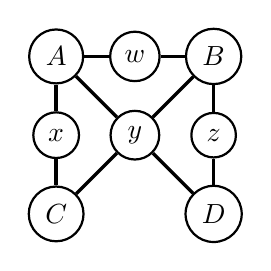
\begin{tikzpicture}
\begin{scope}[every node/.style={circle,thick,draw}]
    \node (C) at (-1,-1) {$C$};
    \node (x) at (-1,0) {$x$};
    \node (A) at (-1,1) {$A$};
    \node (y) at (0,0) {$y$};
    \node (w) at (0,1) {$w$};
    \node (D) at (1,-1) {$D$};
    \node (z) at (1,0) {$z$};
    \node (B) at (1,1) {$B$};
\end{scope}

\begin{scope}[every node/.style={fill=white,circle},
              every edge/.style={draw=black,very thick}]
    \path [-] (A) edge (w);
    \path [-] (A) edge (x);
    \path [-] (A) edge (y);
    \path [-] (B) edge (w);
    \path [-] (B) edge (y);
    \path [-] (B) edge (z);
    \path [-] (C) edge (x);
    \path [-] (C) edge (y);
    \path [-] (D) edge (y);
    \path [-] (D) edge (z);
\end{scope}
\end{tikzpicture}
	\hspace{1cm}
	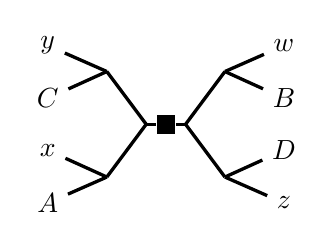
\begin{tikzpicture}
%\begin{scope}[every node/.style={circle,thick,draw}]
    \node (y) at (-1.5,1) {$y$};
    \node (C) at (-1.5,0.33) {$C$};
    \node (x) at (-1.5,-0.33) {$x$};
    \node (A) at (-1.5,-1) {$A$};
    
    \node (w) at (1.5,1) {$w$};
    \node (B) at (1.5,0.33) {$B$};
    \node (D) at (1.5,-0.33) {$D$};
    \node (z) at (1.5,-1) {$z$};
%\end{scope}
    \node (yC) at (-0.75, 0.67) {};
    \node (xA) at (-0.75, -0.67) {};
    \node (wB) at (0.75, 0.67) {};
    \node (zD) at (0.75, -0.67) {};
    
    \node (yCxA) at (-0.25, 0) {};
    \node (wBzD) at (0.25, 0) {};

\begin{scope}[every node/.style={fill=black,rectangle}]
    \node (root) at (0, 0) {};
\end{scope}
    
\begin{scope}[every node/.style={fill=white,circle},
              every edge/.style={draw=black,very thick}]
    \path [-] (y) edge (yC.center);
    \path [-] (C) edge (yC.center);
    \path [-] (x) edge (xA.center);
    \path [-] (A) edge (xA.center);
    \path [-] (w) edge (wB.center);
    \path [-] (B) edge (wB.center);
    \path [-] (z) edge (zD.center);
    \path [-] (D) edge (zD.center);
    
    \path [-] (yC.center) edge (yCxA.center);
    \path [-] (xA.center) edge (yCxA.center);
    \path [-] (wB.center) edge (wBzD.center);
    \path [-] (zD.center) edge (wBzD.center);
    
    \path [-] (yCxA.center) edge (root);
    \path [-] (wBzD.center) edge (root);
\end{scope}
\end{tikzpicture}
	\caption{\label{fig:wmc-example} The tensor network (left) produced by Theorem \ref{thm:wmc-reduction} on $\varphi = (w \lor x \lor \neg y) \land (w \lor y \lor z) \land (\neg x \lor \neg y) \land (\neg y \lor \neg z)$, consisting of 8 tensors and 10 indices. Vertices in this diagram are tensors, while edges indicate that the tensors share an index. The weight function affects the entries of the tensors for $w$, $x$, $y$, and $z$. This tensor network has a contraction tree (right) of max rank 4, but no contraction trees of smaller max rank.}
\end{figure}

See Figure \ref{fig:wmc-example} for an example of the reduction. This reduction is closely related to the formulation of model counting as the marginalization of a factor graph representing the constraints. Unlike the reduction to factor-graph marginalization, which only assigns factors to clauses, we must also assign a tensor to each variable $x$. For example, if $x$ has weights $W(x, 0) = W(x,1) = 1$ then the tensor assigned to $x$ is a copy tensor. This reduction can also be extended beyond OR clauses to other types of constraints (e.g. parity or cardinality constraints). 

Theorem \ref{thm:wmc-reduction} suggests that the weighted model count of $\varphi$ can be computed by constructing and contracting $N_\varphi$. We present this framework as Algorithm \ref{alg:wmc}. Algorithm \ref{alg:wmc} is a fixed-parameter algorithm for model counting, parameterized by carving-width of the incidence graph. The existence of such algorithms is easily implied by fixed-parameter algorithms for model counting parameterized by treewidth \cite{FMR08,SS10} since treewidth is bounded by thrice the carving width \cite{sasak10}. A variety of methods can be used in Step 2 to find a contraction tree to contract $N_\varphi$, including the methods \textbf{LG} and \textbf{FT} that we discuss in the following sections.

\begin{algorithm*}[t]
    \label{alg:wmc}
    \caption{Computing the weighted model count with a TN}
    \DontPrintSemicolon
    \KwIn{$\varphi$: A CNF formula}
    \KwIn{$W$: a weight function}
    \KwOut{$W(\varphi)$, the weighted model count of $\varphi$ w.r.t. $W$}
    $N_\varphi \gets \text{tensor network constructed via Theorem \ref{thm:wmc-reduction}}$\;
    $T \gets \func{FindContractionTree}(N_\varphi)$ \tcc*{e.g., \textbf{LG} or \textbf{FG}}
    \Return{$\func{Contract}(N_\varphi,~T)$}
\end{algorithm*}

% Nevertheless, on many benchmarks the carving width of the incidence graph is smaller than the treewidth. Since the width is in the exponent of the running time of decomposition-based counting algorithms, even a small decrease in width can dramatically decrease the running time.



\input{content/3-TensorOrder/theory_line_graph}
\section{The Factor-Tree Method for Finding Contraction Trees}
\label{sec:tensors:preprocessing}
Approaches to tensor-network contraction that do not modify the input tensor network (e.g., \textbf{LG}) are inherently limited by the ranks of the input tensors. If a tensor network has a rank $r$ tensor, then all contraction trees have max rank of at least $r$. This is a problem for tensor networks with high-rank tensors. 

One example of tensor networks that may contain high-rank tensors are the networks obtained by the reduction from model counting. The tensor network produced from a formula $\varphi$ contains a tensor representing each variable $x$, where the rank of this tensor is the number of appearances of $x$ in $\varphi$ (e.g., the rank $4$ tensor for $y$ in Figure \ref{fig:wmc-example}). For many benchmarks, where a single variable might appear tens or even hundreds of times, this reduction will therefore produce tensor networks containing tensors of infeasibly-high rank. Reductions exist from model counting on arbitrary formulas to model counting on formulas where the number of appearances of each variables is small. However, existing reductions do not consider the carving width of the resulting incidence graph and so often do not significantly improve the max-rank of available contraction trees. 

We introduce here a novel method \textbf{Factor-Tree} that avoids this barrier by preprocessing the input tensor network. Our insight is that a tree decomposition for the incidence graph of $\varphi$ can be used as a guide to introduce new variables in a principled way, so that the resulting tensor network has good contraction trees. In the language of tensors, introducing new variables corresponds to \emph{factoring}: replacing each high-rank tensor $A$ with a tensor network $N_A$ of low-rank tensors that contracts to $A$. The key idea of \textbf{FT}, then, is to use a tree decomposition for the structure graph to factor high-rank tensors.

We state this new result as Theorem \ref{thm:factorable-tree}. Since not all tensors can be factored in the ways that we require for this theorem and for \textbf{FT}, we first characterize the required property: that every tensor is factorable as an arbitrary tree of tensors:

% In fact, we can generalize this result to a wider class of tensor networks. To use a tree decomposition as a guide to simplify a tensor network we ultimately require that we can identify each tensor with a tensor network whose structure graph (excluding the free vertex) is an arbitrary tree. We call this property \emph{tree factorable}:

% We demonstrate an algorithm to find in polynomial time a tensor network, consisting only of rank 3 tensors, whose contraction is the model count of $F$. Moreover, we prove that the resulting tensor network has a good contraction tree if the guiding tree decomposition has small width.
%Instead of directly proving these claims (which are ultimately a corollary of Theorem \ref{thm:factorable-tree}), we generalize this result to a wider class of tensor networks. 

\begin{definition} \label{def:tree-factorable}
A tensor $A$ is \emph{tree factorable} if, for every tree $T$ whose leaves are $\tdim{A}$ (called a \emph{dimension tree} of $A$), there is a tensor network $N_A$ and a bijection $g_A: \V{T} \rightarrow N_A$ s.t.
\begin{enumerate}
\item $A$ is the contraction of $N_A$,
\item $g_A$ is an isomorphism between $T$ and the structure graph of $N_A$ with the free vertex (and incident edges) removed,
\item for every index $i$ of $A$, $i$ is an index of $g_A(i)$, and
\item for some index $i$ of $A$, the bond dimension of $N_A$ is no bigger than $|\domain{i}|$. % $\max_{i \in \tnbound{N}} |\domain{i}| \leq \max_{i \in \tdim{A}} |\domain{i}|$.
\end{enumerate}
\end{definition}
All tensors in the reduction of Theorem \ref{thm:wmc-reduction} from weighted model counting to tensor networks are tree factorable. A tensor network $N_A$ that satisfies properties 1, 2, and 3 of Definition \ref{def:tree-factorable} for some tree is called a \emph{Hierarchical Tucker representation} of $A$ \cite{Grasedyck10}. Property 4 ensures the result of Theorem \ref{thm:factorable-tree} has small bond dimension.

% In \cite{Grasedyck10}, a tree $T$ as in Definition \ref{def:tree-factorable} is called a \emph{dimension tree} of the tensor $A$, and a tensor network $N$ that satisfies properties 1, 2, and 3 for a given dimension tree of $A$ is called a \emph{Hierarchical Tucker representation} of $A$. For every tensor $A$ and dimension tree, a hierarchical Tucker representation of $A$ trivially exists with bond dimension $|\domain{A}|$, but a representation may not exist with smaller bond dimension. Limiting the bond dimension in property 4 ensures that the tensor networks we produce in Theorem \ref{thm:factorable-tree} also have small bond dimension.

We now state the main result of this section, which allows us to use a tree decomposition for the structure graph of a tensor network (containing only tree factorable tensors) to factor each tensor in the network and find a contraction tree of low max rank for the resulting network:
\begin{figure}[t]
	\centering
	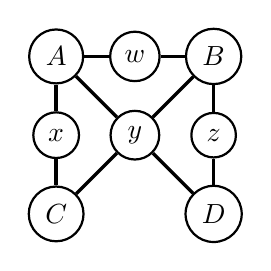
\begin{tikzpicture}
\begin{scope}[every node/.style={circle,thick,draw}]
    \node (C) at (-1,-1) {$C$};
    \node (x) at (-1,0) {$x$};
    \node (A) at (-1,1) {$A$};
    \node (y) at (0,0) {$y$};
    \node (w) at (0,1) {$w$};
    \node (D) at (1,-1) {$D$};
    \node (z) at (1,0) {$z$};
    \node (B) at (1,1) {$B$};
\end{scope}

\begin{scope}[every node/.style={fill=white,circle},
              every edge/.style={draw=black,very thick}]
    \path [-] (A) edge (w);
    \path [-] (A) edge (x);
    \path [-] (A) edge (y);
    \path [-] (B) edge (w);
    \path [-] (B) edge (y);
    \path [-] (B) edge (z);
    \path [-] (C) edge (x);
    \path [-] (C) edge (y);
    \path [-] (D) edge (y);
    \path [-] (D) edge (z);
\end{scope}
\end{tikzpicture}
	\hspace{1cm}
	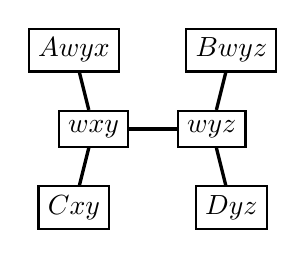
\begin{tikzpicture}
\begin{scope}[every node/.style={rectangle,thick,draw}]
    \node (1) at (-1,1) {$Awyx$};
    \node (2) at (-1,-1) {$Cxy$};
    \node (3) at (-0.75,0) {$wxy$};
    \node (4) at (0.75,0) {$wyz$};
    
    \node (5) at (1,1) {$Bwyz$};
    \node (6) at (1,-1) {$Dyz$};
\end{scope}

\begin{scope}[every node/.style={fill=white,circle},
              every edge/.style={draw=black,very thick}]
    \path [-] (1) edge (3);
    \path [-] (2) edge (3);
    \path [-] (3) edge (4);
    \path [-] (4) edge (5);
    \path [-] (4) edge (6);
\end{scope}
\end{tikzpicture}
	\hspace{1cm}
	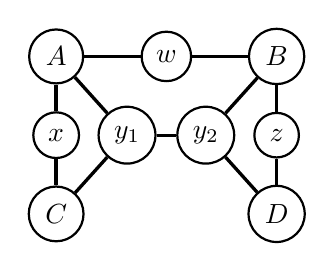
\begin{tikzpicture}
\begin{scope}[every node/.style={circle,thick,draw}]
    \node (C) at (-1.4,-1) {$C$};
    \node (x) at (-1.4,0) {$x$};
    \node (A) at (-1.4,1) {$A$};
    \node (y1) at (-0.5,0) {$y_1$};
    \node (y2) at (0.5,0) {$y_2$};
    \node (w) at (0,1) {$w$};
    \node (D) at (1.4,-1) {$D$};
    \node (z) at (1.4,0) {$z$};
    \node (B) at (1.4,1) {$B$};
\end{scope}

\begin{scope}[every node/.style={fill=white,circle},
              every edge/.style={draw=black,very thick}]
    \path [-] (A) edge (w);
    \path [-] (A) edge (x);
    \path [-] (A) edge (y1);
    \path [-] (B) edge (w);
    \path [-] (B) edge (y2);
    \path [-] (B) edge (z);
    \path [-] (y1) edge (y2);
    \path [-] (C) edge (x);
    \path [-] (C) edge (y1);
    \path [-] (D) edge (y2);
    \path [-] (D) edge (z);
\end{scope}
\end{tikzpicture}
	\caption{\label{fig:factor-example} When FT is run on the shown initial tensor network (left) using the shown tree decomposition (middle), \textbf{FT} produces a factored tensor network (right). Tensors of rank 3 or smaller are unchanged, and the tensor for $y$ is factored into two tensors, $y_1$ and $y_2$, each of rank 3. The factored tensor network has a contraction tree of max rank 3 while the initial tensor network only has contraction trees of max rank 4 or higher.}
\end{figure}

\begin{theorem} \label{thm:factorable-tree}
Let $N$ be a tensor network of tree-factorable tensors s.t. $|\tnfree{N}| \leq 3$ and the structure graph of $N$ has a tree decomposition of width $w \geq 1$.

Then for each $A \in N$ there is a tensor network $N_A$ whose contraction is $A$ that consists only of rank 3 or smaller tensors. Moreover, the disjoint union of these networks, $M = \cup_{A \in N} N_A$, is a tensor network that contracts to $\tntensor{N}$, has the same bond dimension as $N$, and has a contraction tree of max rank no larger than $\ceil{4(w+1)/3}$.
\end{theorem}
\begin{proof}
The proof proceeds in five steps: (1) compute the factored tensor network $M$, (2) construct a graph $H$ that is a simplified version of the structure graph of $M$, (3) construct a carving decomposition $S$ of $H$, (4) bound the width of $S$, and (5) use $S$ to find a contraction tree for $M$. Working with $H$ instead of directly working with the structure graph of $M$ allows us to cleanly handle tensor networks with free indices.

\textbf{Part 1: Factoring the network.}
Let $G$ be the structure graph of $N$ with all degree 0 vertices removed; $G$ must also have a tree decomposition of width $w$. Moreover, the image of $\eincf{G}: \E{G} \rightarrow 2^{\V{G}}$ is an edge clique cover of $G$. Thus using Lemma \ref{lemma:tree-simplification} we can construct a tree decomposition $(T, \chi)$ of $G$ and a bijection $g: \E{G} \rightarrow \Lv{T}$ such that $\chi \circ g = \eincf{G}$ and $width_t(T, \chi) \leq w$.

Next, for each $v \in \V{G}$, define $T_v$ to be the smallest connected component of $T$ containing $\{g(i) ~:~i \in \vinc{H}{v} \}$. Consider each $A \in N$. If $\tnfree{A} = \emptyset$, let $N_A = \{A\}$; thus $\tntensor{N_A} = A$ and the tensor of $N_A$ has rank 0. Otherwise, observe that $T_A$ is a dimension tree of $A$. We can therefore factor $A$ with $T_A$ using Definition \ref{def:tree-factorable} to get a tensor network $N_A$ whose contraction is $A$ and a bijection $g_A: \V{T_A} \rightarrow N_A$. Moreover, every node of $T_A$ has degree 3 or smaller and so, by Definition \ref{def:tree-factorable}, $N_A$ consists only of rank 3 or smaller tensors.

Define $M = \cup_{A \in N} N_A$ and let $G'$ be the structure graph of $M$ with free vertex $\fv'$. The remainder of the proof is devoted to bounding the carving width of $G'$.

\textbf{Part 2: Constructing a simplified structure graph of $M$.} In order to easily characterize $G'$, we define a new, closely-related graph $H$ by taking a copy of $T_v$ for each $v \in \V{G}$ and connecting these copies where indicated by $g$. Formally, the vertices of $H$ are $\{(v, n) : v \in \V{G}, n \in \V{T_v}\}$. For every $v \in \V{G}$ and every arc in $T$ with endpoints $n, m \in \V{T_v}$, we add an edge between $(v, n)$ and $(v, m)$. Moreover, for each $e \in \E{G}$ incident to $v, w \in \V{G}$, we add an edge between $(v, g(e))$ and $(w, g(e))$. 

We will prove in Part 5 that the carving width of $G'$ is bounded from above by the carving width of $H$. We therefore focus in Part 3 and Part 4 on bounding the carving width of $H$. It is helpful for this to define the two projections $\pi_G : \V{H} \rightarrow \V{G}$ and $\pi_T : \V{H} \rightarrow \V{T}$ that indicate respectively the first or second component of a vertex of $H$. 
% For each $v \in \V{G}$, define $H_v = \pi_G^{-1}(v)$. Thus the sets $H_v$ form a partition of $\V{H}$. 

% This ensures that $H \cap H_v$ is isomorphic to $T_v$ and so $H \cap H_v$ is a tree with $|\vinc{G}{v}|$ leaves.

% The map $f: \E{G} \rightarrow \E{H}$ constructed in this way is an injection and satisfies property 3 above. Moreover, since $g(\vinc{G}{v})$ is exactly the leaves of $T_v$, each leaf $\ell \in \Lv{H \cap H_v}$ is incident to exactly one edge in the range of $f$, namely $f(g^{-1}(\ell))$.

\begin{figure}[t]
	\centering
	%\begin{tikzpicture}
\begin{scope}[every node/.style={fill, circle, inner sep=0pt, outer sep=0, minimum size=5pt}]
    \node[label={[xshift=5pt]$n$}] (n) at (0, 0) {};
\end{scope}

\draw[thick] (n) -- (0, 2) node [midway, left] {$a$};
\draw[thick] (n) -- (-1.73, -1) node [midway, above] {$b$};
\draw[thick] (n) -- (1.73, -1) node [midway, above] {$c$};
\end{tikzpicture}
	%\hspace{1cm}
	\begin{tikzpicture}
% Center node
\node[fill, circle, inner sep=0pt, outer sep=0, minimum size=5pt, label={[xshift=8pt, yshift=-5pt]$y_n$}] (yn) at (0, 0) {};

% Minor nodes
\begin{scope}[every node/.style={fill, circle, inner sep=0pt, outer sep=0, minimum size=3pt}]
    \draw[thick] (yn) -- node[pos=0.75, label=right:{$z_{n,a}$}, minimum size=5pt] (zna) {} 
    node[pos=0.525] (Ina1) {} node[pos=0.375] (Ina2) {} node[pos=0.225] (Ina3) {} (0,2);
    \node[left=0.5 of Ina1] (Hna1) {};
    \node[left=0.5 of Ina2] (Hna2) {};
    \node[left=0.5 of Ina3] (Hna3) {};
    
    \draw[thick] (yn) -- node[pos=0.75, label={[xshift=-5pt,yshift=-5pt]$z_{n,b}$}, minimum size=5pt] (znb) {}
    node[pos=0.525] (Inb1) {} node[pos=0.375] (Inb2) {} node[pos=0.225] (Inb3) {} (-1.73, -1);
    \node[below right=0.25 and 0.1 of Inb1] (Hnb1) {};
    \node[below right=0.25 and 0.1 of Inb2] (Hnb2) {};
    \node[below right=0.25 and 0.1 of Inb3] (Hnb3) {};
    
    \draw[thick] (yn) -- node[pos=0.75, label={[xshift=5pt,yshift=-5pt]$z_{n,c}$}, minimum size=5pt] (znc) {}
    node[pos=0.525] (Inc1) {} node[pos=0.375] (Inc2) {} node[pos=0.225] (Inc3) {} (1.73, -1);
    \node[below left=0.25 and 0.1 of Inc1] (Hnc1) {};
    \node[below left=0.25 and 0.1 of Inc2] (Hnc2) {};
    \node[below left=0.25 and 0.1 of Inc3] (Hnc3) {};
    
    % \node[left=5 of zna, label=right:{$z_{\ell,a}$}, minimum size=5pt] (zla) {};
    % \node[left=5 of Ina1] (Ila1) {};
    % \node[left=5 of Ina2] (Ila2) {};
    % \node[left=5 of Ina3] (Ila3) {};
    % \node[left=5 of Hna1] (Hla1) {};
    % \node[left=5 of Hna2] (Hla2) {};
    % \node[left=5 of Hna3] (Hla3) {};
    
    \draw[thick] (-3, 0.52) -- node[pos=0.6825, label=right:{$z_{\ell,a}$}, minimum size=5pt] (zna) {}
    node[pos=0.39] (Ila1) {} node[pos=0.195] (Ila2) {} node[pos=0] (Ila3) {} (-3,2);
    \node[left=0.5 of Ila1] (Hla1) {};
    \node[left=0.5 of Ila2] (Hla2) {};
    \node[left=0.5 of Ila3] (Hla3) {};
\end{scope}

% \node at (zna) [above right] {$y_n$};
%\draw[thick] (yn) -- (0, 2);
%\draw[thick] (yn) -- (-1.73, -1);
%\draw[thick] (yn) -- (1.73, -1);

\draw[thick] (Ina1) -- (Hna1);
\draw[thick] (Ina2) -- (Hna2);
\draw[thick] (Ina3) -- (Hna3);
\draw[decoration={brace,raise=3pt},decorate] (Ina1) -- node[right=4pt] {$I_{n,a}$} (Ina3);
\draw[decoration={brace,mirror,raise=3pt},decorate] (Hna1) -- node[left=4pt] {$H_{n,a}$} (Hna3);

\draw[thick] (Inb1) -- (Hnb1);
\draw[thick] (Inb2) -- (Hnb2);
\draw[thick] (Inb3) -- (Hnb3);
\draw[decoration={brace,raise=3pt},decorate] (Inb1) -- node[above left=1pt and 1pt] {$I_{n,b}$} (Inb3);
\draw[decoration={brace,mirror,raise=3pt},decorate] (Hnb1) -- node[below=6pt] {$H_{n,b}$} (Hnb3);

\draw[thick] (Inc1) -- (Hnc1);
\draw[thick] (Inc2) -- (Hnc2);
\draw[thick] (Inc3) -- (Hnc3);
\draw[decoration={brace,mirror,raise=3pt},decorate] (Inc1) -- node[above right=1pt and 1pt] {$I_{n,c}$} (Inc3);
\draw[decoration={brace,raise=3pt},decorate] (Hnc1) -- node[below=6pt] {$H_{n,c}$} (Hnc3);


\draw[thick] (Ila1) -- (Hla1);
\draw[thick] (Ila2) -- (Hla2);
\draw[thick] (Ila3) -- (Hla3);
\draw[decoration={brace,raise=3pt},decorate] (Ila1) -- node[right=4pt] {$I_{\ell,a}$} (Ila3);
\draw[decoration={brace,mirror,raise=3pt},decorate] (Hla1) -- node[left=4pt] {$H_{\ell,a}$} (Hla3);
\end{tikzpicture}
	\caption{\label{fig:factor-carving-construction} The central construction in Part 3 of Theorem \ref{thm:factorable-tree} of a carving decomposition $S$ from an input tree decomposition $(T, \chi)$. Each leaf $\ell$ of $T$ (with incident arc $a$) is replaced by the left construction in $S$. Each internal node $n$ of $T$ (with incident arcs $a$, $b$, and $c$) is replaced by the right construction in $S$. If nodes $m$ and $n$ are connected by arc $a$ in $T$, then nodes $z_{m,a}$ and $z_{n,a}$ are connected in $S$.}
\end{figure}

\textbf{Part 3. Constructing a carving decomposition $S$ of $H$.}
The idea of the construction is, for each $n \in \V{T}$, to attach the elements of $\pi_T^{-1}(n)$ as leaves along arcs incident to $n$. See Figure \ref{fig:factor-carving-construction} for an overview of the construction.

Consider an arbitrary node $n \in \V{T}$. If $n$ is a leaf node with incident arc $a \in \vinc{T}{n}$, define $H_{n,a} = \pi_T^{-1}(n)$. If $n$ is an internal node with incident arcs $a,b,c \in \vinc{T}{n}$, arbitrarily partition $\pi_T^{-1}(n)$ into three equally-sized sets $B_1$, $B_2$, and $B_3$ and define $H_{n,a} = B_1$, $H_{n,b} = B_2$, and $H_{n,c} = B_3$ (note that $T$ is a binary tree and so $n$ has exactly three incident arcs). Observe that, in either case, $\{H_{n,a} : n \in \V{T}, a \in \vinc{T}{n}\}$ is a partition of $\pi_T^{-1}(n)$ and thus is a partition of $\V{H}$. 
% To do this, for every leaf node $\ell \in \Lv{T}$ with incident arc $a \in \vinc{T}{\ell}$ define $H_{\ell, a} = \pi_T^{-1}(\ell)$. For every non-leaf node $n \in \V{T} \setminus \Lv{T}$ partition $\pi_T^{-1}(n)$ into three equally-sized sets and denote each set by $H_{n,a}$ for each of the three $a \in \vinc{T}{n}$. Observe that $\{H_{n,a} : n \in \V{T}, a \in \vinc{T}{n}\}$ is a partition of $\V{H}$. 

We use this to construct a carving decomposition $S$ from $T$ by adding each element of $H_{n,a}$ as a leaf along the arc $a$. Formally, let $x_v$ denote a fresh vertex for each $v \in \V{H}$, let $y_n$ denote a fresh vertex for each $n \in \V{T}$, and let $z_{n,a}$ denote a fresh vertex for each $n \in \V{T}$ and $a \in \vinc{T}{n}$. Define $\V{S}$ to be the union of $\V{H}$ with the set of these free vertices. 

We add an arc between $v$ and $x_v$ for every $v \in \V{H}$. Moreover, for every $a \in \E{T}$ with endpoints $o, p \in \einc{T}{a}$ add an arc between $z_{o,a}$ and $z_{p,a}$. For every $n \in \V{T}$ and incident arc $a \in \vinc{T}{n}$, construct an arbitrary sequence $I_{n,a}$ from $\{x_v : v \in H_{n,a}\}$. If $H_{n,a} = \emptyset$ then add an arc between $y_n$ and $z_{n,a}$. Otherwise, add arcs between $y_n$ and the first element of $I$, between consecutive elements of $I_{n,a}$, and between the last element of $I_{n,a}$ and $z_{n,a}$. 

Finally, remove the previous leaves of $T$ from $S$. The resulting tree $S$ is a carving decomposition of $H$, since we have added all vertices of $H$ as leaves and removed the previous leaves of $T$.

\textbf{Part 4: Computing the width of $S$.} In this part, we separately bound the width of the partition induced by each of the three kinds of arcs in $S$.

First, consider an arc $d$ between some $v \in \V{H}$ and $x_v$. Since all vertices of $H$ are degree 3 or smaller, $d$ defines a partition of width at most $3 \leq \ceil{4(w+1)/3}$.

Next, consider an arc $e_a$ between $z_{o,a}$ and $z_{p,a}$ for some arc $a \in \E{T}$ with endpoints $o, p \in \einc{T}{a}$.
Observe that removing $a$ from $T$ defines a partition $\{B_o, B_p\}$ of $\V{T}$, denoted so that $o \in B_o$ and $p \in B_p$. Then removing $e_a$ from $S$ defines the partition $\{ \pi_T^{-1}(B_o), \pi_T^{-1}(B_p) \}$ of $\Lv{S}$. By construction of $H$, all edges between $\pi_T^{-1}(B_o)$ and $\pi_T^{-1}(B_p)$ are between $\pi_T^{-1}(o)$ and $\pi_T^{-1}(p)$. Since $\pi_G(\pi_T^{-1}(o)) \subseteq \chi(o)$, $\pi_G(\pi_T^{-1}(o)) \subseteq \chi(p)$, and $\pi_G$ is an injection on $\pi_T^{-1}(n)$ for all $n \in \V{T}$), it follows that the partition defined by $e_a$ has width no larger than $|\chi(o) \cap \chi(p)| \leq w+1$. 

Finally, consider an arc $f$ added as one of the sequence of $|H_{n,a}|+1$ arcs between $y_n$, $I_{n,a}$, and $z_{n,a}$ for some $n \in \V{T}$ and $a \in \vinc{T}{n}$. Some elements of $H_{n,a}$ have changed blocks from the partition defined by $e_a$. Each vertex of degree 2 that changes blocks does not affect the width of the partition, but each vertex of degree 3 that changes blocks increases the width by 1. There are at most $|H_{n,a}| \leq \ceil{(w+1)/3}$ elements of degree 3 added as leaves between $y_n$ and $z_{n,a}$. Thus the partition defined by $f$ has width at most $w + 1 + \ceil{(w+1)/3} = \ceil{4(w+1)/3}$.

It follows that the width of $S$ is at most $\ceil{4(w+1)/3}$.

\textbf{Part 5: Bounding the max-rank of $M$.} Let $\fv$ be the free vertex of the structure graph of $N$. We first construct a new graph $H'$ from $H$ by, if $\tnfree{N} \neq \emptyset$, contracting all vertices in $\pi_G^{-1}(\fv)$ to a single vertex $\fv$. If $\tnfree{N} = \emptyset$, instead add $\fv$ as a fresh degree 0 vertex to $H'$. Moreover, for all $A \in N$ with $\tdim{A} = \emptyset$ add $A$ as a degree 0 vertex to $H'$. 

Note that adding degree 0 vertices to a graph does not affect the carving width. Moreover, since $|\tnfree{N}| \leq 3$ all vertices (except at most one) of $\pi_G^{-1}(\fv)$ are degree 2 or smaller. It follows that contracting $\pi_G^{-1}(\fv)$ does not increase the carving width. Thus the carving width of $H'$ is at most $\ceil{4(w+1)/3}$.

Moreover, $H'$ and $G'$ are isomorphic. To prove this, define an isomorphism $\phi: \V{H'} \rightarrow \V{G'}$ between $H'$ and $G'$ by, for all $v \in \V{H'}$:
$$\phi(v) \equiv \begin{cases}v&\text{if}~v \in N~\text{and}~\tdim{v}=\emptyset\\\fv'&v=\fv\\g_{\pi_G(v)}(\pi_T(v))&\text{if}~v \in \V{H}~\text{and}~\pi_G(v) \in N\end{cases}$$
$\phi$ is indeed an isomorphism between $H'$ and $G'$ because the functions $g_A$ are all isomorphisms and because an edge exists between $\pi_G^{-1}(v)$ and $\pi_G^{-1}(w)$ for $v, w \in \V{G}$ if and only if there is an edge between $v$ and $w$ in $G$. Thus the carving width of $G'$ is at most $\ceil{4(w+1)/3}$. By Theorem \ref{thm:contraction-equiv-carving}, then, $M$ has a contraction tree of max rank no larger than $\ceil{4(w+1)/3}$.
\end{proof}

The general idea of using a tree decomposition of a graph to split high-degree nodes was previously used by Markov and Shi \cite{MS11} and in the context of constraint satisfaction by Samer and Szeider \cite{SS10_2}. Both of these works focus on minimizing the treewidth of the factored graph instead of the max-rank. Translated to tensor networks (as done in Lemma 3 of \cite{oliveira18}), their constructions produce a factored network $N'$ with structure graph $G$ that satisfies all requirements of Theorem \ref{thm:factorable-tree} except with a bound of $w+1$ on the treewidth of $G$ in place of the bound on max-rank. Since the treewidth of $\Line{G}$ plus 1 is bounded by the product of the maximum degree of $G$ (namely 3) and the treewidth of $G$ plus 1 \cite{MS08}, we can then use \textbf{LG} to produce a contraction tree for $N'$ of max rank no larger than $3(w+2)$. Theorem \ref{thm:factorable-tree} thus gives an improvement on max-rank over these prior works from $3(w+2)$ to $\ceil{4(w+1)/3}$.

% who used tree decompositions of the incidence graph of a CSP to construct an equisatisfiable CSP of identical incidence treewidth in which no variable occurs more than 3 times. Translated to the context of tensor networks and generalized to tree-factorable tensors, their analysis produces a factored tensor network $N'$ that satisfies all requirements of Theorem \ref{thm:factorable-tree} but with a bound of $w$ on the incidence treewidth instead of our bound on max-rank.

%\begin{theorem} \label{thm:factorable-tree}
%Let $N$ be a tensor network of tree-factorable tensors such that $|\tnfree{N}| \leq 3$ and the structure graph of $N$ has a tree decomposition $T$ of width $w$.

%Then for each $A \in N$ there is a tensor network $N_A$ whose contraction is $A$ that consists only of rank 3 or smaller tensors. Moreover, the disjoint union of these networks, $N' = \cup_{A \in N} N_A$, is a tensor network that contracts to $\tntensor{N}$, has the same bond dimension as $N$, and has a structure graph with a tree decomposition of width $w$.
%\end{theorem}


The construction of Theorem \ref{thm:factorable-tree} gives us the \textbf{Factor-Tree} method, which uses tree decompositions of the structure graph to preprocess the tensor network and factor high-rank tensors. See Figure \ref{fig:factor-example} for an example of the preprocessing. We show in Section \ref{sec:tensors:experiments:cachet} that \textbf{FT} can significantly improve the quality of the contraction tree on benchmarks with high-rank tensors.
\section{Implementation and Evaluation} \label{sec:tensors:experiments}
We aim to answer the following experimental research questions:
\begin{enumerate}
    \item[(RQ1)] Are tensor-network-based approaches competitive with existing state-of-the-art unweighted model counters?
    \item[(RQ2)] Are tensor-network-based approaches competitive with existing state-of-the-art weighted model counters?
    \item[(RQ3)] What are the structural properties of benchmarks for which the tensor-network-based approaches perform well?
\end{enumerate}

To answer these questions, we implement Algorithm 2 in \tool{TensorOrder}, a new tool for weighted model counting using tensor networks. \tool{TensorOrder} can be configured to find contraction trees using existing planning methods -- \textbf{greedy} (using a greedy algorithm), \textbf{metis} (using graph partitioning), and \textbf{GN} (using community structure detection) \cite{KCMR18}-- or planning methods presented in this paper-- \textbf{LG} (Section \ref{sec:tensors:contraction-theory}) and \textbf{FT} (Section \ref{sec:tensors:preprocessing}). Implementation details appear in Section \ref{sec:tensors:experiments:implementation}.

To answer RQ1, in Section \ref{sec:tensors:experiments:cubic} we compare \tool{TensorOrder} with existing state-of-the-art tools for unweighted model counting (\tool{dynQBF} \cite{CW16}, \tool{dynasp} \cite{FHMW17}, \tool{SharpSAT} \cite{Thurley2006}, \tool{cachet} \cite{SBK05}, \tool{miniC2D} \cite{OD15} and \tool{d4} \cite{LM17}) on formulas that count the number of vertex covers of randomly-generated cubic graphs \cite{KCMR18}. Note \tool{dynQBF} and \tool{dynasp} are solvers from related domains (that can be used as tools for unweighted model counting) that also use tree decompositions.

To answer RQ2, in Section \ref{sec:tensors:experiments:cachet} we compare \tool{TensorOrder} with existing state-of-the-art tools for weighted model counting (\tool{cachet} \cite{SBK05}, \tool{miniC2D} \cite{OD15} and \tool{d4} \cite{LM17}) on formulas whose weighted count corresponds to exact inference on Bayesian networks \cite{SBK05}. Note that the other tools (\tool{dynQBF}, \tool{dynasp}, and \tool{SharpSAT}) cannot perform weighted model counting.

% We use \tool{TensorOrder} to compare tensor-based methods with existing state-of-the-art tools for weighted model counting: \tool{cachet} \cite{SBK05}, \tool{miniC2D} \cite{OD15} and \tool{d4} \cite{LM17}. %Note that \tool{d4} requires a d-DNNF reasoner to perform weighted model counting; we use \cite{CDLL18}. 
% We also compare with \tool{dynQBF} \cite{CW16}, \tool{dynasp} \cite{FHMW17} and \tool{SharpSAT} \cite{Thurley2006} when the benchmarks are unweighted. Note \tool{dynQBF} and \tool{dynasp} are solvers from related domains (that can be used as model counters) that also use tree decompositions.

% We then compare our tensor-based algorithms for weighted model counting against state-of-the-art weighted model counters and against existing tensor-based algorithms. We demonstrate that our tensor-based algorithms are useful as part of a portfolio of weighted model counters. 

% We compare \tool{TensorOrder} on two sets of existing benchmarks. First, in Section \ref{sec:tensors:experiments:cubic} we compare on formulas that count the number of vertex covers of randomly-generated cubic graphs \cite{KCMR18}. Second, in Section \ref{sec:tensors:experiments:cachet} we compare 
To answer RQ3, we compute upper bounds on the treewidth and carving width of these benchmarks. We run each of three heuristic tree decomposition solvers (\pkg{Tamaki} \cite{Tamaki17}, \pkg{FlowCutter} \cite{HS18}, and \pkg{htd} \cite{AMW17}) on each benchmark with a timeout of 1000 seconds: once on the structure graph $G$ corresponding to the benchmark, and once on $\Line{G}$. The minimal width of all produced tree decompositions for $G$ (resp. $\Line{G}$) is an upper bound for the treewidth of $G$ (resp. $\Line{G}$). The minimal max-rank of the contraction trees produced by running \textbf{LG} (resp. \textbf{FT}) on each tree decomposition of $\Line{G}$ (resp. $G$) is an upper bound for the carving width of $G$ (resp. $G$ after \text{FT}-preprocessing).

Each experiment was run in a high-performance cluster (Linux kernel 2.6.32) using a single 2.80 GHz core of an Intel Xeon X5660 CPU and 48 GB RAM. We provide all code, benchmarks, and detailed data of benchmark runs at \url{https://github.com/vardigroup/TensorOrder}.

% \paragraph{Experimental Methodology}
% To evaluate runtime performance, we run each tool once on each benchmark with a timeout of 1000 seconds and record the wall-clock time taken. For \tool{TensorOrder}, recorded times include all of Algorithm \ref{alg:wmc} (and, specifically, include the time of the underlying tree-decomposition solver).



% We then use these tree decompositions to compute upper bounds on the treewidth of $G$ (the minimal width of all found tree decompositions for $G$), the treewidth of $\Line{G}$ (the minimal width of all found tree decompositions for $\Line{G}$), the carving width of $G$ (the minimal max-rank of all contraction trees produced by running \textbf{LG} on tree decompositions of $\Line{G}$), and the carving width of $G$ after \textbf{FT}-preprocessing (the minimal max-rank of all contraction trees produced by running \textbf{FT} on tree decompositions of $\Line{G}$).

% \begin{enumerate}
%     \item the treewidth of $G$ by taking the minimum width amongst all discovered tree decompositions for $G$,
%     \item the treewidth of $\Line{G}$ by taking the minimum width amongst all discovered tree decompositions for $\Line{G}$,
%     \item the carving width of $G$ by taking the minimum width amongst all contraction trees produced by running \textbf{LG} on each tree decomposition of $\Line{G}$, and
%     \item the carving width of $G$ after \textbf{FT}-preprocessing by taking the minimum width amongst all contraction trees produced by running \textbf{FT} on each tree decomposition of $G$.
% \end{enumerate}

% compute an upper bound for the treewidth of $G$ (resp. $\Line{G}$) by taking the minimum width amongst all discovered tree decompositions for $G$ (resp. $\Line{G}$). Similarly, we compute an upper bound for the carving width of $G$ by taking the minimum width amongst all contraction trees produced by running \textbf{LG} on each tree decomposition of $\Line{G}$.


% We then record the width of the best tree decomposition found amongst all tree-decomposition solvers. We also 

% We also evaluate the structural properties of these benchmarks by performing an experimental comparison of treewidth and carving width of the incidence. For each benchmark with corresponding incidence graph $G$, we run each of the three heuristic tree decomposition solvers \tool{Tamaki}, \tool{FlowCutter}, and \tool{htd} for 1000 seconds on $G$ and $\Line{G}$. We then record the width of the best tree decomposition found amongst all tree-decomposition solvers. On each tree decomposition for $\Line{G}$ found by the solvers, we use \textbf{LG} to compute the corresponding carving decomposition of $G$ and recorded the smallest width found amongst all decompositions. Similarly, on each tree decomposition for $G$ found by the solvers, we use \textbf{FT} to compute the corresponding carving decomposition of the preprocessed graph and recorded the smallest width found amongst all decompositions. 

\begin{figure}
	\centering
	%% Creator: Matplotlib, PGF backend
%%
%% To include the figure in your LaTeX document, write
%%   \input{<filename>.pgf}
%%
%% Make sure the required packages are loaded in your preamble
%%   \usepackage{pgf}
%%
%% and, on pdftex
%%   \usepackage[utf8]{inputenc}\DeclareUnicodeCharacter{2212}{-}
%%
%% or, on luatex and xetex
%%   \usepackage{unicode-math}
%%
%% Figures using additional raster images can only be included by \input if
%% they are in the same directory as the main LaTeX file. For loading figures
%% from other directories you can use the `import` package
%%   \usepackage{import}
%%
%% and then include the figures with
%%   \import{<path to file>}{<filename>.pgf}
%%
%% Matplotlib used the following preamble
%%   \usepackage[utf8x]{inputenc}
%%   \usepackage[T1]{fontenc}
%%
\begingroup%
\makeatletter%
\begin{pgfpicture}%
\pgfpathrectangle{\pgfpointorigin}{\pgfqpoint{6.000000in}{3.400000in}}%
\pgfusepath{use as bounding box, clip}%
\begin{pgfscope}%
\pgfsetbuttcap%
\pgfsetmiterjoin%
\definecolor{currentfill}{rgb}{1.000000,1.000000,1.000000}%
\pgfsetfillcolor{currentfill}%
\pgfsetlinewidth{0.000000pt}%
\definecolor{currentstroke}{rgb}{1.000000,1.000000,1.000000}%
\pgfsetstrokecolor{currentstroke}%
\pgfsetdash{}{0pt}%
\pgfpathmoveto{\pgfqpoint{0.000000in}{0.000000in}}%
\pgfpathlineto{\pgfqpoint{6.000000in}{0.000000in}}%
\pgfpathlineto{\pgfqpoint{6.000000in}{3.400000in}}%
\pgfpathlineto{\pgfqpoint{0.000000in}{3.400000in}}%
\pgfpathclose%
\pgfusepath{fill}%
\end{pgfscope}%
\begin{pgfscope}%
\pgfsetbuttcap%
\pgfsetmiterjoin%
\definecolor{currentfill}{rgb}{1.000000,1.000000,1.000000}%
\pgfsetfillcolor{currentfill}%
\pgfsetlinewidth{0.000000pt}%
\definecolor{currentstroke}{rgb}{0.000000,0.000000,0.000000}%
\pgfsetstrokecolor{currentstroke}%
\pgfsetstrokeopacity{0.000000}%
\pgfsetdash{}{0pt}%
\pgfpathmoveto{\pgfqpoint{0.708220in}{0.535823in}}%
\pgfpathlineto{\pgfqpoint{5.850000in}{0.535823in}}%
\pgfpathlineto{\pgfqpoint{5.850000in}{3.205275in}}%
\pgfpathlineto{\pgfqpoint{0.708220in}{3.205275in}}%
\pgfpathclose%
\pgfusepath{fill}%
\end{pgfscope}%
\begin{pgfscope}%
\pgfsetbuttcap%
\pgfsetroundjoin%
\definecolor{currentfill}{rgb}{0.000000,0.000000,0.000000}%
\pgfsetfillcolor{currentfill}%
\pgfsetlinewidth{0.803000pt}%
\definecolor{currentstroke}{rgb}{0.000000,0.000000,0.000000}%
\pgfsetstrokecolor{currentstroke}%
\pgfsetdash{}{0pt}%
\pgfsys@defobject{currentmarker}{\pgfqpoint{0.000000in}{-0.048611in}}{\pgfqpoint{0.000000in}{0.000000in}}{%
\pgfpathmoveto{\pgfqpoint{0.000000in}{0.000000in}}%
\pgfpathlineto{\pgfqpoint{0.000000in}{-0.048611in}}%
\pgfusepath{stroke,fill}%
}%
\begin{pgfscope}%
\pgfsys@transformshift{0.708220in}{0.535823in}%
\pgfsys@useobject{currentmarker}{}%
\end{pgfscope}%
\end{pgfscope}%
\begin{pgfscope}%
\definecolor{textcolor}{rgb}{0.000000,0.000000,0.000000}%
\pgfsetstrokecolor{textcolor}%
\pgfsetfillcolor{textcolor}%
\pgftext[x=0.708220in,y=0.438600in,,top]{\color{textcolor}\rmfamily\fontsize{9.000000}{10.800000}\selectfont \(\displaystyle {0}\)}%
\end{pgfscope}%
\begin{pgfscope}%
\pgfsetbuttcap%
\pgfsetroundjoin%
\definecolor{currentfill}{rgb}{0.000000,0.000000,0.000000}%
\pgfsetfillcolor{currentfill}%
\pgfsetlinewidth{0.803000pt}%
\definecolor{currentstroke}{rgb}{0.000000,0.000000,0.000000}%
\pgfsetstrokecolor{currentstroke}%
\pgfsetdash{}{0pt}%
\pgfsys@defobject{currentmarker}{\pgfqpoint{0.000000in}{-0.048611in}}{\pgfqpoint{0.000000in}{0.000000in}}{%
\pgfpathmoveto{\pgfqpoint{0.000000in}{0.000000in}}%
\pgfpathlineto{\pgfqpoint{0.000000in}{-0.048611in}}%
\pgfusepath{stroke,fill}%
}%
\begin{pgfscope}%
\pgfsys@transformshift{1.833336in}{0.535823in}%
\pgfsys@useobject{currentmarker}{}%
\end{pgfscope}%
\end{pgfscope}%
\begin{pgfscope}%
\definecolor{textcolor}{rgb}{0.000000,0.000000,0.000000}%
\pgfsetstrokecolor{textcolor}%
\pgfsetfillcolor{textcolor}%
\pgftext[x=1.833336in,y=0.438600in,,top]{\color{textcolor}\rmfamily\fontsize{9.000000}{10.800000}\selectfont \(\displaystyle {50}\)}%
\end{pgfscope}%
\begin{pgfscope}%
\pgfsetbuttcap%
\pgfsetroundjoin%
\definecolor{currentfill}{rgb}{0.000000,0.000000,0.000000}%
\pgfsetfillcolor{currentfill}%
\pgfsetlinewidth{0.803000pt}%
\definecolor{currentstroke}{rgb}{0.000000,0.000000,0.000000}%
\pgfsetstrokecolor{currentstroke}%
\pgfsetdash{}{0pt}%
\pgfsys@defobject{currentmarker}{\pgfqpoint{0.000000in}{-0.048611in}}{\pgfqpoint{0.000000in}{0.000000in}}{%
\pgfpathmoveto{\pgfqpoint{0.000000in}{0.000000in}}%
\pgfpathlineto{\pgfqpoint{0.000000in}{-0.048611in}}%
\pgfusepath{stroke,fill}%
}%
\begin{pgfscope}%
\pgfsys@transformshift{2.958452in}{0.535823in}%
\pgfsys@useobject{currentmarker}{}%
\end{pgfscope}%
\end{pgfscope}%
\begin{pgfscope}%
\definecolor{textcolor}{rgb}{0.000000,0.000000,0.000000}%
\pgfsetstrokecolor{textcolor}%
\pgfsetfillcolor{textcolor}%
\pgftext[x=2.958452in,y=0.438600in,,top]{\color{textcolor}\rmfamily\fontsize{9.000000}{10.800000}\selectfont \(\displaystyle {100}\)}%
\end{pgfscope}%
\begin{pgfscope}%
\pgfsetbuttcap%
\pgfsetroundjoin%
\definecolor{currentfill}{rgb}{0.000000,0.000000,0.000000}%
\pgfsetfillcolor{currentfill}%
\pgfsetlinewidth{0.803000pt}%
\definecolor{currentstroke}{rgb}{0.000000,0.000000,0.000000}%
\pgfsetstrokecolor{currentstroke}%
\pgfsetdash{}{0pt}%
\pgfsys@defobject{currentmarker}{\pgfqpoint{0.000000in}{-0.048611in}}{\pgfqpoint{0.000000in}{0.000000in}}{%
\pgfpathmoveto{\pgfqpoint{0.000000in}{0.000000in}}%
\pgfpathlineto{\pgfqpoint{0.000000in}{-0.048611in}}%
\pgfusepath{stroke,fill}%
}%
\begin{pgfscope}%
\pgfsys@transformshift{4.083568in}{0.535823in}%
\pgfsys@useobject{currentmarker}{}%
\end{pgfscope}%
\end{pgfscope}%
\begin{pgfscope}%
\definecolor{textcolor}{rgb}{0.000000,0.000000,0.000000}%
\pgfsetstrokecolor{textcolor}%
\pgfsetfillcolor{textcolor}%
\pgftext[x=4.083568in,y=0.438600in,,top]{\color{textcolor}\rmfamily\fontsize{9.000000}{10.800000}\selectfont \(\displaystyle {150}\)}%
\end{pgfscope}%
\begin{pgfscope}%
\pgfsetbuttcap%
\pgfsetroundjoin%
\definecolor{currentfill}{rgb}{0.000000,0.000000,0.000000}%
\pgfsetfillcolor{currentfill}%
\pgfsetlinewidth{0.803000pt}%
\definecolor{currentstroke}{rgb}{0.000000,0.000000,0.000000}%
\pgfsetstrokecolor{currentstroke}%
\pgfsetdash{}{0pt}%
\pgfsys@defobject{currentmarker}{\pgfqpoint{0.000000in}{-0.048611in}}{\pgfqpoint{0.000000in}{0.000000in}}{%
\pgfpathmoveto{\pgfqpoint{0.000000in}{0.000000in}}%
\pgfpathlineto{\pgfqpoint{0.000000in}{-0.048611in}}%
\pgfusepath{stroke,fill}%
}%
\begin{pgfscope}%
\pgfsys@transformshift{5.208684in}{0.535823in}%
\pgfsys@useobject{currentmarker}{}%
\end{pgfscope}%
\end{pgfscope}%
\begin{pgfscope}%
\definecolor{textcolor}{rgb}{0.000000,0.000000,0.000000}%
\pgfsetstrokecolor{textcolor}%
\pgfsetfillcolor{textcolor}%
\pgftext[x=5.208684in,y=0.438600in,,top]{\color{textcolor}\rmfamily\fontsize{9.000000}{10.800000}\selectfont \(\displaystyle {200}\)}%
\end{pgfscope}%
\begin{pgfscope}%
\definecolor{textcolor}{rgb}{0.000000,0.000000,0.000000}%
\pgfsetstrokecolor{textcolor}%
\pgfsetfillcolor{textcolor}%
\pgftext[x=3.279110in,y=0.272655in,,top]{\color{textcolor}\rmfamily\fontsize{10.000000}{12.000000}\selectfont \(\displaystyle n\): Number of vertices}%
\end{pgfscope}%
\begin{pgfscope}%
\pgfsetbuttcap%
\pgfsetroundjoin%
\definecolor{currentfill}{rgb}{0.000000,0.000000,0.000000}%
\pgfsetfillcolor{currentfill}%
\pgfsetlinewidth{0.803000pt}%
\definecolor{currentstroke}{rgb}{0.000000,0.000000,0.000000}%
\pgfsetstrokecolor{currentstroke}%
\pgfsetdash{}{0pt}%
\pgfsys@defobject{currentmarker}{\pgfqpoint{-0.048611in}{0.000000in}}{\pgfqpoint{-0.000000in}{0.000000in}}{%
\pgfpathmoveto{\pgfqpoint{-0.000000in}{0.000000in}}%
\pgfpathlineto{\pgfqpoint{-0.048611in}{0.000000in}}%
\pgfusepath{stroke,fill}%
}%
\begin{pgfscope}%
\pgfsys@transformshift{0.708220in}{0.535823in}%
\pgfsys@useobject{currentmarker}{}%
\end{pgfscope}%
\end{pgfscope}%
\begin{pgfscope}%
\definecolor{textcolor}{rgb}{0.000000,0.000000,0.000000}%
\pgfsetstrokecolor{textcolor}%
\pgfsetfillcolor{textcolor}%
\pgftext[x=0.344411in, y=0.491098in, left, base]{\color{textcolor}\rmfamily\fontsize{9.000000}{10.800000}\selectfont \(\displaystyle {10^{-1}}\)}%
\end{pgfscope}%
\begin{pgfscope}%
\pgfsetbuttcap%
\pgfsetroundjoin%
\definecolor{currentfill}{rgb}{0.000000,0.000000,0.000000}%
\pgfsetfillcolor{currentfill}%
\pgfsetlinewidth{0.803000pt}%
\definecolor{currentstroke}{rgb}{0.000000,0.000000,0.000000}%
\pgfsetstrokecolor{currentstroke}%
\pgfsetdash{}{0pt}%
\pgfsys@defobject{currentmarker}{\pgfqpoint{-0.048611in}{0.000000in}}{\pgfqpoint{-0.000000in}{0.000000in}}{%
\pgfpathmoveto{\pgfqpoint{-0.000000in}{0.000000in}}%
\pgfpathlineto{\pgfqpoint{-0.048611in}{0.000000in}}%
\pgfusepath{stroke,fill}%
}%
\begin{pgfscope}%
\pgfsys@transformshift{0.708220in}{1.203186in}%
\pgfsys@useobject{currentmarker}{}%
\end{pgfscope}%
\end{pgfscope}%
\begin{pgfscope}%
\definecolor{textcolor}{rgb}{0.000000,0.000000,0.000000}%
\pgfsetstrokecolor{textcolor}%
\pgfsetfillcolor{textcolor}%
\pgftext[x=0.424657in, y=1.158461in, left, base]{\color{textcolor}\rmfamily\fontsize{9.000000}{10.800000}\selectfont \(\displaystyle {10^{0}}\)}%
\end{pgfscope}%
\begin{pgfscope}%
\pgfsetbuttcap%
\pgfsetroundjoin%
\definecolor{currentfill}{rgb}{0.000000,0.000000,0.000000}%
\pgfsetfillcolor{currentfill}%
\pgfsetlinewidth{0.803000pt}%
\definecolor{currentstroke}{rgb}{0.000000,0.000000,0.000000}%
\pgfsetstrokecolor{currentstroke}%
\pgfsetdash{}{0pt}%
\pgfsys@defobject{currentmarker}{\pgfqpoint{-0.048611in}{0.000000in}}{\pgfqpoint{-0.000000in}{0.000000in}}{%
\pgfpathmoveto{\pgfqpoint{-0.000000in}{0.000000in}}%
\pgfpathlineto{\pgfqpoint{-0.048611in}{0.000000in}}%
\pgfusepath{stroke,fill}%
}%
\begin{pgfscope}%
\pgfsys@transformshift{0.708220in}{1.870549in}%
\pgfsys@useobject{currentmarker}{}%
\end{pgfscope}%
\end{pgfscope}%
\begin{pgfscope}%
\definecolor{textcolor}{rgb}{0.000000,0.000000,0.000000}%
\pgfsetstrokecolor{textcolor}%
\pgfsetfillcolor{textcolor}%
\pgftext[x=0.424657in, y=1.825824in, left, base]{\color{textcolor}\rmfamily\fontsize{9.000000}{10.800000}\selectfont \(\displaystyle {10^{1}}\)}%
\end{pgfscope}%
\begin{pgfscope}%
\pgfsetbuttcap%
\pgfsetroundjoin%
\definecolor{currentfill}{rgb}{0.000000,0.000000,0.000000}%
\pgfsetfillcolor{currentfill}%
\pgfsetlinewidth{0.803000pt}%
\definecolor{currentstroke}{rgb}{0.000000,0.000000,0.000000}%
\pgfsetstrokecolor{currentstroke}%
\pgfsetdash{}{0pt}%
\pgfsys@defobject{currentmarker}{\pgfqpoint{-0.048611in}{0.000000in}}{\pgfqpoint{-0.000000in}{0.000000in}}{%
\pgfpathmoveto{\pgfqpoint{-0.000000in}{0.000000in}}%
\pgfpathlineto{\pgfqpoint{-0.048611in}{0.000000in}}%
\pgfusepath{stroke,fill}%
}%
\begin{pgfscope}%
\pgfsys@transformshift{0.708220in}{2.537912in}%
\pgfsys@useobject{currentmarker}{}%
\end{pgfscope}%
\end{pgfscope}%
\begin{pgfscope}%
\definecolor{textcolor}{rgb}{0.000000,0.000000,0.000000}%
\pgfsetstrokecolor{textcolor}%
\pgfsetfillcolor{textcolor}%
\pgftext[x=0.424657in, y=2.493187in, left, base]{\color{textcolor}\rmfamily\fontsize{9.000000}{10.800000}\selectfont \(\displaystyle {10^{2}}\)}%
\end{pgfscope}%
\begin{pgfscope}%
\pgfsetbuttcap%
\pgfsetroundjoin%
\definecolor{currentfill}{rgb}{0.000000,0.000000,0.000000}%
\pgfsetfillcolor{currentfill}%
\pgfsetlinewidth{0.803000pt}%
\definecolor{currentstroke}{rgb}{0.000000,0.000000,0.000000}%
\pgfsetstrokecolor{currentstroke}%
\pgfsetdash{}{0pt}%
\pgfsys@defobject{currentmarker}{\pgfqpoint{-0.048611in}{0.000000in}}{\pgfqpoint{-0.000000in}{0.000000in}}{%
\pgfpathmoveto{\pgfqpoint{-0.000000in}{0.000000in}}%
\pgfpathlineto{\pgfqpoint{-0.048611in}{0.000000in}}%
\pgfusepath{stroke,fill}%
}%
\begin{pgfscope}%
\pgfsys@transformshift{0.708220in}{3.205275in}%
\pgfsys@useobject{currentmarker}{}%
\end{pgfscope}%
\end{pgfscope}%
\begin{pgfscope}%
\definecolor{textcolor}{rgb}{0.000000,0.000000,0.000000}%
\pgfsetstrokecolor{textcolor}%
\pgfsetfillcolor{textcolor}%
\pgftext[x=0.424657in, y=3.160550in, left, base]{\color{textcolor}\rmfamily\fontsize{9.000000}{10.800000}\selectfont \(\displaystyle {10^{3}}\)}%
\end{pgfscope}%
\begin{pgfscope}%
\pgfsetbuttcap%
\pgfsetroundjoin%
\definecolor{currentfill}{rgb}{0.000000,0.000000,0.000000}%
\pgfsetfillcolor{currentfill}%
\pgfsetlinewidth{0.602250pt}%
\definecolor{currentstroke}{rgb}{0.000000,0.000000,0.000000}%
\pgfsetstrokecolor{currentstroke}%
\pgfsetdash{}{0pt}%
\pgfsys@defobject{currentmarker}{\pgfqpoint{-0.027778in}{0.000000in}}{\pgfqpoint{-0.000000in}{0.000000in}}{%
\pgfpathmoveto{\pgfqpoint{-0.000000in}{0.000000in}}%
\pgfpathlineto{\pgfqpoint{-0.027778in}{0.000000in}}%
\pgfusepath{stroke,fill}%
}%
\begin{pgfscope}%
\pgfsys@transformshift{0.708220in}{0.736719in}%
\pgfsys@useobject{currentmarker}{}%
\end{pgfscope}%
\end{pgfscope}%
\begin{pgfscope}%
\pgfsetbuttcap%
\pgfsetroundjoin%
\definecolor{currentfill}{rgb}{0.000000,0.000000,0.000000}%
\pgfsetfillcolor{currentfill}%
\pgfsetlinewidth{0.602250pt}%
\definecolor{currentstroke}{rgb}{0.000000,0.000000,0.000000}%
\pgfsetstrokecolor{currentstroke}%
\pgfsetdash{}{0pt}%
\pgfsys@defobject{currentmarker}{\pgfqpoint{-0.027778in}{0.000000in}}{\pgfqpoint{-0.000000in}{0.000000in}}{%
\pgfpathmoveto{\pgfqpoint{-0.000000in}{0.000000in}}%
\pgfpathlineto{\pgfqpoint{-0.027778in}{0.000000in}}%
\pgfusepath{stroke,fill}%
}%
\begin{pgfscope}%
\pgfsys@transformshift{0.708220in}{0.854236in}%
\pgfsys@useobject{currentmarker}{}%
\end{pgfscope}%
\end{pgfscope}%
\begin{pgfscope}%
\pgfsetbuttcap%
\pgfsetroundjoin%
\definecolor{currentfill}{rgb}{0.000000,0.000000,0.000000}%
\pgfsetfillcolor{currentfill}%
\pgfsetlinewidth{0.602250pt}%
\definecolor{currentstroke}{rgb}{0.000000,0.000000,0.000000}%
\pgfsetstrokecolor{currentstroke}%
\pgfsetdash{}{0pt}%
\pgfsys@defobject{currentmarker}{\pgfqpoint{-0.027778in}{0.000000in}}{\pgfqpoint{-0.000000in}{0.000000in}}{%
\pgfpathmoveto{\pgfqpoint{-0.000000in}{0.000000in}}%
\pgfpathlineto{\pgfqpoint{-0.027778in}{0.000000in}}%
\pgfusepath{stroke,fill}%
}%
\begin{pgfscope}%
\pgfsys@transformshift{0.708220in}{0.937615in}%
\pgfsys@useobject{currentmarker}{}%
\end{pgfscope}%
\end{pgfscope}%
\begin{pgfscope}%
\pgfsetbuttcap%
\pgfsetroundjoin%
\definecolor{currentfill}{rgb}{0.000000,0.000000,0.000000}%
\pgfsetfillcolor{currentfill}%
\pgfsetlinewidth{0.602250pt}%
\definecolor{currentstroke}{rgb}{0.000000,0.000000,0.000000}%
\pgfsetstrokecolor{currentstroke}%
\pgfsetdash{}{0pt}%
\pgfsys@defobject{currentmarker}{\pgfqpoint{-0.027778in}{0.000000in}}{\pgfqpoint{-0.000000in}{0.000000in}}{%
\pgfpathmoveto{\pgfqpoint{-0.000000in}{0.000000in}}%
\pgfpathlineto{\pgfqpoint{-0.027778in}{0.000000in}}%
\pgfusepath{stroke,fill}%
}%
\begin{pgfscope}%
\pgfsys@transformshift{0.708220in}{1.002289in}%
\pgfsys@useobject{currentmarker}{}%
\end{pgfscope}%
\end{pgfscope}%
\begin{pgfscope}%
\pgfsetbuttcap%
\pgfsetroundjoin%
\definecolor{currentfill}{rgb}{0.000000,0.000000,0.000000}%
\pgfsetfillcolor{currentfill}%
\pgfsetlinewidth{0.602250pt}%
\definecolor{currentstroke}{rgb}{0.000000,0.000000,0.000000}%
\pgfsetstrokecolor{currentstroke}%
\pgfsetdash{}{0pt}%
\pgfsys@defobject{currentmarker}{\pgfqpoint{-0.027778in}{0.000000in}}{\pgfqpoint{-0.000000in}{0.000000in}}{%
\pgfpathmoveto{\pgfqpoint{-0.000000in}{0.000000in}}%
\pgfpathlineto{\pgfqpoint{-0.027778in}{0.000000in}}%
\pgfusepath{stroke,fill}%
}%
\begin{pgfscope}%
\pgfsys@transformshift{0.708220in}{1.055132in}%
\pgfsys@useobject{currentmarker}{}%
\end{pgfscope}%
\end{pgfscope}%
\begin{pgfscope}%
\pgfsetbuttcap%
\pgfsetroundjoin%
\definecolor{currentfill}{rgb}{0.000000,0.000000,0.000000}%
\pgfsetfillcolor{currentfill}%
\pgfsetlinewidth{0.602250pt}%
\definecolor{currentstroke}{rgb}{0.000000,0.000000,0.000000}%
\pgfsetstrokecolor{currentstroke}%
\pgfsetdash{}{0pt}%
\pgfsys@defobject{currentmarker}{\pgfqpoint{-0.027778in}{0.000000in}}{\pgfqpoint{-0.000000in}{0.000000in}}{%
\pgfpathmoveto{\pgfqpoint{-0.000000in}{0.000000in}}%
\pgfpathlineto{\pgfqpoint{-0.027778in}{0.000000in}}%
\pgfusepath{stroke,fill}%
}%
\begin{pgfscope}%
\pgfsys@transformshift{0.708220in}{1.099810in}%
\pgfsys@useobject{currentmarker}{}%
\end{pgfscope}%
\end{pgfscope}%
\begin{pgfscope}%
\pgfsetbuttcap%
\pgfsetroundjoin%
\definecolor{currentfill}{rgb}{0.000000,0.000000,0.000000}%
\pgfsetfillcolor{currentfill}%
\pgfsetlinewidth{0.602250pt}%
\definecolor{currentstroke}{rgb}{0.000000,0.000000,0.000000}%
\pgfsetstrokecolor{currentstroke}%
\pgfsetdash{}{0pt}%
\pgfsys@defobject{currentmarker}{\pgfqpoint{-0.027778in}{0.000000in}}{\pgfqpoint{-0.000000in}{0.000000in}}{%
\pgfpathmoveto{\pgfqpoint{-0.000000in}{0.000000in}}%
\pgfpathlineto{\pgfqpoint{-0.027778in}{0.000000in}}%
\pgfusepath{stroke,fill}%
}%
\begin{pgfscope}%
\pgfsys@transformshift{0.708220in}{1.138512in}%
\pgfsys@useobject{currentmarker}{}%
\end{pgfscope}%
\end{pgfscope}%
\begin{pgfscope}%
\pgfsetbuttcap%
\pgfsetroundjoin%
\definecolor{currentfill}{rgb}{0.000000,0.000000,0.000000}%
\pgfsetfillcolor{currentfill}%
\pgfsetlinewidth{0.602250pt}%
\definecolor{currentstroke}{rgb}{0.000000,0.000000,0.000000}%
\pgfsetstrokecolor{currentstroke}%
\pgfsetdash{}{0pt}%
\pgfsys@defobject{currentmarker}{\pgfqpoint{-0.027778in}{0.000000in}}{\pgfqpoint{-0.000000in}{0.000000in}}{%
\pgfpathmoveto{\pgfqpoint{-0.000000in}{0.000000in}}%
\pgfpathlineto{\pgfqpoint{-0.027778in}{0.000000in}}%
\pgfusepath{stroke,fill}%
}%
\begin{pgfscope}%
\pgfsys@transformshift{0.708220in}{1.172649in}%
\pgfsys@useobject{currentmarker}{}%
\end{pgfscope}%
\end{pgfscope}%
\begin{pgfscope}%
\pgfsetbuttcap%
\pgfsetroundjoin%
\definecolor{currentfill}{rgb}{0.000000,0.000000,0.000000}%
\pgfsetfillcolor{currentfill}%
\pgfsetlinewidth{0.602250pt}%
\definecolor{currentstroke}{rgb}{0.000000,0.000000,0.000000}%
\pgfsetstrokecolor{currentstroke}%
\pgfsetdash{}{0pt}%
\pgfsys@defobject{currentmarker}{\pgfqpoint{-0.027778in}{0.000000in}}{\pgfqpoint{-0.000000in}{0.000000in}}{%
\pgfpathmoveto{\pgfqpoint{-0.000000in}{0.000000in}}%
\pgfpathlineto{\pgfqpoint{-0.027778in}{0.000000in}}%
\pgfusepath{stroke,fill}%
}%
\begin{pgfscope}%
\pgfsys@transformshift{0.708220in}{1.404082in}%
\pgfsys@useobject{currentmarker}{}%
\end{pgfscope}%
\end{pgfscope}%
\begin{pgfscope}%
\pgfsetbuttcap%
\pgfsetroundjoin%
\definecolor{currentfill}{rgb}{0.000000,0.000000,0.000000}%
\pgfsetfillcolor{currentfill}%
\pgfsetlinewidth{0.602250pt}%
\definecolor{currentstroke}{rgb}{0.000000,0.000000,0.000000}%
\pgfsetstrokecolor{currentstroke}%
\pgfsetdash{}{0pt}%
\pgfsys@defobject{currentmarker}{\pgfqpoint{-0.027778in}{0.000000in}}{\pgfqpoint{-0.000000in}{0.000000in}}{%
\pgfpathmoveto{\pgfqpoint{-0.000000in}{0.000000in}}%
\pgfpathlineto{\pgfqpoint{-0.027778in}{0.000000in}}%
\pgfusepath{stroke,fill}%
}%
\begin{pgfscope}%
\pgfsys@transformshift{0.708220in}{1.521599in}%
\pgfsys@useobject{currentmarker}{}%
\end{pgfscope}%
\end{pgfscope}%
\begin{pgfscope}%
\pgfsetbuttcap%
\pgfsetroundjoin%
\definecolor{currentfill}{rgb}{0.000000,0.000000,0.000000}%
\pgfsetfillcolor{currentfill}%
\pgfsetlinewidth{0.602250pt}%
\definecolor{currentstroke}{rgb}{0.000000,0.000000,0.000000}%
\pgfsetstrokecolor{currentstroke}%
\pgfsetdash{}{0pt}%
\pgfsys@defobject{currentmarker}{\pgfqpoint{-0.027778in}{0.000000in}}{\pgfqpoint{-0.000000in}{0.000000in}}{%
\pgfpathmoveto{\pgfqpoint{-0.000000in}{0.000000in}}%
\pgfpathlineto{\pgfqpoint{-0.027778in}{0.000000in}}%
\pgfusepath{stroke,fill}%
}%
\begin{pgfscope}%
\pgfsys@transformshift{0.708220in}{1.604978in}%
\pgfsys@useobject{currentmarker}{}%
\end{pgfscope}%
\end{pgfscope}%
\begin{pgfscope}%
\pgfsetbuttcap%
\pgfsetroundjoin%
\definecolor{currentfill}{rgb}{0.000000,0.000000,0.000000}%
\pgfsetfillcolor{currentfill}%
\pgfsetlinewidth{0.602250pt}%
\definecolor{currentstroke}{rgb}{0.000000,0.000000,0.000000}%
\pgfsetstrokecolor{currentstroke}%
\pgfsetdash{}{0pt}%
\pgfsys@defobject{currentmarker}{\pgfqpoint{-0.027778in}{0.000000in}}{\pgfqpoint{-0.000000in}{0.000000in}}{%
\pgfpathmoveto{\pgfqpoint{-0.000000in}{0.000000in}}%
\pgfpathlineto{\pgfqpoint{-0.027778in}{0.000000in}}%
\pgfusepath{stroke,fill}%
}%
\begin{pgfscope}%
\pgfsys@transformshift{0.708220in}{1.669653in}%
\pgfsys@useobject{currentmarker}{}%
\end{pgfscope}%
\end{pgfscope}%
\begin{pgfscope}%
\pgfsetbuttcap%
\pgfsetroundjoin%
\definecolor{currentfill}{rgb}{0.000000,0.000000,0.000000}%
\pgfsetfillcolor{currentfill}%
\pgfsetlinewidth{0.602250pt}%
\definecolor{currentstroke}{rgb}{0.000000,0.000000,0.000000}%
\pgfsetstrokecolor{currentstroke}%
\pgfsetdash{}{0pt}%
\pgfsys@defobject{currentmarker}{\pgfqpoint{-0.027778in}{0.000000in}}{\pgfqpoint{-0.000000in}{0.000000in}}{%
\pgfpathmoveto{\pgfqpoint{-0.000000in}{0.000000in}}%
\pgfpathlineto{\pgfqpoint{-0.027778in}{0.000000in}}%
\pgfusepath{stroke,fill}%
}%
\begin{pgfscope}%
\pgfsys@transformshift{0.708220in}{1.722495in}%
\pgfsys@useobject{currentmarker}{}%
\end{pgfscope}%
\end{pgfscope}%
\begin{pgfscope}%
\pgfsetbuttcap%
\pgfsetroundjoin%
\definecolor{currentfill}{rgb}{0.000000,0.000000,0.000000}%
\pgfsetfillcolor{currentfill}%
\pgfsetlinewidth{0.602250pt}%
\definecolor{currentstroke}{rgb}{0.000000,0.000000,0.000000}%
\pgfsetstrokecolor{currentstroke}%
\pgfsetdash{}{0pt}%
\pgfsys@defobject{currentmarker}{\pgfqpoint{-0.027778in}{0.000000in}}{\pgfqpoint{-0.000000in}{0.000000in}}{%
\pgfpathmoveto{\pgfqpoint{-0.000000in}{0.000000in}}%
\pgfpathlineto{\pgfqpoint{-0.027778in}{0.000000in}}%
\pgfusepath{stroke,fill}%
}%
\begin{pgfscope}%
\pgfsys@transformshift{0.708220in}{1.767173in}%
\pgfsys@useobject{currentmarker}{}%
\end{pgfscope}%
\end{pgfscope}%
\begin{pgfscope}%
\pgfsetbuttcap%
\pgfsetroundjoin%
\definecolor{currentfill}{rgb}{0.000000,0.000000,0.000000}%
\pgfsetfillcolor{currentfill}%
\pgfsetlinewidth{0.602250pt}%
\definecolor{currentstroke}{rgb}{0.000000,0.000000,0.000000}%
\pgfsetstrokecolor{currentstroke}%
\pgfsetdash{}{0pt}%
\pgfsys@defobject{currentmarker}{\pgfqpoint{-0.027778in}{0.000000in}}{\pgfqpoint{-0.000000in}{0.000000in}}{%
\pgfpathmoveto{\pgfqpoint{-0.000000in}{0.000000in}}%
\pgfpathlineto{\pgfqpoint{-0.027778in}{0.000000in}}%
\pgfusepath{stroke,fill}%
}%
\begin{pgfscope}%
\pgfsys@transformshift{0.708220in}{1.805875in}%
\pgfsys@useobject{currentmarker}{}%
\end{pgfscope}%
\end{pgfscope}%
\begin{pgfscope}%
\pgfsetbuttcap%
\pgfsetroundjoin%
\definecolor{currentfill}{rgb}{0.000000,0.000000,0.000000}%
\pgfsetfillcolor{currentfill}%
\pgfsetlinewidth{0.602250pt}%
\definecolor{currentstroke}{rgb}{0.000000,0.000000,0.000000}%
\pgfsetstrokecolor{currentstroke}%
\pgfsetdash{}{0pt}%
\pgfsys@defobject{currentmarker}{\pgfqpoint{-0.027778in}{0.000000in}}{\pgfqpoint{-0.000000in}{0.000000in}}{%
\pgfpathmoveto{\pgfqpoint{-0.000000in}{0.000000in}}%
\pgfpathlineto{\pgfqpoint{-0.027778in}{0.000000in}}%
\pgfusepath{stroke,fill}%
}%
\begin{pgfscope}%
\pgfsys@transformshift{0.708220in}{1.840012in}%
\pgfsys@useobject{currentmarker}{}%
\end{pgfscope}%
\end{pgfscope}%
\begin{pgfscope}%
\pgfsetbuttcap%
\pgfsetroundjoin%
\definecolor{currentfill}{rgb}{0.000000,0.000000,0.000000}%
\pgfsetfillcolor{currentfill}%
\pgfsetlinewidth{0.602250pt}%
\definecolor{currentstroke}{rgb}{0.000000,0.000000,0.000000}%
\pgfsetstrokecolor{currentstroke}%
\pgfsetdash{}{0pt}%
\pgfsys@defobject{currentmarker}{\pgfqpoint{-0.027778in}{0.000000in}}{\pgfqpoint{-0.000000in}{0.000000in}}{%
\pgfpathmoveto{\pgfqpoint{-0.000000in}{0.000000in}}%
\pgfpathlineto{\pgfqpoint{-0.027778in}{0.000000in}}%
\pgfusepath{stroke,fill}%
}%
\begin{pgfscope}%
\pgfsys@transformshift{0.708220in}{2.071445in}%
\pgfsys@useobject{currentmarker}{}%
\end{pgfscope}%
\end{pgfscope}%
\begin{pgfscope}%
\pgfsetbuttcap%
\pgfsetroundjoin%
\definecolor{currentfill}{rgb}{0.000000,0.000000,0.000000}%
\pgfsetfillcolor{currentfill}%
\pgfsetlinewidth{0.602250pt}%
\definecolor{currentstroke}{rgb}{0.000000,0.000000,0.000000}%
\pgfsetstrokecolor{currentstroke}%
\pgfsetdash{}{0pt}%
\pgfsys@defobject{currentmarker}{\pgfqpoint{-0.027778in}{0.000000in}}{\pgfqpoint{-0.000000in}{0.000000in}}{%
\pgfpathmoveto{\pgfqpoint{-0.000000in}{0.000000in}}%
\pgfpathlineto{\pgfqpoint{-0.027778in}{0.000000in}}%
\pgfusepath{stroke,fill}%
}%
\begin{pgfscope}%
\pgfsys@transformshift{0.708220in}{2.188962in}%
\pgfsys@useobject{currentmarker}{}%
\end{pgfscope}%
\end{pgfscope}%
\begin{pgfscope}%
\pgfsetbuttcap%
\pgfsetroundjoin%
\definecolor{currentfill}{rgb}{0.000000,0.000000,0.000000}%
\pgfsetfillcolor{currentfill}%
\pgfsetlinewidth{0.602250pt}%
\definecolor{currentstroke}{rgb}{0.000000,0.000000,0.000000}%
\pgfsetstrokecolor{currentstroke}%
\pgfsetdash{}{0pt}%
\pgfsys@defobject{currentmarker}{\pgfqpoint{-0.027778in}{0.000000in}}{\pgfqpoint{-0.000000in}{0.000000in}}{%
\pgfpathmoveto{\pgfqpoint{-0.000000in}{0.000000in}}%
\pgfpathlineto{\pgfqpoint{-0.027778in}{0.000000in}}%
\pgfusepath{stroke,fill}%
}%
\begin{pgfscope}%
\pgfsys@transformshift{0.708220in}{2.272342in}%
\pgfsys@useobject{currentmarker}{}%
\end{pgfscope}%
\end{pgfscope}%
\begin{pgfscope}%
\pgfsetbuttcap%
\pgfsetroundjoin%
\definecolor{currentfill}{rgb}{0.000000,0.000000,0.000000}%
\pgfsetfillcolor{currentfill}%
\pgfsetlinewidth{0.602250pt}%
\definecolor{currentstroke}{rgb}{0.000000,0.000000,0.000000}%
\pgfsetstrokecolor{currentstroke}%
\pgfsetdash{}{0pt}%
\pgfsys@defobject{currentmarker}{\pgfqpoint{-0.027778in}{0.000000in}}{\pgfqpoint{-0.000000in}{0.000000in}}{%
\pgfpathmoveto{\pgfqpoint{-0.000000in}{0.000000in}}%
\pgfpathlineto{\pgfqpoint{-0.027778in}{0.000000in}}%
\pgfusepath{stroke,fill}%
}%
\begin{pgfscope}%
\pgfsys@transformshift{0.708220in}{2.337016in}%
\pgfsys@useobject{currentmarker}{}%
\end{pgfscope}%
\end{pgfscope}%
\begin{pgfscope}%
\pgfsetbuttcap%
\pgfsetroundjoin%
\definecolor{currentfill}{rgb}{0.000000,0.000000,0.000000}%
\pgfsetfillcolor{currentfill}%
\pgfsetlinewidth{0.602250pt}%
\definecolor{currentstroke}{rgb}{0.000000,0.000000,0.000000}%
\pgfsetstrokecolor{currentstroke}%
\pgfsetdash{}{0pt}%
\pgfsys@defobject{currentmarker}{\pgfqpoint{-0.027778in}{0.000000in}}{\pgfqpoint{-0.000000in}{0.000000in}}{%
\pgfpathmoveto{\pgfqpoint{-0.000000in}{0.000000in}}%
\pgfpathlineto{\pgfqpoint{-0.027778in}{0.000000in}}%
\pgfusepath{stroke,fill}%
}%
\begin{pgfscope}%
\pgfsys@transformshift{0.708220in}{2.389858in}%
\pgfsys@useobject{currentmarker}{}%
\end{pgfscope}%
\end{pgfscope}%
\begin{pgfscope}%
\pgfsetbuttcap%
\pgfsetroundjoin%
\definecolor{currentfill}{rgb}{0.000000,0.000000,0.000000}%
\pgfsetfillcolor{currentfill}%
\pgfsetlinewidth{0.602250pt}%
\definecolor{currentstroke}{rgb}{0.000000,0.000000,0.000000}%
\pgfsetstrokecolor{currentstroke}%
\pgfsetdash{}{0pt}%
\pgfsys@defobject{currentmarker}{\pgfqpoint{-0.027778in}{0.000000in}}{\pgfqpoint{-0.000000in}{0.000000in}}{%
\pgfpathmoveto{\pgfqpoint{-0.000000in}{0.000000in}}%
\pgfpathlineto{\pgfqpoint{-0.027778in}{0.000000in}}%
\pgfusepath{stroke,fill}%
}%
\begin{pgfscope}%
\pgfsys@transformshift{0.708220in}{2.434536in}%
\pgfsys@useobject{currentmarker}{}%
\end{pgfscope}%
\end{pgfscope}%
\begin{pgfscope}%
\pgfsetbuttcap%
\pgfsetroundjoin%
\definecolor{currentfill}{rgb}{0.000000,0.000000,0.000000}%
\pgfsetfillcolor{currentfill}%
\pgfsetlinewidth{0.602250pt}%
\definecolor{currentstroke}{rgb}{0.000000,0.000000,0.000000}%
\pgfsetstrokecolor{currentstroke}%
\pgfsetdash{}{0pt}%
\pgfsys@defobject{currentmarker}{\pgfqpoint{-0.027778in}{0.000000in}}{\pgfqpoint{-0.000000in}{0.000000in}}{%
\pgfpathmoveto{\pgfqpoint{-0.000000in}{0.000000in}}%
\pgfpathlineto{\pgfqpoint{-0.027778in}{0.000000in}}%
\pgfusepath{stroke,fill}%
}%
\begin{pgfscope}%
\pgfsys@transformshift{0.708220in}{2.473238in}%
\pgfsys@useobject{currentmarker}{}%
\end{pgfscope}%
\end{pgfscope}%
\begin{pgfscope}%
\pgfsetbuttcap%
\pgfsetroundjoin%
\definecolor{currentfill}{rgb}{0.000000,0.000000,0.000000}%
\pgfsetfillcolor{currentfill}%
\pgfsetlinewidth{0.602250pt}%
\definecolor{currentstroke}{rgb}{0.000000,0.000000,0.000000}%
\pgfsetstrokecolor{currentstroke}%
\pgfsetdash{}{0pt}%
\pgfsys@defobject{currentmarker}{\pgfqpoint{-0.027778in}{0.000000in}}{\pgfqpoint{-0.000000in}{0.000000in}}{%
\pgfpathmoveto{\pgfqpoint{-0.000000in}{0.000000in}}%
\pgfpathlineto{\pgfqpoint{-0.027778in}{0.000000in}}%
\pgfusepath{stroke,fill}%
}%
\begin{pgfscope}%
\pgfsys@transformshift{0.708220in}{2.507375in}%
\pgfsys@useobject{currentmarker}{}%
\end{pgfscope}%
\end{pgfscope}%
\begin{pgfscope}%
\pgfsetbuttcap%
\pgfsetroundjoin%
\definecolor{currentfill}{rgb}{0.000000,0.000000,0.000000}%
\pgfsetfillcolor{currentfill}%
\pgfsetlinewidth{0.602250pt}%
\definecolor{currentstroke}{rgb}{0.000000,0.000000,0.000000}%
\pgfsetstrokecolor{currentstroke}%
\pgfsetdash{}{0pt}%
\pgfsys@defobject{currentmarker}{\pgfqpoint{-0.027778in}{0.000000in}}{\pgfqpoint{-0.000000in}{0.000000in}}{%
\pgfpathmoveto{\pgfqpoint{-0.000000in}{0.000000in}}%
\pgfpathlineto{\pgfqpoint{-0.027778in}{0.000000in}}%
\pgfusepath{stroke,fill}%
}%
\begin{pgfscope}%
\pgfsys@transformshift{0.708220in}{2.738808in}%
\pgfsys@useobject{currentmarker}{}%
\end{pgfscope}%
\end{pgfscope}%
\begin{pgfscope}%
\pgfsetbuttcap%
\pgfsetroundjoin%
\definecolor{currentfill}{rgb}{0.000000,0.000000,0.000000}%
\pgfsetfillcolor{currentfill}%
\pgfsetlinewidth{0.602250pt}%
\definecolor{currentstroke}{rgb}{0.000000,0.000000,0.000000}%
\pgfsetstrokecolor{currentstroke}%
\pgfsetdash{}{0pt}%
\pgfsys@defobject{currentmarker}{\pgfqpoint{-0.027778in}{0.000000in}}{\pgfqpoint{-0.000000in}{0.000000in}}{%
\pgfpathmoveto{\pgfqpoint{-0.000000in}{0.000000in}}%
\pgfpathlineto{\pgfqpoint{-0.027778in}{0.000000in}}%
\pgfusepath{stroke,fill}%
}%
\begin{pgfscope}%
\pgfsys@transformshift{0.708220in}{2.856325in}%
\pgfsys@useobject{currentmarker}{}%
\end{pgfscope}%
\end{pgfscope}%
\begin{pgfscope}%
\pgfsetbuttcap%
\pgfsetroundjoin%
\definecolor{currentfill}{rgb}{0.000000,0.000000,0.000000}%
\pgfsetfillcolor{currentfill}%
\pgfsetlinewidth{0.602250pt}%
\definecolor{currentstroke}{rgb}{0.000000,0.000000,0.000000}%
\pgfsetstrokecolor{currentstroke}%
\pgfsetdash{}{0pt}%
\pgfsys@defobject{currentmarker}{\pgfqpoint{-0.027778in}{0.000000in}}{\pgfqpoint{-0.000000in}{0.000000in}}{%
\pgfpathmoveto{\pgfqpoint{-0.000000in}{0.000000in}}%
\pgfpathlineto{\pgfqpoint{-0.027778in}{0.000000in}}%
\pgfusepath{stroke,fill}%
}%
\begin{pgfscope}%
\pgfsys@transformshift{0.708220in}{2.939705in}%
\pgfsys@useobject{currentmarker}{}%
\end{pgfscope}%
\end{pgfscope}%
\begin{pgfscope}%
\pgfsetbuttcap%
\pgfsetroundjoin%
\definecolor{currentfill}{rgb}{0.000000,0.000000,0.000000}%
\pgfsetfillcolor{currentfill}%
\pgfsetlinewidth{0.602250pt}%
\definecolor{currentstroke}{rgb}{0.000000,0.000000,0.000000}%
\pgfsetstrokecolor{currentstroke}%
\pgfsetdash{}{0pt}%
\pgfsys@defobject{currentmarker}{\pgfqpoint{-0.027778in}{0.000000in}}{\pgfqpoint{-0.000000in}{0.000000in}}{%
\pgfpathmoveto{\pgfqpoint{-0.000000in}{0.000000in}}%
\pgfpathlineto{\pgfqpoint{-0.027778in}{0.000000in}}%
\pgfusepath{stroke,fill}%
}%
\begin{pgfscope}%
\pgfsys@transformshift{0.708220in}{3.004379in}%
\pgfsys@useobject{currentmarker}{}%
\end{pgfscope}%
\end{pgfscope}%
\begin{pgfscope}%
\pgfsetbuttcap%
\pgfsetroundjoin%
\definecolor{currentfill}{rgb}{0.000000,0.000000,0.000000}%
\pgfsetfillcolor{currentfill}%
\pgfsetlinewidth{0.602250pt}%
\definecolor{currentstroke}{rgb}{0.000000,0.000000,0.000000}%
\pgfsetstrokecolor{currentstroke}%
\pgfsetdash{}{0pt}%
\pgfsys@defobject{currentmarker}{\pgfqpoint{-0.027778in}{0.000000in}}{\pgfqpoint{-0.000000in}{0.000000in}}{%
\pgfpathmoveto{\pgfqpoint{-0.000000in}{0.000000in}}%
\pgfpathlineto{\pgfqpoint{-0.027778in}{0.000000in}}%
\pgfusepath{stroke,fill}%
}%
\begin{pgfscope}%
\pgfsys@transformshift{0.708220in}{3.057222in}%
\pgfsys@useobject{currentmarker}{}%
\end{pgfscope}%
\end{pgfscope}%
\begin{pgfscope}%
\pgfsetbuttcap%
\pgfsetroundjoin%
\definecolor{currentfill}{rgb}{0.000000,0.000000,0.000000}%
\pgfsetfillcolor{currentfill}%
\pgfsetlinewidth{0.602250pt}%
\definecolor{currentstroke}{rgb}{0.000000,0.000000,0.000000}%
\pgfsetstrokecolor{currentstroke}%
\pgfsetdash{}{0pt}%
\pgfsys@defobject{currentmarker}{\pgfqpoint{-0.027778in}{0.000000in}}{\pgfqpoint{-0.000000in}{0.000000in}}{%
\pgfpathmoveto{\pgfqpoint{-0.000000in}{0.000000in}}%
\pgfpathlineto{\pgfqpoint{-0.027778in}{0.000000in}}%
\pgfusepath{stroke,fill}%
}%
\begin{pgfscope}%
\pgfsys@transformshift{0.708220in}{3.101899in}%
\pgfsys@useobject{currentmarker}{}%
\end{pgfscope}%
\end{pgfscope}%
\begin{pgfscope}%
\pgfsetbuttcap%
\pgfsetroundjoin%
\definecolor{currentfill}{rgb}{0.000000,0.000000,0.000000}%
\pgfsetfillcolor{currentfill}%
\pgfsetlinewidth{0.602250pt}%
\definecolor{currentstroke}{rgb}{0.000000,0.000000,0.000000}%
\pgfsetstrokecolor{currentstroke}%
\pgfsetdash{}{0pt}%
\pgfsys@defobject{currentmarker}{\pgfqpoint{-0.027778in}{0.000000in}}{\pgfqpoint{-0.000000in}{0.000000in}}{%
\pgfpathmoveto{\pgfqpoint{-0.000000in}{0.000000in}}%
\pgfpathlineto{\pgfqpoint{-0.027778in}{0.000000in}}%
\pgfusepath{stroke,fill}%
}%
\begin{pgfscope}%
\pgfsys@transformshift{0.708220in}{3.140601in}%
\pgfsys@useobject{currentmarker}{}%
\end{pgfscope}%
\end{pgfscope}%
\begin{pgfscope}%
\pgfsetbuttcap%
\pgfsetroundjoin%
\definecolor{currentfill}{rgb}{0.000000,0.000000,0.000000}%
\pgfsetfillcolor{currentfill}%
\pgfsetlinewidth{0.602250pt}%
\definecolor{currentstroke}{rgb}{0.000000,0.000000,0.000000}%
\pgfsetstrokecolor{currentstroke}%
\pgfsetdash{}{0pt}%
\pgfsys@defobject{currentmarker}{\pgfqpoint{-0.027778in}{0.000000in}}{\pgfqpoint{-0.000000in}{0.000000in}}{%
\pgfpathmoveto{\pgfqpoint{-0.000000in}{0.000000in}}%
\pgfpathlineto{\pgfqpoint{-0.027778in}{0.000000in}}%
\pgfusepath{stroke,fill}%
}%
\begin{pgfscope}%
\pgfsys@transformshift{0.708220in}{3.174738in}%
\pgfsys@useobject{currentmarker}{}%
\end{pgfscope}%
\end{pgfscope}%
\begin{pgfscope}%
\definecolor{textcolor}{rgb}{0.000000,0.000000,0.000000}%
\pgfsetstrokecolor{textcolor}%
\pgfsetfillcolor{textcolor}%
\pgftext[x=0.288855in,y=1.870549in,,bottom,rotate=90.000000]{\color{textcolor}\rmfamily\fontsize{10.000000}{12.000000}\selectfont Median solving time (s)}%
\end{pgfscope}%
\begin{pgfscope}%
\pgfpathrectangle{\pgfqpoint{0.708220in}{0.535823in}}{\pgfqpoint{5.141780in}{2.669453in}}%
\pgfusepath{clip}%
\pgfsetrectcap%
\pgfsetroundjoin%
\pgfsetlinewidth{1.003750pt}%
\definecolor{currentstroke}{rgb}{0.866667,0.058824,0.058824}%
\pgfsetstrokecolor{currentstroke}%
\pgfsetdash{}{0pt}%
\pgfpathmoveto{\pgfqpoint{1.928026in}{0.525823in}}%
\pgfpathlineto{\pgfqpoint{2.058359in}{0.761651in}}%
\pgfpathlineto{\pgfqpoint{2.283382in}{1.194612in}}%
\pgfpathlineto{\pgfqpoint{2.508405in}{1.631965in}}%
\pgfpathlineto{\pgfqpoint{2.733429in}{2.079842in}}%
\pgfpathlineto{\pgfqpoint{2.958452in}{2.526097in}}%
\pgfpathlineto{\pgfqpoint{3.183475in}{3.000213in}}%
\pgfusepath{stroke}%
\end{pgfscope}%
\begin{pgfscope}%
\pgfpathrectangle{\pgfqpoint{0.708220in}{0.535823in}}{\pgfqpoint{5.141780in}{2.669453in}}%
\pgfusepath{clip}%
\pgfsetbuttcap%
\pgfsetmiterjoin%
\definecolor{currentfill}{rgb}{0.866667,0.058824,0.058824}%
\pgfsetfillcolor{currentfill}%
\pgfsetlinewidth{0.501875pt}%
\definecolor{currentstroke}{rgb}{0.000000,0.000000,0.000000}%
\pgfsetstrokecolor{currentstroke}%
\pgfsetdash{}{0pt}%
\pgfsys@defobject{currentmarker}{\pgfqpoint{-0.033023in}{-0.028091in}}{\pgfqpoint{0.033023in}{0.034722in}}{%
\pgfpathmoveto{\pgfqpoint{0.000000in}{0.034722in}}%
\pgfpathlineto{\pgfqpoint{-0.033023in}{0.010730in}}%
\pgfpathlineto{\pgfqpoint{-0.020409in}{-0.028091in}}%
\pgfpathlineto{\pgfqpoint{0.020409in}{-0.028091in}}%
\pgfpathlineto{\pgfqpoint{0.033023in}{0.010730in}}%
\pgfpathclose%
\pgfusepath{stroke,fill}%
}%
\begin{pgfscope}%
\pgfsys@transformshift{1.833336in}{0.354487in}%
\pgfsys@useobject{currentmarker}{}%
\end{pgfscope}%
\begin{pgfscope}%
\pgfsys@transformshift{2.058359in}{0.761651in}%
\pgfsys@useobject{currentmarker}{}%
\end{pgfscope}%
\begin{pgfscope}%
\pgfsys@transformshift{2.283382in}{1.194612in}%
\pgfsys@useobject{currentmarker}{}%
\end{pgfscope}%
\begin{pgfscope}%
\pgfsys@transformshift{2.508405in}{1.631965in}%
\pgfsys@useobject{currentmarker}{}%
\end{pgfscope}%
\begin{pgfscope}%
\pgfsys@transformshift{2.733429in}{2.079842in}%
\pgfsys@useobject{currentmarker}{}%
\end{pgfscope}%
\begin{pgfscope}%
\pgfsys@transformshift{2.958452in}{2.526097in}%
\pgfsys@useobject{currentmarker}{}%
\end{pgfscope}%
\begin{pgfscope}%
\pgfsys@transformshift{3.183475in}{3.000213in}%
\pgfsys@useobject{currentmarker}{}%
\end{pgfscope}%
\end{pgfscope}%
\begin{pgfscope}%
\pgfpathrectangle{\pgfqpoint{0.708220in}{0.535823in}}{\pgfqpoint{5.141780in}{2.669453in}}%
\pgfusepath{clip}%
\pgfsetrectcap%
\pgfsetroundjoin%
\pgfsetlinewidth{1.003750pt}%
\definecolor{currentstroke}{rgb}{0.000000,0.000000,0.200000}%
\pgfsetstrokecolor{currentstroke}%
\pgfsetdash{}{0pt}%
\pgfpathmoveto{\pgfqpoint{1.833336in}{0.676718in}}%
\pgfpathlineto{\pgfqpoint{2.058359in}{0.906415in}}%
\pgfpathlineto{\pgfqpoint{2.283382in}{1.295336in}}%
\pgfpathlineto{\pgfqpoint{2.508405in}{1.701898in}}%
\pgfpathlineto{\pgfqpoint{2.733429in}{1.970334in}}%
\pgfpathlineto{\pgfqpoint{2.958452in}{2.394586in}}%
\pgfpathlineto{\pgfqpoint{3.183475in}{2.793972in}}%
\pgfusepath{stroke}%
\end{pgfscope}%
\begin{pgfscope}%
\pgfpathrectangle{\pgfqpoint{0.708220in}{0.535823in}}{\pgfqpoint{5.141780in}{2.669453in}}%
\pgfusepath{clip}%
\pgfsetbuttcap%
\pgfsetmiterjoin%
\definecolor{currentfill}{rgb}{0.000000,0.000000,0.200000}%
\pgfsetfillcolor{currentfill}%
\pgfsetlinewidth{0.501875pt}%
\definecolor{currentstroke}{rgb}{0.000000,0.000000,0.000000}%
\pgfsetstrokecolor{currentstroke}%
\pgfsetdash{}{0pt}%
\pgfsys@defobject{currentmarker}{\pgfqpoint{-0.034722in}{-0.034722in}}{\pgfqpoint{0.034722in}{0.034722in}}{%
\pgfpathmoveto{\pgfqpoint{-0.011574in}{-0.034722in}}%
\pgfpathlineto{\pgfqpoint{0.011574in}{-0.034722in}}%
\pgfpathlineto{\pgfqpoint{0.011574in}{-0.011574in}}%
\pgfpathlineto{\pgfqpoint{0.034722in}{-0.011574in}}%
\pgfpathlineto{\pgfqpoint{0.034722in}{0.011574in}}%
\pgfpathlineto{\pgfqpoint{0.011574in}{0.011574in}}%
\pgfpathlineto{\pgfqpoint{0.011574in}{0.034722in}}%
\pgfpathlineto{\pgfqpoint{-0.011574in}{0.034722in}}%
\pgfpathlineto{\pgfqpoint{-0.011574in}{0.011574in}}%
\pgfpathlineto{\pgfqpoint{-0.034722in}{0.011574in}}%
\pgfpathlineto{\pgfqpoint{-0.034722in}{-0.011574in}}%
\pgfpathlineto{\pgfqpoint{-0.011574in}{-0.011574in}}%
\pgfpathclose%
\pgfusepath{stroke,fill}%
}%
\begin{pgfscope}%
\pgfsys@transformshift{1.833336in}{0.676718in}%
\pgfsys@useobject{currentmarker}{}%
\end{pgfscope}%
\begin{pgfscope}%
\pgfsys@transformshift{2.058359in}{0.906415in}%
\pgfsys@useobject{currentmarker}{}%
\end{pgfscope}%
\begin{pgfscope}%
\pgfsys@transformshift{2.283382in}{1.295336in}%
\pgfsys@useobject{currentmarker}{}%
\end{pgfscope}%
\begin{pgfscope}%
\pgfsys@transformshift{2.508405in}{1.701898in}%
\pgfsys@useobject{currentmarker}{}%
\end{pgfscope}%
\begin{pgfscope}%
\pgfsys@transformshift{2.733429in}{1.970334in}%
\pgfsys@useobject{currentmarker}{}%
\end{pgfscope}%
\begin{pgfscope}%
\pgfsys@transformshift{2.958452in}{2.394586in}%
\pgfsys@useobject{currentmarker}{}%
\end{pgfscope}%
\begin{pgfscope}%
\pgfsys@transformshift{3.183475in}{2.793972in}%
\pgfsys@useobject{currentmarker}{}%
\end{pgfscope}%
\end{pgfscope}%
\begin{pgfscope}%
\pgfpathrectangle{\pgfqpoint{0.708220in}{0.535823in}}{\pgfqpoint{5.141780in}{2.669453in}}%
\pgfusepath{clip}%
\pgfsetrectcap%
\pgfsetroundjoin%
\pgfsetlinewidth{1.003750pt}%
\definecolor{currentstroke}{rgb}{0.000000,0.000000,0.866667}%
\pgfsetstrokecolor{currentstroke}%
\pgfsetdash{}{0pt}%
\pgfpathmoveto{\pgfqpoint{1.833336in}{0.610115in}}%
\pgfpathlineto{\pgfqpoint{2.058359in}{0.767859in}}%
\pgfpathlineto{\pgfqpoint{2.283382in}{1.115023in}}%
\pgfpathlineto{\pgfqpoint{2.508405in}{1.546157in}}%
\pgfpathlineto{\pgfqpoint{2.733429in}{1.940281in}}%
\pgfpathlineto{\pgfqpoint{2.958452in}{2.294916in}}%
\pgfpathlineto{\pgfqpoint{3.183475in}{2.632491in}}%
\pgfpathlineto{\pgfqpoint{3.408498in}{3.043909in}}%
\pgfusepath{stroke}%
\end{pgfscope}%
\begin{pgfscope}%
\pgfpathrectangle{\pgfqpoint{0.708220in}{0.535823in}}{\pgfqpoint{5.141780in}{2.669453in}}%
\pgfusepath{clip}%
\pgfsetbuttcap%
\pgfsetmiterjoin%
\definecolor{currentfill}{rgb}{0.000000,0.000000,0.866667}%
\pgfsetfillcolor{currentfill}%
\pgfsetlinewidth{0.501875pt}%
\definecolor{currentstroke}{rgb}{0.000000,0.000000,0.000000}%
\pgfsetstrokecolor{currentstroke}%
\pgfsetdash{}{0pt}%
\pgfsys@defobject{currentmarker}{\pgfqpoint{-0.029463in}{-0.049105in}}{\pgfqpoint{0.029463in}{0.049105in}}{%
\pgfpathmoveto{\pgfqpoint{0.000000in}{-0.049105in}}%
\pgfpathlineto{\pgfqpoint{0.029463in}{0.000000in}}%
\pgfpathlineto{\pgfqpoint{0.000000in}{0.049105in}}%
\pgfpathlineto{\pgfqpoint{-0.029463in}{0.000000in}}%
\pgfpathclose%
\pgfusepath{stroke,fill}%
}%
\begin{pgfscope}%
\pgfsys@transformshift{1.833336in}{0.610115in}%
\pgfsys@useobject{currentmarker}{}%
\end{pgfscope}%
\begin{pgfscope}%
\pgfsys@transformshift{2.058359in}{0.767859in}%
\pgfsys@useobject{currentmarker}{}%
\end{pgfscope}%
\begin{pgfscope}%
\pgfsys@transformshift{2.283382in}{1.115023in}%
\pgfsys@useobject{currentmarker}{}%
\end{pgfscope}%
\begin{pgfscope}%
\pgfsys@transformshift{2.508405in}{1.546157in}%
\pgfsys@useobject{currentmarker}{}%
\end{pgfscope}%
\begin{pgfscope}%
\pgfsys@transformshift{2.733429in}{1.940281in}%
\pgfsys@useobject{currentmarker}{}%
\end{pgfscope}%
\begin{pgfscope}%
\pgfsys@transformshift{2.958452in}{2.294916in}%
\pgfsys@useobject{currentmarker}{}%
\end{pgfscope}%
\begin{pgfscope}%
\pgfsys@transformshift{3.183475in}{2.632491in}%
\pgfsys@useobject{currentmarker}{}%
\end{pgfscope}%
\begin{pgfscope}%
\pgfsys@transformshift{3.408498in}{3.043909in}%
\pgfsys@useobject{currentmarker}{}%
\end{pgfscope}%
\end{pgfscope}%
\begin{pgfscope}%
\pgfpathrectangle{\pgfqpoint{0.708220in}{0.535823in}}{\pgfqpoint{5.141780in}{2.669453in}}%
\pgfusepath{clip}%
\pgfsetrectcap%
\pgfsetroundjoin%
\pgfsetlinewidth{1.003750pt}%
\definecolor{currentstroke}{rgb}{0.250980,0.231373,0.796078}%
\pgfsetstrokecolor{currentstroke}%
\pgfsetdash{}{0pt}%
\pgfpathmoveto{\pgfqpoint{2.095649in}{0.525823in}}%
\pgfpathlineto{\pgfqpoint{2.283382in}{0.846558in}}%
\pgfpathlineto{\pgfqpoint{2.508405in}{1.257717in}}%
\pgfpathlineto{\pgfqpoint{2.733429in}{1.657480in}}%
\pgfpathlineto{\pgfqpoint{2.958452in}{2.073652in}}%
\pgfpathlineto{\pgfqpoint{3.183475in}{2.469956in}}%
\pgfpathlineto{\pgfqpoint{3.408498in}{2.885012in}}%
\pgfusepath{stroke}%
\end{pgfscope}%
\begin{pgfscope}%
\pgfpathrectangle{\pgfqpoint{0.708220in}{0.535823in}}{\pgfqpoint{5.141780in}{2.669453in}}%
\pgfusepath{clip}%
\pgfsetbuttcap%
\pgfsetmiterjoin%
\definecolor{currentfill}{rgb}{0.250980,0.231373,0.796078}%
\pgfsetfillcolor{currentfill}%
\pgfsetlinewidth{0.501875pt}%
\definecolor{currentstroke}{rgb}{0.000000,0.000000,0.000000}%
\pgfsetstrokecolor{currentstroke}%
\pgfsetdash{}{0pt}%
\pgfsys@defobject{currentmarker}{\pgfqpoint{-0.034722in}{-0.034722in}}{\pgfqpoint{0.034722in}{0.034722in}}{%
\pgfpathmoveto{\pgfqpoint{-0.034722in}{-0.034722in}}%
\pgfpathlineto{\pgfqpoint{0.034722in}{-0.034722in}}%
\pgfpathlineto{\pgfqpoint{0.034722in}{0.034722in}}%
\pgfpathlineto{\pgfqpoint{-0.034722in}{0.034722in}}%
\pgfpathclose%
\pgfusepath{stroke,fill}%
}%
\begin{pgfscope}%
\pgfsys@transformshift{1.833336in}{0.132041in}%
\pgfsys@useobject{currentmarker}{}%
\end{pgfscope}%
\begin{pgfscope}%
\pgfsys@transformshift{2.058359in}{0.462115in}%
\pgfsys@useobject{currentmarker}{}%
\end{pgfscope}%
\begin{pgfscope}%
\pgfsys@transformshift{2.283382in}{0.846558in}%
\pgfsys@useobject{currentmarker}{}%
\end{pgfscope}%
\begin{pgfscope}%
\pgfsys@transformshift{2.508405in}{1.257717in}%
\pgfsys@useobject{currentmarker}{}%
\end{pgfscope}%
\begin{pgfscope}%
\pgfsys@transformshift{2.733429in}{1.657480in}%
\pgfsys@useobject{currentmarker}{}%
\end{pgfscope}%
\begin{pgfscope}%
\pgfsys@transformshift{2.958452in}{2.073652in}%
\pgfsys@useobject{currentmarker}{}%
\end{pgfscope}%
\begin{pgfscope}%
\pgfsys@transformshift{3.183475in}{2.469956in}%
\pgfsys@useobject{currentmarker}{}%
\end{pgfscope}%
\begin{pgfscope}%
\pgfsys@transformshift{3.408498in}{2.885012in}%
\pgfsys@useobject{currentmarker}{}%
\end{pgfscope}%
\end{pgfscope}%
\begin{pgfscope}%
\pgfpathrectangle{\pgfqpoint{0.708220in}{0.535823in}}{\pgfqpoint{5.141780in}{2.669453in}}%
\pgfusepath{clip}%
\pgfsetrectcap%
\pgfsetroundjoin%
\pgfsetlinewidth{1.003750pt}%
\definecolor{currentstroke}{rgb}{0.615686,0.007843,0.843137}%
\pgfsetstrokecolor{currentstroke}%
\pgfsetdash{}{0pt}%
\pgfpathmoveto{\pgfqpoint{2.027184in}{0.525823in}}%
\pgfpathlineto{\pgfqpoint{2.058359in}{0.571199in}}%
\pgfpathlineto{\pgfqpoint{2.283382in}{0.866486in}}%
\pgfpathlineto{\pgfqpoint{2.508405in}{1.219071in}}%
\pgfpathlineto{\pgfqpoint{2.733429in}{1.535650in}}%
\pgfpathlineto{\pgfqpoint{2.958452in}{1.852695in}}%
\pgfpathlineto{\pgfqpoint{3.183475in}{2.103243in}}%
\pgfpathlineto{\pgfqpoint{3.408498in}{2.465875in}}%
\pgfpathlineto{\pgfqpoint{3.633521in}{2.755438in}}%
\pgfpathlineto{\pgfqpoint{3.858545in}{3.018596in}}%
\pgfusepath{stroke}%
\end{pgfscope}%
\begin{pgfscope}%
\pgfpathrectangle{\pgfqpoint{0.708220in}{0.535823in}}{\pgfqpoint{5.141780in}{2.669453in}}%
\pgfusepath{clip}%
\pgfsetbuttcap%
\pgfsetroundjoin%
\definecolor{currentfill}{rgb}{0.615686,0.007843,0.843137}%
\pgfsetfillcolor{currentfill}%
\pgfsetlinewidth{0.501875pt}%
\definecolor{currentstroke}{rgb}{0.000000,0.000000,0.000000}%
\pgfsetstrokecolor{currentstroke}%
\pgfsetdash{}{0pt}%
\pgfsys@defobject{currentmarker}{\pgfqpoint{-0.034722in}{-0.034722in}}{\pgfqpoint{0.034722in}{0.034722in}}{%
\pgfpathmoveto{\pgfqpoint{0.000000in}{-0.034722in}}%
\pgfpathcurveto{\pgfqpoint{0.009208in}{-0.034722in}}{\pgfqpoint{0.018041in}{-0.031064in}}{\pgfqpoint{0.024552in}{-0.024552in}}%
\pgfpathcurveto{\pgfqpoint{0.031064in}{-0.018041in}}{\pgfqpoint{0.034722in}{-0.009208in}}{\pgfqpoint{0.034722in}{0.000000in}}%
\pgfpathcurveto{\pgfqpoint{0.034722in}{0.009208in}}{\pgfqpoint{0.031064in}{0.018041in}}{\pgfqpoint{0.024552in}{0.024552in}}%
\pgfpathcurveto{\pgfqpoint{0.018041in}{0.031064in}}{\pgfqpoint{0.009208in}{0.034722in}}{\pgfqpoint{0.000000in}{0.034722in}}%
\pgfpathcurveto{\pgfqpoint{-0.009208in}{0.034722in}}{\pgfqpoint{-0.018041in}{0.031064in}}{\pgfqpoint{-0.024552in}{0.024552in}}%
\pgfpathcurveto{\pgfqpoint{-0.031064in}{0.018041in}}{\pgfqpoint{-0.034722in}{0.009208in}}{\pgfqpoint{-0.034722in}{0.000000in}}%
\pgfpathcurveto{\pgfqpoint{-0.034722in}{-0.009208in}}{\pgfqpoint{-0.031064in}{-0.018041in}}{\pgfqpoint{-0.024552in}{-0.024552in}}%
\pgfpathcurveto{\pgfqpoint{-0.018041in}{-0.031064in}}{\pgfqpoint{-0.009208in}{-0.034722in}}{\pgfqpoint{0.000000in}{-0.034722in}}%
\pgfpathclose%
\pgfusepath{stroke,fill}%
}%
\begin{pgfscope}%
\pgfsys@transformshift{1.833336in}{0.243665in}%
\pgfsys@useobject{currentmarker}{}%
\end{pgfscope}%
\begin{pgfscope}%
\pgfsys@transformshift{2.058359in}{0.571199in}%
\pgfsys@useobject{currentmarker}{}%
\end{pgfscope}%
\begin{pgfscope}%
\pgfsys@transformshift{2.283382in}{0.866486in}%
\pgfsys@useobject{currentmarker}{}%
\end{pgfscope}%
\begin{pgfscope}%
\pgfsys@transformshift{2.508405in}{1.219071in}%
\pgfsys@useobject{currentmarker}{}%
\end{pgfscope}%
\begin{pgfscope}%
\pgfsys@transformshift{2.733429in}{1.535650in}%
\pgfsys@useobject{currentmarker}{}%
\end{pgfscope}%
\begin{pgfscope}%
\pgfsys@transformshift{2.958452in}{1.852695in}%
\pgfsys@useobject{currentmarker}{}%
\end{pgfscope}%
\begin{pgfscope}%
\pgfsys@transformshift{3.183475in}{2.103243in}%
\pgfsys@useobject{currentmarker}{}%
\end{pgfscope}%
\begin{pgfscope}%
\pgfsys@transformshift{3.408498in}{2.465875in}%
\pgfsys@useobject{currentmarker}{}%
\end{pgfscope}%
\begin{pgfscope}%
\pgfsys@transformshift{3.633521in}{2.755438in}%
\pgfsys@useobject{currentmarker}{}%
\end{pgfscope}%
\begin{pgfscope}%
\pgfsys@transformshift{3.858545in}{3.018596in}%
\pgfsys@useobject{currentmarker}{}%
\end{pgfscope}%
\end{pgfscope}%
\begin{pgfscope}%
\pgfpathrectangle{\pgfqpoint{0.708220in}{0.535823in}}{\pgfqpoint{5.141780in}{2.669453in}}%
\pgfusepath{clip}%
\pgfsetrectcap%
\pgfsetroundjoin%
\pgfsetlinewidth{1.003750pt}%
\definecolor{currentstroke}{rgb}{0.917647,0.372549,0.580392}%
\pgfsetstrokecolor{currentstroke}%
\pgfsetdash{}{0pt}%
\pgfpathmoveto{\pgfqpoint{2.685237in}{0.525823in}}%
\pgfpathlineto{\pgfqpoint{2.733429in}{0.563447in}}%
\pgfpathlineto{\pgfqpoint{2.958452in}{0.736719in}}%
\pgfpathlineto{\pgfqpoint{3.183475in}{0.978123in}}%
\pgfpathlineto{\pgfqpoint{3.408498in}{1.305836in}}%
\pgfpathlineto{\pgfqpoint{3.633521in}{1.559575in}}%
\pgfpathlineto{\pgfqpoint{3.858545in}{1.866610in}}%
\pgfpathlineto{\pgfqpoint{4.083568in}{2.126813in}}%
\pgfpathlineto{\pgfqpoint{4.308591in}{2.390895in}}%
\pgfpathlineto{\pgfqpoint{4.533614in}{2.643174in}}%
\pgfpathlineto{\pgfqpoint{4.758637in}{3.041851in}}%
\pgfusepath{stroke}%
\end{pgfscope}%
\begin{pgfscope}%
\pgfpathrectangle{\pgfqpoint{0.708220in}{0.535823in}}{\pgfqpoint{5.141780in}{2.669453in}}%
\pgfusepath{clip}%
\pgfsetbuttcap%
\pgfsetmiterjoin%
\definecolor{currentfill}{rgb}{0.917647,0.372549,0.580392}%
\pgfsetfillcolor{currentfill}%
\pgfsetlinewidth{0.501875pt}%
\definecolor{currentstroke}{rgb}{0.000000,0.000000,0.000000}%
\pgfsetstrokecolor{currentstroke}%
\pgfsetdash{}{0pt}%
\pgfsys@defobject{currentmarker}{\pgfqpoint{-0.049105in}{-0.049105in}}{\pgfqpoint{0.049105in}{0.049105in}}{%
\pgfpathmoveto{\pgfqpoint{0.000000in}{-0.049105in}}%
\pgfpathlineto{\pgfqpoint{0.049105in}{0.000000in}}%
\pgfpathlineto{\pgfqpoint{0.000000in}{0.049105in}}%
\pgfpathlineto{\pgfqpoint{-0.049105in}{0.000000in}}%
\pgfpathclose%
\pgfusepath{stroke,fill}%
}%
\begin{pgfscope}%
\pgfsys@transformshift{1.833336in}{0.270252in}%
\pgfsys@useobject{currentmarker}{}%
\end{pgfscope}%
\begin{pgfscope}%
\pgfsys@transformshift{2.058359in}{0.270252in}%
\pgfsys@useobject{currentmarker}{}%
\end{pgfscope}%
\begin{pgfscope}%
\pgfsys@transformshift{2.283382in}{0.270252in}%
\pgfsys@useobject{currentmarker}{}%
\end{pgfscope}%
\begin{pgfscope}%
\pgfsys@transformshift{2.508405in}{0.387769in}%
\pgfsys@useobject{currentmarker}{}%
\end{pgfscope}%
\begin{pgfscope}%
\pgfsys@transformshift{2.733429in}{0.563447in}%
\pgfsys@useobject{currentmarker}{}%
\end{pgfscope}%
\begin{pgfscope}%
\pgfsys@transformshift{2.958452in}{0.736719in}%
\pgfsys@useobject{currentmarker}{}%
\end{pgfscope}%
\begin{pgfscope}%
\pgfsys@transformshift{3.183475in}{0.978123in}%
\pgfsys@useobject{currentmarker}{}%
\end{pgfscope}%
\begin{pgfscope}%
\pgfsys@transformshift{3.408498in}{1.305836in}%
\pgfsys@useobject{currentmarker}{}%
\end{pgfscope}%
\begin{pgfscope}%
\pgfsys@transformshift{3.633521in}{1.559575in}%
\pgfsys@useobject{currentmarker}{}%
\end{pgfscope}%
\begin{pgfscope}%
\pgfsys@transformshift{3.858545in}{1.866610in}%
\pgfsys@useobject{currentmarker}{}%
\end{pgfscope}%
\begin{pgfscope}%
\pgfsys@transformshift{4.083568in}{2.126813in}%
\pgfsys@useobject{currentmarker}{}%
\end{pgfscope}%
\begin{pgfscope}%
\pgfsys@transformshift{4.308591in}{2.390895in}%
\pgfsys@useobject{currentmarker}{}%
\end{pgfscope}%
\begin{pgfscope}%
\pgfsys@transformshift{4.533614in}{2.643174in}%
\pgfsys@useobject{currentmarker}{}%
\end{pgfscope}%
\begin{pgfscope}%
\pgfsys@transformshift{4.758637in}{3.041851in}%
\pgfsys@useobject{currentmarker}{}%
\end{pgfscope}%
\end{pgfscope}%
\begin{pgfscope}%
\pgfpathrectangle{\pgfqpoint{0.708220in}{0.535823in}}{\pgfqpoint{5.141780in}{2.669453in}}%
\pgfusepath{clip}%
\pgfsetrectcap%
\pgfsetroundjoin%
\pgfsetlinewidth{1.003750pt}%
\definecolor{currentstroke}{rgb}{0.529412,0.462745,0.384314}%
\pgfsetstrokecolor{currentstroke}%
\pgfsetdash{}{0pt}%
\pgfpathmoveto{\pgfqpoint{1.920185in}{0.525823in}}%
\pgfpathlineto{\pgfqpoint{2.058359in}{0.573473in}}%
\pgfpathlineto{\pgfqpoint{2.283382in}{0.647919in}}%
\pgfpathlineto{\pgfqpoint{2.508405in}{0.725868in}}%
\pgfpathlineto{\pgfqpoint{2.733429in}{0.798513in}}%
\pgfpathlineto{\pgfqpoint{2.958452in}{0.899271in}}%
\pgfpathlineto{\pgfqpoint{3.183475in}{1.039475in}}%
\pgfpathlineto{\pgfqpoint{3.408498in}{1.399329in}}%
\pgfpathlineto{\pgfqpoint{3.633521in}{1.819793in}}%
\pgfpathlineto{\pgfqpoint{3.858545in}{2.283030in}}%
\pgfpathlineto{\pgfqpoint{4.083568in}{2.802781in}}%
\pgfusepath{stroke}%
\end{pgfscope}%
\begin{pgfscope}%
\pgfpathrectangle{\pgfqpoint{0.708220in}{0.535823in}}{\pgfqpoint{5.141780in}{2.669453in}}%
\pgfusepath{clip}%
\pgfsetbuttcap%
\pgfsetmiterjoin%
\definecolor{currentfill}{rgb}{0.529412,0.462745,0.384314}%
\pgfsetfillcolor{currentfill}%
\pgfsetlinewidth{0.501875pt}%
\definecolor{currentstroke}{rgb}{0.000000,0.000000,0.000000}%
\pgfsetstrokecolor{currentstroke}%
\pgfsetdash{}{0pt}%
\pgfsys@defobject{currentmarker}{\pgfqpoint{-0.034722in}{-0.034722in}}{\pgfqpoint{0.034722in}{0.034722in}}{%
\pgfpathmoveto{\pgfqpoint{-0.000000in}{-0.034722in}}%
\pgfpathlineto{\pgfqpoint{0.034722in}{0.034722in}}%
\pgfpathlineto{\pgfqpoint{-0.034722in}{0.034722in}}%
\pgfpathclose%
\pgfusepath{stroke,fill}%
}%
\begin{pgfscope}%
\pgfsys@transformshift{1.833336in}{0.495872in}%
\pgfsys@useobject{currentmarker}{}%
\end{pgfscope}%
\begin{pgfscope}%
\pgfsys@transformshift{2.058359in}{0.573473in}%
\pgfsys@useobject{currentmarker}{}%
\end{pgfscope}%
\begin{pgfscope}%
\pgfsys@transformshift{2.283382in}{0.647919in}%
\pgfsys@useobject{currentmarker}{}%
\end{pgfscope}%
\begin{pgfscope}%
\pgfsys@transformshift{2.508405in}{0.725868in}%
\pgfsys@useobject{currentmarker}{}%
\end{pgfscope}%
\begin{pgfscope}%
\pgfsys@transformshift{2.733429in}{0.798513in}%
\pgfsys@useobject{currentmarker}{}%
\end{pgfscope}%
\begin{pgfscope}%
\pgfsys@transformshift{2.958452in}{0.899271in}%
\pgfsys@useobject{currentmarker}{}%
\end{pgfscope}%
\begin{pgfscope}%
\pgfsys@transformshift{3.183475in}{1.039475in}%
\pgfsys@useobject{currentmarker}{}%
\end{pgfscope}%
\begin{pgfscope}%
\pgfsys@transformshift{3.408498in}{1.399329in}%
\pgfsys@useobject{currentmarker}{}%
\end{pgfscope}%
\begin{pgfscope}%
\pgfsys@transformshift{3.633521in}{1.819793in}%
\pgfsys@useobject{currentmarker}{}%
\end{pgfscope}%
\begin{pgfscope}%
\pgfsys@transformshift{3.858545in}{2.283030in}%
\pgfsys@useobject{currentmarker}{}%
\end{pgfscope}%
\begin{pgfscope}%
\pgfsys@transformshift{4.083568in}{2.802781in}%
\pgfsys@useobject{currentmarker}{}%
\end{pgfscope}%
\end{pgfscope}%
\begin{pgfscope}%
\pgfpathrectangle{\pgfqpoint{0.708220in}{0.535823in}}{\pgfqpoint{5.141780in}{2.669453in}}%
\pgfusepath{clip}%
\pgfsetrectcap%
\pgfsetroundjoin%
\pgfsetlinewidth{1.003750pt}%
\definecolor{currentstroke}{rgb}{0.611765,0.568627,0.274510}%
\pgfsetstrokecolor{currentstroke}%
\pgfsetdash{}{0pt}%
\pgfpathmoveto{\pgfqpoint{1.833336in}{0.533110in}}%
\pgfpathlineto{\pgfqpoint{2.058359in}{0.600165in}}%
\pgfpathlineto{\pgfqpoint{2.283382in}{0.656378in}}%
\pgfpathlineto{\pgfqpoint{2.508405in}{0.708555in}}%
\pgfpathlineto{\pgfqpoint{2.733429in}{0.755478in}}%
\pgfpathlineto{\pgfqpoint{2.958452in}{0.800865in}}%
\pgfpathlineto{\pgfqpoint{3.183475in}{0.845169in}}%
\pgfpathlineto{\pgfqpoint{3.408498in}{0.901495in}}%
\pgfpathlineto{\pgfqpoint{3.633521in}{0.983805in}}%
\pgfpathlineto{\pgfqpoint{3.858545in}{1.134783in}}%
\pgfpathlineto{\pgfqpoint{4.083568in}{1.319608in}}%
\pgfpathlineto{\pgfqpoint{4.308591in}{1.587480in}}%
\pgfpathlineto{\pgfqpoint{4.533614in}{1.922967in}}%
\pgfpathlineto{\pgfqpoint{4.758637in}{2.377229in}}%
\pgfpathlineto{\pgfqpoint{4.983661in}{2.606679in}}%
\pgfpathlineto{\pgfqpoint{5.208684in}{3.081033in}}%
\pgfusepath{stroke}%
\end{pgfscope}%
\begin{pgfscope}%
\pgfpathrectangle{\pgfqpoint{0.708220in}{0.535823in}}{\pgfqpoint{5.141780in}{2.669453in}}%
\pgfusepath{clip}%
\pgfsetbuttcap%
\pgfsetmiterjoin%
\definecolor{currentfill}{rgb}{0.611765,0.568627,0.274510}%
\pgfsetfillcolor{currentfill}%
\pgfsetlinewidth{0.501875pt}%
\definecolor{currentstroke}{rgb}{0.000000,0.000000,0.000000}%
\pgfsetstrokecolor{currentstroke}%
\pgfsetdash{}{0pt}%
\pgfsys@defobject{currentmarker}{\pgfqpoint{-0.034722in}{-0.034722in}}{\pgfqpoint{0.034722in}{0.034722in}}{%
\pgfpathmoveto{\pgfqpoint{-0.034722in}{0.000000in}}%
\pgfpathlineto{\pgfqpoint{0.034722in}{-0.034722in}}%
\pgfpathlineto{\pgfqpoint{0.034722in}{0.034722in}}%
\pgfpathclose%
\pgfusepath{stroke,fill}%
}%
\begin{pgfscope}%
\pgfsys@transformshift{1.833336in}{0.533110in}%
\pgfsys@useobject{currentmarker}{}%
\end{pgfscope}%
\begin{pgfscope}%
\pgfsys@transformshift{2.058359in}{0.600165in}%
\pgfsys@useobject{currentmarker}{}%
\end{pgfscope}%
\begin{pgfscope}%
\pgfsys@transformshift{2.283382in}{0.656378in}%
\pgfsys@useobject{currentmarker}{}%
\end{pgfscope}%
\begin{pgfscope}%
\pgfsys@transformshift{2.508405in}{0.708555in}%
\pgfsys@useobject{currentmarker}{}%
\end{pgfscope}%
\begin{pgfscope}%
\pgfsys@transformshift{2.733429in}{0.755478in}%
\pgfsys@useobject{currentmarker}{}%
\end{pgfscope}%
\begin{pgfscope}%
\pgfsys@transformshift{2.958452in}{0.800865in}%
\pgfsys@useobject{currentmarker}{}%
\end{pgfscope}%
\begin{pgfscope}%
\pgfsys@transformshift{3.183475in}{0.845169in}%
\pgfsys@useobject{currentmarker}{}%
\end{pgfscope}%
\begin{pgfscope}%
\pgfsys@transformshift{3.408498in}{0.901495in}%
\pgfsys@useobject{currentmarker}{}%
\end{pgfscope}%
\begin{pgfscope}%
\pgfsys@transformshift{3.633521in}{0.983805in}%
\pgfsys@useobject{currentmarker}{}%
\end{pgfscope}%
\begin{pgfscope}%
\pgfsys@transformshift{3.858545in}{1.134783in}%
\pgfsys@useobject{currentmarker}{}%
\end{pgfscope}%
\begin{pgfscope}%
\pgfsys@transformshift{4.083568in}{1.319608in}%
\pgfsys@useobject{currentmarker}{}%
\end{pgfscope}%
\begin{pgfscope}%
\pgfsys@transformshift{4.308591in}{1.587480in}%
\pgfsys@useobject{currentmarker}{}%
\end{pgfscope}%
\begin{pgfscope}%
\pgfsys@transformshift{4.533614in}{1.922967in}%
\pgfsys@useobject{currentmarker}{}%
\end{pgfscope}%
\begin{pgfscope}%
\pgfsys@transformshift{4.758637in}{2.377229in}%
\pgfsys@useobject{currentmarker}{}%
\end{pgfscope}%
\begin{pgfscope}%
\pgfsys@transformshift{4.983661in}{2.606679in}%
\pgfsys@useobject{currentmarker}{}%
\end{pgfscope}%
\begin{pgfscope}%
\pgfsys@transformshift{5.208684in}{3.081033in}%
\pgfsys@useobject{currentmarker}{}%
\end{pgfscope}%
\end{pgfscope}%
\begin{pgfscope}%
\pgfpathrectangle{\pgfqpoint{0.708220in}{0.535823in}}{\pgfqpoint{5.141780in}{2.669453in}}%
\pgfusepath{clip}%
\pgfsetrectcap%
\pgfsetroundjoin%
\pgfsetlinewidth{1.003750pt}%
\definecolor{currentstroke}{rgb}{0.780392,0.643137,0.254902}%
\pgfsetstrokecolor{currentstroke}%
\pgfsetdash{}{0pt}%
\pgfpathmoveto{\pgfqpoint{1.833336in}{0.607768in}}%
\pgfpathlineto{\pgfqpoint{2.058359in}{0.714594in}}%
\pgfpathlineto{\pgfqpoint{2.283382in}{0.810268in}}%
\pgfpathlineto{\pgfqpoint{2.508405in}{0.899028in}}%
\pgfpathlineto{\pgfqpoint{2.733429in}{0.976962in}}%
\pgfpathlineto{\pgfqpoint{2.958452in}{1.048705in}}%
\pgfpathlineto{\pgfqpoint{3.183475in}{1.117476in}}%
\pgfpathlineto{\pgfqpoint{3.408498in}{1.184622in}}%
\pgfpathlineto{\pgfqpoint{3.633521in}{1.247489in}}%
\pgfpathlineto{\pgfqpoint{3.858545in}{1.333602in}}%
\pgfpathlineto{\pgfqpoint{4.083568in}{1.407839in}}%
\pgfpathlineto{\pgfqpoint{4.308591in}{1.554250in}}%
\pgfpathlineto{\pgfqpoint{4.533614in}{1.754038in}}%
\pgfpathlineto{\pgfqpoint{4.758637in}{2.105422in}}%
\pgfpathlineto{\pgfqpoint{4.983661in}{2.186292in}}%
\pgfpathlineto{\pgfqpoint{5.208684in}{2.855359in}}%
\pgfusepath{stroke}%
\end{pgfscope}%
\begin{pgfscope}%
\pgfpathrectangle{\pgfqpoint{0.708220in}{0.535823in}}{\pgfqpoint{5.141780in}{2.669453in}}%
\pgfusepath{clip}%
\pgfsetbuttcap%
\pgfsetmiterjoin%
\definecolor{currentfill}{rgb}{0.780392,0.643137,0.254902}%
\pgfsetfillcolor{currentfill}%
\pgfsetlinewidth{0.501875pt}%
\definecolor{currentstroke}{rgb}{0.000000,0.000000,0.000000}%
\pgfsetstrokecolor{currentstroke}%
\pgfsetdash{}{0pt}%
\pgfsys@defobject{currentmarker}{\pgfqpoint{-0.034722in}{-0.034722in}}{\pgfqpoint{0.034722in}{0.034722in}}{%
\pgfpathmoveto{\pgfqpoint{0.034722in}{-0.000000in}}%
\pgfpathlineto{\pgfqpoint{-0.034722in}{0.034722in}}%
\pgfpathlineto{\pgfqpoint{-0.034722in}{-0.034722in}}%
\pgfpathclose%
\pgfusepath{stroke,fill}%
}%
\begin{pgfscope}%
\pgfsys@transformshift{1.833336in}{0.607768in}%
\pgfsys@useobject{currentmarker}{}%
\end{pgfscope}%
\begin{pgfscope}%
\pgfsys@transformshift{2.058359in}{0.714594in}%
\pgfsys@useobject{currentmarker}{}%
\end{pgfscope}%
\begin{pgfscope}%
\pgfsys@transformshift{2.283382in}{0.810268in}%
\pgfsys@useobject{currentmarker}{}%
\end{pgfscope}%
\begin{pgfscope}%
\pgfsys@transformshift{2.508405in}{0.899028in}%
\pgfsys@useobject{currentmarker}{}%
\end{pgfscope}%
\begin{pgfscope}%
\pgfsys@transformshift{2.733429in}{0.976962in}%
\pgfsys@useobject{currentmarker}{}%
\end{pgfscope}%
\begin{pgfscope}%
\pgfsys@transformshift{2.958452in}{1.048705in}%
\pgfsys@useobject{currentmarker}{}%
\end{pgfscope}%
\begin{pgfscope}%
\pgfsys@transformshift{3.183475in}{1.117476in}%
\pgfsys@useobject{currentmarker}{}%
\end{pgfscope}%
\begin{pgfscope}%
\pgfsys@transformshift{3.408498in}{1.184622in}%
\pgfsys@useobject{currentmarker}{}%
\end{pgfscope}%
\begin{pgfscope}%
\pgfsys@transformshift{3.633521in}{1.247489in}%
\pgfsys@useobject{currentmarker}{}%
\end{pgfscope}%
\begin{pgfscope}%
\pgfsys@transformshift{3.858545in}{1.333602in}%
\pgfsys@useobject{currentmarker}{}%
\end{pgfscope}%
\begin{pgfscope}%
\pgfsys@transformshift{4.083568in}{1.407839in}%
\pgfsys@useobject{currentmarker}{}%
\end{pgfscope}%
\begin{pgfscope}%
\pgfsys@transformshift{4.308591in}{1.554250in}%
\pgfsys@useobject{currentmarker}{}%
\end{pgfscope}%
\begin{pgfscope}%
\pgfsys@transformshift{4.533614in}{1.754038in}%
\pgfsys@useobject{currentmarker}{}%
\end{pgfscope}%
\begin{pgfscope}%
\pgfsys@transformshift{4.758637in}{2.105422in}%
\pgfsys@useobject{currentmarker}{}%
\end{pgfscope}%
\begin{pgfscope}%
\pgfsys@transformshift{4.983661in}{2.186292in}%
\pgfsys@useobject{currentmarker}{}%
\end{pgfscope}%
\begin{pgfscope}%
\pgfsys@transformshift{5.208684in}{2.855359in}%
\pgfsys@useobject{currentmarker}{}%
\end{pgfscope}%
\end{pgfscope}%
\begin{pgfscope}%
\pgfpathrectangle{\pgfqpoint{0.708220in}{0.535823in}}{\pgfqpoint{5.141780in}{2.669453in}}%
\pgfusepath{clip}%
\pgfsetrectcap%
\pgfsetroundjoin%
\pgfsetlinewidth{1.003750pt}%
\definecolor{currentstroke}{rgb}{1.000000,0.694118,0.305882}%
\pgfsetstrokecolor{currentstroke}%
\pgfsetdash{}{0pt}%
\pgfpathmoveto{\pgfqpoint{2.423238in}{0.525823in}}%
\pgfpathlineto{\pgfqpoint{2.508405in}{0.555088in}}%
\pgfpathlineto{\pgfqpoint{2.733429in}{0.713199in}}%
\pgfpathlineto{\pgfqpoint{2.958452in}{0.872472in}}%
\pgfpathlineto{\pgfqpoint{3.183475in}{1.125431in}}%
\pgfpathlineto{\pgfqpoint{3.408498in}{1.272615in}}%
\pgfpathlineto{\pgfqpoint{3.633521in}{1.392305in}}%
\pgfpathlineto{\pgfqpoint{3.858545in}{1.478523in}}%
\pgfpathlineto{\pgfqpoint{4.083568in}{1.557487in}}%
\pgfpathlineto{\pgfqpoint{4.308591in}{1.662572in}}%
\pgfpathlineto{\pgfqpoint{4.533614in}{1.734776in}}%
\pgfpathlineto{\pgfqpoint{4.758637in}{1.924610in}}%
\pgfpathlineto{\pgfqpoint{4.983661in}{2.079869in}}%
\pgfpathlineto{\pgfqpoint{5.208684in}{2.525204in}}%
\pgfpathlineto{\pgfqpoint{5.433707in}{2.672837in}}%
\pgfpathlineto{\pgfqpoint{5.658730in}{3.144706in}}%
\pgfusepath{stroke}%
\end{pgfscope}%
\begin{pgfscope}%
\pgfpathrectangle{\pgfqpoint{0.708220in}{0.535823in}}{\pgfqpoint{5.141780in}{2.669453in}}%
\pgfusepath{clip}%
\pgfsetbuttcap%
\pgfsetbeveljoin%
\definecolor{currentfill}{rgb}{1.000000,0.694118,0.305882}%
\pgfsetfillcolor{currentfill}%
\pgfsetlinewidth{0.501875pt}%
\definecolor{currentstroke}{rgb}{0.000000,0.000000,0.000000}%
\pgfsetstrokecolor{currentstroke}%
\pgfsetdash{}{0pt}%
\pgfsys@defobject{currentmarker}{\pgfqpoint{-0.033023in}{-0.028091in}}{\pgfqpoint{0.033023in}{0.034722in}}{%
\pgfpathmoveto{\pgfqpoint{0.000000in}{0.034722in}}%
\pgfpathlineto{\pgfqpoint{-0.007796in}{0.010730in}}%
\pgfpathlineto{\pgfqpoint{-0.033023in}{0.010730in}}%
\pgfpathlineto{\pgfqpoint{-0.012614in}{-0.004098in}}%
\pgfpathlineto{\pgfqpoint{-0.020409in}{-0.028091in}}%
\pgfpathlineto{\pgfqpoint{-0.000000in}{-0.013263in}}%
\pgfpathlineto{\pgfqpoint{0.020409in}{-0.028091in}}%
\pgfpathlineto{\pgfqpoint{0.012614in}{-0.004098in}}%
\pgfpathlineto{\pgfqpoint{0.033023in}{0.010730in}}%
\pgfpathlineto{\pgfqpoint{0.007796in}{0.010730in}}%
\pgfpathclose%
\pgfusepath{stroke,fill}%
}%
\begin{pgfscope}%
\pgfsys@transformshift{1.833336in}{0.359278in}%
\pgfsys@useobject{currentmarker}{}%
\end{pgfscope}%
\begin{pgfscope}%
\pgfsys@transformshift{2.058359in}{0.431153in}%
\pgfsys@useobject{currentmarker}{}%
\end{pgfscope}%
\begin{pgfscope}%
\pgfsys@transformshift{2.283382in}{0.477766in}%
\pgfsys@useobject{currentmarker}{}%
\end{pgfscope}%
\begin{pgfscope}%
\pgfsys@transformshift{2.508405in}{0.555088in}%
\pgfsys@useobject{currentmarker}{}%
\end{pgfscope}%
\begin{pgfscope}%
\pgfsys@transformshift{2.733429in}{0.713199in}%
\pgfsys@useobject{currentmarker}{}%
\end{pgfscope}%
\begin{pgfscope}%
\pgfsys@transformshift{2.958452in}{0.872472in}%
\pgfsys@useobject{currentmarker}{}%
\end{pgfscope}%
\begin{pgfscope}%
\pgfsys@transformshift{3.183475in}{1.125431in}%
\pgfsys@useobject{currentmarker}{}%
\end{pgfscope}%
\begin{pgfscope}%
\pgfsys@transformshift{3.408498in}{1.272615in}%
\pgfsys@useobject{currentmarker}{}%
\end{pgfscope}%
\begin{pgfscope}%
\pgfsys@transformshift{3.633521in}{1.392305in}%
\pgfsys@useobject{currentmarker}{}%
\end{pgfscope}%
\begin{pgfscope}%
\pgfsys@transformshift{3.858545in}{1.478523in}%
\pgfsys@useobject{currentmarker}{}%
\end{pgfscope}%
\begin{pgfscope}%
\pgfsys@transformshift{4.083568in}{1.557487in}%
\pgfsys@useobject{currentmarker}{}%
\end{pgfscope}%
\begin{pgfscope}%
\pgfsys@transformshift{4.308591in}{1.662572in}%
\pgfsys@useobject{currentmarker}{}%
\end{pgfscope}%
\begin{pgfscope}%
\pgfsys@transformshift{4.533614in}{1.734776in}%
\pgfsys@useobject{currentmarker}{}%
\end{pgfscope}%
\begin{pgfscope}%
\pgfsys@transformshift{4.758637in}{1.924610in}%
\pgfsys@useobject{currentmarker}{}%
\end{pgfscope}%
\begin{pgfscope}%
\pgfsys@transformshift{4.983661in}{2.079869in}%
\pgfsys@useobject{currentmarker}{}%
\end{pgfscope}%
\begin{pgfscope}%
\pgfsys@transformshift{5.208684in}{2.525204in}%
\pgfsys@useobject{currentmarker}{}%
\end{pgfscope}%
\begin{pgfscope}%
\pgfsys@transformshift{5.433707in}{2.672837in}%
\pgfsys@useobject{currentmarker}{}%
\end{pgfscope}%
\begin{pgfscope}%
\pgfsys@transformshift{5.658730in}{3.144706in}%
\pgfsys@useobject{currentmarker}{}%
\end{pgfscope}%
\end{pgfscope}%
\begin{pgfscope}%
\pgfsetrectcap%
\pgfsetmiterjoin%
\pgfsetlinewidth{0.803000pt}%
\definecolor{currentstroke}{rgb}{0.000000,0.000000,0.000000}%
\pgfsetstrokecolor{currentstroke}%
\pgfsetdash{}{0pt}%
\pgfpathmoveto{\pgfqpoint{0.708220in}{0.535823in}}%
\pgfpathlineto{\pgfqpoint{0.708220in}{3.205275in}}%
\pgfusepath{stroke}%
\end{pgfscope}%
\begin{pgfscope}%
\pgfsetrectcap%
\pgfsetmiterjoin%
\pgfsetlinewidth{0.803000pt}%
\definecolor{currentstroke}{rgb}{0.000000,0.000000,0.000000}%
\pgfsetstrokecolor{currentstroke}%
\pgfsetdash{}{0pt}%
\pgfpathmoveto{\pgfqpoint{5.850000in}{0.535823in}}%
\pgfpathlineto{\pgfqpoint{5.850000in}{3.205275in}}%
\pgfusepath{stroke}%
\end{pgfscope}%
\begin{pgfscope}%
\pgfsetrectcap%
\pgfsetmiterjoin%
\pgfsetlinewidth{0.803000pt}%
\definecolor{currentstroke}{rgb}{0.000000,0.000000,0.000000}%
\pgfsetstrokecolor{currentstroke}%
\pgfsetdash{}{0pt}%
\pgfpathmoveto{\pgfqpoint{0.708220in}{0.535823in}}%
\pgfpathlineto{\pgfqpoint{5.850000in}{0.535823in}}%
\pgfusepath{stroke}%
\end{pgfscope}%
\begin{pgfscope}%
\pgfsetrectcap%
\pgfsetmiterjoin%
\pgfsetlinewidth{0.803000pt}%
\definecolor{currentstroke}{rgb}{0.000000,0.000000,0.000000}%
\pgfsetstrokecolor{currentstroke}%
\pgfsetdash{}{0pt}%
\pgfpathmoveto{\pgfqpoint{0.708220in}{3.205275in}}%
\pgfpathlineto{\pgfqpoint{5.850000in}{3.205275in}}%
\pgfusepath{stroke}%
\end{pgfscope}%
\begin{pgfscope}%
\pgfsetrectcap%
\pgfsetroundjoin%
\pgfsetlinewidth{1.003750pt}%
\definecolor{currentstroke}{rgb}{0.866667,0.058824,0.058824}%
\pgfsetstrokecolor{currentstroke}%
\pgfsetdash{}{0pt}%
\pgfpathmoveto{\pgfqpoint{0.758220in}{3.111525in}}%
\pgfpathlineto{\pgfqpoint{1.008220in}{3.111525in}}%
\pgfusepath{stroke}%
\end{pgfscope}%
\begin{pgfscope}%
\pgfsetbuttcap%
\pgfsetmiterjoin%
\definecolor{currentfill}{rgb}{0.866667,0.058824,0.058824}%
\pgfsetfillcolor{currentfill}%
\pgfsetlinewidth{0.501875pt}%
\definecolor{currentstroke}{rgb}{0.000000,0.000000,0.000000}%
\pgfsetstrokecolor{currentstroke}%
\pgfsetdash{}{0pt}%
\pgfsys@defobject{currentmarker}{\pgfqpoint{-0.033023in}{-0.028091in}}{\pgfqpoint{0.033023in}{0.034722in}}{%
\pgfpathmoveto{\pgfqpoint{0.000000in}{0.034722in}}%
\pgfpathlineto{\pgfqpoint{-0.033023in}{0.010730in}}%
\pgfpathlineto{\pgfqpoint{-0.020409in}{-0.028091in}}%
\pgfpathlineto{\pgfqpoint{0.020409in}{-0.028091in}}%
\pgfpathlineto{\pgfqpoint{0.033023in}{0.010730in}}%
\pgfpathclose%
\pgfusepath{stroke,fill}%
}%
\begin{pgfscope}%
\pgfsys@transformshift{0.883220in}{3.111525in}%
\pgfsys@useobject{currentmarker}{}%
\end{pgfscope}%
\end{pgfscope}%
\begin{pgfscope}%
\definecolor{textcolor}{rgb}{0.000000,0.000000,0.000000}%
\pgfsetstrokecolor{textcolor}%
\pgfsetfillcolor{textcolor}%
\pgftext[x=1.033220in,y=3.067775in,left,base]{\color{textcolor}\rmfamily\fontsize{9.000000}{10.800000}\selectfont cachet}%
\end{pgfscope}%
\begin{pgfscope}%
\pgfsetrectcap%
\pgfsetroundjoin%
\pgfsetlinewidth{1.003750pt}%
\definecolor{currentstroke}{rgb}{0.000000,0.000000,0.200000}%
\pgfsetstrokecolor{currentstroke}%
\pgfsetdash{}{0pt}%
\pgfpathmoveto{\pgfqpoint{0.758220in}{2.949726in}}%
\pgfpathlineto{\pgfqpoint{1.008220in}{2.949726in}}%
\pgfusepath{stroke}%
\end{pgfscope}%
\begin{pgfscope}%
\pgfsetbuttcap%
\pgfsetmiterjoin%
\definecolor{currentfill}{rgb}{0.000000,0.000000,0.200000}%
\pgfsetfillcolor{currentfill}%
\pgfsetlinewidth{0.501875pt}%
\definecolor{currentstroke}{rgb}{0.000000,0.000000,0.000000}%
\pgfsetstrokecolor{currentstroke}%
\pgfsetdash{}{0pt}%
\pgfsys@defobject{currentmarker}{\pgfqpoint{-0.034722in}{-0.034722in}}{\pgfqpoint{0.034722in}{0.034722in}}{%
\pgfpathmoveto{\pgfqpoint{-0.011574in}{-0.034722in}}%
\pgfpathlineto{\pgfqpoint{0.011574in}{-0.034722in}}%
\pgfpathlineto{\pgfqpoint{0.011574in}{-0.011574in}}%
\pgfpathlineto{\pgfqpoint{0.034722in}{-0.011574in}}%
\pgfpathlineto{\pgfqpoint{0.034722in}{0.011574in}}%
\pgfpathlineto{\pgfqpoint{0.011574in}{0.011574in}}%
\pgfpathlineto{\pgfqpoint{0.011574in}{0.034722in}}%
\pgfpathlineto{\pgfqpoint{-0.011574in}{0.034722in}}%
\pgfpathlineto{\pgfqpoint{-0.011574in}{0.011574in}}%
\pgfpathlineto{\pgfqpoint{-0.034722in}{0.011574in}}%
\pgfpathlineto{\pgfqpoint{-0.034722in}{-0.011574in}}%
\pgfpathlineto{\pgfqpoint{-0.011574in}{-0.011574in}}%
\pgfpathclose%
\pgfusepath{stroke,fill}%
}%
\begin{pgfscope}%
\pgfsys@transformshift{0.883220in}{2.949726in}%
\pgfsys@useobject{currentmarker}{}%
\end{pgfscope}%
\end{pgfscope}%
\begin{pgfscope}%
\definecolor{textcolor}{rgb}{0.000000,0.000000,0.000000}%
\pgfsetstrokecolor{textcolor}%
\pgfsetfillcolor{textcolor}%
\pgftext[x=1.033220in,y=2.905976in,left,base]{\color{textcolor}\rmfamily\fontsize{9.000000}{10.800000}\selectfont dynQBF}%
\end{pgfscope}%
\begin{pgfscope}%
\pgfsetrectcap%
\pgfsetroundjoin%
\pgfsetlinewidth{1.003750pt}%
\definecolor{currentstroke}{rgb}{0.000000,0.000000,0.866667}%
\pgfsetstrokecolor{currentstroke}%
\pgfsetdash{}{0pt}%
\pgfpathmoveto{\pgfqpoint{0.758220in}{2.787926in}}%
\pgfpathlineto{\pgfqpoint{1.008220in}{2.787926in}}%
\pgfusepath{stroke}%
\end{pgfscope}%
\begin{pgfscope}%
\pgfsetbuttcap%
\pgfsetmiterjoin%
\definecolor{currentfill}{rgb}{0.000000,0.000000,0.866667}%
\pgfsetfillcolor{currentfill}%
\pgfsetlinewidth{0.501875pt}%
\definecolor{currentstroke}{rgb}{0.000000,0.000000,0.000000}%
\pgfsetstrokecolor{currentstroke}%
\pgfsetdash{}{0pt}%
\pgfsys@defobject{currentmarker}{\pgfqpoint{-0.029463in}{-0.049105in}}{\pgfqpoint{0.029463in}{0.049105in}}{%
\pgfpathmoveto{\pgfqpoint{0.000000in}{-0.049105in}}%
\pgfpathlineto{\pgfqpoint{0.029463in}{0.000000in}}%
\pgfpathlineto{\pgfqpoint{0.000000in}{0.049105in}}%
\pgfpathlineto{\pgfqpoint{-0.029463in}{0.000000in}}%
\pgfpathclose%
\pgfusepath{stroke,fill}%
}%
\begin{pgfscope}%
\pgfsys@transformshift{0.883220in}{2.787926in}%
\pgfsys@useobject{currentmarker}{}%
\end{pgfscope}%
\end{pgfscope}%
\begin{pgfscope}%
\definecolor{textcolor}{rgb}{0.000000,0.000000,0.000000}%
\pgfsetstrokecolor{textcolor}%
\pgfsetfillcolor{textcolor}%
\pgftext[x=1.033220in,y=2.744176in,left,base]{\color{textcolor}\rmfamily\fontsize{9.000000}{10.800000}\selectfont dynasp}%
\end{pgfscope}%
\begin{pgfscope}%
\pgfsetrectcap%
\pgfsetroundjoin%
\pgfsetlinewidth{1.003750pt}%
\definecolor{currentstroke}{rgb}{0.250980,0.231373,0.796078}%
\pgfsetstrokecolor{currentstroke}%
\pgfsetdash{}{0pt}%
\pgfpathmoveto{\pgfqpoint{0.758220in}{2.626126in}}%
\pgfpathlineto{\pgfqpoint{1.008220in}{2.626126in}}%
\pgfusepath{stroke}%
\end{pgfscope}%
\begin{pgfscope}%
\pgfsetbuttcap%
\pgfsetmiterjoin%
\definecolor{currentfill}{rgb}{0.250980,0.231373,0.796078}%
\pgfsetfillcolor{currentfill}%
\pgfsetlinewidth{0.501875pt}%
\definecolor{currentstroke}{rgb}{0.000000,0.000000,0.000000}%
\pgfsetstrokecolor{currentstroke}%
\pgfsetdash{}{0pt}%
\pgfsys@defobject{currentmarker}{\pgfqpoint{-0.034722in}{-0.034722in}}{\pgfqpoint{0.034722in}{0.034722in}}{%
\pgfpathmoveto{\pgfqpoint{-0.034722in}{-0.034722in}}%
\pgfpathlineto{\pgfqpoint{0.034722in}{-0.034722in}}%
\pgfpathlineto{\pgfqpoint{0.034722in}{0.034722in}}%
\pgfpathlineto{\pgfqpoint{-0.034722in}{0.034722in}}%
\pgfpathclose%
\pgfusepath{stroke,fill}%
}%
\begin{pgfscope}%
\pgfsys@transformshift{0.883220in}{2.626126in}%
\pgfsys@useobject{currentmarker}{}%
\end{pgfscope}%
\end{pgfscope}%
\begin{pgfscope}%
\definecolor{textcolor}{rgb}{0.000000,0.000000,0.000000}%
\pgfsetstrokecolor{textcolor}%
\pgfsetfillcolor{textcolor}%
\pgftext[x=1.033220in,y=2.582376in,left,base]{\color{textcolor}\rmfamily\fontsize{9.000000}{10.800000}\selectfont sharpSAT}%
\end{pgfscope}%
\begin{pgfscope}%
\pgfsetrectcap%
\pgfsetroundjoin%
\pgfsetlinewidth{1.003750pt}%
\definecolor{currentstroke}{rgb}{0.615686,0.007843,0.843137}%
\pgfsetstrokecolor{currentstroke}%
\pgfsetdash{}{0pt}%
\pgfpathmoveto{\pgfqpoint{0.758220in}{2.464327in}}%
\pgfpathlineto{\pgfqpoint{1.008220in}{2.464327in}}%
\pgfusepath{stroke}%
\end{pgfscope}%
\begin{pgfscope}%
\pgfsetbuttcap%
\pgfsetroundjoin%
\definecolor{currentfill}{rgb}{0.615686,0.007843,0.843137}%
\pgfsetfillcolor{currentfill}%
\pgfsetlinewidth{0.501875pt}%
\definecolor{currentstroke}{rgb}{0.000000,0.000000,0.000000}%
\pgfsetstrokecolor{currentstroke}%
\pgfsetdash{}{0pt}%
\pgfsys@defobject{currentmarker}{\pgfqpoint{-0.034722in}{-0.034722in}}{\pgfqpoint{0.034722in}{0.034722in}}{%
\pgfpathmoveto{\pgfqpoint{0.000000in}{-0.034722in}}%
\pgfpathcurveto{\pgfqpoint{0.009208in}{-0.034722in}}{\pgfqpoint{0.018041in}{-0.031064in}}{\pgfqpoint{0.024552in}{-0.024552in}}%
\pgfpathcurveto{\pgfqpoint{0.031064in}{-0.018041in}}{\pgfqpoint{0.034722in}{-0.009208in}}{\pgfqpoint{0.034722in}{0.000000in}}%
\pgfpathcurveto{\pgfqpoint{0.034722in}{0.009208in}}{\pgfqpoint{0.031064in}{0.018041in}}{\pgfqpoint{0.024552in}{0.024552in}}%
\pgfpathcurveto{\pgfqpoint{0.018041in}{0.031064in}}{\pgfqpoint{0.009208in}{0.034722in}}{\pgfqpoint{0.000000in}{0.034722in}}%
\pgfpathcurveto{\pgfqpoint{-0.009208in}{0.034722in}}{\pgfqpoint{-0.018041in}{0.031064in}}{\pgfqpoint{-0.024552in}{0.024552in}}%
\pgfpathcurveto{\pgfqpoint{-0.031064in}{0.018041in}}{\pgfqpoint{-0.034722in}{0.009208in}}{\pgfqpoint{-0.034722in}{0.000000in}}%
\pgfpathcurveto{\pgfqpoint{-0.034722in}{-0.009208in}}{\pgfqpoint{-0.031064in}{-0.018041in}}{\pgfqpoint{-0.024552in}{-0.024552in}}%
\pgfpathcurveto{\pgfqpoint{-0.018041in}{-0.031064in}}{\pgfqpoint{-0.009208in}{-0.034722in}}{\pgfqpoint{0.000000in}{-0.034722in}}%
\pgfpathclose%
\pgfusepath{stroke,fill}%
}%
\begin{pgfscope}%
\pgfsys@transformshift{0.883220in}{2.464327in}%
\pgfsys@useobject{currentmarker}{}%
\end{pgfscope}%
\end{pgfscope}%
\begin{pgfscope}%
\definecolor{textcolor}{rgb}{0.000000,0.000000,0.000000}%
\pgfsetstrokecolor{textcolor}%
\pgfsetfillcolor{textcolor}%
\pgftext[x=1.033220in,y=2.420577in,left,base]{\color{textcolor}\rmfamily\fontsize{9.000000}{10.800000}\selectfont d4}%
\end{pgfscope}%
\begin{pgfscope}%
\pgfsetrectcap%
\pgfsetroundjoin%
\pgfsetlinewidth{1.003750pt}%
\definecolor{currentstroke}{rgb}{0.917647,0.372549,0.580392}%
\pgfsetstrokecolor{currentstroke}%
\pgfsetdash{}{0pt}%
\pgfpathmoveto{\pgfqpoint{0.758220in}{2.302527in}}%
\pgfpathlineto{\pgfqpoint{1.008220in}{2.302527in}}%
\pgfusepath{stroke}%
\end{pgfscope}%
\begin{pgfscope}%
\pgfsetbuttcap%
\pgfsetmiterjoin%
\definecolor{currentfill}{rgb}{0.917647,0.372549,0.580392}%
\pgfsetfillcolor{currentfill}%
\pgfsetlinewidth{0.501875pt}%
\definecolor{currentstroke}{rgb}{0.000000,0.000000,0.000000}%
\pgfsetstrokecolor{currentstroke}%
\pgfsetdash{}{0pt}%
\pgfsys@defobject{currentmarker}{\pgfqpoint{-0.049105in}{-0.049105in}}{\pgfqpoint{0.049105in}{0.049105in}}{%
\pgfpathmoveto{\pgfqpoint{0.000000in}{-0.049105in}}%
\pgfpathlineto{\pgfqpoint{0.049105in}{0.000000in}}%
\pgfpathlineto{\pgfqpoint{0.000000in}{0.049105in}}%
\pgfpathlineto{\pgfqpoint{-0.049105in}{0.000000in}}%
\pgfpathclose%
\pgfusepath{stroke,fill}%
}%
\begin{pgfscope}%
\pgfsys@transformshift{0.883220in}{2.302527in}%
\pgfsys@useobject{currentmarker}{}%
\end{pgfscope}%
\end{pgfscope}%
\begin{pgfscope}%
\definecolor{textcolor}{rgb}{0.000000,0.000000,0.000000}%
\pgfsetstrokecolor{textcolor}%
\pgfsetfillcolor{textcolor}%
\pgftext[x=1.033220in,y=2.258777in,left,base]{\color{textcolor}\rmfamily\fontsize{9.000000}{10.800000}\selectfont miniC2D}%
\end{pgfscope}%
\begin{pgfscope}%
\pgfsetrectcap%
\pgfsetroundjoin%
\pgfsetlinewidth{1.003750pt}%
\definecolor{currentstroke}{rgb}{0.529412,0.462745,0.384314}%
\pgfsetstrokecolor{currentstroke}%
\pgfsetdash{}{0pt}%
\pgfpathmoveto{\pgfqpoint{0.758220in}{2.140728in}}%
\pgfpathlineto{\pgfqpoint{1.008220in}{2.140728in}}%
\pgfusepath{stroke}%
\end{pgfscope}%
\begin{pgfscope}%
\pgfsetbuttcap%
\pgfsetmiterjoin%
\definecolor{currentfill}{rgb}{0.529412,0.462745,0.384314}%
\pgfsetfillcolor{currentfill}%
\pgfsetlinewidth{0.501875pt}%
\definecolor{currentstroke}{rgb}{0.000000,0.000000,0.000000}%
\pgfsetstrokecolor{currentstroke}%
\pgfsetdash{}{0pt}%
\pgfsys@defobject{currentmarker}{\pgfqpoint{-0.034722in}{-0.034722in}}{\pgfqpoint{0.034722in}{0.034722in}}{%
\pgfpathmoveto{\pgfqpoint{-0.000000in}{-0.034722in}}%
\pgfpathlineto{\pgfqpoint{0.034722in}{0.034722in}}%
\pgfpathlineto{\pgfqpoint{-0.034722in}{0.034722in}}%
\pgfpathclose%
\pgfusepath{stroke,fill}%
}%
\begin{pgfscope}%
\pgfsys@transformshift{0.883220in}{2.140728in}%
\pgfsys@useobject{currentmarker}{}%
\end{pgfscope}%
\end{pgfscope}%
\begin{pgfscope}%
\definecolor{textcolor}{rgb}{0.000000,0.000000,0.000000}%
\pgfsetstrokecolor{textcolor}%
\pgfsetfillcolor{textcolor}%
\pgftext[x=1.033220in,y=2.096978in,left,base]{\color{textcolor}\rmfamily\fontsize{9.000000}{10.800000}\selectfont greedy}%
\end{pgfscope}%
\begin{pgfscope}%
\pgfsetrectcap%
\pgfsetroundjoin%
\pgfsetlinewidth{1.003750pt}%
\definecolor{currentstroke}{rgb}{0.611765,0.568627,0.274510}%
\pgfsetstrokecolor{currentstroke}%
\pgfsetdash{}{0pt}%
\pgfpathmoveto{\pgfqpoint{0.758220in}{1.978928in}}%
\pgfpathlineto{\pgfqpoint{1.008220in}{1.978928in}}%
\pgfusepath{stroke}%
\end{pgfscope}%
\begin{pgfscope}%
\pgfsetbuttcap%
\pgfsetmiterjoin%
\definecolor{currentfill}{rgb}{0.611765,0.568627,0.274510}%
\pgfsetfillcolor{currentfill}%
\pgfsetlinewidth{0.501875pt}%
\definecolor{currentstroke}{rgb}{0.000000,0.000000,0.000000}%
\pgfsetstrokecolor{currentstroke}%
\pgfsetdash{}{0pt}%
\pgfsys@defobject{currentmarker}{\pgfqpoint{-0.034722in}{-0.034722in}}{\pgfqpoint{0.034722in}{0.034722in}}{%
\pgfpathmoveto{\pgfqpoint{-0.034722in}{0.000000in}}%
\pgfpathlineto{\pgfqpoint{0.034722in}{-0.034722in}}%
\pgfpathlineto{\pgfqpoint{0.034722in}{0.034722in}}%
\pgfpathclose%
\pgfusepath{stroke,fill}%
}%
\begin{pgfscope}%
\pgfsys@transformshift{0.883220in}{1.978928in}%
\pgfsys@useobject{currentmarker}{}%
\end{pgfscope}%
\end{pgfscope}%
\begin{pgfscope}%
\definecolor{textcolor}{rgb}{0.000000,0.000000,0.000000}%
\pgfsetstrokecolor{textcolor}%
\pgfsetfillcolor{textcolor}%
\pgftext[x=1.033220in,y=1.935178in,left,base]{\color{textcolor}\rmfamily\fontsize{9.000000}{10.800000}\selectfont metis}%
\end{pgfscope}%
\begin{pgfscope}%
\pgfsetrectcap%
\pgfsetroundjoin%
\pgfsetlinewidth{1.003750pt}%
\definecolor{currentstroke}{rgb}{0.780392,0.643137,0.254902}%
\pgfsetstrokecolor{currentstroke}%
\pgfsetdash{}{0pt}%
\pgfpathmoveto{\pgfqpoint{0.758220in}{1.817129in}}%
\pgfpathlineto{\pgfqpoint{1.008220in}{1.817129in}}%
\pgfusepath{stroke}%
\end{pgfscope}%
\begin{pgfscope}%
\pgfsetbuttcap%
\pgfsetmiterjoin%
\definecolor{currentfill}{rgb}{0.780392,0.643137,0.254902}%
\pgfsetfillcolor{currentfill}%
\pgfsetlinewidth{0.501875pt}%
\definecolor{currentstroke}{rgb}{0.000000,0.000000,0.000000}%
\pgfsetstrokecolor{currentstroke}%
\pgfsetdash{}{0pt}%
\pgfsys@defobject{currentmarker}{\pgfqpoint{-0.034722in}{-0.034722in}}{\pgfqpoint{0.034722in}{0.034722in}}{%
\pgfpathmoveto{\pgfqpoint{0.034722in}{-0.000000in}}%
\pgfpathlineto{\pgfqpoint{-0.034722in}{0.034722in}}%
\pgfpathlineto{\pgfqpoint{-0.034722in}{-0.034722in}}%
\pgfpathclose%
\pgfusepath{stroke,fill}%
}%
\begin{pgfscope}%
\pgfsys@transformshift{0.883220in}{1.817129in}%
\pgfsys@useobject{currentmarker}{}%
\end{pgfscope}%
\end{pgfscope}%
\begin{pgfscope}%
\definecolor{textcolor}{rgb}{0.000000,0.000000,0.000000}%
\pgfsetstrokecolor{textcolor}%
\pgfsetfillcolor{textcolor}%
\pgftext[x=1.033220in,y=1.773379in,left,base]{\color{textcolor}\rmfamily\fontsize{9.000000}{10.800000}\selectfont GN}%
\end{pgfscope}%
\begin{pgfscope}%
\pgfsetrectcap%
\pgfsetroundjoin%
\pgfsetlinewidth{1.003750pt}%
\definecolor{currentstroke}{rgb}{1.000000,0.694118,0.305882}%
\pgfsetstrokecolor{currentstroke}%
\pgfsetdash{}{0pt}%
\pgfpathmoveto{\pgfqpoint{0.758220in}{1.655329in}}%
\pgfpathlineto{\pgfqpoint{1.008220in}{1.655329in}}%
\pgfusepath{stroke}%
\end{pgfscope}%
\begin{pgfscope}%
\pgfsetbuttcap%
\pgfsetbeveljoin%
\definecolor{currentfill}{rgb}{1.000000,0.694118,0.305882}%
\pgfsetfillcolor{currentfill}%
\pgfsetlinewidth{0.501875pt}%
\definecolor{currentstroke}{rgb}{0.000000,0.000000,0.000000}%
\pgfsetstrokecolor{currentstroke}%
\pgfsetdash{}{0pt}%
\pgfsys@defobject{currentmarker}{\pgfqpoint{-0.033023in}{-0.028091in}}{\pgfqpoint{0.033023in}{0.034722in}}{%
\pgfpathmoveto{\pgfqpoint{0.000000in}{0.034722in}}%
\pgfpathlineto{\pgfqpoint{-0.007796in}{0.010730in}}%
\pgfpathlineto{\pgfqpoint{-0.033023in}{0.010730in}}%
\pgfpathlineto{\pgfqpoint{-0.012614in}{-0.004098in}}%
\pgfpathlineto{\pgfqpoint{-0.020409in}{-0.028091in}}%
\pgfpathlineto{\pgfqpoint{-0.000000in}{-0.013263in}}%
\pgfpathlineto{\pgfqpoint{0.020409in}{-0.028091in}}%
\pgfpathlineto{\pgfqpoint{0.012614in}{-0.004098in}}%
\pgfpathlineto{\pgfqpoint{0.033023in}{0.010730in}}%
\pgfpathlineto{\pgfqpoint{0.007796in}{0.010730in}}%
\pgfpathclose%
\pgfusepath{stroke,fill}%
}%
\begin{pgfscope}%
\pgfsys@transformshift{0.883220in}{1.655329in}%
\pgfsys@useobject{currentmarker}{}%
\end{pgfscope}%
\end{pgfscope}%
\begin{pgfscope}%
\definecolor{textcolor}{rgb}{0.000000,0.000000,0.000000}%
\pgfsetstrokecolor{textcolor}%
\pgfsetfillcolor{textcolor}%
\pgftext[x=1.033220in,y=1.611579in,left,base]{\color{textcolor}\rmfamily\fontsize{9.000000}{10.800000}\selectfont LG+Flow}%
\end{pgfscope}%
\end{pgfpicture}%
\makeatother%
\endgroup%

	%% Creator: Matplotlib, PGF backend
%%
%% To include the figure in your LaTeX document, write
%%   \input{<filename>.pgf}
%%
%% Make sure the required packages are loaded in your preamble
%%   \usepackage{pgf}
%%
%% and, on pdftex
%%   \usepackage[utf8]{inputenc}\DeclareUnicodeCharacter{2212}{-}
%%
%% or, on luatex and xetex
%%   \usepackage{unicode-math}
%%
%% Figures using additional raster images can only be included by \input if
%% they are in the same directory as the main LaTeX file. For loading figures
%% from other directories you can use the `import` package
%%   \usepackage{import}
%%
%% and then include the figures with
%%   \import{<path to file>}{<filename>.pgf}
%%
%% Matplotlib used the following preamble
%%   \usepackage[utf8x]{inputenc}
%%   \usepackage[T1]{fontenc}
%%
\begingroup%
\makeatletter%
\begin{pgfpicture}%
\pgfpathrectangle{\pgfpointorigin}{\pgfqpoint{6.000000in}{3.400000in}}%
\pgfusepath{use as bounding box, clip}%
\begin{pgfscope}%
\pgfsetbuttcap%
\pgfsetmiterjoin%
\definecolor{currentfill}{rgb}{1.000000,1.000000,1.000000}%
\pgfsetfillcolor{currentfill}%
\pgfsetlinewidth{0.000000pt}%
\definecolor{currentstroke}{rgb}{1.000000,1.000000,1.000000}%
\pgfsetstrokecolor{currentstroke}%
\pgfsetdash{}{0pt}%
\pgfpathmoveto{\pgfqpoint{0.000000in}{0.000000in}}%
\pgfpathlineto{\pgfqpoint{6.000000in}{0.000000in}}%
\pgfpathlineto{\pgfqpoint{6.000000in}{3.400000in}}%
\pgfpathlineto{\pgfqpoint{0.000000in}{3.400000in}}%
\pgfpathclose%
\pgfusepath{fill}%
\end{pgfscope}%
\begin{pgfscope}%
\pgfsetbuttcap%
\pgfsetmiterjoin%
\definecolor{currentfill}{rgb}{1.000000,1.000000,1.000000}%
\pgfsetfillcolor{currentfill}%
\pgfsetlinewidth{0.000000pt}%
\definecolor{currentstroke}{rgb}{0.000000,0.000000,0.000000}%
\pgfsetstrokecolor{currentstroke}%
\pgfsetstrokeopacity{0.000000}%
\pgfsetdash{}{0pt}%
\pgfpathmoveto{\pgfqpoint{0.553904in}{0.535823in}}%
\pgfpathlineto{\pgfqpoint{5.850000in}{0.535823in}}%
\pgfpathlineto{\pgfqpoint{5.850000in}{3.250000in}}%
\pgfpathlineto{\pgfqpoint{0.553904in}{3.250000in}}%
\pgfpathclose%
\pgfusepath{fill}%
\end{pgfscope}%
\begin{pgfscope}%
\pgfsetbuttcap%
\pgfsetroundjoin%
\definecolor{currentfill}{rgb}{0.000000,0.000000,0.000000}%
\pgfsetfillcolor{currentfill}%
\pgfsetlinewidth{0.803000pt}%
\definecolor{currentstroke}{rgb}{0.000000,0.000000,0.000000}%
\pgfsetstrokecolor{currentstroke}%
\pgfsetdash{}{0pt}%
\pgfsys@defobject{currentmarker}{\pgfqpoint{0.000000in}{-0.048611in}}{\pgfqpoint{0.000000in}{0.000000in}}{%
\pgfpathmoveto{\pgfqpoint{0.000000in}{0.000000in}}%
\pgfpathlineto{\pgfqpoint{0.000000in}{-0.048611in}}%
\pgfusepath{stroke,fill}%
}%
\begin{pgfscope}%
\pgfsys@transformshift{0.794636in}{0.535823in}%
\pgfsys@useobject{currentmarker}{}%
\end{pgfscope}%
\end{pgfscope}%
\begin{pgfscope}%
\definecolor{textcolor}{rgb}{0.000000,0.000000,0.000000}%
\pgfsetstrokecolor{textcolor}%
\pgfsetfillcolor{textcolor}%
\pgftext[x=0.794636in,y=0.438600in,,top]{\color{textcolor}\rmfamily\fontsize{9.000000}{10.800000}\selectfont \(\displaystyle {50}\)}%
\end{pgfscope}%
\begin{pgfscope}%
\pgfsetbuttcap%
\pgfsetroundjoin%
\definecolor{currentfill}{rgb}{0.000000,0.000000,0.000000}%
\pgfsetfillcolor{currentfill}%
\pgfsetlinewidth{0.803000pt}%
\definecolor{currentstroke}{rgb}{0.000000,0.000000,0.000000}%
\pgfsetstrokecolor{currentstroke}%
\pgfsetdash{}{0pt}%
\pgfsys@defobject{currentmarker}{\pgfqpoint{0.000000in}{-0.048611in}}{\pgfqpoint{0.000000in}{0.000000in}}{%
\pgfpathmoveto{\pgfqpoint{0.000000in}{0.000000in}}%
\pgfpathlineto{\pgfqpoint{0.000000in}{-0.048611in}}%
\pgfusepath{stroke,fill}%
}%
\begin{pgfscope}%
\pgfsys@transformshift{1.998294in}{0.535823in}%
\pgfsys@useobject{currentmarker}{}%
\end{pgfscope}%
\end{pgfscope}%
\begin{pgfscope}%
\definecolor{textcolor}{rgb}{0.000000,0.000000,0.000000}%
\pgfsetstrokecolor{textcolor}%
\pgfsetfillcolor{textcolor}%
\pgftext[x=1.998294in,y=0.438600in,,top]{\color{textcolor}\rmfamily\fontsize{9.000000}{10.800000}\selectfont \(\displaystyle {100}\)}%
\end{pgfscope}%
\begin{pgfscope}%
\pgfsetbuttcap%
\pgfsetroundjoin%
\definecolor{currentfill}{rgb}{0.000000,0.000000,0.000000}%
\pgfsetfillcolor{currentfill}%
\pgfsetlinewidth{0.803000pt}%
\definecolor{currentstroke}{rgb}{0.000000,0.000000,0.000000}%
\pgfsetstrokecolor{currentstroke}%
\pgfsetdash{}{0pt}%
\pgfsys@defobject{currentmarker}{\pgfqpoint{0.000000in}{-0.048611in}}{\pgfqpoint{0.000000in}{0.000000in}}{%
\pgfpathmoveto{\pgfqpoint{0.000000in}{0.000000in}}%
\pgfpathlineto{\pgfqpoint{0.000000in}{-0.048611in}}%
\pgfusepath{stroke,fill}%
}%
\begin{pgfscope}%
\pgfsys@transformshift{3.201952in}{0.535823in}%
\pgfsys@useobject{currentmarker}{}%
\end{pgfscope}%
\end{pgfscope}%
\begin{pgfscope}%
\definecolor{textcolor}{rgb}{0.000000,0.000000,0.000000}%
\pgfsetstrokecolor{textcolor}%
\pgfsetfillcolor{textcolor}%
\pgftext[x=3.201952in,y=0.438600in,,top]{\color{textcolor}\rmfamily\fontsize{9.000000}{10.800000}\selectfont \(\displaystyle {150}\)}%
\end{pgfscope}%
\begin{pgfscope}%
\pgfsetbuttcap%
\pgfsetroundjoin%
\definecolor{currentfill}{rgb}{0.000000,0.000000,0.000000}%
\pgfsetfillcolor{currentfill}%
\pgfsetlinewidth{0.803000pt}%
\definecolor{currentstroke}{rgb}{0.000000,0.000000,0.000000}%
\pgfsetstrokecolor{currentstroke}%
\pgfsetdash{}{0pt}%
\pgfsys@defobject{currentmarker}{\pgfqpoint{0.000000in}{-0.048611in}}{\pgfqpoint{0.000000in}{0.000000in}}{%
\pgfpathmoveto{\pgfqpoint{0.000000in}{0.000000in}}%
\pgfpathlineto{\pgfqpoint{0.000000in}{-0.048611in}}%
\pgfusepath{stroke,fill}%
}%
\begin{pgfscope}%
\pgfsys@transformshift{4.405610in}{0.535823in}%
\pgfsys@useobject{currentmarker}{}%
\end{pgfscope}%
\end{pgfscope}%
\begin{pgfscope}%
\definecolor{textcolor}{rgb}{0.000000,0.000000,0.000000}%
\pgfsetstrokecolor{textcolor}%
\pgfsetfillcolor{textcolor}%
\pgftext[x=4.405610in,y=0.438600in,,top]{\color{textcolor}\rmfamily\fontsize{9.000000}{10.800000}\selectfont \(\displaystyle {200}\)}%
\end{pgfscope}%
\begin{pgfscope}%
\pgfsetbuttcap%
\pgfsetroundjoin%
\definecolor{currentfill}{rgb}{0.000000,0.000000,0.000000}%
\pgfsetfillcolor{currentfill}%
\pgfsetlinewidth{0.803000pt}%
\definecolor{currentstroke}{rgb}{0.000000,0.000000,0.000000}%
\pgfsetstrokecolor{currentstroke}%
\pgfsetdash{}{0pt}%
\pgfsys@defobject{currentmarker}{\pgfqpoint{0.000000in}{-0.048611in}}{\pgfqpoint{0.000000in}{0.000000in}}{%
\pgfpathmoveto{\pgfqpoint{0.000000in}{0.000000in}}%
\pgfpathlineto{\pgfqpoint{0.000000in}{-0.048611in}}%
\pgfusepath{stroke,fill}%
}%
\begin{pgfscope}%
\pgfsys@transformshift{5.609268in}{0.535823in}%
\pgfsys@useobject{currentmarker}{}%
\end{pgfscope}%
\end{pgfscope}%
\begin{pgfscope}%
\definecolor{textcolor}{rgb}{0.000000,0.000000,0.000000}%
\pgfsetstrokecolor{textcolor}%
\pgfsetfillcolor{textcolor}%
\pgftext[x=5.609268in,y=0.438600in,,top]{\color{textcolor}\rmfamily\fontsize{9.000000}{10.800000}\selectfont \(\displaystyle {250}\)}%
\end{pgfscope}%
\begin{pgfscope}%
\definecolor{textcolor}{rgb}{0.000000,0.000000,0.000000}%
\pgfsetstrokecolor{textcolor}%
\pgfsetfillcolor{textcolor}%
\pgftext[x=3.201952in,y=0.272655in,,top]{\color{textcolor}\rmfamily\fontsize{10.000000}{12.000000}\selectfont \(\displaystyle n\): Number of vertices}%
\end{pgfscope}%
\begin{pgfscope}%
\pgfsetbuttcap%
\pgfsetroundjoin%
\definecolor{currentfill}{rgb}{0.000000,0.000000,0.000000}%
\pgfsetfillcolor{currentfill}%
\pgfsetlinewidth{0.803000pt}%
\definecolor{currentstroke}{rgb}{0.000000,0.000000,0.000000}%
\pgfsetstrokecolor{currentstroke}%
\pgfsetdash{}{0pt}%
\pgfsys@defobject{currentmarker}{\pgfqpoint{-0.048611in}{0.000000in}}{\pgfqpoint{-0.000000in}{0.000000in}}{%
\pgfpathmoveto{\pgfqpoint{-0.000000in}{0.000000in}}%
\pgfpathlineto{\pgfqpoint{-0.048611in}{0.000000in}}%
\pgfusepath{stroke,fill}%
}%
\begin{pgfscope}%
\pgfsys@transformshift{0.553904in}{0.719376in}%
\pgfsys@useobject{currentmarker}{}%
\end{pgfscope}%
\end{pgfscope}%
\begin{pgfscope}%
\definecolor{textcolor}{rgb}{0.000000,0.000000,0.000000}%
\pgfsetstrokecolor{textcolor}%
\pgfsetfillcolor{textcolor}%
\pgftext[x=0.328211in, y=0.676331in, left, base]{\color{textcolor}\rmfamily\fontsize{9.000000}{10.800000}\selectfont \(\displaystyle {10}\)}%
\end{pgfscope}%
\begin{pgfscope}%
\pgfsetbuttcap%
\pgfsetroundjoin%
\definecolor{currentfill}{rgb}{0.000000,0.000000,0.000000}%
\pgfsetfillcolor{currentfill}%
\pgfsetlinewidth{0.803000pt}%
\definecolor{currentstroke}{rgb}{0.000000,0.000000,0.000000}%
\pgfsetstrokecolor{currentstroke}%
\pgfsetdash{}{0pt}%
\pgfsys@defobject{currentmarker}{\pgfqpoint{-0.048611in}{0.000000in}}{\pgfqpoint{-0.000000in}{0.000000in}}{%
\pgfpathmoveto{\pgfqpoint{-0.000000in}{0.000000in}}%
\pgfpathlineto{\pgfqpoint{-0.048611in}{0.000000in}}%
\pgfusepath{stroke,fill}%
}%
\begin{pgfscope}%
\pgfsys@transformshift{0.553904in}{1.321189in}%
\pgfsys@useobject{currentmarker}{}%
\end{pgfscope}%
\end{pgfscope}%
\begin{pgfscope}%
\definecolor{textcolor}{rgb}{0.000000,0.000000,0.000000}%
\pgfsetstrokecolor{textcolor}%
\pgfsetfillcolor{textcolor}%
\pgftext[x=0.328211in, y=1.278144in, left, base]{\color{textcolor}\rmfamily\fontsize{9.000000}{10.800000}\selectfont \(\displaystyle {20}\)}%
\end{pgfscope}%
\begin{pgfscope}%
\pgfsetbuttcap%
\pgfsetroundjoin%
\definecolor{currentfill}{rgb}{0.000000,0.000000,0.000000}%
\pgfsetfillcolor{currentfill}%
\pgfsetlinewidth{0.803000pt}%
\definecolor{currentstroke}{rgb}{0.000000,0.000000,0.000000}%
\pgfsetstrokecolor{currentstroke}%
\pgfsetdash{}{0pt}%
\pgfsys@defobject{currentmarker}{\pgfqpoint{-0.048611in}{0.000000in}}{\pgfqpoint{-0.000000in}{0.000000in}}{%
\pgfpathmoveto{\pgfqpoint{-0.000000in}{0.000000in}}%
\pgfpathlineto{\pgfqpoint{-0.048611in}{0.000000in}}%
\pgfusepath{stroke,fill}%
}%
\begin{pgfscope}%
\pgfsys@transformshift{0.553904in}{1.923002in}%
\pgfsys@useobject{currentmarker}{}%
\end{pgfscope}%
\end{pgfscope}%
\begin{pgfscope}%
\definecolor{textcolor}{rgb}{0.000000,0.000000,0.000000}%
\pgfsetstrokecolor{textcolor}%
\pgfsetfillcolor{textcolor}%
\pgftext[x=0.328211in, y=1.879957in, left, base]{\color{textcolor}\rmfamily\fontsize{9.000000}{10.800000}\selectfont \(\displaystyle {30}\)}%
\end{pgfscope}%
\begin{pgfscope}%
\pgfsetbuttcap%
\pgfsetroundjoin%
\definecolor{currentfill}{rgb}{0.000000,0.000000,0.000000}%
\pgfsetfillcolor{currentfill}%
\pgfsetlinewidth{0.803000pt}%
\definecolor{currentstroke}{rgb}{0.000000,0.000000,0.000000}%
\pgfsetstrokecolor{currentstroke}%
\pgfsetdash{}{0pt}%
\pgfsys@defobject{currentmarker}{\pgfqpoint{-0.048611in}{0.000000in}}{\pgfqpoint{-0.000000in}{0.000000in}}{%
\pgfpathmoveto{\pgfqpoint{-0.000000in}{0.000000in}}%
\pgfpathlineto{\pgfqpoint{-0.048611in}{0.000000in}}%
\pgfusepath{stroke,fill}%
}%
\begin{pgfscope}%
\pgfsys@transformshift{0.553904in}{2.524815in}%
\pgfsys@useobject{currentmarker}{}%
\end{pgfscope}%
\end{pgfscope}%
\begin{pgfscope}%
\definecolor{textcolor}{rgb}{0.000000,0.000000,0.000000}%
\pgfsetstrokecolor{textcolor}%
\pgfsetfillcolor{textcolor}%
\pgftext[x=0.328211in, y=2.481770in, left, base]{\color{textcolor}\rmfamily\fontsize{9.000000}{10.800000}\selectfont \(\displaystyle {40}\)}%
\end{pgfscope}%
\begin{pgfscope}%
\pgfsetbuttcap%
\pgfsetroundjoin%
\definecolor{currentfill}{rgb}{0.000000,0.000000,0.000000}%
\pgfsetfillcolor{currentfill}%
\pgfsetlinewidth{0.803000pt}%
\definecolor{currentstroke}{rgb}{0.000000,0.000000,0.000000}%
\pgfsetstrokecolor{currentstroke}%
\pgfsetdash{}{0pt}%
\pgfsys@defobject{currentmarker}{\pgfqpoint{-0.048611in}{0.000000in}}{\pgfqpoint{-0.000000in}{0.000000in}}{%
\pgfpathmoveto{\pgfqpoint{-0.000000in}{0.000000in}}%
\pgfpathlineto{\pgfqpoint{-0.048611in}{0.000000in}}%
\pgfusepath{stroke,fill}%
}%
\begin{pgfscope}%
\pgfsys@transformshift{0.553904in}{3.126628in}%
\pgfsys@useobject{currentmarker}{}%
\end{pgfscope}%
\end{pgfscope}%
\begin{pgfscope}%
\definecolor{textcolor}{rgb}{0.000000,0.000000,0.000000}%
\pgfsetstrokecolor{textcolor}%
\pgfsetfillcolor{textcolor}%
\pgftext[x=0.328211in, y=3.083583in, left, base]{\color{textcolor}\rmfamily\fontsize{9.000000}{10.800000}\selectfont \(\displaystyle {50}\)}%
\end{pgfscope}%
\begin{pgfscope}%
\definecolor{textcolor}{rgb}{0.000000,0.000000,0.000000}%
\pgfsetstrokecolor{textcolor}%
\pgfsetfillcolor{textcolor}%
\pgftext[x=0.272655in,y=1.892911in,,bottom,rotate=90.000000]{\color{textcolor}\rmfamily\fontsize{10.000000}{12.000000}\selectfont Median max rank}%
\end{pgfscope}%
\begin{pgfscope}%
\pgfpathrectangle{\pgfqpoint{0.553904in}{0.535823in}}{\pgfqpoint{5.296096in}{2.714177in}}%
\pgfusepath{clip}%
\pgfsetrectcap%
\pgfsetroundjoin%
\pgfsetlinewidth{1.003750pt}%
\definecolor{currentstroke}{rgb}{0.529412,0.462745,0.384314}%
\pgfsetstrokecolor{currentstroke}%
\pgfsetdash{}{0pt}%
\pgfpathmoveto{\pgfqpoint{0.794636in}{0.779557in}}%
\pgfpathlineto{\pgfqpoint{1.035368in}{0.899920in}}%
\pgfpathlineto{\pgfqpoint{1.276099in}{0.960101in}}%
\pgfpathlineto{\pgfqpoint{1.516831in}{1.080464in}}%
\pgfpathlineto{\pgfqpoint{1.757562in}{1.200826in}}%
\pgfpathlineto{\pgfqpoint{1.998294in}{1.321189in}}%
\pgfpathlineto{\pgfqpoint{2.239026in}{1.441551in}}%
\pgfpathlineto{\pgfqpoint{2.479757in}{1.561914in}}%
\pgfpathlineto{\pgfqpoint{2.720489in}{1.682277in}}%
\pgfpathlineto{\pgfqpoint{2.961221in}{1.772549in}}%
\pgfpathlineto{\pgfqpoint{3.201952in}{1.923002in}}%
\pgfpathlineto{\pgfqpoint{3.442684in}{2.013274in}}%
\pgfpathlineto{\pgfqpoint{3.683415in}{2.103546in}}%
\pgfpathlineto{\pgfqpoint{3.924147in}{2.223909in}}%
\pgfpathlineto{\pgfqpoint{4.164879in}{2.344271in}}%
\pgfpathlineto{\pgfqpoint{4.405610in}{2.464634in}}%
\pgfpathlineto{\pgfqpoint{4.646342in}{2.584996in}}%
\pgfpathlineto{\pgfqpoint{4.887074in}{2.705359in}}%
\pgfpathlineto{\pgfqpoint{5.127805in}{2.885903in}}%
\pgfpathlineto{\pgfqpoint{5.368537in}{2.946084in}}%
\pgfpathlineto{\pgfqpoint{5.609268in}{3.126628in}}%
\pgfusepath{stroke}%
\end{pgfscope}%
\begin{pgfscope}%
\pgfpathrectangle{\pgfqpoint{0.553904in}{0.535823in}}{\pgfqpoint{5.296096in}{2.714177in}}%
\pgfusepath{clip}%
\pgfsetbuttcap%
\pgfsetmiterjoin%
\definecolor{currentfill}{rgb}{0.529412,0.462745,0.384314}%
\pgfsetfillcolor{currentfill}%
\pgfsetlinewidth{0.501875pt}%
\definecolor{currentstroke}{rgb}{0.000000,0.000000,0.000000}%
\pgfsetstrokecolor{currentstroke}%
\pgfsetdash{}{0pt}%
\pgfsys@defobject{currentmarker}{\pgfqpoint{-0.034722in}{-0.034722in}}{\pgfqpoint{0.034722in}{0.034722in}}{%
\pgfpathmoveto{\pgfqpoint{-0.000000in}{-0.034722in}}%
\pgfpathlineto{\pgfqpoint{0.034722in}{0.034722in}}%
\pgfpathlineto{\pgfqpoint{-0.034722in}{0.034722in}}%
\pgfpathclose%
\pgfusepath{stroke,fill}%
}%
\begin{pgfscope}%
\pgfsys@transformshift{0.794636in}{0.779557in}%
\pgfsys@useobject{currentmarker}{}%
\end{pgfscope}%
\begin{pgfscope}%
\pgfsys@transformshift{1.035368in}{0.899920in}%
\pgfsys@useobject{currentmarker}{}%
\end{pgfscope}%
\begin{pgfscope}%
\pgfsys@transformshift{1.276099in}{0.960101in}%
\pgfsys@useobject{currentmarker}{}%
\end{pgfscope}%
\begin{pgfscope}%
\pgfsys@transformshift{1.516831in}{1.080464in}%
\pgfsys@useobject{currentmarker}{}%
\end{pgfscope}%
\begin{pgfscope}%
\pgfsys@transformshift{1.757562in}{1.200826in}%
\pgfsys@useobject{currentmarker}{}%
\end{pgfscope}%
\begin{pgfscope}%
\pgfsys@transformshift{1.998294in}{1.321189in}%
\pgfsys@useobject{currentmarker}{}%
\end{pgfscope}%
\begin{pgfscope}%
\pgfsys@transformshift{2.239026in}{1.441551in}%
\pgfsys@useobject{currentmarker}{}%
\end{pgfscope}%
\begin{pgfscope}%
\pgfsys@transformshift{2.479757in}{1.561914in}%
\pgfsys@useobject{currentmarker}{}%
\end{pgfscope}%
\begin{pgfscope}%
\pgfsys@transformshift{2.720489in}{1.682277in}%
\pgfsys@useobject{currentmarker}{}%
\end{pgfscope}%
\begin{pgfscope}%
\pgfsys@transformshift{2.961221in}{1.772549in}%
\pgfsys@useobject{currentmarker}{}%
\end{pgfscope}%
\begin{pgfscope}%
\pgfsys@transformshift{3.201952in}{1.923002in}%
\pgfsys@useobject{currentmarker}{}%
\end{pgfscope}%
\begin{pgfscope}%
\pgfsys@transformshift{3.442684in}{2.013274in}%
\pgfsys@useobject{currentmarker}{}%
\end{pgfscope}%
\begin{pgfscope}%
\pgfsys@transformshift{3.683415in}{2.103546in}%
\pgfsys@useobject{currentmarker}{}%
\end{pgfscope}%
\begin{pgfscope}%
\pgfsys@transformshift{3.924147in}{2.223909in}%
\pgfsys@useobject{currentmarker}{}%
\end{pgfscope}%
\begin{pgfscope}%
\pgfsys@transformshift{4.164879in}{2.344271in}%
\pgfsys@useobject{currentmarker}{}%
\end{pgfscope}%
\begin{pgfscope}%
\pgfsys@transformshift{4.405610in}{2.464634in}%
\pgfsys@useobject{currentmarker}{}%
\end{pgfscope}%
\begin{pgfscope}%
\pgfsys@transformshift{4.646342in}{2.584996in}%
\pgfsys@useobject{currentmarker}{}%
\end{pgfscope}%
\begin{pgfscope}%
\pgfsys@transformshift{4.887074in}{2.705359in}%
\pgfsys@useobject{currentmarker}{}%
\end{pgfscope}%
\begin{pgfscope}%
\pgfsys@transformshift{5.127805in}{2.885903in}%
\pgfsys@useobject{currentmarker}{}%
\end{pgfscope}%
\begin{pgfscope}%
\pgfsys@transformshift{5.368537in}{2.946084in}%
\pgfsys@useobject{currentmarker}{}%
\end{pgfscope}%
\begin{pgfscope}%
\pgfsys@transformshift{5.609268in}{3.126628in}%
\pgfsys@useobject{currentmarker}{}%
\end{pgfscope}%
\end{pgfscope}%
\begin{pgfscope}%
\pgfpathrectangle{\pgfqpoint{0.553904in}{0.535823in}}{\pgfqpoint{5.296096in}{2.714177in}}%
\pgfusepath{clip}%
\pgfsetrectcap%
\pgfsetroundjoin%
\pgfsetlinewidth{1.003750pt}%
\definecolor{currentstroke}{rgb}{0.611765,0.568627,0.274510}%
\pgfsetstrokecolor{currentstroke}%
\pgfsetdash{}{0pt}%
\pgfpathmoveto{\pgfqpoint{0.794636in}{0.719376in}}%
\pgfpathlineto{\pgfqpoint{1.035368in}{0.779557in}}%
\pgfpathlineto{\pgfqpoint{1.276099in}{0.839738in}}%
\pgfpathlineto{\pgfqpoint{1.516831in}{0.899920in}}%
\pgfpathlineto{\pgfqpoint{1.757562in}{1.020282in}}%
\pgfpathlineto{\pgfqpoint{1.998294in}{1.080464in}}%
\pgfpathlineto{\pgfqpoint{2.239026in}{1.140645in}}%
\pgfpathlineto{\pgfqpoint{2.479757in}{1.200826in}}%
\pgfpathlineto{\pgfqpoint{2.720489in}{1.321189in}}%
\pgfpathlineto{\pgfqpoint{2.961221in}{1.411461in}}%
\pgfpathlineto{\pgfqpoint{3.201952in}{1.471642in}}%
\pgfpathlineto{\pgfqpoint{3.442684in}{1.561914in}}%
\pgfpathlineto{\pgfqpoint{3.683415in}{1.622095in}}%
\pgfpathlineto{\pgfqpoint{3.924147in}{1.742458in}}%
\pgfpathlineto{\pgfqpoint{4.164879in}{1.802639in}}%
\pgfpathlineto{\pgfqpoint{4.405610in}{1.862821in}}%
\pgfpathlineto{\pgfqpoint{4.646342in}{1.923002in}}%
\pgfpathlineto{\pgfqpoint{4.887074in}{2.043365in}}%
\pgfpathlineto{\pgfqpoint{5.127805in}{2.163727in}}%
\pgfpathlineto{\pgfqpoint{5.368537in}{2.223909in}}%
\pgfpathlineto{\pgfqpoint{5.609268in}{2.284090in}}%
\pgfusepath{stroke}%
\end{pgfscope}%
\begin{pgfscope}%
\pgfpathrectangle{\pgfqpoint{0.553904in}{0.535823in}}{\pgfqpoint{5.296096in}{2.714177in}}%
\pgfusepath{clip}%
\pgfsetbuttcap%
\pgfsetmiterjoin%
\definecolor{currentfill}{rgb}{0.611765,0.568627,0.274510}%
\pgfsetfillcolor{currentfill}%
\pgfsetlinewidth{0.501875pt}%
\definecolor{currentstroke}{rgb}{0.000000,0.000000,0.000000}%
\pgfsetstrokecolor{currentstroke}%
\pgfsetdash{}{0pt}%
\pgfsys@defobject{currentmarker}{\pgfqpoint{-0.034722in}{-0.034722in}}{\pgfqpoint{0.034722in}{0.034722in}}{%
\pgfpathmoveto{\pgfqpoint{-0.034722in}{0.000000in}}%
\pgfpathlineto{\pgfqpoint{0.034722in}{-0.034722in}}%
\pgfpathlineto{\pgfqpoint{0.034722in}{0.034722in}}%
\pgfpathclose%
\pgfusepath{stroke,fill}%
}%
\begin{pgfscope}%
\pgfsys@transformshift{0.794636in}{0.719376in}%
\pgfsys@useobject{currentmarker}{}%
\end{pgfscope}%
\begin{pgfscope}%
\pgfsys@transformshift{1.035368in}{0.779557in}%
\pgfsys@useobject{currentmarker}{}%
\end{pgfscope}%
\begin{pgfscope}%
\pgfsys@transformshift{1.276099in}{0.839738in}%
\pgfsys@useobject{currentmarker}{}%
\end{pgfscope}%
\begin{pgfscope}%
\pgfsys@transformshift{1.516831in}{0.899920in}%
\pgfsys@useobject{currentmarker}{}%
\end{pgfscope}%
\begin{pgfscope}%
\pgfsys@transformshift{1.757562in}{1.020282in}%
\pgfsys@useobject{currentmarker}{}%
\end{pgfscope}%
\begin{pgfscope}%
\pgfsys@transformshift{1.998294in}{1.080464in}%
\pgfsys@useobject{currentmarker}{}%
\end{pgfscope}%
\begin{pgfscope}%
\pgfsys@transformshift{2.239026in}{1.140645in}%
\pgfsys@useobject{currentmarker}{}%
\end{pgfscope}%
\begin{pgfscope}%
\pgfsys@transformshift{2.479757in}{1.200826in}%
\pgfsys@useobject{currentmarker}{}%
\end{pgfscope}%
\begin{pgfscope}%
\pgfsys@transformshift{2.720489in}{1.321189in}%
\pgfsys@useobject{currentmarker}{}%
\end{pgfscope}%
\begin{pgfscope}%
\pgfsys@transformshift{2.961221in}{1.411461in}%
\pgfsys@useobject{currentmarker}{}%
\end{pgfscope}%
\begin{pgfscope}%
\pgfsys@transformshift{3.201952in}{1.471642in}%
\pgfsys@useobject{currentmarker}{}%
\end{pgfscope}%
\begin{pgfscope}%
\pgfsys@transformshift{3.442684in}{1.561914in}%
\pgfsys@useobject{currentmarker}{}%
\end{pgfscope}%
\begin{pgfscope}%
\pgfsys@transformshift{3.683415in}{1.622095in}%
\pgfsys@useobject{currentmarker}{}%
\end{pgfscope}%
\begin{pgfscope}%
\pgfsys@transformshift{3.924147in}{1.742458in}%
\pgfsys@useobject{currentmarker}{}%
\end{pgfscope}%
\begin{pgfscope}%
\pgfsys@transformshift{4.164879in}{1.802639in}%
\pgfsys@useobject{currentmarker}{}%
\end{pgfscope}%
\begin{pgfscope}%
\pgfsys@transformshift{4.405610in}{1.862821in}%
\pgfsys@useobject{currentmarker}{}%
\end{pgfscope}%
\begin{pgfscope}%
\pgfsys@transformshift{4.646342in}{1.923002in}%
\pgfsys@useobject{currentmarker}{}%
\end{pgfscope}%
\begin{pgfscope}%
\pgfsys@transformshift{4.887074in}{2.043365in}%
\pgfsys@useobject{currentmarker}{}%
\end{pgfscope}%
\begin{pgfscope}%
\pgfsys@transformshift{5.127805in}{2.163727in}%
\pgfsys@useobject{currentmarker}{}%
\end{pgfscope}%
\begin{pgfscope}%
\pgfsys@transformshift{5.368537in}{2.223909in}%
\pgfsys@useobject{currentmarker}{}%
\end{pgfscope}%
\begin{pgfscope}%
\pgfsys@transformshift{5.609268in}{2.284090in}%
\pgfsys@useobject{currentmarker}{}%
\end{pgfscope}%
\end{pgfscope}%
\begin{pgfscope}%
\pgfpathrectangle{\pgfqpoint{0.553904in}{0.535823in}}{\pgfqpoint{5.296096in}{2.714177in}}%
\pgfusepath{clip}%
\pgfsetrectcap%
\pgfsetroundjoin%
\pgfsetlinewidth{1.003750pt}%
\definecolor{currentstroke}{rgb}{0.780392,0.643137,0.254902}%
\pgfsetstrokecolor{currentstroke}%
\pgfsetdash{}{0pt}%
\pgfpathmoveto{\pgfqpoint{0.794636in}{0.659194in}}%
\pgfpathlineto{\pgfqpoint{1.035368in}{0.779557in}}%
\pgfpathlineto{\pgfqpoint{1.276099in}{0.839738in}}%
\pgfpathlineto{\pgfqpoint{1.516831in}{0.899920in}}%
\pgfpathlineto{\pgfqpoint{1.757562in}{1.020282in}}%
\pgfpathlineto{\pgfqpoint{1.998294in}{1.080464in}}%
\pgfpathlineto{\pgfqpoint{2.239026in}{1.140645in}}%
\pgfpathlineto{\pgfqpoint{2.479757in}{1.261007in}}%
\pgfpathlineto{\pgfqpoint{2.720489in}{1.321189in}}%
\pgfpathlineto{\pgfqpoint{2.961221in}{1.441551in}}%
\pgfpathlineto{\pgfqpoint{3.201952in}{1.501733in}}%
\pgfpathlineto{\pgfqpoint{3.442684in}{1.561914in}}%
\pgfpathlineto{\pgfqpoint{3.683415in}{1.622095in}}%
\pgfpathlineto{\pgfqpoint{3.924147in}{1.742458in}}%
\pgfpathlineto{\pgfqpoint{4.164879in}{1.802639in}}%
\pgfpathlineto{\pgfqpoint{4.405610in}{1.923002in}}%
\pgfpathlineto{\pgfqpoint{4.646342in}{1.923002in}}%
\pgfpathlineto{\pgfqpoint{4.887074in}{2.043365in}}%
\pgfpathlineto{\pgfqpoint{5.127805in}{2.103546in}}%
\pgfpathlineto{\pgfqpoint{5.368537in}{2.223909in}}%
\pgfpathlineto{\pgfqpoint{5.609268in}{2.344271in}}%
\pgfusepath{stroke}%
\end{pgfscope}%
\begin{pgfscope}%
\pgfpathrectangle{\pgfqpoint{0.553904in}{0.535823in}}{\pgfqpoint{5.296096in}{2.714177in}}%
\pgfusepath{clip}%
\pgfsetbuttcap%
\pgfsetmiterjoin%
\definecolor{currentfill}{rgb}{0.780392,0.643137,0.254902}%
\pgfsetfillcolor{currentfill}%
\pgfsetlinewidth{0.501875pt}%
\definecolor{currentstroke}{rgb}{0.000000,0.000000,0.000000}%
\pgfsetstrokecolor{currentstroke}%
\pgfsetdash{}{0pt}%
\pgfsys@defobject{currentmarker}{\pgfqpoint{-0.034722in}{-0.034722in}}{\pgfqpoint{0.034722in}{0.034722in}}{%
\pgfpathmoveto{\pgfqpoint{0.034722in}{-0.000000in}}%
\pgfpathlineto{\pgfqpoint{-0.034722in}{0.034722in}}%
\pgfpathlineto{\pgfqpoint{-0.034722in}{-0.034722in}}%
\pgfpathclose%
\pgfusepath{stroke,fill}%
}%
\begin{pgfscope}%
\pgfsys@transformshift{0.794636in}{0.659194in}%
\pgfsys@useobject{currentmarker}{}%
\end{pgfscope}%
\begin{pgfscope}%
\pgfsys@transformshift{1.035368in}{0.779557in}%
\pgfsys@useobject{currentmarker}{}%
\end{pgfscope}%
\begin{pgfscope}%
\pgfsys@transformshift{1.276099in}{0.839738in}%
\pgfsys@useobject{currentmarker}{}%
\end{pgfscope}%
\begin{pgfscope}%
\pgfsys@transformshift{1.516831in}{0.899920in}%
\pgfsys@useobject{currentmarker}{}%
\end{pgfscope}%
\begin{pgfscope}%
\pgfsys@transformshift{1.757562in}{1.020282in}%
\pgfsys@useobject{currentmarker}{}%
\end{pgfscope}%
\begin{pgfscope}%
\pgfsys@transformshift{1.998294in}{1.080464in}%
\pgfsys@useobject{currentmarker}{}%
\end{pgfscope}%
\begin{pgfscope}%
\pgfsys@transformshift{2.239026in}{1.140645in}%
\pgfsys@useobject{currentmarker}{}%
\end{pgfscope}%
\begin{pgfscope}%
\pgfsys@transformshift{2.479757in}{1.261007in}%
\pgfsys@useobject{currentmarker}{}%
\end{pgfscope}%
\begin{pgfscope}%
\pgfsys@transformshift{2.720489in}{1.321189in}%
\pgfsys@useobject{currentmarker}{}%
\end{pgfscope}%
\begin{pgfscope}%
\pgfsys@transformshift{2.961221in}{1.441551in}%
\pgfsys@useobject{currentmarker}{}%
\end{pgfscope}%
\begin{pgfscope}%
\pgfsys@transformshift{3.201952in}{1.501733in}%
\pgfsys@useobject{currentmarker}{}%
\end{pgfscope}%
\begin{pgfscope}%
\pgfsys@transformshift{3.442684in}{1.561914in}%
\pgfsys@useobject{currentmarker}{}%
\end{pgfscope}%
\begin{pgfscope}%
\pgfsys@transformshift{3.683415in}{1.622095in}%
\pgfsys@useobject{currentmarker}{}%
\end{pgfscope}%
\begin{pgfscope}%
\pgfsys@transformshift{3.924147in}{1.742458in}%
\pgfsys@useobject{currentmarker}{}%
\end{pgfscope}%
\begin{pgfscope}%
\pgfsys@transformshift{4.164879in}{1.802639in}%
\pgfsys@useobject{currentmarker}{}%
\end{pgfscope}%
\begin{pgfscope}%
\pgfsys@transformshift{4.405610in}{1.923002in}%
\pgfsys@useobject{currentmarker}{}%
\end{pgfscope}%
\begin{pgfscope}%
\pgfsys@transformshift{4.646342in}{1.923002in}%
\pgfsys@useobject{currentmarker}{}%
\end{pgfscope}%
\begin{pgfscope}%
\pgfsys@transformshift{4.887074in}{2.043365in}%
\pgfsys@useobject{currentmarker}{}%
\end{pgfscope}%
\begin{pgfscope}%
\pgfsys@transformshift{5.127805in}{2.103546in}%
\pgfsys@useobject{currentmarker}{}%
\end{pgfscope}%
\begin{pgfscope}%
\pgfsys@transformshift{5.368537in}{2.223909in}%
\pgfsys@useobject{currentmarker}{}%
\end{pgfscope}%
\begin{pgfscope}%
\pgfsys@transformshift{5.609268in}{2.344271in}%
\pgfsys@useobject{currentmarker}{}%
\end{pgfscope}%
\end{pgfscope}%
\begin{pgfscope}%
\pgfpathrectangle{\pgfqpoint{0.553904in}{0.535823in}}{\pgfqpoint{5.296096in}{2.714177in}}%
\pgfusepath{clip}%
\pgfsetrectcap%
\pgfsetroundjoin%
\pgfsetlinewidth{1.003750pt}%
\definecolor{currentstroke}{rgb}{1.000000,0.694118,0.305882}%
\pgfsetstrokecolor{currentstroke}%
\pgfsetdash{}{0pt}%
\pgfpathmoveto{\pgfqpoint{0.794636in}{0.839738in}}%
\pgfpathlineto{\pgfqpoint{1.035368in}{0.960101in}}%
\pgfpathlineto{\pgfqpoint{1.276099in}{1.080464in}}%
\pgfpathlineto{\pgfqpoint{1.516831in}{1.200826in}}%
\pgfpathlineto{\pgfqpoint{1.757562in}{1.321189in}}%
\pgfpathlineto{\pgfqpoint{1.998294in}{1.381370in}}%
\pgfpathlineto{\pgfqpoint{2.239026in}{1.471642in}}%
\pgfpathlineto{\pgfqpoint{2.479757in}{1.501733in}}%
\pgfpathlineto{\pgfqpoint{2.720489in}{1.561914in}}%
\pgfpathlineto{\pgfqpoint{2.961221in}{1.561914in}}%
\pgfpathlineto{\pgfqpoint{3.201952in}{1.561914in}}%
\pgfpathlineto{\pgfqpoint{3.442684in}{1.561914in}}%
\pgfpathlineto{\pgfqpoint{3.683415in}{1.561914in}}%
\pgfpathlineto{\pgfqpoint{3.924147in}{1.622095in}}%
\pgfpathlineto{\pgfqpoint{4.164879in}{1.622095in}}%
\pgfpathlineto{\pgfqpoint{4.405610in}{1.682277in}}%
\pgfpathlineto{\pgfqpoint{4.646342in}{1.742458in}}%
\pgfpathlineto{\pgfqpoint{4.887074in}{1.802639in}}%
\pgfpathlineto{\pgfqpoint{5.127805in}{1.923002in}}%
\pgfpathlineto{\pgfqpoint{5.368537in}{1.953093in}}%
\pgfpathlineto{\pgfqpoint{5.609268in}{2.043365in}}%
\pgfusepath{stroke}%
\end{pgfscope}%
\begin{pgfscope}%
\pgfpathrectangle{\pgfqpoint{0.553904in}{0.535823in}}{\pgfqpoint{5.296096in}{2.714177in}}%
\pgfusepath{clip}%
\pgfsetbuttcap%
\pgfsetbeveljoin%
\definecolor{currentfill}{rgb}{1.000000,0.694118,0.305882}%
\pgfsetfillcolor{currentfill}%
\pgfsetlinewidth{0.501875pt}%
\definecolor{currentstroke}{rgb}{0.000000,0.000000,0.000000}%
\pgfsetstrokecolor{currentstroke}%
\pgfsetdash{}{0pt}%
\pgfsys@defobject{currentmarker}{\pgfqpoint{-0.033023in}{-0.028091in}}{\pgfqpoint{0.033023in}{0.034722in}}{%
\pgfpathmoveto{\pgfqpoint{0.000000in}{0.034722in}}%
\pgfpathlineto{\pgfqpoint{-0.007796in}{0.010730in}}%
\pgfpathlineto{\pgfqpoint{-0.033023in}{0.010730in}}%
\pgfpathlineto{\pgfqpoint{-0.012614in}{-0.004098in}}%
\pgfpathlineto{\pgfqpoint{-0.020409in}{-0.028091in}}%
\pgfpathlineto{\pgfqpoint{-0.000000in}{-0.013263in}}%
\pgfpathlineto{\pgfqpoint{0.020409in}{-0.028091in}}%
\pgfpathlineto{\pgfqpoint{0.012614in}{-0.004098in}}%
\pgfpathlineto{\pgfqpoint{0.033023in}{0.010730in}}%
\pgfpathlineto{\pgfqpoint{0.007796in}{0.010730in}}%
\pgfpathclose%
\pgfusepath{stroke,fill}%
}%
\begin{pgfscope}%
\pgfsys@transformshift{0.794636in}{0.839738in}%
\pgfsys@useobject{currentmarker}{}%
\end{pgfscope}%
\begin{pgfscope}%
\pgfsys@transformshift{1.035368in}{0.960101in}%
\pgfsys@useobject{currentmarker}{}%
\end{pgfscope}%
\begin{pgfscope}%
\pgfsys@transformshift{1.276099in}{1.080464in}%
\pgfsys@useobject{currentmarker}{}%
\end{pgfscope}%
\begin{pgfscope}%
\pgfsys@transformshift{1.516831in}{1.200826in}%
\pgfsys@useobject{currentmarker}{}%
\end{pgfscope}%
\begin{pgfscope}%
\pgfsys@transformshift{1.757562in}{1.321189in}%
\pgfsys@useobject{currentmarker}{}%
\end{pgfscope}%
\begin{pgfscope}%
\pgfsys@transformshift{1.998294in}{1.381370in}%
\pgfsys@useobject{currentmarker}{}%
\end{pgfscope}%
\begin{pgfscope}%
\pgfsys@transformshift{2.239026in}{1.471642in}%
\pgfsys@useobject{currentmarker}{}%
\end{pgfscope}%
\begin{pgfscope}%
\pgfsys@transformshift{2.479757in}{1.501733in}%
\pgfsys@useobject{currentmarker}{}%
\end{pgfscope}%
\begin{pgfscope}%
\pgfsys@transformshift{2.720489in}{1.561914in}%
\pgfsys@useobject{currentmarker}{}%
\end{pgfscope}%
\begin{pgfscope}%
\pgfsys@transformshift{2.961221in}{1.561914in}%
\pgfsys@useobject{currentmarker}{}%
\end{pgfscope}%
\begin{pgfscope}%
\pgfsys@transformshift{3.201952in}{1.561914in}%
\pgfsys@useobject{currentmarker}{}%
\end{pgfscope}%
\begin{pgfscope}%
\pgfsys@transformshift{3.442684in}{1.561914in}%
\pgfsys@useobject{currentmarker}{}%
\end{pgfscope}%
\begin{pgfscope}%
\pgfsys@transformshift{3.683415in}{1.561914in}%
\pgfsys@useobject{currentmarker}{}%
\end{pgfscope}%
\begin{pgfscope}%
\pgfsys@transformshift{3.924147in}{1.622095in}%
\pgfsys@useobject{currentmarker}{}%
\end{pgfscope}%
\begin{pgfscope}%
\pgfsys@transformshift{4.164879in}{1.622095in}%
\pgfsys@useobject{currentmarker}{}%
\end{pgfscope}%
\begin{pgfscope}%
\pgfsys@transformshift{4.405610in}{1.682277in}%
\pgfsys@useobject{currentmarker}{}%
\end{pgfscope}%
\begin{pgfscope}%
\pgfsys@transformshift{4.646342in}{1.742458in}%
\pgfsys@useobject{currentmarker}{}%
\end{pgfscope}%
\begin{pgfscope}%
\pgfsys@transformshift{4.887074in}{1.802639in}%
\pgfsys@useobject{currentmarker}{}%
\end{pgfscope}%
\begin{pgfscope}%
\pgfsys@transformshift{5.127805in}{1.923002in}%
\pgfsys@useobject{currentmarker}{}%
\end{pgfscope}%
\begin{pgfscope}%
\pgfsys@transformshift{5.368537in}{1.953093in}%
\pgfsys@useobject{currentmarker}{}%
\end{pgfscope}%
\begin{pgfscope}%
\pgfsys@transformshift{5.609268in}{2.043365in}%
\pgfsys@useobject{currentmarker}{}%
\end{pgfscope}%
\end{pgfscope}%
\begin{pgfscope}%
\pgfsetrectcap%
\pgfsetmiterjoin%
\pgfsetlinewidth{0.803000pt}%
\definecolor{currentstroke}{rgb}{0.000000,0.000000,0.000000}%
\pgfsetstrokecolor{currentstroke}%
\pgfsetdash{}{0pt}%
\pgfpathmoveto{\pgfqpoint{0.553904in}{0.535823in}}%
\pgfpathlineto{\pgfqpoint{0.553904in}{3.250000in}}%
\pgfusepath{stroke}%
\end{pgfscope}%
\begin{pgfscope}%
\pgfsetrectcap%
\pgfsetmiterjoin%
\pgfsetlinewidth{0.803000pt}%
\definecolor{currentstroke}{rgb}{0.000000,0.000000,0.000000}%
\pgfsetstrokecolor{currentstroke}%
\pgfsetdash{}{0pt}%
\pgfpathmoveto{\pgfqpoint{5.850000in}{0.535823in}}%
\pgfpathlineto{\pgfqpoint{5.850000in}{3.250000in}}%
\pgfusepath{stroke}%
\end{pgfscope}%
\begin{pgfscope}%
\pgfsetrectcap%
\pgfsetmiterjoin%
\pgfsetlinewidth{0.803000pt}%
\definecolor{currentstroke}{rgb}{0.000000,0.000000,0.000000}%
\pgfsetstrokecolor{currentstroke}%
\pgfsetdash{}{0pt}%
\pgfpathmoveto{\pgfqpoint{0.553904in}{0.535823in}}%
\pgfpathlineto{\pgfqpoint{5.850000in}{0.535823in}}%
\pgfusepath{stroke}%
\end{pgfscope}%
\begin{pgfscope}%
\pgfsetrectcap%
\pgfsetmiterjoin%
\pgfsetlinewidth{0.803000pt}%
\definecolor{currentstroke}{rgb}{0.000000,0.000000,0.000000}%
\pgfsetstrokecolor{currentstroke}%
\pgfsetdash{}{0pt}%
\pgfpathmoveto{\pgfqpoint{0.553904in}{3.250000in}}%
\pgfpathlineto{\pgfqpoint{5.850000in}{3.250000in}}%
\pgfusepath{stroke}%
\end{pgfscope}%
\begin{pgfscope}%
\pgfsetrectcap%
\pgfsetroundjoin%
\pgfsetlinewidth{1.003750pt}%
\definecolor{currentstroke}{rgb}{0.529412,0.462745,0.384314}%
\pgfsetstrokecolor{currentstroke}%
\pgfsetdash{}{0pt}%
\pgfpathmoveto{\pgfqpoint{0.603904in}{3.156250in}}%
\pgfpathlineto{\pgfqpoint{0.853904in}{3.156250in}}%
\pgfusepath{stroke}%
\end{pgfscope}%
\begin{pgfscope}%
\pgfsetbuttcap%
\pgfsetmiterjoin%
\definecolor{currentfill}{rgb}{0.529412,0.462745,0.384314}%
\pgfsetfillcolor{currentfill}%
\pgfsetlinewidth{0.501875pt}%
\definecolor{currentstroke}{rgb}{0.000000,0.000000,0.000000}%
\pgfsetstrokecolor{currentstroke}%
\pgfsetdash{}{0pt}%
\pgfsys@defobject{currentmarker}{\pgfqpoint{-0.034722in}{-0.034722in}}{\pgfqpoint{0.034722in}{0.034722in}}{%
\pgfpathmoveto{\pgfqpoint{-0.000000in}{-0.034722in}}%
\pgfpathlineto{\pgfqpoint{0.034722in}{0.034722in}}%
\pgfpathlineto{\pgfqpoint{-0.034722in}{0.034722in}}%
\pgfpathclose%
\pgfusepath{stroke,fill}%
}%
\begin{pgfscope}%
\pgfsys@transformshift{0.728904in}{3.156250in}%
\pgfsys@useobject{currentmarker}{}%
\end{pgfscope}%
\end{pgfscope}%
\begin{pgfscope}%
\definecolor{textcolor}{rgb}{0.000000,0.000000,0.000000}%
\pgfsetstrokecolor{textcolor}%
\pgfsetfillcolor{textcolor}%
\pgftext[x=0.878904in,y=3.112500in,left,base]{\color{textcolor}\rmfamily\fontsize{9.000000}{10.800000}\selectfont greedy}%
\end{pgfscope}%
\begin{pgfscope}%
\pgfsetrectcap%
\pgfsetroundjoin%
\pgfsetlinewidth{1.003750pt}%
\definecolor{currentstroke}{rgb}{0.611765,0.568627,0.274510}%
\pgfsetstrokecolor{currentstroke}%
\pgfsetdash{}{0pt}%
\pgfpathmoveto{\pgfqpoint{0.603904in}{2.994450in}}%
\pgfpathlineto{\pgfqpoint{0.853904in}{2.994450in}}%
\pgfusepath{stroke}%
\end{pgfscope}%
\begin{pgfscope}%
\pgfsetbuttcap%
\pgfsetmiterjoin%
\definecolor{currentfill}{rgb}{0.611765,0.568627,0.274510}%
\pgfsetfillcolor{currentfill}%
\pgfsetlinewidth{0.501875pt}%
\definecolor{currentstroke}{rgb}{0.000000,0.000000,0.000000}%
\pgfsetstrokecolor{currentstroke}%
\pgfsetdash{}{0pt}%
\pgfsys@defobject{currentmarker}{\pgfqpoint{-0.034722in}{-0.034722in}}{\pgfqpoint{0.034722in}{0.034722in}}{%
\pgfpathmoveto{\pgfqpoint{-0.034722in}{0.000000in}}%
\pgfpathlineto{\pgfqpoint{0.034722in}{-0.034722in}}%
\pgfpathlineto{\pgfqpoint{0.034722in}{0.034722in}}%
\pgfpathclose%
\pgfusepath{stroke,fill}%
}%
\begin{pgfscope}%
\pgfsys@transformshift{0.728904in}{2.994450in}%
\pgfsys@useobject{currentmarker}{}%
\end{pgfscope}%
\end{pgfscope}%
\begin{pgfscope}%
\definecolor{textcolor}{rgb}{0.000000,0.000000,0.000000}%
\pgfsetstrokecolor{textcolor}%
\pgfsetfillcolor{textcolor}%
\pgftext[x=0.878904in,y=2.950700in,left,base]{\color{textcolor}\rmfamily\fontsize{9.000000}{10.800000}\selectfont metis}%
\end{pgfscope}%
\begin{pgfscope}%
\pgfsetrectcap%
\pgfsetroundjoin%
\pgfsetlinewidth{1.003750pt}%
\definecolor{currentstroke}{rgb}{0.780392,0.643137,0.254902}%
\pgfsetstrokecolor{currentstroke}%
\pgfsetdash{}{0pt}%
\pgfpathmoveto{\pgfqpoint{0.603904in}{2.832651in}}%
\pgfpathlineto{\pgfqpoint{0.853904in}{2.832651in}}%
\pgfusepath{stroke}%
\end{pgfscope}%
\begin{pgfscope}%
\pgfsetbuttcap%
\pgfsetmiterjoin%
\definecolor{currentfill}{rgb}{0.780392,0.643137,0.254902}%
\pgfsetfillcolor{currentfill}%
\pgfsetlinewidth{0.501875pt}%
\definecolor{currentstroke}{rgb}{0.000000,0.000000,0.000000}%
\pgfsetstrokecolor{currentstroke}%
\pgfsetdash{}{0pt}%
\pgfsys@defobject{currentmarker}{\pgfqpoint{-0.034722in}{-0.034722in}}{\pgfqpoint{0.034722in}{0.034722in}}{%
\pgfpathmoveto{\pgfqpoint{0.034722in}{-0.000000in}}%
\pgfpathlineto{\pgfqpoint{-0.034722in}{0.034722in}}%
\pgfpathlineto{\pgfqpoint{-0.034722in}{-0.034722in}}%
\pgfpathclose%
\pgfusepath{stroke,fill}%
}%
\begin{pgfscope}%
\pgfsys@transformshift{0.728904in}{2.832651in}%
\pgfsys@useobject{currentmarker}{}%
\end{pgfscope}%
\end{pgfscope}%
\begin{pgfscope}%
\definecolor{textcolor}{rgb}{0.000000,0.000000,0.000000}%
\pgfsetstrokecolor{textcolor}%
\pgfsetfillcolor{textcolor}%
\pgftext[x=0.878904in,y=2.788901in,left,base]{\color{textcolor}\rmfamily\fontsize{9.000000}{10.800000}\selectfont GN}%
\end{pgfscope}%
\begin{pgfscope}%
\pgfsetrectcap%
\pgfsetroundjoin%
\pgfsetlinewidth{1.003750pt}%
\definecolor{currentstroke}{rgb}{1.000000,0.694118,0.305882}%
\pgfsetstrokecolor{currentstroke}%
\pgfsetdash{}{0pt}%
\pgfpathmoveto{\pgfqpoint{0.603904in}{2.670851in}}%
\pgfpathlineto{\pgfqpoint{0.853904in}{2.670851in}}%
\pgfusepath{stroke}%
\end{pgfscope}%
\begin{pgfscope}%
\pgfsetbuttcap%
\pgfsetbeveljoin%
\definecolor{currentfill}{rgb}{1.000000,0.694118,0.305882}%
\pgfsetfillcolor{currentfill}%
\pgfsetlinewidth{0.501875pt}%
\definecolor{currentstroke}{rgb}{0.000000,0.000000,0.000000}%
\pgfsetstrokecolor{currentstroke}%
\pgfsetdash{}{0pt}%
\pgfsys@defobject{currentmarker}{\pgfqpoint{-0.033023in}{-0.028091in}}{\pgfqpoint{0.033023in}{0.034722in}}{%
\pgfpathmoveto{\pgfqpoint{0.000000in}{0.034722in}}%
\pgfpathlineto{\pgfqpoint{-0.007796in}{0.010730in}}%
\pgfpathlineto{\pgfqpoint{-0.033023in}{0.010730in}}%
\pgfpathlineto{\pgfqpoint{-0.012614in}{-0.004098in}}%
\pgfpathlineto{\pgfqpoint{-0.020409in}{-0.028091in}}%
\pgfpathlineto{\pgfqpoint{-0.000000in}{-0.013263in}}%
\pgfpathlineto{\pgfqpoint{0.020409in}{-0.028091in}}%
\pgfpathlineto{\pgfqpoint{0.012614in}{-0.004098in}}%
\pgfpathlineto{\pgfqpoint{0.033023in}{0.010730in}}%
\pgfpathlineto{\pgfqpoint{0.007796in}{0.010730in}}%
\pgfpathclose%
\pgfusepath{stroke,fill}%
}%
\begin{pgfscope}%
\pgfsys@transformshift{0.728904in}{2.670851in}%
\pgfsys@useobject{currentmarker}{}%
\end{pgfscope}%
\end{pgfscope}%
\begin{pgfscope}%
\definecolor{textcolor}{rgb}{0.000000,0.000000,0.000000}%
\pgfsetstrokecolor{textcolor}%
\pgfsetfillcolor{textcolor}%
\pgftext[x=0.878904in,y=2.627101in,left,base]{\color{textcolor}\rmfamily\fontsize{9.000000}{10.800000}\selectfont LG+Flow}%
\end{pgfscope}%
\end{pgfpicture}%
\makeatother%
\endgroup%

	\caption{\label{fig:cubic-time} Median solving time (top) and max-rank of the computed contraction tree (bottom) of various counters and tensor-based methods, run on benchmarks counting the number of vertex covers of 100 cubic graphs with $n$ vertices. Solving time of datapoints that ran out of time ($1000$ seconds) or memory (48 GB) are not shown. When $n \geq 170$, our contribution \textbf{LG+Flow} is faster than all other methods and finds contraction trees of lower max-rank than all other tensor-based methods.}
\end{figure}

\subsection{Implementation Details of \tool{TensorOrder}}
\label{sec:tensors:experiments:implementation}
\tool{TensorOrder} is implemented in Python 3.6. All tensor contractions are performed using \pkg{numpy} 1.15 and 64-bit double precision floats. \tool{TensorOrder} also supports infinite-precision integer arithmetic, but the performance is significantly degraded by limited \pkg{numpy} support. Note that \pkg{numpy} is able to leverage SIMD parallelism for tensor contraction.

Both \textbf{LG} and \textbf{FT} require first finding a tree decomposition. To do this, we leverage three heuristic tree-decomposition solvers: \pkg{Tamaki} \cite{Tamaki17}, \pkg{FlowCutter} \cite{HS18}, and \pkg{htd} \cite{AMW17}. \tool{TensorOrder} therefore has three implementations of \textbf{LG} (using \textbf{LG+Tamaki}, \textbf{LG+Flow}, and \textbf{LG+htd}) and three implementations of \textbf{FT} (using \textbf{FT+Tamaki}, \textbf{FT+Flow}, and \textbf{FT+htd}) for different choices of solver.

All the tree-decomposition solvers we consider are anytime solvers and so each implementation must decide how long to run the solver (this time is included in the measured running time). 
In Algorithm \ref{alg:wmc}, this is governed by the parameter $\alpha$.
\tool{TensorOrder} estimates the time to contract each potential contraction tree (using techniques from the \pkg{einsum} package of \pkg{numpy}) and configures $\alpha$ so that it continues to look for better tree decompositions until it expects to have spent more than half of the running time on finding a tree decomposition.  This strikes a balance between improving and using the contraction trees.
% Note that we determine $\alpha$ empirically in Chapter \ref{ch:parallel}.

\begin{figure}
	\centering
	%% Creator: Matplotlib, PGF backend
%%
%% To include the figure in your LaTeX document, write
%%   \input{<filename>.pgf}
%%
%% Make sure the required packages are loaded in your preamble
%%   \usepackage{pgf}
%%
%% and, on pdftex
%%   \usepackage[utf8]{inputenc}\DeclareUnicodeCharacter{2212}{-}
%%
%% or, on luatex and xetex
%%   \usepackage{unicode-math}
%%
%% Figures using additional raster images can only be included by \input if
%% they are in the same directory as the main LaTeX file. For loading figures
%% from other directories you can use the `import` package
%%   \usepackage{import}
%%
%% and then include the figures with
%%   \import{<path to file>}{<filename>.pgf}
%%
%% Matplotlib used the following preamble
%%   \usepackage[utf8x]{inputenc}
%%   \usepackage[T1]{fontenc}
%%
\begingroup%
\makeatletter%
\begin{pgfpicture}%
\pgfpathrectangle{\pgfpointorigin}{\pgfqpoint{6.000000in}{3.700000in}}%
\pgfusepath{use as bounding box, clip}%
\begin{pgfscope}%
\pgfsetbuttcap%
\pgfsetmiterjoin%
\definecolor{currentfill}{rgb}{1.000000,1.000000,1.000000}%
\pgfsetfillcolor{currentfill}%
\pgfsetlinewidth{0.000000pt}%
\definecolor{currentstroke}{rgb}{1.000000,1.000000,1.000000}%
\pgfsetstrokecolor{currentstroke}%
\pgfsetdash{}{0pt}%
\pgfpathmoveto{\pgfqpoint{0.000000in}{0.000000in}}%
\pgfpathlineto{\pgfqpoint{6.000000in}{0.000000in}}%
\pgfpathlineto{\pgfqpoint{6.000000in}{3.700000in}}%
\pgfpathlineto{\pgfqpoint{0.000000in}{3.700000in}}%
\pgfpathclose%
\pgfusepath{fill}%
\end{pgfscope}%
\begin{pgfscope}%
\pgfsetbuttcap%
\pgfsetmiterjoin%
\definecolor{currentfill}{rgb}{1.000000,1.000000,1.000000}%
\pgfsetfillcolor{currentfill}%
\pgfsetlinewidth{0.000000pt}%
\definecolor{currentstroke}{rgb}{0.000000,0.000000,0.000000}%
\pgfsetstrokecolor{currentstroke}%
\pgfsetstrokeopacity{0.000000}%
\pgfsetdash{}{0pt}%
\pgfpathmoveto{\pgfqpoint{0.553904in}{0.535823in}}%
\pgfpathlineto{\pgfqpoint{5.850000in}{0.535823in}}%
\pgfpathlineto{\pgfqpoint{5.850000in}{3.550000in}}%
\pgfpathlineto{\pgfqpoint{0.553904in}{3.550000in}}%
\pgfpathclose%
\pgfusepath{fill}%
\end{pgfscope}%
\begin{pgfscope}%
\pgfsetbuttcap%
\pgfsetroundjoin%
\definecolor{currentfill}{rgb}{0.000000,0.000000,0.000000}%
\pgfsetfillcolor{currentfill}%
\pgfsetlinewidth{0.803000pt}%
\definecolor{currentstroke}{rgb}{0.000000,0.000000,0.000000}%
\pgfsetstrokecolor{currentstroke}%
\pgfsetdash{}{0pt}%
\pgfsys@defobject{currentmarker}{\pgfqpoint{0.000000in}{-0.048611in}}{\pgfqpoint{0.000000in}{0.000000in}}{%
\pgfpathmoveto{\pgfqpoint{0.000000in}{0.000000in}}%
\pgfpathlineto{\pgfqpoint{0.000000in}{-0.048611in}}%
\pgfusepath{stroke,fill}%
}%
\begin{pgfscope}%
\pgfsys@transformshift{0.794636in}{0.535823in}%
\pgfsys@useobject{currentmarker}{}%
\end{pgfscope}%
\end{pgfscope}%
\begin{pgfscope}%
\definecolor{textcolor}{rgb}{0.000000,0.000000,0.000000}%
\pgfsetstrokecolor{textcolor}%
\pgfsetfillcolor{textcolor}%
\pgftext[x=0.794636in,y=0.438600in,,top]{\color{textcolor}\rmfamily\fontsize{9.000000}{10.800000}\selectfont \(\displaystyle {50}\)}%
\end{pgfscope}%
\begin{pgfscope}%
\pgfsetbuttcap%
\pgfsetroundjoin%
\definecolor{currentfill}{rgb}{0.000000,0.000000,0.000000}%
\pgfsetfillcolor{currentfill}%
\pgfsetlinewidth{0.803000pt}%
\definecolor{currentstroke}{rgb}{0.000000,0.000000,0.000000}%
\pgfsetstrokecolor{currentstroke}%
\pgfsetdash{}{0pt}%
\pgfsys@defobject{currentmarker}{\pgfqpoint{0.000000in}{-0.048611in}}{\pgfqpoint{0.000000in}{0.000000in}}{%
\pgfpathmoveto{\pgfqpoint{0.000000in}{0.000000in}}%
\pgfpathlineto{\pgfqpoint{0.000000in}{-0.048611in}}%
\pgfusepath{stroke,fill}%
}%
\begin{pgfscope}%
\pgfsys@transformshift{1.998294in}{0.535823in}%
\pgfsys@useobject{currentmarker}{}%
\end{pgfscope}%
\end{pgfscope}%
\begin{pgfscope}%
\definecolor{textcolor}{rgb}{0.000000,0.000000,0.000000}%
\pgfsetstrokecolor{textcolor}%
\pgfsetfillcolor{textcolor}%
\pgftext[x=1.998294in,y=0.438600in,,top]{\color{textcolor}\rmfamily\fontsize{9.000000}{10.800000}\selectfont \(\displaystyle {100}\)}%
\end{pgfscope}%
\begin{pgfscope}%
\pgfsetbuttcap%
\pgfsetroundjoin%
\definecolor{currentfill}{rgb}{0.000000,0.000000,0.000000}%
\pgfsetfillcolor{currentfill}%
\pgfsetlinewidth{0.803000pt}%
\definecolor{currentstroke}{rgb}{0.000000,0.000000,0.000000}%
\pgfsetstrokecolor{currentstroke}%
\pgfsetdash{}{0pt}%
\pgfsys@defobject{currentmarker}{\pgfqpoint{0.000000in}{-0.048611in}}{\pgfqpoint{0.000000in}{0.000000in}}{%
\pgfpathmoveto{\pgfqpoint{0.000000in}{0.000000in}}%
\pgfpathlineto{\pgfqpoint{0.000000in}{-0.048611in}}%
\pgfusepath{stroke,fill}%
}%
\begin{pgfscope}%
\pgfsys@transformshift{3.201952in}{0.535823in}%
\pgfsys@useobject{currentmarker}{}%
\end{pgfscope}%
\end{pgfscope}%
\begin{pgfscope}%
\definecolor{textcolor}{rgb}{0.000000,0.000000,0.000000}%
\pgfsetstrokecolor{textcolor}%
\pgfsetfillcolor{textcolor}%
\pgftext[x=3.201952in,y=0.438600in,,top]{\color{textcolor}\rmfamily\fontsize{9.000000}{10.800000}\selectfont \(\displaystyle {150}\)}%
\end{pgfscope}%
\begin{pgfscope}%
\pgfsetbuttcap%
\pgfsetroundjoin%
\definecolor{currentfill}{rgb}{0.000000,0.000000,0.000000}%
\pgfsetfillcolor{currentfill}%
\pgfsetlinewidth{0.803000pt}%
\definecolor{currentstroke}{rgb}{0.000000,0.000000,0.000000}%
\pgfsetstrokecolor{currentstroke}%
\pgfsetdash{}{0pt}%
\pgfsys@defobject{currentmarker}{\pgfqpoint{0.000000in}{-0.048611in}}{\pgfqpoint{0.000000in}{0.000000in}}{%
\pgfpathmoveto{\pgfqpoint{0.000000in}{0.000000in}}%
\pgfpathlineto{\pgfqpoint{0.000000in}{-0.048611in}}%
\pgfusepath{stroke,fill}%
}%
\begin{pgfscope}%
\pgfsys@transformshift{4.405610in}{0.535823in}%
\pgfsys@useobject{currentmarker}{}%
\end{pgfscope}%
\end{pgfscope}%
\begin{pgfscope}%
\definecolor{textcolor}{rgb}{0.000000,0.000000,0.000000}%
\pgfsetstrokecolor{textcolor}%
\pgfsetfillcolor{textcolor}%
\pgftext[x=4.405610in,y=0.438600in,,top]{\color{textcolor}\rmfamily\fontsize{9.000000}{10.800000}\selectfont \(\displaystyle {200}\)}%
\end{pgfscope}%
\begin{pgfscope}%
\pgfsetbuttcap%
\pgfsetroundjoin%
\definecolor{currentfill}{rgb}{0.000000,0.000000,0.000000}%
\pgfsetfillcolor{currentfill}%
\pgfsetlinewidth{0.803000pt}%
\definecolor{currentstroke}{rgb}{0.000000,0.000000,0.000000}%
\pgfsetstrokecolor{currentstroke}%
\pgfsetdash{}{0pt}%
\pgfsys@defobject{currentmarker}{\pgfqpoint{0.000000in}{-0.048611in}}{\pgfqpoint{0.000000in}{0.000000in}}{%
\pgfpathmoveto{\pgfqpoint{0.000000in}{0.000000in}}%
\pgfpathlineto{\pgfqpoint{0.000000in}{-0.048611in}}%
\pgfusepath{stroke,fill}%
}%
\begin{pgfscope}%
\pgfsys@transformshift{5.609268in}{0.535823in}%
\pgfsys@useobject{currentmarker}{}%
\end{pgfscope}%
\end{pgfscope}%
\begin{pgfscope}%
\definecolor{textcolor}{rgb}{0.000000,0.000000,0.000000}%
\pgfsetstrokecolor{textcolor}%
\pgfsetfillcolor{textcolor}%
\pgftext[x=5.609268in,y=0.438600in,,top]{\color{textcolor}\rmfamily\fontsize{9.000000}{10.800000}\selectfont \(\displaystyle {250}\)}%
\end{pgfscope}%
\begin{pgfscope}%
\definecolor{textcolor}{rgb}{0.000000,0.000000,0.000000}%
\pgfsetstrokecolor{textcolor}%
\pgfsetfillcolor{textcolor}%
\pgftext[x=3.201952in,y=0.272655in,,top]{\color{textcolor}\rmfamily\fontsize{10.000000}{12.000000}\selectfont \(\displaystyle n\): Number of vertices}%
\end{pgfscope}%
\begin{pgfscope}%
\pgfsetbuttcap%
\pgfsetroundjoin%
\definecolor{currentfill}{rgb}{0.000000,0.000000,0.000000}%
\pgfsetfillcolor{currentfill}%
\pgfsetlinewidth{0.803000pt}%
\definecolor{currentstroke}{rgb}{0.000000,0.000000,0.000000}%
\pgfsetstrokecolor{currentstroke}%
\pgfsetdash{}{0pt}%
\pgfsys@defobject{currentmarker}{\pgfqpoint{-0.048611in}{0.000000in}}{\pgfqpoint{-0.000000in}{0.000000in}}{%
\pgfpathmoveto{\pgfqpoint{-0.000000in}{0.000000in}}%
\pgfpathlineto{\pgfqpoint{-0.048611in}{0.000000in}}%
\pgfusepath{stroke,fill}%
}%
\begin{pgfscope}%
\pgfsys@transformshift{0.553904in}{0.865123in}%
\pgfsys@useobject{currentmarker}{}%
\end{pgfscope}%
\end{pgfscope}%
\begin{pgfscope}%
\definecolor{textcolor}{rgb}{0.000000,0.000000,0.000000}%
\pgfsetstrokecolor{textcolor}%
\pgfsetfillcolor{textcolor}%
\pgftext[x=0.328211in, y=0.822078in, left, base]{\color{textcolor}\rmfamily\fontsize{9.000000}{10.800000}\selectfont \(\displaystyle {10}\)}%
\end{pgfscope}%
\begin{pgfscope}%
\pgfsetbuttcap%
\pgfsetroundjoin%
\definecolor{currentfill}{rgb}{0.000000,0.000000,0.000000}%
\pgfsetfillcolor{currentfill}%
\pgfsetlinewidth{0.803000pt}%
\definecolor{currentstroke}{rgb}{0.000000,0.000000,0.000000}%
\pgfsetstrokecolor{currentstroke}%
\pgfsetdash{}{0pt}%
\pgfsys@defobject{currentmarker}{\pgfqpoint{-0.048611in}{0.000000in}}{\pgfqpoint{-0.000000in}{0.000000in}}{%
\pgfpathmoveto{\pgfqpoint{-0.000000in}{0.000000in}}%
\pgfpathlineto{\pgfqpoint{-0.048611in}{0.000000in}}%
\pgfusepath{stroke,fill}%
}%
\begin{pgfscope}%
\pgfsys@transformshift{0.553904in}{1.345853in}%
\pgfsys@useobject{currentmarker}{}%
\end{pgfscope}%
\end{pgfscope}%
\begin{pgfscope}%
\definecolor{textcolor}{rgb}{0.000000,0.000000,0.000000}%
\pgfsetstrokecolor{textcolor}%
\pgfsetfillcolor{textcolor}%
\pgftext[x=0.328211in, y=1.302808in, left, base]{\color{textcolor}\rmfamily\fontsize{9.000000}{10.800000}\selectfont \(\displaystyle {15}\)}%
\end{pgfscope}%
\begin{pgfscope}%
\pgfsetbuttcap%
\pgfsetroundjoin%
\definecolor{currentfill}{rgb}{0.000000,0.000000,0.000000}%
\pgfsetfillcolor{currentfill}%
\pgfsetlinewidth{0.803000pt}%
\definecolor{currentstroke}{rgb}{0.000000,0.000000,0.000000}%
\pgfsetstrokecolor{currentstroke}%
\pgfsetdash{}{0pt}%
\pgfsys@defobject{currentmarker}{\pgfqpoint{-0.048611in}{0.000000in}}{\pgfqpoint{-0.000000in}{0.000000in}}{%
\pgfpathmoveto{\pgfqpoint{-0.000000in}{0.000000in}}%
\pgfpathlineto{\pgfqpoint{-0.048611in}{0.000000in}}%
\pgfusepath{stroke,fill}%
}%
\begin{pgfscope}%
\pgfsys@transformshift{0.553904in}{1.826583in}%
\pgfsys@useobject{currentmarker}{}%
\end{pgfscope}%
\end{pgfscope}%
\begin{pgfscope}%
\definecolor{textcolor}{rgb}{0.000000,0.000000,0.000000}%
\pgfsetstrokecolor{textcolor}%
\pgfsetfillcolor{textcolor}%
\pgftext[x=0.328211in, y=1.783538in, left, base]{\color{textcolor}\rmfamily\fontsize{9.000000}{10.800000}\selectfont \(\displaystyle {20}\)}%
\end{pgfscope}%
\begin{pgfscope}%
\pgfsetbuttcap%
\pgfsetroundjoin%
\definecolor{currentfill}{rgb}{0.000000,0.000000,0.000000}%
\pgfsetfillcolor{currentfill}%
\pgfsetlinewidth{0.803000pt}%
\definecolor{currentstroke}{rgb}{0.000000,0.000000,0.000000}%
\pgfsetstrokecolor{currentstroke}%
\pgfsetdash{}{0pt}%
\pgfsys@defobject{currentmarker}{\pgfqpoint{-0.048611in}{0.000000in}}{\pgfqpoint{-0.000000in}{0.000000in}}{%
\pgfpathmoveto{\pgfqpoint{-0.000000in}{0.000000in}}%
\pgfpathlineto{\pgfqpoint{-0.048611in}{0.000000in}}%
\pgfusepath{stroke,fill}%
}%
\begin{pgfscope}%
\pgfsys@transformshift{0.553904in}{2.307313in}%
\pgfsys@useobject{currentmarker}{}%
\end{pgfscope}%
\end{pgfscope}%
\begin{pgfscope}%
\definecolor{textcolor}{rgb}{0.000000,0.000000,0.000000}%
\pgfsetstrokecolor{textcolor}%
\pgfsetfillcolor{textcolor}%
\pgftext[x=0.328211in, y=2.264268in, left, base]{\color{textcolor}\rmfamily\fontsize{9.000000}{10.800000}\selectfont \(\displaystyle {25}\)}%
\end{pgfscope}%
\begin{pgfscope}%
\pgfsetbuttcap%
\pgfsetroundjoin%
\definecolor{currentfill}{rgb}{0.000000,0.000000,0.000000}%
\pgfsetfillcolor{currentfill}%
\pgfsetlinewidth{0.803000pt}%
\definecolor{currentstroke}{rgb}{0.000000,0.000000,0.000000}%
\pgfsetstrokecolor{currentstroke}%
\pgfsetdash{}{0pt}%
\pgfsys@defobject{currentmarker}{\pgfqpoint{-0.048611in}{0.000000in}}{\pgfqpoint{-0.000000in}{0.000000in}}{%
\pgfpathmoveto{\pgfqpoint{-0.000000in}{0.000000in}}%
\pgfpathlineto{\pgfqpoint{-0.048611in}{0.000000in}}%
\pgfusepath{stroke,fill}%
}%
\begin{pgfscope}%
\pgfsys@transformshift{0.553904in}{2.788043in}%
\pgfsys@useobject{currentmarker}{}%
\end{pgfscope}%
\end{pgfscope}%
\begin{pgfscope}%
\definecolor{textcolor}{rgb}{0.000000,0.000000,0.000000}%
\pgfsetstrokecolor{textcolor}%
\pgfsetfillcolor{textcolor}%
\pgftext[x=0.328211in, y=2.744998in, left, base]{\color{textcolor}\rmfamily\fontsize{9.000000}{10.800000}\selectfont \(\displaystyle {30}\)}%
\end{pgfscope}%
\begin{pgfscope}%
\pgfsetbuttcap%
\pgfsetroundjoin%
\definecolor{currentfill}{rgb}{0.000000,0.000000,0.000000}%
\pgfsetfillcolor{currentfill}%
\pgfsetlinewidth{0.803000pt}%
\definecolor{currentstroke}{rgb}{0.000000,0.000000,0.000000}%
\pgfsetstrokecolor{currentstroke}%
\pgfsetdash{}{0pt}%
\pgfsys@defobject{currentmarker}{\pgfqpoint{-0.048611in}{0.000000in}}{\pgfqpoint{-0.000000in}{0.000000in}}{%
\pgfpathmoveto{\pgfqpoint{-0.000000in}{0.000000in}}%
\pgfpathlineto{\pgfqpoint{-0.048611in}{0.000000in}}%
\pgfusepath{stroke,fill}%
}%
\begin{pgfscope}%
\pgfsys@transformshift{0.553904in}{3.268773in}%
\pgfsys@useobject{currentmarker}{}%
\end{pgfscope}%
\end{pgfscope}%
\begin{pgfscope}%
\definecolor{textcolor}{rgb}{0.000000,0.000000,0.000000}%
\pgfsetstrokecolor{textcolor}%
\pgfsetfillcolor{textcolor}%
\pgftext[x=0.328211in, y=3.225728in, left, base]{\color{textcolor}\rmfamily\fontsize{9.000000}{10.800000}\selectfont \(\displaystyle {35}\)}%
\end{pgfscope}%
\begin{pgfscope}%
\definecolor{textcolor}{rgb}{0.000000,0.000000,0.000000}%
\pgfsetstrokecolor{textcolor}%
\pgfsetfillcolor{textcolor}%
\pgftext[x=0.272655in,y=2.042911in,,bottom,rotate=90.000000]{\color{textcolor}\rmfamily\fontsize{10.000000}{12.000000}\selectfont Width of decomposition}%
\end{pgfscope}%
\begin{pgfscope}%
\pgfpathrectangle{\pgfqpoint{0.553904in}{0.535823in}}{\pgfqpoint{5.296096in}{3.014177in}}%
\pgfusepath{clip}%
\pgfsetrectcap%
\pgfsetroundjoin%
\pgfsetlinewidth{1.003750pt}%
\definecolor{currentstroke}{rgb}{0.756863,0.117647,0.588235}%
\pgfsetstrokecolor{currentstroke}%
\pgfsetdash{}{0pt}%
\pgfpathmoveto{\pgfqpoint{0.794636in}{0.865123in}}%
\pgfpathlineto{\pgfqpoint{1.035368in}{0.961269in}}%
\pgfpathlineto{\pgfqpoint{1.276099in}{1.057415in}}%
\pgfpathlineto{\pgfqpoint{1.516831in}{1.153561in}}%
\pgfpathlineto{\pgfqpoint{1.757562in}{1.345853in}}%
\pgfpathlineto{\pgfqpoint{1.998294in}{1.441999in}}%
\pgfpathlineto{\pgfqpoint{2.239026in}{1.538145in}}%
\pgfpathlineto{\pgfqpoint{2.479757in}{1.730437in}}%
\pgfpathlineto{\pgfqpoint{2.720489in}{1.826583in}}%
\pgfpathlineto{\pgfqpoint{2.961221in}{2.018875in}}%
\pgfpathlineto{\pgfqpoint{3.201952in}{2.115021in}}%
\pgfpathlineto{\pgfqpoint{3.442684in}{2.211167in}}%
\pgfpathlineto{\pgfqpoint{3.683415in}{2.307313in}}%
\pgfpathlineto{\pgfqpoint{3.924147in}{2.499605in}}%
\pgfpathlineto{\pgfqpoint{4.164879in}{2.595751in}}%
\pgfpathlineto{\pgfqpoint{4.405610in}{2.788043in}}%
\pgfpathlineto{\pgfqpoint{4.646342in}{2.884189in}}%
\pgfpathlineto{\pgfqpoint{4.887074in}{2.980335in}}%
\pgfpathlineto{\pgfqpoint{5.127805in}{3.172627in}}%
\pgfpathlineto{\pgfqpoint{5.368537in}{3.268773in}}%
\pgfpathlineto{\pgfqpoint{5.609268in}{3.412992in}}%
\pgfusepath{stroke}%
\end{pgfscope}%
\begin{pgfscope}%
\pgfpathrectangle{\pgfqpoint{0.553904in}{0.535823in}}{\pgfqpoint{5.296096in}{3.014177in}}%
\pgfusepath{clip}%
\pgfsetbuttcap%
\pgfsetroundjoin%
\definecolor{currentfill}{rgb}{0.756863,0.117647,0.588235}%
\pgfsetfillcolor{currentfill}%
\pgfsetlinewidth{0.501875pt}%
\definecolor{currentstroke}{rgb}{0.000000,0.000000,0.000000}%
\pgfsetstrokecolor{currentstroke}%
\pgfsetdash{}{0pt}%
\pgfsys@defobject{currentmarker}{\pgfqpoint{-0.034722in}{-0.034722in}}{\pgfqpoint{0.034722in}{0.034722in}}{%
\pgfpathmoveto{\pgfqpoint{0.000000in}{-0.034722in}}%
\pgfpathcurveto{\pgfqpoint{0.009208in}{-0.034722in}}{\pgfqpoint{0.018041in}{-0.031064in}}{\pgfqpoint{0.024552in}{-0.024552in}}%
\pgfpathcurveto{\pgfqpoint{0.031064in}{-0.018041in}}{\pgfqpoint{0.034722in}{-0.009208in}}{\pgfqpoint{0.034722in}{0.000000in}}%
\pgfpathcurveto{\pgfqpoint{0.034722in}{0.009208in}}{\pgfqpoint{0.031064in}{0.018041in}}{\pgfqpoint{0.024552in}{0.024552in}}%
\pgfpathcurveto{\pgfqpoint{0.018041in}{0.031064in}}{\pgfqpoint{0.009208in}{0.034722in}}{\pgfqpoint{0.000000in}{0.034722in}}%
\pgfpathcurveto{\pgfqpoint{-0.009208in}{0.034722in}}{\pgfqpoint{-0.018041in}{0.031064in}}{\pgfqpoint{-0.024552in}{0.024552in}}%
\pgfpathcurveto{\pgfqpoint{-0.031064in}{0.018041in}}{\pgfqpoint{-0.034722in}{0.009208in}}{\pgfqpoint{-0.034722in}{0.000000in}}%
\pgfpathcurveto{\pgfqpoint{-0.034722in}{-0.009208in}}{\pgfqpoint{-0.031064in}{-0.018041in}}{\pgfqpoint{-0.024552in}{-0.024552in}}%
\pgfpathcurveto{\pgfqpoint{-0.018041in}{-0.031064in}}{\pgfqpoint{-0.009208in}{-0.034722in}}{\pgfqpoint{0.000000in}{-0.034722in}}%
\pgfpathclose%
\pgfusepath{stroke,fill}%
}%
\begin{pgfscope}%
\pgfsys@transformshift{0.794636in}{0.865123in}%
\pgfsys@useobject{currentmarker}{}%
\end{pgfscope}%
\begin{pgfscope}%
\pgfsys@transformshift{1.035368in}{0.961269in}%
\pgfsys@useobject{currentmarker}{}%
\end{pgfscope}%
\begin{pgfscope}%
\pgfsys@transformshift{1.276099in}{1.057415in}%
\pgfsys@useobject{currentmarker}{}%
\end{pgfscope}%
\begin{pgfscope}%
\pgfsys@transformshift{1.516831in}{1.153561in}%
\pgfsys@useobject{currentmarker}{}%
\end{pgfscope}%
\begin{pgfscope}%
\pgfsys@transformshift{1.757562in}{1.345853in}%
\pgfsys@useobject{currentmarker}{}%
\end{pgfscope}%
\begin{pgfscope}%
\pgfsys@transformshift{1.998294in}{1.441999in}%
\pgfsys@useobject{currentmarker}{}%
\end{pgfscope}%
\begin{pgfscope}%
\pgfsys@transformshift{2.239026in}{1.538145in}%
\pgfsys@useobject{currentmarker}{}%
\end{pgfscope}%
\begin{pgfscope}%
\pgfsys@transformshift{2.479757in}{1.730437in}%
\pgfsys@useobject{currentmarker}{}%
\end{pgfscope}%
\begin{pgfscope}%
\pgfsys@transformshift{2.720489in}{1.826583in}%
\pgfsys@useobject{currentmarker}{}%
\end{pgfscope}%
\begin{pgfscope}%
\pgfsys@transformshift{2.961221in}{2.018875in}%
\pgfsys@useobject{currentmarker}{}%
\end{pgfscope}%
\begin{pgfscope}%
\pgfsys@transformshift{3.201952in}{2.115021in}%
\pgfsys@useobject{currentmarker}{}%
\end{pgfscope}%
\begin{pgfscope}%
\pgfsys@transformshift{3.442684in}{2.211167in}%
\pgfsys@useobject{currentmarker}{}%
\end{pgfscope}%
\begin{pgfscope}%
\pgfsys@transformshift{3.683415in}{2.307313in}%
\pgfsys@useobject{currentmarker}{}%
\end{pgfscope}%
\begin{pgfscope}%
\pgfsys@transformshift{3.924147in}{2.499605in}%
\pgfsys@useobject{currentmarker}{}%
\end{pgfscope}%
\begin{pgfscope}%
\pgfsys@transformshift{4.164879in}{2.595751in}%
\pgfsys@useobject{currentmarker}{}%
\end{pgfscope}%
\begin{pgfscope}%
\pgfsys@transformshift{4.405610in}{2.788043in}%
\pgfsys@useobject{currentmarker}{}%
\end{pgfscope}%
\begin{pgfscope}%
\pgfsys@transformshift{4.646342in}{2.884189in}%
\pgfsys@useobject{currentmarker}{}%
\end{pgfscope}%
\begin{pgfscope}%
\pgfsys@transformshift{4.887074in}{2.980335in}%
\pgfsys@useobject{currentmarker}{}%
\end{pgfscope}%
\begin{pgfscope}%
\pgfsys@transformshift{5.127805in}{3.172627in}%
\pgfsys@useobject{currentmarker}{}%
\end{pgfscope}%
\begin{pgfscope}%
\pgfsys@transformshift{5.368537in}{3.268773in}%
\pgfsys@useobject{currentmarker}{}%
\end{pgfscope}%
\begin{pgfscope}%
\pgfsys@transformshift{5.609268in}{3.412992in}%
\pgfsys@useobject{currentmarker}{}%
\end{pgfscope}%
\end{pgfscope}%
\begin{pgfscope}%
\pgfpathrectangle{\pgfqpoint{0.553904in}{0.535823in}}{\pgfqpoint{5.296096in}{3.014177in}}%
\pgfusepath{clip}%
\pgfsetrectcap%
\pgfsetroundjoin%
\pgfsetlinewidth{1.003750pt}%
\definecolor{currentstroke}{rgb}{0.007843,0.219608,0.501961}%
\pgfsetstrokecolor{currentstroke}%
\pgfsetdash{}{0pt}%
\pgfpathmoveto{\pgfqpoint{0.794636in}{0.672831in}}%
\pgfpathlineto{\pgfqpoint{1.035368in}{0.768977in}}%
\pgfpathlineto{\pgfqpoint{1.276099in}{0.961269in}}%
\pgfpathlineto{\pgfqpoint{1.516831in}{1.057415in}}%
\pgfpathlineto{\pgfqpoint{1.757562in}{1.153561in}}%
\pgfpathlineto{\pgfqpoint{1.998294in}{1.249707in}}%
\pgfpathlineto{\pgfqpoint{2.239026in}{1.345853in}}%
\pgfpathlineto{\pgfqpoint{2.479757in}{1.538145in}}%
\pgfpathlineto{\pgfqpoint{2.720489in}{1.634291in}}%
\pgfpathlineto{\pgfqpoint{2.961221in}{1.826583in}}%
\pgfpathlineto{\pgfqpoint{3.201952in}{1.922729in}}%
\pgfpathlineto{\pgfqpoint{3.442684in}{2.018875in}}%
\pgfpathlineto{\pgfqpoint{3.683415in}{2.115021in}}%
\pgfpathlineto{\pgfqpoint{3.924147in}{2.307313in}}%
\pgfpathlineto{\pgfqpoint{4.164879in}{2.403459in}}%
\pgfpathlineto{\pgfqpoint{4.405610in}{2.595751in}}%
\pgfpathlineto{\pgfqpoint{4.646342in}{2.595751in}}%
\pgfpathlineto{\pgfqpoint{4.887074in}{2.788043in}}%
\pgfpathlineto{\pgfqpoint{5.127805in}{2.884189in}}%
\pgfpathlineto{\pgfqpoint{5.368537in}{2.980335in}}%
\pgfpathlineto{\pgfqpoint{5.609268in}{3.172627in}}%
\pgfusepath{stroke}%
\end{pgfscope}%
\begin{pgfscope}%
\pgfpathrectangle{\pgfqpoint{0.553904in}{0.535823in}}{\pgfqpoint{5.296096in}{3.014177in}}%
\pgfusepath{clip}%
\pgfsetbuttcap%
\pgfsetmiterjoin%
\definecolor{currentfill}{rgb}{0.007843,0.219608,0.501961}%
\pgfsetfillcolor{currentfill}%
\pgfsetlinewidth{0.501875pt}%
\definecolor{currentstroke}{rgb}{0.000000,0.000000,0.000000}%
\pgfsetstrokecolor{currentstroke}%
\pgfsetdash{}{0pt}%
\pgfsys@defobject{currentmarker}{\pgfqpoint{-0.034722in}{-0.034722in}}{\pgfqpoint{0.034722in}{0.034722in}}{%
\pgfpathmoveto{\pgfqpoint{-0.000000in}{-0.034722in}}%
\pgfpathlineto{\pgfqpoint{0.034722in}{0.034722in}}%
\pgfpathlineto{\pgfqpoint{-0.034722in}{0.034722in}}%
\pgfpathclose%
\pgfusepath{stroke,fill}%
}%
\begin{pgfscope}%
\pgfsys@transformshift{0.794636in}{0.672831in}%
\pgfsys@useobject{currentmarker}{}%
\end{pgfscope}%
\begin{pgfscope}%
\pgfsys@transformshift{1.035368in}{0.768977in}%
\pgfsys@useobject{currentmarker}{}%
\end{pgfscope}%
\begin{pgfscope}%
\pgfsys@transformshift{1.276099in}{0.961269in}%
\pgfsys@useobject{currentmarker}{}%
\end{pgfscope}%
\begin{pgfscope}%
\pgfsys@transformshift{1.516831in}{1.057415in}%
\pgfsys@useobject{currentmarker}{}%
\end{pgfscope}%
\begin{pgfscope}%
\pgfsys@transformshift{1.757562in}{1.153561in}%
\pgfsys@useobject{currentmarker}{}%
\end{pgfscope}%
\begin{pgfscope}%
\pgfsys@transformshift{1.998294in}{1.249707in}%
\pgfsys@useobject{currentmarker}{}%
\end{pgfscope}%
\begin{pgfscope}%
\pgfsys@transformshift{2.239026in}{1.345853in}%
\pgfsys@useobject{currentmarker}{}%
\end{pgfscope}%
\begin{pgfscope}%
\pgfsys@transformshift{2.479757in}{1.538145in}%
\pgfsys@useobject{currentmarker}{}%
\end{pgfscope}%
\begin{pgfscope}%
\pgfsys@transformshift{2.720489in}{1.634291in}%
\pgfsys@useobject{currentmarker}{}%
\end{pgfscope}%
\begin{pgfscope}%
\pgfsys@transformshift{2.961221in}{1.826583in}%
\pgfsys@useobject{currentmarker}{}%
\end{pgfscope}%
\begin{pgfscope}%
\pgfsys@transformshift{3.201952in}{1.922729in}%
\pgfsys@useobject{currentmarker}{}%
\end{pgfscope}%
\begin{pgfscope}%
\pgfsys@transformshift{3.442684in}{2.018875in}%
\pgfsys@useobject{currentmarker}{}%
\end{pgfscope}%
\begin{pgfscope}%
\pgfsys@transformshift{3.683415in}{2.115021in}%
\pgfsys@useobject{currentmarker}{}%
\end{pgfscope}%
\begin{pgfscope}%
\pgfsys@transformshift{3.924147in}{2.307313in}%
\pgfsys@useobject{currentmarker}{}%
\end{pgfscope}%
\begin{pgfscope}%
\pgfsys@transformshift{4.164879in}{2.403459in}%
\pgfsys@useobject{currentmarker}{}%
\end{pgfscope}%
\begin{pgfscope}%
\pgfsys@transformshift{4.405610in}{2.595751in}%
\pgfsys@useobject{currentmarker}{}%
\end{pgfscope}%
\begin{pgfscope}%
\pgfsys@transformshift{4.646342in}{2.595751in}%
\pgfsys@useobject{currentmarker}{}%
\end{pgfscope}%
\begin{pgfscope}%
\pgfsys@transformshift{4.887074in}{2.788043in}%
\pgfsys@useobject{currentmarker}{}%
\end{pgfscope}%
\begin{pgfscope}%
\pgfsys@transformshift{5.127805in}{2.884189in}%
\pgfsys@useobject{currentmarker}{}%
\end{pgfscope}%
\begin{pgfscope}%
\pgfsys@transformshift{5.368537in}{2.980335in}%
\pgfsys@useobject{currentmarker}{}%
\end{pgfscope}%
\begin{pgfscope}%
\pgfsys@transformshift{5.609268in}{3.172627in}%
\pgfsys@useobject{currentmarker}{}%
\end{pgfscope}%
\end{pgfscope}%
\begin{pgfscope}%
\pgfpathrectangle{\pgfqpoint{0.553904in}{0.535823in}}{\pgfqpoint{5.296096in}{3.014177in}}%
\pgfusepath{clip}%
\pgfsetrectcap%
\pgfsetroundjoin%
\pgfsetlinewidth{1.003750pt}%
\definecolor{currentstroke}{rgb}{0.654902,0.909804,0.192157}%
\pgfsetstrokecolor{currentstroke}%
\pgfsetdash{}{0pt}%
\pgfpathmoveto{\pgfqpoint{0.794636in}{0.672831in}}%
\pgfpathlineto{\pgfqpoint{1.035368in}{0.865123in}}%
\pgfpathlineto{\pgfqpoint{1.276099in}{0.961269in}}%
\pgfpathlineto{\pgfqpoint{1.516831in}{1.057415in}}%
\pgfpathlineto{\pgfqpoint{1.757562in}{1.153561in}}%
\pgfpathlineto{\pgfqpoint{1.998294in}{1.249707in}}%
\pgfpathlineto{\pgfqpoint{2.239026in}{1.441999in}}%
\pgfpathlineto{\pgfqpoint{2.479757in}{1.538145in}}%
\pgfpathlineto{\pgfqpoint{2.720489in}{1.634291in}}%
\pgfpathlineto{\pgfqpoint{2.961221in}{1.826583in}}%
\pgfpathlineto{\pgfqpoint{3.201952in}{1.922729in}}%
\pgfpathlineto{\pgfqpoint{3.442684in}{2.018875in}}%
\pgfpathlineto{\pgfqpoint{3.683415in}{2.115021in}}%
\pgfpathlineto{\pgfqpoint{3.924147in}{2.259240in}}%
\pgfpathlineto{\pgfqpoint{4.164879in}{2.403459in}}%
\pgfpathlineto{\pgfqpoint{4.405610in}{2.499605in}}%
\pgfpathlineto{\pgfqpoint{4.646342in}{2.595751in}}%
\pgfpathlineto{\pgfqpoint{4.887074in}{2.691897in}}%
\pgfpathlineto{\pgfqpoint{5.127805in}{2.884189in}}%
\pgfpathlineto{\pgfqpoint{5.368537in}{2.980335in}}%
\pgfpathlineto{\pgfqpoint{5.609268in}{3.124554in}}%
\pgfusepath{stroke}%
\end{pgfscope}%
\begin{pgfscope}%
\pgfpathrectangle{\pgfqpoint{0.553904in}{0.535823in}}{\pgfqpoint{5.296096in}{3.014177in}}%
\pgfusepath{clip}%
\pgfsetbuttcap%
\pgfsetmiterjoin%
\definecolor{currentfill}{rgb}{0.654902,0.909804,0.192157}%
\pgfsetfillcolor{currentfill}%
\pgfsetlinewidth{0.501875pt}%
\definecolor{currentstroke}{rgb}{0.000000,0.000000,0.000000}%
\pgfsetstrokecolor{currentstroke}%
\pgfsetdash{}{0pt}%
\pgfsys@defobject{currentmarker}{\pgfqpoint{-0.034722in}{-0.034722in}}{\pgfqpoint{0.034722in}{0.034722in}}{%
\pgfpathmoveto{\pgfqpoint{-0.034722in}{-0.034722in}}%
\pgfpathlineto{\pgfqpoint{0.034722in}{-0.034722in}}%
\pgfpathlineto{\pgfqpoint{0.034722in}{0.034722in}}%
\pgfpathlineto{\pgfqpoint{-0.034722in}{0.034722in}}%
\pgfpathclose%
\pgfusepath{stroke,fill}%
}%
\begin{pgfscope}%
\pgfsys@transformshift{0.794636in}{0.672831in}%
\pgfsys@useobject{currentmarker}{}%
\end{pgfscope}%
\begin{pgfscope}%
\pgfsys@transformshift{1.035368in}{0.865123in}%
\pgfsys@useobject{currentmarker}{}%
\end{pgfscope}%
\begin{pgfscope}%
\pgfsys@transformshift{1.276099in}{0.961269in}%
\pgfsys@useobject{currentmarker}{}%
\end{pgfscope}%
\begin{pgfscope}%
\pgfsys@transformshift{1.516831in}{1.057415in}%
\pgfsys@useobject{currentmarker}{}%
\end{pgfscope}%
\begin{pgfscope}%
\pgfsys@transformshift{1.757562in}{1.153561in}%
\pgfsys@useobject{currentmarker}{}%
\end{pgfscope}%
\begin{pgfscope}%
\pgfsys@transformshift{1.998294in}{1.249707in}%
\pgfsys@useobject{currentmarker}{}%
\end{pgfscope}%
\begin{pgfscope}%
\pgfsys@transformshift{2.239026in}{1.441999in}%
\pgfsys@useobject{currentmarker}{}%
\end{pgfscope}%
\begin{pgfscope}%
\pgfsys@transformshift{2.479757in}{1.538145in}%
\pgfsys@useobject{currentmarker}{}%
\end{pgfscope}%
\begin{pgfscope}%
\pgfsys@transformshift{2.720489in}{1.634291in}%
\pgfsys@useobject{currentmarker}{}%
\end{pgfscope}%
\begin{pgfscope}%
\pgfsys@transformshift{2.961221in}{1.826583in}%
\pgfsys@useobject{currentmarker}{}%
\end{pgfscope}%
\begin{pgfscope}%
\pgfsys@transformshift{3.201952in}{1.922729in}%
\pgfsys@useobject{currentmarker}{}%
\end{pgfscope}%
\begin{pgfscope}%
\pgfsys@transformshift{3.442684in}{2.018875in}%
\pgfsys@useobject{currentmarker}{}%
\end{pgfscope}%
\begin{pgfscope}%
\pgfsys@transformshift{3.683415in}{2.115021in}%
\pgfsys@useobject{currentmarker}{}%
\end{pgfscope}%
\begin{pgfscope}%
\pgfsys@transformshift{3.924147in}{2.259240in}%
\pgfsys@useobject{currentmarker}{}%
\end{pgfscope}%
\begin{pgfscope}%
\pgfsys@transformshift{4.164879in}{2.403459in}%
\pgfsys@useobject{currentmarker}{}%
\end{pgfscope}%
\begin{pgfscope}%
\pgfsys@transformshift{4.405610in}{2.499605in}%
\pgfsys@useobject{currentmarker}{}%
\end{pgfscope}%
\begin{pgfscope}%
\pgfsys@transformshift{4.646342in}{2.595751in}%
\pgfsys@useobject{currentmarker}{}%
\end{pgfscope}%
\begin{pgfscope}%
\pgfsys@transformshift{4.887074in}{2.691897in}%
\pgfsys@useobject{currentmarker}{}%
\end{pgfscope}%
\begin{pgfscope}%
\pgfsys@transformshift{5.127805in}{2.884189in}%
\pgfsys@useobject{currentmarker}{}%
\end{pgfscope}%
\begin{pgfscope}%
\pgfsys@transformshift{5.368537in}{2.980335in}%
\pgfsys@useobject{currentmarker}{}%
\end{pgfscope}%
\begin{pgfscope}%
\pgfsys@transformshift{5.609268in}{3.124554in}%
\pgfsys@useobject{currentmarker}{}%
\end{pgfscope}%
\end{pgfscope}%
\begin{pgfscope}%
\pgfpathrectangle{\pgfqpoint{0.553904in}{0.535823in}}{\pgfqpoint{5.296096in}{3.014177in}}%
\pgfusepath{clip}%
\pgfsetrectcap%
\pgfsetroundjoin%
\pgfsetlinewidth{1.003750pt}%
\definecolor{currentstroke}{rgb}{0.525490,0.843137,0.662745}%
\pgfsetstrokecolor{currentstroke}%
\pgfsetdash{}{0pt}%
\pgfpathmoveto{\pgfqpoint{0.794636in}{0.768977in}}%
\pgfpathlineto{\pgfqpoint{1.035368in}{0.865123in}}%
\pgfpathlineto{\pgfqpoint{1.276099in}{0.961269in}}%
\pgfpathlineto{\pgfqpoint{1.516831in}{1.057415in}}%
\pgfpathlineto{\pgfqpoint{1.757562in}{1.249707in}}%
\pgfpathlineto{\pgfqpoint{1.998294in}{1.345853in}}%
\pgfpathlineto{\pgfqpoint{2.239026in}{1.441999in}}%
\pgfpathlineto{\pgfqpoint{2.479757in}{1.538145in}}%
\pgfpathlineto{\pgfqpoint{2.720489in}{1.634291in}}%
\pgfpathlineto{\pgfqpoint{2.961221in}{1.730437in}}%
\pgfpathlineto{\pgfqpoint{3.201952in}{1.826583in}}%
\pgfpathlineto{\pgfqpoint{3.442684in}{1.970802in}}%
\pgfpathlineto{\pgfqpoint{3.683415in}{2.115021in}}%
\pgfpathlineto{\pgfqpoint{3.924147in}{2.211167in}}%
\pgfpathlineto{\pgfqpoint{4.164879in}{2.307313in}}%
\pgfpathlineto{\pgfqpoint{4.405610in}{2.403459in}}%
\pgfpathlineto{\pgfqpoint{4.646342in}{2.499605in}}%
\pgfpathlineto{\pgfqpoint{4.887074in}{2.595751in}}%
\pgfpathlineto{\pgfqpoint{5.127805in}{2.788043in}}%
\pgfpathlineto{\pgfqpoint{5.368537in}{2.836116in}}%
\pgfpathlineto{\pgfqpoint{5.609268in}{2.980335in}}%
\pgfusepath{stroke}%
\end{pgfscope}%
\begin{pgfscope}%
\pgfpathrectangle{\pgfqpoint{0.553904in}{0.535823in}}{\pgfqpoint{5.296096in}{3.014177in}}%
\pgfusepath{clip}%
\pgfsetbuttcap%
\pgfsetbeveljoin%
\definecolor{currentfill}{rgb}{0.525490,0.843137,0.662745}%
\pgfsetfillcolor{currentfill}%
\pgfsetlinewidth{0.501875pt}%
\definecolor{currentstroke}{rgb}{0.000000,0.000000,0.000000}%
\pgfsetstrokecolor{currentstroke}%
\pgfsetdash{}{0pt}%
\pgfsys@defobject{currentmarker}{\pgfqpoint{-0.033023in}{-0.028091in}}{\pgfqpoint{0.033023in}{0.034722in}}{%
\pgfpathmoveto{\pgfqpoint{0.000000in}{0.034722in}}%
\pgfpathlineto{\pgfqpoint{-0.007796in}{0.010730in}}%
\pgfpathlineto{\pgfqpoint{-0.033023in}{0.010730in}}%
\pgfpathlineto{\pgfqpoint{-0.012614in}{-0.004098in}}%
\pgfpathlineto{\pgfqpoint{-0.020409in}{-0.028091in}}%
\pgfpathlineto{\pgfqpoint{-0.000000in}{-0.013263in}}%
\pgfpathlineto{\pgfqpoint{0.020409in}{-0.028091in}}%
\pgfpathlineto{\pgfqpoint{0.012614in}{-0.004098in}}%
\pgfpathlineto{\pgfqpoint{0.033023in}{0.010730in}}%
\pgfpathlineto{\pgfqpoint{0.007796in}{0.010730in}}%
\pgfpathclose%
\pgfusepath{stroke,fill}%
}%
\begin{pgfscope}%
\pgfsys@transformshift{0.794636in}{0.768977in}%
\pgfsys@useobject{currentmarker}{}%
\end{pgfscope}%
\begin{pgfscope}%
\pgfsys@transformshift{1.035368in}{0.865123in}%
\pgfsys@useobject{currentmarker}{}%
\end{pgfscope}%
\begin{pgfscope}%
\pgfsys@transformshift{1.276099in}{0.961269in}%
\pgfsys@useobject{currentmarker}{}%
\end{pgfscope}%
\begin{pgfscope}%
\pgfsys@transformshift{1.516831in}{1.057415in}%
\pgfsys@useobject{currentmarker}{}%
\end{pgfscope}%
\begin{pgfscope}%
\pgfsys@transformshift{1.757562in}{1.249707in}%
\pgfsys@useobject{currentmarker}{}%
\end{pgfscope}%
\begin{pgfscope}%
\pgfsys@transformshift{1.998294in}{1.345853in}%
\pgfsys@useobject{currentmarker}{}%
\end{pgfscope}%
\begin{pgfscope}%
\pgfsys@transformshift{2.239026in}{1.441999in}%
\pgfsys@useobject{currentmarker}{}%
\end{pgfscope}%
\begin{pgfscope}%
\pgfsys@transformshift{2.479757in}{1.538145in}%
\pgfsys@useobject{currentmarker}{}%
\end{pgfscope}%
\begin{pgfscope}%
\pgfsys@transformshift{2.720489in}{1.634291in}%
\pgfsys@useobject{currentmarker}{}%
\end{pgfscope}%
\begin{pgfscope}%
\pgfsys@transformshift{2.961221in}{1.730437in}%
\pgfsys@useobject{currentmarker}{}%
\end{pgfscope}%
\begin{pgfscope}%
\pgfsys@transformshift{3.201952in}{1.826583in}%
\pgfsys@useobject{currentmarker}{}%
\end{pgfscope}%
\begin{pgfscope}%
\pgfsys@transformshift{3.442684in}{1.970802in}%
\pgfsys@useobject{currentmarker}{}%
\end{pgfscope}%
\begin{pgfscope}%
\pgfsys@transformshift{3.683415in}{2.115021in}%
\pgfsys@useobject{currentmarker}{}%
\end{pgfscope}%
\begin{pgfscope}%
\pgfsys@transformshift{3.924147in}{2.211167in}%
\pgfsys@useobject{currentmarker}{}%
\end{pgfscope}%
\begin{pgfscope}%
\pgfsys@transformshift{4.164879in}{2.307313in}%
\pgfsys@useobject{currentmarker}{}%
\end{pgfscope}%
\begin{pgfscope}%
\pgfsys@transformshift{4.405610in}{2.403459in}%
\pgfsys@useobject{currentmarker}{}%
\end{pgfscope}%
\begin{pgfscope}%
\pgfsys@transformshift{4.646342in}{2.499605in}%
\pgfsys@useobject{currentmarker}{}%
\end{pgfscope}%
\begin{pgfscope}%
\pgfsys@transformshift{4.887074in}{2.595751in}%
\pgfsys@useobject{currentmarker}{}%
\end{pgfscope}%
\begin{pgfscope}%
\pgfsys@transformshift{5.127805in}{2.788043in}%
\pgfsys@useobject{currentmarker}{}%
\end{pgfscope}%
\begin{pgfscope}%
\pgfsys@transformshift{5.368537in}{2.836116in}%
\pgfsys@useobject{currentmarker}{}%
\end{pgfscope}%
\begin{pgfscope}%
\pgfsys@transformshift{5.609268in}{2.980335in}%
\pgfsys@useobject{currentmarker}{}%
\end{pgfscope}%
\end{pgfscope}%
\begin{pgfscope}%
\pgfsetrectcap%
\pgfsetmiterjoin%
\pgfsetlinewidth{0.803000pt}%
\definecolor{currentstroke}{rgb}{0.000000,0.000000,0.000000}%
\pgfsetstrokecolor{currentstroke}%
\pgfsetdash{}{0pt}%
\pgfpathmoveto{\pgfqpoint{0.553904in}{0.535823in}}%
\pgfpathlineto{\pgfqpoint{0.553904in}{3.550000in}}%
\pgfusepath{stroke}%
\end{pgfscope}%
\begin{pgfscope}%
\pgfsetrectcap%
\pgfsetmiterjoin%
\pgfsetlinewidth{0.803000pt}%
\definecolor{currentstroke}{rgb}{0.000000,0.000000,0.000000}%
\pgfsetstrokecolor{currentstroke}%
\pgfsetdash{}{0pt}%
\pgfpathmoveto{\pgfqpoint{5.850000in}{0.535823in}}%
\pgfpathlineto{\pgfqpoint{5.850000in}{3.550000in}}%
\pgfusepath{stroke}%
\end{pgfscope}%
\begin{pgfscope}%
\pgfsetrectcap%
\pgfsetmiterjoin%
\pgfsetlinewidth{0.803000pt}%
\definecolor{currentstroke}{rgb}{0.000000,0.000000,0.000000}%
\pgfsetstrokecolor{currentstroke}%
\pgfsetdash{}{0pt}%
\pgfpathmoveto{\pgfqpoint{0.553904in}{0.535823in}}%
\pgfpathlineto{\pgfqpoint{5.850000in}{0.535823in}}%
\pgfusepath{stroke}%
\end{pgfscope}%
\begin{pgfscope}%
\pgfsetrectcap%
\pgfsetmiterjoin%
\pgfsetlinewidth{0.803000pt}%
\definecolor{currentstroke}{rgb}{0.000000,0.000000,0.000000}%
\pgfsetstrokecolor{currentstroke}%
\pgfsetdash{}{0pt}%
\pgfpathmoveto{\pgfqpoint{0.553904in}{3.550000in}}%
\pgfpathlineto{\pgfqpoint{5.850000in}{3.550000in}}%
\pgfusepath{stroke}%
\end{pgfscope}%
\begin{pgfscope}%
\pgfsetrectcap%
\pgfsetroundjoin%
\pgfsetlinewidth{1.003750pt}%
\definecolor{currentstroke}{rgb}{0.756863,0.117647,0.588235}%
\pgfsetstrokecolor{currentstroke}%
\pgfsetdash{}{0pt}%
\pgfpathmoveto{\pgfqpoint{0.603904in}{3.450000in}}%
\pgfpathlineto{\pgfqpoint{0.853904in}{3.450000in}}%
\pgfusepath{stroke}%
\end{pgfscope}%
\begin{pgfscope}%
\pgfsetbuttcap%
\pgfsetroundjoin%
\definecolor{currentfill}{rgb}{0.756863,0.117647,0.588235}%
\pgfsetfillcolor{currentfill}%
\pgfsetlinewidth{0.501875pt}%
\definecolor{currentstroke}{rgb}{0.000000,0.000000,0.000000}%
\pgfsetstrokecolor{currentstroke}%
\pgfsetdash{}{0pt}%
\pgfsys@defobject{currentmarker}{\pgfqpoint{-0.034722in}{-0.034722in}}{\pgfqpoint{0.034722in}{0.034722in}}{%
\pgfpathmoveto{\pgfqpoint{0.000000in}{-0.034722in}}%
\pgfpathcurveto{\pgfqpoint{0.009208in}{-0.034722in}}{\pgfqpoint{0.018041in}{-0.031064in}}{\pgfqpoint{0.024552in}{-0.024552in}}%
\pgfpathcurveto{\pgfqpoint{0.031064in}{-0.018041in}}{\pgfqpoint{0.034722in}{-0.009208in}}{\pgfqpoint{0.034722in}{0.000000in}}%
\pgfpathcurveto{\pgfqpoint{0.034722in}{0.009208in}}{\pgfqpoint{0.031064in}{0.018041in}}{\pgfqpoint{0.024552in}{0.024552in}}%
\pgfpathcurveto{\pgfqpoint{0.018041in}{0.031064in}}{\pgfqpoint{0.009208in}{0.034722in}}{\pgfqpoint{0.000000in}{0.034722in}}%
\pgfpathcurveto{\pgfqpoint{-0.009208in}{0.034722in}}{\pgfqpoint{-0.018041in}{0.031064in}}{\pgfqpoint{-0.024552in}{0.024552in}}%
\pgfpathcurveto{\pgfqpoint{-0.031064in}{0.018041in}}{\pgfqpoint{-0.034722in}{0.009208in}}{\pgfqpoint{-0.034722in}{0.000000in}}%
\pgfpathcurveto{\pgfqpoint{-0.034722in}{-0.009208in}}{\pgfqpoint{-0.031064in}{-0.018041in}}{\pgfqpoint{-0.024552in}{-0.024552in}}%
\pgfpathcurveto{\pgfqpoint{-0.018041in}{-0.031064in}}{\pgfqpoint{-0.009208in}{-0.034722in}}{\pgfqpoint{0.000000in}{-0.034722in}}%
\pgfpathclose%
\pgfusepath{stroke,fill}%
}%
\begin{pgfscope}%
\pgfsys@transformshift{0.728904in}{3.450000in}%
\pgfsys@useobject{currentmarker}{}%
\end{pgfscope}%
\end{pgfscope}%
\begin{pgfscope}%
\definecolor{textcolor}{rgb}{0.000000,0.000000,0.000000}%
\pgfsetstrokecolor{textcolor}%
\pgfsetfillcolor{textcolor}%
\pgftext[x=0.878904in,y=3.406250in,left,base]{\color{textcolor}\rmfamily\fontsize{9.000000}{10.800000}\selectfont Treewidth of \(\displaystyle Line(G)\)}%
\end{pgfscope}%
\begin{pgfscope}%
\pgfsetrectcap%
\pgfsetroundjoin%
\pgfsetlinewidth{1.003750pt}%
\definecolor{currentstroke}{rgb}{0.007843,0.219608,0.501961}%
\pgfsetstrokecolor{currentstroke}%
\pgfsetdash{}{0pt}%
\pgfpathmoveto{\pgfqpoint{0.603904in}{3.281250in}}%
\pgfpathlineto{\pgfqpoint{0.853904in}{3.281250in}}%
\pgfusepath{stroke}%
\end{pgfscope}%
\begin{pgfscope}%
\pgfsetbuttcap%
\pgfsetmiterjoin%
\definecolor{currentfill}{rgb}{0.007843,0.219608,0.501961}%
\pgfsetfillcolor{currentfill}%
\pgfsetlinewidth{0.501875pt}%
\definecolor{currentstroke}{rgb}{0.000000,0.000000,0.000000}%
\pgfsetstrokecolor{currentstroke}%
\pgfsetdash{}{0pt}%
\pgfsys@defobject{currentmarker}{\pgfqpoint{-0.034722in}{-0.034722in}}{\pgfqpoint{0.034722in}{0.034722in}}{%
\pgfpathmoveto{\pgfqpoint{-0.000000in}{-0.034722in}}%
\pgfpathlineto{\pgfqpoint{0.034722in}{0.034722in}}%
\pgfpathlineto{\pgfqpoint{-0.034722in}{0.034722in}}%
\pgfpathclose%
\pgfusepath{stroke,fill}%
}%
\begin{pgfscope}%
\pgfsys@transformshift{0.728904in}{3.281250in}%
\pgfsys@useobject{currentmarker}{}%
\end{pgfscope}%
\end{pgfscope}%
\begin{pgfscope}%
\definecolor{textcolor}{rgb}{0.000000,0.000000,0.000000}%
\pgfsetstrokecolor{textcolor}%
\pgfsetfillcolor{textcolor}%
\pgftext[x=0.878904in,y=3.237500in,left,base]{\color{textcolor}\rmfamily\fontsize{9.000000}{10.800000}\selectfont Treewidth of \(\displaystyle G\)}%
\end{pgfscope}%
\begin{pgfscope}%
\pgfsetrectcap%
\pgfsetroundjoin%
\pgfsetlinewidth{1.003750pt}%
\definecolor{currentstroke}{rgb}{0.654902,0.909804,0.192157}%
\pgfsetstrokecolor{currentstroke}%
\pgfsetdash{}{0pt}%
\pgfpathmoveto{\pgfqpoint{0.603904in}{3.119450in}}%
\pgfpathlineto{\pgfqpoint{0.853904in}{3.119450in}}%
\pgfusepath{stroke}%
\end{pgfscope}%
\begin{pgfscope}%
\pgfsetbuttcap%
\pgfsetmiterjoin%
\definecolor{currentfill}{rgb}{0.654902,0.909804,0.192157}%
\pgfsetfillcolor{currentfill}%
\pgfsetlinewidth{0.501875pt}%
\definecolor{currentstroke}{rgb}{0.000000,0.000000,0.000000}%
\pgfsetstrokecolor{currentstroke}%
\pgfsetdash{}{0pt}%
\pgfsys@defobject{currentmarker}{\pgfqpoint{-0.034722in}{-0.034722in}}{\pgfqpoint{0.034722in}{0.034722in}}{%
\pgfpathmoveto{\pgfqpoint{-0.034722in}{-0.034722in}}%
\pgfpathlineto{\pgfqpoint{0.034722in}{-0.034722in}}%
\pgfpathlineto{\pgfqpoint{0.034722in}{0.034722in}}%
\pgfpathlineto{\pgfqpoint{-0.034722in}{0.034722in}}%
\pgfpathclose%
\pgfusepath{stroke,fill}%
}%
\begin{pgfscope}%
\pgfsys@transformshift{0.728904in}{3.119450in}%
\pgfsys@useobject{currentmarker}{}%
\end{pgfscope}%
\end{pgfscope}%
\begin{pgfscope}%
\definecolor{textcolor}{rgb}{0.000000,0.000000,0.000000}%
\pgfsetstrokecolor{textcolor}%
\pgfsetfillcolor{textcolor}%
\pgftext[x=0.878904in,y=3.075700in,left,base]{\color{textcolor}\rmfamily\fontsize{9.000000}{10.800000}\selectfont Carving width of \(\displaystyle G\) using \textbf{FT}}%
\end{pgfscope}%
\begin{pgfscope}%
\pgfsetrectcap%
\pgfsetroundjoin%
\pgfsetlinewidth{1.003750pt}%
\definecolor{currentstroke}{rgb}{0.525490,0.843137,0.662745}%
\pgfsetstrokecolor{currentstroke}%
\pgfsetdash{}{0pt}%
\pgfpathmoveto{\pgfqpoint{0.603904in}{2.957651in}}%
\pgfpathlineto{\pgfqpoint{0.853904in}{2.957651in}}%
\pgfusepath{stroke}%
\end{pgfscope}%
\begin{pgfscope}%
\pgfsetbuttcap%
\pgfsetbeveljoin%
\definecolor{currentfill}{rgb}{0.525490,0.843137,0.662745}%
\pgfsetfillcolor{currentfill}%
\pgfsetlinewidth{0.501875pt}%
\definecolor{currentstroke}{rgb}{0.000000,0.000000,0.000000}%
\pgfsetstrokecolor{currentstroke}%
\pgfsetdash{}{0pt}%
\pgfsys@defobject{currentmarker}{\pgfqpoint{-0.033023in}{-0.028091in}}{\pgfqpoint{0.033023in}{0.034722in}}{%
\pgfpathmoveto{\pgfqpoint{0.000000in}{0.034722in}}%
\pgfpathlineto{\pgfqpoint{-0.007796in}{0.010730in}}%
\pgfpathlineto{\pgfqpoint{-0.033023in}{0.010730in}}%
\pgfpathlineto{\pgfqpoint{-0.012614in}{-0.004098in}}%
\pgfpathlineto{\pgfqpoint{-0.020409in}{-0.028091in}}%
\pgfpathlineto{\pgfqpoint{-0.000000in}{-0.013263in}}%
\pgfpathlineto{\pgfqpoint{0.020409in}{-0.028091in}}%
\pgfpathlineto{\pgfqpoint{0.012614in}{-0.004098in}}%
\pgfpathlineto{\pgfqpoint{0.033023in}{0.010730in}}%
\pgfpathlineto{\pgfqpoint{0.007796in}{0.010730in}}%
\pgfpathclose%
\pgfusepath{stroke,fill}%
}%
\begin{pgfscope}%
\pgfsys@transformshift{0.728904in}{2.957651in}%
\pgfsys@useobject{currentmarker}{}%
\end{pgfscope}%
\end{pgfscope}%
\begin{pgfscope}%
\definecolor{textcolor}{rgb}{0.000000,0.000000,0.000000}%
\pgfsetstrokecolor{textcolor}%
\pgfsetfillcolor{textcolor}%
\pgftext[x=0.878904in,y=2.913901in,left,base]{\color{textcolor}\rmfamily\fontsize{9.000000}{10.800000}\selectfont Carving width of \(\displaystyle G\) using \textbf{LG}}%
\end{pgfscope}%
\end{pgfpicture}%
\makeatother%
\endgroup%

	\caption{\label{fig:vertex-cover-width} Median of the best upper bound found for treewidth and carving width of 100 cubic graphs with $n$ vertices. For most large graphs, the carving width of $G$ is smaller than the treewidth of $G$, which is smaller that the treewidth of $\Line{G}$.}
\end{figure}

%\begin{figure}
%	\centering
%	%% Creator: Matplotlib, PGF backend
%%
%% To include the figure in your LaTeX document, write
%%   \input{<filename>.pgf}
%%
%% Make sure the required packages are loaded in your preamble
%%   \usepackage{pgf}
%%
%% and, on pdftex
%%   \usepackage[utf8]{inputenc}\DeclareUnicodeCharacter{2212}{-}
%%
%% or, on luatex and xetex
%%   \usepackage{unicode-math}
%%
%% Figures using additional raster images can only be included by \input if
%% they are in the same directory as the main LaTeX file. For loading figures
%% from other directories you can use the `import` package
%%   \usepackage{import}
%%
%% and then include the figures with
%%   \import{<path to file>}{<filename>.pgf}
%%
%% Matplotlib used the following preamble
%%   \usepackage[utf8x]{inputenc}
%%   \usepackage[T1]{fontenc}
%%
\begingroup%
\makeatletter%
\begin{pgfpicture}%
\pgfpathrectangle{\pgfpointorigin}{\pgfqpoint{6.000000in}{3.400000in}}%
\pgfusepath{use as bounding box, clip}%
\begin{pgfscope}%
\pgfsetbuttcap%
\pgfsetmiterjoin%
\definecolor{currentfill}{rgb}{1.000000,1.000000,1.000000}%
\pgfsetfillcolor{currentfill}%
\pgfsetlinewidth{0.000000pt}%
\definecolor{currentstroke}{rgb}{1.000000,1.000000,1.000000}%
\pgfsetstrokecolor{currentstroke}%
\pgfsetdash{}{0pt}%
\pgfpathmoveto{\pgfqpoint{0.000000in}{0.000000in}}%
\pgfpathlineto{\pgfqpoint{6.000000in}{0.000000in}}%
\pgfpathlineto{\pgfqpoint{6.000000in}{3.400000in}}%
\pgfpathlineto{\pgfqpoint{0.000000in}{3.400000in}}%
\pgfpathclose%
\pgfusepath{fill}%
\end{pgfscope}%
\begin{pgfscope}%
\pgfsetbuttcap%
\pgfsetmiterjoin%
\definecolor{currentfill}{rgb}{1.000000,1.000000,1.000000}%
\pgfsetfillcolor{currentfill}%
\pgfsetlinewidth{0.000000pt}%
\definecolor{currentstroke}{rgb}{0.000000,0.000000,0.000000}%
\pgfsetstrokecolor{currentstroke}%
\pgfsetstrokeopacity{0.000000}%
\pgfsetdash{}{0pt}%
\pgfpathmoveto{\pgfqpoint{0.708220in}{0.535823in}}%
\pgfpathlineto{\pgfqpoint{5.850000in}{0.535823in}}%
\pgfpathlineto{\pgfqpoint{5.850000in}{3.205275in}}%
\pgfpathlineto{\pgfqpoint{0.708220in}{3.205275in}}%
\pgfpathclose%
\pgfusepath{fill}%
\end{pgfscope}%
\begin{pgfscope}%
\pgfsetbuttcap%
\pgfsetroundjoin%
\definecolor{currentfill}{rgb}{0.000000,0.000000,0.000000}%
\pgfsetfillcolor{currentfill}%
\pgfsetlinewidth{0.803000pt}%
\definecolor{currentstroke}{rgb}{0.000000,0.000000,0.000000}%
\pgfsetstrokecolor{currentstroke}%
\pgfsetdash{}{0pt}%
\pgfsys@defobject{currentmarker}{\pgfqpoint{0.000000in}{-0.048611in}}{\pgfqpoint{0.000000in}{0.000000in}}{%
\pgfpathmoveto{\pgfqpoint{0.000000in}{0.000000in}}%
\pgfpathlineto{\pgfqpoint{0.000000in}{-0.048611in}}%
\pgfusepath{stroke,fill}%
}%
\begin{pgfscope}%
\pgfsys@transformshift{0.708220in}{0.535823in}%
\pgfsys@useobject{currentmarker}{}%
\end{pgfscope}%
\end{pgfscope}%
\begin{pgfscope}%
\definecolor{textcolor}{rgb}{0.000000,0.000000,0.000000}%
\pgfsetstrokecolor{textcolor}%
\pgfsetfillcolor{textcolor}%
\pgftext[x=0.708220in,y=0.438600in,,top]{\color{textcolor}\rmfamily\fontsize{9.000000}{10.800000}\selectfont \(\displaystyle {0}\)}%
\end{pgfscope}%
\begin{pgfscope}%
\pgfsetbuttcap%
\pgfsetroundjoin%
\definecolor{currentfill}{rgb}{0.000000,0.000000,0.000000}%
\pgfsetfillcolor{currentfill}%
\pgfsetlinewidth{0.803000pt}%
\definecolor{currentstroke}{rgb}{0.000000,0.000000,0.000000}%
\pgfsetstrokecolor{currentstroke}%
\pgfsetdash{}{0pt}%
\pgfsys@defobject{currentmarker}{\pgfqpoint{0.000000in}{-0.048611in}}{\pgfqpoint{0.000000in}{0.000000in}}{%
\pgfpathmoveto{\pgfqpoint{0.000000in}{0.000000in}}%
\pgfpathlineto{\pgfqpoint{0.000000in}{-0.048611in}}%
\pgfusepath{stroke,fill}%
}%
\begin{pgfscope}%
\pgfsys@transformshift{1.833336in}{0.535823in}%
\pgfsys@useobject{currentmarker}{}%
\end{pgfscope}%
\end{pgfscope}%
\begin{pgfscope}%
\definecolor{textcolor}{rgb}{0.000000,0.000000,0.000000}%
\pgfsetstrokecolor{textcolor}%
\pgfsetfillcolor{textcolor}%
\pgftext[x=1.833336in,y=0.438600in,,top]{\color{textcolor}\rmfamily\fontsize{9.000000}{10.800000}\selectfont \(\displaystyle {50}\)}%
\end{pgfscope}%
\begin{pgfscope}%
\pgfsetbuttcap%
\pgfsetroundjoin%
\definecolor{currentfill}{rgb}{0.000000,0.000000,0.000000}%
\pgfsetfillcolor{currentfill}%
\pgfsetlinewidth{0.803000pt}%
\definecolor{currentstroke}{rgb}{0.000000,0.000000,0.000000}%
\pgfsetstrokecolor{currentstroke}%
\pgfsetdash{}{0pt}%
\pgfsys@defobject{currentmarker}{\pgfqpoint{0.000000in}{-0.048611in}}{\pgfqpoint{0.000000in}{0.000000in}}{%
\pgfpathmoveto{\pgfqpoint{0.000000in}{0.000000in}}%
\pgfpathlineto{\pgfqpoint{0.000000in}{-0.048611in}}%
\pgfusepath{stroke,fill}%
}%
\begin{pgfscope}%
\pgfsys@transformshift{2.958452in}{0.535823in}%
\pgfsys@useobject{currentmarker}{}%
\end{pgfscope}%
\end{pgfscope}%
\begin{pgfscope}%
\definecolor{textcolor}{rgb}{0.000000,0.000000,0.000000}%
\pgfsetstrokecolor{textcolor}%
\pgfsetfillcolor{textcolor}%
\pgftext[x=2.958452in,y=0.438600in,,top]{\color{textcolor}\rmfamily\fontsize{9.000000}{10.800000}\selectfont \(\displaystyle {100}\)}%
\end{pgfscope}%
\begin{pgfscope}%
\pgfsetbuttcap%
\pgfsetroundjoin%
\definecolor{currentfill}{rgb}{0.000000,0.000000,0.000000}%
\pgfsetfillcolor{currentfill}%
\pgfsetlinewidth{0.803000pt}%
\definecolor{currentstroke}{rgb}{0.000000,0.000000,0.000000}%
\pgfsetstrokecolor{currentstroke}%
\pgfsetdash{}{0pt}%
\pgfsys@defobject{currentmarker}{\pgfqpoint{0.000000in}{-0.048611in}}{\pgfqpoint{0.000000in}{0.000000in}}{%
\pgfpathmoveto{\pgfqpoint{0.000000in}{0.000000in}}%
\pgfpathlineto{\pgfqpoint{0.000000in}{-0.048611in}}%
\pgfusepath{stroke,fill}%
}%
\begin{pgfscope}%
\pgfsys@transformshift{4.083568in}{0.535823in}%
\pgfsys@useobject{currentmarker}{}%
\end{pgfscope}%
\end{pgfscope}%
\begin{pgfscope}%
\definecolor{textcolor}{rgb}{0.000000,0.000000,0.000000}%
\pgfsetstrokecolor{textcolor}%
\pgfsetfillcolor{textcolor}%
\pgftext[x=4.083568in,y=0.438600in,,top]{\color{textcolor}\rmfamily\fontsize{9.000000}{10.800000}\selectfont \(\displaystyle {150}\)}%
\end{pgfscope}%
\begin{pgfscope}%
\pgfsetbuttcap%
\pgfsetroundjoin%
\definecolor{currentfill}{rgb}{0.000000,0.000000,0.000000}%
\pgfsetfillcolor{currentfill}%
\pgfsetlinewidth{0.803000pt}%
\definecolor{currentstroke}{rgb}{0.000000,0.000000,0.000000}%
\pgfsetstrokecolor{currentstroke}%
\pgfsetdash{}{0pt}%
\pgfsys@defobject{currentmarker}{\pgfqpoint{0.000000in}{-0.048611in}}{\pgfqpoint{0.000000in}{0.000000in}}{%
\pgfpathmoveto{\pgfqpoint{0.000000in}{0.000000in}}%
\pgfpathlineto{\pgfqpoint{0.000000in}{-0.048611in}}%
\pgfusepath{stroke,fill}%
}%
\begin{pgfscope}%
\pgfsys@transformshift{5.208684in}{0.535823in}%
\pgfsys@useobject{currentmarker}{}%
\end{pgfscope}%
\end{pgfscope}%
\begin{pgfscope}%
\definecolor{textcolor}{rgb}{0.000000,0.000000,0.000000}%
\pgfsetstrokecolor{textcolor}%
\pgfsetfillcolor{textcolor}%
\pgftext[x=5.208684in,y=0.438600in,,top]{\color{textcolor}\rmfamily\fontsize{9.000000}{10.800000}\selectfont \(\displaystyle {200}\)}%
\end{pgfscope}%
\begin{pgfscope}%
\definecolor{textcolor}{rgb}{0.000000,0.000000,0.000000}%
\pgfsetstrokecolor{textcolor}%
\pgfsetfillcolor{textcolor}%
\pgftext[x=3.279110in,y=0.272655in,,top]{\color{textcolor}\rmfamily\fontsize{10.000000}{12.000000}\selectfont \(\displaystyle n\): Number of vertices}%
\end{pgfscope}%
\begin{pgfscope}%
\pgfsetbuttcap%
\pgfsetroundjoin%
\definecolor{currentfill}{rgb}{0.000000,0.000000,0.000000}%
\pgfsetfillcolor{currentfill}%
\pgfsetlinewidth{0.803000pt}%
\definecolor{currentstroke}{rgb}{0.000000,0.000000,0.000000}%
\pgfsetstrokecolor{currentstroke}%
\pgfsetdash{}{0pt}%
\pgfsys@defobject{currentmarker}{\pgfqpoint{-0.048611in}{0.000000in}}{\pgfqpoint{-0.000000in}{0.000000in}}{%
\pgfpathmoveto{\pgfqpoint{-0.000000in}{0.000000in}}%
\pgfpathlineto{\pgfqpoint{-0.048611in}{0.000000in}}%
\pgfusepath{stroke,fill}%
}%
\begin{pgfscope}%
\pgfsys@transformshift{0.708220in}{0.535823in}%
\pgfsys@useobject{currentmarker}{}%
\end{pgfscope}%
\end{pgfscope}%
\begin{pgfscope}%
\definecolor{textcolor}{rgb}{0.000000,0.000000,0.000000}%
\pgfsetstrokecolor{textcolor}%
\pgfsetfillcolor{textcolor}%
\pgftext[x=0.344411in, y=0.491098in, left, base]{\color{textcolor}\rmfamily\fontsize{9.000000}{10.800000}\selectfont \(\displaystyle {10^{-1}}\)}%
\end{pgfscope}%
\begin{pgfscope}%
\pgfsetbuttcap%
\pgfsetroundjoin%
\definecolor{currentfill}{rgb}{0.000000,0.000000,0.000000}%
\pgfsetfillcolor{currentfill}%
\pgfsetlinewidth{0.803000pt}%
\definecolor{currentstroke}{rgb}{0.000000,0.000000,0.000000}%
\pgfsetstrokecolor{currentstroke}%
\pgfsetdash{}{0pt}%
\pgfsys@defobject{currentmarker}{\pgfqpoint{-0.048611in}{0.000000in}}{\pgfqpoint{-0.000000in}{0.000000in}}{%
\pgfpathmoveto{\pgfqpoint{-0.000000in}{0.000000in}}%
\pgfpathlineto{\pgfqpoint{-0.048611in}{0.000000in}}%
\pgfusepath{stroke,fill}%
}%
\begin{pgfscope}%
\pgfsys@transformshift{0.708220in}{1.203186in}%
\pgfsys@useobject{currentmarker}{}%
\end{pgfscope}%
\end{pgfscope}%
\begin{pgfscope}%
\definecolor{textcolor}{rgb}{0.000000,0.000000,0.000000}%
\pgfsetstrokecolor{textcolor}%
\pgfsetfillcolor{textcolor}%
\pgftext[x=0.424657in, y=1.158461in, left, base]{\color{textcolor}\rmfamily\fontsize{9.000000}{10.800000}\selectfont \(\displaystyle {10^{0}}\)}%
\end{pgfscope}%
\begin{pgfscope}%
\pgfsetbuttcap%
\pgfsetroundjoin%
\definecolor{currentfill}{rgb}{0.000000,0.000000,0.000000}%
\pgfsetfillcolor{currentfill}%
\pgfsetlinewidth{0.803000pt}%
\definecolor{currentstroke}{rgb}{0.000000,0.000000,0.000000}%
\pgfsetstrokecolor{currentstroke}%
\pgfsetdash{}{0pt}%
\pgfsys@defobject{currentmarker}{\pgfqpoint{-0.048611in}{0.000000in}}{\pgfqpoint{-0.000000in}{0.000000in}}{%
\pgfpathmoveto{\pgfqpoint{-0.000000in}{0.000000in}}%
\pgfpathlineto{\pgfqpoint{-0.048611in}{0.000000in}}%
\pgfusepath{stroke,fill}%
}%
\begin{pgfscope}%
\pgfsys@transformshift{0.708220in}{1.870549in}%
\pgfsys@useobject{currentmarker}{}%
\end{pgfscope}%
\end{pgfscope}%
\begin{pgfscope}%
\definecolor{textcolor}{rgb}{0.000000,0.000000,0.000000}%
\pgfsetstrokecolor{textcolor}%
\pgfsetfillcolor{textcolor}%
\pgftext[x=0.424657in, y=1.825824in, left, base]{\color{textcolor}\rmfamily\fontsize{9.000000}{10.800000}\selectfont \(\displaystyle {10^{1}}\)}%
\end{pgfscope}%
\begin{pgfscope}%
\pgfsetbuttcap%
\pgfsetroundjoin%
\definecolor{currentfill}{rgb}{0.000000,0.000000,0.000000}%
\pgfsetfillcolor{currentfill}%
\pgfsetlinewidth{0.803000pt}%
\definecolor{currentstroke}{rgb}{0.000000,0.000000,0.000000}%
\pgfsetstrokecolor{currentstroke}%
\pgfsetdash{}{0pt}%
\pgfsys@defobject{currentmarker}{\pgfqpoint{-0.048611in}{0.000000in}}{\pgfqpoint{-0.000000in}{0.000000in}}{%
\pgfpathmoveto{\pgfqpoint{-0.000000in}{0.000000in}}%
\pgfpathlineto{\pgfqpoint{-0.048611in}{0.000000in}}%
\pgfusepath{stroke,fill}%
}%
\begin{pgfscope}%
\pgfsys@transformshift{0.708220in}{2.537912in}%
\pgfsys@useobject{currentmarker}{}%
\end{pgfscope}%
\end{pgfscope}%
\begin{pgfscope}%
\definecolor{textcolor}{rgb}{0.000000,0.000000,0.000000}%
\pgfsetstrokecolor{textcolor}%
\pgfsetfillcolor{textcolor}%
\pgftext[x=0.424657in, y=2.493187in, left, base]{\color{textcolor}\rmfamily\fontsize{9.000000}{10.800000}\selectfont \(\displaystyle {10^{2}}\)}%
\end{pgfscope}%
\begin{pgfscope}%
\pgfsetbuttcap%
\pgfsetroundjoin%
\definecolor{currentfill}{rgb}{0.000000,0.000000,0.000000}%
\pgfsetfillcolor{currentfill}%
\pgfsetlinewidth{0.803000pt}%
\definecolor{currentstroke}{rgb}{0.000000,0.000000,0.000000}%
\pgfsetstrokecolor{currentstroke}%
\pgfsetdash{}{0pt}%
\pgfsys@defobject{currentmarker}{\pgfqpoint{-0.048611in}{0.000000in}}{\pgfqpoint{-0.000000in}{0.000000in}}{%
\pgfpathmoveto{\pgfqpoint{-0.000000in}{0.000000in}}%
\pgfpathlineto{\pgfqpoint{-0.048611in}{0.000000in}}%
\pgfusepath{stroke,fill}%
}%
\begin{pgfscope}%
\pgfsys@transformshift{0.708220in}{3.205275in}%
\pgfsys@useobject{currentmarker}{}%
\end{pgfscope}%
\end{pgfscope}%
\begin{pgfscope}%
\definecolor{textcolor}{rgb}{0.000000,0.000000,0.000000}%
\pgfsetstrokecolor{textcolor}%
\pgfsetfillcolor{textcolor}%
\pgftext[x=0.424657in, y=3.160550in, left, base]{\color{textcolor}\rmfamily\fontsize{9.000000}{10.800000}\selectfont \(\displaystyle {10^{3}}\)}%
\end{pgfscope}%
\begin{pgfscope}%
\pgfsetbuttcap%
\pgfsetroundjoin%
\definecolor{currentfill}{rgb}{0.000000,0.000000,0.000000}%
\pgfsetfillcolor{currentfill}%
\pgfsetlinewidth{0.602250pt}%
\definecolor{currentstroke}{rgb}{0.000000,0.000000,0.000000}%
\pgfsetstrokecolor{currentstroke}%
\pgfsetdash{}{0pt}%
\pgfsys@defobject{currentmarker}{\pgfqpoint{-0.027778in}{0.000000in}}{\pgfqpoint{-0.000000in}{0.000000in}}{%
\pgfpathmoveto{\pgfqpoint{-0.000000in}{0.000000in}}%
\pgfpathlineto{\pgfqpoint{-0.027778in}{0.000000in}}%
\pgfusepath{stroke,fill}%
}%
\begin{pgfscope}%
\pgfsys@transformshift{0.708220in}{0.736719in}%
\pgfsys@useobject{currentmarker}{}%
\end{pgfscope}%
\end{pgfscope}%
\begin{pgfscope}%
\pgfsetbuttcap%
\pgfsetroundjoin%
\definecolor{currentfill}{rgb}{0.000000,0.000000,0.000000}%
\pgfsetfillcolor{currentfill}%
\pgfsetlinewidth{0.602250pt}%
\definecolor{currentstroke}{rgb}{0.000000,0.000000,0.000000}%
\pgfsetstrokecolor{currentstroke}%
\pgfsetdash{}{0pt}%
\pgfsys@defobject{currentmarker}{\pgfqpoint{-0.027778in}{0.000000in}}{\pgfqpoint{-0.000000in}{0.000000in}}{%
\pgfpathmoveto{\pgfqpoint{-0.000000in}{0.000000in}}%
\pgfpathlineto{\pgfqpoint{-0.027778in}{0.000000in}}%
\pgfusepath{stroke,fill}%
}%
\begin{pgfscope}%
\pgfsys@transformshift{0.708220in}{0.854236in}%
\pgfsys@useobject{currentmarker}{}%
\end{pgfscope}%
\end{pgfscope}%
\begin{pgfscope}%
\pgfsetbuttcap%
\pgfsetroundjoin%
\definecolor{currentfill}{rgb}{0.000000,0.000000,0.000000}%
\pgfsetfillcolor{currentfill}%
\pgfsetlinewidth{0.602250pt}%
\definecolor{currentstroke}{rgb}{0.000000,0.000000,0.000000}%
\pgfsetstrokecolor{currentstroke}%
\pgfsetdash{}{0pt}%
\pgfsys@defobject{currentmarker}{\pgfqpoint{-0.027778in}{0.000000in}}{\pgfqpoint{-0.000000in}{0.000000in}}{%
\pgfpathmoveto{\pgfqpoint{-0.000000in}{0.000000in}}%
\pgfpathlineto{\pgfqpoint{-0.027778in}{0.000000in}}%
\pgfusepath{stroke,fill}%
}%
\begin{pgfscope}%
\pgfsys@transformshift{0.708220in}{0.937615in}%
\pgfsys@useobject{currentmarker}{}%
\end{pgfscope}%
\end{pgfscope}%
\begin{pgfscope}%
\pgfsetbuttcap%
\pgfsetroundjoin%
\definecolor{currentfill}{rgb}{0.000000,0.000000,0.000000}%
\pgfsetfillcolor{currentfill}%
\pgfsetlinewidth{0.602250pt}%
\definecolor{currentstroke}{rgb}{0.000000,0.000000,0.000000}%
\pgfsetstrokecolor{currentstroke}%
\pgfsetdash{}{0pt}%
\pgfsys@defobject{currentmarker}{\pgfqpoint{-0.027778in}{0.000000in}}{\pgfqpoint{-0.000000in}{0.000000in}}{%
\pgfpathmoveto{\pgfqpoint{-0.000000in}{0.000000in}}%
\pgfpathlineto{\pgfqpoint{-0.027778in}{0.000000in}}%
\pgfusepath{stroke,fill}%
}%
\begin{pgfscope}%
\pgfsys@transformshift{0.708220in}{1.002289in}%
\pgfsys@useobject{currentmarker}{}%
\end{pgfscope}%
\end{pgfscope}%
\begin{pgfscope}%
\pgfsetbuttcap%
\pgfsetroundjoin%
\definecolor{currentfill}{rgb}{0.000000,0.000000,0.000000}%
\pgfsetfillcolor{currentfill}%
\pgfsetlinewidth{0.602250pt}%
\definecolor{currentstroke}{rgb}{0.000000,0.000000,0.000000}%
\pgfsetstrokecolor{currentstroke}%
\pgfsetdash{}{0pt}%
\pgfsys@defobject{currentmarker}{\pgfqpoint{-0.027778in}{0.000000in}}{\pgfqpoint{-0.000000in}{0.000000in}}{%
\pgfpathmoveto{\pgfqpoint{-0.000000in}{0.000000in}}%
\pgfpathlineto{\pgfqpoint{-0.027778in}{0.000000in}}%
\pgfusepath{stroke,fill}%
}%
\begin{pgfscope}%
\pgfsys@transformshift{0.708220in}{1.055132in}%
\pgfsys@useobject{currentmarker}{}%
\end{pgfscope}%
\end{pgfscope}%
\begin{pgfscope}%
\pgfsetbuttcap%
\pgfsetroundjoin%
\definecolor{currentfill}{rgb}{0.000000,0.000000,0.000000}%
\pgfsetfillcolor{currentfill}%
\pgfsetlinewidth{0.602250pt}%
\definecolor{currentstroke}{rgb}{0.000000,0.000000,0.000000}%
\pgfsetstrokecolor{currentstroke}%
\pgfsetdash{}{0pt}%
\pgfsys@defobject{currentmarker}{\pgfqpoint{-0.027778in}{0.000000in}}{\pgfqpoint{-0.000000in}{0.000000in}}{%
\pgfpathmoveto{\pgfqpoint{-0.000000in}{0.000000in}}%
\pgfpathlineto{\pgfqpoint{-0.027778in}{0.000000in}}%
\pgfusepath{stroke,fill}%
}%
\begin{pgfscope}%
\pgfsys@transformshift{0.708220in}{1.099810in}%
\pgfsys@useobject{currentmarker}{}%
\end{pgfscope}%
\end{pgfscope}%
\begin{pgfscope}%
\pgfsetbuttcap%
\pgfsetroundjoin%
\definecolor{currentfill}{rgb}{0.000000,0.000000,0.000000}%
\pgfsetfillcolor{currentfill}%
\pgfsetlinewidth{0.602250pt}%
\definecolor{currentstroke}{rgb}{0.000000,0.000000,0.000000}%
\pgfsetstrokecolor{currentstroke}%
\pgfsetdash{}{0pt}%
\pgfsys@defobject{currentmarker}{\pgfqpoint{-0.027778in}{0.000000in}}{\pgfqpoint{-0.000000in}{0.000000in}}{%
\pgfpathmoveto{\pgfqpoint{-0.000000in}{0.000000in}}%
\pgfpathlineto{\pgfqpoint{-0.027778in}{0.000000in}}%
\pgfusepath{stroke,fill}%
}%
\begin{pgfscope}%
\pgfsys@transformshift{0.708220in}{1.138512in}%
\pgfsys@useobject{currentmarker}{}%
\end{pgfscope}%
\end{pgfscope}%
\begin{pgfscope}%
\pgfsetbuttcap%
\pgfsetroundjoin%
\definecolor{currentfill}{rgb}{0.000000,0.000000,0.000000}%
\pgfsetfillcolor{currentfill}%
\pgfsetlinewidth{0.602250pt}%
\definecolor{currentstroke}{rgb}{0.000000,0.000000,0.000000}%
\pgfsetstrokecolor{currentstroke}%
\pgfsetdash{}{0pt}%
\pgfsys@defobject{currentmarker}{\pgfqpoint{-0.027778in}{0.000000in}}{\pgfqpoint{-0.000000in}{0.000000in}}{%
\pgfpathmoveto{\pgfqpoint{-0.000000in}{0.000000in}}%
\pgfpathlineto{\pgfqpoint{-0.027778in}{0.000000in}}%
\pgfusepath{stroke,fill}%
}%
\begin{pgfscope}%
\pgfsys@transformshift{0.708220in}{1.172649in}%
\pgfsys@useobject{currentmarker}{}%
\end{pgfscope}%
\end{pgfscope}%
\begin{pgfscope}%
\pgfsetbuttcap%
\pgfsetroundjoin%
\definecolor{currentfill}{rgb}{0.000000,0.000000,0.000000}%
\pgfsetfillcolor{currentfill}%
\pgfsetlinewidth{0.602250pt}%
\definecolor{currentstroke}{rgb}{0.000000,0.000000,0.000000}%
\pgfsetstrokecolor{currentstroke}%
\pgfsetdash{}{0pt}%
\pgfsys@defobject{currentmarker}{\pgfqpoint{-0.027778in}{0.000000in}}{\pgfqpoint{-0.000000in}{0.000000in}}{%
\pgfpathmoveto{\pgfqpoint{-0.000000in}{0.000000in}}%
\pgfpathlineto{\pgfqpoint{-0.027778in}{0.000000in}}%
\pgfusepath{stroke,fill}%
}%
\begin{pgfscope}%
\pgfsys@transformshift{0.708220in}{1.404082in}%
\pgfsys@useobject{currentmarker}{}%
\end{pgfscope}%
\end{pgfscope}%
\begin{pgfscope}%
\pgfsetbuttcap%
\pgfsetroundjoin%
\definecolor{currentfill}{rgb}{0.000000,0.000000,0.000000}%
\pgfsetfillcolor{currentfill}%
\pgfsetlinewidth{0.602250pt}%
\definecolor{currentstroke}{rgb}{0.000000,0.000000,0.000000}%
\pgfsetstrokecolor{currentstroke}%
\pgfsetdash{}{0pt}%
\pgfsys@defobject{currentmarker}{\pgfqpoint{-0.027778in}{0.000000in}}{\pgfqpoint{-0.000000in}{0.000000in}}{%
\pgfpathmoveto{\pgfqpoint{-0.000000in}{0.000000in}}%
\pgfpathlineto{\pgfqpoint{-0.027778in}{0.000000in}}%
\pgfusepath{stroke,fill}%
}%
\begin{pgfscope}%
\pgfsys@transformshift{0.708220in}{1.521599in}%
\pgfsys@useobject{currentmarker}{}%
\end{pgfscope}%
\end{pgfscope}%
\begin{pgfscope}%
\pgfsetbuttcap%
\pgfsetroundjoin%
\definecolor{currentfill}{rgb}{0.000000,0.000000,0.000000}%
\pgfsetfillcolor{currentfill}%
\pgfsetlinewidth{0.602250pt}%
\definecolor{currentstroke}{rgb}{0.000000,0.000000,0.000000}%
\pgfsetstrokecolor{currentstroke}%
\pgfsetdash{}{0pt}%
\pgfsys@defobject{currentmarker}{\pgfqpoint{-0.027778in}{0.000000in}}{\pgfqpoint{-0.000000in}{0.000000in}}{%
\pgfpathmoveto{\pgfqpoint{-0.000000in}{0.000000in}}%
\pgfpathlineto{\pgfqpoint{-0.027778in}{0.000000in}}%
\pgfusepath{stroke,fill}%
}%
\begin{pgfscope}%
\pgfsys@transformshift{0.708220in}{1.604978in}%
\pgfsys@useobject{currentmarker}{}%
\end{pgfscope}%
\end{pgfscope}%
\begin{pgfscope}%
\pgfsetbuttcap%
\pgfsetroundjoin%
\definecolor{currentfill}{rgb}{0.000000,0.000000,0.000000}%
\pgfsetfillcolor{currentfill}%
\pgfsetlinewidth{0.602250pt}%
\definecolor{currentstroke}{rgb}{0.000000,0.000000,0.000000}%
\pgfsetstrokecolor{currentstroke}%
\pgfsetdash{}{0pt}%
\pgfsys@defobject{currentmarker}{\pgfqpoint{-0.027778in}{0.000000in}}{\pgfqpoint{-0.000000in}{0.000000in}}{%
\pgfpathmoveto{\pgfqpoint{-0.000000in}{0.000000in}}%
\pgfpathlineto{\pgfqpoint{-0.027778in}{0.000000in}}%
\pgfusepath{stroke,fill}%
}%
\begin{pgfscope}%
\pgfsys@transformshift{0.708220in}{1.669653in}%
\pgfsys@useobject{currentmarker}{}%
\end{pgfscope}%
\end{pgfscope}%
\begin{pgfscope}%
\pgfsetbuttcap%
\pgfsetroundjoin%
\definecolor{currentfill}{rgb}{0.000000,0.000000,0.000000}%
\pgfsetfillcolor{currentfill}%
\pgfsetlinewidth{0.602250pt}%
\definecolor{currentstroke}{rgb}{0.000000,0.000000,0.000000}%
\pgfsetstrokecolor{currentstroke}%
\pgfsetdash{}{0pt}%
\pgfsys@defobject{currentmarker}{\pgfqpoint{-0.027778in}{0.000000in}}{\pgfqpoint{-0.000000in}{0.000000in}}{%
\pgfpathmoveto{\pgfqpoint{-0.000000in}{0.000000in}}%
\pgfpathlineto{\pgfqpoint{-0.027778in}{0.000000in}}%
\pgfusepath{stroke,fill}%
}%
\begin{pgfscope}%
\pgfsys@transformshift{0.708220in}{1.722495in}%
\pgfsys@useobject{currentmarker}{}%
\end{pgfscope}%
\end{pgfscope}%
\begin{pgfscope}%
\pgfsetbuttcap%
\pgfsetroundjoin%
\definecolor{currentfill}{rgb}{0.000000,0.000000,0.000000}%
\pgfsetfillcolor{currentfill}%
\pgfsetlinewidth{0.602250pt}%
\definecolor{currentstroke}{rgb}{0.000000,0.000000,0.000000}%
\pgfsetstrokecolor{currentstroke}%
\pgfsetdash{}{0pt}%
\pgfsys@defobject{currentmarker}{\pgfqpoint{-0.027778in}{0.000000in}}{\pgfqpoint{-0.000000in}{0.000000in}}{%
\pgfpathmoveto{\pgfqpoint{-0.000000in}{0.000000in}}%
\pgfpathlineto{\pgfqpoint{-0.027778in}{0.000000in}}%
\pgfusepath{stroke,fill}%
}%
\begin{pgfscope}%
\pgfsys@transformshift{0.708220in}{1.767173in}%
\pgfsys@useobject{currentmarker}{}%
\end{pgfscope}%
\end{pgfscope}%
\begin{pgfscope}%
\pgfsetbuttcap%
\pgfsetroundjoin%
\definecolor{currentfill}{rgb}{0.000000,0.000000,0.000000}%
\pgfsetfillcolor{currentfill}%
\pgfsetlinewidth{0.602250pt}%
\definecolor{currentstroke}{rgb}{0.000000,0.000000,0.000000}%
\pgfsetstrokecolor{currentstroke}%
\pgfsetdash{}{0pt}%
\pgfsys@defobject{currentmarker}{\pgfqpoint{-0.027778in}{0.000000in}}{\pgfqpoint{-0.000000in}{0.000000in}}{%
\pgfpathmoveto{\pgfqpoint{-0.000000in}{0.000000in}}%
\pgfpathlineto{\pgfqpoint{-0.027778in}{0.000000in}}%
\pgfusepath{stroke,fill}%
}%
\begin{pgfscope}%
\pgfsys@transformshift{0.708220in}{1.805875in}%
\pgfsys@useobject{currentmarker}{}%
\end{pgfscope}%
\end{pgfscope}%
\begin{pgfscope}%
\pgfsetbuttcap%
\pgfsetroundjoin%
\definecolor{currentfill}{rgb}{0.000000,0.000000,0.000000}%
\pgfsetfillcolor{currentfill}%
\pgfsetlinewidth{0.602250pt}%
\definecolor{currentstroke}{rgb}{0.000000,0.000000,0.000000}%
\pgfsetstrokecolor{currentstroke}%
\pgfsetdash{}{0pt}%
\pgfsys@defobject{currentmarker}{\pgfqpoint{-0.027778in}{0.000000in}}{\pgfqpoint{-0.000000in}{0.000000in}}{%
\pgfpathmoveto{\pgfqpoint{-0.000000in}{0.000000in}}%
\pgfpathlineto{\pgfqpoint{-0.027778in}{0.000000in}}%
\pgfusepath{stroke,fill}%
}%
\begin{pgfscope}%
\pgfsys@transformshift{0.708220in}{1.840012in}%
\pgfsys@useobject{currentmarker}{}%
\end{pgfscope}%
\end{pgfscope}%
\begin{pgfscope}%
\pgfsetbuttcap%
\pgfsetroundjoin%
\definecolor{currentfill}{rgb}{0.000000,0.000000,0.000000}%
\pgfsetfillcolor{currentfill}%
\pgfsetlinewidth{0.602250pt}%
\definecolor{currentstroke}{rgb}{0.000000,0.000000,0.000000}%
\pgfsetstrokecolor{currentstroke}%
\pgfsetdash{}{0pt}%
\pgfsys@defobject{currentmarker}{\pgfqpoint{-0.027778in}{0.000000in}}{\pgfqpoint{-0.000000in}{0.000000in}}{%
\pgfpathmoveto{\pgfqpoint{-0.000000in}{0.000000in}}%
\pgfpathlineto{\pgfqpoint{-0.027778in}{0.000000in}}%
\pgfusepath{stroke,fill}%
}%
\begin{pgfscope}%
\pgfsys@transformshift{0.708220in}{2.071445in}%
\pgfsys@useobject{currentmarker}{}%
\end{pgfscope}%
\end{pgfscope}%
\begin{pgfscope}%
\pgfsetbuttcap%
\pgfsetroundjoin%
\definecolor{currentfill}{rgb}{0.000000,0.000000,0.000000}%
\pgfsetfillcolor{currentfill}%
\pgfsetlinewidth{0.602250pt}%
\definecolor{currentstroke}{rgb}{0.000000,0.000000,0.000000}%
\pgfsetstrokecolor{currentstroke}%
\pgfsetdash{}{0pt}%
\pgfsys@defobject{currentmarker}{\pgfqpoint{-0.027778in}{0.000000in}}{\pgfqpoint{-0.000000in}{0.000000in}}{%
\pgfpathmoveto{\pgfqpoint{-0.000000in}{0.000000in}}%
\pgfpathlineto{\pgfqpoint{-0.027778in}{0.000000in}}%
\pgfusepath{stroke,fill}%
}%
\begin{pgfscope}%
\pgfsys@transformshift{0.708220in}{2.188962in}%
\pgfsys@useobject{currentmarker}{}%
\end{pgfscope}%
\end{pgfscope}%
\begin{pgfscope}%
\pgfsetbuttcap%
\pgfsetroundjoin%
\definecolor{currentfill}{rgb}{0.000000,0.000000,0.000000}%
\pgfsetfillcolor{currentfill}%
\pgfsetlinewidth{0.602250pt}%
\definecolor{currentstroke}{rgb}{0.000000,0.000000,0.000000}%
\pgfsetstrokecolor{currentstroke}%
\pgfsetdash{}{0pt}%
\pgfsys@defobject{currentmarker}{\pgfqpoint{-0.027778in}{0.000000in}}{\pgfqpoint{-0.000000in}{0.000000in}}{%
\pgfpathmoveto{\pgfqpoint{-0.000000in}{0.000000in}}%
\pgfpathlineto{\pgfqpoint{-0.027778in}{0.000000in}}%
\pgfusepath{stroke,fill}%
}%
\begin{pgfscope}%
\pgfsys@transformshift{0.708220in}{2.272342in}%
\pgfsys@useobject{currentmarker}{}%
\end{pgfscope}%
\end{pgfscope}%
\begin{pgfscope}%
\pgfsetbuttcap%
\pgfsetroundjoin%
\definecolor{currentfill}{rgb}{0.000000,0.000000,0.000000}%
\pgfsetfillcolor{currentfill}%
\pgfsetlinewidth{0.602250pt}%
\definecolor{currentstroke}{rgb}{0.000000,0.000000,0.000000}%
\pgfsetstrokecolor{currentstroke}%
\pgfsetdash{}{0pt}%
\pgfsys@defobject{currentmarker}{\pgfqpoint{-0.027778in}{0.000000in}}{\pgfqpoint{-0.000000in}{0.000000in}}{%
\pgfpathmoveto{\pgfqpoint{-0.000000in}{0.000000in}}%
\pgfpathlineto{\pgfqpoint{-0.027778in}{0.000000in}}%
\pgfusepath{stroke,fill}%
}%
\begin{pgfscope}%
\pgfsys@transformshift{0.708220in}{2.337016in}%
\pgfsys@useobject{currentmarker}{}%
\end{pgfscope}%
\end{pgfscope}%
\begin{pgfscope}%
\pgfsetbuttcap%
\pgfsetroundjoin%
\definecolor{currentfill}{rgb}{0.000000,0.000000,0.000000}%
\pgfsetfillcolor{currentfill}%
\pgfsetlinewidth{0.602250pt}%
\definecolor{currentstroke}{rgb}{0.000000,0.000000,0.000000}%
\pgfsetstrokecolor{currentstroke}%
\pgfsetdash{}{0pt}%
\pgfsys@defobject{currentmarker}{\pgfqpoint{-0.027778in}{0.000000in}}{\pgfqpoint{-0.000000in}{0.000000in}}{%
\pgfpathmoveto{\pgfqpoint{-0.000000in}{0.000000in}}%
\pgfpathlineto{\pgfqpoint{-0.027778in}{0.000000in}}%
\pgfusepath{stroke,fill}%
}%
\begin{pgfscope}%
\pgfsys@transformshift{0.708220in}{2.389858in}%
\pgfsys@useobject{currentmarker}{}%
\end{pgfscope}%
\end{pgfscope}%
\begin{pgfscope}%
\pgfsetbuttcap%
\pgfsetroundjoin%
\definecolor{currentfill}{rgb}{0.000000,0.000000,0.000000}%
\pgfsetfillcolor{currentfill}%
\pgfsetlinewidth{0.602250pt}%
\definecolor{currentstroke}{rgb}{0.000000,0.000000,0.000000}%
\pgfsetstrokecolor{currentstroke}%
\pgfsetdash{}{0pt}%
\pgfsys@defobject{currentmarker}{\pgfqpoint{-0.027778in}{0.000000in}}{\pgfqpoint{-0.000000in}{0.000000in}}{%
\pgfpathmoveto{\pgfqpoint{-0.000000in}{0.000000in}}%
\pgfpathlineto{\pgfqpoint{-0.027778in}{0.000000in}}%
\pgfusepath{stroke,fill}%
}%
\begin{pgfscope}%
\pgfsys@transformshift{0.708220in}{2.434536in}%
\pgfsys@useobject{currentmarker}{}%
\end{pgfscope}%
\end{pgfscope}%
\begin{pgfscope}%
\pgfsetbuttcap%
\pgfsetroundjoin%
\definecolor{currentfill}{rgb}{0.000000,0.000000,0.000000}%
\pgfsetfillcolor{currentfill}%
\pgfsetlinewidth{0.602250pt}%
\definecolor{currentstroke}{rgb}{0.000000,0.000000,0.000000}%
\pgfsetstrokecolor{currentstroke}%
\pgfsetdash{}{0pt}%
\pgfsys@defobject{currentmarker}{\pgfqpoint{-0.027778in}{0.000000in}}{\pgfqpoint{-0.000000in}{0.000000in}}{%
\pgfpathmoveto{\pgfqpoint{-0.000000in}{0.000000in}}%
\pgfpathlineto{\pgfqpoint{-0.027778in}{0.000000in}}%
\pgfusepath{stroke,fill}%
}%
\begin{pgfscope}%
\pgfsys@transformshift{0.708220in}{2.473238in}%
\pgfsys@useobject{currentmarker}{}%
\end{pgfscope}%
\end{pgfscope}%
\begin{pgfscope}%
\pgfsetbuttcap%
\pgfsetroundjoin%
\definecolor{currentfill}{rgb}{0.000000,0.000000,0.000000}%
\pgfsetfillcolor{currentfill}%
\pgfsetlinewidth{0.602250pt}%
\definecolor{currentstroke}{rgb}{0.000000,0.000000,0.000000}%
\pgfsetstrokecolor{currentstroke}%
\pgfsetdash{}{0pt}%
\pgfsys@defobject{currentmarker}{\pgfqpoint{-0.027778in}{0.000000in}}{\pgfqpoint{-0.000000in}{0.000000in}}{%
\pgfpathmoveto{\pgfqpoint{-0.000000in}{0.000000in}}%
\pgfpathlineto{\pgfqpoint{-0.027778in}{0.000000in}}%
\pgfusepath{stroke,fill}%
}%
\begin{pgfscope}%
\pgfsys@transformshift{0.708220in}{2.507375in}%
\pgfsys@useobject{currentmarker}{}%
\end{pgfscope}%
\end{pgfscope}%
\begin{pgfscope}%
\pgfsetbuttcap%
\pgfsetroundjoin%
\definecolor{currentfill}{rgb}{0.000000,0.000000,0.000000}%
\pgfsetfillcolor{currentfill}%
\pgfsetlinewidth{0.602250pt}%
\definecolor{currentstroke}{rgb}{0.000000,0.000000,0.000000}%
\pgfsetstrokecolor{currentstroke}%
\pgfsetdash{}{0pt}%
\pgfsys@defobject{currentmarker}{\pgfqpoint{-0.027778in}{0.000000in}}{\pgfqpoint{-0.000000in}{0.000000in}}{%
\pgfpathmoveto{\pgfqpoint{-0.000000in}{0.000000in}}%
\pgfpathlineto{\pgfqpoint{-0.027778in}{0.000000in}}%
\pgfusepath{stroke,fill}%
}%
\begin{pgfscope}%
\pgfsys@transformshift{0.708220in}{2.738808in}%
\pgfsys@useobject{currentmarker}{}%
\end{pgfscope}%
\end{pgfscope}%
\begin{pgfscope}%
\pgfsetbuttcap%
\pgfsetroundjoin%
\definecolor{currentfill}{rgb}{0.000000,0.000000,0.000000}%
\pgfsetfillcolor{currentfill}%
\pgfsetlinewidth{0.602250pt}%
\definecolor{currentstroke}{rgb}{0.000000,0.000000,0.000000}%
\pgfsetstrokecolor{currentstroke}%
\pgfsetdash{}{0pt}%
\pgfsys@defobject{currentmarker}{\pgfqpoint{-0.027778in}{0.000000in}}{\pgfqpoint{-0.000000in}{0.000000in}}{%
\pgfpathmoveto{\pgfqpoint{-0.000000in}{0.000000in}}%
\pgfpathlineto{\pgfqpoint{-0.027778in}{0.000000in}}%
\pgfusepath{stroke,fill}%
}%
\begin{pgfscope}%
\pgfsys@transformshift{0.708220in}{2.856325in}%
\pgfsys@useobject{currentmarker}{}%
\end{pgfscope}%
\end{pgfscope}%
\begin{pgfscope}%
\pgfsetbuttcap%
\pgfsetroundjoin%
\definecolor{currentfill}{rgb}{0.000000,0.000000,0.000000}%
\pgfsetfillcolor{currentfill}%
\pgfsetlinewidth{0.602250pt}%
\definecolor{currentstroke}{rgb}{0.000000,0.000000,0.000000}%
\pgfsetstrokecolor{currentstroke}%
\pgfsetdash{}{0pt}%
\pgfsys@defobject{currentmarker}{\pgfqpoint{-0.027778in}{0.000000in}}{\pgfqpoint{-0.000000in}{0.000000in}}{%
\pgfpathmoveto{\pgfqpoint{-0.000000in}{0.000000in}}%
\pgfpathlineto{\pgfqpoint{-0.027778in}{0.000000in}}%
\pgfusepath{stroke,fill}%
}%
\begin{pgfscope}%
\pgfsys@transformshift{0.708220in}{2.939705in}%
\pgfsys@useobject{currentmarker}{}%
\end{pgfscope}%
\end{pgfscope}%
\begin{pgfscope}%
\pgfsetbuttcap%
\pgfsetroundjoin%
\definecolor{currentfill}{rgb}{0.000000,0.000000,0.000000}%
\pgfsetfillcolor{currentfill}%
\pgfsetlinewidth{0.602250pt}%
\definecolor{currentstroke}{rgb}{0.000000,0.000000,0.000000}%
\pgfsetstrokecolor{currentstroke}%
\pgfsetdash{}{0pt}%
\pgfsys@defobject{currentmarker}{\pgfqpoint{-0.027778in}{0.000000in}}{\pgfqpoint{-0.000000in}{0.000000in}}{%
\pgfpathmoveto{\pgfqpoint{-0.000000in}{0.000000in}}%
\pgfpathlineto{\pgfqpoint{-0.027778in}{0.000000in}}%
\pgfusepath{stroke,fill}%
}%
\begin{pgfscope}%
\pgfsys@transformshift{0.708220in}{3.004379in}%
\pgfsys@useobject{currentmarker}{}%
\end{pgfscope}%
\end{pgfscope}%
\begin{pgfscope}%
\pgfsetbuttcap%
\pgfsetroundjoin%
\definecolor{currentfill}{rgb}{0.000000,0.000000,0.000000}%
\pgfsetfillcolor{currentfill}%
\pgfsetlinewidth{0.602250pt}%
\definecolor{currentstroke}{rgb}{0.000000,0.000000,0.000000}%
\pgfsetstrokecolor{currentstroke}%
\pgfsetdash{}{0pt}%
\pgfsys@defobject{currentmarker}{\pgfqpoint{-0.027778in}{0.000000in}}{\pgfqpoint{-0.000000in}{0.000000in}}{%
\pgfpathmoveto{\pgfqpoint{-0.000000in}{0.000000in}}%
\pgfpathlineto{\pgfqpoint{-0.027778in}{0.000000in}}%
\pgfusepath{stroke,fill}%
}%
\begin{pgfscope}%
\pgfsys@transformshift{0.708220in}{3.057222in}%
\pgfsys@useobject{currentmarker}{}%
\end{pgfscope}%
\end{pgfscope}%
\begin{pgfscope}%
\pgfsetbuttcap%
\pgfsetroundjoin%
\definecolor{currentfill}{rgb}{0.000000,0.000000,0.000000}%
\pgfsetfillcolor{currentfill}%
\pgfsetlinewidth{0.602250pt}%
\definecolor{currentstroke}{rgb}{0.000000,0.000000,0.000000}%
\pgfsetstrokecolor{currentstroke}%
\pgfsetdash{}{0pt}%
\pgfsys@defobject{currentmarker}{\pgfqpoint{-0.027778in}{0.000000in}}{\pgfqpoint{-0.000000in}{0.000000in}}{%
\pgfpathmoveto{\pgfqpoint{-0.000000in}{0.000000in}}%
\pgfpathlineto{\pgfqpoint{-0.027778in}{0.000000in}}%
\pgfusepath{stroke,fill}%
}%
\begin{pgfscope}%
\pgfsys@transformshift{0.708220in}{3.101899in}%
\pgfsys@useobject{currentmarker}{}%
\end{pgfscope}%
\end{pgfscope}%
\begin{pgfscope}%
\pgfsetbuttcap%
\pgfsetroundjoin%
\definecolor{currentfill}{rgb}{0.000000,0.000000,0.000000}%
\pgfsetfillcolor{currentfill}%
\pgfsetlinewidth{0.602250pt}%
\definecolor{currentstroke}{rgb}{0.000000,0.000000,0.000000}%
\pgfsetstrokecolor{currentstroke}%
\pgfsetdash{}{0pt}%
\pgfsys@defobject{currentmarker}{\pgfqpoint{-0.027778in}{0.000000in}}{\pgfqpoint{-0.000000in}{0.000000in}}{%
\pgfpathmoveto{\pgfqpoint{-0.000000in}{0.000000in}}%
\pgfpathlineto{\pgfqpoint{-0.027778in}{0.000000in}}%
\pgfusepath{stroke,fill}%
}%
\begin{pgfscope}%
\pgfsys@transformshift{0.708220in}{3.140601in}%
\pgfsys@useobject{currentmarker}{}%
\end{pgfscope}%
\end{pgfscope}%
\begin{pgfscope}%
\pgfsetbuttcap%
\pgfsetroundjoin%
\definecolor{currentfill}{rgb}{0.000000,0.000000,0.000000}%
\pgfsetfillcolor{currentfill}%
\pgfsetlinewidth{0.602250pt}%
\definecolor{currentstroke}{rgb}{0.000000,0.000000,0.000000}%
\pgfsetstrokecolor{currentstroke}%
\pgfsetdash{}{0pt}%
\pgfsys@defobject{currentmarker}{\pgfqpoint{-0.027778in}{0.000000in}}{\pgfqpoint{-0.000000in}{0.000000in}}{%
\pgfpathmoveto{\pgfqpoint{-0.000000in}{0.000000in}}%
\pgfpathlineto{\pgfqpoint{-0.027778in}{0.000000in}}%
\pgfusepath{stroke,fill}%
}%
\begin{pgfscope}%
\pgfsys@transformshift{0.708220in}{3.174738in}%
\pgfsys@useobject{currentmarker}{}%
\end{pgfscope}%
\end{pgfscope}%
\begin{pgfscope}%
\definecolor{textcolor}{rgb}{0.000000,0.000000,0.000000}%
\pgfsetstrokecolor{textcolor}%
\pgfsetfillcolor{textcolor}%
\pgftext[x=0.288855in,y=1.870549in,,bottom,rotate=90.000000]{\color{textcolor}\rmfamily\fontsize{10.000000}{12.000000}\selectfont Median solving time (s)}%
\end{pgfscope}%
\begin{pgfscope}%
\pgfpathrectangle{\pgfqpoint{0.708220in}{0.535823in}}{\pgfqpoint{5.141780in}{2.669453in}}%
\pgfusepath{clip}%
\pgfsetrectcap%
\pgfsetroundjoin%
\pgfsetlinewidth{1.003750pt}%
\definecolor{currentstroke}{rgb}{0.866667,0.058824,0.058824}%
\pgfsetstrokecolor{currentstroke}%
\pgfsetdash{}{0pt}%
\pgfpathmoveto{\pgfqpoint{1.928026in}{0.525823in}}%
\pgfpathlineto{\pgfqpoint{2.058359in}{0.761651in}}%
\pgfpathlineto{\pgfqpoint{2.283382in}{1.194612in}}%
\pgfpathlineto{\pgfqpoint{2.508405in}{1.631965in}}%
\pgfpathlineto{\pgfqpoint{2.733429in}{2.079842in}}%
\pgfpathlineto{\pgfqpoint{2.958452in}{2.526097in}}%
\pgfpathlineto{\pgfqpoint{3.183475in}{3.000213in}}%
\pgfusepath{stroke}%
\end{pgfscope}%
\begin{pgfscope}%
\pgfpathrectangle{\pgfqpoint{0.708220in}{0.535823in}}{\pgfqpoint{5.141780in}{2.669453in}}%
\pgfusepath{clip}%
\pgfsetbuttcap%
\pgfsetmiterjoin%
\definecolor{currentfill}{rgb}{0.866667,0.058824,0.058824}%
\pgfsetfillcolor{currentfill}%
\pgfsetlinewidth{0.501875pt}%
\definecolor{currentstroke}{rgb}{0.000000,0.000000,0.000000}%
\pgfsetstrokecolor{currentstroke}%
\pgfsetdash{}{0pt}%
\pgfsys@defobject{currentmarker}{\pgfqpoint{-0.033023in}{-0.028091in}}{\pgfqpoint{0.033023in}{0.034722in}}{%
\pgfpathmoveto{\pgfqpoint{0.000000in}{0.034722in}}%
\pgfpathlineto{\pgfqpoint{-0.033023in}{0.010730in}}%
\pgfpathlineto{\pgfqpoint{-0.020409in}{-0.028091in}}%
\pgfpathlineto{\pgfqpoint{0.020409in}{-0.028091in}}%
\pgfpathlineto{\pgfqpoint{0.033023in}{0.010730in}}%
\pgfpathclose%
\pgfusepath{stroke,fill}%
}%
\begin{pgfscope}%
\pgfsys@transformshift{1.833336in}{0.354487in}%
\pgfsys@useobject{currentmarker}{}%
\end{pgfscope}%
\begin{pgfscope}%
\pgfsys@transformshift{2.058359in}{0.761651in}%
\pgfsys@useobject{currentmarker}{}%
\end{pgfscope}%
\begin{pgfscope}%
\pgfsys@transformshift{2.283382in}{1.194612in}%
\pgfsys@useobject{currentmarker}{}%
\end{pgfscope}%
\begin{pgfscope}%
\pgfsys@transformshift{2.508405in}{1.631965in}%
\pgfsys@useobject{currentmarker}{}%
\end{pgfscope}%
\begin{pgfscope}%
\pgfsys@transformshift{2.733429in}{2.079842in}%
\pgfsys@useobject{currentmarker}{}%
\end{pgfscope}%
\begin{pgfscope}%
\pgfsys@transformshift{2.958452in}{2.526097in}%
\pgfsys@useobject{currentmarker}{}%
\end{pgfscope}%
\begin{pgfscope}%
\pgfsys@transformshift{3.183475in}{3.000213in}%
\pgfsys@useobject{currentmarker}{}%
\end{pgfscope}%
\end{pgfscope}%
\begin{pgfscope}%
\pgfpathrectangle{\pgfqpoint{0.708220in}{0.535823in}}{\pgfqpoint{5.141780in}{2.669453in}}%
\pgfusepath{clip}%
\pgfsetrectcap%
\pgfsetroundjoin%
\pgfsetlinewidth{1.003750pt}%
\definecolor{currentstroke}{rgb}{0.000000,0.000000,0.200000}%
\pgfsetstrokecolor{currentstroke}%
\pgfsetdash{}{0pt}%
\pgfpathmoveto{\pgfqpoint{1.833336in}{0.676718in}}%
\pgfpathlineto{\pgfqpoint{2.058359in}{0.906415in}}%
\pgfpathlineto{\pgfqpoint{2.283382in}{1.295336in}}%
\pgfpathlineto{\pgfqpoint{2.508405in}{1.701898in}}%
\pgfpathlineto{\pgfqpoint{2.733429in}{1.970334in}}%
\pgfpathlineto{\pgfqpoint{2.958452in}{2.394586in}}%
\pgfpathlineto{\pgfqpoint{3.183475in}{2.793972in}}%
\pgfusepath{stroke}%
\end{pgfscope}%
\begin{pgfscope}%
\pgfpathrectangle{\pgfqpoint{0.708220in}{0.535823in}}{\pgfqpoint{5.141780in}{2.669453in}}%
\pgfusepath{clip}%
\pgfsetbuttcap%
\pgfsetmiterjoin%
\definecolor{currentfill}{rgb}{0.000000,0.000000,0.200000}%
\pgfsetfillcolor{currentfill}%
\pgfsetlinewidth{0.501875pt}%
\definecolor{currentstroke}{rgb}{0.000000,0.000000,0.000000}%
\pgfsetstrokecolor{currentstroke}%
\pgfsetdash{}{0pt}%
\pgfsys@defobject{currentmarker}{\pgfqpoint{-0.034722in}{-0.034722in}}{\pgfqpoint{0.034722in}{0.034722in}}{%
\pgfpathmoveto{\pgfqpoint{-0.011574in}{-0.034722in}}%
\pgfpathlineto{\pgfqpoint{0.011574in}{-0.034722in}}%
\pgfpathlineto{\pgfqpoint{0.011574in}{-0.011574in}}%
\pgfpathlineto{\pgfqpoint{0.034722in}{-0.011574in}}%
\pgfpathlineto{\pgfqpoint{0.034722in}{0.011574in}}%
\pgfpathlineto{\pgfqpoint{0.011574in}{0.011574in}}%
\pgfpathlineto{\pgfqpoint{0.011574in}{0.034722in}}%
\pgfpathlineto{\pgfqpoint{-0.011574in}{0.034722in}}%
\pgfpathlineto{\pgfqpoint{-0.011574in}{0.011574in}}%
\pgfpathlineto{\pgfqpoint{-0.034722in}{0.011574in}}%
\pgfpathlineto{\pgfqpoint{-0.034722in}{-0.011574in}}%
\pgfpathlineto{\pgfqpoint{-0.011574in}{-0.011574in}}%
\pgfpathclose%
\pgfusepath{stroke,fill}%
}%
\begin{pgfscope}%
\pgfsys@transformshift{1.833336in}{0.676718in}%
\pgfsys@useobject{currentmarker}{}%
\end{pgfscope}%
\begin{pgfscope}%
\pgfsys@transformshift{2.058359in}{0.906415in}%
\pgfsys@useobject{currentmarker}{}%
\end{pgfscope}%
\begin{pgfscope}%
\pgfsys@transformshift{2.283382in}{1.295336in}%
\pgfsys@useobject{currentmarker}{}%
\end{pgfscope}%
\begin{pgfscope}%
\pgfsys@transformshift{2.508405in}{1.701898in}%
\pgfsys@useobject{currentmarker}{}%
\end{pgfscope}%
\begin{pgfscope}%
\pgfsys@transformshift{2.733429in}{1.970334in}%
\pgfsys@useobject{currentmarker}{}%
\end{pgfscope}%
\begin{pgfscope}%
\pgfsys@transformshift{2.958452in}{2.394586in}%
\pgfsys@useobject{currentmarker}{}%
\end{pgfscope}%
\begin{pgfscope}%
\pgfsys@transformshift{3.183475in}{2.793972in}%
\pgfsys@useobject{currentmarker}{}%
\end{pgfscope}%
\end{pgfscope}%
\begin{pgfscope}%
\pgfpathrectangle{\pgfqpoint{0.708220in}{0.535823in}}{\pgfqpoint{5.141780in}{2.669453in}}%
\pgfusepath{clip}%
\pgfsetrectcap%
\pgfsetroundjoin%
\pgfsetlinewidth{1.003750pt}%
\definecolor{currentstroke}{rgb}{0.000000,0.000000,0.866667}%
\pgfsetstrokecolor{currentstroke}%
\pgfsetdash{}{0pt}%
\pgfpathmoveto{\pgfqpoint{1.833336in}{0.610115in}}%
\pgfpathlineto{\pgfqpoint{2.058359in}{0.767859in}}%
\pgfpathlineto{\pgfqpoint{2.283382in}{1.115023in}}%
\pgfpathlineto{\pgfqpoint{2.508405in}{1.546157in}}%
\pgfpathlineto{\pgfqpoint{2.733429in}{1.940281in}}%
\pgfpathlineto{\pgfqpoint{2.958452in}{2.294916in}}%
\pgfpathlineto{\pgfqpoint{3.183475in}{2.632491in}}%
\pgfpathlineto{\pgfqpoint{3.408498in}{3.043909in}}%
\pgfusepath{stroke}%
\end{pgfscope}%
\begin{pgfscope}%
\pgfpathrectangle{\pgfqpoint{0.708220in}{0.535823in}}{\pgfqpoint{5.141780in}{2.669453in}}%
\pgfusepath{clip}%
\pgfsetbuttcap%
\pgfsetmiterjoin%
\definecolor{currentfill}{rgb}{0.000000,0.000000,0.866667}%
\pgfsetfillcolor{currentfill}%
\pgfsetlinewidth{0.501875pt}%
\definecolor{currentstroke}{rgb}{0.000000,0.000000,0.000000}%
\pgfsetstrokecolor{currentstroke}%
\pgfsetdash{}{0pt}%
\pgfsys@defobject{currentmarker}{\pgfqpoint{-0.029463in}{-0.049105in}}{\pgfqpoint{0.029463in}{0.049105in}}{%
\pgfpathmoveto{\pgfqpoint{0.000000in}{-0.049105in}}%
\pgfpathlineto{\pgfqpoint{0.029463in}{0.000000in}}%
\pgfpathlineto{\pgfqpoint{0.000000in}{0.049105in}}%
\pgfpathlineto{\pgfqpoint{-0.029463in}{0.000000in}}%
\pgfpathclose%
\pgfusepath{stroke,fill}%
}%
\begin{pgfscope}%
\pgfsys@transformshift{1.833336in}{0.610115in}%
\pgfsys@useobject{currentmarker}{}%
\end{pgfscope}%
\begin{pgfscope}%
\pgfsys@transformshift{2.058359in}{0.767859in}%
\pgfsys@useobject{currentmarker}{}%
\end{pgfscope}%
\begin{pgfscope}%
\pgfsys@transformshift{2.283382in}{1.115023in}%
\pgfsys@useobject{currentmarker}{}%
\end{pgfscope}%
\begin{pgfscope}%
\pgfsys@transformshift{2.508405in}{1.546157in}%
\pgfsys@useobject{currentmarker}{}%
\end{pgfscope}%
\begin{pgfscope}%
\pgfsys@transformshift{2.733429in}{1.940281in}%
\pgfsys@useobject{currentmarker}{}%
\end{pgfscope}%
\begin{pgfscope}%
\pgfsys@transformshift{2.958452in}{2.294916in}%
\pgfsys@useobject{currentmarker}{}%
\end{pgfscope}%
\begin{pgfscope}%
\pgfsys@transformshift{3.183475in}{2.632491in}%
\pgfsys@useobject{currentmarker}{}%
\end{pgfscope}%
\begin{pgfscope}%
\pgfsys@transformshift{3.408498in}{3.043909in}%
\pgfsys@useobject{currentmarker}{}%
\end{pgfscope}%
\end{pgfscope}%
\begin{pgfscope}%
\pgfpathrectangle{\pgfqpoint{0.708220in}{0.535823in}}{\pgfqpoint{5.141780in}{2.669453in}}%
\pgfusepath{clip}%
\pgfsetrectcap%
\pgfsetroundjoin%
\pgfsetlinewidth{1.003750pt}%
\definecolor{currentstroke}{rgb}{0.250980,0.231373,0.796078}%
\pgfsetstrokecolor{currentstroke}%
\pgfsetdash{}{0pt}%
\pgfpathmoveto{\pgfqpoint{2.095649in}{0.525823in}}%
\pgfpathlineto{\pgfqpoint{2.283382in}{0.846558in}}%
\pgfpathlineto{\pgfqpoint{2.508405in}{1.257717in}}%
\pgfpathlineto{\pgfqpoint{2.733429in}{1.657480in}}%
\pgfpathlineto{\pgfqpoint{2.958452in}{2.073652in}}%
\pgfpathlineto{\pgfqpoint{3.183475in}{2.469956in}}%
\pgfpathlineto{\pgfqpoint{3.408498in}{2.885012in}}%
\pgfusepath{stroke}%
\end{pgfscope}%
\begin{pgfscope}%
\pgfpathrectangle{\pgfqpoint{0.708220in}{0.535823in}}{\pgfqpoint{5.141780in}{2.669453in}}%
\pgfusepath{clip}%
\pgfsetbuttcap%
\pgfsetmiterjoin%
\definecolor{currentfill}{rgb}{0.250980,0.231373,0.796078}%
\pgfsetfillcolor{currentfill}%
\pgfsetlinewidth{0.501875pt}%
\definecolor{currentstroke}{rgb}{0.000000,0.000000,0.000000}%
\pgfsetstrokecolor{currentstroke}%
\pgfsetdash{}{0pt}%
\pgfsys@defobject{currentmarker}{\pgfqpoint{-0.034722in}{-0.034722in}}{\pgfqpoint{0.034722in}{0.034722in}}{%
\pgfpathmoveto{\pgfqpoint{-0.034722in}{-0.034722in}}%
\pgfpathlineto{\pgfqpoint{0.034722in}{-0.034722in}}%
\pgfpathlineto{\pgfqpoint{0.034722in}{0.034722in}}%
\pgfpathlineto{\pgfqpoint{-0.034722in}{0.034722in}}%
\pgfpathclose%
\pgfusepath{stroke,fill}%
}%
\begin{pgfscope}%
\pgfsys@transformshift{1.833336in}{0.132041in}%
\pgfsys@useobject{currentmarker}{}%
\end{pgfscope}%
\begin{pgfscope}%
\pgfsys@transformshift{2.058359in}{0.462115in}%
\pgfsys@useobject{currentmarker}{}%
\end{pgfscope}%
\begin{pgfscope}%
\pgfsys@transformshift{2.283382in}{0.846558in}%
\pgfsys@useobject{currentmarker}{}%
\end{pgfscope}%
\begin{pgfscope}%
\pgfsys@transformshift{2.508405in}{1.257717in}%
\pgfsys@useobject{currentmarker}{}%
\end{pgfscope}%
\begin{pgfscope}%
\pgfsys@transformshift{2.733429in}{1.657480in}%
\pgfsys@useobject{currentmarker}{}%
\end{pgfscope}%
\begin{pgfscope}%
\pgfsys@transformshift{2.958452in}{2.073652in}%
\pgfsys@useobject{currentmarker}{}%
\end{pgfscope}%
\begin{pgfscope}%
\pgfsys@transformshift{3.183475in}{2.469956in}%
\pgfsys@useobject{currentmarker}{}%
\end{pgfscope}%
\begin{pgfscope}%
\pgfsys@transformshift{3.408498in}{2.885012in}%
\pgfsys@useobject{currentmarker}{}%
\end{pgfscope}%
\end{pgfscope}%
\begin{pgfscope}%
\pgfpathrectangle{\pgfqpoint{0.708220in}{0.535823in}}{\pgfqpoint{5.141780in}{2.669453in}}%
\pgfusepath{clip}%
\pgfsetrectcap%
\pgfsetroundjoin%
\pgfsetlinewidth{1.003750pt}%
\definecolor{currentstroke}{rgb}{0.615686,0.007843,0.843137}%
\pgfsetstrokecolor{currentstroke}%
\pgfsetdash{}{0pt}%
\pgfpathmoveto{\pgfqpoint{2.027184in}{0.525823in}}%
\pgfpathlineto{\pgfqpoint{2.058359in}{0.571199in}}%
\pgfpathlineto{\pgfqpoint{2.283382in}{0.866486in}}%
\pgfpathlineto{\pgfqpoint{2.508405in}{1.219071in}}%
\pgfpathlineto{\pgfqpoint{2.733429in}{1.535650in}}%
\pgfpathlineto{\pgfqpoint{2.958452in}{1.852695in}}%
\pgfpathlineto{\pgfqpoint{3.183475in}{2.103243in}}%
\pgfpathlineto{\pgfqpoint{3.408498in}{2.465875in}}%
\pgfpathlineto{\pgfqpoint{3.633521in}{2.755438in}}%
\pgfpathlineto{\pgfqpoint{3.858545in}{3.018596in}}%
\pgfusepath{stroke}%
\end{pgfscope}%
\begin{pgfscope}%
\pgfpathrectangle{\pgfqpoint{0.708220in}{0.535823in}}{\pgfqpoint{5.141780in}{2.669453in}}%
\pgfusepath{clip}%
\pgfsetbuttcap%
\pgfsetroundjoin%
\definecolor{currentfill}{rgb}{0.615686,0.007843,0.843137}%
\pgfsetfillcolor{currentfill}%
\pgfsetlinewidth{0.501875pt}%
\definecolor{currentstroke}{rgb}{0.000000,0.000000,0.000000}%
\pgfsetstrokecolor{currentstroke}%
\pgfsetdash{}{0pt}%
\pgfsys@defobject{currentmarker}{\pgfqpoint{-0.034722in}{-0.034722in}}{\pgfqpoint{0.034722in}{0.034722in}}{%
\pgfpathmoveto{\pgfqpoint{0.000000in}{-0.034722in}}%
\pgfpathcurveto{\pgfqpoint{0.009208in}{-0.034722in}}{\pgfqpoint{0.018041in}{-0.031064in}}{\pgfqpoint{0.024552in}{-0.024552in}}%
\pgfpathcurveto{\pgfqpoint{0.031064in}{-0.018041in}}{\pgfqpoint{0.034722in}{-0.009208in}}{\pgfqpoint{0.034722in}{0.000000in}}%
\pgfpathcurveto{\pgfqpoint{0.034722in}{0.009208in}}{\pgfqpoint{0.031064in}{0.018041in}}{\pgfqpoint{0.024552in}{0.024552in}}%
\pgfpathcurveto{\pgfqpoint{0.018041in}{0.031064in}}{\pgfqpoint{0.009208in}{0.034722in}}{\pgfqpoint{0.000000in}{0.034722in}}%
\pgfpathcurveto{\pgfqpoint{-0.009208in}{0.034722in}}{\pgfqpoint{-0.018041in}{0.031064in}}{\pgfqpoint{-0.024552in}{0.024552in}}%
\pgfpathcurveto{\pgfqpoint{-0.031064in}{0.018041in}}{\pgfqpoint{-0.034722in}{0.009208in}}{\pgfqpoint{-0.034722in}{0.000000in}}%
\pgfpathcurveto{\pgfqpoint{-0.034722in}{-0.009208in}}{\pgfqpoint{-0.031064in}{-0.018041in}}{\pgfqpoint{-0.024552in}{-0.024552in}}%
\pgfpathcurveto{\pgfqpoint{-0.018041in}{-0.031064in}}{\pgfqpoint{-0.009208in}{-0.034722in}}{\pgfqpoint{0.000000in}{-0.034722in}}%
\pgfpathclose%
\pgfusepath{stroke,fill}%
}%
\begin{pgfscope}%
\pgfsys@transformshift{1.833336in}{0.243665in}%
\pgfsys@useobject{currentmarker}{}%
\end{pgfscope}%
\begin{pgfscope}%
\pgfsys@transformshift{2.058359in}{0.571199in}%
\pgfsys@useobject{currentmarker}{}%
\end{pgfscope}%
\begin{pgfscope}%
\pgfsys@transformshift{2.283382in}{0.866486in}%
\pgfsys@useobject{currentmarker}{}%
\end{pgfscope}%
\begin{pgfscope}%
\pgfsys@transformshift{2.508405in}{1.219071in}%
\pgfsys@useobject{currentmarker}{}%
\end{pgfscope}%
\begin{pgfscope}%
\pgfsys@transformshift{2.733429in}{1.535650in}%
\pgfsys@useobject{currentmarker}{}%
\end{pgfscope}%
\begin{pgfscope}%
\pgfsys@transformshift{2.958452in}{1.852695in}%
\pgfsys@useobject{currentmarker}{}%
\end{pgfscope}%
\begin{pgfscope}%
\pgfsys@transformshift{3.183475in}{2.103243in}%
\pgfsys@useobject{currentmarker}{}%
\end{pgfscope}%
\begin{pgfscope}%
\pgfsys@transformshift{3.408498in}{2.465875in}%
\pgfsys@useobject{currentmarker}{}%
\end{pgfscope}%
\begin{pgfscope}%
\pgfsys@transformshift{3.633521in}{2.755438in}%
\pgfsys@useobject{currentmarker}{}%
\end{pgfscope}%
\begin{pgfscope}%
\pgfsys@transformshift{3.858545in}{3.018596in}%
\pgfsys@useobject{currentmarker}{}%
\end{pgfscope}%
\end{pgfscope}%
\begin{pgfscope}%
\pgfpathrectangle{\pgfqpoint{0.708220in}{0.535823in}}{\pgfqpoint{5.141780in}{2.669453in}}%
\pgfusepath{clip}%
\pgfsetrectcap%
\pgfsetroundjoin%
\pgfsetlinewidth{1.003750pt}%
\definecolor{currentstroke}{rgb}{0.917647,0.372549,0.580392}%
\pgfsetstrokecolor{currentstroke}%
\pgfsetdash{}{0pt}%
\pgfpathmoveto{\pgfqpoint{2.685237in}{0.525823in}}%
\pgfpathlineto{\pgfqpoint{2.733429in}{0.563447in}}%
\pgfpathlineto{\pgfqpoint{2.958452in}{0.736719in}}%
\pgfpathlineto{\pgfqpoint{3.183475in}{0.978123in}}%
\pgfpathlineto{\pgfqpoint{3.408498in}{1.305836in}}%
\pgfpathlineto{\pgfqpoint{3.633521in}{1.559575in}}%
\pgfpathlineto{\pgfqpoint{3.858545in}{1.866610in}}%
\pgfpathlineto{\pgfqpoint{4.083568in}{2.126813in}}%
\pgfpathlineto{\pgfqpoint{4.308591in}{2.390895in}}%
\pgfpathlineto{\pgfqpoint{4.533614in}{2.643174in}}%
\pgfpathlineto{\pgfqpoint{4.758637in}{3.041851in}}%
\pgfusepath{stroke}%
\end{pgfscope}%
\begin{pgfscope}%
\pgfpathrectangle{\pgfqpoint{0.708220in}{0.535823in}}{\pgfqpoint{5.141780in}{2.669453in}}%
\pgfusepath{clip}%
\pgfsetbuttcap%
\pgfsetmiterjoin%
\definecolor{currentfill}{rgb}{0.917647,0.372549,0.580392}%
\pgfsetfillcolor{currentfill}%
\pgfsetlinewidth{0.501875pt}%
\definecolor{currentstroke}{rgb}{0.000000,0.000000,0.000000}%
\pgfsetstrokecolor{currentstroke}%
\pgfsetdash{}{0pt}%
\pgfsys@defobject{currentmarker}{\pgfqpoint{-0.049105in}{-0.049105in}}{\pgfqpoint{0.049105in}{0.049105in}}{%
\pgfpathmoveto{\pgfqpoint{0.000000in}{-0.049105in}}%
\pgfpathlineto{\pgfqpoint{0.049105in}{0.000000in}}%
\pgfpathlineto{\pgfqpoint{0.000000in}{0.049105in}}%
\pgfpathlineto{\pgfqpoint{-0.049105in}{0.000000in}}%
\pgfpathclose%
\pgfusepath{stroke,fill}%
}%
\begin{pgfscope}%
\pgfsys@transformshift{1.833336in}{0.270252in}%
\pgfsys@useobject{currentmarker}{}%
\end{pgfscope}%
\begin{pgfscope}%
\pgfsys@transformshift{2.058359in}{0.270252in}%
\pgfsys@useobject{currentmarker}{}%
\end{pgfscope}%
\begin{pgfscope}%
\pgfsys@transformshift{2.283382in}{0.270252in}%
\pgfsys@useobject{currentmarker}{}%
\end{pgfscope}%
\begin{pgfscope}%
\pgfsys@transformshift{2.508405in}{0.387769in}%
\pgfsys@useobject{currentmarker}{}%
\end{pgfscope}%
\begin{pgfscope}%
\pgfsys@transformshift{2.733429in}{0.563447in}%
\pgfsys@useobject{currentmarker}{}%
\end{pgfscope}%
\begin{pgfscope}%
\pgfsys@transformshift{2.958452in}{0.736719in}%
\pgfsys@useobject{currentmarker}{}%
\end{pgfscope}%
\begin{pgfscope}%
\pgfsys@transformshift{3.183475in}{0.978123in}%
\pgfsys@useobject{currentmarker}{}%
\end{pgfscope}%
\begin{pgfscope}%
\pgfsys@transformshift{3.408498in}{1.305836in}%
\pgfsys@useobject{currentmarker}{}%
\end{pgfscope}%
\begin{pgfscope}%
\pgfsys@transformshift{3.633521in}{1.559575in}%
\pgfsys@useobject{currentmarker}{}%
\end{pgfscope}%
\begin{pgfscope}%
\pgfsys@transformshift{3.858545in}{1.866610in}%
\pgfsys@useobject{currentmarker}{}%
\end{pgfscope}%
\begin{pgfscope}%
\pgfsys@transformshift{4.083568in}{2.126813in}%
\pgfsys@useobject{currentmarker}{}%
\end{pgfscope}%
\begin{pgfscope}%
\pgfsys@transformshift{4.308591in}{2.390895in}%
\pgfsys@useobject{currentmarker}{}%
\end{pgfscope}%
\begin{pgfscope}%
\pgfsys@transformshift{4.533614in}{2.643174in}%
\pgfsys@useobject{currentmarker}{}%
\end{pgfscope}%
\begin{pgfscope}%
\pgfsys@transformshift{4.758637in}{3.041851in}%
\pgfsys@useobject{currentmarker}{}%
\end{pgfscope}%
\end{pgfscope}%
\begin{pgfscope}%
\pgfpathrectangle{\pgfqpoint{0.708220in}{0.535823in}}{\pgfqpoint{5.141780in}{2.669453in}}%
\pgfusepath{clip}%
\pgfsetrectcap%
\pgfsetroundjoin%
\pgfsetlinewidth{1.003750pt}%
\definecolor{currentstroke}{rgb}{0.529412,0.462745,0.384314}%
\pgfsetstrokecolor{currentstroke}%
\pgfsetdash{}{0pt}%
\pgfpathmoveto{\pgfqpoint{1.920185in}{0.525823in}}%
\pgfpathlineto{\pgfqpoint{2.058359in}{0.573473in}}%
\pgfpathlineto{\pgfqpoint{2.283382in}{0.647919in}}%
\pgfpathlineto{\pgfqpoint{2.508405in}{0.725868in}}%
\pgfpathlineto{\pgfqpoint{2.733429in}{0.798513in}}%
\pgfpathlineto{\pgfqpoint{2.958452in}{0.899271in}}%
\pgfpathlineto{\pgfqpoint{3.183475in}{1.039475in}}%
\pgfpathlineto{\pgfqpoint{3.408498in}{1.399329in}}%
\pgfpathlineto{\pgfqpoint{3.633521in}{1.819793in}}%
\pgfpathlineto{\pgfqpoint{3.858545in}{2.283030in}}%
\pgfpathlineto{\pgfqpoint{4.083568in}{2.802781in}}%
\pgfusepath{stroke}%
\end{pgfscope}%
\begin{pgfscope}%
\pgfpathrectangle{\pgfqpoint{0.708220in}{0.535823in}}{\pgfqpoint{5.141780in}{2.669453in}}%
\pgfusepath{clip}%
\pgfsetbuttcap%
\pgfsetmiterjoin%
\definecolor{currentfill}{rgb}{0.529412,0.462745,0.384314}%
\pgfsetfillcolor{currentfill}%
\pgfsetlinewidth{0.501875pt}%
\definecolor{currentstroke}{rgb}{0.000000,0.000000,0.000000}%
\pgfsetstrokecolor{currentstroke}%
\pgfsetdash{}{0pt}%
\pgfsys@defobject{currentmarker}{\pgfqpoint{-0.034722in}{-0.034722in}}{\pgfqpoint{0.034722in}{0.034722in}}{%
\pgfpathmoveto{\pgfqpoint{-0.000000in}{-0.034722in}}%
\pgfpathlineto{\pgfqpoint{0.034722in}{0.034722in}}%
\pgfpathlineto{\pgfqpoint{-0.034722in}{0.034722in}}%
\pgfpathclose%
\pgfusepath{stroke,fill}%
}%
\begin{pgfscope}%
\pgfsys@transformshift{1.833336in}{0.495872in}%
\pgfsys@useobject{currentmarker}{}%
\end{pgfscope}%
\begin{pgfscope}%
\pgfsys@transformshift{2.058359in}{0.573473in}%
\pgfsys@useobject{currentmarker}{}%
\end{pgfscope}%
\begin{pgfscope}%
\pgfsys@transformshift{2.283382in}{0.647919in}%
\pgfsys@useobject{currentmarker}{}%
\end{pgfscope}%
\begin{pgfscope}%
\pgfsys@transformshift{2.508405in}{0.725868in}%
\pgfsys@useobject{currentmarker}{}%
\end{pgfscope}%
\begin{pgfscope}%
\pgfsys@transformshift{2.733429in}{0.798513in}%
\pgfsys@useobject{currentmarker}{}%
\end{pgfscope}%
\begin{pgfscope}%
\pgfsys@transformshift{2.958452in}{0.899271in}%
\pgfsys@useobject{currentmarker}{}%
\end{pgfscope}%
\begin{pgfscope}%
\pgfsys@transformshift{3.183475in}{1.039475in}%
\pgfsys@useobject{currentmarker}{}%
\end{pgfscope}%
\begin{pgfscope}%
\pgfsys@transformshift{3.408498in}{1.399329in}%
\pgfsys@useobject{currentmarker}{}%
\end{pgfscope}%
\begin{pgfscope}%
\pgfsys@transformshift{3.633521in}{1.819793in}%
\pgfsys@useobject{currentmarker}{}%
\end{pgfscope}%
\begin{pgfscope}%
\pgfsys@transformshift{3.858545in}{2.283030in}%
\pgfsys@useobject{currentmarker}{}%
\end{pgfscope}%
\begin{pgfscope}%
\pgfsys@transformshift{4.083568in}{2.802781in}%
\pgfsys@useobject{currentmarker}{}%
\end{pgfscope}%
\end{pgfscope}%
\begin{pgfscope}%
\pgfpathrectangle{\pgfqpoint{0.708220in}{0.535823in}}{\pgfqpoint{5.141780in}{2.669453in}}%
\pgfusepath{clip}%
\pgfsetrectcap%
\pgfsetroundjoin%
\pgfsetlinewidth{1.003750pt}%
\definecolor{currentstroke}{rgb}{0.611765,0.568627,0.274510}%
\pgfsetstrokecolor{currentstroke}%
\pgfsetdash{}{0pt}%
\pgfpathmoveto{\pgfqpoint{1.833336in}{0.533110in}}%
\pgfpathlineto{\pgfqpoint{2.058359in}{0.600165in}}%
\pgfpathlineto{\pgfqpoint{2.283382in}{0.656378in}}%
\pgfpathlineto{\pgfqpoint{2.508405in}{0.708555in}}%
\pgfpathlineto{\pgfqpoint{2.733429in}{0.755478in}}%
\pgfpathlineto{\pgfqpoint{2.958452in}{0.800865in}}%
\pgfpathlineto{\pgfqpoint{3.183475in}{0.845169in}}%
\pgfpathlineto{\pgfqpoint{3.408498in}{0.901495in}}%
\pgfpathlineto{\pgfqpoint{3.633521in}{0.983805in}}%
\pgfpathlineto{\pgfqpoint{3.858545in}{1.134783in}}%
\pgfpathlineto{\pgfqpoint{4.083568in}{1.319608in}}%
\pgfpathlineto{\pgfqpoint{4.308591in}{1.587480in}}%
\pgfpathlineto{\pgfqpoint{4.533614in}{1.922967in}}%
\pgfpathlineto{\pgfqpoint{4.758637in}{2.377229in}}%
\pgfpathlineto{\pgfqpoint{4.983661in}{2.606679in}}%
\pgfpathlineto{\pgfqpoint{5.208684in}{3.081033in}}%
\pgfusepath{stroke}%
\end{pgfscope}%
\begin{pgfscope}%
\pgfpathrectangle{\pgfqpoint{0.708220in}{0.535823in}}{\pgfqpoint{5.141780in}{2.669453in}}%
\pgfusepath{clip}%
\pgfsetbuttcap%
\pgfsetmiterjoin%
\definecolor{currentfill}{rgb}{0.611765,0.568627,0.274510}%
\pgfsetfillcolor{currentfill}%
\pgfsetlinewidth{0.501875pt}%
\definecolor{currentstroke}{rgb}{0.000000,0.000000,0.000000}%
\pgfsetstrokecolor{currentstroke}%
\pgfsetdash{}{0pt}%
\pgfsys@defobject{currentmarker}{\pgfqpoint{-0.034722in}{-0.034722in}}{\pgfqpoint{0.034722in}{0.034722in}}{%
\pgfpathmoveto{\pgfqpoint{-0.034722in}{0.000000in}}%
\pgfpathlineto{\pgfqpoint{0.034722in}{-0.034722in}}%
\pgfpathlineto{\pgfqpoint{0.034722in}{0.034722in}}%
\pgfpathclose%
\pgfusepath{stroke,fill}%
}%
\begin{pgfscope}%
\pgfsys@transformshift{1.833336in}{0.533110in}%
\pgfsys@useobject{currentmarker}{}%
\end{pgfscope}%
\begin{pgfscope}%
\pgfsys@transformshift{2.058359in}{0.600165in}%
\pgfsys@useobject{currentmarker}{}%
\end{pgfscope}%
\begin{pgfscope}%
\pgfsys@transformshift{2.283382in}{0.656378in}%
\pgfsys@useobject{currentmarker}{}%
\end{pgfscope}%
\begin{pgfscope}%
\pgfsys@transformshift{2.508405in}{0.708555in}%
\pgfsys@useobject{currentmarker}{}%
\end{pgfscope}%
\begin{pgfscope}%
\pgfsys@transformshift{2.733429in}{0.755478in}%
\pgfsys@useobject{currentmarker}{}%
\end{pgfscope}%
\begin{pgfscope}%
\pgfsys@transformshift{2.958452in}{0.800865in}%
\pgfsys@useobject{currentmarker}{}%
\end{pgfscope}%
\begin{pgfscope}%
\pgfsys@transformshift{3.183475in}{0.845169in}%
\pgfsys@useobject{currentmarker}{}%
\end{pgfscope}%
\begin{pgfscope}%
\pgfsys@transformshift{3.408498in}{0.901495in}%
\pgfsys@useobject{currentmarker}{}%
\end{pgfscope}%
\begin{pgfscope}%
\pgfsys@transformshift{3.633521in}{0.983805in}%
\pgfsys@useobject{currentmarker}{}%
\end{pgfscope}%
\begin{pgfscope}%
\pgfsys@transformshift{3.858545in}{1.134783in}%
\pgfsys@useobject{currentmarker}{}%
\end{pgfscope}%
\begin{pgfscope}%
\pgfsys@transformshift{4.083568in}{1.319608in}%
\pgfsys@useobject{currentmarker}{}%
\end{pgfscope}%
\begin{pgfscope}%
\pgfsys@transformshift{4.308591in}{1.587480in}%
\pgfsys@useobject{currentmarker}{}%
\end{pgfscope}%
\begin{pgfscope}%
\pgfsys@transformshift{4.533614in}{1.922967in}%
\pgfsys@useobject{currentmarker}{}%
\end{pgfscope}%
\begin{pgfscope}%
\pgfsys@transformshift{4.758637in}{2.377229in}%
\pgfsys@useobject{currentmarker}{}%
\end{pgfscope}%
\begin{pgfscope}%
\pgfsys@transformshift{4.983661in}{2.606679in}%
\pgfsys@useobject{currentmarker}{}%
\end{pgfscope}%
\begin{pgfscope}%
\pgfsys@transformshift{5.208684in}{3.081033in}%
\pgfsys@useobject{currentmarker}{}%
\end{pgfscope}%
\end{pgfscope}%
\begin{pgfscope}%
\pgfpathrectangle{\pgfqpoint{0.708220in}{0.535823in}}{\pgfqpoint{5.141780in}{2.669453in}}%
\pgfusepath{clip}%
\pgfsetrectcap%
\pgfsetroundjoin%
\pgfsetlinewidth{1.003750pt}%
\definecolor{currentstroke}{rgb}{0.780392,0.643137,0.254902}%
\pgfsetstrokecolor{currentstroke}%
\pgfsetdash{}{0pt}%
\pgfpathmoveto{\pgfqpoint{1.833336in}{0.607768in}}%
\pgfpathlineto{\pgfqpoint{2.058359in}{0.714594in}}%
\pgfpathlineto{\pgfqpoint{2.283382in}{0.810268in}}%
\pgfpathlineto{\pgfqpoint{2.508405in}{0.899028in}}%
\pgfpathlineto{\pgfqpoint{2.733429in}{0.976962in}}%
\pgfpathlineto{\pgfqpoint{2.958452in}{1.048705in}}%
\pgfpathlineto{\pgfqpoint{3.183475in}{1.117476in}}%
\pgfpathlineto{\pgfqpoint{3.408498in}{1.184622in}}%
\pgfpathlineto{\pgfqpoint{3.633521in}{1.247489in}}%
\pgfpathlineto{\pgfqpoint{3.858545in}{1.333602in}}%
\pgfpathlineto{\pgfqpoint{4.083568in}{1.407839in}}%
\pgfpathlineto{\pgfqpoint{4.308591in}{1.554250in}}%
\pgfpathlineto{\pgfqpoint{4.533614in}{1.754038in}}%
\pgfpathlineto{\pgfqpoint{4.758637in}{2.105422in}}%
\pgfpathlineto{\pgfqpoint{4.983661in}{2.186292in}}%
\pgfpathlineto{\pgfqpoint{5.208684in}{2.855359in}}%
\pgfusepath{stroke}%
\end{pgfscope}%
\begin{pgfscope}%
\pgfpathrectangle{\pgfqpoint{0.708220in}{0.535823in}}{\pgfqpoint{5.141780in}{2.669453in}}%
\pgfusepath{clip}%
\pgfsetbuttcap%
\pgfsetmiterjoin%
\definecolor{currentfill}{rgb}{0.780392,0.643137,0.254902}%
\pgfsetfillcolor{currentfill}%
\pgfsetlinewidth{0.501875pt}%
\definecolor{currentstroke}{rgb}{0.000000,0.000000,0.000000}%
\pgfsetstrokecolor{currentstroke}%
\pgfsetdash{}{0pt}%
\pgfsys@defobject{currentmarker}{\pgfqpoint{-0.034722in}{-0.034722in}}{\pgfqpoint{0.034722in}{0.034722in}}{%
\pgfpathmoveto{\pgfqpoint{0.034722in}{-0.000000in}}%
\pgfpathlineto{\pgfqpoint{-0.034722in}{0.034722in}}%
\pgfpathlineto{\pgfqpoint{-0.034722in}{-0.034722in}}%
\pgfpathclose%
\pgfusepath{stroke,fill}%
}%
\begin{pgfscope}%
\pgfsys@transformshift{1.833336in}{0.607768in}%
\pgfsys@useobject{currentmarker}{}%
\end{pgfscope}%
\begin{pgfscope}%
\pgfsys@transformshift{2.058359in}{0.714594in}%
\pgfsys@useobject{currentmarker}{}%
\end{pgfscope}%
\begin{pgfscope}%
\pgfsys@transformshift{2.283382in}{0.810268in}%
\pgfsys@useobject{currentmarker}{}%
\end{pgfscope}%
\begin{pgfscope}%
\pgfsys@transformshift{2.508405in}{0.899028in}%
\pgfsys@useobject{currentmarker}{}%
\end{pgfscope}%
\begin{pgfscope}%
\pgfsys@transformshift{2.733429in}{0.976962in}%
\pgfsys@useobject{currentmarker}{}%
\end{pgfscope}%
\begin{pgfscope}%
\pgfsys@transformshift{2.958452in}{1.048705in}%
\pgfsys@useobject{currentmarker}{}%
\end{pgfscope}%
\begin{pgfscope}%
\pgfsys@transformshift{3.183475in}{1.117476in}%
\pgfsys@useobject{currentmarker}{}%
\end{pgfscope}%
\begin{pgfscope}%
\pgfsys@transformshift{3.408498in}{1.184622in}%
\pgfsys@useobject{currentmarker}{}%
\end{pgfscope}%
\begin{pgfscope}%
\pgfsys@transformshift{3.633521in}{1.247489in}%
\pgfsys@useobject{currentmarker}{}%
\end{pgfscope}%
\begin{pgfscope}%
\pgfsys@transformshift{3.858545in}{1.333602in}%
\pgfsys@useobject{currentmarker}{}%
\end{pgfscope}%
\begin{pgfscope}%
\pgfsys@transformshift{4.083568in}{1.407839in}%
\pgfsys@useobject{currentmarker}{}%
\end{pgfscope}%
\begin{pgfscope}%
\pgfsys@transformshift{4.308591in}{1.554250in}%
\pgfsys@useobject{currentmarker}{}%
\end{pgfscope}%
\begin{pgfscope}%
\pgfsys@transformshift{4.533614in}{1.754038in}%
\pgfsys@useobject{currentmarker}{}%
\end{pgfscope}%
\begin{pgfscope}%
\pgfsys@transformshift{4.758637in}{2.105422in}%
\pgfsys@useobject{currentmarker}{}%
\end{pgfscope}%
\begin{pgfscope}%
\pgfsys@transformshift{4.983661in}{2.186292in}%
\pgfsys@useobject{currentmarker}{}%
\end{pgfscope}%
\begin{pgfscope}%
\pgfsys@transformshift{5.208684in}{2.855359in}%
\pgfsys@useobject{currentmarker}{}%
\end{pgfscope}%
\end{pgfscope}%
\begin{pgfscope}%
\pgfpathrectangle{\pgfqpoint{0.708220in}{0.535823in}}{\pgfqpoint{5.141780in}{2.669453in}}%
\pgfusepath{clip}%
\pgfsetrectcap%
\pgfsetroundjoin%
\pgfsetlinewidth{1.003750pt}%
\definecolor{currentstroke}{rgb}{1.000000,0.694118,0.305882}%
\pgfsetstrokecolor{currentstroke}%
\pgfsetdash{}{0pt}%
\pgfpathmoveto{\pgfqpoint{2.423238in}{0.525823in}}%
\pgfpathlineto{\pgfqpoint{2.508405in}{0.555088in}}%
\pgfpathlineto{\pgfqpoint{2.733429in}{0.713199in}}%
\pgfpathlineto{\pgfqpoint{2.958452in}{0.872472in}}%
\pgfpathlineto{\pgfqpoint{3.183475in}{1.125431in}}%
\pgfpathlineto{\pgfqpoint{3.408498in}{1.272615in}}%
\pgfpathlineto{\pgfqpoint{3.633521in}{1.392305in}}%
\pgfpathlineto{\pgfqpoint{3.858545in}{1.478523in}}%
\pgfpathlineto{\pgfqpoint{4.083568in}{1.557487in}}%
\pgfpathlineto{\pgfqpoint{4.308591in}{1.662572in}}%
\pgfpathlineto{\pgfqpoint{4.533614in}{1.734776in}}%
\pgfpathlineto{\pgfqpoint{4.758637in}{1.924610in}}%
\pgfpathlineto{\pgfqpoint{4.983661in}{2.079869in}}%
\pgfpathlineto{\pgfqpoint{5.208684in}{2.525204in}}%
\pgfpathlineto{\pgfqpoint{5.433707in}{2.672837in}}%
\pgfpathlineto{\pgfqpoint{5.658730in}{3.144706in}}%
\pgfusepath{stroke}%
\end{pgfscope}%
\begin{pgfscope}%
\pgfpathrectangle{\pgfqpoint{0.708220in}{0.535823in}}{\pgfqpoint{5.141780in}{2.669453in}}%
\pgfusepath{clip}%
\pgfsetbuttcap%
\pgfsetbeveljoin%
\definecolor{currentfill}{rgb}{1.000000,0.694118,0.305882}%
\pgfsetfillcolor{currentfill}%
\pgfsetlinewidth{0.501875pt}%
\definecolor{currentstroke}{rgb}{0.000000,0.000000,0.000000}%
\pgfsetstrokecolor{currentstroke}%
\pgfsetdash{}{0pt}%
\pgfsys@defobject{currentmarker}{\pgfqpoint{-0.033023in}{-0.028091in}}{\pgfqpoint{0.033023in}{0.034722in}}{%
\pgfpathmoveto{\pgfqpoint{0.000000in}{0.034722in}}%
\pgfpathlineto{\pgfqpoint{-0.007796in}{0.010730in}}%
\pgfpathlineto{\pgfqpoint{-0.033023in}{0.010730in}}%
\pgfpathlineto{\pgfqpoint{-0.012614in}{-0.004098in}}%
\pgfpathlineto{\pgfqpoint{-0.020409in}{-0.028091in}}%
\pgfpathlineto{\pgfqpoint{-0.000000in}{-0.013263in}}%
\pgfpathlineto{\pgfqpoint{0.020409in}{-0.028091in}}%
\pgfpathlineto{\pgfqpoint{0.012614in}{-0.004098in}}%
\pgfpathlineto{\pgfqpoint{0.033023in}{0.010730in}}%
\pgfpathlineto{\pgfqpoint{0.007796in}{0.010730in}}%
\pgfpathclose%
\pgfusepath{stroke,fill}%
}%
\begin{pgfscope}%
\pgfsys@transformshift{1.833336in}{0.359278in}%
\pgfsys@useobject{currentmarker}{}%
\end{pgfscope}%
\begin{pgfscope}%
\pgfsys@transformshift{2.058359in}{0.431153in}%
\pgfsys@useobject{currentmarker}{}%
\end{pgfscope}%
\begin{pgfscope}%
\pgfsys@transformshift{2.283382in}{0.477766in}%
\pgfsys@useobject{currentmarker}{}%
\end{pgfscope}%
\begin{pgfscope}%
\pgfsys@transformshift{2.508405in}{0.555088in}%
\pgfsys@useobject{currentmarker}{}%
\end{pgfscope}%
\begin{pgfscope}%
\pgfsys@transformshift{2.733429in}{0.713199in}%
\pgfsys@useobject{currentmarker}{}%
\end{pgfscope}%
\begin{pgfscope}%
\pgfsys@transformshift{2.958452in}{0.872472in}%
\pgfsys@useobject{currentmarker}{}%
\end{pgfscope}%
\begin{pgfscope}%
\pgfsys@transformshift{3.183475in}{1.125431in}%
\pgfsys@useobject{currentmarker}{}%
\end{pgfscope}%
\begin{pgfscope}%
\pgfsys@transformshift{3.408498in}{1.272615in}%
\pgfsys@useobject{currentmarker}{}%
\end{pgfscope}%
\begin{pgfscope}%
\pgfsys@transformshift{3.633521in}{1.392305in}%
\pgfsys@useobject{currentmarker}{}%
\end{pgfscope}%
\begin{pgfscope}%
\pgfsys@transformshift{3.858545in}{1.478523in}%
\pgfsys@useobject{currentmarker}{}%
\end{pgfscope}%
\begin{pgfscope}%
\pgfsys@transformshift{4.083568in}{1.557487in}%
\pgfsys@useobject{currentmarker}{}%
\end{pgfscope}%
\begin{pgfscope}%
\pgfsys@transformshift{4.308591in}{1.662572in}%
\pgfsys@useobject{currentmarker}{}%
\end{pgfscope}%
\begin{pgfscope}%
\pgfsys@transformshift{4.533614in}{1.734776in}%
\pgfsys@useobject{currentmarker}{}%
\end{pgfscope}%
\begin{pgfscope}%
\pgfsys@transformshift{4.758637in}{1.924610in}%
\pgfsys@useobject{currentmarker}{}%
\end{pgfscope}%
\begin{pgfscope}%
\pgfsys@transformshift{4.983661in}{2.079869in}%
\pgfsys@useobject{currentmarker}{}%
\end{pgfscope}%
\begin{pgfscope}%
\pgfsys@transformshift{5.208684in}{2.525204in}%
\pgfsys@useobject{currentmarker}{}%
\end{pgfscope}%
\begin{pgfscope}%
\pgfsys@transformshift{5.433707in}{2.672837in}%
\pgfsys@useobject{currentmarker}{}%
\end{pgfscope}%
\begin{pgfscope}%
\pgfsys@transformshift{5.658730in}{3.144706in}%
\pgfsys@useobject{currentmarker}{}%
\end{pgfscope}%
\end{pgfscope}%
\begin{pgfscope}%
\pgfsetrectcap%
\pgfsetmiterjoin%
\pgfsetlinewidth{0.803000pt}%
\definecolor{currentstroke}{rgb}{0.000000,0.000000,0.000000}%
\pgfsetstrokecolor{currentstroke}%
\pgfsetdash{}{0pt}%
\pgfpathmoveto{\pgfqpoint{0.708220in}{0.535823in}}%
\pgfpathlineto{\pgfqpoint{0.708220in}{3.205275in}}%
\pgfusepath{stroke}%
\end{pgfscope}%
\begin{pgfscope}%
\pgfsetrectcap%
\pgfsetmiterjoin%
\pgfsetlinewidth{0.803000pt}%
\definecolor{currentstroke}{rgb}{0.000000,0.000000,0.000000}%
\pgfsetstrokecolor{currentstroke}%
\pgfsetdash{}{0pt}%
\pgfpathmoveto{\pgfqpoint{5.850000in}{0.535823in}}%
\pgfpathlineto{\pgfqpoint{5.850000in}{3.205275in}}%
\pgfusepath{stroke}%
\end{pgfscope}%
\begin{pgfscope}%
\pgfsetrectcap%
\pgfsetmiterjoin%
\pgfsetlinewidth{0.803000pt}%
\definecolor{currentstroke}{rgb}{0.000000,0.000000,0.000000}%
\pgfsetstrokecolor{currentstroke}%
\pgfsetdash{}{0pt}%
\pgfpathmoveto{\pgfqpoint{0.708220in}{0.535823in}}%
\pgfpathlineto{\pgfqpoint{5.850000in}{0.535823in}}%
\pgfusepath{stroke}%
\end{pgfscope}%
\begin{pgfscope}%
\pgfsetrectcap%
\pgfsetmiterjoin%
\pgfsetlinewidth{0.803000pt}%
\definecolor{currentstroke}{rgb}{0.000000,0.000000,0.000000}%
\pgfsetstrokecolor{currentstroke}%
\pgfsetdash{}{0pt}%
\pgfpathmoveto{\pgfqpoint{0.708220in}{3.205275in}}%
\pgfpathlineto{\pgfqpoint{5.850000in}{3.205275in}}%
\pgfusepath{stroke}%
\end{pgfscope}%
\begin{pgfscope}%
\pgfsetrectcap%
\pgfsetroundjoin%
\pgfsetlinewidth{1.003750pt}%
\definecolor{currentstroke}{rgb}{0.866667,0.058824,0.058824}%
\pgfsetstrokecolor{currentstroke}%
\pgfsetdash{}{0pt}%
\pgfpathmoveto{\pgfqpoint{0.758220in}{3.111525in}}%
\pgfpathlineto{\pgfqpoint{1.008220in}{3.111525in}}%
\pgfusepath{stroke}%
\end{pgfscope}%
\begin{pgfscope}%
\pgfsetbuttcap%
\pgfsetmiterjoin%
\definecolor{currentfill}{rgb}{0.866667,0.058824,0.058824}%
\pgfsetfillcolor{currentfill}%
\pgfsetlinewidth{0.501875pt}%
\definecolor{currentstroke}{rgb}{0.000000,0.000000,0.000000}%
\pgfsetstrokecolor{currentstroke}%
\pgfsetdash{}{0pt}%
\pgfsys@defobject{currentmarker}{\pgfqpoint{-0.033023in}{-0.028091in}}{\pgfqpoint{0.033023in}{0.034722in}}{%
\pgfpathmoveto{\pgfqpoint{0.000000in}{0.034722in}}%
\pgfpathlineto{\pgfqpoint{-0.033023in}{0.010730in}}%
\pgfpathlineto{\pgfqpoint{-0.020409in}{-0.028091in}}%
\pgfpathlineto{\pgfqpoint{0.020409in}{-0.028091in}}%
\pgfpathlineto{\pgfqpoint{0.033023in}{0.010730in}}%
\pgfpathclose%
\pgfusepath{stroke,fill}%
}%
\begin{pgfscope}%
\pgfsys@transformshift{0.883220in}{3.111525in}%
\pgfsys@useobject{currentmarker}{}%
\end{pgfscope}%
\end{pgfscope}%
\begin{pgfscope}%
\definecolor{textcolor}{rgb}{0.000000,0.000000,0.000000}%
\pgfsetstrokecolor{textcolor}%
\pgfsetfillcolor{textcolor}%
\pgftext[x=1.033220in,y=3.067775in,left,base]{\color{textcolor}\rmfamily\fontsize{9.000000}{10.800000}\selectfont cachet}%
\end{pgfscope}%
\begin{pgfscope}%
\pgfsetrectcap%
\pgfsetroundjoin%
\pgfsetlinewidth{1.003750pt}%
\definecolor{currentstroke}{rgb}{0.000000,0.000000,0.200000}%
\pgfsetstrokecolor{currentstroke}%
\pgfsetdash{}{0pt}%
\pgfpathmoveto{\pgfqpoint{0.758220in}{2.949726in}}%
\pgfpathlineto{\pgfqpoint{1.008220in}{2.949726in}}%
\pgfusepath{stroke}%
\end{pgfscope}%
\begin{pgfscope}%
\pgfsetbuttcap%
\pgfsetmiterjoin%
\definecolor{currentfill}{rgb}{0.000000,0.000000,0.200000}%
\pgfsetfillcolor{currentfill}%
\pgfsetlinewidth{0.501875pt}%
\definecolor{currentstroke}{rgb}{0.000000,0.000000,0.000000}%
\pgfsetstrokecolor{currentstroke}%
\pgfsetdash{}{0pt}%
\pgfsys@defobject{currentmarker}{\pgfqpoint{-0.034722in}{-0.034722in}}{\pgfqpoint{0.034722in}{0.034722in}}{%
\pgfpathmoveto{\pgfqpoint{-0.011574in}{-0.034722in}}%
\pgfpathlineto{\pgfqpoint{0.011574in}{-0.034722in}}%
\pgfpathlineto{\pgfqpoint{0.011574in}{-0.011574in}}%
\pgfpathlineto{\pgfqpoint{0.034722in}{-0.011574in}}%
\pgfpathlineto{\pgfqpoint{0.034722in}{0.011574in}}%
\pgfpathlineto{\pgfqpoint{0.011574in}{0.011574in}}%
\pgfpathlineto{\pgfqpoint{0.011574in}{0.034722in}}%
\pgfpathlineto{\pgfqpoint{-0.011574in}{0.034722in}}%
\pgfpathlineto{\pgfqpoint{-0.011574in}{0.011574in}}%
\pgfpathlineto{\pgfqpoint{-0.034722in}{0.011574in}}%
\pgfpathlineto{\pgfqpoint{-0.034722in}{-0.011574in}}%
\pgfpathlineto{\pgfqpoint{-0.011574in}{-0.011574in}}%
\pgfpathclose%
\pgfusepath{stroke,fill}%
}%
\begin{pgfscope}%
\pgfsys@transformshift{0.883220in}{2.949726in}%
\pgfsys@useobject{currentmarker}{}%
\end{pgfscope}%
\end{pgfscope}%
\begin{pgfscope}%
\definecolor{textcolor}{rgb}{0.000000,0.000000,0.000000}%
\pgfsetstrokecolor{textcolor}%
\pgfsetfillcolor{textcolor}%
\pgftext[x=1.033220in,y=2.905976in,left,base]{\color{textcolor}\rmfamily\fontsize{9.000000}{10.800000}\selectfont dynQBF}%
\end{pgfscope}%
\begin{pgfscope}%
\pgfsetrectcap%
\pgfsetroundjoin%
\pgfsetlinewidth{1.003750pt}%
\definecolor{currentstroke}{rgb}{0.000000,0.000000,0.866667}%
\pgfsetstrokecolor{currentstroke}%
\pgfsetdash{}{0pt}%
\pgfpathmoveto{\pgfqpoint{0.758220in}{2.787926in}}%
\pgfpathlineto{\pgfqpoint{1.008220in}{2.787926in}}%
\pgfusepath{stroke}%
\end{pgfscope}%
\begin{pgfscope}%
\pgfsetbuttcap%
\pgfsetmiterjoin%
\definecolor{currentfill}{rgb}{0.000000,0.000000,0.866667}%
\pgfsetfillcolor{currentfill}%
\pgfsetlinewidth{0.501875pt}%
\definecolor{currentstroke}{rgb}{0.000000,0.000000,0.000000}%
\pgfsetstrokecolor{currentstroke}%
\pgfsetdash{}{0pt}%
\pgfsys@defobject{currentmarker}{\pgfqpoint{-0.029463in}{-0.049105in}}{\pgfqpoint{0.029463in}{0.049105in}}{%
\pgfpathmoveto{\pgfqpoint{0.000000in}{-0.049105in}}%
\pgfpathlineto{\pgfqpoint{0.029463in}{0.000000in}}%
\pgfpathlineto{\pgfqpoint{0.000000in}{0.049105in}}%
\pgfpathlineto{\pgfqpoint{-0.029463in}{0.000000in}}%
\pgfpathclose%
\pgfusepath{stroke,fill}%
}%
\begin{pgfscope}%
\pgfsys@transformshift{0.883220in}{2.787926in}%
\pgfsys@useobject{currentmarker}{}%
\end{pgfscope}%
\end{pgfscope}%
\begin{pgfscope}%
\definecolor{textcolor}{rgb}{0.000000,0.000000,0.000000}%
\pgfsetstrokecolor{textcolor}%
\pgfsetfillcolor{textcolor}%
\pgftext[x=1.033220in,y=2.744176in,left,base]{\color{textcolor}\rmfamily\fontsize{9.000000}{10.800000}\selectfont dynasp}%
\end{pgfscope}%
\begin{pgfscope}%
\pgfsetrectcap%
\pgfsetroundjoin%
\pgfsetlinewidth{1.003750pt}%
\definecolor{currentstroke}{rgb}{0.250980,0.231373,0.796078}%
\pgfsetstrokecolor{currentstroke}%
\pgfsetdash{}{0pt}%
\pgfpathmoveto{\pgfqpoint{0.758220in}{2.626126in}}%
\pgfpathlineto{\pgfqpoint{1.008220in}{2.626126in}}%
\pgfusepath{stroke}%
\end{pgfscope}%
\begin{pgfscope}%
\pgfsetbuttcap%
\pgfsetmiterjoin%
\definecolor{currentfill}{rgb}{0.250980,0.231373,0.796078}%
\pgfsetfillcolor{currentfill}%
\pgfsetlinewidth{0.501875pt}%
\definecolor{currentstroke}{rgb}{0.000000,0.000000,0.000000}%
\pgfsetstrokecolor{currentstroke}%
\pgfsetdash{}{0pt}%
\pgfsys@defobject{currentmarker}{\pgfqpoint{-0.034722in}{-0.034722in}}{\pgfqpoint{0.034722in}{0.034722in}}{%
\pgfpathmoveto{\pgfqpoint{-0.034722in}{-0.034722in}}%
\pgfpathlineto{\pgfqpoint{0.034722in}{-0.034722in}}%
\pgfpathlineto{\pgfqpoint{0.034722in}{0.034722in}}%
\pgfpathlineto{\pgfqpoint{-0.034722in}{0.034722in}}%
\pgfpathclose%
\pgfusepath{stroke,fill}%
}%
\begin{pgfscope}%
\pgfsys@transformshift{0.883220in}{2.626126in}%
\pgfsys@useobject{currentmarker}{}%
\end{pgfscope}%
\end{pgfscope}%
\begin{pgfscope}%
\definecolor{textcolor}{rgb}{0.000000,0.000000,0.000000}%
\pgfsetstrokecolor{textcolor}%
\pgfsetfillcolor{textcolor}%
\pgftext[x=1.033220in,y=2.582376in,left,base]{\color{textcolor}\rmfamily\fontsize{9.000000}{10.800000}\selectfont sharpSAT}%
\end{pgfscope}%
\begin{pgfscope}%
\pgfsetrectcap%
\pgfsetroundjoin%
\pgfsetlinewidth{1.003750pt}%
\definecolor{currentstroke}{rgb}{0.615686,0.007843,0.843137}%
\pgfsetstrokecolor{currentstroke}%
\pgfsetdash{}{0pt}%
\pgfpathmoveto{\pgfqpoint{0.758220in}{2.464327in}}%
\pgfpathlineto{\pgfqpoint{1.008220in}{2.464327in}}%
\pgfusepath{stroke}%
\end{pgfscope}%
\begin{pgfscope}%
\pgfsetbuttcap%
\pgfsetroundjoin%
\definecolor{currentfill}{rgb}{0.615686,0.007843,0.843137}%
\pgfsetfillcolor{currentfill}%
\pgfsetlinewidth{0.501875pt}%
\definecolor{currentstroke}{rgb}{0.000000,0.000000,0.000000}%
\pgfsetstrokecolor{currentstroke}%
\pgfsetdash{}{0pt}%
\pgfsys@defobject{currentmarker}{\pgfqpoint{-0.034722in}{-0.034722in}}{\pgfqpoint{0.034722in}{0.034722in}}{%
\pgfpathmoveto{\pgfqpoint{0.000000in}{-0.034722in}}%
\pgfpathcurveto{\pgfqpoint{0.009208in}{-0.034722in}}{\pgfqpoint{0.018041in}{-0.031064in}}{\pgfqpoint{0.024552in}{-0.024552in}}%
\pgfpathcurveto{\pgfqpoint{0.031064in}{-0.018041in}}{\pgfqpoint{0.034722in}{-0.009208in}}{\pgfqpoint{0.034722in}{0.000000in}}%
\pgfpathcurveto{\pgfqpoint{0.034722in}{0.009208in}}{\pgfqpoint{0.031064in}{0.018041in}}{\pgfqpoint{0.024552in}{0.024552in}}%
\pgfpathcurveto{\pgfqpoint{0.018041in}{0.031064in}}{\pgfqpoint{0.009208in}{0.034722in}}{\pgfqpoint{0.000000in}{0.034722in}}%
\pgfpathcurveto{\pgfqpoint{-0.009208in}{0.034722in}}{\pgfqpoint{-0.018041in}{0.031064in}}{\pgfqpoint{-0.024552in}{0.024552in}}%
\pgfpathcurveto{\pgfqpoint{-0.031064in}{0.018041in}}{\pgfqpoint{-0.034722in}{0.009208in}}{\pgfqpoint{-0.034722in}{0.000000in}}%
\pgfpathcurveto{\pgfqpoint{-0.034722in}{-0.009208in}}{\pgfqpoint{-0.031064in}{-0.018041in}}{\pgfqpoint{-0.024552in}{-0.024552in}}%
\pgfpathcurveto{\pgfqpoint{-0.018041in}{-0.031064in}}{\pgfqpoint{-0.009208in}{-0.034722in}}{\pgfqpoint{0.000000in}{-0.034722in}}%
\pgfpathclose%
\pgfusepath{stroke,fill}%
}%
\begin{pgfscope}%
\pgfsys@transformshift{0.883220in}{2.464327in}%
\pgfsys@useobject{currentmarker}{}%
\end{pgfscope}%
\end{pgfscope}%
\begin{pgfscope}%
\definecolor{textcolor}{rgb}{0.000000,0.000000,0.000000}%
\pgfsetstrokecolor{textcolor}%
\pgfsetfillcolor{textcolor}%
\pgftext[x=1.033220in,y=2.420577in,left,base]{\color{textcolor}\rmfamily\fontsize{9.000000}{10.800000}\selectfont d4}%
\end{pgfscope}%
\begin{pgfscope}%
\pgfsetrectcap%
\pgfsetroundjoin%
\pgfsetlinewidth{1.003750pt}%
\definecolor{currentstroke}{rgb}{0.917647,0.372549,0.580392}%
\pgfsetstrokecolor{currentstroke}%
\pgfsetdash{}{0pt}%
\pgfpathmoveto{\pgfqpoint{0.758220in}{2.302527in}}%
\pgfpathlineto{\pgfqpoint{1.008220in}{2.302527in}}%
\pgfusepath{stroke}%
\end{pgfscope}%
\begin{pgfscope}%
\pgfsetbuttcap%
\pgfsetmiterjoin%
\definecolor{currentfill}{rgb}{0.917647,0.372549,0.580392}%
\pgfsetfillcolor{currentfill}%
\pgfsetlinewidth{0.501875pt}%
\definecolor{currentstroke}{rgb}{0.000000,0.000000,0.000000}%
\pgfsetstrokecolor{currentstroke}%
\pgfsetdash{}{0pt}%
\pgfsys@defobject{currentmarker}{\pgfqpoint{-0.049105in}{-0.049105in}}{\pgfqpoint{0.049105in}{0.049105in}}{%
\pgfpathmoveto{\pgfqpoint{0.000000in}{-0.049105in}}%
\pgfpathlineto{\pgfqpoint{0.049105in}{0.000000in}}%
\pgfpathlineto{\pgfqpoint{0.000000in}{0.049105in}}%
\pgfpathlineto{\pgfqpoint{-0.049105in}{0.000000in}}%
\pgfpathclose%
\pgfusepath{stroke,fill}%
}%
\begin{pgfscope}%
\pgfsys@transformshift{0.883220in}{2.302527in}%
\pgfsys@useobject{currentmarker}{}%
\end{pgfscope}%
\end{pgfscope}%
\begin{pgfscope}%
\definecolor{textcolor}{rgb}{0.000000,0.000000,0.000000}%
\pgfsetstrokecolor{textcolor}%
\pgfsetfillcolor{textcolor}%
\pgftext[x=1.033220in,y=2.258777in,left,base]{\color{textcolor}\rmfamily\fontsize{9.000000}{10.800000}\selectfont miniC2D}%
\end{pgfscope}%
\begin{pgfscope}%
\pgfsetrectcap%
\pgfsetroundjoin%
\pgfsetlinewidth{1.003750pt}%
\definecolor{currentstroke}{rgb}{0.529412,0.462745,0.384314}%
\pgfsetstrokecolor{currentstroke}%
\pgfsetdash{}{0pt}%
\pgfpathmoveto{\pgfqpoint{0.758220in}{2.140728in}}%
\pgfpathlineto{\pgfqpoint{1.008220in}{2.140728in}}%
\pgfusepath{stroke}%
\end{pgfscope}%
\begin{pgfscope}%
\pgfsetbuttcap%
\pgfsetmiterjoin%
\definecolor{currentfill}{rgb}{0.529412,0.462745,0.384314}%
\pgfsetfillcolor{currentfill}%
\pgfsetlinewidth{0.501875pt}%
\definecolor{currentstroke}{rgb}{0.000000,0.000000,0.000000}%
\pgfsetstrokecolor{currentstroke}%
\pgfsetdash{}{0pt}%
\pgfsys@defobject{currentmarker}{\pgfqpoint{-0.034722in}{-0.034722in}}{\pgfqpoint{0.034722in}{0.034722in}}{%
\pgfpathmoveto{\pgfqpoint{-0.000000in}{-0.034722in}}%
\pgfpathlineto{\pgfqpoint{0.034722in}{0.034722in}}%
\pgfpathlineto{\pgfqpoint{-0.034722in}{0.034722in}}%
\pgfpathclose%
\pgfusepath{stroke,fill}%
}%
\begin{pgfscope}%
\pgfsys@transformshift{0.883220in}{2.140728in}%
\pgfsys@useobject{currentmarker}{}%
\end{pgfscope}%
\end{pgfscope}%
\begin{pgfscope}%
\definecolor{textcolor}{rgb}{0.000000,0.000000,0.000000}%
\pgfsetstrokecolor{textcolor}%
\pgfsetfillcolor{textcolor}%
\pgftext[x=1.033220in,y=2.096978in,left,base]{\color{textcolor}\rmfamily\fontsize{9.000000}{10.800000}\selectfont greedy}%
\end{pgfscope}%
\begin{pgfscope}%
\pgfsetrectcap%
\pgfsetroundjoin%
\pgfsetlinewidth{1.003750pt}%
\definecolor{currentstroke}{rgb}{0.611765,0.568627,0.274510}%
\pgfsetstrokecolor{currentstroke}%
\pgfsetdash{}{0pt}%
\pgfpathmoveto{\pgfqpoint{0.758220in}{1.978928in}}%
\pgfpathlineto{\pgfqpoint{1.008220in}{1.978928in}}%
\pgfusepath{stroke}%
\end{pgfscope}%
\begin{pgfscope}%
\pgfsetbuttcap%
\pgfsetmiterjoin%
\definecolor{currentfill}{rgb}{0.611765,0.568627,0.274510}%
\pgfsetfillcolor{currentfill}%
\pgfsetlinewidth{0.501875pt}%
\definecolor{currentstroke}{rgb}{0.000000,0.000000,0.000000}%
\pgfsetstrokecolor{currentstroke}%
\pgfsetdash{}{0pt}%
\pgfsys@defobject{currentmarker}{\pgfqpoint{-0.034722in}{-0.034722in}}{\pgfqpoint{0.034722in}{0.034722in}}{%
\pgfpathmoveto{\pgfqpoint{-0.034722in}{0.000000in}}%
\pgfpathlineto{\pgfqpoint{0.034722in}{-0.034722in}}%
\pgfpathlineto{\pgfqpoint{0.034722in}{0.034722in}}%
\pgfpathclose%
\pgfusepath{stroke,fill}%
}%
\begin{pgfscope}%
\pgfsys@transformshift{0.883220in}{1.978928in}%
\pgfsys@useobject{currentmarker}{}%
\end{pgfscope}%
\end{pgfscope}%
\begin{pgfscope}%
\definecolor{textcolor}{rgb}{0.000000,0.000000,0.000000}%
\pgfsetstrokecolor{textcolor}%
\pgfsetfillcolor{textcolor}%
\pgftext[x=1.033220in,y=1.935178in,left,base]{\color{textcolor}\rmfamily\fontsize{9.000000}{10.800000}\selectfont metis}%
\end{pgfscope}%
\begin{pgfscope}%
\pgfsetrectcap%
\pgfsetroundjoin%
\pgfsetlinewidth{1.003750pt}%
\definecolor{currentstroke}{rgb}{0.780392,0.643137,0.254902}%
\pgfsetstrokecolor{currentstroke}%
\pgfsetdash{}{0pt}%
\pgfpathmoveto{\pgfqpoint{0.758220in}{1.817129in}}%
\pgfpathlineto{\pgfqpoint{1.008220in}{1.817129in}}%
\pgfusepath{stroke}%
\end{pgfscope}%
\begin{pgfscope}%
\pgfsetbuttcap%
\pgfsetmiterjoin%
\definecolor{currentfill}{rgb}{0.780392,0.643137,0.254902}%
\pgfsetfillcolor{currentfill}%
\pgfsetlinewidth{0.501875pt}%
\definecolor{currentstroke}{rgb}{0.000000,0.000000,0.000000}%
\pgfsetstrokecolor{currentstroke}%
\pgfsetdash{}{0pt}%
\pgfsys@defobject{currentmarker}{\pgfqpoint{-0.034722in}{-0.034722in}}{\pgfqpoint{0.034722in}{0.034722in}}{%
\pgfpathmoveto{\pgfqpoint{0.034722in}{-0.000000in}}%
\pgfpathlineto{\pgfqpoint{-0.034722in}{0.034722in}}%
\pgfpathlineto{\pgfqpoint{-0.034722in}{-0.034722in}}%
\pgfpathclose%
\pgfusepath{stroke,fill}%
}%
\begin{pgfscope}%
\pgfsys@transformshift{0.883220in}{1.817129in}%
\pgfsys@useobject{currentmarker}{}%
\end{pgfscope}%
\end{pgfscope}%
\begin{pgfscope}%
\definecolor{textcolor}{rgb}{0.000000,0.000000,0.000000}%
\pgfsetstrokecolor{textcolor}%
\pgfsetfillcolor{textcolor}%
\pgftext[x=1.033220in,y=1.773379in,left,base]{\color{textcolor}\rmfamily\fontsize{9.000000}{10.800000}\selectfont GN}%
\end{pgfscope}%
\begin{pgfscope}%
\pgfsetrectcap%
\pgfsetroundjoin%
\pgfsetlinewidth{1.003750pt}%
\definecolor{currentstroke}{rgb}{1.000000,0.694118,0.305882}%
\pgfsetstrokecolor{currentstroke}%
\pgfsetdash{}{0pt}%
\pgfpathmoveto{\pgfqpoint{0.758220in}{1.655329in}}%
\pgfpathlineto{\pgfqpoint{1.008220in}{1.655329in}}%
\pgfusepath{stroke}%
\end{pgfscope}%
\begin{pgfscope}%
\pgfsetbuttcap%
\pgfsetbeveljoin%
\definecolor{currentfill}{rgb}{1.000000,0.694118,0.305882}%
\pgfsetfillcolor{currentfill}%
\pgfsetlinewidth{0.501875pt}%
\definecolor{currentstroke}{rgb}{0.000000,0.000000,0.000000}%
\pgfsetstrokecolor{currentstroke}%
\pgfsetdash{}{0pt}%
\pgfsys@defobject{currentmarker}{\pgfqpoint{-0.033023in}{-0.028091in}}{\pgfqpoint{0.033023in}{0.034722in}}{%
\pgfpathmoveto{\pgfqpoint{0.000000in}{0.034722in}}%
\pgfpathlineto{\pgfqpoint{-0.007796in}{0.010730in}}%
\pgfpathlineto{\pgfqpoint{-0.033023in}{0.010730in}}%
\pgfpathlineto{\pgfqpoint{-0.012614in}{-0.004098in}}%
\pgfpathlineto{\pgfqpoint{-0.020409in}{-0.028091in}}%
\pgfpathlineto{\pgfqpoint{-0.000000in}{-0.013263in}}%
\pgfpathlineto{\pgfqpoint{0.020409in}{-0.028091in}}%
\pgfpathlineto{\pgfqpoint{0.012614in}{-0.004098in}}%
\pgfpathlineto{\pgfqpoint{0.033023in}{0.010730in}}%
\pgfpathlineto{\pgfqpoint{0.007796in}{0.010730in}}%
\pgfpathclose%
\pgfusepath{stroke,fill}%
}%
\begin{pgfscope}%
\pgfsys@transformshift{0.883220in}{1.655329in}%
\pgfsys@useobject{currentmarker}{}%
\end{pgfscope}%
\end{pgfscope}%
\begin{pgfscope}%
\definecolor{textcolor}{rgb}{0.000000,0.000000,0.000000}%
\pgfsetstrokecolor{textcolor}%
\pgfsetfillcolor{textcolor}%
\pgftext[x=1.033220in,y=1.611579in,left,base]{\color{textcolor}\rmfamily\fontsize{9.000000}{10.800000}\selectfont LG+Flow}%
\end{pgfscope}%
\end{pgfpicture}%
\makeatother%
\endgroup%

%	\caption{\label{fig:cubic-time} Median runtime of various methods on counting the number of vertex covers of 100 randomly-sampled cubic graphs with $n$ vertices. Datapoints that ran out of time ($1000$ seconds) or memory (48 GB) are not shown. Our contribution \textbf{Line+Flow} is faster than the other methods on formulas counting vertex covers of large graphs.}
%\end{figure}

%\begin{figure}
%	\centering
%	%% Creator: Matplotlib, PGF backend
%%
%% To include the figure in your LaTeX document, write
%%   \input{<filename>.pgf}
%%
%% Make sure the required packages are loaded in your preamble
%%   \usepackage{pgf}
%%
%% and, on pdftex
%%   \usepackage[utf8]{inputenc}\DeclareUnicodeCharacter{2212}{-}
%%
%% or, on luatex and xetex
%%   \usepackage{unicode-math}
%%
%% Figures using additional raster images can only be included by \input if
%% they are in the same directory as the main LaTeX file. For loading figures
%% from other directories you can use the `import` package
%%   \usepackage{import}
%%
%% and then include the figures with
%%   \import{<path to file>}{<filename>.pgf}
%%
%% Matplotlib used the following preamble
%%   \usepackage[utf8x]{inputenc}
%%   \usepackage[T1]{fontenc}
%%
\begingroup%
\makeatletter%
\begin{pgfpicture}%
\pgfpathrectangle{\pgfpointorigin}{\pgfqpoint{6.000000in}{3.400000in}}%
\pgfusepath{use as bounding box, clip}%
\begin{pgfscope}%
\pgfsetbuttcap%
\pgfsetmiterjoin%
\definecolor{currentfill}{rgb}{1.000000,1.000000,1.000000}%
\pgfsetfillcolor{currentfill}%
\pgfsetlinewidth{0.000000pt}%
\definecolor{currentstroke}{rgb}{1.000000,1.000000,1.000000}%
\pgfsetstrokecolor{currentstroke}%
\pgfsetdash{}{0pt}%
\pgfpathmoveto{\pgfqpoint{0.000000in}{0.000000in}}%
\pgfpathlineto{\pgfqpoint{6.000000in}{0.000000in}}%
\pgfpathlineto{\pgfqpoint{6.000000in}{3.400000in}}%
\pgfpathlineto{\pgfqpoint{0.000000in}{3.400000in}}%
\pgfpathclose%
\pgfusepath{fill}%
\end{pgfscope}%
\begin{pgfscope}%
\pgfsetbuttcap%
\pgfsetmiterjoin%
\definecolor{currentfill}{rgb}{1.000000,1.000000,1.000000}%
\pgfsetfillcolor{currentfill}%
\pgfsetlinewidth{0.000000pt}%
\definecolor{currentstroke}{rgb}{0.000000,0.000000,0.000000}%
\pgfsetstrokecolor{currentstroke}%
\pgfsetstrokeopacity{0.000000}%
\pgfsetdash{}{0pt}%
\pgfpathmoveto{\pgfqpoint{0.553904in}{0.535823in}}%
\pgfpathlineto{\pgfqpoint{5.850000in}{0.535823in}}%
\pgfpathlineto{\pgfqpoint{5.850000in}{3.250000in}}%
\pgfpathlineto{\pgfqpoint{0.553904in}{3.250000in}}%
\pgfpathclose%
\pgfusepath{fill}%
\end{pgfscope}%
\begin{pgfscope}%
\pgfsetbuttcap%
\pgfsetroundjoin%
\definecolor{currentfill}{rgb}{0.000000,0.000000,0.000000}%
\pgfsetfillcolor{currentfill}%
\pgfsetlinewidth{0.803000pt}%
\definecolor{currentstroke}{rgb}{0.000000,0.000000,0.000000}%
\pgfsetstrokecolor{currentstroke}%
\pgfsetdash{}{0pt}%
\pgfsys@defobject{currentmarker}{\pgfqpoint{0.000000in}{-0.048611in}}{\pgfqpoint{0.000000in}{0.000000in}}{%
\pgfpathmoveto{\pgfqpoint{0.000000in}{0.000000in}}%
\pgfpathlineto{\pgfqpoint{0.000000in}{-0.048611in}}%
\pgfusepath{stroke,fill}%
}%
\begin{pgfscope}%
\pgfsys@transformshift{0.794636in}{0.535823in}%
\pgfsys@useobject{currentmarker}{}%
\end{pgfscope}%
\end{pgfscope}%
\begin{pgfscope}%
\definecolor{textcolor}{rgb}{0.000000,0.000000,0.000000}%
\pgfsetstrokecolor{textcolor}%
\pgfsetfillcolor{textcolor}%
\pgftext[x=0.794636in,y=0.438600in,,top]{\color{textcolor}\rmfamily\fontsize{9.000000}{10.800000}\selectfont \(\displaystyle {50}\)}%
\end{pgfscope}%
\begin{pgfscope}%
\pgfsetbuttcap%
\pgfsetroundjoin%
\definecolor{currentfill}{rgb}{0.000000,0.000000,0.000000}%
\pgfsetfillcolor{currentfill}%
\pgfsetlinewidth{0.803000pt}%
\definecolor{currentstroke}{rgb}{0.000000,0.000000,0.000000}%
\pgfsetstrokecolor{currentstroke}%
\pgfsetdash{}{0pt}%
\pgfsys@defobject{currentmarker}{\pgfqpoint{0.000000in}{-0.048611in}}{\pgfqpoint{0.000000in}{0.000000in}}{%
\pgfpathmoveto{\pgfqpoint{0.000000in}{0.000000in}}%
\pgfpathlineto{\pgfqpoint{0.000000in}{-0.048611in}}%
\pgfusepath{stroke,fill}%
}%
\begin{pgfscope}%
\pgfsys@transformshift{1.998294in}{0.535823in}%
\pgfsys@useobject{currentmarker}{}%
\end{pgfscope}%
\end{pgfscope}%
\begin{pgfscope}%
\definecolor{textcolor}{rgb}{0.000000,0.000000,0.000000}%
\pgfsetstrokecolor{textcolor}%
\pgfsetfillcolor{textcolor}%
\pgftext[x=1.998294in,y=0.438600in,,top]{\color{textcolor}\rmfamily\fontsize{9.000000}{10.800000}\selectfont \(\displaystyle {100}\)}%
\end{pgfscope}%
\begin{pgfscope}%
\pgfsetbuttcap%
\pgfsetroundjoin%
\definecolor{currentfill}{rgb}{0.000000,0.000000,0.000000}%
\pgfsetfillcolor{currentfill}%
\pgfsetlinewidth{0.803000pt}%
\definecolor{currentstroke}{rgb}{0.000000,0.000000,0.000000}%
\pgfsetstrokecolor{currentstroke}%
\pgfsetdash{}{0pt}%
\pgfsys@defobject{currentmarker}{\pgfqpoint{0.000000in}{-0.048611in}}{\pgfqpoint{0.000000in}{0.000000in}}{%
\pgfpathmoveto{\pgfqpoint{0.000000in}{0.000000in}}%
\pgfpathlineto{\pgfqpoint{0.000000in}{-0.048611in}}%
\pgfusepath{stroke,fill}%
}%
\begin{pgfscope}%
\pgfsys@transformshift{3.201952in}{0.535823in}%
\pgfsys@useobject{currentmarker}{}%
\end{pgfscope}%
\end{pgfscope}%
\begin{pgfscope}%
\definecolor{textcolor}{rgb}{0.000000,0.000000,0.000000}%
\pgfsetstrokecolor{textcolor}%
\pgfsetfillcolor{textcolor}%
\pgftext[x=3.201952in,y=0.438600in,,top]{\color{textcolor}\rmfamily\fontsize{9.000000}{10.800000}\selectfont \(\displaystyle {150}\)}%
\end{pgfscope}%
\begin{pgfscope}%
\pgfsetbuttcap%
\pgfsetroundjoin%
\definecolor{currentfill}{rgb}{0.000000,0.000000,0.000000}%
\pgfsetfillcolor{currentfill}%
\pgfsetlinewidth{0.803000pt}%
\definecolor{currentstroke}{rgb}{0.000000,0.000000,0.000000}%
\pgfsetstrokecolor{currentstroke}%
\pgfsetdash{}{0pt}%
\pgfsys@defobject{currentmarker}{\pgfqpoint{0.000000in}{-0.048611in}}{\pgfqpoint{0.000000in}{0.000000in}}{%
\pgfpathmoveto{\pgfqpoint{0.000000in}{0.000000in}}%
\pgfpathlineto{\pgfqpoint{0.000000in}{-0.048611in}}%
\pgfusepath{stroke,fill}%
}%
\begin{pgfscope}%
\pgfsys@transformshift{4.405610in}{0.535823in}%
\pgfsys@useobject{currentmarker}{}%
\end{pgfscope}%
\end{pgfscope}%
\begin{pgfscope}%
\definecolor{textcolor}{rgb}{0.000000,0.000000,0.000000}%
\pgfsetstrokecolor{textcolor}%
\pgfsetfillcolor{textcolor}%
\pgftext[x=4.405610in,y=0.438600in,,top]{\color{textcolor}\rmfamily\fontsize{9.000000}{10.800000}\selectfont \(\displaystyle {200}\)}%
\end{pgfscope}%
\begin{pgfscope}%
\pgfsetbuttcap%
\pgfsetroundjoin%
\definecolor{currentfill}{rgb}{0.000000,0.000000,0.000000}%
\pgfsetfillcolor{currentfill}%
\pgfsetlinewidth{0.803000pt}%
\definecolor{currentstroke}{rgb}{0.000000,0.000000,0.000000}%
\pgfsetstrokecolor{currentstroke}%
\pgfsetdash{}{0pt}%
\pgfsys@defobject{currentmarker}{\pgfqpoint{0.000000in}{-0.048611in}}{\pgfqpoint{0.000000in}{0.000000in}}{%
\pgfpathmoveto{\pgfqpoint{0.000000in}{0.000000in}}%
\pgfpathlineto{\pgfqpoint{0.000000in}{-0.048611in}}%
\pgfusepath{stroke,fill}%
}%
\begin{pgfscope}%
\pgfsys@transformshift{5.609268in}{0.535823in}%
\pgfsys@useobject{currentmarker}{}%
\end{pgfscope}%
\end{pgfscope}%
\begin{pgfscope}%
\definecolor{textcolor}{rgb}{0.000000,0.000000,0.000000}%
\pgfsetstrokecolor{textcolor}%
\pgfsetfillcolor{textcolor}%
\pgftext[x=5.609268in,y=0.438600in,,top]{\color{textcolor}\rmfamily\fontsize{9.000000}{10.800000}\selectfont \(\displaystyle {250}\)}%
\end{pgfscope}%
\begin{pgfscope}%
\definecolor{textcolor}{rgb}{0.000000,0.000000,0.000000}%
\pgfsetstrokecolor{textcolor}%
\pgfsetfillcolor{textcolor}%
\pgftext[x=3.201952in,y=0.272655in,,top]{\color{textcolor}\rmfamily\fontsize{10.000000}{12.000000}\selectfont \(\displaystyle n\): Number of vertices}%
\end{pgfscope}%
\begin{pgfscope}%
\pgfsetbuttcap%
\pgfsetroundjoin%
\definecolor{currentfill}{rgb}{0.000000,0.000000,0.000000}%
\pgfsetfillcolor{currentfill}%
\pgfsetlinewidth{0.803000pt}%
\definecolor{currentstroke}{rgb}{0.000000,0.000000,0.000000}%
\pgfsetstrokecolor{currentstroke}%
\pgfsetdash{}{0pt}%
\pgfsys@defobject{currentmarker}{\pgfqpoint{-0.048611in}{0.000000in}}{\pgfqpoint{-0.000000in}{0.000000in}}{%
\pgfpathmoveto{\pgfqpoint{-0.000000in}{0.000000in}}%
\pgfpathlineto{\pgfqpoint{-0.048611in}{0.000000in}}%
\pgfusepath{stroke,fill}%
}%
\begin{pgfscope}%
\pgfsys@transformshift{0.553904in}{0.719376in}%
\pgfsys@useobject{currentmarker}{}%
\end{pgfscope}%
\end{pgfscope}%
\begin{pgfscope}%
\definecolor{textcolor}{rgb}{0.000000,0.000000,0.000000}%
\pgfsetstrokecolor{textcolor}%
\pgfsetfillcolor{textcolor}%
\pgftext[x=0.328211in, y=0.676331in, left, base]{\color{textcolor}\rmfamily\fontsize{9.000000}{10.800000}\selectfont \(\displaystyle {10}\)}%
\end{pgfscope}%
\begin{pgfscope}%
\pgfsetbuttcap%
\pgfsetroundjoin%
\definecolor{currentfill}{rgb}{0.000000,0.000000,0.000000}%
\pgfsetfillcolor{currentfill}%
\pgfsetlinewidth{0.803000pt}%
\definecolor{currentstroke}{rgb}{0.000000,0.000000,0.000000}%
\pgfsetstrokecolor{currentstroke}%
\pgfsetdash{}{0pt}%
\pgfsys@defobject{currentmarker}{\pgfqpoint{-0.048611in}{0.000000in}}{\pgfqpoint{-0.000000in}{0.000000in}}{%
\pgfpathmoveto{\pgfqpoint{-0.000000in}{0.000000in}}%
\pgfpathlineto{\pgfqpoint{-0.048611in}{0.000000in}}%
\pgfusepath{stroke,fill}%
}%
\begin{pgfscope}%
\pgfsys@transformshift{0.553904in}{1.321189in}%
\pgfsys@useobject{currentmarker}{}%
\end{pgfscope}%
\end{pgfscope}%
\begin{pgfscope}%
\definecolor{textcolor}{rgb}{0.000000,0.000000,0.000000}%
\pgfsetstrokecolor{textcolor}%
\pgfsetfillcolor{textcolor}%
\pgftext[x=0.328211in, y=1.278144in, left, base]{\color{textcolor}\rmfamily\fontsize{9.000000}{10.800000}\selectfont \(\displaystyle {20}\)}%
\end{pgfscope}%
\begin{pgfscope}%
\pgfsetbuttcap%
\pgfsetroundjoin%
\definecolor{currentfill}{rgb}{0.000000,0.000000,0.000000}%
\pgfsetfillcolor{currentfill}%
\pgfsetlinewidth{0.803000pt}%
\definecolor{currentstroke}{rgb}{0.000000,0.000000,0.000000}%
\pgfsetstrokecolor{currentstroke}%
\pgfsetdash{}{0pt}%
\pgfsys@defobject{currentmarker}{\pgfqpoint{-0.048611in}{0.000000in}}{\pgfqpoint{-0.000000in}{0.000000in}}{%
\pgfpathmoveto{\pgfqpoint{-0.000000in}{0.000000in}}%
\pgfpathlineto{\pgfqpoint{-0.048611in}{0.000000in}}%
\pgfusepath{stroke,fill}%
}%
\begin{pgfscope}%
\pgfsys@transformshift{0.553904in}{1.923002in}%
\pgfsys@useobject{currentmarker}{}%
\end{pgfscope}%
\end{pgfscope}%
\begin{pgfscope}%
\definecolor{textcolor}{rgb}{0.000000,0.000000,0.000000}%
\pgfsetstrokecolor{textcolor}%
\pgfsetfillcolor{textcolor}%
\pgftext[x=0.328211in, y=1.879957in, left, base]{\color{textcolor}\rmfamily\fontsize{9.000000}{10.800000}\selectfont \(\displaystyle {30}\)}%
\end{pgfscope}%
\begin{pgfscope}%
\pgfsetbuttcap%
\pgfsetroundjoin%
\definecolor{currentfill}{rgb}{0.000000,0.000000,0.000000}%
\pgfsetfillcolor{currentfill}%
\pgfsetlinewidth{0.803000pt}%
\definecolor{currentstroke}{rgb}{0.000000,0.000000,0.000000}%
\pgfsetstrokecolor{currentstroke}%
\pgfsetdash{}{0pt}%
\pgfsys@defobject{currentmarker}{\pgfqpoint{-0.048611in}{0.000000in}}{\pgfqpoint{-0.000000in}{0.000000in}}{%
\pgfpathmoveto{\pgfqpoint{-0.000000in}{0.000000in}}%
\pgfpathlineto{\pgfqpoint{-0.048611in}{0.000000in}}%
\pgfusepath{stroke,fill}%
}%
\begin{pgfscope}%
\pgfsys@transformshift{0.553904in}{2.524815in}%
\pgfsys@useobject{currentmarker}{}%
\end{pgfscope}%
\end{pgfscope}%
\begin{pgfscope}%
\definecolor{textcolor}{rgb}{0.000000,0.000000,0.000000}%
\pgfsetstrokecolor{textcolor}%
\pgfsetfillcolor{textcolor}%
\pgftext[x=0.328211in, y=2.481770in, left, base]{\color{textcolor}\rmfamily\fontsize{9.000000}{10.800000}\selectfont \(\displaystyle {40}\)}%
\end{pgfscope}%
\begin{pgfscope}%
\pgfsetbuttcap%
\pgfsetroundjoin%
\definecolor{currentfill}{rgb}{0.000000,0.000000,0.000000}%
\pgfsetfillcolor{currentfill}%
\pgfsetlinewidth{0.803000pt}%
\definecolor{currentstroke}{rgb}{0.000000,0.000000,0.000000}%
\pgfsetstrokecolor{currentstroke}%
\pgfsetdash{}{0pt}%
\pgfsys@defobject{currentmarker}{\pgfqpoint{-0.048611in}{0.000000in}}{\pgfqpoint{-0.000000in}{0.000000in}}{%
\pgfpathmoveto{\pgfqpoint{-0.000000in}{0.000000in}}%
\pgfpathlineto{\pgfqpoint{-0.048611in}{0.000000in}}%
\pgfusepath{stroke,fill}%
}%
\begin{pgfscope}%
\pgfsys@transformshift{0.553904in}{3.126628in}%
\pgfsys@useobject{currentmarker}{}%
\end{pgfscope}%
\end{pgfscope}%
\begin{pgfscope}%
\definecolor{textcolor}{rgb}{0.000000,0.000000,0.000000}%
\pgfsetstrokecolor{textcolor}%
\pgfsetfillcolor{textcolor}%
\pgftext[x=0.328211in, y=3.083583in, left, base]{\color{textcolor}\rmfamily\fontsize{9.000000}{10.800000}\selectfont \(\displaystyle {50}\)}%
\end{pgfscope}%
\begin{pgfscope}%
\definecolor{textcolor}{rgb}{0.000000,0.000000,0.000000}%
\pgfsetstrokecolor{textcolor}%
\pgfsetfillcolor{textcolor}%
\pgftext[x=0.272655in,y=1.892911in,,bottom,rotate=90.000000]{\color{textcolor}\rmfamily\fontsize{10.000000}{12.000000}\selectfont Median max rank}%
\end{pgfscope}%
\begin{pgfscope}%
\pgfpathrectangle{\pgfqpoint{0.553904in}{0.535823in}}{\pgfqpoint{5.296096in}{2.714177in}}%
\pgfusepath{clip}%
\pgfsetrectcap%
\pgfsetroundjoin%
\pgfsetlinewidth{1.003750pt}%
\definecolor{currentstroke}{rgb}{0.529412,0.462745,0.384314}%
\pgfsetstrokecolor{currentstroke}%
\pgfsetdash{}{0pt}%
\pgfpathmoveto{\pgfqpoint{0.794636in}{0.779557in}}%
\pgfpathlineto{\pgfqpoint{1.035368in}{0.899920in}}%
\pgfpathlineto{\pgfqpoint{1.276099in}{0.960101in}}%
\pgfpathlineto{\pgfqpoint{1.516831in}{1.080464in}}%
\pgfpathlineto{\pgfqpoint{1.757562in}{1.200826in}}%
\pgfpathlineto{\pgfqpoint{1.998294in}{1.321189in}}%
\pgfpathlineto{\pgfqpoint{2.239026in}{1.441551in}}%
\pgfpathlineto{\pgfqpoint{2.479757in}{1.561914in}}%
\pgfpathlineto{\pgfqpoint{2.720489in}{1.682277in}}%
\pgfpathlineto{\pgfqpoint{2.961221in}{1.772549in}}%
\pgfpathlineto{\pgfqpoint{3.201952in}{1.923002in}}%
\pgfpathlineto{\pgfqpoint{3.442684in}{2.013274in}}%
\pgfpathlineto{\pgfqpoint{3.683415in}{2.103546in}}%
\pgfpathlineto{\pgfqpoint{3.924147in}{2.223909in}}%
\pgfpathlineto{\pgfqpoint{4.164879in}{2.344271in}}%
\pgfpathlineto{\pgfqpoint{4.405610in}{2.464634in}}%
\pgfpathlineto{\pgfqpoint{4.646342in}{2.584996in}}%
\pgfpathlineto{\pgfqpoint{4.887074in}{2.705359in}}%
\pgfpathlineto{\pgfqpoint{5.127805in}{2.885903in}}%
\pgfpathlineto{\pgfqpoint{5.368537in}{2.946084in}}%
\pgfpathlineto{\pgfqpoint{5.609268in}{3.126628in}}%
\pgfusepath{stroke}%
\end{pgfscope}%
\begin{pgfscope}%
\pgfpathrectangle{\pgfqpoint{0.553904in}{0.535823in}}{\pgfqpoint{5.296096in}{2.714177in}}%
\pgfusepath{clip}%
\pgfsetbuttcap%
\pgfsetmiterjoin%
\definecolor{currentfill}{rgb}{0.529412,0.462745,0.384314}%
\pgfsetfillcolor{currentfill}%
\pgfsetlinewidth{0.501875pt}%
\definecolor{currentstroke}{rgb}{0.000000,0.000000,0.000000}%
\pgfsetstrokecolor{currentstroke}%
\pgfsetdash{}{0pt}%
\pgfsys@defobject{currentmarker}{\pgfqpoint{-0.034722in}{-0.034722in}}{\pgfqpoint{0.034722in}{0.034722in}}{%
\pgfpathmoveto{\pgfqpoint{-0.000000in}{-0.034722in}}%
\pgfpathlineto{\pgfqpoint{0.034722in}{0.034722in}}%
\pgfpathlineto{\pgfqpoint{-0.034722in}{0.034722in}}%
\pgfpathclose%
\pgfusepath{stroke,fill}%
}%
\begin{pgfscope}%
\pgfsys@transformshift{0.794636in}{0.779557in}%
\pgfsys@useobject{currentmarker}{}%
\end{pgfscope}%
\begin{pgfscope}%
\pgfsys@transformshift{1.035368in}{0.899920in}%
\pgfsys@useobject{currentmarker}{}%
\end{pgfscope}%
\begin{pgfscope}%
\pgfsys@transformshift{1.276099in}{0.960101in}%
\pgfsys@useobject{currentmarker}{}%
\end{pgfscope}%
\begin{pgfscope}%
\pgfsys@transformshift{1.516831in}{1.080464in}%
\pgfsys@useobject{currentmarker}{}%
\end{pgfscope}%
\begin{pgfscope}%
\pgfsys@transformshift{1.757562in}{1.200826in}%
\pgfsys@useobject{currentmarker}{}%
\end{pgfscope}%
\begin{pgfscope}%
\pgfsys@transformshift{1.998294in}{1.321189in}%
\pgfsys@useobject{currentmarker}{}%
\end{pgfscope}%
\begin{pgfscope}%
\pgfsys@transformshift{2.239026in}{1.441551in}%
\pgfsys@useobject{currentmarker}{}%
\end{pgfscope}%
\begin{pgfscope}%
\pgfsys@transformshift{2.479757in}{1.561914in}%
\pgfsys@useobject{currentmarker}{}%
\end{pgfscope}%
\begin{pgfscope}%
\pgfsys@transformshift{2.720489in}{1.682277in}%
\pgfsys@useobject{currentmarker}{}%
\end{pgfscope}%
\begin{pgfscope}%
\pgfsys@transformshift{2.961221in}{1.772549in}%
\pgfsys@useobject{currentmarker}{}%
\end{pgfscope}%
\begin{pgfscope}%
\pgfsys@transformshift{3.201952in}{1.923002in}%
\pgfsys@useobject{currentmarker}{}%
\end{pgfscope}%
\begin{pgfscope}%
\pgfsys@transformshift{3.442684in}{2.013274in}%
\pgfsys@useobject{currentmarker}{}%
\end{pgfscope}%
\begin{pgfscope}%
\pgfsys@transformshift{3.683415in}{2.103546in}%
\pgfsys@useobject{currentmarker}{}%
\end{pgfscope}%
\begin{pgfscope}%
\pgfsys@transformshift{3.924147in}{2.223909in}%
\pgfsys@useobject{currentmarker}{}%
\end{pgfscope}%
\begin{pgfscope}%
\pgfsys@transformshift{4.164879in}{2.344271in}%
\pgfsys@useobject{currentmarker}{}%
\end{pgfscope}%
\begin{pgfscope}%
\pgfsys@transformshift{4.405610in}{2.464634in}%
\pgfsys@useobject{currentmarker}{}%
\end{pgfscope}%
\begin{pgfscope}%
\pgfsys@transformshift{4.646342in}{2.584996in}%
\pgfsys@useobject{currentmarker}{}%
\end{pgfscope}%
\begin{pgfscope}%
\pgfsys@transformshift{4.887074in}{2.705359in}%
\pgfsys@useobject{currentmarker}{}%
\end{pgfscope}%
\begin{pgfscope}%
\pgfsys@transformshift{5.127805in}{2.885903in}%
\pgfsys@useobject{currentmarker}{}%
\end{pgfscope}%
\begin{pgfscope}%
\pgfsys@transformshift{5.368537in}{2.946084in}%
\pgfsys@useobject{currentmarker}{}%
\end{pgfscope}%
\begin{pgfscope}%
\pgfsys@transformshift{5.609268in}{3.126628in}%
\pgfsys@useobject{currentmarker}{}%
\end{pgfscope}%
\end{pgfscope}%
\begin{pgfscope}%
\pgfpathrectangle{\pgfqpoint{0.553904in}{0.535823in}}{\pgfqpoint{5.296096in}{2.714177in}}%
\pgfusepath{clip}%
\pgfsetrectcap%
\pgfsetroundjoin%
\pgfsetlinewidth{1.003750pt}%
\definecolor{currentstroke}{rgb}{0.611765,0.568627,0.274510}%
\pgfsetstrokecolor{currentstroke}%
\pgfsetdash{}{0pt}%
\pgfpathmoveto{\pgfqpoint{0.794636in}{0.719376in}}%
\pgfpathlineto{\pgfqpoint{1.035368in}{0.779557in}}%
\pgfpathlineto{\pgfqpoint{1.276099in}{0.839738in}}%
\pgfpathlineto{\pgfqpoint{1.516831in}{0.899920in}}%
\pgfpathlineto{\pgfqpoint{1.757562in}{1.020282in}}%
\pgfpathlineto{\pgfqpoint{1.998294in}{1.080464in}}%
\pgfpathlineto{\pgfqpoint{2.239026in}{1.140645in}}%
\pgfpathlineto{\pgfqpoint{2.479757in}{1.200826in}}%
\pgfpathlineto{\pgfqpoint{2.720489in}{1.321189in}}%
\pgfpathlineto{\pgfqpoint{2.961221in}{1.411461in}}%
\pgfpathlineto{\pgfqpoint{3.201952in}{1.471642in}}%
\pgfpathlineto{\pgfqpoint{3.442684in}{1.561914in}}%
\pgfpathlineto{\pgfqpoint{3.683415in}{1.622095in}}%
\pgfpathlineto{\pgfqpoint{3.924147in}{1.742458in}}%
\pgfpathlineto{\pgfqpoint{4.164879in}{1.802639in}}%
\pgfpathlineto{\pgfqpoint{4.405610in}{1.862821in}}%
\pgfpathlineto{\pgfqpoint{4.646342in}{1.923002in}}%
\pgfpathlineto{\pgfqpoint{4.887074in}{2.043365in}}%
\pgfpathlineto{\pgfqpoint{5.127805in}{2.163727in}}%
\pgfpathlineto{\pgfqpoint{5.368537in}{2.223909in}}%
\pgfpathlineto{\pgfqpoint{5.609268in}{2.284090in}}%
\pgfusepath{stroke}%
\end{pgfscope}%
\begin{pgfscope}%
\pgfpathrectangle{\pgfqpoint{0.553904in}{0.535823in}}{\pgfqpoint{5.296096in}{2.714177in}}%
\pgfusepath{clip}%
\pgfsetbuttcap%
\pgfsetmiterjoin%
\definecolor{currentfill}{rgb}{0.611765,0.568627,0.274510}%
\pgfsetfillcolor{currentfill}%
\pgfsetlinewidth{0.501875pt}%
\definecolor{currentstroke}{rgb}{0.000000,0.000000,0.000000}%
\pgfsetstrokecolor{currentstroke}%
\pgfsetdash{}{0pt}%
\pgfsys@defobject{currentmarker}{\pgfqpoint{-0.034722in}{-0.034722in}}{\pgfqpoint{0.034722in}{0.034722in}}{%
\pgfpathmoveto{\pgfqpoint{-0.034722in}{0.000000in}}%
\pgfpathlineto{\pgfqpoint{0.034722in}{-0.034722in}}%
\pgfpathlineto{\pgfqpoint{0.034722in}{0.034722in}}%
\pgfpathclose%
\pgfusepath{stroke,fill}%
}%
\begin{pgfscope}%
\pgfsys@transformshift{0.794636in}{0.719376in}%
\pgfsys@useobject{currentmarker}{}%
\end{pgfscope}%
\begin{pgfscope}%
\pgfsys@transformshift{1.035368in}{0.779557in}%
\pgfsys@useobject{currentmarker}{}%
\end{pgfscope}%
\begin{pgfscope}%
\pgfsys@transformshift{1.276099in}{0.839738in}%
\pgfsys@useobject{currentmarker}{}%
\end{pgfscope}%
\begin{pgfscope}%
\pgfsys@transformshift{1.516831in}{0.899920in}%
\pgfsys@useobject{currentmarker}{}%
\end{pgfscope}%
\begin{pgfscope}%
\pgfsys@transformshift{1.757562in}{1.020282in}%
\pgfsys@useobject{currentmarker}{}%
\end{pgfscope}%
\begin{pgfscope}%
\pgfsys@transformshift{1.998294in}{1.080464in}%
\pgfsys@useobject{currentmarker}{}%
\end{pgfscope}%
\begin{pgfscope}%
\pgfsys@transformshift{2.239026in}{1.140645in}%
\pgfsys@useobject{currentmarker}{}%
\end{pgfscope}%
\begin{pgfscope}%
\pgfsys@transformshift{2.479757in}{1.200826in}%
\pgfsys@useobject{currentmarker}{}%
\end{pgfscope}%
\begin{pgfscope}%
\pgfsys@transformshift{2.720489in}{1.321189in}%
\pgfsys@useobject{currentmarker}{}%
\end{pgfscope}%
\begin{pgfscope}%
\pgfsys@transformshift{2.961221in}{1.411461in}%
\pgfsys@useobject{currentmarker}{}%
\end{pgfscope}%
\begin{pgfscope}%
\pgfsys@transformshift{3.201952in}{1.471642in}%
\pgfsys@useobject{currentmarker}{}%
\end{pgfscope}%
\begin{pgfscope}%
\pgfsys@transformshift{3.442684in}{1.561914in}%
\pgfsys@useobject{currentmarker}{}%
\end{pgfscope}%
\begin{pgfscope}%
\pgfsys@transformshift{3.683415in}{1.622095in}%
\pgfsys@useobject{currentmarker}{}%
\end{pgfscope}%
\begin{pgfscope}%
\pgfsys@transformshift{3.924147in}{1.742458in}%
\pgfsys@useobject{currentmarker}{}%
\end{pgfscope}%
\begin{pgfscope}%
\pgfsys@transformshift{4.164879in}{1.802639in}%
\pgfsys@useobject{currentmarker}{}%
\end{pgfscope}%
\begin{pgfscope}%
\pgfsys@transformshift{4.405610in}{1.862821in}%
\pgfsys@useobject{currentmarker}{}%
\end{pgfscope}%
\begin{pgfscope}%
\pgfsys@transformshift{4.646342in}{1.923002in}%
\pgfsys@useobject{currentmarker}{}%
\end{pgfscope}%
\begin{pgfscope}%
\pgfsys@transformshift{4.887074in}{2.043365in}%
\pgfsys@useobject{currentmarker}{}%
\end{pgfscope}%
\begin{pgfscope}%
\pgfsys@transformshift{5.127805in}{2.163727in}%
\pgfsys@useobject{currentmarker}{}%
\end{pgfscope}%
\begin{pgfscope}%
\pgfsys@transformshift{5.368537in}{2.223909in}%
\pgfsys@useobject{currentmarker}{}%
\end{pgfscope}%
\begin{pgfscope}%
\pgfsys@transformshift{5.609268in}{2.284090in}%
\pgfsys@useobject{currentmarker}{}%
\end{pgfscope}%
\end{pgfscope}%
\begin{pgfscope}%
\pgfpathrectangle{\pgfqpoint{0.553904in}{0.535823in}}{\pgfqpoint{5.296096in}{2.714177in}}%
\pgfusepath{clip}%
\pgfsetrectcap%
\pgfsetroundjoin%
\pgfsetlinewidth{1.003750pt}%
\definecolor{currentstroke}{rgb}{0.780392,0.643137,0.254902}%
\pgfsetstrokecolor{currentstroke}%
\pgfsetdash{}{0pt}%
\pgfpathmoveto{\pgfqpoint{0.794636in}{0.659194in}}%
\pgfpathlineto{\pgfqpoint{1.035368in}{0.779557in}}%
\pgfpathlineto{\pgfqpoint{1.276099in}{0.839738in}}%
\pgfpathlineto{\pgfqpoint{1.516831in}{0.899920in}}%
\pgfpathlineto{\pgfqpoint{1.757562in}{1.020282in}}%
\pgfpathlineto{\pgfqpoint{1.998294in}{1.080464in}}%
\pgfpathlineto{\pgfqpoint{2.239026in}{1.140645in}}%
\pgfpathlineto{\pgfqpoint{2.479757in}{1.261007in}}%
\pgfpathlineto{\pgfqpoint{2.720489in}{1.321189in}}%
\pgfpathlineto{\pgfqpoint{2.961221in}{1.441551in}}%
\pgfpathlineto{\pgfqpoint{3.201952in}{1.501733in}}%
\pgfpathlineto{\pgfqpoint{3.442684in}{1.561914in}}%
\pgfpathlineto{\pgfqpoint{3.683415in}{1.622095in}}%
\pgfpathlineto{\pgfqpoint{3.924147in}{1.742458in}}%
\pgfpathlineto{\pgfqpoint{4.164879in}{1.802639in}}%
\pgfpathlineto{\pgfqpoint{4.405610in}{1.923002in}}%
\pgfpathlineto{\pgfqpoint{4.646342in}{1.923002in}}%
\pgfpathlineto{\pgfqpoint{4.887074in}{2.043365in}}%
\pgfpathlineto{\pgfqpoint{5.127805in}{2.103546in}}%
\pgfpathlineto{\pgfqpoint{5.368537in}{2.223909in}}%
\pgfpathlineto{\pgfqpoint{5.609268in}{2.344271in}}%
\pgfusepath{stroke}%
\end{pgfscope}%
\begin{pgfscope}%
\pgfpathrectangle{\pgfqpoint{0.553904in}{0.535823in}}{\pgfqpoint{5.296096in}{2.714177in}}%
\pgfusepath{clip}%
\pgfsetbuttcap%
\pgfsetmiterjoin%
\definecolor{currentfill}{rgb}{0.780392,0.643137,0.254902}%
\pgfsetfillcolor{currentfill}%
\pgfsetlinewidth{0.501875pt}%
\definecolor{currentstroke}{rgb}{0.000000,0.000000,0.000000}%
\pgfsetstrokecolor{currentstroke}%
\pgfsetdash{}{0pt}%
\pgfsys@defobject{currentmarker}{\pgfqpoint{-0.034722in}{-0.034722in}}{\pgfqpoint{0.034722in}{0.034722in}}{%
\pgfpathmoveto{\pgfqpoint{0.034722in}{-0.000000in}}%
\pgfpathlineto{\pgfqpoint{-0.034722in}{0.034722in}}%
\pgfpathlineto{\pgfqpoint{-0.034722in}{-0.034722in}}%
\pgfpathclose%
\pgfusepath{stroke,fill}%
}%
\begin{pgfscope}%
\pgfsys@transformshift{0.794636in}{0.659194in}%
\pgfsys@useobject{currentmarker}{}%
\end{pgfscope}%
\begin{pgfscope}%
\pgfsys@transformshift{1.035368in}{0.779557in}%
\pgfsys@useobject{currentmarker}{}%
\end{pgfscope}%
\begin{pgfscope}%
\pgfsys@transformshift{1.276099in}{0.839738in}%
\pgfsys@useobject{currentmarker}{}%
\end{pgfscope}%
\begin{pgfscope}%
\pgfsys@transformshift{1.516831in}{0.899920in}%
\pgfsys@useobject{currentmarker}{}%
\end{pgfscope}%
\begin{pgfscope}%
\pgfsys@transformshift{1.757562in}{1.020282in}%
\pgfsys@useobject{currentmarker}{}%
\end{pgfscope}%
\begin{pgfscope}%
\pgfsys@transformshift{1.998294in}{1.080464in}%
\pgfsys@useobject{currentmarker}{}%
\end{pgfscope}%
\begin{pgfscope}%
\pgfsys@transformshift{2.239026in}{1.140645in}%
\pgfsys@useobject{currentmarker}{}%
\end{pgfscope}%
\begin{pgfscope}%
\pgfsys@transformshift{2.479757in}{1.261007in}%
\pgfsys@useobject{currentmarker}{}%
\end{pgfscope}%
\begin{pgfscope}%
\pgfsys@transformshift{2.720489in}{1.321189in}%
\pgfsys@useobject{currentmarker}{}%
\end{pgfscope}%
\begin{pgfscope}%
\pgfsys@transformshift{2.961221in}{1.441551in}%
\pgfsys@useobject{currentmarker}{}%
\end{pgfscope}%
\begin{pgfscope}%
\pgfsys@transformshift{3.201952in}{1.501733in}%
\pgfsys@useobject{currentmarker}{}%
\end{pgfscope}%
\begin{pgfscope}%
\pgfsys@transformshift{3.442684in}{1.561914in}%
\pgfsys@useobject{currentmarker}{}%
\end{pgfscope}%
\begin{pgfscope}%
\pgfsys@transformshift{3.683415in}{1.622095in}%
\pgfsys@useobject{currentmarker}{}%
\end{pgfscope}%
\begin{pgfscope}%
\pgfsys@transformshift{3.924147in}{1.742458in}%
\pgfsys@useobject{currentmarker}{}%
\end{pgfscope}%
\begin{pgfscope}%
\pgfsys@transformshift{4.164879in}{1.802639in}%
\pgfsys@useobject{currentmarker}{}%
\end{pgfscope}%
\begin{pgfscope}%
\pgfsys@transformshift{4.405610in}{1.923002in}%
\pgfsys@useobject{currentmarker}{}%
\end{pgfscope}%
\begin{pgfscope}%
\pgfsys@transformshift{4.646342in}{1.923002in}%
\pgfsys@useobject{currentmarker}{}%
\end{pgfscope}%
\begin{pgfscope}%
\pgfsys@transformshift{4.887074in}{2.043365in}%
\pgfsys@useobject{currentmarker}{}%
\end{pgfscope}%
\begin{pgfscope}%
\pgfsys@transformshift{5.127805in}{2.103546in}%
\pgfsys@useobject{currentmarker}{}%
\end{pgfscope}%
\begin{pgfscope}%
\pgfsys@transformshift{5.368537in}{2.223909in}%
\pgfsys@useobject{currentmarker}{}%
\end{pgfscope}%
\begin{pgfscope}%
\pgfsys@transformshift{5.609268in}{2.344271in}%
\pgfsys@useobject{currentmarker}{}%
\end{pgfscope}%
\end{pgfscope}%
\begin{pgfscope}%
\pgfpathrectangle{\pgfqpoint{0.553904in}{0.535823in}}{\pgfqpoint{5.296096in}{2.714177in}}%
\pgfusepath{clip}%
\pgfsetrectcap%
\pgfsetroundjoin%
\pgfsetlinewidth{1.003750pt}%
\definecolor{currentstroke}{rgb}{1.000000,0.694118,0.305882}%
\pgfsetstrokecolor{currentstroke}%
\pgfsetdash{}{0pt}%
\pgfpathmoveto{\pgfqpoint{0.794636in}{0.839738in}}%
\pgfpathlineto{\pgfqpoint{1.035368in}{0.960101in}}%
\pgfpathlineto{\pgfqpoint{1.276099in}{1.080464in}}%
\pgfpathlineto{\pgfqpoint{1.516831in}{1.200826in}}%
\pgfpathlineto{\pgfqpoint{1.757562in}{1.321189in}}%
\pgfpathlineto{\pgfqpoint{1.998294in}{1.381370in}}%
\pgfpathlineto{\pgfqpoint{2.239026in}{1.471642in}}%
\pgfpathlineto{\pgfqpoint{2.479757in}{1.501733in}}%
\pgfpathlineto{\pgfqpoint{2.720489in}{1.561914in}}%
\pgfpathlineto{\pgfqpoint{2.961221in}{1.561914in}}%
\pgfpathlineto{\pgfqpoint{3.201952in}{1.561914in}}%
\pgfpathlineto{\pgfqpoint{3.442684in}{1.561914in}}%
\pgfpathlineto{\pgfqpoint{3.683415in}{1.561914in}}%
\pgfpathlineto{\pgfqpoint{3.924147in}{1.622095in}}%
\pgfpathlineto{\pgfqpoint{4.164879in}{1.622095in}}%
\pgfpathlineto{\pgfqpoint{4.405610in}{1.682277in}}%
\pgfpathlineto{\pgfqpoint{4.646342in}{1.742458in}}%
\pgfpathlineto{\pgfqpoint{4.887074in}{1.802639in}}%
\pgfpathlineto{\pgfqpoint{5.127805in}{1.923002in}}%
\pgfpathlineto{\pgfqpoint{5.368537in}{1.953093in}}%
\pgfpathlineto{\pgfqpoint{5.609268in}{2.043365in}}%
\pgfusepath{stroke}%
\end{pgfscope}%
\begin{pgfscope}%
\pgfpathrectangle{\pgfqpoint{0.553904in}{0.535823in}}{\pgfqpoint{5.296096in}{2.714177in}}%
\pgfusepath{clip}%
\pgfsetbuttcap%
\pgfsetbeveljoin%
\definecolor{currentfill}{rgb}{1.000000,0.694118,0.305882}%
\pgfsetfillcolor{currentfill}%
\pgfsetlinewidth{0.501875pt}%
\definecolor{currentstroke}{rgb}{0.000000,0.000000,0.000000}%
\pgfsetstrokecolor{currentstroke}%
\pgfsetdash{}{0pt}%
\pgfsys@defobject{currentmarker}{\pgfqpoint{-0.033023in}{-0.028091in}}{\pgfqpoint{0.033023in}{0.034722in}}{%
\pgfpathmoveto{\pgfqpoint{0.000000in}{0.034722in}}%
\pgfpathlineto{\pgfqpoint{-0.007796in}{0.010730in}}%
\pgfpathlineto{\pgfqpoint{-0.033023in}{0.010730in}}%
\pgfpathlineto{\pgfqpoint{-0.012614in}{-0.004098in}}%
\pgfpathlineto{\pgfqpoint{-0.020409in}{-0.028091in}}%
\pgfpathlineto{\pgfqpoint{-0.000000in}{-0.013263in}}%
\pgfpathlineto{\pgfqpoint{0.020409in}{-0.028091in}}%
\pgfpathlineto{\pgfqpoint{0.012614in}{-0.004098in}}%
\pgfpathlineto{\pgfqpoint{0.033023in}{0.010730in}}%
\pgfpathlineto{\pgfqpoint{0.007796in}{0.010730in}}%
\pgfpathclose%
\pgfusepath{stroke,fill}%
}%
\begin{pgfscope}%
\pgfsys@transformshift{0.794636in}{0.839738in}%
\pgfsys@useobject{currentmarker}{}%
\end{pgfscope}%
\begin{pgfscope}%
\pgfsys@transformshift{1.035368in}{0.960101in}%
\pgfsys@useobject{currentmarker}{}%
\end{pgfscope}%
\begin{pgfscope}%
\pgfsys@transformshift{1.276099in}{1.080464in}%
\pgfsys@useobject{currentmarker}{}%
\end{pgfscope}%
\begin{pgfscope}%
\pgfsys@transformshift{1.516831in}{1.200826in}%
\pgfsys@useobject{currentmarker}{}%
\end{pgfscope}%
\begin{pgfscope}%
\pgfsys@transformshift{1.757562in}{1.321189in}%
\pgfsys@useobject{currentmarker}{}%
\end{pgfscope}%
\begin{pgfscope}%
\pgfsys@transformshift{1.998294in}{1.381370in}%
\pgfsys@useobject{currentmarker}{}%
\end{pgfscope}%
\begin{pgfscope}%
\pgfsys@transformshift{2.239026in}{1.471642in}%
\pgfsys@useobject{currentmarker}{}%
\end{pgfscope}%
\begin{pgfscope}%
\pgfsys@transformshift{2.479757in}{1.501733in}%
\pgfsys@useobject{currentmarker}{}%
\end{pgfscope}%
\begin{pgfscope}%
\pgfsys@transformshift{2.720489in}{1.561914in}%
\pgfsys@useobject{currentmarker}{}%
\end{pgfscope}%
\begin{pgfscope}%
\pgfsys@transformshift{2.961221in}{1.561914in}%
\pgfsys@useobject{currentmarker}{}%
\end{pgfscope}%
\begin{pgfscope}%
\pgfsys@transformshift{3.201952in}{1.561914in}%
\pgfsys@useobject{currentmarker}{}%
\end{pgfscope}%
\begin{pgfscope}%
\pgfsys@transformshift{3.442684in}{1.561914in}%
\pgfsys@useobject{currentmarker}{}%
\end{pgfscope}%
\begin{pgfscope}%
\pgfsys@transformshift{3.683415in}{1.561914in}%
\pgfsys@useobject{currentmarker}{}%
\end{pgfscope}%
\begin{pgfscope}%
\pgfsys@transformshift{3.924147in}{1.622095in}%
\pgfsys@useobject{currentmarker}{}%
\end{pgfscope}%
\begin{pgfscope}%
\pgfsys@transformshift{4.164879in}{1.622095in}%
\pgfsys@useobject{currentmarker}{}%
\end{pgfscope}%
\begin{pgfscope}%
\pgfsys@transformshift{4.405610in}{1.682277in}%
\pgfsys@useobject{currentmarker}{}%
\end{pgfscope}%
\begin{pgfscope}%
\pgfsys@transformshift{4.646342in}{1.742458in}%
\pgfsys@useobject{currentmarker}{}%
\end{pgfscope}%
\begin{pgfscope}%
\pgfsys@transformshift{4.887074in}{1.802639in}%
\pgfsys@useobject{currentmarker}{}%
\end{pgfscope}%
\begin{pgfscope}%
\pgfsys@transformshift{5.127805in}{1.923002in}%
\pgfsys@useobject{currentmarker}{}%
\end{pgfscope}%
\begin{pgfscope}%
\pgfsys@transformshift{5.368537in}{1.953093in}%
\pgfsys@useobject{currentmarker}{}%
\end{pgfscope}%
\begin{pgfscope}%
\pgfsys@transformshift{5.609268in}{2.043365in}%
\pgfsys@useobject{currentmarker}{}%
\end{pgfscope}%
\end{pgfscope}%
\begin{pgfscope}%
\pgfsetrectcap%
\pgfsetmiterjoin%
\pgfsetlinewidth{0.803000pt}%
\definecolor{currentstroke}{rgb}{0.000000,0.000000,0.000000}%
\pgfsetstrokecolor{currentstroke}%
\pgfsetdash{}{0pt}%
\pgfpathmoveto{\pgfqpoint{0.553904in}{0.535823in}}%
\pgfpathlineto{\pgfqpoint{0.553904in}{3.250000in}}%
\pgfusepath{stroke}%
\end{pgfscope}%
\begin{pgfscope}%
\pgfsetrectcap%
\pgfsetmiterjoin%
\pgfsetlinewidth{0.803000pt}%
\definecolor{currentstroke}{rgb}{0.000000,0.000000,0.000000}%
\pgfsetstrokecolor{currentstroke}%
\pgfsetdash{}{0pt}%
\pgfpathmoveto{\pgfqpoint{5.850000in}{0.535823in}}%
\pgfpathlineto{\pgfqpoint{5.850000in}{3.250000in}}%
\pgfusepath{stroke}%
\end{pgfscope}%
\begin{pgfscope}%
\pgfsetrectcap%
\pgfsetmiterjoin%
\pgfsetlinewidth{0.803000pt}%
\definecolor{currentstroke}{rgb}{0.000000,0.000000,0.000000}%
\pgfsetstrokecolor{currentstroke}%
\pgfsetdash{}{0pt}%
\pgfpathmoveto{\pgfqpoint{0.553904in}{0.535823in}}%
\pgfpathlineto{\pgfqpoint{5.850000in}{0.535823in}}%
\pgfusepath{stroke}%
\end{pgfscope}%
\begin{pgfscope}%
\pgfsetrectcap%
\pgfsetmiterjoin%
\pgfsetlinewidth{0.803000pt}%
\definecolor{currentstroke}{rgb}{0.000000,0.000000,0.000000}%
\pgfsetstrokecolor{currentstroke}%
\pgfsetdash{}{0pt}%
\pgfpathmoveto{\pgfqpoint{0.553904in}{3.250000in}}%
\pgfpathlineto{\pgfqpoint{5.850000in}{3.250000in}}%
\pgfusepath{stroke}%
\end{pgfscope}%
\begin{pgfscope}%
\pgfsetrectcap%
\pgfsetroundjoin%
\pgfsetlinewidth{1.003750pt}%
\definecolor{currentstroke}{rgb}{0.529412,0.462745,0.384314}%
\pgfsetstrokecolor{currentstroke}%
\pgfsetdash{}{0pt}%
\pgfpathmoveto{\pgfqpoint{0.603904in}{3.156250in}}%
\pgfpathlineto{\pgfqpoint{0.853904in}{3.156250in}}%
\pgfusepath{stroke}%
\end{pgfscope}%
\begin{pgfscope}%
\pgfsetbuttcap%
\pgfsetmiterjoin%
\definecolor{currentfill}{rgb}{0.529412,0.462745,0.384314}%
\pgfsetfillcolor{currentfill}%
\pgfsetlinewidth{0.501875pt}%
\definecolor{currentstroke}{rgb}{0.000000,0.000000,0.000000}%
\pgfsetstrokecolor{currentstroke}%
\pgfsetdash{}{0pt}%
\pgfsys@defobject{currentmarker}{\pgfqpoint{-0.034722in}{-0.034722in}}{\pgfqpoint{0.034722in}{0.034722in}}{%
\pgfpathmoveto{\pgfqpoint{-0.000000in}{-0.034722in}}%
\pgfpathlineto{\pgfqpoint{0.034722in}{0.034722in}}%
\pgfpathlineto{\pgfqpoint{-0.034722in}{0.034722in}}%
\pgfpathclose%
\pgfusepath{stroke,fill}%
}%
\begin{pgfscope}%
\pgfsys@transformshift{0.728904in}{3.156250in}%
\pgfsys@useobject{currentmarker}{}%
\end{pgfscope}%
\end{pgfscope}%
\begin{pgfscope}%
\definecolor{textcolor}{rgb}{0.000000,0.000000,0.000000}%
\pgfsetstrokecolor{textcolor}%
\pgfsetfillcolor{textcolor}%
\pgftext[x=0.878904in,y=3.112500in,left,base]{\color{textcolor}\rmfamily\fontsize{9.000000}{10.800000}\selectfont greedy}%
\end{pgfscope}%
\begin{pgfscope}%
\pgfsetrectcap%
\pgfsetroundjoin%
\pgfsetlinewidth{1.003750pt}%
\definecolor{currentstroke}{rgb}{0.611765,0.568627,0.274510}%
\pgfsetstrokecolor{currentstroke}%
\pgfsetdash{}{0pt}%
\pgfpathmoveto{\pgfqpoint{0.603904in}{2.994450in}}%
\pgfpathlineto{\pgfqpoint{0.853904in}{2.994450in}}%
\pgfusepath{stroke}%
\end{pgfscope}%
\begin{pgfscope}%
\pgfsetbuttcap%
\pgfsetmiterjoin%
\definecolor{currentfill}{rgb}{0.611765,0.568627,0.274510}%
\pgfsetfillcolor{currentfill}%
\pgfsetlinewidth{0.501875pt}%
\definecolor{currentstroke}{rgb}{0.000000,0.000000,0.000000}%
\pgfsetstrokecolor{currentstroke}%
\pgfsetdash{}{0pt}%
\pgfsys@defobject{currentmarker}{\pgfqpoint{-0.034722in}{-0.034722in}}{\pgfqpoint{0.034722in}{0.034722in}}{%
\pgfpathmoveto{\pgfqpoint{-0.034722in}{0.000000in}}%
\pgfpathlineto{\pgfqpoint{0.034722in}{-0.034722in}}%
\pgfpathlineto{\pgfqpoint{0.034722in}{0.034722in}}%
\pgfpathclose%
\pgfusepath{stroke,fill}%
}%
\begin{pgfscope}%
\pgfsys@transformshift{0.728904in}{2.994450in}%
\pgfsys@useobject{currentmarker}{}%
\end{pgfscope}%
\end{pgfscope}%
\begin{pgfscope}%
\definecolor{textcolor}{rgb}{0.000000,0.000000,0.000000}%
\pgfsetstrokecolor{textcolor}%
\pgfsetfillcolor{textcolor}%
\pgftext[x=0.878904in,y=2.950700in,left,base]{\color{textcolor}\rmfamily\fontsize{9.000000}{10.800000}\selectfont metis}%
\end{pgfscope}%
\begin{pgfscope}%
\pgfsetrectcap%
\pgfsetroundjoin%
\pgfsetlinewidth{1.003750pt}%
\definecolor{currentstroke}{rgb}{0.780392,0.643137,0.254902}%
\pgfsetstrokecolor{currentstroke}%
\pgfsetdash{}{0pt}%
\pgfpathmoveto{\pgfqpoint{0.603904in}{2.832651in}}%
\pgfpathlineto{\pgfqpoint{0.853904in}{2.832651in}}%
\pgfusepath{stroke}%
\end{pgfscope}%
\begin{pgfscope}%
\pgfsetbuttcap%
\pgfsetmiterjoin%
\definecolor{currentfill}{rgb}{0.780392,0.643137,0.254902}%
\pgfsetfillcolor{currentfill}%
\pgfsetlinewidth{0.501875pt}%
\definecolor{currentstroke}{rgb}{0.000000,0.000000,0.000000}%
\pgfsetstrokecolor{currentstroke}%
\pgfsetdash{}{0pt}%
\pgfsys@defobject{currentmarker}{\pgfqpoint{-0.034722in}{-0.034722in}}{\pgfqpoint{0.034722in}{0.034722in}}{%
\pgfpathmoveto{\pgfqpoint{0.034722in}{-0.000000in}}%
\pgfpathlineto{\pgfqpoint{-0.034722in}{0.034722in}}%
\pgfpathlineto{\pgfqpoint{-0.034722in}{-0.034722in}}%
\pgfpathclose%
\pgfusepath{stroke,fill}%
}%
\begin{pgfscope}%
\pgfsys@transformshift{0.728904in}{2.832651in}%
\pgfsys@useobject{currentmarker}{}%
\end{pgfscope}%
\end{pgfscope}%
\begin{pgfscope}%
\definecolor{textcolor}{rgb}{0.000000,0.000000,0.000000}%
\pgfsetstrokecolor{textcolor}%
\pgfsetfillcolor{textcolor}%
\pgftext[x=0.878904in,y=2.788901in,left,base]{\color{textcolor}\rmfamily\fontsize{9.000000}{10.800000}\selectfont GN}%
\end{pgfscope}%
\begin{pgfscope}%
\pgfsetrectcap%
\pgfsetroundjoin%
\pgfsetlinewidth{1.003750pt}%
\definecolor{currentstroke}{rgb}{1.000000,0.694118,0.305882}%
\pgfsetstrokecolor{currentstroke}%
\pgfsetdash{}{0pt}%
\pgfpathmoveto{\pgfqpoint{0.603904in}{2.670851in}}%
\pgfpathlineto{\pgfqpoint{0.853904in}{2.670851in}}%
\pgfusepath{stroke}%
\end{pgfscope}%
\begin{pgfscope}%
\pgfsetbuttcap%
\pgfsetbeveljoin%
\definecolor{currentfill}{rgb}{1.000000,0.694118,0.305882}%
\pgfsetfillcolor{currentfill}%
\pgfsetlinewidth{0.501875pt}%
\definecolor{currentstroke}{rgb}{0.000000,0.000000,0.000000}%
\pgfsetstrokecolor{currentstroke}%
\pgfsetdash{}{0pt}%
\pgfsys@defobject{currentmarker}{\pgfqpoint{-0.033023in}{-0.028091in}}{\pgfqpoint{0.033023in}{0.034722in}}{%
\pgfpathmoveto{\pgfqpoint{0.000000in}{0.034722in}}%
\pgfpathlineto{\pgfqpoint{-0.007796in}{0.010730in}}%
\pgfpathlineto{\pgfqpoint{-0.033023in}{0.010730in}}%
\pgfpathlineto{\pgfqpoint{-0.012614in}{-0.004098in}}%
\pgfpathlineto{\pgfqpoint{-0.020409in}{-0.028091in}}%
\pgfpathlineto{\pgfqpoint{-0.000000in}{-0.013263in}}%
\pgfpathlineto{\pgfqpoint{0.020409in}{-0.028091in}}%
\pgfpathlineto{\pgfqpoint{0.012614in}{-0.004098in}}%
\pgfpathlineto{\pgfqpoint{0.033023in}{0.010730in}}%
\pgfpathlineto{\pgfqpoint{0.007796in}{0.010730in}}%
\pgfpathclose%
\pgfusepath{stroke,fill}%
}%
\begin{pgfscope}%
\pgfsys@transformshift{0.728904in}{2.670851in}%
\pgfsys@useobject{currentmarker}{}%
\end{pgfscope}%
\end{pgfscope}%
\begin{pgfscope}%
\definecolor{textcolor}{rgb}{0.000000,0.000000,0.000000}%
\pgfsetstrokecolor{textcolor}%
\pgfsetfillcolor{textcolor}%
\pgftext[x=0.878904in,y=2.627101in,left,base]{\color{textcolor}\rmfamily\fontsize{9.000000}{10.800000}\selectfont LG+Flow}%
\end{pgfscope}%
\end{pgfpicture}%
\makeatother%
\endgroup%

%	\caption{\label{fig:cubic-rank} Median max rank of the contraction tree found by various tensor-based methods, on tensor networks that count the number of vertex covers of 100 randomly-sampled cubic graphs with $n$ vertices. Our contribution \textbf{Line+Flow} finds lower max-rank contraction trees than other methods when $n \geq 170$.}
%\end{figure}

\subsection{Unweighted Model Counting: Vertex Covers of Cubic Graphs}
\label{sec:tensors:experiments:cubic}

% (i.e., the number of sets of vertices where every edge of the graph is incident to at least one vertex) 
We first compare on benchmarks that count the number of vertex covers of randomly-generated cubic graphs \cite{KCMR18}. For each number of vertices $n \in \{50, 60, 70, \cdots, 250\}$ we randomly sample 100 connected cubic graphs using a Monte Carlo procedure \cite{VL05}. These benchmarks are monotone 2-CNF formulas in which every variable appears 3 times. We run each tool once on each benchmark with a timeout of 1000 seconds and record the wall-clock time taken.

Results on the runtime performance for these benchmarks are summarized in Figure \ref{fig:cubic-time}. For ease of presentation, we display only the best-performing of the \textbf{LG} and \textbf{FT} implementations: \textbf{LG+Flow}. We observe that tensor-based methods are fastest when $n \geq 110$. On large graphs ($n \geq 170$) our contribution \textbf{LG+Flow} is fastest and able to find the lowest max-rank contraction trees. \textbf{LG+Flow} is the only implementation able to solve at least 50 benchmarks within 1000 seconds when $n$ is $220$. We conclude that tensor-network-based approaches outperform state-of-the-art unweighted model counters on these benchmarks.

Results on the structural properties of these benchmarks are summarized in Figure \ref{fig:vertex-cover-width}. 
% Note that both \textbf{LG} and \textbf{FT} can be used to find carving decompositions on these benchmarks; although \textbf{FT} requires preprocessing to factor all tensors of order 4 or higher, each vertex in each cubic graph has exactly three incident edges and so there is no factoring required. 
For most large graphs $G$, we observe that the carving width of $G$ is smaller than the treewidth of $G$ which is smaller that the treewidth of $\Line{G}$. 
% Note that the carving width of $G$ is indeed smaller than the upper bound guaranteed by Theorem \ref{thm:carving-equiv-tree} of $width_t(\Line{G})+1$. In fact, the carving width of $G$ is smaller than the treewidth of $G$.

% width of the carving decompositions of $G$ found by \textbf{LG} are indeed smaller than the upper bound guaranteed by Theorem \ref{thm:carving-equiv-tree} of the tree decomposition width plus 1.

% In Figure \ref{fig:cubic-rank}, we present the median max rank of the contraction tree ultimately returned by each tensor-based method when counting each benchmark. We observe that \textbf{line-Flow} is consistently able to find better contraction trees than the other methods when $n \geq 180$. The flat performance of \textbf{line-Flow} when $n$ is between $100$ and $200$ is a result of the algorithm halting the online search for a contraction tree to immediately perform the contraction. % If \textbf{line-Flow} continues to improve a contraction tree for the full 5 minutes, we see (from the points labeled \textbf{line-Flow} [5 min]) that it consistently finds better contraction trees.

\begin{figure}[t]
	\centering
	%% Creator: Matplotlib, PGF backend
%%
%% To include the figure in your LaTeX document, write
%%   \input{<filename>.pgf}
%%
%% Make sure the required packages are loaded in your preamble
%%   \usepackage{pgf}
%%
%% and, on pdftex
%%   \usepackage[utf8]{inputenc}\DeclareUnicodeCharacter{2212}{-}
%%
%% or, on luatex and xetex
%%   \usepackage{unicode-math}
%%
%% Figures using additional raster images can only be included by \input if
%% they are in the same directory as the main LaTeX file. For loading figures
%% from other directories you can use the `import` package
%%   \usepackage{import}
%%
%% and then include the figures with
%%   \import{<path to file>}{<filename>.pgf}
%%
%% Matplotlib used the following preamble
%%   \usepackage[utf8x]{inputenc}
%%   \usepackage[T1]{fontenc}
%%
\begingroup%
\makeatletter%
\begin{pgfpicture}%
\pgfpathrectangle{\pgfpointorigin}{\pgfqpoint{6.400000in}{4.800000in}}%
\pgfusepath{use as bounding box, clip}%
\begin{pgfscope}%
\pgfsetbuttcap%
\pgfsetmiterjoin%
\definecolor{currentfill}{rgb}{1.000000,1.000000,1.000000}%
\pgfsetfillcolor{currentfill}%
\pgfsetlinewidth{0.000000pt}%
\definecolor{currentstroke}{rgb}{1.000000,1.000000,1.000000}%
\pgfsetstrokecolor{currentstroke}%
\pgfsetdash{}{0pt}%
\pgfpathmoveto{\pgfqpoint{0.000000in}{0.000000in}}%
\pgfpathlineto{\pgfqpoint{6.400000in}{0.000000in}}%
\pgfpathlineto{\pgfqpoint{6.400000in}{4.800000in}}%
\pgfpathlineto{\pgfqpoint{0.000000in}{4.800000in}}%
\pgfpathclose%
\pgfusepath{fill}%
\end{pgfscope}%
\begin{pgfscope}%
\pgfsetbuttcap%
\pgfsetmiterjoin%
\definecolor{currentfill}{rgb}{1.000000,1.000000,1.000000}%
\pgfsetfillcolor{currentfill}%
\pgfsetlinewidth{0.000000pt}%
\definecolor{currentstroke}{rgb}{0.000000,0.000000,0.000000}%
\pgfsetstrokecolor{currentstroke}%
\pgfsetstrokeopacity{0.000000}%
\pgfsetdash{}{0pt}%
\pgfpathmoveto{\pgfqpoint{0.725193in}{0.571603in}}%
\pgfpathlineto{\pgfqpoint{6.250000in}{0.571603in}}%
\pgfpathlineto{\pgfqpoint{6.250000in}{4.597238in}}%
\pgfpathlineto{\pgfqpoint{0.725193in}{4.597238in}}%
\pgfpathclose%
\pgfusepath{fill}%
\end{pgfscope}%
\begin{pgfscope}%
\pgfsetbuttcap%
\pgfsetroundjoin%
\definecolor{currentfill}{rgb}{0.000000,0.000000,0.000000}%
\pgfsetfillcolor{currentfill}%
\pgfsetlinewidth{0.803000pt}%
\definecolor{currentstroke}{rgb}{0.000000,0.000000,0.000000}%
\pgfsetstrokecolor{currentstroke}%
\pgfsetdash{}{0pt}%
\pgfsys@defobject{currentmarker}{\pgfqpoint{0.000000in}{-0.048611in}}{\pgfqpoint{0.000000in}{0.000000in}}{%
\pgfpathmoveto{\pgfqpoint{0.000000in}{0.000000in}}%
\pgfpathlineto{\pgfqpoint{0.000000in}{-0.048611in}}%
\pgfusepath{stroke,fill}%
}%
\begin{pgfscope}%
\pgfsys@transformshift{0.725193in}{0.571603in}%
\pgfsys@useobject{currentmarker}{}%
\end{pgfscope}%
\end{pgfscope}%
\begin{pgfscope}%
\definecolor{textcolor}{rgb}{0.000000,0.000000,0.000000}%
\pgfsetstrokecolor{textcolor}%
\pgfsetfillcolor{textcolor}%
\pgftext[x=0.725193in,y=0.474381in,,top]{\color{textcolor}\sffamily\fontsize{10.000000}{12.000000}\selectfont 0}%
\end{pgfscope}%
\begin{pgfscope}%
\pgfsetbuttcap%
\pgfsetroundjoin%
\definecolor{currentfill}{rgb}{0.000000,0.000000,0.000000}%
\pgfsetfillcolor{currentfill}%
\pgfsetlinewidth{0.803000pt}%
\definecolor{currentstroke}{rgb}{0.000000,0.000000,0.000000}%
\pgfsetstrokecolor{currentstroke}%
\pgfsetdash{}{0pt}%
\pgfsys@defobject{currentmarker}{\pgfqpoint{0.000000in}{-0.048611in}}{\pgfqpoint{0.000000in}{0.000000in}}{%
\pgfpathmoveto{\pgfqpoint{0.000000in}{0.000000in}}%
\pgfpathlineto{\pgfqpoint{0.000000in}{-0.048611in}}%
\pgfusepath{stroke,fill}%
}%
\begin{pgfscope}%
\pgfsys@transformshift{1.737990in}{0.571603in}%
\pgfsys@useobject{currentmarker}{}%
\end{pgfscope}%
\end{pgfscope}%
\begin{pgfscope}%
\definecolor{textcolor}{rgb}{0.000000,0.000000,0.000000}%
\pgfsetstrokecolor{textcolor}%
\pgfsetfillcolor{textcolor}%
\pgftext[x=1.737990in,y=0.474381in,,top]{\color{textcolor}\sffamily\fontsize{10.000000}{12.000000}\selectfont 200}%
\end{pgfscope}%
\begin{pgfscope}%
\pgfsetbuttcap%
\pgfsetroundjoin%
\definecolor{currentfill}{rgb}{0.000000,0.000000,0.000000}%
\pgfsetfillcolor{currentfill}%
\pgfsetlinewidth{0.803000pt}%
\definecolor{currentstroke}{rgb}{0.000000,0.000000,0.000000}%
\pgfsetstrokecolor{currentstroke}%
\pgfsetdash{}{0pt}%
\pgfsys@defobject{currentmarker}{\pgfqpoint{0.000000in}{-0.048611in}}{\pgfqpoint{0.000000in}{0.000000in}}{%
\pgfpathmoveto{\pgfqpoint{0.000000in}{0.000000in}}%
\pgfpathlineto{\pgfqpoint{0.000000in}{-0.048611in}}%
\pgfusepath{stroke,fill}%
}%
\begin{pgfscope}%
\pgfsys@transformshift{2.750787in}{0.571603in}%
\pgfsys@useobject{currentmarker}{}%
\end{pgfscope}%
\end{pgfscope}%
\begin{pgfscope}%
\definecolor{textcolor}{rgb}{0.000000,0.000000,0.000000}%
\pgfsetstrokecolor{textcolor}%
\pgfsetfillcolor{textcolor}%
\pgftext[x=2.750787in,y=0.474381in,,top]{\color{textcolor}\sffamily\fontsize{10.000000}{12.000000}\selectfont 400}%
\end{pgfscope}%
\begin{pgfscope}%
\pgfsetbuttcap%
\pgfsetroundjoin%
\definecolor{currentfill}{rgb}{0.000000,0.000000,0.000000}%
\pgfsetfillcolor{currentfill}%
\pgfsetlinewidth{0.803000pt}%
\definecolor{currentstroke}{rgb}{0.000000,0.000000,0.000000}%
\pgfsetstrokecolor{currentstroke}%
\pgfsetdash{}{0pt}%
\pgfsys@defobject{currentmarker}{\pgfqpoint{0.000000in}{-0.048611in}}{\pgfqpoint{0.000000in}{0.000000in}}{%
\pgfpathmoveto{\pgfqpoint{0.000000in}{0.000000in}}%
\pgfpathlineto{\pgfqpoint{0.000000in}{-0.048611in}}%
\pgfusepath{stroke,fill}%
}%
\begin{pgfscope}%
\pgfsys@transformshift{3.763584in}{0.571603in}%
\pgfsys@useobject{currentmarker}{}%
\end{pgfscope}%
\end{pgfscope}%
\begin{pgfscope}%
\definecolor{textcolor}{rgb}{0.000000,0.000000,0.000000}%
\pgfsetstrokecolor{textcolor}%
\pgfsetfillcolor{textcolor}%
\pgftext[x=3.763584in,y=0.474381in,,top]{\color{textcolor}\sffamily\fontsize{10.000000}{12.000000}\selectfont 600}%
\end{pgfscope}%
\begin{pgfscope}%
\pgfsetbuttcap%
\pgfsetroundjoin%
\definecolor{currentfill}{rgb}{0.000000,0.000000,0.000000}%
\pgfsetfillcolor{currentfill}%
\pgfsetlinewidth{0.803000pt}%
\definecolor{currentstroke}{rgb}{0.000000,0.000000,0.000000}%
\pgfsetstrokecolor{currentstroke}%
\pgfsetdash{}{0pt}%
\pgfsys@defobject{currentmarker}{\pgfqpoint{0.000000in}{-0.048611in}}{\pgfqpoint{0.000000in}{0.000000in}}{%
\pgfpathmoveto{\pgfqpoint{0.000000in}{0.000000in}}%
\pgfpathlineto{\pgfqpoint{0.000000in}{-0.048611in}}%
\pgfusepath{stroke,fill}%
}%
\begin{pgfscope}%
\pgfsys@transformshift{4.776381in}{0.571603in}%
\pgfsys@useobject{currentmarker}{}%
\end{pgfscope}%
\end{pgfscope}%
\begin{pgfscope}%
\definecolor{textcolor}{rgb}{0.000000,0.000000,0.000000}%
\pgfsetstrokecolor{textcolor}%
\pgfsetfillcolor{textcolor}%
\pgftext[x=4.776381in,y=0.474381in,,top]{\color{textcolor}\sffamily\fontsize{10.000000}{12.000000}\selectfont 800}%
\end{pgfscope}%
\begin{pgfscope}%
\pgfsetbuttcap%
\pgfsetroundjoin%
\definecolor{currentfill}{rgb}{0.000000,0.000000,0.000000}%
\pgfsetfillcolor{currentfill}%
\pgfsetlinewidth{0.803000pt}%
\definecolor{currentstroke}{rgb}{0.000000,0.000000,0.000000}%
\pgfsetstrokecolor{currentstroke}%
\pgfsetdash{}{0pt}%
\pgfsys@defobject{currentmarker}{\pgfqpoint{0.000000in}{-0.048611in}}{\pgfqpoint{0.000000in}{0.000000in}}{%
\pgfpathmoveto{\pgfqpoint{0.000000in}{0.000000in}}%
\pgfpathlineto{\pgfqpoint{0.000000in}{-0.048611in}}%
\pgfusepath{stroke,fill}%
}%
\begin{pgfscope}%
\pgfsys@transformshift{5.789177in}{0.571603in}%
\pgfsys@useobject{currentmarker}{}%
\end{pgfscope}%
\end{pgfscope}%
\begin{pgfscope}%
\definecolor{textcolor}{rgb}{0.000000,0.000000,0.000000}%
\pgfsetstrokecolor{textcolor}%
\pgfsetfillcolor{textcolor}%
\pgftext[x=5.789177in,y=0.474381in,,top]{\color{textcolor}\sffamily\fontsize{10.000000}{12.000000}\selectfont 1000}%
\end{pgfscope}%
\begin{pgfscope}%
\definecolor{textcolor}{rgb}{0.000000,0.000000,0.000000}%
\pgfsetstrokecolor{textcolor}%
\pgfsetfillcolor{textcolor}%
\pgftext[x=3.487597in,y=0.291542in,,top]{\color{textcolor}\sffamily\fontsize{10.000000}{12.000000}\selectfont Number of benchmarks solved}%
\end{pgfscope}%
\begin{pgfscope}%
\pgfsetbuttcap%
\pgfsetroundjoin%
\definecolor{currentfill}{rgb}{0.000000,0.000000,0.000000}%
\pgfsetfillcolor{currentfill}%
\pgfsetlinewidth{0.803000pt}%
\definecolor{currentstroke}{rgb}{0.000000,0.000000,0.000000}%
\pgfsetstrokecolor{currentstroke}%
\pgfsetdash{}{0pt}%
\pgfsys@defobject{currentmarker}{\pgfqpoint{-0.048611in}{0.000000in}}{\pgfqpoint{-0.000000in}{0.000000in}}{%
\pgfpathmoveto{\pgfqpoint{-0.000000in}{0.000000in}}%
\pgfpathlineto{\pgfqpoint{-0.048611in}{0.000000in}}%
\pgfusepath{stroke,fill}%
}%
\begin{pgfscope}%
\pgfsys@transformshift{0.725193in}{0.800207in}%
\pgfsys@useobject{currentmarker}{}%
\end{pgfscope}%
\end{pgfscope}%
\begin{pgfscope}%
\definecolor{textcolor}{rgb}{0.000000,0.000000,0.000000}%
\pgfsetstrokecolor{textcolor}%
\pgfsetfillcolor{textcolor}%
\pgftext[x=0.339968in, y=0.750065in, left, base]{\color{textcolor}\sffamily\fontsize{10.000000}{12.000000}\selectfont \(\displaystyle {10^{-2}}\)}%
\end{pgfscope}%
\begin{pgfscope}%
\pgfsetbuttcap%
\pgfsetroundjoin%
\definecolor{currentfill}{rgb}{0.000000,0.000000,0.000000}%
\pgfsetfillcolor{currentfill}%
\pgfsetlinewidth{0.803000pt}%
\definecolor{currentstroke}{rgb}{0.000000,0.000000,0.000000}%
\pgfsetstrokecolor{currentstroke}%
\pgfsetdash{}{0pt}%
\pgfsys@defobject{currentmarker}{\pgfqpoint{-0.048611in}{0.000000in}}{\pgfqpoint{-0.000000in}{0.000000in}}{%
\pgfpathmoveto{\pgfqpoint{-0.000000in}{0.000000in}}%
\pgfpathlineto{\pgfqpoint{-0.048611in}{0.000000in}}%
\pgfusepath{stroke,fill}%
}%
\begin{pgfscope}%
\pgfsys@transformshift{0.725193in}{1.559614in}%
\pgfsys@useobject{currentmarker}{}%
\end{pgfscope}%
\end{pgfscope}%
\begin{pgfscope}%
\definecolor{textcolor}{rgb}{0.000000,0.000000,0.000000}%
\pgfsetstrokecolor{textcolor}%
\pgfsetfillcolor{textcolor}%
\pgftext[x=0.339968in, y=1.509472in, left, base]{\color{textcolor}\sffamily\fontsize{10.000000}{12.000000}\selectfont \(\displaystyle {10^{-1}}\)}%
\end{pgfscope}%
\begin{pgfscope}%
\pgfsetbuttcap%
\pgfsetroundjoin%
\definecolor{currentfill}{rgb}{0.000000,0.000000,0.000000}%
\pgfsetfillcolor{currentfill}%
\pgfsetlinewidth{0.803000pt}%
\definecolor{currentstroke}{rgb}{0.000000,0.000000,0.000000}%
\pgfsetstrokecolor{currentstroke}%
\pgfsetdash{}{0pt}%
\pgfsys@defobject{currentmarker}{\pgfqpoint{-0.048611in}{0.000000in}}{\pgfqpoint{-0.000000in}{0.000000in}}{%
\pgfpathmoveto{\pgfqpoint{-0.000000in}{0.000000in}}%
\pgfpathlineto{\pgfqpoint{-0.048611in}{0.000000in}}%
\pgfusepath{stroke,fill}%
}%
\begin{pgfscope}%
\pgfsys@transformshift{0.725193in}{2.319020in}%
\pgfsys@useobject{currentmarker}{}%
\end{pgfscope}%
\end{pgfscope}%
\begin{pgfscope}%
\definecolor{textcolor}{rgb}{0.000000,0.000000,0.000000}%
\pgfsetstrokecolor{textcolor}%
\pgfsetfillcolor{textcolor}%
\pgftext[x=0.426774in, y=2.268878in, left, base]{\color{textcolor}\sffamily\fontsize{10.000000}{12.000000}\selectfont \(\displaystyle {10^{0}}\)}%
\end{pgfscope}%
\begin{pgfscope}%
\pgfsetbuttcap%
\pgfsetroundjoin%
\definecolor{currentfill}{rgb}{0.000000,0.000000,0.000000}%
\pgfsetfillcolor{currentfill}%
\pgfsetlinewidth{0.803000pt}%
\definecolor{currentstroke}{rgb}{0.000000,0.000000,0.000000}%
\pgfsetstrokecolor{currentstroke}%
\pgfsetdash{}{0pt}%
\pgfsys@defobject{currentmarker}{\pgfqpoint{-0.048611in}{0.000000in}}{\pgfqpoint{-0.000000in}{0.000000in}}{%
\pgfpathmoveto{\pgfqpoint{-0.000000in}{0.000000in}}%
\pgfpathlineto{\pgfqpoint{-0.048611in}{0.000000in}}%
\pgfusepath{stroke,fill}%
}%
\begin{pgfscope}%
\pgfsys@transformshift{0.725193in}{3.078426in}%
\pgfsys@useobject{currentmarker}{}%
\end{pgfscope}%
\end{pgfscope}%
\begin{pgfscope}%
\definecolor{textcolor}{rgb}{0.000000,0.000000,0.000000}%
\pgfsetstrokecolor{textcolor}%
\pgfsetfillcolor{textcolor}%
\pgftext[x=0.426774in, y=3.028284in, left, base]{\color{textcolor}\sffamily\fontsize{10.000000}{12.000000}\selectfont \(\displaystyle {10^{1}}\)}%
\end{pgfscope}%
\begin{pgfscope}%
\pgfsetbuttcap%
\pgfsetroundjoin%
\definecolor{currentfill}{rgb}{0.000000,0.000000,0.000000}%
\pgfsetfillcolor{currentfill}%
\pgfsetlinewidth{0.803000pt}%
\definecolor{currentstroke}{rgb}{0.000000,0.000000,0.000000}%
\pgfsetstrokecolor{currentstroke}%
\pgfsetdash{}{0pt}%
\pgfsys@defobject{currentmarker}{\pgfqpoint{-0.048611in}{0.000000in}}{\pgfqpoint{-0.000000in}{0.000000in}}{%
\pgfpathmoveto{\pgfqpoint{-0.000000in}{0.000000in}}%
\pgfpathlineto{\pgfqpoint{-0.048611in}{0.000000in}}%
\pgfusepath{stroke,fill}%
}%
\begin{pgfscope}%
\pgfsys@transformshift{0.725193in}{3.837832in}%
\pgfsys@useobject{currentmarker}{}%
\end{pgfscope}%
\end{pgfscope}%
\begin{pgfscope}%
\definecolor{textcolor}{rgb}{0.000000,0.000000,0.000000}%
\pgfsetstrokecolor{textcolor}%
\pgfsetfillcolor{textcolor}%
\pgftext[x=0.426774in, y=3.787690in, left, base]{\color{textcolor}\sffamily\fontsize{10.000000}{12.000000}\selectfont \(\displaystyle {10^{2}}\)}%
\end{pgfscope}%
\begin{pgfscope}%
\pgfsetbuttcap%
\pgfsetroundjoin%
\definecolor{currentfill}{rgb}{0.000000,0.000000,0.000000}%
\pgfsetfillcolor{currentfill}%
\pgfsetlinewidth{0.803000pt}%
\definecolor{currentstroke}{rgb}{0.000000,0.000000,0.000000}%
\pgfsetstrokecolor{currentstroke}%
\pgfsetdash{}{0pt}%
\pgfsys@defobject{currentmarker}{\pgfqpoint{-0.048611in}{0.000000in}}{\pgfqpoint{-0.000000in}{0.000000in}}{%
\pgfpathmoveto{\pgfqpoint{-0.000000in}{0.000000in}}%
\pgfpathlineto{\pgfqpoint{-0.048611in}{0.000000in}}%
\pgfusepath{stroke,fill}%
}%
\begin{pgfscope}%
\pgfsys@transformshift{0.725193in}{4.597238in}%
\pgfsys@useobject{currentmarker}{}%
\end{pgfscope}%
\end{pgfscope}%
\begin{pgfscope}%
\definecolor{textcolor}{rgb}{0.000000,0.000000,0.000000}%
\pgfsetstrokecolor{textcolor}%
\pgfsetfillcolor{textcolor}%
\pgftext[x=0.426774in, y=4.547096in, left, base]{\color{textcolor}\sffamily\fontsize{10.000000}{12.000000}\selectfont \(\displaystyle {10^{3}}\)}%
\end{pgfscope}%
\begin{pgfscope}%
\pgfsetbuttcap%
\pgfsetroundjoin%
\definecolor{currentfill}{rgb}{0.000000,0.000000,0.000000}%
\pgfsetfillcolor{currentfill}%
\pgfsetlinewidth{0.602250pt}%
\definecolor{currentstroke}{rgb}{0.000000,0.000000,0.000000}%
\pgfsetstrokecolor{currentstroke}%
\pgfsetdash{}{0pt}%
\pgfsys@defobject{currentmarker}{\pgfqpoint{-0.027778in}{0.000000in}}{\pgfqpoint{-0.000000in}{0.000000in}}{%
\pgfpathmoveto{\pgfqpoint{-0.000000in}{0.000000in}}%
\pgfpathlineto{\pgfqpoint{-0.027778in}{0.000000in}}%
\pgfusepath{stroke,fill}%
}%
\begin{pgfscope}%
\pgfsys@transformshift{0.725193in}{0.571603in}%
\pgfsys@useobject{currentmarker}{}%
\end{pgfscope}%
\end{pgfscope}%
\begin{pgfscope}%
\pgfsetbuttcap%
\pgfsetroundjoin%
\definecolor{currentfill}{rgb}{0.000000,0.000000,0.000000}%
\pgfsetfillcolor{currentfill}%
\pgfsetlinewidth{0.602250pt}%
\definecolor{currentstroke}{rgb}{0.000000,0.000000,0.000000}%
\pgfsetstrokecolor{currentstroke}%
\pgfsetdash{}{0pt}%
\pgfsys@defobject{currentmarker}{\pgfqpoint{-0.027778in}{0.000000in}}{\pgfqpoint{-0.000000in}{0.000000in}}{%
\pgfpathmoveto{\pgfqpoint{-0.000000in}{0.000000in}}%
\pgfpathlineto{\pgfqpoint{-0.027778in}{0.000000in}}%
\pgfusepath{stroke,fill}%
}%
\begin{pgfscope}%
\pgfsys@transformshift{0.725193in}{0.631734in}%
\pgfsys@useobject{currentmarker}{}%
\end{pgfscope}%
\end{pgfscope}%
\begin{pgfscope}%
\pgfsetbuttcap%
\pgfsetroundjoin%
\definecolor{currentfill}{rgb}{0.000000,0.000000,0.000000}%
\pgfsetfillcolor{currentfill}%
\pgfsetlinewidth{0.602250pt}%
\definecolor{currentstroke}{rgb}{0.000000,0.000000,0.000000}%
\pgfsetstrokecolor{currentstroke}%
\pgfsetdash{}{0pt}%
\pgfsys@defobject{currentmarker}{\pgfqpoint{-0.027778in}{0.000000in}}{\pgfqpoint{-0.000000in}{0.000000in}}{%
\pgfpathmoveto{\pgfqpoint{-0.000000in}{0.000000in}}%
\pgfpathlineto{\pgfqpoint{-0.027778in}{0.000000in}}%
\pgfusepath{stroke,fill}%
}%
\begin{pgfscope}%
\pgfsys@transformshift{0.725193in}{0.682574in}%
\pgfsys@useobject{currentmarker}{}%
\end{pgfscope}%
\end{pgfscope}%
\begin{pgfscope}%
\pgfsetbuttcap%
\pgfsetroundjoin%
\definecolor{currentfill}{rgb}{0.000000,0.000000,0.000000}%
\pgfsetfillcolor{currentfill}%
\pgfsetlinewidth{0.602250pt}%
\definecolor{currentstroke}{rgb}{0.000000,0.000000,0.000000}%
\pgfsetstrokecolor{currentstroke}%
\pgfsetdash{}{0pt}%
\pgfsys@defobject{currentmarker}{\pgfqpoint{-0.027778in}{0.000000in}}{\pgfqpoint{-0.000000in}{0.000000in}}{%
\pgfpathmoveto{\pgfqpoint{-0.000000in}{0.000000in}}%
\pgfpathlineto{\pgfqpoint{-0.027778in}{0.000000in}}%
\pgfusepath{stroke,fill}%
}%
\begin{pgfscope}%
\pgfsys@transformshift{0.725193in}{0.726613in}%
\pgfsys@useobject{currentmarker}{}%
\end{pgfscope}%
\end{pgfscope}%
\begin{pgfscope}%
\pgfsetbuttcap%
\pgfsetroundjoin%
\definecolor{currentfill}{rgb}{0.000000,0.000000,0.000000}%
\pgfsetfillcolor{currentfill}%
\pgfsetlinewidth{0.602250pt}%
\definecolor{currentstroke}{rgb}{0.000000,0.000000,0.000000}%
\pgfsetstrokecolor{currentstroke}%
\pgfsetdash{}{0pt}%
\pgfsys@defobject{currentmarker}{\pgfqpoint{-0.027778in}{0.000000in}}{\pgfqpoint{-0.000000in}{0.000000in}}{%
\pgfpathmoveto{\pgfqpoint{-0.000000in}{0.000000in}}%
\pgfpathlineto{\pgfqpoint{-0.027778in}{0.000000in}}%
\pgfusepath{stroke,fill}%
}%
\begin{pgfscope}%
\pgfsys@transformshift{0.725193in}{0.765459in}%
\pgfsys@useobject{currentmarker}{}%
\end{pgfscope}%
\end{pgfscope}%
\begin{pgfscope}%
\pgfsetbuttcap%
\pgfsetroundjoin%
\definecolor{currentfill}{rgb}{0.000000,0.000000,0.000000}%
\pgfsetfillcolor{currentfill}%
\pgfsetlinewidth{0.602250pt}%
\definecolor{currentstroke}{rgb}{0.000000,0.000000,0.000000}%
\pgfsetstrokecolor{currentstroke}%
\pgfsetdash{}{0pt}%
\pgfsys@defobject{currentmarker}{\pgfqpoint{-0.027778in}{0.000000in}}{\pgfqpoint{-0.000000in}{0.000000in}}{%
\pgfpathmoveto{\pgfqpoint{-0.000000in}{0.000000in}}%
\pgfpathlineto{\pgfqpoint{-0.027778in}{0.000000in}}%
\pgfusepath{stroke,fill}%
}%
\begin{pgfscope}%
\pgfsys@transformshift{0.725193in}{1.028811in}%
\pgfsys@useobject{currentmarker}{}%
\end{pgfscope}%
\end{pgfscope}%
\begin{pgfscope}%
\pgfsetbuttcap%
\pgfsetroundjoin%
\definecolor{currentfill}{rgb}{0.000000,0.000000,0.000000}%
\pgfsetfillcolor{currentfill}%
\pgfsetlinewidth{0.602250pt}%
\definecolor{currentstroke}{rgb}{0.000000,0.000000,0.000000}%
\pgfsetstrokecolor{currentstroke}%
\pgfsetdash{}{0pt}%
\pgfsys@defobject{currentmarker}{\pgfqpoint{-0.027778in}{0.000000in}}{\pgfqpoint{-0.000000in}{0.000000in}}{%
\pgfpathmoveto{\pgfqpoint{-0.000000in}{0.000000in}}%
\pgfpathlineto{\pgfqpoint{-0.027778in}{0.000000in}}%
\pgfusepath{stroke,fill}%
}%
\begin{pgfscope}%
\pgfsys@transformshift{0.725193in}{1.162536in}%
\pgfsys@useobject{currentmarker}{}%
\end{pgfscope}%
\end{pgfscope}%
\begin{pgfscope}%
\pgfsetbuttcap%
\pgfsetroundjoin%
\definecolor{currentfill}{rgb}{0.000000,0.000000,0.000000}%
\pgfsetfillcolor{currentfill}%
\pgfsetlinewidth{0.602250pt}%
\definecolor{currentstroke}{rgb}{0.000000,0.000000,0.000000}%
\pgfsetstrokecolor{currentstroke}%
\pgfsetdash{}{0pt}%
\pgfsys@defobject{currentmarker}{\pgfqpoint{-0.027778in}{0.000000in}}{\pgfqpoint{-0.000000in}{0.000000in}}{%
\pgfpathmoveto{\pgfqpoint{-0.000000in}{0.000000in}}%
\pgfpathlineto{\pgfqpoint{-0.027778in}{0.000000in}}%
\pgfusepath{stroke,fill}%
}%
\begin{pgfscope}%
\pgfsys@transformshift{0.725193in}{1.257415in}%
\pgfsys@useobject{currentmarker}{}%
\end{pgfscope}%
\end{pgfscope}%
\begin{pgfscope}%
\pgfsetbuttcap%
\pgfsetroundjoin%
\definecolor{currentfill}{rgb}{0.000000,0.000000,0.000000}%
\pgfsetfillcolor{currentfill}%
\pgfsetlinewidth{0.602250pt}%
\definecolor{currentstroke}{rgb}{0.000000,0.000000,0.000000}%
\pgfsetstrokecolor{currentstroke}%
\pgfsetdash{}{0pt}%
\pgfsys@defobject{currentmarker}{\pgfqpoint{-0.027778in}{0.000000in}}{\pgfqpoint{-0.000000in}{0.000000in}}{%
\pgfpathmoveto{\pgfqpoint{-0.000000in}{0.000000in}}%
\pgfpathlineto{\pgfqpoint{-0.027778in}{0.000000in}}%
\pgfusepath{stroke,fill}%
}%
\begin{pgfscope}%
\pgfsys@transformshift{0.725193in}{1.331010in}%
\pgfsys@useobject{currentmarker}{}%
\end{pgfscope}%
\end{pgfscope}%
\begin{pgfscope}%
\pgfsetbuttcap%
\pgfsetroundjoin%
\definecolor{currentfill}{rgb}{0.000000,0.000000,0.000000}%
\pgfsetfillcolor{currentfill}%
\pgfsetlinewidth{0.602250pt}%
\definecolor{currentstroke}{rgb}{0.000000,0.000000,0.000000}%
\pgfsetstrokecolor{currentstroke}%
\pgfsetdash{}{0pt}%
\pgfsys@defobject{currentmarker}{\pgfqpoint{-0.027778in}{0.000000in}}{\pgfqpoint{-0.000000in}{0.000000in}}{%
\pgfpathmoveto{\pgfqpoint{-0.000000in}{0.000000in}}%
\pgfpathlineto{\pgfqpoint{-0.027778in}{0.000000in}}%
\pgfusepath{stroke,fill}%
}%
\begin{pgfscope}%
\pgfsys@transformshift{0.725193in}{1.391140in}%
\pgfsys@useobject{currentmarker}{}%
\end{pgfscope}%
\end{pgfscope}%
\begin{pgfscope}%
\pgfsetbuttcap%
\pgfsetroundjoin%
\definecolor{currentfill}{rgb}{0.000000,0.000000,0.000000}%
\pgfsetfillcolor{currentfill}%
\pgfsetlinewidth{0.602250pt}%
\definecolor{currentstroke}{rgb}{0.000000,0.000000,0.000000}%
\pgfsetstrokecolor{currentstroke}%
\pgfsetdash{}{0pt}%
\pgfsys@defobject{currentmarker}{\pgfqpoint{-0.027778in}{0.000000in}}{\pgfqpoint{-0.000000in}{0.000000in}}{%
\pgfpathmoveto{\pgfqpoint{-0.000000in}{0.000000in}}%
\pgfpathlineto{\pgfqpoint{-0.027778in}{0.000000in}}%
\pgfusepath{stroke,fill}%
}%
\begin{pgfscope}%
\pgfsys@transformshift{0.725193in}{1.441980in}%
\pgfsys@useobject{currentmarker}{}%
\end{pgfscope}%
\end{pgfscope}%
\begin{pgfscope}%
\pgfsetbuttcap%
\pgfsetroundjoin%
\definecolor{currentfill}{rgb}{0.000000,0.000000,0.000000}%
\pgfsetfillcolor{currentfill}%
\pgfsetlinewidth{0.602250pt}%
\definecolor{currentstroke}{rgb}{0.000000,0.000000,0.000000}%
\pgfsetstrokecolor{currentstroke}%
\pgfsetdash{}{0pt}%
\pgfsys@defobject{currentmarker}{\pgfqpoint{-0.027778in}{0.000000in}}{\pgfqpoint{-0.000000in}{0.000000in}}{%
\pgfpathmoveto{\pgfqpoint{-0.000000in}{0.000000in}}%
\pgfpathlineto{\pgfqpoint{-0.027778in}{0.000000in}}%
\pgfusepath{stroke,fill}%
}%
\begin{pgfscope}%
\pgfsys@transformshift{0.725193in}{1.486020in}%
\pgfsys@useobject{currentmarker}{}%
\end{pgfscope}%
\end{pgfscope}%
\begin{pgfscope}%
\pgfsetbuttcap%
\pgfsetroundjoin%
\definecolor{currentfill}{rgb}{0.000000,0.000000,0.000000}%
\pgfsetfillcolor{currentfill}%
\pgfsetlinewidth{0.602250pt}%
\definecolor{currentstroke}{rgb}{0.000000,0.000000,0.000000}%
\pgfsetstrokecolor{currentstroke}%
\pgfsetdash{}{0pt}%
\pgfsys@defobject{currentmarker}{\pgfqpoint{-0.027778in}{0.000000in}}{\pgfqpoint{-0.000000in}{0.000000in}}{%
\pgfpathmoveto{\pgfqpoint{-0.000000in}{0.000000in}}%
\pgfpathlineto{\pgfqpoint{-0.027778in}{0.000000in}}%
\pgfusepath{stroke,fill}%
}%
\begin{pgfscope}%
\pgfsys@transformshift{0.725193in}{1.524865in}%
\pgfsys@useobject{currentmarker}{}%
\end{pgfscope}%
\end{pgfscope}%
\begin{pgfscope}%
\pgfsetbuttcap%
\pgfsetroundjoin%
\definecolor{currentfill}{rgb}{0.000000,0.000000,0.000000}%
\pgfsetfillcolor{currentfill}%
\pgfsetlinewidth{0.602250pt}%
\definecolor{currentstroke}{rgb}{0.000000,0.000000,0.000000}%
\pgfsetstrokecolor{currentstroke}%
\pgfsetdash{}{0pt}%
\pgfsys@defobject{currentmarker}{\pgfqpoint{-0.027778in}{0.000000in}}{\pgfqpoint{-0.000000in}{0.000000in}}{%
\pgfpathmoveto{\pgfqpoint{-0.000000in}{0.000000in}}%
\pgfpathlineto{\pgfqpoint{-0.027778in}{0.000000in}}%
\pgfusepath{stroke,fill}%
}%
\begin{pgfscope}%
\pgfsys@transformshift{0.725193in}{1.788218in}%
\pgfsys@useobject{currentmarker}{}%
\end{pgfscope}%
\end{pgfscope}%
\begin{pgfscope}%
\pgfsetbuttcap%
\pgfsetroundjoin%
\definecolor{currentfill}{rgb}{0.000000,0.000000,0.000000}%
\pgfsetfillcolor{currentfill}%
\pgfsetlinewidth{0.602250pt}%
\definecolor{currentstroke}{rgb}{0.000000,0.000000,0.000000}%
\pgfsetstrokecolor{currentstroke}%
\pgfsetdash{}{0pt}%
\pgfsys@defobject{currentmarker}{\pgfqpoint{-0.027778in}{0.000000in}}{\pgfqpoint{-0.000000in}{0.000000in}}{%
\pgfpathmoveto{\pgfqpoint{-0.000000in}{0.000000in}}%
\pgfpathlineto{\pgfqpoint{-0.027778in}{0.000000in}}%
\pgfusepath{stroke,fill}%
}%
\begin{pgfscope}%
\pgfsys@transformshift{0.725193in}{1.921942in}%
\pgfsys@useobject{currentmarker}{}%
\end{pgfscope}%
\end{pgfscope}%
\begin{pgfscope}%
\pgfsetbuttcap%
\pgfsetroundjoin%
\definecolor{currentfill}{rgb}{0.000000,0.000000,0.000000}%
\pgfsetfillcolor{currentfill}%
\pgfsetlinewidth{0.602250pt}%
\definecolor{currentstroke}{rgb}{0.000000,0.000000,0.000000}%
\pgfsetstrokecolor{currentstroke}%
\pgfsetdash{}{0pt}%
\pgfsys@defobject{currentmarker}{\pgfqpoint{-0.027778in}{0.000000in}}{\pgfqpoint{-0.000000in}{0.000000in}}{%
\pgfpathmoveto{\pgfqpoint{-0.000000in}{0.000000in}}%
\pgfpathlineto{\pgfqpoint{-0.027778in}{0.000000in}}%
\pgfusepath{stroke,fill}%
}%
\begin{pgfscope}%
\pgfsys@transformshift{0.725193in}{2.016822in}%
\pgfsys@useobject{currentmarker}{}%
\end{pgfscope}%
\end{pgfscope}%
\begin{pgfscope}%
\pgfsetbuttcap%
\pgfsetroundjoin%
\definecolor{currentfill}{rgb}{0.000000,0.000000,0.000000}%
\pgfsetfillcolor{currentfill}%
\pgfsetlinewidth{0.602250pt}%
\definecolor{currentstroke}{rgb}{0.000000,0.000000,0.000000}%
\pgfsetstrokecolor{currentstroke}%
\pgfsetdash{}{0pt}%
\pgfsys@defobject{currentmarker}{\pgfqpoint{-0.027778in}{0.000000in}}{\pgfqpoint{-0.000000in}{0.000000in}}{%
\pgfpathmoveto{\pgfqpoint{-0.000000in}{0.000000in}}%
\pgfpathlineto{\pgfqpoint{-0.027778in}{0.000000in}}%
\pgfusepath{stroke,fill}%
}%
\begin{pgfscope}%
\pgfsys@transformshift{0.725193in}{2.090416in}%
\pgfsys@useobject{currentmarker}{}%
\end{pgfscope}%
\end{pgfscope}%
\begin{pgfscope}%
\pgfsetbuttcap%
\pgfsetroundjoin%
\definecolor{currentfill}{rgb}{0.000000,0.000000,0.000000}%
\pgfsetfillcolor{currentfill}%
\pgfsetlinewidth{0.602250pt}%
\definecolor{currentstroke}{rgb}{0.000000,0.000000,0.000000}%
\pgfsetstrokecolor{currentstroke}%
\pgfsetdash{}{0pt}%
\pgfsys@defobject{currentmarker}{\pgfqpoint{-0.027778in}{0.000000in}}{\pgfqpoint{-0.000000in}{0.000000in}}{%
\pgfpathmoveto{\pgfqpoint{-0.000000in}{0.000000in}}%
\pgfpathlineto{\pgfqpoint{-0.027778in}{0.000000in}}%
\pgfusepath{stroke,fill}%
}%
\begin{pgfscope}%
\pgfsys@transformshift{0.725193in}{2.150546in}%
\pgfsys@useobject{currentmarker}{}%
\end{pgfscope}%
\end{pgfscope}%
\begin{pgfscope}%
\pgfsetbuttcap%
\pgfsetroundjoin%
\definecolor{currentfill}{rgb}{0.000000,0.000000,0.000000}%
\pgfsetfillcolor{currentfill}%
\pgfsetlinewidth{0.602250pt}%
\definecolor{currentstroke}{rgb}{0.000000,0.000000,0.000000}%
\pgfsetstrokecolor{currentstroke}%
\pgfsetdash{}{0pt}%
\pgfsys@defobject{currentmarker}{\pgfqpoint{-0.027778in}{0.000000in}}{\pgfqpoint{-0.000000in}{0.000000in}}{%
\pgfpathmoveto{\pgfqpoint{-0.000000in}{0.000000in}}%
\pgfpathlineto{\pgfqpoint{-0.027778in}{0.000000in}}%
\pgfusepath{stroke,fill}%
}%
\begin{pgfscope}%
\pgfsys@transformshift{0.725193in}{2.201386in}%
\pgfsys@useobject{currentmarker}{}%
\end{pgfscope}%
\end{pgfscope}%
\begin{pgfscope}%
\pgfsetbuttcap%
\pgfsetroundjoin%
\definecolor{currentfill}{rgb}{0.000000,0.000000,0.000000}%
\pgfsetfillcolor{currentfill}%
\pgfsetlinewidth{0.602250pt}%
\definecolor{currentstroke}{rgb}{0.000000,0.000000,0.000000}%
\pgfsetstrokecolor{currentstroke}%
\pgfsetdash{}{0pt}%
\pgfsys@defobject{currentmarker}{\pgfqpoint{-0.027778in}{0.000000in}}{\pgfqpoint{-0.000000in}{0.000000in}}{%
\pgfpathmoveto{\pgfqpoint{-0.000000in}{0.000000in}}%
\pgfpathlineto{\pgfqpoint{-0.027778in}{0.000000in}}%
\pgfusepath{stroke,fill}%
}%
\begin{pgfscope}%
\pgfsys@transformshift{0.725193in}{2.245426in}%
\pgfsys@useobject{currentmarker}{}%
\end{pgfscope}%
\end{pgfscope}%
\begin{pgfscope}%
\pgfsetbuttcap%
\pgfsetroundjoin%
\definecolor{currentfill}{rgb}{0.000000,0.000000,0.000000}%
\pgfsetfillcolor{currentfill}%
\pgfsetlinewidth{0.602250pt}%
\definecolor{currentstroke}{rgb}{0.000000,0.000000,0.000000}%
\pgfsetstrokecolor{currentstroke}%
\pgfsetdash{}{0pt}%
\pgfsys@defobject{currentmarker}{\pgfqpoint{-0.027778in}{0.000000in}}{\pgfqpoint{-0.000000in}{0.000000in}}{%
\pgfpathmoveto{\pgfqpoint{-0.000000in}{0.000000in}}%
\pgfpathlineto{\pgfqpoint{-0.027778in}{0.000000in}}%
\pgfusepath{stroke,fill}%
}%
\begin{pgfscope}%
\pgfsys@transformshift{0.725193in}{2.284271in}%
\pgfsys@useobject{currentmarker}{}%
\end{pgfscope}%
\end{pgfscope}%
\begin{pgfscope}%
\pgfsetbuttcap%
\pgfsetroundjoin%
\definecolor{currentfill}{rgb}{0.000000,0.000000,0.000000}%
\pgfsetfillcolor{currentfill}%
\pgfsetlinewidth{0.602250pt}%
\definecolor{currentstroke}{rgb}{0.000000,0.000000,0.000000}%
\pgfsetstrokecolor{currentstroke}%
\pgfsetdash{}{0pt}%
\pgfsys@defobject{currentmarker}{\pgfqpoint{-0.027778in}{0.000000in}}{\pgfqpoint{-0.000000in}{0.000000in}}{%
\pgfpathmoveto{\pgfqpoint{-0.000000in}{0.000000in}}%
\pgfpathlineto{\pgfqpoint{-0.027778in}{0.000000in}}%
\pgfusepath{stroke,fill}%
}%
\begin{pgfscope}%
\pgfsys@transformshift{0.725193in}{2.547624in}%
\pgfsys@useobject{currentmarker}{}%
\end{pgfscope}%
\end{pgfscope}%
\begin{pgfscope}%
\pgfsetbuttcap%
\pgfsetroundjoin%
\definecolor{currentfill}{rgb}{0.000000,0.000000,0.000000}%
\pgfsetfillcolor{currentfill}%
\pgfsetlinewidth{0.602250pt}%
\definecolor{currentstroke}{rgb}{0.000000,0.000000,0.000000}%
\pgfsetstrokecolor{currentstroke}%
\pgfsetdash{}{0pt}%
\pgfsys@defobject{currentmarker}{\pgfqpoint{-0.027778in}{0.000000in}}{\pgfqpoint{-0.000000in}{0.000000in}}{%
\pgfpathmoveto{\pgfqpoint{-0.000000in}{0.000000in}}%
\pgfpathlineto{\pgfqpoint{-0.027778in}{0.000000in}}%
\pgfusepath{stroke,fill}%
}%
\begin{pgfscope}%
\pgfsys@transformshift{0.725193in}{2.681349in}%
\pgfsys@useobject{currentmarker}{}%
\end{pgfscope}%
\end{pgfscope}%
\begin{pgfscope}%
\pgfsetbuttcap%
\pgfsetroundjoin%
\definecolor{currentfill}{rgb}{0.000000,0.000000,0.000000}%
\pgfsetfillcolor{currentfill}%
\pgfsetlinewidth{0.602250pt}%
\definecolor{currentstroke}{rgb}{0.000000,0.000000,0.000000}%
\pgfsetstrokecolor{currentstroke}%
\pgfsetdash{}{0pt}%
\pgfsys@defobject{currentmarker}{\pgfqpoint{-0.027778in}{0.000000in}}{\pgfqpoint{-0.000000in}{0.000000in}}{%
\pgfpathmoveto{\pgfqpoint{-0.000000in}{0.000000in}}%
\pgfpathlineto{\pgfqpoint{-0.027778in}{0.000000in}}%
\pgfusepath{stroke,fill}%
}%
\begin{pgfscope}%
\pgfsys@transformshift{0.725193in}{2.776228in}%
\pgfsys@useobject{currentmarker}{}%
\end{pgfscope}%
\end{pgfscope}%
\begin{pgfscope}%
\pgfsetbuttcap%
\pgfsetroundjoin%
\definecolor{currentfill}{rgb}{0.000000,0.000000,0.000000}%
\pgfsetfillcolor{currentfill}%
\pgfsetlinewidth{0.602250pt}%
\definecolor{currentstroke}{rgb}{0.000000,0.000000,0.000000}%
\pgfsetstrokecolor{currentstroke}%
\pgfsetdash{}{0pt}%
\pgfsys@defobject{currentmarker}{\pgfqpoint{-0.027778in}{0.000000in}}{\pgfqpoint{-0.000000in}{0.000000in}}{%
\pgfpathmoveto{\pgfqpoint{-0.000000in}{0.000000in}}%
\pgfpathlineto{\pgfqpoint{-0.027778in}{0.000000in}}%
\pgfusepath{stroke,fill}%
}%
\begin{pgfscope}%
\pgfsys@transformshift{0.725193in}{2.849822in}%
\pgfsys@useobject{currentmarker}{}%
\end{pgfscope}%
\end{pgfscope}%
\begin{pgfscope}%
\pgfsetbuttcap%
\pgfsetroundjoin%
\definecolor{currentfill}{rgb}{0.000000,0.000000,0.000000}%
\pgfsetfillcolor{currentfill}%
\pgfsetlinewidth{0.602250pt}%
\definecolor{currentstroke}{rgb}{0.000000,0.000000,0.000000}%
\pgfsetstrokecolor{currentstroke}%
\pgfsetdash{}{0pt}%
\pgfsys@defobject{currentmarker}{\pgfqpoint{-0.027778in}{0.000000in}}{\pgfqpoint{-0.000000in}{0.000000in}}{%
\pgfpathmoveto{\pgfqpoint{-0.000000in}{0.000000in}}%
\pgfpathlineto{\pgfqpoint{-0.027778in}{0.000000in}}%
\pgfusepath{stroke,fill}%
}%
\begin{pgfscope}%
\pgfsys@transformshift{0.725193in}{2.909953in}%
\pgfsys@useobject{currentmarker}{}%
\end{pgfscope}%
\end{pgfscope}%
\begin{pgfscope}%
\pgfsetbuttcap%
\pgfsetroundjoin%
\definecolor{currentfill}{rgb}{0.000000,0.000000,0.000000}%
\pgfsetfillcolor{currentfill}%
\pgfsetlinewidth{0.602250pt}%
\definecolor{currentstroke}{rgb}{0.000000,0.000000,0.000000}%
\pgfsetstrokecolor{currentstroke}%
\pgfsetdash{}{0pt}%
\pgfsys@defobject{currentmarker}{\pgfqpoint{-0.027778in}{0.000000in}}{\pgfqpoint{-0.000000in}{0.000000in}}{%
\pgfpathmoveto{\pgfqpoint{-0.000000in}{0.000000in}}%
\pgfpathlineto{\pgfqpoint{-0.027778in}{0.000000in}}%
\pgfusepath{stroke,fill}%
}%
\begin{pgfscope}%
\pgfsys@transformshift{0.725193in}{2.960793in}%
\pgfsys@useobject{currentmarker}{}%
\end{pgfscope}%
\end{pgfscope}%
\begin{pgfscope}%
\pgfsetbuttcap%
\pgfsetroundjoin%
\definecolor{currentfill}{rgb}{0.000000,0.000000,0.000000}%
\pgfsetfillcolor{currentfill}%
\pgfsetlinewidth{0.602250pt}%
\definecolor{currentstroke}{rgb}{0.000000,0.000000,0.000000}%
\pgfsetstrokecolor{currentstroke}%
\pgfsetdash{}{0pt}%
\pgfsys@defobject{currentmarker}{\pgfqpoint{-0.027778in}{0.000000in}}{\pgfqpoint{-0.000000in}{0.000000in}}{%
\pgfpathmoveto{\pgfqpoint{-0.000000in}{0.000000in}}%
\pgfpathlineto{\pgfqpoint{-0.027778in}{0.000000in}}%
\pgfusepath{stroke,fill}%
}%
\begin{pgfscope}%
\pgfsys@transformshift{0.725193in}{3.004832in}%
\pgfsys@useobject{currentmarker}{}%
\end{pgfscope}%
\end{pgfscope}%
\begin{pgfscope}%
\pgfsetbuttcap%
\pgfsetroundjoin%
\definecolor{currentfill}{rgb}{0.000000,0.000000,0.000000}%
\pgfsetfillcolor{currentfill}%
\pgfsetlinewidth{0.602250pt}%
\definecolor{currentstroke}{rgb}{0.000000,0.000000,0.000000}%
\pgfsetstrokecolor{currentstroke}%
\pgfsetdash{}{0pt}%
\pgfsys@defobject{currentmarker}{\pgfqpoint{-0.027778in}{0.000000in}}{\pgfqpoint{-0.000000in}{0.000000in}}{%
\pgfpathmoveto{\pgfqpoint{-0.000000in}{0.000000in}}%
\pgfpathlineto{\pgfqpoint{-0.027778in}{0.000000in}}%
\pgfusepath{stroke,fill}%
}%
\begin{pgfscope}%
\pgfsys@transformshift{0.725193in}{3.043678in}%
\pgfsys@useobject{currentmarker}{}%
\end{pgfscope}%
\end{pgfscope}%
\begin{pgfscope}%
\pgfsetbuttcap%
\pgfsetroundjoin%
\definecolor{currentfill}{rgb}{0.000000,0.000000,0.000000}%
\pgfsetfillcolor{currentfill}%
\pgfsetlinewidth{0.602250pt}%
\definecolor{currentstroke}{rgb}{0.000000,0.000000,0.000000}%
\pgfsetstrokecolor{currentstroke}%
\pgfsetdash{}{0pt}%
\pgfsys@defobject{currentmarker}{\pgfqpoint{-0.027778in}{0.000000in}}{\pgfqpoint{-0.000000in}{0.000000in}}{%
\pgfpathmoveto{\pgfqpoint{-0.000000in}{0.000000in}}%
\pgfpathlineto{\pgfqpoint{-0.027778in}{0.000000in}}%
\pgfusepath{stroke,fill}%
}%
\begin{pgfscope}%
\pgfsys@transformshift{0.725193in}{3.307030in}%
\pgfsys@useobject{currentmarker}{}%
\end{pgfscope}%
\end{pgfscope}%
\begin{pgfscope}%
\pgfsetbuttcap%
\pgfsetroundjoin%
\definecolor{currentfill}{rgb}{0.000000,0.000000,0.000000}%
\pgfsetfillcolor{currentfill}%
\pgfsetlinewidth{0.602250pt}%
\definecolor{currentstroke}{rgb}{0.000000,0.000000,0.000000}%
\pgfsetstrokecolor{currentstroke}%
\pgfsetdash{}{0pt}%
\pgfsys@defobject{currentmarker}{\pgfqpoint{-0.027778in}{0.000000in}}{\pgfqpoint{-0.000000in}{0.000000in}}{%
\pgfpathmoveto{\pgfqpoint{-0.000000in}{0.000000in}}%
\pgfpathlineto{\pgfqpoint{-0.027778in}{0.000000in}}%
\pgfusepath{stroke,fill}%
}%
\begin{pgfscope}%
\pgfsys@transformshift{0.725193in}{3.440755in}%
\pgfsys@useobject{currentmarker}{}%
\end{pgfscope}%
\end{pgfscope}%
\begin{pgfscope}%
\pgfsetbuttcap%
\pgfsetroundjoin%
\definecolor{currentfill}{rgb}{0.000000,0.000000,0.000000}%
\pgfsetfillcolor{currentfill}%
\pgfsetlinewidth{0.602250pt}%
\definecolor{currentstroke}{rgb}{0.000000,0.000000,0.000000}%
\pgfsetstrokecolor{currentstroke}%
\pgfsetdash{}{0pt}%
\pgfsys@defobject{currentmarker}{\pgfqpoint{-0.027778in}{0.000000in}}{\pgfqpoint{-0.000000in}{0.000000in}}{%
\pgfpathmoveto{\pgfqpoint{-0.000000in}{0.000000in}}%
\pgfpathlineto{\pgfqpoint{-0.027778in}{0.000000in}}%
\pgfusepath{stroke,fill}%
}%
\begin{pgfscope}%
\pgfsys@transformshift{0.725193in}{3.535634in}%
\pgfsys@useobject{currentmarker}{}%
\end{pgfscope}%
\end{pgfscope}%
\begin{pgfscope}%
\pgfsetbuttcap%
\pgfsetroundjoin%
\definecolor{currentfill}{rgb}{0.000000,0.000000,0.000000}%
\pgfsetfillcolor{currentfill}%
\pgfsetlinewidth{0.602250pt}%
\definecolor{currentstroke}{rgb}{0.000000,0.000000,0.000000}%
\pgfsetstrokecolor{currentstroke}%
\pgfsetdash{}{0pt}%
\pgfsys@defobject{currentmarker}{\pgfqpoint{-0.027778in}{0.000000in}}{\pgfqpoint{-0.000000in}{0.000000in}}{%
\pgfpathmoveto{\pgfqpoint{-0.000000in}{0.000000in}}%
\pgfpathlineto{\pgfqpoint{-0.027778in}{0.000000in}}%
\pgfusepath{stroke,fill}%
}%
\begin{pgfscope}%
\pgfsys@transformshift{0.725193in}{3.609228in}%
\pgfsys@useobject{currentmarker}{}%
\end{pgfscope}%
\end{pgfscope}%
\begin{pgfscope}%
\pgfsetbuttcap%
\pgfsetroundjoin%
\definecolor{currentfill}{rgb}{0.000000,0.000000,0.000000}%
\pgfsetfillcolor{currentfill}%
\pgfsetlinewidth{0.602250pt}%
\definecolor{currentstroke}{rgb}{0.000000,0.000000,0.000000}%
\pgfsetstrokecolor{currentstroke}%
\pgfsetdash{}{0pt}%
\pgfsys@defobject{currentmarker}{\pgfqpoint{-0.027778in}{0.000000in}}{\pgfqpoint{-0.000000in}{0.000000in}}{%
\pgfpathmoveto{\pgfqpoint{-0.000000in}{0.000000in}}%
\pgfpathlineto{\pgfqpoint{-0.027778in}{0.000000in}}%
\pgfusepath{stroke,fill}%
}%
\begin{pgfscope}%
\pgfsys@transformshift{0.725193in}{3.669359in}%
\pgfsys@useobject{currentmarker}{}%
\end{pgfscope}%
\end{pgfscope}%
\begin{pgfscope}%
\pgfsetbuttcap%
\pgfsetroundjoin%
\definecolor{currentfill}{rgb}{0.000000,0.000000,0.000000}%
\pgfsetfillcolor{currentfill}%
\pgfsetlinewidth{0.602250pt}%
\definecolor{currentstroke}{rgb}{0.000000,0.000000,0.000000}%
\pgfsetstrokecolor{currentstroke}%
\pgfsetdash{}{0pt}%
\pgfsys@defobject{currentmarker}{\pgfqpoint{-0.027778in}{0.000000in}}{\pgfqpoint{-0.000000in}{0.000000in}}{%
\pgfpathmoveto{\pgfqpoint{-0.000000in}{0.000000in}}%
\pgfpathlineto{\pgfqpoint{-0.027778in}{0.000000in}}%
\pgfusepath{stroke,fill}%
}%
\begin{pgfscope}%
\pgfsys@transformshift{0.725193in}{3.720199in}%
\pgfsys@useobject{currentmarker}{}%
\end{pgfscope}%
\end{pgfscope}%
\begin{pgfscope}%
\pgfsetbuttcap%
\pgfsetroundjoin%
\definecolor{currentfill}{rgb}{0.000000,0.000000,0.000000}%
\pgfsetfillcolor{currentfill}%
\pgfsetlinewidth{0.602250pt}%
\definecolor{currentstroke}{rgb}{0.000000,0.000000,0.000000}%
\pgfsetstrokecolor{currentstroke}%
\pgfsetdash{}{0pt}%
\pgfsys@defobject{currentmarker}{\pgfqpoint{-0.027778in}{0.000000in}}{\pgfqpoint{-0.000000in}{0.000000in}}{%
\pgfpathmoveto{\pgfqpoint{-0.000000in}{0.000000in}}%
\pgfpathlineto{\pgfqpoint{-0.027778in}{0.000000in}}%
\pgfusepath{stroke,fill}%
}%
\begin{pgfscope}%
\pgfsys@transformshift{0.725193in}{3.764238in}%
\pgfsys@useobject{currentmarker}{}%
\end{pgfscope}%
\end{pgfscope}%
\begin{pgfscope}%
\pgfsetbuttcap%
\pgfsetroundjoin%
\definecolor{currentfill}{rgb}{0.000000,0.000000,0.000000}%
\pgfsetfillcolor{currentfill}%
\pgfsetlinewidth{0.602250pt}%
\definecolor{currentstroke}{rgb}{0.000000,0.000000,0.000000}%
\pgfsetstrokecolor{currentstroke}%
\pgfsetdash{}{0pt}%
\pgfsys@defobject{currentmarker}{\pgfqpoint{-0.027778in}{0.000000in}}{\pgfqpoint{-0.000000in}{0.000000in}}{%
\pgfpathmoveto{\pgfqpoint{-0.000000in}{0.000000in}}%
\pgfpathlineto{\pgfqpoint{-0.027778in}{0.000000in}}%
\pgfusepath{stroke,fill}%
}%
\begin{pgfscope}%
\pgfsys@transformshift{0.725193in}{3.803084in}%
\pgfsys@useobject{currentmarker}{}%
\end{pgfscope}%
\end{pgfscope}%
\begin{pgfscope}%
\pgfsetbuttcap%
\pgfsetroundjoin%
\definecolor{currentfill}{rgb}{0.000000,0.000000,0.000000}%
\pgfsetfillcolor{currentfill}%
\pgfsetlinewidth{0.602250pt}%
\definecolor{currentstroke}{rgb}{0.000000,0.000000,0.000000}%
\pgfsetstrokecolor{currentstroke}%
\pgfsetdash{}{0pt}%
\pgfsys@defobject{currentmarker}{\pgfqpoint{-0.027778in}{0.000000in}}{\pgfqpoint{-0.000000in}{0.000000in}}{%
\pgfpathmoveto{\pgfqpoint{-0.000000in}{0.000000in}}%
\pgfpathlineto{\pgfqpoint{-0.027778in}{0.000000in}}%
\pgfusepath{stroke,fill}%
}%
\begin{pgfscope}%
\pgfsys@transformshift{0.725193in}{4.066436in}%
\pgfsys@useobject{currentmarker}{}%
\end{pgfscope}%
\end{pgfscope}%
\begin{pgfscope}%
\pgfsetbuttcap%
\pgfsetroundjoin%
\definecolor{currentfill}{rgb}{0.000000,0.000000,0.000000}%
\pgfsetfillcolor{currentfill}%
\pgfsetlinewidth{0.602250pt}%
\definecolor{currentstroke}{rgb}{0.000000,0.000000,0.000000}%
\pgfsetstrokecolor{currentstroke}%
\pgfsetdash{}{0pt}%
\pgfsys@defobject{currentmarker}{\pgfqpoint{-0.027778in}{0.000000in}}{\pgfqpoint{-0.000000in}{0.000000in}}{%
\pgfpathmoveto{\pgfqpoint{-0.000000in}{0.000000in}}%
\pgfpathlineto{\pgfqpoint{-0.027778in}{0.000000in}}%
\pgfusepath{stroke,fill}%
}%
\begin{pgfscope}%
\pgfsys@transformshift{0.725193in}{4.200161in}%
\pgfsys@useobject{currentmarker}{}%
\end{pgfscope}%
\end{pgfscope}%
\begin{pgfscope}%
\pgfsetbuttcap%
\pgfsetroundjoin%
\definecolor{currentfill}{rgb}{0.000000,0.000000,0.000000}%
\pgfsetfillcolor{currentfill}%
\pgfsetlinewidth{0.602250pt}%
\definecolor{currentstroke}{rgb}{0.000000,0.000000,0.000000}%
\pgfsetstrokecolor{currentstroke}%
\pgfsetdash{}{0pt}%
\pgfsys@defobject{currentmarker}{\pgfqpoint{-0.027778in}{0.000000in}}{\pgfqpoint{-0.000000in}{0.000000in}}{%
\pgfpathmoveto{\pgfqpoint{-0.000000in}{0.000000in}}%
\pgfpathlineto{\pgfqpoint{-0.027778in}{0.000000in}}%
\pgfusepath{stroke,fill}%
}%
\begin{pgfscope}%
\pgfsys@transformshift{0.725193in}{4.295040in}%
\pgfsys@useobject{currentmarker}{}%
\end{pgfscope}%
\end{pgfscope}%
\begin{pgfscope}%
\pgfsetbuttcap%
\pgfsetroundjoin%
\definecolor{currentfill}{rgb}{0.000000,0.000000,0.000000}%
\pgfsetfillcolor{currentfill}%
\pgfsetlinewidth{0.602250pt}%
\definecolor{currentstroke}{rgb}{0.000000,0.000000,0.000000}%
\pgfsetstrokecolor{currentstroke}%
\pgfsetdash{}{0pt}%
\pgfsys@defobject{currentmarker}{\pgfqpoint{-0.027778in}{0.000000in}}{\pgfqpoint{-0.000000in}{0.000000in}}{%
\pgfpathmoveto{\pgfqpoint{-0.000000in}{0.000000in}}%
\pgfpathlineto{\pgfqpoint{-0.027778in}{0.000000in}}%
\pgfusepath{stroke,fill}%
}%
\begin{pgfscope}%
\pgfsys@transformshift{0.725193in}{4.368634in}%
\pgfsys@useobject{currentmarker}{}%
\end{pgfscope}%
\end{pgfscope}%
\begin{pgfscope}%
\pgfsetbuttcap%
\pgfsetroundjoin%
\definecolor{currentfill}{rgb}{0.000000,0.000000,0.000000}%
\pgfsetfillcolor{currentfill}%
\pgfsetlinewidth{0.602250pt}%
\definecolor{currentstroke}{rgb}{0.000000,0.000000,0.000000}%
\pgfsetstrokecolor{currentstroke}%
\pgfsetdash{}{0pt}%
\pgfsys@defobject{currentmarker}{\pgfqpoint{-0.027778in}{0.000000in}}{\pgfqpoint{-0.000000in}{0.000000in}}{%
\pgfpathmoveto{\pgfqpoint{-0.000000in}{0.000000in}}%
\pgfpathlineto{\pgfqpoint{-0.027778in}{0.000000in}}%
\pgfusepath{stroke,fill}%
}%
\begin{pgfscope}%
\pgfsys@transformshift{0.725193in}{4.428765in}%
\pgfsys@useobject{currentmarker}{}%
\end{pgfscope}%
\end{pgfscope}%
\begin{pgfscope}%
\pgfsetbuttcap%
\pgfsetroundjoin%
\definecolor{currentfill}{rgb}{0.000000,0.000000,0.000000}%
\pgfsetfillcolor{currentfill}%
\pgfsetlinewidth{0.602250pt}%
\definecolor{currentstroke}{rgb}{0.000000,0.000000,0.000000}%
\pgfsetstrokecolor{currentstroke}%
\pgfsetdash{}{0pt}%
\pgfsys@defobject{currentmarker}{\pgfqpoint{-0.027778in}{0.000000in}}{\pgfqpoint{-0.000000in}{0.000000in}}{%
\pgfpathmoveto{\pgfqpoint{-0.000000in}{0.000000in}}%
\pgfpathlineto{\pgfqpoint{-0.027778in}{0.000000in}}%
\pgfusepath{stroke,fill}%
}%
\begin{pgfscope}%
\pgfsys@transformshift{0.725193in}{4.479605in}%
\pgfsys@useobject{currentmarker}{}%
\end{pgfscope}%
\end{pgfscope}%
\begin{pgfscope}%
\pgfsetbuttcap%
\pgfsetroundjoin%
\definecolor{currentfill}{rgb}{0.000000,0.000000,0.000000}%
\pgfsetfillcolor{currentfill}%
\pgfsetlinewidth{0.602250pt}%
\definecolor{currentstroke}{rgb}{0.000000,0.000000,0.000000}%
\pgfsetstrokecolor{currentstroke}%
\pgfsetdash{}{0pt}%
\pgfsys@defobject{currentmarker}{\pgfqpoint{-0.027778in}{0.000000in}}{\pgfqpoint{-0.000000in}{0.000000in}}{%
\pgfpathmoveto{\pgfqpoint{-0.000000in}{0.000000in}}%
\pgfpathlineto{\pgfqpoint{-0.027778in}{0.000000in}}%
\pgfusepath{stroke,fill}%
}%
\begin{pgfscope}%
\pgfsys@transformshift{0.725193in}{4.523644in}%
\pgfsys@useobject{currentmarker}{}%
\end{pgfscope}%
\end{pgfscope}%
\begin{pgfscope}%
\pgfsetbuttcap%
\pgfsetroundjoin%
\definecolor{currentfill}{rgb}{0.000000,0.000000,0.000000}%
\pgfsetfillcolor{currentfill}%
\pgfsetlinewidth{0.602250pt}%
\definecolor{currentstroke}{rgb}{0.000000,0.000000,0.000000}%
\pgfsetstrokecolor{currentstroke}%
\pgfsetdash{}{0pt}%
\pgfsys@defobject{currentmarker}{\pgfqpoint{-0.027778in}{0.000000in}}{\pgfqpoint{-0.000000in}{0.000000in}}{%
\pgfpathmoveto{\pgfqpoint{-0.000000in}{0.000000in}}%
\pgfpathlineto{\pgfqpoint{-0.027778in}{0.000000in}}%
\pgfusepath{stroke,fill}%
}%
\begin{pgfscope}%
\pgfsys@transformshift{0.725193in}{4.562490in}%
\pgfsys@useobject{currentmarker}{}%
\end{pgfscope}%
\end{pgfscope}%
\begin{pgfscope}%
\definecolor{textcolor}{rgb}{0.000000,0.000000,0.000000}%
\pgfsetstrokecolor{textcolor}%
\pgfsetfillcolor{textcolor}%
\pgftext[x=0.284413in,y=2.584421in,,bottom,rotate=90.000000]{\color{textcolor}\sffamily\fontsize{10.000000}{12.000000}\selectfont Longest solving time (s)}%
\end{pgfscope}%
\begin{pgfscope}%
\pgfpathrectangle{\pgfqpoint{0.725193in}{0.571603in}}{\pgfqpoint{5.524807in}{4.025635in}}%
\pgfusepath{clip}%
\pgfsetbuttcap%
\pgfsetroundjoin%
\pgfsetlinewidth{2.007500pt}%
\definecolor{currentstroke}{rgb}{1.000000,0.843137,0.000000}%
\pgfsetstrokecolor{currentstroke}%
\pgfsetdash{{7.400000pt}{3.200000pt}}{0.000000pt}%
\pgfpathmoveto{\pgfqpoint{0.725193in}{2.281323in}}%
\pgfpathlineto{\pgfqpoint{0.730257in}{2.286513in}}%
\pgfpathlineto{\pgfqpoint{0.740385in}{2.292270in}}%
\pgfpathlineto{\pgfqpoint{0.745449in}{2.297379in}}%
\pgfpathlineto{\pgfqpoint{0.755577in}{2.300082in}}%
\pgfpathlineto{\pgfqpoint{0.760641in}{2.307605in}}%
\pgfpathlineto{\pgfqpoint{0.765705in}{2.309583in}}%
\pgfpathlineto{\pgfqpoint{0.775833in}{2.328645in}}%
\pgfpathlineto{\pgfqpoint{0.780897in}{2.333607in}}%
\pgfpathlineto{\pgfqpoint{0.785961in}{2.334541in}}%
\pgfpathlineto{\pgfqpoint{0.791025in}{2.338096in}}%
\pgfpathlineto{\pgfqpoint{0.801153in}{2.362640in}}%
\pgfpathlineto{\pgfqpoint{0.806217in}{2.367899in}}%
\pgfpathlineto{\pgfqpoint{0.811281in}{2.369838in}}%
\pgfpathlineto{\pgfqpoint{0.816345in}{2.376014in}}%
\pgfpathlineto{\pgfqpoint{0.821409in}{2.376668in}}%
\pgfpathlineto{\pgfqpoint{0.831537in}{2.384435in}}%
\pgfpathlineto{\pgfqpoint{0.836601in}{2.384854in}}%
\pgfpathlineto{\pgfqpoint{0.841665in}{2.394248in}}%
\pgfpathlineto{\pgfqpoint{0.851793in}{2.394674in}}%
\pgfpathlineto{\pgfqpoint{0.856857in}{2.400444in}}%
\pgfpathlineto{\pgfqpoint{0.866985in}{2.406823in}}%
\pgfpathlineto{\pgfqpoint{0.872049in}{2.427132in}}%
\pgfpathlineto{\pgfqpoint{0.877113in}{2.428840in}}%
\pgfpathlineto{\pgfqpoint{0.882177in}{2.429275in}}%
\pgfpathlineto{\pgfqpoint{0.887241in}{2.467430in}}%
\pgfpathlineto{\pgfqpoint{0.892305in}{2.471055in}}%
\pgfpathlineto{\pgfqpoint{0.897369in}{2.483458in}}%
\pgfpathlineto{\pgfqpoint{0.917624in}{2.487475in}}%
\pgfpathlineto{\pgfqpoint{0.927752in}{2.506116in}}%
\pgfpathlineto{\pgfqpoint{0.937880in}{2.511362in}}%
\pgfpathlineto{\pgfqpoint{0.942944in}{2.511447in}}%
\pgfpathlineto{\pgfqpoint{0.948008in}{2.514899in}}%
\pgfpathlineto{\pgfqpoint{0.958136in}{2.515942in}}%
\pgfpathlineto{\pgfqpoint{0.968264in}{2.523736in}}%
\pgfpathlineto{\pgfqpoint{0.973328in}{2.523869in}}%
\pgfpathlineto{\pgfqpoint{0.978392in}{2.527499in}}%
\pgfpathlineto{\pgfqpoint{0.993584in}{2.531821in}}%
\pgfpathlineto{\pgfqpoint{1.013840in}{2.533743in}}%
\pgfpathlineto{\pgfqpoint{1.018904in}{2.535609in}}%
\pgfpathlineto{\pgfqpoint{1.023968in}{2.536043in}}%
\pgfpathlineto{\pgfqpoint{1.039160in}{2.542686in}}%
\pgfpathlineto{\pgfqpoint{1.049288in}{2.546595in}}%
\pgfpathlineto{\pgfqpoint{1.054352in}{2.546919in}}%
\pgfpathlineto{\pgfqpoint{1.059416in}{2.558309in}}%
\pgfpathlineto{\pgfqpoint{1.064480in}{2.558397in}}%
\pgfpathlineto{\pgfqpoint{1.069544in}{2.560559in}}%
\pgfpathlineto{\pgfqpoint{1.074608in}{2.565864in}}%
\pgfpathlineto{\pgfqpoint{1.079672in}{2.565940in}}%
\pgfpathlineto{\pgfqpoint{1.084736in}{2.569207in}}%
\pgfpathlineto{\pgfqpoint{1.089800in}{2.569843in}}%
\pgfpathlineto{\pgfqpoint{1.099928in}{2.573919in}}%
\pgfpathlineto{\pgfqpoint{1.104992in}{2.583100in}}%
\pgfpathlineto{\pgfqpoint{1.110056in}{2.608879in}}%
\pgfpathlineto{\pgfqpoint{1.115120in}{2.615770in}}%
\pgfpathlineto{\pgfqpoint{1.125248in}{2.621603in}}%
\pgfpathlineto{\pgfqpoint{1.135376in}{2.632011in}}%
\pgfpathlineto{\pgfqpoint{1.145504in}{2.636857in}}%
\pgfpathlineto{\pgfqpoint{1.150568in}{2.641897in}}%
\pgfpathlineto{\pgfqpoint{1.155632in}{2.662973in}}%
\pgfpathlineto{\pgfqpoint{1.160696in}{2.663723in}}%
\pgfpathlineto{\pgfqpoint{1.165760in}{2.665823in}}%
\pgfpathlineto{\pgfqpoint{1.175888in}{2.666708in}}%
\pgfpathlineto{\pgfqpoint{1.180952in}{2.669643in}}%
\pgfpathlineto{\pgfqpoint{1.186016in}{2.678255in}}%
\pgfpathlineto{\pgfqpoint{1.191080in}{2.680161in}}%
\pgfpathlineto{\pgfqpoint{1.196144in}{2.686351in}}%
\pgfpathlineto{\pgfqpoint{1.201208in}{2.687013in}}%
\pgfpathlineto{\pgfqpoint{1.206272in}{2.688877in}}%
\pgfpathlineto{\pgfqpoint{1.211336in}{2.693825in}}%
\pgfpathlineto{\pgfqpoint{1.216400in}{2.695541in}}%
\pgfpathlineto{\pgfqpoint{1.221464in}{2.699507in}}%
\pgfpathlineto{\pgfqpoint{1.226528in}{2.701193in}}%
\pgfpathlineto{\pgfqpoint{1.236655in}{2.707519in}}%
\pgfpathlineto{\pgfqpoint{1.241719in}{2.713831in}}%
\pgfpathlineto{\pgfqpoint{1.246783in}{2.716388in}}%
\pgfpathlineto{\pgfqpoint{1.251847in}{2.737138in}}%
\pgfpathlineto{\pgfqpoint{1.256911in}{2.739982in}}%
\pgfpathlineto{\pgfqpoint{1.261975in}{2.753560in}}%
\pgfpathlineto{\pgfqpoint{1.267039in}{2.758231in}}%
\pgfpathlineto{\pgfqpoint{1.282231in}{2.761362in}}%
\pgfpathlineto{\pgfqpoint{1.287295in}{2.766567in}}%
\pgfpathlineto{\pgfqpoint{1.292359in}{2.769935in}}%
\pgfpathlineto{\pgfqpoint{1.297423in}{2.775515in}}%
\pgfpathlineto{\pgfqpoint{1.302487in}{2.777178in}}%
\pgfpathlineto{\pgfqpoint{1.307551in}{2.777244in}}%
\pgfpathlineto{\pgfqpoint{1.317679in}{2.783043in}}%
\pgfpathlineto{\pgfqpoint{1.322743in}{2.784529in}}%
\pgfpathlineto{\pgfqpoint{1.327807in}{2.789807in}}%
\pgfpathlineto{\pgfqpoint{1.332871in}{2.791165in}}%
\pgfpathlineto{\pgfqpoint{1.337935in}{2.799298in}}%
\pgfpathlineto{\pgfqpoint{1.342999in}{2.802968in}}%
\pgfpathlineto{\pgfqpoint{1.353127in}{2.804178in}}%
\pgfpathlineto{\pgfqpoint{1.363255in}{2.819615in}}%
\pgfpathlineto{\pgfqpoint{1.368319in}{2.821689in}}%
\pgfpathlineto{\pgfqpoint{1.378447in}{2.832600in}}%
\pgfpathlineto{\pgfqpoint{1.398703in}{2.838823in}}%
\pgfpathlineto{\pgfqpoint{1.403767in}{2.840935in}}%
\pgfpathlineto{\pgfqpoint{1.408831in}{2.841507in}}%
\pgfpathlineto{\pgfqpoint{1.413895in}{2.846374in}}%
\pgfpathlineto{\pgfqpoint{1.418959in}{2.857406in}}%
\pgfpathlineto{\pgfqpoint{1.429087in}{2.858340in}}%
\pgfpathlineto{\pgfqpoint{1.434151in}{2.863398in}}%
\pgfpathlineto{\pgfqpoint{1.439215in}{2.871320in}}%
\pgfpathlineto{\pgfqpoint{1.464535in}{2.882656in}}%
\pgfpathlineto{\pgfqpoint{1.469599in}{2.887227in}}%
\pgfpathlineto{\pgfqpoint{1.474663in}{2.887678in}}%
\pgfpathlineto{\pgfqpoint{1.479727in}{2.895600in}}%
\pgfpathlineto{\pgfqpoint{1.484791in}{2.897211in}}%
\pgfpathlineto{\pgfqpoint{1.489855in}{2.904596in}}%
\pgfpathlineto{\pgfqpoint{1.494919in}{2.906609in}}%
\pgfpathlineto{\pgfqpoint{1.499983in}{2.920636in}}%
\pgfpathlineto{\pgfqpoint{1.505047in}{2.922500in}}%
\pgfpathlineto{\pgfqpoint{1.510111in}{2.930291in}}%
\pgfpathlineto{\pgfqpoint{1.515175in}{2.935372in}}%
\pgfpathlineto{\pgfqpoint{1.520239in}{2.937798in}}%
\pgfpathlineto{\pgfqpoint{1.525303in}{2.947685in}}%
\pgfpathlineto{\pgfqpoint{1.530367in}{2.947973in}}%
\pgfpathlineto{\pgfqpoint{1.535431in}{2.952011in}}%
\pgfpathlineto{\pgfqpoint{1.550623in}{2.954195in}}%
\pgfpathlineto{\pgfqpoint{1.555686in}{2.965190in}}%
\pgfpathlineto{\pgfqpoint{1.560750in}{2.967427in}}%
\pgfpathlineto{\pgfqpoint{1.565814in}{2.986913in}}%
\pgfpathlineto{\pgfqpoint{1.575942in}{3.009148in}}%
\pgfpathlineto{\pgfqpoint{1.581006in}{3.012543in}}%
\pgfpathlineto{\pgfqpoint{1.586070in}{3.026020in}}%
\pgfpathlineto{\pgfqpoint{1.596198in}{3.031801in}}%
\pgfpathlineto{\pgfqpoint{1.601262in}{3.036280in}}%
\pgfpathlineto{\pgfqpoint{1.606326in}{3.039119in}}%
\pgfpathlineto{\pgfqpoint{1.667094in}{3.049761in}}%
\pgfpathlineto{\pgfqpoint{1.672158in}{3.051086in}}%
\pgfpathlineto{\pgfqpoint{1.687350in}{3.052231in}}%
\pgfpathlineto{\pgfqpoint{1.692414in}{3.059382in}}%
\pgfpathlineto{\pgfqpoint{1.702542in}{3.061586in}}%
\pgfpathlineto{\pgfqpoint{1.712670in}{3.062632in}}%
\pgfpathlineto{\pgfqpoint{1.717734in}{3.064685in}}%
\pgfpathlineto{\pgfqpoint{1.727862in}{3.065096in}}%
\pgfpathlineto{\pgfqpoint{1.732926in}{3.067174in}}%
\pgfpathlineto{\pgfqpoint{1.737990in}{3.067194in}}%
\pgfpathlineto{\pgfqpoint{1.743054in}{3.069971in}}%
\pgfpathlineto{\pgfqpoint{1.748118in}{3.070479in}}%
\pgfpathlineto{\pgfqpoint{1.763310in}{3.078028in}}%
\pgfpathlineto{\pgfqpoint{1.768374in}{3.085229in}}%
\pgfpathlineto{\pgfqpoint{1.773438in}{3.086305in}}%
\pgfpathlineto{\pgfqpoint{1.778502in}{3.094663in}}%
\pgfpathlineto{\pgfqpoint{1.783566in}{3.111079in}}%
\pgfpathlineto{\pgfqpoint{1.788630in}{3.118549in}}%
\pgfpathlineto{\pgfqpoint{1.793694in}{3.120987in}}%
\pgfpathlineto{\pgfqpoint{1.798758in}{3.125530in}}%
\pgfpathlineto{\pgfqpoint{1.803822in}{3.128521in}}%
\pgfpathlineto{\pgfqpoint{1.813950in}{3.143852in}}%
\pgfpathlineto{\pgfqpoint{1.819014in}{3.144707in}}%
\pgfpathlineto{\pgfqpoint{1.824078in}{3.153306in}}%
\pgfpathlineto{\pgfqpoint{1.829142in}{3.155678in}}%
\pgfpathlineto{\pgfqpoint{1.834206in}{3.156318in}}%
\pgfpathlineto{\pgfqpoint{1.839270in}{3.161113in}}%
\pgfpathlineto{\pgfqpoint{1.844334in}{3.174083in}}%
\pgfpathlineto{\pgfqpoint{1.849398in}{3.192873in}}%
\pgfpathlineto{\pgfqpoint{1.854462in}{3.195166in}}%
\pgfpathlineto{\pgfqpoint{1.859526in}{3.236967in}}%
\pgfpathlineto{\pgfqpoint{1.864590in}{3.237604in}}%
\pgfpathlineto{\pgfqpoint{1.869654in}{3.243413in}}%
\pgfpathlineto{\pgfqpoint{1.874718in}{3.245893in}}%
\pgfpathlineto{\pgfqpoint{1.884845in}{3.247091in}}%
\pgfpathlineto{\pgfqpoint{1.889909in}{3.255046in}}%
\pgfpathlineto{\pgfqpoint{1.894973in}{3.271281in}}%
\pgfpathlineto{\pgfqpoint{1.900037in}{3.272493in}}%
\pgfpathlineto{\pgfqpoint{1.905101in}{3.277013in}}%
\pgfpathlineto{\pgfqpoint{1.915229in}{3.278473in}}%
\pgfpathlineto{\pgfqpoint{1.920293in}{3.278861in}}%
\pgfpathlineto{\pgfqpoint{1.930421in}{3.306691in}}%
\pgfpathlineto{\pgfqpoint{1.935485in}{3.308402in}}%
\pgfpathlineto{\pgfqpoint{1.950677in}{3.331091in}}%
\pgfpathlineto{\pgfqpoint{1.955741in}{3.331192in}}%
\pgfpathlineto{\pgfqpoint{1.965869in}{3.355847in}}%
\pgfpathlineto{\pgfqpoint{1.975997in}{3.357895in}}%
\pgfpathlineto{\pgfqpoint{1.981061in}{3.361303in}}%
\pgfpathlineto{\pgfqpoint{1.991189in}{3.361949in}}%
\pgfpathlineto{\pgfqpoint{2.001317in}{3.372306in}}%
\pgfpathlineto{\pgfqpoint{2.006381in}{3.372566in}}%
\pgfpathlineto{\pgfqpoint{2.011445in}{3.379045in}}%
\pgfpathlineto{\pgfqpoint{2.026637in}{3.380584in}}%
\pgfpathlineto{\pgfqpoint{2.041829in}{3.394508in}}%
\pgfpathlineto{\pgfqpoint{2.057021in}{3.399000in}}%
\pgfpathlineto{\pgfqpoint{2.067149in}{3.404107in}}%
\pgfpathlineto{\pgfqpoint{2.072213in}{3.412286in}}%
\pgfpathlineto{\pgfqpoint{2.077277in}{3.427373in}}%
\pgfpathlineto{\pgfqpoint{2.082341in}{3.430643in}}%
\pgfpathlineto{\pgfqpoint{2.087405in}{3.435510in}}%
\pgfpathlineto{\pgfqpoint{2.097533in}{3.437944in}}%
\pgfpathlineto{\pgfqpoint{2.102597in}{3.443967in}}%
\pgfpathlineto{\pgfqpoint{2.107661in}{3.453630in}}%
\pgfpathlineto{\pgfqpoint{2.117789in}{3.454435in}}%
\pgfpathlineto{\pgfqpoint{2.122853in}{3.464334in}}%
\pgfpathlineto{\pgfqpoint{2.138045in}{3.479002in}}%
\pgfpathlineto{\pgfqpoint{2.143109in}{3.488053in}}%
\pgfpathlineto{\pgfqpoint{2.148173in}{3.490912in}}%
\pgfpathlineto{\pgfqpoint{2.153237in}{3.495624in}}%
\pgfpathlineto{\pgfqpoint{2.158301in}{3.497845in}}%
\pgfpathlineto{\pgfqpoint{2.163365in}{3.502876in}}%
\pgfpathlineto{\pgfqpoint{2.168429in}{3.543678in}}%
\pgfpathlineto{\pgfqpoint{2.173493in}{3.547551in}}%
\pgfpathlineto{\pgfqpoint{2.188685in}{3.551655in}}%
\pgfpathlineto{\pgfqpoint{2.193749in}{3.555910in}}%
\pgfpathlineto{\pgfqpoint{2.198813in}{3.557126in}}%
\pgfpathlineto{\pgfqpoint{2.203876in}{3.561788in}}%
\pgfpathlineto{\pgfqpoint{2.208940in}{3.562459in}}%
\pgfpathlineto{\pgfqpoint{2.214004in}{3.566278in}}%
\pgfpathlineto{\pgfqpoint{2.219068in}{3.572379in}}%
\pgfpathlineto{\pgfqpoint{2.224132in}{3.573891in}}%
\pgfpathlineto{\pgfqpoint{2.234260in}{3.575074in}}%
\pgfpathlineto{\pgfqpoint{2.239324in}{3.576158in}}%
\pgfpathlineto{\pgfqpoint{2.249452in}{3.580537in}}%
\pgfpathlineto{\pgfqpoint{2.259580in}{3.581824in}}%
\pgfpathlineto{\pgfqpoint{2.264644in}{3.585901in}}%
\pgfpathlineto{\pgfqpoint{2.269708in}{3.588156in}}%
\pgfpathlineto{\pgfqpoint{2.274772in}{3.589171in}}%
\pgfpathlineto{\pgfqpoint{2.284900in}{3.599603in}}%
\pgfpathlineto{\pgfqpoint{2.300092in}{3.605557in}}%
\pgfpathlineto{\pgfqpoint{2.305156in}{3.611732in}}%
\pgfpathlineto{\pgfqpoint{2.310220in}{3.628123in}}%
\pgfpathlineto{\pgfqpoint{2.315284in}{3.653317in}}%
\pgfpathlineto{\pgfqpoint{2.320348in}{3.661340in}}%
\pgfpathlineto{\pgfqpoint{2.325412in}{3.673749in}}%
\pgfpathlineto{\pgfqpoint{2.330476in}{3.675729in}}%
\pgfpathlineto{\pgfqpoint{2.340604in}{3.682125in}}%
\pgfpathlineto{\pgfqpoint{2.345668in}{3.683362in}}%
\pgfpathlineto{\pgfqpoint{2.350732in}{3.687610in}}%
\pgfpathlineto{\pgfqpoint{2.360860in}{3.688722in}}%
\pgfpathlineto{\pgfqpoint{2.365924in}{3.700684in}}%
\pgfpathlineto{\pgfqpoint{2.370988in}{3.700833in}}%
\pgfpathlineto{\pgfqpoint{2.376052in}{3.703910in}}%
\pgfpathlineto{\pgfqpoint{2.381116in}{3.704014in}}%
\pgfpathlineto{\pgfqpoint{2.391244in}{3.726026in}}%
\pgfpathlineto{\pgfqpoint{2.396308in}{3.749925in}}%
\pgfpathlineto{\pgfqpoint{2.401372in}{3.763749in}}%
\pgfpathlineto{\pgfqpoint{2.431756in}{3.767202in}}%
\pgfpathlineto{\pgfqpoint{2.457076in}{3.773324in}}%
\pgfpathlineto{\pgfqpoint{2.462140in}{3.773547in}}%
\pgfpathlineto{\pgfqpoint{2.467204in}{3.774939in}}%
\pgfpathlineto{\pgfqpoint{2.472268in}{3.780275in}}%
\pgfpathlineto{\pgfqpoint{2.477332in}{3.782023in}}%
\pgfpathlineto{\pgfqpoint{2.487460in}{3.783390in}}%
\pgfpathlineto{\pgfqpoint{2.497588in}{3.790170in}}%
\pgfpathlineto{\pgfqpoint{2.502652in}{3.808999in}}%
\pgfpathlineto{\pgfqpoint{2.507716in}{3.812445in}}%
\pgfpathlineto{\pgfqpoint{2.522908in}{3.816041in}}%
\pgfpathlineto{\pgfqpoint{2.527971in}{3.821443in}}%
\pgfpathlineto{\pgfqpoint{2.533035in}{3.822567in}}%
\pgfpathlineto{\pgfqpoint{2.538099in}{3.825996in}}%
\pgfpathlineto{\pgfqpoint{2.548227in}{3.828248in}}%
\pgfpathlineto{\pgfqpoint{2.553291in}{3.831748in}}%
\pgfpathlineto{\pgfqpoint{2.563419in}{3.833553in}}%
\pgfpathlineto{\pgfqpoint{2.568483in}{3.834294in}}%
\pgfpathlineto{\pgfqpoint{2.573547in}{3.842750in}}%
\pgfpathlineto{\pgfqpoint{2.588739in}{3.848559in}}%
\pgfpathlineto{\pgfqpoint{2.603931in}{3.850121in}}%
\pgfpathlineto{\pgfqpoint{2.608995in}{3.855046in}}%
\pgfpathlineto{\pgfqpoint{2.614059in}{3.857081in}}%
\pgfpathlineto{\pgfqpoint{2.619123in}{3.863111in}}%
\pgfpathlineto{\pgfqpoint{2.624187in}{3.863684in}}%
\pgfpathlineto{\pgfqpoint{2.634315in}{3.866230in}}%
\pgfpathlineto{\pgfqpoint{2.639379in}{3.895420in}}%
\pgfpathlineto{\pgfqpoint{2.644443in}{3.898479in}}%
\pgfpathlineto{\pgfqpoint{2.654571in}{3.899506in}}%
\pgfpathlineto{\pgfqpoint{2.664699in}{3.901650in}}%
\pgfpathlineto{\pgfqpoint{2.669763in}{3.905894in}}%
\pgfpathlineto{\pgfqpoint{2.674827in}{3.913594in}}%
\pgfpathlineto{\pgfqpoint{2.679891in}{3.918737in}}%
\pgfpathlineto{\pgfqpoint{2.684955in}{3.963402in}}%
\pgfpathlineto{\pgfqpoint{2.690019in}{3.968296in}}%
\pgfpathlineto{\pgfqpoint{2.695083in}{3.970750in}}%
\pgfpathlineto{\pgfqpoint{2.705211in}{3.971674in}}%
\pgfpathlineto{\pgfqpoint{2.710275in}{3.980061in}}%
\pgfpathlineto{\pgfqpoint{2.720403in}{3.980473in}}%
\pgfpathlineto{\pgfqpoint{2.725467in}{3.981401in}}%
\pgfpathlineto{\pgfqpoint{2.730531in}{3.998085in}}%
\pgfpathlineto{\pgfqpoint{2.735595in}{3.999350in}}%
\pgfpathlineto{\pgfqpoint{2.740659in}{4.015266in}}%
\pgfpathlineto{\pgfqpoint{2.745723in}{4.060284in}}%
\pgfpathlineto{\pgfqpoint{2.750787in}{4.068690in}}%
\pgfpathlineto{\pgfqpoint{2.755851in}{4.074629in}}%
\pgfpathlineto{\pgfqpoint{2.765979in}{4.078090in}}%
\pgfpathlineto{\pgfqpoint{2.771043in}{4.090489in}}%
\pgfpathlineto{\pgfqpoint{2.786235in}{4.094067in}}%
\pgfpathlineto{\pgfqpoint{2.791299in}{4.095293in}}%
\pgfpathlineto{\pgfqpoint{2.801427in}{4.100639in}}%
\pgfpathlineto{\pgfqpoint{2.811555in}{4.101196in}}%
\pgfpathlineto{\pgfqpoint{2.821683in}{4.111435in}}%
\pgfpathlineto{\pgfqpoint{2.826747in}{4.111898in}}%
\pgfpathlineto{\pgfqpoint{2.831811in}{4.115487in}}%
\pgfpathlineto{\pgfqpoint{2.836875in}{4.120480in}}%
\pgfpathlineto{\pgfqpoint{2.841939in}{4.121561in}}%
\pgfpathlineto{\pgfqpoint{2.847003in}{4.126334in}}%
\pgfpathlineto{\pgfqpoint{2.852066in}{4.128973in}}%
\pgfpathlineto{\pgfqpoint{2.857130in}{4.129809in}}%
\pgfpathlineto{\pgfqpoint{2.862194in}{4.133476in}}%
\pgfpathlineto{\pgfqpoint{2.877386in}{4.149075in}}%
\pgfpathlineto{\pgfqpoint{2.882450in}{4.172316in}}%
\pgfpathlineto{\pgfqpoint{2.887514in}{4.182057in}}%
\pgfpathlineto{\pgfqpoint{2.892578in}{4.185847in}}%
\pgfpathlineto{\pgfqpoint{2.897642in}{4.187331in}}%
\pgfpathlineto{\pgfqpoint{2.902706in}{4.221761in}}%
\pgfpathlineto{\pgfqpoint{2.912834in}{4.237792in}}%
\pgfpathlineto{\pgfqpoint{2.917898in}{4.241451in}}%
\pgfpathlineto{\pgfqpoint{2.922962in}{4.246755in}}%
\pgfpathlineto{\pgfqpoint{2.928026in}{4.247206in}}%
\pgfpathlineto{\pgfqpoint{2.933090in}{4.250459in}}%
\pgfpathlineto{\pgfqpoint{2.938154in}{4.261768in}}%
\pgfpathlineto{\pgfqpoint{2.943218in}{4.265076in}}%
\pgfpathlineto{\pgfqpoint{2.948282in}{4.273361in}}%
\pgfpathlineto{\pgfqpoint{2.953346in}{4.351148in}}%
\pgfpathlineto{\pgfqpoint{2.963474in}{4.361488in}}%
\pgfpathlineto{\pgfqpoint{2.968538in}{4.362221in}}%
\pgfpathlineto{\pgfqpoint{2.978666in}{4.369667in}}%
\pgfpathlineto{\pgfqpoint{2.988794in}{4.371609in}}%
\pgfpathlineto{\pgfqpoint{2.998922in}{4.379987in}}%
\pgfpathlineto{\pgfqpoint{3.014114in}{4.383732in}}%
\pgfpathlineto{\pgfqpoint{3.034370in}{4.388619in}}%
\pgfpathlineto{\pgfqpoint{3.039434in}{4.390417in}}%
\pgfpathlineto{\pgfqpoint{3.044498in}{4.390904in}}%
\pgfpathlineto{\pgfqpoint{3.049562in}{4.397759in}}%
\pgfpathlineto{\pgfqpoint{3.054626in}{4.407693in}}%
\pgfpathlineto{\pgfqpoint{3.059690in}{4.408024in}}%
\pgfpathlineto{\pgfqpoint{3.064754in}{4.427202in}}%
\pgfpathlineto{\pgfqpoint{3.079946in}{4.429138in}}%
\pgfpathlineto{\pgfqpoint{3.095138in}{4.436934in}}%
\pgfpathlineto{\pgfqpoint{3.100202in}{4.442083in}}%
\pgfpathlineto{\pgfqpoint{3.110330in}{4.468458in}}%
\pgfpathlineto{\pgfqpoint{3.115394in}{4.470335in}}%
\pgfpathlineto{\pgfqpoint{3.120458in}{4.470438in}}%
\pgfpathlineto{\pgfqpoint{3.130586in}{4.482742in}}%
\pgfpathlineto{\pgfqpoint{3.135650in}{4.483760in}}%
\pgfpathlineto{\pgfqpoint{3.140714in}{4.486434in}}%
\pgfpathlineto{\pgfqpoint{3.145778in}{4.493606in}}%
\pgfpathlineto{\pgfqpoint{3.150842in}{4.493857in}}%
\pgfpathlineto{\pgfqpoint{3.155906in}{4.496827in}}%
\pgfpathlineto{\pgfqpoint{3.160970in}{4.498077in}}%
\pgfpathlineto{\pgfqpoint{3.166034in}{4.504994in}}%
\pgfpathlineto{\pgfqpoint{3.171098in}{4.505020in}}%
\pgfpathlineto{\pgfqpoint{3.176161in}{4.506585in}}%
\pgfpathlineto{\pgfqpoint{3.181225in}{4.511873in}}%
\pgfpathlineto{\pgfqpoint{3.186289in}{4.519236in}}%
\pgfpathlineto{\pgfqpoint{3.196417in}{4.524135in}}%
\pgfpathlineto{\pgfqpoint{3.211609in}{4.525074in}}%
\pgfpathlineto{\pgfqpoint{3.221737in}{4.550763in}}%
\pgfpathlineto{\pgfqpoint{3.226801in}{4.597238in}}%
\pgfpathlineto{\pgfqpoint{6.244936in}{4.597238in}}%
\pgfpathlineto{\pgfqpoint{6.244936in}{4.597238in}}%
\pgfusepath{stroke}%
\end{pgfscope}%
\begin{pgfscope}%
\pgfpathrectangle{\pgfqpoint{0.725193in}{0.571603in}}{\pgfqpoint{5.524807in}{4.025635in}}%
\pgfusepath{clip}%
\pgfsetbuttcap%
\pgfsetroundjoin%
\pgfsetlinewidth{2.007500pt}%
\definecolor{currentstroke}{rgb}{1.000000,0.694118,0.305882}%
\pgfsetstrokecolor{currentstroke}%
\pgfsetdash{{2.000000pt}{3.300000pt}}{0.000000pt}%
\pgfpathmoveto{\pgfqpoint{0.725193in}{1.925037in}}%
\pgfpathlineto{\pgfqpoint{0.730257in}{2.019130in}}%
\pgfpathlineto{\pgfqpoint{0.735321in}{2.021199in}}%
\pgfpathlineto{\pgfqpoint{0.740385in}{2.034050in}}%
\pgfpathlineto{\pgfqpoint{0.750513in}{2.036436in}}%
\pgfpathlineto{\pgfqpoint{0.755577in}{2.042795in}}%
\pgfpathlineto{\pgfqpoint{0.760641in}{2.043136in}}%
\pgfpathlineto{\pgfqpoint{0.765705in}{2.047944in}}%
\pgfpathlineto{\pgfqpoint{0.770769in}{2.060976in}}%
\pgfpathlineto{\pgfqpoint{0.775833in}{2.066641in}}%
\pgfpathlineto{\pgfqpoint{0.780897in}{2.080968in}}%
\pgfpathlineto{\pgfqpoint{0.785961in}{2.081638in}}%
\pgfpathlineto{\pgfqpoint{0.791025in}{2.086010in}}%
\pgfpathlineto{\pgfqpoint{0.796089in}{2.088038in}}%
\pgfpathlineto{\pgfqpoint{0.801153in}{2.088645in}}%
\pgfpathlineto{\pgfqpoint{0.806217in}{2.092800in}}%
\pgfpathlineto{\pgfqpoint{0.811281in}{2.102820in}}%
\pgfpathlineto{\pgfqpoint{0.816345in}{2.103844in}}%
\pgfpathlineto{\pgfqpoint{0.821409in}{2.106092in}}%
\pgfpathlineto{\pgfqpoint{0.831537in}{2.107356in}}%
\pgfpathlineto{\pgfqpoint{0.836601in}{2.117899in}}%
\pgfpathlineto{\pgfqpoint{0.841665in}{2.138323in}}%
\pgfpathlineto{\pgfqpoint{0.846729in}{2.143408in}}%
\pgfpathlineto{\pgfqpoint{0.851793in}{2.144514in}}%
\pgfpathlineto{\pgfqpoint{0.856857in}{2.152341in}}%
\pgfpathlineto{\pgfqpoint{0.861921in}{2.154231in}}%
\pgfpathlineto{\pgfqpoint{0.866985in}{2.158903in}}%
\pgfpathlineto{\pgfqpoint{0.882177in}{2.161732in}}%
\pgfpathlineto{\pgfqpoint{0.907496in}{2.168953in}}%
\pgfpathlineto{\pgfqpoint{0.922688in}{2.178129in}}%
\pgfpathlineto{\pgfqpoint{0.927752in}{2.179763in}}%
\pgfpathlineto{\pgfqpoint{0.932816in}{2.182960in}}%
\pgfpathlineto{\pgfqpoint{0.942944in}{2.193157in}}%
\pgfpathlineto{\pgfqpoint{0.948008in}{2.202885in}}%
\pgfpathlineto{\pgfqpoint{0.958136in}{2.205070in}}%
\pgfpathlineto{\pgfqpoint{0.973328in}{2.207861in}}%
\pgfpathlineto{\pgfqpoint{0.988520in}{2.214684in}}%
\pgfpathlineto{\pgfqpoint{1.013840in}{2.219859in}}%
\pgfpathlineto{\pgfqpoint{1.018904in}{2.225606in}}%
\pgfpathlineto{\pgfqpoint{1.023968in}{2.234177in}}%
\pgfpathlineto{\pgfqpoint{1.029032in}{2.235226in}}%
\pgfpathlineto{\pgfqpoint{1.034096in}{2.240755in}}%
\pgfpathlineto{\pgfqpoint{1.044224in}{2.268413in}}%
\pgfpathlineto{\pgfqpoint{1.054352in}{2.272751in}}%
\pgfpathlineto{\pgfqpoint{1.059416in}{2.280087in}}%
\pgfpathlineto{\pgfqpoint{1.074608in}{2.281875in}}%
\pgfpathlineto{\pgfqpoint{1.079672in}{2.285284in}}%
\pgfpathlineto{\pgfqpoint{1.084736in}{2.286806in}}%
\pgfpathlineto{\pgfqpoint{1.089800in}{2.290101in}}%
\pgfpathlineto{\pgfqpoint{1.094864in}{2.296252in}}%
\pgfpathlineto{\pgfqpoint{1.115120in}{2.303269in}}%
\pgfpathlineto{\pgfqpoint{1.120184in}{2.308916in}}%
\pgfpathlineto{\pgfqpoint{1.130312in}{2.310645in}}%
\pgfpathlineto{\pgfqpoint{1.140440in}{2.313398in}}%
\pgfpathlineto{\pgfqpoint{1.150568in}{2.316057in}}%
\pgfpathlineto{\pgfqpoint{1.160696in}{2.321684in}}%
\pgfpathlineto{\pgfqpoint{1.165760in}{2.324810in}}%
\pgfpathlineto{\pgfqpoint{1.170824in}{2.325017in}}%
\pgfpathlineto{\pgfqpoint{1.175888in}{2.326932in}}%
\pgfpathlineto{\pgfqpoint{1.180952in}{2.326989in}}%
\pgfpathlineto{\pgfqpoint{1.206272in}{2.334188in}}%
\pgfpathlineto{\pgfqpoint{1.211336in}{2.336886in}}%
\pgfpathlineto{\pgfqpoint{1.267039in}{2.346216in}}%
\pgfpathlineto{\pgfqpoint{1.277167in}{2.366184in}}%
\pgfpathlineto{\pgfqpoint{1.287295in}{2.368812in}}%
\pgfpathlineto{\pgfqpoint{1.292359in}{2.369112in}}%
\pgfpathlineto{\pgfqpoint{1.302487in}{2.378870in}}%
\pgfpathlineto{\pgfqpoint{1.307551in}{2.381391in}}%
\pgfpathlineto{\pgfqpoint{1.312615in}{2.382256in}}%
\pgfpathlineto{\pgfqpoint{1.317679in}{2.386128in}}%
\pgfpathlineto{\pgfqpoint{1.327807in}{2.387135in}}%
\pgfpathlineto{\pgfqpoint{1.337935in}{2.391176in}}%
\pgfpathlineto{\pgfqpoint{1.342999in}{2.393511in}}%
\pgfpathlineto{\pgfqpoint{1.353127in}{2.403259in}}%
\pgfpathlineto{\pgfqpoint{1.358191in}{2.403266in}}%
\pgfpathlineto{\pgfqpoint{1.368319in}{2.405261in}}%
\pgfpathlineto{\pgfqpoint{1.383511in}{2.406712in}}%
\pgfpathlineto{\pgfqpoint{1.388575in}{2.407510in}}%
\pgfpathlineto{\pgfqpoint{1.398703in}{2.412417in}}%
\pgfpathlineto{\pgfqpoint{1.429087in}{2.419006in}}%
\pgfpathlineto{\pgfqpoint{1.439215in}{2.425456in}}%
\pgfpathlineto{\pgfqpoint{1.449343in}{2.427651in}}%
\pgfpathlineto{\pgfqpoint{1.454407in}{2.434388in}}%
\pgfpathlineto{\pgfqpoint{1.464535in}{2.435593in}}%
\pgfpathlineto{\pgfqpoint{1.469599in}{2.439408in}}%
\pgfpathlineto{\pgfqpoint{1.474663in}{2.440540in}}%
\pgfpathlineto{\pgfqpoint{1.479727in}{2.446022in}}%
\pgfpathlineto{\pgfqpoint{1.484791in}{2.446499in}}%
\pgfpathlineto{\pgfqpoint{1.489855in}{2.449490in}}%
\pgfpathlineto{\pgfqpoint{1.499983in}{2.466737in}}%
\pgfpathlineto{\pgfqpoint{1.510111in}{2.472854in}}%
\pgfpathlineto{\pgfqpoint{1.515175in}{2.478806in}}%
\pgfpathlineto{\pgfqpoint{1.520239in}{2.482445in}}%
\pgfpathlineto{\pgfqpoint{1.525303in}{2.483303in}}%
\pgfpathlineto{\pgfqpoint{1.530367in}{2.495513in}}%
\pgfpathlineto{\pgfqpoint{1.540495in}{2.498674in}}%
\pgfpathlineto{\pgfqpoint{1.545559in}{2.499892in}}%
\pgfpathlineto{\pgfqpoint{1.550623in}{2.506016in}}%
\pgfpathlineto{\pgfqpoint{1.555686in}{2.508925in}}%
\pgfpathlineto{\pgfqpoint{1.560750in}{2.509534in}}%
\pgfpathlineto{\pgfqpoint{1.565814in}{2.513087in}}%
\pgfpathlineto{\pgfqpoint{1.570878in}{2.514890in}}%
\pgfpathlineto{\pgfqpoint{1.586070in}{2.524005in}}%
\pgfpathlineto{\pgfqpoint{1.591134in}{2.524836in}}%
\pgfpathlineto{\pgfqpoint{1.596198in}{2.528905in}}%
\pgfpathlineto{\pgfqpoint{1.606326in}{2.529386in}}%
\pgfpathlineto{\pgfqpoint{1.611390in}{2.533569in}}%
\pgfpathlineto{\pgfqpoint{1.616454in}{2.535018in}}%
\pgfpathlineto{\pgfqpoint{1.621518in}{2.544490in}}%
\pgfpathlineto{\pgfqpoint{1.626582in}{2.549556in}}%
\pgfpathlineto{\pgfqpoint{1.631646in}{2.557301in}}%
\pgfpathlineto{\pgfqpoint{1.636710in}{2.560583in}}%
\pgfpathlineto{\pgfqpoint{1.656966in}{2.564238in}}%
\pgfpathlineto{\pgfqpoint{1.672158in}{2.566926in}}%
\pgfpathlineto{\pgfqpoint{1.677222in}{2.574702in}}%
\pgfpathlineto{\pgfqpoint{1.682286in}{2.585941in}}%
\pgfpathlineto{\pgfqpoint{1.692414in}{2.586296in}}%
\pgfpathlineto{\pgfqpoint{1.697478in}{2.592365in}}%
\pgfpathlineto{\pgfqpoint{1.702542in}{2.593898in}}%
\pgfpathlineto{\pgfqpoint{1.707606in}{2.596602in}}%
\pgfpathlineto{\pgfqpoint{1.712670in}{2.601521in}}%
\pgfpathlineto{\pgfqpoint{1.717734in}{2.601867in}}%
\pgfpathlineto{\pgfqpoint{1.722798in}{2.605182in}}%
\pgfpathlineto{\pgfqpoint{1.727862in}{2.607056in}}%
\pgfpathlineto{\pgfqpoint{1.732926in}{2.611055in}}%
\pgfpathlineto{\pgfqpoint{1.737990in}{2.611280in}}%
\pgfpathlineto{\pgfqpoint{1.753182in}{2.616970in}}%
\pgfpathlineto{\pgfqpoint{1.758246in}{2.617124in}}%
\pgfpathlineto{\pgfqpoint{1.763310in}{2.619063in}}%
\pgfpathlineto{\pgfqpoint{1.768374in}{2.626498in}}%
\pgfpathlineto{\pgfqpoint{1.773438in}{2.627813in}}%
\pgfpathlineto{\pgfqpoint{1.778502in}{2.638731in}}%
\pgfpathlineto{\pgfqpoint{1.783566in}{2.638761in}}%
\pgfpathlineto{\pgfqpoint{1.793694in}{2.641831in}}%
\pgfpathlineto{\pgfqpoint{1.798758in}{2.645505in}}%
\pgfpathlineto{\pgfqpoint{1.808886in}{2.647624in}}%
\pgfpathlineto{\pgfqpoint{1.813950in}{2.656570in}}%
\pgfpathlineto{\pgfqpoint{1.819014in}{2.662608in}}%
\pgfpathlineto{\pgfqpoint{1.824078in}{2.662749in}}%
\pgfpathlineto{\pgfqpoint{1.839270in}{2.676021in}}%
\pgfpathlineto{\pgfqpoint{1.844334in}{2.682227in}}%
\pgfpathlineto{\pgfqpoint{1.859526in}{2.706569in}}%
\pgfpathlineto{\pgfqpoint{1.864590in}{2.709440in}}%
\pgfpathlineto{\pgfqpoint{1.869654in}{2.709995in}}%
\pgfpathlineto{\pgfqpoint{1.874718in}{2.716539in}}%
\pgfpathlineto{\pgfqpoint{1.879781in}{2.719804in}}%
\pgfpathlineto{\pgfqpoint{1.884845in}{2.725462in}}%
\pgfpathlineto{\pgfqpoint{1.894973in}{2.729412in}}%
\pgfpathlineto{\pgfqpoint{1.900037in}{2.729908in}}%
\pgfpathlineto{\pgfqpoint{1.910165in}{2.733492in}}%
\pgfpathlineto{\pgfqpoint{1.915229in}{2.757122in}}%
\pgfpathlineto{\pgfqpoint{1.930421in}{2.784240in}}%
\pgfpathlineto{\pgfqpoint{1.940549in}{2.785163in}}%
\pgfpathlineto{\pgfqpoint{1.945613in}{2.792927in}}%
\pgfpathlineto{\pgfqpoint{1.950677in}{2.797885in}}%
\pgfpathlineto{\pgfqpoint{1.955741in}{2.798062in}}%
\pgfpathlineto{\pgfqpoint{1.965869in}{2.802737in}}%
\pgfpathlineto{\pgfqpoint{1.975997in}{2.811366in}}%
\pgfpathlineto{\pgfqpoint{1.986125in}{2.811666in}}%
\pgfpathlineto{\pgfqpoint{1.991189in}{2.819977in}}%
\pgfpathlineto{\pgfqpoint{1.996253in}{2.821159in}}%
\pgfpathlineto{\pgfqpoint{2.001317in}{2.828134in}}%
\pgfpathlineto{\pgfqpoint{2.021573in}{2.831393in}}%
\pgfpathlineto{\pgfqpoint{2.026637in}{2.836659in}}%
\pgfpathlineto{\pgfqpoint{2.031701in}{2.837721in}}%
\pgfpathlineto{\pgfqpoint{2.036765in}{2.840860in}}%
\pgfpathlineto{\pgfqpoint{2.051957in}{2.842480in}}%
\pgfpathlineto{\pgfqpoint{2.062085in}{2.845298in}}%
\pgfpathlineto{\pgfqpoint{2.067149in}{2.848712in}}%
\pgfpathlineto{\pgfqpoint{2.077277in}{2.858597in}}%
\pgfpathlineto{\pgfqpoint{2.082341in}{2.859674in}}%
\pgfpathlineto{\pgfqpoint{2.092469in}{2.864720in}}%
\pgfpathlineto{\pgfqpoint{2.097533in}{2.865976in}}%
\pgfpathlineto{\pgfqpoint{2.102597in}{2.870107in}}%
\pgfpathlineto{\pgfqpoint{2.107661in}{2.872563in}}%
\pgfpathlineto{\pgfqpoint{2.112725in}{2.873167in}}%
\pgfpathlineto{\pgfqpoint{2.117789in}{2.875372in}}%
\pgfpathlineto{\pgfqpoint{2.122853in}{2.875381in}}%
\pgfpathlineto{\pgfqpoint{2.138045in}{2.884645in}}%
\pgfpathlineto{\pgfqpoint{2.148173in}{2.886774in}}%
\pgfpathlineto{\pgfqpoint{2.153237in}{2.894848in}}%
\pgfpathlineto{\pgfqpoint{2.158301in}{2.898456in}}%
\pgfpathlineto{\pgfqpoint{2.163365in}{2.910085in}}%
\pgfpathlineto{\pgfqpoint{2.168429in}{2.910748in}}%
\pgfpathlineto{\pgfqpoint{2.173493in}{2.916388in}}%
\pgfpathlineto{\pgfqpoint{2.178557in}{2.918983in}}%
\pgfpathlineto{\pgfqpoint{2.183621in}{2.930044in}}%
\pgfpathlineto{\pgfqpoint{2.188685in}{2.930263in}}%
\pgfpathlineto{\pgfqpoint{2.193749in}{2.934282in}}%
\pgfpathlineto{\pgfqpoint{2.198813in}{2.955310in}}%
\pgfpathlineto{\pgfqpoint{2.203876in}{2.957920in}}%
\pgfpathlineto{\pgfqpoint{2.208940in}{2.959234in}}%
\pgfpathlineto{\pgfqpoint{2.214004in}{2.962588in}}%
\pgfpathlineto{\pgfqpoint{2.219068in}{2.963499in}}%
\pgfpathlineto{\pgfqpoint{2.229196in}{2.971890in}}%
\pgfpathlineto{\pgfqpoint{2.234260in}{2.975078in}}%
\pgfpathlineto{\pgfqpoint{2.239324in}{2.975726in}}%
\pgfpathlineto{\pgfqpoint{2.244388in}{2.979750in}}%
\pgfpathlineto{\pgfqpoint{2.249452in}{2.996550in}}%
\pgfpathlineto{\pgfqpoint{2.259580in}{3.001292in}}%
\pgfpathlineto{\pgfqpoint{2.264644in}{3.013656in}}%
\pgfpathlineto{\pgfqpoint{2.274772in}{3.016425in}}%
\pgfpathlineto{\pgfqpoint{2.279836in}{3.025307in}}%
\pgfpathlineto{\pgfqpoint{2.300092in}{3.029587in}}%
\pgfpathlineto{\pgfqpoint{2.310220in}{3.038173in}}%
\pgfpathlineto{\pgfqpoint{2.320348in}{3.040997in}}%
\pgfpathlineto{\pgfqpoint{2.325412in}{3.041037in}}%
\pgfpathlineto{\pgfqpoint{2.330476in}{3.042374in}}%
\pgfpathlineto{\pgfqpoint{2.335540in}{3.048938in}}%
\pgfpathlineto{\pgfqpoint{2.340604in}{3.049008in}}%
\pgfpathlineto{\pgfqpoint{2.350732in}{3.052485in}}%
\pgfpathlineto{\pgfqpoint{2.355796in}{3.055590in}}%
\pgfpathlineto{\pgfqpoint{2.365924in}{3.056549in}}%
\pgfpathlineto{\pgfqpoint{2.376052in}{3.058282in}}%
\pgfpathlineto{\pgfqpoint{2.391244in}{3.060357in}}%
\pgfpathlineto{\pgfqpoint{2.401372in}{3.067497in}}%
\pgfpathlineto{\pgfqpoint{2.406436in}{3.069346in}}%
\pgfpathlineto{\pgfqpoint{2.416564in}{3.076183in}}%
\pgfpathlineto{\pgfqpoint{2.421628in}{3.094145in}}%
\pgfpathlineto{\pgfqpoint{2.431756in}{3.095408in}}%
\pgfpathlineto{\pgfqpoint{2.436820in}{3.095998in}}%
\pgfpathlineto{\pgfqpoint{2.441884in}{3.098789in}}%
\pgfpathlineto{\pgfqpoint{2.446948in}{3.106818in}}%
\pgfpathlineto{\pgfqpoint{2.452012in}{3.109008in}}%
\pgfpathlineto{\pgfqpoint{2.457076in}{3.109288in}}%
\pgfpathlineto{\pgfqpoint{2.462140in}{3.112301in}}%
\pgfpathlineto{\pgfqpoint{2.472268in}{3.114332in}}%
\pgfpathlineto{\pgfqpoint{2.482396in}{3.118381in}}%
\pgfpathlineto{\pgfqpoint{2.492524in}{3.123875in}}%
\pgfpathlineto{\pgfqpoint{2.497588in}{3.129374in}}%
\pgfpathlineto{\pgfqpoint{2.502652in}{3.132948in}}%
\pgfpathlineto{\pgfqpoint{2.512780in}{3.134195in}}%
\pgfpathlineto{\pgfqpoint{2.522908in}{3.135700in}}%
\pgfpathlineto{\pgfqpoint{2.527971in}{3.144194in}}%
\pgfpathlineto{\pgfqpoint{2.533035in}{3.148851in}}%
\pgfpathlineto{\pgfqpoint{2.538099in}{3.156121in}}%
\pgfpathlineto{\pgfqpoint{2.543163in}{3.156293in}}%
\pgfpathlineto{\pgfqpoint{2.548227in}{3.158851in}}%
\pgfpathlineto{\pgfqpoint{2.553291in}{3.162834in}}%
\pgfpathlineto{\pgfqpoint{2.558355in}{3.163299in}}%
\pgfpathlineto{\pgfqpoint{2.563419in}{3.166149in}}%
\pgfpathlineto{\pgfqpoint{2.573547in}{3.180153in}}%
\pgfpathlineto{\pgfqpoint{2.578611in}{3.180668in}}%
\pgfpathlineto{\pgfqpoint{2.583675in}{3.201490in}}%
\pgfpathlineto{\pgfqpoint{2.588739in}{3.204877in}}%
\pgfpathlineto{\pgfqpoint{2.593803in}{3.212394in}}%
\pgfpathlineto{\pgfqpoint{2.603931in}{3.233313in}}%
\pgfpathlineto{\pgfqpoint{2.608995in}{3.233362in}}%
\pgfpathlineto{\pgfqpoint{2.614059in}{3.260091in}}%
\pgfpathlineto{\pgfqpoint{2.619123in}{3.260712in}}%
\pgfpathlineto{\pgfqpoint{2.624187in}{3.267020in}}%
\pgfpathlineto{\pgfqpoint{2.629251in}{3.268725in}}%
\pgfpathlineto{\pgfqpoint{2.634315in}{3.275745in}}%
\pgfpathlineto{\pgfqpoint{2.639379in}{3.276134in}}%
\pgfpathlineto{\pgfqpoint{2.644443in}{3.280483in}}%
\pgfpathlineto{\pgfqpoint{2.654571in}{3.283702in}}%
\pgfpathlineto{\pgfqpoint{2.664699in}{3.291665in}}%
\pgfpathlineto{\pgfqpoint{2.669763in}{3.296909in}}%
\pgfpathlineto{\pgfqpoint{2.684955in}{3.299025in}}%
\pgfpathlineto{\pgfqpoint{2.690019in}{3.301456in}}%
\pgfpathlineto{\pgfqpoint{2.695083in}{3.301553in}}%
\pgfpathlineto{\pgfqpoint{2.700147in}{3.307911in}}%
\pgfpathlineto{\pgfqpoint{2.705211in}{3.324008in}}%
\pgfpathlineto{\pgfqpoint{2.710275in}{3.330621in}}%
\pgfpathlineto{\pgfqpoint{2.720403in}{3.333429in}}%
\pgfpathlineto{\pgfqpoint{2.730531in}{3.339180in}}%
\pgfpathlineto{\pgfqpoint{2.735595in}{3.339475in}}%
\pgfpathlineto{\pgfqpoint{2.740659in}{3.349936in}}%
\pgfpathlineto{\pgfqpoint{2.745723in}{3.351285in}}%
\pgfpathlineto{\pgfqpoint{2.750787in}{3.358912in}}%
\pgfpathlineto{\pgfqpoint{2.755851in}{3.361603in}}%
\pgfpathlineto{\pgfqpoint{2.760915in}{3.368201in}}%
\pgfpathlineto{\pgfqpoint{2.765979in}{3.370326in}}%
\pgfpathlineto{\pgfqpoint{2.771043in}{3.379738in}}%
\pgfpathlineto{\pgfqpoint{2.776107in}{3.383352in}}%
\pgfpathlineto{\pgfqpoint{2.781171in}{3.392016in}}%
\pgfpathlineto{\pgfqpoint{2.786235in}{3.407779in}}%
\pgfpathlineto{\pgfqpoint{2.791299in}{3.417961in}}%
\pgfpathlineto{\pgfqpoint{2.796363in}{3.418251in}}%
\pgfpathlineto{\pgfqpoint{2.801427in}{3.421443in}}%
\pgfpathlineto{\pgfqpoint{2.806491in}{3.421490in}}%
\pgfpathlineto{\pgfqpoint{2.811555in}{3.443331in}}%
\pgfpathlineto{\pgfqpoint{2.821683in}{3.447278in}}%
\pgfpathlineto{\pgfqpoint{2.826747in}{3.449361in}}%
\pgfpathlineto{\pgfqpoint{2.836875in}{3.458547in}}%
\pgfpathlineto{\pgfqpoint{2.841939in}{3.487156in}}%
\pgfpathlineto{\pgfqpoint{2.847003in}{3.490673in}}%
\pgfpathlineto{\pgfqpoint{2.852066in}{3.513044in}}%
\pgfpathlineto{\pgfqpoint{2.857130in}{3.522678in}}%
\pgfpathlineto{\pgfqpoint{2.862194in}{3.528268in}}%
\pgfpathlineto{\pgfqpoint{2.867258in}{3.531115in}}%
\pgfpathlineto{\pgfqpoint{2.872322in}{3.540607in}}%
\pgfpathlineto{\pgfqpoint{2.877386in}{3.542016in}}%
\pgfpathlineto{\pgfqpoint{2.882450in}{3.545765in}}%
\pgfpathlineto{\pgfqpoint{2.892578in}{3.546342in}}%
\pgfpathlineto{\pgfqpoint{2.902706in}{3.554104in}}%
\pgfpathlineto{\pgfqpoint{2.912834in}{3.554458in}}%
\pgfpathlineto{\pgfqpoint{2.917898in}{3.557952in}}%
\pgfpathlineto{\pgfqpoint{2.922962in}{3.559731in}}%
\pgfpathlineto{\pgfqpoint{2.928026in}{3.575220in}}%
\pgfpathlineto{\pgfqpoint{2.933090in}{3.578552in}}%
\pgfpathlineto{\pgfqpoint{2.938154in}{3.578837in}}%
\pgfpathlineto{\pgfqpoint{2.943218in}{3.583997in}}%
\pgfpathlineto{\pgfqpoint{2.948282in}{3.587457in}}%
\pgfpathlineto{\pgfqpoint{2.953346in}{3.597707in}}%
\pgfpathlineto{\pgfqpoint{2.958410in}{3.598488in}}%
\pgfpathlineto{\pgfqpoint{2.963474in}{3.608013in}}%
\pgfpathlineto{\pgfqpoint{2.968538in}{3.621528in}}%
\pgfpathlineto{\pgfqpoint{2.978666in}{3.628953in}}%
\pgfpathlineto{\pgfqpoint{2.983730in}{3.634509in}}%
\pgfpathlineto{\pgfqpoint{2.993858in}{3.636900in}}%
\pgfpathlineto{\pgfqpoint{2.998922in}{3.657041in}}%
\pgfpathlineto{\pgfqpoint{3.003986in}{3.660280in}}%
\pgfpathlineto{\pgfqpoint{3.009050in}{3.665938in}}%
\pgfpathlineto{\pgfqpoint{3.014114in}{3.678181in}}%
\pgfpathlineto{\pgfqpoint{3.029306in}{3.682545in}}%
\pgfpathlineto{\pgfqpoint{3.039434in}{3.686525in}}%
\pgfpathlineto{\pgfqpoint{3.049562in}{3.705210in}}%
\pgfpathlineto{\pgfqpoint{3.054626in}{3.712245in}}%
\pgfpathlineto{\pgfqpoint{3.059690in}{3.723342in}}%
\pgfpathlineto{\pgfqpoint{3.064754in}{3.729315in}}%
\pgfpathlineto{\pgfqpoint{3.069818in}{3.739030in}}%
\pgfpathlineto{\pgfqpoint{3.074882in}{3.742452in}}%
\pgfpathlineto{\pgfqpoint{3.079946in}{3.743468in}}%
\pgfpathlineto{\pgfqpoint{3.085010in}{3.766213in}}%
\pgfpathlineto{\pgfqpoint{3.095138in}{3.772907in}}%
\pgfpathlineto{\pgfqpoint{3.105266in}{3.774299in}}%
\pgfpathlineto{\pgfqpoint{3.110330in}{3.777942in}}%
\pgfpathlineto{\pgfqpoint{3.120458in}{3.780827in}}%
\pgfpathlineto{\pgfqpoint{3.130586in}{3.781229in}}%
\pgfpathlineto{\pgfqpoint{3.140714in}{3.783762in}}%
\pgfpathlineto{\pgfqpoint{3.145778in}{3.788815in}}%
\pgfpathlineto{\pgfqpoint{3.155906in}{3.793507in}}%
\pgfpathlineto{\pgfqpoint{3.160970in}{3.795098in}}%
\pgfpathlineto{\pgfqpoint{3.166034in}{3.798395in}}%
\pgfpathlineto{\pgfqpoint{3.176161in}{3.799848in}}%
\pgfpathlineto{\pgfqpoint{3.181225in}{3.818307in}}%
\pgfpathlineto{\pgfqpoint{3.186289in}{3.818935in}}%
\pgfpathlineto{\pgfqpoint{3.191353in}{3.827736in}}%
\pgfpathlineto{\pgfqpoint{3.196417in}{3.842527in}}%
\pgfpathlineto{\pgfqpoint{3.201481in}{3.843559in}}%
\pgfpathlineto{\pgfqpoint{3.206545in}{3.895236in}}%
\pgfpathlineto{\pgfqpoint{3.211609in}{3.903177in}}%
\pgfpathlineto{\pgfqpoint{3.216673in}{3.909009in}}%
\pgfpathlineto{\pgfqpoint{3.221737in}{3.912217in}}%
\pgfpathlineto{\pgfqpoint{3.236929in}{3.927557in}}%
\pgfpathlineto{\pgfqpoint{3.247057in}{3.929341in}}%
\pgfpathlineto{\pgfqpoint{3.257185in}{3.930345in}}%
\pgfpathlineto{\pgfqpoint{3.262249in}{3.930550in}}%
\pgfpathlineto{\pgfqpoint{3.267313in}{3.937588in}}%
\pgfpathlineto{\pgfqpoint{3.272377in}{3.941032in}}%
\pgfpathlineto{\pgfqpoint{3.287569in}{3.943748in}}%
\pgfpathlineto{\pgfqpoint{3.292633in}{3.949950in}}%
\pgfpathlineto{\pgfqpoint{3.297697in}{3.958122in}}%
\pgfpathlineto{\pgfqpoint{3.302761in}{3.961716in}}%
\pgfpathlineto{\pgfqpoint{3.307825in}{3.968210in}}%
\pgfpathlineto{\pgfqpoint{3.312889in}{3.978713in}}%
\pgfpathlineto{\pgfqpoint{3.317953in}{3.986231in}}%
\pgfpathlineto{\pgfqpoint{3.323017in}{3.986415in}}%
\pgfpathlineto{\pgfqpoint{3.328081in}{3.993303in}}%
\pgfpathlineto{\pgfqpoint{3.333145in}{4.010943in}}%
\pgfpathlineto{\pgfqpoint{3.338209in}{4.017028in}}%
\pgfpathlineto{\pgfqpoint{3.343273in}{4.018366in}}%
\pgfpathlineto{\pgfqpoint{3.348337in}{4.026804in}}%
\pgfpathlineto{\pgfqpoint{3.358465in}{4.037535in}}%
\pgfpathlineto{\pgfqpoint{3.363529in}{4.064153in}}%
\pgfpathlineto{\pgfqpoint{3.368593in}{4.072989in}}%
\pgfpathlineto{\pgfqpoint{3.383785in}{4.082312in}}%
\pgfpathlineto{\pgfqpoint{3.393913in}{4.083349in}}%
\pgfpathlineto{\pgfqpoint{3.398977in}{4.088315in}}%
\pgfpathlineto{\pgfqpoint{3.409105in}{4.089852in}}%
\pgfpathlineto{\pgfqpoint{3.424297in}{4.102840in}}%
\pgfpathlineto{\pgfqpoint{3.439489in}{4.105859in}}%
\pgfpathlineto{\pgfqpoint{3.444553in}{4.108084in}}%
\pgfpathlineto{\pgfqpoint{3.449617in}{4.108275in}}%
\pgfpathlineto{\pgfqpoint{3.454681in}{4.116944in}}%
\pgfpathlineto{\pgfqpoint{3.459745in}{4.129963in}}%
\pgfpathlineto{\pgfqpoint{3.464809in}{4.134442in}}%
\pgfpathlineto{\pgfqpoint{3.469873in}{4.136368in}}%
\pgfpathlineto{\pgfqpoint{3.474937in}{4.136517in}}%
\pgfpathlineto{\pgfqpoint{3.480001in}{4.145765in}}%
\pgfpathlineto{\pgfqpoint{3.485065in}{4.148837in}}%
\pgfpathlineto{\pgfqpoint{3.490129in}{4.149246in}}%
\pgfpathlineto{\pgfqpoint{3.495193in}{4.156003in}}%
\pgfpathlineto{\pgfqpoint{3.500256in}{4.179392in}}%
\pgfpathlineto{\pgfqpoint{3.505320in}{4.183709in}}%
\pgfpathlineto{\pgfqpoint{3.510384in}{4.185903in}}%
\pgfpathlineto{\pgfqpoint{3.520512in}{4.194626in}}%
\pgfpathlineto{\pgfqpoint{3.525576in}{4.197123in}}%
\pgfpathlineto{\pgfqpoint{3.530640in}{4.202467in}}%
\pgfpathlineto{\pgfqpoint{3.535704in}{4.204260in}}%
\pgfpathlineto{\pgfqpoint{3.545832in}{4.220537in}}%
\pgfpathlineto{\pgfqpoint{3.550896in}{4.224292in}}%
\pgfpathlineto{\pgfqpoint{3.555960in}{4.224555in}}%
\pgfpathlineto{\pgfqpoint{3.561024in}{4.245688in}}%
\pgfpathlineto{\pgfqpoint{3.566088in}{4.261678in}}%
\pgfpathlineto{\pgfqpoint{3.571152in}{4.269823in}}%
\pgfpathlineto{\pgfqpoint{3.576216in}{4.273350in}}%
\pgfpathlineto{\pgfqpoint{3.581280in}{4.274743in}}%
\pgfpathlineto{\pgfqpoint{3.591408in}{4.304500in}}%
\pgfpathlineto{\pgfqpoint{3.596472in}{4.305765in}}%
\pgfpathlineto{\pgfqpoint{3.606600in}{4.362527in}}%
\pgfpathlineto{\pgfqpoint{3.616728in}{4.374710in}}%
\pgfpathlineto{\pgfqpoint{3.621792in}{4.378091in}}%
\pgfpathlineto{\pgfqpoint{3.631920in}{4.409416in}}%
\pgfpathlineto{\pgfqpoint{3.636984in}{4.416322in}}%
\pgfpathlineto{\pgfqpoint{3.642048in}{4.427331in}}%
\pgfpathlineto{\pgfqpoint{3.652176in}{4.429728in}}%
\pgfpathlineto{\pgfqpoint{3.657240in}{4.430227in}}%
\pgfpathlineto{\pgfqpoint{3.667368in}{4.432881in}}%
\pgfpathlineto{\pgfqpoint{3.682560in}{4.436992in}}%
\pgfpathlineto{\pgfqpoint{3.707880in}{4.438619in}}%
\pgfpathlineto{\pgfqpoint{3.712944in}{4.445013in}}%
\pgfpathlineto{\pgfqpoint{3.723072in}{4.446824in}}%
\pgfpathlineto{\pgfqpoint{3.728136in}{4.449806in}}%
\pgfpathlineto{\pgfqpoint{3.748392in}{4.454389in}}%
\pgfpathlineto{\pgfqpoint{3.753456in}{4.463805in}}%
\pgfpathlineto{\pgfqpoint{3.758520in}{4.470028in}}%
\pgfpathlineto{\pgfqpoint{3.763584in}{4.470217in}}%
\pgfpathlineto{\pgfqpoint{3.768648in}{4.488286in}}%
\pgfpathlineto{\pgfqpoint{3.773712in}{4.501442in}}%
\pgfpathlineto{\pgfqpoint{3.778776in}{4.524319in}}%
\pgfpathlineto{\pgfqpoint{3.793968in}{4.527208in}}%
\pgfpathlineto{\pgfqpoint{3.799032in}{4.530922in}}%
\pgfpathlineto{\pgfqpoint{3.804096in}{4.539871in}}%
\pgfpathlineto{\pgfqpoint{3.809160in}{4.568011in}}%
\pgfpathlineto{\pgfqpoint{3.814224in}{4.568808in}}%
\pgfpathlineto{\pgfqpoint{3.819288in}{4.571676in}}%
\pgfpathlineto{\pgfqpoint{3.824351in}{4.597238in}}%
\pgfpathlineto{\pgfqpoint{6.244936in}{4.597238in}}%
\pgfpathlineto{\pgfqpoint{6.244936in}{4.597238in}}%
\pgfusepath{stroke}%
\end{pgfscope}%
\begin{pgfscope}%
\pgfpathrectangle{\pgfqpoint{0.725193in}{0.571603in}}{\pgfqpoint{5.524807in}{4.025635in}}%
\pgfusepath{clip}%
\pgfsetrectcap%
\pgfsetroundjoin%
\pgfsetlinewidth{2.007500pt}%
\definecolor{currentstroke}{rgb}{0.980392,0.529412,0.458824}%
\pgfsetstrokecolor{currentstroke}%
\pgfsetdash{}{0pt}%
\pgfpathmoveto{\pgfqpoint{0.725193in}{2.273495in}}%
\pgfpathlineto{\pgfqpoint{0.730257in}{2.340731in}}%
\pgfpathlineto{\pgfqpoint{0.735321in}{2.343232in}}%
\pgfpathlineto{\pgfqpoint{0.740385in}{2.349850in}}%
\pgfpathlineto{\pgfqpoint{0.745449in}{2.354097in}}%
\pgfpathlineto{\pgfqpoint{0.750513in}{2.371813in}}%
\pgfpathlineto{\pgfqpoint{0.755577in}{2.374314in}}%
\pgfpathlineto{\pgfqpoint{0.760641in}{2.439897in}}%
\pgfpathlineto{\pgfqpoint{0.765705in}{2.448261in}}%
\pgfpathlineto{\pgfqpoint{0.770769in}{2.449853in}}%
\pgfpathlineto{\pgfqpoint{0.780897in}{2.451423in}}%
\pgfpathlineto{\pgfqpoint{0.791025in}{2.456915in}}%
\pgfpathlineto{\pgfqpoint{0.796089in}{2.457510in}}%
\pgfpathlineto{\pgfqpoint{0.801153in}{2.459524in}}%
\pgfpathlineto{\pgfqpoint{0.806217in}{2.460103in}}%
\pgfpathlineto{\pgfqpoint{0.811281in}{2.465231in}}%
\pgfpathlineto{\pgfqpoint{0.816345in}{2.489410in}}%
\pgfpathlineto{\pgfqpoint{0.821409in}{2.495636in}}%
\pgfpathlineto{\pgfqpoint{0.841665in}{2.501074in}}%
\pgfpathlineto{\pgfqpoint{0.846729in}{2.507539in}}%
\pgfpathlineto{\pgfqpoint{0.851793in}{2.509494in}}%
\pgfpathlineto{\pgfqpoint{0.856857in}{2.518689in}}%
\pgfpathlineto{\pgfqpoint{0.861921in}{2.523230in}}%
\pgfpathlineto{\pgfqpoint{0.866985in}{2.525720in}}%
\pgfpathlineto{\pgfqpoint{0.872049in}{2.529825in}}%
\pgfpathlineto{\pgfqpoint{0.882177in}{2.531599in}}%
\pgfpathlineto{\pgfqpoint{0.907496in}{2.536621in}}%
\pgfpathlineto{\pgfqpoint{0.912560in}{2.540524in}}%
\pgfpathlineto{\pgfqpoint{0.922688in}{2.541933in}}%
\pgfpathlineto{\pgfqpoint{0.927752in}{2.543478in}}%
\pgfpathlineto{\pgfqpoint{0.932816in}{2.549919in}}%
\pgfpathlineto{\pgfqpoint{0.937880in}{2.551846in}}%
\pgfpathlineto{\pgfqpoint{0.942944in}{2.552350in}}%
\pgfpathlineto{\pgfqpoint{0.948008in}{2.555011in}}%
\pgfpathlineto{\pgfqpoint{0.953072in}{2.564324in}}%
\pgfpathlineto{\pgfqpoint{0.958136in}{2.564493in}}%
\pgfpathlineto{\pgfqpoint{0.973328in}{2.569038in}}%
\pgfpathlineto{\pgfqpoint{0.988520in}{2.570522in}}%
\pgfpathlineto{\pgfqpoint{0.993584in}{2.570831in}}%
\pgfpathlineto{\pgfqpoint{1.003712in}{2.578553in}}%
\pgfpathlineto{\pgfqpoint{1.008776in}{2.624165in}}%
\pgfpathlineto{\pgfqpoint{1.013840in}{2.631457in}}%
\pgfpathlineto{\pgfqpoint{1.018904in}{2.634828in}}%
\pgfpathlineto{\pgfqpoint{1.029032in}{2.637022in}}%
\pgfpathlineto{\pgfqpoint{1.034096in}{2.659537in}}%
\pgfpathlineto{\pgfqpoint{1.049288in}{2.663408in}}%
\pgfpathlineto{\pgfqpoint{1.059416in}{2.670157in}}%
\pgfpathlineto{\pgfqpoint{1.064480in}{2.675566in}}%
\pgfpathlineto{\pgfqpoint{1.069544in}{2.677734in}}%
\pgfpathlineto{\pgfqpoint{1.074608in}{2.678220in}}%
\pgfpathlineto{\pgfqpoint{1.079672in}{2.682864in}}%
\pgfpathlineto{\pgfqpoint{1.084736in}{2.691846in}}%
\pgfpathlineto{\pgfqpoint{1.094864in}{2.695699in}}%
\pgfpathlineto{\pgfqpoint{1.099928in}{2.698398in}}%
\pgfpathlineto{\pgfqpoint{1.104992in}{2.706548in}}%
\pgfpathlineto{\pgfqpoint{1.125248in}{2.710976in}}%
\pgfpathlineto{\pgfqpoint{1.135376in}{2.718979in}}%
\pgfpathlineto{\pgfqpoint{1.140440in}{2.729722in}}%
\pgfpathlineto{\pgfqpoint{1.145504in}{2.733256in}}%
\pgfpathlineto{\pgfqpoint{1.150568in}{2.752048in}}%
\pgfpathlineto{\pgfqpoint{1.155632in}{2.752811in}}%
\pgfpathlineto{\pgfqpoint{1.160696in}{2.758469in}}%
\pgfpathlineto{\pgfqpoint{1.165760in}{2.780077in}}%
\pgfpathlineto{\pgfqpoint{1.170824in}{2.784337in}}%
\pgfpathlineto{\pgfqpoint{1.175888in}{2.784476in}}%
\pgfpathlineto{\pgfqpoint{1.186016in}{2.788007in}}%
\pgfpathlineto{\pgfqpoint{1.196144in}{2.794612in}}%
\pgfpathlineto{\pgfqpoint{1.201208in}{2.797797in}}%
\pgfpathlineto{\pgfqpoint{1.206272in}{2.798690in}}%
\pgfpathlineto{\pgfqpoint{1.211336in}{2.806443in}}%
\pgfpathlineto{\pgfqpoint{1.221464in}{2.809804in}}%
\pgfpathlineto{\pgfqpoint{1.231591in}{2.813449in}}%
\pgfpathlineto{\pgfqpoint{1.236655in}{2.817196in}}%
\pgfpathlineto{\pgfqpoint{1.241719in}{2.817490in}}%
\pgfpathlineto{\pgfqpoint{1.246783in}{2.825029in}}%
\pgfpathlineto{\pgfqpoint{1.251847in}{2.825467in}}%
\pgfpathlineto{\pgfqpoint{1.261975in}{2.831571in}}%
\pgfpathlineto{\pgfqpoint{1.267039in}{2.836691in}}%
\pgfpathlineto{\pgfqpoint{1.272103in}{2.839469in}}%
\pgfpathlineto{\pgfqpoint{1.277167in}{2.846033in}}%
\pgfpathlineto{\pgfqpoint{1.282231in}{2.846572in}}%
\pgfpathlineto{\pgfqpoint{1.297423in}{2.864268in}}%
\pgfpathlineto{\pgfqpoint{1.302487in}{2.864623in}}%
\pgfpathlineto{\pgfqpoint{1.307551in}{2.866312in}}%
\pgfpathlineto{\pgfqpoint{1.312615in}{2.866808in}}%
\pgfpathlineto{\pgfqpoint{1.317679in}{2.873941in}}%
\pgfpathlineto{\pgfqpoint{1.322743in}{2.876479in}}%
\pgfpathlineto{\pgfqpoint{1.327807in}{2.881005in}}%
\pgfpathlineto{\pgfqpoint{1.332871in}{2.882066in}}%
\pgfpathlineto{\pgfqpoint{1.337935in}{2.900109in}}%
\pgfpathlineto{\pgfqpoint{1.342999in}{2.906806in}}%
\pgfpathlineto{\pgfqpoint{1.348063in}{2.909510in}}%
\pgfpathlineto{\pgfqpoint{1.353127in}{2.914798in}}%
\pgfpathlineto{\pgfqpoint{1.358191in}{2.917687in}}%
\pgfpathlineto{\pgfqpoint{1.363255in}{2.923980in}}%
\pgfpathlineto{\pgfqpoint{1.368319in}{2.925369in}}%
\pgfpathlineto{\pgfqpoint{1.373383in}{2.925434in}}%
\pgfpathlineto{\pgfqpoint{1.378447in}{2.929462in}}%
\pgfpathlineto{\pgfqpoint{1.388575in}{2.930448in}}%
\pgfpathlineto{\pgfqpoint{1.408831in}{2.938363in}}%
\pgfpathlineto{\pgfqpoint{1.413895in}{2.941152in}}%
\pgfpathlineto{\pgfqpoint{1.418959in}{2.947199in}}%
\pgfpathlineto{\pgfqpoint{1.424023in}{2.949857in}}%
\pgfpathlineto{\pgfqpoint{1.429087in}{2.955221in}}%
\pgfpathlineto{\pgfqpoint{1.434151in}{2.955406in}}%
\pgfpathlineto{\pgfqpoint{1.444279in}{2.959250in}}%
\pgfpathlineto{\pgfqpoint{1.449343in}{2.963027in}}%
\pgfpathlineto{\pgfqpoint{1.454407in}{2.965294in}}%
\pgfpathlineto{\pgfqpoint{1.459471in}{2.965937in}}%
\pgfpathlineto{\pgfqpoint{1.464535in}{2.968271in}}%
\pgfpathlineto{\pgfqpoint{1.474663in}{2.970254in}}%
\pgfpathlineto{\pgfqpoint{1.479727in}{2.973415in}}%
\pgfpathlineto{\pgfqpoint{1.484791in}{2.979659in}}%
\pgfpathlineto{\pgfqpoint{1.489855in}{2.983634in}}%
\pgfpathlineto{\pgfqpoint{1.494919in}{2.992490in}}%
\pgfpathlineto{\pgfqpoint{1.505047in}{2.997737in}}%
\pgfpathlineto{\pgfqpoint{1.510111in}{2.998408in}}%
\pgfpathlineto{\pgfqpoint{1.515175in}{3.004872in}}%
\pgfpathlineto{\pgfqpoint{1.520239in}{3.017510in}}%
\pgfpathlineto{\pgfqpoint{1.525303in}{3.018826in}}%
\pgfpathlineto{\pgfqpoint{1.535431in}{3.025109in}}%
\pgfpathlineto{\pgfqpoint{1.540495in}{3.025522in}}%
\pgfpathlineto{\pgfqpoint{1.545559in}{3.028885in}}%
\pgfpathlineto{\pgfqpoint{1.560750in}{3.031694in}}%
\pgfpathlineto{\pgfqpoint{1.565814in}{3.033262in}}%
\pgfpathlineto{\pgfqpoint{1.570878in}{3.036046in}}%
\pgfpathlineto{\pgfqpoint{1.606326in}{3.040336in}}%
\pgfpathlineto{\pgfqpoint{1.616454in}{3.042525in}}%
\pgfpathlineto{\pgfqpoint{1.631646in}{3.045189in}}%
\pgfpathlineto{\pgfqpoint{1.641774in}{3.047636in}}%
\pgfpathlineto{\pgfqpoint{1.651902in}{3.048371in}}%
\pgfpathlineto{\pgfqpoint{1.656966in}{3.050956in}}%
\pgfpathlineto{\pgfqpoint{1.662030in}{3.056733in}}%
\pgfpathlineto{\pgfqpoint{1.697478in}{3.074684in}}%
\pgfpathlineto{\pgfqpoint{1.702542in}{3.074716in}}%
\pgfpathlineto{\pgfqpoint{1.712670in}{3.081767in}}%
\pgfpathlineto{\pgfqpoint{1.722798in}{3.085670in}}%
\pgfpathlineto{\pgfqpoint{1.727862in}{3.090941in}}%
\pgfpathlineto{\pgfqpoint{1.743054in}{3.096032in}}%
\pgfpathlineto{\pgfqpoint{1.783566in}{3.099856in}}%
\pgfpathlineto{\pgfqpoint{1.788630in}{3.100172in}}%
\pgfpathlineto{\pgfqpoint{1.793694in}{3.101725in}}%
\pgfpathlineto{\pgfqpoint{1.798758in}{3.101770in}}%
\pgfpathlineto{\pgfqpoint{1.803822in}{3.103908in}}%
\pgfpathlineto{\pgfqpoint{1.819014in}{3.119152in}}%
\pgfpathlineto{\pgfqpoint{1.824078in}{3.119940in}}%
\pgfpathlineto{\pgfqpoint{1.829142in}{3.122685in}}%
\pgfpathlineto{\pgfqpoint{1.839270in}{3.125314in}}%
\pgfpathlineto{\pgfqpoint{1.844334in}{3.127181in}}%
\pgfpathlineto{\pgfqpoint{1.849398in}{3.139183in}}%
\pgfpathlineto{\pgfqpoint{1.854462in}{3.139807in}}%
\pgfpathlineto{\pgfqpoint{1.874718in}{3.149746in}}%
\pgfpathlineto{\pgfqpoint{1.879781in}{3.151303in}}%
\pgfpathlineto{\pgfqpoint{1.889909in}{3.158293in}}%
\pgfpathlineto{\pgfqpoint{1.894973in}{3.159227in}}%
\pgfpathlineto{\pgfqpoint{1.900037in}{3.161947in}}%
\pgfpathlineto{\pgfqpoint{1.920293in}{3.164208in}}%
\pgfpathlineto{\pgfqpoint{1.925357in}{3.165142in}}%
\pgfpathlineto{\pgfqpoint{1.930421in}{3.167293in}}%
\pgfpathlineto{\pgfqpoint{1.945613in}{3.168959in}}%
\pgfpathlineto{\pgfqpoint{1.950677in}{3.176335in}}%
\pgfpathlineto{\pgfqpoint{1.955741in}{3.185737in}}%
\pgfpathlineto{\pgfqpoint{1.975997in}{3.190118in}}%
\pgfpathlineto{\pgfqpoint{1.991189in}{3.191221in}}%
\pgfpathlineto{\pgfqpoint{1.996253in}{3.194854in}}%
\pgfpathlineto{\pgfqpoint{2.026637in}{3.202516in}}%
\pgfpathlineto{\pgfqpoint{2.031701in}{3.205456in}}%
\pgfpathlineto{\pgfqpoint{2.036765in}{3.205614in}}%
\pgfpathlineto{\pgfqpoint{2.046893in}{3.215307in}}%
\pgfpathlineto{\pgfqpoint{2.051957in}{3.217551in}}%
\pgfpathlineto{\pgfqpoint{2.057021in}{3.223235in}}%
\pgfpathlineto{\pgfqpoint{2.062085in}{3.225414in}}%
\pgfpathlineto{\pgfqpoint{2.067149in}{3.235713in}}%
\pgfpathlineto{\pgfqpoint{2.072213in}{3.264332in}}%
\pgfpathlineto{\pgfqpoint{2.082341in}{3.268192in}}%
\pgfpathlineto{\pgfqpoint{2.092469in}{3.270123in}}%
\pgfpathlineto{\pgfqpoint{2.102597in}{3.270803in}}%
\pgfpathlineto{\pgfqpoint{2.107661in}{3.273911in}}%
\pgfpathlineto{\pgfqpoint{2.112725in}{3.274949in}}%
\pgfpathlineto{\pgfqpoint{2.117789in}{3.288748in}}%
\pgfpathlineto{\pgfqpoint{2.143109in}{3.295880in}}%
\pgfpathlineto{\pgfqpoint{2.148173in}{3.296597in}}%
\pgfpathlineto{\pgfqpoint{2.163365in}{3.314642in}}%
\pgfpathlineto{\pgfqpoint{2.168429in}{3.315809in}}%
\pgfpathlineto{\pgfqpoint{2.173493in}{3.320754in}}%
\pgfpathlineto{\pgfqpoint{2.203876in}{3.324597in}}%
\pgfpathlineto{\pgfqpoint{2.219068in}{3.328547in}}%
\pgfpathlineto{\pgfqpoint{2.224132in}{3.335064in}}%
\pgfpathlineto{\pgfqpoint{2.229196in}{3.337102in}}%
\pgfpathlineto{\pgfqpoint{2.239324in}{3.343368in}}%
\pgfpathlineto{\pgfqpoint{2.244388in}{3.349020in}}%
\pgfpathlineto{\pgfqpoint{2.264644in}{3.360923in}}%
\pgfpathlineto{\pgfqpoint{2.269708in}{3.361541in}}%
\pgfpathlineto{\pgfqpoint{2.274772in}{3.371914in}}%
\pgfpathlineto{\pgfqpoint{2.279836in}{3.373157in}}%
\pgfpathlineto{\pgfqpoint{2.300092in}{3.388629in}}%
\pgfpathlineto{\pgfqpoint{2.315284in}{3.390109in}}%
\pgfpathlineto{\pgfqpoint{2.325412in}{3.392840in}}%
\pgfpathlineto{\pgfqpoint{2.335540in}{3.403313in}}%
\pgfpathlineto{\pgfqpoint{2.345668in}{3.405102in}}%
\pgfpathlineto{\pgfqpoint{2.350732in}{3.409309in}}%
\pgfpathlineto{\pgfqpoint{2.355796in}{3.410484in}}%
\pgfpathlineto{\pgfqpoint{2.360860in}{3.413957in}}%
\pgfpathlineto{\pgfqpoint{2.370988in}{3.416455in}}%
\pgfpathlineto{\pgfqpoint{2.386180in}{3.417629in}}%
\pgfpathlineto{\pgfqpoint{2.391244in}{3.417843in}}%
\pgfpathlineto{\pgfqpoint{2.401372in}{3.427388in}}%
\pgfpathlineto{\pgfqpoint{2.411500in}{3.428860in}}%
\pgfpathlineto{\pgfqpoint{2.416564in}{3.436081in}}%
\pgfpathlineto{\pgfqpoint{2.426692in}{3.436363in}}%
\pgfpathlineto{\pgfqpoint{2.431756in}{3.438318in}}%
\pgfpathlineto{\pgfqpoint{2.446948in}{3.438837in}}%
\pgfpathlineto{\pgfqpoint{2.457076in}{3.442628in}}%
\pgfpathlineto{\pgfqpoint{2.472268in}{3.444890in}}%
\pgfpathlineto{\pgfqpoint{2.477332in}{3.452469in}}%
\pgfpathlineto{\pgfqpoint{2.482396in}{3.453410in}}%
\pgfpathlineto{\pgfqpoint{2.487460in}{3.456868in}}%
\pgfpathlineto{\pgfqpoint{2.497588in}{3.460834in}}%
\pgfpathlineto{\pgfqpoint{2.502652in}{3.467751in}}%
\pgfpathlineto{\pgfqpoint{2.512780in}{3.467980in}}%
\pgfpathlineto{\pgfqpoint{2.522908in}{3.472331in}}%
\pgfpathlineto{\pgfqpoint{2.527971in}{3.476844in}}%
\pgfpathlineto{\pgfqpoint{2.533035in}{3.478453in}}%
\pgfpathlineto{\pgfqpoint{2.543163in}{3.479349in}}%
\pgfpathlineto{\pgfqpoint{2.548227in}{3.482032in}}%
\pgfpathlineto{\pgfqpoint{2.553291in}{3.483375in}}%
\pgfpathlineto{\pgfqpoint{2.558355in}{3.486923in}}%
\pgfpathlineto{\pgfqpoint{2.563419in}{3.487718in}}%
\pgfpathlineto{\pgfqpoint{2.568483in}{3.490459in}}%
\pgfpathlineto{\pgfqpoint{2.578611in}{3.492068in}}%
\pgfpathlineto{\pgfqpoint{2.583675in}{3.496451in}}%
\pgfpathlineto{\pgfqpoint{2.598867in}{3.499722in}}%
\pgfpathlineto{\pgfqpoint{2.603931in}{3.502899in}}%
\pgfpathlineto{\pgfqpoint{2.608995in}{3.503019in}}%
\pgfpathlineto{\pgfqpoint{2.614059in}{3.506959in}}%
\pgfpathlineto{\pgfqpoint{2.619123in}{3.506989in}}%
\pgfpathlineto{\pgfqpoint{2.624187in}{3.508903in}}%
\pgfpathlineto{\pgfqpoint{2.629251in}{3.521021in}}%
\pgfpathlineto{\pgfqpoint{2.634315in}{3.528455in}}%
\pgfpathlineto{\pgfqpoint{2.639379in}{3.532529in}}%
\pgfpathlineto{\pgfqpoint{2.644443in}{3.533799in}}%
\pgfpathlineto{\pgfqpoint{2.649507in}{3.533869in}}%
\pgfpathlineto{\pgfqpoint{2.659635in}{3.536703in}}%
\pgfpathlineto{\pgfqpoint{2.664699in}{3.538873in}}%
\pgfpathlineto{\pgfqpoint{2.684955in}{3.542307in}}%
\pgfpathlineto{\pgfqpoint{2.700147in}{3.545125in}}%
\pgfpathlineto{\pgfqpoint{2.705211in}{3.545757in}}%
\pgfpathlineto{\pgfqpoint{2.710275in}{3.549288in}}%
\pgfpathlineto{\pgfqpoint{2.715339in}{3.551047in}}%
\pgfpathlineto{\pgfqpoint{2.720403in}{3.554026in}}%
\pgfpathlineto{\pgfqpoint{2.725467in}{3.554568in}}%
\pgfpathlineto{\pgfqpoint{2.730531in}{3.556614in}}%
\pgfpathlineto{\pgfqpoint{2.781171in}{3.563722in}}%
\pgfpathlineto{\pgfqpoint{2.791299in}{3.579501in}}%
\pgfpathlineto{\pgfqpoint{2.801427in}{3.583266in}}%
\pgfpathlineto{\pgfqpoint{2.816619in}{3.584429in}}%
\pgfpathlineto{\pgfqpoint{2.826747in}{3.590227in}}%
\pgfpathlineto{\pgfqpoint{2.847003in}{3.592738in}}%
\pgfpathlineto{\pgfqpoint{2.862194in}{3.614614in}}%
\pgfpathlineto{\pgfqpoint{2.867258in}{3.615041in}}%
\pgfpathlineto{\pgfqpoint{2.872322in}{3.616626in}}%
\pgfpathlineto{\pgfqpoint{2.877386in}{3.621564in}}%
\pgfpathlineto{\pgfqpoint{2.887514in}{3.624469in}}%
\pgfpathlineto{\pgfqpoint{2.892578in}{3.631811in}}%
\pgfpathlineto{\pgfqpoint{2.902706in}{3.637172in}}%
\pgfpathlineto{\pgfqpoint{2.907770in}{3.639390in}}%
\pgfpathlineto{\pgfqpoint{2.912834in}{3.646550in}}%
\pgfpathlineto{\pgfqpoint{2.917898in}{3.648682in}}%
\pgfpathlineto{\pgfqpoint{2.922962in}{3.648795in}}%
\pgfpathlineto{\pgfqpoint{2.928026in}{3.651876in}}%
\pgfpathlineto{\pgfqpoint{2.953346in}{3.655409in}}%
\pgfpathlineto{\pgfqpoint{2.968538in}{3.657974in}}%
\pgfpathlineto{\pgfqpoint{2.973602in}{3.659713in}}%
\pgfpathlineto{\pgfqpoint{2.998922in}{3.661509in}}%
\pgfpathlineto{\pgfqpoint{3.003986in}{3.667602in}}%
\pgfpathlineto{\pgfqpoint{3.024242in}{3.673080in}}%
\pgfpathlineto{\pgfqpoint{3.029306in}{3.673876in}}%
\pgfpathlineto{\pgfqpoint{3.039434in}{3.678700in}}%
\pgfpathlineto{\pgfqpoint{3.044498in}{3.679024in}}%
\pgfpathlineto{\pgfqpoint{3.074882in}{3.692117in}}%
\pgfpathlineto{\pgfqpoint{3.079946in}{3.700413in}}%
\pgfpathlineto{\pgfqpoint{3.085010in}{3.729151in}}%
\pgfpathlineto{\pgfqpoint{3.090074in}{3.730798in}}%
\pgfpathlineto{\pgfqpoint{3.095138in}{3.735881in}}%
\pgfpathlineto{\pgfqpoint{3.100202in}{3.737259in}}%
\pgfpathlineto{\pgfqpoint{3.105266in}{3.744999in}}%
\pgfpathlineto{\pgfqpoint{3.110330in}{3.747330in}}%
\pgfpathlineto{\pgfqpoint{3.115394in}{3.757796in}}%
\pgfpathlineto{\pgfqpoint{3.120458in}{3.759434in}}%
\pgfpathlineto{\pgfqpoint{3.130586in}{3.768777in}}%
\pgfpathlineto{\pgfqpoint{3.135650in}{3.772635in}}%
\pgfpathlineto{\pgfqpoint{3.140714in}{3.782535in}}%
\pgfpathlineto{\pgfqpoint{3.171098in}{3.787253in}}%
\pgfpathlineto{\pgfqpoint{3.176161in}{3.800570in}}%
\pgfpathlineto{\pgfqpoint{3.181225in}{3.808346in}}%
\pgfpathlineto{\pgfqpoint{3.196417in}{3.810577in}}%
\pgfpathlineto{\pgfqpoint{3.201481in}{3.814725in}}%
\pgfpathlineto{\pgfqpoint{3.216673in}{3.822222in}}%
\pgfpathlineto{\pgfqpoint{3.221737in}{3.830364in}}%
\pgfpathlineto{\pgfqpoint{3.241993in}{3.834171in}}%
\pgfpathlineto{\pgfqpoint{3.257185in}{3.842876in}}%
\pgfpathlineto{\pgfqpoint{3.267313in}{3.845244in}}%
\pgfpathlineto{\pgfqpoint{3.272377in}{3.845441in}}%
\pgfpathlineto{\pgfqpoint{3.277441in}{3.854004in}}%
\pgfpathlineto{\pgfqpoint{3.282505in}{3.858316in}}%
\pgfpathlineto{\pgfqpoint{3.287569in}{3.859785in}}%
\pgfpathlineto{\pgfqpoint{3.292633in}{3.859944in}}%
\pgfpathlineto{\pgfqpoint{3.297697in}{3.861277in}}%
\pgfpathlineto{\pgfqpoint{3.307825in}{3.866455in}}%
\pgfpathlineto{\pgfqpoint{3.323017in}{3.867597in}}%
\pgfpathlineto{\pgfqpoint{3.333145in}{3.868182in}}%
\pgfpathlineto{\pgfqpoint{3.338209in}{3.869484in}}%
\pgfpathlineto{\pgfqpoint{3.343273in}{3.871969in}}%
\pgfpathlineto{\pgfqpoint{3.348337in}{3.876923in}}%
\pgfpathlineto{\pgfqpoint{3.363529in}{3.883703in}}%
\pgfpathlineto{\pgfqpoint{3.368593in}{3.883730in}}%
\pgfpathlineto{\pgfqpoint{3.388849in}{3.888976in}}%
\pgfpathlineto{\pgfqpoint{3.393913in}{3.892782in}}%
\pgfpathlineto{\pgfqpoint{3.398977in}{3.898104in}}%
\pgfpathlineto{\pgfqpoint{3.404041in}{3.899647in}}%
\pgfpathlineto{\pgfqpoint{3.409105in}{3.907509in}}%
\pgfpathlineto{\pgfqpoint{3.414169in}{3.910617in}}%
\pgfpathlineto{\pgfqpoint{3.419233in}{3.921126in}}%
\pgfpathlineto{\pgfqpoint{3.429361in}{3.925908in}}%
\pgfpathlineto{\pgfqpoint{3.434425in}{3.926695in}}%
\pgfpathlineto{\pgfqpoint{3.439489in}{3.932179in}}%
\pgfpathlineto{\pgfqpoint{3.449617in}{3.933425in}}%
\pgfpathlineto{\pgfqpoint{3.454681in}{3.937599in}}%
\pgfpathlineto{\pgfqpoint{3.459745in}{3.938816in}}%
\pgfpathlineto{\pgfqpoint{3.464809in}{3.942439in}}%
\pgfpathlineto{\pgfqpoint{3.474937in}{3.944872in}}%
\pgfpathlineto{\pgfqpoint{3.490129in}{3.947401in}}%
\pgfpathlineto{\pgfqpoint{3.495193in}{3.950862in}}%
\pgfpathlineto{\pgfqpoint{3.500256in}{3.951753in}}%
\pgfpathlineto{\pgfqpoint{3.505320in}{3.954340in}}%
\pgfpathlineto{\pgfqpoint{3.510384in}{3.955451in}}%
\pgfpathlineto{\pgfqpoint{3.515448in}{3.961076in}}%
\pgfpathlineto{\pgfqpoint{3.520512in}{3.962015in}}%
\pgfpathlineto{\pgfqpoint{3.525576in}{3.967850in}}%
\pgfpathlineto{\pgfqpoint{3.535704in}{3.969006in}}%
\pgfpathlineto{\pgfqpoint{3.540768in}{3.974089in}}%
\pgfpathlineto{\pgfqpoint{3.545832in}{3.983652in}}%
\pgfpathlineto{\pgfqpoint{3.550896in}{3.988296in}}%
\pgfpathlineto{\pgfqpoint{3.555960in}{3.990996in}}%
\pgfpathlineto{\pgfqpoint{3.561024in}{3.991693in}}%
\pgfpathlineto{\pgfqpoint{3.566088in}{3.996322in}}%
\pgfpathlineto{\pgfqpoint{3.576216in}{3.997348in}}%
\pgfpathlineto{\pgfqpoint{3.581280in}{3.998110in}}%
\pgfpathlineto{\pgfqpoint{3.591408in}{4.012166in}}%
\pgfpathlineto{\pgfqpoint{3.596472in}{4.014011in}}%
\pgfpathlineto{\pgfqpoint{3.601536in}{4.017183in}}%
\pgfpathlineto{\pgfqpoint{3.606600in}{4.024094in}}%
\pgfpathlineto{\pgfqpoint{3.611664in}{4.027696in}}%
\pgfpathlineto{\pgfqpoint{3.616728in}{4.034129in}}%
\pgfpathlineto{\pgfqpoint{3.621792in}{4.034483in}}%
\pgfpathlineto{\pgfqpoint{3.626856in}{4.046708in}}%
\pgfpathlineto{\pgfqpoint{3.636984in}{4.059393in}}%
\pgfpathlineto{\pgfqpoint{3.642048in}{4.062201in}}%
\pgfpathlineto{\pgfqpoint{3.647112in}{4.062219in}}%
\pgfpathlineto{\pgfqpoint{3.652176in}{4.067990in}}%
\pgfpathlineto{\pgfqpoint{3.657240in}{4.068509in}}%
\pgfpathlineto{\pgfqpoint{3.662304in}{4.071669in}}%
\pgfpathlineto{\pgfqpoint{3.667368in}{4.072224in}}%
\pgfpathlineto{\pgfqpoint{3.672432in}{4.077800in}}%
\pgfpathlineto{\pgfqpoint{3.677496in}{4.081647in}}%
\pgfpathlineto{\pgfqpoint{3.682560in}{4.082154in}}%
\pgfpathlineto{\pgfqpoint{3.687624in}{4.085773in}}%
\pgfpathlineto{\pgfqpoint{3.692688in}{4.092118in}}%
\pgfpathlineto{\pgfqpoint{3.697752in}{4.094906in}}%
\pgfpathlineto{\pgfqpoint{3.707880in}{4.098366in}}%
\pgfpathlineto{\pgfqpoint{3.712944in}{4.105262in}}%
\pgfpathlineto{\pgfqpoint{3.718008in}{4.106920in}}%
\pgfpathlineto{\pgfqpoint{3.723072in}{4.121531in}}%
\pgfpathlineto{\pgfqpoint{3.728136in}{4.130268in}}%
\pgfpathlineto{\pgfqpoint{3.738264in}{4.136372in}}%
\pgfpathlineto{\pgfqpoint{3.743328in}{4.138568in}}%
\pgfpathlineto{\pgfqpoint{3.748392in}{4.143677in}}%
\pgfpathlineto{\pgfqpoint{3.753456in}{4.144397in}}%
\pgfpathlineto{\pgfqpoint{3.763584in}{4.151007in}}%
\pgfpathlineto{\pgfqpoint{3.768648in}{4.152199in}}%
\pgfpathlineto{\pgfqpoint{3.773712in}{4.155122in}}%
\pgfpathlineto{\pgfqpoint{3.788904in}{4.160100in}}%
\pgfpathlineto{\pgfqpoint{3.793968in}{4.165190in}}%
\pgfpathlineto{\pgfqpoint{3.799032in}{4.179034in}}%
\pgfpathlineto{\pgfqpoint{3.804096in}{4.185225in}}%
\pgfpathlineto{\pgfqpoint{3.814224in}{4.188098in}}%
\pgfpathlineto{\pgfqpoint{3.819288in}{4.192454in}}%
\pgfpathlineto{\pgfqpoint{3.824351in}{4.198822in}}%
\pgfpathlineto{\pgfqpoint{3.829415in}{4.200896in}}%
\pgfpathlineto{\pgfqpoint{3.834479in}{4.205922in}}%
\pgfpathlineto{\pgfqpoint{3.839543in}{4.206737in}}%
\pgfpathlineto{\pgfqpoint{3.844607in}{4.208702in}}%
\pgfpathlineto{\pgfqpoint{3.859799in}{4.210337in}}%
\pgfpathlineto{\pgfqpoint{3.864863in}{4.216024in}}%
\pgfpathlineto{\pgfqpoint{3.869927in}{4.217729in}}%
\pgfpathlineto{\pgfqpoint{3.874991in}{4.224181in}}%
\pgfpathlineto{\pgfqpoint{3.880055in}{4.224443in}}%
\pgfpathlineto{\pgfqpoint{3.885119in}{4.225933in}}%
\pgfpathlineto{\pgfqpoint{3.890183in}{4.228938in}}%
\pgfpathlineto{\pgfqpoint{3.895247in}{4.245790in}}%
\pgfpathlineto{\pgfqpoint{3.900311in}{4.274238in}}%
\pgfpathlineto{\pgfqpoint{3.910439in}{4.306589in}}%
\pgfpathlineto{\pgfqpoint{3.915503in}{4.316708in}}%
\pgfpathlineto{\pgfqpoint{3.920567in}{4.319470in}}%
\pgfpathlineto{\pgfqpoint{3.930695in}{4.323056in}}%
\pgfpathlineto{\pgfqpoint{3.935759in}{4.346852in}}%
\pgfpathlineto{\pgfqpoint{3.945887in}{4.347465in}}%
\pgfpathlineto{\pgfqpoint{3.956015in}{4.351408in}}%
\pgfpathlineto{\pgfqpoint{3.961079in}{4.351975in}}%
\pgfpathlineto{\pgfqpoint{3.966143in}{4.359930in}}%
\pgfpathlineto{\pgfqpoint{3.971207in}{4.359957in}}%
\pgfpathlineto{\pgfqpoint{3.976271in}{4.361288in}}%
\pgfpathlineto{\pgfqpoint{3.981335in}{4.366692in}}%
\pgfpathlineto{\pgfqpoint{3.986399in}{4.383872in}}%
\pgfpathlineto{\pgfqpoint{4.001591in}{4.391435in}}%
\pgfpathlineto{\pgfqpoint{4.011719in}{4.398056in}}%
\pgfpathlineto{\pgfqpoint{4.031975in}{4.402262in}}%
\pgfpathlineto{\pgfqpoint{4.037039in}{4.406139in}}%
\pgfpathlineto{\pgfqpoint{4.047167in}{4.408140in}}%
\pgfpathlineto{\pgfqpoint{4.052231in}{4.428470in}}%
\pgfpathlineto{\pgfqpoint{4.057295in}{4.430759in}}%
\pgfpathlineto{\pgfqpoint{4.067423in}{4.431334in}}%
\pgfpathlineto{\pgfqpoint{4.072487in}{4.433994in}}%
\pgfpathlineto{\pgfqpoint{4.077551in}{4.439075in}}%
\pgfpathlineto{\pgfqpoint{4.087679in}{4.444051in}}%
\pgfpathlineto{\pgfqpoint{4.092743in}{4.444950in}}%
\pgfpathlineto{\pgfqpoint{4.097807in}{4.450863in}}%
\pgfpathlineto{\pgfqpoint{4.107935in}{4.458181in}}%
\pgfpathlineto{\pgfqpoint{4.112999in}{4.464528in}}%
\pgfpathlineto{\pgfqpoint{4.123127in}{4.469512in}}%
\pgfpathlineto{\pgfqpoint{4.128191in}{4.469620in}}%
\pgfpathlineto{\pgfqpoint{4.148446in}{4.476218in}}%
\pgfpathlineto{\pgfqpoint{4.153510in}{4.479036in}}%
\pgfpathlineto{\pgfqpoint{4.158574in}{4.485549in}}%
\pgfpathlineto{\pgfqpoint{4.163638in}{4.486455in}}%
\pgfpathlineto{\pgfqpoint{4.173766in}{4.495132in}}%
\pgfpathlineto{\pgfqpoint{4.183894in}{4.496412in}}%
\pgfpathlineto{\pgfqpoint{4.188958in}{4.504579in}}%
\pgfpathlineto{\pgfqpoint{4.194022in}{4.508347in}}%
\pgfpathlineto{\pgfqpoint{4.199086in}{4.513912in}}%
\pgfpathlineto{\pgfqpoint{4.204150in}{4.524155in}}%
\pgfpathlineto{\pgfqpoint{4.219342in}{4.531009in}}%
\pgfpathlineto{\pgfqpoint{4.224406in}{4.539657in}}%
\pgfpathlineto{\pgfqpoint{4.229470in}{4.541901in}}%
\pgfpathlineto{\pgfqpoint{4.234534in}{4.541937in}}%
\pgfpathlineto{\pgfqpoint{4.239598in}{4.543147in}}%
\pgfpathlineto{\pgfqpoint{4.244662in}{4.543193in}}%
\pgfpathlineto{\pgfqpoint{4.249726in}{4.545419in}}%
\pgfpathlineto{\pgfqpoint{4.254790in}{4.553076in}}%
\pgfpathlineto{\pgfqpoint{4.259854in}{4.580950in}}%
\pgfpathlineto{\pgfqpoint{4.264918in}{4.597238in}}%
\pgfpathlineto{\pgfqpoint{6.244936in}{4.597238in}}%
\pgfpathlineto{\pgfqpoint{6.244936in}{4.597238in}}%
\pgfusepath{stroke}%
\end{pgfscope}%
\begin{pgfscope}%
\pgfpathrectangle{\pgfqpoint{0.725193in}{0.571603in}}{\pgfqpoint{5.524807in}{4.025635in}}%
\pgfusepath{clip}%
\pgfsetbuttcap%
\pgfsetroundjoin%
\pgfsetlinewidth{2.007500pt}%
\definecolor{currentstroke}{rgb}{0.866667,0.058824,0.058824}%
\pgfsetstrokecolor{currentstroke}%
\pgfsetdash{{7.400000pt}{3.200000pt}}{0.000000pt}%
\pgfpathmoveto{\pgfqpoint{0.725193in}{0.765386in}}%
\pgfpathlineto{\pgfqpoint{0.801153in}{0.765422in}}%
\pgfpathlineto{\pgfqpoint{0.806217in}{0.800108in}}%
\pgfpathlineto{\pgfqpoint{1.348063in}{0.800174in}}%
\pgfpathlineto{\pgfqpoint{1.353127in}{0.831551in}}%
\pgfpathlineto{\pgfqpoint{1.535431in}{0.831611in}}%
\pgfpathlineto{\pgfqpoint{1.540495in}{0.860256in}}%
\pgfpathlineto{\pgfqpoint{1.662030in}{0.860283in}}%
\pgfpathlineto{\pgfqpoint{1.667094in}{0.886661in}}%
\pgfpathlineto{\pgfqpoint{1.737990in}{0.886686in}}%
\pgfpathlineto{\pgfqpoint{1.743054in}{0.911107in}}%
\pgfpathlineto{\pgfqpoint{1.778502in}{0.911131in}}%
\pgfpathlineto{\pgfqpoint{1.783566in}{0.933844in}}%
\pgfpathlineto{\pgfqpoint{1.813950in}{0.933888in}}%
\pgfpathlineto{\pgfqpoint{1.819014in}{0.955135in}}%
\pgfpathlineto{\pgfqpoint{1.854462in}{0.955176in}}%
\pgfpathlineto{\pgfqpoint{1.859526in}{0.975134in}}%
\pgfpathlineto{\pgfqpoint{1.894973in}{0.975173in}}%
\pgfpathlineto{\pgfqpoint{1.900037in}{0.993990in}}%
\pgfpathlineto{\pgfqpoint{1.925357in}{0.994008in}}%
\pgfpathlineto{\pgfqpoint{1.930421in}{1.011825in}}%
\pgfpathlineto{\pgfqpoint{1.955741in}{1.011843in}}%
\pgfpathlineto{\pgfqpoint{1.960805in}{1.028745in}}%
\pgfpathlineto{\pgfqpoint{1.970933in}{1.028762in}}%
\pgfpathlineto{\pgfqpoint{1.975997in}{1.044840in}}%
\pgfpathlineto{\pgfqpoint{1.981061in}{1.044840in}}%
\pgfpathlineto{\pgfqpoint{1.986125in}{1.060185in}}%
\pgfpathlineto{\pgfqpoint{1.996253in}{1.060200in}}%
\pgfpathlineto{\pgfqpoint{2.001317in}{1.074834in}}%
\pgfpathlineto{\pgfqpoint{2.011445in}{1.074863in}}%
\pgfpathlineto{\pgfqpoint{2.016509in}{1.088873in}}%
\pgfpathlineto{\pgfqpoint{2.041829in}{1.088901in}}%
\pgfpathlineto{\pgfqpoint{2.046893in}{1.102340in}}%
\pgfpathlineto{\pgfqpoint{2.062085in}{1.102353in}}%
\pgfpathlineto{\pgfqpoint{2.072213in}{1.127714in}}%
\pgfpathlineto{\pgfqpoint{2.092469in}{1.127739in}}%
\pgfpathlineto{\pgfqpoint{2.102597in}{1.151287in}}%
\pgfpathlineto{\pgfqpoint{2.127917in}{1.151310in}}%
\pgfpathlineto{\pgfqpoint{2.132981in}{1.173287in}}%
\pgfpathlineto{\pgfqpoint{2.153237in}{1.173308in}}%
\pgfpathlineto{\pgfqpoint{2.168429in}{1.203758in}}%
\pgfpathlineto{\pgfqpoint{2.183621in}{1.203767in}}%
\pgfpathlineto{\pgfqpoint{2.188685in}{1.213319in}}%
\pgfpathlineto{\pgfqpoint{2.193749in}{1.213319in}}%
\pgfpathlineto{\pgfqpoint{2.198813in}{1.222603in}}%
\pgfpathlineto{\pgfqpoint{2.203876in}{1.222612in}}%
\pgfpathlineto{\pgfqpoint{2.219068in}{1.249006in}}%
\pgfpathlineto{\pgfqpoint{2.234260in}{1.249015in}}%
\pgfpathlineto{\pgfqpoint{2.249452in}{1.273444in}}%
\pgfpathlineto{\pgfqpoint{2.254516in}{1.288797in}}%
\pgfpathlineto{\pgfqpoint{2.269708in}{1.288797in}}%
\pgfpathlineto{\pgfqpoint{2.274772in}{1.296210in}}%
\pgfpathlineto{\pgfqpoint{2.284900in}{1.296210in}}%
\pgfpathlineto{\pgfqpoint{2.300092in}{1.317491in}}%
\pgfpathlineto{\pgfqpoint{2.310220in}{1.317498in}}%
\pgfpathlineto{\pgfqpoint{2.315284in}{1.330950in}}%
\pgfpathlineto{\pgfqpoint{2.320348in}{1.337482in}}%
\pgfpathlineto{\pgfqpoint{2.330476in}{1.337489in}}%
\pgfpathlineto{\pgfqpoint{2.335540in}{1.343888in}}%
\pgfpathlineto{\pgfqpoint{2.340604in}{1.356331in}}%
\pgfpathlineto{\pgfqpoint{2.350732in}{1.356337in}}%
\pgfpathlineto{\pgfqpoint{2.365924in}{1.374166in}}%
\pgfpathlineto{\pgfqpoint{2.370988in}{1.374171in}}%
\pgfpathlineto{\pgfqpoint{2.381116in}{1.385547in}}%
\pgfpathlineto{\pgfqpoint{2.386180in}{1.385552in}}%
\pgfpathlineto{\pgfqpoint{2.396308in}{1.396538in}}%
\pgfpathlineto{\pgfqpoint{2.411500in}{1.396543in}}%
\pgfpathlineto{\pgfqpoint{2.416564in}{1.401896in}}%
\pgfpathlineto{\pgfqpoint{2.421628in}{1.401901in}}%
\pgfpathlineto{\pgfqpoint{2.426692in}{1.412369in}}%
\pgfpathlineto{\pgfqpoint{2.436820in}{1.422519in}}%
\pgfpathlineto{\pgfqpoint{2.441884in}{1.422524in}}%
\pgfpathlineto{\pgfqpoint{2.446948in}{1.437182in}}%
\pgfpathlineto{\pgfqpoint{2.457076in}{1.446607in}}%
\pgfpathlineto{\pgfqpoint{2.462140in}{1.446607in}}%
\pgfpathlineto{\pgfqpoint{2.467204in}{1.451216in}}%
\pgfpathlineto{\pgfqpoint{2.472268in}{1.451221in}}%
\pgfpathlineto{\pgfqpoint{2.477332in}{1.469055in}}%
\pgfpathlineto{\pgfqpoint{2.487460in}{1.477619in}}%
\pgfpathlineto{\pgfqpoint{2.492524in}{1.485966in}}%
\pgfpathlineto{\pgfqpoint{2.497588in}{1.498109in}}%
\pgfpathlineto{\pgfqpoint{2.512780in}{1.509818in}}%
\pgfpathlineto{\pgfqpoint{2.517844in}{1.509821in}}%
\pgfpathlineto{\pgfqpoint{2.527971in}{1.517397in}}%
\pgfpathlineto{\pgfqpoint{2.533035in}{1.524814in}}%
\pgfpathlineto{\pgfqpoint{2.543163in}{1.532060in}}%
\pgfpathlineto{\pgfqpoint{2.553291in}{1.552897in}}%
\pgfpathlineto{\pgfqpoint{2.558355in}{1.559561in}}%
\pgfpathlineto{\pgfqpoint{2.563419in}{1.575651in}}%
\pgfpathlineto{\pgfqpoint{2.573547in}{1.575655in}}%
\pgfpathlineto{\pgfqpoint{2.578611in}{1.578778in}}%
\pgfpathlineto{\pgfqpoint{2.583675in}{1.584944in}}%
\pgfpathlineto{\pgfqpoint{2.598867in}{1.593982in}}%
\pgfpathlineto{\pgfqpoint{2.608995in}{1.611344in}}%
\pgfpathlineto{\pgfqpoint{2.614059in}{1.616935in}}%
\pgfpathlineto{\pgfqpoint{2.619123in}{1.630505in}}%
\pgfpathlineto{\pgfqpoint{2.629251in}{1.630508in}}%
\pgfpathlineto{\pgfqpoint{2.634315in}{1.633158in}}%
\pgfpathlineto{\pgfqpoint{2.639379in}{1.638393in}}%
\pgfpathlineto{\pgfqpoint{2.644443in}{1.646092in}}%
\pgfpathlineto{\pgfqpoint{2.649507in}{1.658539in}}%
\pgfpathlineto{\pgfqpoint{2.654571in}{1.658541in}}%
\pgfpathlineto{\pgfqpoint{2.659635in}{1.668168in}}%
\pgfpathlineto{\pgfqpoint{2.669763in}{1.677526in}}%
\pgfpathlineto{\pgfqpoint{2.674827in}{1.679822in}}%
\pgfpathlineto{\pgfqpoint{2.679891in}{1.686624in}}%
\pgfpathlineto{\pgfqpoint{2.684955in}{1.695480in}}%
\pgfpathlineto{\pgfqpoint{2.690019in}{1.695480in}}%
\pgfpathlineto{\pgfqpoint{2.695083in}{1.697655in}}%
\pgfpathlineto{\pgfqpoint{2.705211in}{1.697657in}}%
\pgfpathlineto{\pgfqpoint{2.710275in}{1.699818in}}%
\pgfpathlineto{\pgfqpoint{2.715339in}{1.699820in}}%
\pgfpathlineto{\pgfqpoint{2.720403in}{1.712504in}}%
\pgfpathlineto{\pgfqpoint{2.725467in}{1.714572in}}%
\pgfpathlineto{\pgfqpoint{2.730531in}{1.714574in}}%
\pgfpathlineto{\pgfqpoint{2.745723in}{1.740336in}}%
\pgfpathlineto{\pgfqpoint{2.750787in}{1.744127in}}%
\pgfpathlineto{\pgfqpoint{2.755851in}{1.753418in}}%
\pgfpathlineto{\pgfqpoint{2.760915in}{1.755245in}}%
\pgfpathlineto{\pgfqpoint{2.765979in}{1.760668in}}%
\pgfpathlineto{\pgfqpoint{2.776107in}{1.764234in}}%
\pgfpathlineto{\pgfqpoint{2.781171in}{1.769508in}}%
\pgfpathlineto{\pgfqpoint{2.791299in}{1.772982in}}%
\pgfpathlineto{\pgfqpoint{2.801427in}{1.788165in}}%
\pgfpathlineto{\pgfqpoint{2.811555in}{1.802683in}}%
\pgfpathlineto{\pgfqpoint{2.826747in}{1.802684in}}%
\pgfpathlineto{\pgfqpoint{2.831811in}{1.804257in}}%
\pgfpathlineto{\pgfqpoint{2.841939in}{1.813549in}}%
\pgfpathlineto{\pgfqpoint{2.847003in}{1.813549in}}%
\pgfpathlineto{\pgfqpoint{2.857130in}{1.829932in}}%
\pgfpathlineto{\pgfqpoint{2.862194in}{1.849668in}}%
\pgfpathlineto{\pgfqpoint{2.867258in}{1.849669in}}%
\pgfpathlineto{\pgfqpoint{2.877386in}{1.852395in}}%
\pgfpathlineto{\pgfqpoint{2.882450in}{1.873425in}}%
\pgfpathlineto{\pgfqpoint{2.887514in}{1.873426in}}%
\pgfpathlineto{\pgfqpoint{2.892578in}{1.883457in}}%
\pgfpathlineto{\pgfqpoint{2.897642in}{1.883457in}}%
\pgfpathlineto{\pgfqpoint{2.902706in}{1.884690in}}%
\pgfpathlineto{\pgfqpoint{2.912834in}{1.893194in}}%
\pgfpathlineto{\pgfqpoint{2.922962in}{1.893196in}}%
\pgfpathlineto{\pgfqpoint{2.928026in}{1.894393in}}%
\pgfpathlineto{\pgfqpoint{2.933090in}{1.897959in}}%
\pgfpathlineto{\pgfqpoint{2.938154in}{1.908429in}}%
\pgfpathlineto{\pgfqpoint{2.943218in}{1.908429in}}%
\pgfpathlineto{\pgfqpoint{2.948282in}{1.916350in}}%
\pgfpathlineto{\pgfqpoint{2.958410in}{1.927344in}}%
\pgfpathlineto{\pgfqpoint{2.963474in}{1.930572in}}%
\pgfpathlineto{\pgfqpoint{2.968538in}{1.931642in}}%
\pgfpathlineto{\pgfqpoint{2.973602in}{1.948290in}}%
\pgfpathlineto{\pgfqpoint{2.978666in}{1.953325in}}%
\pgfpathlineto{\pgfqpoint{2.983730in}{1.956310in}}%
\pgfpathlineto{\pgfqpoint{2.993858in}{1.969893in}}%
\pgfpathlineto{\pgfqpoint{2.998922in}{1.974610in}}%
\pgfpathlineto{\pgfqpoint{3.003986in}{1.975546in}}%
\pgfpathlineto{\pgfqpoint{3.009050in}{1.987474in}}%
\pgfpathlineto{\pgfqpoint{3.014114in}{1.989272in}}%
\pgfpathlineto{\pgfqpoint{3.019178in}{1.989272in}}%
\pgfpathlineto{\pgfqpoint{3.024242in}{1.994605in}}%
\pgfpathlineto{\pgfqpoint{3.029306in}{2.019235in}}%
\pgfpathlineto{\pgfqpoint{3.034370in}{2.024109in}}%
\pgfpathlineto{\pgfqpoint{3.039434in}{2.024915in}}%
\pgfpathlineto{\pgfqpoint{3.044498in}{2.049701in}}%
\pgfpathlineto{\pgfqpoint{3.049562in}{2.054148in}}%
\pgfpathlineto{\pgfqpoint{3.054626in}{2.060708in}}%
\pgfpathlineto{\pgfqpoint{3.059690in}{2.062866in}}%
\pgfpathlineto{\pgfqpoint{3.069818in}{2.064296in}}%
\pgfpathlineto{\pgfqpoint{3.079946in}{2.100114in}}%
\pgfpathlineto{\pgfqpoint{3.085010in}{2.100754in}}%
\pgfpathlineto{\pgfqpoint{3.090074in}{2.108960in}}%
\pgfpathlineto{\pgfqpoint{3.095138in}{2.113295in}}%
\pgfpathlineto{\pgfqpoint{3.100202in}{2.113910in}}%
\pgfpathlineto{\pgfqpoint{3.110330in}{2.122399in}}%
\pgfpathlineto{\pgfqpoint{3.115394in}{2.124783in}}%
\pgfpathlineto{\pgfqpoint{3.120458in}{2.131256in}}%
\pgfpathlineto{\pgfqpoint{3.125522in}{2.132420in}}%
\pgfpathlineto{\pgfqpoint{3.130586in}{2.138176in}}%
\pgfpathlineto{\pgfqpoint{3.140714in}{2.143272in}}%
\pgfpathlineto{\pgfqpoint{3.145778in}{2.143833in}}%
\pgfpathlineto{\pgfqpoint{3.160970in}{2.155406in}}%
\pgfpathlineto{\pgfqpoint{3.166034in}{2.157565in}}%
\pgfpathlineto{\pgfqpoint{3.171098in}{2.161311in}}%
\pgfpathlineto{\pgfqpoint{3.176161in}{2.161842in}}%
\pgfpathlineto{\pgfqpoint{3.181225in}{2.181930in}}%
\pgfpathlineto{\pgfqpoint{3.196417in}{2.193227in}}%
\pgfpathlineto{\pgfqpoint{3.201481in}{2.194192in}}%
\pgfpathlineto{\pgfqpoint{3.206545in}{2.208329in}}%
\pgfpathlineto{\pgfqpoint{3.211609in}{2.211542in}}%
\pgfpathlineto{\pgfqpoint{3.216673in}{2.222327in}}%
\pgfpathlineto{\pgfqpoint{3.221737in}{2.229758in}}%
\pgfpathlineto{\pgfqpoint{3.226801in}{2.234479in}}%
\pgfpathlineto{\pgfqpoint{3.231865in}{2.264593in}}%
\pgfpathlineto{\pgfqpoint{3.236929in}{2.272281in}}%
\pgfpathlineto{\pgfqpoint{3.247057in}{2.310958in}}%
\pgfpathlineto{\pgfqpoint{3.252121in}{2.311296in}}%
\pgfpathlineto{\pgfqpoint{3.257185in}{2.316653in}}%
\pgfpathlineto{\pgfqpoint{3.262249in}{2.334117in}}%
\pgfpathlineto{\pgfqpoint{3.267313in}{2.336002in}}%
\pgfpathlineto{\pgfqpoint{3.272377in}{2.336315in}}%
\pgfpathlineto{\pgfqpoint{3.277441in}{2.340668in}}%
\pgfpathlineto{\pgfqpoint{3.282505in}{2.351002in}}%
\pgfpathlineto{\pgfqpoint{3.287569in}{2.352793in}}%
\pgfpathlineto{\pgfqpoint{3.292633in}{2.372437in}}%
\pgfpathlineto{\pgfqpoint{3.297697in}{2.372437in}}%
\pgfpathlineto{\pgfqpoint{3.302761in}{2.383196in}}%
\pgfpathlineto{\pgfqpoint{3.307825in}{2.389648in}}%
\pgfpathlineto{\pgfqpoint{3.312889in}{2.390180in}}%
\pgfpathlineto{\pgfqpoint{3.323017in}{2.409032in}}%
\pgfpathlineto{\pgfqpoint{3.333145in}{2.413767in}}%
\pgfpathlineto{\pgfqpoint{3.338209in}{2.423277in}}%
\pgfpathlineto{\pgfqpoint{3.343273in}{2.455976in}}%
\pgfpathlineto{\pgfqpoint{3.348337in}{2.459010in}}%
\pgfpathlineto{\pgfqpoint{3.353401in}{2.460087in}}%
\pgfpathlineto{\pgfqpoint{3.358465in}{2.481116in}}%
\pgfpathlineto{\pgfqpoint{3.363529in}{2.481519in}}%
\pgfpathlineto{\pgfqpoint{3.368593in}{2.484728in}}%
\pgfpathlineto{\pgfqpoint{3.373657in}{2.490854in}}%
\pgfpathlineto{\pgfqpoint{3.383785in}{2.542086in}}%
\pgfpathlineto{\pgfqpoint{3.393913in}{2.543258in}}%
\pgfpathlineto{\pgfqpoint{3.398977in}{2.556361in}}%
\pgfpathlineto{\pgfqpoint{3.404041in}{2.558282in}}%
\pgfpathlineto{\pgfqpoint{3.409105in}{2.566636in}}%
\pgfpathlineto{\pgfqpoint{3.414169in}{2.567724in}}%
\pgfpathlineto{\pgfqpoint{3.419233in}{2.576298in}}%
\pgfpathlineto{\pgfqpoint{3.424297in}{2.577053in}}%
\pgfpathlineto{\pgfqpoint{3.429361in}{2.590208in}}%
\pgfpathlineto{\pgfqpoint{3.434425in}{2.590642in}}%
\pgfpathlineto{\pgfqpoint{3.439489in}{2.608664in}}%
\pgfpathlineto{\pgfqpoint{3.444553in}{2.616117in}}%
\pgfpathlineto{\pgfqpoint{3.449617in}{2.618385in}}%
\pgfpathlineto{\pgfqpoint{3.454681in}{2.623534in}}%
\pgfpathlineto{\pgfqpoint{3.459745in}{2.640883in}}%
\pgfpathlineto{\pgfqpoint{3.464809in}{2.649227in}}%
\pgfpathlineto{\pgfqpoint{3.469873in}{2.652001in}}%
\pgfpathlineto{\pgfqpoint{3.474937in}{2.667147in}}%
\pgfpathlineto{\pgfqpoint{3.480001in}{2.669548in}}%
\pgfpathlineto{\pgfqpoint{3.485065in}{2.678539in}}%
\pgfpathlineto{\pgfqpoint{3.490129in}{2.684580in}}%
\pgfpathlineto{\pgfqpoint{3.500256in}{2.709518in}}%
\pgfpathlineto{\pgfqpoint{3.505320in}{2.709922in}}%
\pgfpathlineto{\pgfqpoint{3.510384in}{2.712733in}}%
\pgfpathlineto{\pgfqpoint{3.515448in}{2.742527in}}%
\pgfpathlineto{\pgfqpoint{3.520512in}{2.746249in}}%
\pgfpathlineto{\pgfqpoint{3.525576in}{2.747601in}}%
\pgfpathlineto{\pgfqpoint{3.530640in}{2.756472in}}%
\pgfpathlineto{\pgfqpoint{3.535704in}{2.761682in}}%
\pgfpathlineto{\pgfqpoint{3.540768in}{2.776837in}}%
\pgfpathlineto{\pgfqpoint{3.545832in}{2.798106in}}%
\pgfpathlineto{\pgfqpoint{3.566088in}{2.820835in}}%
\pgfpathlineto{\pgfqpoint{3.571152in}{2.839386in}}%
\pgfpathlineto{\pgfqpoint{3.576216in}{2.863404in}}%
\pgfpathlineto{\pgfqpoint{3.581280in}{2.864415in}}%
\pgfpathlineto{\pgfqpoint{3.591408in}{2.875093in}}%
\pgfpathlineto{\pgfqpoint{3.596472in}{2.877649in}}%
\pgfpathlineto{\pgfqpoint{3.601536in}{2.882940in}}%
\pgfpathlineto{\pgfqpoint{3.606600in}{2.883715in}}%
\pgfpathlineto{\pgfqpoint{3.611664in}{2.896325in}}%
\pgfpathlineto{\pgfqpoint{3.616728in}{2.898608in}}%
\pgfpathlineto{\pgfqpoint{3.621792in}{2.906644in}}%
\pgfpathlineto{\pgfqpoint{3.626856in}{2.910836in}}%
\pgfpathlineto{\pgfqpoint{3.636984in}{2.928237in}}%
\pgfpathlineto{\pgfqpoint{3.647112in}{2.933243in}}%
\pgfpathlineto{\pgfqpoint{3.657240in}{2.939683in}}%
\pgfpathlineto{\pgfqpoint{3.662304in}{2.948113in}}%
\pgfpathlineto{\pgfqpoint{3.667368in}{2.948943in}}%
\pgfpathlineto{\pgfqpoint{3.672432in}{2.952634in}}%
\pgfpathlineto{\pgfqpoint{3.687624in}{2.980936in}}%
\pgfpathlineto{\pgfqpoint{3.692688in}{3.000090in}}%
\pgfpathlineto{\pgfqpoint{3.697752in}{3.004658in}}%
\pgfpathlineto{\pgfqpoint{3.702816in}{3.005194in}}%
\pgfpathlineto{\pgfqpoint{3.707880in}{3.027327in}}%
\pgfpathlineto{\pgfqpoint{3.712944in}{3.033317in}}%
\pgfpathlineto{\pgfqpoint{3.723072in}{3.039794in}}%
\pgfpathlineto{\pgfqpoint{3.728136in}{3.041458in}}%
\pgfpathlineto{\pgfqpoint{3.738264in}{3.049331in}}%
\pgfpathlineto{\pgfqpoint{3.743328in}{3.056704in}}%
\pgfpathlineto{\pgfqpoint{3.753456in}{3.061529in}}%
\pgfpathlineto{\pgfqpoint{3.758520in}{3.073759in}}%
\pgfpathlineto{\pgfqpoint{3.768648in}{3.077682in}}%
\pgfpathlineto{\pgfqpoint{3.773712in}{3.077848in}}%
\pgfpathlineto{\pgfqpoint{3.778776in}{3.086293in}}%
\pgfpathlineto{\pgfqpoint{3.783840in}{3.087771in}}%
\pgfpathlineto{\pgfqpoint{3.788904in}{3.093775in}}%
\pgfpathlineto{\pgfqpoint{3.793968in}{3.106948in}}%
\pgfpathlineto{\pgfqpoint{3.799032in}{3.113536in}}%
\pgfpathlineto{\pgfqpoint{3.804096in}{3.116899in}}%
\pgfpathlineto{\pgfqpoint{3.809160in}{3.124099in}}%
\pgfpathlineto{\pgfqpoint{3.824351in}{3.138892in}}%
\pgfpathlineto{\pgfqpoint{3.829415in}{3.138974in}}%
\pgfpathlineto{\pgfqpoint{3.834479in}{3.147747in}}%
\pgfpathlineto{\pgfqpoint{3.839543in}{3.153969in}}%
\pgfpathlineto{\pgfqpoint{3.849671in}{3.157050in}}%
\pgfpathlineto{\pgfqpoint{3.854735in}{3.166120in}}%
\pgfpathlineto{\pgfqpoint{3.859799in}{3.169215in}}%
\pgfpathlineto{\pgfqpoint{3.864863in}{3.174433in}}%
\pgfpathlineto{\pgfqpoint{3.869927in}{3.175590in}}%
\pgfpathlineto{\pgfqpoint{3.874991in}{3.179761in}}%
\pgfpathlineto{\pgfqpoint{3.880055in}{3.181985in}}%
\pgfpathlineto{\pgfqpoint{3.885119in}{3.193186in}}%
\pgfpathlineto{\pgfqpoint{3.890183in}{3.193884in}}%
\pgfpathlineto{\pgfqpoint{3.895247in}{3.206469in}}%
\pgfpathlineto{\pgfqpoint{3.900311in}{3.215644in}}%
\pgfpathlineto{\pgfqpoint{3.905375in}{3.233860in}}%
\pgfpathlineto{\pgfqpoint{3.910439in}{3.237156in}}%
\pgfpathlineto{\pgfqpoint{3.915503in}{3.238092in}}%
\pgfpathlineto{\pgfqpoint{3.920567in}{3.251200in}}%
\pgfpathlineto{\pgfqpoint{3.930695in}{3.252525in}}%
\pgfpathlineto{\pgfqpoint{3.935759in}{3.260767in}}%
\pgfpathlineto{\pgfqpoint{3.940823in}{3.284303in}}%
\pgfpathlineto{\pgfqpoint{3.945887in}{3.290254in}}%
\pgfpathlineto{\pgfqpoint{3.950951in}{3.294341in}}%
\pgfpathlineto{\pgfqpoint{3.956015in}{3.300586in}}%
\pgfpathlineto{\pgfqpoint{3.966143in}{3.356952in}}%
\pgfpathlineto{\pgfqpoint{3.971207in}{3.361162in}}%
\pgfpathlineto{\pgfqpoint{3.981335in}{3.362725in}}%
\pgfpathlineto{\pgfqpoint{3.986399in}{3.378576in}}%
\pgfpathlineto{\pgfqpoint{3.991463in}{3.383281in}}%
\pgfpathlineto{\pgfqpoint{3.996527in}{3.412223in}}%
\pgfpathlineto{\pgfqpoint{4.001591in}{3.426771in}}%
\pgfpathlineto{\pgfqpoint{4.016783in}{3.431859in}}%
\pgfpathlineto{\pgfqpoint{4.021847in}{3.458821in}}%
\pgfpathlineto{\pgfqpoint{4.031975in}{3.490242in}}%
\pgfpathlineto{\pgfqpoint{4.037039in}{3.494985in}}%
\pgfpathlineto{\pgfqpoint{4.042103in}{3.504444in}}%
\pgfpathlineto{\pgfqpoint{4.047167in}{3.510985in}}%
\pgfpathlineto{\pgfqpoint{4.052231in}{3.558545in}}%
\pgfpathlineto{\pgfqpoint{4.057295in}{3.568738in}}%
\pgfpathlineto{\pgfqpoint{4.062359in}{3.569936in}}%
\pgfpathlineto{\pgfqpoint{4.067423in}{3.572364in}}%
\pgfpathlineto{\pgfqpoint{4.072487in}{3.590164in}}%
\pgfpathlineto{\pgfqpoint{4.077551in}{3.592948in}}%
\pgfpathlineto{\pgfqpoint{4.082615in}{3.605764in}}%
\pgfpathlineto{\pgfqpoint{4.087679in}{3.606722in}}%
\pgfpathlineto{\pgfqpoint{4.092743in}{3.645114in}}%
\pgfpathlineto{\pgfqpoint{4.097807in}{3.652901in}}%
\pgfpathlineto{\pgfqpoint{4.102871in}{3.657735in}}%
\pgfpathlineto{\pgfqpoint{4.107935in}{3.664201in}}%
\pgfpathlineto{\pgfqpoint{4.112999in}{3.675905in}}%
\pgfpathlineto{\pgfqpoint{4.118063in}{3.677421in}}%
\pgfpathlineto{\pgfqpoint{4.123127in}{3.681704in}}%
\pgfpathlineto{\pgfqpoint{4.128191in}{3.688142in}}%
\pgfpathlineto{\pgfqpoint{4.133255in}{3.688298in}}%
\pgfpathlineto{\pgfqpoint{4.138319in}{3.711024in}}%
\pgfpathlineto{\pgfqpoint{4.143383in}{3.740653in}}%
\pgfpathlineto{\pgfqpoint{4.148446in}{3.751647in}}%
\pgfpathlineto{\pgfqpoint{4.163638in}{3.767323in}}%
\pgfpathlineto{\pgfqpoint{4.173766in}{3.769974in}}%
\pgfpathlineto{\pgfqpoint{4.178830in}{3.770998in}}%
\pgfpathlineto{\pgfqpoint{4.183894in}{3.774684in}}%
\pgfpathlineto{\pgfqpoint{4.188958in}{3.804025in}}%
\pgfpathlineto{\pgfqpoint{4.194022in}{3.816472in}}%
\pgfpathlineto{\pgfqpoint{4.199086in}{3.817221in}}%
\pgfpathlineto{\pgfqpoint{4.204150in}{3.827937in}}%
\pgfpathlineto{\pgfqpoint{4.209214in}{3.846754in}}%
\pgfpathlineto{\pgfqpoint{4.214278in}{3.848013in}}%
\pgfpathlineto{\pgfqpoint{4.219342in}{3.863980in}}%
\pgfpathlineto{\pgfqpoint{4.224406in}{3.870317in}}%
\pgfpathlineto{\pgfqpoint{4.229470in}{3.887171in}}%
\pgfpathlineto{\pgfqpoint{4.234534in}{3.890694in}}%
\pgfpathlineto{\pgfqpoint{4.239598in}{3.892479in}}%
\pgfpathlineto{\pgfqpoint{4.244662in}{3.904626in}}%
\pgfpathlineto{\pgfqpoint{4.249726in}{3.905731in}}%
\pgfpathlineto{\pgfqpoint{4.254790in}{3.914379in}}%
\pgfpathlineto{\pgfqpoint{4.259854in}{3.917167in}}%
\pgfpathlineto{\pgfqpoint{4.269982in}{3.939478in}}%
\pgfpathlineto{\pgfqpoint{4.275046in}{3.940793in}}%
\pgfpathlineto{\pgfqpoint{4.280110in}{3.944277in}}%
\pgfpathlineto{\pgfqpoint{4.285174in}{3.962229in}}%
\pgfpathlineto{\pgfqpoint{4.290238in}{3.964694in}}%
\pgfpathlineto{\pgfqpoint{4.295302in}{3.968977in}}%
\pgfpathlineto{\pgfqpoint{4.300366in}{3.970229in}}%
\pgfpathlineto{\pgfqpoint{4.305430in}{3.970290in}}%
\pgfpathlineto{\pgfqpoint{4.310494in}{3.971713in}}%
\pgfpathlineto{\pgfqpoint{4.315558in}{3.978321in}}%
\pgfpathlineto{\pgfqpoint{4.320622in}{3.982041in}}%
\pgfpathlineto{\pgfqpoint{4.325686in}{4.005720in}}%
\pgfpathlineto{\pgfqpoint{4.330750in}{4.015761in}}%
\pgfpathlineto{\pgfqpoint{4.335814in}{4.021240in}}%
\pgfpathlineto{\pgfqpoint{4.340878in}{4.031501in}}%
\pgfpathlineto{\pgfqpoint{4.345942in}{4.037838in}}%
\pgfpathlineto{\pgfqpoint{4.351006in}{4.047570in}}%
\pgfpathlineto{\pgfqpoint{4.356070in}{4.054023in}}%
\pgfpathlineto{\pgfqpoint{4.361134in}{4.063653in}}%
\pgfpathlineto{\pgfqpoint{4.366198in}{4.076777in}}%
\pgfpathlineto{\pgfqpoint{4.371262in}{4.106426in}}%
\pgfpathlineto{\pgfqpoint{4.376326in}{4.116805in}}%
\pgfpathlineto{\pgfqpoint{4.381390in}{4.135347in}}%
\pgfpathlineto{\pgfqpoint{4.386454in}{4.170360in}}%
\pgfpathlineto{\pgfqpoint{4.391518in}{4.184638in}}%
\pgfpathlineto{\pgfqpoint{4.396582in}{4.185769in}}%
\pgfpathlineto{\pgfqpoint{4.401646in}{4.190273in}}%
\pgfpathlineto{\pgfqpoint{4.411774in}{4.243792in}}%
\pgfpathlineto{\pgfqpoint{4.416838in}{4.245909in}}%
\pgfpathlineto{\pgfqpoint{4.421902in}{4.251847in}}%
\pgfpathlineto{\pgfqpoint{4.426966in}{4.290970in}}%
\pgfpathlineto{\pgfqpoint{4.432030in}{4.298110in}}%
\pgfpathlineto{\pgfqpoint{4.437094in}{4.301478in}}%
\pgfpathlineto{\pgfqpoint{4.442158in}{4.319910in}}%
\pgfpathlineto{\pgfqpoint{4.447222in}{4.368279in}}%
\pgfpathlineto{\pgfqpoint{4.452286in}{4.372763in}}%
\pgfpathlineto{\pgfqpoint{4.457350in}{4.380787in}}%
\pgfpathlineto{\pgfqpoint{4.462414in}{4.403377in}}%
\pgfpathlineto{\pgfqpoint{4.467478in}{4.415244in}}%
\pgfpathlineto{\pgfqpoint{4.472541in}{4.430220in}}%
\pgfpathlineto{\pgfqpoint{4.477605in}{4.450151in}}%
\pgfpathlineto{\pgfqpoint{4.482669in}{4.454641in}}%
\pgfpathlineto{\pgfqpoint{4.492797in}{4.487518in}}%
\pgfpathlineto{\pgfqpoint{4.497861in}{4.493087in}}%
\pgfpathlineto{\pgfqpoint{4.507989in}{4.497612in}}%
\pgfpathlineto{\pgfqpoint{4.513053in}{4.498457in}}%
\pgfpathlineto{\pgfqpoint{4.518117in}{4.522037in}}%
\pgfpathlineto{\pgfqpoint{4.523181in}{4.525160in}}%
\pgfpathlineto{\pgfqpoint{4.528245in}{4.549170in}}%
\pgfpathlineto{\pgfqpoint{4.533309in}{4.550611in}}%
\pgfpathlineto{\pgfqpoint{4.538373in}{4.568735in}}%
\pgfpathlineto{\pgfqpoint{4.548501in}{4.575794in}}%
\pgfpathlineto{\pgfqpoint{4.553565in}{4.590802in}}%
\pgfpathlineto{\pgfqpoint{4.558629in}{4.597238in}}%
\pgfpathlineto{\pgfqpoint{6.244936in}{4.597238in}}%
\pgfpathlineto{\pgfqpoint{6.244936in}{4.597238in}}%
\pgfusepath{stroke}%
\end{pgfscope}%
\begin{pgfscope}%
\pgfpathrectangle{\pgfqpoint{0.725193in}{0.571603in}}{\pgfqpoint{5.524807in}{4.025635in}}%
\pgfusepath{clip}%
\pgfsetbuttcap%
\pgfsetroundjoin%
\pgfsetlinewidth{2.007500pt}%
\definecolor{currentstroke}{rgb}{0.917647,0.372549,0.580392}%
\pgfsetstrokecolor{currentstroke}%
\pgfsetdash{{2.000000pt}{3.300000pt}}{0.000000pt}%
\pgfpathmoveto{\pgfqpoint{0.725193in}{1.162536in}}%
\pgfpathlineto{\pgfqpoint{0.730257in}{1.162536in}}%
\pgfpathlineto{\pgfqpoint{0.735321in}{1.257415in}}%
\pgfpathlineto{\pgfqpoint{1.292359in}{1.257415in}}%
\pgfpathlineto{\pgfqpoint{1.297423in}{1.331010in}}%
\pgfpathlineto{\pgfqpoint{1.707606in}{1.331010in}}%
\pgfpathlineto{\pgfqpoint{1.712670in}{1.391140in}}%
\pgfpathlineto{\pgfqpoint{2.102597in}{1.391140in}}%
\pgfpathlineto{\pgfqpoint{2.107661in}{1.441980in}}%
\pgfpathlineto{\pgfqpoint{2.289964in}{1.441980in}}%
\pgfpathlineto{\pgfqpoint{2.295028in}{1.486020in}}%
\pgfpathlineto{\pgfqpoint{2.370988in}{1.486020in}}%
\pgfpathlineto{\pgfqpoint{2.376052in}{1.524865in}}%
\pgfpathlineto{\pgfqpoint{2.436820in}{1.524865in}}%
\pgfpathlineto{\pgfqpoint{2.441884in}{1.559614in}}%
\pgfpathlineto{\pgfqpoint{2.517844in}{1.559614in}}%
\pgfpathlineto{\pgfqpoint{2.522908in}{1.591047in}}%
\pgfpathlineto{\pgfqpoint{2.538099in}{1.591047in}}%
\pgfpathlineto{\pgfqpoint{2.543163in}{1.619744in}}%
\pgfpathlineto{\pgfqpoint{2.583675in}{1.619744in}}%
\pgfpathlineto{\pgfqpoint{2.588739in}{1.646143in}}%
\pgfpathlineto{\pgfqpoint{2.624187in}{1.646143in}}%
\pgfpathlineto{\pgfqpoint{2.629251in}{1.670584in}}%
\pgfpathlineto{\pgfqpoint{2.659635in}{1.670584in}}%
\pgfpathlineto{\pgfqpoint{2.664699in}{1.693338in}}%
\pgfpathlineto{\pgfqpoint{2.690019in}{1.693338in}}%
\pgfpathlineto{\pgfqpoint{2.695083in}{1.714624in}}%
\pgfpathlineto{\pgfqpoint{2.715339in}{1.714624in}}%
\pgfpathlineto{\pgfqpoint{2.720403in}{1.734618in}}%
\pgfpathlineto{\pgfqpoint{2.750787in}{1.734618in}}%
\pgfpathlineto{\pgfqpoint{2.755851in}{1.753469in}}%
\pgfpathlineto{\pgfqpoint{2.765979in}{1.753469in}}%
\pgfpathlineto{\pgfqpoint{2.771043in}{1.771301in}}%
\pgfpathlineto{\pgfqpoint{2.781171in}{1.771301in}}%
\pgfpathlineto{\pgfqpoint{2.786235in}{1.788218in}}%
\pgfpathlineto{\pgfqpoint{2.811555in}{1.788218in}}%
\pgfpathlineto{\pgfqpoint{2.816619in}{1.804309in}}%
\pgfpathlineto{\pgfqpoint{2.841939in}{1.804309in}}%
\pgfpathlineto{\pgfqpoint{2.847003in}{1.819652in}}%
\pgfpathlineto{\pgfqpoint{2.857130in}{1.819652in}}%
\pgfpathlineto{\pgfqpoint{2.862194in}{1.834312in}}%
\pgfpathlineto{\pgfqpoint{2.882450in}{1.834312in}}%
\pgfpathlineto{\pgfqpoint{2.887514in}{1.848348in}}%
\pgfpathlineto{\pgfqpoint{2.892578in}{1.848348in}}%
\pgfpathlineto{\pgfqpoint{2.897642in}{1.861812in}}%
\pgfpathlineto{\pgfqpoint{2.917898in}{1.861812in}}%
\pgfpathlineto{\pgfqpoint{2.922962in}{1.874747in}}%
\pgfpathlineto{\pgfqpoint{2.928026in}{1.874747in}}%
\pgfpathlineto{\pgfqpoint{2.933090in}{1.887194in}}%
\pgfpathlineto{\pgfqpoint{2.943218in}{1.887194in}}%
\pgfpathlineto{\pgfqpoint{2.948282in}{1.899188in}}%
\pgfpathlineto{\pgfqpoint{2.958410in}{1.899188in}}%
\pgfpathlineto{\pgfqpoint{2.963474in}{1.910762in}}%
\pgfpathlineto{\pgfqpoint{2.983730in}{1.910762in}}%
\pgfpathlineto{\pgfqpoint{2.988794in}{1.921942in}}%
\pgfpathlineto{\pgfqpoint{2.998922in}{1.921942in}}%
\pgfpathlineto{\pgfqpoint{3.009050in}{1.943228in}}%
\pgfpathlineto{\pgfqpoint{3.014114in}{1.943228in}}%
\pgfpathlineto{\pgfqpoint{3.019178in}{1.953376in}}%
\pgfpathlineto{\pgfqpoint{3.024242in}{1.953376in}}%
\pgfpathlineto{\pgfqpoint{3.029306in}{1.963222in}}%
\pgfpathlineto{\pgfqpoint{3.049562in}{1.963222in}}%
\pgfpathlineto{\pgfqpoint{3.059690in}{1.982073in}}%
\pgfpathlineto{\pgfqpoint{3.069818in}{1.982073in}}%
\pgfpathlineto{\pgfqpoint{3.074882in}{1.999905in}}%
\pgfpathlineto{\pgfqpoint{3.090074in}{2.024965in}}%
\pgfpathlineto{\pgfqpoint{3.095138in}{2.024965in}}%
\pgfpathlineto{\pgfqpoint{3.100202in}{2.040673in}}%
\pgfpathlineto{\pgfqpoint{3.105266in}{2.048256in}}%
\pgfpathlineto{\pgfqpoint{3.115394in}{2.048256in}}%
\pgfpathlineto{\pgfqpoint{3.120458in}{2.055667in}}%
\pgfpathlineto{\pgfqpoint{3.130586in}{2.096947in}}%
\pgfpathlineto{\pgfqpoint{3.135650in}{2.096947in}}%
\pgfpathlineto{\pgfqpoint{3.140714in}{2.103351in}}%
\pgfpathlineto{\pgfqpoint{3.145778in}{2.103351in}}%
\pgfpathlineto{\pgfqpoint{3.150842in}{2.109633in}}%
\pgfpathlineto{\pgfqpoint{3.160970in}{2.133630in}}%
\pgfpathlineto{\pgfqpoint{3.166034in}{2.139366in}}%
\pgfpathlineto{\pgfqpoint{3.171098in}{2.139366in}}%
\pgfpathlineto{\pgfqpoint{3.176161in}{2.145003in}}%
\pgfpathlineto{\pgfqpoint{3.181225in}{2.155998in}}%
\pgfpathlineto{\pgfqpoint{3.186289in}{2.161361in}}%
\pgfpathlineto{\pgfqpoint{3.191353in}{2.161361in}}%
\pgfpathlineto{\pgfqpoint{3.196417in}{2.166638in}}%
\pgfpathlineto{\pgfqpoint{3.201481in}{2.166638in}}%
\pgfpathlineto{\pgfqpoint{3.206545in}{2.171832in}}%
\pgfpathlineto{\pgfqpoint{3.211609in}{2.181980in}}%
\pgfpathlineto{\pgfqpoint{3.221737in}{2.181980in}}%
\pgfpathlineto{\pgfqpoint{3.231865in}{2.191826in}}%
\pgfpathlineto{\pgfqpoint{3.241993in}{2.191826in}}%
\pgfpathlineto{\pgfqpoint{3.247057in}{2.215226in}}%
\pgfpathlineto{\pgfqpoint{3.252121in}{2.219714in}}%
\pgfpathlineto{\pgfqpoint{3.257185in}{2.219714in}}%
\pgfpathlineto{\pgfqpoint{3.262249in}{2.232820in}}%
\pgfpathlineto{\pgfqpoint{3.267313in}{2.232820in}}%
\pgfpathlineto{\pgfqpoint{3.277441in}{2.241277in}}%
\pgfpathlineto{\pgfqpoint{3.282505in}{2.265420in}}%
\pgfpathlineto{\pgfqpoint{3.287569in}{2.265420in}}%
\pgfpathlineto{\pgfqpoint{3.292633in}{2.280586in}}%
\pgfpathlineto{\pgfqpoint{3.302761in}{2.287916in}}%
\pgfpathlineto{\pgfqpoint{3.307825in}{2.287916in}}%
\pgfpathlineto{\pgfqpoint{3.317953in}{2.302103in}}%
\pgfpathlineto{\pgfqpoint{3.323017in}{2.305556in}}%
\pgfpathlineto{\pgfqpoint{3.328081in}{2.312357in}}%
\pgfpathlineto{\pgfqpoint{3.338209in}{2.319020in}}%
\pgfpathlineto{\pgfqpoint{3.343273in}{2.338237in}}%
\pgfpathlineto{\pgfqpoint{3.348337in}{2.347442in}}%
\pgfpathlineto{\pgfqpoint{3.353401in}{2.353438in}}%
\pgfpathlineto{\pgfqpoint{3.358465in}{2.353438in}}%
\pgfpathlineto{\pgfqpoint{3.368593in}{2.359328in}}%
\pgfpathlineto{\pgfqpoint{3.373657in}{2.365114in}}%
\pgfpathlineto{\pgfqpoint{3.378721in}{2.373607in}}%
\pgfpathlineto{\pgfqpoint{3.383785in}{2.376391in}}%
\pgfpathlineto{\pgfqpoint{3.393913in}{2.405549in}}%
\pgfpathlineto{\pgfqpoint{3.398977in}{2.408076in}}%
\pgfpathlineto{\pgfqpoint{3.409105in}{2.429990in}}%
\pgfpathlineto{\pgfqpoint{3.414169in}{2.432338in}}%
\pgfpathlineto{\pgfqpoint{3.424297in}{2.432338in}}%
\pgfpathlineto{\pgfqpoint{3.434425in}{2.436983in}}%
\pgfpathlineto{\pgfqpoint{3.439489in}{2.443830in}}%
\pgfpathlineto{\pgfqpoint{3.444553in}{2.443830in}}%
\pgfpathlineto{\pgfqpoint{3.449617in}{2.446082in}}%
\pgfpathlineto{\pgfqpoint{3.454681in}{2.446082in}}%
\pgfpathlineto{\pgfqpoint{3.459745in}{2.452745in}}%
\pgfpathlineto{\pgfqpoint{3.469873in}{2.457113in}}%
\pgfpathlineto{\pgfqpoint{3.480001in}{2.465680in}}%
\pgfpathlineto{\pgfqpoint{3.485065in}{2.467787in}}%
\pgfpathlineto{\pgfqpoint{3.490129in}{2.467787in}}%
\pgfpathlineto{\pgfqpoint{3.495193in}{2.486171in}}%
\pgfpathlineto{\pgfqpoint{3.500256in}{2.486171in}}%
\pgfpathlineto{\pgfqpoint{3.505320in}{2.492078in}}%
\pgfpathlineto{\pgfqpoint{3.510384in}{2.494024in}}%
\pgfpathlineto{\pgfqpoint{3.515448in}{2.494024in}}%
\pgfpathlineto{\pgfqpoint{3.520512in}{2.501694in}}%
\pgfpathlineto{\pgfqpoint{3.525576in}{2.503584in}}%
\pgfpathlineto{\pgfqpoint{3.545832in}{2.525458in}}%
\pgfpathlineto{\pgfqpoint{3.550896in}{2.527217in}}%
\pgfpathlineto{\pgfqpoint{3.555960in}{2.532438in}}%
\pgfpathlineto{\pgfqpoint{3.561024in}{2.535874in}}%
\pgfpathlineto{\pgfqpoint{3.566088in}{2.537578in}}%
\pgfpathlineto{\pgfqpoint{3.571152in}{2.540961in}}%
\pgfpathlineto{\pgfqpoint{3.576216in}{2.542639in}}%
\pgfpathlineto{\pgfqpoint{3.581280in}{2.542639in}}%
\pgfpathlineto{\pgfqpoint{3.586344in}{2.547624in}}%
\pgfpathlineto{\pgfqpoint{3.591408in}{2.550906in}}%
\pgfpathlineto{\pgfqpoint{3.596472in}{2.560559in}}%
\pgfpathlineto{\pgfqpoint{3.601536in}{2.576046in}}%
\pgfpathlineto{\pgfqpoint{3.606600in}{2.580553in}}%
\pgfpathlineto{\pgfqpoint{3.611664in}{2.580553in}}%
\pgfpathlineto{\pgfqpoint{3.616728in}{2.582042in}}%
\pgfpathlineto{\pgfqpoint{3.621792in}{2.585000in}}%
\pgfpathlineto{\pgfqpoint{3.642048in}{2.618569in}}%
\pgfpathlineto{\pgfqpoint{3.647112in}{2.621218in}}%
\pgfpathlineto{\pgfqpoint{3.657240in}{2.634153in}}%
\pgfpathlineto{\pgfqpoint{3.662304in}{2.634153in}}%
\pgfpathlineto{\pgfqpoint{3.672432in}{2.660942in}}%
\pgfpathlineto{\pgfqpoint{3.677496in}{2.662109in}}%
\pgfpathlineto{\pgfqpoint{3.692688in}{2.667885in}}%
\pgfpathlineto{\pgfqpoint{3.697752in}{2.676922in}}%
\pgfpathlineto{\pgfqpoint{3.702816in}{2.678034in}}%
\pgfpathlineto{\pgfqpoint{3.707880in}{2.681349in}}%
\pgfpathlineto{\pgfqpoint{3.712944in}{2.687880in}}%
\pgfpathlineto{\pgfqpoint{3.718008in}{2.688956in}}%
\pgfpathlineto{\pgfqpoint{3.723072in}{2.702634in}}%
\pgfpathlineto{\pgfqpoint{3.733200in}{2.703663in}}%
\pgfpathlineto{\pgfqpoint{3.738264in}{2.707747in}}%
\pgfpathlineto{\pgfqpoint{3.743328in}{2.715767in}}%
\pgfpathlineto{\pgfqpoint{3.753456in}{2.752294in}}%
\pgfpathlineto{\pgfqpoint{3.758520in}{2.753179in}}%
\pgfpathlineto{\pgfqpoint{3.768648in}{2.767031in}}%
\pgfpathlineto{\pgfqpoint{3.773712in}{2.768723in}}%
\pgfpathlineto{\pgfqpoint{3.778776in}{2.775402in}}%
\pgfpathlineto{\pgfqpoint{3.783840in}{2.787574in}}%
\pgfpathlineto{\pgfqpoint{3.793968in}{2.793104in}}%
\pgfpathlineto{\pgfqpoint{3.799032in}{2.794667in}}%
\pgfpathlineto{\pgfqpoint{3.804096in}{2.803893in}}%
\pgfpathlineto{\pgfqpoint{3.809160in}{2.816536in}}%
\pgfpathlineto{\pgfqpoint{3.824351in}{2.830816in}}%
\pgfpathlineto{\pgfqpoint{3.829415in}{2.845840in}}%
\pgfpathlineto{\pgfqpoint{3.839543in}{2.853104in}}%
\pgfpathlineto{\pgfqpoint{3.844607in}{2.860849in}}%
\pgfpathlineto{\pgfqpoint{3.849671in}{2.864023in}}%
\pgfpathlineto{\pgfqpoint{3.854735in}{2.864654in}}%
\pgfpathlineto{\pgfqpoint{3.859799in}{2.866541in}}%
\pgfpathlineto{\pgfqpoint{3.864863in}{2.870901in}}%
\pgfpathlineto{\pgfqpoint{3.869927in}{2.883646in}}%
\pgfpathlineto{\pgfqpoint{3.874991in}{2.885427in}}%
\pgfpathlineto{\pgfqpoint{3.885119in}{2.897633in}}%
\pgfpathlineto{\pgfqpoint{3.890183in}{2.899340in}}%
\pgfpathlineto{\pgfqpoint{3.895247in}{2.903290in}}%
\pgfpathlineto{\pgfqpoint{3.900311in}{2.905526in}}%
\pgfpathlineto{\pgfqpoint{3.905375in}{2.906082in}}%
\pgfpathlineto{\pgfqpoint{3.910439in}{2.910502in}}%
\pgfpathlineto{\pgfqpoint{3.915503in}{2.911050in}}%
\pgfpathlineto{\pgfqpoint{3.920567in}{2.914863in}}%
\pgfpathlineto{\pgfqpoint{3.925631in}{2.916484in}}%
\pgfpathlineto{\pgfqpoint{3.935759in}{2.927611in}}%
\pgfpathlineto{\pgfqpoint{3.940823in}{2.938375in}}%
\pgfpathlineto{\pgfqpoint{3.945887in}{2.941886in}}%
\pgfpathlineto{\pgfqpoint{3.950951in}{2.942882in}}%
\pgfpathlineto{\pgfqpoint{3.961079in}{2.952201in}}%
\pgfpathlineto{\pgfqpoint{3.966143in}{2.956525in}}%
\pgfpathlineto{\pgfqpoint{3.976271in}{2.957953in}}%
\pgfpathlineto{\pgfqpoint{3.981335in}{2.968246in}}%
\pgfpathlineto{\pgfqpoint{3.991463in}{2.975985in}}%
\pgfpathlineto{\pgfqpoint{3.996527in}{2.976884in}}%
\pgfpathlineto{\pgfqpoint{4.001591in}{2.983547in}}%
\pgfpathlineto{\pgfqpoint{4.021847in}{2.987915in}}%
\pgfpathlineto{\pgfqpoint{4.037039in}{2.998589in}}%
\pgfpathlineto{\pgfqpoint{4.042103in}{3.008114in}}%
\pgfpathlineto{\pgfqpoint{4.047167in}{3.011767in}}%
\pgfpathlineto{\pgfqpoint{4.052231in}{3.013378in}}%
\pgfpathlineto{\pgfqpoint{4.062359in}{3.024049in}}%
\pgfpathlineto{\pgfqpoint{4.067423in}{3.027146in}}%
\pgfpathlineto{\pgfqpoint{4.072487in}{3.037015in}}%
\pgfpathlineto{\pgfqpoint{4.082615in}{3.039992in}}%
\pgfpathlineto{\pgfqpoint{4.087679in}{3.045140in}}%
\pgfpathlineto{\pgfqpoint{4.092743in}{3.046233in}}%
\pgfpathlineto{\pgfqpoint{4.097807in}{3.052714in}}%
\pgfpathlineto{\pgfqpoint{4.102871in}{3.066334in}}%
\pgfpathlineto{\pgfqpoint{4.112999in}{3.068720in}}%
\pgfpathlineto{\pgfqpoint{4.118063in}{3.069060in}}%
\pgfpathlineto{\pgfqpoint{4.123127in}{3.083986in}}%
\pgfpathlineto{\pgfqpoint{4.128191in}{3.107754in}}%
\pgfpathlineto{\pgfqpoint{4.133255in}{3.117857in}}%
\pgfpathlineto{\pgfqpoint{4.138319in}{3.121351in}}%
\pgfpathlineto{\pgfqpoint{4.148446in}{3.125380in}}%
\pgfpathlineto{\pgfqpoint{4.153510in}{3.134964in}}%
\pgfpathlineto{\pgfqpoint{4.158574in}{3.136074in}}%
\pgfpathlineto{\pgfqpoint{4.163638in}{3.150433in}}%
\pgfpathlineto{\pgfqpoint{4.168702in}{3.154648in}}%
\pgfpathlineto{\pgfqpoint{4.178830in}{3.188925in}}%
\pgfpathlineto{\pgfqpoint{4.183894in}{3.192445in}}%
\pgfpathlineto{\pgfqpoint{4.188958in}{3.198916in}}%
\pgfpathlineto{\pgfqpoint{4.194022in}{3.199602in}}%
\pgfpathlineto{\pgfqpoint{4.199086in}{3.204814in}}%
\pgfpathlineto{\pgfqpoint{4.209214in}{3.207947in}}%
\pgfpathlineto{\pgfqpoint{4.214278in}{3.222113in}}%
\pgfpathlineto{\pgfqpoint{4.224406in}{3.223178in}}%
\pgfpathlineto{\pgfqpoint{4.234534in}{3.228661in}}%
\pgfpathlineto{\pgfqpoint{4.239598in}{3.238955in}}%
\pgfpathlineto{\pgfqpoint{4.244662in}{3.240169in}}%
\pgfpathlineto{\pgfqpoint{4.249726in}{3.259390in}}%
\pgfpathlineto{\pgfqpoint{4.259854in}{3.270996in}}%
\pgfpathlineto{\pgfqpoint{4.264918in}{3.280783in}}%
\pgfpathlineto{\pgfqpoint{4.275046in}{3.328573in}}%
\pgfpathlineto{\pgfqpoint{4.300366in}{3.355838in}}%
\pgfpathlineto{\pgfqpoint{4.305430in}{3.356406in}}%
\pgfpathlineto{\pgfqpoint{4.315558in}{3.363846in}}%
\pgfpathlineto{\pgfqpoint{4.320622in}{3.373557in}}%
\pgfpathlineto{\pgfqpoint{4.325686in}{3.374634in}}%
\pgfpathlineto{\pgfqpoint{4.330750in}{3.379302in}}%
\pgfpathlineto{\pgfqpoint{4.335814in}{3.382072in}}%
\pgfpathlineto{\pgfqpoint{4.345942in}{3.383383in}}%
\pgfpathlineto{\pgfqpoint{4.351006in}{3.400215in}}%
\pgfpathlineto{\pgfqpoint{4.356070in}{3.423954in}}%
\pgfpathlineto{\pgfqpoint{4.361134in}{3.434428in}}%
\pgfpathlineto{\pgfqpoint{4.366198in}{3.437329in}}%
\pgfpathlineto{\pgfqpoint{4.376326in}{3.440205in}}%
\pgfpathlineto{\pgfqpoint{4.381390in}{3.446098in}}%
\pgfpathlineto{\pgfqpoint{4.386454in}{3.454851in}}%
\pgfpathlineto{\pgfqpoint{4.391518in}{3.455167in}}%
\pgfpathlineto{\pgfqpoint{4.396582in}{3.478131in}}%
\pgfpathlineto{\pgfqpoint{4.401646in}{3.481549in}}%
\pgfpathlineto{\pgfqpoint{4.406710in}{3.490273in}}%
\pgfpathlineto{\pgfqpoint{4.416838in}{3.491029in}}%
\pgfpathlineto{\pgfqpoint{4.421902in}{3.493474in}}%
\pgfpathlineto{\pgfqpoint{4.426966in}{3.504349in}}%
\pgfpathlineto{\pgfqpoint{4.442158in}{3.515490in}}%
\pgfpathlineto{\pgfqpoint{4.447222in}{3.516715in}}%
\pgfpathlineto{\pgfqpoint{4.462414in}{3.529055in}}%
\pgfpathlineto{\pgfqpoint{4.467478in}{3.536869in}}%
\pgfpathlineto{\pgfqpoint{4.472541in}{3.537115in}}%
\pgfpathlineto{\pgfqpoint{4.482669in}{3.544662in}}%
\pgfpathlineto{\pgfqpoint{4.492797in}{3.545543in}}%
\pgfpathlineto{\pgfqpoint{4.497861in}{3.549203in}}%
\pgfpathlineto{\pgfqpoint{4.502925in}{3.551411in}}%
\pgfpathlineto{\pgfqpoint{4.507989in}{3.551725in}}%
\pgfpathlineto{\pgfqpoint{4.523181in}{3.556868in}}%
\pgfpathlineto{\pgfqpoint{4.528245in}{3.565339in}}%
\pgfpathlineto{\pgfqpoint{4.533309in}{3.565565in}}%
\pgfpathlineto{\pgfqpoint{4.538373in}{3.573231in}}%
\pgfpathlineto{\pgfqpoint{4.543437in}{3.576525in}}%
\pgfpathlineto{\pgfqpoint{4.548501in}{3.587133in}}%
\pgfpathlineto{\pgfqpoint{4.558629in}{3.593766in}}%
\pgfpathlineto{\pgfqpoint{4.563693in}{3.602363in}}%
\pgfpathlineto{\pgfqpoint{4.568757in}{3.623682in}}%
\pgfpathlineto{\pgfqpoint{4.573821in}{3.630616in}}%
\pgfpathlineto{\pgfqpoint{4.583949in}{3.633815in}}%
\pgfpathlineto{\pgfqpoint{4.589013in}{3.637590in}}%
\pgfpathlineto{\pgfqpoint{4.594077in}{3.638858in}}%
\pgfpathlineto{\pgfqpoint{4.599141in}{3.645484in}}%
\pgfpathlineto{\pgfqpoint{4.604205in}{3.654576in}}%
\pgfpathlineto{\pgfqpoint{4.619397in}{3.664988in}}%
\pgfpathlineto{\pgfqpoint{4.624461in}{3.673456in}}%
\pgfpathlineto{\pgfqpoint{4.634589in}{3.679907in}}%
\pgfpathlineto{\pgfqpoint{4.639653in}{3.689767in}}%
\pgfpathlineto{\pgfqpoint{4.644717in}{3.713007in}}%
\pgfpathlineto{\pgfqpoint{4.649781in}{3.721140in}}%
\pgfpathlineto{\pgfqpoint{4.654845in}{3.722453in}}%
\pgfpathlineto{\pgfqpoint{4.659909in}{3.727790in}}%
\pgfpathlineto{\pgfqpoint{4.664973in}{3.728434in}}%
\pgfpathlineto{\pgfqpoint{4.670037in}{3.730313in}}%
\pgfpathlineto{\pgfqpoint{4.675101in}{3.743612in}}%
\pgfpathlineto{\pgfqpoint{4.680165in}{3.745799in}}%
\pgfpathlineto{\pgfqpoint{4.685229in}{3.752274in}}%
\pgfpathlineto{\pgfqpoint{4.690293in}{3.753000in}}%
\pgfpathlineto{\pgfqpoint{4.695357in}{3.756311in}}%
\pgfpathlineto{\pgfqpoint{4.700421in}{3.785472in}}%
\pgfpathlineto{\pgfqpoint{4.705485in}{3.791561in}}%
\pgfpathlineto{\pgfqpoint{4.710549in}{3.792320in}}%
\pgfpathlineto{\pgfqpoint{4.720677in}{3.807633in}}%
\pgfpathlineto{\pgfqpoint{4.725741in}{3.807777in}}%
\pgfpathlineto{\pgfqpoint{4.730805in}{3.825535in}}%
\pgfpathlineto{\pgfqpoint{4.735869in}{3.826799in}}%
\pgfpathlineto{\pgfqpoint{4.740933in}{3.832781in}}%
\pgfpathlineto{\pgfqpoint{4.745997in}{3.833851in}}%
\pgfpathlineto{\pgfqpoint{4.751061in}{3.854300in}}%
\pgfpathlineto{\pgfqpoint{4.761189in}{3.861131in}}%
\pgfpathlineto{\pgfqpoint{4.766253in}{3.891300in}}%
\pgfpathlineto{\pgfqpoint{4.771317in}{3.905463in}}%
\pgfpathlineto{\pgfqpoint{4.776381in}{3.905570in}}%
\pgfpathlineto{\pgfqpoint{4.781445in}{3.909760in}}%
\pgfpathlineto{\pgfqpoint{4.786509in}{3.916610in}}%
\pgfpathlineto{\pgfqpoint{4.791573in}{3.917440in}}%
\pgfpathlineto{\pgfqpoint{4.796636in}{3.949132in}}%
\pgfpathlineto{\pgfqpoint{4.806764in}{3.970478in}}%
\pgfpathlineto{\pgfqpoint{4.811828in}{3.976771in}}%
\pgfpathlineto{\pgfqpoint{4.816892in}{4.000765in}}%
\pgfpathlineto{\pgfqpoint{4.821956in}{4.042910in}}%
\pgfpathlineto{\pgfqpoint{4.827020in}{4.043228in}}%
\pgfpathlineto{\pgfqpoint{4.832084in}{4.059150in}}%
\pgfpathlineto{\pgfqpoint{4.842212in}{4.078673in}}%
\pgfpathlineto{\pgfqpoint{4.847276in}{4.084766in}}%
\pgfpathlineto{\pgfqpoint{4.852340in}{4.085374in}}%
\pgfpathlineto{\pgfqpoint{4.857404in}{4.088828in}}%
\pgfpathlineto{\pgfqpoint{4.862468in}{4.089597in}}%
\pgfpathlineto{\pgfqpoint{4.867532in}{4.094222in}}%
\pgfpathlineto{\pgfqpoint{4.872596in}{4.101508in}}%
\pgfpathlineto{\pgfqpoint{4.877660in}{4.106482in}}%
\pgfpathlineto{\pgfqpoint{4.882724in}{4.120380in}}%
\pgfpathlineto{\pgfqpoint{4.887788in}{4.120786in}}%
\pgfpathlineto{\pgfqpoint{4.892852in}{4.126210in}}%
\pgfpathlineto{\pgfqpoint{4.897916in}{4.157626in}}%
\pgfpathlineto{\pgfqpoint{4.902980in}{4.162110in}}%
\pgfpathlineto{\pgfqpoint{4.908044in}{4.164483in}}%
\pgfpathlineto{\pgfqpoint{4.913108in}{4.173091in}}%
\pgfpathlineto{\pgfqpoint{4.918172in}{4.174663in}}%
\pgfpathlineto{\pgfqpoint{4.923236in}{4.180303in}}%
\pgfpathlineto{\pgfqpoint{4.928300in}{4.196580in}}%
\pgfpathlineto{\pgfqpoint{4.933364in}{4.202243in}}%
\pgfpathlineto{\pgfqpoint{4.938428in}{4.203083in}}%
\pgfpathlineto{\pgfqpoint{4.943492in}{4.224748in}}%
\pgfpathlineto{\pgfqpoint{4.953620in}{4.240644in}}%
\pgfpathlineto{\pgfqpoint{4.958684in}{4.242989in}}%
\pgfpathlineto{\pgfqpoint{4.963748in}{4.243847in}}%
\pgfpathlineto{\pgfqpoint{4.984004in}{4.287467in}}%
\pgfpathlineto{\pgfqpoint{4.989068in}{4.310164in}}%
\pgfpathlineto{\pgfqpoint{4.994132in}{4.320148in}}%
\pgfpathlineto{\pgfqpoint{4.999196in}{4.321436in}}%
\pgfpathlineto{\pgfqpoint{5.004260in}{4.368364in}}%
\pgfpathlineto{\pgfqpoint{5.009324in}{4.373506in}}%
\pgfpathlineto{\pgfqpoint{5.014388in}{4.386742in}}%
\pgfpathlineto{\pgfqpoint{5.019452in}{4.388852in}}%
\pgfpathlineto{\pgfqpoint{5.024516in}{4.405433in}}%
\pgfpathlineto{\pgfqpoint{5.029580in}{4.413913in}}%
\pgfpathlineto{\pgfqpoint{5.039708in}{4.415502in}}%
\pgfpathlineto{\pgfqpoint{5.044772in}{4.425084in}}%
\pgfpathlineto{\pgfqpoint{5.049836in}{4.442202in}}%
\pgfpathlineto{\pgfqpoint{5.054900in}{4.445202in}}%
\pgfpathlineto{\pgfqpoint{5.059964in}{4.445683in}}%
\pgfpathlineto{\pgfqpoint{5.065028in}{4.460064in}}%
\pgfpathlineto{\pgfqpoint{5.070092in}{4.467283in}}%
\pgfpathlineto{\pgfqpoint{5.075156in}{4.468187in}}%
\pgfpathlineto{\pgfqpoint{5.080220in}{4.471960in}}%
\pgfpathlineto{\pgfqpoint{5.085284in}{4.477260in}}%
\pgfpathlineto{\pgfqpoint{5.090348in}{4.493463in}}%
\pgfpathlineto{\pgfqpoint{5.095412in}{4.501342in}}%
\pgfpathlineto{\pgfqpoint{5.100476in}{4.506328in}}%
\pgfpathlineto{\pgfqpoint{5.110604in}{4.511163in}}%
\pgfpathlineto{\pgfqpoint{5.115668in}{4.520380in}}%
\pgfpathlineto{\pgfqpoint{5.120731in}{4.522806in}}%
\pgfpathlineto{\pgfqpoint{5.125795in}{4.539806in}}%
\pgfpathlineto{\pgfqpoint{5.130859in}{4.544422in}}%
\pgfpathlineto{\pgfqpoint{5.135923in}{4.545670in}}%
\pgfpathlineto{\pgfqpoint{5.140987in}{4.564416in}}%
\pgfpathlineto{\pgfqpoint{5.146051in}{4.572953in}}%
\pgfpathlineto{\pgfqpoint{5.151115in}{4.579139in}}%
\pgfpathlineto{\pgfqpoint{5.156179in}{4.597238in}}%
\pgfpathlineto{\pgfqpoint{6.244936in}{4.597238in}}%
\pgfpathlineto{\pgfqpoint{6.244936in}{4.597238in}}%
\pgfusepath{stroke}%
\end{pgfscope}%
\begin{pgfscope}%
\pgfpathrectangle{\pgfqpoint{0.725193in}{0.571603in}}{\pgfqpoint{5.524807in}{4.025635in}}%
\pgfusepath{clip}%
\pgfsetrectcap%
\pgfsetroundjoin%
\pgfsetlinewidth{2.007500pt}%
\definecolor{currentstroke}{rgb}{0.615686,0.007843,0.843137}%
\pgfsetstrokecolor{currentstroke}%
\pgfsetdash{}{0pt}%
\pgfpathmoveto{\pgfqpoint{0.859077in}{0.561603in}}%
\pgfpathlineto{\pgfqpoint{0.861921in}{0.613815in}}%
\pgfpathlineto{\pgfqpoint{0.866985in}{0.794384in}}%
\pgfpathlineto{\pgfqpoint{0.872049in}{0.837870in}}%
\pgfpathlineto{\pgfqpoint{0.877113in}{0.838214in}}%
\pgfpathlineto{\pgfqpoint{0.882177in}{0.851528in}}%
\pgfpathlineto{\pgfqpoint{0.887241in}{0.854169in}}%
\pgfpathlineto{\pgfqpoint{0.892305in}{0.855462in}}%
\pgfpathlineto{\pgfqpoint{0.897369in}{0.858270in}}%
\pgfpathlineto{\pgfqpoint{0.917624in}{0.861087in}}%
\pgfpathlineto{\pgfqpoint{0.932816in}{0.861772in}}%
\pgfpathlineto{\pgfqpoint{0.937880in}{0.864378in}}%
\pgfpathlineto{\pgfqpoint{0.948008in}{0.865328in}}%
\pgfpathlineto{\pgfqpoint{0.953072in}{0.866777in}}%
\pgfpathlineto{\pgfqpoint{0.973328in}{0.868162in}}%
\pgfpathlineto{\pgfqpoint{1.003712in}{0.870814in}}%
\pgfpathlineto{\pgfqpoint{1.044224in}{0.873135in}}%
\pgfpathlineto{\pgfqpoint{1.191080in}{0.883351in}}%
\pgfpathlineto{\pgfqpoint{1.211336in}{0.884619in}}%
\pgfpathlineto{\pgfqpoint{1.221464in}{0.885689in}}%
\pgfpathlineto{\pgfqpoint{1.267039in}{0.887631in}}%
\pgfpathlineto{\pgfqpoint{1.277167in}{0.889370in}}%
\pgfpathlineto{\pgfqpoint{1.297423in}{0.889879in}}%
\pgfpathlineto{\pgfqpoint{1.317679in}{0.892790in}}%
\pgfpathlineto{\pgfqpoint{1.342999in}{0.893993in}}%
\pgfpathlineto{\pgfqpoint{1.358191in}{0.895870in}}%
\pgfpathlineto{\pgfqpoint{1.368319in}{0.897056in}}%
\pgfpathlineto{\pgfqpoint{1.373383in}{0.899090in}}%
\pgfpathlineto{\pgfqpoint{1.403767in}{0.901898in}}%
\pgfpathlineto{\pgfqpoint{1.413895in}{0.903316in}}%
\pgfpathlineto{\pgfqpoint{1.439215in}{0.906202in}}%
\pgfpathlineto{\pgfqpoint{1.444279in}{0.907721in}}%
\pgfpathlineto{\pgfqpoint{1.454407in}{0.908384in}}%
\pgfpathlineto{\pgfqpoint{1.459471in}{0.910592in}}%
\pgfpathlineto{\pgfqpoint{1.494919in}{0.914023in}}%
\pgfpathlineto{\pgfqpoint{1.499983in}{0.914657in}}%
\pgfpathlineto{\pgfqpoint{1.505047in}{0.917749in}}%
\pgfpathlineto{\pgfqpoint{1.515175in}{0.918755in}}%
\pgfpathlineto{\pgfqpoint{1.520239in}{0.920704in}}%
\pgfpathlineto{\pgfqpoint{1.530367in}{0.921559in}}%
\pgfpathlineto{\pgfqpoint{1.535431in}{0.925648in}}%
\pgfpathlineto{\pgfqpoint{1.555686in}{0.928624in}}%
\pgfpathlineto{\pgfqpoint{1.560750in}{0.930478in}}%
\pgfpathlineto{\pgfqpoint{1.565814in}{0.930758in}}%
\pgfpathlineto{\pgfqpoint{1.570878in}{0.934118in}}%
\pgfpathlineto{\pgfqpoint{1.581006in}{0.935999in}}%
\pgfpathlineto{\pgfqpoint{1.606326in}{0.939032in}}%
\pgfpathlineto{\pgfqpoint{1.611390in}{0.940413in}}%
\pgfpathlineto{\pgfqpoint{1.641774in}{0.941792in}}%
\pgfpathlineto{\pgfqpoint{1.667094in}{0.946468in}}%
\pgfpathlineto{\pgfqpoint{1.672158in}{0.946514in}}%
\pgfpathlineto{\pgfqpoint{1.677222in}{0.955419in}}%
\pgfpathlineto{\pgfqpoint{1.687350in}{0.956356in}}%
\pgfpathlineto{\pgfqpoint{1.692414in}{0.958587in}}%
\pgfpathlineto{\pgfqpoint{1.697478in}{0.958820in}}%
\pgfpathlineto{\pgfqpoint{1.702542in}{0.960450in}}%
\pgfpathlineto{\pgfqpoint{1.707606in}{0.966004in}}%
\pgfpathlineto{\pgfqpoint{1.712670in}{0.966280in}}%
\pgfpathlineto{\pgfqpoint{1.722798in}{0.969764in}}%
\pgfpathlineto{\pgfqpoint{1.727862in}{0.970144in}}%
\pgfpathlineto{\pgfqpoint{1.732926in}{0.973034in}}%
\pgfpathlineto{\pgfqpoint{1.748118in}{0.974665in}}%
\pgfpathlineto{\pgfqpoint{1.758246in}{0.977892in}}%
\pgfpathlineto{\pgfqpoint{1.763310in}{0.978121in}}%
\pgfpathlineto{\pgfqpoint{1.768374in}{0.979927in}}%
\pgfpathlineto{\pgfqpoint{1.773438in}{0.985713in}}%
\pgfpathlineto{\pgfqpoint{1.783566in}{0.990340in}}%
\pgfpathlineto{\pgfqpoint{1.793694in}{0.997161in}}%
\pgfpathlineto{\pgfqpoint{1.808886in}{0.998965in}}%
\pgfpathlineto{\pgfqpoint{1.813950in}{0.999318in}}%
\pgfpathlineto{\pgfqpoint{1.824078in}{1.003767in}}%
\pgfpathlineto{\pgfqpoint{1.834206in}{1.006198in}}%
\pgfpathlineto{\pgfqpoint{1.839270in}{1.009845in}}%
\pgfpathlineto{\pgfqpoint{1.849398in}{1.010519in}}%
\pgfpathlineto{\pgfqpoint{1.854462in}{1.013901in}}%
\pgfpathlineto{\pgfqpoint{1.864590in}{1.017139in}}%
\pgfpathlineto{\pgfqpoint{1.869654in}{1.023404in}}%
\pgfpathlineto{\pgfqpoint{1.874718in}{1.023931in}}%
\pgfpathlineto{\pgfqpoint{1.879781in}{1.026008in}}%
\pgfpathlineto{\pgfqpoint{1.884845in}{1.026313in}}%
\pgfpathlineto{\pgfqpoint{1.889909in}{1.029969in}}%
\pgfpathlineto{\pgfqpoint{1.910165in}{1.032051in}}%
\pgfpathlineto{\pgfqpoint{1.915229in}{1.042213in}}%
\pgfpathlineto{\pgfqpoint{1.920293in}{1.042262in}}%
\pgfpathlineto{\pgfqpoint{1.930421in}{1.053100in}}%
\pgfpathlineto{\pgfqpoint{1.940549in}{1.057937in}}%
\pgfpathlineto{\pgfqpoint{1.945613in}{1.058088in}}%
\pgfpathlineto{\pgfqpoint{1.950677in}{1.060035in}}%
\pgfpathlineto{\pgfqpoint{1.955741in}{1.063317in}}%
\pgfpathlineto{\pgfqpoint{1.960805in}{1.070663in}}%
\pgfpathlineto{\pgfqpoint{1.965869in}{1.071428in}}%
\pgfpathlineto{\pgfqpoint{1.970933in}{1.094638in}}%
\pgfpathlineto{\pgfqpoint{1.975997in}{1.097243in}}%
\pgfpathlineto{\pgfqpoint{1.981061in}{1.098410in}}%
\pgfpathlineto{\pgfqpoint{1.991189in}{1.103807in}}%
\pgfpathlineto{\pgfqpoint{1.996253in}{1.105487in}}%
\pgfpathlineto{\pgfqpoint{2.001317in}{1.110042in}}%
\pgfpathlineto{\pgfqpoint{2.006381in}{1.110506in}}%
\pgfpathlineto{\pgfqpoint{2.011445in}{1.113132in}}%
\pgfpathlineto{\pgfqpoint{2.016509in}{1.113479in}}%
\pgfpathlineto{\pgfqpoint{2.021573in}{1.115441in}}%
\pgfpathlineto{\pgfqpoint{2.026637in}{1.119261in}}%
\pgfpathlineto{\pgfqpoint{2.031701in}{1.119670in}}%
\pgfpathlineto{\pgfqpoint{2.036765in}{1.126375in}}%
\pgfpathlineto{\pgfqpoint{2.051957in}{1.131465in}}%
\pgfpathlineto{\pgfqpoint{2.057021in}{1.132908in}}%
\pgfpathlineto{\pgfqpoint{2.062085in}{1.140863in}}%
\pgfpathlineto{\pgfqpoint{2.072213in}{1.148091in}}%
\pgfpathlineto{\pgfqpoint{2.082341in}{1.158323in}}%
\pgfpathlineto{\pgfqpoint{2.087405in}{1.164642in}}%
\pgfpathlineto{\pgfqpoint{2.092469in}{1.164881in}}%
\pgfpathlineto{\pgfqpoint{2.097533in}{1.167430in}}%
\pgfpathlineto{\pgfqpoint{2.102597in}{1.167481in}}%
\pgfpathlineto{\pgfqpoint{2.107661in}{1.174696in}}%
\pgfpathlineto{\pgfqpoint{2.112725in}{1.178404in}}%
\pgfpathlineto{\pgfqpoint{2.117789in}{1.184828in}}%
\pgfpathlineto{\pgfqpoint{2.127917in}{1.186241in}}%
\pgfpathlineto{\pgfqpoint{2.132981in}{1.189259in}}%
\pgfpathlineto{\pgfqpoint{2.148173in}{1.191348in}}%
\pgfpathlineto{\pgfqpoint{2.153237in}{1.193484in}}%
\pgfpathlineto{\pgfqpoint{2.158301in}{1.193491in}}%
\pgfpathlineto{\pgfqpoint{2.163365in}{1.195989in}}%
\pgfpathlineto{\pgfqpoint{2.168429in}{1.196240in}}%
\pgfpathlineto{\pgfqpoint{2.173493in}{1.199794in}}%
\pgfpathlineto{\pgfqpoint{2.178557in}{1.206420in}}%
\pgfpathlineto{\pgfqpoint{2.183621in}{1.206514in}}%
\pgfpathlineto{\pgfqpoint{2.188685in}{1.212225in}}%
\pgfpathlineto{\pgfqpoint{2.193749in}{1.215979in}}%
\pgfpathlineto{\pgfqpoint{2.198813in}{1.221755in}}%
\pgfpathlineto{\pgfqpoint{2.203876in}{1.229628in}}%
\pgfpathlineto{\pgfqpoint{2.208940in}{1.233941in}}%
\pgfpathlineto{\pgfqpoint{2.214004in}{1.234188in}}%
\pgfpathlineto{\pgfqpoint{2.224132in}{1.241465in}}%
\pgfpathlineto{\pgfqpoint{2.229196in}{1.245934in}}%
\pgfpathlineto{\pgfqpoint{2.234260in}{1.254659in}}%
\pgfpathlineto{\pgfqpoint{2.244388in}{1.255685in}}%
\pgfpathlineto{\pgfqpoint{2.249452in}{1.263515in}}%
\pgfpathlineto{\pgfqpoint{2.254516in}{1.266705in}}%
\pgfpathlineto{\pgfqpoint{2.264644in}{1.287561in}}%
\pgfpathlineto{\pgfqpoint{2.269708in}{1.289951in}}%
\pgfpathlineto{\pgfqpoint{2.274772in}{1.294668in}}%
\pgfpathlineto{\pgfqpoint{2.279836in}{1.295117in}}%
\pgfpathlineto{\pgfqpoint{2.284900in}{1.297890in}}%
\pgfpathlineto{\pgfqpoint{2.289964in}{1.298518in}}%
\pgfpathlineto{\pgfqpoint{2.295028in}{1.310443in}}%
\pgfpathlineto{\pgfqpoint{2.300092in}{1.312720in}}%
\pgfpathlineto{\pgfqpoint{2.305156in}{1.318385in}}%
\pgfpathlineto{\pgfqpoint{2.315284in}{1.324241in}}%
\pgfpathlineto{\pgfqpoint{2.320348in}{1.328030in}}%
\pgfpathlineto{\pgfqpoint{2.325412in}{1.328325in}}%
\pgfpathlineto{\pgfqpoint{2.330476in}{1.338622in}}%
\pgfpathlineto{\pgfqpoint{2.335540in}{1.342449in}}%
\pgfpathlineto{\pgfqpoint{2.340604in}{1.344071in}}%
\pgfpathlineto{\pgfqpoint{2.355796in}{1.344649in}}%
\pgfpathlineto{\pgfqpoint{2.360860in}{1.348600in}}%
\pgfpathlineto{\pgfqpoint{2.370988in}{1.350021in}}%
\pgfpathlineto{\pgfqpoint{2.376052in}{1.351172in}}%
\pgfpathlineto{\pgfqpoint{2.381116in}{1.361542in}}%
\pgfpathlineto{\pgfqpoint{2.386180in}{1.365493in}}%
\pgfpathlineto{\pgfqpoint{2.391244in}{1.365518in}}%
\pgfpathlineto{\pgfqpoint{2.396308in}{1.367963in}}%
\pgfpathlineto{\pgfqpoint{2.401372in}{1.382394in}}%
\pgfpathlineto{\pgfqpoint{2.411500in}{1.388806in}}%
\pgfpathlineto{\pgfqpoint{2.416564in}{1.389687in}}%
\pgfpathlineto{\pgfqpoint{2.436820in}{1.410895in}}%
\pgfpathlineto{\pgfqpoint{2.446948in}{1.426182in}}%
\pgfpathlineto{\pgfqpoint{2.452012in}{1.429681in}}%
\pgfpathlineto{\pgfqpoint{2.457076in}{1.430206in}}%
\pgfpathlineto{\pgfqpoint{2.462140in}{1.433925in}}%
\pgfpathlineto{\pgfqpoint{2.467204in}{1.434570in}}%
\pgfpathlineto{\pgfqpoint{2.472268in}{1.441911in}}%
\pgfpathlineto{\pgfqpoint{2.477332in}{1.444615in}}%
\pgfpathlineto{\pgfqpoint{2.482396in}{1.445624in}}%
\pgfpathlineto{\pgfqpoint{2.487460in}{1.452991in}}%
\pgfpathlineto{\pgfqpoint{2.502652in}{1.464428in}}%
\pgfpathlineto{\pgfqpoint{2.512780in}{1.468123in}}%
\pgfpathlineto{\pgfqpoint{2.517844in}{1.477681in}}%
\pgfpathlineto{\pgfqpoint{2.533035in}{1.481353in}}%
\pgfpathlineto{\pgfqpoint{2.543163in}{1.483560in}}%
\pgfpathlineto{\pgfqpoint{2.548227in}{1.491552in}}%
\pgfpathlineto{\pgfqpoint{2.553291in}{1.495126in}}%
\pgfpathlineto{\pgfqpoint{2.563419in}{1.496742in}}%
\pgfpathlineto{\pgfqpoint{2.568483in}{1.502056in}}%
\pgfpathlineto{\pgfqpoint{2.573547in}{1.502557in}}%
\pgfpathlineto{\pgfqpoint{2.583675in}{1.511578in}}%
\pgfpathlineto{\pgfqpoint{2.588739in}{1.512919in}}%
\pgfpathlineto{\pgfqpoint{2.598867in}{1.529241in}}%
\pgfpathlineto{\pgfqpoint{2.603931in}{1.531348in}}%
\pgfpathlineto{\pgfqpoint{2.608995in}{1.544472in}}%
\pgfpathlineto{\pgfqpoint{2.614059in}{1.545562in}}%
\pgfpathlineto{\pgfqpoint{2.619123in}{1.560575in}}%
\pgfpathlineto{\pgfqpoint{2.624187in}{1.565131in}}%
\pgfpathlineto{\pgfqpoint{2.629251in}{1.566035in}}%
\pgfpathlineto{\pgfqpoint{2.634315in}{1.571879in}}%
\pgfpathlineto{\pgfqpoint{2.639379in}{1.573394in}}%
\pgfpathlineto{\pgfqpoint{2.644443in}{1.578731in}}%
\pgfpathlineto{\pgfqpoint{2.649507in}{1.592186in}}%
\pgfpathlineto{\pgfqpoint{2.654571in}{1.592614in}}%
\pgfpathlineto{\pgfqpoint{2.659635in}{1.594804in}}%
\pgfpathlineto{\pgfqpoint{2.664699in}{1.595244in}}%
\pgfpathlineto{\pgfqpoint{2.669763in}{1.597509in}}%
\pgfpathlineto{\pgfqpoint{2.674827in}{1.615698in}}%
\pgfpathlineto{\pgfqpoint{2.679891in}{1.619913in}}%
\pgfpathlineto{\pgfqpoint{2.684955in}{1.639356in}}%
\pgfpathlineto{\pgfqpoint{2.690019in}{1.640665in}}%
\pgfpathlineto{\pgfqpoint{2.695083in}{1.646974in}}%
\pgfpathlineto{\pgfqpoint{2.700147in}{1.647092in}}%
\pgfpathlineto{\pgfqpoint{2.705211in}{1.648741in}}%
\pgfpathlineto{\pgfqpoint{2.710275in}{1.654682in}}%
\pgfpathlineto{\pgfqpoint{2.715339in}{1.663030in}}%
\pgfpathlineto{\pgfqpoint{2.720403in}{1.667736in}}%
\pgfpathlineto{\pgfqpoint{2.725467in}{1.685983in}}%
\pgfpathlineto{\pgfqpoint{2.730531in}{1.692263in}}%
\pgfpathlineto{\pgfqpoint{2.740659in}{1.695423in}}%
\pgfpathlineto{\pgfqpoint{2.745723in}{1.697279in}}%
\pgfpathlineto{\pgfqpoint{2.750787in}{1.703057in}}%
\pgfpathlineto{\pgfqpoint{2.760915in}{1.707845in}}%
\pgfpathlineto{\pgfqpoint{2.771043in}{1.708965in}}%
\pgfpathlineto{\pgfqpoint{2.781171in}{1.720257in}}%
\pgfpathlineto{\pgfqpoint{2.786235in}{1.724480in}}%
\pgfpathlineto{\pgfqpoint{2.791299in}{1.725436in}}%
\pgfpathlineto{\pgfqpoint{2.796363in}{1.738255in}}%
\pgfpathlineto{\pgfqpoint{2.801427in}{1.746147in}}%
\pgfpathlineto{\pgfqpoint{2.806491in}{1.758465in}}%
\pgfpathlineto{\pgfqpoint{2.811555in}{1.760027in}}%
\pgfpathlineto{\pgfqpoint{2.816619in}{1.763862in}}%
\pgfpathlineto{\pgfqpoint{2.821683in}{1.769152in}}%
\pgfpathlineto{\pgfqpoint{2.826747in}{1.769429in}}%
\pgfpathlineto{\pgfqpoint{2.831811in}{1.773338in}}%
\pgfpathlineto{\pgfqpoint{2.841939in}{1.777736in}}%
\pgfpathlineto{\pgfqpoint{2.852066in}{1.778579in}}%
\pgfpathlineto{\pgfqpoint{2.857130in}{1.786461in}}%
\pgfpathlineto{\pgfqpoint{2.862194in}{1.790849in}}%
\pgfpathlineto{\pgfqpoint{2.867258in}{1.791243in}}%
\pgfpathlineto{\pgfqpoint{2.872322in}{1.792885in}}%
\pgfpathlineto{\pgfqpoint{2.882450in}{1.794892in}}%
\pgfpathlineto{\pgfqpoint{2.907770in}{1.812826in}}%
\pgfpathlineto{\pgfqpoint{2.928026in}{1.815941in}}%
\pgfpathlineto{\pgfqpoint{2.933090in}{1.821081in}}%
\pgfpathlineto{\pgfqpoint{2.938154in}{1.838110in}}%
\pgfpathlineto{\pgfqpoint{2.948282in}{1.849617in}}%
\pgfpathlineto{\pgfqpoint{2.958410in}{1.851055in}}%
\pgfpathlineto{\pgfqpoint{2.963474in}{1.853624in}}%
\pgfpathlineto{\pgfqpoint{2.968538in}{1.862724in}}%
\pgfpathlineto{\pgfqpoint{2.973602in}{1.864015in}}%
\pgfpathlineto{\pgfqpoint{2.978666in}{1.870475in}}%
\pgfpathlineto{\pgfqpoint{2.983730in}{1.872119in}}%
\pgfpathlineto{\pgfqpoint{2.993858in}{1.889853in}}%
\pgfpathlineto{\pgfqpoint{2.998922in}{1.893459in}}%
\pgfpathlineto{\pgfqpoint{3.003986in}{1.893607in}}%
\pgfpathlineto{\pgfqpoint{3.009050in}{1.895151in}}%
\pgfpathlineto{\pgfqpoint{3.014114in}{1.908908in}}%
\pgfpathlineto{\pgfqpoint{3.019178in}{1.917980in}}%
\pgfpathlineto{\pgfqpoint{3.024242in}{1.919537in}}%
\pgfpathlineto{\pgfqpoint{3.029306in}{1.927509in}}%
\pgfpathlineto{\pgfqpoint{3.039434in}{1.928371in}}%
\pgfpathlineto{\pgfqpoint{3.044498in}{1.931122in}}%
\pgfpathlineto{\pgfqpoint{3.049562in}{1.936591in}}%
\pgfpathlineto{\pgfqpoint{3.054626in}{1.947424in}}%
\pgfpathlineto{\pgfqpoint{3.059690in}{1.953778in}}%
\pgfpathlineto{\pgfqpoint{3.064754in}{1.957564in}}%
\pgfpathlineto{\pgfqpoint{3.069818in}{1.958860in}}%
\pgfpathlineto{\pgfqpoint{3.074882in}{1.970081in}}%
\pgfpathlineto{\pgfqpoint{3.079946in}{1.977687in}}%
\pgfpathlineto{\pgfqpoint{3.085010in}{1.979648in}}%
\pgfpathlineto{\pgfqpoint{3.090074in}{1.998447in}}%
\pgfpathlineto{\pgfqpoint{3.095138in}{2.003391in}}%
\pgfpathlineto{\pgfqpoint{3.105266in}{2.009316in}}%
\pgfpathlineto{\pgfqpoint{3.110330in}{2.024680in}}%
\pgfpathlineto{\pgfqpoint{3.115394in}{2.034672in}}%
\pgfpathlineto{\pgfqpoint{3.120458in}{2.039596in}}%
\pgfpathlineto{\pgfqpoint{3.125522in}{2.041102in}}%
\pgfpathlineto{\pgfqpoint{3.135650in}{2.051778in}}%
\pgfpathlineto{\pgfqpoint{3.145778in}{2.054929in}}%
\pgfpathlineto{\pgfqpoint{3.150842in}{2.055345in}}%
\pgfpathlineto{\pgfqpoint{3.155906in}{2.060346in}}%
\pgfpathlineto{\pgfqpoint{3.160970in}{2.071333in}}%
\pgfpathlineto{\pgfqpoint{3.166034in}{2.088938in}}%
\pgfpathlineto{\pgfqpoint{3.176161in}{2.099566in}}%
\pgfpathlineto{\pgfqpoint{3.181225in}{2.100042in}}%
\pgfpathlineto{\pgfqpoint{3.191353in}{2.102718in}}%
\pgfpathlineto{\pgfqpoint{3.196417in}{2.103071in}}%
\pgfpathlineto{\pgfqpoint{3.201481in}{2.109344in}}%
\pgfpathlineto{\pgfqpoint{3.206545in}{2.110130in}}%
\pgfpathlineto{\pgfqpoint{3.211609in}{2.114108in}}%
\pgfpathlineto{\pgfqpoint{3.216673in}{2.121124in}}%
\pgfpathlineto{\pgfqpoint{3.236929in}{2.128493in}}%
\pgfpathlineto{\pgfqpoint{3.241993in}{2.135418in}}%
\pgfpathlineto{\pgfqpoint{3.247057in}{2.138542in}}%
\pgfpathlineto{\pgfqpoint{3.252121in}{2.150830in}}%
\pgfpathlineto{\pgfqpoint{3.257185in}{2.152176in}}%
\pgfpathlineto{\pgfqpoint{3.262249in}{2.154765in}}%
\pgfpathlineto{\pgfqpoint{3.272377in}{2.161499in}}%
\pgfpathlineto{\pgfqpoint{3.287569in}{2.166187in}}%
\pgfpathlineto{\pgfqpoint{3.297697in}{2.185837in}}%
\pgfpathlineto{\pgfqpoint{3.307825in}{2.192859in}}%
\pgfpathlineto{\pgfqpoint{3.317953in}{2.196153in}}%
\pgfpathlineto{\pgfqpoint{3.323017in}{2.201077in}}%
\pgfpathlineto{\pgfqpoint{3.338209in}{2.204612in}}%
\pgfpathlineto{\pgfqpoint{3.343273in}{2.210679in}}%
\pgfpathlineto{\pgfqpoint{3.348337in}{2.227279in}}%
\pgfpathlineto{\pgfqpoint{3.353401in}{2.235168in}}%
\pgfpathlineto{\pgfqpoint{3.358465in}{2.236992in}}%
\pgfpathlineto{\pgfqpoint{3.363529in}{2.240593in}}%
\pgfpathlineto{\pgfqpoint{3.368593in}{2.246307in}}%
\pgfpathlineto{\pgfqpoint{3.378721in}{2.248608in}}%
\pgfpathlineto{\pgfqpoint{3.383785in}{2.252124in}}%
\pgfpathlineto{\pgfqpoint{3.388849in}{2.254181in}}%
\pgfpathlineto{\pgfqpoint{3.398977in}{2.272696in}}%
\pgfpathlineto{\pgfqpoint{3.409105in}{2.273849in}}%
\pgfpathlineto{\pgfqpoint{3.414169in}{2.279061in}}%
\pgfpathlineto{\pgfqpoint{3.429361in}{2.280381in}}%
\pgfpathlineto{\pgfqpoint{3.434425in}{2.288937in}}%
\pgfpathlineto{\pgfqpoint{3.439489in}{2.290435in}}%
\pgfpathlineto{\pgfqpoint{3.454681in}{2.298616in}}%
\pgfpathlineto{\pgfqpoint{3.459745in}{2.303910in}}%
\pgfpathlineto{\pgfqpoint{3.464809in}{2.304545in}}%
\pgfpathlineto{\pgfqpoint{3.469873in}{2.319682in}}%
\pgfpathlineto{\pgfqpoint{3.474937in}{2.321086in}}%
\pgfpathlineto{\pgfqpoint{3.480001in}{2.324320in}}%
\pgfpathlineto{\pgfqpoint{3.485065in}{2.326175in}}%
\pgfpathlineto{\pgfqpoint{3.500256in}{2.342022in}}%
\pgfpathlineto{\pgfqpoint{3.505320in}{2.352345in}}%
\pgfpathlineto{\pgfqpoint{3.510384in}{2.366572in}}%
\pgfpathlineto{\pgfqpoint{3.515448in}{2.373498in}}%
\pgfpathlineto{\pgfqpoint{3.520512in}{2.387611in}}%
\pgfpathlineto{\pgfqpoint{3.525576in}{2.394804in}}%
\pgfpathlineto{\pgfqpoint{3.530640in}{2.397599in}}%
\pgfpathlineto{\pgfqpoint{3.535704in}{2.410652in}}%
\pgfpathlineto{\pgfqpoint{3.550896in}{2.425894in}}%
\pgfpathlineto{\pgfqpoint{3.561024in}{2.429068in}}%
\pgfpathlineto{\pgfqpoint{3.566088in}{2.437336in}}%
\pgfpathlineto{\pgfqpoint{3.571152in}{2.469080in}}%
\pgfpathlineto{\pgfqpoint{3.591408in}{2.472777in}}%
\pgfpathlineto{\pgfqpoint{3.596472in}{2.476127in}}%
\pgfpathlineto{\pgfqpoint{3.606600in}{2.484732in}}%
\pgfpathlineto{\pgfqpoint{3.611664in}{2.487022in}}%
\pgfpathlineto{\pgfqpoint{3.616728in}{2.496041in}}%
\pgfpathlineto{\pgfqpoint{3.621792in}{2.508705in}}%
\pgfpathlineto{\pgfqpoint{3.626856in}{2.516526in}}%
\pgfpathlineto{\pgfqpoint{3.631920in}{2.530928in}}%
\pgfpathlineto{\pgfqpoint{3.636984in}{2.532699in}}%
\pgfpathlineto{\pgfqpoint{3.647112in}{2.532790in}}%
\pgfpathlineto{\pgfqpoint{3.657240in}{2.539313in}}%
\pgfpathlineto{\pgfqpoint{3.662304in}{2.542240in}}%
\pgfpathlineto{\pgfqpoint{3.672432in}{2.545571in}}%
\pgfpathlineto{\pgfqpoint{3.677496in}{2.548801in}}%
\pgfpathlineto{\pgfqpoint{3.682560in}{2.554267in}}%
\pgfpathlineto{\pgfqpoint{3.687624in}{2.557267in}}%
\pgfpathlineto{\pgfqpoint{3.692688in}{2.573483in}}%
\pgfpathlineto{\pgfqpoint{3.702816in}{2.587277in}}%
\pgfpathlineto{\pgfqpoint{3.707880in}{2.588864in}}%
\pgfpathlineto{\pgfqpoint{3.718008in}{2.603478in}}%
\pgfpathlineto{\pgfqpoint{3.723072in}{2.607703in}}%
\pgfpathlineto{\pgfqpoint{3.733200in}{2.623203in}}%
\pgfpathlineto{\pgfqpoint{3.738264in}{2.626635in}}%
\pgfpathlineto{\pgfqpoint{3.743328in}{2.646633in}}%
\pgfpathlineto{\pgfqpoint{3.753456in}{2.658600in}}%
\pgfpathlineto{\pgfqpoint{3.758520in}{2.668038in}}%
\pgfpathlineto{\pgfqpoint{3.768648in}{2.669844in}}%
\pgfpathlineto{\pgfqpoint{3.773712in}{2.674251in}}%
\pgfpathlineto{\pgfqpoint{3.778776in}{2.683470in}}%
\pgfpathlineto{\pgfqpoint{3.783840in}{2.688563in}}%
\pgfpathlineto{\pgfqpoint{3.788904in}{2.691544in}}%
\pgfpathlineto{\pgfqpoint{3.793968in}{2.692710in}}%
\pgfpathlineto{\pgfqpoint{3.804096in}{2.705656in}}%
\pgfpathlineto{\pgfqpoint{3.809160in}{2.714460in}}%
\pgfpathlineto{\pgfqpoint{3.824351in}{2.732071in}}%
\pgfpathlineto{\pgfqpoint{3.834479in}{2.739555in}}%
\pgfpathlineto{\pgfqpoint{3.844607in}{2.760935in}}%
\pgfpathlineto{\pgfqpoint{3.849671in}{2.765855in}}%
\pgfpathlineto{\pgfqpoint{3.854735in}{2.776399in}}%
\pgfpathlineto{\pgfqpoint{3.859799in}{2.776472in}}%
\pgfpathlineto{\pgfqpoint{3.864863in}{2.792433in}}%
\pgfpathlineto{\pgfqpoint{3.874991in}{2.802579in}}%
\pgfpathlineto{\pgfqpoint{3.885119in}{2.810313in}}%
\pgfpathlineto{\pgfqpoint{3.890183in}{2.812300in}}%
\pgfpathlineto{\pgfqpoint{3.900311in}{2.831186in}}%
\pgfpathlineto{\pgfqpoint{3.905375in}{2.845516in}}%
\pgfpathlineto{\pgfqpoint{3.910439in}{2.856367in}}%
\pgfpathlineto{\pgfqpoint{3.915503in}{2.859755in}}%
\pgfpathlineto{\pgfqpoint{3.930695in}{2.861498in}}%
\pgfpathlineto{\pgfqpoint{3.935759in}{2.867920in}}%
\pgfpathlineto{\pgfqpoint{3.940823in}{2.869539in}}%
\pgfpathlineto{\pgfqpoint{3.945887in}{2.906146in}}%
\pgfpathlineto{\pgfqpoint{3.950951in}{2.908326in}}%
\pgfpathlineto{\pgfqpoint{3.956015in}{2.909254in}}%
\pgfpathlineto{\pgfqpoint{3.961079in}{2.919267in}}%
\pgfpathlineto{\pgfqpoint{3.971207in}{2.929783in}}%
\pgfpathlineto{\pgfqpoint{3.976271in}{2.930692in}}%
\pgfpathlineto{\pgfqpoint{3.981335in}{2.938866in}}%
\pgfpathlineto{\pgfqpoint{3.986399in}{2.944699in}}%
\pgfpathlineto{\pgfqpoint{3.996527in}{2.948587in}}%
\pgfpathlineto{\pgfqpoint{4.001591in}{2.963924in}}%
\pgfpathlineto{\pgfqpoint{4.011719in}{2.978804in}}%
\pgfpathlineto{\pgfqpoint{4.016783in}{2.979161in}}%
\pgfpathlineto{\pgfqpoint{4.026911in}{2.982489in}}%
\pgfpathlineto{\pgfqpoint{4.031975in}{2.994912in}}%
\pgfpathlineto{\pgfqpoint{4.037039in}{2.997968in}}%
\pgfpathlineto{\pgfqpoint{4.042103in}{2.998675in}}%
\pgfpathlineto{\pgfqpoint{4.057295in}{3.006910in}}%
\pgfpathlineto{\pgfqpoint{4.067423in}{3.007254in}}%
\pgfpathlineto{\pgfqpoint{4.072487in}{3.010246in}}%
\pgfpathlineto{\pgfqpoint{4.077551in}{3.018736in}}%
\pgfpathlineto{\pgfqpoint{4.082615in}{3.021573in}}%
\pgfpathlineto{\pgfqpoint{4.087679in}{3.032079in}}%
\pgfpathlineto{\pgfqpoint{4.097807in}{3.032727in}}%
\pgfpathlineto{\pgfqpoint{4.102871in}{3.044175in}}%
\pgfpathlineto{\pgfqpoint{4.112999in}{3.054122in}}%
\pgfpathlineto{\pgfqpoint{4.118063in}{3.061664in}}%
\pgfpathlineto{\pgfqpoint{4.123127in}{3.065023in}}%
\pgfpathlineto{\pgfqpoint{4.128191in}{3.066008in}}%
\pgfpathlineto{\pgfqpoint{4.133255in}{3.082910in}}%
\pgfpathlineto{\pgfqpoint{4.148446in}{3.086514in}}%
\pgfpathlineto{\pgfqpoint{4.153510in}{3.104976in}}%
\pgfpathlineto{\pgfqpoint{4.163638in}{3.106577in}}%
\pgfpathlineto{\pgfqpoint{4.168702in}{3.116625in}}%
\pgfpathlineto{\pgfqpoint{4.183894in}{3.139258in}}%
\pgfpathlineto{\pgfqpoint{4.188958in}{3.140099in}}%
\pgfpathlineto{\pgfqpoint{4.204150in}{3.154075in}}%
\pgfpathlineto{\pgfqpoint{4.209214in}{3.154909in}}%
\pgfpathlineto{\pgfqpoint{4.214278in}{3.162775in}}%
\pgfpathlineto{\pgfqpoint{4.234534in}{3.183329in}}%
\pgfpathlineto{\pgfqpoint{4.249726in}{3.184247in}}%
\pgfpathlineto{\pgfqpoint{4.254790in}{3.185355in}}%
\pgfpathlineto{\pgfqpoint{4.259854in}{3.196267in}}%
\pgfpathlineto{\pgfqpoint{4.269982in}{3.196980in}}%
\pgfpathlineto{\pgfqpoint{4.275046in}{3.198079in}}%
\pgfpathlineto{\pgfqpoint{4.285174in}{3.210886in}}%
\pgfpathlineto{\pgfqpoint{4.290238in}{3.227993in}}%
\pgfpathlineto{\pgfqpoint{4.295302in}{3.229812in}}%
\pgfpathlineto{\pgfqpoint{4.305430in}{3.231597in}}%
\pgfpathlineto{\pgfqpoint{4.310494in}{3.232249in}}%
\pgfpathlineto{\pgfqpoint{4.325686in}{3.240706in}}%
\pgfpathlineto{\pgfqpoint{4.330750in}{3.248405in}}%
\pgfpathlineto{\pgfqpoint{4.335814in}{3.249100in}}%
\pgfpathlineto{\pgfqpoint{4.340878in}{3.260343in}}%
\pgfpathlineto{\pgfqpoint{4.345942in}{3.260515in}}%
\pgfpathlineto{\pgfqpoint{4.351006in}{3.265784in}}%
\pgfpathlineto{\pgfqpoint{4.356070in}{3.267652in}}%
\pgfpathlineto{\pgfqpoint{4.366198in}{3.274448in}}%
\pgfpathlineto{\pgfqpoint{4.371262in}{3.282796in}}%
\pgfpathlineto{\pgfqpoint{4.376326in}{3.286563in}}%
\pgfpathlineto{\pgfqpoint{4.381390in}{3.306169in}}%
\pgfpathlineto{\pgfqpoint{4.386454in}{3.306577in}}%
\pgfpathlineto{\pgfqpoint{4.391518in}{3.315981in}}%
\pgfpathlineto{\pgfqpoint{4.401646in}{3.316864in}}%
\pgfpathlineto{\pgfqpoint{4.411774in}{3.323153in}}%
\pgfpathlineto{\pgfqpoint{4.416838in}{3.324110in}}%
\pgfpathlineto{\pgfqpoint{4.421902in}{3.330844in}}%
\pgfpathlineto{\pgfqpoint{4.426966in}{3.340181in}}%
\pgfpathlineto{\pgfqpoint{4.432030in}{3.343181in}}%
\pgfpathlineto{\pgfqpoint{4.437094in}{3.343677in}}%
\pgfpathlineto{\pgfqpoint{4.442158in}{3.352049in}}%
\pgfpathlineto{\pgfqpoint{4.452286in}{3.357463in}}%
\pgfpathlineto{\pgfqpoint{4.457350in}{3.360386in}}%
\pgfpathlineto{\pgfqpoint{4.462414in}{3.375053in}}%
\pgfpathlineto{\pgfqpoint{4.467478in}{3.377370in}}%
\pgfpathlineto{\pgfqpoint{4.477605in}{3.379400in}}%
\pgfpathlineto{\pgfqpoint{4.482669in}{3.383188in}}%
\pgfpathlineto{\pgfqpoint{4.487733in}{3.389228in}}%
\pgfpathlineto{\pgfqpoint{4.497861in}{3.392032in}}%
\pgfpathlineto{\pgfqpoint{4.507989in}{3.393273in}}%
\pgfpathlineto{\pgfqpoint{4.523181in}{3.404888in}}%
\pgfpathlineto{\pgfqpoint{4.528245in}{3.405127in}}%
\pgfpathlineto{\pgfqpoint{4.538373in}{3.414159in}}%
\pgfpathlineto{\pgfqpoint{4.543437in}{3.434613in}}%
\pgfpathlineto{\pgfqpoint{4.548501in}{3.441265in}}%
\pgfpathlineto{\pgfqpoint{4.553565in}{3.464443in}}%
\pgfpathlineto{\pgfqpoint{4.558629in}{3.482284in}}%
\pgfpathlineto{\pgfqpoint{4.568757in}{3.487236in}}%
\pgfpathlineto{\pgfqpoint{4.573821in}{3.507565in}}%
\pgfpathlineto{\pgfqpoint{4.583949in}{3.515289in}}%
\pgfpathlineto{\pgfqpoint{4.589013in}{3.518058in}}%
\pgfpathlineto{\pgfqpoint{4.594077in}{3.529745in}}%
\pgfpathlineto{\pgfqpoint{4.604205in}{3.535567in}}%
\pgfpathlineto{\pgfqpoint{4.609269in}{3.539750in}}%
\pgfpathlineto{\pgfqpoint{4.614333in}{3.553289in}}%
\pgfpathlineto{\pgfqpoint{4.619397in}{3.555909in}}%
\pgfpathlineto{\pgfqpoint{4.624461in}{3.561543in}}%
\pgfpathlineto{\pgfqpoint{4.629525in}{3.565148in}}%
\pgfpathlineto{\pgfqpoint{4.634589in}{3.566576in}}%
\pgfpathlineto{\pgfqpoint{4.639653in}{3.599982in}}%
\pgfpathlineto{\pgfqpoint{4.644717in}{3.604250in}}%
\pgfpathlineto{\pgfqpoint{4.649781in}{3.617272in}}%
\pgfpathlineto{\pgfqpoint{4.654845in}{3.617573in}}%
\pgfpathlineto{\pgfqpoint{4.664973in}{3.628620in}}%
\pgfpathlineto{\pgfqpoint{4.670037in}{3.638979in}}%
\pgfpathlineto{\pgfqpoint{4.680165in}{3.640412in}}%
\pgfpathlineto{\pgfqpoint{4.685229in}{3.643195in}}%
\pgfpathlineto{\pgfqpoint{4.690293in}{3.651962in}}%
\pgfpathlineto{\pgfqpoint{4.695357in}{3.667400in}}%
\pgfpathlineto{\pgfqpoint{4.700421in}{3.670515in}}%
\pgfpathlineto{\pgfqpoint{4.705485in}{3.675691in}}%
\pgfpathlineto{\pgfqpoint{4.710549in}{3.683086in}}%
\pgfpathlineto{\pgfqpoint{4.715613in}{3.684643in}}%
\pgfpathlineto{\pgfqpoint{4.720677in}{3.695803in}}%
\pgfpathlineto{\pgfqpoint{4.725741in}{3.701461in}}%
\pgfpathlineto{\pgfqpoint{4.730805in}{3.703822in}}%
\pgfpathlineto{\pgfqpoint{4.735869in}{3.712114in}}%
\pgfpathlineto{\pgfqpoint{4.751061in}{3.717890in}}%
\pgfpathlineto{\pgfqpoint{4.761189in}{3.719701in}}%
\pgfpathlineto{\pgfqpoint{4.766253in}{3.731964in}}%
\pgfpathlineto{\pgfqpoint{4.771317in}{3.736015in}}%
\pgfpathlineto{\pgfqpoint{4.781445in}{3.739384in}}%
\pgfpathlineto{\pgfqpoint{4.786509in}{3.743446in}}%
\pgfpathlineto{\pgfqpoint{4.791573in}{3.750423in}}%
\pgfpathlineto{\pgfqpoint{4.796636in}{3.762617in}}%
\pgfpathlineto{\pgfqpoint{4.801700in}{3.766414in}}%
\pgfpathlineto{\pgfqpoint{4.806764in}{3.775781in}}%
\pgfpathlineto{\pgfqpoint{4.811828in}{3.776155in}}%
\pgfpathlineto{\pgfqpoint{4.816892in}{3.790217in}}%
\pgfpathlineto{\pgfqpoint{4.821956in}{3.794232in}}%
\pgfpathlineto{\pgfqpoint{4.827020in}{3.795836in}}%
\pgfpathlineto{\pgfqpoint{4.842212in}{3.809613in}}%
\pgfpathlineto{\pgfqpoint{4.847276in}{3.816389in}}%
\pgfpathlineto{\pgfqpoint{4.852340in}{3.826183in}}%
\pgfpathlineto{\pgfqpoint{4.857404in}{3.828937in}}%
\pgfpathlineto{\pgfqpoint{4.862468in}{3.829476in}}%
\pgfpathlineto{\pgfqpoint{4.867532in}{3.831152in}}%
\pgfpathlineto{\pgfqpoint{4.872596in}{3.839104in}}%
\pgfpathlineto{\pgfqpoint{4.877660in}{3.840455in}}%
\pgfpathlineto{\pgfqpoint{4.882724in}{3.851076in}}%
\pgfpathlineto{\pgfqpoint{4.887788in}{3.858831in}}%
\pgfpathlineto{\pgfqpoint{4.892852in}{3.873315in}}%
\pgfpathlineto{\pgfqpoint{4.897916in}{3.882240in}}%
\pgfpathlineto{\pgfqpoint{4.902980in}{3.884091in}}%
\pgfpathlineto{\pgfqpoint{4.908044in}{3.890183in}}%
\pgfpathlineto{\pgfqpoint{4.913108in}{3.901530in}}%
\pgfpathlineto{\pgfqpoint{4.923236in}{3.906519in}}%
\pgfpathlineto{\pgfqpoint{4.928300in}{3.913210in}}%
\pgfpathlineto{\pgfqpoint{4.933364in}{3.924810in}}%
\pgfpathlineto{\pgfqpoint{4.938428in}{3.930099in}}%
\pgfpathlineto{\pgfqpoint{4.943492in}{3.931990in}}%
\pgfpathlineto{\pgfqpoint{4.948556in}{3.935357in}}%
\pgfpathlineto{\pgfqpoint{4.953620in}{3.953765in}}%
\pgfpathlineto{\pgfqpoint{4.963748in}{3.976893in}}%
\pgfpathlineto{\pgfqpoint{4.968812in}{3.986880in}}%
\pgfpathlineto{\pgfqpoint{4.978940in}{3.994951in}}%
\pgfpathlineto{\pgfqpoint{4.984004in}{4.001754in}}%
\pgfpathlineto{\pgfqpoint{4.989068in}{4.003991in}}%
\pgfpathlineto{\pgfqpoint{4.999196in}{4.026880in}}%
\pgfpathlineto{\pgfqpoint{5.014388in}{4.031125in}}%
\pgfpathlineto{\pgfqpoint{5.019452in}{4.039600in}}%
\pgfpathlineto{\pgfqpoint{5.024516in}{4.073356in}}%
\pgfpathlineto{\pgfqpoint{5.034644in}{4.078307in}}%
\pgfpathlineto{\pgfqpoint{5.044772in}{4.085232in}}%
\pgfpathlineto{\pgfqpoint{5.054900in}{4.088854in}}%
\pgfpathlineto{\pgfqpoint{5.059964in}{4.089464in}}%
\pgfpathlineto{\pgfqpoint{5.065028in}{4.092826in}}%
\pgfpathlineto{\pgfqpoint{5.070092in}{4.093643in}}%
\pgfpathlineto{\pgfqpoint{5.075156in}{4.103410in}}%
\pgfpathlineto{\pgfqpoint{5.080220in}{4.127518in}}%
\pgfpathlineto{\pgfqpoint{5.085284in}{4.128684in}}%
\pgfpathlineto{\pgfqpoint{5.095412in}{4.145776in}}%
\pgfpathlineto{\pgfqpoint{5.100476in}{4.159831in}}%
\pgfpathlineto{\pgfqpoint{5.105540in}{4.160478in}}%
\pgfpathlineto{\pgfqpoint{5.110604in}{4.163134in}}%
\pgfpathlineto{\pgfqpoint{5.120731in}{4.172635in}}%
\pgfpathlineto{\pgfqpoint{5.125795in}{4.172965in}}%
\pgfpathlineto{\pgfqpoint{5.130859in}{4.195154in}}%
\pgfpathlineto{\pgfqpoint{5.140987in}{4.201268in}}%
\pgfpathlineto{\pgfqpoint{5.146051in}{4.222775in}}%
\pgfpathlineto{\pgfqpoint{5.151115in}{4.227766in}}%
\pgfpathlineto{\pgfqpoint{5.156179in}{4.244521in}}%
\pgfpathlineto{\pgfqpoint{5.161243in}{4.281674in}}%
\pgfpathlineto{\pgfqpoint{5.171371in}{4.283628in}}%
\pgfpathlineto{\pgfqpoint{5.176435in}{4.287451in}}%
\pgfpathlineto{\pgfqpoint{5.181499in}{4.296009in}}%
\pgfpathlineto{\pgfqpoint{5.191627in}{4.300591in}}%
\pgfpathlineto{\pgfqpoint{5.196691in}{4.300689in}}%
\pgfpathlineto{\pgfqpoint{5.201755in}{4.304305in}}%
\pgfpathlineto{\pgfqpoint{5.206819in}{4.312240in}}%
\pgfpathlineto{\pgfqpoint{5.211883in}{4.316146in}}%
\pgfpathlineto{\pgfqpoint{5.227075in}{4.334241in}}%
\pgfpathlineto{\pgfqpoint{5.232139in}{4.334584in}}%
\pgfpathlineto{\pgfqpoint{5.237203in}{4.339926in}}%
\pgfpathlineto{\pgfqpoint{5.257459in}{4.374998in}}%
\pgfpathlineto{\pgfqpoint{5.262523in}{4.375237in}}%
\pgfpathlineto{\pgfqpoint{5.267587in}{4.377412in}}%
\pgfpathlineto{\pgfqpoint{5.272651in}{4.380803in}}%
\pgfpathlineto{\pgfqpoint{5.277715in}{4.390402in}}%
\pgfpathlineto{\pgfqpoint{5.287843in}{4.391192in}}%
\pgfpathlineto{\pgfqpoint{5.292907in}{4.403732in}}%
\pgfpathlineto{\pgfqpoint{5.297971in}{4.407147in}}%
\pgfpathlineto{\pgfqpoint{5.313163in}{4.420764in}}%
\pgfpathlineto{\pgfqpoint{5.318227in}{4.430670in}}%
\pgfpathlineto{\pgfqpoint{5.328355in}{4.438238in}}%
\pgfpathlineto{\pgfqpoint{5.333419in}{4.440867in}}%
\pgfpathlineto{\pgfqpoint{5.338483in}{4.450292in}}%
\pgfpathlineto{\pgfqpoint{5.343547in}{4.474945in}}%
\pgfpathlineto{\pgfqpoint{5.353675in}{4.480219in}}%
\pgfpathlineto{\pgfqpoint{5.358739in}{4.482381in}}%
\pgfpathlineto{\pgfqpoint{5.363803in}{4.501635in}}%
\pgfpathlineto{\pgfqpoint{5.368867in}{4.502004in}}%
\pgfpathlineto{\pgfqpoint{5.373931in}{4.517632in}}%
\pgfpathlineto{\pgfqpoint{5.389123in}{4.545569in}}%
\pgfpathlineto{\pgfqpoint{5.394187in}{4.553534in}}%
\pgfpathlineto{\pgfqpoint{5.404315in}{4.557539in}}%
\pgfpathlineto{\pgfqpoint{5.409379in}{4.561093in}}%
\pgfpathlineto{\pgfqpoint{5.419507in}{4.562348in}}%
\pgfpathlineto{\pgfqpoint{5.424571in}{4.572293in}}%
\pgfpathlineto{\pgfqpoint{5.429635in}{4.573479in}}%
\pgfpathlineto{\pgfqpoint{5.434699in}{4.580132in}}%
\pgfpathlineto{\pgfqpoint{5.439763in}{4.591336in}}%
\pgfpathlineto{\pgfqpoint{5.444826in}{4.591670in}}%
\pgfpathlineto{\pgfqpoint{5.449890in}{4.595562in}}%
\pgfpathlineto{\pgfqpoint{5.454954in}{4.597238in}}%
\pgfpathlineto{\pgfqpoint{6.244936in}{4.597238in}}%
\pgfpathlineto{\pgfqpoint{6.244936in}{4.597238in}}%
\pgfusepath{stroke}%
\end{pgfscope}%
\begin{pgfscope}%
\pgfpathrectangle{\pgfqpoint{0.725193in}{0.571603in}}{\pgfqpoint{5.524807in}{4.025635in}}%
\pgfusepath{clip}%
\pgfsetbuttcap%
\pgfsetroundjoin%
\pgfsetlinewidth{2.007500pt}%
\definecolor{currentstroke}{rgb}{0.000000,0.000000,1.000000}%
\pgfsetstrokecolor{currentstroke}%
\pgfsetdash{{7.400000pt}{3.200000pt}}{0.000000pt}%
\pgfpathmoveto{\pgfqpoint{0.859077in}{0.561603in}}%
\pgfpathlineto{\pgfqpoint{0.861921in}{0.613815in}}%
\pgfpathlineto{\pgfqpoint{0.866985in}{0.765386in}}%
\pgfpathlineto{\pgfqpoint{0.942944in}{0.765422in}}%
\pgfpathlineto{\pgfqpoint{0.948008in}{0.794384in}}%
\pgfpathlineto{\pgfqpoint{0.953072in}{0.800108in}}%
\pgfpathlineto{\pgfqpoint{1.494919in}{0.800174in}}%
\pgfpathlineto{\pgfqpoint{1.499983in}{0.831551in}}%
\pgfpathlineto{\pgfqpoint{1.682286in}{0.831611in}}%
\pgfpathlineto{\pgfqpoint{1.687350in}{0.860256in}}%
\pgfpathlineto{\pgfqpoint{1.808886in}{0.860283in}}%
\pgfpathlineto{\pgfqpoint{1.813950in}{0.884619in}}%
\pgfpathlineto{\pgfqpoint{1.819014in}{0.886661in}}%
\pgfpathlineto{\pgfqpoint{1.879781in}{0.886686in}}%
\pgfpathlineto{\pgfqpoint{1.884845in}{0.911107in}}%
\pgfpathlineto{\pgfqpoint{1.915229in}{0.911131in}}%
\pgfpathlineto{\pgfqpoint{1.920293in}{0.914657in}}%
\pgfpathlineto{\pgfqpoint{1.925357in}{0.933844in}}%
\pgfpathlineto{\pgfqpoint{1.955741in}{0.933888in}}%
\pgfpathlineto{\pgfqpoint{1.960805in}{0.955135in}}%
\pgfpathlineto{\pgfqpoint{1.986125in}{0.955176in}}%
\pgfpathlineto{\pgfqpoint{1.991189in}{0.974665in}}%
\pgfpathlineto{\pgfqpoint{2.006381in}{0.975154in}}%
\pgfpathlineto{\pgfqpoint{2.026637in}{0.975173in}}%
\pgfpathlineto{\pgfqpoint{2.031701in}{0.993990in}}%
\pgfpathlineto{\pgfqpoint{2.057021in}{0.994008in}}%
\pgfpathlineto{\pgfqpoint{2.062085in}{1.011825in}}%
\pgfpathlineto{\pgfqpoint{2.087405in}{1.011843in}}%
\pgfpathlineto{\pgfqpoint{2.092469in}{1.017139in}}%
\pgfpathlineto{\pgfqpoint{2.097533in}{1.028745in}}%
\pgfpathlineto{\pgfqpoint{2.107661in}{1.028762in}}%
\pgfpathlineto{\pgfqpoint{2.112725in}{1.030466in}}%
\pgfpathlineto{\pgfqpoint{2.117789in}{1.044840in}}%
\pgfpathlineto{\pgfqpoint{2.122853in}{1.044840in}}%
\pgfpathlineto{\pgfqpoint{2.127917in}{1.055404in}}%
\pgfpathlineto{\pgfqpoint{2.132981in}{1.060035in}}%
\pgfpathlineto{\pgfqpoint{2.138045in}{1.060185in}}%
\pgfpathlineto{\pgfqpoint{2.143109in}{1.063317in}}%
\pgfpathlineto{\pgfqpoint{2.148173in}{1.070663in}}%
\pgfpathlineto{\pgfqpoint{2.153237in}{1.074834in}}%
\pgfpathlineto{\pgfqpoint{2.163365in}{1.074863in}}%
\pgfpathlineto{\pgfqpoint{2.168429in}{1.088873in}}%
\pgfpathlineto{\pgfqpoint{2.173493in}{1.088887in}}%
\pgfpathlineto{\pgfqpoint{2.178557in}{1.102340in}}%
\pgfpathlineto{\pgfqpoint{2.193749in}{1.102353in}}%
\pgfpathlineto{\pgfqpoint{2.198813in}{1.115277in}}%
\pgfpathlineto{\pgfqpoint{2.203876in}{1.115441in}}%
\pgfpathlineto{\pgfqpoint{2.208940in}{1.119261in}}%
\pgfpathlineto{\pgfqpoint{2.214004in}{1.119670in}}%
\pgfpathlineto{\pgfqpoint{2.219068in}{1.126375in}}%
\pgfpathlineto{\pgfqpoint{2.224132in}{1.127714in}}%
\pgfpathlineto{\pgfqpoint{2.239324in}{1.127739in}}%
\pgfpathlineto{\pgfqpoint{2.249452in}{1.151287in}}%
\pgfpathlineto{\pgfqpoint{2.269708in}{1.151310in}}%
\pgfpathlineto{\pgfqpoint{2.274772in}{1.173297in}}%
\pgfpathlineto{\pgfqpoint{2.289964in}{1.173308in}}%
\pgfpathlineto{\pgfqpoint{2.300092in}{1.183760in}}%
\pgfpathlineto{\pgfqpoint{2.310220in}{1.203758in}}%
\pgfpathlineto{\pgfqpoint{2.325412in}{1.203767in}}%
\pgfpathlineto{\pgfqpoint{2.330476in}{1.206420in}}%
\pgfpathlineto{\pgfqpoint{2.335540in}{1.206514in}}%
\pgfpathlineto{\pgfqpoint{2.340604in}{1.212225in}}%
\pgfpathlineto{\pgfqpoint{2.345668in}{1.213319in}}%
\pgfpathlineto{\pgfqpoint{2.350732in}{1.215979in}}%
\pgfpathlineto{\pgfqpoint{2.355796in}{1.222603in}}%
\pgfpathlineto{\pgfqpoint{2.360860in}{1.222612in}}%
\pgfpathlineto{\pgfqpoint{2.365924in}{1.229628in}}%
\pgfpathlineto{\pgfqpoint{2.370988in}{1.231641in}}%
\pgfpathlineto{\pgfqpoint{2.381116in}{1.249006in}}%
\pgfpathlineto{\pgfqpoint{2.396308in}{1.249015in}}%
\pgfpathlineto{\pgfqpoint{2.401372in}{1.257366in}}%
\pgfpathlineto{\pgfqpoint{2.406436in}{1.263515in}}%
\pgfpathlineto{\pgfqpoint{2.411500in}{1.265511in}}%
\pgfpathlineto{\pgfqpoint{2.416564in}{1.273444in}}%
\pgfpathlineto{\pgfqpoint{2.421628in}{1.288797in}}%
\pgfpathlineto{\pgfqpoint{2.436820in}{1.288797in}}%
\pgfpathlineto{\pgfqpoint{2.441884in}{1.296210in}}%
\pgfpathlineto{\pgfqpoint{2.446948in}{1.298518in}}%
\pgfpathlineto{\pgfqpoint{2.452012in}{1.303460in}}%
\pgfpathlineto{\pgfqpoint{2.457076in}{1.310443in}}%
\pgfpathlineto{\pgfqpoint{2.462140in}{1.310540in}}%
\pgfpathlineto{\pgfqpoint{2.467204in}{1.317491in}}%
\pgfpathlineto{\pgfqpoint{2.482396in}{1.318385in}}%
\pgfpathlineto{\pgfqpoint{2.487460in}{1.330950in}}%
\pgfpathlineto{\pgfqpoint{2.517844in}{1.331010in}}%
\pgfpathlineto{\pgfqpoint{2.522908in}{1.337482in}}%
\pgfpathlineto{\pgfqpoint{2.527971in}{1.338622in}}%
\pgfpathlineto{\pgfqpoint{2.533035in}{1.342449in}}%
\pgfpathlineto{\pgfqpoint{2.538099in}{1.343888in}}%
\pgfpathlineto{\pgfqpoint{2.548227in}{1.344119in}}%
\pgfpathlineto{\pgfqpoint{2.553291in}{1.348922in}}%
\pgfpathlineto{\pgfqpoint{2.558355in}{1.351172in}}%
\pgfpathlineto{\pgfqpoint{2.568483in}{1.374166in}}%
\pgfpathlineto{\pgfqpoint{2.573547in}{1.374171in}}%
\pgfpathlineto{\pgfqpoint{2.578611in}{1.379902in}}%
\pgfpathlineto{\pgfqpoint{2.583675in}{1.391140in}}%
\pgfpathlineto{\pgfqpoint{2.624187in}{1.391140in}}%
\pgfpathlineto{\pgfqpoint{2.629251in}{1.396538in}}%
\pgfpathlineto{\pgfqpoint{2.634315in}{1.410895in}}%
\pgfpathlineto{\pgfqpoint{2.639379in}{1.412369in}}%
\pgfpathlineto{\pgfqpoint{2.644443in}{1.417483in}}%
\pgfpathlineto{\pgfqpoint{2.654571in}{1.441924in}}%
\pgfpathlineto{\pgfqpoint{2.659635in}{1.441980in}}%
\pgfpathlineto{\pgfqpoint{2.664699in}{1.444615in}}%
\pgfpathlineto{\pgfqpoint{2.669763in}{1.445624in}}%
\pgfpathlineto{\pgfqpoint{2.674827in}{1.451216in}}%
\pgfpathlineto{\pgfqpoint{2.679891in}{1.451221in}}%
\pgfpathlineto{\pgfqpoint{2.684955in}{1.457248in}}%
\pgfpathlineto{\pgfqpoint{2.690019in}{1.477681in}}%
\pgfpathlineto{\pgfqpoint{2.695083in}{1.483560in}}%
\pgfpathlineto{\pgfqpoint{2.700147in}{1.486020in}}%
\pgfpathlineto{\pgfqpoint{2.715339in}{1.486020in}}%
\pgfpathlineto{\pgfqpoint{2.730531in}{1.502056in}}%
\pgfpathlineto{\pgfqpoint{2.735595in}{1.502557in}}%
\pgfpathlineto{\pgfqpoint{2.750787in}{1.511578in}}%
\pgfpathlineto{\pgfqpoint{2.755851in}{1.513631in}}%
\pgfpathlineto{\pgfqpoint{2.760915in}{1.517397in}}%
\pgfpathlineto{\pgfqpoint{2.771043in}{1.532060in}}%
\pgfpathlineto{\pgfqpoint{2.776107in}{1.542645in}}%
\pgfpathlineto{\pgfqpoint{2.781171in}{1.559561in}}%
\pgfpathlineto{\pgfqpoint{2.811555in}{1.560575in}}%
\pgfpathlineto{\pgfqpoint{2.816619in}{1.566035in}}%
\pgfpathlineto{\pgfqpoint{2.821683in}{1.575655in}}%
\pgfpathlineto{\pgfqpoint{2.826747in}{1.578731in}}%
\pgfpathlineto{\pgfqpoint{2.831811in}{1.591047in}}%
\pgfpathlineto{\pgfqpoint{2.836875in}{1.592186in}}%
\pgfpathlineto{\pgfqpoint{2.841939in}{1.597509in}}%
\pgfpathlineto{\pgfqpoint{2.847003in}{1.616935in}}%
\pgfpathlineto{\pgfqpoint{2.852066in}{1.619744in}}%
\pgfpathlineto{\pgfqpoint{2.867258in}{1.619744in}}%
\pgfpathlineto{\pgfqpoint{2.872322in}{1.630505in}}%
\pgfpathlineto{\pgfqpoint{2.877386in}{1.630508in}}%
\pgfpathlineto{\pgfqpoint{2.882450in}{1.646143in}}%
\pgfpathlineto{\pgfqpoint{2.897642in}{1.647092in}}%
\pgfpathlineto{\pgfqpoint{2.902706in}{1.658539in}}%
\pgfpathlineto{\pgfqpoint{2.907770in}{1.658541in}}%
\pgfpathlineto{\pgfqpoint{2.912834in}{1.668168in}}%
\pgfpathlineto{\pgfqpoint{2.917898in}{1.670584in}}%
\pgfpathlineto{\pgfqpoint{2.928026in}{1.670584in}}%
\pgfpathlineto{\pgfqpoint{2.933090in}{1.672880in}}%
\pgfpathlineto{\pgfqpoint{2.948282in}{1.693338in}}%
\pgfpathlineto{\pgfqpoint{2.958410in}{1.693408in}}%
\pgfpathlineto{\pgfqpoint{2.963474in}{1.695480in}}%
\pgfpathlineto{\pgfqpoint{2.968538in}{1.695480in}}%
\pgfpathlineto{\pgfqpoint{2.973602in}{1.699818in}}%
\pgfpathlineto{\pgfqpoint{2.978666in}{1.707845in}}%
\pgfpathlineto{\pgfqpoint{2.983730in}{1.708466in}}%
\pgfpathlineto{\pgfqpoint{2.988794in}{1.714572in}}%
\pgfpathlineto{\pgfqpoint{2.998922in}{1.714624in}}%
\pgfpathlineto{\pgfqpoint{3.003986in}{1.720257in}}%
\pgfpathlineto{\pgfqpoint{3.009050in}{1.734618in}}%
\pgfpathlineto{\pgfqpoint{3.024242in}{1.734618in}}%
\pgfpathlineto{\pgfqpoint{3.029306in}{1.753418in}}%
\pgfpathlineto{\pgfqpoint{3.034370in}{1.762456in}}%
\pgfpathlineto{\pgfqpoint{3.044498in}{1.764234in}}%
\pgfpathlineto{\pgfqpoint{3.049562in}{1.769429in}}%
\pgfpathlineto{\pgfqpoint{3.054626in}{1.771301in}}%
\pgfpathlineto{\pgfqpoint{3.064754in}{1.771301in}}%
\pgfpathlineto{\pgfqpoint{3.069818in}{1.778579in}}%
\pgfpathlineto{\pgfqpoint{3.074882in}{1.781503in}}%
\pgfpathlineto{\pgfqpoint{3.079946in}{1.786461in}}%
\pgfpathlineto{\pgfqpoint{3.085010in}{1.788218in}}%
\pgfpathlineto{\pgfqpoint{3.090074in}{1.788218in}}%
\pgfpathlineto{\pgfqpoint{3.095138in}{1.792885in}}%
\pgfpathlineto{\pgfqpoint{3.100202in}{1.794892in}}%
\pgfpathlineto{\pgfqpoint{3.105266in}{1.804309in}}%
\pgfpathlineto{\pgfqpoint{3.110330in}{1.804309in}}%
\pgfpathlineto{\pgfqpoint{3.115394in}{1.808936in}}%
\pgfpathlineto{\pgfqpoint{3.125522in}{1.812826in}}%
\pgfpathlineto{\pgfqpoint{3.130586in}{1.819652in}}%
\pgfpathlineto{\pgfqpoint{3.140714in}{1.819652in}}%
\pgfpathlineto{\pgfqpoint{3.145778in}{1.821096in}}%
\pgfpathlineto{\pgfqpoint{3.150842in}{1.834312in}}%
\pgfpathlineto{\pgfqpoint{3.166034in}{1.834312in}}%
\pgfpathlineto{\pgfqpoint{3.171098in}{1.848348in}}%
\pgfpathlineto{\pgfqpoint{3.181225in}{1.850553in}}%
\pgfpathlineto{\pgfqpoint{3.186289in}{1.861812in}}%
\pgfpathlineto{\pgfqpoint{3.191353in}{1.861812in}}%
\pgfpathlineto{\pgfqpoint{3.196417in}{1.870475in}}%
\pgfpathlineto{\pgfqpoint{3.206545in}{1.874747in}}%
\pgfpathlineto{\pgfqpoint{3.211609in}{1.883457in}}%
\pgfpathlineto{\pgfqpoint{3.216673in}{1.883457in}}%
\pgfpathlineto{\pgfqpoint{3.221737in}{1.887194in}}%
\pgfpathlineto{\pgfqpoint{3.226801in}{1.887194in}}%
\pgfpathlineto{\pgfqpoint{3.231865in}{1.889578in}}%
\pgfpathlineto{\pgfqpoint{3.236929in}{1.889853in}}%
\pgfpathlineto{\pgfqpoint{3.241993in}{1.893195in}}%
\pgfpathlineto{\pgfqpoint{3.247057in}{1.893459in}}%
\pgfpathlineto{\pgfqpoint{3.252121in}{1.899188in}}%
\pgfpathlineto{\pgfqpoint{3.257185in}{1.908429in}}%
\pgfpathlineto{\pgfqpoint{3.262249in}{1.908908in}}%
\pgfpathlineto{\pgfqpoint{3.267313in}{1.919537in}}%
\pgfpathlineto{\pgfqpoint{3.272377in}{1.921942in}}%
\pgfpathlineto{\pgfqpoint{3.277441in}{1.927552in}}%
\pgfpathlineto{\pgfqpoint{3.287569in}{1.956310in}}%
\pgfpathlineto{\pgfqpoint{3.292633in}{1.958860in}}%
\pgfpathlineto{\pgfqpoint{3.297697in}{1.970081in}}%
\pgfpathlineto{\pgfqpoint{3.307825in}{1.979648in}}%
\pgfpathlineto{\pgfqpoint{3.312889in}{1.982073in}}%
\pgfpathlineto{\pgfqpoint{3.317953in}{1.998447in}}%
\pgfpathlineto{\pgfqpoint{3.323017in}{2.009316in}}%
\pgfpathlineto{\pgfqpoint{3.333145in}{2.039596in}}%
\pgfpathlineto{\pgfqpoint{3.338209in}{2.040673in}}%
\pgfpathlineto{\pgfqpoint{3.343273in}{2.048256in}}%
\pgfpathlineto{\pgfqpoint{3.348337in}{2.048256in}}%
\pgfpathlineto{\pgfqpoint{3.353401in}{2.051778in}}%
\pgfpathlineto{\pgfqpoint{3.363529in}{2.088938in}}%
\pgfpathlineto{\pgfqpoint{3.368593in}{2.096947in}}%
\pgfpathlineto{\pgfqpoint{3.373657in}{2.101690in}}%
\pgfpathlineto{\pgfqpoint{3.378721in}{2.102718in}}%
\pgfpathlineto{\pgfqpoint{3.383785in}{2.109633in}}%
\pgfpathlineto{\pgfqpoint{3.388849in}{2.113295in}}%
\pgfpathlineto{\pgfqpoint{3.393913in}{2.114108in}}%
\pgfpathlineto{\pgfqpoint{3.409105in}{2.127110in}}%
\pgfpathlineto{\pgfqpoint{3.414169in}{2.131256in}}%
\pgfpathlineto{\pgfqpoint{3.419233in}{2.138176in}}%
\pgfpathlineto{\pgfqpoint{3.429361in}{2.143272in}}%
\pgfpathlineto{\pgfqpoint{3.434425in}{2.143408in}}%
\pgfpathlineto{\pgfqpoint{3.439489in}{2.151593in}}%
\pgfpathlineto{\pgfqpoint{3.449617in}{2.161499in}}%
\pgfpathlineto{\pgfqpoint{3.464809in}{2.166187in}}%
\pgfpathlineto{\pgfqpoint{3.469873in}{2.166638in}}%
\pgfpathlineto{\pgfqpoint{3.480001in}{2.176526in}}%
\pgfpathlineto{\pgfqpoint{3.485065in}{2.178129in}}%
\pgfpathlineto{\pgfqpoint{3.490129in}{2.181930in}}%
\pgfpathlineto{\pgfqpoint{3.495193in}{2.181980in}}%
\pgfpathlineto{\pgfqpoint{3.500256in}{2.188539in}}%
\pgfpathlineto{\pgfqpoint{3.505320in}{2.188853in}}%
\pgfpathlineto{\pgfqpoint{3.510384in}{2.191826in}}%
\pgfpathlineto{\pgfqpoint{3.520512in}{2.194463in}}%
\pgfpathlineto{\pgfqpoint{3.525576in}{2.201077in}}%
\pgfpathlineto{\pgfqpoint{3.550896in}{2.205976in}}%
\pgfpathlineto{\pgfqpoint{3.561024in}{2.210202in}}%
\pgfpathlineto{\pgfqpoint{3.566088in}{2.210679in}}%
\pgfpathlineto{\pgfqpoint{3.571152in}{2.215226in}}%
\pgfpathlineto{\pgfqpoint{3.576216in}{2.216951in}}%
\pgfpathlineto{\pgfqpoint{3.581280in}{2.219859in}}%
\pgfpathlineto{\pgfqpoint{3.586344in}{2.225606in}}%
\pgfpathlineto{\pgfqpoint{3.596472in}{2.229758in}}%
\pgfpathlineto{\pgfqpoint{3.601536in}{2.232820in}}%
\pgfpathlineto{\pgfqpoint{3.611664in}{2.235168in}}%
\pgfpathlineto{\pgfqpoint{3.616728in}{2.235226in}}%
\pgfpathlineto{\pgfqpoint{3.621792in}{2.240755in}}%
\pgfpathlineto{\pgfqpoint{3.626856in}{2.241277in}}%
\pgfpathlineto{\pgfqpoint{3.631920in}{2.264593in}}%
\pgfpathlineto{\pgfqpoint{3.636984in}{2.272696in}}%
\pgfpathlineto{\pgfqpoint{3.642048in}{2.273849in}}%
\pgfpathlineto{\pgfqpoint{3.647112in}{2.279061in}}%
\pgfpathlineto{\pgfqpoint{3.652176in}{2.280459in}}%
\pgfpathlineto{\pgfqpoint{3.657240in}{2.280586in}}%
\pgfpathlineto{\pgfqpoint{3.662304in}{2.288937in}}%
\pgfpathlineto{\pgfqpoint{3.667368in}{2.290435in}}%
\pgfpathlineto{\pgfqpoint{3.672432in}{2.295086in}}%
\pgfpathlineto{\pgfqpoint{3.677496in}{2.296252in}}%
\pgfpathlineto{\pgfqpoint{3.682560in}{2.298616in}}%
\pgfpathlineto{\pgfqpoint{3.687624in}{2.303910in}}%
\pgfpathlineto{\pgfqpoint{3.692688in}{2.305556in}}%
\pgfpathlineto{\pgfqpoint{3.697752in}{2.312357in}}%
\pgfpathlineto{\pgfqpoint{3.707880in}{2.313398in}}%
\pgfpathlineto{\pgfqpoint{3.712944in}{2.315705in}}%
\pgfpathlineto{\pgfqpoint{3.723072in}{2.316653in}}%
\pgfpathlineto{\pgfqpoint{3.728136in}{2.319682in}}%
\pgfpathlineto{\pgfqpoint{3.758520in}{2.326989in}}%
\pgfpathlineto{\pgfqpoint{3.783840in}{2.334117in}}%
\pgfpathlineto{\pgfqpoint{3.788904in}{2.336002in}}%
\pgfpathlineto{\pgfqpoint{3.793968in}{2.336535in}}%
\pgfpathlineto{\pgfqpoint{3.799032in}{2.338445in}}%
\pgfpathlineto{\pgfqpoint{3.804096in}{2.338928in}}%
\pgfpathlineto{\pgfqpoint{3.809160in}{2.342022in}}%
\pgfpathlineto{\pgfqpoint{3.814224in}{2.351002in}}%
\pgfpathlineto{\pgfqpoint{3.819288in}{2.353438in}}%
\pgfpathlineto{\pgfqpoint{3.824351in}{2.366184in}}%
\pgfpathlineto{\pgfqpoint{3.834479in}{2.368812in}}%
\pgfpathlineto{\pgfqpoint{3.839543in}{2.369112in}}%
\pgfpathlineto{\pgfqpoint{3.844607in}{2.374253in}}%
\pgfpathlineto{\pgfqpoint{3.849671in}{2.376014in}}%
\pgfpathlineto{\pgfqpoint{3.854735in}{2.376391in}}%
\pgfpathlineto{\pgfqpoint{3.859799in}{2.378870in}}%
\pgfpathlineto{\pgfqpoint{3.864863in}{2.386297in}}%
\pgfpathlineto{\pgfqpoint{3.869927in}{2.388677in}}%
\pgfpathlineto{\pgfqpoint{3.874991in}{2.389648in}}%
\pgfpathlineto{\pgfqpoint{3.885119in}{2.405261in}}%
\pgfpathlineto{\pgfqpoint{3.905375in}{2.410135in}}%
\pgfpathlineto{\pgfqpoint{3.910439in}{2.413767in}}%
\pgfpathlineto{\pgfqpoint{3.925631in}{2.419006in}}%
\pgfpathlineto{\pgfqpoint{3.930695in}{2.421532in}}%
\pgfpathlineto{\pgfqpoint{3.935759in}{2.421982in}}%
\pgfpathlineto{\pgfqpoint{3.940823in}{2.426300in}}%
\pgfpathlineto{\pgfqpoint{3.950951in}{2.427651in}}%
\pgfpathlineto{\pgfqpoint{3.956015in}{2.432338in}}%
\pgfpathlineto{\pgfqpoint{3.961079in}{2.432338in}}%
\pgfpathlineto{\pgfqpoint{3.966143in}{2.435593in}}%
\pgfpathlineto{\pgfqpoint{3.976271in}{2.439408in}}%
\pgfpathlineto{\pgfqpoint{3.981335in}{2.446022in}}%
\pgfpathlineto{\pgfqpoint{3.991463in}{2.446499in}}%
\pgfpathlineto{\pgfqpoint{3.996527in}{2.454424in}}%
\pgfpathlineto{\pgfqpoint{4.006655in}{2.455976in}}%
\pgfpathlineto{\pgfqpoint{4.011719in}{2.466737in}}%
\pgfpathlineto{\pgfqpoint{4.016783in}{2.469080in}}%
\pgfpathlineto{\pgfqpoint{4.026911in}{2.469725in}}%
\pgfpathlineto{\pgfqpoint{4.037039in}{2.472854in}}%
\pgfpathlineto{\pgfqpoint{4.042103in}{2.482445in}}%
\pgfpathlineto{\pgfqpoint{4.052231in}{2.486171in}}%
\pgfpathlineto{\pgfqpoint{4.057295in}{2.492078in}}%
\pgfpathlineto{\pgfqpoint{4.082615in}{2.501694in}}%
\pgfpathlineto{\pgfqpoint{4.087679in}{2.509190in}}%
\pgfpathlineto{\pgfqpoint{4.092743in}{2.509534in}}%
\pgfpathlineto{\pgfqpoint{4.097807in}{2.513087in}}%
\pgfpathlineto{\pgfqpoint{4.102871in}{2.520568in}}%
\pgfpathlineto{\pgfqpoint{4.112999in}{2.528905in}}%
\pgfpathlineto{\pgfqpoint{4.118063in}{2.528908in}}%
\pgfpathlineto{\pgfqpoint{4.123127in}{2.532624in}}%
\pgfpathlineto{\pgfqpoint{4.133255in}{2.535018in}}%
\pgfpathlineto{\pgfqpoint{4.138319in}{2.536623in}}%
\pgfpathlineto{\pgfqpoint{4.143383in}{2.542086in}}%
\pgfpathlineto{\pgfqpoint{4.148446in}{2.542240in}}%
\pgfpathlineto{\pgfqpoint{4.158574in}{2.544490in}}%
\pgfpathlineto{\pgfqpoint{4.163638in}{2.549556in}}%
\pgfpathlineto{\pgfqpoint{4.168702in}{2.560583in}}%
\pgfpathlineto{\pgfqpoint{4.178830in}{2.561536in}}%
\pgfpathlineto{\pgfqpoint{4.183894in}{2.564238in}}%
\pgfpathlineto{\pgfqpoint{4.194022in}{2.566373in}}%
\pgfpathlineto{\pgfqpoint{4.199086in}{2.569203in}}%
\pgfpathlineto{\pgfqpoint{4.204150in}{2.574702in}}%
\pgfpathlineto{\pgfqpoint{4.219342in}{2.580553in}}%
\pgfpathlineto{\pgfqpoint{4.224406in}{2.586253in}}%
\pgfpathlineto{\pgfqpoint{4.229470in}{2.590208in}}%
\pgfpathlineto{\pgfqpoint{4.234534in}{2.601521in}}%
\pgfpathlineto{\pgfqpoint{4.249726in}{2.619063in}}%
\pgfpathlineto{\pgfqpoint{4.254790in}{2.627749in}}%
\pgfpathlineto{\pgfqpoint{4.259854in}{2.634153in}}%
\pgfpathlineto{\pgfqpoint{4.264918in}{2.634153in}}%
\pgfpathlineto{\pgfqpoint{4.269982in}{2.640082in}}%
\pgfpathlineto{\pgfqpoint{4.280110in}{2.641831in}}%
\pgfpathlineto{\pgfqpoint{4.285174in}{2.649227in}}%
\pgfpathlineto{\pgfqpoint{4.290238in}{2.660942in}}%
\pgfpathlineto{\pgfqpoint{4.295302in}{2.669153in}}%
\pgfpathlineto{\pgfqpoint{4.300366in}{2.669844in}}%
\pgfpathlineto{\pgfqpoint{4.315558in}{2.688563in}}%
\pgfpathlineto{\pgfqpoint{4.320622in}{2.688956in}}%
\pgfpathlineto{\pgfqpoint{4.325686in}{2.698123in}}%
\pgfpathlineto{\pgfqpoint{4.330750in}{2.699018in}}%
\pgfpathlineto{\pgfqpoint{4.345942in}{2.709440in}}%
\pgfpathlineto{\pgfqpoint{4.361134in}{2.709995in}}%
\pgfpathlineto{\pgfqpoint{4.371262in}{2.729908in}}%
\pgfpathlineto{\pgfqpoint{4.376326in}{2.731566in}}%
\pgfpathlineto{\pgfqpoint{4.381390in}{2.747601in}}%
\pgfpathlineto{\pgfqpoint{4.386454in}{2.756472in}}%
\pgfpathlineto{\pgfqpoint{4.396582in}{2.760935in}}%
\pgfpathlineto{\pgfqpoint{4.401646in}{2.761682in}}%
\pgfpathlineto{\pgfqpoint{4.406710in}{2.767031in}}%
\pgfpathlineto{\pgfqpoint{4.416838in}{2.787574in}}%
\pgfpathlineto{\pgfqpoint{4.426966in}{2.793104in}}%
\pgfpathlineto{\pgfqpoint{4.432030in}{2.794667in}}%
\pgfpathlineto{\pgfqpoint{4.442158in}{2.799856in}}%
\pgfpathlineto{\pgfqpoint{4.452286in}{2.806443in}}%
\pgfpathlineto{\pgfqpoint{4.457350in}{2.811366in}}%
\pgfpathlineto{\pgfqpoint{4.462414in}{2.811507in}}%
\pgfpathlineto{\pgfqpoint{4.467478in}{2.819615in}}%
\pgfpathlineto{\pgfqpoint{4.477605in}{2.821159in}}%
\pgfpathlineto{\pgfqpoint{4.482669in}{2.841048in}}%
\pgfpathlineto{\pgfqpoint{4.487733in}{2.842480in}}%
\pgfpathlineto{\pgfqpoint{4.492797in}{2.845840in}}%
\pgfpathlineto{\pgfqpoint{4.497861in}{2.846374in}}%
\pgfpathlineto{\pgfqpoint{4.513053in}{2.854108in}}%
\pgfpathlineto{\pgfqpoint{4.518117in}{2.860267in}}%
\pgfpathlineto{\pgfqpoint{4.523181in}{2.860747in}}%
\pgfpathlineto{\pgfqpoint{4.528245in}{2.863404in}}%
\pgfpathlineto{\pgfqpoint{4.533309in}{2.864720in}}%
\pgfpathlineto{\pgfqpoint{4.548501in}{2.882229in}}%
\pgfpathlineto{\pgfqpoint{4.558629in}{2.883715in}}%
\pgfpathlineto{\pgfqpoint{4.563693in}{2.891295in}}%
\pgfpathlineto{\pgfqpoint{4.568757in}{2.908326in}}%
\pgfpathlineto{\pgfqpoint{4.573821in}{2.910085in}}%
\pgfpathlineto{\pgfqpoint{4.578885in}{2.914863in}}%
\pgfpathlineto{\pgfqpoint{4.589013in}{2.919267in}}%
\pgfpathlineto{\pgfqpoint{4.594077in}{2.927611in}}%
\pgfpathlineto{\pgfqpoint{4.599141in}{2.930044in}}%
\pgfpathlineto{\pgfqpoint{4.604205in}{2.930263in}}%
\pgfpathlineto{\pgfqpoint{4.609269in}{2.933243in}}%
\pgfpathlineto{\pgfqpoint{4.614333in}{2.934282in}}%
\pgfpathlineto{\pgfqpoint{4.619397in}{2.937798in}}%
\pgfpathlineto{\pgfqpoint{4.629525in}{2.939683in}}%
\pgfpathlineto{\pgfqpoint{4.634589in}{2.952201in}}%
\pgfpathlineto{\pgfqpoint{4.649781in}{2.962588in}}%
\pgfpathlineto{\pgfqpoint{4.654845in}{2.968198in}}%
\pgfpathlineto{\pgfqpoint{4.664973in}{2.975726in}}%
\pgfpathlineto{\pgfqpoint{4.670037in}{2.976884in}}%
\pgfpathlineto{\pgfqpoint{4.675101in}{2.980936in}}%
\pgfpathlineto{\pgfqpoint{4.680165in}{2.980993in}}%
\pgfpathlineto{\pgfqpoint{4.685229in}{2.983547in}}%
\pgfpathlineto{\pgfqpoint{4.690293in}{2.991798in}}%
\pgfpathlineto{\pgfqpoint{4.695357in}{2.996550in}}%
\pgfpathlineto{\pgfqpoint{4.700421in}{2.999241in}}%
\pgfpathlineto{\pgfqpoint{4.705485in}{3.000090in}}%
\pgfpathlineto{\pgfqpoint{4.710549in}{3.002791in}}%
\pgfpathlineto{\pgfqpoint{4.715613in}{3.007254in}}%
\pgfpathlineto{\pgfqpoint{4.720677in}{3.008114in}}%
\pgfpathlineto{\pgfqpoint{4.725741in}{3.013378in}}%
\pgfpathlineto{\pgfqpoint{4.735869in}{3.014853in}}%
\pgfpathlineto{\pgfqpoint{4.740933in}{3.026297in}}%
\pgfpathlineto{\pgfqpoint{4.745997in}{3.027911in}}%
\pgfpathlineto{\pgfqpoint{4.751061in}{3.037077in}}%
\pgfpathlineto{\pgfqpoint{4.756125in}{3.040329in}}%
\pgfpathlineto{\pgfqpoint{4.761189in}{3.045140in}}%
\pgfpathlineto{\pgfqpoint{4.771317in}{3.046233in}}%
\pgfpathlineto{\pgfqpoint{4.776381in}{3.052485in}}%
\pgfpathlineto{\pgfqpoint{4.781445in}{3.052714in}}%
\pgfpathlineto{\pgfqpoint{4.786509in}{3.056880in}}%
\pgfpathlineto{\pgfqpoint{4.791573in}{3.058635in}}%
\pgfpathlineto{\pgfqpoint{4.796636in}{3.061664in}}%
\pgfpathlineto{\pgfqpoint{4.801700in}{3.062632in}}%
\pgfpathlineto{\pgfqpoint{4.806764in}{3.067700in}}%
\pgfpathlineto{\pgfqpoint{4.811828in}{3.069060in}}%
\pgfpathlineto{\pgfqpoint{4.821956in}{3.083986in}}%
\pgfpathlineto{\pgfqpoint{4.827020in}{3.083999in}}%
\pgfpathlineto{\pgfqpoint{4.832084in}{3.086514in}}%
\pgfpathlineto{\pgfqpoint{4.837148in}{3.087771in}}%
\pgfpathlineto{\pgfqpoint{4.842212in}{3.094145in}}%
\pgfpathlineto{\pgfqpoint{4.847276in}{3.094300in}}%
\pgfpathlineto{\pgfqpoint{4.852340in}{3.098789in}}%
\pgfpathlineto{\pgfqpoint{4.857404in}{3.119152in}}%
\pgfpathlineto{\pgfqpoint{4.862468in}{3.123875in}}%
\pgfpathlineto{\pgfqpoint{4.867532in}{3.124099in}}%
\pgfpathlineto{\pgfqpoint{4.872596in}{3.129374in}}%
\pgfpathlineto{\pgfqpoint{4.877660in}{3.132948in}}%
\pgfpathlineto{\pgfqpoint{4.892852in}{3.135700in}}%
\pgfpathlineto{\pgfqpoint{4.897916in}{3.136074in}}%
\pgfpathlineto{\pgfqpoint{4.902980in}{3.154909in}}%
\pgfpathlineto{\pgfqpoint{4.908044in}{3.162775in}}%
\pgfpathlineto{\pgfqpoint{4.913108in}{3.163299in}}%
\pgfpathlineto{\pgfqpoint{4.923236in}{3.183459in}}%
\pgfpathlineto{\pgfqpoint{4.928300in}{3.204814in}}%
\pgfpathlineto{\pgfqpoint{4.933364in}{3.204877in}}%
\pgfpathlineto{\pgfqpoint{4.938428in}{3.215644in}}%
\pgfpathlineto{\pgfqpoint{4.943492in}{3.229812in}}%
\pgfpathlineto{\pgfqpoint{4.948556in}{3.232249in}}%
\pgfpathlineto{\pgfqpoint{4.958684in}{3.233362in}}%
\pgfpathlineto{\pgfqpoint{4.968812in}{3.260767in}}%
\pgfpathlineto{\pgfqpoint{4.973876in}{3.268725in}}%
\pgfpathlineto{\pgfqpoint{4.978940in}{3.270996in}}%
\pgfpathlineto{\pgfqpoint{4.984004in}{3.282796in}}%
\pgfpathlineto{\pgfqpoint{4.989068in}{3.284303in}}%
\pgfpathlineto{\pgfqpoint{4.994132in}{3.299025in}}%
\pgfpathlineto{\pgfqpoint{4.999196in}{3.301456in}}%
\pgfpathlineto{\pgfqpoint{5.004260in}{3.301553in}}%
\pgfpathlineto{\pgfqpoint{5.009324in}{3.304713in}}%
\pgfpathlineto{\pgfqpoint{5.014388in}{3.306169in}}%
\pgfpathlineto{\pgfqpoint{5.019452in}{3.324110in}}%
\pgfpathlineto{\pgfqpoint{5.024516in}{3.328573in}}%
\pgfpathlineto{\pgfqpoint{5.029580in}{3.330844in}}%
\pgfpathlineto{\pgfqpoint{5.034644in}{3.331855in}}%
\pgfpathlineto{\pgfqpoint{5.039708in}{3.339475in}}%
\pgfpathlineto{\pgfqpoint{5.044772in}{3.343181in}}%
\pgfpathlineto{\pgfqpoint{5.049836in}{3.349936in}}%
\pgfpathlineto{\pgfqpoint{5.054900in}{3.351285in}}%
\pgfpathlineto{\pgfqpoint{5.059964in}{3.358912in}}%
\pgfpathlineto{\pgfqpoint{5.080220in}{3.378458in}}%
\pgfpathlineto{\pgfqpoint{5.085284in}{3.379738in}}%
\pgfpathlineto{\pgfqpoint{5.090348in}{3.382203in}}%
\pgfpathlineto{\pgfqpoint{5.095412in}{3.383352in}}%
\pgfpathlineto{\pgfqpoint{5.100476in}{3.389228in}}%
\pgfpathlineto{\pgfqpoint{5.110604in}{3.390785in}}%
\pgfpathlineto{\pgfqpoint{5.115668in}{3.421490in}}%
\pgfpathlineto{\pgfqpoint{5.120731in}{3.434428in}}%
\pgfpathlineto{\pgfqpoint{5.125795in}{3.434613in}}%
\pgfpathlineto{\pgfqpoint{5.130859in}{3.438637in}}%
\pgfpathlineto{\pgfqpoint{5.135923in}{3.440205in}}%
\pgfpathlineto{\pgfqpoint{5.146051in}{3.445860in}}%
\pgfpathlineto{\pgfqpoint{5.151115in}{3.467777in}}%
\pgfpathlineto{\pgfqpoint{5.156179in}{3.478131in}}%
\pgfpathlineto{\pgfqpoint{5.161243in}{3.494985in}}%
\pgfpathlineto{\pgfqpoint{5.171371in}{3.504444in}}%
\pgfpathlineto{\pgfqpoint{5.186563in}{3.513044in}}%
\pgfpathlineto{\pgfqpoint{5.196691in}{3.518058in}}%
\pgfpathlineto{\pgfqpoint{5.206819in}{3.528455in}}%
\pgfpathlineto{\pgfqpoint{5.211883in}{3.545543in}}%
\pgfpathlineto{\pgfqpoint{5.216947in}{3.545765in}}%
\pgfpathlineto{\pgfqpoint{5.222011in}{3.561543in}}%
\pgfpathlineto{\pgfqpoint{5.227075in}{3.565339in}}%
\pgfpathlineto{\pgfqpoint{5.232139in}{3.565565in}}%
\pgfpathlineto{\pgfqpoint{5.237203in}{3.573231in}}%
\pgfpathlineto{\pgfqpoint{5.242267in}{3.575220in}}%
\pgfpathlineto{\pgfqpoint{5.247331in}{3.583997in}}%
\pgfpathlineto{\pgfqpoint{5.257459in}{3.621528in}}%
\pgfpathlineto{\pgfqpoint{5.267587in}{3.628620in}}%
\pgfpathlineto{\pgfqpoint{5.272651in}{3.628953in}}%
\pgfpathlineto{\pgfqpoint{5.277715in}{3.638858in}}%
\pgfpathlineto{\pgfqpoint{5.282779in}{3.638979in}}%
\pgfpathlineto{\pgfqpoint{5.287843in}{3.640412in}}%
\pgfpathlineto{\pgfqpoint{5.292907in}{3.645484in}}%
\pgfpathlineto{\pgfqpoint{5.297971in}{3.652901in}}%
\pgfpathlineto{\pgfqpoint{5.303035in}{3.657735in}}%
\pgfpathlineto{\pgfqpoint{5.308099in}{3.660280in}}%
\pgfpathlineto{\pgfqpoint{5.313163in}{3.660767in}}%
\pgfpathlineto{\pgfqpoint{5.323291in}{3.665938in}}%
\pgfpathlineto{\pgfqpoint{5.328355in}{3.678700in}}%
\pgfpathlineto{\pgfqpoint{5.333419in}{3.713007in}}%
\pgfpathlineto{\pgfqpoint{5.338483in}{3.714395in}}%
\pgfpathlineto{\pgfqpoint{5.343547in}{3.722453in}}%
\pgfpathlineto{\pgfqpoint{5.348611in}{3.723342in}}%
\pgfpathlineto{\pgfqpoint{5.353675in}{3.743446in}}%
\pgfpathlineto{\pgfqpoint{5.358739in}{3.745799in}}%
\pgfpathlineto{\pgfqpoint{5.363803in}{3.751647in}}%
\pgfpathlineto{\pgfqpoint{5.368867in}{3.752274in}}%
\pgfpathlineto{\pgfqpoint{5.373931in}{3.769974in}}%
\pgfpathlineto{\pgfqpoint{5.378995in}{3.776155in}}%
\pgfpathlineto{\pgfqpoint{5.384059in}{3.794232in}}%
\pgfpathlineto{\pgfqpoint{5.399251in}{3.807777in}}%
\pgfpathlineto{\pgfqpoint{5.404315in}{3.848013in}}%
\pgfpathlineto{\pgfqpoint{5.409379in}{3.863980in}}%
\pgfpathlineto{\pgfqpoint{5.414443in}{3.890183in}}%
\pgfpathlineto{\pgfqpoint{5.419507in}{3.895236in}}%
\pgfpathlineto{\pgfqpoint{5.424571in}{3.903177in}}%
\pgfpathlineto{\pgfqpoint{5.429635in}{3.916610in}}%
\pgfpathlineto{\pgfqpoint{5.439763in}{3.925908in}}%
\pgfpathlineto{\pgfqpoint{5.454954in}{3.930099in}}%
\pgfpathlineto{\pgfqpoint{5.460018in}{3.953765in}}%
\pgfpathlineto{\pgfqpoint{5.465082in}{3.962015in}}%
\pgfpathlineto{\pgfqpoint{5.475210in}{3.968210in}}%
\pgfpathlineto{\pgfqpoint{5.480274in}{3.990904in}}%
\pgfpathlineto{\pgfqpoint{5.485338in}{4.005720in}}%
\pgfpathlineto{\pgfqpoint{5.490402in}{4.010943in}}%
\pgfpathlineto{\pgfqpoint{5.495466in}{4.026880in}}%
\pgfpathlineto{\pgfqpoint{5.500530in}{4.031125in}}%
\pgfpathlineto{\pgfqpoint{5.510658in}{4.034483in}}%
\pgfpathlineto{\pgfqpoint{5.515722in}{4.053360in}}%
\pgfpathlineto{\pgfqpoint{5.520786in}{4.062201in}}%
\pgfpathlineto{\pgfqpoint{5.525850in}{4.078307in}}%
\pgfpathlineto{\pgfqpoint{5.530914in}{4.081902in}}%
\pgfpathlineto{\pgfqpoint{5.535978in}{4.092826in}}%
\pgfpathlineto{\pgfqpoint{5.546106in}{4.096259in}}%
\pgfpathlineto{\pgfqpoint{5.561298in}{4.103609in}}%
\pgfpathlineto{\pgfqpoint{5.566362in}{4.136372in}}%
\pgfpathlineto{\pgfqpoint{5.571426in}{4.157626in}}%
\pgfpathlineto{\pgfqpoint{5.581554in}{4.162110in}}%
\pgfpathlineto{\pgfqpoint{5.586618in}{4.170360in}}%
\pgfpathlineto{\pgfqpoint{5.591682in}{4.186722in}}%
\pgfpathlineto{\pgfqpoint{5.601810in}{4.198822in}}%
\pgfpathlineto{\pgfqpoint{5.606874in}{4.200896in}}%
\pgfpathlineto{\pgfqpoint{5.611938in}{4.206737in}}%
\pgfpathlineto{\pgfqpoint{5.617002in}{4.208926in}}%
\pgfpathlineto{\pgfqpoint{5.622066in}{4.224181in}}%
\pgfpathlineto{\pgfqpoint{5.627130in}{4.224748in}}%
\pgfpathlineto{\pgfqpoint{5.632194in}{4.274743in}}%
\pgfpathlineto{\pgfqpoint{5.637258in}{4.281674in}}%
\pgfpathlineto{\pgfqpoint{5.647386in}{4.283628in}}%
\pgfpathlineto{\pgfqpoint{5.657514in}{4.298726in}}%
\pgfpathlineto{\pgfqpoint{5.662578in}{4.321436in}}%
\pgfpathlineto{\pgfqpoint{5.667642in}{4.334241in}}%
\pgfpathlineto{\pgfqpoint{5.672706in}{4.361288in}}%
\pgfpathlineto{\pgfqpoint{5.677770in}{4.362527in}}%
\pgfpathlineto{\pgfqpoint{5.687898in}{4.374998in}}%
\pgfpathlineto{\pgfqpoint{5.692962in}{4.375237in}}%
\pgfpathlineto{\pgfqpoint{5.698026in}{4.377412in}}%
\pgfpathlineto{\pgfqpoint{5.703090in}{4.394868in}}%
\pgfpathlineto{\pgfqpoint{5.708154in}{4.398056in}}%
\pgfpathlineto{\pgfqpoint{5.728410in}{4.402262in}}%
\pgfpathlineto{\pgfqpoint{5.748666in}{4.407441in}}%
\pgfpathlineto{\pgfqpoint{5.753730in}{4.415244in}}%
\pgfpathlineto{\pgfqpoint{5.758794in}{4.420764in}}%
\pgfpathlineto{\pgfqpoint{5.768921in}{4.440867in}}%
\pgfpathlineto{\pgfqpoint{5.773985in}{4.445202in}}%
\pgfpathlineto{\pgfqpoint{5.779049in}{4.454641in}}%
\pgfpathlineto{\pgfqpoint{5.799305in}{4.513912in}}%
\pgfpathlineto{\pgfqpoint{5.804369in}{4.524155in}}%
\pgfpathlineto{\pgfqpoint{5.814497in}{4.531009in}}%
\pgfpathlineto{\pgfqpoint{5.819561in}{4.539806in}}%
\pgfpathlineto{\pgfqpoint{5.824625in}{4.541901in}}%
\pgfpathlineto{\pgfqpoint{5.829689in}{4.541937in}}%
\pgfpathlineto{\pgfqpoint{5.834753in}{4.543147in}}%
\pgfpathlineto{\pgfqpoint{5.839817in}{4.543193in}}%
\pgfpathlineto{\pgfqpoint{5.844881in}{4.545419in}}%
\pgfpathlineto{\pgfqpoint{5.849945in}{4.545569in}}%
\pgfpathlineto{\pgfqpoint{5.855009in}{4.549170in}}%
\pgfpathlineto{\pgfqpoint{5.865137in}{4.553076in}}%
\pgfpathlineto{\pgfqpoint{5.870201in}{4.561093in}}%
\pgfpathlineto{\pgfqpoint{5.875265in}{4.573479in}}%
\pgfpathlineto{\pgfqpoint{5.880329in}{4.591670in}}%
\pgfpathlineto{\pgfqpoint{5.885393in}{4.597238in}}%
\pgfpathlineto{\pgfqpoint{6.244936in}{4.597238in}}%
\pgfpathlineto{\pgfqpoint{6.244936in}{4.597238in}}%
\pgfusepath{stroke}%
\end{pgfscope}%
\begin{pgfscope}%
\pgfsetrectcap%
\pgfsetmiterjoin%
\pgfsetlinewidth{0.803000pt}%
\definecolor{currentstroke}{rgb}{0.000000,0.000000,0.000000}%
\pgfsetstrokecolor{currentstroke}%
\pgfsetdash{}{0pt}%
\pgfpathmoveto{\pgfqpoint{0.725193in}{0.571603in}}%
\pgfpathlineto{\pgfqpoint{0.725193in}{4.597238in}}%
\pgfusepath{stroke}%
\end{pgfscope}%
\begin{pgfscope}%
\pgfsetrectcap%
\pgfsetmiterjoin%
\pgfsetlinewidth{0.803000pt}%
\definecolor{currentstroke}{rgb}{0.000000,0.000000,0.000000}%
\pgfsetstrokecolor{currentstroke}%
\pgfsetdash{}{0pt}%
\pgfpathmoveto{\pgfqpoint{6.250000in}{0.571603in}}%
\pgfpathlineto{\pgfqpoint{6.250000in}{4.597238in}}%
\pgfusepath{stroke}%
\end{pgfscope}%
\begin{pgfscope}%
\pgfsetrectcap%
\pgfsetmiterjoin%
\pgfsetlinewidth{0.803000pt}%
\definecolor{currentstroke}{rgb}{0.000000,0.000000,0.000000}%
\pgfsetstrokecolor{currentstroke}%
\pgfsetdash{}{0pt}%
\pgfpathmoveto{\pgfqpoint{0.725193in}{0.571603in}}%
\pgfpathlineto{\pgfqpoint{6.250000in}{0.571603in}}%
\pgfusepath{stroke}%
\end{pgfscope}%
\begin{pgfscope}%
\pgfsetrectcap%
\pgfsetmiterjoin%
\pgfsetlinewidth{0.803000pt}%
\definecolor{currentstroke}{rgb}{0.000000,0.000000,0.000000}%
\pgfsetstrokecolor{currentstroke}%
\pgfsetdash{}{0pt}%
\pgfpathmoveto{\pgfqpoint{0.725193in}{4.597238in}}%
\pgfpathlineto{\pgfqpoint{6.250000in}{4.597238in}}%
\pgfusepath{stroke}%
\end{pgfscope}%
\begin{pgfscope}%
\pgfsetbuttcap%
\pgfsetroundjoin%
\pgfsetlinewidth{2.007500pt}%
\definecolor{currentstroke}{rgb}{1.000000,0.843137,0.000000}%
\pgfsetstrokecolor{currentstroke}%
\pgfsetdash{{7.400000pt}{3.200000pt}}{0.000000pt}%
\pgfpathmoveto{\pgfqpoint{0.780749in}{4.490010in}}%
\pgfpathlineto{\pgfqpoint{1.058526in}{4.490010in}}%
\pgfusepath{stroke}%
\end{pgfscope}%
\begin{pgfscope}%
\definecolor{textcolor}{rgb}{0.000000,0.000000,0.000000}%
\pgfsetstrokecolor{textcolor}%
\pgfsetfillcolor{textcolor}%
\pgftext[x=1.086304in,y=4.441399in,left,base]{\color{textcolor}\sffamily\fontsize{10.000000}{12.000000}\selectfont FT+htd}%
\end{pgfscope}%
\begin{pgfscope}%
\pgfsetbuttcap%
\pgfsetroundjoin%
\pgfsetlinewidth{2.007500pt}%
\definecolor{currentstroke}{rgb}{1.000000,0.694118,0.305882}%
\pgfsetstrokecolor{currentstroke}%
\pgfsetdash{{2.000000pt}{3.300000pt}}{0.000000pt}%
\pgfpathmoveto{\pgfqpoint{0.780749in}{4.307171in}}%
\pgfpathlineto{\pgfqpoint{1.058526in}{4.307171in}}%
\pgfusepath{stroke}%
\end{pgfscope}%
\begin{pgfscope}%
\definecolor{textcolor}{rgb}{0.000000,0.000000,0.000000}%
\pgfsetstrokecolor{textcolor}%
\pgfsetfillcolor{textcolor}%
\pgftext[x=1.086304in,y=4.258559in,left,base]{\color{textcolor}\sffamily\fontsize{10.000000}{12.000000}\selectfont FT+Flow}%
\end{pgfscope}%
\begin{pgfscope}%
\pgfsetrectcap%
\pgfsetroundjoin%
\pgfsetlinewidth{2.007500pt}%
\definecolor{currentstroke}{rgb}{0.980392,0.529412,0.458824}%
\pgfsetstrokecolor{currentstroke}%
\pgfsetdash{}{0pt}%
\pgfpathmoveto{\pgfqpoint{0.780749in}{4.124331in}}%
\pgfpathlineto{\pgfqpoint{1.058526in}{4.124331in}}%
\pgfusepath{stroke}%
\end{pgfscope}%
\begin{pgfscope}%
\definecolor{textcolor}{rgb}{0.000000,0.000000,0.000000}%
\pgfsetstrokecolor{textcolor}%
\pgfsetfillcolor{textcolor}%
\pgftext[x=1.086304in,y=4.075720in,left,base]{\color{textcolor}\sffamily\fontsize{10.000000}{12.000000}\selectfont FT+Tamaki}%
\end{pgfscope}%
\begin{pgfscope}%
\pgfsetbuttcap%
\pgfsetroundjoin%
\pgfsetlinewidth{2.007500pt}%
\definecolor{currentstroke}{rgb}{0.866667,0.058824,0.058824}%
\pgfsetstrokecolor{currentstroke}%
\pgfsetdash{{7.400000pt}{3.200000pt}}{0.000000pt}%
\pgfpathmoveto{\pgfqpoint{0.780749in}{3.941492in}}%
\pgfpathlineto{\pgfqpoint{1.058526in}{3.941492in}}%
\pgfusepath{stroke}%
\end{pgfscope}%
\begin{pgfscope}%
\definecolor{textcolor}{rgb}{0.000000,0.000000,0.000000}%
\pgfsetstrokecolor{textcolor}%
\pgfsetfillcolor{textcolor}%
\pgftext[x=1.086304in,y=3.892881in,left,base]{\color{textcolor}\sffamily\fontsize{10.000000}{12.000000}\selectfont cachet}%
\end{pgfscope}%
\begin{pgfscope}%
\pgfsetbuttcap%
\pgfsetroundjoin%
\pgfsetlinewidth{2.007500pt}%
\definecolor{currentstroke}{rgb}{0.917647,0.372549,0.580392}%
\pgfsetstrokecolor{currentstroke}%
\pgfsetdash{{2.000000pt}{3.300000pt}}{0.000000pt}%
\pgfpathmoveto{\pgfqpoint{0.780749in}{3.758653in}}%
\pgfpathlineto{\pgfqpoint{1.058526in}{3.758653in}}%
\pgfusepath{stroke}%
\end{pgfscope}%
\begin{pgfscope}%
\definecolor{textcolor}{rgb}{0.000000,0.000000,0.000000}%
\pgfsetstrokecolor{textcolor}%
\pgfsetfillcolor{textcolor}%
\pgftext[x=1.086304in,y=3.710042in,left,base]{\color{textcolor}\sffamily\fontsize{10.000000}{12.000000}\selectfont miniC2D}%
\end{pgfscope}%
\begin{pgfscope}%
\pgfsetrectcap%
\pgfsetroundjoin%
\pgfsetlinewidth{2.007500pt}%
\definecolor{currentstroke}{rgb}{0.615686,0.007843,0.843137}%
\pgfsetstrokecolor{currentstroke}%
\pgfsetdash{}{0pt}%
\pgfpathmoveto{\pgfqpoint{0.780749in}{3.575813in}}%
\pgfpathlineto{\pgfqpoint{1.058526in}{3.575813in}}%
\pgfusepath{stroke}%
\end{pgfscope}%
\begin{pgfscope}%
\definecolor{textcolor}{rgb}{0.000000,0.000000,0.000000}%
\pgfsetstrokecolor{textcolor}%
\pgfsetfillcolor{textcolor}%
\pgftext[x=1.086304in,y=3.527202in,left,base]{\color{textcolor}\sffamily\fontsize{10.000000}{12.000000}\selectfont d4}%
\end{pgfscope}%
\begin{pgfscope}%
\pgfsetbuttcap%
\pgfsetroundjoin%
\pgfsetlinewidth{2.007500pt}%
\definecolor{currentstroke}{rgb}{0.000000,0.000000,1.000000}%
\pgfsetstrokecolor{currentstroke}%
\pgfsetdash{{7.400000pt}{3.200000pt}}{0.000000pt}%
\pgfpathmoveto{\pgfqpoint{0.780749in}{3.392974in}}%
\pgfpathlineto{\pgfqpoint{1.058526in}{3.392974in}}%
\pgfusepath{stroke}%
\end{pgfscope}%
\begin{pgfscope}%
\definecolor{textcolor}{rgb}{0.000000,0.000000,0.000000}%
\pgfsetstrokecolor{textcolor}%
\pgfsetfillcolor{textcolor}%
\pgftext[x=1.086304in,y=3.344363in,left,base]{\color{textcolor}\sffamily\fontsize{10.000000}{12.000000}\selectfont VBS}%
\end{pgfscope}%
\end{pgfpicture}%
\makeatother%
\endgroup%

	\caption{\label{fig:cachet-cactus} A cactus plot of the number of benchmarks solved by various methods out of 1091 probabilistic inference benchmarks. Although our contributions \textbf{FT+*} solve fewer benchmarks than the existing weighted model counters \tool{cachet}, \tool{miniC2D}, and \tool{d4}, they improve the virtual best solver on 231 benchmarks. Note that \tool{dynQBF}, \tool{dynasp}, and \tool{SharpSAT} are unweighted model counters and so cannot solve these weighted benchmarks.}
\end{figure}

\begin{figure}[t]
	\centering
	%% Creator: Matplotlib, PGF backend
%%
%% To include the figure in your LaTeX document, write
%%   \input{<filename>.pgf}
%%
%% Make sure the required packages are loaded in your preamble
%%   \usepackage{pgf}
%%
%% and, on pdftex
%%   \usepackage[utf8]{inputenc}\DeclareUnicodeCharacter{2212}{-}
%%
%% or, on luatex and xetex
%%   \usepackage{unicode-math}
%%
%% Figures using additional raster images can only be included by \input if
%% they are in the same directory as the main LaTeX file. For loading figures
%% from other directories you can use the `import` package
%%   \usepackage{import}
%%
%% and then include the figures with
%%   \import{<path to file>}{<filename>.pgf}
%%
%% Matplotlib used the following preamble
%%   \usepackage[utf8x]{inputenc}
%%   \usepackage[T1]{fontenc}
%%
\begingroup%
\makeatletter%
\begin{pgfpicture}%
\pgfpathrectangle{\pgfpointorigin}{\pgfqpoint{6.000000in}{3.400000in}}%
\pgfusepath{use as bounding box, clip}%
\begin{pgfscope}%
\pgfsetbuttcap%
\pgfsetmiterjoin%
\definecolor{currentfill}{rgb}{1.000000,1.000000,1.000000}%
\pgfsetfillcolor{currentfill}%
\pgfsetlinewidth{0.000000pt}%
\definecolor{currentstroke}{rgb}{1.000000,1.000000,1.000000}%
\pgfsetstrokecolor{currentstroke}%
\pgfsetdash{}{0pt}%
\pgfpathmoveto{\pgfqpoint{0.000000in}{0.000000in}}%
\pgfpathlineto{\pgfqpoint{6.000000in}{0.000000in}}%
\pgfpathlineto{\pgfqpoint{6.000000in}{3.400000in}}%
\pgfpathlineto{\pgfqpoint{0.000000in}{3.400000in}}%
\pgfpathclose%
\pgfusepath{fill}%
\end{pgfscope}%
\begin{pgfscope}%
\pgfsetbuttcap%
\pgfsetmiterjoin%
\definecolor{currentfill}{rgb}{1.000000,1.000000,1.000000}%
\pgfsetfillcolor{currentfill}%
\pgfsetlinewidth{0.000000pt}%
\definecolor{currentstroke}{rgb}{0.000000,0.000000,0.000000}%
\pgfsetstrokecolor{currentstroke}%
\pgfsetstrokeopacity{0.000000}%
\pgfsetdash{}{0pt}%
\pgfpathmoveto{\pgfqpoint{0.682376in}{0.535823in}}%
\pgfpathlineto{\pgfqpoint{5.785764in}{0.535823in}}%
\pgfpathlineto{\pgfqpoint{5.785764in}{3.250000in}}%
\pgfpathlineto{\pgfqpoint{0.682376in}{3.250000in}}%
\pgfpathclose%
\pgfusepath{fill}%
\end{pgfscope}%
\begin{pgfscope}%
\pgfsetbuttcap%
\pgfsetroundjoin%
\definecolor{currentfill}{rgb}{0.000000,0.000000,0.000000}%
\pgfsetfillcolor{currentfill}%
\pgfsetlinewidth{0.803000pt}%
\definecolor{currentstroke}{rgb}{0.000000,0.000000,0.000000}%
\pgfsetstrokecolor{currentstroke}%
\pgfsetdash{}{0pt}%
\pgfsys@defobject{currentmarker}{\pgfqpoint{0.000000in}{-0.048611in}}{\pgfqpoint{0.000000in}{0.000000in}}{%
\pgfpathmoveto{\pgfqpoint{0.000000in}{0.000000in}}%
\pgfpathlineto{\pgfqpoint{0.000000in}{-0.048611in}}%
\pgfusepath{stroke,fill}%
}%
\begin{pgfscope}%
\pgfsys@transformshift{0.806849in}{0.535823in}%
\pgfsys@useobject{currentmarker}{}%
\end{pgfscope}%
\end{pgfscope}%
\begin{pgfscope}%
\definecolor{textcolor}{rgb}{0.000000,0.000000,0.000000}%
\pgfsetstrokecolor{textcolor}%
\pgfsetfillcolor{textcolor}%
\pgftext[x=0.806849in,y=0.438600in,,top]{\color{textcolor}\rmfamily\fontsize{9.000000}{10.800000}\selectfont \(\displaystyle {10}\)}%
\end{pgfscope}%
\begin{pgfscope}%
\pgfsetbuttcap%
\pgfsetroundjoin%
\definecolor{currentfill}{rgb}{0.000000,0.000000,0.000000}%
\pgfsetfillcolor{currentfill}%
\pgfsetlinewidth{0.803000pt}%
\definecolor{currentstroke}{rgb}{0.000000,0.000000,0.000000}%
\pgfsetstrokecolor{currentstroke}%
\pgfsetdash{}{0pt}%
\pgfsys@defobject{currentmarker}{\pgfqpoint{0.000000in}{-0.048611in}}{\pgfqpoint{0.000000in}{0.000000in}}{%
\pgfpathmoveto{\pgfqpoint{0.000000in}{0.000000in}}%
\pgfpathlineto{\pgfqpoint{0.000000in}{-0.048611in}}%
\pgfusepath{stroke,fill}%
}%
\begin{pgfscope}%
\pgfsys@transformshift{1.429213in}{0.535823in}%
\pgfsys@useobject{currentmarker}{}%
\end{pgfscope}%
\end{pgfscope}%
\begin{pgfscope}%
\definecolor{textcolor}{rgb}{0.000000,0.000000,0.000000}%
\pgfsetstrokecolor{textcolor}%
\pgfsetfillcolor{textcolor}%
\pgftext[x=1.429213in,y=0.438600in,,top]{\color{textcolor}\rmfamily\fontsize{9.000000}{10.800000}\selectfont \(\displaystyle {15}\)}%
\end{pgfscope}%
\begin{pgfscope}%
\pgfsetbuttcap%
\pgfsetroundjoin%
\definecolor{currentfill}{rgb}{0.000000,0.000000,0.000000}%
\pgfsetfillcolor{currentfill}%
\pgfsetlinewidth{0.803000pt}%
\definecolor{currentstroke}{rgb}{0.000000,0.000000,0.000000}%
\pgfsetstrokecolor{currentstroke}%
\pgfsetdash{}{0pt}%
\pgfsys@defobject{currentmarker}{\pgfqpoint{0.000000in}{-0.048611in}}{\pgfqpoint{0.000000in}{0.000000in}}{%
\pgfpathmoveto{\pgfqpoint{0.000000in}{0.000000in}}%
\pgfpathlineto{\pgfqpoint{0.000000in}{-0.048611in}}%
\pgfusepath{stroke,fill}%
}%
\begin{pgfscope}%
\pgfsys@transformshift{2.051578in}{0.535823in}%
\pgfsys@useobject{currentmarker}{}%
\end{pgfscope}%
\end{pgfscope}%
\begin{pgfscope}%
\definecolor{textcolor}{rgb}{0.000000,0.000000,0.000000}%
\pgfsetstrokecolor{textcolor}%
\pgfsetfillcolor{textcolor}%
\pgftext[x=2.051578in,y=0.438600in,,top]{\color{textcolor}\rmfamily\fontsize{9.000000}{10.800000}\selectfont \(\displaystyle {20}\)}%
\end{pgfscope}%
\begin{pgfscope}%
\pgfsetbuttcap%
\pgfsetroundjoin%
\definecolor{currentfill}{rgb}{0.000000,0.000000,0.000000}%
\pgfsetfillcolor{currentfill}%
\pgfsetlinewidth{0.803000pt}%
\definecolor{currentstroke}{rgb}{0.000000,0.000000,0.000000}%
\pgfsetstrokecolor{currentstroke}%
\pgfsetdash{}{0pt}%
\pgfsys@defobject{currentmarker}{\pgfqpoint{0.000000in}{-0.048611in}}{\pgfqpoint{0.000000in}{0.000000in}}{%
\pgfpathmoveto{\pgfqpoint{0.000000in}{0.000000in}}%
\pgfpathlineto{\pgfqpoint{0.000000in}{-0.048611in}}%
\pgfusepath{stroke,fill}%
}%
\begin{pgfscope}%
\pgfsys@transformshift{2.673942in}{0.535823in}%
\pgfsys@useobject{currentmarker}{}%
\end{pgfscope}%
\end{pgfscope}%
\begin{pgfscope}%
\definecolor{textcolor}{rgb}{0.000000,0.000000,0.000000}%
\pgfsetstrokecolor{textcolor}%
\pgfsetfillcolor{textcolor}%
\pgftext[x=2.673942in,y=0.438600in,,top]{\color{textcolor}\rmfamily\fontsize{9.000000}{10.800000}\selectfont \(\displaystyle {25}\)}%
\end{pgfscope}%
\begin{pgfscope}%
\pgfsetbuttcap%
\pgfsetroundjoin%
\definecolor{currentfill}{rgb}{0.000000,0.000000,0.000000}%
\pgfsetfillcolor{currentfill}%
\pgfsetlinewidth{0.803000pt}%
\definecolor{currentstroke}{rgb}{0.000000,0.000000,0.000000}%
\pgfsetstrokecolor{currentstroke}%
\pgfsetdash{}{0pt}%
\pgfsys@defobject{currentmarker}{\pgfqpoint{0.000000in}{-0.048611in}}{\pgfqpoint{0.000000in}{0.000000in}}{%
\pgfpathmoveto{\pgfqpoint{0.000000in}{0.000000in}}%
\pgfpathlineto{\pgfqpoint{0.000000in}{-0.048611in}}%
\pgfusepath{stroke,fill}%
}%
\begin{pgfscope}%
\pgfsys@transformshift{3.296306in}{0.535823in}%
\pgfsys@useobject{currentmarker}{}%
\end{pgfscope}%
\end{pgfscope}%
\begin{pgfscope}%
\definecolor{textcolor}{rgb}{0.000000,0.000000,0.000000}%
\pgfsetstrokecolor{textcolor}%
\pgfsetfillcolor{textcolor}%
\pgftext[x=3.296306in,y=0.438600in,,top]{\color{textcolor}\rmfamily\fontsize{9.000000}{10.800000}\selectfont \(\displaystyle {30}\)}%
\end{pgfscope}%
\begin{pgfscope}%
\pgfsetbuttcap%
\pgfsetroundjoin%
\definecolor{currentfill}{rgb}{0.000000,0.000000,0.000000}%
\pgfsetfillcolor{currentfill}%
\pgfsetlinewidth{0.803000pt}%
\definecolor{currentstroke}{rgb}{0.000000,0.000000,0.000000}%
\pgfsetstrokecolor{currentstroke}%
\pgfsetdash{}{0pt}%
\pgfsys@defobject{currentmarker}{\pgfqpoint{0.000000in}{-0.048611in}}{\pgfqpoint{0.000000in}{0.000000in}}{%
\pgfpathmoveto{\pgfqpoint{0.000000in}{0.000000in}}%
\pgfpathlineto{\pgfqpoint{0.000000in}{-0.048611in}}%
\pgfusepath{stroke,fill}%
}%
\begin{pgfscope}%
\pgfsys@transformshift{3.918671in}{0.535823in}%
\pgfsys@useobject{currentmarker}{}%
\end{pgfscope}%
\end{pgfscope}%
\begin{pgfscope}%
\definecolor{textcolor}{rgb}{0.000000,0.000000,0.000000}%
\pgfsetstrokecolor{textcolor}%
\pgfsetfillcolor{textcolor}%
\pgftext[x=3.918671in,y=0.438600in,,top]{\color{textcolor}\rmfamily\fontsize{9.000000}{10.800000}\selectfont \(\displaystyle {35}\)}%
\end{pgfscope}%
\begin{pgfscope}%
\pgfsetbuttcap%
\pgfsetroundjoin%
\definecolor{currentfill}{rgb}{0.000000,0.000000,0.000000}%
\pgfsetfillcolor{currentfill}%
\pgfsetlinewidth{0.803000pt}%
\definecolor{currentstroke}{rgb}{0.000000,0.000000,0.000000}%
\pgfsetstrokecolor{currentstroke}%
\pgfsetdash{}{0pt}%
\pgfsys@defobject{currentmarker}{\pgfqpoint{0.000000in}{-0.048611in}}{\pgfqpoint{0.000000in}{0.000000in}}{%
\pgfpathmoveto{\pgfqpoint{0.000000in}{0.000000in}}%
\pgfpathlineto{\pgfqpoint{0.000000in}{-0.048611in}}%
\pgfusepath{stroke,fill}%
}%
\begin{pgfscope}%
\pgfsys@transformshift{4.541035in}{0.535823in}%
\pgfsys@useobject{currentmarker}{}%
\end{pgfscope}%
\end{pgfscope}%
\begin{pgfscope}%
\definecolor{textcolor}{rgb}{0.000000,0.000000,0.000000}%
\pgfsetstrokecolor{textcolor}%
\pgfsetfillcolor{textcolor}%
\pgftext[x=4.541035in,y=0.438600in,,top]{\color{textcolor}\rmfamily\fontsize{9.000000}{10.800000}\selectfont \(\displaystyle {40}\)}%
\end{pgfscope}%
\begin{pgfscope}%
\pgfsetbuttcap%
\pgfsetroundjoin%
\definecolor{currentfill}{rgb}{0.000000,0.000000,0.000000}%
\pgfsetfillcolor{currentfill}%
\pgfsetlinewidth{0.803000pt}%
\definecolor{currentstroke}{rgb}{0.000000,0.000000,0.000000}%
\pgfsetstrokecolor{currentstroke}%
\pgfsetdash{}{0pt}%
\pgfsys@defobject{currentmarker}{\pgfqpoint{0.000000in}{-0.048611in}}{\pgfqpoint{0.000000in}{0.000000in}}{%
\pgfpathmoveto{\pgfqpoint{0.000000in}{0.000000in}}%
\pgfpathlineto{\pgfqpoint{0.000000in}{-0.048611in}}%
\pgfusepath{stroke,fill}%
}%
\begin{pgfscope}%
\pgfsys@transformshift{5.163400in}{0.535823in}%
\pgfsys@useobject{currentmarker}{}%
\end{pgfscope}%
\end{pgfscope}%
\begin{pgfscope}%
\definecolor{textcolor}{rgb}{0.000000,0.000000,0.000000}%
\pgfsetstrokecolor{textcolor}%
\pgfsetfillcolor{textcolor}%
\pgftext[x=5.163400in,y=0.438600in,,top]{\color{textcolor}\rmfamily\fontsize{9.000000}{10.800000}\selectfont \(\displaystyle {45}\)}%
\end{pgfscope}%
\begin{pgfscope}%
\pgfsetbuttcap%
\pgfsetroundjoin%
\definecolor{currentfill}{rgb}{0.000000,0.000000,0.000000}%
\pgfsetfillcolor{currentfill}%
\pgfsetlinewidth{0.803000pt}%
\definecolor{currentstroke}{rgb}{0.000000,0.000000,0.000000}%
\pgfsetstrokecolor{currentstroke}%
\pgfsetdash{}{0pt}%
\pgfsys@defobject{currentmarker}{\pgfqpoint{0.000000in}{-0.048611in}}{\pgfqpoint{0.000000in}{0.000000in}}{%
\pgfpathmoveto{\pgfqpoint{0.000000in}{0.000000in}}%
\pgfpathlineto{\pgfqpoint{0.000000in}{-0.048611in}}%
\pgfusepath{stroke,fill}%
}%
\begin{pgfscope}%
\pgfsys@transformshift{5.785764in}{0.535823in}%
\pgfsys@useobject{currentmarker}{}%
\end{pgfscope}%
\end{pgfscope}%
\begin{pgfscope}%
\definecolor{textcolor}{rgb}{0.000000,0.000000,0.000000}%
\pgfsetstrokecolor{textcolor}%
\pgfsetfillcolor{textcolor}%
\pgftext[x=5.785764in,y=0.438600in,,top]{\color{textcolor}\rmfamily\fontsize{9.000000}{10.800000}\selectfont \(\displaystyle {50}\)}%
\end{pgfscope}%
\begin{pgfscope}%
\definecolor{textcolor}{rgb}{0.000000,0.000000,0.000000}%
\pgfsetstrokecolor{textcolor}%
\pgfsetfillcolor{textcolor}%
\pgftext[x=3.234070in,y=0.272655in,,top]{\color{textcolor}\rmfamily\fontsize{10.000000}{12.000000}\selectfont Upper bound on carving width}%
\end{pgfscope}%
\begin{pgfscope}%
\pgfsetbuttcap%
\pgfsetroundjoin%
\definecolor{currentfill}{rgb}{0.000000,0.000000,0.000000}%
\pgfsetfillcolor{currentfill}%
\pgfsetlinewidth{0.803000pt}%
\definecolor{currentstroke}{rgb}{0.000000,0.000000,0.000000}%
\pgfsetstrokecolor{currentstroke}%
\pgfsetdash{}{0pt}%
\pgfsys@defobject{currentmarker}{\pgfqpoint{-0.048611in}{0.000000in}}{\pgfqpoint{-0.000000in}{0.000000in}}{%
\pgfpathmoveto{\pgfqpoint{-0.000000in}{0.000000in}}%
\pgfpathlineto{\pgfqpoint{-0.048611in}{0.000000in}}%
\pgfusepath{stroke,fill}%
}%
\begin{pgfscope}%
\pgfsys@transformshift{0.682376in}{0.535823in}%
\pgfsys@useobject{currentmarker}{}%
\end{pgfscope}%
\end{pgfscope}%
\begin{pgfscope}%
\definecolor{textcolor}{rgb}{0.000000,0.000000,0.000000}%
\pgfsetstrokecolor{textcolor}%
\pgfsetfillcolor{textcolor}%
\pgftext[x=0.520918in, y=0.492778in, left, base]{\color{textcolor}\rmfamily\fontsize{9.000000}{10.800000}\selectfont \(\displaystyle {0}\)}%
\end{pgfscope}%
\begin{pgfscope}%
\pgfsetbuttcap%
\pgfsetroundjoin%
\definecolor{currentfill}{rgb}{0.000000,0.000000,0.000000}%
\pgfsetfillcolor{currentfill}%
\pgfsetlinewidth{0.803000pt}%
\definecolor{currentstroke}{rgb}{0.000000,0.000000,0.000000}%
\pgfsetstrokecolor{currentstroke}%
\pgfsetdash{}{0pt}%
\pgfsys@defobject{currentmarker}{\pgfqpoint{-0.048611in}{0.000000in}}{\pgfqpoint{-0.000000in}{0.000000in}}{%
\pgfpathmoveto{\pgfqpoint{-0.000000in}{0.000000in}}%
\pgfpathlineto{\pgfqpoint{-0.048611in}{0.000000in}}%
\pgfusepath{stroke,fill}%
}%
\begin{pgfscope}%
\pgfsys@transformshift{0.682376in}{1.029309in}%
\pgfsys@useobject{currentmarker}{}%
\end{pgfscope}%
\end{pgfscope}%
\begin{pgfscope}%
\definecolor{textcolor}{rgb}{0.000000,0.000000,0.000000}%
\pgfsetstrokecolor{textcolor}%
\pgfsetfillcolor{textcolor}%
\pgftext[x=0.392446in, y=0.986264in, left, base]{\color{textcolor}\rmfamily\fontsize{9.000000}{10.800000}\selectfont \(\displaystyle {200}\)}%
\end{pgfscope}%
\begin{pgfscope}%
\pgfsetbuttcap%
\pgfsetroundjoin%
\definecolor{currentfill}{rgb}{0.000000,0.000000,0.000000}%
\pgfsetfillcolor{currentfill}%
\pgfsetlinewidth{0.803000pt}%
\definecolor{currentstroke}{rgb}{0.000000,0.000000,0.000000}%
\pgfsetstrokecolor{currentstroke}%
\pgfsetdash{}{0pt}%
\pgfsys@defobject{currentmarker}{\pgfqpoint{-0.048611in}{0.000000in}}{\pgfqpoint{-0.000000in}{0.000000in}}{%
\pgfpathmoveto{\pgfqpoint{-0.000000in}{0.000000in}}%
\pgfpathlineto{\pgfqpoint{-0.048611in}{0.000000in}}%
\pgfusepath{stroke,fill}%
}%
\begin{pgfscope}%
\pgfsys@transformshift{0.682376in}{1.522796in}%
\pgfsys@useobject{currentmarker}{}%
\end{pgfscope}%
\end{pgfscope}%
\begin{pgfscope}%
\definecolor{textcolor}{rgb}{0.000000,0.000000,0.000000}%
\pgfsetstrokecolor{textcolor}%
\pgfsetfillcolor{textcolor}%
\pgftext[x=0.392446in, y=1.479751in, left, base]{\color{textcolor}\rmfamily\fontsize{9.000000}{10.800000}\selectfont \(\displaystyle {400}\)}%
\end{pgfscope}%
\begin{pgfscope}%
\pgfsetbuttcap%
\pgfsetroundjoin%
\definecolor{currentfill}{rgb}{0.000000,0.000000,0.000000}%
\pgfsetfillcolor{currentfill}%
\pgfsetlinewidth{0.803000pt}%
\definecolor{currentstroke}{rgb}{0.000000,0.000000,0.000000}%
\pgfsetstrokecolor{currentstroke}%
\pgfsetdash{}{0pt}%
\pgfsys@defobject{currentmarker}{\pgfqpoint{-0.048611in}{0.000000in}}{\pgfqpoint{-0.000000in}{0.000000in}}{%
\pgfpathmoveto{\pgfqpoint{-0.000000in}{0.000000in}}%
\pgfpathlineto{\pgfqpoint{-0.048611in}{0.000000in}}%
\pgfusepath{stroke,fill}%
}%
\begin{pgfscope}%
\pgfsys@transformshift{0.682376in}{2.016283in}%
\pgfsys@useobject{currentmarker}{}%
\end{pgfscope}%
\end{pgfscope}%
\begin{pgfscope}%
\definecolor{textcolor}{rgb}{0.000000,0.000000,0.000000}%
\pgfsetstrokecolor{textcolor}%
\pgfsetfillcolor{textcolor}%
\pgftext[x=0.392446in, y=1.973238in, left, base]{\color{textcolor}\rmfamily\fontsize{9.000000}{10.800000}\selectfont \(\displaystyle {600}\)}%
\end{pgfscope}%
\begin{pgfscope}%
\pgfsetbuttcap%
\pgfsetroundjoin%
\definecolor{currentfill}{rgb}{0.000000,0.000000,0.000000}%
\pgfsetfillcolor{currentfill}%
\pgfsetlinewidth{0.803000pt}%
\definecolor{currentstroke}{rgb}{0.000000,0.000000,0.000000}%
\pgfsetstrokecolor{currentstroke}%
\pgfsetdash{}{0pt}%
\pgfsys@defobject{currentmarker}{\pgfqpoint{-0.048611in}{0.000000in}}{\pgfqpoint{-0.000000in}{0.000000in}}{%
\pgfpathmoveto{\pgfqpoint{-0.000000in}{0.000000in}}%
\pgfpathlineto{\pgfqpoint{-0.048611in}{0.000000in}}%
\pgfusepath{stroke,fill}%
}%
\begin{pgfscope}%
\pgfsys@transformshift{0.682376in}{2.509770in}%
\pgfsys@useobject{currentmarker}{}%
\end{pgfscope}%
\end{pgfscope}%
\begin{pgfscope}%
\definecolor{textcolor}{rgb}{0.000000,0.000000,0.000000}%
\pgfsetstrokecolor{textcolor}%
\pgfsetfillcolor{textcolor}%
\pgftext[x=0.392446in, y=2.466725in, left, base]{\color{textcolor}\rmfamily\fontsize{9.000000}{10.800000}\selectfont \(\displaystyle {800}\)}%
\end{pgfscope}%
\begin{pgfscope}%
\pgfsetbuttcap%
\pgfsetroundjoin%
\definecolor{currentfill}{rgb}{0.000000,0.000000,0.000000}%
\pgfsetfillcolor{currentfill}%
\pgfsetlinewidth{0.803000pt}%
\definecolor{currentstroke}{rgb}{0.000000,0.000000,0.000000}%
\pgfsetstrokecolor{currentstroke}%
\pgfsetdash{}{0pt}%
\pgfsys@defobject{currentmarker}{\pgfqpoint{-0.048611in}{0.000000in}}{\pgfqpoint{-0.000000in}{0.000000in}}{%
\pgfpathmoveto{\pgfqpoint{-0.000000in}{0.000000in}}%
\pgfpathlineto{\pgfqpoint{-0.048611in}{0.000000in}}%
\pgfusepath{stroke,fill}%
}%
\begin{pgfscope}%
\pgfsys@transformshift{0.682376in}{3.003257in}%
\pgfsys@useobject{currentmarker}{}%
\end{pgfscope}%
\end{pgfscope}%
\begin{pgfscope}%
\definecolor{textcolor}{rgb}{0.000000,0.000000,0.000000}%
\pgfsetstrokecolor{textcolor}%
\pgfsetfillcolor{textcolor}%
\pgftext[x=0.328211in, y=2.960212in, left, base]{\color{textcolor}\rmfamily\fontsize{9.000000}{10.800000}\selectfont \(\displaystyle {1000}\)}%
\end{pgfscope}%
\begin{pgfscope}%
\definecolor{textcolor}{rgb}{0.000000,0.000000,0.000000}%
\pgfsetstrokecolor{textcolor}%
\pgfsetfillcolor{textcolor}%
\pgftext[x=0.272655in,y=1.892911in,,bottom,rotate=90.000000]{\color{textcolor}\rmfamily\fontsize{10.000000}{12.000000}\selectfont Number of solved benchmarks}%
\end{pgfscope}%
\begin{pgfscope}%
\pgfpathrectangle{\pgfqpoint{0.682376in}{0.535823in}}{\pgfqpoint{5.103389in}{2.714177in}}%
\pgfusepath{clip}%
\pgfsetbuttcap%
\pgfsetroundjoin%
\pgfsetlinewidth{2.007500pt}%
\definecolor{currentstroke}{rgb}{0.000000,0.000000,0.000000}%
\pgfsetstrokecolor{currentstroke}%
\pgfsetdash{{2.000000pt}{3.300000pt}}{0.000000pt}%
\pgfpathmoveto{\pgfqpoint{0.806849in}{0.595041in}}%
\pgfpathlineto{\pgfqpoint{0.931321in}{0.607378in}}%
\pgfpathlineto{\pgfqpoint{1.055794in}{0.632053in}}%
\pgfpathlineto{\pgfqpoint{1.180267in}{0.681401in}}%
\pgfpathlineto{\pgfqpoint{1.304740in}{0.698673in}}%
\pgfpathlineto{\pgfqpoint{1.429213in}{0.757892in}}%
\pgfpathlineto{\pgfqpoint{1.553686in}{0.829447in}}%
\pgfpathlineto{\pgfqpoint{1.678159in}{0.881263in}}%
\pgfpathlineto{\pgfqpoint{1.802632in}{0.972558in}}%
\pgfpathlineto{\pgfqpoint{1.927105in}{1.049049in}}%
\pgfpathlineto{\pgfqpoint{2.051578in}{1.199562in}}%
\pgfpathlineto{\pgfqpoint{2.176050in}{1.342674in}}%
\pgfpathlineto{\pgfqpoint{2.300523in}{1.505524in}}%
\pgfpathlineto{\pgfqpoint{2.424996in}{1.643700in}}%
\pgfpathlineto{\pgfqpoint{2.549469in}{1.813953in}}%
\pgfpathlineto{\pgfqpoint{2.673942in}{1.971869in}}%
\pgfpathlineto{\pgfqpoint{2.798415in}{2.147057in}}%
\pgfpathlineto{\pgfqpoint{2.922888in}{2.235885in}}%
\pgfpathlineto{\pgfqpoint{3.047361in}{2.381463in}}%
\pgfpathlineto{\pgfqpoint{3.171834in}{2.445617in}}%
\pgfpathlineto{\pgfqpoint{3.296306in}{2.494965in}}%
\pgfpathlineto{\pgfqpoint{3.420779in}{2.531977in}}%
\pgfpathlineto{\pgfqpoint{3.545252in}{2.546781in}}%
\pgfpathlineto{\pgfqpoint{3.669725in}{2.564053in}}%
\pgfpathlineto{\pgfqpoint{4.167617in}{2.633142in}}%
\pgfpathlineto{\pgfqpoint{4.292090in}{2.729371in}}%
\pgfpathlineto{\pgfqpoint{4.416562in}{2.833004in}}%
\pgfpathlineto{\pgfqpoint{4.541035in}{2.973647in}}%
\pgfpathlineto{\pgfqpoint{4.665508in}{3.060008in}}%
\pgfpathlineto{\pgfqpoint{4.789981in}{3.114291in}}%
\pgfpathlineto{\pgfqpoint{4.914454in}{3.134031in}}%
\pgfpathlineto{\pgfqpoint{5.038927in}{3.138965in}}%
\pgfpathlineto{\pgfqpoint{5.163400in}{3.163640in}}%
\pgfpathlineto{\pgfqpoint{5.795764in}{3.169338in}}%
\pgfusepath{stroke}%
\end{pgfscope}%
\begin{pgfscope}%
\pgfpathrectangle{\pgfqpoint{0.682376in}{0.535823in}}{\pgfqpoint{5.103389in}{2.714177in}}%
\pgfusepath{clip}%
\pgfsetbuttcap%
\pgfsetroundjoin%
\pgfsetlinewidth{2.007500pt}%
\definecolor{currentstroke}{rgb}{1.000000,0.843137,0.000000}%
\pgfsetstrokecolor{currentstroke}%
\pgfsetdash{{7.400000pt}{3.200000pt}}{0.000000pt}%
\pgfpathmoveto{\pgfqpoint{0.806849in}{0.595041in}}%
\pgfpathlineto{\pgfqpoint{0.931321in}{0.607378in}}%
\pgfpathlineto{\pgfqpoint{1.055794in}{0.632053in}}%
\pgfpathlineto{\pgfqpoint{1.180267in}{0.681401in}}%
\pgfpathlineto{\pgfqpoint{1.304740in}{0.698673in}}%
\pgfpathlineto{\pgfqpoint{1.429213in}{0.757892in}}%
\pgfpathlineto{\pgfqpoint{1.553686in}{0.829447in}}%
\pgfpathlineto{\pgfqpoint{1.678159in}{0.881263in}}%
\pgfpathlineto{\pgfqpoint{1.802632in}{0.972558in}}%
\pgfpathlineto{\pgfqpoint{1.927105in}{1.049049in}}%
\pgfpathlineto{\pgfqpoint{2.051578in}{1.199562in}}%
\pgfpathlineto{\pgfqpoint{2.176050in}{1.342674in}}%
\pgfpathlineto{\pgfqpoint{2.300523in}{1.463578in}}%
\pgfpathlineto{\pgfqpoint{2.424996in}{1.535133in}}%
\pgfpathlineto{\pgfqpoint{2.549469in}{1.638766in}}%
\pgfpathlineto{\pgfqpoint{2.673942in}{1.705386in}}%
\pgfpathlineto{\pgfqpoint{2.798415in}{1.734996in}}%
\pgfpathlineto{\pgfqpoint{2.922888in}{1.752268in}}%
\pgfusepath{stroke}%
\end{pgfscope}%
\begin{pgfscope}%
\pgfpathrectangle{\pgfqpoint{0.682376in}{0.535823in}}{\pgfqpoint{5.103389in}{2.714177in}}%
\pgfusepath{clip}%
\pgfsetbuttcap%
\pgfsetroundjoin%
\pgfsetlinewidth{2.007500pt}%
\definecolor{currentstroke}{rgb}{1.000000,0.694118,0.305882}%
\pgfsetstrokecolor{currentstroke}%
\pgfsetdash{{2.000000pt}{3.300000pt}}{0.000000pt}%
\pgfpathmoveto{\pgfqpoint{0.806849in}{0.595041in}}%
\pgfpathlineto{\pgfqpoint{0.931321in}{0.607378in}}%
\pgfpathlineto{\pgfqpoint{1.055794in}{0.632053in}}%
\pgfpathlineto{\pgfqpoint{1.180267in}{0.681401in}}%
\pgfpathlineto{\pgfqpoint{1.304740in}{0.698673in}}%
\pgfpathlineto{\pgfqpoint{1.429213in}{0.757892in}}%
\pgfpathlineto{\pgfqpoint{1.553686in}{0.829447in}}%
\pgfpathlineto{\pgfqpoint{1.678159in}{0.881263in}}%
\pgfpathlineto{\pgfqpoint{1.802632in}{0.972558in}}%
\pgfpathlineto{\pgfqpoint{1.927105in}{1.049049in}}%
\pgfpathlineto{\pgfqpoint{2.051578in}{1.199562in}}%
\pgfpathlineto{\pgfqpoint{2.176050in}{1.342674in}}%
\pgfpathlineto{\pgfqpoint{2.300523in}{1.505524in}}%
\pgfpathlineto{\pgfqpoint{2.424996in}{1.638766in}}%
\pgfpathlineto{\pgfqpoint{2.549469in}{1.796681in}}%
\pgfpathlineto{\pgfqpoint{2.673942in}{1.905248in}}%
\pgfpathlineto{\pgfqpoint{2.798415in}{1.976804in}}%
\pgfpathlineto{\pgfqpoint{2.922888in}{2.003946in}}%
\pgfpathlineto{\pgfqpoint{3.047361in}{2.031088in}}%
\pgfpathlineto{\pgfqpoint{3.171834in}{2.043425in}}%
\pgfusepath{stroke}%
\end{pgfscope}%
\begin{pgfscope}%
\pgfpathrectangle{\pgfqpoint{0.682376in}{0.535823in}}{\pgfqpoint{5.103389in}{2.714177in}}%
\pgfusepath{clip}%
\pgfsetrectcap%
\pgfsetroundjoin%
\pgfsetlinewidth{2.007500pt}%
\definecolor{currentstroke}{rgb}{0.980392,0.529412,0.458824}%
\pgfsetstrokecolor{currentstroke}%
\pgfsetdash{}{0pt}%
\pgfpathmoveto{\pgfqpoint{0.806849in}{0.595041in}}%
\pgfpathlineto{\pgfqpoint{0.931321in}{0.607378in}}%
\pgfpathlineto{\pgfqpoint{1.055794in}{0.632053in}}%
\pgfpathlineto{\pgfqpoint{1.180267in}{0.681401in}}%
\pgfpathlineto{\pgfqpoint{1.304740in}{0.698673in}}%
\pgfpathlineto{\pgfqpoint{1.429213in}{0.757892in}}%
\pgfpathlineto{\pgfqpoint{1.553686in}{0.829447in}}%
\pgfpathlineto{\pgfqpoint{1.678159in}{0.881263in}}%
\pgfpathlineto{\pgfqpoint{1.802632in}{0.972558in}}%
\pgfpathlineto{\pgfqpoint{1.927105in}{1.049049in}}%
\pgfpathlineto{\pgfqpoint{2.051578in}{1.199562in}}%
\pgfpathlineto{\pgfqpoint{2.176050in}{1.342674in}}%
\pgfpathlineto{\pgfqpoint{2.300523in}{1.505524in}}%
\pgfpathlineto{\pgfqpoint{2.424996in}{1.643700in}}%
\pgfpathlineto{\pgfqpoint{2.549469in}{1.809019in}}%
\pgfpathlineto{\pgfqpoint{2.673942in}{1.961999in}}%
\pgfpathlineto{\pgfqpoint{2.798415in}{2.129785in}}%
\pgfpathlineto{\pgfqpoint{2.922888in}{2.213678in}}%
\pgfpathlineto{\pgfqpoint{3.047361in}{2.243287in}}%
\pgfpathlineto{\pgfqpoint{3.171834in}{2.255624in}}%
\pgfpathlineto{\pgfqpoint{3.296306in}{2.258092in}}%
\pgfusepath{stroke}%
\end{pgfscope}%
\begin{pgfscope}%
\pgfpathrectangle{\pgfqpoint{0.682376in}{0.535823in}}{\pgfqpoint{5.103389in}{2.714177in}}%
\pgfusepath{clip}%
\pgfsetbuttcap%
\pgfsetroundjoin%
\pgfsetlinewidth{2.007500pt}%
\definecolor{currentstroke}{rgb}{0.866667,0.058824,0.058824}%
\pgfsetstrokecolor{currentstroke}%
\pgfsetdash{{7.400000pt}{3.200000pt}}{0.000000pt}%
\pgfpathmoveto{\pgfqpoint{0.806849in}{0.577769in}}%
\pgfpathlineto{\pgfqpoint{0.931321in}{0.585171in}}%
\pgfpathlineto{\pgfqpoint{1.055794in}{0.599976in}}%
\pgfpathlineto{\pgfqpoint{1.180267in}{0.634520in}}%
\pgfpathlineto{\pgfqpoint{1.304740in}{0.649325in}}%
\pgfpathlineto{\pgfqpoint{1.429213in}{0.671532in}}%
\pgfpathlineto{\pgfqpoint{1.553686in}{0.703608in}}%
\pgfpathlineto{\pgfqpoint{1.678159in}{0.728282in}}%
\pgfpathlineto{\pgfqpoint{1.802632in}{0.755424in}}%
\pgfpathlineto{\pgfqpoint{1.927105in}{0.799838in}}%
\pgfpathlineto{\pgfqpoint{2.051578in}{0.918275in}}%
\pgfpathlineto{\pgfqpoint{2.176050in}{1.024375in}}%
\pgfpathlineto{\pgfqpoint{2.300523in}{1.150214in}}%
\pgfpathlineto{\pgfqpoint{2.424996in}{1.253846in}}%
\pgfpathlineto{\pgfqpoint{2.549469in}{1.394490in}}%
\pgfpathlineto{\pgfqpoint{2.673942in}{1.532666in}}%
\pgfpathlineto{\pgfqpoint{2.798415in}{1.636298in}}%
\pgfpathlineto{\pgfqpoint{2.922888in}{1.717724in}}%
\pgfpathlineto{\pgfqpoint{3.047361in}{1.850965in}}%
\pgfpathlineto{\pgfqpoint{3.171834in}{1.910183in}}%
\pgfpathlineto{\pgfqpoint{3.296306in}{1.954597in}}%
\pgfpathlineto{\pgfqpoint{3.420779in}{1.986674in}}%
\pgfpathlineto{\pgfqpoint{3.545252in}{1.991609in}}%
\pgfpathlineto{\pgfqpoint{4.167617in}{2.028620in}}%
\pgfpathlineto{\pgfqpoint{4.292090in}{2.102643in}}%
\pgfpathlineto{\pgfqpoint{4.416562in}{2.184069in}}%
\pgfpathlineto{\pgfqpoint{4.541035in}{2.280298in}}%
\pgfpathlineto{\pgfqpoint{4.665508in}{2.329647in}}%
\pgfpathlineto{\pgfqpoint{4.789981in}{2.371594in}}%
\pgfpathlineto{\pgfqpoint{4.914454in}{2.388866in}}%
\pgfpathlineto{\pgfqpoint{5.038927in}{2.391333in}}%
\pgfpathlineto{\pgfqpoint{5.795764in}{2.392583in}}%
\pgfusepath{stroke}%
\end{pgfscope}%
\begin{pgfscope}%
\pgfpathrectangle{\pgfqpoint{0.682376in}{0.535823in}}{\pgfqpoint{5.103389in}{2.714177in}}%
\pgfusepath{clip}%
\pgfsetbuttcap%
\pgfsetroundjoin%
\pgfsetlinewidth{2.007500pt}%
\definecolor{currentstroke}{rgb}{0.917647,0.372549,0.580392}%
\pgfsetstrokecolor{currentstroke}%
\pgfsetdash{{2.000000pt}{3.300000pt}}{0.000000pt}%
\pgfpathmoveto{\pgfqpoint{0.806849in}{0.595041in}}%
\pgfpathlineto{\pgfqpoint{0.931321in}{0.607378in}}%
\pgfpathlineto{\pgfqpoint{1.055794in}{0.632053in}}%
\pgfpathlineto{\pgfqpoint{1.180267in}{0.681401in}}%
\pgfpathlineto{\pgfqpoint{1.304740in}{0.698673in}}%
\pgfpathlineto{\pgfqpoint{1.429213in}{0.755424in}}%
\pgfpathlineto{\pgfqpoint{1.553686in}{0.817110in}}%
\pgfpathlineto{\pgfqpoint{1.678159in}{0.866459in}}%
\pgfpathlineto{\pgfqpoint{1.802632in}{0.938014in}}%
\pgfpathlineto{\pgfqpoint{1.927105in}{0.997233in}}%
\pgfpathlineto{\pgfqpoint{2.051578in}{1.125539in}}%
\pgfpathlineto{\pgfqpoint{2.176050in}{1.251378in}}%
\pgfpathlineto{\pgfqpoint{2.300523in}{1.392022in}}%
\pgfpathlineto{\pgfqpoint{2.424996in}{1.505524in}}%
\pgfpathlineto{\pgfqpoint{2.549469in}{1.660973in}}%
\pgfpathlineto{\pgfqpoint{2.673942in}{1.801616in}}%
\pgfpathlineto{\pgfqpoint{2.798415in}{1.929923in}}%
\pgfpathlineto{\pgfqpoint{2.922888in}{2.013816in}}%
\pgfpathlineto{\pgfqpoint{3.047361in}{2.154459in}}%
\pgfpathlineto{\pgfqpoint{3.171834in}{2.211210in}}%
\pgfpathlineto{\pgfqpoint{3.296306in}{2.250689in}}%
\pgfpathlineto{\pgfqpoint{3.420779in}{2.282766in}}%
\pgfpathlineto{\pgfqpoint{3.545252in}{2.287701in}}%
\pgfpathlineto{\pgfqpoint{3.669725in}{2.295103in}}%
\pgfpathlineto{\pgfqpoint{4.167617in}{2.334582in}}%
\pgfpathlineto{\pgfqpoint{4.292090in}{2.408605in}}%
\pgfpathlineto{\pgfqpoint{4.416562in}{2.487563in}}%
\pgfpathlineto{\pgfqpoint{4.541035in}{2.581325in}}%
\pgfpathlineto{\pgfqpoint{4.665508in}{2.625739in}}%
\pgfpathlineto{\pgfqpoint{4.789981in}{2.662751in}}%
\pgfpathlineto{\pgfqpoint{4.914454in}{2.680023in}}%
\pgfpathlineto{\pgfqpoint{5.038927in}{2.682490in}}%
\pgfpathlineto{\pgfqpoint{5.795764in}{2.683740in}}%
\pgfusepath{stroke}%
\end{pgfscope}%
\begin{pgfscope}%
\pgfpathrectangle{\pgfqpoint{0.682376in}{0.535823in}}{\pgfqpoint{5.103389in}{2.714177in}}%
\pgfusepath{clip}%
\pgfsetrectcap%
\pgfsetroundjoin%
\pgfsetlinewidth{2.007500pt}%
\definecolor{currentstroke}{rgb}{0.615686,0.007843,0.843137}%
\pgfsetstrokecolor{currentstroke}%
\pgfsetdash{}{0pt}%
\pgfpathmoveto{\pgfqpoint{0.806849in}{0.595041in}}%
\pgfpathlineto{\pgfqpoint{0.931321in}{0.607378in}}%
\pgfpathlineto{\pgfqpoint{1.055794in}{0.632053in}}%
\pgfpathlineto{\pgfqpoint{1.180267in}{0.681401in}}%
\pgfpathlineto{\pgfqpoint{1.304740in}{0.698673in}}%
\pgfpathlineto{\pgfqpoint{1.429213in}{0.755424in}}%
\pgfpathlineto{\pgfqpoint{1.553686in}{0.812175in}}%
\pgfpathlineto{\pgfqpoint{1.678159in}{0.856589in}}%
\pgfpathlineto{\pgfqpoint{1.802632in}{0.928145in}}%
\pgfpathlineto{\pgfqpoint{1.927105in}{0.997233in}}%
\pgfpathlineto{\pgfqpoint{2.051578in}{1.130474in}}%
\pgfpathlineto{\pgfqpoint{2.176050in}{1.258781in}}%
\pgfpathlineto{\pgfqpoint{2.300523in}{1.404359in}}%
\pgfpathlineto{\pgfqpoint{2.424996in}{1.530199in}}%
\pgfpathlineto{\pgfqpoint{2.549469in}{1.693049in}}%
\pgfpathlineto{\pgfqpoint{2.673942in}{1.838628in}}%
\pgfpathlineto{\pgfqpoint{2.798415in}{1.974337in}}%
\pgfpathlineto{\pgfqpoint{2.922888in}{2.055762in}}%
\pgfpathlineto{\pgfqpoint{3.047361in}{2.191471in}}%
\pgfpathlineto{\pgfqpoint{3.171834in}{2.245754in}}%
\pgfpathlineto{\pgfqpoint{3.296306in}{2.287701in}}%
\pgfpathlineto{\pgfqpoint{3.420779in}{2.319777in}}%
\pgfpathlineto{\pgfqpoint{3.545252in}{2.332115in}}%
\pgfpathlineto{\pgfqpoint{3.669725in}{2.349387in}}%
\pgfpathlineto{\pgfqpoint{4.167617in}{2.408605in}}%
\pgfpathlineto{\pgfqpoint{4.292090in}{2.485095in}}%
\pgfpathlineto{\pgfqpoint{4.416562in}{2.564053in}}%
\pgfpathlineto{\pgfqpoint{4.541035in}{2.660283in}}%
\pgfpathlineto{\pgfqpoint{4.665508in}{2.729371in}}%
\pgfpathlineto{\pgfqpoint{4.789981in}{2.768850in}}%
\pgfpathlineto{\pgfqpoint{4.914454in}{2.786122in}}%
\pgfpathlineto{\pgfqpoint{5.038927in}{2.788590in}}%
\pgfpathlineto{\pgfqpoint{5.163400in}{2.805862in}}%
\pgfpathlineto{\pgfqpoint{5.795764in}{2.808141in}}%
\pgfusepath{stroke}%
\end{pgfscope}%
\begin{pgfscope}%
\pgfsetrectcap%
\pgfsetmiterjoin%
\pgfsetlinewidth{0.803000pt}%
\definecolor{currentstroke}{rgb}{0.000000,0.000000,0.000000}%
\pgfsetstrokecolor{currentstroke}%
\pgfsetdash{}{0pt}%
\pgfpathmoveto{\pgfqpoint{0.682376in}{0.535823in}}%
\pgfpathlineto{\pgfqpoint{0.682376in}{3.250000in}}%
\pgfusepath{stroke}%
\end{pgfscope}%
\begin{pgfscope}%
\pgfsetrectcap%
\pgfsetmiterjoin%
\pgfsetlinewidth{0.803000pt}%
\definecolor{currentstroke}{rgb}{0.000000,0.000000,0.000000}%
\pgfsetstrokecolor{currentstroke}%
\pgfsetdash{}{0pt}%
\pgfpathmoveto{\pgfqpoint{5.785764in}{0.535823in}}%
\pgfpathlineto{\pgfqpoint{5.785764in}{3.250000in}}%
\pgfusepath{stroke}%
\end{pgfscope}%
\begin{pgfscope}%
\pgfsetrectcap%
\pgfsetmiterjoin%
\pgfsetlinewidth{0.803000pt}%
\definecolor{currentstroke}{rgb}{0.000000,0.000000,0.000000}%
\pgfsetstrokecolor{currentstroke}%
\pgfsetdash{}{0pt}%
\pgfpathmoveto{\pgfqpoint{0.682376in}{0.535823in}}%
\pgfpathlineto{\pgfqpoint{5.785764in}{0.535823in}}%
\pgfusepath{stroke}%
\end{pgfscope}%
\begin{pgfscope}%
\pgfsetrectcap%
\pgfsetmiterjoin%
\pgfsetlinewidth{0.803000pt}%
\definecolor{currentstroke}{rgb}{0.000000,0.000000,0.000000}%
\pgfsetstrokecolor{currentstroke}%
\pgfsetdash{}{0pt}%
\pgfpathmoveto{\pgfqpoint{0.682376in}{3.250000in}}%
\pgfpathlineto{\pgfqpoint{5.785764in}{3.250000in}}%
\pgfusepath{stroke}%
\end{pgfscope}%
\begin{pgfscope}%
\pgfsetbuttcap%
\pgfsetroundjoin%
\pgfsetlinewidth{2.007500pt}%
\definecolor{currentstroke}{rgb}{0.000000,0.000000,0.000000}%
\pgfsetstrokecolor{currentstroke}%
\pgfsetdash{{2.000000pt}{3.300000pt}}{0.000000pt}%
\pgfpathmoveto{\pgfqpoint{0.732376in}{3.156250in}}%
\pgfpathlineto{\pgfqpoint{0.982376in}{3.156250in}}%
\pgfusepath{stroke}%
\end{pgfscope}%
\begin{pgfscope}%
\definecolor{textcolor}{rgb}{0.000000,0.000000,0.000000}%
\pgfsetstrokecolor{textcolor}%
\pgfsetfillcolor{textcolor}%
\pgftext[x=1.007376in,y=3.112500in,left,base]{\color{textcolor}\rmfamily\fontsize{9.000000}{10.800000}\selectfont All benchmarks}%
\end{pgfscope}%
\begin{pgfscope}%
\pgfsetbuttcap%
\pgfsetroundjoin%
\pgfsetlinewidth{2.007500pt}%
\definecolor{currentstroke}{rgb}{1.000000,0.843137,0.000000}%
\pgfsetstrokecolor{currentstroke}%
\pgfsetdash{{7.400000pt}{3.200000pt}}{0.000000pt}%
\pgfpathmoveto{\pgfqpoint{0.732376in}{2.994450in}}%
\pgfpathlineto{\pgfqpoint{0.982376in}{2.994450in}}%
\pgfusepath{stroke}%
\end{pgfscope}%
\begin{pgfscope}%
\definecolor{textcolor}{rgb}{0.000000,0.000000,0.000000}%
\pgfsetstrokecolor{textcolor}%
\pgfsetfillcolor{textcolor}%
\pgftext[x=1.007376in,y=2.950700in,left,base]{\color{textcolor}\rmfamily\fontsize{9.000000}{10.800000}\selectfont FT+htd}%
\end{pgfscope}%
\begin{pgfscope}%
\pgfsetbuttcap%
\pgfsetroundjoin%
\pgfsetlinewidth{2.007500pt}%
\definecolor{currentstroke}{rgb}{1.000000,0.694118,0.305882}%
\pgfsetstrokecolor{currentstroke}%
\pgfsetdash{{2.000000pt}{3.300000pt}}{0.000000pt}%
\pgfpathmoveto{\pgfqpoint{0.732376in}{2.832651in}}%
\pgfpathlineto{\pgfqpoint{0.982376in}{2.832651in}}%
\pgfusepath{stroke}%
\end{pgfscope}%
\begin{pgfscope}%
\definecolor{textcolor}{rgb}{0.000000,0.000000,0.000000}%
\pgfsetstrokecolor{textcolor}%
\pgfsetfillcolor{textcolor}%
\pgftext[x=1.007376in,y=2.788901in,left,base]{\color{textcolor}\rmfamily\fontsize{9.000000}{10.800000}\selectfont FT+Flow}%
\end{pgfscope}%
\begin{pgfscope}%
\pgfsetrectcap%
\pgfsetroundjoin%
\pgfsetlinewidth{2.007500pt}%
\definecolor{currentstroke}{rgb}{0.980392,0.529412,0.458824}%
\pgfsetstrokecolor{currentstroke}%
\pgfsetdash{}{0pt}%
\pgfpathmoveto{\pgfqpoint{0.732376in}{2.670851in}}%
\pgfpathlineto{\pgfqpoint{0.982376in}{2.670851in}}%
\pgfusepath{stroke}%
\end{pgfscope}%
\begin{pgfscope}%
\definecolor{textcolor}{rgb}{0.000000,0.000000,0.000000}%
\pgfsetstrokecolor{textcolor}%
\pgfsetfillcolor{textcolor}%
\pgftext[x=1.007376in,y=2.627101in,left,base]{\color{textcolor}\rmfamily\fontsize{9.000000}{10.800000}\selectfont FT+Tamaki}%
\end{pgfscope}%
\begin{pgfscope}%
\pgfsetbuttcap%
\pgfsetroundjoin%
\pgfsetlinewidth{2.007500pt}%
\definecolor{currentstroke}{rgb}{0.866667,0.058824,0.058824}%
\pgfsetstrokecolor{currentstroke}%
\pgfsetdash{{7.400000pt}{3.200000pt}}{0.000000pt}%
\pgfpathmoveto{\pgfqpoint{0.732376in}{2.509052in}}%
\pgfpathlineto{\pgfqpoint{0.982376in}{2.509052in}}%
\pgfusepath{stroke}%
\end{pgfscope}%
\begin{pgfscope}%
\definecolor{textcolor}{rgb}{0.000000,0.000000,0.000000}%
\pgfsetstrokecolor{textcolor}%
\pgfsetfillcolor{textcolor}%
\pgftext[x=1.007376in,y=2.465302in,left,base]{\color{textcolor}\rmfamily\fontsize{9.000000}{10.800000}\selectfont cachet}%
\end{pgfscope}%
\begin{pgfscope}%
\pgfsetbuttcap%
\pgfsetroundjoin%
\pgfsetlinewidth{2.007500pt}%
\definecolor{currentstroke}{rgb}{0.917647,0.372549,0.580392}%
\pgfsetstrokecolor{currentstroke}%
\pgfsetdash{{2.000000pt}{3.300000pt}}{0.000000pt}%
\pgfpathmoveto{\pgfqpoint{0.732376in}{2.347252in}}%
\pgfpathlineto{\pgfqpoint{0.982376in}{2.347252in}}%
\pgfusepath{stroke}%
\end{pgfscope}%
\begin{pgfscope}%
\definecolor{textcolor}{rgb}{0.000000,0.000000,0.000000}%
\pgfsetstrokecolor{textcolor}%
\pgfsetfillcolor{textcolor}%
\pgftext[x=1.007376in,y=2.303502in,left,base]{\color{textcolor}\rmfamily\fontsize{9.000000}{10.800000}\selectfont miniC2D}%
\end{pgfscope}%
\begin{pgfscope}%
\pgfsetrectcap%
\pgfsetroundjoin%
\pgfsetlinewidth{2.007500pt}%
\definecolor{currentstroke}{rgb}{0.615686,0.007843,0.843137}%
\pgfsetstrokecolor{currentstroke}%
\pgfsetdash{}{0pt}%
\pgfpathmoveto{\pgfqpoint{0.732376in}{2.185453in}}%
\pgfpathlineto{\pgfqpoint{0.982376in}{2.185453in}}%
\pgfusepath{stroke}%
\end{pgfscope}%
\begin{pgfscope}%
\definecolor{textcolor}{rgb}{0.000000,0.000000,0.000000}%
\pgfsetstrokecolor{textcolor}%
\pgfsetfillcolor{textcolor}%
\pgftext[x=1.007376in,y=2.141703in,left,base]{\color{textcolor}\rmfamily\fontsize{9.000000}{10.800000}\selectfont d4}%
\end{pgfscope}%
\end{pgfpicture}%
\makeatother%
\endgroup%

	\caption{\label{fig:cachet-carving-cactus} A plot of the number of benchmarks solved by various methods organized by carving width. Each $(x,y)$ data point indicates that the corresponding tool was able to solve $y$ benchmarks whose carving width (after \textbf{FT}-preprocessing) was at most $x$. Our approach \textbf{FT+Tamaki} can solve almost all benchmarks with carving width below 27 (unlike existing model counters, which fail on many benchmarks with small carving width) and no benchmarks with carving width above 30.}
\end{figure}

\subsection{Weighted Model Counting: Exact Inference}
\label{sec:tensors:experiments:cachet}
We next compare on a set of weighted model counting benchmarks from Sang, Beame, and Kautz \shortcite{SBK05}. These 1091 benchmarks are formulas whose weighted model count corresponds to exact inference on Bayesian networks. We compare against the weighted model counters \tool{cachet} \cite{SBK05}, \tool{miniC2D} \cite{OD15} and \tool{d4} \cite{LM17}. Since these benchmarks are weighted, we cannot compare against tools that can only perform unweighted model counting (\tool{dynQBF} \cite{CW16}, \tool{dynasp} \cite{FHMW17} and \tool{SharpSAT} \cite{Thurley2006}). We run each tool once on each benchmark with a timeout of 1000 seconds and record the wall-clock time taken.

We first evaluate numerical accuracy, since our approach uses 64-bit double precision floats: on all benchmarks that \tool{miniC2D} also finishes, the weighted model count returned by our approaches agrees within $10^{-3}$.

We next evaluate runtime performance. Results on these benchmarks are summarized in Figure \ref{fig:cachet-cactus}. \textbf{FT+Tamaki} is able to solve the most benchmarks of all tensor-based methods. Our implementations of \textbf{FT} each solve fewer benchmarks than \tool{cachet}, \tool{miniC2D}, and \tool{d4}. Nevertheless, \textbf{FT+*} are together able to solve 231 benchmarks faster than existing counters (\textbf{FT+Tamaki} is fastest on 50, \textbf{FT+Flow} is fastest on 175, and \textbf{FT+htd} is fastest on 6), including 62 benchmarks on which \tool{cachet}, \tool{miniC2D}, and \tool{d4} all time out. This significantly improves the virtual best solver (VBS) when \textbf{FT+*} are included. We conclude that \textbf{FT} is useful as part of a portfolio of weighted model counters.

% A more detailed analysis is available in the appendix.

\begin{figure}
	\centering
	%% Creator: Matplotlib, PGF backend
%%
%% To include the figure in your LaTeX document, write
%%   \input{<filename>.pgf}
%%
%% Make sure the required packages are loaded in your preamble
%%   \usepackage{pgf}
%%
%% and, on pdftex
%%   \usepackage[utf8]{inputenc}\DeclareUnicodeCharacter{2212}{-}
%%
%% or, on luatex and xetex
%%   \usepackage{unicode-math}
%%
%% Figures using additional raster images can only be included by \input if
%% they are in the same directory as the main LaTeX file. For loading figures
%% from other directories you can use the `import` package
%%   \usepackage{import}
%%
%% and then include the figures with
%%   \import{<path to file>}{<filename>.pgf}
%%
%% Matplotlib used the following preamble
%%   \usepackage[utf8x]{inputenc}
%%   \usepackage[T1]{fontenc}
%%
\begingroup%
\makeatletter%
\begin{pgfpicture}%
\pgfpathrectangle{\pgfpointorigin}{\pgfqpoint{6.000000in}{6.100000in}}%
\pgfusepath{use as bounding box, clip}%
\begin{pgfscope}%
\pgfsetbuttcap%
\pgfsetmiterjoin%
\definecolor{currentfill}{rgb}{1.000000,1.000000,1.000000}%
\pgfsetfillcolor{currentfill}%
\pgfsetlinewidth{0.000000pt}%
\definecolor{currentstroke}{rgb}{1.000000,1.000000,1.000000}%
\pgfsetstrokecolor{currentstroke}%
\pgfsetdash{}{0pt}%
\pgfpathmoveto{\pgfqpoint{0.000000in}{0.000000in}}%
\pgfpathlineto{\pgfqpoint{6.000000in}{0.000000in}}%
\pgfpathlineto{\pgfqpoint{6.000000in}{6.100000in}}%
\pgfpathlineto{\pgfqpoint{0.000000in}{6.100000in}}%
\pgfpathclose%
\pgfusepath{fill}%
\end{pgfscope}%
\begin{pgfscope}%
\pgfsetbuttcap%
\pgfsetmiterjoin%
\definecolor{currentfill}{rgb}{1.000000,1.000000,1.000000}%
\pgfsetfillcolor{currentfill}%
\pgfsetlinewidth{0.000000pt}%
\definecolor{currentstroke}{rgb}{0.000000,0.000000,0.000000}%
\pgfsetstrokecolor{currentstroke}%
\pgfsetstrokeopacity{0.000000}%
\pgfsetdash{}{0pt}%
\pgfpathmoveto{\pgfqpoint{0.708220in}{4.502489in}}%
\pgfpathlineto{\pgfqpoint{5.850000in}{4.502489in}}%
\pgfpathlineto{\pgfqpoint{5.850000in}{5.905275in}}%
\pgfpathlineto{\pgfqpoint{0.708220in}{5.905275in}}%
\pgfpathclose%
\pgfusepath{fill}%
\end{pgfscope}%
\begin{pgfscope}%
\pgfsetbuttcap%
\pgfsetroundjoin%
\definecolor{currentfill}{rgb}{0.000000,0.000000,0.000000}%
\pgfsetfillcolor{currentfill}%
\pgfsetlinewidth{0.803000pt}%
\definecolor{currentstroke}{rgb}{0.000000,0.000000,0.000000}%
\pgfsetstrokecolor{currentstroke}%
\pgfsetdash{}{0pt}%
\pgfsys@defobject{currentmarker}{\pgfqpoint{0.000000in}{-0.048611in}}{\pgfqpoint{0.000000in}{0.000000in}}{%
\pgfpathmoveto{\pgfqpoint{0.000000in}{0.000000in}}%
\pgfpathlineto{\pgfqpoint{0.000000in}{-0.048611in}}%
\pgfusepath{stroke,fill}%
}%
\begin{pgfscope}%
\pgfsys@transformshift{0.708220in}{4.502489in}%
\pgfsys@useobject{currentmarker}{}%
\end{pgfscope}%
\end{pgfscope}%
\begin{pgfscope}%
\definecolor{textcolor}{rgb}{0.000000,0.000000,0.000000}%
\pgfsetstrokecolor{textcolor}%
\pgfsetfillcolor{textcolor}%
\pgftext[x=0.708220in,y=4.405267in,,top]{\color{textcolor}\rmfamily\fontsize{9.000000}{10.800000}\selectfont \(\displaystyle {0}\)}%
\end{pgfscope}%
\begin{pgfscope}%
\pgfsetbuttcap%
\pgfsetroundjoin%
\definecolor{currentfill}{rgb}{0.000000,0.000000,0.000000}%
\pgfsetfillcolor{currentfill}%
\pgfsetlinewidth{0.803000pt}%
\definecolor{currentstroke}{rgb}{0.000000,0.000000,0.000000}%
\pgfsetstrokecolor{currentstroke}%
\pgfsetdash{}{0pt}%
\pgfsys@defobject{currentmarker}{\pgfqpoint{0.000000in}{-0.048611in}}{\pgfqpoint{0.000000in}{0.000000in}}{%
\pgfpathmoveto{\pgfqpoint{0.000000in}{0.000000in}}%
\pgfpathlineto{\pgfqpoint{0.000000in}{-0.048611in}}%
\pgfusepath{stroke,fill}%
}%
\begin{pgfscope}%
\pgfsys@transformshift{1.650801in}{4.502489in}%
\pgfsys@useobject{currentmarker}{}%
\end{pgfscope}%
\end{pgfscope}%
\begin{pgfscope}%
\definecolor{textcolor}{rgb}{0.000000,0.000000,0.000000}%
\pgfsetstrokecolor{textcolor}%
\pgfsetfillcolor{textcolor}%
\pgftext[x=1.650801in,y=4.405267in,,top]{\color{textcolor}\rmfamily\fontsize{9.000000}{10.800000}\selectfont \(\displaystyle {200}\)}%
\end{pgfscope}%
\begin{pgfscope}%
\pgfsetbuttcap%
\pgfsetroundjoin%
\definecolor{currentfill}{rgb}{0.000000,0.000000,0.000000}%
\pgfsetfillcolor{currentfill}%
\pgfsetlinewidth{0.803000pt}%
\definecolor{currentstroke}{rgb}{0.000000,0.000000,0.000000}%
\pgfsetstrokecolor{currentstroke}%
\pgfsetdash{}{0pt}%
\pgfsys@defobject{currentmarker}{\pgfqpoint{0.000000in}{-0.048611in}}{\pgfqpoint{0.000000in}{0.000000in}}{%
\pgfpathmoveto{\pgfqpoint{0.000000in}{0.000000in}}%
\pgfpathlineto{\pgfqpoint{0.000000in}{-0.048611in}}%
\pgfusepath{stroke,fill}%
}%
\begin{pgfscope}%
\pgfsys@transformshift{2.593382in}{4.502489in}%
\pgfsys@useobject{currentmarker}{}%
\end{pgfscope}%
\end{pgfscope}%
\begin{pgfscope}%
\definecolor{textcolor}{rgb}{0.000000,0.000000,0.000000}%
\pgfsetstrokecolor{textcolor}%
\pgfsetfillcolor{textcolor}%
\pgftext[x=2.593382in,y=4.405267in,,top]{\color{textcolor}\rmfamily\fontsize{9.000000}{10.800000}\selectfont \(\displaystyle {400}\)}%
\end{pgfscope}%
\begin{pgfscope}%
\pgfsetbuttcap%
\pgfsetroundjoin%
\definecolor{currentfill}{rgb}{0.000000,0.000000,0.000000}%
\pgfsetfillcolor{currentfill}%
\pgfsetlinewidth{0.803000pt}%
\definecolor{currentstroke}{rgb}{0.000000,0.000000,0.000000}%
\pgfsetstrokecolor{currentstroke}%
\pgfsetdash{}{0pt}%
\pgfsys@defobject{currentmarker}{\pgfqpoint{0.000000in}{-0.048611in}}{\pgfqpoint{0.000000in}{0.000000in}}{%
\pgfpathmoveto{\pgfqpoint{0.000000in}{0.000000in}}%
\pgfpathlineto{\pgfqpoint{0.000000in}{-0.048611in}}%
\pgfusepath{stroke,fill}%
}%
\begin{pgfscope}%
\pgfsys@transformshift{3.535963in}{4.502489in}%
\pgfsys@useobject{currentmarker}{}%
\end{pgfscope}%
\end{pgfscope}%
\begin{pgfscope}%
\definecolor{textcolor}{rgb}{0.000000,0.000000,0.000000}%
\pgfsetstrokecolor{textcolor}%
\pgfsetfillcolor{textcolor}%
\pgftext[x=3.535963in,y=4.405267in,,top]{\color{textcolor}\rmfamily\fontsize{9.000000}{10.800000}\selectfont \(\displaystyle {600}\)}%
\end{pgfscope}%
\begin{pgfscope}%
\pgfsetbuttcap%
\pgfsetroundjoin%
\definecolor{currentfill}{rgb}{0.000000,0.000000,0.000000}%
\pgfsetfillcolor{currentfill}%
\pgfsetlinewidth{0.803000pt}%
\definecolor{currentstroke}{rgb}{0.000000,0.000000,0.000000}%
\pgfsetstrokecolor{currentstroke}%
\pgfsetdash{}{0pt}%
\pgfsys@defobject{currentmarker}{\pgfqpoint{0.000000in}{-0.048611in}}{\pgfqpoint{0.000000in}{0.000000in}}{%
\pgfpathmoveto{\pgfqpoint{0.000000in}{0.000000in}}%
\pgfpathlineto{\pgfqpoint{0.000000in}{-0.048611in}}%
\pgfusepath{stroke,fill}%
}%
\begin{pgfscope}%
\pgfsys@transformshift{4.478544in}{4.502489in}%
\pgfsys@useobject{currentmarker}{}%
\end{pgfscope}%
\end{pgfscope}%
\begin{pgfscope}%
\definecolor{textcolor}{rgb}{0.000000,0.000000,0.000000}%
\pgfsetstrokecolor{textcolor}%
\pgfsetfillcolor{textcolor}%
\pgftext[x=4.478544in,y=4.405267in,,top]{\color{textcolor}\rmfamily\fontsize{9.000000}{10.800000}\selectfont \(\displaystyle {800}\)}%
\end{pgfscope}%
\begin{pgfscope}%
\pgfsetbuttcap%
\pgfsetroundjoin%
\definecolor{currentfill}{rgb}{0.000000,0.000000,0.000000}%
\pgfsetfillcolor{currentfill}%
\pgfsetlinewidth{0.803000pt}%
\definecolor{currentstroke}{rgb}{0.000000,0.000000,0.000000}%
\pgfsetstrokecolor{currentstroke}%
\pgfsetdash{}{0pt}%
\pgfsys@defobject{currentmarker}{\pgfqpoint{0.000000in}{-0.048611in}}{\pgfqpoint{0.000000in}{0.000000in}}{%
\pgfpathmoveto{\pgfqpoint{0.000000in}{0.000000in}}%
\pgfpathlineto{\pgfqpoint{0.000000in}{-0.048611in}}%
\pgfusepath{stroke,fill}%
}%
\begin{pgfscope}%
\pgfsys@transformshift{5.421126in}{4.502489in}%
\pgfsys@useobject{currentmarker}{}%
\end{pgfscope}%
\end{pgfscope}%
\begin{pgfscope}%
\definecolor{textcolor}{rgb}{0.000000,0.000000,0.000000}%
\pgfsetstrokecolor{textcolor}%
\pgfsetfillcolor{textcolor}%
\pgftext[x=5.421126in,y=4.405267in,,top]{\color{textcolor}\rmfamily\fontsize{9.000000}{10.800000}\selectfont \(\displaystyle {1000}\)}%
\end{pgfscope}%
\begin{pgfscope}%
\definecolor{textcolor}{rgb}{0.000000,0.000000,0.000000}%
\pgfsetstrokecolor{textcolor}%
\pgfsetfillcolor{textcolor}%
\pgftext[x=3.279110in,y=4.239322in,,top]{\color{textcolor}\rmfamily\fontsize{10.000000}{12.000000}\selectfont Number of benchmarks solved}%
\end{pgfscope}%
\begin{pgfscope}%
\pgfsetbuttcap%
\pgfsetroundjoin%
\definecolor{currentfill}{rgb}{0.000000,0.000000,0.000000}%
\pgfsetfillcolor{currentfill}%
\pgfsetlinewidth{0.803000pt}%
\definecolor{currentstroke}{rgb}{0.000000,0.000000,0.000000}%
\pgfsetstrokecolor{currentstroke}%
\pgfsetdash{}{0pt}%
\pgfsys@defobject{currentmarker}{\pgfqpoint{-0.048611in}{0.000000in}}{\pgfqpoint{-0.000000in}{0.000000in}}{%
\pgfpathmoveto{\pgfqpoint{-0.000000in}{0.000000in}}%
\pgfpathlineto{\pgfqpoint{-0.048611in}{0.000000in}}%
\pgfusepath{stroke,fill}%
}%
\begin{pgfscope}%
\pgfsys@transformshift{0.708220in}{4.502489in}%
\pgfsys@useobject{currentmarker}{}%
\end{pgfscope}%
\end{pgfscope}%
\begin{pgfscope}%
\definecolor{textcolor}{rgb}{0.000000,0.000000,0.000000}%
\pgfsetstrokecolor{textcolor}%
\pgfsetfillcolor{textcolor}%
\pgftext[x=0.344411in, y=4.457765in, left, base]{\color{textcolor}\rmfamily\fontsize{9.000000}{10.800000}\selectfont \(\displaystyle {10^{-1}}\)}%
\end{pgfscope}%
\begin{pgfscope}%
\pgfsetbuttcap%
\pgfsetroundjoin%
\definecolor{currentfill}{rgb}{0.000000,0.000000,0.000000}%
\pgfsetfillcolor{currentfill}%
\pgfsetlinewidth{0.803000pt}%
\definecolor{currentstroke}{rgb}{0.000000,0.000000,0.000000}%
\pgfsetstrokecolor{currentstroke}%
\pgfsetdash{}{0pt}%
\pgfsys@defobject{currentmarker}{\pgfqpoint{-0.048611in}{0.000000in}}{\pgfqpoint{-0.000000in}{0.000000in}}{%
\pgfpathmoveto{\pgfqpoint{-0.000000in}{0.000000in}}%
\pgfpathlineto{\pgfqpoint{-0.048611in}{0.000000in}}%
\pgfusepath{stroke,fill}%
}%
\begin{pgfscope}%
\pgfsys@transformshift{0.708220in}{4.853186in}%
\pgfsys@useobject{currentmarker}{}%
\end{pgfscope}%
\end{pgfscope}%
\begin{pgfscope}%
\definecolor{textcolor}{rgb}{0.000000,0.000000,0.000000}%
\pgfsetstrokecolor{textcolor}%
\pgfsetfillcolor{textcolor}%
\pgftext[x=0.424657in, y=4.808461in, left, base]{\color{textcolor}\rmfamily\fontsize{9.000000}{10.800000}\selectfont \(\displaystyle {10^{0}}\)}%
\end{pgfscope}%
\begin{pgfscope}%
\pgfsetbuttcap%
\pgfsetroundjoin%
\definecolor{currentfill}{rgb}{0.000000,0.000000,0.000000}%
\pgfsetfillcolor{currentfill}%
\pgfsetlinewidth{0.803000pt}%
\definecolor{currentstroke}{rgb}{0.000000,0.000000,0.000000}%
\pgfsetstrokecolor{currentstroke}%
\pgfsetdash{}{0pt}%
\pgfsys@defobject{currentmarker}{\pgfqpoint{-0.048611in}{0.000000in}}{\pgfqpoint{-0.000000in}{0.000000in}}{%
\pgfpathmoveto{\pgfqpoint{-0.000000in}{0.000000in}}%
\pgfpathlineto{\pgfqpoint{-0.048611in}{0.000000in}}%
\pgfusepath{stroke,fill}%
}%
\begin{pgfscope}%
\pgfsys@transformshift{0.708220in}{5.203882in}%
\pgfsys@useobject{currentmarker}{}%
\end{pgfscope}%
\end{pgfscope}%
\begin{pgfscope}%
\definecolor{textcolor}{rgb}{0.000000,0.000000,0.000000}%
\pgfsetstrokecolor{textcolor}%
\pgfsetfillcolor{textcolor}%
\pgftext[x=0.424657in, y=5.159157in, left, base]{\color{textcolor}\rmfamily\fontsize{9.000000}{10.800000}\selectfont \(\displaystyle {10^{1}}\)}%
\end{pgfscope}%
\begin{pgfscope}%
\pgfsetbuttcap%
\pgfsetroundjoin%
\definecolor{currentfill}{rgb}{0.000000,0.000000,0.000000}%
\pgfsetfillcolor{currentfill}%
\pgfsetlinewidth{0.803000pt}%
\definecolor{currentstroke}{rgb}{0.000000,0.000000,0.000000}%
\pgfsetstrokecolor{currentstroke}%
\pgfsetdash{}{0pt}%
\pgfsys@defobject{currentmarker}{\pgfqpoint{-0.048611in}{0.000000in}}{\pgfqpoint{-0.000000in}{0.000000in}}{%
\pgfpathmoveto{\pgfqpoint{-0.000000in}{0.000000in}}%
\pgfpathlineto{\pgfqpoint{-0.048611in}{0.000000in}}%
\pgfusepath{stroke,fill}%
}%
\begin{pgfscope}%
\pgfsys@transformshift{0.708220in}{5.554579in}%
\pgfsys@useobject{currentmarker}{}%
\end{pgfscope}%
\end{pgfscope}%
\begin{pgfscope}%
\definecolor{textcolor}{rgb}{0.000000,0.000000,0.000000}%
\pgfsetstrokecolor{textcolor}%
\pgfsetfillcolor{textcolor}%
\pgftext[x=0.424657in, y=5.509854in, left, base]{\color{textcolor}\rmfamily\fontsize{9.000000}{10.800000}\selectfont \(\displaystyle {10^{2}}\)}%
\end{pgfscope}%
\begin{pgfscope}%
\pgfsetbuttcap%
\pgfsetroundjoin%
\definecolor{currentfill}{rgb}{0.000000,0.000000,0.000000}%
\pgfsetfillcolor{currentfill}%
\pgfsetlinewidth{0.803000pt}%
\definecolor{currentstroke}{rgb}{0.000000,0.000000,0.000000}%
\pgfsetstrokecolor{currentstroke}%
\pgfsetdash{}{0pt}%
\pgfsys@defobject{currentmarker}{\pgfqpoint{-0.048611in}{0.000000in}}{\pgfqpoint{-0.000000in}{0.000000in}}{%
\pgfpathmoveto{\pgfqpoint{-0.000000in}{0.000000in}}%
\pgfpathlineto{\pgfqpoint{-0.048611in}{0.000000in}}%
\pgfusepath{stroke,fill}%
}%
\begin{pgfscope}%
\pgfsys@transformshift{0.708220in}{5.905275in}%
\pgfsys@useobject{currentmarker}{}%
\end{pgfscope}%
\end{pgfscope}%
\begin{pgfscope}%
\definecolor{textcolor}{rgb}{0.000000,0.000000,0.000000}%
\pgfsetstrokecolor{textcolor}%
\pgfsetfillcolor{textcolor}%
\pgftext[x=0.424657in, y=5.860550in, left, base]{\color{textcolor}\rmfamily\fontsize{9.000000}{10.800000}\selectfont \(\displaystyle {10^{3}}\)}%
\end{pgfscope}%
\begin{pgfscope}%
\pgfsetbuttcap%
\pgfsetroundjoin%
\definecolor{currentfill}{rgb}{0.000000,0.000000,0.000000}%
\pgfsetfillcolor{currentfill}%
\pgfsetlinewidth{0.602250pt}%
\definecolor{currentstroke}{rgb}{0.000000,0.000000,0.000000}%
\pgfsetstrokecolor{currentstroke}%
\pgfsetdash{}{0pt}%
\pgfsys@defobject{currentmarker}{\pgfqpoint{-0.027778in}{0.000000in}}{\pgfqpoint{-0.000000in}{0.000000in}}{%
\pgfpathmoveto{\pgfqpoint{-0.000000in}{0.000000in}}%
\pgfpathlineto{\pgfqpoint{-0.027778in}{0.000000in}}%
\pgfusepath{stroke,fill}%
}%
\begin{pgfscope}%
\pgfsys@transformshift{0.708220in}{4.608059in}%
\pgfsys@useobject{currentmarker}{}%
\end{pgfscope}%
\end{pgfscope}%
\begin{pgfscope}%
\pgfsetbuttcap%
\pgfsetroundjoin%
\definecolor{currentfill}{rgb}{0.000000,0.000000,0.000000}%
\pgfsetfillcolor{currentfill}%
\pgfsetlinewidth{0.602250pt}%
\definecolor{currentstroke}{rgb}{0.000000,0.000000,0.000000}%
\pgfsetstrokecolor{currentstroke}%
\pgfsetdash{}{0pt}%
\pgfsys@defobject{currentmarker}{\pgfqpoint{-0.027778in}{0.000000in}}{\pgfqpoint{-0.000000in}{0.000000in}}{%
\pgfpathmoveto{\pgfqpoint{-0.000000in}{0.000000in}}%
\pgfpathlineto{\pgfqpoint{-0.027778in}{0.000000in}}%
\pgfusepath{stroke,fill}%
}%
\begin{pgfscope}%
\pgfsys@transformshift{0.708220in}{4.669814in}%
\pgfsys@useobject{currentmarker}{}%
\end{pgfscope}%
\end{pgfscope}%
\begin{pgfscope}%
\pgfsetbuttcap%
\pgfsetroundjoin%
\definecolor{currentfill}{rgb}{0.000000,0.000000,0.000000}%
\pgfsetfillcolor{currentfill}%
\pgfsetlinewidth{0.602250pt}%
\definecolor{currentstroke}{rgb}{0.000000,0.000000,0.000000}%
\pgfsetstrokecolor{currentstroke}%
\pgfsetdash{}{0pt}%
\pgfsys@defobject{currentmarker}{\pgfqpoint{-0.027778in}{0.000000in}}{\pgfqpoint{-0.000000in}{0.000000in}}{%
\pgfpathmoveto{\pgfqpoint{-0.000000in}{0.000000in}}%
\pgfpathlineto{\pgfqpoint{-0.027778in}{0.000000in}}%
\pgfusepath{stroke,fill}%
}%
\begin{pgfscope}%
\pgfsys@transformshift{0.708220in}{4.713630in}%
\pgfsys@useobject{currentmarker}{}%
\end{pgfscope}%
\end{pgfscope}%
\begin{pgfscope}%
\pgfsetbuttcap%
\pgfsetroundjoin%
\definecolor{currentfill}{rgb}{0.000000,0.000000,0.000000}%
\pgfsetfillcolor{currentfill}%
\pgfsetlinewidth{0.602250pt}%
\definecolor{currentstroke}{rgb}{0.000000,0.000000,0.000000}%
\pgfsetstrokecolor{currentstroke}%
\pgfsetdash{}{0pt}%
\pgfsys@defobject{currentmarker}{\pgfqpoint{-0.027778in}{0.000000in}}{\pgfqpoint{-0.000000in}{0.000000in}}{%
\pgfpathmoveto{\pgfqpoint{-0.000000in}{0.000000in}}%
\pgfpathlineto{\pgfqpoint{-0.027778in}{0.000000in}}%
\pgfusepath{stroke,fill}%
}%
\begin{pgfscope}%
\pgfsys@transformshift{0.708220in}{4.747616in}%
\pgfsys@useobject{currentmarker}{}%
\end{pgfscope}%
\end{pgfscope}%
\begin{pgfscope}%
\pgfsetbuttcap%
\pgfsetroundjoin%
\definecolor{currentfill}{rgb}{0.000000,0.000000,0.000000}%
\pgfsetfillcolor{currentfill}%
\pgfsetlinewidth{0.602250pt}%
\definecolor{currentstroke}{rgb}{0.000000,0.000000,0.000000}%
\pgfsetstrokecolor{currentstroke}%
\pgfsetdash{}{0pt}%
\pgfsys@defobject{currentmarker}{\pgfqpoint{-0.027778in}{0.000000in}}{\pgfqpoint{-0.000000in}{0.000000in}}{%
\pgfpathmoveto{\pgfqpoint{-0.000000in}{0.000000in}}%
\pgfpathlineto{\pgfqpoint{-0.027778in}{0.000000in}}%
\pgfusepath{stroke,fill}%
}%
\begin{pgfscope}%
\pgfsys@transformshift{0.708220in}{4.775384in}%
\pgfsys@useobject{currentmarker}{}%
\end{pgfscope}%
\end{pgfscope}%
\begin{pgfscope}%
\pgfsetbuttcap%
\pgfsetroundjoin%
\definecolor{currentfill}{rgb}{0.000000,0.000000,0.000000}%
\pgfsetfillcolor{currentfill}%
\pgfsetlinewidth{0.602250pt}%
\definecolor{currentstroke}{rgb}{0.000000,0.000000,0.000000}%
\pgfsetstrokecolor{currentstroke}%
\pgfsetdash{}{0pt}%
\pgfsys@defobject{currentmarker}{\pgfqpoint{-0.027778in}{0.000000in}}{\pgfqpoint{-0.000000in}{0.000000in}}{%
\pgfpathmoveto{\pgfqpoint{-0.000000in}{0.000000in}}%
\pgfpathlineto{\pgfqpoint{-0.027778in}{0.000000in}}%
\pgfusepath{stroke,fill}%
}%
\begin{pgfscope}%
\pgfsys@transformshift{0.708220in}{4.798862in}%
\pgfsys@useobject{currentmarker}{}%
\end{pgfscope}%
\end{pgfscope}%
\begin{pgfscope}%
\pgfsetbuttcap%
\pgfsetroundjoin%
\definecolor{currentfill}{rgb}{0.000000,0.000000,0.000000}%
\pgfsetfillcolor{currentfill}%
\pgfsetlinewidth{0.602250pt}%
\definecolor{currentstroke}{rgb}{0.000000,0.000000,0.000000}%
\pgfsetstrokecolor{currentstroke}%
\pgfsetdash{}{0pt}%
\pgfsys@defobject{currentmarker}{\pgfqpoint{-0.027778in}{0.000000in}}{\pgfqpoint{-0.000000in}{0.000000in}}{%
\pgfpathmoveto{\pgfqpoint{-0.000000in}{0.000000in}}%
\pgfpathlineto{\pgfqpoint{-0.027778in}{0.000000in}}%
\pgfusepath{stroke,fill}%
}%
\begin{pgfscope}%
\pgfsys@transformshift{0.708220in}{4.819200in}%
\pgfsys@useobject{currentmarker}{}%
\end{pgfscope}%
\end{pgfscope}%
\begin{pgfscope}%
\pgfsetbuttcap%
\pgfsetroundjoin%
\definecolor{currentfill}{rgb}{0.000000,0.000000,0.000000}%
\pgfsetfillcolor{currentfill}%
\pgfsetlinewidth{0.602250pt}%
\definecolor{currentstroke}{rgb}{0.000000,0.000000,0.000000}%
\pgfsetstrokecolor{currentstroke}%
\pgfsetdash{}{0pt}%
\pgfsys@defobject{currentmarker}{\pgfqpoint{-0.027778in}{0.000000in}}{\pgfqpoint{-0.000000in}{0.000000in}}{%
\pgfpathmoveto{\pgfqpoint{-0.000000in}{0.000000in}}%
\pgfpathlineto{\pgfqpoint{-0.027778in}{0.000000in}}%
\pgfusepath{stroke,fill}%
}%
\begin{pgfscope}%
\pgfsys@transformshift{0.708220in}{4.837139in}%
\pgfsys@useobject{currentmarker}{}%
\end{pgfscope}%
\end{pgfscope}%
\begin{pgfscope}%
\pgfsetbuttcap%
\pgfsetroundjoin%
\definecolor{currentfill}{rgb}{0.000000,0.000000,0.000000}%
\pgfsetfillcolor{currentfill}%
\pgfsetlinewidth{0.602250pt}%
\definecolor{currentstroke}{rgb}{0.000000,0.000000,0.000000}%
\pgfsetstrokecolor{currentstroke}%
\pgfsetdash{}{0pt}%
\pgfsys@defobject{currentmarker}{\pgfqpoint{-0.027778in}{0.000000in}}{\pgfqpoint{-0.000000in}{0.000000in}}{%
\pgfpathmoveto{\pgfqpoint{-0.000000in}{0.000000in}}%
\pgfpathlineto{\pgfqpoint{-0.027778in}{0.000000in}}%
\pgfusepath{stroke,fill}%
}%
\begin{pgfscope}%
\pgfsys@transformshift{0.708220in}{4.958756in}%
\pgfsys@useobject{currentmarker}{}%
\end{pgfscope}%
\end{pgfscope}%
\begin{pgfscope}%
\pgfsetbuttcap%
\pgfsetroundjoin%
\definecolor{currentfill}{rgb}{0.000000,0.000000,0.000000}%
\pgfsetfillcolor{currentfill}%
\pgfsetlinewidth{0.602250pt}%
\definecolor{currentstroke}{rgb}{0.000000,0.000000,0.000000}%
\pgfsetstrokecolor{currentstroke}%
\pgfsetdash{}{0pt}%
\pgfsys@defobject{currentmarker}{\pgfqpoint{-0.027778in}{0.000000in}}{\pgfqpoint{-0.000000in}{0.000000in}}{%
\pgfpathmoveto{\pgfqpoint{-0.000000in}{0.000000in}}%
\pgfpathlineto{\pgfqpoint{-0.027778in}{0.000000in}}%
\pgfusepath{stroke,fill}%
}%
\begin{pgfscope}%
\pgfsys@transformshift{0.708220in}{5.020511in}%
\pgfsys@useobject{currentmarker}{}%
\end{pgfscope}%
\end{pgfscope}%
\begin{pgfscope}%
\pgfsetbuttcap%
\pgfsetroundjoin%
\definecolor{currentfill}{rgb}{0.000000,0.000000,0.000000}%
\pgfsetfillcolor{currentfill}%
\pgfsetlinewidth{0.602250pt}%
\definecolor{currentstroke}{rgb}{0.000000,0.000000,0.000000}%
\pgfsetstrokecolor{currentstroke}%
\pgfsetdash{}{0pt}%
\pgfsys@defobject{currentmarker}{\pgfqpoint{-0.027778in}{0.000000in}}{\pgfqpoint{-0.000000in}{0.000000in}}{%
\pgfpathmoveto{\pgfqpoint{-0.000000in}{0.000000in}}%
\pgfpathlineto{\pgfqpoint{-0.027778in}{0.000000in}}%
\pgfusepath{stroke,fill}%
}%
\begin{pgfscope}%
\pgfsys@transformshift{0.708220in}{5.064326in}%
\pgfsys@useobject{currentmarker}{}%
\end{pgfscope}%
\end{pgfscope}%
\begin{pgfscope}%
\pgfsetbuttcap%
\pgfsetroundjoin%
\definecolor{currentfill}{rgb}{0.000000,0.000000,0.000000}%
\pgfsetfillcolor{currentfill}%
\pgfsetlinewidth{0.602250pt}%
\definecolor{currentstroke}{rgb}{0.000000,0.000000,0.000000}%
\pgfsetstrokecolor{currentstroke}%
\pgfsetdash{}{0pt}%
\pgfsys@defobject{currentmarker}{\pgfqpoint{-0.027778in}{0.000000in}}{\pgfqpoint{-0.000000in}{0.000000in}}{%
\pgfpathmoveto{\pgfqpoint{-0.000000in}{0.000000in}}%
\pgfpathlineto{\pgfqpoint{-0.027778in}{0.000000in}}%
\pgfusepath{stroke,fill}%
}%
\begin{pgfscope}%
\pgfsys@transformshift{0.708220in}{5.098312in}%
\pgfsys@useobject{currentmarker}{}%
\end{pgfscope}%
\end{pgfscope}%
\begin{pgfscope}%
\pgfsetbuttcap%
\pgfsetroundjoin%
\definecolor{currentfill}{rgb}{0.000000,0.000000,0.000000}%
\pgfsetfillcolor{currentfill}%
\pgfsetlinewidth{0.602250pt}%
\definecolor{currentstroke}{rgb}{0.000000,0.000000,0.000000}%
\pgfsetstrokecolor{currentstroke}%
\pgfsetdash{}{0pt}%
\pgfsys@defobject{currentmarker}{\pgfqpoint{-0.027778in}{0.000000in}}{\pgfqpoint{-0.000000in}{0.000000in}}{%
\pgfpathmoveto{\pgfqpoint{-0.000000in}{0.000000in}}%
\pgfpathlineto{\pgfqpoint{-0.027778in}{0.000000in}}%
\pgfusepath{stroke,fill}%
}%
\begin{pgfscope}%
\pgfsys@transformshift{0.708220in}{5.126081in}%
\pgfsys@useobject{currentmarker}{}%
\end{pgfscope}%
\end{pgfscope}%
\begin{pgfscope}%
\pgfsetbuttcap%
\pgfsetroundjoin%
\definecolor{currentfill}{rgb}{0.000000,0.000000,0.000000}%
\pgfsetfillcolor{currentfill}%
\pgfsetlinewidth{0.602250pt}%
\definecolor{currentstroke}{rgb}{0.000000,0.000000,0.000000}%
\pgfsetstrokecolor{currentstroke}%
\pgfsetdash{}{0pt}%
\pgfsys@defobject{currentmarker}{\pgfqpoint{-0.027778in}{0.000000in}}{\pgfqpoint{-0.000000in}{0.000000in}}{%
\pgfpathmoveto{\pgfqpoint{-0.000000in}{0.000000in}}%
\pgfpathlineto{\pgfqpoint{-0.027778in}{0.000000in}}%
\pgfusepath{stroke,fill}%
}%
\begin{pgfscope}%
\pgfsys@transformshift{0.708220in}{5.149559in}%
\pgfsys@useobject{currentmarker}{}%
\end{pgfscope}%
\end{pgfscope}%
\begin{pgfscope}%
\pgfsetbuttcap%
\pgfsetroundjoin%
\definecolor{currentfill}{rgb}{0.000000,0.000000,0.000000}%
\pgfsetfillcolor{currentfill}%
\pgfsetlinewidth{0.602250pt}%
\definecolor{currentstroke}{rgb}{0.000000,0.000000,0.000000}%
\pgfsetstrokecolor{currentstroke}%
\pgfsetdash{}{0pt}%
\pgfsys@defobject{currentmarker}{\pgfqpoint{-0.027778in}{0.000000in}}{\pgfqpoint{-0.000000in}{0.000000in}}{%
\pgfpathmoveto{\pgfqpoint{-0.000000in}{0.000000in}}%
\pgfpathlineto{\pgfqpoint{-0.027778in}{0.000000in}}%
\pgfusepath{stroke,fill}%
}%
\begin{pgfscope}%
\pgfsys@transformshift{0.708220in}{5.169896in}%
\pgfsys@useobject{currentmarker}{}%
\end{pgfscope}%
\end{pgfscope}%
\begin{pgfscope}%
\pgfsetbuttcap%
\pgfsetroundjoin%
\definecolor{currentfill}{rgb}{0.000000,0.000000,0.000000}%
\pgfsetfillcolor{currentfill}%
\pgfsetlinewidth{0.602250pt}%
\definecolor{currentstroke}{rgb}{0.000000,0.000000,0.000000}%
\pgfsetstrokecolor{currentstroke}%
\pgfsetdash{}{0pt}%
\pgfsys@defobject{currentmarker}{\pgfqpoint{-0.027778in}{0.000000in}}{\pgfqpoint{-0.000000in}{0.000000in}}{%
\pgfpathmoveto{\pgfqpoint{-0.000000in}{0.000000in}}%
\pgfpathlineto{\pgfqpoint{-0.027778in}{0.000000in}}%
\pgfusepath{stroke,fill}%
}%
\begin{pgfscope}%
\pgfsys@transformshift{0.708220in}{5.187835in}%
\pgfsys@useobject{currentmarker}{}%
\end{pgfscope}%
\end{pgfscope}%
\begin{pgfscope}%
\pgfsetbuttcap%
\pgfsetroundjoin%
\definecolor{currentfill}{rgb}{0.000000,0.000000,0.000000}%
\pgfsetfillcolor{currentfill}%
\pgfsetlinewidth{0.602250pt}%
\definecolor{currentstroke}{rgb}{0.000000,0.000000,0.000000}%
\pgfsetstrokecolor{currentstroke}%
\pgfsetdash{}{0pt}%
\pgfsys@defobject{currentmarker}{\pgfqpoint{-0.027778in}{0.000000in}}{\pgfqpoint{-0.000000in}{0.000000in}}{%
\pgfpathmoveto{\pgfqpoint{-0.000000in}{0.000000in}}%
\pgfpathlineto{\pgfqpoint{-0.027778in}{0.000000in}}%
\pgfusepath{stroke,fill}%
}%
\begin{pgfscope}%
\pgfsys@transformshift{0.708220in}{5.309452in}%
\pgfsys@useobject{currentmarker}{}%
\end{pgfscope}%
\end{pgfscope}%
\begin{pgfscope}%
\pgfsetbuttcap%
\pgfsetroundjoin%
\definecolor{currentfill}{rgb}{0.000000,0.000000,0.000000}%
\pgfsetfillcolor{currentfill}%
\pgfsetlinewidth{0.602250pt}%
\definecolor{currentstroke}{rgb}{0.000000,0.000000,0.000000}%
\pgfsetstrokecolor{currentstroke}%
\pgfsetdash{}{0pt}%
\pgfsys@defobject{currentmarker}{\pgfqpoint{-0.027778in}{0.000000in}}{\pgfqpoint{-0.000000in}{0.000000in}}{%
\pgfpathmoveto{\pgfqpoint{-0.000000in}{0.000000in}}%
\pgfpathlineto{\pgfqpoint{-0.027778in}{0.000000in}}%
\pgfusepath{stroke,fill}%
}%
\begin{pgfscope}%
\pgfsys@transformshift{0.708220in}{5.371207in}%
\pgfsys@useobject{currentmarker}{}%
\end{pgfscope}%
\end{pgfscope}%
\begin{pgfscope}%
\pgfsetbuttcap%
\pgfsetroundjoin%
\definecolor{currentfill}{rgb}{0.000000,0.000000,0.000000}%
\pgfsetfillcolor{currentfill}%
\pgfsetlinewidth{0.602250pt}%
\definecolor{currentstroke}{rgb}{0.000000,0.000000,0.000000}%
\pgfsetstrokecolor{currentstroke}%
\pgfsetdash{}{0pt}%
\pgfsys@defobject{currentmarker}{\pgfqpoint{-0.027778in}{0.000000in}}{\pgfqpoint{-0.000000in}{0.000000in}}{%
\pgfpathmoveto{\pgfqpoint{-0.000000in}{0.000000in}}%
\pgfpathlineto{\pgfqpoint{-0.027778in}{0.000000in}}%
\pgfusepath{stroke,fill}%
}%
\begin{pgfscope}%
\pgfsys@transformshift{0.708220in}{5.415023in}%
\pgfsys@useobject{currentmarker}{}%
\end{pgfscope}%
\end{pgfscope}%
\begin{pgfscope}%
\pgfsetbuttcap%
\pgfsetroundjoin%
\definecolor{currentfill}{rgb}{0.000000,0.000000,0.000000}%
\pgfsetfillcolor{currentfill}%
\pgfsetlinewidth{0.602250pt}%
\definecolor{currentstroke}{rgb}{0.000000,0.000000,0.000000}%
\pgfsetstrokecolor{currentstroke}%
\pgfsetdash{}{0pt}%
\pgfsys@defobject{currentmarker}{\pgfqpoint{-0.027778in}{0.000000in}}{\pgfqpoint{-0.000000in}{0.000000in}}{%
\pgfpathmoveto{\pgfqpoint{-0.000000in}{0.000000in}}%
\pgfpathlineto{\pgfqpoint{-0.027778in}{0.000000in}}%
\pgfusepath{stroke,fill}%
}%
\begin{pgfscope}%
\pgfsys@transformshift{0.708220in}{5.449009in}%
\pgfsys@useobject{currentmarker}{}%
\end{pgfscope}%
\end{pgfscope}%
\begin{pgfscope}%
\pgfsetbuttcap%
\pgfsetroundjoin%
\definecolor{currentfill}{rgb}{0.000000,0.000000,0.000000}%
\pgfsetfillcolor{currentfill}%
\pgfsetlinewidth{0.602250pt}%
\definecolor{currentstroke}{rgb}{0.000000,0.000000,0.000000}%
\pgfsetstrokecolor{currentstroke}%
\pgfsetdash{}{0pt}%
\pgfsys@defobject{currentmarker}{\pgfqpoint{-0.027778in}{0.000000in}}{\pgfqpoint{-0.000000in}{0.000000in}}{%
\pgfpathmoveto{\pgfqpoint{-0.000000in}{0.000000in}}%
\pgfpathlineto{\pgfqpoint{-0.027778in}{0.000000in}}%
\pgfusepath{stroke,fill}%
}%
\begin{pgfscope}%
\pgfsys@transformshift{0.708220in}{5.476777in}%
\pgfsys@useobject{currentmarker}{}%
\end{pgfscope}%
\end{pgfscope}%
\begin{pgfscope}%
\pgfsetbuttcap%
\pgfsetroundjoin%
\definecolor{currentfill}{rgb}{0.000000,0.000000,0.000000}%
\pgfsetfillcolor{currentfill}%
\pgfsetlinewidth{0.602250pt}%
\definecolor{currentstroke}{rgb}{0.000000,0.000000,0.000000}%
\pgfsetstrokecolor{currentstroke}%
\pgfsetdash{}{0pt}%
\pgfsys@defobject{currentmarker}{\pgfqpoint{-0.027778in}{0.000000in}}{\pgfqpoint{-0.000000in}{0.000000in}}{%
\pgfpathmoveto{\pgfqpoint{-0.000000in}{0.000000in}}%
\pgfpathlineto{\pgfqpoint{-0.027778in}{0.000000in}}%
\pgfusepath{stroke,fill}%
}%
\begin{pgfscope}%
\pgfsys@transformshift{0.708220in}{5.500255in}%
\pgfsys@useobject{currentmarker}{}%
\end{pgfscope}%
\end{pgfscope}%
\begin{pgfscope}%
\pgfsetbuttcap%
\pgfsetroundjoin%
\definecolor{currentfill}{rgb}{0.000000,0.000000,0.000000}%
\pgfsetfillcolor{currentfill}%
\pgfsetlinewidth{0.602250pt}%
\definecolor{currentstroke}{rgb}{0.000000,0.000000,0.000000}%
\pgfsetstrokecolor{currentstroke}%
\pgfsetdash{}{0pt}%
\pgfsys@defobject{currentmarker}{\pgfqpoint{-0.027778in}{0.000000in}}{\pgfqpoint{-0.000000in}{0.000000in}}{%
\pgfpathmoveto{\pgfqpoint{-0.000000in}{0.000000in}}%
\pgfpathlineto{\pgfqpoint{-0.027778in}{0.000000in}}%
\pgfusepath{stroke,fill}%
}%
\begin{pgfscope}%
\pgfsys@transformshift{0.708220in}{5.520593in}%
\pgfsys@useobject{currentmarker}{}%
\end{pgfscope}%
\end{pgfscope}%
\begin{pgfscope}%
\pgfsetbuttcap%
\pgfsetroundjoin%
\definecolor{currentfill}{rgb}{0.000000,0.000000,0.000000}%
\pgfsetfillcolor{currentfill}%
\pgfsetlinewidth{0.602250pt}%
\definecolor{currentstroke}{rgb}{0.000000,0.000000,0.000000}%
\pgfsetstrokecolor{currentstroke}%
\pgfsetdash{}{0pt}%
\pgfsys@defobject{currentmarker}{\pgfqpoint{-0.027778in}{0.000000in}}{\pgfqpoint{-0.000000in}{0.000000in}}{%
\pgfpathmoveto{\pgfqpoint{-0.000000in}{0.000000in}}%
\pgfpathlineto{\pgfqpoint{-0.027778in}{0.000000in}}%
\pgfusepath{stroke,fill}%
}%
\begin{pgfscope}%
\pgfsys@transformshift{0.708220in}{5.538532in}%
\pgfsys@useobject{currentmarker}{}%
\end{pgfscope}%
\end{pgfscope}%
\begin{pgfscope}%
\pgfsetbuttcap%
\pgfsetroundjoin%
\definecolor{currentfill}{rgb}{0.000000,0.000000,0.000000}%
\pgfsetfillcolor{currentfill}%
\pgfsetlinewidth{0.602250pt}%
\definecolor{currentstroke}{rgb}{0.000000,0.000000,0.000000}%
\pgfsetstrokecolor{currentstroke}%
\pgfsetdash{}{0pt}%
\pgfsys@defobject{currentmarker}{\pgfqpoint{-0.027778in}{0.000000in}}{\pgfqpoint{-0.000000in}{0.000000in}}{%
\pgfpathmoveto{\pgfqpoint{-0.000000in}{0.000000in}}%
\pgfpathlineto{\pgfqpoint{-0.027778in}{0.000000in}}%
\pgfusepath{stroke,fill}%
}%
\begin{pgfscope}%
\pgfsys@transformshift{0.708220in}{5.660149in}%
\pgfsys@useobject{currentmarker}{}%
\end{pgfscope}%
\end{pgfscope}%
\begin{pgfscope}%
\pgfsetbuttcap%
\pgfsetroundjoin%
\definecolor{currentfill}{rgb}{0.000000,0.000000,0.000000}%
\pgfsetfillcolor{currentfill}%
\pgfsetlinewidth{0.602250pt}%
\definecolor{currentstroke}{rgb}{0.000000,0.000000,0.000000}%
\pgfsetstrokecolor{currentstroke}%
\pgfsetdash{}{0pt}%
\pgfsys@defobject{currentmarker}{\pgfqpoint{-0.027778in}{0.000000in}}{\pgfqpoint{-0.000000in}{0.000000in}}{%
\pgfpathmoveto{\pgfqpoint{-0.000000in}{0.000000in}}%
\pgfpathlineto{\pgfqpoint{-0.027778in}{0.000000in}}%
\pgfusepath{stroke,fill}%
}%
\begin{pgfscope}%
\pgfsys@transformshift{0.708220in}{5.721903in}%
\pgfsys@useobject{currentmarker}{}%
\end{pgfscope}%
\end{pgfscope}%
\begin{pgfscope}%
\pgfsetbuttcap%
\pgfsetroundjoin%
\definecolor{currentfill}{rgb}{0.000000,0.000000,0.000000}%
\pgfsetfillcolor{currentfill}%
\pgfsetlinewidth{0.602250pt}%
\definecolor{currentstroke}{rgb}{0.000000,0.000000,0.000000}%
\pgfsetstrokecolor{currentstroke}%
\pgfsetdash{}{0pt}%
\pgfsys@defobject{currentmarker}{\pgfqpoint{-0.027778in}{0.000000in}}{\pgfqpoint{-0.000000in}{0.000000in}}{%
\pgfpathmoveto{\pgfqpoint{-0.000000in}{0.000000in}}%
\pgfpathlineto{\pgfqpoint{-0.027778in}{0.000000in}}%
\pgfusepath{stroke,fill}%
}%
\begin{pgfscope}%
\pgfsys@transformshift{0.708220in}{5.765719in}%
\pgfsys@useobject{currentmarker}{}%
\end{pgfscope}%
\end{pgfscope}%
\begin{pgfscope}%
\pgfsetbuttcap%
\pgfsetroundjoin%
\definecolor{currentfill}{rgb}{0.000000,0.000000,0.000000}%
\pgfsetfillcolor{currentfill}%
\pgfsetlinewidth{0.602250pt}%
\definecolor{currentstroke}{rgb}{0.000000,0.000000,0.000000}%
\pgfsetstrokecolor{currentstroke}%
\pgfsetdash{}{0pt}%
\pgfsys@defobject{currentmarker}{\pgfqpoint{-0.027778in}{0.000000in}}{\pgfqpoint{-0.000000in}{0.000000in}}{%
\pgfpathmoveto{\pgfqpoint{-0.000000in}{0.000000in}}%
\pgfpathlineto{\pgfqpoint{-0.027778in}{0.000000in}}%
\pgfusepath{stroke,fill}%
}%
\begin{pgfscope}%
\pgfsys@transformshift{0.708220in}{5.799705in}%
\pgfsys@useobject{currentmarker}{}%
\end{pgfscope}%
\end{pgfscope}%
\begin{pgfscope}%
\pgfsetbuttcap%
\pgfsetroundjoin%
\definecolor{currentfill}{rgb}{0.000000,0.000000,0.000000}%
\pgfsetfillcolor{currentfill}%
\pgfsetlinewidth{0.602250pt}%
\definecolor{currentstroke}{rgb}{0.000000,0.000000,0.000000}%
\pgfsetstrokecolor{currentstroke}%
\pgfsetdash{}{0pt}%
\pgfsys@defobject{currentmarker}{\pgfqpoint{-0.027778in}{0.000000in}}{\pgfqpoint{-0.000000in}{0.000000in}}{%
\pgfpathmoveto{\pgfqpoint{-0.000000in}{0.000000in}}%
\pgfpathlineto{\pgfqpoint{-0.027778in}{0.000000in}}%
\pgfusepath{stroke,fill}%
}%
\begin{pgfscope}%
\pgfsys@transformshift{0.708220in}{5.827474in}%
\pgfsys@useobject{currentmarker}{}%
\end{pgfscope}%
\end{pgfscope}%
\begin{pgfscope}%
\pgfsetbuttcap%
\pgfsetroundjoin%
\definecolor{currentfill}{rgb}{0.000000,0.000000,0.000000}%
\pgfsetfillcolor{currentfill}%
\pgfsetlinewidth{0.602250pt}%
\definecolor{currentstroke}{rgb}{0.000000,0.000000,0.000000}%
\pgfsetstrokecolor{currentstroke}%
\pgfsetdash{}{0pt}%
\pgfsys@defobject{currentmarker}{\pgfqpoint{-0.027778in}{0.000000in}}{\pgfqpoint{-0.000000in}{0.000000in}}{%
\pgfpathmoveto{\pgfqpoint{-0.000000in}{0.000000in}}%
\pgfpathlineto{\pgfqpoint{-0.027778in}{0.000000in}}%
\pgfusepath{stroke,fill}%
}%
\begin{pgfscope}%
\pgfsys@transformshift{0.708220in}{5.850952in}%
\pgfsys@useobject{currentmarker}{}%
\end{pgfscope}%
\end{pgfscope}%
\begin{pgfscope}%
\pgfsetbuttcap%
\pgfsetroundjoin%
\definecolor{currentfill}{rgb}{0.000000,0.000000,0.000000}%
\pgfsetfillcolor{currentfill}%
\pgfsetlinewidth{0.602250pt}%
\definecolor{currentstroke}{rgb}{0.000000,0.000000,0.000000}%
\pgfsetstrokecolor{currentstroke}%
\pgfsetdash{}{0pt}%
\pgfsys@defobject{currentmarker}{\pgfqpoint{-0.027778in}{0.000000in}}{\pgfqpoint{-0.000000in}{0.000000in}}{%
\pgfpathmoveto{\pgfqpoint{-0.000000in}{0.000000in}}%
\pgfpathlineto{\pgfqpoint{-0.027778in}{0.000000in}}%
\pgfusepath{stroke,fill}%
}%
\begin{pgfscope}%
\pgfsys@transformshift{0.708220in}{5.871289in}%
\pgfsys@useobject{currentmarker}{}%
\end{pgfscope}%
\end{pgfscope}%
\begin{pgfscope}%
\pgfsetbuttcap%
\pgfsetroundjoin%
\definecolor{currentfill}{rgb}{0.000000,0.000000,0.000000}%
\pgfsetfillcolor{currentfill}%
\pgfsetlinewidth{0.602250pt}%
\definecolor{currentstroke}{rgb}{0.000000,0.000000,0.000000}%
\pgfsetstrokecolor{currentstroke}%
\pgfsetdash{}{0pt}%
\pgfsys@defobject{currentmarker}{\pgfqpoint{-0.027778in}{0.000000in}}{\pgfqpoint{-0.000000in}{0.000000in}}{%
\pgfpathmoveto{\pgfqpoint{-0.000000in}{0.000000in}}%
\pgfpathlineto{\pgfqpoint{-0.027778in}{0.000000in}}%
\pgfusepath{stroke,fill}%
}%
\begin{pgfscope}%
\pgfsys@transformshift{0.708220in}{5.889228in}%
\pgfsys@useobject{currentmarker}{}%
\end{pgfscope}%
\end{pgfscope}%
\begin{pgfscope}%
\definecolor{textcolor}{rgb}{0.000000,0.000000,0.000000}%
\pgfsetstrokecolor{textcolor}%
\pgfsetfillcolor{textcolor}%
\pgftext[x=0.288855in,y=5.203882in,,bottom,rotate=90.000000]{\color{textcolor}\rmfamily\fontsize{10.000000}{12.000000}\selectfont Longest solving time (s)}%
\end{pgfscope}%
\begin{pgfscope}%
\pgfpathrectangle{\pgfqpoint{0.708220in}{4.502489in}}{\pgfqpoint{5.141780in}{1.402786in}}%
\pgfusepath{clip}%
\pgfsetbuttcap%
\pgfsetroundjoin%
\pgfsetlinewidth{2.007500pt}%
\definecolor{currentstroke}{rgb}{1.000000,0.843137,0.000000}%
\pgfsetstrokecolor{currentstroke}%
\pgfsetdash{{7.400000pt}{3.200000pt}}{0.000000pt}%
\pgfpathmoveto{\pgfqpoint{0.708220in}{4.728093in}}%
\pgfpathlineto{\pgfqpoint{0.840181in}{4.730743in}}%
\pgfpathlineto{\pgfqpoint{1.028697in}{4.733603in}}%
\pgfpathlineto{\pgfqpoint{1.047549in}{4.734714in}}%
\pgfpathlineto{\pgfqpoint{1.052262in}{4.736246in}}%
\pgfpathlineto{\pgfqpoint{1.056975in}{4.741986in}}%
\pgfpathlineto{\pgfqpoint{1.075827in}{4.743023in}}%
\pgfpathlineto{\pgfqpoint{1.080539in}{4.744282in}}%
\pgfpathlineto{\pgfqpoint{1.287907in}{4.746791in}}%
\pgfpathlineto{\pgfqpoint{1.391591in}{4.749779in}}%
\pgfpathlineto{\pgfqpoint{1.396304in}{4.750497in}}%
\pgfpathlineto{\pgfqpoint{1.401017in}{4.752957in}}%
\pgfpathlineto{\pgfqpoint{1.410443in}{4.753751in}}%
\pgfpathlineto{\pgfqpoint{1.415156in}{4.779399in}}%
\pgfpathlineto{\pgfqpoint{1.825179in}{4.787107in}}%
\pgfpathlineto{\pgfqpoint{1.829891in}{4.789497in}}%
\pgfpathlineto{\pgfqpoint{2.008982in}{4.794406in}}%
\pgfpathlineto{\pgfqpoint{2.013695in}{4.798304in}}%
\pgfpathlineto{\pgfqpoint{2.023121in}{4.800954in}}%
\pgfpathlineto{\pgfqpoint{2.027833in}{4.803733in}}%
\pgfpathlineto{\pgfqpoint{2.032546in}{4.803797in}}%
\pgfpathlineto{\pgfqpoint{2.037259in}{4.806875in}}%
\pgfpathlineto{\pgfqpoint{2.056111in}{4.810233in}}%
\pgfpathlineto{\pgfqpoint{2.093814in}{4.812058in}}%
\pgfpathlineto{\pgfqpoint{2.112666in}{4.815764in}}%
\pgfpathlineto{\pgfqpoint{2.131517in}{4.817141in}}%
\pgfpathlineto{\pgfqpoint{2.155082in}{4.818294in}}%
\pgfpathlineto{\pgfqpoint{2.183359in}{4.819316in}}%
\pgfpathlineto{\pgfqpoint{2.197498in}{4.819959in}}%
\pgfpathlineto{\pgfqpoint{2.202211in}{4.823680in}}%
\pgfpathlineto{\pgfqpoint{2.216350in}{4.828305in}}%
\pgfpathlineto{\pgfqpoint{2.230488in}{4.832002in}}%
\pgfpathlineto{\pgfqpoint{2.235201in}{4.841129in}}%
\pgfpathlineto{\pgfqpoint{2.244627in}{4.842570in}}%
\pgfpathlineto{\pgfqpoint{2.287043in}{4.844250in}}%
\pgfpathlineto{\pgfqpoint{2.315321in}{4.845354in}}%
\pgfpathlineto{\pgfqpoint{2.348311in}{4.846367in}}%
\pgfpathlineto{\pgfqpoint{2.362450in}{4.847399in}}%
\pgfpathlineto{\pgfqpoint{2.381301in}{4.850163in}}%
\pgfpathlineto{\pgfqpoint{2.442569in}{4.854016in}}%
\pgfpathlineto{\pgfqpoint{2.480272in}{4.855327in}}%
\pgfpathlineto{\pgfqpoint{2.489698in}{4.856251in}}%
\pgfpathlineto{\pgfqpoint{2.499124in}{4.857776in}}%
\pgfpathlineto{\pgfqpoint{2.503837in}{4.865914in}}%
\pgfpathlineto{\pgfqpoint{2.508550in}{4.866521in}}%
\pgfpathlineto{\pgfqpoint{2.522689in}{4.872495in}}%
\pgfpathlineto{\pgfqpoint{2.536827in}{4.884964in}}%
\pgfpathlineto{\pgfqpoint{2.541540in}{4.887568in}}%
\pgfpathlineto{\pgfqpoint{2.546253in}{4.899982in}}%
\pgfpathlineto{\pgfqpoint{2.555679in}{4.905137in}}%
\pgfpathlineto{\pgfqpoint{2.579243in}{4.909524in}}%
\pgfpathlineto{\pgfqpoint{2.583956in}{4.910189in}}%
\pgfpathlineto{\pgfqpoint{2.598095in}{4.918885in}}%
\pgfpathlineto{\pgfqpoint{2.602808in}{4.924026in}}%
\pgfpathlineto{\pgfqpoint{2.607521in}{4.924348in}}%
\pgfpathlineto{\pgfqpoint{2.612234in}{4.930718in}}%
\pgfpathlineto{\pgfqpoint{2.616947in}{4.934489in}}%
\pgfpathlineto{\pgfqpoint{2.621660in}{4.935886in}}%
\pgfpathlineto{\pgfqpoint{2.626372in}{4.941875in}}%
\pgfpathlineto{\pgfqpoint{2.631085in}{4.944295in}}%
\pgfpathlineto{\pgfqpoint{2.649937in}{4.948507in}}%
\pgfpathlineto{\pgfqpoint{2.659363in}{4.954463in}}%
\pgfpathlineto{\pgfqpoint{2.664076in}{4.966451in}}%
\pgfpathlineto{\pgfqpoint{2.668789in}{4.969696in}}%
\pgfpathlineto{\pgfqpoint{2.673502in}{4.970547in}}%
\pgfpathlineto{\pgfqpoint{2.678214in}{4.977131in}}%
\pgfpathlineto{\pgfqpoint{2.692353in}{4.978196in}}%
\pgfpathlineto{\pgfqpoint{2.697066in}{4.979358in}}%
\pgfpathlineto{\pgfqpoint{2.701779in}{4.982506in}}%
\pgfpathlineto{\pgfqpoint{2.711205in}{4.996799in}}%
\pgfpathlineto{\pgfqpoint{2.734769in}{5.003732in}}%
\pgfpathlineto{\pgfqpoint{2.739482in}{5.010823in}}%
\pgfpathlineto{\pgfqpoint{2.744195in}{5.012004in}}%
\pgfpathlineto{\pgfqpoint{2.748908in}{5.014470in}}%
\pgfpathlineto{\pgfqpoint{2.758334in}{5.016505in}}%
\pgfpathlineto{\pgfqpoint{2.772473in}{5.017695in}}%
\pgfpathlineto{\pgfqpoint{2.777185in}{5.018364in}}%
\pgfpathlineto{\pgfqpoint{2.781898in}{5.030951in}}%
\pgfpathlineto{\pgfqpoint{2.791324in}{5.031892in}}%
\pgfpathlineto{\pgfqpoint{2.800750in}{5.032096in}}%
\pgfpathlineto{\pgfqpoint{2.810176in}{5.033993in}}%
\pgfpathlineto{\pgfqpoint{2.824315in}{5.035463in}}%
\pgfpathlineto{\pgfqpoint{2.833740in}{5.037040in}}%
\pgfpathlineto{\pgfqpoint{2.862018in}{5.047038in}}%
\pgfpathlineto{\pgfqpoint{2.866731in}{5.047976in}}%
\pgfpathlineto{\pgfqpoint{2.871444in}{5.061184in}}%
\pgfpathlineto{\pgfqpoint{2.899721in}{5.063773in}}%
\pgfpathlineto{\pgfqpoint{2.909147in}{5.065832in}}%
\pgfpathlineto{\pgfqpoint{2.913860in}{5.068138in}}%
\pgfpathlineto{\pgfqpoint{2.927998in}{5.070539in}}%
\pgfpathlineto{\pgfqpoint{2.932711in}{5.072630in}}%
\pgfpathlineto{\pgfqpoint{2.956276in}{5.075468in}}%
\pgfpathlineto{\pgfqpoint{2.960989in}{5.077471in}}%
\pgfpathlineto{\pgfqpoint{2.965702in}{5.078108in}}%
\pgfpathlineto{\pgfqpoint{2.970415in}{5.087551in}}%
\pgfpathlineto{\pgfqpoint{2.975128in}{5.089559in}}%
\pgfpathlineto{\pgfqpoint{2.979840in}{5.095771in}}%
\pgfpathlineto{\pgfqpoint{2.989266in}{5.096192in}}%
\pgfpathlineto{\pgfqpoint{2.998692in}{5.097585in}}%
\pgfpathlineto{\pgfqpoint{3.003405in}{5.097884in}}%
\pgfpathlineto{\pgfqpoint{3.008118in}{5.100699in}}%
\pgfpathlineto{\pgfqpoint{3.022257in}{5.103300in}}%
\pgfpathlineto{\pgfqpoint{3.026969in}{5.103714in}}%
\pgfpathlineto{\pgfqpoint{3.031682in}{5.109335in}}%
\pgfpathlineto{\pgfqpoint{3.055247in}{5.111412in}}%
\pgfpathlineto{\pgfqpoint{3.064673in}{5.112052in}}%
\pgfpathlineto{\pgfqpoint{3.078811in}{5.112871in}}%
\pgfpathlineto{\pgfqpoint{3.083524in}{5.113355in}}%
\pgfpathlineto{\pgfqpoint{3.088237in}{5.127018in}}%
\pgfpathlineto{\pgfqpoint{3.102376in}{5.128712in}}%
\pgfpathlineto{\pgfqpoint{3.130653in}{5.130606in}}%
\pgfpathlineto{\pgfqpoint{3.149505in}{5.133991in}}%
\pgfpathlineto{\pgfqpoint{3.154218in}{5.134624in}}%
\pgfpathlineto{\pgfqpoint{3.168357in}{5.139708in}}%
\pgfpathlineto{\pgfqpoint{3.173070in}{5.140310in}}%
\pgfpathlineto{\pgfqpoint{3.182495in}{5.144101in}}%
\pgfpathlineto{\pgfqpoint{3.187208in}{5.153376in}}%
\pgfpathlineto{\pgfqpoint{3.215486in}{5.158673in}}%
\pgfpathlineto{\pgfqpoint{3.220199in}{5.158929in}}%
\pgfpathlineto{\pgfqpoint{3.224912in}{5.161465in}}%
\pgfpathlineto{\pgfqpoint{3.239050in}{5.163633in}}%
\pgfpathlineto{\pgfqpoint{3.243763in}{5.167473in}}%
\pgfpathlineto{\pgfqpoint{3.272041in}{5.170108in}}%
\pgfpathlineto{\pgfqpoint{3.276753in}{5.172136in}}%
\pgfpathlineto{\pgfqpoint{3.295605in}{5.174024in}}%
\pgfpathlineto{\pgfqpoint{3.305031in}{5.176195in}}%
\pgfpathlineto{\pgfqpoint{3.309744in}{5.185076in}}%
\pgfpathlineto{\pgfqpoint{3.323883in}{5.187135in}}%
\pgfpathlineto{\pgfqpoint{3.375724in}{5.192222in}}%
\pgfpathlineto{\pgfqpoint{3.380437in}{5.196896in}}%
\pgfpathlineto{\pgfqpoint{3.399289in}{5.205656in}}%
\pgfpathlineto{\pgfqpoint{3.418141in}{5.207271in}}%
\pgfpathlineto{\pgfqpoint{3.427566in}{5.209342in}}%
\pgfpathlineto{\pgfqpoint{3.432279in}{5.220026in}}%
\pgfpathlineto{\pgfqpoint{3.436992in}{5.221898in}}%
\pgfpathlineto{\pgfqpoint{3.451131in}{5.222209in}}%
\pgfpathlineto{\pgfqpoint{3.465270in}{5.225683in}}%
\pgfpathlineto{\pgfqpoint{3.484121in}{5.229624in}}%
\pgfpathlineto{\pgfqpoint{3.488834in}{5.233686in}}%
\pgfpathlineto{\pgfqpoint{3.512399in}{5.234915in}}%
\pgfpathlineto{\pgfqpoint{3.545389in}{5.236403in}}%
\pgfpathlineto{\pgfqpoint{3.568954in}{5.237799in}}%
\pgfpathlineto{\pgfqpoint{3.578379in}{5.251450in}}%
\pgfpathlineto{\pgfqpoint{3.592518in}{5.252691in}}%
\pgfpathlineto{\pgfqpoint{3.597231in}{5.255469in}}%
\pgfpathlineto{\pgfqpoint{3.700915in}{5.267026in}}%
\pgfpathlineto{\pgfqpoint{3.705628in}{5.281272in}}%
\pgfpathlineto{\pgfqpoint{3.710341in}{5.281523in}}%
\pgfpathlineto{\pgfqpoint{3.724480in}{5.287589in}}%
\pgfpathlineto{\pgfqpoint{3.743331in}{5.289402in}}%
\pgfpathlineto{\pgfqpoint{3.762183in}{5.291591in}}%
\pgfpathlineto{\pgfqpoint{3.790460in}{5.294110in}}%
\pgfpathlineto{\pgfqpoint{3.795173in}{5.294187in}}%
\pgfpathlineto{\pgfqpoint{3.799886in}{5.302941in}}%
\pgfpathlineto{\pgfqpoint{3.818738in}{5.304320in}}%
\pgfpathlineto{\pgfqpoint{3.828163in}{5.316469in}}%
\pgfpathlineto{\pgfqpoint{3.837589in}{5.319308in}}%
\pgfpathlineto{\pgfqpoint{3.936560in}{5.326424in}}%
\pgfpathlineto{\pgfqpoint{3.945986in}{5.331410in}}%
\pgfpathlineto{\pgfqpoint{3.960125in}{5.331856in}}%
\pgfpathlineto{\pgfqpoint{3.964838in}{5.334060in}}%
\pgfpathlineto{\pgfqpoint{3.978976in}{5.335049in}}%
\pgfpathlineto{\pgfqpoint{3.993115in}{5.338146in}}%
\pgfpathlineto{\pgfqpoint{3.997828in}{5.341903in}}%
\pgfpathlineto{\pgfqpoint{4.002541in}{5.348261in}}%
\pgfpathlineto{\pgfqpoint{4.035531in}{5.352773in}}%
\pgfpathlineto{\pgfqpoint{4.040244in}{5.355705in}}%
\pgfpathlineto{\pgfqpoint{4.049670in}{5.365359in}}%
\pgfpathlineto{\pgfqpoint{4.054383in}{5.374613in}}%
\pgfpathlineto{\pgfqpoint{4.063809in}{5.376621in}}%
\pgfpathlineto{\pgfqpoint{4.096799in}{5.383236in}}%
\pgfpathlineto{\pgfqpoint{4.101512in}{5.386951in}}%
\pgfpathlineto{\pgfqpoint{4.110938in}{5.387581in}}%
\pgfpathlineto{\pgfqpoint{4.120364in}{5.391786in}}%
\pgfpathlineto{\pgfqpoint{4.129789in}{5.392886in}}%
\pgfpathlineto{\pgfqpoint{4.134502in}{5.407725in}}%
\pgfpathlineto{\pgfqpoint{4.143928in}{5.905275in}}%
\pgfpathlineto{\pgfqpoint{5.845287in}{5.905275in}}%
\pgfpathlineto{\pgfqpoint{5.845287in}{5.905275in}}%
\pgfusepath{stroke}%
\end{pgfscope}%
\begin{pgfscope}%
\pgfpathrectangle{\pgfqpoint{0.708220in}{4.502489in}}{\pgfqpoint{5.141780in}{1.402786in}}%
\pgfusepath{clip}%
\pgfsetbuttcap%
\pgfsetroundjoin%
\pgfsetlinewidth{2.007500pt}%
\definecolor{currentstroke}{rgb}{1.000000,0.694118,0.305882}%
\pgfsetstrokecolor{currentstroke}%
\pgfsetdash{{2.000000pt}{3.300000pt}}{0.000000pt}%
\pgfpathmoveto{\pgfqpoint{0.708220in}{4.575686in}}%
\pgfpathlineto{\pgfqpoint{0.722359in}{4.577027in}}%
\pgfpathlineto{\pgfqpoint{1.372740in}{4.583679in}}%
\pgfpathlineto{\pgfqpoint{1.386878in}{4.584619in}}%
\pgfpathlineto{\pgfqpoint{1.391591in}{4.584630in}}%
\pgfpathlineto{\pgfqpoint{1.396304in}{4.586758in}}%
\pgfpathlineto{\pgfqpoint{1.401017in}{4.594530in}}%
\pgfpathlineto{\pgfqpoint{1.405730in}{4.596867in}}%
\pgfpathlineto{\pgfqpoint{1.419869in}{4.599099in}}%
\pgfpathlineto{\pgfqpoint{1.443433in}{4.599687in}}%
\pgfpathlineto{\pgfqpoint{1.716782in}{4.602148in}}%
\pgfpathlineto{\pgfqpoint{1.839317in}{4.603322in}}%
\pgfpathlineto{\pgfqpoint{1.886446in}{4.603649in}}%
\pgfpathlineto{\pgfqpoint{1.975991in}{4.604887in}}%
\pgfpathlineto{\pgfqpoint{1.990130in}{4.605564in}}%
\pgfpathlineto{\pgfqpoint{1.999556in}{4.608550in}}%
\pgfpathlineto{\pgfqpoint{2.013695in}{4.618676in}}%
\pgfpathlineto{\pgfqpoint{2.070250in}{4.620492in}}%
\pgfpathlineto{\pgfqpoint{2.183359in}{4.623892in}}%
\pgfpathlineto{\pgfqpoint{2.206924in}{4.626010in}}%
\pgfpathlineto{\pgfqpoint{2.211637in}{4.629424in}}%
\pgfpathlineto{\pgfqpoint{2.216350in}{4.647832in}}%
\pgfpathlineto{\pgfqpoint{2.230488in}{4.650708in}}%
\pgfpathlineto{\pgfqpoint{2.239914in}{4.653906in}}%
\pgfpathlineto{\pgfqpoint{2.258766in}{4.658518in}}%
\pgfpathlineto{\pgfqpoint{2.263479in}{4.671626in}}%
\pgfpathlineto{\pgfqpoint{2.268192in}{4.674134in}}%
\pgfpathlineto{\pgfqpoint{2.277617in}{4.674964in}}%
\pgfpathlineto{\pgfqpoint{2.291756in}{4.680857in}}%
\pgfpathlineto{\pgfqpoint{2.310608in}{4.681963in}}%
\pgfpathlineto{\pgfqpoint{2.315321in}{4.683356in}}%
\pgfpathlineto{\pgfqpoint{2.348311in}{4.685825in}}%
\pgfpathlineto{\pgfqpoint{2.357737in}{4.688192in}}%
\pgfpathlineto{\pgfqpoint{2.362450in}{4.696546in}}%
\pgfpathlineto{\pgfqpoint{2.371876in}{4.701279in}}%
\pgfpathlineto{\pgfqpoint{2.381301in}{4.702312in}}%
\pgfpathlineto{\pgfqpoint{2.489698in}{4.705440in}}%
\pgfpathlineto{\pgfqpoint{2.565105in}{4.707508in}}%
\pgfpathlineto{\pgfqpoint{2.593382in}{4.708585in}}%
\pgfpathlineto{\pgfqpoint{2.635798in}{4.710876in}}%
\pgfpathlineto{\pgfqpoint{2.659363in}{4.715253in}}%
\pgfpathlineto{\pgfqpoint{2.664076in}{4.716954in}}%
\pgfpathlineto{\pgfqpoint{2.668789in}{4.717077in}}%
\pgfpathlineto{\pgfqpoint{2.682927in}{4.720175in}}%
\pgfpathlineto{\pgfqpoint{2.687640in}{4.726657in}}%
\pgfpathlineto{\pgfqpoint{2.697066in}{4.727461in}}%
\pgfpathlineto{\pgfqpoint{2.706492in}{4.729110in}}%
\pgfpathlineto{\pgfqpoint{2.711205in}{4.729173in}}%
\pgfpathlineto{\pgfqpoint{2.715918in}{4.731567in}}%
\pgfpathlineto{\pgfqpoint{2.725344in}{4.733241in}}%
\pgfpathlineto{\pgfqpoint{2.730056in}{4.738342in}}%
\pgfpathlineto{\pgfqpoint{2.739482in}{4.739897in}}%
\pgfpathlineto{\pgfqpoint{2.744195in}{4.758295in}}%
\pgfpathlineto{\pgfqpoint{2.753621in}{4.761653in}}%
\pgfpathlineto{\pgfqpoint{2.772473in}{4.762463in}}%
\pgfpathlineto{\pgfqpoint{2.777185in}{4.764980in}}%
\pgfpathlineto{\pgfqpoint{2.781898in}{4.765126in}}%
\pgfpathlineto{\pgfqpoint{2.786611in}{4.767501in}}%
\pgfpathlineto{\pgfqpoint{2.796037in}{4.767627in}}%
\pgfpathlineto{\pgfqpoint{2.810176in}{4.772374in}}%
\pgfpathlineto{\pgfqpoint{2.819602in}{4.773276in}}%
\pgfpathlineto{\pgfqpoint{2.843166in}{4.775744in}}%
\pgfpathlineto{\pgfqpoint{2.847879in}{4.777443in}}%
\pgfpathlineto{\pgfqpoint{2.857305in}{4.778405in}}%
\pgfpathlineto{\pgfqpoint{2.862018in}{4.780090in}}%
\pgfpathlineto{\pgfqpoint{2.904434in}{4.783203in}}%
\pgfpathlineto{\pgfqpoint{2.909147in}{4.786076in}}%
\pgfpathlineto{\pgfqpoint{2.923286in}{4.787254in}}%
\pgfpathlineto{\pgfqpoint{2.927998in}{4.788671in}}%
\pgfpathlineto{\pgfqpoint{2.932711in}{4.791749in}}%
\pgfpathlineto{\pgfqpoint{2.942137in}{4.793884in}}%
\pgfpathlineto{\pgfqpoint{2.951563in}{4.794105in}}%
\pgfpathlineto{\pgfqpoint{2.960989in}{4.796525in}}%
\pgfpathlineto{\pgfqpoint{2.975128in}{4.797634in}}%
\pgfpathlineto{\pgfqpoint{2.979840in}{4.799422in}}%
\pgfpathlineto{\pgfqpoint{2.993979in}{4.801065in}}%
\pgfpathlineto{\pgfqpoint{2.998692in}{4.803094in}}%
\pgfpathlineto{\pgfqpoint{3.003405in}{4.803538in}}%
\pgfpathlineto{\pgfqpoint{3.008118in}{4.805437in}}%
\pgfpathlineto{\pgfqpoint{3.036395in}{4.809773in}}%
\pgfpathlineto{\pgfqpoint{3.045821in}{4.812528in}}%
\pgfpathlineto{\pgfqpoint{3.055247in}{4.814006in}}%
\pgfpathlineto{\pgfqpoint{3.064673in}{4.814702in}}%
\pgfpathlineto{\pgfqpoint{3.097663in}{4.820512in}}%
\pgfpathlineto{\pgfqpoint{3.130653in}{4.822504in}}%
\pgfpathlineto{\pgfqpoint{3.140079in}{4.824887in}}%
\pgfpathlineto{\pgfqpoint{3.163644in}{4.826436in}}%
\pgfpathlineto{\pgfqpoint{3.177782in}{4.827325in}}%
\pgfpathlineto{\pgfqpoint{3.182495in}{4.829725in}}%
\pgfpathlineto{\pgfqpoint{3.187208in}{4.839898in}}%
\pgfpathlineto{\pgfqpoint{3.201347in}{4.840718in}}%
\pgfpathlineto{\pgfqpoint{3.210773in}{4.842516in}}%
\pgfpathlineto{\pgfqpoint{3.215486in}{4.842704in}}%
\pgfpathlineto{\pgfqpoint{3.220199in}{4.844139in}}%
\pgfpathlineto{\pgfqpoint{3.229624in}{4.845618in}}%
\pgfpathlineto{\pgfqpoint{3.239050in}{4.847691in}}%
\pgfpathlineto{\pgfqpoint{3.243763in}{4.849798in}}%
\pgfpathlineto{\pgfqpoint{3.267328in}{4.851319in}}%
\pgfpathlineto{\pgfqpoint{3.276753in}{4.852407in}}%
\pgfpathlineto{\pgfqpoint{3.281466in}{4.854128in}}%
\pgfpathlineto{\pgfqpoint{3.286179in}{4.854661in}}%
\pgfpathlineto{\pgfqpoint{3.290892in}{4.856700in}}%
\pgfpathlineto{\pgfqpoint{3.323883in}{4.861520in}}%
\pgfpathlineto{\pgfqpoint{3.333308in}{4.863837in}}%
\pgfpathlineto{\pgfqpoint{3.352160in}{4.864811in}}%
\pgfpathlineto{\pgfqpoint{3.380437in}{4.866933in}}%
\pgfpathlineto{\pgfqpoint{3.436992in}{4.871169in}}%
\pgfpathlineto{\pgfqpoint{3.441705in}{4.872127in}}%
\pgfpathlineto{\pgfqpoint{3.446418in}{4.875000in}}%
\pgfpathlineto{\pgfqpoint{3.469983in}{4.880187in}}%
\pgfpathlineto{\pgfqpoint{3.498260in}{4.882437in}}%
\pgfpathlineto{\pgfqpoint{3.512399in}{4.883546in}}%
\pgfpathlineto{\pgfqpoint{3.526537in}{4.885272in}}%
\pgfpathlineto{\pgfqpoint{3.531250in}{4.897268in}}%
\pgfpathlineto{\pgfqpoint{3.568954in}{4.903702in}}%
\pgfpathlineto{\pgfqpoint{3.583092in}{4.904901in}}%
\pgfpathlineto{\pgfqpoint{3.611370in}{4.906567in}}%
\pgfpathlineto{\pgfqpoint{3.634934in}{4.907689in}}%
\pgfpathlineto{\pgfqpoint{3.649073in}{4.909217in}}%
\pgfpathlineto{\pgfqpoint{3.653786in}{4.909617in}}%
\pgfpathlineto{\pgfqpoint{3.658499in}{4.913111in}}%
\pgfpathlineto{\pgfqpoint{3.667925in}{4.914023in}}%
\pgfpathlineto{\pgfqpoint{3.677350in}{4.915221in}}%
\pgfpathlineto{\pgfqpoint{3.700915in}{4.917629in}}%
\pgfpathlineto{\pgfqpoint{3.719767in}{4.920669in}}%
\pgfpathlineto{\pgfqpoint{3.724480in}{4.926393in}}%
\pgfpathlineto{\pgfqpoint{3.729192in}{4.927383in}}%
\pgfpathlineto{\pgfqpoint{3.733905in}{4.930561in}}%
\pgfpathlineto{\pgfqpoint{3.738618in}{4.940078in}}%
\pgfpathlineto{\pgfqpoint{3.762183in}{4.941663in}}%
\pgfpathlineto{\pgfqpoint{3.781034in}{4.943376in}}%
\pgfpathlineto{\pgfqpoint{3.790460in}{4.944487in}}%
\pgfpathlineto{\pgfqpoint{3.799886in}{4.945672in}}%
\pgfpathlineto{\pgfqpoint{3.823451in}{4.947287in}}%
\pgfpathlineto{\pgfqpoint{3.828163in}{4.949276in}}%
\pgfpathlineto{\pgfqpoint{3.832876in}{4.955403in}}%
\pgfpathlineto{\pgfqpoint{3.837589in}{4.959151in}}%
\pgfpathlineto{\pgfqpoint{3.842302in}{4.960205in}}%
\pgfpathlineto{\pgfqpoint{3.847015in}{4.974420in}}%
\pgfpathlineto{\pgfqpoint{3.851728in}{4.982712in}}%
\pgfpathlineto{\pgfqpoint{3.856441in}{4.984178in}}%
\pgfpathlineto{\pgfqpoint{3.861154in}{4.991753in}}%
\pgfpathlineto{\pgfqpoint{3.865867in}{4.993084in}}%
\pgfpathlineto{\pgfqpoint{3.870580in}{5.005690in}}%
\pgfpathlineto{\pgfqpoint{3.880005in}{5.008592in}}%
\pgfpathlineto{\pgfqpoint{3.884718in}{5.021462in}}%
\pgfpathlineto{\pgfqpoint{3.889431in}{5.026788in}}%
\pgfpathlineto{\pgfqpoint{3.912996in}{5.029357in}}%
\pgfpathlineto{\pgfqpoint{3.922422in}{5.032609in}}%
\pgfpathlineto{\pgfqpoint{3.927134in}{5.036632in}}%
\pgfpathlineto{\pgfqpoint{3.941273in}{5.037816in}}%
\pgfpathlineto{\pgfqpoint{3.945986in}{5.039755in}}%
\pgfpathlineto{\pgfqpoint{3.955412in}{5.040048in}}%
\pgfpathlineto{\pgfqpoint{3.960125in}{5.046514in}}%
\pgfpathlineto{\pgfqpoint{3.964838in}{5.048731in}}%
\pgfpathlineto{\pgfqpoint{3.978976in}{5.048916in}}%
\pgfpathlineto{\pgfqpoint{3.988402in}{5.050454in}}%
\pgfpathlineto{\pgfqpoint{3.997828in}{5.058586in}}%
\pgfpathlineto{\pgfqpoint{4.002541in}{5.059113in}}%
\pgfpathlineto{\pgfqpoint{4.007254in}{5.061944in}}%
\pgfpathlineto{\pgfqpoint{4.030818in}{5.066156in}}%
\pgfpathlineto{\pgfqpoint{4.044957in}{5.072083in}}%
\pgfpathlineto{\pgfqpoint{4.049670in}{5.076490in}}%
\pgfpathlineto{\pgfqpoint{4.054383in}{5.076807in}}%
\pgfpathlineto{\pgfqpoint{4.059096in}{5.078407in}}%
\pgfpathlineto{\pgfqpoint{4.073235in}{5.089313in}}%
\pgfpathlineto{\pgfqpoint{4.077947in}{5.091116in}}%
\pgfpathlineto{\pgfqpoint{4.082660in}{5.144930in}}%
\pgfpathlineto{\pgfqpoint{4.087373in}{5.154558in}}%
\pgfpathlineto{\pgfqpoint{4.092086in}{5.157608in}}%
\pgfpathlineto{\pgfqpoint{4.096799in}{5.165826in}}%
\pgfpathlineto{\pgfqpoint{4.106225in}{5.203822in}}%
\pgfpathlineto{\pgfqpoint{4.110938in}{5.203848in}}%
\pgfpathlineto{\pgfqpoint{4.115651in}{5.209878in}}%
\pgfpathlineto{\pgfqpoint{4.120364in}{5.228144in}}%
\pgfpathlineto{\pgfqpoint{4.125077in}{5.230046in}}%
\pgfpathlineto{\pgfqpoint{4.129789in}{5.244814in}}%
\pgfpathlineto{\pgfqpoint{4.134502in}{5.306157in}}%
\pgfpathlineto{\pgfqpoint{4.139215in}{5.451029in}}%
\pgfpathlineto{\pgfqpoint{4.143928in}{5.467669in}}%
\pgfpathlineto{\pgfqpoint{4.148641in}{5.514647in}}%
\pgfpathlineto{\pgfqpoint{4.153354in}{5.770257in}}%
\pgfpathlineto{\pgfqpoint{4.158067in}{5.779182in}}%
\pgfpathlineto{\pgfqpoint{4.167493in}{5.905275in}}%
\pgfpathlineto{\pgfqpoint{5.845287in}{5.905275in}}%
\pgfpathlineto{\pgfqpoint{5.845287in}{5.905275in}}%
\pgfusepath{stroke}%
\end{pgfscope}%
\begin{pgfscope}%
\pgfpathrectangle{\pgfqpoint{0.708220in}{4.502489in}}{\pgfqpoint{5.141780in}{1.402786in}}%
\pgfusepath{clip}%
\pgfsetrectcap%
\pgfsetroundjoin%
\pgfsetlinewidth{2.007500pt}%
\definecolor{currentstroke}{rgb}{0.980392,0.529412,0.458824}%
\pgfsetstrokecolor{currentstroke}%
\pgfsetdash{}{0pt}%
\pgfpathmoveto{\pgfqpoint{0.708220in}{4.782864in}}%
\pgfpathlineto{\pgfqpoint{0.717646in}{4.784557in}}%
\pgfpathlineto{\pgfqpoint{0.727071in}{4.785703in}}%
\pgfpathlineto{\pgfqpoint{0.821330in}{4.788240in}}%
\pgfpathlineto{\pgfqpoint{0.849607in}{4.789212in}}%
\pgfpathlineto{\pgfqpoint{0.906162in}{4.790401in}}%
\pgfpathlineto{\pgfqpoint{0.939152in}{4.791266in}}%
\pgfpathlineto{\pgfqpoint{0.990994in}{4.792296in}}%
\pgfpathlineto{\pgfqpoint{1.000420in}{4.793180in}}%
\pgfpathlineto{\pgfqpoint{1.221927in}{4.797417in}}%
\pgfpathlineto{\pgfqpoint{1.302046in}{4.799714in}}%
\pgfpathlineto{\pgfqpoint{1.320898in}{4.800566in}}%
\pgfpathlineto{\pgfqpoint{1.358601in}{4.801713in}}%
\pgfpathlineto{\pgfqpoint{1.405730in}{4.805834in}}%
\pgfpathlineto{\pgfqpoint{1.410443in}{4.808929in}}%
\pgfpathlineto{\pgfqpoint{1.495275in}{4.813067in}}%
\pgfpathlineto{\pgfqpoint{1.740346in}{4.816720in}}%
\pgfpathlineto{\pgfqpoint{1.811040in}{4.817949in}}%
\pgfpathlineto{\pgfqpoint{1.858169in}{4.818976in}}%
\pgfpathlineto{\pgfqpoint{1.924150in}{4.820525in}}%
\pgfpathlineto{\pgfqpoint{1.975991in}{4.822050in}}%
\pgfpathlineto{\pgfqpoint{2.018408in}{4.823531in}}%
\pgfpathlineto{\pgfqpoint{2.023121in}{4.823635in}}%
\pgfpathlineto{\pgfqpoint{2.032546in}{4.825882in}}%
\pgfpathlineto{\pgfqpoint{2.065537in}{4.827575in}}%
\pgfpathlineto{\pgfqpoint{2.070250in}{4.838260in}}%
\pgfpathlineto{\pgfqpoint{2.098527in}{4.840163in}}%
\pgfpathlineto{\pgfqpoint{2.206924in}{4.841781in}}%
\pgfpathlineto{\pgfqpoint{2.239914in}{4.842815in}}%
\pgfpathlineto{\pgfqpoint{2.348311in}{4.844648in}}%
\pgfpathlineto{\pgfqpoint{2.357737in}{4.846244in}}%
\pgfpathlineto{\pgfqpoint{2.390727in}{4.849211in}}%
\pgfpathlineto{\pgfqpoint{2.395440in}{4.868461in}}%
\pgfpathlineto{\pgfqpoint{2.400153in}{4.878142in}}%
\pgfpathlineto{\pgfqpoint{2.409579in}{4.880398in}}%
\pgfpathlineto{\pgfqpoint{2.414292in}{4.883980in}}%
\pgfpathlineto{\pgfqpoint{2.423718in}{4.885284in}}%
\pgfpathlineto{\pgfqpoint{2.428430in}{4.885538in}}%
\pgfpathlineto{\pgfqpoint{2.433143in}{4.891260in}}%
\pgfpathlineto{\pgfqpoint{2.437856in}{4.891946in}}%
\pgfpathlineto{\pgfqpoint{2.442569in}{4.902909in}}%
\pgfpathlineto{\pgfqpoint{2.461421in}{4.907644in}}%
\pgfpathlineto{\pgfqpoint{2.466134in}{4.915293in}}%
\pgfpathlineto{\pgfqpoint{2.470847in}{4.919742in}}%
\pgfpathlineto{\pgfqpoint{2.489698in}{4.925709in}}%
\pgfpathlineto{\pgfqpoint{2.499124in}{4.934684in}}%
\pgfpathlineto{\pgfqpoint{2.508550in}{4.937375in}}%
\pgfpathlineto{\pgfqpoint{2.522689in}{4.952833in}}%
\pgfpathlineto{\pgfqpoint{2.527401in}{4.953445in}}%
\pgfpathlineto{\pgfqpoint{2.532114in}{4.959200in}}%
\pgfpathlineto{\pgfqpoint{2.536827in}{4.959723in}}%
\pgfpathlineto{\pgfqpoint{2.541540in}{4.978508in}}%
\pgfpathlineto{\pgfqpoint{2.546253in}{4.984614in}}%
\pgfpathlineto{\pgfqpoint{2.560392in}{4.985964in}}%
\pgfpathlineto{\pgfqpoint{2.565105in}{4.988989in}}%
\pgfpathlineto{\pgfqpoint{2.569818in}{5.001477in}}%
\pgfpathlineto{\pgfqpoint{2.574531in}{5.006797in}}%
\pgfpathlineto{\pgfqpoint{2.579243in}{5.007296in}}%
\pgfpathlineto{\pgfqpoint{2.583956in}{5.011990in}}%
\pgfpathlineto{\pgfqpoint{2.593382in}{5.014442in}}%
\pgfpathlineto{\pgfqpoint{2.602808in}{5.018340in}}%
\pgfpathlineto{\pgfqpoint{2.607521in}{5.018908in}}%
\pgfpathlineto{\pgfqpoint{2.616947in}{5.022120in}}%
\pgfpathlineto{\pgfqpoint{2.626372in}{5.022806in}}%
\pgfpathlineto{\pgfqpoint{2.640511in}{5.027057in}}%
\pgfpathlineto{\pgfqpoint{2.645224in}{5.027171in}}%
\pgfpathlineto{\pgfqpoint{2.654650in}{5.033352in}}%
\pgfpathlineto{\pgfqpoint{2.659363in}{5.034056in}}%
\pgfpathlineto{\pgfqpoint{2.664076in}{5.041378in}}%
\pgfpathlineto{\pgfqpoint{2.673502in}{5.042804in}}%
\pgfpathlineto{\pgfqpoint{2.687640in}{5.044519in}}%
\pgfpathlineto{\pgfqpoint{2.697066in}{5.046568in}}%
\pgfpathlineto{\pgfqpoint{2.701779in}{5.052607in}}%
\pgfpathlineto{\pgfqpoint{2.715918in}{5.055986in}}%
\pgfpathlineto{\pgfqpoint{2.725344in}{5.058585in}}%
\pgfpathlineto{\pgfqpoint{2.753621in}{5.060806in}}%
\pgfpathlineto{\pgfqpoint{2.772473in}{5.064228in}}%
\pgfpathlineto{\pgfqpoint{2.781898in}{5.065799in}}%
\pgfpathlineto{\pgfqpoint{2.786611in}{5.069207in}}%
\pgfpathlineto{\pgfqpoint{2.800750in}{5.071568in}}%
\pgfpathlineto{\pgfqpoint{2.805463in}{5.080531in}}%
\pgfpathlineto{\pgfqpoint{2.810176in}{5.081175in}}%
\pgfpathlineto{\pgfqpoint{2.814889in}{5.087024in}}%
\pgfpathlineto{\pgfqpoint{2.829027in}{5.089740in}}%
\pgfpathlineto{\pgfqpoint{2.833740in}{5.094182in}}%
\pgfpathlineto{\pgfqpoint{2.847879in}{5.101269in}}%
\pgfpathlineto{\pgfqpoint{2.852592in}{5.108880in}}%
\pgfpathlineto{\pgfqpoint{2.857305in}{5.112251in}}%
\pgfpathlineto{\pgfqpoint{2.866731in}{5.114486in}}%
\pgfpathlineto{\pgfqpoint{2.871444in}{5.118678in}}%
\pgfpathlineto{\pgfqpoint{2.880869in}{5.121465in}}%
\pgfpathlineto{\pgfqpoint{2.885582in}{5.127137in}}%
\pgfpathlineto{\pgfqpoint{2.895008in}{5.127963in}}%
\pgfpathlineto{\pgfqpoint{2.904434in}{5.137468in}}%
\pgfpathlineto{\pgfqpoint{2.909147in}{5.138078in}}%
\pgfpathlineto{\pgfqpoint{2.913860in}{5.140653in}}%
\pgfpathlineto{\pgfqpoint{2.918573in}{5.144521in}}%
\pgfpathlineto{\pgfqpoint{2.937424in}{5.150046in}}%
\pgfpathlineto{\pgfqpoint{2.951563in}{5.160917in}}%
\pgfpathlineto{\pgfqpoint{2.956276in}{5.160931in}}%
\pgfpathlineto{\pgfqpoint{2.960989in}{5.169021in}}%
\pgfpathlineto{\pgfqpoint{2.965702in}{5.169775in}}%
\pgfpathlineto{\pgfqpoint{2.970415in}{5.173472in}}%
\pgfpathlineto{\pgfqpoint{2.975128in}{5.175751in}}%
\pgfpathlineto{\pgfqpoint{2.984553in}{5.176842in}}%
\pgfpathlineto{\pgfqpoint{2.989266in}{5.181123in}}%
\pgfpathlineto{\pgfqpoint{2.993979in}{5.181536in}}%
\pgfpathlineto{\pgfqpoint{3.003405in}{5.190928in}}%
\pgfpathlineto{\pgfqpoint{3.012831in}{5.193292in}}%
\pgfpathlineto{\pgfqpoint{3.022257in}{5.199180in}}%
\pgfpathlineto{\pgfqpoint{3.026969in}{5.206216in}}%
\pgfpathlineto{\pgfqpoint{3.045821in}{5.208564in}}%
\pgfpathlineto{\pgfqpoint{3.055247in}{5.209872in}}%
\pgfpathlineto{\pgfqpoint{3.059960in}{5.215031in}}%
\pgfpathlineto{\pgfqpoint{3.069386in}{5.229936in}}%
\pgfpathlineto{\pgfqpoint{3.078811in}{5.231748in}}%
\pgfpathlineto{\pgfqpoint{3.083524in}{5.234361in}}%
\pgfpathlineto{\pgfqpoint{3.088237in}{5.235454in}}%
\pgfpathlineto{\pgfqpoint{3.092950in}{5.239846in}}%
\pgfpathlineto{\pgfqpoint{3.111802in}{5.241679in}}%
\pgfpathlineto{\pgfqpoint{3.121228in}{5.243354in}}%
\pgfpathlineto{\pgfqpoint{3.125940in}{5.247499in}}%
\pgfpathlineto{\pgfqpoint{3.182495in}{5.255927in}}%
\pgfpathlineto{\pgfqpoint{3.196634in}{5.256969in}}%
\pgfpathlineto{\pgfqpoint{3.201347in}{5.265553in}}%
\pgfpathlineto{\pgfqpoint{3.206060in}{5.270108in}}%
\pgfpathlineto{\pgfqpoint{3.210773in}{5.285113in}}%
\pgfpathlineto{\pgfqpoint{3.220199in}{5.289499in}}%
\pgfpathlineto{\pgfqpoint{3.224912in}{5.289920in}}%
\pgfpathlineto{\pgfqpoint{3.229624in}{5.292237in}}%
\pgfpathlineto{\pgfqpoint{3.234337in}{5.298023in}}%
\pgfpathlineto{\pgfqpoint{3.239050in}{5.299223in}}%
\pgfpathlineto{\pgfqpoint{3.243763in}{5.299246in}}%
\pgfpathlineto{\pgfqpoint{3.253189in}{5.304047in}}%
\pgfpathlineto{\pgfqpoint{3.257902in}{5.304406in}}%
\pgfpathlineto{\pgfqpoint{3.262615in}{5.305881in}}%
\pgfpathlineto{\pgfqpoint{3.267328in}{5.310073in}}%
\pgfpathlineto{\pgfqpoint{3.290892in}{5.312052in}}%
\pgfpathlineto{\pgfqpoint{3.305031in}{5.317707in}}%
\pgfpathlineto{\pgfqpoint{3.309744in}{5.318149in}}%
\pgfpathlineto{\pgfqpoint{3.314457in}{5.321515in}}%
\pgfpathlineto{\pgfqpoint{3.323883in}{5.322919in}}%
\pgfpathlineto{\pgfqpoint{3.328595in}{5.332500in}}%
\pgfpathlineto{\pgfqpoint{3.333308in}{5.338982in}}%
\pgfpathlineto{\pgfqpoint{3.352160in}{5.343563in}}%
\pgfpathlineto{\pgfqpoint{3.356873in}{5.343773in}}%
\pgfpathlineto{\pgfqpoint{3.371012in}{5.350171in}}%
\pgfpathlineto{\pgfqpoint{3.375724in}{5.350292in}}%
\pgfpathlineto{\pgfqpoint{3.385150in}{5.352359in}}%
\pgfpathlineto{\pgfqpoint{3.418141in}{5.356872in}}%
\pgfpathlineto{\pgfqpoint{3.427566in}{5.357624in}}%
\pgfpathlineto{\pgfqpoint{3.432279in}{5.359442in}}%
\pgfpathlineto{\pgfqpoint{3.441705in}{5.360211in}}%
\pgfpathlineto{\pgfqpoint{3.451131in}{5.364862in}}%
\pgfpathlineto{\pgfqpoint{3.465270in}{5.367127in}}%
\pgfpathlineto{\pgfqpoint{3.469983in}{5.378033in}}%
\pgfpathlineto{\pgfqpoint{3.484121in}{5.390601in}}%
\pgfpathlineto{\pgfqpoint{3.488834in}{5.390962in}}%
\pgfpathlineto{\pgfqpoint{3.493547in}{5.394073in}}%
\pgfpathlineto{\pgfqpoint{3.498260in}{5.394826in}}%
\pgfpathlineto{\pgfqpoint{3.502973in}{5.397158in}}%
\pgfpathlineto{\pgfqpoint{3.507686in}{5.397300in}}%
\pgfpathlineto{\pgfqpoint{3.517112in}{5.407208in}}%
\pgfpathlineto{\pgfqpoint{3.521825in}{5.407661in}}%
\pgfpathlineto{\pgfqpoint{3.526537in}{5.410083in}}%
\pgfpathlineto{\pgfqpoint{3.535963in}{5.411620in}}%
\pgfpathlineto{\pgfqpoint{3.545389in}{5.413550in}}%
\pgfpathlineto{\pgfqpoint{3.550102in}{5.417132in}}%
\pgfpathlineto{\pgfqpoint{3.554815in}{5.418925in}}%
\pgfpathlineto{\pgfqpoint{3.568954in}{5.420351in}}%
\pgfpathlineto{\pgfqpoint{3.583092in}{5.427734in}}%
\pgfpathlineto{\pgfqpoint{3.587805in}{5.442225in}}%
\pgfpathlineto{\pgfqpoint{3.592518in}{5.447128in}}%
\pgfpathlineto{\pgfqpoint{3.630221in}{5.455121in}}%
\pgfpathlineto{\pgfqpoint{3.634934in}{5.458362in}}%
\pgfpathlineto{\pgfqpoint{3.677350in}{5.462222in}}%
\pgfpathlineto{\pgfqpoint{3.682063in}{5.463075in}}%
\pgfpathlineto{\pgfqpoint{3.686776in}{5.468746in}}%
\pgfpathlineto{\pgfqpoint{3.691489in}{5.469064in}}%
\pgfpathlineto{\pgfqpoint{3.696202in}{5.471304in}}%
\pgfpathlineto{\pgfqpoint{3.719767in}{5.472976in}}%
\pgfpathlineto{\pgfqpoint{3.724480in}{5.478201in}}%
\pgfpathlineto{\pgfqpoint{3.729192in}{5.479731in}}%
\pgfpathlineto{\pgfqpoint{3.733905in}{5.487667in}}%
\pgfpathlineto{\pgfqpoint{3.738618in}{5.492955in}}%
\pgfpathlineto{\pgfqpoint{3.743331in}{5.494997in}}%
\pgfpathlineto{\pgfqpoint{3.752757in}{5.500871in}}%
\pgfpathlineto{\pgfqpoint{3.757470in}{5.501279in}}%
\pgfpathlineto{\pgfqpoint{3.762183in}{5.503357in}}%
\pgfpathlineto{\pgfqpoint{3.766896in}{5.503841in}}%
\pgfpathlineto{\pgfqpoint{3.771609in}{5.505590in}}%
\pgfpathlineto{\pgfqpoint{3.776321in}{5.505598in}}%
\pgfpathlineto{\pgfqpoint{3.781034in}{5.510552in}}%
\pgfpathlineto{\pgfqpoint{3.795173in}{5.512266in}}%
\pgfpathlineto{\pgfqpoint{3.799886in}{5.514675in}}%
\pgfpathlineto{\pgfqpoint{3.809312in}{5.515917in}}%
\pgfpathlineto{\pgfqpoint{3.814025in}{5.519111in}}%
\pgfpathlineto{\pgfqpoint{3.818738in}{5.520602in}}%
\pgfpathlineto{\pgfqpoint{3.823451in}{5.528692in}}%
\pgfpathlineto{\pgfqpoint{3.828163in}{5.529032in}}%
\pgfpathlineto{\pgfqpoint{3.832876in}{5.537438in}}%
\pgfpathlineto{\pgfqpoint{3.842302in}{5.545872in}}%
\pgfpathlineto{\pgfqpoint{3.870580in}{5.549601in}}%
\pgfpathlineto{\pgfqpoint{3.875293in}{5.552425in}}%
\pgfpathlineto{\pgfqpoint{3.903570in}{5.556148in}}%
\pgfpathlineto{\pgfqpoint{3.908283in}{5.558193in}}%
\pgfpathlineto{\pgfqpoint{3.917709in}{5.559687in}}%
\pgfpathlineto{\pgfqpoint{3.922422in}{5.561107in}}%
\pgfpathlineto{\pgfqpoint{3.931847in}{5.565982in}}%
\pgfpathlineto{\pgfqpoint{3.945986in}{5.568091in}}%
\pgfpathlineto{\pgfqpoint{3.950699in}{5.569725in}}%
\pgfpathlineto{\pgfqpoint{3.955412in}{5.569938in}}%
\pgfpathlineto{\pgfqpoint{3.964838in}{5.572827in}}%
\pgfpathlineto{\pgfqpoint{3.969551in}{5.574072in}}%
\pgfpathlineto{\pgfqpoint{3.978976in}{5.583038in}}%
\pgfpathlineto{\pgfqpoint{3.993115in}{5.585451in}}%
\pgfpathlineto{\pgfqpoint{3.997828in}{5.588475in}}%
\pgfpathlineto{\pgfqpoint{4.040244in}{5.593912in}}%
\pgfpathlineto{\pgfqpoint{4.044957in}{5.598248in}}%
\pgfpathlineto{\pgfqpoint{4.054383in}{5.599291in}}%
\pgfpathlineto{\pgfqpoint{4.059096in}{5.599574in}}%
\pgfpathlineto{\pgfqpoint{4.068522in}{5.603776in}}%
\pgfpathlineto{\pgfqpoint{4.077947in}{5.605228in}}%
\pgfpathlineto{\pgfqpoint{4.082660in}{5.616673in}}%
\pgfpathlineto{\pgfqpoint{4.096799in}{5.623299in}}%
\pgfpathlineto{\pgfqpoint{4.101512in}{5.623587in}}%
\pgfpathlineto{\pgfqpoint{4.110938in}{5.627149in}}%
\pgfpathlineto{\pgfqpoint{4.125077in}{5.629305in}}%
\pgfpathlineto{\pgfqpoint{4.129789in}{5.632533in}}%
\pgfpathlineto{\pgfqpoint{4.139215in}{5.634912in}}%
\pgfpathlineto{\pgfqpoint{4.143928in}{5.638689in}}%
\pgfpathlineto{\pgfqpoint{4.153354in}{5.640046in}}%
\pgfpathlineto{\pgfqpoint{4.162780in}{5.642504in}}%
\pgfpathlineto{\pgfqpoint{4.167493in}{5.642527in}}%
\pgfpathlineto{\pgfqpoint{4.172206in}{5.654851in}}%
\pgfpathlineto{\pgfqpoint{4.186344in}{5.659429in}}%
\pgfpathlineto{\pgfqpoint{4.195770in}{5.661319in}}%
\pgfpathlineto{\pgfqpoint{4.209909in}{5.662819in}}%
\pgfpathlineto{\pgfqpoint{4.224048in}{5.663800in}}%
\pgfpathlineto{\pgfqpoint{4.228760in}{5.664012in}}%
\pgfpathlineto{\pgfqpoint{4.233473in}{5.667883in}}%
\pgfpathlineto{\pgfqpoint{4.247612in}{5.670380in}}%
\pgfpathlineto{\pgfqpoint{4.252325in}{5.676552in}}%
\pgfpathlineto{\pgfqpoint{4.261751in}{5.679536in}}%
\pgfpathlineto{\pgfqpoint{4.266464in}{5.683464in}}%
\pgfpathlineto{\pgfqpoint{4.271177in}{5.691831in}}%
\pgfpathlineto{\pgfqpoint{4.275889in}{5.693992in}}%
\pgfpathlineto{\pgfqpoint{4.280602in}{5.694141in}}%
\pgfpathlineto{\pgfqpoint{4.285315in}{5.698921in}}%
\pgfpathlineto{\pgfqpoint{4.299454in}{5.700812in}}%
\pgfpathlineto{\pgfqpoint{4.304167in}{5.700978in}}%
\pgfpathlineto{\pgfqpoint{4.308880in}{5.702832in}}%
\pgfpathlineto{\pgfqpoint{4.313593in}{5.703061in}}%
\pgfpathlineto{\pgfqpoint{4.318306in}{5.708475in}}%
\pgfpathlineto{\pgfqpoint{4.327731in}{5.710915in}}%
\pgfpathlineto{\pgfqpoint{4.332444in}{5.710991in}}%
\pgfpathlineto{\pgfqpoint{4.337157in}{5.712733in}}%
\pgfpathlineto{\pgfqpoint{4.356009in}{5.715359in}}%
\pgfpathlineto{\pgfqpoint{4.370148in}{5.730409in}}%
\pgfpathlineto{\pgfqpoint{4.379573in}{5.736077in}}%
\pgfpathlineto{\pgfqpoint{4.384286in}{5.742667in}}%
\pgfpathlineto{\pgfqpoint{4.388999in}{5.742709in}}%
\pgfpathlineto{\pgfqpoint{4.393712in}{5.744583in}}%
\pgfpathlineto{\pgfqpoint{4.398425in}{5.744848in}}%
\pgfpathlineto{\pgfqpoint{4.403138in}{5.752797in}}%
\pgfpathlineto{\pgfqpoint{4.407851in}{5.753141in}}%
\pgfpathlineto{\pgfqpoint{4.412564in}{5.757406in}}%
\pgfpathlineto{\pgfqpoint{4.417277in}{5.770061in}}%
\pgfpathlineto{\pgfqpoint{4.421990in}{5.870479in}}%
\pgfpathlineto{\pgfqpoint{4.426702in}{5.905275in}}%
\pgfpathlineto{\pgfqpoint{5.845287in}{5.905275in}}%
\pgfpathlineto{\pgfqpoint{5.845287in}{5.905275in}}%
\pgfusepath{stroke}%
\end{pgfscope}%
\begin{pgfscope}%
\pgfsetrectcap%
\pgfsetmiterjoin%
\pgfsetlinewidth{0.803000pt}%
\definecolor{currentstroke}{rgb}{0.000000,0.000000,0.000000}%
\pgfsetstrokecolor{currentstroke}%
\pgfsetdash{}{0pt}%
\pgfpathmoveto{\pgfqpoint{0.708220in}{4.502489in}}%
\pgfpathlineto{\pgfqpoint{0.708220in}{5.905275in}}%
\pgfusepath{stroke}%
\end{pgfscope}%
\begin{pgfscope}%
\pgfsetrectcap%
\pgfsetmiterjoin%
\pgfsetlinewidth{0.803000pt}%
\definecolor{currentstroke}{rgb}{0.000000,0.000000,0.000000}%
\pgfsetstrokecolor{currentstroke}%
\pgfsetdash{}{0pt}%
\pgfpathmoveto{\pgfqpoint{5.850000in}{4.502489in}}%
\pgfpathlineto{\pgfqpoint{5.850000in}{5.905275in}}%
\pgfusepath{stroke}%
\end{pgfscope}%
\begin{pgfscope}%
\pgfsetrectcap%
\pgfsetmiterjoin%
\pgfsetlinewidth{0.803000pt}%
\definecolor{currentstroke}{rgb}{0.000000,0.000000,0.000000}%
\pgfsetstrokecolor{currentstroke}%
\pgfsetdash{}{0pt}%
\pgfpathmoveto{\pgfqpoint{0.708220in}{4.502489in}}%
\pgfpathlineto{\pgfqpoint{5.850000in}{4.502489in}}%
\pgfusepath{stroke}%
\end{pgfscope}%
\begin{pgfscope}%
\pgfsetrectcap%
\pgfsetmiterjoin%
\pgfsetlinewidth{0.803000pt}%
\definecolor{currentstroke}{rgb}{0.000000,0.000000,0.000000}%
\pgfsetstrokecolor{currentstroke}%
\pgfsetdash{}{0pt}%
\pgfpathmoveto{\pgfqpoint{0.708220in}{5.905275in}}%
\pgfpathlineto{\pgfqpoint{5.850000in}{5.905275in}}%
\pgfusepath{stroke}%
\end{pgfscope}%
\begin{pgfscope}%
\pgfsetbuttcap%
\pgfsetroundjoin%
\pgfsetlinewidth{2.007500pt}%
\definecolor{currentstroke}{rgb}{1.000000,0.843137,0.000000}%
\pgfsetstrokecolor{currentstroke}%
\pgfsetdash{{7.400000pt}{3.200000pt}}{0.000000pt}%
\pgfpathmoveto{\pgfqpoint{4.827505in}{4.944138in}}%
\pgfpathlineto{\pgfqpoint{5.077505in}{4.944138in}}%
\pgfusepath{stroke}%
\end{pgfscope}%
\begin{pgfscope}%
\definecolor{textcolor}{rgb}{0.000000,0.000000,0.000000}%
\pgfsetstrokecolor{textcolor}%
\pgfsetfillcolor{textcolor}%
\pgftext[x=5.102505in,y=4.900388in,left,base]{\color{textcolor}\rmfamily\fontsize{9.000000}{10.800000}\selectfont FT+htd}%
\end{pgfscope}%
\begin{pgfscope}%
\pgfsetbuttcap%
\pgfsetroundjoin%
\pgfsetlinewidth{2.007500pt}%
\definecolor{currentstroke}{rgb}{1.000000,0.694118,0.305882}%
\pgfsetstrokecolor{currentstroke}%
\pgfsetdash{{2.000000pt}{3.300000pt}}{0.000000pt}%
\pgfpathmoveto{\pgfqpoint{4.827505in}{4.782338in}}%
\pgfpathlineto{\pgfqpoint{5.077505in}{4.782338in}}%
\pgfusepath{stroke}%
\end{pgfscope}%
\begin{pgfscope}%
\definecolor{textcolor}{rgb}{0.000000,0.000000,0.000000}%
\pgfsetstrokecolor{textcolor}%
\pgfsetfillcolor{textcolor}%
\pgftext[x=5.102505in,y=4.738588in,left,base]{\color{textcolor}\rmfamily\fontsize{9.000000}{10.800000}\selectfont FT+Flow}%
\end{pgfscope}%
\begin{pgfscope}%
\pgfsetrectcap%
\pgfsetroundjoin%
\pgfsetlinewidth{2.007500pt}%
\definecolor{currentstroke}{rgb}{0.980392,0.529412,0.458824}%
\pgfsetstrokecolor{currentstroke}%
\pgfsetdash{}{0pt}%
\pgfpathmoveto{\pgfqpoint{4.827505in}{4.620539in}}%
\pgfpathlineto{\pgfqpoint{5.077505in}{4.620539in}}%
\pgfusepath{stroke}%
\end{pgfscope}%
\begin{pgfscope}%
\definecolor{textcolor}{rgb}{0.000000,0.000000,0.000000}%
\pgfsetstrokecolor{textcolor}%
\pgfsetfillcolor{textcolor}%
\pgftext[x=5.102505in,y=4.576789in,left,base]{\color{textcolor}\rmfamily\fontsize{9.000000}{10.800000}\selectfont FT+Tamaki}%
\end{pgfscope}%
\begin{pgfscope}%
\pgfsetbuttcap%
\pgfsetmiterjoin%
\definecolor{currentfill}{rgb}{1.000000,1.000000,1.000000}%
\pgfsetfillcolor{currentfill}%
\pgfsetlinewidth{0.000000pt}%
\definecolor{currentstroke}{rgb}{0.000000,0.000000,0.000000}%
\pgfsetstrokecolor{currentstroke}%
\pgfsetstrokeopacity{0.000000}%
\pgfsetdash{}{0pt}%
\pgfpathmoveto{\pgfqpoint{0.708220in}{2.519156in}}%
\pgfpathlineto{\pgfqpoint{5.850000in}{2.519156in}}%
\pgfpathlineto{\pgfqpoint{5.850000in}{3.921942in}}%
\pgfpathlineto{\pgfqpoint{0.708220in}{3.921942in}}%
\pgfpathclose%
\pgfusepath{fill}%
\end{pgfscope}%
\begin{pgfscope}%
\pgfsetbuttcap%
\pgfsetroundjoin%
\definecolor{currentfill}{rgb}{0.000000,0.000000,0.000000}%
\pgfsetfillcolor{currentfill}%
\pgfsetlinewidth{0.803000pt}%
\definecolor{currentstroke}{rgb}{0.000000,0.000000,0.000000}%
\pgfsetstrokecolor{currentstroke}%
\pgfsetdash{}{0pt}%
\pgfsys@defobject{currentmarker}{\pgfqpoint{0.000000in}{-0.048611in}}{\pgfqpoint{0.000000in}{0.000000in}}{%
\pgfpathmoveto{\pgfqpoint{0.000000in}{0.000000in}}%
\pgfpathlineto{\pgfqpoint{0.000000in}{-0.048611in}}%
\pgfusepath{stroke,fill}%
}%
\begin{pgfscope}%
\pgfsys@transformshift{0.708220in}{2.519156in}%
\pgfsys@useobject{currentmarker}{}%
\end{pgfscope}%
\end{pgfscope}%
\begin{pgfscope}%
\definecolor{textcolor}{rgb}{0.000000,0.000000,0.000000}%
\pgfsetstrokecolor{textcolor}%
\pgfsetfillcolor{textcolor}%
\pgftext[x=0.708220in,y=2.421934in,,top]{\color{textcolor}\rmfamily\fontsize{9.000000}{10.800000}\selectfont \(\displaystyle {0}\)}%
\end{pgfscope}%
\begin{pgfscope}%
\pgfsetbuttcap%
\pgfsetroundjoin%
\definecolor{currentfill}{rgb}{0.000000,0.000000,0.000000}%
\pgfsetfillcolor{currentfill}%
\pgfsetlinewidth{0.803000pt}%
\definecolor{currentstroke}{rgb}{0.000000,0.000000,0.000000}%
\pgfsetstrokecolor{currentstroke}%
\pgfsetdash{}{0pt}%
\pgfsys@defobject{currentmarker}{\pgfqpoint{0.000000in}{-0.048611in}}{\pgfqpoint{0.000000in}{0.000000in}}{%
\pgfpathmoveto{\pgfqpoint{0.000000in}{0.000000in}}%
\pgfpathlineto{\pgfqpoint{0.000000in}{-0.048611in}}%
\pgfusepath{stroke,fill}%
}%
\begin{pgfscope}%
\pgfsys@transformshift{1.650801in}{2.519156in}%
\pgfsys@useobject{currentmarker}{}%
\end{pgfscope}%
\end{pgfscope}%
\begin{pgfscope}%
\definecolor{textcolor}{rgb}{0.000000,0.000000,0.000000}%
\pgfsetstrokecolor{textcolor}%
\pgfsetfillcolor{textcolor}%
\pgftext[x=1.650801in,y=2.421934in,,top]{\color{textcolor}\rmfamily\fontsize{9.000000}{10.800000}\selectfont \(\displaystyle {200}\)}%
\end{pgfscope}%
\begin{pgfscope}%
\pgfsetbuttcap%
\pgfsetroundjoin%
\definecolor{currentfill}{rgb}{0.000000,0.000000,0.000000}%
\pgfsetfillcolor{currentfill}%
\pgfsetlinewidth{0.803000pt}%
\definecolor{currentstroke}{rgb}{0.000000,0.000000,0.000000}%
\pgfsetstrokecolor{currentstroke}%
\pgfsetdash{}{0pt}%
\pgfsys@defobject{currentmarker}{\pgfqpoint{0.000000in}{-0.048611in}}{\pgfqpoint{0.000000in}{0.000000in}}{%
\pgfpathmoveto{\pgfqpoint{0.000000in}{0.000000in}}%
\pgfpathlineto{\pgfqpoint{0.000000in}{-0.048611in}}%
\pgfusepath{stroke,fill}%
}%
\begin{pgfscope}%
\pgfsys@transformshift{2.593382in}{2.519156in}%
\pgfsys@useobject{currentmarker}{}%
\end{pgfscope}%
\end{pgfscope}%
\begin{pgfscope}%
\definecolor{textcolor}{rgb}{0.000000,0.000000,0.000000}%
\pgfsetstrokecolor{textcolor}%
\pgfsetfillcolor{textcolor}%
\pgftext[x=2.593382in,y=2.421934in,,top]{\color{textcolor}\rmfamily\fontsize{9.000000}{10.800000}\selectfont \(\displaystyle {400}\)}%
\end{pgfscope}%
\begin{pgfscope}%
\pgfsetbuttcap%
\pgfsetroundjoin%
\definecolor{currentfill}{rgb}{0.000000,0.000000,0.000000}%
\pgfsetfillcolor{currentfill}%
\pgfsetlinewidth{0.803000pt}%
\definecolor{currentstroke}{rgb}{0.000000,0.000000,0.000000}%
\pgfsetstrokecolor{currentstroke}%
\pgfsetdash{}{0pt}%
\pgfsys@defobject{currentmarker}{\pgfqpoint{0.000000in}{-0.048611in}}{\pgfqpoint{0.000000in}{0.000000in}}{%
\pgfpathmoveto{\pgfqpoint{0.000000in}{0.000000in}}%
\pgfpathlineto{\pgfqpoint{0.000000in}{-0.048611in}}%
\pgfusepath{stroke,fill}%
}%
\begin{pgfscope}%
\pgfsys@transformshift{3.535963in}{2.519156in}%
\pgfsys@useobject{currentmarker}{}%
\end{pgfscope}%
\end{pgfscope}%
\begin{pgfscope}%
\definecolor{textcolor}{rgb}{0.000000,0.000000,0.000000}%
\pgfsetstrokecolor{textcolor}%
\pgfsetfillcolor{textcolor}%
\pgftext[x=3.535963in,y=2.421934in,,top]{\color{textcolor}\rmfamily\fontsize{9.000000}{10.800000}\selectfont \(\displaystyle {600}\)}%
\end{pgfscope}%
\begin{pgfscope}%
\pgfsetbuttcap%
\pgfsetroundjoin%
\definecolor{currentfill}{rgb}{0.000000,0.000000,0.000000}%
\pgfsetfillcolor{currentfill}%
\pgfsetlinewidth{0.803000pt}%
\definecolor{currentstroke}{rgb}{0.000000,0.000000,0.000000}%
\pgfsetstrokecolor{currentstroke}%
\pgfsetdash{}{0pt}%
\pgfsys@defobject{currentmarker}{\pgfqpoint{0.000000in}{-0.048611in}}{\pgfqpoint{0.000000in}{0.000000in}}{%
\pgfpathmoveto{\pgfqpoint{0.000000in}{0.000000in}}%
\pgfpathlineto{\pgfqpoint{0.000000in}{-0.048611in}}%
\pgfusepath{stroke,fill}%
}%
\begin{pgfscope}%
\pgfsys@transformshift{4.478544in}{2.519156in}%
\pgfsys@useobject{currentmarker}{}%
\end{pgfscope}%
\end{pgfscope}%
\begin{pgfscope}%
\definecolor{textcolor}{rgb}{0.000000,0.000000,0.000000}%
\pgfsetstrokecolor{textcolor}%
\pgfsetfillcolor{textcolor}%
\pgftext[x=4.478544in,y=2.421934in,,top]{\color{textcolor}\rmfamily\fontsize{9.000000}{10.800000}\selectfont \(\displaystyle {800}\)}%
\end{pgfscope}%
\begin{pgfscope}%
\pgfsetbuttcap%
\pgfsetroundjoin%
\definecolor{currentfill}{rgb}{0.000000,0.000000,0.000000}%
\pgfsetfillcolor{currentfill}%
\pgfsetlinewidth{0.803000pt}%
\definecolor{currentstroke}{rgb}{0.000000,0.000000,0.000000}%
\pgfsetstrokecolor{currentstroke}%
\pgfsetdash{}{0pt}%
\pgfsys@defobject{currentmarker}{\pgfqpoint{0.000000in}{-0.048611in}}{\pgfqpoint{0.000000in}{0.000000in}}{%
\pgfpathmoveto{\pgfqpoint{0.000000in}{0.000000in}}%
\pgfpathlineto{\pgfqpoint{0.000000in}{-0.048611in}}%
\pgfusepath{stroke,fill}%
}%
\begin{pgfscope}%
\pgfsys@transformshift{5.421126in}{2.519156in}%
\pgfsys@useobject{currentmarker}{}%
\end{pgfscope}%
\end{pgfscope}%
\begin{pgfscope}%
\definecolor{textcolor}{rgb}{0.000000,0.000000,0.000000}%
\pgfsetstrokecolor{textcolor}%
\pgfsetfillcolor{textcolor}%
\pgftext[x=5.421126in,y=2.421934in,,top]{\color{textcolor}\rmfamily\fontsize{9.000000}{10.800000}\selectfont \(\displaystyle {1000}\)}%
\end{pgfscope}%
\begin{pgfscope}%
\definecolor{textcolor}{rgb}{0.000000,0.000000,0.000000}%
\pgfsetstrokecolor{textcolor}%
\pgfsetfillcolor{textcolor}%
\pgftext[x=3.279110in,y=2.255988in,,top]{\color{textcolor}\rmfamily\fontsize{10.000000}{12.000000}\selectfont Number of benchmarks solved}%
\end{pgfscope}%
\begin{pgfscope}%
\pgfsetbuttcap%
\pgfsetroundjoin%
\definecolor{currentfill}{rgb}{0.000000,0.000000,0.000000}%
\pgfsetfillcolor{currentfill}%
\pgfsetlinewidth{0.803000pt}%
\definecolor{currentstroke}{rgb}{0.000000,0.000000,0.000000}%
\pgfsetstrokecolor{currentstroke}%
\pgfsetdash{}{0pt}%
\pgfsys@defobject{currentmarker}{\pgfqpoint{-0.048611in}{0.000000in}}{\pgfqpoint{-0.000000in}{0.000000in}}{%
\pgfpathmoveto{\pgfqpoint{-0.000000in}{0.000000in}}%
\pgfpathlineto{\pgfqpoint{-0.048611in}{0.000000in}}%
\pgfusepath{stroke,fill}%
}%
\begin{pgfscope}%
\pgfsys@transformshift{0.708220in}{2.519156in}%
\pgfsys@useobject{currentmarker}{}%
\end{pgfscope}%
\end{pgfscope}%
\begin{pgfscope}%
\definecolor{textcolor}{rgb}{0.000000,0.000000,0.000000}%
\pgfsetstrokecolor{textcolor}%
\pgfsetfillcolor{textcolor}%
\pgftext[x=0.344411in, y=2.474431in, left, base]{\color{textcolor}\rmfamily\fontsize{9.000000}{10.800000}\selectfont \(\displaystyle {10^{-1}}\)}%
\end{pgfscope}%
\begin{pgfscope}%
\pgfsetbuttcap%
\pgfsetroundjoin%
\definecolor{currentfill}{rgb}{0.000000,0.000000,0.000000}%
\pgfsetfillcolor{currentfill}%
\pgfsetlinewidth{0.803000pt}%
\definecolor{currentstroke}{rgb}{0.000000,0.000000,0.000000}%
\pgfsetstrokecolor{currentstroke}%
\pgfsetdash{}{0pt}%
\pgfsys@defobject{currentmarker}{\pgfqpoint{-0.048611in}{0.000000in}}{\pgfqpoint{-0.000000in}{0.000000in}}{%
\pgfpathmoveto{\pgfqpoint{-0.000000in}{0.000000in}}%
\pgfpathlineto{\pgfqpoint{-0.048611in}{0.000000in}}%
\pgfusepath{stroke,fill}%
}%
\begin{pgfscope}%
\pgfsys@transformshift{0.708220in}{2.869852in}%
\pgfsys@useobject{currentmarker}{}%
\end{pgfscope}%
\end{pgfscope}%
\begin{pgfscope}%
\definecolor{textcolor}{rgb}{0.000000,0.000000,0.000000}%
\pgfsetstrokecolor{textcolor}%
\pgfsetfillcolor{textcolor}%
\pgftext[x=0.424657in, y=2.825128in, left, base]{\color{textcolor}\rmfamily\fontsize{9.000000}{10.800000}\selectfont \(\displaystyle {10^{0}}\)}%
\end{pgfscope}%
\begin{pgfscope}%
\pgfsetbuttcap%
\pgfsetroundjoin%
\definecolor{currentfill}{rgb}{0.000000,0.000000,0.000000}%
\pgfsetfillcolor{currentfill}%
\pgfsetlinewidth{0.803000pt}%
\definecolor{currentstroke}{rgb}{0.000000,0.000000,0.000000}%
\pgfsetstrokecolor{currentstroke}%
\pgfsetdash{}{0pt}%
\pgfsys@defobject{currentmarker}{\pgfqpoint{-0.048611in}{0.000000in}}{\pgfqpoint{-0.000000in}{0.000000in}}{%
\pgfpathmoveto{\pgfqpoint{-0.000000in}{0.000000in}}%
\pgfpathlineto{\pgfqpoint{-0.048611in}{0.000000in}}%
\pgfusepath{stroke,fill}%
}%
\begin{pgfscope}%
\pgfsys@transformshift{0.708220in}{3.220549in}%
\pgfsys@useobject{currentmarker}{}%
\end{pgfscope}%
\end{pgfscope}%
\begin{pgfscope}%
\definecolor{textcolor}{rgb}{0.000000,0.000000,0.000000}%
\pgfsetstrokecolor{textcolor}%
\pgfsetfillcolor{textcolor}%
\pgftext[x=0.424657in, y=3.175824in, left, base]{\color{textcolor}\rmfamily\fontsize{9.000000}{10.800000}\selectfont \(\displaystyle {10^{1}}\)}%
\end{pgfscope}%
\begin{pgfscope}%
\pgfsetbuttcap%
\pgfsetroundjoin%
\definecolor{currentfill}{rgb}{0.000000,0.000000,0.000000}%
\pgfsetfillcolor{currentfill}%
\pgfsetlinewidth{0.803000pt}%
\definecolor{currentstroke}{rgb}{0.000000,0.000000,0.000000}%
\pgfsetstrokecolor{currentstroke}%
\pgfsetdash{}{0pt}%
\pgfsys@defobject{currentmarker}{\pgfqpoint{-0.048611in}{0.000000in}}{\pgfqpoint{-0.000000in}{0.000000in}}{%
\pgfpathmoveto{\pgfqpoint{-0.000000in}{0.000000in}}%
\pgfpathlineto{\pgfqpoint{-0.048611in}{0.000000in}}%
\pgfusepath{stroke,fill}%
}%
\begin{pgfscope}%
\pgfsys@transformshift{0.708220in}{3.571245in}%
\pgfsys@useobject{currentmarker}{}%
\end{pgfscope}%
\end{pgfscope}%
\begin{pgfscope}%
\definecolor{textcolor}{rgb}{0.000000,0.000000,0.000000}%
\pgfsetstrokecolor{textcolor}%
\pgfsetfillcolor{textcolor}%
\pgftext[x=0.424657in, y=3.526521in, left, base]{\color{textcolor}\rmfamily\fontsize{9.000000}{10.800000}\selectfont \(\displaystyle {10^{2}}\)}%
\end{pgfscope}%
\begin{pgfscope}%
\pgfsetbuttcap%
\pgfsetroundjoin%
\definecolor{currentfill}{rgb}{0.000000,0.000000,0.000000}%
\pgfsetfillcolor{currentfill}%
\pgfsetlinewidth{0.803000pt}%
\definecolor{currentstroke}{rgb}{0.000000,0.000000,0.000000}%
\pgfsetstrokecolor{currentstroke}%
\pgfsetdash{}{0pt}%
\pgfsys@defobject{currentmarker}{\pgfqpoint{-0.048611in}{0.000000in}}{\pgfqpoint{-0.000000in}{0.000000in}}{%
\pgfpathmoveto{\pgfqpoint{-0.000000in}{0.000000in}}%
\pgfpathlineto{\pgfqpoint{-0.048611in}{0.000000in}}%
\pgfusepath{stroke,fill}%
}%
\begin{pgfscope}%
\pgfsys@transformshift{0.708220in}{3.921942in}%
\pgfsys@useobject{currentmarker}{}%
\end{pgfscope}%
\end{pgfscope}%
\begin{pgfscope}%
\definecolor{textcolor}{rgb}{0.000000,0.000000,0.000000}%
\pgfsetstrokecolor{textcolor}%
\pgfsetfillcolor{textcolor}%
\pgftext[x=0.424657in, y=3.877217in, left, base]{\color{textcolor}\rmfamily\fontsize{9.000000}{10.800000}\selectfont \(\displaystyle {10^{3}}\)}%
\end{pgfscope}%
\begin{pgfscope}%
\pgfsetbuttcap%
\pgfsetroundjoin%
\definecolor{currentfill}{rgb}{0.000000,0.000000,0.000000}%
\pgfsetfillcolor{currentfill}%
\pgfsetlinewidth{0.602250pt}%
\definecolor{currentstroke}{rgb}{0.000000,0.000000,0.000000}%
\pgfsetstrokecolor{currentstroke}%
\pgfsetdash{}{0pt}%
\pgfsys@defobject{currentmarker}{\pgfqpoint{-0.027778in}{0.000000in}}{\pgfqpoint{-0.000000in}{0.000000in}}{%
\pgfpathmoveto{\pgfqpoint{-0.000000in}{0.000000in}}%
\pgfpathlineto{\pgfqpoint{-0.027778in}{0.000000in}}%
\pgfusepath{stroke,fill}%
}%
\begin{pgfscope}%
\pgfsys@transformshift{0.708220in}{2.624726in}%
\pgfsys@useobject{currentmarker}{}%
\end{pgfscope}%
\end{pgfscope}%
\begin{pgfscope}%
\pgfsetbuttcap%
\pgfsetroundjoin%
\definecolor{currentfill}{rgb}{0.000000,0.000000,0.000000}%
\pgfsetfillcolor{currentfill}%
\pgfsetlinewidth{0.602250pt}%
\definecolor{currentstroke}{rgb}{0.000000,0.000000,0.000000}%
\pgfsetstrokecolor{currentstroke}%
\pgfsetdash{}{0pt}%
\pgfsys@defobject{currentmarker}{\pgfqpoint{-0.027778in}{0.000000in}}{\pgfqpoint{-0.000000in}{0.000000in}}{%
\pgfpathmoveto{\pgfqpoint{-0.000000in}{0.000000in}}%
\pgfpathlineto{\pgfqpoint{-0.027778in}{0.000000in}}%
\pgfusepath{stroke,fill}%
}%
\begin{pgfscope}%
\pgfsys@transformshift{0.708220in}{2.686481in}%
\pgfsys@useobject{currentmarker}{}%
\end{pgfscope}%
\end{pgfscope}%
\begin{pgfscope}%
\pgfsetbuttcap%
\pgfsetroundjoin%
\definecolor{currentfill}{rgb}{0.000000,0.000000,0.000000}%
\pgfsetfillcolor{currentfill}%
\pgfsetlinewidth{0.602250pt}%
\definecolor{currentstroke}{rgb}{0.000000,0.000000,0.000000}%
\pgfsetstrokecolor{currentstroke}%
\pgfsetdash{}{0pt}%
\pgfsys@defobject{currentmarker}{\pgfqpoint{-0.027778in}{0.000000in}}{\pgfqpoint{-0.000000in}{0.000000in}}{%
\pgfpathmoveto{\pgfqpoint{-0.000000in}{0.000000in}}%
\pgfpathlineto{\pgfqpoint{-0.027778in}{0.000000in}}%
\pgfusepath{stroke,fill}%
}%
\begin{pgfscope}%
\pgfsys@transformshift{0.708220in}{2.730296in}%
\pgfsys@useobject{currentmarker}{}%
\end{pgfscope}%
\end{pgfscope}%
\begin{pgfscope}%
\pgfsetbuttcap%
\pgfsetroundjoin%
\definecolor{currentfill}{rgb}{0.000000,0.000000,0.000000}%
\pgfsetfillcolor{currentfill}%
\pgfsetlinewidth{0.602250pt}%
\definecolor{currentstroke}{rgb}{0.000000,0.000000,0.000000}%
\pgfsetstrokecolor{currentstroke}%
\pgfsetdash{}{0pt}%
\pgfsys@defobject{currentmarker}{\pgfqpoint{-0.027778in}{0.000000in}}{\pgfqpoint{-0.000000in}{0.000000in}}{%
\pgfpathmoveto{\pgfqpoint{-0.000000in}{0.000000in}}%
\pgfpathlineto{\pgfqpoint{-0.027778in}{0.000000in}}%
\pgfusepath{stroke,fill}%
}%
\begin{pgfscope}%
\pgfsys@transformshift{0.708220in}{2.764282in}%
\pgfsys@useobject{currentmarker}{}%
\end{pgfscope}%
\end{pgfscope}%
\begin{pgfscope}%
\pgfsetbuttcap%
\pgfsetroundjoin%
\definecolor{currentfill}{rgb}{0.000000,0.000000,0.000000}%
\pgfsetfillcolor{currentfill}%
\pgfsetlinewidth{0.602250pt}%
\definecolor{currentstroke}{rgb}{0.000000,0.000000,0.000000}%
\pgfsetstrokecolor{currentstroke}%
\pgfsetdash{}{0pt}%
\pgfsys@defobject{currentmarker}{\pgfqpoint{-0.027778in}{0.000000in}}{\pgfqpoint{-0.000000in}{0.000000in}}{%
\pgfpathmoveto{\pgfqpoint{-0.000000in}{0.000000in}}%
\pgfpathlineto{\pgfqpoint{-0.027778in}{0.000000in}}%
\pgfusepath{stroke,fill}%
}%
\begin{pgfscope}%
\pgfsys@transformshift{0.708220in}{2.792051in}%
\pgfsys@useobject{currentmarker}{}%
\end{pgfscope}%
\end{pgfscope}%
\begin{pgfscope}%
\pgfsetbuttcap%
\pgfsetroundjoin%
\definecolor{currentfill}{rgb}{0.000000,0.000000,0.000000}%
\pgfsetfillcolor{currentfill}%
\pgfsetlinewidth{0.602250pt}%
\definecolor{currentstroke}{rgb}{0.000000,0.000000,0.000000}%
\pgfsetstrokecolor{currentstroke}%
\pgfsetdash{}{0pt}%
\pgfsys@defobject{currentmarker}{\pgfqpoint{-0.027778in}{0.000000in}}{\pgfqpoint{-0.000000in}{0.000000in}}{%
\pgfpathmoveto{\pgfqpoint{-0.000000in}{0.000000in}}%
\pgfpathlineto{\pgfqpoint{-0.027778in}{0.000000in}}%
\pgfusepath{stroke,fill}%
}%
\begin{pgfscope}%
\pgfsys@transformshift{0.708220in}{2.815529in}%
\pgfsys@useobject{currentmarker}{}%
\end{pgfscope}%
\end{pgfscope}%
\begin{pgfscope}%
\pgfsetbuttcap%
\pgfsetroundjoin%
\definecolor{currentfill}{rgb}{0.000000,0.000000,0.000000}%
\pgfsetfillcolor{currentfill}%
\pgfsetlinewidth{0.602250pt}%
\definecolor{currentstroke}{rgb}{0.000000,0.000000,0.000000}%
\pgfsetstrokecolor{currentstroke}%
\pgfsetdash{}{0pt}%
\pgfsys@defobject{currentmarker}{\pgfqpoint{-0.027778in}{0.000000in}}{\pgfqpoint{-0.000000in}{0.000000in}}{%
\pgfpathmoveto{\pgfqpoint{-0.000000in}{0.000000in}}%
\pgfpathlineto{\pgfqpoint{-0.027778in}{0.000000in}}%
\pgfusepath{stroke,fill}%
}%
\begin{pgfscope}%
\pgfsys@transformshift{0.708220in}{2.835866in}%
\pgfsys@useobject{currentmarker}{}%
\end{pgfscope}%
\end{pgfscope}%
\begin{pgfscope}%
\pgfsetbuttcap%
\pgfsetroundjoin%
\definecolor{currentfill}{rgb}{0.000000,0.000000,0.000000}%
\pgfsetfillcolor{currentfill}%
\pgfsetlinewidth{0.602250pt}%
\definecolor{currentstroke}{rgb}{0.000000,0.000000,0.000000}%
\pgfsetstrokecolor{currentstroke}%
\pgfsetdash{}{0pt}%
\pgfsys@defobject{currentmarker}{\pgfqpoint{-0.027778in}{0.000000in}}{\pgfqpoint{-0.000000in}{0.000000in}}{%
\pgfpathmoveto{\pgfqpoint{-0.000000in}{0.000000in}}%
\pgfpathlineto{\pgfqpoint{-0.027778in}{0.000000in}}%
\pgfusepath{stroke,fill}%
}%
\begin{pgfscope}%
\pgfsys@transformshift{0.708220in}{2.853805in}%
\pgfsys@useobject{currentmarker}{}%
\end{pgfscope}%
\end{pgfscope}%
\begin{pgfscope}%
\pgfsetbuttcap%
\pgfsetroundjoin%
\definecolor{currentfill}{rgb}{0.000000,0.000000,0.000000}%
\pgfsetfillcolor{currentfill}%
\pgfsetlinewidth{0.602250pt}%
\definecolor{currentstroke}{rgb}{0.000000,0.000000,0.000000}%
\pgfsetstrokecolor{currentstroke}%
\pgfsetdash{}{0pt}%
\pgfsys@defobject{currentmarker}{\pgfqpoint{-0.027778in}{0.000000in}}{\pgfqpoint{-0.000000in}{0.000000in}}{%
\pgfpathmoveto{\pgfqpoint{-0.000000in}{0.000000in}}%
\pgfpathlineto{\pgfqpoint{-0.027778in}{0.000000in}}%
\pgfusepath{stroke,fill}%
}%
\begin{pgfscope}%
\pgfsys@transformshift{0.708220in}{2.975423in}%
\pgfsys@useobject{currentmarker}{}%
\end{pgfscope}%
\end{pgfscope}%
\begin{pgfscope}%
\pgfsetbuttcap%
\pgfsetroundjoin%
\definecolor{currentfill}{rgb}{0.000000,0.000000,0.000000}%
\pgfsetfillcolor{currentfill}%
\pgfsetlinewidth{0.602250pt}%
\definecolor{currentstroke}{rgb}{0.000000,0.000000,0.000000}%
\pgfsetstrokecolor{currentstroke}%
\pgfsetdash{}{0pt}%
\pgfsys@defobject{currentmarker}{\pgfqpoint{-0.027778in}{0.000000in}}{\pgfqpoint{-0.000000in}{0.000000in}}{%
\pgfpathmoveto{\pgfqpoint{-0.000000in}{0.000000in}}%
\pgfpathlineto{\pgfqpoint{-0.027778in}{0.000000in}}%
\pgfusepath{stroke,fill}%
}%
\begin{pgfscope}%
\pgfsys@transformshift{0.708220in}{3.037177in}%
\pgfsys@useobject{currentmarker}{}%
\end{pgfscope}%
\end{pgfscope}%
\begin{pgfscope}%
\pgfsetbuttcap%
\pgfsetroundjoin%
\definecolor{currentfill}{rgb}{0.000000,0.000000,0.000000}%
\pgfsetfillcolor{currentfill}%
\pgfsetlinewidth{0.602250pt}%
\definecolor{currentstroke}{rgb}{0.000000,0.000000,0.000000}%
\pgfsetstrokecolor{currentstroke}%
\pgfsetdash{}{0pt}%
\pgfsys@defobject{currentmarker}{\pgfqpoint{-0.027778in}{0.000000in}}{\pgfqpoint{-0.000000in}{0.000000in}}{%
\pgfpathmoveto{\pgfqpoint{-0.000000in}{0.000000in}}%
\pgfpathlineto{\pgfqpoint{-0.027778in}{0.000000in}}%
\pgfusepath{stroke,fill}%
}%
\begin{pgfscope}%
\pgfsys@transformshift{0.708220in}{3.080993in}%
\pgfsys@useobject{currentmarker}{}%
\end{pgfscope}%
\end{pgfscope}%
\begin{pgfscope}%
\pgfsetbuttcap%
\pgfsetroundjoin%
\definecolor{currentfill}{rgb}{0.000000,0.000000,0.000000}%
\pgfsetfillcolor{currentfill}%
\pgfsetlinewidth{0.602250pt}%
\definecolor{currentstroke}{rgb}{0.000000,0.000000,0.000000}%
\pgfsetstrokecolor{currentstroke}%
\pgfsetdash{}{0pt}%
\pgfsys@defobject{currentmarker}{\pgfqpoint{-0.027778in}{0.000000in}}{\pgfqpoint{-0.000000in}{0.000000in}}{%
\pgfpathmoveto{\pgfqpoint{-0.000000in}{0.000000in}}%
\pgfpathlineto{\pgfqpoint{-0.027778in}{0.000000in}}%
\pgfusepath{stroke,fill}%
}%
\begin{pgfscope}%
\pgfsys@transformshift{0.708220in}{3.114979in}%
\pgfsys@useobject{currentmarker}{}%
\end{pgfscope}%
\end{pgfscope}%
\begin{pgfscope}%
\pgfsetbuttcap%
\pgfsetroundjoin%
\definecolor{currentfill}{rgb}{0.000000,0.000000,0.000000}%
\pgfsetfillcolor{currentfill}%
\pgfsetlinewidth{0.602250pt}%
\definecolor{currentstroke}{rgb}{0.000000,0.000000,0.000000}%
\pgfsetstrokecolor{currentstroke}%
\pgfsetdash{}{0pt}%
\pgfsys@defobject{currentmarker}{\pgfqpoint{-0.027778in}{0.000000in}}{\pgfqpoint{-0.000000in}{0.000000in}}{%
\pgfpathmoveto{\pgfqpoint{-0.000000in}{0.000000in}}%
\pgfpathlineto{\pgfqpoint{-0.027778in}{0.000000in}}%
\pgfusepath{stroke,fill}%
}%
\begin{pgfscope}%
\pgfsys@transformshift{0.708220in}{3.142747in}%
\pgfsys@useobject{currentmarker}{}%
\end{pgfscope}%
\end{pgfscope}%
\begin{pgfscope}%
\pgfsetbuttcap%
\pgfsetroundjoin%
\definecolor{currentfill}{rgb}{0.000000,0.000000,0.000000}%
\pgfsetfillcolor{currentfill}%
\pgfsetlinewidth{0.602250pt}%
\definecolor{currentstroke}{rgb}{0.000000,0.000000,0.000000}%
\pgfsetstrokecolor{currentstroke}%
\pgfsetdash{}{0pt}%
\pgfsys@defobject{currentmarker}{\pgfqpoint{-0.027778in}{0.000000in}}{\pgfqpoint{-0.000000in}{0.000000in}}{%
\pgfpathmoveto{\pgfqpoint{-0.000000in}{0.000000in}}%
\pgfpathlineto{\pgfqpoint{-0.027778in}{0.000000in}}%
\pgfusepath{stroke,fill}%
}%
\begin{pgfscope}%
\pgfsys@transformshift{0.708220in}{3.166225in}%
\pgfsys@useobject{currentmarker}{}%
\end{pgfscope}%
\end{pgfscope}%
\begin{pgfscope}%
\pgfsetbuttcap%
\pgfsetroundjoin%
\definecolor{currentfill}{rgb}{0.000000,0.000000,0.000000}%
\pgfsetfillcolor{currentfill}%
\pgfsetlinewidth{0.602250pt}%
\definecolor{currentstroke}{rgb}{0.000000,0.000000,0.000000}%
\pgfsetstrokecolor{currentstroke}%
\pgfsetdash{}{0pt}%
\pgfsys@defobject{currentmarker}{\pgfqpoint{-0.027778in}{0.000000in}}{\pgfqpoint{-0.000000in}{0.000000in}}{%
\pgfpathmoveto{\pgfqpoint{-0.000000in}{0.000000in}}%
\pgfpathlineto{\pgfqpoint{-0.027778in}{0.000000in}}%
\pgfusepath{stroke,fill}%
}%
\begin{pgfscope}%
\pgfsys@transformshift{0.708220in}{3.186563in}%
\pgfsys@useobject{currentmarker}{}%
\end{pgfscope}%
\end{pgfscope}%
\begin{pgfscope}%
\pgfsetbuttcap%
\pgfsetroundjoin%
\definecolor{currentfill}{rgb}{0.000000,0.000000,0.000000}%
\pgfsetfillcolor{currentfill}%
\pgfsetlinewidth{0.602250pt}%
\definecolor{currentstroke}{rgb}{0.000000,0.000000,0.000000}%
\pgfsetstrokecolor{currentstroke}%
\pgfsetdash{}{0pt}%
\pgfsys@defobject{currentmarker}{\pgfqpoint{-0.027778in}{0.000000in}}{\pgfqpoint{-0.000000in}{0.000000in}}{%
\pgfpathmoveto{\pgfqpoint{-0.000000in}{0.000000in}}%
\pgfpathlineto{\pgfqpoint{-0.027778in}{0.000000in}}%
\pgfusepath{stroke,fill}%
}%
\begin{pgfscope}%
\pgfsys@transformshift{0.708220in}{3.204502in}%
\pgfsys@useobject{currentmarker}{}%
\end{pgfscope}%
\end{pgfscope}%
\begin{pgfscope}%
\pgfsetbuttcap%
\pgfsetroundjoin%
\definecolor{currentfill}{rgb}{0.000000,0.000000,0.000000}%
\pgfsetfillcolor{currentfill}%
\pgfsetlinewidth{0.602250pt}%
\definecolor{currentstroke}{rgb}{0.000000,0.000000,0.000000}%
\pgfsetstrokecolor{currentstroke}%
\pgfsetdash{}{0pt}%
\pgfsys@defobject{currentmarker}{\pgfqpoint{-0.027778in}{0.000000in}}{\pgfqpoint{-0.000000in}{0.000000in}}{%
\pgfpathmoveto{\pgfqpoint{-0.000000in}{0.000000in}}%
\pgfpathlineto{\pgfqpoint{-0.027778in}{0.000000in}}%
\pgfusepath{stroke,fill}%
}%
\begin{pgfscope}%
\pgfsys@transformshift{0.708220in}{3.326119in}%
\pgfsys@useobject{currentmarker}{}%
\end{pgfscope}%
\end{pgfscope}%
\begin{pgfscope}%
\pgfsetbuttcap%
\pgfsetroundjoin%
\definecolor{currentfill}{rgb}{0.000000,0.000000,0.000000}%
\pgfsetfillcolor{currentfill}%
\pgfsetlinewidth{0.602250pt}%
\definecolor{currentstroke}{rgb}{0.000000,0.000000,0.000000}%
\pgfsetstrokecolor{currentstroke}%
\pgfsetdash{}{0pt}%
\pgfsys@defobject{currentmarker}{\pgfqpoint{-0.027778in}{0.000000in}}{\pgfqpoint{-0.000000in}{0.000000in}}{%
\pgfpathmoveto{\pgfqpoint{-0.000000in}{0.000000in}}%
\pgfpathlineto{\pgfqpoint{-0.027778in}{0.000000in}}%
\pgfusepath{stroke,fill}%
}%
\begin{pgfscope}%
\pgfsys@transformshift{0.708220in}{3.387874in}%
\pgfsys@useobject{currentmarker}{}%
\end{pgfscope}%
\end{pgfscope}%
\begin{pgfscope}%
\pgfsetbuttcap%
\pgfsetroundjoin%
\definecolor{currentfill}{rgb}{0.000000,0.000000,0.000000}%
\pgfsetfillcolor{currentfill}%
\pgfsetlinewidth{0.602250pt}%
\definecolor{currentstroke}{rgb}{0.000000,0.000000,0.000000}%
\pgfsetstrokecolor{currentstroke}%
\pgfsetdash{}{0pt}%
\pgfsys@defobject{currentmarker}{\pgfqpoint{-0.027778in}{0.000000in}}{\pgfqpoint{-0.000000in}{0.000000in}}{%
\pgfpathmoveto{\pgfqpoint{-0.000000in}{0.000000in}}%
\pgfpathlineto{\pgfqpoint{-0.027778in}{0.000000in}}%
\pgfusepath{stroke,fill}%
}%
\begin{pgfscope}%
\pgfsys@transformshift{0.708220in}{3.431689in}%
\pgfsys@useobject{currentmarker}{}%
\end{pgfscope}%
\end{pgfscope}%
\begin{pgfscope}%
\pgfsetbuttcap%
\pgfsetroundjoin%
\definecolor{currentfill}{rgb}{0.000000,0.000000,0.000000}%
\pgfsetfillcolor{currentfill}%
\pgfsetlinewidth{0.602250pt}%
\definecolor{currentstroke}{rgb}{0.000000,0.000000,0.000000}%
\pgfsetstrokecolor{currentstroke}%
\pgfsetdash{}{0pt}%
\pgfsys@defobject{currentmarker}{\pgfqpoint{-0.027778in}{0.000000in}}{\pgfqpoint{-0.000000in}{0.000000in}}{%
\pgfpathmoveto{\pgfqpoint{-0.000000in}{0.000000in}}%
\pgfpathlineto{\pgfqpoint{-0.027778in}{0.000000in}}%
\pgfusepath{stroke,fill}%
}%
\begin{pgfscope}%
\pgfsys@transformshift{0.708220in}{3.465675in}%
\pgfsys@useobject{currentmarker}{}%
\end{pgfscope}%
\end{pgfscope}%
\begin{pgfscope}%
\pgfsetbuttcap%
\pgfsetroundjoin%
\definecolor{currentfill}{rgb}{0.000000,0.000000,0.000000}%
\pgfsetfillcolor{currentfill}%
\pgfsetlinewidth{0.602250pt}%
\definecolor{currentstroke}{rgb}{0.000000,0.000000,0.000000}%
\pgfsetstrokecolor{currentstroke}%
\pgfsetdash{}{0pt}%
\pgfsys@defobject{currentmarker}{\pgfqpoint{-0.027778in}{0.000000in}}{\pgfqpoint{-0.000000in}{0.000000in}}{%
\pgfpathmoveto{\pgfqpoint{-0.000000in}{0.000000in}}%
\pgfpathlineto{\pgfqpoint{-0.027778in}{0.000000in}}%
\pgfusepath{stroke,fill}%
}%
\begin{pgfscope}%
\pgfsys@transformshift{0.708220in}{3.493444in}%
\pgfsys@useobject{currentmarker}{}%
\end{pgfscope}%
\end{pgfscope}%
\begin{pgfscope}%
\pgfsetbuttcap%
\pgfsetroundjoin%
\definecolor{currentfill}{rgb}{0.000000,0.000000,0.000000}%
\pgfsetfillcolor{currentfill}%
\pgfsetlinewidth{0.602250pt}%
\definecolor{currentstroke}{rgb}{0.000000,0.000000,0.000000}%
\pgfsetstrokecolor{currentstroke}%
\pgfsetdash{}{0pt}%
\pgfsys@defobject{currentmarker}{\pgfqpoint{-0.027778in}{0.000000in}}{\pgfqpoint{-0.000000in}{0.000000in}}{%
\pgfpathmoveto{\pgfqpoint{-0.000000in}{0.000000in}}%
\pgfpathlineto{\pgfqpoint{-0.027778in}{0.000000in}}%
\pgfusepath{stroke,fill}%
}%
\begin{pgfscope}%
\pgfsys@transformshift{0.708220in}{3.516922in}%
\pgfsys@useobject{currentmarker}{}%
\end{pgfscope}%
\end{pgfscope}%
\begin{pgfscope}%
\pgfsetbuttcap%
\pgfsetroundjoin%
\definecolor{currentfill}{rgb}{0.000000,0.000000,0.000000}%
\pgfsetfillcolor{currentfill}%
\pgfsetlinewidth{0.602250pt}%
\definecolor{currentstroke}{rgb}{0.000000,0.000000,0.000000}%
\pgfsetstrokecolor{currentstroke}%
\pgfsetdash{}{0pt}%
\pgfsys@defobject{currentmarker}{\pgfqpoint{-0.027778in}{0.000000in}}{\pgfqpoint{-0.000000in}{0.000000in}}{%
\pgfpathmoveto{\pgfqpoint{-0.000000in}{0.000000in}}%
\pgfpathlineto{\pgfqpoint{-0.027778in}{0.000000in}}%
\pgfusepath{stroke,fill}%
}%
\begin{pgfscope}%
\pgfsys@transformshift{0.708220in}{3.537259in}%
\pgfsys@useobject{currentmarker}{}%
\end{pgfscope}%
\end{pgfscope}%
\begin{pgfscope}%
\pgfsetbuttcap%
\pgfsetroundjoin%
\definecolor{currentfill}{rgb}{0.000000,0.000000,0.000000}%
\pgfsetfillcolor{currentfill}%
\pgfsetlinewidth{0.602250pt}%
\definecolor{currentstroke}{rgb}{0.000000,0.000000,0.000000}%
\pgfsetstrokecolor{currentstroke}%
\pgfsetdash{}{0pt}%
\pgfsys@defobject{currentmarker}{\pgfqpoint{-0.027778in}{0.000000in}}{\pgfqpoint{-0.000000in}{0.000000in}}{%
\pgfpathmoveto{\pgfqpoint{-0.000000in}{0.000000in}}%
\pgfpathlineto{\pgfqpoint{-0.027778in}{0.000000in}}%
\pgfusepath{stroke,fill}%
}%
\begin{pgfscope}%
\pgfsys@transformshift{0.708220in}{3.555198in}%
\pgfsys@useobject{currentmarker}{}%
\end{pgfscope}%
\end{pgfscope}%
\begin{pgfscope}%
\pgfsetbuttcap%
\pgfsetroundjoin%
\definecolor{currentfill}{rgb}{0.000000,0.000000,0.000000}%
\pgfsetfillcolor{currentfill}%
\pgfsetlinewidth{0.602250pt}%
\definecolor{currentstroke}{rgb}{0.000000,0.000000,0.000000}%
\pgfsetstrokecolor{currentstroke}%
\pgfsetdash{}{0pt}%
\pgfsys@defobject{currentmarker}{\pgfqpoint{-0.027778in}{0.000000in}}{\pgfqpoint{-0.000000in}{0.000000in}}{%
\pgfpathmoveto{\pgfqpoint{-0.000000in}{0.000000in}}%
\pgfpathlineto{\pgfqpoint{-0.027778in}{0.000000in}}%
\pgfusepath{stroke,fill}%
}%
\begin{pgfscope}%
\pgfsys@transformshift{0.708220in}{3.676816in}%
\pgfsys@useobject{currentmarker}{}%
\end{pgfscope}%
\end{pgfscope}%
\begin{pgfscope}%
\pgfsetbuttcap%
\pgfsetroundjoin%
\definecolor{currentfill}{rgb}{0.000000,0.000000,0.000000}%
\pgfsetfillcolor{currentfill}%
\pgfsetlinewidth{0.602250pt}%
\definecolor{currentstroke}{rgb}{0.000000,0.000000,0.000000}%
\pgfsetstrokecolor{currentstroke}%
\pgfsetdash{}{0pt}%
\pgfsys@defobject{currentmarker}{\pgfqpoint{-0.027778in}{0.000000in}}{\pgfqpoint{-0.000000in}{0.000000in}}{%
\pgfpathmoveto{\pgfqpoint{-0.000000in}{0.000000in}}%
\pgfpathlineto{\pgfqpoint{-0.027778in}{0.000000in}}%
\pgfusepath{stroke,fill}%
}%
\begin{pgfscope}%
\pgfsys@transformshift{0.708220in}{3.738570in}%
\pgfsys@useobject{currentmarker}{}%
\end{pgfscope}%
\end{pgfscope}%
\begin{pgfscope}%
\pgfsetbuttcap%
\pgfsetroundjoin%
\definecolor{currentfill}{rgb}{0.000000,0.000000,0.000000}%
\pgfsetfillcolor{currentfill}%
\pgfsetlinewidth{0.602250pt}%
\definecolor{currentstroke}{rgb}{0.000000,0.000000,0.000000}%
\pgfsetstrokecolor{currentstroke}%
\pgfsetdash{}{0pt}%
\pgfsys@defobject{currentmarker}{\pgfqpoint{-0.027778in}{0.000000in}}{\pgfqpoint{-0.000000in}{0.000000in}}{%
\pgfpathmoveto{\pgfqpoint{-0.000000in}{0.000000in}}%
\pgfpathlineto{\pgfqpoint{-0.027778in}{0.000000in}}%
\pgfusepath{stroke,fill}%
}%
\begin{pgfscope}%
\pgfsys@transformshift{0.708220in}{3.782386in}%
\pgfsys@useobject{currentmarker}{}%
\end{pgfscope}%
\end{pgfscope}%
\begin{pgfscope}%
\pgfsetbuttcap%
\pgfsetroundjoin%
\definecolor{currentfill}{rgb}{0.000000,0.000000,0.000000}%
\pgfsetfillcolor{currentfill}%
\pgfsetlinewidth{0.602250pt}%
\definecolor{currentstroke}{rgb}{0.000000,0.000000,0.000000}%
\pgfsetstrokecolor{currentstroke}%
\pgfsetdash{}{0pt}%
\pgfsys@defobject{currentmarker}{\pgfqpoint{-0.027778in}{0.000000in}}{\pgfqpoint{-0.000000in}{0.000000in}}{%
\pgfpathmoveto{\pgfqpoint{-0.000000in}{0.000000in}}%
\pgfpathlineto{\pgfqpoint{-0.027778in}{0.000000in}}%
\pgfusepath{stroke,fill}%
}%
\begin{pgfscope}%
\pgfsys@transformshift{0.708220in}{3.816372in}%
\pgfsys@useobject{currentmarker}{}%
\end{pgfscope}%
\end{pgfscope}%
\begin{pgfscope}%
\pgfsetbuttcap%
\pgfsetroundjoin%
\definecolor{currentfill}{rgb}{0.000000,0.000000,0.000000}%
\pgfsetfillcolor{currentfill}%
\pgfsetlinewidth{0.602250pt}%
\definecolor{currentstroke}{rgb}{0.000000,0.000000,0.000000}%
\pgfsetstrokecolor{currentstroke}%
\pgfsetdash{}{0pt}%
\pgfsys@defobject{currentmarker}{\pgfqpoint{-0.027778in}{0.000000in}}{\pgfqpoint{-0.000000in}{0.000000in}}{%
\pgfpathmoveto{\pgfqpoint{-0.000000in}{0.000000in}}%
\pgfpathlineto{\pgfqpoint{-0.027778in}{0.000000in}}%
\pgfusepath{stroke,fill}%
}%
\begin{pgfscope}%
\pgfsys@transformshift{0.708220in}{3.844140in}%
\pgfsys@useobject{currentmarker}{}%
\end{pgfscope}%
\end{pgfscope}%
\begin{pgfscope}%
\pgfsetbuttcap%
\pgfsetroundjoin%
\definecolor{currentfill}{rgb}{0.000000,0.000000,0.000000}%
\pgfsetfillcolor{currentfill}%
\pgfsetlinewidth{0.602250pt}%
\definecolor{currentstroke}{rgb}{0.000000,0.000000,0.000000}%
\pgfsetstrokecolor{currentstroke}%
\pgfsetdash{}{0pt}%
\pgfsys@defobject{currentmarker}{\pgfqpoint{-0.027778in}{0.000000in}}{\pgfqpoint{-0.000000in}{0.000000in}}{%
\pgfpathmoveto{\pgfqpoint{-0.000000in}{0.000000in}}%
\pgfpathlineto{\pgfqpoint{-0.027778in}{0.000000in}}%
\pgfusepath{stroke,fill}%
}%
\begin{pgfscope}%
\pgfsys@transformshift{0.708220in}{3.867618in}%
\pgfsys@useobject{currentmarker}{}%
\end{pgfscope}%
\end{pgfscope}%
\begin{pgfscope}%
\pgfsetbuttcap%
\pgfsetroundjoin%
\definecolor{currentfill}{rgb}{0.000000,0.000000,0.000000}%
\pgfsetfillcolor{currentfill}%
\pgfsetlinewidth{0.602250pt}%
\definecolor{currentstroke}{rgb}{0.000000,0.000000,0.000000}%
\pgfsetstrokecolor{currentstroke}%
\pgfsetdash{}{0pt}%
\pgfsys@defobject{currentmarker}{\pgfqpoint{-0.027778in}{0.000000in}}{\pgfqpoint{-0.000000in}{0.000000in}}{%
\pgfpathmoveto{\pgfqpoint{-0.000000in}{0.000000in}}%
\pgfpathlineto{\pgfqpoint{-0.027778in}{0.000000in}}%
\pgfusepath{stroke,fill}%
}%
\begin{pgfscope}%
\pgfsys@transformshift{0.708220in}{3.887956in}%
\pgfsys@useobject{currentmarker}{}%
\end{pgfscope}%
\end{pgfscope}%
\begin{pgfscope}%
\pgfsetbuttcap%
\pgfsetroundjoin%
\definecolor{currentfill}{rgb}{0.000000,0.000000,0.000000}%
\pgfsetfillcolor{currentfill}%
\pgfsetlinewidth{0.602250pt}%
\definecolor{currentstroke}{rgb}{0.000000,0.000000,0.000000}%
\pgfsetstrokecolor{currentstroke}%
\pgfsetdash{}{0pt}%
\pgfsys@defobject{currentmarker}{\pgfqpoint{-0.027778in}{0.000000in}}{\pgfqpoint{-0.000000in}{0.000000in}}{%
\pgfpathmoveto{\pgfqpoint{-0.000000in}{0.000000in}}%
\pgfpathlineto{\pgfqpoint{-0.027778in}{0.000000in}}%
\pgfusepath{stroke,fill}%
}%
\begin{pgfscope}%
\pgfsys@transformshift{0.708220in}{3.905895in}%
\pgfsys@useobject{currentmarker}{}%
\end{pgfscope}%
\end{pgfscope}%
\begin{pgfscope}%
\definecolor{textcolor}{rgb}{0.000000,0.000000,0.000000}%
\pgfsetstrokecolor{textcolor}%
\pgfsetfillcolor{textcolor}%
\pgftext[x=0.288855in,y=3.220549in,,bottom,rotate=90.000000]{\color{textcolor}\rmfamily\fontsize{10.000000}{12.000000}\selectfont Longest solving time (s)}%
\end{pgfscope}%
\begin{pgfscope}%
\pgfpathrectangle{\pgfqpoint{0.708220in}{2.519156in}}{\pgfqpoint{5.141780in}{1.402786in}}%
\pgfusepath{clip}%
\pgfsetbuttcap%
\pgfsetroundjoin%
\pgfsetlinewidth{2.007500pt}%
\definecolor{currentstroke}{rgb}{1.000000,0.843137,0.000000}%
\pgfsetstrokecolor{currentstroke}%
\pgfsetdash{{7.400000pt}{3.200000pt}}{0.000000pt}%
\pgfpathmoveto{\pgfqpoint{0.708220in}{2.744893in}}%
\pgfpathlineto{\pgfqpoint{0.712933in}{2.746168in}}%
\pgfpathlineto{\pgfqpoint{0.783626in}{2.747478in}}%
\pgfpathlineto{\pgfqpoint{0.826043in}{2.748628in}}%
\pgfpathlineto{\pgfqpoint{0.877884in}{2.750430in}}%
\pgfpathlineto{\pgfqpoint{0.882597in}{2.752913in}}%
\pgfpathlineto{\pgfqpoint{0.887310in}{2.758652in}}%
\pgfpathlineto{\pgfqpoint{0.892023in}{2.760981in}}%
\pgfpathlineto{\pgfqpoint{0.934439in}{2.762072in}}%
\pgfpathlineto{\pgfqpoint{1.023985in}{2.765622in}}%
\pgfpathlineto{\pgfqpoint{1.038123in}{2.770291in}}%
\pgfpathlineto{\pgfqpoint{1.042836in}{2.770418in}}%
\pgfpathlineto{\pgfqpoint{1.047549in}{2.787417in}}%
\pgfpathlineto{\pgfqpoint{1.127668in}{2.790471in}}%
\pgfpathlineto{\pgfqpoint{1.207788in}{2.798015in}}%
\pgfpathlineto{\pgfqpoint{1.212501in}{2.800565in}}%
\pgfpathlineto{\pgfqpoint{1.217214in}{2.810008in}}%
\pgfpathlineto{\pgfqpoint{1.221927in}{2.814623in}}%
\pgfpathlineto{\pgfqpoint{1.236065in}{2.816190in}}%
\pgfpathlineto{\pgfqpoint{1.240778in}{2.817620in}}%
\pgfpathlineto{\pgfqpoint{1.245491in}{2.820400in}}%
\pgfpathlineto{\pgfqpoint{1.283194in}{2.826859in}}%
\pgfpathlineto{\pgfqpoint{1.386878in}{2.832008in}}%
\pgfpathlineto{\pgfqpoint{1.405730in}{2.835870in}}%
\pgfpathlineto{\pgfqpoint{1.438720in}{2.838138in}}%
\pgfpathlineto{\pgfqpoint{1.443433in}{2.839645in}}%
\pgfpathlineto{\pgfqpoint{1.452859in}{2.857796in}}%
\pgfpathlineto{\pgfqpoint{1.457572in}{2.858965in}}%
\pgfpathlineto{\pgfqpoint{1.466998in}{2.862806in}}%
\pgfpathlineto{\pgfqpoint{1.471711in}{2.868488in}}%
\pgfpathlineto{\pgfqpoint{1.485849in}{2.869178in}}%
\pgfpathlineto{\pgfqpoint{1.490562in}{2.873739in}}%
\pgfpathlineto{\pgfqpoint{1.499988in}{2.899054in}}%
\pgfpathlineto{\pgfqpoint{1.509414in}{2.904235in}}%
\pgfpathlineto{\pgfqpoint{1.514127in}{2.916648in}}%
\pgfpathlineto{\pgfqpoint{1.523553in}{2.921804in}}%
\pgfpathlineto{\pgfqpoint{1.547117in}{2.926191in}}%
\pgfpathlineto{\pgfqpoint{1.551830in}{2.926855in}}%
\pgfpathlineto{\pgfqpoint{1.565969in}{2.935551in}}%
\pgfpathlineto{\pgfqpoint{1.570682in}{2.940693in}}%
\pgfpathlineto{\pgfqpoint{1.575395in}{2.941014in}}%
\pgfpathlineto{\pgfqpoint{1.580107in}{2.947385in}}%
\pgfpathlineto{\pgfqpoint{1.584820in}{2.951156in}}%
\pgfpathlineto{\pgfqpoint{1.589533in}{2.952553in}}%
\pgfpathlineto{\pgfqpoint{1.594246in}{2.958542in}}%
\pgfpathlineto{\pgfqpoint{1.598959in}{2.960962in}}%
\pgfpathlineto{\pgfqpoint{1.617811in}{2.965174in}}%
\pgfpathlineto{\pgfqpoint{1.627236in}{2.971130in}}%
\pgfpathlineto{\pgfqpoint{1.631949in}{2.983117in}}%
\pgfpathlineto{\pgfqpoint{1.636662in}{2.986363in}}%
\pgfpathlineto{\pgfqpoint{1.641375in}{2.987213in}}%
\pgfpathlineto{\pgfqpoint{1.646088in}{2.993798in}}%
\pgfpathlineto{\pgfqpoint{1.660227in}{2.994863in}}%
\pgfpathlineto{\pgfqpoint{1.664940in}{2.996024in}}%
\pgfpathlineto{\pgfqpoint{1.669653in}{2.999173in}}%
\pgfpathlineto{\pgfqpoint{1.679078in}{3.013466in}}%
\pgfpathlineto{\pgfqpoint{1.702643in}{3.020399in}}%
\pgfpathlineto{\pgfqpoint{1.707356in}{3.027490in}}%
\pgfpathlineto{\pgfqpoint{1.712069in}{3.028671in}}%
\pgfpathlineto{\pgfqpoint{1.716782in}{3.031137in}}%
\pgfpathlineto{\pgfqpoint{1.726207in}{3.033171in}}%
\pgfpathlineto{\pgfqpoint{1.740346in}{3.034362in}}%
\pgfpathlineto{\pgfqpoint{1.745059in}{3.035031in}}%
\pgfpathlineto{\pgfqpoint{1.749772in}{3.047618in}}%
\pgfpathlineto{\pgfqpoint{1.759198in}{3.048559in}}%
\pgfpathlineto{\pgfqpoint{1.768624in}{3.048763in}}%
\pgfpathlineto{\pgfqpoint{1.778049in}{3.050660in}}%
\pgfpathlineto{\pgfqpoint{1.792188in}{3.052130in}}%
\pgfpathlineto{\pgfqpoint{1.801614in}{3.053706in}}%
\pgfpathlineto{\pgfqpoint{1.829891in}{3.063705in}}%
\pgfpathlineto{\pgfqpoint{1.834604in}{3.064642in}}%
\pgfpathlineto{\pgfqpoint{1.839317in}{3.077851in}}%
\pgfpathlineto{\pgfqpoint{1.867595in}{3.080439in}}%
\pgfpathlineto{\pgfqpoint{1.877020in}{3.082499in}}%
\pgfpathlineto{\pgfqpoint{1.881733in}{3.084805in}}%
\pgfpathlineto{\pgfqpoint{1.895872in}{3.087206in}}%
\pgfpathlineto{\pgfqpoint{1.900585in}{3.089297in}}%
\pgfpathlineto{\pgfqpoint{1.924150in}{3.092135in}}%
\pgfpathlineto{\pgfqpoint{1.928862in}{3.094138in}}%
\pgfpathlineto{\pgfqpoint{1.933575in}{3.094774in}}%
\pgfpathlineto{\pgfqpoint{1.938288in}{3.104218in}}%
\pgfpathlineto{\pgfqpoint{1.943001in}{3.106226in}}%
\pgfpathlineto{\pgfqpoint{1.947714in}{3.112438in}}%
\pgfpathlineto{\pgfqpoint{1.957140in}{3.112858in}}%
\pgfpathlineto{\pgfqpoint{1.966566in}{3.114252in}}%
\pgfpathlineto{\pgfqpoint{1.971279in}{3.114551in}}%
\pgfpathlineto{\pgfqpoint{1.975991in}{3.117366in}}%
\pgfpathlineto{\pgfqpoint{1.990130in}{3.119966in}}%
\pgfpathlineto{\pgfqpoint{1.994843in}{3.120380in}}%
\pgfpathlineto{\pgfqpoint{1.999556in}{3.126002in}}%
\pgfpathlineto{\pgfqpoint{2.023121in}{3.128078in}}%
\pgfpathlineto{\pgfqpoint{2.032546in}{3.128718in}}%
\pgfpathlineto{\pgfqpoint{2.046685in}{3.129538in}}%
\pgfpathlineto{\pgfqpoint{2.051398in}{3.130022in}}%
\pgfpathlineto{\pgfqpoint{2.056111in}{3.143684in}}%
\pgfpathlineto{\pgfqpoint{2.070250in}{3.145379in}}%
\pgfpathlineto{\pgfqpoint{2.098527in}{3.147273in}}%
\pgfpathlineto{\pgfqpoint{2.117379in}{3.150657in}}%
\pgfpathlineto{\pgfqpoint{2.122092in}{3.151291in}}%
\pgfpathlineto{\pgfqpoint{2.136230in}{3.156374in}}%
\pgfpathlineto{\pgfqpoint{2.140943in}{3.156976in}}%
\pgfpathlineto{\pgfqpoint{2.150369in}{3.160767in}}%
\pgfpathlineto{\pgfqpoint{2.155082in}{3.170042in}}%
\pgfpathlineto{\pgfqpoint{2.183359in}{3.175340in}}%
\pgfpathlineto{\pgfqpoint{2.188072in}{3.175595in}}%
\pgfpathlineto{\pgfqpoint{2.192785in}{3.178132in}}%
\pgfpathlineto{\pgfqpoint{2.206924in}{3.180300in}}%
\pgfpathlineto{\pgfqpoint{2.211637in}{3.184140in}}%
\pgfpathlineto{\pgfqpoint{2.239914in}{3.186775in}}%
\pgfpathlineto{\pgfqpoint{2.244627in}{3.188803in}}%
\pgfpathlineto{\pgfqpoint{2.263479in}{3.190690in}}%
\pgfpathlineto{\pgfqpoint{2.272905in}{3.192862in}}%
\pgfpathlineto{\pgfqpoint{2.277617in}{3.201743in}}%
\pgfpathlineto{\pgfqpoint{2.291756in}{3.203801in}}%
\pgfpathlineto{\pgfqpoint{2.343598in}{3.208889in}}%
\pgfpathlineto{\pgfqpoint{2.348311in}{3.213562in}}%
\pgfpathlineto{\pgfqpoint{2.367163in}{3.222322in}}%
\pgfpathlineto{\pgfqpoint{2.386014in}{3.223938in}}%
\pgfpathlineto{\pgfqpoint{2.395440in}{3.226009in}}%
\pgfpathlineto{\pgfqpoint{2.400153in}{3.236693in}}%
\pgfpathlineto{\pgfqpoint{2.404866in}{3.238565in}}%
\pgfpathlineto{\pgfqpoint{2.419005in}{3.238876in}}%
\pgfpathlineto{\pgfqpoint{2.433143in}{3.242349in}}%
\pgfpathlineto{\pgfqpoint{2.451995in}{3.246291in}}%
\pgfpathlineto{\pgfqpoint{2.456708in}{3.250352in}}%
\pgfpathlineto{\pgfqpoint{2.480272in}{3.251581in}}%
\pgfpathlineto{\pgfqpoint{2.513263in}{3.253070in}}%
\pgfpathlineto{\pgfqpoint{2.536827in}{3.254465in}}%
\pgfpathlineto{\pgfqpoint{2.546253in}{3.268117in}}%
\pgfpathlineto{\pgfqpoint{2.560392in}{3.269357in}}%
\pgfpathlineto{\pgfqpoint{2.565105in}{3.272136in}}%
\pgfpathlineto{\pgfqpoint{2.579243in}{3.274752in}}%
\pgfpathlineto{\pgfqpoint{2.583956in}{3.277687in}}%
\pgfpathlineto{\pgfqpoint{2.593382in}{3.278920in}}%
\pgfpathlineto{\pgfqpoint{2.626372in}{3.283692in}}%
\pgfpathlineto{\pgfqpoint{2.631085in}{3.297938in}}%
\pgfpathlineto{\pgfqpoint{2.635798in}{3.305261in}}%
\pgfpathlineto{\pgfqpoint{2.640511in}{3.307958in}}%
\pgfpathlineto{\pgfqpoint{2.659363in}{3.310469in}}%
\pgfpathlineto{\pgfqpoint{2.668789in}{3.310853in}}%
\pgfpathlineto{\pgfqpoint{2.673502in}{3.319608in}}%
\pgfpathlineto{\pgfqpoint{2.687640in}{3.320966in}}%
\pgfpathlineto{\pgfqpoint{2.692353in}{3.320987in}}%
\pgfpathlineto{\pgfqpoint{2.701779in}{3.326503in}}%
\pgfpathlineto{\pgfqpoint{2.706492in}{3.336797in}}%
\pgfpathlineto{\pgfqpoint{2.711205in}{3.338097in}}%
\pgfpathlineto{\pgfqpoint{2.715918in}{3.338177in}}%
\pgfpathlineto{\pgfqpoint{2.720631in}{3.339825in}}%
\pgfpathlineto{\pgfqpoint{2.730056in}{3.341323in}}%
\pgfpathlineto{\pgfqpoint{2.734769in}{3.342830in}}%
\pgfpathlineto{\pgfqpoint{2.739482in}{3.372605in}}%
\pgfpathlineto{\pgfqpoint{2.744195in}{3.390170in}}%
\pgfpathlineto{\pgfqpoint{2.748908in}{3.392738in}}%
\pgfpathlineto{\pgfqpoint{2.758334in}{3.404249in}}%
\pgfpathlineto{\pgfqpoint{2.763047in}{3.420772in}}%
\pgfpathlineto{\pgfqpoint{2.767760in}{3.424416in}}%
\pgfpathlineto{\pgfqpoint{2.772473in}{3.433537in}}%
\pgfpathlineto{\pgfqpoint{2.777185in}{3.438334in}}%
\pgfpathlineto{\pgfqpoint{2.786611in}{3.686124in}}%
\pgfpathlineto{\pgfqpoint{2.791324in}{3.921942in}}%
\pgfpathlineto{\pgfqpoint{5.845287in}{3.921942in}}%
\pgfpathlineto{\pgfqpoint{5.845287in}{3.921942in}}%
\pgfusepath{stroke}%
\end{pgfscope}%
\begin{pgfscope}%
\pgfpathrectangle{\pgfqpoint{0.708220in}{2.519156in}}{\pgfqpoint{5.141780in}{1.402786in}}%
\pgfusepath{clip}%
\pgfsetbuttcap%
\pgfsetroundjoin%
\pgfsetlinewidth{2.007500pt}%
\definecolor{currentstroke}{rgb}{1.000000,0.694118,0.305882}%
\pgfsetstrokecolor{currentstroke}%
\pgfsetdash{{2.000000pt}{3.300000pt}}{0.000000pt}%
\pgfpathmoveto{\pgfqpoint{0.708220in}{2.592353in}}%
\pgfpathlineto{\pgfqpoint{0.727071in}{2.593926in}}%
\pgfpathlineto{\pgfqpoint{0.920301in}{2.596598in}}%
\pgfpathlineto{\pgfqpoint{1.052262in}{2.598148in}}%
\pgfpathlineto{\pgfqpoint{1.085252in}{2.598719in}}%
\pgfpathlineto{\pgfqpoint{1.165372in}{2.601297in}}%
\pgfpathlineto{\pgfqpoint{1.170085in}{2.613533in}}%
\pgfpathlineto{\pgfqpoint{1.184223in}{2.616267in}}%
\pgfpathlineto{\pgfqpoint{1.198362in}{2.617419in}}%
\pgfpathlineto{\pgfqpoint{1.203075in}{2.619027in}}%
\pgfpathlineto{\pgfqpoint{1.207788in}{2.619161in}}%
\pgfpathlineto{\pgfqpoint{1.212501in}{2.621495in}}%
\pgfpathlineto{\pgfqpoint{1.217214in}{2.621554in}}%
\pgfpathlineto{\pgfqpoint{1.221927in}{2.635583in}}%
\pgfpathlineto{\pgfqpoint{1.226639in}{2.646090in}}%
\pgfpathlineto{\pgfqpoint{1.231352in}{2.664498in}}%
\pgfpathlineto{\pgfqpoint{1.245491in}{2.667375in}}%
\pgfpathlineto{\pgfqpoint{1.254917in}{2.670572in}}%
\pgfpathlineto{\pgfqpoint{1.264343in}{2.672651in}}%
\pgfpathlineto{\pgfqpoint{1.283194in}{2.673548in}}%
\pgfpathlineto{\pgfqpoint{1.306759in}{2.674710in}}%
\pgfpathlineto{\pgfqpoint{1.358601in}{2.675758in}}%
\pgfpathlineto{\pgfqpoint{1.372740in}{2.676974in}}%
\pgfpathlineto{\pgfqpoint{1.401017in}{2.678175in}}%
\pgfpathlineto{\pgfqpoint{1.410443in}{2.680894in}}%
\pgfpathlineto{\pgfqpoint{1.415156in}{2.688293in}}%
\pgfpathlineto{\pgfqpoint{1.419869in}{2.690800in}}%
\pgfpathlineto{\pgfqpoint{1.429294in}{2.691630in}}%
\pgfpathlineto{\pgfqpoint{1.443433in}{2.697524in}}%
\pgfpathlineto{\pgfqpoint{1.528265in}{2.700470in}}%
\pgfpathlineto{\pgfqpoint{1.570682in}{2.702026in}}%
\pgfpathlineto{\pgfqpoint{1.580107in}{2.702830in}}%
\pgfpathlineto{\pgfqpoint{1.598959in}{2.703133in}}%
\pgfpathlineto{\pgfqpoint{1.603672in}{2.704829in}}%
\pgfpathlineto{\pgfqpoint{1.608385in}{2.704859in}}%
\pgfpathlineto{\pgfqpoint{1.613098in}{2.712685in}}%
\pgfpathlineto{\pgfqpoint{1.617811in}{2.713213in}}%
\pgfpathlineto{\pgfqpoint{1.622524in}{2.715653in}}%
\pgfpathlineto{\pgfqpoint{1.627236in}{2.720339in}}%
\pgfpathlineto{\pgfqpoint{1.646088in}{2.722003in}}%
\pgfpathlineto{\pgfqpoint{1.660227in}{2.725044in}}%
\pgfpathlineto{\pgfqpoint{1.669653in}{2.726384in}}%
\pgfpathlineto{\pgfqpoint{1.679078in}{2.728261in}}%
\pgfpathlineto{\pgfqpoint{1.688504in}{2.729377in}}%
\pgfpathlineto{\pgfqpoint{1.693217in}{2.730087in}}%
\pgfpathlineto{\pgfqpoint{1.697930in}{2.733621in}}%
\pgfpathlineto{\pgfqpoint{1.702643in}{2.733744in}}%
\pgfpathlineto{\pgfqpoint{1.712069in}{2.735734in}}%
\pgfpathlineto{\pgfqpoint{1.716782in}{2.743323in}}%
\pgfpathlineto{\pgfqpoint{1.726207in}{2.744128in}}%
\pgfpathlineto{\pgfqpoint{1.735633in}{2.745777in}}%
\pgfpathlineto{\pgfqpoint{1.740346in}{2.745839in}}%
\pgfpathlineto{\pgfqpoint{1.745059in}{2.748233in}}%
\pgfpathlineto{\pgfqpoint{1.754485in}{2.749908in}}%
\pgfpathlineto{\pgfqpoint{1.759198in}{2.755009in}}%
\pgfpathlineto{\pgfqpoint{1.768624in}{2.756564in}}%
\pgfpathlineto{\pgfqpoint{1.773337in}{2.774962in}}%
\pgfpathlineto{\pgfqpoint{1.782762in}{2.778320in}}%
\pgfpathlineto{\pgfqpoint{1.801614in}{2.779130in}}%
\pgfpathlineto{\pgfqpoint{1.806327in}{2.781647in}}%
\pgfpathlineto{\pgfqpoint{1.811040in}{2.781793in}}%
\pgfpathlineto{\pgfqpoint{1.815753in}{2.784167in}}%
\pgfpathlineto{\pgfqpoint{1.825179in}{2.784294in}}%
\pgfpathlineto{\pgfqpoint{1.839317in}{2.789040in}}%
\pgfpathlineto{\pgfqpoint{1.848743in}{2.789943in}}%
\pgfpathlineto{\pgfqpoint{1.872308in}{2.792411in}}%
\pgfpathlineto{\pgfqpoint{1.877020in}{2.794109in}}%
\pgfpathlineto{\pgfqpoint{1.886446in}{2.795072in}}%
\pgfpathlineto{\pgfqpoint{1.891159in}{2.796757in}}%
\pgfpathlineto{\pgfqpoint{1.933575in}{2.799870in}}%
\pgfpathlineto{\pgfqpoint{1.938288in}{2.802743in}}%
\pgfpathlineto{\pgfqpoint{1.952427in}{2.803920in}}%
\pgfpathlineto{\pgfqpoint{1.957140in}{2.805337in}}%
\pgfpathlineto{\pgfqpoint{1.961853in}{2.808416in}}%
\pgfpathlineto{\pgfqpoint{1.971279in}{2.810551in}}%
\pgfpathlineto{\pgfqpoint{1.980704in}{2.810772in}}%
\pgfpathlineto{\pgfqpoint{1.990130in}{2.813192in}}%
\pgfpathlineto{\pgfqpoint{2.004269in}{2.814301in}}%
\pgfpathlineto{\pgfqpoint{2.008982in}{2.816089in}}%
\pgfpathlineto{\pgfqpoint{2.023121in}{2.817732in}}%
\pgfpathlineto{\pgfqpoint{2.027833in}{2.819761in}}%
\pgfpathlineto{\pgfqpoint{2.032546in}{2.820204in}}%
\pgfpathlineto{\pgfqpoint{2.037259in}{2.822104in}}%
\pgfpathlineto{\pgfqpoint{2.065537in}{2.826440in}}%
\pgfpathlineto{\pgfqpoint{2.074963in}{2.829195in}}%
\pgfpathlineto{\pgfqpoint{2.084388in}{2.830672in}}%
\pgfpathlineto{\pgfqpoint{2.093814in}{2.831368in}}%
\pgfpathlineto{\pgfqpoint{2.126804in}{2.837179in}}%
\pgfpathlineto{\pgfqpoint{2.159795in}{2.839170in}}%
\pgfpathlineto{\pgfqpoint{2.169221in}{2.841554in}}%
\pgfpathlineto{\pgfqpoint{2.183359in}{2.842902in}}%
\pgfpathlineto{\pgfqpoint{2.202211in}{2.843992in}}%
\pgfpathlineto{\pgfqpoint{2.206924in}{2.846392in}}%
\pgfpathlineto{\pgfqpoint{2.211637in}{2.856565in}}%
\pgfpathlineto{\pgfqpoint{2.225776in}{2.857385in}}%
\pgfpathlineto{\pgfqpoint{2.239914in}{2.859183in}}%
\pgfpathlineto{\pgfqpoint{2.244627in}{2.859371in}}%
\pgfpathlineto{\pgfqpoint{2.249340in}{2.860806in}}%
\pgfpathlineto{\pgfqpoint{2.254053in}{2.861018in}}%
\pgfpathlineto{\pgfqpoint{2.268192in}{2.866464in}}%
\pgfpathlineto{\pgfqpoint{2.291756in}{2.869074in}}%
\pgfpathlineto{\pgfqpoint{2.301182in}{2.873367in}}%
\pgfpathlineto{\pgfqpoint{2.310608in}{2.877176in}}%
\pgfpathlineto{\pgfqpoint{2.338885in}{2.881297in}}%
\pgfpathlineto{\pgfqpoint{2.353024in}{2.882213in}}%
\pgfpathlineto{\pgfqpoint{2.367163in}{2.884807in}}%
\pgfpathlineto{\pgfqpoint{2.386014in}{2.885776in}}%
\pgfpathlineto{\pgfqpoint{2.414292in}{2.897052in}}%
\pgfpathlineto{\pgfqpoint{2.433143in}{2.900213in}}%
\pgfpathlineto{\pgfqpoint{2.437856in}{2.917345in}}%
\pgfpathlineto{\pgfqpoint{2.447282in}{2.920368in}}%
\pgfpathlineto{\pgfqpoint{2.456708in}{2.921568in}}%
\pgfpathlineto{\pgfqpoint{2.480272in}{2.924356in}}%
\pgfpathlineto{\pgfqpoint{2.484985in}{2.925368in}}%
\pgfpathlineto{\pgfqpoint{2.489698in}{2.929984in}}%
\pgfpathlineto{\pgfqpoint{2.499124in}{2.931888in}}%
\pgfpathlineto{\pgfqpoint{2.503837in}{2.936804in}}%
\pgfpathlineto{\pgfqpoint{2.508550in}{2.958373in}}%
\pgfpathlineto{\pgfqpoint{2.513263in}{2.958633in}}%
\pgfpathlineto{\pgfqpoint{2.517976in}{2.961500in}}%
\pgfpathlineto{\pgfqpoint{2.527401in}{2.962629in}}%
\pgfpathlineto{\pgfqpoint{2.532114in}{2.972866in}}%
\pgfpathlineto{\pgfqpoint{2.546253in}{2.979112in}}%
\pgfpathlineto{\pgfqpoint{2.550966in}{2.984915in}}%
\pgfpathlineto{\pgfqpoint{2.569818in}{2.987540in}}%
\pgfpathlineto{\pgfqpoint{2.579243in}{2.990192in}}%
\pgfpathlineto{\pgfqpoint{2.588669in}{2.997912in}}%
\pgfpathlineto{\pgfqpoint{2.598095in}{3.002249in}}%
\pgfpathlineto{\pgfqpoint{2.602808in}{3.003749in}}%
\pgfpathlineto{\pgfqpoint{2.607521in}{3.009751in}}%
\pgfpathlineto{\pgfqpoint{2.612234in}{3.009805in}}%
\pgfpathlineto{\pgfqpoint{2.616947in}{3.015238in}}%
\pgfpathlineto{\pgfqpoint{2.626372in}{3.016769in}}%
\pgfpathlineto{\pgfqpoint{2.631085in}{3.019931in}}%
\pgfpathlineto{\pgfqpoint{2.635798in}{3.019979in}}%
\pgfpathlineto{\pgfqpoint{2.649937in}{3.026986in}}%
\pgfpathlineto{\pgfqpoint{2.654650in}{3.027014in}}%
\pgfpathlineto{\pgfqpoint{2.659363in}{3.040612in}}%
\pgfpathlineto{\pgfqpoint{2.668789in}{3.041631in}}%
\pgfpathlineto{\pgfqpoint{2.673502in}{3.043602in}}%
\pgfpathlineto{\pgfqpoint{2.678214in}{3.056398in}}%
\pgfpathlineto{\pgfqpoint{2.687640in}{3.058187in}}%
\pgfpathlineto{\pgfqpoint{2.697066in}{3.061157in}}%
\pgfpathlineto{\pgfqpoint{2.706492in}{3.062147in}}%
\pgfpathlineto{\pgfqpoint{2.715918in}{3.065397in}}%
\pgfpathlineto{\pgfqpoint{2.720631in}{3.065586in}}%
\pgfpathlineto{\pgfqpoint{2.725344in}{3.107786in}}%
\pgfpathlineto{\pgfqpoint{2.730056in}{3.120491in}}%
\pgfpathlineto{\pgfqpoint{2.734769in}{3.171049in}}%
\pgfpathlineto{\pgfqpoint{2.739482in}{3.180100in}}%
\pgfpathlineto{\pgfqpoint{2.744195in}{3.194991in}}%
\pgfpathlineto{\pgfqpoint{2.748908in}{3.250082in}}%
\pgfpathlineto{\pgfqpoint{2.753621in}{3.256391in}}%
\pgfpathlineto{\pgfqpoint{2.758334in}{3.257889in}}%
\pgfpathlineto{\pgfqpoint{2.763047in}{3.842887in}}%
\pgfpathlineto{\pgfqpoint{2.767760in}{3.843284in}}%
\pgfpathlineto{\pgfqpoint{2.772473in}{3.921942in}}%
\pgfpathlineto{\pgfqpoint{5.845287in}{3.921942in}}%
\pgfpathlineto{\pgfqpoint{5.845287in}{3.921942in}}%
\pgfusepath{stroke}%
\end{pgfscope}%
\begin{pgfscope}%
\pgfpathrectangle{\pgfqpoint{0.708220in}{2.519156in}}{\pgfqpoint{5.141780in}{1.402786in}}%
\pgfusepath{clip}%
\pgfsetrectcap%
\pgfsetroundjoin%
\pgfsetlinewidth{2.007500pt}%
\definecolor{currentstroke}{rgb}{0.980392,0.529412,0.458824}%
\pgfsetstrokecolor{currentstroke}%
\pgfsetdash{}{0pt}%
\pgfpathmoveto{\pgfqpoint{0.708220in}{2.799531in}}%
\pgfpathlineto{\pgfqpoint{0.717646in}{2.801224in}}%
\pgfpathlineto{\pgfqpoint{0.727071in}{2.802450in}}%
\pgfpathlineto{\pgfqpoint{0.764775in}{2.804251in}}%
\pgfpathlineto{\pgfqpoint{0.802478in}{2.805358in}}%
\pgfpathlineto{\pgfqpoint{0.830755in}{2.806539in}}%
\pgfpathlineto{\pgfqpoint{0.901449in}{2.808963in}}%
\pgfpathlineto{\pgfqpoint{0.910875in}{2.810009in}}%
\pgfpathlineto{\pgfqpoint{0.929726in}{2.810729in}}%
\pgfpathlineto{\pgfqpoint{1.198362in}{2.817891in}}%
\pgfpathlineto{\pgfqpoint{1.250204in}{2.821982in}}%
\pgfpathlineto{\pgfqpoint{1.254917in}{2.825596in}}%
\pgfpathlineto{\pgfqpoint{1.264343in}{2.826258in}}%
\pgfpathlineto{\pgfqpoint{1.269056in}{2.828461in}}%
\pgfpathlineto{\pgfqpoint{1.278481in}{2.829481in}}%
\pgfpathlineto{\pgfqpoint{1.306759in}{2.830881in}}%
\pgfpathlineto{\pgfqpoint{1.316185in}{2.832100in}}%
\pgfpathlineto{\pgfqpoint{1.349175in}{2.833966in}}%
\pgfpathlineto{\pgfqpoint{1.443433in}{2.840302in}}%
\pgfpathlineto{\pgfqpoint{1.448146in}{2.842888in}}%
\pgfpathlineto{\pgfqpoint{1.452859in}{2.858564in}}%
\pgfpathlineto{\pgfqpoint{1.462285in}{2.860840in}}%
\pgfpathlineto{\pgfqpoint{1.466998in}{2.861199in}}%
\pgfpathlineto{\pgfqpoint{1.471711in}{2.865041in}}%
\pgfpathlineto{\pgfqpoint{1.485849in}{2.869370in}}%
\pgfpathlineto{\pgfqpoint{1.490562in}{2.869656in}}%
\pgfpathlineto{\pgfqpoint{1.495275in}{2.873604in}}%
\pgfpathlineto{\pgfqpoint{1.499988in}{2.880314in}}%
\pgfpathlineto{\pgfqpoint{1.504701in}{2.889409in}}%
\pgfpathlineto{\pgfqpoint{1.509414in}{2.890450in}}%
\pgfpathlineto{\pgfqpoint{1.514127in}{2.896020in}}%
\pgfpathlineto{\pgfqpoint{1.523553in}{2.898600in}}%
\pgfpathlineto{\pgfqpoint{1.528265in}{2.900707in}}%
\pgfpathlineto{\pgfqpoint{1.532978in}{2.915405in}}%
\pgfpathlineto{\pgfqpoint{1.537691in}{2.919575in}}%
\pgfpathlineto{\pgfqpoint{1.556543in}{2.924310in}}%
\pgfpathlineto{\pgfqpoint{1.561256in}{2.931959in}}%
\pgfpathlineto{\pgfqpoint{1.565969in}{2.936408in}}%
\pgfpathlineto{\pgfqpoint{1.570682in}{2.937871in}}%
\pgfpathlineto{\pgfqpoint{1.575395in}{2.938003in}}%
\pgfpathlineto{\pgfqpoint{1.589533in}{2.944198in}}%
\pgfpathlineto{\pgfqpoint{1.598959in}{2.951351in}}%
\pgfpathlineto{\pgfqpoint{1.608385in}{2.954042in}}%
\pgfpathlineto{\pgfqpoint{1.613098in}{2.959569in}}%
\pgfpathlineto{\pgfqpoint{1.617811in}{2.959801in}}%
\pgfpathlineto{\pgfqpoint{1.627236in}{2.969500in}}%
\pgfpathlineto{\pgfqpoint{1.631949in}{2.970112in}}%
\pgfpathlineto{\pgfqpoint{1.636662in}{2.975867in}}%
\pgfpathlineto{\pgfqpoint{1.641375in}{2.976390in}}%
\pgfpathlineto{\pgfqpoint{1.646088in}{2.995175in}}%
\pgfpathlineto{\pgfqpoint{1.650801in}{2.999802in}}%
\pgfpathlineto{\pgfqpoint{1.664940in}{3.001818in}}%
\pgfpathlineto{\pgfqpoint{1.721495in}{3.007781in}}%
\pgfpathlineto{\pgfqpoint{1.726207in}{3.009975in}}%
\pgfpathlineto{\pgfqpoint{1.735633in}{3.018126in}}%
\pgfpathlineto{\pgfqpoint{1.745059in}{3.019043in}}%
\pgfpathlineto{\pgfqpoint{1.749772in}{3.022071in}}%
\pgfpathlineto{\pgfqpoint{1.759198in}{3.023963in}}%
\pgfpathlineto{\pgfqpoint{1.763911in}{3.028657in}}%
\pgfpathlineto{\pgfqpoint{1.782762in}{3.032311in}}%
\pgfpathlineto{\pgfqpoint{1.792188in}{3.036649in}}%
\pgfpathlineto{\pgfqpoint{1.829891in}{3.043838in}}%
\pgfpathlineto{\pgfqpoint{1.834604in}{3.045982in}}%
\pgfpathlineto{\pgfqpoint{1.839317in}{3.046280in}}%
\pgfpathlineto{\pgfqpoint{1.844030in}{3.049752in}}%
\pgfpathlineto{\pgfqpoint{1.853456in}{3.050723in}}%
\pgfpathlineto{\pgfqpoint{1.862882in}{3.055020in}}%
\pgfpathlineto{\pgfqpoint{1.867595in}{3.060232in}}%
\pgfpathlineto{\pgfqpoint{1.872308in}{3.062762in}}%
\pgfpathlineto{\pgfqpoint{1.886446in}{3.064460in}}%
\pgfpathlineto{\pgfqpoint{1.891159in}{3.071220in}}%
\pgfpathlineto{\pgfqpoint{1.895872in}{3.074025in}}%
\pgfpathlineto{\pgfqpoint{1.900585in}{3.080070in}}%
\pgfpathlineto{\pgfqpoint{1.910011in}{3.083853in}}%
\pgfpathlineto{\pgfqpoint{1.919437in}{3.086819in}}%
\pgfpathlineto{\pgfqpoint{1.924150in}{3.097841in}}%
\pgfpathlineto{\pgfqpoint{1.928862in}{3.102963in}}%
\pgfpathlineto{\pgfqpoint{1.933575in}{3.104762in}}%
\pgfpathlineto{\pgfqpoint{1.938288in}{3.110849in}}%
\pgfpathlineto{\pgfqpoint{1.943001in}{3.125379in}}%
\pgfpathlineto{\pgfqpoint{1.947714in}{3.130487in}}%
\pgfpathlineto{\pgfqpoint{1.952427in}{3.131153in}}%
\pgfpathlineto{\pgfqpoint{1.957140in}{3.135345in}}%
\pgfpathlineto{\pgfqpoint{1.966566in}{3.138132in}}%
\pgfpathlineto{\pgfqpoint{1.971279in}{3.143803in}}%
\pgfpathlineto{\pgfqpoint{1.980704in}{3.144630in}}%
\pgfpathlineto{\pgfqpoint{1.990130in}{3.149243in}}%
\pgfpathlineto{\pgfqpoint{1.994843in}{3.154135in}}%
\pgfpathlineto{\pgfqpoint{2.008982in}{3.162396in}}%
\pgfpathlineto{\pgfqpoint{2.013695in}{3.164475in}}%
\pgfpathlineto{\pgfqpoint{2.018408in}{3.165215in}}%
\pgfpathlineto{\pgfqpoint{2.023121in}{3.170262in}}%
\pgfpathlineto{\pgfqpoint{2.027833in}{3.173116in}}%
\pgfpathlineto{\pgfqpoint{2.032546in}{3.177584in}}%
\pgfpathlineto{\pgfqpoint{2.037259in}{3.177598in}}%
\pgfpathlineto{\pgfqpoint{2.041972in}{3.185688in}}%
\pgfpathlineto{\pgfqpoint{2.046685in}{3.186442in}}%
\pgfpathlineto{\pgfqpoint{2.060824in}{3.197790in}}%
\pgfpathlineto{\pgfqpoint{2.070250in}{3.207595in}}%
\pgfpathlineto{\pgfqpoint{2.079675in}{3.209959in}}%
\pgfpathlineto{\pgfqpoint{2.089101in}{3.215847in}}%
\pgfpathlineto{\pgfqpoint{2.093814in}{3.222882in}}%
\pgfpathlineto{\pgfqpoint{2.112666in}{3.225230in}}%
\pgfpathlineto{\pgfqpoint{2.122092in}{3.226539in}}%
\pgfpathlineto{\pgfqpoint{2.126804in}{3.231698in}}%
\pgfpathlineto{\pgfqpoint{2.136230in}{3.246602in}}%
\pgfpathlineto{\pgfqpoint{2.145656in}{3.248415in}}%
\pgfpathlineto{\pgfqpoint{2.150369in}{3.251028in}}%
\pgfpathlineto{\pgfqpoint{2.155082in}{3.252121in}}%
\pgfpathlineto{\pgfqpoint{2.159795in}{3.256512in}}%
\pgfpathlineto{\pgfqpoint{2.178646in}{3.258346in}}%
\pgfpathlineto{\pgfqpoint{2.188072in}{3.260021in}}%
\pgfpathlineto{\pgfqpoint{2.192785in}{3.264165in}}%
\pgfpathlineto{\pgfqpoint{2.249340in}{3.272445in}}%
\pgfpathlineto{\pgfqpoint{2.268192in}{3.273636in}}%
\pgfpathlineto{\pgfqpoint{2.277617in}{3.275265in}}%
\pgfpathlineto{\pgfqpoint{2.287043in}{3.282220in}}%
\pgfpathlineto{\pgfqpoint{2.291756in}{3.287656in}}%
\pgfpathlineto{\pgfqpoint{2.305895in}{3.289127in}}%
\pgfpathlineto{\pgfqpoint{2.310608in}{3.291384in}}%
\pgfpathlineto{\pgfqpoint{2.315321in}{3.292029in}}%
\pgfpathlineto{\pgfqpoint{2.320034in}{3.304041in}}%
\pgfpathlineto{\pgfqpoint{2.324747in}{3.306165in}}%
\pgfpathlineto{\pgfqpoint{2.329459in}{3.306587in}}%
\pgfpathlineto{\pgfqpoint{2.348311in}{3.315890in}}%
\pgfpathlineto{\pgfqpoint{2.353024in}{3.315913in}}%
\pgfpathlineto{\pgfqpoint{2.357737in}{3.317831in}}%
\pgfpathlineto{\pgfqpoint{2.362450in}{3.318341in}}%
\pgfpathlineto{\pgfqpoint{2.371876in}{3.322547in}}%
\pgfpathlineto{\pgfqpoint{2.376588in}{3.322557in}}%
\pgfpathlineto{\pgfqpoint{2.381301in}{3.326739in}}%
\pgfpathlineto{\pgfqpoint{2.404866in}{3.328719in}}%
\pgfpathlineto{\pgfqpoint{2.414292in}{3.332071in}}%
\pgfpathlineto{\pgfqpoint{2.419005in}{3.338182in}}%
\pgfpathlineto{\pgfqpoint{2.428430in}{3.341350in}}%
\pgfpathlineto{\pgfqpoint{2.437856in}{3.355648in}}%
\pgfpathlineto{\pgfqpoint{2.456708in}{3.360229in}}%
\pgfpathlineto{\pgfqpoint{2.466134in}{3.361444in}}%
\pgfpathlineto{\pgfqpoint{2.470847in}{3.362900in}}%
\pgfpathlineto{\pgfqpoint{2.475560in}{3.365754in}}%
\pgfpathlineto{\pgfqpoint{2.494411in}{3.369790in}}%
\pgfpathlineto{\pgfqpoint{2.499124in}{3.369912in}}%
\pgfpathlineto{\pgfqpoint{2.503837in}{3.371507in}}%
\pgfpathlineto{\pgfqpoint{2.532114in}{3.374291in}}%
\pgfpathlineto{\pgfqpoint{2.536827in}{3.376108in}}%
\pgfpathlineto{\pgfqpoint{2.550966in}{3.376878in}}%
\pgfpathlineto{\pgfqpoint{2.560392in}{3.381529in}}%
\pgfpathlineto{\pgfqpoint{2.574531in}{3.383794in}}%
\pgfpathlineto{\pgfqpoint{2.579243in}{3.386895in}}%
\pgfpathlineto{\pgfqpoint{2.583956in}{3.394700in}}%
\pgfpathlineto{\pgfqpoint{2.588669in}{3.398430in}}%
\pgfpathlineto{\pgfqpoint{2.593382in}{3.407268in}}%
\pgfpathlineto{\pgfqpoint{2.598095in}{3.407628in}}%
\pgfpathlineto{\pgfqpoint{2.602808in}{3.410740in}}%
\pgfpathlineto{\pgfqpoint{2.607521in}{3.411492in}}%
\pgfpathlineto{\pgfqpoint{2.612234in}{3.413824in}}%
\pgfpathlineto{\pgfqpoint{2.616947in}{3.418434in}}%
\pgfpathlineto{\pgfqpoint{2.626372in}{3.423874in}}%
\pgfpathlineto{\pgfqpoint{2.635798in}{3.424719in}}%
\pgfpathlineto{\pgfqpoint{2.640511in}{3.426749in}}%
\pgfpathlineto{\pgfqpoint{2.649937in}{3.428287in}}%
\pgfpathlineto{\pgfqpoint{2.668789in}{3.433799in}}%
\pgfpathlineto{\pgfqpoint{2.673502in}{3.436128in}}%
\pgfpathlineto{\pgfqpoint{2.682927in}{3.437017in}}%
\pgfpathlineto{\pgfqpoint{2.687640in}{3.443821in}}%
\pgfpathlineto{\pgfqpoint{2.697066in}{3.445924in}}%
\pgfpathlineto{\pgfqpoint{2.701779in}{3.455072in}}%
\pgfpathlineto{\pgfqpoint{2.706492in}{3.458872in}}%
\pgfpathlineto{\pgfqpoint{2.715918in}{3.459825in}}%
\pgfpathlineto{\pgfqpoint{2.720631in}{3.463794in}}%
\pgfpathlineto{\pgfqpoint{2.734769in}{3.465608in}}%
\pgfpathlineto{\pgfqpoint{2.744195in}{3.466921in}}%
\pgfpathlineto{\pgfqpoint{2.767760in}{3.471788in}}%
\pgfpathlineto{\pgfqpoint{2.772473in}{3.475029in}}%
\pgfpathlineto{\pgfqpoint{2.814889in}{3.478888in}}%
\pgfpathlineto{\pgfqpoint{2.819602in}{3.479742in}}%
\pgfpathlineto{\pgfqpoint{2.824315in}{3.485412in}}%
\pgfpathlineto{\pgfqpoint{2.829027in}{3.485731in}}%
\pgfpathlineto{\pgfqpoint{2.833740in}{3.487971in}}%
\pgfpathlineto{\pgfqpoint{2.857305in}{3.489643in}}%
\pgfpathlineto{\pgfqpoint{2.862018in}{3.494868in}}%
\pgfpathlineto{\pgfqpoint{2.866731in}{3.496397in}}%
\pgfpathlineto{\pgfqpoint{2.876156in}{3.512173in}}%
\pgfpathlineto{\pgfqpoint{2.880869in}{3.514594in}}%
\pgfpathlineto{\pgfqpoint{2.885582in}{3.514997in}}%
\pgfpathlineto{\pgfqpoint{2.895008in}{3.520024in}}%
\pgfpathlineto{\pgfqpoint{2.899721in}{3.520036in}}%
\pgfpathlineto{\pgfqpoint{2.913860in}{3.524886in}}%
\pgfpathlineto{\pgfqpoint{2.918573in}{3.524888in}}%
\pgfpathlineto{\pgfqpoint{2.923286in}{3.527219in}}%
\pgfpathlineto{\pgfqpoint{2.927998in}{3.531342in}}%
\pgfpathlineto{\pgfqpoint{2.951563in}{3.533182in}}%
\pgfpathlineto{\pgfqpoint{2.956276in}{3.537269in}}%
\pgfpathlineto{\pgfqpoint{2.960989in}{3.538000in}}%
\pgfpathlineto{\pgfqpoint{2.965702in}{3.545359in}}%
\pgfpathlineto{\pgfqpoint{2.970415in}{3.545699in}}%
\pgfpathlineto{\pgfqpoint{2.975128in}{3.554105in}}%
\pgfpathlineto{\pgfqpoint{2.984553in}{3.562539in}}%
\pgfpathlineto{\pgfqpoint{2.989266in}{3.563111in}}%
\pgfpathlineto{\pgfqpoint{2.993979in}{3.565085in}}%
\pgfpathlineto{\pgfqpoint{3.017544in}{3.568362in}}%
\pgfpathlineto{\pgfqpoint{3.022257in}{3.572322in}}%
\pgfpathlineto{\pgfqpoint{3.064673in}{3.577774in}}%
\pgfpathlineto{\pgfqpoint{3.078811in}{3.582911in}}%
\pgfpathlineto{\pgfqpoint{3.083524in}{3.583073in}}%
\pgfpathlineto{\pgfqpoint{3.107089in}{3.589494in}}%
\pgfpathlineto{\pgfqpoint{3.111802in}{3.599705in}}%
\pgfpathlineto{\pgfqpoint{3.125940in}{3.602118in}}%
\pgfpathlineto{\pgfqpoint{3.130653in}{3.607615in}}%
\pgfpathlineto{\pgfqpoint{3.140079in}{3.608068in}}%
\pgfpathlineto{\pgfqpoint{3.144792in}{3.610528in}}%
\pgfpathlineto{\pgfqpoint{3.149505in}{3.615913in}}%
\pgfpathlineto{\pgfqpoint{3.154218in}{3.616241in}}%
\pgfpathlineto{\pgfqpoint{3.158931in}{3.620774in}}%
\pgfpathlineto{\pgfqpoint{3.163644in}{3.621894in}}%
\pgfpathlineto{\pgfqpoint{3.168357in}{3.698200in}}%
\pgfpathlineto{\pgfqpoint{3.173070in}{3.706196in}}%
\pgfpathlineto{\pgfqpoint{3.177782in}{3.710821in}}%
\pgfpathlineto{\pgfqpoint{3.182495in}{3.713305in}}%
\pgfpathlineto{\pgfqpoint{3.187208in}{3.714091in}}%
\pgfpathlineto{\pgfqpoint{3.191921in}{3.718637in}}%
\pgfpathlineto{\pgfqpoint{3.201347in}{3.719025in}}%
\pgfpathlineto{\pgfqpoint{3.210773in}{3.723886in}}%
\pgfpathlineto{\pgfqpoint{3.215486in}{3.728542in}}%
\pgfpathlineto{\pgfqpoint{3.224912in}{3.730545in}}%
\pgfpathlineto{\pgfqpoint{3.248476in}{3.735665in}}%
\pgfpathlineto{\pgfqpoint{3.253189in}{3.738164in}}%
\pgfpathlineto{\pgfqpoint{3.262615in}{3.750773in}}%
\pgfpathlineto{\pgfqpoint{3.267328in}{3.752714in}}%
\pgfpathlineto{\pgfqpoint{3.272041in}{3.758843in}}%
\pgfpathlineto{\pgfqpoint{3.276753in}{3.760407in}}%
\pgfpathlineto{\pgfqpoint{3.281466in}{3.767709in}}%
\pgfpathlineto{\pgfqpoint{3.295605in}{3.773576in}}%
\pgfpathlineto{\pgfqpoint{3.300318in}{3.780746in}}%
\pgfpathlineto{\pgfqpoint{3.309744in}{3.785079in}}%
\pgfpathlineto{\pgfqpoint{3.319170in}{3.791712in}}%
\pgfpathlineto{\pgfqpoint{3.323883in}{3.793397in}}%
\pgfpathlineto{\pgfqpoint{3.338021in}{3.794941in}}%
\pgfpathlineto{\pgfqpoint{3.347447in}{3.799615in}}%
\pgfpathlineto{\pgfqpoint{3.352160in}{3.799873in}}%
\pgfpathlineto{\pgfqpoint{3.361586in}{3.803581in}}%
\pgfpathlineto{\pgfqpoint{3.366299in}{3.814802in}}%
\pgfpathlineto{\pgfqpoint{3.371012in}{3.849600in}}%
\pgfpathlineto{\pgfqpoint{3.375724in}{3.849904in}}%
\pgfpathlineto{\pgfqpoint{3.380437in}{3.852897in}}%
\pgfpathlineto{\pgfqpoint{3.385150in}{3.862535in}}%
\pgfpathlineto{\pgfqpoint{3.389863in}{3.876768in}}%
\pgfpathlineto{\pgfqpoint{3.394576in}{3.878420in}}%
\pgfpathlineto{\pgfqpoint{3.399289in}{3.921942in}}%
\pgfpathlineto{\pgfqpoint{5.845287in}{3.921942in}}%
\pgfpathlineto{\pgfqpoint{5.845287in}{3.921942in}}%
\pgfusepath{stroke}%
\end{pgfscope}%
\begin{pgfscope}%
\pgfsetrectcap%
\pgfsetmiterjoin%
\pgfsetlinewidth{0.803000pt}%
\definecolor{currentstroke}{rgb}{0.000000,0.000000,0.000000}%
\pgfsetstrokecolor{currentstroke}%
\pgfsetdash{}{0pt}%
\pgfpathmoveto{\pgfqpoint{0.708220in}{2.519156in}}%
\pgfpathlineto{\pgfqpoint{0.708220in}{3.921942in}}%
\pgfusepath{stroke}%
\end{pgfscope}%
\begin{pgfscope}%
\pgfsetrectcap%
\pgfsetmiterjoin%
\pgfsetlinewidth{0.803000pt}%
\definecolor{currentstroke}{rgb}{0.000000,0.000000,0.000000}%
\pgfsetstrokecolor{currentstroke}%
\pgfsetdash{}{0pt}%
\pgfpathmoveto{\pgfqpoint{5.850000in}{2.519156in}}%
\pgfpathlineto{\pgfqpoint{5.850000in}{3.921942in}}%
\pgfusepath{stroke}%
\end{pgfscope}%
\begin{pgfscope}%
\pgfsetrectcap%
\pgfsetmiterjoin%
\pgfsetlinewidth{0.803000pt}%
\definecolor{currentstroke}{rgb}{0.000000,0.000000,0.000000}%
\pgfsetstrokecolor{currentstroke}%
\pgfsetdash{}{0pt}%
\pgfpathmoveto{\pgfqpoint{0.708220in}{2.519156in}}%
\pgfpathlineto{\pgfqpoint{5.850000in}{2.519156in}}%
\pgfusepath{stroke}%
\end{pgfscope}%
\begin{pgfscope}%
\pgfsetrectcap%
\pgfsetmiterjoin%
\pgfsetlinewidth{0.803000pt}%
\definecolor{currentstroke}{rgb}{0.000000,0.000000,0.000000}%
\pgfsetstrokecolor{currentstroke}%
\pgfsetdash{}{0pt}%
\pgfpathmoveto{\pgfqpoint{0.708220in}{3.921942in}}%
\pgfpathlineto{\pgfqpoint{5.850000in}{3.921942in}}%
\pgfusepath{stroke}%
\end{pgfscope}%
\begin{pgfscope}%
\pgfsetbuttcap%
\pgfsetroundjoin%
\pgfsetlinewidth{2.007500pt}%
\definecolor{currentstroke}{rgb}{1.000000,0.843137,0.000000}%
\pgfsetstrokecolor{currentstroke}%
\pgfsetdash{{7.400000pt}{3.200000pt}}{0.000000pt}%
\pgfpathmoveto{\pgfqpoint{4.827505in}{2.960805in}}%
\pgfpathlineto{\pgfqpoint{5.077505in}{2.960805in}}%
\pgfusepath{stroke}%
\end{pgfscope}%
\begin{pgfscope}%
\definecolor{textcolor}{rgb}{0.000000,0.000000,0.000000}%
\pgfsetstrokecolor{textcolor}%
\pgfsetfillcolor{textcolor}%
\pgftext[x=5.102505in,y=2.917055in,left,base]{\color{textcolor}\rmfamily\fontsize{9.000000}{10.800000}\selectfont FT+htd}%
\end{pgfscope}%
\begin{pgfscope}%
\pgfsetbuttcap%
\pgfsetroundjoin%
\pgfsetlinewidth{2.007500pt}%
\definecolor{currentstroke}{rgb}{1.000000,0.694118,0.305882}%
\pgfsetstrokecolor{currentstroke}%
\pgfsetdash{{2.000000pt}{3.300000pt}}{0.000000pt}%
\pgfpathmoveto{\pgfqpoint{4.827505in}{2.799005in}}%
\pgfpathlineto{\pgfqpoint{5.077505in}{2.799005in}}%
\pgfusepath{stroke}%
\end{pgfscope}%
\begin{pgfscope}%
\definecolor{textcolor}{rgb}{0.000000,0.000000,0.000000}%
\pgfsetstrokecolor{textcolor}%
\pgfsetfillcolor{textcolor}%
\pgftext[x=5.102505in,y=2.755255in,left,base]{\color{textcolor}\rmfamily\fontsize{9.000000}{10.800000}\selectfont FT+Flow}%
\end{pgfscope}%
\begin{pgfscope}%
\pgfsetrectcap%
\pgfsetroundjoin%
\pgfsetlinewidth{2.007500pt}%
\definecolor{currentstroke}{rgb}{0.980392,0.529412,0.458824}%
\pgfsetstrokecolor{currentstroke}%
\pgfsetdash{}{0pt}%
\pgfpathmoveto{\pgfqpoint{4.827505in}{2.637206in}}%
\pgfpathlineto{\pgfqpoint{5.077505in}{2.637206in}}%
\pgfusepath{stroke}%
\end{pgfscope}%
\begin{pgfscope}%
\definecolor{textcolor}{rgb}{0.000000,0.000000,0.000000}%
\pgfsetstrokecolor{textcolor}%
\pgfsetfillcolor{textcolor}%
\pgftext[x=5.102505in,y=2.593456in,left,base]{\color{textcolor}\rmfamily\fontsize{9.000000}{10.800000}\selectfont FT+Tamaki}%
\end{pgfscope}%
\begin{pgfscope}%
\pgfsetbuttcap%
\pgfsetmiterjoin%
\definecolor{currentfill}{rgb}{1.000000,1.000000,1.000000}%
\pgfsetfillcolor{currentfill}%
\pgfsetlinewidth{0.000000pt}%
\definecolor{currentstroke}{rgb}{0.000000,0.000000,0.000000}%
\pgfsetstrokecolor{currentstroke}%
\pgfsetstrokeopacity{0.000000}%
\pgfsetdash{}{0pt}%
\pgfpathmoveto{\pgfqpoint{0.708220in}{0.535823in}}%
\pgfpathlineto{\pgfqpoint{5.850000in}{0.535823in}}%
\pgfpathlineto{\pgfqpoint{5.850000in}{1.938609in}}%
\pgfpathlineto{\pgfqpoint{0.708220in}{1.938609in}}%
\pgfpathclose%
\pgfusepath{fill}%
\end{pgfscope}%
\begin{pgfscope}%
\pgfsetbuttcap%
\pgfsetroundjoin%
\definecolor{currentfill}{rgb}{0.000000,0.000000,0.000000}%
\pgfsetfillcolor{currentfill}%
\pgfsetlinewidth{0.803000pt}%
\definecolor{currentstroke}{rgb}{0.000000,0.000000,0.000000}%
\pgfsetstrokecolor{currentstroke}%
\pgfsetdash{}{0pt}%
\pgfsys@defobject{currentmarker}{\pgfqpoint{0.000000in}{-0.048611in}}{\pgfqpoint{0.000000in}{0.000000in}}{%
\pgfpathmoveto{\pgfqpoint{0.000000in}{0.000000in}}%
\pgfpathlineto{\pgfqpoint{0.000000in}{-0.048611in}}%
\pgfusepath{stroke,fill}%
}%
\begin{pgfscope}%
\pgfsys@transformshift{0.708220in}{0.535823in}%
\pgfsys@useobject{currentmarker}{}%
\end{pgfscope}%
\end{pgfscope}%
\begin{pgfscope}%
\definecolor{textcolor}{rgb}{0.000000,0.000000,0.000000}%
\pgfsetstrokecolor{textcolor}%
\pgfsetfillcolor{textcolor}%
\pgftext[x=0.708220in,y=0.438600in,,top]{\color{textcolor}\rmfamily\fontsize{9.000000}{10.800000}\selectfont \(\displaystyle {0}\)}%
\end{pgfscope}%
\begin{pgfscope}%
\pgfsetbuttcap%
\pgfsetroundjoin%
\definecolor{currentfill}{rgb}{0.000000,0.000000,0.000000}%
\pgfsetfillcolor{currentfill}%
\pgfsetlinewidth{0.803000pt}%
\definecolor{currentstroke}{rgb}{0.000000,0.000000,0.000000}%
\pgfsetstrokecolor{currentstroke}%
\pgfsetdash{}{0pt}%
\pgfsys@defobject{currentmarker}{\pgfqpoint{0.000000in}{-0.048611in}}{\pgfqpoint{0.000000in}{0.000000in}}{%
\pgfpathmoveto{\pgfqpoint{0.000000in}{0.000000in}}%
\pgfpathlineto{\pgfqpoint{0.000000in}{-0.048611in}}%
\pgfusepath{stroke,fill}%
}%
\begin{pgfscope}%
\pgfsys@transformshift{1.650801in}{0.535823in}%
\pgfsys@useobject{currentmarker}{}%
\end{pgfscope}%
\end{pgfscope}%
\begin{pgfscope}%
\definecolor{textcolor}{rgb}{0.000000,0.000000,0.000000}%
\pgfsetstrokecolor{textcolor}%
\pgfsetfillcolor{textcolor}%
\pgftext[x=1.650801in,y=0.438600in,,top]{\color{textcolor}\rmfamily\fontsize{9.000000}{10.800000}\selectfont \(\displaystyle {200}\)}%
\end{pgfscope}%
\begin{pgfscope}%
\pgfsetbuttcap%
\pgfsetroundjoin%
\definecolor{currentfill}{rgb}{0.000000,0.000000,0.000000}%
\pgfsetfillcolor{currentfill}%
\pgfsetlinewidth{0.803000pt}%
\definecolor{currentstroke}{rgb}{0.000000,0.000000,0.000000}%
\pgfsetstrokecolor{currentstroke}%
\pgfsetdash{}{0pt}%
\pgfsys@defobject{currentmarker}{\pgfqpoint{0.000000in}{-0.048611in}}{\pgfqpoint{0.000000in}{0.000000in}}{%
\pgfpathmoveto{\pgfqpoint{0.000000in}{0.000000in}}%
\pgfpathlineto{\pgfqpoint{0.000000in}{-0.048611in}}%
\pgfusepath{stroke,fill}%
}%
\begin{pgfscope}%
\pgfsys@transformshift{2.593382in}{0.535823in}%
\pgfsys@useobject{currentmarker}{}%
\end{pgfscope}%
\end{pgfscope}%
\begin{pgfscope}%
\definecolor{textcolor}{rgb}{0.000000,0.000000,0.000000}%
\pgfsetstrokecolor{textcolor}%
\pgfsetfillcolor{textcolor}%
\pgftext[x=2.593382in,y=0.438600in,,top]{\color{textcolor}\rmfamily\fontsize{9.000000}{10.800000}\selectfont \(\displaystyle {400}\)}%
\end{pgfscope}%
\begin{pgfscope}%
\pgfsetbuttcap%
\pgfsetroundjoin%
\definecolor{currentfill}{rgb}{0.000000,0.000000,0.000000}%
\pgfsetfillcolor{currentfill}%
\pgfsetlinewidth{0.803000pt}%
\definecolor{currentstroke}{rgb}{0.000000,0.000000,0.000000}%
\pgfsetstrokecolor{currentstroke}%
\pgfsetdash{}{0pt}%
\pgfsys@defobject{currentmarker}{\pgfqpoint{0.000000in}{-0.048611in}}{\pgfqpoint{0.000000in}{0.000000in}}{%
\pgfpathmoveto{\pgfqpoint{0.000000in}{0.000000in}}%
\pgfpathlineto{\pgfqpoint{0.000000in}{-0.048611in}}%
\pgfusepath{stroke,fill}%
}%
\begin{pgfscope}%
\pgfsys@transformshift{3.535963in}{0.535823in}%
\pgfsys@useobject{currentmarker}{}%
\end{pgfscope}%
\end{pgfscope}%
\begin{pgfscope}%
\definecolor{textcolor}{rgb}{0.000000,0.000000,0.000000}%
\pgfsetstrokecolor{textcolor}%
\pgfsetfillcolor{textcolor}%
\pgftext[x=3.535963in,y=0.438600in,,top]{\color{textcolor}\rmfamily\fontsize{9.000000}{10.800000}\selectfont \(\displaystyle {600}\)}%
\end{pgfscope}%
\begin{pgfscope}%
\pgfsetbuttcap%
\pgfsetroundjoin%
\definecolor{currentfill}{rgb}{0.000000,0.000000,0.000000}%
\pgfsetfillcolor{currentfill}%
\pgfsetlinewidth{0.803000pt}%
\definecolor{currentstroke}{rgb}{0.000000,0.000000,0.000000}%
\pgfsetstrokecolor{currentstroke}%
\pgfsetdash{}{0pt}%
\pgfsys@defobject{currentmarker}{\pgfqpoint{0.000000in}{-0.048611in}}{\pgfqpoint{0.000000in}{0.000000in}}{%
\pgfpathmoveto{\pgfqpoint{0.000000in}{0.000000in}}%
\pgfpathlineto{\pgfqpoint{0.000000in}{-0.048611in}}%
\pgfusepath{stroke,fill}%
}%
\begin{pgfscope}%
\pgfsys@transformshift{4.478544in}{0.535823in}%
\pgfsys@useobject{currentmarker}{}%
\end{pgfscope}%
\end{pgfscope}%
\begin{pgfscope}%
\definecolor{textcolor}{rgb}{0.000000,0.000000,0.000000}%
\pgfsetstrokecolor{textcolor}%
\pgfsetfillcolor{textcolor}%
\pgftext[x=4.478544in,y=0.438600in,,top]{\color{textcolor}\rmfamily\fontsize{9.000000}{10.800000}\selectfont \(\displaystyle {800}\)}%
\end{pgfscope}%
\begin{pgfscope}%
\pgfsetbuttcap%
\pgfsetroundjoin%
\definecolor{currentfill}{rgb}{0.000000,0.000000,0.000000}%
\pgfsetfillcolor{currentfill}%
\pgfsetlinewidth{0.803000pt}%
\definecolor{currentstroke}{rgb}{0.000000,0.000000,0.000000}%
\pgfsetstrokecolor{currentstroke}%
\pgfsetdash{}{0pt}%
\pgfsys@defobject{currentmarker}{\pgfqpoint{0.000000in}{-0.048611in}}{\pgfqpoint{0.000000in}{0.000000in}}{%
\pgfpathmoveto{\pgfqpoint{0.000000in}{0.000000in}}%
\pgfpathlineto{\pgfqpoint{0.000000in}{-0.048611in}}%
\pgfusepath{stroke,fill}%
}%
\begin{pgfscope}%
\pgfsys@transformshift{5.421126in}{0.535823in}%
\pgfsys@useobject{currentmarker}{}%
\end{pgfscope}%
\end{pgfscope}%
\begin{pgfscope}%
\definecolor{textcolor}{rgb}{0.000000,0.000000,0.000000}%
\pgfsetstrokecolor{textcolor}%
\pgfsetfillcolor{textcolor}%
\pgftext[x=5.421126in,y=0.438600in,,top]{\color{textcolor}\rmfamily\fontsize{9.000000}{10.800000}\selectfont \(\displaystyle {1000}\)}%
\end{pgfscope}%
\begin{pgfscope}%
\definecolor{textcolor}{rgb}{0.000000,0.000000,0.000000}%
\pgfsetstrokecolor{textcolor}%
\pgfsetfillcolor{textcolor}%
\pgftext[x=3.279110in,y=0.272655in,,top]{\color{textcolor}\rmfamily\fontsize{10.000000}{12.000000}\selectfont Number of benchmarks solved}%
\end{pgfscope}%
\begin{pgfscope}%
\pgfsetbuttcap%
\pgfsetroundjoin%
\definecolor{currentfill}{rgb}{0.000000,0.000000,0.000000}%
\pgfsetfillcolor{currentfill}%
\pgfsetlinewidth{0.803000pt}%
\definecolor{currentstroke}{rgb}{0.000000,0.000000,0.000000}%
\pgfsetstrokecolor{currentstroke}%
\pgfsetdash{}{0pt}%
\pgfsys@defobject{currentmarker}{\pgfqpoint{-0.048611in}{0.000000in}}{\pgfqpoint{-0.000000in}{0.000000in}}{%
\pgfpathmoveto{\pgfqpoint{-0.000000in}{0.000000in}}%
\pgfpathlineto{\pgfqpoint{-0.048611in}{0.000000in}}%
\pgfusepath{stroke,fill}%
}%
\begin{pgfscope}%
\pgfsys@transformshift{0.708220in}{0.535823in}%
\pgfsys@useobject{currentmarker}{}%
\end{pgfscope}%
\end{pgfscope}%
\begin{pgfscope}%
\definecolor{textcolor}{rgb}{0.000000,0.000000,0.000000}%
\pgfsetstrokecolor{textcolor}%
\pgfsetfillcolor{textcolor}%
\pgftext[x=0.344411in, y=0.491098in, left, base]{\color{textcolor}\rmfamily\fontsize{9.000000}{10.800000}\selectfont \(\displaystyle {10^{-1}}\)}%
\end{pgfscope}%
\begin{pgfscope}%
\pgfsetbuttcap%
\pgfsetroundjoin%
\definecolor{currentfill}{rgb}{0.000000,0.000000,0.000000}%
\pgfsetfillcolor{currentfill}%
\pgfsetlinewidth{0.803000pt}%
\definecolor{currentstroke}{rgb}{0.000000,0.000000,0.000000}%
\pgfsetstrokecolor{currentstroke}%
\pgfsetdash{}{0pt}%
\pgfsys@defobject{currentmarker}{\pgfqpoint{-0.048611in}{0.000000in}}{\pgfqpoint{-0.000000in}{0.000000in}}{%
\pgfpathmoveto{\pgfqpoint{-0.000000in}{0.000000in}}%
\pgfpathlineto{\pgfqpoint{-0.048611in}{0.000000in}}%
\pgfusepath{stroke,fill}%
}%
\begin{pgfscope}%
\pgfsys@transformshift{0.708220in}{0.886519in}%
\pgfsys@useobject{currentmarker}{}%
\end{pgfscope}%
\end{pgfscope}%
\begin{pgfscope}%
\definecolor{textcolor}{rgb}{0.000000,0.000000,0.000000}%
\pgfsetstrokecolor{textcolor}%
\pgfsetfillcolor{textcolor}%
\pgftext[x=0.424657in, y=0.841794in, left, base]{\color{textcolor}\rmfamily\fontsize{9.000000}{10.800000}\selectfont \(\displaystyle {10^{0}}\)}%
\end{pgfscope}%
\begin{pgfscope}%
\pgfsetbuttcap%
\pgfsetroundjoin%
\definecolor{currentfill}{rgb}{0.000000,0.000000,0.000000}%
\pgfsetfillcolor{currentfill}%
\pgfsetlinewidth{0.803000pt}%
\definecolor{currentstroke}{rgb}{0.000000,0.000000,0.000000}%
\pgfsetstrokecolor{currentstroke}%
\pgfsetdash{}{0pt}%
\pgfsys@defobject{currentmarker}{\pgfqpoint{-0.048611in}{0.000000in}}{\pgfqpoint{-0.000000in}{0.000000in}}{%
\pgfpathmoveto{\pgfqpoint{-0.000000in}{0.000000in}}%
\pgfpathlineto{\pgfqpoint{-0.048611in}{0.000000in}}%
\pgfusepath{stroke,fill}%
}%
\begin{pgfscope}%
\pgfsys@transformshift{0.708220in}{1.237216in}%
\pgfsys@useobject{currentmarker}{}%
\end{pgfscope}%
\end{pgfscope}%
\begin{pgfscope}%
\definecolor{textcolor}{rgb}{0.000000,0.000000,0.000000}%
\pgfsetstrokecolor{textcolor}%
\pgfsetfillcolor{textcolor}%
\pgftext[x=0.424657in, y=1.192491in, left, base]{\color{textcolor}\rmfamily\fontsize{9.000000}{10.800000}\selectfont \(\displaystyle {10^{1}}\)}%
\end{pgfscope}%
\begin{pgfscope}%
\pgfsetbuttcap%
\pgfsetroundjoin%
\definecolor{currentfill}{rgb}{0.000000,0.000000,0.000000}%
\pgfsetfillcolor{currentfill}%
\pgfsetlinewidth{0.803000pt}%
\definecolor{currentstroke}{rgb}{0.000000,0.000000,0.000000}%
\pgfsetstrokecolor{currentstroke}%
\pgfsetdash{}{0pt}%
\pgfsys@defobject{currentmarker}{\pgfqpoint{-0.048611in}{0.000000in}}{\pgfqpoint{-0.000000in}{0.000000in}}{%
\pgfpathmoveto{\pgfqpoint{-0.000000in}{0.000000in}}%
\pgfpathlineto{\pgfqpoint{-0.048611in}{0.000000in}}%
\pgfusepath{stroke,fill}%
}%
\begin{pgfscope}%
\pgfsys@transformshift{0.708220in}{1.587912in}%
\pgfsys@useobject{currentmarker}{}%
\end{pgfscope}%
\end{pgfscope}%
\begin{pgfscope}%
\definecolor{textcolor}{rgb}{0.000000,0.000000,0.000000}%
\pgfsetstrokecolor{textcolor}%
\pgfsetfillcolor{textcolor}%
\pgftext[x=0.424657in, y=1.543187in, left, base]{\color{textcolor}\rmfamily\fontsize{9.000000}{10.800000}\selectfont \(\displaystyle {10^{2}}\)}%
\end{pgfscope}%
\begin{pgfscope}%
\pgfsetbuttcap%
\pgfsetroundjoin%
\definecolor{currentfill}{rgb}{0.000000,0.000000,0.000000}%
\pgfsetfillcolor{currentfill}%
\pgfsetlinewidth{0.803000pt}%
\definecolor{currentstroke}{rgb}{0.000000,0.000000,0.000000}%
\pgfsetstrokecolor{currentstroke}%
\pgfsetdash{}{0pt}%
\pgfsys@defobject{currentmarker}{\pgfqpoint{-0.048611in}{0.000000in}}{\pgfqpoint{-0.000000in}{0.000000in}}{%
\pgfpathmoveto{\pgfqpoint{-0.000000in}{0.000000in}}%
\pgfpathlineto{\pgfqpoint{-0.048611in}{0.000000in}}%
\pgfusepath{stroke,fill}%
}%
\begin{pgfscope}%
\pgfsys@transformshift{0.708220in}{1.938609in}%
\pgfsys@useobject{currentmarker}{}%
\end{pgfscope}%
\end{pgfscope}%
\begin{pgfscope}%
\definecolor{textcolor}{rgb}{0.000000,0.000000,0.000000}%
\pgfsetstrokecolor{textcolor}%
\pgfsetfillcolor{textcolor}%
\pgftext[x=0.424657in, y=1.893884in, left, base]{\color{textcolor}\rmfamily\fontsize{9.000000}{10.800000}\selectfont \(\displaystyle {10^{3}}\)}%
\end{pgfscope}%
\begin{pgfscope}%
\pgfsetbuttcap%
\pgfsetroundjoin%
\definecolor{currentfill}{rgb}{0.000000,0.000000,0.000000}%
\pgfsetfillcolor{currentfill}%
\pgfsetlinewidth{0.602250pt}%
\definecolor{currentstroke}{rgb}{0.000000,0.000000,0.000000}%
\pgfsetstrokecolor{currentstroke}%
\pgfsetdash{}{0pt}%
\pgfsys@defobject{currentmarker}{\pgfqpoint{-0.027778in}{0.000000in}}{\pgfqpoint{-0.000000in}{0.000000in}}{%
\pgfpathmoveto{\pgfqpoint{-0.000000in}{0.000000in}}%
\pgfpathlineto{\pgfqpoint{-0.027778in}{0.000000in}}%
\pgfusepath{stroke,fill}%
}%
\begin{pgfscope}%
\pgfsys@transformshift{0.708220in}{0.641393in}%
\pgfsys@useobject{currentmarker}{}%
\end{pgfscope}%
\end{pgfscope}%
\begin{pgfscope}%
\pgfsetbuttcap%
\pgfsetroundjoin%
\definecolor{currentfill}{rgb}{0.000000,0.000000,0.000000}%
\pgfsetfillcolor{currentfill}%
\pgfsetlinewidth{0.602250pt}%
\definecolor{currentstroke}{rgb}{0.000000,0.000000,0.000000}%
\pgfsetstrokecolor{currentstroke}%
\pgfsetdash{}{0pt}%
\pgfsys@defobject{currentmarker}{\pgfqpoint{-0.027778in}{0.000000in}}{\pgfqpoint{-0.000000in}{0.000000in}}{%
\pgfpathmoveto{\pgfqpoint{-0.000000in}{0.000000in}}%
\pgfpathlineto{\pgfqpoint{-0.027778in}{0.000000in}}%
\pgfusepath{stroke,fill}%
}%
\begin{pgfscope}%
\pgfsys@transformshift{0.708220in}{0.703147in}%
\pgfsys@useobject{currentmarker}{}%
\end{pgfscope}%
\end{pgfscope}%
\begin{pgfscope}%
\pgfsetbuttcap%
\pgfsetroundjoin%
\definecolor{currentfill}{rgb}{0.000000,0.000000,0.000000}%
\pgfsetfillcolor{currentfill}%
\pgfsetlinewidth{0.602250pt}%
\definecolor{currentstroke}{rgb}{0.000000,0.000000,0.000000}%
\pgfsetstrokecolor{currentstroke}%
\pgfsetdash{}{0pt}%
\pgfsys@defobject{currentmarker}{\pgfqpoint{-0.027778in}{0.000000in}}{\pgfqpoint{-0.000000in}{0.000000in}}{%
\pgfpathmoveto{\pgfqpoint{-0.000000in}{0.000000in}}%
\pgfpathlineto{\pgfqpoint{-0.027778in}{0.000000in}}%
\pgfusepath{stroke,fill}%
}%
\begin{pgfscope}%
\pgfsys@transformshift{0.708220in}{0.746963in}%
\pgfsys@useobject{currentmarker}{}%
\end{pgfscope}%
\end{pgfscope}%
\begin{pgfscope}%
\pgfsetbuttcap%
\pgfsetroundjoin%
\definecolor{currentfill}{rgb}{0.000000,0.000000,0.000000}%
\pgfsetfillcolor{currentfill}%
\pgfsetlinewidth{0.602250pt}%
\definecolor{currentstroke}{rgb}{0.000000,0.000000,0.000000}%
\pgfsetstrokecolor{currentstroke}%
\pgfsetdash{}{0pt}%
\pgfsys@defobject{currentmarker}{\pgfqpoint{-0.027778in}{0.000000in}}{\pgfqpoint{-0.000000in}{0.000000in}}{%
\pgfpathmoveto{\pgfqpoint{-0.000000in}{0.000000in}}%
\pgfpathlineto{\pgfqpoint{-0.027778in}{0.000000in}}%
\pgfusepath{stroke,fill}%
}%
\begin{pgfscope}%
\pgfsys@transformshift{0.708220in}{0.780949in}%
\pgfsys@useobject{currentmarker}{}%
\end{pgfscope}%
\end{pgfscope}%
\begin{pgfscope}%
\pgfsetbuttcap%
\pgfsetroundjoin%
\definecolor{currentfill}{rgb}{0.000000,0.000000,0.000000}%
\pgfsetfillcolor{currentfill}%
\pgfsetlinewidth{0.602250pt}%
\definecolor{currentstroke}{rgb}{0.000000,0.000000,0.000000}%
\pgfsetstrokecolor{currentstroke}%
\pgfsetdash{}{0pt}%
\pgfsys@defobject{currentmarker}{\pgfqpoint{-0.027778in}{0.000000in}}{\pgfqpoint{-0.000000in}{0.000000in}}{%
\pgfpathmoveto{\pgfqpoint{-0.000000in}{0.000000in}}%
\pgfpathlineto{\pgfqpoint{-0.027778in}{0.000000in}}%
\pgfusepath{stroke,fill}%
}%
\begin{pgfscope}%
\pgfsys@transformshift{0.708220in}{0.808718in}%
\pgfsys@useobject{currentmarker}{}%
\end{pgfscope}%
\end{pgfscope}%
\begin{pgfscope}%
\pgfsetbuttcap%
\pgfsetroundjoin%
\definecolor{currentfill}{rgb}{0.000000,0.000000,0.000000}%
\pgfsetfillcolor{currentfill}%
\pgfsetlinewidth{0.602250pt}%
\definecolor{currentstroke}{rgb}{0.000000,0.000000,0.000000}%
\pgfsetstrokecolor{currentstroke}%
\pgfsetdash{}{0pt}%
\pgfsys@defobject{currentmarker}{\pgfqpoint{-0.027778in}{0.000000in}}{\pgfqpoint{-0.000000in}{0.000000in}}{%
\pgfpathmoveto{\pgfqpoint{-0.000000in}{0.000000in}}%
\pgfpathlineto{\pgfqpoint{-0.027778in}{0.000000in}}%
\pgfusepath{stroke,fill}%
}%
\begin{pgfscope}%
\pgfsys@transformshift{0.708220in}{0.832196in}%
\pgfsys@useobject{currentmarker}{}%
\end{pgfscope}%
\end{pgfscope}%
\begin{pgfscope}%
\pgfsetbuttcap%
\pgfsetroundjoin%
\definecolor{currentfill}{rgb}{0.000000,0.000000,0.000000}%
\pgfsetfillcolor{currentfill}%
\pgfsetlinewidth{0.602250pt}%
\definecolor{currentstroke}{rgb}{0.000000,0.000000,0.000000}%
\pgfsetstrokecolor{currentstroke}%
\pgfsetdash{}{0pt}%
\pgfsys@defobject{currentmarker}{\pgfqpoint{-0.027778in}{0.000000in}}{\pgfqpoint{-0.000000in}{0.000000in}}{%
\pgfpathmoveto{\pgfqpoint{-0.000000in}{0.000000in}}%
\pgfpathlineto{\pgfqpoint{-0.027778in}{0.000000in}}%
\pgfusepath{stroke,fill}%
}%
\begin{pgfscope}%
\pgfsys@transformshift{0.708220in}{0.852533in}%
\pgfsys@useobject{currentmarker}{}%
\end{pgfscope}%
\end{pgfscope}%
\begin{pgfscope}%
\pgfsetbuttcap%
\pgfsetroundjoin%
\definecolor{currentfill}{rgb}{0.000000,0.000000,0.000000}%
\pgfsetfillcolor{currentfill}%
\pgfsetlinewidth{0.602250pt}%
\definecolor{currentstroke}{rgb}{0.000000,0.000000,0.000000}%
\pgfsetstrokecolor{currentstroke}%
\pgfsetdash{}{0pt}%
\pgfsys@defobject{currentmarker}{\pgfqpoint{-0.027778in}{0.000000in}}{\pgfqpoint{-0.000000in}{0.000000in}}{%
\pgfpathmoveto{\pgfqpoint{-0.000000in}{0.000000in}}%
\pgfpathlineto{\pgfqpoint{-0.027778in}{0.000000in}}%
\pgfusepath{stroke,fill}%
}%
\begin{pgfscope}%
\pgfsys@transformshift{0.708220in}{0.870472in}%
\pgfsys@useobject{currentmarker}{}%
\end{pgfscope}%
\end{pgfscope}%
\begin{pgfscope}%
\pgfsetbuttcap%
\pgfsetroundjoin%
\definecolor{currentfill}{rgb}{0.000000,0.000000,0.000000}%
\pgfsetfillcolor{currentfill}%
\pgfsetlinewidth{0.602250pt}%
\definecolor{currentstroke}{rgb}{0.000000,0.000000,0.000000}%
\pgfsetstrokecolor{currentstroke}%
\pgfsetdash{}{0pt}%
\pgfsys@defobject{currentmarker}{\pgfqpoint{-0.027778in}{0.000000in}}{\pgfqpoint{-0.000000in}{0.000000in}}{%
\pgfpathmoveto{\pgfqpoint{-0.000000in}{0.000000in}}%
\pgfpathlineto{\pgfqpoint{-0.027778in}{0.000000in}}%
\pgfusepath{stroke,fill}%
}%
\begin{pgfscope}%
\pgfsys@transformshift{0.708220in}{0.992089in}%
\pgfsys@useobject{currentmarker}{}%
\end{pgfscope}%
\end{pgfscope}%
\begin{pgfscope}%
\pgfsetbuttcap%
\pgfsetroundjoin%
\definecolor{currentfill}{rgb}{0.000000,0.000000,0.000000}%
\pgfsetfillcolor{currentfill}%
\pgfsetlinewidth{0.602250pt}%
\definecolor{currentstroke}{rgb}{0.000000,0.000000,0.000000}%
\pgfsetstrokecolor{currentstroke}%
\pgfsetdash{}{0pt}%
\pgfsys@defobject{currentmarker}{\pgfqpoint{-0.027778in}{0.000000in}}{\pgfqpoint{-0.000000in}{0.000000in}}{%
\pgfpathmoveto{\pgfqpoint{-0.000000in}{0.000000in}}%
\pgfpathlineto{\pgfqpoint{-0.027778in}{0.000000in}}%
\pgfusepath{stroke,fill}%
}%
\begin{pgfscope}%
\pgfsys@transformshift{0.708220in}{1.053844in}%
\pgfsys@useobject{currentmarker}{}%
\end{pgfscope}%
\end{pgfscope}%
\begin{pgfscope}%
\pgfsetbuttcap%
\pgfsetroundjoin%
\definecolor{currentfill}{rgb}{0.000000,0.000000,0.000000}%
\pgfsetfillcolor{currentfill}%
\pgfsetlinewidth{0.602250pt}%
\definecolor{currentstroke}{rgb}{0.000000,0.000000,0.000000}%
\pgfsetstrokecolor{currentstroke}%
\pgfsetdash{}{0pt}%
\pgfsys@defobject{currentmarker}{\pgfqpoint{-0.027778in}{0.000000in}}{\pgfqpoint{-0.000000in}{0.000000in}}{%
\pgfpathmoveto{\pgfqpoint{-0.000000in}{0.000000in}}%
\pgfpathlineto{\pgfqpoint{-0.027778in}{0.000000in}}%
\pgfusepath{stroke,fill}%
}%
\begin{pgfscope}%
\pgfsys@transformshift{0.708220in}{1.097659in}%
\pgfsys@useobject{currentmarker}{}%
\end{pgfscope}%
\end{pgfscope}%
\begin{pgfscope}%
\pgfsetbuttcap%
\pgfsetroundjoin%
\definecolor{currentfill}{rgb}{0.000000,0.000000,0.000000}%
\pgfsetfillcolor{currentfill}%
\pgfsetlinewidth{0.602250pt}%
\definecolor{currentstroke}{rgb}{0.000000,0.000000,0.000000}%
\pgfsetstrokecolor{currentstroke}%
\pgfsetdash{}{0pt}%
\pgfsys@defobject{currentmarker}{\pgfqpoint{-0.027778in}{0.000000in}}{\pgfqpoint{-0.000000in}{0.000000in}}{%
\pgfpathmoveto{\pgfqpoint{-0.000000in}{0.000000in}}%
\pgfpathlineto{\pgfqpoint{-0.027778in}{0.000000in}}%
\pgfusepath{stroke,fill}%
}%
\begin{pgfscope}%
\pgfsys@transformshift{0.708220in}{1.131645in}%
\pgfsys@useobject{currentmarker}{}%
\end{pgfscope}%
\end{pgfscope}%
\begin{pgfscope}%
\pgfsetbuttcap%
\pgfsetroundjoin%
\definecolor{currentfill}{rgb}{0.000000,0.000000,0.000000}%
\pgfsetfillcolor{currentfill}%
\pgfsetlinewidth{0.602250pt}%
\definecolor{currentstroke}{rgb}{0.000000,0.000000,0.000000}%
\pgfsetstrokecolor{currentstroke}%
\pgfsetdash{}{0pt}%
\pgfsys@defobject{currentmarker}{\pgfqpoint{-0.027778in}{0.000000in}}{\pgfqpoint{-0.000000in}{0.000000in}}{%
\pgfpathmoveto{\pgfqpoint{-0.000000in}{0.000000in}}%
\pgfpathlineto{\pgfqpoint{-0.027778in}{0.000000in}}%
\pgfusepath{stroke,fill}%
}%
\begin{pgfscope}%
\pgfsys@transformshift{0.708220in}{1.159414in}%
\pgfsys@useobject{currentmarker}{}%
\end{pgfscope}%
\end{pgfscope}%
\begin{pgfscope}%
\pgfsetbuttcap%
\pgfsetroundjoin%
\definecolor{currentfill}{rgb}{0.000000,0.000000,0.000000}%
\pgfsetfillcolor{currentfill}%
\pgfsetlinewidth{0.602250pt}%
\definecolor{currentstroke}{rgb}{0.000000,0.000000,0.000000}%
\pgfsetstrokecolor{currentstroke}%
\pgfsetdash{}{0pt}%
\pgfsys@defobject{currentmarker}{\pgfqpoint{-0.027778in}{0.000000in}}{\pgfqpoint{-0.000000in}{0.000000in}}{%
\pgfpathmoveto{\pgfqpoint{-0.000000in}{0.000000in}}%
\pgfpathlineto{\pgfqpoint{-0.027778in}{0.000000in}}%
\pgfusepath{stroke,fill}%
}%
\begin{pgfscope}%
\pgfsys@transformshift{0.708220in}{1.182892in}%
\pgfsys@useobject{currentmarker}{}%
\end{pgfscope}%
\end{pgfscope}%
\begin{pgfscope}%
\pgfsetbuttcap%
\pgfsetroundjoin%
\definecolor{currentfill}{rgb}{0.000000,0.000000,0.000000}%
\pgfsetfillcolor{currentfill}%
\pgfsetlinewidth{0.602250pt}%
\definecolor{currentstroke}{rgb}{0.000000,0.000000,0.000000}%
\pgfsetstrokecolor{currentstroke}%
\pgfsetdash{}{0pt}%
\pgfsys@defobject{currentmarker}{\pgfqpoint{-0.027778in}{0.000000in}}{\pgfqpoint{-0.000000in}{0.000000in}}{%
\pgfpathmoveto{\pgfqpoint{-0.000000in}{0.000000in}}%
\pgfpathlineto{\pgfqpoint{-0.027778in}{0.000000in}}%
\pgfusepath{stroke,fill}%
}%
\begin{pgfscope}%
\pgfsys@transformshift{0.708220in}{1.203230in}%
\pgfsys@useobject{currentmarker}{}%
\end{pgfscope}%
\end{pgfscope}%
\begin{pgfscope}%
\pgfsetbuttcap%
\pgfsetroundjoin%
\definecolor{currentfill}{rgb}{0.000000,0.000000,0.000000}%
\pgfsetfillcolor{currentfill}%
\pgfsetlinewidth{0.602250pt}%
\definecolor{currentstroke}{rgb}{0.000000,0.000000,0.000000}%
\pgfsetstrokecolor{currentstroke}%
\pgfsetdash{}{0pt}%
\pgfsys@defobject{currentmarker}{\pgfqpoint{-0.027778in}{0.000000in}}{\pgfqpoint{-0.000000in}{0.000000in}}{%
\pgfpathmoveto{\pgfqpoint{-0.000000in}{0.000000in}}%
\pgfpathlineto{\pgfqpoint{-0.027778in}{0.000000in}}%
\pgfusepath{stroke,fill}%
}%
\begin{pgfscope}%
\pgfsys@transformshift{0.708220in}{1.221169in}%
\pgfsys@useobject{currentmarker}{}%
\end{pgfscope}%
\end{pgfscope}%
\begin{pgfscope}%
\pgfsetbuttcap%
\pgfsetroundjoin%
\definecolor{currentfill}{rgb}{0.000000,0.000000,0.000000}%
\pgfsetfillcolor{currentfill}%
\pgfsetlinewidth{0.602250pt}%
\definecolor{currentstroke}{rgb}{0.000000,0.000000,0.000000}%
\pgfsetstrokecolor{currentstroke}%
\pgfsetdash{}{0pt}%
\pgfsys@defobject{currentmarker}{\pgfqpoint{-0.027778in}{0.000000in}}{\pgfqpoint{-0.000000in}{0.000000in}}{%
\pgfpathmoveto{\pgfqpoint{-0.000000in}{0.000000in}}%
\pgfpathlineto{\pgfqpoint{-0.027778in}{0.000000in}}%
\pgfusepath{stroke,fill}%
}%
\begin{pgfscope}%
\pgfsys@transformshift{0.708220in}{1.342786in}%
\pgfsys@useobject{currentmarker}{}%
\end{pgfscope}%
\end{pgfscope}%
\begin{pgfscope}%
\pgfsetbuttcap%
\pgfsetroundjoin%
\definecolor{currentfill}{rgb}{0.000000,0.000000,0.000000}%
\pgfsetfillcolor{currentfill}%
\pgfsetlinewidth{0.602250pt}%
\definecolor{currentstroke}{rgb}{0.000000,0.000000,0.000000}%
\pgfsetstrokecolor{currentstroke}%
\pgfsetdash{}{0pt}%
\pgfsys@defobject{currentmarker}{\pgfqpoint{-0.027778in}{0.000000in}}{\pgfqpoint{-0.000000in}{0.000000in}}{%
\pgfpathmoveto{\pgfqpoint{-0.000000in}{0.000000in}}%
\pgfpathlineto{\pgfqpoint{-0.027778in}{0.000000in}}%
\pgfusepath{stroke,fill}%
}%
\begin{pgfscope}%
\pgfsys@transformshift{0.708220in}{1.404540in}%
\pgfsys@useobject{currentmarker}{}%
\end{pgfscope}%
\end{pgfscope}%
\begin{pgfscope}%
\pgfsetbuttcap%
\pgfsetroundjoin%
\definecolor{currentfill}{rgb}{0.000000,0.000000,0.000000}%
\pgfsetfillcolor{currentfill}%
\pgfsetlinewidth{0.602250pt}%
\definecolor{currentstroke}{rgb}{0.000000,0.000000,0.000000}%
\pgfsetstrokecolor{currentstroke}%
\pgfsetdash{}{0pt}%
\pgfsys@defobject{currentmarker}{\pgfqpoint{-0.027778in}{0.000000in}}{\pgfqpoint{-0.000000in}{0.000000in}}{%
\pgfpathmoveto{\pgfqpoint{-0.000000in}{0.000000in}}%
\pgfpathlineto{\pgfqpoint{-0.027778in}{0.000000in}}%
\pgfusepath{stroke,fill}%
}%
\begin{pgfscope}%
\pgfsys@transformshift{0.708220in}{1.448356in}%
\pgfsys@useobject{currentmarker}{}%
\end{pgfscope}%
\end{pgfscope}%
\begin{pgfscope}%
\pgfsetbuttcap%
\pgfsetroundjoin%
\definecolor{currentfill}{rgb}{0.000000,0.000000,0.000000}%
\pgfsetfillcolor{currentfill}%
\pgfsetlinewidth{0.602250pt}%
\definecolor{currentstroke}{rgb}{0.000000,0.000000,0.000000}%
\pgfsetstrokecolor{currentstroke}%
\pgfsetdash{}{0pt}%
\pgfsys@defobject{currentmarker}{\pgfqpoint{-0.027778in}{0.000000in}}{\pgfqpoint{-0.000000in}{0.000000in}}{%
\pgfpathmoveto{\pgfqpoint{-0.000000in}{0.000000in}}%
\pgfpathlineto{\pgfqpoint{-0.027778in}{0.000000in}}%
\pgfusepath{stroke,fill}%
}%
\begin{pgfscope}%
\pgfsys@transformshift{0.708220in}{1.482342in}%
\pgfsys@useobject{currentmarker}{}%
\end{pgfscope}%
\end{pgfscope}%
\begin{pgfscope}%
\pgfsetbuttcap%
\pgfsetroundjoin%
\definecolor{currentfill}{rgb}{0.000000,0.000000,0.000000}%
\pgfsetfillcolor{currentfill}%
\pgfsetlinewidth{0.602250pt}%
\definecolor{currentstroke}{rgb}{0.000000,0.000000,0.000000}%
\pgfsetstrokecolor{currentstroke}%
\pgfsetdash{}{0pt}%
\pgfsys@defobject{currentmarker}{\pgfqpoint{-0.027778in}{0.000000in}}{\pgfqpoint{-0.000000in}{0.000000in}}{%
\pgfpathmoveto{\pgfqpoint{-0.000000in}{0.000000in}}%
\pgfpathlineto{\pgfqpoint{-0.027778in}{0.000000in}}%
\pgfusepath{stroke,fill}%
}%
\begin{pgfscope}%
\pgfsys@transformshift{0.708220in}{1.510110in}%
\pgfsys@useobject{currentmarker}{}%
\end{pgfscope}%
\end{pgfscope}%
\begin{pgfscope}%
\pgfsetbuttcap%
\pgfsetroundjoin%
\definecolor{currentfill}{rgb}{0.000000,0.000000,0.000000}%
\pgfsetfillcolor{currentfill}%
\pgfsetlinewidth{0.602250pt}%
\definecolor{currentstroke}{rgb}{0.000000,0.000000,0.000000}%
\pgfsetstrokecolor{currentstroke}%
\pgfsetdash{}{0pt}%
\pgfsys@defobject{currentmarker}{\pgfqpoint{-0.027778in}{0.000000in}}{\pgfqpoint{-0.000000in}{0.000000in}}{%
\pgfpathmoveto{\pgfqpoint{-0.000000in}{0.000000in}}%
\pgfpathlineto{\pgfqpoint{-0.027778in}{0.000000in}}%
\pgfusepath{stroke,fill}%
}%
\begin{pgfscope}%
\pgfsys@transformshift{0.708220in}{1.533588in}%
\pgfsys@useobject{currentmarker}{}%
\end{pgfscope}%
\end{pgfscope}%
\begin{pgfscope}%
\pgfsetbuttcap%
\pgfsetroundjoin%
\definecolor{currentfill}{rgb}{0.000000,0.000000,0.000000}%
\pgfsetfillcolor{currentfill}%
\pgfsetlinewidth{0.602250pt}%
\definecolor{currentstroke}{rgb}{0.000000,0.000000,0.000000}%
\pgfsetstrokecolor{currentstroke}%
\pgfsetdash{}{0pt}%
\pgfsys@defobject{currentmarker}{\pgfqpoint{-0.027778in}{0.000000in}}{\pgfqpoint{-0.000000in}{0.000000in}}{%
\pgfpathmoveto{\pgfqpoint{-0.000000in}{0.000000in}}%
\pgfpathlineto{\pgfqpoint{-0.027778in}{0.000000in}}%
\pgfusepath{stroke,fill}%
}%
\begin{pgfscope}%
\pgfsys@transformshift{0.708220in}{1.553926in}%
\pgfsys@useobject{currentmarker}{}%
\end{pgfscope}%
\end{pgfscope}%
\begin{pgfscope}%
\pgfsetbuttcap%
\pgfsetroundjoin%
\definecolor{currentfill}{rgb}{0.000000,0.000000,0.000000}%
\pgfsetfillcolor{currentfill}%
\pgfsetlinewidth{0.602250pt}%
\definecolor{currentstroke}{rgb}{0.000000,0.000000,0.000000}%
\pgfsetstrokecolor{currentstroke}%
\pgfsetdash{}{0pt}%
\pgfsys@defobject{currentmarker}{\pgfqpoint{-0.027778in}{0.000000in}}{\pgfqpoint{-0.000000in}{0.000000in}}{%
\pgfpathmoveto{\pgfqpoint{-0.000000in}{0.000000in}}%
\pgfpathlineto{\pgfqpoint{-0.027778in}{0.000000in}}%
\pgfusepath{stroke,fill}%
}%
\begin{pgfscope}%
\pgfsys@transformshift{0.708220in}{1.571865in}%
\pgfsys@useobject{currentmarker}{}%
\end{pgfscope}%
\end{pgfscope}%
\begin{pgfscope}%
\pgfsetbuttcap%
\pgfsetroundjoin%
\definecolor{currentfill}{rgb}{0.000000,0.000000,0.000000}%
\pgfsetfillcolor{currentfill}%
\pgfsetlinewidth{0.602250pt}%
\definecolor{currentstroke}{rgb}{0.000000,0.000000,0.000000}%
\pgfsetstrokecolor{currentstroke}%
\pgfsetdash{}{0pt}%
\pgfsys@defobject{currentmarker}{\pgfqpoint{-0.027778in}{0.000000in}}{\pgfqpoint{-0.000000in}{0.000000in}}{%
\pgfpathmoveto{\pgfqpoint{-0.000000in}{0.000000in}}%
\pgfpathlineto{\pgfqpoint{-0.027778in}{0.000000in}}%
\pgfusepath{stroke,fill}%
}%
\begin{pgfscope}%
\pgfsys@transformshift{0.708220in}{1.693482in}%
\pgfsys@useobject{currentmarker}{}%
\end{pgfscope}%
\end{pgfscope}%
\begin{pgfscope}%
\pgfsetbuttcap%
\pgfsetroundjoin%
\definecolor{currentfill}{rgb}{0.000000,0.000000,0.000000}%
\pgfsetfillcolor{currentfill}%
\pgfsetlinewidth{0.602250pt}%
\definecolor{currentstroke}{rgb}{0.000000,0.000000,0.000000}%
\pgfsetstrokecolor{currentstroke}%
\pgfsetdash{}{0pt}%
\pgfsys@defobject{currentmarker}{\pgfqpoint{-0.027778in}{0.000000in}}{\pgfqpoint{-0.000000in}{0.000000in}}{%
\pgfpathmoveto{\pgfqpoint{-0.000000in}{0.000000in}}%
\pgfpathlineto{\pgfqpoint{-0.027778in}{0.000000in}}%
\pgfusepath{stroke,fill}%
}%
\begin{pgfscope}%
\pgfsys@transformshift{0.708220in}{1.755237in}%
\pgfsys@useobject{currentmarker}{}%
\end{pgfscope}%
\end{pgfscope}%
\begin{pgfscope}%
\pgfsetbuttcap%
\pgfsetroundjoin%
\definecolor{currentfill}{rgb}{0.000000,0.000000,0.000000}%
\pgfsetfillcolor{currentfill}%
\pgfsetlinewidth{0.602250pt}%
\definecolor{currentstroke}{rgb}{0.000000,0.000000,0.000000}%
\pgfsetstrokecolor{currentstroke}%
\pgfsetdash{}{0pt}%
\pgfsys@defobject{currentmarker}{\pgfqpoint{-0.027778in}{0.000000in}}{\pgfqpoint{-0.000000in}{0.000000in}}{%
\pgfpathmoveto{\pgfqpoint{-0.000000in}{0.000000in}}%
\pgfpathlineto{\pgfqpoint{-0.027778in}{0.000000in}}%
\pgfusepath{stroke,fill}%
}%
\begin{pgfscope}%
\pgfsys@transformshift{0.708220in}{1.799052in}%
\pgfsys@useobject{currentmarker}{}%
\end{pgfscope}%
\end{pgfscope}%
\begin{pgfscope}%
\pgfsetbuttcap%
\pgfsetroundjoin%
\definecolor{currentfill}{rgb}{0.000000,0.000000,0.000000}%
\pgfsetfillcolor{currentfill}%
\pgfsetlinewidth{0.602250pt}%
\definecolor{currentstroke}{rgb}{0.000000,0.000000,0.000000}%
\pgfsetstrokecolor{currentstroke}%
\pgfsetdash{}{0pt}%
\pgfsys@defobject{currentmarker}{\pgfqpoint{-0.027778in}{0.000000in}}{\pgfqpoint{-0.000000in}{0.000000in}}{%
\pgfpathmoveto{\pgfqpoint{-0.000000in}{0.000000in}}%
\pgfpathlineto{\pgfqpoint{-0.027778in}{0.000000in}}%
\pgfusepath{stroke,fill}%
}%
\begin{pgfscope}%
\pgfsys@transformshift{0.708220in}{1.833038in}%
\pgfsys@useobject{currentmarker}{}%
\end{pgfscope}%
\end{pgfscope}%
\begin{pgfscope}%
\pgfsetbuttcap%
\pgfsetroundjoin%
\definecolor{currentfill}{rgb}{0.000000,0.000000,0.000000}%
\pgfsetfillcolor{currentfill}%
\pgfsetlinewidth{0.602250pt}%
\definecolor{currentstroke}{rgb}{0.000000,0.000000,0.000000}%
\pgfsetstrokecolor{currentstroke}%
\pgfsetdash{}{0pt}%
\pgfsys@defobject{currentmarker}{\pgfqpoint{-0.027778in}{0.000000in}}{\pgfqpoint{-0.000000in}{0.000000in}}{%
\pgfpathmoveto{\pgfqpoint{-0.000000in}{0.000000in}}%
\pgfpathlineto{\pgfqpoint{-0.027778in}{0.000000in}}%
\pgfusepath{stroke,fill}%
}%
\begin{pgfscope}%
\pgfsys@transformshift{0.708220in}{1.860807in}%
\pgfsys@useobject{currentmarker}{}%
\end{pgfscope}%
\end{pgfscope}%
\begin{pgfscope}%
\pgfsetbuttcap%
\pgfsetroundjoin%
\definecolor{currentfill}{rgb}{0.000000,0.000000,0.000000}%
\pgfsetfillcolor{currentfill}%
\pgfsetlinewidth{0.602250pt}%
\definecolor{currentstroke}{rgb}{0.000000,0.000000,0.000000}%
\pgfsetstrokecolor{currentstroke}%
\pgfsetdash{}{0pt}%
\pgfsys@defobject{currentmarker}{\pgfqpoint{-0.027778in}{0.000000in}}{\pgfqpoint{-0.000000in}{0.000000in}}{%
\pgfpathmoveto{\pgfqpoint{-0.000000in}{0.000000in}}%
\pgfpathlineto{\pgfqpoint{-0.027778in}{0.000000in}}%
\pgfusepath{stroke,fill}%
}%
\begin{pgfscope}%
\pgfsys@transformshift{0.708220in}{1.884285in}%
\pgfsys@useobject{currentmarker}{}%
\end{pgfscope}%
\end{pgfscope}%
\begin{pgfscope}%
\pgfsetbuttcap%
\pgfsetroundjoin%
\definecolor{currentfill}{rgb}{0.000000,0.000000,0.000000}%
\pgfsetfillcolor{currentfill}%
\pgfsetlinewidth{0.602250pt}%
\definecolor{currentstroke}{rgb}{0.000000,0.000000,0.000000}%
\pgfsetstrokecolor{currentstroke}%
\pgfsetdash{}{0pt}%
\pgfsys@defobject{currentmarker}{\pgfqpoint{-0.027778in}{0.000000in}}{\pgfqpoint{-0.000000in}{0.000000in}}{%
\pgfpathmoveto{\pgfqpoint{-0.000000in}{0.000000in}}%
\pgfpathlineto{\pgfqpoint{-0.027778in}{0.000000in}}%
\pgfusepath{stroke,fill}%
}%
\begin{pgfscope}%
\pgfsys@transformshift{0.708220in}{1.904623in}%
\pgfsys@useobject{currentmarker}{}%
\end{pgfscope}%
\end{pgfscope}%
\begin{pgfscope}%
\pgfsetbuttcap%
\pgfsetroundjoin%
\definecolor{currentfill}{rgb}{0.000000,0.000000,0.000000}%
\pgfsetfillcolor{currentfill}%
\pgfsetlinewidth{0.602250pt}%
\definecolor{currentstroke}{rgb}{0.000000,0.000000,0.000000}%
\pgfsetstrokecolor{currentstroke}%
\pgfsetdash{}{0pt}%
\pgfsys@defobject{currentmarker}{\pgfqpoint{-0.027778in}{0.000000in}}{\pgfqpoint{-0.000000in}{0.000000in}}{%
\pgfpathmoveto{\pgfqpoint{-0.000000in}{0.000000in}}%
\pgfpathlineto{\pgfqpoint{-0.027778in}{0.000000in}}%
\pgfusepath{stroke,fill}%
}%
\begin{pgfscope}%
\pgfsys@transformshift{0.708220in}{1.922562in}%
\pgfsys@useobject{currentmarker}{}%
\end{pgfscope}%
\end{pgfscope}%
\begin{pgfscope}%
\definecolor{textcolor}{rgb}{0.000000,0.000000,0.000000}%
\pgfsetstrokecolor{textcolor}%
\pgfsetfillcolor{textcolor}%
\pgftext[x=0.288855in,y=1.237216in,,bottom,rotate=90.000000]{\color{textcolor}\rmfamily\fontsize{10.000000}{12.000000}\selectfont Longest solving time (s)}%
\end{pgfscope}%
\begin{pgfscope}%
\pgfpathrectangle{\pgfqpoint{0.708220in}{0.535823in}}{\pgfqpoint{5.141780in}{1.402786in}}%
\pgfusepath{clip}%
\pgfsetbuttcap%
\pgfsetroundjoin%
\pgfsetlinewidth{2.007500pt}%
\definecolor{currentstroke}{rgb}{1.000000,0.843137,0.000000}%
\pgfsetstrokecolor{currentstroke}%
\pgfsetdash{{7.400000pt}{3.200000pt}}{0.000000pt}%
\pgfpathmoveto{\pgfqpoint{0.708220in}{0.804867in}}%
\pgfpathlineto{\pgfqpoint{0.712933in}{0.811364in}}%
\pgfpathlineto{\pgfqpoint{0.717646in}{0.831637in}}%
\pgfpathlineto{\pgfqpoint{0.727071in}{0.834287in}}%
\pgfpathlineto{\pgfqpoint{0.736497in}{0.840208in}}%
\pgfpathlineto{\pgfqpoint{0.745923in}{0.841367in}}%
\pgfpathlineto{\pgfqpoint{0.750636in}{0.844515in}}%
\pgfpathlineto{\pgfqpoint{0.760062in}{0.845068in}}%
\pgfpathlineto{\pgfqpoint{0.764775in}{0.865336in}}%
\pgfpathlineto{\pgfqpoint{0.769488in}{0.874462in}}%
\pgfpathlineto{\pgfqpoint{0.774201in}{0.875631in}}%
\pgfpathlineto{\pgfqpoint{0.783626in}{0.879473in}}%
\pgfpathlineto{\pgfqpoint{0.788339in}{0.885155in}}%
\pgfpathlineto{\pgfqpoint{0.802478in}{0.885844in}}%
\pgfpathlineto{\pgfqpoint{0.807191in}{0.890406in}}%
\pgfpathlineto{\pgfqpoint{0.816617in}{0.915721in}}%
\pgfpathlineto{\pgfqpoint{0.821330in}{0.918298in}}%
\pgfpathlineto{\pgfqpoint{0.826043in}{0.933315in}}%
\pgfpathlineto{\pgfqpoint{0.835468in}{0.938470in}}%
\pgfpathlineto{\pgfqpoint{0.859033in}{0.942858in}}%
\pgfpathlineto{\pgfqpoint{0.863746in}{0.943522in}}%
\pgfpathlineto{\pgfqpoint{0.877884in}{0.952218in}}%
\pgfpathlineto{\pgfqpoint{0.882597in}{0.957360in}}%
\pgfpathlineto{\pgfqpoint{0.887310in}{0.957681in}}%
\pgfpathlineto{\pgfqpoint{0.892023in}{0.964052in}}%
\pgfpathlineto{\pgfqpoint{0.896736in}{0.967822in}}%
\pgfpathlineto{\pgfqpoint{0.901449in}{0.969220in}}%
\pgfpathlineto{\pgfqpoint{0.906162in}{0.975209in}}%
\pgfpathlineto{\pgfqpoint{0.910875in}{0.977628in}}%
\pgfpathlineto{\pgfqpoint{0.929726in}{0.981840in}}%
\pgfpathlineto{\pgfqpoint{0.939152in}{0.987797in}}%
\pgfpathlineto{\pgfqpoint{0.943865in}{0.999784in}}%
\pgfpathlineto{\pgfqpoint{0.948578in}{1.003030in}}%
\pgfpathlineto{\pgfqpoint{0.953291in}{1.003880in}}%
\pgfpathlineto{\pgfqpoint{0.958004in}{1.010464in}}%
\pgfpathlineto{\pgfqpoint{0.972143in}{1.011530in}}%
\pgfpathlineto{\pgfqpoint{0.976855in}{1.012691in}}%
\pgfpathlineto{\pgfqpoint{0.981568in}{1.015839in}}%
\pgfpathlineto{\pgfqpoint{0.990994in}{1.030132in}}%
\pgfpathlineto{\pgfqpoint{1.014559in}{1.037065in}}%
\pgfpathlineto{\pgfqpoint{1.019272in}{1.044156in}}%
\pgfpathlineto{\pgfqpoint{1.023985in}{1.045337in}}%
\pgfpathlineto{\pgfqpoint{1.028697in}{1.047803in}}%
\pgfpathlineto{\pgfqpoint{1.038123in}{1.049838in}}%
\pgfpathlineto{\pgfqpoint{1.052262in}{1.051029in}}%
\pgfpathlineto{\pgfqpoint{1.056975in}{1.051698in}}%
\pgfpathlineto{\pgfqpoint{1.061688in}{1.064284in}}%
\pgfpathlineto{\pgfqpoint{1.071114in}{1.065226in}}%
\pgfpathlineto{\pgfqpoint{1.080539in}{1.065429in}}%
\pgfpathlineto{\pgfqpoint{1.089965in}{1.067327in}}%
\pgfpathlineto{\pgfqpoint{1.104104in}{1.068796in}}%
\pgfpathlineto{\pgfqpoint{1.113530in}{1.070373in}}%
\pgfpathlineto{\pgfqpoint{1.141807in}{1.080372in}}%
\pgfpathlineto{\pgfqpoint{1.146520in}{1.081309in}}%
\pgfpathlineto{\pgfqpoint{1.151233in}{1.094518in}}%
\pgfpathlineto{\pgfqpoint{1.179510in}{1.097106in}}%
\pgfpathlineto{\pgfqpoint{1.188936in}{1.099165in}}%
\pgfpathlineto{\pgfqpoint{1.193649in}{1.101471in}}%
\pgfpathlineto{\pgfqpoint{1.207788in}{1.103872in}}%
\pgfpathlineto{\pgfqpoint{1.212501in}{1.105964in}}%
\pgfpathlineto{\pgfqpoint{1.236065in}{1.108802in}}%
\pgfpathlineto{\pgfqpoint{1.240778in}{1.110804in}}%
\pgfpathlineto{\pgfqpoint{1.245491in}{1.111441in}}%
\pgfpathlineto{\pgfqpoint{1.250204in}{1.120884in}}%
\pgfpathlineto{\pgfqpoint{1.254917in}{1.122892in}}%
\pgfpathlineto{\pgfqpoint{1.259630in}{1.129104in}}%
\pgfpathlineto{\pgfqpoint{1.269056in}{1.129525in}}%
\pgfpathlineto{\pgfqpoint{1.278481in}{1.130919in}}%
\pgfpathlineto{\pgfqpoint{1.283194in}{1.131218in}}%
\pgfpathlineto{\pgfqpoint{1.287907in}{1.134033in}}%
\pgfpathlineto{\pgfqpoint{1.302046in}{1.136633in}}%
\pgfpathlineto{\pgfqpoint{1.306759in}{1.137047in}}%
\pgfpathlineto{\pgfqpoint{1.311472in}{1.142669in}}%
\pgfpathlineto{\pgfqpoint{1.335036in}{1.144745in}}%
\pgfpathlineto{\pgfqpoint{1.344462in}{1.145385in}}%
\pgfpathlineto{\pgfqpoint{1.353888in}{1.146205in}}%
\pgfpathlineto{\pgfqpoint{1.358601in}{1.146689in}}%
\pgfpathlineto{\pgfqpoint{1.363314in}{1.163240in}}%
\pgfpathlineto{\pgfqpoint{1.368027in}{1.163521in}}%
\pgfpathlineto{\pgfqpoint{1.382165in}{1.167324in}}%
\pgfpathlineto{\pgfqpoint{1.386878in}{1.167958in}}%
\pgfpathlineto{\pgfqpoint{1.410443in}{1.177434in}}%
\pgfpathlineto{\pgfqpoint{1.415156in}{1.185222in}}%
\pgfpathlineto{\pgfqpoint{1.419869in}{1.189278in}}%
\pgfpathlineto{\pgfqpoint{1.424582in}{1.189326in}}%
\pgfpathlineto{\pgfqpoint{1.438720in}{1.195905in}}%
\pgfpathlineto{\pgfqpoint{1.443433in}{1.201637in}}%
\pgfpathlineto{\pgfqpoint{1.457572in}{1.206980in}}%
\pgfpathlineto{\pgfqpoint{1.471711in}{1.209000in}}%
\pgfpathlineto{\pgfqpoint{1.476423in}{1.210578in}}%
\pgfpathlineto{\pgfqpoint{1.481136in}{1.222256in}}%
\pgfpathlineto{\pgfqpoint{1.490562in}{1.225555in}}%
\pgfpathlineto{\pgfqpoint{1.495275in}{1.227079in}}%
\pgfpathlineto{\pgfqpoint{1.499988in}{1.232578in}}%
\pgfpathlineto{\pgfqpoint{1.504701in}{1.234960in}}%
\pgfpathlineto{\pgfqpoint{1.509414in}{1.244768in}}%
\pgfpathlineto{\pgfqpoint{1.514127in}{1.247995in}}%
\pgfpathlineto{\pgfqpoint{1.518840in}{1.248179in}}%
\pgfpathlineto{\pgfqpoint{1.528265in}{1.253981in}}%
\pgfpathlineto{\pgfqpoint{1.532978in}{1.254664in}}%
\pgfpathlineto{\pgfqpoint{1.537691in}{1.266334in}}%
\pgfpathlineto{\pgfqpoint{1.542404in}{1.270138in}}%
\pgfpathlineto{\pgfqpoint{1.547117in}{1.279001in}}%
\pgfpathlineto{\pgfqpoint{1.551830in}{1.305786in}}%
\pgfpathlineto{\pgfqpoint{1.556543in}{1.310741in}}%
\pgfpathlineto{\pgfqpoint{1.565969in}{1.316493in}}%
\pgfpathlineto{\pgfqpoint{1.570682in}{1.321949in}}%
\pgfpathlineto{\pgfqpoint{1.575395in}{1.343219in}}%
\pgfpathlineto{\pgfqpoint{1.580107in}{1.346888in}}%
\pgfpathlineto{\pgfqpoint{1.584820in}{1.353518in}}%
\pgfpathlineto{\pgfqpoint{1.594246in}{1.377254in}}%
\pgfpathlineto{\pgfqpoint{1.603672in}{1.481793in}}%
\pgfpathlineto{\pgfqpoint{1.608385in}{1.926740in}}%
\pgfpathlineto{\pgfqpoint{1.613098in}{1.938609in}}%
\pgfpathlineto{\pgfqpoint{5.845287in}{1.938609in}}%
\pgfpathlineto{\pgfqpoint{5.845287in}{1.938609in}}%
\pgfusepath{stroke}%
\end{pgfscope}%
\begin{pgfscope}%
\pgfpathrectangle{\pgfqpoint{0.708220in}{0.535823in}}{\pgfqpoint{5.141780in}{1.402786in}}%
\pgfusepath{clip}%
\pgfsetbuttcap%
\pgfsetroundjoin%
\pgfsetlinewidth{2.007500pt}%
\definecolor{currentstroke}{rgb}{1.000000,0.694118,0.305882}%
\pgfsetstrokecolor{currentstroke}%
\pgfsetdash{{2.000000pt}{3.300000pt}}{0.000000pt}%
\pgfpathmoveto{\pgfqpoint{0.708220in}{0.638220in}}%
\pgfpathlineto{\pgfqpoint{0.712933in}{0.681165in}}%
\pgfpathlineto{\pgfqpoint{0.727071in}{0.684042in}}%
\pgfpathlineto{\pgfqpoint{0.736497in}{0.687239in}}%
\pgfpathlineto{\pgfqpoint{0.745923in}{0.688772in}}%
\pgfpathlineto{\pgfqpoint{0.755349in}{0.689831in}}%
\pgfpathlineto{\pgfqpoint{0.807191in}{0.691885in}}%
\pgfpathlineto{\pgfqpoint{0.826043in}{0.695171in}}%
\pgfpathlineto{\pgfqpoint{0.830755in}{0.695494in}}%
\pgfpathlineto{\pgfqpoint{0.835468in}{0.704959in}}%
\pgfpathlineto{\pgfqpoint{0.840181in}{0.707467in}}%
\pgfpathlineto{\pgfqpoint{0.849607in}{0.708297in}}%
\pgfpathlineto{\pgfqpoint{0.863746in}{0.714191in}}%
\pgfpathlineto{\pgfqpoint{0.868459in}{0.714922in}}%
\pgfpathlineto{\pgfqpoint{0.873172in}{0.716896in}}%
\pgfpathlineto{\pgfqpoint{0.877884in}{0.721525in}}%
\pgfpathlineto{\pgfqpoint{0.882597in}{0.729879in}}%
\pgfpathlineto{\pgfqpoint{0.887310in}{0.732319in}}%
\pgfpathlineto{\pgfqpoint{0.892023in}{0.737005in}}%
\pgfpathlineto{\pgfqpoint{0.906162in}{0.738670in}}%
\pgfpathlineto{\pgfqpoint{0.910875in}{0.741710in}}%
\pgfpathlineto{\pgfqpoint{0.920301in}{0.743051in}}%
\pgfpathlineto{\pgfqpoint{0.929726in}{0.744927in}}%
\pgfpathlineto{\pgfqpoint{0.939152in}{0.746044in}}%
\pgfpathlineto{\pgfqpoint{0.943865in}{0.746754in}}%
\pgfpathlineto{\pgfqpoint{0.948578in}{0.750288in}}%
\pgfpathlineto{\pgfqpoint{0.953291in}{0.750410in}}%
\pgfpathlineto{\pgfqpoint{0.962717in}{0.752401in}}%
\pgfpathlineto{\pgfqpoint{0.967430in}{0.759990in}}%
\pgfpathlineto{\pgfqpoint{0.976855in}{0.760794in}}%
\pgfpathlineto{\pgfqpoint{0.986281in}{0.762443in}}%
\pgfpathlineto{\pgfqpoint{0.990994in}{0.762506in}}%
\pgfpathlineto{\pgfqpoint{0.995707in}{0.764900in}}%
\pgfpathlineto{\pgfqpoint{1.005133in}{0.766574in}}%
\pgfpathlineto{\pgfqpoint{1.009846in}{0.771675in}}%
\pgfpathlineto{\pgfqpoint{1.019272in}{0.773230in}}%
\pgfpathlineto{\pgfqpoint{1.023985in}{0.791628in}}%
\pgfpathlineto{\pgfqpoint{1.033410in}{0.794987in}}%
\pgfpathlineto{\pgfqpoint{1.047549in}{0.795796in}}%
\pgfpathlineto{\pgfqpoint{1.052262in}{0.798314in}}%
\pgfpathlineto{\pgfqpoint{1.056975in}{0.798459in}}%
\pgfpathlineto{\pgfqpoint{1.061688in}{0.800834in}}%
\pgfpathlineto{\pgfqpoint{1.071114in}{0.800961in}}%
\pgfpathlineto{\pgfqpoint{1.085252in}{0.805707in}}%
\pgfpathlineto{\pgfqpoint{1.094678in}{0.806609in}}%
\pgfpathlineto{\pgfqpoint{1.099391in}{0.808268in}}%
\pgfpathlineto{\pgfqpoint{1.113530in}{0.809077in}}%
\pgfpathlineto{\pgfqpoint{1.127668in}{0.813423in}}%
\pgfpathlineto{\pgfqpoint{1.170085in}{0.816536in}}%
\pgfpathlineto{\pgfqpoint{1.174798in}{0.819410in}}%
\pgfpathlineto{\pgfqpoint{1.188936in}{0.820587in}}%
\pgfpathlineto{\pgfqpoint{1.193649in}{0.822004in}}%
\pgfpathlineto{\pgfqpoint{1.203075in}{0.829858in}}%
\pgfpathlineto{\pgfqpoint{1.217214in}{0.830967in}}%
\pgfpathlineto{\pgfqpoint{1.221927in}{0.832756in}}%
\pgfpathlineto{\pgfqpoint{1.236065in}{0.834398in}}%
\pgfpathlineto{\pgfqpoint{1.240778in}{0.839396in}}%
\pgfpathlineto{\pgfqpoint{1.250204in}{0.840337in}}%
\pgfpathlineto{\pgfqpoint{1.259630in}{0.844791in}}%
\pgfpathlineto{\pgfqpoint{1.283194in}{0.850383in}}%
\pgfpathlineto{\pgfqpoint{1.287907in}{0.852429in}}%
\pgfpathlineto{\pgfqpoint{1.292620in}{0.852559in}}%
\pgfpathlineto{\pgfqpoint{1.302046in}{0.854419in}}%
\pgfpathlineto{\pgfqpoint{1.311472in}{0.854720in}}%
\pgfpathlineto{\pgfqpoint{1.320898in}{0.858220in}}%
\pgfpathlineto{\pgfqpoint{1.325611in}{0.858309in}}%
\pgfpathlineto{\pgfqpoint{1.330323in}{0.860659in}}%
\pgfpathlineto{\pgfqpoint{1.335036in}{0.882956in}}%
\pgfpathlineto{\pgfqpoint{1.339749in}{0.883520in}}%
\pgfpathlineto{\pgfqpoint{1.344462in}{0.897238in}}%
\pgfpathlineto{\pgfqpoint{1.349175in}{0.901563in}}%
\pgfpathlineto{\pgfqpoint{1.353888in}{0.902090in}}%
\pgfpathlineto{\pgfqpoint{1.368027in}{0.908334in}}%
\pgfpathlineto{\pgfqpoint{1.372740in}{0.910264in}}%
\pgfpathlineto{\pgfqpoint{1.377452in}{0.923929in}}%
\pgfpathlineto{\pgfqpoint{1.396304in}{0.928247in}}%
\pgfpathlineto{\pgfqpoint{1.401017in}{0.935495in}}%
\pgfpathlineto{\pgfqpoint{1.405730in}{0.935501in}}%
\pgfpathlineto{\pgfqpoint{1.410443in}{0.937769in}}%
\pgfpathlineto{\pgfqpoint{1.415156in}{0.938478in}}%
\pgfpathlineto{\pgfqpoint{1.419869in}{0.956348in}}%
\pgfpathlineto{\pgfqpoint{1.429294in}{0.961320in}}%
\pgfpathlineto{\pgfqpoint{1.438720in}{0.962580in}}%
\pgfpathlineto{\pgfqpoint{1.443433in}{0.962834in}}%
\pgfpathlineto{\pgfqpoint{1.452859in}{0.968993in}}%
\pgfpathlineto{\pgfqpoint{1.457572in}{0.969268in}}%
\pgfpathlineto{\pgfqpoint{1.462285in}{0.972491in}}%
\pgfpathlineto{\pgfqpoint{1.466998in}{0.979480in}}%
\pgfpathlineto{\pgfqpoint{1.476423in}{0.981802in}}%
\pgfpathlineto{\pgfqpoint{1.481136in}{0.999351in}}%
\pgfpathlineto{\pgfqpoint{1.485849in}{1.001244in}}%
\pgfpathlineto{\pgfqpoint{1.499988in}{1.002736in}}%
\pgfpathlineto{\pgfqpoint{1.504701in}{1.005996in}}%
\pgfpathlineto{\pgfqpoint{1.509414in}{1.013311in}}%
\pgfpathlineto{\pgfqpoint{1.514127in}{1.041239in}}%
\pgfpathlineto{\pgfqpoint{1.518840in}{1.049146in}}%
\pgfpathlineto{\pgfqpoint{1.523553in}{1.060231in}}%
\pgfpathlineto{\pgfqpoint{1.528265in}{1.938609in}}%
\pgfpathlineto{\pgfqpoint{5.845287in}{1.938609in}}%
\pgfpathlineto{\pgfqpoint{5.845287in}{1.938609in}}%
\pgfusepath{stroke}%
\end{pgfscope}%
\begin{pgfscope}%
\pgfpathrectangle{\pgfqpoint{0.708220in}{0.535823in}}{\pgfqpoint{5.141780in}{1.402786in}}%
\pgfusepath{clip}%
\pgfsetrectcap%
\pgfsetroundjoin%
\pgfsetlinewidth{2.007500pt}%
\definecolor{currentstroke}{rgb}{0.980392,0.529412,0.458824}%
\pgfsetstrokecolor{currentstroke}%
\pgfsetdash{}{0pt}%
\pgfpathmoveto{\pgfqpoint{0.708220in}{0.830704in}}%
\pgfpathlineto{\pgfqpoint{0.712933in}{0.832616in}}%
\pgfpathlineto{\pgfqpoint{0.717646in}{0.832715in}}%
\pgfpathlineto{\pgfqpoint{0.727071in}{0.842924in}}%
\pgfpathlineto{\pgfqpoint{0.731784in}{0.913732in}}%
\pgfpathlineto{\pgfqpoint{0.736497in}{0.936242in}}%
\pgfpathlineto{\pgfqpoint{0.755349in}{0.940977in}}%
\pgfpathlineto{\pgfqpoint{0.760062in}{0.948626in}}%
\pgfpathlineto{\pgfqpoint{0.764775in}{0.953075in}}%
\pgfpathlineto{\pgfqpoint{0.774201in}{0.956554in}}%
\pgfpathlineto{\pgfqpoint{0.778913in}{0.959043in}}%
\pgfpathlineto{\pgfqpoint{0.788339in}{0.968018in}}%
\pgfpathlineto{\pgfqpoint{0.802478in}{0.971514in}}%
\pgfpathlineto{\pgfqpoint{0.816617in}{0.986167in}}%
\pgfpathlineto{\pgfqpoint{0.821330in}{0.986778in}}%
\pgfpathlineto{\pgfqpoint{0.826043in}{0.990653in}}%
\pgfpathlineto{\pgfqpoint{0.830755in}{0.992533in}}%
\pgfpathlineto{\pgfqpoint{0.849607in}{0.995729in}}%
\pgfpathlineto{\pgfqpoint{0.854320in}{0.998778in}}%
\pgfpathlineto{\pgfqpoint{0.859033in}{1.010459in}}%
\pgfpathlineto{\pgfqpoint{0.868459in}{1.011842in}}%
\pgfpathlineto{\pgfqpoint{0.873172in}{1.015972in}}%
\pgfpathlineto{\pgfqpoint{0.877884in}{1.017948in}}%
\pgfpathlineto{\pgfqpoint{0.892023in}{1.019297in}}%
\pgfpathlineto{\pgfqpoint{0.896736in}{1.022322in}}%
\pgfpathlineto{\pgfqpoint{0.901449in}{1.034811in}}%
\pgfpathlineto{\pgfqpoint{0.906162in}{1.040130in}}%
\pgfpathlineto{\pgfqpoint{0.910875in}{1.040630in}}%
\pgfpathlineto{\pgfqpoint{0.915588in}{1.045324in}}%
\pgfpathlineto{\pgfqpoint{0.925014in}{1.047775in}}%
\pgfpathlineto{\pgfqpoint{0.929726in}{1.051674in}}%
\pgfpathlineto{\pgfqpoint{0.939152in}{1.055453in}}%
\pgfpathlineto{\pgfqpoint{0.948578in}{1.055821in}}%
\pgfpathlineto{\pgfqpoint{0.958004in}{1.060504in}}%
\pgfpathlineto{\pgfqpoint{0.962717in}{1.066685in}}%
\pgfpathlineto{\pgfqpoint{0.967430in}{1.067390in}}%
\pgfpathlineto{\pgfqpoint{0.972143in}{1.076898in}}%
\pgfpathlineto{\pgfqpoint{0.976855in}{1.079429in}}%
\pgfpathlineto{\pgfqpoint{0.981568in}{1.079901in}}%
\pgfpathlineto{\pgfqpoint{0.986281in}{1.087887in}}%
\pgfpathlineto{\pgfqpoint{0.990994in}{1.090691in}}%
\pgfpathlineto{\pgfqpoint{0.995707in}{1.096737in}}%
\pgfpathlineto{\pgfqpoint{1.009846in}{1.103486in}}%
\pgfpathlineto{\pgfqpoint{1.014559in}{1.114508in}}%
\pgfpathlineto{\pgfqpoint{1.023985in}{1.127516in}}%
\pgfpathlineto{\pgfqpoint{1.028697in}{1.147153in}}%
\pgfpathlineto{\pgfqpoint{1.033410in}{1.147820in}}%
\pgfpathlineto{\pgfqpoint{1.038123in}{1.152011in}}%
\pgfpathlineto{\pgfqpoint{1.047549in}{1.154799in}}%
\pgfpathlineto{\pgfqpoint{1.052262in}{1.160470in}}%
\pgfpathlineto{\pgfqpoint{1.061688in}{1.161297in}}%
\pgfpathlineto{\pgfqpoint{1.075827in}{1.173987in}}%
\pgfpathlineto{\pgfqpoint{1.080539in}{1.177854in}}%
\pgfpathlineto{\pgfqpoint{1.094678in}{1.181882in}}%
\pgfpathlineto{\pgfqpoint{1.099391in}{1.186928in}}%
\pgfpathlineto{\pgfqpoint{1.104104in}{1.189783in}}%
\pgfpathlineto{\pgfqpoint{1.108817in}{1.194251in}}%
\pgfpathlineto{\pgfqpoint{1.113530in}{1.194264in}}%
\pgfpathlineto{\pgfqpoint{1.118243in}{1.202355in}}%
\pgfpathlineto{\pgfqpoint{1.122956in}{1.203109in}}%
\pgfpathlineto{\pgfqpoint{1.137094in}{1.214456in}}%
\pgfpathlineto{\pgfqpoint{1.146520in}{1.224262in}}%
\pgfpathlineto{\pgfqpoint{1.155946in}{1.226626in}}%
\pgfpathlineto{\pgfqpoint{1.165372in}{1.232513in}}%
\pgfpathlineto{\pgfqpoint{1.170085in}{1.239549in}}%
\pgfpathlineto{\pgfqpoint{1.188936in}{1.241897in}}%
\pgfpathlineto{\pgfqpoint{1.198362in}{1.243205in}}%
\pgfpathlineto{\pgfqpoint{1.203075in}{1.248364in}}%
\pgfpathlineto{\pgfqpoint{1.212501in}{1.263269in}}%
\pgfpathlineto{\pgfqpoint{1.221927in}{1.265081in}}%
\pgfpathlineto{\pgfqpoint{1.226639in}{1.267695in}}%
\pgfpathlineto{\pgfqpoint{1.231352in}{1.268787in}}%
\pgfpathlineto{\pgfqpoint{1.236065in}{1.272479in}}%
\pgfpathlineto{\pgfqpoint{1.245491in}{1.273370in}}%
\pgfpathlineto{\pgfqpoint{1.254917in}{1.274016in}}%
\pgfpathlineto{\pgfqpoint{1.269056in}{1.276687in}}%
\pgfpathlineto{\pgfqpoint{1.273769in}{1.280832in}}%
\pgfpathlineto{\pgfqpoint{1.297333in}{1.283768in}}%
\pgfpathlineto{\pgfqpoint{1.311472in}{1.285198in}}%
\pgfpathlineto{\pgfqpoint{1.316185in}{1.286576in}}%
\pgfpathlineto{\pgfqpoint{1.330323in}{1.287702in}}%
\pgfpathlineto{\pgfqpoint{1.344462in}{1.289261in}}%
\pgfpathlineto{\pgfqpoint{1.358601in}{1.290302in}}%
\pgfpathlineto{\pgfqpoint{1.363314in}{1.296241in}}%
\pgfpathlineto{\pgfqpoint{1.368027in}{1.298886in}}%
\pgfpathlineto{\pgfqpoint{1.372740in}{1.307492in}}%
\pgfpathlineto{\pgfqpoint{1.377452in}{1.309365in}}%
\pgfpathlineto{\pgfqpoint{1.382165in}{1.320708in}}%
\pgfpathlineto{\pgfqpoint{1.386878in}{1.322832in}}%
\pgfpathlineto{\pgfqpoint{1.391591in}{1.323253in}}%
\pgfpathlineto{\pgfqpoint{1.396304in}{1.332556in}}%
\pgfpathlineto{\pgfqpoint{1.401017in}{1.332580in}}%
\pgfpathlineto{\pgfqpoint{1.415156in}{1.339214in}}%
\pgfpathlineto{\pgfqpoint{1.419869in}{1.339438in}}%
\pgfpathlineto{\pgfqpoint{1.424582in}{1.343874in}}%
\pgfpathlineto{\pgfqpoint{1.429294in}{1.345386in}}%
\pgfpathlineto{\pgfqpoint{1.434007in}{1.345489in}}%
\pgfpathlineto{\pgfqpoint{1.438720in}{1.351082in}}%
\pgfpathlineto{\pgfqpoint{1.443433in}{1.351107in}}%
\pgfpathlineto{\pgfqpoint{1.452859in}{1.354848in}}%
\pgfpathlineto{\pgfqpoint{1.462285in}{1.364014in}}%
\pgfpathlineto{\pgfqpoint{1.466998in}{1.372170in}}%
\pgfpathlineto{\pgfqpoint{1.471711in}{1.372315in}}%
\pgfpathlineto{\pgfqpoint{1.476423in}{1.373680in}}%
\pgfpathlineto{\pgfqpoint{1.485849in}{1.380603in}}%
\pgfpathlineto{\pgfqpoint{1.499988in}{1.383626in}}%
\pgfpathlineto{\pgfqpoint{1.528265in}{1.387852in}}%
\pgfpathlineto{\pgfqpoint{1.532978in}{1.388478in}}%
\pgfpathlineto{\pgfqpoint{1.537691in}{1.392775in}}%
\pgfpathlineto{\pgfqpoint{1.542404in}{1.393263in}}%
\pgfpathlineto{\pgfqpoint{1.556543in}{1.398844in}}%
\pgfpathlineto{\pgfqpoint{1.575395in}{1.400460in}}%
\pgfpathlineto{\pgfqpoint{1.580107in}{1.407076in}}%
\pgfpathlineto{\pgfqpoint{1.589533in}{1.415097in}}%
\pgfpathlineto{\pgfqpoint{1.594246in}{1.442562in}}%
\pgfpathlineto{\pgfqpoint{1.598959in}{1.443416in}}%
\pgfpathlineto{\pgfqpoint{1.603672in}{1.462719in}}%
\pgfpathlineto{\pgfqpoint{1.608385in}{1.471789in}}%
\pgfpathlineto{\pgfqpoint{1.613098in}{1.472395in}}%
\pgfpathlineto{\pgfqpoint{1.617811in}{1.474125in}}%
\pgfpathlineto{\pgfqpoint{1.622524in}{1.480461in}}%
\pgfpathlineto{\pgfqpoint{1.627236in}{1.481424in}}%
\pgfpathlineto{\pgfqpoint{1.631949in}{1.485127in}}%
\pgfpathlineto{\pgfqpoint{1.636662in}{1.486268in}}%
\pgfpathlineto{\pgfqpoint{1.641375in}{1.488800in}}%
\pgfpathlineto{\pgfqpoint{1.650801in}{1.490896in}}%
\pgfpathlineto{\pgfqpoint{1.655514in}{1.495220in}}%
\pgfpathlineto{\pgfqpoint{1.660227in}{1.504927in}}%
\pgfpathlineto{\pgfqpoint{1.664940in}{1.511535in}}%
\pgfpathlineto{\pgfqpoint{1.669653in}{1.520159in}}%
\pgfpathlineto{\pgfqpoint{1.679078in}{1.522618in}}%
\pgfpathlineto{\pgfqpoint{1.683791in}{1.526075in}}%
\pgfpathlineto{\pgfqpoint{1.688504in}{1.526682in}}%
\pgfpathlineto{\pgfqpoint{1.693217in}{1.528945in}}%
\pgfpathlineto{\pgfqpoint{1.702643in}{1.529871in}}%
\pgfpathlineto{\pgfqpoint{1.707356in}{1.534511in}}%
\pgfpathlineto{\pgfqpoint{1.712069in}{1.546864in}}%
\pgfpathlineto{\pgfqpoint{1.716782in}{1.549193in}}%
\pgfpathlineto{\pgfqpoint{1.721495in}{1.575044in}}%
\pgfpathlineto{\pgfqpoint{1.726207in}{1.584319in}}%
\pgfpathlineto{\pgfqpoint{1.730920in}{1.589049in}}%
\pgfpathlineto{\pgfqpoint{1.735633in}{1.597536in}}%
\pgfpathlineto{\pgfqpoint{1.740346in}{1.599955in}}%
\pgfpathlineto{\pgfqpoint{1.745059in}{1.606194in}}%
\pgfpathlineto{\pgfqpoint{1.754485in}{1.606866in}}%
\pgfpathlineto{\pgfqpoint{1.763911in}{1.610345in}}%
\pgfpathlineto{\pgfqpoint{1.773337in}{1.610999in}}%
\pgfpathlineto{\pgfqpoint{1.782762in}{1.613770in}}%
\pgfpathlineto{\pgfqpoint{1.787475in}{1.616015in}}%
\pgfpathlineto{\pgfqpoint{1.811040in}{1.619074in}}%
\pgfpathlineto{\pgfqpoint{1.825179in}{1.631734in}}%
\pgfpathlineto{\pgfqpoint{1.829891in}{1.640946in}}%
\pgfpathlineto{\pgfqpoint{1.839317in}{1.642891in}}%
\pgfpathlineto{\pgfqpoint{1.844030in}{1.658513in}}%
\pgfpathlineto{\pgfqpoint{1.848743in}{1.662369in}}%
\pgfpathlineto{\pgfqpoint{1.853456in}{1.671113in}}%
\pgfpathlineto{\pgfqpoint{1.858169in}{1.673373in}}%
\pgfpathlineto{\pgfqpoint{1.862882in}{1.673390in}}%
\pgfpathlineto{\pgfqpoint{1.867595in}{1.677757in}}%
\pgfpathlineto{\pgfqpoint{1.891159in}{1.681358in}}%
\pgfpathlineto{\pgfqpoint{1.895872in}{1.685101in}}%
\pgfpathlineto{\pgfqpoint{1.900585in}{1.696887in}}%
\pgfpathlineto{\pgfqpoint{1.905298in}{1.698460in}}%
\pgfpathlineto{\pgfqpoint{1.914724in}{1.703558in}}%
\pgfpathlineto{\pgfqpoint{1.919437in}{1.706482in}}%
\pgfpathlineto{\pgfqpoint{1.924150in}{1.724729in}}%
\pgfpathlineto{\pgfqpoint{1.928862in}{1.799534in}}%
\pgfpathlineto{\pgfqpoint{1.933575in}{1.938609in}}%
\pgfpathlineto{\pgfqpoint{5.845287in}{1.938609in}}%
\pgfpathlineto{\pgfqpoint{5.845287in}{1.938609in}}%
\pgfusepath{stroke}%
\end{pgfscope}%
\begin{pgfscope}%
\pgfsetrectcap%
\pgfsetmiterjoin%
\pgfsetlinewidth{0.803000pt}%
\definecolor{currentstroke}{rgb}{0.000000,0.000000,0.000000}%
\pgfsetstrokecolor{currentstroke}%
\pgfsetdash{}{0pt}%
\pgfpathmoveto{\pgfqpoint{0.708220in}{0.535823in}}%
\pgfpathlineto{\pgfqpoint{0.708220in}{1.938609in}}%
\pgfusepath{stroke}%
\end{pgfscope}%
\begin{pgfscope}%
\pgfsetrectcap%
\pgfsetmiterjoin%
\pgfsetlinewidth{0.803000pt}%
\definecolor{currentstroke}{rgb}{0.000000,0.000000,0.000000}%
\pgfsetstrokecolor{currentstroke}%
\pgfsetdash{}{0pt}%
\pgfpathmoveto{\pgfqpoint{5.850000in}{0.535823in}}%
\pgfpathlineto{\pgfqpoint{5.850000in}{1.938609in}}%
\pgfusepath{stroke}%
\end{pgfscope}%
\begin{pgfscope}%
\pgfsetrectcap%
\pgfsetmiterjoin%
\pgfsetlinewidth{0.803000pt}%
\definecolor{currentstroke}{rgb}{0.000000,0.000000,0.000000}%
\pgfsetstrokecolor{currentstroke}%
\pgfsetdash{}{0pt}%
\pgfpathmoveto{\pgfqpoint{0.708220in}{0.535823in}}%
\pgfpathlineto{\pgfqpoint{5.850000in}{0.535823in}}%
\pgfusepath{stroke}%
\end{pgfscope}%
\begin{pgfscope}%
\pgfsetrectcap%
\pgfsetmiterjoin%
\pgfsetlinewidth{0.803000pt}%
\definecolor{currentstroke}{rgb}{0.000000,0.000000,0.000000}%
\pgfsetstrokecolor{currentstroke}%
\pgfsetdash{}{0pt}%
\pgfpathmoveto{\pgfqpoint{0.708220in}{1.938609in}}%
\pgfpathlineto{\pgfqpoint{5.850000in}{1.938609in}}%
\pgfusepath{stroke}%
\end{pgfscope}%
\begin{pgfscope}%
\pgfsetbuttcap%
\pgfsetroundjoin%
\pgfsetlinewidth{2.007500pt}%
\definecolor{currentstroke}{rgb}{1.000000,0.843137,0.000000}%
\pgfsetstrokecolor{currentstroke}%
\pgfsetdash{{7.400000pt}{3.200000pt}}{0.000000pt}%
\pgfpathmoveto{\pgfqpoint{4.827505in}{0.977471in}}%
\pgfpathlineto{\pgfqpoint{5.077505in}{0.977471in}}%
\pgfusepath{stroke}%
\end{pgfscope}%
\begin{pgfscope}%
\definecolor{textcolor}{rgb}{0.000000,0.000000,0.000000}%
\pgfsetstrokecolor{textcolor}%
\pgfsetfillcolor{textcolor}%
\pgftext[x=5.102505in,y=0.933721in,left,base]{\color{textcolor}\rmfamily\fontsize{9.000000}{10.800000}\selectfont FT+htd}%
\end{pgfscope}%
\begin{pgfscope}%
\pgfsetbuttcap%
\pgfsetroundjoin%
\pgfsetlinewidth{2.007500pt}%
\definecolor{currentstroke}{rgb}{1.000000,0.694118,0.305882}%
\pgfsetstrokecolor{currentstroke}%
\pgfsetdash{{2.000000pt}{3.300000pt}}{0.000000pt}%
\pgfpathmoveto{\pgfqpoint{4.827505in}{0.815672in}}%
\pgfpathlineto{\pgfqpoint{5.077505in}{0.815672in}}%
\pgfusepath{stroke}%
\end{pgfscope}%
\begin{pgfscope}%
\definecolor{textcolor}{rgb}{0.000000,0.000000,0.000000}%
\pgfsetstrokecolor{textcolor}%
\pgfsetfillcolor{textcolor}%
\pgftext[x=5.102505in,y=0.771922in,left,base]{\color{textcolor}\rmfamily\fontsize{9.000000}{10.800000}\selectfont FT+Flow}%
\end{pgfscope}%
\begin{pgfscope}%
\pgfsetrectcap%
\pgfsetroundjoin%
\pgfsetlinewidth{2.007500pt}%
\definecolor{currentstroke}{rgb}{0.980392,0.529412,0.458824}%
\pgfsetstrokecolor{currentstroke}%
\pgfsetdash{}{0pt}%
\pgfpathmoveto{\pgfqpoint{4.827505in}{0.653872in}}%
\pgfpathlineto{\pgfqpoint{5.077505in}{0.653872in}}%
\pgfusepath{stroke}%
\end{pgfscope}%
\begin{pgfscope}%
\definecolor{textcolor}{rgb}{0.000000,0.000000,0.000000}%
\pgfsetstrokecolor{textcolor}%
\pgfsetfillcolor{textcolor}%
\pgftext[x=5.102505in,y=0.610122in,left,base]{\color{textcolor}\rmfamily\fontsize{9.000000}{10.800000}\selectfont FT+Tamaki}%
\end{pgfscope}%
\end{pgfpicture}%
\makeatother%
\endgroup%

	\caption{\label{fig:solver-analysis} The number of probabilistic-inference benchmarks (out of 1091) for which \textbf{FT+Tamaki}, \textbf{FT+Flow}, and \textbf{FT+htd} were able to find a contraction tree whose max-rank was no larger than (top) 30, (middle) 25, or (bottom) 20 within the indicated time.}
\end{figure}

The existing tensor-based methods (\textbf{LG}, \textbf{greedy}, \textbf{metis}, and \textbf{GN}) that do not perform factoring were only able to count a single benchmark from this set within 1000 seconds. We observe that most of these benchmarks have a variable that appears many times, which significantly hinders tensor-based methods that do not perform factoring. This justifies our motivation for \textbf{FT} in Section \ref{sec:tensors:preprocessing}.

We next evaluate the structural properties of benchmarks for which \textbf{FT} outperforms other approaches. In Figure \ref{fig:cachet-carving-cactus}, we organize the number of benchmarks completed for each tool by carving width after \textbf{FT}-preprocessing. We observe that all tensor-based methods perform best on benchmarks with small carving width. In particular, \textbf{FT+Tamaki} was able to solve almost all benchmarks whose width is below 27. On the other hand, existing tools do not heavily rely on structural properties and so solve fewer low-width benchmarks than \textbf{FT+Tamaki} but significantly more high-width benchmarks. We conclude that tensor-network-based approaches perform well on benchmark instances of low carving width (after  \textbf{FT}-preprocessing).

Finally, we are interested in explaining the relative performance of the tensor-based methods \textbf{FT+Tamaki}, \textbf{FT+Flow}, and \textbf{FT+htd} on these benchmarks. To do this, we analyze the quality of the contraction trees they produce over time. Specifically, we rerun each implementation of \textbf{FT} for 1000 seconds with the contraction step disabled (i.e. remove step 3 of Algorithm \ref{alg:wmc}). Each implementation of \textbf{FT} is an online solver and so produces a sequence of contraction trees over time. For each contraction tree produced on each benchmark, we record the max-rank and time of production.

Results of this experiment are summarized in Figure \ref{fig:solver-analysis}. 
\textbf{FT+Flow} is able to find more contraction trees of small max-rank within 10 seconds than the other methods, while \textbf{FT+Tamaki} is able to find more contraction trees of small max-rank within 1000 seconds than the other methods. This matches our previous observations that, among the tensor-based methods, \textbf{FT+Flow} was the fastest method on the most benchmarks while \textbf{FT+Tamaki} was able to solve the most benchmarks after 1000 seconds.

% Moreover, we observe that the quality of the discovered contraction trees does not significantly improve on most benchmarks after 4 seconds for \textbf{FT+Flow}, 20 seconds for \textbf{FT+htd}, and 500 seconds for \textbf{FT+Tamaki}. This suggests that these methods are not likely to discover significantly better contract

We conclude from the experiments in Section \ref{sec:tensors:experiments:cubic} and Section \ref{sec:tensors:experiments:cachet} that both \textbf{LG} and \textbf{FT} are useful as part of a portfolio of model counters.

% Although \pkg{Tamaki} placed above \pkg{FlowCutter} in the PACE 2017 competition, our implementations based on \pkg{FlowCutter} outperformed our implementations based on \pkg{Tamaki} on both sets of benchmarks. This suggests that tensor-based methods might be improved by developing specialized decomposition solvers.
\section{Chapter Summary} \label{sec:tensors:conclusion}
We presented a 3-phase algorithm to perform weighted model counting. First, in the reduction phase, a weighted model counting instance is reduced to a tensor-network problem using a novel reduction. Second, in the planning phase, an order to contract tensors in the network is determined. We presented two planning techniques, \textbf{LG} and \textbf{FT}, for using graph decompositions to find contraction trees of small max rank of tensor networks. \textbf{LG} is a general-purpose method for finding contraction orders. \textbf{FT} is a novel method tailored for constrained counting to handle high-rank, highly-structured tensors. Finally, in the execution phase, tensors in the network are contracted with state-of-the-art tensor libraries using the determined order.
We implemented our algorithm in \tool{TensorOrder}, a new tool for weighted model counting through tensor network contraction, and evaluated \tool{TensorOrder} empirically in the context of model counting.

The primary finding of this chapter is that tensor-network approaches, including our \tool{TensorOrder} using the \textbf{LG} planner, outperform a variety of other counters on a set of unweighted model counting benchmarks.
We further found that our new \textbf{FT} planner significantly outperforms existing planning approaches on exact inference benchmarks, where variables can appear many times, by finding contraction trees that have significantly smaller max-rank and so require significantly less memory to execute.
The demonstrates the value of factoring for real-world benchmarks.
Overall, \tool{TensorOrder} is able to solve many benchmarks solved by no other (exact) counter, and in particular \tool{TensorOrder} is the best tool on large benchmarks of limited carving width.
Thus \tool{TensorOrder} is useful as part of a portfolio of weighted model counters.

% We proved in Corollary \ref{cor:planar-carving} that contraction trees of minimal max rank can be found in cubic time for planar tensor networks. One direction for future work is to implement and evaluate this algorithm in practice on benchmarks of planar tensor networks.

% Projected model counting 
% Bayesian inference problems are often projected
\chapter{DPMC: ADDs and Graph Decompositions with Project-Join Trees}
\label{ch:dpmc}

% \textdef{Model counting} is a fundamental problem in artificial intelligence, with applications in machine learning, probabilistic reasoning, and verification \cite{DH07,GSS08,naveh2007constraint}.
% Given an input set of constraints, with the focus in this paper on Boolean constraints, the model-counting problem is to count the number of satisfying assignments.
% Although this problem is \#P-Complete \cite{Valiant79}, a variety of tools exist that can handle industrial sets of constraints, \eg, \cite{sang2004combining,OD15,darwiche2004new,LM17}.

% Dynamic programming is a powerful technique that has been applied across computer science \cite{bellman1966dynamic}, including to model counting \cite{BDP09,SS10,jegou2016improving}.
% The key idea is to solve a large problem by solving a sequence of smaller subproblems and then incrementally combining these solutions into the final result.
% Dynamic programming provides a natural framework to solve a variety of problems defined on sets of constraints: subproblems can be formed by partitioning the constraints.
% This framework has been instantiated into algorithms for database-query optimization \cite{MPPV04}, satisfiability solving \cite{uribe1994ordered,aguirre2001random,pan2005symbolic}, and QBF evaluation \cite{charwat2016bdd}.

Dynamic programming has been the basis of several tools for model counting \cite{DPV20,DDV19,dudek2020parallel,fichte2020exploiting}.
Although each tool uses a different data structure--algebraic decision diagrams (ADDs) \cite{DPV20}, tensors (see Chapter \ref{ch:tensors}), or database tables \cite{fichte2020exploiting}--the overall algorithms have similar structure.
% Also, decomposition techniques have seen many applications in model counting, cf.~\cite{jegou2016improving} and the reference therein. %JD: Moved the citation to paragraph 2 instead
The goal of this chapter is to unify these approaches into a single conceptual framework: \emph{project-join trees}.

Project-join trees are not an entirely new idea.
Similar concepts have been used in constraint programming (as join trees \cite{dechter1989tree}), probabilistic inference (as cluster trees \cite{SAS94}), and database-query optimization (as join-expression trees \cite{MPPV04}).
Our original contributions include the unification of these concepts into project-join trees and the application of this unifying framework to model counting.

We argue that project-join trees provide a natural formalism to describe \emph{execution plans} for dynamic-programming algorithms for model counting.
In particular, considering project-join trees as execution plans enables us to decompose dynamic-programming algorithms for model counting such as the one in \tool{ADDMC} \cite{DPV20,phan2019weighted} into a 2-phase framework: a \emph{planning} phase, where a project-join tree is determined, and an \emph{execution} phase, where the determined project-join tree is used to compute the model count.
This framework mirrors the 3-phase framework for model counting through tensor-network contraction in Chapter \ref{ch:tensors}, although since we now attack model counting directly there is no need for a reduction phase.

This breakdown enables us to study and compare different planning algorithms, different execution libraries, and the interplay between planning and execution.
Such a study is the main focus of this chapter. 
First, we replace the one-shot%
\footnote{A \emph{one-shot} algorithm outputs exactly one solution and then terminates immediately.}
planner based on constraint-satisfaction heuristics \cite{dechter03} used in \tool{ADDMC} \cite{DPV20,phan2019weighted} with an anytime%
\footnote{An \emph{anytime} algorithm outputs better and better solutions the longer it runs.} planner based on tree-decomposition tools \cite{MPPV04,AMW17,HS18,Tamaki17}.
Second, we replace the (sparse) ADD-based executor \cite{bahar1997algebraic} used in \tool{ADDMC} \cite{DPV20,phan2019weighted} with an executor based on (dense) tensors \cite{KKCLA17}.

The primary contribution of this work is a dynamic-programming framework for weighted model counting based on project-join trees.
In particular:
\begin{enumerate}
    \item We show that several recent algorithms for weighted model counting \cite{DPV20,fichte2020exploiting} can be unified into a single framework using project-join trees.
    \item We compare the planner based on constraint-satisfaction heuristics \cite{dechter03} used in \tool{ADDMC} \cite{DPV20,phan2019weighted} with a planner based on tree-decomposition tools \cite{robertson1984graph,AMW17,HS18,Tamaki17} and find that tree-decomposition tools outperform constraint-satisfaction heuristics.
    \item We compare the ADD-based executor \cite{bahar1997algebraic} used in \tool{ADDMC} \cite{DPV20,phan2019weighted} with an executor based on tensors \cite{KKCLA17} and find that ADDs outperform tensors on single CPU cores.
    \item We find that project-join-tree-based algorithms contribute to a portfolio of model counters containing \cachet{} \cite{sang2004combining}, \ctd{} \cite{darwiche2004new}, \df{} \cite{LM17}, and \minictd{} \cite{OD15}.
\end{enumerate}
This work was done in collaboration as a joint paper \cite{dudek2020dpmc}.
% These conclusions have significance beyond model counting.
% The superiority of anytime tree-decomposition tools over classical one-shot constraint-satisfaction heuristics can have broad applicability.
% Similarly, the advantage of compact data structures for dynamic programming may apply to other optimization problems.

%%MYV: Cut paragraph to save space
% In Section \ref{sec_jointree}, we show how project-join trees can be used for weighted model counting.
% In Section \ref{sec_planning}, we present a variety of existing heuristics that can be rephrased to generate project-join trees.
% In Section \ref{sec_experiments_planning}, we compare various methods for generating project-join trees.
% In Section \ref{sec_experiments_execution}, we compare various execution environments for utilizing project-join trees.
% In Section \ref{sec_experiments_wmc}, we compare our project-join tree framework against state-of-the-art weighted model counters.
% Finally, we conclude in Section \ref{sec_discussion} with a discussion of the broader implications of our results.

\section{Using Project-Join Trees for Weighted Model Counting}
\label{sec_jointree}

In model counting, a Boolean formula is often given in conjunctive normal form (CNF), \ie, as a set $\phi$ of clauses.
For each clause $c \in \phi$, define $\vars(c)$ to be the set of variables appearing in $c$.
Then $c$ represents a Boolean function over $\vars(c)$. Similarly, $\phi$ represents a Boolean function over $\vars(\phi) \equiv \bigcup_{c \in \phi} \vars(c)$.

It is well-known that weighted model counting can be performed through a sequence of projections and joins on pseudo-Boolean functions \cite{DPV20,DDV19}.
Given a CNF formula $\phi$ and a literal-weight function $W$ over a set $X$ of variables, the corresponding weighted model count can be computed as follows:
\begin{equation}
\label{eq_factored_wmc}
    W(\phi) = \pars{
        % \proj_{x_1} \cdots \proj_{x_n}
        \proj_X
        \pars{\prod_{c \in \phi} c \mult \prod_{x \in X} W_x}
    }(\emptyset)
\end{equation}

By taking advantage of the associative and commutative properties of multiplication as well as the commutative property of projection, we can rearrange Equation \eqref{eq_factored_wmc} to apply early projection.
It was shown in \cite{DPV20} that early projection can significantly reduce computational cost.
There are a variety of possible rearrangements of Equation \eqref{eq_factored_wmc} of varying costs.
Although \cite{DPV20} considered several heuristics for performing this rearrangement (using bucket elimination \cite{dechter99} and Bouquet's Method \cite{bouquet1999gestion}), they did not attempt to analyze rearrangements.

In this work, we aim to analyze the quality of the rearrangement, in isolation from the underlying implementation and data structure used for Equation \eqref{eq_factored_wmc}.
This approach has been highly successful for database-query optimization \cite{MPPV04}, where the central object of theoretical reasoning is the \emph{query plan}.
The approach has also seen similar success in Bayesian network inference \cite{darwiche1998dynamic}.

We model a rearrangement of Equation \eqref{eq_factored_wmc} as a \emph{project-join tree}:
\begin{definition}[Project-Join Tree]
\label{def_jointree}
    Let $X$ be a set of Boolean variables and $\phi$ be a CNF formula over $X$.
    A \emph{project-join tree} of $\phi$ is a tuple $(T, r, \gamma, \pi)$ where:
    \begin{itemize}
        \item $T$ is a tree with root $r \in \V{T}$,
        \item $\gamma: \Lv{T} \to \phi$ is a bijection between the leaves of $T$ and the clauses of $\phi$, and
        \item $\pi: \V{T} \setminus \Lv{T} \to 2^X$ is a labeling function on internal nodes.
    \end{itemize}
    Moreover, $(T, r, \gamma, \pi)$ must satisfy the following two properties:
    \begin{enumerate}[ref=\arabic*]
        \item $\{\pi(n) : n \in \V{T} \setminus \Lv{T} \}$ is a partition of $X$, and \label{prop1}
        \item for each internal node $n \in \V{T} \setminus \Lv{T}$, variable $x \in \pi(n)$, and clause $c \in \phi$ \st{} $x$ appears in $c$, the leaf node $\gamma^{-1}(c)$ must be a descendant of $n$ in $T$. \label{prop2}
    \end{enumerate}
\end{definition}
If $n$ is a leaf node, then $n$ corresponds to a clause $c = \gamma(n)$ in Equation \eqref{eq_factored_wmc}.
If $n$ is an internal node, then $n$'s children $\C{T}{r}{n}$ are to be multiplied before the projections of variables in $\pi(n)$ are performed.
The two properties ensure that the resulting expression is equivalent to Equation \eqref{eq_factored_wmc} using early projection.
See Figure \ref{fig_join_tree} for a graphical example of a project-join tree.
\begin{figure}%[H]
    \centering
    \begin{tikzpicture}[grow=right] % use '~' for space; ' ' would crash
        \tikzset{level distance=80pt,sibling distance=-6pt}
        \tikzset{execute at begin node=\strut}
        \tikzset{every tree node/.style={anchor=base west}}
        \Tree [ .$n_{8}\piMap\emptyset$
            [ .$n_{7}\piMap\set{x_3, x_4}$
                [ .$n_{6}\piMap\set{x_1}$
                    [ .$n_4\gammaMap{x_1 \vee x_3 \vee \neg x_4}$ ]
                    [ .$n_3\gammaMap{\neg x_1 \vee \neg x_3}$ ]
                ]
                [ .$n_2\gammaMap{x_3 \vee x_4}$ ]
            ]
            [ .$n_{5}\piMap\set{x_2}$ [ .$n_1\gammaMap{\neg x_2}$ ] ]
        ]
    \end{tikzpicture}
\caption{
    A project-join tree $(T, n_{8}, \gamma, \pi)$ of a CNF formula $\phi$.
    Each leaf node is labeled by $\gamma$ with a clause of $\phi$.
    Each internal node is labeled by $\pi$ with a set of variables of $\phi$.
}
\label{fig_join_tree}
\end{figure}

Project-join trees have previously been studied in the context of database-query optimization \cite{MPPV04}.
Project-join trees are closely related to contraction trees in the context of tensor networks \cite{EP14,DDV19}.
Once a rearrangement of Equation \eqref{eq_factored_wmc} has been represented by a project-join tree, we can model the computation process according to the rearrangement.
In particular, given a literal-weight function $W = \prod_{x \in X} W_x$, we define the $W$-\emph{valuation} of each node $n \in \V{T}$ as a pseudo-Boolean function associated with $n$.
The $W$-valuation of a node $n \in \V{T}$ is denoted $f^W_n$ and defined as follows:
\begin{equation}
\label{eq_valuation}
    f^W_n \equiv
    \begin{cases}
       \gamma(n) & \text{if}~n \in \Lv{T} \\
        \sum_{\pi(n)} \pars{ \prod_{o \in \C{T}{r}{n}} f^W_o \cdot \prod_{x \in \pi(n)} W_x } & \text{if}~n \notin \Lv{T}
    \end{cases}
\end{equation}

Note that the $W$-valuation of a leaf node $n \in \Lv{T}$ is a clause $c = \gamma(n) \in \phi$, interpreted in this context as an associated function $\lambda_c : 2^{\vars(c)} \to \B$ where $\lambda_c(\tau) = 1$ if and only if the truth assignment $\tau$ satisfies $c$.
The main idea is that the $W$-valuation at each node of $T$ is a pseudo-Boolean function computed as a subexpression of Equation \eqref{eq_factored_wmc}.
The $W$-valuation of the root is exactly the result of Equation \eqref{eq_factored_wmc}, \ie, the weighted model count of $\phi$ \wrt{} $W$:
\begin{theorem}
\label{thm_valuation_wmc}
    Let $\phi$ be a CNF formula over a set $X$ of variables, $(T, r, \gamma, \pi)$ be a project-join tree of $\phi$, and $W$ be a literal-weight function over $X$.
    Then $f^W_r(\emptyset) = W(\phi)$.
\end{theorem}

This gives us a two-phase algorithm for computing the weighted model count of a formula $\phi$.
First, in the \emph{planning} phase, we construct a project-join tree $(T, r, \gamma, \pi)$ of $\phi$.
We discuss algorithms for constructing project-join trees in Section \ref{sec_planning}.
Second, in the \emph{execution} phase, we compute $f^W_r$ by following Equation \eqref{eq_valuation}.
We discuss data structures for computing Equation \eqref{eq_valuation} in Section \ref{sec_execution}.

When computing a $W$-valuation, the number of variables that appear in each intermediate pseudo-Boolean function has a significant impact on the runtime.
The set of variables that appear in the $W$-valuation of a node is actually independent of $W$.
In particular, for each node $n \in \V{T}$, define $\vars(n)$ as follows:
\begin{equation}
    \vars(n) \equiv
    \begin{cases}
        \vars(\gamma(n)) & \text{if}~n \in \Lv{T} \\
        \pars{\bigcup_{o \in \C{T}{r}{n}} \vars(o)} \setminus \pi(n) & \text{if}~n \notin \Lv{T}
    \end{cases}
\end{equation}

For every literal-weight function $W$, the domain of the function $f^W_n$ is $2^{\vars(n)}$.
To characterize the difficulty of $W$-valuation, we define the \emph{size} of a node $n$, $\func{size}(n)$, to be $\size{\vars(n)}$ for leaf nodes and $\size{\vars(n) \cup \pi(n)}$ for internal nodes.
The \emph{width} of a project-join tree $(T, r, \gamma, \pi)$ is $\func{width}(T) \equiv \max_{n \in \V T} \func{size}(n)$.
We see in Section \ref{sec_experiments} how the width impacts the computation of $W$-valuations.

% Project-join trees are related to \emph{variable elimination} on factor graphs \cite{KDLD05,BDP09}, which uses tree decompositions of the primal graph of a factor graph.

% To do this, we separate the algorithm of \cite{DPV20} into two phases.
% First, in the \emph{planning} phase, we produce a rearrangement of Equation \eqref{eq_factored_wmc}.
% Second, we construct a project-join tree $(T, r, \gamma, \pi)$ of $\phi$.
% We discuss algorithms for constructing project-join trees in Section \ref{sec_planning}.
% Second, in the \emph{execution} phase, compute $f^W_r$ by following Equation \eqref{eq_valuation}.

% Although \cite{DPV20} considered various heuristics for performing this rearrangement (using bucket elimination \cite{dechter99} and Bouquet's Method \cite{bouquet1999gestion}), they did not specifically analyze the quality of the rearrangement is isolation from the underlying data structures.

% As noted in Section \ref{sec_prelim}, if $\phi: 2^X \to \{0,1\}$ is a Boolean formula and $W: 2^X \to \R$ is a pseudo-Boolean function, then $W(\phi) = \left(\sum_X (\phi \mult W) \right)(\emptyset)$.
% Moreover, \cite{DPV20} observed that, $\phi$ and $W$ can both be given in factored forms $\phi = \prod_{C_i} C_i$ (\ie, as a set of clauses) and $W = \prod_{x \in X}$ (\ie, as a literal-weight function).

% In this section, we define a project-join tree.
% We then show how a project-join tree can be used to perform weighted model counting.

% Given a CNF formula, we can construct a project-join tree, which specifies an order to apply projection and multiplication operations for model counting.

% For a project-join tree $(T, r, \gamma, \pi)$, the structure of $T$ indicates the order that multiplication should occur between the clauses at each leaf, while $\pi$ indicates the variable projections that should occur after each multiplication.

\section{Planning Phase: Building a Project-Join Tree}
\label{sec_planning}

In the planning phase, we are given a CNF formula $\phi$ over Boolean variables $X$.
The goal is to construct a project-join tree of $\phi$.
In this section, we present two classes of techniques that have been applied to model counting:
using constraint-satisfaction heuristics (in \cite{DPV20}) and using tree decompositions (in Chapter \ref{ch:tensors}, and \cite{fichte2020exploiting}). %TODO: cite more tree decomposition tools

%%%%%%%%%%%%%%%%%%%%%%%%%%%%%%%%%%%%%%%%%%%%%%%%%%%%%%%%%%%%%%%%%%%%%%%%%%%%%%%%

\subsection{Planning with One-Shot Constraint-Satisfaction Heuristics}
\label{sec_csp}

A variety of constraint-satisfaction heuristics for model counting were presented in a single algorithmic framework by \cite{DPV20}.
These heuristics have a long history in constraint programming \cite{dechter03}, database-query optimization \cite{MPPV04}, and propositional reasoning \cite{pan2005symbolic}.
In this section, we adapt the framework of \cite{DPV20} to produce project-join trees.
This algorithm is presented as Algorithm \ref{alg_csp_jt}, which constructs a project-join tree of a CNF formula using constraint-satisfaction heuristics.
The functions $\clusterVarOrder$, $\clauseRank$, and $\chosenCluster$ represent heuristics for fine-tuning the specifics of the algorithm.
Before discussing the various heuristics, we assert the correctness of Algorithm \ref{alg_csp_jt} in the following theorem.
\begin{theorem}
\label{thm_csp_jt}
    Let $X$ be a set of variables and $\phi$ be a CNF formula over $X$.
    Assume that $\clusterVarOrder$ returns an injection $X \to \N$.
    Furthermore, assume that all $\clauseRank$ and $\chosenCluster$ calls satisfy the following conditions:
    \begin{enumerate}[ref=\arabic*]
        \item $1 \le \clauseRank(c, \rho) \le m$, \label{cond1}
        \item $i < \chosenCluster(n_i) \le m$, and \label{cond2}
        \item $X_s \cap \vars(n_i) = \emptyset$ for all integers $s$ where $i < s < \chosenCluster(n_i)$. \label{cond3}
    \end{enumerate}
    Then Algorithm \ref{alg_csp_jt} returns a project-join tree of $\phi$.
\end{theorem}
\begin{proof}
Let $\mathcal{T} = (T, n_m, \gamma, \pi)$ be the object returned by Algorithm \ref{alg_csp_jt}. To prove that $\mathcal{T}$ is a project-join tree we must verify that $T$ is a tree, that $\gamma$ is a bijection and that both properties from Definition \ref{def_jointree} hold.

\paragraph{Part 1: $(T, n_m)$ is a rooted tree containing every node created by Algorithm \ref{alg_csp_jt}.}
After the loop at Line \ref{line_creation_loop}, every leaf node created by Algorithm \ref{alg_csp_jt} in contained in some element of $\{ \kappa_j : 1 \leq j \leq m\}$. One can prove by induction that, after iteration $i < m$ of the loop on Line \ref{line_construction_loop}, because of Condition \ref{cond2} every node created by Algorithm \ref{alg_csp_jt} so far is the descendent of exactly one node of one element of $\{ \kappa_j : i < j \leq m\}$. Thus before the final iteration (with $i = m$) every node created by Algorithm \ref{alg_csp_jt} so far is the descendent of exactly one node in $\kappa_m$. It follows that $(T, n_m)$ is indeed a rooted tree containing every node created by Algorithm \ref{alg_csp_jt}.

\paragraph{Part 2: $\gamma$ is a bijection.}
By condition \ref{cond1}, $\{ \Gamma_i : 1 \leq i \leq m\}$ is a partition of the clauses of $\varphi$. Moreover, observe that after Line \ref{line_kappa} $\{ \kappa_i : 1 \leq i \leq m\}$ is a partition of $\Lv{T}$. Finally, by construction $\gamma$ is a bijection between $\kappa_i$ and $\Gamma_i$ for each $1 \leq i \leq m$. Thus $\gamma$ is a bijection between $\Lv{T}$ and the clauses of $\varphi$.

\paragraph{Part 3: Property 1 of Definition \ref{def_jointree}.} 
That is, we must verify that $P = \{\pi(a) : a \in \V{T} \setminus \Lv{T} \}$ is a partition of $X$.
For each $i = 1, 2, \ldots, m$, Algorithm \ref{alg_csp_jt} constructs an internal node $n_i$ with $\pi(n_i) = X_i$.
Since $\set{X_i}_{i = 1}^m$ is a partition of $X$, so is $P = \set{\pi(n_i)}_{i = 1}^m$.

\paragraph{Part 4: Property 2 of Definition \ref{def_jointree}.}
That is, consider an an internal node $n_i \in \V{T} \setminus \Lv{T}$ (created on Line \ref{line_internal_node} at iteration $i$), variable $x \in \pi(n_i)$, and clause $c \in \phi$ \st{} $x$ appears in $c$. We must verify that $\ell = \gamma^{-1}(c)$ is a descendant of $n_i$ in $T$.

Define a sequence $p_0, p_1, \cdots, p_L$ of integers by $p_0 = p$, $p_{k+1} = \func{ChosenCluster}(n_{p_k})$ if $p_k < m$, and $p_L = m$.
Condition \ref{cond2} implies that this sequence is indeed finite and strictly increasing.
The loop on Line \ref{line_construction_loop} ensures that $\ell$ is a child of $n_{p_0}$ and that, for each $0 \leq k < L$, the internal node $n_{p_k}$ is a child of $n_{p_{k+1}}$.
Eventually we reach $n_{p_L} = n_m$, the root of $\mathcal{T}$.
So $n_{p_0}, n_{p_1}, \cdots, n_{p_L}$ are exactly the ancestors of $\ell$ in $T$.

Assume for the sake of a contradiction that $i$ is not an ancestor of $\ell$.
Thus $i$ does not appear in the sequence $p_0, p_1, \cdots, p_L$. 
Since $x \in \pi(n_i) = X_i$, we know by Line \ref{line_varsets} of Algorithm \ref{alg_csp_jt} that $p \leq i$.
Therefore $p_0, p_1, \cdots, p_L$ is an increasing sequence of integers from $p_0 = p \leq i$ to $p_L = m \geq i$.
Hence there exists some $k'$ s.t. $p_{k'} < i < p_{k'+1}$. 
Condition \ref{cond3} then implies that $X_i \cap \vars(n_{p_{k'}}) = \emptyset$.
In particular, since $x \in X_i$ this means that $x \not\in \vars(n_{p_{k'}})$.

On the other hand, since $\set{X_i}_{i = 1}^m$ is a partition of $X$ and $x \in \pi(n_i) = X_i$, we know that $x \not\in X_{i_k}$ for all $0 \leq k \leq L$.
Because $\ell$ is a child of $n_{p_0}$ and $x \in \vars(\ell)$, this implies that $x \in \vars(n_k)$ for all $0 \leq k \leq L$.
In particular, $x \in \vars(n_{p_{k'}})$.
This is a contradiction.
\end{proof}

\begin{algorithm*}[t]
\label{alg_csp_jt}
\caption{Using combined constraint-satisfaction heuristics to build a project-join tree}
    \DontPrintSemicolon
    \KwIn{$X$: set of $m \ge 1$ Boolean variables}
    \KwIn{$\phi$: CNF formula over $X$}
    \KwOut{$(T, r, \gamma, \pi)$: project-join tree of $\phi$}
    $(T, \nil, \gamma, \pi) \gets \text{empty project-join tree}$\;
    $\rho \gets \clusterVarOrder(\phi)$
        \tcc*{injection $\rho : X \to \N$}
    \For{$i = m, m - 1, \ldots, 1$}{\label{line_creation_loop}
        $\Gamma_i \gets \set{c \in \phi : \clauseRank(c, \rho) = i}$ \label{line_kappa}
            \tcc*{$1 \le \clauseRank(c, \rho) \le m$}
        $\kappa_i \gets \set{\leaf(T, c) : c \in \Gamma_i}$\;
            \tcc*{for each $c$, a leaf $l$ with $\gamma(l) = c$ is constructed and put in cluster $\kappa_i$}
        $X_i \gets \vars(\Gamma_i) \setminus \bigcup_{j = i + 1}^m \vars(\Gamma_j)$ \label{line_varsets}
            \tcc*{$\set{X_i}_{i = 1}^m$ is a partition of $X$}
    }
    \For{$i = 1, 2, \ldots, m$}{\label{line_construction_loop}
        \If{$\kappa_i \ne \emptyset$}{
            $n_i \gets \internal(T, \kappa_i, X_i)$
                \tcc*{$\C{T}{r}{n_i} = \kappa_i$ and $\pi(n_i) = X_i$}
                \label{line_internal_node}
            \If{$i < m$}{
                $j \gets \chosenCluster(n_i)$ \label{line_chosen_cluster}
                    \tcc*{$i < j \le m$}
                $\kappa_j \gets \kappa_j \cup \set{n_i}$ \label{line_cluster_union}
            }
        }
    }
    \Return{$(T, n_m, \gamma, \pi)$}
\end{algorithm*}

By Condition \ref{cond1}, we know that $\set{\Gamma_i}_{i = 1}^m$ is a partition of the clauses of $\phi$.
Condition \ref{cond2} ensures that Lines \ref{line_chosen_cluster}-\ref{line_cluster_union} place a new internal node $n_i$ in a cluster that has not yet been processed.
Also on Lines \ref{line_chosen_cluster}-\ref{line_cluster_union}, Condition \ref{cond3} prevents the node $n_i$ from skipping a cluster $\kappa_s$ if there exists some $x \in X_s \cap \vars(n_i)$, since $x$ is projected in iteration $s$, \ie, $x$ is added to $\pi(n_s)$.
These invariants are sufficient to prove that Algorithm \ref{alg_csp_jt} indeed returns a project-join tree of $\phi$.
All heuristics we use in this work satisfy the conditions of Theorem \ref{thm_csp_jt}.

There are a variety of heuristics to fine-tune Algorithm \ref{alg_csp_jt}.
For the function $\clusterVarOrder$, we consider the heuristics \Random, \Mcs{} (\textdef{maximum-cardinality search} \cite{tarjan1984simple}), \Lexp/\Lexm{} (\textdef{lexicographic search for perfect/minimal orders} \cite{koster2001treewidth}), and \Minfill{} (\textdef{minimal fill-in} \cite{dechter03}) as well as their inverses (\Invmcs, \Invlexp, \Invlexm, and \Invminfill).
Heuristics for $\clauseRank$ include \Be{} (\textdef{bucket elimination} \cite{dechter99}) and \Bm{} (\textdef{Bouquet's Method} \cite{bouquet1999gestion}).
For $\chosenCluster$, the heuristics we use are \ListH{} and \TreeH{} \cite{DPV20}.
We combine $\clauseRank$ and $\chosenCluster$ as \textdef{clustering heuristics}: $\Be-\ListH$, $\Be-\TreeH$, $\Bm-\ListH$, and $\Bm-\TreeH$.

The only heuristic we consider that does not appear in \cite{DPV20} is the \Minfill{} heuristic for variable order \cite{dechter03}. 
This heuristic operates on the Gaifman graph of $\varphi$ and chooses variables one-by-one.
Whenever a variable $v$ is chosen, we add \textdef{fill-in} edges to connect all of $v$'s neighbors in the Gaifman graph.
At each step of the \Minfill{} heuristic, the next variable chosen is the variable that minimizes the number of fill-in edges.
All other heuristics are described in \cite{DPV20}.


%%%%%%%%%%%%%%%%%%%%%%%%%%%%%%%%%%%%%%%%%%%%%%%%%%%%%%%%%%%%%%%%%%%%%%%%%%%%%%%%







\subsection{Planning with Anytime Tree-Decomposition Tools}
\label{sec_td}

In join-query optimization, \emph{tree decompositions} can be used to compute join trees \cite{dalmau2002constraint,mcmahan2004projection}.
Tree decompositions \cite{robertson1991graph} decompose graphs into tree structures.
% A central technique in join-query optimization uses \emph{tree decompositions} to compute join trees \cite{dalmau2002constraint,mcmahan2004projection}.
% Tree decompositions \cite{robertson1991graph} offer a way to decompose a graph into a tree structure.
% Formally:
\begin{definition}[Tree Decomposition]
	A \emph{tree decomposition} $(S, \chi)$ of a graph $G$ is a tree $S$ with a labeling function $\chi : \V{S} \to 2^{\V{G}}$ where:
	% (1) $\bigcup_{n \in \V{S}} \chi(n) = \V{G}$,
	% (2) for all $e \in \E{G}$, there exists $n \in \V{S}$ \st{} $\einc{G}{e} \subseteq \chi(n)$, and
	% (3) for all $n, o, p \in \V{S}$, if $p$ is on the path from $n$ to $o$ then $\chi(n) \cap \chi(o) \subseteq \chi(p)$.
	\begin{enumerate}[ref=\arabic*]
		\item for all $v \in \V{G}$, there exists $n \in \V{S}$ \st{} $v \in \chi(n)$,
		\item for all $e \in \E{G}$, there exists $n \in \V{S}$ \st{} $\einc{G}{e} \subseteq \chi(n)$, and
		\item for all $n, o, p \in \V{S}$, if $o$ is on the path from $n$ to $p$, then $\chi(n) \cap \chi(p) \subseteq \chi(o)$. \label{prop_running_intersection}
	\end{enumerate}
	The \emph{treewidth}, or simply \emph{width}, of $(S, \chi)$ is $\func{tw}(S, \chi) \equiv \max_{n \in \V{S}} \size{\chi(n)} - 1.$
	% , denoted $width_t(S, \chi)$, is the maximum size (minus 1) of the label of every vertex, \ie,
	% $$width_t(S, \chi) = \max_{n \in \V{S}} | \chi(n) | - 1.$$
\end{definition}

In particular, join-query optimization uses tree decompositions of the \emph{join graph} to find optimal join trees \cite{dalmau2002constraint,mcmahan2004projection}.
The \emph{join graph} of a project-join query consists of all attributes of a database as vertices and all tables as cliques.
In this approach, tree decompositions of the join graph of a query are used to find optimal project-join trees; see Algorithm 3 of \cite{mcmahan2004projection}.
Similarly, tree decompositions of the \emph{primal graph} of a factor graph, which consists of all variables as vertices and all factors as cliques, can be used to find variable elimination orders \cite{kask2005unifying}.
This technique has also been applied in the context of tensor networks \cite{morgenstern2008ltl,dudek2019efficient}.

Translated to model counting, this technique allows us to use tree decompositions of the \textdef{Gaifman graph} of a CNF formula to compute project-join trees.
The Gaifman graph of a CNF formula $\phi$, denoted $\gaifman(\phi)$, has a vertex for each variable of $\phi$, and two vertices are adjacent if the corresponding variables appear together in some clause of $\phi$.
We present this tree-decomposition-based technique as Algorithm \ref{alg_td_to_join}.
The key idea is that each clause $c$ of $\phi$ forms a clique in $\gaifman(\phi)$ between the variables of $c$.
Thus all variables of $c$ must appear together in some label of the tree decomposition.
We identify that node with $c$.
\begin{algorithm*}[t]
\label{alg_td_to_join}
\caption{Using a tree decomposition to build a project-join tree}
    \DontPrintSemicolon
    \KwIn{$X$: set of Boolean variables}
    \KwIn{$\phi$: CNF formula over $X$}
    \KwIn{$(S, \chi)$: tree decomposition of the Gaifman graph of $\phi$}
    \KwOut{$(T, r, \gamma, \pi)$: project-join tree of $\phi$}
    $(T, \nil, \gamma, \pi) \gets \text{empty project-join tree}$\;
    $found \gets \emptyset$\tcc*{clauses of $\phi$ that have been added to $T$}
    \Function{\upshape $\func{Process}(n, \ell)$}{
        \KwIn{$n \in \V{S}$: node of $S$ to process}
        \KwIn{$\ell \subseteq X$: variables that must not be projected out here}
        \KwOut{$N \subseteq \V{T}$}
        $clauses \gets \{ c \in \phi : c \notin found~\text{and}~\vars(c) \subseteq \chi(n)\}$\; \label{line_clauses}
        $found \gets found \cup clauses$\; \label{line_found}
        $children \gets \{\leaf(T, c) : c \in clauses\} \cup \bigcup_{o \in \C(n)} \func{Process}(o, \chi(n))$\; \label{line_recur}
            \tcc*{new leaf nodes $p \in \V T$ with $\gamma(p) = c$}
        \If{$children = \emptyset$~\text{\upshape or}~$\chi(n) \subseteq \ell$}{
            \Return{children}
        }
        \Else{
            \Return{\upshape $\{\internal(T, children, \chi(n) \setminus \ell)\}$}\; \label{line_return_singleton}
                \tcc*{new internal node $o \in \V T$ with label $\pi(o) = \chi(n) \setminus \ell$}
        }
    }
    $s \gets$ arbitrary node of $S$ \label{line_arbitrary_node}
        \tcc*{fixing $s$ as root of $S$}
    $r \gets \text{only element of}~\func{Process}(s, \emptyset)$\;
    \Return{$(T, r, \gamma, \pi)$}
\end{algorithm*}

The width of the resulting project-join tree is closely connected to the width of the original tree decomposition.
We formalize this in the following theorem.
\begin{theorem}
\label{thm_td_to_join}
	Let $\phi$ be a CNF formula over a set $X$ of variables and $(S, \chi)$ be a tree decomposition of $\gaifman(\phi)$ of width $w$.
    Then Algorithm \ref{alg_td_to_join} returns a project-join tree of $\phi$ of width at most $w+1$.
\end{theorem}
The key idea is that, for each node $n \in \V{S}$, the label $\chi(n)$ is a bound on the variables that appear in all nodes returned by $\func{Process}(n, \cdot)$.
Theorem \ref{thm_td_to_join} allows us to leverage state-of-the-art anytime tools for finding tree decompositions \cite{tamaki2019positive,strasser2017computing,abseher2017htd} to construct project-join trees, which we do in Section \ref{sec_experiments_planning}.

On the theoretical front, it is well-known that tree decompositions of the Gaifman graph are actually equivalent to project-join trees \cite{mcmahan2004projection}.
That is, one can go in the other direction as well: given a project-join tree of $\phi$, one can construct a tree decomposition of $\gaifman(\phi)$ of equivalent width.
Formally:
\begin{theorem}
\label{thm_join_to_td}
    Let $\phi$ be a CNF formula and $(T, r, \gamma, \pi)$ be a project-join tree of $\phi$ of width $w$.
    Then there is a tree decomposition of $\gaifman(\phi)$ of width $w-1$.
\end{theorem}
Theorem \ref{thm_join_to_td} is Lemma 1 of \cite{mcmahan2004projection} and can be seen as the inverse of Theorem \ref{thm_td_to_join}.


\section{Execution Phase: Performing the Valuation}
\label{sec_execution}

The execution phase involves a CNF formula $\phi$ over variables $X$, a project-join tree $(T, r, \gamma, \pi)$ of $\phi$, and a literal-weight function $W$ over $X$.
The goal is to compute the valuation $f^W_r$ using Equation \eqref{eq_valuation}.
Several data structures can be used for the pseudo-Boolean functions that occur while using Equation \eqref{eq_valuation}.
In this work, we consider two data structures that have been applied to weighted model counting: ADDs (as in \cite{DPV20}) and tensors (as in Chapter \ref{ch:tensors}).

% Algorithm \ref{alg_jt_wmc} computes the model count of a CNF formula, employing dynamic programming as guided by a project-join tree.
% \begin{algorithm*}[H]
% \label{alg_jt_wmc}
% \caption{Model counting with a project-join tree of a CNF formula}
%     \DontPrintSemicolon
%     \KwIn{$X$: set of Boolean variables}
%     \KwIn{$\phi$: CNF formula over $X$}
%     \KwIn{$(T, r, \pi, \gamma)$: project-join tree of $\phi$}
%     \KwIn{$W$: literal-weight function over $X$}
%     \KwOut{$W(\phi)$: literal-weighted model count of $\phi$ \wrt{} $W$}
%     % \Begin{
%         \Function{\upshape $\nodeValuation(n)$}{
%             \KwIn{$n \in \V{T}$: node of project-join tree}
%             \KwOut{$f^W_n$: $W$-valuation of $n$}
%             % \Begin{
%                 \If{$n \in \Lv{T}$}{
%                     \Return{\upshape corresponding clause $\gamma(n) \in \phi$}
%                 }
%                 \Else{
%                     $P \gets \pi(n)$
%                         \tcc*{variables to project}
%                     \Return{$\sum_{P} \pars{ \prod_{o \in \C(n)} f^W_o \mult \prod_{x \in P} W_x }$}\;
%                 }
%             % }
%         }
%         \Return{\upshape $\nodeValuation(r)(\emptyset)$}
%             \tcc*{$\nodeValuation(r) : 2^\emptyset \to \R$}
%     % }
% \end{algorithm*}
% Note that Algorithm \ref{alg_jt_wmc} can be implemented with different data structures.
% For example, the pseudo-Boolean functions $\gamma(n)$, $f^W_n$, and $W_x$ can be represented by algebraic decision diagrams or tensors.

%%%%%%%%%%%%%%%%%%%%%%%%%%%%%%%%%%%%%%%%%%%%%%%%%%%%%%%%%%%%%%%%%%%%%%%%%%%%%%%%

\subsection{Executing with Algebraic Decision Diagrams}
An \emph{algebraic decision diagram (ADD)} is a compact representation of a pseudo-Boolean function in a sparse way as a directed acyclic graph \cite{bahar1997algebraic}.
ADDs with \cudd{} were used as the primary data structure for weighted model counting in \tool{ADDMC} \cite{DPV20,phan2019weighted}.
In this work, we also use ADDs with \cudd{} to compute $W$-valuations.
This was done by Vu H. N. Phan based on \tool{ADDMC} and is not a contribution of this dissertation. We refer the reader to \cite{dudek2020dpmc} for the complete details.

Note that all other heuristics discussed in Section \ref{sec_csp} for cluster variable order can be used as heuristics for diagram variable order.
\Mcs{} was the best diagram variable order on a set of standard weighted model counting benchmarks in \cite{DPV20}.
So we use \Mcs{} as the diagram variable order for all ADDs in the $W$-valuation.
% JD: We only consider MCS in Section 6, so this paragraph is not really needed
% One challenge in using ADDs is choosing the diagram variable order.
% The choice of diagram variable order can have a dramatic impact on the size of the ADD; some variable orders may produce ADDs that are exponentially smaller than others for the same real-valued function.
% A variety of techniques exist in prior work to heuristically find diagram variable orders \cite{tarjan1984simple,koster2001treewidth,dechter03}.
% Moreover, since binary decision diagrams (BDDs) \cite{bryant1986graph} can be seen as ADDs with carrier set $S = \set{0, 1}$, there is significant overlap with the techniques to find variable orders for BDDs.
% All cluster-variable-order heuristics discussed in Section \ref{sec_csp} (\Random, \Mcs, \Invmcs, \Lexp, \Invlexp, \Lexm, \Invlexm, \Minfill, and \Invminfill) can also be used as diagram-variable-order heuristics.
% In \cite{DPV20}, \Mcs{} was the best diagram variable order on a set of standard weighted model counting benchmarks.

% ADDs were explored for weighted model counting in a dynamic-programming framework in \cite{DPV20}.
% In detail, their model-counting algorithm essentially combines Algorithm \ref{alg_csp_jt} and Algorithm \ref{alg_jt_wmc}, using ADDs as the primary data structure.
% Their two best heuristic configurations have \Mcs{} as the diagram variable order.
% The other diagram variable orders they investigated were \Invmcs, \Lexp, \Invlexp, \Lexm, \Invlexm, and \Random.


%%%%%%%%%%%%%%%%%%%%%%%%%%%%%%%%%%%%%%%%%%%%%%%%%%%%%%%%%%%%%%%%%%%%%%%%%%%%%%%%

\subsection{Executing with Tensors}
% A \emph{tensor} is a multi-dimensional generalization of a matrix.
% Tensor are widely used in data analysis \cite{Cichocki14}, signal and image processing \cite{cichocki2015tensor}, quantum physics \cite{arad2010quantum}, quantum chemistry \cite{smilde2005multi}, and many other areas of science.
% Given the diverse applications of tensors and tensor networks, a variety of tools \cite{baumgartner2005synthesis,KKCLA17} exist to manipulate them efficiently on a variety of hardware architectures, including multi-core and GPU-enhanced architectures.

A \emph{tensor} is a multi-dimensional generalization of a matrix and can be used to represent pseudo-Boolean functions in a dense way.
Tensors are particularly efficient at computing the contraction of two pseudo-Boolean functions: given two functions $f: 2^X \to \mathbb{R}$ and $g: 2^Y \to \mathbb{R}$, their \emph{contraction} $f \contract g$ is the pseudo-Boolean function $\proj_{X \cap Y} f \cdot g$.
The contraction of two tensors can be implemented as matrix multiplication and so leverage significant work in high-performance computing on matrix multiplication on CPUs \cite{LHKK77} and GPUs \cite{FSH04}.
To efficiently use tensors to compute $W$-valuations, we implement projection and product using tensor contraction.

First, we must compute the weighted projection of a function $f: 2^X \to \mathbb{R}$, \ie, we must compute $\proj_x f \cdot W_x$ for some $x \in X$.
This is exactly equivalent to $f \contract W_x$.
Second, we must compute the product of two functions $f: 2^X \to \mathbb{R}$ and $g: 2^Y \to \mathbb{R}$.
The central challenge is that tensor contraction implicitly projects all variables in $X \cap Y$, but we often need to maintain some shared variables in the result of $f \cdot g$.
In Chapter \ref{ch:tensors}, this problem was solved using a reduction from weighted model counting to tensor networks.
After the reduction, all indices appear exactly twice, so one never needs to perform a product without also projecting all shared indices.
Moreover, the additional overhead incurred by this reduction was lessened through the \textbf{FT} planner (see Section \ref{sec:tensors:preprocessing}).

In order to incorporate tensors in our project-join-tree-based framework, we take a different strategy that uses copy tensors.
The \emph{copy tensor} for a set $X$ represents the pseudo-Boolean function $\blacksquare_X: 2^X \to \mathbb{R}$ \st{} $\blacksquare_X(\tau)$ is $1$ if $\tau \in \{ \emptyset, X \}$ and $0$ otherwise.
We can simulate product using contraction by including additional copy tensors.
In detail, for each $z \in X \cap Y$ make two fresh variables $z'$ and $z''$.
Replace each $z$ in $f$ with $z'$ to produce $f'$, and replace each $z$ in $g$ with $z''$ to produce $g'$.
Then one can check that $f \cdot g = f' \contract g' \contract \bigcontract_{z \in X \cap Y} \blacksquare_{\{z, z', z''\}}$.

When a product is immediately followed by the projection of shared variables (\ie, we are computing $\proj_Z f \cdot g$ for some $Z \subseteq X \cap Y$), we can optimize this procedure.
In particular, we skip creating copy tensors for the variables in $Z$ and instead eliminate them directly as we perform $f' \contract g'$.
In this case, we do not ever fully compute $f \cdot g$, so the maximum number of variables needed in each intermediate tensor may be lower than the width of the project-join tree.
In the context of tensor networks and contraction trees, the maximum number of variables needed after accounting for this optimization is exactly the \emph{max-rank} of the contraction tree \cite{KCMR18}.
The max-rank is often lower than the width of the corresponding project-joint tree.
On the other hand, the intermediate terms in the computation of $f \cdot g$ with contractions may have more variables than either $f$, $g$, or $f \cdot g$.
Thus the number of variables in each intermediate tensor may be higher than the width of the project-join tree (by at most a factor of 1.5).


\section{Empirical Evaluation}
\label{sec_experiments}

We are interested in the following experimental research questions, where we aim to answer each research question with an experiment.
\begin{itemize}
    \item[(RQ1)] In the planning phase, how do constraint-satisfaction heuristics compare to tree-decomposition solvers?
    \item[(RQ2)] In the execution phase, how do ADDs compare to tensors as the underlying data structure?
    \item[(RQ3)] Are project-join-tree-based weighted model counters competitive with state-of-the-art tools?
\end{itemize}

To answer RQ1, we build two implementations of the planning phase: \Htb{} (for Heuristic Tree Builder, based on \cite{dudek2020addmc}) and \Lg{} (for Line Graph, based on \cite{dudek2019efficient}).
\Htb{} implements Algorithm \ref{alg_csp_jt} and so is representative of the constraint-satisfaction approach.
\Htb{} contains implementations of four clustering heuristics (\Be-\ListH, \Be-\TreeH, \Bm-\ListH, and \Bm-\TreeH) and nine cluster-variable-order heuristics (\Random, \Mcs, \Invmcs, \Lexp, \Invlexp, \Lexm, \Invlexm, \Minfill, and \Invminfill).
\Lg{} implements Algorithm \ref{alg_td_to_join} and so is representative of the tree-decomposition approach.
In order to find tree decompositions, \Lg{} leverages three state-of-the-art heuristic tree-decomposition solvers: \Flowcutter{} \cite{strasser2017computing}, \Htd{} \cite{abseher2017htd}, and \Tamaki{} \cite{tamaki2019positive}.
These solvers are all \emph{anytime}, meaning that \Lg{} never halts but continues to produce better and better project-join trees when given additional time.
On the other hand, \Htb{} produces a single project-join tree.
We compare these implementations on the planning phase in Section \ref{sec_experiments_planning}.

To answer RQ2, we build two implementations of the execution phase: \Dmc{} (for Diagram Model Counter, based on \cite{dudek2020addmc}) and \Tensor{} (based on \cite{dudek2019efficient}).
\Dmc{} uses ADDs as the underlying data structure with \cudd{} \cite{somenzi2015cudd}.
\Tensor{} uses tensors as the underlying data structure with \Numpy{} \cite{numpy}.
We compare these implementations on the execution phase in Section \ref{sec_experiments_execution}.
Since \Lg{} is an anytime tool, each execution tool must additionally determine the best time to terminate \Lg{} and begin performing the valuation.
We explore options for this in Section \ref{sec_experiments_execution}.

To answer RQ3, we combine each implementation of the planning phase and each implementation of the execution phase to produce model counters that use project-join trees.
We then compare these model counters with the state-of-the-art tools \cachet{} \cite{sang2004combining}, \ctd{} \cite{darwiche2004new}, \df{} \cite{lagniez2017improved}, and \minictd{} \cite{oztok2015top} in Section \ref{sec_experiments_wmc}.

We use a set of \benchmarkCountAltogether{} literal-weighted model counting benchmarks from \cite{dudek2020addmc}.
These benchmarks were gathered from two sources.
First, the \classBayes{} class%
\footnote{\urlBenchmarksBayes}
consists of \benchmarkCountBayes{} CNF benchmarks%
\footnote{excluding 11 benchmarks double-counted by \cite{dudek2020addmc}}
that encode Bayesian inference problems \cite{sang2005performing}.
% This benchmark class is subdivided into three families: \famDqmr, \famGrid, and \famPlanRec.
All literal weights in this class are between 0 and 1. % JD: [0, 1] looks like references; let's avoid it
Second, the \classOther{} class%
\footnote{\urlBenchmarksOther}
consists of \benchmarkCountOther{} CNF benchmarks%
\footnote{including 73 benchmarks missed by \cite{dudek2020addmc}}
that are divided into eight families: \famBmc, \famCircuit, \famConfig, \famHandmade, \famPlanning, \famQif, \famRandom, and \famSchedule{} \cite{clarke2001bounded,sinz2003formal,palacios2009compiling,klebanov2013sat}.
All \classOther{} benchmarks are originally unweighted.
As we focus in this work on weighted model counting, we generate weights for these benchmarks.
Each variable $x$ is randomly assigned literal weights: either $W_x(\set{x}) = 0.5$ and $W_x(\emptyset) = 1.5$, or $W_x(\set{x}) = 1.5$ and $W_x(\emptyset) = 0.5$.
% \footnote{
%   For each variable $x$, \cachet{} requires $W(\set{x}) + W(\emptyset) = 1$ unless $W(\set{x}) = W(\emptyset) = 1$.
%   So we use weights 0.25 and 0.75 for \cachet{} and multiply the model count produced by \cachet{} on a formula $\phi$ by $2^{\size{\vars(\phi)}}$ as a postprocessing step.
% }
Generating weights in this particular fashion results in a reasonably low amount of floating-point underflow and overflow for all model counters.

We ran all experiments on single CPU cores of a Linux cluster with Xeon E5-2650v2 processors (2.60-GHz) and 30 GB of memory.
All code, benchmarks, and experimental data are available at \url{https://github.com/vardigroup/DPMC}.

%%%%%%%%%%%%%%%%%%%%%%%%%%%%%%%%%%%%%%%%%%%%%%%%%%%%%%%%%%%%%%%%%%%%%%%%%%%%%%%%

\subsection{Experiment 1: Comparing Project-Join Planners}
\label{sec_experiments_planning}

\begin{figure}[t]
	\centering
	%% Creator: Matplotlib, PGF backend
%%
%% To include the figure in your LaTeX document, write
%%   \input{<filename>.pgf}
%%
%% Make sure the required packages are loaded in your preamble
%%   \usepackage{pgf}
%%
%% and, on pdftex
%%   \usepackage[utf8]{inputenc}\DeclareUnicodeCharacter{2212}{-}
%%
%% or, on luatex and xetex
%%   \usepackage{unicode-math}
%%
%% Figures using additional raster images can only be included by \input if
%% they are in the same directory as the main LaTeX file. For loading figures
%% from other directories you can use the `import` package
%%   \usepackage{import}
%%
%% and then include the figures with
%%   \import{<path to file>}{<filename>.pgf}
%%
%% Matplotlib used the following preamble
%%   \usepackage[utf8x]{inputenc}
%%   \usepackage[T1]{fontenc}
%%
\begingroup%
\makeatletter%
\begin{pgfpicture}%
\pgfpathrectangle{\pgfpointorigin}{\pgfqpoint{4.803148in}{2.021259in}}%
\pgfusepath{use as bounding box, clip}%
\begin{pgfscope}%
\pgfsetbuttcap%
\pgfsetmiterjoin%
\definecolor{currentfill}{rgb}{1.000000,1.000000,1.000000}%
\pgfsetfillcolor{currentfill}%
\pgfsetlinewidth{0.000000pt}%
\definecolor{currentstroke}{rgb}{1.000000,1.000000,1.000000}%
\pgfsetstrokecolor{currentstroke}%
\pgfsetdash{}{0pt}%
\pgfpathmoveto{\pgfqpoint{0.000000in}{0.000000in}}%
\pgfpathlineto{\pgfqpoint{4.803148in}{0.000000in}}%
\pgfpathlineto{\pgfqpoint{4.803148in}{2.021259in}}%
\pgfpathlineto{\pgfqpoint{0.000000in}{2.021259in}}%
\pgfpathclose%
\pgfusepath{fill}%
\end{pgfscope}%
\begin{pgfscope}%
\pgfsetbuttcap%
\pgfsetmiterjoin%
\definecolor{currentfill}{rgb}{1.000000,1.000000,1.000000}%
\pgfsetfillcolor{currentfill}%
\pgfsetlinewidth{0.000000pt}%
\definecolor{currentstroke}{rgb}{0.000000,0.000000,0.000000}%
\pgfsetstrokecolor{currentstroke}%
\pgfsetstrokeopacity{0.000000}%
\pgfsetdash{}{0pt}%
\pgfpathmoveto{\pgfqpoint{0.694334in}{0.523557in}}%
\pgfpathlineto{\pgfqpoint{4.524677in}{0.523557in}}%
\pgfpathlineto{\pgfqpoint{4.524677in}{1.826535in}}%
\pgfpathlineto{\pgfqpoint{0.694334in}{1.826535in}}%
\pgfpathclose%
\pgfusepath{fill}%
\end{pgfscope}%
\begin{pgfscope}%
\pgfsetbuttcap%
\pgfsetroundjoin%
\definecolor{currentfill}{rgb}{0.000000,0.000000,0.000000}%
\pgfsetfillcolor{currentfill}%
\pgfsetlinewidth{0.803000pt}%
\definecolor{currentstroke}{rgb}{0.000000,0.000000,0.000000}%
\pgfsetstrokecolor{currentstroke}%
\pgfsetdash{}{0pt}%
\pgfsys@defobject{currentmarker}{\pgfqpoint{0.000000in}{-0.048611in}}{\pgfqpoint{0.000000in}{0.000000in}}{%
\pgfpathmoveto{\pgfqpoint{0.000000in}{0.000000in}}%
\pgfpathlineto{\pgfqpoint{0.000000in}{-0.048611in}}%
\pgfusepath{stroke,fill}%
}%
\begin{pgfscope}%
\pgfsys@transformshift{0.694334in}{0.523557in}%
\pgfsys@useobject{currentmarker}{}%
\end{pgfscope}%
\end{pgfscope}%
\begin{pgfscope}%
\definecolor{textcolor}{rgb}{0.000000,0.000000,0.000000}%
\pgfsetstrokecolor{textcolor}%
\pgfsetfillcolor{textcolor}%
\pgftext[x=0.694334in,y=0.426335in,,top]{\color{textcolor}\rmfamily\fontsize{9.000000}{10.800000}\selectfont \(\displaystyle 0\)}%
\end{pgfscope}%
\begin{pgfscope}%
\pgfsetbuttcap%
\pgfsetroundjoin%
\definecolor{currentfill}{rgb}{0.000000,0.000000,0.000000}%
\pgfsetfillcolor{currentfill}%
\pgfsetlinewidth{0.803000pt}%
\definecolor{currentstroke}{rgb}{0.000000,0.000000,0.000000}%
\pgfsetstrokecolor{currentstroke}%
\pgfsetdash{}{0pt}%
\pgfsys@defobject{currentmarker}{\pgfqpoint{0.000000in}{-0.048611in}}{\pgfqpoint{0.000000in}{0.000000in}}{%
\pgfpathmoveto{\pgfqpoint{0.000000in}{0.000000in}}%
\pgfpathlineto{\pgfqpoint{0.000000in}{-0.048611in}}%
\pgfusepath{stroke,fill}%
}%
\begin{pgfscope}%
\pgfsys@transformshift{1.173127in}{0.523557in}%
\pgfsys@useobject{currentmarker}{}%
\end{pgfscope}%
\end{pgfscope}%
\begin{pgfscope}%
\definecolor{textcolor}{rgb}{0.000000,0.000000,0.000000}%
\pgfsetstrokecolor{textcolor}%
\pgfsetfillcolor{textcolor}%
\pgftext[x=1.173127in,y=0.426335in,,top]{\color{textcolor}\rmfamily\fontsize{9.000000}{10.800000}\selectfont \(\displaystyle 250\)}%
\end{pgfscope}%
\begin{pgfscope}%
\pgfsetbuttcap%
\pgfsetroundjoin%
\definecolor{currentfill}{rgb}{0.000000,0.000000,0.000000}%
\pgfsetfillcolor{currentfill}%
\pgfsetlinewidth{0.803000pt}%
\definecolor{currentstroke}{rgb}{0.000000,0.000000,0.000000}%
\pgfsetstrokecolor{currentstroke}%
\pgfsetdash{}{0pt}%
\pgfsys@defobject{currentmarker}{\pgfqpoint{0.000000in}{-0.048611in}}{\pgfqpoint{0.000000in}{0.000000in}}{%
\pgfpathmoveto{\pgfqpoint{0.000000in}{0.000000in}}%
\pgfpathlineto{\pgfqpoint{0.000000in}{-0.048611in}}%
\pgfusepath{stroke,fill}%
}%
\begin{pgfscope}%
\pgfsys@transformshift{1.651920in}{0.523557in}%
\pgfsys@useobject{currentmarker}{}%
\end{pgfscope}%
\end{pgfscope}%
\begin{pgfscope}%
\definecolor{textcolor}{rgb}{0.000000,0.000000,0.000000}%
\pgfsetstrokecolor{textcolor}%
\pgfsetfillcolor{textcolor}%
\pgftext[x=1.651920in,y=0.426335in,,top]{\color{textcolor}\rmfamily\fontsize{9.000000}{10.800000}\selectfont \(\displaystyle 500\)}%
\end{pgfscope}%
\begin{pgfscope}%
\pgfsetbuttcap%
\pgfsetroundjoin%
\definecolor{currentfill}{rgb}{0.000000,0.000000,0.000000}%
\pgfsetfillcolor{currentfill}%
\pgfsetlinewidth{0.803000pt}%
\definecolor{currentstroke}{rgb}{0.000000,0.000000,0.000000}%
\pgfsetstrokecolor{currentstroke}%
\pgfsetdash{}{0pt}%
\pgfsys@defobject{currentmarker}{\pgfqpoint{0.000000in}{-0.048611in}}{\pgfqpoint{0.000000in}{0.000000in}}{%
\pgfpathmoveto{\pgfqpoint{0.000000in}{0.000000in}}%
\pgfpathlineto{\pgfqpoint{0.000000in}{-0.048611in}}%
\pgfusepath{stroke,fill}%
}%
\begin{pgfscope}%
\pgfsys@transformshift{2.130713in}{0.523557in}%
\pgfsys@useobject{currentmarker}{}%
\end{pgfscope}%
\end{pgfscope}%
\begin{pgfscope}%
\definecolor{textcolor}{rgb}{0.000000,0.000000,0.000000}%
\pgfsetstrokecolor{textcolor}%
\pgfsetfillcolor{textcolor}%
\pgftext[x=2.130713in,y=0.426335in,,top]{\color{textcolor}\rmfamily\fontsize{9.000000}{10.800000}\selectfont \(\displaystyle 750\)}%
\end{pgfscope}%
\begin{pgfscope}%
\pgfsetbuttcap%
\pgfsetroundjoin%
\definecolor{currentfill}{rgb}{0.000000,0.000000,0.000000}%
\pgfsetfillcolor{currentfill}%
\pgfsetlinewidth{0.803000pt}%
\definecolor{currentstroke}{rgb}{0.000000,0.000000,0.000000}%
\pgfsetstrokecolor{currentstroke}%
\pgfsetdash{}{0pt}%
\pgfsys@defobject{currentmarker}{\pgfqpoint{0.000000in}{-0.048611in}}{\pgfqpoint{0.000000in}{0.000000in}}{%
\pgfpathmoveto{\pgfqpoint{0.000000in}{0.000000in}}%
\pgfpathlineto{\pgfqpoint{0.000000in}{-0.048611in}}%
\pgfusepath{stroke,fill}%
}%
\begin{pgfscope}%
\pgfsys@transformshift{2.609506in}{0.523557in}%
\pgfsys@useobject{currentmarker}{}%
\end{pgfscope}%
\end{pgfscope}%
\begin{pgfscope}%
\definecolor{textcolor}{rgb}{0.000000,0.000000,0.000000}%
\pgfsetstrokecolor{textcolor}%
\pgfsetfillcolor{textcolor}%
\pgftext[x=2.609506in,y=0.426335in,,top]{\color{textcolor}\rmfamily\fontsize{9.000000}{10.800000}\selectfont \(\displaystyle 1000\)}%
\end{pgfscope}%
\begin{pgfscope}%
\pgfsetbuttcap%
\pgfsetroundjoin%
\definecolor{currentfill}{rgb}{0.000000,0.000000,0.000000}%
\pgfsetfillcolor{currentfill}%
\pgfsetlinewidth{0.803000pt}%
\definecolor{currentstroke}{rgb}{0.000000,0.000000,0.000000}%
\pgfsetstrokecolor{currentstroke}%
\pgfsetdash{}{0pt}%
\pgfsys@defobject{currentmarker}{\pgfqpoint{0.000000in}{-0.048611in}}{\pgfqpoint{0.000000in}{0.000000in}}{%
\pgfpathmoveto{\pgfqpoint{0.000000in}{0.000000in}}%
\pgfpathlineto{\pgfqpoint{0.000000in}{-0.048611in}}%
\pgfusepath{stroke,fill}%
}%
\begin{pgfscope}%
\pgfsys@transformshift{3.088299in}{0.523557in}%
\pgfsys@useobject{currentmarker}{}%
\end{pgfscope}%
\end{pgfscope}%
\begin{pgfscope}%
\definecolor{textcolor}{rgb}{0.000000,0.000000,0.000000}%
\pgfsetstrokecolor{textcolor}%
\pgfsetfillcolor{textcolor}%
\pgftext[x=3.088299in,y=0.426335in,,top]{\color{textcolor}\rmfamily\fontsize{9.000000}{10.800000}\selectfont \(\displaystyle 1250\)}%
\end{pgfscope}%
\begin{pgfscope}%
\pgfsetbuttcap%
\pgfsetroundjoin%
\definecolor{currentfill}{rgb}{0.000000,0.000000,0.000000}%
\pgfsetfillcolor{currentfill}%
\pgfsetlinewidth{0.803000pt}%
\definecolor{currentstroke}{rgb}{0.000000,0.000000,0.000000}%
\pgfsetstrokecolor{currentstroke}%
\pgfsetdash{}{0pt}%
\pgfsys@defobject{currentmarker}{\pgfqpoint{0.000000in}{-0.048611in}}{\pgfqpoint{0.000000in}{0.000000in}}{%
\pgfpathmoveto{\pgfqpoint{0.000000in}{0.000000in}}%
\pgfpathlineto{\pgfqpoint{0.000000in}{-0.048611in}}%
\pgfusepath{stroke,fill}%
}%
\begin{pgfscope}%
\pgfsys@transformshift{3.567091in}{0.523557in}%
\pgfsys@useobject{currentmarker}{}%
\end{pgfscope}%
\end{pgfscope}%
\begin{pgfscope}%
\definecolor{textcolor}{rgb}{0.000000,0.000000,0.000000}%
\pgfsetstrokecolor{textcolor}%
\pgfsetfillcolor{textcolor}%
\pgftext[x=3.567091in,y=0.426335in,,top]{\color{textcolor}\rmfamily\fontsize{9.000000}{10.800000}\selectfont \(\displaystyle 1500\)}%
\end{pgfscope}%
\begin{pgfscope}%
\pgfsetbuttcap%
\pgfsetroundjoin%
\definecolor{currentfill}{rgb}{0.000000,0.000000,0.000000}%
\pgfsetfillcolor{currentfill}%
\pgfsetlinewidth{0.803000pt}%
\definecolor{currentstroke}{rgb}{0.000000,0.000000,0.000000}%
\pgfsetstrokecolor{currentstroke}%
\pgfsetdash{}{0pt}%
\pgfsys@defobject{currentmarker}{\pgfqpoint{0.000000in}{-0.048611in}}{\pgfqpoint{0.000000in}{0.000000in}}{%
\pgfpathmoveto{\pgfqpoint{0.000000in}{0.000000in}}%
\pgfpathlineto{\pgfqpoint{0.000000in}{-0.048611in}}%
\pgfusepath{stroke,fill}%
}%
\begin{pgfscope}%
\pgfsys@transformshift{4.045884in}{0.523557in}%
\pgfsys@useobject{currentmarker}{}%
\end{pgfscope}%
\end{pgfscope}%
\begin{pgfscope}%
\definecolor{textcolor}{rgb}{0.000000,0.000000,0.000000}%
\pgfsetstrokecolor{textcolor}%
\pgfsetfillcolor{textcolor}%
\pgftext[x=4.045884in,y=0.426335in,,top]{\color{textcolor}\rmfamily\fontsize{9.000000}{10.800000}\selectfont \(\displaystyle 1750\)}%
\end{pgfscope}%
\begin{pgfscope}%
\pgfsetbuttcap%
\pgfsetroundjoin%
\definecolor{currentfill}{rgb}{0.000000,0.000000,0.000000}%
\pgfsetfillcolor{currentfill}%
\pgfsetlinewidth{0.803000pt}%
\definecolor{currentstroke}{rgb}{0.000000,0.000000,0.000000}%
\pgfsetstrokecolor{currentstroke}%
\pgfsetdash{}{0pt}%
\pgfsys@defobject{currentmarker}{\pgfqpoint{0.000000in}{-0.048611in}}{\pgfqpoint{0.000000in}{0.000000in}}{%
\pgfpathmoveto{\pgfqpoint{0.000000in}{0.000000in}}%
\pgfpathlineto{\pgfqpoint{0.000000in}{-0.048611in}}%
\pgfusepath{stroke,fill}%
}%
\begin{pgfscope}%
\pgfsys@transformshift{4.524677in}{0.523557in}%
\pgfsys@useobject{currentmarker}{}%
\end{pgfscope}%
\end{pgfscope}%
\begin{pgfscope}%
\definecolor{textcolor}{rgb}{0.000000,0.000000,0.000000}%
\pgfsetstrokecolor{textcolor}%
\pgfsetfillcolor{textcolor}%
\pgftext[x=4.524677in,y=0.426335in,,top]{\color{textcolor}\rmfamily\fontsize{9.000000}{10.800000}\selectfont \(\displaystyle 2000\)}%
\end{pgfscope}%
\begin{pgfscope}%
\definecolor{textcolor}{rgb}{0.000000,0.000000,0.000000}%
\pgfsetstrokecolor{textcolor}%
\pgfsetfillcolor{textcolor}%
\pgftext[x=2.609506in,y=0.260390in,,top]{\color{textcolor}\rmfamily\fontsize{9.000000}{10.800000}\selectfont Number of benchmarks solved}%
\end{pgfscope}%
\begin{pgfscope}%
\pgfsetbuttcap%
\pgfsetroundjoin%
\definecolor{currentfill}{rgb}{0.000000,0.000000,0.000000}%
\pgfsetfillcolor{currentfill}%
\pgfsetlinewidth{0.803000pt}%
\definecolor{currentstroke}{rgb}{0.000000,0.000000,0.000000}%
\pgfsetstrokecolor{currentstroke}%
\pgfsetdash{}{0pt}%
\pgfsys@defobject{currentmarker}{\pgfqpoint{-0.048611in}{0.000000in}}{\pgfqpoint{0.000000in}{0.000000in}}{%
\pgfpathmoveto{\pgfqpoint{0.000000in}{0.000000in}}%
\pgfpathlineto{\pgfqpoint{-0.048611in}{0.000000in}}%
\pgfusepath{stroke,fill}%
}%
\begin{pgfscope}%
\pgfsys@transformshift{0.694334in}{0.793606in}%
\pgfsys@useobject{currentmarker}{}%
\end{pgfscope}%
\end{pgfscope}%
\begin{pgfscope}%
\definecolor{textcolor}{rgb}{0.000000,0.000000,0.000000}%
\pgfsetstrokecolor{textcolor}%
\pgfsetfillcolor{textcolor}%
\pgftext[x=0.330525in, y=0.748881in, left, base]{\color{textcolor}\rmfamily\fontsize{9.000000}{10.800000}\selectfont \(\displaystyle 10^{-2}\)}%
\end{pgfscope}%
\begin{pgfscope}%
\pgfsetbuttcap%
\pgfsetroundjoin%
\definecolor{currentfill}{rgb}{0.000000,0.000000,0.000000}%
\pgfsetfillcolor{currentfill}%
\pgfsetlinewidth{0.803000pt}%
\definecolor{currentstroke}{rgb}{0.000000,0.000000,0.000000}%
\pgfsetstrokecolor{currentstroke}%
\pgfsetdash{}{0pt}%
\pgfsys@defobject{currentmarker}{\pgfqpoint{-0.048611in}{0.000000in}}{\pgfqpoint{0.000000in}{0.000000in}}{%
\pgfpathmoveto{\pgfqpoint{0.000000in}{0.000000in}}%
\pgfpathlineto{\pgfqpoint{-0.048611in}{0.000000in}}%
\pgfusepath{stroke,fill}%
}%
\begin{pgfscope}%
\pgfsys@transformshift{0.694334in}{1.310070in}%
\pgfsys@useobject{currentmarker}{}%
\end{pgfscope}%
\end{pgfscope}%
\begin{pgfscope}%
\definecolor{textcolor}{rgb}{0.000000,0.000000,0.000000}%
\pgfsetstrokecolor{textcolor}%
\pgfsetfillcolor{textcolor}%
\pgftext[x=0.410771in, y=1.265345in, left, base]{\color{textcolor}\rmfamily\fontsize{9.000000}{10.800000}\selectfont \(\displaystyle 10^{0}\)}%
\end{pgfscope}%
\begin{pgfscope}%
\pgfsetbuttcap%
\pgfsetroundjoin%
\definecolor{currentfill}{rgb}{0.000000,0.000000,0.000000}%
\pgfsetfillcolor{currentfill}%
\pgfsetlinewidth{0.803000pt}%
\definecolor{currentstroke}{rgb}{0.000000,0.000000,0.000000}%
\pgfsetstrokecolor{currentstroke}%
\pgfsetdash{}{0pt}%
\pgfsys@defobject{currentmarker}{\pgfqpoint{-0.048611in}{0.000000in}}{\pgfqpoint{0.000000in}{0.000000in}}{%
\pgfpathmoveto{\pgfqpoint{0.000000in}{0.000000in}}%
\pgfpathlineto{\pgfqpoint{-0.048611in}{0.000000in}}%
\pgfusepath{stroke,fill}%
}%
\begin{pgfscope}%
\pgfsys@transformshift{0.694334in}{1.826535in}%
\pgfsys@useobject{currentmarker}{}%
\end{pgfscope}%
\end{pgfscope}%
\begin{pgfscope}%
\definecolor{textcolor}{rgb}{0.000000,0.000000,0.000000}%
\pgfsetstrokecolor{textcolor}%
\pgfsetfillcolor{textcolor}%
\pgftext[x=0.410771in, y=1.781810in, left, base]{\color{textcolor}\rmfamily\fontsize{9.000000}{10.800000}\selectfont \(\displaystyle 10^{2}\)}%
\end{pgfscope}%
\begin{pgfscope}%
\definecolor{textcolor}{rgb}{0.000000,0.000000,0.000000}%
\pgfsetstrokecolor{textcolor}%
\pgfsetfillcolor{textcolor}%
\pgftext[x=0.274969in,y=1.175046in,,bottom,rotate=90.000000]{\color{textcolor}\rmfamily\fontsize{9.000000}{10.800000}\selectfont Longest solving time (s)}%
\end{pgfscope}%
\begin{pgfscope}%
\pgfpathrectangle{\pgfqpoint{0.694334in}{0.523557in}}{\pgfqpoint{3.830343in}{1.302977in}}%
\pgfusepath{clip}%
\pgfsetrectcap%
\pgfsetroundjoin%
\pgfsetlinewidth{1.003750pt}%
\definecolor{currentstroke}{rgb}{0.752941,0.752941,1.000000}%
\pgfsetstrokecolor{currentstroke}%
\pgfsetdash{}{0pt}%
\pgfpathmoveto{\pgfqpoint{0.694334in}{0.736317in}}%
\pgfpathlineto{\pgfqpoint{0.696249in}{0.753605in}}%
\pgfpathlineto{\pgfqpoint{0.698165in}{0.753605in}}%
\pgfpathlineto{\pgfqpoint{0.700080in}{0.753605in}}%
\pgfpathlineto{\pgfqpoint{0.701995in}{0.753605in}}%
\pgfpathlineto{\pgfqpoint{0.703910in}{0.753605in}}%
\pgfpathlineto{\pgfqpoint{0.705825in}{0.753605in}}%
\pgfpathlineto{\pgfqpoint{0.707741in}{0.753605in}}%
\pgfpathlineto{\pgfqpoint{0.709656in}{0.753605in}}%
\pgfpathlineto{\pgfqpoint{0.711571in}{0.753605in}}%
\pgfpathlineto{\pgfqpoint{0.713486in}{0.753605in}}%
\pgfpathlineto{\pgfqpoint{0.715401in}{0.753605in}}%
\pgfpathlineto{\pgfqpoint{0.717316in}{0.753605in}}%
\pgfpathlineto{\pgfqpoint{0.719232in}{0.753605in}}%
\pgfpathlineto{\pgfqpoint{0.721147in}{0.753605in}}%
\pgfpathlineto{\pgfqpoint{0.723062in}{0.753605in}}%
\pgfpathlineto{\pgfqpoint{0.724977in}{0.753605in}}%
\pgfpathlineto{\pgfqpoint{0.726892in}{0.753605in}}%
\pgfpathlineto{\pgfqpoint{0.728807in}{0.753605in}}%
\pgfpathlineto{\pgfqpoint{0.730723in}{0.753605in}}%
\pgfpathlineto{\pgfqpoint{0.732638in}{0.768580in}}%
\pgfpathlineto{\pgfqpoint{0.734553in}{0.768580in}}%
\pgfpathlineto{\pgfqpoint{0.736468in}{0.768580in}}%
\pgfpathlineto{\pgfqpoint{0.738383in}{0.768580in}}%
\pgfpathlineto{\pgfqpoint{0.740298in}{0.768580in}}%
\pgfpathlineto{\pgfqpoint{0.742214in}{0.768580in}}%
\pgfpathlineto{\pgfqpoint{0.744129in}{0.768580in}}%
\pgfpathlineto{\pgfqpoint{0.746044in}{0.768580in}}%
\pgfpathlineto{\pgfqpoint{0.747959in}{0.853115in}}%
\pgfpathlineto{\pgfqpoint{0.749874in}{0.882030in}}%
\pgfpathlineto{\pgfqpoint{0.751789in}{0.887015in}}%
\pgfpathlineto{\pgfqpoint{0.753705in}{1.826535in}}%
\pgfusepath{stroke}%
\end{pgfscope}%
\begin{pgfscope}%
\pgfpathrectangle{\pgfqpoint{0.694334in}{0.523557in}}{\pgfqpoint{3.830343in}{1.302977in}}%
\pgfusepath{clip}%
\pgfsetrectcap%
\pgfsetroundjoin%
\pgfsetlinewidth{1.003750pt}%
\definecolor{currentstroke}{rgb}{0.752941,0.752941,1.000000}%
\pgfsetstrokecolor{currentstroke}%
\pgfsetdash{}{0pt}%
\pgfpathmoveto{\pgfqpoint{0.694334in}{0.753605in}}%
\pgfpathlineto{\pgfqpoint{0.709656in}{0.753605in}}%
\pgfpathlineto{\pgfqpoint{0.711571in}{0.768580in}}%
\pgfpathlineto{\pgfqpoint{0.723062in}{0.768580in}}%
\pgfpathlineto{\pgfqpoint{0.724977in}{0.781789in}}%
\pgfpathlineto{\pgfqpoint{0.734553in}{0.781789in}}%
\pgfpathlineto{\pgfqpoint{0.738383in}{0.804294in}}%
\pgfpathlineto{\pgfqpoint{0.740298in}{0.804294in}}%
\pgfpathlineto{\pgfqpoint{0.742214in}{0.814053in}}%
\pgfpathlineto{\pgfqpoint{0.746044in}{0.814053in}}%
\pgfpathlineto{\pgfqpoint{0.747959in}{0.823029in}}%
\pgfpathlineto{\pgfqpoint{0.749874in}{0.823029in}}%
\pgfpathlineto{\pgfqpoint{0.751789in}{0.831341in}}%
\pgfpathlineto{\pgfqpoint{0.757535in}{0.831341in}}%
\pgfpathlineto{\pgfqpoint{0.759450in}{0.839078in}}%
\pgfpathlineto{\pgfqpoint{0.763280in}{0.839078in}}%
\pgfpathlineto{\pgfqpoint{0.765196in}{0.846316in}}%
\pgfpathlineto{\pgfqpoint{0.780517in}{0.846316in}}%
\pgfpathlineto{\pgfqpoint{0.782432in}{0.853115in}}%
\pgfpathlineto{\pgfqpoint{0.799669in}{0.853115in}}%
\pgfpathlineto{\pgfqpoint{0.801584in}{0.859525in}}%
\pgfpathlineto{\pgfqpoint{0.824566in}{0.859525in}}%
\pgfpathlineto{\pgfqpoint{0.826481in}{0.865589in}}%
\pgfpathlineto{\pgfqpoint{0.832227in}{0.865589in}}%
\pgfpathlineto{\pgfqpoint{0.834142in}{0.871341in}}%
\pgfpathlineto{\pgfqpoint{0.839887in}{0.871341in}}%
\pgfpathlineto{\pgfqpoint{0.841803in}{0.876813in}}%
\pgfpathlineto{\pgfqpoint{0.853294in}{0.876813in}}%
\pgfpathlineto{\pgfqpoint{0.855209in}{0.882030in}}%
\pgfpathlineto{\pgfqpoint{0.880106in}{0.882030in}}%
\pgfpathlineto{\pgfqpoint{0.882021in}{0.887015in}}%
\pgfpathlineto{\pgfqpoint{0.903088in}{0.887015in}}%
\pgfpathlineto{\pgfqpoint{0.905003in}{0.891788in}}%
\pgfpathlineto{\pgfqpoint{0.918409in}{0.891788in}}%
\pgfpathlineto{\pgfqpoint{0.920325in}{0.896366in}}%
\pgfpathlineto{\pgfqpoint{0.947137in}{0.896366in}}%
\pgfpathlineto{\pgfqpoint{0.949052in}{0.900765in}}%
\pgfpathlineto{\pgfqpoint{0.962458in}{0.900765in}}%
\pgfpathlineto{\pgfqpoint{0.964373in}{0.904998in}}%
\pgfpathlineto{\pgfqpoint{0.981610in}{0.904998in}}%
\pgfpathlineto{\pgfqpoint{0.983525in}{0.909076in}}%
\pgfpathlineto{\pgfqpoint{1.014168in}{0.909076in}}%
\pgfpathlineto{\pgfqpoint{1.016083in}{0.913012in}}%
\pgfpathlineto{\pgfqpoint{1.033320in}{0.913012in}}%
\pgfpathlineto{\pgfqpoint{1.035235in}{0.916814in}}%
\pgfpathlineto{\pgfqpoint{1.052471in}{0.916814in}}%
\pgfpathlineto{\pgfqpoint{1.054387in}{0.920491in}}%
\pgfpathlineto{\pgfqpoint{1.079284in}{0.920491in}}%
\pgfpathlineto{\pgfqpoint{1.081199in}{0.924052in}}%
\pgfpathlineto{\pgfqpoint{1.083114in}{0.924052in}}%
\pgfpathlineto{\pgfqpoint{1.085029in}{0.927503in}}%
\pgfpathlineto{\pgfqpoint{1.088860in}{0.927503in}}%
\pgfpathlineto{\pgfqpoint{1.090775in}{0.930851in}}%
\pgfpathlineto{\pgfqpoint{1.102266in}{0.930851in}}%
\pgfpathlineto{\pgfqpoint{1.104181in}{0.934101in}}%
\pgfpathlineto{\pgfqpoint{1.108011in}{0.934101in}}%
\pgfpathlineto{\pgfqpoint{1.109926in}{0.937261in}}%
\pgfpathlineto{\pgfqpoint{1.113757in}{0.937261in}}%
\pgfpathlineto{\pgfqpoint{1.115672in}{0.940334in}}%
\pgfpathlineto{\pgfqpoint{1.129078in}{0.940334in}}%
\pgfpathlineto{\pgfqpoint{1.130993in}{0.943324in}}%
\pgfpathlineto{\pgfqpoint{1.142484in}{0.943324in}}%
\pgfpathlineto{\pgfqpoint{1.144400in}{0.946237in}}%
\pgfpathlineto{\pgfqpoint{1.150145in}{0.946237in}}%
\pgfpathlineto{\pgfqpoint{1.152060in}{0.949077in}}%
\pgfpathlineto{\pgfqpoint{1.159721in}{0.949077in}}%
\pgfpathlineto{\pgfqpoint{1.161636in}{0.951846in}}%
\pgfpathlineto{\pgfqpoint{1.165466in}{0.962286in}}%
\pgfpathlineto{\pgfqpoint{1.167382in}{1.003526in}}%
\pgfpathlineto{\pgfqpoint{1.169297in}{1.016543in}}%
\pgfpathlineto{\pgfqpoint{1.171212in}{1.826535in}}%
\pgfpathlineto{\pgfqpoint{1.171212in}{1.826535in}}%
\pgfusepath{stroke}%
\end{pgfscope}%
\begin{pgfscope}%
\pgfpathrectangle{\pgfqpoint{0.694334in}{0.523557in}}{\pgfqpoint{3.830343in}{1.302977in}}%
\pgfusepath{clip}%
\pgfsetrectcap%
\pgfsetroundjoin%
\pgfsetlinewidth{1.003750pt}%
\definecolor{currentstroke}{rgb}{0.752941,0.752941,1.000000}%
\pgfsetstrokecolor{currentstroke}%
\pgfsetdash{}{0pt}%
\pgfpathmoveto{\pgfqpoint{0.694334in}{0.736317in}}%
\pgfpathlineto{\pgfqpoint{0.696249in}{0.753605in}}%
\pgfpathlineto{\pgfqpoint{0.736468in}{0.753605in}}%
\pgfpathlineto{\pgfqpoint{0.738383in}{0.768580in}}%
\pgfpathlineto{\pgfqpoint{0.765196in}{0.768580in}}%
\pgfpathlineto{\pgfqpoint{0.767111in}{0.781789in}}%
\pgfpathlineto{\pgfqpoint{0.784347in}{0.781789in}}%
\pgfpathlineto{\pgfqpoint{0.786263in}{0.793606in}}%
\pgfpathlineto{\pgfqpoint{0.807329in}{0.793606in}}%
\pgfpathlineto{\pgfqpoint{0.809245in}{0.804294in}}%
\pgfpathlineto{\pgfqpoint{0.828396in}{0.804294in}}%
\pgfpathlineto{\pgfqpoint{0.830311in}{0.814053in}}%
\pgfpathlineto{\pgfqpoint{0.853294in}{0.814053in}}%
\pgfpathlineto{\pgfqpoint{0.855209in}{0.823029in}}%
\pgfpathlineto{\pgfqpoint{0.878191in}{0.823029in}}%
\pgfpathlineto{\pgfqpoint{0.880106in}{0.831341in}}%
\pgfpathlineto{\pgfqpoint{0.893512in}{0.831341in}}%
\pgfpathlineto{\pgfqpoint{0.895427in}{0.839078in}}%
\pgfpathlineto{\pgfqpoint{0.924155in}{0.839078in}}%
\pgfpathlineto{\pgfqpoint{0.926070in}{0.846316in}}%
\pgfpathlineto{\pgfqpoint{0.960543in}{0.846316in}}%
\pgfpathlineto{\pgfqpoint{0.962458in}{0.853115in}}%
\pgfpathlineto{\pgfqpoint{0.993101in}{0.853115in}}%
\pgfpathlineto{\pgfqpoint{0.995016in}{0.859525in}}%
\pgfpathlineto{\pgfqpoint{1.014168in}{0.859525in}}%
\pgfpathlineto{\pgfqpoint{1.016083in}{0.865589in}}%
\pgfpathlineto{\pgfqpoint{1.046726in}{0.865589in}}%
\pgfpathlineto{\pgfqpoint{1.048641in}{0.871341in}}%
\pgfpathlineto{\pgfqpoint{1.065878in}{0.871341in}}%
\pgfpathlineto{\pgfqpoint{1.067793in}{0.876813in}}%
\pgfpathlineto{\pgfqpoint{1.085029in}{0.876813in}}%
\pgfpathlineto{\pgfqpoint{1.086944in}{0.882030in}}%
\pgfpathlineto{\pgfqpoint{1.115672in}{0.882030in}}%
\pgfpathlineto{\pgfqpoint{1.117587in}{0.887015in}}%
\pgfpathlineto{\pgfqpoint{1.142484in}{0.887015in}}%
\pgfpathlineto{\pgfqpoint{1.144400in}{0.891788in}}%
\pgfpathlineto{\pgfqpoint{1.155891in}{0.891788in}}%
\pgfpathlineto{\pgfqpoint{1.157806in}{0.896366in}}%
\pgfpathlineto{\pgfqpoint{1.171212in}{0.896366in}}%
\pgfpathlineto{\pgfqpoint{1.173127in}{0.900765in}}%
\pgfpathlineto{\pgfqpoint{1.186533in}{0.900765in}}%
\pgfpathlineto{\pgfqpoint{1.188449in}{0.904998in}}%
\pgfpathlineto{\pgfqpoint{1.199940in}{0.904998in}}%
\pgfpathlineto{\pgfqpoint{1.201855in}{0.909076in}}%
\pgfpathlineto{\pgfqpoint{1.222922in}{0.909076in}}%
\pgfpathlineto{\pgfqpoint{1.224837in}{0.913012in}}%
\pgfpathlineto{\pgfqpoint{1.236328in}{0.913012in}}%
\pgfpathlineto{\pgfqpoint{1.238243in}{0.916814in}}%
\pgfpathlineto{\pgfqpoint{1.261225in}{0.916814in}}%
\pgfpathlineto{\pgfqpoint{1.263140in}{0.920491in}}%
\pgfpathlineto{\pgfqpoint{1.282292in}{0.920491in}}%
\pgfpathlineto{\pgfqpoint{1.284207in}{0.924052in}}%
\pgfpathlineto{\pgfqpoint{1.305274in}{0.924052in}}%
\pgfpathlineto{\pgfqpoint{1.307189in}{0.927503in}}%
\pgfpathlineto{\pgfqpoint{1.322511in}{0.927503in}}%
\pgfpathlineto{\pgfqpoint{1.324426in}{0.930851in}}%
\pgfpathlineto{\pgfqpoint{1.335917in}{0.930851in}}%
\pgfpathlineto{\pgfqpoint{1.337832in}{0.934101in}}%
\pgfpathlineto{\pgfqpoint{1.341662in}{0.934101in}}%
\pgfpathlineto{\pgfqpoint{1.343577in}{0.937261in}}%
\pgfpathlineto{\pgfqpoint{1.351238in}{0.937261in}}%
\pgfpathlineto{\pgfqpoint{1.353153in}{0.940334in}}%
\pgfpathlineto{\pgfqpoint{1.360814in}{0.940334in}}%
\pgfpathlineto{\pgfqpoint{1.362729in}{0.943324in}}%
\pgfpathlineto{\pgfqpoint{1.370390in}{0.943324in}}%
\pgfpathlineto{\pgfqpoint{1.372305in}{0.946237in}}%
\pgfpathlineto{\pgfqpoint{1.378050in}{0.946237in}}%
\pgfpathlineto{\pgfqpoint{1.379966in}{0.949077in}}%
\pgfpathlineto{\pgfqpoint{1.383796in}{0.949077in}}%
\pgfpathlineto{\pgfqpoint{1.385711in}{0.951846in}}%
\pgfpathlineto{\pgfqpoint{1.391457in}{0.951846in}}%
\pgfpathlineto{\pgfqpoint{1.393372in}{0.954549in}}%
\pgfpathlineto{\pgfqpoint{1.395287in}{0.954549in}}%
\pgfpathlineto{\pgfqpoint{1.397202in}{0.957188in}}%
\pgfpathlineto{\pgfqpoint{1.401033in}{0.957188in}}%
\pgfpathlineto{\pgfqpoint{1.402948in}{0.959766in}}%
\pgfpathlineto{\pgfqpoint{1.404863in}{0.959766in}}%
\pgfpathlineto{\pgfqpoint{1.406778in}{0.962286in}}%
\pgfpathlineto{\pgfqpoint{1.418269in}{0.962286in}}%
\pgfpathlineto{\pgfqpoint{1.420184in}{0.964751in}}%
\pgfpathlineto{\pgfqpoint{1.422099in}{0.971836in}}%
\pgfpathlineto{\pgfqpoint{1.424015in}{0.971836in}}%
\pgfpathlineto{\pgfqpoint{1.425930in}{0.974102in}}%
\pgfpathlineto{\pgfqpoint{1.427845in}{0.974102in}}%
\pgfpathlineto{\pgfqpoint{1.429760in}{0.980637in}}%
\pgfpathlineto{\pgfqpoint{1.431675in}{1.826535in}}%
\pgfpathlineto{\pgfqpoint{1.431675in}{1.826535in}}%
\pgfusepath{stroke}%
\end{pgfscope}%
\begin{pgfscope}%
\pgfpathrectangle{\pgfqpoint{0.694334in}{0.523557in}}{\pgfqpoint{3.830343in}{1.302977in}}%
\pgfusepath{clip}%
\pgfsetrectcap%
\pgfsetroundjoin%
\pgfsetlinewidth{1.003750pt}%
\definecolor{currentstroke}{rgb}{0.752941,0.752941,1.000000}%
\pgfsetstrokecolor{currentstroke}%
\pgfsetdash{}{0pt}%
\pgfpathmoveto{\pgfqpoint{0.694334in}{0.753605in}}%
\pgfpathlineto{\pgfqpoint{0.696249in}{0.753605in}}%
\pgfpathlineto{\pgfqpoint{0.698165in}{0.753605in}}%
\pgfpathlineto{\pgfqpoint{0.700080in}{0.753605in}}%
\pgfpathlineto{\pgfqpoint{0.701995in}{0.753605in}}%
\pgfpathlineto{\pgfqpoint{0.703910in}{0.753605in}}%
\pgfpathlineto{\pgfqpoint{0.705825in}{0.768580in}}%
\pgfpathlineto{\pgfqpoint{0.707741in}{0.768580in}}%
\pgfpathlineto{\pgfqpoint{0.709656in}{0.768580in}}%
\pgfpathlineto{\pgfqpoint{0.711571in}{0.768580in}}%
\pgfpathlineto{\pgfqpoint{0.713486in}{0.768580in}}%
\pgfpathlineto{\pgfqpoint{0.715401in}{0.768580in}}%
\pgfpathlineto{\pgfqpoint{0.717316in}{0.781789in}}%
\pgfpathlineto{\pgfqpoint{0.719232in}{0.781789in}}%
\pgfpathlineto{\pgfqpoint{0.721147in}{0.781789in}}%
\pgfpathlineto{\pgfqpoint{0.723062in}{0.781789in}}%
\pgfpathlineto{\pgfqpoint{0.724977in}{0.781789in}}%
\pgfpathlineto{\pgfqpoint{0.726892in}{0.781789in}}%
\pgfpathlineto{\pgfqpoint{0.728807in}{0.793606in}}%
\pgfpathlineto{\pgfqpoint{0.730723in}{0.793606in}}%
\pgfpathlineto{\pgfqpoint{0.732638in}{0.793606in}}%
\pgfpathlineto{\pgfqpoint{0.734553in}{0.804294in}}%
\pgfpathlineto{\pgfqpoint{0.736468in}{0.804294in}}%
\pgfpathlineto{\pgfqpoint{0.738383in}{0.804294in}}%
\pgfpathlineto{\pgfqpoint{0.740298in}{0.804294in}}%
\pgfpathlineto{\pgfqpoint{0.742214in}{0.804294in}}%
\pgfpathlineto{\pgfqpoint{0.744129in}{0.814053in}}%
\pgfpathlineto{\pgfqpoint{0.746044in}{0.814053in}}%
\pgfpathlineto{\pgfqpoint{0.747959in}{0.823029in}}%
\pgfpathlineto{\pgfqpoint{0.749874in}{0.839078in}}%
\pgfpathlineto{\pgfqpoint{0.751789in}{0.846316in}}%
\pgfpathlineto{\pgfqpoint{0.753705in}{0.853115in}}%
\pgfpathlineto{\pgfqpoint{0.755620in}{0.853115in}}%
\pgfpathlineto{\pgfqpoint{0.757535in}{0.859525in}}%
\pgfpathlineto{\pgfqpoint{0.759450in}{0.871341in}}%
\pgfpathlineto{\pgfqpoint{0.761365in}{0.876813in}}%
\pgfpathlineto{\pgfqpoint{0.763280in}{0.876813in}}%
\pgfpathlineto{\pgfqpoint{0.765196in}{0.887015in}}%
\pgfpathlineto{\pgfqpoint{0.767111in}{0.896366in}}%
\pgfpathlineto{\pgfqpoint{0.769026in}{0.896366in}}%
\pgfpathlineto{\pgfqpoint{0.770941in}{1.826535in}}%
\pgfusepath{stroke}%
\end{pgfscope}%
\begin{pgfscope}%
\pgfpathrectangle{\pgfqpoint{0.694334in}{0.523557in}}{\pgfqpoint{3.830343in}{1.302977in}}%
\pgfusepath{clip}%
\pgfsetrectcap%
\pgfsetroundjoin%
\pgfsetlinewidth{1.003750pt}%
\definecolor{currentstroke}{rgb}{0.752941,0.752941,1.000000}%
\pgfsetstrokecolor{currentstroke}%
\pgfsetdash{}{0pt}%
\pgfpathmoveto{\pgfqpoint{0.694334in}{0.753605in}}%
\pgfpathlineto{\pgfqpoint{0.696249in}{0.753605in}}%
\pgfpathlineto{\pgfqpoint{0.698165in}{0.753605in}}%
\pgfpathlineto{\pgfqpoint{0.700080in}{0.753605in}}%
\pgfpathlineto{\pgfqpoint{0.701995in}{0.753605in}}%
\pgfpathlineto{\pgfqpoint{0.703910in}{0.753605in}}%
\pgfpathlineto{\pgfqpoint{0.705825in}{0.753605in}}%
\pgfpathlineto{\pgfqpoint{0.707741in}{0.768580in}}%
\pgfpathlineto{\pgfqpoint{0.709656in}{0.768580in}}%
\pgfpathlineto{\pgfqpoint{0.711571in}{0.768580in}}%
\pgfpathlineto{\pgfqpoint{0.713486in}{0.768580in}}%
\pgfpathlineto{\pgfqpoint{0.715401in}{0.768580in}}%
\pgfpathlineto{\pgfqpoint{0.717316in}{0.768580in}}%
\pgfpathlineto{\pgfqpoint{0.719232in}{0.768580in}}%
\pgfpathlineto{\pgfqpoint{0.721147in}{0.768580in}}%
\pgfpathlineto{\pgfqpoint{0.723062in}{0.768580in}}%
\pgfpathlineto{\pgfqpoint{0.724977in}{0.768580in}}%
\pgfpathlineto{\pgfqpoint{0.726892in}{0.781789in}}%
\pgfpathlineto{\pgfqpoint{0.728807in}{0.793606in}}%
\pgfpathlineto{\pgfqpoint{0.730723in}{0.793606in}}%
\pgfpathlineto{\pgfqpoint{0.732638in}{0.793606in}}%
\pgfpathlineto{\pgfqpoint{0.734553in}{0.793606in}}%
\pgfpathlineto{\pgfqpoint{0.736468in}{0.804294in}}%
\pgfpathlineto{\pgfqpoint{0.738383in}{0.804294in}}%
\pgfpathlineto{\pgfqpoint{0.740298in}{0.804294in}}%
\pgfpathlineto{\pgfqpoint{0.742214in}{0.814053in}}%
\pgfpathlineto{\pgfqpoint{0.744129in}{0.823029in}}%
\pgfpathlineto{\pgfqpoint{0.746044in}{0.823029in}}%
\pgfpathlineto{\pgfqpoint{0.747959in}{0.831341in}}%
\pgfpathlineto{\pgfqpoint{0.749874in}{0.853115in}}%
\pgfpathlineto{\pgfqpoint{0.751789in}{0.913012in}}%
\pgfpathlineto{\pgfqpoint{0.753705in}{0.943324in}}%
\pgfpathlineto{\pgfqpoint{0.755620in}{0.954549in}}%
\pgfpathlineto{\pgfqpoint{0.757535in}{0.954549in}}%
\pgfpathlineto{\pgfqpoint{0.759450in}{0.988797in}}%
\pgfpathlineto{\pgfqpoint{0.761365in}{0.988797in}}%
\pgfpathlineto{\pgfqpoint{0.763280in}{1.826535in}}%
\pgfusepath{stroke}%
\end{pgfscope}%
\begin{pgfscope}%
\pgfpathrectangle{\pgfqpoint{0.694334in}{0.523557in}}{\pgfqpoint{3.830343in}{1.302977in}}%
\pgfusepath{clip}%
\pgfsetrectcap%
\pgfsetroundjoin%
\pgfsetlinewidth{1.003750pt}%
\definecolor{currentstroke}{rgb}{0.752941,0.752941,1.000000}%
\pgfsetstrokecolor{currentstroke}%
\pgfsetdash{}{0pt}%
\pgfpathmoveto{\pgfqpoint{0.694334in}{0.753605in}}%
\pgfpathlineto{\pgfqpoint{0.724977in}{0.753605in}}%
\pgfpathlineto{\pgfqpoint{0.726892in}{0.768580in}}%
\pgfpathlineto{\pgfqpoint{0.772856in}{0.768580in}}%
\pgfpathlineto{\pgfqpoint{0.774772in}{0.781789in}}%
\pgfpathlineto{\pgfqpoint{0.807329in}{0.781789in}}%
\pgfpathlineto{\pgfqpoint{0.809245in}{0.793606in}}%
\pgfpathlineto{\pgfqpoint{0.837972in}{0.793606in}}%
\pgfpathlineto{\pgfqpoint{0.839887in}{0.804294in}}%
\pgfpathlineto{\pgfqpoint{0.876276in}{0.804294in}}%
\pgfpathlineto{\pgfqpoint{0.878191in}{0.814053in}}%
\pgfpathlineto{\pgfqpoint{0.901173in}{0.814053in}}%
\pgfpathlineto{\pgfqpoint{0.903088in}{0.823029in}}%
\pgfpathlineto{\pgfqpoint{0.937561in}{0.823029in}}%
\pgfpathlineto{\pgfqpoint{0.939476in}{0.831341in}}%
\pgfpathlineto{\pgfqpoint{0.968204in}{0.831341in}}%
\pgfpathlineto{\pgfqpoint{0.970119in}{0.839078in}}%
\pgfpathlineto{\pgfqpoint{0.998847in}{0.839078in}}%
\pgfpathlineto{\pgfqpoint{1.000762in}{0.846316in}}%
\pgfpathlineto{\pgfqpoint{1.040980in}{0.846316in}}%
\pgfpathlineto{\pgfqpoint{1.042895in}{0.853115in}}%
\pgfpathlineto{\pgfqpoint{1.069708in}{0.853115in}}%
\pgfpathlineto{\pgfqpoint{1.071623in}{0.859525in}}%
\pgfpathlineto{\pgfqpoint{1.098435in}{0.859525in}}%
\pgfpathlineto{\pgfqpoint{1.100351in}{0.865589in}}%
\pgfpathlineto{\pgfqpoint{1.136739in}{0.865589in}}%
\pgfpathlineto{\pgfqpoint{1.138654in}{0.871341in}}%
\pgfpathlineto{\pgfqpoint{1.159721in}{0.871341in}}%
\pgfpathlineto{\pgfqpoint{1.161636in}{0.876813in}}%
\pgfpathlineto{\pgfqpoint{1.182703in}{0.876813in}}%
\pgfpathlineto{\pgfqpoint{1.184618in}{0.882030in}}%
\pgfpathlineto{\pgfqpoint{1.192279in}{0.882030in}}%
\pgfpathlineto{\pgfqpoint{1.194194in}{0.887015in}}%
\pgfpathlineto{\pgfqpoint{1.207600in}{0.887015in}}%
\pgfpathlineto{\pgfqpoint{1.209515in}{0.891788in}}%
\pgfpathlineto{\pgfqpoint{1.222922in}{0.891788in}}%
\pgfpathlineto{\pgfqpoint{1.224837in}{0.896366in}}%
\pgfpathlineto{\pgfqpoint{1.238243in}{0.896366in}}%
\pgfpathlineto{\pgfqpoint{1.240158in}{0.900765in}}%
\pgfpathlineto{\pgfqpoint{1.251649in}{0.900765in}}%
\pgfpathlineto{\pgfqpoint{1.253564in}{0.904998in}}%
\pgfpathlineto{\pgfqpoint{1.268886in}{0.904998in}}%
\pgfpathlineto{\pgfqpoint{1.270801in}{0.909076in}}%
\pgfpathlineto{\pgfqpoint{1.284207in}{0.909076in}}%
\pgfpathlineto{\pgfqpoint{1.286122in}{0.913012in}}%
\pgfpathlineto{\pgfqpoint{1.293783in}{0.913012in}}%
\pgfpathlineto{\pgfqpoint{1.297613in}{0.927503in}}%
\pgfpathlineto{\pgfqpoint{1.299528in}{0.927503in}}%
\pgfpathlineto{\pgfqpoint{1.303359in}{0.976323in}}%
\pgfpathlineto{\pgfqpoint{1.305274in}{0.978501in}}%
\pgfpathlineto{\pgfqpoint{1.307189in}{0.986812in}}%
\pgfpathlineto{\pgfqpoint{1.309104in}{1.076863in}}%
\pgfpathlineto{\pgfqpoint{1.311019in}{1.078643in}}%
\pgfpathlineto{\pgfqpoint{1.312935in}{1.078643in}}%
\pgfpathlineto{\pgfqpoint{1.314850in}{1.082121in}}%
\pgfpathlineto{\pgfqpoint{1.316765in}{1.095805in}}%
\pgfpathlineto{\pgfqpoint{1.320595in}{1.103137in}}%
\pgfpathlineto{\pgfqpoint{1.322511in}{1.150951in}}%
\pgfpathlineto{\pgfqpoint{1.324426in}{1.163644in}}%
\pgfpathlineto{\pgfqpoint{1.326341in}{1.189412in}}%
\pgfpathlineto{\pgfqpoint{1.328256in}{1.826535in}}%
\pgfpathlineto{\pgfqpoint{1.328256in}{1.826535in}}%
\pgfusepath{stroke}%
\end{pgfscope}%
\begin{pgfscope}%
\pgfpathrectangle{\pgfqpoint{0.694334in}{0.523557in}}{\pgfqpoint{3.830343in}{1.302977in}}%
\pgfusepath{clip}%
\pgfsetrectcap%
\pgfsetroundjoin%
\pgfsetlinewidth{1.003750pt}%
\definecolor{currentstroke}{rgb}{0.752941,0.752941,1.000000}%
\pgfsetstrokecolor{currentstroke}%
\pgfsetdash{}{0pt}%
\pgfpathmoveto{\pgfqpoint{0.694334in}{0.736317in}}%
\pgfpathlineto{\pgfqpoint{0.696249in}{0.753605in}}%
\pgfpathlineto{\pgfqpoint{0.698165in}{0.753605in}}%
\pgfpathlineto{\pgfqpoint{0.700080in}{0.753605in}}%
\pgfpathlineto{\pgfqpoint{0.701995in}{0.753605in}}%
\pgfpathlineto{\pgfqpoint{0.703910in}{0.768580in}}%
\pgfpathlineto{\pgfqpoint{0.705825in}{0.768580in}}%
\pgfpathlineto{\pgfqpoint{0.707741in}{0.768580in}}%
\pgfpathlineto{\pgfqpoint{0.709656in}{0.768580in}}%
\pgfpathlineto{\pgfqpoint{0.711571in}{0.768580in}}%
\pgfpathlineto{\pgfqpoint{0.713486in}{0.768580in}}%
\pgfpathlineto{\pgfqpoint{0.715401in}{0.768580in}}%
\pgfpathlineto{\pgfqpoint{0.717316in}{0.781789in}}%
\pgfpathlineto{\pgfqpoint{0.719232in}{0.781789in}}%
\pgfpathlineto{\pgfqpoint{0.721147in}{0.781789in}}%
\pgfpathlineto{\pgfqpoint{0.723062in}{0.781789in}}%
\pgfpathlineto{\pgfqpoint{0.724977in}{0.781789in}}%
\pgfpathlineto{\pgfqpoint{0.726892in}{0.781789in}}%
\pgfpathlineto{\pgfqpoint{0.728807in}{0.781789in}}%
\pgfpathlineto{\pgfqpoint{0.730723in}{0.793606in}}%
\pgfpathlineto{\pgfqpoint{0.732638in}{0.793606in}}%
\pgfpathlineto{\pgfqpoint{0.734553in}{0.793606in}}%
\pgfpathlineto{\pgfqpoint{0.736468in}{0.804294in}}%
\pgfpathlineto{\pgfqpoint{0.738383in}{0.804294in}}%
\pgfpathlineto{\pgfqpoint{0.740298in}{0.804294in}}%
\pgfpathlineto{\pgfqpoint{0.742214in}{0.804294in}}%
\pgfpathlineto{\pgfqpoint{0.744129in}{0.804294in}}%
\pgfpathlineto{\pgfqpoint{0.746044in}{0.804294in}}%
\pgfpathlineto{\pgfqpoint{0.747959in}{0.823029in}}%
\pgfpathlineto{\pgfqpoint{0.749874in}{0.823029in}}%
\pgfpathlineto{\pgfqpoint{0.751789in}{0.823029in}}%
\pgfpathlineto{\pgfqpoint{0.753705in}{0.823029in}}%
\pgfpathlineto{\pgfqpoint{0.755620in}{0.859525in}}%
\pgfpathlineto{\pgfqpoint{0.757535in}{0.871341in}}%
\pgfpathlineto{\pgfqpoint{0.759450in}{0.871341in}}%
\pgfpathlineto{\pgfqpoint{0.761365in}{0.876813in}}%
\pgfpathlineto{\pgfqpoint{0.763280in}{1.032284in}}%
\pgfpathlineto{\pgfqpoint{0.765196in}{1.054059in}}%
\pgfpathlineto{\pgfqpoint{0.767111in}{1.826535in}}%
\pgfusepath{stroke}%
\end{pgfscope}%
\begin{pgfscope}%
\pgfpathrectangle{\pgfqpoint{0.694334in}{0.523557in}}{\pgfqpoint{3.830343in}{1.302977in}}%
\pgfusepath{clip}%
\pgfsetrectcap%
\pgfsetroundjoin%
\pgfsetlinewidth{1.003750pt}%
\definecolor{currentstroke}{rgb}{0.752941,0.752941,1.000000}%
\pgfsetstrokecolor{currentstroke}%
\pgfsetdash{}{0pt}%
\pgfpathmoveto{\pgfqpoint{0.694334in}{0.753605in}}%
\pgfpathlineto{\pgfqpoint{0.696249in}{0.753605in}}%
\pgfpathlineto{\pgfqpoint{0.698165in}{0.753605in}}%
\pgfpathlineto{\pgfqpoint{0.700080in}{0.753605in}}%
\pgfpathlineto{\pgfqpoint{0.701995in}{0.753605in}}%
\pgfpathlineto{\pgfqpoint{0.703910in}{0.753605in}}%
\pgfpathlineto{\pgfqpoint{0.705825in}{0.753605in}}%
\pgfpathlineto{\pgfqpoint{0.707741in}{0.753605in}}%
\pgfpathlineto{\pgfqpoint{0.709656in}{0.753605in}}%
\pgfpathlineto{\pgfqpoint{0.711571in}{0.753605in}}%
\pgfpathlineto{\pgfqpoint{0.713486in}{0.768580in}}%
\pgfpathlineto{\pgfqpoint{0.715401in}{0.768580in}}%
\pgfpathlineto{\pgfqpoint{0.717316in}{0.768580in}}%
\pgfpathlineto{\pgfqpoint{0.719232in}{0.831341in}}%
\pgfpathlineto{\pgfqpoint{0.721147in}{0.831341in}}%
\pgfpathlineto{\pgfqpoint{0.723062in}{0.853115in}}%
\pgfpathlineto{\pgfqpoint{0.724977in}{0.853115in}}%
\pgfpathlineto{\pgfqpoint{0.726892in}{0.853115in}}%
\pgfpathlineto{\pgfqpoint{0.728807in}{0.853115in}}%
\pgfpathlineto{\pgfqpoint{0.730723in}{0.876813in}}%
\pgfpathlineto{\pgfqpoint{0.732638in}{0.887015in}}%
\pgfpathlineto{\pgfqpoint{0.734553in}{0.891788in}}%
\pgfpathlineto{\pgfqpoint{0.736468in}{0.896366in}}%
\pgfpathlineto{\pgfqpoint{0.738383in}{0.904998in}}%
\pgfpathlineto{\pgfqpoint{0.740298in}{0.920491in}}%
\pgfpathlineto{\pgfqpoint{0.742214in}{1.826535in}}%
\pgfusepath{stroke}%
\end{pgfscope}%
\begin{pgfscope}%
\pgfpathrectangle{\pgfqpoint{0.694334in}{0.523557in}}{\pgfqpoint{3.830343in}{1.302977in}}%
\pgfusepath{clip}%
\pgfsetrectcap%
\pgfsetroundjoin%
\pgfsetlinewidth{1.003750pt}%
\definecolor{currentstroke}{rgb}{0.752941,0.752941,1.000000}%
\pgfsetstrokecolor{currentstroke}%
\pgfsetdash{}{0pt}%
\pgfpathmoveto{\pgfqpoint{0.694334in}{0.753605in}}%
\pgfpathlineto{\pgfqpoint{0.726892in}{0.753605in}}%
\pgfpathlineto{\pgfqpoint{0.728807in}{0.768580in}}%
\pgfpathlineto{\pgfqpoint{0.776687in}{0.768580in}}%
\pgfpathlineto{\pgfqpoint{0.778602in}{0.781789in}}%
\pgfpathlineto{\pgfqpoint{0.813075in}{0.781789in}}%
\pgfpathlineto{\pgfqpoint{0.814990in}{0.793606in}}%
\pgfpathlineto{\pgfqpoint{0.845633in}{0.793606in}}%
\pgfpathlineto{\pgfqpoint{0.847548in}{0.804294in}}%
\pgfpathlineto{\pgfqpoint{0.885851in}{0.804294in}}%
\pgfpathlineto{\pgfqpoint{0.887767in}{0.814053in}}%
\pgfpathlineto{\pgfqpoint{0.918409in}{0.814053in}}%
\pgfpathlineto{\pgfqpoint{0.920325in}{0.823029in}}%
\pgfpathlineto{\pgfqpoint{0.943307in}{0.823029in}}%
\pgfpathlineto{\pgfqpoint{0.945222in}{0.831341in}}%
\pgfpathlineto{\pgfqpoint{0.975864in}{0.831341in}}%
\pgfpathlineto{\pgfqpoint{0.977780in}{0.839078in}}%
\pgfpathlineto{\pgfqpoint{1.006507in}{0.839078in}}%
\pgfpathlineto{\pgfqpoint{1.008422in}{0.846316in}}%
\pgfpathlineto{\pgfqpoint{1.033320in}{0.846316in}}%
\pgfpathlineto{\pgfqpoint{1.035235in}{0.853115in}}%
\pgfpathlineto{\pgfqpoint{1.067793in}{0.853115in}}%
\pgfpathlineto{\pgfqpoint{1.069708in}{0.859525in}}%
\pgfpathlineto{\pgfqpoint{1.090775in}{0.859525in}}%
\pgfpathlineto{\pgfqpoint{1.092690in}{0.865589in}}%
\pgfpathlineto{\pgfqpoint{1.119502in}{0.865589in}}%
\pgfpathlineto{\pgfqpoint{1.121418in}{0.871341in}}%
\pgfpathlineto{\pgfqpoint{1.146315in}{0.871341in}}%
\pgfpathlineto{\pgfqpoint{1.148230in}{0.876813in}}%
\pgfpathlineto{\pgfqpoint{1.167382in}{0.876813in}}%
\pgfpathlineto{\pgfqpoint{1.169297in}{0.882030in}}%
\pgfpathlineto{\pgfqpoint{1.188449in}{0.882030in}}%
\pgfpathlineto{\pgfqpoint{1.190364in}{0.887015in}}%
\pgfpathlineto{\pgfqpoint{1.213346in}{0.887015in}}%
\pgfpathlineto{\pgfqpoint{1.215261in}{0.891788in}}%
\pgfpathlineto{\pgfqpoint{1.234413in}{0.891788in}}%
\pgfpathlineto{\pgfqpoint{1.236328in}{0.896366in}}%
\pgfpathlineto{\pgfqpoint{1.255480in}{0.896366in}}%
\pgfpathlineto{\pgfqpoint{1.257395in}{0.900765in}}%
\pgfpathlineto{\pgfqpoint{1.276546in}{0.900765in}}%
\pgfpathlineto{\pgfqpoint{1.278462in}{0.904998in}}%
\pgfpathlineto{\pgfqpoint{1.288037in}{0.904998in}}%
\pgfpathlineto{\pgfqpoint{1.289953in}{0.909076in}}%
\pgfpathlineto{\pgfqpoint{1.299528in}{0.909076in}}%
\pgfpathlineto{\pgfqpoint{1.301444in}{0.913012in}}%
\pgfpathlineto{\pgfqpoint{1.324426in}{0.913012in}}%
\pgfpathlineto{\pgfqpoint{1.326341in}{0.916814in}}%
\pgfpathlineto{\pgfqpoint{1.335917in}{0.916814in}}%
\pgfpathlineto{\pgfqpoint{1.337832in}{0.920491in}}%
\pgfpathlineto{\pgfqpoint{1.347408in}{0.920491in}}%
\pgfpathlineto{\pgfqpoint{1.349323in}{0.924052in}}%
\pgfpathlineto{\pgfqpoint{1.358899in}{0.924052in}}%
\pgfpathlineto{\pgfqpoint{1.360814in}{0.927503in}}%
\pgfpathlineto{\pgfqpoint{1.376135in}{0.927503in}}%
\pgfpathlineto{\pgfqpoint{1.378050in}{0.930851in}}%
\pgfpathlineto{\pgfqpoint{1.395287in}{0.930851in}}%
\pgfpathlineto{\pgfqpoint{1.397202in}{0.934101in}}%
\pgfpathlineto{\pgfqpoint{1.414439in}{0.934101in}}%
\pgfpathlineto{\pgfqpoint{1.416354in}{0.937261in}}%
\pgfpathlineto{\pgfqpoint{1.424015in}{0.937261in}}%
\pgfpathlineto{\pgfqpoint{1.425930in}{0.940334in}}%
\pgfpathlineto{\pgfqpoint{1.437421in}{0.940334in}}%
\pgfpathlineto{\pgfqpoint{1.439336in}{0.943324in}}%
\pgfpathlineto{\pgfqpoint{1.452742in}{0.943324in}}%
\pgfpathlineto{\pgfqpoint{1.454657in}{0.946237in}}%
\pgfpathlineto{\pgfqpoint{1.464233in}{0.946237in}}%
\pgfpathlineto{\pgfqpoint{1.468064in}{0.951846in}}%
\pgfpathlineto{\pgfqpoint{1.489130in}{0.951846in}}%
\pgfpathlineto{\pgfqpoint{1.491046in}{0.954549in}}%
\pgfpathlineto{\pgfqpoint{1.498706in}{0.954549in}}%
\pgfpathlineto{\pgfqpoint{1.500621in}{0.957188in}}%
\pgfpathlineto{\pgfqpoint{1.508282in}{0.957188in}}%
\pgfpathlineto{\pgfqpoint{1.510197in}{0.959766in}}%
\pgfpathlineto{\pgfqpoint{1.521688in}{0.959766in}}%
\pgfpathlineto{\pgfqpoint{1.523604in}{0.962286in}}%
\pgfpathlineto{\pgfqpoint{1.527434in}{0.962286in}}%
\pgfpathlineto{\pgfqpoint{1.529349in}{0.964751in}}%
\pgfpathlineto{\pgfqpoint{1.535095in}{0.964751in}}%
\pgfpathlineto{\pgfqpoint{1.537010in}{0.967163in}}%
\pgfpathlineto{\pgfqpoint{1.542755in}{0.967163in}}%
\pgfpathlineto{\pgfqpoint{1.544670in}{0.969524in}}%
\pgfpathlineto{\pgfqpoint{1.554246in}{0.969524in}}%
\pgfpathlineto{\pgfqpoint{1.556161in}{0.971836in}}%
\pgfpathlineto{\pgfqpoint{1.558077in}{0.971836in}}%
\pgfpathlineto{\pgfqpoint{1.559992in}{0.974102in}}%
\pgfpathlineto{\pgfqpoint{1.563822in}{0.974102in}}%
\pgfpathlineto{\pgfqpoint{1.565737in}{0.976323in}}%
\pgfpathlineto{\pgfqpoint{1.567652in}{0.976323in}}%
\pgfpathlineto{\pgfqpoint{1.569568in}{0.978501in}}%
\pgfpathlineto{\pgfqpoint{1.573398in}{0.978501in}}%
\pgfpathlineto{\pgfqpoint{1.575313in}{0.980637in}}%
\pgfpathlineto{\pgfqpoint{1.577228in}{0.984791in}}%
\pgfpathlineto{\pgfqpoint{1.582974in}{0.984791in}}%
\pgfpathlineto{\pgfqpoint{1.584889in}{0.988797in}}%
\pgfpathlineto{\pgfqpoint{1.592550in}{0.988797in}}%
\pgfpathlineto{\pgfqpoint{1.594465in}{0.990747in}}%
\pgfpathlineto{\pgfqpoint{1.598295in}{0.990747in}}%
\pgfpathlineto{\pgfqpoint{1.600210in}{0.992664in}}%
\pgfpathlineto{\pgfqpoint{1.604041in}{0.992664in}}%
\pgfpathlineto{\pgfqpoint{1.605956in}{0.994549in}}%
\pgfpathlineto{\pgfqpoint{1.607871in}{0.994549in}}%
\pgfpathlineto{\pgfqpoint{1.611701in}{1.000021in}}%
\pgfpathlineto{\pgfqpoint{1.613617in}{1.001787in}}%
\pgfpathlineto{\pgfqpoint{1.615532in}{1.005238in}}%
\pgfpathlineto{\pgfqpoint{1.617447in}{1.005238in}}%
\pgfpathlineto{\pgfqpoint{1.625108in}{1.016543in}}%
\pgfpathlineto{\pgfqpoint{1.627023in}{1.025402in}}%
\pgfpathlineto{\pgfqpoint{1.628938in}{1.025402in}}%
\pgfpathlineto{\pgfqpoint{1.630853in}{1.064547in}}%
\pgfpathlineto{\pgfqpoint{1.634683in}{1.068483in}}%
\pgfpathlineto{\pgfqpoint{1.636599in}{1.074139in}}%
\pgfpathlineto{\pgfqpoint{1.638514in}{1.087143in}}%
\pgfpathlineto{\pgfqpoint{1.640429in}{1.110686in}}%
\pgfpathlineto{\pgfqpoint{1.642344in}{1.169686in}}%
\pgfpathlineto{\pgfqpoint{1.646174in}{1.203023in}}%
\pgfpathlineto{\pgfqpoint{1.650005in}{1.220767in}}%
\pgfpathlineto{\pgfqpoint{1.651920in}{1.826535in}}%
\pgfpathlineto{\pgfqpoint{1.651920in}{1.826535in}}%
\pgfusepath{stroke}%
\end{pgfscope}%
\begin{pgfscope}%
\pgfpathrectangle{\pgfqpoint{0.694334in}{0.523557in}}{\pgfqpoint{3.830343in}{1.302977in}}%
\pgfusepath{clip}%
\pgfsetrectcap%
\pgfsetroundjoin%
\pgfsetlinewidth{1.003750pt}%
\definecolor{currentstroke}{rgb}{0.752941,0.752941,1.000000}%
\pgfsetstrokecolor{currentstroke}%
\pgfsetdash{}{0pt}%
\pgfpathmoveto{\pgfqpoint{0.694334in}{0.753605in}}%
\pgfpathlineto{\pgfqpoint{0.696249in}{0.753605in}}%
\pgfpathlineto{\pgfqpoint{0.698165in}{0.753605in}}%
\pgfpathlineto{\pgfqpoint{0.700080in}{0.753605in}}%
\pgfpathlineto{\pgfqpoint{0.701995in}{0.753605in}}%
\pgfpathlineto{\pgfqpoint{0.703910in}{0.753605in}}%
\pgfpathlineto{\pgfqpoint{0.705825in}{0.753605in}}%
\pgfpathlineto{\pgfqpoint{0.707741in}{0.753605in}}%
\pgfpathlineto{\pgfqpoint{0.709656in}{0.753605in}}%
\pgfpathlineto{\pgfqpoint{0.711571in}{0.753605in}}%
\pgfpathlineto{\pgfqpoint{0.713486in}{0.753605in}}%
\pgfpathlineto{\pgfqpoint{0.715401in}{0.753605in}}%
\pgfpathlineto{\pgfqpoint{0.717316in}{0.753605in}}%
\pgfpathlineto{\pgfqpoint{0.719232in}{0.753605in}}%
\pgfpathlineto{\pgfqpoint{0.721147in}{0.753605in}}%
\pgfpathlineto{\pgfqpoint{0.723062in}{0.753605in}}%
\pgfpathlineto{\pgfqpoint{0.724977in}{0.753605in}}%
\pgfpathlineto{\pgfqpoint{0.726892in}{0.753605in}}%
\pgfpathlineto{\pgfqpoint{0.728807in}{0.753605in}}%
\pgfpathlineto{\pgfqpoint{0.730723in}{0.753605in}}%
\pgfpathlineto{\pgfqpoint{0.732638in}{0.753605in}}%
\pgfpathlineto{\pgfqpoint{0.734553in}{0.753605in}}%
\pgfpathlineto{\pgfqpoint{0.736468in}{0.768580in}}%
\pgfpathlineto{\pgfqpoint{0.738383in}{0.768580in}}%
\pgfpathlineto{\pgfqpoint{0.740298in}{0.768580in}}%
\pgfpathlineto{\pgfqpoint{0.742214in}{0.768580in}}%
\pgfpathlineto{\pgfqpoint{0.744129in}{0.768580in}}%
\pgfpathlineto{\pgfqpoint{0.746044in}{0.768580in}}%
\pgfpathlineto{\pgfqpoint{0.747959in}{0.768580in}}%
\pgfpathlineto{\pgfqpoint{0.749874in}{0.768580in}}%
\pgfpathlineto{\pgfqpoint{0.751789in}{1.826535in}}%
\pgfusepath{stroke}%
\end{pgfscope}%
\begin{pgfscope}%
\pgfpathrectangle{\pgfqpoint{0.694334in}{0.523557in}}{\pgfqpoint{3.830343in}{1.302977in}}%
\pgfusepath{clip}%
\pgfsetrectcap%
\pgfsetroundjoin%
\pgfsetlinewidth{1.003750pt}%
\definecolor{currentstroke}{rgb}{0.752941,0.752941,1.000000}%
\pgfsetstrokecolor{currentstroke}%
\pgfsetdash{}{0pt}%
\pgfpathmoveto{\pgfqpoint{0.694334in}{0.736317in}}%
\pgfpathlineto{\pgfqpoint{0.696249in}{0.753605in}}%
\pgfpathlineto{\pgfqpoint{0.730723in}{0.753605in}}%
\pgfpathlineto{\pgfqpoint{0.732638in}{0.768580in}}%
\pgfpathlineto{\pgfqpoint{0.782432in}{0.768580in}}%
\pgfpathlineto{\pgfqpoint{0.784347in}{0.781789in}}%
\pgfpathlineto{\pgfqpoint{0.814990in}{0.781789in}}%
\pgfpathlineto{\pgfqpoint{0.816905in}{0.793606in}}%
\pgfpathlineto{\pgfqpoint{0.837972in}{0.793606in}}%
\pgfpathlineto{\pgfqpoint{0.839887in}{0.804294in}}%
\pgfpathlineto{\pgfqpoint{0.880106in}{0.804294in}}%
\pgfpathlineto{\pgfqpoint{0.882021in}{0.814053in}}%
\pgfpathlineto{\pgfqpoint{0.908834in}{0.814053in}}%
\pgfpathlineto{\pgfqpoint{0.910749in}{0.823029in}}%
\pgfpathlineto{\pgfqpoint{0.939476in}{0.823029in}}%
\pgfpathlineto{\pgfqpoint{0.941391in}{0.831341in}}%
\pgfpathlineto{\pgfqpoint{0.972034in}{0.831341in}}%
\pgfpathlineto{\pgfqpoint{0.973949in}{0.839078in}}%
\pgfpathlineto{\pgfqpoint{1.012253in}{0.839078in}}%
\pgfpathlineto{\pgfqpoint{1.014168in}{0.846316in}}%
\pgfpathlineto{\pgfqpoint{1.056302in}{0.846316in}}%
\pgfpathlineto{\pgfqpoint{1.058217in}{0.853115in}}%
\pgfpathlineto{\pgfqpoint{1.083114in}{0.853115in}}%
\pgfpathlineto{\pgfqpoint{1.085029in}{0.859525in}}%
\pgfpathlineto{\pgfqpoint{1.108011in}{0.859525in}}%
\pgfpathlineto{\pgfqpoint{1.109926in}{0.865589in}}%
\pgfpathlineto{\pgfqpoint{1.148230in}{0.865589in}}%
\pgfpathlineto{\pgfqpoint{1.150145in}{0.871341in}}%
\pgfpathlineto{\pgfqpoint{1.175042in}{0.871341in}}%
\pgfpathlineto{\pgfqpoint{1.176957in}{0.876813in}}%
\pgfpathlineto{\pgfqpoint{1.194194in}{0.876813in}}%
\pgfpathlineto{\pgfqpoint{1.196109in}{0.882030in}}%
\pgfpathlineto{\pgfqpoint{1.205685in}{0.882030in}}%
\pgfpathlineto{\pgfqpoint{1.207600in}{0.887015in}}%
\pgfpathlineto{\pgfqpoint{1.215261in}{0.887015in}}%
\pgfpathlineto{\pgfqpoint{1.217176in}{0.891788in}}%
\pgfpathlineto{\pgfqpoint{1.228667in}{0.891788in}}%
\pgfpathlineto{\pgfqpoint{1.230582in}{0.896366in}}%
\pgfpathlineto{\pgfqpoint{1.249734in}{0.896366in}}%
\pgfpathlineto{\pgfqpoint{1.251649in}{0.900765in}}%
\pgfpathlineto{\pgfqpoint{1.261225in}{0.900765in}}%
\pgfpathlineto{\pgfqpoint{1.263140in}{0.904998in}}%
\pgfpathlineto{\pgfqpoint{1.278462in}{0.904998in}}%
\pgfpathlineto{\pgfqpoint{1.282292in}{0.913012in}}%
\pgfpathlineto{\pgfqpoint{1.288037in}{0.913012in}}%
\pgfpathlineto{\pgfqpoint{1.291868in}{0.920491in}}%
\pgfpathlineto{\pgfqpoint{1.295698in}{0.930851in}}%
\pgfpathlineto{\pgfqpoint{1.297613in}{0.934101in}}%
\pgfpathlineto{\pgfqpoint{1.299528in}{0.940334in}}%
\pgfpathlineto{\pgfqpoint{1.307189in}{0.990747in}}%
\pgfpathlineto{\pgfqpoint{1.309104in}{1.091164in}}%
\pgfpathlineto{\pgfqpoint{1.311019in}{1.092732in}}%
\pgfpathlineto{\pgfqpoint{1.314850in}{1.100262in}}%
\pgfpathlineto{\pgfqpoint{1.318680in}{1.105941in}}%
\pgfpathlineto{\pgfqpoint{1.320595in}{1.112659in}}%
\pgfpathlineto{\pgfqpoint{1.326341in}{1.186750in}}%
\pgfpathlineto{\pgfqpoint{1.328256in}{1.826535in}}%
\pgfpathlineto{\pgfqpoint{1.328256in}{1.826535in}}%
\pgfusepath{stroke}%
\end{pgfscope}%
\begin{pgfscope}%
\pgfpathrectangle{\pgfqpoint{0.694334in}{0.523557in}}{\pgfqpoint{3.830343in}{1.302977in}}%
\pgfusepath{clip}%
\pgfsetrectcap%
\pgfsetroundjoin%
\pgfsetlinewidth{1.003750pt}%
\definecolor{currentstroke}{rgb}{0.752941,0.752941,1.000000}%
\pgfsetstrokecolor{currentstroke}%
\pgfsetdash{}{0pt}%
\pgfpathmoveto{\pgfqpoint{0.694334in}{0.736317in}}%
\pgfpathlineto{\pgfqpoint{0.696249in}{0.736317in}}%
\pgfpathlineto{\pgfqpoint{0.698165in}{0.753605in}}%
\pgfpathlineto{\pgfqpoint{0.728807in}{0.753605in}}%
\pgfpathlineto{\pgfqpoint{0.730723in}{0.768580in}}%
\pgfpathlineto{\pgfqpoint{0.772856in}{0.768580in}}%
\pgfpathlineto{\pgfqpoint{0.774772in}{0.781789in}}%
\pgfpathlineto{\pgfqpoint{0.824566in}{0.781789in}}%
\pgfpathlineto{\pgfqpoint{0.826481in}{0.793606in}}%
\pgfpathlineto{\pgfqpoint{0.853294in}{0.793606in}}%
\pgfpathlineto{\pgfqpoint{0.855209in}{0.804294in}}%
\pgfpathlineto{\pgfqpoint{0.883936in}{0.804294in}}%
\pgfpathlineto{\pgfqpoint{0.885851in}{0.814053in}}%
\pgfpathlineto{\pgfqpoint{0.924155in}{0.814053in}}%
\pgfpathlineto{\pgfqpoint{0.926070in}{0.823029in}}%
\pgfpathlineto{\pgfqpoint{0.947137in}{0.823029in}}%
\pgfpathlineto{\pgfqpoint{0.949052in}{0.831341in}}%
\pgfpathlineto{\pgfqpoint{0.979695in}{0.831341in}}%
\pgfpathlineto{\pgfqpoint{0.981610in}{0.839078in}}%
\pgfpathlineto{\pgfqpoint{1.006507in}{0.839078in}}%
\pgfpathlineto{\pgfqpoint{1.008422in}{0.846316in}}%
\pgfpathlineto{\pgfqpoint{1.027574in}{0.846316in}}%
\pgfpathlineto{\pgfqpoint{1.029489in}{0.853115in}}%
\pgfpathlineto{\pgfqpoint{1.060132in}{0.853115in}}%
\pgfpathlineto{\pgfqpoint{1.062047in}{0.859525in}}%
\pgfpathlineto{\pgfqpoint{1.086944in}{0.859525in}}%
\pgfpathlineto{\pgfqpoint{1.088860in}{0.865589in}}%
\pgfpathlineto{\pgfqpoint{1.113757in}{0.865589in}}%
\pgfpathlineto{\pgfqpoint{1.115672in}{0.871341in}}%
\pgfpathlineto{\pgfqpoint{1.140569in}{0.871341in}}%
\pgfpathlineto{\pgfqpoint{1.142484in}{0.876813in}}%
\pgfpathlineto{\pgfqpoint{1.157806in}{0.876813in}}%
\pgfpathlineto{\pgfqpoint{1.159721in}{0.882030in}}%
\pgfpathlineto{\pgfqpoint{1.178873in}{0.882030in}}%
\pgfpathlineto{\pgfqpoint{1.180788in}{0.887015in}}%
\pgfpathlineto{\pgfqpoint{1.198024in}{0.887015in}}%
\pgfpathlineto{\pgfqpoint{1.199940in}{0.891788in}}%
\pgfpathlineto{\pgfqpoint{1.228667in}{0.891788in}}%
\pgfpathlineto{\pgfqpoint{1.230582in}{0.896366in}}%
\pgfpathlineto{\pgfqpoint{1.243988in}{0.896366in}}%
\pgfpathlineto{\pgfqpoint{1.245904in}{0.900765in}}%
\pgfpathlineto{\pgfqpoint{1.259310in}{0.900765in}}%
\pgfpathlineto{\pgfqpoint{1.261225in}{0.904998in}}%
\pgfpathlineto{\pgfqpoint{1.274631in}{0.904998in}}%
\pgfpathlineto{\pgfqpoint{1.276546in}{0.909076in}}%
\pgfpathlineto{\pgfqpoint{1.286122in}{0.909076in}}%
\pgfpathlineto{\pgfqpoint{1.288037in}{0.913012in}}%
\pgfpathlineto{\pgfqpoint{1.293783in}{0.913012in}}%
\pgfpathlineto{\pgfqpoint{1.295698in}{0.916814in}}%
\pgfpathlineto{\pgfqpoint{1.305274in}{0.916814in}}%
\pgfpathlineto{\pgfqpoint{1.307189in}{0.920491in}}%
\pgfpathlineto{\pgfqpoint{1.332086in}{0.920491in}}%
\pgfpathlineto{\pgfqpoint{1.334002in}{0.924052in}}%
\pgfpathlineto{\pgfqpoint{1.345493in}{0.924052in}}%
\pgfpathlineto{\pgfqpoint{1.347408in}{0.927503in}}%
\pgfpathlineto{\pgfqpoint{1.358899in}{0.927503in}}%
\pgfpathlineto{\pgfqpoint{1.360814in}{0.930851in}}%
\pgfpathlineto{\pgfqpoint{1.368475in}{0.930851in}}%
\pgfpathlineto{\pgfqpoint{1.370390in}{0.934101in}}%
\pgfpathlineto{\pgfqpoint{1.381881in}{0.934101in}}%
\pgfpathlineto{\pgfqpoint{1.383796in}{0.937261in}}%
\pgfpathlineto{\pgfqpoint{1.395287in}{0.937261in}}%
\pgfpathlineto{\pgfqpoint{1.397202in}{0.940334in}}%
\pgfpathlineto{\pgfqpoint{1.410608in}{0.940334in}}%
\pgfpathlineto{\pgfqpoint{1.412524in}{0.943324in}}%
\pgfpathlineto{\pgfqpoint{1.418269in}{0.943324in}}%
\pgfpathlineto{\pgfqpoint{1.420184in}{0.946237in}}%
\pgfpathlineto{\pgfqpoint{1.433590in}{0.946237in}}%
\pgfpathlineto{\pgfqpoint{1.435506in}{0.949077in}}%
\pgfpathlineto{\pgfqpoint{1.446997in}{0.949077in}}%
\pgfpathlineto{\pgfqpoint{1.448912in}{0.951846in}}%
\pgfpathlineto{\pgfqpoint{1.454657in}{0.951846in}}%
\pgfpathlineto{\pgfqpoint{1.456573in}{0.954549in}}%
\pgfpathlineto{\pgfqpoint{1.462318in}{0.954549in}}%
\pgfpathlineto{\pgfqpoint{1.464233in}{0.957188in}}%
\pgfpathlineto{\pgfqpoint{1.468064in}{0.957188in}}%
\pgfpathlineto{\pgfqpoint{1.469979in}{0.959766in}}%
\pgfpathlineto{\pgfqpoint{1.477639in}{0.959766in}}%
\pgfpathlineto{\pgfqpoint{1.479555in}{0.962286in}}%
\pgfpathlineto{\pgfqpoint{1.491046in}{0.962286in}}%
\pgfpathlineto{\pgfqpoint{1.492961in}{0.964751in}}%
\pgfpathlineto{\pgfqpoint{1.502537in}{0.964751in}}%
\pgfpathlineto{\pgfqpoint{1.504452in}{0.967163in}}%
\pgfpathlineto{\pgfqpoint{1.512112in}{0.967163in}}%
\pgfpathlineto{\pgfqpoint{1.514028in}{0.969524in}}%
\pgfpathlineto{\pgfqpoint{1.523604in}{0.969524in}}%
\pgfpathlineto{\pgfqpoint{1.525519in}{0.971836in}}%
\pgfpathlineto{\pgfqpoint{1.529349in}{0.971836in}}%
\pgfpathlineto{\pgfqpoint{1.531264in}{0.974102in}}%
\pgfpathlineto{\pgfqpoint{1.535095in}{0.974102in}}%
\pgfpathlineto{\pgfqpoint{1.537010in}{0.976323in}}%
\pgfpathlineto{\pgfqpoint{1.540840in}{0.976323in}}%
\pgfpathlineto{\pgfqpoint{1.542755in}{0.978501in}}%
\pgfpathlineto{\pgfqpoint{1.544670in}{0.978501in}}%
\pgfpathlineto{\pgfqpoint{1.546586in}{0.980637in}}%
\pgfpathlineto{\pgfqpoint{1.548501in}{0.980637in}}%
\pgfpathlineto{\pgfqpoint{1.550416in}{0.982733in}}%
\pgfpathlineto{\pgfqpoint{1.558077in}{0.982733in}}%
\pgfpathlineto{\pgfqpoint{1.559992in}{0.984791in}}%
\pgfpathlineto{\pgfqpoint{1.563822in}{0.984791in}}%
\pgfpathlineto{\pgfqpoint{1.565737in}{0.986812in}}%
\pgfpathlineto{\pgfqpoint{1.571483in}{0.986812in}}%
\pgfpathlineto{\pgfqpoint{1.575313in}{0.990747in}}%
\pgfpathlineto{\pgfqpoint{1.577228in}{0.990747in}}%
\pgfpathlineto{\pgfqpoint{1.581059in}{0.994549in}}%
\pgfpathlineto{\pgfqpoint{1.584889in}{0.994549in}}%
\pgfpathlineto{\pgfqpoint{1.586804in}{0.996403in}}%
\pgfpathlineto{\pgfqpoint{1.588719in}{0.996403in}}%
\pgfpathlineto{\pgfqpoint{1.594465in}{1.001787in}}%
\pgfpathlineto{\pgfqpoint{1.598295in}{1.001787in}}%
\pgfpathlineto{\pgfqpoint{1.602126in}{1.005238in}}%
\pgfpathlineto{\pgfqpoint{1.604041in}{1.005238in}}%
\pgfpathlineto{\pgfqpoint{1.607871in}{1.008586in}}%
\pgfpathlineto{\pgfqpoint{1.609786in}{1.008586in}}%
\pgfpathlineto{\pgfqpoint{1.611701in}{1.010223in}}%
\pgfpathlineto{\pgfqpoint{1.613617in}{1.010223in}}%
\pgfpathlineto{\pgfqpoint{1.615532in}{1.011837in}}%
\pgfpathlineto{\pgfqpoint{1.617447in}{1.011837in}}%
\pgfpathlineto{\pgfqpoint{1.619362in}{1.013428in}}%
\pgfpathlineto{\pgfqpoint{1.623192in}{1.022526in}}%
\pgfpathlineto{\pgfqpoint{1.627023in}{1.032284in}}%
\pgfpathlineto{\pgfqpoint{1.632768in}{1.087959in}}%
\pgfpathlineto{\pgfqpoint{1.636599in}{1.092732in}}%
\pgfpathlineto{\pgfqpoint{1.638514in}{1.105941in}}%
\pgfpathlineto{\pgfqpoint{1.650005in}{1.258963in}}%
\pgfpathlineto{\pgfqpoint{1.651920in}{1.826535in}}%
\pgfpathlineto{\pgfqpoint{1.651920in}{1.826535in}}%
\pgfusepath{stroke}%
\end{pgfscope}%
\begin{pgfscope}%
\pgfpathrectangle{\pgfqpoint{0.694334in}{0.523557in}}{\pgfqpoint{3.830343in}{1.302977in}}%
\pgfusepath{clip}%
\pgfsetrectcap%
\pgfsetroundjoin%
\pgfsetlinewidth{1.003750pt}%
\definecolor{currentstroke}{rgb}{0.752941,0.752941,1.000000}%
\pgfsetstrokecolor{currentstroke}%
\pgfsetdash{}{0pt}%
\pgfpathmoveto{\pgfqpoint{0.694334in}{0.753605in}}%
\pgfpathlineto{\pgfqpoint{0.696249in}{0.753605in}}%
\pgfpathlineto{\pgfqpoint{0.698165in}{0.753605in}}%
\pgfpathlineto{\pgfqpoint{0.700080in}{0.753605in}}%
\pgfpathlineto{\pgfqpoint{0.701995in}{0.768580in}}%
\pgfpathlineto{\pgfqpoint{0.703910in}{0.768580in}}%
\pgfpathlineto{\pgfqpoint{0.705825in}{0.768580in}}%
\pgfpathlineto{\pgfqpoint{0.707741in}{0.768580in}}%
\pgfpathlineto{\pgfqpoint{0.709656in}{0.768580in}}%
\pgfpathlineto{\pgfqpoint{0.711571in}{0.768580in}}%
\pgfpathlineto{\pgfqpoint{0.713486in}{0.768580in}}%
\pgfpathlineto{\pgfqpoint{0.715401in}{0.768580in}}%
\pgfpathlineto{\pgfqpoint{0.717316in}{0.768580in}}%
\pgfpathlineto{\pgfqpoint{0.719232in}{0.768580in}}%
\pgfpathlineto{\pgfqpoint{0.721147in}{0.768580in}}%
\pgfpathlineto{\pgfqpoint{0.723062in}{0.781789in}}%
\pgfpathlineto{\pgfqpoint{0.724977in}{0.781789in}}%
\pgfpathlineto{\pgfqpoint{0.726892in}{0.793606in}}%
\pgfpathlineto{\pgfqpoint{0.728807in}{0.793606in}}%
\pgfpathlineto{\pgfqpoint{0.730723in}{0.793606in}}%
\pgfpathlineto{\pgfqpoint{0.732638in}{0.793606in}}%
\pgfpathlineto{\pgfqpoint{0.734553in}{0.793606in}}%
\pgfpathlineto{\pgfqpoint{0.736468in}{0.804294in}}%
\pgfpathlineto{\pgfqpoint{0.738383in}{0.804294in}}%
\pgfpathlineto{\pgfqpoint{0.740298in}{0.804294in}}%
\pgfpathlineto{\pgfqpoint{0.742214in}{0.804294in}}%
\pgfpathlineto{\pgfqpoint{0.744129in}{0.814053in}}%
\pgfpathlineto{\pgfqpoint{0.746044in}{0.814053in}}%
\pgfpathlineto{\pgfqpoint{0.747959in}{0.823029in}}%
\pgfpathlineto{\pgfqpoint{0.749874in}{0.823029in}}%
\pgfpathlineto{\pgfqpoint{0.751789in}{0.831341in}}%
\pgfpathlineto{\pgfqpoint{0.753705in}{0.831341in}}%
\pgfpathlineto{\pgfqpoint{0.755620in}{0.865589in}}%
\pgfpathlineto{\pgfqpoint{0.757535in}{0.865589in}}%
\pgfpathlineto{\pgfqpoint{0.759450in}{0.882030in}}%
\pgfpathlineto{\pgfqpoint{0.761365in}{0.896366in}}%
\pgfpathlineto{\pgfqpoint{0.763280in}{1.023973in}}%
\pgfpathlineto{\pgfqpoint{0.765196in}{1.062527in}}%
\pgfpathlineto{\pgfqpoint{0.767111in}{1.826535in}}%
\pgfusepath{stroke}%
\end{pgfscope}%
\begin{pgfscope}%
\pgfpathrectangle{\pgfqpoint{0.694334in}{0.523557in}}{\pgfqpoint{3.830343in}{1.302977in}}%
\pgfusepath{clip}%
\pgfsetrectcap%
\pgfsetroundjoin%
\pgfsetlinewidth{1.003750pt}%
\definecolor{currentstroke}{rgb}{0.752941,0.752941,1.000000}%
\pgfsetstrokecolor{currentstroke}%
\pgfsetdash{}{0pt}%
\pgfpathmoveto{\pgfqpoint{0.694334in}{0.823029in}}%
\pgfpathlineto{\pgfqpoint{0.696249in}{0.831341in}}%
\pgfpathlineto{\pgfqpoint{0.698165in}{0.839078in}}%
\pgfpathlineto{\pgfqpoint{0.700080in}{0.846316in}}%
\pgfpathlineto{\pgfqpoint{0.701995in}{0.846316in}}%
\pgfpathlineto{\pgfqpoint{0.703910in}{0.846316in}}%
\pgfpathlineto{\pgfqpoint{0.705825in}{0.853115in}}%
\pgfpathlineto{\pgfqpoint{0.707741in}{0.853115in}}%
\pgfpathlineto{\pgfqpoint{0.709656in}{0.853115in}}%
\pgfpathlineto{\pgfqpoint{0.711571in}{0.859525in}}%
\pgfpathlineto{\pgfqpoint{0.713486in}{0.859525in}}%
\pgfpathlineto{\pgfqpoint{0.715401in}{0.859525in}}%
\pgfpathlineto{\pgfqpoint{0.717316in}{0.859525in}}%
\pgfpathlineto{\pgfqpoint{0.719232in}{0.859525in}}%
\pgfpathlineto{\pgfqpoint{0.721147in}{0.865589in}}%
\pgfpathlineto{\pgfqpoint{0.723062in}{0.865589in}}%
\pgfpathlineto{\pgfqpoint{0.724977in}{0.871341in}}%
\pgfpathlineto{\pgfqpoint{0.726892in}{0.887015in}}%
\pgfpathlineto{\pgfqpoint{0.728807in}{0.891788in}}%
\pgfpathlineto{\pgfqpoint{0.730723in}{0.896366in}}%
\pgfpathlineto{\pgfqpoint{0.732638in}{0.896366in}}%
\pgfpathlineto{\pgfqpoint{0.734553in}{0.896366in}}%
\pgfpathlineto{\pgfqpoint{0.736468in}{0.900765in}}%
\pgfpathlineto{\pgfqpoint{0.738383in}{0.904998in}}%
\pgfpathlineto{\pgfqpoint{0.740298in}{1.826535in}}%
\pgfusepath{stroke}%
\end{pgfscope}%
\begin{pgfscope}%
\pgfpathrectangle{\pgfqpoint{0.694334in}{0.523557in}}{\pgfqpoint{3.830343in}{1.302977in}}%
\pgfusepath{clip}%
\pgfsetrectcap%
\pgfsetroundjoin%
\pgfsetlinewidth{1.003750pt}%
\definecolor{currentstroke}{rgb}{0.752941,0.752941,1.000000}%
\pgfsetstrokecolor{currentstroke}%
\pgfsetdash{}{0pt}%
\pgfpathmoveto{\pgfqpoint{0.694334in}{0.736317in}}%
\pgfpathlineto{\pgfqpoint{0.696249in}{0.753605in}}%
\pgfpathlineto{\pgfqpoint{0.740298in}{0.753605in}}%
\pgfpathlineto{\pgfqpoint{0.742214in}{0.768580in}}%
\pgfpathlineto{\pgfqpoint{0.770941in}{0.768580in}}%
\pgfpathlineto{\pgfqpoint{0.772856in}{0.781789in}}%
\pgfpathlineto{\pgfqpoint{0.776687in}{0.781789in}}%
\pgfpathlineto{\pgfqpoint{0.778602in}{0.793606in}}%
\pgfpathlineto{\pgfqpoint{0.813075in}{0.793606in}}%
\pgfpathlineto{\pgfqpoint{0.814990in}{0.804294in}}%
\pgfpathlineto{\pgfqpoint{0.857124in}{0.804294in}}%
\pgfpathlineto{\pgfqpoint{0.859039in}{0.814053in}}%
\pgfpathlineto{\pgfqpoint{0.885851in}{0.814053in}}%
\pgfpathlineto{\pgfqpoint{0.887767in}{0.823029in}}%
\pgfpathlineto{\pgfqpoint{0.908834in}{0.823029in}}%
\pgfpathlineto{\pgfqpoint{0.910749in}{0.831341in}}%
\pgfpathlineto{\pgfqpoint{0.954798in}{0.831341in}}%
\pgfpathlineto{\pgfqpoint{0.956713in}{0.839078in}}%
\pgfpathlineto{\pgfqpoint{0.989271in}{0.839078in}}%
\pgfpathlineto{\pgfqpoint{0.991186in}{0.846316in}}%
\pgfpathlineto{\pgfqpoint{1.027574in}{0.846316in}}%
\pgfpathlineto{\pgfqpoint{1.029489in}{0.853115in}}%
\pgfpathlineto{\pgfqpoint{1.056302in}{0.853115in}}%
\pgfpathlineto{\pgfqpoint{1.058217in}{0.859525in}}%
\pgfpathlineto{\pgfqpoint{1.069708in}{0.859525in}}%
\pgfpathlineto{\pgfqpoint{1.071623in}{0.865589in}}%
\pgfpathlineto{\pgfqpoint{1.086944in}{0.865589in}}%
\pgfpathlineto{\pgfqpoint{1.088860in}{0.871341in}}%
\pgfpathlineto{\pgfqpoint{1.096520in}{0.871341in}}%
\pgfpathlineto{\pgfqpoint{1.098435in}{0.876813in}}%
\pgfpathlineto{\pgfqpoint{1.104181in}{0.876813in}}%
\pgfpathlineto{\pgfqpoint{1.106096in}{0.882030in}}%
\pgfpathlineto{\pgfqpoint{1.109926in}{0.882030in}}%
\pgfpathlineto{\pgfqpoint{1.111842in}{0.887015in}}%
\pgfpathlineto{\pgfqpoint{1.127163in}{0.887015in}}%
\pgfpathlineto{\pgfqpoint{1.129078in}{0.891788in}}%
\pgfpathlineto{\pgfqpoint{1.140569in}{0.891788in}}%
\pgfpathlineto{\pgfqpoint{1.142484in}{0.896366in}}%
\pgfpathlineto{\pgfqpoint{1.152060in}{0.896366in}}%
\pgfpathlineto{\pgfqpoint{1.153975in}{0.900765in}}%
\pgfpathlineto{\pgfqpoint{1.157806in}{0.900765in}}%
\pgfpathlineto{\pgfqpoint{1.159721in}{0.904998in}}%
\pgfpathlineto{\pgfqpoint{1.161636in}{0.904998in}}%
\pgfpathlineto{\pgfqpoint{1.163551in}{0.916814in}}%
\pgfpathlineto{\pgfqpoint{1.165466in}{0.916814in}}%
\pgfpathlineto{\pgfqpoint{1.167382in}{1.826535in}}%
\pgfpathlineto{\pgfqpoint{1.167382in}{1.826535in}}%
\pgfusepath{stroke}%
\end{pgfscope}%
\begin{pgfscope}%
\pgfpathrectangle{\pgfqpoint{0.694334in}{0.523557in}}{\pgfqpoint{3.830343in}{1.302977in}}%
\pgfusepath{clip}%
\pgfsetrectcap%
\pgfsetroundjoin%
\pgfsetlinewidth{1.003750pt}%
\definecolor{currentstroke}{rgb}{0.752941,0.752941,1.000000}%
\pgfsetstrokecolor{currentstroke}%
\pgfsetdash{}{0pt}%
\pgfpathmoveto{\pgfqpoint{0.694334in}{0.753605in}}%
\pgfpathlineto{\pgfqpoint{0.696249in}{0.753605in}}%
\pgfpathlineto{\pgfqpoint{0.698165in}{0.753605in}}%
\pgfpathlineto{\pgfqpoint{0.700080in}{0.768580in}}%
\pgfpathlineto{\pgfqpoint{0.701995in}{0.768580in}}%
\pgfpathlineto{\pgfqpoint{0.703910in}{0.768580in}}%
\pgfpathlineto{\pgfqpoint{0.705825in}{0.768580in}}%
\pgfpathlineto{\pgfqpoint{0.707741in}{0.768580in}}%
\pgfpathlineto{\pgfqpoint{0.709656in}{0.768580in}}%
\pgfpathlineto{\pgfqpoint{0.711571in}{0.768580in}}%
\pgfpathlineto{\pgfqpoint{0.713486in}{0.768580in}}%
\pgfpathlineto{\pgfqpoint{0.715401in}{0.768580in}}%
\pgfpathlineto{\pgfqpoint{0.717316in}{0.768580in}}%
\pgfpathlineto{\pgfqpoint{0.719232in}{0.781789in}}%
\pgfpathlineto{\pgfqpoint{0.721147in}{0.781789in}}%
\pgfpathlineto{\pgfqpoint{0.723062in}{0.781789in}}%
\pgfpathlineto{\pgfqpoint{0.724977in}{0.793606in}}%
\pgfpathlineto{\pgfqpoint{0.726892in}{0.793606in}}%
\pgfpathlineto{\pgfqpoint{0.728807in}{0.793606in}}%
\pgfpathlineto{\pgfqpoint{0.730723in}{0.793606in}}%
\pgfpathlineto{\pgfqpoint{0.732638in}{0.793606in}}%
\pgfpathlineto{\pgfqpoint{0.734553in}{0.804294in}}%
\pgfpathlineto{\pgfqpoint{0.736468in}{0.804294in}}%
\pgfpathlineto{\pgfqpoint{0.738383in}{0.804294in}}%
\pgfpathlineto{\pgfqpoint{0.740298in}{0.804294in}}%
\pgfpathlineto{\pgfqpoint{0.742214in}{0.804294in}}%
\pgfpathlineto{\pgfqpoint{0.744129in}{0.814053in}}%
\pgfpathlineto{\pgfqpoint{0.746044in}{0.814053in}}%
\pgfpathlineto{\pgfqpoint{0.747959in}{0.823029in}}%
\pgfpathlineto{\pgfqpoint{0.749874in}{0.831341in}}%
\pgfpathlineto{\pgfqpoint{0.751789in}{0.846316in}}%
\pgfpathlineto{\pgfqpoint{0.753705in}{0.859525in}}%
\pgfpathlineto{\pgfqpoint{0.755620in}{0.865589in}}%
\pgfpathlineto{\pgfqpoint{0.757535in}{0.865589in}}%
\pgfpathlineto{\pgfqpoint{0.759450in}{0.876813in}}%
\pgfpathlineto{\pgfqpoint{0.761365in}{0.876813in}}%
\pgfpathlineto{\pgfqpoint{0.763280in}{0.876813in}}%
\pgfpathlineto{\pgfqpoint{0.765196in}{0.882030in}}%
\pgfpathlineto{\pgfqpoint{0.767111in}{0.891788in}}%
\pgfpathlineto{\pgfqpoint{0.769026in}{0.896366in}}%
\pgfpathlineto{\pgfqpoint{0.770941in}{1.826535in}}%
\pgfusepath{stroke}%
\end{pgfscope}%
\begin{pgfscope}%
\pgfpathrectangle{\pgfqpoint{0.694334in}{0.523557in}}{\pgfqpoint{3.830343in}{1.302977in}}%
\pgfusepath{clip}%
\pgfsetrectcap%
\pgfsetroundjoin%
\pgfsetlinewidth{1.003750pt}%
\definecolor{currentstroke}{rgb}{0.752941,0.752941,1.000000}%
\pgfsetstrokecolor{currentstroke}%
\pgfsetdash{}{0pt}%
\pgfpathmoveto{\pgfqpoint{0.694334in}{0.804294in}}%
\pgfpathlineto{\pgfqpoint{0.696249in}{0.823029in}}%
\pgfpathlineto{\pgfqpoint{0.698165in}{0.823029in}}%
\pgfpathlineto{\pgfqpoint{0.700080in}{0.823029in}}%
\pgfpathlineto{\pgfqpoint{0.701995in}{0.823029in}}%
\pgfpathlineto{\pgfqpoint{0.703910in}{0.831341in}}%
\pgfpathlineto{\pgfqpoint{0.705825in}{0.831341in}}%
\pgfpathlineto{\pgfqpoint{0.707741in}{0.839078in}}%
\pgfpathlineto{\pgfqpoint{0.709656in}{0.839078in}}%
\pgfpathlineto{\pgfqpoint{0.711571in}{0.846316in}}%
\pgfpathlineto{\pgfqpoint{0.713486in}{0.846316in}}%
\pgfpathlineto{\pgfqpoint{0.715401in}{0.846316in}}%
\pgfpathlineto{\pgfqpoint{0.717316in}{0.853115in}}%
\pgfpathlineto{\pgfqpoint{0.719232in}{0.853115in}}%
\pgfpathlineto{\pgfqpoint{0.721147in}{0.859525in}}%
\pgfpathlineto{\pgfqpoint{0.723062in}{0.859525in}}%
\pgfpathlineto{\pgfqpoint{0.724977in}{0.859525in}}%
\pgfpathlineto{\pgfqpoint{0.726892in}{0.865589in}}%
\pgfpathlineto{\pgfqpoint{0.728807in}{0.865589in}}%
\pgfpathlineto{\pgfqpoint{0.730723in}{0.865589in}}%
\pgfpathlineto{\pgfqpoint{0.732638in}{0.865589in}}%
\pgfpathlineto{\pgfqpoint{0.734553in}{0.865589in}}%
\pgfpathlineto{\pgfqpoint{0.736468in}{0.865589in}}%
\pgfpathlineto{\pgfqpoint{0.738383in}{0.871341in}}%
\pgfpathlineto{\pgfqpoint{0.740298in}{0.871341in}}%
\pgfpathlineto{\pgfqpoint{0.742214in}{0.882030in}}%
\pgfpathlineto{\pgfqpoint{0.744129in}{0.887015in}}%
\pgfpathlineto{\pgfqpoint{0.746044in}{0.887015in}}%
\pgfpathlineto{\pgfqpoint{0.747959in}{0.891788in}}%
\pgfpathlineto{\pgfqpoint{0.749874in}{0.896366in}}%
\pgfpathlineto{\pgfqpoint{0.751789in}{0.904998in}}%
\pgfpathlineto{\pgfqpoint{0.753705in}{0.916814in}}%
\pgfpathlineto{\pgfqpoint{0.755620in}{0.927503in}}%
\pgfpathlineto{\pgfqpoint{0.757535in}{0.937261in}}%
\pgfpathlineto{\pgfqpoint{0.759450in}{0.959766in}}%
\pgfpathlineto{\pgfqpoint{0.761365in}{0.988797in}}%
\pgfpathlineto{\pgfqpoint{0.763280in}{1.003526in}}%
\pgfpathlineto{\pgfqpoint{0.765196in}{1.022526in}}%
\pgfpathlineto{\pgfqpoint{0.767111in}{1.826535in}}%
\pgfusepath{stroke}%
\end{pgfscope}%
\begin{pgfscope}%
\pgfpathrectangle{\pgfqpoint{0.694334in}{0.523557in}}{\pgfqpoint{3.830343in}{1.302977in}}%
\pgfusepath{clip}%
\pgfsetrectcap%
\pgfsetroundjoin%
\pgfsetlinewidth{1.003750pt}%
\definecolor{currentstroke}{rgb}{0.752941,0.752941,1.000000}%
\pgfsetstrokecolor{currentstroke}%
\pgfsetdash{}{0pt}%
\pgfpathmoveto{\pgfqpoint{0.694334in}{0.753605in}}%
\pgfpathlineto{\pgfqpoint{0.709656in}{0.753605in}}%
\pgfpathlineto{\pgfqpoint{0.711571in}{0.768580in}}%
\pgfpathlineto{\pgfqpoint{0.749874in}{0.768580in}}%
\pgfpathlineto{\pgfqpoint{0.751789in}{0.781789in}}%
\pgfpathlineto{\pgfqpoint{0.776687in}{0.781789in}}%
\pgfpathlineto{\pgfqpoint{0.778602in}{0.793606in}}%
\pgfpathlineto{\pgfqpoint{0.795838in}{0.793606in}}%
\pgfpathlineto{\pgfqpoint{0.797754in}{0.804294in}}%
\pgfpathlineto{\pgfqpoint{0.820736in}{0.804294in}}%
\pgfpathlineto{\pgfqpoint{0.822651in}{0.814053in}}%
\pgfpathlineto{\pgfqpoint{0.859039in}{0.814053in}}%
\pgfpathlineto{\pgfqpoint{0.860954in}{0.823029in}}%
\pgfpathlineto{\pgfqpoint{0.870530in}{0.823029in}}%
\pgfpathlineto{\pgfqpoint{0.872445in}{0.831341in}}%
\pgfpathlineto{\pgfqpoint{0.895427in}{0.831341in}}%
\pgfpathlineto{\pgfqpoint{0.897342in}{0.839078in}}%
\pgfpathlineto{\pgfqpoint{0.926070in}{0.839078in}}%
\pgfpathlineto{\pgfqpoint{0.927985in}{0.846316in}}%
\pgfpathlineto{\pgfqpoint{0.960543in}{0.846316in}}%
\pgfpathlineto{\pgfqpoint{0.962458in}{0.853115in}}%
\pgfpathlineto{\pgfqpoint{0.983525in}{0.853115in}}%
\pgfpathlineto{\pgfqpoint{0.985440in}{0.859525in}}%
\pgfpathlineto{\pgfqpoint{1.008422in}{0.859525in}}%
\pgfpathlineto{\pgfqpoint{1.010338in}{0.865589in}}%
\pgfpathlineto{\pgfqpoint{1.039065in}{0.865589in}}%
\pgfpathlineto{\pgfqpoint{1.040980in}{0.871341in}}%
\pgfpathlineto{\pgfqpoint{1.065878in}{0.871341in}}%
\pgfpathlineto{\pgfqpoint{1.067793in}{0.876813in}}%
\pgfpathlineto{\pgfqpoint{1.086944in}{0.876813in}}%
\pgfpathlineto{\pgfqpoint{1.088860in}{0.882030in}}%
\pgfpathlineto{\pgfqpoint{1.106096in}{0.882030in}}%
\pgfpathlineto{\pgfqpoint{1.108011in}{0.887015in}}%
\pgfpathlineto{\pgfqpoint{1.130993in}{0.887015in}}%
\pgfpathlineto{\pgfqpoint{1.132909in}{0.891788in}}%
\pgfpathlineto{\pgfqpoint{1.142484in}{0.891788in}}%
\pgfpathlineto{\pgfqpoint{1.144400in}{0.896366in}}%
\pgfpathlineto{\pgfqpoint{1.161636in}{0.896366in}}%
\pgfpathlineto{\pgfqpoint{1.163551in}{0.900765in}}%
\pgfpathlineto{\pgfqpoint{1.176957in}{0.900765in}}%
\pgfpathlineto{\pgfqpoint{1.178873in}{0.904998in}}%
\pgfpathlineto{\pgfqpoint{1.192279in}{0.904998in}}%
\pgfpathlineto{\pgfqpoint{1.194194in}{0.909076in}}%
\pgfpathlineto{\pgfqpoint{1.211431in}{0.909076in}}%
\pgfpathlineto{\pgfqpoint{1.213346in}{0.913012in}}%
\pgfpathlineto{\pgfqpoint{1.226752in}{0.913012in}}%
\pgfpathlineto{\pgfqpoint{1.228667in}{0.916814in}}%
\pgfpathlineto{\pgfqpoint{1.245904in}{0.916814in}}%
\pgfpathlineto{\pgfqpoint{1.247819in}{0.920491in}}%
\pgfpathlineto{\pgfqpoint{1.257395in}{0.920491in}}%
\pgfpathlineto{\pgfqpoint{1.259310in}{0.924052in}}%
\pgfpathlineto{\pgfqpoint{1.274631in}{0.924052in}}%
\pgfpathlineto{\pgfqpoint{1.276546in}{0.927503in}}%
\pgfpathlineto{\pgfqpoint{1.295698in}{0.927503in}}%
\pgfpathlineto{\pgfqpoint{1.297613in}{0.930851in}}%
\pgfpathlineto{\pgfqpoint{1.303359in}{0.930851in}}%
\pgfpathlineto{\pgfqpoint{1.305274in}{0.934101in}}%
\pgfpathlineto{\pgfqpoint{1.320595in}{0.934101in}}%
\pgfpathlineto{\pgfqpoint{1.322511in}{0.937261in}}%
\pgfpathlineto{\pgfqpoint{1.328256in}{0.937261in}}%
\pgfpathlineto{\pgfqpoint{1.330171in}{0.940334in}}%
\pgfpathlineto{\pgfqpoint{1.335917in}{0.940334in}}%
\pgfpathlineto{\pgfqpoint{1.337832in}{0.943324in}}%
\pgfpathlineto{\pgfqpoint{1.341662in}{0.943324in}}%
\pgfpathlineto{\pgfqpoint{1.343577in}{0.946237in}}%
\pgfpathlineto{\pgfqpoint{1.351238in}{0.946237in}}%
\pgfpathlineto{\pgfqpoint{1.353153in}{0.949077in}}%
\pgfpathlineto{\pgfqpoint{1.356984in}{0.949077in}}%
\pgfpathlineto{\pgfqpoint{1.358899in}{0.951846in}}%
\pgfpathlineto{\pgfqpoint{1.364644in}{0.951846in}}%
\pgfpathlineto{\pgfqpoint{1.366559in}{0.954549in}}%
\pgfpathlineto{\pgfqpoint{1.374220in}{0.954549in}}%
\pgfpathlineto{\pgfqpoint{1.376135in}{0.957188in}}%
\pgfpathlineto{\pgfqpoint{1.379966in}{0.957188in}}%
\pgfpathlineto{\pgfqpoint{1.381881in}{0.959766in}}%
\pgfpathlineto{\pgfqpoint{1.393372in}{0.959766in}}%
\pgfpathlineto{\pgfqpoint{1.395287in}{0.962286in}}%
\pgfpathlineto{\pgfqpoint{1.397202in}{0.962286in}}%
\pgfpathlineto{\pgfqpoint{1.401033in}{0.967163in}}%
\pgfpathlineto{\pgfqpoint{1.402948in}{0.967163in}}%
\pgfpathlineto{\pgfqpoint{1.404863in}{0.969524in}}%
\pgfpathlineto{\pgfqpoint{1.406778in}{0.976323in}}%
\pgfpathlineto{\pgfqpoint{1.408693in}{0.976323in}}%
\pgfpathlineto{\pgfqpoint{1.410608in}{0.980637in}}%
\pgfpathlineto{\pgfqpoint{1.412524in}{0.988797in}}%
\pgfpathlineto{\pgfqpoint{1.414439in}{1.826535in}}%
\pgfpathlineto{\pgfqpoint{1.414439in}{1.826535in}}%
\pgfusepath{stroke}%
\end{pgfscope}%
\begin{pgfscope}%
\pgfpathrectangle{\pgfqpoint{0.694334in}{0.523557in}}{\pgfqpoint{3.830343in}{1.302977in}}%
\pgfusepath{clip}%
\pgfsetrectcap%
\pgfsetroundjoin%
\pgfsetlinewidth{1.003750pt}%
\definecolor{currentstroke}{rgb}{0.752941,0.752941,1.000000}%
\pgfsetstrokecolor{currentstroke}%
\pgfsetdash{}{0pt}%
\pgfpathmoveto{\pgfqpoint{0.694334in}{0.753605in}}%
\pgfpathlineto{\pgfqpoint{0.696249in}{0.753605in}}%
\pgfpathlineto{\pgfqpoint{0.698165in}{0.753605in}}%
\pgfpathlineto{\pgfqpoint{0.700080in}{0.753605in}}%
\pgfpathlineto{\pgfqpoint{0.701995in}{0.753605in}}%
\pgfpathlineto{\pgfqpoint{0.703910in}{0.753605in}}%
\pgfpathlineto{\pgfqpoint{0.705825in}{0.753605in}}%
\pgfpathlineto{\pgfqpoint{0.707741in}{0.753605in}}%
\pgfpathlineto{\pgfqpoint{0.709656in}{0.753605in}}%
\pgfpathlineto{\pgfqpoint{0.711571in}{0.753605in}}%
\pgfpathlineto{\pgfqpoint{0.713486in}{0.753605in}}%
\pgfpathlineto{\pgfqpoint{0.715401in}{0.753605in}}%
\pgfpathlineto{\pgfqpoint{0.717316in}{0.753605in}}%
\pgfpathlineto{\pgfqpoint{0.719232in}{0.753605in}}%
\pgfpathlineto{\pgfqpoint{0.721147in}{0.753605in}}%
\pgfpathlineto{\pgfqpoint{0.723062in}{0.753605in}}%
\pgfpathlineto{\pgfqpoint{0.724977in}{0.753605in}}%
\pgfpathlineto{\pgfqpoint{0.726892in}{0.753605in}}%
\pgfpathlineto{\pgfqpoint{0.728807in}{0.753605in}}%
\pgfpathlineto{\pgfqpoint{0.730723in}{0.753605in}}%
\pgfpathlineto{\pgfqpoint{0.732638in}{0.753605in}}%
\pgfpathlineto{\pgfqpoint{0.734553in}{0.753605in}}%
\pgfpathlineto{\pgfqpoint{0.736468in}{0.768580in}}%
\pgfpathlineto{\pgfqpoint{0.738383in}{0.768580in}}%
\pgfpathlineto{\pgfqpoint{0.740298in}{0.768580in}}%
\pgfpathlineto{\pgfqpoint{0.742214in}{0.768580in}}%
\pgfpathlineto{\pgfqpoint{0.744129in}{0.768580in}}%
\pgfpathlineto{\pgfqpoint{0.746044in}{0.768580in}}%
\pgfpathlineto{\pgfqpoint{0.747959in}{0.768580in}}%
\pgfpathlineto{\pgfqpoint{0.749874in}{0.768580in}}%
\pgfpathlineto{\pgfqpoint{0.751789in}{0.768580in}}%
\pgfpathlineto{\pgfqpoint{0.753705in}{0.768580in}}%
\pgfpathlineto{\pgfqpoint{0.755620in}{0.768580in}}%
\pgfpathlineto{\pgfqpoint{0.757535in}{0.768580in}}%
\pgfpathlineto{\pgfqpoint{0.759450in}{0.781789in}}%
\pgfpathlineto{\pgfqpoint{0.761365in}{0.804294in}}%
\pgfpathlineto{\pgfqpoint{0.763280in}{1.826535in}}%
\pgfusepath{stroke}%
\end{pgfscope}%
\begin{pgfscope}%
\pgfpathrectangle{\pgfqpoint{0.694334in}{0.523557in}}{\pgfqpoint{3.830343in}{1.302977in}}%
\pgfusepath{clip}%
\pgfsetrectcap%
\pgfsetroundjoin%
\pgfsetlinewidth{1.003750pt}%
\definecolor{currentstroke}{rgb}{0.752941,0.752941,1.000000}%
\pgfsetstrokecolor{currentstroke}%
\pgfsetdash{}{0pt}%
\pgfpathmoveto{\pgfqpoint{0.694334in}{0.753605in}}%
\pgfpathlineto{\pgfqpoint{0.730723in}{0.753605in}}%
\pgfpathlineto{\pgfqpoint{0.732638in}{0.768580in}}%
\pgfpathlineto{\pgfqpoint{0.767111in}{0.768580in}}%
\pgfpathlineto{\pgfqpoint{0.769026in}{0.781789in}}%
\pgfpathlineto{\pgfqpoint{0.805414in}{0.781789in}}%
\pgfpathlineto{\pgfqpoint{0.807329in}{0.793606in}}%
\pgfpathlineto{\pgfqpoint{0.836057in}{0.793606in}}%
\pgfpathlineto{\pgfqpoint{0.837972in}{0.804294in}}%
\pgfpathlineto{\pgfqpoint{0.870530in}{0.804294in}}%
\pgfpathlineto{\pgfqpoint{0.872445in}{0.814053in}}%
\pgfpathlineto{\pgfqpoint{0.893512in}{0.814053in}}%
\pgfpathlineto{\pgfqpoint{0.895427in}{0.823029in}}%
\pgfpathlineto{\pgfqpoint{0.918409in}{0.823029in}}%
\pgfpathlineto{\pgfqpoint{0.920325in}{0.831341in}}%
\pgfpathlineto{\pgfqpoint{0.958628in}{0.831341in}}%
\pgfpathlineto{\pgfqpoint{0.960543in}{0.839078in}}%
\pgfpathlineto{\pgfqpoint{0.972034in}{0.839078in}}%
\pgfpathlineto{\pgfqpoint{0.973949in}{0.846316in}}%
\pgfpathlineto{\pgfqpoint{1.014168in}{0.846316in}}%
\pgfpathlineto{\pgfqpoint{1.016083in}{0.853115in}}%
\pgfpathlineto{\pgfqpoint{1.039065in}{0.853115in}}%
\pgfpathlineto{\pgfqpoint{1.040980in}{0.859525in}}%
\pgfpathlineto{\pgfqpoint{1.065878in}{0.859525in}}%
\pgfpathlineto{\pgfqpoint{1.067793in}{0.865589in}}%
\pgfpathlineto{\pgfqpoint{1.094605in}{0.865589in}}%
\pgfpathlineto{\pgfqpoint{1.096520in}{0.871341in}}%
\pgfpathlineto{\pgfqpoint{1.123333in}{0.871341in}}%
\pgfpathlineto{\pgfqpoint{1.125248in}{0.876813in}}%
\pgfpathlineto{\pgfqpoint{1.142484in}{0.876813in}}%
\pgfpathlineto{\pgfqpoint{1.144400in}{0.882030in}}%
\pgfpathlineto{\pgfqpoint{1.171212in}{0.882030in}}%
\pgfpathlineto{\pgfqpoint{1.173127in}{0.887015in}}%
\pgfpathlineto{\pgfqpoint{1.198024in}{0.887015in}}%
\pgfpathlineto{\pgfqpoint{1.199940in}{0.891788in}}%
\pgfpathlineto{\pgfqpoint{1.205685in}{0.891788in}}%
\pgfpathlineto{\pgfqpoint{1.207600in}{0.896366in}}%
\pgfpathlineto{\pgfqpoint{1.213346in}{0.896366in}}%
\pgfpathlineto{\pgfqpoint{1.215261in}{0.900765in}}%
\pgfpathlineto{\pgfqpoint{1.226752in}{0.900765in}}%
\pgfpathlineto{\pgfqpoint{1.228667in}{0.904998in}}%
\pgfpathlineto{\pgfqpoint{1.238243in}{0.904998in}}%
\pgfpathlineto{\pgfqpoint{1.240158in}{0.909076in}}%
\pgfpathlineto{\pgfqpoint{1.257395in}{0.909076in}}%
\pgfpathlineto{\pgfqpoint{1.259310in}{0.913012in}}%
\pgfpathlineto{\pgfqpoint{1.266971in}{0.913012in}}%
\pgfpathlineto{\pgfqpoint{1.268886in}{0.916814in}}%
\pgfpathlineto{\pgfqpoint{1.274631in}{0.916814in}}%
\pgfpathlineto{\pgfqpoint{1.276546in}{0.920491in}}%
\pgfpathlineto{\pgfqpoint{1.286122in}{0.920491in}}%
\pgfpathlineto{\pgfqpoint{1.288037in}{0.924052in}}%
\pgfpathlineto{\pgfqpoint{1.291868in}{0.924052in}}%
\pgfpathlineto{\pgfqpoint{1.293783in}{0.927503in}}%
\pgfpathlineto{\pgfqpoint{1.297613in}{0.937261in}}%
\pgfpathlineto{\pgfqpoint{1.299528in}{0.940334in}}%
\pgfpathlineto{\pgfqpoint{1.301444in}{0.951846in}}%
\pgfpathlineto{\pgfqpoint{1.303359in}{0.980637in}}%
\pgfpathlineto{\pgfqpoint{1.307189in}{0.992664in}}%
\pgfpathlineto{\pgfqpoint{1.309104in}{1.092732in}}%
\pgfpathlineto{\pgfqpoint{1.311019in}{1.093508in}}%
\pgfpathlineto{\pgfqpoint{1.312935in}{1.098796in}}%
\pgfpathlineto{\pgfqpoint{1.318680in}{1.129573in}}%
\pgfpathlineto{\pgfqpoint{1.322511in}{1.143280in}}%
\pgfpathlineto{\pgfqpoint{1.326341in}{1.195181in}}%
\pgfpathlineto{\pgfqpoint{1.328256in}{1.826535in}}%
\pgfpathlineto{\pgfqpoint{1.328256in}{1.826535in}}%
\pgfusepath{stroke}%
\end{pgfscope}%
\begin{pgfscope}%
\pgfpathrectangle{\pgfqpoint{0.694334in}{0.523557in}}{\pgfqpoint{3.830343in}{1.302977in}}%
\pgfusepath{clip}%
\pgfsetrectcap%
\pgfsetroundjoin%
\pgfsetlinewidth{1.003750pt}%
\definecolor{currentstroke}{rgb}{0.752941,0.752941,1.000000}%
\pgfsetstrokecolor{currentstroke}%
\pgfsetdash{}{0pt}%
\pgfpathmoveto{\pgfqpoint{0.694334in}{0.753605in}}%
\pgfpathlineto{\pgfqpoint{0.728807in}{0.753605in}}%
\pgfpathlineto{\pgfqpoint{0.730723in}{0.768580in}}%
\pgfpathlineto{\pgfqpoint{0.770941in}{0.768580in}}%
\pgfpathlineto{\pgfqpoint{0.772856in}{0.781789in}}%
\pgfpathlineto{\pgfqpoint{0.813075in}{0.781789in}}%
\pgfpathlineto{\pgfqpoint{0.814990in}{0.793606in}}%
\pgfpathlineto{\pgfqpoint{0.839887in}{0.793606in}}%
\pgfpathlineto{\pgfqpoint{0.841803in}{0.804294in}}%
\pgfpathlineto{\pgfqpoint{0.878191in}{0.804294in}}%
\pgfpathlineto{\pgfqpoint{0.880106in}{0.814053in}}%
\pgfpathlineto{\pgfqpoint{0.914579in}{0.814053in}}%
\pgfpathlineto{\pgfqpoint{0.916494in}{0.823029in}}%
\pgfpathlineto{\pgfqpoint{0.939476in}{0.823029in}}%
\pgfpathlineto{\pgfqpoint{0.941391in}{0.831341in}}%
\pgfpathlineto{\pgfqpoint{0.968204in}{0.831341in}}%
\pgfpathlineto{\pgfqpoint{0.970119in}{0.839078in}}%
\pgfpathlineto{\pgfqpoint{1.000762in}{0.839078in}}%
\pgfpathlineto{\pgfqpoint{1.002677in}{0.846316in}}%
\pgfpathlineto{\pgfqpoint{1.025659in}{0.846316in}}%
\pgfpathlineto{\pgfqpoint{1.027574in}{0.853115in}}%
\pgfpathlineto{\pgfqpoint{1.044811in}{0.853115in}}%
\pgfpathlineto{\pgfqpoint{1.046726in}{0.859525in}}%
\pgfpathlineto{\pgfqpoint{1.073538in}{0.859525in}}%
\pgfpathlineto{\pgfqpoint{1.075453in}{0.865589in}}%
\pgfpathlineto{\pgfqpoint{1.092690in}{0.865589in}}%
\pgfpathlineto{\pgfqpoint{1.094605in}{0.871341in}}%
\pgfpathlineto{\pgfqpoint{1.119502in}{0.871341in}}%
\pgfpathlineto{\pgfqpoint{1.121418in}{0.876813in}}%
\pgfpathlineto{\pgfqpoint{1.142484in}{0.876813in}}%
\pgfpathlineto{\pgfqpoint{1.144400in}{0.882030in}}%
\pgfpathlineto{\pgfqpoint{1.157806in}{0.882030in}}%
\pgfpathlineto{\pgfqpoint{1.159721in}{0.887015in}}%
\pgfpathlineto{\pgfqpoint{1.184618in}{0.887015in}}%
\pgfpathlineto{\pgfqpoint{1.186533in}{0.891788in}}%
\pgfpathlineto{\pgfqpoint{1.196109in}{0.891788in}}%
\pgfpathlineto{\pgfqpoint{1.198024in}{0.896366in}}%
\pgfpathlineto{\pgfqpoint{1.215261in}{0.896366in}}%
\pgfpathlineto{\pgfqpoint{1.217176in}{0.900765in}}%
\pgfpathlineto{\pgfqpoint{1.234413in}{0.900765in}}%
\pgfpathlineto{\pgfqpoint{1.236328in}{0.904998in}}%
\pgfpathlineto{\pgfqpoint{1.257395in}{0.904998in}}%
\pgfpathlineto{\pgfqpoint{1.259310in}{0.909076in}}%
\pgfpathlineto{\pgfqpoint{1.274631in}{0.909076in}}%
\pgfpathlineto{\pgfqpoint{1.276546in}{0.913012in}}%
\pgfpathlineto{\pgfqpoint{1.278462in}{0.913012in}}%
\pgfpathlineto{\pgfqpoint{1.280377in}{0.916814in}}%
\pgfpathlineto{\pgfqpoint{1.295698in}{0.916814in}}%
\pgfpathlineto{\pgfqpoint{1.297613in}{0.920491in}}%
\pgfpathlineto{\pgfqpoint{1.307189in}{0.920491in}}%
\pgfpathlineto{\pgfqpoint{1.309104in}{0.924052in}}%
\pgfpathlineto{\pgfqpoint{1.314850in}{0.924052in}}%
\pgfpathlineto{\pgfqpoint{1.316765in}{0.927503in}}%
\pgfpathlineto{\pgfqpoint{1.328256in}{0.927503in}}%
\pgfpathlineto{\pgfqpoint{1.330171in}{0.930851in}}%
\pgfpathlineto{\pgfqpoint{1.347408in}{0.930851in}}%
\pgfpathlineto{\pgfqpoint{1.349323in}{0.934101in}}%
\pgfpathlineto{\pgfqpoint{1.355068in}{0.934101in}}%
\pgfpathlineto{\pgfqpoint{1.356984in}{0.937261in}}%
\pgfpathlineto{\pgfqpoint{1.370390in}{0.937261in}}%
\pgfpathlineto{\pgfqpoint{1.372305in}{0.940334in}}%
\pgfpathlineto{\pgfqpoint{1.379966in}{0.940334in}}%
\pgfpathlineto{\pgfqpoint{1.381881in}{0.943324in}}%
\pgfpathlineto{\pgfqpoint{1.391457in}{0.943324in}}%
\pgfpathlineto{\pgfqpoint{1.393372in}{0.946237in}}%
\pgfpathlineto{\pgfqpoint{1.401033in}{0.946237in}}%
\pgfpathlineto{\pgfqpoint{1.402948in}{0.949077in}}%
\pgfpathlineto{\pgfqpoint{1.412524in}{0.949077in}}%
\pgfpathlineto{\pgfqpoint{1.414439in}{0.951846in}}%
\pgfpathlineto{\pgfqpoint{1.425930in}{0.951846in}}%
\pgfpathlineto{\pgfqpoint{1.427845in}{0.954549in}}%
\pgfpathlineto{\pgfqpoint{1.433590in}{0.954549in}}%
\pgfpathlineto{\pgfqpoint{1.435506in}{0.957188in}}%
\pgfpathlineto{\pgfqpoint{1.445081in}{0.957188in}}%
\pgfpathlineto{\pgfqpoint{1.446997in}{0.959766in}}%
\pgfpathlineto{\pgfqpoint{1.452742in}{0.959766in}}%
\pgfpathlineto{\pgfqpoint{1.454657in}{0.962286in}}%
\pgfpathlineto{\pgfqpoint{1.466148in}{0.962286in}}%
\pgfpathlineto{\pgfqpoint{1.468064in}{0.964751in}}%
\pgfpathlineto{\pgfqpoint{1.471894in}{0.964751in}}%
\pgfpathlineto{\pgfqpoint{1.473809in}{0.967163in}}%
\pgfpathlineto{\pgfqpoint{1.489130in}{0.967163in}}%
\pgfpathlineto{\pgfqpoint{1.491046in}{0.969524in}}%
\pgfpathlineto{\pgfqpoint{1.498706in}{0.969524in}}%
\pgfpathlineto{\pgfqpoint{1.500621in}{0.971836in}}%
\pgfpathlineto{\pgfqpoint{1.506367in}{0.971836in}}%
\pgfpathlineto{\pgfqpoint{1.508282in}{0.974102in}}%
\pgfpathlineto{\pgfqpoint{1.515943in}{0.974102in}}%
\pgfpathlineto{\pgfqpoint{1.517858in}{0.976323in}}%
\pgfpathlineto{\pgfqpoint{1.527434in}{0.976323in}}%
\pgfpathlineto{\pgfqpoint{1.529349in}{0.978501in}}%
\pgfpathlineto{\pgfqpoint{1.533179in}{0.978501in}}%
\pgfpathlineto{\pgfqpoint{1.535095in}{0.980637in}}%
\pgfpathlineto{\pgfqpoint{1.537010in}{0.980637in}}%
\pgfpathlineto{\pgfqpoint{1.538925in}{0.982733in}}%
\pgfpathlineto{\pgfqpoint{1.540840in}{0.982733in}}%
\pgfpathlineto{\pgfqpoint{1.544670in}{0.986812in}}%
\pgfpathlineto{\pgfqpoint{1.550416in}{0.986812in}}%
\pgfpathlineto{\pgfqpoint{1.552331in}{0.992664in}}%
\pgfpathlineto{\pgfqpoint{1.559992in}{0.992664in}}%
\pgfpathlineto{\pgfqpoint{1.561907in}{0.994549in}}%
\pgfpathlineto{\pgfqpoint{1.563822in}{0.994549in}}%
\pgfpathlineto{\pgfqpoint{1.565737in}{0.996403in}}%
\pgfpathlineto{\pgfqpoint{1.571483in}{0.996403in}}%
\pgfpathlineto{\pgfqpoint{1.573398in}{0.998227in}}%
\pgfpathlineto{\pgfqpoint{1.575313in}{0.998227in}}%
\pgfpathlineto{\pgfqpoint{1.579143in}{1.001787in}}%
\pgfpathlineto{\pgfqpoint{1.584889in}{1.001787in}}%
\pgfpathlineto{\pgfqpoint{1.586804in}{1.003526in}}%
\pgfpathlineto{\pgfqpoint{1.588719in}{1.003526in}}%
\pgfpathlineto{\pgfqpoint{1.592550in}{1.006925in}}%
\pgfpathlineto{\pgfqpoint{1.594465in}{1.006925in}}%
\pgfpathlineto{\pgfqpoint{1.596380in}{1.008586in}}%
\pgfpathlineto{\pgfqpoint{1.600210in}{1.008586in}}%
\pgfpathlineto{\pgfqpoint{1.602126in}{1.010223in}}%
\pgfpathlineto{\pgfqpoint{1.604041in}{1.010223in}}%
\pgfpathlineto{\pgfqpoint{1.605956in}{1.011837in}}%
\pgfpathlineto{\pgfqpoint{1.607871in}{1.011837in}}%
\pgfpathlineto{\pgfqpoint{1.613617in}{1.016543in}}%
\pgfpathlineto{\pgfqpoint{1.615532in}{1.016543in}}%
\pgfpathlineto{\pgfqpoint{1.621277in}{1.021060in}}%
\pgfpathlineto{\pgfqpoint{1.623192in}{1.025402in}}%
\pgfpathlineto{\pgfqpoint{1.625108in}{1.025402in}}%
\pgfpathlineto{\pgfqpoint{1.628938in}{1.050711in}}%
\pgfpathlineto{\pgfqpoint{1.630853in}{1.087959in}}%
\pgfpathlineto{\pgfqpoint{1.634683in}{1.092732in}}%
\pgfpathlineto{\pgfqpoint{1.638514in}{1.120830in}}%
\pgfpathlineto{\pgfqpoint{1.640429in}{1.125578in}}%
\pgfpathlineto{\pgfqpoint{1.644259in}{1.192013in}}%
\pgfpathlineto{\pgfqpoint{1.646174in}{1.217231in}}%
\pgfpathlineto{\pgfqpoint{1.648090in}{1.266488in}}%
\pgfpathlineto{\pgfqpoint{1.650005in}{1.269265in}}%
\pgfpathlineto{\pgfqpoint{1.651920in}{1.826535in}}%
\pgfpathlineto{\pgfqpoint{1.651920in}{1.826535in}}%
\pgfusepath{stroke}%
\end{pgfscope}%
\begin{pgfscope}%
\pgfpathrectangle{\pgfqpoint{0.694334in}{0.523557in}}{\pgfqpoint{3.830343in}{1.302977in}}%
\pgfusepath{clip}%
\pgfsetrectcap%
\pgfsetroundjoin%
\pgfsetlinewidth{1.003750pt}%
\definecolor{currentstroke}{rgb}{0.752941,0.752941,1.000000}%
\pgfsetstrokecolor{currentstroke}%
\pgfsetdash{}{0pt}%
\pgfpathmoveto{\pgfqpoint{0.694334in}{0.753605in}}%
\pgfpathlineto{\pgfqpoint{0.696249in}{0.753605in}}%
\pgfpathlineto{\pgfqpoint{0.698165in}{0.753605in}}%
\pgfpathlineto{\pgfqpoint{0.700080in}{0.768580in}}%
\pgfpathlineto{\pgfqpoint{0.701995in}{0.768580in}}%
\pgfpathlineto{\pgfqpoint{0.703910in}{0.768580in}}%
\pgfpathlineto{\pgfqpoint{0.705825in}{0.768580in}}%
\pgfpathlineto{\pgfqpoint{0.707741in}{0.768580in}}%
\pgfpathlineto{\pgfqpoint{0.709656in}{0.768580in}}%
\pgfpathlineto{\pgfqpoint{0.711571in}{0.768580in}}%
\pgfpathlineto{\pgfqpoint{0.713486in}{0.768580in}}%
\pgfpathlineto{\pgfqpoint{0.715401in}{0.768580in}}%
\pgfpathlineto{\pgfqpoint{0.717316in}{0.768580in}}%
\pgfpathlineto{\pgfqpoint{0.719232in}{0.781789in}}%
\pgfpathlineto{\pgfqpoint{0.721147in}{0.781789in}}%
\pgfpathlineto{\pgfqpoint{0.723062in}{0.781789in}}%
\pgfpathlineto{\pgfqpoint{0.724977in}{0.793606in}}%
\pgfpathlineto{\pgfqpoint{0.726892in}{0.793606in}}%
\pgfpathlineto{\pgfqpoint{0.728807in}{0.793606in}}%
\pgfpathlineto{\pgfqpoint{0.730723in}{0.793606in}}%
\pgfpathlineto{\pgfqpoint{0.732638in}{0.804294in}}%
\pgfpathlineto{\pgfqpoint{0.734553in}{0.804294in}}%
\pgfpathlineto{\pgfqpoint{0.736468in}{0.804294in}}%
\pgfpathlineto{\pgfqpoint{0.738383in}{0.804294in}}%
\pgfpathlineto{\pgfqpoint{0.740298in}{0.804294in}}%
\pgfpathlineto{\pgfqpoint{0.742214in}{0.804294in}}%
\pgfpathlineto{\pgfqpoint{0.744129in}{0.814053in}}%
\pgfpathlineto{\pgfqpoint{0.746044in}{0.814053in}}%
\pgfpathlineto{\pgfqpoint{0.747959in}{0.823029in}}%
\pgfpathlineto{\pgfqpoint{0.749874in}{0.831341in}}%
\pgfpathlineto{\pgfqpoint{0.751789in}{0.831341in}}%
\pgfpathlineto{\pgfqpoint{0.753705in}{0.831341in}}%
\pgfpathlineto{\pgfqpoint{0.755620in}{0.865589in}}%
\pgfpathlineto{\pgfqpoint{0.757535in}{0.871341in}}%
\pgfpathlineto{\pgfqpoint{0.759450in}{0.882030in}}%
\pgfpathlineto{\pgfqpoint{0.761365in}{0.900765in}}%
\pgfpathlineto{\pgfqpoint{0.763280in}{0.913012in}}%
\pgfpathlineto{\pgfqpoint{0.765196in}{0.957188in}}%
\pgfpathlineto{\pgfqpoint{0.767111in}{1.032284in}}%
\pgfpathlineto{\pgfqpoint{0.769026in}{1.033611in}}%
\pgfpathlineto{\pgfqpoint{0.770941in}{1.036220in}}%
\pgfpathlineto{\pgfqpoint{0.772856in}{1.041261in}}%
\pgfpathlineto{\pgfqpoint{0.774772in}{1.049572in}}%
\pgfpathlineto{\pgfqpoint{0.776687in}{1.052954in}}%
\pgfpathlineto{\pgfqpoint{0.778602in}{1.066532in}}%
\pgfpathlineto{\pgfqpoint{0.780517in}{1.068483in}}%
\pgfpathlineto{\pgfqpoint{0.782432in}{1.069446in}}%
\pgfpathlineto{\pgfqpoint{0.784347in}{1.075054in}}%
\pgfpathlineto{\pgfqpoint{0.786263in}{1.154149in}}%
\pgfpathlineto{\pgfqpoint{0.788178in}{1.158131in}}%
\pgfpathlineto{\pgfqpoint{0.790093in}{1.186074in}}%
\pgfpathlineto{\pgfqpoint{0.792008in}{1.206182in}}%
\pgfpathlineto{\pgfqpoint{0.793923in}{1.246635in}}%
\pgfpathlineto{\pgfqpoint{0.795838in}{1.260369in}}%
\pgfpathlineto{\pgfqpoint{0.797754in}{1.265324in}}%
\pgfpathlineto{\pgfqpoint{0.799669in}{1.276453in}}%
\pgfpathlineto{\pgfqpoint{0.801584in}{1.323479in}}%
\pgfpathlineto{\pgfqpoint{0.803499in}{1.410931in}}%
\pgfpathlineto{\pgfqpoint{0.805414in}{1.826535in}}%
\pgfusepath{stroke}%
\end{pgfscope}%
\begin{pgfscope}%
\pgfpathrectangle{\pgfqpoint{0.694334in}{0.523557in}}{\pgfqpoint{3.830343in}{1.302977in}}%
\pgfusepath{clip}%
\pgfsetrectcap%
\pgfsetroundjoin%
\pgfsetlinewidth{1.003750pt}%
\definecolor{currentstroke}{rgb}{0.752941,0.752941,1.000000}%
\pgfsetstrokecolor{currentstroke}%
\pgfsetdash{}{0pt}%
\pgfpathmoveto{\pgfqpoint{0.694334in}{0.736317in}}%
\pgfpathlineto{\pgfqpoint{0.696249in}{0.753605in}}%
\pgfpathlineto{\pgfqpoint{0.698165in}{0.753605in}}%
\pgfpathlineto{\pgfqpoint{0.700080in}{0.753605in}}%
\pgfpathlineto{\pgfqpoint{0.701995in}{0.753605in}}%
\pgfpathlineto{\pgfqpoint{0.703910in}{0.753605in}}%
\pgfpathlineto{\pgfqpoint{0.705825in}{0.753605in}}%
\pgfpathlineto{\pgfqpoint{0.707741in}{0.753605in}}%
\pgfpathlineto{\pgfqpoint{0.709656in}{0.753605in}}%
\pgfpathlineto{\pgfqpoint{0.711571in}{0.753605in}}%
\pgfpathlineto{\pgfqpoint{0.713486in}{0.753605in}}%
\pgfpathlineto{\pgfqpoint{0.715401in}{0.753605in}}%
\pgfpathlineto{\pgfqpoint{0.717316in}{0.768580in}}%
\pgfpathlineto{\pgfqpoint{0.719232in}{0.768580in}}%
\pgfpathlineto{\pgfqpoint{0.721147in}{0.768580in}}%
\pgfpathlineto{\pgfqpoint{0.723062in}{0.768580in}}%
\pgfpathlineto{\pgfqpoint{0.724977in}{0.768580in}}%
\pgfpathlineto{\pgfqpoint{0.726892in}{0.768580in}}%
\pgfpathlineto{\pgfqpoint{0.728807in}{0.768580in}}%
\pgfpathlineto{\pgfqpoint{0.730723in}{0.781789in}}%
\pgfpathlineto{\pgfqpoint{0.732638in}{0.781789in}}%
\pgfpathlineto{\pgfqpoint{0.734553in}{0.781789in}}%
\pgfpathlineto{\pgfqpoint{0.736468in}{0.781789in}}%
\pgfpathlineto{\pgfqpoint{0.738383in}{0.793606in}}%
\pgfpathlineto{\pgfqpoint{0.740298in}{0.793606in}}%
\pgfpathlineto{\pgfqpoint{0.742214in}{0.804294in}}%
\pgfpathlineto{\pgfqpoint{0.744129in}{0.814053in}}%
\pgfpathlineto{\pgfqpoint{0.746044in}{0.823029in}}%
\pgfpathlineto{\pgfqpoint{0.747959in}{0.823029in}}%
\pgfpathlineto{\pgfqpoint{0.749874in}{0.823029in}}%
\pgfpathlineto{\pgfqpoint{0.751789in}{0.831341in}}%
\pgfpathlineto{\pgfqpoint{0.753705in}{0.865589in}}%
\pgfpathlineto{\pgfqpoint{0.755620in}{0.871341in}}%
\pgfpathlineto{\pgfqpoint{0.757535in}{0.964751in}}%
\pgfpathlineto{\pgfqpoint{0.759450in}{0.967163in}}%
\pgfpathlineto{\pgfqpoint{0.761365in}{1.049572in}}%
\pgfpathlineto{\pgfqpoint{0.763280in}{1.055153in}}%
\pgfpathlineto{\pgfqpoint{0.765196in}{1.122634in}}%
\pgfpathlineto{\pgfqpoint{0.767111in}{1.213314in}}%
\pgfpathlineto{\pgfqpoint{0.769026in}{1.256820in}}%
\pgfpathlineto{\pgfqpoint{0.770941in}{1.259493in}}%
\pgfpathlineto{\pgfqpoint{0.772856in}{1.275694in}}%
\pgfpathlineto{\pgfqpoint{0.774772in}{1.291976in}}%
\pgfpathlineto{\pgfqpoint{0.776687in}{1.293676in}}%
\pgfpathlineto{\pgfqpoint{0.778602in}{1.308716in}}%
\pgfpathlineto{\pgfqpoint{0.780517in}{1.309056in}}%
\pgfpathlineto{\pgfqpoint{0.782432in}{1.318285in}}%
\pgfpathlineto{\pgfqpoint{0.784347in}{1.345376in}}%
\pgfpathlineto{\pgfqpoint{0.786263in}{1.396385in}}%
\pgfpathlineto{\pgfqpoint{0.788178in}{1.397058in}}%
\pgfpathlineto{\pgfqpoint{0.790093in}{1.423520in}}%
\pgfpathlineto{\pgfqpoint{0.792008in}{1.428466in}}%
\pgfpathlineto{\pgfqpoint{0.793923in}{1.432641in}}%
\pgfpathlineto{\pgfqpoint{0.795838in}{1.454563in}}%
\pgfpathlineto{\pgfqpoint{0.797754in}{1.457583in}}%
\pgfpathlineto{\pgfqpoint{0.799669in}{1.458004in}}%
\pgfpathlineto{\pgfqpoint{0.801584in}{1.484056in}}%
\pgfpathlineto{\pgfqpoint{0.803499in}{1.491549in}}%
\pgfpathlineto{\pgfqpoint{0.805414in}{1.515088in}}%
\pgfpathlineto{\pgfqpoint{0.807329in}{1.535214in}}%
\pgfpathlineto{\pgfqpoint{0.809245in}{1.560549in}}%
\pgfpathlineto{\pgfqpoint{0.811160in}{1.561816in}}%
\pgfpathlineto{\pgfqpoint{0.813075in}{1.576569in}}%
\pgfpathlineto{\pgfqpoint{0.814990in}{1.592282in}}%
\pgfpathlineto{\pgfqpoint{0.816905in}{1.826535in}}%
\pgfusepath{stroke}%
\end{pgfscope}%
\begin{pgfscope}%
\pgfpathrectangle{\pgfqpoint{0.694334in}{0.523557in}}{\pgfqpoint{3.830343in}{1.302977in}}%
\pgfusepath{clip}%
\pgfsetrectcap%
\pgfsetroundjoin%
\pgfsetlinewidth{1.003750pt}%
\definecolor{currentstroke}{rgb}{0.752941,0.752941,1.000000}%
\pgfsetstrokecolor{currentstroke}%
\pgfsetdash{}{0pt}%
\pgfpathmoveto{\pgfqpoint{0.694334in}{0.753605in}}%
\pgfpathlineto{\pgfqpoint{0.730723in}{0.753605in}}%
\pgfpathlineto{\pgfqpoint{0.732638in}{0.768580in}}%
\pgfpathlineto{\pgfqpoint{0.767111in}{0.768580in}}%
\pgfpathlineto{\pgfqpoint{0.769026in}{0.781789in}}%
\pgfpathlineto{\pgfqpoint{0.776687in}{0.781789in}}%
\pgfpathlineto{\pgfqpoint{0.778602in}{0.793606in}}%
\pgfpathlineto{\pgfqpoint{0.807329in}{0.793606in}}%
\pgfpathlineto{\pgfqpoint{0.809245in}{0.804294in}}%
\pgfpathlineto{\pgfqpoint{0.839887in}{0.804294in}}%
\pgfpathlineto{\pgfqpoint{0.841803in}{0.814053in}}%
\pgfpathlineto{\pgfqpoint{0.868615in}{0.814053in}}%
\pgfpathlineto{\pgfqpoint{0.870530in}{0.823029in}}%
\pgfpathlineto{\pgfqpoint{0.899258in}{0.823029in}}%
\pgfpathlineto{\pgfqpoint{0.901173in}{0.831341in}}%
\pgfpathlineto{\pgfqpoint{0.929900in}{0.831341in}}%
\pgfpathlineto{\pgfqpoint{0.931816in}{0.839078in}}%
\pgfpathlineto{\pgfqpoint{0.972034in}{0.839078in}}%
\pgfpathlineto{\pgfqpoint{0.973949in}{0.846316in}}%
\pgfpathlineto{\pgfqpoint{1.000762in}{0.846316in}}%
\pgfpathlineto{\pgfqpoint{1.002677in}{0.853115in}}%
\pgfpathlineto{\pgfqpoint{1.037150in}{0.853115in}}%
\pgfpathlineto{\pgfqpoint{1.039065in}{0.859525in}}%
\pgfpathlineto{\pgfqpoint{1.058217in}{0.859525in}}%
\pgfpathlineto{\pgfqpoint{1.060132in}{0.865589in}}%
\pgfpathlineto{\pgfqpoint{1.073538in}{0.865589in}}%
\pgfpathlineto{\pgfqpoint{1.075453in}{0.871341in}}%
\pgfpathlineto{\pgfqpoint{1.100351in}{0.871341in}}%
\pgfpathlineto{\pgfqpoint{1.102266in}{0.876813in}}%
\pgfpathlineto{\pgfqpoint{1.111842in}{0.876813in}}%
\pgfpathlineto{\pgfqpoint{1.113757in}{0.882030in}}%
\pgfpathlineto{\pgfqpoint{1.115672in}{0.882030in}}%
\pgfpathlineto{\pgfqpoint{1.117587in}{0.887015in}}%
\pgfpathlineto{\pgfqpoint{1.119502in}{0.887015in}}%
\pgfpathlineto{\pgfqpoint{1.121418in}{0.891788in}}%
\pgfpathlineto{\pgfqpoint{1.134824in}{0.891788in}}%
\pgfpathlineto{\pgfqpoint{1.136739in}{0.896366in}}%
\pgfpathlineto{\pgfqpoint{1.146315in}{0.896366in}}%
\pgfpathlineto{\pgfqpoint{1.148230in}{0.900765in}}%
\pgfpathlineto{\pgfqpoint{1.169297in}{0.900765in}}%
\pgfpathlineto{\pgfqpoint{1.171212in}{0.904998in}}%
\pgfpathlineto{\pgfqpoint{1.178873in}{0.904998in}}%
\pgfpathlineto{\pgfqpoint{1.180788in}{0.909076in}}%
\pgfpathlineto{\pgfqpoint{1.184618in}{0.909076in}}%
\pgfpathlineto{\pgfqpoint{1.186533in}{0.916814in}}%
\pgfpathlineto{\pgfqpoint{1.188449in}{0.916814in}}%
\pgfpathlineto{\pgfqpoint{1.190364in}{0.920491in}}%
\pgfpathlineto{\pgfqpoint{1.192279in}{1.826535in}}%
\pgfpathlineto{\pgfqpoint{1.192279in}{1.826535in}}%
\pgfusepath{stroke}%
\end{pgfscope}%
\begin{pgfscope}%
\pgfpathrectangle{\pgfqpoint{0.694334in}{0.523557in}}{\pgfqpoint{3.830343in}{1.302977in}}%
\pgfusepath{clip}%
\pgfsetrectcap%
\pgfsetroundjoin%
\pgfsetlinewidth{1.003750pt}%
\definecolor{currentstroke}{rgb}{0.752941,0.752941,1.000000}%
\pgfsetstrokecolor{currentstroke}%
\pgfsetdash{}{0pt}%
\pgfpathmoveto{\pgfqpoint{0.694334in}{0.753605in}}%
\pgfpathlineto{\pgfqpoint{0.696249in}{0.753605in}}%
\pgfpathlineto{\pgfqpoint{0.698165in}{0.753605in}}%
\pgfpathlineto{\pgfqpoint{0.700080in}{0.753605in}}%
\pgfpathlineto{\pgfqpoint{0.701995in}{0.753605in}}%
\pgfpathlineto{\pgfqpoint{0.703910in}{0.768580in}}%
\pgfpathlineto{\pgfqpoint{0.705825in}{0.768580in}}%
\pgfpathlineto{\pgfqpoint{0.707741in}{0.768580in}}%
\pgfpathlineto{\pgfqpoint{0.709656in}{0.768580in}}%
\pgfpathlineto{\pgfqpoint{0.711571in}{0.768580in}}%
\pgfpathlineto{\pgfqpoint{0.713486in}{0.768580in}}%
\pgfpathlineto{\pgfqpoint{0.715401in}{0.768580in}}%
\pgfpathlineto{\pgfqpoint{0.717316in}{0.768580in}}%
\pgfpathlineto{\pgfqpoint{0.719232in}{0.781789in}}%
\pgfpathlineto{\pgfqpoint{0.721147in}{0.781789in}}%
\pgfpathlineto{\pgfqpoint{0.723062in}{0.781789in}}%
\pgfpathlineto{\pgfqpoint{0.724977in}{0.793606in}}%
\pgfpathlineto{\pgfqpoint{0.726892in}{0.793606in}}%
\pgfpathlineto{\pgfqpoint{0.728807in}{0.793606in}}%
\pgfpathlineto{\pgfqpoint{0.730723in}{0.793606in}}%
\pgfpathlineto{\pgfqpoint{0.732638in}{0.793606in}}%
\pgfpathlineto{\pgfqpoint{0.734553in}{0.793606in}}%
\pgfpathlineto{\pgfqpoint{0.736468in}{0.793606in}}%
\pgfpathlineto{\pgfqpoint{0.738383in}{0.804294in}}%
\pgfpathlineto{\pgfqpoint{0.740298in}{0.804294in}}%
\pgfpathlineto{\pgfqpoint{0.742214in}{0.804294in}}%
\pgfpathlineto{\pgfqpoint{0.744129in}{0.814053in}}%
\pgfpathlineto{\pgfqpoint{0.746044in}{0.814053in}}%
\pgfpathlineto{\pgfqpoint{0.747959in}{0.823029in}}%
\pgfpathlineto{\pgfqpoint{0.749874in}{0.831341in}}%
\pgfpathlineto{\pgfqpoint{0.751789in}{0.846316in}}%
\pgfpathlineto{\pgfqpoint{0.753705in}{0.859525in}}%
\pgfpathlineto{\pgfqpoint{0.755620in}{0.865589in}}%
\pgfpathlineto{\pgfqpoint{0.757535in}{0.871341in}}%
\pgfpathlineto{\pgfqpoint{0.759450in}{0.876813in}}%
\pgfpathlineto{\pgfqpoint{0.761365in}{0.882030in}}%
\pgfpathlineto{\pgfqpoint{0.763280in}{0.882030in}}%
\pgfpathlineto{\pgfqpoint{0.765196in}{0.882030in}}%
\pgfpathlineto{\pgfqpoint{0.767111in}{0.891788in}}%
\pgfpathlineto{\pgfqpoint{0.769026in}{0.896366in}}%
\pgfpathlineto{\pgfqpoint{0.770941in}{1.026813in}}%
\pgfpathlineto{\pgfqpoint{0.772856in}{1.095045in}}%
\pgfpathlineto{\pgfqpoint{0.774772in}{1.209805in}}%
\pgfpathlineto{\pgfqpoint{0.776687in}{1.273695in}}%
\pgfpathlineto{\pgfqpoint{0.778602in}{1.324863in}}%
\pgfpathlineto{\pgfqpoint{0.780517in}{1.410244in}}%
\pgfpathlineto{\pgfqpoint{0.782432in}{1.477195in}}%
\pgfpathlineto{\pgfqpoint{0.784347in}{1.497355in}}%
\pgfpathlineto{\pgfqpoint{0.786263in}{1.826535in}}%
\pgfusepath{stroke}%
\end{pgfscope}%
\begin{pgfscope}%
\pgfpathrectangle{\pgfqpoint{0.694334in}{0.523557in}}{\pgfqpoint{3.830343in}{1.302977in}}%
\pgfusepath{clip}%
\pgfsetrectcap%
\pgfsetroundjoin%
\pgfsetlinewidth{1.003750pt}%
\definecolor{currentstroke}{rgb}{0.752941,0.752941,1.000000}%
\pgfsetstrokecolor{currentstroke}%
\pgfsetdash{}{0pt}%
\pgfpathmoveto{\pgfqpoint{0.694334in}{0.736317in}}%
\pgfpathlineto{\pgfqpoint{0.696249in}{0.753605in}}%
\pgfpathlineto{\pgfqpoint{0.698165in}{0.753605in}}%
\pgfpathlineto{\pgfqpoint{0.700080in}{0.753605in}}%
\pgfpathlineto{\pgfqpoint{0.701995in}{0.753605in}}%
\pgfpathlineto{\pgfqpoint{0.703910in}{0.753605in}}%
\pgfpathlineto{\pgfqpoint{0.705825in}{0.753605in}}%
\pgfpathlineto{\pgfqpoint{0.707741in}{0.753605in}}%
\pgfpathlineto{\pgfqpoint{0.709656in}{0.753605in}}%
\pgfpathlineto{\pgfqpoint{0.711571in}{0.768580in}}%
\pgfpathlineto{\pgfqpoint{0.713486in}{0.768580in}}%
\pgfpathlineto{\pgfqpoint{0.715401in}{0.768580in}}%
\pgfpathlineto{\pgfqpoint{0.717316in}{0.768580in}}%
\pgfpathlineto{\pgfqpoint{0.719232in}{0.768580in}}%
\pgfpathlineto{\pgfqpoint{0.721147in}{0.768580in}}%
\pgfpathlineto{\pgfqpoint{0.723062in}{0.768580in}}%
\pgfpathlineto{\pgfqpoint{0.724977in}{0.768580in}}%
\pgfpathlineto{\pgfqpoint{0.726892in}{0.768580in}}%
\pgfpathlineto{\pgfqpoint{0.728807in}{0.768580in}}%
\pgfpathlineto{\pgfqpoint{0.730723in}{0.768580in}}%
\pgfpathlineto{\pgfqpoint{0.732638in}{0.793606in}}%
\pgfpathlineto{\pgfqpoint{0.734553in}{0.793606in}}%
\pgfpathlineto{\pgfqpoint{0.736468in}{0.793606in}}%
\pgfpathlineto{\pgfqpoint{0.738383in}{0.793606in}}%
\pgfpathlineto{\pgfqpoint{0.740298in}{0.793606in}}%
\pgfpathlineto{\pgfqpoint{0.742214in}{0.804294in}}%
\pgfpathlineto{\pgfqpoint{0.744129in}{0.804294in}}%
\pgfpathlineto{\pgfqpoint{0.746044in}{0.814053in}}%
\pgfpathlineto{\pgfqpoint{0.747959in}{0.823029in}}%
\pgfpathlineto{\pgfqpoint{0.749874in}{0.823029in}}%
\pgfpathlineto{\pgfqpoint{0.751789in}{0.831341in}}%
\pgfpathlineto{\pgfqpoint{0.753705in}{0.846316in}}%
\pgfpathlineto{\pgfqpoint{0.755620in}{0.859525in}}%
\pgfpathlineto{\pgfqpoint{0.757535in}{0.865589in}}%
\pgfpathlineto{\pgfqpoint{0.759450in}{0.896366in}}%
\pgfpathlineto{\pgfqpoint{0.761365in}{0.904998in}}%
\pgfpathlineto{\pgfqpoint{0.763280in}{0.930851in}}%
\pgfpathlineto{\pgfqpoint{0.765196in}{0.946237in}}%
\pgfpathlineto{\pgfqpoint{0.767111in}{0.951846in}}%
\pgfpathlineto{\pgfqpoint{0.769026in}{0.962286in}}%
\pgfpathlineto{\pgfqpoint{0.770941in}{0.971836in}}%
\pgfpathlineto{\pgfqpoint{0.772856in}{0.986812in}}%
\pgfpathlineto{\pgfqpoint{0.774772in}{0.988797in}}%
\pgfpathlineto{\pgfqpoint{0.776687in}{1.051838in}}%
\pgfpathlineto{\pgfqpoint{0.778602in}{1.060469in}}%
\pgfpathlineto{\pgfqpoint{0.780517in}{1.084660in}}%
\pgfpathlineto{\pgfqpoint{0.782432in}{1.119611in}}%
\pgfpathlineto{\pgfqpoint{0.784347in}{1.224917in}}%
\pgfpathlineto{\pgfqpoint{0.786263in}{1.281917in}}%
\pgfpathlineto{\pgfqpoint{0.788178in}{1.826535in}}%
\pgfusepath{stroke}%
\end{pgfscope}%
\begin{pgfscope}%
\pgfpathrectangle{\pgfqpoint{0.694334in}{0.523557in}}{\pgfqpoint{3.830343in}{1.302977in}}%
\pgfusepath{clip}%
\pgfsetrectcap%
\pgfsetroundjoin%
\pgfsetlinewidth{1.003750pt}%
\definecolor{currentstroke}{rgb}{0.752941,0.752941,1.000000}%
\pgfsetstrokecolor{currentstroke}%
\pgfsetdash{}{0pt}%
\pgfpathmoveto{\pgfqpoint{0.694334in}{0.753605in}}%
\pgfpathlineto{\pgfqpoint{0.726892in}{0.753605in}}%
\pgfpathlineto{\pgfqpoint{0.728807in}{0.768580in}}%
\pgfpathlineto{\pgfqpoint{0.763280in}{0.768580in}}%
\pgfpathlineto{\pgfqpoint{0.765196in}{0.781789in}}%
\pgfpathlineto{\pgfqpoint{0.780517in}{0.781789in}}%
\pgfpathlineto{\pgfqpoint{0.782432in}{0.793606in}}%
\pgfpathlineto{\pgfqpoint{0.803499in}{0.793606in}}%
\pgfpathlineto{\pgfqpoint{0.805414in}{0.804294in}}%
\pgfpathlineto{\pgfqpoint{0.826481in}{0.804294in}}%
\pgfpathlineto{\pgfqpoint{0.828396in}{0.814053in}}%
\pgfpathlineto{\pgfqpoint{0.843718in}{0.814053in}}%
\pgfpathlineto{\pgfqpoint{0.845633in}{0.823029in}}%
\pgfpathlineto{\pgfqpoint{0.868615in}{0.823029in}}%
\pgfpathlineto{\pgfqpoint{0.870530in}{0.831341in}}%
\pgfpathlineto{\pgfqpoint{0.891597in}{0.831341in}}%
\pgfpathlineto{\pgfqpoint{0.893512in}{0.839078in}}%
\pgfpathlineto{\pgfqpoint{0.914579in}{0.839078in}}%
\pgfpathlineto{\pgfqpoint{0.916494in}{0.846316in}}%
\pgfpathlineto{\pgfqpoint{0.939476in}{0.846316in}}%
\pgfpathlineto{\pgfqpoint{0.941391in}{0.853115in}}%
\pgfpathlineto{\pgfqpoint{0.970119in}{0.853115in}}%
\pgfpathlineto{\pgfqpoint{0.972034in}{0.859525in}}%
\pgfpathlineto{\pgfqpoint{0.995016in}{0.859525in}}%
\pgfpathlineto{\pgfqpoint{0.996931in}{0.865589in}}%
\pgfpathlineto{\pgfqpoint{1.016083in}{0.865589in}}%
\pgfpathlineto{\pgfqpoint{1.017998in}{0.871341in}}%
\pgfpathlineto{\pgfqpoint{1.033320in}{0.871341in}}%
\pgfpathlineto{\pgfqpoint{1.035235in}{0.876813in}}%
\pgfpathlineto{\pgfqpoint{1.067793in}{0.876813in}}%
\pgfpathlineto{\pgfqpoint{1.069708in}{0.882030in}}%
\pgfpathlineto{\pgfqpoint{1.085029in}{0.882030in}}%
\pgfpathlineto{\pgfqpoint{1.086944in}{0.887015in}}%
\pgfpathlineto{\pgfqpoint{1.104181in}{0.887015in}}%
\pgfpathlineto{\pgfqpoint{1.106096in}{0.891788in}}%
\pgfpathlineto{\pgfqpoint{1.129078in}{0.891788in}}%
\pgfpathlineto{\pgfqpoint{1.130993in}{0.896366in}}%
\pgfpathlineto{\pgfqpoint{1.138654in}{0.896366in}}%
\pgfpathlineto{\pgfqpoint{1.140569in}{0.900765in}}%
\pgfpathlineto{\pgfqpoint{1.155891in}{0.900765in}}%
\pgfpathlineto{\pgfqpoint{1.157806in}{0.904998in}}%
\pgfpathlineto{\pgfqpoint{1.169297in}{0.904998in}}%
\pgfpathlineto{\pgfqpoint{1.171212in}{0.909076in}}%
\pgfpathlineto{\pgfqpoint{1.188449in}{0.909076in}}%
\pgfpathlineto{\pgfqpoint{1.190364in}{0.913012in}}%
\pgfpathlineto{\pgfqpoint{1.199940in}{0.913012in}}%
\pgfpathlineto{\pgfqpoint{1.201855in}{0.916814in}}%
\pgfpathlineto{\pgfqpoint{1.213346in}{0.916814in}}%
\pgfpathlineto{\pgfqpoint{1.215261in}{0.920491in}}%
\pgfpathlineto{\pgfqpoint{1.224837in}{0.920491in}}%
\pgfpathlineto{\pgfqpoint{1.226752in}{0.924052in}}%
\pgfpathlineto{\pgfqpoint{1.240158in}{0.924052in}}%
\pgfpathlineto{\pgfqpoint{1.242073in}{0.927503in}}%
\pgfpathlineto{\pgfqpoint{1.245904in}{0.927503in}}%
\pgfpathlineto{\pgfqpoint{1.247819in}{0.930851in}}%
\pgfpathlineto{\pgfqpoint{1.263140in}{0.930851in}}%
\pgfpathlineto{\pgfqpoint{1.265055in}{0.934101in}}%
\pgfpathlineto{\pgfqpoint{1.276546in}{0.934101in}}%
\pgfpathlineto{\pgfqpoint{1.278462in}{0.937261in}}%
\pgfpathlineto{\pgfqpoint{1.289953in}{0.937261in}}%
\pgfpathlineto{\pgfqpoint{1.291868in}{0.940334in}}%
\pgfpathlineto{\pgfqpoint{1.305274in}{0.940334in}}%
\pgfpathlineto{\pgfqpoint{1.307189in}{0.943324in}}%
\pgfpathlineto{\pgfqpoint{1.322511in}{0.943324in}}%
\pgfpathlineto{\pgfqpoint{1.324426in}{0.946237in}}%
\pgfpathlineto{\pgfqpoint{1.337832in}{0.946237in}}%
\pgfpathlineto{\pgfqpoint{1.339747in}{0.949077in}}%
\pgfpathlineto{\pgfqpoint{1.343577in}{0.949077in}}%
\pgfpathlineto{\pgfqpoint{1.345493in}{0.951846in}}%
\pgfpathlineto{\pgfqpoint{1.351238in}{0.951846in}}%
\pgfpathlineto{\pgfqpoint{1.353153in}{0.954549in}}%
\pgfpathlineto{\pgfqpoint{1.355068in}{0.954549in}}%
\pgfpathlineto{\pgfqpoint{1.356984in}{0.959766in}}%
\pgfpathlineto{\pgfqpoint{1.358899in}{0.959766in}}%
\pgfpathlineto{\pgfqpoint{1.360814in}{0.962286in}}%
\pgfpathlineto{\pgfqpoint{1.368475in}{0.962286in}}%
\pgfpathlineto{\pgfqpoint{1.370390in}{0.964751in}}%
\pgfpathlineto{\pgfqpoint{1.374220in}{0.964751in}}%
\pgfpathlineto{\pgfqpoint{1.376135in}{0.967163in}}%
\pgfpathlineto{\pgfqpoint{1.381881in}{0.967163in}}%
\pgfpathlineto{\pgfqpoint{1.383796in}{0.969524in}}%
\pgfpathlineto{\pgfqpoint{1.387626in}{0.969524in}}%
\pgfpathlineto{\pgfqpoint{1.391457in}{0.974102in}}%
\pgfpathlineto{\pgfqpoint{1.397202in}{0.974102in}}%
\pgfpathlineto{\pgfqpoint{1.399117in}{0.976323in}}%
\pgfpathlineto{\pgfqpoint{1.401033in}{0.976323in}}%
\pgfpathlineto{\pgfqpoint{1.402948in}{0.978501in}}%
\pgfpathlineto{\pgfqpoint{1.408693in}{0.978501in}}%
\pgfpathlineto{\pgfqpoint{1.410608in}{0.980637in}}%
\pgfpathlineto{\pgfqpoint{1.412524in}{0.980637in}}%
\pgfpathlineto{\pgfqpoint{1.414439in}{0.982733in}}%
\pgfpathlineto{\pgfqpoint{1.420184in}{0.982733in}}%
\pgfpathlineto{\pgfqpoint{1.424015in}{0.994549in}}%
\pgfpathlineto{\pgfqpoint{1.425930in}{1.090371in}}%
\pgfpathlineto{\pgfqpoint{1.427845in}{1.826535in}}%
\pgfpathlineto{\pgfqpoint{1.427845in}{1.826535in}}%
\pgfusepath{stroke}%
\end{pgfscope}%
\begin{pgfscope}%
\pgfpathrectangle{\pgfqpoint{0.694334in}{0.523557in}}{\pgfqpoint{3.830343in}{1.302977in}}%
\pgfusepath{clip}%
\pgfsetrectcap%
\pgfsetroundjoin%
\pgfsetlinewidth{1.003750pt}%
\definecolor{currentstroke}{rgb}{0.752941,0.752941,1.000000}%
\pgfsetstrokecolor{currentstroke}%
\pgfsetdash{}{0pt}%
\pgfpathmoveto{\pgfqpoint{0.694334in}{0.715870in}}%
\pgfpathlineto{\pgfqpoint{0.696249in}{0.753605in}}%
\pgfpathlineto{\pgfqpoint{0.698165in}{0.753605in}}%
\pgfpathlineto{\pgfqpoint{0.700080in}{0.753605in}}%
\pgfpathlineto{\pgfqpoint{0.701995in}{0.753605in}}%
\pgfpathlineto{\pgfqpoint{0.703910in}{0.753605in}}%
\pgfpathlineto{\pgfqpoint{0.705825in}{0.753605in}}%
\pgfpathlineto{\pgfqpoint{0.707741in}{0.753605in}}%
\pgfpathlineto{\pgfqpoint{0.709656in}{0.753605in}}%
\pgfpathlineto{\pgfqpoint{0.711571in}{0.753605in}}%
\pgfpathlineto{\pgfqpoint{0.713486in}{0.753605in}}%
\pgfpathlineto{\pgfqpoint{0.715401in}{0.753605in}}%
\pgfpathlineto{\pgfqpoint{0.717316in}{0.753605in}}%
\pgfpathlineto{\pgfqpoint{0.719232in}{0.768580in}}%
\pgfpathlineto{\pgfqpoint{0.721147in}{0.768580in}}%
\pgfpathlineto{\pgfqpoint{0.723062in}{0.768580in}}%
\pgfpathlineto{\pgfqpoint{0.724977in}{0.768580in}}%
\pgfpathlineto{\pgfqpoint{0.726892in}{0.768580in}}%
\pgfpathlineto{\pgfqpoint{0.728807in}{0.768580in}}%
\pgfpathlineto{\pgfqpoint{0.730723in}{0.768580in}}%
\pgfpathlineto{\pgfqpoint{0.732638in}{0.768580in}}%
\pgfpathlineto{\pgfqpoint{0.734553in}{0.768580in}}%
\pgfpathlineto{\pgfqpoint{0.736468in}{0.768580in}}%
\pgfpathlineto{\pgfqpoint{0.738383in}{0.768580in}}%
\pgfpathlineto{\pgfqpoint{0.740298in}{0.768580in}}%
\pgfpathlineto{\pgfqpoint{0.742214in}{0.768580in}}%
\pgfpathlineto{\pgfqpoint{0.744129in}{0.781789in}}%
\pgfpathlineto{\pgfqpoint{0.746044in}{0.793606in}}%
\pgfpathlineto{\pgfqpoint{0.747959in}{0.804294in}}%
\pgfpathlineto{\pgfqpoint{0.749874in}{0.804294in}}%
\pgfpathlineto{\pgfqpoint{0.751789in}{0.814053in}}%
\pgfpathlineto{\pgfqpoint{0.753705in}{0.814053in}}%
\pgfpathlineto{\pgfqpoint{0.755620in}{0.814053in}}%
\pgfpathlineto{\pgfqpoint{0.757535in}{0.823029in}}%
\pgfpathlineto{\pgfqpoint{0.759450in}{0.831341in}}%
\pgfpathlineto{\pgfqpoint{0.761365in}{0.865589in}}%
\pgfpathlineto{\pgfqpoint{0.763280in}{1.826535in}}%
\pgfusepath{stroke}%
\end{pgfscope}%
\begin{pgfscope}%
\pgfpathrectangle{\pgfqpoint{0.694334in}{0.523557in}}{\pgfqpoint{3.830343in}{1.302977in}}%
\pgfusepath{clip}%
\pgfsetrectcap%
\pgfsetroundjoin%
\pgfsetlinewidth{1.003750pt}%
\definecolor{currentstroke}{rgb}{0.752941,0.752941,1.000000}%
\pgfsetstrokecolor{currentstroke}%
\pgfsetdash{}{0pt}%
\pgfpathmoveto{\pgfqpoint{0.694334in}{0.753605in}}%
\pgfpathlineto{\pgfqpoint{0.705825in}{0.753605in}}%
\pgfpathlineto{\pgfqpoint{0.707741in}{0.768580in}}%
\pgfpathlineto{\pgfqpoint{0.715401in}{0.768580in}}%
\pgfpathlineto{\pgfqpoint{0.717316in}{0.781789in}}%
\pgfpathlineto{\pgfqpoint{0.723062in}{0.781789in}}%
\pgfpathlineto{\pgfqpoint{0.724977in}{0.793606in}}%
\pgfpathlineto{\pgfqpoint{0.732638in}{0.793606in}}%
\pgfpathlineto{\pgfqpoint{0.734553in}{0.804294in}}%
\pgfpathlineto{\pgfqpoint{0.751789in}{0.804294in}}%
\pgfpathlineto{\pgfqpoint{0.753705in}{0.814053in}}%
\pgfpathlineto{\pgfqpoint{0.761365in}{0.814053in}}%
\pgfpathlineto{\pgfqpoint{0.763280in}{0.823029in}}%
\pgfpathlineto{\pgfqpoint{0.772856in}{0.823029in}}%
\pgfpathlineto{\pgfqpoint{0.774772in}{0.831341in}}%
\pgfpathlineto{\pgfqpoint{0.792008in}{0.831341in}}%
\pgfpathlineto{\pgfqpoint{0.793923in}{0.839078in}}%
\pgfpathlineto{\pgfqpoint{0.816905in}{0.839078in}}%
\pgfpathlineto{\pgfqpoint{0.818820in}{0.846316in}}%
\pgfpathlineto{\pgfqpoint{0.839887in}{0.846316in}}%
\pgfpathlineto{\pgfqpoint{0.841803in}{0.853115in}}%
\pgfpathlineto{\pgfqpoint{0.866700in}{0.853115in}}%
\pgfpathlineto{\pgfqpoint{0.868615in}{0.859525in}}%
\pgfpathlineto{\pgfqpoint{0.905003in}{0.859525in}}%
\pgfpathlineto{\pgfqpoint{0.906918in}{0.865589in}}%
\pgfpathlineto{\pgfqpoint{0.929900in}{0.865589in}}%
\pgfpathlineto{\pgfqpoint{0.931816in}{0.871341in}}%
\pgfpathlineto{\pgfqpoint{0.960543in}{0.871341in}}%
\pgfpathlineto{\pgfqpoint{0.962458in}{0.876813in}}%
\pgfpathlineto{\pgfqpoint{0.968204in}{0.876813in}}%
\pgfpathlineto{\pgfqpoint{0.970119in}{0.882030in}}%
\pgfpathlineto{\pgfqpoint{0.989271in}{0.882030in}}%
\pgfpathlineto{\pgfqpoint{0.991186in}{0.887015in}}%
\pgfpathlineto{\pgfqpoint{0.998847in}{0.887015in}}%
\pgfpathlineto{\pgfqpoint{1.000762in}{0.891788in}}%
\pgfpathlineto{\pgfqpoint{1.014168in}{0.891788in}}%
\pgfpathlineto{\pgfqpoint{1.016083in}{0.896366in}}%
\pgfpathlineto{\pgfqpoint{1.037150in}{0.896366in}}%
\pgfpathlineto{\pgfqpoint{1.039065in}{0.900765in}}%
\pgfpathlineto{\pgfqpoint{1.046726in}{0.900765in}}%
\pgfpathlineto{\pgfqpoint{1.048641in}{0.904998in}}%
\pgfpathlineto{\pgfqpoint{1.058217in}{0.904998in}}%
\pgfpathlineto{\pgfqpoint{1.060132in}{0.909076in}}%
\pgfpathlineto{\pgfqpoint{1.071623in}{0.909076in}}%
\pgfpathlineto{\pgfqpoint{1.073538in}{0.913012in}}%
\pgfpathlineto{\pgfqpoint{1.083114in}{0.913012in}}%
\pgfpathlineto{\pgfqpoint{1.085029in}{0.916814in}}%
\pgfpathlineto{\pgfqpoint{1.092690in}{0.916814in}}%
\pgfpathlineto{\pgfqpoint{1.094605in}{0.920491in}}%
\pgfpathlineto{\pgfqpoint{1.100351in}{0.920491in}}%
\pgfpathlineto{\pgfqpoint{1.102266in}{0.924052in}}%
\pgfpathlineto{\pgfqpoint{1.117587in}{0.924052in}}%
\pgfpathlineto{\pgfqpoint{1.119502in}{0.927503in}}%
\pgfpathlineto{\pgfqpoint{1.130993in}{0.927503in}}%
\pgfpathlineto{\pgfqpoint{1.132909in}{0.930851in}}%
\pgfpathlineto{\pgfqpoint{1.140569in}{0.930851in}}%
\pgfpathlineto{\pgfqpoint{1.142484in}{0.934101in}}%
\pgfpathlineto{\pgfqpoint{1.153975in}{0.934101in}}%
\pgfpathlineto{\pgfqpoint{1.159721in}{0.943324in}}%
\pgfpathlineto{\pgfqpoint{1.161636in}{0.943324in}}%
\pgfpathlineto{\pgfqpoint{1.163551in}{0.946237in}}%
\pgfpathlineto{\pgfqpoint{1.167382in}{0.946237in}}%
\pgfpathlineto{\pgfqpoint{1.173127in}{0.962286in}}%
\pgfpathlineto{\pgfqpoint{1.175042in}{0.964751in}}%
\pgfpathlineto{\pgfqpoint{1.176957in}{0.978501in}}%
\pgfpathlineto{\pgfqpoint{1.178873in}{1.826535in}}%
\pgfpathlineto{\pgfqpoint{1.178873in}{1.826535in}}%
\pgfusepath{stroke}%
\end{pgfscope}%
\begin{pgfscope}%
\pgfpathrectangle{\pgfqpoint{0.694334in}{0.523557in}}{\pgfqpoint{3.830343in}{1.302977in}}%
\pgfusepath{clip}%
\pgfsetrectcap%
\pgfsetroundjoin%
\pgfsetlinewidth{1.003750pt}%
\definecolor{currentstroke}{rgb}{0.752941,0.752941,1.000000}%
\pgfsetstrokecolor{currentstroke}%
\pgfsetdash{}{0pt}%
\pgfpathmoveto{\pgfqpoint{0.694334in}{0.753605in}}%
\pgfpathlineto{\pgfqpoint{0.717316in}{0.753605in}}%
\pgfpathlineto{\pgfqpoint{0.719232in}{0.768580in}}%
\pgfpathlineto{\pgfqpoint{0.740298in}{0.768580in}}%
\pgfpathlineto{\pgfqpoint{0.742214in}{0.781789in}}%
\pgfpathlineto{\pgfqpoint{0.755620in}{0.781789in}}%
\pgfpathlineto{\pgfqpoint{0.757535in}{0.793606in}}%
\pgfpathlineto{\pgfqpoint{0.767111in}{0.793606in}}%
\pgfpathlineto{\pgfqpoint{0.769026in}{0.804294in}}%
\pgfpathlineto{\pgfqpoint{0.790093in}{0.804294in}}%
\pgfpathlineto{\pgfqpoint{0.792008in}{0.814053in}}%
\pgfpathlineto{\pgfqpoint{0.814990in}{0.814053in}}%
\pgfpathlineto{\pgfqpoint{0.816905in}{0.823029in}}%
\pgfpathlineto{\pgfqpoint{0.834142in}{0.823029in}}%
\pgfpathlineto{\pgfqpoint{0.836057in}{0.831341in}}%
\pgfpathlineto{\pgfqpoint{0.851378in}{0.831341in}}%
\pgfpathlineto{\pgfqpoint{0.853294in}{0.839078in}}%
\pgfpathlineto{\pgfqpoint{0.876276in}{0.839078in}}%
\pgfpathlineto{\pgfqpoint{0.878191in}{0.846316in}}%
\pgfpathlineto{\pgfqpoint{0.897342in}{0.846316in}}%
\pgfpathlineto{\pgfqpoint{0.899258in}{0.853115in}}%
\pgfpathlineto{\pgfqpoint{0.920325in}{0.853115in}}%
\pgfpathlineto{\pgfqpoint{0.922240in}{0.859525in}}%
\pgfpathlineto{\pgfqpoint{0.950967in}{0.859525in}}%
\pgfpathlineto{\pgfqpoint{0.952882in}{0.865589in}}%
\pgfpathlineto{\pgfqpoint{0.968204in}{0.865589in}}%
\pgfpathlineto{\pgfqpoint{0.970119in}{0.871341in}}%
\pgfpathlineto{\pgfqpoint{0.989271in}{0.871341in}}%
\pgfpathlineto{\pgfqpoint{0.991186in}{0.876813in}}%
\pgfpathlineto{\pgfqpoint{1.017998in}{0.876813in}}%
\pgfpathlineto{\pgfqpoint{1.019913in}{0.882030in}}%
\pgfpathlineto{\pgfqpoint{1.040980in}{0.882030in}}%
\pgfpathlineto{\pgfqpoint{1.042895in}{0.887015in}}%
\pgfpathlineto{\pgfqpoint{1.056302in}{0.887015in}}%
\pgfpathlineto{\pgfqpoint{1.058217in}{0.891788in}}%
\pgfpathlineto{\pgfqpoint{1.073538in}{0.891788in}}%
\pgfpathlineto{\pgfqpoint{1.075453in}{0.896366in}}%
\pgfpathlineto{\pgfqpoint{1.094605in}{0.896366in}}%
\pgfpathlineto{\pgfqpoint{1.096520in}{0.900765in}}%
\pgfpathlineto{\pgfqpoint{1.113757in}{0.900765in}}%
\pgfpathlineto{\pgfqpoint{1.115672in}{0.904998in}}%
\pgfpathlineto{\pgfqpoint{1.132909in}{0.904998in}}%
\pgfpathlineto{\pgfqpoint{1.134824in}{0.909076in}}%
\pgfpathlineto{\pgfqpoint{1.152060in}{0.909076in}}%
\pgfpathlineto{\pgfqpoint{1.153975in}{0.913012in}}%
\pgfpathlineto{\pgfqpoint{1.175042in}{0.913012in}}%
\pgfpathlineto{\pgfqpoint{1.176957in}{0.916814in}}%
\pgfpathlineto{\pgfqpoint{1.196109in}{0.916814in}}%
\pgfpathlineto{\pgfqpoint{1.198024in}{0.920491in}}%
\pgfpathlineto{\pgfqpoint{1.207600in}{0.920491in}}%
\pgfpathlineto{\pgfqpoint{1.209515in}{0.924052in}}%
\pgfpathlineto{\pgfqpoint{1.224837in}{0.924052in}}%
\pgfpathlineto{\pgfqpoint{1.226752in}{0.927503in}}%
\pgfpathlineto{\pgfqpoint{1.243988in}{0.927503in}}%
\pgfpathlineto{\pgfqpoint{1.245904in}{0.930851in}}%
\pgfpathlineto{\pgfqpoint{1.255480in}{0.930851in}}%
\pgfpathlineto{\pgfqpoint{1.257395in}{0.934101in}}%
\pgfpathlineto{\pgfqpoint{1.265055in}{0.934101in}}%
\pgfpathlineto{\pgfqpoint{1.266971in}{0.937261in}}%
\pgfpathlineto{\pgfqpoint{1.280377in}{0.937261in}}%
\pgfpathlineto{\pgfqpoint{1.282292in}{0.940334in}}%
\pgfpathlineto{\pgfqpoint{1.291868in}{0.940334in}}%
\pgfpathlineto{\pgfqpoint{1.293783in}{0.943324in}}%
\pgfpathlineto{\pgfqpoint{1.303359in}{0.943324in}}%
\pgfpathlineto{\pgfqpoint{1.305274in}{0.946237in}}%
\pgfpathlineto{\pgfqpoint{1.316765in}{0.946237in}}%
\pgfpathlineto{\pgfqpoint{1.318680in}{0.949077in}}%
\pgfpathlineto{\pgfqpoint{1.324426in}{0.949077in}}%
\pgfpathlineto{\pgfqpoint{1.326341in}{0.951846in}}%
\pgfpathlineto{\pgfqpoint{1.332086in}{0.951846in}}%
\pgfpathlineto{\pgfqpoint{1.334002in}{0.954549in}}%
\pgfpathlineto{\pgfqpoint{1.345493in}{0.954549in}}%
\pgfpathlineto{\pgfqpoint{1.347408in}{0.957188in}}%
\pgfpathlineto{\pgfqpoint{1.349323in}{0.957188in}}%
\pgfpathlineto{\pgfqpoint{1.351238in}{0.959766in}}%
\pgfpathlineto{\pgfqpoint{1.360814in}{0.959766in}}%
\pgfpathlineto{\pgfqpoint{1.362729in}{0.962286in}}%
\pgfpathlineto{\pgfqpoint{1.364644in}{0.962286in}}%
\pgfpathlineto{\pgfqpoint{1.366559in}{0.964751in}}%
\pgfpathlineto{\pgfqpoint{1.368475in}{0.964751in}}%
\pgfpathlineto{\pgfqpoint{1.370390in}{0.967163in}}%
\pgfpathlineto{\pgfqpoint{1.374220in}{0.967163in}}%
\pgfpathlineto{\pgfqpoint{1.376135in}{0.969524in}}%
\pgfpathlineto{\pgfqpoint{1.381881in}{0.969524in}}%
\pgfpathlineto{\pgfqpoint{1.383796in}{0.971836in}}%
\pgfpathlineto{\pgfqpoint{1.385711in}{0.971836in}}%
\pgfpathlineto{\pgfqpoint{1.387626in}{0.974102in}}%
\pgfpathlineto{\pgfqpoint{1.391457in}{0.974102in}}%
\pgfpathlineto{\pgfqpoint{1.393372in}{0.976323in}}%
\pgfpathlineto{\pgfqpoint{1.395287in}{0.976323in}}%
\pgfpathlineto{\pgfqpoint{1.399117in}{0.980637in}}%
\pgfpathlineto{\pgfqpoint{1.401033in}{0.980637in}}%
\pgfpathlineto{\pgfqpoint{1.402948in}{0.982733in}}%
\pgfpathlineto{\pgfqpoint{1.404863in}{0.982733in}}%
\pgfpathlineto{\pgfqpoint{1.406778in}{0.984791in}}%
\pgfpathlineto{\pgfqpoint{1.412524in}{0.984791in}}%
\pgfpathlineto{\pgfqpoint{1.414439in}{0.986812in}}%
\pgfpathlineto{\pgfqpoint{1.418269in}{0.986812in}}%
\pgfpathlineto{\pgfqpoint{1.422099in}{0.992664in}}%
\pgfpathlineto{\pgfqpoint{1.424015in}{0.992664in}}%
\pgfpathlineto{\pgfqpoint{1.425930in}{0.994549in}}%
\pgfpathlineto{\pgfqpoint{1.427845in}{0.994549in}}%
\pgfpathlineto{\pgfqpoint{1.429760in}{0.998227in}}%
\pgfpathlineto{\pgfqpoint{1.431675in}{1.826535in}}%
\pgfpathlineto{\pgfqpoint{1.431675in}{1.826535in}}%
\pgfusepath{stroke}%
\end{pgfscope}%
\begin{pgfscope}%
\pgfpathrectangle{\pgfqpoint{0.694334in}{0.523557in}}{\pgfqpoint{3.830343in}{1.302977in}}%
\pgfusepath{clip}%
\pgfsetrectcap%
\pgfsetroundjoin%
\pgfsetlinewidth{1.003750pt}%
\definecolor{currentstroke}{rgb}{0.752941,0.752941,1.000000}%
\pgfsetstrokecolor{currentstroke}%
\pgfsetdash{}{0pt}%
\pgfpathmoveto{\pgfqpoint{0.694334in}{0.753605in}}%
\pgfpathlineto{\pgfqpoint{0.696249in}{0.753605in}}%
\pgfpathlineto{\pgfqpoint{0.698165in}{0.753605in}}%
\pgfpathlineto{\pgfqpoint{0.700080in}{0.753605in}}%
\pgfpathlineto{\pgfqpoint{0.701995in}{0.768580in}}%
\pgfpathlineto{\pgfqpoint{0.703910in}{0.768580in}}%
\pgfpathlineto{\pgfqpoint{0.705825in}{0.768580in}}%
\pgfpathlineto{\pgfqpoint{0.707741in}{0.768580in}}%
\pgfpathlineto{\pgfqpoint{0.709656in}{0.768580in}}%
\pgfpathlineto{\pgfqpoint{0.711571in}{0.781789in}}%
\pgfpathlineto{\pgfqpoint{0.713486in}{0.781789in}}%
\pgfpathlineto{\pgfqpoint{0.715401in}{0.781789in}}%
\pgfpathlineto{\pgfqpoint{0.717316in}{0.781789in}}%
\pgfpathlineto{\pgfqpoint{0.719232in}{0.781789in}}%
\pgfpathlineto{\pgfqpoint{0.721147in}{0.793606in}}%
\pgfpathlineto{\pgfqpoint{0.723062in}{0.793606in}}%
\pgfpathlineto{\pgfqpoint{0.724977in}{0.793606in}}%
\pgfpathlineto{\pgfqpoint{0.726892in}{0.793606in}}%
\pgfpathlineto{\pgfqpoint{0.728807in}{0.793606in}}%
\pgfpathlineto{\pgfqpoint{0.730723in}{0.793606in}}%
\pgfpathlineto{\pgfqpoint{0.732638in}{0.793606in}}%
\pgfpathlineto{\pgfqpoint{0.734553in}{0.804294in}}%
\pgfpathlineto{\pgfqpoint{0.736468in}{0.804294in}}%
\pgfpathlineto{\pgfqpoint{0.738383in}{0.804294in}}%
\pgfpathlineto{\pgfqpoint{0.740298in}{0.814053in}}%
\pgfpathlineto{\pgfqpoint{0.742214in}{0.814053in}}%
\pgfpathlineto{\pgfqpoint{0.744129in}{0.814053in}}%
\pgfpathlineto{\pgfqpoint{0.746044in}{0.814053in}}%
\pgfpathlineto{\pgfqpoint{0.747959in}{0.823029in}}%
\pgfpathlineto{\pgfqpoint{0.749874in}{0.831341in}}%
\pgfpathlineto{\pgfqpoint{0.751789in}{0.853115in}}%
\pgfpathlineto{\pgfqpoint{0.753705in}{0.865589in}}%
\pgfpathlineto{\pgfqpoint{0.755620in}{0.865589in}}%
\pgfpathlineto{\pgfqpoint{0.757535in}{0.871341in}}%
\pgfpathlineto{\pgfqpoint{0.759450in}{0.871341in}}%
\pgfpathlineto{\pgfqpoint{0.761365in}{0.871341in}}%
\pgfpathlineto{\pgfqpoint{0.763280in}{0.876813in}}%
\pgfpathlineto{\pgfqpoint{0.765196in}{0.882030in}}%
\pgfpathlineto{\pgfqpoint{0.767111in}{0.896366in}}%
\pgfpathlineto{\pgfqpoint{0.769026in}{0.900765in}}%
\pgfpathlineto{\pgfqpoint{0.770941in}{1.022526in}}%
\pgfpathlineto{\pgfqpoint{0.772856in}{1.034923in}}%
\pgfpathlineto{\pgfqpoint{0.774772in}{1.060469in}}%
\pgfpathlineto{\pgfqpoint{0.776687in}{1.062527in}}%
\pgfpathlineto{\pgfqpoint{0.778602in}{1.063542in}}%
\pgfpathlineto{\pgfqpoint{0.780517in}{1.063542in}}%
\pgfpathlineto{\pgfqpoint{0.782432in}{1.130689in}}%
\pgfpathlineto{\pgfqpoint{0.784347in}{1.139751in}}%
\pgfpathlineto{\pgfqpoint{0.786263in}{1.204182in}}%
\pgfpathlineto{\pgfqpoint{0.788178in}{1.237163in}}%
\pgfpathlineto{\pgfqpoint{0.790093in}{1.261066in}}%
\pgfpathlineto{\pgfqpoint{0.792008in}{1.264654in}}%
\pgfpathlineto{\pgfqpoint{0.793923in}{1.270389in}}%
\pgfpathlineto{\pgfqpoint{0.795838in}{1.275541in}}%
\pgfpathlineto{\pgfqpoint{0.797754in}{1.284342in}}%
\pgfpathlineto{\pgfqpoint{0.799669in}{1.477245in}}%
\pgfpathlineto{\pgfqpoint{0.801584in}{1.497355in}}%
\pgfpathlineto{\pgfqpoint{0.803499in}{1.826535in}}%
\pgfusepath{stroke}%
\end{pgfscope}%
\begin{pgfscope}%
\pgfpathrectangle{\pgfqpoint{0.694334in}{0.523557in}}{\pgfqpoint{3.830343in}{1.302977in}}%
\pgfusepath{clip}%
\pgfsetrectcap%
\pgfsetroundjoin%
\pgfsetlinewidth{1.003750pt}%
\definecolor{currentstroke}{rgb}{0.752941,0.752941,1.000000}%
\pgfsetstrokecolor{currentstroke}%
\pgfsetdash{}{0pt}%
\pgfpathmoveto{\pgfqpoint{0.694334in}{0.753605in}}%
\pgfpathlineto{\pgfqpoint{0.696249in}{0.753605in}}%
\pgfpathlineto{\pgfqpoint{0.698165in}{0.753605in}}%
\pgfpathlineto{\pgfqpoint{0.700080in}{0.753605in}}%
\pgfpathlineto{\pgfqpoint{0.701995in}{0.753605in}}%
\pgfpathlineto{\pgfqpoint{0.703910in}{0.753605in}}%
\pgfpathlineto{\pgfqpoint{0.705825in}{0.753605in}}%
\pgfpathlineto{\pgfqpoint{0.707741in}{0.768580in}}%
\pgfpathlineto{\pgfqpoint{0.709656in}{0.768580in}}%
\pgfpathlineto{\pgfqpoint{0.711571in}{0.768580in}}%
\pgfpathlineto{\pgfqpoint{0.713486in}{0.768580in}}%
\pgfpathlineto{\pgfqpoint{0.715401in}{0.768580in}}%
\pgfpathlineto{\pgfqpoint{0.717316in}{0.768580in}}%
\pgfpathlineto{\pgfqpoint{0.719232in}{0.768580in}}%
\pgfpathlineto{\pgfqpoint{0.721147in}{0.768580in}}%
\pgfpathlineto{\pgfqpoint{0.723062in}{0.768580in}}%
\pgfpathlineto{\pgfqpoint{0.724977in}{0.781789in}}%
\pgfpathlineto{\pgfqpoint{0.726892in}{0.781789in}}%
\pgfpathlineto{\pgfqpoint{0.728807in}{0.781789in}}%
\pgfpathlineto{\pgfqpoint{0.730723in}{0.793606in}}%
\pgfpathlineto{\pgfqpoint{0.732638in}{0.793606in}}%
\pgfpathlineto{\pgfqpoint{0.734553in}{0.793606in}}%
\pgfpathlineto{\pgfqpoint{0.736468in}{0.793606in}}%
\pgfpathlineto{\pgfqpoint{0.738383in}{0.804294in}}%
\pgfpathlineto{\pgfqpoint{0.740298in}{0.804294in}}%
\pgfpathlineto{\pgfqpoint{0.742214in}{0.814053in}}%
\pgfpathlineto{\pgfqpoint{0.744129in}{0.814053in}}%
\pgfpathlineto{\pgfqpoint{0.746044in}{0.823029in}}%
\pgfpathlineto{\pgfqpoint{0.747959in}{0.823029in}}%
\pgfpathlineto{\pgfqpoint{0.749874in}{0.831341in}}%
\pgfpathlineto{\pgfqpoint{0.751789in}{0.839078in}}%
\pgfpathlineto{\pgfqpoint{0.753705in}{0.846316in}}%
\pgfpathlineto{\pgfqpoint{0.755620in}{0.853115in}}%
\pgfpathlineto{\pgfqpoint{0.757535in}{0.853115in}}%
\pgfpathlineto{\pgfqpoint{0.759450in}{0.871341in}}%
\pgfpathlineto{\pgfqpoint{0.761365in}{0.871341in}}%
\pgfpathlineto{\pgfqpoint{0.763280in}{0.871341in}}%
\pgfpathlineto{\pgfqpoint{0.765196in}{0.913012in}}%
\pgfpathlineto{\pgfqpoint{0.767111in}{0.930851in}}%
\pgfpathlineto{\pgfqpoint{0.769026in}{0.934101in}}%
\pgfpathlineto{\pgfqpoint{0.770941in}{0.951846in}}%
\pgfpathlineto{\pgfqpoint{0.772856in}{0.951846in}}%
\pgfpathlineto{\pgfqpoint{0.774772in}{0.964751in}}%
\pgfpathlineto{\pgfqpoint{0.776687in}{0.969524in}}%
\pgfpathlineto{\pgfqpoint{0.778602in}{0.988797in}}%
\pgfpathlineto{\pgfqpoint{0.780517in}{0.990747in}}%
\pgfpathlineto{\pgfqpoint{0.782432in}{1.055153in}}%
\pgfpathlineto{\pgfqpoint{0.784347in}{1.057310in}}%
\pgfpathlineto{\pgfqpoint{0.786263in}{1.083820in}}%
\pgfpathlineto{\pgfqpoint{0.788178in}{1.119611in}}%
\pgfpathlineto{\pgfqpoint{0.790093in}{1.224677in}}%
\pgfpathlineto{\pgfqpoint{0.792008in}{1.283776in}}%
\pgfpathlineto{\pgfqpoint{0.793923in}{1.826535in}}%
\pgfusepath{stroke}%
\end{pgfscope}%
\begin{pgfscope}%
\pgfpathrectangle{\pgfqpoint{0.694334in}{0.523557in}}{\pgfqpoint{3.830343in}{1.302977in}}%
\pgfusepath{clip}%
\pgfsetrectcap%
\pgfsetroundjoin%
\pgfsetlinewidth{1.003750pt}%
\definecolor{currentstroke}{rgb}{0.752941,0.752941,1.000000}%
\pgfsetstrokecolor{currentstroke}%
\pgfsetdash{}{0pt}%
\pgfpathmoveto{\pgfqpoint{0.694334in}{0.753605in}}%
\pgfpathlineto{\pgfqpoint{0.724977in}{0.753605in}}%
\pgfpathlineto{\pgfqpoint{0.726892in}{0.768580in}}%
\pgfpathlineto{\pgfqpoint{0.772856in}{0.768580in}}%
\pgfpathlineto{\pgfqpoint{0.774772in}{0.781789in}}%
\pgfpathlineto{\pgfqpoint{0.809245in}{0.781789in}}%
\pgfpathlineto{\pgfqpoint{0.811160in}{0.793606in}}%
\pgfpathlineto{\pgfqpoint{0.830311in}{0.793606in}}%
\pgfpathlineto{\pgfqpoint{0.832227in}{0.804294in}}%
\pgfpathlineto{\pgfqpoint{0.870530in}{0.804294in}}%
\pgfpathlineto{\pgfqpoint{0.872445in}{0.814053in}}%
\pgfpathlineto{\pgfqpoint{0.901173in}{0.814053in}}%
\pgfpathlineto{\pgfqpoint{0.903088in}{0.823029in}}%
\pgfpathlineto{\pgfqpoint{0.920325in}{0.823029in}}%
\pgfpathlineto{\pgfqpoint{0.922240in}{0.831341in}}%
\pgfpathlineto{\pgfqpoint{0.945222in}{0.831341in}}%
\pgfpathlineto{\pgfqpoint{0.947137in}{0.839078in}}%
\pgfpathlineto{\pgfqpoint{0.972034in}{0.839078in}}%
\pgfpathlineto{\pgfqpoint{0.973949in}{0.846316in}}%
\pgfpathlineto{\pgfqpoint{0.993101in}{0.846316in}}%
\pgfpathlineto{\pgfqpoint{0.995016in}{0.853115in}}%
\pgfpathlineto{\pgfqpoint{1.033320in}{0.853115in}}%
\pgfpathlineto{\pgfqpoint{1.035235in}{0.859525in}}%
\pgfpathlineto{\pgfqpoint{1.056302in}{0.859525in}}%
\pgfpathlineto{\pgfqpoint{1.058217in}{0.865589in}}%
\pgfpathlineto{\pgfqpoint{1.085029in}{0.865589in}}%
\pgfpathlineto{\pgfqpoint{1.086944in}{0.871341in}}%
\pgfpathlineto{\pgfqpoint{1.111842in}{0.871341in}}%
\pgfpathlineto{\pgfqpoint{1.113757in}{0.876813in}}%
\pgfpathlineto{\pgfqpoint{1.132909in}{0.876813in}}%
\pgfpathlineto{\pgfqpoint{1.134824in}{0.882030in}}%
\pgfpathlineto{\pgfqpoint{1.153975in}{0.882030in}}%
\pgfpathlineto{\pgfqpoint{1.155891in}{0.887015in}}%
\pgfpathlineto{\pgfqpoint{1.173127in}{0.887015in}}%
\pgfpathlineto{\pgfqpoint{1.175042in}{0.891788in}}%
\pgfpathlineto{\pgfqpoint{1.199940in}{0.891788in}}%
\pgfpathlineto{\pgfqpoint{1.201855in}{0.896366in}}%
\pgfpathlineto{\pgfqpoint{1.207600in}{0.896366in}}%
\pgfpathlineto{\pgfqpoint{1.209515in}{0.900765in}}%
\pgfpathlineto{\pgfqpoint{1.221006in}{0.900765in}}%
\pgfpathlineto{\pgfqpoint{1.222922in}{0.904998in}}%
\pgfpathlineto{\pgfqpoint{1.234413in}{0.904998in}}%
\pgfpathlineto{\pgfqpoint{1.236328in}{0.909076in}}%
\pgfpathlineto{\pgfqpoint{1.257395in}{0.909076in}}%
\pgfpathlineto{\pgfqpoint{1.259310in}{0.913012in}}%
\pgfpathlineto{\pgfqpoint{1.274631in}{0.913012in}}%
\pgfpathlineto{\pgfqpoint{1.276546in}{0.916814in}}%
\pgfpathlineto{\pgfqpoint{1.284207in}{0.916814in}}%
\pgfpathlineto{\pgfqpoint{1.286122in}{0.920491in}}%
\pgfpathlineto{\pgfqpoint{1.299528in}{0.920491in}}%
\pgfpathlineto{\pgfqpoint{1.301444in}{0.924052in}}%
\pgfpathlineto{\pgfqpoint{1.322511in}{0.924052in}}%
\pgfpathlineto{\pgfqpoint{1.324426in}{0.927503in}}%
\pgfpathlineto{\pgfqpoint{1.328256in}{0.927503in}}%
\pgfpathlineto{\pgfqpoint{1.330171in}{0.930851in}}%
\pgfpathlineto{\pgfqpoint{1.347408in}{0.930851in}}%
\pgfpathlineto{\pgfqpoint{1.349323in}{0.934101in}}%
\pgfpathlineto{\pgfqpoint{1.356984in}{0.934101in}}%
\pgfpathlineto{\pgfqpoint{1.358899in}{0.937261in}}%
\pgfpathlineto{\pgfqpoint{1.360814in}{0.937261in}}%
\pgfpathlineto{\pgfqpoint{1.362729in}{0.940334in}}%
\pgfpathlineto{\pgfqpoint{1.364644in}{0.940334in}}%
\pgfpathlineto{\pgfqpoint{1.366559in}{0.943324in}}%
\pgfpathlineto{\pgfqpoint{1.370390in}{0.943324in}}%
\pgfpathlineto{\pgfqpoint{1.372305in}{0.946237in}}%
\pgfpathlineto{\pgfqpoint{1.374220in}{0.951846in}}%
\pgfpathlineto{\pgfqpoint{1.376135in}{0.951846in}}%
\pgfpathlineto{\pgfqpoint{1.378050in}{0.954549in}}%
\pgfpathlineto{\pgfqpoint{1.381881in}{0.954549in}}%
\pgfpathlineto{\pgfqpoint{1.383796in}{0.957188in}}%
\pgfpathlineto{\pgfqpoint{1.385711in}{0.962286in}}%
\pgfpathlineto{\pgfqpoint{1.387626in}{0.962286in}}%
\pgfpathlineto{\pgfqpoint{1.389542in}{0.964751in}}%
\pgfpathlineto{\pgfqpoint{1.397202in}{1.021060in}}%
\pgfpathlineto{\pgfqpoint{1.399117in}{1.087143in}}%
\pgfpathlineto{\pgfqpoint{1.401033in}{1.091164in}}%
\pgfpathlineto{\pgfqpoint{1.402948in}{1.099531in}}%
\pgfpathlineto{\pgfqpoint{1.404863in}{1.100262in}}%
\pgfpathlineto{\pgfqpoint{1.406778in}{1.107317in}}%
\pgfpathlineto{\pgfqpoint{1.408693in}{1.109350in}}%
\pgfpathlineto{\pgfqpoint{1.410608in}{1.119611in}}%
\pgfpathlineto{\pgfqpoint{1.416354in}{1.198566in}}%
\pgfpathlineto{\pgfqpoint{1.418269in}{1.826535in}}%
\pgfpathlineto{\pgfqpoint{1.418269in}{1.826535in}}%
\pgfusepath{stroke}%
\end{pgfscope}%
\begin{pgfscope}%
\pgfpathrectangle{\pgfqpoint{0.694334in}{0.523557in}}{\pgfqpoint{3.830343in}{1.302977in}}%
\pgfusepath{clip}%
\pgfsetrectcap%
\pgfsetroundjoin%
\pgfsetlinewidth{1.003750pt}%
\definecolor{currentstroke}{rgb}{0.752941,0.752941,1.000000}%
\pgfsetstrokecolor{currentstroke}%
\pgfsetdash{}{0pt}%
\pgfpathmoveto{\pgfqpoint{0.694334in}{0.753605in}}%
\pgfpathlineto{\pgfqpoint{0.696249in}{0.753605in}}%
\pgfpathlineto{\pgfqpoint{0.698165in}{0.753605in}}%
\pgfpathlineto{\pgfqpoint{0.700080in}{0.753605in}}%
\pgfpathlineto{\pgfqpoint{0.701995in}{0.753605in}}%
\pgfpathlineto{\pgfqpoint{0.703910in}{0.768580in}}%
\pgfpathlineto{\pgfqpoint{0.705825in}{0.768580in}}%
\pgfpathlineto{\pgfqpoint{0.707741in}{0.768580in}}%
\pgfpathlineto{\pgfqpoint{0.709656in}{0.768580in}}%
\pgfpathlineto{\pgfqpoint{0.711571in}{0.768580in}}%
\pgfpathlineto{\pgfqpoint{0.713486in}{0.768580in}}%
\pgfpathlineto{\pgfqpoint{0.715401in}{0.768580in}}%
\pgfpathlineto{\pgfqpoint{0.717316in}{0.768580in}}%
\pgfpathlineto{\pgfqpoint{0.719232in}{0.768580in}}%
\pgfpathlineto{\pgfqpoint{0.721147in}{0.781789in}}%
\pgfpathlineto{\pgfqpoint{0.723062in}{0.781789in}}%
\pgfpathlineto{\pgfqpoint{0.724977in}{0.793606in}}%
\pgfpathlineto{\pgfqpoint{0.726892in}{0.793606in}}%
\pgfpathlineto{\pgfqpoint{0.728807in}{0.793606in}}%
\pgfpathlineto{\pgfqpoint{0.730723in}{0.793606in}}%
\pgfpathlineto{\pgfqpoint{0.732638in}{0.793606in}}%
\pgfpathlineto{\pgfqpoint{0.734553in}{0.804294in}}%
\pgfpathlineto{\pgfqpoint{0.736468in}{0.804294in}}%
\pgfpathlineto{\pgfqpoint{0.738383in}{0.804294in}}%
\pgfpathlineto{\pgfqpoint{0.740298in}{0.804294in}}%
\pgfpathlineto{\pgfqpoint{0.742214in}{0.814053in}}%
\pgfpathlineto{\pgfqpoint{0.744129in}{0.814053in}}%
\pgfpathlineto{\pgfqpoint{0.746044in}{0.814053in}}%
\pgfpathlineto{\pgfqpoint{0.747959in}{0.823029in}}%
\pgfpathlineto{\pgfqpoint{0.749874in}{0.823029in}}%
\pgfpathlineto{\pgfqpoint{0.751789in}{0.831341in}}%
\pgfpathlineto{\pgfqpoint{0.753705in}{0.831341in}}%
\pgfpathlineto{\pgfqpoint{0.755620in}{0.865589in}}%
\pgfpathlineto{\pgfqpoint{0.757535in}{0.871341in}}%
\pgfpathlineto{\pgfqpoint{0.759450in}{0.882030in}}%
\pgfpathlineto{\pgfqpoint{0.761365in}{0.896366in}}%
\pgfpathlineto{\pgfqpoint{0.763280in}{0.913012in}}%
\pgfpathlineto{\pgfqpoint{0.765196in}{0.949077in}}%
\pgfpathlineto{\pgfqpoint{0.767111in}{1.022526in}}%
\pgfpathlineto{\pgfqpoint{0.769026in}{1.043699in}}%
\pgfpathlineto{\pgfqpoint{0.770941in}{1.054059in}}%
\pgfpathlineto{\pgfqpoint{0.772856in}{1.061503in}}%
\pgfpathlineto{\pgfqpoint{0.774772in}{1.062527in}}%
\pgfpathlineto{\pgfqpoint{0.776687in}{1.063542in}}%
\pgfpathlineto{\pgfqpoint{0.778602in}{1.075054in}}%
\pgfpathlineto{\pgfqpoint{0.780517in}{1.126734in}}%
\pgfpathlineto{\pgfqpoint{0.782432in}{1.208702in}}%
\pgfpathlineto{\pgfqpoint{0.784347in}{1.325158in}}%
\pgfpathlineto{\pgfqpoint{0.786263in}{1.826535in}}%
\pgfusepath{stroke}%
\end{pgfscope}%
\begin{pgfscope}%
\pgfpathrectangle{\pgfqpoint{0.694334in}{0.523557in}}{\pgfqpoint{3.830343in}{1.302977in}}%
\pgfusepath{clip}%
\pgfsetrectcap%
\pgfsetroundjoin%
\pgfsetlinewidth{1.003750pt}%
\definecolor{currentstroke}{rgb}{0.752941,0.752941,1.000000}%
\pgfsetstrokecolor{currentstroke}%
\pgfsetdash{}{0pt}%
\pgfpathmoveto{\pgfqpoint{0.694334in}{0.736317in}}%
\pgfpathlineto{\pgfqpoint{0.696249in}{0.753605in}}%
\pgfpathlineto{\pgfqpoint{0.698165in}{0.753605in}}%
\pgfpathlineto{\pgfqpoint{0.700080in}{0.753605in}}%
\pgfpathlineto{\pgfqpoint{0.701995in}{0.753605in}}%
\pgfpathlineto{\pgfqpoint{0.703910in}{0.753605in}}%
\pgfpathlineto{\pgfqpoint{0.705825in}{0.753605in}}%
\pgfpathlineto{\pgfqpoint{0.707741in}{0.753605in}}%
\pgfpathlineto{\pgfqpoint{0.709656in}{0.753605in}}%
\pgfpathlineto{\pgfqpoint{0.711571in}{0.753605in}}%
\pgfpathlineto{\pgfqpoint{0.713486in}{0.753605in}}%
\pgfpathlineto{\pgfqpoint{0.715401in}{0.753605in}}%
\pgfpathlineto{\pgfqpoint{0.717316in}{0.768580in}}%
\pgfpathlineto{\pgfqpoint{0.719232in}{0.768580in}}%
\pgfpathlineto{\pgfqpoint{0.721147in}{0.768580in}}%
\pgfpathlineto{\pgfqpoint{0.723062in}{0.768580in}}%
\pgfpathlineto{\pgfqpoint{0.724977in}{0.768580in}}%
\pgfpathlineto{\pgfqpoint{0.726892in}{0.793606in}}%
\pgfpathlineto{\pgfqpoint{0.728807in}{0.793606in}}%
\pgfpathlineto{\pgfqpoint{0.730723in}{0.793606in}}%
\pgfpathlineto{\pgfqpoint{0.732638in}{0.793606in}}%
\pgfpathlineto{\pgfqpoint{0.734553in}{0.814053in}}%
\pgfpathlineto{\pgfqpoint{0.736468in}{0.823029in}}%
\pgfpathlineto{\pgfqpoint{0.738383in}{0.823029in}}%
\pgfpathlineto{\pgfqpoint{0.740298in}{0.831341in}}%
\pgfpathlineto{\pgfqpoint{0.742214in}{0.839078in}}%
\pgfpathlineto{\pgfqpoint{0.744129in}{0.962286in}}%
\pgfpathlineto{\pgfqpoint{0.746044in}{1.051838in}}%
\pgfpathlineto{\pgfqpoint{0.747959in}{1.826535in}}%
\pgfusepath{stroke}%
\end{pgfscope}%
\begin{pgfscope}%
\pgfpathrectangle{\pgfqpoint{0.694334in}{0.523557in}}{\pgfqpoint{3.830343in}{1.302977in}}%
\pgfusepath{clip}%
\pgfsetrectcap%
\pgfsetroundjoin%
\pgfsetlinewidth{1.003750pt}%
\definecolor{currentstroke}{rgb}{0.125490,0.662745,0.705882}%
\pgfsetstrokecolor{currentstroke}%
\pgfsetdash{}{0pt}%
\pgfpathmoveto{\pgfqpoint{0.694334in}{0.753605in}}%
\pgfpathlineto{\pgfqpoint{0.728807in}{0.753605in}}%
\pgfpathlineto{\pgfqpoint{0.730723in}{0.768580in}}%
\pgfpathlineto{\pgfqpoint{0.767111in}{0.768580in}}%
\pgfpathlineto{\pgfqpoint{0.769026in}{0.781789in}}%
\pgfpathlineto{\pgfqpoint{0.816905in}{0.781789in}}%
\pgfpathlineto{\pgfqpoint{0.818820in}{0.793606in}}%
\pgfpathlineto{\pgfqpoint{0.834142in}{0.793606in}}%
\pgfpathlineto{\pgfqpoint{0.836057in}{0.804294in}}%
\pgfpathlineto{\pgfqpoint{0.880106in}{0.804294in}}%
\pgfpathlineto{\pgfqpoint{0.882021in}{0.814053in}}%
\pgfpathlineto{\pgfqpoint{0.926070in}{0.814053in}}%
\pgfpathlineto{\pgfqpoint{0.927985in}{0.823029in}}%
\pgfpathlineto{\pgfqpoint{0.954798in}{0.823029in}}%
\pgfpathlineto{\pgfqpoint{0.956713in}{0.831341in}}%
\pgfpathlineto{\pgfqpoint{0.987356in}{0.831341in}}%
\pgfpathlineto{\pgfqpoint{0.989271in}{0.839078in}}%
\pgfpathlineto{\pgfqpoint{1.021829in}{0.839078in}}%
\pgfpathlineto{\pgfqpoint{1.023744in}{0.846316in}}%
\pgfpathlineto{\pgfqpoint{1.052471in}{0.846316in}}%
\pgfpathlineto{\pgfqpoint{1.054387in}{0.853115in}}%
\pgfpathlineto{\pgfqpoint{1.077369in}{0.853115in}}%
\pgfpathlineto{\pgfqpoint{1.079284in}{0.859525in}}%
\pgfpathlineto{\pgfqpoint{1.104181in}{0.859525in}}%
\pgfpathlineto{\pgfqpoint{1.106096in}{0.865589in}}%
\pgfpathlineto{\pgfqpoint{1.138654in}{0.865589in}}%
\pgfpathlineto{\pgfqpoint{1.140569in}{0.871341in}}%
\pgfpathlineto{\pgfqpoint{1.171212in}{0.871341in}}%
\pgfpathlineto{\pgfqpoint{1.173127in}{0.876813in}}%
\pgfpathlineto{\pgfqpoint{1.180788in}{0.876813in}}%
\pgfpathlineto{\pgfqpoint{1.182703in}{0.882030in}}%
\pgfpathlineto{\pgfqpoint{1.207600in}{0.882030in}}%
\pgfpathlineto{\pgfqpoint{1.209515in}{0.887015in}}%
\pgfpathlineto{\pgfqpoint{1.224837in}{0.887015in}}%
\pgfpathlineto{\pgfqpoint{1.226752in}{0.891788in}}%
\pgfpathlineto{\pgfqpoint{1.253564in}{0.891788in}}%
\pgfpathlineto{\pgfqpoint{1.255480in}{0.896366in}}%
\pgfpathlineto{\pgfqpoint{1.280377in}{0.896366in}}%
\pgfpathlineto{\pgfqpoint{1.282292in}{0.900765in}}%
\pgfpathlineto{\pgfqpoint{1.303359in}{0.900765in}}%
\pgfpathlineto{\pgfqpoint{1.305274in}{0.904998in}}%
\pgfpathlineto{\pgfqpoint{1.312935in}{0.904998in}}%
\pgfpathlineto{\pgfqpoint{1.314850in}{0.909076in}}%
\pgfpathlineto{\pgfqpoint{1.322511in}{0.909076in}}%
\pgfpathlineto{\pgfqpoint{1.324426in}{0.913012in}}%
\pgfpathlineto{\pgfqpoint{1.334002in}{0.913012in}}%
\pgfpathlineto{\pgfqpoint{1.335917in}{0.916814in}}%
\pgfpathlineto{\pgfqpoint{1.347408in}{0.916814in}}%
\pgfpathlineto{\pgfqpoint{1.349323in}{0.920491in}}%
\pgfpathlineto{\pgfqpoint{1.362729in}{0.920491in}}%
\pgfpathlineto{\pgfqpoint{1.364644in}{0.924052in}}%
\pgfpathlineto{\pgfqpoint{1.387626in}{0.924052in}}%
\pgfpathlineto{\pgfqpoint{1.389542in}{0.927503in}}%
\pgfpathlineto{\pgfqpoint{1.401033in}{0.927503in}}%
\pgfpathlineto{\pgfqpoint{1.402948in}{0.930851in}}%
\pgfpathlineto{\pgfqpoint{1.422099in}{0.930851in}}%
\pgfpathlineto{\pgfqpoint{1.424015in}{0.934101in}}%
\pgfpathlineto{\pgfqpoint{1.435506in}{0.934101in}}%
\pgfpathlineto{\pgfqpoint{1.437421in}{0.937261in}}%
\pgfpathlineto{\pgfqpoint{1.443166in}{0.937261in}}%
\pgfpathlineto{\pgfqpoint{1.445081in}{0.940334in}}%
\pgfpathlineto{\pgfqpoint{1.456573in}{0.940334in}}%
\pgfpathlineto{\pgfqpoint{1.458488in}{0.943324in}}%
\pgfpathlineto{\pgfqpoint{1.469979in}{0.943324in}}%
\pgfpathlineto{\pgfqpoint{1.471894in}{0.946237in}}%
\pgfpathlineto{\pgfqpoint{1.492961in}{0.946237in}}%
\pgfpathlineto{\pgfqpoint{1.494876in}{0.949077in}}%
\pgfpathlineto{\pgfqpoint{1.498706in}{0.949077in}}%
\pgfpathlineto{\pgfqpoint{1.500621in}{0.951846in}}%
\pgfpathlineto{\pgfqpoint{1.508282in}{0.951846in}}%
\pgfpathlineto{\pgfqpoint{1.510197in}{0.954549in}}%
\pgfpathlineto{\pgfqpoint{1.512112in}{0.954549in}}%
\pgfpathlineto{\pgfqpoint{1.514028in}{0.957188in}}%
\pgfpathlineto{\pgfqpoint{1.523604in}{0.957188in}}%
\pgfpathlineto{\pgfqpoint{1.525519in}{0.959766in}}%
\pgfpathlineto{\pgfqpoint{1.537010in}{0.959766in}}%
\pgfpathlineto{\pgfqpoint{1.538925in}{0.962286in}}%
\pgfpathlineto{\pgfqpoint{1.552331in}{0.962286in}}%
\pgfpathlineto{\pgfqpoint{1.554246in}{0.964751in}}%
\pgfpathlineto{\pgfqpoint{1.561907in}{0.964751in}}%
\pgfpathlineto{\pgfqpoint{1.563822in}{0.967163in}}%
\pgfpathlineto{\pgfqpoint{1.567652in}{0.967163in}}%
\pgfpathlineto{\pgfqpoint{1.569568in}{0.969524in}}%
\pgfpathlineto{\pgfqpoint{1.575313in}{0.969524in}}%
\pgfpathlineto{\pgfqpoint{1.577228in}{0.971836in}}%
\pgfpathlineto{\pgfqpoint{1.581059in}{0.971836in}}%
\pgfpathlineto{\pgfqpoint{1.582974in}{0.974102in}}%
\pgfpathlineto{\pgfqpoint{1.590635in}{0.974102in}}%
\pgfpathlineto{\pgfqpoint{1.592550in}{0.976323in}}%
\pgfpathlineto{\pgfqpoint{1.598295in}{0.976323in}}%
\pgfpathlineto{\pgfqpoint{1.600210in}{0.978501in}}%
\pgfpathlineto{\pgfqpoint{1.613617in}{0.978501in}}%
\pgfpathlineto{\pgfqpoint{1.619362in}{0.984791in}}%
\pgfpathlineto{\pgfqpoint{1.625108in}{0.984791in}}%
\pgfpathlineto{\pgfqpoint{1.627023in}{0.986812in}}%
\pgfpathlineto{\pgfqpoint{1.632768in}{0.986812in}}%
\pgfpathlineto{\pgfqpoint{1.636599in}{0.994549in}}%
\pgfpathlineto{\pgfqpoint{1.644259in}{0.994549in}}%
\pgfpathlineto{\pgfqpoint{1.646174in}{0.996403in}}%
\pgfpathlineto{\pgfqpoint{1.648090in}{0.996403in}}%
\pgfpathlineto{\pgfqpoint{1.657666in}{1.005238in}}%
\pgfpathlineto{\pgfqpoint{1.659581in}{1.005238in}}%
\pgfpathlineto{\pgfqpoint{1.661496in}{1.006925in}}%
\pgfpathlineto{\pgfqpoint{1.663411in}{1.006925in}}%
\pgfpathlineto{\pgfqpoint{1.667241in}{1.011837in}}%
\pgfpathlineto{\pgfqpoint{1.669157in}{1.011837in}}%
\pgfpathlineto{\pgfqpoint{1.671072in}{1.016543in}}%
\pgfpathlineto{\pgfqpoint{1.672987in}{1.018069in}}%
\pgfpathlineto{\pgfqpoint{1.674902in}{1.025402in}}%
\pgfpathlineto{\pgfqpoint{1.676817in}{1.057310in}}%
\pgfpathlineto{\pgfqpoint{1.678732in}{1.065544in}}%
\pgfpathlineto{\pgfqpoint{1.680648in}{1.068483in}}%
\pgfpathlineto{\pgfqpoint{1.684478in}{1.069446in}}%
\pgfpathlineto{\pgfqpoint{1.686393in}{1.070400in}}%
\pgfpathlineto{\pgfqpoint{1.690223in}{1.095045in}}%
\pgfpathlineto{\pgfqpoint{1.694054in}{1.157696in}}%
\pgfpathlineto{\pgfqpoint{1.699799in}{1.222495in}}%
\pgfpathlineto{\pgfqpoint{1.701714in}{1.826535in}}%
\pgfpathlineto{\pgfqpoint{1.701714in}{1.826535in}}%
\pgfusepath{stroke}%
\end{pgfscope}%
\begin{pgfscope}%
\pgfpathrectangle{\pgfqpoint{0.694334in}{0.523557in}}{\pgfqpoint{3.830343in}{1.302977in}}%
\pgfusepath{clip}%
\pgfsetbuttcap%
\pgfsetroundjoin%
\pgfsetlinewidth{1.003750pt}%
\definecolor{currentstroke}{rgb}{1.000000,0.843137,0.000000}%
\pgfsetstrokecolor{currentstroke}%
\pgfsetdash{{3.700000pt}{1.600000pt}}{0.000000pt}%
\pgfpathmoveto{\pgfqpoint{0.694334in}{0.882028in}}%
\pgfpathlineto{\pgfqpoint{0.703910in}{0.884212in}}%
\pgfpathlineto{\pgfqpoint{0.713486in}{0.885735in}}%
\pgfpathlineto{\pgfqpoint{0.717316in}{0.887046in}}%
\pgfpathlineto{\pgfqpoint{0.818820in}{0.892097in}}%
\pgfpathlineto{\pgfqpoint{0.891597in}{0.894605in}}%
\pgfpathlineto{\pgfqpoint{0.937561in}{0.896013in}}%
\pgfpathlineto{\pgfqpoint{1.129078in}{0.903525in}}%
\pgfpathlineto{\pgfqpoint{1.146315in}{0.904460in}}%
\pgfpathlineto{\pgfqpoint{1.236328in}{0.908844in}}%
\pgfpathlineto{\pgfqpoint{1.249734in}{0.910171in}}%
\pgfpathlineto{\pgfqpoint{1.266971in}{0.911130in}}%
\pgfpathlineto{\pgfqpoint{1.278462in}{0.911911in}}%
\pgfpathlineto{\pgfqpoint{1.303359in}{0.913041in}}%
\pgfpathlineto{\pgfqpoint{1.334002in}{0.914483in}}%
\pgfpathlineto{\pgfqpoint{1.364644in}{0.916374in}}%
\pgfpathlineto{\pgfqpoint{1.389542in}{0.918116in}}%
\pgfpathlineto{\pgfqpoint{1.399117in}{0.919774in}}%
\pgfpathlineto{\pgfqpoint{1.441251in}{0.922543in}}%
\pgfpathlineto{\pgfqpoint{1.491046in}{0.927948in}}%
\pgfpathlineto{\pgfqpoint{1.496791in}{0.928841in}}%
\pgfpathlineto{\pgfqpoint{1.517858in}{0.930345in}}%
\pgfpathlineto{\pgfqpoint{1.558077in}{0.933711in}}%
\pgfpathlineto{\pgfqpoint{1.563822in}{0.934483in}}%
\pgfpathlineto{\pgfqpoint{1.596380in}{0.936587in}}%
\pgfpathlineto{\pgfqpoint{1.621277in}{0.938492in}}%
\pgfpathlineto{\pgfqpoint{1.636599in}{0.939654in}}%
\pgfpathlineto{\pgfqpoint{1.648090in}{0.940783in}}%
\pgfpathlineto{\pgfqpoint{1.728527in}{0.947627in}}%
\pgfpathlineto{\pgfqpoint{1.732357in}{0.949008in}}%
\pgfpathlineto{\pgfqpoint{1.747679in}{0.950929in}}%
\pgfpathlineto{\pgfqpoint{1.778321in}{0.955106in}}%
\pgfpathlineto{\pgfqpoint{1.789812in}{0.956718in}}%
\pgfpathlineto{\pgfqpoint{1.801303in}{0.957989in}}%
\pgfpathlineto{\pgfqpoint{1.805134in}{0.958897in}}%
\pgfpathlineto{\pgfqpoint{1.820455in}{0.961406in}}%
\pgfpathlineto{\pgfqpoint{1.826201in}{0.963438in}}%
\pgfpathlineto{\pgfqpoint{1.835776in}{0.964287in}}%
\pgfpathlineto{\pgfqpoint{1.839607in}{0.966225in}}%
\pgfpathlineto{\pgfqpoint{1.849183in}{0.967849in}}%
\pgfpathlineto{\pgfqpoint{1.851098in}{0.970103in}}%
\pgfpathlineto{\pgfqpoint{1.856843in}{0.971845in}}%
\pgfpathlineto{\pgfqpoint{1.862589in}{0.973543in}}%
\pgfpathlineto{\pgfqpoint{1.866419in}{0.974095in}}%
\pgfpathlineto{\pgfqpoint{1.870250in}{0.977298in}}%
\pgfpathlineto{\pgfqpoint{1.875995in}{0.978811in}}%
\pgfpathlineto{\pgfqpoint{1.883656in}{0.979792in}}%
\pgfpathlineto{\pgfqpoint{1.889401in}{0.983198in}}%
\pgfpathlineto{\pgfqpoint{1.898977in}{0.985122in}}%
\pgfpathlineto{\pgfqpoint{1.902807in}{0.986897in}}%
\pgfpathlineto{\pgfqpoint{1.908553in}{0.987987in}}%
\pgfpathlineto{\pgfqpoint{1.912383in}{0.989557in}}%
\pgfpathlineto{\pgfqpoint{1.914298in}{0.993236in}}%
\pgfpathlineto{\pgfqpoint{1.925790in}{0.995706in}}%
\pgfpathlineto{\pgfqpoint{1.931535in}{1.001037in}}%
\pgfpathlineto{\pgfqpoint{1.954517in}{1.010821in}}%
\pgfpathlineto{\pgfqpoint{1.962178in}{1.018685in}}%
\pgfpathlineto{\pgfqpoint{1.966008in}{1.019784in}}%
\pgfpathlineto{\pgfqpoint{1.977499in}{1.027197in}}%
\pgfpathlineto{\pgfqpoint{1.979414in}{1.027415in}}%
\pgfpathlineto{\pgfqpoint{1.983245in}{1.038273in}}%
\pgfpathlineto{\pgfqpoint{1.985160in}{1.047583in}}%
\pgfpathlineto{\pgfqpoint{1.987075in}{1.048916in}}%
\pgfpathlineto{\pgfqpoint{1.988990in}{1.051786in}}%
\pgfpathlineto{\pgfqpoint{1.990905in}{1.052177in}}%
\pgfpathlineto{\pgfqpoint{1.992821in}{1.053955in}}%
\pgfpathlineto{\pgfqpoint{1.994736in}{1.062425in}}%
\pgfpathlineto{\pgfqpoint{1.996651in}{1.076216in}}%
\pgfpathlineto{\pgfqpoint{2.000481in}{1.079092in}}%
\pgfpathlineto{\pgfqpoint{2.010057in}{1.082878in}}%
\pgfpathlineto{\pgfqpoint{2.044530in}{1.090249in}}%
\pgfpathlineto{\pgfqpoint{2.069427in}{1.094336in}}%
\pgfpathlineto{\pgfqpoint{2.073258in}{1.098161in}}%
\pgfpathlineto{\pgfqpoint{2.077088in}{1.100425in}}%
\pgfpathlineto{\pgfqpoint{2.082834in}{1.104769in}}%
\pgfpathlineto{\pgfqpoint{2.084749in}{1.104850in}}%
\pgfpathlineto{\pgfqpoint{2.090494in}{1.108439in}}%
\pgfpathlineto{\pgfqpoint{2.096240in}{1.110306in}}%
\pgfpathlineto{\pgfqpoint{2.100070in}{1.111998in}}%
\pgfpathlineto{\pgfqpoint{2.109646in}{1.114417in}}%
\pgfpathlineto{\pgfqpoint{2.111561in}{1.115560in}}%
\pgfpathlineto{\pgfqpoint{2.113476in}{1.121529in}}%
\pgfpathlineto{\pgfqpoint{2.115391in}{1.121602in}}%
\pgfpathlineto{\pgfqpoint{2.121137in}{1.126257in}}%
\pgfpathlineto{\pgfqpoint{2.128798in}{1.144421in}}%
\pgfpathlineto{\pgfqpoint{2.134543in}{1.146307in}}%
\pgfpathlineto{\pgfqpoint{2.136458in}{1.152987in}}%
\pgfpathlineto{\pgfqpoint{2.142204in}{1.159914in}}%
\pgfpathlineto{\pgfqpoint{2.146034in}{1.160839in}}%
\pgfpathlineto{\pgfqpoint{2.147949in}{1.163439in}}%
\pgfpathlineto{\pgfqpoint{2.149865in}{1.163845in}}%
\pgfpathlineto{\pgfqpoint{2.165186in}{1.210971in}}%
\pgfpathlineto{\pgfqpoint{2.167101in}{1.227547in}}%
\pgfpathlineto{\pgfqpoint{2.172847in}{1.231472in}}%
\pgfpathlineto{\pgfqpoint{2.174762in}{1.245158in}}%
\pgfpathlineto{\pgfqpoint{2.180507in}{1.259827in}}%
\pgfpathlineto{\pgfqpoint{2.182422in}{1.283880in}}%
\pgfpathlineto{\pgfqpoint{2.184338in}{1.287156in}}%
\pgfpathlineto{\pgfqpoint{2.186253in}{1.312284in}}%
\pgfpathlineto{\pgfqpoint{2.188168in}{1.313245in}}%
\pgfpathlineto{\pgfqpoint{2.191998in}{1.326712in}}%
\pgfpathlineto{\pgfqpoint{2.193914in}{1.406715in}}%
\pgfpathlineto{\pgfqpoint{2.197744in}{1.410779in}}%
\pgfpathlineto{\pgfqpoint{2.199659in}{1.425334in}}%
\pgfpathlineto{\pgfqpoint{2.203489in}{1.477665in}}%
\pgfpathlineto{\pgfqpoint{2.209235in}{1.520093in}}%
\pgfpathlineto{\pgfqpoint{2.214980in}{1.521665in}}%
\pgfpathlineto{\pgfqpoint{2.220726in}{1.606227in}}%
\pgfpathlineto{\pgfqpoint{2.224556in}{1.607179in}}%
\pgfpathlineto{\pgfqpoint{2.228387in}{1.826535in}}%
\pgfpathlineto{\pgfqpoint{2.228387in}{1.826535in}}%
\pgfusepath{stroke}%
\end{pgfscope}%
\begin{pgfscope}%
\pgfpathrectangle{\pgfqpoint{0.694334in}{0.523557in}}{\pgfqpoint{3.830343in}{1.302977in}}%
\pgfusepath{clip}%
\pgfsetbuttcap%
\pgfsetroundjoin%
\pgfsetlinewidth{1.003750pt}%
\definecolor{currentstroke}{rgb}{1.000000,0.694118,0.305882}%
\pgfsetstrokecolor{currentstroke}%
\pgfsetdash{{1.000000pt}{1.650000pt}}{0.000000pt}%
\pgfpathmoveto{\pgfqpoint{0.694334in}{0.552252in}}%
\pgfpathlineto{\pgfqpoint{0.698165in}{0.562855in}}%
\pgfpathlineto{\pgfqpoint{0.700080in}{0.571642in}}%
\pgfpathlineto{\pgfqpoint{0.703910in}{0.576494in}}%
\pgfpathlineto{\pgfqpoint{0.707741in}{0.576733in}}%
\pgfpathlineto{\pgfqpoint{0.721147in}{0.585015in}}%
\pgfpathlineto{\pgfqpoint{0.723062in}{0.594821in}}%
\pgfpathlineto{\pgfqpoint{0.734553in}{0.603763in}}%
\pgfpathlineto{\pgfqpoint{0.738383in}{0.608804in}}%
\pgfpathlineto{\pgfqpoint{0.740298in}{0.610772in}}%
\pgfpathlineto{\pgfqpoint{0.742214in}{0.610929in}}%
\pgfpathlineto{\pgfqpoint{0.747959in}{0.614894in}}%
\pgfpathlineto{\pgfqpoint{0.751789in}{0.615883in}}%
\pgfpathlineto{\pgfqpoint{0.753705in}{0.619214in}}%
\pgfpathlineto{\pgfqpoint{0.755620in}{0.619334in}}%
\pgfpathlineto{\pgfqpoint{0.759450in}{0.630416in}}%
\pgfpathlineto{\pgfqpoint{0.763280in}{0.631656in}}%
\pgfpathlineto{\pgfqpoint{0.769026in}{0.640025in}}%
\pgfpathlineto{\pgfqpoint{0.770941in}{0.641192in}}%
\pgfpathlineto{\pgfqpoint{0.772856in}{0.646082in}}%
\pgfpathlineto{\pgfqpoint{0.774772in}{0.646285in}}%
\pgfpathlineto{\pgfqpoint{0.776687in}{0.649454in}}%
\pgfpathlineto{\pgfqpoint{0.784347in}{0.652255in}}%
\pgfpathlineto{\pgfqpoint{0.786263in}{0.652902in}}%
\pgfpathlineto{\pgfqpoint{0.788178in}{0.659116in}}%
\pgfpathlineto{\pgfqpoint{0.793923in}{0.663099in}}%
\pgfpathlineto{\pgfqpoint{0.797754in}{0.666749in}}%
\pgfpathlineto{\pgfqpoint{0.814990in}{0.671268in}}%
\pgfpathlineto{\pgfqpoint{0.822651in}{0.672369in}}%
\pgfpathlineto{\pgfqpoint{0.837972in}{0.673935in}}%
\pgfpathlineto{\pgfqpoint{0.859039in}{0.674812in}}%
\pgfpathlineto{\pgfqpoint{0.864785in}{0.675803in}}%
\pgfpathlineto{\pgfqpoint{0.922240in}{0.677797in}}%
\pgfpathlineto{\pgfqpoint{0.956713in}{0.679532in}}%
\pgfpathlineto{\pgfqpoint{0.981610in}{0.680811in}}%
\pgfpathlineto{\pgfqpoint{1.014168in}{0.681984in}}%
\pgfpathlineto{\pgfqpoint{1.046726in}{0.683221in}}%
\pgfpathlineto{\pgfqpoint{1.067793in}{0.684391in}}%
\pgfpathlineto{\pgfqpoint{1.081199in}{0.685498in}}%
\pgfpathlineto{\pgfqpoint{1.161636in}{0.696139in}}%
\pgfpathlineto{\pgfqpoint{1.286122in}{0.702811in}}%
\pgfpathlineto{\pgfqpoint{1.297613in}{0.705081in}}%
\pgfpathlineto{\pgfqpoint{1.314850in}{0.706613in}}%
\pgfpathlineto{\pgfqpoint{1.328256in}{0.711818in}}%
\pgfpathlineto{\pgfqpoint{1.332086in}{0.712916in}}%
\pgfpathlineto{\pgfqpoint{1.337832in}{0.717717in}}%
\pgfpathlineto{\pgfqpoint{1.341662in}{0.718455in}}%
\pgfpathlineto{\pgfqpoint{1.343577in}{0.722831in}}%
\pgfpathlineto{\pgfqpoint{1.349323in}{0.724656in}}%
\pgfpathlineto{\pgfqpoint{1.356984in}{0.729778in}}%
\pgfpathlineto{\pgfqpoint{1.358899in}{0.729946in}}%
\pgfpathlineto{\pgfqpoint{1.360814in}{0.733112in}}%
\pgfpathlineto{\pgfqpoint{1.362729in}{0.733400in}}%
\pgfpathlineto{\pgfqpoint{1.364644in}{0.736119in}}%
\pgfpathlineto{\pgfqpoint{1.376135in}{0.739866in}}%
\pgfpathlineto{\pgfqpoint{1.383796in}{0.740642in}}%
\pgfpathlineto{\pgfqpoint{1.385711in}{0.743134in}}%
\pgfpathlineto{\pgfqpoint{1.389542in}{0.743816in}}%
\pgfpathlineto{\pgfqpoint{1.391457in}{0.745532in}}%
\pgfpathlineto{\pgfqpoint{1.395287in}{0.746418in}}%
\pgfpathlineto{\pgfqpoint{1.401033in}{0.752134in}}%
\pgfpathlineto{\pgfqpoint{1.404863in}{0.753147in}}%
\pgfpathlineto{\pgfqpoint{1.408693in}{0.756746in}}%
\pgfpathlineto{\pgfqpoint{1.412524in}{0.758303in}}%
\pgfpathlineto{\pgfqpoint{1.414439in}{0.760941in}}%
\pgfpathlineto{\pgfqpoint{1.422099in}{0.762711in}}%
\pgfpathlineto{\pgfqpoint{1.437421in}{0.768111in}}%
\pgfpathlineto{\pgfqpoint{1.439336in}{0.774566in}}%
\pgfpathlineto{\pgfqpoint{1.443166in}{0.775346in}}%
\pgfpathlineto{\pgfqpoint{1.445081in}{0.777703in}}%
\pgfpathlineto{\pgfqpoint{1.450827in}{0.778814in}}%
\pgfpathlineto{\pgfqpoint{1.456573in}{0.780437in}}%
\pgfpathlineto{\pgfqpoint{1.466148in}{0.782045in}}%
\pgfpathlineto{\pgfqpoint{1.468064in}{0.783586in}}%
\pgfpathlineto{\pgfqpoint{1.475724in}{0.784884in}}%
\pgfpathlineto{\pgfqpoint{1.485300in}{0.786112in}}%
\pgfpathlineto{\pgfqpoint{1.489130in}{0.787649in}}%
\pgfpathlineto{\pgfqpoint{1.502537in}{0.792016in}}%
\pgfpathlineto{\pgfqpoint{1.506367in}{0.793213in}}%
\pgfpathlineto{\pgfqpoint{1.508282in}{0.793741in}}%
\pgfpathlineto{\pgfqpoint{1.510197in}{0.796560in}}%
\pgfpathlineto{\pgfqpoint{1.531264in}{0.802024in}}%
\pgfpathlineto{\pgfqpoint{1.538925in}{0.803039in}}%
\pgfpathlineto{\pgfqpoint{1.552331in}{0.805905in}}%
\pgfpathlineto{\pgfqpoint{1.556161in}{0.810747in}}%
\pgfpathlineto{\pgfqpoint{1.561907in}{0.812245in}}%
\pgfpathlineto{\pgfqpoint{1.573398in}{0.816787in}}%
\pgfpathlineto{\pgfqpoint{1.577228in}{0.816807in}}%
\pgfpathlineto{\pgfqpoint{1.581059in}{0.818287in}}%
\pgfpathlineto{\pgfqpoint{1.594465in}{0.822272in}}%
\pgfpathlineto{\pgfqpoint{1.598295in}{0.824669in}}%
\pgfpathlineto{\pgfqpoint{1.600210in}{0.826752in}}%
\pgfpathlineto{\pgfqpoint{1.607871in}{0.827995in}}%
\pgfpathlineto{\pgfqpoint{1.613617in}{0.828779in}}%
\pgfpathlineto{\pgfqpoint{1.617447in}{0.831236in}}%
\pgfpathlineto{\pgfqpoint{1.625108in}{0.832523in}}%
\pgfpathlineto{\pgfqpoint{1.628938in}{0.834777in}}%
\pgfpathlineto{\pgfqpoint{1.632768in}{0.835505in}}%
\pgfpathlineto{\pgfqpoint{1.636599in}{0.837340in}}%
\pgfpathlineto{\pgfqpoint{1.661496in}{0.842613in}}%
\pgfpathlineto{\pgfqpoint{1.667241in}{0.842807in}}%
\pgfpathlineto{\pgfqpoint{1.671072in}{0.844404in}}%
\pgfpathlineto{\pgfqpoint{1.674902in}{0.845259in}}%
\pgfpathlineto{\pgfqpoint{1.692139in}{0.847124in}}%
\pgfpathlineto{\pgfqpoint{1.697884in}{0.848213in}}%
\pgfpathlineto{\pgfqpoint{1.709375in}{0.849867in}}%
\pgfpathlineto{\pgfqpoint{1.713205in}{0.850536in}}%
\pgfpathlineto{\pgfqpoint{1.718951in}{0.853526in}}%
\pgfpathlineto{\pgfqpoint{1.732357in}{0.855114in}}%
\pgfpathlineto{\pgfqpoint{1.743848in}{0.860327in}}%
\pgfpathlineto{\pgfqpoint{1.751509in}{0.861398in}}%
\pgfpathlineto{\pgfqpoint{1.757254in}{0.862643in}}%
\pgfpathlineto{\pgfqpoint{1.759170in}{0.862925in}}%
\pgfpathlineto{\pgfqpoint{1.761085in}{0.865868in}}%
\pgfpathlineto{\pgfqpoint{1.774491in}{0.868403in}}%
\pgfpathlineto{\pgfqpoint{1.789812in}{0.871377in}}%
\pgfpathlineto{\pgfqpoint{1.795558in}{0.874037in}}%
\pgfpathlineto{\pgfqpoint{1.856843in}{0.883408in}}%
\pgfpathlineto{\pgfqpoint{1.864504in}{0.885938in}}%
\pgfpathlineto{\pgfqpoint{1.879825in}{0.889184in}}%
\pgfpathlineto{\pgfqpoint{1.895147in}{0.890384in}}%
\pgfpathlineto{\pgfqpoint{1.918129in}{0.895598in}}%
\pgfpathlineto{\pgfqpoint{1.923874in}{0.901014in}}%
\pgfpathlineto{\pgfqpoint{1.925790in}{0.904030in}}%
\pgfpathlineto{\pgfqpoint{1.931535in}{0.904831in}}%
\pgfpathlineto{\pgfqpoint{1.935365in}{0.905195in}}%
\pgfpathlineto{\pgfqpoint{1.937281in}{0.907698in}}%
\pgfpathlineto{\pgfqpoint{1.941111in}{0.908317in}}%
\pgfpathlineto{\pgfqpoint{1.950687in}{0.911931in}}%
\pgfpathlineto{\pgfqpoint{1.954517in}{0.912443in}}%
\pgfpathlineto{\pgfqpoint{1.958347in}{0.913855in}}%
\pgfpathlineto{\pgfqpoint{1.960263in}{0.913921in}}%
\pgfpathlineto{\pgfqpoint{1.964093in}{0.916764in}}%
\pgfpathlineto{\pgfqpoint{1.969838in}{0.918159in}}%
\pgfpathlineto{\pgfqpoint{1.975584in}{0.921266in}}%
\pgfpathlineto{\pgfqpoint{1.977499in}{0.924901in}}%
\pgfpathlineto{\pgfqpoint{1.979414in}{0.925692in}}%
\pgfpathlineto{\pgfqpoint{1.981329in}{0.931105in}}%
\pgfpathlineto{\pgfqpoint{1.983245in}{0.931557in}}%
\pgfpathlineto{\pgfqpoint{1.987075in}{0.942243in}}%
\pgfpathlineto{\pgfqpoint{1.990905in}{0.943554in}}%
\pgfpathlineto{\pgfqpoint{1.994736in}{0.944384in}}%
\pgfpathlineto{\pgfqpoint{1.996651in}{0.948260in}}%
\pgfpathlineto{\pgfqpoint{1.998566in}{0.948622in}}%
\pgfpathlineto{\pgfqpoint{2.004312in}{0.953228in}}%
\pgfpathlineto{\pgfqpoint{2.006227in}{0.957442in}}%
\pgfpathlineto{\pgfqpoint{2.008142in}{0.958369in}}%
\pgfpathlineto{\pgfqpoint{2.011972in}{0.967476in}}%
\pgfpathlineto{\pgfqpoint{2.019633in}{0.977553in}}%
\pgfpathlineto{\pgfqpoint{2.025378in}{0.977929in}}%
\pgfpathlineto{\pgfqpoint{2.029209in}{0.985736in}}%
\pgfpathlineto{\pgfqpoint{2.031124in}{0.987240in}}%
\pgfpathlineto{\pgfqpoint{2.033039in}{0.991900in}}%
\pgfpathlineto{\pgfqpoint{2.038785in}{0.992909in}}%
\pgfpathlineto{\pgfqpoint{2.042615in}{0.996392in}}%
\pgfpathlineto{\pgfqpoint{2.044530in}{1.002336in}}%
\pgfpathlineto{\pgfqpoint{2.048360in}{1.003895in}}%
\pgfpathlineto{\pgfqpoint{2.050276in}{1.006786in}}%
\pgfpathlineto{\pgfqpoint{2.052191in}{1.006877in}}%
\pgfpathlineto{\pgfqpoint{2.054106in}{1.012262in}}%
\pgfpathlineto{\pgfqpoint{2.056021in}{1.031235in}}%
\pgfpathlineto{\pgfqpoint{2.057936in}{1.036547in}}%
\pgfpathlineto{\pgfqpoint{2.059852in}{1.046677in}}%
\pgfpathlineto{\pgfqpoint{2.061767in}{1.047326in}}%
\pgfpathlineto{\pgfqpoint{2.063682in}{1.065524in}}%
\pgfpathlineto{\pgfqpoint{2.065597in}{1.066270in}}%
\pgfpathlineto{\pgfqpoint{2.067512in}{1.069560in}}%
\pgfpathlineto{\pgfqpoint{2.069427in}{1.069958in}}%
\pgfpathlineto{\pgfqpoint{2.079003in}{1.081430in}}%
\pgfpathlineto{\pgfqpoint{2.080918in}{1.090634in}}%
\pgfpathlineto{\pgfqpoint{2.090494in}{1.092429in}}%
\pgfpathlineto{\pgfqpoint{2.092409in}{1.094737in}}%
\pgfpathlineto{\pgfqpoint{2.094325in}{1.100361in}}%
\pgfpathlineto{\pgfqpoint{2.098155in}{1.101341in}}%
\pgfpathlineto{\pgfqpoint{2.100070in}{1.107397in}}%
\pgfpathlineto{\pgfqpoint{2.103900in}{1.110461in}}%
\pgfpathlineto{\pgfqpoint{2.113476in}{1.112977in}}%
\pgfpathlineto{\pgfqpoint{2.117307in}{1.122379in}}%
\pgfpathlineto{\pgfqpoint{2.119222in}{1.123239in}}%
\pgfpathlineto{\pgfqpoint{2.121137in}{1.127200in}}%
\pgfpathlineto{\pgfqpoint{2.126883in}{1.128962in}}%
\pgfpathlineto{\pgfqpoint{2.128798in}{1.136597in}}%
\pgfpathlineto{\pgfqpoint{2.132628in}{1.137673in}}%
\pgfpathlineto{\pgfqpoint{2.149865in}{1.163392in}}%
\pgfpathlineto{\pgfqpoint{2.151780in}{1.165269in}}%
\pgfpathlineto{\pgfqpoint{2.153695in}{1.177814in}}%
\pgfpathlineto{\pgfqpoint{2.157525in}{1.185281in}}%
\pgfpathlineto{\pgfqpoint{2.161356in}{1.202387in}}%
\pgfpathlineto{\pgfqpoint{2.165186in}{1.206804in}}%
\pgfpathlineto{\pgfqpoint{2.167101in}{1.207327in}}%
\pgfpathlineto{\pgfqpoint{2.170931in}{1.212004in}}%
\pgfpathlineto{\pgfqpoint{2.172847in}{1.213238in}}%
\pgfpathlineto{\pgfqpoint{2.174762in}{1.218024in}}%
\pgfpathlineto{\pgfqpoint{2.176677in}{1.226466in}}%
\pgfpathlineto{\pgfqpoint{2.178592in}{1.227689in}}%
\pgfpathlineto{\pgfqpoint{2.186253in}{1.242292in}}%
\pgfpathlineto{\pgfqpoint{2.188168in}{1.243114in}}%
\pgfpathlineto{\pgfqpoint{2.190083in}{1.246235in}}%
\pgfpathlineto{\pgfqpoint{2.193914in}{1.248122in}}%
\pgfpathlineto{\pgfqpoint{2.197744in}{1.251938in}}%
\pgfpathlineto{\pgfqpoint{2.199659in}{1.263409in}}%
\pgfpathlineto{\pgfqpoint{2.203489in}{1.264934in}}%
\pgfpathlineto{\pgfqpoint{2.207320in}{1.279467in}}%
\pgfpathlineto{\pgfqpoint{2.209235in}{1.282216in}}%
\pgfpathlineto{\pgfqpoint{2.220726in}{1.312953in}}%
\pgfpathlineto{\pgfqpoint{2.224556in}{1.325838in}}%
\pgfpathlineto{\pgfqpoint{2.226471in}{1.330466in}}%
\pgfpathlineto{\pgfqpoint{2.230302in}{1.333134in}}%
\pgfpathlineto{\pgfqpoint{2.232217in}{1.337532in}}%
\pgfpathlineto{\pgfqpoint{2.234132in}{1.346652in}}%
\pgfpathlineto{\pgfqpoint{2.237962in}{1.436806in}}%
\pgfpathlineto{\pgfqpoint{2.239878in}{1.474914in}}%
\pgfpathlineto{\pgfqpoint{2.241793in}{1.485545in}}%
\pgfpathlineto{\pgfqpoint{2.243708in}{1.489341in}}%
\pgfpathlineto{\pgfqpoint{2.245623in}{1.498307in}}%
\pgfpathlineto{\pgfqpoint{2.253284in}{1.570475in}}%
\pgfpathlineto{\pgfqpoint{2.255199in}{1.571964in}}%
\pgfpathlineto{\pgfqpoint{2.259029in}{1.614520in}}%
\pgfpathlineto{\pgfqpoint{2.262860in}{1.651116in}}%
\pgfpathlineto{\pgfqpoint{2.266690in}{1.826535in}}%
\pgfpathlineto{\pgfqpoint{2.266690in}{1.826535in}}%
\pgfusepath{stroke}%
\end{pgfscope}%
\begin{pgfscope}%
\pgfpathrectangle{\pgfqpoint{0.694334in}{0.523557in}}{\pgfqpoint{3.830343in}{1.302977in}}%
\pgfusepath{clip}%
\pgfsetrectcap%
\pgfsetroundjoin%
\pgfsetlinewidth{1.003750pt}%
\definecolor{currentstroke}{rgb}{0.917647,0.372549,0.580392}%
\pgfsetstrokecolor{currentstroke}%
\pgfsetdash{}{0pt}%
\pgfpathmoveto{\pgfqpoint{0.694334in}{1.195055in}}%
\pgfpathlineto{\pgfqpoint{0.696249in}{1.197705in}}%
\pgfpathlineto{\pgfqpoint{0.715401in}{1.200155in}}%
\pgfpathlineto{\pgfqpoint{0.724977in}{1.203581in}}%
\pgfpathlineto{\pgfqpoint{0.738383in}{1.206387in}}%
\pgfpathlineto{\pgfqpoint{0.740298in}{1.206450in}}%
\pgfpathlineto{\pgfqpoint{0.744129in}{1.208421in}}%
\pgfpathlineto{\pgfqpoint{0.746044in}{1.208589in}}%
\pgfpathlineto{\pgfqpoint{0.747959in}{1.211340in}}%
\pgfpathlineto{\pgfqpoint{0.749874in}{1.211345in}}%
\pgfpathlineto{\pgfqpoint{0.751789in}{1.214079in}}%
\pgfpathlineto{\pgfqpoint{0.765196in}{1.217706in}}%
\pgfpathlineto{\pgfqpoint{0.772856in}{1.219156in}}%
\pgfpathlineto{\pgfqpoint{0.774772in}{1.219431in}}%
\pgfpathlineto{\pgfqpoint{0.776687in}{1.221373in}}%
\pgfpathlineto{\pgfqpoint{0.837972in}{1.224335in}}%
\pgfpathlineto{\pgfqpoint{0.927985in}{1.226461in}}%
\pgfpathlineto{\pgfqpoint{1.016083in}{1.230414in}}%
\pgfpathlineto{\pgfqpoint{1.025659in}{1.231067in}}%
\pgfpathlineto{\pgfqpoint{1.033320in}{1.232451in}}%
\pgfpathlineto{\pgfqpoint{1.050556in}{1.233804in}}%
\pgfpathlineto{\pgfqpoint{1.090775in}{1.235918in}}%
\pgfpathlineto{\pgfqpoint{1.270801in}{1.252818in}}%
\pgfpathlineto{\pgfqpoint{1.276546in}{1.253533in}}%
\pgfpathlineto{\pgfqpoint{1.293783in}{1.255034in}}%
\pgfpathlineto{\pgfqpoint{1.462318in}{1.270940in}}%
\pgfpathlineto{\pgfqpoint{1.471894in}{1.272025in}}%
\pgfpathlineto{\pgfqpoint{1.483385in}{1.273414in}}%
\pgfpathlineto{\pgfqpoint{1.491046in}{1.275019in}}%
\pgfpathlineto{\pgfqpoint{1.494876in}{1.276556in}}%
\pgfpathlineto{\pgfqpoint{1.502537in}{1.278999in}}%
\pgfpathlineto{\pgfqpoint{1.537010in}{1.282257in}}%
\pgfpathlineto{\pgfqpoint{1.558077in}{1.283564in}}%
\pgfpathlineto{\pgfqpoint{1.575313in}{1.284786in}}%
\pgfpathlineto{\pgfqpoint{1.579143in}{1.285764in}}%
\pgfpathlineto{\pgfqpoint{1.594465in}{1.287291in}}%
\pgfpathlineto{\pgfqpoint{1.604041in}{1.289240in}}%
\pgfpathlineto{\pgfqpoint{1.607871in}{1.290324in}}%
\pgfpathlineto{\pgfqpoint{1.623192in}{1.293321in}}%
\pgfpathlineto{\pgfqpoint{1.630853in}{1.294901in}}%
\pgfpathlineto{\pgfqpoint{1.648090in}{1.296826in}}%
\pgfpathlineto{\pgfqpoint{1.661496in}{1.300628in}}%
\pgfpathlineto{\pgfqpoint{1.671072in}{1.301832in}}%
\pgfpathlineto{\pgfqpoint{1.684478in}{1.303336in}}%
\pgfpathlineto{\pgfqpoint{1.699799in}{1.304607in}}%
\pgfpathlineto{\pgfqpoint{1.715121in}{1.307975in}}%
\pgfpathlineto{\pgfqpoint{1.740018in}{1.311880in}}%
\pgfpathlineto{\pgfqpoint{1.743848in}{1.313828in}}%
\pgfpathlineto{\pgfqpoint{1.749594in}{1.316971in}}%
\pgfpathlineto{\pgfqpoint{1.755339in}{1.322149in}}%
\pgfpathlineto{\pgfqpoint{1.759170in}{1.323558in}}%
\pgfpathlineto{\pgfqpoint{1.768745in}{1.324538in}}%
\pgfpathlineto{\pgfqpoint{1.774491in}{1.326468in}}%
\pgfpathlineto{\pgfqpoint{1.782152in}{1.327961in}}%
\pgfpathlineto{\pgfqpoint{1.791728in}{1.330843in}}%
\pgfpathlineto{\pgfqpoint{1.797473in}{1.333205in}}%
\pgfpathlineto{\pgfqpoint{1.803219in}{1.335420in}}%
\pgfpathlineto{\pgfqpoint{1.807049in}{1.336170in}}%
\pgfpathlineto{\pgfqpoint{1.808964in}{1.340543in}}%
\pgfpathlineto{\pgfqpoint{1.824285in}{1.343062in}}%
\pgfpathlineto{\pgfqpoint{1.831946in}{1.344244in}}%
\pgfpathlineto{\pgfqpoint{1.843437in}{1.351022in}}%
\pgfpathlineto{\pgfqpoint{1.856843in}{1.353266in}}%
\pgfpathlineto{\pgfqpoint{1.860674in}{1.355311in}}%
\pgfpathlineto{\pgfqpoint{1.868334in}{1.356197in}}%
\pgfpathlineto{\pgfqpoint{1.875995in}{1.358003in}}%
\pgfpathlineto{\pgfqpoint{1.881741in}{1.359114in}}%
\pgfpathlineto{\pgfqpoint{1.898977in}{1.362084in}}%
\pgfpathlineto{\pgfqpoint{1.906638in}{1.364194in}}%
\pgfpathlineto{\pgfqpoint{1.908553in}{1.367435in}}%
\pgfpathlineto{\pgfqpoint{1.920044in}{1.369591in}}%
\pgfpathlineto{\pgfqpoint{1.943026in}{1.377823in}}%
\pgfpathlineto{\pgfqpoint{1.952602in}{1.379297in}}%
\pgfpathlineto{\pgfqpoint{1.973669in}{1.385414in}}%
\pgfpathlineto{\pgfqpoint{1.975584in}{1.388690in}}%
\pgfpathlineto{\pgfqpoint{1.979414in}{1.390188in}}%
\pgfpathlineto{\pgfqpoint{1.987075in}{1.391978in}}%
\pgfpathlineto{\pgfqpoint{1.988990in}{1.393523in}}%
\pgfpathlineto{\pgfqpoint{1.990905in}{1.397591in}}%
\pgfpathlineto{\pgfqpoint{1.996651in}{1.400255in}}%
\pgfpathlineto{\pgfqpoint{1.998566in}{1.401797in}}%
\pgfpathlineto{\pgfqpoint{2.002396in}{1.402765in}}%
\pgfpathlineto{\pgfqpoint{2.006227in}{1.404106in}}%
\pgfpathlineto{\pgfqpoint{2.013887in}{1.407482in}}%
\pgfpathlineto{\pgfqpoint{2.017718in}{1.412427in}}%
\pgfpathlineto{\pgfqpoint{2.021548in}{1.412739in}}%
\pgfpathlineto{\pgfqpoint{2.023463in}{1.415211in}}%
\pgfpathlineto{\pgfqpoint{2.027294in}{1.415683in}}%
\pgfpathlineto{\pgfqpoint{2.029209in}{1.418506in}}%
\pgfpathlineto{\pgfqpoint{2.034954in}{1.419221in}}%
\pgfpathlineto{\pgfqpoint{2.036869in}{1.419990in}}%
\pgfpathlineto{\pgfqpoint{2.040700in}{1.422827in}}%
\pgfpathlineto{\pgfqpoint{2.044530in}{1.424988in}}%
\pgfpathlineto{\pgfqpoint{2.048360in}{1.428281in}}%
\pgfpathlineto{\pgfqpoint{2.052191in}{1.429040in}}%
\pgfpathlineto{\pgfqpoint{2.054106in}{1.436249in}}%
\pgfpathlineto{\pgfqpoint{2.057936in}{1.437096in}}%
\pgfpathlineto{\pgfqpoint{2.061767in}{1.437734in}}%
\pgfpathlineto{\pgfqpoint{2.065597in}{1.439421in}}%
\pgfpathlineto{\pgfqpoint{2.075173in}{1.451462in}}%
\pgfpathlineto{\pgfqpoint{2.077088in}{1.452035in}}%
\pgfpathlineto{\pgfqpoint{2.079003in}{1.459892in}}%
\pgfpathlineto{\pgfqpoint{2.082834in}{1.461317in}}%
\pgfpathlineto{\pgfqpoint{2.084749in}{1.470957in}}%
\pgfpathlineto{\pgfqpoint{2.086664in}{1.471310in}}%
\pgfpathlineto{\pgfqpoint{2.088579in}{1.479453in}}%
\pgfpathlineto{\pgfqpoint{2.092409in}{1.481516in}}%
\pgfpathlineto{\pgfqpoint{2.098155in}{1.487379in}}%
\pgfpathlineto{\pgfqpoint{2.100070in}{1.493951in}}%
\pgfpathlineto{\pgfqpoint{2.107731in}{1.497051in}}%
\pgfpathlineto{\pgfqpoint{2.111561in}{1.502227in}}%
\pgfpathlineto{\pgfqpoint{2.113476in}{1.507295in}}%
\pgfpathlineto{\pgfqpoint{2.117307in}{1.508090in}}%
\pgfpathlineto{\pgfqpoint{2.121137in}{1.510253in}}%
\pgfpathlineto{\pgfqpoint{2.123052in}{1.518337in}}%
\pgfpathlineto{\pgfqpoint{2.124967in}{1.519550in}}%
\pgfpathlineto{\pgfqpoint{2.130713in}{1.530636in}}%
\pgfpathlineto{\pgfqpoint{2.151780in}{1.546147in}}%
\pgfpathlineto{\pgfqpoint{2.155610in}{1.547742in}}%
\pgfpathlineto{\pgfqpoint{2.157525in}{1.548744in}}%
\pgfpathlineto{\pgfqpoint{2.159440in}{1.553957in}}%
\pgfpathlineto{\pgfqpoint{2.165186in}{1.556432in}}%
\pgfpathlineto{\pgfqpoint{2.170931in}{1.560348in}}%
\pgfpathlineto{\pgfqpoint{2.174762in}{1.565710in}}%
\pgfpathlineto{\pgfqpoint{2.178592in}{1.582376in}}%
\pgfpathlineto{\pgfqpoint{2.182422in}{1.583808in}}%
\pgfpathlineto{\pgfqpoint{2.188168in}{1.586606in}}%
\pgfpathlineto{\pgfqpoint{2.190083in}{1.591262in}}%
\pgfpathlineto{\pgfqpoint{2.191998in}{1.591599in}}%
\pgfpathlineto{\pgfqpoint{2.195829in}{1.608375in}}%
\pgfpathlineto{\pgfqpoint{2.197744in}{1.624503in}}%
\pgfpathlineto{\pgfqpoint{2.201574in}{1.628559in}}%
\pgfpathlineto{\pgfqpoint{2.203489in}{1.646610in}}%
\pgfpathlineto{\pgfqpoint{2.205405in}{1.649403in}}%
\pgfpathlineto{\pgfqpoint{2.209235in}{1.669327in}}%
\pgfpathlineto{\pgfqpoint{2.213065in}{1.680243in}}%
\pgfpathlineto{\pgfqpoint{2.222641in}{1.687698in}}%
\pgfpathlineto{\pgfqpoint{2.226471in}{1.691013in}}%
\pgfpathlineto{\pgfqpoint{2.228387in}{1.693230in}}%
\pgfpathlineto{\pgfqpoint{2.230302in}{1.693514in}}%
\pgfpathlineto{\pgfqpoint{2.232217in}{1.696116in}}%
\pgfpathlineto{\pgfqpoint{2.236047in}{1.697231in}}%
\pgfpathlineto{\pgfqpoint{2.241793in}{1.700835in}}%
\pgfpathlineto{\pgfqpoint{2.243708in}{1.704929in}}%
\pgfpathlineto{\pgfqpoint{2.245623in}{1.704992in}}%
\pgfpathlineto{\pgfqpoint{2.247538in}{1.707394in}}%
\pgfpathlineto{\pgfqpoint{2.249453in}{1.722035in}}%
\pgfpathlineto{\pgfqpoint{2.253284in}{1.723348in}}%
\pgfpathlineto{\pgfqpoint{2.255199in}{1.726623in}}%
\pgfpathlineto{\pgfqpoint{2.257114in}{1.727001in}}%
\pgfpathlineto{\pgfqpoint{2.264775in}{1.742296in}}%
\pgfpathlineto{\pgfqpoint{2.266690in}{1.743453in}}%
\pgfpathlineto{\pgfqpoint{2.268605in}{1.748524in}}%
\pgfpathlineto{\pgfqpoint{2.285842in}{1.752811in}}%
\pgfpathlineto{\pgfqpoint{2.293502in}{1.754020in}}%
\pgfpathlineto{\pgfqpoint{2.297333in}{1.759564in}}%
\pgfpathlineto{\pgfqpoint{2.299248in}{1.760116in}}%
\pgfpathlineto{\pgfqpoint{2.301163in}{1.762866in}}%
\pgfpathlineto{\pgfqpoint{2.303078in}{1.770227in}}%
\pgfpathlineto{\pgfqpoint{2.306909in}{1.772620in}}%
\pgfpathlineto{\pgfqpoint{2.310739in}{1.778454in}}%
\pgfpathlineto{\pgfqpoint{2.316484in}{1.786908in}}%
\pgfpathlineto{\pgfqpoint{2.322230in}{1.789890in}}%
\pgfpathlineto{\pgfqpoint{2.326060in}{1.793868in}}%
\pgfpathlineto{\pgfqpoint{2.339467in}{1.814021in}}%
\pgfpathlineto{\pgfqpoint{2.343297in}{1.816231in}}%
\pgfpathlineto{\pgfqpoint{2.347127in}{1.826535in}}%
\pgfpathlineto{\pgfqpoint{2.347127in}{1.826535in}}%
\pgfusepath{stroke}%
\end{pgfscope}%
\begin{pgfscope}%
\pgfsetrectcap%
\pgfsetmiterjoin%
\pgfsetlinewidth{0.803000pt}%
\definecolor{currentstroke}{rgb}{0.000000,0.000000,0.000000}%
\pgfsetstrokecolor{currentstroke}%
\pgfsetdash{}{0pt}%
\pgfpathmoveto{\pgfqpoint{0.694334in}{0.523557in}}%
\pgfpathlineto{\pgfqpoint{0.694334in}{1.826535in}}%
\pgfusepath{stroke}%
\end{pgfscope}%
\begin{pgfscope}%
\pgfsetrectcap%
\pgfsetmiterjoin%
\pgfsetlinewidth{0.803000pt}%
\definecolor{currentstroke}{rgb}{0.000000,0.000000,0.000000}%
\pgfsetstrokecolor{currentstroke}%
\pgfsetdash{}{0pt}%
\pgfpathmoveto{\pgfqpoint{4.524677in}{0.523557in}}%
\pgfpathlineto{\pgfqpoint{4.524677in}{1.826535in}}%
\pgfusepath{stroke}%
\end{pgfscope}%
\begin{pgfscope}%
\pgfsetrectcap%
\pgfsetmiterjoin%
\pgfsetlinewidth{0.803000pt}%
\definecolor{currentstroke}{rgb}{0.000000,0.000000,0.000000}%
\pgfsetstrokecolor{currentstroke}%
\pgfsetdash{}{0pt}%
\pgfpathmoveto{\pgfqpoint{0.694334in}{0.523557in}}%
\pgfpathlineto{\pgfqpoint{4.524677in}{0.523557in}}%
\pgfusepath{stroke}%
\end{pgfscope}%
\begin{pgfscope}%
\pgfsetrectcap%
\pgfsetmiterjoin%
\pgfsetlinewidth{0.803000pt}%
\definecolor{currentstroke}{rgb}{0.000000,0.000000,0.000000}%
\pgfsetstrokecolor{currentstroke}%
\pgfsetdash{}{0pt}%
\pgfpathmoveto{\pgfqpoint{0.694334in}{1.826535in}}%
\pgfpathlineto{\pgfqpoint{4.524677in}{1.826535in}}%
\pgfusepath{stroke}%
\end{pgfscope}%
\begin{pgfscope}%
\pgfsetrectcap%
\pgfsetroundjoin%
\pgfsetlinewidth{1.003750pt}%
\definecolor{currentstroke}{rgb}{0.752941,0.752941,1.000000}%
\pgfsetstrokecolor{currentstroke}%
\pgfsetdash{}{0pt}%
\pgfpathmoveto{\pgfqpoint{3.385880in}{1.070445in}}%
\pgfpathlineto{\pgfqpoint{3.608102in}{1.070445in}}%
\pgfusepath{stroke}%
\end{pgfscope}%
\begin{pgfscope}%
\definecolor{textcolor}{rgb}{0.000000,0.000000,0.000000}%
\pgfsetstrokecolor{textcolor}%
\pgfsetfillcolor{textcolor}%
\pgftext[x=3.630324in,y=1.031556in,left,base]{\color{textcolor}\rmfamily\fontsize{8.000000}{9.600000}\selectfont Non-best HTB}%
\end{pgfscope}%
\begin{pgfscope}%
\pgfsetrectcap%
\pgfsetroundjoin%
\pgfsetlinewidth{1.003750pt}%
\definecolor{currentstroke}{rgb}{0.125490,0.662745,0.705882}%
\pgfsetstrokecolor{currentstroke}%
\pgfsetdash{}{0pt}%
\pgfpathmoveto{\pgfqpoint{3.385880in}{0.959956in}}%
\pgfpathlineto{\pgfqpoint{3.608102in}{0.959956in}}%
\pgfusepath{stroke}%
\end{pgfscope}%
\begin{pgfscope}%
\definecolor{textcolor}{rgb}{0.000000,0.000000,0.000000}%
\pgfsetstrokecolor{textcolor}%
\pgfsetfillcolor{textcolor}%
\pgftext[x=3.630324in,y=0.921067in,left,base]{\color{textcolor}\rmfamily\fontsize{8.000000}{9.600000}\selectfont Best HTB}%
\end{pgfscope}%
\begin{pgfscope}%
\pgfsetbuttcap%
\pgfsetroundjoin%
\pgfsetlinewidth{1.003750pt}%
\definecolor{currentstroke}{rgb}{1.000000,0.843137,0.000000}%
\pgfsetstrokecolor{currentstroke}%
\pgfsetdash{{3.700000pt}{1.600000pt}}{0.000000pt}%
\pgfpathmoveto{\pgfqpoint{3.385880in}{0.849467in}}%
\pgfpathlineto{\pgfqpoint{3.608102in}{0.849467in}}%
\pgfusepath{stroke}%
\end{pgfscope}%
\begin{pgfscope}%
\definecolor{textcolor}{rgb}{0.000000,0.000000,0.000000}%
\pgfsetstrokecolor{textcolor}%
\pgfsetfillcolor{textcolor}%
\pgftext[x=3.630324in,y=0.810579in,left,base]{\color{textcolor}\rmfamily\fontsize{8.000000}{9.600000}\selectfont LG+htd}%
\end{pgfscope}%
\begin{pgfscope}%
\pgfsetbuttcap%
\pgfsetroundjoin%
\pgfsetlinewidth{1.003750pt}%
\definecolor{currentstroke}{rgb}{1.000000,0.694118,0.305882}%
\pgfsetstrokecolor{currentstroke}%
\pgfsetdash{{1.000000pt}{1.650000pt}}{0.000000pt}%
\pgfpathmoveto{\pgfqpoint{3.385880in}{0.738979in}}%
\pgfpathlineto{\pgfqpoint{3.608102in}{0.738979in}}%
\pgfusepath{stroke}%
\end{pgfscope}%
\begin{pgfscope}%
\definecolor{textcolor}{rgb}{0.000000,0.000000,0.000000}%
\pgfsetstrokecolor{textcolor}%
\pgfsetfillcolor{textcolor}%
\pgftext[x=3.630324in,y=0.700090in,left,base]{\color{textcolor}\rmfamily\fontsize{8.000000}{9.600000}\selectfont LG+FlowCutter}%
\end{pgfscope}%
\begin{pgfscope}%
\pgfsetrectcap%
\pgfsetroundjoin%
\pgfsetlinewidth{1.003750pt}%
\definecolor{currentstroke}{rgb}{0.917647,0.372549,0.580392}%
\pgfsetstrokecolor{currentstroke}%
\pgfsetdash{}{0pt}%
\pgfpathmoveto{\pgfqpoint{3.385880in}{0.628490in}}%
\pgfpathlineto{\pgfqpoint{3.608102in}{0.628490in}}%
\pgfusepath{stroke}%
\end{pgfscope}%
\begin{pgfscope}%
\definecolor{textcolor}{rgb}{0.000000,0.000000,0.000000}%
\pgfsetstrokecolor{textcolor}%
\pgfsetfillcolor{textcolor}%
\pgftext[x=3.630324in,y=0.589601in,left,base]{\color{textcolor}\rmfamily\fontsize{8.000000}{9.600000}\selectfont LG+Tamaki}%
\end{pgfscope}%
\end{pgfpicture}%
\makeatother%
\endgroup%

    \vspace*{-1cm}
	\caption{\label{fig:planning} A cactus plot of the performance of various planners.
	A planner ``solves'' a benchmark when it finds a project-join tree of width 30 or lower.}
\end{figure}

We first compare constraint-satisfaction heuristics (\Htb) and tree-decomposition tools (\Lg) at building project-join trees of CNF formulas.
To do this, we ran all 36 configurations of \Htb{} (combining four clustering heuristics with nine cluster-variable-order heuristics) and all three configurations of \Lg{} (choosing a tree-decomposition solver) once on each benchmark with a 100-second timeout.
In Figure \ref{fig:planning}, we compare how long it takes various methods to find a high-quality (meaning width at most 30) project-join tree of each benchmark.
We chose 30 for Figure \ref{fig:planning} since \cite{dudek2019efficient} observed that tensor-based approaches were unable to handle trees whose widths are above 30, but Figure \ref{fig:planning} is qualitatively similar for other choices of widths.
We observe that \Lg{} is generally able to find project-join trees of lower widths than those \Htb{} is able to find.
We therefore conclude that tree-decomposition solvers outperform constraint-satisfaction heuristics in this case.
We observe that \Be-\TreeH{} as the clustering heuristic and \Invlexp{} as the cluster-variable-order heuristic make up the best-performing heuristic configuration from \Htb.
This was previously observed to be the second-best heuristic configuration for weighted model counting in \cite{dudek2020addmc}.
We therefore choose \Be-\TreeH{} with \Invlexp{} as the representative heuristic configuration for \Htb{} in the remaining experiments.
For \Lg{}, we choose \Flowcutter{} as the representative tree-decomposition tool in the remaining experiments.

%%%%%%%%%%%%%%%%%%%%%%%%%%%%%%%%%%%%%%%%%%%%%%%%%%%%%%%%%%%%%%%%%%%%%%%%%%%%%%%%

\subsection{Experiment 2: Comparing Execution Environments}
\label{sec_experiments_execution}

\begin{figure}[t]
	\centering
	%% Creator: Matplotlib, PGF backend
%%
%% To include the figure in your LaTeX document, write
%%   \input{<filename>.pgf}
%%
%% Make sure the required packages are loaded in your preamble
%%   \usepackage{pgf}
%%
%% and, on pdftex
%%   \usepackage[utf8]{inputenc}\DeclareUnicodeCharacter{2212}{-}
%%
%% or, on luatex and xetex
%%   \usepackage{unicode-math}
%%
%% Figures using additional raster images can only be included by \input if
%% they are in the same directory as the main LaTeX file. For loading figures
%% from other directories you can use the `import` package
%%   \usepackage{import}
%%
%% and then include the figures with
%%   \import{<path to file>}{<filename>.pgf}
%%
%% Matplotlib used the following preamble
%%   \usepackage[utf8x]{inputenc}
%%   \usepackage[T1]{fontenc}
%%
\begingroup%
\makeatletter%
\begin{pgfpicture}%
\pgfpathrectangle{\pgfpointorigin}{\pgfqpoint{6.000000in}{2.500000in}}%
\pgfusepath{use as bounding box, clip}%
\begin{pgfscope}%
\pgfsetbuttcap%
\pgfsetmiterjoin%
\definecolor{currentfill}{rgb}{1.000000,1.000000,1.000000}%
\pgfsetfillcolor{currentfill}%
\pgfsetlinewidth{0.000000pt}%
\definecolor{currentstroke}{rgb}{1.000000,1.000000,1.000000}%
\pgfsetstrokecolor{currentstroke}%
\pgfsetdash{}{0pt}%
\pgfpathmoveto{\pgfqpoint{0.000000in}{0.000000in}}%
\pgfpathlineto{\pgfqpoint{6.000000in}{0.000000in}}%
\pgfpathlineto{\pgfqpoint{6.000000in}{2.500000in}}%
\pgfpathlineto{\pgfqpoint{0.000000in}{2.500000in}}%
\pgfpathclose%
\pgfusepath{fill}%
\end{pgfscope}%
\begin{pgfscope}%
\pgfsetbuttcap%
\pgfsetmiterjoin%
\definecolor{currentfill}{rgb}{1.000000,1.000000,1.000000}%
\pgfsetfillcolor{currentfill}%
\pgfsetlinewidth{0.000000pt}%
\definecolor{currentstroke}{rgb}{0.000000,0.000000,0.000000}%
\pgfsetstrokecolor{currentstroke}%
\pgfsetstrokeopacity{0.000000}%
\pgfsetdash{}{0pt}%
\pgfpathmoveto{\pgfqpoint{0.708220in}{0.535823in}}%
\pgfpathlineto{\pgfqpoint{5.721529in}{0.535823in}}%
\pgfpathlineto{\pgfqpoint{5.721529in}{2.305275in}}%
\pgfpathlineto{\pgfqpoint{0.708220in}{2.305275in}}%
\pgfpathclose%
\pgfusepath{fill}%
\end{pgfscope}%
\begin{pgfscope}%
\pgfsetbuttcap%
\pgfsetroundjoin%
\definecolor{currentfill}{rgb}{0.000000,0.000000,0.000000}%
\pgfsetfillcolor{currentfill}%
\pgfsetlinewidth{0.803000pt}%
\definecolor{currentstroke}{rgb}{0.000000,0.000000,0.000000}%
\pgfsetstrokecolor{currentstroke}%
\pgfsetdash{}{0pt}%
\pgfsys@defobject{currentmarker}{\pgfqpoint{0.000000in}{-0.048611in}}{\pgfqpoint{0.000000in}{0.000000in}}{%
\pgfpathmoveto{\pgfqpoint{0.000000in}{0.000000in}}%
\pgfpathlineto{\pgfqpoint{0.000000in}{-0.048611in}}%
\pgfusepath{stroke,fill}%
}%
\begin{pgfscope}%
\pgfsys@transformshift{0.708220in}{0.535823in}%
\pgfsys@useobject{currentmarker}{}%
\end{pgfscope}%
\end{pgfscope}%
\begin{pgfscope}%
\definecolor{textcolor}{rgb}{0.000000,0.000000,0.000000}%
\pgfsetstrokecolor{textcolor}%
\pgfsetfillcolor{textcolor}%
\pgftext[x=0.708220in,y=0.438600in,,top]{\color{textcolor}\rmfamily\fontsize{9.000000}{10.800000}\selectfont \(\displaystyle {0}\)}%
\end{pgfscope}%
\begin{pgfscope}%
\pgfsetbuttcap%
\pgfsetroundjoin%
\definecolor{currentfill}{rgb}{0.000000,0.000000,0.000000}%
\pgfsetfillcolor{currentfill}%
\pgfsetlinewidth{0.803000pt}%
\definecolor{currentstroke}{rgb}{0.000000,0.000000,0.000000}%
\pgfsetstrokecolor{currentstroke}%
\pgfsetdash{}{0pt}%
\pgfsys@defobject{currentmarker}{\pgfqpoint{0.000000in}{-0.048611in}}{\pgfqpoint{0.000000in}{0.000000in}}{%
\pgfpathmoveto{\pgfqpoint{0.000000in}{0.000000in}}%
\pgfpathlineto{\pgfqpoint{0.000000in}{-0.048611in}}%
\pgfusepath{stroke,fill}%
}%
\begin{pgfscope}%
\pgfsys@transformshift{1.334883in}{0.535823in}%
\pgfsys@useobject{currentmarker}{}%
\end{pgfscope}%
\end{pgfscope}%
\begin{pgfscope}%
\definecolor{textcolor}{rgb}{0.000000,0.000000,0.000000}%
\pgfsetstrokecolor{textcolor}%
\pgfsetfillcolor{textcolor}%
\pgftext[x=1.334883in,y=0.438600in,,top]{\color{textcolor}\rmfamily\fontsize{9.000000}{10.800000}\selectfont \(\displaystyle {250}\)}%
\end{pgfscope}%
\begin{pgfscope}%
\pgfsetbuttcap%
\pgfsetroundjoin%
\definecolor{currentfill}{rgb}{0.000000,0.000000,0.000000}%
\pgfsetfillcolor{currentfill}%
\pgfsetlinewidth{0.803000pt}%
\definecolor{currentstroke}{rgb}{0.000000,0.000000,0.000000}%
\pgfsetstrokecolor{currentstroke}%
\pgfsetdash{}{0pt}%
\pgfsys@defobject{currentmarker}{\pgfqpoint{0.000000in}{-0.048611in}}{\pgfqpoint{0.000000in}{0.000000in}}{%
\pgfpathmoveto{\pgfqpoint{0.000000in}{0.000000in}}%
\pgfpathlineto{\pgfqpoint{0.000000in}{-0.048611in}}%
\pgfusepath{stroke,fill}%
}%
\begin{pgfscope}%
\pgfsys@transformshift{1.961547in}{0.535823in}%
\pgfsys@useobject{currentmarker}{}%
\end{pgfscope}%
\end{pgfscope}%
\begin{pgfscope}%
\definecolor{textcolor}{rgb}{0.000000,0.000000,0.000000}%
\pgfsetstrokecolor{textcolor}%
\pgfsetfillcolor{textcolor}%
\pgftext[x=1.961547in,y=0.438600in,,top]{\color{textcolor}\rmfamily\fontsize{9.000000}{10.800000}\selectfont \(\displaystyle {500}\)}%
\end{pgfscope}%
\begin{pgfscope}%
\pgfsetbuttcap%
\pgfsetroundjoin%
\definecolor{currentfill}{rgb}{0.000000,0.000000,0.000000}%
\pgfsetfillcolor{currentfill}%
\pgfsetlinewidth{0.803000pt}%
\definecolor{currentstroke}{rgb}{0.000000,0.000000,0.000000}%
\pgfsetstrokecolor{currentstroke}%
\pgfsetdash{}{0pt}%
\pgfsys@defobject{currentmarker}{\pgfqpoint{0.000000in}{-0.048611in}}{\pgfqpoint{0.000000in}{0.000000in}}{%
\pgfpathmoveto{\pgfqpoint{0.000000in}{0.000000in}}%
\pgfpathlineto{\pgfqpoint{0.000000in}{-0.048611in}}%
\pgfusepath{stroke,fill}%
}%
\begin{pgfscope}%
\pgfsys@transformshift{2.588211in}{0.535823in}%
\pgfsys@useobject{currentmarker}{}%
\end{pgfscope}%
\end{pgfscope}%
\begin{pgfscope}%
\definecolor{textcolor}{rgb}{0.000000,0.000000,0.000000}%
\pgfsetstrokecolor{textcolor}%
\pgfsetfillcolor{textcolor}%
\pgftext[x=2.588211in,y=0.438600in,,top]{\color{textcolor}\rmfamily\fontsize{9.000000}{10.800000}\selectfont \(\displaystyle {750}\)}%
\end{pgfscope}%
\begin{pgfscope}%
\pgfsetbuttcap%
\pgfsetroundjoin%
\definecolor{currentfill}{rgb}{0.000000,0.000000,0.000000}%
\pgfsetfillcolor{currentfill}%
\pgfsetlinewidth{0.803000pt}%
\definecolor{currentstroke}{rgb}{0.000000,0.000000,0.000000}%
\pgfsetstrokecolor{currentstroke}%
\pgfsetdash{}{0pt}%
\pgfsys@defobject{currentmarker}{\pgfqpoint{0.000000in}{-0.048611in}}{\pgfqpoint{0.000000in}{0.000000in}}{%
\pgfpathmoveto{\pgfqpoint{0.000000in}{0.000000in}}%
\pgfpathlineto{\pgfqpoint{0.000000in}{-0.048611in}}%
\pgfusepath{stroke,fill}%
}%
\begin{pgfscope}%
\pgfsys@transformshift{3.214874in}{0.535823in}%
\pgfsys@useobject{currentmarker}{}%
\end{pgfscope}%
\end{pgfscope}%
\begin{pgfscope}%
\definecolor{textcolor}{rgb}{0.000000,0.000000,0.000000}%
\pgfsetstrokecolor{textcolor}%
\pgfsetfillcolor{textcolor}%
\pgftext[x=3.214874in,y=0.438600in,,top]{\color{textcolor}\rmfamily\fontsize{9.000000}{10.800000}\selectfont \(\displaystyle {1000}\)}%
\end{pgfscope}%
\begin{pgfscope}%
\pgfsetbuttcap%
\pgfsetroundjoin%
\definecolor{currentfill}{rgb}{0.000000,0.000000,0.000000}%
\pgfsetfillcolor{currentfill}%
\pgfsetlinewidth{0.803000pt}%
\definecolor{currentstroke}{rgb}{0.000000,0.000000,0.000000}%
\pgfsetstrokecolor{currentstroke}%
\pgfsetdash{}{0pt}%
\pgfsys@defobject{currentmarker}{\pgfqpoint{0.000000in}{-0.048611in}}{\pgfqpoint{0.000000in}{0.000000in}}{%
\pgfpathmoveto{\pgfqpoint{0.000000in}{0.000000in}}%
\pgfpathlineto{\pgfqpoint{0.000000in}{-0.048611in}}%
\pgfusepath{stroke,fill}%
}%
\begin{pgfscope}%
\pgfsys@transformshift{3.841538in}{0.535823in}%
\pgfsys@useobject{currentmarker}{}%
\end{pgfscope}%
\end{pgfscope}%
\begin{pgfscope}%
\definecolor{textcolor}{rgb}{0.000000,0.000000,0.000000}%
\pgfsetstrokecolor{textcolor}%
\pgfsetfillcolor{textcolor}%
\pgftext[x=3.841538in,y=0.438600in,,top]{\color{textcolor}\rmfamily\fontsize{9.000000}{10.800000}\selectfont \(\displaystyle {1250}\)}%
\end{pgfscope}%
\begin{pgfscope}%
\pgfsetbuttcap%
\pgfsetroundjoin%
\definecolor{currentfill}{rgb}{0.000000,0.000000,0.000000}%
\pgfsetfillcolor{currentfill}%
\pgfsetlinewidth{0.803000pt}%
\definecolor{currentstroke}{rgb}{0.000000,0.000000,0.000000}%
\pgfsetstrokecolor{currentstroke}%
\pgfsetdash{}{0pt}%
\pgfsys@defobject{currentmarker}{\pgfqpoint{0.000000in}{-0.048611in}}{\pgfqpoint{0.000000in}{0.000000in}}{%
\pgfpathmoveto{\pgfqpoint{0.000000in}{0.000000in}}%
\pgfpathlineto{\pgfqpoint{0.000000in}{-0.048611in}}%
\pgfusepath{stroke,fill}%
}%
\begin{pgfscope}%
\pgfsys@transformshift{4.468201in}{0.535823in}%
\pgfsys@useobject{currentmarker}{}%
\end{pgfscope}%
\end{pgfscope}%
\begin{pgfscope}%
\definecolor{textcolor}{rgb}{0.000000,0.000000,0.000000}%
\pgfsetstrokecolor{textcolor}%
\pgfsetfillcolor{textcolor}%
\pgftext[x=4.468201in,y=0.438600in,,top]{\color{textcolor}\rmfamily\fontsize{9.000000}{10.800000}\selectfont \(\displaystyle {1500}\)}%
\end{pgfscope}%
\begin{pgfscope}%
\pgfsetbuttcap%
\pgfsetroundjoin%
\definecolor{currentfill}{rgb}{0.000000,0.000000,0.000000}%
\pgfsetfillcolor{currentfill}%
\pgfsetlinewidth{0.803000pt}%
\definecolor{currentstroke}{rgb}{0.000000,0.000000,0.000000}%
\pgfsetstrokecolor{currentstroke}%
\pgfsetdash{}{0pt}%
\pgfsys@defobject{currentmarker}{\pgfqpoint{0.000000in}{-0.048611in}}{\pgfqpoint{0.000000in}{0.000000in}}{%
\pgfpathmoveto{\pgfqpoint{0.000000in}{0.000000in}}%
\pgfpathlineto{\pgfqpoint{0.000000in}{-0.048611in}}%
\pgfusepath{stroke,fill}%
}%
\begin{pgfscope}%
\pgfsys@transformshift{5.094865in}{0.535823in}%
\pgfsys@useobject{currentmarker}{}%
\end{pgfscope}%
\end{pgfscope}%
\begin{pgfscope}%
\definecolor{textcolor}{rgb}{0.000000,0.000000,0.000000}%
\pgfsetstrokecolor{textcolor}%
\pgfsetfillcolor{textcolor}%
\pgftext[x=5.094865in,y=0.438600in,,top]{\color{textcolor}\rmfamily\fontsize{9.000000}{10.800000}\selectfont \(\displaystyle {1750}\)}%
\end{pgfscope}%
\begin{pgfscope}%
\pgfsetbuttcap%
\pgfsetroundjoin%
\definecolor{currentfill}{rgb}{0.000000,0.000000,0.000000}%
\pgfsetfillcolor{currentfill}%
\pgfsetlinewidth{0.803000pt}%
\definecolor{currentstroke}{rgb}{0.000000,0.000000,0.000000}%
\pgfsetstrokecolor{currentstroke}%
\pgfsetdash{}{0pt}%
\pgfsys@defobject{currentmarker}{\pgfqpoint{0.000000in}{-0.048611in}}{\pgfqpoint{0.000000in}{0.000000in}}{%
\pgfpathmoveto{\pgfqpoint{0.000000in}{0.000000in}}%
\pgfpathlineto{\pgfqpoint{0.000000in}{-0.048611in}}%
\pgfusepath{stroke,fill}%
}%
\begin{pgfscope}%
\pgfsys@transformshift{5.721529in}{0.535823in}%
\pgfsys@useobject{currentmarker}{}%
\end{pgfscope}%
\end{pgfscope}%
\begin{pgfscope}%
\definecolor{textcolor}{rgb}{0.000000,0.000000,0.000000}%
\pgfsetstrokecolor{textcolor}%
\pgfsetfillcolor{textcolor}%
\pgftext[x=5.721529in,y=0.438600in,,top]{\color{textcolor}\rmfamily\fontsize{9.000000}{10.800000}\selectfont \(\displaystyle {2000}\)}%
\end{pgfscope}%
\begin{pgfscope}%
\definecolor{textcolor}{rgb}{0.000000,0.000000,0.000000}%
\pgfsetstrokecolor{textcolor}%
\pgfsetfillcolor{textcolor}%
\pgftext[x=3.214874in,y=0.272655in,,top]{\color{textcolor}\rmfamily\fontsize{10.000000}{12.000000}\selectfont Number of benchmarks solved}%
\end{pgfscope}%
\begin{pgfscope}%
\pgfsetbuttcap%
\pgfsetroundjoin%
\definecolor{currentfill}{rgb}{0.000000,0.000000,0.000000}%
\pgfsetfillcolor{currentfill}%
\pgfsetlinewidth{0.803000pt}%
\definecolor{currentstroke}{rgb}{0.000000,0.000000,0.000000}%
\pgfsetstrokecolor{currentstroke}%
\pgfsetdash{}{0pt}%
\pgfsys@defobject{currentmarker}{\pgfqpoint{-0.048611in}{0.000000in}}{\pgfqpoint{-0.000000in}{0.000000in}}{%
\pgfpathmoveto{\pgfqpoint{-0.000000in}{0.000000in}}%
\pgfpathlineto{\pgfqpoint{-0.048611in}{0.000000in}}%
\pgfusepath{stroke,fill}%
}%
\begin{pgfscope}%
\pgfsys@transformshift{0.708220in}{0.659667in}%
\pgfsys@useobject{currentmarker}{}%
\end{pgfscope}%
\end{pgfscope}%
\begin{pgfscope}%
\definecolor{textcolor}{rgb}{0.000000,0.000000,0.000000}%
\pgfsetstrokecolor{textcolor}%
\pgfsetfillcolor{textcolor}%
\pgftext[x=0.344411in, y=0.614942in, left, base]{\color{textcolor}\rmfamily\fontsize{9.000000}{10.800000}\selectfont \(\displaystyle {10^{-2}}\)}%
\end{pgfscope}%
\begin{pgfscope}%
\pgfsetbuttcap%
\pgfsetroundjoin%
\definecolor{currentfill}{rgb}{0.000000,0.000000,0.000000}%
\pgfsetfillcolor{currentfill}%
\pgfsetlinewidth{0.803000pt}%
\definecolor{currentstroke}{rgb}{0.000000,0.000000,0.000000}%
\pgfsetstrokecolor{currentstroke}%
\pgfsetdash{}{0pt}%
\pgfsys@defobject{currentmarker}{\pgfqpoint{-0.048611in}{0.000000in}}{\pgfqpoint{-0.000000in}{0.000000in}}{%
\pgfpathmoveto{\pgfqpoint{-0.000000in}{0.000000in}}%
\pgfpathlineto{\pgfqpoint{-0.048611in}{0.000000in}}%
\pgfusepath{stroke,fill}%
}%
\begin{pgfscope}%
\pgfsys@transformshift{0.708220in}{1.071069in}%
\pgfsys@useobject{currentmarker}{}%
\end{pgfscope}%
\end{pgfscope}%
\begin{pgfscope}%
\definecolor{textcolor}{rgb}{0.000000,0.000000,0.000000}%
\pgfsetstrokecolor{textcolor}%
\pgfsetfillcolor{textcolor}%
\pgftext[x=0.344411in, y=1.026344in, left, base]{\color{textcolor}\rmfamily\fontsize{9.000000}{10.800000}\selectfont \(\displaystyle {10^{-1}}\)}%
\end{pgfscope}%
\begin{pgfscope}%
\pgfsetbuttcap%
\pgfsetroundjoin%
\definecolor{currentfill}{rgb}{0.000000,0.000000,0.000000}%
\pgfsetfillcolor{currentfill}%
\pgfsetlinewidth{0.803000pt}%
\definecolor{currentstroke}{rgb}{0.000000,0.000000,0.000000}%
\pgfsetstrokecolor{currentstroke}%
\pgfsetdash{}{0pt}%
\pgfsys@defobject{currentmarker}{\pgfqpoint{-0.048611in}{0.000000in}}{\pgfqpoint{-0.000000in}{0.000000in}}{%
\pgfpathmoveto{\pgfqpoint{-0.000000in}{0.000000in}}%
\pgfpathlineto{\pgfqpoint{-0.048611in}{0.000000in}}%
\pgfusepath{stroke,fill}%
}%
\begin{pgfscope}%
\pgfsys@transformshift{0.708220in}{1.482471in}%
\pgfsys@useobject{currentmarker}{}%
\end{pgfscope}%
\end{pgfscope}%
\begin{pgfscope}%
\definecolor{textcolor}{rgb}{0.000000,0.000000,0.000000}%
\pgfsetstrokecolor{textcolor}%
\pgfsetfillcolor{textcolor}%
\pgftext[x=0.424657in, y=1.437746in, left, base]{\color{textcolor}\rmfamily\fontsize{9.000000}{10.800000}\selectfont \(\displaystyle {10^{0}}\)}%
\end{pgfscope}%
\begin{pgfscope}%
\pgfsetbuttcap%
\pgfsetroundjoin%
\definecolor{currentfill}{rgb}{0.000000,0.000000,0.000000}%
\pgfsetfillcolor{currentfill}%
\pgfsetlinewidth{0.803000pt}%
\definecolor{currentstroke}{rgb}{0.000000,0.000000,0.000000}%
\pgfsetstrokecolor{currentstroke}%
\pgfsetdash{}{0pt}%
\pgfsys@defobject{currentmarker}{\pgfqpoint{-0.048611in}{0.000000in}}{\pgfqpoint{-0.000000in}{0.000000in}}{%
\pgfpathmoveto{\pgfqpoint{-0.000000in}{0.000000in}}%
\pgfpathlineto{\pgfqpoint{-0.048611in}{0.000000in}}%
\pgfusepath{stroke,fill}%
}%
\begin{pgfscope}%
\pgfsys@transformshift{0.708220in}{1.893873in}%
\pgfsys@useobject{currentmarker}{}%
\end{pgfscope}%
\end{pgfscope}%
\begin{pgfscope}%
\definecolor{textcolor}{rgb}{0.000000,0.000000,0.000000}%
\pgfsetstrokecolor{textcolor}%
\pgfsetfillcolor{textcolor}%
\pgftext[x=0.424657in, y=1.849148in, left, base]{\color{textcolor}\rmfamily\fontsize{9.000000}{10.800000}\selectfont \(\displaystyle {10^{1}}\)}%
\end{pgfscope}%
\begin{pgfscope}%
\pgfsetbuttcap%
\pgfsetroundjoin%
\definecolor{currentfill}{rgb}{0.000000,0.000000,0.000000}%
\pgfsetfillcolor{currentfill}%
\pgfsetlinewidth{0.803000pt}%
\definecolor{currentstroke}{rgb}{0.000000,0.000000,0.000000}%
\pgfsetstrokecolor{currentstroke}%
\pgfsetdash{}{0pt}%
\pgfsys@defobject{currentmarker}{\pgfqpoint{-0.048611in}{0.000000in}}{\pgfqpoint{-0.000000in}{0.000000in}}{%
\pgfpathmoveto{\pgfqpoint{-0.000000in}{0.000000in}}%
\pgfpathlineto{\pgfqpoint{-0.048611in}{0.000000in}}%
\pgfusepath{stroke,fill}%
}%
\begin{pgfscope}%
\pgfsys@transformshift{0.708220in}{2.305275in}%
\pgfsys@useobject{currentmarker}{}%
\end{pgfscope}%
\end{pgfscope}%
\begin{pgfscope}%
\definecolor{textcolor}{rgb}{0.000000,0.000000,0.000000}%
\pgfsetstrokecolor{textcolor}%
\pgfsetfillcolor{textcolor}%
\pgftext[x=0.424657in, y=2.260550in, left, base]{\color{textcolor}\rmfamily\fontsize{9.000000}{10.800000}\selectfont \(\displaystyle {10^{2}}\)}%
\end{pgfscope}%
\begin{pgfscope}%
\pgfsetbuttcap%
\pgfsetroundjoin%
\definecolor{currentfill}{rgb}{0.000000,0.000000,0.000000}%
\pgfsetfillcolor{currentfill}%
\pgfsetlinewidth{0.602250pt}%
\definecolor{currentstroke}{rgb}{0.000000,0.000000,0.000000}%
\pgfsetstrokecolor{currentstroke}%
\pgfsetdash{}{0pt}%
\pgfsys@defobject{currentmarker}{\pgfqpoint{-0.027778in}{0.000000in}}{\pgfqpoint{-0.000000in}{0.000000in}}{%
\pgfpathmoveto{\pgfqpoint{-0.000000in}{0.000000in}}%
\pgfpathlineto{\pgfqpoint{-0.027778in}{0.000000in}}%
\pgfusepath{stroke,fill}%
}%
\begin{pgfscope}%
\pgfsys@transformshift{0.708220in}{0.535823in}%
\pgfsys@useobject{currentmarker}{}%
\end{pgfscope}%
\end{pgfscope}%
\begin{pgfscope}%
\pgfsetbuttcap%
\pgfsetroundjoin%
\definecolor{currentfill}{rgb}{0.000000,0.000000,0.000000}%
\pgfsetfillcolor{currentfill}%
\pgfsetlinewidth{0.602250pt}%
\definecolor{currentstroke}{rgb}{0.000000,0.000000,0.000000}%
\pgfsetstrokecolor{currentstroke}%
\pgfsetdash{}{0pt}%
\pgfsys@defobject{currentmarker}{\pgfqpoint{-0.027778in}{0.000000in}}{\pgfqpoint{-0.000000in}{0.000000in}}{%
\pgfpathmoveto{\pgfqpoint{-0.000000in}{0.000000in}}%
\pgfpathlineto{\pgfqpoint{-0.027778in}{0.000000in}}%
\pgfusepath{stroke,fill}%
}%
\begin{pgfscope}%
\pgfsys@transformshift{0.708220in}{0.568398in}%
\pgfsys@useobject{currentmarker}{}%
\end{pgfscope}%
\end{pgfscope}%
\begin{pgfscope}%
\pgfsetbuttcap%
\pgfsetroundjoin%
\definecolor{currentfill}{rgb}{0.000000,0.000000,0.000000}%
\pgfsetfillcolor{currentfill}%
\pgfsetlinewidth{0.602250pt}%
\definecolor{currentstroke}{rgb}{0.000000,0.000000,0.000000}%
\pgfsetstrokecolor{currentstroke}%
\pgfsetdash{}{0pt}%
\pgfsys@defobject{currentmarker}{\pgfqpoint{-0.027778in}{0.000000in}}{\pgfqpoint{-0.000000in}{0.000000in}}{%
\pgfpathmoveto{\pgfqpoint{-0.000000in}{0.000000in}}%
\pgfpathlineto{\pgfqpoint{-0.027778in}{0.000000in}}%
\pgfusepath{stroke,fill}%
}%
\begin{pgfscope}%
\pgfsys@transformshift{0.708220in}{0.595940in}%
\pgfsys@useobject{currentmarker}{}%
\end{pgfscope}%
\end{pgfscope}%
\begin{pgfscope}%
\pgfsetbuttcap%
\pgfsetroundjoin%
\definecolor{currentfill}{rgb}{0.000000,0.000000,0.000000}%
\pgfsetfillcolor{currentfill}%
\pgfsetlinewidth{0.602250pt}%
\definecolor{currentstroke}{rgb}{0.000000,0.000000,0.000000}%
\pgfsetstrokecolor{currentstroke}%
\pgfsetdash{}{0pt}%
\pgfsys@defobject{currentmarker}{\pgfqpoint{-0.027778in}{0.000000in}}{\pgfqpoint{-0.000000in}{0.000000in}}{%
\pgfpathmoveto{\pgfqpoint{-0.000000in}{0.000000in}}%
\pgfpathlineto{\pgfqpoint{-0.027778in}{0.000000in}}%
\pgfusepath{stroke,fill}%
}%
\begin{pgfscope}%
\pgfsys@transformshift{0.708220in}{0.619798in}%
\pgfsys@useobject{currentmarker}{}%
\end{pgfscope}%
\end{pgfscope}%
\begin{pgfscope}%
\pgfsetbuttcap%
\pgfsetroundjoin%
\definecolor{currentfill}{rgb}{0.000000,0.000000,0.000000}%
\pgfsetfillcolor{currentfill}%
\pgfsetlinewidth{0.602250pt}%
\definecolor{currentstroke}{rgb}{0.000000,0.000000,0.000000}%
\pgfsetstrokecolor{currentstroke}%
\pgfsetdash{}{0pt}%
\pgfsys@defobject{currentmarker}{\pgfqpoint{-0.027778in}{0.000000in}}{\pgfqpoint{-0.000000in}{0.000000in}}{%
\pgfpathmoveto{\pgfqpoint{-0.000000in}{0.000000in}}%
\pgfpathlineto{\pgfqpoint{-0.027778in}{0.000000in}}%
\pgfusepath{stroke,fill}%
}%
\begin{pgfscope}%
\pgfsys@transformshift{0.708220in}{0.640842in}%
\pgfsys@useobject{currentmarker}{}%
\end{pgfscope}%
\end{pgfscope}%
\begin{pgfscope}%
\pgfsetbuttcap%
\pgfsetroundjoin%
\definecolor{currentfill}{rgb}{0.000000,0.000000,0.000000}%
\pgfsetfillcolor{currentfill}%
\pgfsetlinewidth{0.602250pt}%
\definecolor{currentstroke}{rgb}{0.000000,0.000000,0.000000}%
\pgfsetstrokecolor{currentstroke}%
\pgfsetdash{}{0pt}%
\pgfsys@defobject{currentmarker}{\pgfqpoint{-0.027778in}{0.000000in}}{\pgfqpoint{-0.000000in}{0.000000in}}{%
\pgfpathmoveto{\pgfqpoint{-0.000000in}{0.000000in}}%
\pgfpathlineto{\pgfqpoint{-0.027778in}{0.000000in}}%
\pgfusepath{stroke,fill}%
}%
\begin{pgfscope}%
\pgfsys@transformshift{0.708220in}{0.783511in}%
\pgfsys@useobject{currentmarker}{}%
\end{pgfscope}%
\end{pgfscope}%
\begin{pgfscope}%
\pgfsetbuttcap%
\pgfsetroundjoin%
\definecolor{currentfill}{rgb}{0.000000,0.000000,0.000000}%
\pgfsetfillcolor{currentfill}%
\pgfsetlinewidth{0.602250pt}%
\definecolor{currentstroke}{rgb}{0.000000,0.000000,0.000000}%
\pgfsetstrokecolor{currentstroke}%
\pgfsetdash{}{0pt}%
\pgfsys@defobject{currentmarker}{\pgfqpoint{-0.027778in}{0.000000in}}{\pgfqpoint{-0.000000in}{0.000000in}}{%
\pgfpathmoveto{\pgfqpoint{-0.000000in}{0.000000in}}%
\pgfpathlineto{\pgfqpoint{-0.027778in}{0.000000in}}%
\pgfusepath{stroke,fill}%
}%
\begin{pgfscope}%
\pgfsys@transformshift{0.708220in}{0.855956in}%
\pgfsys@useobject{currentmarker}{}%
\end{pgfscope}%
\end{pgfscope}%
\begin{pgfscope}%
\pgfsetbuttcap%
\pgfsetroundjoin%
\definecolor{currentfill}{rgb}{0.000000,0.000000,0.000000}%
\pgfsetfillcolor{currentfill}%
\pgfsetlinewidth{0.602250pt}%
\definecolor{currentstroke}{rgb}{0.000000,0.000000,0.000000}%
\pgfsetstrokecolor{currentstroke}%
\pgfsetdash{}{0pt}%
\pgfsys@defobject{currentmarker}{\pgfqpoint{-0.027778in}{0.000000in}}{\pgfqpoint{-0.000000in}{0.000000in}}{%
\pgfpathmoveto{\pgfqpoint{-0.000000in}{0.000000in}}%
\pgfpathlineto{\pgfqpoint{-0.027778in}{0.000000in}}%
\pgfusepath{stroke,fill}%
}%
\begin{pgfscope}%
\pgfsys@transformshift{0.708220in}{0.907356in}%
\pgfsys@useobject{currentmarker}{}%
\end{pgfscope}%
\end{pgfscope}%
\begin{pgfscope}%
\pgfsetbuttcap%
\pgfsetroundjoin%
\definecolor{currentfill}{rgb}{0.000000,0.000000,0.000000}%
\pgfsetfillcolor{currentfill}%
\pgfsetlinewidth{0.602250pt}%
\definecolor{currentstroke}{rgb}{0.000000,0.000000,0.000000}%
\pgfsetstrokecolor{currentstroke}%
\pgfsetdash{}{0pt}%
\pgfsys@defobject{currentmarker}{\pgfqpoint{-0.027778in}{0.000000in}}{\pgfqpoint{-0.000000in}{0.000000in}}{%
\pgfpathmoveto{\pgfqpoint{-0.000000in}{0.000000in}}%
\pgfpathlineto{\pgfqpoint{-0.027778in}{0.000000in}}%
\pgfusepath{stroke,fill}%
}%
\begin{pgfscope}%
\pgfsys@transformshift{0.708220in}{0.947225in}%
\pgfsys@useobject{currentmarker}{}%
\end{pgfscope}%
\end{pgfscope}%
\begin{pgfscope}%
\pgfsetbuttcap%
\pgfsetroundjoin%
\definecolor{currentfill}{rgb}{0.000000,0.000000,0.000000}%
\pgfsetfillcolor{currentfill}%
\pgfsetlinewidth{0.602250pt}%
\definecolor{currentstroke}{rgb}{0.000000,0.000000,0.000000}%
\pgfsetstrokecolor{currentstroke}%
\pgfsetdash{}{0pt}%
\pgfsys@defobject{currentmarker}{\pgfqpoint{-0.027778in}{0.000000in}}{\pgfqpoint{-0.000000in}{0.000000in}}{%
\pgfpathmoveto{\pgfqpoint{-0.000000in}{0.000000in}}%
\pgfpathlineto{\pgfqpoint{-0.027778in}{0.000000in}}%
\pgfusepath{stroke,fill}%
}%
\begin{pgfscope}%
\pgfsys@transformshift{0.708220in}{0.979800in}%
\pgfsys@useobject{currentmarker}{}%
\end{pgfscope}%
\end{pgfscope}%
\begin{pgfscope}%
\pgfsetbuttcap%
\pgfsetroundjoin%
\definecolor{currentfill}{rgb}{0.000000,0.000000,0.000000}%
\pgfsetfillcolor{currentfill}%
\pgfsetlinewidth{0.602250pt}%
\definecolor{currentstroke}{rgb}{0.000000,0.000000,0.000000}%
\pgfsetstrokecolor{currentstroke}%
\pgfsetdash{}{0pt}%
\pgfsys@defobject{currentmarker}{\pgfqpoint{-0.027778in}{0.000000in}}{\pgfqpoint{-0.000000in}{0.000000in}}{%
\pgfpathmoveto{\pgfqpoint{-0.000000in}{0.000000in}}%
\pgfpathlineto{\pgfqpoint{-0.027778in}{0.000000in}}%
\pgfusepath{stroke,fill}%
}%
\begin{pgfscope}%
\pgfsys@transformshift{0.708220in}{1.007342in}%
\pgfsys@useobject{currentmarker}{}%
\end{pgfscope}%
\end{pgfscope}%
\begin{pgfscope}%
\pgfsetbuttcap%
\pgfsetroundjoin%
\definecolor{currentfill}{rgb}{0.000000,0.000000,0.000000}%
\pgfsetfillcolor{currentfill}%
\pgfsetlinewidth{0.602250pt}%
\definecolor{currentstroke}{rgb}{0.000000,0.000000,0.000000}%
\pgfsetstrokecolor{currentstroke}%
\pgfsetdash{}{0pt}%
\pgfsys@defobject{currentmarker}{\pgfqpoint{-0.027778in}{0.000000in}}{\pgfqpoint{-0.000000in}{0.000000in}}{%
\pgfpathmoveto{\pgfqpoint{-0.000000in}{0.000000in}}%
\pgfpathlineto{\pgfqpoint{-0.027778in}{0.000000in}}%
\pgfusepath{stroke,fill}%
}%
\begin{pgfscope}%
\pgfsys@transformshift{0.708220in}{1.031200in}%
\pgfsys@useobject{currentmarker}{}%
\end{pgfscope}%
\end{pgfscope}%
\begin{pgfscope}%
\pgfsetbuttcap%
\pgfsetroundjoin%
\definecolor{currentfill}{rgb}{0.000000,0.000000,0.000000}%
\pgfsetfillcolor{currentfill}%
\pgfsetlinewidth{0.602250pt}%
\definecolor{currentstroke}{rgb}{0.000000,0.000000,0.000000}%
\pgfsetstrokecolor{currentstroke}%
\pgfsetdash{}{0pt}%
\pgfsys@defobject{currentmarker}{\pgfqpoint{-0.027778in}{0.000000in}}{\pgfqpoint{-0.000000in}{0.000000in}}{%
\pgfpathmoveto{\pgfqpoint{-0.000000in}{0.000000in}}%
\pgfpathlineto{\pgfqpoint{-0.027778in}{0.000000in}}%
\pgfusepath{stroke,fill}%
}%
\begin{pgfscope}%
\pgfsys@transformshift{0.708220in}{1.052244in}%
\pgfsys@useobject{currentmarker}{}%
\end{pgfscope}%
\end{pgfscope}%
\begin{pgfscope}%
\pgfsetbuttcap%
\pgfsetroundjoin%
\definecolor{currentfill}{rgb}{0.000000,0.000000,0.000000}%
\pgfsetfillcolor{currentfill}%
\pgfsetlinewidth{0.602250pt}%
\definecolor{currentstroke}{rgb}{0.000000,0.000000,0.000000}%
\pgfsetstrokecolor{currentstroke}%
\pgfsetdash{}{0pt}%
\pgfsys@defobject{currentmarker}{\pgfqpoint{-0.027778in}{0.000000in}}{\pgfqpoint{-0.000000in}{0.000000in}}{%
\pgfpathmoveto{\pgfqpoint{-0.000000in}{0.000000in}}%
\pgfpathlineto{\pgfqpoint{-0.027778in}{0.000000in}}%
\pgfusepath{stroke,fill}%
}%
\begin{pgfscope}%
\pgfsys@transformshift{0.708220in}{1.194913in}%
\pgfsys@useobject{currentmarker}{}%
\end{pgfscope}%
\end{pgfscope}%
\begin{pgfscope}%
\pgfsetbuttcap%
\pgfsetroundjoin%
\definecolor{currentfill}{rgb}{0.000000,0.000000,0.000000}%
\pgfsetfillcolor{currentfill}%
\pgfsetlinewidth{0.602250pt}%
\definecolor{currentstroke}{rgb}{0.000000,0.000000,0.000000}%
\pgfsetstrokecolor{currentstroke}%
\pgfsetdash{}{0pt}%
\pgfsys@defobject{currentmarker}{\pgfqpoint{-0.027778in}{0.000000in}}{\pgfqpoint{-0.000000in}{0.000000in}}{%
\pgfpathmoveto{\pgfqpoint{-0.000000in}{0.000000in}}%
\pgfpathlineto{\pgfqpoint{-0.027778in}{0.000000in}}%
\pgfusepath{stroke,fill}%
}%
\begin{pgfscope}%
\pgfsys@transformshift{0.708220in}{1.267358in}%
\pgfsys@useobject{currentmarker}{}%
\end{pgfscope}%
\end{pgfscope}%
\begin{pgfscope}%
\pgfsetbuttcap%
\pgfsetroundjoin%
\definecolor{currentfill}{rgb}{0.000000,0.000000,0.000000}%
\pgfsetfillcolor{currentfill}%
\pgfsetlinewidth{0.602250pt}%
\definecolor{currentstroke}{rgb}{0.000000,0.000000,0.000000}%
\pgfsetstrokecolor{currentstroke}%
\pgfsetdash{}{0pt}%
\pgfsys@defobject{currentmarker}{\pgfqpoint{-0.027778in}{0.000000in}}{\pgfqpoint{-0.000000in}{0.000000in}}{%
\pgfpathmoveto{\pgfqpoint{-0.000000in}{0.000000in}}%
\pgfpathlineto{\pgfqpoint{-0.027778in}{0.000000in}}%
\pgfusepath{stroke,fill}%
}%
\begin{pgfscope}%
\pgfsys@transformshift{0.708220in}{1.318758in}%
\pgfsys@useobject{currentmarker}{}%
\end{pgfscope}%
\end{pgfscope}%
\begin{pgfscope}%
\pgfsetbuttcap%
\pgfsetroundjoin%
\definecolor{currentfill}{rgb}{0.000000,0.000000,0.000000}%
\pgfsetfillcolor{currentfill}%
\pgfsetlinewidth{0.602250pt}%
\definecolor{currentstroke}{rgb}{0.000000,0.000000,0.000000}%
\pgfsetstrokecolor{currentstroke}%
\pgfsetdash{}{0pt}%
\pgfsys@defobject{currentmarker}{\pgfqpoint{-0.027778in}{0.000000in}}{\pgfqpoint{-0.000000in}{0.000000in}}{%
\pgfpathmoveto{\pgfqpoint{-0.000000in}{0.000000in}}%
\pgfpathlineto{\pgfqpoint{-0.027778in}{0.000000in}}%
\pgfusepath{stroke,fill}%
}%
\begin{pgfscope}%
\pgfsys@transformshift{0.708220in}{1.358627in}%
\pgfsys@useobject{currentmarker}{}%
\end{pgfscope}%
\end{pgfscope}%
\begin{pgfscope}%
\pgfsetbuttcap%
\pgfsetroundjoin%
\definecolor{currentfill}{rgb}{0.000000,0.000000,0.000000}%
\pgfsetfillcolor{currentfill}%
\pgfsetlinewidth{0.602250pt}%
\definecolor{currentstroke}{rgb}{0.000000,0.000000,0.000000}%
\pgfsetstrokecolor{currentstroke}%
\pgfsetdash{}{0pt}%
\pgfsys@defobject{currentmarker}{\pgfqpoint{-0.027778in}{0.000000in}}{\pgfqpoint{-0.000000in}{0.000000in}}{%
\pgfpathmoveto{\pgfqpoint{-0.000000in}{0.000000in}}%
\pgfpathlineto{\pgfqpoint{-0.027778in}{0.000000in}}%
\pgfusepath{stroke,fill}%
}%
\begin{pgfscope}%
\pgfsys@transformshift{0.708220in}{1.391202in}%
\pgfsys@useobject{currentmarker}{}%
\end{pgfscope}%
\end{pgfscope}%
\begin{pgfscope}%
\pgfsetbuttcap%
\pgfsetroundjoin%
\definecolor{currentfill}{rgb}{0.000000,0.000000,0.000000}%
\pgfsetfillcolor{currentfill}%
\pgfsetlinewidth{0.602250pt}%
\definecolor{currentstroke}{rgb}{0.000000,0.000000,0.000000}%
\pgfsetstrokecolor{currentstroke}%
\pgfsetdash{}{0pt}%
\pgfsys@defobject{currentmarker}{\pgfqpoint{-0.027778in}{0.000000in}}{\pgfqpoint{-0.000000in}{0.000000in}}{%
\pgfpathmoveto{\pgfqpoint{-0.000000in}{0.000000in}}%
\pgfpathlineto{\pgfqpoint{-0.027778in}{0.000000in}}%
\pgfusepath{stroke,fill}%
}%
\begin{pgfscope}%
\pgfsys@transformshift{0.708220in}{1.418744in}%
\pgfsys@useobject{currentmarker}{}%
\end{pgfscope}%
\end{pgfscope}%
\begin{pgfscope}%
\pgfsetbuttcap%
\pgfsetroundjoin%
\definecolor{currentfill}{rgb}{0.000000,0.000000,0.000000}%
\pgfsetfillcolor{currentfill}%
\pgfsetlinewidth{0.602250pt}%
\definecolor{currentstroke}{rgb}{0.000000,0.000000,0.000000}%
\pgfsetstrokecolor{currentstroke}%
\pgfsetdash{}{0pt}%
\pgfsys@defobject{currentmarker}{\pgfqpoint{-0.027778in}{0.000000in}}{\pgfqpoint{-0.000000in}{0.000000in}}{%
\pgfpathmoveto{\pgfqpoint{-0.000000in}{0.000000in}}%
\pgfpathlineto{\pgfqpoint{-0.027778in}{0.000000in}}%
\pgfusepath{stroke,fill}%
}%
\begin{pgfscope}%
\pgfsys@transformshift{0.708220in}{1.442602in}%
\pgfsys@useobject{currentmarker}{}%
\end{pgfscope}%
\end{pgfscope}%
\begin{pgfscope}%
\pgfsetbuttcap%
\pgfsetroundjoin%
\definecolor{currentfill}{rgb}{0.000000,0.000000,0.000000}%
\pgfsetfillcolor{currentfill}%
\pgfsetlinewidth{0.602250pt}%
\definecolor{currentstroke}{rgb}{0.000000,0.000000,0.000000}%
\pgfsetstrokecolor{currentstroke}%
\pgfsetdash{}{0pt}%
\pgfsys@defobject{currentmarker}{\pgfqpoint{-0.027778in}{0.000000in}}{\pgfqpoint{-0.000000in}{0.000000in}}{%
\pgfpathmoveto{\pgfqpoint{-0.000000in}{0.000000in}}%
\pgfpathlineto{\pgfqpoint{-0.027778in}{0.000000in}}%
\pgfusepath{stroke,fill}%
}%
\begin{pgfscope}%
\pgfsys@transformshift{0.708220in}{1.463646in}%
\pgfsys@useobject{currentmarker}{}%
\end{pgfscope}%
\end{pgfscope}%
\begin{pgfscope}%
\pgfsetbuttcap%
\pgfsetroundjoin%
\definecolor{currentfill}{rgb}{0.000000,0.000000,0.000000}%
\pgfsetfillcolor{currentfill}%
\pgfsetlinewidth{0.602250pt}%
\definecolor{currentstroke}{rgb}{0.000000,0.000000,0.000000}%
\pgfsetstrokecolor{currentstroke}%
\pgfsetdash{}{0pt}%
\pgfsys@defobject{currentmarker}{\pgfqpoint{-0.027778in}{0.000000in}}{\pgfqpoint{-0.000000in}{0.000000in}}{%
\pgfpathmoveto{\pgfqpoint{-0.000000in}{0.000000in}}%
\pgfpathlineto{\pgfqpoint{-0.027778in}{0.000000in}}%
\pgfusepath{stroke,fill}%
}%
\begin{pgfscope}%
\pgfsys@transformshift{0.708220in}{1.606315in}%
\pgfsys@useobject{currentmarker}{}%
\end{pgfscope}%
\end{pgfscope}%
\begin{pgfscope}%
\pgfsetbuttcap%
\pgfsetroundjoin%
\definecolor{currentfill}{rgb}{0.000000,0.000000,0.000000}%
\pgfsetfillcolor{currentfill}%
\pgfsetlinewidth{0.602250pt}%
\definecolor{currentstroke}{rgb}{0.000000,0.000000,0.000000}%
\pgfsetstrokecolor{currentstroke}%
\pgfsetdash{}{0pt}%
\pgfsys@defobject{currentmarker}{\pgfqpoint{-0.027778in}{0.000000in}}{\pgfqpoint{-0.000000in}{0.000000in}}{%
\pgfpathmoveto{\pgfqpoint{-0.000000in}{0.000000in}}%
\pgfpathlineto{\pgfqpoint{-0.027778in}{0.000000in}}%
\pgfusepath{stroke,fill}%
}%
\begin{pgfscope}%
\pgfsys@transformshift{0.708220in}{1.678760in}%
\pgfsys@useobject{currentmarker}{}%
\end{pgfscope}%
\end{pgfscope}%
\begin{pgfscope}%
\pgfsetbuttcap%
\pgfsetroundjoin%
\definecolor{currentfill}{rgb}{0.000000,0.000000,0.000000}%
\pgfsetfillcolor{currentfill}%
\pgfsetlinewidth{0.602250pt}%
\definecolor{currentstroke}{rgb}{0.000000,0.000000,0.000000}%
\pgfsetstrokecolor{currentstroke}%
\pgfsetdash{}{0pt}%
\pgfsys@defobject{currentmarker}{\pgfqpoint{-0.027778in}{0.000000in}}{\pgfqpoint{-0.000000in}{0.000000in}}{%
\pgfpathmoveto{\pgfqpoint{-0.000000in}{0.000000in}}%
\pgfpathlineto{\pgfqpoint{-0.027778in}{0.000000in}}%
\pgfusepath{stroke,fill}%
}%
\begin{pgfscope}%
\pgfsys@transformshift{0.708220in}{1.730160in}%
\pgfsys@useobject{currentmarker}{}%
\end{pgfscope}%
\end{pgfscope}%
\begin{pgfscope}%
\pgfsetbuttcap%
\pgfsetroundjoin%
\definecolor{currentfill}{rgb}{0.000000,0.000000,0.000000}%
\pgfsetfillcolor{currentfill}%
\pgfsetlinewidth{0.602250pt}%
\definecolor{currentstroke}{rgb}{0.000000,0.000000,0.000000}%
\pgfsetstrokecolor{currentstroke}%
\pgfsetdash{}{0pt}%
\pgfsys@defobject{currentmarker}{\pgfqpoint{-0.027778in}{0.000000in}}{\pgfqpoint{-0.000000in}{0.000000in}}{%
\pgfpathmoveto{\pgfqpoint{-0.000000in}{0.000000in}}%
\pgfpathlineto{\pgfqpoint{-0.027778in}{0.000000in}}%
\pgfusepath{stroke,fill}%
}%
\begin{pgfscope}%
\pgfsys@transformshift{0.708220in}{1.770029in}%
\pgfsys@useobject{currentmarker}{}%
\end{pgfscope}%
\end{pgfscope}%
\begin{pgfscope}%
\pgfsetbuttcap%
\pgfsetroundjoin%
\definecolor{currentfill}{rgb}{0.000000,0.000000,0.000000}%
\pgfsetfillcolor{currentfill}%
\pgfsetlinewidth{0.602250pt}%
\definecolor{currentstroke}{rgb}{0.000000,0.000000,0.000000}%
\pgfsetstrokecolor{currentstroke}%
\pgfsetdash{}{0pt}%
\pgfsys@defobject{currentmarker}{\pgfqpoint{-0.027778in}{0.000000in}}{\pgfqpoint{-0.000000in}{0.000000in}}{%
\pgfpathmoveto{\pgfqpoint{-0.000000in}{0.000000in}}%
\pgfpathlineto{\pgfqpoint{-0.027778in}{0.000000in}}%
\pgfusepath{stroke,fill}%
}%
\begin{pgfscope}%
\pgfsys@transformshift{0.708220in}{1.802604in}%
\pgfsys@useobject{currentmarker}{}%
\end{pgfscope}%
\end{pgfscope}%
\begin{pgfscope}%
\pgfsetbuttcap%
\pgfsetroundjoin%
\definecolor{currentfill}{rgb}{0.000000,0.000000,0.000000}%
\pgfsetfillcolor{currentfill}%
\pgfsetlinewidth{0.602250pt}%
\definecolor{currentstroke}{rgb}{0.000000,0.000000,0.000000}%
\pgfsetstrokecolor{currentstroke}%
\pgfsetdash{}{0pt}%
\pgfsys@defobject{currentmarker}{\pgfqpoint{-0.027778in}{0.000000in}}{\pgfqpoint{-0.000000in}{0.000000in}}{%
\pgfpathmoveto{\pgfqpoint{-0.000000in}{0.000000in}}%
\pgfpathlineto{\pgfqpoint{-0.027778in}{0.000000in}}%
\pgfusepath{stroke,fill}%
}%
\begin{pgfscope}%
\pgfsys@transformshift{0.708220in}{1.830146in}%
\pgfsys@useobject{currentmarker}{}%
\end{pgfscope}%
\end{pgfscope}%
\begin{pgfscope}%
\pgfsetbuttcap%
\pgfsetroundjoin%
\definecolor{currentfill}{rgb}{0.000000,0.000000,0.000000}%
\pgfsetfillcolor{currentfill}%
\pgfsetlinewidth{0.602250pt}%
\definecolor{currentstroke}{rgb}{0.000000,0.000000,0.000000}%
\pgfsetstrokecolor{currentstroke}%
\pgfsetdash{}{0pt}%
\pgfsys@defobject{currentmarker}{\pgfqpoint{-0.027778in}{0.000000in}}{\pgfqpoint{-0.000000in}{0.000000in}}{%
\pgfpathmoveto{\pgfqpoint{-0.000000in}{0.000000in}}%
\pgfpathlineto{\pgfqpoint{-0.027778in}{0.000000in}}%
\pgfusepath{stroke,fill}%
}%
\begin{pgfscope}%
\pgfsys@transformshift{0.708220in}{1.854004in}%
\pgfsys@useobject{currentmarker}{}%
\end{pgfscope}%
\end{pgfscope}%
\begin{pgfscope}%
\pgfsetbuttcap%
\pgfsetroundjoin%
\definecolor{currentfill}{rgb}{0.000000,0.000000,0.000000}%
\pgfsetfillcolor{currentfill}%
\pgfsetlinewidth{0.602250pt}%
\definecolor{currentstroke}{rgb}{0.000000,0.000000,0.000000}%
\pgfsetstrokecolor{currentstroke}%
\pgfsetdash{}{0pt}%
\pgfsys@defobject{currentmarker}{\pgfqpoint{-0.027778in}{0.000000in}}{\pgfqpoint{-0.000000in}{0.000000in}}{%
\pgfpathmoveto{\pgfqpoint{-0.000000in}{0.000000in}}%
\pgfpathlineto{\pgfqpoint{-0.027778in}{0.000000in}}%
\pgfusepath{stroke,fill}%
}%
\begin{pgfscope}%
\pgfsys@transformshift{0.708220in}{1.875048in}%
\pgfsys@useobject{currentmarker}{}%
\end{pgfscope}%
\end{pgfscope}%
\begin{pgfscope}%
\pgfsetbuttcap%
\pgfsetroundjoin%
\definecolor{currentfill}{rgb}{0.000000,0.000000,0.000000}%
\pgfsetfillcolor{currentfill}%
\pgfsetlinewidth{0.602250pt}%
\definecolor{currentstroke}{rgb}{0.000000,0.000000,0.000000}%
\pgfsetstrokecolor{currentstroke}%
\pgfsetdash{}{0pt}%
\pgfsys@defobject{currentmarker}{\pgfqpoint{-0.027778in}{0.000000in}}{\pgfqpoint{-0.000000in}{0.000000in}}{%
\pgfpathmoveto{\pgfqpoint{-0.000000in}{0.000000in}}%
\pgfpathlineto{\pgfqpoint{-0.027778in}{0.000000in}}%
\pgfusepath{stroke,fill}%
}%
\begin{pgfscope}%
\pgfsys@transformshift{0.708220in}{2.017718in}%
\pgfsys@useobject{currentmarker}{}%
\end{pgfscope}%
\end{pgfscope}%
\begin{pgfscope}%
\pgfsetbuttcap%
\pgfsetroundjoin%
\definecolor{currentfill}{rgb}{0.000000,0.000000,0.000000}%
\pgfsetfillcolor{currentfill}%
\pgfsetlinewidth{0.602250pt}%
\definecolor{currentstroke}{rgb}{0.000000,0.000000,0.000000}%
\pgfsetstrokecolor{currentstroke}%
\pgfsetdash{}{0pt}%
\pgfsys@defobject{currentmarker}{\pgfqpoint{-0.027778in}{0.000000in}}{\pgfqpoint{-0.000000in}{0.000000in}}{%
\pgfpathmoveto{\pgfqpoint{-0.000000in}{0.000000in}}%
\pgfpathlineto{\pgfqpoint{-0.027778in}{0.000000in}}%
\pgfusepath{stroke,fill}%
}%
\begin{pgfscope}%
\pgfsys@transformshift{0.708220in}{2.090162in}%
\pgfsys@useobject{currentmarker}{}%
\end{pgfscope}%
\end{pgfscope}%
\begin{pgfscope}%
\pgfsetbuttcap%
\pgfsetroundjoin%
\definecolor{currentfill}{rgb}{0.000000,0.000000,0.000000}%
\pgfsetfillcolor{currentfill}%
\pgfsetlinewidth{0.602250pt}%
\definecolor{currentstroke}{rgb}{0.000000,0.000000,0.000000}%
\pgfsetstrokecolor{currentstroke}%
\pgfsetdash{}{0pt}%
\pgfsys@defobject{currentmarker}{\pgfqpoint{-0.027778in}{0.000000in}}{\pgfqpoint{-0.000000in}{0.000000in}}{%
\pgfpathmoveto{\pgfqpoint{-0.000000in}{0.000000in}}%
\pgfpathlineto{\pgfqpoint{-0.027778in}{0.000000in}}%
\pgfusepath{stroke,fill}%
}%
\begin{pgfscope}%
\pgfsys@transformshift{0.708220in}{2.141562in}%
\pgfsys@useobject{currentmarker}{}%
\end{pgfscope}%
\end{pgfscope}%
\begin{pgfscope}%
\pgfsetbuttcap%
\pgfsetroundjoin%
\definecolor{currentfill}{rgb}{0.000000,0.000000,0.000000}%
\pgfsetfillcolor{currentfill}%
\pgfsetlinewidth{0.602250pt}%
\definecolor{currentstroke}{rgb}{0.000000,0.000000,0.000000}%
\pgfsetstrokecolor{currentstroke}%
\pgfsetdash{}{0pt}%
\pgfsys@defobject{currentmarker}{\pgfqpoint{-0.027778in}{0.000000in}}{\pgfqpoint{-0.000000in}{0.000000in}}{%
\pgfpathmoveto{\pgfqpoint{-0.000000in}{0.000000in}}%
\pgfpathlineto{\pgfqpoint{-0.027778in}{0.000000in}}%
\pgfusepath{stroke,fill}%
}%
\begin{pgfscope}%
\pgfsys@transformshift{0.708220in}{2.181431in}%
\pgfsys@useobject{currentmarker}{}%
\end{pgfscope}%
\end{pgfscope}%
\begin{pgfscope}%
\pgfsetbuttcap%
\pgfsetroundjoin%
\definecolor{currentfill}{rgb}{0.000000,0.000000,0.000000}%
\pgfsetfillcolor{currentfill}%
\pgfsetlinewidth{0.602250pt}%
\definecolor{currentstroke}{rgb}{0.000000,0.000000,0.000000}%
\pgfsetstrokecolor{currentstroke}%
\pgfsetdash{}{0pt}%
\pgfsys@defobject{currentmarker}{\pgfqpoint{-0.027778in}{0.000000in}}{\pgfqpoint{-0.000000in}{0.000000in}}{%
\pgfpathmoveto{\pgfqpoint{-0.000000in}{0.000000in}}%
\pgfpathlineto{\pgfqpoint{-0.027778in}{0.000000in}}%
\pgfusepath{stroke,fill}%
}%
\begin{pgfscope}%
\pgfsys@transformshift{0.708220in}{2.214006in}%
\pgfsys@useobject{currentmarker}{}%
\end{pgfscope}%
\end{pgfscope}%
\begin{pgfscope}%
\pgfsetbuttcap%
\pgfsetroundjoin%
\definecolor{currentfill}{rgb}{0.000000,0.000000,0.000000}%
\pgfsetfillcolor{currentfill}%
\pgfsetlinewidth{0.602250pt}%
\definecolor{currentstroke}{rgb}{0.000000,0.000000,0.000000}%
\pgfsetstrokecolor{currentstroke}%
\pgfsetdash{}{0pt}%
\pgfsys@defobject{currentmarker}{\pgfqpoint{-0.027778in}{0.000000in}}{\pgfqpoint{-0.000000in}{0.000000in}}{%
\pgfpathmoveto{\pgfqpoint{-0.000000in}{0.000000in}}%
\pgfpathlineto{\pgfqpoint{-0.027778in}{0.000000in}}%
\pgfusepath{stroke,fill}%
}%
\begin{pgfscope}%
\pgfsys@transformshift{0.708220in}{2.241548in}%
\pgfsys@useobject{currentmarker}{}%
\end{pgfscope}%
\end{pgfscope}%
\begin{pgfscope}%
\pgfsetbuttcap%
\pgfsetroundjoin%
\definecolor{currentfill}{rgb}{0.000000,0.000000,0.000000}%
\pgfsetfillcolor{currentfill}%
\pgfsetlinewidth{0.602250pt}%
\definecolor{currentstroke}{rgb}{0.000000,0.000000,0.000000}%
\pgfsetstrokecolor{currentstroke}%
\pgfsetdash{}{0pt}%
\pgfsys@defobject{currentmarker}{\pgfqpoint{-0.027778in}{0.000000in}}{\pgfqpoint{-0.000000in}{0.000000in}}{%
\pgfpathmoveto{\pgfqpoint{-0.000000in}{0.000000in}}%
\pgfpathlineto{\pgfqpoint{-0.027778in}{0.000000in}}%
\pgfusepath{stroke,fill}%
}%
\begin{pgfscope}%
\pgfsys@transformshift{0.708220in}{2.265406in}%
\pgfsys@useobject{currentmarker}{}%
\end{pgfscope}%
\end{pgfscope}%
\begin{pgfscope}%
\pgfsetbuttcap%
\pgfsetroundjoin%
\definecolor{currentfill}{rgb}{0.000000,0.000000,0.000000}%
\pgfsetfillcolor{currentfill}%
\pgfsetlinewidth{0.602250pt}%
\definecolor{currentstroke}{rgb}{0.000000,0.000000,0.000000}%
\pgfsetstrokecolor{currentstroke}%
\pgfsetdash{}{0pt}%
\pgfsys@defobject{currentmarker}{\pgfqpoint{-0.027778in}{0.000000in}}{\pgfqpoint{-0.000000in}{0.000000in}}{%
\pgfpathmoveto{\pgfqpoint{-0.000000in}{0.000000in}}%
\pgfpathlineto{\pgfqpoint{-0.027778in}{0.000000in}}%
\pgfusepath{stroke,fill}%
}%
\begin{pgfscope}%
\pgfsys@transformshift{0.708220in}{2.286450in}%
\pgfsys@useobject{currentmarker}{}%
\end{pgfscope}%
\end{pgfscope}%
\begin{pgfscope}%
\definecolor{textcolor}{rgb}{0.000000,0.000000,0.000000}%
\pgfsetstrokecolor{textcolor}%
\pgfsetfillcolor{textcolor}%
\pgftext[x=0.288855in,y=1.420549in,,bottom,rotate=90.000000]{\color{textcolor}\rmfamily\fontsize{10.000000}{12.000000}\selectfont Longest solving time (s)}%
\end{pgfscope}%
\begin{pgfscope}%
\pgfpathrectangle{\pgfqpoint{0.708220in}{0.535823in}}{\pgfqpoint{5.013309in}{1.769453in}}%
\pgfusepath{clip}%
\pgfsetrectcap%
\pgfsetroundjoin%
\pgfsetlinewidth{1.003750pt}%
\definecolor{currentstroke}{rgb}{0.000000,0.000000,1.000000}%
\pgfsetstrokecolor{currentstroke}%
\pgfsetdash{}{0pt}%
\pgfpathmoveto{\pgfqpoint{0.708220in}{0.726221in}}%
\pgfpathlineto{\pgfqpoint{0.710727in}{0.742915in}}%
\pgfpathlineto{\pgfqpoint{0.715740in}{0.755474in}}%
\pgfpathlineto{\pgfqpoint{0.718246in}{0.786804in}}%
\pgfpathlineto{\pgfqpoint{0.720753in}{0.792526in}}%
\pgfpathlineto{\pgfqpoint{0.723260in}{0.819427in}}%
\pgfpathlineto{\pgfqpoint{0.725766in}{0.819906in}}%
\pgfpathlineto{\pgfqpoint{0.728273in}{0.827456in}}%
\pgfpathlineto{\pgfqpoint{0.730780in}{0.828939in}}%
\pgfpathlineto{\pgfqpoint{0.738300in}{0.858407in}}%
\pgfpathlineto{\pgfqpoint{0.740806in}{0.861493in}}%
\pgfpathlineto{\pgfqpoint{0.743313in}{0.862721in}}%
\pgfpathlineto{\pgfqpoint{0.745820in}{0.868685in}}%
\pgfpathlineto{\pgfqpoint{0.755846in}{0.872674in}}%
\pgfpathlineto{\pgfqpoint{0.758353in}{0.876274in}}%
\pgfpathlineto{\pgfqpoint{0.760860in}{0.877160in}}%
\pgfpathlineto{\pgfqpoint{0.763366in}{0.879541in}}%
\pgfpathlineto{\pgfqpoint{0.765873in}{0.890272in}}%
\pgfpathlineto{\pgfqpoint{0.773393in}{0.894401in}}%
\pgfpathlineto{\pgfqpoint{0.775900in}{0.896340in}}%
\pgfpathlineto{\pgfqpoint{0.778406in}{0.904942in}}%
\pgfpathlineto{\pgfqpoint{0.780913in}{0.905222in}}%
\pgfpathlineto{\pgfqpoint{0.783419in}{0.913961in}}%
\pgfpathlineto{\pgfqpoint{0.788433in}{0.915647in}}%
\pgfpathlineto{\pgfqpoint{0.793446in}{0.925391in}}%
\pgfpathlineto{\pgfqpoint{0.795953in}{0.927659in}}%
\pgfpathlineto{\pgfqpoint{0.798459in}{0.936507in}}%
\pgfpathlineto{\pgfqpoint{0.803473in}{0.939881in}}%
\pgfpathlineto{\pgfqpoint{0.805979in}{0.946513in}}%
\pgfpathlineto{\pgfqpoint{0.821019in}{0.958043in}}%
\pgfpathlineto{\pgfqpoint{0.823526in}{0.962119in}}%
\pgfpathlineto{\pgfqpoint{0.826033in}{0.962951in}}%
\pgfpathlineto{\pgfqpoint{0.828539in}{0.968860in}}%
\pgfpathlineto{\pgfqpoint{0.831046in}{0.968975in}}%
\pgfpathlineto{\pgfqpoint{0.836059in}{0.980264in}}%
\pgfpathlineto{\pgfqpoint{0.841073in}{0.981798in}}%
\pgfpathlineto{\pgfqpoint{0.846086in}{0.994781in}}%
\pgfpathlineto{\pgfqpoint{0.856112in}{0.998734in}}%
\pgfpathlineto{\pgfqpoint{0.861126in}{1.017070in}}%
\pgfpathlineto{\pgfqpoint{0.866139in}{1.017164in}}%
\pgfpathlineto{\pgfqpoint{0.873659in}{1.024123in}}%
\pgfpathlineto{\pgfqpoint{0.878672in}{1.025013in}}%
\pgfpathlineto{\pgfqpoint{0.881179in}{1.025707in}}%
\pgfpathlineto{\pgfqpoint{0.886192in}{1.032331in}}%
\pgfpathlineto{\pgfqpoint{0.891206in}{1.033839in}}%
\pgfpathlineto{\pgfqpoint{0.898726in}{1.039200in}}%
\pgfpathlineto{\pgfqpoint{0.901232in}{1.039720in}}%
\pgfpathlineto{\pgfqpoint{0.906246in}{1.049565in}}%
\pgfpathlineto{\pgfqpoint{0.911259in}{1.053770in}}%
\pgfpathlineto{\pgfqpoint{0.913766in}{1.061056in}}%
\pgfpathlineto{\pgfqpoint{0.918779in}{1.061861in}}%
\pgfpathlineto{\pgfqpoint{0.926299in}{1.064413in}}%
\pgfpathlineto{\pgfqpoint{0.928805in}{1.064425in}}%
\pgfpathlineto{\pgfqpoint{0.931312in}{1.069690in}}%
\pgfpathlineto{\pgfqpoint{0.933819in}{1.070007in}}%
\pgfpathlineto{\pgfqpoint{0.941339in}{1.076758in}}%
\pgfpathlineto{\pgfqpoint{0.943845in}{1.076877in}}%
\pgfpathlineto{\pgfqpoint{0.948859in}{1.078616in}}%
\pgfpathlineto{\pgfqpoint{0.953872in}{1.088230in}}%
\pgfpathlineto{\pgfqpoint{0.956379in}{1.088900in}}%
\pgfpathlineto{\pgfqpoint{0.963899in}{1.103397in}}%
\pgfpathlineto{\pgfqpoint{0.966405in}{1.114994in}}%
\pgfpathlineto{\pgfqpoint{0.971419in}{1.115663in}}%
\pgfpathlineto{\pgfqpoint{0.976432in}{1.118592in}}%
\pgfpathlineto{\pgfqpoint{0.986458in}{1.122553in}}%
\pgfpathlineto{\pgfqpoint{0.988965in}{1.125989in}}%
\pgfpathlineto{\pgfqpoint{0.991472in}{1.126042in}}%
\pgfpathlineto{\pgfqpoint{0.993978in}{1.133787in}}%
\pgfpathlineto{\pgfqpoint{1.001498in}{1.138204in}}%
\pgfpathlineto{\pgfqpoint{1.004005in}{1.143847in}}%
\pgfpathlineto{\pgfqpoint{1.009018in}{1.148391in}}%
\pgfpathlineto{\pgfqpoint{1.011525in}{1.148625in}}%
\pgfpathlineto{\pgfqpoint{1.014032in}{1.158270in}}%
\pgfpathlineto{\pgfqpoint{1.021552in}{1.159843in}}%
\pgfpathlineto{\pgfqpoint{1.026565in}{1.162576in}}%
\pgfpathlineto{\pgfqpoint{1.029072in}{1.162773in}}%
\pgfpathlineto{\pgfqpoint{1.036592in}{1.167128in}}%
\pgfpathlineto{\pgfqpoint{1.041605in}{1.167657in}}%
\pgfpathlineto{\pgfqpoint{1.049125in}{1.173741in}}%
\pgfpathlineto{\pgfqpoint{1.051632in}{1.174061in}}%
\pgfpathlineto{\pgfqpoint{1.064165in}{1.182833in}}%
\pgfpathlineto{\pgfqpoint{1.066671in}{1.183363in}}%
\pgfpathlineto{\pgfqpoint{1.074191in}{1.188597in}}%
\pgfpathlineto{\pgfqpoint{1.079205in}{1.191484in}}%
\pgfpathlineto{\pgfqpoint{1.081711in}{1.194148in}}%
\pgfpathlineto{\pgfqpoint{1.086725in}{1.195226in}}%
\pgfpathlineto{\pgfqpoint{1.091738in}{1.197483in}}%
\pgfpathlineto{\pgfqpoint{1.106778in}{1.201469in}}%
\pgfpathlineto{\pgfqpoint{1.111791in}{1.203527in}}%
\pgfpathlineto{\pgfqpoint{1.114298in}{1.207950in}}%
\pgfpathlineto{\pgfqpoint{1.119311in}{1.210396in}}%
\pgfpathlineto{\pgfqpoint{1.124324in}{1.212034in}}%
\pgfpathlineto{\pgfqpoint{1.136858in}{1.225497in}}%
\pgfpathlineto{\pgfqpoint{1.139364in}{1.231466in}}%
\pgfpathlineto{\pgfqpoint{1.141871in}{1.232761in}}%
\pgfpathlineto{\pgfqpoint{1.144378in}{1.236787in}}%
\pgfpathlineto{\pgfqpoint{1.156911in}{1.243735in}}%
\pgfpathlineto{\pgfqpoint{1.159418in}{1.243857in}}%
\pgfpathlineto{\pgfqpoint{1.161924in}{1.248516in}}%
\pgfpathlineto{\pgfqpoint{1.166938in}{1.249079in}}%
\pgfpathlineto{\pgfqpoint{1.179471in}{1.254675in}}%
\pgfpathlineto{\pgfqpoint{1.181978in}{1.255397in}}%
\pgfpathlineto{\pgfqpoint{1.184484in}{1.259747in}}%
\pgfpathlineto{\pgfqpoint{1.186991in}{1.260194in}}%
\pgfpathlineto{\pgfqpoint{1.189498in}{1.268521in}}%
\pgfpathlineto{\pgfqpoint{1.194511in}{1.271054in}}%
\pgfpathlineto{\pgfqpoint{1.199524in}{1.272320in}}%
\pgfpathlineto{\pgfqpoint{1.204537in}{1.275996in}}%
\pgfpathlineto{\pgfqpoint{1.212057in}{1.279913in}}%
\pgfpathlineto{\pgfqpoint{1.214564in}{1.282391in}}%
\pgfpathlineto{\pgfqpoint{1.222084in}{1.294994in}}%
\pgfpathlineto{\pgfqpoint{1.224591in}{1.296664in}}%
\pgfpathlineto{\pgfqpoint{1.229604in}{1.307309in}}%
\pgfpathlineto{\pgfqpoint{1.237124in}{1.309811in}}%
\pgfpathlineto{\pgfqpoint{1.239631in}{1.317088in}}%
\pgfpathlineto{\pgfqpoint{1.247151in}{1.323369in}}%
\pgfpathlineto{\pgfqpoint{1.249657in}{1.326865in}}%
\pgfpathlineto{\pgfqpoint{1.252164in}{1.327204in}}%
\pgfpathlineto{\pgfqpoint{1.254671in}{1.330877in}}%
\pgfpathlineto{\pgfqpoint{1.257177in}{1.332311in}}%
\pgfpathlineto{\pgfqpoint{1.259684in}{1.340555in}}%
\pgfpathlineto{\pgfqpoint{1.262190in}{1.342067in}}%
\pgfpathlineto{\pgfqpoint{1.264697in}{1.342148in}}%
\pgfpathlineto{\pgfqpoint{1.267204in}{1.347855in}}%
\pgfpathlineto{\pgfqpoint{1.277230in}{1.356859in}}%
\pgfpathlineto{\pgfqpoint{1.279737in}{1.360735in}}%
\pgfpathlineto{\pgfqpoint{1.287257in}{1.362291in}}%
\pgfpathlineto{\pgfqpoint{1.292270in}{1.368190in}}%
\pgfpathlineto{\pgfqpoint{1.294777in}{1.369146in}}%
\pgfpathlineto{\pgfqpoint{1.299790in}{1.379586in}}%
\pgfpathlineto{\pgfqpoint{1.302297in}{1.379697in}}%
\pgfpathlineto{\pgfqpoint{1.309817in}{1.384561in}}%
\pgfpathlineto{\pgfqpoint{1.314830in}{1.390231in}}%
\pgfpathlineto{\pgfqpoint{1.317337in}{1.396125in}}%
\pgfpathlineto{\pgfqpoint{1.322350in}{1.398827in}}%
\pgfpathlineto{\pgfqpoint{1.327363in}{1.400201in}}%
\pgfpathlineto{\pgfqpoint{1.332377in}{1.402497in}}%
\pgfpathlineto{\pgfqpoint{1.337390in}{1.409348in}}%
\pgfpathlineto{\pgfqpoint{1.339897in}{1.410724in}}%
\pgfpathlineto{\pgfqpoint{1.342403in}{1.413910in}}%
\pgfpathlineto{\pgfqpoint{1.349923in}{1.414764in}}%
\pgfpathlineto{\pgfqpoint{1.359950in}{1.420044in}}%
\pgfpathlineto{\pgfqpoint{1.362457in}{1.433925in}}%
\pgfpathlineto{\pgfqpoint{1.364963in}{1.436193in}}%
\pgfpathlineto{\pgfqpoint{1.367470in}{1.443883in}}%
\pgfpathlineto{\pgfqpoint{1.369977in}{1.446244in}}%
\pgfpathlineto{\pgfqpoint{1.372483in}{1.446690in}}%
\pgfpathlineto{\pgfqpoint{1.380003in}{1.462397in}}%
\pgfpathlineto{\pgfqpoint{1.382510in}{1.463200in}}%
\pgfpathlineto{\pgfqpoint{1.387523in}{1.468714in}}%
\pgfpathlineto{\pgfqpoint{1.395043in}{1.487137in}}%
\pgfpathlineto{\pgfqpoint{1.397550in}{1.487165in}}%
\pgfpathlineto{\pgfqpoint{1.400056in}{1.489278in}}%
\pgfpathlineto{\pgfqpoint{1.405070in}{1.490113in}}%
\pgfpathlineto{\pgfqpoint{1.412590in}{1.498568in}}%
\pgfpathlineto{\pgfqpoint{1.415096in}{1.511098in}}%
\pgfpathlineto{\pgfqpoint{1.417603in}{1.512319in}}%
\pgfpathlineto{\pgfqpoint{1.420110in}{1.522039in}}%
\pgfpathlineto{\pgfqpoint{1.425123in}{1.531117in}}%
\pgfpathlineto{\pgfqpoint{1.427630in}{1.532084in}}%
\pgfpathlineto{\pgfqpoint{1.435150in}{1.546312in}}%
\pgfpathlineto{\pgfqpoint{1.437656in}{1.549440in}}%
\pgfpathlineto{\pgfqpoint{1.440163in}{1.557901in}}%
\pgfpathlineto{\pgfqpoint{1.442670in}{1.559280in}}%
\pgfpathlineto{\pgfqpoint{1.445176in}{1.562880in}}%
\pgfpathlineto{\pgfqpoint{1.450190in}{1.564109in}}%
\pgfpathlineto{\pgfqpoint{1.452696in}{1.568290in}}%
\pgfpathlineto{\pgfqpoint{1.455203in}{1.568886in}}%
\pgfpathlineto{\pgfqpoint{1.460216in}{1.574664in}}%
\pgfpathlineto{\pgfqpoint{1.462723in}{1.575270in}}%
\pgfpathlineto{\pgfqpoint{1.470243in}{1.584434in}}%
\pgfpathlineto{\pgfqpoint{1.472749in}{1.585551in}}%
\pgfpathlineto{\pgfqpoint{1.477763in}{1.590785in}}%
\pgfpathlineto{\pgfqpoint{1.480269in}{1.596329in}}%
\pgfpathlineto{\pgfqpoint{1.482776in}{1.597691in}}%
\pgfpathlineto{\pgfqpoint{1.485283in}{1.600336in}}%
\pgfpathlineto{\pgfqpoint{1.487789in}{1.606812in}}%
\pgfpathlineto{\pgfqpoint{1.490296in}{1.607061in}}%
\pgfpathlineto{\pgfqpoint{1.495309in}{1.610719in}}%
\pgfpathlineto{\pgfqpoint{1.505336in}{1.619278in}}%
\pgfpathlineto{\pgfqpoint{1.507843in}{1.619344in}}%
\pgfpathlineto{\pgfqpoint{1.510349in}{1.622423in}}%
\pgfpathlineto{\pgfqpoint{1.512856in}{1.623658in}}%
\pgfpathlineto{\pgfqpoint{1.520376in}{1.646680in}}%
\pgfpathlineto{\pgfqpoint{1.525389in}{1.649956in}}%
\pgfpathlineto{\pgfqpoint{1.527896in}{1.655487in}}%
\pgfpathlineto{\pgfqpoint{1.530402in}{1.670733in}}%
\pgfpathlineto{\pgfqpoint{1.532909in}{1.672782in}}%
\pgfpathlineto{\pgfqpoint{1.535416in}{1.677972in}}%
\pgfpathlineto{\pgfqpoint{1.537922in}{1.679383in}}%
\pgfpathlineto{\pgfqpoint{1.540429in}{1.691150in}}%
\pgfpathlineto{\pgfqpoint{1.542936in}{1.693977in}}%
\pgfpathlineto{\pgfqpoint{1.547949in}{1.694751in}}%
\pgfpathlineto{\pgfqpoint{1.550456in}{1.696404in}}%
\pgfpathlineto{\pgfqpoint{1.552962in}{1.704652in}}%
\pgfpathlineto{\pgfqpoint{1.555469in}{1.705207in}}%
\pgfpathlineto{\pgfqpoint{1.557976in}{1.717169in}}%
\pgfpathlineto{\pgfqpoint{1.562989in}{1.720046in}}%
\pgfpathlineto{\pgfqpoint{1.568002in}{1.736233in}}%
\pgfpathlineto{\pgfqpoint{1.575522in}{1.739745in}}%
\pgfpathlineto{\pgfqpoint{1.578029in}{1.748218in}}%
\pgfpathlineto{\pgfqpoint{1.588056in}{1.758339in}}%
\pgfpathlineto{\pgfqpoint{1.590562in}{1.759523in}}%
\pgfpathlineto{\pgfqpoint{1.593069in}{1.762584in}}%
\pgfpathlineto{\pgfqpoint{1.595576in}{1.773352in}}%
\pgfpathlineto{\pgfqpoint{1.598082in}{1.774989in}}%
\pgfpathlineto{\pgfqpoint{1.600589in}{1.786907in}}%
\pgfpathlineto{\pgfqpoint{1.603095in}{1.793364in}}%
\pgfpathlineto{\pgfqpoint{1.608109in}{1.810075in}}%
\pgfpathlineto{\pgfqpoint{1.610615in}{1.810520in}}%
\pgfpathlineto{\pgfqpoint{1.613122in}{1.818667in}}%
\pgfpathlineto{\pgfqpoint{1.618135in}{1.822790in}}%
\pgfpathlineto{\pgfqpoint{1.623149in}{1.824207in}}%
\pgfpathlineto{\pgfqpoint{1.625655in}{1.839257in}}%
\pgfpathlineto{\pgfqpoint{1.628162in}{1.840394in}}%
\pgfpathlineto{\pgfqpoint{1.633175in}{1.845476in}}%
\pgfpathlineto{\pgfqpoint{1.638189in}{1.848359in}}%
\pgfpathlineto{\pgfqpoint{1.640695in}{1.856033in}}%
\pgfpathlineto{\pgfqpoint{1.643202in}{1.857552in}}%
\pgfpathlineto{\pgfqpoint{1.645709in}{1.868785in}}%
\pgfpathlineto{\pgfqpoint{1.648215in}{1.869193in}}%
\pgfpathlineto{\pgfqpoint{1.655735in}{1.876794in}}%
\pgfpathlineto{\pgfqpoint{1.658242in}{1.876979in}}%
\pgfpathlineto{\pgfqpoint{1.660749in}{1.887606in}}%
\pgfpathlineto{\pgfqpoint{1.663255in}{1.890237in}}%
\pgfpathlineto{\pgfqpoint{1.668268in}{1.908169in}}%
\pgfpathlineto{\pgfqpoint{1.675788in}{1.912667in}}%
\pgfpathlineto{\pgfqpoint{1.683308in}{1.943752in}}%
\pgfpathlineto{\pgfqpoint{1.685815in}{1.946038in}}%
\pgfpathlineto{\pgfqpoint{1.688322in}{1.961567in}}%
\pgfpathlineto{\pgfqpoint{1.695842in}{1.980273in}}%
\pgfpathlineto{\pgfqpoint{1.700855in}{1.983096in}}%
\pgfpathlineto{\pgfqpoint{1.713388in}{1.987084in}}%
\pgfpathlineto{\pgfqpoint{1.720908in}{1.992341in}}%
\pgfpathlineto{\pgfqpoint{1.723415in}{2.000954in}}%
\pgfpathlineto{\pgfqpoint{1.725922in}{2.001082in}}%
\pgfpathlineto{\pgfqpoint{1.728428in}{2.002445in}}%
\pgfpathlineto{\pgfqpoint{1.730935in}{2.006385in}}%
\pgfpathlineto{\pgfqpoint{1.738455in}{2.008678in}}%
\pgfpathlineto{\pgfqpoint{1.740961in}{2.009919in}}%
\pgfpathlineto{\pgfqpoint{1.745975in}{2.013937in}}%
\pgfpathlineto{\pgfqpoint{1.748481in}{2.014409in}}%
\pgfpathlineto{\pgfqpoint{1.753495in}{2.018616in}}%
\pgfpathlineto{\pgfqpoint{1.756001in}{2.025689in}}%
\pgfpathlineto{\pgfqpoint{1.761015in}{2.028397in}}%
\pgfpathlineto{\pgfqpoint{1.766028in}{2.036388in}}%
\pgfpathlineto{\pgfqpoint{1.768535in}{2.039336in}}%
\pgfpathlineto{\pgfqpoint{1.771041in}{2.047599in}}%
\pgfpathlineto{\pgfqpoint{1.776055in}{2.086075in}}%
\pgfpathlineto{\pgfqpoint{1.778561in}{2.090856in}}%
\pgfpathlineto{\pgfqpoint{1.781068in}{2.091598in}}%
\pgfpathlineto{\pgfqpoint{1.783575in}{2.093836in}}%
\pgfpathlineto{\pgfqpoint{1.786081in}{2.098487in}}%
\pgfpathlineto{\pgfqpoint{1.791095in}{2.111862in}}%
\pgfpathlineto{\pgfqpoint{1.793601in}{2.113436in}}%
\pgfpathlineto{\pgfqpoint{1.796108in}{2.117260in}}%
\pgfpathlineto{\pgfqpoint{1.798615in}{2.128638in}}%
\pgfpathlineto{\pgfqpoint{1.801121in}{2.129021in}}%
\pgfpathlineto{\pgfqpoint{1.803628in}{2.131090in}}%
\pgfpathlineto{\pgfqpoint{1.806134in}{2.138060in}}%
\pgfpathlineto{\pgfqpoint{1.808641in}{2.148600in}}%
\pgfpathlineto{\pgfqpoint{1.811148in}{2.151916in}}%
\pgfpathlineto{\pgfqpoint{1.816161in}{2.163361in}}%
\pgfpathlineto{\pgfqpoint{1.818668in}{2.167445in}}%
\pgfpathlineto{\pgfqpoint{1.821174in}{2.181416in}}%
\pgfpathlineto{\pgfqpoint{1.823681in}{2.182857in}}%
\pgfpathlineto{\pgfqpoint{1.826188in}{2.186594in}}%
\pgfpathlineto{\pgfqpoint{1.833708in}{2.189371in}}%
\pgfpathlineto{\pgfqpoint{1.841228in}{2.202307in}}%
\pgfpathlineto{\pgfqpoint{1.846241in}{2.217176in}}%
\pgfpathlineto{\pgfqpoint{1.856268in}{2.218711in}}%
\pgfpathlineto{\pgfqpoint{1.858774in}{2.218996in}}%
\pgfpathlineto{\pgfqpoint{1.861281in}{2.225442in}}%
\pgfpathlineto{\pgfqpoint{1.866294in}{2.227924in}}%
\pgfpathlineto{\pgfqpoint{1.868801in}{2.230773in}}%
\pgfpathlineto{\pgfqpoint{1.871307in}{2.236779in}}%
\pgfpathlineto{\pgfqpoint{1.876321in}{2.237888in}}%
\pgfpathlineto{\pgfqpoint{1.878827in}{2.245028in}}%
\pgfpathlineto{\pgfqpoint{1.886347in}{2.246728in}}%
\pgfpathlineto{\pgfqpoint{1.888854in}{2.253066in}}%
\pgfpathlineto{\pgfqpoint{1.891361in}{2.255580in}}%
\pgfpathlineto{\pgfqpoint{1.893867in}{2.256288in}}%
\pgfpathlineto{\pgfqpoint{1.896374in}{2.259014in}}%
\pgfpathlineto{\pgfqpoint{1.898881in}{2.266646in}}%
\pgfpathlineto{\pgfqpoint{1.901387in}{2.266685in}}%
\pgfpathlineto{\pgfqpoint{1.903894in}{2.271904in}}%
\pgfpathlineto{\pgfqpoint{1.908907in}{2.275193in}}%
\pgfpathlineto{\pgfqpoint{1.918934in}{2.302175in}}%
\pgfpathlineto{\pgfqpoint{1.921441in}{2.304511in}}%
\pgfpathlineto{\pgfqpoint{1.933974in}{2.305275in}}%
\pgfpathlineto{\pgfqpoint{5.400677in}{2.306381in}}%
\pgfpathlineto{\pgfqpoint{5.495930in}{2.307743in}}%
\pgfpathlineto{\pgfqpoint{5.571129in}{2.310756in}}%
\pgfpathlineto{\pgfqpoint{5.583663in}{2.313640in}}%
\pgfpathlineto{\pgfqpoint{5.588676in}{2.314242in}}%
\pgfpathlineto{\pgfqpoint{5.593313in}{2.315275in}}%
\pgfpathlineto{\pgfqpoint{5.593313in}{2.315275in}}%
\pgfusepath{stroke}%
\end{pgfscope}%
\begin{pgfscope}%
\pgfpathrectangle{\pgfqpoint{0.708220in}{0.535823in}}{\pgfqpoint{5.013309in}{1.769453in}}%
\pgfusepath{clip}%
\pgfsetbuttcap%
\pgfsetroundjoin%
\pgfsetlinewidth{1.003750pt}%
\definecolor{currentstroke}{rgb}{0.000000,0.501961,0.000000}%
\pgfsetstrokecolor{currentstroke}%
\pgfsetdash{{3.700000pt}{1.600000pt}}{0.000000pt}%
\pgfpathmoveto{\pgfqpoint{0.708220in}{0.633641in}}%
\pgfpathlineto{\pgfqpoint{0.713233in}{0.663878in}}%
\pgfpathlineto{\pgfqpoint{0.715740in}{0.710153in}}%
\pgfpathlineto{\pgfqpoint{0.718246in}{0.717904in}}%
\pgfpathlineto{\pgfqpoint{0.720753in}{0.729608in}}%
\pgfpathlineto{\pgfqpoint{0.723260in}{0.759376in}}%
\pgfpathlineto{\pgfqpoint{0.728273in}{0.771595in}}%
\pgfpathlineto{\pgfqpoint{0.730780in}{0.772358in}}%
\pgfpathlineto{\pgfqpoint{0.733286in}{0.777053in}}%
\pgfpathlineto{\pgfqpoint{0.738300in}{0.779288in}}%
\pgfpathlineto{\pgfqpoint{0.740806in}{0.786929in}}%
\pgfpathlineto{\pgfqpoint{0.743313in}{0.787435in}}%
\pgfpathlineto{\pgfqpoint{0.748326in}{0.795380in}}%
\pgfpathlineto{\pgfqpoint{0.750833in}{0.795572in}}%
\pgfpathlineto{\pgfqpoint{0.753340in}{0.796956in}}%
\pgfpathlineto{\pgfqpoint{0.755846in}{0.800236in}}%
\pgfpathlineto{\pgfqpoint{0.758353in}{0.810851in}}%
\pgfpathlineto{\pgfqpoint{0.760860in}{0.811014in}}%
\pgfpathlineto{\pgfqpoint{0.768380in}{0.825995in}}%
\pgfpathlineto{\pgfqpoint{0.770886in}{0.826424in}}%
\pgfpathlineto{\pgfqpoint{0.773393in}{0.830131in}}%
\pgfpathlineto{\pgfqpoint{0.775900in}{0.835905in}}%
\pgfpathlineto{\pgfqpoint{0.783419in}{0.843517in}}%
\pgfpathlineto{\pgfqpoint{0.788433in}{0.849619in}}%
\pgfpathlineto{\pgfqpoint{0.790939in}{0.849861in}}%
\pgfpathlineto{\pgfqpoint{0.795953in}{0.853868in}}%
\pgfpathlineto{\pgfqpoint{0.798459in}{0.854337in}}%
\pgfpathlineto{\pgfqpoint{0.800966in}{0.860058in}}%
\pgfpathlineto{\pgfqpoint{0.803473in}{0.861684in}}%
\pgfpathlineto{\pgfqpoint{0.805979in}{0.864798in}}%
\pgfpathlineto{\pgfqpoint{0.821019in}{0.872164in}}%
\pgfpathlineto{\pgfqpoint{0.826033in}{0.876649in}}%
\pgfpathlineto{\pgfqpoint{0.828539in}{0.883782in}}%
\pgfpathlineto{\pgfqpoint{0.831046in}{0.884960in}}%
\pgfpathlineto{\pgfqpoint{0.838566in}{0.894577in}}%
\pgfpathlineto{\pgfqpoint{0.846086in}{0.897696in}}%
\pgfpathlineto{\pgfqpoint{0.848593in}{0.900186in}}%
\pgfpathlineto{\pgfqpoint{0.851099in}{0.905653in}}%
\pgfpathlineto{\pgfqpoint{0.856112in}{0.907111in}}%
\pgfpathlineto{\pgfqpoint{0.858619in}{0.913184in}}%
\pgfpathlineto{\pgfqpoint{0.861126in}{0.915920in}}%
\pgfpathlineto{\pgfqpoint{0.863632in}{0.921263in}}%
\pgfpathlineto{\pgfqpoint{0.866139in}{0.922728in}}%
\pgfpathlineto{\pgfqpoint{0.868646in}{0.927229in}}%
\pgfpathlineto{\pgfqpoint{0.871152in}{0.928658in}}%
\pgfpathlineto{\pgfqpoint{0.873659in}{0.928781in}}%
\pgfpathlineto{\pgfqpoint{0.876166in}{0.933329in}}%
\pgfpathlineto{\pgfqpoint{0.883686in}{0.938424in}}%
\pgfpathlineto{\pgfqpoint{0.888699in}{0.945966in}}%
\pgfpathlineto{\pgfqpoint{0.891206in}{0.946976in}}%
\pgfpathlineto{\pgfqpoint{0.896219in}{0.953389in}}%
\pgfpathlineto{\pgfqpoint{0.901232in}{0.954976in}}%
\pgfpathlineto{\pgfqpoint{0.903739in}{0.959098in}}%
\pgfpathlineto{\pgfqpoint{0.906246in}{0.959500in}}%
\pgfpathlineto{\pgfqpoint{0.908752in}{0.963676in}}%
\pgfpathlineto{\pgfqpoint{0.913766in}{0.964509in}}%
\pgfpathlineto{\pgfqpoint{0.918779in}{0.971297in}}%
\pgfpathlineto{\pgfqpoint{0.933819in}{0.976278in}}%
\pgfpathlineto{\pgfqpoint{0.936325in}{0.979983in}}%
\pgfpathlineto{\pgfqpoint{0.938832in}{0.980856in}}%
\pgfpathlineto{\pgfqpoint{0.943845in}{0.985585in}}%
\pgfpathlineto{\pgfqpoint{0.946352in}{0.986501in}}%
\pgfpathlineto{\pgfqpoint{0.948859in}{0.991060in}}%
\pgfpathlineto{\pgfqpoint{0.951365in}{1.000286in}}%
\pgfpathlineto{\pgfqpoint{0.953872in}{1.001069in}}%
\pgfpathlineto{\pgfqpoint{0.956379in}{1.003774in}}%
\pgfpathlineto{\pgfqpoint{0.961392in}{1.005230in}}%
\pgfpathlineto{\pgfqpoint{0.966405in}{1.006684in}}%
\pgfpathlineto{\pgfqpoint{0.968912in}{1.010576in}}%
\pgfpathlineto{\pgfqpoint{0.971419in}{1.010837in}}%
\pgfpathlineto{\pgfqpoint{0.973925in}{1.012665in}}%
\pgfpathlineto{\pgfqpoint{0.976432in}{1.012676in}}%
\pgfpathlineto{\pgfqpoint{0.978939in}{1.018670in}}%
\pgfpathlineto{\pgfqpoint{0.981445in}{1.018957in}}%
\pgfpathlineto{\pgfqpoint{0.988965in}{1.024644in}}%
\pgfpathlineto{\pgfqpoint{0.993978in}{1.025457in}}%
\pgfpathlineto{\pgfqpoint{0.998992in}{1.028746in}}%
\pgfpathlineto{\pgfqpoint{1.004005in}{1.031422in}}%
\pgfpathlineto{\pgfqpoint{1.014032in}{1.041335in}}%
\pgfpathlineto{\pgfqpoint{1.021552in}{1.043329in}}%
\pgfpathlineto{\pgfqpoint{1.024058in}{1.045429in}}%
\pgfpathlineto{\pgfqpoint{1.026565in}{1.045803in}}%
\pgfpathlineto{\pgfqpoint{1.031578in}{1.049982in}}%
\pgfpathlineto{\pgfqpoint{1.036592in}{1.052321in}}%
\pgfpathlineto{\pgfqpoint{1.039098in}{1.056761in}}%
\pgfpathlineto{\pgfqpoint{1.044112in}{1.059645in}}%
\pgfpathlineto{\pgfqpoint{1.046618in}{1.059854in}}%
\pgfpathlineto{\pgfqpoint{1.049125in}{1.064503in}}%
\pgfpathlineto{\pgfqpoint{1.051632in}{1.065319in}}%
\pgfpathlineto{\pgfqpoint{1.054138in}{1.070549in}}%
\pgfpathlineto{\pgfqpoint{1.059151in}{1.072413in}}%
\pgfpathlineto{\pgfqpoint{1.061658in}{1.072872in}}%
\pgfpathlineto{\pgfqpoint{1.064165in}{1.081669in}}%
\pgfpathlineto{\pgfqpoint{1.066671in}{1.082064in}}%
\pgfpathlineto{\pgfqpoint{1.069178in}{1.091493in}}%
\pgfpathlineto{\pgfqpoint{1.076698in}{1.098563in}}%
\pgfpathlineto{\pgfqpoint{1.081711in}{1.100701in}}%
\pgfpathlineto{\pgfqpoint{1.084218in}{1.106537in}}%
\pgfpathlineto{\pgfqpoint{1.086725in}{1.106549in}}%
\pgfpathlineto{\pgfqpoint{1.089231in}{1.109874in}}%
\pgfpathlineto{\pgfqpoint{1.094245in}{1.111842in}}%
\pgfpathlineto{\pgfqpoint{1.096751in}{1.114554in}}%
\pgfpathlineto{\pgfqpoint{1.101765in}{1.115421in}}%
\pgfpathlineto{\pgfqpoint{1.104271in}{1.117062in}}%
\pgfpathlineto{\pgfqpoint{1.111791in}{1.126625in}}%
\pgfpathlineto{\pgfqpoint{1.116805in}{1.127540in}}%
\pgfpathlineto{\pgfqpoint{1.119311in}{1.134012in}}%
\pgfpathlineto{\pgfqpoint{1.121818in}{1.136436in}}%
\pgfpathlineto{\pgfqpoint{1.124324in}{1.141749in}}%
\pgfpathlineto{\pgfqpoint{1.126831in}{1.142392in}}%
\pgfpathlineto{\pgfqpoint{1.136858in}{1.154282in}}%
\pgfpathlineto{\pgfqpoint{1.141871in}{1.156659in}}%
\pgfpathlineto{\pgfqpoint{1.154404in}{1.168854in}}%
\pgfpathlineto{\pgfqpoint{1.156911in}{1.177667in}}%
\pgfpathlineto{\pgfqpoint{1.164431in}{1.180382in}}%
\pgfpathlineto{\pgfqpoint{1.171951in}{1.181284in}}%
\pgfpathlineto{\pgfqpoint{1.176964in}{1.184475in}}%
\pgfpathlineto{\pgfqpoint{1.179471in}{1.185518in}}%
\pgfpathlineto{\pgfqpoint{1.181978in}{1.192882in}}%
\pgfpathlineto{\pgfqpoint{1.186991in}{1.194271in}}%
\pgfpathlineto{\pgfqpoint{1.192004in}{1.195829in}}%
\pgfpathlineto{\pgfqpoint{1.194511in}{1.199438in}}%
\pgfpathlineto{\pgfqpoint{1.202031in}{1.201473in}}%
\pgfpathlineto{\pgfqpoint{1.204537in}{1.211809in}}%
\pgfpathlineto{\pgfqpoint{1.209551in}{1.216272in}}%
\pgfpathlineto{\pgfqpoint{1.219577in}{1.219742in}}%
\pgfpathlineto{\pgfqpoint{1.222084in}{1.222944in}}%
\pgfpathlineto{\pgfqpoint{1.224591in}{1.230924in}}%
\pgfpathlineto{\pgfqpoint{1.227097in}{1.231038in}}%
\pgfpathlineto{\pgfqpoint{1.229604in}{1.232741in}}%
\pgfpathlineto{\pgfqpoint{1.232111in}{1.232966in}}%
\pgfpathlineto{\pgfqpoint{1.234617in}{1.240527in}}%
\pgfpathlineto{\pgfqpoint{1.237124in}{1.242534in}}%
\pgfpathlineto{\pgfqpoint{1.239631in}{1.243038in}}%
\pgfpathlineto{\pgfqpoint{1.242137in}{1.245247in}}%
\pgfpathlineto{\pgfqpoint{1.252164in}{1.248125in}}%
\pgfpathlineto{\pgfqpoint{1.254671in}{1.251939in}}%
\pgfpathlineto{\pgfqpoint{1.262190in}{1.254334in}}%
\pgfpathlineto{\pgfqpoint{1.267204in}{1.260066in}}%
\pgfpathlineto{\pgfqpoint{1.269710in}{1.262275in}}%
\pgfpathlineto{\pgfqpoint{1.274724in}{1.276237in}}%
\pgfpathlineto{\pgfqpoint{1.277230in}{1.276419in}}%
\pgfpathlineto{\pgfqpoint{1.282244in}{1.291562in}}%
\pgfpathlineto{\pgfqpoint{1.289764in}{1.293453in}}%
\pgfpathlineto{\pgfqpoint{1.292270in}{1.305140in}}%
\pgfpathlineto{\pgfqpoint{1.294777in}{1.310490in}}%
\pgfpathlineto{\pgfqpoint{1.302297in}{1.316907in}}%
\pgfpathlineto{\pgfqpoint{1.304804in}{1.316929in}}%
\pgfpathlineto{\pgfqpoint{1.309817in}{1.318936in}}%
\pgfpathlineto{\pgfqpoint{1.314830in}{1.320624in}}%
\pgfpathlineto{\pgfqpoint{1.319844in}{1.326455in}}%
\pgfpathlineto{\pgfqpoint{1.322350in}{1.330987in}}%
\pgfpathlineto{\pgfqpoint{1.324857in}{1.332404in}}%
\pgfpathlineto{\pgfqpoint{1.327363in}{1.345867in}}%
\pgfpathlineto{\pgfqpoint{1.329870in}{1.351247in}}%
\pgfpathlineto{\pgfqpoint{1.337390in}{1.354186in}}%
\pgfpathlineto{\pgfqpoint{1.342403in}{1.354980in}}%
\pgfpathlineto{\pgfqpoint{1.344910in}{1.356947in}}%
\pgfpathlineto{\pgfqpoint{1.349923in}{1.357653in}}%
\pgfpathlineto{\pgfqpoint{1.352430in}{1.360458in}}%
\pgfpathlineto{\pgfqpoint{1.354937in}{1.361043in}}%
\pgfpathlineto{\pgfqpoint{1.357443in}{1.367259in}}%
\pgfpathlineto{\pgfqpoint{1.369977in}{1.377631in}}%
\pgfpathlineto{\pgfqpoint{1.380003in}{1.379223in}}%
\pgfpathlineto{\pgfqpoint{1.382510in}{1.379792in}}%
\pgfpathlineto{\pgfqpoint{1.387523in}{1.393855in}}%
\pgfpathlineto{\pgfqpoint{1.392537in}{1.394952in}}%
\pgfpathlineto{\pgfqpoint{1.395043in}{1.399001in}}%
\pgfpathlineto{\pgfqpoint{1.402563in}{1.402245in}}%
\pgfpathlineto{\pgfqpoint{1.405070in}{1.407863in}}%
\pgfpathlineto{\pgfqpoint{1.410083in}{1.408274in}}%
\pgfpathlineto{\pgfqpoint{1.412590in}{1.410117in}}%
\pgfpathlineto{\pgfqpoint{1.415096in}{1.421159in}}%
\pgfpathlineto{\pgfqpoint{1.417603in}{1.422756in}}%
\pgfpathlineto{\pgfqpoint{1.420110in}{1.426230in}}%
\pgfpathlineto{\pgfqpoint{1.427630in}{1.429035in}}%
\pgfpathlineto{\pgfqpoint{1.430136in}{1.429553in}}%
\pgfpathlineto{\pgfqpoint{1.447683in}{1.448840in}}%
\pgfpathlineto{\pgfqpoint{1.455203in}{1.453613in}}%
\pgfpathlineto{\pgfqpoint{1.460216in}{1.466736in}}%
\pgfpathlineto{\pgfqpoint{1.462723in}{1.467103in}}%
\pgfpathlineto{\pgfqpoint{1.467736in}{1.470494in}}%
\pgfpathlineto{\pgfqpoint{1.475256in}{1.484762in}}%
\pgfpathlineto{\pgfqpoint{1.480269in}{1.487832in}}%
\pgfpathlineto{\pgfqpoint{1.482776in}{1.492677in}}%
\pgfpathlineto{\pgfqpoint{1.487789in}{1.495105in}}%
\pgfpathlineto{\pgfqpoint{1.492803in}{1.517496in}}%
\pgfpathlineto{\pgfqpoint{1.495309in}{1.518406in}}%
\pgfpathlineto{\pgfqpoint{1.497816in}{1.526777in}}%
\pgfpathlineto{\pgfqpoint{1.500323in}{1.527865in}}%
\pgfpathlineto{\pgfqpoint{1.502829in}{1.530657in}}%
\pgfpathlineto{\pgfqpoint{1.507843in}{1.532679in}}%
\pgfpathlineto{\pgfqpoint{1.510349in}{1.544689in}}%
\pgfpathlineto{\pgfqpoint{1.512856in}{1.548745in}}%
\pgfpathlineto{\pgfqpoint{1.515363in}{1.560635in}}%
\pgfpathlineto{\pgfqpoint{1.517869in}{1.565934in}}%
\pgfpathlineto{\pgfqpoint{1.522883in}{1.566489in}}%
\pgfpathlineto{\pgfqpoint{1.525389in}{1.570415in}}%
\pgfpathlineto{\pgfqpoint{1.527896in}{1.577585in}}%
\pgfpathlineto{\pgfqpoint{1.530402in}{1.581177in}}%
\pgfpathlineto{\pgfqpoint{1.535416in}{1.597643in}}%
\pgfpathlineto{\pgfqpoint{1.537922in}{1.597692in}}%
\pgfpathlineto{\pgfqpoint{1.550456in}{1.611544in}}%
\pgfpathlineto{\pgfqpoint{1.555469in}{1.614875in}}%
\pgfpathlineto{\pgfqpoint{1.557976in}{1.619386in}}%
\pgfpathlineto{\pgfqpoint{1.562989in}{1.621592in}}%
\pgfpathlineto{\pgfqpoint{1.565496in}{1.621607in}}%
\pgfpathlineto{\pgfqpoint{1.568002in}{1.623512in}}%
\pgfpathlineto{\pgfqpoint{1.583042in}{1.627027in}}%
\pgfpathlineto{\pgfqpoint{1.590562in}{1.628857in}}%
\pgfpathlineto{\pgfqpoint{1.593069in}{1.628943in}}%
\pgfpathlineto{\pgfqpoint{1.595576in}{1.631070in}}%
\pgfpathlineto{\pgfqpoint{1.598082in}{1.631708in}}%
\pgfpathlineto{\pgfqpoint{1.600589in}{1.634252in}}%
\pgfpathlineto{\pgfqpoint{1.603095in}{1.640406in}}%
\pgfpathlineto{\pgfqpoint{1.605602in}{1.640630in}}%
\pgfpathlineto{\pgfqpoint{1.608109in}{1.644887in}}%
\pgfpathlineto{\pgfqpoint{1.615629in}{1.645857in}}%
\pgfpathlineto{\pgfqpoint{1.618135in}{1.647783in}}%
\pgfpathlineto{\pgfqpoint{1.620642in}{1.652127in}}%
\pgfpathlineto{\pgfqpoint{1.638189in}{1.656450in}}%
\pgfpathlineto{\pgfqpoint{1.643202in}{1.662163in}}%
\pgfpathlineto{\pgfqpoint{1.645709in}{1.666515in}}%
\pgfpathlineto{\pgfqpoint{1.650722in}{1.667192in}}%
\pgfpathlineto{\pgfqpoint{1.663255in}{1.670614in}}%
\pgfpathlineto{\pgfqpoint{1.665762in}{1.670855in}}%
\pgfpathlineto{\pgfqpoint{1.670775in}{1.676208in}}%
\pgfpathlineto{\pgfqpoint{1.675788in}{1.677505in}}%
\pgfpathlineto{\pgfqpoint{1.680802in}{1.680943in}}%
\pgfpathlineto{\pgfqpoint{1.683308in}{1.687881in}}%
\pgfpathlineto{\pgfqpoint{1.685815in}{1.691320in}}%
\pgfpathlineto{\pgfqpoint{1.695842in}{1.694960in}}%
\pgfpathlineto{\pgfqpoint{1.700855in}{1.700569in}}%
\pgfpathlineto{\pgfqpoint{1.705868in}{1.701112in}}%
\pgfpathlineto{\pgfqpoint{1.708375in}{1.704115in}}%
\pgfpathlineto{\pgfqpoint{1.718402in}{1.706715in}}%
\pgfpathlineto{\pgfqpoint{1.720908in}{1.711130in}}%
\pgfpathlineto{\pgfqpoint{1.723415in}{1.713050in}}%
\pgfpathlineto{\pgfqpoint{1.725922in}{1.713450in}}%
\pgfpathlineto{\pgfqpoint{1.730935in}{1.719161in}}%
\pgfpathlineto{\pgfqpoint{1.733442in}{1.720520in}}%
\pgfpathlineto{\pgfqpoint{1.735948in}{1.724579in}}%
\pgfpathlineto{\pgfqpoint{1.738455in}{1.733898in}}%
\pgfpathlineto{\pgfqpoint{1.743468in}{1.735378in}}%
\pgfpathlineto{\pgfqpoint{1.745975in}{1.739893in}}%
\pgfpathlineto{\pgfqpoint{1.748481in}{1.748389in}}%
\pgfpathlineto{\pgfqpoint{1.753495in}{1.752440in}}%
\pgfpathlineto{\pgfqpoint{1.758508in}{1.762602in}}%
\pgfpathlineto{\pgfqpoint{1.761015in}{1.764431in}}%
\pgfpathlineto{\pgfqpoint{1.763521in}{1.764804in}}%
\pgfpathlineto{\pgfqpoint{1.768535in}{1.768816in}}%
\pgfpathlineto{\pgfqpoint{1.771041in}{1.777677in}}%
\pgfpathlineto{\pgfqpoint{1.773548in}{1.778348in}}%
\pgfpathlineto{\pgfqpoint{1.778561in}{1.784987in}}%
\pgfpathlineto{\pgfqpoint{1.781068in}{1.786237in}}%
\pgfpathlineto{\pgfqpoint{1.788588in}{1.799256in}}%
\pgfpathlineto{\pgfqpoint{1.791095in}{1.801596in}}%
\pgfpathlineto{\pgfqpoint{1.793601in}{1.801918in}}%
\pgfpathlineto{\pgfqpoint{1.798615in}{1.817037in}}%
\pgfpathlineto{\pgfqpoint{1.801121in}{1.819693in}}%
\pgfpathlineto{\pgfqpoint{1.806134in}{1.820911in}}%
\pgfpathlineto{\pgfqpoint{1.808641in}{1.826570in}}%
\pgfpathlineto{\pgfqpoint{1.811148in}{1.828554in}}%
\pgfpathlineto{\pgfqpoint{1.816161in}{1.829557in}}%
\pgfpathlineto{\pgfqpoint{1.818668in}{1.831478in}}%
\pgfpathlineto{\pgfqpoint{1.823681in}{1.838983in}}%
\pgfpathlineto{\pgfqpoint{1.826188in}{1.839070in}}%
\pgfpathlineto{\pgfqpoint{1.828694in}{1.842594in}}%
\pgfpathlineto{\pgfqpoint{1.833708in}{1.843652in}}%
\pgfpathlineto{\pgfqpoint{1.836214in}{1.845398in}}%
\pgfpathlineto{\pgfqpoint{1.838721in}{1.853883in}}%
\pgfpathlineto{\pgfqpoint{1.843734in}{1.857884in}}%
\pgfpathlineto{\pgfqpoint{1.846241in}{1.858864in}}%
\pgfpathlineto{\pgfqpoint{1.848748in}{1.861181in}}%
\pgfpathlineto{\pgfqpoint{1.851254in}{1.870165in}}%
\pgfpathlineto{\pgfqpoint{1.853761in}{1.873838in}}%
\pgfpathlineto{\pgfqpoint{1.868801in}{1.881552in}}%
\pgfpathlineto{\pgfqpoint{1.881334in}{1.894994in}}%
\pgfpathlineto{\pgfqpoint{1.886347in}{1.896655in}}%
\pgfpathlineto{\pgfqpoint{1.888854in}{1.897376in}}%
\pgfpathlineto{\pgfqpoint{1.893867in}{1.906622in}}%
\pgfpathlineto{\pgfqpoint{1.896374in}{1.907992in}}%
\pgfpathlineto{\pgfqpoint{1.903894in}{1.908712in}}%
\pgfpathlineto{\pgfqpoint{1.906401in}{1.913809in}}%
\pgfpathlineto{\pgfqpoint{1.908907in}{1.913993in}}%
\pgfpathlineto{\pgfqpoint{1.911414in}{1.916146in}}%
\pgfpathlineto{\pgfqpoint{1.913921in}{1.916592in}}%
\pgfpathlineto{\pgfqpoint{1.916427in}{1.918248in}}%
\pgfpathlineto{\pgfqpoint{1.918934in}{1.922503in}}%
\pgfpathlineto{\pgfqpoint{1.926454in}{1.926615in}}%
\pgfpathlineto{\pgfqpoint{1.928961in}{1.932171in}}%
\pgfpathlineto{\pgfqpoint{1.938987in}{1.940861in}}%
\pgfpathlineto{\pgfqpoint{1.946507in}{1.941291in}}%
\pgfpathlineto{\pgfqpoint{1.949014in}{1.942869in}}%
\pgfpathlineto{\pgfqpoint{1.954027in}{1.949030in}}%
\pgfpathlineto{\pgfqpoint{1.966560in}{1.953215in}}%
\pgfpathlineto{\pgfqpoint{1.969067in}{1.958628in}}%
\pgfpathlineto{\pgfqpoint{1.971574in}{1.959255in}}%
\pgfpathlineto{\pgfqpoint{1.974080in}{1.968523in}}%
\pgfpathlineto{\pgfqpoint{1.976587in}{1.969999in}}%
\pgfpathlineto{\pgfqpoint{1.979094in}{1.977539in}}%
\pgfpathlineto{\pgfqpoint{1.984107in}{1.979291in}}%
\pgfpathlineto{\pgfqpoint{1.991627in}{1.990788in}}%
\pgfpathlineto{\pgfqpoint{1.996640in}{1.992121in}}%
\pgfpathlineto{\pgfqpoint{2.001654in}{1.992550in}}%
\pgfpathlineto{\pgfqpoint{2.014187in}{1.998436in}}%
\pgfpathlineto{\pgfqpoint{2.016693in}{2.002438in}}%
\pgfpathlineto{\pgfqpoint{2.021707in}{2.003684in}}%
\pgfpathlineto{\pgfqpoint{2.026720in}{2.015927in}}%
\pgfpathlineto{\pgfqpoint{2.029227in}{2.019124in}}%
\pgfpathlineto{\pgfqpoint{2.031733in}{2.030374in}}%
\pgfpathlineto{\pgfqpoint{2.034240in}{2.032115in}}%
\pgfpathlineto{\pgfqpoint{2.036747in}{2.038484in}}%
\pgfpathlineto{\pgfqpoint{2.044267in}{2.040284in}}%
\pgfpathlineto{\pgfqpoint{2.046773in}{2.043925in}}%
\pgfpathlineto{\pgfqpoint{2.049280in}{2.044585in}}%
\pgfpathlineto{\pgfqpoint{2.056800in}{2.052034in}}%
\pgfpathlineto{\pgfqpoint{2.059307in}{2.053418in}}%
\pgfpathlineto{\pgfqpoint{2.064320in}{2.064583in}}%
\pgfpathlineto{\pgfqpoint{2.066827in}{2.076998in}}%
\pgfpathlineto{\pgfqpoint{2.081866in}{2.086381in}}%
\pgfpathlineto{\pgfqpoint{2.084373in}{2.101455in}}%
\pgfpathlineto{\pgfqpoint{2.089386in}{2.103181in}}%
\pgfpathlineto{\pgfqpoint{2.091893in}{2.107014in}}%
\pgfpathlineto{\pgfqpoint{2.094400in}{2.107975in}}%
\pgfpathlineto{\pgfqpoint{2.096906in}{2.116026in}}%
\pgfpathlineto{\pgfqpoint{2.099413in}{2.130011in}}%
\pgfpathlineto{\pgfqpoint{2.101920in}{2.133989in}}%
\pgfpathlineto{\pgfqpoint{2.104426in}{2.142287in}}%
\pgfpathlineto{\pgfqpoint{2.109440in}{2.146390in}}%
\pgfpathlineto{\pgfqpoint{2.114453in}{2.146876in}}%
\pgfpathlineto{\pgfqpoint{2.116960in}{2.148965in}}%
\pgfpathlineto{\pgfqpoint{2.121973in}{2.149894in}}%
\pgfpathlineto{\pgfqpoint{2.124480in}{2.157208in}}%
\pgfpathlineto{\pgfqpoint{2.126986in}{2.157887in}}%
\pgfpathlineto{\pgfqpoint{2.129493in}{2.160799in}}%
\pgfpathlineto{\pgfqpoint{2.139520in}{2.163571in}}%
\pgfpathlineto{\pgfqpoint{2.142026in}{2.169561in}}%
\pgfpathlineto{\pgfqpoint{2.144533in}{2.172247in}}%
\pgfpathlineto{\pgfqpoint{2.147039in}{2.172638in}}%
\pgfpathlineto{\pgfqpoint{2.152053in}{2.176192in}}%
\pgfpathlineto{\pgfqpoint{2.154559in}{2.186689in}}%
\pgfpathlineto{\pgfqpoint{2.159573in}{2.191746in}}%
\pgfpathlineto{\pgfqpoint{2.164586in}{2.195785in}}%
\pgfpathlineto{\pgfqpoint{2.167093in}{2.198361in}}%
\pgfpathlineto{\pgfqpoint{2.169599in}{2.198541in}}%
\pgfpathlineto{\pgfqpoint{2.172106in}{2.201998in}}%
\pgfpathlineto{\pgfqpoint{2.177119in}{2.204086in}}%
\pgfpathlineto{\pgfqpoint{2.182133in}{2.206594in}}%
\pgfpathlineto{\pgfqpoint{2.184639in}{2.210461in}}%
\pgfpathlineto{\pgfqpoint{2.187146in}{2.220490in}}%
\pgfpathlineto{\pgfqpoint{2.192159in}{2.222669in}}%
\pgfpathlineto{\pgfqpoint{2.194666in}{2.230952in}}%
\pgfpathlineto{\pgfqpoint{2.197173in}{2.231903in}}%
\pgfpathlineto{\pgfqpoint{2.199679in}{2.234940in}}%
\pgfpathlineto{\pgfqpoint{2.207199in}{2.236710in}}%
\pgfpathlineto{\pgfqpoint{2.209706in}{2.244181in}}%
\pgfpathlineto{\pgfqpoint{2.212212in}{2.247748in}}%
\pgfpathlineto{\pgfqpoint{2.217226in}{2.249700in}}%
\pgfpathlineto{\pgfqpoint{2.222239in}{2.254780in}}%
\pgfpathlineto{\pgfqpoint{2.224746in}{2.256778in}}%
\pgfpathlineto{\pgfqpoint{2.227252in}{2.257187in}}%
\pgfpathlineto{\pgfqpoint{2.244799in}{2.276157in}}%
\pgfpathlineto{\pgfqpoint{2.247306in}{2.281499in}}%
\pgfpathlineto{\pgfqpoint{2.257332in}{2.283535in}}%
\pgfpathlineto{\pgfqpoint{2.259839in}{2.289452in}}%
\pgfpathlineto{\pgfqpoint{2.262346in}{2.290445in}}%
\pgfpathlineto{\pgfqpoint{2.264852in}{2.303613in}}%
\pgfpathlineto{\pgfqpoint{2.269866in}{2.305275in}}%
\pgfpathlineto{\pgfqpoint{5.536036in}{2.306326in}}%
\pgfpathlineto{\pgfqpoint{5.618756in}{2.309247in}}%
\pgfpathlineto{\pgfqpoint{5.626276in}{2.310928in}}%
\pgfpathlineto{\pgfqpoint{5.627232in}{2.315275in}}%
\pgfpathlineto{\pgfqpoint{5.627232in}{2.315275in}}%
\pgfusepath{stroke}%
\end{pgfscope}%
\begin{pgfscope}%
\pgfpathrectangle{\pgfqpoint{0.708220in}{0.535823in}}{\pgfqpoint{5.013309in}{1.769453in}}%
\pgfusepath{clip}%
\pgfsetrectcap%
\pgfsetroundjoin%
\pgfsetlinewidth{1.003750pt}%
\definecolor{currentstroke}{rgb}{0.000000,0.501961,0.000000}%
\pgfsetstrokecolor{currentstroke}%
\pgfsetdash{}{0pt}%
\pgfpathmoveto{\pgfqpoint{0.708220in}{0.633641in}}%
\pgfpathlineto{\pgfqpoint{0.713233in}{0.663878in}}%
\pgfpathlineto{\pgfqpoint{0.715740in}{0.710153in}}%
\pgfpathlineto{\pgfqpoint{0.718246in}{0.717904in}}%
\pgfpathlineto{\pgfqpoint{0.720753in}{0.729608in}}%
\pgfpathlineto{\pgfqpoint{0.723260in}{0.759376in}}%
\pgfpathlineto{\pgfqpoint{0.728273in}{0.771595in}}%
\pgfpathlineto{\pgfqpoint{0.730780in}{0.772358in}}%
\pgfpathlineto{\pgfqpoint{0.733286in}{0.777053in}}%
\pgfpathlineto{\pgfqpoint{0.738300in}{0.779288in}}%
\pgfpathlineto{\pgfqpoint{0.740806in}{0.786929in}}%
\pgfpathlineto{\pgfqpoint{0.743313in}{0.787435in}}%
\pgfpathlineto{\pgfqpoint{0.748326in}{0.795380in}}%
\pgfpathlineto{\pgfqpoint{0.750833in}{0.795572in}}%
\pgfpathlineto{\pgfqpoint{0.753340in}{0.796956in}}%
\pgfpathlineto{\pgfqpoint{0.755846in}{0.800236in}}%
\pgfpathlineto{\pgfqpoint{0.758353in}{0.810851in}}%
\pgfpathlineto{\pgfqpoint{0.760860in}{0.811014in}}%
\pgfpathlineto{\pgfqpoint{0.768380in}{0.825995in}}%
\pgfpathlineto{\pgfqpoint{0.770886in}{0.826424in}}%
\pgfpathlineto{\pgfqpoint{0.773393in}{0.830131in}}%
\pgfpathlineto{\pgfqpoint{0.775900in}{0.835905in}}%
\pgfpathlineto{\pgfqpoint{0.783419in}{0.843517in}}%
\pgfpathlineto{\pgfqpoint{0.788433in}{0.849619in}}%
\pgfpathlineto{\pgfqpoint{0.790939in}{0.849861in}}%
\pgfpathlineto{\pgfqpoint{0.795953in}{0.853868in}}%
\pgfpathlineto{\pgfqpoint{0.798459in}{0.854337in}}%
\pgfpathlineto{\pgfqpoint{0.800966in}{0.860058in}}%
\pgfpathlineto{\pgfqpoint{0.803473in}{0.861684in}}%
\pgfpathlineto{\pgfqpoint{0.805979in}{0.864798in}}%
\pgfpathlineto{\pgfqpoint{0.821019in}{0.872164in}}%
\pgfpathlineto{\pgfqpoint{0.826033in}{0.876649in}}%
\pgfpathlineto{\pgfqpoint{0.828539in}{0.883782in}}%
\pgfpathlineto{\pgfqpoint{0.831046in}{0.884960in}}%
\pgfpathlineto{\pgfqpoint{0.838566in}{0.894577in}}%
\pgfpathlineto{\pgfqpoint{0.846086in}{0.897696in}}%
\pgfpathlineto{\pgfqpoint{0.848593in}{0.900186in}}%
\pgfpathlineto{\pgfqpoint{0.851099in}{0.905653in}}%
\pgfpathlineto{\pgfqpoint{0.856112in}{0.907111in}}%
\pgfpathlineto{\pgfqpoint{0.858619in}{0.913184in}}%
\pgfpathlineto{\pgfqpoint{0.861126in}{0.915920in}}%
\pgfpathlineto{\pgfqpoint{0.863632in}{0.921263in}}%
\pgfpathlineto{\pgfqpoint{0.866139in}{0.922728in}}%
\pgfpathlineto{\pgfqpoint{0.868646in}{0.927229in}}%
\pgfpathlineto{\pgfqpoint{0.871152in}{0.928658in}}%
\pgfpathlineto{\pgfqpoint{0.873659in}{0.928781in}}%
\pgfpathlineto{\pgfqpoint{0.876166in}{0.933329in}}%
\pgfpathlineto{\pgfqpoint{0.883686in}{0.938424in}}%
\pgfpathlineto{\pgfqpoint{0.888699in}{0.945966in}}%
\pgfpathlineto{\pgfqpoint{0.891206in}{0.946976in}}%
\pgfpathlineto{\pgfqpoint{0.896219in}{0.953389in}}%
\pgfpathlineto{\pgfqpoint{0.901232in}{0.954976in}}%
\pgfpathlineto{\pgfqpoint{0.903739in}{0.959098in}}%
\pgfpathlineto{\pgfqpoint{0.906246in}{0.959500in}}%
\pgfpathlineto{\pgfqpoint{0.908752in}{0.963676in}}%
\pgfpathlineto{\pgfqpoint{0.913766in}{0.964509in}}%
\pgfpathlineto{\pgfqpoint{0.918779in}{0.971297in}}%
\pgfpathlineto{\pgfqpoint{0.933819in}{0.976278in}}%
\pgfpathlineto{\pgfqpoint{0.936325in}{0.979983in}}%
\pgfpathlineto{\pgfqpoint{0.938832in}{0.980856in}}%
\pgfpathlineto{\pgfqpoint{0.943845in}{0.985585in}}%
\pgfpathlineto{\pgfqpoint{0.946352in}{0.986501in}}%
\pgfpathlineto{\pgfqpoint{0.948859in}{0.991060in}}%
\pgfpathlineto{\pgfqpoint{0.951365in}{1.000286in}}%
\pgfpathlineto{\pgfqpoint{0.953872in}{1.001069in}}%
\pgfpathlineto{\pgfqpoint{0.956379in}{1.003774in}}%
\pgfpathlineto{\pgfqpoint{0.961392in}{1.005230in}}%
\pgfpathlineto{\pgfqpoint{0.966405in}{1.006684in}}%
\pgfpathlineto{\pgfqpoint{0.968912in}{1.010576in}}%
\pgfpathlineto{\pgfqpoint{0.971419in}{1.010837in}}%
\pgfpathlineto{\pgfqpoint{0.973925in}{1.012665in}}%
\pgfpathlineto{\pgfqpoint{0.976432in}{1.012676in}}%
\pgfpathlineto{\pgfqpoint{0.978939in}{1.018670in}}%
\pgfpathlineto{\pgfqpoint{0.981445in}{1.018957in}}%
\pgfpathlineto{\pgfqpoint{0.988965in}{1.024644in}}%
\pgfpathlineto{\pgfqpoint{0.993978in}{1.025457in}}%
\pgfpathlineto{\pgfqpoint{0.998992in}{1.028746in}}%
\pgfpathlineto{\pgfqpoint{1.004005in}{1.031422in}}%
\pgfpathlineto{\pgfqpoint{1.014032in}{1.041335in}}%
\pgfpathlineto{\pgfqpoint{1.021552in}{1.043329in}}%
\pgfpathlineto{\pgfqpoint{1.024058in}{1.045429in}}%
\pgfpathlineto{\pgfqpoint{1.026565in}{1.045803in}}%
\pgfpathlineto{\pgfqpoint{1.031578in}{1.049982in}}%
\pgfpathlineto{\pgfqpoint{1.036592in}{1.052321in}}%
\pgfpathlineto{\pgfqpoint{1.039098in}{1.056761in}}%
\pgfpathlineto{\pgfqpoint{1.044112in}{1.059645in}}%
\pgfpathlineto{\pgfqpoint{1.046618in}{1.059854in}}%
\pgfpathlineto{\pgfqpoint{1.049125in}{1.064503in}}%
\pgfpathlineto{\pgfqpoint{1.051632in}{1.065319in}}%
\pgfpathlineto{\pgfqpoint{1.054138in}{1.070549in}}%
\pgfpathlineto{\pgfqpoint{1.059151in}{1.072413in}}%
\pgfpathlineto{\pgfqpoint{1.061658in}{1.072872in}}%
\pgfpathlineto{\pgfqpoint{1.064165in}{1.081669in}}%
\pgfpathlineto{\pgfqpoint{1.066671in}{1.082064in}}%
\pgfpathlineto{\pgfqpoint{1.069178in}{1.091493in}}%
\pgfpathlineto{\pgfqpoint{1.076698in}{1.098563in}}%
\pgfpathlineto{\pgfqpoint{1.081711in}{1.100701in}}%
\pgfpathlineto{\pgfqpoint{1.084218in}{1.106537in}}%
\pgfpathlineto{\pgfqpoint{1.086725in}{1.106549in}}%
\pgfpathlineto{\pgfqpoint{1.089231in}{1.109874in}}%
\pgfpathlineto{\pgfqpoint{1.094245in}{1.111842in}}%
\pgfpathlineto{\pgfqpoint{1.096751in}{1.114554in}}%
\pgfpathlineto{\pgfqpoint{1.101765in}{1.115421in}}%
\pgfpathlineto{\pgfqpoint{1.104271in}{1.117062in}}%
\pgfpathlineto{\pgfqpoint{1.106778in}{1.120097in}}%
\pgfpathlineto{\pgfqpoint{1.111791in}{1.122250in}}%
\pgfpathlineto{\pgfqpoint{1.114298in}{1.126625in}}%
\pgfpathlineto{\pgfqpoint{1.119311in}{1.127540in}}%
\pgfpathlineto{\pgfqpoint{1.121818in}{1.132804in}}%
\pgfpathlineto{\pgfqpoint{1.126831in}{1.136436in}}%
\pgfpathlineto{\pgfqpoint{1.129338in}{1.141749in}}%
\pgfpathlineto{\pgfqpoint{1.134351in}{1.142932in}}%
\pgfpathlineto{\pgfqpoint{1.136858in}{1.145675in}}%
\pgfpathlineto{\pgfqpoint{1.139364in}{1.150456in}}%
\pgfpathlineto{\pgfqpoint{1.151898in}{1.159368in}}%
\pgfpathlineto{\pgfqpoint{1.156911in}{1.165629in}}%
\pgfpathlineto{\pgfqpoint{1.161924in}{1.166519in}}%
\pgfpathlineto{\pgfqpoint{1.164431in}{1.168854in}}%
\pgfpathlineto{\pgfqpoint{1.166938in}{1.177667in}}%
\pgfpathlineto{\pgfqpoint{1.174458in}{1.180382in}}%
\pgfpathlineto{\pgfqpoint{1.184484in}{1.181284in}}%
\pgfpathlineto{\pgfqpoint{1.189498in}{1.184475in}}%
\pgfpathlineto{\pgfqpoint{1.192004in}{1.185518in}}%
\pgfpathlineto{\pgfqpoint{1.194511in}{1.192882in}}%
\pgfpathlineto{\pgfqpoint{1.199524in}{1.194271in}}%
\pgfpathlineto{\pgfqpoint{1.204537in}{1.195829in}}%
\pgfpathlineto{\pgfqpoint{1.209551in}{1.199438in}}%
\pgfpathlineto{\pgfqpoint{1.217071in}{1.201473in}}%
\pgfpathlineto{\pgfqpoint{1.219577in}{1.211809in}}%
\pgfpathlineto{\pgfqpoint{1.224591in}{1.216272in}}%
\pgfpathlineto{\pgfqpoint{1.234617in}{1.219742in}}%
\pgfpathlineto{\pgfqpoint{1.237124in}{1.222944in}}%
\pgfpathlineto{\pgfqpoint{1.239631in}{1.230924in}}%
\pgfpathlineto{\pgfqpoint{1.242137in}{1.231038in}}%
\pgfpathlineto{\pgfqpoint{1.244644in}{1.232741in}}%
\pgfpathlineto{\pgfqpoint{1.247151in}{1.232966in}}%
\pgfpathlineto{\pgfqpoint{1.249657in}{1.240527in}}%
\pgfpathlineto{\pgfqpoint{1.252164in}{1.242534in}}%
\pgfpathlineto{\pgfqpoint{1.254671in}{1.243038in}}%
\pgfpathlineto{\pgfqpoint{1.257177in}{1.245247in}}%
\pgfpathlineto{\pgfqpoint{1.269710in}{1.248125in}}%
\pgfpathlineto{\pgfqpoint{1.272217in}{1.251939in}}%
\pgfpathlineto{\pgfqpoint{1.279737in}{1.254334in}}%
\pgfpathlineto{\pgfqpoint{1.282244in}{1.257990in}}%
\pgfpathlineto{\pgfqpoint{1.289764in}{1.260066in}}%
\pgfpathlineto{\pgfqpoint{1.292270in}{1.262275in}}%
\pgfpathlineto{\pgfqpoint{1.294777in}{1.269337in}}%
\pgfpathlineto{\pgfqpoint{1.297284in}{1.270455in}}%
\pgfpathlineto{\pgfqpoint{1.299790in}{1.276237in}}%
\pgfpathlineto{\pgfqpoint{1.302297in}{1.276419in}}%
\pgfpathlineto{\pgfqpoint{1.307310in}{1.291562in}}%
\pgfpathlineto{\pgfqpoint{1.317337in}{1.294463in}}%
\pgfpathlineto{\pgfqpoint{1.322350in}{1.295782in}}%
\pgfpathlineto{\pgfqpoint{1.327363in}{1.299247in}}%
\pgfpathlineto{\pgfqpoint{1.332377in}{1.310490in}}%
\pgfpathlineto{\pgfqpoint{1.334883in}{1.312889in}}%
\pgfpathlineto{\pgfqpoint{1.337390in}{1.316907in}}%
\pgfpathlineto{\pgfqpoint{1.339897in}{1.316929in}}%
\pgfpathlineto{\pgfqpoint{1.344910in}{1.318936in}}%
\pgfpathlineto{\pgfqpoint{1.349923in}{1.320624in}}%
\pgfpathlineto{\pgfqpoint{1.352430in}{1.321833in}}%
\pgfpathlineto{\pgfqpoint{1.354937in}{1.325298in}}%
\pgfpathlineto{\pgfqpoint{1.364963in}{1.330987in}}%
\pgfpathlineto{\pgfqpoint{1.367470in}{1.332404in}}%
\pgfpathlineto{\pgfqpoint{1.369977in}{1.341588in}}%
\pgfpathlineto{\pgfqpoint{1.372483in}{1.344919in}}%
\pgfpathlineto{\pgfqpoint{1.380003in}{1.346971in}}%
\pgfpathlineto{\pgfqpoint{1.385017in}{1.354164in}}%
\pgfpathlineto{\pgfqpoint{1.390030in}{1.354414in}}%
\pgfpathlineto{\pgfqpoint{1.392537in}{1.356947in}}%
\pgfpathlineto{\pgfqpoint{1.397550in}{1.357784in}}%
\pgfpathlineto{\pgfqpoint{1.400056in}{1.360039in}}%
\pgfpathlineto{\pgfqpoint{1.405070in}{1.361043in}}%
\pgfpathlineto{\pgfqpoint{1.412590in}{1.369553in}}%
\pgfpathlineto{\pgfqpoint{1.422616in}{1.373805in}}%
\pgfpathlineto{\pgfqpoint{1.427630in}{1.374810in}}%
\pgfpathlineto{\pgfqpoint{1.432643in}{1.377660in}}%
\pgfpathlineto{\pgfqpoint{1.445176in}{1.379792in}}%
\pgfpathlineto{\pgfqpoint{1.452696in}{1.393855in}}%
\pgfpathlineto{\pgfqpoint{1.457710in}{1.394952in}}%
\pgfpathlineto{\pgfqpoint{1.460216in}{1.399001in}}%
\pgfpathlineto{\pgfqpoint{1.467736in}{1.403354in}}%
\pgfpathlineto{\pgfqpoint{1.470243in}{1.408274in}}%
\pgfpathlineto{\pgfqpoint{1.472749in}{1.408365in}}%
\pgfpathlineto{\pgfqpoint{1.475256in}{1.412972in}}%
\pgfpathlineto{\pgfqpoint{1.477763in}{1.420141in}}%
\pgfpathlineto{\pgfqpoint{1.485283in}{1.422756in}}%
\pgfpathlineto{\pgfqpoint{1.487789in}{1.425444in}}%
\pgfpathlineto{\pgfqpoint{1.497816in}{1.429035in}}%
\pgfpathlineto{\pgfqpoint{1.500323in}{1.434339in}}%
\pgfpathlineto{\pgfqpoint{1.502829in}{1.435758in}}%
\pgfpathlineto{\pgfqpoint{1.507843in}{1.442503in}}%
\pgfpathlineto{\pgfqpoint{1.512856in}{1.444121in}}%
\pgfpathlineto{\pgfqpoint{1.515363in}{1.448840in}}%
\pgfpathlineto{\pgfqpoint{1.520376in}{1.450218in}}%
\pgfpathlineto{\pgfqpoint{1.522883in}{1.450683in}}%
\pgfpathlineto{\pgfqpoint{1.525389in}{1.453613in}}%
\pgfpathlineto{\pgfqpoint{1.527896in}{1.459503in}}%
\pgfpathlineto{\pgfqpoint{1.530402in}{1.461051in}}%
\pgfpathlineto{\pgfqpoint{1.535416in}{1.461933in}}%
\pgfpathlineto{\pgfqpoint{1.540429in}{1.466731in}}%
\pgfpathlineto{\pgfqpoint{1.542936in}{1.467103in}}%
\pgfpathlineto{\pgfqpoint{1.547949in}{1.470494in}}%
\pgfpathlineto{\pgfqpoint{1.552962in}{1.479771in}}%
\pgfpathlineto{\pgfqpoint{1.557976in}{1.480845in}}%
\pgfpathlineto{\pgfqpoint{1.562989in}{1.487090in}}%
\pgfpathlineto{\pgfqpoint{1.565496in}{1.488522in}}%
\pgfpathlineto{\pgfqpoint{1.570509in}{1.493316in}}%
\pgfpathlineto{\pgfqpoint{1.578029in}{1.495743in}}%
\pgfpathlineto{\pgfqpoint{1.580536in}{1.498748in}}%
\pgfpathlineto{\pgfqpoint{1.583042in}{1.499634in}}%
\pgfpathlineto{\pgfqpoint{1.585549in}{1.509725in}}%
\pgfpathlineto{\pgfqpoint{1.590562in}{1.516767in}}%
\pgfpathlineto{\pgfqpoint{1.593069in}{1.517496in}}%
\pgfpathlineto{\pgfqpoint{1.598082in}{1.526777in}}%
\pgfpathlineto{\pgfqpoint{1.600589in}{1.531606in}}%
\pgfpathlineto{\pgfqpoint{1.603095in}{1.531856in}}%
\pgfpathlineto{\pgfqpoint{1.605602in}{1.534760in}}%
\pgfpathlineto{\pgfqpoint{1.608109in}{1.535713in}}%
\pgfpathlineto{\pgfqpoint{1.615629in}{1.547853in}}%
\pgfpathlineto{\pgfqpoint{1.618135in}{1.548006in}}%
\pgfpathlineto{\pgfqpoint{1.625655in}{1.560635in}}%
\pgfpathlineto{\pgfqpoint{1.628162in}{1.562914in}}%
\pgfpathlineto{\pgfqpoint{1.630669in}{1.562925in}}%
\pgfpathlineto{\pgfqpoint{1.640695in}{1.577585in}}%
\pgfpathlineto{\pgfqpoint{1.643202in}{1.577963in}}%
\pgfpathlineto{\pgfqpoint{1.650722in}{1.582849in}}%
\pgfpathlineto{\pgfqpoint{1.653229in}{1.588610in}}%
\pgfpathlineto{\pgfqpoint{1.660749in}{1.590127in}}%
\pgfpathlineto{\pgfqpoint{1.670775in}{1.592172in}}%
\pgfpathlineto{\pgfqpoint{1.685815in}{1.597705in}}%
\pgfpathlineto{\pgfqpoint{1.693335in}{1.598589in}}%
\pgfpathlineto{\pgfqpoint{1.695842in}{1.598616in}}%
\pgfpathlineto{\pgfqpoint{1.698348in}{1.603123in}}%
\pgfpathlineto{\pgfqpoint{1.700855in}{1.603906in}}%
\pgfpathlineto{\pgfqpoint{1.708375in}{1.614135in}}%
\pgfpathlineto{\pgfqpoint{1.713388in}{1.615414in}}%
\pgfpathlineto{\pgfqpoint{1.715895in}{1.616161in}}%
\pgfpathlineto{\pgfqpoint{1.718402in}{1.618906in}}%
\pgfpathlineto{\pgfqpoint{1.720908in}{1.619386in}}%
\pgfpathlineto{\pgfqpoint{1.723415in}{1.622394in}}%
\pgfpathlineto{\pgfqpoint{1.728428in}{1.624023in}}%
\pgfpathlineto{\pgfqpoint{1.733442in}{1.626563in}}%
\pgfpathlineto{\pgfqpoint{1.753495in}{1.629360in}}%
\pgfpathlineto{\pgfqpoint{1.768535in}{1.633192in}}%
\pgfpathlineto{\pgfqpoint{1.773548in}{1.633652in}}%
\pgfpathlineto{\pgfqpoint{1.776055in}{1.634942in}}%
\pgfpathlineto{\pgfqpoint{1.778561in}{1.645857in}}%
\pgfpathlineto{\pgfqpoint{1.781068in}{1.646020in}}%
\pgfpathlineto{\pgfqpoint{1.783575in}{1.650274in}}%
\pgfpathlineto{\pgfqpoint{1.821174in}{1.657851in}}%
\pgfpathlineto{\pgfqpoint{1.823681in}{1.666646in}}%
\pgfpathlineto{\pgfqpoint{1.833708in}{1.668516in}}%
\pgfpathlineto{\pgfqpoint{1.836214in}{1.671561in}}%
\pgfpathlineto{\pgfqpoint{1.846241in}{1.672331in}}%
\pgfpathlineto{\pgfqpoint{1.848748in}{1.674224in}}%
\pgfpathlineto{\pgfqpoint{1.856268in}{1.675059in}}%
\pgfpathlineto{\pgfqpoint{1.861281in}{1.687880in}}%
\pgfpathlineto{\pgfqpoint{1.871307in}{1.689863in}}%
\pgfpathlineto{\pgfqpoint{1.873814in}{1.694144in}}%
\pgfpathlineto{\pgfqpoint{1.881334in}{1.694998in}}%
\pgfpathlineto{\pgfqpoint{1.901387in}{1.705375in}}%
\pgfpathlineto{\pgfqpoint{1.906401in}{1.705664in}}%
\pgfpathlineto{\pgfqpoint{1.911414in}{1.707572in}}%
\pgfpathlineto{\pgfqpoint{1.916427in}{1.716639in}}%
\pgfpathlineto{\pgfqpoint{1.918934in}{1.719017in}}%
\pgfpathlineto{\pgfqpoint{1.921441in}{1.719686in}}%
\pgfpathlineto{\pgfqpoint{1.923947in}{1.724928in}}%
\pgfpathlineto{\pgfqpoint{1.926454in}{1.726982in}}%
\pgfpathlineto{\pgfqpoint{1.928961in}{1.730660in}}%
\pgfpathlineto{\pgfqpoint{1.938987in}{1.734017in}}%
\pgfpathlineto{\pgfqpoint{1.944000in}{1.735518in}}%
\pgfpathlineto{\pgfqpoint{1.946507in}{1.738435in}}%
\pgfpathlineto{\pgfqpoint{1.949014in}{1.738485in}}%
\pgfpathlineto{\pgfqpoint{1.951520in}{1.741507in}}%
\pgfpathlineto{\pgfqpoint{1.956534in}{1.742893in}}%
\pgfpathlineto{\pgfqpoint{1.959040in}{1.743067in}}%
\pgfpathlineto{\pgfqpoint{1.966560in}{1.748762in}}%
\pgfpathlineto{\pgfqpoint{1.971574in}{1.751132in}}%
\pgfpathlineto{\pgfqpoint{1.976587in}{1.756976in}}%
\pgfpathlineto{\pgfqpoint{1.986614in}{1.764431in}}%
\pgfpathlineto{\pgfqpoint{1.999147in}{1.766523in}}%
\pgfpathlineto{\pgfqpoint{2.004160in}{1.772317in}}%
\pgfpathlineto{\pgfqpoint{2.009173in}{1.774504in}}%
\pgfpathlineto{\pgfqpoint{2.011680in}{1.779271in}}%
\pgfpathlineto{\pgfqpoint{2.019200in}{1.780227in}}%
\pgfpathlineto{\pgfqpoint{2.024213in}{1.781907in}}%
\pgfpathlineto{\pgfqpoint{2.031733in}{1.782939in}}%
\pgfpathlineto{\pgfqpoint{2.039253in}{1.795030in}}%
\pgfpathlineto{\pgfqpoint{2.046773in}{1.795816in}}%
\pgfpathlineto{\pgfqpoint{2.051787in}{1.800092in}}%
\pgfpathlineto{\pgfqpoint{2.056800in}{1.801466in}}%
\pgfpathlineto{\pgfqpoint{2.061813in}{1.802001in}}%
\pgfpathlineto{\pgfqpoint{2.064320in}{1.806537in}}%
\pgfpathlineto{\pgfqpoint{2.066827in}{1.814224in}}%
\pgfpathlineto{\pgfqpoint{2.076853in}{1.821067in}}%
\pgfpathlineto{\pgfqpoint{2.094400in}{1.825220in}}%
\pgfpathlineto{\pgfqpoint{2.096906in}{1.827041in}}%
\pgfpathlineto{\pgfqpoint{2.101920in}{1.834028in}}%
\pgfpathlineto{\pgfqpoint{2.106933in}{1.836199in}}%
\pgfpathlineto{\pgfqpoint{2.114453in}{1.839655in}}%
\pgfpathlineto{\pgfqpoint{2.116960in}{1.846837in}}%
\pgfpathlineto{\pgfqpoint{2.119466in}{1.846854in}}%
\pgfpathlineto{\pgfqpoint{2.121973in}{1.851814in}}%
\pgfpathlineto{\pgfqpoint{2.124480in}{1.859620in}}%
\pgfpathlineto{\pgfqpoint{2.132000in}{1.865528in}}%
\pgfpathlineto{\pgfqpoint{2.134506in}{1.869023in}}%
\pgfpathlineto{\pgfqpoint{2.137013in}{1.875060in}}%
\pgfpathlineto{\pgfqpoint{2.139520in}{1.875211in}}%
\pgfpathlineto{\pgfqpoint{2.149546in}{1.879715in}}%
\pgfpathlineto{\pgfqpoint{2.152053in}{1.880030in}}%
\pgfpathlineto{\pgfqpoint{2.154559in}{1.881624in}}%
\pgfpathlineto{\pgfqpoint{2.162079in}{1.895155in}}%
\pgfpathlineto{\pgfqpoint{2.172106in}{1.902269in}}%
\pgfpathlineto{\pgfqpoint{2.174613in}{1.906587in}}%
\pgfpathlineto{\pgfqpoint{2.177119in}{1.907518in}}%
\pgfpathlineto{\pgfqpoint{2.179626in}{1.916564in}}%
\pgfpathlineto{\pgfqpoint{2.182133in}{1.918424in}}%
\pgfpathlineto{\pgfqpoint{2.189653in}{1.920061in}}%
\pgfpathlineto{\pgfqpoint{2.199679in}{1.925422in}}%
\pgfpathlineto{\pgfqpoint{2.202186in}{1.927020in}}%
\pgfpathlineto{\pgfqpoint{2.207199in}{1.928016in}}%
\pgfpathlineto{\pgfqpoint{2.209706in}{1.932915in}}%
\pgfpathlineto{\pgfqpoint{2.222239in}{1.934971in}}%
\pgfpathlineto{\pgfqpoint{2.224746in}{1.935561in}}%
\pgfpathlineto{\pgfqpoint{2.232266in}{1.941733in}}%
\pgfpathlineto{\pgfqpoint{2.234772in}{1.942022in}}%
\pgfpathlineto{\pgfqpoint{2.237279in}{1.949368in}}%
\pgfpathlineto{\pgfqpoint{2.239786in}{1.950592in}}%
\pgfpathlineto{\pgfqpoint{2.242292in}{1.953292in}}%
\pgfpathlineto{\pgfqpoint{2.244799in}{1.953724in}}%
\pgfpathlineto{\pgfqpoint{2.249812in}{1.960613in}}%
\pgfpathlineto{\pgfqpoint{2.254826in}{1.961817in}}%
\pgfpathlineto{\pgfqpoint{2.259839in}{1.979325in}}%
\pgfpathlineto{\pgfqpoint{2.264852in}{1.986143in}}%
\pgfpathlineto{\pgfqpoint{2.267359in}{1.986214in}}%
\pgfpathlineto{\pgfqpoint{2.269866in}{1.991081in}}%
\pgfpathlineto{\pgfqpoint{2.272372in}{1.993310in}}%
\pgfpathlineto{\pgfqpoint{2.279892in}{1.994342in}}%
\pgfpathlineto{\pgfqpoint{2.289919in}{1.996183in}}%
\pgfpathlineto{\pgfqpoint{2.299945in}{2.000450in}}%
\pgfpathlineto{\pgfqpoint{2.307465in}{2.002653in}}%
\pgfpathlineto{\pgfqpoint{2.309972in}{2.005431in}}%
\pgfpathlineto{\pgfqpoint{2.312479in}{2.005494in}}%
\pgfpathlineto{\pgfqpoint{2.319999in}{2.009484in}}%
\pgfpathlineto{\pgfqpoint{2.322505in}{2.011579in}}%
\pgfpathlineto{\pgfqpoint{2.325012in}{2.016696in}}%
\pgfpathlineto{\pgfqpoint{2.327519in}{2.017208in}}%
\pgfpathlineto{\pgfqpoint{2.330025in}{2.020279in}}%
\pgfpathlineto{\pgfqpoint{2.332532in}{2.021111in}}%
\pgfpathlineto{\pgfqpoint{2.335039in}{2.032989in}}%
\pgfpathlineto{\pgfqpoint{2.337545in}{2.033251in}}%
\pgfpathlineto{\pgfqpoint{2.340052in}{2.034707in}}%
\pgfpathlineto{\pgfqpoint{2.342559in}{2.042544in}}%
\pgfpathlineto{\pgfqpoint{2.355092in}{2.047236in}}%
\pgfpathlineto{\pgfqpoint{2.357598in}{2.047751in}}%
\pgfpathlineto{\pgfqpoint{2.365118in}{2.054220in}}%
\pgfpathlineto{\pgfqpoint{2.367625in}{2.060447in}}%
\pgfpathlineto{\pgfqpoint{2.370132in}{2.062932in}}%
\pgfpathlineto{\pgfqpoint{2.375145in}{2.064859in}}%
\pgfpathlineto{\pgfqpoint{2.377652in}{2.069975in}}%
\pgfpathlineto{\pgfqpoint{2.380158in}{2.078419in}}%
\pgfpathlineto{\pgfqpoint{2.382665in}{2.078489in}}%
\pgfpathlineto{\pgfqpoint{2.390185in}{2.082714in}}%
\pgfpathlineto{\pgfqpoint{2.402718in}{2.088274in}}%
\pgfpathlineto{\pgfqpoint{2.405225in}{2.095207in}}%
\pgfpathlineto{\pgfqpoint{2.407732in}{2.098613in}}%
\pgfpathlineto{\pgfqpoint{2.412745in}{2.099587in}}%
\pgfpathlineto{\pgfqpoint{2.415251in}{2.102833in}}%
\pgfpathlineto{\pgfqpoint{2.417758in}{2.103198in}}%
\pgfpathlineto{\pgfqpoint{2.420265in}{2.104782in}}%
\pgfpathlineto{\pgfqpoint{2.422771in}{2.108704in}}%
\pgfpathlineto{\pgfqpoint{2.425278in}{2.116709in}}%
\pgfpathlineto{\pgfqpoint{2.427785in}{2.119029in}}%
\pgfpathlineto{\pgfqpoint{2.432798in}{2.120870in}}%
\pgfpathlineto{\pgfqpoint{2.435305in}{2.133156in}}%
\pgfpathlineto{\pgfqpoint{2.437811in}{2.137142in}}%
\pgfpathlineto{\pgfqpoint{2.440318in}{2.138752in}}%
\pgfpathlineto{\pgfqpoint{2.442825in}{2.138840in}}%
\pgfpathlineto{\pgfqpoint{2.445331in}{2.142155in}}%
\pgfpathlineto{\pgfqpoint{2.450345in}{2.143564in}}%
\pgfpathlineto{\pgfqpoint{2.452851in}{2.148830in}}%
\pgfpathlineto{\pgfqpoint{2.460371in}{2.151255in}}%
\pgfpathlineto{\pgfqpoint{2.462878in}{2.153324in}}%
\pgfpathlineto{\pgfqpoint{2.467891in}{2.154093in}}%
\pgfpathlineto{\pgfqpoint{2.477918in}{2.162079in}}%
\pgfpathlineto{\pgfqpoint{2.480425in}{2.164831in}}%
\pgfpathlineto{\pgfqpoint{2.485438in}{2.184686in}}%
\pgfpathlineto{\pgfqpoint{2.490451in}{2.188399in}}%
\pgfpathlineto{\pgfqpoint{2.492958in}{2.188738in}}%
\pgfpathlineto{\pgfqpoint{2.495464in}{2.191576in}}%
\pgfpathlineto{\pgfqpoint{2.497971in}{2.198853in}}%
\pgfpathlineto{\pgfqpoint{2.507998in}{2.209493in}}%
\pgfpathlineto{\pgfqpoint{2.510504in}{2.237690in}}%
\pgfpathlineto{\pgfqpoint{2.513011in}{2.244352in}}%
\pgfpathlineto{\pgfqpoint{2.515518in}{2.247393in}}%
\pgfpathlineto{\pgfqpoint{2.518024in}{2.253235in}}%
\pgfpathlineto{\pgfqpoint{2.520531in}{2.253988in}}%
\pgfpathlineto{\pgfqpoint{2.525544in}{2.260258in}}%
\pgfpathlineto{\pgfqpoint{2.530558in}{2.266140in}}%
\pgfpathlineto{\pgfqpoint{2.533064in}{2.285994in}}%
\pgfpathlineto{\pgfqpoint{2.540584in}{2.287527in}}%
\pgfpathlineto{\pgfqpoint{2.543091in}{2.305275in}}%
\pgfpathlineto{\pgfqpoint{3.292581in}{2.306372in}}%
\pgfpathlineto{\pgfqpoint{3.322660in}{2.306694in}}%
\pgfpathlineto{\pgfqpoint{3.397860in}{2.307778in}}%
\pgfpathlineto{\pgfqpoint{3.488100in}{2.311573in}}%
\pgfpathlineto{\pgfqpoint{3.513166in}{2.314030in}}%
\pgfpathlineto{\pgfqpoint{3.576921in}{2.315275in}}%
\pgfpathlineto{\pgfqpoint{3.576921in}{2.315275in}}%
\pgfusepath{stroke}%
\end{pgfscope}%
\begin{pgfscope}%
\pgfpathrectangle{\pgfqpoint{0.708220in}{0.535823in}}{\pgfqpoint{5.013309in}{1.769453in}}%
\pgfusepath{clip}%
\pgfsetbuttcap%
\pgfsetroundjoin%
\pgfsetlinewidth{1.003750pt}%
\definecolor{currentstroke}{rgb}{0.000000,0.501961,0.000000}%
\pgfsetstrokecolor{currentstroke}%
\pgfsetdash{{1.000000pt}{1.650000pt}}{0.000000pt}%
\pgfpathmoveto{\pgfqpoint{0.708220in}{0.633641in}}%
\pgfpathlineto{\pgfqpoint{0.713233in}{0.663878in}}%
\pgfpathlineto{\pgfqpoint{0.715740in}{0.710153in}}%
\pgfpathlineto{\pgfqpoint{0.718246in}{0.717904in}}%
\pgfpathlineto{\pgfqpoint{0.720753in}{0.729608in}}%
\pgfpathlineto{\pgfqpoint{0.723260in}{0.759376in}}%
\pgfpathlineto{\pgfqpoint{0.728273in}{0.771595in}}%
\pgfpathlineto{\pgfqpoint{0.730780in}{0.772358in}}%
\pgfpathlineto{\pgfqpoint{0.733286in}{0.777053in}}%
\pgfpathlineto{\pgfqpoint{0.738300in}{0.779288in}}%
\pgfpathlineto{\pgfqpoint{0.740806in}{0.786929in}}%
\pgfpathlineto{\pgfqpoint{0.743313in}{0.787435in}}%
\pgfpathlineto{\pgfqpoint{0.748326in}{0.795380in}}%
\pgfpathlineto{\pgfqpoint{0.750833in}{0.795572in}}%
\pgfpathlineto{\pgfqpoint{0.753340in}{0.796956in}}%
\pgfpathlineto{\pgfqpoint{0.755846in}{0.800236in}}%
\pgfpathlineto{\pgfqpoint{0.758353in}{0.810851in}}%
\pgfpathlineto{\pgfqpoint{0.760860in}{0.811014in}}%
\pgfpathlineto{\pgfqpoint{0.765873in}{0.816470in}}%
\pgfpathlineto{\pgfqpoint{0.768380in}{0.823976in}}%
\pgfpathlineto{\pgfqpoint{0.770886in}{0.825995in}}%
\pgfpathlineto{\pgfqpoint{0.773393in}{0.826424in}}%
\pgfpathlineto{\pgfqpoint{0.775900in}{0.830131in}}%
\pgfpathlineto{\pgfqpoint{0.778406in}{0.835905in}}%
\pgfpathlineto{\pgfqpoint{0.785926in}{0.843517in}}%
\pgfpathlineto{\pgfqpoint{0.790939in}{0.849619in}}%
\pgfpathlineto{\pgfqpoint{0.793446in}{0.849861in}}%
\pgfpathlineto{\pgfqpoint{0.798459in}{0.853868in}}%
\pgfpathlineto{\pgfqpoint{0.800966in}{0.854337in}}%
\pgfpathlineto{\pgfqpoint{0.803473in}{0.860058in}}%
\pgfpathlineto{\pgfqpoint{0.805979in}{0.861684in}}%
\pgfpathlineto{\pgfqpoint{0.808486in}{0.864798in}}%
\pgfpathlineto{\pgfqpoint{0.818513in}{0.869903in}}%
\pgfpathlineto{\pgfqpoint{0.826033in}{0.876649in}}%
\pgfpathlineto{\pgfqpoint{0.828539in}{0.881623in}}%
\pgfpathlineto{\pgfqpoint{0.833553in}{0.884960in}}%
\pgfpathlineto{\pgfqpoint{0.836059in}{0.885640in}}%
\pgfpathlineto{\pgfqpoint{0.843579in}{0.892788in}}%
\pgfpathlineto{\pgfqpoint{0.851099in}{0.897571in}}%
\pgfpathlineto{\pgfqpoint{0.853606in}{0.897696in}}%
\pgfpathlineto{\pgfqpoint{0.856112in}{0.900186in}}%
\pgfpathlineto{\pgfqpoint{0.858619in}{0.905653in}}%
\pgfpathlineto{\pgfqpoint{0.863632in}{0.907111in}}%
\pgfpathlineto{\pgfqpoint{0.866139in}{0.914570in}}%
\pgfpathlineto{\pgfqpoint{0.871152in}{0.918014in}}%
\pgfpathlineto{\pgfqpoint{0.873659in}{0.920875in}}%
\pgfpathlineto{\pgfqpoint{0.876166in}{0.921263in}}%
\pgfpathlineto{\pgfqpoint{0.878672in}{0.928658in}}%
\pgfpathlineto{\pgfqpoint{0.883686in}{0.929193in}}%
\pgfpathlineto{\pgfqpoint{0.886192in}{0.933329in}}%
\pgfpathlineto{\pgfqpoint{0.891206in}{0.937977in}}%
\pgfpathlineto{\pgfqpoint{0.896219in}{0.945966in}}%
\pgfpathlineto{\pgfqpoint{0.898726in}{0.946976in}}%
\pgfpathlineto{\pgfqpoint{0.903739in}{0.953389in}}%
\pgfpathlineto{\pgfqpoint{0.906246in}{0.954480in}}%
\pgfpathlineto{\pgfqpoint{0.908752in}{0.958220in}}%
\pgfpathlineto{\pgfqpoint{0.913766in}{0.959500in}}%
\pgfpathlineto{\pgfqpoint{0.916272in}{0.963676in}}%
\pgfpathlineto{\pgfqpoint{0.918779in}{0.964164in}}%
\pgfpathlineto{\pgfqpoint{0.921285in}{0.971297in}}%
\pgfpathlineto{\pgfqpoint{0.936325in}{0.976278in}}%
\pgfpathlineto{\pgfqpoint{0.938832in}{0.978973in}}%
\pgfpathlineto{\pgfqpoint{0.943845in}{0.980856in}}%
\pgfpathlineto{\pgfqpoint{0.946352in}{0.983819in}}%
\pgfpathlineto{\pgfqpoint{0.948859in}{0.983853in}}%
\pgfpathlineto{\pgfqpoint{0.951365in}{0.986501in}}%
\pgfpathlineto{\pgfqpoint{0.953872in}{0.991060in}}%
\pgfpathlineto{\pgfqpoint{0.956379in}{1.000286in}}%
\pgfpathlineto{\pgfqpoint{0.958885in}{1.001069in}}%
\pgfpathlineto{\pgfqpoint{0.961392in}{1.003774in}}%
\pgfpathlineto{\pgfqpoint{0.966405in}{1.005230in}}%
\pgfpathlineto{\pgfqpoint{0.973925in}{1.007482in}}%
\pgfpathlineto{\pgfqpoint{0.978939in}{1.012665in}}%
\pgfpathlineto{\pgfqpoint{0.981445in}{1.012676in}}%
\pgfpathlineto{\pgfqpoint{0.983952in}{1.018670in}}%
\pgfpathlineto{\pgfqpoint{0.986458in}{1.018957in}}%
\pgfpathlineto{\pgfqpoint{0.988965in}{1.020866in}}%
\pgfpathlineto{\pgfqpoint{0.991472in}{1.024644in}}%
\pgfpathlineto{\pgfqpoint{0.996485in}{1.025457in}}%
\pgfpathlineto{\pgfqpoint{1.001498in}{1.028746in}}%
\pgfpathlineto{\pgfqpoint{1.006512in}{1.031422in}}%
\pgfpathlineto{\pgfqpoint{1.016538in}{1.040329in}}%
\pgfpathlineto{\pgfqpoint{1.024058in}{1.042883in}}%
\pgfpathlineto{\pgfqpoint{1.029072in}{1.043329in}}%
\pgfpathlineto{\pgfqpoint{1.036592in}{1.049982in}}%
\pgfpathlineto{\pgfqpoint{1.041605in}{1.052321in}}%
\pgfpathlineto{\pgfqpoint{1.044112in}{1.058451in}}%
\pgfpathlineto{\pgfqpoint{1.049125in}{1.059854in}}%
\pgfpathlineto{\pgfqpoint{1.051632in}{1.064503in}}%
\pgfpathlineto{\pgfqpoint{1.054138in}{1.065319in}}%
\pgfpathlineto{\pgfqpoint{1.061658in}{1.071964in}}%
\pgfpathlineto{\pgfqpoint{1.066671in}{1.072872in}}%
\pgfpathlineto{\pgfqpoint{1.069178in}{1.074828in}}%
\pgfpathlineto{\pgfqpoint{1.074191in}{1.087119in}}%
\pgfpathlineto{\pgfqpoint{1.076698in}{1.087994in}}%
\pgfpathlineto{\pgfqpoint{1.084218in}{1.097332in}}%
\pgfpathlineto{\pgfqpoint{1.091738in}{1.100701in}}%
\pgfpathlineto{\pgfqpoint{1.096751in}{1.109874in}}%
\pgfpathlineto{\pgfqpoint{1.101765in}{1.111842in}}%
\pgfpathlineto{\pgfqpoint{1.104271in}{1.114554in}}%
\pgfpathlineto{\pgfqpoint{1.109285in}{1.115421in}}%
\pgfpathlineto{\pgfqpoint{1.114298in}{1.117062in}}%
\pgfpathlineto{\pgfqpoint{1.116805in}{1.120966in}}%
\pgfpathlineto{\pgfqpoint{1.119311in}{1.122250in}}%
\pgfpathlineto{\pgfqpoint{1.121818in}{1.126625in}}%
\pgfpathlineto{\pgfqpoint{1.126831in}{1.127540in}}%
\pgfpathlineto{\pgfqpoint{1.129338in}{1.132804in}}%
\pgfpathlineto{\pgfqpoint{1.134351in}{1.136436in}}%
\pgfpathlineto{\pgfqpoint{1.136858in}{1.141749in}}%
\pgfpathlineto{\pgfqpoint{1.141871in}{1.142932in}}%
\pgfpathlineto{\pgfqpoint{1.144378in}{1.145675in}}%
\pgfpathlineto{\pgfqpoint{1.146884in}{1.150456in}}%
\pgfpathlineto{\pgfqpoint{1.159418in}{1.159368in}}%
\pgfpathlineto{\pgfqpoint{1.164431in}{1.165892in}}%
\pgfpathlineto{\pgfqpoint{1.166938in}{1.166519in}}%
\pgfpathlineto{\pgfqpoint{1.169444in}{1.168854in}}%
\pgfpathlineto{\pgfqpoint{1.171951in}{1.177667in}}%
\pgfpathlineto{\pgfqpoint{1.179471in}{1.180382in}}%
\pgfpathlineto{\pgfqpoint{1.192004in}{1.182009in}}%
\pgfpathlineto{\pgfqpoint{1.199524in}{1.185518in}}%
\pgfpathlineto{\pgfqpoint{1.202031in}{1.194271in}}%
\pgfpathlineto{\pgfqpoint{1.207044in}{1.194843in}}%
\pgfpathlineto{\pgfqpoint{1.209551in}{1.195829in}}%
\pgfpathlineto{\pgfqpoint{1.212057in}{1.198065in}}%
\pgfpathlineto{\pgfqpoint{1.227097in}{1.201473in}}%
\pgfpathlineto{\pgfqpoint{1.229604in}{1.211809in}}%
\pgfpathlineto{\pgfqpoint{1.244644in}{1.218594in}}%
\pgfpathlineto{\pgfqpoint{1.249657in}{1.219742in}}%
\pgfpathlineto{\pgfqpoint{1.252164in}{1.222944in}}%
\pgfpathlineto{\pgfqpoint{1.254671in}{1.229459in}}%
\pgfpathlineto{\pgfqpoint{1.257177in}{1.229606in}}%
\pgfpathlineto{\pgfqpoint{1.264697in}{1.232706in}}%
\pgfpathlineto{\pgfqpoint{1.267204in}{1.232966in}}%
\pgfpathlineto{\pgfqpoint{1.269710in}{1.240527in}}%
\pgfpathlineto{\pgfqpoint{1.272217in}{1.242267in}}%
\pgfpathlineto{\pgfqpoint{1.279737in}{1.243038in}}%
\pgfpathlineto{\pgfqpoint{1.284750in}{1.245247in}}%
\pgfpathlineto{\pgfqpoint{1.294777in}{1.248125in}}%
\pgfpathlineto{\pgfqpoint{1.297284in}{1.251939in}}%
\pgfpathlineto{\pgfqpoint{1.304804in}{1.254334in}}%
\pgfpathlineto{\pgfqpoint{1.307310in}{1.257990in}}%
\pgfpathlineto{\pgfqpoint{1.314830in}{1.260066in}}%
\pgfpathlineto{\pgfqpoint{1.317337in}{1.262275in}}%
\pgfpathlineto{\pgfqpoint{1.319844in}{1.269337in}}%
\pgfpathlineto{\pgfqpoint{1.322350in}{1.270455in}}%
\pgfpathlineto{\pgfqpoint{1.324857in}{1.276419in}}%
\pgfpathlineto{\pgfqpoint{1.332377in}{1.285216in}}%
\pgfpathlineto{\pgfqpoint{1.334883in}{1.291562in}}%
\pgfpathlineto{\pgfqpoint{1.339897in}{1.293018in}}%
\pgfpathlineto{\pgfqpoint{1.344910in}{1.293453in}}%
\pgfpathlineto{\pgfqpoint{1.359950in}{1.300051in}}%
\pgfpathlineto{\pgfqpoint{1.362457in}{1.304104in}}%
\pgfpathlineto{\pgfqpoint{1.367470in}{1.307150in}}%
\pgfpathlineto{\pgfqpoint{1.372483in}{1.312889in}}%
\pgfpathlineto{\pgfqpoint{1.395043in}{1.327620in}}%
\pgfpathlineto{\pgfqpoint{1.397550in}{1.330987in}}%
\pgfpathlineto{\pgfqpoint{1.400056in}{1.332404in}}%
\pgfpathlineto{\pgfqpoint{1.402563in}{1.341588in}}%
\pgfpathlineto{\pgfqpoint{1.405070in}{1.345397in}}%
\pgfpathlineto{\pgfqpoint{1.410083in}{1.346971in}}%
\pgfpathlineto{\pgfqpoint{1.412590in}{1.350331in}}%
\pgfpathlineto{\pgfqpoint{1.440163in}{1.361043in}}%
\pgfpathlineto{\pgfqpoint{1.442670in}{1.366573in}}%
\pgfpathlineto{\pgfqpoint{1.462723in}{1.371198in}}%
\pgfpathlineto{\pgfqpoint{1.470243in}{1.372311in}}%
\pgfpathlineto{\pgfqpoint{1.472749in}{1.373805in}}%
\pgfpathlineto{\pgfqpoint{1.477763in}{1.374810in}}%
\pgfpathlineto{\pgfqpoint{1.485283in}{1.377631in}}%
\pgfpathlineto{\pgfqpoint{1.492803in}{1.378773in}}%
\pgfpathlineto{\pgfqpoint{1.497816in}{1.379792in}}%
\pgfpathlineto{\pgfqpoint{1.500323in}{1.384896in}}%
\pgfpathlineto{\pgfqpoint{1.502829in}{1.385704in}}%
\pgfpathlineto{\pgfqpoint{1.510349in}{1.393855in}}%
\pgfpathlineto{\pgfqpoint{1.515363in}{1.394952in}}%
\pgfpathlineto{\pgfqpoint{1.517869in}{1.399001in}}%
\pgfpathlineto{\pgfqpoint{1.527896in}{1.403354in}}%
\pgfpathlineto{\pgfqpoint{1.532909in}{1.407863in}}%
\pgfpathlineto{\pgfqpoint{1.535416in}{1.407864in}}%
\pgfpathlineto{\pgfqpoint{1.540429in}{1.412644in}}%
\pgfpathlineto{\pgfqpoint{1.542936in}{1.412972in}}%
\pgfpathlineto{\pgfqpoint{1.545442in}{1.418310in}}%
\pgfpathlineto{\pgfqpoint{1.550456in}{1.421159in}}%
\pgfpathlineto{\pgfqpoint{1.555469in}{1.422756in}}%
\pgfpathlineto{\pgfqpoint{1.557976in}{1.427441in}}%
\pgfpathlineto{\pgfqpoint{1.562989in}{1.429035in}}%
\pgfpathlineto{\pgfqpoint{1.565496in}{1.429553in}}%
\pgfpathlineto{\pgfqpoint{1.570509in}{1.434339in}}%
\pgfpathlineto{\pgfqpoint{1.588056in}{1.444121in}}%
\pgfpathlineto{\pgfqpoint{1.590562in}{1.448840in}}%
\pgfpathlineto{\pgfqpoint{1.593069in}{1.450218in}}%
\pgfpathlineto{\pgfqpoint{1.600589in}{1.460927in}}%
\pgfpathlineto{\pgfqpoint{1.605602in}{1.461933in}}%
\pgfpathlineto{\pgfqpoint{1.608109in}{1.464776in}}%
\pgfpathlineto{\pgfqpoint{1.610615in}{1.465133in}}%
\pgfpathlineto{\pgfqpoint{1.613122in}{1.466731in}}%
\pgfpathlineto{\pgfqpoint{1.615629in}{1.466736in}}%
\pgfpathlineto{\pgfqpoint{1.620642in}{1.470610in}}%
\pgfpathlineto{\pgfqpoint{1.623149in}{1.474778in}}%
\pgfpathlineto{\pgfqpoint{1.628162in}{1.475677in}}%
\pgfpathlineto{\pgfqpoint{1.630669in}{1.479771in}}%
\pgfpathlineto{\pgfqpoint{1.633175in}{1.491666in}}%
\pgfpathlineto{\pgfqpoint{1.640695in}{1.499634in}}%
\pgfpathlineto{\pgfqpoint{1.643202in}{1.507692in}}%
\pgfpathlineto{\pgfqpoint{1.648215in}{1.509725in}}%
\pgfpathlineto{\pgfqpoint{1.650722in}{1.510372in}}%
\pgfpathlineto{\pgfqpoint{1.653229in}{1.516767in}}%
\pgfpathlineto{\pgfqpoint{1.658242in}{1.519114in}}%
\pgfpathlineto{\pgfqpoint{1.668268in}{1.535716in}}%
\pgfpathlineto{\pgfqpoint{1.670775in}{1.536872in}}%
\pgfpathlineto{\pgfqpoint{1.673282in}{1.544695in}}%
\pgfpathlineto{\pgfqpoint{1.675788in}{1.547853in}}%
\pgfpathlineto{\pgfqpoint{1.680802in}{1.548661in}}%
\pgfpathlineto{\pgfqpoint{1.685815in}{1.555814in}}%
\pgfpathlineto{\pgfqpoint{1.688322in}{1.562914in}}%
\pgfpathlineto{\pgfqpoint{1.690828in}{1.562925in}}%
\pgfpathlineto{\pgfqpoint{1.693335in}{1.566788in}}%
\pgfpathlineto{\pgfqpoint{1.698348in}{1.569895in}}%
\pgfpathlineto{\pgfqpoint{1.703362in}{1.577882in}}%
\pgfpathlineto{\pgfqpoint{1.705868in}{1.577963in}}%
\pgfpathlineto{\pgfqpoint{1.713388in}{1.584950in}}%
\pgfpathlineto{\pgfqpoint{1.715895in}{1.588610in}}%
\pgfpathlineto{\pgfqpoint{1.723415in}{1.590127in}}%
\pgfpathlineto{\pgfqpoint{1.733442in}{1.592172in}}%
\pgfpathlineto{\pgfqpoint{1.748481in}{1.597616in}}%
\pgfpathlineto{\pgfqpoint{1.758508in}{1.598457in}}%
\pgfpathlineto{\pgfqpoint{1.763521in}{1.602199in}}%
\pgfpathlineto{\pgfqpoint{1.768535in}{1.612501in}}%
\pgfpathlineto{\pgfqpoint{1.771041in}{1.614135in}}%
\pgfpathlineto{\pgfqpoint{1.778561in}{1.614875in}}%
\pgfpathlineto{\pgfqpoint{1.798615in}{1.623919in}}%
\pgfpathlineto{\pgfqpoint{1.808641in}{1.626104in}}%
\pgfpathlineto{\pgfqpoint{1.816161in}{1.627914in}}%
\pgfpathlineto{\pgfqpoint{1.826188in}{1.629044in}}%
\pgfpathlineto{\pgfqpoint{1.828694in}{1.631022in}}%
\pgfpathlineto{\pgfqpoint{1.831201in}{1.631070in}}%
\pgfpathlineto{\pgfqpoint{1.833708in}{1.633192in}}%
\pgfpathlineto{\pgfqpoint{1.843734in}{1.635397in}}%
\pgfpathlineto{\pgfqpoint{1.848748in}{1.640406in}}%
\pgfpathlineto{\pgfqpoint{1.851254in}{1.641235in}}%
\pgfpathlineto{\pgfqpoint{1.856268in}{1.649863in}}%
\pgfpathlineto{\pgfqpoint{1.858774in}{1.650274in}}%
\pgfpathlineto{\pgfqpoint{1.861281in}{1.651988in}}%
\pgfpathlineto{\pgfqpoint{1.866294in}{1.653447in}}%
\pgfpathlineto{\pgfqpoint{1.871307in}{1.654979in}}%
\pgfpathlineto{\pgfqpoint{1.881334in}{1.655903in}}%
\pgfpathlineto{\pgfqpoint{1.888854in}{1.657851in}}%
\pgfpathlineto{\pgfqpoint{1.896374in}{1.666588in}}%
\pgfpathlineto{\pgfqpoint{1.903894in}{1.667192in}}%
\pgfpathlineto{\pgfqpoint{1.916427in}{1.670614in}}%
\pgfpathlineto{\pgfqpoint{1.926454in}{1.671805in}}%
\pgfpathlineto{\pgfqpoint{1.931467in}{1.674294in}}%
\pgfpathlineto{\pgfqpoint{1.936481in}{1.674522in}}%
\pgfpathlineto{\pgfqpoint{1.941494in}{1.676627in}}%
\pgfpathlineto{\pgfqpoint{1.944000in}{1.677505in}}%
\pgfpathlineto{\pgfqpoint{1.949014in}{1.682522in}}%
\pgfpathlineto{\pgfqpoint{1.951520in}{1.687880in}}%
\pgfpathlineto{\pgfqpoint{1.956534in}{1.688211in}}%
\pgfpathlineto{\pgfqpoint{1.971574in}{1.694176in}}%
\pgfpathlineto{\pgfqpoint{1.976587in}{1.694998in}}%
\pgfpathlineto{\pgfqpoint{1.979094in}{1.700569in}}%
\pgfpathlineto{\pgfqpoint{1.986614in}{1.702102in}}%
\pgfpathlineto{\pgfqpoint{1.989120in}{1.704115in}}%
\pgfpathlineto{\pgfqpoint{1.996640in}{1.705375in}}%
\pgfpathlineto{\pgfqpoint{2.001654in}{1.707572in}}%
\pgfpathlineto{\pgfqpoint{2.009173in}{1.716639in}}%
\pgfpathlineto{\pgfqpoint{2.014187in}{1.719957in}}%
\pgfpathlineto{\pgfqpoint{2.016693in}{1.720520in}}%
\pgfpathlineto{\pgfqpoint{2.019200in}{1.723602in}}%
\pgfpathlineto{\pgfqpoint{2.021707in}{1.724579in}}%
\pgfpathlineto{\pgfqpoint{2.024213in}{1.730660in}}%
\pgfpathlineto{\pgfqpoint{2.034240in}{1.734374in}}%
\pgfpathlineto{\pgfqpoint{2.036747in}{1.734737in}}%
\pgfpathlineto{\pgfqpoint{2.039253in}{1.738435in}}%
\pgfpathlineto{\pgfqpoint{2.041760in}{1.738485in}}%
\pgfpathlineto{\pgfqpoint{2.044267in}{1.742574in}}%
\pgfpathlineto{\pgfqpoint{2.049280in}{1.743067in}}%
\pgfpathlineto{\pgfqpoint{2.051787in}{1.744950in}}%
\pgfpathlineto{\pgfqpoint{2.054293in}{1.745353in}}%
\pgfpathlineto{\pgfqpoint{2.056800in}{1.748145in}}%
\pgfpathlineto{\pgfqpoint{2.061813in}{1.748762in}}%
\pgfpathlineto{\pgfqpoint{2.066827in}{1.754628in}}%
\pgfpathlineto{\pgfqpoint{2.069333in}{1.756976in}}%
\pgfpathlineto{\pgfqpoint{2.074346in}{1.758359in}}%
\pgfpathlineto{\pgfqpoint{2.076853in}{1.759566in}}%
\pgfpathlineto{\pgfqpoint{2.079360in}{1.762602in}}%
\pgfpathlineto{\pgfqpoint{2.086880in}{1.764804in}}%
\pgfpathlineto{\pgfqpoint{2.089386in}{1.765057in}}%
\pgfpathlineto{\pgfqpoint{2.094400in}{1.768816in}}%
\pgfpathlineto{\pgfqpoint{2.096906in}{1.772317in}}%
\pgfpathlineto{\pgfqpoint{2.101920in}{1.774504in}}%
\pgfpathlineto{\pgfqpoint{2.104426in}{1.777677in}}%
\pgfpathlineto{\pgfqpoint{2.121973in}{1.782939in}}%
\pgfpathlineto{\pgfqpoint{2.124480in}{1.794226in}}%
\pgfpathlineto{\pgfqpoint{2.129493in}{1.795461in}}%
\pgfpathlineto{\pgfqpoint{2.132000in}{1.795816in}}%
\pgfpathlineto{\pgfqpoint{2.134506in}{1.798775in}}%
\pgfpathlineto{\pgfqpoint{2.149546in}{1.801596in}}%
\pgfpathlineto{\pgfqpoint{2.152053in}{1.814224in}}%
\pgfpathlineto{\pgfqpoint{2.159573in}{1.819582in}}%
\pgfpathlineto{\pgfqpoint{2.167093in}{1.820911in}}%
\pgfpathlineto{\pgfqpoint{2.182133in}{1.825220in}}%
\pgfpathlineto{\pgfqpoint{2.187146in}{1.827041in}}%
\pgfpathlineto{\pgfqpoint{2.189653in}{1.827657in}}%
\pgfpathlineto{\pgfqpoint{2.199679in}{1.837557in}}%
\pgfpathlineto{\pgfqpoint{2.209706in}{1.843652in}}%
\pgfpathlineto{\pgfqpoint{2.222239in}{1.857884in}}%
\pgfpathlineto{\pgfqpoint{2.224746in}{1.864690in}}%
\pgfpathlineto{\pgfqpoint{2.229759in}{1.868218in}}%
\pgfpathlineto{\pgfqpoint{2.232266in}{1.875211in}}%
\pgfpathlineto{\pgfqpoint{2.234772in}{1.875505in}}%
\pgfpathlineto{\pgfqpoint{2.237279in}{1.879715in}}%
\pgfpathlineto{\pgfqpoint{2.242292in}{1.880324in}}%
\pgfpathlineto{\pgfqpoint{2.244799in}{1.886798in}}%
\pgfpathlineto{\pgfqpoint{2.257332in}{1.896353in}}%
\pgfpathlineto{\pgfqpoint{2.259839in}{1.896655in}}%
\pgfpathlineto{\pgfqpoint{2.262346in}{1.906587in}}%
\pgfpathlineto{\pgfqpoint{2.264852in}{1.906622in}}%
\pgfpathlineto{\pgfqpoint{2.267359in}{1.918048in}}%
\pgfpathlineto{\pgfqpoint{2.274879in}{1.920061in}}%
\pgfpathlineto{\pgfqpoint{2.282399in}{1.922503in}}%
\pgfpathlineto{\pgfqpoint{2.284905in}{1.925633in}}%
\pgfpathlineto{\pgfqpoint{2.287412in}{1.932171in}}%
\pgfpathlineto{\pgfqpoint{2.294932in}{1.937763in}}%
\pgfpathlineto{\pgfqpoint{2.297439in}{1.938054in}}%
\pgfpathlineto{\pgfqpoint{2.299945in}{1.941733in}}%
\pgfpathlineto{\pgfqpoint{2.302452in}{1.949543in}}%
\pgfpathlineto{\pgfqpoint{2.304959in}{1.952260in}}%
\pgfpathlineto{\pgfqpoint{2.307465in}{1.952697in}}%
\pgfpathlineto{\pgfqpoint{2.312479in}{1.958628in}}%
\pgfpathlineto{\pgfqpoint{2.317492in}{1.960827in}}%
\pgfpathlineto{\pgfqpoint{2.319999in}{1.971907in}}%
\pgfpathlineto{\pgfqpoint{2.325012in}{1.983214in}}%
\pgfpathlineto{\pgfqpoint{2.330025in}{1.983828in}}%
\pgfpathlineto{\pgfqpoint{2.332532in}{1.990788in}}%
\pgfpathlineto{\pgfqpoint{2.357598in}{2.000450in}}%
\pgfpathlineto{\pgfqpoint{2.362612in}{2.000986in}}%
\pgfpathlineto{\pgfqpoint{2.367625in}{2.003655in}}%
\pgfpathlineto{\pgfqpoint{2.370132in}{2.003684in}}%
\pgfpathlineto{\pgfqpoint{2.372638in}{2.009484in}}%
\pgfpathlineto{\pgfqpoint{2.375145in}{2.010089in}}%
\pgfpathlineto{\pgfqpoint{2.380158in}{2.020279in}}%
\pgfpathlineto{\pgfqpoint{2.382665in}{2.020327in}}%
\pgfpathlineto{\pgfqpoint{2.385172in}{2.030374in}}%
\pgfpathlineto{\pgfqpoint{2.390185in}{2.033251in}}%
\pgfpathlineto{\pgfqpoint{2.392692in}{2.038484in}}%
\pgfpathlineto{\pgfqpoint{2.400212in}{2.040284in}}%
\pgfpathlineto{\pgfqpoint{2.402718in}{2.043925in}}%
\pgfpathlineto{\pgfqpoint{2.410238in}{2.045135in}}%
\pgfpathlineto{\pgfqpoint{2.412745in}{2.050396in}}%
\pgfpathlineto{\pgfqpoint{2.420265in}{2.053418in}}%
\pgfpathlineto{\pgfqpoint{2.425278in}{2.061353in}}%
\pgfpathlineto{\pgfqpoint{2.427785in}{2.063751in}}%
\pgfpathlineto{\pgfqpoint{2.432798in}{2.077515in}}%
\pgfpathlineto{\pgfqpoint{2.437811in}{2.078489in}}%
\pgfpathlineto{\pgfqpoint{2.440318in}{2.078531in}}%
\pgfpathlineto{\pgfqpoint{2.447838in}{2.083467in}}%
\pgfpathlineto{\pgfqpoint{2.452851in}{2.086381in}}%
\pgfpathlineto{\pgfqpoint{2.457865in}{2.095832in}}%
\pgfpathlineto{\pgfqpoint{2.460371in}{2.096043in}}%
\pgfpathlineto{\pgfqpoint{2.462878in}{2.097724in}}%
\pgfpathlineto{\pgfqpoint{2.470398in}{2.098708in}}%
\pgfpathlineto{\pgfqpoint{2.472905in}{2.101023in}}%
\pgfpathlineto{\pgfqpoint{2.480425in}{2.103181in}}%
\pgfpathlineto{\pgfqpoint{2.487944in}{2.107975in}}%
\pgfpathlineto{\pgfqpoint{2.490451in}{2.113505in}}%
\pgfpathlineto{\pgfqpoint{2.497971in}{2.120167in}}%
\pgfpathlineto{\pgfqpoint{2.500478in}{2.130011in}}%
\pgfpathlineto{\pgfqpoint{2.502984in}{2.130904in}}%
\pgfpathlineto{\pgfqpoint{2.505491in}{2.136828in}}%
\pgfpathlineto{\pgfqpoint{2.507998in}{2.138437in}}%
\pgfpathlineto{\pgfqpoint{2.513011in}{2.139376in}}%
\pgfpathlineto{\pgfqpoint{2.515518in}{2.140896in}}%
\pgfpathlineto{\pgfqpoint{2.518024in}{2.146155in}}%
\pgfpathlineto{\pgfqpoint{2.523038in}{2.146876in}}%
\pgfpathlineto{\pgfqpoint{2.528051in}{2.149894in}}%
\pgfpathlineto{\pgfqpoint{2.530558in}{2.150981in}}%
\pgfpathlineto{\pgfqpoint{2.533064in}{2.153324in}}%
\pgfpathlineto{\pgfqpoint{2.538078in}{2.154416in}}%
\pgfpathlineto{\pgfqpoint{2.548104in}{2.165251in}}%
\pgfpathlineto{\pgfqpoint{2.550611in}{2.184686in}}%
\pgfpathlineto{\pgfqpoint{2.555624in}{2.188227in}}%
\pgfpathlineto{\pgfqpoint{2.558131in}{2.188258in}}%
\pgfpathlineto{\pgfqpoint{2.560637in}{2.191102in}}%
\pgfpathlineto{\pgfqpoint{2.565651in}{2.193312in}}%
\pgfpathlineto{\pgfqpoint{2.570664in}{2.198361in}}%
\pgfpathlineto{\pgfqpoint{2.573171in}{2.198626in}}%
\pgfpathlineto{\pgfqpoint{2.575677in}{2.203163in}}%
\pgfpathlineto{\pgfqpoint{2.578184in}{2.205401in}}%
\pgfpathlineto{\pgfqpoint{2.580691in}{2.237690in}}%
\pgfpathlineto{\pgfqpoint{2.583197in}{2.243895in}}%
\pgfpathlineto{\pgfqpoint{2.585704in}{2.244181in}}%
\pgfpathlineto{\pgfqpoint{2.593224in}{2.254780in}}%
\pgfpathlineto{\pgfqpoint{2.598237in}{2.258572in}}%
\pgfpathlineto{\pgfqpoint{2.600744in}{2.259702in}}%
\pgfpathlineto{\pgfqpoint{2.603251in}{2.262641in}}%
\pgfpathlineto{\pgfqpoint{2.605757in}{2.263169in}}%
\pgfpathlineto{\pgfqpoint{2.608264in}{2.265694in}}%
\pgfpathlineto{\pgfqpoint{2.610771in}{2.278780in}}%
\pgfpathlineto{\pgfqpoint{2.613277in}{2.281968in}}%
\pgfpathlineto{\pgfqpoint{2.620797in}{2.283535in}}%
\pgfpathlineto{\pgfqpoint{2.623304in}{2.289417in}}%
\pgfpathlineto{\pgfqpoint{2.625810in}{2.303613in}}%
\pgfpathlineto{\pgfqpoint{2.630824in}{2.304668in}}%
\pgfpathlineto{\pgfqpoint{2.635837in}{2.305275in}}%
\pgfpathlineto{\pgfqpoint{5.658862in}{2.305275in}}%
\pgfpathlineto{\pgfqpoint{5.658862in}{2.305275in}}%
\pgfusepath{stroke}%
\end{pgfscope}%
\begin{pgfscope}%
\pgfpathrectangle{\pgfqpoint{0.708220in}{0.535823in}}{\pgfqpoint{5.013309in}{1.769453in}}%
\pgfusepath{clip}%
\pgfsetrectcap%
\pgfsetroundjoin%
\pgfsetlinewidth{1.003750pt}%
\definecolor{currentstroke}{rgb}{0.000000,0.000000,0.000000}%
\pgfsetstrokecolor{currentstroke}%
\pgfsetdash{}{0pt}%
\pgfpathmoveto{\pgfqpoint{0.708220in}{0.719784in}}%
\pgfpathlineto{\pgfqpoint{0.713233in}{0.719784in}}%
\pgfpathlineto{\pgfqpoint{0.715740in}{0.732111in}}%
\pgfpathlineto{\pgfqpoint{0.723260in}{0.732111in}}%
\pgfpathlineto{\pgfqpoint{0.725766in}{0.743642in}}%
\pgfpathlineto{\pgfqpoint{0.740806in}{0.743642in}}%
\pgfpathlineto{\pgfqpoint{0.743313in}{0.754474in}}%
\pgfpathlineto{\pgfqpoint{0.755846in}{0.754474in}}%
\pgfpathlineto{\pgfqpoint{0.760860in}{0.774347in}}%
\pgfpathlineto{\pgfqpoint{0.763366in}{0.774347in}}%
\pgfpathlineto{\pgfqpoint{0.765873in}{0.783511in}}%
\pgfpathlineto{\pgfqpoint{0.780913in}{0.783511in}}%
\pgfpathlineto{\pgfqpoint{0.783419in}{0.792229in}}%
\pgfpathlineto{\pgfqpoint{0.795953in}{0.792229in}}%
\pgfpathlineto{\pgfqpoint{0.798459in}{0.800540in}}%
\pgfpathlineto{\pgfqpoint{0.803473in}{0.800540in}}%
\pgfpathlineto{\pgfqpoint{0.805979in}{0.808483in}}%
\pgfpathlineto{\pgfqpoint{0.836059in}{0.808483in}}%
\pgfpathlineto{\pgfqpoint{0.838566in}{0.816087in}}%
\pgfpathlineto{\pgfqpoint{0.898726in}{0.816087in}}%
\pgfpathlineto{\pgfqpoint{0.901232in}{0.823380in}}%
\pgfpathlineto{\pgfqpoint{0.941339in}{0.823380in}}%
\pgfpathlineto{\pgfqpoint{0.943845in}{0.830388in}}%
\pgfpathlineto{\pgfqpoint{1.021552in}{0.830388in}}%
\pgfpathlineto{\pgfqpoint{1.024058in}{0.837131in}}%
\pgfpathlineto{\pgfqpoint{1.096751in}{0.837131in}}%
\pgfpathlineto{\pgfqpoint{1.099258in}{0.843629in}}%
\pgfpathlineto{\pgfqpoint{1.179471in}{0.843629in}}%
\pgfpathlineto{\pgfqpoint{1.181978in}{0.849898in}}%
\pgfpathlineto{\pgfqpoint{1.257177in}{0.849898in}}%
\pgfpathlineto{\pgfqpoint{1.259684in}{0.855956in}}%
\pgfpathlineto{\pgfqpoint{1.405070in}{0.855956in}}%
\pgfpathlineto{\pgfqpoint{1.407576in}{0.861814in}}%
\pgfpathlineto{\pgfqpoint{1.527896in}{0.861814in}}%
\pgfpathlineto{\pgfqpoint{1.530402in}{0.867487in}}%
\pgfpathlineto{\pgfqpoint{1.630669in}{0.867487in}}%
\pgfpathlineto{\pgfqpoint{1.633175in}{0.872985in}}%
\pgfpathlineto{\pgfqpoint{1.653229in}{0.872985in}}%
\pgfpathlineto{\pgfqpoint{1.655735in}{0.878319in}}%
\pgfpathlineto{\pgfqpoint{1.730935in}{0.878319in}}%
\pgfpathlineto{\pgfqpoint{1.733442in}{0.883498in}}%
\pgfpathlineto{\pgfqpoint{1.788588in}{0.883498in}}%
\pgfpathlineto{\pgfqpoint{1.791095in}{0.888531in}}%
\pgfpathlineto{\pgfqpoint{1.838721in}{0.888531in}}%
\pgfpathlineto{\pgfqpoint{1.841228in}{0.893426in}}%
\pgfpathlineto{\pgfqpoint{1.878827in}{0.893426in}}%
\pgfpathlineto{\pgfqpoint{1.881334in}{0.898191in}}%
\pgfpathlineto{\pgfqpoint{1.906401in}{0.898191in}}%
\pgfpathlineto{\pgfqpoint{1.908907in}{0.902832in}}%
\pgfpathlineto{\pgfqpoint{1.926454in}{0.902832in}}%
\pgfpathlineto{\pgfqpoint{1.931467in}{0.911768in}}%
\pgfpathlineto{\pgfqpoint{1.946507in}{0.911768in}}%
\pgfpathlineto{\pgfqpoint{1.949014in}{0.916073in}}%
\pgfpathlineto{\pgfqpoint{1.951520in}{0.916073in}}%
\pgfpathlineto{\pgfqpoint{1.956534in}{0.924385in}}%
\pgfpathlineto{\pgfqpoint{1.966560in}{0.924385in}}%
\pgfpathlineto{\pgfqpoint{1.969067in}{0.928400in}}%
\pgfpathlineto{\pgfqpoint{1.986614in}{0.928400in}}%
\pgfpathlineto{\pgfqpoint{1.989120in}{0.932327in}}%
\pgfpathlineto{\pgfqpoint{2.006667in}{0.932327in}}%
\pgfpathlineto{\pgfqpoint{2.009173in}{0.936169in}}%
\pgfpathlineto{\pgfqpoint{2.024213in}{0.936169in}}%
\pgfpathlineto{\pgfqpoint{2.026720in}{0.939931in}}%
\pgfpathlineto{\pgfqpoint{2.039253in}{0.939931in}}%
\pgfpathlineto{\pgfqpoint{2.041760in}{0.943615in}}%
\pgfpathlineto{\pgfqpoint{2.059307in}{0.943615in}}%
\pgfpathlineto{\pgfqpoint{2.061813in}{0.947225in}}%
\pgfpathlineto{\pgfqpoint{2.121973in}{0.947225in}}%
\pgfpathlineto{\pgfqpoint{2.124480in}{0.950763in}}%
\pgfpathlineto{\pgfqpoint{2.169599in}{0.950763in}}%
\pgfpathlineto{\pgfqpoint{2.172106in}{0.954232in}}%
\pgfpathlineto{\pgfqpoint{2.214719in}{0.954232in}}%
\pgfpathlineto{\pgfqpoint{2.217226in}{0.957636in}}%
\pgfpathlineto{\pgfqpoint{2.249812in}{0.957636in}}%
\pgfpathlineto{\pgfqpoint{2.252319in}{0.960975in}}%
\pgfpathlineto{\pgfqpoint{2.272372in}{0.960975in}}%
\pgfpathlineto{\pgfqpoint{2.274879in}{0.964254in}}%
\pgfpathlineto{\pgfqpoint{2.294932in}{0.964254in}}%
\pgfpathlineto{\pgfqpoint{2.297439in}{0.967473in}}%
\pgfpathlineto{\pgfqpoint{2.314985in}{0.967473in}}%
\pgfpathlineto{\pgfqpoint{2.317492in}{0.970635in}}%
\pgfpathlineto{\pgfqpoint{2.332532in}{0.970635in}}%
\pgfpathlineto{\pgfqpoint{2.335039in}{0.973743in}}%
\pgfpathlineto{\pgfqpoint{2.347572in}{0.973743in}}%
\pgfpathlineto{\pgfqpoint{2.350078in}{0.976797in}}%
\pgfpathlineto{\pgfqpoint{2.362612in}{0.976797in}}%
\pgfpathlineto{\pgfqpoint{2.365118in}{0.979800in}}%
\pgfpathlineto{\pgfqpoint{2.377652in}{0.979800in}}%
\pgfpathlineto{\pgfqpoint{2.380158in}{0.982753in}}%
\pgfpathlineto{\pgfqpoint{2.382665in}{0.982753in}}%
\pgfpathlineto{\pgfqpoint{2.385172in}{0.988517in}}%
\pgfpathlineto{\pgfqpoint{2.402718in}{0.988517in}}%
\pgfpathlineto{\pgfqpoint{2.405225in}{0.991331in}}%
\pgfpathlineto{\pgfqpoint{2.412745in}{0.991331in}}%
\pgfpathlineto{\pgfqpoint{2.415251in}{0.994101in}}%
\pgfpathlineto{\pgfqpoint{2.420265in}{0.994101in}}%
\pgfpathlineto{\pgfqpoint{2.422771in}{0.996829in}}%
\pgfpathlineto{\pgfqpoint{2.425278in}{0.996829in}}%
\pgfpathlineto{\pgfqpoint{2.427785in}{0.999516in}}%
\pgfpathlineto{\pgfqpoint{2.432798in}{0.999516in}}%
\pgfpathlineto{\pgfqpoint{2.435305in}{1.002163in}}%
\pgfpathlineto{\pgfqpoint{2.440318in}{1.002163in}}%
\pgfpathlineto{\pgfqpoint{2.445331in}{1.007342in}}%
\pgfpathlineto{\pgfqpoint{2.450345in}{1.007342in}}%
\pgfpathlineto{\pgfqpoint{2.452851in}{1.009876in}}%
\pgfpathlineto{\pgfqpoint{2.457865in}{1.009876in}}%
\pgfpathlineto{\pgfqpoint{2.462878in}{1.014840in}}%
\pgfpathlineto{\pgfqpoint{2.465385in}{1.014840in}}%
\pgfpathlineto{\pgfqpoint{2.467891in}{1.019669in}}%
\pgfpathlineto{\pgfqpoint{2.472905in}{1.024371in}}%
\pgfpathlineto{\pgfqpoint{2.475411in}{1.024371in}}%
\pgfpathlineto{\pgfqpoint{2.477918in}{1.028953in}}%
\pgfpathlineto{\pgfqpoint{2.480425in}{1.031200in}}%
\pgfpathlineto{\pgfqpoint{2.482931in}{1.031200in}}%
\pgfpathlineto{\pgfqpoint{2.487944in}{1.035612in}}%
\pgfpathlineto{\pgfqpoint{2.495464in}{1.035612in}}%
\pgfpathlineto{\pgfqpoint{2.497971in}{1.039917in}}%
\pgfpathlineto{\pgfqpoint{2.502984in}{1.039917in}}%
\pgfpathlineto{\pgfqpoint{2.505491in}{1.042032in}}%
\pgfpathlineto{\pgfqpoint{2.510504in}{1.042032in}}%
\pgfpathlineto{\pgfqpoint{2.513011in}{1.054219in}}%
\pgfpathlineto{\pgfqpoint{2.518024in}{1.060014in}}%
\pgfpathlineto{\pgfqpoint{2.520531in}{1.060014in}}%
\pgfpathlineto{\pgfqpoint{2.523038in}{1.061904in}}%
\pgfpathlineto{\pgfqpoint{2.525544in}{1.067459in}}%
\pgfpathlineto{\pgfqpoint{2.528051in}{1.069273in}}%
\pgfpathlineto{\pgfqpoint{2.535571in}{1.083158in}}%
\pgfpathlineto{\pgfqpoint{2.538078in}{1.084820in}}%
\pgfpathlineto{\pgfqpoint{2.543091in}{1.089715in}}%
\pgfpathlineto{\pgfqpoint{2.545598in}{1.091317in}}%
\pgfpathlineto{\pgfqpoint{2.548104in}{1.091317in}}%
\pgfpathlineto{\pgfqpoint{2.550611in}{1.092906in}}%
\pgfpathlineto{\pgfqpoint{2.553117in}{1.096040in}}%
\pgfpathlineto{\pgfqpoint{2.558131in}{1.096040in}}%
\pgfpathlineto{\pgfqpoint{2.563144in}{1.106598in}}%
\pgfpathlineto{\pgfqpoint{2.568157in}{1.117946in}}%
\pgfpathlineto{\pgfqpoint{2.570664in}{1.117946in}}%
\pgfpathlineto{\pgfqpoint{2.573171in}{1.120673in}}%
\pgfpathlineto{\pgfqpoint{2.575677in}{1.127316in}}%
\pgfpathlineto{\pgfqpoint{2.578184in}{1.128616in}}%
\pgfpathlineto{\pgfqpoint{2.583197in}{1.128616in}}%
\pgfpathlineto{\pgfqpoint{2.590717in}{1.133721in}}%
\pgfpathlineto{\pgfqpoint{2.593224in}{1.136220in}}%
\pgfpathlineto{\pgfqpoint{2.598237in}{1.136220in}}%
\pgfpathlineto{\pgfqpoint{2.600744in}{1.138684in}}%
\pgfpathlineto{\pgfqpoint{2.603251in}{1.138684in}}%
\pgfpathlineto{\pgfqpoint{2.613277in}{1.147051in}}%
\pgfpathlineto{\pgfqpoint{2.625810in}{1.151663in}}%
\pgfpathlineto{\pgfqpoint{2.633330in}{1.153924in}}%
\pgfpathlineto{\pgfqpoint{2.635837in}{1.153924in}}%
\pgfpathlineto{\pgfqpoint{2.643357in}{1.163762in}}%
\pgfpathlineto{\pgfqpoint{2.645864in}{1.164822in}}%
\pgfpathlineto{\pgfqpoint{2.648370in}{1.169002in}}%
\pgfpathlineto{\pgfqpoint{2.653384in}{1.172073in}}%
\pgfpathlineto{\pgfqpoint{2.655890in}{1.177079in}}%
\pgfpathlineto{\pgfqpoint{2.658397in}{1.177079in}}%
\pgfpathlineto{\pgfqpoint{2.660904in}{1.179042in}}%
\pgfpathlineto{\pgfqpoint{2.665917in}{1.180016in}}%
\pgfpathlineto{\pgfqpoint{2.670930in}{1.185749in}}%
\pgfpathlineto{\pgfqpoint{2.675944in}{1.188548in}}%
\pgfpathlineto{\pgfqpoint{2.680957in}{1.191304in}}%
\pgfpathlineto{\pgfqpoint{2.683464in}{1.191304in}}%
\pgfpathlineto{\pgfqpoint{2.688477in}{1.195805in}}%
\pgfpathlineto{\pgfqpoint{2.693490in}{1.201060in}}%
\pgfpathlineto{\pgfqpoint{2.695997in}{1.201060in}}%
\pgfpathlineto{\pgfqpoint{2.698503in}{1.204480in}}%
\pgfpathlineto{\pgfqpoint{2.701010in}{1.204480in}}%
\pgfpathlineto{\pgfqpoint{2.703517in}{1.206165in}}%
\pgfpathlineto{\pgfqpoint{2.706023in}{1.209489in}}%
\pgfpathlineto{\pgfqpoint{2.718557in}{1.212753in}}%
\pgfpathlineto{\pgfqpoint{2.721063in}{1.212753in}}%
\pgfpathlineto{\pgfqpoint{2.723570in}{1.216750in}}%
\pgfpathlineto{\pgfqpoint{2.726077in}{1.216750in}}%
\pgfpathlineto{\pgfqpoint{2.728583in}{1.222965in}}%
\pgfpathlineto{\pgfqpoint{2.733597in}{1.225241in}}%
\pgfpathlineto{\pgfqpoint{2.736103in}{1.225994in}}%
\pgfpathlineto{\pgfqpoint{2.743623in}{1.236914in}}%
\pgfpathlineto{\pgfqpoint{2.746130in}{1.236914in}}%
\pgfpathlineto{\pgfqpoint{2.753650in}{1.244518in}}%
\pgfpathlineto{\pgfqpoint{2.756156in}{1.245866in}}%
\pgfpathlineto{\pgfqpoint{2.758663in}{1.245866in}}%
\pgfpathlineto{\pgfqpoint{2.763676in}{1.248533in}}%
\pgfpathlineto{\pgfqpoint{2.766183in}{1.252460in}}%
\pgfpathlineto{\pgfqpoint{2.768690in}{1.252460in}}%
\pgfpathlineto{\pgfqpoint{2.776210in}{1.256935in}}%
\pgfpathlineto{\pgfqpoint{2.781223in}{1.257565in}}%
\pgfpathlineto{\pgfqpoint{2.783730in}{1.259443in}}%
\pgfpathlineto{\pgfqpoint{2.793756in}{1.283845in}}%
\pgfpathlineto{\pgfqpoint{2.798770in}{1.290245in}}%
\pgfpathlineto{\pgfqpoint{2.801276in}{1.300429in}}%
\pgfpathlineto{\pgfqpoint{2.803783in}{1.304345in}}%
\pgfpathlineto{\pgfqpoint{2.806290in}{1.304345in}}%
\pgfpathlineto{\pgfqpoint{2.808796in}{1.309122in}}%
\pgfpathlineto{\pgfqpoint{2.823836in}{1.319204in}}%
\pgfpathlineto{\pgfqpoint{2.826343in}{1.320536in}}%
\pgfpathlineto{\pgfqpoint{2.831356in}{1.321418in}}%
\pgfpathlineto{\pgfqpoint{2.833863in}{1.323605in}}%
\pgfpathlineto{\pgfqpoint{2.836369in}{1.324039in}}%
\pgfpathlineto{\pgfqpoint{2.838876in}{1.326622in}}%
\pgfpathlineto{\pgfqpoint{2.841383in}{1.327049in}}%
\pgfpathlineto{\pgfqpoint{2.843889in}{1.329169in}}%
\pgfpathlineto{\pgfqpoint{2.846396in}{1.329590in}}%
\pgfpathlineto{\pgfqpoint{2.851409in}{1.335787in}}%
\pgfpathlineto{\pgfqpoint{2.853916in}{1.335787in}}%
\pgfpathlineto{\pgfqpoint{2.858929in}{1.337806in}}%
\pgfpathlineto{\pgfqpoint{2.861436in}{1.338607in}}%
\pgfpathlineto{\pgfqpoint{2.863943in}{1.347951in}}%
\pgfpathlineto{\pgfqpoint{2.873969in}{1.352076in}}%
\pgfpathlineto{\pgfqpoint{2.876476in}{1.353553in}}%
\pgfpathlineto{\pgfqpoint{2.881489in}{1.360405in}}%
\pgfpathlineto{\pgfqpoint{2.883996in}{1.365634in}}%
\pgfpathlineto{\pgfqpoint{2.886503in}{1.367003in}}%
\pgfpathlineto{\pgfqpoint{2.889009in}{1.369711in}}%
\pgfpathlineto{\pgfqpoint{2.891516in}{1.370046in}}%
\pgfpathlineto{\pgfqpoint{2.894022in}{1.376950in}}%
\pgfpathlineto{\pgfqpoint{2.899036in}{1.377594in}}%
\pgfpathlineto{\pgfqpoint{2.901542in}{1.380463in}}%
\pgfpathlineto{\pgfqpoint{2.904049in}{1.381410in}}%
\pgfpathlineto{\pgfqpoint{2.906556in}{1.384218in}}%
\pgfpathlineto{\pgfqpoint{2.909062in}{1.384218in}}%
\pgfpathlineto{\pgfqpoint{2.919089in}{1.388199in}}%
\pgfpathlineto{\pgfqpoint{2.929116in}{1.390904in}}%
\pgfpathlineto{\pgfqpoint{2.931622in}{1.393274in}}%
\pgfpathlineto{\pgfqpoint{2.934129in}{1.397923in}}%
\pgfpathlineto{\pgfqpoint{2.936636in}{1.398781in}}%
\pgfpathlineto{\pgfqpoint{2.939142in}{1.401050in}}%
\pgfpathlineto{\pgfqpoint{2.944156in}{1.406872in}}%
\pgfpathlineto{\pgfqpoint{2.946662in}{1.409580in}}%
\pgfpathlineto{\pgfqpoint{2.949169in}{1.419508in}}%
\pgfpathlineto{\pgfqpoint{2.951676in}{1.420016in}}%
\pgfpathlineto{\pgfqpoint{2.954182in}{1.425014in}}%
\pgfpathlineto{\pgfqpoint{2.959195in}{1.425997in}}%
\pgfpathlineto{\pgfqpoint{2.964209in}{1.430116in}}%
\pgfpathlineto{\pgfqpoint{2.969222in}{1.435773in}}%
\pgfpathlineto{\pgfqpoint{2.976742in}{1.437160in}}%
\pgfpathlineto{\pgfqpoint{2.979249in}{1.437390in}}%
\pgfpathlineto{\pgfqpoint{2.981755in}{1.439902in}}%
\pgfpathlineto{\pgfqpoint{2.984262in}{1.440128in}}%
\pgfpathlineto{\pgfqpoint{2.994289in}{1.448533in}}%
\pgfpathlineto{\pgfqpoint{2.999302in}{1.451107in}}%
\pgfpathlineto{\pgfqpoint{3.004315in}{1.451744in}}%
\pgfpathlineto{\pgfqpoint{3.006822in}{1.455731in}}%
\pgfpathlineto{\pgfqpoint{3.011835in}{1.459428in}}%
\pgfpathlineto{\pgfqpoint{3.014342in}{1.467379in}}%
\pgfpathlineto{\pgfqpoint{3.021862in}{1.472741in}}%
\pgfpathlineto{\pgfqpoint{3.024369in}{1.475735in}}%
\pgfpathlineto{\pgfqpoint{3.026875in}{1.487405in}}%
\pgfpathlineto{\pgfqpoint{3.029382in}{1.488445in}}%
\pgfpathlineto{\pgfqpoint{3.034395in}{1.492882in}}%
\pgfpathlineto{\pgfqpoint{3.039408in}{1.497376in}}%
\pgfpathlineto{\pgfqpoint{3.044422in}{1.499338in}}%
\pgfpathlineto{\pgfqpoint{3.046928in}{1.505097in}}%
\pgfpathlineto{\pgfqpoint{3.059462in}{1.518730in}}%
\pgfpathlineto{\pgfqpoint{3.061968in}{1.520038in}}%
\pgfpathlineto{\pgfqpoint{3.064475in}{1.525598in}}%
\pgfpathlineto{\pgfqpoint{3.074502in}{1.527691in}}%
\pgfpathlineto{\pgfqpoint{3.077008in}{1.530034in}}%
\pgfpathlineto{\pgfqpoint{3.082022in}{1.530989in}}%
\pgfpathlineto{\pgfqpoint{3.084528in}{1.535693in}}%
\pgfpathlineto{\pgfqpoint{3.089542in}{1.536487in}}%
\pgfpathlineto{\pgfqpoint{3.092048in}{1.543733in}}%
\pgfpathlineto{\pgfqpoint{3.097061in}{1.548735in}}%
\pgfpathlineto{\pgfqpoint{3.102075in}{1.551427in}}%
\pgfpathlineto{\pgfqpoint{3.104581in}{1.557399in}}%
\pgfpathlineto{\pgfqpoint{3.119621in}{1.562951in}}%
\pgfpathlineto{\pgfqpoint{3.122128in}{1.565775in}}%
\pgfpathlineto{\pgfqpoint{3.127141in}{1.567004in}}%
\pgfpathlineto{\pgfqpoint{3.129648in}{1.570422in}}%
\pgfpathlineto{\pgfqpoint{3.139675in}{1.571511in}}%
\pgfpathlineto{\pgfqpoint{3.142181in}{1.572161in}}%
\pgfpathlineto{\pgfqpoint{3.149701in}{1.579056in}}%
\pgfpathlineto{\pgfqpoint{3.152208in}{1.584589in}}%
\pgfpathlineto{\pgfqpoint{3.154715in}{1.584790in}}%
\pgfpathlineto{\pgfqpoint{3.157221in}{1.588776in}}%
\pgfpathlineto{\pgfqpoint{3.159728in}{1.589465in}}%
\pgfpathlineto{\pgfqpoint{3.164741in}{1.594689in}}%
\pgfpathlineto{\pgfqpoint{3.167248in}{1.599301in}}%
\pgfpathlineto{\pgfqpoint{3.169754in}{1.599672in}}%
\pgfpathlineto{\pgfqpoint{3.172261in}{1.604339in}}%
\pgfpathlineto{\pgfqpoint{3.174768in}{1.604880in}}%
\pgfpathlineto{\pgfqpoint{3.177274in}{1.613151in}}%
\pgfpathlineto{\pgfqpoint{3.182288in}{1.614436in}}%
\pgfpathlineto{\pgfqpoint{3.184794in}{1.623019in}}%
\pgfpathlineto{\pgfqpoint{3.187301in}{1.639485in}}%
\pgfpathlineto{\pgfqpoint{3.189808in}{1.640963in}}%
\pgfpathlineto{\pgfqpoint{3.192314in}{1.644677in}}%
\pgfpathlineto{\pgfqpoint{3.194821in}{1.646256in}}%
\pgfpathlineto{\pgfqpoint{3.199834in}{1.654356in}}%
\pgfpathlineto{\pgfqpoint{3.204848in}{1.657067in}}%
\pgfpathlineto{\pgfqpoint{3.207354in}{1.660661in}}%
\pgfpathlineto{\pgfqpoint{3.209861in}{1.668337in}}%
\pgfpathlineto{\pgfqpoint{3.217381in}{1.673686in}}%
\pgfpathlineto{\pgfqpoint{3.219888in}{1.677084in}}%
\pgfpathlineto{\pgfqpoint{3.224901in}{1.677804in}}%
\pgfpathlineto{\pgfqpoint{3.227408in}{1.682006in}}%
\pgfpathlineto{\pgfqpoint{3.229914in}{1.682473in}}%
\pgfpathlineto{\pgfqpoint{3.232421in}{1.686567in}}%
\pgfpathlineto{\pgfqpoint{3.234927in}{1.686909in}}%
\pgfpathlineto{\pgfqpoint{3.237434in}{1.688664in}}%
\pgfpathlineto{\pgfqpoint{3.242447in}{1.689114in}}%
\pgfpathlineto{\pgfqpoint{3.247461in}{1.704918in}}%
\pgfpathlineto{\pgfqpoint{3.249967in}{1.705175in}}%
\pgfpathlineto{\pgfqpoint{3.254981in}{1.714435in}}%
\pgfpathlineto{\pgfqpoint{3.259994in}{1.716424in}}%
\pgfpathlineto{\pgfqpoint{3.262501in}{1.719769in}}%
\pgfpathlineto{\pgfqpoint{3.265007in}{1.720194in}}%
\pgfpathlineto{\pgfqpoint{3.267514in}{1.733084in}}%
\pgfpathlineto{\pgfqpoint{3.270021in}{1.738494in}}%
\pgfpathlineto{\pgfqpoint{3.272527in}{1.758631in}}%
\pgfpathlineto{\pgfqpoint{3.275034in}{1.764476in}}%
\pgfpathlineto{\pgfqpoint{3.277541in}{1.766492in}}%
\pgfpathlineto{\pgfqpoint{3.282554in}{1.768269in}}%
\pgfpathlineto{\pgfqpoint{3.285061in}{1.769778in}}%
\pgfpathlineto{\pgfqpoint{3.287567in}{1.774371in}}%
\pgfpathlineto{\pgfqpoint{3.290074in}{1.775206in}}%
\pgfpathlineto{\pgfqpoint{3.292581in}{1.779188in}}%
\pgfpathlineto{\pgfqpoint{3.295087in}{1.790437in}}%
\pgfpathlineto{\pgfqpoint{3.300100in}{1.800778in}}%
\pgfpathlineto{\pgfqpoint{3.302607in}{1.800959in}}%
\pgfpathlineto{\pgfqpoint{3.305114in}{1.811350in}}%
\pgfpathlineto{\pgfqpoint{3.307620in}{1.814553in}}%
\pgfpathlineto{\pgfqpoint{3.310127in}{1.821223in}}%
\pgfpathlineto{\pgfqpoint{3.315140in}{1.822533in}}%
\pgfpathlineto{\pgfqpoint{3.317647in}{1.833809in}}%
\pgfpathlineto{\pgfqpoint{3.327674in}{1.848608in}}%
\pgfpathlineto{\pgfqpoint{3.330180in}{1.851621in}}%
\pgfpathlineto{\pgfqpoint{3.332687in}{1.851825in}}%
\pgfpathlineto{\pgfqpoint{3.335194in}{1.855073in}}%
\pgfpathlineto{\pgfqpoint{3.337700in}{1.862381in}}%
\pgfpathlineto{\pgfqpoint{3.340207in}{1.883766in}}%
\pgfpathlineto{\pgfqpoint{3.345220in}{1.886673in}}%
\pgfpathlineto{\pgfqpoint{3.350234in}{1.889093in}}%
\pgfpathlineto{\pgfqpoint{3.352740in}{1.891209in}}%
\pgfpathlineto{\pgfqpoint{3.357754in}{1.897971in}}%
\pgfpathlineto{\pgfqpoint{3.365273in}{1.906529in}}%
\pgfpathlineto{\pgfqpoint{3.367780in}{1.906811in}}%
\pgfpathlineto{\pgfqpoint{3.372793in}{1.913098in}}%
\pgfpathlineto{\pgfqpoint{3.380313in}{1.924111in}}%
\pgfpathlineto{\pgfqpoint{3.385327in}{1.926270in}}%
\pgfpathlineto{\pgfqpoint{3.387833in}{1.927251in}}%
\pgfpathlineto{\pgfqpoint{3.390340in}{1.929841in}}%
\pgfpathlineto{\pgfqpoint{3.392847in}{1.930030in}}%
\pgfpathlineto{\pgfqpoint{3.395353in}{1.940997in}}%
\pgfpathlineto{\pgfqpoint{3.400367in}{1.949585in}}%
\pgfpathlineto{\pgfqpoint{3.405380in}{1.950810in}}%
\pgfpathlineto{\pgfqpoint{3.407887in}{1.958166in}}%
\pgfpathlineto{\pgfqpoint{3.415407in}{1.963980in}}%
\pgfpathlineto{\pgfqpoint{3.422927in}{1.965110in}}%
\pgfpathlineto{\pgfqpoint{3.425433in}{1.965685in}}%
\pgfpathlineto{\pgfqpoint{3.427940in}{1.968731in}}%
\pgfpathlineto{\pgfqpoint{3.430447in}{1.975748in}}%
\pgfpathlineto{\pgfqpoint{3.432953in}{1.977647in}}%
\pgfpathlineto{\pgfqpoint{3.437966in}{1.978928in}}%
\pgfpathlineto{\pgfqpoint{3.445486in}{1.984200in}}%
\pgfpathlineto{\pgfqpoint{3.450500in}{1.993113in}}%
\pgfpathlineto{\pgfqpoint{3.455513in}{1.996374in}}%
\pgfpathlineto{\pgfqpoint{3.458020in}{2.005308in}}%
\pgfpathlineto{\pgfqpoint{3.460526in}{2.007023in}}%
\pgfpathlineto{\pgfqpoint{3.463033in}{2.015949in}}%
\pgfpathlineto{\pgfqpoint{3.468046in}{2.018226in}}%
\pgfpathlineto{\pgfqpoint{3.470553in}{2.021588in}}%
\pgfpathlineto{\pgfqpoint{3.473060in}{2.036765in}}%
\pgfpathlineto{\pgfqpoint{3.480580in}{2.045364in}}%
\pgfpathlineto{\pgfqpoint{3.483086in}{2.046036in}}%
\pgfpathlineto{\pgfqpoint{3.488100in}{2.059088in}}%
\pgfpathlineto{\pgfqpoint{3.490606in}{2.072498in}}%
\pgfpathlineto{\pgfqpoint{3.493113in}{2.077368in}}%
\pgfpathlineto{\pgfqpoint{3.500633in}{2.082812in}}%
\pgfpathlineto{\pgfqpoint{3.503139in}{2.092511in}}%
\pgfpathlineto{\pgfqpoint{3.505646in}{2.094620in}}%
\pgfpathlineto{\pgfqpoint{3.508153in}{2.094736in}}%
\pgfpathlineto{\pgfqpoint{3.510659in}{2.099174in}}%
\pgfpathlineto{\pgfqpoint{3.513166in}{2.106828in}}%
\pgfpathlineto{\pgfqpoint{3.515673in}{2.109872in}}%
\pgfpathlineto{\pgfqpoint{3.520686in}{2.111386in}}%
\pgfpathlineto{\pgfqpoint{3.523193in}{2.114318in}}%
\pgfpathlineto{\pgfqpoint{3.525699in}{2.119209in}}%
\pgfpathlineto{\pgfqpoint{3.528206in}{2.121012in}}%
\pgfpathlineto{\pgfqpoint{3.530713in}{2.127115in}}%
\pgfpathlineto{\pgfqpoint{3.533219in}{2.128533in}}%
\pgfpathlineto{\pgfqpoint{3.535726in}{2.131997in}}%
\pgfpathlineto{\pgfqpoint{3.538233in}{2.133363in}}%
\pgfpathlineto{\pgfqpoint{3.543246in}{2.150713in}}%
\pgfpathlineto{\pgfqpoint{3.550766in}{2.159337in}}%
\pgfpathlineto{\pgfqpoint{3.558286in}{2.160409in}}%
\pgfpathlineto{\pgfqpoint{3.560793in}{2.161519in}}%
\pgfpathlineto{\pgfqpoint{3.563299in}{2.164749in}}%
\pgfpathlineto{\pgfqpoint{3.570819in}{2.166214in}}%
\pgfpathlineto{\pgfqpoint{3.575832in}{2.179039in}}%
\pgfpathlineto{\pgfqpoint{3.578339in}{2.179462in}}%
\pgfpathlineto{\pgfqpoint{3.580846in}{2.187498in}}%
\pgfpathlineto{\pgfqpoint{3.583352in}{2.188015in}}%
\pgfpathlineto{\pgfqpoint{3.590872in}{2.203309in}}%
\pgfpathlineto{\pgfqpoint{3.595886in}{2.207835in}}%
\pgfpathlineto{\pgfqpoint{3.600899in}{2.225361in}}%
\pgfpathlineto{\pgfqpoint{3.603406in}{2.225660in}}%
\pgfpathlineto{\pgfqpoint{3.610926in}{2.242373in}}%
\pgfpathlineto{\pgfqpoint{3.613432in}{2.242924in}}%
\pgfpathlineto{\pgfqpoint{3.623459in}{2.252349in}}%
\pgfpathlineto{\pgfqpoint{3.625966in}{2.254550in}}%
\pgfpathlineto{\pgfqpoint{3.628472in}{2.259754in}}%
\pgfpathlineto{\pgfqpoint{3.630979in}{2.260965in}}%
\pgfpathlineto{\pgfqpoint{3.633486in}{2.263615in}}%
\pgfpathlineto{\pgfqpoint{3.638499in}{2.272255in}}%
\pgfpathlineto{\pgfqpoint{3.641005in}{2.281098in}}%
\pgfpathlineto{\pgfqpoint{3.646019in}{2.283758in}}%
\pgfpathlineto{\pgfqpoint{3.648525in}{2.284747in}}%
\pgfpathlineto{\pgfqpoint{3.651032in}{2.296848in}}%
\pgfpathlineto{\pgfqpoint{3.653539in}{2.299341in}}%
\pgfpathlineto{\pgfqpoint{3.656045in}{2.303997in}}%
\pgfpathlineto{\pgfqpoint{3.658552in}{2.305275in}}%
\pgfpathlineto{\pgfqpoint{5.403184in}{2.306381in}}%
\pgfpathlineto{\pgfqpoint{5.485903in}{2.307491in}}%
\pgfpathlineto{\pgfqpoint{5.503450in}{2.308245in}}%
\pgfpathlineto{\pgfqpoint{5.541049in}{2.309981in}}%
\pgfpathlineto{\pgfqpoint{5.566116in}{2.311527in}}%
\pgfpathlineto{\pgfqpoint{5.573636in}{2.313640in}}%
\pgfpathlineto{\pgfqpoint{5.578649in}{2.314242in}}%
\pgfpathlineto{\pgfqpoint{5.583286in}{2.315275in}}%
\pgfpathlineto{\pgfqpoint{5.583286in}{2.315275in}}%
\pgfusepath{stroke}%
\end{pgfscope}%
\begin{pgfscope}%
\pgfpathrectangle{\pgfqpoint{0.708220in}{0.535823in}}{\pgfqpoint{5.013309in}{1.769453in}}%
\pgfusepath{clip}%
\pgfsetbuttcap%
\pgfsetroundjoin%
\pgfsetlinewidth{1.003750pt}%
\definecolor{currentstroke}{rgb}{1.000000,0.647059,0.000000}%
\pgfsetstrokecolor{currentstroke}%
\pgfsetdash{{3.700000pt}{1.600000pt}}{0.000000pt}%
\pgfpathmoveto{\pgfqpoint{0.708220in}{0.606902in}}%
\pgfpathlineto{\pgfqpoint{0.710727in}{0.606909in}}%
\pgfpathlineto{\pgfqpoint{0.713233in}{0.623389in}}%
\pgfpathlineto{\pgfqpoint{0.718246in}{0.625894in}}%
\pgfpathlineto{\pgfqpoint{0.720753in}{0.628848in}}%
\pgfpathlineto{\pgfqpoint{0.723260in}{0.629962in}}%
\pgfpathlineto{\pgfqpoint{0.725766in}{0.634766in}}%
\pgfpathlineto{\pgfqpoint{0.728273in}{0.635676in}}%
\pgfpathlineto{\pgfqpoint{0.730780in}{0.649484in}}%
\pgfpathlineto{\pgfqpoint{0.735793in}{0.651568in}}%
\pgfpathlineto{\pgfqpoint{0.740806in}{0.666362in}}%
\pgfpathlineto{\pgfqpoint{0.743313in}{0.667704in}}%
\pgfpathlineto{\pgfqpoint{0.745820in}{0.672109in}}%
\pgfpathlineto{\pgfqpoint{0.750833in}{0.673462in}}%
\pgfpathlineto{\pgfqpoint{0.753340in}{0.684636in}}%
\pgfpathlineto{\pgfqpoint{0.755846in}{0.684678in}}%
\pgfpathlineto{\pgfqpoint{0.758353in}{0.689845in}}%
\pgfpathlineto{\pgfqpoint{0.763366in}{0.695312in}}%
\pgfpathlineto{\pgfqpoint{0.765873in}{0.700207in}}%
\pgfpathlineto{\pgfqpoint{0.768380in}{0.700521in}}%
\pgfpathlineto{\pgfqpoint{0.770886in}{0.705081in}}%
\pgfpathlineto{\pgfqpoint{0.780913in}{0.708075in}}%
\pgfpathlineto{\pgfqpoint{0.783419in}{0.708106in}}%
\pgfpathlineto{\pgfqpoint{0.788433in}{0.729832in}}%
\pgfpathlineto{\pgfqpoint{0.790939in}{0.732282in}}%
\pgfpathlineto{\pgfqpoint{0.793446in}{0.732707in}}%
\pgfpathlineto{\pgfqpoint{0.795953in}{0.735926in}}%
\pgfpathlineto{\pgfqpoint{0.798459in}{0.736115in}}%
\pgfpathlineto{\pgfqpoint{0.800966in}{0.738305in}}%
\pgfpathlineto{\pgfqpoint{0.803473in}{0.738459in}}%
\pgfpathlineto{\pgfqpoint{0.810993in}{0.747331in}}%
\pgfpathlineto{\pgfqpoint{0.816006in}{0.748383in}}%
\pgfpathlineto{\pgfqpoint{0.818513in}{0.755766in}}%
\pgfpathlineto{\pgfqpoint{0.821019in}{0.758654in}}%
\pgfpathlineto{\pgfqpoint{0.831046in}{0.760097in}}%
\pgfpathlineto{\pgfqpoint{0.838566in}{0.761299in}}%
\pgfpathlineto{\pgfqpoint{0.863632in}{0.762483in}}%
\pgfpathlineto{\pgfqpoint{0.871152in}{0.765658in}}%
\pgfpathlineto{\pgfqpoint{0.873659in}{0.767678in}}%
\pgfpathlineto{\pgfqpoint{0.938832in}{0.772826in}}%
\pgfpathlineto{\pgfqpoint{0.948859in}{0.776772in}}%
\pgfpathlineto{\pgfqpoint{1.076698in}{0.786923in}}%
\pgfpathlineto{\pgfqpoint{1.106778in}{0.788155in}}%
\pgfpathlineto{\pgfqpoint{1.164431in}{0.790977in}}%
\pgfpathlineto{\pgfqpoint{1.171951in}{0.793695in}}%
\pgfpathlineto{\pgfqpoint{1.214564in}{0.795350in}}%
\pgfpathlineto{\pgfqpoint{1.237124in}{0.796477in}}%
\pgfpathlineto{\pgfqpoint{1.269710in}{0.797400in}}%
\pgfpathlineto{\pgfqpoint{1.282244in}{0.798785in}}%
\pgfpathlineto{\pgfqpoint{1.287257in}{0.798855in}}%
\pgfpathlineto{\pgfqpoint{1.289764in}{0.800419in}}%
\pgfpathlineto{\pgfqpoint{1.294777in}{0.801123in}}%
\pgfpathlineto{\pgfqpoint{1.299790in}{0.802657in}}%
\pgfpathlineto{\pgfqpoint{1.312324in}{0.803438in}}%
\pgfpathlineto{\pgfqpoint{1.374990in}{0.807104in}}%
\pgfpathlineto{\pgfqpoint{1.390030in}{0.808679in}}%
\pgfpathlineto{\pgfqpoint{1.412590in}{0.809712in}}%
\pgfpathlineto{\pgfqpoint{1.480269in}{0.811762in}}%
\pgfpathlineto{\pgfqpoint{1.495309in}{0.813161in}}%
\pgfpathlineto{\pgfqpoint{1.502829in}{0.814422in}}%
\pgfpathlineto{\pgfqpoint{1.573016in}{0.817704in}}%
\pgfpathlineto{\pgfqpoint{1.618135in}{0.818989in}}%
\pgfpathlineto{\pgfqpoint{1.700855in}{0.824968in}}%
\pgfpathlineto{\pgfqpoint{1.708375in}{0.826512in}}%
\pgfpathlineto{\pgfqpoint{1.718402in}{0.827303in}}%
\pgfpathlineto{\pgfqpoint{1.720908in}{0.830188in}}%
\pgfpathlineto{\pgfqpoint{1.730935in}{0.831369in}}%
\pgfpathlineto{\pgfqpoint{1.733442in}{0.831758in}}%
\pgfpathlineto{\pgfqpoint{1.735948in}{0.834437in}}%
\pgfpathlineto{\pgfqpoint{1.745975in}{0.836267in}}%
\pgfpathlineto{\pgfqpoint{1.768535in}{0.837878in}}%
\pgfpathlineto{\pgfqpoint{1.786081in}{0.840893in}}%
\pgfpathlineto{\pgfqpoint{1.896374in}{0.844206in}}%
\pgfpathlineto{\pgfqpoint{1.903894in}{0.845030in}}%
\pgfpathlineto{\pgfqpoint{1.913921in}{0.846116in}}%
\pgfpathlineto{\pgfqpoint{1.918934in}{0.847616in}}%
\pgfpathlineto{\pgfqpoint{1.936481in}{0.848968in}}%
\pgfpathlineto{\pgfqpoint{1.964054in}{0.851392in}}%
\pgfpathlineto{\pgfqpoint{1.976587in}{0.854872in}}%
\pgfpathlineto{\pgfqpoint{1.991627in}{0.855780in}}%
\pgfpathlineto{\pgfqpoint{2.009173in}{0.861813in}}%
\pgfpathlineto{\pgfqpoint{2.021707in}{0.871676in}}%
\pgfpathlineto{\pgfqpoint{2.024213in}{0.872123in}}%
\pgfpathlineto{\pgfqpoint{2.029227in}{0.875762in}}%
\pgfpathlineto{\pgfqpoint{2.034240in}{0.878426in}}%
\pgfpathlineto{\pgfqpoint{2.039253in}{0.878652in}}%
\pgfpathlineto{\pgfqpoint{2.041760in}{0.884097in}}%
\pgfpathlineto{\pgfqpoint{2.046773in}{0.884449in}}%
\pgfpathlineto{\pgfqpoint{2.051787in}{0.886785in}}%
\pgfpathlineto{\pgfqpoint{2.056800in}{0.887370in}}%
\pgfpathlineto{\pgfqpoint{2.059307in}{0.888922in}}%
\pgfpathlineto{\pgfqpoint{2.094400in}{0.891261in}}%
\pgfpathlineto{\pgfqpoint{2.111946in}{0.892459in}}%
\pgfpathlineto{\pgfqpoint{2.119466in}{0.894182in}}%
\pgfpathlineto{\pgfqpoint{2.159573in}{0.897190in}}%
\pgfpathlineto{\pgfqpoint{2.164586in}{0.898667in}}%
\pgfpathlineto{\pgfqpoint{2.172106in}{0.900630in}}%
\pgfpathlineto{\pgfqpoint{2.192159in}{0.901691in}}%
\pgfpathlineto{\pgfqpoint{2.204693in}{0.903592in}}%
\pgfpathlineto{\pgfqpoint{2.219732in}{0.906363in}}%
\pgfpathlineto{\pgfqpoint{2.224746in}{0.907700in}}%
\pgfpathlineto{\pgfqpoint{2.229759in}{0.910115in}}%
\pgfpathlineto{\pgfqpoint{2.234772in}{0.913313in}}%
\pgfpathlineto{\pgfqpoint{2.237279in}{0.913336in}}%
\pgfpathlineto{\pgfqpoint{2.242292in}{0.915705in}}%
\pgfpathlineto{\pgfqpoint{2.252319in}{0.916695in}}%
\pgfpathlineto{\pgfqpoint{2.264852in}{0.917996in}}%
\pgfpathlineto{\pgfqpoint{2.284905in}{0.918832in}}%
\pgfpathlineto{\pgfqpoint{2.294932in}{0.919705in}}%
\pgfpathlineto{\pgfqpoint{2.322505in}{0.921625in}}%
\pgfpathlineto{\pgfqpoint{2.385172in}{0.924357in}}%
\pgfpathlineto{\pgfqpoint{2.405225in}{0.925795in}}%
\pgfpathlineto{\pgfqpoint{2.442825in}{0.927859in}}%
\pgfpathlineto{\pgfqpoint{2.447838in}{0.928864in}}%
\pgfpathlineto{\pgfqpoint{2.470398in}{0.930185in}}%
\pgfpathlineto{\pgfqpoint{2.513011in}{0.936767in}}%
\pgfpathlineto{\pgfqpoint{2.523038in}{0.938551in}}%
\pgfpathlineto{\pgfqpoint{2.530558in}{0.940691in}}%
\pgfpathlineto{\pgfqpoint{2.543091in}{0.949277in}}%
\pgfpathlineto{\pgfqpoint{2.555624in}{0.950307in}}%
\pgfpathlineto{\pgfqpoint{2.560637in}{0.955989in}}%
\pgfpathlineto{\pgfqpoint{2.563144in}{0.963035in}}%
\pgfpathlineto{\pgfqpoint{2.570664in}{0.966167in}}%
\pgfpathlineto{\pgfqpoint{2.578184in}{0.971319in}}%
\pgfpathlineto{\pgfqpoint{2.580691in}{0.971994in}}%
\pgfpathlineto{\pgfqpoint{2.583197in}{0.975704in}}%
\pgfpathlineto{\pgfqpoint{2.588211in}{0.977702in}}%
\pgfpathlineto{\pgfqpoint{2.590717in}{0.981972in}}%
\pgfpathlineto{\pgfqpoint{2.593224in}{0.982082in}}%
\pgfpathlineto{\pgfqpoint{2.595731in}{0.986214in}}%
\pgfpathlineto{\pgfqpoint{2.600744in}{0.987280in}}%
\pgfpathlineto{\pgfqpoint{2.603251in}{0.989854in}}%
\pgfpathlineto{\pgfqpoint{2.605757in}{0.990509in}}%
\pgfpathlineto{\pgfqpoint{2.613277in}{0.996470in}}%
\pgfpathlineto{\pgfqpoint{2.620797in}{1.001474in}}%
\pgfpathlineto{\pgfqpoint{2.625810in}{1.002805in}}%
\pgfpathlineto{\pgfqpoint{2.630824in}{1.004169in}}%
\pgfpathlineto{\pgfqpoint{2.633330in}{1.004505in}}%
\pgfpathlineto{\pgfqpoint{2.638344in}{1.006732in}}%
\pgfpathlineto{\pgfqpoint{2.640850in}{1.006982in}}%
\pgfpathlineto{\pgfqpoint{2.658397in}{1.019427in}}%
\pgfpathlineto{\pgfqpoint{2.663410in}{1.024413in}}%
\pgfpathlineto{\pgfqpoint{2.670930in}{1.029560in}}%
\pgfpathlineto{\pgfqpoint{2.673437in}{1.033079in}}%
\pgfpathlineto{\pgfqpoint{2.680957in}{1.036603in}}%
\pgfpathlineto{\pgfqpoint{2.685970in}{1.038812in}}%
\pgfpathlineto{\pgfqpoint{2.695997in}{1.049706in}}%
\pgfpathlineto{\pgfqpoint{2.698503in}{1.050485in}}%
\pgfpathlineto{\pgfqpoint{2.701010in}{1.054153in}}%
\pgfpathlineto{\pgfqpoint{2.703517in}{1.055007in}}%
\pgfpathlineto{\pgfqpoint{2.706023in}{1.061587in}}%
\pgfpathlineto{\pgfqpoint{2.708530in}{1.063162in}}%
\pgfpathlineto{\pgfqpoint{2.711037in}{1.067308in}}%
\pgfpathlineto{\pgfqpoint{2.713543in}{1.074221in}}%
\pgfpathlineto{\pgfqpoint{2.723570in}{1.080742in}}%
\pgfpathlineto{\pgfqpoint{2.733597in}{1.083439in}}%
\pgfpathlineto{\pgfqpoint{2.746130in}{1.089748in}}%
\pgfpathlineto{\pgfqpoint{2.748637in}{1.105850in}}%
\pgfpathlineto{\pgfqpoint{2.751143in}{1.107111in}}%
\pgfpathlineto{\pgfqpoint{2.753650in}{1.111284in}}%
\pgfpathlineto{\pgfqpoint{2.756156in}{1.112633in}}%
\pgfpathlineto{\pgfqpoint{2.758663in}{1.116855in}}%
\pgfpathlineto{\pgfqpoint{2.766183in}{1.119921in}}%
\pgfpathlineto{\pgfqpoint{2.768690in}{1.123483in}}%
\pgfpathlineto{\pgfqpoint{2.773703in}{1.124121in}}%
\pgfpathlineto{\pgfqpoint{2.776210in}{1.127324in}}%
\pgfpathlineto{\pgfqpoint{2.778716in}{1.127360in}}%
\pgfpathlineto{\pgfqpoint{2.783730in}{1.130248in}}%
\pgfpathlineto{\pgfqpoint{2.786236in}{1.130496in}}%
\pgfpathlineto{\pgfqpoint{2.788743in}{1.134242in}}%
\pgfpathlineto{\pgfqpoint{2.791250in}{1.135853in}}%
\pgfpathlineto{\pgfqpoint{2.793756in}{1.140941in}}%
\pgfpathlineto{\pgfqpoint{2.798770in}{1.144363in}}%
\pgfpathlineto{\pgfqpoint{2.803783in}{1.153777in}}%
\pgfpathlineto{\pgfqpoint{2.806290in}{1.154689in}}%
\pgfpathlineto{\pgfqpoint{2.811303in}{1.158268in}}%
\pgfpathlineto{\pgfqpoint{2.826343in}{1.165359in}}%
\pgfpathlineto{\pgfqpoint{2.831356in}{1.173471in}}%
\pgfpathlineto{\pgfqpoint{2.833863in}{1.176434in}}%
\pgfpathlineto{\pgfqpoint{2.836369in}{1.186028in}}%
\pgfpathlineto{\pgfqpoint{2.843889in}{1.191436in}}%
\pgfpathlineto{\pgfqpoint{2.846396in}{1.193920in}}%
\pgfpathlineto{\pgfqpoint{2.848903in}{1.194453in}}%
\pgfpathlineto{\pgfqpoint{2.853916in}{1.199497in}}%
\pgfpathlineto{\pgfqpoint{2.856423in}{1.199960in}}%
\pgfpathlineto{\pgfqpoint{2.858929in}{1.201786in}}%
\pgfpathlineto{\pgfqpoint{2.863943in}{1.201979in}}%
\pgfpathlineto{\pgfqpoint{2.866449in}{1.204028in}}%
\pgfpathlineto{\pgfqpoint{2.873969in}{1.205730in}}%
\pgfpathlineto{\pgfqpoint{2.878983in}{1.213597in}}%
\pgfpathlineto{\pgfqpoint{2.881489in}{1.214455in}}%
\pgfpathlineto{\pgfqpoint{2.886503in}{1.217824in}}%
\pgfpathlineto{\pgfqpoint{2.891516in}{1.220204in}}%
\pgfpathlineto{\pgfqpoint{2.894022in}{1.223956in}}%
\pgfpathlineto{\pgfqpoint{2.899036in}{1.225419in}}%
\pgfpathlineto{\pgfqpoint{2.901542in}{1.227871in}}%
\pgfpathlineto{\pgfqpoint{2.904049in}{1.228509in}}%
\pgfpathlineto{\pgfqpoint{2.909062in}{1.234004in}}%
\pgfpathlineto{\pgfqpoint{2.911569in}{1.235270in}}%
\pgfpathlineto{\pgfqpoint{2.914076in}{1.239231in}}%
\pgfpathlineto{\pgfqpoint{2.919089in}{1.240781in}}%
\pgfpathlineto{\pgfqpoint{2.921596in}{1.248672in}}%
\pgfpathlineto{\pgfqpoint{2.924102in}{1.249039in}}%
\pgfpathlineto{\pgfqpoint{2.934129in}{1.257240in}}%
\pgfpathlineto{\pgfqpoint{2.939142in}{1.257748in}}%
\pgfpathlineto{\pgfqpoint{2.944156in}{1.266031in}}%
\pgfpathlineto{\pgfqpoint{2.949169in}{1.268757in}}%
\pgfpathlineto{\pgfqpoint{2.954182in}{1.278450in}}%
\pgfpathlineto{\pgfqpoint{2.956689in}{1.279516in}}%
\pgfpathlineto{\pgfqpoint{2.961702in}{1.283587in}}%
\pgfpathlineto{\pgfqpoint{2.966715in}{1.286276in}}%
\pgfpathlineto{\pgfqpoint{2.974235in}{1.294391in}}%
\pgfpathlineto{\pgfqpoint{2.976742in}{1.294656in}}%
\pgfpathlineto{\pgfqpoint{2.986769in}{1.299659in}}%
\pgfpathlineto{\pgfqpoint{2.991782in}{1.302285in}}%
\pgfpathlineto{\pgfqpoint{2.994289in}{1.305040in}}%
\pgfpathlineto{\pgfqpoint{2.996795in}{1.305673in}}%
\pgfpathlineto{\pgfqpoint{2.999302in}{1.308077in}}%
\pgfpathlineto{\pgfqpoint{3.001809in}{1.308156in}}%
\pgfpathlineto{\pgfqpoint{3.004315in}{1.310311in}}%
\pgfpathlineto{\pgfqpoint{3.006822in}{1.310591in}}%
\pgfpathlineto{\pgfqpoint{3.014342in}{1.316923in}}%
\pgfpathlineto{\pgfqpoint{3.016849in}{1.317219in}}%
\pgfpathlineto{\pgfqpoint{3.019355in}{1.319142in}}%
\pgfpathlineto{\pgfqpoint{3.021862in}{1.324504in}}%
\pgfpathlineto{\pgfqpoint{3.026875in}{1.327436in}}%
\pgfpathlineto{\pgfqpoint{3.031888in}{1.328490in}}%
\pgfpathlineto{\pgfqpoint{3.039408in}{1.330195in}}%
\pgfpathlineto{\pgfqpoint{3.044422in}{1.343448in}}%
\pgfpathlineto{\pgfqpoint{3.049435in}{1.345149in}}%
\pgfpathlineto{\pgfqpoint{3.051942in}{1.345272in}}%
\pgfpathlineto{\pgfqpoint{3.059462in}{1.350051in}}%
\pgfpathlineto{\pgfqpoint{3.064475in}{1.361325in}}%
\pgfpathlineto{\pgfqpoint{3.071995in}{1.364369in}}%
\pgfpathlineto{\pgfqpoint{3.077008in}{1.368083in}}%
\pgfpathlineto{\pgfqpoint{3.079515in}{1.383517in}}%
\pgfpathlineto{\pgfqpoint{3.087035in}{1.385118in}}%
\pgfpathlineto{\pgfqpoint{3.089542in}{1.387049in}}%
\pgfpathlineto{\pgfqpoint{3.092048in}{1.387308in}}%
\pgfpathlineto{\pgfqpoint{3.094555in}{1.391124in}}%
\pgfpathlineto{\pgfqpoint{3.112101in}{1.397304in}}%
\pgfpathlineto{\pgfqpoint{3.114608in}{1.403113in}}%
\pgfpathlineto{\pgfqpoint{3.119621in}{1.403528in}}%
\pgfpathlineto{\pgfqpoint{3.127141in}{1.406804in}}%
\pgfpathlineto{\pgfqpoint{3.134661in}{1.417952in}}%
\pgfpathlineto{\pgfqpoint{3.137168in}{1.418165in}}%
\pgfpathlineto{\pgfqpoint{3.139675in}{1.420347in}}%
\pgfpathlineto{\pgfqpoint{3.142181in}{1.427682in}}%
\pgfpathlineto{\pgfqpoint{3.144688in}{1.427951in}}%
\pgfpathlineto{\pgfqpoint{3.147195in}{1.431343in}}%
\pgfpathlineto{\pgfqpoint{3.149701in}{1.438917in}}%
\pgfpathlineto{\pgfqpoint{3.157221in}{1.440082in}}%
\pgfpathlineto{\pgfqpoint{3.159728in}{1.445789in}}%
\pgfpathlineto{\pgfqpoint{3.167248in}{1.447890in}}%
\pgfpathlineto{\pgfqpoint{3.172261in}{1.456473in}}%
\pgfpathlineto{\pgfqpoint{3.174768in}{1.456887in}}%
\pgfpathlineto{\pgfqpoint{3.177274in}{1.460044in}}%
\pgfpathlineto{\pgfqpoint{3.179781in}{1.468980in}}%
\pgfpathlineto{\pgfqpoint{3.194821in}{1.477520in}}%
\pgfpathlineto{\pgfqpoint{3.197328in}{1.483046in}}%
\pgfpathlineto{\pgfqpoint{3.199834in}{1.496745in}}%
\pgfpathlineto{\pgfqpoint{3.202341in}{1.497302in}}%
\pgfpathlineto{\pgfqpoint{3.204848in}{1.501145in}}%
\pgfpathlineto{\pgfqpoint{3.207354in}{1.501698in}}%
\pgfpathlineto{\pgfqpoint{3.209861in}{1.506115in}}%
\pgfpathlineto{\pgfqpoint{3.214874in}{1.509898in}}%
\pgfpathlineto{\pgfqpoint{3.222394in}{1.518104in}}%
\pgfpathlineto{\pgfqpoint{3.224901in}{1.523608in}}%
\pgfpathlineto{\pgfqpoint{3.227408in}{1.524923in}}%
\pgfpathlineto{\pgfqpoint{3.229914in}{1.533622in}}%
\pgfpathlineto{\pgfqpoint{3.234927in}{1.535342in}}%
\pgfpathlineto{\pgfqpoint{3.237434in}{1.535812in}}%
\pgfpathlineto{\pgfqpoint{3.239941in}{1.539156in}}%
\pgfpathlineto{\pgfqpoint{3.244954in}{1.540341in}}%
\pgfpathlineto{\pgfqpoint{3.249967in}{1.541527in}}%
\pgfpathlineto{\pgfqpoint{3.257487in}{1.546267in}}%
\pgfpathlineto{\pgfqpoint{3.259994in}{1.546660in}}%
\pgfpathlineto{\pgfqpoint{3.262501in}{1.551703in}}%
\pgfpathlineto{\pgfqpoint{3.265007in}{1.551892in}}%
\pgfpathlineto{\pgfqpoint{3.272527in}{1.558392in}}%
\pgfpathlineto{\pgfqpoint{3.275034in}{1.563761in}}%
\pgfpathlineto{\pgfqpoint{3.277541in}{1.563770in}}%
\pgfpathlineto{\pgfqpoint{3.287567in}{1.570445in}}%
\pgfpathlineto{\pgfqpoint{3.290074in}{1.575855in}}%
\pgfpathlineto{\pgfqpoint{3.297594in}{1.577923in}}%
\pgfpathlineto{\pgfqpoint{3.300100in}{1.578594in}}%
\pgfpathlineto{\pgfqpoint{3.302607in}{1.581242in}}%
\pgfpathlineto{\pgfqpoint{3.305114in}{1.587577in}}%
\pgfpathlineto{\pgfqpoint{3.307620in}{1.590414in}}%
\pgfpathlineto{\pgfqpoint{3.312634in}{1.611414in}}%
\pgfpathlineto{\pgfqpoint{3.315140in}{1.612427in}}%
\pgfpathlineto{\pgfqpoint{3.317647in}{1.615207in}}%
\pgfpathlineto{\pgfqpoint{3.320154in}{1.623116in}}%
\pgfpathlineto{\pgfqpoint{3.322660in}{1.625214in}}%
\pgfpathlineto{\pgfqpoint{3.325167in}{1.635283in}}%
\pgfpathlineto{\pgfqpoint{3.327674in}{1.637206in}}%
\pgfpathlineto{\pgfqpoint{3.330180in}{1.646379in}}%
\pgfpathlineto{\pgfqpoint{3.337700in}{1.652315in}}%
\pgfpathlineto{\pgfqpoint{3.340207in}{1.664933in}}%
\pgfpathlineto{\pgfqpoint{3.342714in}{1.671129in}}%
\pgfpathlineto{\pgfqpoint{3.347727in}{1.674493in}}%
\pgfpathlineto{\pgfqpoint{3.357754in}{1.686468in}}%
\pgfpathlineto{\pgfqpoint{3.360260in}{1.686968in}}%
\pgfpathlineto{\pgfqpoint{3.367780in}{1.691838in}}%
\pgfpathlineto{\pgfqpoint{3.372793in}{1.699035in}}%
\pgfpathlineto{\pgfqpoint{3.375300in}{1.711430in}}%
\pgfpathlineto{\pgfqpoint{3.377807in}{1.713682in}}%
\pgfpathlineto{\pgfqpoint{3.385327in}{1.727748in}}%
\pgfpathlineto{\pgfqpoint{3.387833in}{1.727819in}}%
\pgfpathlineto{\pgfqpoint{3.390340in}{1.730885in}}%
\pgfpathlineto{\pgfqpoint{3.392847in}{1.738104in}}%
\pgfpathlineto{\pgfqpoint{3.395353in}{1.739475in}}%
\pgfpathlineto{\pgfqpoint{3.400367in}{1.746675in}}%
\pgfpathlineto{\pgfqpoint{3.407887in}{1.748233in}}%
\pgfpathlineto{\pgfqpoint{3.420420in}{1.754713in}}%
\pgfpathlineto{\pgfqpoint{3.425433in}{1.759154in}}%
\pgfpathlineto{\pgfqpoint{3.427940in}{1.760686in}}%
\pgfpathlineto{\pgfqpoint{3.430447in}{1.760762in}}%
\pgfpathlineto{\pgfqpoint{3.432953in}{1.770908in}}%
\pgfpathlineto{\pgfqpoint{3.437966in}{1.773925in}}%
\pgfpathlineto{\pgfqpoint{3.440473in}{1.776384in}}%
\pgfpathlineto{\pgfqpoint{3.442980in}{1.776579in}}%
\pgfpathlineto{\pgfqpoint{3.445486in}{1.781034in}}%
\pgfpathlineto{\pgfqpoint{3.450500in}{1.784661in}}%
\pgfpathlineto{\pgfqpoint{3.453006in}{1.787402in}}%
\pgfpathlineto{\pgfqpoint{3.455513in}{1.795691in}}%
\pgfpathlineto{\pgfqpoint{3.458020in}{1.796368in}}%
\pgfpathlineto{\pgfqpoint{3.465540in}{1.819570in}}%
\pgfpathlineto{\pgfqpoint{3.473060in}{1.827194in}}%
\pgfpathlineto{\pgfqpoint{3.475566in}{1.827924in}}%
\pgfpathlineto{\pgfqpoint{3.478073in}{1.832921in}}%
\pgfpathlineto{\pgfqpoint{3.483086in}{1.834019in}}%
\pgfpathlineto{\pgfqpoint{3.485593in}{1.840662in}}%
\pgfpathlineto{\pgfqpoint{3.488100in}{1.865297in}}%
\pgfpathlineto{\pgfqpoint{3.493113in}{1.872730in}}%
\pgfpathlineto{\pgfqpoint{3.495620in}{1.875773in}}%
\pgfpathlineto{\pgfqpoint{3.500633in}{1.876624in}}%
\pgfpathlineto{\pgfqpoint{3.503139in}{1.889862in}}%
\pgfpathlineto{\pgfqpoint{3.505646in}{1.893734in}}%
\pgfpathlineto{\pgfqpoint{3.508153in}{1.894724in}}%
\pgfpathlineto{\pgfqpoint{3.510659in}{1.899501in}}%
\pgfpathlineto{\pgfqpoint{3.518179in}{1.906979in}}%
\pgfpathlineto{\pgfqpoint{3.520686in}{1.912130in}}%
\pgfpathlineto{\pgfqpoint{3.523193in}{1.914331in}}%
\pgfpathlineto{\pgfqpoint{3.525699in}{1.925081in}}%
\pgfpathlineto{\pgfqpoint{3.530713in}{1.929975in}}%
\pgfpathlineto{\pgfqpoint{3.533219in}{1.930083in}}%
\pgfpathlineto{\pgfqpoint{3.535726in}{1.939935in}}%
\pgfpathlineto{\pgfqpoint{3.538233in}{1.944103in}}%
\pgfpathlineto{\pgfqpoint{3.543246in}{1.945438in}}%
\pgfpathlineto{\pgfqpoint{3.545753in}{1.949316in}}%
\pgfpathlineto{\pgfqpoint{3.550766in}{1.952094in}}%
\pgfpathlineto{\pgfqpoint{3.553273in}{1.956086in}}%
\pgfpathlineto{\pgfqpoint{3.555779in}{1.957016in}}%
\pgfpathlineto{\pgfqpoint{3.558286in}{1.967295in}}%
\pgfpathlineto{\pgfqpoint{3.563299in}{1.975024in}}%
\pgfpathlineto{\pgfqpoint{3.568313in}{1.976067in}}%
\pgfpathlineto{\pgfqpoint{3.573326in}{1.982485in}}%
\pgfpathlineto{\pgfqpoint{3.575832in}{1.983875in}}%
\pgfpathlineto{\pgfqpoint{3.578339in}{1.986544in}}%
\pgfpathlineto{\pgfqpoint{3.580846in}{1.992480in}}%
\pgfpathlineto{\pgfqpoint{3.585859in}{1.996282in}}%
\pgfpathlineto{\pgfqpoint{3.588366in}{2.001655in}}%
\pgfpathlineto{\pgfqpoint{3.590872in}{2.004047in}}%
\pgfpathlineto{\pgfqpoint{3.593379in}{2.012774in}}%
\pgfpathlineto{\pgfqpoint{3.598392in}{2.015416in}}%
\pgfpathlineto{\pgfqpoint{3.603406in}{2.022415in}}%
\pgfpathlineto{\pgfqpoint{3.608419in}{2.029682in}}%
\pgfpathlineto{\pgfqpoint{3.615939in}{2.035383in}}%
\pgfpathlineto{\pgfqpoint{3.618446in}{2.045072in}}%
\pgfpathlineto{\pgfqpoint{3.625966in}{2.047654in}}%
\pgfpathlineto{\pgfqpoint{3.628472in}{2.051799in}}%
\pgfpathlineto{\pgfqpoint{3.630979in}{2.061275in}}%
\pgfpathlineto{\pgfqpoint{3.633486in}{2.062852in}}%
\pgfpathlineto{\pgfqpoint{3.638499in}{2.075086in}}%
\pgfpathlineto{\pgfqpoint{3.643512in}{2.075719in}}%
\pgfpathlineto{\pgfqpoint{3.648525in}{2.082420in}}%
\pgfpathlineto{\pgfqpoint{3.658552in}{2.086586in}}%
\pgfpathlineto{\pgfqpoint{3.661059in}{2.093362in}}%
\pgfpathlineto{\pgfqpoint{3.663565in}{2.094047in}}%
\pgfpathlineto{\pgfqpoint{3.671085in}{2.102309in}}%
\pgfpathlineto{\pgfqpoint{3.676099in}{2.107130in}}%
\pgfpathlineto{\pgfqpoint{3.678605in}{2.109395in}}%
\pgfpathlineto{\pgfqpoint{3.681112in}{2.109794in}}%
\pgfpathlineto{\pgfqpoint{3.686125in}{2.118889in}}%
\pgfpathlineto{\pgfqpoint{3.691139in}{2.124013in}}%
\pgfpathlineto{\pgfqpoint{3.693645in}{2.124934in}}%
\pgfpathlineto{\pgfqpoint{3.698659in}{2.141591in}}%
\pgfpathlineto{\pgfqpoint{3.708685in}{2.149464in}}%
\pgfpathlineto{\pgfqpoint{3.711192in}{2.154987in}}%
\pgfpathlineto{\pgfqpoint{3.713698in}{2.157512in}}%
\pgfpathlineto{\pgfqpoint{3.716205in}{2.157521in}}%
\pgfpathlineto{\pgfqpoint{3.721218in}{2.163004in}}%
\pgfpathlineto{\pgfqpoint{3.723725in}{2.163370in}}%
\pgfpathlineto{\pgfqpoint{3.728738in}{2.166070in}}%
\pgfpathlineto{\pgfqpoint{3.731245in}{2.170255in}}%
\pgfpathlineto{\pgfqpoint{3.733752in}{2.172107in}}%
\pgfpathlineto{\pgfqpoint{3.736258in}{2.172335in}}%
\pgfpathlineto{\pgfqpoint{3.738765in}{2.181933in}}%
\pgfpathlineto{\pgfqpoint{3.741272in}{2.181953in}}%
\pgfpathlineto{\pgfqpoint{3.743778in}{2.186088in}}%
\pgfpathlineto{\pgfqpoint{3.746285in}{2.198963in}}%
\pgfpathlineto{\pgfqpoint{3.751298in}{2.201464in}}%
\pgfpathlineto{\pgfqpoint{3.753805in}{2.204152in}}%
\pgfpathlineto{\pgfqpoint{3.756312in}{2.210423in}}%
\pgfpathlineto{\pgfqpoint{3.758818in}{2.221988in}}%
\pgfpathlineto{\pgfqpoint{3.761325in}{2.225341in}}%
\pgfpathlineto{\pgfqpoint{3.763832in}{2.226623in}}%
\pgfpathlineto{\pgfqpoint{3.766338in}{2.235836in}}%
\pgfpathlineto{\pgfqpoint{3.768845in}{2.235892in}}%
\pgfpathlineto{\pgfqpoint{3.771352in}{2.239751in}}%
\pgfpathlineto{\pgfqpoint{3.773858in}{2.247495in}}%
\pgfpathlineto{\pgfqpoint{3.778871in}{2.267193in}}%
\pgfpathlineto{\pgfqpoint{3.788898in}{2.305275in}}%
\pgfpathlineto{\pgfqpoint{5.536036in}{2.306325in}}%
\pgfpathlineto{\pgfqpoint{5.611236in}{2.309247in}}%
\pgfpathlineto{\pgfqpoint{5.618756in}{2.310928in}}%
\pgfpathlineto{\pgfqpoint{5.621262in}{2.314657in}}%
\pgfpathlineto{\pgfqpoint{5.624018in}{2.315275in}}%
\pgfpathlineto{\pgfqpoint{5.624018in}{2.315275in}}%
\pgfusepath{stroke}%
\end{pgfscope}%
\begin{pgfscope}%
\pgfpathrectangle{\pgfqpoint{0.708220in}{0.535823in}}{\pgfqpoint{5.013309in}{1.769453in}}%
\pgfusepath{clip}%
\pgfsetrectcap%
\pgfsetroundjoin%
\pgfsetlinewidth{1.003750pt}%
\definecolor{currentstroke}{rgb}{1.000000,0.647059,0.000000}%
\pgfsetstrokecolor{currentstroke}%
\pgfsetdash{}{0pt}%
\pgfpathmoveto{\pgfqpoint{0.708220in}{0.606902in}}%
\pgfpathlineto{\pgfqpoint{0.710727in}{0.606909in}}%
\pgfpathlineto{\pgfqpoint{0.713233in}{0.623389in}}%
\pgfpathlineto{\pgfqpoint{0.718246in}{0.625894in}}%
\pgfpathlineto{\pgfqpoint{0.720753in}{0.628848in}}%
\pgfpathlineto{\pgfqpoint{0.723260in}{0.629962in}}%
\pgfpathlineto{\pgfqpoint{0.725766in}{0.634766in}}%
\pgfpathlineto{\pgfqpoint{0.728273in}{0.635676in}}%
\pgfpathlineto{\pgfqpoint{0.730780in}{0.649484in}}%
\pgfpathlineto{\pgfqpoint{0.735793in}{0.651568in}}%
\pgfpathlineto{\pgfqpoint{0.740806in}{0.666362in}}%
\pgfpathlineto{\pgfqpoint{0.743313in}{0.667704in}}%
\pgfpathlineto{\pgfqpoint{0.745820in}{0.672109in}}%
\pgfpathlineto{\pgfqpoint{0.750833in}{0.673462in}}%
\pgfpathlineto{\pgfqpoint{0.753340in}{0.684636in}}%
\pgfpathlineto{\pgfqpoint{0.755846in}{0.684678in}}%
\pgfpathlineto{\pgfqpoint{0.758353in}{0.689845in}}%
\pgfpathlineto{\pgfqpoint{0.763366in}{0.695312in}}%
\pgfpathlineto{\pgfqpoint{0.765873in}{0.700207in}}%
\pgfpathlineto{\pgfqpoint{0.768380in}{0.700521in}}%
\pgfpathlineto{\pgfqpoint{0.770886in}{0.705081in}}%
\pgfpathlineto{\pgfqpoint{0.780913in}{0.708075in}}%
\pgfpathlineto{\pgfqpoint{0.783419in}{0.708106in}}%
\pgfpathlineto{\pgfqpoint{0.788433in}{0.729832in}}%
\pgfpathlineto{\pgfqpoint{0.790939in}{0.732282in}}%
\pgfpathlineto{\pgfqpoint{0.793446in}{0.732707in}}%
\pgfpathlineto{\pgfqpoint{0.795953in}{0.735926in}}%
\pgfpathlineto{\pgfqpoint{0.798459in}{0.736115in}}%
\pgfpathlineto{\pgfqpoint{0.800966in}{0.738305in}}%
\pgfpathlineto{\pgfqpoint{0.803473in}{0.738459in}}%
\pgfpathlineto{\pgfqpoint{0.810993in}{0.747331in}}%
\pgfpathlineto{\pgfqpoint{0.816006in}{0.748383in}}%
\pgfpathlineto{\pgfqpoint{0.818513in}{0.755766in}}%
\pgfpathlineto{\pgfqpoint{0.821019in}{0.758654in}}%
\pgfpathlineto{\pgfqpoint{0.831046in}{0.760097in}}%
\pgfpathlineto{\pgfqpoint{0.838566in}{0.761299in}}%
\pgfpathlineto{\pgfqpoint{0.863632in}{0.762483in}}%
\pgfpathlineto{\pgfqpoint{0.871152in}{0.765658in}}%
\pgfpathlineto{\pgfqpoint{0.873659in}{0.767678in}}%
\pgfpathlineto{\pgfqpoint{0.938832in}{0.772826in}}%
\pgfpathlineto{\pgfqpoint{0.948859in}{0.776772in}}%
\pgfpathlineto{\pgfqpoint{1.076698in}{0.786923in}}%
\pgfpathlineto{\pgfqpoint{1.106778in}{0.788155in}}%
\pgfpathlineto{\pgfqpoint{1.164431in}{0.790977in}}%
\pgfpathlineto{\pgfqpoint{1.171951in}{0.793695in}}%
\pgfpathlineto{\pgfqpoint{1.214564in}{0.795350in}}%
\pgfpathlineto{\pgfqpoint{1.237124in}{0.796477in}}%
\pgfpathlineto{\pgfqpoint{1.269710in}{0.797400in}}%
\pgfpathlineto{\pgfqpoint{1.282244in}{0.798785in}}%
\pgfpathlineto{\pgfqpoint{1.287257in}{0.798855in}}%
\pgfpathlineto{\pgfqpoint{1.289764in}{0.800419in}}%
\pgfpathlineto{\pgfqpoint{1.294777in}{0.801123in}}%
\pgfpathlineto{\pgfqpoint{1.299790in}{0.802657in}}%
\pgfpathlineto{\pgfqpoint{1.312324in}{0.803438in}}%
\pgfpathlineto{\pgfqpoint{1.374990in}{0.807104in}}%
\pgfpathlineto{\pgfqpoint{1.390030in}{0.808679in}}%
\pgfpathlineto{\pgfqpoint{1.412590in}{0.809712in}}%
\pgfpathlineto{\pgfqpoint{1.480269in}{0.811762in}}%
\pgfpathlineto{\pgfqpoint{1.495309in}{0.813161in}}%
\pgfpathlineto{\pgfqpoint{1.502829in}{0.814422in}}%
\pgfpathlineto{\pgfqpoint{1.573016in}{0.817704in}}%
\pgfpathlineto{\pgfqpoint{1.618135in}{0.818989in}}%
\pgfpathlineto{\pgfqpoint{1.700855in}{0.824968in}}%
\pgfpathlineto{\pgfqpoint{1.708375in}{0.826512in}}%
\pgfpathlineto{\pgfqpoint{1.718402in}{0.827303in}}%
\pgfpathlineto{\pgfqpoint{1.720908in}{0.830188in}}%
\pgfpathlineto{\pgfqpoint{1.730935in}{0.831369in}}%
\pgfpathlineto{\pgfqpoint{1.733442in}{0.831758in}}%
\pgfpathlineto{\pgfqpoint{1.735948in}{0.834437in}}%
\pgfpathlineto{\pgfqpoint{1.745975in}{0.836267in}}%
\pgfpathlineto{\pgfqpoint{1.768535in}{0.837878in}}%
\pgfpathlineto{\pgfqpoint{1.786081in}{0.840893in}}%
\pgfpathlineto{\pgfqpoint{1.896374in}{0.844206in}}%
\pgfpathlineto{\pgfqpoint{1.903894in}{0.845030in}}%
\pgfpathlineto{\pgfqpoint{1.913921in}{0.846116in}}%
\pgfpathlineto{\pgfqpoint{1.918934in}{0.847616in}}%
\pgfpathlineto{\pgfqpoint{1.936481in}{0.848968in}}%
\pgfpathlineto{\pgfqpoint{1.964054in}{0.851392in}}%
\pgfpathlineto{\pgfqpoint{1.976587in}{0.854872in}}%
\pgfpathlineto{\pgfqpoint{1.991627in}{0.855780in}}%
\pgfpathlineto{\pgfqpoint{2.009173in}{0.861813in}}%
\pgfpathlineto{\pgfqpoint{2.021707in}{0.871676in}}%
\pgfpathlineto{\pgfqpoint{2.024213in}{0.872123in}}%
\pgfpathlineto{\pgfqpoint{2.029227in}{0.875762in}}%
\pgfpathlineto{\pgfqpoint{2.034240in}{0.878426in}}%
\pgfpathlineto{\pgfqpoint{2.039253in}{0.878652in}}%
\pgfpathlineto{\pgfqpoint{2.041760in}{0.884163in}}%
\pgfpathlineto{\pgfqpoint{2.044267in}{0.884449in}}%
\pgfpathlineto{\pgfqpoint{2.054293in}{0.889875in}}%
\pgfpathlineto{\pgfqpoint{2.076853in}{0.891575in}}%
\pgfpathlineto{\pgfqpoint{2.099413in}{0.896842in}}%
\pgfpathlineto{\pgfqpoint{2.101920in}{0.898414in}}%
\pgfpathlineto{\pgfqpoint{2.106933in}{0.898667in}}%
\pgfpathlineto{\pgfqpoint{2.109440in}{0.900634in}}%
\pgfpathlineto{\pgfqpoint{2.129493in}{0.904179in}}%
\pgfpathlineto{\pgfqpoint{2.139520in}{0.907678in}}%
\pgfpathlineto{\pgfqpoint{2.144533in}{0.907678in}}%
\pgfpathlineto{\pgfqpoint{2.149546in}{0.912064in}}%
\pgfpathlineto{\pgfqpoint{2.152053in}{0.912082in}}%
\pgfpathlineto{\pgfqpoint{2.157066in}{0.915705in}}%
\pgfpathlineto{\pgfqpoint{2.159573in}{0.917996in}}%
\pgfpathlineto{\pgfqpoint{2.169599in}{0.918832in}}%
\pgfpathlineto{\pgfqpoint{2.219732in}{0.929019in}}%
\pgfpathlineto{\pgfqpoint{2.232266in}{0.931189in}}%
\pgfpathlineto{\pgfqpoint{2.237279in}{0.932607in}}%
\pgfpathlineto{\pgfqpoint{2.247306in}{0.933156in}}%
\pgfpathlineto{\pgfqpoint{2.262346in}{0.936718in}}%
\pgfpathlineto{\pgfqpoint{2.267359in}{0.936963in}}%
\pgfpathlineto{\pgfqpoint{2.269866in}{0.940468in}}%
\pgfpathlineto{\pgfqpoint{2.274879in}{0.940691in}}%
\pgfpathlineto{\pgfqpoint{2.279892in}{0.943878in}}%
\pgfpathlineto{\pgfqpoint{2.294932in}{0.945338in}}%
\pgfpathlineto{\pgfqpoint{2.302452in}{0.949308in}}%
\pgfpathlineto{\pgfqpoint{2.307465in}{0.950307in}}%
\pgfpathlineto{\pgfqpoint{2.309972in}{0.954728in}}%
\pgfpathlineto{\pgfqpoint{2.317492in}{0.958122in}}%
\pgfpathlineto{\pgfqpoint{2.319999in}{0.958122in}}%
\pgfpathlineto{\pgfqpoint{2.322505in}{0.961452in}}%
\pgfpathlineto{\pgfqpoint{2.347572in}{0.961452in}}%
\pgfpathlineto{\pgfqpoint{2.352585in}{0.964722in}}%
\pgfpathlineto{\pgfqpoint{2.382665in}{0.964722in}}%
\pgfpathlineto{\pgfqpoint{2.390185in}{0.967933in}}%
\pgfpathlineto{\pgfqpoint{2.397705in}{0.968106in}}%
\pgfpathlineto{\pgfqpoint{2.400212in}{0.970862in}}%
\pgfpathlineto{\pgfqpoint{2.402718in}{0.971088in}}%
\pgfpathlineto{\pgfqpoint{2.405225in}{0.974187in}}%
\pgfpathlineto{\pgfqpoint{2.412745in}{0.974187in}}%
\pgfpathlineto{\pgfqpoint{2.417758in}{0.976648in}}%
\pgfpathlineto{\pgfqpoint{2.422771in}{0.977702in}}%
\pgfpathlineto{\pgfqpoint{2.425278in}{0.981972in}}%
\pgfpathlineto{\pgfqpoint{2.430291in}{0.983176in}}%
\pgfpathlineto{\pgfqpoint{2.435305in}{0.989854in}}%
\pgfpathlineto{\pgfqpoint{2.440318in}{0.992136in}}%
\pgfpathlineto{\pgfqpoint{2.442825in}{0.994893in}}%
\pgfpathlineto{\pgfqpoint{2.450345in}{0.994893in}}%
\pgfpathlineto{\pgfqpoint{2.462878in}{1.000284in}}%
\pgfpathlineto{\pgfqpoint{2.465385in}{1.000284in}}%
\pgfpathlineto{\pgfqpoint{2.470398in}{1.002352in}}%
\pgfpathlineto{\pgfqpoint{2.485438in}{1.006159in}}%
\pgfpathlineto{\pgfqpoint{2.507998in}{1.010602in}}%
\pgfpathlineto{\pgfqpoint{2.513011in}{1.010602in}}%
\pgfpathlineto{\pgfqpoint{2.515518in}{1.013067in}}%
\pgfpathlineto{\pgfqpoint{2.530558in}{1.013307in}}%
\pgfpathlineto{\pgfqpoint{2.533064in}{1.015310in}}%
\pgfpathlineto{\pgfqpoint{2.540584in}{1.016406in}}%
\pgfpathlineto{\pgfqpoint{2.543091in}{1.017967in}}%
\pgfpathlineto{\pgfqpoint{2.545598in}{1.017967in}}%
\pgfpathlineto{\pgfqpoint{2.565651in}{1.029560in}}%
\pgfpathlineto{\pgfqpoint{2.568157in}{1.033079in}}%
\pgfpathlineto{\pgfqpoint{2.575677in}{1.036603in}}%
\pgfpathlineto{\pgfqpoint{2.578184in}{1.037702in}}%
\pgfpathlineto{\pgfqpoint{2.583197in}{1.045563in}}%
\pgfpathlineto{\pgfqpoint{2.585704in}{1.046600in}}%
\pgfpathlineto{\pgfqpoint{2.588211in}{1.049706in}}%
\pgfpathlineto{\pgfqpoint{2.590717in}{1.050485in}}%
\pgfpathlineto{\pgfqpoint{2.593224in}{1.054153in}}%
\pgfpathlineto{\pgfqpoint{2.595731in}{1.055007in}}%
\pgfpathlineto{\pgfqpoint{2.598237in}{1.061587in}}%
\pgfpathlineto{\pgfqpoint{2.600744in}{1.061599in}}%
\pgfpathlineto{\pgfqpoint{2.605757in}{1.063162in}}%
\pgfpathlineto{\pgfqpoint{2.608264in}{1.067308in}}%
\pgfpathlineto{\pgfqpoint{2.615784in}{1.068445in}}%
\pgfpathlineto{\pgfqpoint{2.618290in}{1.071560in}}%
\pgfpathlineto{\pgfqpoint{2.625810in}{1.074033in}}%
\pgfpathlineto{\pgfqpoint{2.630824in}{1.074221in}}%
\pgfpathlineto{\pgfqpoint{2.633330in}{1.075913in}}%
\pgfpathlineto{\pgfqpoint{2.663410in}{1.078809in}}%
\pgfpathlineto{\pgfqpoint{2.683464in}{1.082242in}}%
\pgfpathlineto{\pgfqpoint{2.698503in}{1.088592in}}%
\pgfpathlineto{\pgfqpoint{2.706023in}{1.089748in}}%
\pgfpathlineto{\pgfqpoint{2.708530in}{1.090170in}}%
\pgfpathlineto{\pgfqpoint{2.711037in}{1.095288in}}%
\pgfpathlineto{\pgfqpoint{2.713543in}{1.095383in}}%
\pgfpathlineto{\pgfqpoint{2.716050in}{1.100262in}}%
\pgfpathlineto{\pgfqpoint{2.718557in}{1.100333in}}%
\pgfpathlineto{\pgfqpoint{2.721063in}{1.105850in}}%
\pgfpathlineto{\pgfqpoint{2.723570in}{1.107111in}}%
\pgfpathlineto{\pgfqpoint{2.726077in}{1.111284in}}%
\pgfpathlineto{\pgfqpoint{2.728583in}{1.112633in}}%
\pgfpathlineto{\pgfqpoint{2.731090in}{1.116855in}}%
\pgfpathlineto{\pgfqpoint{2.738610in}{1.119921in}}%
\pgfpathlineto{\pgfqpoint{2.741117in}{1.123483in}}%
\pgfpathlineto{\pgfqpoint{2.746130in}{1.124121in}}%
\pgfpathlineto{\pgfqpoint{2.751143in}{1.129477in}}%
\pgfpathlineto{\pgfqpoint{2.756156in}{1.130496in}}%
\pgfpathlineto{\pgfqpoint{2.758663in}{1.134242in}}%
\pgfpathlineto{\pgfqpoint{2.761170in}{1.135853in}}%
\pgfpathlineto{\pgfqpoint{2.763676in}{1.140941in}}%
\pgfpathlineto{\pgfqpoint{2.768690in}{1.144363in}}%
\pgfpathlineto{\pgfqpoint{2.773703in}{1.152192in}}%
\pgfpathlineto{\pgfqpoint{2.788743in}{1.160552in}}%
\pgfpathlineto{\pgfqpoint{2.796263in}{1.163824in}}%
\pgfpathlineto{\pgfqpoint{2.798770in}{1.165359in}}%
\pgfpathlineto{\pgfqpoint{2.801276in}{1.170727in}}%
\pgfpathlineto{\pgfqpoint{2.803783in}{1.171026in}}%
\pgfpathlineto{\pgfqpoint{2.808796in}{1.176434in}}%
\pgfpathlineto{\pgfqpoint{2.813810in}{1.186028in}}%
\pgfpathlineto{\pgfqpoint{2.821329in}{1.191436in}}%
\pgfpathlineto{\pgfqpoint{2.823836in}{1.193920in}}%
\pgfpathlineto{\pgfqpoint{2.826343in}{1.194453in}}%
\pgfpathlineto{\pgfqpoint{2.831356in}{1.199497in}}%
\pgfpathlineto{\pgfqpoint{2.833863in}{1.199960in}}%
\pgfpathlineto{\pgfqpoint{2.836369in}{1.201786in}}%
\pgfpathlineto{\pgfqpoint{2.841383in}{1.201979in}}%
\pgfpathlineto{\pgfqpoint{2.843889in}{1.204028in}}%
\pgfpathlineto{\pgfqpoint{2.851409in}{1.205730in}}%
\pgfpathlineto{\pgfqpoint{2.856423in}{1.212429in}}%
\pgfpathlineto{\pgfqpoint{2.861436in}{1.214455in}}%
\pgfpathlineto{\pgfqpoint{2.863943in}{1.217824in}}%
\pgfpathlineto{\pgfqpoint{2.868956in}{1.220204in}}%
\pgfpathlineto{\pgfqpoint{2.871463in}{1.223956in}}%
\pgfpathlineto{\pgfqpoint{2.876476in}{1.225419in}}%
\pgfpathlineto{\pgfqpoint{2.878983in}{1.227871in}}%
\pgfpathlineto{\pgfqpoint{2.881489in}{1.228509in}}%
\pgfpathlineto{\pgfqpoint{2.886503in}{1.234004in}}%
\pgfpathlineto{\pgfqpoint{2.889009in}{1.235270in}}%
\pgfpathlineto{\pgfqpoint{2.891516in}{1.239231in}}%
\pgfpathlineto{\pgfqpoint{2.894022in}{1.240781in}}%
\pgfpathlineto{\pgfqpoint{2.896529in}{1.248672in}}%
\pgfpathlineto{\pgfqpoint{2.899036in}{1.249039in}}%
\pgfpathlineto{\pgfqpoint{2.909062in}{1.257240in}}%
\pgfpathlineto{\pgfqpoint{2.914076in}{1.257748in}}%
\pgfpathlineto{\pgfqpoint{2.919089in}{1.266031in}}%
\pgfpathlineto{\pgfqpoint{2.924102in}{1.268757in}}%
\pgfpathlineto{\pgfqpoint{2.929116in}{1.277943in}}%
\pgfpathlineto{\pgfqpoint{2.939142in}{1.279062in}}%
\pgfpathlineto{\pgfqpoint{2.944156in}{1.279516in}}%
\pgfpathlineto{\pgfqpoint{2.949169in}{1.283470in}}%
\pgfpathlineto{\pgfqpoint{2.954182in}{1.283587in}}%
\pgfpathlineto{\pgfqpoint{2.959195in}{1.286276in}}%
\pgfpathlineto{\pgfqpoint{2.966715in}{1.294391in}}%
\pgfpathlineto{\pgfqpoint{2.969222in}{1.294656in}}%
\pgfpathlineto{\pgfqpoint{2.979249in}{1.299659in}}%
\pgfpathlineto{\pgfqpoint{2.984262in}{1.302285in}}%
\pgfpathlineto{\pgfqpoint{2.986769in}{1.305040in}}%
\pgfpathlineto{\pgfqpoint{2.989275in}{1.305673in}}%
\pgfpathlineto{\pgfqpoint{2.991782in}{1.308077in}}%
\pgfpathlineto{\pgfqpoint{2.994289in}{1.308156in}}%
\pgfpathlineto{\pgfqpoint{2.996795in}{1.310311in}}%
\pgfpathlineto{\pgfqpoint{2.999302in}{1.310591in}}%
\pgfpathlineto{\pgfqpoint{3.006822in}{1.316923in}}%
\pgfpathlineto{\pgfqpoint{3.009329in}{1.317219in}}%
\pgfpathlineto{\pgfqpoint{3.011835in}{1.319142in}}%
\pgfpathlineto{\pgfqpoint{3.014342in}{1.324504in}}%
\pgfpathlineto{\pgfqpoint{3.019355in}{1.327436in}}%
\pgfpathlineto{\pgfqpoint{3.024369in}{1.328490in}}%
\pgfpathlineto{\pgfqpoint{3.031888in}{1.330195in}}%
\pgfpathlineto{\pgfqpoint{3.036902in}{1.343448in}}%
\pgfpathlineto{\pgfqpoint{3.041915in}{1.345149in}}%
\pgfpathlineto{\pgfqpoint{3.044422in}{1.345272in}}%
\pgfpathlineto{\pgfqpoint{3.051942in}{1.350051in}}%
\pgfpathlineto{\pgfqpoint{3.056955in}{1.361325in}}%
\pgfpathlineto{\pgfqpoint{3.064475in}{1.364369in}}%
\pgfpathlineto{\pgfqpoint{3.069488in}{1.368083in}}%
\pgfpathlineto{\pgfqpoint{3.071995in}{1.383517in}}%
\pgfpathlineto{\pgfqpoint{3.079515in}{1.385118in}}%
\pgfpathlineto{\pgfqpoint{3.082022in}{1.387049in}}%
\pgfpathlineto{\pgfqpoint{3.084528in}{1.387308in}}%
\pgfpathlineto{\pgfqpoint{3.087035in}{1.391124in}}%
\pgfpathlineto{\pgfqpoint{3.104581in}{1.397304in}}%
\pgfpathlineto{\pgfqpoint{3.107088in}{1.403113in}}%
\pgfpathlineto{\pgfqpoint{3.112101in}{1.403528in}}%
\pgfpathlineto{\pgfqpoint{3.119621in}{1.406804in}}%
\pgfpathlineto{\pgfqpoint{3.127141in}{1.417952in}}%
\pgfpathlineto{\pgfqpoint{3.129648in}{1.418165in}}%
\pgfpathlineto{\pgfqpoint{3.132155in}{1.420347in}}%
\pgfpathlineto{\pgfqpoint{3.134661in}{1.427682in}}%
\pgfpathlineto{\pgfqpoint{3.137168in}{1.427951in}}%
\pgfpathlineto{\pgfqpoint{3.139675in}{1.431343in}}%
\pgfpathlineto{\pgfqpoint{3.142181in}{1.438917in}}%
\pgfpathlineto{\pgfqpoint{3.149701in}{1.440082in}}%
\pgfpathlineto{\pgfqpoint{3.152208in}{1.445789in}}%
\pgfpathlineto{\pgfqpoint{3.159728in}{1.447890in}}%
\pgfpathlineto{\pgfqpoint{3.162234in}{1.456473in}}%
\pgfpathlineto{\pgfqpoint{3.164741in}{1.456887in}}%
\pgfpathlineto{\pgfqpoint{3.167248in}{1.460044in}}%
\pgfpathlineto{\pgfqpoint{3.169754in}{1.468980in}}%
\pgfpathlineto{\pgfqpoint{3.184794in}{1.477520in}}%
\pgfpathlineto{\pgfqpoint{3.187301in}{1.483046in}}%
\pgfpathlineto{\pgfqpoint{3.189808in}{1.496745in}}%
\pgfpathlineto{\pgfqpoint{3.194821in}{1.506115in}}%
\pgfpathlineto{\pgfqpoint{3.197328in}{1.507384in}}%
\pgfpathlineto{\pgfqpoint{3.202341in}{1.516441in}}%
\pgfpathlineto{\pgfqpoint{3.204848in}{1.518104in}}%
\pgfpathlineto{\pgfqpoint{3.207354in}{1.523608in}}%
\pgfpathlineto{\pgfqpoint{3.209861in}{1.524923in}}%
\pgfpathlineto{\pgfqpoint{3.212368in}{1.533622in}}%
\pgfpathlineto{\pgfqpoint{3.217381in}{1.535342in}}%
\pgfpathlineto{\pgfqpoint{3.219888in}{1.535812in}}%
\pgfpathlineto{\pgfqpoint{3.222394in}{1.539156in}}%
\pgfpathlineto{\pgfqpoint{3.227408in}{1.540341in}}%
\pgfpathlineto{\pgfqpoint{3.232421in}{1.541527in}}%
\pgfpathlineto{\pgfqpoint{3.239941in}{1.546267in}}%
\pgfpathlineto{\pgfqpoint{3.242447in}{1.546660in}}%
\pgfpathlineto{\pgfqpoint{3.244954in}{1.551703in}}%
\pgfpathlineto{\pgfqpoint{3.247461in}{1.551892in}}%
\pgfpathlineto{\pgfqpoint{3.254981in}{1.558392in}}%
\pgfpathlineto{\pgfqpoint{3.257487in}{1.563761in}}%
\pgfpathlineto{\pgfqpoint{3.259994in}{1.565489in}}%
\pgfpathlineto{\pgfqpoint{3.265007in}{1.566197in}}%
\pgfpathlineto{\pgfqpoint{3.267514in}{1.568955in}}%
\pgfpathlineto{\pgfqpoint{3.272527in}{1.570445in}}%
\pgfpathlineto{\pgfqpoint{3.275034in}{1.576852in}}%
\pgfpathlineto{\pgfqpoint{3.280047in}{1.577923in}}%
\pgfpathlineto{\pgfqpoint{3.282554in}{1.578594in}}%
\pgfpathlineto{\pgfqpoint{3.292581in}{1.590414in}}%
\pgfpathlineto{\pgfqpoint{3.295087in}{1.611414in}}%
\pgfpathlineto{\pgfqpoint{3.297594in}{1.612427in}}%
\pgfpathlineto{\pgfqpoint{3.300100in}{1.615207in}}%
\pgfpathlineto{\pgfqpoint{3.302607in}{1.623116in}}%
\pgfpathlineto{\pgfqpoint{3.305114in}{1.625214in}}%
\pgfpathlineto{\pgfqpoint{3.307620in}{1.635283in}}%
\pgfpathlineto{\pgfqpoint{3.310127in}{1.637206in}}%
\pgfpathlineto{\pgfqpoint{3.315140in}{1.646379in}}%
\pgfpathlineto{\pgfqpoint{3.320154in}{1.650634in}}%
\pgfpathlineto{\pgfqpoint{3.322660in}{1.664933in}}%
\pgfpathlineto{\pgfqpoint{3.325167in}{1.671129in}}%
\pgfpathlineto{\pgfqpoint{3.327674in}{1.672359in}}%
\pgfpathlineto{\pgfqpoint{3.342714in}{1.688901in}}%
\pgfpathlineto{\pgfqpoint{3.347727in}{1.691838in}}%
\pgfpathlineto{\pgfqpoint{3.357754in}{1.709010in}}%
\pgfpathlineto{\pgfqpoint{3.365273in}{1.716229in}}%
\pgfpathlineto{\pgfqpoint{3.367780in}{1.716344in}}%
\pgfpathlineto{\pgfqpoint{3.370287in}{1.718658in}}%
\pgfpathlineto{\pgfqpoint{3.372793in}{1.719155in}}%
\pgfpathlineto{\pgfqpoint{3.375300in}{1.722704in}}%
\pgfpathlineto{\pgfqpoint{3.377807in}{1.723865in}}%
\pgfpathlineto{\pgfqpoint{3.380313in}{1.727748in}}%
\pgfpathlineto{\pgfqpoint{3.382820in}{1.727819in}}%
\pgfpathlineto{\pgfqpoint{3.385327in}{1.730885in}}%
\pgfpathlineto{\pgfqpoint{3.387833in}{1.738104in}}%
\pgfpathlineto{\pgfqpoint{3.392847in}{1.742968in}}%
\pgfpathlineto{\pgfqpoint{3.395353in}{1.746675in}}%
\pgfpathlineto{\pgfqpoint{3.402873in}{1.748233in}}%
\pgfpathlineto{\pgfqpoint{3.410393in}{1.751907in}}%
\pgfpathlineto{\pgfqpoint{3.412900in}{1.754713in}}%
\pgfpathlineto{\pgfqpoint{3.415407in}{1.755192in}}%
\pgfpathlineto{\pgfqpoint{3.417913in}{1.759154in}}%
\pgfpathlineto{\pgfqpoint{3.420420in}{1.760686in}}%
\pgfpathlineto{\pgfqpoint{3.422927in}{1.760762in}}%
\pgfpathlineto{\pgfqpoint{3.425433in}{1.770908in}}%
\pgfpathlineto{\pgfqpoint{3.430447in}{1.773925in}}%
\pgfpathlineto{\pgfqpoint{3.445486in}{1.787402in}}%
\pgfpathlineto{\pgfqpoint{3.447993in}{1.787511in}}%
\pgfpathlineto{\pgfqpoint{3.450500in}{1.790096in}}%
\pgfpathlineto{\pgfqpoint{3.453006in}{1.795691in}}%
\pgfpathlineto{\pgfqpoint{3.455513in}{1.796368in}}%
\pgfpathlineto{\pgfqpoint{3.458020in}{1.803297in}}%
\pgfpathlineto{\pgfqpoint{3.460526in}{1.806421in}}%
\pgfpathlineto{\pgfqpoint{3.463033in}{1.817907in}}%
\pgfpathlineto{\pgfqpoint{3.465540in}{1.819570in}}%
\pgfpathlineto{\pgfqpoint{3.468046in}{1.824313in}}%
\pgfpathlineto{\pgfqpoint{3.473060in}{1.827924in}}%
\pgfpathlineto{\pgfqpoint{3.480580in}{1.840662in}}%
\pgfpathlineto{\pgfqpoint{3.483086in}{1.865297in}}%
\pgfpathlineto{\pgfqpoint{3.488100in}{1.872730in}}%
\pgfpathlineto{\pgfqpoint{3.490606in}{1.875773in}}%
\pgfpathlineto{\pgfqpoint{3.495620in}{1.876624in}}%
\pgfpathlineto{\pgfqpoint{3.500633in}{1.881326in}}%
\pgfpathlineto{\pgfqpoint{3.503139in}{1.889862in}}%
\pgfpathlineto{\pgfqpoint{3.505646in}{1.893734in}}%
\pgfpathlineto{\pgfqpoint{3.508153in}{1.894724in}}%
\pgfpathlineto{\pgfqpoint{3.510659in}{1.905931in}}%
\pgfpathlineto{\pgfqpoint{3.515673in}{1.907778in}}%
\pgfpathlineto{\pgfqpoint{3.520686in}{1.914331in}}%
\pgfpathlineto{\pgfqpoint{3.523193in}{1.925081in}}%
\pgfpathlineto{\pgfqpoint{3.528206in}{1.930083in}}%
\pgfpathlineto{\pgfqpoint{3.530713in}{1.944999in}}%
\pgfpathlineto{\pgfqpoint{3.540739in}{1.952094in}}%
\pgfpathlineto{\pgfqpoint{3.548259in}{1.966126in}}%
\pgfpathlineto{\pgfqpoint{3.553273in}{1.968936in}}%
\pgfpathlineto{\pgfqpoint{3.568313in}{1.986544in}}%
\pgfpathlineto{\pgfqpoint{3.570819in}{1.992480in}}%
\pgfpathlineto{\pgfqpoint{3.575832in}{1.997521in}}%
\pgfpathlineto{\pgfqpoint{3.578339in}{2.001655in}}%
\pgfpathlineto{\pgfqpoint{3.580846in}{2.003555in}}%
\pgfpathlineto{\pgfqpoint{3.583352in}{2.004047in}}%
\pgfpathlineto{\pgfqpoint{3.585859in}{2.012774in}}%
\pgfpathlineto{\pgfqpoint{3.590872in}{2.018596in}}%
\pgfpathlineto{\pgfqpoint{3.598392in}{2.029682in}}%
\pgfpathlineto{\pgfqpoint{3.603406in}{2.032768in}}%
\pgfpathlineto{\pgfqpoint{3.605912in}{2.033485in}}%
\pgfpathlineto{\pgfqpoint{3.610926in}{2.045072in}}%
\pgfpathlineto{\pgfqpoint{3.615939in}{2.048744in}}%
\pgfpathlineto{\pgfqpoint{3.618446in}{2.049347in}}%
\pgfpathlineto{\pgfqpoint{3.623459in}{2.053380in}}%
\pgfpathlineto{\pgfqpoint{3.628472in}{2.068845in}}%
\pgfpathlineto{\pgfqpoint{3.630979in}{2.070009in}}%
\pgfpathlineto{\pgfqpoint{3.633486in}{2.075086in}}%
\pgfpathlineto{\pgfqpoint{3.641005in}{2.076634in}}%
\pgfpathlineto{\pgfqpoint{3.648525in}{2.083334in}}%
\pgfpathlineto{\pgfqpoint{3.656045in}{2.086586in}}%
\pgfpathlineto{\pgfqpoint{3.658552in}{2.091566in}}%
\pgfpathlineto{\pgfqpoint{3.663565in}{2.094047in}}%
\pgfpathlineto{\pgfqpoint{3.666072in}{2.102004in}}%
\pgfpathlineto{\pgfqpoint{3.668579in}{2.102309in}}%
\pgfpathlineto{\pgfqpoint{3.673592in}{2.107130in}}%
\pgfpathlineto{\pgfqpoint{3.676099in}{2.109395in}}%
\pgfpathlineto{\pgfqpoint{3.678605in}{2.109794in}}%
\pgfpathlineto{\pgfqpoint{3.681112in}{2.118889in}}%
\pgfpathlineto{\pgfqpoint{3.686125in}{2.121624in}}%
\pgfpathlineto{\pgfqpoint{3.691139in}{2.124934in}}%
\pgfpathlineto{\pgfqpoint{3.693645in}{2.135601in}}%
\pgfpathlineto{\pgfqpoint{3.696152in}{2.135617in}}%
\pgfpathlineto{\pgfqpoint{3.698659in}{2.141591in}}%
\pgfpathlineto{\pgfqpoint{3.701165in}{2.143873in}}%
\pgfpathlineto{\pgfqpoint{3.706178in}{2.144908in}}%
\pgfpathlineto{\pgfqpoint{3.708685in}{2.149405in}}%
\pgfpathlineto{\pgfqpoint{3.711192in}{2.150425in}}%
\pgfpathlineto{\pgfqpoint{3.713698in}{2.157224in}}%
\pgfpathlineto{\pgfqpoint{3.718712in}{2.157521in}}%
\pgfpathlineto{\pgfqpoint{3.723725in}{2.162566in}}%
\pgfpathlineto{\pgfqpoint{3.728738in}{2.163370in}}%
\pgfpathlineto{\pgfqpoint{3.733752in}{2.165636in}}%
\pgfpathlineto{\pgfqpoint{3.738765in}{2.167539in}}%
\pgfpathlineto{\pgfqpoint{3.743778in}{2.172107in}}%
\pgfpathlineto{\pgfqpoint{3.746285in}{2.180807in}}%
\pgfpathlineto{\pgfqpoint{3.748792in}{2.197677in}}%
\pgfpathlineto{\pgfqpoint{3.753805in}{2.200203in}}%
\pgfpathlineto{\pgfqpoint{3.756312in}{2.204152in}}%
\pgfpathlineto{\pgfqpoint{3.758818in}{2.205024in}}%
\pgfpathlineto{\pgfqpoint{3.761325in}{2.209046in}}%
\pgfpathlineto{\pgfqpoint{3.763832in}{2.210423in}}%
\pgfpathlineto{\pgfqpoint{3.766338in}{2.221988in}}%
\pgfpathlineto{\pgfqpoint{3.768845in}{2.225341in}}%
\pgfpathlineto{\pgfqpoint{3.778871in}{2.229682in}}%
\pgfpathlineto{\pgfqpoint{3.781378in}{2.235836in}}%
\pgfpathlineto{\pgfqpoint{3.783885in}{2.235892in}}%
\pgfpathlineto{\pgfqpoint{3.791405in}{2.247495in}}%
\pgfpathlineto{\pgfqpoint{3.793911in}{2.256492in}}%
\pgfpathlineto{\pgfqpoint{3.796418in}{2.277171in}}%
\pgfpathlineto{\pgfqpoint{3.798925in}{2.277918in}}%
\pgfpathlineto{\pgfqpoint{3.806445in}{2.305275in}}%
\pgfpathlineto{\pgfqpoint{5.132465in}{2.306310in}}%
\pgfpathlineto{\pgfqpoint{5.230224in}{2.310034in}}%
\pgfpathlineto{\pgfqpoint{5.237744in}{2.311328in}}%
\pgfpathlineto{\pgfqpoint{5.252784in}{2.312966in}}%
\pgfpathlineto{\pgfqpoint{5.267824in}{2.313563in}}%
\pgfpathlineto{\pgfqpoint{5.272837in}{2.314990in}}%
\pgfpathlineto{\pgfqpoint{5.276551in}{2.315275in}}%
\pgfpathlineto{\pgfqpoint{5.276551in}{2.315275in}}%
\pgfusepath{stroke}%
\end{pgfscope}%
\begin{pgfscope}%
\pgfpathrectangle{\pgfqpoint{0.708220in}{0.535823in}}{\pgfqpoint{5.013309in}{1.769453in}}%
\pgfusepath{clip}%
\pgfsetbuttcap%
\pgfsetroundjoin%
\pgfsetlinewidth{1.003750pt}%
\definecolor{currentstroke}{rgb}{1.000000,0.647059,0.000000}%
\pgfsetstrokecolor{currentstroke}%
\pgfsetdash{{1.000000pt}{1.650000pt}}{0.000000pt}%
\pgfpathmoveto{\pgfqpoint{0.708220in}{0.606902in}}%
\pgfpathlineto{\pgfqpoint{0.710727in}{0.606909in}}%
\pgfpathlineto{\pgfqpoint{0.713233in}{0.623389in}}%
\pgfpathlineto{\pgfqpoint{0.718246in}{0.625894in}}%
\pgfpathlineto{\pgfqpoint{0.720753in}{0.628848in}}%
\pgfpathlineto{\pgfqpoint{0.723260in}{0.629962in}}%
\pgfpathlineto{\pgfqpoint{0.725766in}{0.634766in}}%
\pgfpathlineto{\pgfqpoint{0.728273in}{0.635676in}}%
\pgfpathlineto{\pgfqpoint{0.730780in}{0.649484in}}%
\pgfpathlineto{\pgfqpoint{0.735793in}{0.651568in}}%
\pgfpathlineto{\pgfqpoint{0.740806in}{0.666362in}}%
\pgfpathlineto{\pgfqpoint{0.743313in}{0.667704in}}%
\pgfpathlineto{\pgfqpoint{0.745820in}{0.672109in}}%
\pgfpathlineto{\pgfqpoint{0.750833in}{0.673462in}}%
\pgfpathlineto{\pgfqpoint{0.753340in}{0.684636in}}%
\pgfpathlineto{\pgfqpoint{0.755846in}{0.684678in}}%
\pgfpathlineto{\pgfqpoint{0.758353in}{0.689845in}}%
\pgfpathlineto{\pgfqpoint{0.763366in}{0.695312in}}%
\pgfpathlineto{\pgfqpoint{0.765873in}{0.700207in}}%
\pgfpathlineto{\pgfqpoint{0.770886in}{0.700887in}}%
\pgfpathlineto{\pgfqpoint{0.773393in}{0.702709in}}%
\pgfpathlineto{\pgfqpoint{0.775900in}{0.702958in}}%
\pgfpathlineto{\pgfqpoint{0.778406in}{0.706984in}}%
\pgfpathlineto{\pgfqpoint{0.783419in}{0.708075in}}%
\pgfpathlineto{\pgfqpoint{0.788433in}{0.729832in}}%
\pgfpathlineto{\pgfqpoint{0.790939in}{0.732282in}}%
\pgfpathlineto{\pgfqpoint{0.793446in}{0.732707in}}%
\pgfpathlineto{\pgfqpoint{0.795953in}{0.735926in}}%
\pgfpathlineto{\pgfqpoint{0.798459in}{0.736115in}}%
\pgfpathlineto{\pgfqpoint{0.800966in}{0.738305in}}%
\pgfpathlineto{\pgfqpoint{0.803473in}{0.738459in}}%
\pgfpathlineto{\pgfqpoint{0.810993in}{0.747331in}}%
\pgfpathlineto{\pgfqpoint{0.816006in}{0.748383in}}%
\pgfpathlineto{\pgfqpoint{0.818513in}{0.755766in}}%
\pgfpathlineto{\pgfqpoint{0.821019in}{0.758654in}}%
\pgfpathlineto{\pgfqpoint{0.831046in}{0.760097in}}%
\pgfpathlineto{\pgfqpoint{0.838566in}{0.761299in}}%
\pgfpathlineto{\pgfqpoint{0.863632in}{0.762483in}}%
\pgfpathlineto{\pgfqpoint{0.871152in}{0.765658in}}%
\pgfpathlineto{\pgfqpoint{0.873659in}{0.767678in}}%
\pgfpathlineto{\pgfqpoint{0.938832in}{0.772826in}}%
\pgfpathlineto{\pgfqpoint{0.948859in}{0.776772in}}%
\pgfpathlineto{\pgfqpoint{1.076698in}{0.786923in}}%
\pgfpathlineto{\pgfqpoint{1.106778in}{0.788155in}}%
\pgfpathlineto{\pgfqpoint{1.164431in}{0.790977in}}%
\pgfpathlineto{\pgfqpoint{1.171951in}{0.793695in}}%
\pgfpathlineto{\pgfqpoint{1.214564in}{0.795350in}}%
\pgfpathlineto{\pgfqpoint{1.237124in}{0.796477in}}%
\pgfpathlineto{\pgfqpoint{1.269710in}{0.797400in}}%
\pgfpathlineto{\pgfqpoint{1.282244in}{0.798785in}}%
\pgfpathlineto{\pgfqpoint{1.287257in}{0.798855in}}%
\pgfpathlineto{\pgfqpoint{1.289764in}{0.800419in}}%
\pgfpathlineto{\pgfqpoint{1.294777in}{0.801123in}}%
\pgfpathlineto{\pgfqpoint{1.299790in}{0.802657in}}%
\pgfpathlineto{\pgfqpoint{1.312324in}{0.803438in}}%
\pgfpathlineto{\pgfqpoint{1.374990in}{0.807104in}}%
\pgfpathlineto{\pgfqpoint{1.390030in}{0.808679in}}%
\pgfpathlineto{\pgfqpoint{1.412590in}{0.809712in}}%
\pgfpathlineto{\pgfqpoint{1.480269in}{0.811762in}}%
\pgfpathlineto{\pgfqpoint{1.495309in}{0.813161in}}%
\pgfpathlineto{\pgfqpoint{1.502829in}{0.814422in}}%
\pgfpathlineto{\pgfqpoint{1.573016in}{0.817704in}}%
\pgfpathlineto{\pgfqpoint{1.618135in}{0.818989in}}%
\pgfpathlineto{\pgfqpoint{1.700855in}{0.824968in}}%
\pgfpathlineto{\pgfqpoint{1.708375in}{0.826512in}}%
\pgfpathlineto{\pgfqpoint{1.718402in}{0.827303in}}%
\pgfpathlineto{\pgfqpoint{1.720908in}{0.830188in}}%
\pgfpathlineto{\pgfqpoint{1.730935in}{0.831369in}}%
\pgfpathlineto{\pgfqpoint{1.733442in}{0.831758in}}%
\pgfpathlineto{\pgfqpoint{1.735948in}{0.834437in}}%
\pgfpathlineto{\pgfqpoint{1.745975in}{0.836267in}}%
\pgfpathlineto{\pgfqpoint{1.768535in}{0.837878in}}%
\pgfpathlineto{\pgfqpoint{1.786081in}{0.840893in}}%
\pgfpathlineto{\pgfqpoint{1.896374in}{0.844206in}}%
\pgfpathlineto{\pgfqpoint{1.926454in}{0.847695in}}%
\pgfpathlineto{\pgfqpoint{1.931467in}{0.848821in}}%
\pgfpathlineto{\pgfqpoint{1.961547in}{0.850374in}}%
\pgfpathlineto{\pgfqpoint{1.966560in}{0.851392in}}%
\pgfpathlineto{\pgfqpoint{1.979094in}{0.854872in}}%
\pgfpathlineto{\pgfqpoint{1.994134in}{0.855780in}}%
\pgfpathlineto{\pgfqpoint{2.009173in}{0.861813in}}%
\pgfpathlineto{\pgfqpoint{2.021707in}{0.871676in}}%
\pgfpathlineto{\pgfqpoint{2.024213in}{0.872123in}}%
\pgfpathlineto{\pgfqpoint{2.029227in}{0.875145in}}%
\pgfpathlineto{\pgfqpoint{2.034240in}{0.877384in}}%
\pgfpathlineto{\pgfqpoint{2.039253in}{0.878600in}}%
\pgfpathlineto{\pgfqpoint{2.041760in}{0.878652in}}%
\pgfpathlineto{\pgfqpoint{2.044267in}{0.884097in}}%
\pgfpathlineto{\pgfqpoint{2.049280in}{0.884449in}}%
\pgfpathlineto{\pgfqpoint{2.054293in}{0.886785in}}%
\pgfpathlineto{\pgfqpoint{2.061813in}{0.887370in}}%
\pgfpathlineto{\pgfqpoint{2.064320in}{0.888922in}}%
\pgfpathlineto{\pgfqpoint{2.111946in}{0.892309in}}%
\pgfpathlineto{\pgfqpoint{2.119466in}{0.893827in}}%
\pgfpathlineto{\pgfqpoint{2.142026in}{0.896133in}}%
\pgfpathlineto{\pgfqpoint{2.159573in}{0.897190in}}%
\pgfpathlineto{\pgfqpoint{2.164586in}{0.898667in}}%
\pgfpathlineto{\pgfqpoint{2.172106in}{0.900630in}}%
\pgfpathlineto{\pgfqpoint{2.192159in}{0.901691in}}%
\pgfpathlineto{\pgfqpoint{2.204693in}{0.903592in}}%
\pgfpathlineto{\pgfqpoint{2.219732in}{0.906363in}}%
\pgfpathlineto{\pgfqpoint{2.224746in}{0.907700in}}%
\pgfpathlineto{\pgfqpoint{2.229759in}{0.910115in}}%
\pgfpathlineto{\pgfqpoint{2.234772in}{0.913313in}}%
\pgfpathlineto{\pgfqpoint{2.237279in}{0.913336in}}%
\pgfpathlineto{\pgfqpoint{2.242292in}{0.915705in}}%
\pgfpathlineto{\pgfqpoint{2.252319in}{0.916695in}}%
\pgfpathlineto{\pgfqpoint{2.264852in}{0.917996in}}%
\pgfpathlineto{\pgfqpoint{2.284905in}{0.918832in}}%
\pgfpathlineto{\pgfqpoint{2.294932in}{0.919705in}}%
\pgfpathlineto{\pgfqpoint{2.322505in}{0.921625in}}%
\pgfpathlineto{\pgfqpoint{2.385172in}{0.924357in}}%
\pgfpathlineto{\pgfqpoint{2.405225in}{0.925795in}}%
\pgfpathlineto{\pgfqpoint{2.442825in}{0.927859in}}%
\pgfpathlineto{\pgfqpoint{2.447838in}{0.928864in}}%
\pgfpathlineto{\pgfqpoint{2.470398in}{0.930185in}}%
\pgfpathlineto{\pgfqpoint{2.513011in}{0.936767in}}%
\pgfpathlineto{\pgfqpoint{2.530558in}{0.939086in}}%
\pgfpathlineto{\pgfqpoint{2.535571in}{0.942403in}}%
\pgfpathlineto{\pgfqpoint{2.538078in}{0.945338in}}%
\pgfpathlineto{\pgfqpoint{2.540584in}{0.945726in}}%
\pgfpathlineto{\pgfqpoint{2.543091in}{0.949277in}}%
\pgfpathlineto{\pgfqpoint{2.555624in}{0.950307in}}%
\pgfpathlineto{\pgfqpoint{2.560637in}{0.955989in}}%
\pgfpathlineto{\pgfqpoint{2.563144in}{0.963035in}}%
\pgfpathlineto{\pgfqpoint{2.575677in}{0.968106in}}%
\pgfpathlineto{\pgfqpoint{2.590717in}{0.977702in}}%
\pgfpathlineto{\pgfqpoint{2.593224in}{0.981972in}}%
\pgfpathlineto{\pgfqpoint{2.595731in}{0.982082in}}%
\pgfpathlineto{\pgfqpoint{2.598237in}{0.986214in}}%
\pgfpathlineto{\pgfqpoint{2.603251in}{0.987280in}}%
\pgfpathlineto{\pgfqpoint{2.605757in}{0.989854in}}%
\pgfpathlineto{\pgfqpoint{2.608264in}{0.990509in}}%
\pgfpathlineto{\pgfqpoint{2.610771in}{0.992795in}}%
\pgfpathlineto{\pgfqpoint{2.613277in}{0.992858in}}%
\pgfpathlineto{\pgfqpoint{2.615784in}{0.996160in}}%
\pgfpathlineto{\pgfqpoint{2.618290in}{0.996470in}}%
\pgfpathlineto{\pgfqpoint{2.625810in}{1.001474in}}%
\pgfpathlineto{\pgfqpoint{2.630824in}{1.002805in}}%
\pgfpathlineto{\pgfqpoint{2.635837in}{1.004169in}}%
\pgfpathlineto{\pgfqpoint{2.638344in}{1.004505in}}%
\pgfpathlineto{\pgfqpoint{2.643357in}{1.006732in}}%
\pgfpathlineto{\pgfqpoint{2.645864in}{1.006982in}}%
\pgfpathlineto{\pgfqpoint{2.658397in}{1.015310in}}%
\pgfpathlineto{\pgfqpoint{2.663410in}{1.022626in}}%
\pgfpathlineto{\pgfqpoint{2.673437in}{1.029560in}}%
\pgfpathlineto{\pgfqpoint{2.675944in}{1.033079in}}%
\pgfpathlineto{\pgfqpoint{2.683464in}{1.036603in}}%
\pgfpathlineto{\pgfqpoint{2.688477in}{1.038812in}}%
\pgfpathlineto{\pgfqpoint{2.698503in}{1.049706in}}%
\pgfpathlineto{\pgfqpoint{2.701010in}{1.050485in}}%
\pgfpathlineto{\pgfqpoint{2.703517in}{1.054153in}}%
\pgfpathlineto{\pgfqpoint{2.708530in}{1.055007in}}%
\pgfpathlineto{\pgfqpoint{2.711037in}{1.061549in}}%
\pgfpathlineto{\pgfqpoint{2.713543in}{1.061587in}}%
\pgfpathlineto{\pgfqpoint{2.716050in}{1.063162in}}%
\pgfpathlineto{\pgfqpoint{2.718557in}{1.067308in}}%
\pgfpathlineto{\pgfqpoint{2.721063in}{1.074221in}}%
\pgfpathlineto{\pgfqpoint{2.731090in}{1.080742in}}%
\pgfpathlineto{\pgfqpoint{2.741117in}{1.083439in}}%
\pgfpathlineto{\pgfqpoint{2.746130in}{1.088096in}}%
\pgfpathlineto{\pgfqpoint{2.748637in}{1.089748in}}%
\pgfpathlineto{\pgfqpoint{2.751143in}{1.093141in}}%
\pgfpathlineto{\pgfqpoint{2.753650in}{1.107111in}}%
\pgfpathlineto{\pgfqpoint{2.756156in}{1.111284in}}%
\pgfpathlineto{\pgfqpoint{2.758663in}{1.112633in}}%
\pgfpathlineto{\pgfqpoint{2.761170in}{1.116855in}}%
\pgfpathlineto{\pgfqpoint{2.766183in}{1.118117in}}%
\pgfpathlineto{\pgfqpoint{2.768690in}{1.118181in}}%
\pgfpathlineto{\pgfqpoint{2.771196in}{1.119921in}}%
\pgfpathlineto{\pgfqpoint{2.773703in}{1.123483in}}%
\pgfpathlineto{\pgfqpoint{2.778716in}{1.124121in}}%
\pgfpathlineto{\pgfqpoint{2.781223in}{1.127324in}}%
\pgfpathlineto{\pgfqpoint{2.783730in}{1.127360in}}%
\pgfpathlineto{\pgfqpoint{2.788743in}{1.130248in}}%
\pgfpathlineto{\pgfqpoint{2.791250in}{1.130496in}}%
\pgfpathlineto{\pgfqpoint{2.793756in}{1.134242in}}%
\pgfpathlineto{\pgfqpoint{2.796263in}{1.135853in}}%
\pgfpathlineto{\pgfqpoint{2.798770in}{1.140941in}}%
\pgfpathlineto{\pgfqpoint{2.803783in}{1.144363in}}%
\pgfpathlineto{\pgfqpoint{2.808796in}{1.153777in}}%
\pgfpathlineto{\pgfqpoint{2.811303in}{1.154689in}}%
\pgfpathlineto{\pgfqpoint{2.813810in}{1.157212in}}%
\pgfpathlineto{\pgfqpoint{2.818823in}{1.158268in}}%
\pgfpathlineto{\pgfqpoint{2.821329in}{1.160552in}}%
\pgfpathlineto{\pgfqpoint{2.828849in}{1.163824in}}%
\pgfpathlineto{\pgfqpoint{2.831356in}{1.165359in}}%
\pgfpathlineto{\pgfqpoint{2.836369in}{1.173471in}}%
\pgfpathlineto{\pgfqpoint{2.838876in}{1.176434in}}%
\pgfpathlineto{\pgfqpoint{2.841383in}{1.176949in}}%
\pgfpathlineto{\pgfqpoint{2.843889in}{1.187606in}}%
\pgfpathlineto{\pgfqpoint{2.846396in}{1.188751in}}%
\pgfpathlineto{\pgfqpoint{2.851409in}{1.193920in}}%
\pgfpathlineto{\pgfqpoint{2.853916in}{1.194453in}}%
\pgfpathlineto{\pgfqpoint{2.858929in}{1.199240in}}%
\pgfpathlineto{\pgfqpoint{2.863943in}{1.199960in}}%
\pgfpathlineto{\pgfqpoint{2.866449in}{1.201786in}}%
\pgfpathlineto{\pgfqpoint{2.876476in}{1.203121in}}%
\pgfpathlineto{\pgfqpoint{2.886503in}{1.205730in}}%
\pgfpathlineto{\pgfqpoint{2.889009in}{1.206277in}}%
\pgfpathlineto{\pgfqpoint{2.894022in}{1.211179in}}%
\pgfpathlineto{\pgfqpoint{2.896529in}{1.213597in}}%
\pgfpathlineto{\pgfqpoint{2.899036in}{1.214455in}}%
\pgfpathlineto{\pgfqpoint{2.904049in}{1.217824in}}%
\pgfpathlineto{\pgfqpoint{2.911569in}{1.220204in}}%
\pgfpathlineto{\pgfqpoint{2.914076in}{1.223956in}}%
\pgfpathlineto{\pgfqpoint{2.926609in}{1.228509in}}%
\pgfpathlineto{\pgfqpoint{2.929116in}{1.231948in}}%
\pgfpathlineto{\pgfqpoint{2.931622in}{1.232155in}}%
\pgfpathlineto{\pgfqpoint{2.936636in}{1.235270in}}%
\pgfpathlineto{\pgfqpoint{2.939142in}{1.239231in}}%
\pgfpathlineto{\pgfqpoint{2.944156in}{1.240781in}}%
\pgfpathlineto{\pgfqpoint{2.946662in}{1.246250in}}%
\pgfpathlineto{\pgfqpoint{2.949169in}{1.248672in}}%
\pgfpathlineto{\pgfqpoint{2.951676in}{1.249039in}}%
\pgfpathlineto{\pgfqpoint{2.961702in}{1.257240in}}%
\pgfpathlineto{\pgfqpoint{2.964209in}{1.263131in}}%
\pgfpathlineto{\pgfqpoint{2.969222in}{1.268757in}}%
\pgfpathlineto{\pgfqpoint{2.971729in}{1.269391in}}%
\pgfpathlineto{\pgfqpoint{2.974235in}{1.278450in}}%
\pgfpathlineto{\pgfqpoint{2.994289in}{1.286276in}}%
\pgfpathlineto{\pgfqpoint{2.996795in}{1.292243in}}%
\pgfpathlineto{\pgfqpoint{3.001809in}{1.296165in}}%
\pgfpathlineto{\pgfqpoint{3.009329in}{1.298203in}}%
\pgfpathlineto{\pgfqpoint{3.014342in}{1.300502in}}%
\pgfpathlineto{\pgfqpoint{3.019355in}{1.302285in}}%
\pgfpathlineto{\pgfqpoint{3.021862in}{1.305040in}}%
\pgfpathlineto{\pgfqpoint{3.031888in}{1.308156in}}%
\pgfpathlineto{\pgfqpoint{3.034395in}{1.310311in}}%
\pgfpathlineto{\pgfqpoint{3.036902in}{1.310591in}}%
\pgfpathlineto{\pgfqpoint{3.039408in}{1.315936in}}%
\pgfpathlineto{\pgfqpoint{3.044422in}{1.317219in}}%
\pgfpathlineto{\pgfqpoint{3.049435in}{1.324504in}}%
\pgfpathlineto{\pgfqpoint{3.056955in}{1.328479in}}%
\pgfpathlineto{\pgfqpoint{3.061968in}{1.328820in}}%
\pgfpathlineto{\pgfqpoint{3.064475in}{1.329905in}}%
\pgfpathlineto{\pgfqpoint{3.066982in}{1.332410in}}%
\pgfpathlineto{\pgfqpoint{3.069488in}{1.337842in}}%
\pgfpathlineto{\pgfqpoint{3.071995in}{1.339441in}}%
\pgfpathlineto{\pgfqpoint{3.074502in}{1.343448in}}%
\pgfpathlineto{\pgfqpoint{3.079515in}{1.345149in}}%
\pgfpathlineto{\pgfqpoint{3.084528in}{1.345609in}}%
\pgfpathlineto{\pgfqpoint{3.094555in}{1.350051in}}%
\pgfpathlineto{\pgfqpoint{3.099568in}{1.361325in}}%
\pgfpathlineto{\pgfqpoint{3.112101in}{1.367008in}}%
\pgfpathlineto{\pgfqpoint{3.114608in}{1.368083in}}%
\pgfpathlineto{\pgfqpoint{3.119621in}{1.383517in}}%
\pgfpathlineto{\pgfqpoint{3.127141in}{1.385118in}}%
\pgfpathlineto{\pgfqpoint{3.129648in}{1.387049in}}%
\pgfpathlineto{\pgfqpoint{3.132155in}{1.392034in}}%
\pgfpathlineto{\pgfqpoint{3.139675in}{1.396513in}}%
\pgfpathlineto{\pgfqpoint{3.144688in}{1.398758in}}%
\pgfpathlineto{\pgfqpoint{3.147195in}{1.399885in}}%
\pgfpathlineto{\pgfqpoint{3.149701in}{1.403113in}}%
\pgfpathlineto{\pgfqpoint{3.152208in}{1.403128in}}%
\pgfpathlineto{\pgfqpoint{3.159728in}{1.406804in}}%
\pgfpathlineto{\pgfqpoint{3.167248in}{1.417952in}}%
\pgfpathlineto{\pgfqpoint{3.169754in}{1.418165in}}%
\pgfpathlineto{\pgfqpoint{3.172261in}{1.420347in}}%
\pgfpathlineto{\pgfqpoint{3.174768in}{1.420572in}}%
\pgfpathlineto{\pgfqpoint{3.177274in}{1.422296in}}%
\pgfpathlineto{\pgfqpoint{3.179781in}{1.422572in}}%
\pgfpathlineto{\pgfqpoint{3.182288in}{1.427682in}}%
\pgfpathlineto{\pgfqpoint{3.187301in}{1.428826in}}%
\pgfpathlineto{\pgfqpoint{3.192314in}{1.434887in}}%
\pgfpathlineto{\pgfqpoint{3.197328in}{1.443137in}}%
\pgfpathlineto{\pgfqpoint{3.199834in}{1.445789in}}%
\pgfpathlineto{\pgfqpoint{3.204848in}{1.447890in}}%
\pgfpathlineto{\pgfqpoint{3.207354in}{1.450680in}}%
\pgfpathlineto{\pgfqpoint{3.212368in}{1.452234in}}%
\pgfpathlineto{\pgfqpoint{3.214874in}{1.455605in}}%
\pgfpathlineto{\pgfqpoint{3.219888in}{1.458109in}}%
\pgfpathlineto{\pgfqpoint{3.227408in}{1.463010in}}%
\pgfpathlineto{\pgfqpoint{3.229914in}{1.468980in}}%
\pgfpathlineto{\pgfqpoint{3.247461in}{1.478645in}}%
\pgfpathlineto{\pgfqpoint{3.249967in}{1.482790in}}%
\pgfpathlineto{\pgfqpoint{3.252474in}{1.483046in}}%
\pgfpathlineto{\pgfqpoint{3.254981in}{1.493071in}}%
\pgfpathlineto{\pgfqpoint{3.257487in}{1.496745in}}%
\pgfpathlineto{\pgfqpoint{3.259994in}{1.497302in}}%
\pgfpathlineto{\pgfqpoint{3.262501in}{1.501145in}}%
\pgfpathlineto{\pgfqpoint{3.265007in}{1.501698in}}%
\pgfpathlineto{\pgfqpoint{3.267514in}{1.506115in}}%
\pgfpathlineto{\pgfqpoint{3.272527in}{1.509898in}}%
\pgfpathlineto{\pgfqpoint{3.277541in}{1.516441in}}%
\pgfpathlineto{\pgfqpoint{3.280047in}{1.518104in}}%
\pgfpathlineto{\pgfqpoint{3.282554in}{1.523608in}}%
\pgfpathlineto{\pgfqpoint{3.285061in}{1.524923in}}%
\pgfpathlineto{\pgfqpoint{3.287567in}{1.533622in}}%
\pgfpathlineto{\pgfqpoint{3.297594in}{1.535982in}}%
\pgfpathlineto{\pgfqpoint{3.300100in}{1.539156in}}%
\pgfpathlineto{\pgfqpoint{3.305114in}{1.540341in}}%
\pgfpathlineto{\pgfqpoint{3.310127in}{1.541527in}}%
\pgfpathlineto{\pgfqpoint{3.312634in}{1.546173in}}%
\pgfpathlineto{\pgfqpoint{3.322660in}{1.547396in}}%
\pgfpathlineto{\pgfqpoint{3.327674in}{1.549471in}}%
\pgfpathlineto{\pgfqpoint{3.335194in}{1.549794in}}%
\pgfpathlineto{\pgfqpoint{3.345220in}{1.557741in}}%
\pgfpathlineto{\pgfqpoint{3.350234in}{1.560007in}}%
\pgfpathlineto{\pgfqpoint{3.362767in}{1.566197in}}%
\pgfpathlineto{\pgfqpoint{3.365273in}{1.569370in}}%
\pgfpathlineto{\pgfqpoint{3.367780in}{1.570445in}}%
\pgfpathlineto{\pgfqpoint{3.372793in}{1.575855in}}%
\pgfpathlineto{\pgfqpoint{3.377807in}{1.576939in}}%
\pgfpathlineto{\pgfqpoint{3.380313in}{1.577057in}}%
\pgfpathlineto{\pgfqpoint{3.395353in}{1.587577in}}%
\pgfpathlineto{\pgfqpoint{3.402873in}{1.596071in}}%
\pgfpathlineto{\pgfqpoint{3.405380in}{1.596452in}}%
\pgfpathlineto{\pgfqpoint{3.407887in}{1.600344in}}%
\pgfpathlineto{\pgfqpoint{3.410393in}{1.611414in}}%
\pgfpathlineto{\pgfqpoint{3.415407in}{1.613024in}}%
\pgfpathlineto{\pgfqpoint{3.417913in}{1.618231in}}%
\pgfpathlineto{\pgfqpoint{3.420420in}{1.619263in}}%
\pgfpathlineto{\pgfqpoint{3.425433in}{1.623116in}}%
\pgfpathlineto{\pgfqpoint{3.427940in}{1.624930in}}%
\pgfpathlineto{\pgfqpoint{3.432953in}{1.631315in}}%
\pgfpathlineto{\pgfqpoint{3.435460in}{1.632202in}}%
\pgfpathlineto{\pgfqpoint{3.437966in}{1.635079in}}%
\pgfpathlineto{\pgfqpoint{3.440473in}{1.635469in}}%
\pgfpathlineto{\pgfqpoint{3.445486in}{1.637614in}}%
\pgfpathlineto{\pgfqpoint{3.447993in}{1.648451in}}%
\pgfpathlineto{\pgfqpoint{3.453006in}{1.649559in}}%
\pgfpathlineto{\pgfqpoint{3.458020in}{1.650855in}}%
\pgfpathlineto{\pgfqpoint{3.468046in}{1.653919in}}%
\pgfpathlineto{\pgfqpoint{3.475566in}{1.664727in}}%
\pgfpathlineto{\pgfqpoint{3.480580in}{1.664933in}}%
\pgfpathlineto{\pgfqpoint{3.493113in}{1.674493in}}%
\pgfpathlineto{\pgfqpoint{3.495620in}{1.680875in}}%
\pgfpathlineto{\pgfqpoint{3.498126in}{1.681747in}}%
\pgfpathlineto{\pgfqpoint{3.500633in}{1.685484in}}%
\pgfpathlineto{\pgfqpoint{3.505646in}{1.687882in}}%
\pgfpathlineto{\pgfqpoint{3.508153in}{1.689927in}}%
\pgfpathlineto{\pgfqpoint{3.518179in}{1.691838in}}%
\pgfpathlineto{\pgfqpoint{3.520686in}{1.694354in}}%
\pgfpathlineto{\pgfqpoint{3.523193in}{1.699471in}}%
\pgfpathlineto{\pgfqpoint{3.525699in}{1.700057in}}%
\pgfpathlineto{\pgfqpoint{3.530713in}{1.709010in}}%
\pgfpathlineto{\pgfqpoint{3.533219in}{1.711430in}}%
\pgfpathlineto{\pgfqpoint{3.535726in}{1.716229in}}%
\pgfpathlineto{\pgfqpoint{3.540739in}{1.719155in}}%
\pgfpathlineto{\pgfqpoint{3.543246in}{1.719236in}}%
\pgfpathlineto{\pgfqpoint{3.545753in}{1.722204in}}%
\pgfpathlineto{\pgfqpoint{3.548259in}{1.722704in}}%
\pgfpathlineto{\pgfqpoint{3.550766in}{1.727740in}}%
\pgfpathlineto{\pgfqpoint{3.553273in}{1.727748in}}%
\pgfpathlineto{\pgfqpoint{3.555779in}{1.731307in}}%
\pgfpathlineto{\pgfqpoint{3.558286in}{1.738104in}}%
\pgfpathlineto{\pgfqpoint{3.560793in}{1.739775in}}%
\pgfpathlineto{\pgfqpoint{3.563299in}{1.746675in}}%
\pgfpathlineto{\pgfqpoint{3.565806in}{1.746677in}}%
\pgfpathlineto{\pgfqpoint{3.570819in}{1.753190in}}%
\pgfpathlineto{\pgfqpoint{3.575832in}{1.760686in}}%
\pgfpathlineto{\pgfqpoint{3.578339in}{1.760762in}}%
\pgfpathlineto{\pgfqpoint{3.580846in}{1.764333in}}%
\pgfpathlineto{\pgfqpoint{3.583352in}{1.776384in}}%
\pgfpathlineto{\pgfqpoint{3.585859in}{1.779408in}}%
\pgfpathlineto{\pgfqpoint{3.593379in}{1.803297in}}%
\pgfpathlineto{\pgfqpoint{3.600899in}{1.806421in}}%
\pgfpathlineto{\pgfqpoint{3.603406in}{1.810900in}}%
\pgfpathlineto{\pgfqpoint{3.608419in}{1.822076in}}%
\pgfpathlineto{\pgfqpoint{3.618446in}{1.836748in}}%
\pgfpathlineto{\pgfqpoint{3.620952in}{1.838636in}}%
\pgfpathlineto{\pgfqpoint{3.623459in}{1.838959in}}%
\pgfpathlineto{\pgfqpoint{3.625966in}{1.840662in}}%
\pgfpathlineto{\pgfqpoint{3.628472in}{1.854455in}}%
\pgfpathlineto{\pgfqpoint{3.635992in}{1.868170in}}%
\pgfpathlineto{\pgfqpoint{3.638499in}{1.875773in}}%
\pgfpathlineto{\pgfqpoint{3.646019in}{1.876624in}}%
\pgfpathlineto{\pgfqpoint{3.651032in}{1.881326in}}%
\pgfpathlineto{\pgfqpoint{3.653539in}{1.893734in}}%
\pgfpathlineto{\pgfqpoint{3.656045in}{1.894724in}}%
\pgfpathlineto{\pgfqpoint{3.663565in}{1.906979in}}%
\pgfpathlineto{\pgfqpoint{3.671085in}{1.908257in}}%
\pgfpathlineto{\pgfqpoint{3.688632in}{1.928372in}}%
\pgfpathlineto{\pgfqpoint{3.691139in}{1.931399in}}%
\pgfpathlineto{\pgfqpoint{3.693645in}{1.939935in}}%
\pgfpathlineto{\pgfqpoint{3.696152in}{1.944103in}}%
\pgfpathlineto{\pgfqpoint{3.698659in}{1.945438in}}%
\pgfpathlineto{\pgfqpoint{3.703672in}{1.956075in}}%
\pgfpathlineto{\pgfqpoint{3.706178in}{1.957143in}}%
\pgfpathlineto{\pgfqpoint{3.708685in}{1.960113in}}%
\pgfpathlineto{\pgfqpoint{3.711192in}{1.970448in}}%
\pgfpathlineto{\pgfqpoint{3.726232in}{1.978396in}}%
\pgfpathlineto{\pgfqpoint{3.728738in}{1.986544in}}%
\pgfpathlineto{\pgfqpoint{3.736258in}{1.992480in}}%
\pgfpathlineto{\pgfqpoint{3.738765in}{1.996282in}}%
\pgfpathlineto{\pgfqpoint{3.741272in}{1.997521in}}%
\pgfpathlineto{\pgfqpoint{3.743778in}{2.001655in}}%
\pgfpathlineto{\pgfqpoint{3.746285in}{2.009988in}}%
\pgfpathlineto{\pgfqpoint{3.751298in}{2.013981in}}%
\pgfpathlineto{\pgfqpoint{3.756312in}{2.016427in}}%
\pgfpathlineto{\pgfqpoint{3.761325in}{2.023844in}}%
\pgfpathlineto{\pgfqpoint{3.763832in}{2.024042in}}%
\pgfpathlineto{\pgfqpoint{3.766338in}{2.026604in}}%
\pgfpathlineto{\pgfqpoint{3.768845in}{2.026946in}}%
\pgfpathlineto{\pgfqpoint{3.771352in}{2.033485in}}%
\pgfpathlineto{\pgfqpoint{3.773858in}{2.036068in}}%
\pgfpathlineto{\pgfqpoint{3.778871in}{2.045072in}}%
\pgfpathlineto{\pgfqpoint{3.783885in}{2.048744in}}%
\pgfpathlineto{\pgfqpoint{3.786391in}{2.060429in}}%
\pgfpathlineto{\pgfqpoint{3.788898in}{2.061275in}}%
\pgfpathlineto{\pgfqpoint{3.791405in}{2.084424in}}%
\pgfpathlineto{\pgfqpoint{3.793911in}{2.085845in}}%
\pgfpathlineto{\pgfqpoint{3.798925in}{2.091566in}}%
\pgfpathlineto{\pgfqpoint{3.801431in}{2.109794in}}%
\pgfpathlineto{\pgfqpoint{3.803938in}{2.109799in}}%
\pgfpathlineto{\pgfqpoint{3.806445in}{2.114413in}}%
\pgfpathlineto{\pgfqpoint{3.811458in}{2.116543in}}%
\pgfpathlineto{\pgfqpoint{3.813965in}{2.118780in}}%
\pgfpathlineto{\pgfqpoint{3.818978in}{2.119993in}}%
\pgfpathlineto{\pgfqpoint{3.821485in}{2.123038in}}%
\pgfpathlineto{\pgfqpoint{3.826498in}{2.124013in}}%
\pgfpathlineto{\pgfqpoint{3.831511in}{2.144520in}}%
\pgfpathlineto{\pgfqpoint{3.834018in}{2.149072in}}%
\pgfpathlineto{\pgfqpoint{3.836525in}{2.149821in}}%
\pgfpathlineto{\pgfqpoint{3.841538in}{2.162247in}}%
\pgfpathlineto{\pgfqpoint{3.844044in}{2.163004in}}%
\pgfpathlineto{\pgfqpoint{3.849058in}{2.170255in}}%
\pgfpathlineto{\pgfqpoint{3.854071in}{2.171420in}}%
\pgfpathlineto{\pgfqpoint{3.856578in}{2.178739in}}%
\pgfpathlineto{\pgfqpoint{3.861591in}{2.180807in}}%
\pgfpathlineto{\pgfqpoint{3.864098in}{2.184106in}}%
\pgfpathlineto{\pgfqpoint{3.869111in}{2.197677in}}%
\pgfpathlineto{\pgfqpoint{3.874124in}{2.203297in}}%
\pgfpathlineto{\pgfqpoint{3.876631in}{2.203409in}}%
\pgfpathlineto{\pgfqpoint{3.879138in}{2.209046in}}%
\pgfpathlineto{\pgfqpoint{3.881644in}{2.210423in}}%
\pgfpathlineto{\pgfqpoint{3.884151in}{2.223173in}}%
\pgfpathlineto{\pgfqpoint{3.891671in}{2.225826in}}%
\pgfpathlineto{\pgfqpoint{3.894178in}{2.228564in}}%
\pgfpathlineto{\pgfqpoint{3.896684in}{2.229226in}}%
\pgfpathlineto{\pgfqpoint{3.901698in}{2.239751in}}%
\pgfpathlineto{\pgfqpoint{3.904204in}{2.241258in}}%
\pgfpathlineto{\pgfqpoint{3.906711in}{2.246472in}}%
\pgfpathlineto{\pgfqpoint{3.909217in}{2.256492in}}%
\pgfpathlineto{\pgfqpoint{3.911724in}{2.258735in}}%
\pgfpathlineto{\pgfqpoint{3.914231in}{2.258951in}}%
\pgfpathlineto{\pgfqpoint{3.916737in}{2.261109in}}%
\pgfpathlineto{\pgfqpoint{3.919244in}{2.266981in}}%
\pgfpathlineto{\pgfqpoint{3.921751in}{2.267193in}}%
\pgfpathlineto{\pgfqpoint{3.924257in}{2.272121in}}%
\pgfpathlineto{\pgfqpoint{3.926764in}{2.273422in}}%
\pgfpathlineto{\pgfqpoint{3.929271in}{2.284287in}}%
\pgfpathlineto{\pgfqpoint{3.931777in}{2.285026in}}%
\pgfpathlineto{\pgfqpoint{3.934284in}{2.290691in}}%
\pgfpathlineto{\pgfqpoint{3.936791in}{2.292378in}}%
\pgfpathlineto{\pgfqpoint{3.939297in}{2.295688in}}%
\pgfpathlineto{\pgfqpoint{3.941804in}{2.305275in}}%
\pgfpathlineto{\pgfqpoint{5.658862in}{2.305275in}}%
\pgfpathlineto{\pgfqpoint{5.658862in}{2.305275in}}%
\pgfusepath{stroke}%
\end{pgfscope}%
\begin{pgfscope}%
\pgfpathrectangle{\pgfqpoint{0.708220in}{0.535823in}}{\pgfqpoint{5.013309in}{1.769453in}}%
\pgfusepath{clip}%
\pgfsetbuttcap%
\pgfsetroundjoin%
\pgfsetlinewidth{1.003750pt}%
\definecolor{currentstroke}{rgb}{0.000000,0.000000,0.000000}%
\pgfsetstrokecolor{currentstroke}%
\pgfsetdash{{3.700000pt}{1.600000pt}}{0.000000pt}%
\pgfpathmoveto{\pgfqpoint{0.708220in}{0.606902in}}%
\pgfpathlineto{\pgfqpoint{0.710727in}{0.606909in}}%
\pgfpathlineto{\pgfqpoint{0.713233in}{0.623389in}}%
\pgfpathlineto{\pgfqpoint{0.718246in}{0.625894in}}%
\pgfpathlineto{\pgfqpoint{0.720753in}{0.628848in}}%
\pgfpathlineto{\pgfqpoint{0.723260in}{0.629962in}}%
\pgfpathlineto{\pgfqpoint{0.725766in}{0.634766in}}%
\pgfpathlineto{\pgfqpoint{0.728273in}{0.635676in}}%
\pgfpathlineto{\pgfqpoint{0.730780in}{0.649484in}}%
\pgfpathlineto{\pgfqpoint{0.735793in}{0.651568in}}%
\pgfpathlineto{\pgfqpoint{0.740806in}{0.666362in}}%
\pgfpathlineto{\pgfqpoint{0.743313in}{0.667704in}}%
\pgfpathlineto{\pgfqpoint{0.745820in}{0.672109in}}%
\pgfpathlineto{\pgfqpoint{0.750833in}{0.673462in}}%
\pgfpathlineto{\pgfqpoint{0.753340in}{0.684636in}}%
\pgfpathlineto{\pgfqpoint{0.755846in}{0.684678in}}%
\pgfpathlineto{\pgfqpoint{0.758353in}{0.689845in}}%
\pgfpathlineto{\pgfqpoint{0.763366in}{0.695312in}}%
\pgfpathlineto{\pgfqpoint{0.765873in}{0.700207in}}%
\pgfpathlineto{\pgfqpoint{0.768380in}{0.700521in}}%
\pgfpathlineto{\pgfqpoint{0.770886in}{0.705081in}}%
\pgfpathlineto{\pgfqpoint{0.780913in}{0.708075in}}%
\pgfpathlineto{\pgfqpoint{0.783419in}{0.708106in}}%
\pgfpathlineto{\pgfqpoint{0.788433in}{0.729832in}}%
\pgfpathlineto{\pgfqpoint{0.790939in}{0.732282in}}%
\pgfpathlineto{\pgfqpoint{0.793446in}{0.732707in}}%
\pgfpathlineto{\pgfqpoint{0.795953in}{0.735926in}}%
\pgfpathlineto{\pgfqpoint{0.798459in}{0.736115in}}%
\pgfpathlineto{\pgfqpoint{0.800966in}{0.738305in}}%
\pgfpathlineto{\pgfqpoint{0.803473in}{0.738459in}}%
\pgfpathlineto{\pgfqpoint{0.810993in}{0.747331in}}%
\pgfpathlineto{\pgfqpoint{0.816006in}{0.748383in}}%
\pgfpathlineto{\pgfqpoint{0.818513in}{0.755766in}}%
\pgfpathlineto{\pgfqpoint{0.821019in}{0.758654in}}%
\pgfpathlineto{\pgfqpoint{0.831046in}{0.760097in}}%
\pgfpathlineto{\pgfqpoint{0.838566in}{0.761299in}}%
\pgfpathlineto{\pgfqpoint{0.863632in}{0.762483in}}%
\pgfpathlineto{\pgfqpoint{0.871152in}{0.765658in}}%
\pgfpathlineto{\pgfqpoint{0.873659in}{0.767678in}}%
\pgfpathlineto{\pgfqpoint{0.938832in}{0.772826in}}%
\pgfpathlineto{\pgfqpoint{0.948859in}{0.776772in}}%
\pgfpathlineto{\pgfqpoint{1.076698in}{0.786913in}}%
\pgfpathlineto{\pgfqpoint{1.109285in}{0.788155in}}%
\pgfpathlineto{\pgfqpoint{1.166938in}{0.790977in}}%
\pgfpathlineto{\pgfqpoint{1.174458in}{0.793695in}}%
\pgfpathlineto{\pgfqpoint{1.217071in}{0.795350in}}%
\pgfpathlineto{\pgfqpoint{1.239631in}{0.796477in}}%
\pgfpathlineto{\pgfqpoint{1.272217in}{0.797400in}}%
\pgfpathlineto{\pgfqpoint{1.284750in}{0.798785in}}%
\pgfpathlineto{\pgfqpoint{1.289764in}{0.798855in}}%
\pgfpathlineto{\pgfqpoint{1.292270in}{0.800419in}}%
\pgfpathlineto{\pgfqpoint{1.297284in}{0.801123in}}%
\pgfpathlineto{\pgfqpoint{1.302297in}{0.802657in}}%
\pgfpathlineto{\pgfqpoint{1.314830in}{0.803438in}}%
\pgfpathlineto{\pgfqpoint{1.377497in}{0.807104in}}%
\pgfpathlineto{\pgfqpoint{1.392537in}{0.808679in}}%
\pgfpathlineto{\pgfqpoint{1.415096in}{0.809712in}}%
\pgfpathlineto{\pgfqpoint{1.482776in}{0.811762in}}%
\pgfpathlineto{\pgfqpoint{1.497816in}{0.813161in}}%
\pgfpathlineto{\pgfqpoint{1.505336in}{0.814422in}}%
\pgfpathlineto{\pgfqpoint{1.573016in}{0.817565in}}%
\pgfpathlineto{\pgfqpoint{1.618135in}{0.818463in}}%
\pgfpathlineto{\pgfqpoint{1.628162in}{0.819192in}}%
\pgfpathlineto{\pgfqpoint{1.650722in}{0.820452in}}%
\pgfpathlineto{\pgfqpoint{1.665762in}{0.822106in}}%
\pgfpathlineto{\pgfqpoint{1.720908in}{0.827303in}}%
\pgfpathlineto{\pgfqpoint{1.723415in}{0.830188in}}%
\pgfpathlineto{\pgfqpoint{1.733442in}{0.831369in}}%
\pgfpathlineto{\pgfqpoint{1.735948in}{0.831758in}}%
\pgfpathlineto{\pgfqpoint{1.738455in}{0.834437in}}%
\pgfpathlineto{\pgfqpoint{1.748481in}{0.836267in}}%
\pgfpathlineto{\pgfqpoint{1.771041in}{0.837878in}}%
\pgfpathlineto{\pgfqpoint{1.788588in}{0.840893in}}%
\pgfpathlineto{\pgfqpoint{1.898881in}{0.844206in}}%
\pgfpathlineto{\pgfqpoint{1.906401in}{0.845030in}}%
\pgfpathlineto{\pgfqpoint{1.916427in}{0.846116in}}%
\pgfpathlineto{\pgfqpoint{1.921441in}{0.847616in}}%
\pgfpathlineto{\pgfqpoint{1.938987in}{0.848968in}}%
\pgfpathlineto{\pgfqpoint{1.966560in}{0.851392in}}%
\pgfpathlineto{\pgfqpoint{1.979094in}{0.854872in}}%
\pgfpathlineto{\pgfqpoint{1.994134in}{0.855780in}}%
\pgfpathlineto{\pgfqpoint{2.011680in}{0.861813in}}%
\pgfpathlineto{\pgfqpoint{2.024213in}{0.871676in}}%
\pgfpathlineto{\pgfqpoint{2.026720in}{0.872123in}}%
\pgfpathlineto{\pgfqpoint{2.031733in}{0.875762in}}%
\pgfpathlineto{\pgfqpoint{2.036747in}{0.878426in}}%
\pgfpathlineto{\pgfqpoint{2.041760in}{0.878652in}}%
\pgfpathlineto{\pgfqpoint{2.044267in}{0.884163in}}%
\pgfpathlineto{\pgfqpoint{2.046773in}{0.884449in}}%
\pgfpathlineto{\pgfqpoint{2.056800in}{0.889875in}}%
\pgfpathlineto{\pgfqpoint{2.079360in}{0.891575in}}%
\pgfpathlineto{\pgfqpoint{2.101920in}{0.896842in}}%
\pgfpathlineto{\pgfqpoint{2.104426in}{0.898414in}}%
\pgfpathlineto{\pgfqpoint{2.109440in}{0.898667in}}%
\pgfpathlineto{\pgfqpoint{2.111946in}{0.900634in}}%
\pgfpathlineto{\pgfqpoint{2.132000in}{0.904179in}}%
\pgfpathlineto{\pgfqpoint{2.142026in}{0.907678in}}%
\pgfpathlineto{\pgfqpoint{2.147039in}{0.907678in}}%
\pgfpathlineto{\pgfqpoint{2.152053in}{0.912064in}}%
\pgfpathlineto{\pgfqpoint{2.154559in}{0.912082in}}%
\pgfpathlineto{\pgfqpoint{2.159573in}{0.915705in}}%
\pgfpathlineto{\pgfqpoint{2.162079in}{0.917996in}}%
\pgfpathlineto{\pgfqpoint{2.172106in}{0.918832in}}%
\pgfpathlineto{\pgfqpoint{2.202186in}{0.924385in}}%
\pgfpathlineto{\pgfqpoint{2.212212in}{0.926340in}}%
\pgfpathlineto{\pgfqpoint{2.214719in}{0.928400in}}%
\pgfpathlineto{\pgfqpoint{2.242292in}{0.929334in}}%
\pgfpathlineto{\pgfqpoint{2.247306in}{0.930631in}}%
\pgfpathlineto{\pgfqpoint{2.259839in}{0.932327in}}%
\pgfpathlineto{\pgfqpoint{2.274879in}{0.933156in}}%
\pgfpathlineto{\pgfqpoint{2.287412in}{0.936169in}}%
\pgfpathlineto{\pgfqpoint{2.304959in}{0.936963in}}%
\pgfpathlineto{\pgfqpoint{2.307465in}{0.939931in}}%
\pgfpathlineto{\pgfqpoint{2.319999in}{0.940691in}}%
\pgfpathlineto{\pgfqpoint{2.325012in}{0.943615in}}%
\pgfpathlineto{\pgfqpoint{2.345065in}{0.944141in}}%
\pgfpathlineto{\pgfqpoint{2.352585in}{0.947225in}}%
\pgfpathlineto{\pgfqpoint{2.382665in}{0.947740in}}%
\pgfpathlineto{\pgfqpoint{2.387678in}{0.950082in}}%
\pgfpathlineto{\pgfqpoint{2.405225in}{0.950763in}}%
\pgfpathlineto{\pgfqpoint{2.422771in}{0.950763in}}%
\pgfpathlineto{\pgfqpoint{2.425278in}{0.954232in}}%
\pgfpathlineto{\pgfqpoint{2.442825in}{0.954728in}}%
\pgfpathlineto{\pgfqpoint{2.450345in}{0.957636in}}%
\pgfpathlineto{\pgfqpoint{2.462878in}{0.958122in}}%
\pgfpathlineto{\pgfqpoint{2.465385in}{0.960975in}}%
\pgfpathlineto{\pgfqpoint{2.482931in}{0.961452in}}%
\pgfpathlineto{\pgfqpoint{2.485438in}{0.963854in}}%
\pgfpathlineto{\pgfqpoint{2.495464in}{0.964722in}}%
\pgfpathlineto{\pgfqpoint{2.500478in}{0.964722in}}%
\pgfpathlineto{\pgfqpoint{2.507998in}{0.967933in}}%
\pgfpathlineto{\pgfqpoint{2.510504in}{0.968106in}}%
\pgfpathlineto{\pgfqpoint{2.513011in}{0.970635in}}%
\pgfpathlineto{\pgfqpoint{2.523038in}{0.970862in}}%
\pgfpathlineto{\pgfqpoint{2.525544in}{0.973743in}}%
\pgfpathlineto{\pgfqpoint{2.538078in}{0.974187in}}%
\pgfpathlineto{\pgfqpoint{2.543091in}{0.976648in}}%
\pgfpathlineto{\pgfqpoint{2.550611in}{0.977702in}}%
\pgfpathlineto{\pgfqpoint{2.555624in}{0.981972in}}%
\pgfpathlineto{\pgfqpoint{2.560637in}{0.983176in}}%
\pgfpathlineto{\pgfqpoint{2.565651in}{0.988517in}}%
\pgfpathlineto{\pgfqpoint{2.568157in}{0.988517in}}%
\pgfpathlineto{\pgfqpoint{2.575677in}{0.991331in}}%
\pgfpathlineto{\pgfqpoint{2.578184in}{0.991331in}}%
\pgfpathlineto{\pgfqpoint{2.580691in}{0.994101in}}%
\pgfpathlineto{\pgfqpoint{2.583197in}{0.994101in}}%
\pgfpathlineto{\pgfqpoint{2.585704in}{0.996160in}}%
\pgfpathlineto{\pgfqpoint{2.590717in}{1.001648in}}%
\pgfpathlineto{\pgfqpoint{2.628317in}{1.009876in}}%
\pgfpathlineto{\pgfqpoint{2.630824in}{1.013067in}}%
\pgfpathlineto{\pgfqpoint{2.633330in}{1.013307in}}%
\pgfpathlineto{\pgfqpoint{2.638344in}{1.016406in}}%
\pgfpathlineto{\pgfqpoint{2.640850in}{1.022375in}}%
\pgfpathlineto{\pgfqpoint{2.643357in}{1.022626in}}%
\pgfpathlineto{\pgfqpoint{2.650877in}{1.027007in}}%
\pgfpathlineto{\pgfqpoint{2.658397in}{1.029560in}}%
\pgfpathlineto{\pgfqpoint{2.660904in}{1.033079in}}%
\pgfpathlineto{\pgfqpoint{2.665917in}{1.035612in}}%
\pgfpathlineto{\pgfqpoint{2.670930in}{1.036603in}}%
\pgfpathlineto{\pgfqpoint{2.675944in}{1.039917in}}%
\pgfpathlineto{\pgfqpoint{2.678450in}{1.041871in}}%
\pgfpathlineto{\pgfqpoint{2.683464in}{1.042032in}}%
\pgfpathlineto{\pgfqpoint{2.685970in}{1.045563in}}%
\pgfpathlineto{\pgfqpoint{2.688477in}{1.046600in}}%
\pgfpathlineto{\pgfqpoint{2.690983in}{1.049706in}}%
\pgfpathlineto{\pgfqpoint{2.695997in}{1.060014in}}%
\pgfpathlineto{\pgfqpoint{2.698503in}{1.060014in}}%
\pgfpathlineto{\pgfqpoint{2.703517in}{1.067308in}}%
\pgfpathlineto{\pgfqpoint{2.706023in}{1.074221in}}%
\pgfpathlineto{\pgfqpoint{2.711037in}{1.076960in}}%
\pgfpathlineto{\pgfqpoint{2.728583in}{1.083439in}}%
\pgfpathlineto{\pgfqpoint{2.733597in}{1.088096in}}%
\pgfpathlineto{\pgfqpoint{2.746130in}{1.091317in}}%
\pgfpathlineto{\pgfqpoint{2.748637in}{1.092906in}}%
\pgfpathlineto{\pgfqpoint{2.753650in}{1.100333in}}%
\pgfpathlineto{\pgfqpoint{2.756156in}{1.105850in}}%
\pgfpathlineto{\pgfqpoint{2.758663in}{1.107111in}}%
\pgfpathlineto{\pgfqpoint{2.761170in}{1.111284in}}%
\pgfpathlineto{\pgfqpoint{2.763676in}{1.112633in}}%
\pgfpathlineto{\pgfqpoint{2.766183in}{1.116855in}}%
\pgfpathlineto{\pgfqpoint{2.776210in}{1.120673in}}%
\pgfpathlineto{\pgfqpoint{2.778716in}{1.123483in}}%
\pgfpathlineto{\pgfqpoint{2.783730in}{1.124121in}}%
\pgfpathlineto{\pgfqpoint{2.786236in}{1.127316in}}%
\pgfpathlineto{\pgfqpoint{2.788743in}{1.127360in}}%
\pgfpathlineto{\pgfqpoint{2.793756in}{1.130248in}}%
\pgfpathlineto{\pgfqpoint{2.796263in}{1.130496in}}%
\pgfpathlineto{\pgfqpoint{2.803783in}{1.140941in}}%
\pgfpathlineto{\pgfqpoint{2.811303in}{1.145880in}}%
\pgfpathlineto{\pgfqpoint{2.821329in}{1.153777in}}%
\pgfpathlineto{\pgfqpoint{2.823836in}{1.154689in}}%
\pgfpathlineto{\pgfqpoint{2.826343in}{1.157212in}}%
\pgfpathlineto{\pgfqpoint{2.831356in}{1.158268in}}%
\pgfpathlineto{\pgfqpoint{2.846396in}{1.165359in}}%
\pgfpathlineto{\pgfqpoint{2.851409in}{1.170727in}}%
\pgfpathlineto{\pgfqpoint{2.853916in}{1.171026in}}%
\pgfpathlineto{\pgfqpoint{2.863943in}{1.181276in}}%
\pgfpathlineto{\pgfqpoint{2.866449in}{1.186028in}}%
\pgfpathlineto{\pgfqpoint{2.871463in}{1.187606in}}%
\pgfpathlineto{\pgfqpoint{2.873969in}{1.190390in}}%
\pgfpathlineto{\pgfqpoint{2.878983in}{1.191436in}}%
\pgfpathlineto{\pgfqpoint{2.889009in}{1.201786in}}%
\pgfpathlineto{\pgfqpoint{2.891516in}{1.201923in}}%
\pgfpathlineto{\pgfqpoint{2.894022in}{1.204028in}}%
\pgfpathlineto{\pgfqpoint{2.899036in}{1.205730in}}%
\pgfpathlineto{\pgfqpoint{2.904049in}{1.211128in}}%
\pgfpathlineto{\pgfqpoint{2.916582in}{1.220204in}}%
\pgfpathlineto{\pgfqpoint{2.919089in}{1.222965in}}%
\pgfpathlineto{\pgfqpoint{2.929116in}{1.225994in}}%
\pgfpathlineto{\pgfqpoint{2.934129in}{1.239231in}}%
\pgfpathlineto{\pgfqpoint{2.939142in}{1.240781in}}%
\pgfpathlineto{\pgfqpoint{2.941649in}{1.248533in}}%
\pgfpathlineto{\pgfqpoint{2.946662in}{1.249039in}}%
\pgfpathlineto{\pgfqpoint{2.949169in}{1.251456in}}%
\pgfpathlineto{\pgfqpoint{2.951676in}{1.256032in}}%
\pgfpathlineto{\pgfqpoint{2.956689in}{1.257565in}}%
\pgfpathlineto{\pgfqpoint{2.961702in}{1.257748in}}%
\pgfpathlineto{\pgfqpoint{2.966715in}{1.266031in}}%
\pgfpathlineto{\pgfqpoint{2.971729in}{1.268757in}}%
\pgfpathlineto{\pgfqpoint{2.976742in}{1.278450in}}%
\pgfpathlineto{\pgfqpoint{2.979249in}{1.279516in}}%
\pgfpathlineto{\pgfqpoint{2.986769in}{1.286276in}}%
\pgfpathlineto{\pgfqpoint{2.991782in}{1.288910in}}%
\pgfpathlineto{\pgfqpoint{2.996795in}{1.292243in}}%
\pgfpathlineto{\pgfqpoint{2.999302in}{1.294391in}}%
\pgfpathlineto{\pgfqpoint{3.001809in}{1.294656in}}%
\pgfpathlineto{\pgfqpoint{3.011835in}{1.299659in}}%
\pgfpathlineto{\pgfqpoint{3.019355in}{1.302285in}}%
\pgfpathlineto{\pgfqpoint{3.021862in}{1.305040in}}%
\pgfpathlineto{\pgfqpoint{3.024369in}{1.305673in}}%
\pgfpathlineto{\pgfqpoint{3.029382in}{1.310311in}}%
\pgfpathlineto{\pgfqpoint{3.034395in}{1.312652in}}%
\pgfpathlineto{\pgfqpoint{3.054448in}{1.321418in}}%
\pgfpathlineto{\pgfqpoint{3.056955in}{1.324039in}}%
\pgfpathlineto{\pgfqpoint{3.059462in}{1.324504in}}%
\pgfpathlineto{\pgfqpoint{3.061968in}{1.326605in}}%
\pgfpathlineto{\pgfqpoint{3.077008in}{1.330195in}}%
\pgfpathlineto{\pgfqpoint{3.079515in}{1.337404in}}%
\pgfpathlineto{\pgfqpoint{3.082022in}{1.337842in}}%
\pgfpathlineto{\pgfqpoint{3.084528in}{1.344687in}}%
\pgfpathlineto{\pgfqpoint{3.092048in}{1.346832in}}%
\pgfpathlineto{\pgfqpoint{3.094555in}{1.347940in}}%
\pgfpathlineto{\pgfqpoint{3.097061in}{1.355531in}}%
\pgfpathlineto{\pgfqpoint{3.099568in}{1.356831in}}%
\pgfpathlineto{\pgfqpoint{3.102075in}{1.362227in}}%
\pgfpathlineto{\pgfqpoint{3.107088in}{1.365634in}}%
\pgfpathlineto{\pgfqpoint{3.112101in}{1.368083in}}%
\pgfpathlineto{\pgfqpoint{3.114608in}{1.377594in}}%
\pgfpathlineto{\pgfqpoint{3.117115in}{1.380463in}}%
\pgfpathlineto{\pgfqpoint{3.137168in}{1.388199in}}%
\pgfpathlineto{\pgfqpoint{3.139675in}{1.392034in}}%
\pgfpathlineto{\pgfqpoint{3.154715in}{1.397923in}}%
\pgfpathlineto{\pgfqpoint{3.157221in}{1.403113in}}%
\pgfpathlineto{\pgfqpoint{3.162234in}{1.403528in}}%
\pgfpathlineto{\pgfqpoint{3.164741in}{1.404429in}}%
\pgfpathlineto{\pgfqpoint{3.167248in}{1.406804in}}%
\pgfpathlineto{\pgfqpoint{3.174768in}{1.417952in}}%
\pgfpathlineto{\pgfqpoint{3.177274in}{1.418165in}}%
\pgfpathlineto{\pgfqpoint{3.182288in}{1.420347in}}%
\pgfpathlineto{\pgfqpoint{3.184794in}{1.425997in}}%
\pgfpathlineto{\pgfqpoint{3.187301in}{1.427682in}}%
\pgfpathlineto{\pgfqpoint{3.192314in}{1.427951in}}%
\pgfpathlineto{\pgfqpoint{3.199834in}{1.436468in}}%
\pgfpathlineto{\pgfqpoint{3.202341in}{1.436930in}}%
\pgfpathlineto{\pgfqpoint{3.204848in}{1.439267in}}%
\pgfpathlineto{\pgfqpoint{3.212368in}{1.442602in}}%
\pgfpathlineto{\pgfqpoint{3.214874in}{1.445789in}}%
\pgfpathlineto{\pgfqpoint{3.222394in}{1.447890in}}%
\pgfpathlineto{\pgfqpoint{3.224901in}{1.456473in}}%
\pgfpathlineto{\pgfqpoint{3.227408in}{1.460044in}}%
\pgfpathlineto{\pgfqpoint{3.229914in}{1.467379in}}%
\pgfpathlineto{\pgfqpoint{3.242447in}{1.475360in}}%
\pgfpathlineto{\pgfqpoint{3.244954in}{1.491528in}}%
\pgfpathlineto{\pgfqpoint{3.247461in}{1.495559in}}%
\pgfpathlineto{\pgfqpoint{3.252474in}{1.498686in}}%
\pgfpathlineto{\pgfqpoint{3.259994in}{1.507384in}}%
\pgfpathlineto{\pgfqpoint{3.262501in}{1.507908in}}%
\pgfpathlineto{\pgfqpoint{3.265007in}{1.516441in}}%
\pgfpathlineto{\pgfqpoint{3.270021in}{1.520038in}}%
\pgfpathlineto{\pgfqpoint{3.272527in}{1.523608in}}%
\pgfpathlineto{\pgfqpoint{3.280047in}{1.527274in}}%
\pgfpathlineto{\pgfqpoint{3.282554in}{1.527552in}}%
\pgfpathlineto{\pgfqpoint{3.285061in}{1.530034in}}%
\pgfpathlineto{\pgfqpoint{3.287567in}{1.535342in}}%
\pgfpathlineto{\pgfqpoint{3.292581in}{1.535812in}}%
\pgfpathlineto{\pgfqpoint{3.295087in}{1.539156in}}%
\pgfpathlineto{\pgfqpoint{3.302607in}{1.541527in}}%
\pgfpathlineto{\pgfqpoint{3.305114in}{1.546267in}}%
\pgfpathlineto{\pgfqpoint{3.307620in}{1.546876in}}%
\pgfpathlineto{\pgfqpoint{3.315140in}{1.551427in}}%
\pgfpathlineto{\pgfqpoint{3.320154in}{1.551892in}}%
\pgfpathlineto{\pgfqpoint{3.325167in}{1.557399in}}%
\pgfpathlineto{\pgfqpoint{3.332687in}{1.559036in}}%
\pgfpathlineto{\pgfqpoint{3.337700in}{1.561923in}}%
\pgfpathlineto{\pgfqpoint{3.342714in}{1.565489in}}%
\pgfpathlineto{\pgfqpoint{3.347727in}{1.565775in}}%
\pgfpathlineto{\pgfqpoint{3.362767in}{1.572161in}}%
\pgfpathlineto{\pgfqpoint{3.365273in}{1.576939in}}%
\pgfpathlineto{\pgfqpoint{3.367780in}{1.578326in}}%
\pgfpathlineto{\pgfqpoint{3.377807in}{1.590414in}}%
\pgfpathlineto{\pgfqpoint{3.382820in}{1.599301in}}%
\pgfpathlineto{\pgfqpoint{3.385327in}{1.599672in}}%
\pgfpathlineto{\pgfqpoint{3.387833in}{1.604339in}}%
\pgfpathlineto{\pgfqpoint{3.390340in}{1.611414in}}%
\pgfpathlineto{\pgfqpoint{3.400367in}{1.615207in}}%
\pgfpathlineto{\pgfqpoint{3.402873in}{1.623019in}}%
\pgfpathlineto{\pgfqpoint{3.405380in}{1.623116in}}%
\pgfpathlineto{\pgfqpoint{3.407887in}{1.635283in}}%
\pgfpathlineto{\pgfqpoint{3.410393in}{1.637206in}}%
\pgfpathlineto{\pgfqpoint{3.412900in}{1.646379in}}%
\pgfpathlineto{\pgfqpoint{3.422927in}{1.664933in}}%
\pgfpathlineto{\pgfqpoint{3.425433in}{1.671129in}}%
\pgfpathlineto{\pgfqpoint{3.427940in}{1.671156in}}%
\pgfpathlineto{\pgfqpoint{3.432953in}{1.675367in}}%
\pgfpathlineto{\pgfqpoint{3.442980in}{1.682006in}}%
\pgfpathlineto{\pgfqpoint{3.445486in}{1.685484in}}%
\pgfpathlineto{\pgfqpoint{3.460526in}{1.691838in}}%
\pgfpathlineto{\pgfqpoint{3.465540in}{1.704722in}}%
\pgfpathlineto{\pgfqpoint{3.468046in}{1.705175in}}%
\pgfpathlineto{\pgfqpoint{3.470553in}{1.709010in}}%
\pgfpathlineto{\pgfqpoint{3.475566in}{1.711430in}}%
\pgfpathlineto{\pgfqpoint{3.478073in}{1.716229in}}%
\pgfpathlineto{\pgfqpoint{3.480580in}{1.716424in}}%
\pgfpathlineto{\pgfqpoint{3.483086in}{1.718658in}}%
\pgfpathlineto{\pgfqpoint{3.485593in}{1.719155in}}%
\pgfpathlineto{\pgfqpoint{3.490606in}{1.727819in}}%
\pgfpathlineto{\pgfqpoint{3.495620in}{1.738104in}}%
\pgfpathlineto{\pgfqpoint{3.498126in}{1.738494in}}%
\pgfpathlineto{\pgfqpoint{3.503139in}{1.746879in}}%
\pgfpathlineto{\pgfqpoint{3.510659in}{1.751907in}}%
\pgfpathlineto{\pgfqpoint{3.518179in}{1.760762in}}%
\pgfpathlineto{\pgfqpoint{3.523193in}{1.770908in}}%
\pgfpathlineto{\pgfqpoint{3.533219in}{1.776384in}}%
\pgfpathlineto{\pgfqpoint{3.543246in}{1.787402in}}%
\pgfpathlineto{\pgfqpoint{3.545753in}{1.787511in}}%
\pgfpathlineto{\pgfqpoint{3.548259in}{1.790437in}}%
\pgfpathlineto{\pgfqpoint{3.550766in}{1.795217in}}%
\pgfpathlineto{\pgfqpoint{3.553273in}{1.795691in}}%
\pgfpathlineto{\pgfqpoint{3.555779in}{1.800959in}}%
\pgfpathlineto{\pgfqpoint{3.560793in}{1.806421in}}%
\pgfpathlineto{\pgfqpoint{3.565806in}{1.814553in}}%
\pgfpathlineto{\pgfqpoint{3.570819in}{1.819570in}}%
\pgfpathlineto{\pgfqpoint{3.575832in}{1.824313in}}%
\pgfpathlineto{\pgfqpoint{3.578339in}{1.827924in}}%
\pgfpathlineto{\pgfqpoint{3.580846in}{1.839623in}}%
\pgfpathlineto{\pgfqpoint{3.585859in}{1.840662in}}%
\pgfpathlineto{\pgfqpoint{3.588366in}{1.851621in}}%
\pgfpathlineto{\pgfqpoint{3.590872in}{1.851825in}}%
\pgfpathlineto{\pgfqpoint{3.593379in}{1.855073in}}%
\pgfpathlineto{\pgfqpoint{3.595886in}{1.865297in}}%
\pgfpathlineto{\pgfqpoint{3.598392in}{1.868170in}}%
\pgfpathlineto{\pgfqpoint{3.600899in}{1.875773in}}%
\pgfpathlineto{\pgfqpoint{3.605912in}{1.876624in}}%
\pgfpathlineto{\pgfqpoint{3.610926in}{1.881326in}}%
\pgfpathlineto{\pgfqpoint{3.615939in}{1.885777in}}%
\pgfpathlineto{\pgfqpoint{3.618446in}{1.886673in}}%
\pgfpathlineto{\pgfqpoint{3.623459in}{1.893734in}}%
\pgfpathlineto{\pgfqpoint{3.628472in}{1.895137in}}%
\pgfpathlineto{\pgfqpoint{3.630979in}{1.897971in}}%
\pgfpathlineto{\pgfqpoint{3.633486in}{1.903507in}}%
\pgfpathlineto{\pgfqpoint{3.638499in}{1.906811in}}%
\pgfpathlineto{\pgfqpoint{3.641005in}{1.906979in}}%
\pgfpathlineto{\pgfqpoint{3.648525in}{1.913098in}}%
\pgfpathlineto{\pgfqpoint{3.651032in}{1.914331in}}%
\pgfpathlineto{\pgfqpoint{3.656045in}{1.925081in}}%
\pgfpathlineto{\pgfqpoint{3.658552in}{1.925702in}}%
\pgfpathlineto{\pgfqpoint{3.663565in}{1.929841in}}%
\pgfpathlineto{\pgfqpoint{3.666072in}{1.930030in}}%
\pgfpathlineto{\pgfqpoint{3.668579in}{1.940997in}}%
\pgfpathlineto{\pgfqpoint{3.671085in}{1.944999in}}%
\pgfpathlineto{\pgfqpoint{3.673592in}{1.945296in}}%
\pgfpathlineto{\pgfqpoint{3.676099in}{1.949872in}}%
\pgfpathlineto{\pgfqpoint{3.683619in}{1.952094in}}%
\pgfpathlineto{\pgfqpoint{3.686125in}{1.960113in}}%
\pgfpathlineto{\pgfqpoint{3.688632in}{1.963980in}}%
\pgfpathlineto{\pgfqpoint{3.693645in}{1.964112in}}%
\pgfpathlineto{\pgfqpoint{3.696152in}{1.965685in}}%
\pgfpathlineto{\pgfqpoint{3.703672in}{1.975024in}}%
\pgfpathlineto{\pgfqpoint{3.708685in}{1.977782in}}%
\pgfpathlineto{\pgfqpoint{3.716205in}{1.984200in}}%
\pgfpathlineto{\pgfqpoint{3.721218in}{1.992480in}}%
\pgfpathlineto{\pgfqpoint{3.726232in}{1.997521in}}%
\pgfpathlineto{\pgfqpoint{3.728738in}{2.001655in}}%
\pgfpathlineto{\pgfqpoint{3.731245in}{2.003555in}}%
\pgfpathlineto{\pgfqpoint{3.733752in}{2.004047in}}%
\pgfpathlineto{\pgfqpoint{3.736258in}{2.017369in}}%
\pgfpathlineto{\pgfqpoint{3.741272in}{2.018596in}}%
\pgfpathlineto{\pgfqpoint{3.751298in}{2.032768in}}%
\pgfpathlineto{\pgfqpoint{3.753805in}{2.033485in}}%
\pgfpathlineto{\pgfqpoint{3.758818in}{2.039522in}}%
\pgfpathlineto{\pgfqpoint{3.761325in}{2.040614in}}%
\pgfpathlineto{\pgfqpoint{3.763832in}{2.046036in}}%
\pgfpathlineto{\pgfqpoint{3.768845in}{2.048744in}}%
\pgfpathlineto{\pgfqpoint{3.773858in}{2.059088in}}%
\pgfpathlineto{\pgfqpoint{3.776365in}{2.068845in}}%
\pgfpathlineto{\pgfqpoint{3.778871in}{2.070009in}}%
\pgfpathlineto{\pgfqpoint{3.781378in}{2.075086in}}%
\pgfpathlineto{\pgfqpoint{3.786391in}{2.076634in}}%
\pgfpathlineto{\pgfqpoint{3.793911in}{2.083334in}}%
\pgfpathlineto{\pgfqpoint{3.796418in}{2.085845in}}%
\pgfpathlineto{\pgfqpoint{3.798925in}{2.091566in}}%
\pgfpathlineto{\pgfqpoint{3.808951in}{2.094620in}}%
\pgfpathlineto{\pgfqpoint{3.811458in}{2.094736in}}%
\pgfpathlineto{\pgfqpoint{3.816471in}{2.106828in}}%
\pgfpathlineto{\pgfqpoint{3.818978in}{2.109395in}}%
\pgfpathlineto{\pgfqpoint{3.829005in}{2.111386in}}%
\pgfpathlineto{\pgfqpoint{3.836525in}{2.119209in}}%
\pgfpathlineto{\pgfqpoint{3.841538in}{2.121624in}}%
\pgfpathlineto{\pgfqpoint{3.849058in}{2.128533in}}%
\pgfpathlineto{\pgfqpoint{3.851564in}{2.135601in}}%
\pgfpathlineto{\pgfqpoint{3.854071in}{2.135617in}}%
\pgfpathlineto{\pgfqpoint{3.856578in}{2.141591in}}%
\pgfpathlineto{\pgfqpoint{3.859084in}{2.143873in}}%
\pgfpathlineto{\pgfqpoint{3.864098in}{2.144908in}}%
\pgfpathlineto{\pgfqpoint{3.871618in}{2.157224in}}%
\pgfpathlineto{\pgfqpoint{3.874124in}{2.157521in}}%
\pgfpathlineto{\pgfqpoint{3.879138in}{2.160349in}}%
\pgfpathlineto{\pgfqpoint{3.886658in}{2.163004in}}%
\pgfpathlineto{\pgfqpoint{3.889164in}{2.165023in}}%
\pgfpathlineto{\pgfqpoint{3.899191in}{2.166070in}}%
\pgfpathlineto{\pgfqpoint{3.904204in}{2.170255in}}%
\pgfpathlineto{\pgfqpoint{3.909217in}{2.187498in}}%
\pgfpathlineto{\pgfqpoint{3.911724in}{2.188015in}}%
\pgfpathlineto{\pgfqpoint{3.919244in}{2.203309in}}%
\pgfpathlineto{\pgfqpoint{3.929271in}{2.210423in}}%
\pgfpathlineto{\pgfqpoint{3.931777in}{2.221988in}}%
\pgfpathlineto{\pgfqpoint{3.934284in}{2.225341in}}%
\pgfpathlineto{\pgfqpoint{3.936791in}{2.225361in}}%
\pgfpathlineto{\pgfqpoint{3.939297in}{2.229226in}}%
\pgfpathlineto{\pgfqpoint{3.941804in}{2.229682in}}%
\pgfpathlineto{\pgfqpoint{3.944311in}{2.235836in}}%
\pgfpathlineto{\pgfqpoint{3.946817in}{2.235892in}}%
\pgfpathlineto{\pgfqpoint{3.949324in}{2.239265in}}%
\pgfpathlineto{\pgfqpoint{3.951831in}{2.239751in}}%
\pgfpathlineto{\pgfqpoint{3.954337in}{2.242373in}}%
\pgfpathlineto{\pgfqpoint{3.956844in}{2.242924in}}%
\pgfpathlineto{\pgfqpoint{3.959351in}{2.244934in}}%
\pgfpathlineto{\pgfqpoint{3.964364in}{2.254550in}}%
\pgfpathlineto{\pgfqpoint{3.966871in}{2.256492in}}%
\pgfpathlineto{\pgfqpoint{3.971884in}{2.263615in}}%
\pgfpathlineto{\pgfqpoint{3.976897in}{2.277171in}}%
\pgfpathlineto{\pgfqpoint{3.981910in}{2.284747in}}%
\pgfpathlineto{\pgfqpoint{3.984417in}{2.296848in}}%
\pgfpathlineto{\pgfqpoint{3.986924in}{2.299341in}}%
\pgfpathlineto{\pgfqpoint{3.989430in}{2.303997in}}%
\pgfpathlineto{\pgfqpoint{3.991937in}{2.305275in}}%
\pgfpathlineto{\pgfqpoint{5.586169in}{2.306381in}}%
\pgfpathlineto{\pgfqpoint{5.633796in}{2.307602in}}%
\pgfpathlineto{\pgfqpoint{5.643822in}{2.310180in}}%
\pgfpathlineto{\pgfqpoint{5.653730in}{2.315275in}}%
\pgfpathlineto{\pgfqpoint{5.653730in}{2.315275in}}%
\pgfusepath{stroke}%
\end{pgfscope}%
\begin{pgfscope}%
\pgfpathrectangle{\pgfqpoint{0.708220in}{0.535823in}}{\pgfqpoint{5.013309in}{1.769453in}}%
\pgfusepath{clip}%
\pgfsetbuttcap%
\pgfsetroundjoin%
\pgfsetlinewidth{1.003750pt}%
\definecolor{currentstroke}{rgb}{0.000000,0.000000,0.000000}%
\pgfsetstrokecolor{currentstroke}%
\pgfsetdash{{1.000000pt}{1.650000pt}}{0.000000pt}%
\pgfpathmoveto{\pgfqpoint{0.708220in}{0.606902in}}%
\pgfpathlineto{\pgfqpoint{0.710727in}{0.606909in}}%
\pgfpathlineto{\pgfqpoint{0.713233in}{0.623389in}}%
\pgfpathlineto{\pgfqpoint{0.718246in}{0.625894in}}%
\pgfpathlineto{\pgfqpoint{0.720753in}{0.628848in}}%
\pgfpathlineto{\pgfqpoint{0.723260in}{0.629962in}}%
\pgfpathlineto{\pgfqpoint{0.725766in}{0.633641in}}%
\pgfpathlineto{\pgfqpoint{0.730780in}{0.635676in}}%
\pgfpathlineto{\pgfqpoint{0.733286in}{0.647111in}}%
\pgfpathlineto{\pgfqpoint{0.738300in}{0.650451in}}%
\pgfpathlineto{\pgfqpoint{0.740806in}{0.651568in}}%
\pgfpathlineto{\pgfqpoint{0.745820in}{0.666362in}}%
\pgfpathlineto{\pgfqpoint{0.748326in}{0.667704in}}%
\pgfpathlineto{\pgfqpoint{0.750833in}{0.672109in}}%
\pgfpathlineto{\pgfqpoint{0.755846in}{0.673462in}}%
\pgfpathlineto{\pgfqpoint{0.758353in}{0.684636in}}%
\pgfpathlineto{\pgfqpoint{0.760860in}{0.684678in}}%
\pgfpathlineto{\pgfqpoint{0.763366in}{0.689845in}}%
\pgfpathlineto{\pgfqpoint{0.768380in}{0.695312in}}%
\pgfpathlineto{\pgfqpoint{0.770886in}{0.700207in}}%
\pgfpathlineto{\pgfqpoint{0.773393in}{0.700521in}}%
\pgfpathlineto{\pgfqpoint{0.775900in}{0.705081in}}%
\pgfpathlineto{\pgfqpoint{0.785926in}{0.708075in}}%
\pgfpathlineto{\pgfqpoint{0.788433in}{0.708106in}}%
\pgfpathlineto{\pgfqpoint{0.793446in}{0.729832in}}%
\pgfpathlineto{\pgfqpoint{0.795953in}{0.732282in}}%
\pgfpathlineto{\pgfqpoint{0.798459in}{0.732707in}}%
\pgfpathlineto{\pgfqpoint{0.800966in}{0.735926in}}%
\pgfpathlineto{\pgfqpoint{0.803473in}{0.736115in}}%
\pgfpathlineto{\pgfqpoint{0.805979in}{0.738305in}}%
\pgfpathlineto{\pgfqpoint{0.808486in}{0.738459in}}%
\pgfpathlineto{\pgfqpoint{0.816006in}{0.747331in}}%
\pgfpathlineto{\pgfqpoint{0.821019in}{0.748383in}}%
\pgfpathlineto{\pgfqpoint{0.823526in}{0.755766in}}%
\pgfpathlineto{\pgfqpoint{0.826033in}{0.758654in}}%
\pgfpathlineto{\pgfqpoint{0.836059in}{0.760097in}}%
\pgfpathlineto{\pgfqpoint{0.843579in}{0.761299in}}%
\pgfpathlineto{\pgfqpoint{0.868646in}{0.762483in}}%
\pgfpathlineto{\pgfqpoint{0.886192in}{0.768868in}}%
\pgfpathlineto{\pgfqpoint{0.923792in}{0.771499in}}%
\pgfpathlineto{\pgfqpoint{0.948859in}{0.772826in}}%
\pgfpathlineto{\pgfqpoint{0.958885in}{0.776772in}}%
\pgfpathlineto{\pgfqpoint{1.086725in}{0.786923in}}%
\pgfpathlineto{\pgfqpoint{1.111791in}{0.788011in}}%
\pgfpathlineto{\pgfqpoint{1.179471in}{0.792117in}}%
\pgfpathlineto{\pgfqpoint{1.192004in}{0.793866in}}%
\pgfpathlineto{\pgfqpoint{1.229604in}{0.795585in}}%
\pgfpathlineto{\pgfqpoint{1.257177in}{0.796690in}}%
\pgfpathlineto{\pgfqpoint{1.299790in}{0.798855in}}%
\pgfpathlineto{\pgfqpoint{1.302297in}{0.800419in}}%
\pgfpathlineto{\pgfqpoint{1.307310in}{0.801123in}}%
\pgfpathlineto{\pgfqpoint{1.312324in}{0.802657in}}%
\pgfpathlineto{\pgfqpoint{1.324857in}{0.803438in}}%
\pgfpathlineto{\pgfqpoint{1.387523in}{0.807104in}}%
\pgfpathlineto{\pgfqpoint{1.402563in}{0.808679in}}%
\pgfpathlineto{\pgfqpoint{1.425123in}{0.809712in}}%
\pgfpathlineto{\pgfqpoint{1.492803in}{0.811762in}}%
\pgfpathlineto{\pgfqpoint{1.507843in}{0.813161in}}%
\pgfpathlineto{\pgfqpoint{1.515363in}{0.814422in}}%
\pgfpathlineto{\pgfqpoint{1.583042in}{0.817558in}}%
\pgfpathlineto{\pgfqpoint{1.630669in}{0.818463in}}%
\pgfpathlineto{\pgfqpoint{1.640695in}{0.819192in}}%
\pgfpathlineto{\pgfqpoint{1.663255in}{0.820452in}}%
\pgfpathlineto{\pgfqpoint{1.678295in}{0.822106in}}%
\pgfpathlineto{\pgfqpoint{1.733442in}{0.827303in}}%
\pgfpathlineto{\pgfqpoint{1.735948in}{0.830131in}}%
\pgfpathlineto{\pgfqpoint{1.748481in}{0.831369in}}%
\pgfpathlineto{\pgfqpoint{1.750988in}{0.831758in}}%
\pgfpathlineto{\pgfqpoint{1.753495in}{0.834437in}}%
\pgfpathlineto{\pgfqpoint{1.763521in}{0.836267in}}%
\pgfpathlineto{\pgfqpoint{1.786081in}{0.837878in}}%
\pgfpathlineto{\pgfqpoint{1.803628in}{0.840893in}}%
\pgfpathlineto{\pgfqpoint{1.913921in}{0.844206in}}%
\pgfpathlineto{\pgfqpoint{1.921441in}{0.845030in}}%
\pgfpathlineto{\pgfqpoint{1.931467in}{0.846116in}}%
\pgfpathlineto{\pgfqpoint{1.936481in}{0.847616in}}%
\pgfpathlineto{\pgfqpoint{1.954027in}{0.848968in}}%
\pgfpathlineto{\pgfqpoint{1.989120in}{0.852459in}}%
\pgfpathlineto{\pgfqpoint{1.994134in}{0.853520in}}%
\pgfpathlineto{\pgfqpoint{2.021707in}{0.857179in}}%
\pgfpathlineto{\pgfqpoint{2.024213in}{0.859502in}}%
\pgfpathlineto{\pgfqpoint{2.026720in}{0.859516in}}%
\pgfpathlineto{\pgfqpoint{2.039253in}{0.869596in}}%
\pgfpathlineto{\pgfqpoint{2.046773in}{0.872123in}}%
\pgfpathlineto{\pgfqpoint{2.049280in}{0.872164in}}%
\pgfpathlineto{\pgfqpoint{2.056800in}{0.877384in}}%
\pgfpathlineto{\pgfqpoint{2.061813in}{0.878600in}}%
\pgfpathlineto{\pgfqpoint{2.064320in}{0.878652in}}%
\pgfpathlineto{\pgfqpoint{2.066827in}{0.883782in}}%
\pgfpathlineto{\pgfqpoint{2.076853in}{0.885945in}}%
\pgfpathlineto{\pgfqpoint{2.084373in}{0.889875in}}%
\pgfpathlineto{\pgfqpoint{2.106933in}{0.891575in}}%
\pgfpathlineto{\pgfqpoint{2.129493in}{0.896842in}}%
\pgfpathlineto{\pgfqpoint{2.132000in}{0.898414in}}%
\pgfpathlineto{\pgfqpoint{2.137013in}{0.898667in}}%
\pgfpathlineto{\pgfqpoint{2.139520in}{0.900634in}}%
\pgfpathlineto{\pgfqpoint{2.159573in}{0.904179in}}%
\pgfpathlineto{\pgfqpoint{2.164586in}{0.905653in}}%
\pgfpathlineto{\pgfqpoint{2.167093in}{0.905743in}}%
\pgfpathlineto{\pgfqpoint{2.169599in}{0.907613in}}%
\pgfpathlineto{\pgfqpoint{2.177119in}{0.907678in}}%
\pgfpathlineto{\pgfqpoint{2.182133in}{0.912064in}}%
\pgfpathlineto{\pgfqpoint{2.184639in}{0.912082in}}%
\pgfpathlineto{\pgfqpoint{2.189653in}{0.915705in}}%
\pgfpathlineto{\pgfqpoint{2.192159in}{0.917996in}}%
\pgfpathlineto{\pgfqpoint{2.202186in}{0.918832in}}%
\pgfpathlineto{\pgfqpoint{2.232266in}{0.924385in}}%
\pgfpathlineto{\pgfqpoint{2.242292in}{0.926340in}}%
\pgfpathlineto{\pgfqpoint{2.244799in}{0.928400in}}%
\pgfpathlineto{\pgfqpoint{2.269866in}{0.929334in}}%
\pgfpathlineto{\pgfqpoint{2.274879in}{0.930631in}}%
\pgfpathlineto{\pgfqpoint{2.287412in}{0.932327in}}%
\pgfpathlineto{\pgfqpoint{2.302452in}{0.933156in}}%
\pgfpathlineto{\pgfqpoint{2.314985in}{0.936169in}}%
\pgfpathlineto{\pgfqpoint{2.332532in}{0.936963in}}%
\pgfpathlineto{\pgfqpoint{2.335039in}{0.939931in}}%
\pgfpathlineto{\pgfqpoint{2.347572in}{0.940691in}}%
\pgfpathlineto{\pgfqpoint{2.352585in}{0.943615in}}%
\pgfpathlineto{\pgfqpoint{2.372638in}{0.944141in}}%
\pgfpathlineto{\pgfqpoint{2.380158in}{0.947072in}}%
\pgfpathlineto{\pgfqpoint{2.400212in}{0.947225in}}%
\pgfpathlineto{\pgfqpoint{2.412745in}{0.947740in}}%
\pgfpathlineto{\pgfqpoint{2.417758in}{0.950082in}}%
\pgfpathlineto{\pgfqpoint{2.435305in}{0.950763in}}%
\pgfpathlineto{\pgfqpoint{2.452851in}{0.950763in}}%
\pgfpathlineto{\pgfqpoint{2.455358in}{0.953389in}}%
\pgfpathlineto{\pgfqpoint{2.460371in}{0.954232in}}%
\pgfpathlineto{\pgfqpoint{2.477918in}{0.955128in}}%
\pgfpathlineto{\pgfqpoint{2.487944in}{0.957636in}}%
\pgfpathlineto{\pgfqpoint{2.497971in}{0.958122in}}%
\pgfpathlineto{\pgfqpoint{2.500478in}{0.960975in}}%
\pgfpathlineto{\pgfqpoint{2.518024in}{0.961452in}}%
\pgfpathlineto{\pgfqpoint{2.520531in}{0.963854in}}%
\pgfpathlineto{\pgfqpoint{2.530558in}{0.964722in}}%
\pgfpathlineto{\pgfqpoint{2.535571in}{0.964722in}}%
\pgfpathlineto{\pgfqpoint{2.543091in}{0.967933in}}%
\pgfpathlineto{\pgfqpoint{2.553117in}{0.970635in}}%
\pgfpathlineto{\pgfqpoint{2.560637in}{0.971297in}}%
\pgfpathlineto{\pgfqpoint{2.573171in}{0.974187in}}%
\pgfpathlineto{\pgfqpoint{2.578184in}{0.974187in}}%
\pgfpathlineto{\pgfqpoint{2.583197in}{0.976648in}}%
\pgfpathlineto{\pgfqpoint{2.588211in}{0.977016in}}%
\pgfpathlineto{\pgfqpoint{2.590717in}{0.979800in}}%
\pgfpathlineto{\pgfqpoint{2.598237in}{0.981098in}}%
\pgfpathlineto{\pgfqpoint{2.605757in}{0.983176in}}%
\pgfpathlineto{\pgfqpoint{2.608264in}{0.986214in}}%
\pgfpathlineto{\pgfqpoint{2.610771in}{0.986501in}}%
\pgfpathlineto{\pgfqpoint{2.613277in}{0.988517in}}%
\pgfpathlineto{\pgfqpoint{2.615784in}{0.988517in}}%
\pgfpathlineto{\pgfqpoint{2.623304in}{0.991331in}}%
\pgfpathlineto{\pgfqpoint{2.625810in}{0.991331in}}%
\pgfpathlineto{\pgfqpoint{2.633330in}{0.999901in}}%
\pgfpathlineto{\pgfqpoint{2.635837in}{1.000286in}}%
\pgfpathlineto{\pgfqpoint{2.638344in}{1.002163in}}%
\pgfpathlineto{\pgfqpoint{2.645864in}{1.002805in}}%
\pgfpathlineto{\pgfqpoint{2.650877in}{1.004169in}}%
\pgfpathlineto{\pgfqpoint{2.663410in}{1.006982in}}%
\pgfpathlineto{\pgfqpoint{2.678450in}{1.010576in}}%
\pgfpathlineto{\pgfqpoint{2.680957in}{1.013067in}}%
\pgfpathlineto{\pgfqpoint{2.683464in}{1.013307in}}%
\pgfpathlineto{\pgfqpoint{2.688477in}{1.016406in}}%
\pgfpathlineto{\pgfqpoint{2.690983in}{1.017164in}}%
\pgfpathlineto{\pgfqpoint{2.693490in}{1.022375in}}%
\pgfpathlineto{\pgfqpoint{2.695997in}{1.022626in}}%
\pgfpathlineto{\pgfqpoint{2.701010in}{1.024854in}}%
\pgfpathlineto{\pgfqpoint{2.706023in}{1.026136in}}%
\pgfpathlineto{\pgfqpoint{2.716050in}{1.028953in}}%
\pgfpathlineto{\pgfqpoint{2.718557in}{1.032940in}}%
\pgfpathlineto{\pgfqpoint{2.723570in}{1.035612in}}%
\pgfpathlineto{\pgfqpoint{2.728583in}{1.036603in}}%
\pgfpathlineto{\pgfqpoint{2.736103in}{1.039720in}}%
\pgfpathlineto{\pgfqpoint{2.741117in}{1.041871in}}%
\pgfpathlineto{\pgfqpoint{2.746130in}{1.042032in}}%
\pgfpathlineto{\pgfqpoint{2.748637in}{1.045563in}}%
\pgfpathlineto{\pgfqpoint{2.753650in}{1.046600in}}%
\pgfpathlineto{\pgfqpoint{2.758663in}{1.049565in}}%
\pgfpathlineto{\pgfqpoint{2.761170in}{1.049982in}}%
\pgfpathlineto{\pgfqpoint{2.763676in}{1.053770in}}%
\pgfpathlineto{\pgfqpoint{2.766183in}{1.055007in}}%
\pgfpathlineto{\pgfqpoint{2.768690in}{1.060014in}}%
\pgfpathlineto{\pgfqpoint{2.778716in}{1.064413in}}%
\pgfpathlineto{\pgfqpoint{2.781223in}{1.069690in}}%
\pgfpathlineto{\pgfqpoint{2.791250in}{1.074221in}}%
\pgfpathlineto{\pgfqpoint{2.796263in}{1.076960in}}%
\pgfpathlineto{\pgfqpoint{2.801276in}{1.078174in}}%
\pgfpathlineto{\pgfqpoint{2.806290in}{1.078809in}}%
\pgfpathlineto{\pgfqpoint{2.808796in}{1.081192in}}%
\pgfpathlineto{\pgfqpoint{2.811303in}{1.081323in}}%
\pgfpathlineto{\pgfqpoint{2.813810in}{1.088096in}}%
\pgfpathlineto{\pgfqpoint{2.818823in}{1.089676in}}%
\pgfpathlineto{\pgfqpoint{2.821329in}{1.092906in}}%
\pgfpathlineto{\pgfqpoint{2.823836in}{1.099693in}}%
\pgfpathlineto{\pgfqpoint{2.828849in}{1.100333in}}%
\pgfpathlineto{\pgfqpoint{2.833863in}{1.111284in}}%
\pgfpathlineto{\pgfqpoint{2.836369in}{1.112633in}}%
\pgfpathlineto{\pgfqpoint{2.843889in}{1.119921in}}%
\pgfpathlineto{\pgfqpoint{2.851409in}{1.121181in}}%
\pgfpathlineto{\pgfqpoint{2.866449in}{1.127316in}}%
\pgfpathlineto{\pgfqpoint{2.871463in}{1.127540in}}%
\pgfpathlineto{\pgfqpoint{2.876476in}{1.130496in}}%
\pgfpathlineto{\pgfqpoint{2.878983in}{1.135023in}}%
\pgfpathlineto{\pgfqpoint{2.881489in}{1.135655in}}%
\pgfpathlineto{\pgfqpoint{2.883996in}{1.140941in}}%
\pgfpathlineto{\pgfqpoint{2.894022in}{1.144363in}}%
\pgfpathlineto{\pgfqpoint{2.896529in}{1.148215in}}%
\pgfpathlineto{\pgfqpoint{2.899036in}{1.148391in}}%
\pgfpathlineto{\pgfqpoint{2.904049in}{1.152797in}}%
\pgfpathlineto{\pgfqpoint{2.906556in}{1.157212in}}%
\pgfpathlineto{\pgfqpoint{2.921596in}{1.162576in}}%
\pgfpathlineto{\pgfqpoint{2.929116in}{1.163824in}}%
\pgfpathlineto{\pgfqpoint{2.946662in}{1.169002in}}%
\pgfpathlineto{\pgfqpoint{2.954182in}{1.173741in}}%
\pgfpathlineto{\pgfqpoint{2.956689in}{1.174061in}}%
\pgfpathlineto{\pgfqpoint{2.966715in}{1.181129in}}%
\pgfpathlineto{\pgfqpoint{2.971729in}{1.182141in}}%
\pgfpathlineto{\pgfqpoint{2.974235in}{1.188597in}}%
\pgfpathlineto{\pgfqpoint{2.979249in}{1.191304in}}%
\pgfpathlineto{\pgfqpoint{2.981755in}{1.191484in}}%
\pgfpathlineto{\pgfqpoint{2.984262in}{1.194148in}}%
\pgfpathlineto{\pgfqpoint{2.991782in}{1.194843in}}%
\pgfpathlineto{\pgfqpoint{2.996795in}{1.197998in}}%
\pgfpathlineto{\pgfqpoint{3.004315in}{1.201786in}}%
\pgfpathlineto{\pgfqpoint{3.009329in}{1.202803in}}%
\pgfpathlineto{\pgfqpoint{3.016849in}{1.204420in}}%
\pgfpathlineto{\pgfqpoint{3.019355in}{1.209582in}}%
\pgfpathlineto{\pgfqpoint{3.034395in}{1.213597in}}%
\pgfpathlineto{\pgfqpoint{3.036902in}{1.216750in}}%
\pgfpathlineto{\pgfqpoint{3.041915in}{1.218703in}}%
\pgfpathlineto{\pgfqpoint{3.046928in}{1.223956in}}%
\pgfpathlineto{\pgfqpoint{3.051942in}{1.224707in}}%
\pgfpathlineto{\pgfqpoint{3.056955in}{1.225497in}}%
\pgfpathlineto{\pgfqpoint{3.059462in}{1.230924in}}%
\pgfpathlineto{\pgfqpoint{3.061968in}{1.231466in}}%
\pgfpathlineto{\pgfqpoint{3.064475in}{1.236787in}}%
\pgfpathlineto{\pgfqpoint{3.069488in}{1.240527in}}%
\pgfpathlineto{\pgfqpoint{3.074502in}{1.240781in}}%
\pgfpathlineto{\pgfqpoint{3.084528in}{1.248516in}}%
\pgfpathlineto{\pgfqpoint{3.092048in}{1.249079in}}%
\pgfpathlineto{\pgfqpoint{3.097061in}{1.251446in}}%
\pgfpathlineto{\pgfqpoint{3.099568in}{1.251456in}}%
\pgfpathlineto{\pgfqpoint{3.102075in}{1.254675in}}%
\pgfpathlineto{\pgfqpoint{3.112101in}{1.257748in}}%
\pgfpathlineto{\pgfqpoint{3.114608in}{1.259747in}}%
\pgfpathlineto{\pgfqpoint{3.117115in}{1.260194in}}%
\pgfpathlineto{\pgfqpoint{3.119621in}{1.262275in}}%
\pgfpathlineto{\pgfqpoint{3.124635in}{1.268521in}}%
\pgfpathlineto{\pgfqpoint{3.129648in}{1.269337in}}%
\pgfpathlineto{\pgfqpoint{3.132155in}{1.271238in}}%
\pgfpathlineto{\pgfqpoint{3.134661in}{1.274604in}}%
\pgfpathlineto{\pgfqpoint{3.152208in}{1.285216in}}%
\pgfpathlineto{\pgfqpoint{3.159728in}{1.294994in}}%
\pgfpathlineto{\pgfqpoint{3.179781in}{1.308077in}}%
\pgfpathlineto{\pgfqpoint{3.182288in}{1.308328in}}%
\pgfpathlineto{\pgfqpoint{3.184794in}{1.309811in}}%
\pgfpathlineto{\pgfqpoint{3.192314in}{1.316907in}}%
\pgfpathlineto{\pgfqpoint{3.199834in}{1.317219in}}%
\pgfpathlineto{\pgfqpoint{3.204848in}{1.324504in}}%
\pgfpathlineto{\pgfqpoint{3.222394in}{1.330195in}}%
\pgfpathlineto{\pgfqpoint{3.224901in}{1.337404in}}%
\pgfpathlineto{\pgfqpoint{3.227408in}{1.337842in}}%
\pgfpathlineto{\pgfqpoint{3.229914in}{1.342067in}}%
\pgfpathlineto{\pgfqpoint{3.232421in}{1.342148in}}%
\pgfpathlineto{\pgfqpoint{3.234927in}{1.345149in}}%
\pgfpathlineto{\pgfqpoint{3.239941in}{1.345867in}}%
\pgfpathlineto{\pgfqpoint{3.247461in}{1.347940in}}%
\pgfpathlineto{\pgfqpoint{3.249967in}{1.354597in}}%
\pgfpathlineto{\pgfqpoint{3.265007in}{1.367008in}}%
\pgfpathlineto{\pgfqpoint{3.272527in}{1.368190in}}%
\pgfpathlineto{\pgfqpoint{3.277541in}{1.371809in}}%
\pgfpathlineto{\pgfqpoint{3.287567in}{1.379586in}}%
\pgfpathlineto{\pgfqpoint{3.315140in}{1.388634in}}%
\pgfpathlineto{\pgfqpoint{3.317647in}{1.392034in}}%
\pgfpathlineto{\pgfqpoint{3.322660in}{1.393652in}}%
\pgfpathlineto{\pgfqpoint{3.325167in}{1.396125in}}%
\pgfpathlineto{\pgfqpoint{3.332687in}{1.397925in}}%
\pgfpathlineto{\pgfqpoint{3.350234in}{1.404429in}}%
\pgfpathlineto{\pgfqpoint{3.352740in}{1.406550in}}%
\pgfpathlineto{\pgfqpoint{3.355247in}{1.406804in}}%
\pgfpathlineto{\pgfqpoint{3.362767in}{1.413913in}}%
\pgfpathlineto{\pgfqpoint{3.372793in}{1.417952in}}%
\pgfpathlineto{\pgfqpoint{3.375300in}{1.420044in}}%
\pgfpathlineto{\pgfqpoint{3.380313in}{1.420347in}}%
\pgfpathlineto{\pgfqpoint{3.382820in}{1.425997in}}%
\pgfpathlineto{\pgfqpoint{3.387833in}{1.427704in}}%
\pgfpathlineto{\pgfqpoint{3.390340in}{1.427951in}}%
\pgfpathlineto{\pgfqpoint{3.395353in}{1.434339in}}%
\pgfpathlineto{\pgfqpoint{3.397860in}{1.436193in}}%
\pgfpathlineto{\pgfqpoint{3.402873in}{1.436930in}}%
\pgfpathlineto{\pgfqpoint{3.405380in}{1.440055in}}%
\pgfpathlineto{\pgfqpoint{3.407887in}{1.440082in}}%
\pgfpathlineto{\pgfqpoint{3.410393in}{1.442602in}}%
\pgfpathlineto{\pgfqpoint{3.412900in}{1.446773in}}%
\pgfpathlineto{\pgfqpoint{3.417913in}{1.447890in}}%
\pgfpathlineto{\pgfqpoint{3.420420in}{1.450683in}}%
\pgfpathlineto{\pgfqpoint{3.425433in}{1.460044in}}%
\pgfpathlineto{\pgfqpoint{3.437966in}{1.465133in}}%
\pgfpathlineto{\pgfqpoint{3.440473in}{1.468714in}}%
\pgfpathlineto{\pgfqpoint{3.445486in}{1.468980in}}%
\pgfpathlineto{\pgfqpoint{3.447993in}{1.471606in}}%
\pgfpathlineto{\pgfqpoint{3.453006in}{1.472741in}}%
\pgfpathlineto{\pgfqpoint{3.460526in}{1.480368in}}%
\pgfpathlineto{\pgfqpoint{3.465540in}{1.491528in}}%
\pgfpathlineto{\pgfqpoint{3.468046in}{1.496745in}}%
\pgfpathlineto{\pgfqpoint{3.470553in}{1.498568in}}%
\pgfpathlineto{\pgfqpoint{3.473060in}{1.498686in}}%
\pgfpathlineto{\pgfqpoint{3.483086in}{1.509725in}}%
\pgfpathlineto{\pgfqpoint{3.485593in}{1.516441in}}%
\pgfpathlineto{\pgfqpoint{3.490606in}{1.518104in}}%
\pgfpathlineto{\pgfqpoint{3.493113in}{1.520038in}}%
\pgfpathlineto{\pgfqpoint{3.495620in}{1.523541in}}%
\pgfpathlineto{\pgfqpoint{3.503139in}{1.527552in}}%
\pgfpathlineto{\pgfqpoint{3.505646in}{1.531117in}}%
\pgfpathlineto{\pgfqpoint{3.513166in}{1.532084in}}%
\pgfpathlineto{\pgfqpoint{3.515673in}{1.534760in}}%
\pgfpathlineto{\pgfqpoint{3.520686in}{1.537585in}}%
\pgfpathlineto{\pgfqpoint{3.523193in}{1.540341in}}%
\pgfpathlineto{\pgfqpoint{3.525699in}{1.540616in}}%
\pgfpathlineto{\pgfqpoint{3.528206in}{1.544695in}}%
\pgfpathlineto{\pgfqpoint{3.540739in}{1.548006in}}%
\pgfpathlineto{\pgfqpoint{3.545753in}{1.551427in}}%
\pgfpathlineto{\pgfqpoint{3.550766in}{1.551892in}}%
\pgfpathlineto{\pgfqpoint{3.558286in}{1.558392in}}%
\pgfpathlineto{\pgfqpoint{3.560793in}{1.559280in}}%
\pgfpathlineto{\pgfqpoint{3.563299in}{1.561923in}}%
\pgfpathlineto{\pgfqpoint{3.575832in}{1.565775in}}%
\pgfpathlineto{\pgfqpoint{3.578339in}{1.568955in}}%
\pgfpathlineto{\pgfqpoint{3.580846in}{1.569370in}}%
\pgfpathlineto{\pgfqpoint{3.583352in}{1.571511in}}%
\pgfpathlineto{\pgfqpoint{3.588366in}{1.572161in}}%
\pgfpathlineto{\pgfqpoint{3.590872in}{1.574664in}}%
\pgfpathlineto{\pgfqpoint{3.595886in}{1.576939in}}%
\pgfpathlineto{\pgfqpoint{3.603406in}{1.578832in}}%
\pgfpathlineto{\pgfqpoint{3.605912in}{1.583399in}}%
\pgfpathlineto{\pgfqpoint{3.613432in}{1.587577in}}%
\pgfpathlineto{\pgfqpoint{3.615939in}{1.590007in}}%
\pgfpathlineto{\pgfqpoint{3.618446in}{1.590414in}}%
\pgfpathlineto{\pgfqpoint{3.620952in}{1.594689in}}%
\pgfpathlineto{\pgfqpoint{3.630979in}{1.600336in}}%
\pgfpathlineto{\pgfqpoint{3.635992in}{1.606812in}}%
\pgfpathlineto{\pgfqpoint{3.638499in}{1.607061in}}%
\pgfpathlineto{\pgfqpoint{3.648525in}{1.612427in}}%
\pgfpathlineto{\pgfqpoint{3.658552in}{1.616161in}}%
\pgfpathlineto{\pgfqpoint{3.661059in}{1.623116in}}%
\pgfpathlineto{\pgfqpoint{3.663565in}{1.623658in}}%
\pgfpathlineto{\pgfqpoint{3.666072in}{1.628394in}}%
\pgfpathlineto{\pgfqpoint{3.668579in}{1.629044in}}%
\pgfpathlineto{\pgfqpoint{3.676099in}{1.634942in}}%
\pgfpathlineto{\pgfqpoint{3.678605in}{1.635283in}}%
\pgfpathlineto{\pgfqpoint{3.681112in}{1.643855in}}%
\pgfpathlineto{\pgfqpoint{3.683619in}{1.646379in}}%
\pgfpathlineto{\pgfqpoint{3.691139in}{1.666646in}}%
\pgfpathlineto{\pgfqpoint{3.693645in}{1.667061in}}%
\pgfpathlineto{\pgfqpoint{3.696152in}{1.672782in}}%
\pgfpathlineto{\pgfqpoint{3.701165in}{1.675367in}}%
\pgfpathlineto{\pgfqpoint{3.706178in}{1.685484in}}%
\pgfpathlineto{\pgfqpoint{3.721218in}{1.691150in}}%
\pgfpathlineto{\pgfqpoint{3.723725in}{1.691838in}}%
\pgfpathlineto{\pgfqpoint{3.731245in}{1.697701in}}%
\pgfpathlineto{\pgfqpoint{3.733752in}{1.699035in}}%
\pgfpathlineto{\pgfqpoint{3.736258in}{1.704722in}}%
\pgfpathlineto{\pgfqpoint{3.741272in}{1.705375in}}%
\pgfpathlineto{\pgfqpoint{3.746285in}{1.709010in}}%
\pgfpathlineto{\pgfqpoint{3.748792in}{1.716229in}}%
\pgfpathlineto{\pgfqpoint{3.753805in}{1.719155in}}%
\pgfpathlineto{\pgfqpoint{3.756312in}{1.720046in}}%
\pgfpathlineto{\pgfqpoint{3.761325in}{1.726982in}}%
\pgfpathlineto{\pgfqpoint{3.763832in}{1.732986in}}%
\pgfpathlineto{\pgfqpoint{3.768845in}{1.733084in}}%
\pgfpathlineto{\pgfqpoint{3.776365in}{1.737778in}}%
\pgfpathlineto{\pgfqpoint{3.783885in}{1.739745in}}%
\pgfpathlineto{\pgfqpoint{3.788898in}{1.742968in}}%
\pgfpathlineto{\pgfqpoint{3.791405in}{1.748145in}}%
\pgfpathlineto{\pgfqpoint{3.796418in}{1.748762in}}%
\pgfpathlineto{\pgfqpoint{3.801431in}{1.754628in}}%
\pgfpathlineto{\pgfqpoint{3.806445in}{1.758631in}}%
\pgfpathlineto{\pgfqpoint{3.811458in}{1.759610in}}%
\pgfpathlineto{\pgfqpoint{3.813965in}{1.765057in}}%
\pgfpathlineto{\pgfqpoint{3.816471in}{1.766510in}}%
\pgfpathlineto{\pgfqpoint{3.818978in}{1.766523in}}%
\pgfpathlineto{\pgfqpoint{3.821485in}{1.772317in}}%
\pgfpathlineto{\pgfqpoint{3.826498in}{1.774371in}}%
\pgfpathlineto{\pgfqpoint{3.831511in}{1.774989in}}%
\pgfpathlineto{\pgfqpoint{3.839031in}{1.786907in}}%
\pgfpathlineto{\pgfqpoint{3.844044in}{1.787511in}}%
\pgfpathlineto{\pgfqpoint{3.849058in}{1.795347in}}%
\pgfpathlineto{\pgfqpoint{3.854071in}{1.795816in}}%
\pgfpathlineto{\pgfqpoint{3.859084in}{1.800092in}}%
\pgfpathlineto{\pgfqpoint{3.864098in}{1.803297in}}%
\pgfpathlineto{\pgfqpoint{3.869111in}{1.810520in}}%
\pgfpathlineto{\pgfqpoint{3.871618in}{1.817907in}}%
\pgfpathlineto{\pgfqpoint{3.874124in}{1.821216in}}%
\pgfpathlineto{\pgfqpoint{3.884151in}{1.823747in}}%
\pgfpathlineto{\pgfqpoint{3.891671in}{1.825220in}}%
\pgfpathlineto{\pgfqpoint{3.894178in}{1.827041in}}%
\pgfpathlineto{\pgfqpoint{3.896684in}{1.831703in}}%
\pgfpathlineto{\pgfqpoint{3.899191in}{1.839257in}}%
\pgfpathlineto{\pgfqpoint{3.906711in}{1.840662in}}%
\pgfpathlineto{\pgfqpoint{3.911724in}{1.845476in}}%
\pgfpathlineto{\pgfqpoint{3.914231in}{1.846854in}}%
\pgfpathlineto{\pgfqpoint{3.916737in}{1.846955in}}%
\pgfpathlineto{\pgfqpoint{3.921751in}{1.865297in}}%
\pgfpathlineto{\pgfqpoint{3.924257in}{1.868170in}}%
\pgfpathlineto{\pgfqpoint{3.926764in}{1.869193in}}%
\pgfpathlineto{\pgfqpoint{3.929271in}{1.871647in}}%
\pgfpathlineto{\pgfqpoint{3.931777in}{1.876424in}}%
\pgfpathlineto{\pgfqpoint{3.939297in}{1.876979in}}%
\pgfpathlineto{\pgfqpoint{3.944311in}{1.881326in}}%
\pgfpathlineto{\pgfqpoint{3.946817in}{1.886798in}}%
\pgfpathlineto{\pgfqpoint{3.949324in}{1.887606in}}%
\pgfpathlineto{\pgfqpoint{3.951831in}{1.890237in}}%
\pgfpathlineto{\pgfqpoint{3.954337in}{1.891209in}}%
\pgfpathlineto{\pgfqpoint{3.956844in}{1.893734in}}%
\pgfpathlineto{\pgfqpoint{3.959351in}{1.894498in}}%
\pgfpathlineto{\pgfqpoint{3.964364in}{1.905931in}}%
\pgfpathlineto{\pgfqpoint{3.966871in}{1.906587in}}%
\pgfpathlineto{\pgfqpoint{3.969377in}{1.910910in}}%
\pgfpathlineto{\pgfqpoint{3.971884in}{1.911334in}}%
\pgfpathlineto{\pgfqpoint{3.974391in}{1.913098in}}%
\pgfpathlineto{\pgfqpoint{3.976897in}{1.922259in}}%
\pgfpathlineto{\pgfqpoint{3.981910in}{1.928372in}}%
\pgfpathlineto{\pgfqpoint{3.984417in}{1.933133in}}%
\pgfpathlineto{\pgfqpoint{3.986924in}{1.934154in}}%
\pgfpathlineto{\pgfqpoint{3.991937in}{1.960113in}}%
\pgfpathlineto{\pgfqpoint{3.994444in}{1.963980in}}%
\pgfpathlineto{\pgfqpoint{3.996950in}{1.964112in}}%
\pgfpathlineto{\pgfqpoint{4.001964in}{1.971682in}}%
\pgfpathlineto{\pgfqpoint{4.009484in}{1.983793in}}%
\pgfpathlineto{\pgfqpoint{4.011990in}{1.984282in}}%
\pgfpathlineto{\pgfqpoint{4.019510in}{1.995400in}}%
\pgfpathlineto{\pgfqpoint{4.022017in}{1.997503in}}%
\pgfpathlineto{\pgfqpoint{4.024524in}{1.997521in}}%
\pgfpathlineto{\pgfqpoint{4.027030in}{2.000954in}}%
\pgfpathlineto{\pgfqpoint{4.032044in}{2.001655in}}%
\pgfpathlineto{\pgfqpoint{4.039564in}{2.007102in}}%
\pgfpathlineto{\pgfqpoint{4.042070in}{2.012703in}}%
\pgfpathlineto{\pgfqpoint{4.047083in}{2.014409in}}%
\pgfpathlineto{\pgfqpoint{4.049590in}{2.018616in}}%
\pgfpathlineto{\pgfqpoint{4.052097in}{2.026946in}}%
\pgfpathlineto{\pgfqpoint{4.054603in}{2.028397in}}%
\pgfpathlineto{\pgfqpoint{4.059617in}{2.036388in}}%
\pgfpathlineto{\pgfqpoint{4.062123in}{2.039522in}}%
\pgfpathlineto{\pgfqpoint{4.064630in}{2.040614in}}%
\pgfpathlineto{\pgfqpoint{4.067137in}{2.046537in}}%
\pgfpathlineto{\pgfqpoint{4.072150in}{2.048744in}}%
\pgfpathlineto{\pgfqpoint{4.074657in}{2.050396in}}%
\pgfpathlineto{\pgfqpoint{4.077163in}{2.053380in}}%
\pgfpathlineto{\pgfqpoint{4.079670in}{2.054209in}}%
\pgfpathlineto{\pgfqpoint{4.087190in}{2.068845in}}%
\pgfpathlineto{\pgfqpoint{4.089697in}{2.076634in}}%
\pgfpathlineto{\pgfqpoint{4.099723in}{2.082812in}}%
\pgfpathlineto{\pgfqpoint{4.102230in}{2.091566in}}%
\pgfpathlineto{\pgfqpoint{4.107243in}{2.098487in}}%
\pgfpathlineto{\pgfqpoint{4.109750in}{2.104782in}}%
\pgfpathlineto{\pgfqpoint{4.117270in}{2.109872in}}%
\pgfpathlineto{\pgfqpoint{4.124790in}{2.113436in}}%
\pgfpathlineto{\pgfqpoint{4.129803in}{2.119209in}}%
\pgfpathlineto{\pgfqpoint{4.132310in}{2.119993in}}%
\pgfpathlineto{\pgfqpoint{4.134816in}{2.128533in}}%
\pgfpathlineto{\pgfqpoint{4.137323in}{2.131090in}}%
\pgfpathlineto{\pgfqpoint{4.139830in}{2.135601in}}%
\pgfpathlineto{\pgfqpoint{4.144843in}{2.151916in}}%
\pgfpathlineto{\pgfqpoint{4.147350in}{2.153324in}}%
\pgfpathlineto{\pgfqpoint{4.149856in}{2.157224in}}%
\pgfpathlineto{\pgfqpoint{4.154870in}{2.159337in}}%
\pgfpathlineto{\pgfqpoint{4.157376in}{2.163004in}}%
\pgfpathlineto{\pgfqpoint{4.159883in}{2.163361in}}%
\pgfpathlineto{\pgfqpoint{4.162390in}{2.165636in}}%
\pgfpathlineto{\pgfqpoint{4.164896in}{2.165868in}}%
\pgfpathlineto{\pgfqpoint{4.167403in}{2.167539in}}%
\pgfpathlineto{\pgfqpoint{4.169910in}{2.180807in}}%
\pgfpathlineto{\pgfqpoint{4.172416in}{2.187520in}}%
\pgfpathlineto{\pgfqpoint{4.177430in}{2.203309in}}%
\pgfpathlineto{\pgfqpoint{4.179936in}{2.205024in}}%
\pgfpathlineto{\pgfqpoint{4.182443in}{2.209046in}}%
\pgfpathlineto{\pgfqpoint{4.187456in}{2.211083in}}%
\pgfpathlineto{\pgfqpoint{4.192469in}{2.225341in}}%
\pgfpathlineto{\pgfqpoint{4.197483in}{2.225442in}}%
\pgfpathlineto{\pgfqpoint{4.199989in}{2.229226in}}%
\pgfpathlineto{\pgfqpoint{4.202496in}{2.229682in}}%
\pgfpathlineto{\pgfqpoint{4.207509in}{2.242373in}}%
\pgfpathlineto{\pgfqpoint{4.210016in}{2.242924in}}%
\pgfpathlineto{\pgfqpoint{4.215029in}{2.266646in}}%
\pgfpathlineto{\pgfqpoint{4.217536in}{2.271904in}}%
\pgfpathlineto{\pgfqpoint{4.222549in}{2.273047in}}%
\pgfpathlineto{\pgfqpoint{4.225056in}{2.277171in}}%
\pgfpathlineto{\pgfqpoint{4.227563in}{2.291911in}}%
\pgfpathlineto{\pgfqpoint{4.237589in}{2.304876in}}%
\pgfpathlineto{\pgfqpoint{4.245109in}{2.305275in}}%
\pgfpathlineto{\pgfqpoint{5.586169in}{2.306381in}}%
\pgfpathlineto{\pgfqpoint{5.633796in}{2.307602in}}%
\pgfpathlineto{\pgfqpoint{5.643822in}{2.310180in}}%
\pgfpathlineto{\pgfqpoint{5.653730in}{2.315275in}}%
\pgfpathlineto{\pgfqpoint{5.653730in}{2.315275in}}%
\pgfusepath{stroke}%
\end{pgfscope}%
\begin{pgfscope}%
\pgfsetrectcap%
\pgfsetmiterjoin%
\pgfsetlinewidth{0.803000pt}%
\definecolor{currentstroke}{rgb}{0.000000,0.000000,0.000000}%
\pgfsetstrokecolor{currentstroke}%
\pgfsetdash{}{0pt}%
\pgfpathmoveto{\pgfqpoint{0.708220in}{0.535823in}}%
\pgfpathlineto{\pgfqpoint{0.708220in}{2.305275in}}%
\pgfusepath{stroke}%
\end{pgfscope}%
\begin{pgfscope}%
\pgfsetrectcap%
\pgfsetmiterjoin%
\pgfsetlinewidth{0.803000pt}%
\definecolor{currentstroke}{rgb}{0.000000,0.000000,0.000000}%
\pgfsetstrokecolor{currentstroke}%
\pgfsetdash{}{0pt}%
\pgfpathmoveto{\pgfqpoint{5.721529in}{0.535823in}}%
\pgfpathlineto{\pgfqpoint{5.721529in}{2.305275in}}%
\pgfusepath{stroke}%
\end{pgfscope}%
\begin{pgfscope}%
\pgfsetrectcap%
\pgfsetmiterjoin%
\pgfsetlinewidth{0.803000pt}%
\definecolor{currentstroke}{rgb}{0.000000,0.000000,0.000000}%
\pgfsetstrokecolor{currentstroke}%
\pgfsetdash{}{0pt}%
\pgfpathmoveto{\pgfqpoint{0.708220in}{0.535823in}}%
\pgfpathlineto{\pgfqpoint{5.721529in}{0.535823in}}%
\pgfusepath{stroke}%
\end{pgfscope}%
\begin{pgfscope}%
\pgfsetrectcap%
\pgfsetmiterjoin%
\pgfsetlinewidth{0.803000pt}%
\definecolor{currentstroke}{rgb}{0.000000,0.000000,0.000000}%
\pgfsetstrokecolor{currentstroke}%
\pgfsetdash{}{0pt}%
\pgfpathmoveto{\pgfqpoint{0.708220in}{2.305275in}}%
\pgfpathlineto{\pgfqpoint{5.721529in}{2.305275in}}%
\pgfusepath{stroke}%
\end{pgfscope}%
\begin{pgfscope}%
\pgfsetrectcap%
\pgfsetroundjoin%
\pgfsetlinewidth{1.003750pt}%
\definecolor{currentstroke}{rgb}{0.000000,0.000000,1.000000}%
\pgfsetstrokecolor{currentstroke}%
\pgfsetdash{}{0pt}%
\pgfpathmoveto{\pgfqpoint{4.396639in}{2.189088in}}%
\pgfpathlineto{\pgfqpoint{4.646639in}{2.189088in}}%
\pgfusepath{stroke}%
\end{pgfscope}%
\begin{pgfscope}%
\definecolor{textcolor}{rgb}{0.000000,0.000000,0.000000}%
\pgfsetstrokecolor{textcolor}%
\pgfsetfillcolor{textcolor}%
\pgftext[x=4.671639in,y=2.145338in,left,base]{\color{textcolor}\rmfamily\fontsize{9.000000}{10.800000}\selectfont tensor+HTB}%
\end{pgfscope}%
\begin{pgfscope}%
\pgfsetbuttcap%
\pgfsetroundjoin%
\pgfsetlinewidth{1.003750pt}%
\definecolor{currentstroke}{rgb}{0.000000,0.501961,0.000000}%
\pgfsetstrokecolor{currentstroke}%
\pgfsetdash{{3.700000pt}{1.600000pt}}{0.000000pt}%
\pgfpathmoveto{\pgfqpoint{4.396639in}{2.021061in}}%
\pgfpathlineto{\pgfqpoint{4.646639in}{2.021061in}}%
\pgfusepath{stroke}%
\end{pgfscope}%
\begin{pgfscope}%
\definecolor{textcolor}{rgb}{0.000000,0.000000,0.000000}%
\pgfsetstrokecolor{textcolor}%
\pgfsetfillcolor{textcolor}%
\pgftext[x=4.671639in,y=1.977311in,left,base]{\color{textcolor}\rmfamily\fontsize{9.000000}{10.800000}\selectfont tensor+LG (first)}%
\end{pgfscope}%
\begin{pgfscope}%
\pgfsetrectcap%
\pgfsetroundjoin%
\pgfsetlinewidth{1.003750pt}%
\definecolor{currentstroke}{rgb}{0.000000,0.501961,0.000000}%
\pgfsetstrokecolor{currentstroke}%
\pgfsetdash{}{0pt}%
\pgfpathmoveto{\pgfqpoint{4.396639in}{1.846092in}}%
\pgfpathlineto{\pgfqpoint{4.646639in}{1.846092in}}%
\pgfusepath{stroke}%
\end{pgfscope}%
\begin{pgfscope}%
\definecolor{textcolor}{rgb}{0.000000,0.000000,0.000000}%
\pgfsetstrokecolor{textcolor}%
\pgfsetfillcolor{textcolor}%
\pgftext[x=4.671639in,y=1.802342in,left,base]{\color{textcolor}\rmfamily\fontsize{9.000000}{10.800000}\selectfont tensor+LG (cost)}%
\end{pgfscope}%
\begin{pgfscope}%
\pgfsetbuttcap%
\pgfsetroundjoin%
\pgfsetlinewidth{1.003750pt}%
\definecolor{currentstroke}{rgb}{0.000000,0.501961,0.000000}%
\pgfsetstrokecolor{currentstroke}%
\pgfsetdash{{1.000000pt}{1.650000pt}}{0.000000pt}%
\pgfpathmoveto{\pgfqpoint{4.396639in}{1.671122in}}%
\pgfpathlineto{\pgfqpoint{4.646639in}{1.671122in}}%
\pgfusepath{stroke}%
\end{pgfscope}%
\begin{pgfscope}%
\definecolor{textcolor}{rgb}{0.000000,0.000000,0.000000}%
\pgfsetstrokecolor{textcolor}%
\pgfsetfillcolor{textcolor}%
\pgftext[x=4.671639in,y=1.627372in,left,base]{\color{textcolor}\rmfamily\fontsize{9.000000}{10.800000}\selectfont tensor+LG (best)}%
\end{pgfscope}%
\begin{pgfscope}%
\pgfsetrectcap%
\pgfsetroundjoin%
\pgfsetlinewidth{1.003750pt}%
\definecolor{currentstroke}{rgb}{0.000000,0.000000,0.000000}%
\pgfsetstrokecolor{currentstroke}%
\pgfsetdash{}{0pt}%
\pgfpathmoveto{\pgfqpoint{4.396639in}{1.502380in}}%
\pgfpathlineto{\pgfqpoint{4.646639in}{1.502380in}}%
\pgfusepath{stroke}%
\end{pgfscope}%
\begin{pgfscope}%
\definecolor{textcolor}{rgb}{0.000000,0.000000,0.000000}%
\pgfsetstrokecolor{textcolor}%
\pgfsetfillcolor{textcolor}%
\pgftext[x=4.671639in,y=1.458630in,left,base]{\color{textcolor}\rmfamily\fontsize{9.000000}{10.800000}\selectfont DMC+HTB}%
\end{pgfscope}%
\begin{pgfscope}%
\pgfsetbuttcap%
\pgfsetroundjoin%
\pgfsetlinewidth{1.003750pt}%
\definecolor{currentstroke}{rgb}{1.000000,0.647059,0.000000}%
\pgfsetstrokecolor{currentstroke}%
\pgfsetdash{{3.700000pt}{1.600000pt}}{0.000000pt}%
\pgfpathmoveto{\pgfqpoint{4.396639in}{1.334353in}}%
\pgfpathlineto{\pgfqpoint{4.646639in}{1.334353in}}%
\pgfusepath{stroke}%
\end{pgfscope}%
\begin{pgfscope}%
\definecolor{textcolor}{rgb}{0.000000,0.000000,0.000000}%
\pgfsetstrokecolor{textcolor}%
\pgfsetfillcolor{textcolor}%
\pgftext[x=4.671639in,y=1.290603in,left,base]{\color{textcolor}\rmfamily\fontsize{9.000000}{10.800000}\selectfont DMC+LG (first)}%
\end{pgfscope}%
\begin{pgfscope}%
\pgfsetrectcap%
\pgfsetroundjoin%
\pgfsetlinewidth{1.003750pt}%
\definecolor{currentstroke}{rgb}{1.000000,0.647059,0.000000}%
\pgfsetstrokecolor{currentstroke}%
\pgfsetdash{}{0pt}%
\pgfpathmoveto{\pgfqpoint{4.396639in}{1.159384in}}%
\pgfpathlineto{\pgfqpoint{4.646639in}{1.159384in}}%
\pgfusepath{stroke}%
\end{pgfscope}%
\begin{pgfscope}%
\definecolor{textcolor}{rgb}{0.000000,0.000000,0.000000}%
\pgfsetstrokecolor{textcolor}%
\pgfsetfillcolor{textcolor}%
\pgftext[x=4.671639in,y=1.115634in,left,base]{\color{textcolor}\rmfamily\fontsize{9.000000}{10.800000}\selectfont DMC+LG (cost)}%
\end{pgfscope}%
\begin{pgfscope}%
\pgfsetbuttcap%
\pgfsetroundjoin%
\pgfsetlinewidth{1.003750pt}%
\definecolor{currentstroke}{rgb}{1.000000,0.647059,0.000000}%
\pgfsetstrokecolor{currentstroke}%
\pgfsetdash{{1.000000pt}{1.650000pt}}{0.000000pt}%
\pgfpathmoveto{\pgfqpoint{4.396639in}{0.984414in}}%
\pgfpathlineto{\pgfqpoint{4.646639in}{0.984414in}}%
\pgfusepath{stroke}%
\end{pgfscope}%
\begin{pgfscope}%
\definecolor{textcolor}{rgb}{0.000000,0.000000,0.000000}%
\pgfsetstrokecolor{textcolor}%
\pgfsetfillcolor{textcolor}%
\pgftext[x=4.671639in,y=0.940664in,left,base]{\color{textcolor}\rmfamily\fontsize{9.000000}{10.800000}\selectfont DMC+LG (best)}%
\end{pgfscope}%
\begin{pgfscope}%
\pgfsetbuttcap%
\pgfsetroundjoin%
\pgfsetlinewidth{1.003750pt}%
\definecolor{currentstroke}{rgb}{0.000000,0.000000,0.000000}%
\pgfsetstrokecolor{currentstroke}%
\pgfsetdash{{3.700000pt}{1.600000pt}}{0.000000pt}%
\pgfpathmoveto{\pgfqpoint{4.396639in}{0.815672in}}%
\pgfpathlineto{\pgfqpoint{4.646639in}{0.815672in}}%
\pgfusepath{stroke}%
\end{pgfscope}%
\begin{pgfscope}%
\definecolor{textcolor}{rgb}{0.000000,0.000000,0.000000}%
\pgfsetstrokecolor{textcolor}%
\pgfsetfillcolor{textcolor}%
\pgftext[x=4.671639in,y=0.771922in,left,base]{\color{textcolor}\rmfamily\fontsize{9.000000}{10.800000}\selectfont VBS*}%
\end{pgfscope}%
\begin{pgfscope}%
\pgfsetbuttcap%
\pgfsetroundjoin%
\pgfsetlinewidth{1.003750pt}%
\definecolor{currentstroke}{rgb}{0.000000,0.000000,0.000000}%
\pgfsetstrokecolor{currentstroke}%
\pgfsetdash{{1.000000pt}{1.650000pt}}{0.000000pt}%
\pgfpathmoveto{\pgfqpoint{4.396639in}{0.653872in}}%
\pgfpathlineto{\pgfqpoint{4.646639in}{0.653872in}}%
\pgfusepath{stroke}%
\end{pgfscope}%
\begin{pgfscope}%
\definecolor{textcolor}{rgb}{0.000000,0.000000,0.000000}%
\pgfsetstrokecolor{textcolor}%
\pgfsetfillcolor{textcolor}%
\pgftext[x=4.671639in,y=0.610122in,left,base]{\color{textcolor}\rmfamily\fontsize{9.000000}{10.800000}\selectfont VBS}%
\end{pgfscope}%
\end{pgfpicture}%
\makeatother%
\endgroup%

    \vspace*{-1cm}
	\caption{
	A cactus plot of the performance of various planners and executors for weighted model counting.
    Different strategies for stopping \Lg{} are considered.
    ``(first)'' indicates that \Lg{} was stopped after it produced the first project-join tree.
    ``(cost)'' indicates that the executor attempted to predict the cost of computing each project-join tree.
    ``(best)'' indicates a simulated case where the executor has perfect information on all project-join trees generated by \Lg{} and valuates the tree with the shortest total time.
    \tool{VBS*} is the virtual best solver of \Dmc{}+\Htb{} and \Dmc{}+\Lg{} (cost).
	\tool{VBS} is the virtual best solver of \Dmc{}+\Htb{}, \Dmc{}+\Lg{} (cost), \Tensor{}+\Htb{}, and \Tensor{}+\Lg{} (cost).}
	\label{fig:execution}
\end{figure}

Next, we compare ADDs (\Dmc) and tensors (\Tensor) as a data structure for valuating project-join trees.
To do this, we ran both \Dmc{} and \Tensor{} on all project-join trees generated by \Htb{} and \Lg{} (with their representative configurations) in Experiment 1, each with a 100-second timeout.
The total times recorded include both the planning stage and the execution stage.

Since \Lg{} is an anytime tool, it may have produced more than one project-join tree of each benchmark in Experiment 1.
We follow \cite{dudek2019efficient} by allowing \Tensor{} and \Dmc{} to stop \Lg{} at a time proportional to the estimated cost to valuate the best-seen project-join tree.
The constant of proportionality is chosen to minimize the PAR-2 score (\ie, the sum of the running times of all completed benchmarks plus twice the timeout for every uncompleted benchmark) of each executor.
\Tensor{} and \Dmc{} use different methods for estimating cost.
Tensors are a dense data structure, so the number of floating-point operations to valuate a project-join tree can be computed exactly as in \cite{dudek2019efficient}.
We use this as the cost estimator for \Tensor{}.
ADDs are a sparse data structure, and estimating the amount of sparsity is difficult.
It is thus hard to find a good cost estimator for \Dmc{}.
As a first step, we use $2^w$ as an estimate of the cost for \Dmc{} to valuate a project-join tree of width $w$.

We present results from this experiment in Figure \ref{fig:execution}.
We observe that the benefit of \Lg{} over \Htb{} seen in Experiment 1 is maintained once the full weighted model count is computed.
We also observe that \Dmc{} is able to solve significantly more benchmarks than \Tensor{}, even when using identical project-join trees.
We attribute this difference to the sparsity of ADDs over tensors.
Nevertheless, we observe that \Tensor{} still outperforms \Dmc{} on some benchmarks; compare \tool{VBS*} (which excludes \Tensor{}) with \tool{VBS} (which includes \Tensor{}).

Moreover, we observe significant differences based on the strategy used to stop \Lg{}.
The executor \Tensor{} performs significantly better when cost estimation is used than when only the first project-join tree of \Lg{} is used.
In fact, the performance of \Tensor{} is almost as good as the hypothetical performance if \Tensor{} is able to predict the planning and valuation times of all trees produced by \Lg{}.
On the other hand, \Dmc{} is not significantly improved by cost estimation.
It would be interesting in the future to find better cost estimators for \Dmc{}.

%%%%%%%%%%%%%%%%%%%%%%%%%%%%%%%%%%%%%%%%%%%%%%%%%%%%%%%%%%%%%%%%%%%%%%%%%%%%%%%%

\subsection{Experiment 3: Comparing Exact Weighted Model Counters}
\label{sec_experiments_wmc}

\begin{figure}[t]
	\centering
	%% Creator: Matplotlib, PGF backend
%%
%% To include the figure in your LaTeX document, write
%%   \input{<filename>.pgf}
%%
%% Make sure the required packages are loaded in your preamble
%%   \usepackage{pgf}
%%
%% and, on pdftex
%%   \usepackage[utf8]{inputenc}\DeclareUnicodeCharacter{2212}{-}
%%
%% or, on luatex and xetex
%%   \usepackage{unicode-math}
%%
%% Figures using additional raster images can only be included by \input if
%% they are in the same directory as the main LaTeX file. For loading figures
%% from other directories you can use the `import` package
%%   \usepackage{import}
%%
%% and then include the figures with
%%   \import{<path to file>}{<filename>.pgf}
%%
%% Matplotlib used the following preamble
%%   \usepackage[utf8x]{inputenc}
%%   \usepackage[T1]{fontenc}
%%
\begingroup%
\makeatletter%
\begin{pgfpicture}%
\pgfpathrectangle{\pgfpointorigin}{\pgfqpoint{6.000000in}{3.100000in}}%
\pgfusepath{use as bounding box, clip}%
\begin{pgfscope}%
\pgfsetbuttcap%
\pgfsetmiterjoin%
\definecolor{currentfill}{rgb}{1.000000,1.000000,1.000000}%
\pgfsetfillcolor{currentfill}%
\pgfsetlinewidth{0.000000pt}%
\definecolor{currentstroke}{rgb}{1.000000,1.000000,1.000000}%
\pgfsetstrokecolor{currentstroke}%
\pgfsetdash{}{0pt}%
\pgfpathmoveto{\pgfqpoint{0.000000in}{0.000000in}}%
\pgfpathlineto{\pgfqpoint{6.000000in}{0.000000in}}%
\pgfpathlineto{\pgfqpoint{6.000000in}{3.100000in}}%
\pgfpathlineto{\pgfqpoint{0.000000in}{3.100000in}}%
\pgfpathclose%
\pgfusepath{fill}%
\end{pgfscope}%
\begin{pgfscope}%
\pgfsetbuttcap%
\pgfsetmiterjoin%
\definecolor{currentfill}{rgb}{1.000000,1.000000,1.000000}%
\pgfsetfillcolor{currentfill}%
\pgfsetlinewidth{0.000000pt}%
\definecolor{currentstroke}{rgb}{0.000000,0.000000,0.000000}%
\pgfsetstrokecolor{currentstroke}%
\pgfsetstrokeopacity{0.000000}%
\pgfsetdash{}{0pt}%
\pgfpathmoveto{\pgfqpoint{0.708220in}{0.535823in}}%
\pgfpathlineto{\pgfqpoint{5.721529in}{0.535823in}}%
\pgfpathlineto{\pgfqpoint{5.721529in}{2.905275in}}%
\pgfpathlineto{\pgfqpoint{0.708220in}{2.905275in}}%
\pgfpathclose%
\pgfusepath{fill}%
\end{pgfscope}%
\begin{pgfscope}%
\pgfsetbuttcap%
\pgfsetroundjoin%
\definecolor{currentfill}{rgb}{0.000000,0.000000,0.000000}%
\pgfsetfillcolor{currentfill}%
\pgfsetlinewidth{0.803000pt}%
\definecolor{currentstroke}{rgb}{0.000000,0.000000,0.000000}%
\pgfsetstrokecolor{currentstroke}%
\pgfsetdash{}{0pt}%
\pgfsys@defobject{currentmarker}{\pgfqpoint{0.000000in}{-0.048611in}}{\pgfqpoint{0.000000in}{0.000000in}}{%
\pgfpathmoveto{\pgfqpoint{0.000000in}{0.000000in}}%
\pgfpathlineto{\pgfqpoint{0.000000in}{-0.048611in}}%
\pgfusepath{stroke,fill}%
}%
\begin{pgfscope}%
\pgfsys@transformshift{0.708220in}{0.535823in}%
\pgfsys@useobject{currentmarker}{}%
\end{pgfscope}%
\end{pgfscope}%
\begin{pgfscope}%
\definecolor{textcolor}{rgb}{0.000000,0.000000,0.000000}%
\pgfsetstrokecolor{textcolor}%
\pgfsetfillcolor{textcolor}%
\pgftext[x=0.708220in,y=0.438600in,,top]{\color{textcolor}\rmfamily\fontsize{9.000000}{10.800000}\selectfont \(\displaystyle {0}\)}%
\end{pgfscope}%
\begin{pgfscope}%
\pgfsetbuttcap%
\pgfsetroundjoin%
\definecolor{currentfill}{rgb}{0.000000,0.000000,0.000000}%
\pgfsetfillcolor{currentfill}%
\pgfsetlinewidth{0.803000pt}%
\definecolor{currentstroke}{rgb}{0.000000,0.000000,0.000000}%
\pgfsetstrokecolor{currentstroke}%
\pgfsetdash{}{0pt}%
\pgfsys@defobject{currentmarker}{\pgfqpoint{0.000000in}{-0.048611in}}{\pgfqpoint{0.000000in}{0.000000in}}{%
\pgfpathmoveto{\pgfqpoint{0.000000in}{0.000000in}}%
\pgfpathlineto{\pgfqpoint{0.000000in}{-0.048611in}}%
\pgfusepath{stroke,fill}%
}%
\begin{pgfscope}%
\pgfsys@transformshift{1.334883in}{0.535823in}%
\pgfsys@useobject{currentmarker}{}%
\end{pgfscope}%
\end{pgfscope}%
\begin{pgfscope}%
\definecolor{textcolor}{rgb}{0.000000,0.000000,0.000000}%
\pgfsetstrokecolor{textcolor}%
\pgfsetfillcolor{textcolor}%
\pgftext[x=1.334883in,y=0.438600in,,top]{\color{textcolor}\rmfamily\fontsize{9.000000}{10.800000}\selectfont \(\displaystyle {250}\)}%
\end{pgfscope}%
\begin{pgfscope}%
\pgfsetbuttcap%
\pgfsetroundjoin%
\definecolor{currentfill}{rgb}{0.000000,0.000000,0.000000}%
\pgfsetfillcolor{currentfill}%
\pgfsetlinewidth{0.803000pt}%
\definecolor{currentstroke}{rgb}{0.000000,0.000000,0.000000}%
\pgfsetstrokecolor{currentstroke}%
\pgfsetdash{}{0pt}%
\pgfsys@defobject{currentmarker}{\pgfqpoint{0.000000in}{-0.048611in}}{\pgfqpoint{0.000000in}{0.000000in}}{%
\pgfpathmoveto{\pgfqpoint{0.000000in}{0.000000in}}%
\pgfpathlineto{\pgfqpoint{0.000000in}{-0.048611in}}%
\pgfusepath{stroke,fill}%
}%
\begin{pgfscope}%
\pgfsys@transformshift{1.961547in}{0.535823in}%
\pgfsys@useobject{currentmarker}{}%
\end{pgfscope}%
\end{pgfscope}%
\begin{pgfscope}%
\definecolor{textcolor}{rgb}{0.000000,0.000000,0.000000}%
\pgfsetstrokecolor{textcolor}%
\pgfsetfillcolor{textcolor}%
\pgftext[x=1.961547in,y=0.438600in,,top]{\color{textcolor}\rmfamily\fontsize{9.000000}{10.800000}\selectfont \(\displaystyle {500}\)}%
\end{pgfscope}%
\begin{pgfscope}%
\pgfsetbuttcap%
\pgfsetroundjoin%
\definecolor{currentfill}{rgb}{0.000000,0.000000,0.000000}%
\pgfsetfillcolor{currentfill}%
\pgfsetlinewidth{0.803000pt}%
\definecolor{currentstroke}{rgb}{0.000000,0.000000,0.000000}%
\pgfsetstrokecolor{currentstroke}%
\pgfsetdash{}{0pt}%
\pgfsys@defobject{currentmarker}{\pgfqpoint{0.000000in}{-0.048611in}}{\pgfqpoint{0.000000in}{0.000000in}}{%
\pgfpathmoveto{\pgfqpoint{0.000000in}{0.000000in}}%
\pgfpathlineto{\pgfqpoint{0.000000in}{-0.048611in}}%
\pgfusepath{stroke,fill}%
}%
\begin{pgfscope}%
\pgfsys@transformshift{2.588211in}{0.535823in}%
\pgfsys@useobject{currentmarker}{}%
\end{pgfscope}%
\end{pgfscope}%
\begin{pgfscope}%
\definecolor{textcolor}{rgb}{0.000000,0.000000,0.000000}%
\pgfsetstrokecolor{textcolor}%
\pgfsetfillcolor{textcolor}%
\pgftext[x=2.588211in,y=0.438600in,,top]{\color{textcolor}\rmfamily\fontsize{9.000000}{10.800000}\selectfont \(\displaystyle {750}\)}%
\end{pgfscope}%
\begin{pgfscope}%
\pgfsetbuttcap%
\pgfsetroundjoin%
\definecolor{currentfill}{rgb}{0.000000,0.000000,0.000000}%
\pgfsetfillcolor{currentfill}%
\pgfsetlinewidth{0.803000pt}%
\definecolor{currentstroke}{rgb}{0.000000,0.000000,0.000000}%
\pgfsetstrokecolor{currentstroke}%
\pgfsetdash{}{0pt}%
\pgfsys@defobject{currentmarker}{\pgfqpoint{0.000000in}{-0.048611in}}{\pgfqpoint{0.000000in}{0.000000in}}{%
\pgfpathmoveto{\pgfqpoint{0.000000in}{0.000000in}}%
\pgfpathlineto{\pgfqpoint{0.000000in}{-0.048611in}}%
\pgfusepath{stroke,fill}%
}%
\begin{pgfscope}%
\pgfsys@transformshift{3.214874in}{0.535823in}%
\pgfsys@useobject{currentmarker}{}%
\end{pgfscope}%
\end{pgfscope}%
\begin{pgfscope}%
\definecolor{textcolor}{rgb}{0.000000,0.000000,0.000000}%
\pgfsetstrokecolor{textcolor}%
\pgfsetfillcolor{textcolor}%
\pgftext[x=3.214874in,y=0.438600in,,top]{\color{textcolor}\rmfamily\fontsize{9.000000}{10.800000}\selectfont \(\displaystyle {1000}\)}%
\end{pgfscope}%
\begin{pgfscope}%
\pgfsetbuttcap%
\pgfsetroundjoin%
\definecolor{currentfill}{rgb}{0.000000,0.000000,0.000000}%
\pgfsetfillcolor{currentfill}%
\pgfsetlinewidth{0.803000pt}%
\definecolor{currentstroke}{rgb}{0.000000,0.000000,0.000000}%
\pgfsetstrokecolor{currentstroke}%
\pgfsetdash{}{0pt}%
\pgfsys@defobject{currentmarker}{\pgfqpoint{0.000000in}{-0.048611in}}{\pgfqpoint{0.000000in}{0.000000in}}{%
\pgfpathmoveto{\pgfqpoint{0.000000in}{0.000000in}}%
\pgfpathlineto{\pgfqpoint{0.000000in}{-0.048611in}}%
\pgfusepath{stroke,fill}%
}%
\begin{pgfscope}%
\pgfsys@transformshift{3.841538in}{0.535823in}%
\pgfsys@useobject{currentmarker}{}%
\end{pgfscope}%
\end{pgfscope}%
\begin{pgfscope}%
\definecolor{textcolor}{rgb}{0.000000,0.000000,0.000000}%
\pgfsetstrokecolor{textcolor}%
\pgfsetfillcolor{textcolor}%
\pgftext[x=3.841538in,y=0.438600in,,top]{\color{textcolor}\rmfamily\fontsize{9.000000}{10.800000}\selectfont \(\displaystyle {1250}\)}%
\end{pgfscope}%
\begin{pgfscope}%
\pgfsetbuttcap%
\pgfsetroundjoin%
\definecolor{currentfill}{rgb}{0.000000,0.000000,0.000000}%
\pgfsetfillcolor{currentfill}%
\pgfsetlinewidth{0.803000pt}%
\definecolor{currentstroke}{rgb}{0.000000,0.000000,0.000000}%
\pgfsetstrokecolor{currentstroke}%
\pgfsetdash{}{0pt}%
\pgfsys@defobject{currentmarker}{\pgfqpoint{0.000000in}{-0.048611in}}{\pgfqpoint{0.000000in}{0.000000in}}{%
\pgfpathmoveto{\pgfqpoint{0.000000in}{0.000000in}}%
\pgfpathlineto{\pgfqpoint{0.000000in}{-0.048611in}}%
\pgfusepath{stroke,fill}%
}%
\begin{pgfscope}%
\pgfsys@transformshift{4.468201in}{0.535823in}%
\pgfsys@useobject{currentmarker}{}%
\end{pgfscope}%
\end{pgfscope}%
\begin{pgfscope}%
\definecolor{textcolor}{rgb}{0.000000,0.000000,0.000000}%
\pgfsetstrokecolor{textcolor}%
\pgfsetfillcolor{textcolor}%
\pgftext[x=4.468201in,y=0.438600in,,top]{\color{textcolor}\rmfamily\fontsize{9.000000}{10.800000}\selectfont \(\displaystyle {1500}\)}%
\end{pgfscope}%
\begin{pgfscope}%
\pgfsetbuttcap%
\pgfsetroundjoin%
\definecolor{currentfill}{rgb}{0.000000,0.000000,0.000000}%
\pgfsetfillcolor{currentfill}%
\pgfsetlinewidth{0.803000pt}%
\definecolor{currentstroke}{rgb}{0.000000,0.000000,0.000000}%
\pgfsetstrokecolor{currentstroke}%
\pgfsetdash{}{0pt}%
\pgfsys@defobject{currentmarker}{\pgfqpoint{0.000000in}{-0.048611in}}{\pgfqpoint{0.000000in}{0.000000in}}{%
\pgfpathmoveto{\pgfqpoint{0.000000in}{0.000000in}}%
\pgfpathlineto{\pgfqpoint{0.000000in}{-0.048611in}}%
\pgfusepath{stroke,fill}%
}%
\begin{pgfscope}%
\pgfsys@transformshift{5.094865in}{0.535823in}%
\pgfsys@useobject{currentmarker}{}%
\end{pgfscope}%
\end{pgfscope}%
\begin{pgfscope}%
\definecolor{textcolor}{rgb}{0.000000,0.000000,0.000000}%
\pgfsetstrokecolor{textcolor}%
\pgfsetfillcolor{textcolor}%
\pgftext[x=5.094865in,y=0.438600in,,top]{\color{textcolor}\rmfamily\fontsize{9.000000}{10.800000}\selectfont \(\displaystyle {1750}\)}%
\end{pgfscope}%
\begin{pgfscope}%
\pgfsetbuttcap%
\pgfsetroundjoin%
\definecolor{currentfill}{rgb}{0.000000,0.000000,0.000000}%
\pgfsetfillcolor{currentfill}%
\pgfsetlinewidth{0.803000pt}%
\definecolor{currentstroke}{rgb}{0.000000,0.000000,0.000000}%
\pgfsetstrokecolor{currentstroke}%
\pgfsetdash{}{0pt}%
\pgfsys@defobject{currentmarker}{\pgfqpoint{0.000000in}{-0.048611in}}{\pgfqpoint{0.000000in}{0.000000in}}{%
\pgfpathmoveto{\pgfqpoint{0.000000in}{0.000000in}}%
\pgfpathlineto{\pgfqpoint{0.000000in}{-0.048611in}}%
\pgfusepath{stroke,fill}%
}%
\begin{pgfscope}%
\pgfsys@transformshift{5.721529in}{0.535823in}%
\pgfsys@useobject{currentmarker}{}%
\end{pgfscope}%
\end{pgfscope}%
\begin{pgfscope}%
\definecolor{textcolor}{rgb}{0.000000,0.000000,0.000000}%
\pgfsetstrokecolor{textcolor}%
\pgfsetfillcolor{textcolor}%
\pgftext[x=5.721529in,y=0.438600in,,top]{\color{textcolor}\rmfamily\fontsize{9.000000}{10.800000}\selectfont \(\displaystyle {2000}\)}%
\end{pgfscope}%
\begin{pgfscope}%
\definecolor{textcolor}{rgb}{0.000000,0.000000,0.000000}%
\pgfsetstrokecolor{textcolor}%
\pgfsetfillcolor{textcolor}%
\pgftext[x=3.214874in,y=0.272655in,,top]{\color{textcolor}\rmfamily\fontsize{10.000000}{12.000000}\selectfont Number of benchmarks solved}%
\end{pgfscope}%
\begin{pgfscope}%
\pgfsetbuttcap%
\pgfsetroundjoin%
\definecolor{currentfill}{rgb}{0.000000,0.000000,0.000000}%
\pgfsetfillcolor{currentfill}%
\pgfsetlinewidth{0.803000pt}%
\definecolor{currentstroke}{rgb}{0.000000,0.000000,0.000000}%
\pgfsetstrokecolor{currentstroke}%
\pgfsetdash{}{0pt}%
\pgfsys@defobject{currentmarker}{\pgfqpoint{-0.048611in}{0.000000in}}{\pgfqpoint{-0.000000in}{0.000000in}}{%
\pgfpathmoveto{\pgfqpoint{-0.000000in}{0.000000in}}%
\pgfpathlineto{\pgfqpoint{-0.048611in}{0.000000in}}%
\pgfusepath{stroke,fill}%
}%
\begin{pgfscope}%
\pgfsys@transformshift{0.708220in}{0.535823in}%
\pgfsys@useobject{currentmarker}{}%
\end{pgfscope}%
\end{pgfscope}%
\begin{pgfscope}%
\definecolor{textcolor}{rgb}{0.000000,0.000000,0.000000}%
\pgfsetstrokecolor{textcolor}%
\pgfsetfillcolor{textcolor}%
\pgftext[x=0.344411in, y=0.491098in, left, base]{\color{textcolor}\rmfamily\fontsize{9.000000}{10.800000}\selectfont \(\displaystyle {10^{-3}}\)}%
\end{pgfscope}%
\begin{pgfscope}%
\pgfsetbuttcap%
\pgfsetroundjoin%
\definecolor{currentfill}{rgb}{0.000000,0.000000,0.000000}%
\pgfsetfillcolor{currentfill}%
\pgfsetlinewidth{0.803000pt}%
\definecolor{currentstroke}{rgb}{0.000000,0.000000,0.000000}%
\pgfsetstrokecolor{currentstroke}%
\pgfsetdash{}{0pt}%
\pgfsys@defobject{currentmarker}{\pgfqpoint{-0.048611in}{0.000000in}}{\pgfqpoint{-0.000000in}{0.000000in}}{%
\pgfpathmoveto{\pgfqpoint{-0.000000in}{0.000000in}}%
\pgfpathlineto{\pgfqpoint{-0.048611in}{0.000000in}}%
\pgfusepath{stroke,fill}%
}%
\begin{pgfscope}%
\pgfsys@transformshift{0.708220in}{0.930731in}%
\pgfsys@useobject{currentmarker}{}%
\end{pgfscope}%
\end{pgfscope}%
\begin{pgfscope}%
\definecolor{textcolor}{rgb}{0.000000,0.000000,0.000000}%
\pgfsetstrokecolor{textcolor}%
\pgfsetfillcolor{textcolor}%
\pgftext[x=0.344411in, y=0.886007in, left, base]{\color{textcolor}\rmfamily\fontsize{9.000000}{10.800000}\selectfont \(\displaystyle {10^{-2}}\)}%
\end{pgfscope}%
\begin{pgfscope}%
\pgfsetbuttcap%
\pgfsetroundjoin%
\definecolor{currentfill}{rgb}{0.000000,0.000000,0.000000}%
\pgfsetfillcolor{currentfill}%
\pgfsetlinewidth{0.803000pt}%
\definecolor{currentstroke}{rgb}{0.000000,0.000000,0.000000}%
\pgfsetstrokecolor{currentstroke}%
\pgfsetdash{}{0pt}%
\pgfsys@defobject{currentmarker}{\pgfqpoint{-0.048611in}{0.000000in}}{\pgfqpoint{-0.000000in}{0.000000in}}{%
\pgfpathmoveto{\pgfqpoint{-0.000000in}{0.000000in}}%
\pgfpathlineto{\pgfqpoint{-0.048611in}{0.000000in}}%
\pgfusepath{stroke,fill}%
}%
\begin{pgfscope}%
\pgfsys@transformshift{0.708220in}{1.325640in}%
\pgfsys@useobject{currentmarker}{}%
\end{pgfscope}%
\end{pgfscope}%
\begin{pgfscope}%
\definecolor{textcolor}{rgb}{0.000000,0.000000,0.000000}%
\pgfsetstrokecolor{textcolor}%
\pgfsetfillcolor{textcolor}%
\pgftext[x=0.344411in, y=1.280915in, left, base]{\color{textcolor}\rmfamily\fontsize{9.000000}{10.800000}\selectfont \(\displaystyle {10^{-1}}\)}%
\end{pgfscope}%
\begin{pgfscope}%
\pgfsetbuttcap%
\pgfsetroundjoin%
\definecolor{currentfill}{rgb}{0.000000,0.000000,0.000000}%
\pgfsetfillcolor{currentfill}%
\pgfsetlinewidth{0.803000pt}%
\definecolor{currentstroke}{rgb}{0.000000,0.000000,0.000000}%
\pgfsetstrokecolor{currentstroke}%
\pgfsetdash{}{0pt}%
\pgfsys@defobject{currentmarker}{\pgfqpoint{-0.048611in}{0.000000in}}{\pgfqpoint{-0.000000in}{0.000000in}}{%
\pgfpathmoveto{\pgfqpoint{-0.000000in}{0.000000in}}%
\pgfpathlineto{\pgfqpoint{-0.048611in}{0.000000in}}%
\pgfusepath{stroke,fill}%
}%
\begin{pgfscope}%
\pgfsys@transformshift{0.708220in}{1.720549in}%
\pgfsys@useobject{currentmarker}{}%
\end{pgfscope}%
\end{pgfscope}%
\begin{pgfscope}%
\definecolor{textcolor}{rgb}{0.000000,0.000000,0.000000}%
\pgfsetstrokecolor{textcolor}%
\pgfsetfillcolor{textcolor}%
\pgftext[x=0.424657in, y=1.675824in, left, base]{\color{textcolor}\rmfamily\fontsize{9.000000}{10.800000}\selectfont \(\displaystyle {10^{0}}\)}%
\end{pgfscope}%
\begin{pgfscope}%
\pgfsetbuttcap%
\pgfsetroundjoin%
\definecolor{currentfill}{rgb}{0.000000,0.000000,0.000000}%
\pgfsetfillcolor{currentfill}%
\pgfsetlinewidth{0.803000pt}%
\definecolor{currentstroke}{rgb}{0.000000,0.000000,0.000000}%
\pgfsetstrokecolor{currentstroke}%
\pgfsetdash{}{0pt}%
\pgfsys@defobject{currentmarker}{\pgfqpoint{-0.048611in}{0.000000in}}{\pgfqpoint{-0.000000in}{0.000000in}}{%
\pgfpathmoveto{\pgfqpoint{-0.000000in}{0.000000in}}%
\pgfpathlineto{\pgfqpoint{-0.048611in}{0.000000in}}%
\pgfusepath{stroke,fill}%
}%
\begin{pgfscope}%
\pgfsys@transformshift{0.708220in}{2.115458in}%
\pgfsys@useobject{currentmarker}{}%
\end{pgfscope}%
\end{pgfscope}%
\begin{pgfscope}%
\definecolor{textcolor}{rgb}{0.000000,0.000000,0.000000}%
\pgfsetstrokecolor{textcolor}%
\pgfsetfillcolor{textcolor}%
\pgftext[x=0.424657in, y=2.070733in, left, base]{\color{textcolor}\rmfamily\fontsize{9.000000}{10.800000}\selectfont \(\displaystyle {10^{1}}\)}%
\end{pgfscope}%
\begin{pgfscope}%
\pgfsetbuttcap%
\pgfsetroundjoin%
\definecolor{currentfill}{rgb}{0.000000,0.000000,0.000000}%
\pgfsetfillcolor{currentfill}%
\pgfsetlinewidth{0.803000pt}%
\definecolor{currentstroke}{rgb}{0.000000,0.000000,0.000000}%
\pgfsetstrokecolor{currentstroke}%
\pgfsetdash{}{0pt}%
\pgfsys@defobject{currentmarker}{\pgfqpoint{-0.048611in}{0.000000in}}{\pgfqpoint{-0.000000in}{0.000000in}}{%
\pgfpathmoveto{\pgfqpoint{-0.000000in}{0.000000in}}%
\pgfpathlineto{\pgfqpoint{-0.048611in}{0.000000in}}%
\pgfusepath{stroke,fill}%
}%
\begin{pgfscope}%
\pgfsys@transformshift{0.708220in}{2.510366in}%
\pgfsys@useobject{currentmarker}{}%
\end{pgfscope}%
\end{pgfscope}%
\begin{pgfscope}%
\definecolor{textcolor}{rgb}{0.000000,0.000000,0.000000}%
\pgfsetstrokecolor{textcolor}%
\pgfsetfillcolor{textcolor}%
\pgftext[x=0.424657in, y=2.465642in, left, base]{\color{textcolor}\rmfamily\fontsize{9.000000}{10.800000}\selectfont \(\displaystyle {10^{2}}\)}%
\end{pgfscope}%
\begin{pgfscope}%
\pgfsetbuttcap%
\pgfsetroundjoin%
\definecolor{currentfill}{rgb}{0.000000,0.000000,0.000000}%
\pgfsetfillcolor{currentfill}%
\pgfsetlinewidth{0.803000pt}%
\definecolor{currentstroke}{rgb}{0.000000,0.000000,0.000000}%
\pgfsetstrokecolor{currentstroke}%
\pgfsetdash{}{0pt}%
\pgfsys@defobject{currentmarker}{\pgfqpoint{-0.048611in}{0.000000in}}{\pgfqpoint{-0.000000in}{0.000000in}}{%
\pgfpathmoveto{\pgfqpoint{-0.000000in}{0.000000in}}%
\pgfpathlineto{\pgfqpoint{-0.048611in}{0.000000in}}%
\pgfusepath{stroke,fill}%
}%
\begin{pgfscope}%
\pgfsys@transformshift{0.708220in}{2.905275in}%
\pgfsys@useobject{currentmarker}{}%
\end{pgfscope}%
\end{pgfscope}%
\begin{pgfscope}%
\definecolor{textcolor}{rgb}{0.000000,0.000000,0.000000}%
\pgfsetstrokecolor{textcolor}%
\pgfsetfillcolor{textcolor}%
\pgftext[x=0.424657in, y=2.860550in, left, base]{\color{textcolor}\rmfamily\fontsize{9.000000}{10.800000}\selectfont \(\displaystyle {10^{3}}\)}%
\end{pgfscope}%
\begin{pgfscope}%
\pgfsetbuttcap%
\pgfsetroundjoin%
\definecolor{currentfill}{rgb}{0.000000,0.000000,0.000000}%
\pgfsetfillcolor{currentfill}%
\pgfsetlinewidth{0.602250pt}%
\definecolor{currentstroke}{rgb}{0.000000,0.000000,0.000000}%
\pgfsetstrokecolor{currentstroke}%
\pgfsetdash{}{0pt}%
\pgfsys@defobject{currentmarker}{\pgfqpoint{-0.027778in}{0.000000in}}{\pgfqpoint{-0.000000in}{0.000000in}}{%
\pgfpathmoveto{\pgfqpoint{-0.000000in}{0.000000in}}%
\pgfpathlineto{\pgfqpoint{-0.027778in}{0.000000in}}%
\pgfusepath{stroke,fill}%
}%
\begin{pgfscope}%
\pgfsys@transformshift{0.708220in}{0.654702in}%
\pgfsys@useobject{currentmarker}{}%
\end{pgfscope}%
\end{pgfscope}%
\begin{pgfscope}%
\pgfsetbuttcap%
\pgfsetroundjoin%
\definecolor{currentfill}{rgb}{0.000000,0.000000,0.000000}%
\pgfsetfillcolor{currentfill}%
\pgfsetlinewidth{0.602250pt}%
\definecolor{currentstroke}{rgb}{0.000000,0.000000,0.000000}%
\pgfsetstrokecolor{currentstroke}%
\pgfsetdash{}{0pt}%
\pgfsys@defobject{currentmarker}{\pgfqpoint{-0.027778in}{0.000000in}}{\pgfqpoint{-0.000000in}{0.000000in}}{%
\pgfpathmoveto{\pgfqpoint{-0.000000in}{0.000000in}}%
\pgfpathlineto{\pgfqpoint{-0.027778in}{0.000000in}}%
\pgfusepath{stroke,fill}%
}%
\begin{pgfscope}%
\pgfsys@transformshift{0.708220in}{0.724242in}%
\pgfsys@useobject{currentmarker}{}%
\end{pgfscope}%
\end{pgfscope}%
\begin{pgfscope}%
\pgfsetbuttcap%
\pgfsetroundjoin%
\definecolor{currentfill}{rgb}{0.000000,0.000000,0.000000}%
\pgfsetfillcolor{currentfill}%
\pgfsetlinewidth{0.602250pt}%
\definecolor{currentstroke}{rgb}{0.000000,0.000000,0.000000}%
\pgfsetstrokecolor{currentstroke}%
\pgfsetdash{}{0pt}%
\pgfsys@defobject{currentmarker}{\pgfqpoint{-0.027778in}{0.000000in}}{\pgfqpoint{-0.000000in}{0.000000in}}{%
\pgfpathmoveto{\pgfqpoint{-0.000000in}{0.000000in}}%
\pgfpathlineto{\pgfqpoint{-0.027778in}{0.000000in}}%
\pgfusepath{stroke,fill}%
}%
\begin{pgfscope}%
\pgfsys@transformshift{0.708220in}{0.773581in}%
\pgfsys@useobject{currentmarker}{}%
\end{pgfscope}%
\end{pgfscope}%
\begin{pgfscope}%
\pgfsetbuttcap%
\pgfsetroundjoin%
\definecolor{currentfill}{rgb}{0.000000,0.000000,0.000000}%
\pgfsetfillcolor{currentfill}%
\pgfsetlinewidth{0.602250pt}%
\definecolor{currentstroke}{rgb}{0.000000,0.000000,0.000000}%
\pgfsetstrokecolor{currentstroke}%
\pgfsetdash{}{0pt}%
\pgfsys@defobject{currentmarker}{\pgfqpoint{-0.027778in}{0.000000in}}{\pgfqpoint{-0.000000in}{0.000000in}}{%
\pgfpathmoveto{\pgfqpoint{-0.000000in}{0.000000in}}%
\pgfpathlineto{\pgfqpoint{-0.027778in}{0.000000in}}%
\pgfusepath{stroke,fill}%
}%
\begin{pgfscope}%
\pgfsys@transformshift{0.708220in}{0.811852in}%
\pgfsys@useobject{currentmarker}{}%
\end{pgfscope}%
\end{pgfscope}%
\begin{pgfscope}%
\pgfsetbuttcap%
\pgfsetroundjoin%
\definecolor{currentfill}{rgb}{0.000000,0.000000,0.000000}%
\pgfsetfillcolor{currentfill}%
\pgfsetlinewidth{0.602250pt}%
\definecolor{currentstroke}{rgb}{0.000000,0.000000,0.000000}%
\pgfsetstrokecolor{currentstroke}%
\pgfsetdash{}{0pt}%
\pgfsys@defobject{currentmarker}{\pgfqpoint{-0.027778in}{0.000000in}}{\pgfqpoint{-0.000000in}{0.000000in}}{%
\pgfpathmoveto{\pgfqpoint{-0.000000in}{0.000000in}}%
\pgfpathlineto{\pgfqpoint{-0.027778in}{0.000000in}}%
\pgfusepath{stroke,fill}%
}%
\begin{pgfscope}%
\pgfsys@transformshift{0.708220in}{0.843121in}%
\pgfsys@useobject{currentmarker}{}%
\end{pgfscope}%
\end{pgfscope}%
\begin{pgfscope}%
\pgfsetbuttcap%
\pgfsetroundjoin%
\definecolor{currentfill}{rgb}{0.000000,0.000000,0.000000}%
\pgfsetfillcolor{currentfill}%
\pgfsetlinewidth{0.602250pt}%
\definecolor{currentstroke}{rgb}{0.000000,0.000000,0.000000}%
\pgfsetstrokecolor{currentstroke}%
\pgfsetdash{}{0pt}%
\pgfsys@defobject{currentmarker}{\pgfqpoint{-0.027778in}{0.000000in}}{\pgfqpoint{-0.000000in}{0.000000in}}{%
\pgfpathmoveto{\pgfqpoint{-0.000000in}{0.000000in}}%
\pgfpathlineto{\pgfqpoint{-0.027778in}{0.000000in}}%
\pgfusepath{stroke,fill}%
}%
\begin{pgfscope}%
\pgfsys@transformshift{0.708220in}{0.869559in}%
\pgfsys@useobject{currentmarker}{}%
\end{pgfscope}%
\end{pgfscope}%
\begin{pgfscope}%
\pgfsetbuttcap%
\pgfsetroundjoin%
\definecolor{currentfill}{rgb}{0.000000,0.000000,0.000000}%
\pgfsetfillcolor{currentfill}%
\pgfsetlinewidth{0.602250pt}%
\definecolor{currentstroke}{rgb}{0.000000,0.000000,0.000000}%
\pgfsetstrokecolor{currentstroke}%
\pgfsetdash{}{0pt}%
\pgfsys@defobject{currentmarker}{\pgfqpoint{-0.027778in}{0.000000in}}{\pgfqpoint{-0.000000in}{0.000000in}}{%
\pgfpathmoveto{\pgfqpoint{-0.000000in}{0.000000in}}%
\pgfpathlineto{\pgfqpoint{-0.027778in}{0.000000in}}%
\pgfusepath{stroke,fill}%
}%
\begin{pgfscope}%
\pgfsys@transformshift{0.708220in}{0.892461in}%
\pgfsys@useobject{currentmarker}{}%
\end{pgfscope}%
\end{pgfscope}%
\begin{pgfscope}%
\pgfsetbuttcap%
\pgfsetroundjoin%
\definecolor{currentfill}{rgb}{0.000000,0.000000,0.000000}%
\pgfsetfillcolor{currentfill}%
\pgfsetlinewidth{0.602250pt}%
\definecolor{currentstroke}{rgb}{0.000000,0.000000,0.000000}%
\pgfsetstrokecolor{currentstroke}%
\pgfsetdash{}{0pt}%
\pgfsys@defobject{currentmarker}{\pgfqpoint{-0.027778in}{0.000000in}}{\pgfqpoint{-0.000000in}{0.000000in}}{%
\pgfpathmoveto{\pgfqpoint{-0.000000in}{0.000000in}}%
\pgfpathlineto{\pgfqpoint{-0.027778in}{0.000000in}}%
\pgfusepath{stroke,fill}%
}%
\begin{pgfscope}%
\pgfsys@transformshift{0.708220in}{0.912661in}%
\pgfsys@useobject{currentmarker}{}%
\end{pgfscope}%
\end{pgfscope}%
\begin{pgfscope}%
\pgfsetbuttcap%
\pgfsetroundjoin%
\definecolor{currentfill}{rgb}{0.000000,0.000000,0.000000}%
\pgfsetfillcolor{currentfill}%
\pgfsetlinewidth{0.602250pt}%
\definecolor{currentstroke}{rgb}{0.000000,0.000000,0.000000}%
\pgfsetstrokecolor{currentstroke}%
\pgfsetdash{}{0pt}%
\pgfsys@defobject{currentmarker}{\pgfqpoint{-0.027778in}{0.000000in}}{\pgfqpoint{-0.000000in}{0.000000in}}{%
\pgfpathmoveto{\pgfqpoint{-0.000000in}{0.000000in}}%
\pgfpathlineto{\pgfqpoint{-0.027778in}{0.000000in}}%
\pgfusepath{stroke,fill}%
}%
\begin{pgfscope}%
\pgfsys@transformshift{0.708220in}{1.049611in}%
\pgfsys@useobject{currentmarker}{}%
\end{pgfscope}%
\end{pgfscope}%
\begin{pgfscope}%
\pgfsetbuttcap%
\pgfsetroundjoin%
\definecolor{currentfill}{rgb}{0.000000,0.000000,0.000000}%
\pgfsetfillcolor{currentfill}%
\pgfsetlinewidth{0.602250pt}%
\definecolor{currentstroke}{rgb}{0.000000,0.000000,0.000000}%
\pgfsetstrokecolor{currentstroke}%
\pgfsetdash{}{0pt}%
\pgfsys@defobject{currentmarker}{\pgfqpoint{-0.027778in}{0.000000in}}{\pgfqpoint{-0.000000in}{0.000000in}}{%
\pgfpathmoveto{\pgfqpoint{-0.000000in}{0.000000in}}%
\pgfpathlineto{\pgfqpoint{-0.027778in}{0.000000in}}%
\pgfusepath{stroke,fill}%
}%
\begin{pgfscope}%
\pgfsys@transformshift{0.708220in}{1.119151in}%
\pgfsys@useobject{currentmarker}{}%
\end{pgfscope}%
\end{pgfscope}%
\begin{pgfscope}%
\pgfsetbuttcap%
\pgfsetroundjoin%
\definecolor{currentfill}{rgb}{0.000000,0.000000,0.000000}%
\pgfsetfillcolor{currentfill}%
\pgfsetlinewidth{0.602250pt}%
\definecolor{currentstroke}{rgb}{0.000000,0.000000,0.000000}%
\pgfsetstrokecolor{currentstroke}%
\pgfsetdash{}{0pt}%
\pgfsys@defobject{currentmarker}{\pgfqpoint{-0.027778in}{0.000000in}}{\pgfqpoint{-0.000000in}{0.000000in}}{%
\pgfpathmoveto{\pgfqpoint{-0.000000in}{0.000000in}}%
\pgfpathlineto{\pgfqpoint{-0.027778in}{0.000000in}}%
\pgfusepath{stroke,fill}%
}%
\begin{pgfscope}%
\pgfsys@transformshift{0.708220in}{1.168490in}%
\pgfsys@useobject{currentmarker}{}%
\end{pgfscope}%
\end{pgfscope}%
\begin{pgfscope}%
\pgfsetbuttcap%
\pgfsetroundjoin%
\definecolor{currentfill}{rgb}{0.000000,0.000000,0.000000}%
\pgfsetfillcolor{currentfill}%
\pgfsetlinewidth{0.602250pt}%
\definecolor{currentstroke}{rgb}{0.000000,0.000000,0.000000}%
\pgfsetstrokecolor{currentstroke}%
\pgfsetdash{}{0pt}%
\pgfsys@defobject{currentmarker}{\pgfqpoint{-0.027778in}{0.000000in}}{\pgfqpoint{-0.000000in}{0.000000in}}{%
\pgfpathmoveto{\pgfqpoint{-0.000000in}{0.000000in}}%
\pgfpathlineto{\pgfqpoint{-0.027778in}{0.000000in}}%
\pgfusepath{stroke,fill}%
}%
\begin{pgfscope}%
\pgfsys@transformshift{0.708220in}{1.206761in}%
\pgfsys@useobject{currentmarker}{}%
\end{pgfscope}%
\end{pgfscope}%
\begin{pgfscope}%
\pgfsetbuttcap%
\pgfsetroundjoin%
\definecolor{currentfill}{rgb}{0.000000,0.000000,0.000000}%
\pgfsetfillcolor{currentfill}%
\pgfsetlinewidth{0.602250pt}%
\definecolor{currentstroke}{rgb}{0.000000,0.000000,0.000000}%
\pgfsetstrokecolor{currentstroke}%
\pgfsetdash{}{0pt}%
\pgfsys@defobject{currentmarker}{\pgfqpoint{-0.027778in}{0.000000in}}{\pgfqpoint{-0.000000in}{0.000000in}}{%
\pgfpathmoveto{\pgfqpoint{-0.000000in}{0.000000in}}%
\pgfpathlineto{\pgfqpoint{-0.027778in}{0.000000in}}%
\pgfusepath{stroke,fill}%
}%
\begin{pgfscope}%
\pgfsys@transformshift{0.708220in}{1.238030in}%
\pgfsys@useobject{currentmarker}{}%
\end{pgfscope}%
\end{pgfscope}%
\begin{pgfscope}%
\pgfsetbuttcap%
\pgfsetroundjoin%
\definecolor{currentfill}{rgb}{0.000000,0.000000,0.000000}%
\pgfsetfillcolor{currentfill}%
\pgfsetlinewidth{0.602250pt}%
\definecolor{currentstroke}{rgb}{0.000000,0.000000,0.000000}%
\pgfsetstrokecolor{currentstroke}%
\pgfsetdash{}{0pt}%
\pgfsys@defobject{currentmarker}{\pgfqpoint{-0.027778in}{0.000000in}}{\pgfqpoint{-0.000000in}{0.000000in}}{%
\pgfpathmoveto{\pgfqpoint{-0.000000in}{0.000000in}}%
\pgfpathlineto{\pgfqpoint{-0.027778in}{0.000000in}}%
\pgfusepath{stroke,fill}%
}%
\begin{pgfscope}%
\pgfsys@transformshift{0.708220in}{1.264468in}%
\pgfsys@useobject{currentmarker}{}%
\end{pgfscope}%
\end{pgfscope}%
\begin{pgfscope}%
\pgfsetbuttcap%
\pgfsetroundjoin%
\definecolor{currentfill}{rgb}{0.000000,0.000000,0.000000}%
\pgfsetfillcolor{currentfill}%
\pgfsetlinewidth{0.602250pt}%
\definecolor{currentstroke}{rgb}{0.000000,0.000000,0.000000}%
\pgfsetstrokecolor{currentstroke}%
\pgfsetdash{}{0pt}%
\pgfsys@defobject{currentmarker}{\pgfqpoint{-0.027778in}{0.000000in}}{\pgfqpoint{-0.000000in}{0.000000in}}{%
\pgfpathmoveto{\pgfqpoint{-0.000000in}{0.000000in}}%
\pgfpathlineto{\pgfqpoint{-0.027778in}{0.000000in}}%
\pgfusepath{stroke,fill}%
}%
\begin{pgfscope}%
\pgfsys@transformshift{0.708220in}{1.287370in}%
\pgfsys@useobject{currentmarker}{}%
\end{pgfscope}%
\end{pgfscope}%
\begin{pgfscope}%
\pgfsetbuttcap%
\pgfsetroundjoin%
\definecolor{currentfill}{rgb}{0.000000,0.000000,0.000000}%
\pgfsetfillcolor{currentfill}%
\pgfsetlinewidth{0.602250pt}%
\definecolor{currentstroke}{rgb}{0.000000,0.000000,0.000000}%
\pgfsetstrokecolor{currentstroke}%
\pgfsetdash{}{0pt}%
\pgfsys@defobject{currentmarker}{\pgfqpoint{-0.027778in}{0.000000in}}{\pgfqpoint{-0.000000in}{0.000000in}}{%
\pgfpathmoveto{\pgfqpoint{-0.000000in}{0.000000in}}%
\pgfpathlineto{\pgfqpoint{-0.027778in}{0.000000in}}%
\pgfusepath{stroke,fill}%
}%
\begin{pgfscope}%
\pgfsys@transformshift{0.708220in}{1.307570in}%
\pgfsys@useobject{currentmarker}{}%
\end{pgfscope}%
\end{pgfscope}%
\begin{pgfscope}%
\pgfsetbuttcap%
\pgfsetroundjoin%
\definecolor{currentfill}{rgb}{0.000000,0.000000,0.000000}%
\pgfsetfillcolor{currentfill}%
\pgfsetlinewidth{0.602250pt}%
\definecolor{currentstroke}{rgb}{0.000000,0.000000,0.000000}%
\pgfsetstrokecolor{currentstroke}%
\pgfsetdash{}{0pt}%
\pgfsys@defobject{currentmarker}{\pgfqpoint{-0.027778in}{0.000000in}}{\pgfqpoint{-0.000000in}{0.000000in}}{%
\pgfpathmoveto{\pgfqpoint{-0.000000in}{0.000000in}}%
\pgfpathlineto{\pgfqpoint{-0.027778in}{0.000000in}}%
\pgfusepath{stroke,fill}%
}%
\begin{pgfscope}%
\pgfsys@transformshift{0.708220in}{1.444520in}%
\pgfsys@useobject{currentmarker}{}%
\end{pgfscope}%
\end{pgfscope}%
\begin{pgfscope}%
\pgfsetbuttcap%
\pgfsetroundjoin%
\definecolor{currentfill}{rgb}{0.000000,0.000000,0.000000}%
\pgfsetfillcolor{currentfill}%
\pgfsetlinewidth{0.602250pt}%
\definecolor{currentstroke}{rgb}{0.000000,0.000000,0.000000}%
\pgfsetstrokecolor{currentstroke}%
\pgfsetdash{}{0pt}%
\pgfsys@defobject{currentmarker}{\pgfqpoint{-0.027778in}{0.000000in}}{\pgfqpoint{-0.000000in}{0.000000in}}{%
\pgfpathmoveto{\pgfqpoint{-0.000000in}{0.000000in}}%
\pgfpathlineto{\pgfqpoint{-0.027778in}{0.000000in}}%
\pgfusepath{stroke,fill}%
}%
\begin{pgfscope}%
\pgfsys@transformshift{0.708220in}{1.514060in}%
\pgfsys@useobject{currentmarker}{}%
\end{pgfscope}%
\end{pgfscope}%
\begin{pgfscope}%
\pgfsetbuttcap%
\pgfsetroundjoin%
\definecolor{currentfill}{rgb}{0.000000,0.000000,0.000000}%
\pgfsetfillcolor{currentfill}%
\pgfsetlinewidth{0.602250pt}%
\definecolor{currentstroke}{rgb}{0.000000,0.000000,0.000000}%
\pgfsetstrokecolor{currentstroke}%
\pgfsetdash{}{0pt}%
\pgfsys@defobject{currentmarker}{\pgfqpoint{-0.027778in}{0.000000in}}{\pgfqpoint{-0.000000in}{0.000000in}}{%
\pgfpathmoveto{\pgfqpoint{-0.000000in}{0.000000in}}%
\pgfpathlineto{\pgfqpoint{-0.027778in}{0.000000in}}%
\pgfusepath{stroke,fill}%
}%
\begin{pgfscope}%
\pgfsys@transformshift{0.708220in}{1.563399in}%
\pgfsys@useobject{currentmarker}{}%
\end{pgfscope}%
\end{pgfscope}%
\begin{pgfscope}%
\pgfsetbuttcap%
\pgfsetroundjoin%
\definecolor{currentfill}{rgb}{0.000000,0.000000,0.000000}%
\pgfsetfillcolor{currentfill}%
\pgfsetlinewidth{0.602250pt}%
\definecolor{currentstroke}{rgb}{0.000000,0.000000,0.000000}%
\pgfsetstrokecolor{currentstroke}%
\pgfsetdash{}{0pt}%
\pgfsys@defobject{currentmarker}{\pgfqpoint{-0.027778in}{0.000000in}}{\pgfqpoint{-0.000000in}{0.000000in}}{%
\pgfpathmoveto{\pgfqpoint{-0.000000in}{0.000000in}}%
\pgfpathlineto{\pgfqpoint{-0.027778in}{0.000000in}}%
\pgfusepath{stroke,fill}%
}%
\begin{pgfscope}%
\pgfsys@transformshift{0.708220in}{1.601670in}%
\pgfsys@useobject{currentmarker}{}%
\end{pgfscope}%
\end{pgfscope}%
\begin{pgfscope}%
\pgfsetbuttcap%
\pgfsetroundjoin%
\definecolor{currentfill}{rgb}{0.000000,0.000000,0.000000}%
\pgfsetfillcolor{currentfill}%
\pgfsetlinewidth{0.602250pt}%
\definecolor{currentstroke}{rgb}{0.000000,0.000000,0.000000}%
\pgfsetstrokecolor{currentstroke}%
\pgfsetdash{}{0pt}%
\pgfsys@defobject{currentmarker}{\pgfqpoint{-0.027778in}{0.000000in}}{\pgfqpoint{-0.000000in}{0.000000in}}{%
\pgfpathmoveto{\pgfqpoint{-0.000000in}{0.000000in}}%
\pgfpathlineto{\pgfqpoint{-0.027778in}{0.000000in}}%
\pgfusepath{stroke,fill}%
}%
\begin{pgfscope}%
\pgfsys@transformshift{0.708220in}{1.632939in}%
\pgfsys@useobject{currentmarker}{}%
\end{pgfscope}%
\end{pgfscope}%
\begin{pgfscope}%
\pgfsetbuttcap%
\pgfsetroundjoin%
\definecolor{currentfill}{rgb}{0.000000,0.000000,0.000000}%
\pgfsetfillcolor{currentfill}%
\pgfsetlinewidth{0.602250pt}%
\definecolor{currentstroke}{rgb}{0.000000,0.000000,0.000000}%
\pgfsetstrokecolor{currentstroke}%
\pgfsetdash{}{0pt}%
\pgfsys@defobject{currentmarker}{\pgfqpoint{-0.027778in}{0.000000in}}{\pgfqpoint{-0.000000in}{0.000000in}}{%
\pgfpathmoveto{\pgfqpoint{-0.000000in}{0.000000in}}%
\pgfpathlineto{\pgfqpoint{-0.027778in}{0.000000in}}%
\pgfusepath{stroke,fill}%
}%
\begin{pgfscope}%
\pgfsys@transformshift{0.708220in}{1.659377in}%
\pgfsys@useobject{currentmarker}{}%
\end{pgfscope}%
\end{pgfscope}%
\begin{pgfscope}%
\pgfsetbuttcap%
\pgfsetroundjoin%
\definecolor{currentfill}{rgb}{0.000000,0.000000,0.000000}%
\pgfsetfillcolor{currentfill}%
\pgfsetlinewidth{0.602250pt}%
\definecolor{currentstroke}{rgb}{0.000000,0.000000,0.000000}%
\pgfsetstrokecolor{currentstroke}%
\pgfsetdash{}{0pt}%
\pgfsys@defobject{currentmarker}{\pgfqpoint{-0.027778in}{0.000000in}}{\pgfqpoint{-0.000000in}{0.000000in}}{%
\pgfpathmoveto{\pgfqpoint{-0.000000in}{0.000000in}}%
\pgfpathlineto{\pgfqpoint{-0.027778in}{0.000000in}}%
\pgfusepath{stroke,fill}%
}%
\begin{pgfscope}%
\pgfsys@transformshift{0.708220in}{1.682278in}%
\pgfsys@useobject{currentmarker}{}%
\end{pgfscope}%
\end{pgfscope}%
\begin{pgfscope}%
\pgfsetbuttcap%
\pgfsetroundjoin%
\definecolor{currentfill}{rgb}{0.000000,0.000000,0.000000}%
\pgfsetfillcolor{currentfill}%
\pgfsetlinewidth{0.602250pt}%
\definecolor{currentstroke}{rgb}{0.000000,0.000000,0.000000}%
\pgfsetstrokecolor{currentstroke}%
\pgfsetdash{}{0pt}%
\pgfsys@defobject{currentmarker}{\pgfqpoint{-0.027778in}{0.000000in}}{\pgfqpoint{-0.000000in}{0.000000in}}{%
\pgfpathmoveto{\pgfqpoint{-0.000000in}{0.000000in}}%
\pgfpathlineto{\pgfqpoint{-0.027778in}{0.000000in}}%
\pgfusepath{stroke,fill}%
}%
\begin{pgfscope}%
\pgfsys@transformshift{0.708220in}{1.702479in}%
\pgfsys@useobject{currentmarker}{}%
\end{pgfscope}%
\end{pgfscope}%
\begin{pgfscope}%
\pgfsetbuttcap%
\pgfsetroundjoin%
\definecolor{currentfill}{rgb}{0.000000,0.000000,0.000000}%
\pgfsetfillcolor{currentfill}%
\pgfsetlinewidth{0.602250pt}%
\definecolor{currentstroke}{rgb}{0.000000,0.000000,0.000000}%
\pgfsetstrokecolor{currentstroke}%
\pgfsetdash{}{0pt}%
\pgfsys@defobject{currentmarker}{\pgfqpoint{-0.027778in}{0.000000in}}{\pgfqpoint{-0.000000in}{0.000000in}}{%
\pgfpathmoveto{\pgfqpoint{-0.000000in}{0.000000in}}%
\pgfpathlineto{\pgfqpoint{-0.027778in}{0.000000in}}%
\pgfusepath{stroke,fill}%
}%
\begin{pgfscope}%
\pgfsys@transformshift{0.708220in}{1.839428in}%
\pgfsys@useobject{currentmarker}{}%
\end{pgfscope}%
\end{pgfscope}%
\begin{pgfscope}%
\pgfsetbuttcap%
\pgfsetroundjoin%
\definecolor{currentfill}{rgb}{0.000000,0.000000,0.000000}%
\pgfsetfillcolor{currentfill}%
\pgfsetlinewidth{0.602250pt}%
\definecolor{currentstroke}{rgb}{0.000000,0.000000,0.000000}%
\pgfsetstrokecolor{currentstroke}%
\pgfsetdash{}{0pt}%
\pgfsys@defobject{currentmarker}{\pgfqpoint{-0.027778in}{0.000000in}}{\pgfqpoint{-0.000000in}{0.000000in}}{%
\pgfpathmoveto{\pgfqpoint{-0.000000in}{0.000000in}}%
\pgfpathlineto{\pgfqpoint{-0.027778in}{0.000000in}}%
\pgfusepath{stroke,fill}%
}%
\begin{pgfscope}%
\pgfsys@transformshift{0.708220in}{1.908968in}%
\pgfsys@useobject{currentmarker}{}%
\end{pgfscope}%
\end{pgfscope}%
\begin{pgfscope}%
\pgfsetbuttcap%
\pgfsetroundjoin%
\definecolor{currentfill}{rgb}{0.000000,0.000000,0.000000}%
\pgfsetfillcolor{currentfill}%
\pgfsetlinewidth{0.602250pt}%
\definecolor{currentstroke}{rgb}{0.000000,0.000000,0.000000}%
\pgfsetstrokecolor{currentstroke}%
\pgfsetdash{}{0pt}%
\pgfsys@defobject{currentmarker}{\pgfqpoint{-0.027778in}{0.000000in}}{\pgfqpoint{-0.000000in}{0.000000in}}{%
\pgfpathmoveto{\pgfqpoint{-0.000000in}{0.000000in}}%
\pgfpathlineto{\pgfqpoint{-0.027778in}{0.000000in}}%
\pgfusepath{stroke,fill}%
}%
\begin{pgfscope}%
\pgfsys@transformshift{0.708220in}{1.958308in}%
\pgfsys@useobject{currentmarker}{}%
\end{pgfscope}%
\end{pgfscope}%
\begin{pgfscope}%
\pgfsetbuttcap%
\pgfsetroundjoin%
\definecolor{currentfill}{rgb}{0.000000,0.000000,0.000000}%
\pgfsetfillcolor{currentfill}%
\pgfsetlinewidth{0.602250pt}%
\definecolor{currentstroke}{rgb}{0.000000,0.000000,0.000000}%
\pgfsetstrokecolor{currentstroke}%
\pgfsetdash{}{0pt}%
\pgfsys@defobject{currentmarker}{\pgfqpoint{-0.027778in}{0.000000in}}{\pgfqpoint{-0.000000in}{0.000000in}}{%
\pgfpathmoveto{\pgfqpoint{-0.000000in}{0.000000in}}%
\pgfpathlineto{\pgfqpoint{-0.027778in}{0.000000in}}%
\pgfusepath{stroke,fill}%
}%
\begin{pgfscope}%
\pgfsys@transformshift{0.708220in}{1.996578in}%
\pgfsys@useobject{currentmarker}{}%
\end{pgfscope}%
\end{pgfscope}%
\begin{pgfscope}%
\pgfsetbuttcap%
\pgfsetroundjoin%
\definecolor{currentfill}{rgb}{0.000000,0.000000,0.000000}%
\pgfsetfillcolor{currentfill}%
\pgfsetlinewidth{0.602250pt}%
\definecolor{currentstroke}{rgb}{0.000000,0.000000,0.000000}%
\pgfsetstrokecolor{currentstroke}%
\pgfsetdash{}{0pt}%
\pgfsys@defobject{currentmarker}{\pgfqpoint{-0.027778in}{0.000000in}}{\pgfqpoint{-0.000000in}{0.000000in}}{%
\pgfpathmoveto{\pgfqpoint{-0.000000in}{0.000000in}}%
\pgfpathlineto{\pgfqpoint{-0.027778in}{0.000000in}}%
\pgfusepath{stroke,fill}%
}%
\begin{pgfscope}%
\pgfsys@transformshift{0.708220in}{2.027848in}%
\pgfsys@useobject{currentmarker}{}%
\end{pgfscope}%
\end{pgfscope}%
\begin{pgfscope}%
\pgfsetbuttcap%
\pgfsetroundjoin%
\definecolor{currentfill}{rgb}{0.000000,0.000000,0.000000}%
\pgfsetfillcolor{currentfill}%
\pgfsetlinewidth{0.602250pt}%
\definecolor{currentstroke}{rgb}{0.000000,0.000000,0.000000}%
\pgfsetstrokecolor{currentstroke}%
\pgfsetdash{}{0pt}%
\pgfsys@defobject{currentmarker}{\pgfqpoint{-0.027778in}{0.000000in}}{\pgfqpoint{-0.000000in}{0.000000in}}{%
\pgfpathmoveto{\pgfqpoint{-0.000000in}{0.000000in}}%
\pgfpathlineto{\pgfqpoint{-0.027778in}{0.000000in}}%
\pgfusepath{stroke,fill}%
}%
\begin{pgfscope}%
\pgfsys@transformshift{0.708220in}{2.054286in}%
\pgfsys@useobject{currentmarker}{}%
\end{pgfscope}%
\end{pgfscope}%
\begin{pgfscope}%
\pgfsetbuttcap%
\pgfsetroundjoin%
\definecolor{currentfill}{rgb}{0.000000,0.000000,0.000000}%
\pgfsetfillcolor{currentfill}%
\pgfsetlinewidth{0.602250pt}%
\definecolor{currentstroke}{rgb}{0.000000,0.000000,0.000000}%
\pgfsetstrokecolor{currentstroke}%
\pgfsetdash{}{0pt}%
\pgfsys@defobject{currentmarker}{\pgfqpoint{-0.027778in}{0.000000in}}{\pgfqpoint{-0.000000in}{0.000000in}}{%
\pgfpathmoveto{\pgfqpoint{-0.000000in}{0.000000in}}%
\pgfpathlineto{\pgfqpoint{-0.027778in}{0.000000in}}%
\pgfusepath{stroke,fill}%
}%
\begin{pgfscope}%
\pgfsys@transformshift{0.708220in}{2.077187in}%
\pgfsys@useobject{currentmarker}{}%
\end{pgfscope}%
\end{pgfscope}%
\begin{pgfscope}%
\pgfsetbuttcap%
\pgfsetroundjoin%
\definecolor{currentfill}{rgb}{0.000000,0.000000,0.000000}%
\pgfsetfillcolor{currentfill}%
\pgfsetlinewidth{0.602250pt}%
\definecolor{currentstroke}{rgb}{0.000000,0.000000,0.000000}%
\pgfsetstrokecolor{currentstroke}%
\pgfsetdash{}{0pt}%
\pgfsys@defobject{currentmarker}{\pgfqpoint{-0.027778in}{0.000000in}}{\pgfqpoint{-0.000000in}{0.000000in}}{%
\pgfpathmoveto{\pgfqpoint{-0.000000in}{0.000000in}}%
\pgfpathlineto{\pgfqpoint{-0.027778in}{0.000000in}}%
\pgfusepath{stroke,fill}%
}%
\begin{pgfscope}%
\pgfsys@transformshift{0.708220in}{2.097388in}%
\pgfsys@useobject{currentmarker}{}%
\end{pgfscope}%
\end{pgfscope}%
\begin{pgfscope}%
\pgfsetbuttcap%
\pgfsetroundjoin%
\definecolor{currentfill}{rgb}{0.000000,0.000000,0.000000}%
\pgfsetfillcolor{currentfill}%
\pgfsetlinewidth{0.602250pt}%
\definecolor{currentstroke}{rgb}{0.000000,0.000000,0.000000}%
\pgfsetstrokecolor{currentstroke}%
\pgfsetdash{}{0pt}%
\pgfsys@defobject{currentmarker}{\pgfqpoint{-0.027778in}{0.000000in}}{\pgfqpoint{-0.000000in}{0.000000in}}{%
\pgfpathmoveto{\pgfqpoint{-0.000000in}{0.000000in}}%
\pgfpathlineto{\pgfqpoint{-0.027778in}{0.000000in}}%
\pgfusepath{stroke,fill}%
}%
\begin{pgfscope}%
\pgfsys@transformshift{0.708220in}{2.234337in}%
\pgfsys@useobject{currentmarker}{}%
\end{pgfscope}%
\end{pgfscope}%
\begin{pgfscope}%
\pgfsetbuttcap%
\pgfsetroundjoin%
\definecolor{currentfill}{rgb}{0.000000,0.000000,0.000000}%
\pgfsetfillcolor{currentfill}%
\pgfsetlinewidth{0.602250pt}%
\definecolor{currentstroke}{rgb}{0.000000,0.000000,0.000000}%
\pgfsetstrokecolor{currentstroke}%
\pgfsetdash{}{0pt}%
\pgfsys@defobject{currentmarker}{\pgfqpoint{-0.027778in}{0.000000in}}{\pgfqpoint{-0.000000in}{0.000000in}}{%
\pgfpathmoveto{\pgfqpoint{-0.000000in}{0.000000in}}%
\pgfpathlineto{\pgfqpoint{-0.027778in}{0.000000in}}%
\pgfusepath{stroke,fill}%
}%
\begin{pgfscope}%
\pgfsys@transformshift{0.708220in}{2.303877in}%
\pgfsys@useobject{currentmarker}{}%
\end{pgfscope}%
\end{pgfscope}%
\begin{pgfscope}%
\pgfsetbuttcap%
\pgfsetroundjoin%
\definecolor{currentfill}{rgb}{0.000000,0.000000,0.000000}%
\pgfsetfillcolor{currentfill}%
\pgfsetlinewidth{0.602250pt}%
\definecolor{currentstroke}{rgb}{0.000000,0.000000,0.000000}%
\pgfsetstrokecolor{currentstroke}%
\pgfsetdash{}{0pt}%
\pgfsys@defobject{currentmarker}{\pgfqpoint{-0.027778in}{0.000000in}}{\pgfqpoint{-0.000000in}{0.000000in}}{%
\pgfpathmoveto{\pgfqpoint{-0.000000in}{0.000000in}}%
\pgfpathlineto{\pgfqpoint{-0.027778in}{0.000000in}}%
\pgfusepath{stroke,fill}%
}%
\begin{pgfscope}%
\pgfsys@transformshift{0.708220in}{2.353216in}%
\pgfsys@useobject{currentmarker}{}%
\end{pgfscope}%
\end{pgfscope}%
\begin{pgfscope}%
\pgfsetbuttcap%
\pgfsetroundjoin%
\definecolor{currentfill}{rgb}{0.000000,0.000000,0.000000}%
\pgfsetfillcolor{currentfill}%
\pgfsetlinewidth{0.602250pt}%
\definecolor{currentstroke}{rgb}{0.000000,0.000000,0.000000}%
\pgfsetstrokecolor{currentstroke}%
\pgfsetdash{}{0pt}%
\pgfsys@defobject{currentmarker}{\pgfqpoint{-0.027778in}{0.000000in}}{\pgfqpoint{-0.000000in}{0.000000in}}{%
\pgfpathmoveto{\pgfqpoint{-0.000000in}{0.000000in}}%
\pgfpathlineto{\pgfqpoint{-0.027778in}{0.000000in}}%
\pgfusepath{stroke,fill}%
}%
\begin{pgfscope}%
\pgfsys@transformshift{0.708220in}{2.391487in}%
\pgfsys@useobject{currentmarker}{}%
\end{pgfscope}%
\end{pgfscope}%
\begin{pgfscope}%
\pgfsetbuttcap%
\pgfsetroundjoin%
\definecolor{currentfill}{rgb}{0.000000,0.000000,0.000000}%
\pgfsetfillcolor{currentfill}%
\pgfsetlinewidth{0.602250pt}%
\definecolor{currentstroke}{rgb}{0.000000,0.000000,0.000000}%
\pgfsetstrokecolor{currentstroke}%
\pgfsetdash{}{0pt}%
\pgfsys@defobject{currentmarker}{\pgfqpoint{-0.027778in}{0.000000in}}{\pgfqpoint{-0.000000in}{0.000000in}}{%
\pgfpathmoveto{\pgfqpoint{-0.000000in}{0.000000in}}%
\pgfpathlineto{\pgfqpoint{-0.027778in}{0.000000in}}%
\pgfusepath{stroke,fill}%
}%
\begin{pgfscope}%
\pgfsys@transformshift{0.708220in}{2.422756in}%
\pgfsys@useobject{currentmarker}{}%
\end{pgfscope}%
\end{pgfscope}%
\begin{pgfscope}%
\pgfsetbuttcap%
\pgfsetroundjoin%
\definecolor{currentfill}{rgb}{0.000000,0.000000,0.000000}%
\pgfsetfillcolor{currentfill}%
\pgfsetlinewidth{0.602250pt}%
\definecolor{currentstroke}{rgb}{0.000000,0.000000,0.000000}%
\pgfsetstrokecolor{currentstroke}%
\pgfsetdash{}{0pt}%
\pgfsys@defobject{currentmarker}{\pgfqpoint{-0.027778in}{0.000000in}}{\pgfqpoint{-0.000000in}{0.000000in}}{%
\pgfpathmoveto{\pgfqpoint{-0.000000in}{0.000000in}}%
\pgfpathlineto{\pgfqpoint{-0.027778in}{0.000000in}}%
\pgfusepath{stroke,fill}%
}%
\begin{pgfscope}%
\pgfsys@transformshift{0.708220in}{2.449194in}%
\pgfsys@useobject{currentmarker}{}%
\end{pgfscope}%
\end{pgfscope}%
\begin{pgfscope}%
\pgfsetbuttcap%
\pgfsetroundjoin%
\definecolor{currentfill}{rgb}{0.000000,0.000000,0.000000}%
\pgfsetfillcolor{currentfill}%
\pgfsetlinewidth{0.602250pt}%
\definecolor{currentstroke}{rgb}{0.000000,0.000000,0.000000}%
\pgfsetstrokecolor{currentstroke}%
\pgfsetdash{}{0pt}%
\pgfsys@defobject{currentmarker}{\pgfqpoint{-0.027778in}{0.000000in}}{\pgfqpoint{-0.000000in}{0.000000in}}{%
\pgfpathmoveto{\pgfqpoint{-0.000000in}{0.000000in}}%
\pgfpathlineto{\pgfqpoint{-0.027778in}{0.000000in}}%
\pgfusepath{stroke,fill}%
}%
\begin{pgfscope}%
\pgfsys@transformshift{0.708220in}{2.472096in}%
\pgfsys@useobject{currentmarker}{}%
\end{pgfscope}%
\end{pgfscope}%
\begin{pgfscope}%
\pgfsetbuttcap%
\pgfsetroundjoin%
\definecolor{currentfill}{rgb}{0.000000,0.000000,0.000000}%
\pgfsetfillcolor{currentfill}%
\pgfsetlinewidth{0.602250pt}%
\definecolor{currentstroke}{rgb}{0.000000,0.000000,0.000000}%
\pgfsetstrokecolor{currentstroke}%
\pgfsetdash{}{0pt}%
\pgfsys@defobject{currentmarker}{\pgfqpoint{-0.027778in}{0.000000in}}{\pgfqpoint{-0.000000in}{0.000000in}}{%
\pgfpathmoveto{\pgfqpoint{-0.000000in}{0.000000in}}%
\pgfpathlineto{\pgfqpoint{-0.027778in}{0.000000in}}%
\pgfusepath{stroke,fill}%
}%
\begin{pgfscope}%
\pgfsys@transformshift{0.708220in}{2.492296in}%
\pgfsys@useobject{currentmarker}{}%
\end{pgfscope}%
\end{pgfscope}%
\begin{pgfscope}%
\pgfsetbuttcap%
\pgfsetroundjoin%
\definecolor{currentfill}{rgb}{0.000000,0.000000,0.000000}%
\pgfsetfillcolor{currentfill}%
\pgfsetlinewidth{0.602250pt}%
\definecolor{currentstroke}{rgb}{0.000000,0.000000,0.000000}%
\pgfsetstrokecolor{currentstroke}%
\pgfsetdash{}{0pt}%
\pgfsys@defobject{currentmarker}{\pgfqpoint{-0.027778in}{0.000000in}}{\pgfqpoint{-0.000000in}{0.000000in}}{%
\pgfpathmoveto{\pgfqpoint{-0.000000in}{0.000000in}}%
\pgfpathlineto{\pgfqpoint{-0.027778in}{0.000000in}}%
\pgfusepath{stroke,fill}%
}%
\begin{pgfscope}%
\pgfsys@transformshift{0.708220in}{2.629246in}%
\pgfsys@useobject{currentmarker}{}%
\end{pgfscope}%
\end{pgfscope}%
\begin{pgfscope}%
\pgfsetbuttcap%
\pgfsetroundjoin%
\definecolor{currentfill}{rgb}{0.000000,0.000000,0.000000}%
\pgfsetfillcolor{currentfill}%
\pgfsetlinewidth{0.602250pt}%
\definecolor{currentstroke}{rgb}{0.000000,0.000000,0.000000}%
\pgfsetstrokecolor{currentstroke}%
\pgfsetdash{}{0pt}%
\pgfsys@defobject{currentmarker}{\pgfqpoint{-0.027778in}{0.000000in}}{\pgfqpoint{-0.000000in}{0.000000in}}{%
\pgfpathmoveto{\pgfqpoint{-0.000000in}{0.000000in}}%
\pgfpathlineto{\pgfqpoint{-0.027778in}{0.000000in}}%
\pgfusepath{stroke,fill}%
}%
\begin{pgfscope}%
\pgfsys@transformshift{0.708220in}{2.698786in}%
\pgfsys@useobject{currentmarker}{}%
\end{pgfscope}%
\end{pgfscope}%
\begin{pgfscope}%
\pgfsetbuttcap%
\pgfsetroundjoin%
\definecolor{currentfill}{rgb}{0.000000,0.000000,0.000000}%
\pgfsetfillcolor{currentfill}%
\pgfsetlinewidth{0.602250pt}%
\definecolor{currentstroke}{rgb}{0.000000,0.000000,0.000000}%
\pgfsetstrokecolor{currentstroke}%
\pgfsetdash{}{0pt}%
\pgfsys@defobject{currentmarker}{\pgfqpoint{-0.027778in}{0.000000in}}{\pgfqpoint{-0.000000in}{0.000000in}}{%
\pgfpathmoveto{\pgfqpoint{-0.000000in}{0.000000in}}%
\pgfpathlineto{\pgfqpoint{-0.027778in}{0.000000in}}%
\pgfusepath{stroke,fill}%
}%
\begin{pgfscope}%
\pgfsys@transformshift{0.708220in}{2.748125in}%
\pgfsys@useobject{currentmarker}{}%
\end{pgfscope}%
\end{pgfscope}%
\begin{pgfscope}%
\pgfsetbuttcap%
\pgfsetroundjoin%
\definecolor{currentfill}{rgb}{0.000000,0.000000,0.000000}%
\pgfsetfillcolor{currentfill}%
\pgfsetlinewidth{0.602250pt}%
\definecolor{currentstroke}{rgb}{0.000000,0.000000,0.000000}%
\pgfsetstrokecolor{currentstroke}%
\pgfsetdash{}{0pt}%
\pgfsys@defobject{currentmarker}{\pgfqpoint{-0.027778in}{0.000000in}}{\pgfqpoint{-0.000000in}{0.000000in}}{%
\pgfpathmoveto{\pgfqpoint{-0.000000in}{0.000000in}}%
\pgfpathlineto{\pgfqpoint{-0.027778in}{0.000000in}}%
\pgfusepath{stroke,fill}%
}%
\begin{pgfscope}%
\pgfsys@transformshift{0.708220in}{2.786396in}%
\pgfsys@useobject{currentmarker}{}%
\end{pgfscope}%
\end{pgfscope}%
\begin{pgfscope}%
\pgfsetbuttcap%
\pgfsetroundjoin%
\definecolor{currentfill}{rgb}{0.000000,0.000000,0.000000}%
\pgfsetfillcolor{currentfill}%
\pgfsetlinewidth{0.602250pt}%
\definecolor{currentstroke}{rgb}{0.000000,0.000000,0.000000}%
\pgfsetstrokecolor{currentstroke}%
\pgfsetdash{}{0pt}%
\pgfsys@defobject{currentmarker}{\pgfqpoint{-0.027778in}{0.000000in}}{\pgfqpoint{-0.000000in}{0.000000in}}{%
\pgfpathmoveto{\pgfqpoint{-0.000000in}{0.000000in}}%
\pgfpathlineto{\pgfqpoint{-0.027778in}{0.000000in}}%
\pgfusepath{stroke,fill}%
}%
\begin{pgfscope}%
\pgfsys@transformshift{0.708220in}{2.817665in}%
\pgfsys@useobject{currentmarker}{}%
\end{pgfscope}%
\end{pgfscope}%
\begin{pgfscope}%
\pgfsetbuttcap%
\pgfsetroundjoin%
\definecolor{currentfill}{rgb}{0.000000,0.000000,0.000000}%
\pgfsetfillcolor{currentfill}%
\pgfsetlinewidth{0.602250pt}%
\definecolor{currentstroke}{rgb}{0.000000,0.000000,0.000000}%
\pgfsetstrokecolor{currentstroke}%
\pgfsetdash{}{0pt}%
\pgfsys@defobject{currentmarker}{\pgfqpoint{-0.027778in}{0.000000in}}{\pgfqpoint{-0.000000in}{0.000000in}}{%
\pgfpathmoveto{\pgfqpoint{-0.000000in}{0.000000in}}%
\pgfpathlineto{\pgfqpoint{-0.027778in}{0.000000in}}%
\pgfusepath{stroke,fill}%
}%
\begin{pgfscope}%
\pgfsys@transformshift{0.708220in}{2.844103in}%
\pgfsys@useobject{currentmarker}{}%
\end{pgfscope}%
\end{pgfscope}%
\begin{pgfscope}%
\pgfsetbuttcap%
\pgfsetroundjoin%
\definecolor{currentfill}{rgb}{0.000000,0.000000,0.000000}%
\pgfsetfillcolor{currentfill}%
\pgfsetlinewidth{0.602250pt}%
\definecolor{currentstroke}{rgb}{0.000000,0.000000,0.000000}%
\pgfsetstrokecolor{currentstroke}%
\pgfsetdash{}{0pt}%
\pgfsys@defobject{currentmarker}{\pgfqpoint{-0.027778in}{0.000000in}}{\pgfqpoint{-0.000000in}{0.000000in}}{%
\pgfpathmoveto{\pgfqpoint{-0.000000in}{0.000000in}}%
\pgfpathlineto{\pgfqpoint{-0.027778in}{0.000000in}}%
\pgfusepath{stroke,fill}%
}%
\begin{pgfscope}%
\pgfsys@transformshift{0.708220in}{2.867005in}%
\pgfsys@useobject{currentmarker}{}%
\end{pgfscope}%
\end{pgfscope}%
\begin{pgfscope}%
\pgfsetbuttcap%
\pgfsetroundjoin%
\definecolor{currentfill}{rgb}{0.000000,0.000000,0.000000}%
\pgfsetfillcolor{currentfill}%
\pgfsetlinewidth{0.602250pt}%
\definecolor{currentstroke}{rgb}{0.000000,0.000000,0.000000}%
\pgfsetstrokecolor{currentstroke}%
\pgfsetdash{}{0pt}%
\pgfsys@defobject{currentmarker}{\pgfqpoint{-0.027778in}{0.000000in}}{\pgfqpoint{-0.000000in}{0.000000in}}{%
\pgfpathmoveto{\pgfqpoint{-0.000000in}{0.000000in}}%
\pgfpathlineto{\pgfqpoint{-0.027778in}{0.000000in}}%
\pgfusepath{stroke,fill}%
}%
\begin{pgfscope}%
\pgfsys@transformshift{0.708220in}{2.887205in}%
\pgfsys@useobject{currentmarker}{}%
\end{pgfscope}%
\end{pgfscope}%
\begin{pgfscope}%
\definecolor{textcolor}{rgb}{0.000000,0.000000,0.000000}%
\pgfsetstrokecolor{textcolor}%
\pgfsetfillcolor{textcolor}%
\pgftext[x=0.288855in,y=1.720549in,,bottom,rotate=90.000000]{\color{textcolor}\rmfamily\fontsize{10.000000}{12.000000}\selectfont Longest solving time (s)}%
\end{pgfscope}%
\begin{pgfscope}%
\pgfpathrectangle{\pgfqpoint{0.708220in}{0.535823in}}{\pgfqpoint{5.013309in}{2.369453in}}%
\pgfusepath{clip}%
\pgfsetrectcap%
\pgfsetroundjoin%
\pgfsetlinewidth{1.003750pt}%
\definecolor{currentstroke}{rgb}{0.000000,0.000000,1.000000}%
\pgfsetstrokecolor{currentstroke}%
\pgfsetdash{}{0pt}%
\pgfpathmoveto{\pgfqpoint{0.708220in}{0.847768in}}%
\pgfpathlineto{\pgfqpoint{0.710727in}{0.859025in}}%
\pgfpathlineto{\pgfqpoint{0.713233in}{0.879918in}}%
\pgfpathlineto{\pgfqpoint{0.715740in}{0.921430in}}%
\pgfpathlineto{\pgfqpoint{0.718246in}{0.923652in}}%
\pgfpathlineto{\pgfqpoint{0.720753in}{0.935139in}}%
\pgfpathlineto{\pgfqpoint{0.725766in}{0.943360in}}%
\pgfpathlineto{\pgfqpoint{0.728273in}{0.948892in}}%
\pgfpathlineto{\pgfqpoint{0.733286in}{0.973965in}}%
\pgfpathlineto{\pgfqpoint{0.735793in}{0.985055in}}%
\pgfpathlineto{\pgfqpoint{0.738300in}{1.001644in}}%
\pgfpathlineto{\pgfqpoint{0.740806in}{1.002238in}}%
\pgfpathlineto{\pgfqpoint{0.748326in}{1.007876in}}%
\pgfpathlineto{\pgfqpoint{0.750833in}{1.013895in}}%
\pgfpathlineto{\pgfqpoint{0.753340in}{1.024263in}}%
\pgfpathlineto{\pgfqpoint{0.755846in}{1.028551in}}%
\pgfpathlineto{\pgfqpoint{0.765873in}{1.069512in}}%
\pgfpathlineto{\pgfqpoint{0.768380in}{1.084654in}}%
\pgfpathlineto{\pgfqpoint{0.770886in}{1.084671in}}%
\pgfpathlineto{\pgfqpoint{0.775900in}{1.090761in}}%
\pgfpathlineto{\pgfqpoint{0.778406in}{1.092868in}}%
\pgfpathlineto{\pgfqpoint{0.780913in}{1.119046in}}%
\pgfpathlineto{\pgfqpoint{0.783419in}{1.119859in}}%
\pgfpathlineto{\pgfqpoint{0.788433in}{1.125307in}}%
\pgfpathlineto{\pgfqpoint{0.790939in}{1.137370in}}%
\pgfpathlineto{\pgfqpoint{0.800966in}{1.154620in}}%
\pgfpathlineto{\pgfqpoint{0.803473in}{1.163398in}}%
\pgfpathlineto{\pgfqpoint{0.805979in}{1.167217in}}%
\pgfpathlineto{\pgfqpoint{0.808486in}{1.168455in}}%
\pgfpathlineto{\pgfqpoint{0.813499in}{1.182374in}}%
\pgfpathlineto{\pgfqpoint{0.818513in}{1.186224in}}%
\pgfpathlineto{\pgfqpoint{0.826033in}{1.205304in}}%
\pgfpathlineto{\pgfqpoint{0.828539in}{1.206726in}}%
\pgfpathlineto{\pgfqpoint{0.833553in}{1.221594in}}%
\pgfpathlineto{\pgfqpoint{0.836059in}{1.248796in}}%
\pgfpathlineto{\pgfqpoint{0.838566in}{1.251959in}}%
\pgfpathlineto{\pgfqpoint{0.851099in}{1.256701in}}%
\pgfpathlineto{\pgfqpoint{0.853606in}{1.261021in}}%
\pgfpathlineto{\pgfqpoint{0.858619in}{1.265116in}}%
\pgfpathlineto{\pgfqpoint{0.863632in}{1.265663in}}%
\pgfpathlineto{\pgfqpoint{0.866139in}{1.277119in}}%
\pgfpathlineto{\pgfqpoint{0.871152in}{1.281681in}}%
\pgfpathlineto{\pgfqpoint{0.873659in}{1.287815in}}%
\pgfpathlineto{\pgfqpoint{0.878672in}{1.290741in}}%
\pgfpathlineto{\pgfqpoint{0.888699in}{1.294546in}}%
\pgfpathlineto{\pgfqpoint{0.891206in}{1.305330in}}%
\pgfpathlineto{\pgfqpoint{0.893712in}{1.305761in}}%
\pgfpathlineto{\pgfqpoint{0.896219in}{1.309024in}}%
\pgfpathlineto{\pgfqpoint{0.901232in}{1.328126in}}%
\pgfpathlineto{\pgfqpoint{0.906246in}{1.328946in}}%
\pgfpathlineto{\pgfqpoint{0.913766in}{1.333023in}}%
\pgfpathlineto{\pgfqpoint{0.918779in}{1.342277in}}%
\pgfpathlineto{\pgfqpoint{0.921285in}{1.342374in}}%
\pgfpathlineto{\pgfqpoint{0.923792in}{1.347458in}}%
\pgfpathlineto{\pgfqpoint{0.926299in}{1.348299in}}%
\pgfpathlineto{\pgfqpoint{0.928805in}{1.350395in}}%
\pgfpathlineto{\pgfqpoint{0.943845in}{1.354366in}}%
\pgfpathlineto{\pgfqpoint{0.951365in}{1.357687in}}%
\pgfpathlineto{\pgfqpoint{0.953872in}{1.358207in}}%
\pgfpathlineto{\pgfqpoint{0.956379in}{1.362489in}}%
\pgfpathlineto{\pgfqpoint{0.958885in}{1.363857in}}%
\pgfpathlineto{\pgfqpoint{0.961392in}{1.370655in}}%
\pgfpathlineto{\pgfqpoint{0.963899in}{1.373466in}}%
\pgfpathlineto{\pgfqpoint{0.966405in}{1.378428in}}%
\pgfpathlineto{\pgfqpoint{0.968912in}{1.378476in}}%
\pgfpathlineto{\pgfqpoint{0.976432in}{1.383889in}}%
\pgfpathlineto{\pgfqpoint{0.978939in}{1.384445in}}%
\pgfpathlineto{\pgfqpoint{0.981445in}{1.392797in}}%
\pgfpathlineto{\pgfqpoint{0.986458in}{1.394120in}}%
\pgfpathlineto{\pgfqpoint{0.991472in}{1.399287in}}%
\pgfpathlineto{\pgfqpoint{0.996485in}{1.404345in}}%
\pgfpathlineto{\pgfqpoint{1.004005in}{1.424631in}}%
\pgfpathlineto{\pgfqpoint{1.006512in}{1.424965in}}%
\pgfpathlineto{\pgfqpoint{1.009018in}{1.427822in}}%
\pgfpathlineto{\pgfqpoint{1.019045in}{1.429943in}}%
\pgfpathlineto{\pgfqpoint{1.021552in}{1.433562in}}%
\pgfpathlineto{\pgfqpoint{1.026565in}{1.434059in}}%
\pgfpathlineto{\pgfqpoint{1.029072in}{1.437825in}}%
\pgfpathlineto{\pgfqpoint{1.034085in}{1.438985in}}%
\pgfpathlineto{\pgfqpoint{1.039098in}{1.442832in}}%
\pgfpathlineto{\pgfqpoint{1.046618in}{1.448038in}}%
\pgfpathlineto{\pgfqpoint{1.064165in}{1.456171in}}%
\pgfpathlineto{\pgfqpoint{1.066671in}{1.456272in}}%
\pgfpathlineto{\pgfqpoint{1.069178in}{1.457734in}}%
\pgfpathlineto{\pgfqpoint{1.076698in}{1.458695in}}%
\pgfpathlineto{\pgfqpoint{1.079205in}{1.461369in}}%
\pgfpathlineto{\pgfqpoint{1.089231in}{1.462923in}}%
\pgfpathlineto{\pgfqpoint{1.094245in}{1.468295in}}%
\pgfpathlineto{\pgfqpoint{1.101765in}{1.469018in}}%
\pgfpathlineto{\pgfqpoint{1.114298in}{1.479791in}}%
\pgfpathlineto{\pgfqpoint{1.116805in}{1.481072in}}%
\pgfpathlineto{\pgfqpoint{1.119311in}{1.487488in}}%
\pgfpathlineto{\pgfqpoint{1.121818in}{1.488799in}}%
\pgfpathlineto{\pgfqpoint{1.124324in}{1.492062in}}%
\pgfpathlineto{\pgfqpoint{1.126831in}{1.492909in}}%
\pgfpathlineto{\pgfqpoint{1.131844in}{1.500901in}}%
\pgfpathlineto{\pgfqpoint{1.134351in}{1.501107in}}%
\pgfpathlineto{\pgfqpoint{1.136858in}{1.506981in}}%
\pgfpathlineto{\pgfqpoint{1.141871in}{1.507348in}}%
\pgfpathlineto{\pgfqpoint{1.146884in}{1.517020in}}%
\pgfpathlineto{\pgfqpoint{1.156911in}{1.521461in}}%
\pgfpathlineto{\pgfqpoint{1.159418in}{1.522980in}}%
\pgfpathlineto{\pgfqpoint{1.164431in}{1.523713in}}%
\pgfpathlineto{\pgfqpoint{1.171951in}{1.526195in}}%
\pgfpathlineto{\pgfqpoint{1.174458in}{1.526311in}}%
\pgfpathlineto{\pgfqpoint{1.184484in}{1.531649in}}%
\pgfpathlineto{\pgfqpoint{1.186991in}{1.535660in}}%
\pgfpathlineto{\pgfqpoint{1.189498in}{1.535699in}}%
\pgfpathlineto{\pgfqpoint{1.214564in}{1.549654in}}%
\pgfpathlineto{\pgfqpoint{1.219577in}{1.555290in}}%
\pgfpathlineto{\pgfqpoint{1.222084in}{1.556622in}}%
\pgfpathlineto{\pgfqpoint{1.227097in}{1.562768in}}%
\pgfpathlineto{\pgfqpoint{1.232111in}{1.565473in}}%
\pgfpathlineto{\pgfqpoint{1.234617in}{1.570108in}}%
\pgfpathlineto{\pgfqpoint{1.242137in}{1.575076in}}%
\pgfpathlineto{\pgfqpoint{1.244644in}{1.579017in}}%
\pgfpathlineto{\pgfqpoint{1.247151in}{1.589099in}}%
\pgfpathlineto{\pgfqpoint{1.252164in}{1.589976in}}%
\pgfpathlineto{\pgfqpoint{1.257177in}{1.594285in}}%
\pgfpathlineto{\pgfqpoint{1.289764in}{1.620060in}}%
\pgfpathlineto{\pgfqpoint{1.292270in}{1.620780in}}%
\pgfpathlineto{\pgfqpoint{1.297284in}{1.626687in}}%
\pgfpathlineto{\pgfqpoint{1.304804in}{1.629397in}}%
\pgfpathlineto{\pgfqpoint{1.307310in}{1.633812in}}%
\pgfpathlineto{\pgfqpoint{1.309817in}{1.641834in}}%
\pgfpathlineto{\pgfqpoint{1.317337in}{1.643724in}}%
\pgfpathlineto{\pgfqpoint{1.322350in}{1.649358in}}%
\pgfpathlineto{\pgfqpoint{1.327363in}{1.650960in}}%
\pgfpathlineto{\pgfqpoint{1.332377in}{1.652036in}}%
\pgfpathlineto{\pgfqpoint{1.352430in}{1.663298in}}%
\pgfpathlineto{\pgfqpoint{1.357443in}{1.674892in}}%
\pgfpathlineto{\pgfqpoint{1.359950in}{1.675295in}}%
\pgfpathlineto{\pgfqpoint{1.364963in}{1.681509in}}%
\pgfpathlineto{\pgfqpoint{1.367470in}{1.685976in}}%
\pgfpathlineto{\pgfqpoint{1.369977in}{1.705596in}}%
\pgfpathlineto{\pgfqpoint{1.372483in}{1.706001in}}%
\pgfpathlineto{\pgfqpoint{1.374990in}{1.707705in}}%
\pgfpathlineto{\pgfqpoint{1.377497in}{1.711266in}}%
\pgfpathlineto{\pgfqpoint{1.382510in}{1.712135in}}%
\pgfpathlineto{\pgfqpoint{1.385017in}{1.716986in}}%
\pgfpathlineto{\pgfqpoint{1.387523in}{1.725486in}}%
\pgfpathlineto{\pgfqpoint{1.390030in}{1.726501in}}%
\pgfpathlineto{\pgfqpoint{1.392537in}{1.730780in}}%
\pgfpathlineto{\pgfqpoint{1.400056in}{1.732738in}}%
\pgfpathlineto{\pgfqpoint{1.410083in}{1.740241in}}%
\pgfpathlineto{\pgfqpoint{1.415096in}{1.752174in}}%
\pgfpathlineto{\pgfqpoint{1.417603in}{1.752911in}}%
\pgfpathlineto{\pgfqpoint{1.420110in}{1.754907in}}%
\pgfpathlineto{\pgfqpoint{1.422616in}{1.759665in}}%
\pgfpathlineto{\pgfqpoint{1.425123in}{1.760030in}}%
\pgfpathlineto{\pgfqpoint{1.427630in}{1.774519in}}%
\pgfpathlineto{\pgfqpoint{1.432643in}{1.777431in}}%
\pgfpathlineto{\pgfqpoint{1.435150in}{1.789616in}}%
\pgfpathlineto{\pgfqpoint{1.440163in}{1.792710in}}%
\pgfpathlineto{\pgfqpoint{1.442670in}{1.802282in}}%
\pgfpathlineto{\pgfqpoint{1.452696in}{1.806195in}}%
\pgfpathlineto{\pgfqpoint{1.455203in}{1.810710in}}%
\pgfpathlineto{\pgfqpoint{1.460216in}{1.813781in}}%
\pgfpathlineto{\pgfqpoint{1.470243in}{1.832696in}}%
\pgfpathlineto{\pgfqpoint{1.472749in}{1.833099in}}%
\pgfpathlineto{\pgfqpoint{1.480269in}{1.838668in}}%
\pgfpathlineto{\pgfqpoint{1.482776in}{1.839007in}}%
\pgfpathlineto{\pgfqpoint{1.487789in}{1.842281in}}%
\pgfpathlineto{\pgfqpoint{1.490296in}{1.842528in}}%
\pgfpathlineto{\pgfqpoint{1.492803in}{1.847774in}}%
\pgfpathlineto{\pgfqpoint{1.497816in}{1.851756in}}%
\pgfpathlineto{\pgfqpoint{1.500323in}{1.851845in}}%
\pgfpathlineto{\pgfqpoint{1.502829in}{1.854022in}}%
\pgfpathlineto{\pgfqpoint{1.505336in}{1.861322in}}%
\pgfpathlineto{\pgfqpoint{1.507843in}{1.861840in}}%
\pgfpathlineto{\pgfqpoint{1.517869in}{1.869276in}}%
\pgfpathlineto{\pgfqpoint{1.520376in}{1.869824in}}%
\pgfpathlineto{\pgfqpoint{1.522883in}{1.879362in}}%
\pgfpathlineto{\pgfqpoint{1.525389in}{1.896863in}}%
\pgfpathlineto{\pgfqpoint{1.532909in}{1.902133in}}%
\pgfpathlineto{\pgfqpoint{1.535416in}{1.920111in}}%
\pgfpathlineto{\pgfqpoint{1.540429in}{1.922717in}}%
\pgfpathlineto{\pgfqpoint{1.545442in}{1.932675in}}%
\pgfpathlineto{\pgfqpoint{1.547949in}{1.933070in}}%
\pgfpathlineto{\pgfqpoint{1.550456in}{1.946596in}}%
\pgfpathlineto{\pgfqpoint{1.557976in}{1.948282in}}%
\pgfpathlineto{\pgfqpoint{1.562989in}{1.952251in}}%
\pgfpathlineto{\pgfqpoint{1.568002in}{1.956350in}}%
\pgfpathlineto{\pgfqpoint{1.570509in}{1.974252in}}%
\pgfpathlineto{\pgfqpoint{1.575522in}{1.979515in}}%
\pgfpathlineto{\pgfqpoint{1.580536in}{1.980252in}}%
\pgfpathlineto{\pgfqpoint{1.588056in}{1.993135in}}%
\pgfpathlineto{\pgfqpoint{1.595576in}{1.997028in}}%
\pgfpathlineto{\pgfqpoint{1.598082in}{2.004256in}}%
\pgfpathlineto{\pgfqpoint{1.603095in}{2.031426in}}%
\pgfpathlineto{\pgfqpoint{1.608109in}{2.040070in}}%
\pgfpathlineto{\pgfqpoint{1.610615in}{2.053127in}}%
\pgfpathlineto{\pgfqpoint{1.613122in}{2.059788in}}%
\pgfpathlineto{\pgfqpoint{1.615629in}{2.062586in}}%
\pgfpathlineto{\pgfqpoint{1.625655in}{2.066047in}}%
\pgfpathlineto{\pgfqpoint{1.630669in}{2.078862in}}%
\pgfpathlineto{\pgfqpoint{1.635682in}{2.086294in}}%
\pgfpathlineto{\pgfqpoint{1.638189in}{2.086806in}}%
\pgfpathlineto{\pgfqpoint{1.643202in}{2.093283in}}%
\pgfpathlineto{\pgfqpoint{1.648215in}{2.104973in}}%
\pgfpathlineto{\pgfqpoint{1.653229in}{2.112180in}}%
\pgfpathlineto{\pgfqpoint{1.660749in}{2.114552in}}%
\pgfpathlineto{\pgfqpoint{1.663255in}{2.125687in}}%
\pgfpathlineto{\pgfqpoint{1.665762in}{2.130117in}}%
\pgfpathlineto{\pgfqpoint{1.668268in}{2.138060in}}%
\pgfpathlineto{\pgfqpoint{1.670775in}{2.151399in}}%
\pgfpathlineto{\pgfqpoint{1.673282in}{2.153275in}}%
\pgfpathlineto{\pgfqpoint{1.675788in}{2.153473in}}%
\pgfpathlineto{\pgfqpoint{1.678295in}{2.159054in}}%
\pgfpathlineto{\pgfqpoint{1.680802in}{2.160424in}}%
\pgfpathlineto{\pgfqpoint{1.685815in}{2.168312in}}%
\pgfpathlineto{\pgfqpoint{1.690828in}{2.179685in}}%
\pgfpathlineto{\pgfqpoint{1.693335in}{2.202569in}}%
\pgfpathlineto{\pgfqpoint{1.695842in}{2.215160in}}%
\pgfpathlineto{\pgfqpoint{1.703362in}{2.222181in}}%
\pgfpathlineto{\pgfqpoint{1.708375in}{2.222656in}}%
\pgfpathlineto{\pgfqpoint{1.710882in}{2.223458in}}%
\pgfpathlineto{\pgfqpoint{1.713388in}{2.227025in}}%
\pgfpathlineto{\pgfqpoint{1.715895in}{2.227245in}}%
\pgfpathlineto{\pgfqpoint{1.718402in}{2.230216in}}%
\pgfpathlineto{\pgfqpoint{1.720908in}{2.230798in}}%
\pgfpathlineto{\pgfqpoint{1.723415in}{2.233058in}}%
\pgfpathlineto{\pgfqpoint{1.730935in}{2.235771in}}%
\pgfpathlineto{\pgfqpoint{1.733442in}{2.238718in}}%
\pgfpathlineto{\pgfqpoint{1.735948in}{2.238970in}}%
\pgfpathlineto{\pgfqpoint{1.740961in}{2.242771in}}%
\pgfpathlineto{\pgfqpoint{1.745975in}{2.251373in}}%
\pgfpathlineto{\pgfqpoint{1.763521in}{2.256845in}}%
\pgfpathlineto{\pgfqpoint{1.771041in}{2.269062in}}%
\pgfpathlineto{\pgfqpoint{1.786081in}{2.318129in}}%
\pgfpathlineto{\pgfqpoint{1.793601in}{2.334114in}}%
\pgfpathlineto{\pgfqpoint{1.796108in}{2.339344in}}%
\pgfpathlineto{\pgfqpoint{1.798615in}{2.348952in}}%
\pgfpathlineto{\pgfqpoint{1.803628in}{2.352847in}}%
\pgfpathlineto{\pgfqpoint{1.806134in}{2.359272in}}%
\pgfpathlineto{\pgfqpoint{1.813654in}{2.367691in}}%
\pgfpathlineto{\pgfqpoint{1.816161in}{2.388561in}}%
\pgfpathlineto{\pgfqpoint{1.821174in}{2.402009in}}%
\pgfpathlineto{\pgfqpoint{1.826188in}{2.406737in}}%
\pgfpathlineto{\pgfqpoint{1.831201in}{2.430493in}}%
\pgfpathlineto{\pgfqpoint{1.836214in}{2.445869in}}%
\pgfpathlineto{\pgfqpoint{1.841228in}{2.447910in}}%
\pgfpathlineto{\pgfqpoint{1.843734in}{2.449111in}}%
\pgfpathlineto{\pgfqpoint{1.853761in}{2.464962in}}%
\pgfpathlineto{\pgfqpoint{1.856268in}{2.467474in}}%
\pgfpathlineto{\pgfqpoint{1.858774in}{2.467830in}}%
\pgfpathlineto{\pgfqpoint{1.861281in}{2.471891in}}%
\pgfpathlineto{\pgfqpoint{1.868801in}{2.475058in}}%
\pgfpathlineto{\pgfqpoint{1.873814in}{2.486651in}}%
\pgfpathlineto{\pgfqpoint{1.878827in}{2.487233in}}%
\pgfpathlineto{\pgfqpoint{1.881334in}{2.490927in}}%
\pgfpathlineto{\pgfqpoint{1.891361in}{2.495737in}}%
\pgfpathlineto{\pgfqpoint{1.893867in}{2.499855in}}%
\pgfpathlineto{\pgfqpoint{1.903894in}{2.503868in}}%
\pgfpathlineto{\pgfqpoint{1.906401in}{2.511899in}}%
\pgfpathlineto{\pgfqpoint{1.911414in}{2.513097in}}%
\pgfpathlineto{\pgfqpoint{1.918934in}{2.516707in}}%
\pgfpathlineto{\pgfqpoint{1.921441in}{2.532266in}}%
\pgfpathlineto{\pgfqpoint{1.923947in}{2.533797in}}%
\pgfpathlineto{\pgfqpoint{1.926454in}{2.539142in}}%
\pgfpathlineto{\pgfqpoint{1.928961in}{2.548540in}}%
\pgfpathlineto{\pgfqpoint{1.931467in}{2.570034in}}%
\pgfpathlineto{\pgfqpoint{1.933974in}{2.570440in}}%
\pgfpathlineto{\pgfqpoint{1.936481in}{2.594434in}}%
\pgfpathlineto{\pgfqpoint{1.938987in}{2.595104in}}%
\pgfpathlineto{\pgfqpoint{1.944000in}{2.608519in}}%
\pgfpathlineto{\pgfqpoint{1.946507in}{2.623749in}}%
\pgfpathlineto{\pgfqpoint{1.949014in}{2.627332in}}%
\pgfpathlineto{\pgfqpoint{1.951520in}{2.628429in}}%
\pgfpathlineto{\pgfqpoint{1.954027in}{2.631220in}}%
\pgfpathlineto{\pgfqpoint{1.956534in}{2.631228in}}%
\pgfpathlineto{\pgfqpoint{1.959040in}{2.633945in}}%
\pgfpathlineto{\pgfqpoint{1.964054in}{2.651827in}}%
\pgfpathlineto{\pgfqpoint{1.969067in}{2.653282in}}%
\pgfpathlineto{\pgfqpoint{1.971574in}{2.653948in}}%
\pgfpathlineto{\pgfqpoint{1.974080in}{2.661230in}}%
\pgfpathlineto{\pgfqpoint{1.976587in}{2.662284in}}%
\pgfpathlineto{\pgfqpoint{1.979094in}{2.675758in}}%
\pgfpathlineto{\pgfqpoint{1.981600in}{2.678473in}}%
\pgfpathlineto{\pgfqpoint{1.984107in}{2.714381in}}%
\pgfpathlineto{\pgfqpoint{1.989120in}{2.716416in}}%
\pgfpathlineto{\pgfqpoint{1.991627in}{2.721500in}}%
\pgfpathlineto{\pgfqpoint{1.994134in}{2.736778in}}%
\pgfpathlineto{\pgfqpoint{1.996640in}{2.744736in}}%
\pgfpathlineto{\pgfqpoint{1.999147in}{2.744869in}}%
\pgfpathlineto{\pgfqpoint{2.004160in}{2.762064in}}%
\pgfpathlineto{\pgfqpoint{2.006667in}{2.765827in}}%
\pgfpathlineto{\pgfqpoint{2.009173in}{2.766511in}}%
\pgfpathlineto{\pgfqpoint{2.011680in}{2.776054in}}%
\pgfpathlineto{\pgfqpoint{2.014187in}{2.905275in}}%
\pgfpathlineto{\pgfqpoint{2.014187in}{2.905275in}}%
\pgfusepath{stroke}%
\end{pgfscope}%
\begin{pgfscope}%
\pgfpathrectangle{\pgfqpoint{0.708220in}{0.535823in}}{\pgfqpoint{5.013309in}{2.369453in}}%
\pgfusepath{clip}%
\pgfsetrectcap%
\pgfsetroundjoin%
\pgfsetlinewidth{1.003750pt}%
\definecolor{currentstroke}{rgb}{0.000000,0.501961,0.000000}%
\pgfsetstrokecolor{currentstroke}%
\pgfsetdash{}{0pt}%
\pgfpathmoveto{\pgfqpoint{0.708220in}{0.869067in}}%
\pgfpathlineto{\pgfqpoint{0.710727in}{0.874997in}}%
\pgfpathlineto{\pgfqpoint{0.713233in}{0.893452in}}%
\pgfpathlineto{\pgfqpoint{0.715740in}{0.896565in}}%
\pgfpathlineto{\pgfqpoint{0.720753in}{0.910371in}}%
\pgfpathlineto{\pgfqpoint{0.723260in}{0.912321in}}%
\pgfpathlineto{\pgfqpoint{0.725766in}{0.916264in}}%
\pgfpathlineto{\pgfqpoint{0.728273in}{0.924663in}}%
\pgfpathlineto{\pgfqpoint{0.730780in}{0.926261in}}%
\pgfpathlineto{\pgfqpoint{0.733286in}{0.930437in}}%
\pgfpathlineto{\pgfqpoint{0.738300in}{0.944771in}}%
\pgfpathlineto{\pgfqpoint{0.743313in}{0.946876in}}%
\pgfpathlineto{\pgfqpoint{0.758353in}{0.960874in}}%
\pgfpathlineto{\pgfqpoint{0.760860in}{0.974953in}}%
\pgfpathlineto{\pgfqpoint{0.763366in}{0.980307in}}%
\pgfpathlineto{\pgfqpoint{0.765873in}{0.989666in}}%
\pgfpathlineto{\pgfqpoint{0.768380in}{0.991759in}}%
\pgfpathlineto{\pgfqpoint{0.773393in}{1.006859in}}%
\pgfpathlineto{\pgfqpoint{0.775900in}{1.012072in}}%
\pgfpathlineto{\pgfqpoint{0.778406in}{1.030889in}}%
\pgfpathlineto{\pgfqpoint{0.783419in}{1.042250in}}%
\pgfpathlineto{\pgfqpoint{0.785926in}{1.043159in}}%
\pgfpathlineto{\pgfqpoint{0.788433in}{1.049338in}}%
\pgfpathlineto{\pgfqpoint{0.790939in}{1.049962in}}%
\pgfpathlineto{\pgfqpoint{0.793446in}{1.058141in}}%
\pgfpathlineto{\pgfqpoint{0.798459in}{1.061867in}}%
\pgfpathlineto{\pgfqpoint{0.803473in}{1.063786in}}%
\pgfpathlineto{\pgfqpoint{0.805979in}{1.068109in}}%
\pgfpathlineto{\pgfqpoint{0.808486in}{1.069153in}}%
\pgfpathlineto{\pgfqpoint{0.810993in}{1.071738in}}%
\pgfpathlineto{\pgfqpoint{0.816006in}{1.079808in}}%
\pgfpathlineto{\pgfqpoint{0.823526in}{1.082041in}}%
\pgfpathlineto{\pgfqpoint{0.826033in}{1.084422in}}%
\pgfpathlineto{\pgfqpoint{0.828539in}{1.093120in}}%
\pgfpathlineto{\pgfqpoint{0.831046in}{1.096627in}}%
\pgfpathlineto{\pgfqpoint{0.833553in}{1.097600in}}%
\pgfpathlineto{\pgfqpoint{0.836059in}{1.100105in}}%
\pgfpathlineto{\pgfqpoint{0.838566in}{1.104478in}}%
\pgfpathlineto{\pgfqpoint{0.841073in}{1.118036in}}%
\pgfpathlineto{\pgfqpoint{0.843579in}{1.118232in}}%
\pgfpathlineto{\pgfqpoint{0.846086in}{1.119854in}}%
\pgfpathlineto{\pgfqpoint{0.851099in}{1.135212in}}%
\pgfpathlineto{\pgfqpoint{0.853606in}{1.142912in}}%
\pgfpathlineto{\pgfqpoint{0.858619in}{1.145337in}}%
\pgfpathlineto{\pgfqpoint{0.861126in}{1.153271in}}%
\pgfpathlineto{\pgfqpoint{0.863632in}{1.155284in}}%
\pgfpathlineto{\pgfqpoint{0.866139in}{1.155476in}}%
\pgfpathlineto{\pgfqpoint{0.873659in}{1.167226in}}%
\pgfpathlineto{\pgfqpoint{0.878672in}{1.172732in}}%
\pgfpathlineto{\pgfqpoint{0.881179in}{1.179161in}}%
\pgfpathlineto{\pgfqpoint{0.886192in}{1.180712in}}%
\pgfpathlineto{\pgfqpoint{0.888699in}{1.181625in}}%
\pgfpathlineto{\pgfqpoint{0.891206in}{1.186049in}}%
\pgfpathlineto{\pgfqpoint{0.893712in}{1.186600in}}%
\pgfpathlineto{\pgfqpoint{0.898726in}{1.193088in}}%
\pgfpathlineto{\pgfqpoint{0.901232in}{1.195838in}}%
\pgfpathlineto{\pgfqpoint{0.906246in}{1.204113in}}%
\pgfpathlineto{\pgfqpoint{0.908752in}{1.207774in}}%
\pgfpathlineto{\pgfqpoint{0.911259in}{1.214061in}}%
\pgfpathlineto{\pgfqpoint{0.916272in}{1.217766in}}%
\pgfpathlineto{\pgfqpoint{0.918779in}{1.223298in}}%
\pgfpathlineto{\pgfqpoint{0.921285in}{1.224991in}}%
\pgfpathlineto{\pgfqpoint{0.923792in}{1.236166in}}%
\pgfpathlineto{\pgfqpoint{0.926299in}{1.236684in}}%
\pgfpathlineto{\pgfqpoint{0.928805in}{1.245265in}}%
\pgfpathlineto{\pgfqpoint{0.941339in}{1.256502in}}%
\pgfpathlineto{\pgfqpoint{0.946352in}{1.267532in}}%
\pgfpathlineto{\pgfqpoint{0.948859in}{1.270636in}}%
\pgfpathlineto{\pgfqpoint{0.953872in}{1.271169in}}%
\pgfpathlineto{\pgfqpoint{0.958885in}{1.277881in}}%
\pgfpathlineto{\pgfqpoint{0.961392in}{1.279268in}}%
\pgfpathlineto{\pgfqpoint{0.963899in}{1.283096in}}%
\pgfpathlineto{\pgfqpoint{0.968912in}{1.285341in}}%
\pgfpathlineto{\pgfqpoint{0.971419in}{1.288807in}}%
\pgfpathlineto{\pgfqpoint{0.973925in}{1.290320in}}%
\pgfpathlineto{\pgfqpoint{0.976432in}{1.290352in}}%
\pgfpathlineto{\pgfqpoint{0.978939in}{1.293022in}}%
\pgfpathlineto{\pgfqpoint{0.983952in}{1.294090in}}%
\pgfpathlineto{\pgfqpoint{0.986458in}{1.295900in}}%
\pgfpathlineto{\pgfqpoint{0.988965in}{1.295995in}}%
\pgfpathlineto{\pgfqpoint{0.993978in}{1.299106in}}%
\pgfpathlineto{\pgfqpoint{0.996485in}{1.304381in}}%
\pgfpathlineto{\pgfqpoint{1.006512in}{1.307796in}}%
\pgfpathlineto{\pgfqpoint{1.009018in}{1.310907in}}%
\pgfpathlineto{\pgfqpoint{1.011525in}{1.311193in}}%
\pgfpathlineto{\pgfqpoint{1.014032in}{1.315163in}}%
\pgfpathlineto{\pgfqpoint{1.016538in}{1.316136in}}%
\pgfpathlineto{\pgfqpoint{1.021552in}{1.323800in}}%
\pgfpathlineto{\pgfqpoint{1.031578in}{1.331397in}}%
\pgfpathlineto{\pgfqpoint{1.034085in}{1.332116in}}%
\pgfpathlineto{\pgfqpoint{1.036592in}{1.336788in}}%
\pgfpathlineto{\pgfqpoint{1.039098in}{1.337331in}}%
\pgfpathlineto{\pgfqpoint{1.046618in}{1.343556in}}%
\pgfpathlineto{\pgfqpoint{1.049125in}{1.343567in}}%
\pgfpathlineto{\pgfqpoint{1.051632in}{1.347684in}}%
\pgfpathlineto{\pgfqpoint{1.056645in}{1.350584in}}%
\pgfpathlineto{\pgfqpoint{1.061658in}{1.351532in}}%
\pgfpathlineto{\pgfqpoint{1.066671in}{1.357187in}}%
\pgfpathlineto{\pgfqpoint{1.069178in}{1.361316in}}%
\pgfpathlineto{\pgfqpoint{1.071685in}{1.361804in}}%
\pgfpathlineto{\pgfqpoint{1.074191in}{1.366668in}}%
\pgfpathlineto{\pgfqpoint{1.081711in}{1.368280in}}%
\pgfpathlineto{\pgfqpoint{1.086725in}{1.373265in}}%
\pgfpathlineto{\pgfqpoint{1.089231in}{1.373391in}}%
\pgfpathlineto{\pgfqpoint{1.091738in}{1.380072in}}%
\pgfpathlineto{\pgfqpoint{1.094245in}{1.382734in}}%
\pgfpathlineto{\pgfqpoint{1.099258in}{1.383237in}}%
\pgfpathlineto{\pgfqpoint{1.104271in}{1.385597in}}%
\pgfpathlineto{\pgfqpoint{1.109285in}{1.386521in}}%
\pgfpathlineto{\pgfqpoint{1.111791in}{1.389446in}}%
\pgfpathlineto{\pgfqpoint{1.114298in}{1.395269in}}%
\pgfpathlineto{\pgfqpoint{1.116805in}{1.395300in}}%
\pgfpathlineto{\pgfqpoint{1.119311in}{1.397599in}}%
\pgfpathlineto{\pgfqpoint{1.121818in}{1.398234in}}%
\pgfpathlineto{\pgfqpoint{1.124324in}{1.403045in}}%
\pgfpathlineto{\pgfqpoint{1.129338in}{1.403832in}}%
\pgfpathlineto{\pgfqpoint{1.134351in}{1.411791in}}%
\pgfpathlineto{\pgfqpoint{1.136858in}{1.413412in}}%
\pgfpathlineto{\pgfqpoint{1.139364in}{1.416435in}}%
\pgfpathlineto{\pgfqpoint{1.141871in}{1.416470in}}%
\pgfpathlineto{\pgfqpoint{1.149391in}{1.423271in}}%
\pgfpathlineto{\pgfqpoint{1.164431in}{1.426351in}}%
\pgfpathlineto{\pgfqpoint{1.169444in}{1.430758in}}%
\pgfpathlineto{\pgfqpoint{1.171951in}{1.432120in}}%
\pgfpathlineto{\pgfqpoint{1.179471in}{1.442873in}}%
\pgfpathlineto{\pgfqpoint{1.192004in}{1.446207in}}%
\pgfpathlineto{\pgfqpoint{1.199524in}{1.449723in}}%
\pgfpathlineto{\pgfqpoint{1.202031in}{1.457232in}}%
\pgfpathlineto{\pgfqpoint{1.207044in}{1.459542in}}%
\pgfpathlineto{\pgfqpoint{1.209551in}{1.463355in}}%
\pgfpathlineto{\pgfqpoint{1.212057in}{1.463380in}}%
\pgfpathlineto{\pgfqpoint{1.214564in}{1.468703in}}%
\pgfpathlineto{\pgfqpoint{1.217071in}{1.470698in}}%
\pgfpathlineto{\pgfqpoint{1.219577in}{1.470994in}}%
\pgfpathlineto{\pgfqpoint{1.222084in}{1.473044in}}%
\pgfpathlineto{\pgfqpoint{1.224591in}{1.473344in}}%
\pgfpathlineto{\pgfqpoint{1.227097in}{1.477361in}}%
\pgfpathlineto{\pgfqpoint{1.229604in}{1.478078in}}%
\pgfpathlineto{\pgfqpoint{1.232111in}{1.486980in}}%
\pgfpathlineto{\pgfqpoint{1.234617in}{1.487079in}}%
\pgfpathlineto{\pgfqpoint{1.239631in}{1.492632in}}%
\pgfpathlineto{\pgfqpoint{1.249657in}{1.495144in}}%
\pgfpathlineto{\pgfqpoint{1.254671in}{1.499696in}}%
\pgfpathlineto{\pgfqpoint{1.262190in}{1.502625in}}%
\pgfpathlineto{\pgfqpoint{1.269710in}{1.504836in}}%
\pgfpathlineto{\pgfqpoint{1.274724in}{1.506810in}}%
\pgfpathlineto{\pgfqpoint{1.279737in}{1.507945in}}%
\pgfpathlineto{\pgfqpoint{1.282244in}{1.509860in}}%
\pgfpathlineto{\pgfqpoint{1.287257in}{1.511628in}}%
\pgfpathlineto{\pgfqpoint{1.292270in}{1.517040in}}%
\pgfpathlineto{\pgfqpoint{1.294777in}{1.521579in}}%
\pgfpathlineto{\pgfqpoint{1.304804in}{1.525064in}}%
\pgfpathlineto{\pgfqpoint{1.307310in}{1.529426in}}%
\pgfpathlineto{\pgfqpoint{1.309817in}{1.531205in}}%
\pgfpathlineto{\pgfqpoint{1.312324in}{1.531242in}}%
\pgfpathlineto{\pgfqpoint{1.314830in}{1.533943in}}%
\pgfpathlineto{\pgfqpoint{1.317337in}{1.534033in}}%
\pgfpathlineto{\pgfqpoint{1.322350in}{1.538570in}}%
\pgfpathlineto{\pgfqpoint{1.327363in}{1.546887in}}%
\pgfpathlineto{\pgfqpoint{1.332377in}{1.551309in}}%
\pgfpathlineto{\pgfqpoint{1.334883in}{1.551746in}}%
\pgfpathlineto{\pgfqpoint{1.339897in}{1.556063in}}%
\pgfpathlineto{\pgfqpoint{1.342403in}{1.561822in}}%
\pgfpathlineto{\pgfqpoint{1.357443in}{1.571538in}}%
\pgfpathlineto{\pgfqpoint{1.359950in}{1.574504in}}%
\pgfpathlineto{\pgfqpoint{1.369977in}{1.578208in}}%
\pgfpathlineto{\pgfqpoint{1.372483in}{1.581309in}}%
\pgfpathlineto{\pgfqpoint{1.387523in}{1.587045in}}%
\pgfpathlineto{\pgfqpoint{1.392537in}{1.589821in}}%
\pgfpathlineto{\pgfqpoint{1.395043in}{1.591073in}}%
\pgfpathlineto{\pgfqpoint{1.397550in}{1.594014in}}%
\pgfpathlineto{\pgfqpoint{1.400056in}{1.594375in}}%
\pgfpathlineto{\pgfqpoint{1.402563in}{1.597741in}}%
\pgfpathlineto{\pgfqpoint{1.407576in}{1.607609in}}%
\pgfpathlineto{\pgfqpoint{1.410083in}{1.612145in}}%
\pgfpathlineto{\pgfqpoint{1.432643in}{1.617360in}}%
\pgfpathlineto{\pgfqpoint{1.437656in}{1.619283in}}%
\pgfpathlineto{\pgfqpoint{1.442670in}{1.621209in}}%
\pgfpathlineto{\pgfqpoint{1.445176in}{1.621297in}}%
\pgfpathlineto{\pgfqpoint{1.450190in}{1.625592in}}%
\pgfpathlineto{\pgfqpoint{1.457710in}{1.630992in}}%
\pgfpathlineto{\pgfqpoint{1.462723in}{1.631893in}}%
\pgfpathlineto{\pgfqpoint{1.475256in}{1.637009in}}%
\pgfpathlineto{\pgfqpoint{1.477763in}{1.643268in}}%
\pgfpathlineto{\pgfqpoint{1.482776in}{1.645459in}}%
\pgfpathlineto{\pgfqpoint{1.487789in}{1.660672in}}%
\pgfpathlineto{\pgfqpoint{1.490296in}{1.660760in}}%
\pgfpathlineto{\pgfqpoint{1.492803in}{1.663629in}}%
\pgfpathlineto{\pgfqpoint{1.500323in}{1.666072in}}%
\pgfpathlineto{\pgfqpoint{1.502829in}{1.670132in}}%
\pgfpathlineto{\pgfqpoint{1.505336in}{1.670398in}}%
\pgfpathlineto{\pgfqpoint{1.507843in}{1.672456in}}%
\pgfpathlineto{\pgfqpoint{1.517869in}{1.673142in}}%
\pgfpathlineto{\pgfqpoint{1.522883in}{1.679381in}}%
\pgfpathlineto{\pgfqpoint{1.530402in}{1.685577in}}%
\pgfpathlineto{\pgfqpoint{1.540429in}{1.690805in}}%
\pgfpathlineto{\pgfqpoint{1.542936in}{1.694974in}}%
\pgfpathlineto{\pgfqpoint{1.547949in}{1.705907in}}%
\pgfpathlineto{\pgfqpoint{1.552962in}{1.710529in}}%
\pgfpathlineto{\pgfqpoint{1.557976in}{1.712537in}}%
\pgfpathlineto{\pgfqpoint{1.560482in}{1.714419in}}%
\pgfpathlineto{\pgfqpoint{1.562989in}{1.714518in}}%
\pgfpathlineto{\pgfqpoint{1.565496in}{1.720369in}}%
\pgfpathlineto{\pgfqpoint{1.568002in}{1.721325in}}%
\pgfpathlineto{\pgfqpoint{1.570509in}{1.724840in}}%
\pgfpathlineto{\pgfqpoint{1.580536in}{1.730252in}}%
\pgfpathlineto{\pgfqpoint{1.590562in}{1.732111in}}%
\pgfpathlineto{\pgfqpoint{1.593069in}{1.734569in}}%
\pgfpathlineto{\pgfqpoint{1.605602in}{1.738410in}}%
\pgfpathlineto{\pgfqpoint{1.608109in}{1.750951in}}%
\pgfpathlineto{\pgfqpoint{1.610615in}{1.753290in}}%
\pgfpathlineto{\pgfqpoint{1.613122in}{1.753891in}}%
\pgfpathlineto{\pgfqpoint{1.615629in}{1.757145in}}%
\pgfpathlineto{\pgfqpoint{1.618135in}{1.762507in}}%
\pgfpathlineto{\pgfqpoint{1.620642in}{1.762519in}}%
\pgfpathlineto{\pgfqpoint{1.623149in}{1.770595in}}%
\pgfpathlineto{\pgfqpoint{1.635682in}{1.775683in}}%
\pgfpathlineto{\pgfqpoint{1.638189in}{1.780630in}}%
\pgfpathlineto{\pgfqpoint{1.648215in}{1.782095in}}%
\pgfpathlineto{\pgfqpoint{1.650722in}{1.795075in}}%
\pgfpathlineto{\pgfqpoint{1.653229in}{1.795929in}}%
\pgfpathlineto{\pgfqpoint{1.658242in}{1.810597in}}%
\pgfpathlineto{\pgfqpoint{1.660749in}{1.812025in}}%
\pgfpathlineto{\pgfqpoint{1.663255in}{1.815064in}}%
\pgfpathlineto{\pgfqpoint{1.665762in}{1.820887in}}%
\pgfpathlineto{\pgfqpoint{1.668268in}{1.821260in}}%
\pgfpathlineto{\pgfqpoint{1.675788in}{1.825606in}}%
\pgfpathlineto{\pgfqpoint{1.678295in}{1.825845in}}%
\pgfpathlineto{\pgfqpoint{1.680802in}{1.828704in}}%
\pgfpathlineto{\pgfqpoint{1.685815in}{1.829839in}}%
\pgfpathlineto{\pgfqpoint{1.688322in}{1.838138in}}%
\pgfpathlineto{\pgfqpoint{1.695842in}{1.843489in}}%
\pgfpathlineto{\pgfqpoint{1.703362in}{1.846978in}}%
\pgfpathlineto{\pgfqpoint{1.710882in}{1.848247in}}%
\pgfpathlineto{\pgfqpoint{1.713388in}{1.851228in}}%
\pgfpathlineto{\pgfqpoint{1.715895in}{1.851623in}}%
\pgfpathlineto{\pgfqpoint{1.720908in}{1.854645in}}%
\pgfpathlineto{\pgfqpoint{1.725922in}{1.856017in}}%
\pgfpathlineto{\pgfqpoint{1.728428in}{1.859594in}}%
\pgfpathlineto{\pgfqpoint{1.730935in}{1.859648in}}%
\pgfpathlineto{\pgfqpoint{1.735948in}{1.861769in}}%
\pgfpathlineto{\pgfqpoint{1.738455in}{1.862082in}}%
\pgfpathlineto{\pgfqpoint{1.740961in}{1.864281in}}%
\pgfpathlineto{\pgfqpoint{1.745975in}{1.864535in}}%
\pgfpathlineto{\pgfqpoint{1.753495in}{1.868289in}}%
\pgfpathlineto{\pgfqpoint{1.761015in}{1.869872in}}%
\pgfpathlineto{\pgfqpoint{1.781068in}{1.874001in}}%
\pgfpathlineto{\pgfqpoint{1.783575in}{1.876470in}}%
\pgfpathlineto{\pgfqpoint{1.796108in}{1.878003in}}%
\pgfpathlineto{\pgfqpoint{1.813654in}{1.882462in}}%
\pgfpathlineto{\pgfqpoint{1.816161in}{1.896960in}}%
\pgfpathlineto{\pgfqpoint{1.823681in}{1.900139in}}%
\pgfpathlineto{\pgfqpoint{1.828694in}{1.900683in}}%
\pgfpathlineto{\pgfqpoint{1.838721in}{1.904371in}}%
\pgfpathlineto{\pgfqpoint{1.841228in}{1.904731in}}%
\pgfpathlineto{\pgfqpoint{1.843734in}{1.906401in}}%
\pgfpathlineto{\pgfqpoint{1.848748in}{1.906615in}}%
\pgfpathlineto{\pgfqpoint{1.851254in}{1.910249in}}%
\pgfpathlineto{\pgfqpoint{1.856268in}{1.911216in}}%
\pgfpathlineto{\pgfqpoint{1.863788in}{1.912083in}}%
\pgfpathlineto{\pgfqpoint{1.868801in}{1.913925in}}%
\pgfpathlineto{\pgfqpoint{1.876321in}{1.915371in}}%
\pgfpathlineto{\pgfqpoint{1.878827in}{1.917734in}}%
\pgfpathlineto{\pgfqpoint{1.886347in}{1.918954in}}%
\pgfpathlineto{\pgfqpoint{1.893867in}{1.920869in}}%
\pgfpathlineto{\pgfqpoint{1.901387in}{1.922084in}}%
\pgfpathlineto{\pgfqpoint{1.908907in}{1.926305in}}%
\pgfpathlineto{\pgfqpoint{1.911414in}{1.926748in}}%
\pgfpathlineto{\pgfqpoint{1.918934in}{1.933039in}}%
\pgfpathlineto{\pgfqpoint{1.923947in}{1.933574in}}%
\pgfpathlineto{\pgfqpoint{1.933974in}{1.937123in}}%
\pgfpathlineto{\pgfqpoint{1.936481in}{1.937308in}}%
\pgfpathlineto{\pgfqpoint{1.938987in}{1.938668in}}%
\pgfpathlineto{\pgfqpoint{1.941494in}{1.942087in}}%
\pgfpathlineto{\pgfqpoint{1.944000in}{1.949059in}}%
\pgfpathlineto{\pgfqpoint{1.951520in}{1.951923in}}%
\pgfpathlineto{\pgfqpoint{1.966560in}{1.957751in}}%
\pgfpathlineto{\pgfqpoint{1.969067in}{1.961504in}}%
\pgfpathlineto{\pgfqpoint{1.971574in}{1.961582in}}%
\pgfpathlineto{\pgfqpoint{1.981600in}{1.968676in}}%
\pgfpathlineto{\pgfqpoint{1.984107in}{1.981976in}}%
\pgfpathlineto{\pgfqpoint{1.986614in}{1.985786in}}%
\pgfpathlineto{\pgfqpoint{1.989120in}{1.985819in}}%
\pgfpathlineto{\pgfqpoint{1.994134in}{1.989228in}}%
\pgfpathlineto{\pgfqpoint{2.016693in}{1.995786in}}%
\pgfpathlineto{\pgfqpoint{2.021707in}{2.000299in}}%
\pgfpathlineto{\pgfqpoint{2.029227in}{2.005747in}}%
\pgfpathlineto{\pgfqpoint{2.036747in}{2.007584in}}%
\pgfpathlineto{\pgfqpoint{2.044267in}{2.008901in}}%
\pgfpathlineto{\pgfqpoint{2.054293in}{2.010458in}}%
\pgfpathlineto{\pgfqpoint{2.056800in}{2.011445in}}%
\pgfpathlineto{\pgfqpoint{2.059307in}{2.015936in}}%
\pgfpathlineto{\pgfqpoint{2.064320in}{2.017075in}}%
\pgfpathlineto{\pgfqpoint{2.066827in}{2.020332in}}%
\pgfpathlineto{\pgfqpoint{2.069333in}{2.021077in}}%
\pgfpathlineto{\pgfqpoint{2.071840in}{2.023206in}}%
\pgfpathlineto{\pgfqpoint{2.074346in}{2.028200in}}%
\pgfpathlineto{\pgfqpoint{2.079360in}{2.028755in}}%
\pgfpathlineto{\pgfqpoint{2.081866in}{2.030894in}}%
\pgfpathlineto{\pgfqpoint{2.086880in}{2.038609in}}%
\pgfpathlineto{\pgfqpoint{2.091893in}{2.041450in}}%
\pgfpathlineto{\pgfqpoint{2.096906in}{2.043445in}}%
\pgfpathlineto{\pgfqpoint{2.099413in}{2.044730in}}%
\pgfpathlineto{\pgfqpoint{2.106933in}{2.051784in}}%
\pgfpathlineto{\pgfqpoint{2.111946in}{2.052561in}}%
\pgfpathlineto{\pgfqpoint{2.116960in}{2.058127in}}%
\pgfpathlineto{\pgfqpoint{2.119466in}{2.058500in}}%
\pgfpathlineto{\pgfqpoint{2.121973in}{2.060444in}}%
\pgfpathlineto{\pgfqpoint{2.124480in}{2.060764in}}%
\pgfpathlineto{\pgfqpoint{2.126986in}{2.062499in}}%
\pgfpathlineto{\pgfqpoint{2.129493in}{2.067672in}}%
\pgfpathlineto{\pgfqpoint{2.134506in}{2.073237in}}%
\pgfpathlineto{\pgfqpoint{2.137013in}{2.079967in}}%
\pgfpathlineto{\pgfqpoint{2.139520in}{2.080004in}}%
\pgfpathlineto{\pgfqpoint{2.142026in}{2.085935in}}%
\pgfpathlineto{\pgfqpoint{2.144533in}{2.086154in}}%
\pgfpathlineto{\pgfqpoint{2.147039in}{2.088373in}}%
\pgfpathlineto{\pgfqpoint{2.149546in}{2.095235in}}%
\pgfpathlineto{\pgfqpoint{2.164586in}{2.107960in}}%
\pgfpathlineto{\pgfqpoint{2.167093in}{2.107970in}}%
\pgfpathlineto{\pgfqpoint{2.172106in}{2.115657in}}%
\pgfpathlineto{\pgfqpoint{2.174613in}{2.116645in}}%
\pgfpathlineto{\pgfqpoint{2.182133in}{2.123577in}}%
\pgfpathlineto{\pgfqpoint{2.184639in}{2.125294in}}%
\pgfpathlineto{\pgfqpoint{2.187146in}{2.134459in}}%
\pgfpathlineto{\pgfqpoint{2.189653in}{2.137728in}}%
\pgfpathlineto{\pgfqpoint{2.202186in}{2.141917in}}%
\pgfpathlineto{\pgfqpoint{2.204693in}{2.146167in}}%
\pgfpathlineto{\pgfqpoint{2.209706in}{2.147921in}}%
\pgfpathlineto{\pgfqpoint{2.217226in}{2.149694in}}%
\pgfpathlineto{\pgfqpoint{2.219732in}{2.154639in}}%
\pgfpathlineto{\pgfqpoint{2.222239in}{2.154692in}}%
\pgfpathlineto{\pgfqpoint{2.227252in}{2.159212in}}%
\pgfpathlineto{\pgfqpoint{2.229759in}{2.159608in}}%
\pgfpathlineto{\pgfqpoint{2.232266in}{2.162329in}}%
\pgfpathlineto{\pgfqpoint{2.234772in}{2.173325in}}%
\pgfpathlineto{\pgfqpoint{2.242292in}{2.180182in}}%
\pgfpathlineto{\pgfqpoint{2.244799in}{2.184166in}}%
\pgfpathlineto{\pgfqpoint{2.249812in}{2.185161in}}%
\pgfpathlineto{\pgfqpoint{2.257332in}{2.192847in}}%
\pgfpathlineto{\pgfqpoint{2.259839in}{2.193104in}}%
\pgfpathlineto{\pgfqpoint{2.262346in}{2.196018in}}%
\pgfpathlineto{\pgfqpoint{2.267359in}{2.197384in}}%
\pgfpathlineto{\pgfqpoint{2.269866in}{2.199815in}}%
\pgfpathlineto{\pgfqpoint{2.272372in}{2.199898in}}%
\pgfpathlineto{\pgfqpoint{2.274879in}{2.202270in}}%
\pgfpathlineto{\pgfqpoint{2.277385in}{2.202500in}}%
\pgfpathlineto{\pgfqpoint{2.282399in}{2.207172in}}%
\pgfpathlineto{\pgfqpoint{2.284905in}{2.214069in}}%
\pgfpathlineto{\pgfqpoint{2.287412in}{2.216474in}}%
\pgfpathlineto{\pgfqpoint{2.289919in}{2.217144in}}%
\pgfpathlineto{\pgfqpoint{2.292425in}{2.219644in}}%
\pgfpathlineto{\pgfqpoint{2.294932in}{2.228552in}}%
\pgfpathlineto{\pgfqpoint{2.297439in}{2.229736in}}%
\pgfpathlineto{\pgfqpoint{2.299945in}{2.232201in}}%
\pgfpathlineto{\pgfqpoint{2.302452in}{2.233046in}}%
\pgfpathlineto{\pgfqpoint{2.309972in}{2.243379in}}%
\pgfpathlineto{\pgfqpoint{2.317492in}{2.244228in}}%
\pgfpathlineto{\pgfqpoint{2.327519in}{2.251602in}}%
\pgfpathlineto{\pgfqpoint{2.330025in}{2.255174in}}%
\pgfpathlineto{\pgfqpoint{2.335039in}{2.256299in}}%
\pgfpathlineto{\pgfqpoint{2.340052in}{2.264727in}}%
\pgfpathlineto{\pgfqpoint{2.342559in}{2.265641in}}%
\pgfpathlineto{\pgfqpoint{2.345065in}{2.270409in}}%
\pgfpathlineto{\pgfqpoint{2.347572in}{2.270620in}}%
\pgfpathlineto{\pgfqpoint{2.350078in}{2.272256in}}%
\pgfpathlineto{\pgfqpoint{2.355092in}{2.287851in}}%
\pgfpathlineto{\pgfqpoint{2.357598in}{2.287885in}}%
\pgfpathlineto{\pgfqpoint{2.362612in}{2.289915in}}%
\pgfpathlineto{\pgfqpoint{2.365118in}{2.290081in}}%
\pgfpathlineto{\pgfqpoint{2.367625in}{2.297557in}}%
\pgfpathlineto{\pgfqpoint{2.375145in}{2.302936in}}%
\pgfpathlineto{\pgfqpoint{2.380158in}{2.305142in}}%
\pgfpathlineto{\pgfqpoint{2.382665in}{2.310523in}}%
\pgfpathlineto{\pgfqpoint{2.387678in}{2.311651in}}%
\pgfpathlineto{\pgfqpoint{2.390185in}{2.314545in}}%
\pgfpathlineto{\pgfqpoint{2.392692in}{2.319671in}}%
\pgfpathlineto{\pgfqpoint{2.397705in}{2.320867in}}%
\pgfpathlineto{\pgfqpoint{2.400212in}{2.329192in}}%
\pgfpathlineto{\pgfqpoint{2.407732in}{2.338144in}}%
\pgfpathlineto{\pgfqpoint{2.412745in}{2.340104in}}%
\pgfpathlineto{\pgfqpoint{2.415251in}{2.341828in}}%
\pgfpathlineto{\pgfqpoint{2.420265in}{2.348547in}}%
\pgfpathlineto{\pgfqpoint{2.422771in}{2.348726in}}%
\pgfpathlineto{\pgfqpoint{2.425278in}{2.350231in}}%
\pgfpathlineto{\pgfqpoint{2.427785in}{2.354038in}}%
\pgfpathlineto{\pgfqpoint{2.430291in}{2.355630in}}%
\pgfpathlineto{\pgfqpoint{2.432798in}{2.361826in}}%
\pgfpathlineto{\pgfqpoint{2.437811in}{2.362315in}}%
\pgfpathlineto{\pgfqpoint{2.440318in}{2.364449in}}%
\pgfpathlineto{\pgfqpoint{2.445331in}{2.366102in}}%
\pgfpathlineto{\pgfqpoint{2.450345in}{2.368344in}}%
\pgfpathlineto{\pgfqpoint{2.452851in}{2.368425in}}%
\pgfpathlineto{\pgfqpoint{2.460371in}{2.372008in}}%
\pgfpathlineto{\pgfqpoint{2.462878in}{2.372812in}}%
\pgfpathlineto{\pgfqpoint{2.467891in}{2.391113in}}%
\pgfpathlineto{\pgfqpoint{2.470398in}{2.391981in}}%
\pgfpathlineto{\pgfqpoint{2.472905in}{2.394310in}}%
\pgfpathlineto{\pgfqpoint{2.485438in}{2.396280in}}%
\pgfpathlineto{\pgfqpoint{2.487944in}{2.397247in}}%
\pgfpathlineto{\pgfqpoint{2.495464in}{2.403239in}}%
\pgfpathlineto{\pgfqpoint{2.497971in}{2.403579in}}%
\pgfpathlineto{\pgfqpoint{2.500478in}{2.409311in}}%
\pgfpathlineto{\pgfqpoint{2.502984in}{2.409899in}}%
\pgfpathlineto{\pgfqpoint{2.505491in}{2.415567in}}%
\pgfpathlineto{\pgfqpoint{2.507998in}{2.415594in}}%
\pgfpathlineto{\pgfqpoint{2.510504in}{2.417552in}}%
\pgfpathlineto{\pgfqpoint{2.515518in}{2.427335in}}%
\pgfpathlineto{\pgfqpoint{2.530558in}{2.433669in}}%
\pgfpathlineto{\pgfqpoint{2.533064in}{2.434077in}}%
\pgfpathlineto{\pgfqpoint{2.535571in}{2.437040in}}%
\pgfpathlineto{\pgfqpoint{2.538078in}{2.438280in}}%
\pgfpathlineto{\pgfqpoint{2.540584in}{2.445436in}}%
\pgfpathlineto{\pgfqpoint{2.545598in}{2.446788in}}%
\pgfpathlineto{\pgfqpoint{2.548104in}{2.457904in}}%
\pgfpathlineto{\pgfqpoint{2.550611in}{2.459081in}}%
\pgfpathlineto{\pgfqpoint{2.553117in}{2.473310in}}%
\pgfpathlineto{\pgfqpoint{2.560637in}{2.486574in}}%
\pgfpathlineto{\pgfqpoint{2.568157in}{2.489188in}}%
\pgfpathlineto{\pgfqpoint{2.570664in}{2.505697in}}%
\pgfpathlineto{\pgfqpoint{2.575677in}{2.510659in}}%
\pgfpathlineto{\pgfqpoint{2.580691in}{2.526295in}}%
\pgfpathlineto{\pgfqpoint{2.583197in}{2.533537in}}%
\pgfpathlineto{\pgfqpoint{2.585704in}{2.534044in}}%
\pgfpathlineto{\pgfqpoint{2.588211in}{2.561298in}}%
\pgfpathlineto{\pgfqpoint{2.590717in}{2.564550in}}%
\pgfpathlineto{\pgfqpoint{2.595731in}{2.565752in}}%
\pgfpathlineto{\pgfqpoint{2.600744in}{2.577498in}}%
\pgfpathlineto{\pgfqpoint{2.603251in}{2.577673in}}%
\pgfpathlineto{\pgfqpoint{2.605757in}{2.583529in}}%
\pgfpathlineto{\pgfqpoint{2.610771in}{2.584214in}}%
\pgfpathlineto{\pgfqpoint{2.615784in}{2.596206in}}%
\pgfpathlineto{\pgfqpoint{2.618290in}{2.603113in}}%
\pgfpathlineto{\pgfqpoint{2.620797in}{2.603609in}}%
\pgfpathlineto{\pgfqpoint{2.623304in}{2.613384in}}%
\pgfpathlineto{\pgfqpoint{2.625810in}{2.630363in}}%
\pgfpathlineto{\pgfqpoint{2.630824in}{2.634996in}}%
\pgfpathlineto{\pgfqpoint{2.638344in}{2.650243in}}%
\pgfpathlineto{\pgfqpoint{2.640850in}{2.651348in}}%
\pgfpathlineto{\pgfqpoint{2.645864in}{2.658237in}}%
\pgfpathlineto{\pgfqpoint{2.648370in}{2.661745in}}%
\pgfpathlineto{\pgfqpoint{2.650877in}{2.679879in}}%
\pgfpathlineto{\pgfqpoint{2.655890in}{2.691743in}}%
\pgfpathlineto{\pgfqpoint{2.658397in}{2.699832in}}%
\pgfpathlineto{\pgfqpoint{2.660904in}{2.704101in}}%
\pgfpathlineto{\pgfqpoint{2.663410in}{2.704940in}}%
\pgfpathlineto{\pgfqpoint{2.665917in}{2.708887in}}%
\pgfpathlineto{\pgfqpoint{2.668424in}{2.751254in}}%
\pgfpathlineto{\pgfqpoint{2.670930in}{2.772456in}}%
\pgfpathlineto{\pgfqpoint{2.678450in}{2.794979in}}%
\pgfpathlineto{\pgfqpoint{2.680957in}{2.821403in}}%
\pgfpathlineto{\pgfqpoint{2.685970in}{2.839959in}}%
\pgfpathlineto{\pgfqpoint{2.693490in}{2.905275in}}%
\pgfpathlineto{\pgfqpoint{2.693490in}{2.905275in}}%
\pgfusepath{stroke}%
\end{pgfscope}%
\begin{pgfscope}%
\pgfpathrectangle{\pgfqpoint{0.708220in}{0.535823in}}{\pgfqpoint{5.013309in}{2.369453in}}%
\pgfusepath{clip}%
\pgfsetrectcap%
\pgfsetroundjoin%
\pgfsetlinewidth{1.003750pt}%
\definecolor{currentstroke}{rgb}{0.000000,0.000000,0.000000}%
\pgfsetstrokecolor{currentstroke}%
\pgfsetdash{}{0pt}%
\pgfpathmoveto{\pgfqpoint{0.708220in}{0.869559in}}%
\pgfpathlineto{\pgfqpoint{0.710727in}{0.892461in}}%
\pgfpathlineto{\pgfqpoint{0.715740in}{0.892461in}}%
\pgfpathlineto{\pgfqpoint{0.718246in}{0.912661in}}%
\pgfpathlineto{\pgfqpoint{0.720753in}{0.912661in}}%
\pgfpathlineto{\pgfqpoint{0.725766in}{0.947078in}}%
\pgfpathlineto{\pgfqpoint{0.730780in}{0.947078in}}%
\pgfpathlineto{\pgfqpoint{0.733286in}{0.962001in}}%
\pgfpathlineto{\pgfqpoint{0.735793in}{0.962001in}}%
\pgfpathlineto{\pgfqpoint{0.738300in}{0.988439in}}%
\pgfpathlineto{\pgfqpoint{0.740806in}{0.988439in}}%
\pgfpathlineto{\pgfqpoint{0.745820in}{1.011340in}}%
\pgfpathlineto{\pgfqpoint{0.753340in}{1.011340in}}%
\pgfpathlineto{\pgfqpoint{0.755846in}{1.021738in}}%
\pgfpathlineto{\pgfqpoint{0.790939in}{1.021738in}}%
\pgfpathlineto{\pgfqpoint{0.793446in}{1.031541in}}%
\pgfpathlineto{\pgfqpoint{0.853606in}{1.031541in}}%
\pgfpathlineto{\pgfqpoint{0.856112in}{1.040814in}}%
\pgfpathlineto{\pgfqpoint{0.878672in}{1.040814in}}%
\pgfpathlineto{\pgfqpoint{0.881179in}{1.049611in}}%
\pgfpathlineto{\pgfqpoint{0.911259in}{1.049611in}}%
\pgfpathlineto{\pgfqpoint{0.913766in}{1.057979in}}%
\pgfpathlineto{\pgfqpoint{0.981445in}{1.057979in}}%
\pgfpathlineto{\pgfqpoint{0.983952in}{1.065957in}}%
\pgfpathlineto{\pgfqpoint{1.051632in}{1.065957in}}%
\pgfpathlineto{\pgfqpoint{1.054138in}{1.073581in}}%
\pgfpathlineto{\pgfqpoint{1.091738in}{1.073581in}}%
\pgfpathlineto{\pgfqpoint{1.094245in}{1.080880in}}%
\pgfpathlineto{\pgfqpoint{1.156911in}{1.080880in}}%
\pgfpathlineto{\pgfqpoint{1.159418in}{1.087881in}}%
\pgfpathlineto{\pgfqpoint{1.244644in}{1.087881in}}%
\pgfpathlineto{\pgfqpoint{1.247151in}{1.094608in}}%
\pgfpathlineto{\pgfqpoint{1.309817in}{1.094608in}}%
\pgfpathlineto{\pgfqpoint{1.312324in}{1.101081in}}%
\pgfpathlineto{\pgfqpoint{1.377497in}{1.101081in}}%
\pgfpathlineto{\pgfqpoint{1.380003in}{1.107318in}}%
\pgfpathlineto{\pgfqpoint{1.397550in}{1.107318in}}%
\pgfpathlineto{\pgfqpoint{1.400056in}{1.113336in}}%
\pgfpathlineto{\pgfqpoint{1.427630in}{1.113336in}}%
\pgfpathlineto{\pgfqpoint{1.430136in}{1.119151in}}%
\pgfpathlineto{\pgfqpoint{1.500323in}{1.119151in}}%
\pgfpathlineto{\pgfqpoint{1.502829in}{1.124774in}}%
\pgfpathlineto{\pgfqpoint{1.547949in}{1.124774in}}%
\pgfpathlineto{\pgfqpoint{1.550456in}{1.130220in}}%
\pgfpathlineto{\pgfqpoint{1.578029in}{1.130220in}}%
\pgfpathlineto{\pgfqpoint{1.580536in}{1.135497in}}%
\pgfpathlineto{\pgfqpoint{1.618135in}{1.135497in}}%
\pgfpathlineto{\pgfqpoint{1.620642in}{1.140617in}}%
\pgfpathlineto{\pgfqpoint{1.628162in}{1.140617in}}%
\pgfpathlineto{\pgfqpoint{1.630669in}{1.145589in}}%
\pgfpathlineto{\pgfqpoint{1.653229in}{1.145589in}}%
\pgfpathlineto{\pgfqpoint{1.655735in}{1.150420in}}%
\pgfpathlineto{\pgfqpoint{1.703362in}{1.150420in}}%
\pgfpathlineto{\pgfqpoint{1.705868in}{1.155119in}}%
\pgfpathlineto{\pgfqpoint{1.733442in}{1.155119in}}%
\pgfpathlineto{\pgfqpoint{1.735948in}{1.159693in}}%
\pgfpathlineto{\pgfqpoint{1.771041in}{1.159693in}}%
\pgfpathlineto{\pgfqpoint{1.773548in}{1.164148in}}%
\pgfpathlineto{\pgfqpoint{1.828694in}{1.164148in}}%
\pgfpathlineto{\pgfqpoint{1.831201in}{1.168490in}}%
\pgfpathlineto{\pgfqpoint{1.881334in}{1.168490in}}%
\pgfpathlineto{\pgfqpoint{1.883841in}{1.172725in}}%
\pgfpathlineto{\pgfqpoint{1.926454in}{1.172725in}}%
\pgfpathlineto{\pgfqpoint{1.928961in}{1.176858in}}%
\pgfpathlineto{\pgfqpoint{1.964054in}{1.176858in}}%
\pgfpathlineto{\pgfqpoint{1.966560in}{1.180894in}}%
\pgfpathlineto{\pgfqpoint{1.994134in}{1.180894in}}%
\pgfpathlineto{\pgfqpoint{1.996640in}{1.184837in}}%
\pgfpathlineto{\pgfqpoint{2.014187in}{1.184837in}}%
\pgfpathlineto{\pgfqpoint{2.016693in}{1.188691in}}%
\pgfpathlineto{\pgfqpoint{2.036747in}{1.188691in}}%
\pgfpathlineto{\pgfqpoint{2.039253in}{1.192460in}}%
\pgfpathlineto{\pgfqpoint{2.059307in}{1.192460in}}%
\pgfpathlineto{\pgfqpoint{2.061813in}{1.196149in}}%
\pgfpathlineto{\pgfqpoint{2.081866in}{1.196149in}}%
\pgfpathlineto{\pgfqpoint{2.084373in}{1.199760in}}%
\pgfpathlineto{\pgfqpoint{2.114453in}{1.199760in}}%
\pgfpathlineto{\pgfqpoint{2.116960in}{1.203296in}}%
\pgfpathlineto{\pgfqpoint{2.129493in}{1.203296in}}%
\pgfpathlineto{\pgfqpoint{2.132000in}{1.206761in}}%
\pgfpathlineto{\pgfqpoint{2.149546in}{1.206761in}}%
\pgfpathlineto{\pgfqpoint{2.152053in}{1.210157in}}%
\pgfpathlineto{\pgfqpoint{2.172106in}{1.210157in}}%
\pgfpathlineto{\pgfqpoint{2.174613in}{1.213487in}}%
\pgfpathlineto{\pgfqpoint{2.207199in}{1.213487in}}%
\pgfpathlineto{\pgfqpoint{2.209706in}{1.216754in}}%
\pgfpathlineto{\pgfqpoint{2.227252in}{1.216754in}}%
\pgfpathlineto{\pgfqpoint{2.229759in}{1.219960in}}%
\pgfpathlineto{\pgfqpoint{2.242292in}{1.219960in}}%
\pgfpathlineto{\pgfqpoint{2.244799in}{1.223107in}}%
\pgfpathlineto{\pgfqpoint{2.257332in}{1.223107in}}%
\pgfpathlineto{\pgfqpoint{2.259839in}{1.226197in}}%
\pgfpathlineto{\pgfqpoint{2.272372in}{1.226197in}}%
\pgfpathlineto{\pgfqpoint{2.274879in}{1.229233in}}%
\pgfpathlineto{\pgfqpoint{2.282399in}{1.229233in}}%
\pgfpathlineto{\pgfqpoint{2.284905in}{1.232216in}}%
\pgfpathlineto{\pgfqpoint{2.297439in}{1.232216in}}%
\pgfpathlineto{\pgfqpoint{2.299945in}{1.235148in}}%
\pgfpathlineto{\pgfqpoint{2.319999in}{1.235148in}}%
\pgfpathlineto{\pgfqpoint{2.322505in}{1.238030in}}%
\pgfpathlineto{\pgfqpoint{2.332532in}{1.238030in}}%
\pgfpathlineto{\pgfqpoint{2.335039in}{1.240865in}}%
\pgfpathlineto{\pgfqpoint{2.340052in}{1.240865in}}%
\pgfpathlineto{\pgfqpoint{2.342559in}{1.243654in}}%
\pgfpathlineto{\pgfqpoint{2.355092in}{1.243654in}}%
\pgfpathlineto{\pgfqpoint{2.357598in}{1.246398in}}%
\pgfpathlineto{\pgfqpoint{2.377652in}{1.246398in}}%
\pgfpathlineto{\pgfqpoint{2.380158in}{1.249099in}}%
\pgfpathlineto{\pgfqpoint{2.390185in}{1.249099in}}%
\pgfpathlineto{\pgfqpoint{2.392692in}{1.251758in}}%
\pgfpathlineto{\pgfqpoint{2.395198in}{1.251758in}}%
\pgfpathlineto{\pgfqpoint{2.397705in}{1.254376in}}%
\pgfpathlineto{\pgfqpoint{2.405225in}{1.254376in}}%
\pgfpathlineto{\pgfqpoint{2.407732in}{1.256956in}}%
\pgfpathlineto{\pgfqpoint{2.410238in}{1.256956in}}%
\pgfpathlineto{\pgfqpoint{2.412745in}{1.259496in}}%
\pgfpathlineto{\pgfqpoint{2.415251in}{1.259496in}}%
\pgfpathlineto{\pgfqpoint{2.417758in}{1.262000in}}%
\pgfpathlineto{\pgfqpoint{2.430291in}{1.262000in}}%
\pgfpathlineto{\pgfqpoint{2.432798in}{1.264468in}}%
\pgfpathlineto{\pgfqpoint{2.440318in}{1.264468in}}%
\pgfpathlineto{\pgfqpoint{2.442825in}{1.266901in}}%
\pgfpathlineto{\pgfqpoint{2.445331in}{1.271665in}}%
\pgfpathlineto{\pgfqpoint{2.447838in}{1.273999in}}%
\pgfpathlineto{\pgfqpoint{2.450345in}{1.273999in}}%
\pgfpathlineto{\pgfqpoint{2.460371in}{1.283027in}}%
\pgfpathlineto{\pgfqpoint{2.462878in}{1.283027in}}%
\pgfpathlineto{\pgfqpoint{2.465385in}{1.285212in}}%
\pgfpathlineto{\pgfqpoint{2.467891in}{1.285212in}}%
\pgfpathlineto{\pgfqpoint{2.470398in}{1.287370in}}%
\pgfpathlineto{\pgfqpoint{2.472905in}{1.287370in}}%
\pgfpathlineto{\pgfqpoint{2.480425in}{1.293683in}}%
\pgfpathlineto{\pgfqpoint{2.487944in}{1.293683in}}%
\pgfpathlineto{\pgfqpoint{2.490451in}{1.295737in}}%
\pgfpathlineto{\pgfqpoint{2.495464in}{1.301756in}}%
\pgfpathlineto{\pgfqpoint{2.497971in}{1.303716in}}%
\pgfpathlineto{\pgfqpoint{2.500478in}{1.303716in}}%
\pgfpathlineto{\pgfqpoint{2.502984in}{1.309465in}}%
\pgfpathlineto{\pgfqpoint{2.505491in}{1.309465in}}%
\pgfpathlineto{\pgfqpoint{2.520531in}{1.320416in}}%
\pgfpathlineto{\pgfqpoint{2.523038in}{1.320416in}}%
\pgfpathlineto{\pgfqpoint{2.525544in}{1.322175in}}%
\pgfpathlineto{\pgfqpoint{2.530558in}{1.322175in}}%
\pgfpathlineto{\pgfqpoint{2.535571in}{1.325640in}}%
\pgfpathlineto{\pgfqpoint{2.540584in}{1.325640in}}%
\pgfpathlineto{\pgfqpoint{2.543091in}{1.327347in}}%
\pgfpathlineto{\pgfqpoint{2.545598in}{1.327347in}}%
\pgfpathlineto{\pgfqpoint{2.548104in}{1.329036in}}%
\pgfpathlineto{\pgfqpoint{2.550611in}{1.329036in}}%
\pgfpathlineto{\pgfqpoint{2.558131in}{1.334008in}}%
\pgfpathlineto{\pgfqpoint{2.560637in}{1.334008in}}%
\pgfpathlineto{\pgfqpoint{2.565651in}{1.346601in}}%
\pgfpathlineto{\pgfqpoint{2.568157in}{1.346601in}}%
\pgfpathlineto{\pgfqpoint{2.573171in}{1.351095in}}%
\pgfpathlineto{\pgfqpoint{2.575677in}{1.351095in}}%
\pgfpathlineto{\pgfqpoint{2.578184in}{1.365277in}}%
\pgfpathlineto{\pgfqpoint{2.580691in}{1.366633in}}%
\pgfpathlineto{\pgfqpoint{2.583197in}{1.369313in}}%
\pgfpathlineto{\pgfqpoint{2.585704in}{1.378376in}}%
\pgfpathlineto{\pgfqpoint{2.588211in}{1.378376in}}%
\pgfpathlineto{\pgfqpoint{2.593224in}{1.382118in}}%
\pgfpathlineto{\pgfqpoint{2.598237in}{1.382118in}}%
\pgfpathlineto{\pgfqpoint{2.608264in}{1.386984in}}%
\pgfpathlineto{\pgfqpoint{2.610771in}{1.390545in}}%
\pgfpathlineto{\pgfqpoint{2.623304in}{1.395180in}}%
\pgfpathlineto{\pgfqpoint{2.640850in}{1.403003in}}%
\pgfpathlineto{\pgfqpoint{2.643357in}{1.406249in}}%
\pgfpathlineto{\pgfqpoint{2.648370in}{1.408379in}}%
\pgfpathlineto{\pgfqpoint{2.650877in}{1.411526in}}%
\pgfpathlineto{\pgfqpoint{2.660904in}{1.415635in}}%
\pgfpathlineto{\pgfqpoint{2.663410in}{1.418652in}}%
\pgfpathlineto{\pgfqpoint{2.668424in}{1.419647in}}%
\pgfpathlineto{\pgfqpoint{2.673437in}{1.422595in}}%
\pgfpathlineto{\pgfqpoint{2.675944in}{1.425494in}}%
\pgfpathlineto{\pgfqpoint{2.683464in}{1.426450in}}%
\pgfpathlineto{\pgfqpoint{2.690983in}{1.430219in}}%
\pgfpathlineto{\pgfqpoint{2.693490in}{1.432073in}}%
\pgfpathlineto{\pgfqpoint{2.695997in}{1.432073in}}%
\pgfpathlineto{\pgfqpoint{2.698503in}{1.434817in}}%
\pgfpathlineto{\pgfqpoint{2.703517in}{1.435722in}}%
\pgfpathlineto{\pgfqpoint{2.711037in}{1.436623in}}%
\pgfpathlineto{\pgfqpoint{2.716050in}{1.440177in}}%
\pgfpathlineto{\pgfqpoint{2.718557in}{1.445375in}}%
\pgfpathlineto{\pgfqpoint{2.721063in}{1.447073in}}%
\pgfpathlineto{\pgfqpoint{2.723570in}{1.450420in}}%
\pgfpathlineto{\pgfqpoint{2.728583in}{1.451246in}}%
\pgfpathlineto{\pgfqpoint{2.731090in}{1.451246in}}%
\pgfpathlineto{\pgfqpoint{2.733597in}{1.453702in}}%
\pgfpathlineto{\pgfqpoint{2.738610in}{1.454513in}}%
\pgfpathlineto{\pgfqpoint{2.741117in}{1.457719in}}%
\pgfpathlineto{\pgfqpoint{2.743623in}{1.463189in}}%
\pgfpathlineto{\pgfqpoint{2.751143in}{1.465481in}}%
\pgfpathlineto{\pgfqpoint{2.753650in}{1.469975in}}%
\pgfpathlineto{\pgfqpoint{2.761170in}{1.474354in}}%
\pgfpathlineto{\pgfqpoint{2.766183in}{1.480024in}}%
\pgfpathlineto{\pgfqpoint{2.771196in}{1.480720in}}%
\pgfpathlineto{\pgfqpoint{2.776210in}{1.481413in}}%
\pgfpathlineto{\pgfqpoint{2.778716in}{1.481413in}}%
\pgfpathlineto{\pgfqpoint{2.781223in}{1.484836in}}%
\pgfpathlineto{\pgfqpoint{2.786236in}{1.486186in}}%
\pgfpathlineto{\pgfqpoint{2.791250in}{1.488856in}}%
\pgfpathlineto{\pgfqpoint{2.793756in}{1.490175in}}%
\pgfpathlineto{\pgfqpoint{2.796263in}{1.490175in}}%
\pgfpathlineto{\pgfqpoint{2.798770in}{1.492784in}}%
\pgfpathlineto{\pgfqpoint{2.801276in}{1.492784in}}%
\pgfpathlineto{\pgfqpoint{2.803783in}{1.496624in}}%
\pgfpathlineto{\pgfqpoint{2.813810in}{1.499759in}}%
\pgfpathlineto{\pgfqpoint{2.816316in}{1.505863in}}%
\pgfpathlineto{\pgfqpoint{2.818823in}{1.505863in}}%
\pgfpathlineto{\pgfqpoint{2.823836in}{1.508836in}}%
\pgfpathlineto{\pgfqpoint{2.826343in}{1.512912in}}%
\pgfpathlineto{\pgfqpoint{2.831356in}{1.514630in}}%
\pgfpathlineto{\pgfqpoint{2.833863in}{1.521882in}}%
\pgfpathlineto{\pgfqpoint{2.841383in}{1.527787in}}%
\pgfpathlineto{\pgfqpoint{2.843889in}{1.528840in}}%
\pgfpathlineto{\pgfqpoint{2.846396in}{1.540987in}}%
\pgfpathlineto{\pgfqpoint{2.848903in}{1.541475in}}%
\pgfpathlineto{\pgfqpoint{2.851409in}{1.543894in}}%
\pgfpathlineto{\pgfqpoint{2.853916in}{1.543894in}}%
\pgfpathlineto{\pgfqpoint{2.858929in}{1.547224in}}%
\pgfpathlineto{\pgfqpoint{2.883996in}{1.557289in}}%
\pgfpathlineto{\pgfqpoint{2.886503in}{1.560371in}}%
\pgfpathlineto{\pgfqpoint{2.891516in}{1.562539in}}%
\pgfpathlineto{\pgfqpoint{2.894022in}{1.566795in}}%
\pgfpathlineto{\pgfqpoint{2.899036in}{1.567634in}}%
\pgfpathlineto{\pgfqpoint{2.904049in}{1.569299in}}%
\pgfpathlineto{\pgfqpoint{2.909062in}{1.574200in}}%
\pgfpathlineto{\pgfqpoint{2.911569in}{1.575003in}}%
\pgfpathlineto{\pgfqpoint{2.914076in}{1.578179in}}%
\pgfpathlineto{\pgfqpoint{2.916582in}{1.578572in}}%
\pgfpathlineto{\pgfqpoint{2.919089in}{1.581297in}}%
\pgfpathlineto{\pgfqpoint{2.926609in}{1.583600in}}%
\pgfpathlineto{\pgfqpoint{2.931622in}{1.592149in}}%
\pgfpathlineto{\pgfqpoint{2.939142in}{1.602354in}}%
\pgfpathlineto{\pgfqpoint{2.944156in}{1.602696in}}%
\pgfpathlineto{\pgfqpoint{2.946662in}{1.606739in}}%
\pgfpathlineto{\pgfqpoint{2.951676in}{1.607072in}}%
\pgfpathlineto{\pgfqpoint{2.954182in}{1.610689in}}%
\pgfpathlineto{\pgfqpoint{2.956689in}{1.611986in}}%
\pgfpathlineto{\pgfqpoint{2.959195in}{1.615186in}}%
\pgfpathlineto{\pgfqpoint{2.964209in}{1.615819in}}%
\pgfpathlineto{\pgfqpoint{2.969222in}{1.616764in}}%
\pgfpathlineto{\pgfqpoint{2.974235in}{1.617078in}}%
\pgfpathlineto{\pgfqpoint{2.981755in}{1.622631in}}%
\pgfpathlineto{\pgfqpoint{2.994289in}{1.625042in}}%
\pgfpathlineto{\pgfqpoint{3.001809in}{1.632653in}}%
\pgfpathlineto{\pgfqpoint{3.009329in}{1.636335in}}%
\pgfpathlineto{\pgfqpoint{3.011835in}{1.638286in}}%
\pgfpathlineto{\pgfqpoint{3.014342in}{1.638286in}}%
\pgfpathlineto{\pgfqpoint{3.016849in}{1.641307in}}%
\pgfpathlineto{\pgfqpoint{3.019355in}{1.641850in}}%
\pgfpathlineto{\pgfqpoint{3.021862in}{1.645076in}}%
\pgfpathlineto{\pgfqpoint{3.024369in}{1.652885in}}%
\pgfpathlineto{\pgfqpoint{3.034395in}{1.654909in}}%
\pgfpathlineto{\pgfqpoint{3.036902in}{1.655160in}}%
\pgfpathlineto{\pgfqpoint{3.056955in}{1.666574in}}%
\pgfpathlineto{\pgfqpoint{3.059462in}{1.670752in}}%
\pgfpathlineto{\pgfqpoint{3.061968in}{1.670981in}}%
\pgfpathlineto{\pgfqpoint{3.074502in}{1.678813in}}%
\pgfpathlineto{\pgfqpoint{3.079515in}{1.687556in}}%
\pgfpathlineto{\pgfqpoint{3.084528in}{1.688592in}}%
\pgfpathlineto{\pgfqpoint{3.092048in}{1.691461in}}%
\pgfpathlineto{\pgfqpoint{3.094555in}{1.693682in}}%
\pgfpathlineto{\pgfqpoint{3.099568in}{1.694881in}}%
\pgfpathlineto{\pgfqpoint{3.117115in}{1.706248in}}%
\pgfpathlineto{\pgfqpoint{3.119621in}{1.706435in}}%
\pgfpathlineto{\pgfqpoint{3.122128in}{1.710665in}}%
\pgfpathlineto{\pgfqpoint{3.134661in}{1.716909in}}%
\pgfpathlineto{\pgfqpoint{3.137168in}{1.719517in}}%
\pgfpathlineto{\pgfqpoint{3.139675in}{1.720034in}}%
\pgfpathlineto{\pgfqpoint{3.144688in}{1.725285in}}%
\pgfpathlineto{\pgfqpoint{3.149701in}{1.727276in}}%
\pgfpathlineto{\pgfqpoint{3.152208in}{1.733112in}}%
\pgfpathlineto{\pgfqpoint{3.154715in}{1.735486in}}%
\pgfpathlineto{\pgfqpoint{3.157221in}{1.748207in}}%
\pgfpathlineto{\pgfqpoint{3.162234in}{1.748645in}}%
\pgfpathlineto{\pgfqpoint{3.172261in}{1.757580in}}%
\pgfpathlineto{\pgfqpoint{3.179781in}{1.760322in}}%
\pgfpathlineto{\pgfqpoint{3.202341in}{1.766729in}}%
\pgfpathlineto{\pgfqpoint{3.217381in}{1.770359in}}%
\pgfpathlineto{\pgfqpoint{3.219888in}{1.774541in}}%
\pgfpathlineto{\pgfqpoint{3.227408in}{1.777150in}}%
\pgfpathlineto{\pgfqpoint{3.229914in}{1.781652in}}%
\pgfpathlineto{\pgfqpoint{3.232421in}{1.782252in}}%
\pgfpathlineto{\pgfqpoint{3.234927in}{1.785453in}}%
\pgfpathlineto{\pgfqpoint{3.247461in}{1.791001in}}%
\pgfpathlineto{\pgfqpoint{3.252474in}{1.792811in}}%
\pgfpathlineto{\pgfqpoint{3.254981in}{1.793036in}}%
\pgfpathlineto{\pgfqpoint{3.259994in}{1.797802in}}%
\pgfpathlineto{\pgfqpoint{3.262501in}{1.797802in}}%
\pgfpathlineto{\pgfqpoint{3.270021in}{1.805810in}}%
\pgfpathlineto{\pgfqpoint{3.272527in}{1.806539in}}%
\pgfpathlineto{\pgfqpoint{3.275034in}{1.809933in}}%
\pgfpathlineto{\pgfqpoint{3.277541in}{1.810645in}}%
\pgfpathlineto{\pgfqpoint{3.282554in}{1.817893in}}%
\pgfpathlineto{\pgfqpoint{3.297594in}{1.824755in}}%
\pgfpathlineto{\pgfqpoint{3.307620in}{1.835262in}}%
\pgfpathlineto{\pgfqpoint{3.317647in}{1.839085in}}%
\pgfpathlineto{\pgfqpoint{3.320154in}{1.843998in}}%
\pgfpathlineto{\pgfqpoint{3.322660in}{1.844164in}}%
\pgfpathlineto{\pgfqpoint{3.325167in}{1.849987in}}%
\pgfpathlineto{\pgfqpoint{3.330180in}{1.855150in}}%
\pgfpathlineto{\pgfqpoint{3.332687in}{1.859171in}}%
\pgfpathlineto{\pgfqpoint{3.335194in}{1.860314in}}%
\pgfpathlineto{\pgfqpoint{3.337700in}{1.868033in}}%
\pgfpathlineto{\pgfqpoint{3.340207in}{1.871268in}}%
\pgfpathlineto{\pgfqpoint{3.342714in}{1.880421in}}%
\pgfpathlineto{\pgfqpoint{3.345220in}{1.881297in}}%
\pgfpathlineto{\pgfqpoint{3.350234in}{1.893170in}}%
\pgfpathlineto{\pgfqpoint{3.355247in}{1.896522in}}%
\pgfpathlineto{\pgfqpoint{3.360260in}{1.901191in}}%
\pgfpathlineto{\pgfqpoint{3.362767in}{1.904860in}}%
\pgfpathlineto{\pgfqpoint{3.367780in}{1.906202in}}%
\pgfpathlineto{\pgfqpoint{3.372793in}{1.909710in}}%
\pgfpathlineto{\pgfqpoint{3.377807in}{1.910845in}}%
\pgfpathlineto{\pgfqpoint{3.380313in}{1.914481in}}%
\pgfpathlineto{\pgfqpoint{3.382820in}{1.920144in}}%
\pgfpathlineto{\pgfqpoint{3.385327in}{1.920679in}}%
\pgfpathlineto{\pgfqpoint{3.390340in}{1.930435in}}%
\pgfpathlineto{\pgfqpoint{3.392847in}{1.930989in}}%
\pgfpathlineto{\pgfqpoint{3.395353in}{1.932938in}}%
\pgfpathlineto{\pgfqpoint{3.397860in}{1.932988in}}%
\pgfpathlineto{\pgfqpoint{3.400367in}{1.935112in}}%
\pgfpathlineto{\pgfqpoint{3.407887in}{1.936578in}}%
\pgfpathlineto{\pgfqpoint{3.410393in}{1.938418in}}%
\pgfpathlineto{\pgfqpoint{3.412900in}{1.942791in}}%
\pgfpathlineto{\pgfqpoint{3.415407in}{1.943260in}}%
\pgfpathlineto{\pgfqpoint{3.417913in}{1.951217in}}%
\pgfpathlineto{\pgfqpoint{3.420420in}{1.952951in}}%
\pgfpathlineto{\pgfqpoint{3.422927in}{1.976090in}}%
\pgfpathlineto{\pgfqpoint{3.427940in}{1.982687in}}%
\pgfpathlineto{\pgfqpoint{3.430447in}{1.987781in}}%
\pgfpathlineto{\pgfqpoint{3.432953in}{1.989756in}}%
\pgfpathlineto{\pgfqpoint{3.437966in}{1.997024in}}%
\pgfpathlineto{\pgfqpoint{3.442980in}{2.020697in}}%
\pgfpathlineto{\pgfqpoint{3.447993in}{2.028589in}}%
\pgfpathlineto{\pgfqpoint{3.458020in}{2.036134in}}%
\pgfpathlineto{\pgfqpoint{3.460526in}{2.042076in}}%
\pgfpathlineto{\pgfqpoint{3.470553in}{2.051445in}}%
\pgfpathlineto{\pgfqpoint{3.475566in}{2.052413in}}%
\pgfpathlineto{\pgfqpoint{3.480580in}{2.057826in}}%
\pgfpathlineto{\pgfqpoint{3.485593in}{2.069716in}}%
\pgfpathlineto{\pgfqpoint{3.490606in}{2.070810in}}%
\pgfpathlineto{\pgfqpoint{3.495620in}{2.074399in}}%
\pgfpathlineto{\pgfqpoint{3.498126in}{2.082423in}}%
\pgfpathlineto{\pgfqpoint{3.500633in}{2.083976in}}%
\pgfpathlineto{\pgfqpoint{3.505646in}{2.090367in}}%
\pgfpathlineto{\pgfqpoint{3.508153in}{2.092576in}}%
\pgfpathlineto{\pgfqpoint{3.510659in}{2.101585in}}%
\pgfpathlineto{\pgfqpoint{3.513166in}{2.104004in}}%
\pgfpathlineto{\pgfqpoint{3.515673in}{2.114977in}}%
\pgfpathlineto{\pgfqpoint{3.518179in}{2.115937in}}%
\pgfpathlineto{\pgfqpoint{3.520686in}{2.124152in}}%
\pgfpathlineto{\pgfqpoint{3.525699in}{2.129797in}}%
\pgfpathlineto{\pgfqpoint{3.528206in}{2.129860in}}%
\pgfpathlineto{\pgfqpoint{3.530713in}{2.131429in}}%
\pgfpathlineto{\pgfqpoint{3.533219in}{2.139040in}}%
\pgfpathlineto{\pgfqpoint{3.548259in}{2.144888in}}%
\pgfpathlineto{\pgfqpoint{3.553273in}{2.146111in}}%
\pgfpathlineto{\pgfqpoint{3.558286in}{2.150137in}}%
\pgfpathlineto{\pgfqpoint{3.563299in}{2.150823in}}%
\pgfpathlineto{\pgfqpoint{3.568313in}{2.156977in}}%
\pgfpathlineto{\pgfqpoint{3.570819in}{2.159423in}}%
\pgfpathlineto{\pgfqpoint{3.575832in}{2.168571in}}%
\pgfpathlineto{\pgfqpoint{3.580846in}{2.172478in}}%
\pgfpathlineto{\pgfqpoint{3.583352in}{2.179313in}}%
\pgfpathlineto{\pgfqpoint{3.588366in}{2.185546in}}%
\pgfpathlineto{\pgfqpoint{3.605912in}{2.194808in}}%
\pgfpathlineto{\pgfqpoint{3.608419in}{2.196591in}}%
\pgfpathlineto{\pgfqpoint{3.610926in}{2.200260in}}%
\pgfpathlineto{\pgfqpoint{3.618446in}{2.202762in}}%
\pgfpathlineto{\pgfqpoint{3.620952in}{2.202968in}}%
\pgfpathlineto{\pgfqpoint{3.623459in}{2.205198in}}%
\pgfpathlineto{\pgfqpoint{3.625966in}{2.216267in}}%
\pgfpathlineto{\pgfqpoint{3.630979in}{2.218651in}}%
\pgfpathlineto{\pgfqpoint{3.633486in}{2.220929in}}%
\pgfpathlineto{\pgfqpoint{3.638499in}{2.228040in}}%
\pgfpathlineto{\pgfqpoint{3.643512in}{2.228865in}}%
\pgfpathlineto{\pgfqpoint{3.648525in}{2.234697in}}%
\pgfpathlineto{\pgfqpoint{3.653539in}{2.242018in}}%
\pgfpathlineto{\pgfqpoint{3.658552in}{2.249267in}}%
\pgfpathlineto{\pgfqpoint{3.661059in}{2.252429in}}%
\pgfpathlineto{\pgfqpoint{3.666072in}{2.262418in}}%
\pgfpathlineto{\pgfqpoint{3.668579in}{2.263702in}}%
\pgfpathlineto{\pgfqpoint{3.671085in}{2.266256in}}%
\pgfpathlineto{\pgfqpoint{3.673592in}{2.276461in}}%
\pgfpathlineto{\pgfqpoint{3.676099in}{2.279999in}}%
\pgfpathlineto{\pgfqpoint{3.678605in}{2.280779in}}%
\pgfpathlineto{\pgfqpoint{3.681112in}{2.282957in}}%
\pgfpathlineto{\pgfqpoint{3.688632in}{2.301395in}}%
\pgfpathlineto{\pgfqpoint{3.691139in}{2.301511in}}%
\pgfpathlineto{\pgfqpoint{3.696152in}{2.303184in}}%
\pgfpathlineto{\pgfqpoint{3.698659in}{2.303247in}}%
\pgfpathlineto{\pgfqpoint{3.701165in}{2.306363in}}%
\pgfpathlineto{\pgfqpoint{3.703672in}{2.307637in}}%
\pgfpathlineto{\pgfqpoint{3.708685in}{2.313228in}}%
\pgfpathlineto{\pgfqpoint{3.711192in}{2.315433in}}%
\pgfpathlineto{\pgfqpoint{3.718712in}{2.337371in}}%
\pgfpathlineto{\pgfqpoint{3.721218in}{2.337432in}}%
\pgfpathlineto{\pgfqpoint{3.726232in}{2.349843in}}%
\pgfpathlineto{\pgfqpoint{3.728738in}{2.356793in}}%
\pgfpathlineto{\pgfqpoint{3.733752in}{2.360634in}}%
\pgfpathlineto{\pgfqpoint{3.736258in}{2.360647in}}%
\pgfpathlineto{\pgfqpoint{3.741272in}{2.364130in}}%
\pgfpathlineto{\pgfqpoint{3.743778in}{2.364218in}}%
\pgfpathlineto{\pgfqpoint{3.746285in}{2.366301in}}%
\pgfpathlineto{\pgfqpoint{3.753805in}{2.368012in}}%
\pgfpathlineto{\pgfqpoint{3.756312in}{2.370732in}}%
\pgfpathlineto{\pgfqpoint{3.758818in}{2.370933in}}%
\pgfpathlineto{\pgfqpoint{3.766338in}{2.390624in}}%
\pgfpathlineto{\pgfqpoint{3.768845in}{2.391604in}}%
\pgfpathlineto{\pgfqpoint{3.776365in}{2.402918in}}%
\pgfpathlineto{\pgfqpoint{3.781378in}{2.404499in}}%
\pgfpathlineto{\pgfqpoint{3.783885in}{2.414248in}}%
\pgfpathlineto{\pgfqpoint{3.786391in}{2.415227in}}%
\pgfpathlineto{\pgfqpoint{3.788898in}{2.421010in}}%
\pgfpathlineto{\pgfqpoint{3.791405in}{2.430797in}}%
\pgfpathlineto{\pgfqpoint{3.796418in}{2.436461in}}%
\pgfpathlineto{\pgfqpoint{3.801431in}{2.441889in}}%
\pgfpathlineto{\pgfqpoint{3.803938in}{2.442160in}}%
\pgfpathlineto{\pgfqpoint{3.811458in}{2.452687in}}%
\pgfpathlineto{\pgfqpoint{3.816471in}{2.453787in}}%
\pgfpathlineto{\pgfqpoint{3.818978in}{2.454687in}}%
\pgfpathlineto{\pgfqpoint{3.821485in}{2.457499in}}%
\pgfpathlineto{\pgfqpoint{3.826498in}{2.459239in}}%
\pgfpathlineto{\pgfqpoint{3.829005in}{2.469077in}}%
\pgfpathlineto{\pgfqpoint{3.831511in}{2.470958in}}%
\pgfpathlineto{\pgfqpoint{3.834018in}{2.471376in}}%
\pgfpathlineto{\pgfqpoint{3.836525in}{2.473669in}}%
\pgfpathlineto{\pgfqpoint{3.839031in}{2.473796in}}%
\pgfpathlineto{\pgfqpoint{3.844044in}{2.476046in}}%
\pgfpathlineto{\pgfqpoint{3.846551in}{2.476182in}}%
\pgfpathlineto{\pgfqpoint{3.851564in}{2.479526in}}%
\pgfpathlineto{\pgfqpoint{3.866604in}{2.484056in}}%
\pgfpathlineto{\pgfqpoint{3.869111in}{2.488171in}}%
\pgfpathlineto{\pgfqpoint{3.874124in}{2.489168in}}%
\pgfpathlineto{\pgfqpoint{3.876631in}{2.495090in}}%
\pgfpathlineto{\pgfqpoint{3.881644in}{2.500124in}}%
\pgfpathlineto{\pgfqpoint{3.884151in}{2.501072in}}%
\pgfpathlineto{\pgfqpoint{3.886658in}{2.504562in}}%
\pgfpathlineto{\pgfqpoint{3.891671in}{2.506581in}}%
\pgfpathlineto{\pgfqpoint{3.896684in}{2.509791in}}%
\pgfpathlineto{\pgfqpoint{3.899191in}{2.511167in}}%
\pgfpathlineto{\pgfqpoint{3.901698in}{2.514735in}}%
\pgfpathlineto{\pgfqpoint{3.904204in}{2.530658in}}%
\pgfpathlineto{\pgfqpoint{3.906711in}{2.533019in}}%
\pgfpathlineto{\pgfqpoint{3.909217in}{2.533672in}}%
\pgfpathlineto{\pgfqpoint{3.919244in}{2.547674in}}%
\pgfpathlineto{\pgfqpoint{3.921751in}{2.547772in}}%
\pgfpathlineto{\pgfqpoint{3.929271in}{2.560830in}}%
\pgfpathlineto{\pgfqpoint{3.931777in}{2.560882in}}%
\pgfpathlineto{\pgfqpoint{3.934284in}{2.584828in}}%
\pgfpathlineto{\pgfqpoint{3.936791in}{2.586079in}}%
\pgfpathlineto{\pgfqpoint{3.939297in}{2.605569in}}%
\pgfpathlineto{\pgfqpoint{3.944311in}{2.609074in}}%
\pgfpathlineto{\pgfqpoint{3.946817in}{2.619082in}}%
\pgfpathlineto{\pgfqpoint{3.949324in}{2.619848in}}%
\pgfpathlineto{\pgfqpoint{3.956844in}{2.630937in}}%
\pgfpathlineto{\pgfqpoint{3.959351in}{2.639640in}}%
\pgfpathlineto{\pgfqpoint{3.961857in}{2.640076in}}%
\pgfpathlineto{\pgfqpoint{3.966871in}{2.645495in}}%
\pgfpathlineto{\pgfqpoint{3.969377in}{2.652225in}}%
\pgfpathlineto{\pgfqpoint{3.971884in}{2.664379in}}%
\pgfpathlineto{\pgfqpoint{3.984417in}{2.672227in}}%
\pgfpathlineto{\pgfqpoint{3.989430in}{2.678692in}}%
\pgfpathlineto{\pgfqpoint{3.991937in}{2.684683in}}%
\pgfpathlineto{\pgfqpoint{3.994444in}{2.686420in}}%
\pgfpathlineto{\pgfqpoint{3.996950in}{2.690481in}}%
\pgfpathlineto{\pgfqpoint{4.001964in}{2.691442in}}%
\pgfpathlineto{\pgfqpoint{4.004470in}{2.693622in}}%
\pgfpathlineto{\pgfqpoint{4.006977in}{2.693884in}}%
\pgfpathlineto{\pgfqpoint{4.011990in}{2.698637in}}%
\pgfpathlineto{\pgfqpoint{4.014497in}{2.700350in}}%
\pgfpathlineto{\pgfqpoint{4.022017in}{2.713668in}}%
\pgfpathlineto{\pgfqpoint{4.024524in}{2.715629in}}%
\pgfpathlineto{\pgfqpoint{4.027030in}{2.719790in}}%
\pgfpathlineto{\pgfqpoint{4.029537in}{2.720419in}}%
\pgfpathlineto{\pgfqpoint{4.032044in}{2.729812in}}%
\pgfpathlineto{\pgfqpoint{4.034550in}{2.729963in}}%
\pgfpathlineto{\pgfqpoint{4.044577in}{2.750516in}}%
\pgfpathlineto{\pgfqpoint{4.049590in}{2.754879in}}%
\pgfpathlineto{\pgfqpoint{4.054603in}{2.756477in}}%
\pgfpathlineto{\pgfqpoint{4.057110in}{2.757285in}}%
\pgfpathlineto{\pgfqpoint{4.059617in}{2.763435in}}%
\pgfpathlineto{\pgfqpoint{4.062123in}{2.766232in}}%
\pgfpathlineto{\pgfqpoint{4.067137in}{2.767844in}}%
\pgfpathlineto{\pgfqpoint{4.069643in}{2.768806in}}%
\pgfpathlineto{\pgfqpoint{4.074657in}{2.782796in}}%
\pgfpathlineto{\pgfqpoint{4.077163in}{2.786488in}}%
\pgfpathlineto{\pgfqpoint{4.084683in}{2.814498in}}%
\pgfpathlineto{\pgfqpoint{4.087190in}{2.822193in}}%
\pgfpathlineto{\pgfqpoint{4.089697in}{2.822619in}}%
\pgfpathlineto{\pgfqpoint{4.092203in}{2.834331in}}%
\pgfpathlineto{\pgfqpoint{4.094710in}{2.836176in}}%
\pgfpathlineto{\pgfqpoint{4.104737in}{2.852580in}}%
\pgfpathlineto{\pgfqpoint{4.107243in}{2.856974in}}%
\pgfpathlineto{\pgfqpoint{4.109750in}{2.857114in}}%
\pgfpathlineto{\pgfqpoint{4.114763in}{2.863527in}}%
\pgfpathlineto{\pgfqpoint{4.117270in}{2.864323in}}%
\pgfpathlineto{\pgfqpoint{4.119776in}{2.868448in}}%
\pgfpathlineto{\pgfqpoint{4.122283in}{2.880460in}}%
\pgfpathlineto{\pgfqpoint{4.127296in}{2.887045in}}%
\pgfpathlineto{\pgfqpoint{4.129803in}{2.888246in}}%
\pgfpathlineto{\pgfqpoint{4.134816in}{2.903514in}}%
\pgfpathlineto{\pgfqpoint{4.137323in}{2.905275in}}%
\pgfpathlineto{\pgfqpoint{4.137323in}{2.905275in}}%
\pgfusepath{stroke}%
\end{pgfscope}%
\begin{pgfscope}%
\pgfpathrectangle{\pgfqpoint{0.708220in}{0.535823in}}{\pgfqpoint{5.013309in}{2.369453in}}%
\pgfusepath{clip}%
\pgfsetrectcap%
\pgfsetroundjoin%
\pgfsetlinewidth{1.003750pt}%
\definecolor{currentstroke}{rgb}{1.000000,0.647059,0.000000}%
\pgfsetstrokecolor{currentstroke}%
\pgfsetdash{}{0pt}%
\pgfpathmoveto{\pgfqpoint{0.708220in}{0.947078in}}%
\pgfpathlineto{\pgfqpoint{0.710727in}{0.947078in}}%
\pgfpathlineto{\pgfqpoint{0.713233in}{0.962001in}}%
\pgfpathlineto{\pgfqpoint{0.718246in}{0.962001in}}%
\pgfpathlineto{\pgfqpoint{0.720753in}{0.975729in}}%
\pgfpathlineto{\pgfqpoint{0.728273in}{0.975729in}}%
\pgfpathlineto{\pgfqpoint{0.730780in}{0.988439in}}%
\pgfpathlineto{\pgfqpoint{0.740806in}{0.988439in}}%
\pgfpathlineto{\pgfqpoint{0.743313in}{1.000271in}}%
\pgfpathlineto{\pgfqpoint{0.755846in}{1.000271in}}%
\pgfpathlineto{\pgfqpoint{0.758353in}{1.011340in}}%
\pgfpathlineto{\pgfqpoint{0.803473in}{1.011340in}}%
\pgfpathlineto{\pgfqpoint{0.805979in}{1.021738in}}%
\pgfpathlineto{\pgfqpoint{0.898726in}{1.021738in}}%
\pgfpathlineto{\pgfqpoint{0.901232in}{1.031541in}}%
\pgfpathlineto{\pgfqpoint{0.986458in}{1.031541in}}%
\pgfpathlineto{\pgfqpoint{0.988965in}{1.040814in}}%
\pgfpathlineto{\pgfqpoint{1.084218in}{1.040814in}}%
\pgfpathlineto{\pgfqpoint{1.086725in}{1.049611in}}%
\pgfpathlineto{\pgfqpoint{1.239631in}{1.049611in}}%
\pgfpathlineto{\pgfqpoint{1.242137in}{1.057979in}}%
\pgfpathlineto{\pgfqpoint{1.400056in}{1.057979in}}%
\pgfpathlineto{\pgfqpoint{1.402563in}{1.065957in}}%
\pgfpathlineto{\pgfqpoint{1.598082in}{1.065957in}}%
\pgfpathlineto{\pgfqpoint{1.600589in}{1.073581in}}%
\pgfpathlineto{\pgfqpoint{1.713388in}{1.073581in}}%
\pgfpathlineto{\pgfqpoint{1.715895in}{1.080880in}}%
\pgfpathlineto{\pgfqpoint{1.756001in}{1.080880in}}%
\pgfpathlineto{\pgfqpoint{1.758508in}{1.087881in}}%
\pgfpathlineto{\pgfqpoint{1.803628in}{1.087881in}}%
\pgfpathlineto{\pgfqpoint{1.806134in}{1.094608in}}%
\pgfpathlineto{\pgfqpoint{1.826188in}{1.094608in}}%
\pgfpathlineto{\pgfqpoint{1.828694in}{1.101081in}}%
\pgfpathlineto{\pgfqpoint{1.866294in}{1.101081in}}%
\pgfpathlineto{\pgfqpoint{1.868801in}{1.107318in}}%
\pgfpathlineto{\pgfqpoint{1.896374in}{1.107318in}}%
\pgfpathlineto{\pgfqpoint{1.898881in}{1.113336in}}%
\pgfpathlineto{\pgfqpoint{1.931467in}{1.113336in}}%
\pgfpathlineto{\pgfqpoint{1.933974in}{1.119151in}}%
\pgfpathlineto{\pgfqpoint{1.959040in}{1.119151in}}%
\pgfpathlineto{\pgfqpoint{1.961547in}{1.124774in}}%
\pgfpathlineto{\pgfqpoint{1.979094in}{1.124774in}}%
\pgfpathlineto{\pgfqpoint{1.981600in}{1.130220in}}%
\pgfpathlineto{\pgfqpoint{2.009173in}{1.130220in}}%
\pgfpathlineto{\pgfqpoint{2.011680in}{1.135497in}}%
\pgfpathlineto{\pgfqpoint{2.056800in}{1.135497in}}%
\pgfpathlineto{\pgfqpoint{2.059307in}{1.140617in}}%
\pgfpathlineto{\pgfqpoint{2.064320in}{1.140617in}}%
\pgfpathlineto{\pgfqpoint{2.066827in}{1.145589in}}%
\pgfpathlineto{\pgfqpoint{2.081866in}{1.145589in}}%
\pgfpathlineto{\pgfqpoint{2.084373in}{1.150420in}}%
\pgfpathlineto{\pgfqpoint{2.111946in}{1.150420in}}%
\pgfpathlineto{\pgfqpoint{2.114453in}{1.155119in}}%
\pgfpathlineto{\pgfqpoint{2.134506in}{1.155119in}}%
\pgfpathlineto{\pgfqpoint{2.137013in}{1.159693in}}%
\pgfpathlineto{\pgfqpoint{2.164586in}{1.159693in}}%
\pgfpathlineto{\pgfqpoint{2.167093in}{1.164148in}}%
\pgfpathlineto{\pgfqpoint{2.184639in}{1.164148in}}%
\pgfpathlineto{\pgfqpoint{2.187146in}{1.168490in}}%
\pgfpathlineto{\pgfqpoint{2.199679in}{1.168490in}}%
\pgfpathlineto{\pgfqpoint{2.202186in}{1.172725in}}%
\pgfpathlineto{\pgfqpoint{2.224746in}{1.172725in}}%
\pgfpathlineto{\pgfqpoint{2.227252in}{1.176858in}}%
\pgfpathlineto{\pgfqpoint{2.242292in}{1.176858in}}%
\pgfpathlineto{\pgfqpoint{2.244799in}{1.180894in}}%
\pgfpathlineto{\pgfqpoint{2.282399in}{1.180894in}}%
\pgfpathlineto{\pgfqpoint{2.284905in}{1.184837in}}%
\pgfpathlineto{\pgfqpoint{2.319999in}{1.184837in}}%
\pgfpathlineto{\pgfqpoint{2.322505in}{1.188691in}}%
\pgfpathlineto{\pgfqpoint{2.335039in}{1.188691in}}%
\pgfpathlineto{\pgfqpoint{2.337545in}{1.192460in}}%
\pgfpathlineto{\pgfqpoint{2.367625in}{1.192460in}}%
\pgfpathlineto{\pgfqpoint{2.370132in}{1.196149in}}%
\pgfpathlineto{\pgfqpoint{2.382665in}{1.196149in}}%
\pgfpathlineto{\pgfqpoint{2.385172in}{1.199760in}}%
\pgfpathlineto{\pgfqpoint{2.412745in}{1.199760in}}%
\pgfpathlineto{\pgfqpoint{2.415251in}{1.203296in}}%
\pgfpathlineto{\pgfqpoint{2.452851in}{1.203296in}}%
\pgfpathlineto{\pgfqpoint{2.455358in}{1.206761in}}%
\pgfpathlineto{\pgfqpoint{2.482931in}{1.206761in}}%
\pgfpathlineto{\pgfqpoint{2.485438in}{1.210157in}}%
\pgfpathlineto{\pgfqpoint{2.495464in}{1.210157in}}%
\pgfpathlineto{\pgfqpoint{2.497971in}{1.213487in}}%
\pgfpathlineto{\pgfqpoint{2.505491in}{1.213487in}}%
\pgfpathlineto{\pgfqpoint{2.507998in}{1.216754in}}%
\pgfpathlineto{\pgfqpoint{2.510504in}{1.216754in}}%
\pgfpathlineto{\pgfqpoint{2.513011in}{1.219960in}}%
\pgfpathlineto{\pgfqpoint{2.518024in}{1.219960in}}%
\pgfpathlineto{\pgfqpoint{2.520531in}{1.223107in}}%
\pgfpathlineto{\pgfqpoint{2.533064in}{1.223107in}}%
\pgfpathlineto{\pgfqpoint{2.538078in}{1.229233in}}%
\pgfpathlineto{\pgfqpoint{2.550611in}{1.229233in}}%
\pgfpathlineto{\pgfqpoint{2.553117in}{1.232216in}}%
\pgfpathlineto{\pgfqpoint{2.563144in}{1.232216in}}%
\pgfpathlineto{\pgfqpoint{2.568157in}{1.238030in}}%
\pgfpathlineto{\pgfqpoint{2.580691in}{1.238030in}}%
\pgfpathlineto{\pgfqpoint{2.583197in}{1.240865in}}%
\pgfpathlineto{\pgfqpoint{2.608264in}{1.240865in}}%
\pgfpathlineto{\pgfqpoint{2.610771in}{1.243654in}}%
\pgfpathlineto{\pgfqpoint{2.623304in}{1.243654in}}%
\pgfpathlineto{\pgfqpoint{2.625810in}{1.246398in}}%
\pgfpathlineto{\pgfqpoint{2.640850in}{1.246398in}}%
\pgfpathlineto{\pgfqpoint{2.643357in}{1.249099in}}%
\pgfpathlineto{\pgfqpoint{2.645864in}{1.249099in}}%
\pgfpathlineto{\pgfqpoint{2.648370in}{1.251758in}}%
\pgfpathlineto{\pgfqpoint{2.658397in}{1.251758in}}%
\pgfpathlineto{\pgfqpoint{2.660904in}{1.254376in}}%
\pgfpathlineto{\pgfqpoint{2.673437in}{1.254376in}}%
\pgfpathlineto{\pgfqpoint{2.675944in}{1.259496in}}%
\pgfpathlineto{\pgfqpoint{2.685970in}{1.259496in}}%
\pgfpathlineto{\pgfqpoint{2.688477in}{1.262000in}}%
\pgfpathlineto{\pgfqpoint{2.693490in}{1.262000in}}%
\pgfpathlineto{\pgfqpoint{2.695997in}{1.264468in}}%
\pgfpathlineto{\pgfqpoint{2.701010in}{1.264468in}}%
\pgfpathlineto{\pgfqpoint{2.703517in}{1.266901in}}%
\pgfpathlineto{\pgfqpoint{2.708530in}{1.266901in}}%
\pgfpathlineto{\pgfqpoint{2.713543in}{1.271665in}}%
\pgfpathlineto{\pgfqpoint{2.718557in}{1.271665in}}%
\pgfpathlineto{\pgfqpoint{2.721063in}{1.273999in}}%
\pgfpathlineto{\pgfqpoint{2.723570in}{1.273999in}}%
\pgfpathlineto{\pgfqpoint{2.726077in}{1.276301in}}%
\pgfpathlineto{\pgfqpoint{2.733597in}{1.276301in}}%
\pgfpathlineto{\pgfqpoint{2.736103in}{1.278572in}}%
\pgfpathlineto{\pgfqpoint{2.738610in}{1.278572in}}%
\pgfpathlineto{\pgfqpoint{2.741117in}{1.283027in}}%
\pgfpathlineto{\pgfqpoint{2.746130in}{1.283027in}}%
\pgfpathlineto{\pgfqpoint{2.751143in}{1.287370in}}%
\pgfpathlineto{\pgfqpoint{2.753650in}{1.287370in}}%
\pgfpathlineto{\pgfqpoint{2.756156in}{1.289500in}}%
\pgfpathlineto{\pgfqpoint{2.761170in}{1.289500in}}%
\pgfpathlineto{\pgfqpoint{2.763676in}{1.291604in}}%
\pgfpathlineto{\pgfqpoint{2.768690in}{1.291604in}}%
\pgfpathlineto{\pgfqpoint{2.771196in}{1.293683in}}%
\pgfpathlineto{\pgfqpoint{2.773703in}{1.293683in}}%
\pgfpathlineto{\pgfqpoint{2.776210in}{1.295737in}}%
\pgfpathlineto{\pgfqpoint{2.783730in}{1.295737in}}%
\pgfpathlineto{\pgfqpoint{2.786236in}{1.297767in}}%
\pgfpathlineto{\pgfqpoint{2.791250in}{1.297767in}}%
\pgfpathlineto{\pgfqpoint{2.793756in}{1.299773in}}%
\pgfpathlineto{\pgfqpoint{2.796263in}{1.299773in}}%
\pgfpathlineto{\pgfqpoint{2.801276in}{1.303716in}}%
\pgfpathlineto{\pgfqpoint{2.803783in}{1.303716in}}%
\pgfpathlineto{\pgfqpoint{2.806290in}{1.305654in}}%
\pgfpathlineto{\pgfqpoint{2.808796in}{1.305654in}}%
\pgfpathlineto{\pgfqpoint{2.811303in}{1.307570in}}%
\pgfpathlineto{\pgfqpoint{2.816316in}{1.307570in}}%
\pgfpathlineto{\pgfqpoint{2.818823in}{1.309465in}}%
\pgfpathlineto{\pgfqpoint{2.823836in}{1.309465in}}%
\pgfpathlineto{\pgfqpoint{2.826343in}{1.311340in}}%
\pgfpathlineto{\pgfqpoint{2.828849in}{1.311340in}}%
\pgfpathlineto{\pgfqpoint{2.836369in}{1.316843in}}%
\pgfpathlineto{\pgfqpoint{2.838876in}{1.316843in}}%
\pgfpathlineto{\pgfqpoint{2.841383in}{1.318639in}}%
\pgfpathlineto{\pgfqpoint{2.843889in}{1.318639in}}%
\pgfpathlineto{\pgfqpoint{2.846396in}{1.322175in}}%
\pgfpathlineto{\pgfqpoint{2.848903in}{1.322175in}}%
\pgfpathlineto{\pgfqpoint{2.851409in}{1.323916in}}%
\pgfpathlineto{\pgfqpoint{2.856423in}{1.323916in}}%
\pgfpathlineto{\pgfqpoint{2.863943in}{1.332367in}}%
\pgfpathlineto{\pgfqpoint{2.866449in}{1.334008in}}%
\pgfpathlineto{\pgfqpoint{2.868956in}{1.334008in}}%
\pgfpathlineto{\pgfqpoint{2.871463in}{1.335634in}}%
\pgfpathlineto{\pgfqpoint{2.881489in}{1.335634in}}%
\pgfpathlineto{\pgfqpoint{2.883996in}{1.337244in}}%
\pgfpathlineto{\pgfqpoint{2.886503in}{1.337244in}}%
\pgfpathlineto{\pgfqpoint{2.889009in}{1.338839in}}%
\pgfpathlineto{\pgfqpoint{2.891516in}{1.338839in}}%
\pgfpathlineto{\pgfqpoint{2.896529in}{1.343539in}}%
\pgfpathlineto{\pgfqpoint{2.904049in}{1.343539in}}%
\pgfpathlineto{\pgfqpoint{2.906556in}{1.345077in}}%
\pgfpathlineto{\pgfqpoint{2.911569in}{1.345077in}}%
\pgfpathlineto{\pgfqpoint{2.914076in}{1.346601in}}%
\pgfpathlineto{\pgfqpoint{2.916582in}{1.346601in}}%
\pgfpathlineto{\pgfqpoint{2.919089in}{1.348112in}}%
\pgfpathlineto{\pgfqpoint{2.921596in}{1.348112in}}%
\pgfpathlineto{\pgfqpoint{2.924102in}{1.349610in}}%
\pgfpathlineto{\pgfqpoint{2.926609in}{1.349610in}}%
\pgfpathlineto{\pgfqpoint{2.929116in}{1.352567in}}%
\pgfpathlineto{\pgfqpoint{2.939142in}{1.352567in}}%
\pgfpathlineto{\pgfqpoint{2.941649in}{1.354027in}}%
\pgfpathlineto{\pgfqpoint{2.949169in}{1.354027in}}%
\pgfpathlineto{\pgfqpoint{2.951676in}{1.358333in}}%
\pgfpathlineto{\pgfqpoint{2.954182in}{1.359744in}}%
\pgfpathlineto{\pgfqpoint{2.961702in}{1.359744in}}%
\pgfpathlineto{\pgfqpoint{2.964209in}{1.361144in}}%
\pgfpathlineto{\pgfqpoint{2.969222in}{1.366633in}}%
\pgfpathlineto{\pgfqpoint{2.971729in}{1.366633in}}%
\pgfpathlineto{\pgfqpoint{2.974235in}{1.367978in}}%
\pgfpathlineto{\pgfqpoint{2.976742in}{1.367978in}}%
\pgfpathlineto{\pgfqpoint{2.979249in}{1.369313in}}%
\pgfpathlineto{\pgfqpoint{2.981755in}{1.374550in}}%
\pgfpathlineto{\pgfqpoint{2.984262in}{1.375835in}}%
\pgfpathlineto{\pgfqpoint{2.986769in}{1.378376in}}%
\pgfpathlineto{\pgfqpoint{2.989275in}{1.378376in}}%
\pgfpathlineto{\pgfqpoint{2.991782in}{1.382118in}}%
\pgfpathlineto{\pgfqpoint{2.996795in}{1.383347in}}%
\pgfpathlineto{\pgfqpoint{2.999302in}{1.397452in}}%
\pgfpathlineto{\pgfqpoint{3.001809in}{1.398576in}}%
\pgfpathlineto{\pgfqpoint{3.004315in}{1.401907in}}%
\pgfpathlineto{\pgfqpoint{3.011835in}{1.406249in}}%
\pgfpathlineto{\pgfqpoint{3.016849in}{1.410484in}}%
\pgfpathlineto{\pgfqpoint{3.021862in}{1.410484in}}%
\pgfpathlineto{\pgfqpoint{3.024369in}{1.412563in}}%
\pgfpathlineto{\pgfqpoint{3.026875in}{1.412563in}}%
\pgfpathlineto{\pgfqpoint{3.029382in}{1.417652in}}%
\pgfpathlineto{\pgfqpoint{3.031888in}{1.418652in}}%
\pgfpathlineto{\pgfqpoint{3.034395in}{1.421618in}}%
\pgfpathlineto{\pgfqpoint{3.036902in}{1.421618in}}%
\pgfpathlineto{\pgfqpoint{3.041915in}{1.426450in}}%
\pgfpathlineto{\pgfqpoint{3.049435in}{1.428345in}}%
\pgfpathlineto{\pgfqpoint{3.051942in}{1.433907in}}%
\pgfpathlineto{\pgfqpoint{3.056955in}{1.434817in}}%
\pgfpathlineto{\pgfqpoint{3.059462in}{1.437518in}}%
\pgfpathlineto{\pgfqpoint{3.066982in}{1.438409in}}%
\pgfpathlineto{\pgfqpoint{3.069488in}{1.439296in}}%
\pgfpathlineto{\pgfqpoint{3.071995in}{1.442796in}}%
\pgfpathlineto{\pgfqpoint{3.079515in}{1.446226in}}%
\pgfpathlineto{\pgfqpoint{3.082022in}{1.448754in}}%
\pgfpathlineto{\pgfqpoint{3.087035in}{1.449589in}}%
\pgfpathlineto{\pgfqpoint{3.089542in}{1.455320in}}%
\pgfpathlineto{\pgfqpoint{3.097061in}{1.456123in}}%
\pgfpathlineto{\pgfqpoint{3.099568in}{1.457719in}}%
\pgfpathlineto{\pgfqpoint{3.104581in}{1.457719in}}%
\pgfpathlineto{\pgfqpoint{3.109595in}{1.462418in}}%
\pgfpathlineto{\pgfqpoint{3.114608in}{1.463189in}}%
\pgfpathlineto{\pgfqpoint{3.127141in}{1.463956in}}%
\pgfpathlineto{\pgfqpoint{3.132155in}{1.468490in}}%
\pgfpathlineto{\pgfqpoint{3.134661in}{1.469234in}}%
\pgfpathlineto{\pgfqpoint{3.139675in}{1.472906in}}%
\pgfpathlineto{\pgfqpoint{3.142181in}{1.474354in}}%
\pgfpathlineto{\pgfqpoint{3.149701in}{1.475073in}}%
\pgfpathlineto{\pgfqpoint{3.159728in}{1.484836in}}%
\pgfpathlineto{\pgfqpoint{3.162234in}{1.484836in}}%
\pgfpathlineto{\pgfqpoint{3.164741in}{1.486186in}}%
\pgfpathlineto{\pgfqpoint{3.167248in}{1.486186in}}%
\pgfpathlineto{\pgfqpoint{3.169754in}{1.490175in}}%
\pgfpathlineto{\pgfqpoint{3.174768in}{1.492135in}}%
\pgfpathlineto{\pgfqpoint{3.182288in}{1.492784in}}%
\pgfpathlineto{\pgfqpoint{3.187301in}{1.494714in}}%
\pgfpathlineto{\pgfqpoint{3.189808in}{1.497885in}}%
\pgfpathlineto{\pgfqpoint{3.202341in}{1.501613in}}%
\pgfpathlineto{\pgfqpoint{3.207354in}{1.506462in}}%
\pgfpathlineto{\pgfqpoint{3.212368in}{1.508245in}}%
\pgfpathlineto{\pgfqpoint{3.214874in}{1.513487in}}%
\pgfpathlineto{\pgfqpoint{3.217381in}{1.515766in}}%
\pgfpathlineto{\pgfqpoint{3.232421in}{1.519683in}}%
\pgfpathlineto{\pgfqpoint{3.237434in}{1.527787in}}%
\pgfpathlineto{\pgfqpoint{3.252474in}{1.528840in}}%
\pgfpathlineto{\pgfqpoint{3.257487in}{1.530925in}}%
\pgfpathlineto{\pgfqpoint{3.259994in}{1.535021in}}%
\pgfpathlineto{\pgfqpoint{3.262501in}{1.536532in}}%
\pgfpathlineto{\pgfqpoint{3.267514in}{1.541961in}}%
\pgfpathlineto{\pgfqpoint{3.277541in}{1.547695in}}%
\pgfpathlineto{\pgfqpoint{3.280047in}{1.547695in}}%
\pgfpathlineto{\pgfqpoint{3.285061in}{1.556398in}}%
\pgfpathlineto{\pgfqpoint{3.295087in}{1.562108in}}%
\pgfpathlineto{\pgfqpoint{3.297594in}{1.571358in}}%
\pgfpathlineto{\pgfqpoint{3.300100in}{1.571767in}}%
\pgfpathlineto{\pgfqpoint{3.302607in}{1.576995in}}%
\pgfpathlineto{\pgfqpoint{3.305114in}{1.579355in}}%
\pgfpathlineto{\pgfqpoint{3.307620in}{1.579355in}}%
\pgfpathlineto{\pgfqpoint{3.312634in}{1.587741in}}%
\pgfpathlineto{\pgfqpoint{3.315140in}{1.588113in}}%
\pgfpathlineto{\pgfqpoint{3.322660in}{1.600982in}}%
\pgfpathlineto{\pgfqpoint{3.325167in}{1.602696in}}%
\pgfpathlineto{\pgfqpoint{3.327674in}{1.613913in}}%
\pgfpathlineto{\pgfqpoint{3.330180in}{1.614232in}}%
\pgfpathlineto{\pgfqpoint{3.332687in}{1.617391in}}%
\pgfpathlineto{\pgfqpoint{3.335194in}{1.618016in}}%
\pgfpathlineto{\pgfqpoint{3.340207in}{1.621106in}}%
\pgfpathlineto{\pgfqpoint{3.345220in}{1.622934in}}%
\pgfpathlineto{\pgfqpoint{3.350234in}{1.623841in}}%
\pgfpathlineto{\pgfqpoint{3.352740in}{1.627125in}}%
\pgfpathlineto{\pgfqpoint{3.362767in}{1.630347in}}%
\pgfpathlineto{\pgfqpoint{3.367780in}{1.631504in}}%
\pgfpathlineto{\pgfqpoint{3.370287in}{1.635774in}}%
\pgfpathlineto{\pgfqpoint{3.372793in}{1.637174in}}%
\pgfpathlineto{\pgfqpoint{3.375300in}{1.648765in}}%
\pgfpathlineto{\pgfqpoint{3.377807in}{1.650063in}}%
\pgfpathlineto{\pgfqpoint{3.382820in}{1.656411in}}%
\pgfpathlineto{\pgfqpoint{3.385327in}{1.657405in}}%
\pgfpathlineto{\pgfqpoint{3.392847in}{1.670522in}}%
\pgfpathlineto{\pgfqpoint{3.395353in}{1.673932in}}%
\pgfpathlineto{\pgfqpoint{3.400367in}{1.676833in}}%
\pgfpathlineto{\pgfqpoint{3.407887in}{1.680121in}}%
\pgfpathlineto{\pgfqpoint{3.410393in}{1.680555in}}%
\pgfpathlineto{\pgfqpoint{3.412900in}{1.683985in}}%
\pgfpathlineto{\pgfqpoint{3.415407in}{1.698430in}}%
\pgfpathlineto{\pgfqpoint{3.422927in}{1.703997in}}%
\pgfpathlineto{\pgfqpoint{3.427940in}{1.711571in}}%
\pgfpathlineto{\pgfqpoint{3.437966in}{1.723440in}}%
\pgfpathlineto{\pgfqpoint{3.440473in}{1.736739in}}%
\pgfpathlineto{\pgfqpoint{3.447993in}{1.740292in}}%
\pgfpathlineto{\pgfqpoint{3.450500in}{1.741813in}}%
\pgfpathlineto{\pgfqpoint{3.453006in}{1.745263in}}%
\pgfpathlineto{\pgfqpoint{3.455513in}{1.750959in}}%
\pgfpathlineto{\pgfqpoint{3.458020in}{1.750959in}}%
\pgfpathlineto{\pgfqpoint{3.463033in}{1.763689in}}%
\pgfpathlineto{\pgfqpoint{3.473060in}{1.769201in}}%
\pgfpathlineto{\pgfqpoint{3.475566in}{1.773914in}}%
\pgfpathlineto{\pgfqpoint{3.478073in}{1.774416in}}%
\pgfpathlineto{\pgfqpoint{3.480580in}{1.778745in}}%
\pgfpathlineto{\pgfqpoint{3.483086in}{1.779477in}}%
\pgfpathlineto{\pgfqpoint{3.485593in}{1.784156in}}%
\pgfpathlineto{\pgfqpoint{3.490606in}{1.788134in}}%
\pgfpathlineto{\pgfqpoint{3.498126in}{1.795269in}}%
\pgfpathlineto{\pgfqpoint{3.505646in}{1.802013in}}%
\pgfpathlineto{\pgfqpoint{3.513166in}{1.806227in}}%
\pgfpathlineto{\pgfqpoint{3.515673in}{1.814357in}}%
\pgfpathlineto{\pgfqpoint{3.520686in}{1.818573in}}%
\pgfpathlineto{\pgfqpoint{3.530713in}{1.832159in}}%
\pgfpathlineto{\pgfqpoint{3.533219in}{1.834116in}}%
\pgfpathlineto{\pgfqpoint{3.535726in}{1.838741in}}%
\pgfpathlineto{\pgfqpoint{3.538233in}{1.839857in}}%
\pgfpathlineto{\pgfqpoint{3.540739in}{1.851592in}}%
\pgfpathlineto{\pgfqpoint{3.543246in}{1.855072in}}%
\pgfpathlineto{\pgfqpoint{3.550766in}{1.858328in}}%
\pgfpathlineto{\pgfqpoint{3.553273in}{1.874444in}}%
\pgfpathlineto{\pgfqpoint{3.558286in}{1.880759in}}%
\pgfpathlineto{\pgfqpoint{3.563299in}{1.895040in}}%
\pgfpathlineto{\pgfqpoint{3.565806in}{1.896952in}}%
\pgfpathlineto{\pgfqpoint{3.568313in}{1.897319in}}%
\pgfpathlineto{\pgfqpoint{3.570819in}{1.899749in}}%
\pgfpathlineto{\pgfqpoint{3.573326in}{1.904860in}}%
\pgfpathlineto{\pgfqpoint{3.578339in}{1.905853in}}%
\pgfpathlineto{\pgfqpoint{3.583352in}{1.916079in}}%
\pgfpathlineto{\pgfqpoint{3.585859in}{1.920091in}}%
\pgfpathlineto{\pgfqpoint{3.595886in}{1.921637in}}%
\pgfpathlineto{\pgfqpoint{3.598392in}{1.928558in}}%
\pgfpathlineto{\pgfqpoint{3.605912in}{1.933979in}}%
\pgfpathlineto{\pgfqpoint{3.608419in}{1.939952in}}%
\pgfpathlineto{\pgfqpoint{3.615939in}{1.947147in}}%
\pgfpathlineto{\pgfqpoint{3.618446in}{1.947604in}}%
\pgfpathlineto{\pgfqpoint{3.620952in}{1.957964in}}%
\pgfpathlineto{\pgfqpoint{3.623459in}{1.958393in}}%
\pgfpathlineto{\pgfqpoint{3.625966in}{1.961114in}}%
\pgfpathlineto{\pgfqpoint{3.628472in}{1.961157in}}%
\pgfpathlineto{\pgfqpoint{3.630979in}{1.964952in}}%
\pgfpathlineto{\pgfqpoint{3.635992in}{1.965364in}}%
\pgfpathlineto{\pgfqpoint{3.638499in}{1.968423in}}%
\pgfpathlineto{\pgfqpoint{3.663565in}{1.975315in}}%
\pgfpathlineto{\pgfqpoint{3.666072in}{1.980818in}}%
\pgfpathlineto{\pgfqpoint{3.668579in}{1.981792in}}%
\pgfpathlineto{\pgfqpoint{3.671085in}{1.985784in}}%
\pgfpathlineto{\pgfqpoint{3.673592in}{1.986003in}}%
\pgfpathlineto{\pgfqpoint{3.678605in}{1.988106in}}%
\pgfpathlineto{\pgfqpoint{3.683619in}{1.989541in}}%
\pgfpathlineto{\pgfqpoint{3.691139in}{1.996852in}}%
\pgfpathlineto{\pgfqpoint{3.696152in}{1.997809in}}%
\pgfpathlineto{\pgfqpoint{3.706178in}{2.001548in}}%
\pgfpathlineto{\pgfqpoint{3.708685in}{2.008822in}}%
\pgfpathlineto{\pgfqpoint{3.711192in}{2.009109in}}%
\pgfpathlineto{\pgfqpoint{3.721218in}{2.018719in}}%
\pgfpathlineto{\pgfqpoint{3.726232in}{2.028732in}}%
\pgfpathlineto{\pgfqpoint{3.733752in}{2.032945in}}%
\pgfpathlineto{\pgfqpoint{3.736258in}{2.044350in}}%
\pgfpathlineto{\pgfqpoint{3.738765in}{2.045592in}}%
\pgfpathlineto{\pgfqpoint{3.741272in}{2.050295in}}%
\pgfpathlineto{\pgfqpoint{3.743778in}{2.051095in}}%
\pgfpathlineto{\pgfqpoint{3.748792in}{2.069716in}}%
\pgfpathlineto{\pgfqpoint{3.758818in}{2.080247in}}%
\pgfpathlineto{\pgfqpoint{3.761325in}{2.100522in}}%
\pgfpathlineto{\pgfqpoint{3.766338in}{2.104627in}}%
\pgfpathlineto{\pgfqpoint{3.768845in}{2.128752in}}%
\pgfpathlineto{\pgfqpoint{3.771352in}{2.129307in}}%
\pgfpathlineto{\pgfqpoint{3.773858in}{2.131820in}}%
\pgfpathlineto{\pgfqpoint{3.776365in}{2.132178in}}%
\pgfpathlineto{\pgfqpoint{3.781378in}{2.134710in}}%
\pgfpathlineto{\pgfqpoint{3.783885in}{2.134833in}}%
\pgfpathlineto{\pgfqpoint{3.786391in}{2.141046in}}%
\pgfpathlineto{\pgfqpoint{3.788898in}{2.141223in}}%
\pgfpathlineto{\pgfqpoint{3.791405in}{2.144077in}}%
\pgfpathlineto{\pgfqpoint{3.793911in}{2.148773in}}%
\pgfpathlineto{\pgfqpoint{3.796418in}{2.150823in}}%
\pgfpathlineto{\pgfqpoint{3.798925in}{2.150878in}}%
\pgfpathlineto{\pgfqpoint{3.803938in}{2.154044in}}%
\pgfpathlineto{\pgfqpoint{3.806445in}{2.154863in}}%
\pgfpathlineto{\pgfqpoint{3.808951in}{2.158705in}}%
\pgfpathlineto{\pgfqpoint{3.811458in}{2.159715in}}%
\pgfpathlineto{\pgfqpoint{3.816471in}{2.163294in}}%
\pgfpathlineto{\pgfqpoint{3.818978in}{2.168408in}}%
\pgfpathlineto{\pgfqpoint{3.821485in}{2.169036in}}%
\pgfpathlineto{\pgfqpoint{3.829005in}{2.176489in}}%
\pgfpathlineto{\pgfqpoint{3.831511in}{2.184586in}}%
\pgfpathlineto{\pgfqpoint{3.836525in}{2.185921in}}%
\pgfpathlineto{\pgfqpoint{3.839031in}{2.186239in}}%
\pgfpathlineto{\pgfqpoint{3.844044in}{2.193529in}}%
\pgfpathlineto{\pgfqpoint{3.846551in}{2.195906in}}%
\pgfpathlineto{\pgfqpoint{3.851564in}{2.198123in}}%
\pgfpathlineto{\pgfqpoint{3.854071in}{2.200186in}}%
\pgfpathlineto{\pgfqpoint{3.856578in}{2.205076in}}%
\pgfpathlineto{\pgfqpoint{3.861591in}{2.208011in}}%
\pgfpathlineto{\pgfqpoint{3.864098in}{2.208530in}}%
\pgfpathlineto{\pgfqpoint{3.866604in}{2.210226in}}%
\pgfpathlineto{\pgfqpoint{3.869111in}{2.220130in}}%
\pgfpathlineto{\pgfqpoint{3.871618in}{2.220920in}}%
\pgfpathlineto{\pgfqpoint{3.874124in}{2.227933in}}%
\pgfpathlineto{\pgfqpoint{3.881644in}{2.235916in}}%
\pgfpathlineto{\pgfqpoint{3.884151in}{2.236171in}}%
\pgfpathlineto{\pgfqpoint{3.889164in}{2.239914in}}%
\pgfpathlineto{\pgfqpoint{3.896684in}{2.240816in}}%
\pgfpathlineto{\pgfqpoint{3.901698in}{2.244848in}}%
\pgfpathlineto{\pgfqpoint{3.906711in}{2.254545in}}%
\pgfpathlineto{\pgfqpoint{3.911724in}{2.259910in}}%
\pgfpathlineto{\pgfqpoint{3.914231in}{2.259925in}}%
\pgfpathlineto{\pgfqpoint{3.916737in}{2.262608in}}%
\pgfpathlineto{\pgfqpoint{3.919244in}{2.269248in}}%
\pgfpathlineto{\pgfqpoint{3.921751in}{2.269744in}}%
\pgfpathlineto{\pgfqpoint{3.924257in}{2.273497in}}%
\pgfpathlineto{\pgfqpoint{3.929271in}{2.274056in}}%
\pgfpathlineto{\pgfqpoint{3.939297in}{2.283505in}}%
\pgfpathlineto{\pgfqpoint{3.946817in}{2.284935in}}%
\pgfpathlineto{\pgfqpoint{3.949324in}{2.297120in}}%
\pgfpathlineto{\pgfqpoint{3.954337in}{2.297814in}}%
\pgfpathlineto{\pgfqpoint{3.964364in}{2.302430in}}%
\pgfpathlineto{\pgfqpoint{3.969377in}{2.309606in}}%
\pgfpathlineto{\pgfqpoint{3.974391in}{2.310114in}}%
\pgfpathlineto{\pgfqpoint{3.979404in}{2.312234in}}%
\pgfpathlineto{\pgfqpoint{3.981910in}{2.312267in}}%
\pgfpathlineto{\pgfqpoint{3.984417in}{2.323828in}}%
\pgfpathlineto{\pgfqpoint{3.991937in}{2.328715in}}%
\pgfpathlineto{\pgfqpoint{3.996950in}{2.331297in}}%
\pgfpathlineto{\pgfqpoint{3.999457in}{2.334133in}}%
\pgfpathlineto{\pgfqpoint{4.001964in}{2.334253in}}%
\pgfpathlineto{\pgfqpoint{4.004470in}{2.345225in}}%
\pgfpathlineto{\pgfqpoint{4.006977in}{2.345804in}}%
\pgfpathlineto{\pgfqpoint{4.009484in}{2.348416in}}%
\pgfpathlineto{\pgfqpoint{4.011990in}{2.349243in}}%
\pgfpathlineto{\pgfqpoint{4.014497in}{2.356714in}}%
\pgfpathlineto{\pgfqpoint{4.017004in}{2.359030in}}%
\pgfpathlineto{\pgfqpoint{4.022017in}{2.361012in}}%
\pgfpathlineto{\pgfqpoint{4.024524in}{2.363392in}}%
\pgfpathlineto{\pgfqpoint{4.032044in}{2.365480in}}%
\pgfpathlineto{\pgfqpoint{4.034550in}{2.366098in}}%
\pgfpathlineto{\pgfqpoint{4.037057in}{2.370368in}}%
\pgfpathlineto{\pgfqpoint{4.054603in}{2.380714in}}%
\pgfpathlineto{\pgfqpoint{4.059617in}{2.391518in}}%
\pgfpathlineto{\pgfqpoint{4.062123in}{2.392179in}}%
\pgfpathlineto{\pgfqpoint{4.064630in}{2.397936in}}%
\pgfpathlineto{\pgfqpoint{4.067137in}{2.398967in}}%
\pgfpathlineto{\pgfqpoint{4.069643in}{2.402725in}}%
\pgfpathlineto{\pgfqpoint{4.072150in}{2.412557in}}%
\pgfpathlineto{\pgfqpoint{4.074657in}{2.413069in}}%
\pgfpathlineto{\pgfqpoint{4.087190in}{2.435834in}}%
\pgfpathlineto{\pgfqpoint{4.089697in}{2.437214in}}%
\pgfpathlineto{\pgfqpoint{4.092203in}{2.442295in}}%
\pgfpathlineto{\pgfqpoint{4.094710in}{2.444359in}}%
\pgfpathlineto{\pgfqpoint{4.097217in}{2.452165in}}%
\pgfpathlineto{\pgfqpoint{4.099723in}{2.453549in}}%
\pgfpathlineto{\pgfqpoint{4.102230in}{2.456959in}}%
\pgfpathlineto{\pgfqpoint{4.104737in}{2.457151in}}%
\pgfpathlineto{\pgfqpoint{4.109750in}{2.460988in}}%
\pgfpathlineto{\pgfqpoint{4.112257in}{2.470857in}}%
\pgfpathlineto{\pgfqpoint{4.117270in}{2.478527in}}%
\pgfpathlineto{\pgfqpoint{4.127296in}{2.484006in}}%
\pgfpathlineto{\pgfqpoint{4.134816in}{2.508515in}}%
\pgfpathlineto{\pgfqpoint{4.137323in}{2.515283in}}%
\pgfpathlineto{\pgfqpoint{4.139830in}{2.517781in}}%
\pgfpathlineto{\pgfqpoint{4.142336in}{2.529576in}}%
\pgfpathlineto{\pgfqpoint{4.147350in}{2.533139in}}%
\pgfpathlineto{\pgfqpoint{4.149856in}{2.548633in}}%
\pgfpathlineto{\pgfqpoint{4.157376in}{2.552817in}}%
\pgfpathlineto{\pgfqpoint{4.159883in}{2.555323in}}%
\pgfpathlineto{\pgfqpoint{4.162390in}{2.559593in}}%
\pgfpathlineto{\pgfqpoint{4.167403in}{2.562783in}}%
\pgfpathlineto{\pgfqpoint{4.169910in}{2.568180in}}%
\pgfpathlineto{\pgfqpoint{4.172416in}{2.570650in}}%
\pgfpathlineto{\pgfqpoint{4.174923in}{2.590977in}}%
\pgfpathlineto{\pgfqpoint{4.177430in}{2.594080in}}%
\pgfpathlineto{\pgfqpoint{4.179936in}{2.594686in}}%
\pgfpathlineto{\pgfqpoint{4.182443in}{2.599163in}}%
\pgfpathlineto{\pgfqpoint{4.184949in}{2.608249in}}%
\pgfpathlineto{\pgfqpoint{4.192469in}{2.617042in}}%
\pgfpathlineto{\pgfqpoint{4.194976in}{2.620994in}}%
\pgfpathlineto{\pgfqpoint{4.197483in}{2.621530in}}%
\pgfpathlineto{\pgfqpoint{4.199989in}{2.637508in}}%
\pgfpathlineto{\pgfqpoint{4.205003in}{2.639913in}}%
\pgfpathlineto{\pgfqpoint{4.207509in}{2.647267in}}%
\pgfpathlineto{\pgfqpoint{4.210016in}{2.647283in}}%
\pgfpathlineto{\pgfqpoint{4.215029in}{2.660669in}}%
\pgfpathlineto{\pgfqpoint{4.217536in}{2.665217in}}%
\pgfpathlineto{\pgfqpoint{4.220043in}{2.674503in}}%
\pgfpathlineto{\pgfqpoint{4.227563in}{2.681839in}}%
\pgfpathlineto{\pgfqpoint{4.230069in}{2.687145in}}%
\pgfpathlineto{\pgfqpoint{4.232576in}{2.707655in}}%
\pgfpathlineto{\pgfqpoint{4.235083in}{2.713455in}}%
\pgfpathlineto{\pgfqpoint{4.237589in}{2.714926in}}%
\pgfpathlineto{\pgfqpoint{4.240096in}{2.723043in}}%
\pgfpathlineto{\pgfqpoint{4.242603in}{2.725836in}}%
\pgfpathlineto{\pgfqpoint{4.252629in}{2.744281in}}%
\pgfpathlineto{\pgfqpoint{4.255136in}{2.744312in}}%
\pgfpathlineto{\pgfqpoint{4.257642in}{2.746505in}}%
\pgfpathlineto{\pgfqpoint{4.260149in}{2.746977in}}%
\pgfpathlineto{\pgfqpoint{4.262656in}{2.757430in}}%
\pgfpathlineto{\pgfqpoint{4.265162in}{2.762164in}}%
\pgfpathlineto{\pgfqpoint{4.267669in}{2.781996in}}%
\pgfpathlineto{\pgfqpoint{4.270176in}{2.787137in}}%
\pgfpathlineto{\pgfqpoint{4.272682in}{2.789302in}}%
\pgfpathlineto{\pgfqpoint{4.280202in}{2.800156in}}%
\pgfpathlineto{\pgfqpoint{4.285216in}{2.806979in}}%
\pgfpathlineto{\pgfqpoint{4.287722in}{2.809387in}}%
\pgfpathlineto{\pgfqpoint{4.290229in}{2.824568in}}%
\pgfpathlineto{\pgfqpoint{4.295242in}{2.829113in}}%
\pgfpathlineto{\pgfqpoint{4.297749in}{2.846058in}}%
\pgfpathlineto{\pgfqpoint{4.302762in}{2.846891in}}%
\pgfpathlineto{\pgfqpoint{4.307776in}{2.856064in}}%
\pgfpathlineto{\pgfqpoint{4.312789in}{2.858427in}}%
\pgfpathlineto{\pgfqpoint{4.315296in}{2.860524in}}%
\pgfpathlineto{\pgfqpoint{4.320309in}{2.860810in}}%
\pgfpathlineto{\pgfqpoint{4.322815in}{2.867237in}}%
\pgfpathlineto{\pgfqpoint{4.325322in}{2.877158in}}%
\pgfpathlineto{\pgfqpoint{4.330335in}{2.879351in}}%
\pgfpathlineto{\pgfqpoint{4.332842in}{2.894248in}}%
\pgfpathlineto{\pgfqpoint{4.342869in}{2.899596in}}%
\pgfpathlineto{\pgfqpoint{4.345375in}{2.905275in}}%
\pgfpathlineto{\pgfqpoint{4.345375in}{2.905275in}}%
\pgfusepath{stroke}%
\end{pgfscope}%
\begin{pgfscope}%
\pgfpathrectangle{\pgfqpoint{0.708220in}{0.535823in}}{\pgfqpoint{5.013309in}{2.369453in}}%
\pgfusepath{clip}%
\pgfsetbuttcap%
\pgfsetroundjoin%
\pgfsetlinewidth{1.003750pt}%
\definecolor{currentstroke}{rgb}{0.000000,0.000000,1.000000}%
\pgfsetstrokecolor{currentstroke}%
\pgfsetdash{{3.700000pt}{1.600000pt}}{0.000000pt}%
\pgfpathmoveto{\pgfqpoint{0.713233in}{0.531304in}}%
\pgfpathlineto{\pgfqpoint{0.720753in}{0.532358in}}%
\pgfpathlineto{\pgfqpoint{0.735793in}{0.536678in}}%
\pgfpathlineto{\pgfqpoint{0.738300in}{0.536849in}}%
\pgfpathlineto{\pgfqpoint{0.740806in}{0.538545in}}%
\pgfpathlineto{\pgfqpoint{0.745820in}{0.538882in}}%
\pgfpathlineto{\pgfqpoint{0.753340in}{0.540559in}}%
\pgfpathlineto{\pgfqpoint{0.755846in}{0.544027in}}%
\pgfpathlineto{\pgfqpoint{0.758353in}{0.647790in}}%
\pgfpathlineto{\pgfqpoint{0.760860in}{0.648592in}}%
\pgfpathlineto{\pgfqpoint{0.763366in}{0.650711in}}%
\pgfpathlineto{\pgfqpoint{0.785926in}{0.652978in}}%
\pgfpathlineto{\pgfqpoint{0.795953in}{0.653928in}}%
\pgfpathlineto{\pgfqpoint{0.826033in}{0.658182in}}%
\pgfpathlineto{\pgfqpoint{0.841073in}{0.660021in}}%
\pgfpathlineto{\pgfqpoint{0.851099in}{0.664453in}}%
\pgfpathlineto{\pgfqpoint{0.853606in}{0.669953in}}%
\pgfpathlineto{\pgfqpoint{0.856112in}{0.715565in}}%
\pgfpathlineto{\pgfqpoint{0.858619in}{0.718664in}}%
\pgfpathlineto{\pgfqpoint{0.861126in}{0.719371in}}%
\pgfpathlineto{\pgfqpoint{0.866139in}{0.722461in}}%
\pgfpathlineto{\pgfqpoint{0.878672in}{0.724242in}}%
\pgfpathlineto{\pgfqpoint{0.911259in}{0.730638in}}%
\pgfpathlineto{\pgfqpoint{0.913766in}{0.731955in}}%
\pgfpathlineto{\pgfqpoint{0.916272in}{0.738865in}}%
\pgfpathlineto{\pgfqpoint{0.918779in}{0.767471in}}%
\pgfpathlineto{\pgfqpoint{0.966405in}{0.774095in}}%
\pgfpathlineto{\pgfqpoint{0.988965in}{0.775585in}}%
\pgfpathlineto{\pgfqpoint{0.996485in}{0.776852in}}%
\pgfpathlineto{\pgfqpoint{1.006512in}{0.777900in}}%
\pgfpathlineto{\pgfqpoint{1.014032in}{0.780432in}}%
\pgfpathlineto{\pgfqpoint{1.029072in}{0.783008in}}%
\pgfpathlineto{\pgfqpoint{1.031578in}{0.806487in}}%
\pgfpathlineto{\pgfqpoint{1.046618in}{0.808562in}}%
\pgfpathlineto{\pgfqpoint{1.071685in}{0.811302in}}%
\pgfpathlineto{\pgfqpoint{1.101765in}{0.813116in}}%
\pgfpathlineto{\pgfqpoint{1.114298in}{0.814169in}}%
\pgfpathlineto{\pgfqpoint{1.134351in}{0.815752in}}%
\pgfpathlineto{\pgfqpoint{1.139364in}{0.815953in}}%
\pgfpathlineto{\pgfqpoint{1.146884in}{0.819368in}}%
\pgfpathlineto{\pgfqpoint{1.154404in}{0.820644in}}%
\pgfpathlineto{\pgfqpoint{1.156911in}{0.824892in}}%
\pgfpathlineto{\pgfqpoint{1.159418in}{0.826915in}}%
\pgfpathlineto{\pgfqpoint{1.161924in}{0.835882in}}%
\pgfpathlineto{\pgfqpoint{1.164431in}{0.837956in}}%
\pgfpathlineto{\pgfqpoint{1.174458in}{0.839423in}}%
\pgfpathlineto{\pgfqpoint{1.202031in}{0.841224in}}%
\pgfpathlineto{\pgfqpoint{1.217071in}{0.842520in}}%
\pgfpathlineto{\pgfqpoint{1.294777in}{0.850040in}}%
\pgfpathlineto{\pgfqpoint{1.299790in}{0.853707in}}%
\pgfpathlineto{\pgfqpoint{1.302297in}{0.863169in}}%
\pgfpathlineto{\pgfqpoint{1.307310in}{0.864386in}}%
\pgfpathlineto{\pgfqpoint{1.317337in}{0.867390in}}%
\pgfpathlineto{\pgfqpoint{1.342403in}{0.869682in}}%
\pgfpathlineto{\pgfqpoint{1.352430in}{0.870195in}}%
\pgfpathlineto{\pgfqpoint{1.374990in}{0.871750in}}%
\pgfpathlineto{\pgfqpoint{1.397550in}{0.874510in}}%
\pgfpathlineto{\pgfqpoint{1.400056in}{0.878602in}}%
\pgfpathlineto{\pgfqpoint{1.402563in}{0.887082in}}%
\pgfpathlineto{\pgfqpoint{1.437656in}{0.898485in}}%
\pgfpathlineto{\pgfqpoint{1.440163in}{0.909158in}}%
\pgfpathlineto{\pgfqpoint{1.447683in}{0.910205in}}%
\pgfpathlineto{\pgfqpoint{1.450190in}{0.910494in}}%
\pgfpathlineto{\pgfqpoint{1.452696in}{0.913175in}}%
\pgfpathlineto{\pgfqpoint{1.457710in}{0.913327in}}%
\pgfpathlineto{\pgfqpoint{1.462723in}{0.915665in}}%
\pgfpathlineto{\pgfqpoint{1.467736in}{0.916132in}}%
\pgfpathlineto{\pgfqpoint{1.470243in}{0.918948in}}%
\pgfpathlineto{\pgfqpoint{1.475256in}{0.919717in}}%
\pgfpathlineto{\pgfqpoint{1.477763in}{0.920957in}}%
\pgfpathlineto{\pgfqpoint{1.480269in}{0.926196in}}%
\pgfpathlineto{\pgfqpoint{1.510349in}{0.931638in}}%
\pgfpathlineto{\pgfqpoint{1.512856in}{0.931894in}}%
\pgfpathlineto{\pgfqpoint{1.517869in}{0.933504in}}%
\pgfpathlineto{\pgfqpoint{1.525389in}{0.934111in}}%
\pgfpathlineto{\pgfqpoint{1.527896in}{0.943071in}}%
\pgfpathlineto{\pgfqpoint{1.532909in}{0.944991in}}%
\pgfpathlineto{\pgfqpoint{1.535416in}{0.948321in}}%
\pgfpathlineto{\pgfqpoint{1.542936in}{0.949139in}}%
\pgfpathlineto{\pgfqpoint{1.547949in}{0.952948in}}%
\pgfpathlineto{\pgfqpoint{1.550456in}{0.958973in}}%
\pgfpathlineto{\pgfqpoint{1.555469in}{0.960190in}}%
\pgfpathlineto{\pgfqpoint{1.562989in}{0.962913in}}%
\pgfpathlineto{\pgfqpoint{1.580536in}{0.964723in}}%
\pgfpathlineto{\pgfqpoint{1.583042in}{0.974005in}}%
\pgfpathlineto{\pgfqpoint{1.590562in}{0.975253in}}%
\pgfpathlineto{\pgfqpoint{1.598082in}{0.976990in}}%
\pgfpathlineto{\pgfqpoint{1.600589in}{0.979422in}}%
\pgfpathlineto{\pgfqpoint{1.603095in}{0.985946in}}%
\pgfpathlineto{\pgfqpoint{1.608109in}{0.987209in}}%
\pgfpathlineto{\pgfqpoint{1.615629in}{0.989805in}}%
\pgfpathlineto{\pgfqpoint{1.620642in}{0.992590in}}%
\pgfpathlineto{\pgfqpoint{1.623149in}{0.997098in}}%
\pgfpathlineto{\pgfqpoint{1.628162in}{0.997505in}}%
\pgfpathlineto{\pgfqpoint{1.633175in}{1.000979in}}%
\pgfpathlineto{\pgfqpoint{1.638189in}{1.002701in}}%
\pgfpathlineto{\pgfqpoint{1.640695in}{1.007240in}}%
\pgfpathlineto{\pgfqpoint{1.643202in}{1.007273in}}%
\pgfpathlineto{\pgfqpoint{1.645709in}{1.009984in}}%
\pgfpathlineto{\pgfqpoint{1.658242in}{1.014126in}}%
\pgfpathlineto{\pgfqpoint{1.660749in}{1.018499in}}%
\pgfpathlineto{\pgfqpoint{1.665762in}{1.019146in}}%
\pgfpathlineto{\pgfqpoint{1.668268in}{1.020675in}}%
\pgfpathlineto{\pgfqpoint{1.673282in}{1.021949in}}%
\pgfpathlineto{\pgfqpoint{1.675788in}{1.023684in}}%
\pgfpathlineto{\pgfqpoint{1.678295in}{1.029692in}}%
\pgfpathlineto{\pgfqpoint{1.683308in}{1.031064in}}%
\pgfpathlineto{\pgfqpoint{1.685815in}{1.031455in}}%
\pgfpathlineto{\pgfqpoint{1.690828in}{1.033596in}}%
\pgfpathlineto{\pgfqpoint{1.693335in}{1.033624in}}%
\pgfpathlineto{\pgfqpoint{1.698348in}{1.038825in}}%
\pgfpathlineto{\pgfqpoint{1.705868in}{1.040054in}}%
\pgfpathlineto{\pgfqpoint{1.710882in}{1.040787in}}%
\pgfpathlineto{\pgfqpoint{1.715895in}{1.041012in}}%
\pgfpathlineto{\pgfqpoint{1.720908in}{1.044130in}}%
\pgfpathlineto{\pgfqpoint{1.723415in}{1.048380in}}%
\pgfpathlineto{\pgfqpoint{1.728428in}{1.049679in}}%
\pgfpathlineto{\pgfqpoint{1.740961in}{1.056922in}}%
\pgfpathlineto{\pgfqpoint{1.743468in}{1.057299in}}%
\pgfpathlineto{\pgfqpoint{1.745975in}{1.065590in}}%
\pgfpathlineto{\pgfqpoint{1.750988in}{1.067764in}}%
\pgfpathlineto{\pgfqpoint{1.753495in}{1.075494in}}%
\pgfpathlineto{\pgfqpoint{1.771041in}{1.081835in}}%
\pgfpathlineto{\pgfqpoint{1.773548in}{1.084633in}}%
\pgfpathlineto{\pgfqpoint{1.778561in}{1.086165in}}%
\pgfpathlineto{\pgfqpoint{1.786081in}{1.089411in}}%
\pgfpathlineto{\pgfqpoint{1.788588in}{1.094370in}}%
\pgfpathlineto{\pgfqpoint{1.796108in}{1.095700in}}%
\pgfpathlineto{\pgfqpoint{1.798615in}{1.096491in}}%
\pgfpathlineto{\pgfqpoint{1.801121in}{1.100023in}}%
\pgfpathlineto{\pgfqpoint{1.806134in}{1.100629in}}%
\pgfpathlineto{\pgfqpoint{1.808641in}{1.102995in}}%
\pgfpathlineto{\pgfqpoint{1.811148in}{1.103334in}}%
\pgfpathlineto{\pgfqpoint{1.813654in}{1.106864in}}%
\pgfpathlineto{\pgfqpoint{1.821174in}{1.107868in}}%
\pgfpathlineto{\pgfqpoint{1.823681in}{1.111248in}}%
\pgfpathlineto{\pgfqpoint{1.831201in}{1.114215in}}%
\pgfpathlineto{\pgfqpoint{1.836214in}{1.116988in}}%
\pgfpathlineto{\pgfqpoint{1.838721in}{1.118032in}}%
\pgfpathlineto{\pgfqpoint{1.841228in}{1.123603in}}%
\pgfpathlineto{\pgfqpoint{1.846241in}{1.125387in}}%
\pgfpathlineto{\pgfqpoint{1.848748in}{1.130482in}}%
\pgfpathlineto{\pgfqpoint{1.863788in}{1.140233in}}%
\pgfpathlineto{\pgfqpoint{1.868801in}{1.140698in}}%
\pgfpathlineto{\pgfqpoint{1.873814in}{1.144734in}}%
\pgfpathlineto{\pgfqpoint{1.878827in}{1.144896in}}%
\pgfpathlineto{\pgfqpoint{1.883841in}{1.147789in}}%
\pgfpathlineto{\pgfqpoint{1.886347in}{1.149460in}}%
\pgfpathlineto{\pgfqpoint{1.888854in}{1.149757in}}%
\pgfpathlineto{\pgfqpoint{1.891361in}{1.153756in}}%
\pgfpathlineto{\pgfqpoint{1.901387in}{1.156573in}}%
\pgfpathlineto{\pgfqpoint{1.906401in}{1.162091in}}%
\pgfpathlineto{\pgfqpoint{1.933974in}{1.169818in}}%
\pgfpathlineto{\pgfqpoint{1.938987in}{1.172687in}}%
\pgfpathlineto{\pgfqpoint{1.941494in}{1.172738in}}%
\pgfpathlineto{\pgfqpoint{1.949014in}{1.177217in}}%
\pgfpathlineto{\pgfqpoint{1.951520in}{1.177815in}}%
\pgfpathlineto{\pgfqpoint{1.956534in}{1.180358in}}%
\pgfpathlineto{\pgfqpoint{1.961547in}{1.182213in}}%
\pgfpathlineto{\pgfqpoint{1.964054in}{1.185148in}}%
\pgfpathlineto{\pgfqpoint{1.969067in}{1.185715in}}%
\pgfpathlineto{\pgfqpoint{1.974080in}{1.190767in}}%
\pgfpathlineto{\pgfqpoint{1.984107in}{1.191799in}}%
\pgfpathlineto{\pgfqpoint{1.986614in}{1.192121in}}%
\pgfpathlineto{\pgfqpoint{1.991627in}{1.199015in}}%
\pgfpathlineto{\pgfqpoint{2.001654in}{1.203040in}}%
\pgfpathlineto{\pgfqpoint{2.006667in}{1.204572in}}%
\pgfpathlineto{\pgfqpoint{2.011680in}{1.213299in}}%
\pgfpathlineto{\pgfqpoint{2.019200in}{1.214349in}}%
\pgfpathlineto{\pgfqpoint{2.024213in}{1.216151in}}%
\pgfpathlineto{\pgfqpoint{2.031733in}{1.217097in}}%
\pgfpathlineto{\pgfqpoint{2.034240in}{1.219311in}}%
\pgfpathlineto{\pgfqpoint{2.039253in}{1.220913in}}%
\pgfpathlineto{\pgfqpoint{2.054293in}{1.226084in}}%
\pgfpathlineto{\pgfqpoint{2.061813in}{1.229076in}}%
\pgfpathlineto{\pgfqpoint{2.064320in}{1.232629in}}%
\pgfpathlineto{\pgfqpoint{2.069333in}{1.234381in}}%
\pgfpathlineto{\pgfqpoint{2.074346in}{1.235081in}}%
\pgfpathlineto{\pgfqpoint{2.079360in}{1.236892in}}%
\pgfpathlineto{\pgfqpoint{2.084373in}{1.237595in}}%
\pgfpathlineto{\pgfqpoint{2.086880in}{1.240355in}}%
\pgfpathlineto{\pgfqpoint{2.091893in}{1.241743in}}%
\pgfpathlineto{\pgfqpoint{2.104426in}{1.252311in}}%
\pgfpathlineto{\pgfqpoint{2.106933in}{1.252387in}}%
\pgfpathlineto{\pgfqpoint{2.109440in}{1.255692in}}%
\pgfpathlineto{\pgfqpoint{2.111946in}{1.255766in}}%
\pgfpathlineto{\pgfqpoint{2.114453in}{1.258834in}}%
\pgfpathlineto{\pgfqpoint{2.124480in}{1.262628in}}%
\pgfpathlineto{\pgfqpoint{2.129493in}{1.264992in}}%
\pgfpathlineto{\pgfqpoint{2.132000in}{1.265053in}}%
\pgfpathlineto{\pgfqpoint{2.134506in}{1.266371in}}%
\pgfpathlineto{\pgfqpoint{2.139520in}{1.273911in}}%
\pgfpathlineto{\pgfqpoint{2.149546in}{1.277345in}}%
\pgfpathlineto{\pgfqpoint{2.167093in}{1.288240in}}%
\pgfpathlineto{\pgfqpoint{2.174613in}{1.289661in}}%
\pgfpathlineto{\pgfqpoint{2.177119in}{1.292125in}}%
\pgfpathlineto{\pgfqpoint{2.179626in}{1.292610in}}%
\pgfpathlineto{\pgfqpoint{2.187146in}{1.300227in}}%
\pgfpathlineto{\pgfqpoint{2.192159in}{1.302270in}}%
\pgfpathlineto{\pgfqpoint{2.194666in}{1.302395in}}%
\pgfpathlineto{\pgfqpoint{2.199679in}{1.308257in}}%
\pgfpathlineto{\pgfqpoint{2.204693in}{1.309588in}}%
\pgfpathlineto{\pgfqpoint{2.207199in}{1.314798in}}%
\pgfpathlineto{\pgfqpoint{2.209706in}{1.315167in}}%
\pgfpathlineto{\pgfqpoint{2.214719in}{1.318124in}}%
\pgfpathlineto{\pgfqpoint{2.227252in}{1.320593in}}%
\pgfpathlineto{\pgfqpoint{2.229759in}{1.323081in}}%
\pgfpathlineto{\pgfqpoint{2.232266in}{1.323825in}}%
\pgfpathlineto{\pgfqpoint{2.237279in}{1.331442in}}%
\pgfpathlineto{\pgfqpoint{2.239786in}{1.332946in}}%
\pgfpathlineto{\pgfqpoint{2.244799in}{1.333491in}}%
\pgfpathlineto{\pgfqpoint{2.249812in}{1.339152in}}%
\pgfpathlineto{\pgfqpoint{2.257332in}{1.347482in}}%
\pgfpathlineto{\pgfqpoint{2.259839in}{1.349574in}}%
\pgfpathlineto{\pgfqpoint{2.267359in}{1.350069in}}%
\pgfpathlineto{\pgfqpoint{2.269866in}{1.353039in}}%
\pgfpathlineto{\pgfqpoint{2.272372in}{1.353950in}}%
\pgfpathlineto{\pgfqpoint{2.274879in}{1.358100in}}%
\pgfpathlineto{\pgfqpoint{2.284905in}{1.358610in}}%
\pgfpathlineto{\pgfqpoint{2.297439in}{1.367576in}}%
\pgfpathlineto{\pgfqpoint{2.299945in}{1.367651in}}%
\pgfpathlineto{\pgfqpoint{2.304959in}{1.374403in}}%
\pgfpathlineto{\pgfqpoint{2.307465in}{1.375589in}}%
\pgfpathlineto{\pgfqpoint{2.309972in}{1.379800in}}%
\pgfpathlineto{\pgfqpoint{2.312479in}{1.380508in}}%
\pgfpathlineto{\pgfqpoint{2.314985in}{1.382442in}}%
\pgfpathlineto{\pgfqpoint{2.317492in}{1.382747in}}%
\pgfpathlineto{\pgfqpoint{2.325012in}{1.387246in}}%
\pgfpathlineto{\pgfqpoint{2.327519in}{1.387530in}}%
\pgfpathlineto{\pgfqpoint{2.330025in}{1.390495in}}%
\pgfpathlineto{\pgfqpoint{2.332532in}{1.390710in}}%
\pgfpathlineto{\pgfqpoint{2.337545in}{1.393508in}}%
\pgfpathlineto{\pgfqpoint{2.342559in}{1.395941in}}%
\pgfpathlineto{\pgfqpoint{2.347572in}{1.398316in}}%
\pgfpathlineto{\pgfqpoint{2.355092in}{1.399586in}}%
\pgfpathlineto{\pgfqpoint{2.357598in}{1.402204in}}%
\pgfpathlineto{\pgfqpoint{2.387678in}{1.410845in}}%
\pgfpathlineto{\pgfqpoint{2.390185in}{1.414193in}}%
\pgfpathlineto{\pgfqpoint{2.395198in}{1.416686in}}%
\pgfpathlineto{\pgfqpoint{2.397705in}{1.418782in}}%
\pgfpathlineto{\pgfqpoint{2.402718in}{1.419532in}}%
\pgfpathlineto{\pgfqpoint{2.405225in}{1.422686in}}%
\pgfpathlineto{\pgfqpoint{2.415251in}{1.427022in}}%
\pgfpathlineto{\pgfqpoint{2.417758in}{1.432543in}}%
\pgfpathlineto{\pgfqpoint{2.425278in}{1.435962in}}%
\pgfpathlineto{\pgfqpoint{2.430291in}{1.437777in}}%
\pgfpathlineto{\pgfqpoint{2.432798in}{1.440887in}}%
\pgfpathlineto{\pgfqpoint{2.435305in}{1.441846in}}%
\pgfpathlineto{\pgfqpoint{2.437811in}{1.448321in}}%
\pgfpathlineto{\pgfqpoint{2.440318in}{1.448803in}}%
\pgfpathlineto{\pgfqpoint{2.442825in}{1.452807in}}%
\pgfpathlineto{\pgfqpoint{2.457865in}{1.458104in}}%
\pgfpathlineto{\pgfqpoint{2.460371in}{1.469593in}}%
\pgfpathlineto{\pgfqpoint{2.462878in}{1.470845in}}%
\pgfpathlineto{\pgfqpoint{2.465385in}{1.475155in}}%
\pgfpathlineto{\pgfqpoint{2.477918in}{1.480142in}}%
\pgfpathlineto{\pgfqpoint{2.490451in}{1.486256in}}%
\pgfpathlineto{\pgfqpoint{2.495464in}{1.488179in}}%
\pgfpathlineto{\pgfqpoint{2.500478in}{1.495811in}}%
\pgfpathlineto{\pgfqpoint{2.502984in}{1.502271in}}%
\pgfpathlineto{\pgfqpoint{2.505491in}{1.505190in}}%
\pgfpathlineto{\pgfqpoint{2.533064in}{1.511648in}}%
\pgfpathlineto{\pgfqpoint{2.538078in}{1.513382in}}%
\pgfpathlineto{\pgfqpoint{2.540584in}{1.513623in}}%
\pgfpathlineto{\pgfqpoint{2.543091in}{1.515678in}}%
\pgfpathlineto{\pgfqpoint{2.548104in}{1.522480in}}%
\pgfpathlineto{\pgfqpoint{2.553117in}{1.525354in}}%
\pgfpathlineto{\pgfqpoint{2.560637in}{1.527481in}}%
\pgfpathlineto{\pgfqpoint{2.565651in}{1.531701in}}%
\pgfpathlineto{\pgfqpoint{2.568157in}{1.535022in}}%
\pgfpathlineto{\pgfqpoint{2.575677in}{1.535677in}}%
\pgfpathlineto{\pgfqpoint{2.578184in}{1.539398in}}%
\pgfpathlineto{\pgfqpoint{2.583197in}{1.542350in}}%
\pgfpathlineto{\pgfqpoint{2.588211in}{1.546444in}}%
\pgfpathlineto{\pgfqpoint{2.590717in}{1.546624in}}%
\pgfpathlineto{\pgfqpoint{2.598237in}{1.550717in}}%
\pgfpathlineto{\pgfqpoint{2.600744in}{1.556553in}}%
\pgfpathlineto{\pgfqpoint{2.608264in}{1.558923in}}%
\pgfpathlineto{\pgfqpoint{2.610771in}{1.560680in}}%
\pgfpathlineto{\pgfqpoint{2.615784in}{1.560935in}}%
\pgfpathlineto{\pgfqpoint{2.618290in}{1.562193in}}%
\pgfpathlineto{\pgfqpoint{2.620797in}{1.564927in}}%
\pgfpathlineto{\pgfqpoint{2.623304in}{1.565765in}}%
\pgfpathlineto{\pgfqpoint{2.628317in}{1.571186in}}%
\pgfpathlineto{\pgfqpoint{2.630824in}{1.571245in}}%
\pgfpathlineto{\pgfqpoint{2.633330in}{1.575050in}}%
\pgfpathlineto{\pgfqpoint{2.640850in}{1.575571in}}%
\pgfpathlineto{\pgfqpoint{2.643357in}{1.578120in}}%
\pgfpathlineto{\pgfqpoint{2.655890in}{1.579862in}}%
\pgfpathlineto{\pgfqpoint{2.668424in}{1.586042in}}%
\pgfpathlineto{\pgfqpoint{2.685970in}{1.601467in}}%
\pgfpathlineto{\pgfqpoint{2.688477in}{1.606808in}}%
\pgfpathlineto{\pgfqpoint{2.690983in}{1.607234in}}%
\pgfpathlineto{\pgfqpoint{2.693490in}{1.610342in}}%
\pgfpathlineto{\pgfqpoint{2.703517in}{1.611920in}}%
\pgfpathlineto{\pgfqpoint{2.708530in}{1.613996in}}%
\pgfpathlineto{\pgfqpoint{2.711037in}{1.614727in}}%
\pgfpathlineto{\pgfqpoint{2.716050in}{1.618500in}}%
\pgfpathlineto{\pgfqpoint{2.718557in}{1.619550in}}%
\pgfpathlineto{\pgfqpoint{2.721063in}{1.622465in}}%
\pgfpathlineto{\pgfqpoint{2.723570in}{1.623157in}}%
\pgfpathlineto{\pgfqpoint{2.726077in}{1.633234in}}%
\pgfpathlineto{\pgfqpoint{2.741117in}{1.636216in}}%
\pgfpathlineto{\pgfqpoint{2.746130in}{1.637490in}}%
\pgfpathlineto{\pgfqpoint{2.748637in}{1.639928in}}%
\pgfpathlineto{\pgfqpoint{2.751143in}{1.640262in}}%
\pgfpathlineto{\pgfqpoint{2.753650in}{1.644624in}}%
\pgfpathlineto{\pgfqpoint{2.756156in}{1.645231in}}%
\pgfpathlineto{\pgfqpoint{2.758663in}{1.647748in}}%
\pgfpathlineto{\pgfqpoint{2.766183in}{1.649784in}}%
\pgfpathlineto{\pgfqpoint{2.776210in}{1.652405in}}%
\pgfpathlineto{\pgfqpoint{2.783730in}{1.653516in}}%
\pgfpathlineto{\pgfqpoint{2.786236in}{1.660356in}}%
\pgfpathlineto{\pgfqpoint{2.788743in}{1.660548in}}%
\pgfpathlineto{\pgfqpoint{2.793756in}{1.662058in}}%
\pgfpathlineto{\pgfqpoint{2.798770in}{1.663608in}}%
\pgfpathlineto{\pgfqpoint{2.803783in}{1.664981in}}%
\pgfpathlineto{\pgfqpoint{2.806290in}{1.670233in}}%
\pgfpathlineto{\pgfqpoint{2.811303in}{1.674370in}}%
\pgfpathlineto{\pgfqpoint{2.816316in}{1.678106in}}%
\pgfpathlineto{\pgfqpoint{2.821329in}{1.683629in}}%
\pgfpathlineto{\pgfqpoint{2.823836in}{1.685397in}}%
\pgfpathlineto{\pgfqpoint{2.826343in}{1.691652in}}%
\pgfpathlineto{\pgfqpoint{2.828849in}{1.692650in}}%
\pgfpathlineto{\pgfqpoint{2.833863in}{1.697262in}}%
\pgfpathlineto{\pgfqpoint{2.836369in}{1.697672in}}%
\pgfpathlineto{\pgfqpoint{2.838876in}{1.700518in}}%
\pgfpathlineto{\pgfqpoint{2.841383in}{1.700841in}}%
\pgfpathlineto{\pgfqpoint{2.846396in}{1.704243in}}%
\pgfpathlineto{\pgfqpoint{2.848903in}{1.704628in}}%
\pgfpathlineto{\pgfqpoint{2.851409in}{1.713181in}}%
\pgfpathlineto{\pgfqpoint{2.853916in}{1.717221in}}%
\pgfpathlineto{\pgfqpoint{2.856423in}{1.718753in}}%
\pgfpathlineto{\pgfqpoint{2.861436in}{1.719702in}}%
\pgfpathlineto{\pgfqpoint{2.866449in}{1.721528in}}%
\pgfpathlineto{\pgfqpoint{2.868956in}{1.725606in}}%
\pgfpathlineto{\pgfqpoint{2.871463in}{1.726329in}}%
\pgfpathlineto{\pgfqpoint{2.876476in}{1.730773in}}%
\pgfpathlineto{\pgfqpoint{2.883996in}{1.733350in}}%
\pgfpathlineto{\pgfqpoint{2.886503in}{1.737081in}}%
\pgfpathlineto{\pgfqpoint{2.889009in}{1.737850in}}%
\pgfpathlineto{\pgfqpoint{2.891516in}{1.741674in}}%
\pgfpathlineto{\pgfqpoint{2.894022in}{1.749010in}}%
\pgfpathlineto{\pgfqpoint{2.901542in}{1.755017in}}%
\pgfpathlineto{\pgfqpoint{2.904049in}{1.756539in}}%
\pgfpathlineto{\pgfqpoint{2.906556in}{1.756622in}}%
\pgfpathlineto{\pgfqpoint{2.914076in}{1.759319in}}%
\pgfpathlineto{\pgfqpoint{2.916582in}{1.760308in}}%
\pgfpathlineto{\pgfqpoint{2.919089in}{1.763835in}}%
\pgfpathlineto{\pgfqpoint{2.926609in}{1.765681in}}%
\pgfpathlineto{\pgfqpoint{2.929116in}{1.768125in}}%
\pgfpathlineto{\pgfqpoint{2.931622in}{1.768783in}}%
\pgfpathlineto{\pgfqpoint{2.934129in}{1.771074in}}%
\pgfpathlineto{\pgfqpoint{2.941649in}{1.771636in}}%
\pgfpathlineto{\pgfqpoint{2.946662in}{1.780209in}}%
\pgfpathlineto{\pgfqpoint{2.951676in}{1.781462in}}%
\pgfpathlineto{\pgfqpoint{2.954182in}{1.784500in}}%
\pgfpathlineto{\pgfqpoint{2.956689in}{1.784774in}}%
\pgfpathlineto{\pgfqpoint{2.961702in}{1.787630in}}%
\pgfpathlineto{\pgfqpoint{2.964209in}{1.788665in}}%
\pgfpathlineto{\pgfqpoint{2.969222in}{1.792858in}}%
\pgfpathlineto{\pgfqpoint{2.971729in}{1.793296in}}%
\pgfpathlineto{\pgfqpoint{2.974235in}{1.795972in}}%
\pgfpathlineto{\pgfqpoint{2.979249in}{1.796467in}}%
\pgfpathlineto{\pgfqpoint{2.981755in}{1.798881in}}%
\pgfpathlineto{\pgfqpoint{2.984262in}{1.799689in}}%
\pgfpathlineto{\pgfqpoint{2.986769in}{1.802912in}}%
\pgfpathlineto{\pgfqpoint{2.989275in}{1.803096in}}%
\pgfpathlineto{\pgfqpoint{2.991782in}{1.805728in}}%
\pgfpathlineto{\pgfqpoint{2.996795in}{1.806780in}}%
\pgfpathlineto{\pgfqpoint{3.004315in}{1.818018in}}%
\pgfpathlineto{\pgfqpoint{3.009329in}{1.819035in}}%
\pgfpathlineto{\pgfqpoint{3.011835in}{1.825173in}}%
\pgfpathlineto{\pgfqpoint{3.014342in}{1.825596in}}%
\pgfpathlineto{\pgfqpoint{3.016849in}{1.827975in}}%
\pgfpathlineto{\pgfqpoint{3.019355in}{1.833689in}}%
\pgfpathlineto{\pgfqpoint{3.029382in}{1.839167in}}%
\pgfpathlineto{\pgfqpoint{3.031888in}{1.839508in}}%
\pgfpathlineto{\pgfqpoint{3.046928in}{1.848176in}}%
\pgfpathlineto{\pgfqpoint{3.051942in}{1.849326in}}%
\pgfpathlineto{\pgfqpoint{3.054448in}{1.850071in}}%
\pgfpathlineto{\pgfqpoint{3.056955in}{1.853127in}}%
\pgfpathlineto{\pgfqpoint{3.071995in}{1.856528in}}%
\pgfpathlineto{\pgfqpoint{3.077008in}{1.863330in}}%
\pgfpathlineto{\pgfqpoint{3.094555in}{1.869641in}}%
\pgfpathlineto{\pgfqpoint{3.097061in}{1.874532in}}%
\pgfpathlineto{\pgfqpoint{3.104581in}{1.878598in}}%
\pgfpathlineto{\pgfqpoint{3.119621in}{1.885201in}}%
\pgfpathlineto{\pgfqpoint{3.127141in}{1.890876in}}%
\pgfpathlineto{\pgfqpoint{3.134661in}{1.892440in}}%
\pgfpathlineto{\pgfqpoint{3.142181in}{1.895764in}}%
\pgfpathlineto{\pgfqpoint{3.159728in}{1.905058in}}%
\pgfpathlineto{\pgfqpoint{3.162234in}{1.908033in}}%
\pgfpathlineto{\pgfqpoint{3.167248in}{1.909565in}}%
\pgfpathlineto{\pgfqpoint{3.172261in}{1.911185in}}%
\pgfpathlineto{\pgfqpoint{3.174768in}{1.911361in}}%
\pgfpathlineto{\pgfqpoint{3.177274in}{1.914213in}}%
\pgfpathlineto{\pgfqpoint{3.179781in}{1.919623in}}%
\pgfpathlineto{\pgfqpoint{3.184794in}{1.920487in}}%
\pgfpathlineto{\pgfqpoint{3.189808in}{1.922640in}}%
\pgfpathlineto{\pgfqpoint{3.202341in}{1.923702in}}%
\pgfpathlineto{\pgfqpoint{3.209861in}{1.924758in}}%
\pgfpathlineto{\pgfqpoint{3.217381in}{1.926096in}}%
\pgfpathlineto{\pgfqpoint{3.229914in}{1.933177in}}%
\pgfpathlineto{\pgfqpoint{3.232421in}{1.936004in}}%
\pgfpathlineto{\pgfqpoint{3.234927in}{1.937069in}}%
\pgfpathlineto{\pgfqpoint{3.237434in}{1.943101in}}%
\pgfpathlineto{\pgfqpoint{3.244954in}{1.944364in}}%
\pgfpathlineto{\pgfqpoint{3.247461in}{1.947863in}}%
\pgfpathlineto{\pgfqpoint{3.252474in}{1.949384in}}%
\pgfpathlineto{\pgfqpoint{3.257487in}{1.949902in}}%
\pgfpathlineto{\pgfqpoint{3.262501in}{1.951775in}}%
\pgfpathlineto{\pgfqpoint{3.267514in}{1.952869in}}%
\pgfpathlineto{\pgfqpoint{3.272527in}{1.955687in}}%
\pgfpathlineto{\pgfqpoint{3.275034in}{1.959529in}}%
\pgfpathlineto{\pgfqpoint{3.285061in}{1.962485in}}%
\pgfpathlineto{\pgfqpoint{3.287567in}{1.968198in}}%
\pgfpathlineto{\pgfqpoint{3.307620in}{1.977405in}}%
\pgfpathlineto{\pgfqpoint{3.310127in}{1.978752in}}%
\pgfpathlineto{\pgfqpoint{3.312634in}{1.981909in}}%
\pgfpathlineto{\pgfqpoint{3.317647in}{1.982662in}}%
\pgfpathlineto{\pgfqpoint{3.322660in}{1.985321in}}%
\pgfpathlineto{\pgfqpoint{3.325167in}{1.987516in}}%
\pgfpathlineto{\pgfqpoint{3.337700in}{1.989213in}}%
\pgfpathlineto{\pgfqpoint{3.340207in}{1.989265in}}%
\pgfpathlineto{\pgfqpoint{3.345220in}{1.993104in}}%
\pgfpathlineto{\pgfqpoint{3.367780in}{1.998830in}}%
\pgfpathlineto{\pgfqpoint{3.375300in}{2.000428in}}%
\pgfpathlineto{\pgfqpoint{3.377807in}{2.000479in}}%
\pgfpathlineto{\pgfqpoint{3.382820in}{2.002102in}}%
\pgfpathlineto{\pgfqpoint{3.385327in}{2.002534in}}%
\pgfpathlineto{\pgfqpoint{3.387833in}{2.008283in}}%
\pgfpathlineto{\pgfqpoint{3.390340in}{2.008796in}}%
\pgfpathlineto{\pgfqpoint{3.395353in}{2.015091in}}%
\pgfpathlineto{\pgfqpoint{3.405380in}{2.016507in}}%
\pgfpathlineto{\pgfqpoint{3.407887in}{2.019182in}}%
\pgfpathlineto{\pgfqpoint{3.412900in}{2.020514in}}%
\pgfpathlineto{\pgfqpoint{3.417913in}{2.021502in}}%
\pgfpathlineto{\pgfqpoint{3.422927in}{2.024767in}}%
\pgfpathlineto{\pgfqpoint{3.435460in}{2.027202in}}%
\pgfpathlineto{\pgfqpoint{3.445486in}{2.033848in}}%
\pgfpathlineto{\pgfqpoint{3.447993in}{2.034293in}}%
\pgfpathlineto{\pgfqpoint{3.453006in}{2.037353in}}%
\pgfpathlineto{\pgfqpoint{3.455513in}{2.037738in}}%
\pgfpathlineto{\pgfqpoint{3.463033in}{2.044277in}}%
\pgfpathlineto{\pgfqpoint{3.468046in}{2.044489in}}%
\pgfpathlineto{\pgfqpoint{3.473060in}{2.047146in}}%
\pgfpathlineto{\pgfqpoint{3.475566in}{2.047843in}}%
\pgfpathlineto{\pgfqpoint{3.480580in}{2.052810in}}%
\pgfpathlineto{\pgfqpoint{3.483086in}{2.052865in}}%
\pgfpathlineto{\pgfqpoint{3.488100in}{2.054256in}}%
\pgfpathlineto{\pgfqpoint{3.493113in}{2.055884in}}%
\pgfpathlineto{\pgfqpoint{3.500633in}{2.059448in}}%
\pgfpathlineto{\pgfqpoint{3.508153in}{2.060752in}}%
\pgfpathlineto{\pgfqpoint{3.515673in}{2.062524in}}%
\pgfpathlineto{\pgfqpoint{3.523193in}{2.064699in}}%
\pgfpathlineto{\pgfqpoint{3.530713in}{2.071714in}}%
\pgfpathlineto{\pgfqpoint{3.560793in}{2.080507in}}%
\pgfpathlineto{\pgfqpoint{3.563299in}{2.080524in}}%
\pgfpathlineto{\pgfqpoint{3.573326in}{2.087408in}}%
\pgfpathlineto{\pgfqpoint{3.590872in}{2.092929in}}%
\pgfpathlineto{\pgfqpoint{3.593379in}{2.094983in}}%
\pgfpathlineto{\pgfqpoint{3.598392in}{2.096193in}}%
\pgfpathlineto{\pgfqpoint{3.600899in}{2.098935in}}%
\pgfpathlineto{\pgfqpoint{3.603406in}{2.099641in}}%
\pgfpathlineto{\pgfqpoint{3.605912in}{2.104439in}}%
\pgfpathlineto{\pgfqpoint{3.613432in}{2.106323in}}%
\pgfpathlineto{\pgfqpoint{3.615939in}{2.109593in}}%
\pgfpathlineto{\pgfqpoint{3.625966in}{2.110570in}}%
\pgfpathlineto{\pgfqpoint{3.630979in}{2.112069in}}%
\pgfpathlineto{\pgfqpoint{3.638499in}{2.116132in}}%
\pgfpathlineto{\pgfqpoint{3.641005in}{2.118626in}}%
\pgfpathlineto{\pgfqpoint{3.648525in}{2.119714in}}%
\pgfpathlineto{\pgfqpoint{3.651032in}{2.123861in}}%
\pgfpathlineto{\pgfqpoint{3.658552in}{2.127203in}}%
\pgfpathlineto{\pgfqpoint{3.663565in}{2.128902in}}%
\pgfpathlineto{\pgfqpoint{3.666072in}{2.131217in}}%
\pgfpathlineto{\pgfqpoint{3.668579in}{2.131434in}}%
\pgfpathlineto{\pgfqpoint{3.673592in}{2.133241in}}%
\pgfpathlineto{\pgfqpoint{3.676099in}{2.141683in}}%
\pgfpathlineto{\pgfqpoint{3.686125in}{2.143488in}}%
\pgfpathlineto{\pgfqpoint{3.696152in}{2.149969in}}%
\pgfpathlineto{\pgfqpoint{3.698659in}{2.153488in}}%
\pgfpathlineto{\pgfqpoint{3.701165in}{2.154860in}}%
\pgfpathlineto{\pgfqpoint{3.703672in}{2.158062in}}%
\pgfpathlineto{\pgfqpoint{3.708685in}{2.159869in}}%
\pgfpathlineto{\pgfqpoint{3.711192in}{2.161992in}}%
\pgfpathlineto{\pgfqpoint{3.738765in}{2.168255in}}%
\pgfpathlineto{\pgfqpoint{3.741272in}{2.173637in}}%
\pgfpathlineto{\pgfqpoint{3.746285in}{2.174925in}}%
\pgfpathlineto{\pgfqpoint{3.758818in}{2.178711in}}%
\pgfpathlineto{\pgfqpoint{3.761325in}{2.184037in}}%
\pgfpathlineto{\pgfqpoint{3.763832in}{2.184176in}}%
\pgfpathlineto{\pgfqpoint{3.766338in}{2.189888in}}%
\pgfpathlineto{\pgfqpoint{3.768845in}{2.191580in}}%
\pgfpathlineto{\pgfqpoint{3.771352in}{2.191708in}}%
\pgfpathlineto{\pgfqpoint{3.773858in}{2.193346in}}%
\pgfpathlineto{\pgfqpoint{3.776365in}{2.198611in}}%
\pgfpathlineto{\pgfqpoint{3.781378in}{2.199498in}}%
\pgfpathlineto{\pgfqpoint{3.788898in}{2.207724in}}%
\pgfpathlineto{\pgfqpoint{3.791405in}{2.208688in}}%
\pgfpathlineto{\pgfqpoint{3.793911in}{2.211793in}}%
\pgfpathlineto{\pgfqpoint{3.798925in}{2.212669in}}%
\pgfpathlineto{\pgfqpoint{3.801431in}{2.213838in}}%
\pgfpathlineto{\pgfqpoint{3.803938in}{2.217712in}}%
\pgfpathlineto{\pgfqpoint{3.811458in}{2.220156in}}%
\pgfpathlineto{\pgfqpoint{3.813965in}{2.220635in}}%
\pgfpathlineto{\pgfqpoint{3.816471in}{2.224034in}}%
\pgfpathlineto{\pgfqpoint{3.823991in}{2.226023in}}%
\pgfpathlineto{\pgfqpoint{3.834018in}{2.227062in}}%
\pgfpathlineto{\pgfqpoint{3.836525in}{2.231601in}}%
\pgfpathlineto{\pgfqpoint{3.844044in}{2.235684in}}%
\pgfpathlineto{\pgfqpoint{3.859084in}{2.245120in}}%
\pgfpathlineto{\pgfqpoint{3.864098in}{2.246856in}}%
\pgfpathlineto{\pgfqpoint{3.869111in}{2.250289in}}%
\pgfpathlineto{\pgfqpoint{3.871618in}{2.263457in}}%
\pgfpathlineto{\pgfqpoint{3.874124in}{2.264377in}}%
\pgfpathlineto{\pgfqpoint{3.876631in}{2.267263in}}%
\pgfpathlineto{\pgfqpoint{3.879138in}{2.267489in}}%
\pgfpathlineto{\pgfqpoint{3.884151in}{2.270839in}}%
\pgfpathlineto{\pgfqpoint{3.886658in}{2.272180in}}%
\pgfpathlineto{\pgfqpoint{3.889164in}{2.274799in}}%
\pgfpathlineto{\pgfqpoint{3.896684in}{2.275390in}}%
\pgfpathlineto{\pgfqpoint{3.899191in}{2.277732in}}%
\pgfpathlineto{\pgfqpoint{3.901698in}{2.282068in}}%
\pgfpathlineto{\pgfqpoint{3.906711in}{2.284005in}}%
\pgfpathlineto{\pgfqpoint{3.909217in}{2.288919in}}%
\pgfpathlineto{\pgfqpoint{3.914231in}{2.289625in}}%
\pgfpathlineto{\pgfqpoint{3.916737in}{2.295292in}}%
\pgfpathlineto{\pgfqpoint{3.929271in}{2.305363in}}%
\pgfpathlineto{\pgfqpoint{3.931777in}{2.310164in}}%
\pgfpathlineto{\pgfqpoint{3.936791in}{2.311598in}}%
\pgfpathlineto{\pgfqpoint{3.939297in}{2.315659in}}%
\pgfpathlineto{\pgfqpoint{3.949324in}{2.318098in}}%
\pgfpathlineto{\pgfqpoint{3.954337in}{2.318241in}}%
\pgfpathlineto{\pgfqpoint{3.956844in}{2.321503in}}%
\pgfpathlineto{\pgfqpoint{3.964364in}{2.324973in}}%
\pgfpathlineto{\pgfqpoint{3.979404in}{2.328021in}}%
\pgfpathlineto{\pgfqpoint{3.981910in}{2.332334in}}%
\pgfpathlineto{\pgfqpoint{3.986924in}{2.335737in}}%
\pgfpathlineto{\pgfqpoint{3.989430in}{2.338711in}}%
\pgfpathlineto{\pgfqpoint{3.996950in}{2.340354in}}%
\pgfpathlineto{\pgfqpoint{4.001964in}{2.341411in}}%
\pgfpathlineto{\pgfqpoint{4.004470in}{2.345372in}}%
\pgfpathlineto{\pgfqpoint{4.009484in}{2.348093in}}%
\pgfpathlineto{\pgfqpoint{4.011990in}{2.355209in}}%
\pgfpathlineto{\pgfqpoint{4.017004in}{2.359749in}}%
\pgfpathlineto{\pgfqpoint{4.019510in}{2.360192in}}%
\pgfpathlineto{\pgfqpoint{4.029537in}{2.371671in}}%
\pgfpathlineto{\pgfqpoint{4.034550in}{2.372229in}}%
\pgfpathlineto{\pgfqpoint{4.039564in}{2.379550in}}%
\pgfpathlineto{\pgfqpoint{4.052097in}{2.384639in}}%
\pgfpathlineto{\pgfqpoint{4.054603in}{2.388291in}}%
\pgfpathlineto{\pgfqpoint{4.057110in}{2.389769in}}%
\pgfpathlineto{\pgfqpoint{4.062123in}{2.390181in}}%
\pgfpathlineto{\pgfqpoint{4.064630in}{2.396259in}}%
\pgfpathlineto{\pgfqpoint{4.067137in}{2.398485in}}%
\pgfpathlineto{\pgfqpoint{4.074657in}{2.399255in}}%
\pgfpathlineto{\pgfqpoint{4.079670in}{2.403703in}}%
\pgfpathlineto{\pgfqpoint{4.082177in}{2.405147in}}%
\pgfpathlineto{\pgfqpoint{4.084683in}{2.410736in}}%
\pgfpathlineto{\pgfqpoint{4.092203in}{2.414103in}}%
\pgfpathlineto{\pgfqpoint{4.094710in}{2.414399in}}%
\pgfpathlineto{\pgfqpoint{4.097217in}{2.417777in}}%
\pgfpathlineto{\pgfqpoint{4.099723in}{2.417799in}}%
\pgfpathlineto{\pgfqpoint{4.104737in}{2.424203in}}%
\pgfpathlineto{\pgfqpoint{4.107243in}{2.424312in}}%
\pgfpathlineto{\pgfqpoint{4.109750in}{2.427123in}}%
\pgfpathlineto{\pgfqpoint{4.112257in}{2.427733in}}%
\pgfpathlineto{\pgfqpoint{4.114763in}{2.429578in}}%
\pgfpathlineto{\pgfqpoint{4.117270in}{2.430029in}}%
\pgfpathlineto{\pgfqpoint{4.119776in}{2.436742in}}%
\pgfpathlineto{\pgfqpoint{4.122283in}{2.437800in}}%
\pgfpathlineto{\pgfqpoint{4.124790in}{2.440523in}}%
\pgfpathlineto{\pgfqpoint{4.127296in}{2.440961in}}%
\pgfpathlineto{\pgfqpoint{4.134816in}{2.447141in}}%
\pgfpathlineto{\pgfqpoint{4.144843in}{2.453952in}}%
\pgfpathlineto{\pgfqpoint{4.152363in}{2.455951in}}%
\pgfpathlineto{\pgfqpoint{4.157376in}{2.458632in}}%
\pgfpathlineto{\pgfqpoint{4.159883in}{2.463867in}}%
\pgfpathlineto{\pgfqpoint{4.174923in}{2.467606in}}%
\pgfpathlineto{\pgfqpoint{4.184949in}{2.475305in}}%
\pgfpathlineto{\pgfqpoint{4.187456in}{2.478450in}}%
\pgfpathlineto{\pgfqpoint{4.189963in}{2.479519in}}%
\pgfpathlineto{\pgfqpoint{4.192469in}{2.487999in}}%
\pgfpathlineto{\pgfqpoint{4.194976in}{2.488401in}}%
\pgfpathlineto{\pgfqpoint{4.197483in}{2.495003in}}%
\pgfpathlineto{\pgfqpoint{4.202496in}{2.495656in}}%
\pgfpathlineto{\pgfqpoint{4.205003in}{2.497932in}}%
\pgfpathlineto{\pgfqpoint{4.207509in}{2.506688in}}%
\pgfpathlineto{\pgfqpoint{4.215029in}{2.510791in}}%
\pgfpathlineto{\pgfqpoint{4.220043in}{2.511375in}}%
\pgfpathlineto{\pgfqpoint{4.222549in}{2.512991in}}%
\pgfpathlineto{\pgfqpoint{4.225056in}{2.520640in}}%
\pgfpathlineto{\pgfqpoint{4.232576in}{2.530037in}}%
\pgfpathlineto{\pgfqpoint{4.237589in}{2.530950in}}%
\pgfpathlineto{\pgfqpoint{4.247616in}{2.549327in}}%
\pgfpathlineto{\pgfqpoint{4.252629in}{2.550587in}}%
\pgfpathlineto{\pgfqpoint{4.255136in}{2.551585in}}%
\pgfpathlineto{\pgfqpoint{4.260149in}{2.558434in}}%
\pgfpathlineto{\pgfqpoint{4.262656in}{2.559062in}}%
\pgfpathlineto{\pgfqpoint{4.265162in}{2.561264in}}%
\pgfpathlineto{\pgfqpoint{4.267669in}{2.561478in}}%
\pgfpathlineto{\pgfqpoint{4.270176in}{2.563601in}}%
\pgfpathlineto{\pgfqpoint{4.272682in}{2.571198in}}%
\pgfpathlineto{\pgfqpoint{4.275189in}{2.575008in}}%
\pgfpathlineto{\pgfqpoint{4.290229in}{2.582039in}}%
\pgfpathlineto{\pgfqpoint{4.292736in}{2.582336in}}%
\pgfpathlineto{\pgfqpoint{4.302762in}{2.597871in}}%
\pgfpathlineto{\pgfqpoint{4.305269in}{2.599869in}}%
\pgfpathlineto{\pgfqpoint{4.307776in}{2.604128in}}%
\pgfpathlineto{\pgfqpoint{4.310282in}{2.611903in}}%
\pgfpathlineto{\pgfqpoint{4.312789in}{2.612414in}}%
\pgfpathlineto{\pgfqpoint{4.317802in}{2.616056in}}%
\pgfpathlineto{\pgfqpoint{4.320309in}{2.616137in}}%
\pgfpathlineto{\pgfqpoint{4.322815in}{2.618083in}}%
\pgfpathlineto{\pgfqpoint{4.327829in}{2.619060in}}%
\pgfpathlineto{\pgfqpoint{4.342869in}{2.626079in}}%
\pgfpathlineto{\pgfqpoint{4.345375in}{2.626474in}}%
\pgfpathlineto{\pgfqpoint{4.347882in}{2.628945in}}%
\pgfpathlineto{\pgfqpoint{4.352895in}{2.629868in}}%
\pgfpathlineto{\pgfqpoint{4.355402in}{2.637548in}}%
\pgfpathlineto{\pgfqpoint{4.357909in}{2.638992in}}%
\pgfpathlineto{\pgfqpoint{4.360415in}{2.639013in}}%
\pgfpathlineto{\pgfqpoint{4.362922in}{2.643136in}}%
\pgfpathlineto{\pgfqpoint{4.367935in}{2.645521in}}%
\pgfpathlineto{\pgfqpoint{4.370442in}{2.651122in}}%
\pgfpathlineto{\pgfqpoint{4.377962in}{2.652105in}}%
\pgfpathlineto{\pgfqpoint{4.380469in}{2.654031in}}%
\pgfpathlineto{\pgfqpoint{4.385482in}{2.654689in}}%
\pgfpathlineto{\pgfqpoint{4.390495in}{2.657189in}}%
\pgfpathlineto{\pgfqpoint{4.395508in}{2.661290in}}%
\pgfpathlineto{\pgfqpoint{4.398015in}{2.667700in}}%
\pgfpathlineto{\pgfqpoint{4.400522in}{2.668069in}}%
\pgfpathlineto{\pgfqpoint{4.403028in}{2.671867in}}%
\pgfpathlineto{\pgfqpoint{4.408042in}{2.673050in}}%
\pgfpathlineto{\pgfqpoint{4.410548in}{2.681309in}}%
\pgfpathlineto{\pgfqpoint{4.413055in}{2.682748in}}%
\pgfpathlineto{\pgfqpoint{4.418068in}{2.694173in}}%
\pgfpathlineto{\pgfqpoint{4.423082in}{2.697286in}}%
\pgfpathlineto{\pgfqpoint{4.425588in}{2.701234in}}%
\pgfpathlineto{\pgfqpoint{4.435615in}{2.704475in}}%
\pgfpathlineto{\pgfqpoint{4.438122in}{2.704575in}}%
\pgfpathlineto{\pgfqpoint{4.440628in}{2.709553in}}%
\pgfpathlineto{\pgfqpoint{4.453161in}{2.713623in}}%
\pgfpathlineto{\pgfqpoint{4.458175in}{2.721867in}}%
\pgfpathlineto{\pgfqpoint{4.465695in}{2.726047in}}%
\pgfpathlineto{\pgfqpoint{4.468201in}{2.732562in}}%
\pgfpathlineto{\pgfqpoint{4.473215in}{2.734246in}}%
\pgfpathlineto{\pgfqpoint{4.475721in}{2.737535in}}%
\pgfpathlineto{\pgfqpoint{4.485748in}{2.739269in}}%
\pgfpathlineto{\pgfqpoint{4.488255in}{2.742553in}}%
\pgfpathlineto{\pgfqpoint{4.490761in}{2.742933in}}%
\pgfpathlineto{\pgfqpoint{4.493268in}{2.745145in}}%
\pgfpathlineto{\pgfqpoint{4.495775in}{2.749090in}}%
\pgfpathlineto{\pgfqpoint{4.503295in}{2.751584in}}%
\pgfpathlineto{\pgfqpoint{4.505801in}{2.751673in}}%
\pgfpathlineto{\pgfqpoint{4.508308in}{2.757246in}}%
\pgfpathlineto{\pgfqpoint{4.510815in}{2.757682in}}%
\pgfpathlineto{\pgfqpoint{4.513321in}{2.760409in}}%
\pgfpathlineto{\pgfqpoint{4.515828in}{2.768128in}}%
\pgfpathlineto{\pgfqpoint{4.518335in}{2.768750in}}%
\pgfpathlineto{\pgfqpoint{4.523348in}{2.772696in}}%
\pgfpathlineto{\pgfqpoint{4.530868in}{2.781791in}}%
\pgfpathlineto{\pgfqpoint{4.533374in}{2.790004in}}%
\pgfpathlineto{\pgfqpoint{4.538388in}{2.791892in}}%
\pgfpathlineto{\pgfqpoint{4.543401in}{2.791972in}}%
\pgfpathlineto{\pgfqpoint{4.548414in}{2.794645in}}%
\pgfpathlineto{\pgfqpoint{4.558441in}{2.798479in}}%
\pgfpathlineto{\pgfqpoint{4.563454in}{2.802411in}}%
\pgfpathlineto{\pgfqpoint{4.565961in}{2.803008in}}%
\pgfpathlineto{\pgfqpoint{4.568468in}{2.809782in}}%
\pgfpathlineto{\pgfqpoint{4.573481in}{2.817111in}}%
\pgfpathlineto{\pgfqpoint{4.575988in}{2.817909in}}%
\pgfpathlineto{\pgfqpoint{4.578494in}{2.823067in}}%
\pgfpathlineto{\pgfqpoint{4.581001in}{2.823168in}}%
\pgfpathlineto{\pgfqpoint{4.583508in}{2.829282in}}%
\pgfpathlineto{\pgfqpoint{4.588521in}{2.831614in}}%
\pgfpathlineto{\pgfqpoint{4.591027in}{2.836565in}}%
\pgfpathlineto{\pgfqpoint{4.598547in}{2.837206in}}%
\pgfpathlineto{\pgfqpoint{4.606067in}{2.840722in}}%
\pgfpathlineto{\pgfqpoint{4.611081in}{2.841616in}}%
\pgfpathlineto{\pgfqpoint{4.621107in}{2.853050in}}%
\pgfpathlineto{\pgfqpoint{4.623614in}{2.855359in}}%
\pgfpathlineto{\pgfqpoint{4.626121in}{2.862072in}}%
\pgfpathlineto{\pgfqpoint{4.628627in}{2.862170in}}%
\pgfpathlineto{\pgfqpoint{4.631134in}{2.866418in}}%
\pgfpathlineto{\pgfqpoint{4.633641in}{2.866687in}}%
\pgfpathlineto{\pgfqpoint{4.636147in}{2.875892in}}%
\pgfpathlineto{\pgfqpoint{4.641161in}{2.878417in}}%
\pgfpathlineto{\pgfqpoint{4.648681in}{2.891065in}}%
\pgfpathlineto{\pgfqpoint{4.651187in}{2.893014in}}%
\pgfpathlineto{\pgfqpoint{4.653694in}{2.897256in}}%
\pgfpathlineto{\pgfqpoint{4.656201in}{2.905275in}}%
\pgfpathlineto{\pgfqpoint{4.656201in}{2.905275in}}%
\pgfusepath{stroke}%
\end{pgfscope}%
\begin{pgfscope}%
\pgfpathrectangle{\pgfqpoint{0.708220in}{0.535823in}}{\pgfqpoint{5.013309in}{2.369453in}}%
\pgfusepath{clip}%
\pgfsetbuttcap%
\pgfsetroundjoin%
\pgfsetlinewidth{1.003750pt}%
\definecolor{currentstroke}{rgb}{0.000000,0.501961,0.000000}%
\pgfsetstrokecolor{currentstroke}%
\pgfsetdash{{3.700000pt}{1.600000pt}}{0.000000pt}%
\pgfpathmoveto{\pgfqpoint{0.708220in}{1.000271in}}%
\pgfpathlineto{\pgfqpoint{0.723260in}{1.000271in}}%
\pgfpathlineto{\pgfqpoint{0.725766in}{1.011340in}}%
\pgfpathlineto{\pgfqpoint{0.730780in}{1.011340in}}%
\pgfpathlineto{\pgfqpoint{0.733286in}{1.021738in}}%
\pgfpathlineto{\pgfqpoint{0.740806in}{1.021738in}}%
\pgfpathlineto{\pgfqpoint{0.743313in}{1.031541in}}%
\pgfpathlineto{\pgfqpoint{0.745820in}{1.031541in}}%
\pgfpathlineto{\pgfqpoint{0.748326in}{1.040814in}}%
\pgfpathlineto{\pgfqpoint{0.765873in}{1.040814in}}%
\pgfpathlineto{\pgfqpoint{0.768380in}{1.049611in}}%
\pgfpathlineto{\pgfqpoint{0.778406in}{1.049611in}}%
\pgfpathlineto{\pgfqpoint{0.780913in}{1.057979in}}%
\pgfpathlineto{\pgfqpoint{0.788433in}{1.057979in}}%
\pgfpathlineto{\pgfqpoint{0.790939in}{1.065957in}}%
\pgfpathlineto{\pgfqpoint{0.810993in}{1.065957in}}%
\pgfpathlineto{\pgfqpoint{0.813499in}{1.073581in}}%
\pgfpathlineto{\pgfqpoint{0.833553in}{1.073581in}}%
\pgfpathlineto{\pgfqpoint{0.836059in}{1.080880in}}%
\pgfpathlineto{\pgfqpoint{0.853606in}{1.080880in}}%
\pgfpathlineto{\pgfqpoint{0.856112in}{1.087881in}}%
\pgfpathlineto{\pgfqpoint{0.873659in}{1.087881in}}%
\pgfpathlineto{\pgfqpoint{0.876166in}{1.094608in}}%
\pgfpathlineto{\pgfqpoint{0.896219in}{1.094608in}}%
\pgfpathlineto{\pgfqpoint{0.898726in}{1.101081in}}%
\pgfpathlineto{\pgfqpoint{0.923792in}{1.101081in}}%
\pgfpathlineto{\pgfqpoint{0.926299in}{1.107318in}}%
\pgfpathlineto{\pgfqpoint{0.933819in}{1.107318in}}%
\pgfpathlineto{\pgfqpoint{0.936325in}{1.113336in}}%
\pgfpathlineto{\pgfqpoint{0.946352in}{1.113336in}}%
\pgfpathlineto{\pgfqpoint{0.948859in}{1.119151in}}%
\pgfpathlineto{\pgfqpoint{0.958885in}{1.119151in}}%
\pgfpathlineto{\pgfqpoint{0.961392in}{1.124774in}}%
\pgfpathlineto{\pgfqpoint{0.983952in}{1.124774in}}%
\pgfpathlineto{\pgfqpoint{0.986458in}{1.130220in}}%
\pgfpathlineto{\pgfqpoint{1.014032in}{1.130220in}}%
\pgfpathlineto{\pgfqpoint{1.016538in}{1.135497in}}%
\pgfpathlineto{\pgfqpoint{1.039098in}{1.135497in}}%
\pgfpathlineto{\pgfqpoint{1.041605in}{1.140617in}}%
\pgfpathlineto{\pgfqpoint{1.059151in}{1.140617in}}%
\pgfpathlineto{\pgfqpoint{1.061658in}{1.145589in}}%
\pgfpathlineto{\pgfqpoint{1.079205in}{1.145589in}}%
\pgfpathlineto{\pgfqpoint{1.081711in}{1.150420in}}%
\pgfpathlineto{\pgfqpoint{1.114298in}{1.150420in}}%
\pgfpathlineto{\pgfqpoint{1.116805in}{1.155119in}}%
\pgfpathlineto{\pgfqpoint{1.139364in}{1.155119in}}%
\pgfpathlineto{\pgfqpoint{1.141871in}{1.159693in}}%
\pgfpathlineto{\pgfqpoint{1.166938in}{1.159693in}}%
\pgfpathlineto{\pgfqpoint{1.169444in}{1.164148in}}%
\pgfpathlineto{\pgfqpoint{1.197017in}{1.164148in}}%
\pgfpathlineto{\pgfqpoint{1.199524in}{1.168490in}}%
\pgfpathlineto{\pgfqpoint{1.214564in}{1.168490in}}%
\pgfpathlineto{\pgfqpoint{1.217071in}{1.172725in}}%
\pgfpathlineto{\pgfqpoint{1.234617in}{1.172725in}}%
\pgfpathlineto{\pgfqpoint{1.237124in}{1.176858in}}%
\pgfpathlineto{\pgfqpoint{1.252164in}{1.176858in}}%
\pgfpathlineto{\pgfqpoint{1.254671in}{1.180894in}}%
\pgfpathlineto{\pgfqpoint{1.279737in}{1.180894in}}%
\pgfpathlineto{\pgfqpoint{1.282244in}{1.184837in}}%
\pgfpathlineto{\pgfqpoint{1.289764in}{1.184837in}}%
\pgfpathlineto{\pgfqpoint{1.292270in}{1.188691in}}%
\pgfpathlineto{\pgfqpoint{1.299790in}{1.188691in}}%
\pgfpathlineto{\pgfqpoint{1.302297in}{1.192460in}}%
\pgfpathlineto{\pgfqpoint{1.327363in}{1.192460in}}%
\pgfpathlineto{\pgfqpoint{1.329870in}{1.196149in}}%
\pgfpathlineto{\pgfqpoint{1.337390in}{1.196149in}}%
\pgfpathlineto{\pgfqpoint{1.339897in}{1.199760in}}%
\pgfpathlineto{\pgfqpoint{1.349923in}{1.199760in}}%
\pgfpathlineto{\pgfqpoint{1.352430in}{1.203296in}}%
\pgfpathlineto{\pgfqpoint{1.382510in}{1.203296in}}%
\pgfpathlineto{\pgfqpoint{1.385017in}{1.206761in}}%
\pgfpathlineto{\pgfqpoint{1.407576in}{1.206761in}}%
\pgfpathlineto{\pgfqpoint{1.410083in}{1.210157in}}%
\pgfpathlineto{\pgfqpoint{1.422616in}{1.210157in}}%
\pgfpathlineto{\pgfqpoint{1.425123in}{1.213487in}}%
\pgfpathlineto{\pgfqpoint{1.447683in}{1.213487in}}%
\pgfpathlineto{\pgfqpoint{1.450190in}{1.216754in}}%
\pgfpathlineto{\pgfqpoint{1.460216in}{1.216754in}}%
\pgfpathlineto{\pgfqpoint{1.462723in}{1.219960in}}%
\pgfpathlineto{\pgfqpoint{1.495309in}{1.219960in}}%
\pgfpathlineto{\pgfqpoint{1.497816in}{1.223107in}}%
\pgfpathlineto{\pgfqpoint{1.527896in}{1.223107in}}%
\pgfpathlineto{\pgfqpoint{1.530402in}{1.226197in}}%
\pgfpathlineto{\pgfqpoint{1.545442in}{1.226197in}}%
\pgfpathlineto{\pgfqpoint{1.547949in}{1.229233in}}%
\pgfpathlineto{\pgfqpoint{1.570509in}{1.229233in}}%
\pgfpathlineto{\pgfqpoint{1.573016in}{1.232216in}}%
\pgfpathlineto{\pgfqpoint{1.600589in}{1.232216in}}%
\pgfpathlineto{\pgfqpoint{1.603095in}{1.235148in}}%
\pgfpathlineto{\pgfqpoint{1.618135in}{1.235148in}}%
\pgfpathlineto{\pgfqpoint{1.620642in}{1.238030in}}%
\pgfpathlineto{\pgfqpoint{1.638189in}{1.238030in}}%
\pgfpathlineto{\pgfqpoint{1.640695in}{1.240865in}}%
\pgfpathlineto{\pgfqpoint{1.663255in}{1.240865in}}%
\pgfpathlineto{\pgfqpoint{1.665762in}{1.243654in}}%
\pgfpathlineto{\pgfqpoint{1.700855in}{1.243654in}}%
\pgfpathlineto{\pgfqpoint{1.703362in}{1.246398in}}%
\pgfpathlineto{\pgfqpoint{1.718402in}{1.246398in}}%
\pgfpathlineto{\pgfqpoint{1.720908in}{1.249099in}}%
\pgfpathlineto{\pgfqpoint{1.740961in}{1.249099in}}%
\pgfpathlineto{\pgfqpoint{1.743468in}{1.251758in}}%
\pgfpathlineto{\pgfqpoint{1.771041in}{1.251758in}}%
\pgfpathlineto{\pgfqpoint{1.773548in}{1.254376in}}%
\pgfpathlineto{\pgfqpoint{1.783575in}{1.254376in}}%
\pgfpathlineto{\pgfqpoint{1.786081in}{1.256956in}}%
\pgfpathlineto{\pgfqpoint{1.803628in}{1.256956in}}%
\pgfpathlineto{\pgfqpoint{1.806134in}{1.259496in}}%
\pgfpathlineto{\pgfqpoint{1.813654in}{1.259496in}}%
\pgfpathlineto{\pgfqpoint{1.816161in}{1.262000in}}%
\pgfpathlineto{\pgfqpoint{1.836214in}{1.262000in}}%
\pgfpathlineto{\pgfqpoint{1.838721in}{1.264468in}}%
\pgfpathlineto{\pgfqpoint{1.843734in}{1.264468in}}%
\pgfpathlineto{\pgfqpoint{1.846241in}{1.266901in}}%
\pgfpathlineto{\pgfqpoint{1.858774in}{1.266901in}}%
\pgfpathlineto{\pgfqpoint{1.861281in}{1.269300in}}%
\pgfpathlineto{\pgfqpoint{1.871307in}{1.269300in}}%
\pgfpathlineto{\pgfqpoint{1.873814in}{1.271665in}}%
\pgfpathlineto{\pgfqpoint{1.886347in}{1.271665in}}%
\pgfpathlineto{\pgfqpoint{1.888854in}{1.273999in}}%
\pgfpathlineto{\pgfqpoint{1.901387in}{1.273999in}}%
\pgfpathlineto{\pgfqpoint{1.903894in}{1.276301in}}%
\pgfpathlineto{\pgfqpoint{1.911414in}{1.276301in}}%
\pgfpathlineto{\pgfqpoint{1.913921in}{1.278572in}}%
\pgfpathlineto{\pgfqpoint{1.923947in}{1.278572in}}%
\pgfpathlineto{\pgfqpoint{1.926454in}{1.280814in}}%
\pgfpathlineto{\pgfqpoint{1.933974in}{1.280814in}}%
\pgfpathlineto{\pgfqpoint{1.936481in}{1.283027in}}%
\pgfpathlineto{\pgfqpoint{1.941494in}{1.283027in}}%
\pgfpathlineto{\pgfqpoint{1.944000in}{1.285212in}}%
\pgfpathlineto{\pgfqpoint{1.949014in}{1.285212in}}%
\pgfpathlineto{\pgfqpoint{1.951520in}{1.287370in}}%
\pgfpathlineto{\pgfqpoint{1.954027in}{1.287370in}}%
\pgfpathlineto{\pgfqpoint{1.956534in}{1.289500in}}%
\pgfpathlineto{\pgfqpoint{1.959040in}{1.289500in}}%
\pgfpathlineto{\pgfqpoint{1.961547in}{1.291604in}}%
\pgfpathlineto{\pgfqpoint{1.971574in}{1.291604in}}%
\pgfpathlineto{\pgfqpoint{1.974080in}{1.293683in}}%
\pgfpathlineto{\pgfqpoint{1.979094in}{1.293683in}}%
\pgfpathlineto{\pgfqpoint{1.981600in}{1.295737in}}%
\pgfpathlineto{\pgfqpoint{1.984107in}{1.295737in}}%
\pgfpathlineto{\pgfqpoint{1.986614in}{1.297767in}}%
\pgfpathlineto{\pgfqpoint{1.996640in}{1.297767in}}%
\pgfpathlineto{\pgfqpoint{1.999147in}{1.299773in}}%
\pgfpathlineto{\pgfqpoint{2.006667in}{1.299773in}}%
\pgfpathlineto{\pgfqpoint{2.009173in}{1.301756in}}%
\pgfpathlineto{\pgfqpoint{2.019200in}{1.301756in}}%
\pgfpathlineto{\pgfqpoint{2.024213in}{1.305654in}}%
\pgfpathlineto{\pgfqpoint{2.029227in}{1.305654in}}%
\pgfpathlineto{\pgfqpoint{2.031733in}{1.307570in}}%
\pgfpathlineto{\pgfqpoint{2.039253in}{1.307570in}}%
\pgfpathlineto{\pgfqpoint{2.044267in}{1.311340in}}%
\pgfpathlineto{\pgfqpoint{2.049280in}{1.311340in}}%
\pgfpathlineto{\pgfqpoint{2.051787in}{1.313194in}}%
\pgfpathlineto{\pgfqpoint{2.056800in}{1.313194in}}%
\pgfpathlineto{\pgfqpoint{2.059307in}{1.315028in}}%
\pgfpathlineto{\pgfqpoint{2.061813in}{1.315028in}}%
\pgfpathlineto{\pgfqpoint{2.064320in}{1.316843in}}%
\pgfpathlineto{\pgfqpoint{2.066827in}{1.316843in}}%
\pgfpathlineto{\pgfqpoint{2.069333in}{1.318639in}}%
\pgfpathlineto{\pgfqpoint{2.074346in}{1.318639in}}%
\pgfpathlineto{\pgfqpoint{2.076853in}{1.320416in}}%
\pgfpathlineto{\pgfqpoint{2.079360in}{1.320416in}}%
\pgfpathlineto{\pgfqpoint{2.081866in}{1.322175in}}%
\pgfpathlineto{\pgfqpoint{2.089386in}{1.322175in}}%
\pgfpathlineto{\pgfqpoint{2.091893in}{1.323916in}}%
\pgfpathlineto{\pgfqpoint{2.094400in}{1.323916in}}%
\pgfpathlineto{\pgfqpoint{2.096906in}{1.325640in}}%
\pgfpathlineto{\pgfqpoint{2.099413in}{1.325640in}}%
\pgfpathlineto{\pgfqpoint{2.101920in}{1.327347in}}%
\pgfpathlineto{\pgfqpoint{2.104426in}{1.327347in}}%
\pgfpathlineto{\pgfqpoint{2.106933in}{1.329036in}}%
\pgfpathlineto{\pgfqpoint{2.111946in}{1.329036in}}%
\pgfpathlineto{\pgfqpoint{2.114453in}{1.330710in}}%
\pgfpathlineto{\pgfqpoint{2.119466in}{1.330710in}}%
\pgfpathlineto{\pgfqpoint{2.121973in}{1.332367in}}%
\pgfpathlineto{\pgfqpoint{2.124480in}{1.335634in}}%
\pgfpathlineto{\pgfqpoint{2.132000in}{1.335634in}}%
\pgfpathlineto{\pgfqpoint{2.134506in}{1.337244in}}%
\pgfpathlineto{\pgfqpoint{2.139520in}{1.337244in}}%
\pgfpathlineto{\pgfqpoint{2.142026in}{1.338839in}}%
\pgfpathlineto{\pgfqpoint{2.144533in}{1.338839in}}%
\pgfpathlineto{\pgfqpoint{2.147039in}{1.340420in}}%
\pgfpathlineto{\pgfqpoint{2.149546in}{1.340420in}}%
\pgfpathlineto{\pgfqpoint{2.152053in}{1.341986in}}%
\pgfpathlineto{\pgfqpoint{2.157066in}{1.341986in}}%
\pgfpathlineto{\pgfqpoint{2.159573in}{1.343539in}}%
\pgfpathlineto{\pgfqpoint{2.164586in}{1.343539in}}%
\pgfpathlineto{\pgfqpoint{2.167093in}{1.345077in}}%
\pgfpathlineto{\pgfqpoint{2.174613in}{1.345077in}}%
\pgfpathlineto{\pgfqpoint{2.179626in}{1.348112in}}%
\pgfpathlineto{\pgfqpoint{2.182133in}{1.348112in}}%
\pgfpathlineto{\pgfqpoint{2.184639in}{1.349610in}}%
\pgfpathlineto{\pgfqpoint{2.187146in}{1.349610in}}%
\pgfpathlineto{\pgfqpoint{2.189653in}{1.351095in}}%
\pgfpathlineto{\pgfqpoint{2.192159in}{1.351095in}}%
\pgfpathlineto{\pgfqpoint{2.197173in}{1.355474in}}%
\pgfpathlineto{\pgfqpoint{2.202186in}{1.355474in}}%
\pgfpathlineto{\pgfqpoint{2.204693in}{1.356910in}}%
\pgfpathlineto{\pgfqpoint{2.209706in}{1.356910in}}%
\pgfpathlineto{\pgfqpoint{2.214719in}{1.361144in}}%
\pgfpathlineto{\pgfqpoint{2.224746in}{1.366633in}}%
\pgfpathlineto{\pgfqpoint{2.227252in}{1.371952in}}%
\pgfpathlineto{\pgfqpoint{2.229759in}{1.373256in}}%
\pgfpathlineto{\pgfqpoint{2.232266in}{1.373256in}}%
\pgfpathlineto{\pgfqpoint{2.234772in}{1.377110in}}%
\pgfpathlineto{\pgfqpoint{2.237279in}{1.378376in}}%
\pgfpathlineto{\pgfqpoint{2.244799in}{1.378376in}}%
\pgfpathlineto{\pgfqpoint{2.247306in}{1.379632in}}%
\pgfpathlineto{\pgfqpoint{2.249812in}{1.379632in}}%
\pgfpathlineto{\pgfqpoint{2.252319in}{1.380880in}}%
\pgfpathlineto{\pgfqpoint{2.257332in}{1.380880in}}%
\pgfpathlineto{\pgfqpoint{2.262346in}{1.383347in}}%
\pgfpathlineto{\pgfqpoint{2.264852in}{1.383347in}}%
\pgfpathlineto{\pgfqpoint{2.267359in}{1.386984in}}%
\pgfpathlineto{\pgfqpoint{2.272372in}{1.386984in}}%
\pgfpathlineto{\pgfqpoint{2.277385in}{1.390545in}}%
\pgfpathlineto{\pgfqpoint{2.282399in}{1.398576in}}%
\pgfpathlineto{\pgfqpoint{2.287412in}{1.399694in}}%
\pgfpathlineto{\pgfqpoint{2.292425in}{1.400804in}}%
\pgfpathlineto{\pgfqpoint{2.294932in}{1.403003in}}%
\pgfpathlineto{\pgfqpoint{2.297439in}{1.403003in}}%
\pgfpathlineto{\pgfqpoint{2.302452in}{1.406249in}}%
\pgfpathlineto{\pgfqpoint{2.314985in}{1.412563in}}%
\pgfpathlineto{\pgfqpoint{2.322505in}{1.420635in}}%
\pgfpathlineto{\pgfqpoint{2.330025in}{1.425494in}}%
\pgfpathlineto{\pgfqpoint{2.350078in}{1.433907in}}%
\pgfpathlineto{\pgfqpoint{2.352585in}{1.436623in}}%
\pgfpathlineto{\pgfqpoint{2.367625in}{1.441055in}}%
\pgfpathlineto{\pgfqpoint{2.370132in}{1.441055in}}%
\pgfpathlineto{\pgfqpoint{2.385172in}{1.450420in}}%
\pgfpathlineto{\pgfqpoint{2.390185in}{1.451246in}}%
\pgfpathlineto{\pgfqpoint{2.392692in}{1.455320in}}%
\pgfpathlineto{\pgfqpoint{2.395198in}{1.455320in}}%
\pgfpathlineto{\pgfqpoint{2.397705in}{1.457719in}}%
\pgfpathlineto{\pgfqpoint{2.400212in}{1.457719in}}%
\pgfpathlineto{\pgfqpoint{2.402718in}{1.460085in}}%
\pgfpathlineto{\pgfqpoint{2.415251in}{1.463189in}}%
\pgfpathlineto{\pgfqpoint{2.417758in}{1.466238in}}%
\pgfpathlineto{\pgfqpoint{2.422771in}{1.468490in}}%
\pgfpathlineto{\pgfqpoint{2.425278in}{1.469975in}}%
\pgfpathlineto{\pgfqpoint{2.430291in}{1.470712in}}%
\pgfpathlineto{\pgfqpoint{2.437811in}{1.472906in}}%
\pgfpathlineto{\pgfqpoint{2.442825in}{1.476502in}}%
\pgfpathlineto{\pgfqpoint{2.445331in}{1.477212in}}%
\pgfpathlineto{\pgfqpoint{2.447838in}{1.482103in}}%
\pgfpathlineto{\pgfqpoint{2.455358in}{1.482790in}}%
\pgfpathlineto{\pgfqpoint{2.460371in}{1.483475in}}%
\pgfpathlineto{\pgfqpoint{2.462878in}{1.488192in}}%
\pgfpathlineto{\pgfqpoint{2.467891in}{1.488856in}}%
\pgfpathlineto{\pgfqpoint{2.487944in}{1.494714in}}%
\pgfpathlineto{\pgfqpoint{2.495464in}{1.505863in}}%
\pgfpathlineto{\pgfqpoint{2.497971in}{1.505863in}}%
\pgfpathlineto{\pgfqpoint{2.500478in}{1.509424in}}%
\pgfpathlineto{\pgfqpoint{2.507998in}{1.510010in}}%
\pgfpathlineto{\pgfqpoint{2.510504in}{1.510595in}}%
\pgfpathlineto{\pgfqpoint{2.513011in}{1.512912in}}%
\pgfpathlineto{\pgfqpoint{2.518024in}{1.514630in}}%
\pgfpathlineto{\pgfqpoint{2.528051in}{1.522427in}}%
\pgfpathlineto{\pgfqpoint{2.540584in}{1.529885in}}%
\pgfpathlineto{\pgfqpoint{2.553117in}{1.533496in}}%
\pgfpathlineto{\pgfqpoint{2.563144in}{1.536532in}}%
\pgfpathlineto{\pgfqpoint{2.565651in}{1.540007in}}%
\pgfpathlineto{\pgfqpoint{2.575677in}{1.544373in}}%
\pgfpathlineto{\pgfqpoint{2.588211in}{1.553242in}}%
\pgfpathlineto{\pgfqpoint{2.590717in}{1.559057in}}%
\pgfpathlineto{\pgfqpoint{2.598237in}{1.560807in}}%
\pgfpathlineto{\pgfqpoint{2.603251in}{1.564680in}}%
\pgfpathlineto{\pgfqpoint{2.605757in}{1.569713in}}%
\pgfpathlineto{\pgfqpoint{2.618290in}{1.575003in}}%
\pgfpathlineto{\pgfqpoint{2.623304in}{1.575802in}}%
\pgfpathlineto{\pgfqpoint{2.628317in}{1.585495in}}%
\pgfpathlineto{\pgfqpoint{2.630824in}{1.588113in}}%
\pgfpathlineto{\pgfqpoint{2.638344in}{1.590326in}}%
\pgfpathlineto{\pgfqpoint{2.645864in}{1.595025in}}%
\pgfpathlineto{\pgfqpoint{2.655890in}{1.599251in}}%
\pgfpathlineto{\pgfqpoint{2.663410in}{1.609055in}}%
\pgfpathlineto{\pgfqpoint{2.665917in}{1.609710in}}%
\pgfpathlineto{\pgfqpoint{2.668424in}{1.611663in}}%
\pgfpathlineto{\pgfqpoint{2.670930in}{1.611986in}}%
\pgfpathlineto{\pgfqpoint{2.678450in}{1.619259in}}%
\pgfpathlineto{\pgfqpoint{2.683464in}{1.619877in}}%
\pgfpathlineto{\pgfqpoint{2.688477in}{1.626235in}}%
\pgfpathlineto{\pgfqpoint{2.690983in}{1.628890in}}%
\pgfpathlineto{\pgfqpoint{2.701010in}{1.629474in}}%
\pgfpathlineto{\pgfqpoint{2.703517in}{1.632366in}}%
\pgfpathlineto{\pgfqpoint{2.721063in}{1.636615in}}%
\pgfpathlineto{\pgfqpoint{2.723570in}{1.641850in}}%
\pgfpathlineto{\pgfqpoint{2.726077in}{1.643202in}}%
\pgfpathlineto{\pgfqpoint{2.733597in}{1.644008in}}%
\pgfpathlineto{\pgfqpoint{2.736103in}{1.644810in}}%
\pgfpathlineto{\pgfqpoint{2.741117in}{1.650580in}}%
\pgfpathlineto{\pgfqpoint{2.746130in}{1.651095in}}%
\pgfpathlineto{\pgfqpoint{2.751143in}{1.654657in}}%
\pgfpathlineto{\pgfqpoint{2.756156in}{1.661083in}}%
\pgfpathlineto{\pgfqpoint{2.758663in}{1.661810in}}%
\pgfpathlineto{\pgfqpoint{2.761170in}{1.664684in}}%
\pgfpathlineto{\pgfqpoint{2.766183in}{1.665868in}}%
\pgfpathlineto{\pgfqpoint{2.768690in}{1.666574in}}%
\pgfpathlineto{\pgfqpoint{2.773703in}{1.670062in}}%
\pgfpathlineto{\pgfqpoint{2.786236in}{1.674381in}}%
\pgfpathlineto{\pgfqpoint{2.791250in}{1.678813in}}%
\pgfpathlineto{\pgfqpoint{2.793756in}{1.684409in}}%
\pgfpathlineto{\pgfqpoint{2.798770in}{1.687971in}}%
\pgfpathlineto{\pgfqpoint{2.803783in}{1.689417in}}%
\pgfpathlineto{\pgfqpoint{2.808796in}{1.692474in}}%
\pgfpathlineto{\pgfqpoint{2.813810in}{1.695279in}}%
\pgfpathlineto{\pgfqpoint{2.816316in}{1.699596in}}%
\pgfpathlineto{\pgfqpoint{2.826343in}{1.703429in}}%
\pgfpathlineto{\pgfqpoint{2.833863in}{1.707178in}}%
\pgfpathlineto{\pgfqpoint{2.836369in}{1.711028in}}%
\pgfpathlineto{\pgfqpoint{2.838876in}{1.711752in}}%
\pgfpathlineto{\pgfqpoint{2.841383in}{1.714083in}}%
\pgfpathlineto{\pgfqpoint{2.843889in}{1.718478in}}%
\pgfpathlineto{\pgfqpoint{2.846396in}{1.719862in}}%
\pgfpathlineto{\pgfqpoint{2.851409in}{1.724449in}}%
\pgfpathlineto{\pgfqpoint{2.856423in}{1.728917in}}%
\pgfpathlineto{\pgfqpoint{2.858929in}{1.728917in}}%
\pgfpathlineto{\pgfqpoint{2.861436in}{1.730704in}}%
\pgfpathlineto{\pgfqpoint{2.871463in}{1.731510in}}%
\pgfpathlineto{\pgfqpoint{2.878983in}{1.732952in}}%
\pgfpathlineto{\pgfqpoint{2.883996in}{1.733589in}}%
\pgfpathlineto{\pgfqpoint{2.889009in}{1.736583in}}%
\pgfpathlineto{\pgfqpoint{2.891516in}{1.736895in}}%
\pgfpathlineto{\pgfqpoint{2.894022in}{1.740292in}}%
\pgfpathlineto{\pgfqpoint{2.899036in}{1.741510in}}%
\pgfpathlineto{\pgfqpoint{2.904049in}{1.746889in}}%
\pgfpathlineto{\pgfqpoint{2.909062in}{1.748207in}}%
\pgfpathlineto{\pgfqpoint{2.914076in}{1.751675in}}%
\pgfpathlineto{\pgfqpoint{2.919089in}{1.752674in}}%
\pgfpathlineto{\pgfqpoint{2.921596in}{1.754653in}}%
\pgfpathlineto{\pgfqpoint{2.924102in}{1.755215in}}%
\pgfpathlineto{\pgfqpoint{2.926609in}{1.759777in}}%
\pgfpathlineto{\pgfqpoint{2.931622in}{1.761407in}}%
\pgfpathlineto{\pgfqpoint{2.934129in}{1.761542in}}%
\pgfpathlineto{\pgfqpoint{2.936636in}{1.765282in}}%
\pgfpathlineto{\pgfqpoint{2.941649in}{1.765941in}}%
\pgfpathlineto{\pgfqpoint{2.946662in}{1.768295in}}%
\pgfpathlineto{\pgfqpoint{2.951676in}{1.769459in}}%
\pgfpathlineto{\pgfqpoint{2.961702in}{1.783445in}}%
\pgfpathlineto{\pgfqpoint{2.964209in}{1.784038in}}%
\pgfpathlineto{\pgfqpoint{2.969222in}{1.790887in}}%
\pgfpathlineto{\pgfqpoint{2.971729in}{1.791115in}}%
\pgfpathlineto{\pgfqpoint{2.976742in}{1.793933in}}%
\pgfpathlineto{\pgfqpoint{2.979249in}{1.794045in}}%
\pgfpathlineto{\pgfqpoint{2.999302in}{1.804659in}}%
\pgfpathlineto{\pgfqpoint{3.001809in}{1.808090in}}%
\pgfpathlineto{\pgfqpoint{3.004315in}{1.809117in}}%
\pgfpathlineto{\pgfqpoint{3.011835in}{1.818282in}}%
\pgfpathlineto{\pgfqpoint{3.019355in}{1.820019in}}%
\pgfpathlineto{\pgfqpoint{3.021862in}{1.821072in}}%
\pgfpathlineto{\pgfqpoint{3.024369in}{1.825872in}}%
\pgfpathlineto{\pgfqpoint{3.026875in}{1.827534in}}%
\pgfpathlineto{\pgfqpoint{3.029382in}{1.831262in}}%
\pgfpathlineto{\pgfqpoint{3.034395in}{1.831980in}}%
\pgfpathlineto{\pgfqpoint{3.039408in}{1.839685in}}%
\pgfpathlineto{\pgfqpoint{3.041915in}{1.839771in}}%
\pgfpathlineto{\pgfqpoint{3.046928in}{1.844081in}}%
\pgfpathlineto{\pgfqpoint{3.051942in}{1.844664in}}%
\pgfpathlineto{\pgfqpoint{3.054448in}{1.848285in}}%
\pgfpathlineto{\pgfqpoint{3.056955in}{1.848692in}}%
\pgfpathlineto{\pgfqpoint{3.059462in}{1.853657in}}%
\pgfpathlineto{\pgfqpoint{3.061968in}{1.853657in}}%
\pgfpathlineto{\pgfqpoint{3.064475in}{1.856086in}}%
\pgfpathlineto{\pgfqpoint{3.071995in}{1.858712in}}%
\pgfpathlineto{\pgfqpoint{3.077008in}{1.865768in}}%
\pgfpathlineto{\pgfqpoint{3.082022in}{1.867306in}}%
\pgfpathlineto{\pgfqpoint{3.092048in}{1.874234in}}%
\pgfpathlineto{\pgfqpoint{3.094555in}{1.874304in}}%
\pgfpathlineto{\pgfqpoint{3.102075in}{1.879473in}}%
\pgfpathlineto{\pgfqpoint{3.107088in}{1.884161in}}%
\pgfpathlineto{\pgfqpoint{3.112101in}{1.884623in}}%
\pgfpathlineto{\pgfqpoint{3.114608in}{1.885871in}}%
\pgfpathlineto{\pgfqpoint{3.117115in}{1.889559in}}%
\pgfpathlineto{\pgfqpoint{3.119621in}{1.889559in}}%
\pgfpathlineto{\pgfqpoint{3.122128in}{1.894916in}}%
\pgfpathlineto{\pgfqpoint{3.127141in}{1.895721in}}%
\pgfpathlineto{\pgfqpoint{3.132155in}{1.896645in}}%
\pgfpathlineto{\pgfqpoint{3.134661in}{1.904919in}}%
\pgfpathlineto{\pgfqpoint{3.139675in}{1.906376in}}%
\pgfpathlineto{\pgfqpoint{3.142181in}{1.906434in}}%
\pgfpathlineto{\pgfqpoint{3.144688in}{1.916244in}}%
\pgfpathlineto{\pgfqpoint{3.147195in}{1.919285in}}%
\pgfpathlineto{\pgfqpoint{3.149701in}{1.924585in}}%
\pgfpathlineto{\pgfqpoint{3.154715in}{1.926970in}}%
\pgfpathlineto{\pgfqpoint{3.162234in}{1.928201in}}%
\pgfpathlineto{\pgfqpoint{3.172261in}{1.936188in}}%
\pgfpathlineto{\pgfqpoint{3.179781in}{1.950186in}}%
\pgfpathlineto{\pgfqpoint{3.182288in}{1.950231in}}%
\pgfpathlineto{\pgfqpoint{3.184794in}{1.954229in}}%
\pgfpathlineto{\pgfqpoint{3.192314in}{1.958265in}}%
\pgfpathlineto{\pgfqpoint{3.194821in}{1.966226in}}%
\pgfpathlineto{\pgfqpoint{3.197328in}{1.966839in}}%
\pgfpathlineto{\pgfqpoint{3.199834in}{1.971189in}}%
\pgfpathlineto{\pgfqpoint{3.202341in}{1.971308in}}%
\pgfpathlineto{\pgfqpoint{3.207354in}{1.973873in}}%
\pgfpathlineto{\pgfqpoint{3.209861in}{1.980742in}}%
\pgfpathlineto{\pgfqpoint{3.212368in}{1.980818in}}%
\pgfpathlineto{\pgfqpoint{3.214874in}{1.984905in}}%
\pgfpathlineto{\pgfqpoint{3.222394in}{1.988070in}}%
\pgfpathlineto{\pgfqpoint{3.227408in}{1.996613in}}%
\pgfpathlineto{\pgfqpoint{3.234927in}{1.998895in}}%
\pgfpathlineto{\pgfqpoint{3.247461in}{2.005044in}}%
\pgfpathlineto{\pgfqpoint{3.249967in}{2.007572in}}%
\pgfpathlineto{\pgfqpoint{3.252474in}{2.007636in}}%
\pgfpathlineto{\pgfqpoint{3.262501in}{2.017509in}}%
\pgfpathlineto{\pgfqpoint{3.265007in}{2.017691in}}%
\pgfpathlineto{\pgfqpoint{3.267514in}{2.020339in}}%
\pgfpathlineto{\pgfqpoint{3.272527in}{2.021025in}}%
\pgfpathlineto{\pgfqpoint{3.277541in}{2.025575in}}%
\pgfpathlineto{\pgfqpoint{3.280047in}{2.027103in}}%
\pgfpathlineto{\pgfqpoint{3.282554in}{2.031020in}}%
\pgfpathlineto{\pgfqpoint{3.287567in}{2.032528in}}%
\pgfpathlineto{\pgfqpoint{3.292581in}{2.038353in}}%
\pgfpathlineto{\pgfqpoint{3.295087in}{2.038782in}}%
\pgfpathlineto{\pgfqpoint{3.297594in}{2.043726in}}%
\pgfpathlineto{\pgfqpoint{3.300100in}{2.043830in}}%
\pgfpathlineto{\pgfqpoint{3.302607in}{2.045049in}}%
\pgfpathlineto{\pgfqpoint{3.305114in}{2.051718in}}%
\pgfpathlineto{\pgfqpoint{3.310127in}{2.052364in}}%
\pgfpathlineto{\pgfqpoint{3.312634in}{2.053031in}}%
\pgfpathlineto{\pgfqpoint{3.315140in}{2.054995in}}%
\pgfpathlineto{\pgfqpoint{3.320154in}{2.056235in}}%
\pgfpathlineto{\pgfqpoint{3.327674in}{2.060328in}}%
\pgfpathlineto{\pgfqpoint{3.330180in}{2.060611in}}%
\pgfpathlineto{\pgfqpoint{3.332687in}{2.063236in}}%
\pgfpathlineto{\pgfqpoint{3.347727in}{2.068548in}}%
\pgfpathlineto{\pgfqpoint{3.352740in}{2.072603in}}%
\pgfpathlineto{\pgfqpoint{3.357754in}{2.073853in}}%
\pgfpathlineto{\pgfqpoint{3.362767in}{2.088189in}}%
\pgfpathlineto{\pgfqpoint{3.377807in}{2.101194in}}%
\pgfpathlineto{\pgfqpoint{3.382820in}{2.101827in}}%
\pgfpathlineto{\pgfqpoint{3.392847in}{2.107399in}}%
\pgfpathlineto{\pgfqpoint{3.397860in}{2.109507in}}%
\pgfpathlineto{\pgfqpoint{3.400367in}{2.109951in}}%
\pgfpathlineto{\pgfqpoint{3.405380in}{2.115097in}}%
\pgfpathlineto{\pgfqpoint{3.407887in}{2.115526in}}%
\pgfpathlineto{\pgfqpoint{3.410393in}{2.117504in}}%
\pgfpathlineto{\pgfqpoint{3.415407in}{2.124608in}}%
\pgfpathlineto{\pgfqpoint{3.417913in}{2.126516in}}%
\pgfpathlineto{\pgfqpoint{3.420420in}{2.126596in}}%
\pgfpathlineto{\pgfqpoint{3.422927in}{2.131195in}}%
\pgfpathlineto{\pgfqpoint{3.425433in}{2.133016in}}%
\pgfpathlineto{\pgfqpoint{3.430447in}{2.140602in}}%
\pgfpathlineto{\pgfqpoint{3.432953in}{2.144613in}}%
\pgfpathlineto{\pgfqpoint{3.440473in}{2.145982in}}%
\pgfpathlineto{\pgfqpoint{3.447993in}{2.149520in}}%
\pgfpathlineto{\pgfqpoint{3.453006in}{2.155122in}}%
\pgfpathlineto{\pgfqpoint{3.455513in}{2.156289in}}%
\pgfpathlineto{\pgfqpoint{3.458020in}{2.161599in}}%
\pgfpathlineto{\pgfqpoint{3.460526in}{2.164239in}}%
\pgfpathlineto{\pgfqpoint{3.463033in}{2.164458in}}%
\pgfpathlineto{\pgfqpoint{3.465540in}{2.170797in}}%
\pgfpathlineto{\pgfqpoint{3.475566in}{2.178080in}}%
\pgfpathlineto{\pgfqpoint{3.478073in}{2.183424in}}%
\pgfpathlineto{\pgfqpoint{3.485593in}{2.186194in}}%
\pgfpathlineto{\pgfqpoint{3.488100in}{2.189277in}}%
\pgfpathlineto{\pgfqpoint{3.490606in}{2.198726in}}%
\pgfpathlineto{\pgfqpoint{3.493113in}{2.198852in}}%
\pgfpathlineto{\pgfqpoint{3.500633in}{2.206474in}}%
\pgfpathlineto{\pgfqpoint{3.503139in}{2.211288in}}%
\pgfpathlineto{\pgfqpoint{3.513166in}{2.213103in}}%
\pgfpathlineto{\pgfqpoint{3.520686in}{2.218830in}}%
\pgfpathlineto{\pgfqpoint{3.525699in}{2.220938in}}%
\pgfpathlineto{\pgfqpoint{3.533219in}{2.221651in}}%
\pgfpathlineto{\pgfqpoint{3.535726in}{2.224671in}}%
\pgfpathlineto{\pgfqpoint{3.538233in}{2.225648in}}%
\pgfpathlineto{\pgfqpoint{3.540739in}{2.227978in}}%
\pgfpathlineto{\pgfqpoint{3.548259in}{2.229210in}}%
\pgfpathlineto{\pgfqpoint{3.550766in}{2.229537in}}%
\pgfpathlineto{\pgfqpoint{3.553273in}{2.232084in}}%
\pgfpathlineto{\pgfqpoint{3.558286in}{2.232232in}}%
\pgfpathlineto{\pgfqpoint{3.565806in}{2.238379in}}%
\pgfpathlineto{\pgfqpoint{3.568313in}{2.240535in}}%
\pgfpathlineto{\pgfqpoint{3.570819in}{2.244694in}}%
\pgfpathlineto{\pgfqpoint{3.578339in}{2.248423in}}%
\pgfpathlineto{\pgfqpoint{3.580846in}{2.248431in}}%
\pgfpathlineto{\pgfqpoint{3.585859in}{2.257986in}}%
\pgfpathlineto{\pgfqpoint{3.588366in}{2.258635in}}%
\pgfpathlineto{\pgfqpoint{3.590872in}{2.263369in}}%
\pgfpathlineto{\pgfqpoint{3.603406in}{2.272464in}}%
\pgfpathlineto{\pgfqpoint{3.605912in}{2.272909in}}%
\pgfpathlineto{\pgfqpoint{3.608419in}{2.275283in}}%
\pgfpathlineto{\pgfqpoint{3.610926in}{2.280190in}}%
\pgfpathlineto{\pgfqpoint{3.615939in}{2.280773in}}%
\pgfpathlineto{\pgfqpoint{3.618446in}{2.281393in}}%
\pgfpathlineto{\pgfqpoint{3.623459in}{2.285432in}}%
\pgfpathlineto{\pgfqpoint{3.625966in}{2.292210in}}%
\pgfpathlineto{\pgfqpoint{3.635992in}{2.293739in}}%
\pgfpathlineto{\pgfqpoint{3.638499in}{2.300803in}}%
\pgfpathlineto{\pgfqpoint{3.643512in}{2.301209in}}%
\pgfpathlineto{\pgfqpoint{3.646019in}{2.313390in}}%
\pgfpathlineto{\pgfqpoint{3.648525in}{2.318489in}}%
\pgfpathlineto{\pgfqpoint{3.653539in}{2.321564in}}%
\pgfpathlineto{\pgfqpoint{3.661059in}{2.324296in}}%
\pgfpathlineto{\pgfqpoint{3.666072in}{2.325323in}}%
\pgfpathlineto{\pgfqpoint{3.671085in}{2.330359in}}%
\pgfpathlineto{\pgfqpoint{3.676099in}{2.338533in}}%
\pgfpathlineto{\pgfqpoint{3.683619in}{2.340996in}}%
\pgfpathlineto{\pgfqpoint{3.691139in}{2.342317in}}%
\pgfpathlineto{\pgfqpoint{3.693645in}{2.347984in}}%
\pgfpathlineto{\pgfqpoint{3.698659in}{2.350276in}}%
\pgfpathlineto{\pgfqpoint{3.711192in}{2.353807in}}%
\pgfpathlineto{\pgfqpoint{3.718712in}{2.358806in}}%
\pgfpathlineto{\pgfqpoint{3.723725in}{2.359514in}}%
\pgfpathlineto{\pgfqpoint{3.726232in}{2.362094in}}%
\pgfpathlineto{\pgfqpoint{3.728738in}{2.362995in}}%
\pgfpathlineto{\pgfqpoint{3.731245in}{2.366348in}}%
\pgfpathlineto{\pgfqpoint{3.738765in}{2.368032in}}%
\pgfpathlineto{\pgfqpoint{3.741272in}{2.369859in}}%
\pgfpathlineto{\pgfqpoint{3.743778in}{2.373444in}}%
\pgfpathlineto{\pgfqpoint{3.751298in}{2.375312in}}%
\pgfpathlineto{\pgfqpoint{3.753805in}{2.376469in}}%
\pgfpathlineto{\pgfqpoint{3.761325in}{2.386655in}}%
\pgfpathlineto{\pgfqpoint{3.771352in}{2.389573in}}%
\pgfpathlineto{\pgfqpoint{3.773858in}{2.393139in}}%
\pgfpathlineto{\pgfqpoint{3.783885in}{2.397085in}}%
\pgfpathlineto{\pgfqpoint{3.786391in}{2.401079in}}%
\pgfpathlineto{\pgfqpoint{3.791405in}{2.403683in}}%
\pgfpathlineto{\pgfqpoint{3.793911in}{2.404861in}}%
\pgfpathlineto{\pgfqpoint{3.796418in}{2.407977in}}%
\pgfpathlineto{\pgfqpoint{3.798925in}{2.414527in}}%
\pgfpathlineto{\pgfqpoint{3.803938in}{2.415281in}}%
\pgfpathlineto{\pgfqpoint{3.808951in}{2.419219in}}%
\pgfpathlineto{\pgfqpoint{3.813965in}{2.420790in}}%
\pgfpathlineto{\pgfqpoint{3.821485in}{2.422086in}}%
\pgfpathlineto{\pgfqpoint{3.823991in}{2.423811in}}%
\pgfpathlineto{\pgfqpoint{3.826498in}{2.430680in}}%
\pgfpathlineto{\pgfqpoint{3.834018in}{2.440732in}}%
\pgfpathlineto{\pgfqpoint{3.836525in}{2.441069in}}%
\pgfpathlineto{\pgfqpoint{3.839031in}{2.445046in}}%
\pgfpathlineto{\pgfqpoint{3.841538in}{2.445712in}}%
\pgfpathlineto{\pgfqpoint{3.844044in}{2.447819in}}%
\pgfpathlineto{\pgfqpoint{3.849058in}{2.448839in}}%
\pgfpathlineto{\pgfqpoint{3.851564in}{2.452410in}}%
\pgfpathlineto{\pgfqpoint{3.856578in}{2.454616in}}%
\pgfpathlineto{\pgfqpoint{3.859084in}{2.455196in}}%
\pgfpathlineto{\pgfqpoint{3.864098in}{2.464571in}}%
\pgfpathlineto{\pgfqpoint{3.866604in}{2.467721in}}%
\pgfpathlineto{\pgfqpoint{3.869111in}{2.468950in}}%
\pgfpathlineto{\pgfqpoint{3.874124in}{2.473460in}}%
\pgfpathlineto{\pgfqpoint{3.876631in}{2.479534in}}%
\pgfpathlineto{\pgfqpoint{3.891671in}{2.483990in}}%
\pgfpathlineto{\pgfqpoint{3.896684in}{2.502653in}}%
\pgfpathlineto{\pgfqpoint{3.899191in}{2.502975in}}%
\pgfpathlineto{\pgfqpoint{3.901698in}{2.504590in}}%
\pgfpathlineto{\pgfqpoint{3.904204in}{2.504673in}}%
\pgfpathlineto{\pgfqpoint{3.906711in}{2.508221in}}%
\pgfpathlineto{\pgfqpoint{3.909217in}{2.508991in}}%
\pgfpathlineto{\pgfqpoint{3.911724in}{2.515491in}}%
\pgfpathlineto{\pgfqpoint{3.916737in}{2.517809in}}%
\pgfpathlineto{\pgfqpoint{3.921751in}{2.519095in}}%
\pgfpathlineto{\pgfqpoint{3.924257in}{2.524639in}}%
\pgfpathlineto{\pgfqpoint{3.929271in}{2.526046in}}%
\pgfpathlineto{\pgfqpoint{3.931777in}{2.531151in}}%
\pgfpathlineto{\pgfqpoint{3.934284in}{2.531291in}}%
\pgfpathlineto{\pgfqpoint{3.939297in}{2.534281in}}%
\pgfpathlineto{\pgfqpoint{3.949324in}{2.546180in}}%
\pgfpathlineto{\pgfqpoint{3.954337in}{2.550325in}}%
\pgfpathlineto{\pgfqpoint{3.961857in}{2.565279in}}%
\pgfpathlineto{\pgfqpoint{3.964364in}{2.565462in}}%
\pgfpathlineto{\pgfqpoint{3.969377in}{2.567365in}}%
\pgfpathlineto{\pgfqpoint{3.974391in}{2.568381in}}%
\pgfpathlineto{\pgfqpoint{3.984417in}{2.574556in}}%
\pgfpathlineto{\pgfqpoint{3.986924in}{2.574603in}}%
\pgfpathlineto{\pgfqpoint{3.989430in}{2.580029in}}%
\pgfpathlineto{\pgfqpoint{3.996950in}{2.582569in}}%
\pgfpathlineto{\pgfqpoint{3.999457in}{2.586189in}}%
\pgfpathlineto{\pgfqpoint{4.001964in}{2.591855in}}%
\pgfpathlineto{\pgfqpoint{4.009484in}{2.596650in}}%
\pgfpathlineto{\pgfqpoint{4.011990in}{2.604855in}}%
\pgfpathlineto{\pgfqpoint{4.027030in}{2.615135in}}%
\pgfpathlineto{\pgfqpoint{4.029537in}{2.615270in}}%
\pgfpathlineto{\pgfqpoint{4.032044in}{2.616536in}}%
\pgfpathlineto{\pgfqpoint{4.037057in}{2.620472in}}%
\pgfpathlineto{\pgfqpoint{4.042070in}{2.625405in}}%
\pgfpathlineto{\pgfqpoint{4.044577in}{2.633024in}}%
\pgfpathlineto{\pgfqpoint{4.047083in}{2.635005in}}%
\pgfpathlineto{\pgfqpoint{4.049590in}{2.639323in}}%
\pgfpathlineto{\pgfqpoint{4.052097in}{2.640205in}}%
\pgfpathlineto{\pgfqpoint{4.054603in}{2.646984in}}%
\pgfpathlineto{\pgfqpoint{4.057110in}{2.649412in}}%
\pgfpathlineto{\pgfqpoint{4.059617in}{2.656695in}}%
\pgfpathlineto{\pgfqpoint{4.062123in}{2.657652in}}%
\pgfpathlineto{\pgfqpoint{4.074657in}{2.693799in}}%
\pgfpathlineto{\pgfqpoint{4.077163in}{2.694699in}}%
\pgfpathlineto{\pgfqpoint{4.079670in}{2.698428in}}%
\pgfpathlineto{\pgfqpoint{4.082177in}{2.699363in}}%
\pgfpathlineto{\pgfqpoint{4.084683in}{2.702506in}}%
\pgfpathlineto{\pgfqpoint{4.087190in}{2.702874in}}%
\pgfpathlineto{\pgfqpoint{4.089697in}{2.706220in}}%
\pgfpathlineto{\pgfqpoint{4.102230in}{2.712655in}}%
\pgfpathlineto{\pgfqpoint{4.104737in}{2.715618in}}%
\pgfpathlineto{\pgfqpoint{4.107243in}{2.723519in}}%
\pgfpathlineto{\pgfqpoint{4.109750in}{2.723925in}}%
\pgfpathlineto{\pgfqpoint{4.117270in}{2.731344in}}%
\pgfpathlineto{\pgfqpoint{4.119776in}{2.732273in}}%
\pgfpathlineto{\pgfqpoint{4.122283in}{2.744056in}}%
\pgfpathlineto{\pgfqpoint{4.127296in}{2.751820in}}%
\pgfpathlineto{\pgfqpoint{4.129803in}{2.752205in}}%
\pgfpathlineto{\pgfqpoint{4.137323in}{2.757898in}}%
\pgfpathlineto{\pgfqpoint{4.139830in}{2.760792in}}%
\pgfpathlineto{\pgfqpoint{4.142336in}{2.766208in}}%
\pgfpathlineto{\pgfqpoint{4.144843in}{2.768920in}}%
\pgfpathlineto{\pgfqpoint{4.147350in}{2.769616in}}%
\pgfpathlineto{\pgfqpoint{4.154870in}{2.797722in}}%
\pgfpathlineto{\pgfqpoint{4.157376in}{2.800184in}}%
\pgfpathlineto{\pgfqpoint{4.159883in}{2.800374in}}%
\pgfpathlineto{\pgfqpoint{4.167403in}{2.807127in}}%
\pgfpathlineto{\pgfqpoint{4.172416in}{2.807406in}}%
\pgfpathlineto{\pgfqpoint{4.177430in}{2.812025in}}%
\pgfpathlineto{\pgfqpoint{4.179936in}{2.815651in}}%
\pgfpathlineto{\pgfqpoint{4.182443in}{2.821501in}}%
\pgfpathlineto{\pgfqpoint{4.184949in}{2.824433in}}%
\pgfpathlineto{\pgfqpoint{4.192469in}{2.827879in}}%
\pgfpathlineto{\pgfqpoint{4.194976in}{2.831444in}}%
\pgfpathlineto{\pgfqpoint{4.202496in}{2.852035in}}%
\pgfpathlineto{\pgfqpoint{4.207509in}{2.852755in}}%
\pgfpathlineto{\pgfqpoint{4.212523in}{2.856223in}}%
\pgfpathlineto{\pgfqpoint{4.215029in}{2.856457in}}%
\pgfpathlineto{\pgfqpoint{4.217536in}{2.867713in}}%
\pgfpathlineto{\pgfqpoint{4.220043in}{2.871830in}}%
\pgfpathlineto{\pgfqpoint{4.222549in}{2.872254in}}%
\pgfpathlineto{\pgfqpoint{4.227563in}{2.879374in}}%
\pgfpathlineto{\pgfqpoint{4.230069in}{2.886067in}}%
\pgfpathlineto{\pgfqpoint{4.232576in}{2.886290in}}%
\pgfpathlineto{\pgfqpoint{4.235083in}{2.887739in}}%
\pgfpathlineto{\pgfqpoint{4.237589in}{2.894110in}}%
\pgfpathlineto{\pgfqpoint{4.240096in}{2.895741in}}%
\pgfpathlineto{\pgfqpoint{4.242603in}{2.905275in}}%
\pgfpathlineto{\pgfqpoint{4.242603in}{2.905275in}}%
\pgfusepath{stroke}%
\end{pgfscope}%
\begin{pgfscope}%
\pgfpathrectangle{\pgfqpoint{0.708220in}{0.535823in}}{\pgfqpoint{5.013309in}{2.369453in}}%
\pgfusepath{clip}%
\pgfsetbuttcap%
\pgfsetroundjoin%
\pgfsetlinewidth{1.003750pt}%
\definecolor{currentstroke}{rgb}{0.000000,0.000000,0.000000}%
\pgfsetstrokecolor{currentstroke}%
\pgfsetdash{{3.700000pt}{1.600000pt}}{0.000000pt}%
\pgfpathmoveto{\pgfqpoint{0.708220in}{0.937573in}}%
\pgfpathlineto{\pgfqpoint{0.718246in}{0.940174in}}%
\pgfpathlineto{\pgfqpoint{0.755846in}{0.942959in}}%
\pgfpathlineto{\pgfqpoint{0.851099in}{0.950459in}}%
\pgfpathlineto{\pgfqpoint{0.858619in}{0.951541in}}%
\pgfpathlineto{\pgfqpoint{0.993978in}{0.956186in}}%
\pgfpathlineto{\pgfqpoint{1.039098in}{0.957204in}}%
\pgfpathlineto{\pgfqpoint{1.054138in}{0.957600in}}%
\pgfpathlineto{\pgfqpoint{1.104271in}{0.958900in}}%
\pgfpathlineto{\pgfqpoint{1.141871in}{0.960190in}}%
\pgfpathlineto{\pgfqpoint{1.212057in}{0.962813in}}%
\pgfpathlineto{\pgfqpoint{1.224591in}{0.963296in}}%
\pgfpathlineto{\pgfqpoint{1.254671in}{0.964639in}}%
\pgfpathlineto{\pgfqpoint{1.272217in}{0.965901in}}%
\pgfpathlineto{\pgfqpoint{1.342403in}{0.969194in}}%
\pgfpathlineto{\pgfqpoint{1.357443in}{0.971183in}}%
\pgfpathlineto{\pgfqpoint{1.372483in}{0.972761in}}%
\pgfpathlineto{\pgfqpoint{1.392537in}{0.975478in}}%
\pgfpathlineto{\pgfqpoint{1.407576in}{0.978126in}}%
\pgfpathlineto{\pgfqpoint{1.417603in}{0.979047in}}%
\pgfpathlineto{\pgfqpoint{1.442670in}{0.982671in}}%
\pgfpathlineto{\pgfqpoint{1.455203in}{0.983795in}}%
\pgfpathlineto{\pgfqpoint{1.462723in}{0.985386in}}%
\pgfpathlineto{\pgfqpoint{1.472749in}{0.986987in}}%
\pgfpathlineto{\pgfqpoint{1.490296in}{0.988034in}}%
\pgfpathlineto{\pgfqpoint{1.497816in}{0.989452in}}%
\pgfpathlineto{\pgfqpoint{1.505336in}{0.990315in}}%
\pgfpathlineto{\pgfqpoint{1.512856in}{0.991402in}}%
\pgfpathlineto{\pgfqpoint{1.517869in}{0.991655in}}%
\pgfpathlineto{\pgfqpoint{1.522883in}{0.993758in}}%
\pgfpathlineto{\pgfqpoint{1.530402in}{0.994977in}}%
\pgfpathlineto{\pgfqpoint{1.545442in}{0.997075in}}%
\pgfpathlineto{\pgfqpoint{1.557976in}{0.999572in}}%
\pgfpathlineto{\pgfqpoint{1.562989in}{1.001036in}}%
\pgfpathlineto{\pgfqpoint{1.568002in}{1.002068in}}%
\pgfpathlineto{\pgfqpoint{1.575522in}{1.003746in}}%
\pgfpathlineto{\pgfqpoint{1.583042in}{1.005607in}}%
\pgfpathlineto{\pgfqpoint{1.635682in}{1.015491in}}%
\pgfpathlineto{\pgfqpoint{1.638189in}{1.018468in}}%
\pgfpathlineto{\pgfqpoint{1.643202in}{1.019320in}}%
\pgfpathlineto{\pgfqpoint{1.648215in}{1.021354in}}%
\pgfpathlineto{\pgfqpoint{1.658242in}{1.021990in}}%
\pgfpathlineto{\pgfqpoint{1.678295in}{1.026012in}}%
\pgfpathlineto{\pgfqpoint{1.685815in}{1.026827in}}%
\pgfpathlineto{\pgfqpoint{1.720908in}{1.036416in}}%
\pgfpathlineto{\pgfqpoint{1.725922in}{1.038971in}}%
\pgfpathlineto{\pgfqpoint{1.730935in}{1.041273in}}%
\pgfpathlineto{\pgfqpoint{1.733442in}{1.042859in}}%
\pgfpathlineto{\pgfqpoint{1.738455in}{1.043162in}}%
\pgfpathlineto{\pgfqpoint{1.753495in}{1.048268in}}%
\pgfpathlineto{\pgfqpoint{1.758508in}{1.049405in}}%
\pgfpathlineto{\pgfqpoint{1.763521in}{1.051453in}}%
\pgfpathlineto{\pgfqpoint{1.771041in}{1.052485in}}%
\pgfpathlineto{\pgfqpoint{1.788588in}{1.060564in}}%
\pgfpathlineto{\pgfqpoint{1.793601in}{1.062897in}}%
\pgfpathlineto{\pgfqpoint{1.801121in}{1.064477in}}%
\pgfpathlineto{\pgfqpoint{1.806134in}{1.064666in}}%
\pgfpathlineto{\pgfqpoint{1.816161in}{1.069132in}}%
\pgfpathlineto{\pgfqpoint{1.826188in}{1.070192in}}%
\pgfpathlineto{\pgfqpoint{1.828694in}{1.070928in}}%
\pgfpathlineto{\pgfqpoint{1.833708in}{1.073439in}}%
\pgfpathlineto{\pgfqpoint{1.838721in}{1.075073in}}%
\pgfpathlineto{\pgfqpoint{1.841228in}{1.077707in}}%
\pgfpathlineto{\pgfqpoint{1.848748in}{1.080293in}}%
\pgfpathlineto{\pgfqpoint{1.851254in}{1.082700in}}%
\pgfpathlineto{\pgfqpoint{1.861281in}{1.085408in}}%
\pgfpathlineto{\pgfqpoint{1.866294in}{1.087476in}}%
\pgfpathlineto{\pgfqpoint{1.871307in}{1.089091in}}%
\pgfpathlineto{\pgfqpoint{1.873814in}{1.089173in}}%
\pgfpathlineto{\pgfqpoint{1.881334in}{1.091989in}}%
\pgfpathlineto{\pgfqpoint{1.891361in}{1.093264in}}%
\pgfpathlineto{\pgfqpoint{1.898881in}{1.095378in}}%
\pgfpathlineto{\pgfqpoint{1.901387in}{1.095831in}}%
\pgfpathlineto{\pgfqpoint{1.906401in}{1.100208in}}%
\pgfpathlineto{\pgfqpoint{1.911414in}{1.103553in}}%
\pgfpathlineto{\pgfqpoint{1.916427in}{1.104751in}}%
\pgfpathlineto{\pgfqpoint{1.918934in}{1.107177in}}%
\pgfpathlineto{\pgfqpoint{1.923947in}{1.108301in}}%
\pgfpathlineto{\pgfqpoint{1.926454in}{1.111356in}}%
\pgfpathlineto{\pgfqpoint{1.928961in}{1.111499in}}%
\pgfpathlineto{\pgfqpoint{1.933974in}{1.113094in}}%
\pgfpathlineto{\pgfqpoint{1.941494in}{1.114286in}}%
\pgfpathlineto{\pgfqpoint{1.946507in}{1.115511in}}%
\pgfpathlineto{\pgfqpoint{1.949014in}{1.116460in}}%
\pgfpathlineto{\pgfqpoint{1.954027in}{1.120931in}}%
\pgfpathlineto{\pgfqpoint{1.984107in}{1.139519in}}%
\pgfpathlineto{\pgfqpoint{1.989120in}{1.140990in}}%
\pgfpathlineto{\pgfqpoint{1.991627in}{1.141287in}}%
\pgfpathlineto{\pgfqpoint{1.994134in}{1.144931in}}%
\pgfpathlineto{\pgfqpoint{2.001654in}{1.146181in}}%
\pgfpathlineto{\pgfqpoint{2.004160in}{1.147465in}}%
\pgfpathlineto{\pgfqpoint{2.006667in}{1.150034in}}%
\pgfpathlineto{\pgfqpoint{2.011680in}{1.150725in}}%
\pgfpathlineto{\pgfqpoint{2.016693in}{1.153025in}}%
\pgfpathlineto{\pgfqpoint{2.019200in}{1.154697in}}%
\pgfpathlineto{\pgfqpoint{2.021707in}{1.154715in}}%
\pgfpathlineto{\pgfqpoint{2.024213in}{1.159155in}}%
\pgfpathlineto{\pgfqpoint{2.034240in}{1.161641in}}%
\pgfpathlineto{\pgfqpoint{2.036747in}{1.163690in}}%
\pgfpathlineto{\pgfqpoint{2.039253in}{1.163862in}}%
\pgfpathlineto{\pgfqpoint{2.041760in}{1.165353in}}%
\pgfpathlineto{\pgfqpoint{2.051787in}{1.167121in}}%
\pgfpathlineto{\pgfqpoint{2.054293in}{1.171373in}}%
\pgfpathlineto{\pgfqpoint{2.059307in}{1.173926in}}%
\pgfpathlineto{\pgfqpoint{2.071840in}{1.178338in}}%
\pgfpathlineto{\pgfqpoint{2.076853in}{1.182959in}}%
\pgfpathlineto{\pgfqpoint{2.079360in}{1.186925in}}%
\pgfpathlineto{\pgfqpoint{2.089386in}{1.188458in}}%
\pgfpathlineto{\pgfqpoint{2.091893in}{1.192617in}}%
\pgfpathlineto{\pgfqpoint{2.096906in}{1.193089in}}%
\pgfpathlineto{\pgfqpoint{2.109440in}{1.200704in}}%
\pgfpathlineto{\pgfqpoint{2.142026in}{1.209763in}}%
\pgfpathlineto{\pgfqpoint{2.152053in}{1.216641in}}%
\pgfpathlineto{\pgfqpoint{2.154559in}{1.218675in}}%
\pgfpathlineto{\pgfqpoint{2.159573in}{1.219081in}}%
\pgfpathlineto{\pgfqpoint{2.162079in}{1.221601in}}%
\pgfpathlineto{\pgfqpoint{2.167093in}{1.222942in}}%
\pgfpathlineto{\pgfqpoint{2.169599in}{1.226161in}}%
\pgfpathlineto{\pgfqpoint{2.179626in}{1.228452in}}%
\pgfpathlineto{\pgfqpoint{2.184639in}{1.231047in}}%
\pgfpathlineto{\pgfqpoint{2.187146in}{1.231202in}}%
\pgfpathlineto{\pgfqpoint{2.189653in}{1.237959in}}%
\pgfpathlineto{\pgfqpoint{2.192159in}{1.238578in}}%
\pgfpathlineto{\pgfqpoint{2.204693in}{1.247099in}}%
\pgfpathlineto{\pgfqpoint{2.207199in}{1.247956in}}%
\pgfpathlineto{\pgfqpoint{2.209706in}{1.250253in}}%
\pgfpathlineto{\pgfqpoint{2.212212in}{1.250282in}}%
\pgfpathlineto{\pgfqpoint{2.229759in}{1.259955in}}%
\pgfpathlineto{\pgfqpoint{2.239786in}{1.264179in}}%
\pgfpathlineto{\pgfqpoint{2.242292in}{1.266533in}}%
\pgfpathlineto{\pgfqpoint{2.249812in}{1.268677in}}%
\pgfpathlineto{\pgfqpoint{2.254826in}{1.273857in}}%
\pgfpathlineto{\pgfqpoint{2.259839in}{1.279093in}}%
\pgfpathlineto{\pgfqpoint{2.277385in}{1.280997in}}%
\pgfpathlineto{\pgfqpoint{2.287412in}{1.284250in}}%
\pgfpathlineto{\pgfqpoint{2.297439in}{1.292934in}}%
\pgfpathlineto{\pgfqpoint{2.299945in}{1.293723in}}%
\pgfpathlineto{\pgfqpoint{2.307465in}{1.299386in}}%
\pgfpathlineto{\pgfqpoint{2.314985in}{1.302183in}}%
\pgfpathlineto{\pgfqpoint{2.319999in}{1.303251in}}%
\pgfpathlineto{\pgfqpoint{2.325012in}{1.312529in}}%
\pgfpathlineto{\pgfqpoint{2.330025in}{1.312812in}}%
\pgfpathlineto{\pgfqpoint{2.345065in}{1.321074in}}%
\pgfpathlineto{\pgfqpoint{2.347572in}{1.321704in}}%
\pgfpathlineto{\pgfqpoint{2.350078in}{1.325445in}}%
\pgfpathlineto{\pgfqpoint{2.352585in}{1.326449in}}%
\pgfpathlineto{\pgfqpoint{2.355092in}{1.329994in}}%
\pgfpathlineto{\pgfqpoint{2.357598in}{1.330213in}}%
\pgfpathlineto{\pgfqpoint{2.360105in}{1.334178in}}%
\pgfpathlineto{\pgfqpoint{2.365118in}{1.334766in}}%
\pgfpathlineto{\pgfqpoint{2.367625in}{1.339891in}}%
\pgfpathlineto{\pgfqpoint{2.370132in}{1.340028in}}%
\pgfpathlineto{\pgfqpoint{2.375145in}{1.343692in}}%
\pgfpathlineto{\pgfqpoint{2.382665in}{1.345970in}}%
\pgfpathlineto{\pgfqpoint{2.385172in}{1.348120in}}%
\pgfpathlineto{\pgfqpoint{2.390185in}{1.348956in}}%
\pgfpathlineto{\pgfqpoint{2.395198in}{1.349962in}}%
\pgfpathlineto{\pgfqpoint{2.402718in}{1.351630in}}%
\pgfpathlineto{\pgfqpoint{2.410238in}{1.353350in}}%
\pgfpathlineto{\pgfqpoint{2.420265in}{1.354403in}}%
\pgfpathlineto{\pgfqpoint{2.427785in}{1.360909in}}%
\pgfpathlineto{\pgfqpoint{2.435305in}{1.364425in}}%
\pgfpathlineto{\pgfqpoint{2.437811in}{1.364849in}}%
\pgfpathlineto{\pgfqpoint{2.440318in}{1.366430in}}%
\pgfpathlineto{\pgfqpoint{2.442825in}{1.369817in}}%
\pgfpathlineto{\pgfqpoint{2.450345in}{1.371569in}}%
\pgfpathlineto{\pgfqpoint{2.452851in}{1.374993in}}%
\pgfpathlineto{\pgfqpoint{2.462878in}{1.377285in}}%
\pgfpathlineto{\pgfqpoint{2.467891in}{1.379451in}}%
\pgfpathlineto{\pgfqpoint{2.470398in}{1.384667in}}%
\pgfpathlineto{\pgfqpoint{2.480425in}{1.388199in}}%
\pgfpathlineto{\pgfqpoint{2.487944in}{1.389640in}}%
\pgfpathlineto{\pgfqpoint{2.490451in}{1.395246in}}%
\pgfpathlineto{\pgfqpoint{2.492958in}{1.396537in}}%
\pgfpathlineto{\pgfqpoint{2.495464in}{1.401085in}}%
\pgfpathlineto{\pgfqpoint{2.500478in}{1.401323in}}%
\pgfpathlineto{\pgfqpoint{2.502984in}{1.403930in}}%
\pgfpathlineto{\pgfqpoint{2.507998in}{1.404629in}}%
\pgfpathlineto{\pgfqpoint{2.510504in}{1.407208in}}%
\pgfpathlineto{\pgfqpoint{2.518024in}{1.408478in}}%
\pgfpathlineto{\pgfqpoint{2.520531in}{1.414285in}}%
\pgfpathlineto{\pgfqpoint{2.528051in}{1.419347in}}%
\pgfpathlineto{\pgfqpoint{2.530558in}{1.424446in}}%
\pgfpathlineto{\pgfqpoint{2.533064in}{1.434652in}}%
\pgfpathlineto{\pgfqpoint{2.535571in}{1.434712in}}%
\pgfpathlineto{\pgfqpoint{2.538078in}{1.438882in}}%
\pgfpathlineto{\pgfqpoint{2.540584in}{1.439335in}}%
\pgfpathlineto{\pgfqpoint{2.543091in}{1.442400in}}%
\pgfpathlineto{\pgfqpoint{2.553117in}{1.443169in}}%
\pgfpathlineto{\pgfqpoint{2.578184in}{1.452620in}}%
\pgfpathlineto{\pgfqpoint{2.580691in}{1.455929in}}%
\pgfpathlineto{\pgfqpoint{2.585704in}{1.456265in}}%
\pgfpathlineto{\pgfqpoint{2.588211in}{1.461634in}}%
\pgfpathlineto{\pgfqpoint{2.593224in}{1.462224in}}%
\pgfpathlineto{\pgfqpoint{2.600744in}{1.474109in}}%
\pgfpathlineto{\pgfqpoint{2.603251in}{1.474558in}}%
\pgfpathlineto{\pgfqpoint{2.608264in}{1.478251in}}%
\pgfpathlineto{\pgfqpoint{2.610771in}{1.482507in}}%
\pgfpathlineto{\pgfqpoint{2.615784in}{1.484276in}}%
\pgfpathlineto{\pgfqpoint{2.620797in}{1.484797in}}%
\pgfpathlineto{\pgfqpoint{2.623304in}{1.487816in}}%
\pgfpathlineto{\pgfqpoint{2.625810in}{1.488667in}}%
\pgfpathlineto{\pgfqpoint{2.628317in}{1.492058in}}%
\pgfpathlineto{\pgfqpoint{2.633330in}{1.492608in}}%
\pgfpathlineto{\pgfqpoint{2.635837in}{1.496418in}}%
\pgfpathlineto{\pgfqpoint{2.638344in}{1.496541in}}%
\pgfpathlineto{\pgfqpoint{2.643357in}{1.499479in}}%
\pgfpathlineto{\pgfqpoint{2.650877in}{1.514456in}}%
\pgfpathlineto{\pgfqpoint{2.658397in}{1.522106in}}%
\pgfpathlineto{\pgfqpoint{2.660904in}{1.528836in}}%
\pgfpathlineto{\pgfqpoint{2.665917in}{1.530750in}}%
\pgfpathlineto{\pgfqpoint{2.668424in}{1.532354in}}%
\pgfpathlineto{\pgfqpoint{2.670930in}{1.532512in}}%
\pgfpathlineto{\pgfqpoint{2.673437in}{1.536727in}}%
\pgfpathlineto{\pgfqpoint{2.675944in}{1.537168in}}%
\pgfpathlineto{\pgfqpoint{2.680957in}{1.548220in}}%
\pgfpathlineto{\pgfqpoint{2.685970in}{1.550220in}}%
\pgfpathlineto{\pgfqpoint{2.690983in}{1.554262in}}%
\pgfpathlineto{\pgfqpoint{2.693490in}{1.558758in}}%
\pgfpathlineto{\pgfqpoint{2.695997in}{1.558783in}}%
\pgfpathlineto{\pgfqpoint{2.718557in}{1.570864in}}%
\pgfpathlineto{\pgfqpoint{2.721063in}{1.572722in}}%
\pgfpathlineto{\pgfqpoint{2.723570in}{1.573103in}}%
\pgfpathlineto{\pgfqpoint{2.728583in}{1.577101in}}%
\pgfpathlineto{\pgfqpoint{2.731090in}{1.577123in}}%
\pgfpathlineto{\pgfqpoint{2.733597in}{1.580360in}}%
\pgfpathlineto{\pgfqpoint{2.738610in}{1.581558in}}%
\pgfpathlineto{\pgfqpoint{2.741117in}{1.586348in}}%
\pgfpathlineto{\pgfqpoint{2.746130in}{1.587460in}}%
\pgfpathlineto{\pgfqpoint{2.751143in}{1.591471in}}%
\pgfpathlineto{\pgfqpoint{2.753650in}{1.591613in}}%
\pgfpathlineto{\pgfqpoint{2.756156in}{1.592888in}}%
\pgfpathlineto{\pgfqpoint{2.758663in}{1.596115in}}%
\pgfpathlineto{\pgfqpoint{2.768690in}{1.598693in}}%
\pgfpathlineto{\pgfqpoint{2.771196in}{1.604083in}}%
\pgfpathlineto{\pgfqpoint{2.776210in}{1.605212in}}%
\pgfpathlineto{\pgfqpoint{2.778716in}{1.611845in}}%
\pgfpathlineto{\pgfqpoint{2.781223in}{1.612012in}}%
\pgfpathlineto{\pgfqpoint{2.783730in}{1.615517in}}%
\pgfpathlineto{\pgfqpoint{2.788743in}{1.616110in}}%
\pgfpathlineto{\pgfqpoint{2.791250in}{1.618842in}}%
\pgfpathlineto{\pgfqpoint{2.793756in}{1.624318in}}%
\pgfpathlineto{\pgfqpoint{2.803783in}{1.629128in}}%
\pgfpathlineto{\pgfqpoint{2.808796in}{1.635125in}}%
\pgfpathlineto{\pgfqpoint{2.811303in}{1.635776in}}%
\pgfpathlineto{\pgfqpoint{2.818823in}{1.641465in}}%
\pgfpathlineto{\pgfqpoint{2.821329in}{1.641710in}}%
\pgfpathlineto{\pgfqpoint{2.823836in}{1.646673in}}%
\pgfpathlineto{\pgfqpoint{2.828849in}{1.648122in}}%
\pgfpathlineto{\pgfqpoint{2.833863in}{1.662270in}}%
\pgfpathlineto{\pgfqpoint{2.836369in}{1.662320in}}%
\pgfpathlineto{\pgfqpoint{2.838876in}{1.663657in}}%
\pgfpathlineto{\pgfqpoint{2.841383in}{1.666754in}}%
\pgfpathlineto{\pgfqpoint{2.846396in}{1.667437in}}%
\pgfpathlineto{\pgfqpoint{2.848903in}{1.673870in}}%
\pgfpathlineto{\pgfqpoint{2.853916in}{1.674922in}}%
\pgfpathlineto{\pgfqpoint{2.856423in}{1.679525in}}%
\pgfpathlineto{\pgfqpoint{2.863943in}{1.681481in}}%
\pgfpathlineto{\pgfqpoint{2.868956in}{1.685235in}}%
\pgfpathlineto{\pgfqpoint{2.878983in}{1.689768in}}%
\pgfpathlineto{\pgfqpoint{2.881489in}{1.693976in}}%
\pgfpathlineto{\pgfqpoint{2.886503in}{1.695558in}}%
\pgfpathlineto{\pgfqpoint{2.889009in}{1.697955in}}%
\pgfpathlineto{\pgfqpoint{2.894022in}{1.699661in}}%
\pgfpathlineto{\pgfqpoint{2.896529in}{1.705318in}}%
\pgfpathlineto{\pgfqpoint{2.901542in}{1.706230in}}%
\pgfpathlineto{\pgfqpoint{2.904049in}{1.709958in}}%
\pgfpathlineto{\pgfqpoint{2.906556in}{1.711084in}}%
\pgfpathlineto{\pgfqpoint{2.911569in}{1.715546in}}%
\pgfpathlineto{\pgfqpoint{2.914076in}{1.715801in}}%
\pgfpathlineto{\pgfqpoint{2.921596in}{1.722823in}}%
\pgfpathlineto{\pgfqpoint{2.924102in}{1.729447in}}%
\pgfpathlineto{\pgfqpoint{2.926609in}{1.731472in}}%
\pgfpathlineto{\pgfqpoint{2.929116in}{1.738225in}}%
\pgfpathlineto{\pgfqpoint{2.936636in}{1.741113in}}%
\pgfpathlineto{\pgfqpoint{2.939142in}{1.744801in}}%
\pgfpathlineto{\pgfqpoint{2.949169in}{1.746855in}}%
\pgfpathlineto{\pgfqpoint{2.951676in}{1.749681in}}%
\pgfpathlineto{\pgfqpoint{2.954182in}{1.754203in}}%
\pgfpathlineto{\pgfqpoint{2.956689in}{1.755967in}}%
\pgfpathlineto{\pgfqpoint{2.959195in}{1.763413in}}%
\pgfpathlineto{\pgfqpoint{2.964209in}{1.764424in}}%
\pgfpathlineto{\pgfqpoint{2.966715in}{1.768052in}}%
\pgfpathlineto{\pgfqpoint{2.969222in}{1.768144in}}%
\pgfpathlineto{\pgfqpoint{2.974235in}{1.781525in}}%
\pgfpathlineto{\pgfqpoint{2.981755in}{1.784670in}}%
\pgfpathlineto{\pgfqpoint{2.989275in}{1.793314in}}%
\pgfpathlineto{\pgfqpoint{2.991782in}{1.800430in}}%
\pgfpathlineto{\pgfqpoint{2.994289in}{1.803689in}}%
\pgfpathlineto{\pgfqpoint{2.996795in}{1.804286in}}%
\pgfpathlineto{\pgfqpoint{3.001809in}{1.808708in}}%
\pgfpathlineto{\pgfqpoint{3.004315in}{1.813344in}}%
\pgfpathlineto{\pgfqpoint{3.011835in}{1.813700in}}%
\pgfpathlineto{\pgfqpoint{3.014342in}{1.819851in}}%
\pgfpathlineto{\pgfqpoint{3.016849in}{1.820261in}}%
\pgfpathlineto{\pgfqpoint{3.019355in}{1.823104in}}%
\pgfpathlineto{\pgfqpoint{3.021862in}{1.823728in}}%
\pgfpathlineto{\pgfqpoint{3.024369in}{1.825688in}}%
\pgfpathlineto{\pgfqpoint{3.031888in}{1.826786in}}%
\pgfpathlineto{\pgfqpoint{3.051942in}{1.846448in}}%
\pgfpathlineto{\pgfqpoint{3.056955in}{1.853643in}}%
\pgfpathlineto{\pgfqpoint{3.059462in}{1.856274in}}%
\pgfpathlineto{\pgfqpoint{3.061968in}{1.856625in}}%
\pgfpathlineto{\pgfqpoint{3.064475in}{1.859354in}}%
\pgfpathlineto{\pgfqpoint{3.071995in}{1.861701in}}%
\pgfpathlineto{\pgfqpoint{3.074502in}{1.863631in}}%
\pgfpathlineto{\pgfqpoint{3.079515in}{1.876829in}}%
\pgfpathlineto{\pgfqpoint{3.082022in}{1.879128in}}%
\pgfpathlineto{\pgfqpoint{3.087035in}{1.880044in}}%
\pgfpathlineto{\pgfqpoint{3.089542in}{1.887311in}}%
\pgfpathlineto{\pgfqpoint{3.094555in}{1.888243in}}%
\pgfpathlineto{\pgfqpoint{3.107088in}{1.889391in}}%
\pgfpathlineto{\pgfqpoint{3.109595in}{1.890097in}}%
\pgfpathlineto{\pgfqpoint{3.112101in}{1.896081in}}%
\pgfpathlineto{\pgfqpoint{3.114608in}{1.898351in}}%
\pgfpathlineto{\pgfqpoint{3.119621in}{1.908748in}}%
\pgfpathlineto{\pgfqpoint{3.122128in}{1.917814in}}%
\pgfpathlineto{\pgfqpoint{3.124635in}{1.919946in}}%
\pgfpathlineto{\pgfqpoint{3.127141in}{1.920446in}}%
\pgfpathlineto{\pgfqpoint{3.134661in}{1.930394in}}%
\pgfpathlineto{\pgfqpoint{3.139675in}{1.931396in}}%
\pgfpathlineto{\pgfqpoint{3.147195in}{1.937307in}}%
\pgfpathlineto{\pgfqpoint{3.149701in}{1.949493in}}%
\pgfpathlineto{\pgfqpoint{3.152208in}{1.952078in}}%
\pgfpathlineto{\pgfqpoint{3.167248in}{1.957435in}}%
\pgfpathlineto{\pgfqpoint{3.174768in}{1.969512in}}%
\pgfpathlineto{\pgfqpoint{3.177274in}{1.970385in}}%
\pgfpathlineto{\pgfqpoint{3.182288in}{1.982150in}}%
\pgfpathlineto{\pgfqpoint{3.192314in}{1.983935in}}%
\pgfpathlineto{\pgfqpoint{3.202341in}{1.985838in}}%
\pgfpathlineto{\pgfqpoint{3.207354in}{1.989393in}}%
\pgfpathlineto{\pgfqpoint{3.214874in}{2.003950in}}%
\pgfpathlineto{\pgfqpoint{3.222394in}{2.008657in}}%
\pgfpathlineto{\pgfqpoint{3.227408in}{2.011169in}}%
\pgfpathlineto{\pgfqpoint{3.229914in}{2.015734in}}%
\pgfpathlineto{\pgfqpoint{3.232421in}{2.015870in}}%
\pgfpathlineto{\pgfqpoint{3.234927in}{2.019278in}}%
\pgfpathlineto{\pgfqpoint{3.237434in}{2.025595in}}%
\pgfpathlineto{\pgfqpoint{3.242447in}{2.026405in}}%
\pgfpathlineto{\pgfqpoint{3.244954in}{2.030282in}}%
\pgfpathlineto{\pgfqpoint{3.249967in}{2.031196in}}%
\pgfpathlineto{\pgfqpoint{3.252474in}{2.035670in}}%
\pgfpathlineto{\pgfqpoint{3.254981in}{2.037621in}}%
\pgfpathlineto{\pgfqpoint{3.267514in}{2.041167in}}%
\pgfpathlineto{\pgfqpoint{3.270021in}{2.043494in}}%
\pgfpathlineto{\pgfqpoint{3.272527in}{2.043697in}}%
\pgfpathlineto{\pgfqpoint{3.280047in}{2.054642in}}%
\pgfpathlineto{\pgfqpoint{3.285061in}{2.055741in}}%
\pgfpathlineto{\pgfqpoint{3.287567in}{2.058520in}}%
\pgfpathlineto{\pgfqpoint{3.292581in}{2.059906in}}%
\pgfpathlineto{\pgfqpoint{3.300100in}{2.064571in}}%
\pgfpathlineto{\pgfqpoint{3.302607in}{2.076555in}}%
\pgfpathlineto{\pgfqpoint{3.305114in}{2.079751in}}%
\pgfpathlineto{\pgfqpoint{3.307620in}{2.080721in}}%
\pgfpathlineto{\pgfqpoint{3.312634in}{2.085615in}}%
\pgfpathlineto{\pgfqpoint{3.330180in}{2.094743in}}%
\pgfpathlineto{\pgfqpoint{3.332687in}{2.095541in}}%
\pgfpathlineto{\pgfqpoint{3.335194in}{2.099163in}}%
\pgfpathlineto{\pgfqpoint{3.340207in}{2.101097in}}%
\pgfpathlineto{\pgfqpoint{3.347727in}{2.103621in}}%
\pgfpathlineto{\pgfqpoint{3.350234in}{2.105860in}}%
\pgfpathlineto{\pgfqpoint{3.352740in}{2.105981in}}%
\pgfpathlineto{\pgfqpoint{3.357754in}{2.110869in}}%
\pgfpathlineto{\pgfqpoint{3.360260in}{2.113973in}}%
\pgfpathlineto{\pgfqpoint{3.365273in}{2.115068in}}%
\pgfpathlineto{\pgfqpoint{3.370287in}{2.118507in}}%
\pgfpathlineto{\pgfqpoint{3.372793in}{2.118687in}}%
\pgfpathlineto{\pgfqpoint{3.375300in}{2.120105in}}%
\pgfpathlineto{\pgfqpoint{3.377807in}{2.128108in}}%
\pgfpathlineto{\pgfqpoint{3.387833in}{2.132849in}}%
\pgfpathlineto{\pgfqpoint{3.390340in}{2.138169in}}%
\pgfpathlineto{\pgfqpoint{3.395353in}{2.138884in}}%
\pgfpathlineto{\pgfqpoint{3.407887in}{2.143449in}}%
\pgfpathlineto{\pgfqpoint{3.410393in}{2.145925in}}%
\pgfpathlineto{\pgfqpoint{3.420420in}{2.150312in}}%
\pgfpathlineto{\pgfqpoint{3.430447in}{2.162242in}}%
\pgfpathlineto{\pgfqpoint{3.432953in}{2.162515in}}%
\pgfpathlineto{\pgfqpoint{3.435460in}{2.164142in}}%
\pgfpathlineto{\pgfqpoint{3.437966in}{2.167340in}}%
\pgfpathlineto{\pgfqpoint{3.440473in}{2.167778in}}%
\pgfpathlineto{\pgfqpoint{3.442980in}{2.172682in}}%
\pgfpathlineto{\pgfqpoint{3.447993in}{2.174417in}}%
\pgfpathlineto{\pgfqpoint{3.453006in}{2.176336in}}%
\pgfpathlineto{\pgfqpoint{3.455513in}{2.179785in}}%
\pgfpathlineto{\pgfqpoint{3.458020in}{2.187186in}}%
\pgfpathlineto{\pgfqpoint{3.460526in}{2.187552in}}%
\pgfpathlineto{\pgfqpoint{3.465540in}{2.192257in}}%
\pgfpathlineto{\pgfqpoint{3.470553in}{2.194542in}}%
\pgfpathlineto{\pgfqpoint{3.473060in}{2.201091in}}%
\pgfpathlineto{\pgfqpoint{3.475566in}{2.201398in}}%
\pgfpathlineto{\pgfqpoint{3.480580in}{2.209073in}}%
\pgfpathlineto{\pgfqpoint{3.483086in}{2.210737in}}%
\pgfpathlineto{\pgfqpoint{3.493113in}{2.211772in}}%
\pgfpathlineto{\pgfqpoint{3.500633in}{2.213083in}}%
\pgfpathlineto{\pgfqpoint{3.505646in}{2.216249in}}%
\pgfpathlineto{\pgfqpoint{3.513166in}{2.220024in}}%
\pgfpathlineto{\pgfqpoint{3.520686in}{2.225628in}}%
\pgfpathlineto{\pgfqpoint{3.523193in}{2.225634in}}%
\pgfpathlineto{\pgfqpoint{3.528206in}{2.226976in}}%
\pgfpathlineto{\pgfqpoint{3.535726in}{2.228481in}}%
\pgfpathlineto{\pgfqpoint{3.553273in}{2.234551in}}%
\pgfpathlineto{\pgfqpoint{3.563299in}{2.236474in}}%
\pgfpathlineto{\pgfqpoint{3.570819in}{2.242831in}}%
\pgfpathlineto{\pgfqpoint{3.593379in}{2.249127in}}%
\pgfpathlineto{\pgfqpoint{3.595886in}{2.255440in}}%
\pgfpathlineto{\pgfqpoint{3.600899in}{2.256652in}}%
\pgfpathlineto{\pgfqpoint{3.603406in}{2.260554in}}%
\pgfpathlineto{\pgfqpoint{3.605912in}{2.260850in}}%
\pgfpathlineto{\pgfqpoint{3.610926in}{2.264901in}}%
\pgfpathlineto{\pgfqpoint{3.615939in}{2.265694in}}%
\pgfpathlineto{\pgfqpoint{3.618446in}{2.265731in}}%
\pgfpathlineto{\pgfqpoint{3.625966in}{2.272437in}}%
\pgfpathlineto{\pgfqpoint{3.630979in}{2.273268in}}%
\pgfpathlineto{\pgfqpoint{3.643512in}{2.278810in}}%
\pgfpathlineto{\pgfqpoint{3.656045in}{2.283576in}}%
\pgfpathlineto{\pgfqpoint{3.663565in}{2.286287in}}%
\pgfpathlineto{\pgfqpoint{3.671085in}{2.293580in}}%
\pgfpathlineto{\pgfqpoint{3.676099in}{2.294903in}}%
\pgfpathlineto{\pgfqpoint{3.678605in}{2.297889in}}%
\pgfpathlineto{\pgfqpoint{3.681112in}{2.298400in}}%
\pgfpathlineto{\pgfqpoint{3.686125in}{2.300965in}}%
\pgfpathlineto{\pgfqpoint{3.691139in}{2.301236in}}%
\pgfpathlineto{\pgfqpoint{3.693645in}{2.306192in}}%
\pgfpathlineto{\pgfqpoint{3.706178in}{2.311011in}}%
\pgfpathlineto{\pgfqpoint{3.713698in}{2.315629in}}%
\pgfpathlineto{\pgfqpoint{3.716205in}{2.316418in}}%
\pgfpathlineto{\pgfqpoint{3.721218in}{2.320238in}}%
\pgfpathlineto{\pgfqpoint{3.723725in}{2.320535in}}%
\pgfpathlineto{\pgfqpoint{3.726232in}{2.322870in}}%
\pgfpathlineto{\pgfqpoint{3.731245in}{2.324860in}}%
\pgfpathlineto{\pgfqpoint{3.736258in}{2.327145in}}%
\pgfpathlineto{\pgfqpoint{3.738765in}{2.333366in}}%
\pgfpathlineto{\pgfqpoint{3.746285in}{2.334355in}}%
\pgfpathlineto{\pgfqpoint{3.751298in}{2.336909in}}%
\pgfpathlineto{\pgfqpoint{3.756312in}{2.341039in}}%
\pgfpathlineto{\pgfqpoint{3.758818in}{2.341223in}}%
\pgfpathlineto{\pgfqpoint{3.761325in}{2.344390in}}%
\pgfpathlineto{\pgfqpoint{3.763832in}{2.344831in}}%
\pgfpathlineto{\pgfqpoint{3.771352in}{2.349879in}}%
\pgfpathlineto{\pgfqpoint{3.778871in}{2.352760in}}%
\pgfpathlineto{\pgfqpoint{3.788898in}{2.356686in}}%
\pgfpathlineto{\pgfqpoint{3.791405in}{2.357072in}}%
\pgfpathlineto{\pgfqpoint{3.798925in}{2.362450in}}%
\pgfpathlineto{\pgfqpoint{3.803938in}{2.364212in}}%
\pgfpathlineto{\pgfqpoint{3.806445in}{2.365915in}}%
\pgfpathlineto{\pgfqpoint{3.808951in}{2.369696in}}%
\pgfpathlineto{\pgfqpoint{3.811458in}{2.369805in}}%
\pgfpathlineto{\pgfqpoint{3.813965in}{2.371482in}}%
\pgfpathlineto{\pgfqpoint{3.818978in}{2.372087in}}%
\pgfpathlineto{\pgfqpoint{3.821485in}{2.374245in}}%
\pgfpathlineto{\pgfqpoint{3.823991in}{2.374609in}}%
\pgfpathlineto{\pgfqpoint{3.826498in}{2.378268in}}%
\pgfpathlineto{\pgfqpoint{3.831511in}{2.380413in}}%
\pgfpathlineto{\pgfqpoint{3.834018in}{2.381138in}}%
\pgfpathlineto{\pgfqpoint{3.836525in}{2.383452in}}%
\pgfpathlineto{\pgfqpoint{3.839031in}{2.383960in}}%
\pgfpathlineto{\pgfqpoint{3.841538in}{2.391255in}}%
\pgfpathlineto{\pgfqpoint{3.846551in}{2.396629in}}%
\pgfpathlineto{\pgfqpoint{3.849058in}{2.402563in}}%
\pgfpathlineto{\pgfqpoint{3.856578in}{2.404944in}}%
\pgfpathlineto{\pgfqpoint{3.859084in}{2.406267in}}%
\pgfpathlineto{\pgfqpoint{3.861591in}{2.406293in}}%
\pgfpathlineto{\pgfqpoint{3.866604in}{2.410470in}}%
\pgfpathlineto{\pgfqpoint{3.869111in}{2.412766in}}%
\pgfpathlineto{\pgfqpoint{3.871618in}{2.412814in}}%
\pgfpathlineto{\pgfqpoint{3.874124in}{2.417277in}}%
\pgfpathlineto{\pgfqpoint{3.884151in}{2.421950in}}%
\pgfpathlineto{\pgfqpoint{3.886658in}{2.424831in}}%
\pgfpathlineto{\pgfqpoint{3.894178in}{2.426428in}}%
\pgfpathlineto{\pgfqpoint{3.896684in}{2.430514in}}%
\pgfpathlineto{\pgfqpoint{3.901698in}{2.433145in}}%
\pgfpathlineto{\pgfqpoint{3.904204in}{2.434023in}}%
\pgfpathlineto{\pgfqpoint{3.906711in}{2.437643in}}%
\pgfpathlineto{\pgfqpoint{3.909217in}{2.438375in}}%
\pgfpathlineto{\pgfqpoint{3.914231in}{2.445386in}}%
\pgfpathlineto{\pgfqpoint{3.916737in}{2.449925in}}%
\pgfpathlineto{\pgfqpoint{3.921751in}{2.450073in}}%
\pgfpathlineto{\pgfqpoint{3.926764in}{2.453922in}}%
\pgfpathlineto{\pgfqpoint{3.929271in}{2.454193in}}%
\pgfpathlineto{\pgfqpoint{3.931777in}{2.460276in}}%
\pgfpathlineto{\pgfqpoint{3.934284in}{2.460712in}}%
\pgfpathlineto{\pgfqpoint{3.936791in}{2.463148in}}%
\pgfpathlineto{\pgfqpoint{3.941804in}{2.463527in}}%
\pgfpathlineto{\pgfqpoint{3.944311in}{2.472772in}}%
\pgfpathlineto{\pgfqpoint{3.956844in}{2.478313in}}%
\pgfpathlineto{\pgfqpoint{3.959351in}{2.481690in}}%
\pgfpathlineto{\pgfqpoint{3.964364in}{2.492142in}}%
\pgfpathlineto{\pgfqpoint{3.966871in}{2.492603in}}%
\pgfpathlineto{\pgfqpoint{3.971884in}{2.495255in}}%
\pgfpathlineto{\pgfqpoint{3.976897in}{2.496679in}}%
\pgfpathlineto{\pgfqpoint{3.994444in}{2.511888in}}%
\pgfpathlineto{\pgfqpoint{3.996950in}{2.511980in}}%
\pgfpathlineto{\pgfqpoint{3.999457in}{2.521212in}}%
\pgfpathlineto{\pgfqpoint{4.009484in}{2.525688in}}%
\pgfpathlineto{\pgfqpoint{4.011990in}{2.530462in}}%
\pgfpathlineto{\pgfqpoint{4.027030in}{2.533758in}}%
\pgfpathlineto{\pgfqpoint{4.037057in}{2.547697in}}%
\pgfpathlineto{\pgfqpoint{4.039564in}{2.557488in}}%
\pgfpathlineto{\pgfqpoint{4.042070in}{2.557509in}}%
\pgfpathlineto{\pgfqpoint{4.044577in}{2.560587in}}%
\pgfpathlineto{\pgfqpoint{4.049590in}{2.561909in}}%
\pgfpathlineto{\pgfqpoint{4.052097in}{2.567385in}}%
\pgfpathlineto{\pgfqpoint{4.062123in}{2.569935in}}%
\pgfpathlineto{\pgfqpoint{4.064630in}{2.575189in}}%
\pgfpathlineto{\pgfqpoint{4.067137in}{2.575453in}}%
\pgfpathlineto{\pgfqpoint{4.072150in}{2.580839in}}%
\pgfpathlineto{\pgfqpoint{4.074657in}{2.581646in}}%
\pgfpathlineto{\pgfqpoint{4.077163in}{2.585816in}}%
\pgfpathlineto{\pgfqpoint{4.082177in}{2.588582in}}%
\pgfpathlineto{\pgfqpoint{4.084683in}{2.591596in}}%
\pgfpathlineto{\pgfqpoint{4.087190in}{2.591912in}}%
\pgfpathlineto{\pgfqpoint{4.089697in}{2.603844in}}%
\pgfpathlineto{\pgfqpoint{4.092203in}{2.604906in}}%
\pgfpathlineto{\pgfqpoint{4.097217in}{2.611295in}}%
\pgfpathlineto{\pgfqpoint{4.102230in}{2.621147in}}%
\pgfpathlineto{\pgfqpoint{4.104737in}{2.621288in}}%
\pgfpathlineto{\pgfqpoint{4.107243in}{2.631346in}}%
\pgfpathlineto{\pgfqpoint{4.112257in}{2.634943in}}%
\pgfpathlineto{\pgfqpoint{4.114763in}{2.647212in}}%
\pgfpathlineto{\pgfqpoint{4.117270in}{2.652568in}}%
\pgfpathlineto{\pgfqpoint{4.119776in}{2.653214in}}%
\pgfpathlineto{\pgfqpoint{4.122283in}{2.657633in}}%
\pgfpathlineto{\pgfqpoint{4.124790in}{2.659195in}}%
\pgfpathlineto{\pgfqpoint{4.127296in}{2.659251in}}%
\pgfpathlineto{\pgfqpoint{4.129803in}{2.661220in}}%
\pgfpathlineto{\pgfqpoint{4.132310in}{2.672107in}}%
\pgfpathlineto{\pgfqpoint{4.134816in}{2.674829in}}%
\pgfpathlineto{\pgfqpoint{4.137323in}{2.685981in}}%
\pgfpathlineto{\pgfqpoint{4.139830in}{2.687545in}}%
\pgfpathlineto{\pgfqpoint{4.142336in}{2.694532in}}%
\pgfpathlineto{\pgfqpoint{4.149856in}{2.696396in}}%
\pgfpathlineto{\pgfqpoint{4.154870in}{2.699769in}}%
\pgfpathlineto{\pgfqpoint{4.159883in}{2.718195in}}%
\pgfpathlineto{\pgfqpoint{4.162390in}{2.719611in}}%
\pgfpathlineto{\pgfqpoint{4.164896in}{2.723140in}}%
\pgfpathlineto{\pgfqpoint{4.167403in}{2.730890in}}%
\pgfpathlineto{\pgfqpoint{4.172416in}{2.732795in}}%
\pgfpathlineto{\pgfqpoint{4.174923in}{2.741563in}}%
\pgfpathlineto{\pgfqpoint{4.179936in}{2.746557in}}%
\pgfpathlineto{\pgfqpoint{4.182443in}{2.756168in}}%
\pgfpathlineto{\pgfqpoint{4.184949in}{2.756476in}}%
\pgfpathlineto{\pgfqpoint{4.187456in}{2.761521in}}%
\pgfpathlineto{\pgfqpoint{4.189963in}{2.762386in}}%
\pgfpathlineto{\pgfqpoint{4.192469in}{2.767765in}}%
\pgfpathlineto{\pgfqpoint{4.207509in}{2.780016in}}%
\pgfpathlineto{\pgfqpoint{4.212523in}{2.780554in}}%
\pgfpathlineto{\pgfqpoint{4.215029in}{2.785910in}}%
\pgfpathlineto{\pgfqpoint{4.225056in}{2.793559in}}%
\pgfpathlineto{\pgfqpoint{4.230069in}{2.806723in}}%
\pgfpathlineto{\pgfqpoint{4.235083in}{2.809742in}}%
\pgfpathlineto{\pgfqpoint{4.237589in}{2.822411in}}%
\pgfpathlineto{\pgfqpoint{4.240096in}{2.823260in}}%
\pgfpathlineto{\pgfqpoint{4.242603in}{2.828247in}}%
\pgfpathlineto{\pgfqpoint{4.245109in}{2.828744in}}%
\pgfpathlineto{\pgfqpoint{4.247616in}{2.836311in}}%
\pgfpathlineto{\pgfqpoint{4.250122in}{2.850940in}}%
\pgfpathlineto{\pgfqpoint{4.255136in}{2.856043in}}%
\pgfpathlineto{\pgfqpoint{4.257642in}{2.857356in}}%
\pgfpathlineto{\pgfqpoint{4.260149in}{2.860134in}}%
\pgfpathlineto{\pgfqpoint{4.262656in}{2.866101in}}%
\pgfpathlineto{\pgfqpoint{4.267669in}{2.870956in}}%
\pgfpathlineto{\pgfqpoint{4.270176in}{2.874213in}}%
\pgfpathlineto{\pgfqpoint{4.275189in}{2.887961in}}%
\pgfpathlineto{\pgfqpoint{4.277696in}{2.888318in}}%
\pgfpathlineto{\pgfqpoint{4.280202in}{2.895440in}}%
\pgfpathlineto{\pgfqpoint{4.282709in}{2.898096in}}%
\pgfpathlineto{\pgfqpoint{4.285216in}{2.904151in}}%
\pgfpathlineto{\pgfqpoint{4.287722in}{2.905275in}}%
\pgfpathlineto{\pgfqpoint{4.287722in}{2.905275in}}%
\pgfusepath{stroke}%
\end{pgfscope}%
\begin{pgfscope}%
\pgfpathrectangle{\pgfqpoint{0.708220in}{0.535823in}}{\pgfqpoint{5.013309in}{2.369453in}}%
\pgfusepath{clip}%
\pgfsetbuttcap%
\pgfsetroundjoin%
\pgfsetlinewidth{1.003750pt}%
\definecolor{currentstroke}{rgb}{1.000000,0.647059,0.000000}%
\pgfsetstrokecolor{currentstroke}%
\pgfsetdash{{3.700000pt}{1.600000pt}}{0.000000pt}%
\pgfpathmoveto{\pgfqpoint{0.708220in}{1.429487in}}%
\pgfpathlineto{\pgfqpoint{0.710727in}{1.491428in}}%
\pgfpathlineto{\pgfqpoint{0.713233in}{1.507782in}}%
\pgfpathlineto{\pgfqpoint{0.715740in}{1.531610in}}%
\pgfpathlineto{\pgfqpoint{0.718246in}{1.535054in}}%
\pgfpathlineto{\pgfqpoint{0.720753in}{1.536256in}}%
\pgfpathlineto{\pgfqpoint{0.723260in}{1.539233in}}%
\pgfpathlineto{\pgfqpoint{0.725766in}{1.546604in}}%
\pgfpathlineto{\pgfqpoint{0.728273in}{1.548180in}}%
\pgfpathlineto{\pgfqpoint{0.738300in}{1.584463in}}%
\pgfpathlineto{\pgfqpoint{0.740806in}{1.584911in}}%
\pgfpathlineto{\pgfqpoint{0.743313in}{1.601110in}}%
\pgfpathlineto{\pgfqpoint{0.748326in}{1.605560in}}%
\pgfpathlineto{\pgfqpoint{0.750833in}{1.605715in}}%
\pgfpathlineto{\pgfqpoint{0.753340in}{1.608049in}}%
\pgfpathlineto{\pgfqpoint{0.755846in}{1.612764in}}%
\pgfpathlineto{\pgfqpoint{0.760860in}{1.627208in}}%
\pgfpathlineto{\pgfqpoint{0.765873in}{1.634400in}}%
\pgfpathlineto{\pgfqpoint{0.768380in}{1.637992in}}%
\pgfpathlineto{\pgfqpoint{0.773393in}{1.640040in}}%
\pgfpathlineto{\pgfqpoint{0.775900in}{1.641615in}}%
\pgfpathlineto{\pgfqpoint{0.778406in}{1.650347in}}%
\pgfpathlineto{\pgfqpoint{0.788433in}{1.655714in}}%
\pgfpathlineto{\pgfqpoint{0.793446in}{1.655825in}}%
\pgfpathlineto{\pgfqpoint{0.803473in}{1.661857in}}%
\pgfpathlineto{\pgfqpoint{0.805979in}{1.661927in}}%
\pgfpathlineto{\pgfqpoint{0.808486in}{1.663529in}}%
\pgfpathlineto{\pgfqpoint{0.816006in}{1.664486in}}%
\pgfpathlineto{\pgfqpoint{0.826033in}{1.667195in}}%
\pgfpathlineto{\pgfqpoint{0.836059in}{1.669320in}}%
\pgfpathlineto{\pgfqpoint{0.851099in}{1.674617in}}%
\pgfpathlineto{\pgfqpoint{0.863632in}{1.676644in}}%
\pgfpathlineto{\pgfqpoint{0.868646in}{1.681209in}}%
\pgfpathlineto{\pgfqpoint{0.913766in}{1.688801in}}%
\pgfpathlineto{\pgfqpoint{0.921285in}{1.689159in}}%
\pgfpathlineto{\pgfqpoint{0.926299in}{1.691116in}}%
\pgfpathlineto{\pgfqpoint{0.941339in}{1.693288in}}%
\pgfpathlineto{\pgfqpoint{0.946352in}{1.695351in}}%
\pgfpathlineto{\pgfqpoint{0.953872in}{1.696397in}}%
\pgfpathlineto{\pgfqpoint{0.961392in}{1.698120in}}%
\pgfpathlineto{\pgfqpoint{0.968912in}{1.699074in}}%
\pgfpathlineto{\pgfqpoint{0.981445in}{1.702621in}}%
\pgfpathlineto{\pgfqpoint{0.991472in}{1.704047in}}%
\pgfpathlineto{\pgfqpoint{0.998992in}{1.704567in}}%
\pgfpathlineto{\pgfqpoint{1.004005in}{1.706138in}}%
\pgfpathlineto{\pgfqpoint{1.036592in}{1.709403in}}%
\pgfpathlineto{\pgfqpoint{1.039098in}{1.710903in}}%
\pgfpathlineto{\pgfqpoint{1.066671in}{1.713032in}}%
\pgfpathlineto{\pgfqpoint{1.069178in}{1.714572in}}%
\pgfpathlineto{\pgfqpoint{1.096751in}{1.716999in}}%
\pgfpathlineto{\pgfqpoint{1.111791in}{1.718283in}}%
\pgfpathlineto{\pgfqpoint{1.124324in}{1.720052in}}%
\pgfpathlineto{\pgfqpoint{1.131844in}{1.721508in}}%
\pgfpathlineto{\pgfqpoint{1.149391in}{1.723503in}}%
\pgfpathlineto{\pgfqpoint{1.164431in}{1.724988in}}%
\pgfpathlineto{\pgfqpoint{1.186991in}{1.730136in}}%
\pgfpathlineto{\pgfqpoint{1.194511in}{1.730900in}}%
\pgfpathlineto{\pgfqpoint{1.197017in}{1.732194in}}%
\pgfpathlineto{\pgfqpoint{1.202031in}{1.732464in}}%
\pgfpathlineto{\pgfqpoint{1.209551in}{1.734698in}}%
\pgfpathlineto{\pgfqpoint{1.282244in}{1.743654in}}%
\pgfpathlineto{\pgfqpoint{1.287257in}{1.745659in}}%
\pgfpathlineto{\pgfqpoint{1.312324in}{1.748423in}}%
\pgfpathlineto{\pgfqpoint{1.349923in}{1.751183in}}%
\pgfpathlineto{\pgfqpoint{1.357443in}{1.752239in}}%
\pgfpathlineto{\pgfqpoint{1.402563in}{1.759452in}}%
\pgfpathlineto{\pgfqpoint{1.412590in}{1.760443in}}%
\pgfpathlineto{\pgfqpoint{1.420110in}{1.761250in}}%
\pgfpathlineto{\pgfqpoint{1.435150in}{1.762287in}}%
\pgfpathlineto{\pgfqpoint{1.467736in}{1.766502in}}%
\pgfpathlineto{\pgfqpoint{1.475256in}{1.767564in}}%
\pgfpathlineto{\pgfqpoint{1.477763in}{1.767907in}}%
\pgfpathlineto{\pgfqpoint{1.480269in}{1.769542in}}%
\pgfpathlineto{\pgfqpoint{1.490296in}{1.770719in}}%
\pgfpathlineto{\pgfqpoint{1.510349in}{1.773181in}}%
\pgfpathlineto{\pgfqpoint{1.520376in}{1.774863in}}%
\pgfpathlineto{\pgfqpoint{1.535416in}{1.776331in}}%
\pgfpathlineto{\pgfqpoint{1.557976in}{1.777440in}}%
\pgfpathlineto{\pgfqpoint{1.573016in}{1.780268in}}%
\pgfpathlineto{\pgfqpoint{1.600589in}{1.782052in}}%
\pgfpathlineto{\pgfqpoint{1.613122in}{1.782790in}}%
\pgfpathlineto{\pgfqpoint{1.630669in}{1.783824in}}%
\pgfpathlineto{\pgfqpoint{1.635682in}{1.785120in}}%
\pgfpathlineto{\pgfqpoint{1.650722in}{1.786487in}}%
\pgfpathlineto{\pgfqpoint{1.665762in}{1.788524in}}%
\pgfpathlineto{\pgfqpoint{1.670775in}{1.789905in}}%
\pgfpathlineto{\pgfqpoint{1.678295in}{1.791098in}}%
\pgfpathlineto{\pgfqpoint{1.690828in}{1.792742in}}%
\pgfpathlineto{\pgfqpoint{1.710882in}{1.793798in}}%
\pgfpathlineto{\pgfqpoint{1.730935in}{1.797042in}}%
\pgfpathlineto{\pgfqpoint{1.748481in}{1.798206in}}%
\pgfpathlineto{\pgfqpoint{1.753495in}{1.799497in}}%
\pgfpathlineto{\pgfqpoint{1.788588in}{1.800526in}}%
\pgfpathlineto{\pgfqpoint{1.831201in}{1.808169in}}%
\pgfpathlineto{\pgfqpoint{1.838721in}{1.808814in}}%
\pgfpathlineto{\pgfqpoint{1.871307in}{1.815271in}}%
\pgfpathlineto{\pgfqpoint{1.886347in}{1.815907in}}%
\pgfpathlineto{\pgfqpoint{1.891361in}{1.817523in}}%
\pgfpathlineto{\pgfqpoint{1.901387in}{1.819231in}}%
\pgfpathlineto{\pgfqpoint{1.911414in}{1.820535in}}%
\pgfpathlineto{\pgfqpoint{1.936481in}{1.822319in}}%
\pgfpathlineto{\pgfqpoint{1.949014in}{1.825304in}}%
\pgfpathlineto{\pgfqpoint{1.954027in}{1.826478in}}%
\pgfpathlineto{\pgfqpoint{1.966560in}{1.827698in}}%
\pgfpathlineto{\pgfqpoint{1.981600in}{1.830840in}}%
\pgfpathlineto{\pgfqpoint{1.986614in}{1.831534in}}%
\pgfpathlineto{\pgfqpoint{1.994134in}{1.833742in}}%
\pgfpathlineto{\pgfqpoint{2.011680in}{1.838542in}}%
\pgfpathlineto{\pgfqpoint{2.024213in}{1.839710in}}%
\pgfpathlineto{\pgfqpoint{2.026720in}{1.841856in}}%
\pgfpathlineto{\pgfqpoint{2.039253in}{1.842990in}}%
\pgfpathlineto{\pgfqpoint{2.044267in}{1.844877in}}%
\pgfpathlineto{\pgfqpoint{2.061813in}{1.846145in}}%
\pgfpathlineto{\pgfqpoint{2.106933in}{1.853887in}}%
\pgfpathlineto{\pgfqpoint{2.114453in}{1.856910in}}%
\pgfpathlineto{\pgfqpoint{2.121973in}{1.857633in}}%
\pgfpathlineto{\pgfqpoint{2.126986in}{1.859651in}}%
\pgfpathlineto{\pgfqpoint{2.134506in}{1.862030in}}%
\pgfpathlineto{\pgfqpoint{2.144533in}{1.862706in}}%
\pgfpathlineto{\pgfqpoint{2.149546in}{1.863727in}}%
\pgfpathlineto{\pgfqpoint{2.152053in}{1.863759in}}%
\pgfpathlineto{\pgfqpoint{2.154559in}{1.866133in}}%
\pgfpathlineto{\pgfqpoint{2.184639in}{1.869788in}}%
\pgfpathlineto{\pgfqpoint{2.194666in}{1.872253in}}%
\pgfpathlineto{\pgfqpoint{2.209706in}{1.873650in}}%
\pgfpathlineto{\pgfqpoint{2.224746in}{1.876033in}}%
\pgfpathlineto{\pgfqpoint{2.227252in}{1.878060in}}%
\pgfpathlineto{\pgfqpoint{2.237279in}{1.879668in}}%
\pgfpathlineto{\pgfqpoint{2.249812in}{1.882486in}}%
\pgfpathlineto{\pgfqpoint{2.267359in}{1.883403in}}%
\pgfpathlineto{\pgfqpoint{2.272372in}{1.884566in}}%
\pgfpathlineto{\pgfqpoint{2.294932in}{1.887909in}}%
\pgfpathlineto{\pgfqpoint{2.299945in}{1.888873in}}%
\pgfpathlineto{\pgfqpoint{2.302452in}{1.889020in}}%
\pgfpathlineto{\pgfqpoint{2.307465in}{1.890429in}}%
\pgfpathlineto{\pgfqpoint{2.314985in}{1.891649in}}%
\pgfpathlineto{\pgfqpoint{2.317492in}{1.892146in}}%
\pgfpathlineto{\pgfqpoint{2.319999in}{1.894394in}}%
\pgfpathlineto{\pgfqpoint{2.360105in}{1.900778in}}%
\pgfpathlineto{\pgfqpoint{2.370132in}{1.902338in}}%
\pgfpathlineto{\pgfqpoint{2.382665in}{1.904782in}}%
\pgfpathlineto{\pgfqpoint{2.395198in}{1.906394in}}%
\pgfpathlineto{\pgfqpoint{2.422771in}{1.912391in}}%
\pgfpathlineto{\pgfqpoint{2.427785in}{1.912812in}}%
\pgfpathlineto{\pgfqpoint{2.435305in}{1.916835in}}%
\pgfpathlineto{\pgfqpoint{2.465385in}{1.921115in}}%
\pgfpathlineto{\pgfqpoint{2.472905in}{1.924244in}}%
\pgfpathlineto{\pgfqpoint{2.477918in}{1.925570in}}%
\pgfpathlineto{\pgfqpoint{2.502984in}{1.930508in}}%
\pgfpathlineto{\pgfqpoint{2.510504in}{1.932984in}}%
\pgfpathlineto{\pgfqpoint{2.513011in}{1.933480in}}%
\pgfpathlineto{\pgfqpoint{2.515518in}{1.935315in}}%
\pgfpathlineto{\pgfqpoint{2.520531in}{1.936793in}}%
\pgfpathlineto{\pgfqpoint{2.530558in}{1.937396in}}%
\pgfpathlineto{\pgfqpoint{2.533064in}{1.939364in}}%
\pgfpathlineto{\pgfqpoint{2.545598in}{1.942605in}}%
\pgfpathlineto{\pgfqpoint{2.550611in}{1.944651in}}%
\pgfpathlineto{\pgfqpoint{2.555624in}{1.945726in}}%
\pgfpathlineto{\pgfqpoint{2.560637in}{1.947698in}}%
\pgfpathlineto{\pgfqpoint{2.583197in}{1.952311in}}%
\pgfpathlineto{\pgfqpoint{2.588211in}{1.954395in}}%
\pgfpathlineto{\pgfqpoint{2.590717in}{1.954961in}}%
\pgfpathlineto{\pgfqpoint{2.593224in}{1.957765in}}%
\pgfpathlineto{\pgfqpoint{2.605757in}{1.959355in}}%
\pgfpathlineto{\pgfqpoint{2.618290in}{1.962367in}}%
\pgfpathlineto{\pgfqpoint{2.620797in}{1.963215in}}%
\pgfpathlineto{\pgfqpoint{2.623304in}{1.965533in}}%
\pgfpathlineto{\pgfqpoint{2.630824in}{1.966630in}}%
\pgfpathlineto{\pgfqpoint{2.633330in}{1.968012in}}%
\pgfpathlineto{\pgfqpoint{2.643357in}{1.968885in}}%
\pgfpathlineto{\pgfqpoint{2.648370in}{1.971292in}}%
\pgfpathlineto{\pgfqpoint{2.655890in}{1.971982in}}%
\pgfpathlineto{\pgfqpoint{2.660904in}{1.972766in}}%
\pgfpathlineto{\pgfqpoint{2.668424in}{1.973440in}}%
\pgfpathlineto{\pgfqpoint{2.670930in}{1.975767in}}%
\pgfpathlineto{\pgfqpoint{2.698503in}{1.980796in}}%
\pgfpathlineto{\pgfqpoint{2.711037in}{1.985388in}}%
\pgfpathlineto{\pgfqpoint{2.713543in}{1.985399in}}%
\pgfpathlineto{\pgfqpoint{2.716050in}{1.987131in}}%
\pgfpathlineto{\pgfqpoint{2.718557in}{1.987252in}}%
\pgfpathlineto{\pgfqpoint{2.723570in}{1.988871in}}%
\pgfpathlineto{\pgfqpoint{2.731090in}{1.991061in}}%
\pgfpathlineto{\pgfqpoint{2.733597in}{1.992096in}}%
\pgfpathlineto{\pgfqpoint{2.736103in}{1.995315in}}%
\pgfpathlineto{\pgfqpoint{2.738610in}{1.995946in}}%
\pgfpathlineto{\pgfqpoint{2.741117in}{1.997819in}}%
\pgfpathlineto{\pgfqpoint{2.748637in}{1.998841in}}%
\pgfpathlineto{\pgfqpoint{2.753650in}{2.001360in}}%
\pgfpathlineto{\pgfqpoint{2.761170in}{2.003109in}}%
\pgfpathlineto{\pgfqpoint{2.763676in}{2.005719in}}%
\pgfpathlineto{\pgfqpoint{2.778716in}{2.009484in}}%
\pgfpathlineto{\pgfqpoint{2.786236in}{2.010204in}}%
\pgfpathlineto{\pgfqpoint{2.793756in}{2.012706in}}%
\pgfpathlineto{\pgfqpoint{2.798770in}{2.014425in}}%
\pgfpathlineto{\pgfqpoint{2.803783in}{2.016489in}}%
\pgfpathlineto{\pgfqpoint{2.808796in}{2.017690in}}%
\pgfpathlineto{\pgfqpoint{2.816316in}{2.018874in}}%
\pgfpathlineto{\pgfqpoint{2.823836in}{2.020946in}}%
\pgfpathlineto{\pgfqpoint{2.828849in}{2.026852in}}%
\pgfpathlineto{\pgfqpoint{2.841383in}{2.028036in}}%
\pgfpathlineto{\pgfqpoint{2.843889in}{2.029635in}}%
\pgfpathlineto{\pgfqpoint{2.848903in}{2.029912in}}%
\pgfpathlineto{\pgfqpoint{2.861436in}{2.033681in}}%
\pgfpathlineto{\pgfqpoint{2.871463in}{2.034782in}}%
\pgfpathlineto{\pgfqpoint{2.876476in}{2.037221in}}%
\pgfpathlineto{\pgfqpoint{2.886503in}{2.041425in}}%
\pgfpathlineto{\pgfqpoint{2.896529in}{2.044692in}}%
\pgfpathlineto{\pgfqpoint{2.901542in}{2.045007in}}%
\pgfpathlineto{\pgfqpoint{2.904049in}{2.046496in}}%
\pgfpathlineto{\pgfqpoint{2.911569in}{2.047350in}}%
\pgfpathlineto{\pgfqpoint{2.916582in}{2.048332in}}%
\pgfpathlineto{\pgfqpoint{2.924102in}{2.049112in}}%
\pgfpathlineto{\pgfqpoint{2.926609in}{2.049127in}}%
\pgfpathlineto{\pgfqpoint{2.929116in}{2.052891in}}%
\pgfpathlineto{\pgfqpoint{2.941649in}{2.054653in}}%
\pgfpathlineto{\pgfqpoint{2.949169in}{2.058781in}}%
\pgfpathlineto{\pgfqpoint{2.951676in}{2.059010in}}%
\pgfpathlineto{\pgfqpoint{2.956689in}{2.060778in}}%
\pgfpathlineto{\pgfqpoint{2.959195in}{2.060860in}}%
\pgfpathlineto{\pgfqpoint{2.961702in}{2.062158in}}%
\pgfpathlineto{\pgfqpoint{2.971729in}{2.062693in}}%
\pgfpathlineto{\pgfqpoint{2.974235in}{2.066461in}}%
\pgfpathlineto{\pgfqpoint{2.989275in}{2.071082in}}%
\pgfpathlineto{\pgfqpoint{2.991782in}{2.074160in}}%
\pgfpathlineto{\pgfqpoint{2.994289in}{2.075253in}}%
\pgfpathlineto{\pgfqpoint{2.996795in}{2.077994in}}%
\pgfpathlineto{\pgfqpoint{3.006822in}{2.079151in}}%
\pgfpathlineto{\pgfqpoint{3.011835in}{2.082183in}}%
\pgfpathlineto{\pgfqpoint{3.014342in}{2.082254in}}%
\pgfpathlineto{\pgfqpoint{3.019355in}{2.084804in}}%
\pgfpathlineto{\pgfqpoint{3.024369in}{2.085933in}}%
\pgfpathlineto{\pgfqpoint{3.026875in}{2.086220in}}%
\pgfpathlineto{\pgfqpoint{3.029382in}{2.088619in}}%
\pgfpathlineto{\pgfqpoint{3.036902in}{2.090187in}}%
\pgfpathlineto{\pgfqpoint{3.051942in}{2.093986in}}%
\pgfpathlineto{\pgfqpoint{3.084528in}{2.101583in}}%
\pgfpathlineto{\pgfqpoint{3.087035in}{2.104023in}}%
\pgfpathlineto{\pgfqpoint{3.097061in}{2.104673in}}%
\pgfpathlineto{\pgfqpoint{3.102075in}{2.108331in}}%
\pgfpathlineto{\pgfqpoint{3.114608in}{2.110853in}}%
\pgfpathlineto{\pgfqpoint{3.117115in}{2.112919in}}%
\pgfpathlineto{\pgfqpoint{3.119621in}{2.113293in}}%
\pgfpathlineto{\pgfqpoint{3.122128in}{2.115675in}}%
\pgfpathlineto{\pgfqpoint{3.127141in}{2.115805in}}%
\pgfpathlineto{\pgfqpoint{3.129648in}{2.123605in}}%
\pgfpathlineto{\pgfqpoint{3.137168in}{2.127134in}}%
\pgfpathlineto{\pgfqpoint{3.142181in}{2.127254in}}%
\pgfpathlineto{\pgfqpoint{3.147195in}{2.129205in}}%
\pgfpathlineto{\pgfqpoint{3.157221in}{2.129939in}}%
\pgfpathlineto{\pgfqpoint{3.162234in}{2.134044in}}%
\pgfpathlineto{\pgfqpoint{3.169754in}{2.135267in}}%
\pgfpathlineto{\pgfqpoint{3.184794in}{2.145534in}}%
\pgfpathlineto{\pgfqpoint{3.187301in}{2.146968in}}%
\pgfpathlineto{\pgfqpoint{3.189808in}{2.151923in}}%
\pgfpathlineto{\pgfqpoint{3.194821in}{2.153590in}}%
\pgfpathlineto{\pgfqpoint{3.197328in}{2.155392in}}%
\pgfpathlineto{\pgfqpoint{3.199834in}{2.155620in}}%
\pgfpathlineto{\pgfqpoint{3.204848in}{2.158177in}}%
\pgfpathlineto{\pgfqpoint{3.217381in}{2.159138in}}%
\pgfpathlineto{\pgfqpoint{3.234927in}{2.165827in}}%
\pgfpathlineto{\pgfqpoint{3.244954in}{2.167774in}}%
\pgfpathlineto{\pgfqpoint{3.247461in}{2.169935in}}%
\pgfpathlineto{\pgfqpoint{3.257487in}{2.172787in}}%
\pgfpathlineto{\pgfqpoint{3.259994in}{2.174818in}}%
\pgfpathlineto{\pgfqpoint{3.262501in}{2.174912in}}%
\pgfpathlineto{\pgfqpoint{3.267514in}{2.177635in}}%
\pgfpathlineto{\pgfqpoint{3.280047in}{2.179833in}}%
\pgfpathlineto{\pgfqpoint{3.287567in}{2.182843in}}%
\pgfpathlineto{\pgfqpoint{3.292581in}{2.184045in}}%
\pgfpathlineto{\pgfqpoint{3.297594in}{2.187662in}}%
\pgfpathlineto{\pgfqpoint{3.312634in}{2.190887in}}%
\pgfpathlineto{\pgfqpoint{3.317647in}{2.195712in}}%
\pgfpathlineto{\pgfqpoint{3.320154in}{2.195939in}}%
\pgfpathlineto{\pgfqpoint{3.327674in}{2.206897in}}%
\pgfpathlineto{\pgfqpoint{3.332687in}{2.209010in}}%
\pgfpathlineto{\pgfqpoint{3.340207in}{2.209610in}}%
\pgfpathlineto{\pgfqpoint{3.342714in}{2.211836in}}%
\pgfpathlineto{\pgfqpoint{3.345220in}{2.212478in}}%
\pgfpathlineto{\pgfqpoint{3.350234in}{2.216563in}}%
\pgfpathlineto{\pgfqpoint{3.352740in}{2.216645in}}%
\pgfpathlineto{\pgfqpoint{3.355247in}{2.219216in}}%
\pgfpathlineto{\pgfqpoint{3.362767in}{2.221206in}}%
\pgfpathlineto{\pgfqpoint{3.367780in}{2.222367in}}%
\pgfpathlineto{\pgfqpoint{3.370287in}{2.224630in}}%
\pgfpathlineto{\pgfqpoint{3.372793in}{2.224878in}}%
\pgfpathlineto{\pgfqpoint{3.377807in}{2.227363in}}%
\pgfpathlineto{\pgfqpoint{3.382820in}{2.229615in}}%
\pgfpathlineto{\pgfqpoint{3.400367in}{2.236969in}}%
\pgfpathlineto{\pgfqpoint{3.412900in}{2.240093in}}%
\pgfpathlineto{\pgfqpoint{3.417913in}{2.242416in}}%
\pgfpathlineto{\pgfqpoint{3.420420in}{2.242475in}}%
\pgfpathlineto{\pgfqpoint{3.425433in}{2.244179in}}%
\pgfpathlineto{\pgfqpoint{3.427940in}{2.244223in}}%
\pgfpathlineto{\pgfqpoint{3.430447in}{2.250836in}}%
\pgfpathlineto{\pgfqpoint{3.432953in}{2.253793in}}%
\pgfpathlineto{\pgfqpoint{3.435460in}{2.254454in}}%
\pgfpathlineto{\pgfqpoint{3.437966in}{2.258838in}}%
\pgfpathlineto{\pgfqpoint{3.440473in}{2.258936in}}%
\pgfpathlineto{\pgfqpoint{3.442980in}{2.262448in}}%
\pgfpathlineto{\pgfqpoint{3.447993in}{2.263927in}}%
\pgfpathlineto{\pgfqpoint{3.453006in}{2.265544in}}%
\pgfpathlineto{\pgfqpoint{3.455513in}{2.267924in}}%
\pgfpathlineto{\pgfqpoint{3.470553in}{2.271431in}}%
\pgfpathlineto{\pgfqpoint{3.473060in}{2.274384in}}%
\pgfpathlineto{\pgfqpoint{3.480580in}{2.278117in}}%
\pgfpathlineto{\pgfqpoint{3.483086in}{2.281057in}}%
\pgfpathlineto{\pgfqpoint{3.488100in}{2.282266in}}%
\pgfpathlineto{\pgfqpoint{3.490606in}{2.284611in}}%
\pgfpathlineto{\pgfqpoint{3.495620in}{2.287022in}}%
\pgfpathlineto{\pgfqpoint{3.500633in}{2.289273in}}%
\pgfpathlineto{\pgfqpoint{3.505646in}{2.290585in}}%
\pgfpathlineto{\pgfqpoint{3.510659in}{2.292518in}}%
\pgfpathlineto{\pgfqpoint{3.530713in}{2.300249in}}%
\pgfpathlineto{\pgfqpoint{3.535726in}{2.302302in}}%
\pgfpathlineto{\pgfqpoint{3.543246in}{2.303461in}}%
\pgfpathlineto{\pgfqpoint{3.548259in}{2.311391in}}%
\pgfpathlineto{\pgfqpoint{3.563299in}{2.314175in}}%
\pgfpathlineto{\pgfqpoint{3.565806in}{2.321126in}}%
\pgfpathlineto{\pgfqpoint{3.570819in}{2.322016in}}%
\pgfpathlineto{\pgfqpoint{3.573326in}{2.325207in}}%
\pgfpathlineto{\pgfqpoint{3.578339in}{2.326258in}}%
\pgfpathlineto{\pgfqpoint{3.580846in}{2.329540in}}%
\pgfpathlineto{\pgfqpoint{3.588366in}{2.332448in}}%
\pgfpathlineto{\pgfqpoint{3.593379in}{2.333321in}}%
\pgfpathlineto{\pgfqpoint{3.595886in}{2.335589in}}%
\pgfpathlineto{\pgfqpoint{3.605912in}{2.336634in}}%
\pgfpathlineto{\pgfqpoint{3.610926in}{2.338340in}}%
\pgfpathlineto{\pgfqpoint{3.615939in}{2.347855in}}%
\pgfpathlineto{\pgfqpoint{3.625966in}{2.349894in}}%
\pgfpathlineto{\pgfqpoint{3.628472in}{2.352598in}}%
\pgfpathlineto{\pgfqpoint{3.630979in}{2.353166in}}%
\pgfpathlineto{\pgfqpoint{3.635992in}{2.356063in}}%
\pgfpathlineto{\pgfqpoint{3.638499in}{2.356231in}}%
\pgfpathlineto{\pgfqpoint{3.651032in}{2.363271in}}%
\pgfpathlineto{\pgfqpoint{3.656045in}{2.364687in}}%
\pgfpathlineto{\pgfqpoint{3.666072in}{2.367044in}}%
\pgfpathlineto{\pgfqpoint{3.673592in}{2.370065in}}%
\pgfpathlineto{\pgfqpoint{3.678605in}{2.370871in}}%
\pgfpathlineto{\pgfqpoint{3.688632in}{2.372930in}}%
\pgfpathlineto{\pgfqpoint{3.691139in}{2.377712in}}%
\pgfpathlineto{\pgfqpoint{3.696152in}{2.378835in}}%
\pgfpathlineto{\pgfqpoint{3.706178in}{2.380518in}}%
\pgfpathlineto{\pgfqpoint{3.708685in}{2.382215in}}%
\pgfpathlineto{\pgfqpoint{3.711192in}{2.382338in}}%
\pgfpathlineto{\pgfqpoint{3.713698in}{2.385464in}}%
\pgfpathlineto{\pgfqpoint{3.718712in}{2.389199in}}%
\pgfpathlineto{\pgfqpoint{3.721218in}{2.392386in}}%
\pgfpathlineto{\pgfqpoint{3.723725in}{2.392637in}}%
\pgfpathlineto{\pgfqpoint{3.728738in}{2.395025in}}%
\pgfpathlineto{\pgfqpoint{3.738765in}{2.396387in}}%
\pgfpathlineto{\pgfqpoint{3.748792in}{2.399648in}}%
\pgfpathlineto{\pgfqpoint{3.753805in}{2.401023in}}%
\pgfpathlineto{\pgfqpoint{3.756312in}{2.403457in}}%
\pgfpathlineto{\pgfqpoint{3.758818in}{2.404215in}}%
\pgfpathlineto{\pgfqpoint{3.761325in}{2.411761in}}%
\pgfpathlineto{\pgfqpoint{3.763832in}{2.413291in}}%
\pgfpathlineto{\pgfqpoint{3.773858in}{2.414484in}}%
\pgfpathlineto{\pgfqpoint{3.778871in}{2.415492in}}%
\pgfpathlineto{\pgfqpoint{3.781378in}{2.418173in}}%
\pgfpathlineto{\pgfqpoint{3.786391in}{2.418390in}}%
\pgfpathlineto{\pgfqpoint{3.791405in}{2.424718in}}%
\pgfpathlineto{\pgfqpoint{3.793911in}{2.433576in}}%
\pgfpathlineto{\pgfqpoint{3.796418in}{2.437085in}}%
\pgfpathlineto{\pgfqpoint{3.801431in}{2.437434in}}%
\pgfpathlineto{\pgfqpoint{3.803938in}{2.440519in}}%
\pgfpathlineto{\pgfqpoint{3.808951in}{2.440840in}}%
\pgfpathlineto{\pgfqpoint{3.811458in}{2.445438in}}%
\pgfpathlineto{\pgfqpoint{3.818978in}{2.449347in}}%
\pgfpathlineto{\pgfqpoint{3.823991in}{2.449858in}}%
\pgfpathlineto{\pgfqpoint{3.829005in}{2.453474in}}%
\pgfpathlineto{\pgfqpoint{3.841538in}{2.459448in}}%
\pgfpathlineto{\pgfqpoint{3.849058in}{2.463832in}}%
\pgfpathlineto{\pgfqpoint{3.854071in}{2.464283in}}%
\pgfpathlineto{\pgfqpoint{3.864098in}{2.470969in}}%
\pgfpathlineto{\pgfqpoint{3.876631in}{2.478720in}}%
\pgfpathlineto{\pgfqpoint{3.879138in}{2.478808in}}%
\pgfpathlineto{\pgfqpoint{3.881644in}{2.481085in}}%
\pgfpathlineto{\pgfqpoint{3.886658in}{2.483045in}}%
\pgfpathlineto{\pgfqpoint{3.896684in}{2.486319in}}%
\pgfpathlineto{\pgfqpoint{3.899191in}{2.486834in}}%
\pgfpathlineto{\pgfqpoint{3.901698in}{2.489611in}}%
\pgfpathlineto{\pgfqpoint{3.906711in}{2.490501in}}%
\pgfpathlineto{\pgfqpoint{3.909217in}{2.492891in}}%
\pgfpathlineto{\pgfqpoint{3.931777in}{2.496529in}}%
\pgfpathlineto{\pgfqpoint{3.934284in}{2.499718in}}%
\pgfpathlineto{\pgfqpoint{3.949324in}{2.504516in}}%
\pgfpathlineto{\pgfqpoint{3.951831in}{2.508119in}}%
\pgfpathlineto{\pgfqpoint{3.969377in}{2.512630in}}%
\pgfpathlineto{\pgfqpoint{3.974391in}{2.514027in}}%
\pgfpathlineto{\pgfqpoint{3.976897in}{2.517335in}}%
\pgfpathlineto{\pgfqpoint{3.989430in}{2.518488in}}%
\pgfpathlineto{\pgfqpoint{3.994444in}{2.523128in}}%
\pgfpathlineto{\pgfqpoint{4.004470in}{2.525698in}}%
\pgfpathlineto{\pgfqpoint{4.006977in}{2.526826in}}%
\pgfpathlineto{\pgfqpoint{4.009484in}{2.531421in}}%
\pgfpathlineto{\pgfqpoint{4.011990in}{2.533472in}}%
\pgfpathlineto{\pgfqpoint{4.017004in}{2.534065in}}%
\pgfpathlineto{\pgfqpoint{4.019510in}{2.538461in}}%
\pgfpathlineto{\pgfqpoint{4.027030in}{2.539286in}}%
\pgfpathlineto{\pgfqpoint{4.034550in}{2.542516in}}%
\pgfpathlineto{\pgfqpoint{4.039564in}{2.543170in}}%
\pgfpathlineto{\pgfqpoint{4.044577in}{2.544479in}}%
\pgfpathlineto{\pgfqpoint{4.047083in}{2.549035in}}%
\pgfpathlineto{\pgfqpoint{4.052097in}{2.550316in}}%
\pgfpathlineto{\pgfqpoint{4.059617in}{2.551410in}}%
\pgfpathlineto{\pgfqpoint{4.067137in}{2.554656in}}%
\pgfpathlineto{\pgfqpoint{4.069643in}{2.557013in}}%
\pgfpathlineto{\pgfqpoint{4.074657in}{2.557611in}}%
\pgfpathlineto{\pgfqpoint{4.079670in}{2.560624in}}%
\pgfpathlineto{\pgfqpoint{4.082177in}{2.564207in}}%
\pgfpathlineto{\pgfqpoint{4.084683in}{2.564541in}}%
\pgfpathlineto{\pgfqpoint{4.087190in}{2.566897in}}%
\pgfpathlineto{\pgfqpoint{4.089697in}{2.567254in}}%
\pgfpathlineto{\pgfqpoint{4.094710in}{2.571985in}}%
\pgfpathlineto{\pgfqpoint{4.099723in}{2.573992in}}%
\pgfpathlineto{\pgfqpoint{4.104737in}{2.580784in}}%
\pgfpathlineto{\pgfqpoint{4.107243in}{2.581453in}}%
\pgfpathlineto{\pgfqpoint{4.109750in}{2.584637in}}%
\pgfpathlineto{\pgfqpoint{4.134816in}{2.592817in}}%
\pgfpathlineto{\pgfqpoint{4.139830in}{2.594442in}}%
\pgfpathlineto{\pgfqpoint{4.142336in}{2.595132in}}%
\pgfpathlineto{\pgfqpoint{4.144843in}{2.597110in}}%
\pgfpathlineto{\pgfqpoint{4.154870in}{2.598542in}}%
\pgfpathlineto{\pgfqpoint{4.159883in}{2.600937in}}%
\pgfpathlineto{\pgfqpoint{4.164896in}{2.603600in}}%
\pgfpathlineto{\pgfqpoint{4.169910in}{2.604396in}}%
\pgfpathlineto{\pgfqpoint{4.179936in}{2.605803in}}%
\pgfpathlineto{\pgfqpoint{4.184949in}{2.609037in}}%
\pgfpathlineto{\pgfqpoint{4.189963in}{2.610214in}}%
\pgfpathlineto{\pgfqpoint{4.192469in}{2.612576in}}%
\pgfpathlineto{\pgfqpoint{4.194976in}{2.612738in}}%
\pgfpathlineto{\pgfqpoint{4.199989in}{2.621908in}}%
\pgfpathlineto{\pgfqpoint{4.202496in}{2.622247in}}%
\pgfpathlineto{\pgfqpoint{4.205003in}{2.624796in}}%
\pgfpathlineto{\pgfqpoint{4.207509in}{2.628965in}}%
\pgfpathlineto{\pgfqpoint{4.212523in}{2.629509in}}%
\pgfpathlineto{\pgfqpoint{4.220043in}{2.634440in}}%
\pgfpathlineto{\pgfqpoint{4.227563in}{2.637473in}}%
\pgfpathlineto{\pgfqpoint{4.232576in}{2.639024in}}%
\pgfpathlineto{\pgfqpoint{4.235083in}{2.640182in}}%
\pgfpathlineto{\pgfqpoint{4.240096in}{2.647417in}}%
\pgfpathlineto{\pgfqpoint{4.245109in}{2.650060in}}%
\pgfpathlineto{\pgfqpoint{4.257642in}{2.653486in}}%
\pgfpathlineto{\pgfqpoint{4.260149in}{2.657985in}}%
\pgfpathlineto{\pgfqpoint{4.262656in}{2.658401in}}%
\pgfpathlineto{\pgfqpoint{4.265162in}{2.660857in}}%
\pgfpathlineto{\pgfqpoint{4.272682in}{2.664065in}}%
\pgfpathlineto{\pgfqpoint{4.285216in}{2.669605in}}%
\pgfpathlineto{\pgfqpoint{4.290229in}{2.674740in}}%
\pgfpathlineto{\pgfqpoint{4.292736in}{2.676562in}}%
\pgfpathlineto{\pgfqpoint{4.295242in}{2.680458in}}%
\pgfpathlineto{\pgfqpoint{4.297749in}{2.680603in}}%
\pgfpathlineto{\pgfqpoint{4.300256in}{2.684434in}}%
\pgfpathlineto{\pgfqpoint{4.305269in}{2.686357in}}%
\pgfpathlineto{\pgfqpoint{4.307776in}{2.687116in}}%
\pgfpathlineto{\pgfqpoint{4.315296in}{2.700495in}}%
\pgfpathlineto{\pgfqpoint{4.325322in}{2.705426in}}%
\pgfpathlineto{\pgfqpoint{4.327829in}{2.707879in}}%
\pgfpathlineto{\pgfqpoint{4.330335in}{2.708244in}}%
\pgfpathlineto{\pgfqpoint{4.335349in}{2.711380in}}%
\pgfpathlineto{\pgfqpoint{4.337855in}{2.719019in}}%
\pgfpathlineto{\pgfqpoint{4.340362in}{2.722984in}}%
\pgfpathlineto{\pgfqpoint{4.342869in}{2.723065in}}%
\pgfpathlineto{\pgfqpoint{4.347882in}{2.728732in}}%
\pgfpathlineto{\pgfqpoint{4.350389in}{2.735791in}}%
\pgfpathlineto{\pgfqpoint{4.352895in}{2.736643in}}%
\pgfpathlineto{\pgfqpoint{4.355402in}{2.742961in}}%
\pgfpathlineto{\pgfqpoint{4.357909in}{2.744004in}}%
\pgfpathlineto{\pgfqpoint{4.360415in}{2.746930in}}%
\pgfpathlineto{\pgfqpoint{4.362922in}{2.758600in}}%
\pgfpathlineto{\pgfqpoint{4.365429in}{2.759327in}}%
\pgfpathlineto{\pgfqpoint{4.367935in}{2.761621in}}%
\pgfpathlineto{\pgfqpoint{4.370442in}{2.783764in}}%
\pgfpathlineto{\pgfqpoint{4.375455in}{2.790157in}}%
\pgfpathlineto{\pgfqpoint{4.377962in}{2.800605in}}%
\pgfpathlineto{\pgfqpoint{4.380469in}{2.802388in}}%
\pgfpathlineto{\pgfqpoint{4.382975in}{2.805850in}}%
\pgfpathlineto{\pgfqpoint{4.385482in}{2.854621in}}%
\pgfpathlineto{\pgfqpoint{4.393002in}{2.878479in}}%
\pgfpathlineto{\pgfqpoint{4.395508in}{2.897577in}}%
\pgfpathlineto{\pgfqpoint{4.398015in}{2.905275in}}%
\pgfpathlineto{\pgfqpoint{4.398015in}{2.905275in}}%
\pgfusepath{stroke}%
\end{pgfscope}%
\begin{pgfscope}%
\pgfpathrectangle{\pgfqpoint{0.708220in}{0.535823in}}{\pgfqpoint{5.013309in}{2.369453in}}%
\pgfusepath{clip}%
\pgfsetbuttcap%
\pgfsetroundjoin%
\pgfsetlinewidth{1.003750pt}%
\definecolor{currentstroke}{rgb}{1.000000,0.000000,0.000000}%
\pgfsetstrokecolor{currentstroke}%
\pgfsetdash{{1.000000pt}{1.650000pt}}{0.000000pt}%
\pgfpathmoveto{\pgfqpoint{0.713233in}{0.531304in}}%
\pgfpathlineto{\pgfqpoint{0.720753in}{0.532358in}}%
\pgfpathlineto{\pgfqpoint{0.735793in}{0.536678in}}%
\pgfpathlineto{\pgfqpoint{0.738300in}{0.536849in}}%
\pgfpathlineto{\pgfqpoint{0.740806in}{0.538545in}}%
\pgfpathlineto{\pgfqpoint{0.745820in}{0.538882in}}%
\pgfpathlineto{\pgfqpoint{0.753340in}{0.540559in}}%
\pgfpathlineto{\pgfqpoint{0.755846in}{0.544027in}}%
\pgfpathlineto{\pgfqpoint{0.758353in}{0.647790in}}%
\pgfpathlineto{\pgfqpoint{0.760860in}{0.648592in}}%
\pgfpathlineto{\pgfqpoint{0.763366in}{0.650711in}}%
\pgfpathlineto{\pgfqpoint{0.785926in}{0.652978in}}%
\pgfpathlineto{\pgfqpoint{0.795953in}{0.653928in}}%
\pgfpathlineto{\pgfqpoint{0.826033in}{0.658182in}}%
\pgfpathlineto{\pgfqpoint{0.841073in}{0.660021in}}%
\pgfpathlineto{\pgfqpoint{0.851099in}{0.664453in}}%
\pgfpathlineto{\pgfqpoint{0.853606in}{0.669953in}}%
\pgfpathlineto{\pgfqpoint{0.856112in}{0.715565in}}%
\pgfpathlineto{\pgfqpoint{0.858619in}{0.718664in}}%
\pgfpathlineto{\pgfqpoint{0.861126in}{0.719371in}}%
\pgfpathlineto{\pgfqpoint{0.866139in}{0.722461in}}%
\pgfpathlineto{\pgfqpoint{0.878672in}{0.724242in}}%
\pgfpathlineto{\pgfqpoint{0.911259in}{0.730638in}}%
\pgfpathlineto{\pgfqpoint{0.913766in}{0.731955in}}%
\pgfpathlineto{\pgfqpoint{0.916272in}{0.738865in}}%
\pgfpathlineto{\pgfqpoint{0.918779in}{0.767471in}}%
\pgfpathlineto{\pgfqpoint{0.966405in}{0.774095in}}%
\pgfpathlineto{\pgfqpoint{0.988965in}{0.775585in}}%
\pgfpathlineto{\pgfqpoint{0.996485in}{0.776852in}}%
\pgfpathlineto{\pgfqpoint{1.006512in}{0.777900in}}%
\pgfpathlineto{\pgfqpoint{1.014032in}{0.780432in}}%
\pgfpathlineto{\pgfqpoint{1.029072in}{0.783008in}}%
\pgfpathlineto{\pgfqpoint{1.031578in}{0.806487in}}%
\pgfpathlineto{\pgfqpoint{1.046618in}{0.808562in}}%
\pgfpathlineto{\pgfqpoint{1.071685in}{0.811302in}}%
\pgfpathlineto{\pgfqpoint{1.101765in}{0.813116in}}%
\pgfpathlineto{\pgfqpoint{1.114298in}{0.814169in}}%
\pgfpathlineto{\pgfqpoint{1.134351in}{0.815752in}}%
\pgfpathlineto{\pgfqpoint{1.139364in}{0.815953in}}%
\pgfpathlineto{\pgfqpoint{1.146884in}{0.819368in}}%
\pgfpathlineto{\pgfqpoint{1.154404in}{0.820644in}}%
\pgfpathlineto{\pgfqpoint{1.156911in}{0.824892in}}%
\pgfpathlineto{\pgfqpoint{1.159418in}{0.826915in}}%
\pgfpathlineto{\pgfqpoint{1.161924in}{0.835882in}}%
\pgfpathlineto{\pgfqpoint{1.164431in}{0.837956in}}%
\pgfpathlineto{\pgfqpoint{1.174458in}{0.839423in}}%
\pgfpathlineto{\pgfqpoint{1.202031in}{0.841224in}}%
\pgfpathlineto{\pgfqpoint{1.217071in}{0.842520in}}%
\pgfpathlineto{\pgfqpoint{1.294777in}{0.850040in}}%
\pgfpathlineto{\pgfqpoint{1.299790in}{0.853707in}}%
\pgfpathlineto{\pgfqpoint{1.302297in}{0.863169in}}%
\pgfpathlineto{\pgfqpoint{1.307310in}{0.864386in}}%
\pgfpathlineto{\pgfqpoint{1.317337in}{0.867390in}}%
\pgfpathlineto{\pgfqpoint{1.342403in}{0.869682in}}%
\pgfpathlineto{\pgfqpoint{1.352430in}{0.870195in}}%
\pgfpathlineto{\pgfqpoint{1.374990in}{0.871750in}}%
\pgfpathlineto{\pgfqpoint{1.397550in}{0.874510in}}%
\pgfpathlineto{\pgfqpoint{1.400056in}{0.878602in}}%
\pgfpathlineto{\pgfqpoint{1.402563in}{0.887082in}}%
\pgfpathlineto{\pgfqpoint{1.437656in}{0.898485in}}%
\pgfpathlineto{\pgfqpoint{1.440163in}{0.909158in}}%
\pgfpathlineto{\pgfqpoint{1.447683in}{0.910205in}}%
\pgfpathlineto{\pgfqpoint{1.450190in}{0.910494in}}%
\pgfpathlineto{\pgfqpoint{1.452696in}{0.913175in}}%
\pgfpathlineto{\pgfqpoint{1.457710in}{0.913327in}}%
\pgfpathlineto{\pgfqpoint{1.462723in}{0.915665in}}%
\pgfpathlineto{\pgfqpoint{1.467736in}{0.916132in}}%
\pgfpathlineto{\pgfqpoint{1.470243in}{0.918948in}}%
\pgfpathlineto{\pgfqpoint{1.475256in}{0.919717in}}%
\pgfpathlineto{\pgfqpoint{1.477763in}{0.920957in}}%
\pgfpathlineto{\pgfqpoint{1.480269in}{0.926196in}}%
\pgfpathlineto{\pgfqpoint{1.510349in}{0.931638in}}%
\pgfpathlineto{\pgfqpoint{1.512856in}{0.931894in}}%
\pgfpathlineto{\pgfqpoint{1.517869in}{0.933504in}}%
\pgfpathlineto{\pgfqpoint{1.525389in}{0.934111in}}%
\pgfpathlineto{\pgfqpoint{1.527896in}{0.943071in}}%
\pgfpathlineto{\pgfqpoint{1.532909in}{0.944991in}}%
\pgfpathlineto{\pgfqpoint{1.535416in}{0.948321in}}%
\pgfpathlineto{\pgfqpoint{1.542936in}{0.949139in}}%
\pgfpathlineto{\pgfqpoint{1.552962in}{0.958973in}}%
\pgfpathlineto{\pgfqpoint{1.557976in}{0.960190in}}%
\pgfpathlineto{\pgfqpoint{1.562989in}{0.961686in}}%
\pgfpathlineto{\pgfqpoint{1.583042in}{0.964723in}}%
\pgfpathlineto{\pgfqpoint{1.585549in}{0.974005in}}%
\pgfpathlineto{\pgfqpoint{1.595576in}{0.975253in}}%
\pgfpathlineto{\pgfqpoint{1.600589in}{0.976990in}}%
\pgfpathlineto{\pgfqpoint{1.603095in}{0.979422in}}%
\pgfpathlineto{\pgfqpoint{1.605602in}{0.979989in}}%
\pgfpathlineto{\pgfqpoint{1.613122in}{0.984711in}}%
\pgfpathlineto{\pgfqpoint{1.618135in}{0.985946in}}%
\pgfpathlineto{\pgfqpoint{1.623149in}{0.987024in}}%
\pgfpathlineto{\pgfqpoint{1.635682in}{0.987813in}}%
\pgfpathlineto{\pgfqpoint{1.640695in}{0.989440in}}%
\pgfpathlineto{\pgfqpoint{1.645709in}{0.990315in}}%
\pgfpathlineto{\pgfqpoint{1.650722in}{0.991655in}}%
\pgfpathlineto{\pgfqpoint{1.653229in}{0.992590in}}%
\pgfpathlineto{\pgfqpoint{1.658242in}{0.996082in}}%
\pgfpathlineto{\pgfqpoint{1.665762in}{0.997505in}}%
\pgfpathlineto{\pgfqpoint{1.670775in}{1.000979in}}%
\pgfpathlineto{\pgfqpoint{1.675788in}{1.001400in}}%
\pgfpathlineto{\pgfqpoint{1.678295in}{1.004629in}}%
\pgfpathlineto{\pgfqpoint{1.683308in}{1.006039in}}%
\pgfpathlineto{\pgfqpoint{1.688322in}{1.007240in}}%
\pgfpathlineto{\pgfqpoint{1.693335in}{1.009129in}}%
\pgfpathlineto{\pgfqpoint{1.705868in}{1.013079in}}%
\pgfpathlineto{\pgfqpoint{1.708375in}{1.014126in}}%
\pgfpathlineto{\pgfqpoint{1.710882in}{1.018468in}}%
\pgfpathlineto{\pgfqpoint{1.723415in}{1.019320in}}%
\pgfpathlineto{\pgfqpoint{1.728428in}{1.020898in}}%
\pgfpathlineto{\pgfqpoint{1.738455in}{1.021990in}}%
\pgfpathlineto{\pgfqpoint{1.791095in}{1.036416in}}%
\pgfpathlineto{\pgfqpoint{1.796108in}{1.038825in}}%
\pgfpathlineto{\pgfqpoint{1.803628in}{1.040787in}}%
\pgfpathlineto{\pgfqpoint{1.806134in}{1.042868in}}%
\pgfpathlineto{\pgfqpoint{1.811148in}{1.044157in}}%
\pgfpathlineto{\pgfqpoint{1.816161in}{1.047097in}}%
\pgfpathlineto{\pgfqpoint{1.826188in}{1.049405in}}%
\pgfpathlineto{\pgfqpoint{1.831201in}{1.053502in}}%
\pgfpathlineto{\pgfqpoint{1.833708in}{1.055536in}}%
\pgfpathlineto{\pgfqpoint{1.841228in}{1.056897in}}%
\pgfpathlineto{\pgfqpoint{1.843734in}{1.057529in}}%
\pgfpathlineto{\pgfqpoint{1.846241in}{1.062174in}}%
\pgfpathlineto{\pgfqpoint{1.848748in}{1.063681in}}%
\pgfpathlineto{\pgfqpoint{1.858774in}{1.064666in}}%
\pgfpathlineto{\pgfqpoint{1.863788in}{1.066253in}}%
\pgfpathlineto{\pgfqpoint{1.883841in}{1.070928in}}%
\pgfpathlineto{\pgfqpoint{1.886347in}{1.074451in}}%
\pgfpathlineto{\pgfqpoint{1.893867in}{1.078600in}}%
\pgfpathlineto{\pgfqpoint{1.896374in}{1.080128in}}%
\pgfpathlineto{\pgfqpoint{1.898881in}{1.084304in}}%
\pgfpathlineto{\pgfqpoint{1.918934in}{1.089173in}}%
\pgfpathlineto{\pgfqpoint{1.921441in}{1.089411in}}%
\pgfpathlineto{\pgfqpoint{1.923947in}{1.091620in}}%
\pgfpathlineto{\pgfqpoint{1.946507in}{1.095831in}}%
\pgfpathlineto{\pgfqpoint{1.951520in}{1.100208in}}%
\pgfpathlineto{\pgfqpoint{1.954027in}{1.100629in}}%
\pgfpathlineto{\pgfqpoint{1.959040in}{1.103334in}}%
\pgfpathlineto{\pgfqpoint{1.964054in}{1.104751in}}%
\pgfpathlineto{\pgfqpoint{1.966560in}{1.107465in}}%
\pgfpathlineto{\pgfqpoint{1.971574in}{1.108301in}}%
\pgfpathlineto{\pgfqpoint{1.974080in}{1.111248in}}%
\pgfpathlineto{\pgfqpoint{1.976587in}{1.111356in}}%
\pgfpathlineto{\pgfqpoint{1.981600in}{1.113206in}}%
\pgfpathlineto{\pgfqpoint{1.986614in}{1.114286in}}%
\pgfpathlineto{\pgfqpoint{1.996640in}{1.118032in}}%
\pgfpathlineto{\pgfqpoint{2.009173in}{1.125387in}}%
\pgfpathlineto{\pgfqpoint{2.011680in}{1.128647in}}%
\pgfpathlineto{\pgfqpoint{2.016693in}{1.130327in}}%
\pgfpathlineto{\pgfqpoint{2.019200in}{1.132884in}}%
\pgfpathlineto{\pgfqpoint{2.021707in}{1.133011in}}%
\pgfpathlineto{\pgfqpoint{2.024213in}{1.135907in}}%
\pgfpathlineto{\pgfqpoint{2.026720in}{1.136817in}}%
\pgfpathlineto{\pgfqpoint{2.029227in}{1.139519in}}%
\pgfpathlineto{\pgfqpoint{2.039253in}{1.141287in}}%
\pgfpathlineto{\pgfqpoint{2.041760in}{1.144896in}}%
\pgfpathlineto{\pgfqpoint{2.046773in}{1.145995in}}%
\pgfpathlineto{\pgfqpoint{2.054293in}{1.147465in}}%
\pgfpathlineto{\pgfqpoint{2.056800in}{1.147789in}}%
\pgfpathlineto{\pgfqpoint{2.059307in}{1.150034in}}%
\pgfpathlineto{\pgfqpoint{2.064320in}{1.150725in}}%
\pgfpathlineto{\pgfqpoint{2.069333in}{1.153756in}}%
\pgfpathlineto{\pgfqpoint{2.071840in}{1.154697in}}%
\pgfpathlineto{\pgfqpoint{2.074346in}{1.159155in}}%
\pgfpathlineto{\pgfqpoint{2.089386in}{1.162091in}}%
\pgfpathlineto{\pgfqpoint{2.091893in}{1.163690in}}%
\pgfpathlineto{\pgfqpoint{2.094400in}{1.163862in}}%
\pgfpathlineto{\pgfqpoint{2.096906in}{1.165353in}}%
\pgfpathlineto{\pgfqpoint{2.106933in}{1.166545in}}%
\pgfpathlineto{\pgfqpoint{2.111946in}{1.168039in}}%
\pgfpathlineto{\pgfqpoint{2.114453in}{1.168580in}}%
\pgfpathlineto{\pgfqpoint{2.119466in}{1.172687in}}%
\pgfpathlineto{\pgfqpoint{2.126986in}{1.173926in}}%
\pgfpathlineto{\pgfqpoint{2.132000in}{1.175056in}}%
\pgfpathlineto{\pgfqpoint{2.134506in}{1.176858in}}%
\pgfpathlineto{\pgfqpoint{2.142026in}{1.178338in}}%
\pgfpathlineto{\pgfqpoint{2.144533in}{1.180374in}}%
\pgfpathlineto{\pgfqpoint{2.149546in}{1.182213in}}%
\pgfpathlineto{\pgfqpoint{2.152053in}{1.182959in}}%
\pgfpathlineto{\pgfqpoint{2.162079in}{1.191642in}}%
\pgfpathlineto{\pgfqpoint{2.172106in}{1.193089in}}%
\pgfpathlineto{\pgfqpoint{2.174613in}{1.195304in}}%
\pgfpathlineto{\pgfqpoint{2.177119in}{1.199398in}}%
\pgfpathlineto{\pgfqpoint{2.187146in}{1.201335in}}%
\pgfpathlineto{\pgfqpoint{2.197173in}{1.204572in}}%
\pgfpathlineto{\pgfqpoint{2.204693in}{1.205860in}}%
\pgfpathlineto{\pgfqpoint{2.207199in}{1.208087in}}%
\pgfpathlineto{\pgfqpoint{2.214719in}{1.209763in}}%
\pgfpathlineto{\pgfqpoint{2.227252in}{1.216576in}}%
\pgfpathlineto{\pgfqpoint{2.232266in}{1.217097in}}%
\pgfpathlineto{\pgfqpoint{2.237279in}{1.219677in}}%
\pgfpathlineto{\pgfqpoint{2.239786in}{1.221601in}}%
\pgfpathlineto{\pgfqpoint{2.244799in}{1.221899in}}%
\pgfpathlineto{\pgfqpoint{2.247306in}{1.222942in}}%
\pgfpathlineto{\pgfqpoint{2.249812in}{1.226161in}}%
\pgfpathlineto{\pgfqpoint{2.264852in}{1.229948in}}%
\pgfpathlineto{\pgfqpoint{2.267359in}{1.232629in}}%
\pgfpathlineto{\pgfqpoint{2.269866in}{1.233615in}}%
\pgfpathlineto{\pgfqpoint{2.272372in}{1.237463in}}%
\pgfpathlineto{\pgfqpoint{2.277385in}{1.238578in}}%
\pgfpathlineto{\pgfqpoint{2.287412in}{1.245989in}}%
\pgfpathlineto{\pgfqpoint{2.297439in}{1.247956in}}%
\pgfpathlineto{\pgfqpoint{2.302452in}{1.251758in}}%
\pgfpathlineto{\pgfqpoint{2.309972in}{1.252734in}}%
\pgfpathlineto{\pgfqpoint{2.312479in}{1.256248in}}%
\pgfpathlineto{\pgfqpoint{2.360105in}{1.270770in}}%
\pgfpathlineto{\pgfqpoint{2.362612in}{1.273911in}}%
\pgfpathlineto{\pgfqpoint{2.370132in}{1.276890in}}%
\pgfpathlineto{\pgfqpoint{2.372638in}{1.279093in}}%
\pgfpathlineto{\pgfqpoint{2.390185in}{1.280997in}}%
\pgfpathlineto{\pgfqpoint{2.410238in}{1.287179in}}%
\pgfpathlineto{\pgfqpoint{2.412745in}{1.289661in}}%
\pgfpathlineto{\pgfqpoint{2.425278in}{1.292610in}}%
\pgfpathlineto{\pgfqpoint{2.427785in}{1.299050in}}%
\pgfpathlineto{\pgfqpoint{2.450345in}{1.307570in}}%
\pgfpathlineto{\pgfqpoint{2.452851in}{1.307570in}}%
\pgfpathlineto{\pgfqpoint{2.460371in}{1.311340in}}%
\pgfpathlineto{\pgfqpoint{2.462878in}{1.311340in}}%
\pgfpathlineto{\pgfqpoint{2.467891in}{1.312599in}}%
\pgfpathlineto{\pgfqpoint{2.497971in}{1.320593in}}%
\pgfpathlineto{\pgfqpoint{2.500478in}{1.323081in}}%
\pgfpathlineto{\pgfqpoint{2.513011in}{1.327655in}}%
\pgfpathlineto{\pgfqpoint{2.515518in}{1.329994in}}%
\pgfpathlineto{\pgfqpoint{2.520531in}{1.330710in}}%
\pgfpathlineto{\pgfqpoint{2.528051in}{1.334740in}}%
\pgfpathlineto{\pgfqpoint{2.533064in}{1.335634in}}%
\pgfpathlineto{\pgfqpoint{2.535571in}{1.335634in}}%
\pgfpathlineto{\pgfqpoint{2.538078in}{1.338839in}}%
\pgfpathlineto{\pgfqpoint{2.543091in}{1.339891in}}%
\pgfpathlineto{\pgfqpoint{2.548104in}{1.340420in}}%
\pgfpathlineto{\pgfqpoint{2.550611in}{1.341986in}}%
\pgfpathlineto{\pgfqpoint{2.558131in}{1.342423in}}%
\pgfpathlineto{\pgfqpoint{2.563144in}{1.343692in}}%
\pgfpathlineto{\pgfqpoint{2.570664in}{1.345077in}}%
\pgfpathlineto{\pgfqpoint{2.573171in}{1.348112in}}%
\pgfpathlineto{\pgfqpoint{2.578184in}{1.348300in}}%
\pgfpathlineto{\pgfqpoint{2.580691in}{1.349610in}}%
\pgfpathlineto{\pgfqpoint{2.590717in}{1.350002in}}%
\pgfpathlineto{\pgfqpoint{2.600744in}{1.353950in}}%
\pgfpathlineto{\pgfqpoint{2.605757in}{1.354072in}}%
\pgfpathlineto{\pgfqpoint{2.608264in}{1.355474in}}%
\pgfpathlineto{\pgfqpoint{2.610771in}{1.355474in}}%
\pgfpathlineto{\pgfqpoint{2.613277in}{1.356910in}}%
\pgfpathlineto{\pgfqpoint{2.618290in}{1.357001in}}%
\pgfpathlineto{\pgfqpoint{2.635837in}{1.365277in}}%
\pgfpathlineto{\pgfqpoint{2.640850in}{1.366430in}}%
\pgfpathlineto{\pgfqpoint{2.643357in}{1.367651in}}%
\pgfpathlineto{\pgfqpoint{2.645864in}{1.371310in}}%
\pgfpathlineto{\pgfqpoint{2.648370in}{1.371569in}}%
\pgfpathlineto{\pgfqpoint{2.658397in}{1.377285in}}%
\pgfpathlineto{\pgfqpoint{2.660904in}{1.378376in}}%
\pgfpathlineto{\pgfqpoint{2.665917in}{1.382442in}}%
\pgfpathlineto{\pgfqpoint{2.668424in}{1.382747in}}%
\pgfpathlineto{\pgfqpoint{2.675944in}{1.387246in}}%
\pgfpathlineto{\pgfqpoint{2.683464in}{1.389206in}}%
\pgfpathlineto{\pgfqpoint{2.688477in}{1.393508in}}%
\pgfpathlineto{\pgfqpoint{2.695997in}{1.397663in}}%
\pgfpathlineto{\pgfqpoint{2.701010in}{1.399694in}}%
\pgfpathlineto{\pgfqpoint{2.703517in}{1.402943in}}%
\pgfpathlineto{\pgfqpoint{2.711037in}{1.403460in}}%
\pgfpathlineto{\pgfqpoint{2.721063in}{1.410484in}}%
\pgfpathlineto{\pgfqpoint{2.723570in}{1.410504in}}%
\pgfpathlineto{\pgfqpoint{2.726077in}{1.415232in}}%
\pgfpathlineto{\pgfqpoint{2.736103in}{1.420635in}}%
\pgfpathlineto{\pgfqpoint{2.738610in}{1.422595in}}%
\pgfpathlineto{\pgfqpoint{2.743623in}{1.423567in}}%
\pgfpathlineto{\pgfqpoint{2.746130in}{1.429284in}}%
\pgfpathlineto{\pgfqpoint{2.748637in}{1.432073in}}%
\pgfpathlineto{\pgfqpoint{2.761170in}{1.435049in}}%
\pgfpathlineto{\pgfqpoint{2.768690in}{1.438882in}}%
\pgfpathlineto{\pgfqpoint{2.771196in}{1.439335in}}%
\pgfpathlineto{\pgfqpoint{2.773703in}{1.441055in}}%
\pgfpathlineto{\pgfqpoint{2.778716in}{1.441846in}}%
\pgfpathlineto{\pgfqpoint{2.786236in}{1.445375in}}%
\pgfpathlineto{\pgfqpoint{2.788743in}{1.445571in}}%
\pgfpathlineto{\pgfqpoint{2.793756in}{1.448754in}}%
\pgfpathlineto{\pgfqpoint{2.798770in}{1.448983in}}%
\pgfpathlineto{\pgfqpoint{2.806290in}{1.453744in}}%
\pgfpathlineto{\pgfqpoint{2.808796in}{1.456265in}}%
\pgfpathlineto{\pgfqpoint{2.811303in}{1.456353in}}%
\pgfpathlineto{\pgfqpoint{2.813810in}{1.463189in}}%
\pgfpathlineto{\pgfqpoint{2.816316in}{1.463189in}}%
\pgfpathlineto{\pgfqpoint{2.821329in}{1.469607in}}%
\pgfpathlineto{\pgfqpoint{2.823836in}{1.470712in}}%
\pgfpathlineto{\pgfqpoint{2.831356in}{1.480142in}}%
\pgfpathlineto{\pgfqpoint{2.836369in}{1.482103in}}%
\pgfpathlineto{\pgfqpoint{2.843889in}{1.482507in}}%
\pgfpathlineto{\pgfqpoint{2.848903in}{1.483475in}}%
\pgfpathlineto{\pgfqpoint{2.851409in}{1.484019in}}%
\pgfpathlineto{\pgfqpoint{2.856423in}{1.487816in}}%
\pgfpathlineto{\pgfqpoint{2.863943in}{1.489517in}}%
\pgfpathlineto{\pgfqpoint{2.866449in}{1.491215in}}%
\pgfpathlineto{\pgfqpoint{2.873969in}{1.492784in}}%
\pgfpathlineto{\pgfqpoint{2.878983in}{1.496541in}}%
\pgfpathlineto{\pgfqpoint{2.881489in}{1.502271in}}%
\pgfpathlineto{\pgfqpoint{2.883996in}{1.505190in}}%
\pgfpathlineto{\pgfqpoint{2.894022in}{1.506190in}}%
\pgfpathlineto{\pgfqpoint{2.896529in}{1.507782in}}%
\pgfpathlineto{\pgfqpoint{2.899036in}{1.512912in}}%
\pgfpathlineto{\pgfqpoint{2.904049in}{1.513114in}}%
\pgfpathlineto{\pgfqpoint{2.909062in}{1.519671in}}%
\pgfpathlineto{\pgfqpoint{2.911569in}{1.519683in}}%
\pgfpathlineto{\pgfqpoint{2.916582in}{1.524053in}}%
\pgfpathlineto{\pgfqpoint{2.921596in}{1.525354in}}%
\pgfpathlineto{\pgfqpoint{2.924102in}{1.526729in}}%
\pgfpathlineto{\pgfqpoint{2.929116in}{1.531610in}}%
\pgfpathlineto{\pgfqpoint{2.949169in}{1.539233in}}%
\pgfpathlineto{\pgfqpoint{2.951676in}{1.541994in}}%
\pgfpathlineto{\pgfqpoint{2.954182in}{1.542350in}}%
\pgfpathlineto{\pgfqpoint{2.964209in}{1.547224in}}%
\pgfpathlineto{\pgfqpoint{2.979249in}{1.553242in}}%
\pgfpathlineto{\pgfqpoint{2.981755in}{1.557034in}}%
\pgfpathlineto{\pgfqpoint{2.984262in}{1.558636in}}%
\pgfpathlineto{\pgfqpoint{2.991782in}{1.559496in}}%
\pgfpathlineto{\pgfqpoint{2.994289in}{1.560792in}}%
\pgfpathlineto{\pgfqpoint{2.996795in}{1.560807in}}%
\pgfpathlineto{\pgfqpoint{2.999302in}{1.562970in}}%
\pgfpathlineto{\pgfqpoint{3.001809in}{1.568778in}}%
\pgfpathlineto{\pgfqpoint{3.004315in}{1.570948in}}%
\pgfpathlineto{\pgfqpoint{3.011835in}{1.572722in}}%
\pgfpathlineto{\pgfqpoint{3.019355in}{1.579862in}}%
\pgfpathlineto{\pgfqpoint{3.021862in}{1.580993in}}%
\pgfpathlineto{\pgfqpoint{3.026875in}{1.584911in}}%
\pgfpathlineto{\pgfqpoint{3.051942in}{1.596092in}}%
\pgfpathlineto{\pgfqpoint{3.054448in}{1.596115in}}%
\pgfpathlineto{\pgfqpoint{3.059462in}{1.599251in}}%
\pgfpathlineto{\pgfqpoint{3.069488in}{1.609055in}}%
\pgfpathlineto{\pgfqpoint{3.071995in}{1.611845in}}%
\pgfpathlineto{\pgfqpoint{3.077008in}{1.612012in}}%
\pgfpathlineto{\pgfqpoint{3.084528in}{1.616764in}}%
\pgfpathlineto{\pgfqpoint{3.089542in}{1.618500in}}%
\pgfpathlineto{\pgfqpoint{3.094555in}{1.622465in}}%
\pgfpathlineto{\pgfqpoint{3.097061in}{1.626086in}}%
\pgfpathlineto{\pgfqpoint{3.099568in}{1.626235in}}%
\pgfpathlineto{\pgfqpoint{3.102075in}{1.628890in}}%
\pgfpathlineto{\pgfqpoint{3.104581in}{1.629474in}}%
\pgfpathlineto{\pgfqpoint{3.107088in}{1.631990in}}%
\pgfpathlineto{\pgfqpoint{3.112101in}{1.632939in}}%
\pgfpathlineto{\pgfqpoint{3.114608in}{1.635125in}}%
\pgfpathlineto{\pgfqpoint{3.132155in}{1.640138in}}%
\pgfpathlineto{\pgfqpoint{3.134661in}{1.641710in}}%
\pgfpathlineto{\pgfqpoint{3.137168in}{1.641850in}}%
\pgfpathlineto{\pgfqpoint{3.154715in}{1.650580in}}%
\pgfpathlineto{\pgfqpoint{3.162234in}{1.652405in}}%
\pgfpathlineto{\pgfqpoint{3.169754in}{1.654657in}}%
\pgfpathlineto{\pgfqpoint{3.174768in}{1.655795in}}%
\pgfpathlineto{\pgfqpoint{3.177274in}{1.655825in}}%
\pgfpathlineto{\pgfqpoint{3.184794in}{1.659215in}}%
\pgfpathlineto{\pgfqpoint{3.189808in}{1.661810in}}%
\pgfpathlineto{\pgfqpoint{3.194821in}{1.661927in}}%
\pgfpathlineto{\pgfqpoint{3.197328in}{1.663529in}}%
\pgfpathlineto{\pgfqpoint{3.202341in}{1.664684in}}%
\pgfpathlineto{\pgfqpoint{3.207354in}{1.666248in}}%
\pgfpathlineto{\pgfqpoint{3.214874in}{1.667108in}}%
\pgfpathlineto{\pgfqpoint{3.217381in}{1.670062in}}%
\pgfpathlineto{\pgfqpoint{3.224901in}{1.670752in}}%
\pgfpathlineto{\pgfqpoint{3.234927in}{1.674358in}}%
\pgfpathlineto{\pgfqpoint{3.237434in}{1.674381in}}%
\pgfpathlineto{\pgfqpoint{3.239941in}{1.678106in}}%
\pgfpathlineto{\pgfqpoint{3.247461in}{1.680950in}}%
\pgfpathlineto{\pgfqpoint{3.252474in}{1.681481in}}%
\pgfpathlineto{\pgfqpoint{3.254981in}{1.683791in}}%
\pgfpathlineto{\pgfqpoint{3.265007in}{1.685397in}}%
\pgfpathlineto{\pgfqpoint{3.267514in}{1.687681in}}%
\pgfpathlineto{\pgfqpoint{3.275034in}{1.689211in}}%
\pgfpathlineto{\pgfqpoint{3.282554in}{1.692255in}}%
\pgfpathlineto{\pgfqpoint{3.297594in}{1.694619in}}%
\pgfpathlineto{\pgfqpoint{3.302607in}{1.695558in}}%
\pgfpathlineto{\pgfqpoint{3.307620in}{1.696397in}}%
\pgfpathlineto{\pgfqpoint{3.312634in}{1.698983in}}%
\pgfpathlineto{\pgfqpoint{3.315140in}{1.699074in}}%
\pgfpathlineto{\pgfqpoint{3.317647in}{1.700755in}}%
\pgfpathlineto{\pgfqpoint{3.322660in}{1.701502in}}%
\pgfpathlineto{\pgfqpoint{3.327674in}{1.703238in}}%
\pgfpathlineto{\pgfqpoint{3.335194in}{1.704327in}}%
\pgfpathlineto{\pgfqpoint{3.347727in}{1.706343in}}%
\pgfpathlineto{\pgfqpoint{3.352740in}{1.708031in}}%
\pgfpathlineto{\pgfqpoint{3.357754in}{1.709275in}}%
\pgfpathlineto{\pgfqpoint{3.360260in}{1.709311in}}%
\pgfpathlineto{\pgfqpoint{3.362767in}{1.710903in}}%
\pgfpathlineto{\pgfqpoint{3.372793in}{1.712479in}}%
\pgfpathlineto{\pgfqpoint{3.377807in}{1.714572in}}%
\pgfpathlineto{\pgfqpoint{3.380313in}{1.714705in}}%
\pgfpathlineto{\pgfqpoint{3.385327in}{1.716868in}}%
\pgfpathlineto{\pgfqpoint{3.400367in}{1.720052in}}%
\pgfpathlineto{\pgfqpoint{3.407887in}{1.722406in}}%
\pgfpathlineto{\pgfqpoint{3.427940in}{1.726615in}}%
\pgfpathlineto{\pgfqpoint{3.432953in}{1.728917in}}%
\pgfpathlineto{\pgfqpoint{3.440473in}{1.731357in}}%
\pgfpathlineto{\pgfqpoint{3.458020in}{1.732952in}}%
\pgfpathlineto{\pgfqpoint{3.460526in}{1.734663in}}%
\pgfpathlineto{\pgfqpoint{3.468046in}{1.735765in}}%
\pgfpathlineto{\pgfqpoint{3.473060in}{1.736625in}}%
\pgfpathlineto{\pgfqpoint{3.478073in}{1.736895in}}%
\pgfpathlineto{\pgfqpoint{3.483086in}{1.738206in}}%
\pgfpathlineto{\pgfqpoint{3.488100in}{1.739323in}}%
\pgfpathlineto{\pgfqpoint{3.500633in}{1.741510in}}%
\pgfpathlineto{\pgfqpoint{3.505646in}{1.744801in}}%
\pgfpathlineto{\pgfqpoint{3.515673in}{1.746206in}}%
\pgfpathlineto{\pgfqpoint{3.525699in}{1.748423in}}%
\pgfpathlineto{\pgfqpoint{3.540739in}{1.750291in}}%
\pgfpathlineto{\pgfqpoint{3.563299in}{1.756929in}}%
\pgfpathlineto{\pgfqpoint{3.568313in}{1.760389in}}%
\pgfpathlineto{\pgfqpoint{3.600899in}{1.770524in}}%
\pgfpathlineto{\pgfqpoint{3.603406in}{1.771511in}}%
\pgfpathlineto{\pgfqpoint{3.605912in}{1.775267in}}%
\pgfpathlineto{\pgfqpoint{3.613432in}{1.776331in}}%
\pgfpathlineto{\pgfqpoint{3.623459in}{1.777098in}}%
\pgfpathlineto{\pgfqpoint{3.635992in}{1.780931in}}%
\pgfpathlineto{\pgfqpoint{3.643512in}{1.781710in}}%
\pgfpathlineto{\pgfqpoint{3.653539in}{1.783605in}}%
\pgfpathlineto{\pgfqpoint{3.658552in}{1.784774in}}%
\pgfpathlineto{\pgfqpoint{3.666072in}{1.787717in}}%
\pgfpathlineto{\pgfqpoint{3.668579in}{1.787813in}}%
\pgfpathlineto{\pgfqpoint{3.673592in}{1.791098in}}%
\pgfpathlineto{\pgfqpoint{3.678605in}{1.791781in}}%
\pgfpathlineto{\pgfqpoint{3.686125in}{1.793713in}}%
\pgfpathlineto{\pgfqpoint{3.691139in}{1.794045in}}%
\pgfpathlineto{\pgfqpoint{3.696152in}{1.796306in}}%
\pgfpathlineto{\pgfqpoint{3.701165in}{1.797694in}}%
\pgfpathlineto{\pgfqpoint{3.718712in}{1.800150in}}%
\pgfpathlineto{\pgfqpoint{3.728738in}{1.800465in}}%
\pgfpathlineto{\pgfqpoint{3.731245in}{1.802912in}}%
\pgfpathlineto{\pgfqpoint{3.748792in}{1.808090in}}%
\pgfpathlineto{\pgfqpoint{3.751298in}{1.810626in}}%
\pgfpathlineto{\pgfqpoint{3.753805in}{1.810875in}}%
\pgfpathlineto{\pgfqpoint{3.756312in}{1.812637in}}%
\pgfpathlineto{\pgfqpoint{3.761325in}{1.813391in}}%
\pgfpathlineto{\pgfqpoint{3.766338in}{1.814754in}}%
\pgfpathlineto{\pgfqpoint{3.776365in}{1.817523in}}%
\pgfpathlineto{\pgfqpoint{3.783885in}{1.821661in}}%
\pgfpathlineto{\pgfqpoint{3.788898in}{1.825173in}}%
\pgfpathlineto{\pgfqpoint{3.808951in}{1.827698in}}%
\pgfpathlineto{\pgfqpoint{3.811458in}{1.830228in}}%
\pgfpathlineto{\pgfqpoint{3.816471in}{1.831262in}}%
\pgfpathlineto{\pgfqpoint{3.818978in}{1.833689in}}%
\pgfpathlineto{\pgfqpoint{3.839031in}{1.839512in}}%
\pgfpathlineto{\pgfqpoint{3.849058in}{1.841144in}}%
\pgfpathlineto{\pgfqpoint{3.861591in}{1.844081in}}%
\pgfpathlineto{\pgfqpoint{3.881644in}{1.846658in}}%
\pgfpathlineto{\pgfqpoint{3.884151in}{1.848176in}}%
\pgfpathlineto{\pgfqpoint{3.891671in}{1.848650in}}%
\pgfpathlineto{\pgfqpoint{3.899191in}{1.853127in}}%
\pgfpathlineto{\pgfqpoint{3.914231in}{1.857030in}}%
\pgfpathlineto{\pgfqpoint{3.919244in}{1.859354in}}%
\pgfpathlineto{\pgfqpoint{3.924257in}{1.860141in}}%
\pgfpathlineto{\pgfqpoint{3.929271in}{1.863606in}}%
\pgfpathlineto{\pgfqpoint{3.931777in}{1.865768in}}%
\pgfpathlineto{\pgfqpoint{3.939297in}{1.867660in}}%
\pgfpathlineto{\pgfqpoint{3.941804in}{1.869463in}}%
\pgfpathlineto{\pgfqpoint{3.944311in}{1.869515in}}%
\pgfpathlineto{\pgfqpoint{3.946817in}{1.871144in}}%
\pgfpathlineto{\pgfqpoint{3.949324in}{1.871149in}}%
\pgfpathlineto{\pgfqpoint{3.956844in}{1.874532in}}%
\pgfpathlineto{\pgfqpoint{3.959351in}{1.874563in}}%
\pgfpathlineto{\pgfqpoint{3.964364in}{1.876668in}}%
\pgfpathlineto{\pgfqpoint{3.969377in}{1.878227in}}%
\pgfpathlineto{\pgfqpoint{3.991937in}{1.880896in}}%
\pgfpathlineto{\pgfqpoint{4.039564in}{1.894785in}}%
\pgfpathlineto{\pgfqpoint{4.052097in}{1.897871in}}%
\pgfpathlineto{\pgfqpoint{4.054603in}{1.898351in}}%
\pgfpathlineto{\pgfqpoint{4.059617in}{1.900628in}}%
\pgfpathlineto{\pgfqpoint{4.062123in}{1.901090in}}%
\pgfpathlineto{\pgfqpoint{4.064630in}{1.903033in}}%
\pgfpathlineto{\pgfqpoint{4.069643in}{1.903268in}}%
\pgfpathlineto{\pgfqpoint{4.074657in}{1.905313in}}%
\pgfpathlineto{\pgfqpoint{4.089697in}{1.911185in}}%
\pgfpathlineto{\pgfqpoint{4.099723in}{1.914275in}}%
\pgfpathlineto{\pgfqpoint{4.107243in}{1.918812in}}%
\pgfpathlineto{\pgfqpoint{4.117270in}{1.920487in}}%
\pgfpathlineto{\pgfqpoint{4.119776in}{1.922654in}}%
\pgfpathlineto{\pgfqpoint{4.127296in}{1.924096in}}%
\pgfpathlineto{\pgfqpoint{4.132310in}{1.925382in}}%
\pgfpathlineto{\pgfqpoint{4.139830in}{1.926804in}}%
\pgfpathlineto{\pgfqpoint{4.147350in}{1.927444in}}%
\pgfpathlineto{\pgfqpoint{4.149856in}{1.928977in}}%
\pgfpathlineto{\pgfqpoint{4.152363in}{1.929152in}}%
\pgfpathlineto{\pgfqpoint{4.159883in}{1.932868in}}%
\pgfpathlineto{\pgfqpoint{4.172416in}{1.935506in}}%
\pgfpathlineto{\pgfqpoint{4.174923in}{1.936004in}}%
\pgfpathlineto{\pgfqpoint{4.177430in}{1.943511in}}%
\pgfpathlineto{\pgfqpoint{4.187456in}{1.948477in}}%
\pgfpathlineto{\pgfqpoint{4.194976in}{1.950361in}}%
\pgfpathlineto{\pgfqpoint{4.202496in}{1.956924in}}%
\pgfpathlineto{\pgfqpoint{4.215029in}{1.961449in}}%
\pgfpathlineto{\pgfqpoint{4.217536in}{1.965826in}}%
\pgfpathlineto{\pgfqpoint{4.230069in}{1.969890in}}%
\pgfpathlineto{\pgfqpoint{4.232576in}{1.972688in}}%
\pgfpathlineto{\pgfqpoint{4.237589in}{1.972828in}}%
\pgfpathlineto{\pgfqpoint{4.250122in}{1.978752in}}%
\pgfpathlineto{\pgfqpoint{4.252629in}{1.978948in}}%
\pgfpathlineto{\pgfqpoint{4.255136in}{1.981909in}}%
\pgfpathlineto{\pgfqpoint{4.265162in}{1.983439in}}%
\pgfpathlineto{\pgfqpoint{4.267669in}{1.985321in}}%
\pgfpathlineto{\pgfqpoint{4.270176in}{1.985382in}}%
\pgfpathlineto{\pgfqpoint{4.272682in}{1.987252in}}%
\pgfpathlineto{\pgfqpoint{4.280202in}{1.989086in}}%
\pgfpathlineto{\pgfqpoint{4.282709in}{1.991979in}}%
\pgfpathlineto{\pgfqpoint{4.287722in}{1.993104in}}%
\pgfpathlineto{\pgfqpoint{4.310282in}{1.998760in}}%
\pgfpathlineto{\pgfqpoint{4.315296in}{2.000400in}}%
\pgfpathlineto{\pgfqpoint{4.322815in}{2.001713in}}%
\pgfpathlineto{\pgfqpoint{4.325322in}{2.002102in}}%
\pgfpathlineto{\pgfqpoint{4.332842in}{2.008012in}}%
\pgfpathlineto{\pgfqpoint{4.342869in}{2.010145in}}%
\pgfpathlineto{\pgfqpoint{4.347882in}{2.014909in}}%
\pgfpathlineto{\pgfqpoint{4.355402in}{2.015922in}}%
\pgfpathlineto{\pgfqpoint{4.357909in}{2.017690in}}%
\pgfpathlineto{\pgfqpoint{4.362922in}{2.018859in}}%
\pgfpathlineto{\pgfqpoint{4.367935in}{2.020519in}}%
\pgfpathlineto{\pgfqpoint{4.372949in}{2.021502in}}%
\pgfpathlineto{\pgfqpoint{4.377962in}{2.024767in}}%
\pgfpathlineto{\pgfqpoint{4.387988in}{2.027103in}}%
\pgfpathlineto{\pgfqpoint{4.393002in}{2.028015in}}%
\pgfpathlineto{\pgfqpoint{4.403028in}{2.031449in}}%
\pgfpathlineto{\pgfqpoint{4.405535in}{2.033681in}}%
\pgfpathlineto{\pgfqpoint{4.408042in}{2.033848in}}%
\pgfpathlineto{\pgfqpoint{4.415562in}{2.038448in}}%
\pgfpathlineto{\pgfqpoint{4.423082in}{2.040496in}}%
\pgfpathlineto{\pgfqpoint{4.428095in}{2.044277in}}%
\pgfpathlineto{\pgfqpoint{4.430602in}{2.044692in}}%
\pgfpathlineto{\pgfqpoint{4.433108in}{2.046496in}}%
\pgfpathlineto{\pgfqpoint{4.435615in}{2.046498in}}%
\pgfpathlineto{\pgfqpoint{4.438122in}{2.047843in}}%
\pgfpathlineto{\pgfqpoint{4.440628in}{2.054156in}}%
\pgfpathlineto{\pgfqpoint{4.445642in}{2.054653in}}%
\pgfpathlineto{\pgfqpoint{4.448148in}{2.056226in}}%
\pgfpathlineto{\pgfqpoint{4.450655in}{2.060860in}}%
\pgfpathlineto{\pgfqpoint{4.455668in}{2.062163in}}%
\pgfpathlineto{\pgfqpoint{4.460681in}{2.062908in}}%
\pgfpathlineto{\pgfqpoint{4.463188in}{2.066461in}}%
\pgfpathlineto{\pgfqpoint{4.465695in}{2.067757in}}%
\pgfpathlineto{\pgfqpoint{4.468201in}{2.072530in}}%
\pgfpathlineto{\pgfqpoint{4.473215in}{2.073330in}}%
\pgfpathlineto{\pgfqpoint{4.475721in}{2.077994in}}%
\pgfpathlineto{\pgfqpoint{4.493268in}{2.082183in}}%
\pgfpathlineto{\pgfqpoint{4.510815in}{2.090978in}}%
\pgfpathlineto{\pgfqpoint{4.518335in}{2.094505in}}%
\pgfpathlineto{\pgfqpoint{4.525854in}{2.096653in}}%
\pgfpathlineto{\pgfqpoint{4.528361in}{2.097189in}}%
\pgfpathlineto{\pgfqpoint{4.530868in}{2.099641in}}%
\pgfpathlineto{\pgfqpoint{4.535881in}{2.100654in}}%
\pgfpathlineto{\pgfqpoint{4.545908in}{2.104023in}}%
\pgfpathlineto{\pgfqpoint{4.550921in}{2.104439in}}%
\pgfpathlineto{\pgfqpoint{4.555934in}{2.109507in}}%
\pgfpathlineto{\pgfqpoint{4.581001in}{2.116132in}}%
\pgfpathlineto{\pgfqpoint{4.583508in}{2.125291in}}%
\pgfpathlineto{\pgfqpoint{4.588521in}{2.126516in}}%
\pgfpathlineto{\pgfqpoint{4.593534in}{2.127140in}}%
\pgfpathlineto{\pgfqpoint{4.601054in}{2.134401in}}%
\pgfpathlineto{\pgfqpoint{4.606067in}{2.135267in}}%
\pgfpathlineto{\pgfqpoint{4.608574in}{2.141953in}}%
\pgfpathlineto{\pgfqpoint{4.618601in}{2.145534in}}%
\pgfpathlineto{\pgfqpoint{4.621107in}{2.146968in}}%
\pgfpathlineto{\pgfqpoint{4.626121in}{2.157121in}}%
\pgfpathlineto{\pgfqpoint{4.631134in}{2.158238in}}%
\pgfpathlineto{\pgfqpoint{4.636147in}{2.158929in}}%
\pgfpathlineto{\pgfqpoint{4.638654in}{2.161992in}}%
\pgfpathlineto{\pgfqpoint{4.643667in}{2.163374in}}%
\pgfpathlineto{\pgfqpoint{4.646174in}{2.167144in}}%
\pgfpathlineto{\pgfqpoint{4.648681in}{2.173852in}}%
\pgfpathlineto{\pgfqpoint{4.666227in}{2.181244in}}%
\pgfpathlineto{\pgfqpoint{4.668734in}{2.189981in}}%
\pgfpathlineto{\pgfqpoint{4.676254in}{2.195712in}}%
\pgfpathlineto{\pgfqpoint{4.678760in}{2.198852in}}%
\pgfpathlineto{\pgfqpoint{4.681267in}{2.199498in}}%
\pgfpathlineto{\pgfqpoint{4.686280in}{2.206474in}}%
\pgfpathlineto{\pgfqpoint{4.691294in}{2.207724in}}%
\pgfpathlineto{\pgfqpoint{4.696307in}{2.209200in}}%
\pgfpathlineto{\pgfqpoint{4.698814in}{2.209483in}}%
\pgfpathlineto{\pgfqpoint{4.703827in}{2.212478in}}%
\pgfpathlineto{\pgfqpoint{4.708840in}{2.213103in}}%
\pgfpathlineto{\pgfqpoint{4.711347in}{2.218830in}}%
\pgfpathlineto{\pgfqpoint{4.713854in}{2.219216in}}%
\pgfpathlineto{\pgfqpoint{4.716360in}{2.220938in}}%
\pgfpathlineto{\pgfqpoint{4.721374in}{2.222367in}}%
\pgfpathlineto{\pgfqpoint{4.723880in}{2.225453in}}%
\pgfpathlineto{\pgfqpoint{4.726387in}{2.225648in}}%
\pgfpathlineto{\pgfqpoint{4.728893in}{2.230817in}}%
\pgfpathlineto{\pgfqpoint{4.731400in}{2.231601in}}%
\pgfpathlineto{\pgfqpoint{4.738920in}{2.236745in}}%
\pgfpathlineto{\pgfqpoint{4.746440in}{2.237414in}}%
\pgfpathlineto{\pgfqpoint{4.751453in}{2.241435in}}%
\pgfpathlineto{\pgfqpoint{4.771507in}{2.262692in}}%
\pgfpathlineto{\pgfqpoint{4.791560in}{2.269946in}}%
\pgfpathlineto{\pgfqpoint{4.794066in}{2.274799in}}%
\pgfpathlineto{\pgfqpoint{4.801586in}{2.275557in}}%
\pgfpathlineto{\pgfqpoint{4.804093in}{2.282266in}}%
\pgfpathlineto{\pgfqpoint{4.811613in}{2.285432in}}%
\pgfpathlineto{\pgfqpoint{4.816626in}{2.287022in}}%
\pgfpathlineto{\pgfqpoint{4.824146in}{2.292735in}}%
\pgfpathlineto{\pgfqpoint{4.831666in}{2.308563in}}%
\pgfpathlineto{\pgfqpoint{4.834173in}{2.311134in}}%
\pgfpathlineto{\pgfqpoint{4.841693in}{2.313390in}}%
\pgfpathlineto{\pgfqpoint{4.844200in}{2.314175in}}%
\pgfpathlineto{\pgfqpoint{4.846706in}{2.316492in}}%
\pgfpathlineto{\pgfqpoint{4.849213in}{2.317156in}}%
\pgfpathlineto{\pgfqpoint{4.854226in}{2.324296in}}%
\pgfpathlineto{\pgfqpoint{4.856733in}{2.325323in}}%
\pgfpathlineto{\pgfqpoint{4.859240in}{2.327872in}}%
\pgfpathlineto{\pgfqpoint{4.861746in}{2.328021in}}%
\pgfpathlineto{\pgfqpoint{4.864253in}{2.332448in}}%
\pgfpathlineto{\pgfqpoint{4.869266in}{2.333321in}}%
\pgfpathlineto{\pgfqpoint{4.881799in}{2.346620in}}%
\pgfpathlineto{\pgfqpoint{4.884306in}{2.346647in}}%
\pgfpathlineto{\pgfqpoint{4.896839in}{2.352426in}}%
\pgfpathlineto{\pgfqpoint{4.904359in}{2.362995in}}%
\pgfpathlineto{\pgfqpoint{4.911879in}{2.364687in}}%
\pgfpathlineto{\pgfqpoint{4.924413in}{2.372463in}}%
\pgfpathlineto{\pgfqpoint{4.929426in}{2.379018in}}%
\pgfpathlineto{\pgfqpoint{4.931932in}{2.379554in}}%
\pgfpathlineto{\pgfqpoint{4.936946in}{2.388595in}}%
\pgfpathlineto{\pgfqpoint{4.946972in}{2.391255in}}%
\pgfpathlineto{\pgfqpoint{4.951986in}{2.395940in}}%
\pgfpathlineto{\pgfqpoint{4.954492in}{2.396006in}}%
\pgfpathlineto{\pgfqpoint{4.956999in}{2.398485in}}%
\pgfpathlineto{\pgfqpoint{4.969532in}{2.401852in}}%
\pgfpathlineto{\pgfqpoint{4.972039in}{2.403703in}}%
\pgfpathlineto{\pgfqpoint{4.977052in}{2.410470in}}%
\pgfpathlineto{\pgfqpoint{4.979559in}{2.413442in}}%
\pgfpathlineto{\pgfqpoint{4.982066in}{2.414399in}}%
\pgfpathlineto{\pgfqpoint{4.984572in}{2.420790in}}%
\pgfpathlineto{\pgfqpoint{4.987079in}{2.422086in}}%
\pgfpathlineto{\pgfqpoint{4.989586in}{2.424718in}}%
\pgfpathlineto{\pgfqpoint{4.992092in}{2.424831in}}%
\pgfpathlineto{\pgfqpoint{4.997105in}{2.429578in}}%
\pgfpathlineto{\pgfqpoint{4.999612in}{2.430680in}}%
\pgfpathlineto{\pgfqpoint{5.004625in}{2.437224in}}%
\pgfpathlineto{\pgfqpoint{5.007132in}{2.437434in}}%
\pgfpathlineto{\pgfqpoint{5.012145in}{2.445046in}}%
\pgfpathlineto{\pgfqpoint{5.014652in}{2.448608in}}%
\pgfpathlineto{\pgfqpoint{5.017159in}{2.448839in}}%
\pgfpathlineto{\pgfqpoint{5.019665in}{2.452410in}}%
\pgfpathlineto{\pgfqpoint{5.027185in}{2.455951in}}%
\pgfpathlineto{\pgfqpoint{5.029692in}{2.456342in}}%
\pgfpathlineto{\pgfqpoint{5.042225in}{2.466303in}}%
\pgfpathlineto{\pgfqpoint{5.044732in}{2.472230in}}%
\pgfpathlineto{\pgfqpoint{5.047239in}{2.472674in}}%
\pgfpathlineto{\pgfqpoint{5.049745in}{2.478720in}}%
\pgfpathlineto{\pgfqpoint{5.054759in}{2.481085in}}%
\pgfpathlineto{\pgfqpoint{5.062279in}{2.508221in}}%
\pgfpathlineto{\pgfqpoint{5.064785in}{2.511046in}}%
\pgfpathlineto{\pgfqpoint{5.072305in}{2.530302in}}%
\pgfpathlineto{\pgfqpoint{5.077318in}{2.531291in}}%
\pgfpathlineto{\pgfqpoint{5.087345in}{2.542890in}}%
\pgfpathlineto{\pgfqpoint{5.089852in}{2.549327in}}%
\pgfpathlineto{\pgfqpoint{5.099878in}{2.552251in}}%
\pgfpathlineto{\pgfqpoint{5.104892in}{2.556140in}}%
\pgfpathlineto{\pgfqpoint{5.107398in}{2.557611in}}%
\pgfpathlineto{\pgfqpoint{5.109905in}{2.560991in}}%
\pgfpathlineto{\pgfqpoint{5.112412in}{2.561478in}}%
\pgfpathlineto{\pgfqpoint{5.119932in}{2.577856in}}%
\pgfpathlineto{\pgfqpoint{5.122438in}{2.580029in}}%
\pgfpathlineto{\pgfqpoint{5.129958in}{2.612282in}}%
\pgfpathlineto{\pgfqpoint{5.134971in}{2.618083in}}%
\pgfpathlineto{\pgfqpoint{5.139985in}{2.620472in}}%
\pgfpathlineto{\pgfqpoint{5.142491in}{2.624230in}}%
\pgfpathlineto{\pgfqpoint{5.147505in}{2.626079in}}%
\pgfpathlineto{\pgfqpoint{5.150011in}{2.628945in}}%
\pgfpathlineto{\pgfqpoint{5.157531in}{2.651122in}}%
\pgfpathlineto{\pgfqpoint{5.160038in}{2.651219in}}%
\pgfpathlineto{\pgfqpoint{5.162545in}{2.654031in}}%
\pgfpathlineto{\pgfqpoint{5.167558in}{2.654689in}}%
\pgfpathlineto{\pgfqpoint{5.170065in}{2.657652in}}%
\pgfpathlineto{\pgfqpoint{5.172571in}{2.657985in}}%
\pgfpathlineto{\pgfqpoint{5.175078in}{2.659534in}}%
\pgfpathlineto{\pgfqpoint{5.177585in}{2.666649in}}%
\pgfpathlineto{\pgfqpoint{5.180091in}{2.669605in}}%
\pgfpathlineto{\pgfqpoint{5.182598in}{2.686827in}}%
\pgfpathlineto{\pgfqpoint{5.185105in}{2.694173in}}%
\pgfpathlineto{\pgfqpoint{5.187611in}{2.697286in}}%
\pgfpathlineto{\pgfqpoint{5.190118in}{2.703155in}}%
\pgfpathlineto{\pgfqpoint{5.192625in}{2.705426in}}%
\pgfpathlineto{\pgfqpoint{5.195131in}{2.721867in}}%
\pgfpathlineto{\pgfqpoint{5.197638in}{2.723482in}}%
\pgfpathlineto{\pgfqpoint{5.202651in}{2.749028in}}%
\pgfpathlineto{\pgfqpoint{5.205158in}{2.752205in}}%
\pgfpathlineto{\pgfqpoint{5.207664in}{2.768750in}}%
\pgfpathlineto{\pgfqpoint{5.210171in}{2.769852in}}%
\pgfpathlineto{\pgfqpoint{5.212678in}{2.776110in}}%
\pgfpathlineto{\pgfqpoint{5.217691in}{2.781791in}}%
\pgfpathlineto{\pgfqpoint{5.222704in}{2.801004in}}%
\pgfpathlineto{\pgfqpoint{5.225211in}{2.803008in}}%
\pgfpathlineto{\pgfqpoint{5.230224in}{2.809742in}}%
\pgfpathlineto{\pgfqpoint{5.232731in}{2.809782in}}%
\pgfpathlineto{\pgfqpoint{5.235238in}{2.821501in}}%
\pgfpathlineto{\pgfqpoint{5.237744in}{2.822411in}}%
\pgfpathlineto{\pgfqpoint{5.240251in}{2.837206in}}%
\pgfpathlineto{\pgfqpoint{5.245264in}{2.844916in}}%
\pgfpathlineto{\pgfqpoint{5.247771in}{2.846976in}}%
\pgfpathlineto{\pgfqpoint{5.250278in}{2.852035in}}%
\pgfpathlineto{\pgfqpoint{5.255291in}{2.856223in}}%
\pgfpathlineto{\pgfqpoint{5.257798in}{2.856457in}}%
\pgfpathlineto{\pgfqpoint{5.262811in}{2.886290in}}%
\pgfpathlineto{\pgfqpoint{5.275344in}{2.894110in}}%
\pgfpathlineto{\pgfqpoint{5.277851in}{2.905275in}}%
\pgfpathlineto{\pgfqpoint{5.277851in}{2.905275in}}%
\pgfusepath{stroke}%
\end{pgfscope}%
\begin{pgfscope}%
\pgfpathrectangle{\pgfqpoint{0.708220in}{0.535823in}}{\pgfqpoint{5.013309in}{2.369453in}}%
\pgfusepath{clip}%
\pgfsetbuttcap%
\pgfsetroundjoin%
\pgfsetlinewidth{1.003750pt}%
\definecolor{currentstroke}{rgb}{0.000000,0.000000,0.000000}%
\pgfsetstrokecolor{currentstroke}%
\pgfsetdash{{1.000000pt}{1.650000pt}}{0.000000pt}%
\pgfpathmoveto{\pgfqpoint{0.713233in}{0.531304in}}%
\pgfpathlineto{\pgfqpoint{0.720753in}{0.532358in}}%
\pgfpathlineto{\pgfqpoint{0.735793in}{0.536678in}}%
\pgfpathlineto{\pgfqpoint{0.738300in}{0.536849in}}%
\pgfpathlineto{\pgfqpoint{0.740806in}{0.538545in}}%
\pgfpathlineto{\pgfqpoint{0.745820in}{0.538882in}}%
\pgfpathlineto{\pgfqpoint{0.753340in}{0.540559in}}%
\pgfpathlineto{\pgfqpoint{0.755846in}{0.544027in}}%
\pgfpathlineto{\pgfqpoint{0.758353in}{0.647790in}}%
\pgfpathlineto{\pgfqpoint{0.760860in}{0.648592in}}%
\pgfpathlineto{\pgfqpoint{0.763366in}{0.650711in}}%
\pgfpathlineto{\pgfqpoint{0.785926in}{0.652978in}}%
\pgfpathlineto{\pgfqpoint{0.795953in}{0.653928in}}%
\pgfpathlineto{\pgfqpoint{0.826033in}{0.658182in}}%
\pgfpathlineto{\pgfqpoint{0.841073in}{0.660021in}}%
\pgfpathlineto{\pgfqpoint{0.851099in}{0.664453in}}%
\pgfpathlineto{\pgfqpoint{0.853606in}{0.669953in}}%
\pgfpathlineto{\pgfqpoint{0.856112in}{0.715565in}}%
\pgfpathlineto{\pgfqpoint{0.858619in}{0.718664in}}%
\pgfpathlineto{\pgfqpoint{0.861126in}{0.719371in}}%
\pgfpathlineto{\pgfqpoint{0.866139in}{0.722461in}}%
\pgfpathlineto{\pgfqpoint{0.878672in}{0.724242in}}%
\pgfpathlineto{\pgfqpoint{0.911259in}{0.730638in}}%
\pgfpathlineto{\pgfqpoint{0.913766in}{0.731955in}}%
\pgfpathlineto{\pgfqpoint{0.916272in}{0.738865in}}%
\pgfpathlineto{\pgfqpoint{0.918779in}{0.767471in}}%
\pgfpathlineto{\pgfqpoint{0.966405in}{0.774095in}}%
\pgfpathlineto{\pgfqpoint{0.988965in}{0.775585in}}%
\pgfpathlineto{\pgfqpoint{0.996485in}{0.776852in}}%
\pgfpathlineto{\pgfqpoint{1.006512in}{0.777900in}}%
\pgfpathlineto{\pgfqpoint{1.014032in}{0.780432in}}%
\pgfpathlineto{\pgfqpoint{1.029072in}{0.783008in}}%
\pgfpathlineto{\pgfqpoint{1.031578in}{0.806487in}}%
\pgfpathlineto{\pgfqpoint{1.046618in}{0.808562in}}%
\pgfpathlineto{\pgfqpoint{1.071685in}{0.811302in}}%
\pgfpathlineto{\pgfqpoint{1.101765in}{0.813116in}}%
\pgfpathlineto{\pgfqpoint{1.114298in}{0.814169in}}%
\pgfpathlineto{\pgfqpoint{1.134351in}{0.815752in}}%
\pgfpathlineto{\pgfqpoint{1.139364in}{0.815953in}}%
\pgfpathlineto{\pgfqpoint{1.146884in}{0.819368in}}%
\pgfpathlineto{\pgfqpoint{1.154404in}{0.820644in}}%
\pgfpathlineto{\pgfqpoint{1.156911in}{0.824892in}}%
\pgfpathlineto{\pgfqpoint{1.159418in}{0.826915in}}%
\pgfpathlineto{\pgfqpoint{1.161924in}{0.835882in}}%
\pgfpathlineto{\pgfqpoint{1.164431in}{0.837956in}}%
\pgfpathlineto{\pgfqpoint{1.174458in}{0.839423in}}%
\pgfpathlineto{\pgfqpoint{1.202031in}{0.841224in}}%
\pgfpathlineto{\pgfqpoint{1.217071in}{0.842520in}}%
\pgfpathlineto{\pgfqpoint{1.294777in}{0.850040in}}%
\pgfpathlineto{\pgfqpoint{1.297284in}{0.853707in}}%
\pgfpathlineto{\pgfqpoint{1.299790in}{0.863169in}}%
\pgfpathlineto{\pgfqpoint{1.304804in}{0.864386in}}%
\pgfpathlineto{\pgfqpoint{1.314830in}{0.867390in}}%
\pgfpathlineto{\pgfqpoint{1.342403in}{0.869682in}}%
\pgfpathlineto{\pgfqpoint{1.352430in}{0.870195in}}%
\pgfpathlineto{\pgfqpoint{1.374990in}{0.871750in}}%
\pgfpathlineto{\pgfqpoint{1.397550in}{0.874510in}}%
\pgfpathlineto{\pgfqpoint{1.400056in}{0.878602in}}%
\pgfpathlineto{\pgfqpoint{1.402563in}{0.887082in}}%
\pgfpathlineto{\pgfqpoint{1.427630in}{0.893976in}}%
\pgfpathlineto{\pgfqpoint{1.432643in}{0.895331in}}%
\pgfpathlineto{\pgfqpoint{1.440163in}{0.898485in}}%
\pgfpathlineto{\pgfqpoint{1.445176in}{0.909158in}}%
\pgfpathlineto{\pgfqpoint{1.452696in}{0.910205in}}%
\pgfpathlineto{\pgfqpoint{1.455203in}{0.910494in}}%
\pgfpathlineto{\pgfqpoint{1.460216in}{0.913175in}}%
\pgfpathlineto{\pgfqpoint{1.465229in}{0.913327in}}%
\pgfpathlineto{\pgfqpoint{1.470243in}{0.915665in}}%
\pgfpathlineto{\pgfqpoint{1.475256in}{0.916132in}}%
\pgfpathlineto{\pgfqpoint{1.477763in}{0.918948in}}%
\pgfpathlineto{\pgfqpoint{1.482776in}{0.919717in}}%
\pgfpathlineto{\pgfqpoint{1.485283in}{0.920957in}}%
\pgfpathlineto{\pgfqpoint{1.487789in}{0.926196in}}%
\pgfpathlineto{\pgfqpoint{1.492803in}{0.926741in}}%
\pgfpathlineto{\pgfqpoint{1.497816in}{0.928209in}}%
\pgfpathlineto{\pgfqpoint{1.532909in}{0.934111in}}%
\pgfpathlineto{\pgfqpoint{1.535416in}{0.937050in}}%
\pgfpathlineto{\pgfqpoint{1.537922in}{0.943071in}}%
\pgfpathlineto{\pgfqpoint{1.550456in}{0.948382in}}%
\pgfpathlineto{\pgfqpoint{1.555469in}{0.949139in}}%
\pgfpathlineto{\pgfqpoint{1.557976in}{0.951415in}}%
\pgfpathlineto{\pgfqpoint{1.562989in}{0.952948in}}%
\pgfpathlineto{\pgfqpoint{1.565496in}{0.955537in}}%
\pgfpathlineto{\pgfqpoint{1.568002in}{0.955760in}}%
\pgfpathlineto{\pgfqpoint{1.570509in}{0.958332in}}%
\pgfpathlineto{\pgfqpoint{1.588056in}{0.961686in}}%
\pgfpathlineto{\pgfqpoint{1.610615in}{0.964723in}}%
\pgfpathlineto{\pgfqpoint{1.613122in}{0.974005in}}%
\pgfpathlineto{\pgfqpoint{1.625655in}{0.975253in}}%
\pgfpathlineto{\pgfqpoint{1.630669in}{0.976990in}}%
\pgfpathlineto{\pgfqpoint{1.635682in}{0.981985in}}%
\pgfpathlineto{\pgfqpoint{1.638189in}{0.982671in}}%
\pgfpathlineto{\pgfqpoint{1.640695in}{0.984711in}}%
\pgfpathlineto{\pgfqpoint{1.645709in}{0.985946in}}%
\pgfpathlineto{\pgfqpoint{1.650722in}{0.987147in}}%
\pgfpathlineto{\pgfqpoint{1.660749in}{0.987813in}}%
\pgfpathlineto{\pgfqpoint{1.665762in}{0.989440in}}%
\pgfpathlineto{\pgfqpoint{1.673282in}{0.990315in}}%
\pgfpathlineto{\pgfqpoint{1.678295in}{0.991655in}}%
\pgfpathlineto{\pgfqpoint{1.680802in}{0.992590in}}%
\pgfpathlineto{\pgfqpoint{1.685815in}{0.996082in}}%
\pgfpathlineto{\pgfqpoint{1.693335in}{0.997505in}}%
\pgfpathlineto{\pgfqpoint{1.695842in}{0.999882in}}%
\pgfpathlineto{\pgfqpoint{1.710882in}{1.001400in}}%
\pgfpathlineto{\pgfqpoint{1.713388in}{1.004629in}}%
\pgfpathlineto{\pgfqpoint{1.720908in}{1.006859in}}%
\pgfpathlineto{\pgfqpoint{1.723415in}{1.007240in}}%
\pgfpathlineto{\pgfqpoint{1.728428in}{1.009129in}}%
\pgfpathlineto{\pgfqpoint{1.740961in}{1.011340in}}%
\pgfpathlineto{\pgfqpoint{1.750988in}{1.011340in}}%
\pgfpathlineto{\pgfqpoint{1.758508in}{1.018499in}}%
\pgfpathlineto{\pgfqpoint{1.768535in}{1.019320in}}%
\pgfpathlineto{\pgfqpoint{1.773548in}{1.020898in}}%
\pgfpathlineto{\pgfqpoint{1.841228in}{1.021738in}}%
\pgfpathlineto{\pgfqpoint{1.848748in}{1.022623in}}%
\pgfpathlineto{\pgfqpoint{1.853761in}{1.023684in}}%
\pgfpathlineto{\pgfqpoint{1.858774in}{1.025421in}}%
\pgfpathlineto{\pgfqpoint{1.868801in}{1.028833in}}%
\pgfpathlineto{\pgfqpoint{1.881334in}{1.031455in}}%
\pgfpathlineto{\pgfqpoint{1.913921in}{1.031541in}}%
\pgfpathlineto{\pgfqpoint{1.936481in}{1.032614in}}%
\pgfpathlineto{\pgfqpoint{1.944000in}{1.033906in}}%
\pgfpathlineto{\pgfqpoint{1.946507in}{1.038286in}}%
\pgfpathlineto{\pgfqpoint{1.961547in}{1.040814in}}%
\pgfpathlineto{\pgfqpoint{1.994134in}{1.040814in}}%
\pgfpathlineto{\pgfqpoint{1.999147in}{1.042868in}}%
\pgfpathlineto{\pgfqpoint{2.004160in}{1.044157in}}%
\pgfpathlineto{\pgfqpoint{2.009173in}{1.047097in}}%
\pgfpathlineto{\pgfqpoint{2.016693in}{1.049611in}}%
\pgfpathlineto{\pgfqpoint{2.106933in}{1.049962in}}%
\pgfpathlineto{\pgfqpoint{2.109440in}{1.050875in}}%
\pgfpathlineto{\pgfqpoint{2.114453in}{1.055536in}}%
\pgfpathlineto{\pgfqpoint{2.119466in}{1.056897in}}%
\pgfpathlineto{\pgfqpoint{2.126986in}{1.057979in}}%
\pgfpathlineto{\pgfqpoint{2.239786in}{1.058141in}}%
\pgfpathlineto{\pgfqpoint{2.247306in}{1.063681in}}%
\pgfpathlineto{\pgfqpoint{2.257332in}{1.064666in}}%
\pgfpathlineto{\pgfqpoint{2.262346in}{1.065957in}}%
\pgfpathlineto{\pgfqpoint{2.385172in}{1.066882in}}%
\pgfpathlineto{\pgfqpoint{2.392692in}{1.069132in}}%
\pgfpathlineto{\pgfqpoint{2.402718in}{1.070192in}}%
\pgfpathlineto{\pgfqpoint{2.407732in}{1.071738in}}%
\pgfpathlineto{\pgfqpoint{2.410238in}{1.073581in}}%
\pgfpathlineto{\pgfqpoint{2.467891in}{1.073581in}}%
\pgfpathlineto{\pgfqpoint{2.472905in}{1.076015in}}%
\pgfpathlineto{\pgfqpoint{2.482931in}{1.080128in}}%
\pgfpathlineto{\pgfqpoint{2.500478in}{1.080880in}}%
\pgfpathlineto{\pgfqpoint{2.510504in}{1.080880in}}%
\pgfpathlineto{\pgfqpoint{2.513011in}{1.084304in}}%
\pgfpathlineto{\pgfqpoint{2.525544in}{1.087881in}}%
\pgfpathlineto{\pgfqpoint{2.543091in}{1.088484in}}%
\pgfpathlineto{\pgfqpoint{2.545598in}{1.089411in}}%
\pgfpathlineto{\pgfqpoint{2.548104in}{1.091620in}}%
\pgfpathlineto{\pgfqpoint{2.568157in}{1.094608in}}%
\pgfpathlineto{\pgfqpoint{2.573171in}{1.095378in}}%
\pgfpathlineto{\pgfqpoint{2.578184in}{1.096627in}}%
\pgfpathlineto{\pgfqpoint{2.583197in}{1.100105in}}%
\pgfpathlineto{\pgfqpoint{2.603251in}{1.101081in}}%
\pgfpathlineto{\pgfqpoint{2.605757in}{1.103334in}}%
\pgfpathlineto{\pgfqpoint{2.610771in}{1.104751in}}%
\pgfpathlineto{\pgfqpoint{2.613277in}{1.107318in}}%
\pgfpathlineto{\pgfqpoint{2.625810in}{1.108301in}}%
\pgfpathlineto{\pgfqpoint{2.628317in}{1.111248in}}%
\pgfpathlineto{\pgfqpoint{2.630824in}{1.111356in}}%
\pgfpathlineto{\pgfqpoint{2.633330in}{1.113336in}}%
\pgfpathlineto{\pgfqpoint{2.650877in}{1.114286in}}%
\pgfpathlineto{\pgfqpoint{2.655890in}{1.116460in}}%
\pgfpathlineto{\pgfqpoint{2.660904in}{1.119151in}}%
\pgfpathlineto{\pgfqpoint{2.670930in}{1.119151in}}%
\pgfpathlineto{\pgfqpoint{2.673437in}{1.124774in}}%
\pgfpathlineto{\pgfqpoint{2.683464in}{1.124774in}}%
\pgfpathlineto{\pgfqpoint{2.685970in}{1.128647in}}%
\pgfpathlineto{\pgfqpoint{2.693490in}{1.130220in}}%
\pgfpathlineto{\pgfqpoint{2.698503in}{1.135212in}}%
\pgfpathlineto{\pgfqpoint{2.703517in}{1.135497in}}%
\pgfpathlineto{\pgfqpoint{2.706023in}{1.140233in}}%
\pgfpathlineto{\pgfqpoint{2.713543in}{1.141287in}}%
\pgfpathlineto{\pgfqpoint{2.716050in}{1.144931in}}%
\pgfpathlineto{\pgfqpoint{2.723570in}{1.147465in}}%
\pgfpathlineto{\pgfqpoint{2.726077in}{1.147789in}}%
\pgfpathlineto{\pgfqpoint{2.728583in}{1.150320in}}%
\pgfpathlineto{\pgfqpoint{2.741117in}{1.150725in}}%
\pgfpathlineto{\pgfqpoint{2.748637in}{1.155119in}}%
\pgfpathlineto{\pgfqpoint{2.761170in}{1.155119in}}%
\pgfpathlineto{\pgfqpoint{2.763676in}{1.159521in}}%
\pgfpathlineto{\pgfqpoint{2.781223in}{1.159693in}}%
\pgfpathlineto{\pgfqpoint{2.796263in}{1.159878in}}%
\pgfpathlineto{\pgfqpoint{2.801276in}{1.161641in}}%
\pgfpathlineto{\pgfqpoint{2.803783in}{1.162091in}}%
\pgfpathlineto{\pgfqpoint{2.806290in}{1.164148in}}%
\pgfpathlineto{\pgfqpoint{2.836369in}{1.164148in}}%
\pgfpathlineto{\pgfqpoint{2.841383in}{1.165545in}}%
\pgfpathlineto{\pgfqpoint{2.863943in}{1.168490in}}%
\pgfpathlineto{\pgfqpoint{2.868956in}{1.168580in}}%
\pgfpathlineto{\pgfqpoint{2.871463in}{1.172687in}}%
\pgfpathlineto{\pgfqpoint{2.891516in}{1.173926in}}%
\pgfpathlineto{\pgfqpoint{2.896529in}{1.175056in}}%
\pgfpathlineto{\pgfqpoint{2.899036in}{1.176858in}}%
\pgfpathlineto{\pgfqpoint{2.911569in}{1.177217in}}%
\pgfpathlineto{\pgfqpoint{2.916582in}{1.180374in}}%
\pgfpathlineto{\pgfqpoint{2.944156in}{1.182213in}}%
\pgfpathlineto{\pgfqpoint{2.956689in}{1.184837in}}%
\pgfpathlineto{\pgfqpoint{2.969222in}{1.184837in}}%
\pgfpathlineto{\pgfqpoint{2.974235in}{1.188458in}}%
\pgfpathlineto{\pgfqpoint{2.979249in}{1.188691in}}%
\pgfpathlineto{\pgfqpoint{2.984262in}{1.191642in}}%
\pgfpathlineto{\pgfqpoint{3.009329in}{1.193088in}}%
\pgfpathlineto{\pgfqpoint{3.011835in}{1.195304in}}%
\pgfpathlineto{\pgfqpoint{3.019355in}{1.196149in}}%
\pgfpathlineto{\pgfqpoint{3.024369in}{1.196149in}}%
\pgfpathlineto{\pgfqpoint{3.026875in}{1.199760in}}%
\pgfpathlineto{\pgfqpoint{3.036902in}{1.199760in}}%
\pgfpathlineto{\pgfqpoint{3.046928in}{1.203296in}}%
\pgfpathlineto{\pgfqpoint{3.054448in}{1.203296in}}%
\pgfpathlineto{\pgfqpoint{3.059462in}{1.204791in}}%
\pgfpathlineto{\pgfqpoint{3.064475in}{1.206761in}}%
\pgfpathlineto{\pgfqpoint{3.074502in}{1.206761in}}%
\pgfpathlineto{\pgfqpoint{3.082022in}{1.209763in}}%
\pgfpathlineto{\pgfqpoint{3.089542in}{1.210157in}}%
\pgfpathlineto{\pgfqpoint{3.094555in}{1.211180in}}%
\pgfpathlineto{\pgfqpoint{3.097061in}{1.213487in}}%
\pgfpathlineto{\pgfqpoint{3.104581in}{1.214349in}}%
\pgfpathlineto{\pgfqpoint{3.107088in}{1.216323in}}%
\pgfpathlineto{\pgfqpoint{3.117115in}{1.217766in}}%
\pgfpathlineto{\pgfqpoint{3.122128in}{1.221601in}}%
\pgfpathlineto{\pgfqpoint{3.132155in}{1.223107in}}%
\pgfpathlineto{\pgfqpoint{3.137168in}{1.226197in}}%
\pgfpathlineto{\pgfqpoint{3.139675in}{1.226971in}}%
\pgfpathlineto{\pgfqpoint{3.142181in}{1.228971in}}%
\pgfpathlineto{\pgfqpoint{3.154715in}{1.229948in}}%
\pgfpathlineto{\pgfqpoint{3.157221in}{1.232216in}}%
\pgfpathlineto{\pgfqpoint{3.162234in}{1.233615in}}%
\pgfpathlineto{\pgfqpoint{3.169754in}{1.237463in}}%
\pgfpathlineto{\pgfqpoint{3.177274in}{1.238030in}}%
\pgfpathlineto{\pgfqpoint{3.182288in}{1.238578in}}%
\pgfpathlineto{\pgfqpoint{3.184794in}{1.240747in}}%
\pgfpathlineto{\pgfqpoint{3.194821in}{1.242114in}}%
\pgfpathlineto{\pgfqpoint{3.197328in}{1.243654in}}%
\pgfpathlineto{\pgfqpoint{3.202341in}{1.243723in}}%
\pgfpathlineto{\pgfqpoint{3.204848in}{1.246398in}}%
\pgfpathlineto{\pgfqpoint{3.217381in}{1.247099in}}%
\pgfpathlineto{\pgfqpoint{3.227408in}{1.254376in}}%
\pgfpathlineto{\pgfqpoint{3.229914in}{1.254376in}}%
\pgfpathlineto{\pgfqpoint{3.234927in}{1.256956in}}%
\pgfpathlineto{\pgfqpoint{3.242447in}{1.259955in}}%
\pgfpathlineto{\pgfqpoint{3.244954in}{1.262000in}}%
\pgfpathlineto{\pgfqpoint{3.249967in}{1.262000in}}%
\pgfpathlineto{\pgfqpoint{3.254981in}{1.264179in}}%
\pgfpathlineto{\pgfqpoint{3.262501in}{1.264992in}}%
\pgfpathlineto{\pgfqpoint{3.267514in}{1.266901in}}%
\pgfpathlineto{\pgfqpoint{3.270021in}{1.266901in}}%
\pgfpathlineto{\pgfqpoint{3.277541in}{1.271665in}}%
\pgfpathlineto{\pgfqpoint{3.280047in}{1.271665in}}%
\pgfpathlineto{\pgfqpoint{3.282554in}{1.273911in}}%
\pgfpathlineto{\pgfqpoint{3.295087in}{1.276301in}}%
\pgfpathlineto{\pgfqpoint{3.300100in}{1.276890in}}%
\pgfpathlineto{\pgfqpoint{3.307620in}{1.279221in}}%
\pgfpathlineto{\pgfqpoint{3.312634in}{1.279740in}}%
\pgfpathlineto{\pgfqpoint{3.322660in}{1.282992in}}%
\pgfpathlineto{\pgfqpoint{3.327674in}{1.283096in}}%
\pgfpathlineto{\pgfqpoint{3.330180in}{1.285212in}}%
\pgfpathlineto{\pgfqpoint{3.337700in}{1.287179in}}%
\pgfpathlineto{\pgfqpoint{3.340207in}{1.289500in}}%
\pgfpathlineto{\pgfqpoint{3.342714in}{1.289661in}}%
\pgfpathlineto{\pgfqpoint{3.347727in}{1.291604in}}%
\pgfpathlineto{\pgfqpoint{3.355247in}{1.292610in}}%
\pgfpathlineto{\pgfqpoint{3.357754in}{1.293376in}}%
\pgfpathlineto{\pgfqpoint{3.362767in}{1.297767in}}%
\pgfpathlineto{\pgfqpoint{3.365273in}{1.297767in}}%
\pgfpathlineto{\pgfqpoint{3.372793in}{1.303251in}}%
\pgfpathlineto{\pgfqpoint{3.375300in}{1.305339in}}%
\pgfpathlineto{\pgfqpoint{3.387833in}{1.307796in}}%
\pgfpathlineto{\pgfqpoint{3.392847in}{1.309465in}}%
\pgfpathlineto{\pgfqpoint{3.395353in}{1.309465in}}%
\pgfpathlineto{\pgfqpoint{3.400367in}{1.314339in}}%
\pgfpathlineto{\pgfqpoint{3.432953in}{1.320641in}}%
\pgfpathlineto{\pgfqpoint{3.435460in}{1.323081in}}%
\pgfpathlineto{\pgfqpoint{3.450500in}{1.327347in}}%
\pgfpathlineto{\pgfqpoint{3.453006in}{1.327655in}}%
\pgfpathlineto{\pgfqpoint{3.455513in}{1.329632in}}%
\pgfpathlineto{\pgfqpoint{3.468046in}{1.332367in}}%
\pgfpathlineto{\pgfqpoint{3.473060in}{1.335634in}}%
\pgfpathlineto{\pgfqpoint{3.475566in}{1.335634in}}%
\pgfpathlineto{\pgfqpoint{3.485593in}{1.341986in}}%
\pgfpathlineto{\pgfqpoint{3.495620in}{1.343692in}}%
\pgfpathlineto{\pgfqpoint{3.498126in}{1.345077in}}%
\pgfpathlineto{\pgfqpoint{3.500633in}{1.349610in}}%
\pgfpathlineto{\pgfqpoint{3.505646in}{1.349962in}}%
\pgfpathlineto{\pgfqpoint{3.515673in}{1.354027in}}%
\pgfpathlineto{\pgfqpoint{3.518179in}{1.354072in}}%
\pgfpathlineto{\pgfqpoint{3.520686in}{1.357001in}}%
\pgfpathlineto{\pgfqpoint{3.528206in}{1.358610in}}%
\pgfpathlineto{\pgfqpoint{3.535726in}{1.360909in}}%
\pgfpathlineto{\pgfqpoint{3.545753in}{1.363318in}}%
\pgfpathlineto{\pgfqpoint{3.558286in}{1.369313in}}%
\pgfpathlineto{\pgfqpoint{3.560793in}{1.371310in}}%
\pgfpathlineto{\pgfqpoint{3.565806in}{1.371569in}}%
\pgfpathlineto{\pgfqpoint{3.568313in}{1.374550in}}%
\pgfpathlineto{\pgfqpoint{3.573326in}{1.375589in}}%
\pgfpathlineto{\pgfqpoint{3.575832in}{1.380880in}}%
\pgfpathlineto{\pgfqpoint{3.580846in}{1.382795in}}%
\pgfpathlineto{\pgfqpoint{3.585859in}{1.384667in}}%
\pgfpathlineto{\pgfqpoint{3.598392in}{1.388199in}}%
\pgfpathlineto{\pgfqpoint{3.600899in}{1.393508in}}%
\pgfpathlineto{\pgfqpoint{3.608419in}{1.397663in}}%
\pgfpathlineto{\pgfqpoint{3.613432in}{1.398576in}}%
\pgfpathlineto{\pgfqpoint{3.615939in}{1.401907in}}%
\pgfpathlineto{\pgfqpoint{3.620952in}{1.403003in}}%
\pgfpathlineto{\pgfqpoint{3.625966in}{1.403832in}}%
\pgfpathlineto{\pgfqpoint{3.628472in}{1.409081in}}%
\pgfpathlineto{\pgfqpoint{3.630979in}{1.410504in}}%
\pgfpathlineto{\pgfqpoint{3.633486in}{1.415232in}}%
\pgfpathlineto{\pgfqpoint{3.635992in}{1.416470in}}%
\pgfpathlineto{\pgfqpoint{3.641005in}{1.420635in}}%
\pgfpathlineto{\pgfqpoint{3.653539in}{1.424533in}}%
\pgfpathlineto{\pgfqpoint{3.661059in}{1.426351in}}%
\pgfpathlineto{\pgfqpoint{3.673592in}{1.432543in}}%
\pgfpathlineto{\pgfqpoint{3.678605in}{1.436000in}}%
\pgfpathlineto{\pgfqpoint{3.681112in}{1.436623in}}%
\pgfpathlineto{\pgfqpoint{3.683619in}{1.439335in}}%
\pgfpathlineto{\pgfqpoint{3.686125in}{1.439572in}}%
\pgfpathlineto{\pgfqpoint{3.691139in}{1.442873in}}%
\pgfpathlineto{\pgfqpoint{3.698659in}{1.446226in}}%
\pgfpathlineto{\pgfqpoint{3.706178in}{1.448983in}}%
\pgfpathlineto{\pgfqpoint{3.713698in}{1.450420in}}%
\pgfpathlineto{\pgfqpoint{3.716205in}{1.452620in}}%
\pgfpathlineto{\pgfqpoint{3.721218in}{1.453935in}}%
\pgfpathlineto{\pgfqpoint{3.723725in}{1.456123in}}%
\pgfpathlineto{\pgfqpoint{3.728738in}{1.456353in}}%
\pgfpathlineto{\pgfqpoint{3.731245in}{1.457719in}}%
\pgfpathlineto{\pgfqpoint{3.736258in}{1.463189in}}%
\pgfpathlineto{\pgfqpoint{3.738765in}{1.463189in}}%
\pgfpathlineto{\pgfqpoint{3.741272in}{1.468295in}}%
\pgfpathlineto{\pgfqpoint{3.746285in}{1.468818in}}%
\pgfpathlineto{\pgfqpoint{3.751298in}{1.473344in}}%
\pgfpathlineto{\pgfqpoint{3.761325in}{1.474354in}}%
\pgfpathlineto{\pgfqpoint{3.763832in}{1.474354in}}%
\pgfpathlineto{\pgfqpoint{3.766338in}{1.477354in}}%
\pgfpathlineto{\pgfqpoint{3.768845in}{1.477467in}}%
\pgfpathlineto{\pgfqpoint{3.771352in}{1.481603in}}%
\pgfpathlineto{\pgfqpoint{3.783885in}{1.484019in}}%
\pgfpathlineto{\pgfqpoint{3.786391in}{1.486186in}}%
\pgfpathlineto{\pgfqpoint{3.793911in}{1.486980in}}%
\pgfpathlineto{\pgfqpoint{3.808951in}{1.493318in}}%
\pgfpathlineto{\pgfqpoint{3.811458in}{1.496967in}}%
\pgfpathlineto{\pgfqpoint{3.826498in}{1.505403in}}%
\pgfpathlineto{\pgfqpoint{3.836525in}{1.507348in}}%
\pgfpathlineto{\pgfqpoint{3.846551in}{1.517456in}}%
\pgfpathlineto{\pgfqpoint{3.849058in}{1.519671in}}%
\pgfpathlineto{\pgfqpoint{3.851564in}{1.519683in}}%
\pgfpathlineto{\pgfqpoint{3.856578in}{1.522359in}}%
\pgfpathlineto{\pgfqpoint{3.866604in}{1.525064in}}%
\pgfpathlineto{\pgfqpoint{3.869111in}{1.527787in}}%
\pgfpathlineto{\pgfqpoint{3.871618in}{1.527787in}}%
\pgfpathlineto{\pgfqpoint{3.874124in}{1.529363in}}%
\pgfpathlineto{\pgfqpoint{3.876631in}{1.529426in}}%
\pgfpathlineto{\pgfqpoint{3.899191in}{1.542719in}}%
\pgfpathlineto{\pgfqpoint{3.904204in}{1.543413in}}%
\pgfpathlineto{\pgfqpoint{3.911724in}{1.546887in}}%
\pgfpathlineto{\pgfqpoint{3.916737in}{1.548220in}}%
\pgfpathlineto{\pgfqpoint{3.921751in}{1.551309in}}%
\pgfpathlineto{\pgfqpoint{3.924257in}{1.556398in}}%
\pgfpathlineto{\pgfqpoint{3.929271in}{1.558636in}}%
\pgfpathlineto{\pgfqpoint{3.931777in}{1.559496in}}%
\pgfpathlineto{\pgfqpoint{3.936791in}{1.564908in}}%
\pgfpathlineto{\pgfqpoint{3.939297in}{1.570108in}}%
\pgfpathlineto{\pgfqpoint{3.941804in}{1.571517in}}%
\pgfpathlineto{\pgfqpoint{3.944311in}{1.571538in}}%
\pgfpathlineto{\pgfqpoint{3.946817in}{1.575076in}}%
\pgfpathlineto{\pgfqpoint{3.949324in}{1.575403in}}%
\pgfpathlineto{\pgfqpoint{3.959351in}{1.586042in}}%
\pgfpathlineto{\pgfqpoint{3.969377in}{1.592663in}}%
\pgfpathlineto{\pgfqpoint{3.981910in}{1.594511in}}%
\pgfpathlineto{\pgfqpoint{3.986924in}{1.597374in}}%
\pgfpathlineto{\pgfqpoint{3.991937in}{1.599120in}}%
\pgfpathlineto{\pgfqpoint{3.994444in}{1.601467in}}%
\pgfpathlineto{\pgfqpoint{3.996950in}{1.601962in}}%
\pgfpathlineto{\pgfqpoint{4.004470in}{1.607256in}}%
\pgfpathlineto{\pgfqpoint{4.006977in}{1.607609in}}%
\pgfpathlineto{\pgfqpoint{4.009484in}{1.611845in}}%
\pgfpathlineto{\pgfqpoint{4.017004in}{1.613362in}}%
\pgfpathlineto{\pgfqpoint{4.024524in}{1.614388in}}%
\pgfpathlineto{\pgfqpoint{4.029537in}{1.615377in}}%
\pgfpathlineto{\pgfqpoint{4.032044in}{1.616028in}}%
\pgfpathlineto{\pgfqpoint{4.037057in}{1.622465in}}%
\pgfpathlineto{\pgfqpoint{4.052097in}{1.629474in}}%
\pgfpathlineto{\pgfqpoint{4.054603in}{1.630347in}}%
\pgfpathlineto{\pgfqpoint{4.057110in}{1.635125in}}%
\pgfpathlineto{\pgfqpoint{4.062123in}{1.636131in}}%
\pgfpathlineto{\pgfqpoint{4.067137in}{1.642291in}}%
\pgfpathlineto{\pgfqpoint{4.077163in}{1.647005in}}%
\pgfpathlineto{\pgfqpoint{4.079670in}{1.647252in}}%
\pgfpathlineto{\pgfqpoint{4.082177in}{1.649784in}}%
\pgfpathlineto{\pgfqpoint{4.094710in}{1.652036in}}%
\pgfpathlineto{\pgfqpoint{4.107243in}{1.655940in}}%
\pgfpathlineto{\pgfqpoint{4.109750in}{1.658640in}}%
\pgfpathlineto{\pgfqpoint{4.114763in}{1.659947in}}%
\pgfpathlineto{\pgfqpoint{4.117270in}{1.662588in}}%
\pgfpathlineto{\pgfqpoint{4.132310in}{1.666754in}}%
\pgfpathlineto{\pgfqpoint{4.134816in}{1.670062in}}%
\pgfpathlineto{\pgfqpoint{4.142336in}{1.670322in}}%
\pgfpathlineto{\pgfqpoint{4.144843in}{1.673932in}}%
\pgfpathlineto{\pgfqpoint{4.149856in}{1.674892in}}%
\pgfpathlineto{\pgfqpoint{4.152363in}{1.679307in}}%
\pgfpathlineto{\pgfqpoint{4.154870in}{1.679381in}}%
\pgfpathlineto{\pgfqpoint{4.162390in}{1.684265in}}%
\pgfpathlineto{\pgfqpoint{4.167403in}{1.684628in}}%
\pgfpathlineto{\pgfqpoint{4.179936in}{1.690535in}}%
\pgfpathlineto{\pgfqpoint{4.184949in}{1.693189in}}%
\pgfpathlineto{\pgfqpoint{4.189963in}{1.694082in}}%
\pgfpathlineto{\pgfqpoint{4.192469in}{1.695526in}}%
\pgfpathlineto{\pgfqpoint{4.197483in}{1.696397in}}%
\pgfpathlineto{\pgfqpoint{4.202496in}{1.699074in}}%
\pgfpathlineto{\pgfqpoint{4.220043in}{1.704327in}}%
\pgfpathlineto{\pgfqpoint{4.230069in}{1.706343in}}%
\pgfpathlineto{\pgfqpoint{4.235083in}{1.707705in}}%
\pgfpathlineto{\pgfqpoint{4.237589in}{1.709249in}}%
\pgfpathlineto{\pgfqpoint{4.240096in}{1.709275in}}%
\pgfpathlineto{\pgfqpoint{4.242603in}{1.710903in}}%
\pgfpathlineto{\pgfqpoint{4.257642in}{1.712537in}}%
\pgfpathlineto{\pgfqpoint{4.265162in}{1.716148in}}%
\pgfpathlineto{\pgfqpoint{4.300256in}{1.726501in}}%
\pgfpathlineto{\pgfqpoint{4.307776in}{1.730780in}}%
\pgfpathlineto{\pgfqpoint{4.317802in}{1.732215in}}%
\pgfpathlineto{\pgfqpoint{4.320309in}{1.732313in}}%
\pgfpathlineto{\pgfqpoint{4.322815in}{1.734663in}}%
\pgfpathlineto{\pgfqpoint{4.327829in}{1.735765in}}%
\pgfpathlineto{\pgfqpoint{4.332842in}{1.736625in}}%
\pgfpathlineto{\pgfqpoint{4.335349in}{1.736657in}}%
\pgfpathlineto{\pgfqpoint{4.337855in}{1.738206in}}%
\pgfpathlineto{\pgfqpoint{4.342869in}{1.739323in}}%
\pgfpathlineto{\pgfqpoint{4.350389in}{1.741076in}}%
\pgfpathlineto{\pgfqpoint{4.355402in}{1.745627in}}%
\pgfpathlineto{\pgfqpoint{4.362922in}{1.746960in}}%
\pgfpathlineto{\pgfqpoint{4.365429in}{1.748423in}}%
\pgfpathlineto{\pgfqpoint{4.375455in}{1.749318in}}%
\pgfpathlineto{\pgfqpoint{4.382975in}{1.753149in}}%
\pgfpathlineto{\pgfqpoint{4.385482in}{1.753929in}}%
\pgfpathlineto{\pgfqpoint{4.393002in}{1.759350in}}%
\pgfpathlineto{\pgfqpoint{4.408042in}{1.764534in}}%
\pgfpathlineto{\pgfqpoint{4.410548in}{1.766061in}}%
\pgfpathlineto{\pgfqpoint{4.413055in}{1.766251in}}%
\pgfpathlineto{\pgfqpoint{4.415562in}{1.770524in}}%
\pgfpathlineto{\pgfqpoint{4.418068in}{1.771511in}}%
\pgfpathlineto{\pgfqpoint{4.420575in}{1.774519in}}%
\pgfpathlineto{\pgfqpoint{4.428095in}{1.775998in}}%
\pgfpathlineto{\pgfqpoint{4.435615in}{1.777098in}}%
\pgfpathlineto{\pgfqpoint{4.438122in}{1.780100in}}%
\pgfpathlineto{\pgfqpoint{4.450655in}{1.782396in}}%
\pgfpathlineto{\pgfqpoint{4.465695in}{1.786487in}}%
\pgfpathlineto{\pgfqpoint{4.468201in}{1.791098in}}%
\pgfpathlineto{\pgfqpoint{4.500788in}{1.800234in}}%
\pgfpathlineto{\pgfqpoint{4.503295in}{1.803541in}}%
\pgfpathlineto{\pgfqpoint{4.505801in}{1.803663in}}%
\pgfpathlineto{\pgfqpoint{4.508308in}{1.806195in}}%
\pgfpathlineto{\pgfqpoint{4.510815in}{1.806669in}}%
\pgfpathlineto{\pgfqpoint{4.515828in}{1.812661in}}%
\pgfpathlineto{\pgfqpoint{4.530868in}{1.818837in}}%
\pgfpathlineto{\pgfqpoint{4.533374in}{1.823728in}}%
\pgfpathlineto{\pgfqpoint{4.540894in}{1.827517in}}%
\pgfpathlineto{\pgfqpoint{4.548414in}{1.827821in}}%
\pgfpathlineto{\pgfqpoint{4.550921in}{1.832696in}}%
\pgfpathlineto{\pgfqpoint{4.555934in}{1.834116in}}%
\pgfpathlineto{\pgfqpoint{4.565961in}{1.838092in}}%
\pgfpathlineto{\pgfqpoint{4.598547in}{1.846658in}}%
\pgfpathlineto{\pgfqpoint{4.603561in}{1.848176in}}%
\pgfpathlineto{\pgfqpoint{4.606067in}{1.848370in}}%
\pgfpathlineto{\pgfqpoint{4.608574in}{1.851756in}}%
\pgfpathlineto{\pgfqpoint{4.613587in}{1.853725in}}%
\pgfpathlineto{\pgfqpoint{4.621107in}{1.855656in}}%
\pgfpathlineto{\pgfqpoint{4.631134in}{1.860141in}}%
\pgfpathlineto{\pgfqpoint{4.636147in}{1.861769in}}%
\pgfpathlineto{\pgfqpoint{4.638654in}{1.861840in}}%
\pgfpathlineto{\pgfqpoint{4.641161in}{1.863606in}}%
\pgfpathlineto{\pgfqpoint{4.643667in}{1.863768in}}%
\pgfpathlineto{\pgfqpoint{4.646174in}{1.867109in}}%
\pgfpathlineto{\pgfqpoint{4.653694in}{1.869515in}}%
\pgfpathlineto{\pgfqpoint{4.656201in}{1.871144in}}%
\pgfpathlineto{\pgfqpoint{4.661214in}{1.878227in}}%
\pgfpathlineto{\pgfqpoint{4.668734in}{1.879674in}}%
\pgfpathlineto{\pgfqpoint{4.676254in}{1.883747in}}%
\pgfpathlineto{\pgfqpoint{4.681267in}{1.887365in}}%
\pgfpathlineto{\pgfqpoint{4.696307in}{1.895040in}}%
\pgfpathlineto{\pgfqpoint{4.698814in}{1.897871in}}%
\pgfpathlineto{\pgfqpoint{4.701320in}{1.898362in}}%
\pgfpathlineto{\pgfqpoint{4.708840in}{1.904371in}}%
\pgfpathlineto{\pgfqpoint{4.711347in}{1.908033in}}%
\pgfpathlineto{\pgfqpoint{4.716360in}{1.911104in}}%
\pgfpathlineto{\pgfqpoint{4.718867in}{1.911185in}}%
\pgfpathlineto{\pgfqpoint{4.721374in}{1.912812in}}%
\pgfpathlineto{\pgfqpoint{4.723880in}{1.919285in}}%
\pgfpathlineto{\pgfqpoint{4.743933in}{1.925193in}}%
\pgfpathlineto{\pgfqpoint{4.751453in}{1.928977in}}%
\pgfpathlineto{\pgfqpoint{4.753960in}{1.929152in}}%
\pgfpathlineto{\pgfqpoint{4.761480in}{1.932868in}}%
\pgfpathlineto{\pgfqpoint{4.763987in}{1.933177in}}%
\pgfpathlineto{\pgfqpoint{4.766493in}{1.936004in}}%
\pgfpathlineto{\pgfqpoint{4.771507in}{1.947863in}}%
\pgfpathlineto{\pgfqpoint{4.774013in}{1.950361in}}%
\pgfpathlineto{\pgfqpoint{4.794066in}{1.957765in}}%
\pgfpathlineto{\pgfqpoint{4.796573in}{1.959529in}}%
\pgfpathlineto{\pgfqpoint{4.799080in}{1.968198in}}%
\pgfpathlineto{\pgfqpoint{4.806600in}{1.971348in}}%
\pgfpathlineto{\pgfqpoint{4.809106in}{1.972766in}}%
\pgfpathlineto{\pgfqpoint{4.811613in}{1.972828in}}%
\pgfpathlineto{\pgfqpoint{4.816626in}{1.974266in}}%
\pgfpathlineto{\pgfqpoint{4.819133in}{1.978752in}}%
\pgfpathlineto{\pgfqpoint{4.829160in}{1.980252in}}%
\pgfpathlineto{\pgfqpoint{4.831666in}{1.981909in}}%
\pgfpathlineto{\pgfqpoint{4.834173in}{1.982037in}}%
\pgfpathlineto{\pgfqpoint{4.846706in}{1.987887in}}%
\pgfpathlineto{\pgfqpoint{4.849213in}{1.989086in}}%
\pgfpathlineto{\pgfqpoint{4.851720in}{1.991979in}}%
\pgfpathlineto{\pgfqpoint{4.856733in}{1.993621in}}%
\pgfpathlineto{\pgfqpoint{4.864253in}{1.994802in}}%
\pgfpathlineto{\pgfqpoint{4.866759in}{1.997267in}}%
\pgfpathlineto{\pgfqpoint{4.869266in}{1.998171in}}%
\pgfpathlineto{\pgfqpoint{4.871773in}{2.000400in}}%
\pgfpathlineto{\pgfqpoint{4.874279in}{2.000479in}}%
\pgfpathlineto{\pgfqpoint{4.881799in}{2.004256in}}%
\pgfpathlineto{\pgfqpoint{4.884306in}{2.008283in}}%
\pgfpathlineto{\pgfqpoint{4.886813in}{2.008657in}}%
\pgfpathlineto{\pgfqpoint{4.889319in}{2.014925in}}%
\pgfpathlineto{\pgfqpoint{4.891826in}{2.015606in}}%
\pgfpathlineto{\pgfqpoint{4.894333in}{2.020946in}}%
\pgfpathlineto{\pgfqpoint{4.896839in}{2.021502in}}%
\pgfpathlineto{\pgfqpoint{4.901853in}{2.024767in}}%
\pgfpathlineto{\pgfqpoint{4.911879in}{2.028015in}}%
\pgfpathlineto{\pgfqpoint{4.921906in}{2.031449in}}%
\pgfpathlineto{\pgfqpoint{4.931932in}{2.040224in}}%
\pgfpathlineto{\pgfqpoint{4.934439in}{2.040496in}}%
\pgfpathlineto{\pgfqpoint{4.936946in}{2.044277in}}%
\pgfpathlineto{\pgfqpoint{4.944466in}{2.047843in}}%
\pgfpathlineto{\pgfqpoint{4.946972in}{2.054156in}}%
\pgfpathlineto{\pgfqpoint{4.949479in}{2.055092in}}%
\pgfpathlineto{\pgfqpoint{4.951986in}{2.060860in}}%
\pgfpathlineto{\pgfqpoint{4.964519in}{2.066047in}}%
\pgfpathlineto{\pgfqpoint{4.969532in}{2.069716in}}%
\pgfpathlineto{\pgfqpoint{4.972039in}{2.072530in}}%
\pgfpathlineto{\pgfqpoint{4.977052in}{2.074237in}}%
\pgfpathlineto{\pgfqpoint{4.979559in}{2.078823in}}%
\pgfpathlineto{\pgfqpoint{4.982066in}{2.078862in}}%
\pgfpathlineto{\pgfqpoint{4.984572in}{2.082183in}}%
\pgfpathlineto{\pgfqpoint{4.987079in}{2.082463in}}%
\pgfpathlineto{\pgfqpoint{4.992092in}{2.085935in}}%
\pgfpathlineto{\pgfqpoint{4.997105in}{2.086806in}}%
\pgfpathlineto{\pgfqpoint{5.009639in}{2.096193in}}%
\pgfpathlineto{\pgfqpoint{5.012145in}{2.097189in}}%
\pgfpathlineto{\pgfqpoint{5.014652in}{2.100522in}}%
\pgfpathlineto{\pgfqpoint{5.017159in}{2.100654in}}%
\pgfpathlineto{\pgfqpoint{5.019665in}{2.104032in}}%
\pgfpathlineto{\pgfqpoint{5.024679in}{2.104973in}}%
\pgfpathlineto{\pgfqpoint{5.029692in}{2.110176in}}%
\pgfpathlineto{\pgfqpoint{5.049745in}{2.116132in}}%
\pgfpathlineto{\pgfqpoint{5.052252in}{2.124152in}}%
\pgfpathlineto{\pgfqpoint{5.064785in}{2.130117in}}%
\pgfpathlineto{\pgfqpoint{5.072305in}{2.138060in}}%
\pgfpathlineto{\pgfqpoint{5.074812in}{2.139602in}}%
\pgfpathlineto{\pgfqpoint{5.079825in}{2.140187in}}%
\pgfpathlineto{\pgfqpoint{5.087345in}{2.158318in}}%
\pgfpathlineto{\pgfqpoint{5.094865in}{2.160424in}}%
\pgfpathlineto{\pgfqpoint{5.097372in}{2.162329in}}%
\pgfpathlineto{\pgfqpoint{5.099878in}{2.162515in}}%
\pgfpathlineto{\pgfqpoint{5.104892in}{2.173581in}}%
\pgfpathlineto{\pgfqpoint{5.107398in}{2.173852in}}%
\pgfpathlineto{\pgfqpoint{5.109905in}{2.177859in}}%
\pgfpathlineto{\pgfqpoint{5.114918in}{2.178711in}}%
\pgfpathlineto{\pgfqpoint{5.117425in}{2.195712in}}%
\pgfpathlineto{\pgfqpoint{5.119932in}{2.202270in}}%
\pgfpathlineto{\pgfqpoint{5.124945in}{2.203421in}}%
\pgfpathlineto{\pgfqpoint{5.127452in}{2.207149in}}%
\pgfpathlineto{\pgfqpoint{5.129958in}{2.207724in}}%
\pgfpathlineto{\pgfqpoint{5.137478in}{2.222367in}}%
\pgfpathlineto{\pgfqpoint{5.142491in}{2.223458in}}%
\pgfpathlineto{\pgfqpoint{5.150011in}{2.228552in}}%
\pgfpathlineto{\pgfqpoint{5.155025in}{2.236969in}}%
\pgfpathlineto{\pgfqpoint{5.160038in}{2.238718in}}%
\pgfpathlineto{\pgfqpoint{5.165051in}{2.240675in}}%
\pgfpathlineto{\pgfqpoint{5.177585in}{2.249267in}}%
\pgfpathlineto{\pgfqpoint{5.180091in}{2.252429in}}%
\pgfpathlineto{\pgfqpoint{5.182598in}{2.252715in}}%
\pgfpathlineto{\pgfqpoint{5.187611in}{2.256507in}}%
\pgfpathlineto{\pgfqpoint{5.190118in}{2.257388in}}%
\pgfpathlineto{\pgfqpoint{5.192625in}{2.262692in}}%
\pgfpathlineto{\pgfqpoint{5.195131in}{2.263457in}}%
\pgfpathlineto{\pgfqpoint{5.200145in}{2.268395in}}%
\pgfpathlineto{\pgfqpoint{5.202651in}{2.274980in}}%
\pgfpathlineto{\pgfqpoint{5.210171in}{2.277355in}}%
\pgfpathlineto{\pgfqpoint{5.217691in}{2.285432in}}%
\pgfpathlineto{\pgfqpoint{5.220198in}{2.286287in}}%
\pgfpathlineto{\pgfqpoint{5.222704in}{2.298891in}}%
\pgfpathlineto{\pgfqpoint{5.225211in}{2.302295in}}%
\pgfpathlineto{\pgfqpoint{5.227718in}{2.303247in}}%
\pgfpathlineto{\pgfqpoint{5.235238in}{2.317156in}}%
\pgfpathlineto{\pgfqpoint{5.237744in}{2.327872in}}%
\pgfpathlineto{\pgfqpoint{5.240251in}{2.328021in}}%
\pgfpathlineto{\pgfqpoint{5.242758in}{2.333321in}}%
\pgfpathlineto{\pgfqpoint{5.247771in}{2.334253in}}%
\pgfpathlineto{\pgfqpoint{5.250278in}{2.346620in}}%
\pgfpathlineto{\pgfqpoint{5.265318in}{2.369696in}}%
\pgfpathlineto{\pgfqpoint{5.267824in}{2.388561in}}%
\pgfpathlineto{\pgfqpoint{5.270331in}{2.396783in}}%
\pgfpathlineto{\pgfqpoint{5.275344in}{2.402009in}}%
\pgfpathlineto{\pgfqpoint{5.280357in}{2.424718in}}%
\pgfpathlineto{\pgfqpoint{5.282864in}{2.424831in}}%
\pgfpathlineto{\pgfqpoint{5.287877in}{2.429578in}}%
\pgfpathlineto{\pgfqpoint{5.297904in}{2.457499in}}%
\pgfpathlineto{\pgfqpoint{5.302917in}{2.458138in}}%
\pgfpathlineto{\pgfqpoint{5.305424in}{2.461113in}}%
\pgfpathlineto{\pgfqpoint{5.307931in}{2.467474in}}%
\pgfpathlineto{\pgfqpoint{5.310437in}{2.467830in}}%
\pgfpathlineto{\pgfqpoint{5.312944in}{2.472230in}}%
\pgfpathlineto{\pgfqpoint{5.317957in}{2.473796in}}%
\pgfpathlineto{\pgfqpoint{5.320464in}{2.501072in}}%
\pgfpathlineto{\pgfqpoint{5.322971in}{2.515201in}}%
\pgfpathlineto{\pgfqpoint{5.325477in}{2.518156in}}%
\pgfpathlineto{\pgfqpoint{5.327984in}{2.532058in}}%
\pgfpathlineto{\pgfqpoint{5.330491in}{2.532266in}}%
\pgfpathlineto{\pgfqpoint{5.332997in}{2.533797in}}%
\pgfpathlineto{\pgfqpoint{5.335504in}{2.537652in}}%
\pgfpathlineto{\pgfqpoint{5.338010in}{2.570034in}}%
\pgfpathlineto{\pgfqpoint{5.340517in}{2.580029in}}%
\pgfpathlineto{\pgfqpoint{5.343024in}{2.623749in}}%
\pgfpathlineto{\pgfqpoint{5.345530in}{2.624230in}}%
\pgfpathlineto{\pgfqpoint{5.348037in}{2.628429in}}%
\pgfpathlineto{\pgfqpoint{5.350544in}{2.628945in}}%
\pgfpathlineto{\pgfqpoint{5.353050in}{2.645495in}}%
\pgfpathlineto{\pgfqpoint{5.355557in}{2.651122in}}%
\pgfpathlineto{\pgfqpoint{5.360570in}{2.651827in}}%
\pgfpathlineto{\pgfqpoint{5.365584in}{2.654115in}}%
\pgfpathlineto{\pgfqpoint{5.368090in}{2.675758in}}%
\pgfpathlineto{\pgfqpoint{5.370597in}{2.678473in}}%
\pgfpathlineto{\pgfqpoint{5.373104in}{2.678692in}}%
\pgfpathlineto{\pgfqpoint{5.375610in}{2.691442in}}%
\pgfpathlineto{\pgfqpoint{5.378117in}{2.694173in}}%
\pgfpathlineto{\pgfqpoint{5.380624in}{2.704769in}}%
\pgfpathlineto{\pgfqpoint{5.385637in}{2.735580in}}%
\pgfpathlineto{\pgfqpoint{5.388144in}{2.737535in}}%
\pgfpathlineto{\pgfqpoint{5.390650in}{2.765827in}}%
\pgfpathlineto{\pgfqpoint{5.393157in}{2.766511in}}%
\pgfpathlineto{\pgfqpoint{5.398170in}{2.786488in}}%
\pgfpathlineto{\pgfqpoint{5.400677in}{2.801004in}}%
\pgfpathlineto{\pgfqpoint{5.403184in}{2.803008in}}%
\pgfpathlineto{\pgfqpoint{5.405690in}{2.844916in}}%
\pgfpathlineto{\pgfqpoint{5.408197in}{2.846976in}}%
\pgfpathlineto{\pgfqpoint{5.410703in}{2.854057in}}%
\pgfpathlineto{\pgfqpoint{5.413210in}{2.856974in}}%
\pgfpathlineto{\pgfqpoint{5.418223in}{2.888246in}}%
\pgfpathlineto{\pgfqpoint{5.420730in}{2.891065in}}%
\pgfpathlineto{\pgfqpoint{5.423237in}{2.905275in}}%
\pgfpathlineto{\pgfqpoint{5.423237in}{2.905275in}}%
\pgfusepath{stroke}%
\end{pgfscope}%
\begin{pgfscope}%
\pgfsetrectcap%
\pgfsetmiterjoin%
\pgfsetlinewidth{0.803000pt}%
\definecolor{currentstroke}{rgb}{0.000000,0.000000,0.000000}%
\pgfsetstrokecolor{currentstroke}%
\pgfsetdash{}{0pt}%
\pgfpathmoveto{\pgfqpoint{0.708220in}{0.535823in}}%
\pgfpathlineto{\pgfqpoint{0.708220in}{2.905275in}}%
\pgfusepath{stroke}%
\end{pgfscope}%
\begin{pgfscope}%
\pgfsetrectcap%
\pgfsetmiterjoin%
\pgfsetlinewidth{0.803000pt}%
\definecolor{currentstroke}{rgb}{0.000000,0.000000,0.000000}%
\pgfsetstrokecolor{currentstroke}%
\pgfsetdash{}{0pt}%
\pgfpathmoveto{\pgfqpoint{5.721529in}{0.535823in}}%
\pgfpathlineto{\pgfqpoint{5.721529in}{2.905275in}}%
\pgfusepath{stroke}%
\end{pgfscope}%
\begin{pgfscope}%
\pgfsetrectcap%
\pgfsetmiterjoin%
\pgfsetlinewidth{0.803000pt}%
\definecolor{currentstroke}{rgb}{0.000000,0.000000,0.000000}%
\pgfsetstrokecolor{currentstroke}%
\pgfsetdash{}{0pt}%
\pgfpathmoveto{\pgfqpoint{0.708220in}{0.535823in}}%
\pgfpathlineto{\pgfqpoint{5.721529in}{0.535823in}}%
\pgfusepath{stroke}%
\end{pgfscope}%
\begin{pgfscope}%
\pgfsetrectcap%
\pgfsetmiterjoin%
\pgfsetlinewidth{0.803000pt}%
\definecolor{currentstroke}{rgb}{0.000000,0.000000,0.000000}%
\pgfsetstrokecolor{currentstroke}%
\pgfsetdash{}{0pt}%
\pgfpathmoveto{\pgfqpoint{0.708220in}{2.905275in}}%
\pgfpathlineto{\pgfqpoint{5.721529in}{2.905275in}}%
\pgfusepath{stroke}%
\end{pgfscope}%
\begin{pgfscope}%
\pgfsetrectcap%
\pgfsetroundjoin%
\pgfsetlinewidth{1.003750pt}%
\definecolor{currentstroke}{rgb}{0.000000,0.000000,1.000000}%
\pgfsetstrokecolor{currentstroke}%
\pgfsetdash{}{0pt}%
\pgfpathmoveto{\pgfqpoint{3.643194in}{1.301071in}}%
\pgfpathlineto{\pgfqpoint{3.893194in}{1.301071in}}%
\pgfusepath{stroke}%
\end{pgfscope}%
\begin{pgfscope}%
\definecolor{textcolor}{rgb}{0.000000,0.000000,0.000000}%
\pgfsetstrokecolor{textcolor}%
\pgfsetfillcolor{textcolor}%
\pgftext[x=3.918194in,y=1.257321in,left,base]{\color{textcolor}\rmfamily\fontsize{9.000000}{10.800000}\selectfont tensor+HTB}%
\end{pgfscope}%
\begin{pgfscope}%
\pgfsetrectcap%
\pgfsetroundjoin%
\pgfsetlinewidth{1.003750pt}%
\definecolor{currentstroke}{rgb}{0.000000,0.501961,0.000000}%
\pgfsetstrokecolor{currentstroke}%
\pgfsetdash{}{0pt}%
\pgfpathmoveto{\pgfqpoint{3.643194in}{1.139271in}}%
\pgfpathlineto{\pgfqpoint{3.893194in}{1.139271in}}%
\pgfusepath{stroke}%
\end{pgfscope}%
\begin{pgfscope}%
\definecolor{textcolor}{rgb}{0.000000,0.000000,0.000000}%
\pgfsetstrokecolor{textcolor}%
\pgfsetfillcolor{textcolor}%
\pgftext[x=3.918194in,y=1.095521in,left,base]{\color{textcolor}\rmfamily\fontsize{9.000000}{10.800000}\selectfont tensor+LG}%
\end{pgfscope}%
\begin{pgfscope}%
\pgfsetrectcap%
\pgfsetroundjoin%
\pgfsetlinewidth{1.003750pt}%
\definecolor{currentstroke}{rgb}{0.000000,0.000000,0.000000}%
\pgfsetstrokecolor{currentstroke}%
\pgfsetdash{}{0pt}%
\pgfpathmoveto{\pgfqpoint{3.643194in}{0.977471in}}%
\pgfpathlineto{\pgfqpoint{3.893194in}{0.977471in}}%
\pgfusepath{stroke}%
\end{pgfscope}%
\begin{pgfscope}%
\definecolor{textcolor}{rgb}{0.000000,0.000000,0.000000}%
\pgfsetstrokecolor{textcolor}%
\pgfsetfillcolor{textcolor}%
\pgftext[x=3.918194in,y=0.933721in,left,base]{\color{textcolor}\rmfamily\fontsize{9.000000}{10.800000}\selectfont DMC+HTB}%
\end{pgfscope}%
\begin{pgfscope}%
\pgfsetrectcap%
\pgfsetroundjoin%
\pgfsetlinewidth{1.003750pt}%
\definecolor{currentstroke}{rgb}{1.000000,0.647059,0.000000}%
\pgfsetstrokecolor{currentstroke}%
\pgfsetdash{}{0pt}%
\pgfpathmoveto{\pgfqpoint{3.643194in}{0.815672in}}%
\pgfpathlineto{\pgfqpoint{3.893194in}{0.815672in}}%
\pgfusepath{stroke}%
\end{pgfscope}%
\begin{pgfscope}%
\definecolor{textcolor}{rgb}{0.000000,0.000000,0.000000}%
\pgfsetstrokecolor{textcolor}%
\pgfsetfillcolor{textcolor}%
\pgftext[x=3.918194in,y=0.771922in,left,base]{\color{textcolor}\rmfamily\fontsize{9.000000}{10.800000}\selectfont DMC+LG}%
\end{pgfscope}%
\begin{pgfscope}%
\pgfsetbuttcap%
\pgfsetroundjoin%
\pgfsetlinewidth{1.003750pt}%
\definecolor{currentstroke}{rgb}{0.000000,0.000000,1.000000}%
\pgfsetstrokecolor{currentstroke}%
\pgfsetdash{{3.700000pt}{1.600000pt}}{0.000000pt}%
\pgfpathmoveto{\pgfqpoint{3.643194in}{0.653872in}}%
\pgfpathlineto{\pgfqpoint{3.893194in}{0.653872in}}%
\pgfusepath{stroke}%
\end{pgfscope}%
\begin{pgfscope}%
\definecolor{textcolor}{rgb}{0.000000,0.000000,0.000000}%
\pgfsetstrokecolor{textcolor}%
\pgfsetfillcolor{textcolor}%
\pgftext[x=3.918194in,y=0.610122in,left,base]{\color{textcolor}\rmfamily\fontsize{9.000000}{10.800000}\selectfont d4}%
\end{pgfscope}%
\begin{pgfscope}%
\pgfsetbuttcap%
\pgfsetroundjoin%
\pgfsetlinewidth{1.003750pt}%
\definecolor{currentstroke}{rgb}{0.000000,0.501961,0.000000}%
\pgfsetstrokecolor{currentstroke}%
\pgfsetdash{{3.700000pt}{1.600000pt}}{0.000000pt}%
\pgfpathmoveto{\pgfqpoint{4.891695in}{1.301071in}}%
\pgfpathlineto{\pgfqpoint{5.141695in}{1.301071in}}%
\pgfusepath{stroke}%
\end{pgfscope}%
\begin{pgfscope}%
\definecolor{textcolor}{rgb}{0.000000,0.000000,0.000000}%
\pgfsetstrokecolor{textcolor}%
\pgfsetfillcolor{textcolor}%
\pgftext[x=5.166695in,y=1.257321in,left,base]{\color{textcolor}\rmfamily\fontsize{9.000000}{10.800000}\selectfont miniC2D}%
\end{pgfscope}%
\begin{pgfscope}%
\pgfsetbuttcap%
\pgfsetroundjoin%
\pgfsetlinewidth{1.003750pt}%
\definecolor{currentstroke}{rgb}{0.000000,0.000000,0.000000}%
\pgfsetstrokecolor{currentstroke}%
\pgfsetdash{{3.700000pt}{1.600000pt}}{0.000000pt}%
\pgfpathmoveto{\pgfqpoint{4.891695in}{1.139271in}}%
\pgfpathlineto{\pgfqpoint{5.141695in}{1.139271in}}%
\pgfusepath{stroke}%
\end{pgfscope}%
\begin{pgfscope}%
\definecolor{textcolor}{rgb}{0.000000,0.000000,0.000000}%
\pgfsetstrokecolor{textcolor}%
\pgfsetfillcolor{textcolor}%
\pgftext[x=5.166695in,y=1.095521in,left,base]{\color{textcolor}\rmfamily\fontsize{9.000000}{10.800000}\selectfont cachet}%
\end{pgfscope}%
\begin{pgfscope}%
\pgfsetbuttcap%
\pgfsetroundjoin%
\pgfsetlinewidth{1.003750pt}%
\definecolor{currentstroke}{rgb}{1.000000,0.647059,0.000000}%
\pgfsetstrokecolor{currentstroke}%
\pgfsetdash{{3.700000pt}{1.600000pt}}{0.000000pt}%
\pgfpathmoveto{\pgfqpoint{4.891695in}{0.977471in}}%
\pgfpathlineto{\pgfqpoint{5.141695in}{0.977471in}}%
\pgfusepath{stroke}%
\end{pgfscope}%
\begin{pgfscope}%
\definecolor{textcolor}{rgb}{0.000000,0.000000,0.000000}%
\pgfsetstrokecolor{textcolor}%
\pgfsetfillcolor{textcolor}%
\pgftext[x=5.166695in,y=0.933721in,left,base]{\color{textcolor}\rmfamily\fontsize{9.000000}{10.800000}\selectfont c2d}%
\end{pgfscope}%
\begin{pgfscope}%
\pgfsetbuttcap%
\pgfsetroundjoin%
\pgfsetlinewidth{1.003750pt}%
\definecolor{currentstroke}{rgb}{1.000000,0.000000,0.000000}%
\pgfsetstrokecolor{currentstroke}%
\pgfsetdash{{1.000000pt}{1.650000pt}}{0.000000pt}%
\pgfpathmoveto{\pgfqpoint{4.891695in}{0.815672in}}%
\pgfpathlineto{\pgfqpoint{5.141695in}{0.815672in}}%
\pgfusepath{stroke}%
\end{pgfscope}%
\begin{pgfscope}%
\definecolor{textcolor}{rgb}{0.000000,0.000000,0.000000}%
\pgfsetstrokecolor{textcolor}%
\pgfsetfillcolor{textcolor}%
\pgftext[x=5.166695in,y=0.771922in,left,base]{\color{textcolor}\rmfamily\fontsize{9.000000}{10.800000}\selectfont VBS*}%
\end{pgfscope}%
\begin{pgfscope}%
\pgfsetbuttcap%
\pgfsetroundjoin%
\pgfsetlinewidth{1.003750pt}%
\definecolor{currentstroke}{rgb}{0.000000,0.000000,0.000000}%
\pgfsetstrokecolor{currentstroke}%
\pgfsetdash{{1.000000pt}{1.650000pt}}{0.000000pt}%
\pgfpathmoveto{\pgfqpoint{4.891695in}{0.653872in}}%
\pgfpathlineto{\pgfqpoint{5.141695in}{0.653872in}}%
\pgfusepath{stroke}%
\end{pgfscope}%
\begin{pgfscope}%
\definecolor{textcolor}{rgb}{0.000000,0.000000,0.000000}%
\pgfsetstrokecolor{textcolor}%
\pgfsetfillcolor{textcolor}%
\pgftext[x=5.166695in,y=0.610122in,left,base]{\color{textcolor}\rmfamily\fontsize{9.000000}{10.800000}\selectfont VBS}%
\end{pgfscope}%
\end{pgfpicture}%
\makeatother%
\endgroup%

    \vspace*{-1cm}
	\caption{\label{fig:comparison} A cactus plot of the performance of four project-join-tree-based model counters, two state-of-the-art model counters, and two virtual best solvers: \tool{VBS*} (without project-join-tree-based counters) and \tool{VBS} (with project-join-tree-based counters).}
\end{figure}

Finally, we compare project-join-tree-based model counters with state-of-the-art tools for weighted model counting.
We construct four project-join-tree-based model counters by combining \Htb{} and \Lg{} (using the representative configurations from Experiment 1) with \Dmc{} and \Tensor{} (using the cost estimators for \Lg{} from Experiment 2).
Note that \Dmc{}+\Htb{} is equivalent to \tool{ADDMC} \cite{dudek2020addmc}, and \Tensor{}+\Lg{} is equivalent to \tool{TensorOrder} \cite{dudek2019efficient}.
We compare against the state-of-the-art model counters \cachet{} \cite{sang2004combining}, \ctd{} \cite{darwiche2004new}, \df{} \cite{lagniez2017improved}, and \minictd{} \cite{oztok2015top}.
We ran each benchmark once with each model counter with a 1000-second timeout and recorded the total time taken.
For the project-join-tree-based model counters, time taken includes both the planning stage and the execution stage.

We present results from this experiment in Figure \ref{fig:comparison}.
For each benchmark, the solving time of \tool{VBS*} is the shortest solving time among all pre-existing model counters (\cachet, \ctd, \df, and \minictd).
Similarly, the time of \tool{VBS} is the shortest time among all model counters, including those based on project-join trees.
We observe that \tool{VBS} performs significantly better than \tool{VBS*}.
In fact, \Dmc{}+\Lg{} is the fastest model counter on 471
of \benchmarkCountAltogether{}
benchmarks.
Thus project-join-tree-based tools are valuable for portfolios of weighted model counters.

\section{Chapter Summary}
\label{sec_discussion}

In this work, we introduced the concept of project-join trees for weighted model counting.
These trees are at the center of a dynamic-programming framework that unifies and generalizes several model counting algorithms, including those based on ADDs \cite{DPV20}, tensors \cite{DDV19}, and database management systems \cite{fichte2020exploiting}.
This framework performs model counting in two phases.
First, the planning phase produces a project-join tree from a CNF formula.
Second, the execution phase uses the project-join tree to guide the dynamic-programming computation of the model count of the formula \wrt{} a literal-weight function.
The current implementation of our dynamic-programming model-counting framework \Dpmc{} includes two planners (\Htb{} and \Lg) and two executors (\Dmc{} and \Tensor{}).

For the planning phase, we implemented \Htb{} based on constraint-satisfaction heuristics
\cite{tarjan1984simple,koster2001treewidth,dechter03,dechter99,bouquet1999gestion}
and \Lg{} based on tree-decomposition tools \cite{strasser2017computing,Tamaki17,AMW17}.
Our empirical work indicates that tree-decomposition tools tend to produce project-join trees of lower widths in shorter times.
This is a significant finding with applications beyond model counting, \eg, in Boolean functional synthesis \cite{tabajara2017factored}.

For the execution phase, we implemented \Dmc{} based on ADDs \cite{DPV20,somenzi2015cudd} and \Tensor{} based on tensors \cite{numpy}.
Empirically, we observed that (sparse) ADDs outperform (dense) tensors on single CPU cores.

We showed that our dynamic-programming model-counting framework \Dpmc{} is competitive with state-of-the-art tools (\cachet{} \cite{sang2004combining}, \ctd{} \cite{darwiche2004new}, \df{} \cite{LM17}, and \minictd{} \cite{OD15}).
Although no single model counter dominates, \Dpmc{} considerably improves the virtual best solver and thus is valuable as part of the portfolio.

\chapter{Parallelizing TensorOrder}
\label{ch:parallel}

Most tools for discrete integration focus on single-core performance. There have been only a few parallel model counters, notably the multi-core (unweighted) model counter \tool{countAntom} \cite{BSB15} and the GPU-based weighted model counter \tool{gpuSAT2} \cite{FHWZ18,FHZ19}.
% TODO: say parallelizing model counting is hard

% In \emph{weighted model counting}, the task is to count the total weight, subject to a given weight function, of the set of solutions of input constraints. This fundamental task has applications in probabilistic reasoning, planning, inexact computing, engineering reliability, and statistical physics \cite{Bacchus2003,DH07,GSS08}. The development of model counters that can successfully compute the total weight on large industrial formulas is an area of active research \cite{OD15,Thurley2006}. Although most model counters focus on single-core performance, there have been several parallel model counters, notably the multi-core (unweighted) model counter \tool{countAntom} \cite{BSB15} and the GPU-based weighted model counter \tool{gpuSAT2} \cite{FHWZ18,FHZ19}. 

The parallelization of neural network training and inference has seen massive research across the machine learning and high-performance computing communities \cite{ABCCDDDGII16,JYPPABBBBB17,PGMLJGKLGA19}. Consequently, GPUs give orders of magnitude of speedup over a single core for neural-network algorithms \cite{KSTKPPRS19,NRBHHJN15}. In this work, we aim to directly leverage advances in multi-core and GPU performance designed for neural-network algorithms in the service of weighted model counting. % We leave as future work leveraging advances in specialized hardware (e.g., using TPUs--Tensor Processing Units \cite{JYPPABBBBB17}).

\emph{Tensor networks} provide a natural bridge between high-performance computing and weighted model counting. Tensor networks are a tool used across computer science for reasoning about big-data processing, quantum systems, and more \cite{BB17,Cichocki14,Orus14}. A tensor network describes a complex tensor as a computation on many simpler tensors, and the problem of tensor-network \emph{contraction} is to perform this computation. Contraction is a key operation in neural network training and inference \cite{BK07,Hirata03,KKCLA17,VZTGDMVAC18}, and, as such, many of the optimizations for neural networks also apply to tensor-network contraction \cite{KSTKPPRS19,NRBHHJN15,RMGZFZHVL19}.

Chapter \ref{ch:tensors} demonstrated that tensor-network contraction can be used to perform weighted model counting using a 3-stage algorithm. First, in the \emph{reduction} stage, a counting instance is reduced to a tensor-network problem. Second, in the \emph{planning} stage, an order to contract tensors in the network is determined. Finally, in the \emph{execution} stage, tensors in the network are contracted according to the best discovered order. The resulting weighted model counter is useful as part of a portfolio of existing model counters when evaluated on a single core. In this chapter, we explore the impact of multiple-core and GPU use on tensor network contraction for weighted model counting. 

The planning stage in Chapter \ref{ch:tensors} was done using a choice of several single-core heuristic tree-decomposition solvers \cite{AMW17,HS18,Tamaki17}. There is little recent work on parallelizing heuristic tree-decomposition solvers. Instead, we implement a parallel portfolio of single-core tree-decomposition solvers and find that this portfolio significantly improves planning on multiple cores. Similar portfolio approaches have been well-studied and shown to be beneficial in the context of SAT solvers \cite{BSS15,XHHL08}. As a theoretical contribution, we prove that branch-decomposition solvers can also be included in this portfolio. Unfortunately, we find that a current branch-decomposition solver does not significantly improve the portfolio.

The execution stage in Chapter \ref{ch:tensors} was done using \tool{numpy} \cite{numpy} and evaluated on a single core. In this chapter, we add an implementation of the execution stage that uses \tool{TensorFlow} \cite{ABCCDDDGII16} to leverage a GPU for large contractions. Since GPU memory is significantly more limited than CPU memory, we add an implementation of \emph{index slicing}. Index slicing is a recent technique from the tensor-network community \cite{CZHNS18,GK20,VBNHRBM19}, analogous to the classic technique of conditioning in Bayesian Network reasoning \cite{darwiche01,dechter99,pearl86,SAS94}, that allows memory to be significantly reduced at the cost of additional time. We find that, while multiple cores do not significantly improve the contraction stage, a GPU provides significant speedup, especially when augmented with index slicing.

We implement our techniques in \tool{TensorOrder2}, a new parallel weighted model counter. We compare \tool{TensorOrder2} to a variety of state-of-the-art counters. We show that the improved \tool{TensorOrder2} is the fastest counter on 11\% of benchmarks after preprocessing \cite{LM14}, outperforming the GPU-based counter \tool{gpuSAT2} \cite{FHZ19}. Thus \tool{TensorOrder2} is useful as part of a portfolio of counters. All code and data are available at  \url{https://github.com/vardigroup/TensorOrder}.

The rest of the paper is organized as follows. 
% In Section~\ref{sec:prelim}, we give background information on weighted model counting, graph decompositions, and tensor networks. 
% In Section~\ref{sec:algorithm}, we discuss the algorithm for performing weighted model counting using tensor networks as outlined by \cite{DDV19}.
In Section~\ref{sec:parallel}, we describe parallelization of this algorithm and two related theoretical improvements: planning with branch decompositions, and index slicing. 
In Section~\ref{sec:experiments}, we implement this parallelization in \tool{TensorOrder2} and analyze its performance experimentally.

%both the machine learning and the high-performance computing communities.
% Many problems in artificial intelligence have significantly benefited from parallelization. 

%In this work, we aim to leverage the massive practical work in machine learning and high-performance computing on the parallelization of neural network inference 


%for weighted model counting, leveraging both multiple CPUs \cite{BSB15} and GPUs \cite{FHWZ18}.
% Most counting tools focus on single-core performance. Moreover, parallelizing such tools directly is challenging. For example, CDCL is known to be difficult to parallelize well. Instead, recent work designed a weighted model counting solver for a GPU from the ground up. 
%Even when the weight function is a constant function, constrained counting is \#P-Complete \cite{Valiant79}. Nevertheless, the development of tools that can successfully compute the total weight on large industrial formulas is an area of active research \cite{OD15,Thurley2006}. 

% Paragraph about work in TensorFlow

% A natural algorithmic framework to use is tensor networks \cite{google TN paper}. Tensor networks are great. Prior work showed they are promising for model counting.

% Constrained counting can be reduced to the problem of tensor-network contraction \cite{BMT15}. \emph{Tensor networks} are a tool used across quantum physics and computer science for describing and reasoning about quantum systems, big-data processing, and more \cite{BB17,Cichocki14,Orus14}. A tensor network describes a complex tensor as a computation on many simpler tensors, and the problem of tensor-network \emph{contraction} is to perform this computation. Although tensor networks can be seen as a variant of factor graphs \cite{KFL01}, working directly with tensor networks allows us to leverage massive practical work in machine learning and high-performance computing on tensor contraction \cite{BK07,Hirata03,KKCLA17,VZTGDMVAC18} (which also includes GPU support \cite{KSTKPPRS19,NRBHHJN15}) to perform constrained counting. Since tensor networks are relatively unknown in the artificial intelligence community, we give an introduction of relevant material on tensors and tensor networks in Section \ref{sec:tensors}.

% Contracting a tensor network requires determining an order to contract the tensors inside the network, and so efficient contraction requires finding a contraction order that minimizes computational cost. Since the number of possible contraction orders grows exponentially in the number of tensors, exhaustive algorithms, e.g. \cite{PHV14}, cannot scale to handle the large tensor networks required for the reduction from constrained counting. Instead, recent work \cite{KCMR18} gave heuristics that can sometimes find a ``good-enough'' contraction order. Finding efficient contraction orders for tensor networks remains an area of active research \cite{RTPCTSL19}.

% and discuss prior work on the optimization of tensor-network contraction in Section~\ref{sec:tensors}. We introduce a framework for solving the problem of weighted model counting with tensor networks in Section~\ref{sec:wmc}. We use branch decompositions to factor tensor networks in Section~\ref{sec:branch-preprocessing}. We present an experimental evaluation of tensor-based approaches to model counting in Section~\ref{sec:experiments}. Finally, we discuss future work and conclude in Section~\ref{sec:conclusion}.
\section{Parallelizing the Planning Stage with a Portfolio}
\label{sec:parallel:planning}
As discussed in Section \ref{sec:tensors:preprocessing}, $\func{FactorTree}(N)$ first computes a tree decomposition of $\struct{N}$ and then applies Theorem \ref{thm:factorable-tree}. In \cite{DDV19}, most time in the planning stage was spent finding low-width tree decompositions with a choice of single-core heuristic tree-decomposition solvers \cite{AMW17,HS18,Tamaki17}. Finding low-width tree decompositions is thus a valuable target for parallelization.

We were unable to find state-of-the-art parallel heuristic tools for tree decompositions. There are several classic algorithms for parallel tree-decomposition construction \cite{Lagergren90,SWG13}, but no recent implementations. There is also an exact tree-decomposition solver that leverages a GPU \cite{VB17}, but exact tools are not able to scale to handle our benchmarks. Existing single-core heuristic tree-decomposition solvers are highly optimized and so parallelizing them is nontrivial.

Instead, we take inspiration from the SAT solving community. One competitive approach to building a parallel SAT solver is to run a variety of SAT solvers in parallel across multiple cores \cite{BSS15,MSSS13,XHHL08}. The portfolio SAT solver \tool{CSHCpar} \cite{MSSS13} won the open parallel track in the 2013 SAT Competition with this technique, and such portfolio solvers are now banned from most tracks due to their effectiveness relative to their ease of implementation. Similar parallel portfolios are thus promising for integration into the planning stage.

We apply this technique to heuristic tree-decomposition solvers by running a variety of single-core heuristic tree-decomposition solvers in parallel on multiple cores and collating their outputs into a single stream. We analyze the performance of this technique in Section \ref{sec:experiments}.

While Theorem \ref{thm:factorable-tree} lets us integrate tree-decomposition solvers into the portfolio, the portfolio might also be improved by integrating solvers of other graph decompositions. The following theorem shows that branch-decomposition solvers may also be used for $\func{FactorTree}(N)$:
\begin{theorem} \label{thm:factorable-branch}
Let $N$ be a tensor network of tree-factorable tensors s.t. $|\tnfree{N}| \leq 3$ and $G=\struct{N}$ has a branch decomposition $T$ of width $w \geq 1$. Then we can construct in polynomial time a tensor network $M$ and a contraction tree $S$ for $M$ s.t. $\text{max-rank}(S) \leq \ceil{4w/3}$ and $N$ is a partial contraction of $M$.
\end{theorem}
\begin{proof}
This proof differs from the proof of Theorem \ref{thm:factorable-tree} in \cite{DDV19} only in Part 1 and Part 4 (and in the definition of $\rho$ in Part 3).

The proof proceeds in five steps: (1) compute the factored tensor network $M$, (2) construct a graph $H$ that is a simplified version of the structure graph of $M$, (3) construct a carving decomposition $S$ of $H$, (4) bound the width of $S$, and (5) use $S$ to find a contraction tree for $M$. Working with $H$ instead of directly working with the structure graph of $M$ allows us to cleanly handle tensor networks with free indices.

\textbf{Part 1: Factoring the network.}
Next, for each $v \in \V{G}$, define $T_v$ to be the smallest connected component of $T$ containing $\vinc{G}{v} \subseteq \Lv{T}$. Consider each $A \in N$. If $\tnfree{A} = \emptyset$, let $N_A = \{N_A\}$. Otherwise, observe that $T_A$ is a dimension tree of $A$ and so we can factor $A$ with $T_A$ using Definition \ref{def:tree-factorable} to get a tensor network $N_A$ and a bijection $g_A: \V{T_A} \rightarrow N_A$. Define $M = \cup_{A \in N} N_A$ and let $G'$ be the structure graph of $M$ with free vertex $\fv'$. The remainder of the proof is devoted to bounding the carving width of $G'$. To do this, it is helpful to define $\rho: \V{T} \rightarrow \V{G}$ by $\rho(n) = \{ v \in \V{G} : n \in \V{T_v}, |\vinc{T_v}{n}| = 3\}$. Note that $|\rho(n)| \leq w$ for all $n \in \V{T}$.

\textbf{Part 2: Constructing a simplified structure graph of $M$.} In order to easily characterize $G'$, we define a new, closely-related graph $H$ by taking a copy of $T_v$ for each $v \in \V{G}$ and connecting these copies where indicated by $g$. Formally, the vertices of $H$ are $\{(v, n) : v \in \V{G}, n \in \V{T_v}\}$. For every $v \in \V{G}$ and every arc in $T$ with endpoints $n, m \in \V{T_v}$, we add an edge between $(v, n)$ and $(v, m)$. Moreover, for each $e \in \E{G}$ incident to $v, w \in \V{G}$, we add an edge between $(v, g(e))$ and $(w, g(e))$. 

We will prove in Part 5 that the carving width of $G'$ is bounded from above by the carving width of $H$. We therefore focus in Part 3 and Part 4 on bounding the carving width of $H$. It is helpful for this to define the two projections $\pi_G : \V{H} \rightarrow \V{G}$ and $\pi_T : \V{H} \rightarrow \V{T}$ that indicate respectively the first or second component of a vertex of $H$. 
% For each $v \in \V{G}$, define $H_v = \pi_G^{-1}(v)$. Thus the sets $H_v$ form a partition of $\V{H}$. 

% This ensures that $H \cap H_v$ is isomorphic to $T_v$ and so $H \cap H_v$ is a tree with $|\vinc{G}{v}|$ leaves.

% The map $f: \E{G} \rightarrow \E{H}$ constructed in this way is an injection and satisfies property 3 above. Moreover, since $g(\vinc{G}{v})$ is exactly the leaves of $T_v$, each leaf $\ell \in \Lv{H \cap H_v}$ is incident to exactly one edge in the range of $f$, namely $f(g^{-1}(\ell))$.

\textbf{Part 3. Constructing a carving decomposition $S$ of $H$.}
The idea of the construction is, for each $n \in \V{T}$, to attach the elements of $\pi_T^{-1}(n)$ as leaves along the arcs incident to $n$. To do this, for every leaf node $\ell \in \Lv{T}$ with incident arc $a \in \vinc{T}{\ell}$ define $H_{\ell, a} = \pi_T^{-1}(\ell)$. For every non-leaf node $n \in \V{T} \setminus \Lv{T}$ partition $\pi_T^{-1}(n)$ into three sets $\{H_{n,a} : a \in \vinc{T}{n}\}$, ensuring that the degree 3 vertices are divided evenly (the degree 1 and 2 vertices can be placed arbitrarily). Observe that $\{H_{n,a} : n \in \V{T}, a \in \vinc{T}{n}\}$ is a partition of $\V{H}$, and there are at most $\ceil{|\rho(n)|/3}$ vertices of degree 3 in each $H_{n,a}$, since there are exactly $|\rho(n)|$ vertices of degree 3 in $\pi_T^{-1}(n)$. 

We use this to construct a carving decomposition $S$ from $T$ by adding each element of $H_{n,a}$ as a leaf along the arc $a$. Formally, let $x_v$ denote a fresh vertex for each $v \in \V{H}$, let $y_n$ denote a fresh vertex for each $n \in \V{T}$, and let $z_{n,a}$ denote a fresh vertex for each $n \in \V{T}$ and $a \in \vinc{T}{n}$. Define $\V{S}$ to be the union of $\V{H}$ with the set of these free vertices. 

We add an arc between $v$ and $x_v$ for every $v \in \V{H}$. Moreover, for every $a \in \E{T}$ with endpoints $o, p \in \einc{T}{a}$ add an arc between $y_{o,a}$ and $y_{p,a}$. For every $n \in \V{T}$ and incident arc $a \in \vinc{T}{n}$, construct an arbitrary sequence $I_{n,a}$ from $\{x_v : v \in H_{n,a}\}$. If $H_{n,a} = \emptyset$ then add an arc between $y_n$ and $z_{n,a}$. Otherwise, add arcs between $y_n$ and the first element of $I$, between consecutive elements of $I_{n,a}$, and between the last element of $I_{n,a}$ and $z_{n,a}$. 

Finally, remove the previous leaves of $T$ from $S$. The resulting tree $S$ is a carving decomposition of $H$, since we have added all vertices of $H$ as leaves and removed the previous leaves of $T$.

\textbf{Part 4: Computing the width of $S$.} In this part, we separately bound the width of the partition induced by each of the three kinds of arcs in $S$.

First, consider an arc $b$ between some $v \in \V{H}$ and $x_v$. Since all vertices of $H$ are degree 3 or smaller, $b$ defines a partition of width at most $3 \leq \ceil{4w/3}$.

Next, consider an arc $c_a$ between $z_{o,a}$ and $z_{p,a}$ for some arc $a \in \E{T}$ with endpoints $o, p \in \einc{T}{a}$.
Observe that removing $a$ from $T$ defines a partition $\{B_o, B_p\}$ of $\V{T}$, denoted so that $o \in B_o$ and $p \in B_p$. 

Then removing $c_a$ from $S$ defines the partition $\{ \pi_T^{-1}(B_o), \pi_T^{-1}(B_p) \}$ of $\Lv{S}$. By construction of $H$, all edges between $\pi_T^{-1}(B_o)$ and $\pi_T^{-1}(B_p)$ are between $\pi_T^{-1}(o)$ and $\pi_T^{-1}(p)$. Observe that every edge $e \in \E{H}$ between $\pi_T^{-1}(o)$ and $\pi_T^{-1}(p)$ corresponds under $g_v$ to $a$ in $T_v$ for some $v$. It follows that the number of edges between $\pi_T^{-1}(o)$ and $\pi_T^{-1}(o)$ is exactly the number of vertices in $G$ that are endpoints of edges in both $C_a$ and $\E{G} \setminus C_a$, which is bounded by $w$. Thus the partition defined by $c_a$ has width no larger than $w$. 

Finally, consider an arc $d$ added as one of the sequence of $|H_{n,a}|+1$ arcs between $y_n$, $I_{n,a}$, and $z_{n,a}$ for some $n \in \V{T}$ and $a \in \vinc{T}{n}$. Some elements of $H_{n,a}$ have changed blocks from the partition defined by $c_a$. Each vertex of degree 2 that changes blocks does not affect the width of the partition, but each vertex of degree 3 that changes blocks increases the width by 1. There are at most $\ceil{w/3}$ elements of degree 3 added as leaves between $y_n$ and $z_{n,a}$. Thus the partition defined by $d$ has width at most $w + \ceil{w/3} = \ceil{4w/3}$.

It follows that the width of $S$ is at most $\ceil{4w/3}$.

\textbf{Part 5: Bounding the max-rank of $M$.} Let $\fv$ be the free vertex of the structure graph of $N$. We first construct a new graph $H'$ from $H$ by, if $\tnfree{N} \neq \emptyset$, contracting all vertices in $\pi_G^{-1}(\fv)$ to a single vertex $\fv$. If $\tnfree{N} = \emptyset$, instead add $\fv$ as a fresh degree 0 vertex to $H'$. Moreover, for all $A \in N$ with $\tdim{A} = \emptyset$ add $A$ as a degree 0 vertex to $H'$. 

Note that adding degree 0 vertices to a graph does not affect the carving width. Moreover, since $|\tnfree{N}| \leq 3$ all vertices (except at most one) of $\pi_G^{-1}(\fv)$ are degree 2 or smaller. It follows that contracting $\pi_G^{-1}(\fv)$ does not increase the carving width. Thus the carving width of $H'$ is at most $\ceil{4w/3}$.

Moreover, $H'$ and $G'$ are isomorphic. To prove this, define an isomorphism $\phi: \V{H'} \rightarrow \V{G'}$ between $H'$ and $G'$ by, for all $v \in \V{H'}$:
$$\phi(v) \equiv \begin{cases}v&\text{if}~v \in N~\text{and}~\tdim{v}=\emptyset\\\fv'&v=\fv\\g_{\pi_G(v)}(\pi_T(v))&\text{if}~v \in \V{H}~\text{and}~\pi_G(v) \in N\end{cases}$$
$\phi$ is indeed an isomorphism between $H'$ and $G'$ because the functions $g_A$ are all isomorphisms and because an edge exists between $\pi_G^{-1}(v)$ and $\pi_G^{-1}(w)$ for $v, w \in \V{G}$ if and only if there is an edge between $v$ and $w$ in $G$. Thus the carving width of $G'$ is at most $\ceil{4w/3}$. By Theorem \ref{thm:contraction-equiv-carving}, then, $M$ has a contraction tree of max rank no larger than $\ceil{4w/3}$.
\end{proof}

Theorem \ref{thm:factorable-branch} subsumes Theorem \ref{thm:factorable-tree}, since given a graph $G$ and a tree decomposition for $G$ of width $w+1$ one can construct in polynomial time a branch decomposition for $G$ of width $w$ \cite{RS91}. Moreover, on many graphs there are branch decompositions whose width is smaller than all tree decompositions. We explore this potential in practice in Section \ref{sec:experiments}.

It was previously known that branch decompositions can also be used in variable elimination \cite{BDP09}, but Theorem \ref{thm:factorable-branch} considers branch decompositions of a different graph. For example, consider again computing the model count of $\psi = \left(\lor_{i=1}^n x_i\right) \land \left(\lor_{i=1}^n \neg x_i\right)$. Theorem \ref{thm:factorable-branch} uses branch decompositions of the incidence graph of $\psi$, which has branchwidth 2. Variable elimination uses branch decompositions of the primal graph of $\psi$, which has branchwidth $n-1$. 
\section{Execution Phase: Parallelizing with Index Slicing}
\label{sec:parallel:execution}
As discussed in Chapter \ref{ch:background}, each contraction in Algorithm \ref{alg:network-contraction} can be implemented as a matrix multiplication.
This was done in Chapter \ref{ch:tensors} using \tool{numpy} \cite{numpy}, and it is straightforward to adjust the implementation to leverage multiple cores with \tool{numpy} or leverage a GPU with \tool{TensorFlow} \cite{ABCCDDDGII16}. 
In Section \ref{sec:parallel:execution:gpu}, we discuss challenges in dealing with GPU on-board memory and our solution of index slicing. In Section \ref{sec:parallel:execution:tpu}, we then discuss how index slicing allows us to efficiently run the execution phase on a TPU using \tool{jax} \cite{jax2018github}.

\subsection{Contraction on a GPU}
\label{sec:parallel:execution:gpu}
The primary challenge that emerges when using a GPU is dealing with the small onboard memory. For example, the \tool{NVIDIA Tesla-V100} (which we use in Section \ref{sec:experiments}) has just 16GB of onboard memory. This limits the size of tensors that can be easily manipulated. One solution is to perform a single contraction of two tensors cross multiple GPU kernel calls \cite{RRBSKH08}. This is similar to the technique implemented in \tool{gpusat2} \cite{FHZ19}. This solution, however, require parts of the input tensors to be copied into and out of GPU memory multiple times for each contraction, which incurs significant slowdown.

Instead, we use \emph{index slicing} \cite{CZHNS18,GK20,VBNHRBM19} of a tensor network $N$. This technique is analogous to \emph{conditioning} on Bayesian networks \cite{darwiche01,dechter99,pearl86,SAS94}. The idea is to represent $\tntensor{N}$ as the sum of contractions of smaller tensor networks. Each smaller network contains tensor slices:

%The main it is to contract a tensor network $N$ by choosing a subset of bond indices $I \subseteq \tnbound{N}$ and representing $\tntensor{N}$ into the sum of $|\domain{I}|$ contractions of smaller tensor networks. % This corresponds to moving the marginalization of the indices in $I$ to the outside of Equation \ref{eqn:contraction}.
%These smaller tensor networks contain tensor slices:
\begin{definition}
Let $A$ be a tensor, $I \subseteq \textbf{Ind}$, and $\eta \in \domain{I}$. Then the \emph{$\eta$-slice} of $A$ is the tensor $A[\eta]$ with indices $\tdim{A} \setminus I$ defined for all $\tau \in \domain{\tdim{A} \setminus I}$ by $A[\eta](\tau) \equiv A((\tau \cup \eta)\restrict{\tdim{A}}).$
\end{definition}

These are called slices because every value in $A$ appears in exactly one tensor in $\{ A[\eta] : \eta \in \domain{I} \}$. We now define and prove the correctness of index slicing: 
\begin{theorem}
Let $N$ be a tensor network and let $I \subseteq \tnbound{N}$. For each $\eta \in \domain{I}$, let $N[\eta] = \{ A[\eta] : A \in N\}$. Then $\tntensor{N} = \sum_{\eta \in \domain{I}} \tntensor{N[\eta]}.$
\end{theorem}
\begin{proof}
Move the summation over $\eta \in \domain{I}$ to the outside of Equation \ref{eqn:contraction}, then apply the definition of tensor slices and recombine terms.
\end{proof}

\begin{algorithm*}[t]
    \caption{Sliced contraction of a tensor network}
    \label{alg:tn-sliced}
    \DontPrintSemicolon
    \KwIn{$N$: a tensor network}
    \KwIn{$T$: a contraction tree for $N$}
    \KwIn{$m$: a memory bound}
    \KwOut{$\tntensor{N}$, the contraction of $N$, performed using at most $m$ memory.}
    \Function{\upshape $\func{ExecuteSliced}(N, T, m)$}{
        $I \gets \emptyset$\;
        \While{$\func{MemCost}(N, T, I) > m$}{
            $I \gets I \cup \{\func{ChooseSliceIndex}(N, T, I)\}$\;
        }
        \Return{$\sum_{\eta \in [I]} \func{Execute}(N[\eta], T[\eta])$} \label{line:tn-sliced:execute}
    }
\end{algorithm*}

By choosing $I$ carefully, computing each $\tntensor{N[\eta]}$ uses less intermediate memory (compared to computing $\tntensor{N}$) while using the same contraction tree. In exchange, the number of floating point operations to compute all $\tntensor{N[\eta]}$ terms increases. 

Choosing $I$ is itself a difficult problem. Our goal is to choose the smallest $I$ so that contracting each network slice $N[\eta]$ can be done in onboard memory. We first consider adapting Bayesian network conditioning heuristics to the context of tensor networks. Two popular conditioning heuristics are (1) \emph{cutset conditioning} \cite{pearl86}, which chooses $I$ so that each network slice is a tree, and (2) \emph{recursive conditioning} \cite{darwiche01}, which chooses $I$ so that each network slice has a disconnected structure graph\footnote{The full recursive conditioning procedure then recurses on each connected component. While recursive conditioning is an any-space algorithm, the partial caching required for this is difficult to implement on a GPU.}. Both of these heuristics result in a choice of $I$ far larger than our goal requires. 
% Cutset conditioning chooses $I$ much larger than needed for our purpose, while recursive conditioning scales in memory using an explicit 


Instead, in this work as a first step we use a heuristic from \cite{CZHNS18,GK20}: choose $I$ incrementally, greedily minimizing the memory cost of contracting $N[\eta]$ until the memory usage fits in onboard memory. Unlike cutset and recursive conditioning, the resulting networks $N[\eta]$ typically still have highly connected structure graphs. One direction for future work is to compare other heuristics for choosing $I$ (e.g., see the discussion in Section 10 of \cite{dechter99}).

This gives us Algorithm \ref{alg:tn-sliced}, which performs the execution phase with limited memory at the cost of additional time. $T[\eta]$ is the contraction tree obtained by computing the $\eta$-slice of every tensor in $T$. $\func{MemCost}(N, T, I)$ computes the memory for one $\func{Execute}(N[\eta], T[\eta])$ call. $\func{ChooseSliceIndex}(N,T,I)$ chooses the next slice index greedily to minimize memory cost.

\subsection{Contraction on a TPU}
\label{sec:parallel:execution:tpu}
A TPU (tensor processing unit) \cite{JYPPABBBBB17} is a specialized computing hardware designed for neural network training and inference.
In particular, a TPU consists of multiple cores that each contain application-specific integrated circuits (ASICs) for matrix multiplication.
Several tensor libraries (e.g. \tool{TensorFlow} \cite{ABCCDDDGII16} and \tool{jax} \cite{jax2018github}) support tensor contraction on a TPU.
Thus tensor networks provide a natural framework to leverage TPUs for model counting.

The primary challenge that emerges is that computing on a TPU requires an additional compilation step.
So far, we have focused on using tensor libraries (\tool{numpy} \cite{numpy} and \tool{TensorFlow} \cite{ABCCDDDGII16}) in \emph{eager execution} mode.
In eager execution mode, a tensor library performs each tensor operation directly on a CPU or GPU using precompiled and preoptimized code.
Thus no extra compilation is needed at runtime.
Unfortunately, no current tensor libraries can leverage a TPU while in eager execution mode.

Instead, tensor libraries like \tool{TensorFlow} \cite{ABCCDDDGII16} and \tool{jax} \cite{jax2018github} support using a TPU only in \emph{graph execution} mode. 
In graph execution mode, a sequence of tensor operations on unspecified input is translated by the tensor library into an XLA graph program \cite{XLA}, which is a representation of the computation as a directed acyclic graph. 
This XLA graph program is then compiled and optimized (e.g. by modifying tensor layouts, or by fusing operations) for various hardware targets, including CPUs, GPUs, or TPUs. 

In general, the compilation step required by graph execution may take orders of magnitude longer than a single eager execution of the same computation, but a single execution of the compiled program is faster than a single eager execution. 
This trade-off is beneficial in the context of neural network training and inference, where the same computation (say, training a neural network once on a single batch of examples) is repeated many times with different inputs.
The challenge, then, is to identify repeated, independent computations in the contraction of a tensor network that may be profitably compiled.

Our key observation is that Algorithm \ref{alg:tn-sliced} computes the contraction of a tensor network through a sequence of similar, independent computations: the contraction of the sliced networks $N[\eta]$. In particular, each call to $\func{Execute}$ on Line \ref{line:tn-sliced:execute} of Algorithm \ref{alg:tn-sliced} has the same computational structure when following Algorithm \ref{alg:network-contraction}. This occurs because, for each pair $\eta, \eta' \in [I]$, there is a natural correspondence between the tensors of $N[\eta]$ and $N[\eta']$, where two tensors $A[\eta] \in N[\eta]$ and $A[\eta'] \in N[\eta']$ correspond if they are each slices of the same tensor $A \in N$. Corresponding tensors $A[\eta]$ and $A[\eta']$ have the same set of indices and differ only in their specific entries.
It follows that the computations of $\func{Execute}(N[\eta], T[\eta])$ and $\func{Execute}(N[\eta'], T[\eta'])$ proceed in lockstep in Algorithm \ref{alg:network-contraction}, differing only in the entries of the relevant tensors.

This allows us to run Line \ref{line:tn-sliced:execute} of Algorithm \ref{alg:tn-sliced} in graph execution mode on a TPU.
For a given tensor network $N$, contraction tree $T$ for $N$, and $I \subseteq \tnbound{N}$, consider the function $f_{N,T,I}$ that takes as input $\eta \in [I]$ and outputs $\func{Execute}(N[\eta], T[\eta])$.
Our approach is to represent $f_{N,T,I}$ as an XLA graph program.
We compile $f_{N,T,I}$ once, targeting a TPU, and then run the compiled program on each $\eta \in [I]$.
Note that since a TPU contains multiple cores we run the compiled program multiple times in parallel, once for each core.
We evaluate the performance of this approach in Section \ref{sec:parallel:exp:tpu}.


% \section{Weighted Model Counting with Tensor Networks}
\label{sec:algorithm}
In this section, we discuss the algorithm for literal-weighted model counting using tensor networks as outlined by \cite{DDV19}. This algorithm is presented as Algorithm \ref{alg:wmc-tn} and has three stages.

First, in the \emph{reduction} stage the input formula $\varphi$ and weight function $W$ is transformed into a tensor network $N$. We discuss in more detail in Section \ref{sec:algorithm:reduction}.

Second, in the \emph{planning} stage a plan for contracting the tensor network $N$ is determined. This plan takes the form of a \emph{contraction tree} \cite{EP14}:
\begin{definition}[Contraction Tree] \label{def:contraction-tree}
	Let $N$ be a tensor network. A \emph{contraction tree} for $N$ is a rooted binary tree $T$ whose leaves are the tensors of $N$. %, i.e. $\Lv{T} = N$.
\end{definition}
The planning stage is allowed to modify the input tensor network $N$ as long as the new tensor network $M$ contracts to an identical tensor. We discuss various heuristics for contraction trees in Section \ref{sec:algorithm:planning}.
Planning in Algorithm \ref{alg:wmc-tn} is an anytime process: we heuristically generate better contraction trees until one is ``good enough'' to use. The trade-off between planning and executing is governed by a parameter $\alpha \in \mathbb{R}$, which we determine empirically in Section \ref{sec:experiments}. 

% \begin{algorithm}[t]
% 	\caption{Weighted Model Counting with Tensor Networks}\label{alg:wmc-tn}
% 	\hspace*{\algorithmicindent} \textbf{Input:} A CNF formula $\varphi$, weight function $W$, and performance factor $\alpha \in \mathbb{R}$. \\
% 	\hspace*{\algorithmicindent} \textbf{Output:} $W(\varphi)$, the weighted model count of $\varphi$ w.r.t. $W$.
% 	\begin{algorithmic}[1]
% %	    \Procedure{WMC}{$\varphi,W,\alpha$}
% 	    \State $N \gets \Call{Reduce}{\varphi, W}$
% 	    \Repeat
% 	    \State $M, T \gets \Call{Plan}{N}$
% 	    \Until{$\alpha \cdot \Call{TimeCost}{M, T} < \text{elapsed time in seconds}$}
% 	    \State \Return $\Call{Execute}{M, T}(\emptyset)$
% %		\EndProcedure
% 	\end{algorithmic}
% \end{algorithm}


Third, in the \emph{execution} stage the chosen contraction tree is used to contract the tensor network. We discuss this algorithm in more detail in Section \ref{sec:algorithm:execution}.

We assert the correctness of Algorithm \ref{alg:wmc-tn} in the following theorem.
\begin{theorem}
\label{thm:alg-correctness}
Let $\varphi$ be a CNF formula and let $W$ be a weight function. 
    Assume:
    (1) $\func{Reduce}(\varphi, W)$ returns a tensor network $N$ s.t. $\tntensor{N}(\emptyset) = W(\varphi)$,
    (2) $\func{Plan}(N)$ returns a tensor network $M$ and a contraction tree $T$ for $M$ s.t. $\tntensor{M} = \tntensor{N}$, and
    (3) $\func{Execute}(M, T)$ returns $\tntensor{M}$ for all tensor networks $M$ and contraction trees $T$ for $M$.
    %\begin{enumerate}
%    \item $\Call{Reduce}{\varphi, W}$ returns a tensor network $N$ s.t. $\tntensor{N}(\emptyset) = W(\varphi)$,
%    \item $\Call{Plan}{N}$ returns a tensor network $M$ and a contraction tree $T$ for $M$ s.t. $\tntensor{M} = \tntensor{N}$, and
%    \item $\Call{Execute}{M, T}$ returns $\tntensor{M}$ for all tensor networks $M$ and contraction trees $T$ for $M$.
%\end{enumerate}
Then Algorithm \ref{alg:wmc-tn} returns $W(\varphi)$.
\end{theorem}
\begin{proof}
By Assumption 3, Algorithm \ref{alg:wmc-tn} returns $\tntensor{M}(\emptyset)$. By Assumption 2, this is equal to $\tntensor{N}(\emptyset)$, which by Assumption 1 is exactly $W(\varphi)$.
% By the assumptions, Algorithm 1 returns $\tntensor{M}(\emptyset) = \tntensor{N}(\emptyset) = W(\varphi)$.
\end{proof}

Organizationally, note that we discuss the execution stage in Section \ref{sec:algorithm:execution} before we discuss the planning stage. This is because we must understand how plans are used before we can evaluate various planning algorithms.

\subsection{The Reduction Stage}
\label{sec:algorithm:reduction}
There is a reduction from weighted model counting to tensor-network contraction, as described by the following theorem of \cite{DDV19}:
\begin{figure}[t]
	\centering
	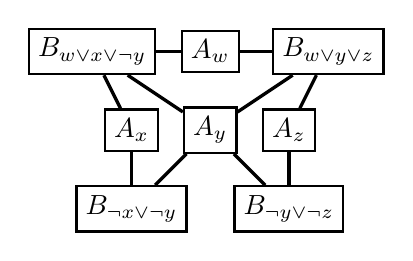
\begin{tikzpicture}
\begin{scope}[every node/.style={thick,draw}]
    \node (C) at (-1,-1) {$B_{\neg x \lor \neg y}$};
    \node (x) at (-1,0) {$A_x$};
    \node (A) at (-1.5,1) {$B_{w \lor x \lor \neg y}$};
    \node (y) at (0,0) {$A_y$};
    \node (w) at (0,1) {$A_w$};
    \node (D) at (1,-1) {$B_{\neg y \lor \neg z}$};
    \node (z) at (1,0) {$A_z$};
    \node (B) at (1.5,1) {$B_{w \lor y \lor z}$};
\end{scope}

\begin{scope}[every node/.style={fill=white,circle},
              every edge/.style={draw=black,very thick}]
    \path [-] (A) edge (w);
    \path [-] (A) edge (x);
    \path [-] (A) edge (y);
    \path [-] (B) edge (w);
    \path [-] (B) edge (y);
    \path [-] (B) edge (z);
    \path [-] (C) edge (x);
    \path [-] (C) edge (y);
    \path [-] (D) edge (y);
    \path [-] (D) edge (z);
\end{scope}
\end{tikzpicture}
	\caption{\label{fig:wmc-example} The tensor network produced by Theorem \ref{thm:wmc-reduction} on $\varphi = (w \lor x \lor \neg y) \land (w \lor y \lor z) \land (\neg x \lor \neg y) \land (\neg y \lor \neg z)$ has 8 tensors (indicated by vertices) and 10 indices (indicated by edges). The $A_*$ tensors correspond to variables and have entries computed from the weight function.  The $B_*$ tensors correspond to clauses and have entries computed from the clause negations.}
\end{figure}
\begin{theorem}
\label{thm:wmc-reduction}
Let $\varphi$ be a CNF formula over Boolean variables $X$ and let $W$ be a weight function. One can construct in polynomial time a tensor network $N_{\varphi,W}$ such that $\tnfree{N_{\varphi,W}} = \emptyset$ and the contraction of $N_{\varphi,W}$ is $W(\varphi)$.
\end{theorem}
\begin{proof}[Sketch of Construction] Let $I = \{(x, C) \in X \times \varphi: x~\text{appears in}~C\}$ be a set of indices, each with domain $\{0,1\}$. The key idea is create a tensor $A_x$ for each variable $x \in X$ and a tensor $B_C$ for each clause $C \in \varphi$ so that each index $(x, C) \in I$ is an index of $A_x$ and $B_C$.

For each $x \in X$, let $A_x$ be a tensor with indices $I \cap (\{x\} \times \varphi)$. For each $\tau \in \domain{I \cap (\{x\} \times \varphi)}$, define $A_x(\tau)$ to be $W(x,0)$ if $\tau$ is always 0, $W(x, 1)$ if $\tau$ is always 1, and 0 otherwise.

For each $C \in \varphi$, let $B_C$ be a tensor with indices $I \cap (X \times \{C\})$. For each $\tau \in \domain{I \cap (X \times \{C\})}$, define $B_C(\tau)$ to be $1$ if $\{x \in X : x~\text{appears in}~C~\text{and}~\tau((x, C)) = 1\}$ satisfies $C$ and 0 otherwise. 

%\begin{multicols}{2}
%    $$A_x(\tau) \equiv \begin{cases}W(x, 0)&\text{if}~\tau~\text{is always 0}\\W(x, 1)&\text{if}~\tau~\text{is always 1}\\0&\text{otherwise.}\end{cases}$$
%  \break
%    $$B_C(\tau) \equiv \begin{cases}1&\text{if}~\{x \in X : x~\text{appears in}~C~\text{and}~\tau((x, C)) = 1\}~\text{satisfies}~C\\0&\text{otherwise.}\end{cases}$$
%\end{multicols}

%For each $x \in X$, define $A_x: [I \cap (\{x\} \times \varphi)] \rightarrow \mathbb{R}$ to be the tensor where $A_x(\tau)$ is $W(x,0)$ if $\tau$ is always 0, $W(x, 1)$ if $\tau$ is always 1, and 0 otherwise. For each $C \in \varphi$, define $B_C: [I \cap (X \times \{C\})] \rightarrow \mathbb{R}$ to be the tensor where $B_C(\tau)$ is $1$ if $\{x \in X : x~\text{appears in}~C~\text{and}~\tau((x, C)) = 1\}$ satisfies $C$ and 0 otherwise. 

Then $N_{\varphi,W} = \{A_x : x \in X\} \cup \{B_C : C \in \varphi\}$ is the desired tensor network.
%Include in $N_{\varphi,W}$ a tensor for each variable and for each clause of $\varphi$. Each variable tensor and clause tensor share an index if and only if the corresponding variable appears in the corresponding clause.
\end{proof}

Theorem \ref{thm:wmc-reduction} proves that $\func{Reduce}(\varphi,W) = N_{\varphi, W}$ satisfies assumption 1 in Theorem \ref{thm:alg-correctness}. See Figure \ref{fig:wmc-example} for an example of the reduction. This reduction is closely related to the formulation of model counting as the marginalization of a factor graph representing the constraints (but assigns tensors to variables as well, not just clauses). %Unlike the reduction to factor-graph marginalization, which only assigns factors to clauses, Theorem \ref{thm:wmc-reduction} also assigns a tensor to each variable $x$. % For example, if $x$ has weights $W(x, 0) = W(x,1) = 1$ then the tensor assigned to $x$ is a copy tensor. 
This reduction can also be extended to other types of constraints, e.g. parity or cardinality constraints.

\subsection{The Execution Stage}
For formulas $\varphi$ with hundreds of clauses, the corresponding tensor network produced by Theorem \ref{thm:wmc-reduction} has hundreds of bond indices. Directly following Equation \ref{eqn:contraction} in this case is infeasible, since it sums over an exponential number of terms. 

Instead, Algorithm \ref{alg:network-contraction} shows how to compute $\tntensor{N}$ for a tensor network $N$ using a contraction tree $T$ as a guide. The key idea is to repeatedly choose two tensors $A_1, A_2 \in N$ (according to the structure of $T$) and contract them. One can prove inductively that Algorithm \ref{alg:network-contraction} satisfies assumption 3 of Theorem \ref{thm:alg-correctness}.

% Since $N'$ is a partial contraction of $N$, $\tntensor{N'} = \tntensor{N}$. Thus, when this process produces a tensor network containing a single tensor, it follows inductively that this tensor is $\tntensor{N}$. Therefore Algorithm \ref{alg:network-contraction} satisfies assumption 3 of Theorem \ref{thm:alg-correctness}.

\label{sec:algorithm:execution}
% \begin{algorithm}[t]
% 	\caption{Recursively contracting a tensor network}\label{alg:network-contraction}
% 	\textbf{Input:} A tensor network $N$ and a contraction tree $T$ for $N$. \\
% 	\textbf{Output:} $\tntensor{N}$, the contraction of $N$.
% 	\begin{algorithmic}[1]
% 	    \Procedure{Execute}{$N,T$}
% 		\If {$\left|N\right| = 1$}
% 		\State \Return the tensor contained in $N$
% 		\Else
%         \State $T_1, T_2 \gets \text{immediate subtrees of}~T$
% 		\State \Return $\Call{Execute}{\Lv{T_1}, T_1} \cdot \Call{Execute}{\Lv{T_2}, T_2}$
% 		\EndIf
% 		\EndProcedure
% 	\end{algorithmic}
% \end{algorithm}

Each contraction in Algorithm \ref{alg:network-contraction} contains exactly two tensors and so can be implemented as a matrix multiplication. In \cite{DDV19}, \tool{numpy} \cite{numpy} was used to perform each of these contractions. %, but such contractions can also be done with \tool{TensorFlow} \cite{ABCCDDDGII16} and other tensor libraries.
Although the choice of contraction tree does not affect the correctness of Algorithm \ref{alg:network-contraction}, it may have a dramatic impact on the running-time and memory usage. We explore this further in the following section.

\subsection{The Planning Stage}
\label{sec:algorithm:planning}
The task in the planning stage is, given a tensor network, to find a contraction tree that minimizes the computational cost of Algorithm \ref{alg:network-contraction}.

Several \emph{cost-based} approaches \cite{Hirata03,PHV14} aim for minimizing the total number of floating point operations to perform Algorithm \ref{alg:network-contraction}. Most cost-based approaches are designed for tensor networks with very few, large tensors, whereas weighted model counting benchmarks produce tensor networks with many, small tensors. These approaches are thus inappropriate for counting.

Instead, we focus here on \emph{structure-based} approaches, which analyze the rank of intermediate tensors that appear during Algorithm \ref{alg:network-contraction}. The ranks indicate the amount of memory and computation required at each recursive stage. The goal is then to find a contraction tree with small \emph{max-rank}, which is the maximum rank of all tensors that appear during Algorithm \ref{alg:network-contraction}.

This is done through analysis of the \emph{structure graph}, a representation of a tensor network as a graph where tensors are vertices and indices indicate the edges between tensors~\cite{DDV19,MS08,Ying17}:
\begin{definition}[Structure Graph]\label{def:structure}
	Let $N$ be a tensor network. The \emph{structure graph} of $N$ is the graph, denoted $G = \struct{N}$, where $\V{G} = N \cup \{\fv\}$ ($\fv$ is a fresh vertex called the \emph{free vertex}), $\E{G} = \tnbound{N} \cup \tnfree{N}$, $\vinc{G}{\fv} = \tnfree{N}$, and, for all $A \in N$, $\vinc{G}{A} = \tdim{A}$.
	
	%\begin{enumerate}
	%    \item $\V{G} = N \cup \{\fv\}$, where $\fv$ is a fresh vertex called the \emph{free vertex},
	%    \item $\E{G} = \tnbound{N} \cup \tnfree{N}$,
	%    \item each tensor is incident to its indices, and
	%    \item $\fv$ is incident to all free indices.
	%\end{enumerate}
    % That is, $\V{G} = N \sqcup \{ \fv \}$, $\E{G} = \tnbound{N} \cup \tnfree{N}$, $\vinc{G}{A} = \tdim{A}$ for all $A \in N$, and $\vinc{G}{\fv} = \tnfree{N}$.
\end{definition}

%Kourtis et. al \cite{KCMR18} introduced three algorithms for heuristically minimizing the max rank using the structure graph: a greedy algorithm, an algorithm using graph partitioning, and an algorithm using community-structure detection. Another algorithm \cite{MS08,DFGHSW18} utilizes low-width tree decompositions of the line graph of $\struct{N}$. 
%On factor graphs, this approach is analogous to the use of tree decompositions of the primal graph to find variable elimination orders \cite{KDLD05}.

For example, if $\varphi$ is a formula and $N_{\varphi,W}$ is the tensor network resulting from Theorem \ref{thm:wmc-reduction}, then $\struct{N_{\varphi,W}}$ is the incidence graph of $\varphi$ (and is independent of the weight function).

One structure-based approach for finding contraction trees \cite{DFGHSW18,MS08} utilizes low-width tree decompositions of the line graph of $\struct{N}$. This approach is analogous to \emph{variable elimination} on factor graphs \cite{BDP09,KDLD05}, which uses tree decompositions of the primal graph of a factor graph.

Unfortunately, for many tensor network all possible contraction trees have large max-rank. \cite{DDV19} observed that this is the case for many standard counting benchmarks. This is because, for each variable $x$, the number of times $x$ appears in $\varphi$ is a lower bound on the max-rank of all contraction trees of $\func{Reduce}(\varphi, \cdot)$. Thus traditional tensor network planning algorithms (e.g., \cite{DFGHSW18,KCMR18,MS08}) fail on counting benchmarks that have variables which appear more than $30$ times. 

%For example, if a tensor network contains a rank $k$ tensor, then all contraction trees necessarily have max-rank at least $k$. Recall from Theorem \ref{thm:wmc-reduction} that, for weighted model counting, a variable $x$ that appears $k$ times in $\varphi$ is represented in $\Call{Reduce}{\varphi, W}$ by a rank $k$ tensor. Thus for many weighted model counting benchmarks, where a single variable might appear tens or even hundreds of times, the resulting tensor network will have tensors of infeasibly-high rank. Indeed, 
Instead, \cite{DDV19} relaxed the planning stage by allowing changes to the input tensor network $N$. In particular, \cite{DDV19} used tree decompositions of $\struct{N}$ to factor high-rank, highly-structured tensors as a preprocessing step, following prior methods that split large CNF clauses \cite{SS10_2} and high-degree graph vertices \cite{oliveira18,MS11}. A tensor is highly-structured here if it is \emph{tree-factorable}:
\begin{definition} \label{def:tree-factorable}
A tensor $A$ is \emph{tree factorable} if, for every tree $T$ whose leaves are $\tdim{A}$, there is a tensor network $N_A$ and a bijection $g_A: \V{T} \rightarrow N_A$ s.t. $A$ is the contraction of $N_A$ and:
\begin{enumerate}\itemsep0em 
%\item $A$ is the contraction of $N_A$,
\item $g_A$ is an isomorphism between $T$ and $\struct{N_A}$ with the free vertex removed,
\item for every index $i$ of $A$, $i$ is an index of $g_A(i)$, and
\item for some index $i$ of $A$, every index $j \in \tnbound{N_A}$ satisfies $|\domain{j}| \leq |\domain{i}|$. % the bond dimension of $N_A$ is no bigger than $|\domain{i}|$. % $\max_{i \in \tnbound{N}} |\domain{i}| \leq \max_{i \in \tdim{A}} |\domain{i}|$.
\end{enumerate}
\end{definition}
Informally, a tensor is tree-factorable if it can be replaced by arbitrary trees of low-rank tensors. All tensors produced by Theorem \ref{thm:wmc-reduction} are tree factorable. 
The preprocessing method of \cite{DDV19} is then formalized as follows:
\begin{theorem} \label{thm:factorable-tree}
Let $N$ be a tensor network of tree-factorable tensors such that $|\tnfree{N}| \leq 3$ and $\struct{N}$ has a tree decomposition of width $w \geq 1$. Then we can construct in polynomial time a tensor network $M$ and a contraction tree $T$ for $M$ s.t. $\text{max-rank}(T) \leq \ceil{4(w+1)/3}$ and $N$ is a partial contraction of $M$.
\end{theorem}

This gives us the $\func{FactorTree}(N)$ planning method, which computes a tree decomposition of $\struct{N}$ and returns the $M$ and $T$ that result from Theorem \ref{thm:factorable-tree}. Because $N$ is a partial contraction of $M$, $\tntensor{N} = \tntensor{M}$. Since all tensors produced by Thereom \ref{thm:wmc-reduction} are tree-factorable, $\func{FactorTree}(N)$ satisfies assumption 2 in Theorem \ref{thm:alg-correctness}. 

While both $\func{FactorTree}(N)$ and variable elimination \cite{BDP09,KDLD05} use tree decompositions, they consider different graphs. For example, consider computing the model count of $\psi = \left(\lor_{i=1}^n x_i\right) \land \left(\lor_{i=1}^n \neg x_i\right)$. $\func{FactorTree}(N)$ uses tree decompositions of the incidence graph of $\psi$, which has treewidth 2. Variable elimination uses tree decompositions of the primal graph of $\psi$, which has treewidth $n-1$. Thus $\func{FactorTree}(N)$ can exhibit significantly better behavior than variable elimination on some formulas. On the other hand, the behavior of $\func{FactorTree}(N)$ is at most slightly worse than variable elimination: as noted above, if the treewidth of the primal graph of a formula $\varphi$ is $k$, the treewidth of the incidence graph of $\varphi$ is at most $k+1$ \cite{KV00}. % In the next section we show how branch decompositions can be used to generalize Theorem \ref{thm:factorable-tree} and hence construct contraction trees. % TODO: merge
\section{Implementation and Evaluation}
\label{sec:experiments}

We aim to answer the following research questions:

\begin{enumerate}\itemsep0em 
    \item[(RQ1)] Is the planning stage improved by a parallel portfolio of decomposition tools?
    
    \item[(RQ2)] Is the planning stage improved by adding a branch-decomposition tool?
    
    \item[(RQ3)] When should Algorithm \ref{alg:wmc} transition from the planning stage to the execution stage (i.e., what should be the value of the performance factor $\alpha$)?
    
    \item[(RQ4)] Is the execution stage improved by leveraging multiple cores and a GPU?
    
    \item[(RQ5)] Do parallel tensor network approaches improve a portfolio of state-of-the-art weighted model counters (\tool{cachet}, \tool{miniC2D}, \tool{d4}, \tool{ADDMC}, and \tool{gpuSAT2})?
\end{enumerate}

We implement our changes on top of \tool{TensorOrder} \cite{DDV19} (which implements Algorithm \ref{alg:wmc}; see Section \ref{sec:tensors:experiments:implementation}) to produce \tool{TensorOrder2}, a new parallel weighted model counter. Implementation details are described in Section \ref{sec:experiments:impl}. All code is available at  \url{https://github.com/vardigroup/TensorOrder}.

%\paragraph{Benchmarks.} 
We use a standard set\footnote{\url{https://github.com/vardigroup/ADDMC/releases/tag/v1.0.0}} of 1914 weighted model counting benchmarks \cite{DPV20}. Of these, 1091 benchmarks\footnote{\url{https://www.cs.rochester.edu/u/kautz/Cachet/}} are from Bayesian inference problems \cite{SBK05} and 823 benchmarks\footnote{\url{http://www.cril.univ-artois.fr/KC/benchmarks.html}} are unweighted benchmarks (from various domains) that were artificially weighted by \cite{DPV20}. For weighted model counters that cannot handle real weights larger than 1 (\tool{cachet} and \tool{gpusat2}), we rescale the weights of benchmarks with larger weights. In Experiment 3, we also consider preprocessing these 1914 benchmarks by applying $\pkg{pmc-eq}$ \cite{LM14} (which preserves weighted model count). % We apply to each benchmark, with a timeout of 1000 seconds. We remove 61 benchmarks that were fully solved by $\pkg{pmc-eq}$ (either UNSAT., or with a single solution) and 11 benchmarks that timed out, resulting in 1842 preprocessed benchmarks.
We evaluate the performance of each tool using the PAR-2 score, which is the sum of of the wall-clock times for each completed benchmark, plus twice the timeout for each uncompleted benchmark.

%\paragraph{Experimental Setup.}
All counters are run in the Docker images (one for each counter) with Docker 19.03.5. All experiments are run on Google Cloud \tool{n1-standard-8} machines with 8 cores (Intel Haswell, 2.3 GHz) and 30 GB RAM. GPU-based counters are provided an \tool{NVIDIA Tesla V100} GPU (16 GB of onboard RAM) using NVIDIA driver 418.67 and CUDA 10.1.243.

\subsection{Implementation Details of \tool{TensorOrder2}}
\label{sec:experiments:impl}
\tool{TensorOrder2} is primarily implemented in Python 3 as a modified version of the tool from Chapter \ref{ch:tensors}, \tool{TensorOrder}. We replace portions of the Python code with C++ (\tool{g++} v7.4.0) using Cython 0.29.15 for general speedup, especially in $\func{FactorTree}(\cdot)$.

\paragraph{Planning.} 
\tool{TensorOrder} contains an implementation of the planning stage using a choice of three single-core tree-decomposition solvers: \pkg{Tamaki} \cite{Tamaki17}, \pkg{FlowCutter} \cite{HS18}, and \pkg{htd} \cite{AMW17}. We add to \tool{TensorOrder2} an implementation of Theorem \ref{thm:factorable-branch} and use it to add a branch-decomposition solver \pkg{Hicks} \cite{hicks02}.
We implement a parallel portfolio of graph-decomposition solvers in C++ and give \tool{TensorOrder2} access to two portfolios, each with access to all cores: \pkg{P3} (which combines \pkg{Tamaki},  \pkg{FlowCutter}, and \pkg{htd}) and \pkg{P4} (which includes \pkg{Hicks} as well).

\paragraph{Execution.} 
\tool{TensorOrder} is able to perform the execution stage on a single core and on multiple cores using \pkg{numpy} v1.18.1 and \pkg{OpenBLAS} v0.2.20. In \tool{TensorOrder2}, we add the ability to contract tensors on a GPU with \pkg{TensorFlow} v2.1.0 \cite{ABCCDDDGII16}. To avoid GPU kernel calls for small contractions, \tool{TensorOrder2} uses a GPU only for contractions where one of the tensors involved has rank $\geq 20$, and reverts back to using multi-core \pkg{numpy} otherwise. We also add an implementation of Algorithm \ref{alg:tn-sliced}.
Overall, \tool{TensorOrder2} runs the execution stage on three hardware configurations: \pkg{CPU1} (restricted to a single CPU core), \pkg{CPU8} (allowed to use all 8 CPU cores), and \pkg{GPU} (allowed to use all 8 CPU cores and use a GPU).

\begin{figure}
	\centering
	%% Creator: Matplotlib, PGF backend
%%
%% To include the figure in your LaTeX document, write
%%   \input{<filename>.pgf}
%%
%% Make sure the required packages are loaded in your preamble
%%   \usepackage{pgf}
%%
%% and, on pdftex
%%   \usepackage[utf8]{inputenc}\DeclareUnicodeCharacter{2212}{-}
%%
%% or, on luatex and xetex
%%   \usepackage{unicode-math}
%%
%% Figures using additional raster images can only be included by \input if
%% they are in the same directory as the main LaTeX file. For loading figures
%% from other directories you can use the `import` package
%%   \usepackage{import}
%%
%% and then include the figures with
%%   \import{<path to file>}{<filename>.pgf}
%%
%% Matplotlib used the following preamble
%%   \usepackage[utf8x]{inputenc}
%%   \usepackage[T1]{fontenc}
%%
\begingroup%
\makeatletter%
\begin{pgfpicture}%
\pgfpathrectangle{\pgfpointorigin}{\pgfqpoint{4.803148in}{2.021259in}}%
\pgfusepath{use as bounding box, clip}%
\begin{pgfscope}%
\pgfsetbuttcap%
\pgfsetmiterjoin%
\definecolor{currentfill}{rgb}{1.000000,1.000000,1.000000}%
\pgfsetfillcolor{currentfill}%
\pgfsetlinewidth{0.000000pt}%
\definecolor{currentstroke}{rgb}{1.000000,1.000000,1.000000}%
\pgfsetstrokecolor{currentstroke}%
\pgfsetdash{}{0pt}%
\pgfpathmoveto{\pgfqpoint{0.000000in}{0.000000in}}%
\pgfpathlineto{\pgfqpoint{4.803148in}{0.000000in}}%
\pgfpathlineto{\pgfqpoint{4.803148in}{2.021259in}}%
\pgfpathlineto{\pgfqpoint{0.000000in}{2.021259in}}%
\pgfpathclose%
\pgfusepath{fill}%
\end{pgfscope}%
\begin{pgfscope}%
\pgfsetbuttcap%
\pgfsetmiterjoin%
\definecolor{currentfill}{rgb}{1.000000,1.000000,1.000000}%
\pgfsetfillcolor{currentfill}%
\pgfsetlinewidth{0.000000pt}%
\definecolor{currentstroke}{rgb}{0.000000,0.000000,0.000000}%
\pgfsetstrokecolor{currentstroke}%
\pgfsetstrokeopacity{0.000000}%
\pgfsetdash{}{0pt}%
\pgfpathmoveto{\pgfqpoint{0.694334in}{0.523557in}}%
\pgfpathlineto{\pgfqpoint{4.524677in}{0.523557in}}%
\pgfpathlineto{\pgfqpoint{4.524677in}{1.826535in}}%
\pgfpathlineto{\pgfqpoint{0.694334in}{1.826535in}}%
\pgfpathclose%
\pgfusepath{fill}%
\end{pgfscope}%
\begin{pgfscope}%
\pgfsetbuttcap%
\pgfsetroundjoin%
\definecolor{currentfill}{rgb}{0.000000,0.000000,0.000000}%
\pgfsetfillcolor{currentfill}%
\pgfsetlinewidth{0.803000pt}%
\definecolor{currentstroke}{rgb}{0.000000,0.000000,0.000000}%
\pgfsetstrokecolor{currentstroke}%
\pgfsetdash{}{0pt}%
\pgfsys@defobject{currentmarker}{\pgfqpoint{0.000000in}{-0.048611in}}{\pgfqpoint{0.000000in}{0.000000in}}{%
\pgfpathmoveto{\pgfqpoint{0.000000in}{0.000000in}}%
\pgfpathlineto{\pgfqpoint{0.000000in}{-0.048611in}}%
\pgfusepath{stroke,fill}%
}%
\begin{pgfscope}%
\pgfsys@transformshift{0.694334in}{0.523557in}%
\pgfsys@useobject{currentmarker}{}%
\end{pgfscope}%
\end{pgfscope}%
\begin{pgfscope}%
\definecolor{textcolor}{rgb}{0.000000,0.000000,0.000000}%
\pgfsetstrokecolor{textcolor}%
\pgfsetfillcolor{textcolor}%
\pgftext[x=0.694334in,y=0.426335in,,top]{\color{textcolor}\rmfamily\fontsize{9.000000}{10.800000}\selectfont \(\displaystyle 0\)}%
\end{pgfscope}%
\begin{pgfscope}%
\pgfsetbuttcap%
\pgfsetroundjoin%
\definecolor{currentfill}{rgb}{0.000000,0.000000,0.000000}%
\pgfsetfillcolor{currentfill}%
\pgfsetlinewidth{0.803000pt}%
\definecolor{currentstroke}{rgb}{0.000000,0.000000,0.000000}%
\pgfsetstrokecolor{currentstroke}%
\pgfsetdash{}{0pt}%
\pgfsys@defobject{currentmarker}{\pgfqpoint{0.000000in}{-0.048611in}}{\pgfqpoint{0.000000in}{0.000000in}}{%
\pgfpathmoveto{\pgfqpoint{0.000000in}{0.000000in}}%
\pgfpathlineto{\pgfqpoint{0.000000in}{-0.048611in}}%
\pgfusepath{stroke,fill}%
}%
\begin{pgfscope}%
\pgfsys@transformshift{1.173127in}{0.523557in}%
\pgfsys@useobject{currentmarker}{}%
\end{pgfscope}%
\end{pgfscope}%
\begin{pgfscope}%
\definecolor{textcolor}{rgb}{0.000000,0.000000,0.000000}%
\pgfsetstrokecolor{textcolor}%
\pgfsetfillcolor{textcolor}%
\pgftext[x=1.173127in,y=0.426335in,,top]{\color{textcolor}\rmfamily\fontsize{9.000000}{10.800000}\selectfont \(\displaystyle 250\)}%
\end{pgfscope}%
\begin{pgfscope}%
\pgfsetbuttcap%
\pgfsetroundjoin%
\definecolor{currentfill}{rgb}{0.000000,0.000000,0.000000}%
\pgfsetfillcolor{currentfill}%
\pgfsetlinewidth{0.803000pt}%
\definecolor{currentstroke}{rgb}{0.000000,0.000000,0.000000}%
\pgfsetstrokecolor{currentstroke}%
\pgfsetdash{}{0pt}%
\pgfsys@defobject{currentmarker}{\pgfqpoint{0.000000in}{-0.048611in}}{\pgfqpoint{0.000000in}{0.000000in}}{%
\pgfpathmoveto{\pgfqpoint{0.000000in}{0.000000in}}%
\pgfpathlineto{\pgfqpoint{0.000000in}{-0.048611in}}%
\pgfusepath{stroke,fill}%
}%
\begin{pgfscope}%
\pgfsys@transformshift{1.651920in}{0.523557in}%
\pgfsys@useobject{currentmarker}{}%
\end{pgfscope}%
\end{pgfscope}%
\begin{pgfscope}%
\definecolor{textcolor}{rgb}{0.000000,0.000000,0.000000}%
\pgfsetstrokecolor{textcolor}%
\pgfsetfillcolor{textcolor}%
\pgftext[x=1.651920in,y=0.426335in,,top]{\color{textcolor}\rmfamily\fontsize{9.000000}{10.800000}\selectfont \(\displaystyle 500\)}%
\end{pgfscope}%
\begin{pgfscope}%
\pgfsetbuttcap%
\pgfsetroundjoin%
\definecolor{currentfill}{rgb}{0.000000,0.000000,0.000000}%
\pgfsetfillcolor{currentfill}%
\pgfsetlinewidth{0.803000pt}%
\definecolor{currentstroke}{rgb}{0.000000,0.000000,0.000000}%
\pgfsetstrokecolor{currentstroke}%
\pgfsetdash{}{0pt}%
\pgfsys@defobject{currentmarker}{\pgfqpoint{0.000000in}{-0.048611in}}{\pgfqpoint{0.000000in}{0.000000in}}{%
\pgfpathmoveto{\pgfqpoint{0.000000in}{0.000000in}}%
\pgfpathlineto{\pgfqpoint{0.000000in}{-0.048611in}}%
\pgfusepath{stroke,fill}%
}%
\begin{pgfscope}%
\pgfsys@transformshift{2.130713in}{0.523557in}%
\pgfsys@useobject{currentmarker}{}%
\end{pgfscope}%
\end{pgfscope}%
\begin{pgfscope}%
\definecolor{textcolor}{rgb}{0.000000,0.000000,0.000000}%
\pgfsetstrokecolor{textcolor}%
\pgfsetfillcolor{textcolor}%
\pgftext[x=2.130713in,y=0.426335in,,top]{\color{textcolor}\rmfamily\fontsize{9.000000}{10.800000}\selectfont \(\displaystyle 750\)}%
\end{pgfscope}%
\begin{pgfscope}%
\pgfsetbuttcap%
\pgfsetroundjoin%
\definecolor{currentfill}{rgb}{0.000000,0.000000,0.000000}%
\pgfsetfillcolor{currentfill}%
\pgfsetlinewidth{0.803000pt}%
\definecolor{currentstroke}{rgb}{0.000000,0.000000,0.000000}%
\pgfsetstrokecolor{currentstroke}%
\pgfsetdash{}{0pt}%
\pgfsys@defobject{currentmarker}{\pgfqpoint{0.000000in}{-0.048611in}}{\pgfqpoint{0.000000in}{0.000000in}}{%
\pgfpathmoveto{\pgfqpoint{0.000000in}{0.000000in}}%
\pgfpathlineto{\pgfqpoint{0.000000in}{-0.048611in}}%
\pgfusepath{stroke,fill}%
}%
\begin{pgfscope}%
\pgfsys@transformshift{2.609506in}{0.523557in}%
\pgfsys@useobject{currentmarker}{}%
\end{pgfscope}%
\end{pgfscope}%
\begin{pgfscope}%
\definecolor{textcolor}{rgb}{0.000000,0.000000,0.000000}%
\pgfsetstrokecolor{textcolor}%
\pgfsetfillcolor{textcolor}%
\pgftext[x=2.609506in,y=0.426335in,,top]{\color{textcolor}\rmfamily\fontsize{9.000000}{10.800000}\selectfont \(\displaystyle 1000\)}%
\end{pgfscope}%
\begin{pgfscope}%
\pgfsetbuttcap%
\pgfsetroundjoin%
\definecolor{currentfill}{rgb}{0.000000,0.000000,0.000000}%
\pgfsetfillcolor{currentfill}%
\pgfsetlinewidth{0.803000pt}%
\definecolor{currentstroke}{rgb}{0.000000,0.000000,0.000000}%
\pgfsetstrokecolor{currentstroke}%
\pgfsetdash{}{0pt}%
\pgfsys@defobject{currentmarker}{\pgfqpoint{0.000000in}{-0.048611in}}{\pgfqpoint{0.000000in}{0.000000in}}{%
\pgfpathmoveto{\pgfqpoint{0.000000in}{0.000000in}}%
\pgfpathlineto{\pgfqpoint{0.000000in}{-0.048611in}}%
\pgfusepath{stroke,fill}%
}%
\begin{pgfscope}%
\pgfsys@transformshift{3.088299in}{0.523557in}%
\pgfsys@useobject{currentmarker}{}%
\end{pgfscope}%
\end{pgfscope}%
\begin{pgfscope}%
\definecolor{textcolor}{rgb}{0.000000,0.000000,0.000000}%
\pgfsetstrokecolor{textcolor}%
\pgfsetfillcolor{textcolor}%
\pgftext[x=3.088299in,y=0.426335in,,top]{\color{textcolor}\rmfamily\fontsize{9.000000}{10.800000}\selectfont \(\displaystyle 1250\)}%
\end{pgfscope}%
\begin{pgfscope}%
\pgfsetbuttcap%
\pgfsetroundjoin%
\definecolor{currentfill}{rgb}{0.000000,0.000000,0.000000}%
\pgfsetfillcolor{currentfill}%
\pgfsetlinewidth{0.803000pt}%
\definecolor{currentstroke}{rgb}{0.000000,0.000000,0.000000}%
\pgfsetstrokecolor{currentstroke}%
\pgfsetdash{}{0pt}%
\pgfsys@defobject{currentmarker}{\pgfqpoint{0.000000in}{-0.048611in}}{\pgfqpoint{0.000000in}{0.000000in}}{%
\pgfpathmoveto{\pgfqpoint{0.000000in}{0.000000in}}%
\pgfpathlineto{\pgfqpoint{0.000000in}{-0.048611in}}%
\pgfusepath{stroke,fill}%
}%
\begin{pgfscope}%
\pgfsys@transformshift{3.567091in}{0.523557in}%
\pgfsys@useobject{currentmarker}{}%
\end{pgfscope}%
\end{pgfscope}%
\begin{pgfscope}%
\definecolor{textcolor}{rgb}{0.000000,0.000000,0.000000}%
\pgfsetstrokecolor{textcolor}%
\pgfsetfillcolor{textcolor}%
\pgftext[x=3.567091in,y=0.426335in,,top]{\color{textcolor}\rmfamily\fontsize{9.000000}{10.800000}\selectfont \(\displaystyle 1500\)}%
\end{pgfscope}%
\begin{pgfscope}%
\pgfsetbuttcap%
\pgfsetroundjoin%
\definecolor{currentfill}{rgb}{0.000000,0.000000,0.000000}%
\pgfsetfillcolor{currentfill}%
\pgfsetlinewidth{0.803000pt}%
\definecolor{currentstroke}{rgb}{0.000000,0.000000,0.000000}%
\pgfsetstrokecolor{currentstroke}%
\pgfsetdash{}{0pt}%
\pgfsys@defobject{currentmarker}{\pgfqpoint{0.000000in}{-0.048611in}}{\pgfqpoint{0.000000in}{0.000000in}}{%
\pgfpathmoveto{\pgfqpoint{0.000000in}{0.000000in}}%
\pgfpathlineto{\pgfqpoint{0.000000in}{-0.048611in}}%
\pgfusepath{stroke,fill}%
}%
\begin{pgfscope}%
\pgfsys@transformshift{4.045884in}{0.523557in}%
\pgfsys@useobject{currentmarker}{}%
\end{pgfscope}%
\end{pgfscope}%
\begin{pgfscope}%
\definecolor{textcolor}{rgb}{0.000000,0.000000,0.000000}%
\pgfsetstrokecolor{textcolor}%
\pgfsetfillcolor{textcolor}%
\pgftext[x=4.045884in,y=0.426335in,,top]{\color{textcolor}\rmfamily\fontsize{9.000000}{10.800000}\selectfont \(\displaystyle 1750\)}%
\end{pgfscope}%
\begin{pgfscope}%
\pgfsetbuttcap%
\pgfsetroundjoin%
\definecolor{currentfill}{rgb}{0.000000,0.000000,0.000000}%
\pgfsetfillcolor{currentfill}%
\pgfsetlinewidth{0.803000pt}%
\definecolor{currentstroke}{rgb}{0.000000,0.000000,0.000000}%
\pgfsetstrokecolor{currentstroke}%
\pgfsetdash{}{0pt}%
\pgfsys@defobject{currentmarker}{\pgfqpoint{0.000000in}{-0.048611in}}{\pgfqpoint{0.000000in}{0.000000in}}{%
\pgfpathmoveto{\pgfqpoint{0.000000in}{0.000000in}}%
\pgfpathlineto{\pgfqpoint{0.000000in}{-0.048611in}}%
\pgfusepath{stroke,fill}%
}%
\begin{pgfscope}%
\pgfsys@transformshift{4.524677in}{0.523557in}%
\pgfsys@useobject{currentmarker}{}%
\end{pgfscope}%
\end{pgfscope}%
\begin{pgfscope}%
\definecolor{textcolor}{rgb}{0.000000,0.000000,0.000000}%
\pgfsetstrokecolor{textcolor}%
\pgfsetfillcolor{textcolor}%
\pgftext[x=4.524677in,y=0.426335in,,top]{\color{textcolor}\rmfamily\fontsize{9.000000}{10.800000}\selectfont \(\displaystyle 2000\)}%
\end{pgfscope}%
\begin{pgfscope}%
\definecolor{textcolor}{rgb}{0.000000,0.000000,0.000000}%
\pgfsetstrokecolor{textcolor}%
\pgfsetfillcolor{textcolor}%
\pgftext[x=2.609506in,y=0.260390in,,top]{\color{textcolor}\rmfamily\fontsize{9.000000}{10.800000}\selectfont Number of benchmarks solved}%
\end{pgfscope}%
\begin{pgfscope}%
\pgfsetbuttcap%
\pgfsetroundjoin%
\definecolor{currentfill}{rgb}{0.000000,0.000000,0.000000}%
\pgfsetfillcolor{currentfill}%
\pgfsetlinewidth{0.803000pt}%
\definecolor{currentstroke}{rgb}{0.000000,0.000000,0.000000}%
\pgfsetstrokecolor{currentstroke}%
\pgfsetdash{}{0pt}%
\pgfsys@defobject{currentmarker}{\pgfqpoint{-0.048611in}{0.000000in}}{\pgfqpoint{0.000000in}{0.000000in}}{%
\pgfpathmoveto{\pgfqpoint{0.000000in}{0.000000in}}%
\pgfpathlineto{\pgfqpoint{-0.048611in}{0.000000in}}%
\pgfusepath{stroke,fill}%
}%
\begin{pgfscope}%
\pgfsys@transformshift{0.694334in}{0.843347in}%
\pgfsys@useobject{currentmarker}{}%
\end{pgfscope}%
\end{pgfscope}%
\begin{pgfscope}%
\definecolor{textcolor}{rgb}{0.000000,0.000000,0.000000}%
\pgfsetstrokecolor{textcolor}%
\pgfsetfillcolor{textcolor}%
\pgftext[x=0.330525in, y=0.798622in, left, base]{\color{textcolor}\rmfamily\fontsize{9.000000}{10.800000}\selectfont \(\displaystyle 10^{-1}\)}%
\end{pgfscope}%
\begin{pgfscope}%
\pgfsetbuttcap%
\pgfsetroundjoin%
\definecolor{currentfill}{rgb}{0.000000,0.000000,0.000000}%
\pgfsetfillcolor{currentfill}%
\pgfsetlinewidth{0.803000pt}%
\definecolor{currentstroke}{rgb}{0.000000,0.000000,0.000000}%
\pgfsetstrokecolor{currentstroke}%
\pgfsetdash{}{0pt}%
\pgfsys@defobject{currentmarker}{\pgfqpoint{-0.048611in}{0.000000in}}{\pgfqpoint{0.000000in}{0.000000in}}{%
\pgfpathmoveto{\pgfqpoint{0.000000in}{0.000000in}}%
\pgfpathlineto{\pgfqpoint{-0.048611in}{0.000000in}}%
\pgfusepath{stroke,fill}%
}%
\begin{pgfscope}%
\pgfsys@transformshift{0.694334in}{1.334941in}%
\pgfsys@useobject{currentmarker}{}%
\end{pgfscope}%
\end{pgfscope}%
\begin{pgfscope}%
\definecolor{textcolor}{rgb}{0.000000,0.000000,0.000000}%
\pgfsetstrokecolor{textcolor}%
\pgfsetfillcolor{textcolor}%
\pgftext[x=0.410771in, y=1.290216in, left, base]{\color{textcolor}\rmfamily\fontsize{9.000000}{10.800000}\selectfont \(\displaystyle 10^{1}\)}%
\end{pgfscope}%
\begin{pgfscope}%
\pgfsetbuttcap%
\pgfsetroundjoin%
\definecolor{currentfill}{rgb}{0.000000,0.000000,0.000000}%
\pgfsetfillcolor{currentfill}%
\pgfsetlinewidth{0.803000pt}%
\definecolor{currentstroke}{rgb}{0.000000,0.000000,0.000000}%
\pgfsetstrokecolor{currentstroke}%
\pgfsetdash{}{0pt}%
\pgfsys@defobject{currentmarker}{\pgfqpoint{-0.048611in}{0.000000in}}{\pgfqpoint{0.000000in}{0.000000in}}{%
\pgfpathmoveto{\pgfqpoint{0.000000in}{0.000000in}}%
\pgfpathlineto{\pgfqpoint{-0.048611in}{0.000000in}}%
\pgfusepath{stroke,fill}%
}%
\begin{pgfscope}%
\pgfsys@transformshift{0.694334in}{1.826535in}%
\pgfsys@useobject{currentmarker}{}%
\end{pgfscope}%
\end{pgfscope}%
\begin{pgfscope}%
\definecolor{textcolor}{rgb}{0.000000,0.000000,0.000000}%
\pgfsetstrokecolor{textcolor}%
\pgfsetfillcolor{textcolor}%
\pgftext[x=0.410771in, y=1.781810in, left, base]{\color{textcolor}\rmfamily\fontsize{9.000000}{10.800000}\selectfont \(\displaystyle 10^{3}\)}%
\end{pgfscope}%
\begin{pgfscope}%
\definecolor{textcolor}{rgb}{0.000000,0.000000,0.000000}%
\pgfsetstrokecolor{textcolor}%
\pgfsetfillcolor{textcolor}%
\pgftext[x=0.274969in,y=1.175046in,,bottom,rotate=90.000000]{\color{textcolor}\rmfamily\fontsize{9.000000}{10.800000}\selectfont Longest solving time (s)}%
\end{pgfscope}%
\begin{pgfscope}%
\pgfpathrectangle{\pgfqpoint{0.694334in}{0.523557in}}{\pgfqpoint{3.830343in}{1.302977in}}%
\pgfusepath{clip}%
\pgfsetrectcap%
\pgfsetroundjoin%
\pgfsetlinewidth{1.003750pt}%
\definecolor{currentstroke}{rgb}{0.878431,0.878431,0.815686}%
\pgfsetstrokecolor{currentstroke}%
\pgfsetdash{}{0pt}%
\pgfpathmoveto{\pgfqpoint{0.694334in}{0.948144in}}%
\pgfpathlineto{\pgfqpoint{0.696249in}{0.955934in}}%
\pgfpathlineto{\pgfqpoint{0.701995in}{0.961880in}}%
\pgfpathlineto{\pgfqpoint{0.703910in}{0.964864in}}%
\pgfpathlineto{\pgfqpoint{0.705825in}{0.965524in}}%
\pgfpathlineto{\pgfqpoint{0.709656in}{0.973680in}}%
\pgfpathlineto{\pgfqpoint{0.711571in}{0.974495in}}%
\pgfpathlineto{\pgfqpoint{0.713486in}{0.976961in}}%
\pgfpathlineto{\pgfqpoint{0.719232in}{0.978816in}}%
\pgfpathlineto{\pgfqpoint{0.721147in}{0.980178in}}%
\pgfpathlineto{\pgfqpoint{0.724977in}{1.000991in}}%
\pgfpathlineto{\pgfqpoint{0.728807in}{1.015379in}}%
\pgfpathlineto{\pgfqpoint{0.730723in}{1.015482in}}%
\pgfpathlineto{\pgfqpoint{0.732638in}{1.022216in}}%
\pgfpathlineto{\pgfqpoint{0.734553in}{1.022392in}}%
\pgfpathlineto{\pgfqpoint{0.736468in}{1.024621in}}%
\pgfpathlineto{\pgfqpoint{0.738383in}{1.024629in}}%
\pgfpathlineto{\pgfqpoint{0.742214in}{1.030245in}}%
\pgfpathlineto{\pgfqpoint{0.744129in}{1.030409in}}%
\pgfpathlineto{\pgfqpoint{0.746044in}{1.033013in}}%
\pgfpathlineto{\pgfqpoint{0.747959in}{1.039599in}}%
\pgfpathlineto{\pgfqpoint{0.749874in}{1.040605in}}%
\pgfpathlineto{\pgfqpoint{0.755620in}{1.049992in}}%
\pgfpathlineto{\pgfqpoint{0.772856in}{1.056340in}}%
\pgfpathlineto{\pgfqpoint{0.786263in}{1.061350in}}%
\pgfpathlineto{\pgfqpoint{0.801584in}{1.062980in}}%
\pgfpathlineto{\pgfqpoint{0.805414in}{1.063733in}}%
\pgfpathlineto{\pgfqpoint{0.814990in}{1.065163in}}%
\pgfpathlineto{\pgfqpoint{0.882021in}{1.076339in}}%
\pgfpathlineto{\pgfqpoint{0.885851in}{1.077456in}}%
\pgfpathlineto{\pgfqpoint{0.895427in}{1.078655in}}%
\pgfpathlineto{\pgfqpoint{0.906918in}{1.080409in}}%
\pgfpathlineto{\pgfqpoint{0.987356in}{1.089407in}}%
\pgfpathlineto{\pgfqpoint{1.008422in}{1.090894in}}%
\pgfpathlineto{\pgfqpoint{1.052471in}{1.095137in}}%
\pgfpathlineto{\pgfqpoint{1.056302in}{1.095792in}}%
\pgfpathlineto{\pgfqpoint{1.077369in}{1.097817in}}%
\pgfpathlineto{\pgfqpoint{1.081199in}{1.099401in}}%
\pgfpathlineto{\pgfqpoint{1.096520in}{1.100833in}}%
\pgfpathlineto{\pgfqpoint{1.106096in}{1.102076in}}%
\pgfpathlineto{\pgfqpoint{1.159721in}{1.107209in}}%
\pgfpathlineto{\pgfqpoint{1.163551in}{1.109041in}}%
\pgfpathlineto{\pgfqpoint{1.173127in}{1.110874in}}%
\pgfpathlineto{\pgfqpoint{1.180788in}{1.111938in}}%
\pgfpathlineto{\pgfqpoint{1.186533in}{1.112998in}}%
\pgfpathlineto{\pgfqpoint{1.194194in}{1.114050in}}%
\pgfpathlineto{\pgfqpoint{1.213346in}{1.115660in}}%
\pgfpathlineto{\pgfqpoint{1.221006in}{1.118786in}}%
\pgfpathlineto{\pgfqpoint{1.228667in}{1.120114in}}%
\pgfpathlineto{\pgfqpoint{1.255480in}{1.127277in}}%
\pgfpathlineto{\pgfqpoint{1.265055in}{1.131122in}}%
\pgfpathlineto{\pgfqpoint{1.274631in}{1.132047in}}%
\pgfpathlineto{\pgfqpoint{1.278462in}{1.133795in}}%
\pgfpathlineto{\pgfqpoint{1.295698in}{1.138666in}}%
\pgfpathlineto{\pgfqpoint{1.299528in}{1.139717in}}%
\pgfpathlineto{\pgfqpoint{1.301444in}{1.139860in}}%
\pgfpathlineto{\pgfqpoint{1.303359in}{1.142985in}}%
\pgfpathlineto{\pgfqpoint{1.309104in}{1.143567in}}%
\pgfpathlineto{\pgfqpoint{1.311019in}{1.145858in}}%
\pgfpathlineto{\pgfqpoint{1.316765in}{1.146442in}}%
\pgfpathlineto{\pgfqpoint{1.320595in}{1.149572in}}%
\pgfpathlineto{\pgfqpoint{1.326341in}{1.150947in}}%
\pgfpathlineto{\pgfqpoint{1.334002in}{1.152019in}}%
\pgfpathlineto{\pgfqpoint{1.349323in}{1.155558in}}%
\pgfpathlineto{\pgfqpoint{1.351238in}{1.157653in}}%
\pgfpathlineto{\pgfqpoint{1.353153in}{1.157732in}}%
\pgfpathlineto{\pgfqpoint{1.356984in}{1.160260in}}%
\pgfpathlineto{\pgfqpoint{1.360814in}{1.160544in}}%
\pgfpathlineto{\pgfqpoint{1.368475in}{1.163791in}}%
\pgfpathlineto{\pgfqpoint{1.372305in}{1.164419in}}%
\pgfpathlineto{\pgfqpoint{1.381881in}{1.167150in}}%
\pgfpathlineto{\pgfqpoint{1.395287in}{1.168617in}}%
\pgfpathlineto{\pgfqpoint{1.402948in}{1.170470in}}%
\pgfpathlineto{\pgfqpoint{1.410608in}{1.171407in}}%
\pgfpathlineto{\pgfqpoint{1.420184in}{1.176099in}}%
\pgfpathlineto{\pgfqpoint{1.441251in}{1.178997in}}%
\pgfpathlineto{\pgfqpoint{1.446997in}{1.180239in}}%
\pgfpathlineto{\pgfqpoint{1.458488in}{1.181758in}}%
\pgfpathlineto{\pgfqpoint{1.466148in}{1.183530in}}%
\pgfpathlineto{\pgfqpoint{1.475724in}{1.184325in}}%
\pgfpathlineto{\pgfqpoint{1.485300in}{1.185970in}}%
\pgfpathlineto{\pgfqpoint{1.496791in}{1.186897in}}%
\pgfpathlineto{\pgfqpoint{1.500621in}{1.188076in}}%
\pgfpathlineto{\pgfqpoint{1.510197in}{1.189051in}}%
\pgfpathlineto{\pgfqpoint{1.517858in}{1.191555in}}%
\pgfpathlineto{\pgfqpoint{1.529349in}{1.192277in}}%
\pgfpathlineto{\pgfqpoint{1.542755in}{1.193417in}}%
\pgfpathlineto{\pgfqpoint{1.556161in}{1.195160in}}%
\pgfpathlineto{\pgfqpoint{1.569568in}{1.196028in}}%
\pgfpathlineto{\pgfqpoint{1.573398in}{1.197232in}}%
\pgfpathlineto{\pgfqpoint{1.590635in}{1.200437in}}%
\pgfpathlineto{\pgfqpoint{1.592550in}{1.202315in}}%
\pgfpathlineto{\pgfqpoint{1.598295in}{1.203693in}}%
\pgfpathlineto{\pgfqpoint{1.627023in}{1.210857in}}%
\pgfpathlineto{\pgfqpoint{1.630853in}{1.211879in}}%
\pgfpathlineto{\pgfqpoint{1.632768in}{1.212608in}}%
\pgfpathlineto{\pgfqpoint{1.634683in}{1.214894in}}%
\pgfpathlineto{\pgfqpoint{1.650005in}{1.216939in}}%
\pgfpathlineto{\pgfqpoint{1.653835in}{1.217843in}}%
\pgfpathlineto{\pgfqpoint{1.667241in}{1.220406in}}%
\pgfpathlineto{\pgfqpoint{1.671072in}{1.222320in}}%
\pgfpathlineto{\pgfqpoint{1.678732in}{1.223561in}}%
\pgfpathlineto{\pgfqpoint{1.682563in}{1.225762in}}%
\pgfpathlineto{\pgfqpoint{1.690223in}{1.227473in}}%
\pgfpathlineto{\pgfqpoint{1.694054in}{1.228995in}}%
\pgfpathlineto{\pgfqpoint{1.695969in}{1.229430in}}%
\pgfpathlineto{\pgfqpoint{1.697884in}{1.231143in}}%
\pgfpathlineto{\pgfqpoint{1.701714in}{1.232314in}}%
\pgfpathlineto{\pgfqpoint{1.709375in}{1.233737in}}%
\pgfpathlineto{\pgfqpoint{1.713205in}{1.235570in}}%
\pgfpathlineto{\pgfqpoint{1.728527in}{1.241910in}}%
\pgfpathlineto{\pgfqpoint{1.736188in}{1.243184in}}%
\pgfpathlineto{\pgfqpoint{1.745763in}{1.246246in}}%
\pgfpathlineto{\pgfqpoint{1.757254in}{1.248056in}}%
\pgfpathlineto{\pgfqpoint{1.761085in}{1.248943in}}%
\pgfpathlineto{\pgfqpoint{1.764915in}{1.249471in}}%
\pgfpathlineto{\pgfqpoint{1.774491in}{1.251515in}}%
\pgfpathlineto{\pgfqpoint{1.785982in}{1.252902in}}%
\pgfpathlineto{\pgfqpoint{1.789812in}{1.254325in}}%
\pgfpathlineto{\pgfqpoint{1.793643in}{1.254431in}}%
\pgfpathlineto{\pgfqpoint{1.797473in}{1.256010in}}%
\pgfpathlineto{\pgfqpoint{1.803219in}{1.257885in}}%
\pgfpathlineto{\pgfqpoint{1.835776in}{1.262884in}}%
\pgfpathlineto{\pgfqpoint{1.887486in}{1.270353in}}%
\pgfpathlineto{\pgfqpoint{1.893232in}{1.271230in}}%
\pgfpathlineto{\pgfqpoint{1.902807in}{1.275463in}}%
\pgfpathlineto{\pgfqpoint{1.906638in}{1.276300in}}%
\pgfpathlineto{\pgfqpoint{1.908553in}{1.280411in}}%
\pgfpathlineto{\pgfqpoint{1.916214in}{1.282545in}}%
\pgfpathlineto{\pgfqpoint{1.927705in}{1.284625in}}%
\pgfpathlineto{\pgfqpoint{1.929620in}{1.286283in}}%
\pgfpathlineto{\pgfqpoint{1.937281in}{1.287696in}}%
\pgfpathlineto{\pgfqpoint{1.956432in}{1.296836in}}%
\pgfpathlineto{\pgfqpoint{1.960263in}{1.301263in}}%
\pgfpathlineto{\pgfqpoint{1.964093in}{1.302226in}}%
\pgfpathlineto{\pgfqpoint{1.971754in}{1.304660in}}%
\pgfpathlineto{\pgfqpoint{1.973669in}{1.306666in}}%
\pgfpathlineto{\pgfqpoint{1.981329in}{1.307451in}}%
\pgfpathlineto{\pgfqpoint{1.988990in}{1.309458in}}%
\pgfpathlineto{\pgfqpoint{2.000481in}{1.310640in}}%
\pgfpathlineto{\pgfqpoint{2.002396in}{1.310865in}}%
\pgfpathlineto{\pgfqpoint{2.004312in}{1.313052in}}%
\pgfpathlineto{\pgfqpoint{2.006227in}{1.313203in}}%
\pgfpathlineto{\pgfqpoint{2.010057in}{1.315514in}}%
\pgfpathlineto{\pgfqpoint{2.017718in}{1.316843in}}%
\pgfpathlineto{\pgfqpoint{2.021548in}{1.318677in}}%
\pgfpathlineto{\pgfqpoint{2.031124in}{1.321009in}}%
\pgfpathlineto{\pgfqpoint{2.036869in}{1.325537in}}%
\pgfpathlineto{\pgfqpoint{2.046445in}{1.327598in}}%
\pgfpathlineto{\pgfqpoint{2.048360in}{1.329940in}}%
\pgfpathlineto{\pgfqpoint{2.056021in}{1.331163in}}%
\pgfpathlineto{\pgfqpoint{2.059852in}{1.331423in}}%
\pgfpathlineto{\pgfqpoint{2.063682in}{1.333203in}}%
\pgfpathlineto{\pgfqpoint{2.077088in}{1.334794in}}%
\pgfpathlineto{\pgfqpoint{2.082834in}{1.335836in}}%
\pgfpathlineto{\pgfqpoint{2.086664in}{1.337222in}}%
\pgfpathlineto{\pgfqpoint{2.088579in}{1.339358in}}%
\pgfpathlineto{\pgfqpoint{2.100070in}{1.340897in}}%
\pgfpathlineto{\pgfqpoint{2.103900in}{1.341009in}}%
\pgfpathlineto{\pgfqpoint{2.107731in}{1.345043in}}%
\pgfpathlineto{\pgfqpoint{2.111561in}{1.346544in}}%
\pgfpathlineto{\pgfqpoint{2.132628in}{1.353093in}}%
\pgfpathlineto{\pgfqpoint{2.134543in}{1.354830in}}%
\pgfpathlineto{\pgfqpoint{2.140289in}{1.355716in}}%
\pgfpathlineto{\pgfqpoint{2.144119in}{1.357213in}}%
\pgfpathlineto{\pgfqpoint{2.151780in}{1.358472in}}%
\pgfpathlineto{\pgfqpoint{2.155610in}{1.359652in}}%
\pgfpathlineto{\pgfqpoint{2.157525in}{1.359983in}}%
\pgfpathlineto{\pgfqpoint{2.159440in}{1.362600in}}%
\pgfpathlineto{\pgfqpoint{2.207320in}{1.374146in}}%
\pgfpathlineto{\pgfqpoint{2.216896in}{1.377913in}}%
\pgfpathlineto{\pgfqpoint{2.220726in}{1.378002in}}%
\pgfpathlineto{\pgfqpoint{2.222641in}{1.380086in}}%
\pgfpathlineto{\pgfqpoint{2.236047in}{1.382030in}}%
\pgfpathlineto{\pgfqpoint{2.241793in}{1.384763in}}%
\pgfpathlineto{\pgfqpoint{2.243708in}{1.387612in}}%
\pgfpathlineto{\pgfqpoint{2.249453in}{1.389313in}}%
\pgfpathlineto{\pgfqpoint{2.253284in}{1.390935in}}%
\pgfpathlineto{\pgfqpoint{2.260945in}{1.395304in}}%
\pgfpathlineto{\pgfqpoint{2.262860in}{1.398980in}}%
\pgfpathlineto{\pgfqpoint{2.266690in}{1.400113in}}%
\pgfpathlineto{\pgfqpoint{2.268605in}{1.400377in}}%
\pgfpathlineto{\pgfqpoint{2.272436in}{1.403796in}}%
\pgfpathlineto{\pgfqpoint{2.274351in}{1.403902in}}%
\pgfpathlineto{\pgfqpoint{2.276266in}{1.407289in}}%
\pgfpathlineto{\pgfqpoint{2.287757in}{1.409395in}}%
\pgfpathlineto{\pgfqpoint{2.289672in}{1.410866in}}%
\pgfpathlineto{\pgfqpoint{2.291587in}{1.410933in}}%
\pgfpathlineto{\pgfqpoint{2.293502in}{1.413835in}}%
\pgfpathlineto{\pgfqpoint{2.299248in}{1.414269in}}%
\pgfpathlineto{\pgfqpoint{2.304993in}{1.418648in}}%
\pgfpathlineto{\pgfqpoint{2.310739in}{1.419236in}}%
\pgfpathlineto{\pgfqpoint{2.312654in}{1.421411in}}%
\pgfpathlineto{\pgfqpoint{2.316484in}{1.422608in}}%
\pgfpathlineto{\pgfqpoint{2.320315in}{1.424557in}}%
\pgfpathlineto{\pgfqpoint{2.329891in}{1.429193in}}%
\pgfpathlineto{\pgfqpoint{2.331806in}{1.432102in}}%
\pgfpathlineto{\pgfqpoint{2.335636in}{1.433470in}}%
\pgfpathlineto{\pgfqpoint{2.339467in}{1.437411in}}%
\pgfpathlineto{\pgfqpoint{2.358618in}{1.441416in}}%
\pgfpathlineto{\pgfqpoint{2.362449in}{1.444526in}}%
\pgfpathlineto{\pgfqpoint{2.366279in}{1.447267in}}%
\pgfpathlineto{\pgfqpoint{2.370109in}{1.448358in}}%
\pgfpathlineto{\pgfqpoint{2.373940in}{1.449298in}}%
\pgfpathlineto{\pgfqpoint{2.379685in}{1.450516in}}%
\pgfpathlineto{\pgfqpoint{2.395006in}{1.452221in}}%
\pgfpathlineto{\pgfqpoint{2.410328in}{1.458475in}}%
\pgfpathlineto{\pgfqpoint{2.414158in}{1.459391in}}%
\pgfpathlineto{\pgfqpoint{2.427564in}{1.465748in}}%
\pgfpathlineto{\pgfqpoint{2.433310in}{1.466424in}}%
\pgfpathlineto{\pgfqpoint{2.437140in}{1.471209in}}%
\pgfpathlineto{\pgfqpoint{2.444801in}{1.478878in}}%
\pgfpathlineto{\pgfqpoint{2.448631in}{1.479727in}}%
\pgfpathlineto{\pgfqpoint{2.454377in}{1.483926in}}%
\pgfpathlineto{\pgfqpoint{2.458207in}{1.485287in}}%
\pgfpathlineto{\pgfqpoint{2.463953in}{1.486920in}}%
\pgfpathlineto{\pgfqpoint{2.467783in}{1.488548in}}%
\pgfpathlineto{\pgfqpoint{2.481189in}{1.497385in}}%
\pgfpathlineto{\pgfqpoint{2.483104in}{1.499642in}}%
\pgfpathlineto{\pgfqpoint{2.488850in}{1.501012in}}%
\pgfpathlineto{\pgfqpoint{2.500341in}{1.504464in}}%
\pgfpathlineto{\pgfqpoint{2.504171in}{1.506477in}}%
\pgfpathlineto{\pgfqpoint{2.506086in}{1.512215in}}%
\pgfpathlineto{\pgfqpoint{2.509917in}{1.513305in}}%
\pgfpathlineto{\pgfqpoint{2.511832in}{1.513716in}}%
\pgfpathlineto{\pgfqpoint{2.513747in}{1.517236in}}%
\pgfpathlineto{\pgfqpoint{2.517577in}{1.518534in}}%
\pgfpathlineto{\pgfqpoint{2.519493in}{1.521075in}}%
\pgfpathlineto{\pgfqpoint{2.521408in}{1.521471in}}%
\pgfpathlineto{\pgfqpoint{2.525238in}{1.523827in}}%
\pgfpathlineto{\pgfqpoint{2.542475in}{1.527227in}}%
\pgfpathlineto{\pgfqpoint{2.550135in}{1.531370in}}%
\pgfpathlineto{\pgfqpoint{2.557796in}{1.534325in}}%
\pgfpathlineto{\pgfqpoint{2.561626in}{1.535827in}}%
\pgfpathlineto{\pgfqpoint{2.567372in}{1.539053in}}%
\pgfpathlineto{\pgfqpoint{2.569287in}{1.542904in}}%
\pgfpathlineto{\pgfqpoint{2.575033in}{1.544833in}}%
\pgfpathlineto{\pgfqpoint{2.580778in}{1.546787in}}%
\pgfpathlineto{\pgfqpoint{2.592269in}{1.551344in}}%
\pgfpathlineto{\pgfqpoint{2.594184in}{1.553310in}}%
\pgfpathlineto{\pgfqpoint{2.596099in}{1.553663in}}%
\pgfpathlineto{\pgfqpoint{2.598015in}{1.555244in}}%
\pgfpathlineto{\pgfqpoint{2.601845in}{1.560810in}}%
\pgfpathlineto{\pgfqpoint{2.603760in}{1.562633in}}%
\pgfpathlineto{\pgfqpoint{2.605675in}{1.562837in}}%
\pgfpathlineto{\pgfqpoint{2.611421in}{1.566155in}}%
\pgfpathlineto{\pgfqpoint{2.626742in}{1.570817in}}%
\pgfpathlineto{\pgfqpoint{2.630573in}{1.571164in}}%
\pgfpathlineto{\pgfqpoint{2.638233in}{1.574685in}}%
\pgfpathlineto{\pgfqpoint{2.642064in}{1.579641in}}%
\pgfpathlineto{\pgfqpoint{2.647809in}{1.581096in}}%
\pgfpathlineto{\pgfqpoint{2.649724in}{1.581447in}}%
\pgfpathlineto{\pgfqpoint{2.653555in}{1.584317in}}%
\pgfpathlineto{\pgfqpoint{2.663130in}{1.586069in}}%
\pgfpathlineto{\pgfqpoint{2.666961in}{1.587435in}}%
\pgfpathlineto{\pgfqpoint{2.676537in}{1.590321in}}%
\pgfpathlineto{\pgfqpoint{2.678452in}{1.593693in}}%
\pgfpathlineto{\pgfqpoint{2.682282in}{1.594974in}}%
\pgfpathlineto{\pgfqpoint{2.691858in}{1.597882in}}%
\pgfpathlineto{\pgfqpoint{2.701434in}{1.600655in}}%
\pgfpathlineto{\pgfqpoint{2.703349in}{1.600878in}}%
\pgfpathlineto{\pgfqpoint{2.707179in}{1.602882in}}%
\pgfpathlineto{\pgfqpoint{2.714840in}{1.606766in}}%
\pgfpathlineto{\pgfqpoint{2.716755in}{1.610526in}}%
\pgfpathlineto{\pgfqpoint{2.724416in}{1.612056in}}%
\pgfpathlineto{\pgfqpoint{2.726331in}{1.612349in}}%
\pgfpathlineto{\pgfqpoint{2.728246in}{1.614897in}}%
\pgfpathlineto{\pgfqpoint{2.739737in}{1.616467in}}%
\pgfpathlineto{\pgfqpoint{2.741653in}{1.618264in}}%
\pgfpathlineto{\pgfqpoint{2.749313in}{1.619465in}}%
\pgfpathlineto{\pgfqpoint{2.755059in}{1.621218in}}%
\pgfpathlineto{\pgfqpoint{2.758889in}{1.622390in}}%
\pgfpathlineto{\pgfqpoint{2.762719in}{1.623297in}}%
\pgfpathlineto{\pgfqpoint{2.764635in}{1.625681in}}%
\pgfpathlineto{\pgfqpoint{2.774210in}{1.626737in}}%
\pgfpathlineto{\pgfqpoint{2.781871in}{1.628336in}}%
\pgfpathlineto{\pgfqpoint{2.785701in}{1.630408in}}%
\pgfpathlineto{\pgfqpoint{2.789532in}{1.634811in}}%
\pgfpathlineto{\pgfqpoint{2.793362in}{1.635914in}}%
\pgfpathlineto{\pgfqpoint{2.804853in}{1.639762in}}%
\pgfpathlineto{\pgfqpoint{2.806768in}{1.642283in}}%
\pgfpathlineto{\pgfqpoint{2.810599in}{1.643193in}}%
\pgfpathlineto{\pgfqpoint{2.818259in}{1.645990in}}%
\pgfpathlineto{\pgfqpoint{2.824005in}{1.647253in}}%
\pgfpathlineto{\pgfqpoint{2.825920in}{1.647678in}}%
\pgfpathlineto{\pgfqpoint{2.827835in}{1.651306in}}%
\pgfpathlineto{\pgfqpoint{2.843157in}{1.658318in}}%
\pgfpathlineto{\pgfqpoint{2.846987in}{1.662826in}}%
\pgfpathlineto{\pgfqpoint{2.852732in}{1.665312in}}%
\pgfpathlineto{\pgfqpoint{2.856563in}{1.666470in}}%
\pgfpathlineto{\pgfqpoint{2.862308in}{1.668568in}}%
\pgfpathlineto{\pgfqpoint{2.864223in}{1.669565in}}%
\pgfpathlineto{\pgfqpoint{2.868054in}{1.673167in}}%
\pgfpathlineto{\pgfqpoint{2.875715in}{1.674294in}}%
\pgfpathlineto{\pgfqpoint{2.877630in}{1.676224in}}%
\pgfpathlineto{\pgfqpoint{2.881460in}{1.676644in}}%
\pgfpathlineto{\pgfqpoint{2.898697in}{1.684935in}}%
\pgfpathlineto{\pgfqpoint{2.904442in}{1.692800in}}%
\pgfpathlineto{\pgfqpoint{2.912103in}{1.693895in}}%
\pgfpathlineto{\pgfqpoint{2.921679in}{1.696221in}}%
\pgfpathlineto{\pgfqpoint{2.927424in}{1.697790in}}%
\pgfpathlineto{\pgfqpoint{2.929339in}{1.702518in}}%
\pgfpathlineto{\pgfqpoint{2.942746in}{1.712964in}}%
\pgfpathlineto{\pgfqpoint{2.946576in}{1.714324in}}%
\pgfpathlineto{\pgfqpoint{2.950406in}{1.716044in}}%
\pgfpathlineto{\pgfqpoint{2.958067in}{1.717145in}}%
\pgfpathlineto{\pgfqpoint{2.961897in}{1.722932in}}%
\pgfpathlineto{\pgfqpoint{2.971473in}{1.725541in}}%
\pgfpathlineto{\pgfqpoint{2.975303in}{1.730058in}}%
\pgfpathlineto{\pgfqpoint{2.986794in}{1.737420in}}%
\pgfpathlineto{\pgfqpoint{2.992540in}{1.744238in}}%
\pgfpathlineto{\pgfqpoint{2.998285in}{1.760158in}}%
\pgfpathlineto{\pgfqpoint{3.000201in}{1.763486in}}%
\pgfpathlineto{\pgfqpoint{3.002116in}{1.763574in}}%
\pgfpathlineto{\pgfqpoint{3.013607in}{1.800754in}}%
\pgfpathlineto{\pgfqpoint{3.015522in}{1.819575in}}%
\pgfpathlineto{\pgfqpoint{3.017437in}{1.826535in}}%
\pgfpathlineto{\pgfqpoint{3.017437in}{1.826535in}}%
\pgfusepath{stroke}%
\end{pgfscope}%
\begin{pgfscope}%
\pgfpathrectangle{\pgfqpoint{0.694334in}{0.523557in}}{\pgfqpoint{3.830343in}{1.302977in}}%
\pgfusepath{clip}%
\pgfsetbuttcap%
\pgfsetroundjoin%
\pgfsetlinewidth{1.003750pt}%
\definecolor{currentstroke}{rgb}{0.941176,0.627451,0.188235}%
\pgfsetstrokecolor{currentstroke}%
\pgfsetdash{{1.000000pt}{1.650000pt}}{0.000000pt}%
\pgfpathmoveto{\pgfqpoint{0.694334in}{0.567141in}}%
\pgfpathlineto{\pgfqpoint{0.696249in}{0.582562in}}%
\pgfpathlineto{\pgfqpoint{0.698165in}{0.582755in}}%
\pgfpathlineto{\pgfqpoint{0.701995in}{0.599148in}}%
\pgfpathlineto{\pgfqpoint{0.703910in}{0.606735in}}%
\pgfpathlineto{\pgfqpoint{0.711571in}{0.615604in}}%
\pgfpathlineto{\pgfqpoint{0.713486in}{0.616358in}}%
\pgfpathlineto{\pgfqpoint{0.715401in}{0.627746in}}%
\pgfpathlineto{\pgfqpoint{0.719232in}{0.630247in}}%
\pgfpathlineto{\pgfqpoint{0.721147in}{0.632363in}}%
\pgfpathlineto{\pgfqpoint{0.724977in}{0.633447in}}%
\pgfpathlineto{\pgfqpoint{0.726892in}{0.635337in}}%
\pgfpathlineto{\pgfqpoint{0.732638in}{0.646877in}}%
\pgfpathlineto{\pgfqpoint{0.736468in}{0.649507in}}%
\pgfpathlineto{\pgfqpoint{0.738383in}{0.655445in}}%
\pgfpathlineto{\pgfqpoint{0.740298in}{0.655930in}}%
\pgfpathlineto{\pgfqpoint{0.747959in}{0.671221in}}%
\pgfpathlineto{\pgfqpoint{0.749874in}{0.675620in}}%
\pgfpathlineto{\pgfqpoint{0.751789in}{0.675686in}}%
\pgfpathlineto{\pgfqpoint{0.753705in}{0.678423in}}%
\pgfpathlineto{\pgfqpoint{0.759450in}{0.690456in}}%
\pgfpathlineto{\pgfqpoint{0.770941in}{0.700710in}}%
\pgfpathlineto{\pgfqpoint{0.774772in}{0.703735in}}%
\pgfpathlineto{\pgfqpoint{0.801584in}{0.709532in}}%
\pgfpathlineto{\pgfqpoint{0.805414in}{0.711596in}}%
\pgfpathlineto{\pgfqpoint{0.814990in}{0.713390in}}%
\pgfpathlineto{\pgfqpoint{0.820736in}{0.714546in}}%
\pgfpathlineto{\pgfqpoint{0.836057in}{0.716555in}}%
\pgfpathlineto{\pgfqpoint{0.843718in}{0.719765in}}%
\pgfpathlineto{\pgfqpoint{0.855209in}{0.720566in}}%
\pgfpathlineto{\pgfqpoint{0.857124in}{0.720645in}}%
\pgfpathlineto{\pgfqpoint{0.860954in}{0.722678in}}%
\pgfpathlineto{\pgfqpoint{0.870530in}{0.723679in}}%
\pgfpathlineto{\pgfqpoint{0.878191in}{0.724279in}}%
\pgfpathlineto{\pgfqpoint{0.908834in}{0.725460in}}%
\pgfpathlineto{\pgfqpoint{0.920325in}{0.726063in}}%
\pgfpathlineto{\pgfqpoint{0.945222in}{0.727385in}}%
\pgfpathlineto{\pgfqpoint{0.972034in}{0.728886in}}%
\pgfpathlineto{\pgfqpoint{1.044811in}{0.732918in}}%
\pgfpathlineto{\pgfqpoint{1.083114in}{0.735423in}}%
\pgfpathlineto{\pgfqpoint{1.100351in}{0.737113in}}%
\pgfpathlineto{\pgfqpoint{1.192279in}{0.741689in}}%
\pgfpathlineto{\pgfqpoint{1.213346in}{0.742889in}}%
\pgfpathlineto{\pgfqpoint{1.236328in}{0.744723in}}%
\pgfpathlineto{\pgfqpoint{1.240158in}{0.745473in}}%
\pgfpathlineto{\pgfqpoint{1.284207in}{0.747171in}}%
\pgfpathlineto{\pgfqpoint{1.414439in}{0.759272in}}%
\pgfpathlineto{\pgfqpoint{1.420184in}{0.760773in}}%
\pgfpathlineto{\pgfqpoint{1.431675in}{0.762508in}}%
\pgfpathlineto{\pgfqpoint{1.441251in}{0.763654in}}%
\pgfpathlineto{\pgfqpoint{1.445081in}{0.765852in}}%
\pgfpathlineto{\pgfqpoint{1.450827in}{0.766734in}}%
\pgfpathlineto{\pgfqpoint{1.462318in}{0.771921in}}%
\pgfpathlineto{\pgfqpoint{1.466148in}{0.772684in}}%
\pgfpathlineto{\pgfqpoint{1.475724in}{0.780723in}}%
\pgfpathlineto{\pgfqpoint{1.477639in}{0.784911in}}%
\pgfpathlineto{\pgfqpoint{1.481470in}{0.785898in}}%
\pgfpathlineto{\pgfqpoint{1.483385in}{0.788811in}}%
\pgfpathlineto{\pgfqpoint{1.492961in}{0.790671in}}%
\pgfpathlineto{\pgfqpoint{1.510197in}{0.798592in}}%
\pgfpathlineto{\pgfqpoint{1.521688in}{0.799587in}}%
\pgfpathlineto{\pgfqpoint{1.527434in}{0.802172in}}%
\pgfpathlineto{\pgfqpoint{1.540840in}{0.804764in}}%
\pgfpathlineto{\pgfqpoint{1.544670in}{0.806461in}}%
\pgfpathlineto{\pgfqpoint{1.550416in}{0.807943in}}%
\pgfpathlineto{\pgfqpoint{1.579143in}{0.812868in}}%
\pgfpathlineto{\pgfqpoint{1.582974in}{0.815132in}}%
\pgfpathlineto{\pgfqpoint{1.584889in}{0.815211in}}%
\pgfpathlineto{\pgfqpoint{1.588719in}{0.816491in}}%
\pgfpathlineto{\pgfqpoint{1.596380in}{0.818241in}}%
\pgfpathlineto{\pgfqpoint{1.615532in}{0.820945in}}%
\pgfpathlineto{\pgfqpoint{1.623192in}{0.822119in}}%
\pgfpathlineto{\pgfqpoint{1.634683in}{0.824956in}}%
\pgfpathlineto{\pgfqpoint{1.650005in}{0.827186in}}%
\pgfpathlineto{\pgfqpoint{1.661496in}{0.828179in}}%
\pgfpathlineto{\pgfqpoint{1.680648in}{0.832850in}}%
\pgfpathlineto{\pgfqpoint{1.695969in}{0.834803in}}%
\pgfpathlineto{\pgfqpoint{1.701714in}{0.836460in}}%
\pgfpathlineto{\pgfqpoint{1.718951in}{0.838267in}}%
\pgfpathlineto{\pgfqpoint{1.724697in}{0.841013in}}%
\pgfpathlineto{\pgfqpoint{1.730442in}{0.841765in}}%
\pgfpathlineto{\pgfqpoint{1.738103in}{0.843347in}}%
\pgfpathlineto{\pgfqpoint{1.766830in}{0.847835in}}%
\pgfpathlineto{\pgfqpoint{1.768745in}{0.848125in}}%
\pgfpathlineto{\pgfqpoint{1.772576in}{0.850816in}}%
\pgfpathlineto{\pgfqpoint{1.778321in}{0.852136in}}%
\pgfpathlineto{\pgfqpoint{1.789812in}{0.855151in}}%
\pgfpathlineto{\pgfqpoint{1.793643in}{0.858744in}}%
\pgfpathlineto{\pgfqpoint{1.799388in}{0.860410in}}%
\pgfpathlineto{\pgfqpoint{1.808964in}{0.861690in}}%
\pgfpathlineto{\pgfqpoint{1.897062in}{0.876194in}}%
\pgfpathlineto{\pgfqpoint{1.902807in}{0.879436in}}%
\pgfpathlineto{\pgfqpoint{1.962178in}{0.889986in}}%
\pgfpathlineto{\pgfqpoint{1.998566in}{0.895279in}}%
\pgfpathlineto{\pgfqpoint{2.002396in}{0.897136in}}%
\pgfpathlineto{\pgfqpoint{2.019633in}{0.899457in}}%
\pgfpathlineto{\pgfqpoint{2.023463in}{0.900421in}}%
\pgfpathlineto{\pgfqpoint{2.046445in}{0.903270in}}%
\pgfpathlineto{\pgfqpoint{2.063682in}{0.905826in}}%
\pgfpathlineto{\pgfqpoint{2.077088in}{0.907498in}}%
\pgfpathlineto{\pgfqpoint{2.092409in}{0.909303in}}%
\pgfpathlineto{\pgfqpoint{2.121137in}{0.912436in}}%
\pgfpathlineto{\pgfqpoint{2.124967in}{0.913570in}}%
\pgfpathlineto{\pgfqpoint{2.136458in}{0.915106in}}%
\pgfpathlineto{\pgfqpoint{2.138374in}{0.916643in}}%
\pgfpathlineto{\pgfqpoint{2.144119in}{0.917605in}}%
\pgfpathlineto{\pgfqpoint{2.149865in}{0.918496in}}%
\pgfpathlineto{\pgfqpoint{2.151780in}{0.918737in}}%
\pgfpathlineto{\pgfqpoint{2.153695in}{0.920150in}}%
\pgfpathlineto{\pgfqpoint{2.163271in}{0.920991in}}%
\pgfpathlineto{\pgfqpoint{2.214980in}{0.931176in}}%
\pgfpathlineto{\pgfqpoint{2.224556in}{0.931968in}}%
\pgfpathlineto{\pgfqpoint{2.236047in}{0.935912in}}%
\pgfpathlineto{\pgfqpoint{2.243708in}{0.936754in}}%
\pgfpathlineto{\pgfqpoint{2.280096in}{0.941676in}}%
\pgfpathlineto{\pgfqpoint{2.289672in}{0.942902in}}%
\pgfpathlineto{\pgfqpoint{2.316484in}{0.945052in}}%
\pgfpathlineto{\pgfqpoint{2.329891in}{0.945964in}}%
\pgfpathlineto{\pgfqpoint{2.335636in}{0.947179in}}%
\pgfpathlineto{\pgfqpoint{2.358618in}{0.948809in}}%
\pgfpathlineto{\pgfqpoint{2.366279in}{0.950171in}}%
\pgfpathlineto{\pgfqpoint{2.373940in}{0.951947in}}%
\pgfpathlineto{\pgfqpoint{2.377770in}{0.954446in}}%
\pgfpathlineto{\pgfqpoint{2.389261in}{0.956433in}}%
\pgfpathlineto{\pgfqpoint{2.391176in}{0.957190in}}%
\pgfpathlineto{\pgfqpoint{2.395006in}{0.960086in}}%
\pgfpathlineto{\pgfqpoint{2.406498in}{0.961412in}}%
\pgfpathlineto{\pgfqpoint{2.410328in}{0.963197in}}%
\pgfpathlineto{\pgfqpoint{2.419904in}{0.964791in}}%
\pgfpathlineto{\pgfqpoint{2.423734in}{0.967067in}}%
\pgfpathlineto{\pgfqpoint{2.439055in}{0.974701in}}%
\pgfpathlineto{\pgfqpoint{2.450546in}{0.980023in}}%
\pgfpathlineto{\pgfqpoint{2.458207in}{0.982179in}}%
\pgfpathlineto{\pgfqpoint{2.460122in}{0.986058in}}%
\pgfpathlineto{\pgfqpoint{2.465868in}{0.988210in}}%
\pgfpathlineto{\pgfqpoint{2.471613in}{0.989814in}}%
\pgfpathlineto{\pgfqpoint{2.477359in}{0.992420in}}%
\pgfpathlineto{\pgfqpoint{2.486935in}{0.993619in}}%
\pgfpathlineto{\pgfqpoint{2.498426in}{0.997123in}}%
\pgfpathlineto{\pgfqpoint{2.500341in}{0.999870in}}%
\pgfpathlineto{\pgfqpoint{2.509917in}{1.001205in}}%
\pgfpathlineto{\pgfqpoint{2.513747in}{1.003966in}}%
\pgfpathlineto{\pgfqpoint{2.523323in}{1.005179in}}%
\pgfpathlineto{\pgfqpoint{2.529068in}{1.006342in}}%
\pgfpathlineto{\pgfqpoint{2.532899in}{1.007849in}}%
\pgfpathlineto{\pgfqpoint{2.536729in}{1.008569in}}%
\pgfpathlineto{\pgfqpoint{2.557796in}{1.012606in}}%
\pgfpathlineto{\pgfqpoint{2.561626in}{1.012872in}}%
\pgfpathlineto{\pgfqpoint{2.565457in}{1.015743in}}%
\pgfpathlineto{\pgfqpoint{2.569287in}{1.016717in}}%
\pgfpathlineto{\pgfqpoint{2.573117in}{1.018092in}}%
\pgfpathlineto{\pgfqpoint{2.575033in}{1.018320in}}%
\pgfpathlineto{\pgfqpoint{2.576948in}{1.020656in}}%
\pgfpathlineto{\pgfqpoint{2.580778in}{1.021639in}}%
\pgfpathlineto{\pgfqpoint{2.584608in}{1.023294in}}%
\pgfpathlineto{\pgfqpoint{2.590354in}{1.024158in}}%
\pgfpathlineto{\pgfqpoint{2.592269in}{1.026817in}}%
\pgfpathlineto{\pgfqpoint{2.594184in}{1.027094in}}%
\pgfpathlineto{\pgfqpoint{2.596099in}{1.029692in}}%
\pgfpathlineto{\pgfqpoint{2.598015in}{1.029857in}}%
\pgfpathlineto{\pgfqpoint{2.599930in}{1.032096in}}%
\pgfpathlineto{\pgfqpoint{2.605675in}{1.034423in}}%
\pgfpathlineto{\pgfqpoint{2.611421in}{1.039133in}}%
\pgfpathlineto{\pgfqpoint{2.626742in}{1.043293in}}%
\pgfpathlineto{\pgfqpoint{2.628657in}{1.044111in}}%
\pgfpathlineto{\pgfqpoint{2.630573in}{1.046152in}}%
\pgfpathlineto{\pgfqpoint{2.632488in}{1.051263in}}%
\pgfpathlineto{\pgfqpoint{2.642064in}{1.053898in}}%
\pgfpathlineto{\pgfqpoint{2.645894in}{1.058431in}}%
\pgfpathlineto{\pgfqpoint{2.647809in}{1.059291in}}%
\pgfpathlineto{\pgfqpoint{2.651639in}{1.062244in}}%
\pgfpathlineto{\pgfqpoint{2.659300in}{1.066143in}}%
\pgfpathlineto{\pgfqpoint{2.682282in}{1.071259in}}%
\pgfpathlineto{\pgfqpoint{2.684197in}{1.073698in}}%
\pgfpathlineto{\pgfqpoint{2.686113in}{1.074109in}}%
\pgfpathlineto{\pgfqpoint{2.688028in}{1.077390in}}%
\pgfpathlineto{\pgfqpoint{2.691858in}{1.078985in}}%
\pgfpathlineto{\pgfqpoint{2.695688in}{1.081315in}}%
\pgfpathlineto{\pgfqpoint{2.697604in}{1.081341in}}%
\pgfpathlineto{\pgfqpoint{2.699519in}{1.084661in}}%
\pgfpathlineto{\pgfqpoint{2.703349in}{1.086777in}}%
\pgfpathlineto{\pgfqpoint{2.709095in}{1.092806in}}%
\pgfpathlineto{\pgfqpoint{2.712925in}{1.094980in}}%
\pgfpathlineto{\pgfqpoint{2.718670in}{1.108459in}}%
\pgfpathlineto{\pgfqpoint{2.722501in}{1.116280in}}%
\pgfpathlineto{\pgfqpoint{2.724416in}{1.118961in}}%
\pgfpathlineto{\pgfqpoint{2.726331in}{1.119126in}}%
\pgfpathlineto{\pgfqpoint{2.732077in}{1.121740in}}%
\pgfpathlineto{\pgfqpoint{2.737822in}{1.122041in}}%
\pgfpathlineto{\pgfqpoint{2.739737in}{1.128837in}}%
\pgfpathlineto{\pgfqpoint{2.741653in}{1.131149in}}%
\pgfpathlineto{\pgfqpoint{2.743568in}{1.142341in}}%
\pgfpathlineto{\pgfqpoint{2.747398in}{1.143926in}}%
\pgfpathlineto{\pgfqpoint{2.749313in}{1.152235in}}%
\pgfpathlineto{\pgfqpoint{2.753144in}{1.152754in}}%
\pgfpathlineto{\pgfqpoint{2.755059in}{1.163088in}}%
\pgfpathlineto{\pgfqpoint{2.756974in}{1.164581in}}%
\pgfpathlineto{\pgfqpoint{2.760804in}{1.170521in}}%
\pgfpathlineto{\pgfqpoint{2.762719in}{1.178607in}}%
\pgfpathlineto{\pgfqpoint{2.764635in}{1.180313in}}%
\pgfpathlineto{\pgfqpoint{2.768465in}{1.189905in}}%
\pgfpathlineto{\pgfqpoint{2.770380in}{1.191539in}}%
\pgfpathlineto{\pgfqpoint{2.776126in}{1.202914in}}%
\pgfpathlineto{\pgfqpoint{2.779956in}{1.219104in}}%
\pgfpathlineto{\pgfqpoint{2.781871in}{1.223605in}}%
\pgfpathlineto{\pgfqpoint{2.785701in}{1.240588in}}%
\pgfpathlineto{\pgfqpoint{2.787617in}{1.240613in}}%
\pgfpathlineto{\pgfqpoint{2.791447in}{1.244129in}}%
\pgfpathlineto{\pgfqpoint{2.793362in}{1.248530in}}%
\pgfpathlineto{\pgfqpoint{2.795277in}{1.258087in}}%
\pgfpathlineto{\pgfqpoint{2.797192in}{1.276958in}}%
\pgfpathlineto{\pgfqpoint{2.799108in}{1.278513in}}%
\pgfpathlineto{\pgfqpoint{2.802938in}{1.290776in}}%
\pgfpathlineto{\pgfqpoint{2.806768in}{1.339754in}}%
\pgfpathlineto{\pgfqpoint{2.808684in}{1.379698in}}%
\pgfpathlineto{\pgfqpoint{2.810599in}{1.381391in}}%
\pgfpathlineto{\pgfqpoint{2.812514in}{1.385237in}}%
\pgfpathlineto{\pgfqpoint{2.822090in}{1.589779in}}%
\pgfpathlineto{\pgfqpoint{2.825920in}{1.796014in}}%
\pgfpathlineto{\pgfqpoint{2.827835in}{1.826535in}}%
\pgfpathlineto{\pgfqpoint{2.827835in}{1.826535in}}%
\pgfusepath{stroke}%
\end{pgfscope}%
\begin{pgfscope}%
\pgfpathrectangle{\pgfqpoint{0.694334in}{0.523557in}}{\pgfqpoint{3.830343in}{1.302977in}}%
\pgfusepath{clip}%
\pgfsetbuttcap%
\pgfsetroundjoin%
\pgfsetlinewidth{1.003750pt}%
\definecolor{currentstroke}{rgb}{0.062745,0.000000,0.062745}%
\pgfsetstrokecolor{currentstroke}%
\pgfsetdash{{3.700000pt}{1.600000pt}}{0.000000pt}%
\pgfpathmoveto{\pgfqpoint{0.694334in}{0.613292in}}%
\pgfpathlineto{\pgfqpoint{0.696249in}{0.621949in}}%
\pgfpathlineto{\pgfqpoint{0.698165in}{0.622951in}}%
\pgfpathlineto{\pgfqpoint{0.700080in}{0.636570in}}%
\pgfpathlineto{\pgfqpoint{0.703910in}{0.641552in}}%
\pgfpathlineto{\pgfqpoint{0.705825in}{0.649251in}}%
\pgfpathlineto{\pgfqpoint{0.711571in}{0.652708in}}%
\pgfpathlineto{\pgfqpoint{0.713486in}{0.652973in}}%
\pgfpathlineto{\pgfqpoint{0.715401in}{0.660913in}}%
\pgfpathlineto{\pgfqpoint{0.721147in}{0.664229in}}%
\pgfpathlineto{\pgfqpoint{0.723062in}{0.668212in}}%
\pgfpathlineto{\pgfqpoint{0.724977in}{0.668256in}}%
\pgfpathlineto{\pgfqpoint{0.730723in}{0.673020in}}%
\pgfpathlineto{\pgfqpoint{0.734553in}{0.683462in}}%
\pgfpathlineto{\pgfqpoint{0.742214in}{0.687870in}}%
\pgfpathlineto{\pgfqpoint{0.744129in}{0.690797in}}%
\pgfpathlineto{\pgfqpoint{0.753705in}{0.693659in}}%
\pgfpathlineto{\pgfqpoint{0.755620in}{0.697917in}}%
\pgfpathlineto{\pgfqpoint{0.757535in}{0.699322in}}%
\pgfpathlineto{\pgfqpoint{0.759450in}{0.711299in}}%
\pgfpathlineto{\pgfqpoint{0.774772in}{0.714803in}}%
\pgfpathlineto{\pgfqpoint{0.782432in}{0.715851in}}%
\pgfpathlineto{\pgfqpoint{0.803499in}{0.718816in}}%
\pgfpathlineto{\pgfqpoint{0.813075in}{0.719973in}}%
\pgfpathlineto{\pgfqpoint{0.836057in}{0.724418in}}%
\pgfpathlineto{\pgfqpoint{0.843718in}{0.725105in}}%
\pgfpathlineto{\pgfqpoint{0.864785in}{0.726369in}}%
\pgfpathlineto{\pgfqpoint{0.870530in}{0.728363in}}%
\pgfpathlineto{\pgfqpoint{0.885851in}{0.729985in}}%
\pgfpathlineto{\pgfqpoint{0.935646in}{0.733917in}}%
\pgfpathlineto{\pgfqpoint{0.966289in}{0.735553in}}%
\pgfpathlineto{\pgfqpoint{0.970119in}{0.736329in}}%
\pgfpathlineto{\pgfqpoint{1.002677in}{0.738756in}}%
\pgfpathlineto{\pgfqpoint{1.027574in}{0.739852in}}%
\pgfpathlineto{\pgfqpoint{1.040980in}{0.740505in}}%
\pgfpathlineto{\pgfqpoint{1.104181in}{0.744093in}}%
\pgfpathlineto{\pgfqpoint{1.303359in}{0.758814in}}%
\pgfpathlineto{\pgfqpoint{1.332086in}{0.760504in}}%
\pgfpathlineto{\pgfqpoint{1.347408in}{0.761997in}}%
\pgfpathlineto{\pgfqpoint{1.358899in}{0.762976in}}%
\pgfpathlineto{\pgfqpoint{1.410608in}{0.769284in}}%
\pgfpathlineto{\pgfqpoint{1.420184in}{0.773766in}}%
\pgfpathlineto{\pgfqpoint{1.424015in}{0.775241in}}%
\pgfpathlineto{\pgfqpoint{1.431675in}{0.776193in}}%
\pgfpathlineto{\pgfqpoint{1.435506in}{0.777845in}}%
\pgfpathlineto{\pgfqpoint{1.439336in}{0.778714in}}%
\pgfpathlineto{\pgfqpoint{1.441251in}{0.781600in}}%
\pgfpathlineto{\pgfqpoint{1.443166in}{0.781687in}}%
\pgfpathlineto{\pgfqpoint{1.445081in}{0.783849in}}%
\pgfpathlineto{\pgfqpoint{1.446997in}{0.784167in}}%
\pgfpathlineto{\pgfqpoint{1.448912in}{0.786177in}}%
\pgfpathlineto{\pgfqpoint{1.462318in}{0.789214in}}%
\pgfpathlineto{\pgfqpoint{1.468064in}{0.790727in}}%
\pgfpathlineto{\pgfqpoint{1.471894in}{0.791007in}}%
\pgfpathlineto{\pgfqpoint{1.473809in}{0.793216in}}%
\pgfpathlineto{\pgfqpoint{1.477639in}{0.795139in}}%
\pgfpathlineto{\pgfqpoint{1.479555in}{0.803461in}}%
\pgfpathlineto{\pgfqpoint{1.483385in}{0.806286in}}%
\pgfpathlineto{\pgfqpoint{1.498706in}{0.812237in}}%
\pgfpathlineto{\pgfqpoint{1.502537in}{0.812525in}}%
\pgfpathlineto{\pgfqpoint{1.506367in}{0.814271in}}%
\pgfpathlineto{\pgfqpoint{1.512112in}{0.814900in}}%
\pgfpathlineto{\pgfqpoint{1.517858in}{0.816308in}}%
\pgfpathlineto{\pgfqpoint{1.523604in}{0.817857in}}%
\pgfpathlineto{\pgfqpoint{1.525519in}{0.820031in}}%
\pgfpathlineto{\pgfqpoint{1.542755in}{0.823617in}}%
\pgfpathlineto{\pgfqpoint{1.586804in}{0.833309in}}%
\pgfpathlineto{\pgfqpoint{1.602126in}{0.834527in}}%
\pgfpathlineto{\pgfqpoint{1.619362in}{0.837079in}}%
\pgfpathlineto{\pgfqpoint{1.650005in}{0.842212in}}%
\pgfpathlineto{\pgfqpoint{1.657666in}{0.843519in}}%
\pgfpathlineto{\pgfqpoint{1.665326in}{0.845086in}}%
\pgfpathlineto{\pgfqpoint{1.672987in}{0.845492in}}%
\pgfpathlineto{\pgfqpoint{1.676817in}{0.846960in}}%
\pgfpathlineto{\pgfqpoint{1.690223in}{0.848621in}}%
\pgfpathlineto{\pgfqpoint{1.699799in}{0.850941in}}%
\pgfpathlineto{\pgfqpoint{1.711290in}{0.852917in}}%
\pgfpathlineto{\pgfqpoint{1.720866in}{0.855801in}}%
\pgfpathlineto{\pgfqpoint{1.730442in}{0.856953in}}%
\pgfpathlineto{\pgfqpoint{1.768745in}{0.864715in}}%
\pgfpathlineto{\pgfqpoint{1.776406in}{0.866159in}}%
\pgfpathlineto{\pgfqpoint{1.822370in}{0.871388in}}%
\pgfpathlineto{\pgfqpoint{1.824285in}{0.873073in}}%
\pgfpathlineto{\pgfqpoint{1.830031in}{0.874370in}}%
\pgfpathlineto{\pgfqpoint{1.833861in}{0.876147in}}%
\pgfpathlineto{\pgfqpoint{1.877910in}{0.882911in}}%
\pgfpathlineto{\pgfqpoint{1.883656in}{0.885176in}}%
\pgfpathlineto{\pgfqpoint{1.895147in}{0.887468in}}%
\pgfpathlineto{\pgfqpoint{1.900892in}{0.888286in}}%
\pgfpathlineto{\pgfqpoint{1.923874in}{0.892108in}}%
\pgfpathlineto{\pgfqpoint{1.927705in}{0.893412in}}%
\pgfpathlineto{\pgfqpoint{1.937281in}{0.894443in}}%
\pgfpathlineto{\pgfqpoint{1.950687in}{0.895245in}}%
\pgfpathlineto{\pgfqpoint{1.954517in}{0.896470in}}%
\pgfpathlineto{\pgfqpoint{1.958347in}{0.897567in}}%
\pgfpathlineto{\pgfqpoint{1.966008in}{0.899326in}}%
\pgfpathlineto{\pgfqpoint{1.994736in}{0.904957in}}%
\pgfpathlineto{\pgfqpoint{2.006227in}{0.906883in}}%
\pgfpathlineto{\pgfqpoint{2.011972in}{0.907787in}}%
\pgfpathlineto{\pgfqpoint{2.021548in}{0.909620in}}%
\pgfpathlineto{\pgfqpoint{2.025378in}{0.910426in}}%
\pgfpathlineto{\pgfqpoint{2.040700in}{0.911965in}}%
\pgfpathlineto{\pgfqpoint{2.088579in}{0.921193in}}%
\pgfpathlineto{\pgfqpoint{2.094325in}{0.923094in}}%
\pgfpathlineto{\pgfqpoint{2.107731in}{0.924941in}}%
\pgfpathlineto{\pgfqpoint{2.115391in}{0.925691in}}%
\pgfpathlineto{\pgfqpoint{2.121137in}{0.926982in}}%
\pgfpathlineto{\pgfqpoint{2.123052in}{0.927051in}}%
\pgfpathlineto{\pgfqpoint{2.126883in}{0.928355in}}%
\pgfpathlineto{\pgfqpoint{2.165186in}{0.934156in}}%
\pgfpathlineto{\pgfqpoint{2.169016in}{0.935670in}}%
\pgfpathlineto{\pgfqpoint{2.209235in}{0.943307in}}%
\pgfpathlineto{\pgfqpoint{2.213065in}{0.944656in}}%
\pgfpathlineto{\pgfqpoint{2.283927in}{0.953096in}}%
\pgfpathlineto{\pgfqpoint{2.295418in}{0.956536in}}%
\pgfpathlineto{\pgfqpoint{2.312654in}{0.959066in}}%
\pgfpathlineto{\pgfqpoint{2.318400in}{0.960021in}}%
\pgfpathlineto{\pgfqpoint{2.322230in}{0.961899in}}%
\pgfpathlineto{\pgfqpoint{2.326060in}{0.962330in}}%
\pgfpathlineto{\pgfqpoint{2.327975in}{0.964487in}}%
\pgfpathlineto{\pgfqpoint{2.343297in}{0.967160in}}%
\pgfpathlineto{\pgfqpoint{2.352873in}{0.970888in}}%
\pgfpathlineto{\pgfqpoint{2.354788in}{0.971079in}}%
\pgfpathlineto{\pgfqpoint{2.356703in}{0.972769in}}%
\pgfpathlineto{\pgfqpoint{2.360533in}{0.973870in}}%
\pgfpathlineto{\pgfqpoint{2.368194in}{0.975749in}}%
\pgfpathlineto{\pgfqpoint{2.373940in}{0.978564in}}%
\pgfpathlineto{\pgfqpoint{2.385431in}{0.981230in}}%
\pgfpathlineto{\pgfqpoint{2.389261in}{0.982244in}}%
\pgfpathlineto{\pgfqpoint{2.400752in}{0.987375in}}%
\pgfpathlineto{\pgfqpoint{2.406498in}{0.989127in}}%
\pgfpathlineto{\pgfqpoint{2.435225in}{0.998211in}}%
\pgfpathlineto{\pgfqpoint{2.442886in}{0.999568in}}%
\pgfpathlineto{\pgfqpoint{2.446716in}{1.000610in}}%
\pgfpathlineto{\pgfqpoint{2.454377in}{1.001857in}}%
\pgfpathlineto{\pgfqpoint{2.467783in}{1.008305in}}%
\pgfpathlineto{\pgfqpoint{2.473529in}{1.008820in}}%
\pgfpathlineto{\pgfqpoint{2.479274in}{1.011252in}}%
\pgfpathlineto{\pgfqpoint{2.486935in}{1.011900in}}%
\pgfpathlineto{\pgfqpoint{2.490765in}{1.013914in}}%
\pgfpathlineto{\pgfqpoint{2.496511in}{1.014687in}}%
\pgfpathlineto{\pgfqpoint{2.500341in}{1.015832in}}%
\pgfpathlineto{\pgfqpoint{2.515662in}{1.018394in}}%
\pgfpathlineto{\pgfqpoint{2.517577in}{1.018503in}}%
\pgfpathlineto{\pgfqpoint{2.523323in}{1.021593in}}%
\pgfpathlineto{\pgfqpoint{2.529068in}{1.022097in}}%
\pgfpathlineto{\pgfqpoint{2.530984in}{1.024576in}}%
\pgfpathlineto{\pgfqpoint{2.534814in}{1.026401in}}%
\pgfpathlineto{\pgfqpoint{2.536729in}{1.029089in}}%
\pgfpathlineto{\pgfqpoint{2.542475in}{1.029334in}}%
\pgfpathlineto{\pgfqpoint{2.546305in}{1.031708in}}%
\pgfpathlineto{\pgfqpoint{2.553966in}{1.034094in}}%
\pgfpathlineto{\pgfqpoint{2.557796in}{1.034626in}}%
\pgfpathlineto{\pgfqpoint{2.561626in}{1.036665in}}%
\pgfpathlineto{\pgfqpoint{2.569287in}{1.039114in}}%
\pgfpathlineto{\pgfqpoint{2.571202in}{1.039116in}}%
\pgfpathlineto{\pgfqpoint{2.575033in}{1.043055in}}%
\pgfpathlineto{\pgfqpoint{2.594184in}{1.046713in}}%
\pgfpathlineto{\pgfqpoint{2.596099in}{1.048649in}}%
\pgfpathlineto{\pgfqpoint{2.601845in}{1.049867in}}%
\pgfpathlineto{\pgfqpoint{2.603760in}{1.052652in}}%
\pgfpathlineto{\pgfqpoint{2.609506in}{1.054760in}}%
\pgfpathlineto{\pgfqpoint{2.611421in}{1.056654in}}%
\pgfpathlineto{\pgfqpoint{2.615251in}{1.056941in}}%
\pgfpathlineto{\pgfqpoint{2.619082in}{1.058611in}}%
\pgfpathlineto{\pgfqpoint{2.620997in}{1.058659in}}%
\pgfpathlineto{\pgfqpoint{2.626742in}{1.063202in}}%
\pgfpathlineto{\pgfqpoint{2.632488in}{1.068559in}}%
\pgfpathlineto{\pgfqpoint{2.638233in}{1.070863in}}%
\pgfpathlineto{\pgfqpoint{2.640148in}{1.073210in}}%
\pgfpathlineto{\pgfqpoint{2.642064in}{1.073376in}}%
\pgfpathlineto{\pgfqpoint{2.653555in}{1.079961in}}%
\pgfpathlineto{\pgfqpoint{2.659300in}{1.081531in}}%
\pgfpathlineto{\pgfqpoint{2.665046in}{1.083021in}}%
\pgfpathlineto{\pgfqpoint{2.668876in}{1.086147in}}%
\pgfpathlineto{\pgfqpoint{2.672706in}{1.089786in}}%
\pgfpathlineto{\pgfqpoint{2.674622in}{1.092776in}}%
\pgfpathlineto{\pgfqpoint{2.676537in}{1.093057in}}%
\pgfpathlineto{\pgfqpoint{2.680367in}{1.095473in}}%
\pgfpathlineto{\pgfqpoint{2.684197in}{1.096841in}}%
\pgfpathlineto{\pgfqpoint{2.693773in}{1.098690in}}%
\pgfpathlineto{\pgfqpoint{2.697604in}{1.100264in}}%
\pgfpathlineto{\pgfqpoint{2.705264in}{1.104803in}}%
\pgfpathlineto{\pgfqpoint{2.707179in}{1.108273in}}%
\pgfpathlineto{\pgfqpoint{2.720586in}{1.115609in}}%
\pgfpathlineto{\pgfqpoint{2.726331in}{1.125363in}}%
\pgfpathlineto{\pgfqpoint{2.728246in}{1.129427in}}%
\pgfpathlineto{\pgfqpoint{2.730161in}{1.129533in}}%
\pgfpathlineto{\pgfqpoint{2.737822in}{1.135682in}}%
\pgfpathlineto{\pgfqpoint{2.741653in}{1.139500in}}%
\pgfpathlineto{\pgfqpoint{2.743568in}{1.139923in}}%
\pgfpathlineto{\pgfqpoint{2.745483in}{1.149433in}}%
\pgfpathlineto{\pgfqpoint{2.747398in}{1.150761in}}%
\pgfpathlineto{\pgfqpoint{2.749313in}{1.159555in}}%
\pgfpathlineto{\pgfqpoint{2.753144in}{1.163879in}}%
\pgfpathlineto{\pgfqpoint{2.758889in}{1.169167in}}%
\pgfpathlineto{\pgfqpoint{2.760804in}{1.176447in}}%
\pgfpathlineto{\pgfqpoint{2.764635in}{1.179226in}}%
\pgfpathlineto{\pgfqpoint{2.774210in}{1.200352in}}%
\pgfpathlineto{\pgfqpoint{2.776126in}{1.200960in}}%
\pgfpathlineto{\pgfqpoint{2.779956in}{1.211885in}}%
\pgfpathlineto{\pgfqpoint{2.781871in}{1.223561in}}%
\pgfpathlineto{\pgfqpoint{2.787617in}{1.233278in}}%
\pgfpathlineto{\pgfqpoint{2.791447in}{1.235612in}}%
\pgfpathlineto{\pgfqpoint{2.793362in}{1.239034in}}%
\pgfpathlineto{\pgfqpoint{2.795277in}{1.239183in}}%
\pgfpathlineto{\pgfqpoint{2.797192in}{1.241743in}}%
\pgfpathlineto{\pgfqpoint{2.802938in}{1.258053in}}%
\pgfpathlineto{\pgfqpoint{2.804853in}{1.259950in}}%
\pgfpathlineto{\pgfqpoint{2.806768in}{1.260051in}}%
\pgfpathlineto{\pgfqpoint{2.808684in}{1.265087in}}%
\pgfpathlineto{\pgfqpoint{2.810599in}{1.266597in}}%
\pgfpathlineto{\pgfqpoint{2.812514in}{1.266653in}}%
\pgfpathlineto{\pgfqpoint{2.814429in}{1.294932in}}%
\pgfpathlineto{\pgfqpoint{2.816344in}{1.296020in}}%
\pgfpathlineto{\pgfqpoint{2.820175in}{1.422730in}}%
\pgfpathlineto{\pgfqpoint{2.822090in}{1.516447in}}%
\pgfpathlineto{\pgfqpoint{2.824005in}{1.826535in}}%
\pgfpathlineto{\pgfqpoint{2.824005in}{1.826535in}}%
\pgfusepath{stroke}%
\end{pgfscope}%
\begin{pgfscope}%
\pgfpathrectangle{\pgfqpoint{0.694334in}{0.523557in}}{\pgfqpoint{3.830343in}{1.302977in}}%
\pgfusepath{clip}%
\pgfsetbuttcap%
\pgfsetroundjoin%
\pgfsetlinewidth{1.003750pt}%
\definecolor{currentstroke}{rgb}{0.811765,0.125490,0.125490}%
\pgfsetstrokecolor{currentstroke}%
\pgfsetdash{{1.000000pt}{1.650000pt}}{0.000000pt}%
\pgfpathmoveto{\pgfqpoint{0.694334in}{1.092842in}}%
\pgfpathlineto{\pgfqpoint{0.700080in}{1.095601in}}%
\pgfpathlineto{\pgfqpoint{0.713486in}{1.097828in}}%
\pgfpathlineto{\pgfqpoint{0.715401in}{1.099365in}}%
\pgfpathlineto{\pgfqpoint{0.723062in}{1.100590in}}%
\pgfpathlineto{\pgfqpoint{0.738383in}{1.104836in}}%
\pgfpathlineto{\pgfqpoint{0.740298in}{1.108199in}}%
\pgfpathlineto{\pgfqpoint{0.744129in}{1.109019in}}%
\pgfpathlineto{\pgfqpoint{0.747959in}{1.109596in}}%
\pgfpathlineto{\pgfqpoint{0.749874in}{1.118682in}}%
\pgfpathlineto{\pgfqpoint{0.751789in}{1.118957in}}%
\pgfpathlineto{\pgfqpoint{0.755620in}{1.131559in}}%
\pgfpathlineto{\pgfqpoint{0.757535in}{1.132092in}}%
\pgfpathlineto{\pgfqpoint{0.759450in}{1.137051in}}%
\pgfpathlineto{\pgfqpoint{0.761365in}{1.138654in}}%
\pgfpathlineto{\pgfqpoint{0.765196in}{1.145963in}}%
\pgfpathlineto{\pgfqpoint{0.767111in}{1.146688in}}%
\pgfpathlineto{\pgfqpoint{0.769026in}{1.150685in}}%
\pgfpathlineto{\pgfqpoint{0.772856in}{1.152392in}}%
\pgfpathlineto{\pgfqpoint{0.776687in}{1.160254in}}%
\pgfpathlineto{\pgfqpoint{0.784347in}{1.161935in}}%
\pgfpathlineto{\pgfqpoint{0.788178in}{1.173187in}}%
\pgfpathlineto{\pgfqpoint{0.792008in}{1.176899in}}%
\pgfpathlineto{\pgfqpoint{0.795838in}{1.177668in}}%
\pgfpathlineto{\pgfqpoint{0.797754in}{1.180982in}}%
\pgfpathlineto{\pgfqpoint{0.799669in}{1.187098in}}%
\pgfpathlineto{\pgfqpoint{0.805414in}{1.190346in}}%
\pgfpathlineto{\pgfqpoint{0.811160in}{1.192110in}}%
\pgfpathlineto{\pgfqpoint{0.814990in}{1.195951in}}%
\pgfpathlineto{\pgfqpoint{0.818820in}{1.196792in}}%
\pgfpathlineto{\pgfqpoint{0.860954in}{1.207986in}}%
\pgfpathlineto{\pgfqpoint{0.870530in}{1.209480in}}%
\pgfpathlineto{\pgfqpoint{0.883936in}{1.212655in}}%
\pgfpathlineto{\pgfqpoint{0.899258in}{1.214008in}}%
\pgfpathlineto{\pgfqpoint{0.908834in}{1.214543in}}%
\pgfpathlineto{\pgfqpoint{0.914579in}{1.215715in}}%
\pgfpathlineto{\pgfqpoint{0.941391in}{1.218454in}}%
\pgfpathlineto{\pgfqpoint{0.956713in}{1.219640in}}%
\pgfpathlineto{\pgfqpoint{0.964373in}{1.220722in}}%
\pgfpathlineto{\pgfqpoint{0.995016in}{1.223496in}}%
\pgfpathlineto{\pgfqpoint{1.010338in}{1.225303in}}%
\pgfpathlineto{\pgfqpoint{1.276546in}{1.260355in}}%
\pgfpathlineto{\pgfqpoint{1.301444in}{1.262781in}}%
\pgfpathlineto{\pgfqpoint{1.309104in}{1.263265in}}%
\pgfpathlineto{\pgfqpoint{1.314850in}{1.263874in}}%
\pgfpathlineto{\pgfqpoint{1.318680in}{1.265400in}}%
\pgfpathlineto{\pgfqpoint{1.326341in}{1.266687in}}%
\pgfpathlineto{\pgfqpoint{1.347408in}{1.271336in}}%
\pgfpathlineto{\pgfqpoint{1.353153in}{1.272187in}}%
\pgfpathlineto{\pgfqpoint{1.356984in}{1.273188in}}%
\pgfpathlineto{\pgfqpoint{1.368475in}{1.275324in}}%
\pgfpathlineto{\pgfqpoint{1.379966in}{1.276812in}}%
\pgfpathlineto{\pgfqpoint{1.391457in}{1.278655in}}%
\pgfpathlineto{\pgfqpoint{1.406778in}{1.281795in}}%
\pgfpathlineto{\pgfqpoint{1.416354in}{1.282600in}}%
\pgfpathlineto{\pgfqpoint{1.420184in}{1.284273in}}%
\pgfpathlineto{\pgfqpoint{1.431675in}{1.286989in}}%
\pgfpathlineto{\pgfqpoint{1.454657in}{1.290085in}}%
\pgfpathlineto{\pgfqpoint{1.456573in}{1.291995in}}%
\pgfpathlineto{\pgfqpoint{1.462318in}{1.292473in}}%
\pgfpathlineto{\pgfqpoint{1.466148in}{1.293576in}}%
\pgfpathlineto{\pgfqpoint{1.475724in}{1.295512in}}%
\pgfpathlineto{\pgfqpoint{1.485300in}{1.297704in}}%
\pgfpathlineto{\pgfqpoint{1.491046in}{1.298449in}}%
\pgfpathlineto{\pgfqpoint{1.502537in}{1.304469in}}%
\pgfpathlineto{\pgfqpoint{1.515943in}{1.308966in}}%
\pgfpathlineto{\pgfqpoint{1.521688in}{1.311486in}}%
\pgfpathlineto{\pgfqpoint{1.550416in}{1.319829in}}%
\pgfpathlineto{\pgfqpoint{1.556161in}{1.322115in}}%
\pgfpathlineto{\pgfqpoint{1.561907in}{1.323577in}}%
\pgfpathlineto{\pgfqpoint{1.565737in}{1.325470in}}%
\pgfpathlineto{\pgfqpoint{1.567652in}{1.326031in}}%
\pgfpathlineto{\pgfqpoint{1.569568in}{1.327861in}}%
\pgfpathlineto{\pgfqpoint{1.577228in}{1.328459in}}%
\pgfpathlineto{\pgfqpoint{1.581059in}{1.330616in}}%
\pgfpathlineto{\pgfqpoint{1.586804in}{1.330921in}}%
\pgfpathlineto{\pgfqpoint{1.588719in}{1.332514in}}%
\pgfpathlineto{\pgfqpoint{1.590635in}{1.332541in}}%
\pgfpathlineto{\pgfqpoint{1.594465in}{1.336745in}}%
\pgfpathlineto{\pgfqpoint{1.598295in}{1.339926in}}%
\pgfpathlineto{\pgfqpoint{1.604041in}{1.342014in}}%
\pgfpathlineto{\pgfqpoint{1.605956in}{1.343043in}}%
\pgfpathlineto{\pgfqpoint{1.607871in}{1.346368in}}%
\pgfpathlineto{\pgfqpoint{1.617447in}{1.348989in}}%
\pgfpathlineto{\pgfqpoint{1.621277in}{1.351011in}}%
\pgfpathlineto{\pgfqpoint{1.623192in}{1.351528in}}%
\pgfpathlineto{\pgfqpoint{1.628938in}{1.355828in}}%
\pgfpathlineto{\pgfqpoint{1.630853in}{1.356072in}}%
\pgfpathlineto{\pgfqpoint{1.632768in}{1.359363in}}%
\pgfpathlineto{\pgfqpoint{1.638514in}{1.361024in}}%
\pgfpathlineto{\pgfqpoint{1.640429in}{1.366651in}}%
\pgfpathlineto{\pgfqpoint{1.646174in}{1.369896in}}%
\pgfpathlineto{\pgfqpoint{1.653835in}{1.371709in}}%
\pgfpathlineto{\pgfqpoint{1.655750in}{1.372445in}}%
\pgfpathlineto{\pgfqpoint{1.659581in}{1.376545in}}%
\pgfpathlineto{\pgfqpoint{1.661496in}{1.376664in}}%
\pgfpathlineto{\pgfqpoint{1.663411in}{1.378528in}}%
\pgfpathlineto{\pgfqpoint{1.665326in}{1.382384in}}%
\pgfpathlineto{\pgfqpoint{1.671072in}{1.385381in}}%
\pgfpathlineto{\pgfqpoint{1.672987in}{1.385605in}}%
\pgfpathlineto{\pgfqpoint{1.676817in}{1.388631in}}%
\pgfpathlineto{\pgfqpoint{1.678732in}{1.389252in}}%
\pgfpathlineto{\pgfqpoint{1.684478in}{1.394453in}}%
\pgfpathlineto{\pgfqpoint{1.686393in}{1.394889in}}%
\pgfpathlineto{\pgfqpoint{1.690223in}{1.398688in}}%
\pgfpathlineto{\pgfqpoint{1.697884in}{1.403132in}}%
\pgfpathlineto{\pgfqpoint{1.701714in}{1.409587in}}%
\pgfpathlineto{\pgfqpoint{1.713205in}{1.415145in}}%
\pgfpathlineto{\pgfqpoint{1.715121in}{1.416608in}}%
\pgfpathlineto{\pgfqpoint{1.717036in}{1.421963in}}%
\pgfpathlineto{\pgfqpoint{1.726612in}{1.424488in}}%
\pgfpathlineto{\pgfqpoint{1.730442in}{1.427041in}}%
\pgfpathlineto{\pgfqpoint{1.734272in}{1.428226in}}%
\pgfpathlineto{\pgfqpoint{1.738103in}{1.434547in}}%
\pgfpathlineto{\pgfqpoint{1.757254in}{1.441305in}}%
\pgfpathlineto{\pgfqpoint{1.761085in}{1.442517in}}%
\pgfpathlineto{\pgfqpoint{1.764915in}{1.443902in}}%
\pgfpathlineto{\pgfqpoint{1.768745in}{1.444849in}}%
\pgfpathlineto{\pgfqpoint{1.772576in}{1.449568in}}%
\pgfpathlineto{\pgfqpoint{1.782152in}{1.453292in}}%
\pgfpathlineto{\pgfqpoint{1.785982in}{1.456892in}}%
\pgfpathlineto{\pgfqpoint{1.791728in}{1.458672in}}%
\pgfpathlineto{\pgfqpoint{1.793643in}{1.460292in}}%
\pgfpathlineto{\pgfqpoint{1.797473in}{1.460309in}}%
\pgfpathlineto{\pgfqpoint{1.799388in}{1.463854in}}%
\pgfpathlineto{\pgfqpoint{1.803219in}{1.464567in}}%
\pgfpathlineto{\pgfqpoint{1.807049in}{1.464956in}}%
\pgfpathlineto{\pgfqpoint{1.810879in}{1.467354in}}%
\pgfpathlineto{\pgfqpoint{1.814710in}{1.475400in}}%
\pgfpathlineto{\pgfqpoint{1.818540in}{1.476345in}}%
\pgfpathlineto{\pgfqpoint{1.820455in}{1.479490in}}%
\pgfpathlineto{\pgfqpoint{1.831946in}{1.483182in}}%
\pgfpathlineto{\pgfqpoint{1.835776in}{1.486299in}}%
\pgfpathlineto{\pgfqpoint{1.837692in}{1.486766in}}%
\pgfpathlineto{\pgfqpoint{1.841522in}{1.489589in}}%
\pgfpathlineto{\pgfqpoint{1.843437in}{1.489910in}}%
\pgfpathlineto{\pgfqpoint{1.847267in}{1.493070in}}%
\pgfpathlineto{\pgfqpoint{1.860674in}{1.493814in}}%
\pgfpathlineto{\pgfqpoint{1.862589in}{1.495401in}}%
\pgfpathlineto{\pgfqpoint{1.868334in}{1.495891in}}%
\pgfpathlineto{\pgfqpoint{1.872165in}{1.497930in}}%
\pgfpathlineto{\pgfqpoint{1.875995in}{1.499961in}}%
\pgfpathlineto{\pgfqpoint{1.877910in}{1.505456in}}%
\pgfpathlineto{\pgfqpoint{1.885571in}{1.507597in}}%
\pgfpathlineto{\pgfqpoint{1.889401in}{1.511675in}}%
\pgfpathlineto{\pgfqpoint{1.904723in}{1.522836in}}%
\pgfpathlineto{\pgfqpoint{1.910468in}{1.531346in}}%
\pgfpathlineto{\pgfqpoint{1.914298in}{1.531408in}}%
\pgfpathlineto{\pgfqpoint{1.923874in}{1.537233in}}%
\pgfpathlineto{\pgfqpoint{1.925790in}{1.540900in}}%
\pgfpathlineto{\pgfqpoint{1.931535in}{1.543587in}}%
\pgfpathlineto{\pgfqpoint{1.935365in}{1.544622in}}%
\pgfpathlineto{\pgfqpoint{1.944941in}{1.549946in}}%
\pgfpathlineto{\pgfqpoint{1.948772in}{1.550939in}}%
\pgfpathlineto{\pgfqpoint{1.952602in}{1.551894in}}%
\pgfpathlineto{\pgfqpoint{1.956432in}{1.553405in}}%
\pgfpathlineto{\pgfqpoint{1.966008in}{1.557216in}}%
\pgfpathlineto{\pgfqpoint{1.969838in}{1.568010in}}%
\pgfpathlineto{\pgfqpoint{1.973669in}{1.573545in}}%
\pgfpathlineto{\pgfqpoint{1.977499in}{1.573994in}}%
\pgfpathlineto{\pgfqpoint{1.983245in}{1.575787in}}%
\pgfpathlineto{\pgfqpoint{1.985160in}{1.575964in}}%
\pgfpathlineto{\pgfqpoint{1.988990in}{1.578691in}}%
\pgfpathlineto{\pgfqpoint{1.996651in}{1.580364in}}%
\pgfpathlineto{\pgfqpoint{2.010057in}{1.585292in}}%
\pgfpathlineto{\pgfqpoint{2.013887in}{1.595369in}}%
\pgfpathlineto{\pgfqpoint{2.019633in}{1.598076in}}%
\pgfpathlineto{\pgfqpoint{2.025378in}{1.601973in}}%
\pgfpathlineto{\pgfqpoint{2.031124in}{1.603684in}}%
\pgfpathlineto{\pgfqpoint{2.040700in}{1.607022in}}%
\pgfpathlineto{\pgfqpoint{2.050276in}{1.620180in}}%
\pgfpathlineto{\pgfqpoint{2.054106in}{1.621879in}}%
\pgfpathlineto{\pgfqpoint{2.061767in}{1.622929in}}%
\pgfpathlineto{\pgfqpoint{2.065597in}{1.626878in}}%
\pgfpathlineto{\pgfqpoint{2.082834in}{1.631262in}}%
\pgfpathlineto{\pgfqpoint{2.086664in}{1.633537in}}%
\pgfpathlineto{\pgfqpoint{2.088579in}{1.633905in}}%
\pgfpathlineto{\pgfqpoint{2.090494in}{1.636687in}}%
\pgfpathlineto{\pgfqpoint{2.092409in}{1.641522in}}%
\pgfpathlineto{\pgfqpoint{2.098155in}{1.643104in}}%
\pgfpathlineto{\pgfqpoint{2.103900in}{1.647931in}}%
\pgfpathlineto{\pgfqpoint{2.105816in}{1.648707in}}%
\pgfpathlineto{\pgfqpoint{2.107731in}{1.652064in}}%
\pgfpathlineto{\pgfqpoint{2.113476in}{1.653067in}}%
\pgfpathlineto{\pgfqpoint{2.124967in}{1.657318in}}%
\pgfpathlineto{\pgfqpoint{2.126883in}{1.660554in}}%
\pgfpathlineto{\pgfqpoint{2.132628in}{1.663152in}}%
\pgfpathlineto{\pgfqpoint{2.136458in}{1.667398in}}%
\pgfpathlineto{\pgfqpoint{2.146034in}{1.672284in}}%
\pgfpathlineto{\pgfqpoint{2.153695in}{1.677501in}}%
\pgfpathlineto{\pgfqpoint{2.165186in}{1.681182in}}%
\pgfpathlineto{\pgfqpoint{2.174762in}{1.687722in}}%
\pgfpathlineto{\pgfqpoint{2.182422in}{1.698022in}}%
\pgfpathlineto{\pgfqpoint{2.186253in}{1.699619in}}%
\pgfpathlineto{\pgfqpoint{2.188168in}{1.702234in}}%
\pgfpathlineto{\pgfqpoint{2.191998in}{1.702478in}}%
\pgfpathlineto{\pgfqpoint{2.203489in}{1.713686in}}%
\pgfpathlineto{\pgfqpoint{2.207320in}{1.714462in}}%
\pgfpathlineto{\pgfqpoint{2.209235in}{1.719630in}}%
\pgfpathlineto{\pgfqpoint{2.216896in}{1.722760in}}%
\pgfpathlineto{\pgfqpoint{2.220726in}{1.726786in}}%
\pgfpathlineto{\pgfqpoint{2.222641in}{1.727246in}}%
\pgfpathlineto{\pgfqpoint{2.226471in}{1.730974in}}%
\pgfpathlineto{\pgfqpoint{2.230302in}{1.731978in}}%
\pgfpathlineto{\pgfqpoint{2.237962in}{1.734587in}}%
\pgfpathlineto{\pgfqpoint{2.241793in}{1.736091in}}%
\pgfpathlineto{\pgfqpoint{2.247538in}{1.739614in}}%
\pgfpathlineto{\pgfqpoint{2.253284in}{1.741282in}}%
\pgfpathlineto{\pgfqpoint{2.262860in}{1.746025in}}%
\pgfpathlineto{\pgfqpoint{2.268605in}{1.747129in}}%
\pgfpathlineto{\pgfqpoint{2.272436in}{1.749142in}}%
\pgfpathlineto{\pgfqpoint{2.278181in}{1.759746in}}%
\pgfpathlineto{\pgfqpoint{2.285842in}{1.765681in}}%
\pgfpathlineto{\pgfqpoint{2.291587in}{1.766759in}}%
\pgfpathlineto{\pgfqpoint{2.293502in}{1.767371in}}%
\pgfpathlineto{\pgfqpoint{2.295418in}{1.772118in}}%
\pgfpathlineto{\pgfqpoint{2.301163in}{1.775959in}}%
\pgfpathlineto{\pgfqpoint{2.303078in}{1.776410in}}%
\pgfpathlineto{\pgfqpoint{2.306909in}{1.778441in}}%
\pgfpathlineto{\pgfqpoint{2.312654in}{1.780935in}}%
\pgfpathlineto{\pgfqpoint{2.320315in}{1.782097in}}%
\pgfpathlineto{\pgfqpoint{2.327975in}{1.786705in}}%
\pgfpathlineto{\pgfqpoint{2.331806in}{1.788304in}}%
\pgfpathlineto{\pgfqpoint{2.333721in}{1.789322in}}%
\pgfpathlineto{\pgfqpoint{2.335636in}{1.791670in}}%
\pgfpathlineto{\pgfqpoint{2.337551in}{1.792129in}}%
\pgfpathlineto{\pgfqpoint{2.339467in}{1.796183in}}%
\pgfpathlineto{\pgfqpoint{2.343297in}{1.797173in}}%
\pgfpathlineto{\pgfqpoint{2.345212in}{1.799983in}}%
\pgfpathlineto{\pgfqpoint{2.347127in}{1.800002in}}%
\pgfpathlineto{\pgfqpoint{2.349042in}{1.803257in}}%
\pgfpathlineto{\pgfqpoint{2.358618in}{1.807884in}}%
\pgfpathlineto{\pgfqpoint{2.360533in}{1.809997in}}%
\pgfpathlineto{\pgfqpoint{2.362449in}{1.810025in}}%
\pgfpathlineto{\pgfqpoint{2.366279in}{1.815338in}}%
\pgfpathlineto{\pgfqpoint{2.373940in}{1.816209in}}%
\pgfpathlineto{\pgfqpoint{2.377770in}{1.818488in}}%
\pgfpathlineto{\pgfqpoint{2.381600in}{1.823308in}}%
\pgfpathlineto{\pgfqpoint{2.385431in}{1.823974in}}%
\pgfpathlineto{\pgfqpoint{2.387346in}{1.826535in}}%
\pgfpathlineto{\pgfqpoint{2.387346in}{1.826535in}}%
\pgfusepath{stroke}%
\end{pgfscope}%
\begin{pgfscope}%
\pgfpathrectangle{\pgfqpoint{0.694334in}{0.523557in}}{\pgfqpoint{3.830343in}{1.302977in}}%
\pgfusepath{clip}%
\pgfsetrectcap%
\pgfsetroundjoin%
\pgfsetlinewidth{1.003750pt}%
\definecolor{currentstroke}{rgb}{0.000000,0.000000,0.376471}%
\pgfsetstrokecolor{currentstroke}%
\pgfsetdash{}{0pt}%
\pgfpathmoveto{\pgfqpoint{0.694334in}{0.599366in}}%
\pgfpathlineto{\pgfqpoint{0.696249in}{0.616722in}}%
\pgfpathlineto{\pgfqpoint{0.698165in}{0.623343in}}%
\pgfpathlineto{\pgfqpoint{0.700080in}{0.624942in}}%
\pgfpathlineto{\pgfqpoint{0.701995in}{0.628627in}}%
\pgfpathlineto{\pgfqpoint{0.707741in}{0.675393in}}%
\pgfpathlineto{\pgfqpoint{0.709656in}{0.679304in}}%
\pgfpathlineto{\pgfqpoint{0.713486in}{0.680868in}}%
\pgfpathlineto{\pgfqpoint{0.715401in}{0.684930in}}%
\pgfpathlineto{\pgfqpoint{0.717316in}{0.685863in}}%
\pgfpathlineto{\pgfqpoint{0.721147in}{0.699237in}}%
\pgfpathlineto{\pgfqpoint{0.724977in}{0.724415in}}%
\pgfpathlineto{\pgfqpoint{0.728807in}{0.731356in}}%
\pgfpathlineto{\pgfqpoint{0.730723in}{0.731663in}}%
\pgfpathlineto{\pgfqpoint{0.732638in}{0.733313in}}%
\pgfpathlineto{\pgfqpoint{0.736468in}{0.745375in}}%
\pgfpathlineto{\pgfqpoint{0.749874in}{0.754558in}}%
\pgfpathlineto{\pgfqpoint{0.757535in}{0.755842in}}%
\pgfpathlineto{\pgfqpoint{0.765196in}{0.759516in}}%
\pgfpathlineto{\pgfqpoint{0.769026in}{0.761092in}}%
\pgfpathlineto{\pgfqpoint{0.778602in}{0.763699in}}%
\pgfpathlineto{\pgfqpoint{0.780517in}{0.765949in}}%
\pgfpathlineto{\pgfqpoint{0.782432in}{0.766314in}}%
\pgfpathlineto{\pgfqpoint{0.784347in}{0.770570in}}%
\pgfpathlineto{\pgfqpoint{0.795838in}{0.772555in}}%
\pgfpathlineto{\pgfqpoint{0.834142in}{0.780708in}}%
\pgfpathlineto{\pgfqpoint{0.837972in}{0.781987in}}%
\pgfpathlineto{\pgfqpoint{0.841803in}{0.783419in}}%
\pgfpathlineto{\pgfqpoint{0.843718in}{0.784883in}}%
\pgfpathlineto{\pgfqpoint{0.847548in}{0.785885in}}%
\pgfpathlineto{\pgfqpoint{0.853294in}{0.788128in}}%
\pgfpathlineto{\pgfqpoint{0.855209in}{0.791418in}}%
\pgfpathlineto{\pgfqpoint{0.857124in}{0.791448in}}%
\pgfpathlineto{\pgfqpoint{0.860954in}{0.793652in}}%
\pgfpathlineto{\pgfqpoint{0.866700in}{0.795597in}}%
\pgfpathlineto{\pgfqpoint{0.870530in}{0.798359in}}%
\pgfpathlineto{\pgfqpoint{0.872445in}{0.798803in}}%
\pgfpathlineto{\pgfqpoint{0.876276in}{0.802324in}}%
\pgfpathlineto{\pgfqpoint{0.885851in}{0.804749in}}%
\pgfpathlineto{\pgfqpoint{0.903088in}{0.810705in}}%
\pgfpathlineto{\pgfqpoint{0.905003in}{0.813318in}}%
\pgfpathlineto{\pgfqpoint{0.912664in}{0.815343in}}%
\pgfpathlineto{\pgfqpoint{0.914579in}{0.817710in}}%
\pgfpathlineto{\pgfqpoint{0.918409in}{0.818198in}}%
\pgfpathlineto{\pgfqpoint{0.920325in}{0.820676in}}%
\pgfpathlineto{\pgfqpoint{0.926070in}{0.821629in}}%
\pgfpathlineto{\pgfqpoint{0.929900in}{0.823259in}}%
\pgfpathlineto{\pgfqpoint{0.939476in}{0.826427in}}%
\pgfpathlineto{\pgfqpoint{0.943307in}{0.830369in}}%
\pgfpathlineto{\pgfqpoint{0.952882in}{0.834160in}}%
\pgfpathlineto{\pgfqpoint{0.964373in}{0.836130in}}%
\pgfpathlineto{\pgfqpoint{0.966289in}{0.837963in}}%
\pgfpathlineto{\pgfqpoint{0.972034in}{0.838534in}}%
\pgfpathlineto{\pgfqpoint{0.975864in}{0.841301in}}%
\pgfpathlineto{\pgfqpoint{0.977780in}{0.841407in}}%
\pgfpathlineto{\pgfqpoint{0.979695in}{0.843140in}}%
\pgfpathlineto{\pgfqpoint{0.985440in}{0.844131in}}%
\pgfpathlineto{\pgfqpoint{0.989271in}{0.845658in}}%
\pgfpathlineto{\pgfqpoint{1.008422in}{0.852766in}}%
\pgfpathlineto{\pgfqpoint{1.021829in}{0.854652in}}%
\pgfpathlineto{\pgfqpoint{1.025659in}{0.856194in}}%
\pgfpathlineto{\pgfqpoint{1.042895in}{0.858909in}}%
\pgfpathlineto{\pgfqpoint{1.056302in}{0.860634in}}%
\pgfpathlineto{\pgfqpoint{1.060132in}{0.862067in}}%
\pgfpathlineto{\pgfqpoint{1.088860in}{0.868666in}}%
\pgfpathlineto{\pgfqpoint{1.100351in}{0.871832in}}%
\pgfpathlineto{\pgfqpoint{1.108011in}{0.873189in}}%
\pgfpathlineto{\pgfqpoint{1.111842in}{0.873923in}}%
\pgfpathlineto{\pgfqpoint{1.121418in}{0.875284in}}%
\pgfpathlineto{\pgfqpoint{1.130993in}{0.877922in}}%
\pgfpathlineto{\pgfqpoint{1.140569in}{0.879026in}}%
\pgfpathlineto{\pgfqpoint{1.146315in}{0.880442in}}%
\pgfpathlineto{\pgfqpoint{1.152060in}{0.881287in}}%
\pgfpathlineto{\pgfqpoint{1.159721in}{0.883155in}}%
\pgfpathlineto{\pgfqpoint{1.199940in}{0.889064in}}%
\pgfpathlineto{\pgfqpoint{1.213346in}{0.889892in}}%
\pgfpathlineto{\pgfqpoint{1.217176in}{0.891013in}}%
\pgfpathlineto{\pgfqpoint{1.228667in}{0.892147in}}%
\pgfpathlineto{\pgfqpoint{1.266971in}{0.897178in}}%
\pgfpathlineto{\pgfqpoint{1.280377in}{0.898879in}}%
\pgfpathlineto{\pgfqpoint{1.286122in}{0.899993in}}%
\pgfpathlineto{\pgfqpoint{1.299528in}{0.902931in}}%
\pgfpathlineto{\pgfqpoint{1.312935in}{0.905879in}}%
\pgfpathlineto{\pgfqpoint{1.316765in}{0.906863in}}%
\pgfpathlineto{\pgfqpoint{1.322511in}{0.908110in}}%
\pgfpathlineto{\pgfqpoint{1.349323in}{0.911752in}}%
\pgfpathlineto{\pgfqpoint{1.355068in}{0.912981in}}%
\pgfpathlineto{\pgfqpoint{1.387626in}{0.917568in}}%
\pgfpathlineto{\pgfqpoint{1.454657in}{0.922597in}}%
\pgfpathlineto{\pgfqpoint{1.550416in}{0.933264in}}%
\pgfpathlineto{\pgfqpoint{1.565737in}{0.935599in}}%
\pgfpathlineto{\pgfqpoint{1.575313in}{0.936435in}}%
\pgfpathlineto{\pgfqpoint{1.579143in}{0.937425in}}%
\pgfpathlineto{\pgfqpoint{1.588719in}{0.938693in}}%
\pgfpathlineto{\pgfqpoint{1.607871in}{0.940878in}}%
\pgfpathlineto{\pgfqpoint{1.625108in}{0.944931in}}%
\pgfpathlineto{\pgfqpoint{1.646174in}{0.947189in}}%
\pgfpathlineto{\pgfqpoint{1.650005in}{0.948491in}}%
\pgfpathlineto{\pgfqpoint{1.653835in}{0.950144in}}%
\pgfpathlineto{\pgfqpoint{1.674902in}{0.953346in}}%
\pgfpathlineto{\pgfqpoint{1.686393in}{0.954526in}}%
\pgfpathlineto{\pgfqpoint{1.695969in}{0.955641in}}%
\pgfpathlineto{\pgfqpoint{1.703630in}{0.956799in}}%
\pgfpathlineto{\pgfqpoint{1.722781in}{0.959828in}}%
\pgfpathlineto{\pgfqpoint{1.740018in}{0.964303in}}%
\pgfpathlineto{\pgfqpoint{1.741933in}{0.964532in}}%
\pgfpathlineto{\pgfqpoint{1.743848in}{0.967466in}}%
\pgfpathlineto{\pgfqpoint{1.755339in}{0.969525in}}%
\pgfpathlineto{\pgfqpoint{1.774491in}{0.971453in}}%
\pgfpathlineto{\pgfqpoint{1.778321in}{0.973937in}}%
\pgfpathlineto{\pgfqpoint{1.780236in}{0.974197in}}%
\pgfpathlineto{\pgfqpoint{1.785982in}{0.977752in}}%
\pgfpathlineto{\pgfqpoint{1.797473in}{0.980035in}}%
\pgfpathlineto{\pgfqpoint{1.820455in}{0.983071in}}%
\pgfpathlineto{\pgfqpoint{1.824285in}{0.983797in}}%
\pgfpathlineto{\pgfqpoint{1.833861in}{0.984717in}}%
\pgfpathlineto{\pgfqpoint{1.837692in}{0.986598in}}%
\pgfpathlineto{\pgfqpoint{1.860674in}{0.989409in}}%
\pgfpathlineto{\pgfqpoint{1.868334in}{0.991345in}}%
\pgfpathlineto{\pgfqpoint{1.877910in}{0.992458in}}%
\pgfpathlineto{\pgfqpoint{1.900892in}{0.997358in}}%
\pgfpathlineto{\pgfqpoint{1.904723in}{0.998557in}}%
\pgfpathlineto{\pgfqpoint{1.918129in}{1.001810in}}%
\pgfpathlineto{\pgfqpoint{1.929620in}{1.003261in}}%
\pgfpathlineto{\pgfqpoint{1.941111in}{1.004191in}}%
\pgfpathlineto{\pgfqpoint{1.954517in}{1.006170in}}%
\pgfpathlineto{\pgfqpoint{1.960263in}{1.007225in}}%
\pgfpathlineto{\pgfqpoint{1.964093in}{1.009090in}}%
\pgfpathlineto{\pgfqpoint{1.992821in}{1.012236in}}%
\pgfpathlineto{\pgfqpoint{1.996651in}{1.013673in}}%
\pgfpathlineto{\pgfqpoint{2.021548in}{1.017232in}}%
\pgfpathlineto{\pgfqpoint{2.027294in}{1.018388in}}%
\pgfpathlineto{\pgfqpoint{2.036869in}{1.019759in}}%
\pgfpathlineto{\pgfqpoint{2.038785in}{1.022034in}}%
\pgfpathlineto{\pgfqpoint{2.140289in}{1.034822in}}%
\pgfpathlineto{\pgfqpoint{2.149865in}{1.036153in}}%
\pgfpathlineto{\pgfqpoint{2.155610in}{1.036768in}}%
\pgfpathlineto{\pgfqpoint{2.161356in}{1.038141in}}%
\pgfpathlineto{\pgfqpoint{2.172847in}{1.039984in}}%
\pgfpathlineto{\pgfqpoint{2.188168in}{1.042432in}}%
\pgfpathlineto{\pgfqpoint{2.193914in}{1.044353in}}%
\pgfpathlineto{\pgfqpoint{2.203489in}{1.045628in}}%
\pgfpathlineto{\pgfqpoint{2.222641in}{1.049509in}}%
\pgfpathlineto{\pgfqpoint{2.228387in}{1.050142in}}%
\pgfpathlineto{\pgfqpoint{2.297333in}{1.061340in}}%
\pgfpathlineto{\pgfqpoint{2.301163in}{1.062700in}}%
\pgfpathlineto{\pgfqpoint{2.303078in}{1.062824in}}%
\pgfpathlineto{\pgfqpoint{2.304993in}{1.064582in}}%
\pgfpathlineto{\pgfqpoint{2.314569in}{1.065431in}}%
\pgfpathlineto{\pgfqpoint{2.318400in}{1.066746in}}%
\pgfpathlineto{\pgfqpoint{2.324145in}{1.067012in}}%
\pgfpathlineto{\pgfqpoint{2.327975in}{1.068510in}}%
\pgfpathlineto{\pgfqpoint{2.339467in}{1.069371in}}%
\pgfpathlineto{\pgfqpoint{2.358618in}{1.073888in}}%
\pgfpathlineto{\pgfqpoint{2.387346in}{1.079643in}}%
\pgfpathlineto{\pgfqpoint{2.393091in}{1.080477in}}%
\pgfpathlineto{\pgfqpoint{2.398837in}{1.082285in}}%
\pgfpathlineto{\pgfqpoint{2.402667in}{1.083946in}}%
\pgfpathlineto{\pgfqpoint{2.406498in}{1.084690in}}%
\pgfpathlineto{\pgfqpoint{2.416073in}{1.086223in}}%
\pgfpathlineto{\pgfqpoint{2.431395in}{1.089847in}}%
\pgfpathlineto{\pgfqpoint{2.433310in}{1.089886in}}%
\pgfpathlineto{\pgfqpoint{2.435225in}{1.091309in}}%
\pgfpathlineto{\pgfqpoint{2.439055in}{1.091773in}}%
\pgfpathlineto{\pgfqpoint{2.442886in}{1.092888in}}%
\pgfpathlineto{\pgfqpoint{2.450546in}{1.093513in}}%
\pgfpathlineto{\pgfqpoint{2.456292in}{1.095811in}}%
\pgfpathlineto{\pgfqpoint{2.465868in}{1.099734in}}%
\pgfpathlineto{\pgfqpoint{2.483104in}{1.104601in}}%
\pgfpathlineto{\pgfqpoint{2.496511in}{1.107612in}}%
\pgfpathlineto{\pgfqpoint{2.500341in}{1.112103in}}%
\pgfpathlineto{\pgfqpoint{2.527153in}{1.117385in}}%
\pgfpathlineto{\pgfqpoint{2.546305in}{1.123202in}}%
\pgfpathlineto{\pgfqpoint{2.553966in}{1.124777in}}%
\pgfpathlineto{\pgfqpoint{2.559711in}{1.127149in}}%
\pgfpathlineto{\pgfqpoint{2.567372in}{1.128651in}}%
\pgfpathlineto{\pgfqpoint{2.569287in}{1.132174in}}%
\pgfpathlineto{\pgfqpoint{2.571202in}{1.132231in}}%
\pgfpathlineto{\pgfqpoint{2.575033in}{1.133807in}}%
\pgfpathlineto{\pgfqpoint{2.582693in}{1.135698in}}%
\pgfpathlineto{\pgfqpoint{2.584608in}{1.136519in}}%
\pgfpathlineto{\pgfqpoint{2.586524in}{1.139103in}}%
\pgfpathlineto{\pgfqpoint{2.598015in}{1.141933in}}%
\pgfpathlineto{\pgfqpoint{2.599930in}{1.145281in}}%
\pgfpathlineto{\pgfqpoint{2.609506in}{1.148967in}}%
\pgfpathlineto{\pgfqpoint{2.615251in}{1.151012in}}%
\pgfpathlineto{\pgfqpoint{2.632488in}{1.160730in}}%
\pgfpathlineto{\pgfqpoint{2.634403in}{1.162259in}}%
\pgfpathlineto{\pgfqpoint{2.636318in}{1.162292in}}%
\pgfpathlineto{\pgfqpoint{2.640148in}{1.164127in}}%
\pgfpathlineto{\pgfqpoint{2.642064in}{1.164768in}}%
\pgfpathlineto{\pgfqpoint{2.645894in}{1.171670in}}%
\pgfpathlineto{\pgfqpoint{2.649724in}{1.173699in}}%
\pgfpathlineto{\pgfqpoint{2.651639in}{1.177104in}}%
\pgfpathlineto{\pgfqpoint{2.655470in}{1.178221in}}%
\pgfpathlineto{\pgfqpoint{2.661215in}{1.181616in}}%
\pgfpathlineto{\pgfqpoint{2.665046in}{1.182529in}}%
\pgfpathlineto{\pgfqpoint{2.668876in}{1.183959in}}%
\pgfpathlineto{\pgfqpoint{2.672706in}{1.185299in}}%
\pgfpathlineto{\pgfqpoint{2.674622in}{1.189981in}}%
\pgfpathlineto{\pgfqpoint{2.678452in}{1.191422in}}%
\pgfpathlineto{\pgfqpoint{2.693773in}{1.196168in}}%
\pgfpathlineto{\pgfqpoint{2.697604in}{1.201777in}}%
\pgfpathlineto{\pgfqpoint{2.699519in}{1.203232in}}%
\pgfpathlineto{\pgfqpoint{2.709095in}{1.204549in}}%
\pgfpathlineto{\pgfqpoint{2.716755in}{1.206028in}}%
\pgfpathlineto{\pgfqpoint{2.720586in}{1.207480in}}%
\pgfpathlineto{\pgfqpoint{2.724416in}{1.207804in}}%
\pgfpathlineto{\pgfqpoint{2.737822in}{1.216964in}}%
\pgfpathlineto{\pgfqpoint{2.741653in}{1.217531in}}%
\pgfpathlineto{\pgfqpoint{2.743568in}{1.220838in}}%
\pgfpathlineto{\pgfqpoint{2.745483in}{1.221483in}}%
\pgfpathlineto{\pgfqpoint{2.747398in}{1.224490in}}%
\pgfpathlineto{\pgfqpoint{2.755059in}{1.226493in}}%
\pgfpathlineto{\pgfqpoint{2.756974in}{1.228797in}}%
\pgfpathlineto{\pgfqpoint{2.758889in}{1.233639in}}%
\pgfpathlineto{\pgfqpoint{2.762719in}{1.234828in}}%
\pgfpathlineto{\pgfqpoint{2.766550in}{1.236943in}}%
\pgfpathlineto{\pgfqpoint{2.770380in}{1.237936in}}%
\pgfpathlineto{\pgfqpoint{2.772295in}{1.239920in}}%
\pgfpathlineto{\pgfqpoint{2.774210in}{1.239988in}}%
\pgfpathlineto{\pgfqpoint{2.776126in}{1.242697in}}%
\pgfpathlineto{\pgfqpoint{2.778041in}{1.242864in}}%
\pgfpathlineto{\pgfqpoint{2.785701in}{1.248064in}}%
\pgfpathlineto{\pgfqpoint{2.797192in}{1.252870in}}%
\pgfpathlineto{\pgfqpoint{2.806768in}{1.254761in}}%
\pgfpathlineto{\pgfqpoint{2.808684in}{1.258943in}}%
\pgfpathlineto{\pgfqpoint{2.812514in}{1.260611in}}%
\pgfpathlineto{\pgfqpoint{2.820175in}{1.268660in}}%
\pgfpathlineto{\pgfqpoint{2.822090in}{1.275625in}}%
\pgfpathlineto{\pgfqpoint{2.831666in}{1.277604in}}%
\pgfpathlineto{\pgfqpoint{2.833581in}{1.282838in}}%
\pgfpathlineto{\pgfqpoint{2.839326in}{1.286615in}}%
\pgfpathlineto{\pgfqpoint{2.843157in}{1.288602in}}%
\pgfpathlineto{\pgfqpoint{2.845072in}{1.289591in}}%
\pgfpathlineto{\pgfqpoint{2.850817in}{1.297029in}}%
\pgfpathlineto{\pgfqpoint{2.854648in}{1.299721in}}%
\pgfpathlineto{\pgfqpoint{2.856563in}{1.300402in}}%
\pgfpathlineto{\pgfqpoint{2.862308in}{1.305160in}}%
\pgfpathlineto{\pgfqpoint{2.866139in}{1.306455in}}%
\pgfpathlineto{\pgfqpoint{2.871884in}{1.310414in}}%
\pgfpathlineto{\pgfqpoint{2.875715in}{1.314566in}}%
\pgfpathlineto{\pgfqpoint{2.877630in}{1.315000in}}%
\pgfpathlineto{\pgfqpoint{2.885290in}{1.327105in}}%
\pgfpathlineto{\pgfqpoint{2.889121in}{1.327696in}}%
\pgfpathlineto{\pgfqpoint{2.891036in}{1.332498in}}%
\pgfpathlineto{\pgfqpoint{2.892951in}{1.333169in}}%
\pgfpathlineto{\pgfqpoint{2.896781in}{1.335924in}}%
\pgfpathlineto{\pgfqpoint{2.898697in}{1.341167in}}%
\pgfpathlineto{\pgfqpoint{2.906357in}{1.344628in}}%
\pgfpathlineto{\pgfqpoint{2.908272in}{1.351538in}}%
\pgfpathlineto{\pgfqpoint{2.910188in}{1.352266in}}%
\pgfpathlineto{\pgfqpoint{2.915933in}{1.363609in}}%
\pgfpathlineto{\pgfqpoint{2.919763in}{1.365061in}}%
\pgfpathlineto{\pgfqpoint{2.921679in}{1.373283in}}%
\pgfpathlineto{\pgfqpoint{2.929339in}{1.380897in}}%
\pgfpathlineto{\pgfqpoint{2.931254in}{1.381325in}}%
\pgfpathlineto{\pgfqpoint{2.933170in}{1.387435in}}%
\pgfpathlineto{\pgfqpoint{2.935085in}{1.387793in}}%
\pgfpathlineto{\pgfqpoint{2.937000in}{1.393773in}}%
\pgfpathlineto{\pgfqpoint{2.938915in}{1.394062in}}%
\pgfpathlineto{\pgfqpoint{2.940830in}{1.401763in}}%
\pgfpathlineto{\pgfqpoint{2.942746in}{1.402862in}}%
\pgfpathlineto{\pgfqpoint{2.944661in}{1.419801in}}%
\pgfpathlineto{\pgfqpoint{2.948491in}{1.431082in}}%
\pgfpathlineto{\pgfqpoint{2.954237in}{1.443016in}}%
\pgfpathlineto{\pgfqpoint{2.956152in}{1.450338in}}%
\pgfpathlineto{\pgfqpoint{2.958067in}{1.471589in}}%
\pgfpathlineto{\pgfqpoint{2.963812in}{1.493713in}}%
\pgfpathlineto{\pgfqpoint{2.967643in}{1.504276in}}%
\pgfpathlineto{\pgfqpoint{2.971473in}{1.540108in}}%
\pgfpathlineto{\pgfqpoint{2.973388in}{1.541925in}}%
\pgfpathlineto{\pgfqpoint{2.975303in}{1.546393in}}%
\pgfpathlineto{\pgfqpoint{2.977219in}{1.558329in}}%
\pgfpathlineto{\pgfqpoint{2.979134in}{1.561688in}}%
\pgfpathlineto{\pgfqpoint{2.981049in}{1.569034in}}%
\pgfpathlineto{\pgfqpoint{2.982964in}{1.597494in}}%
\pgfpathlineto{\pgfqpoint{2.984879in}{1.602936in}}%
\pgfpathlineto{\pgfqpoint{2.986794in}{1.622419in}}%
\pgfpathlineto{\pgfqpoint{2.992540in}{1.641153in}}%
\pgfpathlineto{\pgfqpoint{2.996370in}{1.651511in}}%
\pgfpathlineto{\pgfqpoint{3.000201in}{1.657346in}}%
\pgfpathlineto{\pgfqpoint{3.004031in}{1.665559in}}%
\pgfpathlineto{\pgfqpoint{3.005946in}{1.668235in}}%
\pgfpathlineto{\pgfqpoint{3.009777in}{1.700837in}}%
\pgfpathlineto{\pgfqpoint{3.013607in}{1.713141in}}%
\pgfpathlineto{\pgfqpoint{3.017437in}{1.723441in}}%
\pgfpathlineto{\pgfqpoint{3.019352in}{1.728682in}}%
\pgfpathlineto{\pgfqpoint{3.021268in}{1.730441in}}%
\pgfpathlineto{\pgfqpoint{3.025098in}{1.753429in}}%
\pgfpathlineto{\pgfqpoint{3.027013in}{1.794188in}}%
\pgfpathlineto{\pgfqpoint{3.028928in}{1.794719in}}%
\pgfpathlineto{\pgfqpoint{3.030843in}{1.797123in}}%
\pgfpathlineto{\pgfqpoint{3.032759in}{1.826535in}}%
\pgfpathlineto{\pgfqpoint{3.032759in}{1.826535in}}%
\pgfusepath{stroke}%
\end{pgfscope}%
\begin{pgfscope}%
\pgfpathrectangle{\pgfqpoint{0.694334in}{0.523557in}}{\pgfqpoint{3.830343in}{1.302977in}}%
\pgfusepath{clip}%
\pgfsetrectcap%
\pgfsetroundjoin%
\pgfsetlinewidth{1.003750pt}%
\definecolor{currentstroke}{rgb}{0.564706,0.564706,1.000000}%
\pgfsetstrokecolor{currentstroke}%
\pgfsetdash{}{0pt}%
\pgfpathmoveto{\pgfqpoint{0.694334in}{0.703806in}}%
\pgfpathlineto{\pgfqpoint{0.696249in}{0.737312in}}%
\pgfpathlineto{\pgfqpoint{0.698165in}{0.740239in}}%
\pgfpathlineto{\pgfqpoint{0.700080in}{0.745465in}}%
\pgfpathlineto{\pgfqpoint{0.703910in}{0.746981in}}%
\pgfpathlineto{\pgfqpoint{0.705825in}{0.754666in}}%
\pgfpathlineto{\pgfqpoint{0.713486in}{0.757532in}}%
\pgfpathlineto{\pgfqpoint{0.719232in}{0.759770in}}%
\pgfpathlineto{\pgfqpoint{0.724977in}{0.761277in}}%
\pgfpathlineto{\pgfqpoint{0.728807in}{0.761602in}}%
\pgfpathlineto{\pgfqpoint{0.732638in}{0.762857in}}%
\pgfpathlineto{\pgfqpoint{0.736468in}{0.763733in}}%
\pgfpathlineto{\pgfqpoint{0.740298in}{0.766512in}}%
\pgfpathlineto{\pgfqpoint{0.744129in}{0.768190in}}%
\pgfpathlineto{\pgfqpoint{0.747959in}{0.768811in}}%
\pgfpathlineto{\pgfqpoint{0.757535in}{0.769539in}}%
\pgfpathlineto{\pgfqpoint{0.763280in}{0.771747in}}%
\pgfpathlineto{\pgfqpoint{0.769026in}{0.774631in}}%
\pgfpathlineto{\pgfqpoint{0.770941in}{0.774736in}}%
\pgfpathlineto{\pgfqpoint{0.772856in}{0.777195in}}%
\pgfpathlineto{\pgfqpoint{0.780517in}{0.779321in}}%
\pgfpathlineto{\pgfqpoint{0.790093in}{0.782434in}}%
\pgfpathlineto{\pgfqpoint{0.793923in}{0.784767in}}%
\pgfpathlineto{\pgfqpoint{0.795838in}{0.784811in}}%
\pgfpathlineto{\pgfqpoint{0.799669in}{0.788278in}}%
\pgfpathlineto{\pgfqpoint{0.805414in}{0.789452in}}%
\pgfpathlineto{\pgfqpoint{0.809245in}{0.791820in}}%
\pgfpathlineto{\pgfqpoint{0.816905in}{0.793698in}}%
\pgfpathlineto{\pgfqpoint{0.818820in}{0.795425in}}%
\pgfpathlineto{\pgfqpoint{0.824566in}{0.796047in}}%
\pgfpathlineto{\pgfqpoint{0.832227in}{0.799687in}}%
\pgfpathlineto{\pgfqpoint{0.841803in}{0.802601in}}%
\pgfpathlineto{\pgfqpoint{0.845633in}{0.803979in}}%
\pgfpathlineto{\pgfqpoint{0.847548in}{0.803993in}}%
\pgfpathlineto{\pgfqpoint{0.851378in}{0.807098in}}%
\pgfpathlineto{\pgfqpoint{0.862869in}{0.808678in}}%
\pgfpathlineto{\pgfqpoint{0.866700in}{0.810160in}}%
\pgfpathlineto{\pgfqpoint{0.874360in}{0.812265in}}%
\pgfpathlineto{\pgfqpoint{0.880106in}{0.813507in}}%
\pgfpathlineto{\pgfqpoint{0.882021in}{0.813875in}}%
\pgfpathlineto{\pgfqpoint{0.887767in}{0.818447in}}%
\pgfpathlineto{\pgfqpoint{0.891597in}{0.819748in}}%
\pgfpathlineto{\pgfqpoint{0.906918in}{0.828475in}}%
\pgfpathlineto{\pgfqpoint{0.908834in}{0.828597in}}%
\pgfpathlineto{\pgfqpoint{0.914579in}{0.834186in}}%
\pgfpathlineto{\pgfqpoint{0.920325in}{0.837295in}}%
\pgfpathlineto{\pgfqpoint{0.924155in}{0.839796in}}%
\pgfpathlineto{\pgfqpoint{0.927985in}{0.840826in}}%
\pgfpathlineto{\pgfqpoint{0.929900in}{0.842079in}}%
\pgfpathlineto{\pgfqpoint{0.935646in}{0.849780in}}%
\pgfpathlineto{\pgfqpoint{0.949052in}{0.854951in}}%
\pgfpathlineto{\pgfqpoint{0.954798in}{0.855791in}}%
\pgfpathlineto{\pgfqpoint{0.962458in}{0.861168in}}%
\pgfpathlineto{\pgfqpoint{0.966289in}{0.861769in}}%
\pgfpathlineto{\pgfqpoint{0.968204in}{0.864003in}}%
\pgfpathlineto{\pgfqpoint{0.973949in}{0.866159in}}%
\pgfpathlineto{\pgfqpoint{0.979695in}{0.867453in}}%
\pgfpathlineto{\pgfqpoint{0.985440in}{0.869988in}}%
\pgfpathlineto{\pgfqpoint{0.987356in}{0.873680in}}%
\pgfpathlineto{\pgfqpoint{0.989271in}{0.873771in}}%
\pgfpathlineto{\pgfqpoint{0.993101in}{0.875298in}}%
\pgfpathlineto{\pgfqpoint{1.023744in}{0.880894in}}%
\pgfpathlineto{\pgfqpoint{1.029489in}{0.883667in}}%
\pgfpathlineto{\pgfqpoint{1.033320in}{0.884552in}}%
\pgfpathlineto{\pgfqpoint{1.037150in}{0.885936in}}%
\pgfpathlineto{\pgfqpoint{1.040980in}{0.887013in}}%
\pgfpathlineto{\pgfqpoint{1.044811in}{0.887763in}}%
\pgfpathlineto{\pgfqpoint{1.050556in}{0.889467in}}%
\pgfpathlineto{\pgfqpoint{1.054387in}{0.889942in}}%
\pgfpathlineto{\pgfqpoint{1.058217in}{0.891196in}}%
\pgfpathlineto{\pgfqpoint{1.065878in}{0.892859in}}%
\pgfpathlineto{\pgfqpoint{1.088860in}{0.896070in}}%
\pgfpathlineto{\pgfqpoint{1.090775in}{0.897788in}}%
\pgfpathlineto{\pgfqpoint{1.094605in}{0.898895in}}%
\pgfpathlineto{\pgfqpoint{1.098435in}{0.900369in}}%
\pgfpathlineto{\pgfqpoint{1.106096in}{0.901823in}}%
\pgfpathlineto{\pgfqpoint{1.113757in}{0.903021in}}%
\pgfpathlineto{\pgfqpoint{1.153975in}{0.909369in}}%
\pgfpathlineto{\pgfqpoint{1.157806in}{0.911192in}}%
\pgfpathlineto{\pgfqpoint{1.167382in}{0.912204in}}%
\pgfpathlineto{\pgfqpoint{1.173127in}{0.912697in}}%
\pgfpathlineto{\pgfqpoint{1.178873in}{0.913300in}}%
\pgfpathlineto{\pgfqpoint{1.184618in}{0.914770in}}%
\pgfpathlineto{\pgfqpoint{1.205685in}{0.916886in}}%
\pgfpathlineto{\pgfqpoint{1.215261in}{0.918381in}}%
\pgfpathlineto{\pgfqpoint{1.284207in}{0.927502in}}%
\pgfpathlineto{\pgfqpoint{1.301444in}{0.929047in}}%
\pgfpathlineto{\pgfqpoint{1.307189in}{0.930186in}}%
\pgfpathlineto{\pgfqpoint{1.312935in}{0.931042in}}%
\pgfpathlineto{\pgfqpoint{1.374220in}{0.937970in}}%
\pgfpathlineto{\pgfqpoint{1.378050in}{0.938874in}}%
\pgfpathlineto{\pgfqpoint{1.393372in}{0.940231in}}%
\pgfpathlineto{\pgfqpoint{1.437421in}{0.945512in}}%
\pgfpathlineto{\pgfqpoint{1.445081in}{0.946576in}}%
\pgfpathlineto{\pgfqpoint{1.517858in}{0.952724in}}%
\pgfpathlineto{\pgfqpoint{1.521688in}{0.954409in}}%
\pgfpathlineto{\pgfqpoint{1.554246in}{0.957380in}}%
\pgfpathlineto{\pgfqpoint{1.582974in}{0.959969in}}%
\pgfpathlineto{\pgfqpoint{1.590635in}{0.960756in}}%
\pgfpathlineto{\pgfqpoint{1.623192in}{0.964336in}}%
\pgfpathlineto{\pgfqpoint{1.628938in}{0.965136in}}%
\pgfpathlineto{\pgfqpoint{1.636599in}{0.966438in}}%
\pgfpathlineto{\pgfqpoint{1.642344in}{0.967911in}}%
\pgfpathlineto{\pgfqpoint{1.686393in}{0.974032in}}%
\pgfpathlineto{\pgfqpoint{1.690223in}{0.975041in}}%
\pgfpathlineto{\pgfqpoint{1.734272in}{0.981467in}}%
\pgfpathlineto{\pgfqpoint{1.740018in}{0.983447in}}%
\pgfpathlineto{\pgfqpoint{1.745763in}{0.984686in}}%
\pgfpathlineto{\pgfqpoint{1.755339in}{0.986555in}}%
\pgfpathlineto{\pgfqpoint{1.761085in}{0.987270in}}%
\pgfpathlineto{\pgfqpoint{1.772576in}{0.988294in}}%
\pgfpathlineto{\pgfqpoint{1.785982in}{0.991567in}}%
\pgfpathlineto{\pgfqpoint{1.816625in}{0.997086in}}%
\pgfpathlineto{\pgfqpoint{1.820455in}{0.997821in}}%
\pgfpathlineto{\pgfqpoint{1.826201in}{0.998985in}}%
\pgfpathlineto{\pgfqpoint{1.921959in}{1.013104in}}%
\pgfpathlineto{\pgfqpoint{1.935365in}{1.014109in}}%
\pgfpathlineto{\pgfqpoint{1.990905in}{1.021609in}}%
\pgfpathlineto{\pgfqpoint{1.994736in}{1.023228in}}%
\pgfpathlineto{\pgfqpoint{2.004312in}{1.023816in}}%
\pgfpathlineto{\pgfqpoint{2.008142in}{1.025233in}}%
\pgfpathlineto{\pgfqpoint{2.023463in}{1.027506in}}%
\pgfpathlineto{\pgfqpoint{2.046445in}{1.029353in}}%
\pgfpathlineto{\pgfqpoint{2.071343in}{1.032582in}}%
\pgfpathlineto{\pgfqpoint{2.082834in}{1.034329in}}%
\pgfpathlineto{\pgfqpoint{2.142204in}{1.042093in}}%
\pgfpathlineto{\pgfqpoint{2.147949in}{1.043497in}}%
\pgfpathlineto{\pgfqpoint{2.163271in}{1.045316in}}%
\pgfpathlineto{\pgfqpoint{2.176677in}{1.047736in}}%
\pgfpathlineto{\pgfqpoint{2.182422in}{1.048601in}}%
\pgfpathlineto{\pgfqpoint{2.197744in}{1.049935in}}%
\pgfpathlineto{\pgfqpoint{2.214980in}{1.053074in}}%
\pgfpathlineto{\pgfqpoint{2.237962in}{1.055008in}}%
\pgfpathlineto{\pgfqpoint{2.262860in}{1.056430in}}%
\pgfpathlineto{\pgfqpoint{2.268605in}{1.057931in}}%
\pgfpathlineto{\pgfqpoint{2.289672in}{1.060641in}}%
\pgfpathlineto{\pgfqpoint{2.308824in}{1.064654in}}%
\pgfpathlineto{\pgfqpoint{2.396922in}{1.078320in}}%
\pgfpathlineto{\pgfqpoint{2.400752in}{1.079652in}}%
\pgfpathlineto{\pgfqpoint{2.417989in}{1.081793in}}%
\pgfpathlineto{\pgfqpoint{2.419904in}{1.084435in}}%
\pgfpathlineto{\pgfqpoint{2.439055in}{1.089532in}}%
\pgfpathlineto{\pgfqpoint{2.442886in}{1.091604in}}%
\pgfpathlineto{\pgfqpoint{2.446716in}{1.092017in}}%
\pgfpathlineto{\pgfqpoint{2.448631in}{1.094610in}}%
\pgfpathlineto{\pgfqpoint{2.454377in}{1.095374in}}%
\pgfpathlineto{\pgfqpoint{2.469698in}{1.105210in}}%
\pgfpathlineto{\pgfqpoint{2.523323in}{1.120572in}}%
\pgfpathlineto{\pgfqpoint{2.540560in}{1.129362in}}%
\pgfpathlineto{\pgfqpoint{2.544390in}{1.130803in}}%
\pgfpathlineto{\pgfqpoint{2.546305in}{1.131678in}}%
\pgfpathlineto{\pgfqpoint{2.548220in}{1.135472in}}%
\pgfpathlineto{\pgfqpoint{2.550135in}{1.135501in}}%
\pgfpathlineto{\pgfqpoint{2.552051in}{1.138245in}}%
\pgfpathlineto{\pgfqpoint{2.569287in}{1.140683in}}%
\pgfpathlineto{\pgfqpoint{2.584608in}{1.145341in}}%
\pgfpathlineto{\pgfqpoint{2.599930in}{1.150057in}}%
\pgfpathlineto{\pgfqpoint{2.603760in}{1.153358in}}%
\pgfpathlineto{\pgfqpoint{2.613336in}{1.154237in}}%
\pgfpathlineto{\pgfqpoint{2.620997in}{1.157395in}}%
\pgfpathlineto{\pgfqpoint{2.624827in}{1.158424in}}%
\pgfpathlineto{\pgfqpoint{2.628657in}{1.161592in}}%
\pgfpathlineto{\pgfqpoint{2.634403in}{1.162027in}}%
\pgfpathlineto{\pgfqpoint{2.638233in}{1.164186in}}%
\pgfpathlineto{\pgfqpoint{2.643979in}{1.165551in}}%
\pgfpathlineto{\pgfqpoint{2.647809in}{1.168084in}}%
\pgfpathlineto{\pgfqpoint{2.655470in}{1.170708in}}%
\pgfpathlineto{\pgfqpoint{2.659300in}{1.174661in}}%
\pgfpathlineto{\pgfqpoint{2.663130in}{1.176342in}}%
\pgfpathlineto{\pgfqpoint{2.672706in}{1.178980in}}%
\pgfpathlineto{\pgfqpoint{2.674622in}{1.184777in}}%
\pgfpathlineto{\pgfqpoint{2.680367in}{1.188055in}}%
\pgfpathlineto{\pgfqpoint{2.684197in}{1.189445in}}%
\pgfpathlineto{\pgfqpoint{2.688028in}{1.190641in}}%
\pgfpathlineto{\pgfqpoint{2.693773in}{1.194410in}}%
\pgfpathlineto{\pgfqpoint{2.705264in}{1.206707in}}%
\pgfpathlineto{\pgfqpoint{2.707179in}{1.207159in}}%
\pgfpathlineto{\pgfqpoint{2.709095in}{1.208957in}}%
\pgfpathlineto{\pgfqpoint{2.718670in}{1.210562in}}%
\pgfpathlineto{\pgfqpoint{2.720586in}{1.212025in}}%
\pgfpathlineto{\pgfqpoint{2.722501in}{1.217560in}}%
\pgfpathlineto{\pgfqpoint{2.733992in}{1.219462in}}%
\pgfpathlineto{\pgfqpoint{2.753144in}{1.226461in}}%
\pgfpathlineto{\pgfqpoint{2.756974in}{1.229147in}}%
\pgfpathlineto{\pgfqpoint{2.766550in}{1.231501in}}%
\pgfpathlineto{\pgfqpoint{2.768465in}{1.232466in}}%
\pgfpathlineto{\pgfqpoint{2.772295in}{1.235922in}}%
\pgfpathlineto{\pgfqpoint{2.779956in}{1.237844in}}%
\pgfpathlineto{\pgfqpoint{2.785701in}{1.243512in}}%
\pgfpathlineto{\pgfqpoint{2.789532in}{1.248620in}}%
\pgfpathlineto{\pgfqpoint{2.795277in}{1.250336in}}%
\pgfpathlineto{\pgfqpoint{2.797192in}{1.254998in}}%
\pgfpathlineto{\pgfqpoint{2.799108in}{1.255714in}}%
\pgfpathlineto{\pgfqpoint{2.808684in}{1.266275in}}%
\pgfpathlineto{\pgfqpoint{2.814429in}{1.267728in}}%
\pgfpathlineto{\pgfqpoint{2.816344in}{1.270971in}}%
\pgfpathlineto{\pgfqpoint{2.818259in}{1.271617in}}%
\pgfpathlineto{\pgfqpoint{2.820175in}{1.274300in}}%
\pgfpathlineto{\pgfqpoint{2.822090in}{1.274873in}}%
\pgfpathlineto{\pgfqpoint{2.846987in}{1.297343in}}%
\pgfpathlineto{\pgfqpoint{2.848902in}{1.298045in}}%
\pgfpathlineto{\pgfqpoint{2.850817in}{1.301241in}}%
\pgfpathlineto{\pgfqpoint{2.852732in}{1.301421in}}%
\pgfpathlineto{\pgfqpoint{2.858478in}{1.306625in}}%
\pgfpathlineto{\pgfqpoint{2.860393in}{1.306735in}}%
\pgfpathlineto{\pgfqpoint{2.866139in}{1.314238in}}%
\pgfpathlineto{\pgfqpoint{2.868054in}{1.314547in}}%
\pgfpathlineto{\pgfqpoint{2.869969in}{1.316651in}}%
\pgfpathlineto{\pgfqpoint{2.879545in}{1.318419in}}%
\pgfpathlineto{\pgfqpoint{2.881460in}{1.323457in}}%
\pgfpathlineto{\pgfqpoint{2.883375in}{1.325154in}}%
\pgfpathlineto{\pgfqpoint{2.891036in}{1.338332in}}%
\pgfpathlineto{\pgfqpoint{2.892951in}{1.339528in}}%
\pgfpathlineto{\pgfqpoint{2.896781in}{1.348804in}}%
\pgfpathlineto{\pgfqpoint{2.900612in}{1.349348in}}%
\pgfpathlineto{\pgfqpoint{2.904442in}{1.352064in}}%
\pgfpathlineto{\pgfqpoint{2.906357in}{1.352728in}}%
\pgfpathlineto{\pgfqpoint{2.910188in}{1.362177in}}%
\pgfpathlineto{\pgfqpoint{2.912103in}{1.362651in}}%
\pgfpathlineto{\pgfqpoint{2.915933in}{1.368245in}}%
\pgfpathlineto{\pgfqpoint{2.917848in}{1.368411in}}%
\pgfpathlineto{\pgfqpoint{2.919763in}{1.372686in}}%
\pgfpathlineto{\pgfqpoint{2.921679in}{1.383317in}}%
\pgfpathlineto{\pgfqpoint{2.923594in}{1.383544in}}%
\pgfpathlineto{\pgfqpoint{2.925509in}{1.385876in}}%
\pgfpathlineto{\pgfqpoint{2.927424in}{1.390546in}}%
\pgfpathlineto{\pgfqpoint{2.929339in}{1.392253in}}%
\pgfpathlineto{\pgfqpoint{2.931254in}{1.400743in}}%
\pgfpathlineto{\pgfqpoint{2.935085in}{1.402566in}}%
\pgfpathlineto{\pgfqpoint{2.937000in}{1.426236in}}%
\pgfpathlineto{\pgfqpoint{2.938915in}{1.434149in}}%
\pgfpathlineto{\pgfqpoint{2.940830in}{1.449912in}}%
\pgfpathlineto{\pgfqpoint{2.942746in}{1.453522in}}%
\pgfpathlineto{\pgfqpoint{2.944661in}{1.453739in}}%
\pgfpathlineto{\pgfqpoint{2.946576in}{1.460477in}}%
\pgfpathlineto{\pgfqpoint{2.948491in}{1.463050in}}%
\pgfpathlineto{\pgfqpoint{2.950406in}{1.477048in}}%
\pgfpathlineto{\pgfqpoint{2.952321in}{1.479890in}}%
\pgfpathlineto{\pgfqpoint{2.954237in}{1.500516in}}%
\pgfpathlineto{\pgfqpoint{2.956152in}{1.502706in}}%
\pgfpathlineto{\pgfqpoint{2.958067in}{1.514112in}}%
\pgfpathlineto{\pgfqpoint{2.959982in}{1.514813in}}%
\pgfpathlineto{\pgfqpoint{2.963812in}{1.551074in}}%
\pgfpathlineto{\pgfqpoint{2.967643in}{1.554889in}}%
\pgfpathlineto{\pgfqpoint{2.977219in}{1.604232in}}%
\pgfpathlineto{\pgfqpoint{2.979134in}{1.604287in}}%
\pgfpathlineto{\pgfqpoint{2.981049in}{1.609002in}}%
\pgfpathlineto{\pgfqpoint{2.982964in}{1.610477in}}%
\pgfpathlineto{\pgfqpoint{2.984879in}{1.615768in}}%
\pgfpathlineto{\pgfqpoint{2.986794in}{1.616285in}}%
\pgfpathlineto{\pgfqpoint{2.988710in}{1.627537in}}%
\pgfpathlineto{\pgfqpoint{2.990625in}{1.627787in}}%
\pgfpathlineto{\pgfqpoint{2.992540in}{1.636913in}}%
\pgfpathlineto{\pgfqpoint{2.994455in}{1.653743in}}%
\pgfpathlineto{\pgfqpoint{2.996370in}{1.655288in}}%
\pgfpathlineto{\pgfqpoint{2.998285in}{1.671393in}}%
\pgfpathlineto{\pgfqpoint{3.000201in}{1.675089in}}%
\pgfpathlineto{\pgfqpoint{3.002116in}{1.699109in}}%
\pgfpathlineto{\pgfqpoint{3.004031in}{1.703650in}}%
\pgfpathlineto{\pgfqpoint{3.007861in}{1.726928in}}%
\pgfpathlineto{\pgfqpoint{3.009777in}{1.727205in}}%
\pgfpathlineto{\pgfqpoint{3.011692in}{1.738607in}}%
\pgfpathlineto{\pgfqpoint{3.017437in}{1.747913in}}%
\pgfpathlineto{\pgfqpoint{3.021268in}{1.758869in}}%
\pgfpathlineto{\pgfqpoint{3.025098in}{1.766004in}}%
\pgfpathlineto{\pgfqpoint{3.027013in}{1.786911in}}%
\pgfpathlineto{\pgfqpoint{3.032759in}{1.799776in}}%
\pgfpathlineto{\pgfqpoint{3.034674in}{1.801144in}}%
\pgfpathlineto{\pgfqpoint{3.036589in}{1.826535in}}%
\pgfpathlineto{\pgfqpoint{3.036589in}{1.826535in}}%
\pgfusepath{stroke}%
\end{pgfscope}%
\begin{pgfscope}%
\pgfpathrectangle{\pgfqpoint{0.694334in}{0.523557in}}{\pgfqpoint{3.830343in}{1.302977in}}%
\pgfusepath{clip}%
\pgfsetbuttcap%
\pgfsetroundjoin%
\pgfsetlinewidth{1.003750pt}%
\definecolor{currentstroke}{rgb}{0.000000,0.000000,0.000000}%
\pgfsetstrokecolor{currentstroke}%
\pgfsetdash{{1.000000pt}{1.650000pt}}{0.000000pt}%
\pgfpathmoveto{\pgfqpoint{0.694334in}{0.567141in}}%
\pgfpathlineto{\pgfqpoint{0.696249in}{0.582562in}}%
\pgfpathlineto{\pgfqpoint{0.698165in}{0.582755in}}%
\pgfpathlineto{\pgfqpoint{0.701995in}{0.599148in}}%
\pgfpathlineto{\pgfqpoint{0.703910in}{0.606735in}}%
\pgfpathlineto{\pgfqpoint{0.711571in}{0.615604in}}%
\pgfpathlineto{\pgfqpoint{0.713486in}{0.616358in}}%
\pgfpathlineto{\pgfqpoint{0.715401in}{0.627746in}}%
\pgfpathlineto{\pgfqpoint{0.719232in}{0.630247in}}%
\pgfpathlineto{\pgfqpoint{0.721147in}{0.632363in}}%
\pgfpathlineto{\pgfqpoint{0.724977in}{0.633447in}}%
\pgfpathlineto{\pgfqpoint{0.726892in}{0.635337in}}%
\pgfpathlineto{\pgfqpoint{0.732638in}{0.646877in}}%
\pgfpathlineto{\pgfqpoint{0.736468in}{0.649507in}}%
\pgfpathlineto{\pgfqpoint{0.738383in}{0.655445in}}%
\pgfpathlineto{\pgfqpoint{0.740298in}{0.655930in}}%
\pgfpathlineto{\pgfqpoint{0.747959in}{0.671221in}}%
\pgfpathlineto{\pgfqpoint{0.749874in}{0.675620in}}%
\pgfpathlineto{\pgfqpoint{0.751789in}{0.675686in}}%
\pgfpathlineto{\pgfqpoint{0.753705in}{0.678423in}}%
\pgfpathlineto{\pgfqpoint{0.755620in}{0.683416in}}%
\pgfpathlineto{\pgfqpoint{0.759450in}{0.685036in}}%
\pgfpathlineto{\pgfqpoint{0.761365in}{0.690456in}}%
\pgfpathlineto{\pgfqpoint{0.770941in}{0.697917in}}%
\pgfpathlineto{\pgfqpoint{0.772856in}{0.698286in}}%
\pgfpathlineto{\pgfqpoint{0.778602in}{0.704153in}}%
\pgfpathlineto{\pgfqpoint{0.793923in}{0.708539in}}%
\pgfpathlineto{\pgfqpoint{0.801584in}{0.709532in}}%
\pgfpathlineto{\pgfqpoint{0.803499in}{0.711186in}}%
\pgfpathlineto{\pgfqpoint{0.811160in}{0.712162in}}%
\pgfpathlineto{\pgfqpoint{0.814990in}{0.713108in}}%
\pgfpathlineto{\pgfqpoint{0.837972in}{0.715177in}}%
\pgfpathlineto{\pgfqpoint{0.853294in}{0.716555in}}%
\pgfpathlineto{\pgfqpoint{0.859039in}{0.717527in}}%
\pgfpathlineto{\pgfqpoint{0.864785in}{0.718514in}}%
\pgfpathlineto{\pgfqpoint{0.889682in}{0.720470in}}%
\pgfpathlineto{\pgfqpoint{0.903088in}{0.721801in}}%
\pgfpathlineto{\pgfqpoint{0.920325in}{0.724066in}}%
\pgfpathlineto{\pgfqpoint{0.947137in}{0.725055in}}%
\pgfpathlineto{\pgfqpoint{1.010338in}{0.726970in}}%
\pgfpathlineto{\pgfqpoint{1.027574in}{0.727996in}}%
\pgfpathlineto{\pgfqpoint{1.067793in}{0.730388in}}%
\pgfpathlineto{\pgfqpoint{1.075453in}{0.730995in}}%
\pgfpathlineto{\pgfqpoint{1.299528in}{0.744595in}}%
\pgfpathlineto{\pgfqpoint{1.303359in}{0.745473in}}%
\pgfpathlineto{\pgfqpoint{1.328256in}{0.746903in}}%
\pgfpathlineto{\pgfqpoint{1.370390in}{0.750858in}}%
\pgfpathlineto{\pgfqpoint{1.385711in}{0.751900in}}%
\pgfpathlineto{\pgfqpoint{1.404863in}{0.753175in}}%
\pgfpathlineto{\pgfqpoint{1.416354in}{0.754161in}}%
\pgfpathlineto{\pgfqpoint{1.422099in}{0.755207in}}%
\pgfpathlineto{\pgfqpoint{1.433590in}{0.756474in}}%
\pgfpathlineto{\pgfqpoint{1.437421in}{0.757393in}}%
\pgfpathlineto{\pgfqpoint{1.452742in}{0.758832in}}%
\pgfpathlineto{\pgfqpoint{1.491046in}{0.765101in}}%
\pgfpathlineto{\pgfqpoint{1.498706in}{0.765845in}}%
\pgfpathlineto{\pgfqpoint{1.508282in}{0.766470in}}%
\pgfpathlineto{\pgfqpoint{1.519773in}{0.771921in}}%
\pgfpathlineto{\pgfqpoint{1.523604in}{0.772598in}}%
\pgfpathlineto{\pgfqpoint{1.531264in}{0.777376in}}%
\pgfpathlineto{\pgfqpoint{1.535095in}{0.778714in}}%
\pgfpathlineto{\pgfqpoint{1.537010in}{0.783849in}}%
\pgfpathlineto{\pgfqpoint{1.538925in}{0.784911in}}%
\pgfpathlineto{\pgfqpoint{1.540840in}{0.788811in}}%
\pgfpathlineto{\pgfqpoint{1.552331in}{0.791007in}}%
\pgfpathlineto{\pgfqpoint{1.554246in}{0.791602in}}%
\pgfpathlineto{\pgfqpoint{1.561907in}{0.798592in}}%
\pgfpathlineto{\pgfqpoint{1.569568in}{0.799587in}}%
\pgfpathlineto{\pgfqpoint{1.573398in}{0.802172in}}%
\pgfpathlineto{\pgfqpoint{1.577228in}{0.802534in}}%
\pgfpathlineto{\pgfqpoint{1.582974in}{0.806461in}}%
\pgfpathlineto{\pgfqpoint{1.590635in}{0.808069in}}%
\pgfpathlineto{\pgfqpoint{1.607871in}{0.810257in}}%
\pgfpathlineto{\pgfqpoint{1.613617in}{0.811082in}}%
\pgfpathlineto{\pgfqpoint{1.623192in}{0.811795in}}%
\pgfpathlineto{\pgfqpoint{1.636599in}{0.816468in}}%
\pgfpathlineto{\pgfqpoint{1.642344in}{0.816816in}}%
\pgfpathlineto{\pgfqpoint{1.646174in}{0.817868in}}%
\pgfpathlineto{\pgfqpoint{1.703630in}{0.828093in}}%
\pgfpathlineto{\pgfqpoint{1.715121in}{0.829443in}}%
\pgfpathlineto{\pgfqpoint{1.722781in}{0.831705in}}%
\pgfpathlineto{\pgfqpoint{1.730442in}{0.832697in}}%
\pgfpathlineto{\pgfqpoint{1.759170in}{0.835613in}}%
\pgfpathlineto{\pgfqpoint{1.763000in}{0.836460in}}%
\pgfpathlineto{\pgfqpoint{1.778321in}{0.838136in}}%
\pgfpathlineto{\pgfqpoint{1.782152in}{0.839452in}}%
\pgfpathlineto{\pgfqpoint{1.803219in}{0.843519in}}%
\pgfpathlineto{\pgfqpoint{1.818540in}{0.845975in}}%
\pgfpathlineto{\pgfqpoint{1.822370in}{0.846987in}}%
\pgfpathlineto{\pgfqpoint{1.826201in}{0.847835in}}%
\pgfpathlineto{\pgfqpoint{1.831946in}{0.849615in}}%
\pgfpathlineto{\pgfqpoint{1.835776in}{0.851432in}}%
\pgfpathlineto{\pgfqpoint{1.839607in}{0.852136in}}%
\pgfpathlineto{\pgfqpoint{1.843437in}{0.854187in}}%
\pgfpathlineto{\pgfqpoint{1.847267in}{0.855217in}}%
\pgfpathlineto{\pgfqpoint{1.864504in}{0.859580in}}%
\pgfpathlineto{\pgfqpoint{1.879825in}{0.860892in}}%
\pgfpathlineto{\pgfqpoint{1.891316in}{0.863940in}}%
\pgfpathlineto{\pgfqpoint{1.908553in}{0.865804in}}%
\pgfpathlineto{\pgfqpoint{1.944941in}{0.870873in}}%
\pgfpathlineto{\pgfqpoint{1.950687in}{0.872051in}}%
\pgfpathlineto{\pgfqpoint{2.002396in}{0.880407in}}%
\pgfpathlineto{\pgfqpoint{2.006227in}{0.881360in}}%
\pgfpathlineto{\pgfqpoint{2.013887in}{0.882640in}}%
\pgfpathlineto{\pgfqpoint{2.019633in}{0.882946in}}%
\pgfpathlineto{\pgfqpoint{2.023463in}{0.885084in}}%
\pgfpathlineto{\pgfqpoint{2.027294in}{0.885827in}}%
\pgfpathlineto{\pgfqpoint{2.031124in}{0.887468in}}%
\pgfpathlineto{\pgfqpoint{2.046445in}{0.889403in}}%
\pgfpathlineto{\pgfqpoint{2.113476in}{0.897402in}}%
\pgfpathlineto{\pgfqpoint{2.117307in}{0.898536in}}%
\pgfpathlineto{\pgfqpoint{2.130713in}{0.900570in}}%
\pgfpathlineto{\pgfqpoint{2.134543in}{0.901537in}}%
\pgfpathlineto{\pgfqpoint{2.142204in}{0.902500in}}%
\pgfpathlineto{\pgfqpoint{2.147949in}{0.903786in}}%
\pgfpathlineto{\pgfqpoint{2.193914in}{0.910651in}}%
\pgfpathlineto{\pgfqpoint{2.207320in}{0.911405in}}%
\pgfpathlineto{\pgfqpoint{2.213065in}{0.913407in}}%
\pgfpathlineto{\pgfqpoint{2.218811in}{0.914494in}}%
\pgfpathlineto{\pgfqpoint{2.222641in}{0.915106in}}%
\pgfpathlineto{\pgfqpoint{2.230302in}{0.917520in}}%
\pgfpathlineto{\pgfqpoint{2.239878in}{0.918703in}}%
\pgfpathlineto{\pgfqpoint{2.243708in}{0.920150in}}%
\pgfpathlineto{\pgfqpoint{2.264775in}{0.923191in}}%
\pgfpathlineto{\pgfqpoint{2.326060in}{0.934156in}}%
\pgfpathlineto{\pgfqpoint{2.329891in}{0.935857in}}%
\pgfpathlineto{\pgfqpoint{2.343297in}{0.937293in}}%
\pgfpathlineto{\pgfqpoint{2.350958in}{0.938427in}}%
\pgfpathlineto{\pgfqpoint{2.366279in}{0.939420in}}%
\pgfpathlineto{\pgfqpoint{2.372024in}{0.941202in}}%
\pgfpathlineto{\pgfqpoint{2.383515in}{0.942902in}}%
\pgfpathlineto{\pgfqpoint{2.410328in}{0.945045in}}%
\pgfpathlineto{\pgfqpoint{2.423734in}{0.945656in}}%
\pgfpathlineto{\pgfqpoint{2.429480in}{0.946929in}}%
\pgfpathlineto{\pgfqpoint{2.444801in}{0.947880in}}%
\pgfpathlineto{\pgfqpoint{2.467783in}{0.950815in}}%
\pgfpathlineto{\pgfqpoint{2.479274in}{0.954592in}}%
\pgfpathlineto{\pgfqpoint{2.511832in}{0.964688in}}%
\pgfpathlineto{\pgfqpoint{2.517577in}{0.970839in}}%
\pgfpathlineto{\pgfqpoint{2.519493in}{0.970888in}}%
\pgfpathlineto{\pgfqpoint{2.521408in}{0.972769in}}%
\pgfpathlineto{\pgfqpoint{2.527153in}{0.973870in}}%
\pgfpathlineto{\pgfqpoint{2.530984in}{0.975766in}}%
\pgfpathlineto{\pgfqpoint{2.534814in}{0.980023in}}%
\pgfpathlineto{\pgfqpoint{2.548220in}{0.982244in}}%
\pgfpathlineto{\pgfqpoint{2.555881in}{0.987072in}}%
\pgfpathlineto{\pgfqpoint{2.559711in}{0.987375in}}%
\pgfpathlineto{\pgfqpoint{2.561626in}{0.989794in}}%
\pgfpathlineto{\pgfqpoint{2.565457in}{0.990829in}}%
\pgfpathlineto{\pgfqpoint{2.575033in}{0.992834in}}%
\pgfpathlineto{\pgfqpoint{2.580778in}{0.995368in}}%
\pgfpathlineto{\pgfqpoint{2.584608in}{0.996058in}}%
\pgfpathlineto{\pgfqpoint{2.586524in}{0.999027in}}%
\pgfpathlineto{\pgfqpoint{2.592269in}{1.000545in}}%
\pgfpathlineto{\pgfqpoint{2.601845in}{1.001857in}}%
\pgfpathlineto{\pgfqpoint{2.607591in}{1.004198in}}%
\pgfpathlineto{\pgfqpoint{2.615251in}{1.006342in}}%
\pgfpathlineto{\pgfqpoint{2.617166in}{1.007769in}}%
\pgfpathlineto{\pgfqpoint{2.624827in}{1.008569in}}%
\pgfpathlineto{\pgfqpoint{2.647809in}{1.015743in}}%
\pgfpathlineto{\pgfqpoint{2.653555in}{1.017738in}}%
\pgfpathlineto{\pgfqpoint{2.661215in}{1.018503in}}%
\pgfpathlineto{\pgfqpoint{2.666961in}{1.021593in}}%
\pgfpathlineto{\pgfqpoint{2.668876in}{1.021639in}}%
\pgfpathlineto{\pgfqpoint{2.676537in}{1.029089in}}%
\pgfpathlineto{\pgfqpoint{2.682282in}{1.029692in}}%
\pgfpathlineto{\pgfqpoint{2.684197in}{1.032096in}}%
\pgfpathlineto{\pgfqpoint{2.688028in}{1.032551in}}%
\pgfpathlineto{\pgfqpoint{2.689943in}{1.036236in}}%
\pgfpathlineto{\pgfqpoint{2.693773in}{1.037453in}}%
\pgfpathlineto{\pgfqpoint{2.699519in}{1.041072in}}%
\pgfpathlineto{\pgfqpoint{2.705264in}{1.041844in}}%
\pgfpathlineto{\pgfqpoint{2.711010in}{1.046404in}}%
\pgfpathlineto{\pgfqpoint{2.712925in}{1.046713in}}%
\pgfpathlineto{\pgfqpoint{2.714840in}{1.048649in}}%
\pgfpathlineto{\pgfqpoint{2.718670in}{1.048973in}}%
\pgfpathlineto{\pgfqpoint{2.722501in}{1.051883in}}%
\pgfpathlineto{\pgfqpoint{2.730161in}{1.053131in}}%
\pgfpathlineto{\pgfqpoint{2.733992in}{1.058431in}}%
\pgfpathlineto{\pgfqpoint{2.737822in}{1.060002in}}%
\pgfpathlineto{\pgfqpoint{2.739737in}{1.062244in}}%
\pgfpathlineto{\pgfqpoint{2.745483in}{1.063362in}}%
\pgfpathlineto{\pgfqpoint{2.749313in}{1.066143in}}%
\pgfpathlineto{\pgfqpoint{2.756974in}{1.068559in}}%
\pgfpathlineto{\pgfqpoint{2.758889in}{1.070863in}}%
\pgfpathlineto{\pgfqpoint{2.760804in}{1.071197in}}%
\pgfpathlineto{\pgfqpoint{2.762719in}{1.073376in}}%
\pgfpathlineto{\pgfqpoint{2.764635in}{1.073698in}}%
\pgfpathlineto{\pgfqpoint{2.766550in}{1.076698in}}%
\pgfpathlineto{\pgfqpoint{2.781871in}{1.081531in}}%
\pgfpathlineto{\pgfqpoint{2.789532in}{1.091942in}}%
\pgfpathlineto{\pgfqpoint{2.802938in}{1.097733in}}%
\pgfpathlineto{\pgfqpoint{2.816344in}{1.113734in}}%
\pgfpathlineto{\pgfqpoint{2.820175in}{1.115461in}}%
\pgfpathlineto{\pgfqpoint{2.822090in}{1.118249in}}%
\pgfpathlineto{\pgfqpoint{2.824005in}{1.118961in}}%
\pgfpathlineto{\pgfqpoint{2.825920in}{1.121740in}}%
\pgfpathlineto{\pgfqpoint{2.827835in}{1.121876in}}%
\pgfpathlineto{\pgfqpoint{2.831666in}{1.128837in}}%
\pgfpathlineto{\pgfqpoint{2.841241in}{1.132505in}}%
\pgfpathlineto{\pgfqpoint{2.843157in}{1.135682in}}%
\pgfpathlineto{\pgfqpoint{2.845072in}{1.142341in}}%
\pgfpathlineto{\pgfqpoint{2.846987in}{1.143000in}}%
\pgfpathlineto{\pgfqpoint{2.848902in}{1.150761in}}%
\pgfpathlineto{\pgfqpoint{2.850817in}{1.152351in}}%
\pgfpathlineto{\pgfqpoint{2.852732in}{1.162566in}}%
\pgfpathlineto{\pgfqpoint{2.858478in}{1.165194in}}%
\pgfpathlineto{\pgfqpoint{2.860393in}{1.166312in}}%
\pgfpathlineto{\pgfqpoint{2.862308in}{1.176447in}}%
\pgfpathlineto{\pgfqpoint{2.875715in}{1.189905in}}%
\pgfpathlineto{\pgfqpoint{2.877630in}{1.200352in}}%
\pgfpathlineto{\pgfqpoint{2.879545in}{1.200960in}}%
\pgfpathlineto{\pgfqpoint{2.883375in}{1.214235in}}%
\pgfpathlineto{\pgfqpoint{2.885290in}{1.223561in}}%
\pgfpathlineto{\pgfqpoint{2.887206in}{1.223605in}}%
\pgfpathlineto{\pgfqpoint{2.892951in}{1.233278in}}%
\pgfpathlineto{\pgfqpoint{2.896781in}{1.235146in}}%
\pgfpathlineto{\pgfqpoint{2.898697in}{1.235612in}}%
\pgfpathlineto{\pgfqpoint{2.902527in}{1.240602in}}%
\pgfpathlineto{\pgfqpoint{2.908272in}{1.241978in}}%
\pgfpathlineto{\pgfqpoint{2.910188in}{1.245462in}}%
\pgfpathlineto{\pgfqpoint{2.914018in}{1.258053in}}%
\pgfpathlineto{\pgfqpoint{2.915933in}{1.258087in}}%
\pgfpathlineto{\pgfqpoint{2.917848in}{1.259950in}}%
\pgfpathlineto{\pgfqpoint{2.919763in}{1.265087in}}%
\pgfpathlineto{\pgfqpoint{2.929339in}{1.266600in}}%
\pgfpathlineto{\pgfqpoint{2.931254in}{1.269136in}}%
\pgfpathlineto{\pgfqpoint{2.933170in}{1.274322in}}%
\pgfpathlineto{\pgfqpoint{2.935085in}{1.275324in}}%
\pgfpathlineto{\pgfqpoint{2.937000in}{1.286711in}}%
\pgfpathlineto{\pgfqpoint{2.942746in}{1.296020in}}%
\pgfpathlineto{\pgfqpoint{2.950406in}{1.339754in}}%
\pgfpathlineto{\pgfqpoint{2.954237in}{1.353078in}}%
\pgfpathlineto{\pgfqpoint{2.956152in}{1.366320in}}%
\pgfpathlineto{\pgfqpoint{2.958067in}{1.367354in}}%
\pgfpathlineto{\pgfqpoint{2.961897in}{1.375775in}}%
\pgfpathlineto{\pgfqpoint{2.963812in}{1.401096in}}%
\pgfpathlineto{\pgfqpoint{2.965728in}{1.402566in}}%
\pgfpathlineto{\pgfqpoint{2.967643in}{1.422730in}}%
\pgfpathlineto{\pgfqpoint{2.969558in}{1.427997in}}%
\pgfpathlineto{\pgfqpoint{2.971473in}{1.438897in}}%
\pgfpathlineto{\pgfqpoint{2.973388in}{1.463050in}}%
\pgfpathlineto{\pgfqpoint{2.977219in}{1.472723in}}%
\pgfpathlineto{\pgfqpoint{2.979134in}{1.500516in}}%
\pgfpathlineto{\pgfqpoint{2.982964in}{1.515955in}}%
\pgfpathlineto{\pgfqpoint{2.994455in}{1.564788in}}%
\pgfpathlineto{\pgfqpoint{2.996370in}{1.566155in}}%
\pgfpathlineto{\pgfqpoint{2.998285in}{1.571164in}}%
\pgfpathlineto{\pgfqpoint{3.000201in}{1.572768in}}%
\pgfpathlineto{\pgfqpoint{3.002116in}{1.579641in}}%
\pgfpathlineto{\pgfqpoint{3.005946in}{1.602936in}}%
\pgfpathlineto{\pgfqpoint{3.007861in}{1.606766in}}%
\pgfpathlineto{\pgfqpoint{3.009777in}{1.616119in}}%
\pgfpathlineto{\pgfqpoint{3.011692in}{1.616285in}}%
\pgfpathlineto{\pgfqpoint{3.013607in}{1.623297in}}%
\pgfpathlineto{\pgfqpoint{3.017437in}{1.627683in}}%
\pgfpathlineto{\pgfqpoint{3.019352in}{1.627787in}}%
\pgfpathlineto{\pgfqpoint{3.025098in}{1.654026in}}%
\pgfpathlineto{\pgfqpoint{3.027013in}{1.673286in}}%
\pgfpathlineto{\pgfqpoint{3.028928in}{1.679975in}}%
\pgfpathlineto{\pgfqpoint{3.032759in}{1.703650in}}%
\pgfpathlineto{\pgfqpoint{3.034674in}{1.709293in}}%
\pgfpathlineto{\pgfqpoint{3.036589in}{1.709480in}}%
\pgfpathlineto{\pgfqpoint{3.044250in}{1.716044in}}%
\pgfpathlineto{\pgfqpoint{3.046165in}{1.741674in}}%
\pgfpathlineto{\pgfqpoint{3.048080in}{1.742266in}}%
\pgfpathlineto{\pgfqpoint{3.051910in}{1.791670in}}%
\pgfpathlineto{\pgfqpoint{3.053825in}{1.826535in}}%
\pgfpathlineto{\pgfqpoint{3.053825in}{1.826535in}}%
\pgfusepath{stroke}%
\end{pgfscope}%
\begin{pgfscope}%
\pgfsetrectcap%
\pgfsetmiterjoin%
\pgfsetlinewidth{0.803000pt}%
\definecolor{currentstroke}{rgb}{0.000000,0.000000,0.000000}%
\pgfsetstrokecolor{currentstroke}%
\pgfsetdash{}{0pt}%
\pgfpathmoveto{\pgfqpoint{0.694334in}{0.523557in}}%
\pgfpathlineto{\pgfqpoint{0.694334in}{1.826535in}}%
\pgfusepath{stroke}%
\end{pgfscope}%
\begin{pgfscope}%
\pgfsetrectcap%
\pgfsetmiterjoin%
\pgfsetlinewidth{0.803000pt}%
\definecolor{currentstroke}{rgb}{0.000000,0.000000,0.000000}%
\pgfsetstrokecolor{currentstroke}%
\pgfsetdash{}{0pt}%
\pgfpathmoveto{\pgfqpoint{4.524677in}{0.523557in}}%
\pgfpathlineto{\pgfqpoint{4.524677in}{1.826535in}}%
\pgfusepath{stroke}%
\end{pgfscope}%
\begin{pgfscope}%
\pgfsetrectcap%
\pgfsetmiterjoin%
\pgfsetlinewidth{0.803000pt}%
\definecolor{currentstroke}{rgb}{0.000000,0.000000,0.000000}%
\pgfsetstrokecolor{currentstroke}%
\pgfsetdash{}{0pt}%
\pgfpathmoveto{\pgfqpoint{0.694334in}{0.523557in}}%
\pgfpathlineto{\pgfqpoint{4.524677in}{0.523557in}}%
\pgfusepath{stroke}%
\end{pgfscope}%
\begin{pgfscope}%
\pgfsetrectcap%
\pgfsetmiterjoin%
\pgfsetlinewidth{0.803000pt}%
\definecolor{currentstroke}{rgb}{0.000000,0.000000,0.000000}%
\pgfsetstrokecolor{currentstroke}%
\pgfsetdash{}{0pt}%
\pgfpathmoveto{\pgfqpoint{0.694334in}{1.826535in}}%
\pgfpathlineto{\pgfqpoint{4.524677in}{1.826535in}}%
\pgfusepath{stroke}%
\end{pgfscope}%
\begin{pgfscope}%
\pgfsetrectcap%
\pgfsetroundjoin%
\pgfsetlinewidth{1.003750pt}%
\definecolor{currentstroke}{rgb}{0.878431,0.878431,0.815686}%
\pgfsetstrokecolor{currentstroke}%
\pgfsetdash{}{0pt}%
\pgfpathmoveto{\pgfqpoint{3.867012in}{1.491422in}}%
\pgfpathlineto{\pgfqpoint{4.089235in}{1.491422in}}%
\pgfusepath{stroke}%
\end{pgfscope}%
\begin{pgfscope}%
\definecolor{textcolor}{rgb}{0.000000,0.000000,0.000000}%
\pgfsetstrokecolor{textcolor}%
\pgfsetfillcolor{textcolor}%
\pgftext[x=4.111457in,y=1.452533in,left,base]{\color{textcolor}\rmfamily\fontsize{8.000000}{9.600000}\selectfont T.}%
\end{pgfscope}%
\begin{pgfscope}%
\pgfsetbuttcap%
\pgfsetroundjoin%
\pgfsetlinewidth{1.003750pt}%
\definecolor{currentstroke}{rgb}{0.941176,0.627451,0.188235}%
\pgfsetstrokecolor{currentstroke}%
\pgfsetdash{{1.000000pt}{1.650000pt}}{0.000000pt}%
\pgfpathmoveto{\pgfqpoint{3.867012in}{1.347600in}}%
\pgfpathlineto{\pgfqpoint{4.089235in}{1.347600in}}%
\pgfusepath{stroke}%
\end{pgfscope}%
\begin{pgfscope}%
\definecolor{textcolor}{rgb}{0.000000,0.000000,0.000000}%
\pgfsetstrokecolor{textcolor}%
\pgfsetfillcolor{textcolor}%
\pgftext[x=4.111457in,y=1.308711in,left,base]{\color{textcolor}\rmfamily\fontsize{8.000000}{9.600000}\selectfont FlowC.}%
\end{pgfscope}%
\begin{pgfscope}%
\pgfsetbuttcap%
\pgfsetroundjoin%
\pgfsetlinewidth{1.003750pt}%
\definecolor{currentstroke}{rgb}{0.062745,0.000000,0.062745}%
\pgfsetstrokecolor{currentstroke}%
\pgfsetdash{{3.700000pt}{1.600000pt}}{0.000000pt}%
\pgfpathmoveto{\pgfqpoint{3.867012in}{1.203778in}}%
\pgfpathlineto{\pgfqpoint{4.089235in}{1.203778in}}%
\pgfusepath{stroke}%
\end{pgfscope}%
\begin{pgfscope}%
\definecolor{textcolor}{rgb}{0.000000,0.000000,0.000000}%
\pgfsetstrokecolor{textcolor}%
\pgfsetfillcolor{textcolor}%
\pgftext[x=4.111457in,y=1.164889in,left,base]{\color{textcolor}\rmfamily\fontsize{8.000000}{9.600000}\selectfont htd}%
\end{pgfscope}%
\begin{pgfscope}%
\pgfsetbuttcap%
\pgfsetroundjoin%
\pgfsetlinewidth{1.003750pt}%
\definecolor{currentstroke}{rgb}{0.811765,0.125490,0.125490}%
\pgfsetstrokecolor{currentstroke}%
\pgfsetdash{{1.000000pt}{1.650000pt}}{0.000000pt}%
\pgfpathmoveto{\pgfqpoint{3.867012in}{1.059956in}}%
\pgfpathlineto{\pgfqpoint{4.089235in}{1.059956in}}%
\pgfusepath{stroke}%
\end{pgfscope}%
\begin{pgfscope}%
\definecolor{textcolor}{rgb}{0.000000,0.000000,0.000000}%
\pgfsetstrokecolor{textcolor}%
\pgfsetfillcolor{textcolor}%
\pgftext[x=4.111457in,y=1.021067in,left,base]{\color{textcolor}\rmfamily\fontsize{8.000000}{9.600000}\selectfont Hicks}%
\end{pgfscope}%
\begin{pgfscope}%
\pgfsetrectcap%
\pgfsetroundjoin%
\pgfsetlinewidth{1.003750pt}%
\definecolor{currentstroke}{rgb}{0.000000,0.000000,0.376471}%
\pgfsetstrokecolor{currentstroke}%
\pgfsetdash{}{0pt}%
\pgfpathmoveto{\pgfqpoint{3.867012in}{0.916134in}}%
\pgfpathlineto{\pgfqpoint{4.089235in}{0.916134in}}%
\pgfusepath{stroke}%
\end{pgfscope}%
\begin{pgfscope}%
\definecolor{textcolor}{rgb}{0.000000,0.000000,0.000000}%
\pgfsetstrokecolor{textcolor}%
\pgfsetfillcolor{textcolor}%
\pgftext[x=4.111457in,y=0.877245in,left,base]{\color{textcolor}\rmfamily\fontsize{8.000000}{9.600000}\selectfont P3}%
\end{pgfscope}%
\begin{pgfscope}%
\pgfsetrectcap%
\pgfsetroundjoin%
\pgfsetlinewidth{1.003750pt}%
\definecolor{currentstroke}{rgb}{0.564706,0.564706,1.000000}%
\pgfsetstrokecolor{currentstroke}%
\pgfsetdash{}{0pt}%
\pgfpathmoveto{\pgfqpoint{3.867012in}{0.772312in}}%
\pgfpathlineto{\pgfqpoint{4.089235in}{0.772312in}}%
\pgfusepath{stroke}%
\end{pgfscope}%
\begin{pgfscope}%
\definecolor{textcolor}{rgb}{0.000000,0.000000,0.000000}%
\pgfsetstrokecolor{textcolor}%
\pgfsetfillcolor{textcolor}%
\pgftext[x=4.111457in,y=0.733423in,left,base]{\color{textcolor}\rmfamily\fontsize{8.000000}{9.600000}\selectfont P4}%
\end{pgfscope}%
\begin{pgfscope}%
\pgfsetbuttcap%
\pgfsetroundjoin%
\pgfsetlinewidth{1.003750pt}%
\definecolor{currentstroke}{rgb}{0.000000,0.000000,0.000000}%
\pgfsetstrokecolor{currentstroke}%
\pgfsetdash{{1.000000pt}{1.650000pt}}{0.000000pt}%
\pgfpathmoveto{\pgfqpoint{3.867012in}{0.628490in}}%
\pgfpathlineto{\pgfqpoint{4.089235in}{0.628490in}}%
\pgfusepath{stroke}%
\end{pgfscope}%
\begin{pgfscope}%
\definecolor{textcolor}{rgb}{0.000000,0.000000,0.000000}%
\pgfsetstrokecolor{textcolor}%
\pgfsetfillcolor{textcolor}%
\pgftext[x=4.111457in,y=0.589601in,left,base]{\color{textcolor}\rmfamily\fontsize{8.000000}{9.600000}\selectfont VBS}%
\end{pgfscope}%
\end{pgfpicture}%
\makeatother%
\endgroup%

    \vspace*{-0.7cm}
	\caption{\label{fig:parallel:planning} A cactus plot of the performance of various planners. A planner ``solves'' a benchmark when it finds a contraction tree of max rank 30 or smaller.}
\end{figure}

\subsection{Experiment 1: The Planning Stage (RQ1 and RQ2)}
We run each planning implementation (\pkg{FlowCutter}, \pkg{htd}, \pkg{Tamaki}, \pkg{Hicks}, \pkg{P3}, and \pkg{P4}) once on each of our 1914 benchmarks and save all contraction trees found within 1000 seconds (without executing the contractions). Results are summarized in Figure \ref{fig:parallel:planning}. 

% In this figure, we consider a benchmark to be solved by a planning implementation when the planner is able to find contraction tree whose max-rank is 30 or smaller.

%\begin{figure}[t]
%\begin{center}
%%% Creator: Matplotlib, PGF backend
%%
%% To include the figure in your LaTeX document, write
%%   \input{<filename>.pgf}
%%
%% Make sure the required packages are loaded in your preamble
%%   \usepackage{pgf}
%%
%% and, on pdftex
%%   \usepackage[utf8]{inputenc}\DeclareUnicodeCharacter{2212}{-}
%%
%% or, on luatex and xetex
%%   \usepackage{unicode-math}
%%
%% Figures using additional raster images can only be included by \input if
%% they are in the same directory as the main LaTeX file. For loading figures
%% from other directories you can use the `import` package
%%   \usepackage{import}
%%
%% and then include the figures with
%%   \import{<path to file>}{<filename>.pgf}
%%
%% Matplotlib used the following preamble
%%   \usepackage[utf8x]{inputenc}
%%   \usepackage[T1]{fontenc}
%%
\begingroup%
\makeatletter%
\begin{pgfpicture}%
\pgfpathrectangle{\pgfpointorigin}{\pgfqpoint{4.803148in}{2.021259in}}%
\pgfusepath{use as bounding box, clip}%
\begin{pgfscope}%
\pgfsetbuttcap%
\pgfsetmiterjoin%
\definecolor{currentfill}{rgb}{1.000000,1.000000,1.000000}%
\pgfsetfillcolor{currentfill}%
\pgfsetlinewidth{0.000000pt}%
\definecolor{currentstroke}{rgb}{1.000000,1.000000,1.000000}%
\pgfsetstrokecolor{currentstroke}%
\pgfsetdash{}{0pt}%
\pgfpathmoveto{\pgfqpoint{0.000000in}{0.000000in}}%
\pgfpathlineto{\pgfqpoint{4.803148in}{0.000000in}}%
\pgfpathlineto{\pgfqpoint{4.803148in}{2.021259in}}%
\pgfpathlineto{\pgfqpoint{0.000000in}{2.021259in}}%
\pgfpathclose%
\pgfusepath{fill}%
\end{pgfscope}%
\begin{pgfscope}%
\pgfsetbuttcap%
\pgfsetmiterjoin%
\definecolor{currentfill}{rgb}{1.000000,1.000000,1.000000}%
\pgfsetfillcolor{currentfill}%
\pgfsetlinewidth{0.000000pt}%
\definecolor{currentstroke}{rgb}{0.000000,0.000000,0.000000}%
\pgfsetstrokecolor{currentstroke}%
\pgfsetstrokeopacity{0.000000}%
\pgfsetdash{}{0pt}%
\pgfpathmoveto{\pgfqpoint{0.694334in}{0.523557in}}%
\pgfpathlineto{\pgfqpoint{4.524677in}{0.523557in}}%
\pgfpathlineto{\pgfqpoint{4.524677in}{1.826535in}}%
\pgfpathlineto{\pgfqpoint{0.694334in}{1.826535in}}%
\pgfpathclose%
\pgfusepath{fill}%
\end{pgfscope}%
\begin{pgfscope}%
\pgfsetbuttcap%
\pgfsetroundjoin%
\definecolor{currentfill}{rgb}{0.000000,0.000000,0.000000}%
\pgfsetfillcolor{currentfill}%
\pgfsetlinewidth{0.803000pt}%
\definecolor{currentstroke}{rgb}{0.000000,0.000000,0.000000}%
\pgfsetstrokecolor{currentstroke}%
\pgfsetdash{}{0pt}%
\pgfsys@defobject{currentmarker}{\pgfqpoint{0.000000in}{-0.048611in}}{\pgfqpoint{0.000000in}{0.000000in}}{%
\pgfpathmoveto{\pgfqpoint{0.000000in}{0.000000in}}%
\pgfpathlineto{\pgfqpoint{0.000000in}{-0.048611in}}%
\pgfusepath{stroke,fill}%
}%
\begin{pgfscope}%
\pgfsys@transformshift{0.694334in}{0.523557in}%
\pgfsys@useobject{currentmarker}{}%
\end{pgfscope}%
\end{pgfscope}%
\begin{pgfscope}%
\definecolor{textcolor}{rgb}{0.000000,0.000000,0.000000}%
\pgfsetstrokecolor{textcolor}%
\pgfsetfillcolor{textcolor}%
\pgftext[x=0.694334in,y=0.426335in,,top]{\color{textcolor}\rmfamily\fontsize{9.000000}{10.800000}\selectfont \(\displaystyle 0\)}%
\end{pgfscope}%
\begin{pgfscope}%
\pgfsetbuttcap%
\pgfsetroundjoin%
\definecolor{currentfill}{rgb}{0.000000,0.000000,0.000000}%
\pgfsetfillcolor{currentfill}%
\pgfsetlinewidth{0.803000pt}%
\definecolor{currentstroke}{rgb}{0.000000,0.000000,0.000000}%
\pgfsetstrokecolor{currentstroke}%
\pgfsetdash{}{0pt}%
\pgfsys@defobject{currentmarker}{\pgfqpoint{0.000000in}{-0.048611in}}{\pgfqpoint{0.000000in}{0.000000in}}{%
\pgfpathmoveto{\pgfqpoint{0.000000in}{0.000000in}}%
\pgfpathlineto{\pgfqpoint{0.000000in}{-0.048611in}}%
\pgfusepath{stroke,fill}%
}%
\begin{pgfscope}%
\pgfsys@transformshift{1.173127in}{0.523557in}%
\pgfsys@useobject{currentmarker}{}%
\end{pgfscope}%
\end{pgfscope}%
\begin{pgfscope}%
\definecolor{textcolor}{rgb}{0.000000,0.000000,0.000000}%
\pgfsetstrokecolor{textcolor}%
\pgfsetfillcolor{textcolor}%
\pgftext[x=1.173127in,y=0.426335in,,top]{\color{textcolor}\rmfamily\fontsize{9.000000}{10.800000}\selectfont \(\displaystyle 250\)}%
\end{pgfscope}%
\begin{pgfscope}%
\pgfsetbuttcap%
\pgfsetroundjoin%
\definecolor{currentfill}{rgb}{0.000000,0.000000,0.000000}%
\pgfsetfillcolor{currentfill}%
\pgfsetlinewidth{0.803000pt}%
\definecolor{currentstroke}{rgb}{0.000000,0.000000,0.000000}%
\pgfsetstrokecolor{currentstroke}%
\pgfsetdash{}{0pt}%
\pgfsys@defobject{currentmarker}{\pgfqpoint{0.000000in}{-0.048611in}}{\pgfqpoint{0.000000in}{0.000000in}}{%
\pgfpathmoveto{\pgfqpoint{0.000000in}{0.000000in}}%
\pgfpathlineto{\pgfqpoint{0.000000in}{-0.048611in}}%
\pgfusepath{stroke,fill}%
}%
\begin{pgfscope}%
\pgfsys@transformshift{1.651920in}{0.523557in}%
\pgfsys@useobject{currentmarker}{}%
\end{pgfscope}%
\end{pgfscope}%
\begin{pgfscope}%
\definecolor{textcolor}{rgb}{0.000000,0.000000,0.000000}%
\pgfsetstrokecolor{textcolor}%
\pgfsetfillcolor{textcolor}%
\pgftext[x=1.651920in,y=0.426335in,,top]{\color{textcolor}\rmfamily\fontsize{9.000000}{10.800000}\selectfont \(\displaystyle 500\)}%
\end{pgfscope}%
\begin{pgfscope}%
\pgfsetbuttcap%
\pgfsetroundjoin%
\definecolor{currentfill}{rgb}{0.000000,0.000000,0.000000}%
\pgfsetfillcolor{currentfill}%
\pgfsetlinewidth{0.803000pt}%
\definecolor{currentstroke}{rgb}{0.000000,0.000000,0.000000}%
\pgfsetstrokecolor{currentstroke}%
\pgfsetdash{}{0pt}%
\pgfsys@defobject{currentmarker}{\pgfqpoint{0.000000in}{-0.048611in}}{\pgfqpoint{0.000000in}{0.000000in}}{%
\pgfpathmoveto{\pgfqpoint{0.000000in}{0.000000in}}%
\pgfpathlineto{\pgfqpoint{0.000000in}{-0.048611in}}%
\pgfusepath{stroke,fill}%
}%
\begin{pgfscope}%
\pgfsys@transformshift{2.130713in}{0.523557in}%
\pgfsys@useobject{currentmarker}{}%
\end{pgfscope}%
\end{pgfscope}%
\begin{pgfscope}%
\definecolor{textcolor}{rgb}{0.000000,0.000000,0.000000}%
\pgfsetstrokecolor{textcolor}%
\pgfsetfillcolor{textcolor}%
\pgftext[x=2.130713in,y=0.426335in,,top]{\color{textcolor}\rmfamily\fontsize{9.000000}{10.800000}\selectfont \(\displaystyle 750\)}%
\end{pgfscope}%
\begin{pgfscope}%
\pgfsetbuttcap%
\pgfsetroundjoin%
\definecolor{currentfill}{rgb}{0.000000,0.000000,0.000000}%
\pgfsetfillcolor{currentfill}%
\pgfsetlinewidth{0.803000pt}%
\definecolor{currentstroke}{rgb}{0.000000,0.000000,0.000000}%
\pgfsetstrokecolor{currentstroke}%
\pgfsetdash{}{0pt}%
\pgfsys@defobject{currentmarker}{\pgfqpoint{0.000000in}{-0.048611in}}{\pgfqpoint{0.000000in}{0.000000in}}{%
\pgfpathmoveto{\pgfqpoint{0.000000in}{0.000000in}}%
\pgfpathlineto{\pgfqpoint{0.000000in}{-0.048611in}}%
\pgfusepath{stroke,fill}%
}%
\begin{pgfscope}%
\pgfsys@transformshift{2.609506in}{0.523557in}%
\pgfsys@useobject{currentmarker}{}%
\end{pgfscope}%
\end{pgfscope}%
\begin{pgfscope}%
\definecolor{textcolor}{rgb}{0.000000,0.000000,0.000000}%
\pgfsetstrokecolor{textcolor}%
\pgfsetfillcolor{textcolor}%
\pgftext[x=2.609506in,y=0.426335in,,top]{\color{textcolor}\rmfamily\fontsize{9.000000}{10.800000}\selectfont \(\displaystyle 1000\)}%
\end{pgfscope}%
\begin{pgfscope}%
\pgfsetbuttcap%
\pgfsetroundjoin%
\definecolor{currentfill}{rgb}{0.000000,0.000000,0.000000}%
\pgfsetfillcolor{currentfill}%
\pgfsetlinewidth{0.803000pt}%
\definecolor{currentstroke}{rgb}{0.000000,0.000000,0.000000}%
\pgfsetstrokecolor{currentstroke}%
\pgfsetdash{}{0pt}%
\pgfsys@defobject{currentmarker}{\pgfqpoint{0.000000in}{-0.048611in}}{\pgfqpoint{0.000000in}{0.000000in}}{%
\pgfpathmoveto{\pgfqpoint{0.000000in}{0.000000in}}%
\pgfpathlineto{\pgfqpoint{0.000000in}{-0.048611in}}%
\pgfusepath{stroke,fill}%
}%
\begin{pgfscope}%
\pgfsys@transformshift{3.088299in}{0.523557in}%
\pgfsys@useobject{currentmarker}{}%
\end{pgfscope}%
\end{pgfscope}%
\begin{pgfscope}%
\definecolor{textcolor}{rgb}{0.000000,0.000000,0.000000}%
\pgfsetstrokecolor{textcolor}%
\pgfsetfillcolor{textcolor}%
\pgftext[x=3.088299in,y=0.426335in,,top]{\color{textcolor}\rmfamily\fontsize{9.000000}{10.800000}\selectfont \(\displaystyle 1250\)}%
\end{pgfscope}%
\begin{pgfscope}%
\pgfsetbuttcap%
\pgfsetroundjoin%
\definecolor{currentfill}{rgb}{0.000000,0.000000,0.000000}%
\pgfsetfillcolor{currentfill}%
\pgfsetlinewidth{0.803000pt}%
\definecolor{currentstroke}{rgb}{0.000000,0.000000,0.000000}%
\pgfsetstrokecolor{currentstroke}%
\pgfsetdash{}{0pt}%
\pgfsys@defobject{currentmarker}{\pgfqpoint{0.000000in}{-0.048611in}}{\pgfqpoint{0.000000in}{0.000000in}}{%
\pgfpathmoveto{\pgfqpoint{0.000000in}{0.000000in}}%
\pgfpathlineto{\pgfqpoint{0.000000in}{-0.048611in}}%
\pgfusepath{stroke,fill}%
}%
\begin{pgfscope}%
\pgfsys@transformshift{3.567091in}{0.523557in}%
\pgfsys@useobject{currentmarker}{}%
\end{pgfscope}%
\end{pgfscope}%
\begin{pgfscope}%
\definecolor{textcolor}{rgb}{0.000000,0.000000,0.000000}%
\pgfsetstrokecolor{textcolor}%
\pgfsetfillcolor{textcolor}%
\pgftext[x=3.567091in,y=0.426335in,,top]{\color{textcolor}\rmfamily\fontsize{9.000000}{10.800000}\selectfont \(\displaystyle 1500\)}%
\end{pgfscope}%
\begin{pgfscope}%
\pgfsetbuttcap%
\pgfsetroundjoin%
\definecolor{currentfill}{rgb}{0.000000,0.000000,0.000000}%
\pgfsetfillcolor{currentfill}%
\pgfsetlinewidth{0.803000pt}%
\definecolor{currentstroke}{rgb}{0.000000,0.000000,0.000000}%
\pgfsetstrokecolor{currentstroke}%
\pgfsetdash{}{0pt}%
\pgfsys@defobject{currentmarker}{\pgfqpoint{0.000000in}{-0.048611in}}{\pgfqpoint{0.000000in}{0.000000in}}{%
\pgfpathmoveto{\pgfqpoint{0.000000in}{0.000000in}}%
\pgfpathlineto{\pgfqpoint{0.000000in}{-0.048611in}}%
\pgfusepath{stroke,fill}%
}%
\begin{pgfscope}%
\pgfsys@transformshift{4.045884in}{0.523557in}%
\pgfsys@useobject{currentmarker}{}%
\end{pgfscope}%
\end{pgfscope}%
\begin{pgfscope}%
\definecolor{textcolor}{rgb}{0.000000,0.000000,0.000000}%
\pgfsetstrokecolor{textcolor}%
\pgfsetfillcolor{textcolor}%
\pgftext[x=4.045884in,y=0.426335in,,top]{\color{textcolor}\rmfamily\fontsize{9.000000}{10.800000}\selectfont \(\displaystyle 1750\)}%
\end{pgfscope}%
\begin{pgfscope}%
\pgfsetbuttcap%
\pgfsetroundjoin%
\definecolor{currentfill}{rgb}{0.000000,0.000000,0.000000}%
\pgfsetfillcolor{currentfill}%
\pgfsetlinewidth{0.803000pt}%
\definecolor{currentstroke}{rgb}{0.000000,0.000000,0.000000}%
\pgfsetstrokecolor{currentstroke}%
\pgfsetdash{}{0pt}%
\pgfsys@defobject{currentmarker}{\pgfqpoint{0.000000in}{-0.048611in}}{\pgfqpoint{0.000000in}{0.000000in}}{%
\pgfpathmoveto{\pgfqpoint{0.000000in}{0.000000in}}%
\pgfpathlineto{\pgfqpoint{0.000000in}{-0.048611in}}%
\pgfusepath{stroke,fill}%
}%
\begin{pgfscope}%
\pgfsys@transformshift{4.524677in}{0.523557in}%
\pgfsys@useobject{currentmarker}{}%
\end{pgfscope}%
\end{pgfscope}%
\begin{pgfscope}%
\definecolor{textcolor}{rgb}{0.000000,0.000000,0.000000}%
\pgfsetstrokecolor{textcolor}%
\pgfsetfillcolor{textcolor}%
\pgftext[x=4.524677in,y=0.426335in,,top]{\color{textcolor}\rmfamily\fontsize{9.000000}{10.800000}\selectfont \(\displaystyle 2000\)}%
\end{pgfscope}%
\begin{pgfscope}%
\definecolor{textcolor}{rgb}{0.000000,0.000000,0.000000}%
\pgfsetstrokecolor{textcolor}%
\pgfsetfillcolor{textcolor}%
\pgftext[x=2.609506in,y=0.260390in,,top]{\color{textcolor}\rmfamily\fontsize{9.000000}{10.800000}\selectfont Number of benchmarks solved}%
\end{pgfscope}%
\begin{pgfscope}%
\pgfsetbuttcap%
\pgfsetroundjoin%
\definecolor{currentfill}{rgb}{0.000000,0.000000,0.000000}%
\pgfsetfillcolor{currentfill}%
\pgfsetlinewidth{0.803000pt}%
\definecolor{currentstroke}{rgb}{0.000000,0.000000,0.000000}%
\pgfsetstrokecolor{currentstroke}%
\pgfsetdash{}{0pt}%
\pgfsys@defobject{currentmarker}{\pgfqpoint{-0.048611in}{0.000000in}}{\pgfqpoint{0.000000in}{0.000000in}}{%
\pgfpathmoveto{\pgfqpoint{0.000000in}{0.000000in}}%
\pgfpathlineto{\pgfqpoint{-0.048611in}{0.000000in}}%
\pgfusepath{stroke,fill}%
}%
\begin{pgfscope}%
\pgfsys@transformshift{0.694334in}{0.843347in}%
\pgfsys@useobject{currentmarker}{}%
\end{pgfscope}%
\end{pgfscope}%
\begin{pgfscope}%
\definecolor{textcolor}{rgb}{0.000000,0.000000,0.000000}%
\pgfsetstrokecolor{textcolor}%
\pgfsetfillcolor{textcolor}%
\pgftext[x=0.330525in, y=0.798622in, left, base]{\color{textcolor}\rmfamily\fontsize{9.000000}{10.800000}\selectfont \(\displaystyle 10^{-1}\)}%
\end{pgfscope}%
\begin{pgfscope}%
\pgfsetbuttcap%
\pgfsetroundjoin%
\definecolor{currentfill}{rgb}{0.000000,0.000000,0.000000}%
\pgfsetfillcolor{currentfill}%
\pgfsetlinewidth{0.803000pt}%
\definecolor{currentstroke}{rgb}{0.000000,0.000000,0.000000}%
\pgfsetstrokecolor{currentstroke}%
\pgfsetdash{}{0pt}%
\pgfsys@defobject{currentmarker}{\pgfqpoint{-0.048611in}{0.000000in}}{\pgfqpoint{0.000000in}{0.000000in}}{%
\pgfpathmoveto{\pgfqpoint{0.000000in}{0.000000in}}%
\pgfpathlineto{\pgfqpoint{-0.048611in}{0.000000in}}%
\pgfusepath{stroke,fill}%
}%
\begin{pgfscope}%
\pgfsys@transformshift{0.694334in}{1.334941in}%
\pgfsys@useobject{currentmarker}{}%
\end{pgfscope}%
\end{pgfscope}%
\begin{pgfscope}%
\definecolor{textcolor}{rgb}{0.000000,0.000000,0.000000}%
\pgfsetstrokecolor{textcolor}%
\pgfsetfillcolor{textcolor}%
\pgftext[x=0.410771in, y=1.290216in, left, base]{\color{textcolor}\rmfamily\fontsize{9.000000}{10.800000}\selectfont \(\displaystyle 10^{1}\)}%
\end{pgfscope}%
\begin{pgfscope}%
\pgfsetbuttcap%
\pgfsetroundjoin%
\definecolor{currentfill}{rgb}{0.000000,0.000000,0.000000}%
\pgfsetfillcolor{currentfill}%
\pgfsetlinewidth{0.803000pt}%
\definecolor{currentstroke}{rgb}{0.000000,0.000000,0.000000}%
\pgfsetstrokecolor{currentstroke}%
\pgfsetdash{}{0pt}%
\pgfsys@defobject{currentmarker}{\pgfqpoint{-0.048611in}{0.000000in}}{\pgfqpoint{0.000000in}{0.000000in}}{%
\pgfpathmoveto{\pgfqpoint{0.000000in}{0.000000in}}%
\pgfpathlineto{\pgfqpoint{-0.048611in}{0.000000in}}%
\pgfusepath{stroke,fill}%
}%
\begin{pgfscope}%
\pgfsys@transformshift{0.694334in}{1.826535in}%
\pgfsys@useobject{currentmarker}{}%
\end{pgfscope}%
\end{pgfscope}%
\begin{pgfscope}%
\definecolor{textcolor}{rgb}{0.000000,0.000000,0.000000}%
\pgfsetstrokecolor{textcolor}%
\pgfsetfillcolor{textcolor}%
\pgftext[x=0.410771in, y=1.781810in, left, base]{\color{textcolor}\rmfamily\fontsize{9.000000}{10.800000}\selectfont \(\displaystyle 10^{3}\)}%
\end{pgfscope}%
\begin{pgfscope}%
\definecolor{textcolor}{rgb}{0.000000,0.000000,0.000000}%
\pgfsetstrokecolor{textcolor}%
\pgfsetfillcolor{textcolor}%
\pgftext[x=0.274969in,y=1.175046in,,bottom,rotate=90.000000]{\color{textcolor}\rmfamily\fontsize{9.000000}{10.800000}\selectfont Longest solving time (s)}%
\end{pgfscope}%
\begin{pgfscope}%
\pgfpathrectangle{\pgfqpoint{0.694334in}{0.523557in}}{\pgfqpoint{3.830343in}{1.302977in}}%
\pgfusepath{clip}%
\pgfsetrectcap%
\pgfsetroundjoin%
\pgfsetlinewidth{1.003750pt}%
\definecolor{currentstroke}{rgb}{0.878431,0.878431,0.815686}%
\pgfsetstrokecolor{currentstroke}%
\pgfsetdash{}{0pt}%
\pgfpathmoveto{\pgfqpoint{0.694334in}{0.948144in}}%
\pgfpathlineto{\pgfqpoint{0.696249in}{0.955934in}}%
\pgfpathlineto{\pgfqpoint{0.701995in}{0.961880in}}%
\pgfpathlineto{\pgfqpoint{0.703910in}{0.964864in}}%
\pgfpathlineto{\pgfqpoint{0.705825in}{0.965524in}}%
\pgfpathlineto{\pgfqpoint{0.709656in}{0.973680in}}%
\pgfpathlineto{\pgfqpoint{0.711571in}{0.974495in}}%
\pgfpathlineto{\pgfqpoint{0.713486in}{0.976961in}}%
\pgfpathlineto{\pgfqpoint{0.719232in}{0.978816in}}%
\pgfpathlineto{\pgfqpoint{0.721147in}{0.980178in}}%
\pgfpathlineto{\pgfqpoint{0.724977in}{1.000991in}}%
\pgfpathlineto{\pgfqpoint{0.728807in}{1.015379in}}%
\pgfpathlineto{\pgfqpoint{0.730723in}{1.015482in}}%
\pgfpathlineto{\pgfqpoint{0.732638in}{1.022216in}}%
\pgfpathlineto{\pgfqpoint{0.734553in}{1.022392in}}%
\pgfpathlineto{\pgfqpoint{0.736468in}{1.024621in}}%
\pgfpathlineto{\pgfqpoint{0.738383in}{1.024629in}}%
\pgfpathlineto{\pgfqpoint{0.742214in}{1.030245in}}%
\pgfpathlineto{\pgfqpoint{0.744129in}{1.030409in}}%
\pgfpathlineto{\pgfqpoint{0.746044in}{1.033013in}}%
\pgfpathlineto{\pgfqpoint{0.747959in}{1.039599in}}%
\pgfpathlineto{\pgfqpoint{0.749874in}{1.040605in}}%
\pgfpathlineto{\pgfqpoint{0.755620in}{1.049992in}}%
\pgfpathlineto{\pgfqpoint{0.772856in}{1.056340in}}%
\pgfpathlineto{\pgfqpoint{0.786263in}{1.061350in}}%
\pgfpathlineto{\pgfqpoint{0.801584in}{1.062980in}}%
\pgfpathlineto{\pgfqpoint{0.805414in}{1.063733in}}%
\pgfpathlineto{\pgfqpoint{0.814990in}{1.065163in}}%
\pgfpathlineto{\pgfqpoint{0.882021in}{1.076339in}}%
\pgfpathlineto{\pgfqpoint{0.885851in}{1.077456in}}%
\pgfpathlineto{\pgfqpoint{0.895427in}{1.078655in}}%
\pgfpathlineto{\pgfqpoint{0.906918in}{1.080409in}}%
\pgfpathlineto{\pgfqpoint{0.987356in}{1.089407in}}%
\pgfpathlineto{\pgfqpoint{1.008422in}{1.090894in}}%
\pgfpathlineto{\pgfqpoint{1.052471in}{1.095137in}}%
\pgfpathlineto{\pgfqpoint{1.056302in}{1.095792in}}%
\pgfpathlineto{\pgfqpoint{1.077369in}{1.097817in}}%
\pgfpathlineto{\pgfqpoint{1.081199in}{1.099401in}}%
\pgfpathlineto{\pgfqpoint{1.096520in}{1.100833in}}%
\pgfpathlineto{\pgfqpoint{1.106096in}{1.102076in}}%
\pgfpathlineto{\pgfqpoint{1.159721in}{1.107209in}}%
\pgfpathlineto{\pgfqpoint{1.163551in}{1.109041in}}%
\pgfpathlineto{\pgfqpoint{1.173127in}{1.110874in}}%
\pgfpathlineto{\pgfqpoint{1.180788in}{1.111938in}}%
\pgfpathlineto{\pgfqpoint{1.186533in}{1.112998in}}%
\pgfpathlineto{\pgfqpoint{1.194194in}{1.114050in}}%
\pgfpathlineto{\pgfqpoint{1.213346in}{1.115660in}}%
\pgfpathlineto{\pgfqpoint{1.221006in}{1.118786in}}%
\pgfpathlineto{\pgfqpoint{1.228667in}{1.120114in}}%
\pgfpathlineto{\pgfqpoint{1.255480in}{1.127277in}}%
\pgfpathlineto{\pgfqpoint{1.265055in}{1.131122in}}%
\pgfpathlineto{\pgfqpoint{1.274631in}{1.132047in}}%
\pgfpathlineto{\pgfqpoint{1.278462in}{1.133795in}}%
\pgfpathlineto{\pgfqpoint{1.295698in}{1.138666in}}%
\pgfpathlineto{\pgfqpoint{1.299528in}{1.139717in}}%
\pgfpathlineto{\pgfqpoint{1.301444in}{1.139860in}}%
\pgfpathlineto{\pgfqpoint{1.303359in}{1.142985in}}%
\pgfpathlineto{\pgfqpoint{1.309104in}{1.143567in}}%
\pgfpathlineto{\pgfqpoint{1.311019in}{1.145858in}}%
\pgfpathlineto{\pgfqpoint{1.316765in}{1.146442in}}%
\pgfpathlineto{\pgfqpoint{1.320595in}{1.149572in}}%
\pgfpathlineto{\pgfqpoint{1.326341in}{1.150947in}}%
\pgfpathlineto{\pgfqpoint{1.334002in}{1.152019in}}%
\pgfpathlineto{\pgfqpoint{1.349323in}{1.155558in}}%
\pgfpathlineto{\pgfqpoint{1.351238in}{1.157653in}}%
\pgfpathlineto{\pgfqpoint{1.353153in}{1.157732in}}%
\pgfpathlineto{\pgfqpoint{1.356984in}{1.160260in}}%
\pgfpathlineto{\pgfqpoint{1.360814in}{1.160544in}}%
\pgfpathlineto{\pgfqpoint{1.368475in}{1.163791in}}%
\pgfpathlineto{\pgfqpoint{1.372305in}{1.164419in}}%
\pgfpathlineto{\pgfqpoint{1.381881in}{1.167150in}}%
\pgfpathlineto{\pgfqpoint{1.395287in}{1.168617in}}%
\pgfpathlineto{\pgfqpoint{1.402948in}{1.170470in}}%
\pgfpathlineto{\pgfqpoint{1.410608in}{1.171407in}}%
\pgfpathlineto{\pgfqpoint{1.420184in}{1.176099in}}%
\pgfpathlineto{\pgfqpoint{1.441251in}{1.178997in}}%
\pgfpathlineto{\pgfqpoint{1.446997in}{1.180239in}}%
\pgfpathlineto{\pgfqpoint{1.458488in}{1.181758in}}%
\pgfpathlineto{\pgfqpoint{1.466148in}{1.183530in}}%
\pgfpathlineto{\pgfqpoint{1.475724in}{1.184325in}}%
\pgfpathlineto{\pgfqpoint{1.485300in}{1.185970in}}%
\pgfpathlineto{\pgfqpoint{1.496791in}{1.186897in}}%
\pgfpathlineto{\pgfqpoint{1.500621in}{1.188076in}}%
\pgfpathlineto{\pgfqpoint{1.510197in}{1.189051in}}%
\pgfpathlineto{\pgfqpoint{1.517858in}{1.191555in}}%
\pgfpathlineto{\pgfqpoint{1.529349in}{1.192277in}}%
\pgfpathlineto{\pgfqpoint{1.542755in}{1.193417in}}%
\pgfpathlineto{\pgfqpoint{1.556161in}{1.195160in}}%
\pgfpathlineto{\pgfqpoint{1.569568in}{1.196028in}}%
\pgfpathlineto{\pgfqpoint{1.573398in}{1.197232in}}%
\pgfpathlineto{\pgfqpoint{1.590635in}{1.200437in}}%
\pgfpathlineto{\pgfqpoint{1.592550in}{1.202315in}}%
\pgfpathlineto{\pgfqpoint{1.598295in}{1.203693in}}%
\pgfpathlineto{\pgfqpoint{1.627023in}{1.210857in}}%
\pgfpathlineto{\pgfqpoint{1.630853in}{1.211879in}}%
\pgfpathlineto{\pgfqpoint{1.632768in}{1.212608in}}%
\pgfpathlineto{\pgfqpoint{1.634683in}{1.214894in}}%
\pgfpathlineto{\pgfqpoint{1.650005in}{1.216939in}}%
\pgfpathlineto{\pgfqpoint{1.653835in}{1.217843in}}%
\pgfpathlineto{\pgfqpoint{1.667241in}{1.220406in}}%
\pgfpathlineto{\pgfqpoint{1.671072in}{1.222320in}}%
\pgfpathlineto{\pgfqpoint{1.678732in}{1.223561in}}%
\pgfpathlineto{\pgfqpoint{1.682563in}{1.225762in}}%
\pgfpathlineto{\pgfqpoint{1.690223in}{1.227473in}}%
\pgfpathlineto{\pgfqpoint{1.694054in}{1.228995in}}%
\pgfpathlineto{\pgfqpoint{1.695969in}{1.229430in}}%
\pgfpathlineto{\pgfqpoint{1.697884in}{1.231143in}}%
\pgfpathlineto{\pgfqpoint{1.701714in}{1.232314in}}%
\pgfpathlineto{\pgfqpoint{1.709375in}{1.233737in}}%
\pgfpathlineto{\pgfqpoint{1.713205in}{1.235570in}}%
\pgfpathlineto{\pgfqpoint{1.728527in}{1.241910in}}%
\pgfpathlineto{\pgfqpoint{1.736188in}{1.243184in}}%
\pgfpathlineto{\pgfqpoint{1.745763in}{1.246246in}}%
\pgfpathlineto{\pgfqpoint{1.757254in}{1.248056in}}%
\pgfpathlineto{\pgfqpoint{1.761085in}{1.248943in}}%
\pgfpathlineto{\pgfqpoint{1.764915in}{1.249471in}}%
\pgfpathlineto{\pgfqpoint{1.774491in}{1.251515in}}%
\pgfpathlineto{\pgfqpoint{1.785982in}{1.252902in}}%
\pgfpathlineto{\pgfqpoint{1.789812in}{1.254325in}}%
\pgfpathlineto{\pgfqpoint{1.793643in}{1.254431in}}%
\pgfpathlineto{\pgfqpoint{1.797473in}{1.256010in}}%
\pgfpathlineto{\pgfqpoint{1.803219in}{1.257885in}}%
\pgfpathlineto{\pgfqpoint{1.835776in}{1.262884in}}%
\pgfpathlineto{\pgfqpoint{1.887486in}{1.270353in}}%
\pgfpathlineto{\pgfqpoint{1.893232in}{1.271230in}}%
\pgfpathlineto{\pgfqpoint{1.902807in}{1.275463in}}%
\pgfpathlineto{\pgfqpoint{1.906638in}{1.276300in}}%
\pgfpathlineto{\pgfqpoint{1.908553in}{1.280411in}}%
\pgfpathlineto{\pgfqpoint{1.916214in}{1.282545in}}%
\pgfpathlineto{\pgfqpoint{1.927705in}{1.284625in}}%
\pgfpathlineto{\pgfqpoint{1.929620in}{1.286283in}}%
\pgfpathlineto{\pgfqpoint{1.937281in}{1.287696in}}%
\pgfpathlineto{\pgfqpoint{1.956432in}{1.296836in}}%
\pgfpathlineto{\pgfqpoint{1.960263in}{1.301263in}}%
\pgfpathlineto{\pgfqpoint{1.964093in}{1.302226in}}%
\pgfpathlineto{\pgfqpoint{1.971754in}{1.304660in}}%
\pgfpathlineto{\pgfqpoint{1.973669in}{1.306666in}}%
\pgfpathlineto{\pgfqpoint{1.981329in}{1.307451in}}%
\pgfpathlineto{\pgfqpoint{1.988990in}{1.309458in}}%
\pgfpathlineto{\pgfqpoint{2.000481in}{1.310640in}}%
\pgfpathlineto{\pgfqpoint{2.002396in}{1.310865in}}%
\pgfpathlineto{\pgfqpoint{2.004312in}{1.313052in}}%
\pgfpathlineto{\pgfqpoint{2.006227in}{1.313203in}}%
\pgfpathlineto{\pgfqpoint{2.010057in}{1.315514in}}%
\pgfpathlineto{\pgfqpoint{2.017718in}{1.316843in}}%
\pgfpathlineto{\pgfqpoint{2.021548in}{1.318677in}}%
\pgfpathlineto{\pgfqpoint{2.031124in}{1.321009in}}%
\pgfpathlineto{\pgfqpoint{2.036869in}{1.325537in}}%
\pgfpathlineto{\pgfqpoint{2.046445in}{1.327598in}}%
\pgfpathlineto{\pgfqpoint{2.048360in}{1.329940in}}%
\pgfpathlineto{\pgfqpoint{2.056021in}{1.331163in}}%
\pgfpathlineto{\pgfqpoint{2.059852in}{1.331423in}}%
\pgfpathlineto{\pgfqpoint{2.063682in}{1.333203in}}%
\pgfpathlineto{\pgfqpoint{2.077088in}{1.334794in}}%
\pgfpathlineto{\pgfqpoint{2.082834in}{1.335836in}}%
\pgfpathlineto{\pgfqpoint{2.086664in}{1.337222in}}%
\pgfpathlineto{\pgfqpoint{2.088579in}{1.339358in}}%
\pgfpathlineto{\pgfqpoint{2.100070in}{1.340897in}}%
\pgfpathlineto{\pgfqpoint{2.103900in}{1.341009in}}%
\pgfpathlineto{\pgfqpoint{2.107731in}{1.345043in}}%
\pgfpathlineto{\pgfqpoint{2.111561in}{1.346544in}}%
\pgfpathlineto{\pgfqpoint{2.132628in}{1.353093in}}%
\pgfpathlineto{\pgfqpoint{2.134543in}{1.354830in}}%
\pgfpathlineto{\pgfqpoint{2.140289in}{1.355716in}}%
\pgfpathlineto{\pgfqpoint{2.144119in}{1.357213in}}%
\pgfpathlineto{\pgfqpoint{2.151780in}{1.358472in}}%
\pgfpathlineto{\pgfqpoint{2.155610in}{1.359652in}}%
\pgfpathlineto{\pgfqpoint{2.157525in}{1.359983in}}%
\pgfpathlineto{\pgfqpoint{2.159440in}{1.362600in}}%
\pgfpathlineto{\pgfqpoint{2.207320in}{1.374146in}}%
\pgfpathlineto{\pgfqpoint{2.216896in}{1.377913in}}%
\pgfpathlineto{\pgfqpoint{2.220726in}{1.378002in}}%
\pgfpathlineto{\pgfqpoint{2.222641in}{1.380086in}}%
\pgfpathlineto{\pgfqpoint{2.236047in}{1.382030in}}%
\pgfpathlineto{\pgfqpoint{2.241793in}{1.384763in}}%
\pgfpathlineto{\pgfqpoint{2.243708in}{1.387612in}}%
\pgfpathlineto{\pgfqpoint{2.249453in}{1.389313in}}%
\pgfpathlineto{\pgfqpoint{2.253284in}{1.390935in}}%
\pgfpathlineto{\pgfqpoint{2.260945in}{1.395304in}}%
\pgfpathlineto{\pgfqpoint{2.262860in}{1.398980in}}%
\pgfpathlineto{\pgfqpoint{2.266690in}{1.400113in}}%
\pgfpathlineto{\pgfqpoint{2.268605in}{1.400377in}}%
\pgfpathlineto{\pgfqpoint{2.272436in}{1.403796in}}%
\pgfpathlineto{\pgfqpoint{2.274351in}{1.403902in}}%
\pgfpathlineto{\pgfqpoint{2.276266in}{1.407289in}}%
\pgfpathlineto{\pgfqpoint{2.287757in}{1.409395in}}%
\pgfpathlineto{\pgfqpoint{2.289672in}{1.410866in}}%
\pgfpathlineto{\pgfqpoint{2.291587in}{1.410933in}}%
\pgfpathlineto{\pgfqpoint{2.293502in}{1.413835in}}%
\pgfpathlineto{\pgfqpoint{2.299248in}{1.414269in}}%
\pgfpathlineto{\pgfqpoint{2.304993in}{1.418648in}}%
\pgfpathlineto{\pgfqpoint{2.310739in}{1.419236in}}%
\pgfpathlineto{\pgfqpoint{2.312654in}{1.421411in}}%
\pgfpathlineto{\pgfqpoint{2.316484in}{1.422608in}}%
\pgfpathlineto{\pgfqpoint{2.320315in}{1.424557in}}%
\pgfpathlineto{\pgfqpoint{2.329891in}{1.429193in}}%
\pgfpathlineto{\pgfqpoint{2.331806in}{1.432102in}}%
\pgfpathlineto{\pgfqpoint{2.335636in}{1.433470in}}%
\pgfpathlineto{\pgfqpoint{2.339467in}{1.437411in}}%
\pgfpathlineto{\pgfqpoint{2.358618in}{1.441416in}}%
\pgfpathlineto{\pgfqpoint{2.362449in}{1.444526in}}%
\pgfpathlineto{\pgfqpoint{2.366279in}{1.447267in}}%
\pgfpathlineto{\pgfqpoint{2.370109in}{1.448358in}}%
\pgfpathlineto{\pgfqpoint{2.373940in}{1.449298in}}%
\pgfpathlineto{\pgfqpoint{2.379685in}{1.450516in}}%
\pgfpathlineto{\pgfqpoint{2.395006in}{1.452221in}}%
\pgfpathlineto{\pgfqpoint{2.410328in}{1.458475in}}%
\pgfpathlineto{\pgfqpoint{2.414158in}{1.459391in}}%
\pgfpathlineto{\pgfqpoint{2.427564in}{1.465748in}}%
\pgfpathlineto{\pgfqpoint{2.433310in}{1.466424in}}%
\pgfpathlineto{\pgfqpoint{2.437140in}{1.471209in}}%
\pgfpathlineto{\pgfqpoint{2.444801in}{1.478878in}}%
\pgfpathlineto{\pgfqpoint{2.448631in}{1.479727in}}%
\pgfpathlineto{\pgfqpoint{2.454377in}{1.483926in}}%
\pgfpathlineto{\pgfqpoint{2.458207in}{1.485287in}}%
\pgfpathlineto{\pgfqpoint{2.463953in}{1.486920in}}%
\pgfpathlineto{\pgfqpoint{2.467783in}{1.488548in}}%
\pgfpathlineto{\pgfqpoint{2.481189in}{1.497385in}}%
\pgfpathlineto{\pgfqpoint{2.483104in}{1.499642in}}%
\pgfpathlineto{\pgfqpoint{2.488850in}{1.501012in}}%
\pgfpathlineto{\pgfqpoint{2.500341in}{1.504464in}}%
\pgfpathlineto{\pgfqpoint{2.504171in}{1.506477in}}%
\pgfpathlineto{\pgfqpoint{2.506086in}{1.512215in}}%
\pgfpathlineto{\pgfqpoint{2.509917in}{1.513305in}}%
\pgfpathlineto{\pgfqpoint{2.511832in}{1.513716in}}%
\pgfpathlineto{\pgfqpoint{2.513747in}{1.517236in}}%
\pgfpathlineto{\pgfqpoint{2.517577in}{1.518534in}}%
\pgfpathlineto{\pgfqpoint{2.519493in}{1.521075in}}%
\pgfpathlineto{\pgfqpoint{2.521408in}{1.521471in}}%
\pgfpathlineto{\pgfqpoint{2.525238in}{1.523827in}}%
\pgfpathlineto{\pgfqpoint{2.542475in}{1.527227in}}%
\pgfpathlineto{\pgfqpoint{2.550135in}{1.531370in}}%
\pgfpathlineto{\pgfqpoint{2.557796in}{1.534325in}}%
\pgfpathlineto{\pgfqpoint{2.561626in}{1.535827in}}%
\pgfpathlineto{\pgfqpoint{2.567372in}{1.539053in}}%
\pgfpathlineto{\pgfqpoint{2.569287in}{1.542904in}}%
\pgfpathlineto{\pgfqpoint{2.575033in}{1.544833in}}%
\pgfpathlineto{\pgfqpoint{2.580778in}{1.546787in}}%
\pgfpathlineto{\pgfqpoint{2.592269in}{1.551344in}}%
\pgfpathlineto{\pgfqpoint{2.594184in}{1.553310in}}%
\pgfpathlineto{\pgfqpoint{2.596099in}{1.553663in}}%
\pgfpathlineto{\pgfqpoint{2.598015in}{1.555244in}}%
\pgfpathlineto{\pgfqpoint{2.601845in}{1.560810in}}%
\pgfpathlineto{\pgfqpoint{2.603760in}{1.562633in}}%
\pgfpathlineto{\pgfqpoint{2.605675in}{1.562837in}}%
\pgfpathlineto{\pgfqpoint{2.611421in}{1.566155in}}%
\pgfpathlineto{\pgfqpoint{2.626742in}{1.570817in}}%
\pgfpathlineto{\pgfqpoint{2.630573in}{1.571164in}}%
\pgfpathlineto{\pgfqpoint{2.638233in}{1.574685in}}%
\pgfpathlineto{\pgfqpoint{2.642064in}{1.579641in}}%
\pgfpathlineto{\pgfqpoint{2.647809in}{1.581096in}}%
\pgfpathlineto{\pgfqpoint{2.649724in}{1.581447in}}%
\pgfpathlineto{\pgfqpoint{2.653555in}{1.584317in}}%
\pgfpathlineto{\pgfqpoint{2.663130in}{1.586069in}}%
\pgfpathlineto{\pgfqpoint{2.666961in}{1.587435in}}%
\pgfpathlineto{\pgfqpoint{2.676537in}{1.590321in}}%
\pgfpathlineto{\pgfqpoint{2.678452in}{1.593693in}}%
\pgfpathlineto{\pgfqpoint{2.682282in}{1.594974in}}%
\pgfpathlineto{\pgfqpoint{2.691858in}{1.597882in}}%
\pgfpathlineto{\pgfqpoint{2.701434in}{1.600655in}}%
\pgfpathlineto{\pgfqpoint{2.703349in}{1.600878in}}%
\pgfpathlineto{\pgfqpoint{2.707179in}{1.602882in}}%
\pgfpathlineto{\pgfqpoint{2.714840in}{1.606766in}}%
\pgfpathlineto{\pgfqpoint{2.716755in}{1.610526in}}%
\pgfpathlineto{\pgfqpoint{2.724416in}{1.612056in}}%
\pgfpathlineto{\pgfqpoint{2.726331in}{1.612349in}}%
\pgfpathlineto{\pgfqpoint{2.728246in}{1.614897in}}%
\pgfpathlineto{\pgfqpoint{2.739737in}{1.616467in}}%
\pgfpathlineto{\pgfqpoint{2.741653in}{1.618264in}}%
\pgfpathlineto{\pgfqpoint{2.749313in}{1.619465in}}%
\pgfpathlineto{\pgfqpoint{2.755059in}{1.621218in}}%
\pgfpathlineto{\pgfqpoint{2.758889in}{1.622390in}}%
\pgfpathlineto{\pgfqpoint{2.762719in}{1.623297in}}%
\pgfpathlineto{\pgfqpoint{2.764635in}{1.625681in}}%
\pgfpathlineto{\pgfqpoint{2.774210in}{1.626737in}}%
\pgfpathlineto{\pgfqpoint{2.781871in}{1.628336in}}%
\pgfpathlineto{\pgfqpoint{2.785701in}{1.630408in}}%
\pgfpathlineto{\pgfqpoint{2.789532in}{1.634811in}}%
\pgfpathlineto{\pgfqpoint{2.793362in}{1.635914in}}%
\pgfpathlineto{\pgfqpoint{2.804853in}{1.639762in}}%
\pgfpathlineto{\pgfqpoint{2.806768in}{1.642283in}}%
\pgfpathlineto{\pgfqpoint{2.810599in}{1.643193in}}%
\pgfpathlineto{\pgfqpoint{2.818259in}{1.645990in}}%
\pgfpathlineto{\pgfqpoint{2.824005in}{1.647253in}}%
\pgfpathlineto{\pgfqpoint{2.825920in}{1.647678in}}%
\pgfpathlineto{\pgfqpoint{2.827835in}{1.651306in}}%
\pgfpathlineto{\pgfqpoint{2.843157in}{1.658318in}}%
\pgfpathlineto{\pgfqpoint{2.846987in}{1.662826in}}%
\pgfpathlineto{\pgfqpoint{2.852732in}{1.665312in}}%
\pgfpathlineto{\pgfqpoint{2.856563in}{1.666470in}}%
\pgfpathlineto{\pgfqpoint{2.862308in}{1.668568in}}%
\pgfpathlineto{\pgfqpoint{2.864223in}{1.669565in}}%
\pgfpathlineto{\pgfqpoint{2.868054in}{1.673167in}}%
\pgfpathlineto{\pgfqpoint{2.875715in}{1.674294in}}%
\pgfpathlineto{\pgfqpoint{2.877630in}{1.676224in}}%
\pgfpathlineto{\pgfqpoint{2.881460in}{1.676644in}}%
\pgfpathlineto{\pgfqpoint{2.898697in}{1.684935in}}%
\pgfpathlineto{\pgfqpoint{2.904442in}{1.692800in}}%
\pgfpathlineto{\pgfqpoint{2.912103in}{1.693895in}}%
\pgfpathlineto{\pgfqpoint{2.921679in}{1.696221in}}%
\pgfpathlineto{\pgfqpoint{2.927424in}{1.697790in}}%
\pgfpathlineto{\pgfqpoint{2.929339in}{1.702518in}}%
\pgfpathlineto{\pgfqpoint{2.942746in}{1.712964in}}%
\pgfpathlineto{\pgfqpoint{2.946576in}{1.714324in}}%
\pgfpathlineto{\pgfqpoint{2.950406in}{1.716044in}}%
\pgfpathlineto{\pgfqpoint{2.958067in}{1.717145in}}%
\pgfpathlineto{\pgfqpoint{2.961897in}{1.722932in}}%
\pgfpathlineto{\pgfqpoint{2.971473in}{1.725541in}}%
\pgfpathlineto{\pgfqpoint{2.975303in}{1.730058in}}%
\pgfpathlineto{\pgfqpoint{2.986794in}{1.737420in}}%
\pgfpathlineto{\pgfqpoint{2.992540in}{1.744238in}}%
\pgfpathlineto{\pgfqpoint{2.998285in}{1.760158in}}%
\pgfpathlineto{\pgfqpoint{3.000201in}{1.763486in}}%
\pgfpathlineto{\pgfqpoint{3.002116in}{1.763574in}}%
\pgfpathlineto{\pgfqpoint{3.013607in}{1.800754in}}%
\pgfpathlineto{\pgfqpoint{3.015522in}{1.819575in}}%
\pgfpathlineto{\pgfqpoint{3.017437in}{1.826535in}}%
\pgfpathlineto{\pgfqpoint{3.017437in}{1.826535in}}%
\pgfusepath{stroke}%
\end{pgfscope}%
\begin{pgfscope}%
\pgfpathrectangle{\pgfqpoint{0.694334in}{0.523557in}}{\pgfqpoint{3.830343in}{1.302977in}}%
\pgfusepath{clip}%
\pgfsetbuttcap%
\pgfsetroundjoin%
\pgfsetlinewidth{1.003750pt}%
\definecolor{currentstroke}{rgb}{0.941176,0.627451,0.188235}%
\pgfsetstrokecolor{currentstroke}%
\pgfsetdash{{1.000000pt}{1.650000pt}}{0.000000pt}%
\pgfpathmoveto{\pgfqpoint{0.694334in}{0.567141in}}%
\pgfpathlineto{\pgfqpoint{0.696249in}{0.582562in}}%
\pgfpathlineto{\pgfqpoint{0.698165in}{0.582755in}}%
\pgfpathlineto{\pgfqpoint{0.701995in}{0.599148in}}%
\pgfpathlineto{\pgfqpoint{0.703910in}{0.606735in}}%
\pgfpathlineto{\pgfqpoint{0.711571in}{0.615604in}}%
\pgfpathlineto{\pgfqpoint{0.713486in}{0.616358in}}%
\pgfpathlineto{\pgfqpoint{0.715401in}{0.627746in}}%
\pgfpathlineto{\pgfqpoint{0.719232in}{0.630247in}}%
\pgfpathlineto{\pgfqpoint{0.721147in}{0.632363in}}%
\pgfpathlineto{\pgfqpoint{0.724977in}{0.633447in}}%
\pgfpathlineto{\pgfqpoint{0.726892in}{0.635337in}}%
\pgfpathlineto{\pgfqpoint{0.732638in}{0.646877in}}%
\pgfpathlineto{\pgfqpoint{0.736468in}{0.649507in}}%
\pgfpathlineto{\pgfqpoint{0.738383in}{0.655445in}}%
\pgfpathlineto{\pgfqpoint{0.740298in}{0.655930in}}%
\pgfpathlineto{\pgfqpoint{0.747959in}{0.671221in}}%
\pgfpathlineto{\pgfqpoint{0.749874in}{0.675620in}}%
\pgfpathlineto{\pgfqpoint{0.751789in}{0.675686in}}%
\pgfpathlineto{\pgfqpoint{0.753705in}{0.678423in}}%
\pgfpathlineto{\pgfqpoint{0.759450in}{0.690456in}}%
\pgfpathlineto{\pgfqpoint{0.770941in}{0.700710in}}%
\pgfpathlineto{\pgfqpoint{0.774772in}{0.703735in}}%
\pgfpathlineto{\pgfqpoint{0.801584in}{0.709532in}}%
\pgfpathlineto{\pgfqpoint{0.805414in}{0.711596in}}%
\pgfpathlineto{\pgfqpoint{0.814990in}{0.713390in}}%
\pgfpathlineto{\pgfqpoint{0.820736in}{0.714546in}}%
\pgfpathlineto{\pgfqpoint{0.836057in}{0.716555in}}%
\pgfpathlineto{\pgfqpoint{0.843718in}{0.719765in}}%
\pgfpathlineto{\pgfqpoint{0.855209in}{0.720566in}}%
\pgfpathlineto{\pgfqpoint{0.857124in}{0.720645in}}%
\pgfpathlineto{\pgfqpoint{0.860954in}{0.722678in}}%
\pgfpathlineto{\pgfqpoint{0.870530in}{0.723679in}}%
\pgfpathlineto{\pgfqpoint{0.878191in}{0.724279in}}%
\pgfpathlineto{\pgfqpoint{0.908834in}{0.725460in}}%
\pgfpathlineto{\pgfqpoint{0.920325in}{0.726063in}}%
\pgfpathlineto{\pgfqpoint{0.945222in}{0.727385in}}%
\pgfpathlineto{\pgfqpoint{0.972034in}{0.728886in}}%
\pgfpathlineto{\pgfqpoint{1.044811in}{0.732918in}}%
\pgfpathlineto{\pgfqpoint{1.083114in}{0.735423in}}%
\pgfpathlineto{\pgfqpoint{1.100351in}{0.737113in}}%
\pgfpathlineto{\pgfqpoint{1.192279in}{0.741689in}}%
\pgfpathlineto{\pgfqpoint{1.213346in}{0.742889in}}%
\pgfpathlineto{\pgfqpoint{1.236328in}{0.744723in}}%
\pgfpathlineto{\pgfqpoint{1.240158in}{0.745473in}}%
\pgfpathlineto{\pgfqpoint{1.284207in}{0.747171in}}%
\pgfpathlineto{\pgfqpoint{1.414439in}{0.759272in}}%
\pgfpathlineto{\pgfqpoint{1.420184in}{0.760773in}}%
\pgfpathlineto{\pgfqpoint{1.431675in}{0.762508in}}%
\pgfpathlineto{\pgfqpoint{1.441251in}{0.763654in}}%
\pgfpathlineto{\pgfqpoint{1.445081in}{0.765852in}}%
\pgfpathlineto{\pgfqpoint{1.450827in}{0.766734in}}%
\pgfpathlineto{\pgfqpoint{1.462318in}{0.771921in}}%
\pgfpathlineto{\pgfqpoint{1.466148in}{0.772684in}}%
\pgfpathlineto{\pgfqpoint{1.475724in}{0.780723in}}%
\pgfpathlineto{\pgfqpoint{1.477639in}{0.784911in}}%
\pgfpathlineto{\pgfqpoint{1.481470in}{0.785898in}}%
\pgfpathlineto{\pgfqpoint{1.483385in}{0.788811in}}%
\pgfpathlineto{\pgfqpoint{1.492961in}{0.790671in}}%
\pgfpathlineto{\pgfqpoint{1.510197in}{0.798592in}}%
\pgfpathlineto{\pgfqpoint{1.521688in}{0.799587in}}%
\pgfpathlineto{\pgfqpoint{1.527434in}{0.802172in}}%
\pgfpathlineto{\pgfqpoint{1.540840in}{0.804764in}}%
\pgfpathlineto{\pgfqpoint{1.544670in}{0.806461in}}%
\pgfpathlineto{\pgfqpoint{1.550416in}{0.807943in}}%
\pgfpathlineto{\pgfqpoint{1.579143in}{0.812868in}}%
\pgfpathlineto{\pgfqpoint{1.582974in}{0.815132in}}%
\pgfpathlineto{\pgfqpoint{1.584889in}{0.815211in}}%
\pgfpathlineto{\pgfqpoint{1.588719in}{0.816491in}}%
\pgfpathlineto{\pgfqpoint{1.596380in}{0.818241in}}%
\pgfpathlineto{\pgfqpoint{1.615532in}{0.820945in}}%
\pgfpathlineto{\pgfqpoint{1.623192in}{0.822119in}}%
\pgfpathlineto{\pgfqpoint{1.634683in}{0.824956in}}%
\pgfpathlineto{\pgfqpoint{1.650005in}{0.827186in}}%
\pgfpathlineto{\pgfqpoint{1.661496in}{0.828179in}}%
\pgfpathlineto{\pgfqpoint{1.680648in}{0.832850in}}%
\pgfpathlineto{\pgfqpoint{1.695969in}{0.834803in}}%
\pgfpathlineto{\pgfqpoint{1.701714in}{0.836460in}}%
\pgfpathlineto{\pgfqpoint{1.718951in}{0.838267in}}%
\pgfpathlineto{\pgfqpoint{1.724697in}{0.841013in}}%
\pgfpathlineto{\pgfqpoint{1.730442in}{0.841765in}}%
\pgfpathlineto{\pgfqpoint{1.738103in}{0.843347in}}%
\pgfpathlineto{\pgfqpoint{1.766830in}{0.847835in}}%
\pgfpathlineto{\pgfqpoint{1.768745in}{0.848125in}}%
\pgfpathlineto{\pgfqpoint{1.772576in}{0.850816in}}%
\pgfpathlineto{\pgfqpoint{1.778321in}{0.852136in}}%
\pgfpathlineto{\pgfqpoint{1.789812in}{0.855151in}}%
\pgfpathlineto{\pgfqpoint{1.793643in}{0.858744in}}%
\pgfpathlineto{\pgfqpoint{1.799388in}{0.860410in}}%
\pgfpathlineto{\pgfqpoint{1.808964in}{0.861690in}}%
\pgfpathlineto{\pgfqpoint{1.897062in}{0.876194in}}%
\pgfpathlineto{\pgfqpoint{1.902807in}{0.879436in}}%
\pgfpathlineto{\pgfqpoint{1.962178in}{0.889986in}}%
\pgfpathlineto{\pgfqpoint{1.998566in}{0.895279in}}%
\pgfpathlineto{\pgfqpoint{2.002396in}{0.897136in}}%
\pgfpathlineto{\pgfqpoint{2.019633in}{0.899457in}}%
\pgfpathlineto{\pgfqpoint{2.023463in}{0.900421in}}%
\pgfpathlineto{\pgfqpoint{2.046445in}{0.903270in}}%
\pgfpathlineto{\pgfqpoint{2.063682in}{0.905826in}}%
\pgfpathlineto{\pgfqpoint{2.077088in}{0.907498in}}%
\pgfpathlineto{\pgfqpoint{2.092409in}{0.909303in}}%
\pgfpathlineto{\pgfqpoint{2.121137in}{0.912436in}}%
\pgfpathlineto{\pgfqpoint{2.124967in}{0.913570in}}%
\pgfpathlineto{\pgfqpoint{2.136458in}{0.915106in}}%
\pgfpathlineto{\pgfqpoint{2.138374in}{0.916643in}}%
\pgfpathlineto{\pgfqpoint{2.144119in}{0.917605in}}%
\pgfpathlineto{\pgfqpoint{2.149865in}{0.918496in}}%
\pgfpathlineto{\pgfqpoint{2.151780in}{0.918737in}}%
\pgfpathlineto{\pgfqpoint{2.153695in}{0.920150in}}%
\pgfpathlineto{\pgfqpoint{2.163271in}{0.920991in}}%
\pgfpathlineto{\pgfqpoint{2.214980in}{0.931176in}}%
\pgfpathlineto{\pgfqpoint{2.224556in}{0.931968in}}%
\pgfpathlineto{\pgfqpoint{2.236047in}{0.935912in}}%
\pgfpathlineto{\pgfqpoint{2.243708in}{0.936754in}}%
\pgfpathlineto{\pgfqpoint{2.280096in}{0.941676in}}%
\pgfpathlineto{\pgfqpoint{2.289672in}{0.942902in}}%
\pgfpathlineto{\pgfqpoint{2.316484in}{0.945052in}}%
\pgfpathlineto{\pgfqpoint{2.329891in}{0.945964in}}%
\pgfpathlineto{\pgfqpoint{2.335636in}{0.947179in}}%
\pgfpathlineto{\pgfqpoint{2.358618in}{0.948809in}}%
\pgfpathlineto{\pgfqpoint{2.366279in}{0.950171in}}%
\pgfpathlineto{\pgfqpoint{2.373940in}{0.951947in}}%
\pgfpathlineto{\pgfqpoint{2.377770in}{0.954446in}}%
\pgfpathlineto{\pgfqpoint{2.389261in}{0.956433in}}%
\pgfpathlineto{\pgfqpoint{2.391176in}{0.957190in}}%
\pgfpathlineto{\pgfqpoint{2.395006in}{0.960086in}}%
\pgfpathlineto{\pgfqpoint{2.406498in}{0.961412in}}%
\pgfpathlineto{\pgfqpoint{2.410328in}{0.963197in}}%
\pgfpathlineto{\pgfqpoint{2.419904in}{0.964791in}}%
\pgfpathlineto{\pgfqpoint{2.423734in}{0.967067in}}%
\pgfpathlineto{\pgfqpoint{2.439055in}{0.974701in}}%
\pgfpathlineto{\pgfqpoint{2.450546in}{0.980023in}}%
\pgfpathlineto{\pgfqpoint{2.458207in}{0.982179in}}%
\pgfpathlineto{\pgfqpoint{2.460122in}{0.986058in}}%
\pgfpathlineto{\pgfqpoint{2.465868in}{0.988210in}}%
\pgfpathlineto{\pgfqpoint{2.471613in}{0.989814in}}%
\pgfpathlineto{\pgfqpoint{2.477359in}{0.992420in}}%
\pgfpathlineto{\pgfqpoint{2.486935in}{0.993619in}}%
\pgfpathlineto{\pgfqpoint{2.498426in}{0.997123in}}%
\pgfpathlineto{\pgfqpoint{2.500341in}{0.999870in}}%
\pgfpathlineto{\pgfqpoint{2.509917in}{1.001205in}}%
\pgfpathlineto{\pgfqpoint{2.513747in}{1.003966in}}%
\pgfpathlineto{\pgfqpoint{2.523323in}{1.005179in}}%
\pgfpathlineto{\pgfqpoint{2.529068in}{1.006342in}}%
\pgfpathlineto{\pgfqpoint{2.532899in}{1.007849in}}%
\pgfpathlineto{\pgfqpoint{2.536729in}{1.008569in}}%
\pgfpathlineto{\pgfqpoint{2.557796in}{1.012606in}}%
\pgfpathlineto{\pgfqpoint{2.561626in}{1.012872in}}%
\pgfpathlineto{\pgfqpoint{2.565457in}{1.015743in}}%
\pgfpathlineto{\pgfqpoint{2.569287in}{1.016717in}}%
\pgfpathlineto{\pgfqpoint{2.573117in}{1.018092in}}%
\pgfpathlineto{\pgfqpoint{2.575033in}{1.018320in}}%
\pgfpathlineto{\pgfqpoint{2.576948in}{1.020656in}}%
\pgfpathlineto{\pgfqpoint{2.580778in}{1.021639in}}%
\pgfpathlineto{\pgfqpoint{2.584608in}{1.023294in}}%
\pgfpathlineto{\pgfqpoint{2.590354in}{1.024158in}}%
\pgfpathlineto{\pgfqpoint{2.592269in}{1.026817in}}%
\pgfpathlineto{\pgfqpoint{2.594184in}{1.027094in}}%
\pgfpathlineto{\pgfqpoint{2.596099in}{1.029692in}}%
\pgfpathlineto{\pgfqpoint{2.598015in}{1.029857in}}%
\pgfpathlineto{\pgfqpoint{2.599930in}{1.032096in}}%
\pgfpathlineto{\pgfqpoint{2.605675in}{1.034423in}}%
\pgfpathlineto{\pgfqpoint{2.611421in}{1.039133in}}%
\pgfpathlineto{\pgfqpoint{2.626742in}{1.043293in}}%
\pgfpathlineto{\pgfqpoint{2.628657in}{1.044111in}}%
\pgfpathlineto{\pgfqpoint{2.630573in}{1.046152in}}%
\pgfpathlineto{\pgfqpoint{2.632488in}{1.051263in}}%
\pgfpathlineto{\pgfqpoint{2.642064in}{1.053898in}}%
\pgfpathlineto{\pgfqpoint{2.645894in}{1.058431in}}%
\pgfpathlineto{\pgfqpoint{2.647809in}{1.059291in}}%
\pgfpathlineto{\pgfqpoint{2.651639in}{1.062244in}}%
\pgfpathlineto{\pgfqpoint{2.659300in}{1.066143in}}%
\pgfpathlineto{\pgfqpoint{2.682282in}{1.071259in}}%
\pgfpathlineto{\pgfqpoint{2.684197in}{1.073698in}}%
\pgfpathlineto{\pgfqpoint{2.686113in}{1.074109in}}%
\pgfpathlineto{\pgfqpoint{2.688028in}{1.077390in}}%
\pgfpathlineto{\pgfqpoint{2.691858in}{1.078985in}}%
\pgfpathlineto{\pgfqpoint{2.695688in}{1.081315in}}%
\pgfpathlineto{\pgfqpoint{2.697604in}{1.081341in}}%
\pgfpathlineto{\pgfqpoint{2.699519in}{1.084661in}}%
\pgfpathlineto{\pgfqpoint{2.703349in}{1.086777in}}%
\pgfpathlineto{\pgfqpoint{2.709095in}{1.092806in}}%
\pgfpathlineto{\pgfqpoint{2.712925in}{1.094980in}}%
\pgfpathlineto{\pgfqpoint{2.718670in}{1.108459in}}%
\pgfpathlineto{\pgfqpoint{2.722501in}{1.116280in}}%
\pgfpathlineto{\pgfqpoint{2.724416in}{1.118961in}}%
\pgfpathlineto{\pgfqpoint{2.726331in}{1.119126in}}%
\pgfpathlineto{\pgfqpoint{2.732077in}{1.121740in}}%
\pgfpathlineto{\pgfqpoint{2.737822in}{1.122041in}}%
\pgfpathlineto{\pgfqpoint{2.739737in}{1.128837in}}%
\pgfpathlineto{\pgfqpoint{2.741653in}{1.131149in}}%
\pgfpathlineto{\pgfqpoint{2.743568in}{1.142341in}}%
\pgfpathlineto{\pgfqpoint{2.747398in}{1.143926in}}%
\pgfpathlineto{\pgfqpoint{2.749313in}{1.152235in}}%
\pgfpathlineto{\pgfqpoint{2.753144in}{1.152754in}}%
\pgfpathlineto{\pgfqpoint{2.755059in}{1.163088in}}%
\pgfpathlineto{\pgfqpoint{2.756974in}{1.164581in}}%
\pgfpathlineto{\pgfqpoint{2.760804in}{1.170521in}}%
\pgfpathlineto{\pgfqpoint{2.762719in}{1.178607in}}%
\pgfpathlineto{\pgfqpoint{2.764635in}{1.180313in}}%
\pgfpathlineto{\pgfqpoint{2.768465in}{1.189905in}}%
\pgfpathlineto{\pgfqpoint{2.770380in}{1.191539in}}%
\pgfpathlineto{\pgfqpoint{2.776126in}{1.202914in}}%
\pgfpathlineto{\pgfqpoint{2.779956in}{1.219104in}}%
\pgfpathlineto{\pgfqpoint{2.781871in}{1.223605in}}%
\pgfpathlineto{\pgfqpoint{2.785701in}{1.240588in}}%
\pgfpathlineto{\pgfqpoint{2.787617in}{1.240613in}}%
\pgfpathlineto{\pgfqpoint{2.791447in}{1.244129in}}%
\pgfpathlineto{\pgfqpoint{2.793362in}{1.248530in}}%
\pgfpathlineto{\pgfqpoint{2.795277in}{1.258087in}}%
\pgfpathlineto{\pgfqpoint{2.797192in}{1.276958in}}%
\pgfpathlineto{\pgfqpoint{2.799108in}{1.278513in}}%
\pgfpathlineto{\pgfqpoint{2.802938in}{1.290776in}}%
\pgfpathlineto{\pgfqpoint{2.806768in}{1.339754in}}%
\pgfpathlineto{\pgfqpoint{2.808684in}{1.379698in}}%
\pgfpathlineto{\pgfqpoint{2.810599in}{1.381391in}}%
\pgfpathlineto{\pgfqpoint{2.812514in}{1.385237in}}%
\pgfpathlineto{\pgfqpoint{2.822090in}{1.589779in}}%
\pgfpathlineto{\pgfqpoint{2.825920in}{1.796014in}}%
\pgfpathlineto{\pgfqpoint{2.827835in}{1.826535in}}%
\pgfpathlineto{\pgfqpoint{2.827835in}{1.826535in}}%
\pgfusepath{stroke}%
\end{pgfscope}%
\begin{pgfscope}%
\pgfpathrectangle{\pgfqpoint{0.694334in}{0.523557in}}{\pgfqpoint{3.830343in}{1.302977in}}%
\pgfusepath{clip}%
\pgfsetbuttcap%
\pgfsetroundjoin%
\pgfsetlinewidth{1.003750pt}%
\definecolor{currentstroke}{rgb}{0.062745,0.000000,0.062745}%
\pgfsetstrokecolor{currentstroke}%
\pgfsetdash{{3.700000pt}{1.600000pt}}{0.000000pt}%
\pgfpathmoveto{\pgfqpoint{0.694334in}{0.613292in}}%
\pgfpathlineto{\pgfqpoint{0.696249in}{0.621949in}}%
\pgfpathlineto{\pgfqpoint{0.698165in}{0.622951in}}%
\pgfpathlineto{\pgfqpoint{0.700080in}{0.636570in}}%
\pgfpathlineto{\pgfqpoint{0.703910in}{0.641552in}}%
\pgfpathlineto{\pgfqpoint{0.705825in}{0.649251in}}%
\pgfpathlineto{\pgfqpoint{0.711571in}{0.652708in}}%
\pgfpathlineto{\pgfqpoint{0.713486in}{0.652973in}}%
\pgfpathlineto{\pgfqpoint{0.715401in}{0.660913in}}%
\pgfpathlineto{\pgfqpoint{0.721147in}{0.664229in}}%
\pgfpathlineto{\pgfqpoint{0.723062in}{0.668212in}}%
\pgfpathlineto{\pgfqpoint{0.724977in}{0.668256in}}%
\pgfpathlineto{\pgfqpoint{0.730723in}{0.673020in}}%
\pgfpathlineto{\pgfqpoint{0.734553in}{0.683462in}}%
\pgfpathlineto{\pgfqpoint{0.742214in}{0.687870in}}%
\pgfpathlineto{\pgfqpoint{0.744129in}{0.690797in}}%
\pgfpathlineto{\pgfqpoint{0.753705in}{0.693659in}}%
\pgfpathlineto{\pgfqpoint{0.755620in}{0.697917in}}%
\pgfpathlineto{\pgfqpoint{0.757535in}{0.699322in}}%
\pgfpathlineto{\pgfqpoint{0.759450in}{0.711299in}}%
\pgfpathlineto{\pgfqpoint{0.774772in}{0.714803in}}%
\pgfpathlineto{\pgfqpoint{0.782432in}{0.715851in}}%
\pgfpathlineto{\pgfqpoint{0.803499in}{0.718816in}}%
\pgfpathlineto{\pgfqpoint{0.813075in}{0.719973in}}%
\pgfpathlineto{\pgfqpoint{0.836057in}{0.724418in}}%
\pgfpathlineto{\pgfqpoint{0.843718in}{0.725105in}}%
\pgfpathlineto{\pgfqpoint{0.864785in}{0.726369in}}%
\pgfpathlineto{\pgfqpoint{0.870530in}{0.728363in}}%
\pgfpathlineto{\pgfqpoint{0.885851in}{0.729985in}}%
\pgfpathlineto{\pgfqpoint{0.935646in}{0.733917in}}%
\pgfpathlineto{\pgfqpoint{0.966289in}{0.735553in}}%
\pgfpathlineto{\pgfqpoint{0.970119in}{0.736329in}}%
\pgfpathlineto{\pgfqpoint{1.002677in}{0.738756in}}%
\pgfpathlineto{\pgfqpoint{1.027574in}{0.739852in}}%
\pgfpathlineto{\pgfqpoint{1.040980in}{0.740505in}}%
\pgfpathlineto{\pgfqpoint{1.104181in}{0.744093in}}%
\pgfpathlineto{\pgfqpoint{1.303359in}{0.758814in}}%
\pgfpathlineto{\pgfqpoint{1.332086in}{0.760504in}}%
\pgfpathlineto{\pgfqpoint{1.347408in}{0.761997in}}%
\pgfpathlineto{\pgfqpoint{1.358899in}{0.762976in}}%
\pgfpathlineto{\pgfqpoint{1.410608in}{0.769284in}}%
\pgfpathlineto{\pgfqpoint{1.420184in}{0.773766in}}%
\pgfpathlineto{\pgfqpoint{1.424015in}{0.775241in}}%
\pgfpathlineto{\pgfqpoint{1.431675in}{0.776193in}}%
\pgfpathlineto{\pgfqpoint{1.435506in}{0.777845in}}%
\pgfpathlineto{\pgfqpoint{1.439336in}{0.778714in}}%
\pgfpathlineto{\pgfqpoint{1.441251in}{0.781600in}}%
\pgfpathlineto{\pgfqpoint{1.443166in}{0.781687in}}%
\pgfpathlineto{\pgfqpoint{1.445081in}{0.783849in}}%
\pgfpathlineto{\pgfqpoint{1.446997in}{0.784167in}}%
\pgfpathlineto{\pgfqpoint{1.448912in}{0.786177in}}%
\pgfpathlineto{\pgfqpoint{1.462318in}{0.789214in}}%
\pgfpathlineto{\pgfqpoint{1.468064in}{0.790727in}}%
\pgfpathlineto{\pgfqpoint{1.471894in}{0.791007in}}%
\pgfpathlineto{\pgfqpoint{1.473809in}{0.793216in}}%
\pgfpathlineto{\pgfqpoint{1.477639in}{0.795139in}}%
\pgfpathlineto{\pgfqpoint{1.479555in}{0.803461in}}%
\pgfpathlineto{\pgfqpoint{1.483385in}{0.806286in}}%
\pgfpathlineto{\pgfqpoint{1.498706in}{0.812237in}}%
\pgfpathlineto{\pgfqpoint{1.502537in}{0.812525in}}%
\pgfpathlineto{\pgfqpoint{1.506367in}{0.814271in}}%
\pgfpathlineto{\pgfqpoint{1.512112in}{0.814900in}}%
\pgfpathlineto{\pgfqpoint{1.517858in}{0.816308in}}%
\pgfpathlineto{\pgfqpoint{1.523604in}{0.817857in}}%
\pgfpathlineto{\pgfqpoint{1.525519in}{0.820031in}}%
\pgfpathlineto{\pgfqpoint{1.542755in}{0.823617in}}%
\pgfpathlineto{\pgfqpoint{1.586804in}{0.833309in}}%
\pgfpathlineto{\pgfqpoint{1.602126in}{0.834527in}}%
\pgfpathlineto{\pgfqpoint{1.619362in}{0.837079in}}%
\pgfpathlineto{\pgfqpoint{1.650005in}{0.842212in}}%
\pgfpathlineto{\pgfqpoint{1.657666in}{0.843519in}}%
\pgfpathlineto{\pgfqpoint{1.665326in}{0.845086in}}%
\pgfpathlineto{\pgfqpoint{1.672987in}{0.845492in}}%
\pgfpathlineto{\pgfqpoint{1.676817in}{0.846960in}}%
\pgfpathlineto{\pgfqpoint{1.690223in}{0.848621in}}%
\pgfpathlineto{\pgfqpoint{1.699799in}{0.850941in}}%
\pgfpathlineto{\pgfqpoint{1.711290in}{0.852917in}}%
\pgfpathlineto{\pgfqpoint{1.720866in}{0.855801in}}%
\pgfpathlineto{\pgfqpoint{1.730442in}{0.856953in}}%
\pgfpathlineto{\pgfqpoint{1.768745in}{0.864715in}}%
\pgfpathlineto{\pgfqpoint{1.776406in}{0.866159in}}%
\pgfpathlineto{\pgfqpoint{1.822370in}{0.871388in}}%
\pgfpathlineto{\pgfqpoint{1.824285in}{0.873073in}}%
\pgfpathlineto{\pgfqpoint{1.830031in}{0.874370in}}%
\pgfpathlineto{\pgfqpoint{1.833861in}{0.876147in}}%
\pgfpathlineto{\pgfqpoint{1.877910in}{0.882911in}}%
\pgfpathlineto{\pgfqpoint{1.883656in}{0.885176in}}%
\pgfpathlineto{\pgfqpoint{1.895147in}{0.887468in}}%
\pgfpathlineto{\pgfqpoint{1.900892in}{0.888286in}}%
\pgfpathlineto{\pgfqpoint{1.923874in}{0.892108in}}%
\pgfpathlineto{\pgfqpoint{1.927705in}{0.893412in}}%
\pgfpathlineto{\pgfqpoint{1.937281in}{0.894443in}}%
\pgfpathlineto{\pgfqpoint{1.950687in}{0.895245in}}%
\pgfpathlineto{\pgfqpoint{1.954517in}{0.896470in}}%
\pgfpathlineto{\pgfqpoint{1.958347in}{0.897567in}}%
\pgfpathlineto{\pgfqpoint{1.966008in}{0.899326in}}%
\pgfpathlineto{\pgfqpoint{1.994736in}{0.904957in}}%
\pgfpathlineto{\pgfqpoint{2.006227in}{0.906883in}}%
\pgfpathlineto{\pgfqpoint{2.011972in}{0.907787in}}%
\pgfpathlineto{\pgfqpoint{2.021548in}{0.909620in}}%
\pgfpathlineto{\pgfqpoint{2.025378in}{0.910426in}}%
\pgfpathlineto{\pgfqpoint{2.040700in}{0.911965in}}%
\pgfpathlineto{\pgfqpoint{2.088579in}{0.921193in}}%
\pgfpathlineto{\pgfqpoint{2.094325in}{0.923094in}}%
\pgfpathlineto{\pgfqpoint{2.107731in}{0.924941in}}%
\pgfpathlineto{\pgfqpoint{2.115391in}{0.925691in}}%
\pgfpathlineto{\pgfqpoint{2.121137in}{0.926982in}}%
\pgfpathlineto{\pgfqpoint{2.123052in}{0.927051in}}%
\pgfpathlineto{\pgfqpoint{2.126883in}{0.928355in}}%
\pgfpathlineto{\pgfqpoint{2.165186in}{0.934156in}}%
\pgfpathlineto{\pgfqpoint{2.169016in}{0.935670in}}%
\pgfpathlineto{\pgfqpoint{2.209235in}{0.943307in}}%
\pgfpathlineto{\pgfqpoint{2.213065in}{0.944656in}}%
\pgfpathlineto{\pgfqpoint{2.283927in}{0.953096in}}%
\pgfpathlineto{\pgfqpoint{2.295418in}{0.956536in}}%
\pgfpathlineto{\pgfqpoint{2.312654in}{0.959066in}}%
\pgfpathlineto{\pgfqpoint{2.318400in}{0.960021in}}%
\pgfpathlineto{\pgfqpoint{2.322230in}{0.961899in}}%
\pgfpathlineto{\pgfqpoint{2.326060in}{0.962330in}}%
\pgfpathlineto{\pgfqpoint{2.327975in}{0.964487in}}%
\pgfpathlineto{\pgfqpoint{2.343297in}{0.967160in}}%
\pgfpathlineto{\pgfqpoint{2.352873in}{0.970888in}}%
\pgfpathlineto{\pgfqpoint{2.354788in}{0.971079in}}%
\pgfpathlineto{\pgfqpoint{2.356703in}{0.972769in}}%
\pgfpathlineto{\pgfqpoint{2.360533in}{0.973870in}}%
\pgfpathlineto{\pgfqpoint{2.368194in}{0.975749in}}%
\pgfpathlineto{\pgfqpoint{2.373940in}{0.978564in}}%
\pgfpathlineto{\pgfqpoint{2.385431in}{0.981230in}}%
\pgfpathlineto{\pgfqpoint{2.389261in}{0.982244in}}%
\pgfpathlineto{\pgfqpoint{2.400752in}{0.987375in}}%
\pgfpathlineto{\pgfqpoint{2.406498in}{0.989127in}}%
\pgfpathlineto{\pgfqpoint{2.435225in}{0.998211in}}%
\pgfpathlineto{\pgfqpoint{2.442886in}{0.999568in}}%
\pgfpathlineto{\pgfqpoint{2.446716in}{1.000610in}}%
\pgfpathlineto{\pgfqpoint{2.454377in}{1.001857in}}%
\pgfpathlineto{\pgfqpoint{2.467783in}{1.008305in}}%
\pgfpathlineto{\pgfqpoint{2.473529in}{1.008820in}}%
\pgfpathlineto{\pgfqpoint{2.479274in}{1.011252in}}%
\pgfpathlineto{\pgfqpoint{2.486935in}{1.011900in}}%
\pgfpathlineto{\pgfqpoint{2.490765in}{1.013914in}}%
\pgfpathlineto{\pgfqpoint{2.496511in}{1.014687in}}%
\pgfpathlineto{\pgfqpoint{2.500341in}{1.015832in}}%
\pgfpathlineto{\pgfqpoint{2.515662in}{1.018394in}}%
\pgfpathlineto{\pgfqpoint{2.517577in}{1.018503in}}%
\pgfpathlineto{\pgfqpoint{2.523323in}{1.021593in}}%
\pgfpathlineto{\pgfqpoint{2.529068in}{1.022097in}}%
\pgfpathlineto{\pgfqpoint{2.530984in}{1.024576in}}%
\pgfpathlineto{\pgfqpoint{2.534814in}{1.026401in}}%
\pgfpathlineto{\pgfqpoint{2.536729in}{1.029089in}}%
\pgfpathlineto{\pgfqpoint{2.542475in}{1.029334in}}%
\pgfpathlineto{\pgfqpoint{2.546305in}{1.031708in}}%
\pgfpathlineto{\pgfqpoint{2.553966in}{1.034094in}}%
\pgfpathlineto{\pgfqpoint{2.557796in}{1.034626in}}%
\pgfpathlineto{\pgfqpoint{2.561626in}{1.036665in}}%
\pgfpathlineto{\pgfqpoint{2.569287in}{1.039114in}}%
\pgfpathlineto{\pgfqpoint{2.571202in}{1.039116in}}%
\pgfpathlineto{\pgfqpoint{2.575033in}{1.043055in}}%
\pgfpathlineto{\pgfqpoint{2.594184in}{1.046713in}}%
\pgfpathlineto{\pgfqpoint{2.596099in}{1.048649in}}%
\pgfpathlineto{\pgfqpoint{2.601845in}{1.049867in}}%
\pgfpathlineto{\pgfqpoint{2.603760in}{1.052652in}}%
\pgfpathlineto{\pgfqpoint{2.609506in}{1.054760in}}%
\pgfpathlineto{\pgfqpoint{2.611421in}{1.056654in}}%
\pgfpathlineto{\pgfqpoint{2.615251in}{1.056941in}}%
\pgfpathlineto{\pgfqpoint{2.619082in}{1.058611in}}%
\pgfpathlineto{\pgfqpoint{2.620997in}{1.058659in}}%
\pgfpathlineto{\pgfqpoint{2.626742in}{1.063202in}}%
\pgfpathlineto{\pgfqpoint{2.632488in}{1.068559in}}%
\pgfpathlineto{\pgfqpoint{2.638233in}{1.070863in}}%
\pgfpathlineto{\pgfqpoint{2.640148in}{1.073210in}}%
\pgfpathlineto{\pgfqpoint{2.642064in}{1.073376in}}%
\pgfpathlineto{\pgfqpoint{2.653555in}{1.079961in}}%
\pgfpathlineto{\pgfqpoint{2.659300in}{1.081531in}}%
\pgfpathlineto{\pgfqpoint{2.665046in}{1.083021in}}%
\pgfpathlineto{\pgfqpoint{2.668876in}{1.086147in}}%
\pgfpathlineto{\pgfqpoint{2.672706in}{1.089786in}}%
\pgfpathlineto{\pgfqpoint{2.674622in}{1.092776in}}%
\pgfpathlineto{\pgfqpoint{2.676537in}{1.093057in}}%
\pgfpathlineto{\pgfqpoint{2.680367in}{1.095473in}}%
\pgfpathlineto{\pgfqpoint{2.684197in}{1.096841in}}%
\pgfpathlineto{\pgfqpoint{2.693773in}{1.098690in}}%
\pgfpathlineto{\pgfqpoint{2.697604in}{1.100264in}}%
\pgfpathlineto{\pgfqpoint{2.705264in}{1.104803in}}%
\pgfpathlineto{\pgfqpoint{2.707179in}{1.108273in}}%
\pgfpathlineto{\pgfqpoint{2.720586in}{1.115609in}}%
\pgfpathlineto{\pgfqpoint{2.726331in}{1.125363in}}%
\pgfpathlineto{\pgfqpoint{2.728246in}{1.129427in}}%
\pgfpathlineto{\pgfqpoint{2.730161in}{1.129533in}}%
\pgfpathlineto{\pgfqpoint{2.737822in}{1.135682in}}%
\pgfpathlineto{\pgfqpoint{2.741653in}{1.139500in}}%
\pgfpathlineto{\pgfqpoint{2.743568in}{1.139923in}}%
\pgfpathlineto{\pgfqpoint{2.745483in}{1.149433in}}%
\pgfpathlineto{\pgfqpoint{2.747398in}{1.150761in}}%
\pgfpathlineto{\pgfqpoint{2.749313in}{1.159555in}}%
\pgfpathlineto{\pgfqpoint{2.753144in}{1.163879in}}%
\pgfpathlineto{\pgfqpoint{2.758889in}{1.169167in}}%
\pgfpathlineto{\pgfqpoint{2.760804in}{1.176447in}}%
\pgfpathlineto{\pgfqpoint{2.764635in}{1.179226in}}%
\pgfpathlineto{\pgfqpoint{2.774210in}{1.200352in}}%
\pgfpathlineto{\pgfqpoint{2.776126in}{1.200960in}}%
\pgfpathlineto{\pgfqpoint{2.779956in}{1.211885in}}%
\pgfpathlineto{\pgfqpoint{2.781871in}{1.223561in}}%
\pgfpathlineto{\pgfqpoint{2.787617in}{1.233278in}}%
\pgfpathlineto{\pgfqpoint{2.791447in}{1.235612in}}%
\pgfpathlineto{\pgfqpoint{2.793362in}{1.239034in}}%
\pgfpathlineto{\pgfqpoint{2.795277in}{1.239183in}}%
\pgfpathlineto{\pgfqpoint{2.797192in}{1.241743in}}%
\pgfpathlineto{\pgfqpoint{2.802938in}{1.258053in}}%
\pgfpathlineto{\pgfqpoint{2.804853in}{1.259950in}}%
\pgfpathlineto{\pgfqpoint{2.806768in}{1.260051in}}%
\pgfpathlineto{\pgfqpoint{2.808684in}{1.265087in}}%
\pgfpathlineto{\pgfqpoint{2.810599in}{1.266597in}}%
\pgfpathlineto{\pgfqpoint{2.812514in}{1.266653in}}%
\pgfpathlineto{\pgfqpoint{2.814429in}{1.294932in}}%
\pgfpathlineto{\pgfqpoint{2.816344in}{1.296020in}}%
\pgfpathlineto{\pgfqpoint{2.820175in}{1.422730in}}%
\pgfpathlineto{\pgfqpoint{2.822090in}{1.516447in}}%
\pgfpathlineto{\pgfqpoint{2.824005in}{1.826535in}}%
\pgfpathlineto{\pgfqpoint{2.824005in}{1.826535in}}%
\pgfusepath{stroke}%
\end{pgfscope}%
\begin{pgfscope}%
\pgfpathrectangle{\pgfqpoint{0.694334in}{0.523557in}}{\pgfqpoint{3.830343in}{1.302977in}}%
\pgfusepath{clip}%
\pgfsetbuttcap%
\pgfsetroundjoin%
\pgfsetlinewidth{1.003750pt}%
\definecolor{currentstroke}{rgb}{0.811765,0.125490,0.125490}%
\pgfsetstrokecolor{currentstroke}%
\pgfsetdash{{1.000000pt}{1.650000pt}}{0.000000pt}%
\pgfpathmoveto{\pgfqpoint{0.694334in}{1.092842in}}%
\pgfpathlineto{\pgfqpoint{0.700080in}{1.095601in}}%
\pgfpathlineto{\pgfqpoint{0.713486in}{1.097828in}}%
\pgfpathlineto{\pgfqpoint{0.715401in}{1.099365in}}%
\pgfpathlineto{\pgfqpoint{0.723062in}{1.100590in}}%
\pgfpathlineto{\pgfqpoint{0.738383in}{1.104836in}}%
\pgfpathlineto{\pgfqpoint{0.740298in}{1.108199in}}%
\pgfpathlineto{\pgfqpoint{0.744129in}{1.109019in}}%
\pgfpathlineto{\pgfqpoint{0.747959in}{1.109596in}}%
\pgfpathlineto{\pgfqpoint{0.749874in}{1.118682in}}%
\pgfpathlineto{\pgfqpoint{0.751789in}{1.118957in}}%
\pgfpathlineto{\pgfqpoint{0.755620in}{1.131559in}}%
\pgfpathlineto{\pgfqpoint{0.757535in}{1.132092in}}%
\pgfpathlineto{\pgfqpoint{0.759450in}{1.137051in}}%
\pgfpathlineto{\pgfqpoint{0.761365in}{1.138654in}}%
\pgfpathlineto{\pgfqpoint{0.765196in}{1.145963in}}%
\pgfpathlineto{\pgfqpoint{0.767111in}{1.146688in}}%
\pgfpathlineto{\pgfqpoint{0.769026in}{1.150685in}}%
\pgfpathlineto{\pgfqpoint{0.772856in}{1.152392in}}%
\pgfpathlineto{\pgfqpoint{0.776687in}{1.160254in}}%
\pgfpathlineto{\pgfqpoint{0.784347in}{1.161935in}}%
\pgfpathlineto{\pgfqpoint{0.788178in}{1.173187in}}%
\pgfpathlineto{\pgfqpoint{0.792008in}{1.176899in}}%
\pgfpathlineto{\pgfqpoint{0.795838in}{1.177668in}}%
\pgfpathlineto{\pgfqpoint{0.797754in}{1.180982in}}%
\pgfpathlineto{\pgfqpoint{0.799669in}{1.187098in}}%
\pgfpathlineto{\pgfqpoint{0.805414in}{1.190346in}}%
\pgfpathlineto{\pgfqpoint{0.811160in}{1.192110in}}%
\pgfpathlineto{\pgfqpoint{0.814990in}{1.195951in}}%
\pgfpathlineto{\pgfqpoint{0.818820in}{1.196792in}}%
\pgfpathlineto{\pgfqpoint{0.860954in}{1.207986in}}%
\pgfpathlineto{\pgfqpoint{0.870530in}{1.209480in}}%
\pgfpathlineto{\pgfqpoint{0.883936in}{1.212655in}}%
\pgfpathlineto{\pgfqpoint{0.899258in}{1.214008in}}%
\pgfpathlineto{\pgfqpoint{0.908834in}{1.214543in}}%
\pgfpathlineto{\pgfqpoint{0.914579in}{1.215715in}}%
\pgfpathlineto{\pgfqpoint{0.941391in}{1.218454in}}%
\pgfpathlineto{\pgfqpoint{0.956713in}{1.219640in}}%
\pgfpathlineto{\pgfqpoint{0.964373in}{1.220722in}}%
\pgfpathlineto{\pgfqpoint{0.995016in}{1.223496in}}%
\pgfpathlineto{\pgfqpoint{1.010338in}{1.225303in}}%
\pgfpathlineto{\pgfqpoint{1.276546in}{1.260355in}}%
\pgfpathlineto{\pgfqpoint{1.301444in}{1.262781in}}%
\pgfpathlineto{\pgfqpoint{1.309104in}{1.263265in}}%
\pgfpathlineto{\pgfqpoint{1.314850in}{1.263874in}}%
\pgfpathlineto{\pgfqpoint{1.318680in}{1.265400in}}%
\pgfpathlineto{\pgfqpoint{1.326341in}{1.266687in}}%
\pgfpathlineto{\pgfqpoint{1.347408in}{1.271336in}}%
\pgfpathlineto{\pgfqpoint{1.353153in}{1.272187in}}%
\pgfpathlineto{\pgfqpoint{1.356984in}{1.273188in}}%
\pgfpathlineto{\pgfqpoint{1.368475in}{1.275324in}}%
\pgfpathlineto{\pgfqpoint{1.379966in}{1.276812in}}%
\pgfpathlineto{\pgfqpoint{1.391457in}{1.278655in}}%
\pgfpathlineto{\pgfqpoint{1.406778in}{1.281795in}}%
\pgfpathlineto{\pgfqpoint{1.416354in}{1.282600in}}%
\pgfpathlineto{\pgfqpoint{1.420184in}{1.284273in}}%
\pgfpathlineto{\pgfqpoint{1.431675in}{1.286989in}}%
\pgfpathlineto{\pgfqpoint{1.454657in}{1.290085in}}%
\pgfpathlineto{\pgfqpoint{1.456573in}{1.291995in}}%
\pgfpathlineto{\pgfqpoint{1.462318in}{1.292473in}}%
\pgfpathlineto{\pgfqpoint{1.466148in}{1.293576in}}%
\pgfpathlineto{\pgfqpoint{1.475724in}{1.295512in}}%
\pgfpathlineto{\pgfqpoint{1.485300in}{1.297704in}}%
\pgfpathlineto{\pgfqpoint{1.491046in}{1.298449in}}%
\pgfpathlineto{\pgfqpoint{1.502537in}{1.304469in}}%
\pgfpathlineto{\pgfqpoint{1.515943in}{1.308966in}}%
\pgfpathlineto{\pgfqpoint{1.521688in}{1.311486in}}%
\pgfpathlineto{\pgfqpoint{1.550416in}{1.319829in}}%
\pgfpathlineto{\pgfqpoint{1.556161in}{1.322115in}}%
\pgfpathlineto{\pgfqpoint{1.561907in}{1.323577in}}%
\pgfpathlineto{\pgfqpoint{1.565737in}{1.325470in}}%
\pgfpathlineto{\pgfqpoint{1.567652in}{1.326031in}}%
\pgfpathlineto{\pgfqpoint{1.569568in}{1.327861in}}%
\pgfpathlineto{\pgfqpoint{1.577228in}{1.328459in}}%
\pgfpathlineto{\pgfqpoint{1.581059in}{1.330616in}}%
\pgfpathlineto{\pgfqpoint{1.586804in}{1.330921in}}%
\pgfpathlineto{\pgfqpoint{1.588719in}{1.332514in}}%
\pgfpathlineto{\pgfqpoint{1.590635in}{1.332541in}}%
\pgfpathlineto{\pgfqpoint{1.594465in}{1.336745in}}%
\pgfpathlineto{\pgfqpoint{1.598295in}{1.339926in}}%
\pgfpathlineto{\pgfqpoint{1.604041in}{1.342014in}}%
\pgfpathlineto{\pgfqpoint{1.605956in}{1.343043in}}%
\pgfpathlineto{\pgfqpoint{1.607871in}{1.346368in}}%
\pgfpathlineto{\pgfqpoint{1.617447in}{1.348989in}}%
\pgfpathlineto{\pgfqpoint{1.621277in}{1.351011in}}%
\pgfpathlineto{\pgfqpoint{1.623192in}{1.351528in}}%
\pgfpathlineto{\pgfqpoint{1.628938in}{1.355828in}}%
\pgfpathlineto{\pgfqpoint{1.630853in}{1.356072in}}%
\pgfpathlineto{\pgfqpoint{1.632768in}{1.359363in}}%
\pgfpathlineto{\pgfqpoint{1.638514in}{1.361024in}}%
\pgfpathlineto{\pgfqpoint{1.640429in}{1.366651in}}%
\pgfpathlineto{\pgfqpoint{1.646174in}{1.369896in}}%
\pgfpathlineto{\pgfqpoint{1.653835in}{1.371709in}}%
\pgfpathlineto{\pgfqpoint{1.655750in}{1.372445in}}%
\pgfpathlineto{\pgfqpoint{1.659581in}{1.376545in}}%
\pgfpathlineto{\pgfqpoint{1.661496in}{1.376664in}}%
\pgfpathlineto{\pgfqpoint{1.663411in}{1.378528in}}%
\pgfpathlineto{\pgfqpoint{1.665326in}{1.382384in}}%
\pgfpathlineto{\pgfqpoint{1.671072in}{1.385381in}}%
\pgfpathlineto{\pgfqpoint{1.672987in}{1.385605in}}%
\pgfpathlineto{\pgfqpoint{1.676817in}{1.388631in}}%
\pgfpathlineto{\pgfqpoint{1.678732in}{1.389252in}}%
\pgfpathlineto{\pgfqpoint{1.684478in}{1.394453in}}%
\pgfpathlineto{\pgfqpoint{1.686393in}{1.394889in}}%
\pgfpathlineto{\pgfqpoint{1.690223in}{1.398688in}}%
\pgfpathlineto{\pgfqpoint{1.697884in}{1.403132in}}%
\pgfpathlineto{\pgfqpoint{1.701714in}{1.409587in}}%
\pgfpathlineto{\pgfqpoint{1.713205in}{1.415145in}}%
\pgfpathlineto{\pgfqpoint{1.715121in}{1.416608in}}%
\pgfpathlineto{\pgfqpoint{1.717036in}{1.421963in}}%
\pgfpathlineto{\pgfqpoint{1.726612in}{1.424488in}}%
\pgfpathlineto{\pgfqpoint{1.730442in}{1.427041in}}%
\pgfpathlineto{\pgfqpoint{1.734272in}{1.428226in}}%
\pgfpathlineto{\pgfqpoint{1.738103in}{1.434547in}}%
\pgfpathlineto{\pgfqpoint{1.757254in}{1.441305in}}%
\pgfpathlineto{\pgfqpoint{1.761085in}{1.442517in}}%
\pgfpathlineto{\pgfqpoint{1.764915in}{1.443902in}}%
\pgfpathlineto{\pgfqpoint{1.768745in}{1.444849in}}%
\pgfpathlineto{\pgfqpoint{1.772576in}{1.449568in}}%
\pgfpathlineto{\pgfqpoint{1.782152in}{1.453292in}}%
\pgfpathlineto{\pgfqpoint{1.785982in}{1.456892in}}%
\pgfpathlineto{\pgfqpoint{1.791728in}{1.458672in}}%
\pgfpathlineto{\pgfqpoint{1.793643in}{1.460292in}}%
\pgfpathlineto{\pgfqpoint{1.797473in}{1.460309in}}%
\pgfpathlineto{\pgfqpoint{1.799388in}{1.463854in}}%
\pgfpathlineto{\pgfqpoint{1.803219in}{1.464567in}}%
\pgfpathlineto{\pgfqpoint{1.807049in}{1.464956in}}%
\pgfpathlineto{\pgfqpoint{1.810879in}{1.467354in}}%
\pgfpathlineto{\pgfqpoint{1.814710in}{1.475400in}}%
\pgfpathlineto{\pgfqpoint{1.818540in}{1.476345in}}%
\pgfpathlineto{\pgfqpoint{1.820455in}{1.479490in}}%
\pgfpathlineto{\pgfqpoint{1.831946in}{1.483182in}}%
\pgfpathlineto{\pgfqpoint{1.835776in}{1.486299in}}%
\pgfpathlineto{\pgfqpoint{1.837692in}{1.486766in}}%
\pgfpathlineto{\pgfqpoint{1.841522in}{1.489589in}}%
\pgfpathlineto{\pgfqpoint{1.843437in}{1.489910in}}%
\pgfpathlineto{\pgfqpoint{1.847267in}{1.493070in}}%
\pgfpathlineto{\pgfqpoint{1.860674in}{1.493814in}}%
\pgfpathlineto{\pgfqpoint{1.862589in}{1.495401in}}%
\pgfpathlineto{\pgfqpoint{1.868334in}{1.495891in}}%
\pgfpathlineto{\pgfqpoint{1.872165in}{1.497930in}}%
\pgfpathlineto{\pgfqpoint{1.875995in}{1.499961in}}%
\pgfpathlineto{\pgfqpoint{1.877910in}{1.505456in}}%
\pgfpathlineto{\pgfqpoint{1.885571in}{1.507597in}}%
\pgfpathlineto{\pgfqpoint{1.889401in}{1.511675in}}%
\pgfpathlineto{\pgfqpoint{1.904723in}{1.522836in}}%
\pgfpathlineto{\pgfqpoint{1.910468in}{1.531346in}}%
\pgfpathlineto{\pgfqpoint{1.914298in}{1.531408in}}%
\pgfpathlineto{\pgfqpoint{1.923874in}{1.537233in}}%
\pgfpathlineto{\pgfqpoint{1.925790in}{1.540900in}}%
\pgfpathlineto{\pgfqpoint{1.931535in}{1.543587in}}%
\pgfpathlineto{\pgfqpoint{1.935365in}{1.544622in}}%
\pgfpathlineto{\pgfqpoint{1.944941in}{1.549946in}}%
\pgfpathlineto{\pgfqpoint{1.948772in}{1.550939in}}%
\pgfpathlineto{\pgfqpoint{1.952602in}{1.551894in}}%
\pgfpathlineto{\pgfqpoint{1.956432in}{1.553405in}}%
\pgfpathlineto{\pgfqpoint{1.966008in}{1.557216in}}%
\pgfpathlineto{\pgfqpoint{1.969838in}{1.568010in}}%
\pgfpathlineto{\pgfqpoint{1.973669in}{1.573545in}}%
\pgfpathlineto{\pgfqpoint{1.977499in}{1.573994in}}%
\pgfpathlineto{\pgfqpoint{1.983245in}{1.575787in}}%
\pgfpathlineto{\pgfqpoint{1.985160in}{1.575964in}}%
\pgfpathlineto{\pgfqpoint{1.988990in}{1.578691in}}%
\pgfpathlineto{\pgfqpoint{1.996651in}{1.580364in}}%
\pgfpathlineto{\pgfqpoint{2.010057in}{1.585292in}}%
\pgfpathlineto{\pgfqpoint{2.013887in}{1.595369in}}%
\pgfpathlineto{\pgfqpoint{2.019633in}{1.598076in}}%
\pgfpathlineto{\pgfqpoint{2.025378in}{1.601973in}}%
\pgfpathlineto{\pgfqpoint{2.031124in}{1.603684in}}%
\pgfpathlineto{\pgfqpoint{2.040700in}{1.607022in}}%
\pgfpathlineto{\pgfqpoint{2.050276in}{1.620180in}}%
\pgfpathlineto{\pgfqpoint{2.054106in}{1.621879in}}%
\pgfpathlineto{\pgfqpoint{2.061767in}{1.622929in}}%
\pgfpathlineto{\pgfqpoint{2.065597in}{1.626878in}}%
\pgfpathlineto{\pgfqpoint{2.082834in}{1.631262in}}%
\pgfpathlineto{\pgfqpoint{2.086664in}{1.633537in}}%
\pgfpathlineto{\pgfqpoint{2.088579in}{1.633905in}}%
\pgfpathlineto{\pgfqpoint{2.090494in}{1.636687in}}%
\pgfpathlineto{\pgfqpoint{2.092409in}{1.641522in}}%
\pgfpathlineto{\pgfqpoint{2.098155in}{1.643104in}}%
\pgfpathlineto{\pgfqpoint{2.103900in}{1.647931in}}%
\pgfpathlineto{\pgfqpoint{2.105816in}{1.648707in}}%
\pgfpathlineto{\pgfqpoint{2.107731in}{1.652064in}}%
\pgfpathlineto{\pgfqpoint{2.113476in}{1.653067in}}%
\pgfpathlineto{\pgfqpoint{2.124967in}{1.657318in}}%
\pgfpathlineto{\pgfqpoint{2.126883in}{1.660554in}}%
\pgfpathlineto{\pgfqpoint{2.132628in}{1.663152in}}%
\pgfpathlineto{\pgfqpoint{2.136458in}{1.667398in}}%
\pgfpathlineto{\pgfqpoint{2.146034in}{1.672284in}}%
\pgfpathlineto{\pgfqpoint{2.153695in}{1.677501in}}%
\pgfpathlineto{\pgfqpoint{2.165186in}{1.681182in}}%
\pgfpathlineto{\pgfqpoint{2.174762in}{1.687722in}}%
\pgfpathlineto{\pgfqpoint{2.182422in}{1.698022in}}%
\pgfpathlineto{\pgfqpoint{2.186253in}{1.699619in}}%
\pgfpathlineto{\pgfqpoint{2.188168in}{1.702234in}}%
\pgfpathlineto{\pgfqpoint{2.191998in}{1.702478in}}%
\pgfpathlineto{\pgfqpoint{2.203489in}{1.713686in}}%
\pgfpathlineto{\pgfqpoint{2.207320in}{1.714462in}}%
\pgfpathlineto{\pgfqpoint{2.209235in}{1.719630in}}%
\pgfpathlineto{\pgfqpoint{2.216896in}{1.722760in}}%
\pgfpathlineto{\pgfqpoint{2.220726in}{1.726786in}}%
\pgfpathlineto{\pgfqpoint{2.222641in}{1.727246in}}%
\pgfpathlineto{\pgfqpoint{2.226471in}{1.730974in}}%
\pgfpathlineto{\pgfqpoint{2.230302in}{1.731978in}}%
\pgfpathlineto{\pgfqpoint{2.237962in}{1.734587in}}%
\pgfpathlineto{\pgfqpoint{2.241793in}{1.736091in}}%
\pgfpathlineto{\pgfqpoint{2.247538in}{1.739614in}}%
\pgfpathlineto{\pgfqpoint{2.253284in}{1.741282in}}%
\pgfpathlineto{\pgfqpoint{2.262860in}{1.746025in}}%
\pgfpathlineto{\pgfqpoint{2.268605in}{1.747129in}}%
\pgfpathlineto{\pgfqpoint{2.272436in}{1.749142in}}%
\pgfpathlineto{\pgfqpoint{2.278181in}{1.759746in}}%
\pgfpathlineto{\pgfqpoint{2.285842in}{1.765681in}}%
\pgfpathlineto{\pgfqpoint{2.291587in}{1.766759in}}%
\pgfpathlineto{\pgfqpoint{2.293502in}{1.767371in}}%
\pgfpathlineto{\pgfqpoint{2.295418in}{1.772118in}}%
\pgfpathlineto{\pgfqpoint{2.301163in}{1.775959in}}%
\pgfpathlineto{\pgfqpoint{2.303078in}{1.776410in}}%
\pgfpathlineto{\pgfqpoint{2.306909in}{1.778441in}}%
\pgfpathlineto{\pgfqpoint{2.312654in}{1.780935in}}%
\pgfpathlineto{\pgfqpoint{2.320315in}{1.782097in}}%
\pgfpathlineto{\pgfqpoint{2.327975in}{1.786705in}}%
\pgfpathlineto{\pgfqpoint{2.331806in}{1.788304in}}%
\pgfpathlineto{\pgfqpoint{2.333721in}{1.789322in}}%
\pgfpathlineto{\pgfqpoint{2.335636in}{1.791670in}}%
\pgfpathlineto{\pgfqpoint{2.337551in}{1.792129in}}%
\pgfpathlineto{\pgfqpoint{2.339467in}{1.796183in}}%
\pgfpathlineto{\pgfqpoint{2.343297in}{1.797173in}}%
\pgfpathlineto{\pgfqpoint{2.345212in}{1.799983in}}%
\pgfpathlineto{\pgfqpoint{2.347127in}{1.800002in}}%
\pgfpathlineto{\pgfqpoint{2.349042in}{1.803257in}}%
\pgfpathlineto{\pgfqpoint{2.358618in}{1.807884in}}%
\pgfpathlineto{\pgfqpoint{2.360533in}{1.809997in}}%
\pgfpathlineto{\pgfqpoint{2.362449in}{1.810025in}}%
\pgfpathlineto{\pgfqpoint{2.366279in}{1.815338in}}%
\pgfpathlineto{\pgfqpoint{2.373940in}{1.816209in}}%
\pgfpathlineto{\pgfqpoint{2.377770in}{1.818488in}}%
\pgfpathlineto{\pgfqpoint{2.381600in}{1.823308in}}%
\pgfpathlineto{\pgfqpoint{2.385431in}{1.823974in}}%
\pgfpathlineto{\pgfqpoint{2.387346in}{1.826535in}}%
\pgfpathlineto{\pgfqpoint{2.387346in}{1.826535in}}%
\pgfusepath{stroke}%
\end{pgfscope}%
\begin{pgfscope}%
\pgfpathrectangle{\pgfqpoint{0.694334in}{0.523557in}}{\pgfqpoint{3.830343in}{1.302977in}}%
\pgfusepath{clip}%
\pgfsetrectcap%
\pgfsetroundjoin%
\pgfsetlinewidth{1.003750pt}%
\definecolor{currentstroke}{rgb}{0.000000,0.000000,0.376471}%
\pgfsetstrokecolor{currentstroke}%
\pgfsetdash{}{0pt}%
\pgfpathmoveto{\pgfqpoint{0.694334in}{0.599366in}}%
\pgfpathlineto{\pgfqpoint{0.696249in}{0.616722in}}%
\pgfpathlineto{\pgfqpoint{0.698165in}{0.623343in}}%
\pgfpathlineto{\pgfqpoint{0.700080in}{0.624942in}}%
\pgfpathlineto{\pgfqpoint{0.701995in}{0.628627in}}%
\pgfpathlineto{\pgfqpoint{0.707741in}{0.675393in}}%
\pgfpathlineto{\pgfqpoint{0.709656in}{0.679304in}}%
\pgfpathlineto{\pgfqpoint{0.713486in}{0.680868in}}%
\pgfpathlineto{\pgfqpoint{0.715401in}{0.684930in}}%
\pgfpathlineto{\pgfqpoint{0.717316in}{0.685863in}}%
\pgfpathlineto{\pgfqpoint{0.721147in}{0.699237in}}%
\pgfpathlineto{\pgfqpoint{0.724977in}{0.724415in}}%
\pgfpathlineto{\pgfqpoint{0.728807in}{0.731356in}}%
\pgfpathlineto{\pgfqpoint{0.730723in}{0.731663in}}%
\pgfpathlineto{\pgfqpoint{0.732638in}{0.733313in}}%
\pgfpathlineto{\pgfqpoint{0.736468in}{0.745375in}}%
\pgfpathlineto{\pgfqpoint{0.749874in}{0.754558in}}%
\pgfpathlineto{\pgfqpoint{0.757535in}{0.755842in}}%
\pgfpathlineto{\pgfqpoint{0.765196in}{0.759516in}}%
\pgfpathlineto{\pgfqpoint{0.769026in}{0.761092in}}%
\pgfpathlineto{\pgfqpoint{0.778602in}{0.763699in}}%
\pgfpathlineto{\pgfqpoint{0.780517in}{0.765949in}}%
\pgfpathlineto{\pgfqpoint{0.782432in}{0.766314in}}%
\pgfpathlineto{\pgfqpoint{0.784347in}{0.770570in}}%
\pgfpathlineto{\pgfqpoint{0.795838in}{0.772555in}}%
\pgfpathlineto{\pgfqpoint{0.834142in}{0.780708in}}%
\pgfpathlineto{\pgfqpoint{0.837972in}{0.781987in}}%
\pgfpathlineto{\pgfqpoint{0.841803in}{0.783419in}}%
\pgfpathlineto{\pgfqpoint{0.843718in}{0.784883in}}%
\pgfpathlineto{\pgfqpoint{0.847548in}{0.785885in}}%
\pgfpathlineto{\pgfqpoint{0.853294in}{0.788128in}}%
\pgfpathlineto{\pgfqpoint{0.855209in}{0.791418in}}%
\pgfpathlineto{\pgfqpoint{0.857124in}{0.791448in}}%
\pgfpathlineto{\pgfqpoint{0.860954in}{0.793652in}}%
\pgfpathlineto{\pgfqpoint{0.866700in}{0.795597in}}%
\pgfpathlineto{\pgfqpoint{0.870530in}{0.798359in}}%
\pgfpathlineto{\pgfqpoint{0.872445in}{0.798803in}}%
\pgfpathlineto{\pgfqpoint{0.876276in}{0.802324in}}%
\pgfpathlineto{\pgfqpoint{0.885851in}{0.804749in}}%
\pgfpathlineto{\pgfqpoint{0.903088in}{0.810705in}}%
\pgfpathlineto{\pgfqpoint{0.905003in}{0.813318in}}%
\pgfpathlineto{\pgfqpoint{0.912664in}{0.815343in}}%
\pgfpathlineto{\pgfqpoint{0.914579in}{0.817710in}}%
\pgfpathlineto{\pgfqpoint{0.918409in}{0.818198in}}%
\pgfpathlineto{\pgfqpoint{0.920325in}{0.820676in}}%
\pgfpathlineto{\pgfqpoint{0.926070in}{0.821629in}}%
\pgfpathlineto{\pgfqpoint{0.929900in}{0.823259in}}%
\pgfpathlineto{\pgfqpoint{0.939476in}{0.826427in}}%
\pgfpathlineto{\pgfqpoint{0.943307in}{0.830369in}}%
\pgfpathlineto{\pgfqpoint{0.952882in}{0.834160in}}%
\pgfpathlineto{\pgfqpoint{0.964373in}{0.836130in}}%
\pgfpathlineto{\pgfqpoint{0.966289in}{0.837963in}}%
\pgfpathlineto{\pgfqpoint{0.972034in}{0.838534in}}%
\pgfpathlineto{\pgfqpoint{0.975864in}{0.841301in}}%
\pgfpathlineto{\pgfqpoint{0.977780in}{0.841407in}}%
\pgfpathlineto{\pgfqpoint{0.979695in}{0.843140in}}%
\pgfpathlineto{\pgfqpoint{0.985440in}{0.844131in}}%
\pgfpathlineto{\pgfqpoint{0.989271in}{0.845658in}}%
\pgfpathlineto{\pgfqpoint{1.008422in}{0.852766in}}%
\pgfpathlineto{\pgfqpoint{1.021829in}{0.854652in}}%
\pgfpathlineto{\pgfqpoint{1.025659in}{0.856194in}}%
\pgfpathlineto{\pgfqpoint{1.042895in}{0.858909in}}%
\pgfpathlineto{\pgfqpoint{1.056302in}{0.860634in}}%
\pgfpathlineto{\pgfqpoint{1.060132in}{0.862067in}}%
\pgfpathlineto{\pgfqpoint{1.088860in}{0.868666in}}%
\pgfpathlineto{\pgfqpoint{1.100351in}{0.871832in}}%
\pgfpathlineto{\pgfqpoint{1.108011in}{0.873189in}}%
\pgfpathlineto{\pgfqpoint{1.111842in}{0.873923in}}%
\pgfpathlineto{\pgfqpoint{1.121418in}{0.875284in}}%
\pgfpathlineto{\pgfqpoint{1.130993in}{0.877922in}}%
\pgfpathlineto{\pgfqpoint{1.140569in}{0.879026in}}%
\pgfpathlineto{\pgfqpoint{1.146315in}{0.880442in}}%
\pgfpathlineto{\pgfqpoint{1.152060in}{0.881287in}}%
\pgfpathlineto{\pgfqpoint{1.159721in}{0.883155in}}%
\pgfpathlineto{\pgfqpoint{1.199940in}{0.889064in}}%
\pgfpathlineto{\pgfqpoint{1.213346in}{0.889892in}}%
\pgfpathlineto{\pgfqpoint{1.217176in}{0.891013in}}%
\pgfpathlineto{\pgfqpoint{1.228667in}{0.892147in}}%
\pgfpathlineto{\pgfqpoint{1.266971in}{0.897178in}}%
\pgfpathlineto{\pgfqpoint{1.280377in}{0.898879in}}%
\pgfpathlineto{\pgfqpoint{1.286122in}{0.899993in}}%
\pgfpathlineto{\pgfqpoint{1.299528in}{0.902931in}}%
\pgfpathlineto{\pgfqpoint{1.312935in}{0.905879in}}%
\pgfpathlineto{\pgfqpoint{1.316765in}{0.906863in}}%
\pgfpathlineto{\pgfqpoint{1.322511in}{0.908110in}}%
\pgfpathlineto{\pgfqpoint{1.349323in}{0.911752in}}%
\pgfpathlineto{\pgfqpoint{1.355068in}{0.912981in}}%
\pgfpathlineto{\pgfqpoint{1.387626in}{0.917568in}}%
\pgfpathlineto{\pgfqpoint{1.454657in}{0.922597in}}%
\pgfpathlineto{\pgfqpoint{1.550416in}{0.933264in}}%
\pgfpathlineto{\pgfqpoint{1.565737in}{0.935599in}}%
\pgfpathlineto{\pgfqpoint{1.575313in}{0.936435in}}%
\pgfpathlineto{\pgfqpoint{1.579143in}{0.937425in}}%
\pgfpathlineto{\pgfqpoint{1.588719in}{0.938693in}}%
\pgfpathlineto{\pgfqpoint{1.607871in}{0.940878in}}%
\pgfpathlineto{\pgfqpoint{1.625108in}{0.944931in}}%
\pgfpathlineto{\pgfqpoint{1.646174in}{0.947189in}}%
\pgfpathlineto{\pgfqpoint{1.650005in}{0.948491in}}%
\pgfpathlineto{\pgfqpoint{1.653835in}{0.950144in}}%
\pgfpathlineto{\pgfqpoint{1.674902in}{0.953346in}}%
\pgfpathlineto{\pgfqpoint{1.686393in}{0.954526in}}%
\pgfpathlineto{\pgfqpoint{1.695969in}{0.955641in}}%
\pgfpathlineto{\pgfqpoint{1.703630in}{0.956799in}}%
\pgfpathlineto{\pgfqpoint{1.722781in}{0.959828in}}%
\pgfpathlineto{\pgfqpoint{1.740018in}{0.964303in}}%
\pgfpathlineto{\pgfqpoint{1.741933in}{0.964532in}}%
\pgfpathlineto{\pgfqpoint{1.743848in}{0.967466in}}%
\pgfpathlineto{\pgfqpoint{1.755339in}{0.969525in}}%
\pgfpathlineto{\pgfqpoint{1.774491in}{0.971453in}}%
\pgfpathlineto{\pgfqpoint{1.778321in}{0.973937in}}%
\pgfpathlineto{\pgfqpoint{1.780236in}{0.974197in}}%
\pgfpathlineto{\pgfqpoint{1.785982in}{0.977752in}}%
\pgfpathlineto{\pgfqpoint{1.797473in}{0.980035in}}%
\pgfpathlineto{\pgfqpoint{1.820455in}{0.983071in}}%
\pgfpathlineto{\pgfqpoint{1.824285in}{0.983797in}}%
\pgfpathlineto{\pgfqpoint{1.833861in}{0.984717in}}%
\pgfpathlineto{\pgfqpoint{1.837692in}{0.986598in}}%
\pgfpathlineto{\pgfqpoint{1.860674in}{0.989409in}}%
\pgfpathlineto{\pgfqpoint{1.868334in}{0.991345in}}%
\pgfpathlineto{\pgfqpoint{1.877910in}{0.992458in}}%
\pgfpathlineto{\pgfqpoint{1.900892in}{0.997358in}}%
\pgfpathlineto{\pgfqpoint{1.904723in}{0.998557in}}%
\pgfpathlineto{\pgfqpoint{1.918129in}{1.001810in}}%
\pgfpathlineto{\pgfqpoint{1.929620in}{1.003261in}}%
\pgfpathlineto{\pgfqpoint{1.941111in}{1.004191in}}%
\pgfpathlineto{\pgfqpoint{1.954517in}{1.006170in}}%
\pgfpathlineto{\pgfqpoint{1.960263in}{1.007225in}}%
\pgfpathlineto{\pgfqpoint{1.964093in}{1.009090in}}%
\pgfpathlineto{\pgfqpoint{1.992821in}{1.012236in}}%
\pgfpathlineto{\pgfqpoint{1.996651in}{1.013673in}}%
\pgfpathlineto{\pgfqpoint{2.021548in}{1.017232in}}%
\pgfpathlineto{\pgfqpoint{2.027294in}{1.018388in}}%
\pgfpathlineto{\pgfqpoint{2.036869in}{1.019759in}}%
\pgfpathlineto{\pgfqpoint{2.038785in}{1.022034in}}%
\pgfpathlineto{\pgfqpoint{2.140289in}{1.034822in}}%
\pgfpathlineto{\pgfqpoint{2.149865in}{1.036153in}}%
\pgfpathlineto{\pgfqpoint{2.155610in}{1.036768in}}%
\pgfpathlineto{\pgfqpoint{2.161356in}{1.038141in}}%
\pgfpathlineto{\pgfqpoint{2.172847in}{1.039984in}}%
\pgfpathlineto{\pgfqpoint{2.188168in}{1.042432in}}%
\pgfpathlineto{\pgfqpoint{2.193914in}{1.044353in}}%
\pgfpathlineto{\pgfqpoint{2.203489in}{1.045628in}}%
\pgfpathlineto{\pgfqpoint{2.222641in}{1.049509in}}%
\pgfpathlineto{\pgfqpoint{2.228387in}{1.050142in}}%
\pgfpathlineto{\pgfqpoint{2.297333in}{1.061340in}}%
\pgfpathlineto{\pgfqpoint{2.301163in}{1.062700in}}%
\pgfpathlineto{\pgfqpoint{2.303078in}{1.062824in}}%
\pgfpathlineto{\pgfqpoint{2.304993in}{1.064582in}}%
\pgfpathlineto{\pgfqpoint{2.314569in}{1.065431in}}%
\pgfpathlineto{\pgfqpoint{2.318400in}{1.066746in}}%
\pgfpathlineto{\pgfqpoint{2.324145in}{1.067012in}}%
\pgfpathlineto{\pgfqpoint{2.327975in}{1.068510in}}%
\pgfpathlineto{\pgfqpoint{2.339467in}{1.069371in}}%
\pgfpathlineto{\pgfqpoint{2.358618in}{1.073888in}}%
\pgfpathlineto{\pgfqpoint{2.387346in}{1.079643in}}%
\pgfpathlineto{\pgfqpoint{2.393091in}{1.080477in}}%
\pgfpathlineto{\pgfqpoint{2.398837in}{1.082285in}}%
\pgfpathlineto{\pgfqpoint{2.402667in}{1.083946in}}%
\pgfpathlineto{\pgfqpoint{2.406498in}{1.084690in}}%
\pgfpathlineto{\pgfqpoint{2.416073in}{1.086223in}}%
\pgfpathlineto{\pgfqpoint{2.431395in}{1.089847in}}%
\pgfpathlineto{\pgfqpoint{2.433310in}{1.089886in}}%
\pgfpathlineto{\pgfqpoint{2.435225in}{1.091309in}}%
\pgfpathlineto{\pgfqpoint{2.439055in}{1.091773in}}%
\pgfpathlineto{\pgfqpoint{2.442886in}{1.092888in}}%
\pgfpathlineto{\pgfqpoint{2.450546in}{1.093513in}}%
\pgfpathlineto{\pgfqpoint{2.456292in}{1.095811in}}%
\pgfpathlineto{\pgfqpoint{2.465868in}{1.099734in}}%
\pgfpathlineto{\pgfqpoint{2.483104in}{1.104601in}}%
\pgfpathlineto{\pgfqpoint{2.496511in}{1.107612in}}%
\pgfpathlineto{\pgfqpoint{2.500341in}{1.112103in}}%
\pgfpathlineto{\pgfqpoint{2.527153in}{1.117385in}}%
\pgfpathlineto{\pgfqpoint{2.546305in}{1.123202in}}%
\pgfpathlineto{\pgfqpoint{2.553966in}{1.124777in}}%
\pgfpathlineto{\pgfqpoint{2.559711in}{1.127149in}}%
\pgfpathlineto{\pgfqpoint{2.567372in}{1.128651in}}%
\pgfpathlineto{\pgfqpoint{2.569287in}{1.132174in}}%
\pgfpathlineto{\pgfqpoint{2.571202in}{1.132231in}}%
\pgfpathlineto{\pgfqpoint{2.575033in}{1.133807in}}%
\pgfpathlineto{\pgfqpoint{2.582693in}{1.135698in}}%
\pgfpathlineto{\pgfqpoint{2.584608in}{1.136519in}}%
\pgfpathlineto{\pgfqpoint{2.586524in}{1.139103in}}%
\pgfpathlineto{\pgfqpoint{2.598015in}{1.141933in}}%
\pgfpathlineto{\pgfqpoint{2.599930in}{1.145281in}}%
\pgfpathlineto{\pgfqpoint{2.609506in}{1.148967in}}%
\pgfpathlineto{\pgfqpoint{2.615251in}{1.151012in}}%
\pgfpathlineto{\pgfqpoint{2.632488in}{1.160730in}}%
\pgfpathlineto{\pgfqpoint{2.634403in}{1.162259in}}%
\pgfpathlineto{\pgfqpoint{2.636318in}{1.162292in}}%
\pgfpathlineto{\pgfqpoint{2.640148in}{1.164127in}}%
\pgfpathlineto{\pgfqpoint{2.642064in}{1.164768in}}%
\pgfpathlineto{\pgfqpoint{2.645894in}{1.171670in}}%
\pgfpathlineto{\pgfqpoint{2.649724in}{1.173699in}}%
\pgfpathlineto{\pgfqpoint{2.651639in}{1.177104in}}%
\pgfpathlineto{\pgfqpoint{2.655470in}{1.178221in}}%
\pgfpathlineto{\pgfqpoint{2.661215in}{1.181616in}}%
\pgfpathlineto{\pgfqpoint{2.665046in}{1.182529in}}%
\pgfpathlineto{\pgfqpoint{2.668876in}{1.183959in}}%
\pgfpathlineto{\pgfqpoint{2.672706in}{1.185299in}}%
\pgfpathlineto{\pgfqpoint{2.674622in}{1.189981in}}%
\pgfpathlineto{\pgfqpoint{2.678452in}{1.191422in}}%
\pgfpathlineto{\pgfqpoint{2.693773in}{1.196168in}}%
\pgfpathlineto{\pgfqpoint{2.697604in}{1.201777in}}%
\pgfpathlineto{\pgfqpoint{2.699519in}{1.203232in}}%
\pgfpathlineto{\pgfqpoint{2.709095in}{1.204549in}}%
\pgfpathlineto{\pgfqpoint{2.716755in}{1.206028in}}%
\pgfpathlineto{\pgfqpoint{2.720586in}{1.207480in}}%
\pgfpathlineto{\pgfqpoint{2.724416in}{1.207804in}}%
\pgfpathlineto{\pgfqpoint{2.737822in}{1.216964in}}%
\pgfpathlineto{\pgfqpoint{2.741653in}{1.217531in}}%
\pgfpathlineto{\pgfqpoint{2.743568in}{1.220838in}}%
\pgfpathlineto{\pgfqpoint{2.745483in}{1.221483in}}%
\pgfpathlineto{\pgfqpoint{2.747398in}{1.224490in}}%
\pgfpathlineto{\pgfqpoint{2.755059in}{1.226493in}}%
\pgfpathlineto{\pgfqpoint{2.756974in}{1.228797in}}%
\pgfpathlineto{\pgfqpoint{2.758889in}{1.233639in}}%
\pgfpathlineto{\pgfqpoint{2.762719in}{1.234828in}}%
\pgfpathlineto{\pgfqpoint{2.766550in}{1.236943in}}%
\pgfpathlineto{\pgfqpoint{2.770380in}{1.237936in}}%
\pgfpathlineto{\pgfqpoint{2.772295in}{1.239920in}}%
\pgfpathlineto{\pgfqpoint{2.774210in}{1.239988in}}%
\pgfpathlineto{\pgfqpoint{2.776126in}{1.242697in}}%
\pgfpathlineto{\pgfqpoint{2.778041in}{1.242864in}}%
\pgfpathlineto{\pgfqpoint{2.785701in}{1.248064in}}%
\pgfpathlineto{\pgfqpoint{2.797192in}{1.252870in}}%
\pgfpathlineto{\pgfqpoint{2.806768in}{1.254761in}}%
\pgfpathlineto{\pgfqpoint{2.808684in}{1.258943in}}%
\pgfpathlineto{\pgfqpoint{2.812514in}{1.260611in}}%
\pgfpathlineto{\pgfqpoint{2.820175in}{1.268660in}}%
\pgfpathlineto{\pgfqpoint{2.822090in}{1.275625in}}%
\pgfpathlineto{\pgfqpoint{2.831666in}{1.277604in}}%
\pgfpathlineto{\pgfqpoint{2.833581in}{1.282838in}}%
\pgfpathlineto{\pgfqpoint{2.839326in}{1.286615in}}%
\pgfpathlineto{\pgfqpoint{2.843157in}{1.288602in}}%
\pgfpathlineto{\pgfqpoint{2.845072in}{1.289591in}}%
\pgfpathlineto{\pgfqpoint{2.850817in}{1.297029in}}%
\pgfpathlineto{\pgfqpoint{2.854648in}{1.299721in}}%
\pgfpathlineto{\pgfqpoint{2.856563in}{1.300402in}}%
\pgfpathlineto{\pgfqpoint{2.862308in}{1.305160in}}%
\pgfpathlineto{\pgfqpoint{2.866139in}{1.306455in}}%
\pgfpathlineto{\pgfqpoint{2.871884in}{1.310414in}}%
\pgfpathlineto{\pgfqpoint{2.875715in}{1.314566in}}%
\pgfpathlineto{\pgfqpoint{2.877630in}{1.315000in}}%
\pgfpathlineto{\pgfqpoint{2.885290in}{1.327105in}}%
\pgfpathlineto{\pgfqpoint{2.889121in}{1.327696in}}%
\pgfpathlineto{\pgfqpoint{2.891036in}{1.332498in}}%
\pgfpathlineto{\pgfqpoint{2.892951in}{1.333169in}}%
\pgfpathlineto{\pgfqpoint{2.896781in}{1.335924in}}%
\pgfpathlineto{\pgfqpoint{2.898697in}{1.341167in}}%
\pgfpathlineto{\pgfqpoint{2.906357in}{1.344628in}}%
\pgfpathlineto{\pgfqpoint{2.908272in}{1.351538in}}%
\pgfpathlineto{\pgfqpoint{2.910188in}{1.352266in}}%
\pgfpathlineto{\pgfqpoint{2.915933in}{1.363609in}}%
\pgfpathlineto{\pgfqpoint{2.919763in}{1.365061in}}%
\pgfpathlineto{\pgfqpoint{2.921679in}{1.373283in}}%
\pgfpathlineto{\pgfqpoint{2.929339in}{1.380897in}}%
\pgfpathlineto{\pgfqpoint{2.931254in}{1.381325in}}%
\pgfpathlineto{\pgfqpoint{2.933170in}{1.387435in}}%
\pgfpathlineto{\pgfqpoint{2.935085in}{1.387793in}}%
\pgfpathlineto{\pgfqpoint{2.937000in}{1.393773in}}%
\pgfpathlineto{\pgfqpoint{2.938915in}{1.394062in}}%
\pgfpathlineto{\pgfqpoint{2.940830in}{1.401763in}}%
\pgfpathlineto{\pgfqpoint{2.942746in}{1.402862in}}%
\pgfpathlineto{\pgfqpoint{2.944661in}{1.419801in}}%
\pgfpathlineto{\pgfqpoint{2.948491in}{1.431082in}}%
\pgfpathlineto{\pgfqpoint{2.954237in}{1.443016in}}%
\pgfpathlineto{\pgfqpoint{2.956152in}{1.450338in}}%
\pgfpathlineto{\pgfqpoint{2.958067in}{1.471589in}}%
\pgfpathlineto{\pgfqpoint{2.963812in}{1.493713in}}%
\pgfpathlineto{\pgfqpoint{2.967643in}{1.504276in}}%
\pgfpathlineto{\pgfqpoint{2.971473in}{1.540108in}}%
\pgfpathlineto{\pgfqpoint{2.973388in}{1.541925in}}%
\pgfpathlineto{\pgfqpoint{2.975303in}{1.546393in}}%
\pgfpathlineto{\pgfqpoint{2.977219in}{1.558329in}}%
\pgfpathlineto{\pgfqpoint{2.979134in}{1.561688in}}%
\pgfpathlineto{\pgfqpoint{2.981049in}{1.569034in}}%
\pgfpathlineto{\pgfqpoint{2.982964in}{1.597494in}}%
\pgfpathlineto{\pgfqpoint{2.984879in}{1.602936in}}%
\pgfpathlineto{\pgfqpoint{2.986794in}{1.622419in}}%
\pgfpathlineto{\pgfqpoint{2.992540in}{1.641153in}}%
\pgfpathlineto{\pgfqpoint{2.996370in}{1.651511in}}%
\pgfpathlineto{\pgfqpoint{3.000201in}{1.657346in}}%
\pgfpathlineto{\pgfqpoint{3.004031in}{1.665559in}}%
\pgfpathlineto{\pgfqpoint{3.005946in}{1.668235in}}%
\pgfpathlineto{\pgfqpoint{3.009777in}{1.700837in}}%
\pgfpathlineto{\pgfqpoint{3.013607in}{1.713141in}}%
\pgfpathlineto{\pgfqpoint{3.017437in}{1.723441in}}%
\pgfpathlineto{\pgfqpoint{3.019352in}{1.728682in}}%
\pgfpathlineto{\pgfqpoint{3.021268in}{1.730441in}}%
\pgfpathlineto{\pgfqpoint{3.025098in}{1.753429in}}%
\pgfpathlineto{\pgfqpoint{3.027013in}{1.794188in}}%
\pgfpathlineto{\pgfqpoint{3.028928in}{1.794719in}}%
\pgfpathlineto{\pgfqpoint{3.030843in}{1.797123in}}%
\pgfpathlineto{\pgfqpoint{3.032759in}{1.826535in}}%
\pgfpathlineto{\pgfqpoint{3.032759in}{1.826535in}}%
\pgfusepath{stroke}%
\end{pgfscope}%
\begin{pgfscope}%
\pgfpathrectangle{\pgfqpoint{0.694334in}{0.523557in}}{\pgfqpoint{3.830343in}{1.302977in}}%
\pgfusepath{clip}%
\pgfsetrectcap%
\pgfsetroundjoin%
\pgfsetlinewidth{1.003750pt}%
\definecolor{currentstroke}{rgb}{0.564706,0.564706,1.000000}%
\pgfsetstrokecolor{currentstroke}%
\pgfsetdash{}{0pt}%
\pgfpathmoveto{\pgfqpoint{0.694334in}{0.703806in}}%
\pgfpathlineto{\pgfqpoint{0.696249in}{0.737312in}}%
\pgfpathlineto{\pgfqpoint{0.698165in}{0.740239in}}%
\pgfpathlineto{\pgfqpoint{0.700080in}{0.745465in}}%
\pgfpathlineto{\pgfqpoint{0.703910in}{0.746981in}}%
\pgfpathlineto{\pgfqpoint{0.705825in}{0.754666in}}%
\pgfpathlineto{\pgfqpoint{0.713486in}{0.757532in}}%
\pgfpathlineto{\pgfqpoint{0.719232in}{0.759770in}}%
\pgfpathlineto{\pgfqpoint{0.724977in}{0.761277in}}%
\pgfpathlineto{\pgfqpoint{0.728807in}{0.761602in}}%
\pgfpathlineto{\pgfqpoint{0.732638in}{0.762857in}}%
\pgfpathlineto{\pgfqpoint{0.736468in}{0.763733in}}%
\pgfpathlineto{\pgfqpoint{0.740298in}{0.766512in}}%
\pgfpathlineto{\pgfqpoint{0.744129in}{0.768190in}}%
\pgfpathlineto{\pgfqpoint{0.747959in}{0.768811in}}%
\pgfpathlineto{\pgfqpoint{0.757535in}{0.769539in}}%
\pgfpathlineto{\pgfqpoint{0.763280in}{0.771747in}}%
\pgfpathlineto{\pgfqpoint{0.769026in}{0.774631in}}%
\pgfpathlineto{\pgfqpoint{0.770941in}{0.774736in}}%
\pgfpathlineto{\pgfqpoint{0.772856in}{0.777195in}}%
\pgfpathlineto{\pgfqpoint{0.780517in}{0.779321in}}%
\pgfpathlineto{\pgfqpoint{0.790093in}{0.782434in}}%
\pgfpathlineto{\pgfqpoint{0.793923in}{0.784767in}}%
\pgfpathlineto{\pgfqpoint{0.795838in}{0.784811in}}%
\pgfpathlineto{\pgfqpoint{0.799669in}{0.788278in}}%
\pgfpathlineto{\pgfqpoint{0.805414in}{0.789452in}}%
\pgfpathlineto{\pgfqpoint{0.809245in}{0.791820in}}%
\pgfpathlineto{\pgfqpoint{0.816905in}{0.793698in}}%
\pgfpathlineto{\pgfqpoint{0.818820in}{0.795425in}}%
\pgfpathlineto{\pgfqpoint{0.824566in}{0.796047in}}%
\pgfpathlineto{\pgfqpoint{0.832227in}{0.799687in}}%
\pgfpathlineto{\pgfqpoint{0.841803in}{0.802601in}}%
\pgfpathlineto{\pgfqpoint{0.845633in}{0.803979in}}%
\pgfpathlineto{\pgfqpoint{0.847548in}{0.803993in}}%
\pgfpathlineto{\pgfqpoint{0.851378in}{0.807098in}}%
\pgfpathlineto{\pgfqpoint{0.862869in}{0.808678in}}%
\pgfpathlineto{\pgfqpoint{0.866700in}{0.810160in}}%
\pgfpathlineto{\pgfqpoint{0.874360in}{0.812265in}}%
\pgfpathlineto{\pgfqpoint{0.880106in}{0.813507in}}%
\pgfpathlineto{\pgfqpoint{0.882021in}{0.813875in}}%
\pgfpathlineto{\pgfqpoint{0.887767in}{0.818447in}}%
\pgfpathlineto{\pgfqpoint{0.891597in}{0.819748in}}%
\pgfpathlineto{\pgfqpoint{0.906918in}{0.828475in}}%
\pgfpathlineto{\pgfqpoint{0.908834in}{0.828597in}}%
\pgfpathlineto{\pgfqpoint{0.914579in}{0.834186in}}%
\pgfpathlineto{\pgfqpoint{0.920325in}{0.837295in}}%
\pgfpathlineto{\pgfqpoint{0.924155in}{0.839796in}}%
\pgfpathlineto{\pgfqpoint{0.927985in}{0.840826in}}%
\pgfpathlineto{\pgfqpoint{0.929900in}{0.842079in}}%
\pgfpathlineto{\pgfqpoint{0.935646in}{0.849780in}}%
\pgfpathlineto{\pgfqpoint{0.949052in}{0.854951in}}%
\pgfpathlineto{\pgfqpoint{0.954798in}{0.855791in}}%
\pgfpathlineto{\pgfqpoint{0.962458in}{0.861168in}}%
\pgfpathlineto{\pgfqpoint{0.966289in}{0.861769in}}%
\pgfpathlineto{\pgfqpoint{0.968204in}{0.864003in}}%
\pgfpathlineto{\pgfqpoint{0.973949in}{0.866159in}}%
\pgfpathlineto{\pgfqpoint{0.979695in}{0.867453in}}%
\pgfpathlineto{\pgfqpoint{0.985440in}{0.869988in}}%
\pgfpathlineto{\pgfqpoint{0.987356in}{0.873680in}}%
\pgfpathlineto{\pgfqpoint{0.989271in}{0.873771in}}%
\pgfpathlineto{\pgfqpoint{0.993101in}{0.875298in}}%
\pgfpathlineto{\pgfqpoint{1.023744in}{0.880894in}}%
\pgfpathlineto{\pgfqpoint{1.029489in}{0.883667in}}%
\pgfpathlineto{\pgfqpoint{1.033320in}{0.884552in}}%
\pgfpathlineto{\pgfqpoint{1.037150in}{0.885936in}}%
\pgfpathlineto{\pgfqpoint{1.040980in}{0.887013in}}%
\pgfpathlineto{\pgfqpoint{1.044811in}{0.887763in}}%
\pgfpathlineto{\pgfqpoint{1.050556in}{0.889467in}}%
\pgfpathlineto{\pgfqpoint{1.054387in}{0.889942in}}%
\pgfpathlineto{\pgfqpoint{1.058217in}{0.891196in}}%
\pgfpathlineto{\pgfqpoint{1.065878in}{0.892859in}}%
\pgfpathlineto{\pgfqpoint{1.088860in}{0.896070in}}%
\pgfpathlineto{\pgfqpoint{1.090775in}{0.897788in}}%
\pgfpathlineto{\pgfqpoint{1.094605in}{0.898895in}}%
\pgfpathlineto{\pgfqpoint{1.098435in}{0.900369in}}%
\pgfpathlineto{\pgfqpoint{1.106096in}{0.901823in}}%
\pgfpathlineto{\pgfqpoint{1.113757in}{0.903021in}}%
\pgfpathlineto{\pgfqpoint{1.153975in}{0.909369in}}%
\pgfpathlineto{\pgfqpoint{1.157806in}{0.911192in}}%
\pgfpathlineto{\pgfqpoint{1.167382in}{0.912204in}}%
\pgfpathlineto{\pgfqpoint{1.173127in}{0.912697in}}%
\pgfpathlineto{\pgfqpoint{1.178873in}{0.913300in}}%
\pgfpathlineto{\pgfqpoint{1.184618in}{0.914770in}}%
\pgfpathlineto{\pgfqpoint{1.205685in}{0.916886in}}%
\pgfpathlineto{\pgfqpoint{1.215261in}{0.918381in}}%
\pgfpathlineto{\pgfqpoint{1.284207in}{0.927502in}}%
\pgfpathlineto{\pgfqpoint{1.301444in}{0.929047in}}%
\pgfpathlineto{\pgfqpoint{1.307189in}{0.930186in}}%
\pgfpathlineto{\pgfqpoint{1.312935in}{0.931042in}}%
\pgfpathlineto{\pgfqpoint{1.374220in}{0.937970in}}%
\pgfpathlineto{\pgfqpoint{1.378050in}{0.938874in}}%
\pgfpathlineto{\pgfqpoint{1.393372in}{0.940231in}}%
\pgfpathlineto{\pgfqpoint{1.437421in}{0.945512in}}%
\pgfpathlineto{\pgfqpoint{1.445081in}{0.946576in}}%
\pgfpathlineto{\pgfqpoint{1.517858in}{0.952724in}}%
\pgfpathlineto{\pgfqpoint{1.521688in}{0.954409in}}%
\pgfpathlineto{\pgfqpoint{1.554246in}{0.957380in}}%
\pgfpathlineto{\pgfqpoint{1.582974in}{0.959969in}}%
\pgfpathlineto{\pgfqpoint{1.590635in}{0.960756in}}%
\pgfpathlineto{\pgfqpoint{1.623192in}{0.964336in}}%
\pgfpathlineto{\pgfqpoint{1.628938in}{0.965136in}}%
\pgfpathlineto{\pgfqpoint{1.636599in}{0.966438in}}%
\pgfpathlineto{\pgfqpoint{1.642344in}{0.967911in}}%
\pgfpathlineto{\pgfqpoint{1.686393in}{0.974032in}}%
\pgfpathlineto{\pgfqpoint{1.690223in}{0.975041in}}%
\pgfpathlineto{\pgfqpoint{1.734272in}{0.981467in}}%
\pgfpathlineto{\pgfqpoint{1.740018in}{0.983447in}}%
\pgfpathlineto{\pgfqpoint{1.745763in}{0.984686in}}%
\pgfpathlineto{\pgfqpoint{1.755339in}{0.986555in}}%
\pgfpathlineto{\pgfqpoint{1.761085in}{0.987270in}}%
\pgfpathlineto{\pgfqpoint{1.772576in}{0.988294in}}%
\pgfpathlineto{\pgfqpoint{1.785982in}{0.991567in}}%
\pgfpathlineto{\pgfqpoint{1.816625in}{0.997086in}}%
\pgfpathlineto{\pgfqpoint{1.820455in}{0.997821in}}%
\pgfpathlineto{\pgfqpoint{1.826201in}{0.998985in}}%
\pgfpathlineto{\pgfqpoint{1.921959in}{1.013104in}}%
\pgfpathlineto{\pgfqpoint{1.935365in}{1.014109in}}%
\pgfpathlineto{\pgfqpoint{1.990905in}{1.021609in}}%
\pgfpathlineto{\pgfqpoint{1.994736in}{1.023228in}}%
\pgfpathlineto{\pgfqpoint{2.004312in}{1.023816in}}%
\pgfpathlineto{\pgfqpoint{2.008142in}{1.025233in}}%
\pgfpathlineto{\pgfqpoint{2.023463in}{1.027506in}}%
\pgfpathlineto{\pgfqpoint{2.046445in}{1.029353in}}%
\pgfpathlineto{\pgfqpoint{2.071343in}{1.032582in}}%
\pgfpathlineto{\pgfqpoint{2.082834in}{1.034329in}}%
\pgfpathlineto{\pgfqpoint{2.142204in}{1.042093in}}%
\pgfpathlineto{\pgfqpoint{2.147949in}{1.043497in}}%
\pgfpathlineto{\pgfqpoint{2.163271in}{1.045316in}}%
\pgfpathlineto{\pgfqpoint{2.176677in}{1.047736in}}%
\pgfpathlineto{\pgfqpoint{2.182422in}{1.048601in}}%
\pgfpathlineto{\pgfqpoint{2.197744in}{1.049935in}}%
\pgfpathlineto{\pgfqpoint{2.214980in}{1.053074in}}%
\pgfpathlineto{\pgfqpoint{2.237962in}{1.055008in}}%
\pgfpathlineto{\pgfqpoint{2.262860in}{1.056430in}}%
\pgfpathlineto{\pgfqpoint{2.268605in}{1.057931in}}%
\pgfpathlineto{\pgfqpoint{2.289672in}{1.060641in}}%
\pgfpathlineto{\pgfqpoint{2.308824in}{1.064654in}}%
\pgfpathlineto{\pgfqpoint{2.396922in}{1.078320in}}%
\pgfpathlineto{\pgfqpoint{2.400752in}{1.079652in}}%
\pgfpathlineto{\pgfqpoint{2.417989in}{1.081793in}}%
\pgfpathlineto{\pgfqpoint{2.419904in}{1.084435in}}%
\pgfpathlineto{\pgfqpoint{2.439055in}{1.089532in}}%
\pgfpathlineto{\pgfqpoint{2.442886in}{1.091604in}}%
\pgfpathlineto{\pgfqpoint{2.446716in}{1.092017in}}%
\pgfpathlineto{\pgfqpoint{2.448631in}{1.094610in}}%
\pgfpathlineto{\pgfqpoint{2.454377in}{1.095374in}}%
\pgfpathlineto{\pgfqpoint{2.469698in}{1.105210in}}%
\pgfpathlineto{\pgfqpoint{2.523323in}{1.120572in}}%
\pgfpathlineto{\pgfqpoint{2.540560in}{1.129362in}}%
\pgfpathlineto{\pgfqpoint{2.544390in}{1.130803in}}%
\pgfpathlineto{\pgfqpoint{2.546305in}{1.131678in}}%
\pgfpathlineto{\pgfqpoint{2.548220in}{1.135472in}}%
\pgfpathlineto{\pgfqpoint{2.550135in}{1.135501in}}%
\pgfpathlineto{\pgfqpoint{2.552051in}{1.138245in}}%
\pgfpathlineto{\pgfqpoint{2.569287in}{1.140683in}}%
\pgfpathlineto{\pgfqpoint{2.584608in}{1.145341in}}%
\pgfpathlineto{\pgfqpoint{2.599930in}{1.150057in}}%
\pgfpathlineto{\pgfqpoint{2.603760in}{1.153358in}}%
\pgfpathlineto{\pgfqpoint{2.613336in}{1.154237in}}%
\pgfpathlineto{\pgfqpoint{2.620997in}{1.157395in}}%
\pgfpathlineto{\pgfqpoint{2.624827in}{1.158424in}}%
\pgfpathlineto{\pgfqpoint{2.628657in}{1.161592in}}%
\pgfpathlineto{\pgfqpoint{2.634403in}{1.162027in}}%
\pgfpathlineto{\pgfqpoint{2.638233in}{1.164186in}}%
\pgfpathlineto{\pgfqpoint{2.643979in}{1.165551in}}%
\pgfpathlineto{\pgfqpoint{2.647809in}{1.168084in}}%
\pgfpathlineto{\pgfqpoint{2.655470in}{1.170708in}}%
\pgfpathlineto{\pgfqpoint{2.659300in}{1.174661in}}%
\pgfpathlineto{\pgfqpoint{2.663130in}{1.176342in}}%
\pgfpathlineto{\pgfqpoint{2.672706in}{1.178980in}}%
\pgfpathlineto{\pgfqpoint{2.674622in}{1.184777in}}%
\pgfpathlineto{\pgfqpoint{2.680367in}{1.188055in}}%
\pgfpathlineto{\pgfqpoint{2.684197in}{1.189445in}}%
\pgfpathlineto{\pgfqpoint{2.688028in}{1.190641in}}%
\pgfpathlineto{\pgfqpoint{2.693773in}{1.194410in}}%
\pgfpathlineto{\pgfqpoint{2.705264in}{1.206707in}}%
\pgfpathlineto{\pgfqpoint{2.707179in}{1.207159in}}%
\pgfpathlineto{\pgfqpoint{2.709095in}{1.208957in}}%
\pgfpathlineto{\pgfqpoint{2.718670in}{1.210562in}}%
\pgfpathlineto{\pgfqpoint{2.720586in}{1.212025in}}%
\pgfpathlineto{\pgfqpoint{2.722501in}{1.217560in}}%
\pgfpathlineto{\pgfqpoint{2.733992in}{1.219462in}}%
\pgfpathlineto{\pgfqpoint{2.753144in}{1.226461in}}%
\pgfpathlineto{\pgfqpoint{2.756974in}{1.229147in}}%
\pgfpathlineto{\pgfqpoint{2.766550in}{1.231501in}}%
\pgfpathlineto{\pgfqpoint{2.768465in}{1.232466in}}%
\pgfpathlineto{\pgfqpoint{2.772295in}{1.235922in}}%
\pgfpathlineto{\pgfqpoint{2.779956in}{1.237844in}}%
\pgfpathlineto{\pgfqpoint{2.785701in}{1.243512in}}%
\pgfpathlineto{\pgfqpoint{2.789532in}{1.248620in}}%
\pgfpathlineto{\pgfqpoint{2.795277in}{1.250336in}}%
\pgfpathlineto{\pgfqpoint{2.797192in}{1.254998in}}%
\pgfpathlineto{\pgfqpoint{2.799108in}{1.255714in}}%
\pgfpathlineto{\pgfqpoint{2.808684in}{1.266275in}}%
\pgfpathlineto{\pgfqpoint{2.814429in}{1.267728in}}%
\pgfpathlineto{\pgfqpoint{2.816344in}{1.270971in}}%
\pgfpathlineto{\pgfqpoint{2.818259in}{1.271617in}}%
\pgfpathlineto{\pgfqpoint{2.820175in}{1.274300in}}%
\pgfpathlineto{\pgfqpoint{2.822090in}{1.274873in}}%
\pgfpathlineto{\pgfqpoint{2.846987in}{1.297343in}}%
\pgfpathlineto{\pgfqpoint{2.848902in}{1.298045in}}%
\pgfpathlineto{\pgfqpoint{2.850817in}{1.301241in}}%
\pgfpathlineto{\pgfqpoint{2.852732in}{1.301421in}}%
\pgfpathlineto{\pgfqpoint{2.858478in}{1.306625in}}%
\pgfpathlineto{\pgfqpoint{2.860393in}{1.306735in}}%
\pgfpathlineto{\pgfqpoint{2.866139in}{1.314238in}}%
\pgfpathlineto{\pgfqpoint{2.868054in}{1.314547in}}%
\pgfpathlineto{\pgfqpoint{2.869969in}{1.316651in}}%
\pgfpathlineto{\pgfqpoint{2.879545in}{1.318419in}}%
\pgfpathlineto{\pgfqpoint{2.881460in}{1.323457in}}%
\pgfpathlineto{\pgfqpoint{2.883375in}{1.325154in}}%
\pgfpathlineto{\pgfqpoint{2.891036in}{1.338332in}}%
\pgfpathlineto{\pgfqpoint{2.892951in}{1.339528in}}%
\pgfpathlineto{\pgfqpoint{2.896781in}{1.348804in}}%
\pgfpathlineto{\pgfqpoint{2.900612in}{1.349348in}}%
\pgfpathlineto{\pgfqpoint{2.904442in}{1.352064in}}%
\pgfpathlineto{\pgfqpoint{2.906357in}{1.352728in}}%
\pgfpathlineto{\pgfqpoint{2.910188in}{1.362177in}}%
\pgfpathlineto{\pgfqpoint{2.912103in}{1.362651in}}%
\pgfpathlineto{\pgfqpoint{2.915933in}{1.368245in}}%
\pgfpathlineto{\pgfqpoint{2.917848in}{1.368411in}}%
\pgfpathlineto{\pgfqpoint{2.919763in}{1.372686in}}%
\pgfpathlineto{\pgfqpoint{2.921679in}{1.383317in}}%
\pgfpathlineto{\pgfqpoint{2.923594in}{1.383544in}}%
\pgfpathlineto{\pgfqpoint{2.925509in}{1.385876in}}%
\pgfpathlineto{\pgfqpoint{2.927424in}{1.390546in}}%
\pgfpathlineto{\pgfqpoint{2.929339in}{1.392253in}}%
\pgfpathlineto{\pgfqpoint{2.931254in}{1.400743in}}%
\pgfpathlineto{\pgfqpoint{2.935085in}{1.402566in}}%
\pgfpathlineto{\pgfqpoint{2.937000in}{1.426236in}}%
\pgfpathlineto{\pgfqpoint{2.938915in}{1.434149in}}%
\pgfpathlineto{\pgfqpoint{2.940830in}{1.449912in}}%
\pgfpathlineto{\pgfqpoint{2.942746in}{1.453522in}}%
\pgfpathlineto{\pgfqpoint{2.944661in}{1.453739in}}%
\pgfpathlineto{\pgfqpoint{2.946576in}{1.460477in}}%
\pgfpathlineto{\pgfqpoint{2.948491in}{1.463050in}}%
\pgfpathlineto{\pgfqpoint{2.950406in}{1.477048in}}%
\pgfpathlineto{\pgfqpoint{2.952321in}{1.479890in}}%
\pgfpathlineto{\pgfqpoint{2.954237in}{1.500516in}}%
\pgfpathlineto{\pgfqpoint{2.956152in}{1.502706in}}%
\pgfpathlineto{\pgfqpoint{2.958067in}{1.514112in}}%
\pgfpathlineto{\pgfqpoint{2.959982in}{1.514813in}}%
\pgfpathlineto{\pgfqpoint{2.963812in}{1.551074in}}%
\pgfpathlineto{\pgfqpoint{2.967643in}{1.554889in}}%
\pgfpathlineto{\pgfqpoint{2.977219in}{1.604232in}}%
\pgfpathlineto{\pgfqpoint{2.979134in}{1.604287in}}%
\pgfpathlineto{\pgfqpoint{2.981049in}{1.609002in}}%
\pgfpathlineto{\pgfqpoint{2.982964in}{1.610477in}}%
\pgfpathlineto{\pgfqpoint{2.984879in}{1.615768in}}%
\pgfpathlineto{\pgfqpoint{2.986794in}{1.616285in}}%
\pgfpathlineto{\pgfqpoint{2.988710in}{1.627537in}}%
\pgfpathlineto{\pgfqpoint{2.990625in}{1.627787in}}%
\pgfpathlineto{\pgfqpoint{2.992540in}{1.636913in}}%
\pgfpathlineto{\pgfqpoint{2.994455in}{1.653743in}}%
\pgfpathlineto{\pgfqpoint{2.996370in}{1.655288in}}%
\pgfpathlineto{\pgfqpoint{2.998285in}{1.671393in}}%
\pgfpathlineto{\pgfqpoint{3.000201in}{1.675089in}}%
\pgfpathlineto{\pgfqpoint{3.002116in}{1.699109in}}%
\pgfpathlineto{\pgfqpoint{3.004031in}{1.703650in}}%
\pgfpathlineto{\pgfqpoint{3.007861in}{1.726928in}}%
\pgfpathlineto{\pgfqpoint{3.009777in}{1.727205in}}%
\pgfpathlineto{\pgfqpoint{3.011692in}{1.738607in}}%
\pgfpathlineto{\pgfqpoint{3.017437in}{1.747913in}}%
\pgfpathlineto{\pgfqpoint{3.021268in}{1.758869in}}%
\pgfpathlineto{\pgfqpoint{3.025098in}{1.766004in}}%
\pgfpathlineto{\pgfqpoint{3.027013in}{1.786911in}}%
\pgfpathlineto{\pgfqpoint{3.032759in}{1.799776in}}%
\pgfpathlineto{\pgfqpoint{3.034674in}{1.801144in}}%
\pgfpathlineto{\pgfqpoint{3.036589in}{1.826535in}}%
\pgfpathlineto{\pgfqpoint{3.036589in}{1.826535in}}%
\pgfusepath{stroke}%
\end{pgfscope}%
\begin{pgfscope}%
\pgfpathrectangle{\pgfqpoint{0.694334in}{0.523557in}}{\pgfqpoint{3.830343in}{1.302977in}}%
\pgfusepath{clip}%
\pgfsetbuttcap%
\pgfsetroundjoin%
\pgfsetlinewidth{1.003750pt}%
\definecolor{currentstroke}{rgb}{0.000000,0.000000,0.000000}%
\pgfsetstrokecolor{currentstroke}%
\pgfsetdash{{1.000000pt}{1.650000pt}}{0.000000pt}%
\pgfpathmoveto{\pgfqpoint{0.694334in}{0.567141in}}%
\pgfpathlineto{\pgfqpoint{0.696249in}{0.582562in}}%
\pgfpathlineto{\pgfqpoint{0.698165in}{0.582755in}}%
\pgfpathlineto{\pgfqpoint{0.701995in}{0.599148in}}%
\pgfpathlineto{\pgfqpoint{0.703910in}{0.606735in}}%
\pgfpathlineto{\pgfqpoint{0.711571in}{0.615604in}}%
\pgfpathlineto{\pgfqpoint{0.713486in}{0.616358in}}%
\pgfpathlineto{\pgfqpoint{0.715401in}{0.627746in}}%
\pgfpathlineto{\pgfqpoint{0.719232in}{0.630247in}}%
\pgfpathlineto{\pgfqpoint{0.721147in}{0.632363in}}%
\pgfpathlineto{\pgfqpoint{0.724977in}{0.633447in}}%
\pgfpathlineto{\pgfqpoint{0.726892in}{0.635337in}}%
\pgfpathlineto{\pgfqpoint{0.732638in}{0.646877in}}%
\pgfpathlineto{\pgfqpoint{0.736468in}{0.649507in}}%
\pgfpathlineto{\pgfqpoint{0.738383in}{0.655445in}}%
\pgfpathlineto{\pgfqpoint{0.740298in}{0.655930in}}%
\pgfpathlineto{\pgfqpoint{0.747959in}{0.671221in}}%
\pgfpathlineto{\pgfqpoint{0.749874in}{0.675620in}}%
\pgfpathlineto{\pgfqpoint{0.751789in}{0.675686in}}%
\pgfpathlineto{\pgfqpoint{0.753705in}{0.678423in}}%
\pgfpathlineto{\pgfqpoint{0.755620in}{0.683416in}}%
\pgfpathlineto{\pgfqpoint{0.759450in}{0.685036in}}%
\pgfpathlineto{\pgfqpoint{0.761365in}{0.690456in}}%
\pgfpathlineto{\pgfqpoint{0.770941in}{0.697917in}}%
\pgfpathlineto{\pgfqpoint{0.772856in}{0.698286in}}%
\pgfpathlineto{\pgfqpoint{0.778602in}{0.704153in}}%
\pgfpathlineto{\pgfqpoint{0.793923in}{0.708539in}}%
\pgfpathlineto{\pgfqpoint{0.801584in}{0.709532in}}%
\pgfpathlineto{\pgfqpoint{0.803499in}{0.711186in}}%
\pgfpathlineto{\pgfqpoint{0.811160in}{0.712162in}}%
\pgfpathlineto{\pgfqpoint{0.814990in}{0.713108in}}%
\pgfpathlineto{\pgfqpoint{0.837972in}{0.715177in}}%
\pgfpathlineto{\pgfqpoint{0.853294in}{0.716555in}}%
\pgfpathlineto{\pgfqpoint{0.859039in}{0.717527in}}%
\pgfpathlineto{\pgfqpoint{0.864785in}{0.718514in}}%
\pgfpathlineto{\pgfqpoint{0.889682in}{0.720470in}}%
\pgfpathlineto{\pgfqpoint{0.903088in}{0.721801in}}%
\pgfpathlineto{\pgfqpoint{0.920325in}{0.724066in}}%
\pgfpathlineto{\pgfqpoint{0.947137in}{0.725055in}}%
\pgfpathlineto{\pgfqpoint{1.010338in}{0.726970in}}%
\pgfpathlineto{\pgfqpoint{1.027574in}{0.727996in}}%
\pgfpathlineto{\pgfqpoint{1.067793in}{0.730388in}}%
\pgfpathlineto{\pgfqpoint{1.075453in}{0.730995in}}%
\pgfpathlineto{\pgfqpoint{1.299528in}{0.744595in}}%
\pgfpathlineto{\pgfqpoint{1.303359in}{0.745473in}}%
\pgfpathlineto{\pgfqpoint{1.328256in}{0.746903in}}%
\pgfpathlineto{\pgfqpoint{1.370390in}{0.750858in}}%
\pgfpathlineto{\pgfqpoint{1.385711in}{0.751900in}}%
\pgfpathlineto{\pgfqpoint{1.404863in}{0.753175in}}%
\pgfpathlineto{\pgfqpoint{1.416354in}{0.754161in}}%
\pgfpathlineto{\pgfqpoint{1.422099in}{0.755207in}}%
\pgfpathlineto{\pgfqpoint{1.433590in}{0.756474in}}%
\pgfpathlineto{\pgfqpoint{1.437421in}{0.757393in}}%
\pgfpathlineto{\pgfqpoint{1.452742in}{0.758832in}}%
\pgfpathlineto{\pgfqpoint{1.491046in}{0.765101in}}%
\pgfpathlineto{\pgfqpoint{1.498706in}{0.765845in}}%
\pgfpathlineto{\pgfqpoint{1.508282in}{0.766470in}}%
\pgfpathlineto{\pgfqpoint{1.519773in}{0.771921in}}%
\pgfpathlineto{\pgfqpoint{1.523604in}{0.772598in}}%
\pgfpathlineto{\pgfqpoint{1.531264in}{0.777376in}}%
\pgfpathlineto{\pgfqpoint{1.535095in}{0.778714in}}%
\pgfpathlineto{\pgfqpoint{1.537010in}{0.783849in}}%
\pgfpathlineto{\pgfqpoint{1.538925in}{0.784911in}}%
\pgfpathlineto{\pgfqpoint{1.540840in}{0.788811in}}%
\pgfpathlineto{\pgfqpoint{1.552331in}{0.791007in}}%
\pgfpathlineto{\pgfqpoint{1.554246in}{0.791602in}}%
\pgfpathlineto{\pgfqpoint{1.561907in}{0.798592in}}%
\pgfpathlineto{\pgfqpoint{1.569568in}{0.799587in}}%
\pgfpathlineto{\pgfqpoint{1.573398in}{0.802172in}}%
\pgfpathlineto{\pgfqpoint{1.577228in}{0.802534in}}%
\pgfpathlineto{\pgfqpoint{1.582974in}{0.806461in}}%
\pgfpathlineto{\pgfqpoint{1.590635in}{0.808069in}}%
\pgfpathlineto{\pgfqpoint{1.607871in}{0.810257in}}%
\pgfpathlineto{\pgfqpoint{1.613617in}{0.811082in}}%
\pgfpathlineto{\pgfqpoint{1.623192in}{0.811795in}}%
\pgfpathlineto{\pgfqpoint{1.636599in}{0.816468in}}%
\pgfpathlineto{\pgfqpoint{1.642344in}{0.816816in}}%
\pgfpathlineto{\pgfqpoint{1.646174in}{0.817868in}}%
\pgfpathlineto{\pgfqpoint{1.703630in}{0.828093in}}%
\pgfpathlineto{\pgfqpoint{1.715121in}{0.829443in}}%
\pgfpathlineto{\pgfqpoint{1.722781in}{0.831705in}}%
\pgfpathlineto{\pgfqpoint{1.730442in}{0.832697in}}%
\pgfpathlineto{\pgfqpoint{1.759170in}{0.835613in}}%
\pgfpathlineto{\pgfqpoint{1.763000in}{0.836460in}}%
\pgfpathlineto{\pgfqpoint{1.778321in}{0.838136in}}%
\pgfpathlineto{\pgfqpoint{1.782152in}{0.839452in}}%
\pgfpathlineto{\pgfqpoint{1.803219in}{0.843519in}}%
\pgfpathlineto{\pgfqpoint{1.818540in}{0.845975in}}%
\pgfpathlineto{\pgfqpoint{1.822370in}{0.846987in}}%
\pgfpathlineto{\pgfqpoint{1.826201in}{0.847835in}}%
\pgfpathlineto{\pgfqpoint{1.831946in}{0.849615in}}%
\pgfpathlineto{\pgfqpoint{1.835776in}{0.851432in}}%
\pgfpathlineto{\pgfqpoint{1.839607in}{0.852136in}}%
\pgfpathlineto{\pgfqpoint{1.843437in}{0.854187in}}%
\pgfpathlineto{\pgfqpoint{1.847267in}{0.855217in}}%
\pgfpathlineto{\pgfqpoint{1.864504in}{0.859580in}}%
\pgfpathlineto{\pgfqpoint{1.879825in}{0.860892in}}%
\pgfpathlineto{\pgfqpoint{1.891316in}{0.863940in}}%
\pgfpathlineto{\pgfqpoint{1.908553in}{0.865804in}}%
\pgfpathlineto{\pgfqpoint{1.944941in}{0.870873in}}%
\pgfpathlineto{\pgfqpoint{1.950687in}{0.872051in}}%
\pgfpathlineto{\pgfqpoint{2.002396in}{0.880407in}}%
\pgfpathlineto{\pgfqpoint{2.006227in}{0.881360in}}%
\pgfpathlineto{\pgfqpoint{2.013887in}{0.882640in}}%
\pgfpathlineto{\pgfqpoint{2.019633in}{0.882946in}}%
\pgfpathlineto{\pgfqpoint{2.023463in}{0.885084in}}%
\pgfpathlineto{\pgfqpoint{2.027294in}{0.885827in}}%
\pgfpathlineto{\pgfqpoint{2.031124in}{0.887468in}}%
\pgfpathlineto{\pgfqpoint{2.046445in}{0.889403in}}%
\pgfpathlineto{\pgfqpoint{2.113476in}{0.897402in}}%
\pgfpathlineto{\pgfqpoint{2.117307in}{0.898536in}}%
\pgfpathlineto{\pgfqpoint{2.130713in}{0.900570in}}%
\pgfpathlineto{\pgfqpoint{2.134543in}{0.901537in}}%
\pgfpathlineto{\pgfqpoint{2.142204in}{0.902500in}}%
\pgfpathlineto{\pgfqpoint{2.147949in}{0.903786in}}%
\pgfpathlineto{\pgfqpoint{2.193914in}{0.910651in}}%
\pgfpathlineto{\pgfqpoint{2.207320in}{0.911405in}}%
\pgfpathlineto{\pgfqpoint{2.213065in}{0.913407in}}%
\pgfpathlineto{\pgfqpoint{2.218811in}{0.914494in}}%
\pgfpathlineto{\pgfqpoint{2.222641in}{0.915106in}}%
\pgfpathlineto{\pgfqpoint{2.230302in}{0.917520in}}%
\pgfpathlineto{\pgfqpoint{2.239878in}{0.918703in}}%
\pgfpathlineto{\pgfqpoint{2.243708in}{0.920150in}}%
\pgfpathlineto{\pgfqpoint{2.264775in}{0.923191in}}%
\pgfpathlineto{\pgfqpoint{2.326060in}{0.934156in}}%
\pgfpathlineto{\pgfqpoint{2.329891in}{0.935857in}}%
\pgfpathlineto{\pgfqpoint{2.343297in}{0.937293in}}%
\pgfpathlineto{\pgfqpoint{2.350958in}{0.938427in}}%
\pgfpathlineto{\pgfqpoint{2.366279in}{0.939420in}}%
\pgfpathlineto{\pgfqpoint{2.372024in}{0.941202in}}%
\pgfpathlineto{\pgfqpoint{2.383515in}{0.942902in}}%
\pgfpathlineto{\pgfqpoint{2.410328in}{0.945045in}}%
\pgfpathlineto{\pgfqpoint{2.423734in}{0.945656in}}%
\pgfpathlineto{\pgfqpoint{2.429480in}{0.946929in}}%
\pgfpathlineto{\pgfqpoint{2.444801in}{0.947880in}}%
\pgfpathlineto{\pgfqpoint{2.467783in}{0.950815in}}%
\pgfpathlineto{\pgfqpoint{2.479274in}{0.954592in}}%
\pgfpathlineto{\pgfqpoint{2.511832in}{0.964688in}}%
\pgfpathlineto{\pgfqpoint{2.517577in}{0.970839in}}%
\pgfpathlineto{\pgfqpoint{2.519493in}{0.970888in}}%
\pgfpathlineto{\pgfqpoint{2.521408in}{0.972769in}}%
\pgfpathlineto{\pgfqpoint{2.527153in}{0.973870in}}%
\pgfpathlineto{\pgfqpoint{2.530984in}{0.975766in}}%
\pgfpathlineto{\pgfqpoint{2.534814in}{0.980023in}}%
\pgfpathlineto{\pgfqpoint{2.548220in}{0.982244in}}%
\pgfpathlineto{\pgfqpoint{2.555881in}{0.987072in}}%
\pgfpathlineto{\pgfqpoint{2.559711in}{0.987375in}}%
\pgfpathlineto{\pgfqpoint{2.561626in}{0.989794in}}%
\pgfpathlineto{\pgfqpoint{2.565457in}{0.990829in}}%
\pgfpathlineto{\pgfqpoint{2.575033in}{0.992834in}}%
\pgfpathlineto{\pgfqpoint{2.580778in}{0.995368in}}%
\pgfpathlineto{\pgfqpoint{2.584608in}{0.996058in}}%
\pgfpathlineto{\pgfqpoint{2.586524in}{0.999027in}}%
\pgfpathlineto{\pgfqpoint{2.592269in}{1.000545in}}%
\pgfpathlineto{\pgfqpoint{2.601845in}{1.001857in}}%
\pgfpathlineto{\pgfqpoint{2.607591in}{1.004198in}}%
\pgfpathlineto{\pgfqpoint{2.615251in}{1.006342in}}%
\pgfpathlineto{\pgfqpoint{2.617166in}{1.007769in}}%
\pgfpathlineto{\pgfqpoint{2.624827in}{1.008569in}}%
\pgfpathlineto{\pgfqpoint{2.647809in}{1.015743in}}%
\pgfpathlineto{\pgfqpoint{2.653555in}{1.017738in}}%
\pgfpathlineto{\pgfqpoint{2.661215in}{1.018503in}}%
\pgfpathlineto{\pgfqpoint{2.666961in}{1.021593in}}%
\pgfpathlineto{\pgfqpoint{2.668876in}{1.021639in}}%
\pgfpathlineto{\pgfqpoint{2.676537in}{1.029089in}}%
\pgfpathlineto{\pgfqpoint{2.682282in}{1.029692in}}%
\pgfpathlineto{\pgfqpoint{2.684197in}{1.032096in}}%
\pgfpathlineto{\pgfqpoint{2.688028in}{1.032551in}}%
\pgfpathlineto{\pgfqpoint{2.689943in}{1.036236in}}%
\pgfpathlineto{\pgfqpoint{2.693773in}{1.037453in}}%
\pgfpathlineto{\pgfqpoint{2.699519in}{1.041072in}}%
\pgfpathlineto{\pgfqpoint{2.705264in}{1.041844in}}%
\pgfpathlineto{\pgfqpoint{2.711010in}{1.046404in}}%
\pgfpathlineto{\pgfqpoint{2.712925in}{1.046713in}}%
\pgfpathlineto{\pgfqpoint{2.714840in}{1.048649in}}%
\pgfpathlineto{\pgfqpoint{2.718670in}{1.048973in}}%
\pgfpathlineto{\pgfqpoint{2.722501in}{1.051883in}}%
\pgfpathlineto{\pgfqpoint{2.730161in}{1.053131in}}%
\pgfpathlineto{\pgfqpoint{2.733992in}{1.058431in}}%
\pgfpathlineto{\pgfqpoint{2.737822in}{1.060002in}}%
\pgfpathlineto{\pgfqpoint{2.739737in}{1.062244in}}%
\pgfpathlineto{\pgfqpoint{2.745483in}{1.063362in}}%
\pgfpathlineto{\pgfqpoint{2.749313in}{1.066143in}}%
\pgfpathlineto{\pgfqpoint{2.756974in}{1.068559in}}%
\pgfpathlineto{\pgfqpoint{2.758889in}{1.070863in}}%
\pgfpathlineto{\pgfqpoint{2.760804in}{1.071197in}}%
\pgfpathlineto{\pgfqpoint{2.762719in}{1.073376in}}%
\pgfpathlineto{\pgfqpoint{2.764635in}{1.073698in}}%
\pgfpathlineto{\pgfqpoint{2.766550in}{1.076698in}}%
\pgfpathlineto{\pgfqpoint{2.781871in}{1.081531in}}%
\pgfpathlineto{\pgfqpoint{2.789532in}{1.091942in}}%
\pgfpathlineto{\pgfqpoint{2.802938in}{1.097733in}}%
\pgfpathlineto{\pgfqpoint{2.816344in}{1.113734in}}%
\pgfpathlineto{\pgfqpoint{2.820175in}{1.115461in}}%
\pgfpathlineto{\pgfqpoint{2.822090in}{1.118249in}}%
\pgfpathlineto{\pgfqpoint{2.824005in}{1.118961in}}%
\pgfpathlineto{\pgfqpoint{2.825920in}{1.121740in}}%
\pgfpathlineto{\pgfqpoint{2.827835in}{1.121876in}}%
\pgfpathlineto{\pgfqpoint{2.831666in}{1.128837in}}%
\pgfpathlineto{\pgfqpoint{2.841241in}{1.132505in}}%
\pgfpathlineto{\pgfqpoint{2.843157in}{1.135682in}}%
\pgfpathlineto{\pgfqpoint{2.845072in}{1.142341in}}%
\pgfpathlineto{\pgfqpoint{2.846987in}{1.143000in}}%
\pgfpathlineto{\pgfqpoint{2.848902in}{1.150761in}}%
\pgfpathlineto{\pgfqpoint{2.850817in}{1.152351in}}%
\pgfpathlineto{\pgfqpoint{2.852732in}{1.162566in}}%
\pgfpathlineto{\pgfqpoint{2.858478in}{1.165194in}}%
\pgfpathlineto{\pgfqpoint{2.860393in}{1.166312in}}%
\pgfpathlineto{\pgfqpoint{2.862308in}{1.176447in}}%
\pgfpathlineto{\pgfqpoint{2.875715in}{1.189905in}}%
\pgfpathlineto{\pgfqpoint{2.877630in}{1.200352in}}%
\pgfpathlineto{\pgfqpoint{2.879545in}{1.200960in}}%
\pgfpathlineto{\pgfqpoint{2.883375in}{1.214235in}}%
\pgfpathlineto{\pgfqpoint{2.885290in}{1.223561in}}%
\pgfpathlineto{\pgfqpoint{2.887206in}{1.223605in}}%
\pgfpathlineto{\pgfqpoint{2.892951in}{1.233278in}}%
\pgfpathlineto{\pgfqpoint{2.896781in}{1.235146in}}%
\pgfpathlineto{\pgfqpoint{2.898697in}{1.235612in}}%
\pgfpathlineto{\pgfqpoint{2.902527in}{1.240602in}}%
\pgfpathlineto{\pgfqpoint{2.908272in}{1.241978in}}%
\pgfpathlineto{\pgfqpoint{2.910188in}{1.245462in}}%
\pgfpathlineto{\pgfqpoint{2.914018in}{1.258053in}}%
\pgfpathlineto{\pgfqpoint{2.915933in}{1.258087in}}%
\pgfpathlineto{\pgfqpoint{2.917848in}{1.259950in}}%
\pgfpathlineto{\pgfqpoint{2.919763in}{1.265087in}}%
\pgfpathlineto{\pgfqpoint{2.929339in}{1.266600in}}%
\pgfpathlineto{\pgfqpoint{2.931254in}{1.269136in}}%
\pgfpathlineto{\pgfqpoint{2.933170in}{1.274322in}}%
\pgfpathlineto{\pgfqpoint{2.935085in}{1.275324in}}%
\pgfpathlineto{\pgfqpoint{2.937000in}{1.286711in}}%
\pgfpathlineto{\pgfqpoint{2.942746in}{1.296020in}}%
\pgfpathlineto{\pgfqpoint{2.950406in}{1.339754in}}%
\pgfpathlineto{\pgfqpoint{2.954237in}{1.353078in}}%
\pgfpathlineto{\pgfqpoint{2.956152in}{1.366320in}}%
\pgfpathlineto{\pgfqpoint{2.958067in}{1.367354in}}%
\pgfpathlineto{\pgfqpoint{2.961897in}{1.375775in}}%
\pgfpathlineto{\pgfqpoint{2.963812in}{1.401096in}}%
\pgfpathlineto{\pgfqpoint{2.965728in}{1.402566in}}%
\pgfpathlineto{\pgfqpoint{2.967643in}{1.422730in}}%
\pgfpathlineto{\pgfqpoint{2.969558in}{1.427997in}}%
\pgfpathlineto{\pgfqpoint{2.971473in}{1.438897in}}%
\pgfpathlineto{\pgfqpoint{2.973388in}{1.463050in}}%
\pgfpathlineto{\pgfqpoint{2.977219in}{1.472723in}}%
\pgfpathlineto{\pgfqpoint{2.979134in}{1.500516in}}%
\pgfpathlineto{\pgfqpoint{2.982964in}{1.515955in}}%
\pgfpathlineto{\pgfqpoint{2.994455in}{1.564788in}}%
\pgfpathlineto{\pgfqpoint{2.996370in}{1.566155in}}%
\pgfpathlineto{\pgfqpoint{2.998285in}{1.571164in}}%
\pgfpathlineto{\pgfqpoint{3.000201in}{1.572768in}}%
\pgfpathlineto{\pgfqpoint{3.002116in}{1.579641in}}%
\pgfpathlineto{\pgfqpoint{3.005946in}{1.602936in}}%
\pgfpathlineto{\pgfqpoint{3.007861in}{1.606766in}}%
\pgfpathlineto{\pgfqpoint{3.009777in}{1.616119in}}%
\pgfpathlineto{\pgfqpoint{3.011692in}{1.616285in}}%
\pgfpathlineto{\pgfqpoint{3.013607in}{1.623297in}}%
\pgfpathlineto{\pgfqpoint{3.017437in}{1.627683in}}%
\pgfpathlineto{\pgfqpoint{3.019352in}{1.627787in}}%
\pgfpathlineto{\pgfqpoint{3.025098in}{1.654026in}}%
\pgfpathlineto{\pgfqpoint{3.027013in}{1.673286in}}%
\pgfpathlineto{\pgfqpoint{3.028928in}{1.679975in}}%
\pgfpathlineto{\pgfqpoint{3.032759in}{1.703650in}}%
\pgfpathlineto{\pgfqpoint{3.034674in}{1.709293in}}%
\pgfpathlineto{\pgfqpoint{3.036589in}{1.709480in}}%
\pgfpathlineto{\pgfqpoint{3.044250in}{1.716044in}}%
\pgfpathlineto{\pgfqpoint{3.046165in}{1.741674in}}%
\pgfpathlineto{\pgfqpoint{3.048080in}{1.742266in}}%
\pgfpathlineto{\pgfqpoint{3.051910in}{1.791670in}}%
\pgfpathlineto{\pgfqpoint{3.053825in}{1.826535in}}%
\pgfpathlineto{\pgfqpoint{3.053825in}{1.826535in}}%
\pgfusepath{stroke}%
\end{pgfscope}%
\begin{pgfscope}%
\pgfsetrectcap%
\pgfsetmiterjoin%
\pgfsetlinewidth{0.803000pt}%
\definecolor{currentstroke}{rgb}{0.000000,0.000000,0.000000}%
\pgfsetstrokecolor{currentstroke}%
\pgfsetdash{}{0pt}%
\pgfpathmoveto{\pgfqpoint{0.694334in}{0.523557in}}%
\pgfpathlineto{\pgfqpoint{0.694334in}{1.826535in}}%
\pgfusepath{stroke}%
\end{pgfscope}%
\begin{pgfscope}%
\pgfsetrectcap%
\pgfsetmiterjoin%
\pgfsetlinewidth{0.803000pt}%
\definecolor{currentstroke}{rgb}{0.000000,0.000000,0.000000}%
\pgfsetstrokecolor{currentstroke}%
\pgfsetdash{}{0pt}%
\pgfpathmoveto{\pgfqpoint{4.524677in}{0.523557in}}%
\pgfpathlineto{\pgfqpoint{4.524677in}{1.826535in}}%
\pgfusepath{stroke}%
\end{pgfscope}%
\begin{pgfscope}%
\pgfsetrectcap%
\pgfsetmiterjoin%
\pgfsetlinewidth{0.803000pt}%
\definecolor{currentstroke}{rgb}{0.000000,0.000000,0.000000}%
\pgfsetstrokecolor{currentstroke}%
\pgfsetdash{}{0pt}%
\pgfpathmoveto{\pgfqpoint{0.694334in}{0.523557in}}%
\pgfpathlineto{\pgfqpoint{4.524677in}{0.523557in}}%
\pgfusepath{stroke}%
\end{pgfscope}%
\begin{pgfscope}%
\pgfsetrectcap%
\pgfsetmiterjoin%
\pgfsetlinewidth{0.803000pt}%
\definecolor{currentstroke}{rgb}{0.000000,0.000000,0.000000}%
\pgfsetstrokecolor{currentstroke}%
\pgfsetdash{}{0pt}%
\pgfpathmoveto{\pgfqpoint{0.694334in}{1.826535in}}%
\pgfpathlineto{\pgfqpoint{4.524677in}{1.826535in}}%
\pgfusepath{stroke}%
\end{pgfscope}%
\begin{pgfscope}%
\pgfsetrectcap%
\pgfsetroundjoin%
\pgfsetlinewidth{1.003750pt}%
\definecolor{currentstroke}{rgb}{0.878431,0.878431,0.815686}%
\pgfsetstrokecolor{currentstroke}%
\pgfsetdash{}{0pt}%
\pgfpathmoveto{\pgfqpoint{3.867012in}{1.491422in}}%
\pgfpathlineto{\pgfqpoint{4.089235in}{1.491422in}}%
\pgfusepath{stroke}%
\end{pgfscope}%
\begin{pgfscope}%
\definecolor{textcolor}{rgb}{0.000000,0.000000,0.000000}%
\pgfsetstrokecolor{textcolor}%
\pgfsetfillcolor{textcolor}%
\pgftext[x=4.111457in,y=1.452533in,left,base]{\color{textcolor}\rmfamily\fontsize{8.000000}{9.600000}\selectfont T.}%
\end{pgfscope}%
\begin{pgfscope}%
\pgfsetbuttcap%
\pgfsetroundjoin%
\pgfsetlinewidth{1.003750pt}%
\definecolor{currentstroke}{rgb}{0.941176,0.627451,0.188235}%
\pgfsetstrokecolor{currentstroke}%
\pgfsetdash{{1.000000pt}{1.650000pt}}{0.000000pt}%
\pgfpathmoveto{\pgfqpoint{3.867012in}{1.347600in}}%
\pgfpathlineto{\pgfqpoint{4.089235in}{1.347600in}}%
\pgfusepath{stroke}%
\end{pgfscope}%
\begin{pgfscope}%
\definecolor{textcolor}{rgb}{0.000000,0.000000,0.000000}%
\pgfsetstrokecolor{textcolor}%
\pgfsetfillcolor{textcolor}%
\pgftext[x=4.111457in,y=1.308711in,left,base]{\color{textcolor}\rmfamily\fontsize{8.000000}{9.600000}\selectfont FlowC.}%
\end{pgfscope}%
\begin{pgfscope}%
\pgfsetbuttcap%
\pgfsetroundjoin%
\pgfsetlinewidth{1.003750pt}%
\definecolor{currentstroke}{rgb}{0.062745,0.000000,0.062745}%
\pgfsetstrokecolor{currentstroke}%
\pgfsetdash{{3.700000pt}{1.600000pt}}{0.000000pt}%
\pgfpathmoveto{\pgfqpoint{3.867012in}{1.203778in}}%
\pgfpathlineto{\pgfqpoint{4.089235in}{1.203778in}}%
\pgfusepath{stroke}%
\end{pgfscope}%
\begin{pgfscope}%
\definecolor{textcolor}{rgb}{0.000000,0.000000,0.000000}%
\pgfsetstrokecolor{textcolor}%
\pgfsetfillcolor{textcolor}%
\pgftext[x=4.111457in,y=1.164889in,left,base]{\color{textcolor}\rmfamily\fontsize{8.000000}{9.600000}\selectfont htd}%
\end{pgfscope}%
\begin{pgfscope}%
\pgfsetbuttcap%
\pgfsetroundjoin%
\pgfsetlinewidth{1.003750pt}%
\definecolor{currentstroke}{rgb}{0.811765,0.125490,0.125490}%
\pgfsetstrokecolor{currentstroke}%
\pgfsetdash{{1.000000pt}{1.650000pt}}{0.000000pt}%
\pgfpathmoveto{\pgfqpoint{3.867012in}{1.059956in}}%
\pgfpathlineto{\pgfqpoint{4.089235in}{1.059956in}}%
\pgfusepath{stroke}%
\end{pgfscope}%
\begin{pgfscope}%
\definecolor{textcolor}{rgb}{0.000000,0.000000,0.000000}%
\pgfsetstrokecolor{textcolor}%
\pgfsetfillcolor{textcolor}%
\pgftext[x=4.111457in,y=1.021067in,left,base]{\color{textcolor}\rmfamily\fontsize{8.000000}{9.600000}\selectfont Hicks}%
\end{pgfscope}%
\begin{pgfscope}%
\pgfsetrectcap%
\pgfsetroundjoin%
\pgfsetlinewidth{1.003750pt}%
\definecolor{currentstroke}{rgb}{0.000000,0.000000,0.376471}%
\pgfsetstrokecolor{currentstroke}%
\pgfsetdash{}{0pt}%
\pgfpathmoveto{\pgfqpoint{3.867012in}{0.916134in}}%
\pgfpathlineto{\pgfqpoint{4.089235in}{0.916134in}}%
\pgfusepath{stroke}%
\end{pgfscope}%
\begin{pgfscope}%
\definecolor{textcolor}{rgb}{0.000000,0.000000,0.000000}%
\pgfsetstrokecolor{textcolor}%
\pgfsetfillcolor{textcolor}%
\pgftext[x=4.111457in,y=0.877245in,left,base]{\color{textcolor}\rmfamily\fontsize{8.000000}{9.600000}\selectfont P3}%
\end{pgfscope}%
\begin{pgfscope}%
\pgfsetrectcap%
\pgfsetroundjoin%
\pgfsetlinewidth{1.003750pt}%
\definecolor{currentstroke}{rgb}{0.564706,0.564706,1.000000}%
\pgfsetstrokecolor{currentstroke}%
\pgfsetdash{}{0pt}%
\pgfpathmoveto{\pgfqpoint{3.867012in}{0.772312in}}%
\pgfpathlineto{\pgfqpoint{4.089235in}{0.772312in}}%
\pgfusepath{stroke}%
\end{pgfscope}%
\begin{pgfscope}%
\definecolor{textcolor}{rgb}{0.000000,0.000000,0.000000}%
\pgfsetstrokecolor{textcolor}%
\pgfsetfillcolor{textcolor}%
\pgftext[x=4.111457in,y=0.733423in,left,base]{\color{textcolor}\rmfamily\fontsize{8.000000}{9.600000}\selectfont P4}%
\end{pgfscope}%
\begin{pgfscope}%
\pgfsetbuttcap%
\pgfsetroundjoin%
\pgfsetlinewidth{1.003750pt}%
\definecolor{currentstroke}{rgb}{0.000000,0.000000,0.000000}%
\pgfsetstrokecolor{currentstroke}%
\pgfsetdash{{1.000000pt}{1.650000pt}}{0.000000pt}%
\pgfpathmoveto{\pgfqpoint{3.867012in}{0.628490in}}%
\pgfpathlineto{\pgfqpoint{4.089235in}{0.628490in}}%
\pgfusepath{stroke}%
\end{pgfscope}%
\begin{pgfscope}%
\definecolor{textcolor}{rgb}{0.000000,0.000000,0.000000}%
\pgfsetstrokecolor{textcolor}%
\pgfsetfillcolor{textcolor}%
\pgftext[x=4.111457in,y=0.589601in,left,base]{\color{textcolor}\rmfamily\fontsize{8.000000}{9.600000}\selectfont VBS}%
\end{pgfscope}%
\end{pgfpicture}%
\makeatother%
\endgroup%

%\includegraphics[height=2in,width=2.5in]{figures/planning.pdf}
%\caption{\label{fig:parallel:planning} A cactus plot of the performance of various planners. A planner ``solves'' a benchmark when it finds a contraction tree of max rank 30 or smaller.}
%\end{center}
%\end{figure}


We observe that the parallel portfolio planners outperform all four single-core planners after 5 seconds. In fact, after 20 seconds both portfolios perform almost as well as the virtual best solver. We conclude that portfolio solvers significantly speed up the planning stage.

We also observe that \pkg{P3} and \pkg{P4} perform almost identically in Figure \ref{fig:parallel:planning}. Although after 1000 seconds \pkg{P4} has found better contraction trees than \pkg{P3} on 407 benchmarks, most improvements are small (reducing the max-rank by 1 or 2) or still do not result in good-enough contraction trees. We conclude that adding \pkg{Hicks} improves the portfolio slightly, but not significantly.
 
\subsection{Experiment 2: Determining the Performance Factor (RQ3)}
\label{sec:experiments:pf}
We take each contraction tree discovered in Experiment 1 (with max-rank below 36) and use \tool{TensorOrder2} to execute the tree with a timeout of 1000 seconds on each of three hardware configurations (\pkg{CPU1}, \pkg{CPU8}, and \pkg{GPU}). We observe that the max-rank of almost all solved contraction trees is 30 or smaller.

Given a performance factor, a benchmark, and a planner, we use the planning times from Experiment 1 to determine which contraction tree would have been chosen in step 4 of Algorithm \ref{alg:wmc}. We then add the execution time of the relevant contraction tree on each hardware. In this way, we simulate Algorithm \ref{alg:wmc} for a given planner and hardware with many performance factors. 

\begin{table}[b]
  \caption{\label{tab:performance_factor} The performance factor for each combination of planner and hardware that minimizes the simulated PAR-2 score.}
  \centering
    \begin{tabular}{|l|c|c|c|c|c|c|} \hline
 & \pkg{Tamaki} & \pkg{FlowCutter} & \pkg{htd} & \pkg{Hicks} & \pkg{P3} & \pkg{P4}\\ \hline 
\pkg{CPU1} & $3.8\cdot 10^{-11}$ & $4.8\cdot 10^{-12}$ & $1.6\cdot 10^{-12}$ & $1.0\cdot 10^{-21}$ & $1.4\cdot 10^{-11}$ & $1.6\cdot 10^{-11}$\\ \hline 
\pkg{CPU8} & $7.8\cdot 10^{-12}$ & $1.8\cdot 10^{-12}$ & $1.3\cdot 10^{-12}$ & $1.0\cdot 10^{-21}$ & $5.5\cdot 10^{-12}$ & $6.2\cdot 10^{-12}$\\ \hline 
\pkg{GPU} & $2.1\cdot 10^{-12}$ & $5.5\cdot 10^{-13}$ & $1.3\cdot 10^{-12}$ & $1.0\cdot 10^{-21}$ & $3.0 \cdot 10^{-12}$ & $3.8\cdot 10^{-12}$\\ \hline 
    \end{tabular}
\end{table}

For each planner and hardware, Table 2 shows the performance factor $\alpha$ that minimizes the simulated PAR-2 score. We observe that the performance factor for \pkg{CPU8} is lower than for \pkg{CPU1}, but not necessarily higher or lower than for \pkg{GPU}. We conclude that different combinations of planners and hardware are optimized by different performance factors. % Further details are available in the supplemental material.

% Selected results are summarized in Figure \ref{fig:performance-factor}. For each planner and hardware, we select the performance factor $\alpha$ that minimizes the simulated PAR-2 score (i.e., the sum of of the wall-clock times for each completed benchmark, plus 2000 for each uncompleted benchmark). We observe that the performance factor for $\pkg{GPU}$ is typically lower than for $\pkg{CPU8}$, which is lower than for $\pkg{CPU1}$. We conclude that different combinations of planners and hardware are optimized by different performance factors. The full set of selected values is available in the supplemental material.

\subsection{Experiment 3: End-to-End Performance (RQ4 and RQ5)}
Finally, we compare \tool{TensorOrder2} with state-of-the-art weighted model counters \tool{cachet}, \tool{miniC2D}, \tool{d4}, \tool{ADDMC}, and \tool{gpuSAT2}. We consider \tool{TensorOrder2} using \pkg{P4} combined with each hardware configuration (\pkg{CPU1}, \pkg{CPU8}, and \pkg{GPU}), along with \pkg{Tamaki} + \pkg{CPU1} as the best non-parallel configuration from \cite{DDV19}. Note that \tool{P4}+\tool{CPU1} still leverages multiple cores in the planning stage. The performance factor from Experiment 2 is used for each \tool{TensorOrder2} configuration.

We run each counter once on each benchmark (both with and without \pkg{pmc-eq} preprocessing) with a timeout of 1000 seconds and record the wall-clock time taken. When preprocessing is used, both the timeout and the recorded time include preprocessing time. For \tool{TensorOrder2}, recorded times include all of Algorithm \ref{alg:wmc}. Results are summarized in Figure \ref{fig:parallel:comparison} and Table \ref{tab:comparison}. 

\begin{figure}[t]
\begin{center}
%% Creator: Matplotlib, PGF backend
%%
%% To include the figure in your LaTeX document, write
%%   \input{<filename>.pgf}
%%
%% Make sure the required packages are loaded in your preamble
%%   \usepackage{pgf}
%%
%% and, on pdftex
%%   \usepackage[utf8]{inputenc}\DeclareUnicodeCharacter{2212}{-}
%%
%% or, on luatex and xetex
%%   \usepackage{unicode-math}
%%
%% Figures using additional raster images can only be included by \input if
%% they are in the same directory as the main LaTeX file. For loading figures
%% from other directories you can use the `import` package
%%   \usepackage{import}
%%
%% and then include the figures with
%%   \import{<path to file>}{<filename>.pgf}
%%
%% Matplotlib used the following preamble
%%   \usepackage[utf8x]{inputenc}
%%   \usepackage[T1]{fontenc}
%%
\begingroup%
\makeatletter%
\begin{pgfpicture}%
\pgfpathrectangle{\pgfpointorigin}{\pgfqpoint{4.803148in}{4.422834in}}%
\pgfusepath{use as bounding box, clip}%
\begin{pgfscope}%
\pgfsetbuttcap%
\pgfsetmiterjoin%
\definecolor{currentfill}{rgb}{1.000000,1.000000,1.000000}%
\pgfsetfillcolor{currentfill}%
\pgfsetlinewidth{0.000000pt}%
\definecolor{currentstroke}{rgb}{1.000000,1.000000,1.000000}%
\pgfsetstrokecolor{currentstroke}%
\pgfsetdash{}{0pt}%
\pgfpathmoveto{\pgfqpoint{0.000000in}{0.000000in}}%
\pgfpathlineto{\pgfqpoint{4.803148in}{0.000000in}}%
\pgfpathlineto{\pgfqpoint{4.803148in}{4.422834in}}%
\pgfpathlineto{\pgfqpoint{0.000000in}{4.422834in}}%
\pgfpathclose%
\pgfusepath{fill}%
\end{pgfscope}%
\begin{pgfscope}%
\pgfsetbuttcap%
\pgfsetmiterjoin%
\definecolor{currentfill}{rgb}{1.000000,1.000000,1.000000}%
\pgfsetfillcolor{currentfill}%
\pgfsetlinewidth{0.000000pt}%
\definecolor{currentstroke}{rgb}{0.000000,0.000000,0.000000}%
\pgfsetstrokecolor{currentstroke}%
\pgfsetstrokeopacity{0.000000}%
\pgfsetdash{}{0pt}%
\pgfpathmoveto{\pgfqpoint{0.694334in}{2.659974in}}%
\pgfpathlineto{\pgfqpoint{4.524677in}{2.659974in}}%
\pgfpathlineto{\pgfqpoint{4.524677in}{4.228109in}}%
\pgfpathlineto{\pgfqpoint{0.694334in}{4.228109in}}%
\pgfpathclose%
\pgfusepath{fill}%
\end{pgfscope}%
\begin{pgfscope}%
\pgfsetbuttcap%
\pgfsetroundjoin%
\definecolor{currentfill}{rgb}{0.000000,0.000000,0.000000}%
\pgfsetfillcolor{currentfill}%
\pgfsetlinewidth{0.803000pt}%
\definecolor{currentstroke}{rgb}{0.000000,0.000000,0.000000}%
\pgfsetstrokecolor{currentstroke}%
\pgfsetdash{}{0pt}%
\pgfsys@defobject{currentmarker}{\pgfqpoint{0.000000in}{-0.048611in}}{\pgfqpoint{0.000000in}{0.000000in}}{%
\pgfpathmoveto{\pgfqpoint{0.000000in}{0.000000in}}%
\pgfpathlineto{\pgfqpoint{0.000000in}{-0.048611in}}%
\pgfusepath{stroke,fill}%
}%
\begin{pgfscope}%
\pgfsys@transformshift{0.694334in}{2.659974in}%
\pgfsys@useobject{currentmarker}{}%
\end{pgfscope}%
\end{pgfscope}%
\begin{pgfscope}%
\definecolor{textcolor}{rgb}{0.000000,0.000000,0.000000}%
\pgfsetstrokecolor{textcolor}%
\pgfsetfillcolor{textcolor}%
\pgftext[x=0.694334in,y=2.562752in,,top]{\color{textcolor}\rmfamily\fontsize{9.000000}{10.800000}\selectfont \(\displaystyle 0\)}%
\end{pgfscope}%
\begin{pgfscope}%
\pgfsetbuttcap%
\pgfsetroundjoin%
\definecolor{currentfill}{rgb}{0.000000,0.000000,0.000000}%
\pgfsetfillcolor{currentfill}%
\pgfsetlinewidth{0.803000pt}%
\definecolor{currentstroke}{rgb}{0.000000,0.000000,0.000000}%
\pgfsetstrokecolor{currentstroke}%
\pgfsetdash{}{0pt}%
\pgfsys@defobject{currentmarker}{\pgfqpoint{0.000000in}{-0.048611in}}{\pgfqpoint{0.000000in}{0.000000in}}{%
\pgfpathmoveto{\pgfqpoint{0.000000in}{0.000000in}}%
\pgfpathlineto{\pgfqpoint{0.000000in}{-0.048611in}}%
\pgfusepath{stroke,fill}%
}%
\begin{pgfscope}%
\pgfsys@transformshift{1.173127in}{2.659974in}%
\pgfsys@useobject{currentmarker}{}%
\end{pgfscope}%
\end{pgfscope}%
\begin{pgfscope}%
\definecolor{textcolor}{rgb}{0.000000,0.000000,0.000000}%
\pgfsetstrokecolor{textcolor}%
\pgfsetfillcolor{textcolor}%
\pgftext[x=1.173127in,y=2.562752in,,top]{\color{textcolor}\rmfamily\fontsize{9.000000}{10.800000}\selectfont \(\displaystyle 250\)}%
\end{pgfscope}%
\begin{pgfscope}%
\pgfsetbuttcap%
\pgfsetroundjoin%
\definecolor{currentfill}{rgb}{0.000000,0.000000,0.000000}%
\pgfsetfillcolor{currentfill}%
\pgfsetlinewidth{0.803000pt}%
\definecolor{currentstroke}{rgb}{0.000000,0.000000,0.000000}%
\pgfsetstrokecolor{currentstroke}%
\pgfsetdash{}{0pt}%
\pgfsys@defobject{currentmarker}{\pgfqpoint{0.000000in}{-0.048611in}}{\pgfqpoint{0.000000in}{0.000000in}}{%
\pgfpathmoveto{\pgfqpoint{0.000000in}{0.000000in}}%
\pgfpathlineto{\pgfqpoint{0.000000in}{-0.048611in}}%
\pgfusepath{stroke,fill}%
}%
\begin{pgfscope}%
\pgfsys@transformshift{1.651920in}{2.659974in}%
\pgfsys@useobject{currentmarker}{}%
\end{pgfscope}%
\end{pgfscope}%
\begin{pgfscope}%
\definecolor{textcolor}{rgb}{0.000000,0.000000,0.000000}%
\pgfsetstrokecolor{textcolor}%
\pgfsetfillcolor{textcolor}%
\pgftext[x=1.651920in,y=2.562752in,,top]{\color{textcolor}\rmfamily\fontsize{9.000000}{10.800000}\selectfont \(\displaystyle 500\)}%
\end{pgfscope}%
\begin{pgfscope}%
\pgfsetbuttcap%
\pgfsetroundjoin%
\definecolor{currentfill}{rgb}{0.000000,0.000000,0.000000}%
\pgfsetfillcolor{currentfill}%
\pgfsetlinewidth{0.803000pt}%
\definecolor{currentstroke}{rgb}{0.000000,0.000000,0.000000}%
\pgfsetstrokecolor{currentstroke}%
\pgfsetdash{}{0pt}%
\pgfsys@defobject{currentmarker}{\pgfqpoint{0.000000in}{-0.048611in}}{\pgfqpoint{0.000000in}{0.000000in}}{%
\pgfpathmoveto{\pgfqpoint{0.000000in}{0.000000in}}%
\pgfpathlineto{\pgfqpoint{0.000000in}{-0.048611in}}%
\pgfusepath{stroke,fill}%
}%
\begin{pgfscope}%
\pgfsys@transformshift{2.130713in}{2.659974in}%
\pgfsys@useobject{currentmarker}{}%
\end{pgfscope}%
\end{pgfscope}%
\begin{pgfscope}%
\definecolor{textcolor}{rgb}{0.000000,0.000000,0.000000}%
\pgfsetstrokecolor{textcolor}%
\pgfsetfillcolor{textcolor}%
\pgftext[x=2.130713in,y=2.562752in,,top]{\color{textcolor}\rmfamily\fontsize{9.000000}{10.800000}\selectfont \(\displaystyle 750\)}%
\end{pgfscope}%
\begin{pgfscope}%
\pgfsetbuttcap%
\pgfsetroundjoin%
\definecolor{currentfill}{rgb}{0.000000,0.000000,0.000000}%
\pgfsetfillcolor{currentfill}%
\pgfsetlinewidth{0.803000pt}%
\definecolor{currentstroke}{rgb}{0.000000,0.000000,0.000000}%
\pgfsetstrokecolor{currentstroke}%
\pgfsetdash{}{0pt}%
\pgfsys@defobject{currentmarker}{\pgfqpoint{0.000000in}{-0.048611in}}{\pgfqpoint{0.000000in}{0.000000in}}{%
\pgfpathmoveto{\pgfqpoint{0.000000in}{0.000000in}}%
\pgfpathlineto{\pgfqpoint{0.000000in}{-0.048611in}}%
\pgfusepath{stroke,fill}%
}%
\begin{pgfscope}%
\pgfsys@transformshift{2.609506in}{2.659974in}%
\pgfsys@useobject{currentmarker}{}%
\end{pgfscope}%
\end{pgfscope}%
\begin{pgfscope}%
\definecolor{textcolor}{rgb}{0.000000,0.000000,0.000000}%
\pgfsetstrokecolor{textcolor}%
\pgfsetfillcolor{textcolor}%
\pgftext[x=2.609506in,y=2.562752in,,top]{\color{textcolor}\rmfamily\fontsize{9.000000}{10.800000}\selectfont \(\displaystyle 1000\)}%
\end{pgfscope}%
\begin{pgfscope}%
\pgfsetbuttcap%
\pgfsetroundjoin%
\definecolor{currentfill}{rgb}{0.000000,0.000000,0.000000}%
\pgfsetfillcolor{currentfill}%
\pgfsetlinewidth{0.803000pt}%
\definecolor{currentstroke}{rgb}{0.000000,0.000000,0.000000}%
\pgfsetstrokecolor{currentstroke}%
\pgfsetdash{}{0pt}%
\pgfsys@defobject{currentmarker}{\pgfqpoint{0.000000in}{-0.048611in}}{\pgfqpoint{0.000000in}{0.000000in}}{%
\pgfpathmoveto{\pgfqpoint{0.000000in}{0.000000in}}%
\pgfpathlineto{\pgfqpoint{0.000000in}{-0.048611in}}%
\pgfusepath{stroke,fill}%
}%
\begin{pgfscope}%
\pgfsys@transformshift{3.088299in}{2.659974in}%
\pgfsys@useobject{currentmarker}{}%
\end{pgfscope}%
\end{pgfscope}%
\begin{pgfscope}%
\definecolor{textcolor}{rgb}{0.000000,0.000000,0.000000}%
\pgfsetstrokecolor{textcolor}%
\pgfsetfillcolor{textcolor}%
\pgftext[x=3.088299in,y=2.562752in,,top]{\color{textcolor}\rmfamily\fontsize{9.000000}{10.800000}\selectfont \(\displaystyle 1250\)}%
\end{pgfscope}%
\begin{pgfscope}%
\pgfsetbuttcap%
\pgfsetroundjoin%
\definecolor{currentfill}{rgb}{0.000000,0.000000,0.000000}%
\pgfsetfillcolor{currentfill}%
\pgfsetlinewidth{0.803000pt}%
\definecolor{currentstroke}{rgb}{0.000000,0.000000,0.000000}%
\pgfsetstrokecolor{currentstroke}%
\pgfsetdash{}{0pt}%
\pgfsys@defobject{currentmarker}{\pgfqpoint{0.000000in}{-0.048611in}}{\pgfqpoint{0.000000in}{0.000000in}}{%
\pgfpathmoveto{\pgfqpoint{0.000000in}{0.000000in}}%
\pgfpathlineto{\pgfqpoint{0.000000in}{-0.048611in}}%
\pgfusepath{stroke,fill}%
}%
\begin{pgfscope}%
\pgfsys@transformshift{3.567091in}{2.659974in}%
\pgfsys@useobject{currentmarker}{}%
\end{pgfscope}%
\end{pgfscope}%
\begin{pgfscope}%
\definecolor{textcolor}{rgb}{0.000000,0.000000,0.000000}%
\pgfsetstrokecolor{textcolor}%
\pgfsetfillcolor{textcolor}%
\pgftext[x=3.567091in,y=2.562752in,,top]{\color{textcolor}\rmfamily\fontsize{9.000000}{10.800000}\selectfont \(\displaystyle 1500\)}%
\end{pgfscope}%
\begin{pgfscope}%
\pgfsetbuttcap%
\pgfsetroundjoin%
\definecolor{currentfill}{rgb}{0.000000,0.000000,0.000000}%
\pgfsetfillcolor{currentfill}%
\pgfsetlinewidth{0.803000pt}%
\definecolor{currentstroke}{rgb}{0.000000,0.000000,0.000000}%
\pgfsetstrokecolor{currentstroke}%
\pgfsetdash{}{0pt}%
\pgfsys@defobject{currentmarker}{\pgfqpoint{0.000000in}{-0.048611in}}{\pgfqpoint{0.000000in}{0.000000in}}{%
\pgfpathmoveto{\pgfqpoint{0.000000in}{0.000000in}}%
\pgfpathlineto{\pgfqpoint{0.000000in}{-0.048611in}}%
\pgfusepath{stroke,fill}%
}%
\begin{pgfscope}%
\pgfsys@transformshift{4.045884in}{2.659974in}%
\pgfsys@useobject{currentmarker}{}%
\end{pgfscope}%
\end{pgfscope}%
\begin{pgfscope}%
\definecolor{textcolor}{rgb}{0.000000,0.000000,0.000000}%
\pgfsetstrokecolor{textcolor}%
\pgfsetfillcolor{textcolor}%
\pgftext[x=4.045884in,y=2.562752in,,top]{\color{textcolor}\rmfamily\fontsize{9.000000}{10.800000}\selectfont \(\displaystyle 1750\)}%
\end{pgfscope}%
\begin{pgfscope}%
\pgfsetbuttcap%
\pgfsetroundjoin%
\definecolor{currentfill}{rgb}{0.000000,0.000000,0.000000}%
\pgfsetfillcolor{currentfill}%
\pgfsetlinewidth{0.803000pt}%
\definecolor{currentstroke}{rgb}{0.000000,0.000000,0.000000}%
\pgfsetstrokecolor{currentstroke}%
\pgfsetdash{}{0pt}%
\pgfsys@defobject{currentmarker}{\pgfqpoint{0.000000in}{-0.048611in}}{\pgfqpoint{0.000000in}{0.000000in}}{%
\pgfpathmoveto{\pgfqpoint{0.000000in}{0.000000in}}%
\pgfpathlineto{\pgfqpoint{0.000000in}{-0.048611in}}%
\pgfusepath{stroke,fill}%
}%
\begin{pgfscope}%
\pgfsys@transformshift{4.524677in}{2.659974in}%
\pgfsys@useobject{currentmarker}{}%
\end{pgfscope}%
\end{pgfscope}%
\begin{pgfscope}%
\definecolor{textcolor}{rgb}{0.000000,0.000000,0.000000}%
\pgfsetstrokecolor{textcolor}%
\pgfsetfillcolor{textcolor}%
\pgftext[x=4.524677in,y=2.562752in,,top]{\color{textcolor}\rmfamily\fontsize{9.000000}{10.800000}\selectfont \(\displaystyle 2000\)}%
\end{pgfscope}%
\begin{pgfscope}%
\definecolor{textcolor}{rgb}{0.000000,0.000000,0.000000}%
\pgfsetstrokecolor{textcolor}%
\pgfsetfillcolor{textcolor}%
\pgftext[x=2.609506in,y=2.396807in,,top]{\color{textcolor}\rmfamily\fontsize{9.000000}{10.800000}\selectfont Number of benchmarks solved}%
\end{pgfscope}%
\begin{pgfscope}%
\pgfsetbuttcap%
\pgfsetroundjoin%
\definecolor{currentfill}{rgb}{0.000000,0.000000,0.000000}%
\pgfsetfillcolor{currentfill}%
\pgfsetlinewidth{0.803000pt}%
\definecolor{currentstroke}{rgb}{0.000000,0.000000,0.000000}%
\pgfsetstrokecolor{currentstroke}%
\pgfsetdash{}{0pt}%
\pgfsys@defobject{currentmarker}{\pgfqpoint{-0.048611in}{0.000000in}}{\pgfqpoint{0.000000in}{0.000000in}}{%
\pgfpathmoveto{\pgfqpoint{0.000000in}{0.000000in}}%
\pgfpathlineto{\pgfqpoint{-0.048611in}{0.000000in}}%
\pgfusepath{stroke,fill}%
}%
\begin{pgfscope}%
\pgfsys@transformshift{0.694334in}{2.749024in}%
\pgfsys@useobject{currentmarker}{}%
\end{pgfscope}%
\end{pgfscope}%
\begin{pgfscope}%
\definecolor{textcolor}{rgb}{0.000000,0.000000,0.000000}%
\pgfsetstrokecolor{textcolor}%
\pgfsetfillcolor{textcolor}%
\pgftext[x=0.330525in, y=2.704299in, left, base]{\color{textcolor}\rmfamily\fontsize{9.000000}{10.800000}\selectfont \(\displaystyle 10^{-2}\)}%
\end{pgfscope}%
\begin{pgfscope}%
\pgfsetbuttcap%
\pgfsetroundjoin%
\definecolor{currentfill}{rgb}{0.000000,0.000000,0.000000}%
\pgfsetfillcolor{currentfill}%
\pgfsetlinewidth{0.803000pt}%
\definecolor{currentstroke}{rgb}{0.000000,0.000000,0.000000}%
\pgfsetstrokecolor{currentstroke}%
\pgfsetdash{}{0pt}%
\pgfsys@defobject{currentmarker}{\pgfqpoint{-0.048611in}{0.000000in}}{\pgfqpoint{0.000000in}{0.000000in}}{%
\pgfpathmoveto{\pgfqpoint{0.000000in}{0.000000in}}%
\pgfpathlineto{\pgfqpoint{-0.048611in}{0.000000in}}%
\pgfusepath{stroke,fill}%
}%
\begin{pgfscope}%
\pgfsys@transformshift{0.694334in}{3.044841in}%
\pgfsys@useobject{currentmarker}{}%
\end{pgfscope}%
\end{pgfscope}%
\begin{pgfscope}%
\definecolor{textcolor}{rgb}{0.000000,0.000000,0.000000}%
\pgfsetstrokecolor{textcolor}%
\pgfsetfillcolor{textcolor}%
\pgftext[x=0.330525in, y=3.000116in, left, base]{\color{textcolor}\rmfamily\fontsize{9.000000}{10.800000}\selectfont \(\displaystyle 10^{-1}\)}%
\end{pgfscope}%
\begin{pgfscope}%
\pgfsetbuttcap%
\pgfsetroundjoin%
\definecolor{currentfill}{rgb}{0.000000,0.000000,0.000000}%
\pgfsetfillcolor{currentfill}%
\pgfsetlinewidth{0.803000pt}%
\definecolor{currentstroke}{rgb}{0.000000,0.000000,0.000000}%
\pgfsetstrokecolor{currentstroke}%
\pgfsetdash{}{0pt}%
\pgfsys@defobject{currentmarker}{\pgfqpoint{-0.048611in}{0.000000in}}{\pgfqpoint{0.000000in}{0.000000in}}{%
\pgfpathmoveto{\pgfqpoint{0.000000in}{0.000000in}}%
\pgfpathlineto{\pgfqpoint{-0.048611in}{0.000000in}}%
\pgfusepath{stroke,fill}%
}%
\begin{pgfscope}%
\pgfsys@transformshift{0.694334in}{3.340658in}%
\pgfsys@useobject{currentmarker}{}%
\end{pgfscope}%
\end{pgfscope}%
\begin{pgfscope}%
\definecolor{textcolor}{rgb}{0.000000,0.000000,0.000000}%
\pgfsetstrokecolor{textcolor}%
\pgfsetfillcolor{textcolor}%
\pgftext[x=0.410771in, y=3.295933in, left, base]{\color{textcolor}\rmfamily\fontsize{9.000000}{10.800000}\selectfont \(\displaystyle 10^{0}\)}%
\end{pgfscope}%
\begin{pgfscope}%
\pgfsetbuttcap%
\pgfsetroundjoin%
\definecolor{currentfill}{rgb}{0.000000,0.000000,0.000000}%
\pgfsetfillcolor{currentfill}%
\pgfsetlinewidth{0.803000pt}%
\definecolor{currentstroke}{rgb}{0.000000,0.000000,0.000000}%
\pgfsetstrokecolor{currentstroke}%
\pgfsetdash{}{0pt}%
\pgfsys@defobject{currentmarker}{\pgfqpoint{-0.048611in}{0.000000in}}{\pgfqpoint{0.000000in}{0.000000in}}{%
\pgfpathmoveto{\pgfqpoint{0.000000in}{0.000000in}}%
\pgfpathlineto{\pgfqpoint{-0.048611in}{0.000000in}}%
\pgfusepath{stroke,fill}%
}%
\begin{pgfscope}%
\pgfsys@transformshift{0.694334in}{3.636475in}%
\pgfsys@useobject{currentmarker}{}%
\end{pgfscope}%
\end{pgfscope}%
\begin{pgfscope}%
\definecolor{textcolor}{rgb}{0.000000,0.000000,0.000000}%
\pgfsetstrokecolor{textcolor}%
\pgfsetfillcolor{textcolor}%
\pgftext[x=0.410771in, y=3.591750in, left, base]{\color{textcolor}\rmfamily\fontsize{9.000000}{10.800000}\selectfont \(\displaystyle 10^{1}\)}%
\end{pgfscope}%
\begin{pgfscope}%
\pgfsetbuttcap%
\pgfsetroundjoin%
\definecolor{currentfill}{rgb}{0.000000,0.000000,0.000000}%
\pgfsetfillcolor{currentfill}%
\pgfsetlinewidth{0.803000pt}%
\definecolor{currentstroke}{rgb}{0.000000,0.000000,0.000000}%
\pgfsetstrokecolor{currentstroke}%
\pgfsetdash{}{0pt}%
\pgfsys@defobject{currentmarker}{\pgfqpoint{-0.048611in}{0.000000in}}{\pgfqpoint{0.000000in}{0.000000in}}{%
\pgfpathmoveto{\pgfqpoint{0.000000in}{0.000000in}}%
\pgfpathlineto{\pgfqpoint{-0.048611in}{0.000000in}}%
\pgfusepath{stroke,fill}%
}%
\begin{pgfscope}%
\pgfsys@transformshift{0.694334in}{3.932292in}%
\pgfsys@useobject{currentmarker}{}%
\end{pgfscope}%
\end{pgfscope}%
\begin{pgfscope}%
\definecolor{textcolor}{rgb}{0.000000,0.000000,0.000000}%
\pgfsetstrokecolor{textcolor}%
\pgfsetfillcolor{textcolor}%
\pgftext[x=0.410771in, y=3.887567in, left, base]{\color{textcolor}\rmfamily\fontsize{9.000000}{10.800000}\selectfont \(\displaystyle 10^{2}\)}%
\end{pgfscope}%
\begin{pgfscope}%
\pgfsetbuttcap%
\pgfsetroundjoin%
\definecolor{currentfill}{rgb}{0.000000,0.000000,0.000000}%
\pgfsetfillcolor{currentfill}%
\pgfsetlinewidth{0.803000pt}%
\definecolor{currentstroke}{rgb}{0.000000,0.000000,0.000000}%
\pgfsetstrokecolor{currentstroke}%
\pgfsetdash{}{0pt}%
\pgfsys@defobject{currentmarker}{\pgfqpoint{-0.048611in}{0.000000in}}{\pgfqpoint{0.000000in}{0.000000in}}{%
\pgfpathmoveto{\pgfqpoint{0.000000in}{0.000000in}}%
\pgfpathlineto{\pgfqpoint{-0.048611in}{0.000000in}}%
\pgfusepath{stroke,fill}%
}%
\begin{pgfscope}%
\pgfsys@transformshift{0.694334in}{4.228109in}%
\pgfsys@useobject{currentmarker}{}%
\end{pgfscope}%
\end{pgfscope}%
\begin{pgfscope}%
\definecolor{textcolor}{rgb}{0.000000,0.000000,0.000000}%
\pgfsetstrokecolor{textcolor}%
\pgfsetfillcolor{textcolor}%
\pgftext[x=0.410771in, y=4.183384in, left, base]{\color{textcolor}\rmfamily\fontsize{9.000000}{10.800000}\selectfont \(\displaystyle 10^{3}\)}%
\end{pgfscope}%
\begin{pgfscope}%
\pgfsetbuttcap%
\pgfsetroundjoin%
\definecolor{currentfill}{rgb}{0.000000,0.000000,0.000000}%
\pgfsetfillcolor{currentfill}%
\pgfsetlinewidth{0.602250pt}%
\definecolor{currentstroke}{rgb}{0.000000,0.000000,0.000000}%
\pgfsetstrokecolor{currentstroke}%
\pgfsetdash{}{0pt}%
\pgfsys@defobject{currentmarker}{\pgfqpoint{-0.027778in}{0.000000in}}{\pgfqpoint{0.000000in}{0.000000in}}{%
\pgfpathmoveto{\pgfqpoint{0.000000in}{0.000000in}}%
\pgfpathlineto{\pgfqpoint{-0.027778in}{0.000000in}}%
\pgfusepath{stroke,fill}%
}%
\begin{pgfscope}%
\pgfsys@transformshift{0.694334in}{2.659974in}%
\pgfsys@useobject{currentmarker}{}%
\end{pgfscope}%
\end{pgfscope}%
\begin{pgfscope}%
\pgfsetbuttcap%
\pgfsetroundjoin%
\definecolor{currentfill}{rgb}{0.000000,0.000000,0.000000}%
\pgfsetfillcolor{currentfill}%
\pgfsetlinewidth{0.602250pt}%
\definecolor{currentstroke}{rgb}{0.000000,0.000000,0.000000}%
\pgfsetstrokecolor{currentstroke}%
\pgfsetdash{}{0pt}%
\pgfsys@defobject{currentmarker}{\pgfqpoint{-0.027778in}{0.000000in}}{\pgfqpoint{0.000000in}{0.000000in}}{%
\pgfpathmoveto{\pgfqpoint{0.000000in}{0.000000in}}%
\pgfpathlineto{\pgfqpoint{-0.027778in}{0.000000in}}%
\pgfusepath{stroke,fill}%
}%
\begin{pgfscope}%
\pgfsys@transformshift{0.694334in}{2.683397in}%
\pgfsys@useobject{currentmarker}{}%
\end{pgfscope}%
\end{pgfscope}%
\begin{pgfscope}%
\pgfsetbuttcap%
\pgfsetroundjoin%
\definecolor{currentfill}{rgb}{0.000000,0.000000,0.000000}%
\pgfsetfillcolor{currentfill}%
\pgfsetlinewidth{0.602250pt}%
\definecolor{currentstroke}{rgb}{0.000000,0.000000,0.000000}%
\pgfsetstrokecolor{currentstroke}%
\pgfsetdash{}{0pt}%
\pgfsys@defobject{currentmarker}{\pgfqpoint{-0.027778in}{0.000000in}}{\pgfqpoint{0.000000in}{0.000000in}}{%
\pgfpathmoveto{\pgfqpoint{0.000000in}{0.000000in}}%
\pgfpathlineto{\pgfqpoint{-0.027778in}{0.000000in}}%
\pgfusepath{stroke,fill}%
}%
\begin{pgfscope}%
\pgfsys@transformshift{0.694334in}{2.703201in}%
\pgfsys@useobject{currentmarker}{}%
\end{pgfscope}%
\end{pgfscope}%
\begin{pgfscope}%
\pgfsetbuttcap%
\pgfsetroundjoin%
\definecolor{currentfill}{rgb}{0.000000,0.000000,0.000000}%
\pgfsetfillcolor{currentfill}%
\pgfsetlinewidth{0.602250pt}%
\definecolor{currentstroke}{rgb}{0.000000,0.000000,0.000000}%
\pgfsetstrokecolor{currentstroke}%
\pgfsetdash{}{0pt}%
\pgfsys@defobject{currentmarker}{\pgfqpoint{-0.027778in}{0.000000in}}{\pgfqpoint{0.000000in}{0.000000in}}{%
\pgfpathmoveto{\pgfqpoint{0.000000in}{0.000000in}}%
\pgfpathlineto{\pgfqpoint{-0.027778in}{0.000000in}}%
\pgfusepath{stroke,fill}%
}%
\begin{pgfscope}%
\pgfsys@transformshift{0.694334in}{2.720356in}%
\pgfsys@useobject{currentmarker}{}%
\end{pgfscope}%
\end{pgfscope}%
\begin{pgfscope}%
\pgfsetbuttcap%
\pgfsetroundjoin%
\definecolor{currentfill}{rgb}{0.000000,0.000000,0.000000}%
\pgfsetfillcolor{currentfill}%
\pgfsetlinewidth{0.602250pt}%
\definecolor{currentstroke}{rgb}{0.000000,0.000000,0.000000}%
\pgfsetstrokecolor{currentstroke}%
\pgfsetdash{}{0pt}%
\pgfsys@defobject{currentmarker}{\pgfqpoint{-0.027778in}{0.000000in}}{\pgfqpoint{0.000000in}{0.000000in}}{%
\pgfpathmoveto{\pgfqpoint{0.000000in}{0.000000in}}%
\pgfpathlineto{\pgfqpoint{-0.027778in}{0.000000in}}%
\pgfusepath{stroke,fill}%
}%
\begin{pgfscope}%
\pgfsys@transformshift{0.694334in}{2.735488in}%
\pgfsys@useobject{currentmarker}{}%
\end{pgfscope}%
\end{pgfscope}%
\begin{pgfscope}%
\pgfsetbuttcap%
\pgfsetroundjoin%
\definecolor{currentfill}{rgb}{0.000000,0.000000,0.000000}%
\pgfsetfillcolor{currentfill}%
\pgfsetlinewidth{0.602250pt}%
\definecolor{currentstroke}{rgb}{0.000000,0.000000,0.000000}%
\pgfsetstrokecolor{currentstroke}%
\pgfsetdash{}{0pt}%
\pgfsys@defobject{currentmarker}{\pgfqpoint{-0.027778in}{0.000000in}}{\pgfqpoint{0.000000in}{0.000000in}}{%
\pgfpathmoveto{\pgfqpoint{0.000000in}{0.000000in}}%
\pgfpathlineto{\pgfqpoint{-0.027778in}{0.000000in}}%
\pgfusepath{stroke,fill}%
}%
\begin{pgfscope}%
\pgfsys@transformshift{0.694334in}{2.838074in}%
\pgfsys@useobject{currentmarker}{}%
\end{pgfscope}%
\end{pgfscope}%
\begin{pgfscope}%
\pgfsetbuttcap%
\pgfsetroundjoin%
\definecolor{currentfill}{rgb}{0.000000,0.000000,0.000000}%
\pgfsetfillcolor{currentfill}%
\pgfsetlinewidth{0.602250pt}%
\definecolor{currentstroke}{rgb}{0.000000,0.000000,0.000000}%
\pgfsetstrokecolor{currentstroke}%
\pgfsetdash{}{0pt}%
\pgfsys@defobject{currentmarker}{\pgfqpoint{-0.027778in}{0.000000in}}{\pgfqpoint{0.000000in}{0.000000in}}{%
\pgfpathmoveto{\pgfqpoint{0.000000in}{0.000000in}}%
\pgfpathlineto{\pgfqpoint{-0.027778in}{0.000000in}}%
\pgfusepath{stroke,fill}%
}%
\begin{pgfscope}%
\pgfsys@transformshift{0.694334in}{2.890164in}%
\pgfsys@useobject{currentmarker}{}%
\end{pgfscope}%
\end{pgfscope}%
\begin{pgfscope}%
\pgfsetbuttcap%
\pgfsetroundjoin%
\definecolor{currentfill}{rgb}{0.000000,0.000000,0.000000}%
\pgfsetfillcolor{currentfill}%
\pgfsetlinewidth{0.602250pt}%
\definecolor{currentstroke}{rgb}{0.000000,0.000000,0.000000}%
\pgfsetstrokecolor{currentstroke}%
\pgfsetdash{}{0pt}%
\pgfsys@defobject{currentmarker}{\pgfqpoint{-0.027778in}{0.000000in}}{\pgfqpoint{0.000000in}{0.000000in}}{%
\pgfpathmoveto{\pgfqpoint{0.000000in}{0.000000in}}%
\pgfpathlineto{\pgfqpoint{-0.027778in}{0.000000in}}%
\pgfusepath{stroke,fill}%
}%
\begin{pgfscope}%
\pgfsys@transformshift{0.694334in}{2.927123in}%
\pgfsys@useobject{currentmarker}{}%
\end{pgfscope}%
\end{pgfscope}%
\begin{pgfscope}%
\pgfsetbuttcap%
\pgfsetroundjoin%
\definecolor{currentfill}{rgb}{0.000000,0.000000,0.000000}%
\pgfsetfillcolor{currentfill}%
\pgfsetlinewidth{0.602250pt}%
\definecolor{currentstroke}{rgb}{0.000000,0.000000,0.000000}%
\pgfsetstrokecolor{currentstroke}%
\pgfsetdash{}{0pt}%
\pgfsys@defobject{currentmarker}{\pgfqpoint{-0.027778in}{0.000000in}}{\pgfqpoint{0.000000in}{0.000000in}}{%
\pgfpathmoveto{\pgfqpoint{0.000000in}{0.000000in}}%
\pgfpathlineto{\pgfqpoint{-0.027778in}{0.000000in}}%
\pgfusepath{stroke,fill}%
}%
\begin{pgfscope}%
\pgfsys@transformshift{0.694334in}{2.955791in}%
\pgfsys@useobject{currentmarker}{}%
\end{pgfscope}%
\end{pgfscope}%
\begin{pgfscope}%
\pgfsetbuttcap%
\pgfsetroundjoin%
\definecolor{currentfill}{rgb}{0.000000,0.000000,0.000000}%
\pgfsetfillcolor{currentfill}%
\pgfsetlinewidth{0.602250pt}%
\definecolor{currentstroke}{rgb}{0.000000,0.000000,0.000000}%
\pgfsetstrokecolor{currentstroke}%
\pgfsetdash{}{0pt}%
\pgfsys@defobject{currentmarker}{\pgfqpoint{-0.027778in}{0.000000in}}{\pgfqpoint{0.000000in}{0.000000in}}{%
\pgfpathmoveto{\pgfqpoint{0.000000in}{0.000000in}}%
\pgfpathlineto{\pgfqpoint{-0.027778in}{0.000000in}}%
\pgfusepath{stroke,fill}%
}%
\begin{pgfscope}%
\pgfsys@transformshift{0.694334in}{2.979214in}%
\pgfsys@useobject{currentmarker}{}%
\end{pgfscope}%
\end{pgfscope}%
\begin{pgfscope}%
\pgfsetbuttcap%
\pgfsetroundjoin%
\definecolor{currentfill}{rgb}{0.000000,0.000000,0.000000}%
\pgfsetfillcolor{currentfill}%
\pgfsetlinewidth{0.602250pt}%
\definecolor{currentstroke}{rgb}{0.000000,0.000000,0.000000}%
\pgfsetstrokecolor{currentstroke}%
\pgfsetdash{}{0pt}%
\pgfsys@defobject{currentmarker}{\pgfqpoint{-0.027778in}{0.000000in}}{\pgfqpoint{0.000000in}{0.000000in}}{%
\pgfpathmoveto{\pgfqpoint{0.000000in}{0.000000in}}%
\pgfpathlineto{\pgfqpoint{-0.027778in}{0.000000in}}%
\pgfusepath{stroke,fill}%
}%
\begin{pgfscope}%
\pgfsys@transformshift{0.694334in}{2.999018in}%
\pgfsys@useobject{currentmarker}{}%
\end{pgfscope}%
\end{pgfscope}%
\begin{pgfscope}%
\pgfsetbuttcap%
\pgfsetroundjoin%
\definecolor{currentfill}{rgb}{0.000000,0.000000,0.000000}%
\pgfsetfillcolor{currentfill}%
\pgfsetlinewidth{0.602250pt}%
\definecolor{currentstroke}{rgb}{0.000000,0.000000,0.000000}%
\pgfsetstrokecolor{currentstroke}%
\pgfsetdash{}{0pt}%
\pgfsys@defobject{currentmarker}{\pgfqpoint{-0.027778in}{0.000000in}}{\pgfqpoint{0.000000in}{0.000000in}}{%
\pgfpathmoveto{\pgfqpoint{0.000000in}{0.000000in}}%
\pgfpathlineto{\pgfqpoint{-0.027778in}{0.000000in}}%
\pgfusepath{stroke,fill}%
}%
\begin{pgfscope}%
\pgfsys@transformshift{0.694334in}{3.016173in}%
\pgfsys@useobject{currentmarker}{}%
\end{pgfscope}%
\end{pgfscope}%
\begin{pgfscope}%
\pgfsetbuttcap%
\pgfsetroundjoin%
\definecolor{currentfill}{rgb}{0.000000,0.000000,0.000000}%
\pgfsetfillcolor{currentfill}%
\pgfsetlinewidth{0.602250pt}%
\definecolor{currentstroke}{rgb}{0.000000,0.000000,0.000000}%
\pgfsetstrokecolor{currentstroke}%
\pgfsetdash{}{0pt}%
\pgfsys@defobject{currentmarker}{\pgfqpoint{-0.027778in}{0.000000in}}{\pgfqpoint{0.000000in}{0.000000in}}{%
\pgfpathmoveto{\pgfqpoint{0.000000in}{0.000000in}}%
\pgfpathlineto{\pgfqpoint{-0.027778in}{0.000000in}}%
\pgfusepath{stroke,fill}%
}%
\begin{pgfscope}%
\pgfsys@transformshift{0.694334in}{3.031305in}%
\pgfsys@useobject{currentmarker}{}%
\end{pgfscope}%
\end{pgfscope}%
\begin{pgfscope}%
\pgfsetbuttcap%
\pgfsetroundjoin%
\definecolor{currentfill}{rgb}{0.000000,0.000000,0.000000}%
\pgfsetfillcolor{currentfill}%
\pgfsetlinewidth{0.602250pt}%
\definecolor{currentstroke}{rgb}{0.000000,0.000000,0.000000}%
\pgfsetstrokecolor{currentstroke}%
\pgfsetdash{}{0pt}%
\pgfsys@defobject{currentmarker}{\pgfqpoint{-0.027778in}{0.000000in}}{\pgfqpoint{0.000000in}{0.000000in}}{%
\pgfpathmoveto{\pgfqpoint{0.000000in}{0.000000in}}%
\pgfpathlineto{\pgfqpoint{-0.027778in}{0.000000in}}%
\pgfusepath{stroke,fill}%
}%
\begin{pgfscope}%
\pgfsys@transformshift{0.694334in}{3.133891in}%
\pgfsys@useobject{currentmarker}{}%
\end{pgfscope}%
\end{pgfscope}%
\begin{pgfscope}%
\pgfsetbuttcap%
\pgfsetroundjoin%
\definecolor{currentfill}{rgb}{0.000000,0.000000,0.000000}%
\pgfsetfillcolor{currentfill}%
\pgfsetlinewidth{0.602250pt}%
\definecolor{currentstroke}{rgb}{0.000000,0.000000,0.000000}%
\pgfsetstrokecolor{currentstroke}%
\pgfsetdash{}{0pt}%
\pgfsys@defobject{currentmarker}{\pgfqpoint{-0.027778in}{0.000000in}}{\pgfqpoint{0.000000in}{0.000000in}}{%
\pgfpathmoveto{\pgfqpoint{0.000000in}{0.000000in}}%
\pgfpathlineto{\pgfqpoint{-0.027778in}{0.000000in}}%
\pgfusepath{stroke,fill}%
}%
\begin{pgfscope}%
\pgfsys@transformshift{0.694334in}{3.185981in}%
\pgfsys@useobject{currentmarker}{}%
\end{pgfscope}%
\end{pgfscope}%
\begin{pgfscope}%
\pgfsetbuttcap%
\pgfsetroundjoin%
\definecolor{currentfill}{rgb}{0.000000,0.000000,0.000000}%
\pgfsetfillcolor{currentfill}%
\pgfsetlinewidth{0.602250pt}%
\definecolor{currentstroke}{rgb}{0.000000,0.000000,0.000000}%
\pgfsetstrokecolor{currentstroke}%
\pgfsetdash{}{0pt}%
\pgfsys@defobject{currentmarker}{\pgfqpoint{-0.027778in}{0.000000in}}{\pgfqpoint{0.000000in}{0.000000in}}{%
\pgfpathmoveto{\pgfqpoint{0.000000in}{0.000000in}}%
\pgfpathlineto{\pgfqpoint{-0.027778in}{0.000000in}}%
\pgfusepath{stroke,fill}%
}%
\begin{pgfscope}%
\pgfsys@transformshift{0.694334in}{3.222940in}%
\pgfsys@useobject{currentmarker}{}%
\end{pgfscope}%
\end{pgfscope}%
\begin{pgfscope}%
\pgfsetbuttcap%
\pgfsetroundjoin%
\definecolor{currentfill}{rgb}{0.000000,0.000000,0.000000}%
\pgfsetfillcolor{currentfill}%
\pgfsetlinewidth{0.602250pt}%
\definecolor{currentstroke}{rgb}{0.000000,0.000000,0.000000}%
\pgfsetstrokecolor{currentstroke}%
\pgfsetdash{}{0pt}%
\pgfsys@defobject{currentmarker}{\pgfqpoint{-0.027778in}{0.000000in}}{\pgfqpoint{0.000000in}{0.000000in}}{%
\pgfpathmoveto{\pgfqpoint{0.000000in}{0.000000in}}%
\pgfpathlineto{\pgfqpoint{-0.027778in}{0.000000in}}%
\pgfusepath{stroke,fill}%
}%
\begin{pgfscope}%
\pgfsys@transformshift{0.694334in}{3.251608in}%
\pgfsys@useobject{currentmarker}{}%
\end{pgfscope}%
\end{pgfscope}%
\begin{pgfscope}%
\pgfsetbuttcap%
\pgfsetroundjoin%
\definecolor{currentfill}{rgb}{0.000000,0.000000,0.000000}%
\pgfsetfillcolor{currentfill}%
\pgfsetlinewidth{0.602250pt}%
\definecolor{currentstroke}{rgb}{0.000000,0.000000,0.000000}%
\pgfsetstrokecolor{currentstroke}%
\pgfsetdash{}{0pt}%
\pgfsys@defobject{currentmarker}{\pgfqpoint{-0.027778in}{0.000000in}}{\pgfqpoint{0.000000in}{0.000000in}}{%
\pgfpathmoveto{\pgfqpoint{0.000000in}{0.000000in}}%
\pgfpathlineto{\pgfqpoint{-0.027778in}{0.000000in}}%
\pgfusepath{stroke,fill}%
}%
\begin{pgfscope}%
\pgfsys@transformshift{0.694334in}{3.275031in}%
\pgfsys@useobject{currentmarker}{}%
\end{pgfscope}%
\end{pgfscope}%
\begin{pgfscope}%
\pgfsetbuttcap%
\pgfsetroundjoin%
\definecolor{currentfill}{rgb}{0.000000,0.000000,0.000000}%
\pgfsetfillcolor{currentfill}%
\pgfsetlinewidth{0.602250pt}%
\definecolor{currentstroke}{rgb}{0.000000,0.000000,0.000000}%
\pgfsetstrokecolor{currentstroke}%
\pgfsetdash{}{0pt}%
\pgfsys@defobject{currentmarker}{\pgfqpoint{-0.027778in}{0.000000in}}{\pgfqpoint{0.000000in}{0.000000in}}{%
\pgfpathmoveto{\pgfqpoint{0.000000in}{0.000000in}}%
\pgfpathlineto{\pgfqpoint{-0.027778in}{0.000000in}}%
\pgfusepath{stroke,fill}%
}%
\begin{pgfscope}%
\pgfsys@transformshift{0.694334in}{3.294835in}%
\pgfsys@useobject{currentmarker}{}%
\end{pgfscope}%
\end{pgfscope}%
\begin{pgfscope}%
\pgfsetbuttcap%
\pgfsetroundjoin%
\definecolor{currentfill}{rgb}{0.000000,0.000000,0.000000}%
\pgfsetfillcolor{currentfill}%
\pgfsetlinewidth{0.602250pt}%
\definecolor{currentstroke}{rgb}{0.000000,0.000000,0.000000}%
\pgfsetstrokecolor{currentstroke}%
\pgfsetdash{}{0pt}%
\pgfsys@defobject{currentmarker}{\pgfqpoint{-0.027778in}{0.000000in}}{\pgfqpoint{0.000000in}{0.000000in}}{%
\pgfpathmoveto{\pgfqpoint{0.000000in}{0.000000in}}%
\pgfpathlineto{\pgfqpoint{-0.027778in}{0.000000in}}%
\pgfusepath{stroke,fill}%
}%
\begin{pgfscope}%
\pgfsys@transformshift{0.694334in}{3.311990in}%
\pgfsys@useobject{currentmarker}{}%
\end{pgfscope}%
\end{pgfscope}%
\begin{pgfscope}%
\pgfsetbuttcap%
\pgfsetroundjoin%
\definecolor{currentfill}{rgb}{0.000000,0.000000,0.000000}%
\pgfsetfillcolor{currentfill}%
\pgfsetlinewidth{0.602250pt}%
\definecolor{currentstroke}{rgb}{0.000000,0.000000,0.000000}%
\pgfsetstrokecolor{currentstroke}%
\pgfsetdash{}{0pt}%
\pgfsys@defobject{currentmarker}{\pgfqpoint{-0.027778in}{0.000000in}}{\pgfqpoint{0.000000in}{0.000000in}}{%
\pgfpathmoveto{\pgfqpoint{0.000000in}{0.000000in}}%
\pgfpathlineto{\pgfqpoint{-0.027778in}{0.000000in}}%
\pgfusepath{stroke,fill}%
}%
\begin{pgfscope}%
\pgfsys@transformshift{0.694334in}{3.327122in}%
\pgfsys@useobject{currentmarker}{}%
\end{pgfscope}%
\end{pgfscope}%
\begin{pgfscope}%
\pgfsetbuttcap%
\pgfsetroundjoin%
\definecolor{currentfill}{rgb}{0.000000,0.000000,0.000000}%
\pgfsetfillcolor{currentfill}%
\pgfsetlinewidth{0.602250pt}%
\definecolor{currentstroke}{rgb}{0.000000,0.000000,0.000000}%
\pgfsetstrokecolor{currentstroke}%
\pgfsetdash{}{0pt}%
\pgfsys@defobject{currentmarker}{\pgfqpoint{-0.027778in}{0.000000in}}{\pgfqpoint{0.000000in}{0.000000in}}{%
\pgfpathmoveto{\pgfqpoint{0.000000in}{0.000000in}}%
\pgfpathlineto{\pgfqpoint{-0.027778in}{0.000000in}}%
\pgfusepath{stroke,fill}%
}%
\begin{pgfscope}%
\pgfsys@transformshift{0.694334in}{3.429708in}%
\pgfsys@useobject{currentmarker}{}%
\end{pgfscope}%
\end{pgfscope}%
\begin{pgfscope}%
\pgfsetbuttcap%
\pgfsetroundjoin%
\definecolor{currentfill}{rgb}{0.000000,0.000000,0.000000}%
\pgfsetfillcolor{currentfill}%
\pgfsetlinewidth{0.602250pt}%
\definecolor{currentstroke}{rgb}{0.000000,0.000000,0.000000}%
\pgfsetstrokecolor{currentstroke}%
\pgfsetdash{}{0pt}%
\pgfsys@defobject{currentmarker}{\pgfqpoint{-0.027778in}{0.000000in}}{\pgfqpoint{0.000000in}{0.000000in}}{%
\pgfpathmoveto{\pgfqpoint{0.000000in}{0.000000in}}%
\pgfpathlineto{\pgfqpoint{-0.027778in}{0.000000in}}%
\pgfusepath{stroke,fill}%
}%
\begin{pgfscope}%
\pgfsys@transformshift{0.694334in}{3.481798in}%
\pgfsys@useobject{currentmarker}{}%
\end{pgfscope}%
\end{pgfscope}%
\begin{pgfscope}%
\pgfsetbuttcap%
\pgfsetroundjoin%
\definecolor{currentfill}{rgb}{0.000000,0.000000,0.000000}%
\pgfsetfillcolor{currentfill}%
\pgfsetlinewidth{0.602250pt}%
\definecolor{currentstroke}{rgb}{0.000000,0.000000,0.000000}%
\pgfsetstrokecolor{currentstroke}%
\pgfsetdash{}{0pt}%
\pgfsys@defobject{currentmarker}{\pgfqpoint{-0.027778in}{0.000000in}}{\pgfqpoint{0.000000in}{0.000000in}}{%
\pgfpathmoveto{\pgfqpoint{0.000000in}{0.000000in}}%
\pgfpathlineto{\pgfqpoint{-0.027778in}{0.000000in}}%
\pgfusepath{stroke,fill}%
}%
\begin{pgfscope}%
\pgfsys@transformshift{0.694334in}{3.518757in}%
\pgfsys@useobject{currentmarker}{}%
\end{pgfscope}%
\end{pgfscope}%
\begin{pgfscope}%
\pgfsetbuttcap%
\pgfsetroundjoin%
\definecolor{currentfill}{rgb}{0.000000,0.000000,0.000000}%
\pgfsetfillcolor{currentfill}%
\pgfsetlinewidth{0.602250pt}%
\definecolor{currentstroke}{rgb}{0.000000,0.000000,0.000000}%
\pgfsetstrokecolor{currentstroke}%
\pgfsetdash{}{0pt}%
\pgfsys@defobject{currentmarker}{\pgfqpoint{-0.027778in}{0.000000in}}{\pgfqpoint{0.000000in}{0.000000in}}{%
\pgfpathmoveto{\pgfqpoint{0.000000in}{0.000000in}}%
\pgfpathlineto{\pgfqpoint{-0.027778in}{0.000000in}}%
\pgfusepath{stroke,fill}%
}%
\begin{pgfscope}%
\pgfsys@transformshift{0.694334in}{3.547425in}%
\pgfsys@useobject{currentmarker}{}%
\end{pgfscope}%
\end{pgfscope}%
\begin{pgfscope}%
\pgfsetbuttcap%
\pgfsetroundjoin%
\definecolor{currentfill}{rgb}{0.000000,0.000000,0.000000}%
\pgfsetfillcolor{currentfill}%
\pgfsetlinewidth{0.602250pt}%
\definecolor{currentstroke}{rgb}{0.000000,0.000000,0.000000}%
\pgfsetstrokecolor{currentstroke}%
\pgfsetdash{}{0pt}%
\pgfsys@defobject{currentmarker}{\pgfqpoint{-0.027778in}{0.000000in}}{\pgfqpoint{0.000000in}{0.000000in}}{%
\pgfpathmoveto{\pgfqpoint{0.000000in}{0.000000in}}%
\pgfpathlineto{\pgfqpoint{-0.027778in}{0.000000in}}%
\pgfusepath{stroke,fill}%
}%
\begin{pgfscope}%
\pgfsys@transformshift{0.694334in}{3.570848in}%
\pgfsys@useobject{currentmarker}{}%
\end{pgfscope}%
\end{pgfscope}%
\begin{pgfscope}%
\pgfsetbuttcap%
\pgfsetroundjoin%
\definecolor{currentfill}{rgb}{0.000000,0.000000,0.000000}%
\pgfsetfillcolor{currentfill}%
\pgfsetlinewidth{0.602250pt}%
\definecolor{currentstroke}{rgb}{0.000000,0.000000,0.000000}%
\pgfsetstrokecolor{currentstroke}%
\pgfsetdash{}{0pt}%
\pgfsys@defobject{currentmarker}{\pgfqpoint{-0.027778in}{0.000000in}}{\pgfqpoint{0.000000in}{0.000000in}}{%
\pgfpathmoveto{\pgfqpoint{0.000000in}{0.000000in}}%
\pgfpathlineto{\pgfqpoint{-0.027778in}{0.000000in}}%
\pgfusepath{stroke,fill}%
}%
\begin{pgfscope}%
\pgfsys@transformshift{0.694334in}{3.590652in}%
\pgfsys@useobject{currentmarker}{}%
\end{pgfscope}%
\end{pgfscope}%
\begin{pgfscope}%
\pgfsetbuttcap%
\pgfsetroundjoin%
\definecolor{currentfill}{rgb}{0.000000,0.000000,0.000000}%
\pgfsetfillcolor{currentfill}%
\pgfsetlinewidth{0.602250pt}%
\definecolor{currentstroke}{rgb}{0.000000,0.000000,0.000000}%
\pgfsetstrokecolor{currentstroke}%
\pgfsetdash{}{0pt}%
\pgfsys@defobject{currentmarker}{\pgfqpoint{-0.027778in}{0.000000in}}{\pgfqpoint{0.000000in}{0.000000in}}{%
\pgfpathmoveto{\pgfqpoint{0.000000in}{0.000000in}}%
\pgfpathlineto{\pgfqpoint{-0.027778in}{0.000000in}}%
\pgfusepath{stroke,fill}%
}%
\begin{pgfscope}%
\pgfsys@transformshift{0.694334in}{3.607807in}%
\pgfsys@useobject{currentmarker}{}%
\end{pgfscope}%
\end{pgfscope}%
\begin{pgfscope}%
\pgfsetbuttcap%
\pgfsetroundjoin%
\definecolor{currentfill}{rgb}{0.000000,0.000000,0.000000}%
\pgfsetfillcolor{currentfill}%
\pgfsetlinewidth{0.602250pt}%
\definecolor{currentstroke}{rgb}{0.000000,0.000000,0.000000}%
\pgfsetstrokecolor{currentstroke}%
\pgfsetdash{}{0pt}%
\pgfsys@defobject{currentmarker}{\pgfqpoint{-0.027778in}{0.000000in}}{\pgfqpoint{0.000000in}{0.000000in}}{%
\pgfpathmoveto{\pgfqpoint{0.000000in}{0.000000in}}%
\pgfpathlineto{\pgfqpoint{-0.027778in}{0.000000in}}%
\pgfusepath{stroke,fill}%
}%
\begin{pgfscope}%
\pgfsys@transformshift{0.694334in}{3.622939in}%
\pgfsys@useobject{currentmarker}{}%
\end{pgfscope}%
\end{pgfscope}%
\begin{pgfscope}%
\pgfsetbuttcap%
\pgfsetroundjoin%
\definecolor{currentfill}{rgb}{0.000000,0.000000,0.000000}%
\pgfsetfillcolor{currentfill}%
\pgfsetlinewidth{0.602250pt}%
\definecolor{currentstroke}{rgb}{0.000000,0.000000,0.000000}%
\pgfsetstrokecolor{currentstroke}%
\pgfsetdash{}{0pt}%
\pgfsys@defobject{currentmarker}{\pgfqpoint{-0.027778in}{0.000000in}}{\pgfqpoint{0.000000in}{0.000000in}}{%
\pgfpathmoveto{\pgfqpoint{0.000000in}{0.000000in}}%
\pgfpathlineto{\pgfqpoint{-0.027778in}{0.000000in}}%
\pgfusepath{stroke,fill}%
}%
\begin{pgfscope}%
\pgfsys@transformshift{0.694334in}{3.725525in}%
\pgfsys@useobject{currentmarker}{}%
\end{pgfscope}%
\end{pgfscope}%
\begin{pgfscope}%
\pgfsetbuttcap%
\pgfsetroundjoin%
\definecolor{currentfill}{rgb}{0.000000,0.000000,0.000000}%
\pgfsetfillcolor{currentfill}%
\pgfsetlinewidth{0.602250pt}%
\definecolor{currentstroke}{rgb}{0.000000,0.000000,0.000000}%
\pgfsetstrokecolor{currentstroke}%
\pgfsetdash{}{0pt}%
\pgfsys@defobject{currentmarker}{\pgfqpoint{-0.027778in}{0.000000in}}{\pgfqpoint{0.000000in}{0.000000in}}{%
\pgfpathmoveto{\pgfqpoint{0.000000in}{0.000000in}}%
\pgfpathlineto{\pgfqpoint{-0.027778in}{0.000000in}}%
\pgfusepath{stroke,fill}%
}%
\begin{pgfscope}%
\pgfsys@transformshift{0.694334in}{3.777615in}%
\pgfsys@useobject{currentmarker}{}%
\end{pgfscope}%
\end{pgfscope}%
\begin{pgfscope}%
\pgfsetbuttcap%
\pgfsetroundjoin%
\definecolor{currentfill}{rgb}{0.000000,0.000000,0.000000}%
\pgfsetfillcolor{currentfill}%
\pgfsetlinewidth{0.602250pt}%
\definecolor{currentstroke}{rgb}{0.000000,0.000000,0.000000}%
\pgfsetstrokecolor{currentstroke}%
\pgfsetdash{}{0pt}%
\pgfsys@defobject{currentmarker}{\pgfqpoint{-0.027778in}{0.000000in}}{\pgfqpoint{0.000000in}{0.000000in}}{%
\pgfpathmoveto{\pgfqpoint{0.000000in}{0.000000in}}%
\pgfpathlineto{\pgfqpoint{-0.027778in}{0.000000in}}%
\pgfusepath{stroke,fill}%
}%
\begin{pgfscope}%
\pgfsys@transformshift{0.694334in}{3.814574in}%
\pgfsys@useobject{currentmarker}{}%
\end{pgfscope}%
\end{pgfscope}%
\begin{pgfscope}%
\pgfsetbuttcap%
\pgfsetroundjoin%
\definecolor{currentfill}{rgb}{0.000000,0.000000,0.000000}%
\pgfsetfillcolor{currentfill}%
\pgfsetlinewidth{0.602250pt}%
\definecolor{currentstroke}{rgb}{0.000000,0.000000,0.000000}%
\pgfsetstrokecolor{currentstroke}%
\pgfsetdash{}{0pt}%
\pgfsys@defobject{currentmarker}{\pgfqpoint{-0.027778in}{0.000000in}}{\pgfqpoint{0.000000in}{0.000000in}}{%
\pgfpathmoveto{\pgfqpoint{0.000000in}{0.000000in}}%
\pgfpathlineto{\pgfqpoint{-0.027778in}{0.000000in}}%
\pgfusepath{stroke,fill}%
}%
\begin{pgfscope}%
\pgfsys@transformshift{0.694334in}{3.843242in}%
\pgfsys@useobject{currentmarker}{}%
\end{pgfscope}%
\end{pgfscope}%
\begin{pgfscope}%
\pgfsetbuttcap%
\pgfsetroundjoin%
\definecolor{currentfill}{rgb}{0.000000,0.000000,0.000000}%
\pgfsetfillcolor{currentfill}%
\pgfsetlinewidth{0.602250pt}%
\definecolor{currentstroke}{rgb}{0.000000,0.000000,0.000000}%
\pgfsetstrokecolor{currentstroke}%
\pgfsetdash{}{0pt}%
\pgfsys@defobject{currentmarker}{\pgfqpoint{-0.027778in}{0.000000in}}{\pgfqpoint{0.000000in}{0.000000in}}{%
\pgfpathmoveto{\pgfqpoint{0.000000in}{0.000000in}}%
\pgfpathlineto{\pgfqpoint{-0.027778in}{0.000000in}}%
\pgfusepath{stroke,fill}%
}%
\begin{pgfscope}%
\pgfsys@transformshift{0.694334in}{3.866665in}%
\pgfsys@useobject{currentmarker}{}%
\end{pgfscope}%
\end{pgfscope}%
\begin{pgfscope}%
\pgfsetbuttcap%
\pgfsetroundjoin%
\definecolor{currentfill}{rgb}{0.000000,0.000000,0.000000}%
\pgfsetfillcolor{currentfill}%
\pgfsetlinewidth{0.602250pt}%
\definecolor{currentstroke}{rgb}{0.000000,0.000000,0.000000}%
\pgfsetstrokecolor{currentstroke}%
\pgfsetdash{}{0pt}%
\pgfsys@defobject{currentmarker}{\pgfqpoint{-0.027778in}{0.000000in}}{\pgfqpoint{0.000000in}{0.000000in}}{%
\pgfpathmoveto{\pgfqpoint{0.000000in}{0.000000in}}%
\pgfpathlineto{\pgfqpoint{-0.027778in}{0.000000in}}%
\pgfusepath{stroke,fill}%
}%
\begin{pgfscope}%
\pgfsys@transformshift{0.694334in}{3.886469in}%
\pgfsys@useobject{currentmarker}{}%
\end{pgfscope}%
\end{pgfscope}%
\begin{pgfscope}%
\pgfsetbuttcap%
\pgfsetroundjoin%
\definecolor{currentfill}{rgb}{0.000000,0.000000,0.000000}%
\pgfsetfillcolor{currentfill}%
\pgfsetlinewidth{0.602250pt}%
\definecolor{currentstroke}{rgb}{0.000000,0.000000,0.000000}%
\pgfsetstrokecolor{currentstroke}%
\pgfsetdash{}{0pt}%
\pgfsys@defobject{currentmarker}{\pgfqpoint{-0.027778in}{0.000000in}}{\pgfqpoint{0.000000in}{0.000000in}}{%
\pgfpathmoveto{\pgfqpoint{0.000000in}{0.000000in}}%
\pgfpathlineto{\pgfqpoint{-0.027778in}{0.000000in}}%
\pgfusepath{stroke,fill}%
}%
\begin{pgfscope}%
\pgfsys@transformshift{0.694334in}{3.903624in}%
\pgfsys@useobject{currentmarker}{}%
\end{pgfscope}%
\end{pgfscope}%
\begin{pgfscope}%
\pgfsetbuttcap%
\pgfsetroundjoin%
\definecolor{currentfill}{rgb}{0.000000,0.000000,0.000000}%
\pgfsetfillcolor{currentfill}%
\pgfsetlinewidth{0.602250pt}%
\definecolor{currentstroke}{rgb}{0.000000,0.000000,0.000000}%
\pgfsetstrokecolor{currentstroke}%
\pgfsetdash{}{0pt}%
\pgfsys@defobject{currentmarker}{\pgfqpoint{-0.027778in}{0.000000in}}{\pgfqpoint{0.000000in}{0.000000in}}{%
\pgfpathmoveto{\pgfqpoint{0.000000in}{0.000000in}}%
\pgfpathlineto{\pgfqpoint{-0.027778in}{0.000000in}}%
\pgfusepath{stroke,fill}%
}%
\begin{pgfscope}%
\pgfsys@transformshift{0.694334in}{3.918756in}%
\pgfsys@useobject{currentmarker}{}%
\end{pgfscope}%
\end{pgfscope}%
\begin{pgfscope}%
\pgfsetbuttcap%
\pgfsetroundjoin%
\definecolor{currentfill}{rgb}{0.000000,0.000000,0.000000}%
\pgfsetfillcolor{currentfill}%
\pgfsetlinewidth{0.602250pt}%
\definecolor{currentstroke}{rgb}{0.000000,0.000000,0.000000}%
\pgfsetstrokecolor{currentstroke}%
\pgfsetdash{}{0pt}%
\pgfsys@defobject{currentmarker}{\pgfqpoint{-0.027778in}{0.000000in}}{\pgfqpoint{0.000000in}{0.000000in}}{%
\pgfpathmoveto{\pgfqpoint{0.000000in}{0.000000in}}%
\pgfpathlineto{\pgfqpoint{-0.027778in}{0.000000in}}%
\pgfusepath{stroke,fill}%
}%
\begin{pgfscope}%
\pgfsys@transformshift{0.694334in}{4.021342in}%
\pgfsys@useobject{currentmarker}{}%
\end{pgfscope}%
\end{pgfscope}%
\begin{pgfscope}%
\pgfsetbuttcap%
\pgfsetroundjoin%
\definecolor{currentfill}{rgb}{0.000000,0.000000,0.000000}%
\pgfsetfillcolor{currentfill}%
\pgfsetlinewidth{0.602250pt}%
\definecolor{currentstroke}{rgb}{0.000000,0.000000,0.000000}%
\pgfsetstrokecolor{currentstroke}%
\pgfsetdash{}{0pt}%
\pgfsys@defobject{currentmarker}{\pgfqpoint{-0.027778in}{0.000000in}}{\pgfqpoint{0.000000in}{0.000000in}}{%
\pgfpathmoveto{\pgfqpoint{0.000000in}{0.000000in}}%
\pgfpathlineto{\pgfqpoint{-0.027778in}{0.000000in}}%
\pgfusepath{stroke,fill}%
}%
\begin{pgfscope}%
\pgfsys@transformshift{0.694334in}{4.073432in}%
\pgfsys@useobject{currentmarker}{}%
\end{pgfscope}%
\end{pgfscope}%
\begin{pgfscope}%
\pgfsetbuttcap%
\pgfsetroundjoin%
\definecolor{currentfill}{rgb}{0.000000,0.000000,0.000000}%
\pgfsetfillcolor{currentfill}%
\pgfsetlinewidth{0.602250pt}%
\definecolor{currentstroke}{rgb}{0.000000,0.000000,0.000000}%
\pgfsetstrokecolor{currentstroke}%
\pgfsetdash{}{0pt}%
\pgfsys@defobject{currentmarker}{\pgfqpoint{-0.027778in}{0.000000in}}{\pgfqpoint{0.000000in}{0.000000in}}{%
\pgfpathmoveto{\pgfqpoint{0.000000in}{0.000000in}}%
\pgfpathlineto{\pgfqpoint{-0.027778in}{0.000000in}}%
\pgfusepath{stroke,fill}%
}%
\begin{pgfscope}%
\pgfsys@transformshift{0.694334in}{4.110391in}%
\pgfsys@useobject{currentmarker}{}%
\end{pgfscope}%
\end{pgfscope}%
\begin{pgfscope}%
\pgfsetbuttcap%
\pgfsetroundjoin%
\definecolor{currentfill}{rgb}{0.000000,0.000000,0.000000}%
\pgfsetfillcolor{currentfill}%
\pgfsetlinewidth{0.602250pt}%
\definecolor{currentstroke}{rgb}{0.000000,0.000000,0.000000}%
\pgfsetstrokecolor{currentstroke}%
\pgfsetdash{}{0pt}%
\pgfsys@defobject{currentmarker}{\pgfqpoint{-0.027778in}{0.000000in}}{\pgfqpoint{0.000000in}{0.000000in}}{%
\pgfpathmoveto{\pgfqpoint{0.000000in}{0.000000in}}%
\pgfpathlineto{\pgfqpoint{-0.027778in}{0.000000in}}%
\pgfusepath{stroke,fill}%
}%
\begin{pgfscope}%
\pgfsys@transformshift{0.694334in}{4.139059in}%
\pgfsys@useobject{currentmarker}{}%
\end{pgfscope}%
\end{pgfscope}%
\begin{pgfscope}%
\pgfsetbuttcap%
\pgfsetroundjoin%
\definecolor{currentfill}{rgb}{0.000000,0.000000,0.000000}%
\pgfsetfillcolor{currentfill}%
\pgfsetlinewidth{0.602250pt}%
\definecolor{currentstroke}{rgb}{0.000000,0.000000,0.000000}%
\pgfsetstrokecolor{currentstroke}%
\pgfsetdash{}{0pt}%
\pgfsys@defobject{currentmarker}{\pgfqpoint{-0.027778in}{0.000000in}}{\pgfqpoint{0.000000in}{0.000000in}}{%
\pgfpathmoveto{\pgfqpoint{0.000000in}{0.000000in}}%
\pgfpathlineto{\pgfqpoint{-0.027778in}{0.000000in}}%
\pgfusepath{stroke,fill}%
}%
\begin{pgfscope}%
\pgfsys@transformshift{0.694334in}{4.162482in}%
\pgfsys@useobject{currentmarker}{}%
\end{pgfscope}%
\end{pgfscope}%
\begin{pgfscope}%
\pgfsetbuttcap%
\pgfsetroundjoin%
\definecolor{currentfill}{rgb}{0.000000,0.000000,0.000000}%
\pgfsetfillcolor{currentfill}%
\pgfsetlinewidth{0.602250pt}%
\definecolor{currentstroke}{rgb}{0.000000,0.000000,0.000000}%
\pgfsetstrokecolor{currentstroke}%
\pgfsetdash{}{0pt}%
\pgfsys@defobject{currentmarker}{\pgfqpoint{-0.027778in}{0.000000in}}{\pgfqpoint{0.000000in}{0.000000in}}{%
\pgfpathmoveto{\pgfqpoint{0.000000in}{0.000000in}}%
\pgfpathlineto{\pgfqpoint{-0.027778in}{0.000000in}}%
\pgfusepath{stroke,fill}%
}%
\begin{pgfscope}%
\pgfsys@transformshift{0.694334in}{4.182286in}%
\pgfsys@useobject{currentmarker}{}%
\end{pgfscope}%
\end{pgfscope}%
\begin{pgfscope}%
\pgfsetbuttcap%
\pgfsetroundjoin%
\definecolor{currentfill}{rgb}{0.000000,0.000000,0.000000}%
\pgfsetfillcolor{currentfill}%
\pgfsetlinewidth{0.602250pt}%
\definecolor{currentstroke}{rgb}{0.000000,0.000000,0.000000}%
\pgfsetstrokecolor{currentstroke}%
\pgfsetdash{}{0pt}%
\pgfsys@defobject{currentmarker}{\pgfqpoint{-0.027778in}{0.000000in}}{\pgfqpoint{0.000000in}{0.000000in}}{%
\pgfpathmoveto{\pgfqpoint{0.000000in}{0.000000in}}%
\pgfpathlineto{\pgfqpoint{-0.027778in}{0.000000in}}%
\pgfusepath{stroke,fill}%
}%
\begin{pgfscope}%
\pgfsys@transformshift{0.694334in}{4.199441in}%
\pgfsys@useobject{currentmarker}{}%
\end{pgfscope}%
\end{pgfscope}%
\begin{pgfscope}%
\pgfsetbuttcap%
\pgfsetroundjoin%
\definecolor{currentfill}{rgb}{0.000000,0.000000,0.000000}%
\pgfsetfillcolor{currentfill}%
\pgfsetlinewidth{0.602250pt}%
\definecolor{currentstroke}{rgb}{0.000000,0.000000,0.000000}%
\pgfsetstrokecolor{currentstroke}%
\pgfsetdash{}{0pt}%
\pgfsys@defobject{currentmarker}{\pgfqpoint{-0.027778in}{0.000000in}}{\pgfqpoint{0.000000in}{0.000000in}}{%
\pgfpathmoveto{\pgfqpoint{0.000000in}{0.000000in}}%
\pgfpathlineto{\pgfqpoint{-0.027778in}{0.000000in}}%
\pgfusepath{stroke,fill}%
}%
\begin{pgfscope}%
\pgfsys@transformshift{0.694334in}{4.214573in}%
\pgfsys@useobject{currentmarker}{}%
\end{pgfscope}%
\end{pgfscope}%
\begin{pgfscope}%
\definecolor{textcolor}{rgb}{0.000000,0.000000,0.000000}%
\pgfsetstrokecolor{textcolor}%
\pgfsetfillcolor{textcolor}%
\pgftext[x=0.274969in,y=3.444041in,,bottom,rotate=90.000000]{\color{textcolor}\rmfamily\fontsize{9.000000}{10.800000}\selectfont Longest solving time (s)}%
\end{pgfscope}%
\begin{pgfscope}%
\pgfpathrectangle{\pgfqpoint{0.694334in}{2.659974in}}{\pgfqpoint{3.830343in}{1.568135in}}%
\pgfusepath{clip}%
\pgfsetrectcap%
\pgfsetroundjoin%
\pgfsetlinewidth{1.003750pt}%
\definecolor{currentstroke}{rgb}{0.878431,0.878431,0.815686}%
\pgfsetstrokecolor{currentstroke}%
\pgfsetdash{}{0pt}%
\pgfpathmoveto{\pgfqpoint{0.694334in}{3.178662in}}%
\pgfpathlineto{\pgfqpoint{0.696249in}{3.183404in}}%
\pgfpathlineto{\pgfqpoint{0.698165in}{3.184795in}}%
\pgfpathlineto{\pgfqpoint{0.700080in}{3.190114in}}%
\pgfpathlineto{\pgfqpoint{0.701995in}{3.191895in}}%
\pgfpathlineto{\pgfqpoint{0.707741in}{3.200838in}}%
\pgfpathlineto{\pgfqpoint{0.709656in}{3.201037in}}%
\pgfpathlineto{\pgfqpoint{0.713486in}{3.203676in}}%
\pgfpathlineto{\pgfqpoint{0.717316in}{3.204314in}}%
\pgfpathlineto{\pgfqpoint{0.721147in}{3.207450in}}%
\pgfpathlineto{\pgfqpoint{0.728807in}{3.210418in}}%
\pgfpathlineto{\pgfqpoint{0.730723in}{3.212275in}}%
\pgfpathlineto{\pgfqpoint{0.732638in}{3.219486in}}%
\pgfpathlineto{\pgfqpoint{0.736468in}{3.220467in}}%
\pgfpathlineto{\pgfqpoint{0.738383in}{3.224926in}}%
\pgfpathlineto{\pgfqpoint{0.740298in}{3.225465in}}%
\pgfpathlineto{\pgfqpoint{0.744129in}{3.244731in}}%
\pgfpathlineto{\pgfqpoint{0.747959in}{3.247421in}}%
\pgfpathlineto{\pgfqpoint{0.751789in}{3.262845in}}%
\pgfpathlineto{\pgfqpoint{0.755620in}{3.264881in}}%
\pgfpathlineto{\pgfqpoint{0.757535in}{3.268604in}}%
\pgfpathlineto{\pgfqpoint{0.759450in}{3.268772in}}%
\pgfpathlineto{\pgfqpoint{0.761365in}{3.272338in}}%
\pgfpathlineto{\pgfqpoint{0.765196in}{3.273280in}}%
\pgfpathlineto{\pgfqpoint{0.767111in}{3.281650in}}%
\pgfpathlineto{\pgfqpoint{0.769026in}{3.284499in}}%
\pgfpathlineto{\pgfqpoint{0.770941in}{3.284988in}}%
\pgfpathlineto{\pgfqpoint{0.772856in}{3.289173in}}%
\pgfpathlineto{\pgfqpoint{0.784347in}{3.297177in}}%
\pgfpathlineto{\pgfqpoint{0.786263in}{3.300315in}}%
\pgfpathlineto{\pgfqpoint{0.788178in}{3.305664in}}%
\pgfpathlineto{\pgfqpoint{0.793923in}{3.309817in}}%
\pgfpathlineto{\pgfqpoint{0.795838in}{3.319861in}}%
\pgfpathlineto{\pgfqpoint{0.797754in}{3.320091in}}%
\pgfpathlineto{\pgfqpoint{0.807329in}{3.327468in}}%
\pgfpathlineto{\pgfqpoint{0.809245in}{3.327505in}}%
\pgfpathlineto{\pgfqpoint{0.813075in}{3.332987in}}%
\pgfpathlineto{\pgfqpoint{0.816905in}{3.333651in}}%
\pgfpathlineto{\pgfqpoint{0.822651in}{3.338920in}}%
\pgfpathlineto{\pgfqpoint{0.824566in}{3.339687in}}%
\pgfpathlineto{\pgfqpoint{0.834142in}{3.348486in}}%
\pgfpathlineto{\pgfqpoint{0.839887in}{3.349020in}}%
\pgfpathlineto{\pgfqpoint{0.841803in}{3.353009in}}%
\pgfpathlineto{\pgfqpoint{0.843718in}{3.353513in}}%
\pgfpathlineto{\pgfqpoint{0.847548in}{3.357065in}}%
\pgfpathlineto{\pgfqpoint{0.851378in}{3.359225in}}%
\pgfpathlineto{\pgfqpoint{0.855209in}{3.362661in}}%
\pgfpathlineto{\pgfqpoint{0.857124in}{3.364270in}}%
\pgfpathlineto{\pgfqpoint{0.859039in}{3.364375in}}%
\pgfpathlineto{\pgfqpoint{0.864785in}{3.368914in}}%
\pgfpathlineto{\pgfqpoint{0.868615in}{3.369486in}}%
\pgfpathlineto{\pgfqpoint{0.870530in}{3.372155in}}%
\pgfpathlineto{\pgfqpoint{0.880106in}{3.375729in}}%
\pgfpathlineto{\pgfqpoint{0.883936in}{3.377269in}}%
\pgfpathlineto{\pgfqpoint{0.887767in}{3.378827in}}%
\pgfpathlineto{\pgfqpoint{0.891597in}{3.379811in}}%
\pgfpathlineto{\pgfqpoint{0.895427in}{3.381114in}}%
\pgfpathlineto{\pgfqpoint{0.901173in}{3.385496in}}%
\pgfpathlineto{\pgfqpoint{0.910749in}{3.387370in}}%
\pgfpathlineto{\pgfqpoint{0.912664in}{3.391673in}}%
\pgfpathlineto{\pgfqpoint{0.920325in}{3.393637in}}%
\pgfpathlineto{\pgfqpoint{0.922240in}{3.394092in}}%
\pgfpathlineto{\pgfqpoint{0.926070in}{3.397607in}}%
\pgfpathlineto{\pgfqpoint{0.931816in}{3.398410in}}%
\pgfpathlineto{\pgfqpoint{0.933731in}{3.399293in}}%
\pgfpathlineto{\pgfqpoint{0.935646in}{3.401418in}}%
\pgfpathlineto{\pgfqpoint{0.937561in}{3.401427in}}%
\pgfpathlineto{\pgfqpoint{0.941391in}{3.406243in}}%
\pgfpathlineto{\pgfqpoint{0.950967in}{3.408079in}}%
\pgfpathlineto{\pgfqpoint{0.966289in}{3.412829in}}%
\pgfpathlineto{\pgfqpoint{0.970119in}{3.414141in}}%
\pgfpathlineto{\pgfqpoint{0.989271in}{3.422306in}}%
\pgfpathlineto{\pgfqpoint{0.991186in}{3.424876in}}%
\pgfpathlineto{\pgfqpoint{1.000762in}{3.428902in}}%
\pgfpathlineto{\pgfqpoint{1.004592in}{3.433447in}}%
\pgfpathlineto{\pgfqpoint{1.010338in}{3.434531in}}%
\pgfpathlineto{\pgfqpoint{1.014168in}{3.435907in}}%
\pgfpathlineto{\pgfqpoint{1.040980in}{3.442376in}}%
\pgfpathlineto{\pgfqpoint{1.044811in}{3.446562in}}%
\pgfpathlineto{\pgfqpoint{1.046726in}{3.447094in}}%
\pgfpathlineto{\pgfqpoint{1.050556in}{3.450300in}}%
\pgfpathlineto{\pgfqpoint{1.054387in}{3.450776in}}%
\pgfpathlineto{\pgfqpoint{1.060132in}{3.456694in}}%
\pgfpathlineto{\pgfqpoint{1.063962in}{3.457641in}}%
\pgfpathlineto{\pgfqpoint{1.065878in}{3.461467in}}%
\pgfpathlineto{\pgfqpoint{1.075453in}{3.465192in}}%
\pgfpathlineto{\pgfqpoint{1.079284in}{3.467395in}}%
\pgfpathlineto{\pgfqpoint{1.081199in}{3.467537in}}%
\pgfpathlineto{\pgfqpoint{1.083114in}{3.469867in}}%
\pgfpathlineto{\pgfqpoint{1.085029in}{3.470042in}}%
\pgfpathlineto{\pgfqpoint{1.086944in}{3.473237in}}%
\pgfpathlineto{\pgfqpoint{1.098435in}{3.477555in}}%
\pgfpathlineto{\pgfqpoint{1.106096in}{3.481965in}}%
\pgfpathlineto{\pgfqpoint{1.108011in}{3.485876in}}%
\pgfpathlineto{\pgfqpoint{1.109926in}{3.492852in}}%
\pgfpathlineto{\pgfqpoint{1.119502in}{3.502674in}}%
\pgfpathlineto{\pgfqpoint{1.123333in}{3.503860in}}%
\pgfpathlineto{\pgfqpoint{1.127163in}{3.505212in}}%
\pgfpathlineto{\pgfqpoint{1.130993in}{3.506157in}}%
\pgfpathlineto{\pgfqpoint{1.136739in}{3.510612in}}%
\pgfpathlineto{\pgfqpoint{1.140569in}{3.511409in}}%
\pgfpathlineto{\pgfqpoint{1.142484in}{3.512819in}}%
\pgfpathlineto{\pgfqpoint{1.146315in}{3.512988in}}%
\pgfpathlineto{\pgfqpoint{1.150145in}{3.514536in}}%
\pgfpathlineto{\pgfqpoint{1.157806in}{3.515770in}}%
\pgfpathlineto{\pgfqpoint{1.173127in}{3.519210in}}%
\pgfpathlineto{\pgfqpoint{1.176957in}{3.520903in}}%
\pgfpathlineto{\pgfqpoint{1.182703in}{3.521437in}}%
\pgfpathlineto{\pgfqpoint{1.188449in}{3.526079in}}%
\pgfpathlineto{\pgfqpoint{1.196109in}{3.528907in}}%
\pgfpathlineto{\pgfqpoint{1.199940in}{3.530589in}}%
\pgfpathlineto{\pgfqpoint{1.209515in}{3.535694in}}%
\pgfpathlineto{\pgfqpoint{1.215261in}{3.537055in}}%
\pgfpathlineto{\pgfqpoint{1.224837in}{3.539449in}}%
\pgfpathlineto{\pgfqpoint{1.226752in}{3.544738in}}%
\pgfpathlineto{\pgfqpoint{1.230582in}{3.545579in}}%
\pgfpathlineto{\pgfqpoint{1.234413in}{3.546396in}}%
\pgfpathlineto{\pgfqpoint{1.242073in}{3.551508in}}%
\pgfpathlineto{\pgfqpoint{1.245904in}{3.551742in}}%
\pgfpathlineto{\pgfqpoint{1.247819in}{3.553698in}}%
\pgfpathlineto{\pgfqpoint{1.255480in}{3.554454in}}%
\pgfpathlineto{\pgfqpoint{1.257395in}{3.556852in}}%
\pgfpathlineto{\pgfqpoint{1.263140in}{3.557531in}}%
\pgfpathlineto{\pgfqpoint{1.268886in}{3.558679in}}%
\pgfpathlineto{\pgfqpoint{1.278462in}{3.562023in}}%
\pgfpathlineto{\pgfqpoint{1.309104in}{3.569183in}}%
\pgfpathlineto{\pgfqpoint{1.332086in}{3.572240in}}%
\pgfpathlineto{\pgfqpoint{1.343577in}{3.578121in}}%
\pgfpathlineto{\pgfqpoint{1.353153in}{3.579018in}}%
\pgfpathlineto{\pgfqpoint{1.356984in}{3.581375in}}%
\pgfpathlineto{\pgfqpoint{1.376135in}{3.584512in}}%
\pgfpathlineto{\pgfqpoint{1.378050in}{3.586179in}}%
\pgfpathlineto{\pgfqpoint{1.383796in}{3.586567in}}%
\pgfpathlineto{\pgfqpoint{1.387626in}{3.588806in}}%
\pgfpathlineto{\pgfqpoint{1.395287in}{3.589853in}}%
\pgfpathlineto{\pgfqpoint{1.435506in}{3.597240in}}%
\pgfpathlineto{\pgfqpoint{1.441251in}{3.599496in}}%
\pgfpathlineto{\pgfqpoint{1.445081in}{3.600476in}}%
\pgfpathlineto{\pgfqpoint{1.456573in}{3.605358in}}%
\pgfpathlineto{\pgfqpoint{1.462318in}{3.607147in}}%
\pgfpathlineto{\pgfqpoint{1.468064in}{3.609518in}}%
\pgfpathlineto{\pgfqpoint{1.477639in}{3.613055in}}%
\pgfpathlineto{\pgfqpoint{1.481470in}{3.614346in}}%
\pgfpathlineto{\pgfqpoint{1.485300in}{3.619813in}}%
\pgfpathlineto{\pgfqpoint{1.489130in}{3.625060in}}%
\pgfpathlineto{\pgfqpoint{1.496791in}{3.628520in}}%
\pgfpathlineto{\pgfqpoint{1.498706in}{3.628626in}}%
\pgfpathlineto{\pgfqpoint{1.502537in}{3.630891in}}%
\pgfpathlineto{\pgfqpoint{1.506367in}{3.632191in}}%
\pgfpathlineto{\pgfqpoint{1.510197in}{3.633667in}}%
\pgfpathlineto{\pgfqpoint{1.514028in}{3.635727in}}%
\pgfpathlineto{\pgfqpoint{1.519773in}{3.637295in}}%
\pgfpathlineto{\pgfqpoint{1.523604in}{3.638959in}}%
\pgfpathlineto{\pgfqpoint{1.527434in}{3.640854in}}%
\pgfpathlineto{\pgfqpoint{1.533179in}{3.641949in}}%
\pgfpathlineto{\pgfqpoint{1.537010in}{3.643958in}}%
\pgfpathlineto{\pgfqpoint{1.540840in}{3.644500in}}%
\pgfpathlineto{\pgfqpoint{1.546586in}{3.648126in}}%
\pgfpathlineto{\pgfqpoint{1.556161in}{3.651028in}}%
\pgfpathlineto{\pgfqpoint{1.571483in}{3.653570in}}%
\pgfpathlineto{\pgfqpoint{1.575313in}{3.656502in}}%
\pgfpathlineto{\pgfqpoint{1.579143in}{3.657131in}}%
\pgfpathlineto{\pgfqpoint{1.588719in}{3.665141in}}%
\pgfpathlineto{\pgfqpoint{1.598295in}{3.666573in}}%
\pgfpathlineto{\pgfqpoint{1.600210in}{3.668831in}}%
\pgfpathlineto{\pgfqpoint{1.613617in}{3.670948in}}%
\pgfpathlineto{\pgfqpoint{1.619362in}{3.673811in}}%
\pgfpathlineto{\pgfqpoint{1.621277in}{3.676896in}}%
\pgfpathlineto{\pgfqpoint{1.628938in}{3.678205in}}%
\pgfpathlineto{\pgfqpoint{1.634683in}{3.679250in}}%
\pgfpathlineto{\pgfqpoint{1.657666in}{3.683310in}}%
\pgfpathlineto{\pgfqpoint{1.661496in}{3.684595in}}%
\pgfpathlineto{\pgfqpoint{1.674902in}{3.686100in}}%
\pgfpathlineto{\pgfqpoint{1.678732in}{3.687974in}}%
\pgfpathlineto{\pgfqpoint{1.688308in}{3.689503in}}%
\pgfpathlineto{\pgfqpoint{1.692139in}{3.689843in}}%
\pgfpathlineto{\pgfqpoint{1.695969in}{3.692034in}}%
\pgfpathlineto{\pgfqpoint{1.699799in}{3.692628in}}%
\pgfpathlineto{\pgfqpoint{1.713205in}{3.697409in}}%
\pgfpathlineto{\pgfqpoint{1.720866in}{3.698825in}}%
\pgfpathlineto{\pgfqpoint{1.724697in}{3.700397in}}%
\pgfpathlineto{\pgfqpoint{1.753424in}{3.707860in}}%
\pgfpathlineto{\pgfqpoint{1.763000in}{3.708952in}}%
\pgfpathlineto{\pgfqpoint{1.764915in}{3.711141in}}%
\pgfpathlineto{\pgfqpoint{1.770661in}{3.712063in}}%
\pgfpathlineto{\pgfqpoint{1.776406in}{3.713726in}}%
\pgfpathlineto{\pgfqpoint{1.793643in}{3.715392in}}%
\pgfpathlineto{\pgfqpoint{1.795558in}{3.715536in}}%
\pgfpathlineto{\pgfqpoint{1.799388in}{3.716974in}}%
\pgfpathlineto{\pgfqpoint{1.814710in}{3.718639in}}%
\pgfpathlineto{\pgfqpoint{1.818540in}{3.720454in}}%
\pgfpathlineto{\pgfqpoint{1.847267in}{3.726079in}}%
\pgfpathlineto{\pgfqpoint{1.851098in}{3.727411in}}%
\pgfpathlineto{\pgfqpoint{1.856843in}{3.728987in}}%
\pgfpathlineto{\pgfqpoint{1.860674in}{3.731553in}}%
\pgfpathlineto{\pgfqpoint{1.866419in}{3.732501in}}%
\pgfpathlineto{\pgfqpoint{1.870250in}{3.732849in}}%
\pgfpathlineto{\pgfqpoint{1.879825in}{3.739773in}}%
\pgfpathlineto{\pgfqpoint{1.881741in}{3.742819in}}%
\pgfpathlineto{\pgfqpoint{1.883656in}{3.743073in}}%
\pgfpathlineto{\pgfqpoint{1.885571in}{3.747449in}}%
\pgfpathlineto{\pgfqpoint{1.891316in}{3.747937in}}%
\pgfpathlineto{\pgfqpoint{1.895147in}{3.751387in}}%
\pgfpathlineto{\pgfqpoint{1.900892in}{3.755464in}}%
\pgfpathlineto{\pgfqpoint{1.902807in}{3.755709in}}%
\pgfpathlineto{\pgfqpoint{1.904723in}{3.757518in}}%
\pgfpathlineto{\pgfqpoint{1.910468in}{3.757948in}}%
\pgfpathlineto{\pgfqpoint{1.916214in}{3.763052in}}%
\pgfpathlineto{\pgfqpoint{1.931535in}{3.766202in}}%
\pgfpathlineto{\pgfqpoint{1.952602in}{3.773335in}}%
\pgfpathlineto{\pgfqpoint{1.954517in}{3.775977in}}%
\pgfpathlineto{\pgfqpoint{1.962178in}{3.778000in}}%
\pgfpathlineto{\pgfqpoint{1.967923in}{3.778611in}}%
\pgfpathlineto{\pgfqpoint{1.992821in}{3.786203in}}%
\pgfpathlineto{\pgfqpoint{1.996651in}{3.790289in}}%
\pgfpathlineto{\pgfqpoint{2.021548in}{3.799021in}}%
\pgfpathlineto{\pgfqpoint{2.025378in}{3.799625in}}%
\pgfpathlineto{\pgfqpoint{2.033039in}{3.803677in}}%
\pgfpathlineto{\pgfqpoint{2.036869in}{3.804173in}}%
\pgfpathlineto{\pgfqpoint{2.040700in}{3.806074in}}%
\pgfpathlineto{\pgfqpoint{2.046445in}{3.807526in}}%
\pgfpathlineto{\pgfqpoint{2.054106in}{3.810824in}}%
\pgfpathlineto{\pgfqpoint{2.057936in}{3.815192in}}%
\pgfpathlineto{\pgfqpoint{2.065597in}{3.818640in}}%
\pgfpathlineto{\pgfqpoint{2.075173in}{3.824342in}}%
\pgfpathlineto{\pgfqpoint{2.086664in}{3.827635in}}%
\pgfpathlineto{\pgfqpoint{2.090494in}{3.831592in}}%
\pgfpathlineto{\pgfqpoint{2.094325in}{3.833201in}}%
\pgfpathlineto{\pgfqpoint{2.101985in}{3.838687in}}%
\pgfpathlineto{\pgfqpoint{2.103900in}{3.840701in}}%
\pgfpathlineto{\pgfqpoint{2.109646in}{3.842498in}}%
\pgfpathlineto{\pgfqpoint{2.113476in}{3.844753in}}%
\pgfpathlineto{\pgfqpoint{2.119222in}{3.848723in}}%
\pgfpathlineto{\pgfqpoint{2.121137in}{3.851469in}}%
\pgfpathlineto{\pgfqpoint{2.124967in}{3.859198in}}%
\pgfpathlineto{\pgfqpoint{2.126883in}{3.862518in}}%
\pgfpathlineto{\pgfqpoint{2.130713in}{3.862651in}}%
\pgfpathlineto{\pgfqpoint{2.134543in}{3.864607in}}%
\pgfpathlineto{\pgfqpoint{2.142204in}{3.865526in}}%
\pgfpathlineto{\pgfqpoint{2.157525in}{3.868956in}}%
\pgfpathlineto{\pgfqpoint{2.165186in}{3.869569in}}%
\pgfpathlineto{\pgfqpoint{2.169016in}{3.870878in}}%
\pgfpathlineto{\pgfqpoint{2.176677in}{3.873475in}}%
\pgfpathlineto{\pgfqpoint{2.178592in}{3.875479in}}%
\pgfpathlineto{\pgfqpoint{2.184338in}{3.877028in}}%
\pgfpathlineto{\pgfqpoint{2.190083in}{3.878827in}}%
\pgfpathlineto{\pgfqpoint{2.197744in}{3.881227in}}%
\pgfpathlineto{\pgfqpoint{2.203489in}{3.883158in}}%
\pgfpathlineto{\pgfqpoint{2.213065in}{3.884400in}}%
\pgfpathlineto{\pgfqpoint{2.218811in}{3.885618in}}%
\pgfpathlineto{\pgfqpoint{2.232217in}{3.886895in}}%
\pgfpathlineto{\pgfqpoint{2.239878in}{3.888176in}}%
\pgfpathlineto{\pgfqpoint{2.251369in}{3.889807in}}%
\pgfpathlineto{\pgfqpoint{2.257114in}{3.892122in}}%
\pgfpathlineto{\pgfqpoint{2.260945in}{3.896411in}}%
\pgfpathlineto{\pgfqpoint{2.270520in}{3.897553in}}%
\pgfpathlineto{\pgfqpoint{2.274351in}{3.899628in}}%
\pgfpathlineto{\pgfqpoint{2.282011in}{3.901012in}}%
\pgfpathlineto{\pgfqpoint{2.283927in}{3.903426in}}%
\pgfpathlineto{\pgfqpoint{2.285842in}{3.903479in}}%
\pgfpathlineto{\pgfqpoint{2.287757in}{3.907018in}}%
\pgfpathlineto{\pgfqpoint{2.291587in}{3.907898in}}%
\pgfpathlineto{\pgfqpoint{2.295418in}{3.913886in}}%
\pgfpathlineto{\pgfqpoint{2.299248in}{3.916461in}}%
\pgfpathlineto{\pgfqpoint{2.306909in}{3.918279in}}%
\pgfpathlineto{\pgfqpoint{2.314569in}{3.926336in}}%
\pgfpathlineto{\pgfqpoint{2.316484in}{3.926534in}}%
\pgfpathlineto{\pgfqpoint{2.320315in}{3.930038in}}%
\pgfpathlineto{\pgfqpoint{2.327975in}{3.932756in}}%
\pgfpathlineto{\pgfqpoint{2.335636in}{3.936149in}}%
\pgfpathlineto{\pgfqpoint{2.347127in}{3.939064in}}%
\pgfpathlineto{\pgfqpoint{2.350958in}{3.941577in}}%
\pgfpathlineto{\pgfqpoint{2.358618in}{3.943525in}}%
\pgfpathlineto{\pgfqpoint{2.370109in}{3.947416in}}%
\pgfpathlineto{\pgfqpoint{2.373940in}{3.950340in}}%
\pgfpathlineto{\pgfqpoint{2.379685in}{3.952869in}}%
\pgfpathlineto{\pgfqpoint{2.381600in}{3.954559in}}%
\pgfpathlineto{\pgfqpoint{2.393091in}{3.955495in}}%
\pgfpathlineto{\pgfqpoint{2.395006in}{3.956414in}}%
\pgfpathlineto{\pgfqpoint{2.396922in}{3.958803in}}%
\pgfpathlineto{\pgfqpoint{2.404582in}{3.960347in}}%
\pgfpathlineto{\pgfqpoint{2.408413in}{3.964747in}}%
\pgfpathlineto{\pgfqpoint{2.440971in}{3.976404in}}%
\pgfpathlineto{\pgfqpoint{2.448631in}{3.977275in}}%
\pgfpathlineto{\pgfqpoint{2.450546in}{3.977990in}}%
\pgfpathlineto{\pgfqpoint{2.452462in}{3.980657in}}%
\pgfpathlineto{\pgfqpoint{2.465868in}{3.984628in}}%
\pgfpathlineto{\pgfqpoint{2.469698in}{3.986331in}}%
\pgfpathlineto{\pgfqpoint{2.473529in}{3.987228in}}%
\pgfpathlineto{\pgfqpoint{2.500341in}{3.996734in}}%
\pgfpathlineto{\pgfqpoint{2.502256in}{3.997057in}}%
\pgfpathlineto{\pgfqpoint{2.504171in}{3.999470in}}%
\pgfpathlineto{\pgfqpoint{2.509917in}{4.000522in}}%
\pgfpathlineto{\pgfqpoint{2.515662in}{4.002106in}}%
\pgfpathlineto{\pgfqpoint{2.519493in}{4.005572in}}%
\pgfpathlineto{\pgfqpoint{2.525238in}{4.007817in}}%
\pgfpathlineto{\pgfqpoint{2.527153in}{4.010170in}}%
\pgfpathlineto{\pgfqpoint{2.529068in}{4.010363in}}%
\pgfpathlineto{\pgfqpoint{2.530984in}{4.012406in}}%
\pgfpathlineto{\pgfqpoint{2.534814in}{4.012515in}}%
\pgfpathlineto{\pgfqpoint{2.536729in}{4.017148in}}%
\pgfpathlineto{\pgfqpoint{2.540560in}{4.019462in}}%
\pgfpathlineto{\pgfqpoint{2.544390in}{4.024970in}}%
\pgfpathlineto{\pgfqpoint{2.548220in}{4.025995in}}%
\pgfpathlineto{\pgfqpoint{2.553966in}{4.027198in}}%
\pgfpathlineto{\pgfqpoint{2.559711in}{4.033810in}}%
\pgfpathlineto{\pgfqpoint{2.565457in}{4.035109in}}%
\pgfpathlineto{\pgfqpoint{2.575033in}{4.038690in}}%
\pgfpathlineto{\pgfqpoint{2.576948in}{4.039147in}}%
\pgfpathlineto{\pgfqpoint{2.578863in}{4.041361in}}%
\pgfpathlineto{\pgfqpoint{2.599930in}{4.045701in}}%
\pgfpathlineto{\pgfqpoint{2.603760in}{4.049437in}}%
\pgfpathlineto{\pgfqpoint{2.607591in}{4.050791in}}%
\pgfpathlineto{\pgfqpoint{2.611421in}{4.055477in}}%
\pgfpathlineto{\pgfqpoint{2.617166in}{4.056161in}}%
\pgfpathlineto{\pgfqpoint{2.619082in}{4.060354in}}%
\pgfpathlineto{\pgfqpoint{2.642064in}{4.066449in}}%
\pgfpathlineto{\pgfqpoint{2.645894in}{4.070055in}}%
\pgfpathlineto{\pgfqpoint{2.651639in}{4.071284in}}%
\pgfpathlineto{\pgfqpoint{2.655470in}{4.071608in}}%
\pgfpathlineto{\pgfqpoint{2.659300in}{4.076525in}}%
\pgfpathlineto{\pgfqpoint{2.676537in}{4.080376in}}%
\pgfpathlineto{\pgfqpoint{2.682282in}{4.086929in}}%
\pgfpathlineto{\pgfqpoint{2.689943in}{4.088096in}}%
\pgfpathlineto{\pgfqpoint{2.691858in}{4.093938in}}%
\pgfpathlineto{\pgfqpoint{2.693773in}{4.094660in}}%
\pgfpathlineto{\pgfqpoint{2.697604in}{4.097449in}}%
\pgfpathlineto{\pgfqpoint{2.705264in}{4.101308in}}%
\pgfpathlineto{\pgfqpoint{2.707179in}{4.105383in}}%
\pgfpathlineto{\pgfqpoint{2.722501in}{4.108881in}}%
\pgfpathlineto{\pgfqpoint{2.726331in}{4.109820in}}%
\pgfpathlineto{\pgfqpoint{2.730161in}{4.115322in}}%
\pgfpathlineto{\pgfqpoint{2.732077in}{4.115715in}}%
\pgfpathlineto{\pgfqpoint{2.733992in}{4.117244in}}%
\pgfpathlineto{\pgfqpoint{2.739737in}{4.117982in}}%
\pgfpathlineto{\pgfqpoint{2.745483in}{4.120026in}}%
\pgfpathlineto{\pgfqpoint{2.747398in}{4.122644in}}%
\pgfpathlineto{\pgfqpoint{2.756974in}{4.125541in}}%
\pgfpathlineto{\pgfqpoint{2.762719in}{4.129863in}}%
\pgfpathlineto{\pgfqpoint{2.764635in}{4.130184in}}%
\pgfpathlineto{\pgfqpoint{2.768465in}{4.132768in}}%
\pgfpathlineto{\pgfqpoint{2.770380in}{4.133443in}}%
\pgfpathlineto{\pgfqpoint{2.774210in}{4.135931in}}%
\pgfpathlineto{\pgfqpoint{2.779956in}{4.138962in}}%
\pgfpathlineto{\pgfqpoint{2.785701in}{4.140374in}}%
\pgfpathlineto{\pgfqpoint{2.793362in}{4.143775in}}%
\pgfpathlineto{\pgfqpoint{2.804853in}{4.157972in}}%
\pgfpathlineto{\pgfqpoint{2.806768in}{4.159755in}}%
\pgfpathlineto{\pgfqpoint{2.812514in}{4.160748in}}%
\pgfpathlineto{\pgfqpoint{2.824005in}{4.166306in}}%
\pgfpathlineto{\pgfqpoint{2.833581in}{4.169842in}}%
\pgfpathlineto{\pgfqpoint{2.839326in}{4.174638in}}%
\pgfpathlineto{\pgfqpoint{2.843157in}{4.175113in}}%
\pgfpathlineto{\pgfqpoint{2.845072in}{4.176998in}}%
\pgfpathlineto{\pgfqpoint{2.846987in}{4.177159in}}%
\pgfpathlineto{\pgfqpoint{2.852732in}{4.182634in}}%
\pgfpathlineto{\pgfqpoint{2.854648in}{4.182721in}}%
\pgfpathlineto{\pgfqpoint{2.858478in}{4.186241in}}%
\pgfpathlineto{\pgfqpoint{2.864223in}{4.187763in}}%
\pgfpathlineto{\pgfqpoint{2.868054in}{4.192565in}}%
\pgfpathlineto{\pgfqpoint{2.873799in}{4.194628in}}%
\pgfpathlineto{\pgfqpoint{2.875715in}{4.201733in}}%
\pgfpathlineto{\pgfqpoint{2.879545in}{4.206002in}}%
\pgfpathlineto{\pgfqpoint{2.881460in}{4.206855in}}%
\pgfpathlineto{\pgfqpoint{2.883375in}{4.221612in}}%
\pgfpathlineto{\pgfqpoint{2.896781in}{4.225681in}}%
\pgfpathlineto{\pgfqpoint{2.898697in}{4.228109in}}%
\pgfpathlineto{\pgfqpoint{2.898697in}{4.228109in}}%
\pgfusepath{stroke}%
\end{pgfscope}%
\begin{pgfscope}%
\pgfpathrectangle{\pgfqpoint{0.694334in}{2.659974in}}{\pgfqpoint{3.830343in}{1.568135in}}%
\pgfusepath{clip}%
\pgfsetrectcap%
\pgfsetroundjoin%
\pgfsetlinewidth{1.003750pt}%
\definecolor{currentstroke}{rgb}{0.564706,0.564706,1.000000}%
\pgfsetstrokecolor{currentstroke}%
\pgfsetdash{}{0pt}%
\pgfpathmoveto{\pgfqpoint{0.694334in}{2.834130in}}%
\pgfpathlineto{\pgfqpoint{0.698165in}{2.859952in}}%
\pgfpathlineto{\pgfqpoint{0.700080in}{2.862221in}}%
\pgfpathlineto{\pgfqpoint{0.701995in}{2.891688in}}%
\pgfpathlineto{\pgfqpoint{0.705825in}{2.908409in}}%
\pgfpathlineto{\pgfqpoint{0.707741in}{2.909720in}}%
\pgfpathlineto{\pgfqpoint{0.709656in}{2.918033in}}%
\pgfpathlineto{\pgfqpoint{0.711571in}{2.918811in}}%
\pgfpathlineto{\pgfqpoint{0.713486in}{2.922557in}}%
\pgfpathlineto{\pgfqpoint{0.724977in}{2.959859in}}%
\pgfpathlineto{\pgfqpoint{0.726892in}{2.963458in}}%
\pgfpathlineto{\pgfqpoint{0.728807in}{2.964191in}}%
\pgfpathlineto{\pgfqpoint{0.736468in}{2.976429in}}%
\pgfpathlineto{\pgfqpoint{0.738383in}{2.980247in}}%
\pgfpathlineto{\pgfqpoint{0.740298in}{2.981575in}}%
\pgfpathlineto{\pgfqpoint{0.746044in}{2.994992in}}%
\pgfpathlineto{\pgfqpoint{0.747959in}{3.003264in}}%
\pgfpathlineto{\pgfqpoint{0.749874in}{3.004346in}}%
\pgfpathlineto{\pgfqpoint{0.751789in}{3.008331in}}%
\pgfpathlineto{\pgfqpoint{0.753705in}{3.009308in}}%
\pgfpathlineto{\pgfqpoint{0.755620in}{3.020756in}}%
\pgfpathlineto{\pgfqpoint{0.757535in}{3.021184in}}%
\pgfpathlineto{\pgfqpoint{0.759450in}{3.023222in}}%
\pgfpathlineto{\pgfqpoint{0.761365in}{3.023325in}}%
\pgfpathlineto{\pgfqpoint{0.765196in}{3.036168in}}%
\pgfpathlineto{\pgfqpoint{0.767111in}{3.036609in}}%
\pgfpathlineto{\pgfqpoint{0.769026in}{3.044314in}}%
\pgfpathlineto{\pgfqpoint{0.772856in}{3.046513in}}%
\pgfpathlineto{\pgfqpoint{0.774772in}{3.055306in}}%
\pgfpathlineto{\pgfqpoint{0.776687in}{3.055578in}}%
\pgfpathlineto{\pgfqpoint{0.778602in}{3.063262in}}%
\pgfpathlineto{\pgfqpoint{0.780517in}{3.066160in}}%
\pgfpathlineto{\pgfqpoint{0.782432in}{3.066445in}}%
\pgfpathlineto{\pgfqpoint{0.788178in}{3.072855in}}%
\pgfpathlineto{\pgfqpoint{0.790093in}{3.079989in}}%
\pgfpathlineto{\pgfqpoint{0.793923in}{3.080659in}}%
\pgfpathlineto{\pgfqpoint{0.797754in}{3.082357in}}%
\pgfpathlineto{\pgfqpoint{0.803499in}{3.091300in}}%
\pgfpathlineto{\pgfqpoint{0.805414in}{3.092710in}}%
\pgfpathlineto{\pgfqpoint{0.807329in}{3.096213in}}%
\pgfpathlineto{\pgfqpoint{0.813075in}{3.097959in}}%
\pgfpathlineto{\pgfqpoint{0.816905in}{3.104304in}}%
\pgfpathlineto{\pgfqpoint{0.820736in}{3.104889in}}%
\pgfpathlineto{\pgfqpoint{0.822651in}{3.107304in}}%
\pgfpathlineto{\pgfqpoint{0.828396in}{3.109594in}}%
\pgfpathlineto{\pgfqpoint{0.832227in}{3.111976in}}%
\pgfpathlineto{\pgfqpoint{0.837972in}{3.114112in}}%
\pgfpathlineto{\pgfqpoint{0.841803in}{3.117545in}}%
\pgfpathlineto{\pgfqpoint{0.843718in}{3.117764in}}%
\pgfpathlineto{\pgfqpoint{0.851378in}{3.126791in}}%
\pgfpathlineto{\pgfqpoint{0.853294in}{3.126946in}}%
\pgfpathlineto{\pgfqpoint{0.857124in}{3.132256in}}%
\pgfpathlineto{\pgfqpoint{0.860954in}{3.134451in}}%
\pgfpathlineto{\pgfqpoint{0.862869in}{3.146808in}}%
\pgfpathlineto{\pgfqpoint{0.864785in}{3.149368in}}%
\pgfpathlineto{\pgfqpoint{0.874360in}{3.151082in}}%
\pgfpathlineto{\pgfqpoint{0.880106in}{3.158117in}}%
\pgfpathlineto{\pgfqpoint{0.893512in}{3.164187in}}%
\pgfpathlineto{\pgfqpoint{0.895427in}{3.164260in}}%
\pgfpathlineto{\pgfqpoint{0.899258in}{3.167551in}}%
\pgfpathlineto{\pgfqpoint{0.901173in}{3.167639in}}%
\pgfpathlineto{\pgfqpoint{0.908834in}{3.172884in}}%
\pgfpathlineto{\pgfqpoint{0.912664in}{3.173365in}}%
\pgfpathlineto{\pgfqpoint{0.922240in}{3.180872in}}%
\pgfpathlineto{\pgfqpoint{0.931816in}{3.183410in}}%
\pgfpathlineto{\pgfqpoint{0.937561in}{3.184098in}}%
\pgfpathlineto{\pgfqpoint{0.939476in}{3.185910in}}%
\pgfpathlineto{\pgfqpoint{0.941391in}{3.185998in}}%
\pgfpathlineto{\pgfqpoint{0.943307in}{3.188092in}}%
\pgfpathlineto{\pgfqpoint{0.947137in}{3.189195in}}%
\pgfpathlineto{\pgfqpoint{0.950967in}{3.190198in}}%
\pgfpathlineto{\pgfqpoint{0.958628in}{3.190893in}}%
\pgfpathlineto{\pgfqpoint{0.972034in}{3.194005in}}%
\pgfpathlineto{\pgfqpoint{0.977780in}{3.196022in}}%
\pgfpathlineto{\pgfqpoint{0.981610in}{3.196671in}}%
\pgfpathlineto{\pgfqpoint{0.985440in}{3.199015in}}%
\pgfpathlineto{\pgfqpoint{0.995016in}{3.201972in}}%
\pgfpathlineto{\pgfqpoint{1.002677in}{3.203718in}}%
\pgfpathlineto{\pgfqpoint{1.004592in}{3.205470in}}%
\pgfpathlineto{\pgfqpoint{1.008422in}{3.206307in}}%
\pgfpathlineto{\pgfqpoint{1.012253in}{3.207225in}}%
\pgfpathlineto{\pgfqpoint{1.017998in}{3.208470in}}%
\pgfpathlineto{\pgfqpoint{1.023744in}{3.214818in}}%
\pgfpathlineto{\pgfqpoint{1.025659in}{3.215614in}}%
\pgfpathlineto{\pgfqpoint{1.027574in}{3.217676in}}%
\pgfpathlineto{\pgfqpoint{1.035235in}{3.219808in}}%
\pgfpathlineto{\pgfqpoint{1.046726in}{3.224424in}}%
\pgfpathlineto{\pgfqpoint{1.052471in}{3.226004in}}%
\pgfpathlineto{\pgfqpoint{1.094605in}{3.236962in}}%
\pgfpathlineto{\pgfqpoint{1.102266in}{3.237769in}}%
\pgfpathlineto{\pgfqpoint{1.106096in}{3.239092in}}%
\pgfpathlineto{\pgfqpoint{1.108011in}{3.239371in}}%
\pgfpathlineto{\pgfqpoint{1.111842in}{3.242351in}}%
\pgfpathlineto{\pgfqpoint{1.117587in}{3.243662in}}%
\pgfpathlineto{\pgfqpoint{1.121418in}{3.244715in}}%
\pgfpathlineto{\pgfqpoint{1.130993in}{3.245686in}}%
\pgfpathlineto{\pgfqpoint{1.148230in}{3.249007in}}%
\pgfpathlineto{\pgfqpoint{1.152060in}{3.250797in}}%
\pgfpathlineto{\pgfqpoint{1.153975in}{3.251739in}}%
\pgfpathlineto{\pgfqpoint{1.157806in}{3.255048in}}%
\pgfpathlineto{\pgfqpoint{1.159721in}{3.255155in}}%
\pgfpathlineto{\pgfqpoint{1.163551in}{3.256960in}}%
\pgfpathlineto{\pgfqpoint{1.175042in}{3.259171in}}%
\pgfpathlineto{\pgfqpoint{1.196109in}{3.265809in}}%
\pgfpathlineto{\pgfqpoint{1.207600in}{3.268268in}}%
\pgfpathlineto{\pgfqpoint{1.211431in}{3.269853in}}%
\pgfpathlineto{\pgfqpoint{1.222922in}{3.272481in}}%
\pgfpathlineto{\pgfqpoint{1.226752in}{3.273110in}}%
\pgfpathlineto{\pgfqpoint{1.232497in}{3.276051in}}%
\pgfpathlineto{\pgfqpoint{1.253564in}{3.280124in}}%
\pgfpathlineto{\pgfqpoint{1.255480in}{3.282548in}}%
\pgfpathlineto{\pgfqpoint{1.266971in}{3.285784in}}%
\pgfpathlineto{\pgfqpoint{1.270801in}{3.288263in}}%
\pgfpathlineto{\pgfqpoint{1.288037in}{3.291414in}}%
\pgfpathlineto{\pgfqpoint{1.291868in}{3.292813in}}%
\pgfpathlineto{\pgfqpoint{1.293783in}{3.292858in}}%
\pgfpathlineto{\pgfqpoint{1.311019in}{3.303477in}}%
\pgfpathlineto{\pgfqpoint{1.312935in}{3.303965in}}%
\pgfpathlineto{\pgfqpoint{1.316765in}{3.307260in}}%
\pgfpathlineto{\pgfqpoint{1.343577in}{3.312991in}}%
\pgfpathlineto{\pgfqpoint{1.353153in}{3.316729in}}%
\pgfpathlineto{\pgfqpoint{1.356984in}{3.317605in}}%
\pgfpathlineto{\pgfqpoint{1.358899in}{3.320421in}}%
\pgfpathlineto{\pgfqpoint{1.381881in}{3.326253in}}%
\pgfpathlineto{\pgfqpoint{1.385711in}{3.329726in}}%
\pgfpathlineto{\pgfqpoint{1.395287in}{3.334415in}}%
\pgfpathlineto{\pgfqpoint{1.422099in}{3.341068in}}%
\pgfpathlineto{\pgfqpoint{1.433590in}{3.342063in}}%
\pgfpathlineto{\pgfqpoint{1.439336in}{3.344727in}}%
\pgfpathlineto{\pgfqpoint{1.446997in}{3.347138in}}%
\pgfpathlineto{\pgfqpoint{1.452742in}{3.352097in}}%
\pgfpathlineto{\pgfqpoint{1.454657in}{3.352163in}}%
\pgfpathlineto{\pgfqpoint{1.456573in}{3.353614in}}%
\pgfpathlineto{\pgfqpoint{1.462318in}{3.354557in}}%
\pgfpathlineto{\pgfqpoint{1.468064in}{3.355737in}}%
\pgfpathlineto{\pgfqpoint{1.473809in}{3.359871in}}%
\pgfpathlineto{\pgfqpoint{1.475724in}{3.360093in}}%
\pgfpathlineto{\pgfqpoint{1.481470in}{3.363941in}}%
\pgfpathlineto{\pgfqpoint{1.498706in}{3.369436in}}%
\pgfpathlineto{\pgfqpoint{1.500621in}{3.371953in}}%
\pgfpathlineto{\pgfqpoint{1.508282in}{3.373009in}}%
\pgfpathlineto{\pgfqpoint{1.510197in}{3.375977in}}%
\pgfpathlineto{\pgfqpoint{1.521688in}{3.378446in}}%
\pgfpathlineto{\pgfqpoint{1.523604in}{3.379454in}}%
\pgfpathlineto{\pgfqpoint{1.525519in}{3.381946in}}%
\pgfpathlineto{\pgfqpoint{1.527434in}{3.382252in}}%
\pgfpathlineto{\pgfqpoint{1.533179in}{3.385823in}}%
\pgfpathlineto{\pgfqpoint{1.538925in}{3.387472in}}%
\pgfpathlineto{\pgfqpoint{1.542755in}{3.388644in}}%
\pgfpathlineto{\pgfqpoint{1.546586in}{3.391954in}}%
\pgfpathlineto{\pgfqpoint{1.558077in}{3.394252in}}%
\pgfpathlineto{\pgfqpoint{1.561907in}{3.396242in}}%
\pgfpathlineto{\pgfqpoint{1.563822in}{3.396501in}}%
\pgfpathlineto{\pgfqpoint{1.565737in}{3.398613in}}%
\pgfpathlineto{\pgfqpoint{1.567652in}{3.398907in}}%
\pgfpathlineto{\pgfqpoint{1.569568in}{3.402714in}}%
\pgfpathlineto{\pgfqpoint{1.575313in}{3.403736in}}%
\pgfpathlineto{\pgfqpoint{1.579143in}{3.406119in}}%
\pgfpathlineto{\pgfqpoint{1.582974in}{3.406693in}}%
\pgfpathlineto{\pgfqpoint{1.586804in}{3.408705in}}%
\pgfpathlineto{\pgfqpoint{1.605956in}{3.415841in}}%
\pgfpathlineto{\pgfqpoint{1.611701in}{3.416531in}}%
\pgfpathlineto{\pgfqpoint{1.613617in}{3.420561in}}%
\pgfpathlineto{\pgfqpoint{1.619362in}{3.423260in}}%
\pgfpathlineto{\pgfqpoint{1.632768in}{3.427866in}}%
\pgfpathlineto{\pgfqpoint{1.636599in}{3.433145in}}%
\pgfpathlineto{\pgfqpoint{1.644259in}{3.437297in}}%
\pgfpathlineto{\pgfqpoint{1.646174in}{3.437486in}}%
\pgfpathlineto{\pgfqpoint{1.648090in}{3.439958in}}%
\pgfpathlineto{\pgfqpoint{1.651920in}{3.440454in}}%
\pgfpathlineto{\pgfqpoint{1.653835in}{3.442697in}}%
\pgfpathlineto{\pgfqpoint{1.661496in}{3.443485in}}%
\pgfpathlineto{\pgfqpoint{1.665326in}{3.445443in}}%
\pgfpathlineto{\pgfqpoint{1.671072in}{3.446111in}}%
\pgfpathlineto{\pgfqpoint{1.676817in}{3.450038in}}%
\pgfpathlineto{\pgfqpoint{1.684478in}{3.456678in}}%
\pgfpathlineto{\pgfqpoint{1.688308in}{3.457259in}}%
\pgfpathlineto{\pgfqpoint{1.701714in}{3.463594in}}%
\pgfpathlineto{\pgfqpoint{1.709375in}{3.465053in}}%
\pgfpathlineto{\pgfqpoint{1.715121in}{3.468364in}}%
\pgfpathlineto{\pgfqpoint{1.722781in}{3.469498in}}%
\pgfpathlineto{\pgfqpoint{1.726612in}{3.471262in}}%
\pgfpathlineto{\pgfqpoint{1.745763in}{3.478242in}}%
\pgfpathlineto{\pgfqpoint{1.749594in}{3.480312in}}%
\pgfpathlineto{\pgfqpoint{1.753424in}{3.480841in}}%
\pgfpathlineto{\pgfqpoint{1.785982in}{3.494740in}}%
\pgfpathlineto{\pgfqpoint{1.793643in}{3.496998in}}%
\pgfpathlineto{\pgfqpoint{1.805134in}{3.508177in}}%
\pgfpathlineto{\pgfqpoint{1.810879in}{3.509301in}}%
\pgfpathlineto{\pgfqpoint{1.814710in}{3.510904in}}%
\pgfpathlineto{\pgfqpoint{1.826201in}{3.512714in}}%
\pgfpathlineto{\pgfqpoint{1.833861in}{3.517794in}}%
\pgfpathlineto{\pgfqpoint{1.839607in}{3.521530in}}%
\pgfpathlineto{\pgfqpoint{1.849183in}{3.524693in}}%
\pgfpathlineto{\pgfqpoint{1.860674in}{3.525940in}}%
\pgfpathlineto{\pgfqpoint{1.866419in}{3.528612in}}%
\pgfpathlineto{\pgfqpoint{1.872165in}{3.528693in}}%
\pgfpathlineto{\pgfqpoint{1.875995in}{3.531123in}}%
\pgfpathlineto{\pgfqpoint{1.879825in}{3.532721in}}%
\pgfpathlineto{\pgfqpoint{1.883656in}{3.533065in}}%
\pgfpathlineto{\pgfqpoint{1.887486in}{3.534749in}}%
\pgfpathlineto{\pgfqpoint{1.897062in}{3.537557in}}%
\pgfpathlineto{\pgfqpoint{1.900892in}{3.539152in}}%
\pgfpathlineto{\pgfqpoint{1.906638in}{3.540656in}}%
\pgfpathlineto{\pgfqpoint{1.912383in}{3.543577in}}%
\pgfpathlineto{\pgfqpoint{1.914298in}{3.546629in}}%
\pgfpathlineto{\pgfqpoint{1.918129in}{3.547806in}}%
\pgfpathlineto{\pgfqpoint{1.925790in}{3.551293in}}%
\pgfpathlineto{\pgfqpoint{1.935365in}{3.553146in}}%
\pgfpathlineto{\pgfqpoint{1.941111in}{3.555014in}}%
\pgfpathlineto{\pgfqpoint{1.943026in}{3.557671in}}%
\pgfpathlineto{\pgfqpoint{1.950687in}{3.559212in}}%
\pgfpathlineto{\pgfqpoint{1.960263in}{3.568454in}}%
\pgfpathlineto{\pgfqpoint{1.981329in}{3.572992in}}%
\pgfpathlineto{\pgfqpoint{1.992821in}{3.575482in}}%
\pgfpathlineto{\pgfqpoint{1.994736in}{3.577281in}}%
\pgfpathlineto{\pgfqpoint{1.998566in}{3.578190in}}%
\pgfpathlineto{\pgfqpoint{2.002396in}{3.579623in}}%
\pgfpathlineto{\pgfqpoint{2.006227in}{3.581106in}}%
\pgfpathlineto{\pgfqpoint{2.011972in}{3.583637in}}%
\pgfpathlineto{\pgfqpoint{2.017718in}{3.584841in}}%
\pgfpathlineto{\pgfqpoint{2.038785in}{3.589321in}}%
\pgfpathlineto{\pgfqpoint{2.048360in}{3.595518in}}%
\pgfpathlineto{\pgfqpoint{2.050276in}{3.595689in}}%
\pgfpathlineto{\pgfqpoint{2.054106in}{3.597479in}}%
\pgfpathlineto{\pgfqpoint{2.057936in}{3.599365in}}%
\pgfpathlineto{\pgfqpoint{2.061767in}{3.600373in}}%
\pgfpathlineto{\pgfqpoint{2.065597in}{3.601248in}}%
\pgfpathlineto{\pgfqpoint{2.079003in}{3.606896in}}%
\pgfpathlineto{\pgfqpoint{2.082834in}{3.608409in}}%
\pgfpathlineto{\pgfqpoint{2.090494in}{3.609707in}}%
\pgfpathlineto{\pgfqpoint{2.094325in}{3.611735in}}%
\pgfpathlineto{\pgfqpoint{2.103900in}{3.614079in}}%
\pgfpathlineto{\pgfqpoint{2.105816in}{3.617041in}}%
\pgfpathlineto{\pgfqpoint{2.119222in}{3.618612in}}%
\pgfpathlineto{\pgfqpoint{2.136458in}{3.626871in}}%
\pgfpathlineto{\pgfqpoint{2.146034in}{3.627818in}}%
\pgfpathlineto{\pgfqpoint{2.153695in}{3.634198in}}%
\pgfpathlineto{\pgfqpoint{2.157525in}{3.634434in}}%
\pgfpathlineto{\pgfqpoint{2.161356in}{3.636670in}}%
\pgfpathlineto{\pgfqpoint{2.167101in}{3.637303in}}%
\pgfpathlineto{\pgfqpoint{2.188168in}{3.645192in}}%
\pgfpathlineto{\pgfqpoint{2.199659in}{3.646590in}}%
\pgfpathlineto{\pgfqpoint{2.203489in}{3.649100in}}%
\pgfpathlineto{\pgfqpoint{2.207320in}{3.650477in}}%
\pgfpathlineto{\pgfqpoint{2.213065in}{3.654966in}}%
\pgfpathlineto{\pgfqpoint{2.218811in}{3.656135in}}%
\pgfpathlineto{\pgfqpoint{2.224556in}{3.660002in}}%
\pgfpathlineto{\pgfqpoint{2.232217in}{3.661590in}}%
\pgfpathlineto{\pgfqpoint{2.236047in}{3.665720in}}%
\pgfpathlineto{\pgfqpoint{2.243708in}{3.669458in}}%
\pgfpathlineto{\pgfqpoint{2.257114in}{3.678753in}}%
\pgfpathlineto{\pgfqpoint{2.260945in}{3.679998in}}%
\pgfpathlineto{\pgfqpoint{2.262860in}{3.680428in}}%
\pgfpathlineto{\pgfqpoint{2.266690in}{3.683417in}}%
\pgfpathlineto{\pgfqpoint{2.274351in}{3.684301in}}%
\pgfpathlineto{\pgfqpoint{2.289672in}{3.692289in}}%
\pgfpathlineto{\pgfqpoint{2.295418in}{3.693797in}}%
\pgfpathlineto{\pgfqpoint{2.312654in}{3.696748in}}%
\pgfpathlineto{\pgfqpoint{2.314569in}{3.701649in}}%
\pgfpathlineto{\pgfqpoint{2.318400in}{3.702703in}}%
\pgfpathlineto{\pgfqpoint{2.322230in}{3.704223in}}%
\pgfpathlineto{\pgfqpoint{2.324145in}{3.704882in}}%
\pgfpathlineto{\pgfqpoint{2.326060in}{3.707359in}}%
\pgfpathlineto{\pgfqpoint{2.327975in}{3.707681in}}%
\pgfpathlineto{\pgfqpoint{2.331806in}{3.710548in}}%
\pgfpathlineto{\pgfqpoint{2.335636in}{3.711079in}}%
\pgfpathlineto{\pgfqpoint{2.337551in}{3.714180in}}%
\pgfpathlineto{\pgfqpoint{2.339467in}{3.714992in}}%
\pgfpathlineto{\pgfqpoint{2.343297in}{3.717681in}}%
\pgfpathlineto{\pgfqpoint{2.349042in}{3.720509in}}%
\pgfpathlineto{\pgfqpoint{2.350958in}{3.723488in}}%
\pgfpathlineto{\pgfqpoint{2.360533in}{3.725081in}}%
\pgfpathlineto{\pgfqpoint{2.362449in}{3.726173in}}%
\pgfpathlineto{\pgfqpoint{2.366279in}{3.732021in}}%
\pgfpathlineto{\pgfqpoint{2.372024in}{3.734952in}}%
\pgfpathlineto{\pgfqpoint{2.373940in}{3.738698in}}%
\pgfpathlineto{\pgfqpoint{2.377770in}{3.739560in}}%
\pgfpathlineto{\pgfqpoint{2.381600in}{3.740726in}}%
\pgfpathlineto{\pgfqpoint{2.387346in}{3.745899in}}%
\pgfpathlineto{\pgfqpoint{2.396922in}{3.749620in}}%
\pgfpathlineto{\pgfqpoint{2.400752in}{3.751584in}}%
\pgfpathlineto{\pgfqpoint{2.404582in}{3.752560in}}%
\pgfpathlineto{\pgfqpoint{2.406498in}{3.755427in}}%
\pgfpathlineto{\pgfqpoint{2.408413in}{3.755676in}}%
\pgfpathlineto{\pgfqpoint{2.414158in}{3.761073in}}%
\pgfpathlineto{\pgfqpoint{2.417989in}{3.765463in}}%
\pgfpathlineto{\pgfqpoint{2.423734in}{3.770825in}}%
\pgfpathlineto{\pgfqpoint{2.431395in}{3.772010in}}%
\pgfpathlineto{\pgfqpoint{2.439055in}{3.776765in}}%
\pgfpathlineto{\pgfqpoint{2.440971in}{3.779758in}}%
\pgfpathlineto{\pgfqpoint{2.444801in}{3.780180in}}%
\pgfpathlineto{\pgfqpoint{2.448631in}{3.783122in}}%
\pgfpathlineto{\pgfqpoint{2.454377in}{3.787020in}}%
\pgfpathlineto{\pgfqpoint{2.458207in}{3.787340in}}%
\pgfpathlineto{\pgfqpoint{2.460122in}{3.789385in}}%
\pgfpathlineto{\pgfqpoint{2.462037in}{3.789503in}}%
\pgfpathlineto{\pgfqpoint{2.465868in}{3.792056in}}%
\pgfpathlineto{\pgfqpoint{2.467783in}{3.792825in}}%
\pgfpathlineto{\pgfqpoint{2.469698in}{3.799421in}}%
\pgfpathlineto{\pgfqpoint{2.475444in}{3.801847in}}%
\pgfpathlineto{\pgfqpoint{2.479274in}{3.812374in}}%
\pgfpathlineto{\pgfqpoint{2.481189in}{3.813670in}}%
\pgfpathlineto{\pgfqpoint{2.483104in}{3.818065in}}%
\pgfpathlineto{\pgfqpoint{2.486935in}{3.818351in}}%
\pgfpathlineto{\pgfqpoint{2.494595in}{3.825122in}}%
\pgfpathlineto{\pgfqpoint{2.502256in}{3.829244in}}%
\pgfpathlineto{\pgfqpoint{2.506086in}{3.829861in}}%
\pgfpathlineto{\pgfqpoint{2.509917in}{3.833642in}}%
\pgfpathlineto{\pgfqpoint{2.523323in}{3.841880in}}%
\pgfpathlineto{\pgfqpoint{2.525238in}{3.841939in}}%
\pgfpathlineto{\pgfqpoint{2.529068in}{3.846446in}}%
\pgfpathlineto{\pgfqpoint{2.530984in}{3.847059in}}%
\pgfpathlineto{\pgfqpoint{2.536729in}{3.851881in}}%
\pgfpathlineto{\pgfqpoint{2.542475in}{3.853737in}}%
\pgfpathlineto{\pgfqpoint{2.544390in}{3.860501in}}%
\pgfpathlineto{\pgfqpoint{2.546305in}{3.862974in}}%
\pgfpathlineto{\pgfqpoint{2.548220in}{3.863009in}}%
\pgfpathlineto{\pgfqpoint{2.550135in}{3.864937in}}%
\pgfpathlineto{\pgfqpoint{2.553966in}{3.866094in}}%
\pgfpathlineto{\pgfqpoint{2.571202in}{3.876144in}}%
\pgfpathlineto{\pgfqpoint{2.573117in}{3.880924in}}%
\pgfpathlineto{\pgfqpoint{2.578863in}{3.881489in}}%
\pgfpathlineto{\pgfqpoint{2.582693in}{3.888290in}}%
\pgfpathlineto{\pgfqpoint{2.586524in}{3.889592in}}%
\pgfpathlineto{\pgfqpoint{2.588439in}{3.892385in}}%
\pgfpathlineto{\pgfqpoint{2.594184in}{3.893766in}}%
\pgfpathlineto{\pgfqpoint{2.598015in}{3.900077in}}%
\pgfpathlineto{\pgfqpoint{2.603760in}{3.905133in}}%
\pgfpathlineto{\pgfqpoint{2.605675in}{3.910424in}}%
\pgfpathlineto{\pgfqpoint{2.609506in}{3.912788in}}%
\pgfpathlineto{\pgfqpoint{2.611421in}{3.913657in}}%
\pgfpathlineto{\pgfqpoint{2.615251in}{3.918998in}}%
\pgfpathlineto{\pgfqpoint{2.619082in}{3.922112in}}%
\pgfpathlineto{\pgfqpoint{2.622912in}{3.929821in}}%
\pgfpathlineto{\pgfqpoint{2.626742in}{3.930833in}}%
\pgfpathlineto{\pgfqpoint{2.630573in}{3.935336in}}%
\pgfpathlineto{\pgfqpoint{2.640148in}{3.938387in}}%
\pgfpathlineto{\pgfqpoint{2.643979in}{3.940741in}}%
\pgfpathlineto{\pgfqpoint{2.649724in}{3.941993in}}%
\pgfpathlineto{\pgfqpoint{2.651639in}{3.951190in}}%
\pgfpathlineto{\pgfqpoint{2.653555in}{3.951198in}}%
\pgfpathlineto{\pgfqpoint{2.655470in}{3.955658in}}%
\pgfpathlineto{\pgfqpoint{2.657385in}{3.955712in}}%
\pgfpathlineto{\pgfqpoint{2.672706in}{3.967528in}}%
\pgfpathlineto{\pgfqpoint{2.674622in}{3.967567in}}%
\pgfpathlineto{\pgfqpoint{2.680367in}{3.970658in}}%
\pgfpathlineto{\pgfqpoint{2.686113in}{3.975018in}}%
\pgfpathlineto{\pgfqpoint{2.688028in}{3.977080in}}%
\pgfpathlineto{\pgfqpoint{2.689943in}{3.981082in}}%
\pgfpathlineto{\pgfqpoint{2.691858in}{3.981405in}}%
\pgfpathlineto{\pgfqpoint{2.693773in}{3.984189in}}%
\pgfpathlineto{\pgfqpoint{2.703349in}{3.987190in}}%
\pgfpathlineto{\pgfqpoint{2.714840in}{3.991879in}}%
\pgfpathlineto{\pgfqpoint{2.716755in}{3.992183in}}%
\pgfpathlineto{\pgfqpoint{2.720586in}{4.001887in}}%
\pgfpathlineto{\pgfqpoint{2.722501in}{4.002629in}}%
\pgfpathlineto{\pgfqpoint{2.724416in}{4.005812in}}%
\pgfpathlineto{\pgfqpoint{2.726331in}{4.005923in}}%
\pgfpathlineto{\pgfqpoint{2.728246in}{4.007445in}}%
\pgfpathlineto{\pgfqpoint{2.730161in}{4.018012in}}%
\pgfpathlineto{\pgfqpoint{2.733992in}{4.021347in}}%
\pgfpathlineto{\pgfqpoint{2.735907in}{4.026771in}}%
\pgfpathlineto{\pgfqpoint{2.741653in}{4.029444in}}%
\pgfpathlineto{\pgfqpoint{2.743568in}{4.029617in}}%
\pgfpathlineto{\pgfqpoint{2.749313in}{4.034498in}}%
\pgfpathlineto{\pgfqpoint{2.758889in}{4.038956in}}%
\pgfpathlineto{\pgfqpoint{2.764635in}{4.052671in}}%
\pgfpathlineto{\pgfqpoint{2.766550in}{4.058129in}}%
\pgfpathlineto{\pgfqpoint{2.774210in}{4.063380in}}%
\pgfpathlineto{\pgfqpoint{2.776126in}{4.069757in}}%
\pgfpathlineto{\pgfqpoint{2.778041in}{4.070191in}}%
\pgfpathlineto{\pgfqpoint{2.779956in}{4.074670in}}%
\pgfpathlineto{\pgfqpoint{2.781871in}{4.075576in}}%
\pgfpathlineto{\pgfqpoint{2.795277in}{4.090742in}}%
\pgfpathlineto{\pgfqpoint{2.802938in}{4.092678in}}%
\pgfpathlineto{\pgfqpoint{2.804853in}{4.094841in}}%
\pgfpathlineto{\pgfqpoint{2.806768in}{4.098917in}}%
\pgfpathlineto{\pgfqpoint{2.808684in}{4.099206in}}%
\pgfpathlineto{\pgfqpoint{2.812514in}{4.108076in}}%
\pgfpathlineto{\pgfqpoint{2.814429in}{4.108160in}}%
\pgfpathlineto{\pgfqpoint{2.816344in}{4.109733in}}%
\pgfpathlineto{\pgfqpoint{2.831666in}{4.111264in}}%
\pgfpathlineto{\pgfqpoint{2.837411in}{4.116213in}}%
\pgfpathlineto{\pgfqpoint{2.839326in}{4.116361in}}%
\pgfpathlineto{\pgfqpoint{2.843157in}{4.119430in}}%
\pgfpathlineto{\pgfqpoint{2.854648in}{4.124724in}}%
\pgfpathlineto{\pgfqpoint{2.856563in}{4.133341in}}%
\pgfpathlineto{\pgfqpoint{2.858478in}{4.134263in}}%
\pgfpathlineto{\pgfqpoint{2.860393in}{4.137230in}}%
\pgfpathlineto{\pgfqpoint{2.868054in}{4.140913in}}%
\pgfpathlineto{\pgfqpoint{2.871884in}{4.146837in}}%
\pgfpathlineto{\pgfqpoint{2.873799in}{4.152950in}}%
\pgfpathlineto{\pgfqpoint{2.875715in}{4.153653in}}%
\pgfpathlineto{\pgfqpoint{2.877630in}{4.158955in}}%
\pgfpathlineto{\pgfqpoint{2.881460in}{4.160808in}}%
\pgfpathlineto{\pgfqpoint{2.883375in}{4.161664in}}%
\pgfpathlineto{\pgfqpoint{2.894866in}{4.190977in}}%
\pgfpathlineto{\pgfqpoint{2.896781in}{4.191889in}}%
\pgfpathlineto{\pgfqpoint{2.898697in}{4.194075in}}%
\pgfpathlineto{\pgfqpoint{2.900612in}{4.194483in}}%
\pgfpathlineto{\pgfqpoint{2.904442in}{4.204575in}}%
\pgfpathlineto{\pgfqpoint{2.908272in}{4.206488in}}%
\pgfpathlineto{\pgfqpoint{2.910188in}{4.208322in}}%
\pgfpathlineto{\pgfqpoint{2.912103in}{4.208395in}}%
\pgfpathlineto{\pgfqpoint{2.917848in}{4.223586in}}%
\pgfpathlineto{\pgfqpoint{2.919763in}{4.223631in}}%
\pgfpathlineto{\pgfqpoint{2.923594in}{4.228109in}}%
\pgfpathlineto{\pgfqpoint{2.923594in}{4.228109in}}%
\pgfusepath{stroke}%
\end{pgfscope}%
\begin{pgfscope}%
\pgfpathrectangle{\pgfqpoint{0.694334in}{2.659974in}}{\pgfqpoint{3.830343in}{1.568135in}}%
\pgfusepath{clip}%
\pgfsetbuttcap%
\pgfsetroundjoin%
\pgfsetlinewidth{1.003750pt}%
\definecolor{currentstroke}{rgb}{0.564706,0.564706,1.000000}%
\pgfsetstrokecolor{currentstroke}%
\pgfsetdash{{1.000000pt}{1.650000pt}}{0.000000pt}%
\pgfpathmoveto{\pgfqpoint{0.694334in}{2.772990in}}%
\pgfpathlineto{\pgfqpoint{0.696249in}{2.798918in}}%
\pgfpathlineto{\pgfqpoint{0.698165in}{2.802501in}}%
\pgfpathlineto{\pgfqpoint{0.703910in}{2.840299in}}%
\pgfpathlineto{\pgfqpoint{0.711571in}{2.856815in}}%
\pgfpathlineto{\pgfqpoint{0.717316in}{2.889899in}}%
\pgfpathlineto{\pgfqpoint{0.719232in}{2.896210in}}%
\pgfpathlineto{\pgfqpoint{0.721147in}{2.896389in}}%
\pgfpathlineto{\pgfqpoint{0.723062in}{2.901295in}}%
\pgfpathlineto{\pgfqpoint{0.724977in}{2.912502in}}%
\pgfpathlineto{\pgfqpoint{0.726892in}{2.913341in}}%
\pgfpathlineto{\pgfqpoint{0.730723in}{2.923014in}}%
\pgfpathlineto{\pgfqpoint{0.732638in}{2.928910in}}%
\pgfpathlineto{\pgfqpoint{0.736468in}{2.931325in}}%
\pgfpathlineto{\pgfqpoint{0.738383in}{2.939856in}}%
\pgfpathlineto{\pgfqpoint{0.749874in}{2.958734in}}%
\pgfpathlineto{\pgfqpoint{0.751789in}{2.972914in}}%
\pgfpathlineto{\pgfqpoint{0.755620in}{2.975724in}}%
\pgfpathlineto{\pgfqpoint{0.763280in}{2.993979in}}%
\pgfpathlineto{\pgfqpoint{0.767111in}{2.997826in}}%
\pgfpathlineto{\pgfqpoint{0.772856in}{3.001451in}}%
\pgfpathlineto{\pgfqpoint{0.780517in}{3.022271in}}%
\pgfpathlineto{\pgfqpoint{0.784347in}{3.023499in}}%
\pgfpathlineto{\pgfqpoint{0.790093in}{3.035858in}}%
\pgfpathlineto{\pgfqpoint{0.793923in}{3.037099in}}%
\pgfpathlineto{\pgfqpoint{0.797754in}{3.054450in}}%
\pgfpathlineto{\pgfqpoint{0.799669in}{3.062474in}}%
\pgfpathlineto{\pgfqpoint{0.814990in}{3.072167in}}%
\pgfpathlineto{\pgfqpoint{0.816905in}{3.080623in}}%
\pgfpathlineto{\pgfqpoint{0.820736in}{3.084997in}}%
\pgfpathlineto{\pgfqpoint{0.824566in}{3.085557in}}%
\pgfpathlineto{\pgfqpoint{0.826481in}{3.089334in}}%
\pgfpathlineto{\pgfqpoint{0.830311in}{3.089552in}}%
\pgfpathlineto{\pgfqpoint{0.832227in}{3.091374in}}%
\pgfpathlineto{\pgfqpoint{0.834142in}{3.101040in}}%
\pgfpathlineto{\pgfqpoint{0.837972in}{3.101775in}}%
\pgfpathlineto{\pgfqpoint{0.841803in}{3.103253in}}%
\pgfpathlineto{\pgfqpoint{0.851378in}{3.109276in}}%
\pgfpathlineto{\pgfqpoint{0.853294in}{3.109804in}}%
\pgfpathlineto{\pgfqpoint{0.859039in}{3.115782in}}%
\pgfpathlineto{\pgfqpoint{0.864785in}{3.117601in}}%
\pgfpathlineto{\pgfqpoint{0.868615in}{3.118080in}}%
\pgfpathlineto{\pgfqpoint{0.870530in}{3.121860in}}%
\pgfpathlineto{\pgfqpoint{0.882021in}{3.128849in}}%
\pgfpathlineto{\pgfqpoint{0.889682in}{3.139965in}}%
\pgfpathlineto{\pgfqpoint{0.893512in}{3.141287in}}%
\pgfpathlineto{\pgfqpoint{0.897342in}{3.146374in}}%
\pgfpathlineto{\pgfqpoint{0.899258in}{3.147621in}}%
\pgfpathlineto{\pgfqpoint{0.901173in}{3.150980in}}%
\pgfpathlineto{\pgfqpoint{0.908834in}{3.154297in}}%
\pgfpathlineto{\pgfqpoint{0.912664in}{3.161069in}}%
\pgfpathlineto{\pgfqpoint{0.918409in}{3.161514in}}%
\pgfpathlineto{\pgfqpoint{0.922240in}{3.163930in}}%
\pgfpathlineto{\pgfqpoint{0.926070in}{3.165307in}}%
\pgfpathlineto{\pgfqpoint{0.929900in}{3.171184in}}%
\pgfpathlineto{\pgfqpoint{0.933731in}{3.173007in}}%
\pgfpathlineto{\pgfqpoint{0.945222in}{3.177451in}}%
\pgfpathlineto{\pgfqpoint{0.950967in}{3.178506in}}%
\pgfpathlineto{\pgfqpoint{0.952882in}{3.179336in}}%
\pgfpathlineto{\pgfqpoint{0.954798in}{3.181570in}}%
\pgfpathlineto{\pgfqpoint{0.960543in}{3.182358in}}%
\pgfpathlineto{\pgfqpoint{0.964373in}{3.187517in}}%
\pgfpathlineto{\pgfqpoint{0.968204in}{3.188183in}}%
\pgfpathlineto{\pgfqpoint{0.977780in}{3.193381in}}%
\pgfpathlineto{\pgfqpoint{0.981610in}{3.200235in}}%
\pgfpathlineto{\pgfqpoint{0.995016in}{3.205785in}}%
\pgfpathlineto{\pgfqpoint{0.998847in}{3.208333in}}%
\pgfpathlineto{\pgfqpoint{1.002677in}{3.210956in}}%
\pgfpathlineto{\pgfqpoint{1.029489in}{3.218726in}}%
\pgfpathlineto{\pgfqpoint{1.031404in}{3.220160in}}%
\pgfpathlineto{\pgfqpoint{1.035235in}{3.220635in}}%
\pgfpathlineto{\pgfqpoint{1.042895in}{3.222462in}}%
\pgfpathlineto{\pgfqpoint{1.044811in}{3.222614in}}%
\pgfpathlineto{\pgfqpoint{1.046726in}{3.224308in}}%
\pgfpathlineto{\pgfqpoint{1.050556in}{3.224574in}}%
\pgfpathlineto{\pgfqpoint{1.058217in}{3.231973in}}%
\pgfpathlineto{\pgfqpoint{1.069708in}{3.233923in}}%
\pgfpathlineto{\pgfqpoint{1.071623in}{3.237740in}}%
\pgfpathlineto{\pgfqpoint{1.127163in}{3.250885in}}%
\pgfpathlineto{\pgfqpoint{1.130993in}{3.251333in}}%
\pgfpathlineto{\pgfqpoint{1.134824in}{3.256176in}}%
\pgfpathlineto{\pgfqpoint{1.150145in}{3.260571in}}%
\pgfpathlineto{\pgfqpoint{1.153975in}{3.263980in}}%
\pgfpathlineto{\pgfqpoint{1.157806in}{3.265474in}}%
\pgfpathlineto{\pgfqpoint{1.159721in}{3.267069in}}%
\pgfpathlineto{\pgfqpoint{1.167382in}{3.268279in}}%
\pgfpathlineto{\pgfqpoint{1.176957in}{3.271025in}}%
\pgfpathlineto{\pgfqpoint{1.188449in}{3.275061in}}%
\pgfpathlineto{\pgfqpoint{1.192279in}{3.276291in}}%
\pgfpathlineto{\pgfqpoint{1.203770in}{3.277685in}}%
\pgfpathlineto{\pgfqpoint{1.219091in}{3.280004in}}%
\pgfpathlineto{\pgfqpoint{1.226752in}{3.281150in}}%
\pgfpathlineto{\pgfqpoint{1.230582in}{3.282724in}}%
\pgfpathlineto{\pgfqpoint{1.242073in}{3.284035in}}%
\pgfpathlineto{\pgfqpoint{1.245904in}{3.288385in}}%
\pgfpathlineto{\pgfqpoint{1.257395in}{3.290236in}}%
\pgfpathlineto{\pgfqpoint{1.268886in}{3.294331in}}%
\pgfpathlineto{\pgfqpoint{1.276546in}{3.295357in}}%
\pgfpathlineto{\pgfqpoint{1.284207in}{3.297602in}}%
\pgfpathlineto{\pgfqpoint{1.291868in}{3.298576in}}%
\pgfpathlineto{\pgfqpoint{1.293783in}{3.300159in}}%
\pgfpathlineto{\pgfqpoint{1.303359in}{3.301356in}}%
\pgfpathlineto{\pgfqpoint{1.311019in}{3.302386in}}%
\pgfpathlineto{\pgfqpoint{1.316765in}{3.305401in}}%
\pgfpathlineto{\pgfqpoint{1.322511in}{3.306458in}}%
\pgfpathlineto{\pgfqpoint{1.324426in}{3.307694in}}%
\pgfpathlineto{\pgfqpoint{1.326341in}{3.310625in}}%
\pgfpathlineto{\pgfqpoint{1.334002in}{3.312737in}}%
\pgfpathlineto{\pgfqpoint{1.335917in}{3.313613in}}%
\pgfpathlineto{\pgfqpoint{1.339747in}{3.316819in}}%
\pgfpathlineto{\pgfqpoint{1.351238in}{3.319464in}}%
\pgfpathlineto{\pgfqpoint{1.376135in}{3.327783in}}%
\pgfpathlineto{\pgfqpoint{1.381881in}{3.329965in}}%
\pgfpathlineto{\pgfqpoint{1.385711in}{3.330832in}}%
\pgfpathlineto{\pgfqpoint{1.404863in}{3.335457in}}%
\pgfpathlineto{\pgfqpoint{1.412524in}{3.338893in}}%
\pgfpathlineto{\pgfqpoint{1.435506in}{3.348153in}}%
\pgfpathlineto{\pgfqpoint{1.439336in}{3.348877in}}%
\pgfpathlineto{\pgfqpoint{1.446997in}{3.351976in}}%
\pgfpathlineto{\pgfqpoint{1.469979in}{3.362913in}}%
\pgfpathlineto{\pgfqpoint{1.473809in}{3.363770in}}%
\pgfpathlineto{\pgfqpoint{1.475724in}{3.366085in}}%
\pgfpathlineto{\pgfqpoint{1.492961in}{3.370411in}}%
\pgfpathlineto{\pgfqpoint{1.496791in}{3.374889in}}%
\pgfpathlineto{\pgfqpoint{1.498706in}{3.374982in}}%
\pgfpathlineto{\pgfqpoint{1.500621in}{3.377327in}}%
\pgfpathlineto{\pgfqpoint{1.504452in}{3.378325in}}%
\pgfpathlineto{\pgfqpoint{1.508282in}{3.382308in}}%
\pgfpathlineto{\pgfqpoint{1.514028in}{3.383727in}}%
\pgfpathlineto{\pgfqpoint{1.531264in}{3.387032in}}%
\pgfpathlineto{\pgfqpoint{1.537010in}{3.388312in}}%
\pgfpathlineto{\pgfqpoint{1.538925in}{3.389600in}}%
\pgfpathlineto{\pgfqpoint{1.540840in}{3.392362in}}%
\pgfpathlineto{\pgfqpoint{1.548501in}{3.394873in}}%
\pgfpathlineto{\pgfqpoint{1.552331in}{3.396327in}}%
\pgfpathlineto{\pgfqpoint{1.556161in}{3.396740in}}%
\pgfpathlineto{\pgfqpoint{1.559992in}{3.398491in}}%
\pgfpathlineto{\pgfqpoint{1.561907in}{3.398551in}}%
\pgfpathlineto{\pgfqpoint{1.563822in}{3.400311in}}%
\pgfpathlineto{\pgfqpoint{1.575313in}{3.402514in}}%
\pgfpathlineto{\pgfqpoint{1.582974in}{3.403389in}}%
\pgfpathlineto{\pgfqpoint{1.592550in}{3.404717in}}%
\pgfpathlineto{\pgfqpoint{1.596380in}{3.406140in}}%
\pgfpathlineto{\pgfqpoint{1.604041in}{3.411387in}}%
\pgfpathlineto{\pgfqpoint{1.613617in}{3.412552in}}%
\pgfpathlineto{\pgfqpoint{1.625108in}{3.413465in}}%
\pgfpathlineto{\pgfqpoint{1.627023in}{3.415896in}}%
\pgfpathlineto{\pgfqpoint{1.632768in}{3.416995in}}%
\pgfpathlineto{\pgfqpoint{1.642344in}{3.418194in}}%
\pgfpathlineto{\pgfqpoint{1.653835in}{3.425869in}}%
\pgfpathlineto{\pgfqpoint{1.657666in}{3.426914in}}%
\pgfpathlineto{\pgfqpoint{1.661496in}{3.428389in}}%
\pgfpathlineto{\pgfqpoint{1.667241in}{3.428984in}}%
\pgfpathlineto{\pgfqpoint{1.671072in}{3.430786in}}%
\pgfpathlineto{\pgfqpoint{1.672987in}{3.430871in}}%
\pgfpathlineto{\pgfqpoint{1.678732in}{3.434521in}}%
\pgfpathlineto{\pgfqpoint{1.692139in}{3.440169in}}%
\pgfpathlineto{\pgfqpoint{1.699799in}{3.441587in}}%
\pgfpathlineto{\pgfqpoint{1.701714in}{3.441819in}}%
\pgfpathlineto{\pgfqpoint{1.707460in}{3.450639in}}%
\pgfpathlineto{\pgfqpoint{1.720866in}{3.456466in}}%
\pgfpathlineto{\pgfqpoint{1.724697in}{3.458492in}}%
\pgfpathlineto{\pgfqpoint{1.726612in}{3.458746in}}%
\pgfpathlineto{\pgfqpoint{1.730442in}{3.461058in}}%
\pgfpathlineto{\pgfqpoint{1.740018in}{3.462899in}}%
\pgfpathlineto{\pgfqpoint{1.743848in}{3.464154in}}%
\pgfpathlineto{\pgfqpoint{1.747679in}{3.465793in}}%
\pgfpathlineto{\pgfqpoint{1.753424in}{3.467261in}}%
\pgfpathlineto{\pgfqpoint{1.759170in}{3.470827in}}%
\pgfpathlineto{\pgfqpoint{1.763000in}{3.473587in}}%
\pgfpathlineto{\pgfqpoint{1.770661in}{3.475278in}}%
\pgfpathlineto{\pgfqpoint{1.776406in}{3.475971in}}%
\pgfpathlineto{\pgfqpoint{1.778321in}{3.479279in}}%
\pgfpathlineto{\pgfqpoint{1.784067in}{3.480454in}}%
\pgfpathlineto{\pgfqpoint{1.797473in}{3.487043in}}%
\pgfpathlineto{\pgfqpoint{1.801303in}{3.488790in}}%
\pgfpathlineto{\pgfqpoint{1.810879in}{3.489890in}}%
\pgfpathlineto{\pgfqpoint{1.820455in}{3.495146in}}%
\pgfpathlineto{\pgfqpoint{1.831946in}{3.498429in}}%
\pgfpathlineto{\pgfqpoint{1.835776in}{3.500310in}}%
\pgfpathlineto{\pgfqpoint{1.862589in}{3.504658in}}%
\pgfpathlineto{\pgfqpoint{1.866419in}{3.506533in}}%
\pgfpathlineto{\pgfqpoint{1.870250in}{3.507424in}}%
\pgfpathlineto{\pgfqpoint{1.877910in}{3.508504in}}%
\pgfpathlineto{\pgfqpoint{1.881741in}{3.510291in}}%
\pgfpathlineto{\pgfqpoint{1.889401in}{3.511575in}}%
\pgfpathlineto{\pgfqpoint{1.893232in}{3.514284in}}%
\pgfpathlineto{\pgfqpoint{1.898977in}{3.515812in}}%
\pgfpathlineto{\pgfqpoint{1.902807in}{3.516451in}}%
\pgfpathlineto{\pgfqpoint{1.914298in}{3.521128in}}%
\pgfpathlineto{\pgfqpoint{1.929620in}{3.523474in}}%
\pgfpathlineto{\pgfqpoint{1.933450in}{3.524943in}}%
\pgfpathlineto{\pgfqpoint{1.943026in}{3.526622in}}%
\pgfpathlineto{\pgfqpoint{1.948772in}{3.529096in}}%
\pgfpathlineto{\pgfqpoint{1.950687in}{3.529147in}}%
\pgfpathlineto{\pgfqpoint{1.952602in}{3.530589in}}%
\pgfpathlineto{\pgfqpoint{1.960263in}{3.531695in}}%
\pgfpathlineto{\pgfqpoint{1.964093in}{3.532632in}}%
\pgfpathlineto{\pgfqpoint{1.975584in}{3.534487in}}%
\pgfpathlineto{\pgfqpoint{1.977499in}{3.538093in}}%
\pgfpathlineto{\pgfqpoint{1.985160in}{3.540459in}}%
\pgfpathlineto{\pgfqpoint{1.988990in}{3.541597in}}%
\pgfpathlineto{\pgfqpoint{1.992821in}{3.542426in}}%
\pgfpathlineto{\pgfqpoint{1.996651in}{3.543376in}}%
\pgfpathlineto{\pgfqpoint{2.011972in}{3.547321in}}%
\pgfpathlineto{\pgfqpoint{2.015803in}{3.548497in}}%
\pgfpathlineto{\pgfqpoint{2.023463in}{3.551296in}}%
\pgfpathlineto{\pgfqpoint{2.038785in}{3.554075in}}%
\pgfpathlineto{\pgfqpoint{2.042615in}{3.556172in}}%
\pgfpathlineto{\pgfqpoint{2.052191in}{3.557851in}}%
\pgfpathlineto{\pgfqpoint{2.056021in}{3.558738in}}%
\pgfpathlineto{\pgfqpoint{2.059852in}{3.559095in}}%
\pgfpathlineto{\pgfqpoint{2.063682in}{3.560484in}}%
\pgfpathlineto{\pgfqpoint{2.086664in}{3.566019in}}%
\pgfpathlineto{\pgfqpoint{2.090494in}{3.568483in}}%
\pgfpathlineto{\pgfqpoint{2.096240in}{3.569873in}}%
\pgfpathlineto{\pgfqpoint{2.100070in}{3.572234in}}%
\pgfpathlineto{\pgfqpoint{2.105816in}{3.574506in}}%
\pgfpathlineto{\pgfqpoint{2.132628in}{3.581136in}}%
\pgfpathlineto{\pgfqpoint{2.138374in}{3.584001in}}%
\pgfpathlineto{\pgfqpoint{2.146034in}{3.585030in}}%
\pgfpathlineto{\pgfqpoint{2.149865in}{3.588616in}}%
\pgfpathlineto{\pgfqpoint{2.151780in}{3.588622in}}%
\pgfpathlineto{\pgfqpoint{2.153695in}{3.592641in}}%
\pgfpathlineto{\pgfqpoint{2.167101in}{3.596202in}}%
\pgfpathlineto{\pgfqpoint{2.170931in}{3.597937in}}%
\pgfpathlineto{\pgfqpoint{2.176677in}{3.600099in}}%
\pgfpathlineto{\pgfqpoint{2.180507in}{3.602418in}}%
\pgfpathlineto{\pgfqpoint{2.188168in}{3.603717in}}%
\pgfpathlineto{\pgfqpoint{2.191998in}{3.605225in}}%
\pgfpathlineto{\pgfqpoint{2.203489in}{3.608433in}}%
\pgfpathlineto{\pgfqpoint{2.205405in}{3.608487in}}%
\pgfpathlineto{\pgfqpoint{2.209235in}{3.610932in}}%
\pgfpathlineto{\pgfqpoint{2.232217in}{3.615880in}}%
\pgfpathlineto{\pgfqpoint{2.236047in}{3.617084in}}%
\pgfpathlineto{\pgfqpoint{2.241793in}{3.619848in}}%
\pgfpathlineto{\pgfqpoint{2.260945in}{3.626642in}}%
\pgfpathlineto{\pgfqpoint{2.262860in}{3.626895in}}%
\pgfpathlineto{\pgfqpoint{2.266690in}{3.629267in}}%
\pgfpathlineto{\pgfqpoint{2.278181in}{3.631352in}}%
\pgfpathlineto{\pgfqpoint{2.280096in}{3.634518in}}%
\pgfpathlineto{\pgfqpoint{2.301163in}{3.640449in}}%
\pgfpathlineto{\pgfqpoint{2.304993in}{3.640688in}}%
\pgfpathlineto{\pgfqpoint{2.306909in}{3.642533in}}%
\pgfpathlineto{\pgfqpoint{2.308824in}{3.647846in}}%
\pgfpathlineto{\pgfqpoint{2.312654in}{3.650142in}}%
\pgfpathlineto{\pgfqpoint{2.320315in}{3.652691in}}%
\pgfpathlineto{\pgfqpoint{2.324145in}{3.657773in}}%
\pgfpathlineto{\pgfqpoint{2.331806in}{3.659237in}}%
\pgfpathlineto{\pgfqpoint{2.335636in}{3.660747in}}%
\pgfpathlineto{\pgfqpoint{2.343297in}{3.664558in}}%
\pgfpathlineto{\pgfqpoint{2.345212in}{3.666854in}}%
\pgfpathlineto{\pgfqpoint{2.350958in}{3.668879in}}%
\pgfpathlineto{\pgfqpoint{2.352873in}{3.675036in}}%
\pgfpathlineto{\pgfqpoint{2.364364in}{3.679166in}}%
\pgfpathlineto{\pgfqpoint{2.368194in}{3.679963in}}%
\pgfpathlineto{\pgfqpoint{2.377770in}{3.682897in}}%
\pgfpathlineto{\pgfqpoint{2.379685in}{3.685743in}}%
\pgfpathlineto{\pgfqpoint{2.421819in}{3.696239in}}%
\pgfpathlineto{\pgfqpoint{2.425649in}{3.697058in}}%
\pgfpathlineto{\pgfqpoint{2.429480in}{3.698414in}}%
\pgfpathlineto{\pgfqpoint{2.435225in}{3.698998in}}%
\pgfpathlineto{\pgfqpoint{2.444801in}{3.705781in}}%
\pgfpathlineto{\pgfqpoint{2.450546in}{3.706451in}}%
\pgfpathlineto{\pgfqpoint{2.458207in}{3.710790in}}%
\pgfpathlineto{\pgfqpoint{2.465868in}{3.716959in}}%
\pgfpathlineto{\pgfqpoint{2.471613in}{3.720427in}}%
\pgfpathlineto{\pgfqpoint{2.475444in}{3.720827in}}%
\pgfpathlineto{\pgfqpoint{2.477359in}{3.724246in}}%
\pgfpathlineto{\pgfqpoint{2.485020in}{3.726406in}}%
\pgfpathlineto{\pgfqpoint{2.486935in}{3.727784in}}%
\pgfpathlineto{\pgfqpoint{2.490765in}{3.738332in}}%
\pgfpathlineto{\pgfqpoint{2.492680in}{3.742383in}}%
\pgfpathlineto{\pgfqpoint{2.496511in}{3.742661in}}%
\pgfpathlineto{\pgfqpoint{2.498426in}{3.744217in}}%
\pgfpathlineto{\pgfqpoint{2.502256in}{3.744347in}}%
\pgfpathlineto{\pgfqpoint{2.504171in}{3.746326in}}%
\pgfpathlineto{\pgfqpoint{2.506086in}{3.752778in}}%
\pgfpathlineto{\pgfqpoint{2.513747in}{3.754112in}}%
\pgfpathlineto{\pgfqpoint{2.515662in}{3.756364in}}%
\pgfpathlineto{\pgfqpoint{2.517577in}{3.756536in}}%
\pgfpathlineto{\pgfqpoint{2.521408in}{3.759475in}}%
\pgfpathlineto{\pgfqpoint{2.523323in}{3.761374in}}%
\pgfpathlineto{\pgfqpoint{2.525238in}{3.765203in}}%
\pgfpathlineto{\pgfqpoint{2.530984in}{3.768678in}}%
\pgfpathlineto{\pgfqpoint{2.532899in}{3.770650in}}%
\pgfpathlineto{\pgfqpoint{2.538644in}{3.771860in}}%
\pgfpathlineto{\pgfqpoint{2.540560in}{3.774727in}}%
\pgfpathlineto{\pgfqpoint{2.542475in}{3.775015in}}%
\pgfpathlineto{\pgfqpoint{2.548220in}{3.780446in}}%
\pgfpathlineto{\pgfqpoint{2.552051in}{3.792874in}}%
\pgfpathlineto{\pgfqpoint{2.553966in}{3.793856in}}%
\pgfpathlineto{\pgfqpoint{2.555881in}{3.798852in}}%
\pgfpathlineto{\pgfqpoint{2.563542in}{3.800250in}}%
\pgfpathlineto{\pgfqpoint{2.565457in}{3.802086in}}%
\pgfpathlineto{\pgfqpoint{2.567372in}{3.802207in}}%
\pgfpathlineto{\pgfqpoint{2.573117in}{3.805789in}}%
\pgfpathlineto{\pgfqpoint{2.580778in}{3.808020in}}%
\pgfpathlineto{\pgfqpoint{2.584608in}{3.812423in}}%
\pgfpathlineto{\pgfqpoint{2.588439in}{3.812985in}}%
\pgfpathlineto{\pgfqpoint{2.592269in}{3.818044in}}%
\pgfpathlineto{\pgfqpoint{2.594184in}{3.818332in}}%
\pgfpathlineto{\pgfqpoint{2.598015in}{3.826780in}}%
\pgfpathlineto{\pgfqpoint{2.599930in}{3.829644in}}%
\pgfpathlineto{\pgfqpoint{2.603760in}{3.830626in}}%
\pgfpathlineto{\pgfqpoint{2.605675in}{3.832815in}}%
\pgfpathlineto{\pgfqpoint{2.611421in}{3.834031in}}%
\pgfpathlineto{\pgfqpoint{2.619082in}{3.835870in}}%
\pgfpathlineto{\pgfqpoint{2.622912in}{3.840189in}}%
\pgfpathlineto{\pgfqpoint{2.626742in}{3.842477in}}%
\pgfpathlineto{\pgfqpoint{2.628657in}{3.844648in}}%
\pgfpathlineto{\pgfqpoint{2.636318in}{3.845573in}}%
\pgfpathlineto{\pgfqpoint{2.651639in}{3.855098in}}%
\pgfpathlineto{\pgfqpoint{2.653555in}{3.857831in}}%
\pgfpathlineto{\pgfqpoint{2.657385in}{3.858245in}}%
\pgfpathlineto{\pgfqpoint{2.659300in}{3.862937in}}%
\pgfpathlineto{\pgfqpoint{2.663130in}{3.863568in}}%
\pgfpathlineto{\pgfqpoint{2.665046in}{3.866137in}}%
\pgfpathlineto{\pgfqpoint{2.666961in}{3.866686in}}%
\pgfpathlineto{\pgfqpoint{2.668876in}{3.868945in}}%
\pgfpathlineto{\pgfqpoint{2.670791in}{3.869067in}}%
\pgfpathlineto{\pgfqpoint{2.672706in}{3.873544in}}%
\pgfpathlineto{\pgfqpoint{2.674622in}{3.873574in}}%
\pgfpathlineto{\pgfqpoint{2.676537in}{3.878355in}}%
\pgfpathlineto{\pgfqpoint{2.680367in}{3.880011in}}%
\pgfpathlineto{\pgfqpoint{2.684197in}{3.883625in}}%
\pgfpathlineto{\pgfqpoint{2.689943in}{3.885727in}}%
\pgfpathlineto{\pgfqpoint{2.693773in}{3.888785in}}%
\pgfpathlineto{\pgfqpoint{2.695688in}{3.888939in}}%
\pgfpathlineto{\pgfqpoint{2.697604in}{3.890865in}}%
\pgfpathlineto{\pgfqpoint{2.703349in}{3.902011in}}%
\pgfpathlineto{\pgfqpoint{2.705264in}{3.902291in}}%
\pgfpathlineto{\pgfqpoint{2.709095in}{3.905754in}}%
\pgfpathlineto{\pgfqpoint{2.712925in}{3.906965in}}%
\pgfpathlineto{\pgfqpoint{2.714840in}{3.912389in}}%
\pgfpathlineto{\pgfqpoint{2.716755in}{3.914460in}}%
\pgfpathlineto{\pgfqpoint{2.718670in}{3.914637in}}%
\pgfpathlineto{\pgfqpoint{2.728246in}{3.923206in}}%
\pgfpathlineto{\pgfqpoint{2.732077in}{3.927506in}}%
\pgfpathlineto{\pgfqpoint{2.743568in}{3.941603in}}%
\pgfpathlineto{\pgfqpoint{2.745483in}{3.945065in}}%
\pgfpathlineto{\pgfqpoint{2.749313in}{3.946528in}}%
\pgfpathlineto{\pgfqpoint{2.751228in}{3.948110in}}%
\pgfpathlineto{\pgfqpoint{2.755059in}{3.949236in}}%
\pgfpathlineto{\pgfqpoint{2.756974in}{3.951036in}}%
\pgfpathlineto{\pgfqpoint{2.758889in}{3.954565in}}%
\pgfpathlineto{\pgfqpoint{2.766550in}{3.955958in}}%
\pgfpathlineto{\pgfqpoint{2.770380in}{3.961766in}}%
\pgfpathlineto{\pgfqpoint{2.774210in}{3.965392in}}%
\pgfpathlineto{\pgfqpoint{2.793362in}{3.969848in}}%
\pgfpathlineto{\pgfqpoint{2.797192in}{3.970773in}}%
\pgfpathlineto{\pgfqpoint{2.801023in}{3.972265in}}%
\pgfpathlineto{\pgfqpoint{2.810599in}{3.975077in}}%
\pgfpathlineto{\pgfqpoint{2.812514in}{3.976883in}}%
\pgfpathlineto{\pgfqpoint{2.814429in}{3.980821in}}%
\pgfpathlineto{\pgfqpoint{2.818259in}{3.981684in}}%
\pgfpathlineto{\pgfqpoint{2.822090in}{3.984646in}}%
\pgfpathlineto{\pgfqpoint{2.831666in}{3.999543in}}%
\pgfpathlineto{\pgfqpoint{2.833581in}{4.000137in}}%
\pgfpathlineto{\pgfqpoint{2.835496in}{4.015531in}}%
\pgfpathlineto{\pgfqpoint{2.837411in}{4.018281in}}%
\pgfpathlineto{\pgfqpoint{2.839326in}{4.018559in}}%
\pgfpathlineto{\pgfqpoint{2.850817in}{4.031445in}}%
\pgfpathlineto{\pgfqpoint{2.856563in}{4.038644in}}%
\pgfpathlineto{\pgfqpoint{2.860393in}{4.042478in}}%
\pgfpathlineto{\pgfqpoint{2.862308in}{4.043581in}}%
\pgfpathlineto{\pgfqpoint{2.864223in}{4.048987in}}%
\pgfpathlineto{\pgfqpoint{2.873799in}{4.057867in}}%
\pgfpathlineto{\pgfqpoint{2.879545in}{4.067711in}}%
\pgfpathlineto{\pgfqpoint{2.885290in}{4.068620in}}%
\pgfpathlineto{\pgfqpoint{2.892951in}{4.081723in}}%
\pgfpathlineto{\pgfqpoint{2.894866in}{4.082887in}}%
\pgfpathlineto{\pgfqpoint{2.906357in}{4.102042in}}%
\pgfpathlineto{\pgfqpoint{2.908272in}{4.102530in}}%
\pgfpathlineto{\pgfqpoint{2.910188in}{4.116616in}}%
\pgfpathlineto{\pgfqpoint{2.912103in}{4.116797in}}%
\pgfpathlineto{\pgfqpoint{2.914018in}{4.118193in}}%
\pgfpathlineto{\pgfqpoint{2.919763in}{4.127362in}}%
\pgfpathlineto{\pgfqpoint{2.925509in}{4.132197in}}%
\pgfpathlineto{\pgfqpoint{2.927424in}{4.134877in}}%
\pgfpathlineto{\pgfqpoint{2.933170in}{4.135617in}}%
\pgfpathlineto{\pgfqpoint{2.935085in}{4.136518in}}%
\pgfpathlineto{\pgfqpoint{2.938915in}{4.146397in}}%
\pgfpathlineto{\pgfqpoint{2.940830in}{4.157064in}}%
\pgfpathlineto{\pgfqpoint{2.944661in}{4.160295in}}%
\pgfpathlineto{\pgfqpoint{2.946576in}{4.160800in}}%
\pgfpathlineto{\pgfqpoint{2.948491in}{4.176709in}}%
\pgfpathlineto{\pgfqpoint{2.952321in}{4.180958in}}%
\pgfpathlineto{\pgfqpoint{2.956152in}{4.186275in}}%
\pgfpathlineto{\pgfqpoint{2.959982in}{4.202626in}}%
\pgfpathlineto{\pgfqpoint{2.961897in}{4.205401in}}%
\pgfpathlineto{\pgfqpoint{2.963812in}{4.228109in}}%
\pgfpathlineto{\pgfqpoint{2.963812in}{4.228109in}}%
\pgfusepath{stroke}%
\end{pgfscope}%
\begin{pgfscope}%
\pgfpathrectangle{\pgfqpoint{0.694334in}{2.659974in}}{\pgfqpoint{3.830343in}{1.568135in}}%
\pgfusepath{clip}%
\pgfsetbuttcap%
\pgfsetroundjoin%
\pgfsetlinewidth{1.003750pt}%
\definecolor{currentstroke}{rgb}{0.564706,0.564706,1.000000}%
\pgfsetstrokecolor{currentstroke}%
\pgfsetdash{{3.700000pt}{1.600000pt}}{0.000000pt}%
\pgfpathmoveto{\pgfqpoint{0.694334in}{2.831436in}}%
\pgfpathlineto{\pgfqpoint{0.696249in}{2.859509in}}%
\pgfpathlineto{\pgfqpoint{0.698165in}{2.861305in}}%
\pgfpathlineto{\pgfqpoint{0.700080in}{2.874843in}}%
\pgfpathlineto{\pgfqpoint{0.707741in}{2.892329in}}%
\pgfpathlineto{\pgfqpoint{0.709656in}{2.899745in}}%
\pgfpathlineto{\pgfqpoint{0.711571in}{2.913674in}}%
\pgfpathlineto{\pgfqpoint{0.715401in}{2.914576in}}%
\pgfpathlineto{\pgfqpoint{0.717316in}{2.917672in}}%
\pgfpathlineto{\pgfqpoint{0.719232in}{2.917861in}}%
\pgfpathlineto{\pgfqpoint{0.724977in}{2.924634in}}%
\pgfpathlineto{\pgfqpoint{0.728807in}{2.935237in}}%
\pgfpathlineto{\pgfqpoint{0.730723in}{2.937889in}}%
\pgfpathlineto{\pgfqpoint{0.734553in}{2.949153in}}%
\pgfpathlineto{\pgfqpoint{0.738383in}{2.951730in}}%
\pgfpathlineto{\pgfqpoint{0.742214in}{2.965112in}}%
\pgfpathlineto{\pgfqpoint{0.744129in}{2.965237in}}%
\pgfpathlineto{\pgfqpoint{0.746044in}{2.966735in}}%
\pgfpathlineto{\pgfqpoint{0.749874in}{2.976321in}}%
\pgfpathlineto{\pgfqpoint{0.751789in}{2.978587in}}%
\pgfpathlineto{\pgfqpoint{0.757535in}{2.994151in}}%
\pgfpathlineto{\pgfqpoint{0.763280in}{2.997510in}}%
\pgfpathlineto{\pgfqpoint{0.765196in}{3.001175in}}%
\pgfpathlineto{\pgfqpoint{0.767111in}{3.008448in}}%
\pgfpathlineto{\pgfqpoint{0.769026in}{3.008775in}}%
\pgfpathlineto{\pgfqpoint{0.770941in}{3.011690in}}%
\pgfpathlineto{\pgfqpoint{0.772856in}{3.011961in}}%
\pgfpathlineto{\pgfqpoint{0.776687in}{3.019809in}}%
\pgfpathlineto{\pgfqpoint{0.778602in}{3.020663in}}%
\pgfpathlineto{\pgfqpoint{0.782432in}{3.032025in}}%
\pgfpathlineto{\pgfqpoint{0.784347in}{3.032492in}}%
\pgfpathlineto{\pgfqpoint{0.788178in}{3.038342in}}%
\pgfpathlineto{\pgfqpoint{0.790093in}{3.043665in}}%
\pgfpathlineto{\pgfqpoint{0.797754in}{3.047658in}}%
\pgfpathlineto{\pgfqpoint{0.801584in}{3.056153in}}%
\pgfpathlineto{\pgfqpoint{0.803499in}{3.061007in}}%
\pgfpathlineto{\pgfqpoint{0.809245in}{3.065481in}}%
\pgfpathlineto{\pgfqpoint{0.811160in}{3.065837in}}%
\pgfpathlineto{\pgfqpoint{0.813075in}{3.068715in}}%
\pgfpathlineto{\pgfqpoint{0.816905in}{3.069344in}}%
\pgfpathlineto{\pgfqpoint{0.818820in}{3.070727in}}%
\pgfpathlineto{\pgfqpoint{0.820736in}{3.075345in}}%
\pgfpathlineto{\pgfqpoint{0.822651in}{3.075913in}}%
\pgfpathlineto{\pgfqpoint{0.826481in}{3.082104in}}%
\pgfpathlineto{\pgfqpoint{0.828396in}{3.082288in}}%
\pgfpathlineto{\pgfqpoint{0.832227in}{3.090002in}}%
\pgfpathlineto{\pgfqpoint{0.836057in}{3.090833in}}%
\pgfpathlineto{\pgfqpoint{0.839887in}{3.097368in}}%
\pgfpathlineto{\pgfqpoint{0.843718in}{3.098306in}}%
\pgfpathlineto{\pgfqpoint{0.849463in}{3.099454in}}%
\pgfpathlineto{\pgfqpoint{0.851378in}{3.101651in}}%
\pgfpathlineto{\pgfqpoint{0.853294in}{3.101985in}}%
\pgfpathlineto{\pgfqpoint{0.855209in}{3.107307in}}%
\pgfpathlineto{\pgfqpoint{0.860954in}{3.108278in}}%
\pgfpathlineto{\pgfqpoint{0.862869in}{3.109608in}}%
\pgfpathlineto{\pgfqpoint{0.864785in}{3.112646in}}%
\pgfpathlineto{\pgfqpoint{0.883936in}{3.120891in}}%
\pgfpathlineto{\pgfqpoint{0.887767in}{3.121060in}}%
\pgfpathlineto{\pgfqpoint{0.889682in}{3.123904in}}%
\pgfpathlineto{\pgfqpoint{0.897342in}{3.125378in}}%
\pgfpathlineto{\pgfqpoint{0.903088in}{3.126472in}}%
\pgfpathlineto{\pgfqpoint{0.908834in}{3.127741in}}%
\pgfpathlineto{\pgfqpoint{0.910749in}{3.128972in}}%
\pgfpathlineto{\pgfqpoint{0.916494in}{3.137343in}}%
\pgfpathlineto{\pgfqpoint{0.926070in}{3.139238in}}%
\pgfpathlineto{\pgfqpoint{0.929900in}{3.142996in}}%
\pgfpathlineto{\pgfqpoint{0.933731in}{3.143335in}}%
\pgfpathlineto{\pgfqpoint{0.939476in}{3.150064in}}%
\pgfpathlineto{\pgfqpoint{0.943307in}{3.151146in}}%
\pgfpathlineto{\pgfqpoint{0.945222in}{3.151172in}}%
\pgfpathlineto{\pgfqpoint{0.947137in}{3.154267in}}%
\pgfpathlineto{\pgfqpoint{0.949052in}{3.154399in}}%
\pgfpathlineto{\pgfqpoint{0.950967in}{3.157010in}}%
\pgfpathlineto{\pgfqpoint{0.962458in}{3.161221in}}%
\pgfpathlineto{\pgfqpoint{0.964373in}{3.163251in}}%
\pgfpathlineto{\pgfqpoint{0.968204in}{3.163841in}}%
\pgfpathlineto{\pgfqpoint{0.972034in}{3.168806in}}%
\pgfpathlineto{\pgfqpoint{0.973949in}{3.169122in}}%
\pgfpathlineto{\pgfqpoint{0.975864in}{3.170791in}}%
\pgfpathlineto{\pgfqpoint{0.979695in}{3.177995in}}%
\pgfpathlineto{\pgfqpoint{0.983525in}{3.178218in}}%
\pgfpathlineto{\pgfqpoint{0.985440in}{3.180908in}}%
\pgfpathlineto{\pgfqpoint{0.995016in}{3.181851in}}%
\pgfpathlineto{\pgfqpoint{0.996931in}{3.182331in}}%
\pgfpathlineto{\pgfqpoint{1.000762in}{3.184567in}}%
\pgfpathlineto{\pgfqpoint{1.010338in}{3.190941in}}%
\pgfpathlineto{\pgfqpoint{1.014168in}{3.201776in}}%
\pgfpathlineto{\pgfqpoint{1.017998in}{3.203237in}}%
\pgfpathlineto{\pgfqpoint{1.019913in}{3.206326in}}%
\pgfpathlineto{\pgfqpoint{1.021829in}{3.212272in}}%
\pgfpathlineto{\pgfqpoint{1.025659in}{3.214502in}}%
\pgfpathlineto{\pgfqpoint{1.042895in}{3.222104in}}%
\pgfpathlineto{\pgfqpoint{1.044811in}{3.227817in}}%
\pgfpathlineto{\pgfqpoint{1.048641in}{3.228514in}}%
\pgfpathlineto{\pgfqpoint{1.050556in}{3.231133in}}%
\pgfpathlineto{\pgfqpoint{1.054387in}{3.232023in}}%
\pgfpathlineto{\pgfqpoint{1.058217in}{3.234793in}}%
\pgfpathlineto{\pgfqpoint{1.063962in}{3.237080in}}%
\pgfpathlineto{\pgfqpoint{1.069708in}{3.242058in}}%
\pgfpathlineto{\pgfqpoint{1.073538in}{3.242518in}}%
\pgfpathlineto{\pgfqpoint{1.077369in}{3.246370in}}%
\pgfpathlineto{\pgfqpoint{1.081199in}{3.247416in}}%
\pgfpathlineto{\pgfqpoint{1.086944in}{3.252673in}}%
\pgfpathlineto{\pgfqpoint{1.090775in}{3.252819in}}%
\pgfpathlineto{\pgfqpoint{1.094605in}{3.254392in}}%
\pgfpathlineto{\pgfqpoint{1.098435in}{3.260355in}}%
\pgfpathlineto{\pgfqpoint{1.100351in}{3.262019in}}%
\pgfpathlineto{\pgfqpoint{1.108011in}{3.263352in}}%
\pgfpathlineto{\pgfqpoint{1.109926in}{3.265402in}}%
\pgfpathlineto{\pgfqpoint{1.115672in}{3.266943in}}%
\pgfpathlineto{\pgfqpoint{1.130993in}{3.269673in}}%
\pgfpathlineto{\pgfqpoint{1.138654in}{3.276542in}}%
\pgfpathlineto{\pgfqpoint{1.146315in}{3.278346in}}%
\pgfpathlineto{\pgfqpoint{1.148230in}{3.280450in}}%
\pgfpathlineto{\pgfqpoint{1.155891in}{3.281859in}}%
\pgfpathlineto{\pgfqpoint{1.159721in}{3.285114in}}%
\pgfpathlineto{\pgfqpoint{1.175042in}{3.290870in}}%
\pgfpathlineto{\pgfqpoint{1.176957in}{3.291318in}}%
\pgfpathlineto{\pgfqpoint{1.180788in}{3.294640in}}%
\pgfpathlineto{\pgfqpoint{1.182703in}{3.295802in}}%
\pgfpathlineto{\pgfqpoint{1.184618in}{3.299792in}}%
\pgfpathlineto{\pgfqpoint{1.186533in}{3.301067in}}%
\pgfpathlineto{\pgfqpoint{1.190364in}{3.308989in}}%
\pgfpathlineto{\pgfqpoint{1.194194in}{3.316991in}}%
\pgfpathlineto{\pgfqpoint{1.196109in}{3.317909in}}%
\pgfpathlineto{\pgfqpoint{1.198024in}{3.321911in}}%
\pgfpathlineto{\pgfqpoint{1.199940in}{3.323049in}}%
\pgfpathlineto{\pgfqpoint{1.201855in}{3.326627in}}%
\pgfpathlineto{\pgfqpoint{1.203770in}{3.326716in}}%
\pgfpathlineto{\pgfqpoint{1.205685in}{3.331410in}}%
\pgfpathlineto{\pgfqpoint{1.207600in}{3.332592in}}%
\pgfpathlineto{\pgfqpoint{1.211431in}{3.344263in}}%
\pgfpathlineto{\pgfqpoint{1.213346in}{3.347593in}}%
\pgfpathlineto{\pgfqpoint{1.219091in}{3.363722in}}%
\pgfpathlineto{\pgfqpoint{1.221006in}{3.369465in}}%
\pgfpathlineto{\pgfqpoint{1.224837in}{3.389823in}}%
\pgfpathlineto{\pgfqpoint{1.226752in}{3.390556in}}%
\pgfpathlineto{\pgfqpoint{1.230582in}{3.415456in}}%
\pgfpathlineto{\pgfqpoint{1.234413in}{3.419003in}}%
\pgfpathlineto{\pgfqpoint{1.236328in}{3.441413in}}%
\pgfpathlineto{\pgfqpoint{1.238243in}{3.448185in}}%
\pgfpathlineto{\pgfqpoint{1.240158in}{3.462492in}}%
\pgfpathlineto{\pgfqpoint{1.243988in}{3.464194in}}%
\pgfpathlineto{\pgfqpoint{1.272716in}{3.468549in}}%
\pgfpathlineto{\pgfqpoint{1.487215in}{3.481193in}}%
\pgfpathlineto{\pgfqpoint{1.496791in}{3.482368in}}%
\pgfpathlineto{\pgfqpoint{1.519773in}{3.483994in}}%
\pgfpathlineto{\pgfqpoint{1.535095in}{3.485076in}}%
\pgfpathlineto{\pgfqpoint{1.577228in}{3.488135in}}%
\pgfpathlineto{\pgfqpoint{1.611701in}{3.490201in}}%
\pgfpathlineto{\pgfqpoint{1.634683in}{3.491414in}}%
\pgfpathlineto{\pgfqpoint{1.653835in}{3.492174in}}%
\pgfpathlineto{\pgfqpoint{1.690223in}{3.495286in}}%
\pgfpathlineto{\pgfqpoint{1.697884in}{3.495988in}}%
\pgfpathlineto{\pgfqpoint{1.717036in}{3.497243in}}%
\pgfpathlineto{\pgfqpoint{1.757254in}{3.501197in}}%
\pgfpathlineto{\pgfqpoint{1.795558in}{3.502857in}}%
\pgfpathlineto{\pgfqpoint{1.885571in}{3.509690in}}%
\pgfpathlineto{\pgfqpoint{1.964093in}{3.516599in}}%
\pgfpathlineto{\pgfqpoint{1.967923in}{3.517346in}}%
\pgfpathlineto{\pgfqpoint{2.025378in}{3.522230in}}%
\pgfpathlineto{\pgfqpoint{2.044530in}{3.523555in}}%
\pgfpathlineto{\pgfqpoint{2.061767in}{3.525800in}}%
\pgfpathlineto{\pgfqpoint{2.073258in}{3.526838in}}%
\pgfpathlineto{\pgfqpoint{2.105816in}{3.531125in}}%
\pgfpathlineto{\pgfqpoint{2.109646in}{3.532149in}}%
\pgfpathlineto{\pgfqpoint{2.115391in}{3.533202in}}%
\pgfpathlineto{\pgfqpoint{2.140289in}{3.535695in}}%
\pgfpathlineto{\pgfqpoint{2.155610in}{3.538169in}}%
\pgfpathlineto{\pgfqpoint{2.205405in}{3.542772in}}%
\pgfpathlineto{\pgfqpoint{2.213065in}{3.543958in}}%
\pgfpathlineto{\pgfqpoint{2.226471in}{3.546881in}}%
\pgfpathlineto{\pgfqpoint{2.251369in}{3.549997in}}%
\pgfpathlineto{\pgfqpoint{2.255199in}{3.551176in}}%
\pgfpathlineto{\pgfqpoint{2.268605in}{3.553427in}}%
\pgfpathlineto{\pgfqpoint{2.320315in}{3.559321in}}%
\pgfpathlineto{\pgfqpoint{2.327975in}{3.560261in}}%
\pgfpathlineto{\pgfqpoint{2.341382in}{3.563617in}}%
\pgfpathlineto{\pgfqpoint{2.350958in}{3.564862in}}%
\pgfpathlineto{\pgfqpoint{2.356703in}{3.566554in}}%
\pgfpathlineto{\pgfqpoint{2.366279in}{3.567417in}}%
\pgfpathlineto{\pgfqpoint{2.368194in}{3.569133in}}%
\pgfpathlineto{\pgfqpoint{2.372024in}{3.570143in}}%
\pgfpathlineto{\pgfqpoint{2.444801in}{3.580075in}}%
\pgfpathlineto{\pgfqpoint{2.448631in}{3.584382in}}%
\pgfpathlineto{\pgfqpoint{2.465868in}{3.586690in}}%
\pgfpathlineto{\pgfqpoint{2.467783in}{3.590048in}}%
\pgfpathlineto{\pgfqpoint{2.471613in}{3.590663in}}%
\pgfpathlineto{\pgfqpoint{2.475444in}{3.592747in}}%
\pgfpathlineto{\pgfqpoint{2.500341in}{3.598321in}}%
\pgfpathlineto{\pgfqpoint{2.513747in}{3.601271in}}%
\pgfpathlineto{\pgfqpoint{2.527153in}{3.602830in}}%
\pgfpathlineto{\pgfqpoint{2.530984in}{3.604804in}}%
\pgfpathlineto{\pgfqpoint{2.552051in}{3.609300in}}%
\pgfpathlineto{\pgfqpoint{2.557796in}{3.611476in}}%
\pgfpathlineto{\pgfqpoint{2.576948in}{3.615195in}}%
\pgfpathlineto{\pgfqpoint{2.578863in}{3.619458in}}%
\pgfpathlineto{\pgfqpoint{2.582693in}{3.619974in}}%
\pgfpathlineto{\pgfqpoint{2.592269in}{3.623406in}}%
\pgfpathlineto{\pgfqpoint{2.594184in}{3.623502in}}%
\pgfpathlineto{\pgfqpoint{2.598015in}{3.626432in}}%
\pgfpathlineto{\pgfqpoint{2.601845in}{3.627336in}}%
\pgfpathlineto{\pgfqpoint{2.609506in}{3.632169in}}%
\pgfpathlineto{\pgfqpoint{2.624827in}{3.634861in}}%
\pgfpathlineto{\pgfqpoint{2.640148in}{3.642475in}}%
\pgfpathlineto{\pgfqpoint{2.643979in}{3.644624in}}%
\pgfpathlineto{\pgfqpoint{2.645894in}{3.644738in}}%
\pgfpathlineto{\pgfqpoint{2.649724in}{3.646660in}}%
\pgfpathlineto{\pgfqpoint{2.653555in}{3.648016in}}%
\pgfpathlineto{\pgfqpoint{2.657385in}{3.649221in}}%
\pgfpathlineto{\pgfqpoint{2.659300in}{3.653520in}}%
\pgfpathlineto{\pgfqpoint{2.665046in}{3.653980in}}%
\pgfpathlineto{\pgfqpoint{2.666961in}{3.656257in}}%
\pgfpathlineto{\pgfqpoint{2.672706in}{3.657388in}}%
\pgfpathlineto{\pgfqpoint{2.676537in}{3.661196in}}%
\pgfpathlineto{\pgfqpoint{2.684197in}{3.662201in}}%
\pgfpathlineto{\pgfqpoint{2.688028in}{3.662967in}}%
\pgfpathlineto{\pgfqpoint{2.689943in}{3.665128in}}%
\pgfpathlineto{\pgfqpoint{2.693773in}{3.666536in}}%
\pgfpathlineto{\pgfqpoint{2.695688in}{3.670906in}}%
\pgfpathlineto{\pgfqpoint{2.701434in}{3.672027in}}%
\pgfpathlineto{\pgfqpoint{2.707179in}{3.676270in}}%
\pgfpathlineto{\pgfqpoint{2.709095in}{3.682677in}}%
\pgfpathlineto{\pgfqpoint{2.711010in}{3.683962in}}%
\pgfpathlineto{\pgfqpoint{2.714840in}{3.696377in}}%
\pgfpathlineto{\pgfqpoint{2.716755in}{3.696599in}}%
\pgfpathlineto{\pgfqpoint{2.718670in}{3.701352in}}%
\pgfpathlineto{\pgfqpoint{2.726331in}{3.706652in}}%
\pgfpathlineto{\pgfqpoint{2.730161in}{3.713638in}}%
\pgfpathlineto{\pgfqpoint{2.733992in}{3.714972in}}%
\pgfpathlineto{\pgfqpoint{2.737822in}{3.722892in}}%
\pgfpathlineto{\pgfqpoint{2.739737in}{3.723973in}}%
\pgfpathlineto{\pgfqpoint{2.741653in}{3.726708in}}%
\pgfpathlineto{\pgfqpoint{2.743568in}{3.727104in}}%
\pgfpathlineto{\pgfqpoint{2.745483in}{3.732985in}}%
\pgfpathlineto{\pgfqpoint{2.753144in}{3.734856in}}%
\pgfpathlineto{\pgfqpoint{2.758889in}{3.738000in}}%
\pgfpathlineto{\pgfqpoint{2.770380in}{3.739475in}}%
\pgfpathlineto{\pgfqpoint{2.779956in}{3.744636in}}%
\pgfpathlineto{\pgfqpoint{2.781871in}{3.744704in}}%
\pgfpathlineto{\pgfqpoint{2.785701in}{3.745937in}}%
\pgfpathlineto{\pgfqpoint{2.789532in}{3.746917in}}%
\pgfpathlineto{\pgfqpoint{2.799108in}{3.748157in}}%
\pgfpathlineto{\pgfqpoint{2.802938in}{3.752037in}}%
\pgfpathlineto{\pgfqpoint{2.804853in}{3.752350in}}%
\pgfpathlineto{\pgfqpoint{2.806768in}{3.764666in}}%
\pgfpathlineto{\pgfqpoint{2.810599in}{3.766566in}}%
\pgfpathlineto{\pgfqpoint{2.812514in}{3.772617in}}%
\pgfpathlineto{\pgfqpoint{2.814429in}{3.773282in}}%
\pgfpathlineto{\pgfqpoint{2.818259in}{3.778814in}}%
\pgfpathlineto{\pgfqpoint{2.822090in}{3.779319in}}%
\pgfpathlineto{\pgfqpoint{2.824005in}{3.787316in}}%
\pgfpathlineto{\pgfqpoint{2.833581in}{3.793344in}}%
\pgfpathlineto{\pgfqpoint{2.835496in}{3.798826in}}%
\pgfpathlineto{\pgfqpoint{2.839326in}{3.801275in}}%
\pgfpathlineto{\pgfqpoint{2.841241in}{3.804396in}}%
\pgfpathlineto{\pgfqpoint{2.843157in}{3.810822in}}%
\pgfpathlineto{\pgfqpoint{2.846987in}{3.816806in}}%
\pgfpathlineto{\pgfqpoint{2.850817in}{3.825456in}}%
\pgfpathlineto{\pgfqpoint{2.852732in}{3.842806in}}%
\pgfpathlineto{\pgfqpoint{2.854648in}{3.843450in}}%
\pgfpathlineto{\pgfqpoint{2.856563in}{3.845302in}}%
\pgfpathlineto{\pgfqpoint{2.858478in}{3.850743in}}%
\pgfpathlineto{\pgfqpoint{2.860393in}{3.851081in}}%
\pgfpathlineto{\pgfqpoint{2.864223in}{3.863025in}}%
\pgfpathlineto{\pgfqpoint{2.866139in}{3.886614in}}%
\pgfpathlineto{\pgfqpoint{2.869969in}{3.887388in}}%
\pgfpathlineto{\pgfqpoint{2.871884in}{3.899900in}}%
\pgfpathlineto{\pgfqpoint{2.873799in}{3.903678in}}%
\pgfpathlineto{\pgfqpoint{2.879545in}{3.905883in}}%
\pgfpathlineto{\pgfqpoint{2.881460in}{3.906448in}}%
\pgfpathlineto{\pgfqpoint{2.883375in}{3.911974in}}%
\pgfpathlineto{\pgfqpoint{2.885290in}{3.912916in}}%
\pgfpathlineto{\pgfqpoint{2.887206in}{3.917130in}}%
\pgfpathlineto{\pgfqpoint{2.889121in}{3.918038in}}%
\pgfpathlineto{\pgfqpoint{2.891036in}{3.920534in}}%
\pgfpathlineto{\pgfqpoint{2.894866in}{3.934293in}}%
\pgfpathlineto{\pgfqpoint{2.900612in}{3.935695in}}%
\pgfpathlineto{\pgfqpoint{2.902527in}{3.940487in}}%
\pgfpathlineto{\pgfqpoint{2.906357in}{3.942744in}}%
\pgfpathlineto{\pgfqpoint{2.914018in}{3.975926in}}%
\pgfpathlineto{\pgfqpoint{2.915933in}{3.980911in}}%
\pgfpathlineto{\pgfqpoint{2.919763in}{3.981151in}}%
\pgfpathlineto{\pgfqpoint{2.921679in}{3.983148in}}%
\pgfpathlineto{\pgfqpoint{2.927424in}{3.983390in}}%
\pgfpathlineto{\pgfqpoint{2.929339in}{3.990726in}}%
\pgfpathlineto{\pgfqpoint{2.935085in}{3.993923in}}%
\pgfpathlineto{\pgfqpoint{2.937000in}{4.003064in}}%
\pgfpathlineto{\pgfqpoint{2.938915in}{4.005102in}}%
\pgfpathlineto{\pgfqpoint{2.940830in}{4.010543in}}%
\pgfpathlineto{\pgfqpoint{2.944661in}{4.027855in}}%
\pgfpathlineto{\pgfqpoint{2.946576in}{4.032269in}}%
\pgfpathlineto{\pgfqpoint{2.948491in}{4.044959in}}%
\pgfpathlineto{\pgfqpoint{2.950406in}{4.046221in}}%
\pgfpathlineto{\pgfqpoint{2.952321in}{4.050654in}}%
\pgfpathlineto{\pgfqpoint{2.956152in}{4.063048in}}%
\pgfpathlineto{\pgfqpoint{2.958067in}{4.063157in}}%
\pgfpathlineto{\pgfqpoint{2.961897in}{4.068369in}}%
\pgfpathlineto{\pgfqpoint{2.963812in}{4.075654in}}%
\pgfpathlineto{\pgfqpoint{2.967643in}{4.079187in}}%
\pgfpathlineto{\pgfqpoint{2.969558in}{4.080473in}}%
\pgfpathlineto{\pgfqpoint{2.971473in}{4.083430in}}%
\pgfpathlineto{\pgfqpoint{2.975303in}{4.149398in}}%
\pgfpathlineto{\pgfqpoint{2.977219in}{4.149751in}}%
\pgfpathlineto{\pgfqpoint{2.981049in}{4.154424in}}%
\pgfpathlineto{\pgfqpoint{2.982964in}{4.164307in}}%
\pgfpathlineto{\pgfqpoint{2.984879in}{4.164922in}}%
\pgfpathlineto{\pgfqpoint{2.986794in}{4.166839in}}%
\pgfpathlineto{\pgfqpoint{2.988710in}{4.170646in}}%
\pgfpathlineto{\pgfqpoint{2.990625in}{4.182922in}}%
\pgfpathlineto{\pgfqpoint{2.996370in}{4.186777in}}%
\pgfpathlineto{\pgfqpoint{3.000201in}{4.195425in}}%
\pgfpathlineto{\pgfqpoint{3.002116in}{4.196281in}}%
\pgfpathlineto{\pgfqpoint{3.009777in}{4.225778in}}%
\pgfpathlineto{\pgfqpoint{3.011692in}{4.228109in}}%
\pgfpathlineto{\pgfqpoint{3.011692in}{4.228109in}}%
\pgfusepath{stroke}%
\end{pgfscope}%
\begin{pgfscope}%
\pgfpathrectangle{\pgfqpoint{0.694334in}{2.659974in}}{\pgfqpoint{3.830343in}{1.568135in}}%
\pgfusepath{clip}%
\pgfsetrectcap%
\pgfsetroundjoin%
\pgfsetlinewidth{1.003750pt}%
\definecolor{currentstroke}{rgb}{0.811765,0.125490,0.125490}%
\pgfsetstrokecolor{currentstroke}%
\pgfsetdash{}{0pt}%
\pgfpathmoveto{\pgfqpoint{0.694334in}{2.989497in}}%
\pgfpathlineto{\pgfqpoint{0.696249in}{2.991459in}}%
\pgfpathlineto{\pgfqpoint{0.698165in}{2.991459in}}%
\pgfpathlineto{\pgfqpoint{0.700080in}{2.993391in}}%
\pgfpathlineto{\pgfqpoint{0.705825in}{2.993391in}}%
\pgfpathlineto{\pgfqpoint{0.707741in}{2.997170in}}%
\pgfpathlineto{\pgfqpoint{0.709656in}{2.997170in}}%
\pgfpathlineto{\pgfqpoint{0.711571in}{2.999018in}}%
\pgfpathlineto{\pgfqpoint{0.715401in}{2.999018in}}%
\pgfpathlineto{\pgfqpoint{0.719232in}{3.002637in}}%
\pgfpathlineto{\pgfqpoint{0.728807in}{3.002637in}}%
\pgfpathlineto{\pgfqpoint{0.732638in}{3.006157in}}%
\pgfpathlineto{\pgfqpoint{0.736468in}{3.006157in}}%
\pgfpathlineto{\pgfqpoint{0.738383in}{3.007882in}}%
\pgfpathlineto{\pgfqpoint{0.755620in}{3.007882in}}%
\pgfpathlineto{\pgfqpoint{0.757535in}{3.009583in}}%
\pgfpathlineto{\pgfqpoint{0.776687in}{3.009583in}}%
\pgfpathlineto{\pgfqpoint{0.778602in}{3.011263in}}%
\pgfpathlineto{\pgfqpoint{0.790093in}{3.011263in}}%
\pgfpathlineto{\pgfqpoint{0.792008in}{3.012921in}}%
\pgfpathlineto{\pgfqpoint{0.797754in}{3.012921in}}%
\pgfpathlineto{\pgfqpoint{0.799669in}{3.014557in}}%
\pgfpathlineto{\pgfqpoint{0.813075in}{3.014557in}}%
\pgfpathlineto{\pgfqpoint{0.814990in}{3.016173in}}%
\pgfpathlineto{\pgfqpoint{0.824566in}{3.016173in}}%
\pgfpathlineto{\pgfqpoint{0.826481in}{3.017769in}}%
\pgfpathlineto{\pgfqpoint{0.832227in}{3.017769in}}%
\pgfpathlineto{\pgfqpoint{0.834142in}{3.019345in}}%
\pgfpathlineto{\pgfqpoint{0.839887in}{3.019345in}}%
\pgfpathlineto{\pgfqpoint{0.841803in}{3.020903in}}%
\pgfpathlineto{\pgfqpoint{0.860954in}{3.020903in}}%
\pgfpathlineto{\pgfqpoint{0.862869in}{3.022441in}}%
\pgfpathlineto{\pgfqpoint{0.883936in}{3.022441in}}%
\pgfpathlineto{\pgfqpoint{0.885851in}{3.023962in}}%
\pgfpathlineto{\pgfqpoint{0.897342in}{3.023962in}}%
\pgfpathlineto{\pgfqpoint{0.899258in}{3.025464in}}%
\pgfpathlineto{\pgfqpoint{0.905003in}{3.025464in}}%
\pgfpathlineto{\pgfqpoint{0.906918in}{3.026950in}}%
\pgfpathlineto{\pgfqpoint{0.924155in}{3.026950in}}%
\pgfpathlineto{\pgfqpoint{0.926070in}{3.028418in}}%
\pgfpathlineto{\pgfqpoint{0.935646in}{3.028418in}}%
\pgfpathlineto{\pgfqpoint{0.937561in}{3.029870in}}%
\pgfpathlineto{\pgfqpoint{0.950967in}{3.029870in}}%
\pgfpathlineto{\pgfqpoint{0.952882in}{3.031305in}}%
\pgfpathlineto{\pgfqpoint{0.966289in}{3.031305in}}%
\pgfpathlineto{\pgfqpoint{0.968204in}{3.032725in}}%
\pgfpathlineto{\pgfqpoint{0.970119in}{3.032725in}}%
\pgfpathlineto{\pgfqpoint{0.972034in}{3.034129in}}%
\pgfpathlineto{\pgfqpoint{0.983525in}{3.034129in}}%
\pgfpathlineto{\pgfqpoint{0.985440in}{3.035518in}}%
\pgfpathlineto{\pgfqpoint{0.987356in}{3.035518in}}%
\pgfpathlineto{\pgfqpoint{0.991186in}{3.038251in}}%
\pgfpathlineto{\pgfqpoint{0.993101in}{3.038251in}}%
\pgfpathlineto{\pgfqpoint{0.996931in}{3.039596in}}%
\pgfpathlineto{\pgfqpoint{1.002677in}{3.039596in}}%
\pgfpathlineto{\pgfqpoint{1.006507in}{3.040928in}}%
\pgfpathlineto{\pgfqpoint{1.016083in}{3.040928in}}%
\pgfpathlineto{\pgfqpoint{1.019913in}{3.042245in}}%
\pgfpathlineto{\pgfqpoint{1.023744in}{3.042245in}}%
\pgfpathlineto{\pgfqpoint{1.027574in}{3.043550in}}%
\pgfpathlineto{\pgfqpoint{1.033320in}{3.043550in}}%
\pgfpathlineto{\pgfqpoint{1.037150in}{3.044841in}}%
\pgfpathlineto{\pgfqpoint{1.040980in}{3.044841in}}%
\pgfpathlineto{\pgfqpoint{1.044811in}{3.046119in}}%
\pgfpathlineto{\pgfqpoint{1.048641in}{3.046119in}}%
\pgfpathlineto{\pgfqpoint{1.054387in}{3.048638in}}%
\pgfpathlineto{\pgfqpoint{1.058217in}{3.048638in}}%
\pgfpathlineto{\pgfqpoint{1.063962in}{3.051109in}}%
\pgfpathlineto{\pgfqpoint{1.071623in}{3.051109in}}%
\pgfpathlineto{\pgfqpoint{1.075453in}{3.052327in}}%
\pgfpathlineto{\pgfqpoint{1.085029in}{3.052327in}}%
\pgfpathlineto{\pgfqpoint{1.088860in}{3.053533in}}%
\pgfpathlineto{\pgfqpoint{1.102266in}{3.053533in}}%
\pgfpathlineto{\pgfqpoint{1.106096in}{3.054728in}}%
\pgfpathlineto{\pgfqpoint{1.119502in}{3.054728in}}%
\pgfpathlineto{\pgfqpoint{1.123333in}{3.055912in}}%
\pgfpathlineto{\pgfqpoint{1.129078in}{3.055912in}}%
\pgfpathlineto{\pgfqpoint{1.132909in}{3.057085in}}%
\pgfpathlineto{\pgfqpoint{1.152060in}{3.057085in}}%
\pgfpathlineto{\pgfqpoint{1.155891in}{3.058248in}}%
\pgfpathlineto{\pgfqpoint{1.161636in}{3.058248in}}%
\pgfpathlineto{\pgfqpoint{1.165466in}{3.059400in}}%
\pgfpathlineto{\pgfqpoint{1.190364in}{3.059400in}}%
\pgfpathlineto{\pgfqpoint{1.194194in}{3.060542in}}%
\pgfpathlineto{\pgfqpoint{1.213346in}{3.060542in}}%
\pgfpathlineto{\pgfqpoint{1.217176in}{3.061674in}}%
\pgfpathlineto{\pgfqpoint{1.230582in}{3.061674in}}%
\pgfpathlineto{\pgfqpoint{1.234413in}{3.062796in}}%
\pgfpathlineto{\pgfqpoint{1.240158in}{3.062796in}}%
\pgfpathlineto{\pgfqpoint{1.243988in}{3.063909in}}%
\pgfpathlineto{\pgfqpoint{1.253564in}{3.065011in}}%
\pgfpathlineto{\pgfqpoint{1.257395in}{3.066105in}}%
\pgfpathlineto{\pgfqpoint{1.274631in}{3.067189in}}%
\pgfpathlineto{\pgfqpoint{1.278462in}{3.068264in}}%
\pgfpathlineto{\pgfqpoint{1.305274in}{3.069330in}}%
\pgfpathlineto{\pgfqpoint{1.309104in}{3.070388in}}%
\pgfpathlineto{\pgfqpoint{1.334002in}{3.071436in}}%
\pgfpathlineto{\pgfqpoint{1.337832in}{3.072477in}}%
\pgfpathlineto{\pgfqpoint{1.351238in}{3.073508in}}%
\pgfpathlineto{\pgfqpoint{1.355068in}{3.074532in}}%
\pgfpathlineto{\pgfqpoint{1.389542in}{3.075548in}}%
\pgfpathlineto{\pgfqpoint{1.393372in}{3.076555in}}%
\pgfpathlineto{\pgfqpoint{1.416354in}{3.077555in}}%
\pgfpathlineto{\pgfqpoint{1.420184in}{3.078547in}}%
\pgfpathlineto{\pgfqpoint{1.431675in}{3.079532in}}%
\pgfpathlineto{\pgfqpoint{1.435506in}{3.080509in}}%
\pgfpathlineto{\pgfqpoint{1.458488in}{3.081478in}}%
\pgfpathlineto{\pgfqpoint{1.462318in}{3.082441in}}%
\pgfpathlineto{\pgfqpoint{1.473809in}{3.083396in}}%
\pgfpathlineto{\pgfqpoint{1.477639in}{3.084344in}}%
\pgfpathlineto{\pgfqpoint{1.496791in}{3.085285in}}%
\pgfpathlineto{\pgfqpoint{1.500621in}{3.086219in}}%
\pgfpathlineto{\pgfqpoint{1.517858in}{3.087147in}}%
\pgfpathlineto{\pgfqpoint{1.521688in}{3.088068in}}%
\pgfpathlineto{\pgfqpoint{1.531264in}{3.088982in}}%
\pgfpathlineto{\pgfqpoint{1.538925in}{3.091687in}}%
\pgfpathlineto{\pgfqpoint{1.540840in}{3.091687in}}%
\pgfpathlineto{\pgfqpoint{1.542755in}{3.093459in}}%
\pgfpathlineto{\pgfqpoint{1.554246in}{3.094336in}}%
\pgfpathlineto{\pgfqpoint{1.565737in}{3.098633in}}%
\pgfpathlineto{\pgfqpoint{1.571483in}{3.099476in}}%
\pgfpathlineto{\pgfqpoint{1.573398in}{3.101144in}}%
\pgfpathlineto{\pgfqpoint{1.575313in}{3.101144in}}%
\pgfpathlineto{\pgfqpoint{1.577228in}{3.102791in}}%
\pgfpathlineto{\pgfqpoint{1.581059in}{3.103607in}}%
\pgfpathlineto{\pgfqpoint{1.584889in}{3.104418in}}%
\pgfpathlineto{\pgfqpoint{1.592550in}{3.105223in}}%
\pgfpathlineto{\pgfqpoint{1.598295in}{3.106819in}}%
\pgfpathlineto{\pgfqpoint{1.615532in}{3.107610in}}%
\pgfpathlineto{\pgfqpoint{1.621277in}{3.109176in}}%
\pgfpathlineto{\pgfqpoint{1.634683in}{3.109953in}}%
\pgfpathlineto{\pgfqpoint{1.640429in}{3.111491in}}%
\pgfpathlineto{\pgfqpoint{1.644259in}{3.112254in}}%
\pgfpathlineto{\pgfqpoint{1.648090in}{3.113012in}}%
\pgfpathlineto{\pgfqpoint{1.655750in}{3.113765in}}%
\pgfpathlineto{\pgfqpoint{1.663411in}{3.115999in}}%
\pgfpathlineto{\pgfqpoint{1.665326in}{3.115999in}}%
\pgfpathlineto{\pgfqpoint{1.667241in}{3.117468in}}%
\pgfpathlineto{\pgfqpoint{1.674902in}{3.118196in}}%
\pgfpathlineto{\pgfqpoint{1.684478in}{3.121067in}}%
\pgfpathlineto{\pgfqpoint{1.690223in}{3.121774in}}%
\pgfpathlineto{\pgfqpoint{1.694054in}{3.122478in}}%
\pgfpathlineto{\pgfqpoint{1.699799in}{3.123178in}}%
\pgfpathlineto{\pgfqpoint{1.705545in}{3.124567in}}%
\pgfpathlineto{\pgfqpoint{1.711290in}{3.125256in}}%
\pgfpathlineto{\pgfqpoint{1.720866in}{3.127975in}}%
\pgfpathlineto{\pgfqpoint{1.724697in}{3.128646in}}%
\pgfpathlineto{\pgfqpoint{1.728527in}{3.131295in}}%
\pgfpathlineto{\pgfqpoint{1.734272in}{3.131949in}}%
\pgfpathlineto{\pgfqpoint{1.740018in}{3.133891in}}%
\pgfpathlineto{\pgfqpoint{1.741933in}{3.136435in}}%
\pgfpathlineto{\pgfqpoint{1.745763in}{3.137063in}}%
\pgfpathlineto{\pgfqpoint{1.751509in}{3.137688in}}%
\pgfpathlineto{\pgfqpoint{1.761085in}{3.142583in}}%
\pgfpathlineto{\pgfqpoint{1.766830in}{3.143182in}}%
\pgfpathlineto{\pgfqpoint{1.780236in}{3.148450in}}%
\pgfpathlineto{\pgfqpoint{1.785982in}{3.152403in}}%
\pgfpathlineto{\pgfqpoint{1.793643in}{3.153511in}}%
\pgfpathlineto{\pgfqpoint{1.822370in}{3.162558in}}%
\pgfpathlineto{\pgfqpoint{1.826201in}{3.166106in}}%
\pgfpathlineto{\pgfqpoint{1.839607in}{3.170528in}}%
\pgfpathlineto{\pgfqpoint{1.845352in}{3.172446in}}%
\pgfpathlineto{\pgfqpoint{1.854928in}{3.173865in}}%
\pgfpathlineto{\pgfqpoint{1.858759in}{3.173865in}}%
\pgfpathlineto{\pgfqpoint{1.862589in}{3.177118in}}%
\pgfpathlineto{\pgfqpoint{1.866419in}{3.178032in}}%
\pgfpathlineto{\pgfqpoint{1.874080in}{3.184257in}}%
\pgfpathlineto{\pgfqpoint{1.879825in}{3.184690in}}%
\pgfpathlineto{\pgfqpoint{1.897062in}{3.192657in}}%
\pgfpathlineto{\pgfqpoint{1.898977in}{3.195073in}}%
\pgfpathlineto{\pgfqpoint{1.902807in}{3.196659in}}%
\pgfpathlineto{\pgfqpoint{1.904723in}{3.199774in}}%
\pgfpathlineto{\pgfqpoint{1.906638in}{3.200158in}}%
\pgfpathlineto{\pgfqpoint{1.908553in}{3.203190in}}%
\pgfpathlineto{\pgfqpoint{1.914298in}{3.203937in}}%
\pgfpathlineto{\pgfqpoint{1.916214in}{3.204679in}}%
\pgfpathlineto{\pgfqpoint{1.920044in}{3.207969in}}%
\pgfpathlineto{\pgfqpoint{1.925790in}{3.208689in}}%
\pgfpathlineto{\pgfqpoint{1.937281in}{3.212228in}}%
\pgfpathlineto{\pgfqpoint{1.946856in}{3.212925in}}%
\pgfpathlineto{\pgfqpoint{1.948772in}{3.214991in}}%
\pgfpathlineto{\pgfqpoint{1.950687in}{3.222940in}}%
\pgfpathlineto{\pgfqpoint{1.954517in}{3.223261in}}%
\pgfpathlineto{\pgfqpoint{1.958347in}{3.224536in}}%
\pgfpathlineto{\pgfqpoint{1.962178in}{3.225169in}}%
\pgfpathlineto{\pgfqpoint{1.964093in}{3.228288in}}%
\pgfpathlineto{\pgfqpoint{1.977499in}{3.234306in}}%
\pgfpathlineto{\pgfqpoint{1.983245in}{3.235185in}}%
\pgfpathlineto{\pgfqpoint{1.987075in}{3.236925in}}%
\pgfpathlineto{\pgfqpoint{1.988990in}{3.236925in}}%
\pgfpathlineto{\pgfqpoint{1.992821in}{3.240336in}}%
\pgfpathlineto{\pgfqpoint{1.994736in}{3.243385in}}%
\pgfpathlineto{\pgfqpoint{1.998566in}{3.243932in}}%
\pgfpathlineto{\pgfqpoint{2.002396in}{3.247430in}}%
\pgfpathlineto{\pgfqpoint{2.011972in}{3.250835in}}%
\pgfpathlineto{\pgfqpoint{2.015803in}{3.254152in}}%
\pgfpathlineto{\pgfqpoint{2.019633in}{3.255655in}}%
\pgfpathlineto{\pgfqpoint{2.021548in}{3.257631in}}%
\pgfpathlineto{\pgfqpoint{2.027294in}{3.258851in}}%
\pgfpathlineto{\pgfqpoint{2.031124in}{3.260300in}}%
\pgfpathlineto{\pgfqpoint{2.036869in}{3.261495in}}%
\pgfpathlineto{\pgfqpoint{2.040700in}{3.262443in}}%
\pgfpathlineto{\pgfqpoint{2.042615in}{3.264552in}}%
\pgfpathlineto{\pgfqpoint{2.048360in}{3.265477in}}%
\pgfpathlineto{\pgfqpoint{2.052191in}{3.269787in}}%
\pgfpathlineto{\pgfqpoint{2.061767in}{3.282315in}}%
\pgfpathlineto{\pgfqpoint{2.075173in}{3.289591in}}%
\pgfpathlineto{\pgfqpoint{2.079003in}{3.290733in}}%
\pgfpathlineto{\pgfqpoint{2.080918in}{3.292614in}}%
\pgfpathlineto{\pgfqpoint{2.088579in}{3.294283in}}%
\pgfpathlineto{\pgfqpoint{2.094325in}{3.297559in}}%
\pgfpathlineto{\pgfqpoint{2.098155in}{3.298633in}}%
\pgfpathlineto{\pgfqpoint{2.115391in}{3.306578in}}%
\pgfpathlineto{\pgfqpoint{2.117307in}{3.309067in}}%
\pgfpathlineto{\pgfqpoint{2.121137in}{3.309558in}}%
\pgfpathlineto{\pgfqpoint{2.126883in}{3.313427in}}%
\pgfpathlineto{\pgfqpoint{2.132628in}{3.315632in}}%
\pgfpathlineto{\pgfqpoint{2.138374in}{3.321580in}}%
\pgfpathlineto{\pgfqpoint{2.163271in}{3.335145in}}%
\pgfpathlineto{\pgfqpoint{2.165186in}{3.338324in}}%
\pgfpathlineto{\pgfqpoint{2.167101in}{3.338977in}}%
\pgfpathlineto{\pgfqpoint{2.169016in}{3.341043in}}%
\pgfpathlineto{\pgfqpoint{2.180507in}{3.342823in}}%
\pgfpathlineto{\pgfqpoint{2.224556in}{3.359282in}}%
\pgfpathlineto{\pgfqpoint{2.230302in}{3.360938in}}%
\pgfpathlineto{\pgfqpoint{2.239878in}{3.370959in}}%
\pgfpathlineto{\pgfqpoint{2.243708in}{3.372272in}}%
\pgfpathlineto{\pgfqpoint{2.260945in}{3.377005in}}%
\pgfpathlineto{\pgfqpoint{2.262860in}{3.377488in}}%
\pgfpathlineto{\pgfqpoint{2.264775in}{3.382686in}}%
\pgfpathlineto{\pgfqpoint{2.268605in}{3.384708in}}%
\pgfpathlineto{\pgfqpoint{2.270520in}{3.388570in}}%
\pgfpathlineto{\pgfqpoint{2.276266in}{3.389540in}}%
\pgfpathlineto{\pgfqpoint{2.278181in}{3.391371in}}%
\pgfpathlineto{\pgfqpoint{2.280096in}{3.396629in}}%
\pgfpathlineto{\pgfqpoint{2.287757in}{3.398198in}}%
\pgfpathlineto{\pgfqpoint{2.291587in}{3.400154in}}%
\pgfpathlineto{\pgfqpoint{2.299248in}{3.401521in}}%
\pgfpathlineto{\pgfqpoint{2.303078in}{3.402874in}}%
\pgfpathlineto{\pgfqpoint{2.304993in}{3.404369in}}%
\pgfpathlineto{\pgfqpoint{2.306909in}{3.404369in}}%
\pgfpathlineto{\pgfqpoint{2.308824in}{3.407690in}}%
\pgfpathlineto{\pgfqpoint{2.312654in}{3.408223in}}%
\pgfpathlineto{\pgfqpoint{2.314569in}{3.410630in}}%
\pgfpathlineto{\pgfqpoint{2.318400in}{3.411816in}}%
\pgfpathlineto{\pgfqpoint{2.329891in}{3.420246in}}%
\pgfpathlineto{\pgfqpoint{2.347127in}{3.424864in}}%
\pgfpathlineto{\pgfqpoint{2.362449in}{3.436159in}}%
\pgfpathlineto{\pgfqpoint{2.372024in}{3.438640in}}%
\pgfpathlineto{\pgfqpoint{2.375855in}{3.446710in}}%
\pgfpathlineto{\pgfqpoint{2.383515in}{3.450808in}}%
\pgfpathlineto{\pgfqpoint{2.393091in}{3.452164in}}%
\pgfpathlineto{\pgfqpoint{2.408413in}{3.469776in}}%
\pgfpathlineto{\pgfqpoint{2.414158in}{3.473118in}}%
\pgfpathlineto{\pgfqpoint{2.421819in}{3.476018in}}%
\pgfpathlineto{\pgfqpoint{2.423734in}{3.479813in}}%
\pgfpathlineto{\pgfqpoint{2.425649in}{3.480031in}}%
\pgfpathlineto{\pgfqpoint{2.427564in}{3.483838in}}%
\pgfpathlineto{\pgfqpoint{2.431395in}{3.485388in}}%
\pgfpathlineto{\pgfqpoint{2.433310in}{3.488107in}}%
\pgfpathlineto{\pgfqpoint{2.440971in}{3.490170in}}%
\pgfpathlineto{\pgfqpoint{2.446716in}{3.494315in}}%
\pgfpathlineto{\pgfqpoint{2.450546in}{3.496702in}}%
\pgfpathlineto{\pgfqpoint{2.460122in}{3.505114in}}%
\pgfpathlineto{\pgfqpoint{2.462037in}{3.505257in}}%
\pgfpathlineto{\pgfqpoint{2.465868in}{3.507029in}}%
\pgfpathlineto{\pgfqpoint{2.473529in}{3.508568in}}%
\pgfpathlineto{\pgfqpoint{2.475444in}{3.512168in}}%
\pgfpathlineto{\pgfqpoint{2.477359in}{3.512573in}}%
\pgfpathlineto{\pgfqpoint{2.479274in}{3.514944in}}%
\pgfpathlineto{\pgfqpoint{2.485020in}{3.516816in}}%
\pgfpathlineto{\pgfqpoint{2.492680in}{3.523827in}}%
\pgfpathlineto{\pgfqpoint{2.498426in}{3.526908in}}%
\pgfpathlineto{\pgfqpoint{2.500341in}{3.526968in}}%
\pgfpathlineto{\pgfqpoint{2.504171in}{3.529238in}}%
\pgfpathlineto{\pgfqpoint{2.509917in}{3.530417in}}%
\pgfpathlineto{\pgfqpoint{2.511832in}{3.532742in}}%
\pgfpathlineto{\pgfqpoint{2.513747in}{3.533116in}}%
\pgfpathlineto{\pgfqpoint{2.515662in}{3.536237in}}%
\pgfpathlineto{\pgfqpoint{2.517577in}{3.536405in}}%
\pgfpathlineto{\pgfqpoint{2.527153in}{3.543141in}}%
\pgfpathlineto{\pgfqpoint{2.529068in}{3.547168in}}%
\pgfpathlineto{\pgfqpoint{2.534814in}{3.548805in}}%
\pgfpathlineto{\pgfqpoint{2.542475in}{3.549919in}}%
\pgfpathlineto{\pgfqpoint{2.546305in}{3.551845in}}%
\pgfpathlineto{\pgfqpoint{2.550135in}{3.553227in}}%
\pgfpathlineto{\pgfqpoint{2.555881in}{3.558803in}}%
\pgfpathlineto{\pgfqpoint{2.559711in}{3.562443in}}%
\pgfpathlineto{\pgfqpoint{2.561626in}{3.562602in}}%
\pgfpathlineto{\pgfqpoint{2.565457in}{3.565470in}}%
\pgfpathlineto{\pgfqpoint{2.569287in}{3.566005in}}%
\pgfpathlineto{\pgfqpoint{2.571202in}{3.568034in}}%
\pgfpathlineto{\pgfqpoint{2.573117in}{3.568340in}}%
\pgfpathlineto{\pgfqpoint{2.582693in}{3.576687in}}%
\pgfpathlineto{\pgfqpoint{2.584608in}{3.578858in}}%
\pgfpathlineto{\pgfqpoint{2.586524in}{3.579320in}}%
\pgfpathlineto{\pgfqpoint{2.588439in}{3.582683in}}%
\pgfpathlineto{\pgfqpoint{2.590354in}{3.582879in}}%
\pgfpathlineto{\pgfqpoint{2.592269in}{3.586284in}}%
\pgfpathlineto{\pgfqpoint{2.598015in}{3.587400in}}%
\pgfpathlineto{\pgfqpoint{2.601845in}{3.589008in}}%
\pgfpathlineto{\pgfqpoint{2.611421in}{3.598518in}}%
\pgfpathlineto{\pgfqpoint{2.613336in}{3.599413in}}%
\pgfpathlineto{\pgfqpoint{2.615251in}{3.603496in}}%
\pgfpathlineto{\pgfqpoint{2.620997in}{3.605784in}}%
\pgfpathlineto{\pgfqpoint{2.630573in}{3.619993in}}%
\pgfpathlineto{\pgfqpoint{2.632488in}{3.620358in}}%
\pgfpathlineto{\pgfqpoint{2.636318in}{3.622825in}}%
\pgfpathlineto{\pgfqpoint{2.643979in}{3.628225in}}%
\pgfpathlineto{\pgfqpoint{2.647809in}{3.640210in}}%
\pgfpathlineto{\pgfqpoint{2.649724in}{3.641006in}}%
\pgfpathlineto{\pgfqpoint{2.651639in}{3.643718in}}%
\pgfpathlineto{\pgfqpoint{2.661215in}{3.646481in}}%
\pgfpathlineto{\pgfqpoint{2.665046in}{3.649882in}}%
\pgfpathlineto{\pgfqpoint{2.666961in}{3.649894in}}%
\pgfpathlineto{\pgfqpoint{2.670791in}{3.654263in}}%
\pgfpathlineto{\pgfqpoint{2.672706in}{3.654419in}}%
\pgfpathlineto{\pgfqpoint{2.676537in}{3.657466in}}%
\pgfpathlineto{\pgfqpoint{2.680367in}{3.657630in}}%
\pgfpathlineto{\pgfqpoint{2.682282in}{3.660517in}}%
\pgfpathlineto{\pgfqpoint{2.684197in}{3.660720in}}%
\pgfpathlineto{\pgfqpoint{2.686113in}{3.664338in}}%
\pgfpathlineto{\pgfqpoint{2.688028in}{3.664710in}}%
\pgfpathlineto{\pgfqpoint{2.689943in}{3.666523in}}%
\pgfpathlineto{\pgfqpoint{2.695688in}{3.666858in}}%
\pgfpathlineto{\pgfqpoint{2.697604in}{3.673835in}}%
\pgfpathlineto{\pgfqpoint{2.699519in}{3.674180in}}%
\pgfpathlineto{\pgfqpoint{2.703349in}{3.679931in}}%
\pgfpathlineto{\pgfqpoint{2.707179in}{3.680434in}}%
\pgfpathlineto{\pgfqpoint{2.716755in}{3.685322in}}%
\pgfpathlineto{\pgfqpoint{2.720586in}{3.687257in}}%
\pgfpathlineto{\pgfqpoint{2.743568in}{3.698770in}}%
\pgfpathlineto{\pgfqpoint{2.749313in}{3.701788in}}%
\pgfpathlineto{\pgfqpoint{2.753144in}{3.702995in}}%
\pgfpathlineto{\pgfqpoint{2.755059in}{3.706566in}}%
\pgfpathlineto{\pgfqpoint{2.756974in}{3.707138in}}%
\pgfpathlineto{\pgfqpoint{2.758889in}{3.709153in}}%
\pgfpathlineto{\pgfqpoint{2.760804in}{3.717295in}}%
\pgfpathlineto{\pgfqpoint{2.764635in}{3.718508in}}%
\pgfpathlineto{\pgfqpoint{2.766550in}{3.720821in}}%
\pgfpathlineto{\pgfqpoint{2.774210in}{3.723381in}}%
\pgfpathlineto{\pgfqpoint{2.776126in}{3.724590in}}%
\pgfpathlineto{\pgfqpoint{2.779956in}{3.729272in}}%
\pgfpathlineto{\pgfqpoint{2.793362in}{3.737008in}}%
\pgfpathlineto{\pgfqpoint{2.797192in}{3.745024in}}%
\pgfpathlineto{\pgfqpoint{2.799108in}{3.745178in}}%
\pgfpathlineto{\pgfqpoint{2.810599in}{3.753507in}}%
\pgfpathlineto{\pgfqpoint{2.812514in}{3.758030in}}%
\pgfpathlineto{\pgfqpoint{2.814429in}{3.758144in}}%
\pgfpathlineto{\pgfqpoint{2.820175in}{3.761635in}}%
\pgfpathlineto{\pgfqpoint{2.824005in}{3.761819in}}%
\pgfpathlineto{\pgfqpoint{2.835496in}{3.769534in}}%
\pgfpathlineto{\pgfqpoint{2.837411in}{3.774354in}}%
\pgfpathlineto{\pgfqpoint{2.841241in}{3.775103in}}%
\pgfpathlineto{\pgfqpoint{2.852732in}{3.791677in}}%
\pgfpathlineto{\pgfqpoint{2.856563in}{3.792736in}}%
\pgfpathlineto{\pgfqpoint{2.858478in}{3.797735in}}%
\pgfpathlineto{\pgfqpoint{2.862308in}{3.798894in}}%
\pgfpathlineto{\pgfqpoint{2.864223in}{3.802073in}}%
\pgfpathlineto{\pgfqpoint{2.871884in}{3.804406in}}%
\pgfpathlineto{\pgfqpoint{2.875715in}{3.810800in}}%
\pgfpathlineto{\pgfqpoint{2.885290in}{3.815713in}}%
\pgfpathlineto{\pgfqpoint{2.891036in}{3.816671in}}%
\pgfpathlineto{\pgfqpoint{2.898697in}{3.819285in}}%
\pgfpathlineto{\pgfqpoint{2.900612in}{3.824551in}}%
\pgfpathlineto{\pgfqpoint{2.912103in}{3.827840in}}%
\pgfpathlineto{\pgfqpoint{2.914018in}{3.830886in}}%
\pgfpathlineto{\pgfqpoint{2.915933in}{3.831281in}}%
\pgfpathlineto{\pgfqpoint{2.919763in}{3.836577in}}%
\pgfpathlineto{\pgfqpoint{2.931254in}{3.842938in}}%
\pgfpathlineto{\pgfqpoint{2.933170in}{3.846622in}}%
\pgfpathlineto{\pgfqpoint{2.950406in}{3.854826in}}%
\pgfpathlineto{\pgfqpoint{2.952321in}{3.858209in}}%
\pgfpathlineto{\pgfqpoint{2.956152in}{3.859032in}}%
\pgfpathlineto{\pgfqpoint{2.958067in}{3.859886in}}%
\pgfpathlineto{\pgfqpoint{2.959982in}{3.863395in}}%
\pgfpathlineto{\pgfqpoint{2.961897in}{3.863763in}}%
\pgfpathlineto{\pgfqpoint{2.973388in}{3.873302in}}%
\pgfpathlineto{\pgfqpoint{2.977219in}{3.874709in}}%
\pgfpathlineto{\pgfqpoint{2.981049in}{3.877075in}}%
\pgfpathlineto{\pgfqpoint{2.984879in}{3.878227in}}%
\pgfpathlineto{\pgfqpoint{2.986794in}{3.879034in}}%
\pgfpathlineto{\pgfqpoint{2.988710in}{3.881399in}}%
\pgfpathlineto{\pgfqpoint{2.990625in}{3.881460in}}%
\pgfpathlineto{\pgfqpoint{3.000201in}{3.889847in}}%
\pgfpathlineto{\pgfqpoint{3.005946in}{3.898016in}}%
\pgfpathlineto{\pgfqpoint{3.011692in}{3.900794in}}%
\pgfpathlineto{\pgfqpoint{3.021268in}{3.902062in}}%
\pgfpathlineto{\pgfqpoint{3.025098in}{3.912565in}}%
\pgfpathlineto{\pgfqpoint{3.027013in}{3.912672in}}%
\pgfpathlineto{\pgfqpoint{3.028928in}{3.916226in}}%
\pgfpathlineto{\pgfqpoint{3.038504in}{3.922357in}}%
\pgfpathlineto{\pgfqpoint{3.040419in}{3.926741in}}%
\pgfpathlineto{\pgfqpoint{3.071062in}{3.937055in}}%
\pgfpathlineto{\pgfqpoint{3.072977in}{3.937950in}}%
\pgfpathlineto{\pgfqpoint{3.076808in}{3.942890in}}%
\pgfpathlineto{\pgfqpoint{3.080638in}{3.945295in}}%
\pgfpathlineto{\pgfqpoint{3.082553in}{3.951697in}}%
\pgfpathlineto{\pgfqpoint{3.088299in}{3.957708in}}%
\pgfpathlineto{\pgfqpoint{3.090214in}{3.962727in}}%
\pgfpathlineto{\pgfqpoint{3.101705in}{3.965195in}}%
\pgfpathlineto{\pgfqpoint{3.103620in}{3.968601in}}%
\pgfpathlineto{\pgfqpoint{3.109365in}{3.970754in}}%
\pgfpathlineto{\pgfqpoint{3.113196in}{3.980593in}}%
\pgfpathlineto{\pgfqpoint{3.115111in}{3.981345in}}%
\pgfpathlineto{\pgfqpoint{3.118941in}{3.990477in}}%
\pgfpathlineto{\pgfqpoint{3.122772in}{3.991910in}}%
\pgfpathlineto{\pgfqpoint{3.128517in}{3.993905in}}%
\pgfpathlineto{\pgfqpoint{3.132347in}{3.999704in}}%
\pgfpathlineto{\pgfqpoint{3.136178in}{4.000785in}}%
\pgfpathlineto{\pgfqpoint{3.141923in}{4.012577in}}%
\pgfpathlineto{\pgfqpoint{3.143839in}{4.019958in}}%
\pgfpathlineto{\pgfqpoint{3.145754in}{4.020894in}}%
\pgfpathlineto{\pgfqpoint{3.147669in}{4.024074in}}%
\pgfpathlineto{\pgfqpoint{3.149584in}{4.029636in}}%
\pgfpathlineto{\pgfqpoint{3.153414in}{4.032068in}}%
\pgfpathlineto{\pgfqpoint{3.155330in}{4.032237in}}%
\pgfpathlineto{\pgfqpoint{3.157245in}{4.037641in}}%
\pgfpathlineto{\pgfqpoint{3.161075in}{4.040012in}}%
\pgfpathlineto{\pgfqpoint{3.162990in}{4.041095in}}%
\pgfpathlineto{\pgfqpoint{3.166821in}{4.047719in}}%
\pgfpathlineto{\pgfqpoint{3.168736in}{4.051191in}}%
\pgfpathlineto{\pgfqpoint{3.172566in}{4.051688in}}%
\pgfpathlineto{\pgfqpoint{3.174481in}{4.054381in}}%
\pgfpathlineto{\pgfqpoint{3.178312in}{4.056067in}}%
\pgfpathlineto{\pgfqpoint{3.180227in}{4.059256in}}%
\pgfpathlineto{\pgfqpoint{3.184057in}{4.060298in}}%
\pgfpathlineto{\pgfqpoint{3.185972in}{4.060826in}}%
\pgfpathlineto{\pgfqpoint{3.191718in}{4.071141in}}%
\pgfpathlineto{\pgfqpoint{3.195548in}{4.072222in}}%
\pgfpathlineto{\pgfqpoint{3.201294in}{4.077084in}}%
\pgfpathlineto{\pgfqpoint{3.208954in}{4.081871in}}%
\pgfpathlineto{\pgfqpoint{3.210870in}{4.085371in}}%
\pgfpathlineto{\pgfqpoint{3.214700in}{4.086489in}}%
\pgfpathlineto{\pgfqpoint{3.218530in}{4.087264in}}%
\pgfpathlineto{\pgfqpoint{3.230021in}{4.101865in}}%
\pgfpathlineto{\pgfqpoint{3.231936in}{4.102965in}}%
\pgfpathlineto{\pgfqpoint{3.239597in}{4.116019in}}%
\pgfpathlineto{\pgfqpoint{3.243427in}{4.119815in}}%
\pgfpathlineto{\pgfqpoint{3.245343in}{4.131229in}}%
\pgfpathlineto{\pgfqpoint{3.249173in}{4.136460in}}%
\pgfpathlineto{\pgfqpoint{3.253003in}{4.138083in}}%
\pgfpathlineto{\pgfqpoint{3.256834in}{4.141353in}}%
\pgfpathlineto{\pgfqpoint{3.258749in}{4.141530in}}%
\pgfpathlineto{\pgfqpoint{3.260664in}{4.147572in}}%
\pgfpathlineto{\pgfqpoint{3.264494in}{4.148195in}}%
\pgfpathlineto{\pgfqpoint{3.266409in}{4.150456in}}%
\pgfpathlineto{\pgfqpoint{3.268325in}{4.155237in}}%
\pgfpathlineto{\pgfqpoint{3.272155in}{4.157638in}}%
\pgfpathlineto{\pgfqpoint{3.274070in}{4.161963in}}%
\pgfpathlineto{\pgfqpoint{3.277901in}{4.163034in}}%
\pgfpathlineto{\pgfqpoint{3.279816in}{4.164027in}}%
\pgfpathlineto{\pgfqpoint{3.283646in}{4.171938in}}%
\pgfpathlineto{\pgfqpoint{3.285561in}{4.172168in}}%
\pgfpathlineto{\pgfqpoint{3.289392in}{4.182504in}}%
\pgfpathlineto{\pgfqpoint{3.293222in}{4.185215in}}%
\pgfpathlineto{\pgfqpoint{3.298967in}{4.188298in}}%
\pgfpathlineto{\pgfqpoint{3.304713in}{4.197983in}}%
\pgfpathlineto{\pgfqpoint{3.310458in}{4.198781in}}%
\pgfpathlineto{\pgfqpoint{3.316204in}{4.203677in}}%
\pgfpathlineto{\pgfqpoint{3.320034in}{4.206152in}}%
\pgfpathlineto{\pgfqpoint{3.321949in}{4.211512in}}%
\pgfpathlineto{\pgfqpoint{3.327695in}{4.214162in}}%
\pgfpathlineto{\pgfqpoint{3.329610in}{4.214518in}}%
\pgfpathlineto{\pgfqpoint{3.331525in}{4.216154in}}%
\pgfpathlineto{\pgfqpoint{3.333440in}{4.220756in}}%
\pgfpathlineto{\pgfqpoint{3.337271in}{4.223318in}}%
\pgfpathlineto{\pgfqpoint{3.339186in}{4.228109in}}%
\pgfpathlineto{\pgfqpoint{3.339186in}{4.228109in}}%
\pgfusepath{stroke}%
\end{pgfscope}%
\begin{pgfscope}%
\pgfpathrectangle{\pgfqpoint{0.694334in}{2.659974in}}{\pgfqpoint{3.830343in}{1.568135in}}%
\pgfusepath{clip}%
\pgfsetbuttcap%
\pgfsetroundjoin%
\pgfsetlinewidth{1.003750pt}%
\definecolor{currentstroke}{rgb}{0.811765,0.125490,0.125490}%
\pgfsetstrokecolor{currentstroke}%
\pgfsetdash{{3.700000pt}{1.600000pt}}{0.000000pt}%
\pgfpathmoveto{\pgfqpoint{0.705197in}{2.649974in}}%
\pgfpathlineto{\pgfqpoint{0.707741in}{2.653951in}}%
\pgfpathlineto{\pgfqpoint{0.715401in}{2.661430in}}%
\pgfpathlineto{\pgfqpoint{0.724977in}{2.664765in}}%
\pgfpathlineto{\pgfqpoint{0.726892in}{2.666291in}}%
\pgfpathlineto{\pgfqpoint{0.730723in}{2.678108in}}%
\pgfpathlineto{\pgfqpoint{0.736468in}{2.680627in}}%
\pgfpathlineto{\pgfqpoint{0.738383in}{2.680714in}}%
\pgfpathlineto{\pgfqpoint{0.742214in}{2.682387in}}%
\pgfpathlineto{\pgfqpoint{0.757535in}{2.685479in}}%
\pgfpathlineto{\pgfqpoint{0.763280in}{2.686528in}}%
\pgfpathlineto{\pgfqpoint{0.767111in}{2.686924in}}%
\pgfpathlineto{\pgfqpoint{0.770941in}{2.689380in}}%
\pgfpathlineto{\pgfqpoint{0.772856in}{2.695720in}}%
\pgfpathlineto{\pgfqpoint{0.780517in}{2.700849in}}%
\pgfpathlineto{\pgfqpoint{0.792008in}{2.702410in}}%
\pgfpathlineto{\pgfqpoint{0.811160in}{2.707709in}}%
\pgfpathlineto{\pgfqpoint{0.813075in}{2.714104in}}%
\pgfpathlineto{\pgfqpoint{0.816905in}{2.716393in}}%
\pgfpathlineto{\pgfqpoint{0.820736in}{2.716988in}}%
\pgfpathlineto{\pgfqpoint{0.830311in}{2.720099in}}%
\pgfpathlineto{\pgfqpoint{0.839887in}{2.721539in}}%
\pgfpathlineto{\pgfqpoint{0.847548in}{2.722206in}}%
\pgfpathlineto{\pgfqpoint{0.857124in}{2.723669in}}%
\pgfpathlineto{\pgfqpoint{0.864785in}{2.725842in}}%
\pgfpathlineto{\pgfqpoint{0.868615in}{2.728356in}}%
\pgfpathlineto{\pgfqpoint{0.870530in}{2.728432in}}%
\pgfpathlineto{\pgfqpoint{0.874360in}{2.730125in}}%
\pgfpathlineto{\pgfqpoint{0.889682in}{2.733561in}}%
\pgfpathlineto{\pgfqpoint{0.893512in}{2.734873in}}%
\pgfpathlineto{\pgfqpoint{0.908834in}{2.735916in}}%
\pgfpathlineto{\pgfqpoint{0.926070in}{2.738535in}}%
\pgfpathlineto{\pgfqpoint{0.929900in}{2.739479in}}%
\pgfpathlineto{\pgfqpoint{0.931816in}{2.742475in}}%
\pgfpathlineto{\pgfqpoint{0.939476in}{2.743753in}}%
\pgfpathlineto{\pgfqpoint{0.945222in}{2.744580in}}%
\pgfpathlineto{\pgfqpoint{0.968204in}{2.747888in}}%
\pgfpathlineto{\pgfqpoint{0.981610in}{2.749062in}}%
\pgfpathlineto{\pgfqpoint{1.012253in}{2.757536in}}%
\pgfpathlineto{\pgfqpoint{1.017998in}{2.758971in}}%
\pgfpathlineto{\pgfqpoint{1.023744in}{2.759918in}}%
\pgfpathlineto{\pgfqpoint{1.027574in}{2.761081in}}%
\pgfpathlineto{\pgfqpoint{1.031404in}{2.761956in}}%
\pgfpathlineto{\pgfqpoint{1.037150in}{2.762847in}}%
\pgfpathlineto{\pgfqpoint{1.050556in}{2.766576in}}%
\pgfpathlineto{\pgfqpoint{1.056302in}{2.769611in}}%
\pgfpathlineto{\pgfqpoint{1.083114in}{2.773269in}}%
\pgfpathlineto{\pgfqpoint{1.086944in}{2.776234in}}%
\pgfpathlineto{\pgfqpoint{1.096520in}{2.779892in}}%
\pgfpathlineto{\pgfqpoint{1.108011in}{2.784769in}}%
\pgfpathlineto{\pgfqpoint{1.115672in}{2.786114in}}%
\pgfpathlineto{\pgfqpoint{1.148230in}{2.796200in}}%
\pgfpathlineto{\pgfqpoint{1.150145in}{2.799277in}}%
\pgfpathlineto{\pgfqpoint{1.165466in}{2.802495in}}%
\pgfpathlineto{\pgfqpoint{1.169297in}{2.803801in}}%
\pgfpathlineto{\pgfqpoint{1.171212in}{2.806819in}}%
\pgfpathlineto{\pgfqpoint{1.178873in}{2.809807in}}%
\pgfpathlineto{\pgfqpoint{1.180788in}{2.812633in}}%
\pgfpathlineto{\pgfqpoint{1.199940in}{2.816033in}}%
\pgfpathlineto{\pgfqpoint{1.201855in}{2.818031in}}%
\pgfpathlineto{\pgfqpoint{1.209515in}{2.818996in}}%
\pgfpathlineto{\pgfqpoint{1.213346in}{2.821380in}}%
\pgfpathlineto{\pgfqpoint{1.222922in}{2.824302in}}%
\pgfpathlineto{\pgfqpoint{1.230582in}{2.825611in}}%
\pgfpathlineto{\pgfqpoint{1.234413in}{2.827842in}}%
\pgfpathlineto{\pgfqpoint{1.236328in}{2.829858in}}%
\pgfpathlineto{\pgfqpoint{1.251649in}{2.832856in}}%
\pgfpathlineto{\pgfqpoint{1.257395in}{2.836873in}}%
\pgfpathlineto{\pgfqpoint{1.263140in}{2.837643in}}%
\pgfpathlineto{\pgfqpoint{1.272716in}{2.841484in}}%
\pgfpathlineto{\pgfqpoint{1.288037in}{2.847215in}}%
\pgfpathlineto{\pgfqpoint{1.289953in}{2.847562in}}%
\pgfpathlineto{\pgfqpoint{1.291868in}{2.850254in}}%
\pgfpathlineto{\pgfqpoint{1.307189in}{2.853428in}}%
\pgfpathlineto{\pgfqpoint{1.311019in}{2.854636in}}%
\pgfpathlineto{\pgfqpoint{1.324426in}{2.860373in}}%
\pgfpathlineto{\pgfqpoint{1.328256in}{2.862228in}}%
\pgfpathlineto{\pgfqpoint{1.334002in}{2.863383in}}%
\pgfpathlineto{\pgfqpoint{1.337832in}{2.864727in}}%
\pgfpathlineto{\pgfqpoint{1.339747in}{2.868446in}}%
\pgfpathlineto{\pgfqpoint{1.347408in}{2.872386in}}%
\pgfpathlineto{\pgfqpoint{1.349323in}{2.872568in}}%
\pgfpathlineto{\pgfqpoint{1.370390in}{2.890143in}}%
\pgfpathlineto{\pgfqpoint{1.374220in}{2.890583in}}%
\pgfpathlineto{\pgfqpoint{1.378050in}{2.893733in}}%
\pgfpathlineto{\pgfqpoint{1.381881in}{2.894956in}}%
\pgfpathlineto{\pgfqpoint{1.383796in}{2.896986in}}%
\pgfpathlineto{\pgfqpoint{1.389542in}{2.898480in}}%
\pgfpathlineto{\pgfqpoint{1.393372in}{2.902701in}}%
\pgfpathlineto{\pgfqpoint{1.401033in}{2.904747in}}%
\pgfpathlineto{\pgfqpoint{1.404863in}{2.906633in}}%
\pgfpathlineto{\pgfqpoint{1.410608in}{2.908469in}}%
\pgfpathlineto{\pgfqpoint{1.427845in}{2.916170in}}%
\pgfpathlineto{\pgfqpoint{1.433590in}{2.917337in}}%
\pgfpathlineto{\pgfqpoint{1.435506in}{2.919618in}}%
\pgfpathlineto{\pgfqpoint{1.448912in}{2.921819in}}%
\pgfpathlineto{\pgfqpoint{1.450827in}{2.924996in}}%
\pgfpathlineto{\pgfqpoint{1.454657in}{2.925881in}}%
\pgfpathlineto{\pgfqpoint{1.458488in}{2.928976in}}%
\pgfpathlineto{\pgfqpoint{1.464233in}{2.930349in}}%
\pgfpathlineto{\pgfqpoint{1.466148in}{2.933489in}}%
\pgfpathlineto{\pgfqpoint{1.469979in}{2.934227in}}%
\pgfpathlineto{\pgfqpoint{1.473809in}{2.936229in}}%
\pgfpathlineto{\pgfqpoint{1.475724in}{2.937299in}}%
\pgfpathlineto{\pgfqpoint{1.479555in}{2.942586in}}%
\pgfpathlineto{\pgfqpoint{1.483385in}{2.942913in}}%
\pgfpathlineto{\pgfqpoint{1.485300in}{2.948692in}}%
\pgfpathlineto{\pgfqpoint{1.491046in}{2.950096in}}%
\pgfpathlineto{\pgfqpoint{1.492961in}{2.953512in}}%
\pgfpathlineto{\pgfqpoint{1.498706in}{2.956132in}}%
\pgfpathlineto{\pgfqpoint{1.502537in}{2.957967in}}%
\pgfpathlineto{\pgfqpoint{1.504452in}{2.958204in}}%
\pgfpathlineto{\pgfqpoint{1.506367in}{2.960748in}}%
\pgfpathlineto{\pgfqpoint{1.512112in}{2.962267in}}%
\pgfpathlineto{\pgfqpoint{1.515943in}{2.966314in}}%
\pgfpathlineto{\pgfqpoint{1.519773in}{2.970646in}}%
\pgfpathlineto{\pgfqpoint{1.521688in}{2.970706in}}%
\pgfpathlineto{\pgfqpoint{1.535095in}{2.980435in}}%
\pgfpathlineto{\pgfqpoint{1.537010in}{2.983532in}}%
\pgfpathlineto{\pgfqpoint{1.550416in}{2.986011in}}%
\pgfpathlineto{\pgfqpoint{1.556161in}{2.988396in}}%
\pgfpathlineto{\pgfqpoint{1.558077in}{2.988416in}}%
\pgfpathlineto{\pgfqpoint{1.561907in}{2.990256in}}%
\pgfpathlineto{\pgfqpoint{1.569568in}{2.992465in}}%
\pgfpathlineto{\pgfqpoint{1.582974in}{2.996967in}}%
\pgfpathlineto{\pgfqpoint{1.588719in}{2.998647in}}%
\pgfpathlineto{\pgfqpoint{1.590635in}{2.998976in}}%
\pgfpathlineto{\pgfqpoint{1.592550in}{3.002341in}}%
\pgfpathlineto{\pgfqpoint{1.600210in}{3.004152in}}%
\pgfpathlineto{\pgfqpoint{1.605956in}{3.007554in}}%
\pgfpathlineto{\pgfqpoint{1.609786in}{3.010184in}}%
\pgfpathlineto{\pgfqpoint{1.611701in}{3.012886in}}%
\pgfpathlineto{\pgfqpoint{1.615532in}{3.013959in}}%
\pgfpathlineto{\pgfqpoint{1.619362in}{3.016340in}}%
\pgfpathlineto{\pgfqpoint{1.623192in}{3.016825in}}%
\pgfpathlineto{\pgfqpoint{1.630853in}{3.021446in}}%
\pgfpathlineto{\pgfqpoint{1.638514in}{3.024596in}}%
\pgfpathlineto{\pgfqpoint{1.646174in}{3.028964in}}%
\pgfpathlineto{\pgfqpoint{1.650005in}{3.030178in}}%
\pgfpathlineto{\pgfqpoint{1.657666in}{3.031219in}}%
\pgfpathlineto{\pgfqpoint{1.661496in}{3.034010in}}%
\pgfpathlineto{\pgfqpoint{1.665326in}{3.037225in}}%
\pgfpathlineto{\pgfqpoint{1.669157in}{3.040224in}}%
\pgfpathlineto{\pgfqpoint{1.680648in}{3.048854in}}%
\pgfpathlineto{\pgfqpoint{1.682563in}{3.049019in}}%
\pgfpathlineto{\pgfqpoint{1.688308in}{3.053561in}}%
\pgfpathlineto{\pgfqpoint{1.695969in}{3.054564in}}%
\pgfpathlineto{\pgfqpoint{1.701714in}{3.057435in}}%
\pgfpathlineto{\pgfqpoint{1.711290in}{3.059553in}}%
\pgfpathlineto{\pgfqpoint{1.736188in}{3.073364in}}%
\pgfpathlineto{\pgfqpoint{1.740018in}{3.075251in}}%
\pgfpathlineto{\pgfqpoint{1.757254in}{3.087539in}}%
\pgfpathlineto{\pgfqpoint{1.761085in}{3.089285in}}%
\pgfpathlineto{\pgfqpoint{1.763000in}{3.089681in}}%
\pgfpathlineto{\pgfqpoint{1.766830in}{3.091966in}}%
\pgfpathlineto{\pgfqpoint{1.770661in}{3.093420in}}%
\pgfpathlineto{\pgfqpoint{1.772576in}{3.094417in}}%
\pgfpathlineto{\pgfqpoint{1.774491in}{3.097211in}}%
\pgfpathlineto{\pgfqpoint{1.776406in}{3.097299in}}%
\pgfpathlineto{\pgfqpoint{1.778321in}{3.100287in}}%
\pgfpathlineto{\pgfqpoint{1.782152in}{3.101806in}}%
\pgfpathlineto{\pgfqpoint{1.787897in}{3.103177in}}%
\pgfpathlineto{\pgfqpoint{1.791728in}{3.105167in}}%
\pgfpathlineto{\pgfqpoint{1.799388in}{3.112282in}}%
\pgfpathlineto{\pgfqpoint{1.814710in}{3.115834in}}%
\pgfpathlineto{\pgfqpoint{1.818540in}{3.119656in}}%
\pgfpathlineto{\pgfqpoint{1.820455in}{3.120605in}}%
\pgfpathlineto{\pgfqpoint{1.824285in}{3.123902in}}%
\pgfpathlineto{\pgfqpoint{1.830031in}{3.126318in}}%
\pgfpathlineto{\pgfqpoint{1.831946in}{3.128432in}}%
\pgfpathlineto{\pgfqpoint{1.837692in}{3.129017in}}%
\pgfpathlineto{\pgfqpoint{1.849183in}{3.144541in}}%
\pgfpathlineto{\pgfqpoint{1.856843in}{3.147306in}}%
\pgfpathlineto{\pgfqpoint{1.858759in}{3.148899in}}%
\pgfpathlineto{\pgfqpoint{1.860674in}{3.151988in}}%
\pgfpathlineto{\pgfqpoint{1.866419in}{3.154041in}}%
\pgfpathlineto{\pgfqpoint{1.872165in}{3.155094in}}%
\pgfpathlineto{\pgfqpoint{1.877910in}{3.159227in}}%
\pgfpathlineto{\pgfqpoint{1.891316in}{3.162687in}}%
\pgfpathlineto{\pgfqpoint{1.893232in}{3.164625in}}%
\pgfpathlineto{\pgfqpoint{1.895147in}{3.164652in}}%
\pgfpathlineto{\pgfqpoint{1.897062in}{3.167250in}}%
\pgfpathlineto{\pgfqpoint{1.898977in}{3.167567in}}%
\pgfpathlineto{\pgfqpoint{1.902807in}{3.169370in}}%
\pgfpathlineto{\pgfqpoint{1.914298in}{3.170996in}}%
\pgfpathlineto{\pgfqpoint{1.916214in}{3.171285in}}%
\pgfpathlineto{\pgfqpoint{1.918129in}{3.174500in}}%
\pgfpathlineto{\pgfqpoint{1.925790in}{3.176558in}}%
\pgfpathlineto{\pgfqpoint{1.929620in}{3.179441in}}%
\pgfpathlineto{\pgfqpoint{1.931535in}{3.179464in}}%
\pgfpathlineto{\pgfqpoint{1.944941in}{3.187455in}}%
\pgfpathlineto{\pgfqpoint{1.950687in}{3.188479in}}%
\pgfpathlineto{\pgfqpoint{1.952602in}{3.193705in}}%
\pgfpathlineto{\pgfqpoint{1.962178in}{3.195754in}}%
\pgfpathlineto{\pgfqpoint{1.964093in}{3.198962in}}%
\pgfpathlineto{\pgfqpoint{1.977499in}{3.204276in}}%
\pgfpathlineto{\pgfqpoint{1.979414in}{3.204305in}}%
\pgfpathlineto{\pgfqpoint{1.985160in}{3.209828in}}%
\pgfpathlineto{\pgfqpoint{1.992821in}{3.214504in}}%
\pgfpathlineto{\pgfqpoint{1.994736in}{3.215148in}}%
\pgfpathlineto{\pgfqpoint{1.998566in}{3.218609in}}%
\pgfpathlineto{\pgfqpoint{2.006227in}{3.221702in}}%
\pgfpathlineto{\pgfqpoint{2.010057in}{3.224070in}}%
\pgfpathlineto{\pgfqpoint{2.025378in}{3.229125in}}%
\pgfpathlineto{\pgfqpoint{2.031124in}{3.229642in}}%
\pgfpathlineto{\pgfqpoint{2.036869in}{3.235214in}}%
\pgfpathlineto{\pgfqpoint{2.040700in}{3.236358in}}%
\pgfpathlineto{\pgfqpoint{2.044530in}{3.239773in}}%
\pgfpathlineto{\pgfqpoint{2.046445in}{3.240197in}}%
\pgfpathlineto{\pgfqpoint{2.050276in}{3.242662in}}%
\pgfpathlineto{\pgfqpoint{2.056021in}{3.245245in}}%
\pgfpathlineto{\pgfqpoint{2.057936in}{3.245837in}}%
\pgfpathlineto{\pgfqpoint{2.061767in}{3.252721in}}%
\pgfpathlineto{\pgfqpoint{2.071343in}{3.256010in}}%
\pgfpathlineto{\pgfqpoint{2.073258in}{3.259305in}}%
\pgfpathlineto{\pgfqpoint{2.079003in}{3.259920in}}%
\pgfpathlineto{\pgfqpoint{2.080918in}{3.264477in}}%
\pgfpathlineto{\pgfqpoint{2.084749in}{3.265581in}}%
\pgfpathlineto{\pgfqpoint{2.086664in}{3.266107in}}%
\pgfpathlineto{\pgfqpoint{2.094325in}{3.272343in}}%
\pgfpathlineto{\pgfqpoint{2.101985in}{3.276517in}}%
\pgfpathlineto{\pgfqpoint{2.105816in}{3.279411in}}%
\pgfpathlineto{\pgfqpoint{2.109646in}{3.281245in}}%
\pgfpathlineto{\pgfqpoint{2.113476in}{3.283995in}}%
\pgfpathlineto{\pgfqpoint{2.124967in}{3.285280in}}%
\pgfpathlineto{\pgfqpoint{2.128798in}{3.285723in}}%
\pgfpathlineto{\pgfqpoint{2.130713in}{3.294774in}}%
\pgfpathlineto{\pgfqpoint{2.134543in}{3.295650in}}%
\pgfpathlineto{\pgfqpoint{2.136458in}{3.300481in}}%
\pgfpathlineto{\pgfqpoint{2.146034in}{3.305362in}}%
\pgfpathlineto{\pgfqpoint{2.147949in}{3.305895in}}%
\pgfpathlineto{\pgfqpoint{2.151780in}{3.311790in}}%
\pgfpathlineto{\pgfqpoint{2.165186in}{3.314453in}}%
\pgfpathlineto{\pgfqpoint{2.170931in}{3.316633in}}%
\pgfpathlineto{\pgfqpoint{2.178592in}{3.319089in}}%
\pgfpathlineto{\pgfqpoint{2.186253in}{3.320848in}}%
\pgfpathlineto{\pgfqpoint{2.188168in}{3.323997in}}%
\pgfpathlineto{\pgfqpoint{2.190083in}{3.324679in}}%
\pgfpathlineto{\pgfqpoint{2.191998in}{3.326763in}}%
\pgfpathlineto{\pgfqpoint{2.201574in}{3.328688in}}%
\pgfpathlineto{\pgfqpoint{2.205405in}{3.332672in}}%
\pgfpathlineto{\pgfqpoint{2.207320in}{3.336494in}}%
\pgfpathlineto{\pgfqpoint{2.209235in}{3.336735in}}%
\pgfpathlineto{\pgfqpoint{2.213065in}{3.339618in}}%
\pgfpathlineto{\pgfqpoint{2.220726in}{3.341699in}}%
\pgfpathlineto{\pgfqpoint{2.222641in}{3.341762in}}%
\pgfpathlineto{\pgfqpoint{2.224556in}{3.343417in}}%
\pgfpathlineto{\pgfqpoint{2.230302in}{3.344285in}}%
\pgfpathlineto{\pgfqpoint{2.237962in}{3.351093in}}%
\pgfpathlineto{\pgfqpoint{2.249453in}{3.352966in}}%
\pgfpathlineto{\pgfqpoint{2.251369in}{3.360379in}}%
\pgfpathlineto{\pgfqpoint{2.255199in}{3.361537in}}%
\pgfpathlineto{\pgfqpoint{2.257114in}{3.365142in}}%
\pgfpathlineto{\pgfqpoint{2.283927in}{3.373077in}}%
\pgfpathlineto{\pgfqpoint{2.285842in}{3.375570in}}%
\pgfpathlineto{\pgfqpoint{2.287757in}{3.376019in}}%
\pgfpathlineto{\pgfqpoint{2.289672in}{3.378160in}}%
\pgfpathlineto{\pgfqpoint{2.291587in}{3.378319in}}%
\pgfpathlineto{\pgfqpoint{2.297333in}{3.385908in}}%
\pgfpathlineto{\pgfqpoint{2.306909in}{3.391963in}}%
\pgfpathlineto{\pgfqpoint{2.308824in}{3.394232in}}%
\pgfpathlineto{\pgfqpoint{2.312654in}{3.394936in}}%
\pgfpathlineto{\pgfqpoint{2.316484in}{3.397730in}}%
\pgfpathlineto{\pgfqpoint{2.320315in}{3.397926in}}%
\pgfpathlineto{\pgfqpoint{2.322230in}{3.399969in}}%
\pgfpathlineto{\pgfqpoint{2.326060in}{3.401093in}}%
\pgfpathlineto{\pgfqpoint{2.341382in}{3.411025in}}%
\pgfpathlineto{\pgfqpoint{2.345212in}{3.414068in}}%
\pgfpathlineto{\pgfqpoint{2.350958in}{3.415513in}}%
\pgfpathlineto{\pgfqpoint{2.352873in}{3.418343in}}%
\pgfpathlineto{\pgfqpoint{2.354788in}{3.418435in}}%
\pgfpathlineto{\pgfqpoint{2.356703in}{3.424071in}}%
\pgfpathlineto{\pgfqpoint{2.360533in}{3.426317in}}%
\pgfpathlineto{\pgfqpoint{2.366279in}{3.428976in}}%
\pgfpathlineto{\pgfqpoint{2.368194in}{3.433645in}}%
\pgfpathlineto{\pgfqpoint{2.372024in}{3.435639in}}%
\pgfpathlineto{\pgfqpoint{2.373940in}{3.438276in}}%
\pgfpathlineto{\pgfqpoint{2.379685in}{3.439700in}}%
\pgfpathlineto{\pgfqpoint{2.381600in}{3.445003in}}%
\pgfpathlineto{\pgfqpoint{2.383515in}{3.446597in}}%
\pgfpathlineto{\pgfqpoint{2.391176in}{3.446896in}}%
\pgfpathlineto{\pgfqpoint{2.393091in}{3.448848in}}%
\pgfpathlineto{\pgfqpoint{2.395006in}{3.449165in}}%
\pgfpathlineto{\pgfqpoint{2.400752in}{3.457720in}}%
\pgfpathlineto{\pgfqpoint{2.404582in}{3.458510in}}%
\pgfpathlineto{\pgfqpoint{2.408413in}{3.461506in}}%
\pgfpathlineto{\pgfqpoint{2.410328in}{3.466639in}}%
\pgfpathlineto{\pgfqpoint{2.412243in}{3.466673in}}%
\pgfpathlineto{\pgfqpoint{2.416073in}{3.471070in}}%
\pgfpathlineto{\pgfqpoint{2.421819in}{3.474669in}}%
\pgfpathlineto{\pgfqpoint{2.429480in}{3.475917in}}%
\pgfpathlineto{\pgfqpoint{2.431395in}{3.478146in}}%
\pgfpathlineto{\pgfqpoint{2.437140in}{3.478962in}}%
\pgfpathlineto{\pgfqpoint{2.440971in}{3.480410in}}%
\pgfpathlineto{\pgfqpoint{2.442886in}{3.486618in}}%
\pgfpathlineto{\pgfqpoint{2.448631in}{3.487162in}}%
\pgfpathlineto{\pgfqpoint{2.454377in}{3.488771in}}%
\pgfpathlineto{\pgfqpoint{2.456292in}{3.491957in}}%
\pgfpathlineto{\pgfqpoint{2.458207in}{3.492273in}}%
\pgfpathlineto{\pgfqpoint{2.463953in}{3.496553in}}%
\pgfpathlineto{\pgfqpoint{2.485020in}{3.505200in}}%
\pgfpathlineto{\pgfqpoint{2.490765in}{3.506323in}}%
\pgfpathlineto{\pgfqpoint{2.492680in}{3.509834in}}%
\pgfpathlineto{\pgfqpoint{2.496511in}{3.511227in}}%
\pgfpathlineto{\pgfqpoint{2.500341in}{3.511687in}}%
\pgfpathlineto{\pgfqpoint{2.502256in}{3.513475in}}%
\pgfpathlineto{\pgfqpoint{2.504171in}{3.513549in}}%
\pgfpathlineto{\pgfqpoint{2.508002in}{3.515716in}}%
\pgfpathlineto{\pgfqpoint{2.515662in}{3.519878in}}%
\pgfpathlineto{\pgfqpoint{2.517577in}{3.520135in}}%
\pgfpathlineto{\pgfqpoint{2.527153in}{3.528777in}}%
\pgfpathlineto{\pgfqpoint{2.532899in}{3.529188in}}%
\pgfpathlineto{\pgfqpoint{2.534814in}{3.532310in}}%
\pgfpathlineto{\pgfqpoint{2.544390in}{3.535233in}}%
\pgfpathlineto{\pgfqpoint{2.548220in}{3.536298in}}%
\pgfpathlineto{\pgfqpoint{2.550135in}{3.538447in}}%
\pgfpathlineto{\pgfqpoint{2.552051in}{3.542730in}}%
\pgfpathlineto{\pgfqpoint{2.559711in}{3.544460in}}%
\pgfpathlineto{\pgfqpoint{2.565457in}{3.547109in}}%
\pgfpathlineto{\pgfqpoint{2.569287in}{3.548263in}}%
\pgfpathlineto{\pgfqpoint{2.596099in}{3.555414in}}%
\pgfpathlineto{\pgfqpoint{2.598015in}{3.557341in}}%
\pgfpathlineto{\pgfqpoint{2.599930in}{3.557444in}}%
\pgfpathlineto{\pgfqpoint{2.601845in}{3.559738in}}%
\pgfpathlineto{\pgfqpoint{2.605675in}{3.560421in}}%
\pgfpathlineto{\pgfqpoint{2.611421in}{3.566753in}}%
\pgfpathlineto{\pgfqpoint{2.613336in}{3.566788in}}%
\pgfpathlineto{\pgfqpoint{2.619082in}{3.570206in}}%
\pgfpathlineto{\pgfqpoint{2.624827in}{3.572490in}}%
\pgfpathlineto{\pgfqpoint{2.628657in}{3.574957in}}%
\pgfpathlineto{\pgfqpoint{2.630573in}{3.575198in}}%
\pgfpathlineto{\pgfqpoint{2.632488in}{3.579021in}}%
\pgfpathlineto{\pgfqpoint{2.636318in}{3.579726in}}%
\pgfpathlineto{\pgfqpoint{2.643979in}{3.582895in}}%
\pgfpathlineto{\pgfqpoint{2.645894in}{3.583001in}}%
\pgfpathlineto{\pgfqpoint{2.655470in}{3.590706in}}%
\pgfpathlineto{\pgfqpoint{2.663130in}{3.591963in}}%
\pgfpathlineto{\pgfqpoint{2.666961in}{3.593522in}}%
\pgfpathlineto{\pgfqpoint{2.670791in}{3.594222in}}%
\pgfpathlineto{\pgfqpoint{2.672706in}{3.600331in}}%
\pgfpathlineto{\pgfqpoint{2.676537in}{3.601331in}}%
\pgfpathlineto{\pgfqpoint{2.680367in}{3.604160in}}%
\pgfpathlineto{\pgfqpoint{2.689943in}{3.607979in}}%
\pgfpathlineto{\pgfqpoint{2.699519in}{3.615740in}}%
\pgfpathlineto{\pgfqpoint{2.701434in}{3.616244in}}%
\pgfpathlineto{\pgfqpoint{2.703349in}{3.618460in}}%
\pgfpathlineto{\pgfqpoint{2.705264in}{3.618813in}}%
\pgfpathlineto{\pgfqpoint{2.707179in}{3.622203in}}%
\pgfpathlineto{\pgfqpoint{2.720586in}{3.624844in}}%
\pgfpathlineto{\pgfqpoint{2.724416in}{3.625697in}}%
\pgfpathlineto{\pgfqpoint{2.726331in}{3.627314in}}%
\pgfpathlineto{\pgfqpoint{2.730161in}{3.628110in}}%
\pgfpathlineto{\pgfqpoint{2.732077in}{3.631540in}}%
\pgfpathlineto{\pgfqpoint{2.735907in}{3.632166in}}%
\pgfpathlineto{\pgfqpoint{2.739737in}{3.635876in}}%
\pgfpathlineto{\pgfqpoint{2.760804in}{3.642802in}}%
\pgfpathlineto{\pgfqpoint{2.766550in}{3.646950in}}%
\pgfpathlineto{\pgfqpoint{2.774210in}{3.649445in}}%
\pgfpathlineto{\pgfqpoint{2.783786in}{3.651331in}}%
\pgfpathlineto{\pgfqpoint{2.785701in}{3.652268in}}%
\pgfpathlineto{\pgfqpoint{2.787617in}{3.654689in}}%
\pgfpathlineto{\pgfqpoint{2.795277in}{3.656120in}}%
\pgfpathlineto{\pgfqpoint{2.802938in}{3.660341in}}%
\pgfpathlineto{\pgfqpoint{2.808684in}{3.661289in}}%
\pgfpathlineto{\pgfqpoint{2.810599in}{3.663349in}}%
\pgfpathlineto{\pgfqpoint{2.818259in}{3.665324in}}%
\pgfpathlineto{\pgfqpoint{2.829750in}{3.670047in}}%
\pgfpathlineto{\pgfqpoint{2.833581in}{3.670520in}}%
\pgfpathlineto{\pgfqpoint{2.841241in}{3.674142in}}%
\pgfpathlineto{\pgfqpoint{2.845072in}{3.676593in}}%
\pgfpathlineto{\pgfqpoint{2.852732in}{3.678696in}}%
\pgfpathlineto{\pgfqpoint{2.856563in}{3.680610in}}%
\pgfpathlineto{\pgfqpoint{2.866139in}{3.685608in}}%
\pgfpathlineto{\pgfqpoint{2.868054in}{3.688586in}}%
\pgfpathlineto{\pgfqpoint{2.871884in}{3.689520in}}%
\pgfpathlineto{\pgfqpoint{2.879545in}{3.690977in}}%
\pgfpathlineto{\pgfqpoint{2.887206in}{3.696112in}}%
\pgfpathlineto{\pgfqpoint{2.894866in}{3.699386in}}%
\pgfpathlineto{\pgfqpoint{2.896781in}{3.702753in}}%
\pgfpathlineto{\pgfqpoint{2.898697in}{3.702868in}}%
\pgfpathlineto{\pgfqpoint{2.900612in}{3.705602in}}%
\pgfpathlineto{\pgfqpoint{2.904442in}{3.705929in}}%
\pgfpathlineto{\pgfqpoint{2.910188in}{3.712726in}}%
\pgfpathlineto{\pgfqpoint{2.917848in}{3.715744in}}%
\pgfpathlineto{\pgfqpoint{2.919763in}{3.715885in}}%
\pgfpathlineto{\pgfqpoint{2.923594in}{3.718007in}}%
\pgfpathlineto{\pgfqpoint{2.929339in}{3.718875in}}%
\pgfpathlineto{\pgfqpoint{2.944661in}{3.726617in}}%
\pgfpathlineto{\pgfqpoint{2.959982in}{3.731599in}}%
\pgfpathlineto{\pgfqpoint{2.969558in}{3.738795in}}%
\pgfpathlineto{\pgfqpoint{2.971473in}{3.743617in}}%
\pgfpathlineto{\pgfqpoint{2.982964in}{3.746576in}}%
\pgfpathlineto{\pgfqpoint{2.984879in}{3.749191in}}%
\pgfpathlineto{\pgfqpoint{2.986794in}{3.749488in}}%
\pgfpathlineto{\pgfqpoint{2.992540in}{3.753621in}}%
\pgfpathlineto{\pgfqpoint{3.000201in}{3.758013in}}%
\pgfpathlineto{\pgfqpoint{3.002116in}{3.758506in}}%
\pgfpathlineto{\pgfqpoint{3.005946in}{3.763047in}}%
\pgfpathlineto{\pgfqpoint{3.009777in}{3.764333in}}%
\pgfpathlineto{\pgfqpoint{3.011692in}{3.767450in}}%
\pgfpathlineto{\pgfqpoint{3.015522in}{3.769289in}}%
\pgfpathlineto{\pgfqpoint{3.027013in}{3.775356in}}%
\pgfpathlineto{\pgfqpoint{3.038504in}{3.778333in}}%
\pgfpathlineto{\pgfqpoint{3.040419in}{3.780192in}}%
\pgfpathlineto{\pgfqpoint{3.044250in}{3.780786in}}%
\pgfpathlineto{\pgfqpoint{3.049995in}{3.787955in}}%
\pgfpathlineto{\pgfqpoint{3.051910in}{3.788057in}}%
\pgfpathlineto{\pgfqpoint{3.057656in}{3.793507in}}%
\pgfpathlineto{\pgfqpoint{3.061486in}{3.794175in}}%
\pgfpathlineto{\pgfqpoint{3.065316in}{3.795739in}}%
\pgfpathlineto{\pgfqpoint{3.069147in}{3.796091in}}%
\pgfpathlineto{\pgfqpoint{3.071062in}{3.798942in}}%
\pgfpathlineto{\pgfqpoint{3.076808in}{3.801778in}}%
\pgfpathlineto{\pgfqpoint{3.086383in}{3.813053in}}%
\pgfpathlineto{\pgfqpoint{3.088299in}{3.813571in}}%
\pgfpathlineto{\pgfqpoint{3.090214in}{3.816604in}}%
\pgfpathlineto{\pgfqpoint{3.092129in}{3.817273in}}%
\pgfpathlineto{\pgfqpoint{3.094044in}{3.821174in}}%
\pgfpathlineto{\pgfqpoint{3.097874in}{3.822726in}}%
\pgfpathlineto{\pgfqpoint{3.101705in}{3.826091in}}%
\pgfpathlineto{\pgfqpoint{3.105535in}{3.828695in}}%
\pgfpathlineto{\pgfqpoint{3.109365in}{3.829248in}}%
\pgfpathlineto{\pgfqpoint{3.115111in}{3.832807in}}%
\pgfpathlineto{\pgfqpoint{3.117026in}{3.832878in}}%
\pgfpathlineto{\pgfqpoint{3.118941in}{3.836229in}}%
\pgfpathlineto{\pgfqpoint{3.122772in}{3.837847in}}%
\pgfpathlineto{\pgfqpoint{3.124687in}{3.840584in}}%
\pgfpathlineto{\pgfqpoint{3.126602in}{3.840847in}}%
\pgfpathlineto{\pgfqpoint{3.130432in}{3.844295in}}%
\pgfpathlineto{\pgfqpoint{3.132347in}{3.844439in}}%
\pgfpathlineto{\pgfqpoint{3.138093in}{3.850235in}}%
\pgfpathlineto{\pgfqpoint{3.141923in}{3.851499in}}%
\pgfpathlineto{\pgfqpoint{3.143839in}{3.852933in}}%
\pgfpathlineto{\pgfqpoint{3.147669in}{3.853719in}}%
\pgfpathlineto{\pgfqpoint{3.155330in}{3.857557in}}%
\pgfpathlineto{\pgfqpoint{3.157245in}{3.859830in}}%
\pgfpathlineto{\pgfqpoint{3.162990in}{3.861931in}}%
\pgfpathlineto{\pgfqpoint{3.185972in}{3.870998in}}%
\pgfpathlineto{\pgfqpoint{3.187887in}{3.880400in}}%
\pgfpathlineto{\pgfqpoint{3.195548in}{3.887080in}}%
\pgfpathlineto{\pgfqpoint{3.199378in}{3.887854in}}%
\pgfpathlineto{\pgfqpoint{3.201294in}{3.892617in}}%
\pgfpathlineto{\pgfqpoint{3.203209in}{3.893324in}}%
\pgfpathlineto{\pgfqpoint{3.205124in}{3.897965in}}%
\pgfpathlineto{\pgfqpoint{3.207039in}{3.898125in}}%
\pgfpathlineto{\pgfqpoint{3.214700in}{3.903978in}}%
\pgfpathlineto{\pgfqpoint{3.218530in}{3.904073in}}%
\pgfpathlineto{\pgfqpoint{3.222361in}{3.907239in}}%
\pgfpathlineto{\pgfqpoint{3.224276in}{3.907265in}}%
\pgfpathlineto{\pgfqpoint{3.226191in}{3.910559in}}%
\pgfpathlineto{\pgfqpoint{3.237682in}{3.915532in}}%
\pgfpathlineto{\pgfqpoint{3.239597in}{3.915738in}}%
\pgfpathlineto{\pgfqpoint{3.256834in}{3.932919in}}%
\pgfpathlineto{\pgfqpoint{3.272155in}{3.935838in}}%
\pgfpathlineto{\pgfqpoint{3.274070in}{3.936013in}}%
\pgfpathlineto{\pgfqpoint{3.275985in}{3.938014in}}%
\pgfpathlineto{\pgfqpoint{3.279816in}{3.938265in}}%
\pgfpathlineto{\pgfqpoint{3.281731in}{3.943083in}}%
\pgfpathlineto{\pgfqpoint{3.289392in}{3.950369in}}%
\pgfpathlineto{\pgfqpoint{3.291307in}{3.950420in}}%
\pgfpathlineto{\pgfqpoint{3.297052in}{3.961489in}}%
\pgfpathlineto{\pgfqpoint{3.306628in}{3.967825in}}%
\pgfpathlineto{\pgfqpoint{3.308543in}{3.969849in}}%
\pgfpathlineto{\pgfqpoint{3.314289in}{3.970873in}}%
\pgfpathlineto{\pgfqpoint{3.327695in}{3.987802in}}%
\pgfpathlineto{\pgfqpoint{3.329610in}{3.987955in}}%
\pgfpathlineto{\pgfqpoint{3.331525in}{3.997624in}}%
\pgfpathlineto{\pgfqpoint{3.333440in}{3.999225in}}%
\pgfpathlineto{\pgfqpoint{3.337271in}{4.004092in}}%
\pgfpathlineto{\pgfqpoint{3.339186in}{4.004301in}}%
\pgfpathlineto{\pgfqpoint{3.341101in}{4.009123in}}%
\pgfpathlineto{\pgfqpoint{3.346847in}{4.014330in}}%
\pgfpathlineto{\pgfqpoint{3.348762in}{4.017016in}}%
\pgfpathlineto{\pgfqpoint{3.354507in}{4.018475in}}%
\pgfpathlineto{\pgfqpoint{3.358338in}{4.020520in}}%
\pgfpathlineto{\pgfqpoint{3.360253in}{4.026330in}}%
\pgfpathlineto{\pgfqpoint{3.364083in}{4.027061in}}%
\pgfpathlineto{\pgfqpoint{3.383235in}{4.042905in}}%
\pgfpathlineto{\pgfqpoint{3.390896in}{4.047062in}}%
\pgfpathlineto{\pgfqpoint{3.394726in}{4.048451in}}%
\pgfpathlineto{\pgfqpoint{3.406217in}{4.060164in}}%
\pgfpathlineto{\pgfqpoint{3.410047in}{4.060737in}}%
\pgfpathlineto{\pgfqpoint{3.415793in}{4.063715in}}%
\pgfpathlineto{\pgfqpoint{3.417708in}{4.063840in}}%
\pgfpathlineto{\pgfqpoint{3.419623in}{4.066696in}}%
\pgfpathlineto{\pgfqpoint{3.421538in}{4.067322in}}%
\pgfpathlineto{\pgfqpoint{3.429199in}{4.077627in}}%
\pgfpathlineto{\pgfqpoint{3.434945in}{4.086358in}}%
\pgfpathlineto{\pgfqpoint{3.436860in}{4.086585in}}%
\pgfpathlineto{\pgfqpoint{3.438775in}{4.091592in}}%
\pgfpathlineto{\pgfqpoint{3.444520in}{4.095489in}}%
\pgfpathlineto{\pgfqpoint{3.446436in}{4.096226in}}%
\pgfpathlineto{\pgfqpoint{3.448351in}{4.098201in}}%
\pgfpathlineto{\pgfqpoint{3.450266in}{4.102980in}}%
\pgfpathlineto{\pgfqpoint{3.457927in}{4.108962in}}%
\pgfpathlineto{\pgfqpoint{3.459842in}{4.113492in}}%
\pgfpathlineto{\pgfqpoint{3.463672in}{4.114396in}}%
\pgfpathlineto{\pgfqpoint{3.465587in}{4.121147in}}%
\pgfpathlineto{\pgfqpoint{3.469418in}{4.122107in}}%
\pgfpathlineto{\pgfqpoint{3.473248in}{4.122496in}}%
\pgfpathlineto{\pgfqpoint{3.475163in}{4.128033in}}%
\pgfpathlineto{\pgfqpoint{3.478994in}{4.129665in}}%
\pgfpathlineto{\pgfqpoint{3.484739in}{4.135350in}}%
\pgfpathlineto{\pgfqpoint{3.488569in}{4.143243in}}%
\pgfpathlineto{\pgfqpoint{3.490485in}{4.143319in}}%
\pgfpathlineto{\pgfqpoint{3.494315in}{4.145881in}}%
\pgfpathlineto{\pgfqpoint{3.498145in}{4.146623in}}%
\pgfpathlineto{\pgfqpoint{3.500060in}{4.148923in}}%
\pgfpathlineto{\pgfqpoint{3.503891in}{4.149839in}}%
\pgfpathlineto{\pgfqpoint{3.505806in}{4.154730in}}%
\pgfpathlineto{\pgfqpoint{3.509636in}{4.155529in}}%
\pgfpathlineto{\pgfqpoint{3.526873in}{4.164211in}}%
\pgfpathlineto{\pgfqpoint{3.528788in}{4.167122in}}%
\pgfpathlineto{\pgfqpoint{3.530703in}{4.167423in}}%
\pgfpathlineto{\pgfqpoint{3.534533in}{4.169179in}}%
\pgfpathlineto{\pgfqpoint{3.542194in}{4.172031in}}%
\pgfpathlineto{\pgfqpoint{3.546025in}{4.173640in}}%
\pgfpathlineto{\pgfqpoint{3.549855in}{4.181721in}}%
\pgfpathlineto{\pgfqpoint{3.551770in}{4.182049in}}%
\pgfpathlineto{\pgfqpoint{3.555600in}{4.188425in}}%
\pgfpathlineto{\pgfqpoint{3.559431in}{4.192609in}}%
\pgfpathlineto{\pgfqpoint{3.561346in}{4.193166in}}%
\pgfpathlineto{\pgfqpoint{3.563261in}{4.198371in}}%
\pgfpathlineto{\pgfqpoint{3.567091in}{4.201383in}}%
\pgfpathlineto{\pgfqpoint{3.570922in}{4.206794in}}%
\pgfpathlineto{\pgfqpoint{3.576667in}{4.211121in}}%
\pgfpathlineto{\pgfqpoint{3.580498in}{4.219374in}}%
\pgfpathlineto{\pgfqpoint{3.582413in}{4.228109in}}%
\pgfpathlineto{\pgfqpoint{3.582413in}{4.228109in}}%
\pgfusepath{stroke}%
\end{pgfscope}%
\begin{pgfscope}%
\pgfpathrectangle{\pgfqpoint{0.694334in}{2.659974in}}{\pgfqpoint{3.830343in}{1.568135in}}%
\pgfusepath{clip}%
\pgfsetbuttcap%
\pgfsetroundjoin%
\pgfsetlinewidth{1.003750pt}%
\definecolor{currentstroke}{rgb}{0.811765,0.125490,0.125490}%
\pgfsetstrokecolor{currentstroke}%
\pgfsetdash{{1.000000pt}{1.650000pt}}{0.000000pt}%
\pgfpathmoveto{\pgfqpoint{0.694334in}{2.859234in}}%
\pgfpathlineto{\pgfqpoint{0.711571in}{2.860718in}}%
\pgfpathlineto{\pgfqpoint{0.767111in}{2.862276in}}%
\pgfpathlineto{\pgfqpoint{0.780517in}{2.862780in}}%
\pgfpathlineto{\pgfqpoint{0.949052in}{2.866849in}}%
\pgfpathlineto{\pgfqpoint{0.956713in}{2.867321in}}%
\pgfpathlineto{\pgfqpoint{1.052471in}{2.871740in}}%
\pgfpathlineto{\pgfqpoint{1.104181in}{2.874943in}}%
\pgfpathlineto{\pgfqpoint{1.119502in}{2.876471in}}%
\pgfpathlineto{\pgfqpoint{1.293783in}{2.892313in}}%
\pgfpathlineto{\pgfqpoint{1.297613in}{2.893545in}}%
\pgfpathlineto{\pgfqpoint{1.312935in}{2.895075in}}%
\pgfpathlineto{\pgfqpoint{1.316765in}{2.896706in}}%
\pgfpathlineto{\pgfqpoint{1.349323in}{2.899164in}}%
\pgfpathlineto{\pgfqpoint{1.353153in}{2.900293in}}%
\pgfpathlineto{\pgfqpoint{1.381881in}{2.902639in}}%
\pgfpathlineto{\pgfqpoint{1.395287in}{2.903487in}}%
\pgfpathlineto{\pgfqpoint{1.402948in}{2.905410in}}%
\pgfpathlineto{\pgfqpoint{1.445081in}{2.911715in}}%
\pgfpathlineto{\pgfqpoint{1.450827in}{2.913862in}}%
\pgfpathlineto{\pgfqpoint{1.454657in}{2.914703in}}%
\pgfpathlineto{\pgfqpoint{1.512112in}{2.927956in}}%
\pgfpathlineto{\pgfqpoint{1.515943in}{2.929541in}}%
\pgfpathlineto{\pgfqpoint{1.519773in}{2.931220in}}%
\pgfpathlineto{\pgfqpoint{1.525519in}{2.933312in}}%
\pgfpathlineto{\pgfqpoint{1.533179in}{2.934600in}}%
\pgfpathlineto{\pgfqpoint{1.556161in}{2.940730in}}%
\pgfpathlineto{\pgfqpoint{1.563822in}{2.942856in}}%
\pgfpathlineto{\pgfqpoint{1.569568in}{2.943962in}}%
\pgfpathlineto{\pgfqpoint{1.575313in}{2.948526in}}%
\pgfpathlineto{\pgfqpoint{1.582974in}{2.950279in}}%
\pgfpathlineto{\pgfqpoint{1.590635in}{2.954167in}}%
\pgfpathlineto{\pgfqpoint{1.594465in}{2.955567in}}%
\pgfpathlineto{\pgfqpoint{1.602126in}{2.956891in}}%
\pgfpathlineto{\pgfqpoint{1.604041in}{2.959006in}}%
\pgfpathlineto{\pgfqpoint{1.617447in}{2.960827in}}%
\pgfpathlineto{\pgfqpoint{1.619362in}{2.965034in}}%
\pgfpathlineto{\pgfqpoint{1.623192in}{2.967237in}}%
\pgfpathlineto{\pgfqpoint{1.627023in}{2.969580in}}%
\pgfpathlineto{\pgfqpoint{1.638514in}{2.972087in}}%
\pgfpathlineto{\pgfqpoint{1.642344in}{2.975506in}}%
\pgfpathlineto{\pgfqpoint{1.653835in}{2.980178in}}%
\pgfpathlineto{\pgfqpoint{1.661496in}{2.983609in}}%
\pgfpathlineto{\pgfqpoint{1.665326in}{2.985863in}}%
\pgfpathlineto{\pgfqpoint{1.671072in}{2.986498in}}%
\pgfpathlineto{\pgfqpoint{1.678732in}{2.990558in}}%
\pgfpathlineto{\pgfqpoint{1.682563in}{2.991914in}}%
\pgfpathlineto{\pgfqpoint{1.688308in}{2.992986in}}%
\pgfpathlineto{\pgfqpoint{1.730442in}{3.011929in}}%
\pgfpathlineto{\pgfqpoint{1.768745in}{3.025976in}}%
\pgfpathlineto{\pgfqpoint{1.772576in}{3.027016in}}%
\pgfpathlineto{\pgfqpoint{1.774491in}{3.027490in}}%
\pgfpathlineto{\pgfqpoint{1.776406in}{3.030963in}}%
\pgfpathlineto{\pgfqpoint{1.782152in}{3.031772in}}%
\pgfpathlineto{\pgfqpoint{1.784067in}{3.031946in}}%
\pgfpathlineto{\pgfqpoint{1.793643in}{3.042594in}}%
\pgfpathlineto{\pgfqpoint{1.801303in}{3.043906in}}%
\pgfpathlineto{\pgfqpoint{1.807049in}{3.048633in}}%
\pgfpathlineto{\pgfqpoint{1.812794in}{3.049111in}}%
\pgfpathlineto{\pgfqpoint{1.822370in}{3.054653in}}%
\pgfpathlineto{\pgfqpoint{1.824285in}{3.056781in}}%
\pgfpathlineto{\pgfqpoint{1.828116in}{3.057866in}}%
\pgfpathlineto{\pgfqpoint{1.831946in}{3.060459in}}%
\pgfpathlineto{\pgfqpoint{1.837692in}{3.061016in}}%
\pgfpathlineto{\pgfqpoint{1.841522in}{3.063546in}}%
\pgfpathlineto{\pgfqpoint{1.845352in}{3.065538in}}%
\pgfpathlineto{\pgfqpoint{1.860674in}{3.070777in}}%
\pgfpathlineto{\pgfqpoint{1.866419in}{3.071312in}}%
\pgfpathlineto{\pgfqpoint{1.868334in}{3.073065in}}%
\pgfpathlineto{\pgfqpoint{1.872165in}{3.079437in}}%
\pgfpathlineto{\pgfqpoint{1.883656in}{3.084600in}}%
\pgfpathlineto{\pgfqpoint{1.885571in}{3.087622in}}%
\pgfpathlineto{\pgfqpoint{1.889401in}{3.088389in}}%
\pgfpathlineto{\pgfqpoint{1.898977in}{3.092834in}}%
\pgfpathlineto{\pgfqpoint{1.900892in}{3.097085in}}%
\pgfpathlineto{\pgfqpoint{1.908553in}{3.100856in}}%
\pgfpathlineto{\pgfqpoint{1.910468in}{3.100998in}}%
\pgfpathlineto{\pgfqpoint{1.912383in}{3.103377in}}%
\pgfpathlineto{\pgfqpoint{1.916214in}{3.104528in}}%
\pgfpathlineto{\pgfqpoint{1.918129in}{3.104774in}}%
\pgfpathlineto{\pgfqpoint{1.923874in}{3.109307in}}%
\pgfpathlineto{\pgfqpoint{1.931535in}{3.111650in}}%
\pgfpathlineto{\pgfqpoint{1.933450in}{3.114729in}}%
\pgfpathlineto{\pgfqpoint{1.943026in}{3.116055in}}%
\pgfpathlineto{\pgfqpoint{1.952602in}{3.119043in}}%
\pgfpathlineto{\pgfqpoint{1.960263in}{3.120455in}}%
\pgfpathlineto{\pgfqpoint{1.964093in}{3.121420in}}%
\pgfpathlineto{\pgfqpoint{1.967923in}{3.124174in}}%
\pgfpathlineto{\pgfqpoint{1.969838in}{3.127731in}}%
\pgfpathlineto{\pgfqpoint{1.973669in}{3.128906in}}%
\pgfpathlineto{\pgfqpoint{1.981329in}{3.133307in}}%
\pgfpathlineto{\pgfqpoint{1.987075in}{3.135440in}}%
\pgfpathlineto{\pgfqpoint{1.994736in}{3.136181in}}%
\pgfpathlineto{\pgfqpoint{1.998566in}{3.141483in}}%
\pgfpathlineto{\pgfqpoint{2.008142in}{3.144835in}}%
\pgfpathlineto{\pgfqpoint{2.011972in}{3.147627in}}%
\pgfpathlineto{\pgfqpoint{2.015803in}{3.148933in}}%
\pgfpathlineto{\pgfqpoint{2.017718in}{3.150957in}}%
\pgfpathlineto{\pgfqpoint{2.021548in}{3.152387in}}%
\pgfpathlineto{\pgfqpoint{2.025378in}{3.155628in}}%
\pgfpathlineto{\pgfqpoint{2.029209in}{3.156783in}}%
\pgfpathlineto{\pgfqpoint{2.031124in}{3.156859in}}%
\pgfpathlineto{\pgfqpoint{2.033039in}{3.163792in}}%
\pgfpathlineto{\pgfqpoint{2.034954in}{3.164665in}}%
\pgfpathlineto{\pgfqpoint{2.038785in}{3.169029in}}%
\pgfpathlineto{\pgfqpoint{2.044530in}{3.170971in}}%
\pgfpathlineto{\pgfqpoint{2.048360in}{3.173298in}}%
\pgfpathlineto{\pgfqpoint{2.054106in}{3.180235in}}%
\pgfpathlineto{\pgfqpoint{2.069427in}{3.186291in}}%
\pgfpathlineto{\pgfqpoint{2.073258in}{3.187524in}}%
\pgfpathlineto{\pgfqpoint{2.080918in}{3.189687in}}%
\pgfpathlineto{\pgfqpoint{2.082834in}{3.194239in}}%
\pgfpathlineto{\pgfqpoint{2.084749in}{3.194808in}}%
\pgfpathlineto{\pgfqpoint{2.090494in}{3.200257in}}%
\pgfpathlineto{\pgfqpoint{2.094325in}{3.200943in}}%
\pgfpathlineto{\pgfqpoint{2.098155in}{3.209526in}}%
\pgfpathlineto{\pgfqpoint{2.103900in}{3.210990in}}%
\pgfpathlineto{\pgfqpoint{2.111561in}{3.215014in}}%
\pgfpathlineto{\pgfqpoint{2.113476in}{3.217042in}}%
\pgfpathlineto{\pgfqpoint{2.115391in}{3.221868in}}%
\pgfpathlineto{\pgfqpoint{2.119222in}{3.223053in}}%
\pgfpathlineto{\pgfqpoint{2.121137in}{3.223765in}}%
\pgfpathlineto{\pgfqpoint{2.123052in}{3.226230in}}%
\pgfpathlineto{\pgfqpoint{2.124967in}{3.226616in}}%
\pgfpathlineto{\pgfqpoint{2.128798in}{3.230122in}}%
\pgfpathlineto{\pgfqpoint{2.132628in}{3.231462in}}%
\pgfpathlineto{\pgfqpoint{2.136458in}{3.241418in}}%
\pgfpathlineto{\pgfqpoint{2.142204in}{3.243465in}}%
\pgfpathlineto{\pgfqpoint{2.144119in}{3.246235in}}%
\pgfpathlineto{\pgfqpoint{2.147949in}{3.248504in}}%
\pgfpathlineto{\pgfqpoint{2.149865in}{3.252936in}}%
\pgfpathlineto{\pgfqpoint{2.151780in}{3.253206in}}%
\pgfpathlineto{\pgfqpoint{2.159440in}{3.259674in}}%
\pgfpathlineto{\pgfqpoint{2.161356in}{3.262777in}}%
\pgfpathlineto{\pgfqpoint{2.169016in}{3.266577in}}%
\pgfpathlineto{\pgfqpoint{2.170931in}{3.268516in}}%
\pgfpathlineto{\pgfqpoint{2.176677in}{3.270109in}}%
\pgfpathlineto{\pgfqpoint{2.178592in}{3.274737in}}%
\pgfpathlineto{\pgfqpoint{2.184338in}{3.277175in}}%
\pgfpathlineto{\pgfqpoint{2.188168in}{3.278145in}}%
\pgfpathlineto{\pgfqpoint{2.190083in}{3.278217in}}%
\pgfpathlineto{\pgfqpoint{2.191998in}{3.281207in}}%
\pgfpathlineto{\pgfqpoint{2.193914in}{3.281638in}}%
\pgfpathlineto{\pgfqpoint{2.197744in}{3.284516in}}%
\pgfpathlineto{\pgfqpoint{2.201574in}{3.285073in}}%
\pgfpathlineto{\pgfqpoint{2.203489in}{3.287360in}}%
\pgfpathlineto{\pgfqpoint{2.207320in}{3.287650in}}%
\pgfpathlineto{\pgfqpoint{2.209235in}{3.291476in}}%
\pgfpathlineto{\pgfqpoint{2.213065in}{3.293874in}}%
\pgfpathlineto{\pgfqpoint{2.218811in}{3.297083in}}%
\pgfpathlineto{\pgfqpoint{2.220726in}{3.297800in}}%
\pgfpathlineto{\pgfqpoint{2.222641in}{3.301298in}}%
\pgfpathlineto{\pgfqpoint{2.228387in}{3.303339in}}%
\pgfpathlineto{\pgfqpoint{2.232217in}{3.308573in}}%
\pgfpathlineto{\pgfqpoint{2.243708in}{3.313696in}}%
\pgfpathlineto{\pgfqpoint{2.245623in}{3.316350in}}%
\pgfpathlineto{\pgfqpoint{2.247538in}{3.324116in}}%
\pgfpathlineto{\pgfqpoint{2.251369in}{3.327388in}}%
\pgfpathlineto{\pgfqpoint{2.253284in}{3.327868in}}%
\pgfpathlineto{\pgfqpoint{2.257114in}{3.331609in}}%
\pgfpathlineto{\pgfqpoint{2.259029in}{3.333436in}}%
\pgfpathlineto{\pgfqpoint{2.260945in}{3.333634in}}%
\pgfpathlineto{\pgfqpoint{2.262860in}{3.335343in}}%
\pgfpathlineto{\pgfqpoint{2.264775in}{3.339214in}}%
\pgfpathlineto{\pgfqpoint{2.268605in}{3.340653in}}%
\pgfpathlineto{\pgfqpoint{2.282011in}{3.351121in}}%
\pgfpathlineto{\pgfqpoint{2.285842in}{3.354793in}}%
\pgfpathlineto{\pgfqpoint{2.287757in}{3.354995in}}%
\pgfpathlineto{\pgfqpoint{2.293502in}{3.359425in}}%
\pgfpathlineto{\pgfqpoint{2.299248in}{3.361396in}}%
\pgfpathlineto{\pgfqpoint{2.301163in}{3.365177in}}%
\pgfpathlineto{\pgfqpoint{2.304993in}{3.365684in}}%
\pgfpathlineto{\pgfqpoint{2.308824in}{3.370091in}}%
\pgfpathlineto{\pgfqpoint{2.310739in}{3.376447in}}%
\pgfpathlineto{\pgfqpoint{2.316484in}{3.377594in}}%
\pgfpathlineto{\pgfqpoint{2.322230in}{3.383186in}}%
\pgfpathlineto{\pgfqpoint{2.324145in}{3.383362in}}%
\pgfpathlineto{\pgfqpoint{2.326060in}{3.385533in}}%
\pgfpathlineto{\pgfqpoint{2.327975in}{3.391410in}}%
\pgfpathlineto{\pgfqpoint{2.329891in}{3.391611in}}%
\pgfpathlineto{\pgfqpoint{2.331806in}{3.394644in}}%
\pgfpathlineto{\pgfqpoint{2.333721in}{3.395303in}}%
\pgfpathlineto{\pgfqpoint{2.337551in}{3.400705in}}%
\pgfpathlineto{\pgfqpoint{2.347127in}{3.406172in}}%
\pgfpathlineto{\pgfqpoint{2.350958in}{3.408289in}}%
\pgfpathlineto{\pgfqpoint{2.352873in}{3.413443in}}%
\pgfpathlineto{\pgfqpoint{2.356703in}{3.418385in}}%
\pgfpathlineto{\pgfqpoint{2.358618in}{3.425333in}}%
\pgfpathlineto{\pgfqpoint{2.360533in}{3.426386in}}%
\pgfpathlineto{\pgfqpoint{2.366279in}{3.434106in}}%
\pgfpathlineto{\pgfqpoint{2.370109in}{3.436975in}}%
\pgfpathlineto{\pgfqpoint{2.373940in}{3.440956in}}%
\pgfpathlineto{\pgfqpoint{2.375855in}{3.441495in}}%
\pgfpathlineto{\pgfqpoint{2.379685in}{3.449588in}}%
\pgfpathlineto{\pgfqpoint{2.383515in}{3.449883in}}%
\pgfpathlineto{\pgfqpoint{2.385431in}{3.452151in}}%
\pgfpathlineto{\pgfqpoint{2.393091in}{3.453854in}}%
\pgfpathlineto{\pgfqpoint{2.395006in}{3.457874in}}%
\pgfpathlineto{\pgfqpoint{2.396922in}{3.457909in}}%
\pgfpathlineto{\pgfqpoint{2.400752in}{3.459589in}}%
\pgfpathlineto{\pgfqpoint{2.402667in}{3.459638in}}%
\pgfpathlineto{\pgfqpoint{2.406498in}{3.466085in}}%
\pgfpathlineto{\pgfqpoint{2.417989in}{3.471467in}}%
\pgfpathlineto{\pgfqpoint{2.419904in}{3.473339in}}%
\pgfpathlineto{\pgfqpoint{2.421819in}{3.473465in}}%
\pgfpathlineto{\pgfqpoint{2.423734in}{3.478716in}}%
\pgfpathlineto{\pgfqpoint{2.425649in}{3.478875in}}%
\pgfpathlineto{\pgfqpoint{2.427564in}{3.481540in}}%
\pgfpathlineto{\pgfqpoint{2.429480in}{3.481882in}}%
\pgfpathlineto{\pgfqpoint{2.433310in}{3.488785in}}%
\pgfpathlineto{\pgfqpoint{2.439055in}{3.493012in}}%
\pgfpathlineto{\pgfqpoint{2.446716in}{3.497313in}}%
\pgfpathlineto{\pgfqpoint{2.448631in}{3.505909in}}%
\pgfpathlineto{\pgfqpoint{2.452462in}{3.507389in}}%
\pgfpathlineto{\pgfqpoint{2.454377in}{3.507803in}}%
\pgfpathlineto{\pgfqpoint{2.458207in}{3.512825in}}%
\pgfpathlineto{\pgfqpoint{2.460122in}{3.516688in}}%
\pgfpathlineto{\pgfqpoint{2.463953in}{3.518145in}}%
\pgfpathlineto{\pgfqpoint{2.467783in}{3.520256in}}%
\pgfpathlineto{\pgfqpoint{2.469698in}{3.522409in}}%
\pgfpathlineto{\pgfqpoint{2.473529in}{3.523002in}}%
\pgfpathlineto{\pgfqpoint{2.477359in}{3.527507in}}%
\pgfpathlineto{\pgfqpoint{2.479274in}{3.528948in}}%
\pgfpathlineto{\pgfqpoint{2.483104in}{3.539542in}}%
\pgfpathlineto{\pgfqpoint{2.492680in}{3.547160in}}%
\pgfpathlineto{\pgfqpoint{2.496511in}{3.548508in}}%
\pgfpathlineto{\pgfqpoint{2.498426in}{3.552786in}}%
\pgfpathlineto{\pgfqpoint{2.500341in}{3.553706in}}%
\pgfpathlineto{\pgfqpoint{2.504171in}{3.563542in}}%
\pgfpathlineto{\pgfqpoint{2.511832in}{3.571785in}}%
\pgfpathlineto{\pgfqpoint{2.513747in}{3.575910in}}%
\pgfpathlineto{\pgfqpoint{2.515662in}{3.576954in}}%
\pgfpathlineto{\pgfqpoint{2.517577in}{3.580347in}}%
\pgfpathlineto{\pgfqpoint{2.519493in}{3.581304in}}%
\pgfpathlineto{\pgfqpoint{2.525238in}{3.588000in}}%
\pgfpathlineto{\pgfqpoint{2.532899in}{3.589145in}}%
\pgfpathlineto{\pgfqpoint{2.534814in}{3.589433in}}%
\pgfpathlineto{\pgfqpoint{2.536729in}{3.591172in}}%
\pgfpathlineto{\pgfqpoint{2.538644in}{3.594423in}}%
\pgfpathlineto{\pgfqpoint{2.544390in}{3.597488in}}%
\pgfpathlineto{\pgfqpoint{2.548220in}{3.603102in}}%
\pgfpathlineto{\pgfqpoint{2.550135in}{3.603323in}}%
\pgfpathlineto{\pgfqpoint{2.552051in}{3.608455in}}%
\pgfpathlineto{\pgfqpoint{2.557796in}{3.610836in}}%
\pgfpathlineto{\pgfqpoint{2.561626in}{3.615575in}}%
\pgfpathlineto{\pgfqpoint{2.565457in}{3.616969in}}%
\pgfpathlineto{\pgfqpoint{2.567372in}{3.621312in}}%
\pgfpathlineto{\pgfqpoint{2.571202in}{3.622118in}}%
\pgfpathlineto{\pgfqpoint{2.573117in}{3.627253in}}%
\pgfpathlineto{\pgfqpoint{2.584608in}{3.635074in}}%
\pgfpathlineto{\pgfqpoint{2.586524in}{3.635536in}}%
\pgfpathlineto{\pgfqpoint{2.592269in}{3.641493in}}%
\pgfpathlineto{\pgfqpoint{2.594184in}{3.642601in}}%
\pgfpathlineto{\pgfqpoint{2.596099in}{3.645533in}}%
\pgfpathlineto{\pgfqpoint{2.598015in}{3.645766in}}%
\pgfpathlineto{\pgfqpoint{2.601845in}{3.649264in}}%
\pgfpathlineto{\pgfqpoint{2.603760in}{3.650023in}}%
\pgfpathlineto{\pgfqpoint{2.605675in}{3.654255in}}%
\pgfpathlineto{\pgfqpoint{2.609506in}{3.654418in}}%
\pgfpathlineto{\pgfqpoint{2.613336in}{3.657340in}}%
\pgfpathlineto{\pgfqpoint{2.617166in}{3.658879in}}%
\pgfpathlineto{\pgfqpoint{2.619082in}{3.663004in}}%
\pgfpathlineto{\pgfqpoint{2.622912in}{3.664137in}}%
\pgfpathlineto{\pgfqpoint{2.624827in}{3.664157in}}%
\pgfpathlineto{\pgfqpoint{2.626742in}{3.667091in}}%
\pgfpathlineto{\pgfqpoint{2.630573in}{3.669009in}}%
\pgfpathlineto{\pgfqpoint{2.643979in}{3.676074in}}%
\pgfpathlineto{\pgfqpoint{2.651639in}{3.677757in}}%
\pgfpathlineto{\pgfqpoint{2.653555in}{3.679043in}}%
\pgfpathlineto{\pgfqpoint{2.655470in}{3.685933in}}%
\pgfpathlineto{\pgfqpoint{2.657385in}{3.686560in}}%
\pgfpathlineto{\pgfqpoint{2.659300in}{3.689757in}}%
\pgfpathlineto{\pgfqpoint{2.663130in}{3.690578in}}%
\pgfpathlineto{\pgfqpoint{2.665046in}{3.691704in}}%
\pgfpathlineto{\pgfqpoint{2.666961in}{3.694989in}}%
\pgfpathlineto{\pgfqpoint{2.668876in}{3.695233in}}%
\pgfpathlineto{\pgfqpoint{2.674622in}{3.701301in}}%
\pgfpathlineto{\pgfqpoint{2.678452in}{3.703540in}}%
\pgfpathlineto{\pgfqpoint{2.680367in}{3.706209in}}%
\pgfpathlineto{\pgfqpoint{2.684197in}{3.707992in}}%
\pgfpathlineto{\pgfqpoint{2.689943in}{3.712029in}}%
\pgfpathlineto{\pgfqpoint{2.699519in}{3.714701in}}%
\pgfpathlineto{\pgfqpoint{2.703349in}{3.718606in}}%
\pgfpathlineto{\pgfqpoint{2.705264in}{3.719258in}}%
\pgfpathlineto{\pgfqpoint{2.707179in}{3.724784in}}%
\pgfpathlineto{\pgfqpoint{2.711010in}{3.726162in}}%
\pgfpathlineto{\pgfqpoint{2.722501in}{3.736031in}}%
\pgfpathlineto{\pgfqpoint{2.724416in}{3.740156in}}%
\pgfpathlineto{\pgfqpoint{2.728246in}{3.740408in}}%
\pgfpathlineto{\pgfqpoint{2.732077in}{3.744885in}}%
\pgfpathlineto{\pgfqpoint{2.733992in}{3.745803in}}%
\pgfpathlineto{\pgfqpoint{2.735907in}{3.748878in}}%
\pgfpathlineto{\pgfqpoint{2.737822in}{3.749212in}}%
\pgfpathlineto{\pgfqpoint{2.739737in}{3.756843in}}%
\pgfpathlineto{\pgfqpoint{2.747398in}{3.760614in}}%
\pgfpathlineto{\pgfqpoint{2.751228in}{3.762075in}}%
\pgfpathlineto{\pgfqpoint{2.758889in}{3.765751in}}%
\pgfpathlineto{\pgfqpoint{2.760804in}{3.765873in}}%
\pgfpathlineto{\pgfqpoint{2.764635in}{3.767218in}}%
\pgfpathlineto{\pgfqpoint{2.768465in}{3.768163in}}%
\pgfpathlineto{\pgfqpoint{2.789532in}{3.777535in}}%
\pgfpathlineto{\pgfqpoint{2.793362in}{3.780580in}}%
\pgfpathlineto{\pgfqpoint{2.797192in}{3.783184in}}%
\pgfpathlineto{\pgfqpoint{2.799108in}{3.786184in}}%
\pgfpathlineto{\pgfqpoint{2.804853in}{3.787177in}}%
\pgfpathlineto{\pgfqpoint{2.806768in}{3.792366in}}%
\pgfpathlineto{\pgfqpoint{2.812514in}{3.796173in}}%
\pgfpathlineto{\pgfqpoint{2.822090in}{3.799004in}}%
\pgfpathlineto{\pgfqpoint{2.829750in}{3.799937in}}%
\pgfpathlineto{\pgfqpoint{2.835496in}{3.803266in}}%
\pgfpathlineto{\pgfqpoint{2.837411in}{3.806869in}}%
\pgfpathlineto{\pgfqpoint{2.843157in}{3.808962in}}%
\pgfpathlineto{\pgfqpoint{2.845072in}{3.809002in}}%
\pgfpathlineto{\pgfqpoint{2.848902in}{3.811167in}}%
\pgfpathlineto{\pgfqpoint{2.856563in}{3.813953in}}%
\pgfpathlineto{\pgfqpoint{2.864223in}{3.816687in}}%
\pgfpathlineto{\pgfqpoint{2.875715in}{3.824742in}}%
\pgfpathlineto{\pgfqpoint{2.877630in}{3.825065in}}%
\pgfpathlineto{\pgfqpoint{2.881460in}{3.828702in}}%
\pgfpathlineto{\pgfqpoint{2.883375in}{3.829361in}}%
\pgfpathlineto{\pgfqpoint{2.887206in}{3.833306in}}%
\pgfpathlineto{\pgfqpoint{2.892951in}{3.834128in}}%
\pgfpathlineto{\pgfqpoint{2.894866in}{3.836459in}}%
\pgfpathlineto{\pgfqpoint{2.896781in}{3.836725in}}%
\pgfpathlineto{\pgfqpoint{2.902527in}{3.842980in}}%
\pgfpathlineto{\pgfqpoint{2.935085in}{3.857024in}}%
\pgfpathlineto{\pgfqpoint{2.937000in}{3.861411in}}%
\pgfpathlineto{\pgfqpoint{2.942746in}{3.863373in}}%
\pgfpathlineto{\pgfqpoint{2.948491in}{3.865452in}}%
\pgfpathlineto{\pgfqpoint{2.963812in}{3.870346in}}%
\pgfpathlineto{\pgfqpoint{2.969558in}{3.875638in}}%
\pgfpathlineto{\pgfqpoint{2.971473in}{3.875685in}}%
\pgfpathlineto{\pgfqpoint{2.975303in}{3.879876in}}%
\pgfpathlineto{\pgfqpoint{2.982964in}{3.880829in}}%
\pgfpathlineto{\pgfqpoint{2.986794in}{3.885813in}}%
\pgfpathlineto{\pgfqpoint{2.990625in}{3.886394in}}%
\pgfpathlineto{\pgfqpoint{2.992540in}{3.887387in}}%
\pgfpathlineto{\pgfqpoint{2.998285in}{3.894969in}}%
\pgfpathlineto{\pgfqpoint{3.000201in}{3.894970in}}%
\pgfpathlineto{\pgfqpoint{3.002116in}{3.899019in}}%
\pgfpathlineto{\pgfqpoint{3.005946in}{3.899399in}}%
\pgfpathlineto{\pgfqpoint{3.009777in}{3.905354in}}%
\pgfpathlineto{\pgfqpoint{3.015522in}{3.912295in}}%
\pgfpathlineto{\pgfqpoint{3.017437in}{3.912455in}}%
\pgfpathlineto{\pgfqpoint{3.021268in}{3.915732in}}%
\pgfpathlineto{\pgfqpoint{3.044250in}{3.930117in}}%
\pgfpathlineto{\pgfqpoint{3.051910in}{3.932413in}}%
\pgfpathlineto{\pgfqpoint{3.053825in}{3.933508in}}%
\pgfpathlineto{\pgfqpoint{3.055741in}{3.939308in}}%
\pgfpathlineto{\pgfqpoint{3.059571in}{3.940463in}}%
\pgfpathlineto{\pgfqpoint{3.061486in}{3.947076in}}%
\pgfpathlineto{\pgfqpoint{3.071062in}{3.950956in}}%
\pgfpathlineto{\pgfqpoint{3.074892in}{3.954541in}}%
\pgfpathlineto{\pgfqpoint{3.076808in}{3.954990in}}%
\pgfpathlineto{\pgfqpoint{3.080638in}{3.960838in}}%
\pgfpathlineto{\pgfqpoint{3.082553in}{3.963171in}}%
\pgfpathlineto{\pgfqpoint{3.086383in}{3.964138in}}%
\pgfpathlineto{\pgfqpoint{3.088299in}{3.965850in}}%
\pgfpathlineto{\pgfqpoint{3.092129in}{3.971682in}}%
\pgfpathlineto{\pgfqpoint{3.099790in}{3.974525in}}%
\pgfpathlineto{\pgfqpoint{3.103620in}{3.976581in}}%
\pgfpathlineto{\pgfqpoint{3.105535in}{3.980012in}}%
\pgfpathlineto{\pgfqpoint{3.109365in}{3.981171in}}%
\pgfpathlineto{\pgfqpoint{3.111281in}{3.984022in}}%
\pgfpathlineto{\pgfqpoint{3.117026in}{3.984802in}}%
\pgfpathlineto{\pgfqpoint{3.118941in}{3.988787in}}%
\pgfpathlineto{\pgfqpoint{3.120856in}{3.989106in}}%
\pgfpathlineto{\pgfqpoint{3.122772in}{3.991805in}}%
\pgfpathlineto{\pgfqpoint{3.126602in}{3.999159in}}%
\pgfpathlineto{\pgfqpoint{3.132347in}{3.999442in}}%
\pgfpathlineto{\pgfqpoint{3.138093in}{4.004454in}}%
\pgfpathlineto{\pgfqpoint{3.141923in}{4.004725in}}%
\pgfpathlineto{\pgfqpoint{3.145754in}{4.011133in}}%
\pgfpathlineto{\pgfqpoint{3.147669in}{4.013018in}}%
\pgfpathlineto{\pgfqpoint{3.151499in}{4.019565in}}%
\pgfpathlineto{\pgfqpoint{3.159160in}{4.024387in}}%
\pgfpathlineto{\pgfqpoint{3.164905in}{4.033562in}}%
\pgfpathlineto{\pgfqpoint{3.170651in}{4.035086in}}%
\pgfpathlineto{\pgfqpoint{3.178312in}{4.046236in}}%
\pgfpathlineto{\pgfqpoint{3.182142in}{4.046499in}}%
\pgfpathlineto{\pgfqpoint{3.184057in}{4.053911in}}%
\pgfpathlineto{\pgfqpoint{3.185972in}{4.056443in}}%
\pgfpathlineto{\pgfqpoint{3.187887in}{4.056547in}}%
\pgfpathlineto{\pgfqpoint{3.189803in}{4.057838in}}%
\pgfpathlineto{\pgfqpoint{3.193633in}{4.062953in}}%
\pgfpathlineto{\pgfqpoint{3.199378in}{4.066481in}}%
\pgfpathlineto{\pgfqpoint{3.205124in}{4.070888in}}%
\pgfpathlineto{\pgfqpoint{3.210870in}{4.085262in}}%
\pgfpathlineto{\pgfqpoint{3.212785in}{4.088422in}}%
\pgfpathlineto{\pgfqpoint{3.214700in}{4.089436in}}%
\pgfpathlineto{\pgfqpoint{3.218530in}{4.093937in}}%
\pgfpathlineto{\pgfqpoint{3.220445in}{4.101265in}}%
\pgfpathlineto{\pgfqpoint{3.224276in}{4.104174in}}%
\pgfpathlineto{\pgfqpoint{3.226191in}{4.107476in}}%
\pgfpathlineto{\pgfqpoint{3.228106in}{4.115401in}}%
\pgfpathlineto{\pgfqpoint{3.231936in}{4.118082in}}%
\pgfpathlineto{\pgfqpoint{3.233852in}{4.119208in}}%
\pgfpathlineto{\pgfqpoint{3.239597in}{4.136048in}}%
\pgfpathlineto{\pgfqpoint{3.241512in}{4.137456in}}%
\pgfpathlineto{\pgfqpoint{3.245343in}{4.143670in}}%
\pgfpathlineto{\pgfqpoint{3.249173in}{4.144525in}}%
\pgfpathlineto{\pgfqpoint{3.253003in}{4.152410in}}%
\pgfpathlineto{\pgfqpoint{3.254918in}{4.159540in}}%
\pgfpathlineto{\pgfqpoint{3.260664in}{4.163067in}}%
\pgfpathlineto{\pgfqpoint{3.262579in}{4.169175in}}%
\pgfpathlineto{\pgfqpoint{3.266409in}{4.171535in}}%
\pgfpathlineto{\pgfqpoint{3.272155in}{4.175688in}}%
\pgfpathlineto{\pgfqpoint{3.275985in}{4.176388in}}%
\pgfpathlineto{\pgfqpoint{3.277901in}{4.179872in}}%
\pgfpathlineto{\pgfqpoint{3.279816in}{4.187814in}}%
\pgfpathlineto{\pgfqpoint{3.281731in}{4.189191in}}%
\pgfpathlineto{\pgfqpoint{3.283646in}{4.193398in}}%
\pgfpathlineto{\pgfqpoint{3.287476in}{4.194525in}}%
\pgfpathlineto{\pgfqpoint{3.293222in}{4.197706in}}%
\pgfpathlineto{\pgfqpoint{3.295137in}{4.203725in}}%
\pgfpathlineto{\pgfqpoint{3.297052in}{4.205065in}}%
\pgfpathlineto{\pgfqpoint{3.302798in}{4.218505in}}%
\pgfpathlineto{\pgfqpoint{3.304713in}{4.228109in}}%
\pgfpathlineto{\pgfqpoint{3.304713in}{4.228109in}}%
\pgfusepath{stroke}%
\end{pgfscope}%
\begin{pgfscope}%
\pgfpathrectangle{\pgfqpoint{0.694334in}{2.659974in}}{\pgfqpoint{3.830343in}{1.568135in}}%
\pgfusepath{clip}%
\pgfsetrectcap%
\pgfsetroundjoin%
\pgfsetlinewidth{1.003750pt}%
\definecolor{currentstroke}{rgb}{0.062745,0.000000,0.062745}%
\pgfsetstrokecolor{currentstroke}%
\pgfsetdash{}{0pt}%
\pgfpathmoveto{\pgfqpoint{0.694334in}{2.703201in}}%
\pgfpathlineto{\pgfqpoint{0.696249in}{2.720356in}}%
\pgfpathlineto{\pgfqpoint{0.715401in}{2.720356in}}%
\pgfpathlineto{\pgfqpoint{0.717316in}{2.735488in}}%
\pgfpathlineto{\pgfqpoint{0.721147in}{2.735488in}}%
\pgfpathlineto{\pgfqpoint{0.723062in}{2.749024in}}%
\pgfpathlineto{\pgfqpoint{0.724977in}{2.749024in}}%
\pgfpathlineto{\pgfqpoint{0.726892in}{2.761268in}}%
\pgfpathlineto{\pgfqpoint{0.732638in}{2.761268in}}%
\pgfpathlineto{\pgfqpoint{0.734553in}{2.772447in}}%
\pgfpathlineto{\pgfqpoint{0.738383in}{2.772447in}}%
\pgfpathlineto{\pgfqpoint{0.740298in}{2.782730in}}%
\pgfpathlineto{\pgfqpoint{0.744129in}{2.782730in}}%
\pgfpathlineto{\pgfqpoint{0.746044in}{2.792251in}}%
\pgfpathlineto{\pgfqpoint{0.747959in}{2.817195in}}%
\pgfpathlineto{\pgfqpoint{0.749874in}{2.817195in}}%
\pgfpathlineto{\pgfqpoint{0.753705in}{2.831484in}}%
\pgfpathlineto{\pgfqpoint{0.776687in}{2.831484in}}%
\pgfpathlineto{\pgfqpoint{0.778602in}{2.838074in}}%
\pgfpathlineto{\pgfqpoint{0.855209in}{2.838074in}}%
\pgfpathlineto{\pgfqpoint{0.857124in}{2.844342in}}%
\pgfpathlineto{\pgfqpoint{0.908834in}{2.844342in}}%
\pgfpathlineto{\pgfqpoint{0.910749in}{2.850318in}}%
\pgfpathlineto{\pgfqpoint{0.956713in}{2.850318in}}%
\pgfpathlineto{\pgfqpoint{0.958628in}{2.856029in}}%
\pgfpathlineto{\pgfqpoint{0.998847in}{2.856029in}}%
\pgfpathlineto{\pgfqpoint{1.000762in}{2.861497in}}%
\pgfpathlineto{\pgfqpoint{1.019913in}{2.861497in}}%
\pgfpathlineto{\pgfqpoint{1.021829in}{2.866741in}}%
\pgfpathlineto{\pgfqpoint{1.083114in}{2.866741in}}%
\pgfpathlineto{\pgfqpoint{1.085029in}{2.871780in}}%
\pgfpathlineto{\pgfqpoint{1.169297in}{2.871780in}}%
\pgfpathlineto{\pgfqpoint{1.171212in}{2.876629in}}%
\pgfpathlineto{\pgfqpoint{1.215261in}{2.876629in}}%
\pgfpathlineto{\pgfqpoint{1.217176in}{2.881301in}}%
\pgfpathlineto{\pgfqpoint{1.249734in}{2.881301in}}%
\pgfpathlineto{\pgfqpoint{1.251649in}{2.885809in}}%
\pgfpathlineto{\pgfqpoint{1.291868in}{2.885809in}}%
\pgfpathlineto{\pgfqpoint{1.293783in}{2.890164in}}%
\pgfpathlineto{\pgfqpoint{1.332086in}{2.890164in}}%
\pgfpathlineto{\pgfqpoint{1.334002in}{2.894377in}}%
\pgfpathlineto{\pgfqpoint{1.391457in}{2.894377in}}%
\pgfpathlineto{\pgfqpoint{1.393372in}{2.898456in}}%
\pgfpathlineto{\pgfqpoint{1.448912in}{2.898456in}}%
\pgfpathlineto{\pgfqpoint{1.450827in}{2.902409in}}%
\pgfpathlineto{\pgfqpoint{1.504452in}{2.902409in}}%
\pgfpathlineto{\pgfqpoint{1.506367in}{2.906244in}}%
\pgfpathlineto{\pgfqpoint{1.533179in}{2.906244in}}%
\pgfpathlineto{\pgfqpoint{1.535095in}{2.909968in}}%
\pgfpathlineto{\pgfqpoint{1.559992in}{2.909968in}}%
\pgfpathlineto{\pgfqpoint{1.561907in}{2.913588in}}%
\pgfpathlineto{\pgfqpoint{1.588719in}{2.913588in}}%
\pgfpathlineto{\pgfqpoint{1.590635in}{2.917108in}}%
\pgfpathlineto{\pgfqpoint{1.619362in}{2.917108in}}%
\pgfpathlineto{\pgfqpoint{1.621277in}{2.920534in}}%
\pgfpathlineto{\pgfqpoint{1.634683in}{2.920534in}}%
\pgfpathlineto{\pgfqpoint{1.636599in}{2.923871in}}%
\pgfpathlineto{\pgfqpoint{1.642344in}{2.923871in}}%
\pgfpathlineto{\pgfqpoint{1.644259in}{2.927123in}}%
\pgfpathlineto{\pgfqpoint{1.646174in}{2.927123in}}%
\pgfpathlineto{\pgfqpoint{1.650005in}{2.933392in}}%
\pgfpathlineto{\pgfqpoint{1.653835in}{2.933392in}}%
\pgfpathlineto{\pgfqpoint{1.655750in}{2.936415in}}%
\pgfpathlineto{\pgfqpoint{1.659581in}{2.936415in}}%
\pgfpathlineto{\pgfqpoint{1.663411in}{2.942255in}}%
\pgfpathlineto{\pgfqpoint{1.667241in}{2.942255in}}%
\pgfpathlineto{\pgfqpoint{1.671072in}{2.947842in}}%
\pgfpathlineto{\pgfqpoint{1.672987in}{2.947842in}}%
\pgfpathlineto{\pgfqpoint{1.674902in}{2.950547in}}%
\pgfpathlineto{\pgfqpoint{1.676817in}{2.950547in}}%
\pgfpathlineto{\pgfqpoint{1.678732in}{2.953196in}}%
\pgfpathlineto{\pgfqpoint{1.680648in}{2.953196in}}%
\pgfpathlineto{\pgfqpoint{1.682563in}{2.955791in}}%
\pgfpathlineto{\pgfqpoint{1.686393in}{2.963277in}}%
\pgfpathlineto{\pgfqpoint{1.692139in}{2.963277in}}%
\pgfpathlineto{\pgfqpoint{1.694054in}{2.965678in}}%
\pgfpathlineto{\pgfqpoint{1.701714in}{2.965678in}}%
\pgfpathlineto{\pgfqpoint{1.703630in}{2.968036in}}%
\pgfpathlineto{\pgfqpoint{1.747679in}{2.968036in}}%
\pgfpathlineto{\pgfqpoint{1.749594in}{2.970351in}}%
\pgfpathlineto{\pgfqpoint{1.774491in}{2.970351in}}%
\pgfpathlineto{\pgfqpoint{1.776406in}{2.972624in}}%
\pgfpathlineto{\pgfqpoint{1.814710in}{2.972624in}}%
\pgfpathlineto{\pgfqpoint{1.816625in}{2.974859in}}%
\pgfpathlineto{\pgfqpoint{1.843437in}{2.974859in}}%
\pgfpathlineto{\pgfqpoint{1.845352in}{2.977055in}}%
\pgfpathlineto{\pgfqpoint{1.877910in}{2.977055in}}%
\pgfpathlineto{\pgfqpoint{1.879825in}{2.979214in}}%
\pgfpathlineto{\pgfqpoint{1.908553in}{2.979214in}}%
\pgfpathlineto{\pgfqpoint{1.910468in}{2.981338in}}%
\pgfpathlineto{\pgfqpoint{1.931535in}{2.981338in}}%
\pgfpathlineto{\pgfqpoint{1.933450in}{2.983427in}}%
\pgfpathlineto{\pgfqpoint{1.964093in}{2.983427in}}%
\pgfpathlineto{\pgfqpoint{1.966008in}{2.985482in}}%
\pgfpathlineto{\pgfqpoint{1.985160in}{2.985482in}}%
\pgfpathlineto{\pgfqpoint{1.987075in}{2.987506in}}%
\pgfpathlineto{\pgfqpoint{1.992821in}{2.987506in}}%
\pgfpathlineto{\pgfqpoint{1.994736in}{2.989497in}}%
\pgfpathlineto{\pgfqpoint{2.011972in}{2.989497in}}%
\pgfpathlineto{\pgfqpoint{2.013887in}{2.991459in}}%
\pgfpathlineto{\pgfqpoint{2.017718in}{2.991459in}}%
\pgfpathlineto{\pgfqpoint{2.019633in}{2.993391in}}%
\pgfpathlineto{\pgfqpoint{2.027294in}{2.993391in}}%
\pgfpathlineto{\pgfqpoint{2.029209in}{2.995294in}}%
\pgfpathlineto{\pgfqpoint{2.038785in}{2.995294in}}%
\pgfpathlineto{\pgfqpoint{2.040700in}{2.997170in}}%
\pgfpathlineto{\pgfqpoint{2.044530in}{2.997170in}}%
\pgfpathlineto{\pgfqpoint{2.046445in}{2.999018in}}%
\pgfpathlineto{\pgfqpoint{2.050276in}{2.999018in}}%
\pgfpathlineto{\pgfqpoint{2.052191in}{3.000841in}}%
\pgfpathlineto{\pgfqpoint{2.054106in}{3.000841in}}%
\pgfpathlineto{\pgfqpoint{2.056021in}{3.002637in}}%
\pgfpathlineto{\pgfqpoint{2.063682in}{3.002637in}}%
\pgfpathlineto{\pgfqpoint{2.065597in}{3.004409in}}%
\pgfpathlineto{\pgfqpoint{2.073258in}{3.004409in}}%
\pgfpathlineto{\pgfqpoint{2.075173in}{3.006157in}}%
\pgfpathlineto{\pgfqpoint{2.080918in}{3.006157in}}%
\pgfpathlineto{\pgfqpoint{2.082834in}{3.007882in}}%
\pgfpathlineto{\pgfqpoint{2.088579in}{3.007882in}}%
\pgfpathlineto{\pgfqpoint{2.090494in}{3.009583in}}%
\pgfpathlineto{\pgfqpoint{2.094325in}{3.009583in}}%
\pgfpathlineto{\pgfqpoint{2.096240in}{3.011263in}}%
\pgfpathlineto{\pgfqpoint{2.101985in}{3.011263in}}%
\pgfpathlineto{\pgfqpoint{2.103900in}{3.012921in}}%
\pgfpathlineto{\pgfqpoint{2.105816in}{3.012921in}}%
\pgfpathlineto{\pgfqpoint{2.107731in}{3.014557in}}%
\pgfpathlineto{\pgfqpoint{2.109646in}{3.014557in}}%
\pgfpathlineto{\pgfqpoint{2.111561in}{3.016173in}}%
\pgfpathlineto{\pgfqpoint{2.115391in}{3.016173in}}%
\pgfpathlineto{\pgfqpoint{2.117307in}{3.017769in}}%
\pgfpathlineto{\pgfqpoint{2.119222in}{3.017769in}}%
\pgfpathlineto{\pgfqpoint{2.121137in}{3.019345in}}%
\pgfpathlineto{\pgfqpoint{2.123052in}{3.019345in}}%
\pgfpathlineto{\pgfqpoint{2.130713in}{3.032725in}}%
\pgfpathlineto{\pgfqpoint{2.132628in}{3.038251in}}%
\pgfpathlineto{\pgfqpoint{2.136458in}{3.039596in}}%
\pgfpathlineto{\pgfqpoint{2.138374in}{3.039596in}}%
\pgfpathlineto{\pgfqpoint{2.144119in}{3.043550in}}%
\pgfpathlineto{\pgfqpoint{2.146034in}{3.049880in}}%
\pgfpathlineto{\pgfqpoint{2.149865in}{3.049880in}}%
\pgfpathlineto{\pgfqpoint{2.151780in}{3.053533in}}%
\pgfpathlineto{\pgfqpoint{2.157525in}{3.057085in}}%
\pgfpathlineto{\pgfqpoint{2.159440in}{3.061674in}}%
\pgfpathlineto{\pgfqpoint{2.161356in}{3.061674in}}%
\pgfpathlineto{\pgfqpoint{2.176677in}{3.070388in}}%
\pgfpathlineto{\pgfqpoint{2.182422in}{3.071436in}}%
\pgfpathlineto{\pgfqpoint{2.190083in}{3.074532in}}%
\pgfpathlineto{\pgfqpoint{2.191998in}{3.074532in}}%
\pgfpathlineto{\pgfqpoint{2.203489in}{3.090792in}}%
\pgfpathlineto{\pgfqpoint{2.209235in}{3.092576in}}%
\pgfpathlineto{\pgfqpoint{2.211150in}{3.092576in}}%
\pgfpathlineto{\pgfqpoint{2.214980in}{3.096072in}}%
\pgfpathlineto{\pgfqpoint{2.220726in}{3.097785in}}%
\pgfpathlineto{\pgfqpoint{2.226471in}{3.097785in}}%
\pgfpathlineto{\pgfqpoint{2.230302in}{3.107610in}}%
\pgfpathlineto{\pgfqpoint{2.232217in}{3.107610in}}%
\pgfpathlineto{\pgfqpoint{2.239878in}{3.115999in}}%
\pgfpathlineto{\pgfqpoint{2.241793in}{3.115999in}}%
\pgfpathlineto{\pgfqpoint{2.243708in}{3.118919in}}%
\pgfpathlineto{\pgfqpoint{2.251369in}{3.121774in}}%
\pgfpathlineto{\pgfqpoint{2.255199in}{3.124567in}}%
\pgfpathlineto{\pgfqpoint{2.257114in}{3.125256in}}%
\pgfpathlineto{\pgfqpoint{2.260945in}{3.127975in}}%
\pgfpathlineto{\pgfqpoint{2.270520in}{3.130638in}}%
\pgfpathlineto{\pgfqpoint{2.278181in}{3.140769in}}%
\pgfpathlineto{\pgfqpoint{2.282011in}{3.141377in}}%
\pgfpathlineto{\pgfqpoint{2.285842in}{3.141981in}}%
\pgfpathlineto{\pgfqpoint{2.287757in}{3.149022in}}%
\pgfpathlineto{\pgfqpoint{2.289672in}{3.149592in}}%
\pgfpathlineto{\pgfqpoint{2.293502in}{3.152958in}}%
\pgfpathlineto{\pgfqpoint{2.295418in}{3.154609in}}%
\pgfpathlineto{\pgfqpoint{2.301163in}{3.155155in}}%
\pgfpathlineto{\pgfqpoint{2.304993in}{3.157314in}}%
\pgfpathlineto{\pgfqpoint{2.308824in}{3.157848in}}%
\pgfpathlineto{\pgfqpoint{2.314569in}{3.159963in}}%
\pgfpathlineto{\pgfqpoint{2.318400in}{3.162043in}}%
\pgfpathlineto{\pgfqpoint{2.320315in}{3.165102in}}%
\pgfpathlineto{\pgfqpoint{2.322230in}{3.165605in}}%
\pgfpathlineto{\pgfqpoint{2.326060in}{3.168090in}}%
\pgfpathlineto{\pgfqpoint{2.333721in}{3.172921in}}%
\pgfpathlineto{\pgfqpoint{2.337551in}{3.172921in}}%
\pgfpathlineto{\pgfqpoint{2.341382in}{3.175269in}}%
\pgfpathlineto{\pgfqpoint{2.347127in}{3.177576in}}%
\pgfpathlineto{\pgfqpoint{2.358618in}{3.182068in}}%
\pgfpathlineto{\pgfqpoint{2.360533in}{3.185552in}}%
\pgfpathlineto{\pgfqpoint{2.364364in}{3.185981in}}%
\pgfpathlineto{\pgfqpoint{2.366279in}{3.189362in}}%
\pgfpathlineto{\pgfqpoint{2.368194in}{3.189362in}}%
\pgfpathlineto{\pgfqpoint{2.370109in}{3.191431in}}%
\pgfpathlineto{\pgfqpoint{2.372024in}{3.191841in}}%
\pgfpathlineto{\pgfqpoint{2.379685in}{3.199774in}}%
\pgfpathlineto{\pgfqpoint{2.383515in}{3.200541in}}%
\pgfpathlineto{\pgfqpoint{2.385431in}{3.200541in}}%
\pgfpathlineto{\pgfqpoint{2.389261in}{3.204679in}}%
\pgfpathlineto{\pgfqpoint{2.391176in}{3.205049in}}%
\pgfpathlineto{\pgfqpoint{2.393091in}{3.207608in}}%
\pgfpathlineto{\pgfqpoint{2.395006in}{3.207969in}}%
\pgfpathlineto{\pgfqpoint{2.396922in}{3.212577in}}%
\pgfpathlineto{\pgfqpoint{2.398837in}{3.212577in}}%
\pgfpathlineto{\pgfqpoint{2.406498in}{3.219358in}}%
\pgfpathlineto{\pgfqpoint{2.412243in}{3.220672in}}%
\pgfpathlineto{\pgfqpoint{2.417989in}{3.224219in}}%
\pgfpathlineto{\pgfqpoint{2.423734in}{3.225169in}}%
\pgfpathlineto{\pgfqpoint{2.427564in}{3.227049in}}%
\pgfpathlineto{\pgfqpoint{2.429480in}{3.227049in}}%
\pgfpathlineto{\pgfqpoint{2.433310in}{3.229819in}}%
\pgfpathlineto{\pgfqpoint{2.440971in}{3.232530in}}%
\pgfpathlineto{\pgfqpoint{2.442886in}{3.234893in}}%
\pgfpathlineto{\pgfqpoint{2.452462in}{3.238072in}}%
\pgfpathlineto{\pgfqpoint{2.454377in}{3.240055in}}%
\pgfpathlineto{\pgfqpoint{2.458207in}{3.240896in}}%
\pgfpathlineto{\pgfqpoint{2.460122in}{3.243111in}}%
\pgfpathlineto{\pgfqpoint{2.465868in}{3.243385in}}%
\pgfpathlineto{\pgfqpoint{2.473529in}{3.247164in}}%
\pgfpathlineto{\pgfqpoint{2.477359in}{3.248487in}}%
\pgfpathlineto{\pgfqpoint{2.481189in}{3.249797in}}%
\pgfpathlineto{\pgfqpoint{2.485020in}{3.249797in}}%
\pgfpathlineto{\pgfqpoint{2.486935in}{3.255655in}}%
\pgfpathlineto{\pgfqpoint{2.490765in}{3.256894in}}%
\pgfpathlineto{\pgfqpoint{2.492680in}{3.257386in}}%
\pgfpathlineto{\pgfqpoint{2.496511in}{3.261257in}}%
\pgfpathlineto{\pgfqpoint{2.500341in}{3.262443in}}%
\pgfpathlineto{\pgfqpoint{2.506086in}{3.267764in}}%
\pgfpathlineto{\pgfqpoint{2.508002in}{3.268216in}}%
\pgfpathlineto{\pgfqpoint{2.509917in}{3.270010in}}%
\pgfpathlineto{\pgfqpoint{2.511832in}{3.270010in}}%
\pgfpathlineto{\pgfqpoint{2.513747in}{3.272872in}}%
\pgfpathlineto{\pgfqpoint{2.515662in}{3.273307in}}%
\pgfpathlineto{\pgfqpoint{2.517577in}{3.276310in}}%
\pgfpathlineto{\pgfqpoint{2.529068in}{3.280686in}}%
\pgfpathlineto{\pgfqpoint{2.536729in}{3.281707in}}%
\pgfpathlineto{\pgfqpoint{2.544390in}{3.289399in}}%
\pgfpathlineto{\pgfqpoint{2.553966in}{3.292987in}}%
\pgfpathlineto{\pgfqpoint{2.555881in}{3.295932in}}%
\pgfpathlineto{\pgfqpoint{2.565457in}{3.298633in}}%
\pgfpathlineto{\pgfqpoint{2.567372in}{3.302839in}}%
\pgfpathlineto{\pgfqpoint{2.571202in}{3.303527in}}%
\pgfpathlineto{\pgfqpoint{2.575033in}{3.306411in}}%
\pgfpathlineto{\pgfqpoint{2.582693in}{3.309558in}}%
\pgfpathlineto{\pgfqpoint{2.584608in}{3.310374in}}%
\pgfpathlineto{\pgfqpoint{2.588439in}{3.315006in}}%
\pgfpathlineto{\pgfqpoint{2.590354in}{3.315006in}}%
\pgfpathlineto{\pgfqpoint{2.598015in}{3.319930in}}%
\pgfpathlineto{\pgfqpoint{2.601845in}{3.320682in}}%
\pgfpathlineto{\pgfqpoint{2.609506in}{3.322619in}}%
\pgfpathlineto{\pgfqpoint{2.620997in}{3.329386in}}%
\pgfpathlineto{\pgfqpoint{2.622912in}{3.329526in}}%
\pgfpathlineto{\pgfqpoint{2.624827in}{3.334742in}}%
\pgfpathlineto{\pgfqpoint{2.628657in}{3.336612in}}%
\pgfpathlineto{\pgfqpoint{2.630573in}{3.337273in}}%
\pgfpathlineto{\pgfqpoint{2.634403in}{3.341426in}}%
\pgfpathlineto{\pgfqpoint{2.647809in}{3.343955in}}%
\pgfpathlineto{\pgfqpoint{2.653555in}{3.348507in}}%
\pgfpathlineto{\pgfqpoint{2.663130in}{3.352317in}}%
\pgfpathlineto{\pgfqpoint{2.668876in}{3.357266in}}%
\pgfpathlineto{\pgfqpoint{2.672706in}{3.357491in}}%
\pgfpathlineto{\pgfqpoint{2.676537in}{3.359947in}}%
\pgfpathlineto{\pgfqpoint{2.688028in}{3.363006in}}%
\pgfpathlineto{\pgfqpoint{2.693773in}{3.364722in}}%
\pgfpathlineto{\pgfqpoint{2.695688in}{3.366835in}}%
\pgfpathlineto{\pgfqpoint{2.699519in}{3.367149in}}%
\pgfpathlineto{\pgfqpoint{2.711010in}{3.376617in}}%
\pgfpathlineto{\pgfqpoint{2.712925in}{3.380538in}}%
\pgfpathlineto{\pgfqpoint{2.720586in}{3.384799in}}%
\pgfpathlineto{\pgfqpoint{2.722501in}{3.386699in}}%
\pgfpathlineto{\pgfqpoint{2.728246in}{3.387236in}}%
\pgfpathlineto{\pgfqpoint{2.730161in}{3.389891in}}%
\pgfpathlineto{\pgfqpoint{2.735907in}{3.392062in}}%
\pgfpathlineto{\pgfqpoint{2.739737in}{3.394027in}}%
\pgfpathlineto{\pgfqpoint{2.741653in}{3.394366in}}%
\pgfpathlineto{\pgfqpoint{2.745483in}{3.398034in}}%
\pgfpathlineto{\pgfqpoint{2.753144in}{3.403820in}}%
\pgfpathlineto{\pgfqpoint{2.756974in}{3.414592in}}%
\pgfpathlineto{\pgfqpoint{2.762719in}{3.417944in}}%
\pgfpathlineto{\pgfqpoint{2.764635in}{3.418225in}}%
\pgfpathlineto{\pgfqpoint{2.772295in}{3.428481in}}%
\pgfpathlineto{\pgfqpoint{2.774210in}{3.429322in}}%
\pgfpathlineto{\pgfqpoint{2.776126in}{3.433193in}}%
\pgfpathlineto{\pgfqpoint{2.778041in}{3.433505in}}%
\pgfpathlineto{\pgfqpoint{2.783786in}{3.444611in}}%
\pgfpathlineto{\pgfqpoint{2.787617in}{3.445636in}}%
\pgfpathlineto{\pgfqpoint{2.789532in}{3.452756in}}%
\pgfpathlineto{\pgfqpoint{2.791447in}{3.452863in}}%
\pgfpathlineto{\pgfqpoint{2.797192in}{3.457705in}}%
\pgfpathlineto{\pgfqpoint{2.799108in}{3.458221in}}%
\pgfpathlineto{\pgfqpoint{2.801023in}{3.461723in}}%
\pgfpathlineto{\pgfqpoint{2.804853in}{3.463611in}}%
\pgfpathlineto{\pgfqpoint{2.810599in}{3.468072in}}%
\pgfpathlineto{\pgfqpoint{2.812514in}{3.482482in}}%
\pgfpathlineto{\pgfqpoint{2.814429in}{3.487043in}}%
\pgfpathlineto{\pgfqpoint{2.818259in}{3.488311in}}%
\pgfpathlineto{\pgfqpoint{2.820175in}{3.489325in}}%
\pgfpathlineto{\pgfqpoint{2.822090in}{3.492121in}}%
\pgfpathlineto{\pgfqpoint{2.827835in}{3.493419in}}%
\pgfpathlineto{\pgfqpoint{2.831666in}{3.496549in}}%
\pgfpathlineto{\pgfqpoint{2.839326in}{3.498519in}}%
\pgfpathlineto{\pgfqpoint{2.843157in}{3.503858in}}%
\pgfpathlineto{\pgfqpoint{2.845072in}{3.504542in}}%
\pgfpathlineto{\pgfqpoint{2.846987in}{3.507345in}}%
\pgfpathlineto{\pgfqpoint{2.848902in}{3.507661in}}%
\pgfpathlineto{\pgfqpoint{2.850817in}{3.513111in}}%
\pgfpathlineto{\pgfqpoint{2.854648in}{3.515307in}}%
\pgfpathlineto{\pgfqpoint{2.856563in}{3.517044in}}%
\pgfpathlineto{\pgfqpoint{2.858478in}{3.517044in}}%
\pgfpathlineto{\pgfqpoint{2.862308in}{3.518629in}}%
\pgfpathlineto{\pgfqpoint{2.864223in}{3.519046in}}%
\pgfpathlineto{\pgfqpoint{2.866139in}{3.522368in}}%
\pgfpathlineto{\pgfqpoint{2.868054in}{3.522991in}}%
\pgfpathlineto{\pgfqpoint{2.871884in}{3.526878in}}%
\pgfpathlineto{\pgfqpoint{2.873799in}{3.529327in}}%
\pgfpathlineto{\pgfqpoint{2.875715in}{3.534800in}}%
\pgfpathlineto{\pgfqpoint{2.877630in}{3.535900in}}%
\pgfpathlineto{\pgfqpoint{2.879545in}{3.542395in}}%
\pgfpathlineto{\pgfqpoint{2.883375in}{3.543697in}}%
\pgfpathlineto{\pgfqpoint{2.887206in}{3.546238in}}%
\pgfpathlineto{\pgfqpoint{2.889121in}{3.548398in}}%
\pgfpathlineto{\pgfqpoint{2.892951in}{3.549464in}}%
\pgfpathlineto{\pgfqpoint{2.896781in}{3.553301in}}%
\pgfpathlineto{\pgfqpoint{2.898697in}{3.553913in}}%
\pgfpathlineto{\pgfqpoint{2.900612in}{3.556477in}}%
\pgfpathlineto{\pgfqpoint{2.902527in}{3.556621in}}%
\pgfpathlineto{\pgfqpoint{2.910188in}{3.562580in}}%
\pgfpathlineto{\pgfqpoint{2.919763in}{3.566271in}}%
\pgfpathlineto{\pgfqpoint{2.923594in}{3.567464in}}%
\pgfpathlineto{\pgfqpoint{2.925509in}{3.573895in}}%
\pgfpathlineto{\pgfqpoint{2.927424in}{3.574417in}}%
\pgfpathlineto{\pgfqpoint{2.929339in}{3.581131in}}%
\pgfpathlineto{\pgfqpoint{2.933170in}{3.584967in}}%
\pgfpathlineto{\pgfqpoint{2.938915in}{3.587230in}}%
\pgfpathlineto{\pgfqpoint{2.940830in}{3.587832in}}%
\pgfpathlineto{\pgfqpoint{2.944661in}{3.590946in}}%
\pgfpathlineto{\pgfqpoint{2.948491in}{3.592710in}}%
\pgfpathlineto{\pgfqpoint{2.950406in}{3.594965in}}%
\pgfpathlineto{\pgfqpoint{2.952321in}{3.595302in}}%
\pgfpathlineto{\pgfqpoint{2.958067in}{3.599841in}}%
\pgfpathlineto{\pgfqpoint{2.969558in}{3.603579in}}%
\pgfpathlineto{\pgfqpoint{2.971473in}{3.605866in}}%
\pgfpathlineto{\pgfqpoint{2.975303in}{3.612413in}}%
\pgfpathlineto{\pgfqpoint{2.977219in}{3.616048in}}%
\pgfpathlineto{\pgfqpoint{2.982964in}{3.617292in}}%
\pgfpathlineto{\pgfqpoint{3.000201in}{3.623110in}}%
\pgfpathlineto{\pgfqpoint{3.004031in}{3.629262in}}%
\pgfpathlineto{\pgfqpoint{3.005946in}{3.629560in}}%
\pgfpathlineto{\pgfqpoint{3.007861in}{3.632548in}}%
\pgfpathlineto{\pgfqpoint{3.009777in}{3.632760in}}%
\pgfpathlineto{\pgfqpoint{3.011692in}{3.634937in}}%
\pgfpathlineto{\pgfqpoint{3.013607in}{3.640010in}}%
\pgfpathlineto{\pgfqpoint{3.027013in}{3.652630in}}%
\pgfpathlineto{\pgfqpoint{3.028928in}{3.656777in}}%
\pgfpathlineto{\pgfqpoint{3.030843in}{3.657455in}}%
\pgfpathlineto{\pgfqpoint{3.032759in}{3.662851in}}%
\pgfpathlineto{\pgfqpoint{3.034674in}{3.664669in}}%
\pgfpathlineto{\pgfqpoint{3.036589in}{3.664731in}}%
\pgfpathlineto{\pgfqpoint{3.040419in}{3.666400in}}%
\pgfpathlineto{\pgfqpoint{3.044250in}{3.667313in}}%
\pgfpathlineto{\pgfqpoint{3.048080in}{3.671058in}}%
\pgfpathlineto{\pgfqpoint{3.057656in}{3.674544in}}%
\pgfpathlineto{\pgfqpoint{3.059571in}{3.674544in}}%
\pgfpathlineto{\pgfqpoint{3.061486in}{3.676900in}}%
\pgfpathlineto{\pgfqpoint{3.063401in}{3.681162in}}%
\pgfpathlineto{\pgfqpoint{3.065316in}{3.681416in}}%
\pgfpathlineto{\pgfqpoint{3.069147in}{3.688703in}}%
\pgfpathlineto{\pgfqpoint{3.074892in}{3.689886in}}%
\pgfpathlineto{\pgfqpoint{3.076808in}{3.691671in}}%
\pgfpathlineto{\pgfqpoint{3.082553in}{3.702196in}}%
\pgfpathlineto{\pgfqpoint{3.090214in}{3.710185in}}%
\pgfpathlineto{\pgfqpoint{3.094044in}{3.719239in}}%
\pgfpathlineto{\pgfqpoint{3.095959in}{3.719326in}}%
\pgfpathlineto{\pgfqpoint{3.097874in}{3.721631in}}%
\pgfpathlineto{\pgfqpoint{3.101705in}{3.723348in}}%
\pgfpathlineto{\pgfqpoint{3.103620in}{3.725403in}}%
\pgfpathlineto{\pgfqpoint{3.105535in}{3.729820in}}%
\pgfpathlineto{\pgfqpoint{3.113196in}{3.731290in}}%
\pgfpathlineto{\pgfqpoint{3.115111in}{3.733844in}}%
\pgfpathlineto{\pgfqpoint{3.118941in}{3.742268in}}%
\pgfpathlineto{\pgfqpoint{3.124687in}{3.747283in}}%
\pgfpathlineto{\pgfqpoint{3.130432in}{3.756181in}}%
\pgfpathlineto{\pgfqpoint{3.134263in}{3.757244in}}%
\pgfpathlineto{\pgfqpoint{3.141923in}{3.767238in}}%
\pgfpathlineto{\pgfqpoint{3.143839in}{3.773927in}}%
\pgfpathlineto{\pgfqpoint{3.147669in}{3.777829in}}%
\pgfpathlineto{\pgfqpoint{3.149584in}{3.782225in}}%
\pgfpathlineto{\pgfqpoint{3.151499in}{3.783790in}}%
\pgfpathlineto{\pgfqpoint{3.153414in}{3.788293in}}%
\pgfpathlineto{\pgfqpoint{3.159160in}{3.790443in}}%
\pgfpathlineto{\pgfqpoint{3.162990in}{3.796495in}}%
\pgfpathlineto{\pgfqpoint{3.164905in}{3.796631in}}%
\pgfpathlineto{\pgfqpoint{3.168736in}{3.808147in}}%
\pgfpathlineto{\pgfqpoint{3.170651in}{3.814892in}}%
\pgfpathlineto{\pgfqpoint{3.172566in}{3.815135in}}%
\pgfpathlineto{\pgfqpoint{3.178312in}{3.819672in}}%
\pgfpathlineto{\pgfqpoint{3.182142in}{3.820533in}}%
\pgfpathlineto{\pgfqpoint{3.189803in}{3.834871in}}%
\pgfpathlineto{\pgfqpoint{3.193633in}{3.835855in}}%
\pgfpathlineto{\pgfqpoint{3.197463in}{3.837955in}}%
\pgfpathlineto{\pgfqpoint{3.201294in}{3.850274in}}%
\pgfpathlineto{\pgfqpoint{3.207039in}{3.854521in}}%
\pgfpathlineto{\pgfqpoint{3.212785in}{3.869350in}}%
\pgfpathlineto{\pgfqpoint{3.214700in}{3.871887in}}%
\pgfpathlineto{\pgfqpoint{3.218530in}{3.879843in}}%
\pgfpathlineto{\pgfqpoint{3.220445in}{3.883177in}}%
\pgfpathlineto{\pgfqpoint{3.224276in}{3.884263in}}%
\pgfpathlineto{\pgfqpoint{3.226191in}{3.898465in}}%
\pgfpathlineto{\pgfqpoint{3.228106in}{3.898537in}}%
\pgfpathlineto{\pgfqpoint{3.230021in}{3.905956in}}%
\pgfpathlineto{\pgfqpoint{3.239597in}{3.910399in}}%
\pgfpathlineto{\pgfqpoint{3.241512in}{3.914844in}}%
\pgfpathlineto{\pgfqpoint{3.243427in}{3.922704in}}%
\pgfpathlineto{\pgfqpoint{3.249173in}{3.926900in}}%
\pgfpathlineto{\pgfqpoint{3.251088in}{3.937140in}}%
\pgfpathlineto{\pgfqpoint{3.253003in}{3.941148in}}%
\pgfpathlineto{\pgfqpoint{3.256834in}{3.942987in}}%
\pgfpathlineto{\pgfqpoint{3.258749in}{3.946363in}}%
\pgfpathlineto{\pgfqpoint{3.262579in}{3.954496in}}%
\pgfpathlineto{\pgfqpoint{3.264494in}{3.956525in}}%
\pgfpathlineto{\pgfqpoint{3.266409in}{3.956669in}}%
\pgfpathlineto{\pgfqpoint{3.274070in}{3.972819in}}%
\pgfpathlineto{\pgfqpoint{3.275985in}{3.973692in}}%
\pgfpathlineto{\pgfqpoint{3.277901in}{3.976258in}}%
\pgfpathlineto{\pgfqpoint{3.279816in}{3.976559in}}%
\pgfpathlineto{\pgfqpoint{3.281731in}{3.978041in}}%
\pgfpathlineto{\pgfqpoint{3.283646in}{3.981975in}}%
\pgfpathlineto{\pgfqpoint{3.289392in}{3.983771in}}%
\pgfpathlineto{\pgfqpoint{3.295137in}{4.000844in}}%
\pgfpathlineto{\pgfqpoint{3.297052in}{4.000933in}}%
\pgfpathlineto{\pgfqpoint{3.298967in}{4.004349in}}%
\pgfpathlineto{\pgfqpoint{3.300883in}{4.012389in}}%
\pgfpathlineto{\pgfqpoint{3.308543in}{4.021420in}}%
\pgfpathlineto{\pgfqpoint{3.310458in}{4.022708in}}%
\pgfpathlineto{\pgfqpoint{3.318119in}{4.036882in}}%
\pgfpathlineto{\pgfqpoint{3.320034in}{4.036899in}}%
\pgfpathlineto{\pgfqpoint{3.327695in}{4.045501in}}%
\pgfpathlineto{\pgfqpoint{3.329610in}{4.046491in}}%
\pgfpathlineto{\pgfqpoint{3.335356in}{4.063815in}}%
\pgfpathlineto{\pgfqpoint{3.337271in}{4.080572in}}%
\pgfpathlineto{\pgfqpoint{3.339186in}{4.084767in}}%
\pgfpathlineto{\pgfqpoint{3.341101in}{4.085682in}}%
\pgfpathlineto{\pgfqpoint{3.344932in}{4.093187in}}%
\pgfpathlineto{\pgfqpoint{3.346847in}{4.101205in}}%
\pgfpathlineto{\pgfqpoint{3.348762in}{4.101576in}}%
\pgfpathlineto{\pgfqpoint{3.350677in}{4.112702in}}%
\pgfpathlineto{\pgfqpoint{3.352592in}{4.115592in}}%
\pgfpathlineto{\pgfqpoint{3.356423in}{4.118165in}}%
\pgfpathlineto{\pgfqpoint{3.358338in}{4.144803in}}%
\pgfpathlineto{\pgfqpoint{3.360253in}{4.151124in}}%
\pgfpathlineto{\pgfqpoint{3.362168in}{4.151149in}}%
\pgfpathlineto{\pgfqpoint{3.365998in}{4.153625in}}%
\pgfpathlineto{\pgfqpoint{3.367914in}{4.166038in}}%
\pgfpathlineto{\pgfqpoint{3.369829in}{4.168971in}}%
\pgfpathlineto{\pgfqpoint{3.373659in}{4.182198in}}%
\pgfpathlineto{\pgfqpoint{3.375574in}{4.183249in}}%
\pgfpathlineto{\pgfqpoint{3.383235in}{4.200738in}}%
\pgfpathlineto{\pgfqpoint{3.385150in}{4.203332in}}%
\pgfpathlineto{\pgfqpoint{3.388980in}{4.204615in}}%
\pgfpathlineto{\pgfqpoint{3.392811in}{4.206539in}}%
\pgfpathlineto{\pgfqpoint{3.394726in}{4.209183in}}%
\pgfpathlineto{\pgfqpoint{3.396641in}{4.209917in}}%
\pgfpathlineto{\pgfqpoint{3.402387in}{4.225947in}}%
\pgfpathlineto{\pgfqpoint{3.404302in}{4.228109in}}%
\pgfpathlineto{\pgfqpoint{3.404302in}{4.228109in}}%
\pgfusepath{stroke}%
\end{pgfscope}%
\begin{pgfscope}%
\pgfpathrectangle{\pgfqpoint{0.694334in}{2.659974in}}{\pgfqpoint{3.830343in}{1.568135in}}%
\pgfusepath{clip}%
\pgfsetbuttcap%
\pgfsetroundjoin%
\pgfsetlinewidth{1.003750pt}%
\definecolor{currentstroke}{rgb}{0.000000,0.000000,0.000000}%
\pgfsetstrokecolor{currentstroke}%
\pgfsetdash{{3.700000pt}{1.600000pt}}{0.000000pt}%
\pgfpathmoveto{\pgfqpoint{0.694334in}{3.065011in}}%
\pgfpathlineto{\pgfqpoint{0.696249in}{3.065011in}}%
\pgfpathlineto{\pgfqpoint{0.698165in}{3.067189in}}%
\pgfpathlineto{\pgfqpoint{0.700080in}{3.073508in}}%
\pgfpathlineto{\pgfqpoint{0.703910in}{3.077555in}}%
\pgfpathlineto{\pgfqpoint{0.705825in}{3.083396in}}%
\pgfpathlineto{\pgfqpoint{0.707741in}{3.083396in}}%
\pgfpathlineto{\pgfqpoint{0.719232in}{3.100313in}}%
\pgfpathlineto{\pgfqpoint{0.721147in}{3.106819in}}%
\pgfpathlineto{\pgfqpoint{0.724977in}{3.110724in}}%
\pgfpathlineto{\pgfqpoint{0.728807in}{3.111491in}}%
\pgfpathlineto{\pgfqpoint{0.732638in}{3.117468in}}%
\pgfpathlineto{\pgfqpoint{0.734553in}{3.125941in}}%
\pgfpathlineto{\pgfqpoint{0.740298in}{3.132599in}}%
\pgfpathlineto{\pgfqpoint{0.742214in}{3.144371in}}%
\pgfpathlineto{\pgfqpoint{0.744129in}{3.144371in}}%
\pgfpathlineto{\pgfqpoint{0.747959in}{3.147298in}}%
\pgfpathlineto{\pgfqpoint{0.749874in}{3.150159in}}%
\pgfpathlineto{\pgfqpoint{0.751789in}{3.150159in}}%
\pgfpathlineto{\pgfqpoint{0.753705in}{3.151846in}}%
\pgfpathlineto{\pgfqpoint{0.755620in}{3.156777in}}%
\pgfpathlineto{\pgfqpoint{0.757535in}{3.170528in}}%
\pgfpathlineto{\pgfqpoint{0.759450in}{3.174335in}}%
\pgfpathlineto{\pgfqpoint{0.761365in}{3.185981in}}%
\pgfpathlineto{\pgfqpoint{0.763280in}{3.187683in}}%
\pgfpathlineto{\pgfqpoint{0.765196in}{3.196265in}}%
\pgfpathlineto{\pgfqpoint{0.769026in}{3.199389in}}%
\pgfpathlineto{\pgfqpoint{0.772856in}{3.221649in}}%
\pgfpathlineto{\pgfqpoint{0.776687in}{3.224536in}}%
\pgfpathlineto{\pgfqpoint{0.778602in}{3.227670in}}%
\pgfpathlineto{\pgfqpoint{0.782432in}{3.247430in}}%
\pgfpathlineto{\pgfqpoint{0.784347in}{3.271118in}}%
\pgfpathlineto{\pgfqpoint{0.788178in}{3.277575in}}%
\pgfpathlineto{\pgfqpoint{0.790093in}{3.277785in}}%
\pgfpathlineto{\pgfqpoint{0.792008in}{3.281910in}}%
\pgfpathlineto{\pgfqpoint{0.793923in}{3.282315in}}%
\pgfpathlineto{\pgfqpoint{0.795838in}{3.296658in}}%
\pgfpathlineto{\pgfqpoint{0.797754in}{3.297379in}}%
\pgfpathlineto{\pgfqpoint{0.801584in}{3.309885in}}%
\pgfpathlineto{\pgfqpoint{0.803499in}{3.313109in}}%
\pgfpathlineto{\pgfqpoint{0.813075in}{3.314061in}}%
\pgfpathlineto{\pgfqpoint{0.830311in}{3.315788in}}%
\pgfpathlineto{\pgfqpoint{0.926070in}{3.322619in}}%
\pgfpathlineto{\pgfqpoint{0.958628in}{3.323650in}}%
\pgfpathlineto{\pgfqpoint{0.981610in}{3.324381in}}%
\pgfpathlineto{\pgfqpoint{1.021829in}{3.325398in}}%
\pgfpathlineto{\pgfqpoint{1.044811in}{3.326119in}}%
\pgfpathlineto{\pgfqpoint{1.092690in}{3.327122in}}%
\pgfpathlineto{\pgfqpoint{1.111842in}{3.327550in}}%
\pgfpathlineto{\pgfqpoint{1.146315in}{3.328542in}}%
\pgfpathlineto{\pgfqpoint{1.165466in}{3.328964in}}%
\pgfpathlineto{\pgfqpoint{1.222922in}{3.329946in}}%
\pgfpathlineto{\pgfqpoint{1.249734in}{3.330919in}}%
\pgfpathlineto{\pgfqpoint{1.295698in}{3.332023in}}%
\pgfpathlineto{\pgfqpoint{1.316765in}{3.332435in}}%
\pgfpathlineto{\pgfqpoint{1.358899in}{3.333526in}}%
\pgfpathlineto{\pgfqpoint{1.393372in}{3.334877in}}%
\pgfpathlineto{\pgfqpoint{1.418269in}{3.335948in}}%
\pgfpathlineto{\pgfqpoint{1.448912in}{3.337009in}}%
\pgfpathlineto{\pgfqpoint{1.496791in}{3.338062in}}%
\pgfpathlineto{\pgfqpoint{1.521688in}{3.338716in}}%
\pgfpathlineto{\pgfqpoint{1.558077in}{3.339755in}}%
\pgfpathlineto{\pgfqpoint{1.567652in}{3.340143in}}%
\pgfpathlineto{\pgfqpoint{1.596380in}{3.341171in}}%
\pgfpathlineto{\pgfqpoint{1.623192in}{3.341936in}}%
\pgfpathlineto{\pgfqpoint{1.653835in}{3.342950in}}%
\pgfpathlineto{\pgfqpoint{1.734272in}{3.347170in}}%
\pgfpathlineto{\pgfqpoint{1.753424in}{3.347901in}}%
\pgfpathlineto{\pgfqpoint{1.759170in}{3.349110in}}%
\pgfpathlineto{\pgfqpoint{1.780236in}{3.350188in}}%
\pgfpathlineto{\pgfqpoint{1.837692in}{3.354643in}}%
\pgfpathlineto{\pgfqpoint{1.845352in}{3.355561in}}%
\pgfpathlineto{\pgfqpoint{1.881741in}{3.358278in}}%
\pgfpathlineto{\pgfqpoint{1.885571in}{3.359836in}}%
\pgfpathlineto{\pgfqpoint{1.900892in}{3.360938in}}%
\pgfpathlineto{\pgfqpoint{1.935365in}{3.363545in}}%
\pgfpathlineto{\pgfqpoint{1.939196in}{3.365041in}}%
\pgfpathlineto{\pgfqpoint{1.943026in}{3.365994in}}%
\pgfpathlineto{\pgfqpoint{1.956432in}{3.368294in}}%
\pgfpathlineto{\pgfqpoint{1.964093in}{3.369223in}}%
\pgfpathlineto{\pgfqpoint{1.971754in}{3.370043in}}%
\pgfpathlineto{\pgfqpoint{1.975584in}{3.372071in}}%
\pgfpathlineto{\pgfqpoint{1.983245in}{3.373073in}}%
\pgfpathlineto{\pgfqpoint{1.987075in}{3.373869in}}%
\pgfpathlineto{\pgfqpoint{1.992821in}{3.374660in}}%
\pgfpathlineto{\pgfqpoint{1.998566in}{3.377199in}}%
\pgfpathlineto{\pgfqpoint{2.004312in}{3.378449in}}%
\pgfpathlineto{\pgfqpoint{2.025378in}{3.382686in}}%
\pgfpathlineto{\pgfqpoint{2.027294in}{3.384343in}}%
\pgfpathlineto{\pgfqpoint{2.033039in}{3.385072in}}%
\pgfpathlineto{\pgfqpoint{2.036869in}{3.387593in}}%
\pgfpathlineto{\pgfqpoint{2.052191in}{3.391803in}}%
\pgfpathlineto{\pgfqpoint{2.061767in}{3.395879in}}%
\pgfpathlineto{\pgfqpoint{2.067512in}{3.396961in}}%
\pgfpathlineto{\pgfqpoint{2.077088in}{3.397623in}}%
\pgfpathlineto{\pgfqpoint{2.084749in}{3.399749in}}%
\pgfpathlineto{\pgfqpoint{2.088579in}{3.400073in}}%
\pgfpathlineto{\pgfqpoint{2.090494in}{3.402318in}}%
\pgfpathlineto{\pgfqpoint{2.098155in}{3.403663in}}%
\pgfpathlineto{\pgfqpoint{2.105816in}{3.405460in}}%
\pgfpathlineto{\pgfqpoint{2.121137in}{3.407385in}}%
\pgfpathlineto{\pgfqpoint{2.128798in}{3.411299in}}%
\pgfpathlineto{\pgfqpoint{2.140289in}{3.413212in}}%
\pgfpathlineto{\pgfqpoint{2.142204in}{3.415025in}}%
\pgfpathlineto{\pgfqpoint{2.149865in}{3.416029in}}%
\pgfpathlineto{\pgfqpoint{2.153695in}{3.418436in}}%
\pgfpathlineto{\pgfqpoint{2.167101in}{3.420660in}}%
\pgfpathlineto{\pgfqpoint{2.170931in}{3.423927in}}%
\pgfpathlineto{\pgfqpoint{2.176677in}{3.426718in}}%
\pgfpathlineto{\pgfqpoint{2.180507in}{3.429193in}}%
\pgfpathlineto{\pgfqpoint{2.188168in}{3.430859in}}%
\pgfpathlineto{\pgfqpoint{2.193914in}{3.433255in}}%
\pgfpathlineto{\pgfqpoint{2.211150in}{3.439535in}}%
\pgfpathlineto{\pgfqpoint{2.216896in}{3.440720in}}%
\pgfpathlineto{\pgfqpoint{2.226471in}{3.443635in}}%
\pgfpathlineto{\pgfqpoint{2.228387in}{3.443635in}}%
\pgfpathlineto{\pgfqpoint{2.232217in}{3.445182in}}%
\pgfpathlineto{\pgfqpoint{2.241793in}{3.447886in}}%
\pgfpathlineto{\pgfqpoint{2.245623in}{3.449438in}}%
\pgfpathlineto{\pgfqpoint{2.247538in}{3.451677in}}%
\pgfpathlineto{\pgfqpoint{2.255199in}{3.452702in}}%
\pgfpathlineto{\pgfqpoint{2.268605in}{3.461272in}}%
\pgfpathlineto{\pgfqpoint{2.274351in}{3.462223in}}%
\pgfpathlineto{\pgfqpoint{2.283927in}{3.464349in}}%
\pgfpathlineto{\pgfqpoint{2.285842in}{3.464398in}}%
\pgfpathlineto{\pgfqpoint{2.295418in}{3.471365in}}%
\pgfpathlineto{\pgfqpoint{2.304993in}{3.472567in}}%
\pgfpathlineto{\pgfqpoint{2.306909in}{3.474168in}}%
\pgfpathlineto{\pgfqpoint{2.310739in}{3.474712in}}%
\pgfpathlineto{\pgfqpoint{2.322230in}{3.480637in}}%
\pgfpathlineto{\pgfqpoint{2.331806in}{3.484845in}}%
\pgfpathlineto{\pgfqpoint{2.333721in}{3.487289in}}%
\pgfpathlineto{\pgfqpoint{2.335636in}{3.487494in}}%
\pgfpathlineto{\pgfqpoint{2.337551in}{3.489486in}}%
\pgfpathlineto{\pgfqpoint{2.350958in}{3.492200in}}%
\pgfpathlineto{\pgfqpoint{2.352873in}{3.493926in}}%
\pgfpathlineto{\pgfqpoint{2.358618in}{3.495244in}}%
\pgfpathlineto{\pgfqpoint{2.372024in}{3.499903in}}%
\pgfpathlineto{\pgfqpoint{2.373940in}{3.503425in}}%
\pgfpathlineto{\pgfqpoint{2.377770in}{3.504685in}}%
\pgfpathlineto{\pgfqpoint{2.393091in}{3.506641in}}%
\pgfpathlineto{\pgfqpoint{2.396922in}{3.513346in}}%
\pgfpathlineto{\pgfqpoint{2.400752in}{3.515175in}}%
\pgfpathlineto{\pgfqpoint{2.404582in}{3.516489in}}%
\pgfpathlineto{\pgfqpoint{2.410328in}{3.517466in}}%
\pgfpathlineto{\pgfqpoint{2.414158in}{3.519813in}}%
\pgfpathlineto{\pgfqpoint{2.423734in}{3.523611in}}%
\pgfpathlineto{\pgfqpoint{2.439055in}{3.526938in}}%
\pgfpathlineto{\pgfqpoint{2.446716in}{3.534686in}}%
\pgfpathlineto{\pgfqpoint{2.450546in}{3.535252in}}%
\pgfpathlineto{\pgfqpoint{2.452462in}{3.538873in}}%
\pgfpathlineto{\pgfqpoint{2.458207in}{3.540266in}}%
\pgfpathlineto{\pgfqpoint{2.460122in}{3.543644in}}%
\pgfpathlineto{\pgfqpoint{2.467783in}{3.546729in}}%
\pgfpathlineto{\pgfqpoint{2.475444in}{3.548066in}}%
\pgfpathlineto{\pgfqpoint{2.477359in}{3.554011in}}%
\pgfpathlineto{\pgfqpoint{2.488850in}{3.560971in}}%
\pgfpathlineto{\pgfqpoint{2.490765in}{3.560971in}}%
\pgfpathlineto{\pgfqpoint{2.492680in}{3.562602in}}%
\pgfpathlineto{\pgfqpoint{2.496511in}{3.562808in}}%
\pgfpathlineto{\pgfqpoint{2.502256in}{3.567464in}}%
\pgfpathlineto{\pgfqpoint{2.504171in}{3.568863in}}%
\pgfpathlineto{\pgfqpoint{2.506086in}{3.572169in}}%
\pgfpathlineto{\pgfqpoint{2.517577in}{3.577564in}}%
\pgfpathlineto{\pgfqpoint{2.519493in}{3.581013in}}%
\pgfpathlineto{\pgfqpoint{2.525238in}{3.582351in}}%
\pgfpathlineto{\pgfqpoint{2.529068in}{3.586890in}}%
\pgfpathlineto{\pgfqpoint{2.536729in}{3.589953in}}%
\pgfpathlineto{\pgfqpoint{2.542475in}{3.590927in}}%
\pgfpathlineto{\pgfqpoint{2.544390in}{3.590982in}}%
\pgfpathlineto{\pgfqpoint{2.550135in}{3.595072in}}%
\pgfpathlineto{\pgfqpoint{2.552051in}{3.596167in}}%
\pgfpathlineto{\pgfqpoint{2.553966in}{3.599995in}}%
\pgfpathlineto{\pgfqpoint{2.563542in}{3.602847in}}%
\pgfpathlineto{\pgfqpoint{2.571202in}{3.603828in}}%
\pgfpathlineto{\pgfqpoint{2.575033in}{3.605163in}}%
\pgfpathlineto{\pgfqpoint{2.578863in}{3.607099in}}%
\pgfpathlineto{\pgfqpoint{2.588439in}{3.612118in}}%
\pgfpathlineto{\pgfqpoint{2.592269in}{3.613093in}}%
\pgfpathlineto{\pgfqpoint{2.596099in}{3.618731in}}%
\pgfpathlineto{\pgfqpoint{2.599930in}{3.619481in}}%
\pgfpathlineto{\pgfqpoint{2.605675in}{3.626570in}}%
\pgfpathlineto{\pgfqpoint{2.617166in}{3.640969in}}%
\pgfpathlineto{\pgfqpoint{2.619082in}{3.647876in}}%
\pgfpathlineto{\pgfqpoint{2.620997in}{3.650310in}}%
\pgfpathlineto{\pgfqpoint{2.624827in}{3.650805in}}%
\pgfpathlineto{\pgfqpoint{2.626742in}{3.653983in}}%
\pgfpathlineto{\pgfqpoint{2.632488in}{3.656503in}}%
\pgfpathlineto{\pgfqpoint{2.636318in}{3.662725in}}%
\pgfpathlineto{\pgfqpoint{2.642064in}{3.673411in}}%
\pgfpathlineto{\pgfqpoint{2.649724in}{3.674591in}}%
\pgfpathlineto{\pgfqpoint{2.651639in}{3.677191in}}%
\pgfpathlineto{\pgfqpoint{2.655470in}{3.678716in}}%
\pgfpathlineto{\pgfqpoint{2.661215in}{3.681497in}}%
\pgfpathlineto{\pgfqpoint{2.665046in}{3.690807in}}%
\pgfpathlineto{\pgfqpoint{2.672706in}{3.693473in}}%
\pgfpathlineto{\pgfqpoint{2.678452in}{3.693827in}}%
\pgfpathlineto{\pgfqpoint{2.682282in}{3.698746in}}%
\pgfpathlineto{\pgfqpoint{2.684197in}{3.700076in}}%
\pgfpathlineto{\pgfqpoint{2.689943in}{3.709211in}}%
\pgfpathlineto{\pgfqpoint{2.691858in}{3.709444in}}%
\pgfpathlineto{\pgfqpoint{2.695688in}{3.713866in}}%
\pgfpathlineto{\pgfqpoint{2.697604in}{3.716049in}}%
\pgfpathlineto{\pgfqpoint{2.699519in}{3.721863in}}%
\pgfpathlineto{\pgfqpoint{2.705264in}{3.727905in}}%
\pgfpathlineto{\pgfqpoint{2.711010in}{3.728314in}}%
\pgfpathlineto{\pgfqpoint{2.712925in}{3.730180in}}%
\pgfpathlineto{\pgfqpoint{2.714840in}{3.734923in}}%
\pgfpathlineto{\pgfqpoint{2.718670in}{3.736165in}}%
\pgfpathlineto{\pgfqpoint{2.724416in}{3.736890in}}%
\pgfpathlineto{\pgfqpoint{2.728246in}{3.740816in}}%
\pgfpathlineto{\pgfqpoint{2.733992in}{3.743787in}}%
\pgfpathlineto{\pgfqpoint{2.737822in}{3.744698in}}%
\pgfpathlineto{\pgfqpoint{2.739737in}{3.752844in}}%
\pgfpathlineto{\pgfqpoint{2.741653in}{3.753331in}}%
\pgfpathlineto{\pgfqpoint{2.743568in}{3.760299in}}%
\pgfpathlineto{\pgfqpoint{2.749313in}{3.761392in}}%
\pgfpathlineto{\pgfqpoint{2.756974in}{3.774718in}}%
\pgfpathlineto{\pgfqpoint{2.770380in}{3.786643in}}%
\pgfpathlineto{\pgfqpoint{2.772295in}{3.786779in}}%
\pgfpathlineto{\pgfqpoint{2.776126in}{3.791811in}}%
\pgfpathlineto{\pgfqpoint{2.779956in}{3.794468in}}%
\pgfpathlineto{\pgfqpoint{2.783786in}{3.797731in}}%
\pgfpathlineto{\pgfqpoint{2.787617in}{3.807758in}}%
\pgfpathlineto{\pgfqpoint{2.795277in}{3.811825in}}%
\pgfpathlineto{\pgfqpoint{2.799108in}{3.815585in}}%
\pgfpathlineto{\pgfqpoint{2.804853in}{3.820196in}}%
\pgfpathlineto{\pgfqpoint{2.808684in}{3.821093in}}%
\pgfpathlineto{\pgfqpoint{2.810599in}{3.826072in}}%
\pgfpathlineto{\pgfqpoint{2.812514in}{3.827811in}}%
\pgfpathlineto{\pgfqpoint{2.814429in}{3.833023in}}%
\pgfpathlineto{\pgfqpoint{2.820175in}{3.835648in}}%
\pgfpathlineto{\pgfqpoint{2.822090in}{3.838867in}}%
\pgfpathlineto{\pgfqpoint{2.827835in}{3.841099in}}%
\pgfpathlineto{\pgfqpoint{2.831666in}{3.843865in}}%
\pgfpathlineto{\pgfqpoint{2.835496in}{3.849307in}}%
\pgfpathlineto{\pgfqpoint{2.839326in}{3.849728in}}%
\pgfpathlineto{\pgfqpoint{2.841241in}{3.850994in}}%
\pgfpathlineto{\pgfqpoint{2.843157in}{3.856413in}}%
\pgfpathlineto{\pgfqpoint{2.846987in}{3.857521in}}%
\pgfpathlineto{\pgfqpoint{2.852732in}{3.865558in}}%
\pgfpathlineto{\pgfqpoint{2.860393in}{3.870643in}}%
\pgfpathlineto{\pgfqpoint{2.862308in}{3.871479in}}%
\pgfpathlineto{\pgfqpoint{2.864223in}{3.875395in}}%
\pgfpathlineto{\pgfqpoint{2.866139in}{3.884446in}}%
\pgfpathlineto{\pgfqpoint{2.871884in}{3.885265in}}%
\pgfpathlineto{\pgfqpoint{2.873799in}{3.888219in}}%
\pgfpathlineto{\pgfqpoint{2.875715in}{3.888355in}}%
\pgfpathlineto{\pgfqpoint{2.877630in}{3.896272in}}%
\pgfpathlineto{\pgfqpoint{2.883375in}{3.901315in}}%
\pgfpathlineto{\pgfqpoint{2.887206in}{3.904968in}}%
\pgfpathlineto{\pgfqpoint{2.889121in}{3.906436in}}%
\pgfpathlineto{\pgfqpoint{2.891036in}{3.906498in}}%
\pgfpathlineto{\pgfqpoint{2.894866in}{3.907971in}}%
\pgfpathlineto{\pgfqpoint{2.896781in}{3.908530in}}%
\pgfpathlineto{\pgfqpoint{2.898697in}{3.911742in}}%
\pgfpathlineto{\pgfqpoint{2.902527in}{3.911856in}}%
\pgfpathlineto{\pgfqpoint{2.910188in}{3.919570in}}%
\pgfpathlineto{\pgfqpoint{2.925509in}{3.929502in}}%
\pgfpathlineto{\pgfqpoint{2.929339in}{3.935711in}}%
\pgfpathlineto{\pgfqpoint{2.933170in}{3.937918in}}%
\pgfpathlineto{\pgfqpoint{2.935085in}{3.940992in}}%
\pgfpathlineto{\pgfqpoint{2.938915in}{3.942279in}}%
\pgfpathlineto{\pgfqpoint{2.940830in}{3.943034in}}%
\pgfpathlineto{\pgfqpoint{2.944661in}{3.947202in}}%
\pgfpathlineto{\pgfqpoint{2.952321in}{3.950945in}}%
\pgfpathlineto{\pgfqpoint{2.954237in}{3.955339in}}%
\pgfpathlineto{\pgfqpoint{2.963812in}{3.958729in}}%
\pgfpathlineto{\pgfqpoint{2.965728in}{3.965243in}}%
\pgfpathlineto{\pgfqpoint{2.969558in}{3.966234in}}%
\pgfpathlineto{\pgfqpoint{2.971473in}{3.967834in}}%
\pgfpathlineto{\pgfqpoint{2.973388in}{3.971015in}}%
\pgfpathlineto{\pgfqpoint{2.977219in}{3.971291in}}%
\pgfpathlineto{\pgfqpoint{2.979134in}{3.973250in}}%
\pgfpathlineto{\pgfqpoint{2.982964in}{3.981911in}}%
\pgfpathlineto{\pgfqpoint{2.992540in}{3.986764in}}%
\pgfpathlineto{\pgfqpoint{2.994455in}{3.992734in}}%
\pgfpathlineto{\pgfqpoint{2.996370in}{3.994914in}}%
\pgfpathlineto{\pgfqpoint{2.998285in}{3.995057in}}%
\pgfpathlineto{\pgfqpoint{3.000201in}{4.000548in}}%
\pgfpathlineto{\pgfqpoint{3.002116in}{4.001085in}}%
\pgfpathlineto{\pgfqpoint{3.005946in}{4.014232in}}%
\pgfpathlineto{\pgfqpoint{3.007861in}{4.015670in}}%
\pgfpathlineto{\pgfqpoint{3.009777in}{4.020238in}}%
\pgfpathlineto{\pgfqpoint{3.011692in}{4.020696in}}%
\pgfpathlineto{\pgfqpoint{3.013607in}{4.023473in}}%
\pgfpathlineto{\pgfqpoint{3.015522in}{4.024114in}}%
\pgfpathlineto{\pgfqpoint{3.019352in}{4.034631in}}%
\pgfpathlineto{\pgfqpoint{3.028928in}{4.039278in}}%
\pgfpathlineto{\pgfqpoint{3.030843in}{4.042913in}}%
\pgfpathlineto{\pgfqpoint{3.032759in}{4.042988in}}%
\pgfpathlineto{\pgfqpoint{3.034674in}{4.044938in}}%
\pgfpathlineto{\pgfqpoint{3.036589in}{4.052682in}}%
\pgfpathlineto{\pgfqpoint{3.040419in}{4.056072in}}%
\pgfpathlineto{\pgfqpoint{3.046165in}{4.058501in}}%
\pgfpathlineto{\pgfqpoint{3.055741in}{4.064211in}}%
\pgfpathlineto{\pgfqpoint{3.059571in}{4.068563in}}%
\pgfpathlineto{\pgfqpoint{3.061486in}{4.068592in}}%
\pgfpathlineto{\pgfqpoint{3.063401in}{4.073836in}}%
\pgfpathlineto{\pgfqpoint{3.067232in}{4.090179in}}%
\pgfpathlineto{\pgfqpoint{3.076808in}{4.110532in}}%
\pgfpathlineto{\pgfqpoint{3.078723in}{4.120247in}}%
\pgfpathlineto{\pgfqpoint{3.082553in}{4.120718in}}%
\pgfpathlineto{\pgfqpoint{3.084468in}{4.122689in}}%
\pgfpathlineto{\pgfqpoint{3.086383in}{4.131439in}}%
\pgfpathlineto{\pgfqpoint{3.090214in}{4.135066in}}%
\pgfpathlineto{\pgfqpoint{3.092129in}{4.148769in}}%
\pgfpathlineto{\pgfqpoint{3.094044in}{4.149996in}}%
\pgfpathlineto{\pgfqpoint{3.095959in}{4.155815in}}%
\pgfpathlineto{\pgfqpoint{3.097874in}{4.169757in}}%
\pgfpathlineto{\pgfqpoint{3.099790in}{4.174996in}}%
\pgfpathlineto{\pgfqpoint{3.101705in}{4.184117in}}%
\pgfpathlineto{\pgfqpoint{3.103620in}{4.228109in}}%
\pgfpathlineto{\pgfqpoint{3.103620in}{4.228109in}}%
\pgfusepath{stroke}%
\end{pgfscope}%
\begin{pgfscope}%
\pgfsetrectcap%
\pgfsetmiterjoin%
\pgfsetlinewidth{0.803000pt}%
\definecolor{currentstroke}{rgb}{0.000000,0.000000,0.000000}%
\pgfsetstrokecolor{currentstroke}%
\pgfsetdash{}{0pt}%
\pgfpathmoveto{\pgfqpoint{0.694334in}{2.659974in}}%
\pgfpathlineto{\pgfqpoint{0.694334in}{4.228109in}}%
\pgfusepath{stroke}%
\end{pgfscope}%
\begin{pgfscope}%
\pgfsetrectcap%
\pgfsetmiterjoin%
\pgfsetlinewidth{0.803000pt}%
\definecolor{currentstroke}{rgb}{0.000000,0.000000,0.000000}%
\pgfsetstrokecolor{currentstroke}%
\pgfsetdash{}{0pt}%
\pgfpathmoveto{\pgfqpoint{4.524677in}{2.659974in}}%
\pgfpathlineto{\pgfqpoint{4.524677in}{4.228109in}}%
\pgfusepath{stroke}%
\end{pgfscope}%
\begin{pgfscope}%
\pgfsetrectcap%
\pgfsetmiterjoin%
\pgfsetlinewidth{0.803000pt}%
\definecolor{currentstroke}{rgb}{0.000000,0.000000,0.000000}%
\pgfsetstrokecolor{currentstroke}%
\pgfsetdash{}{0pt}%
\pgfpathmoveto{\pgfqpoint{0.694334in}{2.659974in}}%
\pgfpathlineto{\pgfqpoint{4.524677in}{2.659974in}}%
\pgfusepath{stroke}%
\end{pgfscope}%
\begin{pgfscope}%
\pgfsetrectcap%
\pgfsetmiterjoin%
\pgfsetlinewidth{0.803000pt}%
\definecolor{currentstroke}{rgb}{0.000000,0.000000,0.000000}%
\pgfsetstrokecolor{currentstroke}%
\pgfsetdash{}{0pt}%
\pgfpathmoveto{\pgfqpoint{0.694334in}{4.228109in}}%
\pgfpathlineto{\pgfqpoint{4.524677in}{4.228109in}}%
\pgfusepath{stroke}%
\end{pgfscope}%
\begin{pgfscope}%
\pgfsetrectcap%
\pgfsetroundjoin%
\pgfsetlinewidth{1.003750pt}%
\definecolor{currentstroke}{rgb}{0.878431,0.878431,0.815686}%
\pgfsetstrokecolor{currentstroke}%
\pgfsetdash{}{0pt}%
\pgfpathmoveto{\pgfqpoint{3.691785in}{3.915483in}}%
\pgfpathlineto{\pgfqpoint{3.914007in}{3.915483in}}%
\pgfusepath{stroke}%
\end{pgfscope}%
\begin{pgfscope}%
\definecolor{textcolor}{rgb}{0.000000,0.000000,0.000000}%
\pgfsetstrokecolor{textcolor}%
\pgfsetfillcolor{textcolor}%
\pgftext[x=3.936230in,y=3.876594in,left,base]{\color{textcolor}\rmfamily\fontsize{8.000000}{9.600000}\selectfont T.+CPU1}%
\end{pgfscope}%
\begin{pgfscope}%
\pgfsetrectcap%
\pgfsetroundjoin%
\pgfsetlinewidth{1.003750pt}%
\definecolor{currentstroke}{rgb}{0.564706,0.564706,1.000000}%
\pgfsetstrokecolor{currentstroke}%
\pgfsetdash{}{0pt}%
\pgfpathmoveto{\pgfqpoint{3.691785in}{3.771661in}}%
\pgfpathlineto{\pgfqpoint{3.914007in}{3.771661in}}%
\pgfusepath{stroke}%
\end{pgfscope}%
\begin{pgfscope}%
\definecolor{textcolor}{rgb}{0.000000,0.000000,0.000000}%
\pgfsetstrokecolor{textcolor}%
\pgfsetfillcolor{textcolor}%
\pgftext[x=3.936230in,y=3.732772in,left,base]{\color{textcolor}\rmfamily\fontsize{8.000000}{9.600000}\selectfont P4+CPU1}%
\end{pgfscope}%
\begin{pgfscope}%
\pgfsetbuttcap%
\pgfsetroundjoin%
\pgfsetlinewidth{1.003750pt}%
\definecolor{currentstroke}{rgb}{0.564706,0.564706,1.000000}%
\pgfsetstrokecolor{currentstroke}%
\pgfsetdash{{1.000000pt}{1.650000pt}}{0.000000pt}%
\pgfpathmoveto{\pgfqpoint{3.691785in}{3.627839in}}%
\pgfpathlineto{\pgfqpoint{3.914007in}{3.627839in}}%
\pgfusepath{stroke}%
\end{pgfscope}%
\begin{pgfscope}%
\definecolor{textcolor}{rgb}{0.000000,0.000000,0.000000}%
\pgfsetstrokecolor{textcolor}%
\pgfsetfillcolor{textcolor}%
\pgftext[x=3.936230in,y=3.588950in,left,base]{\color{textcolor}\rmfamily\fontsize{8.000000}{9.600000}\selectfont P4+CPU8}%
\end{pgfscope}%
\begin{pgfscope}%
\pgfsetbuttcap%
\pgfsetroundjoin%
\pgfsetlinewidth{1.003750pt}%
\definecolor{currentstroke}{rgb}{0.564706,0.564706,1.000000}%
\pgfsetstrokecolor{currentstroke}%
\pgfsetdash{{3.700000pt}{1.600000pt}}{0.000000pt}%
\pgfpathmoveto{\pgfqpoint{3.691785in}{3.484017in}}%
\pgfpathlineto{\pgfqpoint{3.914007in}{3.484017in}}%
\pgfusepath{stroke}%
\end{pgfscope}%
\begin{pgfscope}%
\definecolor{textcolor}{rgb}{0.000000,0.000000,0.000000}%
\pgfsetstrokecolor{textcolor}%
\pgfsetfillcolor{textcolor}%
\pgftext[x=3.936230in,y=3.445128in,left,base]{\color{textcolor}\rmfamily\fontsize{8.000000}{9.600000}\selectfont P4+GPU}%
\end{pgfscope}%
\begin{pgfscope}%
\pgfsetrectcap%
\pgfsetroundjoin%
\pgfsetlinewidth{1.003750pt}%
\definecolor{currentstroke}{rgb}{0.811765,0.125490,0.125490}%
\pgfsetstrokecolor{currentstroke}%
\pgfsetdash{}{0pt}%
\pgfpathmoveto{\pgfqpoint{3.691785in}{3.340195in}}%
\pgfpathlineto{\pgfqpoint{3.914007in}{3.340195in}}%
\pgfusepath{stroke}%
\end{pgfscope}%
\begin{pgfscope}%
\definecolor{textcolor}{rgb}{0.000000,0.000000,0.000000}%
\pgfsetstrokecolor{textcolor}%
\pgfsetfillcolor{textcolor}%
\pgftext[x=3.936230in,y=3.301306in,left,base]{\color{textcolor}\rmfamily\fontsize{8.000000}{9.600000}\selectfont miniC2D}%
\end{pgfscope}%
\begin{pgfscope}%
\pgfsetbuttcap%
\pgfsetroundjoin%
\pgfsetlinewidth{1.003750pt}%
\definecolor{currentstroke}{rgb}{0.811765,0.125490,0.125490}%
\pgfsetstrokecolor{currentstroke}%
\pgfsetdash{{3.700000pt}{1.600000pt}}{0.000000pt}%
\pgfpathmoveto{\pgfqpoint{3.691785in}{3.196373in}}%
\pgfpathlineto{\pgfqpoint{3.914007in}{3.196373in}}%
\pgfusepath{stroke}%
\end{pgfscope}%
\begin{pgfscope}%
\definecolor{textcolor}{rgb}{0.000000,0.000000,0.000000}%
\pgfsetstrokecolor{textcolor}%
\pgfsetfillcolor{textcolor}%
\pgftext[x=3.936230in,y=3.157484in,left,base]{\color{textcolor}\rmfamily\fontsize{8.000000}{9.600000}\selectfont d4}%
\end{pgfscope}%
\begin{pgfscope}%
\pgfsetbuttcap%
\pgfsetroundjoin%
\pgfsetlinewidth{1.003750pt}%
\definecolor{currentstroke}{rgb}{0.811765,0.125490,0.125490}%
\pgfsetstrokecolor{currentstroke}%
\pgfsetdash{{1.000000pt}{1.650000pt}}{0.000000pt}%
\pgfpathmoveto{\pgfqpoint{3.691785in}{3.052551in}}%
\pgfpathlineto{\pgfqpoint{3.914007in}{3.052551in}}%
\pgfusepath{stroke}%
\end{pgfscope}%
\begin{pgfscope}%
\definecolor{textcolor}{rgb}{0.000000,0.000000,0.000000}%
\pgfsetstrokecolor{textcolor}%
\pgfsetfillcolor{textcolor}%
\pgftext[x=3.936230in,y=3.013662in,left,base]{\color{textcolor}\rmfamily\fontsize{8.000000}{9.600000}\selectfont cachet}%
\end{pgfscope}%
\begin{pgfscope}%
\pgfsetrectcap%
\pgfsetroundjoin%
\pgfsetlinewidth{1.003750pt}%
\definecolor{currentstroke}{rgb}{0.062745,0.000000,0.062745}%
\pgfsetstrokecolor{currentstroke}%
\pgfsetdash{}{0pt}%
\pgfpathmoveto{\pgfqpoint{3.691785in}{2.908729in}}%
\pgfpathlineto{\pgfqpoint{3.914007in}{2.908729in}}%
\pgfusepath{stroke}%
\end{pgfscope}%
\begin{pgfscope}%
\definecolor{textcolor}{rgb}{0.000000,0.000000,0.000000}%
\pgfsetstrokecolor{textcolor}%
\pgfsetfillcolor{textcolor}%
\pgftext[x=3.936230in,y=2.869840in,left,base]{\color{textcolor}\rmfamily\fontsize{8.000000}{9.600000}\selectfont ADDMC}%
\end{pgfscope}%
\begin{pgfscope}%
\pgfsetbuttcap%
\pgfsetroundjoin%
\pgfsetlinewidth{1.003750pt}%
\definecolor{currentstroke}{rgb}{0.000000,0.000000,0.000000}%
\pgfsetstrokecolor{currentstroke}%
\pgfsetdash{{3.700000pt}{1.600000pt}}{0.000000pt}%
\pgfpathmoveto{\pgfqpoint{3.691785in}{2.764907in}}%
\pgfpathlineto{\pgfqpoint{3.914007in}{2.764907in}}%
\pgfusepath{stroke}%
\end{pgfscope}%
\begin{pgfscope}%
\definecolor{textcolor}{rgb}{0.000000,0.000000,0.000000}%
\pgfsetstrokecolor{textcolor}%
\pgfsetfillcolor{textcolor}%
\pgftext[x=3.936230in,y=2.726018in,left,base]{\color{textcolor}\rmfamily\fontsize{8.000000}{9.600000}\selectfont gpusat2}%
\end{pgfscope}%
\begin{pgfscope}%
\pgfsetbuttcap%
\pgfsetmiterjoin%
\definecolor{currentfill}{rgb}{1.000000,1.000000,1.000000}%
\pgfsetfillcolor{currentfill}%
\pgfsetlinewidth{0.000000pt}%
\definecolor{currentstroke}{rgb}{0.000000,0.000000,0.000000}%
\pgfsetstrokecolor{currentstroke}%
\pgfsetstrokeopacity{0.000000}%
\pgfsetdash{}{0pt}%
\pgfpathmoveto{\pgfqpoint{0.694334in}{0.523557in}}%
\pgfpathlineto{\pgfqpoint{4.524677in}{0.523557in}}%
\pgfpathlineto{\pgfqpoint{4.524677in}{2.091692in}}%
\pgfpathlineto{\pgfqpoint{0.694334in}{2.091692in}}%
\pgfpathclose%
\pgfusepath{fill}%
\end{pgfscope}%
\begin{pgfscope}%
\pgfsetbuttcap%
\pgfsetroundjoin%
\definecolor{currentfill}{rgb}{0.000000,0.000000,0.000000}%
\pgfsetfillcolor{currentfill}%
\pgfsetlinewidth{0.803000pt}%
\definecolor{currentstroke}{rgb}{0.000000,0.000000,0.000000}%
\pgfsetstrokecolor{currentstroke}%
\pgfsetdash{}{0pt}%
\pgfsys@defobject{currentmarker}{\pgfqpoint{0.000000in}{-0.048611in}}{\pgfqpoint{0.000000in}{0.000000in}}{%
\pgfpathmoveto{\pgfqpoint{0.000000in}{0.000000in}}%
\pgfpathlineto{\pgfqpoint{0.000000in}{-0.048611in}}%
\pgfusepath{stroke,fill}%
}%
\begin{pgfscope}%
\pgfsys@transformshift{0.694334in}{0.523557in}%
\pgfsys@useobject{currentmarker}{}%
\end{pgfscope}%
\end{pgfscope}%
\begin{pgfscope}%
\definecolor{textcolor}{rgb}{0.000000,0.000000,0.000000}%
\pgfsetstrokecolor{textcolor}%
\pgfsetfillcolor{textcolor}%
\pgftext[x=0.694334in,y=0.426335in,,top]{\color{textcolor}\rmfamily\fontsize{9.000000}{10.800000}\selectfont \(\displaystyle 0\)}%
\end{pgfscope}%
\begin{pgfscope}%
\pgfsetbuttcap%
\pgfsetroundjoin%
\definecolor{currentfill}{rgb}{0.000000,0.000000,0.000000}%
\pgfsetfillcolor{currentfill}%
\pgfsetlinewidth{0.803000pt}%
\definecolor{currentstroke}{rgb}{0.000000,0.000000,0.000000}%
\pgfsetstrokecolor{currentstroke}%
\pgfsetdash{}{0pt}%
\pgfsys@defobject{currentmarker}{\pgfqpoint{0.000000in}{-0.048611in}}{\pgfqpoint{0.000000in}{0.000000in}}{%
\pgfpathmoveto{\pgfqpoint{0.000000in}{0.000000in}}%
\pgfpathlineto{\pgfqpoint{0.000000in}{-0.048611in}}%
\pgfusepath{stroke,fill}%
}%
\begin{pgfscope}%
\pgfsys@transformshift{1.173127in}{0.523557in}%
\pgfsys@useobject{currentmarker}{}%
\end{pgfscope}%
\end{pgfscope}%
\begin{pgfscope}%
\definecolor{textcolor}{rgb}{0.000000,0.000000,0.000000}%
\pgfsetstrokecolor{textcolor}%
\pgfsetfillcolor{textcolor}%
\pgftext[x=1.173127in,y=0.426335in,,top]{\color{textcolor}\rmfamily\fontsize{9.000000}{10.800000}\selectfont \(\displaystyle 250\)}%
\end{pgfscope}%
\begin{pgfscope}%
\pgfsetbuttcap%
\pgfsetroundjoin%
\definecolor{currentfill}{rgb}{0.000000,0.000000,0.000000}%
\pgfsetfillcolor{currentfill}%
\pgfsetlinewidth{0.803000pt}%
\definecolor{currentstroke}{rgb}{0.000000,0.000000,0.000000}%
\pgfsetstrokecolor{currentstroke}%
\pgfsetdash{}{0pt}%
\pgfsys@defobject{currentmarker}{\pgfqpoint{0.000000in}{-0.048611in}}{\pgfqpoint{0.000000in}{0.000000in}}{%
\pgfpathmoveto{\pgfqpoint{0.000000in}{0.000000in}}%
\pgfpathlineto{\pgfqpoint{0.000000in}{-0.048611in}}%
\pgfusepath{stroke,fill}%
}%
\begin{pgfscope}%
\pgfsys@transformshift{1.651920in}{0.523557in}%
\pgfsys@useobject{currentmarker}{}%
\end{pgfscope}%
\end{pgfscope}%
\begin{pgfscope}%
\definecolor{textcolor}{rgb}{0.000000,0.000000,0.000000}%
\pgfsetstrokecolor{textcolor}%
\pgfsetfillcolor{textcolor}%
\pgftext[x=1.651920in,y=0.426335in,,top]{\color{textcolor}\rmfamily\fontsize{9.000000}{10.800000}\selectfont \(\displaystyle 500\)}%
\end{pgfscope}%
\begin{pgfscope}%
\pgfsetbuttcap%
\pgfsetroundjoin%
\definecolor{currentfill}{rgb}{0.000000,0.000000,0.000000}%
\pgfsetfillcolor{currentfill}%
\pgfsetlinewidth{0.803000pt}%
\definecolor{currentstroke}{rgb}{0.000000,0.000000,0.000000}%
\pgfsetstrokecolor{currentstroke}%
\pgfsetdash{}{0pt}%
\pgfsys@defobject{currentmarker}{\pgfqpoint{0.000000in}{-0.048611in}}{\pgfqpoint{0.000000in}{0.000000in}}{%
\pgfpathmoveto{\pgfqpoint{0.000000in}{0.000000in}}%
\pgfpathlineto{\pgfqpoint{0.000000in}{-0.048611in}}%
\pgfusepath{stroke,fill}%
}%
\begin{pgfscope}%
\pgfsys@transformshift{2.130713in}{0.523557in}%
\pgfsys@useobject{currentmarker}{}%
\end{pgfscope}%
\end{pgfscope}%
\begin{pgfscope}%
\definecolor{textcolor}{rgb}{0.000000,0.000000,0.000000}%
\pgfsetstrokecolor{textcolor}%
\pgfsetfillcolor{textcolor}%
\pgftext[x=2.130713in,y=0.426335in,,top]{\color{textcolor}\rmfamily\fontsize{9.000000}{10.800000}\selectfont \(\displaystyle 750\)}%
\end{pgfscope}%
\begin{pgfscope}%
\pgfsetbuttcap%
\pgfsetroundjoin%
\definecolor{currentfill}{rgb}{0.000000,0.000000,0.000000}%
\pgfsetfillcolor{currentfill}%
\pgfsetlinewidth{0.803000pt}%
\definecolor{currentstroke}{rgb}{0.000000,0.000000,0.000000}%
\pgfsetstrokecolor{currentstroke}%
\pgfsetdash{}{0pt}%
\pgfsys@defobject{currentmarker}{\pgfqpoint{0.000000in}{-0.048611in}}{\pgfqpoint{0.000000in}{0.000000in}}{%
\pgfpathmoveto{\pgfqpoint{0.000000in}{0.000000in}}%
\pgfpathlineto{\pgfqpoint{0.000000in}{-0.048611in}}%
\pgfusepath{stroke,fill}%
}%
\begin{pgfscope}%
\pgfsys@transformshift{2.609506in}{0.523557in}%
\pgfsys@useobject{currentmarker}{}%
\end{pgfscope}%
\end{pgfscope}%
\begin{pgfscope}%
\definecolor{textcolor}{rgb}{0.000000,0.000000,0.000000}%
\pgfsetstrokecolor{textcolor}%
\pgfsetfillcolor{textcolor}%
\pgftext[x=2.609506in,y=0.426335in,,top]{\color{textcolor}\rmfamily\fontsize{9.000000}{10.800000}\selectfont \(\displaystyle 1000\)}%
\end{pgfscope}%
\begin{pgfscope}%
\pgfsetbuttcap%
\pgfsetroundjoin%
\definecolor{currentfill}{rgb}{0.000000,0.000000,0.000000}%
\pgfsetfillcolor{currentfill}%
\pgfsetlinewidth{0.803000pt}%
\definecolor{currentstroke}{rgb}{0.000000,0.000000,0.000000}%
\pgfsetstrokecolor{currentstroke}%
\pgfsetdash{}{0pt}%
\pgfsys@defobject{currentmarker}{\pgfqpoint{0.000000in}{-0.048611in}}{\pgfqpoint{0.000000in}{0.000000in}}{%
\pgfpathmoveto{\pgfqpoint{0.000000in}{0.000000in}}%
\pgfpathlineto{\pgfqpoint{0.000000in}{-0.048611in}}%
\pgfusepath{stroke,fill}%
}%
\begin{pgfscope}%
\pgfsys@transformshift{3.088299in}{0.523557in}%
\pgfsys@useobject{currentmarker}{}%
\end{pgfscope}%
\end{pgfscope}%
\begin{pgfscope}%
\definecolor{textcolor}{rgb}{0.000000,0.000000,0.000000}%
\pgfsetstrokecolor{textcolor}%
\pgfsetfillcolor{textcolor}%
\pgftext[x=3.088299in,y=0.426335in,,top]{\color{textcolor}\rmfamily\fontsize{9.000000}{10.800000}\selectfont \(\displaystyle 1250\)}%
\end{pgfscope}%
\begin{pgfscope}%
\pgfsetbuttcap%
\pgfsetroundjoin%
\definecolor{currentfill}{rgb}{0.000000,0.000000,0.000000}%
\pgfsetfillcolor{currentfill}%
\pgfsetlinewidth{0.803000pt}%
\definecolor{currentstroke}{rgb}{0.000000,0.000000,0.000000}%
\pgfsetstrokecolor{currentstroke}%
\pgfsetdash{}{0pt}%
\pgfsys@defobject{currentmarker}{\pgfqpoint{0.000000in}{-0.048611in}}{\pgfqpoint{0.000000in}{0.000000in}}{%
\pgfpathmoveto{\pgfqpoint{0.000000in}{0.000000in}}%
\pgfpathlineto{\pgfqpoint{0.000000in}{-0.048611in}}%
\pgfusepath{stroke,fill}%
}%
\begin{pgfscope}%
\pgfsys@transformshift{3.567091in}{0.523557in}%
\pgfsys@useobject{currentmarker}{}%
\end{pgfscope}%
\end{pgfscope}%
\begin{pgfscope}%
\definecolor{textcolor}{rgb}{0.000000,0.000000,0.000000}%
\pgfsetstrokecolor{textcolor}%
\pgfsetfillcolor{textcolor}%
\pgftext[x=3.567091in,y=0.426335in,,top]{\color{textcolor}\rmfamily\fontsize{9.000000}{10.800000}\selectfont \(\displaystyle 1500\)}%
\end{pgfscope}%
\begin{pgfscope}%
\pgfsetbuttcap%
\pgfsetroundjoin%
\definecolor{currentfill}{rgb}{0.000000,0.000000,0.000000}%
\pgfsetfillcolor{currentfill}%
\pgfsetlinewidth{0.803000pt}%
\definecolor{currentstroke}{rgb}{0.000000,0.000000,0.000000}%
\pgfsetstrokecolor{currentstroke}%
\pgfsetdash{}{0pt}%
\pgfsys@defobject{currentmarker}{\pgfqpoint{0.000000in}{-0.048611in}}{\pgfqpoint{0.000000in}{0.000000in}}{%
\pgfpathmoveto{\pgfqpoint{0.000000in}{0.000000in}}%
\pgfpathlineto{\pgfqpoint{0.000000in}{-0.048611in}}%
\pgfusepath{stroke,fill}%
}%
\begin{pgfscope}%
\pgfsys@transformshift{4.045884in}{0.523557in}%
\pgfsys@useobject{currentmarker}{}%
\end{pgfscope}%
\end{pgfscope}%
\begin{pgfscope}%
\definecolor{textcolor}{rgb}{0.000000,0.000000,0.000000}%
\pgfsetstrokecolor{textcolor}%
\pgfsetfillcolor{textcolor}%
\pgftext[x=4.045884in,y=0.426335in,,top]{\color{textcolor}\rmfamily\fontsize{9.000000}{10.800000}\selectfont \(\displaystyle 1750\)}%
\end{pgfscope}%
\begin{pgfscope}%
\pgfsetbuttcap%
\pgfsetroundjoin%
\definecolor{currentfill}{rgb}{0.000000,0.000000,0.000000}%
\pgfsetfillcolor{currentfill}%
\pgfsetlinewidth{0.803000pt}%
\definecolor{currentstroke}{rgb}{0.000000,0.000000,0.000000}%
\pgfsetstrokecolor{currentstroke}%
\pgfsetdash{}{0pt}%
\pgfsys@defobject{currentmarker}{\pgfqpoint{0.000000in}{-0.048611in}}{\pgfqpoint{0.000000in}{0.000000in}}{%
\pgfpathmoveto{\pgfqpoint{0.000000in}{0.000000in}}%
\pgfpathlineto{\pgfqpoint{0.000000in}{-0.048611in}}%
\pgfusepath{stroke,fill}%
}%
\begin{pgfscope}%
\pgfsys@transformshift{4.524677in}{0.523557in}%
\pgfsys@useobject{currentmarker}{}%
\end{pgfscope}%
\end{pgfscope}%
\begin{pgfscope}%
\definecolor{textcolor}{rgb}{0.000000,0.000000,0.000000}%
\pgfsetstrokecolor{textcolor}%
\pgfsetfillcolor{textcolor}%
\pgftext[x=4.524677in,y=0.426335in,,top]{\color{textcolor}\rmfamily\fontsize{9.000000}{10.800000}\selectfont \(\displaystyle 2000\)}%
\end{pgfscope}%
\begin{pgfscope}%
\definecolor{textcolor}{rgb}{0.000000,0.000000,0.000000}%
\pgfsetstrokecolor{textcolor}%
\pgfsetfillcolor{textcolor}%
\pgftext[x=2.609506in,y=0.260390in,,top]{\color{textcolor}\rmfamily\fontsize{9.000000}{10.800000}\selectfont Number of benchmarks solved}%
\end{pgfscope}%
\begin{pgfscope}%
\pgfsetbuttcap%
\pgfsetroundjoin%
\definecolor{currentfill}{rgb}{0.000000,0.000000,0.000000}%
\pgfsetfillcolor{currentfill}%
\pgfsetlinewidth{0.803000pt}%
\definecolor{currentstroke}{rgb}{0.000000,0.000000,0.000000}%
\pgfsetstrokecolor{currentstroke}%
\pgfsetdash{}{0pt}%
\pgfsys@defobject{currentmarker}{\pgfqpoint{-0.048611in}{0.000000in}}{\pgfqpoint{0.000000in}{0.000000in}}{%
\pgfpathmoveto{\pgfqpoint{0.000000in}{0.000000in}}%
\pgfpathlineto{\pgfqpoint{-0.048611in}{0.000000in}}%
\pgfusepath{stroke,fill}%
}%
\begin{pgfscope}%
\pgfsys@transformshift{0.694334in}{0.612607in}%
\pgfsys@useobject{currentmarker}{}%
\end{pgfscope}%
\end{pgfscope}%
\begin{pgfscope}%
\definecolor{textcolor}{rgb}{0.000000,0.000000,0.000000}%
\pgfsetstrokecolor{textcolor}%
\pgfsetfillcolor{textcolor}%
\pgftext[x=0.330525in, y=0.567882in, left, base]{\color{textcolor}\rmfamily\fontsize{9.000000}{10.800000}\selectfont \(\displaystyle 10^{-2}\)}%
\end{pgfscope}%
\begin{pgfscope}%
\pgfsetbuttcap%
\pgfsetroundjoin%
\definecolor{currentfill}{rgb}{0.000000,0.000000,0.000000}%
\pgfsetfillcolor{currentfill}%
\pgfsetlinewidth{0.803000pt}%
\definecolor{currentstroke}{rgb}{0.000000,0.000000,0.000000}%
\pgfsetstrokecolor{currentstroke}%
\pgfsetdash{}{0pt}%
\pgfsys@defobject{currentmarker}{\pgfqpoint{-0.048611in}{0.000000in}}{\pgfqpoint{0.000000in}{0.000000in}}{%
\pgfpathmoveto{\pgfqpoint{0.000000in}{0.000000in}}%
\pgfpathlineto{\pgfqpoint{-0.048611in}{0.000000in}}%
\pgfusepath{stroke,fill}%
}%
\begin{pgfscope}%
\pgfsys@transformshift{0.694334in}{0.908424in}%
\pgfsys@useobject{currentmarker}{}%
\end{pgfscope}%
\end{pgfscope}%
\begin{pgfscope}%
\definecolor{textcolor}{rgb}{0.000000,0.000000,0.000000}%
\pgfsetstrokecolor{textcolor}%
\pgfsetfillcolor{textcolor}%
\pgftext[x=0.330525in, y=0.863699in, left, base]{\color{textcolor}\rmfamily\fontsize{9.000000}{10.800000}\selectfont \(\displaystyle 10^{-1}\)}%
\end{pgfscope}%
\begin{pgfscope}%
\pgfsetbuttcap%
\pgfsetroundjoin%
\definecolor{currentfill}{rgb}{0.000000,0.000000,0.000000}%
\pgfsetfillcolor{currentfill}%
\pgfsetlinewidth{0.803000pt}%
\definecolor{currentstroke}{rgb}{0.000000,0.000000,0.000000}%
\pgfsetstrokecolor{currentstroke}%
\pgfsetdash{}{0pt}%
\pgfsys@defobject{currentmarker}{\pgfqpoint{-0.048611in}{0.000000in}}{\pgfqpoint{0.000000in}{0.000000in}}{%
\pgfpathmoveto{\pgfqpoint{0.000000in}{0.000000in}}%
\pgfpathlineto{\pgfqpoint{-0.048611in}{0.000000in}}%
\pgfusepath{stroke,fill}%
}%
\begin{pgfscope}%
\pgfsys@transformshift{0.694334in}{1.204241in}%
\pgfsys@useobject{currentmarker}{}%
\end{pgfscope}%
\end{pgfscope}%
\begin{pgfscope}%
\definecolor{textcolor}{rgb}{0.000000,0.000000,0.000000}%
\pgfsetstrokecolor{textcolor}%
\pgfsetfillcolor{textcolor}%
\pgftext[x=0.410771in, y=1.159516in, left, base]{\color{textcolor}\rmfamily\fontsize{9.000000}{10.800000}\selectfont \(\displaystyle 10^{0}\)}%
\end{pgfscope}%
\begin{pgfscope}%
\pgfsetbuttcap%
\pgfsetroundjoin%
\definecolor{currentfill}{rgb}{0.000000,0.000000,0.000000}%
\pgfsetfillcolor{currentfill}%
\pgfsetlinewidth{0.803000pt}%
\definecolor{currentstroke}{rgb}{0.000000,0.000000,0.000000}%
\pgfsetstrokecolor{currentstroke}%
\pgfsetdash{}{0pt}%
\pgfsys@defobject{currentmarker}{\pgfqpoint{-0.048611in}{0.000000in}}{\pgfqpoint{0.000000in}{0.000000in}}{%
\pgfpathmoveto{\pgfqpoint{0.000000in}{0.000000in}}%
\pgfpathlineto{\pgfqpoint{-0.048611in}{0.000000in}}%
\pgfusepath{stroke,fill}%
}%
\begin{pgfscope}%
\pgfsys@transformshift{0.694334in}{1.500058in}%
\pgfsys@useobject{currentmarker}{}%
\end{pgfscope}%
\end{pgfscope}%
\begin{pgfscope}%
\definecolor{textcolor}{rgb}{0.000000,0.000000,0.000000}%
\pgfsetstrokecolor{textcolor}%
\pgfsetfillcolor{textcolor}%
\pgftext[x=0.410771in, y=1.455333in, left, base]{\color{textcolor}\rmfamily\fontsize{9.000000}{10.800000}\selectfont \(\displaystyle 10^{1}\)}%
\end{pgfscope}%
\begin{pgfscope}%
\pgfsetbuttcap%
\pgfsetroundjoin%
\definecolor{currentfill}{rgb}{0.000000,0.000000,0.000000}%
\pgfsetfillcolor{currentfill}%
\pgfsetlinewidth{0.803000pt}%
\definecolor{currentstroke}{rgb}{0.000000,0.000000,0.000000}%
\pgfsetstrokecolor{currentstroke}%
\pgfsetdash{}{0pt}%
\pgfsys@defobject{currentmarker}{\pgfqpoint{-0.048611in}{0.000000in}}{\pgfqpoint{0.000000in}{0.000000in}}{%
\pgfpathmoveto{\pgfqpoint{0.000000in}{0.000000in}}%
\pgfpathlineto{\pgfqpoint{-0.048611in}{0.000000in}}%
\pgfusepath{stroke,fill}%
}%
\begin{pgfscope}%
\pgfsys@transformshift{0.694334in}{1.795875in}%
\pgfsys@useobject{currentmarker}{}%
\end{pgfscope}%
\end{pgfscope}%
\begin{pgfscope}%
\definecolor{textcolor}{rgb}{0.000000,0.000000,0.000000}%
\pgfsetstrokecolor{textcolor}%
\pgfsetfillcolor{textcolor}%
\pgftext[x=0.410771in, y=1.751150in, left, base]{\color{textcolor}\rmfamily\fontsize{9.000000}{10.800000}\selectfont \(\displaystyle 10^{2}\)}%
\end{pgfscope}%
\begin{pgfscope}%
\pgfsetbuttcap%
\pgfsetroundjoin%
\definecolor{currentfill}{rgb}{0.000000,0.000000,0.000000}%
\pgfsetfillcolor{currentfill}%
\pgfsetlinewidth{0.803000pt}%
\definecolor{currentstroke}{rgb}{0.000000,0.000000,0.000000}%
\pgfsetstrokecolor{currentstroke}%
\pgfsetdash{}{0pt}%
\pgfsys@defobject{currentmarker}{\pgfqpoint{-0.048611in}{0.000000in}}{\pgfqpoint{0.000000in}{0.000000in}}{%
\pgfpathmoveto{\pgfqpoint{0.000000in}{0.000000in}}%
\pgfpathlineto{\pgfqpoint{-0.048611in}{0.000000in}}%
\pgfusepath{stroke,fill}%
}%
\begin{pgfscope}%
\pgfsys@transformshift{0.694334in}{2.091692in}%
\pgfsys@useobject{currentmarker}{}%
\end{pgfscope}%
\end{pgfscope}%
\begin{pgfscope}%
\definecolor{textcolor}{rgb}{0.000000,0.000000,0.000000}%
\pgfsetstrokecolor{textcolor}%
\pgfsetfillcolor{textcolor}%
\pgftext[x=0.410771in, y=2.046967in, left, base]{\color{textcolor}\rmfamily\fontsize{9.000000}{10.800000}\selectfont \(\displaystyle 10^{3}\)}%
\end{pgfscope}%
\begin{pgfscope}%
\pgfsetbuttcap%
\pgfsetroundjoin%
\definecolor{currentfill}{rgb}{0.000000,0.000000,0.000000}%
\pgfsetfillcolor{currentfill}%
\pgfsetlinewidth{0.602250pt}%
\definecolor{currentstroke}{rgb}{0.000000,0.000000,0.000000}%
\pgfsetstrokecolor{currentstroke}%
\pgfsetdash{}{0pt}%
\pgfsys@defobject{currentmarker}{\pgfqpoint{-0.027778in}{0.000000in}}{\pgfqpoint{0.000000in}{0.000000in}}{%
\pgfpathmoveto{\pgfqpoint{0.000000in}{0.000000in}}%
\pgfpathlineto{\pgfqpoint{-0.027778in}{0.000000in}}%
\pgfusepath{stroke,fill}%
}%
\begin{pgfscope}%
\pgfsys@transformshift{0.694334in}{0.523557in}%
\pgfsys@useobject{currentmarker}{}%
\end{pgfscope}%
\end{pgfscope}%
\begin{pgfscope}%
\pgfsetbuttcap%
\pgfsetroundjoin%
\definecolor{currentfill}{rgb}{0.000000,0.000000,0.000000}%
\pgfsetfillcolor{currentfill}%
\pgfsetlinewidth{0.602250pt}%
\definecolor{currentstroke}{rgb}{0.000000,0.000000,0.000000}%
\pgfsetstrokecolor{currentstroke}%
\pgfsetdash{}{0pt}%
\pgfsys@defobject{currentmarker}{\pgfqpoint{-0.027778in}{0.000000in}}{\pgfqpoint{0.000000in}{0.000000in}}{%
\pgfpathmoveto{\pgfqpoint{0.000000in}{0.000000in}}%
\pgfpathlineto{\pgfqpoint{-0.027778in}{0.000000in}}%
\pgfusepath{stroke,fill}%
}%
\begin{pgfscope}%
\pgfsys@transformshift{0.694334in}{0.546980in}%
\pgfsys@useobject{currentmarker}{}%
\end{pgfscope}%
\end{pgfscope}%
\begin{pgfscope}%
\pgfsetbuttcap%
\pgfsetroundjoin%
\definecolor{currentfill}{rgb}{0.000000,0.000000,0.000000}%
\pgfsetfillcolor{currentfill}%
\pgfsetlinewidth{0.602250pt}%
\definecolor{currentstroke}{rgb}{0.000000,0.000000,0.000000}%
\pgfsetstrokecolor{currentstroke}%
\pgfsetdash{}{0pt}%
\pgfsys@defobject{currentmarker}{\pgfqpoint{-0.027778in}{0.000000in}}{\pgfqpoint{0.000000in}{0.000000in}}{%
\pgfpathmoveto{\pgfqpoint{0.000000in}{0.000000in}}%
\pgfpathlineto{\pgfqpoint{-0.027778in}{0.000000in}}%
\pgfusepath{stroke,fill}%
}%
\begin{pgfscope}%
\pgfsys@transformshift{0.694334in}{0.566784in}%
\pgfsys@useobject{currentmarker}{}%
\end{pgfscope}%
\end{pgfscope}%
\begin{pgfscope}%
\pgfsetbuttcap%
\pgfsetroundjoin%
\definecolor{currentfill}{rgb}{0.000000,0.000000,0.000000}%
\pgfsetfillcolor{currentfill}%
\pgfsetlinewidth{0.602250pt}%
\definecolor{currentstroke}{rgb}{0.000000,0.000000,0.000000}%
\pgfsetstrokecolor{currentstroke}%
\pgfsetdash{}{0pt}%
\pgfsys@defobject{currentmarker}{\pgfqpoint{-0.027778in}{0.000000in}}{\pgfqpoint{0.000000in}{0.000000in}}{%
\pgfpathmoveto{\pgfqpoint{0.000000in}{0.000000in}}%
\pgfpathlineto{\pgfqpoint{-0.027778in}{0.000000in}}%
\pgfusepath{stroke,fill}%
}%
\begin{pgfscope}%
\pgfsys@transformshift{0.694334in}{0.583939in}%
\pgfsys@useobject{currentmarker}{}%
\end{pgfscope}%
\end{pgfscope}%
\begin{pgfscope}%
\pgfsetbuttcap%
\pgfsetroundjoin%
\definecolor{currentfill}{rgb}{0.000000,0.000000,0.000000}%
\pgfsetfillcolor{currentfill}%
\pgfsetlinewidth{0.602250pt}%
\definecolor{currentstroke}{rgb}{0.000000,0.000000,0.000000}%
\pgfsetstrokecolor{currentstroke}%
\pgfsetdash{}{0pt}%
\pgfsys@defobject{currentmarker}{\pgfqpoint{-0.027778in}{0.000000in}}{\pgfqpoint{0.000000in}{0.000000in}}{%
\pgfpathmoveto{\pgfqpoint{0.000000in}{0.000000in}}%
\pgfpathlineto{\pgfqpoint{-0.027778in}{0.000000in}}%
\pgfusepath{stroke,fill}%
}%
\begin{pgfscope}%
\pgfsys@transformshift{0.694334in}{0.599071in}%
\pgfsys@useobject{currentmarker}{}%
\end{pgfscope}%
\end{pgfscope}%
\begin{pgfscope}%
\pgfsetbuttcap%
\pgfsetroundjoin%
\definecolor{currentfill}{rgb}{0.000000,0.000000,0.000000}%
\pgfsetfillcolor{currentfill}%
\pgfsetlinewidth{0.602250pt}%
\definecolor{currentstroke}{rgb}{0.000000,0.000000,0.000000}%
\pgfsetstrokecolor{currentstroke}%
\pgfsetdash{}{0pt}%
\pgfsys@defobject{currentmarker}{\pgfqpoint{-0.027778in}{0.000000in}}{\pgfqpoint{0.000000in}{0.000000in}}{%
\pgfpathmoveto{\pgfqpoint{0.000000in}{0.000000in}}%
\pgfpathlineto{\pgfqpoint{-0.027778in}{0.000000in}}%
\pgfusepath{stroke,fill}%
}%
\begin{pgfscope}%
\pgfsys@transformshift{0.694334in}{0.701657in}%
\pgfsys@useobject{currentmarker}{}%
\end{pgfscope}%
\end{pgfscope}%
\begin{pgfscope}%
\pgfsetbuttcap%
\pgfsetroundjoin%
\definecolor{currentfill}{rgb}{0.000000,0.000000,0.000000}%
\pgfsetfillcolor{currentfill}%
\pgfsetlinewidth{0.602250pt}%
\definecolor{currentstroke}{rgb}{0.000000,0.000000,0.000000}%
\pgfsetstrokecolor{currentstroke}%
\pgfsetdash{}{0pt}%
\pgfsys@defobject{currentmarker}{\pgfqpoint{-0.027778in}{0.000000in}}{\pgfqpoint{0.000000in}{0.000000in}}{%
\pgfpathmoveto{\pgfqpoint{0.000000in}{0.000000in}}%
\pgfpathlineto{\pgfqpoint{-0.027778in}{0.000000in}}%
\pgfusepath{stroke,fill}%
}%
\begin{pgfscope}%
\pgfsys@transformshift{0.694334in}{0.753748in}%
\pgfsys@useobject{currentmarker}{}%
\end{pgfscope}%
\end{pgfscope}%
\begin{pgfscope}%
\pgfsetbuttcap%
\pgfsetroundjoin%
\definecolor{currentfill}{rgb}{0.000000,0.000000,0.000000}%
\pgfsetfillcolor{currentfill}%
\pgfsetlinewidth{0.602250pt}%
\definecolor{currentstroke}{rgb}{0.000000,0.000000,0.000000}%
\pgfsetstrokecolor{currentstroke}%
\pgfsetdash{}{0pt}%
\pgfsys@defobject{currentmarker}{\pgfqpoint{-0.027778in}{0.000000in}}{\pgfqpoint{0.000000in}{0.000000in}}{%
\pgfpathmoveto{\pgfqpoint{0.000000in}{0.000000in}}%
\pgfpathlineto{\pgfqpoint{-0.027778in}{0.000000in}}%
\pgfusepath{stroke,fill}%
}%
\begin{pgfscope}%
\pgfsys@transformshift{0.694334in}{0.790707in}%
\pgfsys@useobject{currentmarker}{}%
\end{pgfscope}%
\end{pgfscope}%
\begin{pgfscope}%
\pgfsetbuttcap%
\pgfsetroundjoin%
\definecolor{currentfill}{rgb}{0.000000,0.000000,0.000000}%
\pgfsetfillcolor{currentfill}%
\pgfsetlinewidth{0.602250pt}%
\definecolor{currentstroke}{rgb}{0.000000,0.000000,0.000000}%
\pgfsetstrokecolor{currentstroke}%
\pgfsetdash{}{0pt}%
\pgfsys@defobject{currentmarker}{\pgfqpoint{-0.027778in}{0.000000in}}{\pgfqpoint{0.000000in}{0.000000in}}{%
\pgfpathmoveto{\pgfqpoint{0.000000in}{0.000000in}}%
\pgfpathlineto{\pgfqpoint{-0.027778in}{0.000000in}}%
\pgfusepath{stroke,fill}%
}%
\begin{pgfscope}%
\pgfsys@transformshift{0.694334in}{0.819374in}%
\pgfsys@useobject{currentmarker}{}%
\end{pgfscope}%
\end{pgfscope}%
\begin{pgfscope}%
\pgfsetbuttcap%
\pgfsetroundjoin%
\definecolor{currentfill}{rgb}{0.000000,0.000000,0.000000}%
\pgfsetfillcolor{currentfill}%
\pgfsetlinewidth{0.602250pt}%
\definecolor{currentstroke}{rgb}{0.000000,0.000000,0.000000}%
\pgfsetstrokecolor{currentstroke}%
\pgfsetdash{}{0pt}%
\pgfsys@defobject{currentmarker}{\pgfqpoint{-0.027778in}{0.000000in}}{\pgfqpoint{0.000000in}{0.000000in}}{%
\pgfpathmoveto{\pgfqpoint{0.000000in}{0.000000in}}%
\pgfpathlineto{\pgfqpoint{-0.027778in}{0.000000in}}%
\pgfusepath{stroke,fill}%
}%
\begin{pgfscope}%
\pgfsys@transformshift{0.694334in}{0.842797in}%
\pgfsys@useobject{currentmarker}{}%
\end{pgfscope}%
\end{pgfscope}%
\begin{pgfscope}%
\pgfsetbuttcap%
\pgfsetroundjoin%
\definecolor{currentfill}{rgb}{0.000000,0.000000,0.000000}%
\pgfsetfillcolor{currentfill}%
\pgfsetlinewidth{0.602250pt}%
\definecolor{currentstroke}{rgb}{0.000000,0.000000,0.000000}%
\pgfsetstrokecolor{currentstroke}%
\pgfsetdash{}{0pt}%
\pgfsys@defobject{currentmarker}{\pgfqpoint{-0.027778in}{0.000000in}}{\pgfqpoint{0.000000in}{0.000000in}}{%
\pgfpathmoveto{\pgfqpoint{0.000000in}{0.000000in}}%
\pgfpathlineto{\pgfqpoint{-0.027778in}{0.000000in}}%
\pgfusepath{stroke,fill}%
}%
\begin{pgfscope}%
\pgfsys@transformshift{0.694334in}{0.862601in}%
\pgfsys@useobject{currentmarker}{}%
\end{pgfscope}%
\end{pgfscope}%
\begin{pgfscope}%
\pgfsetbuttcap%
\pgfsetroundjoin%
\definecolor{currentfill}{rgb}{0.000000,0.000000,0.000000}%
\pgfsetfillcolor{currentfill}%
\pgfsetlinewidth{0.602250pt}%
\definecolor{currentstroke}{rgb}{0.000000,0.000000,0.000000}%
\pgfsetstrokecolor{currentstroke}%
\pgfsetdash{}{0pt}%
\pgfsys@defobject{currentmarker}{\pgfqpoint{-0.027778in}{0.000000in}}{\pgfqpoint{0.000000in}{0.000000in}}{%
\pgfpathmoveto{\pgfqpoint{0.000000in}{0.000000in}}%
\pgfpathlineto{\pgfqpoint{-0.027778in}{0.000000in}}%
\pgfusepath{stroke,fill}%
}%
\begin{pgfscope}%
\pgfsys@transformshift{0.694334in}{0.879756in}%
\pgfsys@useobject{currentmarker}{}%
\end{pgfscope}%
\end{pgfscope}%
\begin{pgfscope}%
\pgfsetbuttcap%
\pgfsetroundjoin%
\definecolor{currentfill}{rgb}{0.000000,0.000000,0.000000}%
\pgfsetfillcolor{currentfill}%
\pgfsetlinewidth{0.602250pt}%
\definecolor{currentstroke}{rgb}{0.000000,0.000000,0.000000}%
\pgfsetstrokecolor{currentstroke}%
\pgfsetdash{}{0pt}%
\pgfsys@defobject{currentmarker}{\pgfqpoint{-0.027778in}{0.000000in}}{\pgfqpoint{0.000000in}{0.000000in}}{%
\pgfpathmoveto{\pgfqpoint{0.000000in}{0.000000in}}%
\pgfpathlineto{\pgfqpoint{-0.027778in}{0.000000in}}%
\pgfusepath{stroke,fill}%
}%
\begin{pgfscope}%
\pgfsys@transformshift{0.694334in}{0.894888in}%
\pgfsys@useobject{currentmarker}{}%
\end{pgfscope}%
\end{pgfscope}%
\begin{pgfscope}%
\pgfsetbuttcap%
\pgfsetroundjoin%
\definecolor{currentfill}{rgb}{0.000000,0.000000,0.000000}%
\pgfsetfillcolor{currentfill}%
\pgfsetlinewidth{0.602250pt}%
\definecolor{currentstroke}{rgb}{0.000000,0.000000,0.000000}%
\pgfsetstrokecolor{currentstroke}%
\pgfsetdash{}{0pt}%
\pgfsys@defobject{currentmarker}{\pgfqpoint{-0.027778in}{0.000000in}}{\pgfqpoint{0.000000in}{0.000000in}}{%
\pgfpathmoveto{\pgfqpoint{0.000000in}{0.000000in}}%
\pgfpathlineto{\pgfqpoint{-0.027778in}{0.000000in}}%
\pgfusepath{stroke,fill}%
}%
\begin{pgfscope}%
\pgfsys@transformshift{0.694334in}{0.997474in}%
\pgfsys@useobject{currentmarker}{}%
\end{pgfscope}%
\end{pgfscope}%
\begin{pgfscope}%
\pgfsetbuttcap%
\pgfsetroundjoin%
\definecolor{currentfill}{rgb}{0.000000,0.000000,0.000000}%
\pgfsetfillcolor{currentfill}%
\pgfsetlinewidth{0.602250pt}%
\definecolor{currentstroke}{rgb}{0.000000,0.000000,0.000000}%
\pgfsetstrokecolor{currentstroke}%
\pgfsetdash{}{0pt}%
\pgfsys@defobject{currentmarker}{\pgfqpoint{-0.027778in}{0.000000in}}{\pgfqpoint{0.000000in}{0.000000in}}{%
\pgfpathmoveto{\pgfqpoint{0.000000in}{0.000000in}}%
\pgfpathlineto{\pgfqpoint{-0.027778in}{0.000000in}}%
\pgfusepath{stroke,fill}%
}%
\begin{pgfscope}%
\pgfsys@transformshift{0.694334in}{1.049565in}%
\pgfsys@useobject{currentmarker}{}%
\end{pgfscope}%
\end{pgfscope}%
\begin{pgfscope}%
\pgfsetbuttcap%
\pgfsetroundjoin%
\definecolor{currentfill}{rgb}{0.000000,0.000000,0.000000}%
\pgfsetfillcolor{currentfill}%
\pgfsetlinewidth{0.602250pt}%
\definecolor{currentstroke}{rgb}{0.000000,0.000000,0.000000}%
\pgfsetstrokecolor{currentstroke}%
\pgfsetdash{}{0pt}%
\pgfsys@defobject{currentmarker}{\pgfqpoint{-0.027778in}{0.000000in}}{\pgfqpoint{0.000000in}{0.000000in}}{%
\pgfpathmoveto{\pgfqpoint{0.000000in}{0.000000in}}%
\pgfpathlineto{\pgfqpoint{-0.027778in}{0.000000in}}%
\pgfusepath{stroke,fill}%
}%
\begin{pgfscope}%
\pgfsys@transformshift{0.694334in}{1.086524in}%
\pgfsys@useobject{currentmarker}{}%
\end{pgfscope}%
\end{pgfscope}%
\begin{pgfscope}%
\pgfsetbuttcap%
\pgfsetroundjoin%
\definecolor{currentfill}{rgb}{0.000000,0.000000,0.000000}%
\pgfsetfillcolor{currentfill}%
\pgfsetlinewidth{0.602250pt}%
\definecolor{currentstroke}{rgb}{0.000000,0.000000,0.000000}%
\pgfsetstrokecolor{currentstroke}%
\pgfsetdash{}{0pt}%
\pgfsys@defobject{currentmarker}{\pgfqpoint{-0.027778in}{0.000000in}}{\pgfqpoint{0.000000in}{0.000000in}}{%
\pgfpathmoveto{\pgfqpoint{0.000000in}{0.000000in}}%
\pgfpathlineto{\pgfqpoint{-0.027778in}{0.000000in}}%
\pgfusepath{stroke,fill}%
}%
\begin{pgfscope}%
\pgfsys@transformshift{0.694334in}{1.115191in}%
\pgfsys@useobject{currentmarker}{}%
\end{pgfscope}%
\end{pgfscope}%
\begin{pgfscope}%
\pgfsetbuttcap%
\pgfsetroundjoin%
\definecolor{currentfill}{rgb}{0.000000,0.000000,0.000000}%
\pgfsetfillcolor{currentfill}%
\pgfsetlinewidth{0.602250pt}%
\definecolor{currentstroke}{rgb}{0.000000,0.000000,0.000000}%
\pgfsetstrokecolor{currentstroke}%
\pgfsetdash{}{0pt}%
\pgfsys@defobject{currentmarker}{\pgfqpoint{-0.027778in}{0.000000in}}{\pgfqpoint{0.000000in}{0.000000in}}{%
\pgfpathmoveto{\pgfqpoint{0.000000in}{0.000000in}}%
\pgfpathlineto{\pgfqpoint{-0.027778in}{0.000000in}}%
\pgfusepath{stroke,fill}%
}%
\begin{pgfscope}%
\pgfsys@transformshift{0.694334in}{1.138614in}%
\pgfsys@useobject{currentmarker}{}%
\end{pgfscope}%
\end{pgfscope}%
\begin{pgfscope}%
\pgfsetbuttcap%
\pgfsetroundjoin%
\definecolor{currentfill}{rgb}{0.000000,0.000000,0.000000}%
\pgfsetfillcolor{currentfill}%
\pgfsetlinewidth{0.602250pt}%
\definecolor{currentstroke}{rgb}{0.000000,0.000000,0.000000}%
\pgfsetstrokecolor{currentstroke}%
\pgfsetdash{}{0pt}%
\pgfsys@defobject{currentmarker}{\pgfqpoint{-0.027778in}{0.000000in}}{\pgfqpoint{0.000000in}{0.000000in}}{%
\pgfpathmoveto{\pgfqpoint{0.000000in}{0.000000in}}%
\pgfpathlineto{\pgfqpoint{-0.027778in}{0.000000in}}%
\pgfusepath{stroke,fill}%
}%
\begin{pgfscope}%
\pgfsys@transformshift{0.694334in}{1.158418in}%
\pgfsys@useobject{currentmarker}{}%
\end{pgfscope}%
\end{pgfscope}%
\begin{pgfscope}%
\pgfsetbuttcap%
\pgfsetroundjoin%
\definecolor{currentfill}{rgb}{0.000000,0.000000,0.000000}%
\pgfsetfillcolor{currentfill}%
\pgfsetlinewidth{0.602250pt}%
\definecolor{currentstroke}{rgb}{0.000000,0.000000,0.000000}%
\pgfsetstrokecolor{currentstroke}%
\pgfsetdash{}{0pt}%
\pgfsys@defobject{currentmarker}{\pgfqpoint{-0.027778in}{0.000000in}}{\pgfqpoint{0.000000in}{0.000000in}}{%
\pgfpathmoveto{\pgfqpoint{0.000000in}{0.000000in}}%
\pgfpathlineto{\pgfqpoint{-0.027778in}{0.000000in}}%
\pgfusepath{stroke,fill}%
}%
\begin{pgfscope}%
\pgfsys@transformshift{0.694334in}{1.175573in}%
\pgfsys@useobject{currentmarker}{}%
\end{pgfscope}%
\end{pgfscope}%
\begin{pgfscope}%
\pgfsetbuttcap%
\pgfsetroundjoin%
\definecolor{currentfill}{rgb}{0.000000,0.000000,0.000000}%
\pgfsetfillcolor{currentfill}%
\pgfsetlinewidth{0.602250pt}%
\definecolor{currentstroke}{rgb}{0.000000,0.000000,0.000000}%
\pgfsetstrokecolor{currentstroke}%
\pgfsetdash{}{0pt}%
\pgfsys@defobject{currentmarker}{\pgfqpoint{-0.027778in}{0.000000in}}{\pgfqpoint{0.000000in}{0.000000in}}{%
\pgfpathmoveto{\pgfqpoint{0.000000in}{0.000000in}}%
\pgfpathlineto{\pgfqpoint{-0.027778in}{0.000000in}}%
\pgfusepath{stroke,fill}%
}%
\begin{pgfscope}%
\pgfsys@transformshift{0.694334in}{1.190705in}%
\pgfsys@useobject{currentmarker}{}%
\end{pgfscope}%
\end{pgfscope}%
\begin{pgfscope}%
\pgfsetbuttcap%
\pgfsetroundjoin%
\definecolor{currentfill}{rgb}{0.000000,0.000000,0.000000}%
\pgfsetfillcolor{currentfill}%
\pgfsetlinewidth{0.602250pt}%
\definecolor{currentstroke}{rgb}{0.000000,0.000000,0.000000}%
\pgfsetstrokecolor{currentstroke}%
\pgfsetdash{}{0pt}%
\pgfsys@defobject{currentmarker}{\pgfqpoint{-0.027778in}{0.000000in}}{\pgfqpoint{0.000000in}{0.000000in}}{%
\pgfpathmoveto{\pgfqpoint{0.000000in}{0.000000in}}%
\pgfpathlineto{\pgfqpoint{-0.027778in}{0.000000in}}%
\pgfusepath{stroke,fill}%
}%
\begin{pgfscope}%
\pgfsys@transformshift{0.694334in}{1.293291in}%
\pgfsys@useobject{currentmarker}{}%
\end{pgfscope}%
\end{pgfscope}%
\begin{pgfscope}%
\pgfsetbuttcap%
\pgfsetroundjoin%
\definecolor{currentfill}{rgb}{0.000000,0.000000,0.000000}%
\pgfsetfillcolor{currentfill}%
\pgfsetlinewidth{0.602250pt}%
\definecolor{currentstroke}{rgb}{0.000000,0.000000,0.000000}%
\pgfsetstrokecolor{currentstroke}%
\pgfsetdash{}{0pt}%
\pgfsys@defobject{currentmarker}{\pgfqpoint{-0.027778in}{0.000000in}}{\pgfqpoint{0.000000in}{0.000000in}}{%
\pgfpathmoveto{\pgfqpoint{0.000000in}{0.000000in}}%
\pgfpathlineto{\pgfqpoint{-0.027778in}{0.000000in}}%
\pgfusepath{stroke,fill}%
}%
\begin{pgfscope}%
\pgfsys@transformshift{0.694334in}{1.345382in}%
\pgfsys@useobject{currentmarker}{}%
\end{pgfscope}%
\end{pgfscope}%
\begin{pgfscope}%
\pgfsetbuttcap%
\pgfsetroundjoin%
\definecolor{currentfill}{rgb}{0.000000,0.000000,0.000000}%
\pgfsetfillcolor{currentfill}%
\pgfsetlinewidth{0.602250pt}%
\definecolor{currentstroke}{rgb}{0.000000,0.000000,0.000000}%
\pgfsetstrokecolor{currentstroke}%
\pgfsetdash{}{0pt}%
\pgfsys@defobject{currentmarker}{\pgfqpoint{-0.027778in}{0.000000in}}{\pgfqpoint{0.000000in}{0.000000in}}{%
\pgfpathmoveto{\pgfqpoint{0.000000in}{0.000000in}}%
\pgfpathlineto{\pgfqpoint{-0.027778in}{0.000000in}}%
\pgfusepath{stroke,fill}%
}%
\begin{pgfscope}%
\pgfsys@transformshift{0.694334in}{1.382341in}%
\pgfsys@useobject{currentmarker}{}%
\end{pgfscope}%
\end{pgfscope}%
\begin{pgfscope}%
\pgfsetbuttcap%
\pgfsetroundjoin%
\definecolor{currentfill}{rgb}{0.000000,0.000000,0.000000}%
\pgfsetfillcolor{currentfill}%
\pgfsetlinewidth{0.602250pt}%
\definecolor{currentstroke}{rgb}{0.000000,0.000000,0.000000}%
\pgfsetstrokecolor{currentstroke}%
\pgfsetdash{}{0pt}%
\pgfsys@defobject{currentmarker}{\pgfqpoint{-0.027778in}{0.000000in}}{\pgfqpoint{0.000000in}{0.000000in}}{%
\pgfpathmoveto{\pgfqpoint{0.000000in}{0.000000in}}%
\pgfpathlineto{\pgfqpoint{-0.027778in}{0.000000in}}%
\pgfusepath{stroke,fill}%
}%
\begin{pgfscope}%
\pgfsys@transformshift{0.694334in}{1.411008in}%
\pgfsys@useobject{currentmarker}{}%
\end{pgfscope}%
\end{pgfscope}%
\begin{pgfscope}%
\pgfsetbuttcap%
\pgfsetroundjoin%
\definecolor{currentfill}{rgb}{0.000000,0.000000,0.000000}%
\pgfsetfillcolor{currentfill}%
\pgfsetlinewidth{0.602250pt}%
\definecolor{currentstroke}{rgb}{0.000000,0.000000,0.000000}%
\pgfsetstrokecolor{currentstroke}%
\pgfsetdash{}{0pt}%
\pgfsys@defobject{currentmarker}{\pgfqpoint{-0.027778in}{0.000000in}}{\pgfqpoint{0.000000in}{0.000000in}}{%
\pgfpathmoveto{\pgfqpoint{0.000000in}{0.000000in}}%
\pgfpathlineto{\pgfqpoint{-0.027778in}{0.000000in}}%
\pgfusepath{stroke,fill}%
}%
\begin{pgfscope}%
\pgfsys@transformshift{0.694334in}{1.434431in}%
\pgfsys@useobject{currentmarker}{}%
\end{pgfscope}%
\end{pgfscope}%
\begin{pgfscope}%
\pgfsetbuttcap%
\pgfsetroundjoin%
\definecolor{currentfill}{rgb}{0.000000,0.000000,0.000000}%
\pgfsetfillcolor{currentfill}%
\pgfsetlinewidth{0.602250pt}%
\definecolor{currentstroke}{rgb}{0.000000,0.000000,0.000000}%
\pgfsetstrokecolor{currentstroke}%
\pgfsetdash{}{0pt}%
\pgfsys@defobject{currentmarker}{\pgfqpoint{-0.027778in}{0.000000in}}{\pgfqpoint{0.000000in}{0.000000in}}{%
\pgfpathmoveto{\pgfqpoint{0.000000in}{0.000000in}}%
\pgfpathlineto{\pgfqpoint{-0.027778in}{0.000000in}}%
\pgfusepath{stroke,fill}%
}%
\begin{pgfscope}%
\pgfsys@transformshift{0.694334in}{1.454235in}%
\pgfsys@useobject{currentmarker}{}%
\end{pgfscope}%
\end{pgfscope}%
\begin{pgfscope}%
\pgfsetbuttcap%
\pgfsetroundjoin%
\definecolor{currentfill}{rgb}{0.000000,0.000000,0.000000}%
\pgfsetfillcolor{currentfill}%
\pgfsetlinewidth{0.602250pt}%
\definecolor{currentstroke}{rgb}{0.000000,0.000000,0.000000}%
\pgfsetstrokecolor{currentstroke}%
\pgfsetdash{}{0pt}%
\pgfsys@defobject{currentmarker}{\pgfqpoint{-0.027778in}{0.000000in}}{\pgfqpoint{0.000000in}{0.000000in}}{%
\pgfpathmoveto{\pgfqpoint{0.000000in}{0.000000in}}%
\pgfpathlineto{\pgfqpoint{-0.027778in}{0.000000in}}%
\pgfusepath{stroke,fill}%
}%
\begin{pgfscope}%
\pgfsys@transformshift{0.694334in}{1.471390in}%
\pgfsys@useobject{currentmarker}{}%
\end{pgfscope}%
\end{pgfscope}%
\begin{pgfscope}%
\pgfsetbuttcap%
\pgfsetroundjoin%
\definecolor{currentfill}{rgb}{0.000000,0.000000,0.000000}%
\pgfsetfillcolor{currentfill}%
\pgfsetlinewidth{0.602250pt}%
\definecolor{currentstroke}{rgb}{0.000000,0.000000,0.000000}%
\pgfsetstrokecolor{currentstroke}%
\pgfsetdash{}{0pt}%
\pgfsys@defobject{currentmarker}{\pgfqpoint{-0.027778in}{0.000000in}}{\pgfqpoint{0.000000in}{0.000000in}}{%
\pgfpathmoveto{\pgfqpoint{0.000000in}{0.000000in}}%
\pgfpathlineto{\pgfqpoint{-0.027778in}{0.000000in}}%
\pgfusepath{stroke,fill}%
}%
\begin{pgfscope}%
\pgfsys@transformshift{0.694334in}{1.486522in}%
\pgfsys@useobject{currentmarker}{}%
\end{pgfscope}%
\end{pgfscope}%
\begin{pgfscope}%
\pgfsetbuttcap%
\pgfsetroundjoin%
\definecolor{currentfill}{rgb}{0.000000,0.000000,0.000000}%
\pgfsetfillcolor{currentfill}%
\pgfsetlinewidth{0.602250pt}%
\definecolor{currentstroke}{rgb}{0.000000,0.000000,0.000000}%
\pgfsetstrokecolor{currentstroke}%
\pgfsetdash{}{0pt}%
\pgfsys@defobject{currentmarker}{\pgfqpoint{-0.027778in}{0.000000in}}{\pgfqpoint{0.000000in}{0.000000in}}{%
\pgfpathmoveto{\pgfqpoint{0.000000in}{0.000000in}}%
\pgfpathlineto{\pgfqpoint{-0.027778in}{0.000000in}}%
\pgfusepath{stroke,fill}%
}%
\begin{pgfscope}%
\pgfsys@transformshift{0.694334in}{1.589108in}%
\pgfsys@useobject{currentmarker}{}%
\end{pgfscope}%
\end{pgfscope}%
\begin{pgfscope}%
\pgfsetbuttcap%
\pgfsetroundjoin%
\definecolor{currentfill}{rgb}{0.000000,0.000000,0.000000}%
\pgfsetfillcolor{currentfill}%
\pgfsetlinewidth{0.602250pt}%
\definecolor{currentstroke}{rgb}{0.000000,0.000000,0.000000}%
\pgfsetstrokecolor{currentstroke}%
\pgfsetdash{}{0pt}%
\pgfsys@defobject{currentmarker}{\pgfqpoint{-0.027778in}{0.000000in}}{\pgfqpoint{0.000000in}{0.000000in}}{%
\pgfpathmoveto{\pgfqpoint{0.000000in}{0.000000in}}%
\pgfpathlineto{\pgfqpoint{-0.027778in}{0.000000in}}%
\pgfusepath{stroke,fill}%
}%
\begin{pgfscope}%
\pgfsys@transformshift{0.694334in}{1.641199in}%
\pgfsys@useobject{currentmarker}{}%
\end{pgfscope}%
\end{pgfscope}%
\begin{pgfscope}%
\pgfsetbuttcap%
\pgfsetroundjoin%
\definecolor{currentfill}{rgb}{0.000000,0.000000,0.000000}%
\pgfsetfillcolor{currentfill}%
\pgfsetlinewidth{0.602250pt}%
\definecolor{currentstroke}{rgb}{0.000000,0.000000,0.000000}%
\pgfsetstrokecolor{currentstroke}%
\pgfsetdash{}{0pt}%
\pgfsys@defobject{currentmarker}{\pgfqpoint{-0.027778in}{0.000000in}}{\pgfqpoint{0.000000in}{0.000000in}}{%
\pgfpathmoveto{\pgfqpoint{0.000000in}{0.000000in}}%
\pgfpathlineto{\pgfqpoint{-0.027778in}{0.000000in}}%
\pgfusepath{stroke,fill}%
}%
\begin{pgfscope}%
\pgfsys@transformshift{0.694334in}{1.678158in}%
\pgfsys@useobject{currentmarker}{}%
\end{pgfscope}%
\end{pgfscope}%
\begin{pgfscope}%
\pgfsetbuttcap%
\pgfsetroundjoin%
\definecolor{currentfill}{rgb}{0.000000,0.000000,0.000000}%
\pgfsetfillcolor{currentfill}%
\pgfsetlinewidth{0.602250pt}%
\definecolor{currentstroke}{rgb}{0.000000,0.000000,0.000000}%
\pgfsetstrokecolor{currentstroke}%
\pgfsetdash{}{0pt}%
\pgfsys@defobject{currentmarker}{\pgfqpoint{-0.027778in}{0.000000in}}{\pgfqpoint{0.000000in}{0.000000in}}{%
\pgfpathmoveto{\pgfqpoint{0.000000in}{0.000000in}}%
\pgfpathlineto{\pgfqpoint{-0.027778in}{0.000000in}}%
\pgfusepath{stroke,fill}%
}%
\begin{pgfscope}%
\pgfsys@transformshift{0.694334in}{1.706825in}%
\pgfsys@useobject{currentmarker}{}%
\end{pgfscope}%
\end{pgfscope}%
\begin{pgfscope}%
\pgfsetbuttcap%
\pgfsetroundjoin%
\definecolor{currentfill}{rgb}{0.000000,0.000000,0.000000}%
\pgfsetfillcolor{currentfill}%
\pgfsetlinewidth{0.602250pt}%
\definecolor{currentstroke}{rgb}{0.000000,0.000000,0.000000}%
\pgfsetstrokecolor{currentstroke}%
\pgfsetdash{}{0pt}%
\pgfsys@defobject{currentmarker}{\pgfqpoint{-0.027778in}{0.000000in}}{\pgfqpoint{0.000000in}{0.000000in}}{%
\pgfpathmoveto{\pgfqpoint{0.000000in}{0.000000in}}%
\pgfpathlineto{\pgfqpoint{-0.027778in}{0.000000in}}%
\pgfusepath{stroke,fill}%
}%
\begin{pgfscope}%
\pgfsys@transformshift{0.694334in}{1.730248in}%
\pgfsys@useobject{currentmarker}{}%
\end{pgfscope}%
\end{pgfscope}%
\begin{pgfscope}%
\pgfsetbuttcap%
\pgfsetroundjoin%
\definecolor{currentfill}{rgb}{0.000000,0.000000,0.000000}%
\pgfsetfillcolor{currentfill}%
\pgfsetlinewidth{0.602250pt}%
\definecolor{currentstroke}{rgb}{0.000000,0.000000,0.000000}%
\pgfsetstrokecolor{currentstroke}%
\pgfsetdash{}{0pt}%
\pgfsys@defobject{currentmarker}{\pgfqpoint{-0.027778in}{0.000000in}}{\pgfqpoint{0.000000in}{0.000000in}}{%
\pgfpathmoveto{\pgfqpoint{0.000000in}{0.000000in}}%
\pgfpathlineto{\pgfqpoint{-0.027778in}{0.000000in}}%
\pgfusepath{stroke,fill}%
}%
\begin{pgfscope}%
\pgfsys@transformshift{0.694334in}{1.750052in}%
\pgfsys@useobject{currentmarker}{}%
\end{pgfscope}%
\end{pgfscope}%
\begin{pgfscope}%
\pgfsetbuttcap%
\pgfsetroundjoin%
\definecolor{currentfill}{rgb}{0.000000,0.000000,0.000000}%
\pgfsetfillcolor{currentfill}%
\pgfsetlinewidth{0.602250pt}%
\definecolor{currentstroke}{rgb}{0.000000,0.000000,0.000000}%
\pgfsetstrokecolor{currentstroke}%
\pgfsetdash{}{0pt}%
\pgfsys@defobject{currentmarker}{\pgfqpoint{-0.027778in}{0.000000in}}{\pgfqpoint{0.000000in}{0.000000in}}{%
\pgfpathmoveto{\pgfqpoint{0.000000in}{0.000000in}}%
\pgfpathlineto{\pgfqpoint{-0.027778in}{0.000000in}}%
\pgfusepath{stroke,fill}%
}%
\begin{pgfscope}%
\pgfsys@transformshift{0.694334in}{1.767207in}%
\pgfsys@useobject{currentmarker}{}%
\end{pgfscope}%
\end{pgfscope}%
\begin{pgfscope}%
\pgfsetbuttcap%
\pgfsetroundjoin%
\definecolor{currentfill}{rgb}{0.000000,0.000000,0.000000}%
\pgfsetfillcolor{currentfill}%
\pgfsetlinewidth{0.602250pt}%
\definecolor{currentstroke}{rgb}{0.000000,0.000000,0.000000}%
\pgfsetstrokecolor{currentstroke}%
\pgfsetdash{}{0pt}%
\pgfsys@defobject{currentmarker}{\pgfqpoint{-0.027778in}{0.000000in}}{\pgfqpoint{0.000000in}{0.000000in}}{%
\pgfpathmoveto{\pgfqpoint{0.000000in}{0.000000in}}%
\pgfpathlineto{\pgfqpoint{-0.027778in}{0.000000in}}%
\pgfusepath{stroke,fill}%
}%
\begin{pgfscope}%
\pgfsys@transformshift{0.694334in}{1.782339in}%
\pgfsys@useobject{currentmarker}{}%
\end{pgfscope}%
\end{pgfscope}%
\begin{pgfscope}%
\pgfsetbuttcap%
\pgfsetroundjoin%
\definecolor{currentfill}{rgb}{0.000000,0.000000,0.000000}%
\pgfsetfillcolor{currentfill}%
\pgfsetlinewidth{0.602250pt}%
\definecolor{currentstroke}{rgb}{0.000000,0.000000,0.000000}%
\pgfsetstrokecolor{currentstroke}%
\pgfsetdash{}{0pt}%
\pgfsys@defobject{currentmarker}{\pgfqpoint{-0.027778in}{0.000000in}}{\pgfqpoint{0.000000in}{0.000000in}}{%
\pgfpathmoveto{\pgfqpoint{0.000000in}{0.000000in}}%
\pgfpathlineto{\pgfqpoint{-0.027778in}{0.000000in}}%
\pgfusepath{stroke,fill}%
}%
\begin{pgfscope}%
\pgfsys@transformshift{0.694334in}{1.884925in}%
\pgfsys@useobject{currentmarker}{}%
\end{pgfscope}%
\end{pgfscope}%
\begin{pgfscope}%
\pgfsetbuttcap%
\pgfsetroundjoin%
\definecolor{currentfill}{rgb}{0.000000,0.000000,0.000000}%
\pgfsetfillcolor{currentfill}%
\pgfsetlinewidth{0.602250pt}%
\definecolor{currentstroke}{rgb}{0.000000,0.000000,0.000000}%
\pgfsetstrokecolor{currentstroke}%
\pgfsetdash{}{0pt}%
\pgfsys@defobject{currentmarker}{\pgfqpoint{-0.027778in}{0.000000in}}{\pgfqpoint{0.000000in}{0.000000in}}{%
\pgfpathmoveto{\pgfqpoint{0.000000in}{0.000000in}}%
\pgfpathlineto{\pgfqpoint{-0.027778in}{0.000000in}}%
\pgfusepath{stroke,fill}%
}%
\begin{pgfscope}%
\pgfsys@transformshift{0.694334in}{1.937016in}%
\pgfsys@useobject{currentmarker}{}%
\end{pgfscope}%
\end{pgfscope}%
\begin{pgfscope}%
\pgfsetbuttcap%
\pgfsetroundjoin%
\definecolor{currentfill}{rgb}{0.000000,0.000000,0.000000}%
\pgfsetfillcolor{currentfill}%
\pgfsetlinewidth{0.602250pt}%
\definecolor{currentstroke}{rgb}{0.000000,0.000000,0.000000}%
\pgfsetstrokecolor{currentstroke}%
\pgfsetdash{}{0pt}%
\pgfsys@defobject{currentmarker}{\pgfqpoint{-0.027778in}{0.000000in}}{\pgfqpoint{0.000000in}{0.000000in}}{%
\pgfpathmoveto{\pgfqpoint{0.000000in}{0.000000in}}%
\pgfpathlineto{\pgfqpoint{-0.027778in}{0.000000in}}%
\pgfusepath{stroke,fill}%
}%
\begin{pgfscope}%
\pgfsys@transformshift{0.694334in}{1.973975in}%
\pgfsys@useobject{currentmarker}{}%
\end{pgfscope}%
\end{pgfscope}%
\begin{pgfscope}%
\pgfsetbuttcap%
\pgfsetroundjoin%
\definecolor{currentfill}{rgb}{0.000000,0.000000,0.000000}%
\pgfsetfillcolor{currentfill}%
\pgfsetlinewidth{0.602250pt}%
\definecolor{currentstroke}{rgb}{0.000000,0.000000,0.000000}%
\pgfsetstrokecolor{currentstroke}%
\pgfsetdash{}{0pt}%
\pgfsys@defobject{currentmarker}{\pgfqpoint{-0.027778in}{0.000000in}}{\pgfqpoint{0.000000in}{0.000000in}}{%
\pgfpathmoveto{\pgfqpoint{0.000000in}{0.000000in}}%
\pgfpathlineto{\pgfqpoint{-0.027778in}{0.000000in}}%
\pgfusepath{stroke,fill}%
}%
\begin{pgfscope}%
\pgfsys@transformshift{0.694334in}{2.002642in}%
\pgfsys@useobject{currentmarker}{}%
\end{pgfscope}%
\end{pgfscope}%
\begin{pgfscope}%
\pgfsetbuttcap%
\pgfsetroundjoin%
\definecolor{currentfill}{rgb}{0.000000,0.000000,0.000000}%
\pgfsetfillcolor{currentfill}%
\pgfsetlinewidth{0.602250pt}%
\definecolor{currentstroke}{rgb}{0.000000,0.000000,0.000000}%
\pgfsetstrokecolor{currentstroke}%
\pgfsetdash{}{0pt}%
\pgfsys@defobject{currentmarker}{\pgfqpoint{-0.027778in}{0.000000in}}{\pgfqpoint{0.000000in}{0.000000in}}{%
\pgfpathmoveto{\pgfqpoint{0.000000in}{0.000000in}}%
\pgfpathlineto{\pgfqpoint{-0.027778in}{0.000000in}}%
\pgfusepath{stroke,fill}%
}%
\begin{pgfscope}%
\pgfsys@transformshift{0.694334in}{2.026065in}%
\pgfsys@useobject{currentmarker}{}%
\end{pgfscope}%
\end{pgfscope}%
\begin{pgfscope}%
\pgfsetbuttcap%
\pgfsetroundjoin%
\definecolor{currentfill}{rgb}{0.000000,0.000000,0.000000}%
\pgfsetfillcolor{currentfill}%
\pgfsetlinewidth{0.602250pt}%
\definecolor{currentstroke}{rgb}{0.000000,0.000000,0.000000}%
\pgfsetstrokecolor{currentstroke}%
\pgfsetdash{}{0pt}%
\pgfsys@defobject{currentmarker}{\pgfqpoint{-0.027778in}{0.000000in}}{\pgfqpoint{0.000000in}{0.000000in}}{%
\pgfpathmoveto{\pgfqpoint{0.000000in}{0.000000in}}%
\pgfpathlineto{\pgfqpoint{-0.027778in}{0.000000in}}%
\pgfusepath{stroke,fill}%
}%
\begin{pgfscope}%
\pgfsys@transformshift{0.694334in}{2.045869in}%
\pgfsys@useobject{currentmarker}{}%
\end{pgfscope}%
\end{pgfscope}%
\begin{pgfscope}%
\pgfsetbuttcap%
\pgfsetroundjoin%
\definecolor{currentfill}{rgb}{0.000000,0.000000,0.000000}%
\pgfsetfillcolor{currentfill}%
\pgfsetlinewidth{0.602250pt}%
\definecolor{currentstroke}{rgb}{0.000000,0.000000,0.000000}%
\pgfsetstrokecolor{currentstroke}%
\pgfsetdash{}{0pt}%
\pgfsys@defobject{currentmarker}{\pgfqpoint{-0.027778in}{0.000000in}}{\pgfqpoint{0.000000in}{0.000000in}}{%
\pgfpathmoveto{\pgfqpoint{0.000000in}{0.000000in}}%
\pgfpathlineto{\pgfqpoint{-0.027778in}{0.000000in}}%
\pgfusepath{stroke,fill}%
}%
\begin{pgfscope}%
\pgfsys@transformshift{0.694334in}{2.063024in}%
\pgfsys@useobject{currentmarker}{}%
\end{pgfscope}%
\end{pgfscope}%
\begin{pgfscope}%
\pgfsetbuttcap%
\pgfsetroundjoin%
\definecolor{currentfill}{rgb}{0.000000,0.000000,0.000000}%
\pgfsetfillcolor{currentfill}%
\pgfsetlinewidth{0.602250pt}%
\definecolor{currentstroke}{rgb}{0.000000,0.000000,0.000000}%
\pgfsetstrokecolor{currentstroke}%
\pgfsetdash{}{0pt}%
\pgfsys@defobject{currentmarker}{\pgfqpoint{-0.027778in}{0.000000in}}{\pgfqpoint{0.000000in}{0.000000in}}{%
\pgfpathmoveto{\pgfqpoint{0.000000in}{0.000000in}}%
\pgfpathlineto{\pgfqpoint{-0.027778in}{0.000000in}}%
\pgfusepath{stroke,fill}%
}%
\begin{pgfscope}%
\pgfsys@transformshift{0.694334in}{2.078156in}%
\pgfsys@useobject{currentmarker}{}%
\end{pgfscope}%
\end{pgfscope}%
\begin{pgfscope}%
\definecolor{textcolor}{rgb}{0.000000,0.000000,0.000000}%
\pgfsetstrokecolor{textcolor}%
\pgfsetfillcolor{textcolor}%
\pgftext[x=0.274969in,y=1.307625in,,bottom,rotate=90.000000]{\color{textcolor}\rmfamily\fontsize{9.000000}{10.800000}\selectfont Longest solving time (s)}%
\end{pgfscope}%
\begin{pgfscope}%
\pgfpathrectangle{\pgfqpoint{0.694334in}{0.523557in}}{\pgfqpoint{3.830343in}{1.568135in}}%
\pgfusepath{clip}%
\pgfsetrectcap%
\pgfsetroundjoin%
\pgfsetlinewidth{1.003750pt}%
\definecolor{currentstroke}{rgb}{0.878431,0.878431,0.815686}%
\pgfsetstrokecolor{currentstroke}%
\pgfsetdash{}{0pt}%
\pgfpathmoveto{\pgfqpoint{0.694334in}{1.035820in}}%
\pgfpathlineto{\pgfqpoint{0.698165in}{1.043143in}}%
\pgfpathlineto{\pgfqpoint{0.701995in}{1.044740in}}%
\pgfpathlineto{\pgfqpoint{0.707741in}{1.046090in}}%
\pgfpathlineto{\pgfqpoint{0.713486in}{1.047875in}}%
\pgfpathlineto{\pgfqpoint{0.715401in}{1.048008in}}%
\pgfpathlineto{\pgfqpoint{0.717316in}{1.050549in}}%
\pgfpathlineto{\pgfqpoint{0.723062in}{1.052125in}}%
\pgfpathlineto{\pgfqpoint{0.738383in}{1.059393in}}%
\pgfpathlineto{\pgfqpoint{0.740298in}{1.061343in}}%
\pgfpathlineto{\pgfqpoint{0.749874in}{1.063266in}}%
\pgfpathlineto{\pgfqpoint{0.761365in}{1.064951in}}%
\pgfpathlineto{\pgfqpoint{0.774772in}{1.066205in}}%
\pgfpathlineto{\pgfqpoint{0.790093in}{1.067591in}}%
\pgfpathlineto{\pgfqpoint{0.799669in}{1.068482in}}%
\pgfpathlineto{\pgfqpoint{0.805414in}{1.069179in}}%
\pgfpathlineto{\pgfqpoint{0.814990in}{1.069837in}}%
\pgfpathlineto{\pgfqpoint{0.818820in}{1.071494in}}%
\pgfpathlineto{\pgfqpoint{0.830311in}{1.072730in}}%
\pgfpathlineto{\pgfqpoint{0.847548in}{1.074750in}}%
\pgfpathlineto{\pgfqpoint{0.859039in}{1.075196in}}%
\pgfpathlineto{\pgfqpoint{0.864785in}{1.077052in}}%
\pgfpathlineto{\pgfqpoint{0.927985in}{1.082074in}}%
\pgfpathlineto{\pgfqpoint{0.935646in}{1.082838in}}%
\pgfpathlineto{\pgfqpoint{0.943307in}{1.083945in}}%
\pgfpathlineto{\pgfqpoint{0.950967in}{1.085003in}}%
\pgfpathlineto{\pgfqpoint{0.966289in}{1.086724in}}%
\pgfpathlineto{\pgfqpoint{1.010338in}{1.090935in}}%
\pgfpathlineto{\pgfqpoint{1.014168in}{1.092298in}}%
\pgfpathlineto{\pgfqpoint{1.046726in}{1.095005in}}%
\pgfpathlineto{\pgfqpoint{1.056302in}{1.096922in}}%
\pgfpathlineto{\pgfqpoint{1.069708in}{1.098116in}}%
\pgfpathlineto{\pgfqpoint{1.108011in}{1.101444in}}%
\pgfpathlineto{\pgfqpoint{1.111842in}{1.103462in}}%
\pgfpathlineto{\pgfqpoint{1.129078in}{1.104949in}}%
\pgfpathlineto{\pgfqpoint{1.138654in}{1.106967in}}%
\pgfpathlineto{\pgfqpoint{1.148230in}{1.108109in}}%
\pgfpathlineto{\pgfqpoint{1.163551in}{1.113159in}}%
\pgfpathlineto{\pgfqpoint{1.175042in}{1.116189in}}%
\pgfpathlineto{\pgfqpoint{1.184618in}{1.119444in}}%
\pgfpathlineto{\pgfqpoint{1.192279in}{1.120498in}}%
\pgfpathlineto{\pgfqpoint{1.201855in}{1.122889in}}%
\pgfpathlineto{\pgfqpoint{1.221006in}{1.124591in}}%
\pgfpathlineto{\pgfqpoint{1.226752in}{1.125618in}}%
\pgfpathlineto{\pgfqpoint{1.266971in}{1.131687in}}%
\pgfpathlineto{\pgfqpoint{1.276546in}{1.134442in}}%
\pgfpathlineto{\pgfqpoint{1.282292in}{1.136503in}}%
\pgfpathlineto{\pgfqpoint{1.289953in}{1.137879in}}%
\pgfpathlineto{\pgfqpoint{1.353153in}{1.148858in}}%
\pgfpathlineto{\pgfqpoint{1.358899in}{1.149904in}}%
\pgfpathlineto{\pgfqpoint{1.366559in}{1.150750in}}%
\pgfpathlineto{\pgfqpoint{1.372305in}{1.151920in}}%
\pgfpathlineto{\pgfqpoint{1.379966in}{1.153666in}}%
\pgfpathlineto{\pgfqpoint{1.402948in}{1.156079in}}%
\pgfpathlineto{\pgfqpoint{1.473809in}{1.167485in}}%
\pgfpathlineto{\pgfqpoint{1.477639in}{1.168859in}}%
\pgfpathlineto{\pgfqpoint{1.483385in}{1.169310in}}%
\pgfpathlineto{\pgfqpoint{1.489130in}{1.171318in}}%
\pgfpathlineto{\pgfqpoint{1.504452in}{1.175921in}}%
\pgfpathlineto{\pgfqpoint{1.515943in}{1.177078in}}%
\pgfpathlineto{\pgfqpoint{1.519773in}{1.178252in}}%
\pgfpathlineto{\pgfqpoint{1.533179in}{1.180304in}}%
\pgfpathlineto{\pgfqpoint{1.538925in}{1.181476in}}%
\pgfpathlineto{\pgfqpoint{1.563822in}{1.186357in}}%
\pgfpathlineto{\pgfqpoint{1.567652in}{1.187798in}}%
\pgfpathlineto{\pgfqpoint{1.577228in}{1.190610in}}%
\pgfpathlineto{\pgfqpoint{1.590635in}{1.193945in}}%
\pgfpathlineto{\pgfqpoint{1.594465in}{1.194428in}}%
\pgfpathlineto{\pgfqpoint{1.596380in}{1.197337in}}%
\pgfpathlineto{\pgfqpoint{1.627023in}{1.201738in}}%
\pgfpathlineto{\pgfqpoint{1.634683in}{1.203439in}}%
\pgfpathlineto{\pgfqpoint{1.640429in}{1.204411in}}%
\pgfpathlineto{\pgfqpoint{1.644259in}{1.205926in}}%
\pgfpathlineto{\pgfqpoint{1.646174in}{1.206081in}}%
\pgfpathlineto{\pgfqpoint{1.650005in}{1.207522in}}%
\pgfpathlineto{\pgfqpoint{1.665326in}{1.209667in}}%
\pgfpathlineto{\pgfqpoint{1.692139in}{1.211183in}}%
\pgfpathlineto{\pgfqpoint{1.722781in}{1.212343in}}%
\pgfpathlineto{\pgfqpoint{1.778321in}{1.216537in}}%
\pgfpathlineto{\pgfqpoint{1.787897in}{1.218253in}}%
\pgfpathlineto{\pgfqpoint{1.803219in}{1.220829in}}%
\pgfpathlineto{\pgfqpoint{1.826201in}{1.225068in}}%
\pgfpathlineto{\pgfqpoint{1.835776in}{1.228273in}}%
\pgfpathlineto{\pgfqpoint{1.839607in}{1.228907in}}%
\pgfpathlineto{\pgfqpoint{1.845352in}{1.229723in}}%
\pgfpathlineto{\pgfqpoint{1.851098in}{1.231333in}}%
\pgfpathlineto{\pgfqpoint{1.856843in}{1.232873in}}%
\pgfpathlineto{\pgfqpoint{1.864504in}{1.234077in}}%
\pgfpathlineto{\pgfqpoint{1.872165in}{1.236154in}}%
\pgfpathlineto{\pgfqpoint{1.879825in}{1.237321in}}%
\pgfpathlineto{\pgfqpoint{1.889401in}{1.239711in}}%
\pgfpathlineto{\pgfqpoint{1.895147in}{1.241635in}}%
\pgfpathlineto{\pgfqpoint{1.904723in}{1.242896in}}%
\pgfpathlineto{\pgfqpoint{1.920044in}{1.244808in}}%
\pgfpathlineto{\pgfqpoint{1.925790in}{1.246241in}}%
\pgfpathlineto{\pgfqpoint{1.933450in}{1.247735in}}%
\pgfpathlineto{\pgfqpoint{1.937281in}{1.248114in}}%
\pgfpathlineto{\pgfqpoint{1.941111in}{1.249308in}}%
\pgfpathlineto{\pgfqpoint{1.943026in}{1.252115in}}%
\pgfpathlineto{\pgfqpoint{1.948772in}{1.252841in}}%
\pgfpathlineto{\pgfqpoint{1.952602in}{1.254432in}}%
\pgfpathlineto{\pgfqpoint{1.962178in}{1.256169in}}%
\pgfpathlineto{\pgfqpoint{1.969838in}{1.258310in}}%
\pgfpathlineto{\pgfqpoint{1.983245in}{1.260362in}}%
\pgfpathlineto{\pgfqpoint{1.994736in}{1.263106in}}%
\pgfpathlineto{\pgfqpoint{2.000481in}{1.263987in}}%
\pgfpathlineto{\pgfqpoint{2.010057in}{1.265456in}}%
\pgfpathlineto{\pgfqpoint{2.029209in}{1.267320in}}%
\pgfpathlineto{\pgfqpoint{2.034954in}{1.268682in}}%
\pgfpathlineto{\pgfqpoint{2.048360in}{1.270676in}}%
\pgfpathlineto{\pgfqpoint{2.057936in}{1.272895in}}%
\pgfpathlineto{\pgfqpoint{2.067512in}{1.274501in}}%
\pgfpathlineto{\pgfqpoint{2.077088in}{1.277482in}}%
\pgfpathlineto{\pgfqpoint{2.094325in}{1.279606in}}%
\pgfpathlineto{\pgfqpoint{2.103900in}{1.282976in}}%
\pgfpathlineto{\pgfqpoint{2.111561in}{1.284907in}}%
\pgfpathlineto{\pgfqpoint{2.119222in}{1.286738in}}%
\pgfpathlineto{\pgfqpoint{2.123052in}{1.287587in}}%
\pgfpathlineto{\pgfqpoint{2.136458in}{1.293250in}}%
\pgfpathlineto{\pgfqpoint{2.149865in}{1.297071in}}%
\pgfpathlineto{\pgfqpoint{2.157525in}{1.299344in}}%
\pgfpathlineto{\pgfqpoint{2.167101in}{1.302143in}}%
\pgfpathlineto{\pgfqpoint{2.172847in}{1.303808in}}%
\pgfpathlineto{\pgfqpoint{2.193914in}{1.309548in}}%
\pgfpathlineto{\pgfqpoint{2.197744in}{1.311517in}}%
\pgfpathlineto{\pgfqpoint{2.207320in}{1.312765in}}%
\pgfpathlineto{\pgfqpoint{2.211150in}{1.313656in}}%
\pgfpathlineto{\pgfqpoint{2.226471in}{1.315485in}}%
\pgfpathlineto{\pgfqpoint{2.232217in}{1.318284in}}%
\pgfpathlineto{\pgfqpoint{2.236047in}{1.319585in}}%
\pgfpathlineto{\pgfqpoint{2.239878in}{1.321208in}}%
\pgfpathlineto{\pgfqpoint{2.249453in}{1.322928in}}%
\pgfpathlineto{\pgfqpoint{2.266690in}{1.326337in}}%
\pgfpathlineto{\pgfqpoint{2.268605in}{1.327842in}}%
\pgfpathlineto{\pgfqpoint{2.276266in}{1.329164in}}%
\pgfpathlineto{\pgfqpoint{2.293502in}{1.335179in}}%
\pgfpathlineto{\pgfqpoint{2.299248in}{1.335975in}}%
\pgfpathlineto{\pgfqpoint{2.316484in}{1.343225in}}%
\pgfpathlineto{\pgfqpoint{2.322230in}{1.343597in}}%
\pgfpathlineto{\pgfqpoint{2.324145in}{1.346219in}}%
\pgfpathlineto{\pgfqpoint{2.329891in}{1.347503in}}%
\pgfpathlineto{\pgfqpoint{2.333721in}{1.348769in}}%
\pgfpathlineto{\pgfqpoint{2.373940in}{1.355862in}}%
\pgfpathlineto{\pgfqpoint{2.377770in}{1.356867in}}%
\pgfpathlineto{\pgfqpoint{2.381600in}{1.358019in}}%
\pgfpathlineto{\pgfqpoint{2.389261in}{1.358724in}}%
\pgfpathlineto{\pgfqpoint{2.393091in}{1.362368in}}%
\pgfpathlineto{\pgfqpoint{2.414158in}{1.366204in}}%
\pgfpathlineto{\pgfqpoint{2.450546in}{1.376529in}}%
\pgfpathlineto{\pgfqpoint{2.452462in}{1.379144in}}%
\pgfpathlineto{\pgfqpoint{2.462037in}{1.381203in}}%
\pgfpathlineto{\pgfqpoint{2.467783in}{1.383127in}}%
\pgfpathlineto{\pgfqpoint{2.473529in}{1.383564in}}%
\pgfpathlineto{\pgfqpoint{2.475444in}{1.385710in}}%
\pgfpathlineto{\pgfqpoint{2.485020in}{1.388557in}}%
\pgfpathlineto{\pgfqpoint{2.496511in}{1.392756in}}%
\pgfpathlineto{\pgfqpoint{2.511832in}{1.395419in}}%
\pgfpathlineto{\pgfqpoint{2.513747in}{1.397190in}}%
\pgfpathlineto{\pgfqpoint{2.519493in}{1.398152in}}%
\pgfpathlineto{\pgfqpoint{2.523323in}{1.399915in}}%
\pgfpathlineto{\pgfqpoint{2.530984in}{1.401404in}}%
\pgfpathlineto{\pgfqpoint{2.536729in}{1.402701in}}%
\pgfpathlineto{\pgfqpoint{2.544390in}{1.404882in}}%
\pgfpathlineto{\pgfqpoint{2.546305in}{1.404883in}}%
\pgfpathlineto{\pgfqpoint{2.548220in}{1.408015in}}%
\pgfpathlineto{\pgfqpoint{2.559711in}{1.411897in}}%
\pgfpathlineto{\pgfqpoint{2.576948in}{1.416467in}}%
\pgfpathlineto{\pgfqpoint{2.584608in}{1.417743in}}%
\pgfpathlineto{\pgfqpoint{2.599930in}{1.420516in}}%
\pgfpathlineto{\pgfqpoint{2.603760in}{1.422384in}}%
\pgfpathlineto{\pgfqpoint{2.615251in}{1.425122in}}%
\pgfpathlineto{\pgfqpoint{2.620997in}{1.425775in}}%
\pgfpathlineto{\pgfqpoint{2.626742in}{1.426924in}}%
\pgfpathlineto{\pgfqpoint{2.628657in}{1.427264in}}%
\pgfpathlineto{\pgfqpoint{2.632488in}{1.429721in}}%
\pgfpathlineto{\pgfqpoint{2.659300in}{1.435551in}}%
\pgfpathlineto{\pgfqpoint{2.663130in}{1.437479in}}%
\pgfpathlineto{\pgfqpoint{2.680367in}{1.439905in}}%
\pgfpathlineto{\pgfqpoint{2.686113in}{1.441263in}}%
\pgfpathlineto{\pgfqpoint{2.697604in}{1.443079in}}%
\pgfpathlineto{\pgfqpoint{2.701434in}{1.445118in}}%
\pgfpathlineto{\pgfqpoint{2.703349in}{1.445125in}}%
\pgfpathlineto{\pgfqpoint{2.707179in}{1.446471in}}%
\pgfpathlineto{\pgfqpoint{2.712925in}{1.447307in}}%
\pgfpathlineto{\pgfqpoint{2.716755in}{1.449895in}}%
\pgfpathlineto{\pgfqpoint{2.722501in}{1.451149in}}%
\pgfpathlineto{\pgfqpoint{2.728246in}{1.452415in}}%
\pgfpathlineto{\pgfqpoint{2.747398in}{1.456836in}}%
\pgfpathlineto{\pgfqpoint{2.755059in}{1.460437in}}%
\pgfpathlineto{\pgfqpoint{2.816344in}{1.474913in}}%
\pgfpathlineto{\pgfqpoint{2.820175in}{1.477718in}}%
\pgfpathlineto{\pgfqpoint{2.831666in}{1.479274in}}%
\pgfpathlineto{\pgfqpoint{2.866139in}{1.486737in}}%
\pgfpathlineto{\pgfqpoint{2.894866in}{1.492527in}}%
\pgfpathlineto{\pgfqpoint{2.896781in}{1.493112in}}%
\pgfpathlineto{\pgfqpoint{2.900612in}{1.496882in}}%
\pgfpathlineto{\pgfqpoint{2.906357in}{1.498566in}}%
\pgfpathlineto{\pgfqpoint{2.919763in}{1.501199in}}%
\pgfpathlineto{\pgfqpoint{2.921679in}{1.504041in}}%
\pgfpathlineto{\pgfqpoint{2.931254in}{1.506810in}}%
\pgfpathlineto{\pgfqpoint{2.935085in}{1.508229in}}%
\pgfpathlineto{\pgfqpoint{2.940830in}{1.510120in}}%
\pgfpathlineto{\pgfqpoint{2.942746in}{1.510406in}}%
\pgfpathlineto{\pgfqpoint{2.946576in}{1.512116in}}%
\pgfpathlineto{\pgfqpoint{2.952321in}{1.513042in}}%
\pgfpathlineto{\pgfqpoint{2.961897in}{1.517151in}}%
\pgfpathlineto{\pgfqpoint{2.967643in}{1.517855in}}%
\pgfpathlineto{\pgfqpoint{2.971473in}{1.519234in}}%
\pgfpathlineto{\pgfqpoint{2.990625in}{1.522841in}}%
\pgfpathlineto{\pgfqpoint{3.002116in}{1.525585in}}%
\pgfpathlineto{\pgfqpoint{3.004031in}{1.527398in}}%
\pgfpathlineto{\pgfqpoint{3.007861in}{1.527532in}}%
\pgfpathlineto{\pgfqpoint{3.011692in}{1.530690in}}%
\pgfpathlineto{\pgfqpoint{3.021268in}{1.531712in}}%
\pgfpathlineto{\pgfqpoint{3.025098in}{1.532727in}}%
\pgfpathlineto{\pgfqpoint{3.028928in}{1.533165in}}%
\pgfpathlineto{\pgfqpoint{3.032759in}{1.538032in}}%
\pgfpathlineto{\pgfqpoint{3.034674in}{1.538280in}}%
\pgfpathlineto{\pgfqpoint{3.036589in}{1.539766in}}%
\pgfpathlineto{\pgfqpoint{3.044250in}{1.540149in}}%
\pgfpathlineto{\pgfqpoint{3.048080in}{1.543302in}}%
\pgfpathlineto{\pgfqpoint{3.053825in}{1.544152in}}%
\pgfpathlineto{\pgfqpoint{3.067232in}{1.549682in}}%
\pgfpathlineto{\pgfqpoint{3.078723in}{1.552095in}}%
\pgfpathlineto{\pgfqpoint{3.080638in}{1.553767in}}%
\pgfpathlineto{\pgfqpoint{3.088299in}{1.555347in}}%
\pgfpathlineto{\pgfqpoint{3.099790in}{1.557278in}}%
\pgfpathlineto{\pgfqpoint{3.118941in}{1.566171in}}%
\pgfpathlineto{\pgfqpoint{3.126602in}{1.567217in}}%
\pgfpathlineto{\pgfqpoint{3.134263in}{1.569741in}}%
\pgfpathlineto{\pgfqpoint{3.138093in}{1.569908in}}%
\pgfpathlineto{\pgfqpoint{3.140008in}{1.572792in}}%
\pgfpathlineto{\pgfqpoint{3.155330in}{1.575211in}}%
\pgfpathlineto{\pgfqpoint{3.168736in}{1.577241in}}%
\pgfpathlineto{\pgfqpoint{3.172566in}{1.580074in}}%
\pgfpathlineto{\pgfqpoint{3.178312in}{1.582952in}}%
\pgfpathlineto{\pgfqpoint{3.189803in}{1.586185in}}%
\pgfpathlineto{\pgfqpoint{3.197463in}{1.588221in}}%
\pgfpathlineto{\pgfqpoint{3.201294in}{1.592474in}}%
\pgfpathlineto{\pgfqpoint{3.203209in}{1.592709in}}%
\pgfpathlineto{\pgfqpoint{3.205124in}{1.595210in}}%
\pgfpathlineto{\pgfqpoint{3.208954in}{1.596444in}}%
\pgfpathlineto{\pgfqpoint{3.212785in}{1.599298in}}%
\pgfpathlineto{\pgfqpoint{3.216615in}{1.599440in}}%
\pgfpathlineto{\pgfqpoint{3.228106in}{1.607153in}}%
\pgfpathlineto{\pgfqpoint{3.235767in}{1.610243in}}%
\pgfpathlineto{\pgfqpoint{3.241512in}{1.610683in}}%
\pgfpathlineto{\pgfqpoint{3.251088in}{1.616299in}}%
\pgfpathlineto{\pgfqpoint{3.254918in}{1.617604in}}%
\pgfpathlineto{\pgfqpoint{3.256834in}{1.620729in}}%
\pgfpathlineto{\pgfqpoint{3.264494in}{1.622958in}}%
\pgfpathlineto{\pgfqpoint{3.274070in}{1.624049in}}%
\pgfpathlineto{\pgfqpoint{3.277901in}{1.625452in}}%
\pgfpathlineto{\pgfqpoint{3.281731in}{1.628830in}}%
\pgfpathlineto{\pgfqpoint{3.289392in}{1.630516in}}%
\pgfpathlineto{\pgfqpoint{3.304713in}{1.640370in}}%
\pgfpathlineto{\pgfqpoint{3.308543in}{1.642124in}}%
\pgfpathlineto{\pgfqpoint{3.312374in}{1.643651in}}%
\pgfpathlineto{\pgfqpoint{3.316204in}{1.645851in}}%
\pgfpathlineto{\pgfqpoint{3.321949in}{1.647214in}}%
\pgfpathlineto{\pgfqpoint{3.329610in}{1.653922in}}%
\pgfpathlineto{\pgfqpoint{3.333440in}{1.655583in}}%
\pgfpathlineto{\pgfqpoint{3.346847in}{1.660461in}}%
\pgfpathlineto{\pgfqpoint{3.358338in}{1.664792in}}%
\pgfpathlineto{\pgfqpoint{3.364083in}{1.670592in}}%
\pgfpathlineto{\pgfqpoint{3.369829in}{1.672063in}}%
\pgfpathlineto{\pgfqpoint{3.371744in}{1.674873in}}%
\pgfpathlineto{\pgfqpoint{3.375574in}{1.676344in}}%
\pgfpathlineto{\pgfqpoint{3.379405in}{1.681492in}}%
\pgfpathlineto{\pgfqpoint{3.383235in}{1.686933in}}%
\pgfpathlineto{\pgfqpoint{3.385150in}{1.694652in}}%
\pgfpathlineto{\pgfqpoint{3.388980in}{1.697383in}}%
\pgfpathlineto{\pgfqpoint{3.392811in}{1.698227in}}%
\pgfpathlineto{\pgfqpoint{3.396641in}{1.702229in}}%
\pgfpathlineto{\pgfqpoint{3.402387in}{1.703492in}}%
\pgfpathlineto{\pgfqpoint{3.406217in}{1.709548in}}%
\pgfpathlineto{\pgfqpoint{3.413878in}{1.712890in}}%
\pgfpathlineto{\pgfqpoint{3.415793in}{1.723995in}}%
\pgfpathlineto{\pgfqpoint{3.421538in}{1.728260in}}%
\pgfpathlineto{\pgfqpoint{3.425369in}{1.729053in}}%
\pgfpathlineto{\pgfqpoint{3.427284in}{1.730050in}}%
\pgfpathlineto{\pgfqpoint{3.431114in}{1.733090in}}%
\pgfpathlineto{\pgfqpoint{3.434945in}{1.737191in}}%
\pgfpathlineto{\pgfqpoint{3.436860in}{1.741376in}}%
\pgfpathlineto{\pgfqpoint{3.440690in}{1.742164in}}%
\pgfpathlineto{\pgfqpoint{3.450266in}{1.755977in}}%
\pgfpathlineto{\pgfqpoint{3.456011in}{1.758688in}}%
\pgfpathlineto{\pgfqpoint{3.457927in}{1.764045in}}%
\pgfpathlineto{\pgfqpoint{3.459842in}{1.777112in}}%
\pgfpathlineto{\pgfqpoint{3.461757in}{1.782013in}}%
\pgfpathlineto{\pgfqpoint{3.463672in}{1.783256in}}%
\pgfpathlineto{\pgfqpoint{3.465587in}{1.789916in}}%
\pgfpathlineto{\pgfqpoint{3.467502in}{1.790194in}}%
\pgfpathlineto{\pgfqpoint{3.473248in}{1.808689in}}%
\pgfpathlineto{\pgfqpoint{3.475163in}{1.824752in}}%
\pgfpathlineto{\pgfqpoint{3.477078in}{1.829687in}}%
\pgfpathlineto{\pgfqpoint{3.478994in}{1.838083in}}%
\pgfpathlineto{\pgfqpoint{3.480909in}{1.838668in}}%
\pgfpathlineto{\pgfqpoint{3.484739in}{1.859241in}}%
\pgfpathlineto{\pgfqpoint{3.486654in}{1.864609in}}%
\pgfpathlineto{\pgfqpoint{3.492400in}{1.869358in}}%
\pgfpathlineto{\pgfqpoint{3.494315in}{1.869974in}}%
\pgfpathlineto{\pgfqpoint{3.503891in}{1.883992in}}%
\pgfpathlineto{\pgfqpoint{3.505806in}{1.898173in}}%
\pgfpathlineto{\pgfqpoint{3.509636in}{1.902196in}}%
\pgfpathlineto{\pgfqpoint{3.513467in}{1.904123in}}%
\pgfpathlineto{\pgfqpoint{3.515382in}{1.908354in}}%
\pgfpathlineto{\pgfqpoint{3.517297in}{1.908755in}}%
\pgfpathlineto{\pgfqpoint{3.521127in}{1.915786in}}%
\pgfpathlineto{\pgfqpoint{3.526873in}{1.920725in}}%
\pgfpathlineto{\pgfqpoint{3.528788in}{1.936106in}}%
\pgfpathlineto{\pgfqpoint{3.532618in}{1.936942in}}%
\pgfpathlineto{\pgfqpoint{3.534533in}{1.944869in}}%
\pgfpathlineto{\pgfqpoint{3.540279in}{1.945796in}}%
\pgfpathlineto{\pgfqpoint{3.542194in}{1.962761in}}%
\pgfpathlineto{\pgfqpoint{3.544109in}{1.963826in}}%
\pgfpathlineto{\pgfqpoint{3.546025in}{1.967190in}}%
\pgfpathlineto{\pgfqpoint{3.547940in}{1.981006in}}%
\pgfpathlineto{\pgfqpoint{3.549855in}{1.981750in}}%
\pgfpathlineto{\pgfqpoint{3.551770in}{1.984826in}}%
\pgfpathlineto{\pgfqpoint{3.555600in}{1.986353in}}%
\pgfpathlineto{\pgfqpoint{3.557516in}{1.992298in}}%
\pgfpathlineto{\pgfqpoint{3.561346in}{1.995795in}}%
\pgfpathlineto{\pgfqpoint{3.563261in}{2.001155in}}%
\pgfpathlineto{\pgfqpoint{3.565176in}{2.001415in}}%
\pgfpathlineto{\pgfqpoint{3.567091in}{2.005445in}}%
\pgfpathlineto{\pgfqpoint{3.569007in}{2.006069in}}%
\pgfpathlineto{\pgfqpoint{3.574752in}{2.022149in}}%
\pgfpathlineto{\pgfqpoint{3.576667in}{2.041016in}}%
\pgfpathlineto{\pgfqpoint{3.578582in}{2.047938in}}%
\pgfpathlineto{\pgfqpoint{3.580498in}{2.048395in}}%
\pgfpathlineto{\pgfqpoint{3.584328in}{2.070405in}}%
\pgfpathlineto{\pgfqpoint{3.588158in}{2.074349in}}%
\pgfpathlineto{\pgfqpoint{3.590073in}{2.089960in}}%
\pgfpathlineto{\pgfqpoint{3.593904in}{2.091692in}}%
\pgfpathlineto{\pgfqpoint{3.593904in}{2.091692in}}%
\pgfusepath{stroke}%
\end{pgfscope}%
\begin{pgfscope}%
\pgfpathrectangle{\pgfqpoint{0.694334in}{0.523557in}}{\pgfqpoint{3.830343in}{1.568135in}}%
\pgfusepath{clip}%
\pgfsetrectcap%
\pgfsetroundjoin%
\pgfsetlinewidth{1.003750pt}%
\definecolor{currentstroke}{rgb}{0.564706,0.564706,1.000000}%
\pgfsetstrokecolor{currentstroke}%
\pgfsetdash{}{0pt}%
\pgfpathmoveto{\pgfqpoint{0.694334in}{0.721317in}}%
\pgfpathlineto{\pgfqpoint{0.700080in}{0.750076in}}%
\pgfpathlineto{\pgfqpoint{0.705825in}{0.767302in}}%
\pgfpathlineto{\pgfqpoint{0.707741in}{0.768023in}}%
\pgfpathlineto{\pgfqpoint{0.709656in}{0.772950in}}%
\pgfpathlineto{\pgfqpoint{0.715401in}{0.776580in}}%
\pgfpathlineto{\pgfqpoint{0.721147in}{0.782421in}}%
\pgfpathlineto{\pgfqpoint{0.723062in}{0.784946in}}%
\pgfpathlineto{\pgfqpoint{0.724977in}{0.795027in}}%
\pgfpathlineto{\pgfqpoint{0.726892in}{0.795957in}}%
\pgfpathlineto{\pgfqpoint{0.728807in}{0.799401in}}%
\pgfpathlineto{\pgfqpoint{0.734553in}{0.800300in}}%
\pgfpathlineto{\pgfqpoint{0.740298in}{0.805813in}}%
\pgfpathlineto{\pgfqpoint{0.746044in}{0.808521in}}%
\pgfpathlineto{\pgfqpoint{0.747959in}{0.810439in}}%
\pgfpathlineto{\pgfqpoint{0.763280in}{0.812238in}}%
\pgfpathlineto{\pgfqpoint{0.767111in}{0.815425in}}%
\pgfpathlineto{\pgfqpoint{0.772856in}{0.817009in}}%
\pgfpathlineto{\pgfqpoint{0.780517in}{0.818670in}}%
\pgfpathlineto{\pgfqpoint{0.784347in}{0.820363in}}%
\pgfpathlineto{\pgfqpoint{0.792008in}{0.822144in}}%
\pgfpathlineto{\pgfqpoint{0.824566in}{0.826638in}}%
\pgfpathlineto{\pgfqpoint{0.834142in}{0.827174in}}%
\pgfpathlineto{\pgfqpoint{0.839887in}{0.829435in}}%
\pgfpathlineto{\pgfqpoint{0.845633in}{0.829685in}}%
\pgfpathlineto{\pgfqpoint{0.849463in}{0.830941in}}%
\pgfpathlineto{\pgfqpoint{0.866700in}{0.834562in}}%
\pgfpathlineto{\pgfqpoint{0.891597in}{0.838458in}}%
\pgfpathlineto{\pgfqpoint{0.897342in}{0.839684in}}%
\pgfpathlineto{\pgfqpoint{0.906918in}{0.840657in}}%
\pgfpathlineto{\pgfqpoint{0.922240in}{0.841853in}}%
\pgfpathlineto{\pgfqpoint{1.002677in}{0.850559in}}%
\pgfpathlineto{\pgfqpoint{1.014168in}{0.854120in}}%
\pgfpathlineto{\pgfqpoint{1.021829in}{0.855248in}}%
\pgfpathlineto{\pgfqpoint{1.029489in}{0.856226in}}%
\pgfpathlineto{\pgfqpoint{1.040980in}{0.857373in}}%
\pgfpathlineto{\pgfqpoint{1.079284in}{0.862899in}}%
\pgfpathlineto{\pgfqpoint{1.092690in}{0.863886in}}%
\pgfpathlineto{\pgfqpoint{1.100351in}{0.865539in}}%
\pgfpathlineto{\pgfqpoint{1.117587in}{0.867224in}}%
\pgfpathlineto{\pgfqpoint{1.171212in}{0.873540in}}%
\pgfpathlineto{\pgfqpoint{1.188449in}{0.874645in}}%
\pgfpathlineto{\pgfqpoint{1.207600in}{0.877720in}}%
\pgfpathlineto{\pgfqpoint{1.228667in}{0.880052in}}%
\pgfpathlineto{\pgfqpoint{1.238243in}{0.882100in}}%
\pgfpathlineto{\pgfqpoint{1.253564in}{0.883435in}}%
\pgfpathlineto{\pgfqpoint{1.263140in}{0.884206in}}%
\pgfpathlineto{\pgfqpoint{1.284207in}{0.886247in}}%
\pgfpathlineto{\pgfqpoint{1.291868in}{0.887760in}}%
\pgfpathlineto{\pgfqpoint{1.305274in}{0.890379in}}%
\pgfpathlineto{\pgfqpoint{1.311019in}{0.891325in}}%
\pgfpathlineto{\pgfqpoint{1.318680in}{0.892929in}}%
\pgfpathlineto{\pgfqpoint{1.332086in}{0.896116in}}%
\pgfpathlineto{\pgfqpoint{1.335917in}{0.897161in}}%
\pgfpathlineto{\pgfqpoint{1.362729in}{0.900896in}}%
\pgfpathlineto{\pgfqpoint{1.366559in}{0.901911in}}%
\pgfpathlineto{\pgfqpoint{1.376135in}{0.903759in}}%
\pgfpathlineto{\pgfqpoint{1.379966in}{0.905026in}}%
\pgfpathlineto{\pgfqpoint{1.387626in}{0.906122in}}%
\pgfpathlineto{\pgfqpoint{1.395287in}{0.907919in}}%
\pgfpathlineto{\pgfqpoint{1.402948in}{0.908735in}}%
\pgfpathlineto{\pgfqpoint{1.406778in}{0.910974in}}%
\pgfpathlineto{\pgfqpoint{1.416354in}{0.911480in}}%
\pgfpathlineto{\pgfqpoint{1.422099in}{0.913252in}}%
\pgfpathlineto{\pgfqpoint{1.425930in}{0.914374in}}%
\pgfpathlineto{\pgfqpoint{1.433590in}{0.916016in}}%
\pgfpathlineto{\pgfqpoint{1.452742in}{0.919111in}}%
\pgfpathlineto{\pgfqpoint{1.469979in}{0.925469in}}%
\pgfpathlineto{\pgfqpoint{1.475724in}{0.926382in}}%
\pgfpathlineto{\pgfqpoint{1.483385in}{0.929077in}}%
\pgfpathlineto{\pgfqpoint{1.531264in}{0.941751in}}%
\pgfpathlineto{\pgfqpoint{1.535095in}{0.943639in}}%
\pgfpathlineto{\pgfqpoint{1.540840in}{0.945822in}}%
\pgfpathlineto{\pgfqpoint{1.544670in}{0.948650in}}%
\pgfpathlineto{\pgfqpoint{1.554246in}{0.951011in}}%
\pgfpathlineto{\pgfqpoint{1.556161in}{0.952666in}}%
\pgfpathlineto{\pgfqpoint{1.559992in}{0.953598in}}%
\pgfpathlineto{\pgfqpoint{1.588719in}{0.964222in}}%
\pgfpathlineto{\pgfqpoint{1.590635in}{0.967919in}}%
\pgfpathlineto{\pgfqpoint{1.596380in}{0.968741in}}%
\pgfpathlineto{\pgfqpoint{1.598295in}{0.970662in}}%
\pgfpathlineto{\pgfqpoint{1.609786in}{0.973134in}}%
\pgfpathlineto{\pgfqpoint{1.611701in}{0.975646in}}%
\pgfpathlineto{\pgfqpoint{1.613617in}{0.980367in}}%
\pgfpathlineto{\pgfqpoint{1.621277in}{0.984076in}}%
\pgfpathlineto{\pgfqpoint{1.625108in}{0.984937in}}%
\pgfpathlineto{\pgfqpoint{1.630853in}{0.988752in}}%
\pgfpathlineto{\pgfqpoint{1.636599in}{0.990657in}}%
\pgfpathlineto{\pgfqpoint{1.640429in}{0.990904in}}%
\pgfpathlineto{\pgfqpoint{1.644259in}{0.992304in}}%
\pgfpathlineto{\pgfqpoint{1.653835in}{0.994193in}}%
\pgfpathlineto{\pgfqpoint{1.674902in}{0.998491in}}%
\pgfpathlineto{\pgfqpoint{1.678732in}{1.001616in}}%
\pgfpathlineto{\pgfqpoint{1.688308in}{1.003006in}}%
\pgfpathlineto{\pgfqpoint{1.695969in}{1.005377in}}%
\pgfpathlineto{\pgfqpoint{1.705545in}{1.007364in}}%
\pgfpathlineto{\pgfqpoint{1.718951in}{1.010783in}}%
\pgfpathlineto{\pgfqpoint{1.732357in}{1.013118in}}%
\pgfpathlineto{\pgfqpoint{1.747679in}{1.020505in}}%
\pgfpathlineto{\pgfqpoint{1.753424in}{1.021504in}}%
\pgfpathlineto{\pgfqpoint{1.761085in}{1.024126in}}%
\pgfpathlineto{\pgfqpoint{1.770661in}{1.027981in}}%
\pgfpathlineto{\pgfqpoint{1.780236in}{1.031900in}}%
\pgfpathlineto{\pgfqpoint{1.791728in}{1.034950in}}%
\pgfpathlineto{\pgfqpoint{1.795558in}{1.036581in}}%
\pgfpathlineto{\pgfqpoint{1.799388in}{1.037424in}}%
\pgfpathlineto{\pgfqpoint{1.805134in}{1.040624in}}%
\pgfpathlineto{\pgfqpoint{1.808964in}{1.042199in}}%
\pgfpathlineto{\pgfqpoint{1.814710in}{1.043921in}}%
\pgfpathlineto{\pgfqpoint{1.822370in}{1.045667in}}%
\pgfpathlineto{\pgfqpoint{1.830031in}{1.047733in}}%
\pgfpathlineto{\pgfqpoint{1.837692in}{1.050541in}}%
\pgfpathlineto{\pgfqpoint{1.898977in}{1.060552in}}%
\pgfpathlineto{\pgfqpoint{1.900892in}{1.061019in}}%
\pgfpathlineto{\pgfqpoint{1.904723in}{1.063747in}}%
\pgfpathlineto{\pgfqpoint{1.910468in}{1.064616in}}%
\pgfpathlineto{\pgfqpoint{1.927705in}{1.070048in}}%
\pgfpathlineto{\pgfqpoint{1.929620in}{1.071764in}}%
\pgfpathlineto{\pgfqpoint{1.977499in}{1.077959in}}%
\pgfpathlineto{\pgfqpoint{1.983245in}{1.080026in}}%
\pgfpathlineto{\pgfqpoint{1.992821in}{1.081951in}}%
\pgfpathlineto{\pgfqpoint{1.996651in}{1.083387in}}%
\pgfpathlineto{\pgfqpoint{2.010057in}{1.084893in}}%
\pgfpathlineto{\pgfqpoint{2.031124in}{1.089241in}}%
\pgfpathlineto{\pgfqpoint{2.033039in}{1.089276in}}%
\pgfpathlineto{\pgfqpoint{2.036869in}{1.090940in}}%
\pgfpathlineto{\pgfqpoint{2.050276in}{1.093203in}}%
\pgfpathlineto{\pgfqpoint{2.052191in}{1.094920in}}%
\pgfpathlineto{\pgfqpoint{2.063682in}{1.096559in}}%
\pgfpathlineto{\pgfqpoint{2.067512in}{1.098233in}}%
\pgfpathlineto{\pgfqpoint{2.075173in}{1.100023in}}%
\pgfpathlineto{\pgfqpoint{2.092409in}{1.104414in}}%
\pgfpathlineto{\pgfqpoint{2.096240in}{1.107730in}}%
\pgfpathlineto{\pgfqpoint{2.105816in}{1.111334in}}%
\pgfpathlineto{\pgfqpoint{2.109646in}{1.113877in}}%
\pgfpathlineto{\pgfqpoint{2.115391in}{1.114236in}}%
\pgfpathlineto{\pgfqpoint{2.117307in}{1.116932in}}%
\pgfpathlineto{\pgfqpoint{2.126883in}{1.119658in}}%
\pgfpathlineto{\pgfqpoint{2.176677in}{1.127265in}}%
\pgfpathlineto{\pgfqpoint{2.178592in}{1.129961in}}%
\pgfpathlineto{\pgfqpoint{2.190083in}{1.131419in}}%
\pgfpathlineto{\pgfqpoint{2.191998in}{1.132900in}}%
\pgfpathlineto{\pgfqpoint{2.199659in}{1.133968in}}%
\pgfpathlineto{\pgfqpoint{2.203489in}{1.136170in}}%
\pgfpathlineto{\pgfqpoint{2.226471in}{1.139181in}}%
\pgfpathlineto{\pgfqpoint{2.232217in}{1.140544in}}%
\pgfpathlineto{\pgfqpoint{2.237962in}{1.141150in}}%
\pgfpathlineto{\pgfqpoint{2.245623in}{1.143517in}}%
\pgfpathlineto{\pgfqpoint{2.257114in}{1.145924in}}%
\pgfpathlineto{\pgfqpoint{2.270520in}{1.148555in}}%
\pgfpathlineto{\pgfqpoint{2.272436in}{1.150303in}}%
\pgfpathlineto{\pgfqpoint{2.280096in}{1.151377in}}%
\pgfpathlineto{\pgfqpoint{2.289672in}{1.154100in}}%
\pgfpathlineto{\pgfqpoint{2.297333in}{1.155079in}}%
\pgfpathlineto{\pgfqpoint{2.303078in}{1.156830in}}%
\pgfpathlineto{\pgfqpoint{2.326060in}{1.161136in}}%
\pgfpathlineto{\pgfqpoint{2.329891in}{1.162227in}}%
\pgfpathlineto{\pgfqpoint{2.331806in}{1.162683in}}%
\pgfpathlineto{\pgfqpoint{2.339467in}{1.167982in}}%
\pgfpathlineto{\pgfqpoint{2.345212in}{1.169131in}}%
\pgfpathlineto{\pgfqpoint{2.396922in}{1.179331in}}%
\pgfpathlineto{\pgfqpoint{2.398837in}{1.181305in}}%
\pgfpathlineto{\pgfqpoint{2.406498in}{1.182509in}}%
\pgfpathlineto{\pgfqpoint{2.410328in}{1.184476in}}%
\pgfpathlineto{\pgfqpoint{2.417989in}{1.185766in}}%
\pgfpathlineto{\pgfqpoint{2.448631in}{1.192202in}}%
\pgfpathlineto{\pgfqpoint{2.454377in}{1.195458in}}%
\pgfpathlineto{\pgfqpoint{2.460122in}{1.196272in}}%
\pgfpathlineto{\pgfqpoint{2.462037in}{1.199534in}}%
\pgfpathlineto{\pgfqpoint{2.467783in}{1.201453in}}%
\pgfpathlineto{\pgfqpoint{2.471613in}{1.202418in}}%
\pgfpathlineto{\pgfqpoint{2.475444in}{1.204981in}}%
\pgfpathlineto{\pgfqpoint{2.481189in}{1.206789in}}%
\pgfpathlineto{\pgfqpoint{2.485020in}{1.207548in}}%
\pgfpathlineto{\pgfqpoint{2.498426in}{1.209554in}}%
\pgfpathlineto{\pgfqpoint{2.509917in}{1.210992in}}%
\pgfpathlineto{\pgfqpoint{2.553966in}{1.212556in}}%
\pgfpathlineto{\pgfqpoint{2.571202in}{1.213375in}}%
\pgfpathlineto{\pgfqpoint{2.599930in}{1.215513in}}%
\pgfpathlineto{\pgfqpoint{2.603760in}{1.217134in}}%
\pgfpathlineto{\pgfqpoint{2.607591in}{1.218898in}}%
\pgfpathlineto{\pgfqpoint{2.615251in}{1.219812in}}%
\pgfpathlineto{\pgfqpoint{2.620997in}{1.221304in}}%
\pgfpathlineto{\pgfqpoint{2.636318in}{1.225068in}}%
\pgfpathlineto{\pgfqpoint{2.645894in}{1.226062in}}%
\pgfpathlineto{\pgfqpoint{2.657385in}{1.227727in}}%
\pgfpathlineto{\pgfqpoint{2.661215in}{1.229054in}}%
\pgfpathlineto{\pgfqpoint{2.672706in}{1.230405in}}%
\pgfpathlineto{\pgfqpoint{2.682282in}{1.233688in}}%
\pgfpathlineto{\pgfqpoint{2.699519in}{1.235336in}}%
\pgfpathlineto{\pgfqpoint{2.707179in}{1.237575in}}%
\pgfpathlineto{\pgfqpoint{2.711010in}{1.238015in}}%
\pgfpathlineto{\pgfqpoint{2.714840in}{1.239894in}}%
\pgfpathlineto{\pgfqpoint{2.730161in}{1.243444in}}%
\pgfpathlineto{\pgfqpoint{2.735907in}{1.244899in}}%
\pgfpathlineto{\pgfqpoint{2.737822in}{1.248203in}}%
\pgfpathlineto{\pgfqpoint{2.747398in}{1.250473in}}%
\pgfpathlineto{\pgfqpoint{2.751228in}{1.251867in}}%
\pgfpathlineto{\pgfqpoint{2.756974in}{1.253415in}}%
\pgfpathlineto{\pgfqpoint{2.779956in}{1.260953in}}%
\pgfpathlineto{\pgfqpoint{2.781871in}{1.263988in}}%
\pgfpathlineto{\pgfqpoint{2.793362in}{1.267489in}}%
\pgfpathlineto{\pgfqpoint{2.797192in}{1.268558in}}%
\pgfpathlineto{\pgfqpoint{2.801023in}{1.270020in}}%
\pgfpathlineto{\pgfqpoint{2.804853in}{1.270204in}}%
\pgfpathlineto{\pgfqpoint{2.806768in}{1.273184in}}%
\pgfpathlineto{\pgfqpoint{2.810599in}{1.273757in}}%
\pgfpathlineto{\pgfqpoint{2.822090in}{1.279481in}}%
\pgfpathlineto{\pgfqpoint{2.825920in}{1.280329in}}%
\pgfpathlineto{\pgfqpoint{2.827835in}{1.282399in}}%
\pgfpathlineto{\pgfqpoint{2.831666in}{1.282714in}}%
\pgfpathlineto{\pgfqpoint{2.835496in}{1.286793in}}%
\pgfpathlineto{\pgfqpoint{2.839326in}{1.287862in}}%
\pgfpathlineto{\pgfqpoint{2.846987in}{1.288852in}}%
\pgfpathlineto{\pgfqpoint{2.856563in}{1.291564in}}%
\pgfpathlineto{\pgfqpoint{2.858478in}{1.293932in}}%
\pgfpathlineto{\pgfqpoint{2.864223in}{1.295522in}}%
\pgfpathlineto{\pgfqpoint{2.868054in}{1.299344in}}%
\pgfpathlineto{\pgfqpoint{2.877630in}{1.302865in}}%
\pgfpathlineto{\pgfqpoint{2.879545in}{1.305304in}}%
\pgfpathlineto{\pgfqpoint{2.881460in}{1.310516in}}%
\pgfpathlineto{\pgfqpoint{2.889121in}{1.314870in}}%
\pgfpathlineto{\pgfqpoint{2.891036in}{1.318266in}}%
\pgfpathlineto{\pgfqpoint{2.894866in}{1.320160in}}%
\pgfpathlineto{\pgfqpoint{2.900612in}{1.322205in}}%
\pgfpathlineto{\pgfqpoint{2.904442in}{1.326809in}}%
\pgfpathlineto{\pgfqpoint{2.908272in}{1.328910in}}%
\pgfpathlineto{\pgfqpoint{2.910188in}{1.329530in}}%
\pgfpathlineto{\pgfqpoint{2.912103in}{1.331783in}}%
\pgfpathlineto{\pgfqpoint{2.915933in}{1.332074in}}%
\pgfpathlineto{\pgfqpoint{2.921679in}{1.335666in}}%
\pgfpathlineto{\pgfqpoint{2.944661in}{1.343616in}}%
\pgfpathlineto{\pgfqpoint{2.948491in}{1.349653in}}%
\pgfpathlineto{\pgfqpoint{2.952321in}{1.350086in}}%
\pgfpathlineto{\pgfqpoint{2.956152in}{1.351626in}}%
\pgfpathlineto{\pgfqpoint{2.965728in}{1.353255in}}%
\pgfpathlineto{\pgfqpoint{2.967643in}{1.356872in}}%
\pgfpathlineto{\pgfqpoint{2.971473in}{1.359157in}}%
\pgfpathlineto{\pgfqpoint{2.975303in}{1.361373in}}%
\pgfpathlineto{\pgfqpoint{2.981049in}{1.362165in}}%
\pgfpathlineto{\pgfqpoint{2.986794in}{1.366891in}}%
\pgfpathlineto{\pgfqpoint{2.988710in}{1.367409in}}%
\pgfpathlineto{\pgfqpoint{2.994455in}{1.371379in}}%
\pgfpathlineto{\pgfqpoint{3.002116in}{1.374585in}}%
\pgfpathlineto{\pgfqpoint{3.004031in}{1.377893in}}%
\pgfpathlineto{\pgfqpoint{3.005946in}{1.378064in}}%
\pgfpathlineto{\pgfqpoint{3.019352in}{1.389413in}}%
\pgfpathlineto{\pgfqpoint{3.021268in}{1.389573in}}%
\pgfpathlineto{\pgfqpoint{3.025098in}{1.391552in}}%
\pgfpathlineto{\pgfqpoint{3.027013in}{1.391649in}}%
\pgfpathlineto{\pgfqpoint{3.030843in}{1.393785in}}%
\pgfpathlineto{\pgfqpoint{3.040419in}{1.396416in}}%
\pgfpathlineto{\pgfqpoint{3.048080in}{1.399273in}}%
\pgfpathlineto{\pgfqpoint{3.051910in}{1.399635in}}%
\pgfpathlineto{\pgfqpoint{3.053825in}{1.400836in}}%
\pgfpathlineto{\pgfqpoint{3.055741in}{1.404069in}}%
\pgfpathlineto{\pgfqpoint{3.059571in}{1.405694in}}%
\pgfpathlineto{\pgfqpoint{3.063401in}{1.407689in}}%
\pgfpathlineto{\pgfqpoint{3.065316in}{1.408170in}}%
\pgfpathlineto{\pgfqpoint{3.067232in}{1.410606in}}%
\pgfpathlineto{\pgfqpoint{3.072977in}{1.412066in}}%
\pgfpathlineto{\pgfqpoint{3.074892in}{1.415724in}}%
\pgfpathlineto{\pgfqpoint{3.082553in}{1.418827in}}%
\pgfpathlineto{\pgfqpoint{3.086383in}{1.428353in}}%
\pgfpathlineto{\pgfqpoint{3.092129in}{1.435204in}}%
\pgfpathlineto{\pgfqpoint{3.105535in}{1.438090in}}%
\pgfpathlineto{\pgfqpoint{3.109365in}{1.441391in}}%
\pgfpathlineto{\pgfqpoint{3.111281in}{1.442195in}}%
\pgfpathlineto{\pgfqpoint{3.115111in}{1.446911in}}%
\pgfpathlineto{\pgfqpoint{3.122772in}{1.448613in}}%
\pgfpathlineto{\pgfqpoint{3.124687in}{1.451762in}}%
\pgfpathlineto{\pgfqpoint{3.140008in}{1.456075in}}%
\pgfpathlineto{\pgfqpoint{3.141923in}{1.460371in}}%
\pgfpathlineto{\pgfqpoint{3.143839in}{1.460844in}}%
\pgfpathlineto{\pgfqpoint{3.145754in}{1.464859in}}%
\pgfpathlineto{\pgfqpoint{3.159160in}{1.471041in}}%
\pgfpathlineto{\pgfqpoint{3.162990in}{1.473291in}}%
\pgfpathlineto{\pgfqpoint{3.176396in}{1.476471in}}%
\pgfpathlineto{\pgfqpoint{3.182142in}{1.480896in}}%
\pgfpathlineto{\pgfqpoint{3.185972in}{1.481319in}}%
\pgfpathlineto{\pgfqpoint{3.191718in}{1.482379in}}%
\pgfpathlineto{\pgfqpoint{3.193633in}{1.482393in}}%
\pgfpathlineto{\pgfqpoint{3.195548in}{1.483879in}}%
\pgfpathlineto{\pgfqpoint{3.199378in}{1.488933in}}%
\pgfpathlineto{\pgfqpoint{3.203209in}{1.489734in}}%
\pgfpathlineto{\pgfqpoint{3.207039in}{1.490750in}}%
\pgfpathlineto{\pgfqpoint{3.210870in}{1.492118in}}%
\pgfpathlineto{\pgfqpoint{3.216615in}{1.494395in}}%
\pgfpathlineto{\pgfqpoint{3.222361in}{1.500219in}}%
\pgfpathlineto{\pgfqpoint{3.226191in}{1.500528in}}%
\pgfpathlineto{\pgfqpoint{3.230021in}{1.506378in}}%
\pgfpathlineto{\pgfqpoint{3.235767in}{1.508298in}}%
\pgfpathlineto{\pgfqpoint{3.243427in}{1.512948in}}%
\pgfpathlineto{\pgfqpoint{3.245343in}{1.513151in}}%
\pgfpathlineto{\pgfqpoint{3.260664in}{1.524645in}}%
\pgfpathlineto{\pgfqpoint{3.266409in}{1.525792in}}%
\pgfpathlineto{\pgfqpoint{3.270240in}{1.528624in}}%
\pgfpathlineto{\pgfqpoint{3.281731in}{1.531345in}}%
\pgfpathlineto{\pgfqpoint{3.283646in}{1.534459in}}%
\pgfpathlineto{\pgfqpoint{3.287476in}{1.535172in}}%
\pgfpathlineto{\pgfqpoint{3.291307in}{1.538168in}}%
\pgfpathlineto{\pgfqpoint{3.293222in}{1.538173in}}%
\pgfpathlineto{\pgfqpoint{3.306628in}{1.549925in}}%
\pgfpathlineto{\pgfqpoint{3.337271in}{1.560562in}}%
\pgfpathlineto{\pgfqpoint{3.339186in}{1.564051in}}%
\pgfpathlineto{\pgfqpoint{3.341101in}{1.565111in}}%
\pgfpathlineto{\pgfqpoint{3.343016in}{1.571007in}}%
\pgfpathlineto{\pgfqpoint{3.344932in}{1.572223in}}%
\pgfpathlineto{\pgfqpoint{3.348762in}{1.577499in}}%
\pgfpathlineto{\pgfqpoint{3.350677in}{1.577944in}}%
\pgfpathlineto{\pgfqpoint{3.352592in}{1.581785in}}%
\pgfpathlineto{\pgfqpoint{3.358338in}{1.584715in}}%
\pgfpathlineto{\pgfqpoint{3.360253in}{1.585073in}}%
\pgfpathlineto{\pgfqpoint{3.364083in}{1.590629in}}%
\pgfpathlineto{\pgfqpoint{3.367914in}{1.594604in}}%
\pgfpathlineto{\pgfqpoint{3.373659in}{1.600216in}}%
\pgfpathlineto{\pgfqpoint{3.377489in}{1.605781in}}%
\pgfpathlineto{\pgfqpoint{3.381320in}{1.613093in}}%
\pgfpathlineto{\pgfqpoint{3.385150in}{1.617699in}}%
\pgfpathlineto{\pgfqpoint{3.387065in}{1.623354in}}%
\pgfpathlineto{\pgfqpoint{3.388980in}{1.623557in}}%
\pgfpathlineto{\pgfqpoint{3.398556in}{1.634488in}}%
\pgfpathlineto{\pgfqpoint{3.400471in}{1.635767in}}%
\pgfpathlineto{\pgfqpoint{3.408132in}{1.647324in}}%
\pgfpathlineto{\pgfqpoint{3.411963in}{1.668595in}}%
\pgfpathlineto{\pgfqpoint{3.413878in}{1.680568in}}%
\pgfpathlineto{\pgfqpoint{3.417708in}{1.681722in}}%
\pgfpathlineto{\pgfqpoint{3.421538in}{1.691382in}}%
\pgfpathlineto{\pgfqpoint{3.423454in}{1.693886in}}%
\pgfpathlineto{\pgfqpoint{3.431114in}{1.696625in}}%
\pgfpathlineto{\pgfqpoint{3.438775in}{1.716290in}}%
\pgfpathlineto{\pgfqpoint{3.442605in}{1.719191in}}%
\pgfpathlineto{\pgfqpoint{3.444520in}{1.721265in}}%
\pgfpathlineto{\pgfqpoint{3.446436in}{1.730656in}}%
\pgfpathlineto{\pgfqpoint{3.448351in}{1.730759in}}%
\pgfpathlineto{\pgfqpoint{3.454096in}{1.735361in}}%
\pgfpathlineto{\pgfqpoint{3.459842in}{1.755445in}}%
\pgfpathlineto{\pgfqpoint{3.463672in}{1.763988in}}%
\pgfpathlineto{\pgfqpoint{3.465587in}{1.771713in}}%
\pgfpathlineto{\pgfqpoint{3.467502in}{1.772243in}}%
\pgfpathlineto{\pgfqpoint{3.469418in}{1.779286in}}%
\pgfpathlineto{\pgfqpoint{3.471333in}{1.779792in}}%
\pgfpathlineto{\pgfqpoint{3.473248in}{1.786278in}}%
\pgfpathlineto{\pgfqpoint{3.482824in}{1.794424in}}%
\pgfpathlineto{\pgfqpoint{3.484739in}{1.795999in}}%
\pgfpathlineto{\pgfqpoint{3.492400in}{1.809232in}}%
\pgfpathlineto{\pgfqpoint{3.494315in}{1.809702in}}%
\pgfpathlineto{\pgfqpoint{3.496230in}{1.811710in}}%
\pgfpathlineto{\pgfqpoint{3.498145in}{1.826522in}}%
\pgfpathlineto{\pgfqpoint{3.500060in}{1.827015in}}%
\pgfpathlineto{\pgfqpoint{3.503891in}{1.834339in}}%
\pgfpathlineto{\pgfqpoint{3.507721in}{1.835046in}}%
\pgfpathlineto{\pgfqpoint{3.509636in}{1.848597in}}%
\pgfpathlineto{\pgfqpoint{3.511551in}{1.848776in}}%
\pgfpathlineto{\pgfqpoint{3.513467in}{1.850210in}}%
\pgfpathlineto{\pgfqpoint{3.517297in}{1.855896in}}%
\pgfpathlineto{\pgfqpoint{3.521127in}{1.857184in}}%
\pgfpathlineto{\pgfqpoint{3.524958in}{1.865672in}}%
\pgfpathlineto{\pgfqpoint{3.532618in}{1.873816in}}%
\pgfpathlineto{\pgfqpoint{3.536449in}{1.884499in}}%
\pgfpathlineto{\pgfqpoint{3.538364in}{1.888857in}}%
\pgfpathlineto{\pgfqpoint{3.542194in}{1.890167in}}%
\pgfpathlineto{\pgfqpoint{3.544109in}{1.899123in}}%
\pgfpathlineto{\pgfqpoint{3.547940in}{1.904486in}}%
\pgfpathlineto{\pgfqpoint{3.551770in}{1.908869in}}%
\pgfpathlineto{\pgfqpoint{3.555600in}{1.917400in}}%
\pgfpathlineto{\pgfqpoint{3.557516in}{1.918402in}}%
\pgfpathlineto{\pgfqpoint{3.565176in}{1.944581in}}%
\pgfpathlineto{\pgfqpoint{3.567091in}{1.958007in}}%
\pgfpathlineto{\pgfqpoint{3.570922in}{1.962928in}}%
\pgfpathlineto{\pgfqpoint{3.572837in}{1.987900in}}%
\pgfpathlineto{\pgfqpoint{3.584328in}{2.004479in}}%
\pgfpathlineto{\pgfqpoint{3.588158in}{2.014700in}}%
\pgfpathlineto{\pgfqpoint{3.590073in}{2.016672in}}%
\pgfpathlineto{\pgfqpoint{3.591989in}{2.016977in}}%
\pgfpathlineto{\pgfqpoint{3.595819in}{2.028739in}}%
\pgfpathlineto{\pgfqpoint{3.599649in}{2.050770in}}%
\pgfpathlineto{\pgfqpoint{3.601564in}{2.050841in}}%
\pgfpathlineto{\pgfqpoint{3.603480in}{2.065175in}}%
\pgfpathlineto{\pgfqpoint{3.613056in}{2.084616in}}%
\pgfpathlineto{\pgfqpoint{3.614971in}{2.084982in}}%
\pgfpathlineto{\pgfqpoint{3.616886in}{2.091692in}}%
\pgfpathlineto{\pgfqpoint{3.616886in}{2.091692in}}%
\pgfusepath{stroke}%
\end{pgfscope}%
\begin{pgfscope}%
\pgfpathrectangle{\pgfqpoint{0.694334in}{0.523557in}}{\pgfqpoint{3.830343in}{1.568135in}}%
\pgfusepath{clip}%
\pgfsetbuttcap%
\pgfsetroundjoin%
\pgfsetlinewidth{1.003750pt}%
\definecolor{currentstroke}{rgb}{0.564706,0.564706,1.000000}%
\pgfsetstrokecolor{currentstroke}%
\pgfsetdash{{1.000000pt}{1.650000pt}}{0.000000pt}%
\pgfpathmoveto{\pgfqpoint{0.694334in}{0.647075in}}%
\pgfpathlineto{\pgfqpoint{0.696249in}{0.671971in}}%
\pgfpathlineto{\pgfqpoint{0.698165in}{0.679286in}}%
\pgfpathlineto{\pgfqpoint{0.700080in}{0.679895in}}%
\pgfpathlineto{\pgfqpoint{0.703910in}{0.694609in}}%
\pgfpathlineto{\pgfqpoint{0.705825in}{0.696426in}}%
\pgfpathlineto{\pgfqpoint{0.707741in}{0.700208in}}%
\pgfpathlineto{\pgfqpoint{0.709656in}{0.721744in}}%
\pgfpathlineto{\pgfqpoint{0.713486in}{0.728083in}}%
\pgfpathlineto{\pgfqpoint{0.715401in}{0.728332in}}%
\pgfpathlineto{\pgfqpoint{0.717316in}{0.731163in}}%
\pgfpathlineto{\pgfqpoint{0.719232in}{0.731333in}}%
\pgfpathlineto{\pgfqpoint{0.724977in}{0.737485in}}%
\pgfpathlineto{\pgfqpoint{0.730723in}{0.737609in}}%
\pgfpathlineto{\pgfqpoint{0.732638in}{0.740126in}}%
\pgfpathlineto{\pgfqpoint{0.736468in}{0.740961in}}%
\pgfpathlineto{\pgfqpoint{0.738383in}{0.742119in}}%
\pgfpathlineto{\pgfqpoint{0.744129in}{0.749778in}}%
\pgfpathlineto{\pgfqpoint{0.747959in}{0.752770in}}%
\pgfpathlineto{\pgfqpoint{0.751789in}{0.755217in}}%
\pgfpathlineto{\pgfqpoint{0.753705in}{0.755436in}}%
\pgfpathlineto{\pgfqpoint{0.761365in}{0.761488in}}%
\pgfpathlineto{\pgfqpoint{0.765196in}{0.762279in}}%
\pgfpathlineto{\pgfqpoint{0.776687in}{0.767088in}}%
\pgfpathlineto{\pgfqpoint{0.788178in}{0.768751in}}%
\pgfpathlineto{\pgfqpoint{0.797754in}{0.769925in}}%
\pgfpathlineto{\pgfqpoint{0.816905in}{0.771924in}}%
\pgfpathlineto{\pgfqpoint{0.837972in}{0.775824in}}%
\pgfpathlineto{\pgfqpoint{0.839887in}{0.776466in}}%
\pgfpathlineto{\pgfqpoint{0.841803in}{0.778527in}}%
\pgfpathlineto{\pgfqpoint{0.853294in}{0.779993in}}%
\pgfpathlineto{\pgfqpoint{0.862869in}{0.782700in}}%
\pgfpathlineto{\pgfqpoint{0.878191in}{0.783620in}}%
\pgfpathlineto{\pgfqpoint{0.887767in}{0.786199in}}%
\pgfpathlineto{\pgfqpoint{0.929900in}{0.791891in}}%
\pgfpathlineto{\pgfqpoint{0.949052in}{0.793831in}}%
\pgfpathlineto{\pgfqpoint{0.956713in}{0.795909in}}%
\pgfpathlineto{\pgfqpoint{1.000762in}{0.803773in}}%
\pgfpathlineto{\pgfqpoint{1.008422in}{0.804677in}}%
\pgfpathlineto{\pgfqpoint{1.019913in}{0.805972in}}%
\pgfpathlineto{\pgfqpoint{1.023744in}{0.806628in}}%
\pgfpathlineto{\pgfqpoint{1.027574in}{0.806746in}}%
\pgfpathlineto{\pgfqpoint{1.029489in}{0.808201in}}%
\pgfpathlineto{\pgfqpoint{1.037150in}{0.809136in}}%
\pgfpathlineto{\pgfqpoint{1.069708in}{0.814277in}}%
\pgfpathlineto{\pgfqpoint{1.115672in}{0.822045in}}%
\pgfpathlineto{\pgfqpoint{1.121418in}{0.822942in}}%
\pgfpathlineto{\pgfqpoint{1.159721in}{0.827751in}}%
\pgfpathlineto{\pgfqpoint{1.163551in}{0.829069in}}%
\pgfpathlineto{\pgfqpoint{1.180788in}{0.830946in}}%
\pgfpathlineto{\pgfqpoint{1.253564in}{0.841718in}}%
\pgfpathlineto{\pgfqpoint{1.257395in}{0.842788in}}%
\pgfpathlineto{\pgfqpoint{1.284207in}{0.845418in}}%
\pgfpathlineto{\pgfqpoint{1.297613in}{0.847953in}}%
\pgfpathlineto{\pgfqpoint{1.307189in}{0.850137in}}%
\pgfpathlineto{\pgfqpoint{1.312935in}{0.851266in}}%
\pgfpathlineto{\pgfqpoint{1.334002in}{0.854324in}}%
\pgfpathlineto{\pgfqpoint{1.341662in}{0.855032in}}%
\pgfpathlineto{\pgfqpoint{1.345493in}{0.857906in}}%
\pgfpathlineto{\pgfqpoint{1.351238in}{0.858296in}}%
\pgfpathlineto{\pgfqpoint{1.355068in}{0.859497in}}%
\pgfpathlineto{\pgfqpoint{1.356984in}{0.859556in}}%
\pgfpathlineto{\pgfqpoint{1.360814in}{0.860833in}}%
\pgfpathlineto{\pgfqpoint{1.379966in}{0.863850in}}%
\pgfpathlineto{\pgfqpoint{1.387626in}{0.865432in}}%
\pgfpathlineto{\pgfqpoint{1.391457in}{0.866823in}}%
\pgfpathlineto{\pgfqpoint{1.406778in}{0.869196in}}%
\pgfpathlineto{\pgfqpoint{1.437421in}{0.875544in}}%
\pgfpathlineto{\pgfqpoint{1.441251in}{0.876711in}}%
\pgfpathlineto{\pgfqpoint{1.443166in}{0.876732in}}%
\pgfpathlineto{\pgfqpoint{1.445081in}{0.878392in}}%
\pgfpathlineto{\pgfqpoint{1.454657in}{0.879750in}}%
\pgfpathlineto{\pgfqpoint{1.458488in}{0.880740in}}%
\pgfpathlineto{\pgfqpoint{1.466148in}{0.882187in}}%
\pgfpathlineto{\pgfqpoint{1.471894in}{0.884923in}}%
\pgfpathlineto{\pgfqpoint{1.475724in}{0.885399in}}%
\pgfpathlineto{\pgfqpoint{1.479555in}{0.886870in}}%
\pgfpathlineto{\pgfqpoint{1.487215in}{0.889783in}}%
\pgfpathlineto{\pgfqpoint{1.492961in}{0.893857in}}%
\pgfpathlineto{\pgfqpoint{1.508282in}{0.898192in}}%
\pgfpathlineto{\pgfqpoint{1.512112in}{0.901490in}}%
\pgfpathlineto{\pgfqpoint{1.533179in}{0.905296in}}%
\pgfpathlineto{\pgfqpoint{1.535095in}{0.907970in}}%
\pgfpathlineto{\pgfqpoint{1.548501in}{0.909096in}}%
\pgfpathlineto{\pgfqpoint{1.552331in}{0.910375in}}%
\pgfpathlineto{\pgfqpoint{1.554246in}{0.915314in}}%
\pgfpathlineto{\pgfqpoint{1.561907in}{0.916486in}}%
\pgfpathlineto{\pgfqpoint{1.569568in}{0.918512in}}%
\pgfpathlineto{\pgfqpoint{1.573398in}{0.920964in}}%
\pgfpathlineto{\pgfqpoint{1.581059in}{0.922392in}}%
\pgfpathlineto{\pgfqpoint{1.586804in}{0.923736in}}%
\pgfpathlineto{\pgfqpoint{1.596380in}{0.925766in}}%
\pgfpathlineto{\pgfqpoint{1.602126in}{0.930186in}}%
\pgfpathlineto{\pgfqpoint{1.615532in}{0.936724in}}%
\pgfpathlineto{\pgfqpoint{1.619362in}{0.938930in}}%
\pgfpathlineto{\pgfqpoint{1.623192in}{0.940147in}}%
\pgfpathlineto{\pgfqpoint{1.630853in}{0.943115in}}%
\pgfpathlineto{\pgfqpoint{1.655750in}{0.948977in}}%
\pgfpathlineto{\pgfqpoint{1.659581in}{0.953638in}}%
\pgfpathlineto{\pgfqpoint{1.665326in}{0.955662in}}%
\pgfpathlineto{\pgfqpoint{1.669157in}{0.959602in}}%
\pgfpathlineto{\pgfqpoint{1.672987in}{0.961622in}}%
\pgfpathlineto{\pgfqpoint{1.695969in}{0.969296in}}%
\pgfpathlineto{\pgfqpoint{1.699799in}{0.972324in}}%
\pgfpathlineto{\pgfqpoint{1.705545in}{0.973571in}}%
\pgfpathlineto{\pgfqpoint{1.707460in}{0.976540in}}%
\pgfpathlineto{\pgfqpoint{1.713205in}{0.977313in}}%
\pgfpathlineto{\pgfqpoint{1.720866in}{0.980033in}}%
\pgfpathlineto{\pgfqpoint{1.757254in}{0.991382in}}%
\pgfpathlineto{\pgfqpoint{1.759170in}{0.993043in}}%
\pgfpathlineto{\pgfqpoint{1.763000in}{0.993396in}}%
\pgfpathlineto{\pgfqpoint{1.766830in}{0.995586in}}%
\pgfpathlineto{\pgfqpoint{1.784067in}{1.001721in}}%
\pgfpathlineto{\pgfqpoint{1.791728in}{1.005642in}}%
\pgfpathlineto{\pgfqpoint{1.801303in}{1.007224in}}%
\pgfpathlineto{\pgfqpoint{1.837692in}{1.018860in}}%
\pgfpathlineto{\pgfqpoint{1.843437in}{1.019803in}}%
\pgfpathlineto{\pgfqpoint{1.875995in}{1.029635in}}%
\pgfpathlineto{\pgfqpoint{1.881741in}{1.030236in}}%
\pgfpathlineto{\pgfqpoint{1.883656in}{1.033158in}}%
\pgfpathlineto{\pgfqpoint{1.889401in}{1.033877in}}%
\pgfpathlineto{\pgfqpoint{1.895147in}{1.039524in}}%
\pgfpathlineto{\pgfqpoint{1.900892in}{1.040845in}}%
\pgfpathlineto{\pgfqpoint{1.933450in}{1.048717in}}%
\pgfpathlineto{\pgfqpoint{1.937281in}{1.049934in}}%
\pgfpathlineto{\pgfqpoint{1.943026in}{1.050770in}}%
\pgfpathlineto{\pgfqpoint{1.944941in}{1.052691in}}%
\pgfpathlineto{\pgfqpoint{1.950687in}{1.053963in}}%
\pgfpathlineto{\pgfqpoint{1.956432in}{1.055846in}}%
\pgfpathlineto{\pgfqpoint{1.966008in}{1.057244in}}%
\pgfpathlineto{\pgfqpoint{1.969838in}{1.058487in}}%
\pgfpathlineto{\pgfqpoint{1.971754in}{1.058742in}}%
\pgfpathlineto{\pgfqpoint{1.973669in}{1.060820in}}%
\pgfpathlineto{\pgfqpoint{1.981329in}{1.061358in}}%
\pgfpathlineto{\pgfqpoint{1.987075in}{1.064250in}}%
\pgfpathlineto{\pgfqpoint{1.988990in}{1.065920in}}%
\pgfpathlineto{\pgfqpoint{2.000481in}{1.067769in}}%
\pgfpathlineto{\pgfqpoint{2.004312in}{1.070776in}}%
\pgfpathlineto{\pgfqpoint{2.015803in}{1.072319in}}%
\pgfpathlineto{\pgfqpoint{2.019633in}{1.073536in}}%
\pgfpathlineto{\pgfqpoint{2.042615in}{1.081412in}}%
\pgfpathlineto{\pgfqpoint{2.077088in}{1.089893in}}%
\pgfpathlineto{\pgfqpoint{2.082834in}{1.092956in}}%
\pgfpathlineto{\pgfqpoint{2.090494in}{1.095632in}}%
\pgfpathlineto{\pgfqpoint{2.094325in}{1.097070in}}%
\pgfpathlineto{\pgfqpoint{2.098155in}{1.098316in}}%
\pgfpathlineto{\pgfqpoint{2.105816in}{1.101261in}}%
\pgfpathlineto{\pgfqpoint{2.115391in}{1.103472in}}%
\pgfpathlineto{\pgfqpoint{2.119222in}{1.104594in}}%
\pgfpathlineto{\pgfqpoint{2.132628in}{1.109498in}}%
\pgfpathlineto{\pgfqpoint{2.136458in}{1.111805in}}%
\pgfpathlineto{\pgfqpoint{2.149865in}{1.112792in}}%
\pgfpathlineto{\pgfqpoint{2.153695in}{1.114591in}}%
\pgfpathlineto{\pgfqpoint{2.167101in}{1.116194in}}%
\pgfpathlineto{\pgfqpoint{2.170931in}{1.117847in}}%
\pgfpathlineto{\pgfqpoint{2.176677in}{1.119254in}}%
\pgfpathlineto{\pgfqpoint{2.180507in}{1.120370in}}%
\pgfpathlineto{\pgfqpoint{2.184338in}{1.121374in}}%
\pgfpathlineto{\pgfqpoint{2.199659in}{1.127156in}}%
\pgfpathlineto{\pgfqpoint{2.205405in}{1.128581in}}%
\pgfpathlineto{\pgfqpoint{2.216896in}{1.130093in}}%
\pgfpathlineto{\pgfqpoint{2.234132in}{1.134945in}}%
\pgfpathlineto{\pgfqpoint{2.239878in}{1.135946in}}%
\pgfpathlineto{\pgfqpoint{2.245623in}{1.138209in}}%
\pgfpathlineto{\pgfqpoint{2.249453in}{1.139815in}}%
\pgfpathlineto{\pgfqpoint{2.257114in}{1.142321in}}%
\pgfpathlineto{\pgfqpoint{2.264775in}{1.143587in}}%
\pgfpathlineto{\pgfqpoint{2.283927in}{1.147897in}}%
\pgfpathlineto{\pgfqpoint{2.295418in}{1.149580in}}%
\pgfpathlineto{\pgfqpoint{2.299248in}{1.150890in}}%
\pgfpathlineto{\pgfqpoint{2.306909in}{1.152130in}}%
\pgfpathlineto{\pgfqpoint{2.322230in}{1.157059in}}%
\pgfpathlineto{\pgfqpoint{2.327975in}{1.157649in}}%
\pgfpathlineto{\pgfqpoint{2.333721in}{1.160720in}}%
\pgfpathlineto{\pgfqpoint{2.337551in}{1.161525in}}%
\pgfpathlineto{\pgfqpoint{2.341382in}{1.164680in}}%
\pgfpathlineto{\pgfqpoint{2.347127in}{1.166453in}}%
\pgfpathlineto{\pgfqpoint{2.356703in}{1.168165in}}%
\pgfpathlineto{\pgfqpoint{2.362449in}{1.169593in}}%
\pgfpathlineto{\pgfqpoint{2.366279in}{1.170784in}}%
\pgfpathlineto{\pgfqpoint{2.379685in}{1.173841in}}%
\pgfpathlineto{\pgfqpoint{2.402667in}{1.176847in}}%
\pgfpathlineto{\pgfqpoint{2.404582in}{1.179471in}}%
\pgfpathlineto{\pgfqpoint{2.425649in}{1.183664in}}%
\pgfpathlineto{\pgfqpoint{2.429480in}{1.185025in}}%
\pgfpathlineto{\pgfqpoint{2.433310in}{1.186906in}}%
\pgfpathlineto{\pgfqpoint{2.437140in}{1.189009in}}%
\pgfpathlineto{\pgfqpoint{2.440971in}{1.189926in}}%
\pgfpathlineto{\pgfqpoint{2.442886in}{1.191432in}}%
\pgfpathlineto{\pgfqpoint{2.450546in}{1.192213in}}%
\pgfpathlineto{\pgfqpoint{2.456292in}{1.195015in}}%
\pgfpathlineto{\pgfqpoint{2.465868in}{1.198965in}}%
\pgfpathlineto{\pgfqpoint{2.469698in}{1.201862in}}%
\pgfpathlineto{\pgfqpoint{2.479274in}{1.202960in}}%
\pgfpathlineto{\pgfqpoint{2.483104in}{1.205196in}}%
\pgfpathlineto{\pgfqpoint{2.492680in}{1.207745in}}%
\pgfpathlineto{\pgfqpoint{2.498426in}{1.209027in}}%
\pgfpathlineto{\pgfqpoint{2.502256in}{1.210015in}}%
\pgfpathlineto{\pgfqpoint{2.509917in}{1.211057in}}%
\pgfpathlineto{\pgfqpoint{2.552051in}{1.212981in}}%
\pgfpathlineto{\pgfqpoint{2.565457in}{1.213993in}}%
\pgfpathlineto{\pgfqpoint{2.594184in}{1.215513in}}%
\pgfpathlineto{\pgfqpoint{2.598015in}{1.217443in}}%
\pgfpathlineto{\pgfqpoint{2.605675in}{1.219353in}}%
\pgfpathlineto{\pgfqpoint{2.643979in}{1.226295in}}%
\pgfpathlineto{\pgfqpoint{2.651639in}{1.226879in}}%
\pgfpathlineto{\pgfqpoint{2.657385in}{1.228657in}}%
\pgfpathlineto{\pgfqpoint{2.666961in}{1.230539in}}%
\pgfpathlineto{\pgfqpoint{2.678452in}{1.232686in}}%
\pgfpathlineto{\pgfqpoint{2.682282in}{1.233466in}}%
\pgfpathlineto{\pgfqpoint{2.686113in}{1.234041in}}%
\pgfpathlineto{\pgfqpoint{2.689943in}{1.235812in}}%
\pgfpathlineto{\pgfqpoint{2.693773in}{1.236928in}}%
\pgfpathlineto{\pgfqpoint{2.697604in}{1.237663in}}%
\pgfpathlineto{\pgfqpoint{2.701434in}{1.241928in}}%
\pgfpathlineto{\pgfqpoint{2.707179in}{1.243168in}}%
\pgfpathlineto{\pgfqpoint{2.709095in}{1.243584in}}%
\pgfpathlineto{\pgfqpoint{2.711010in}{1.245411in}}%
\pgfpathlineto{\pgfqpoint{2.714840in}{1.245800in}}%
\pgfpathlineto{\pgfqpoint{2.720586in}{1.248564in}}%
\pgfpathlineto{\pgfqpoint{2.722501in}{1.248574in}}%
\pgfpathlineto{\pgfqpoint{2.726331in}{1.252128in}}%
\pgfpathlineto{\pgfqpoint{2.730161in}{1.252220in}}%
\pgfpathlineto{\pgfqpoint{2.733992in}{1.253916in}}%
\pgfpathlineto{\pgfqpoint{2.737822in}{1.255324in}}%
\pgfpathlineto{\pgfqpoint{2.762719in}{1.261656in}}%
\pgfpathlineto{\pgfqpoint{2.764635in}{1.261729in}}%
\pgfpathlineto{\pgfqpoint{2.772295in}{1.267531in}}%
\pgfpathlineto{\pgfqpoint{2.776126in}{1.268150in}}%
\pgfpathlineto{\pgfqpoint{2.779956in}{1.271173in}}%
\pgfpathlineto{\pgfqpoint{2.785701in}{1.273938in}}%
\pgfpathlineto{\pgfqpoint{2.806768in}{1.275573in}}%
\pgfpathlineto{\pgfqpoint{2.810599in}{1.279500in}}%
\pgfpathlineto{\pgfqpoint{2.827835in}{1.283201in}}%
\pgfpathlineto{\pgfqpoint{2.829750in}{1.285696in}}%
\pgfpathlineto{\pgfqpoint{2.833581in}{1.286477in}}%
\pgfpathlineto{\pgfqpoint{2.835496in}{1.289064in}}%
\pgfpathlineto{\pgfqpoint{2.839326in}{1.290057in}}%
\pgfpathlineto{\pgfqpoint{2.841241in}{1.292742in}}%
\pgfpathlineto{\pgfqpoint{2.845072in}{1.292965in}}%
\pgfpathlineto{\pgfqpoint{2.846987in}{1.295204in}}%
\pgfpathlineto{\pgfqpoint{2.860393in}{1.297225in}}%
\pgfpathlineto{\pgfqpoint{2.866139in}{1.302135in}}%
\pgfpathlineto{\pgfqpoint{2.889121in}{1.312696in}}%
\pgfpathlineto{\pgfqpoint{2.891036in}{1.315874in}}%
\pgfpathlineto{\pgfqpoint{2.904442in}{1.317365in}}%
\pgfpathlineto{\pgfqpoint{2.906357in}{1.321322in}}%
\pgfpathlineto{\pgfqpoint{2.908272in}{1.329944in}}%
\pgfpathlineto{\pgfqpoint{2.910188in}{1.330100in}}%
\pgfpathlineto{\pgfqpoint{2.912103in}{1.332755in}}%
\pgfpathlineto{\pgfqpoint{2.919763in}{1.335560in}}%
\pgfpathlineto{\pgfqpoint{2.923594in}{1.339059in}}%
\pgfpathlineto{\pgfqpoint{2.927424in}{1.340398in}}%
\pgfpathlineto{\pgfqpoint{2.958067in}{1.350708in}}%
\pgfpathlineto{\pgfqpoint{2.963812in}{1.355135in}}%
\pgfpathlineto{\pgfqpoint{2.981049in}{1.361952in}}%
\pgfpathlineto{\pgfqpoint{2.984879in}{1.362418in}}%
\pgfpathlineto{\pgfqpoint{2.992540in}{1.368981in}}%
\pgfpathlineto{\pgfqpoint{2.996370in}{1.369749in}}%
\pgfpathlineto{\pgfqpoint{3.007861in}{1.377972in}}%
\pgfpathlineto{\pgfqpoint{3.013607in}{1.379154in}}%
\pgfpathlineto{\pgfqpoint{3.015522in}{1.381125in}}%
\pgfpathlineto{\pgfqpoint{3.019352in}{1.382284in}}%
\pgfpathlineto{\pgfqpoint{3.023183in}{1.383969in}}%
\pgfpathlineto{\pgfqpoint{3.030843in}{1.388174in}}%
\pgfpathlineto{\pgfqpoint{3.034674in}{1.388832in}}%
\pgfpathlineto{\pgfqpoint{3.038504in}{1.391067in}}%
\pgfpathlineto{\pgfqpoint{3.040419in}{1.391731in}}%
\pgfpathlineto{\pgfqpoint{3.042334in}{1.394733in}}%
\pgfpathlineto{\pgfqpoint{3.046165in}{1.396049in}}%
\pgfpathlineto{\pgfqpoint{3.049995in}{1.400052in}}%
\pgfpathlineto{\pgfqpoint{3.053825in}{1.400208in}}%
\pgfpathlineto{\pgfqpoint{3.057656in}{1.402703in}}%
\pgfpathlineto{\pgfqpoint{3.069147in}{1.410458in}}%
\pgfpathlineto{\pgfqpoint{3.071062in}{1.414124in}}%
\pgfpathlineto{\pgfqpoint{3.080638in}{1.417918in}}%
\pgfpathlineto{\pgfqpoint{3.082553in}{1.423634in}}%
\pgfpathlineto{\pgfqpoint{3.084468in}{1.425126in}}%
\pgfpathlineto{\pgfqpoint{3.086383in}{1.425132in}}%
\pgfpathlineto{\pgfqpoint{3.090214in}{1.428405in}}%
\pgfpathlineto{\pgfqpoint{3.111281in}{1.435254in}}%
\pgfpathlineto{\pgfqpoint{3.128517in}{1.440091in}}%
\pgfpathlineto{\pgfqpoint{3.130432in}{1.442752in}}%
\pgfpathlineto{\pgfqpoint{3.136178in}{1.443861in}}%
\pgfpathlineto{\pgfqpoint{3.140008in}{1.445953in}}%
\pgfpathlineto{\pgfqpoint{3.147669in}{1.448739in}}%
\pgfpathlineto{\pgfqpoint{3.151499in}{1.450169in}}%
\pgfpathlineto{\pgfqpoint{3.155330in}{1.450717in}}%
\pgfpathlineto{\pgfqpoint{3.159160in}{1.452345in}}%
\pgfpathlineto{\pgfqpoint{3.162990in}{1.453590in}}%
\pgfpathlineto{\pgfqpoint{3.168736in}{1.456175in}}%
\pgfpathlineto{\pgfqpoint{3.170651in}{1.459855in}}%
\pgfpathlineto{\pgfqpoint{3.176396in}{1.461013in}}%
\pgfpathlineto{\pgfqpoint{3.180227in}{1.461737in}}%
\pgfpathlineto{\pgfqpoint{3.184057in}{1.468668in}}%
\pgfpathlineto{\pgfqpoint{3.187887in}{1.469118in}}%
\pgfpathlineto{\pgfqpoint{3.189803in}{1.472435in}}%
\pgfpathlineto{\pgfqpoint{3.193633in}{1.473471in}}%
\pgfpathlineto{\pgfqpoint{3.197463in}{1.475362in}}%
\pgfpathlineto{\pgfqpoint{3.205124in}{1.477145in}}%
\pgfpathlineto{\pgfqpoint{3.210870in}{1.479001in}}%
\pgfpathlineto{\pgfqpoint{3.214700in}{1.483074in}}%
\pgfpathlineto{\pgfqpoint{3.216615in}{1.483519in}}%
\pgfpathlineto{\pgfqpoint{3.220445in}{1.489107in}}%
\pgfpathlineto{\pgfqpoint{3.241512in}{1.495171in}}%
\pgfpathlineto{\pgfqpoint{3.243427in}{1.497359in}}%
\pgfpathlineto{\pgfqpoint{3.245343in}{1.502089in}}%
\pgfpathlineto{\pgfqpoint{3.249173in}{1.502246in}}%
\pgfpathlineto{\pgfqpoint{3.253003in}{1.504828in}}%
\pgfpathlineto{\pgfqpoint{3.254918in}{1.511013in}}%
\pgfpathlineto{\pgfqpoint{3.264494in}{1.515597in}}%
\pgfpathlineto{\pgfqpoint{3.277901in}{1.520604in}}%
\pgfpathlineto{\pgfqpoint{3.281731in}{1.523811in}}%
\pgfpathlineto{\pgfqpoint{3.289392in}{1.526572in}}%
\pgfpathlineto{\pgfqpoint{3.291307in}{1.526778in}}%
\pgfpathlineto{\pgfqpoint{3.293222in}{1.529345in}}%
\pgfpathlineto{\pgfqpoint{3.310458in}{1.535169in}}%
\pgfpathlineto{\pgfqpoint{3.316204in}{1.539600in}}%
\pgfpathlineto{\pgfqpoint{3.321949in}{1.543436in}}%
\pgfpathlineto{\pgfqpoint{3.323865in}{1.543479in}}%
\pgfpathlineto{\pgfqpoint{3.329610in}{1.549443in}}%
\pgfpathlineto{\pgfqpoint{3.339186in}{1.552841in}}%
\pgfpathlineto{\pgfqpoint{3.344932in}{1.554417in}}%
\pgfpathlineto{\pgfqpoint{3.346847in}{1.554985in}}%
\pgfpathlineto{\pgfqpoint{3.348762in}{1.557702in}}%
\pgfpathlineto{\pgfqpoint{3.352592in}{1.559543in}}%
\pgfpathlineto{\pgfqpoint{3.356423in}{1.563765in}}%
\pgfpathlineto{\pgfqpoint{3.358338in}{1.564854in}}%
\pgfpathlineto{\pgfqpoint{3.362168in}{1.570656in}}%
\pgfpathlineto{\pgfqpoint{3.365998in}{1.570746in}}%
\pgfpathlineto{\pgfqpoint{3.369829in}{1.572424in}}%
\pgfpathlineto{\pgfqpoint{3.371744in}{1.572468in}}%
\pgfpathlineto{\pgfqpoint{3.373659in}{1.576239in}}%
\pgfpathlineto{\pgfqpoint{3.379405in}{1.577753in}}%
\pgfpathlineto{\pgfqpoint{3.383235in}{1.581062in}}%
\pgfpathlineto{\pgfqpoint{3.387065in}{1.590592in}}%
\pgfpathlineto{\pgfqpoint{3.390896in}{1.591741in}}%
\pgfpathlineto{\pgfqpoint{3.392811in}{1.593627in}}%
\pgfpathlineto{\pgfqpoint{3.396641in}{1.594292in}}%
\pgfpathlineto{\pgfqpoint{3.400471in}{1.597025in}}%
\pgfpathlineto{\pgfqpoint{3.406217in}{1.598912in}}%
\pgfpathlineto{\pgfqpoint{3.410047in}{1.604751in}}%
\pgfpathlineto{\pgfqpoint{3.411963in}{1.607614in}}%
\pgfpathlineto{\pgfqpoint{3.415793in}{1.609685in}}%
\pgfpathlineto{\pgfqpoint{3.417708in}{1.617180in}}%
\pgfpathlineto{\pgfqpoint{3.419623in}{1.617559in}}%
\pgfpathlineto{\pgfqpoint{3.421538in}{1.620188in}}%
\pgfpathlineto{\pgfqpoint{3.423454in}{1.620864in}}%
\pgfpathlineto{\pgfqpoint{3.425369in}{1.625956in}}%
\pgfpathlineto{\pgfqpoint{3.427284in}{1.626630in}}%
\pgfpathlineto{\pgfqpoint{3.433029in}{1.634608in}}%
\pgfpathlineto{\pgfqpoint{3.438775in}{1.661380in}}%
\pgfpathlineto{\pgfqpoint{3.440690in}{1.662821in}}%
\pgfpathlineto{\pgfqpoint{3.444520in}{1.670388in}}%
\pgfpathlineto{\pgfqpoint{3.448351in}{1.673278in}}%
\pgfpathlineto{\pgfqpoint{3.450266in}{1.678623in}}%
\pgfpathlineto{\pgfqpoint{3.454096in}{1.680635in}}%
\pgfpathlineto{\pgfqpoint{3.457927in}{1.684278in}}%
\pgfpathlineto{\pgfqpoint{3.459842in}{1.685004in}}%
\pgfpathlineto{\pgfqpoint{3.465587in}{1.691149in}}%
\pgfpathlineto{\pgfqpoint{3.473248in}{1.694655in}}%
\pgfpathlineto{\pgfqpoint{3.478994in}{1.702339in}}%
\pgfpathlineto{\pgfqpoint{3.486654in}{1.716146in}}%
\pgfpathlineto{\pgfqpoint{3.490485in}{1.720723in}}%
\pgfpathlineto{\pgfqpoint{3.492400in}{1.729285in}}%
\pgfpathlineto{\pgfqpoint{3.494315in}{1.732109in}}%
\pgfpathlineto{\pgfqpoint{3.500060in}{1.759018in}}%
\pgfpathlineto{\pgfqpoint{3.501976in}{1.760173in}}%
\pgfpathlineto{\pgfqpoint{3.503891in}{1.763214in}}%
\pgfpathlineto{\pgfqpoint{3.505806in}{1.777134in}}%
\pgfpathlineto{\pgfqpoint{3.509636in}{1.782265in}}%
\pgfpathlineto{\pgfqpoint{3.511551in}{1.784947in}}%
\pgfpathlineto{\pgfqpoint{3.513467in}{1.785280in}}%
\pgfpathlineto{\pgfqpoint{3.515382in}{1.789979in}}%
\pgfpathlineto{\pgfqpoint{3.517297in}{1.790244in}}%
\pgfpathlineto{\pgfqpoint{3.519212in}{1.794338in}}%
\pgfpathlineto{\pgfqpoint{3.524958in}{1.797976in}}%
\pgfpathlineto{\pgfqpoint{3.526873in}{1.801316in}}%
\pgfpathlineto{\pgfqpoint{3.528788in}{1.809673in}}%
\pgfpathlineto{\pgfqpoint{3.530703in}{1.811067in}}%
\pgfpathlineto{\pgfqpoint{3.532618in}{1.818487in}}%
\pgfpathlineto{\pgfqpoint{3.538364in}{1.820430in}}%
\pgfpathlineto{\pgfqpoint{3.542194in}{1.824140in}}%
\pgfpathlineto{\pgfqpoint{3.549855in}{1.831312in}}%
\pgfpathlineto{\pgfqpoint{3.551770in}{1.838283in}}%
\pgfpathlineto{\pgfqpoint{3.553685in}{1.839646in}}%
\pgfpathlineto{\pgfqpoint{3.555600in}{1.846809in}}%
\pgfpathlineto{\pgfqpoint{3.557516in}{1.846834in}}%
\pgfpathlineto{\pgfqpoint{3.565176in}{1.854043in}}%
\pgfpathlineto{\pgfqpoint{3.567091in}{1.860332in}}%
\pgfpathlineto{\pgfqpoint{3.569007in}{1.875718in}}%
\pgfpathlineto{\pgfqpoint{3.572837in}{1.878939in}}%
\pgfpathlineto{\pgfqpoint{3.574752in}{1.888651in}}%
\pgfpathlineto{\pgfqpoint{3.576667in}{1.890376in}}%
\pgfpathlineto{\pgfqpoint{3.580498in}{1.902750in}}%
\pgfpathlineto{\pgfqpoint{3.582413in}{1.906707in}}%
\pgfpathlineto{\pgfqpoint{3.584328in}{1.914627in}}%
\pgfpathlineto{\pgfqpoint{3.586243in}{1.916495in}}%
\pgfpathlineto{\pgfqpoint{3.588158in}{1.932149in}}%
\pgfpathlineto{\pgfqpoint{3.590073in}{1.935278in}}%
\pgfpathlineto{\pgfqpoint{3.595819in}{1.961662in}}%
\pgfpathlineto{\pgfqpoint{3.599649in}{1.967401in}}%
\pgfpathlineto{\pgfqpoint{3.609225in}{1.988901in}}%
\pgfpathlineto{\pgfqpoint{3.616886in}{1.998794in}}%
\pgfpathlineto{\pgfqpoint{3.620716in}{2.020084in}}%
\pgfpathlineto{\pgfqpoint{3.622631in}{2.021032in}}%
\pgfpathlineto{\pgfqpoint{3.628377in}{2.029584in}}%
\pgfpathlineto{\pgfqpoint{3.632207in}{2.037393in}}%
\pgfpathlineto{\pgfqpoint{3.634122in}{2.043145in}}%
\pgfpathlineto{\pgfqpoint{3.637953in}{2.056978in}}%
\pgfpathlineto{\pgfqpoint{3.641783in}{2.063208in}}%
\pgfpathlineto{\pgfqpoint{3.645613in}{2.085397in}}%
\pgfpathlineto{\pgfqpoint{3.647529in}{2.091692in}}%
\pgfpathlineto{\pgfqpoint{3.647529in}{2.091692in}}%
\pgfusepath{stroke}%
\end{pgfscope}%
\begin{pgfscope}%
\pgfpathrectangle{\pgfqpoint{0.694334in}{0.523557in}}{\pgfqpoint{3.830343in}{1.568135in}}%
\pgfusepath{clip}%
\pgfsetbuttcap%
\pgfsetroundjoin%
\pgfsetlinewidth{1.003750pt}%
\definecolor{currentstroke}{rgb}{0.564706,0.564706,1.000000}%
\pgfsetstrokecolor{currentstroke}%
\pgfsetdash{{3.700000pt}{1.600000pt}}{0.000000pt}%
\pgfpathmoveto{\pgfqpoint{0.694334in}{0.698418in}}%
\pgfpathlineto{\pgfqpoint{0.696249in}{0.702063in}}%
\pgfpathlineto{\pgfqpoint{0.701995in}{0.723382in}}%
\pgfpathlineto{\pgfqpoint{0.703910in}{0.724449in}}%
\pgfpathlineto{\pgfqpoint{0.705825in}{0.736330in}}%
\pgfpathlineto{\pgfqpoint{0.713486in}{0.747300in}}%
\pgfpathlineto{\pgfqpoint{0.717316in}{0.762942in}}%
\pgfpathlineto{\pgfqpoint{0.719232in}{0.765647in}}%
\pgfpathlineto{\pgfqpoint{0.723062in}{0.768130in}}%
\pgfpathlineto{\pgfqpoint{0.734553in}{0.776861in}}%
\pgfpathlineto{\pgfqpoint{0.761365in}{0.788626in}}%
\pgfpathlineto{\pgfqpoint{0.765196in}{0.790289in}}%
\pgfpathlineto{\pgfqpoint{0.770941in}{0.791305in}}%
\pgfpathlineto{\pgfqpoint{0.774772in}{0.792383in}}%
\pgfpathlineto{\pgfqpoint{0.778602in}{0.792595in}}%
\pgfpathlineto{\pgfqpoint{0.782432in}{0.794542in}}%
\pgfpathlineto{\pgfqpoint{0.792008in}{0.796220in}}%
\pgfpathlineto{\pgfqpoint{0.799669in}{0.797167in}}%
\pgfpathlineto{\pgfqpoint{0.805414in}{0.798403in}}%
\pgfpathlineto{\pgfqpoint{0.830311in}{0.802699in}}%
\pgfpathlineto{\pgfqpoint{0.836057in}{0.803766in}}%
\pgfpathlineto{\pgfqpoint{0.841803in}{0.804565in}}%
\pgfpathlineto{\pgfqpoint{0.859039in}{0.808293in}}%
\pgfpathlineto{\pgfqpoint{0.864785in}{0.808963in}}%
\pgfpathlineto{\pgfqpoint{0.889682in}{0.810350in}}%
\pgfpathlineto{\pgfqpoint{0.916494in}{0.814363in}}%
\pgfpathlineto{\pgfqpoint{0.924155in}{0.815128in}}%
\pgfpathlineto{\pgfqpoint{0.927985in}{0.816992in}}%
\pgfpathlineto{\pgfqpoint{1.014168in}{0.827492in}}%
\pgfpathlineto{\pgfqpoint{1.029489in}{0.828762in}}%
\pgfpathlineto{\pgfqpoint{1.046726in}{0.831445in}}%
\pgfpathlineto{\pgfqpoint{1.062047in}{0.833577in}}%
\pgfpathlineto{\pgfqpoint{1.079284in}{0.835315in}}%
\pgfpathlineto{\pgfqpoint{1.083114in}{0.836300in}}%
\pgfpathlineto{\pgfqpoint{1.098435in}{0.837908in}}%
\pgfpathlineto{\pgfqpoint{1.102266in}{0.839157in}}%
\pgfpathlineto{\pgfqpoint{1.125248in}{0.841351in}}%
\pgfpathlineto{\pgfqpoint{1.134824in}{0.843049in}}%
\pgfpathlineto{\pgfqpoint{1.219091in}{0.850255in}}%
\pgfpathlineto{\pgfqpoint{1.232497in}{0.851749in}}%
\pgfpathlineto{\pgfqpoint{1.284207in}{0.858058in}}%
\pgfpathlineto{\pgfqpoint{1.288037in}{0.859214in}}%
\pgfpathlineto{\pgfqpoint{1.295698in}{0.860406in}}%
\pgfpathlineto{\pgfqpoint{1.307189in}{0.861615in}}%
\pgfpathlineto{\pgfqpoint{1.316765in}{0.863683in}}%
\pgfpathlineto{\pgfqpoint{1.337832in}{0.867759in}}%
\pgfpathlineto{\pgfqpoint{1.347408in}{0.868549in}}%
\pgfpathlineto{\pgfqpoint{1.355068in}{0.869850in}}%
\pgfpathlineto{\pgfqpoint{1.360814in}{0.870873in}}%
\pgfpathlineto{\pgfqpoint{1.366559in}{0.871801in}}%
\pgfpathlineto{\pgfqpoint{1.387626in}{0.874025in}}%
\pgfpathlineto{\pgfqpoint{1.391457in}{0.875412in}}%
\pgfpathlineto{\pgfqpoint{1.402948in}{0.877465in}}%
\pgfpathlineto{\pgfqpoint{1.406778in}{0.879721in}}%
\pgfpathlineto{\pgfqpoint{1.437421in}{0.884899in}}%
\pgfpathlineto{\pgfqpoint{1.443166in}{0.886225in}}%
\pgfpathlineto{\pgfqpoint{1.456573in}{0.888295in}}%
\pgfpathlineto{\pgfqpoint{1.477639in}{0.890090in}}%
\pgfpathlineto{\pgfqpoint{1.481470in}{0.891397in}}%
\pgfpathlineto{\pgfqpoint{1.496791in}{0.895465in}}%
\pgfpathlineto{\pgfqpoint{1.500621in}{0.896989in}}%
\pgfpathlineto{\pgfqpoint{1.508282in}{0.899139in}}%
\pgfpathlineto{\pgfqpoint{1.514028in}{0.899967in}}%
\pgfpathlineto{\pgfqpoint{1.519773in}{0.901081in}}%
\pgfpathlineto{\pgfqpoint{1.521688in}{0.902555in}}%
\pgfpathlineto{\pgfqpoint{1.535095in}{0.903412in}}%
\pgfpathlineto{\pgfqpoint{1.537010in}{0.906318in}}%
\pgfpathlineto{\pgfqpoint{1.544670in}{0.907711in}}%
\pgfpathlineto{\pgfqpoint{1.558077in}{0.910624in}}%
\pgfpathlineto{\pgfqpoint{1.561907in}{0.911022in}}%
\pgfpathlineto{\pgfqpoint{1.567652in}{0.913334in}}%
\pgfpathlineto{\pgfqpoint{1.582974in}{0.918013in}}%
\pgfpathlineto{\pgfqpoint{1.592550in}{0.922090in}}%
\pgfpathlineto{\pgfqpoint{1.609786in}{0.924984in}}%
\pgfpathlineto{\pgfqpoint{1.611701in}{0.927315in}}%
\pgfpathlineto{\pgfqpoint{1.619362in}{0.929028in}}%
\pgfpathlineto{\pgfqpoint{1.623192in}{0.930345in}}%
\pgfpathlineto{\pgfqpoint{1.628938in}{0.931287in}}%
\pgfpathlineto{\pgfqpoint{1.632768in}{0.935923in}}%
\pgfpathlineto{\pgfqpoint{1.638514in}{0.937072in}}%
\pgfpathlineto{\pgfqpoint{1.646174in}{0.939675in}}%
\pgfpathlineto{\pgfqpoint{1.650005in}{0.942321in}}%
\pgfpathlineto{\pgfqpoint{1.653835in}{0.943919in}}%
\pgfpathlineto{\pgfqpoint{1.661496in}{0.945353in}}%
\pgfpathlineto{\pgfqpoint{1.669157in}{0.952308in}}%
\pgfpathlineto{\pgfqpoint{1.695969in}{0.958437in}}%
\pgfpathlineto{\pgfqpoint{1.699799in}{0.958647in}}%
\pgfpathlineto{\pgfqpoint{1.703630in}{0.960770in}}%
\pgfpathlineto{\pgfqpoint{1.709375in}{0.963645in}}%
\pgfpathlineto{\pgfqpoint{1.713205in}{0.964246in}}%
\pgfpathlineto{\pgfqpoint{1.724697in}{0.967925in}}%
\pgfpathlineto{\pgfqpoint{1.738103in}{0.972741in}}%
\pgfpathlineto{\pgfqpoint{1.740018in}{0.975072in}}%
\pgfpathlineto{\pgfqpoint{1.741933in}{0.975099in}}%
\pgfpathlineto{\pgfqpoint{1.745763in}{0.978175in}}%
\pgfpathlineto{\pgfqpoint{1.766830in}{0.985569in}}%
\pgfpathlineto{\pgfqpoint{1.778321in}{0.988418in}}%
\pgfpathlineto{\pgfqpoint{1.782152in}{0.990481in}}%
\pgfpathlineto{\pgfqpoint{1.785982in}{0.992695in}}%
\pgfpathlineto{\pgfqpoint{1.789812in}{1.000987in}}%
\pgfpathlineto{\pgfqpoint{1.793643in}{1.001099in}}%
\pgfpathlineto{\pgfqpoint{1.797473in}{1.002807in}}%
\pgfpathlineto{\pgfqpoint{1.808964in}{1.003738in}}%
\pgfpathlineto{\pgfqpoint{1.814710in}{1.004821in}}%
\pgfpathlineto{\pgfqpoint{1.816625in}{1.004901in}}%
\pgfpathlineto{\pgfqpoint{1.820455in}{1.006448in}}%
\pgfpathlineto{\pgfqpoint{1.833861in}{1.009265in}}%
\pgfpathlineto{\pgfqpoint{1.841522in}{1.011573in}}%
\pgfpathlineto{\pgfqpoint{1.845352in}{1.012317in}}%
\pgfpathlineto{\pgfqpoint{1.856843in}{1.016005in}}%
\pgfpathlineto{\pgfqpoint{1.860674in}{1.017983in}}%
\pgfpathlineto{\pgfqpoint{1.864504in}{1.018144in}}%
\pgfpathlineto{\pgfqpoint{1.868334in}{1.024416in}}%
\pgfpathlineto{\pgfqpoint{1.872165in}{1.024904in}}%
\pgfpathlineto{\pgfqpoint{1.875995in}{1.027556in}}%
\pgfpathlineto{\pgfqpoint{1.881741in}{1.030775in}}%
\pgfpathlineto{\pgfqpoint{1.883656in}{1.034581in}}%
\pgfpathlineto{\pgfqpoint{1.891316in}{1.036547in}}%
\pgfpathlineto{\pgfqpoint{1.898977in}{1.039193in}}%
\pgfpathlineto{\pgfqpoint{1.904723in}{1.040582in}}%
\pgfpathlineto{\pgfqpoint{1.908553in}{1.041014in}}%
\pgfpathlineto{\pgfqpoint{1.910468in}{1.043403in}}%
\pgfpathlineto{\pgfqpoint{1.914298in}{1.044237in}}%
\pgfpathlineto{\pgfqpoint{1.921959in}{1.047483in}}%
\pgfpathlineto{\pgfqpoint{1.929620in}{1.050814in}}%
\pgfpathlineto{\pgfqpoint{1.956432in}{1.056422in}}%
\pgfpathlineto{\pgfqpoint{1.960263in}{1.058165in}}%
\pgfpathlineto{\pgfqpoint{1.964093in}{1.059230in}}%
\pgfpathlineto{\pgfqpoint{1.969838in}{1.061842in}}%
\pgfpathlineto{\pgfqpoint{1.973669in}{1.062092in}}%
\pgfpathlineto{\pgfqpoint{1.975584in}{1.063825in}}%
\pgfpathlineto{\pgfqpoint{1.977499in}{1.067617in}}%
\pgfpathlineto{\pgfqpoint{1.983245in}{1.070586in}}%
\pgfpathlineto{\pgfqpoint{1.987075in}{1.071691in}}%
\pgfpathlineto{\pgfqpoint{1.994736in}{1.073435in}}%
\pgfpathlineto{\pgfqpoint{1.996651in}{1.076233in}}%
\pgfpathlineto{\pgfqpoint{2.006227in}{1.078195in}}%
\pgfpathlineto{\pgfqpoint{2.010057in}{1.080342in}}%
\pgfpathlineto{\pgfqpoint{2.011972in}{1.083179in}}%
\pgfpathlineto{\pgfqpoint{2.023463in}{1.087914in}}%
\pgfpathlineto{\pgfqpoint{2.029209in}{1.092409in}}%
\pgfpathlineto{\pgfqpoint{2.033039in}{1.092645in}}%
\pgfpathlineto{\pgfqpoint{2.038785in}{1.095580in}}%
\pgfpathlineto{\pgfqpoint{2.040700in}{1.096086in}}%
\pgfpathlineto{\pgfqpoint{2.048360in}{1.101651in}}%
\pgfpathlineto{\pgfqpoint{2.052191in}{1.102411in}}%
\pgfpathlineto{\pgfqpoint{2.054106in}{1.104406in}}%
\pgfpathlineto{\pgfqpoint{2.059852in}{1.105965in}}%
\pgfpathlineto{\pgfqpoint{2.092409in}{1.120519in}}%
\pgfpathlineto{\pgfqpoint{2.096240in}{1.123007in}}%
\pgfpathlineto{\pgfqpoint{2.107731in}{1.127607in}}%
\pgfpathlineto{\pgfqpoint{2.109646in}{1.130536in}}%
\pgfpathlineto{\pgfqpoint{2.111561in}{1.131341in}}%
\pgfpathlineto{\pgfqpoint{2.113476in}{1.133412in}}%
\pgfpathlineto{\pgfqpoint{2.130713in}{1.136892in}}%
\pgfpathlineto{\pgfqpoint{2.136458in}{1.139957in}}%
\pgfpathlineto{\pgfqpoint{2.140289in}{1.140465in}}%
\pgfpathlineto{\pgfqpoint{2.146034in}{1.143760in}}%
\pgfpathlineto{\pgfqpoint{2.147949in}{1.146067in}}%
\pgfpathlineto{\pgfqpoint{2.153695in}{1.146657in}}%
\pgfpathlineto{\pgfqpoint{2.157525in}{1.149976in}}%
\pgfpathlineto{\pgfqpoint{2.161356in}{1.150627in}}%
\pgfpathlineto{\pgfqpoint{2.165186in}{1.152614in}}%
\pgfpathlineto{\pgfqpoint{2.178592in}{1.154421in}}%
\pgfpathlineto{\pgfqpoint{2.182422in}{1.158619in}}%
\pgfpathlineto{\pgfqpoint{2.186253in}{1.159764in}}%
\pgfpathlineto{\pgfqpoint{2.188168in}{1.159877in}}%
\pgfpathlineto{\pgfqpoint{2.193914in}{1.162714in}}%
\pgfpathlineto{\pgfqpoint{2.197744in}{1.163366in}}%
\pgfpathlineto{\pgfqpoint{2.201574in}{1.166604in}}%
\pgfpathlineto{\pgfqpoint{2.209235in}{1.168549in}}%
\pgfpathlineto{\pgfqpoint{2.214980in}{1.171326in}}%
\pgfpathlineto{\pgfqpoint{2.222641in}{1.175186in}}%
\pgfpathlineto{\pgfqpoint{2.226471in}{1.176604in}}%
\pgfpathlineto{\pgfqpoint{2.230302in}{1.177372in}}%
\pgfpathlineto{\pgfqpoint{2.232217in}{1.179307in}}%
\pgfpathlineto{\pgfqpoint{2.234132in}{1.179416in}}%
\pgfpathlineto{\pgfqpoint{2.236047in}{1.182042in}}%
\pgfpathlineto{\pgfqpoint{2.287757in}{1.193593in}}%
\pgfpathlineto{\pgfqpoint{2.289672in}{1.195842in}}%
\pgfpathlineto{\pgfqpoint{2.306909in}{1.200606in}}%
\pgfpathlineto{\pgfqpoint{2.308824in}{1.203620in}}%
\pgfpathlineto{\pgfqpoint{2.312654in}{1.204771in}}%
\pgfpathlineto{\pgfqpoint{2.316484in}{1.205276in}}%
\pgfpathlineto{\pgfqpoint{2.320315in}{1.208450in}}%
\pgfpathlineto{\pgfqpoint{2.329891in}{1.211014in}}%
\pgfpathlineto{\pgfqpoint{2.372024in}{1.213068in}}%
\pgfpathlineto{\pgfqpoint{2.421819in}{1.219194in}}%
\pgfpathlineto{\pgfqpoint{2.439055in}{1.223092in}}%
\pgfpathlineto{\pgfqpoint{2.448631in}{1.224720in}}%
\pgfpathlineto{\pgfqpoint{2.475444in}{1.230265in}}%
\pgfpathlineto{\pgfqpoint{2.479274in}{1.232221in}}%
\pgfpathlineto{\pgfqpoint{2.483104in}{1.233431in}}%
\pgfpathlineto{\pgfqpoint{2.486935in}{1.235566in}}%
\pgfpathlineto{\pgfqpoint{2.492680in}{1.237663in}}%
\pgfpathlineto{\pgfqpoint{2.498426in}{1.238568in}}%
\pgfpathlineto{\pgfqpoint{2.500341in}{1.241623in}}%
\pgfpathlineto{\pgfqpoint{2.504171in}{1.242002in}}%
\pgfpathlineto{\pgfqpoint{2.506086in}{1.243584in}}%
\pgfpathlineto{\pgfqpoint{2.509917in}{1.243856in}}%
\pgfpathlineto{\pgfqpoint{2.513747in}{1.251091in}}%
\pgfpathlineto{\pgfqpoint{2.523323in}{1.253086in}}%
\pgfpathlineto{\pgfqpoint{2.542475in}{1.273859in}}%
\pgfpathlineto{\pgfqpoint{2.546305in}{1.274807in}}%
\pgfpathlineto{\pgfqpoint{2.550135in}{1.277668in}}%
\pgfpathlineto{\pgfqpoint{2.553966in}{1.278291in}}%
\pgfpathlineto{\pgfqpoint{2.557796in}{1.280152in}}%
\pgfpathlineto{\pgfqpoint{2.559711in}{1.281230in}}%
\pgfpathlineto{\pgfqpoint{2.563542in}{1.286267in}}%
\pgfpathlineto{\pgfqpoint{2.567372in}{1.287665in}}%
\pgfpathlineto{\pgfqpoint{2.569287in}{1.288098in}}%
\pgfpathlineto{\pgfqpoint{2.580778in}{1.299344in}}%
\pgfpathlineto{\pgfqpoint{2.584608in}{1.300282in}}%
\pgfpathlineto{\pgfqpoint{2.588439in}{1.301203in}}%
\pgfpathlineto{\pgfqpoint{2.590354in}{1.305730in}}%
\pgfpathlineto{\pgfqpoint{2.592269in}{1.320779in}}%
\pgfpathlineto{\pgfqpoint{2.596099in}{1.326524in}}%
\pgfpathlineto{\pgfqpoint{2.599930in}{1.329297in}}%
\pgfpathlineto{\pgfqpoint{2.601845in}{1.331275in}}%
\pgfpathlineto{\pgfqpoint{2.613336in}{1.332425in}}%
\pgfpathlineto{\pgfqpoint{2.624827in}{1.333519in}}%
\pgfpathlineto{\pgfqpoint{2.638233in}{1.334235in}}%
\pgfpathlineto{\pgfqpoint{2.661215in}{1.335111in}}%
\pgfpathlineto{\pgfqpoint{2.666961in}{1.335622in}}%
\pgfpathlineto{\pgfqpoint{2.684197in}{1.336743in}}%
\pgfpathlineto{\pgfqpoint{2.711010in}{1.337968in}}%
\pgfpathlineto{\pgfqpoint{2.732077in}{1.339155in}}%
\pgfpathlineto{\pgfqpoint{2.755059in}{1.341798in}}%
\pgfpathlineto{\pgfqpoint{2.758889in}{1.342770in}}%
\pgfpathlineto{\pgfqpoint{2.766550in}{1.343507in}}%
\pgfpathlineto{\pgfqpoint{2.772295in}{1.344863in}}%
\pgfpathlineto{\pgfqpoint{2.833581in}{1.355138in}}%
\pgfpathlineto{\pgfqpoint{2.837411in}{1.356325in}}%
\pgfpathlineto{\pgfqpoint{2.864223in}{1.360454in}}%
\pgfpathlineto{\pgfqpoint{2.869969in}{1.362165in}}%
\pgfpathlineto{\pgfqpoint{2.954237in}{1.375018in}}%
\pgfpathlineto{\pgfqpoint{2.958067in}{1.376196in}}%
\pgfpathlineto{\pgfqpoint{2.971473in}{1.378500in}}%
\pgfpathlineto{\pgfqpoint{2.977219in}{1.380089in}}%
\pgfpathlineto{\pgfqpoint{2.984879in}{1.381103in}}%
\pgfpathlineto{\pgfqpoint{2.990625in}{1.382246in}}%
\pgfpathlineto{\pgfqpoint{3.007861in}{1.384252in}}%
\pgfpathlineto{\pgfqpoint{3.025098in}{1.387067in}}%
\pgfpathlineto{\pgfqpoint{3.030843in}{1.388223in}}%
\pgfpathlineto{\pgfqpoint{3.061486in}{1.393972in}}%
\pgfpathlineto{\pgfqpoint{3.063401in}{1.395694in}}%
\pgfpathlineto{\pgfqpoint{3.072977in}{1.396853in}}%
\pgfpathlineto{\pgfqpoint{3.086383in}{1.398858in}}%
\pgfpathlineto{\pgfqpoint{3.115111in}{1.400830in}}%
\pgfpathlineto{\pgfqpoint{3.118941in}{1.401644in}}%
\pgfpathlineto{\pgfqpoint{3.122772in}{1.401997in}}%
\pgfpathlineto{\pgfqpoint{3.126602in}{1.404148in}}%
\pgfpathlineto{\pgfqpoint{3.130432in}{1.406023in}}%
\pgfpathlineto{\pgfqpoint{3.136178in}{1.413140in}}%
\pgfpathlineto{\pgfqpoint{3.140008in}{1.413546in}}%
\pgfpathlineto{\pgfqpoint{3.145754in}{1.415929in}}%
\pgfpathlineto{\pgfqpoint{3.155330in}{1.416640in}}%
\pgfpathlineto{\pgfqpoint{3.159160in}{1.417926in}}%
\pgfpathlineto{\pgfqpoint{3.162990in}{1.419271in}}%
\pgfpathlineto{\pgfqpoint{3.166821in}{1.420815in}}%
\pgfpathlineto{\pgfqpoint{3.176396in}{1.422768in}}%
\pgfpathlineto{\pgfqpoint{3.184057in}{1.424153in}}%
\pgfpathlineto{\pgfqpoint{3.187887in}{1.426410in}}%
\pgfpathlineto{\pgfqpoint{3.191718in}{1.427443in}}%
\pgfpathlineto{\pgfqpoint{3.195548in}{1.427963in}}%
\pgfpathlineto{\pgfqpoint{3.199378in}{1.429328in}}%
\pgfpathlineto{\pgfqpoint{3.210870in}{1.434092in}}%
\pgfpathlineto{\pgfqpoint{3.222361in}{1.435613in}}%
\pgfpathlineto{\pgfqpoint{3.228106in}{1.436509in}}%
\pgfpathlineto{\pgfqpoint{3.235767in}{1.437544in}}%
\pgfpathlineto{\pgfqpoint{3.243427in}{1.439200in}}%
\pgfpathlineto{\pgfqpoint{3.254918in}{1.440952in}}%
\pgfpathlineto{\pgfqpoint{3.258749in}{1.443303in}}%
\pgfpathlineto{\pgfqpoint{3.264494in}{1.443955in}}%
\pgfpathlineto{\pgfqpoint{3.272155in}{1.446672in}}%
\pgfpathlineto{\pgfqpoint{3.274070in}{1.450382in}}%
\pgfpathlineto{\pgfqpoint{3.281731in}{1.452012in}}%
\pgfpathlineto{\pgfqpoint{3.285561in}{1.454725in}}%
\pgfpathlineto{\pgfqpoint{3.291307in}{1.457727in}}%
\pgfpathlineto{\pgfqpoint{3.302798in}{1.465814in}}%
\pgfpathlineto{\pgfqpoint{3.306628in}{1.466608in}}%
\pgfpathlineto{\pgfqpoint{3.308543in}{1.472106in}}%
\pgfpathlineto{\pgfqpoint{3.314289in}{1.473385in}}%
\pgfpathlineto{\pgfqpoint{3.318119in}{1.474391in}}%
\pgfpathlineto{\pgfqpoint{3.325780in}{1.475585in}}%
\pgfpathlineto{\pgfqpoint{3.327695in}{1.478051in}}%
\pgfpathlineto{\pgfqpoint{3.331525in}{1.479295in}}%
\pgfpathlineto{\pgfqpoint{3.339186in}{1.482236in}}%
\pgfpathlineto{\pgfqpoint{3.348762in}{1.484366in}}%
\pgfpathlineto{\pgfqpoint{3.350677in}{1.487673in}}%
\pgfpathlineto{\pgfqpoint{3.360253in}{1.491142in}}%
\pgfpathlineto{\pgfqpoint{3.365998in}{1.492830in}}%
\pgfpathlineto{\pgfqpoint{3.369829in}{1.494089in}}%
\pgfpathlineto{\pgfqpoint{3.379405in}{1.498438in}}%
\pgfpathlineto{\pgfqpoint{3.381320in}{1.498494in}}%
\pgfpathlineto{\pgfqpoint{3.385150in}{1.501274in}}%
\pgfpathlineto{\pgfqpoint{3.392811in}{1.502598in}}%
\pgfpathlineto{\pgfqpoint{3.394726in}{1.504642in}}%
\pgfpathlineto{\pgfqpoint{3.398556in}{1.509882in}}%
\pgfpathlineto{\pgfqpoint{3.400471in}{1.511674in}}%
\pgfpathlineto{\pgfqpoint{3.402387in}{1.511765in}}%
\pgfpathlineto{\pgfqpoint{3.408132in}{1.517121in}}%
\pgfpathlineto{\pgfqpoint{3.411963in}{1.517711in}}%
\pgfpathlineto{\pgfqpoint{3.413878in}{1.520288in}}%
\pgfpathlineto{\pgfqpoint{3.417708in}{1.521646in}}%
\pgfpathlineto{\pgfqpoint{3.419623in}{1.524896in}}%
\pgfpathlineto{\pgfqpoint{3.423454in}{1.525369in}}%
\pgfpathlineto{\pgfqpoint{3.425369in}{1.527162in}}%
\pgfpathlineto{\pgfqpoint{3.429199in}{1.527621in}}%
\pgfpathlineto{\pgfqpoint{3.433029in}{1.529245in}}%
\pgfpathlineto{\pgfqpoint{3.438775in}{1.532005in}}%
\pgfpathlineto{\pgfqpoint{3.440690in}{1.535719in}}%
\pgfpathlineto{\pgfqpoint{3.442605in}{1.535907in}}%
\pgfpathlineto{\pgfqpoint{3.446436in}{1.538192in}}%
\pgfpathlineto{\pgfqpoint{3.450266in}{1.540365in}}%
\pgfpathlineto{\pgfqpoint{3.452181in}{1.540609in}}%
\pgfpathlineto{\pgfqpoint{3.454096in}{1.543023in}}%
\pgfpathlineto{\pgfqpoint{3.459842in}{1.543530in}}%
\pgfpathlineto{\pgfqpoint{3.465587in}{1.549604in}}%
\pgfpathlineto{\pgfqpoint{3.469418in}{1.551320in}}%
\pgfpathlineto{\pgfqpoint{3.471333in}{1.553315in}}%
\pgfpathlineto{\pgfqpoint{3.477078in}{1.554141in}}%
\pgfpathlineto{\pgfqpoint{3.484739in}{1.556700in}}%
\pgfpathlineto{\pgfqpoint{3.488569in}{1.560291in}}%
\pgfpathlineto{\pgfqpoint{3.490485in}{1.563860in}}%
\pgfpathlineto{\pgfqpoint{3.501976in}{1.569376in}}%
\pgfpathlineto{\pgfqpoint{3.523042in}{1.585979in}}%
\pgfpathlineto{\pgfqpoint{3.526873in}{1.590387in}}%
\pgfpathlineto{\pgfqpoint{3.528788in}{1.590711in}}%
\pgfpathlineto{\pgfqpoint{3.536449in}{1.596999in}}%
\pgfpathlineto{\pgfqpoint{3.538364in}{1.602483in}}%
\pgfpathlineto{\pgfqpoint{3.542194in}{1.602986in}}%
\pgfpathlineto{\pgfqpoint{3.544109in}{1.606695in}}%
\pgfpathlineto{\pgfqpoint{3.547940in}{1.609638in}}%
\pgfpathlineto{\pgfqpoint{3.551770in}{1.611775in}}%
\pgfpathlineto{\pgfqpoint{3.555600in}{1.619620in}}%
\pgfpathlineto{\pgfqpoint{3.557516in}{1.620170in}}%
\pgfpathlineto{\pgfqpoint{3.559431in}{1.625653in}}%
\pgfpathlineto{\pgfqpoint{3.561346in}{1.625971in}}%
\pgfpathlineto{\pgfqpoint{3.563261in}{1.629694in}}%
\pgfpathlineto{\pgfqpoint{3.565176in}{1.630493in}}%
\pgfpathlineto{\pgfqpoint{3.567091in}{1.649421in}}%
\pgfpathlineto{\pgfqpoint{3.569007in}{1.655817in}}%
\pgfpathlineto{\pgfqpoint{3.570922in}{1.655900in}}%
\pgfpathlineto{\pgfqpoint{3.572837in}{1.659339in}}%
\pgfpathlineto{\pgfqpoint{3.576667in}{1.668496in}}%
\pgfpathlineto{\pgfqpoint{3.578582in}{1.669925in}}%
\pgfpathlineto{\pgfqpoint{3.582413in}{1.675444in}}%
\pgfpathlineto{\pgfqpoint{3.588158in}{1.704219in}}%
\pgfpathlineto{\pgfqpoint{3.590073in}{1.709059in}}%
\pgfpathlineto{\pgfqpoint{3.591989in}{1.724221in}}%
\pgfpathlineto{\pgfqpoint{3.593904in}{1.727842in}}%
\pgfpathlineto{\pgfqpoint{3.601564in}{1.771853in}}%
\pgfpathlineto{\pgfqpoint{3.605395in}{1.780666in}}%
\pgfpathlineto{\pgfqpoint{3.613056in}{1.807385in}}%
\pgfpathlineto{\pgfqpoint{3.614971in}{1.809532in}}%
\pgfpathlineto{\pgfqpoint{3.616886in}{1.820569in}}%
\pgfpathlineto{\pgfqpoint{3.622631in}{1.834523in}}%
\pgfpathlineto{\pgfqpoint{3.628377in}{1.865335in}}%
\pgfpathlineto{\pgfqpoint{3.630292in}{1.875434in}}%
\pgfpathlineto{\pgfqpoint{3.632207in}{1.896558in}}%
\pgfpathlineto{\pgfqpoint{3.634122in}{1.897292in}}%
\pgfpathlineto{\pgfqpoint{3.636038in}{1.903412in}}%
\pgfpathlineto{\pgfqpoint{3.637953in}{1.920929in}}%
\pgfpathlineto{\pgfqpoint{3.643698in}{2.018381in}}%
\pgfpathlineto{\pgfqpoint{3.645613in}{2.019327in}}%
\pgfpathlineto{\pgfqpoint{3.647529in}{2.058714in}}%
\pgfpathlineto{\pgfqpoint{3.649444in}{2.067771in}}%
\pgfpathlineto{\pgfqpoint{3.651359in}{2.068041in}}%
\pgfpathlineto{\pgfqpoint{3.653274in}{2.077219in}}%
\pgfpathlineto{\pgfqpoint{3.655189in}{2.078564in}}%
\pgfpathlineto{\pgfqpoint{3.657104in}{2.087656in}}%
\pgfpathlineto{\pgfqpoint{3.660935in}{2.091692in}}%
\pgfpathlineto{\pgfqpoint{3.660935in}{2.091692in}}%
\pgfusepath{stroke}%
\end{pgfscope}%
\begin{pgfscope}%
\pgfpathrectangle{\pgfqpoint{0.694334in}{0.523557in}}{\pgfqpoint{3.830343in}{1.568135in}}%
\pgfusepath{clip}%
\pgfsetrectcap%
\pgfsetroundjoin%
\pgfsetlinewidth{1.003750pt}%
\definecolor{currentstroke}{rgb}{0.811765,0.125490,0.125490}%
\pgfsetstrokecolor{currentstroke}%
\pgfsetdash{}{0pt}%
\pgfpathmoveto{\pgfqpoint{0.694334in}{0.852349in}}%
\pgfpathlineto{\pgfqpoint{0.703910in}{0.855042in}}%
\pgfpathlineto{\pgfqpoint{0.749874in}{0.856124in}}%
\pgfpathlineto{\pgfqpoint{0.799669in}{0.856974in}}%
\pgfpathlineto{\pgfqpoint{0.874360in}{0.858078in}}%
\pgfpathlineto{\pgfqpoint{0.920325in}{0.859492in}}%
\pgfpathlineto{\pgfqpoint{0.950967in}{0.860055in}}%
\pgfpathlineto{\pgfqpoint{1.044811in}{0.861989in}}%
\pgfpathlineto{\pgfqpoint{1.117587in}{0.865097in}}%
\pgfpathlineto{\pgfqpoint{1.140569in}{0.865981in}}%
\pgfpathlineto{\pgfqpoint{1.163551in}{0.867221in}}%
\pgfpathlineto{\pgfqpoint{1.178873in}{0.867885in}}%
\pgfpathlineto{\pgfqpoint{1.255480in}{0.873881in}}%
\pgfpathlineto{\pgfqpoint{1.265055in}{0.874575in}}%
\pgfpathlineto{\pgfqpoint{1.295698in}{0.876672in}}%
\pgfpathlineto{\pgfqpoint{1.312935in}{0.878962in}}%
\pgfpathlineto{\pgfqpoint{1.328256in}{0.879552in}}%
\pgfpathlineto{\pgfqpoint{1.343577in}{0.880517in}}%
\pgfpathlineto{\pgfqpoint{1.349323in}{0.881398in}}%
\pgfpathlineto{\pgfqpoint{1.381881in}{0.883260in}}%
\pgfpathlineto{\pgfqpoint{1.397202in}{0.884444in}}%
\pgfpathlineto{\pgfqpoint{1.418269in}{0.886081in}}%
\pgfpathlineto{\pgfqpoint{1.422099in}{0.887259in}}%
\pgfpathlineto{\pgfqpoint{1.466148in}{0.889795in}}%
\pgfpathlineto{\pgfqpoint{1.471894in}{0.890713in}}%
\pgfpathlineto{\pgfqpoint{1.477639in}{0.891861in}}%
\pgfpathlineto{\pgfqpoint{1.504452in}{0.896193in}}%
\pgfpathlineto{\pgfqpoint{1.519773in}{0.897789in}}%
\pgfpathlineto{\pgfqpoint{1.527434in}{0.899029in}}%
\pgfpathlineto{\pgfqpoint{1.533179in}{0.900671in}}%
\pgfpathlineto{\pgfqpoint{1.542755in}{0.901834in}}%
\pgfpathlineto{\pgfqpoint{1.594465in}{0.908590in}}%
\pgfpathlineto{\pgfqpoint{1.598295in}{0.910610in}}%
\pgfpathlineto{\pgfqpoint{1.613617in}{0.914177in}}%
\pgfpathlineto{\pgfqpoint{1.617447in}{0.915741in}}%
\pgfpathlineto{\pgfqpoint{1.632768in}{0.916851in}}%
\pgfpathlineto{\pgfqpoint{1.636599in}{0.918834in}}%
\pgfpathlineto{\pgfqpoint{1.646174in}{0.920991in}}%
\pgfpathlineto{\pgfqpoint{1.651920in}{0.922355in}}%
\pgfpathlineto{\pgfqpoint{1.678732in}{0.928967in}}%
\pgfpathlineto{\pgfqpoint{1.684478in}{0.929874in}}%
\pgfpathlineto{\pgfqpoint{1.697884in}{0.933078in}}%
\pgfpathlineto{\pgfqpoint{1.701714in}{0.934129in}}%
\pgfpathlineto{\pgfqpoint{1.705545in}{0.935005in}}%
\pgfpathlineto{\pgfqpoint{1.707460in}{0.937229in}}%
\pgfpathlineto{\pgfqpoint{1.753424in}{0.947727in}}%
\pgfpathlineto{\pgfqpoint{1.755339in}{0.948850in}}%
\pgfpathlineto{\pgfqpoint{1.757254in}{0.951573in}}%
\pgfpathlineto{\pgfqpoint{1.772576in}{0.953535in}}%
\pgfpathlineto{\pgfqpoint{1.776406in}{0.953987in}}%
\pgfpathlineto{\pgfqpoint{1.780236in}{0.955292in}}%
\pgfpathlineto{\pgfqpoint{1.789812in}{0.957008in}}%
\pgfpathlineto{\pgfqpoint{1.818540in}{0.962397in}}%
\pgfpathlineto{\pgfqpoint{1.820455in}{0.965554in}}%
\pgfpathlineto{\pgfqpoint{1.822370in}{0.965591in}}%
\pgfpathlineto{\pgfqpoint{1.826201in}{0.966919in}}%
\pgfpathlineto{\pgfqpoint{1.831946in}{0.968329in}}%
\pgfpathlineto{\pgfqpoint{1.833861in}{0.968582in}}%
\pgfpathlineto{\pgfqpoint{1.837692in}{0.971453in}}%
\pgfpathlineto{\pgfqpoint{1.851098in}{0.973067in}}%
\pgfpathlineto{\pgfqpoint{1.858759in}{0.974431in}}%
\pgfpathlineto{\pgfqpoint{1.866419in}{0.975535in}}%
\pgfpathlineto{\pgfqpoint{1.874080in}{0.976747in}}%
\pgfpathlineto{\pgfqpoint{1.879825in}{0.977749in}}%
\pgfpathlineto{\pgfqpoint{1.891316in}{0.979454in}}%
\pgfpathlineto{\pgfqpoint{1.895147in}{0.983986in}}%
\pgfpathlineto{\pgfqpoint{1.900892in}{0.986648in}}%
\pgfpathlineto{\pgfqpoint{1.912383in}{0.987582in}}%
\pgfpathlineto{\pgfqpoint{1.916214in}{0.988778in}}%
\pgfpathlineto{\pgfqpoint{1.933450in}{0.990927in}}%
\pgfpathlineto{\pgfqpoint{1.939196in}{0.992140in}}%
\pgfpathlineto{\pgfqpoint{1.941111in}{0.994563in}}%
\pgfpathlineto{\pgfqpoint{1.944941in}{0.995196in}}%
\pgfpathlineto{\pgfqpoint{1.946856in}{0.998880in}}%
\pgfpathlineto{\pgfqpoint{1.958347in}{0.999950in}}%
\pgfpathlineto{\pgfqpoint{1.962178in}{1.001985in}}%
\pgfpathlineto{\pgfqpoint{1.973669in}{1.004402in}}%
\pgfpathlineto{\pgfqpoint{1.977499in}{1.005544in}}%
\pgfpathlineto{\pgfqpoint{1.979414in}{1.006110in}}%
\pgfpathlineto{\pgfqpoint{1.981329in}{1.010221in}}%
\pgfpathlineto{\pgfqpoint{1.992821in}{1.012706in}}%
\pgfpathlineto{\pgfqpoint{1.996651in}{1.014612in}}%
\pgfpathlineto{\pgfqpoint{2.021548in}{1.020679in}}%
\pgfpathlineto{\pgfqpoint{2.023463in}{1.024432in}}%
\pgfpathlineto{\pgfqpoint{2.029209in}{1.024985in}}%
\pgfpathlineto{\pgfqpoint{2.033039in}{1.028423in}}%
\pgfpathlineto{\pgfqpoint{2.034954in}{1.028547in}}%
\pgfpathlineto{\pgfqpoint{2.038785in}{1.031114in}}%
\pgfpathlineto{\pgfqpoint{2.046445in}{1.032471in}}%
\pgfpathlineto{\pgfqpoint{2.050276in}{1.034057in}}%
\pgfpathlineto{\pgfqpoint{2.056021in}{1.035494in}}%
\pgfpathlineto{\pgfqpoint{2.057936in}{1.035705in}}%
\pgfpathlineto{\pgfqpoint{2.059852in}{1.037574in}}%
\pgfpathlineto{\pgfqpoint{2.075173in}{1.039022in}}%
\pgfpathlineto{\pgfqpoint{2.080918in}{1.041102in}}%
\pgfpathlineto{\pgfqpoint{2.084749in}{1.043505in}}%
\pgfpathlineto{\pgfqpoint{2.090494in}{1.044837in}}%
\pgfpathlineto{\pgfqpoint{2.096240in}{1.045681in}}%
\pgfpathlineto{\pgfqpoint{2.098155in}{1.047849in}}%
\pgfpathlineto{\pgfqpoint{2.115391in}{1.051622in}}%
\pgfpathlineto{\pgfqpoint{2.121137in}{1.054217in}}%
\pgfpathlineto{\pgfqpoint{2.130713in}{1.056237in}}%
\pgfpathlineto{\pgfqpoint{2.136458in}{1.056973in}}%
\pgfpathlineto{\pgfqpoint{2.138374in}{1.059993in}}%
\pgfpathlineto{\pgfqpoint{2.144119in}{1.061128in}}%
\pgfpathlineto{\pgfqpoint{2.149865in}{1.064311in}}%
\pgfpathlineto{\pgfqpoint{2.151780in}{1.064499in}}%
\pgfpathlineto{\pgfqpoint{2.153695in}{1.066691in}}%
\pgfpathlineto{\pgfqpoint{2.157525in}{1.067829in}}%
\pgfpathlineto{\pgfqpoint{2.161356in}{1.070144in}}%
\pgfpathlineto{\pgfqpoint{2.165186in}{1.072337in}}%
\pgfpathlineto{\pgfqpoint{2.169016in}{1.075878in}}%
\pgfpathlineto{\pgfqpoint{2.178592in}{1.081068in}}%
\pgfpathlineto{\pgfqpoint{2.184338in}{1.081570in}}%
\pgfpathlineto{\pgfqpoint{2.188168in}{1.083911in}}%
\pgfpathlineto{\pgfqpoint{2.197744in}{1.085844in}}%
\pgfpathlineto{\pgfqpoint{2.209235in}{1.088785in}}%
\pgfpathlineto{\pgfqpoint{2.211150in}{1.091717in}}%
\pgfpathlineto{\pgfqpoint{2.216896in}{1.092314in}}%
\pgfpathlineto{\pgfqpoint{2.222641in}{1.094113in}}%
\pgfpathlineto{\pgfqpoint{2.230302in}{1.095907in}}%
\pgfpathlineto{\pgfqpoint{2.236047in}{1.098374in}}%
\pgfpathlineto{\pgfqpoint{2.247538in}{1.101207in}}%
\pgfpathlineto{\pgfqpoint{2.257114in}{1.108793in}}%
\pgfpathlineto{\pgfqpoint{2.260945in}{1.111857in}}%
\pgfpathlineto{\pgfqpoint{2.274351in}{1.115171in}}%
\pgfpathlineto{\pgfqpoint{2.276266in}{1.115186in}}%
\pgfpathlineto{\pgfqpoint{2.278181in}{1.117498in}}%
\pgfpathlineto{\pgfqpoint{2.280096in}{1.117546in}}%
\pgfpathlineto{\pgfqpoint{2.282011in}{1.119143in}}%
\pgfpathlineto{\pgfqpoint{2.291587in}{1.120515in}}%
\pgfpathlineto{\pgfqpoint{2.297333in}{1.121115in}}%
\pgfpathlineto{\pgfqpoint{2.301163in}{1.122098in}}%
\pgfpathlineto{\pgfqpoint{2.314569in}{1.129128in}}%
\pgfpathlineto{\pgfqpoint{2.316484in}{1.129308in}}%
\pgfpathlineto{\pgfqpoint{2.320315in}{1.132322in}}%
\pgfpathlineto{\pgfqpoint{2.322230in}{1.132384in}}%
\pgfpathlineto{\pgfqpoint{2.327975in}{1.135754in}}%
\pgfpathlineto{\pgfqpoint{2.343297in}{1.142091in}}%
\pgfpathlineto{\pgfqpoint{2.347127in}{1.145549in}}%
\pgfpathlineto{\pgfqpoint{2.352873in}{1.146785in}}%
\pgfpathlineto{\pgfqpoint{2.372024in}{1.151210in}}%
\pgfpathlineto{\pgfqpoint{2.373940in}{1.154968in}}%
\pgfpathlineto{\pgfqpoint{2.381600in}{1.156507in}}%
\pgfpathlineto{\pgfqpoint{2.385431in}{1.157756in}}%
\pgfpathlineto{\pgfqpoint{2.402667in}{1.161156in}}%
\pgfpathlineto{\pgfqpoint{2.404582in}{1.162957in}}%
\pgfpathlineto{\pgfqpoint{2.406498in}{1.163067in}}%
\pgfpathlineto{\pgfqpoint{2.410328in}{1.164855in}}%
\pgfpathlineto{\pgfqpoint{2.414158in}{1.165291in}}%
\pgfpathlineto{\pgfqpoint{2.421819in}{1.169629in}}%
\pgfpathlineto{\pgfqpoint{2.425649in}{1.171464in}}%
\pgfpathlineto{\pgfqpoint{2.429480in}{1.173072in}}%
\pgfpathlineto{\pgfqpoint{2.437140in}{1.174637in}}%
\pgfpathlineto{\pgfqpoint{2.452462in}{1.178062in}}%
\pgfpathlineto{\pgfqpoint{2.456292in}{1.179657in}}%
\pgfpathlineto{\pgfqpoint{2.458207in}{1.179814in}}%
\pgfpathlineto{\pgfqpoint{2.460122in}{1.184331in}}%
\pgfpathlineto{\pgfqpoint{2.463953in}{1.186599in}}%
\pgfpathlineto{\pgfqpoint{2.475444in}{1.189713in}}%
\pgfpathlineto{\pgfqpoint{2.477359in}{1.192823in}}%
\pgfpathlineto{\pgfqpoint{2.494595in}{1.196339in}}%
\pgfpathlineto{\pgfqpoint{2.496511in}{1.197828in}}%
\pgfpathlineto{\pgfqpoint{2.500341in}{1.202319in}}%
\pgfpathlineto{\pgfqpoint{2.502256in}{1.204049in}}%
\pgfpathlineto{\pgfqpoint{2.508002in}{1.204997in}}%
\pgfpathlineto{\pgfqpoint{2.517577in}{1.209535in}}%
\pgfpathlineto{\pgfqpoint{2.529068in}{1.211057in}}%
\pgfpathlineto{\pgfqpoint{2.563542in}{1.212830in}}%
\pgfpathlineto{\pgfqpoint{2.607591in}{1.217134in}}%
\pgfpathlineto{\pgfqpoint{2.613336in}{1.219333in}}%
\pgfpathlineto{\pgfqpoint{2.643979in}{1.226879in}}%
\pgfpathlineto{\pgfqpoint{2.651639in}{1.229296in}}%
\pgfpathlineto{\pgfqpoint{2.666961in}{1.234041in}}%
\pgfpathlineto{\pgfqpoint{2.670791in}{1.235787in}}%
\pgfpathlineto{\pgfqpoint{2.674622in}{1.236490in}}%
\pgfpathlineto{\pgfqpoint{2.680367in}{1.238009in}}%
\pgfpathlineto{\pgfqpoint{2.688028in}{1.239497in}}%
\pgfpathlineto{\pgfqpoint{2.701434in}{1.243584in}}%
\pgfpathlineto{\pgfqpoint{2.709095in}{1.250434in}}%
\pgfpathlineto{\pgfqpoint{2.716755in}{1.252138in}}%
\pgfpathlineto{\pgfqpoint{2.718670in}{1.252483in}}%
\pgfpathlineto{\pgfqpoint{2.724416in}{1.256255in}}%
\pgfpathlineto{\pgfqpoint{2.728246in}{1.257769in}}%
\pgfpathlineto{\pgfqpoint{2.741653in}{1.261519in}}%
\pgfpathlineto{\pgfqpoint{2.745483in}{1.263284in}}%
\pgfpathlineto{\pgfqpoint{2.753144in}{1.264521in}}%
\pgfpathlineto{\pgfqpoint{2.755059in}{1.269979in}}%
\pgfpathlineto{\pgfqpoint{2.758889in}{1.271776in}}%
\pgfpathlineto{\pgfqpoint{2.760804in}{1.272028in}}%
\pgfpathlineto{\pgfqpoint{2.762719in}{1.276856in}}%
\pgfpathlineto{\pgfqpoint{2.766550in}{1.277536in}}%
\pgfpathlineto{\pgfqpoint{2.772295in}{1.287348in}}%
\pgfpathlineto{\pgfqpoint{2.778041in}{1.288760in}}%
\pgfpathlineto{\pgfqpoint{2.781871in}{1.291073in}}%
\pgfpathlineto{\pgfqpoint{2.785701in}{1.291856in}}%
\pgfpathlineto{\pgfqpoint{2.789532in}{1.294488in}}%
\pgfpathlineto{\pgfqpoint{2.795277in}{1.294711in}}%
\pgfpathlineto{\pgfqpoint{2.801023in}{1.298041in}}%
\pgfpathlineto{\pgfqpoint{2.806768in}{1.299344in}}%
\pgfpathlineto{\pgfqpoint{2.822090in}{1.307706in}}%
\pgfpathlineto{\pgfqpoint{2.825920in}{1.308614in}}%
\pgfpathlineto{\pgfqpoint{2.829750in}{1.310028in}}%
\pgfpathlineto{\pgfqpoint{2.833581in}{1.311338in}}%
\pgfpathlineto{\pgfqpoint{2.835496in}{1.311853in}}%
\pgfpathlineto{\pgfqpoint{2.839326in}{1.314251in}}%
\pgfpathlineto{\pgfqpoint{2.845072in}{1.315881in}}%
\pgfpathlineto{\pgfqpoint{2.850817in}{1.317484in}}%
\pgfpathlineto{\pgfqpoint{2.852732in}{1.321144in}}%
\pgfpathlineto{\pgfqpoint{2.854648in}{1.321311in}}%
\pgfpathlineto{\pgfqpoint{2.860393in}{1.327199in}}%
\pgfpathlineto{\pgfqpoint{2.864223in}{1.328428in}}%
\pgfpathlineto{\pgfqpoint{2.866139in}{1.330116in}}%
\pgfpathlineto{\pgfqpoint{2.868054in}{1.330282in}}%
\pgfpathlineto{\pgfqpoint{2.871884in}{1.335801in}}%
\pgfpathlineto{\pgfqpoint{2.883375in}{1.339096in}}%
\pgfpathlineto{\pgfqpoint{2.887206in}{1.341725in}}%
\pgfpathlineto{\pgfqpoint{2.889121in}{1.342046in}}%
\pgfpathlineto{\pgfqpoint{2.891036in}{1.344308in}}%
\pgfpathlineto{\pgfqpoint{2.896781in}{1.345837in}}%
\pgfpathlineto{\pgfqpoint{2.898697in}{1.346946in}}%
\pgfpathlineto{\pgfqpoint{2.902527in}{1.351899in}}%
\pgfpathlineto{\pgfqpoint{2.904442in}{1.352163in}}%
\pgfpathlineto{\pgfqpoint{2.906357in}{1.354266in}}%
\pgfpathlineto{\pgfqpoint{2.914018in}{1.355615in}}%
\pgfpathlineto{\pgfqpoint{2.915933in}{1.358740in}}%
\pgfpathlineto{\pgfqpoint{2.929339in}{1.362898in}}%
\pgfpathlineto{\pgfqpoint{2.933170in}{1.369153in}}%
\pgfpathlineto{\pgfqpoint{2.958067in}{1.380004in}}%
\pgfpathlineto{\pgfqpoint{2.959982in}{1.385098in}}%
\pgfpathlineto{\pgfqpoint{2.967643in}{1.387238in}}%
\pgfpathlineto{\pgfqpoint{2.969558in}{1.390035in}}%
\pgfpathlineto{\pgfqpoint{2.979134in}{1.392066in}}%
\pgfpathlineto{\pgfqpoint{2.981049in}{1.394986in}}%
\pgfpathlineto{\pgfqpoint{2.996370in}{1.400057in}}%
\pgfpathlineto{\pgfqpoint{3.000201in}{1.402646in}}%
\pgfpathlineto{\pgfqpoint{3.007861in}{1.403961in}}%
\pgfpathlineto{\pgfqpoint{3.009777in}{1.405620in}}%
\pgfpathlineto{\pgfqpoint{3.015522in}{1.406539in}}%
\pgfpathlineto{\pgfqpoint{3.017437in}{1.409169in}}%
\pgfpathlineto{\pgfqpoint{3.038504in}{1.415708in}}%
\pgfpathlineto{\pgfqpoint{3.046165in}{1.416581in}}%
\pgfpathlineto{\pgfqpoint{3.049995in}{1.417393in}}%
\pgfpathlineto{\pgfqpoint{3.061486in}{1.422320in}}%
\pgfpathlineto{\pgfqpoint{3.063401in}{1.426002in}}%
\pgfpathlineto{\pgfqpoint{3.076808in}{1.429165in}}%
\pgfpathlineto{\pgfqpoint{3.078723in}{1.429867in}}%
\pgfpathlineto{\pgfqpoint{3.080638in}{1.432984in}}%
\pgfpathlineto{\pgfqpoint{3.111281in}{1.441755in}}%
\pgfpathlineto{\pgfqpoint{3.113196in}{1.444627in}}%
\pgfpathlineto{\pgfqpoint{3.124687in}{1.446774in}}%
\pgfpathlineto{\pgfqpoint{3.128517in}{1.448177in}}%
\pgfpathlineto{\pgfqpoint{3.136178in}{1.450210in}}%
\pgfpathlineto{\pgfqpoint{3.138093in}{1.453550in}}%
\pgfpathlineto{\pgfqpoint{3.149584in}{1.457237in}}%
\pgfpathlineto{\pgfqpoint{3.155330in}{1.458517in}}%
\pgfpathlineto{\pgfqpoint{3.164905in}{1.461533in}}%
\pgfpathlineto{\pgfqpoint{3.168736in}{1.464197in}}%
\pgfpathlineto{\pgfqpoint{3.182142in}{1.467821in}}%
\pgfpathlineto{\pgfqpoint{3.187887in}{1.474256in}}%
\pgfpathlineto{\pgfqpoint{3.193633in}{1.475642in}}%
\pgfpathlineto{\pgfqpoint{3.201294in}{1.477550in}}%
\pgfpathlineto{\pgfqpoint{3.210870in}{1.478659in}}%
\pgfpathlineto{\pgfqpoint{3.214700in}{1.481248in}}%
\pgfpathlineto{\pgfqpoint{3.239597in}{1.488572in}}%
\pgfpathlineto{\pgfqpoint{3.241512in}{1.491811in}}%
\pgfpathlineto{\pgfqpoint{3.247258in}{1.493303in}}%
\pgfpathlineto{\pgfqpoint{3.251088in}{1.494675in}}%
\pgfpathlineto{\pgfqpoint{3.254918in}{1.495900in}}%
\pgfpathlineto{\pgfqpoint{3.260664in}{1.498250in}}%
\pgfpathlineto{\pgfqpoint{3.264494in}{1.500588in}}%
\pgfpathlineto{\pgfqpoint{3.270240in}{1.502234in}}%
\pgfpathlineto{\pgfqpoint{3.275985in}{1.504192in}}%
\pgfpathlineto{\pgfqpoint{3.279816in}{1.505887in}}%
\pgfpathlineto{\pgfqpoint{3.283646in}{1.506769in}}%
\pgfpathlineto{\pgfqpoint{3.287476in}{1.509760in}}%
\pgfpathlineto{\pgfqpoint{3.291307in}{1.510316in}}%
\pgfpathlineto{\pgfqpoint{3.293222in}{1.512371in}}%
\pgfpathlineto{\pgfqpoint{3.295137in}{1.512465in}}%
\pgfpathlineto{\pgfqpoint{3.298967in}{1.514713in}}%
\pgfpathlineto{\pgfqpoint{3.308543in}{1.517428in}}%
\pgfpathlineto{\pgfqpoint{3.314289in}{1.520332in}}%
\pgfpathlineto{\pgfqpoint{3.318119in}{1.520730in}}%
\pgfpathlineto{\pgfqpoint{3.323865in}{1.523967in}}%
\pgfpathlineto{\pgfqpoint{3.329610in}{1.525604in}}%
\pgfpathlineto{\pgfqpoint{3.346847in}{1.533356in}}%
\pgfpathlineto{\pgfqpoint{3.348762in}{1.534508in}}%
\pgfpathlineto{\pgfqpoint{3.350677in}{1.537640in}}%
\pgfpathlineto{\pgfqpoint{3.354507in}{1.539088in}}%
\pgfpathlineto{\pgfqpoint{3.358338in}{1.540685in}}%
\pgfpathlineto{\pgfqpoint{3.360253in}{1.545176in}}%
\pgfpathlineto{\pgfqpoint{3.362168in}{1.545629in}}%
\pgfpathlineto{\pgfqpoint{3.364083in}{1.547975in}}%
\pgfpathlineto{\pgfqpoint{3.377489in}{1.549375in}}%
\pgfpathlineto{\pgfqpoint{3.381320in}{1.550247in}}%
\pgfpathlineto{\pgfqpoint{3.383235in}{1.552828in}}%
\pgfpathlineto{\pgfqpoint{3.387065in}{1.553767in}}%
\pgfpathlineto{\pgfqpoint{3.390896in}{1.555921in}}%
\pgfpathlineto{\pgfqpoint{3.394726in}{1.558288in}}%
\pgfpathlineto{\pgfqpoint{3.396641in}{1.563877in}}%
\pgfpathlineto{\pgfqpoint{3.404302in}{1.565068in}}%
\pgfpathlineto{\pgfqpoint{3.410047in}{1.569962in}}%
\pgfpathlineto{\pgfqpoint{3.413878in}{1.571183in}}%
\pgfpathlineto{\pgfqpoint{3.417708in}{1.573776in}}%
\pgfpathlineto{\pgfqpoint{3.419623in}{1.577201in}}%
\pgfpathlineto{\pgfqpoint{3.421538in}{1.577893in}}%
\pgfpathlineto{\pgfqpoint{3.423454in}{1.582739in}}%
\pgfpathlineto{\pgfqpoint{3.429199in}{1.585364in}}%
\pgfpathlineto{\pgfqpoint{3.431114in}{1.585464in}}%
\pgfpathlineto{\pgfqpoint{3.433029in}{1.587978in}}%
\pgfpathlineto{\pgfqpoint{3.434945in}{1.588268in}}%
\pgfpathlineto{\pgfqpoint{3.440690in}{1.593836in}}%
\pgfpathlineto{\pgfqpoint{3.452181in}{1.596493in}}%
\pgfpathlineto{\pgfqpoint{3.456011in}{1.600918in}}%
\pgfpathlineto{\pgfqpoint{3.459842in}{1.602159in}}%
\pgfpathlineto{\pgfqpoint{3.461757in}{1.605209in}}%
\pgfpathlineto{\pgfqpoint{3.467502in}{1.606550in}}%
\pgfpathlineto{\pgfqpoint{3.471333in}{1.606775in}}%
\pgfpathlineto{\pgfqpoint{3.473248in}{1.609801in}}%
\pgfpathlineto{\pgfqpoint{3.475163in}{1.616388in}}%
\pgfpathlineto{\pgfqpoint{3.477078in}{1.616620in}}%
\pgfpathlineto{\pgfqpoint{3.486654in}{1.622191in}}%
\pgfpathlineto{\pgfqpoint{3.492400in}{1.624317in}}%
\pgfpathlineto{\pgfqpoint{3.498145in}{1.626812in}}%
\pgfpathlineto{\pgfqpoint{3.501976in}{1.627555in}}%
\pgfpathlineto{\pgfqpoint{3.507721in}{1.634204in}}%
\pgfpathlineto{\pgfqpoint{3.509636in}{1.641088in}}%
\pgfpathlineto{\pgfqpoint{3.523042in}{1.643690in}}%
\pgfpathlineto{\pgfqpoint{3.528788in}{1.650132in}}%
\pgfpathlineto{\pgfqpoint{3.538364in}{1.658361in}}%
\pgfpathlineto{\pgfqpoint{3.540279in}{1.658833in}}%
\pgfpathlineto{\pgfqpoint{3.546025in}{1.669380in}}%
\pgfpathlineto{\pgfqpoint{3.551770in}{1.671484in}}%
\pgfpathlineto{\pgfqpoint{3.553685in}{1.676258in}}%
\pgfpathlineto{\pgfqpoint{3.559431in}{1.676810in}}%
\pgfpathlineto{\pgfqpoint{3.561346in}{1.678048in}}%
\pgfpathlineto{\pgfqpoint{3.563261in}{1.681243in}}%
\pgfpathlineto{\pgfqpoint{3.565176in}{1.681358in}}%
\pgfpathlineto{\pgfqpoint{3.570922in}{1.692173in}}%
\pgfpathlineto{\pgfqpoint{3.572837in}{1.692224in}}%
\pgfpathlineto{\pgfqpoint{3.580498in}{1.697515in}}%
\pgfpathlineto{\pgfqpoint{3.582413in}{1.697997in}}%
\pgfpathlineto{\pgfqpoint{3.584328in}{1.699877in}}%
\pgfpathlineto{\pgfqpoint{3.591989in}{1.714467in}}%
\pgfpathlineto{\pgfqpoint{3.595819in}{1.719771in}}%
\pgfpathlineto{\pgfqpoint{3.603480in}{1.724108in}}%
\pgfpathlineto{\pgfqpoint{3.609225in}{1.726157in}}%
\pgfpathlineto{\pgfqpoint{3.611140in}{1.734736in}}%
\pgfpathlineto{\pgfqpoint{3.613056in}{1.735465in}}%
\pgfpathlineto{\pgfqpoint{3.618801in}{1.739973in}}%
\pgfpathlineto{\pgfqpoint{3.620716in}{1.740188in}}%
\pgfpathlineto{\pgfqpoint{3.622631in}{1.747910in}}%
\pgfpathlineto{\pgfqpoint{3.630292in}{1.749510in}}%
\pgfpathlineto{\pgfqpoint{3.637953in}{1.761539in}}%
\pgfpathlineto{\pgfqpoint{3.639868in}{1.762220in}}%
\pgfpathlineto{\pgfqpoint{3.643698in}{1.765492in}}%
\pgfpathlineto{\pgfqpoint{3.645613in}{1.773296in}}%
\pgfpathlineto{\pgfqpoint{3.647529in}{1.773314in}}%
\pgfpathlineto{\pgfqpoint{3.649444in}{1.777557in}}%
\pgfpathlineto{\pgfqpoint{3.651359in}{1.778867in}}%
\pgfpathlineto{\pgfqpoint{3.659020in}{1.789563in}}%
\pgfpathlineto{\pgfqpoint{3.662850in}{1.793121in}}%
\pgfpathlineto{\pgfqpoint{3.664765in}{1.793393in}}%
\pgfpathlineto{\pgfqpoint{3.666680in}{1.801029in}}%
\pgfpathlineto{\pgfqpoint{3.670511in}{1.803543in}}%
\pgfpathlineto{\pgfqpoint{3.672426in}{1.808992in}}%
\pgfpathlineto{\pgfqpoint{3.674341in}{1.809175in}}%
\pgfpathlineto{\pgfqpoint{3.676256in}{1.814138in}}%
\pgfpathlineto{\pgfqpoint{3.678171in}{1.814372in}}%
\pgfpathlineto{\pgfqpoint{3.683917in}{1.828974in}}%
\pgfpathlineto{\pgfqpoint{3.689662in}{1.831936in}}%
\pgfpathlineto{\pgfqpoint{3.693493in}{1.839515in}}%
\pgfpathlineto{\pgfqpoint{3.695408in}{1.846810in}}%
\pgfpathlineto{\pgfqpoint{3.697323in}{1.847324in}}%
\pgfpathlineto{\pgfqpoint{3.699238in}{1.853080in}}%
\pgfpathlineto{\pgfqpoint{3.701153in}{1.853505in}}%
\pgfpathlineto{\pgfqpoint{3.706899in}{1.858266in}}%
\pgfpathlineto{\pgfqpoint{3.710729in}{1.867603in}}%
\pgfpathlineto{\pgfqpoint{3.712644in}{1.869083in}}%
\pgfpathlineto{\pgfqpoint{3.714560in}{1.874783in}}%
\pgfpathlineto{\pgfqpoint{3.718390in}{1.875391in}}%
\pgfpathlineto{\pgfqpoint{3.720305in}{1.877704in}}%
\pgfpathlineto{\pgfqpoint{3.724135in}{1.878712in}}%
\pgfpathlineto{\pgfqpoint{3.729881in}{1.886128in}}%
\pgfpathlineto{\pgfqpoint{3.731796in}{1.891568in}}%
\pgfpathlineto{\pgfqpoint{3.733711in}{1.891871in}}%
\pgfpathlineto{\pgfqpoint{3.735626in}{1.895855in}}%
\pgfpathlineto{\pgfqpoint{3.737542in}{1.896722in}}%
\pgfpathlineto{\pgfqpoint{3.739457in}{1.902976in}}%
\pgfpathlineto{\pgfqpoint{3.745202in}{1.908053in}}%
\pgfpathlineto{\pgfqpoint{3.749033in}{1.924246in}}%
\pgfpathlineto{\pgfqpoint{3.750948in}{1.927099in}}%
\pgfpathlineto{\pgfqpoint{3.752863in}{1.939040in}}%
\pgfpathlineto{\pgfqpoint{3.756693in}{1.944896in}}%
\pgfpathlineto{\pgfqpoint{3.760524in}{1.966192in}}%
\pgfpathlineto{\pgfqpoint{3.762439in}{1.974044in}}%
\pgfpathlineto{\pgfqpoint{3.764354in}{1.974655in}}%
\pgfpathlineto{\pgfqpoint{3.768184in}{1.981203in}}%
\pgfpathlineto{\pgfqpoint{3.770100in}{1.989570in}}%
\pgfpathlineto{\pgfqpoint{3.773930in}{1.993157in}}%
\pgfpathlineto{\pgfqpoint{3.777760in}{1.995118in}}%
\pgfpathlineto{\pgfqpoint{3.781591in}{1.996037in}}%
\pgfpathlineto{\pgfqpoint{3.785421in}{2.001315in}}%
\pgfpathlineto{\pgfqpoint{3.787336in}{2.001950in}}%
\pgfpathlineto{\pgfqpoint{3.789251in}{2.005507in}}%
\pgfpathlineto{\pgfqpoint{3.793082in}{2.008107in}}%
\pgfpathlineto{\pgfqpoint{3.794997in}{2.009022in}}%
\pgfpathlineto{\pgfqpoint{3.796912in}{2.015193in}}%
\pgfpathlineto{\pgfqpoint{3.798827in}{2.030262in}}%
\pgfpathlineto{\pgfqpoint{3.804573in}{2.034796in}}%
\pgfpathlineto{\pgfqpoint{3.806488in}{2.044603in}}%
\pgfpathlineto{\pgfqpoint{3.810318in}{2.046328in}}%
\pgfpathlineto{\pgfqpoint{3.814148in}{2.047122in}}%
\pgfpathlineto{\pgfqpoint{3.817979in}{2.054989in}}%
\pgfpathlineto{\pgfqpoint{3.821809in}{2.056805in}}%
\pgfpathlineto{\pgfqpoint{3.827555in}{2.076613in}}%
\pgfpathlineto{\pgfqpoint{3.829470in}{2.076686in}}%
\pgfpathlineto{\pgfqpoint{3.835215in}{2.084581in}}%
\pgfpathlineto{\pgfqpoint{3.839046in}{2.089583in}}%
\pgfpathlineto{\pgfqpoint{3.840961in}{2.091692in}}%
\pgfpathlineto{\pgfqpoint{3.840961in}{2.091692in}}%
\pgfusepath{stroke}%
\end{pgfscope}%
\begin{pgfscope}%
\pgfpathrectangle{\pgfqpoint{0.694334in}{0.523557in}}{\pgfqpoint{3.830343in}{1.568135in}}%
\pgfusepath{clip}%
\pgfsetbuttcap%
\pgfsetroundjoin%
\pgfsetlinewidth{1.003750pt}%
\definecolor{currentstroke}{rgb}{0.811765,0.125490,0.125490}%
\pgfsetstrokecolor{currentstroke}%
\pgfsetdash{{3.700000pt}{1.600000pt}}{0.000000pt}%
\pgfpathmoveto{\pgfqpoint{0.712063in}{0.513557in}}%
\pgfpathlineto{\pgfqpoint{0.713486in}{0.520568in}}%
\pgfpathlineto{\pgfqpoint{0.717316in}{0.520699in}}%
\pgfpathlineto{\pgfqpoint{0.719232in}{0.524044in}}%
\pgfpathlineto{\pgfqpoint{0.726892in}{0.525571in}}%
\pgfpathlineto{\pgfqpoint{0.728807in}{0.529433in}}%
\pgfpathlineto{\pgfqpoint{0.734553in}{0.532033in}}%
\pgfpathlineto{\pgfqpoint{0.742214in}{0.535029in}}%
\pgfpathlineto{\pgfqpoint{0.744129in}{0.542691in}}%
\pgfpathlineto{\pgfqpoint{0.747959in}{0.544799in}}%
\pgfpathlineto{\pgfqpoint{0.759450in}{0.548110in}}%
\pgfpathlineto{\pgfqpoint{0.763280in}{0.551545in}}%
\pgfpathlineto{\pgfqpoint{0.782432in}{0.557283in}}%
\pgfpathlineto{\pgfqpoint{0.795838in}{0.559011in}}%
\pgfpathlineto{\pgfqpoint{0.807329in}{0.561922in}}%
\pgfpathlineto{\pgfqpoint{0.811160in}{0.563645in}}%
\pgfpathlineto{\pgfqpoint{0.816905in}{0.565382in}}%
\pgfpathlineto{\pgfqpoint{0.834142in}{0.572738in}}%
\pgfpathlineto{\pgfqpoint{0.843718in}{0.573837in}}%
\pgfpathlineto{\pgfqpoint{0.847548in}{0.575459in}}%
\pgfpathlineto{\pgfqpoint{0.860954in}{0.577096in}}%
\pgfpathlineto{\pgfqpoint{0.864785in}{0.579079in}}%
\pgfpathlineto{\pgfqpoint{0.870530in}{0.580274in}}%
\pgfpathlineto{\pgfqpoint{0.872445in}{0.583586in}}%
\pgfpathlineto{\pgfqpoint{0.876276in}{0.584324in}}%
\pgfpathlineto{\pgfqpoint{0.880106in}{0.585456in}}%
\pgfpathlineto{\pgfqpoint{0.885851in}{0.586452in}}%
\pgfpathlineto{\pgfqpoint{0.889682in}{0.587737in}}%
\pgfpathlineto{\pgfqpoint{0.891597in}{0.587815in}}%
\pgfpathlineto{\pgfqpoint{0.895427in}{0.590315in}}%
\pgfpathlineto{\pgfqpoint{0.906918in}{0.591713in}}%
\pgfpathlineto{\pgfqpoint{0.910749in}{0.595496in}}%
\pgfpathlineto{\pgfqpoint{0.916494in}{0.596461in}}%
\pgfpathlineto{\pgfqpoint{0.927985in}{0.599228in}}%
\pgfpathlineto{\pgfqpoint{0.931816in}{0.600646in}}%
\pgfpathlineto{\pgfqpoint{0.941391in}{0.601741in}}%
\pgfpathlineto{\pgfqpoint{0.950967in}{0.605231in}}%
\pgfpathlineto{\pgfqpoint{0.960543in}{0.607202in}}%
\pgfpathlineto{\pgfqpoint{0.970119in}{0.609526in}}%
\pgfpathlineto{\pgfqpoint{0.972034in}{0.611484in}}%
\pgfpathlineto{\pgfqpoint{0.977780in}{0.612376in}}%
\pgfpathlineto{\pgfqpoint{0.983525in}{0.614520in}}%
\pgfpathlineto{\pgfqpoint{0.987356in}{0.617225in}}%
\pgfpathlineto{\pgfqpoint{0.991186in}{0.618373in}}%
\pgfpathlineto{\pgfqpoint{0.995016in}{0.620057in}}%
\pgfpathlineto{\pgfqpoint{1.008422in}{0.622993in}}%
\pgfpathlineto{\pgfqpoint{1.012253in}{0.625260in}}%
\pgfpathlineto{\pgfqpoint{1.017998in}{0.626153in}}%
\pgfpathlineto{\pgfqpoint{1.023744in}{0.628172in}}%
\pgfpathlineto{\pgfqpoint{1.027574in}{0.629452in}}%
\pgfpathlineto{\pgfqpoint{1.040980in}{0.630975in}}%
\pgfpathlineto{\pgfqpoint{1.044811in}{0.632150in}}%
\pgfpathlineto{\pgfqpoint{1.056302in}{0.634110in}}%
\pgfpathlineto{\pgfqpoint{1.067793in}{0.638354in}}%
\pgfpathlineto{\pgfqpoint{1.079284in}{0.639848in}}%
\pgfpathlineto{\pgfqpoint{1.086944in}{0.643546in}}%
\pgfpathlineto{\pgfqpoint{1.094605in}{0.645162in}}%
\pgfpathlineto{\pgfqpoint{1.117587in}{0.647160in}}%
\pgfpathlineto{\pgfqpoint{1.130993in}{0.654691in}}%
\pgfpathlineto{\pgfqpoint{1.138654in}{0.656922in}}%
\pgfpathlineto{\pgfqpoint{1.140569in}{0.658450in}}%
\pgfpathlineto{\pgfqpoint{1.144400in}{0.659355in}}%
\pgfpathlineto{\pgfqpoint{1.146315in}{0.662626in}}%
\pgfpathlineto{\pgfqpoint{1.153975in}{0.664191in}}%
\pgfpathlineto{\pgfqpoint{1.159721in}{0.667275in}}%
\pgfpathlineto{\pgfqpoint{1.161636in}{0.667443in}}%
\pgfpathlineto{\pgfqpoint{1.165466in}{0.669059in}}%
\pgfpathlineto{\pgfqpoint{1.169297in}{0.669860in}}%
\pgfpathlineto{\pgfqpoint{1.171212in}{0.672877in}}%
\pgfpathlineto{\pgfqpoint{1.173127in}{0.673045in}}%
\pgfpathlineto{\pgfqpoint{1.176957in}{0.677765in}}%
\pgfpathlineto{\pgfqpoint{1.178873in}{0.677788in}}%
\pgfpathlineto{\pgfqpoint{1.180788in}{0.680551in}}%
\pgfpathlineto{\pgfqpoint{1.190364in}{0.682079in}}%
\pgfpathlineto{\pgfqpoint{1.211431in}{0.693673in}}%
\pgfpathlineto{\pgfqpoint{1.213346in}{0.696947in}}%
\pgfpathlineto{\pgfqpoint{1.217176in}{0.698127in}}%
\pgfpathlineto{\pgfqpoint{1.226752in}{0.702464in}}%
\pgfpathlineto{\pgfqpoint{1.228667in}{0.705354in}}%
\pgfpathlineto{\pgfqpoint{1.232497in}{0.706566in}}%
\pgfpathlineto{\pgfqpoint{1.236328in}{0.712297in}}%
\pgfpathlineto{\pgfqpoint{1.240158in}{0.713428in}}%
\pgfpathlineto{\pgfqpoint{1.257395in}{0.720458in}}%
\pgfpathlineto{\pgfqpoint{1.261225in}{0.724732in}}%
\pgfpathlineto{\pgfqpoint{1.268886in}{0.727551in}}%
\pgfpathlineto{\pgfqpoint{1.272716in}{0.728773in}}%
\pgfpathlineto{\pgfqpoint{1.276546in}{0.731159in}}%
\pgfpathlineto{\pgfqpoint{1.278462in}{0.731394in}}%
\pgfpathlineto{\pgfqpoint{1.280377in}{0.733482in}}%
\pgfpathlineto{\pgfqpoint{1.282292in}{0.733877in}}%
\pgfpathlineto{\pgfqpoint{1.284207in}{0.738511in}}%
\pgfpathlineto{\pgfqpoint{1.291868in}{0.741108in}}%
\pgfpathlineto{\pgfqpoint{1.295698in}{0.743458in}}%
\pgfpathlineto{\pgfqpoint{1.303359in}{0.744332in}}%
\pgfpathlineto{\pgfqpoint{1.305274in}{0.747882in}}%
\pgfpathlineto{\pgfqpoint{1.311019in}{0.748347in}}%
\pgfpathlineto{\pgfqpoint{1.314850in}{0.750416in}}%
\pgfpathlineto{\pgfqpoint{1.322511in}{0.753748in}}%
\pgfpathlineto{\pgfqpoint{1.324426in}{0.756644in}}%
\pgfpathlineto{\pgfqpoint{1.343577in}{0.761084in}}%
\pgfpathlineto{\pgfqpoint{1.355068in}{0.767905in}}%
\pgfpathlineto{\pgfqpoint{1.368475in}{0.771658in}}%
\pgfpathlineto{\pgfqpoint{1.370390in}{0.771785in}}%
\pgfpathlineto{\pgfqpoint{1.372305in}{0.775012in}}%
\pgfpathlineto{\pgfqpoint{1.379966in}{0.776856in}}%
\pgfpathlineto{\pgfqpoint{1.383796in}{0.778424in}}%
\pgfpathlineto{\pgfqpoint{1.385711in}{0.778470in}}%
\pgfpathlineto{\pgfqpoint{1.399117in}{0.787983in}}%
\pgfpathlineto{\pgfqpoint{1.402948in}{0.788713in}}%
\pgfpathlineto{\pgfqpoint{1.404863in}{0.793266in}}%
\pgfpathlineto{\pgfqpoint{1.414439in}{0.798341in}}%
\pgfpathlineto{\pgfqpoint{1.416354in}{0.798510in}}%
\pgfpathlineto{\pgfqpoint{1.422099in}{0.802207in}}%
\pgfpathlineto{\pgfqpoint{1.431675in}{0.803821in}}%
\pgfpathlineto{\pgfqpoint{1.433590in}{0.809278in}}%
\pgfpathlineto{\pgfqpoint{1.437421in}{0.811641in}}%
\pgfpathlineto{\pgfqpoint{1.445081in}{0.813157in}}%
\pgfpathlineto{\pgfqpoint{1.448912in}{0.817657in}}%
\pgfpathlineto{\pgfqpoint{1.450827in}{0.817680in}}%
\pgfpathlineto{\pgfqpoint{1.452742in}{0.821469in}}%
\pgfpathlineto{\pgfqpoint{1.454657in}{0.822789in}}%
\pgfpathlineto{\pgfqpoint{1.460403in}{0.830193in}}%
\pgfpathlineto{\pgfqpoint{1.462318in}{0.830238in}}%
\pgfpathlineto{\pgfqpoint{1.464233in}{0.833808in}}%
\pgfpathlineto{\pgfqpoint{1.466148in}{0.834003in}}%
\pgfpathlineto{\pgfqpoint{1.469979in}{0.835826in}}%
\pgfpathlineto{\pgfqpoint{1.471894in}{0.837008in}}%
\pgfpathlineto{\pgfqpoint{1.473809in}{0.839808in}}%
\pgfpathlineto{\pgfqpoint{1.477639in}{0.840845in}}%
\pgfpathlineto{\pgfqpoint{1.481470in}{0.844207in}}%
\pgfpathlineto{\pgfqpoint{1.483385in}{0.844780in}}%
\pgfpathlineto{\pgfqpoint{1.487215in}{0.848407in}}%
\pgfpathlineto{\pgfqpoint{1.491046in}{0.848998in}}%
\pgfpathlineto{\pgfqpoint{1.492961in}{0.852015in}}%
\pgfpathlineto{\pgfqpoint{1.496791in}{0.853207in}}%
\pgfpathlineto{\pgfqpoint{1.506367in}{0.859123in}}%
\pgfpathlineto{\pgfqpoint{1.508282in}{0.859435in}}%
\pgfpathlineto{\pgfqpoint{1.510197in}{0.862272in}}%
\pgfpathlineto{\pgfqpoint{1.515943in}{0.864429in}}%
\pgfpathlineto{\pgfqpoint{1.519773in}{0.866852in}}%
\pgfpathlineto{\pgfqpoint{1.521688in}{0.872036in}}%
\pgfpathlineto{\pgfqpoint{1.527434in}{0.874488in}}%
\pgfpathlineto{\pgfqpoint{1.542755in}{0.878085in}}%
\pgfpathlineto{\pgfqpoint{1.546586in}{0.880758in}}%
\pgfpathlineto{\pgfqpoint{1.550416in}{0.881341in}}%
\pgfpathlineto{\pgfqpoint{1.554246in}{0.885890in}}%
\pgfpathlineto{\pgfqpoint{1.558077in}{0.887229in}}%
\pgfpathlineto{\pgfqpoint{1.565737in}{0.889975in}}%
\pgfpathlineto{\pgfqpoint{1.569568in}{0.893728in}}%
\pgfpathlineto{\pgfqpoint{1.581059in}{0.896275in}}%
\pgfpathlineto{\pgfqpoint{1.592550in}{0.902608in}}%
\pgfpathlineto{\pgfqpoint{1.600210in}{0.904116in}}%
\pgfpathlineto{\pgfqpoint{1.602126in}{0.905848in}}%
\pgfpathlineto{\pgfqpoint{1.604041in}{0.906075in}}%
\pgfpathlineto{\pgfqpoint{1.609786in}{0.910744in}}%
\pgfpathlineto{\pgfqpoint{1.617447in}{0.913803in}}%
\pgfpathlineto{\pgfqpoint{1.623192in}{0.915996in}}%
\pgfpathlineto{\pgfqpoint{1.628938in}{0.919017in}}%
\pgfpathlineto{\pgfqpoint{1.634683in}{0.920291in}}%
\pgfpathlineto{\pgfqpoint{1.636599in}{0.923897in}}%
\pgfpathlineto{\pgfqpoint{1.659581in}{0.937068in}}%
\pgfpathlineto{\pgfqpoint{1.665326in}{0.941921in}}%
\pgfpathlineto{\pgfqpoint{1.669157in}{0.942515in}}%
\pgfpathlineto{\pgfqpoint{1.671072in}{0.947424in}}%
\pgfpathlineto{\pgfqpoint{1.676817in}{0.951208in}}%
\pgfpathlineto{\pgfqpoint{1.680648in}{0.956942in}}%
\pgfpathlineto{\pgfqpoint{1.690223in}{0.960524in}}%
\pgfpathlineto{\pgfqpoint{1.695969in}{0.962146in}}%
\pgfpathlineto{\pgfqpoint{1.697884in}{0.962209in}}%
\pgfpathlineto{\pgfqpoint{1.699799in}{0.963819in}}%
\pgfpathlineto{\pgfqpoint{1.707460in}{0.964750in}}%
\pgfpathlineto{\pgfqpoint{1.713205in}{0.967539in}}%
\pgfpathlineto{\pgfqpoint{1.717036in}{0.967753in}}%
\pgfpathlineto{\pgfqpoint{1.726612in}{0.973087in}}%
\pgfpathlineto{\pgfqpoint{1.728527in}{0.973603in}}%
\pgfpathlineto{\pgfqpoint{1.730442in}{0.979523in}}%
\pgfpathlineto{\pgfqpoint{1.740018in}{0.981443in}}%
\pgfpathlineto{\pgfqpoint{1.745763in}{0.982448in}}%
\pgfpathlineto{\pgfqpoint{1.747679in}{0.985223in}}%
\pgfpathlineto{\pgfqpoint{1.755339in}{0.986228in}}%
\pgfpathlineto{\pgfqpoint{1.759170in}{0.987178in}}%
\pgfpathlineto{\pgfqpoint{1.763000in}{0.987970in}}%
\pgfpathlineto{\pgfqpoint{1.784067in}{0.997413in}}%
\pgfpathlineto{\pgfqpoint{1.787897in}{0.998626in}}%
\pgfpathlineto{\pgfqpoint{1.789812in}{1.003003in}}%
\pgfpathlineto{\pgfqpoint{1.793643in}{1.004163in}}%
\pgfpathlineto{\pgfqpoint{1.795558in}{1.004408in}}%
\pgfpathlineto{\pgfqpoint{1.797473in}{1.006398in}}%
\pgfpathlineto{\pgfqpoint{1.805134in}{1.007781in}}%
\pgfpathlineto{\pgfqpoint{1.816625in}{1.012117in}}%
\pgfpathlineto{\pgfqpoint{1.820455in}{1.015759in}}%
\pgfpathlineto{\pgfqpoint{1.826201in}{1.018258in}}%
\pgfpathlineto{\pgfqpoint{1.835776in}{1.024594in}}%
\pgfpathlineto{\pgfqpoint{1.841522in}{1.028173in}}%
\pgfpathlineto{\pgfqpoint{1.853013in}{1.030965in}}%
\pgfpathlineto{\pgfqpoint{1.854928in}{1.030970in}}%
\pgfpathlineto{\pgfqpoint{1.856843in}{1.033990in}}%
\pgfpathlineto{\pgfqpoint{1.868334in}{1.036237in}}%
\pgfpathlineto{\pgfqpoint{1.870250in}{1.036449in}}%
\pgfpathlineto{\pgfqpoint{1.872165in}{1.039740in}}%
\pgfpathlineto{\pgfqpoint{1.885571in}{1.044124in}}%
\pgfpathlineto{\pgfqpoint{1.891316in}{1.045859in}}%
\pgfpathlineto{\pgfqpoint{1.898977in}{1.047589in}}%
\pgfpathlineto{\pgfqpoint{1.902807in}{1.049539in}}%
\pgfpathlineto{\pgfqpoint{1.910468in}{1.051378in}}%
\pgfpathlineto{\pgfqpoint{1.914298in}{1.053959in}}%
\pgfpathlineto{\pgfqpoint{1.921959in}{1.055995in}}%
\pgfpathlineto{\pgfqpoint{1.923874in}{1.057627in}}%
\pgfpathlineto{\pgfqpoint{1.925790in}{1.061608in}}%
\pgfpathlineto{\pgfqpoint{1.929620in}{1.062647in}}%
\pgfpathlineto{\pgfqpoint{1.935365in}{1.063541in}}%
\pgfpathlineto{\pgfqpoint{1.941111in}{1.064372in}}%
\pgfpathlineto{\pgfqpoint{1.946856in}{1.070195in}}%
\pgfpathlineto{\pgfqpoint{1.954517in}{1.074697in}}%
\pgfpathlineto{\pgfqpoint{1.958347in}{1.075039in}}%
\pgfpathlineto{\pgfqpoint{1.960263in}{1.081994in}}%
\pgfpathlineto{\pgfqpoint{1.964093in}{1.083696in}}%
\pgfpathlineto{\pgfqpoint{1.969838in}{1.086087in}}%
\pgfpathlineto{\pgfqpoint{1.973669in}{1.087620in}}%
\pgfpathlineto{\pgfqpoint{1.977499in}{1.090229in}}%
\pgfpathlineto{\pgfqpoint{1.983245in}{1.090756in}}%
\pgfpathlineto{\pgfqpoint{1.987075in}{1.092175in}}%
\pgfpathlineto{\pgfqpoint{1.992821in}{1.093200in}}%
\pgfpathlineto{\pgfqpoint{1.994736in}{1.093444in}}%
\pgfpathlineto{\pgfqpoint{1.996651in}{1.096195in}}%
\pgfpathlineto{\pgfqpoint{2.002396in}{1.097011in}}%
\pgfpathlineto{\pgfqpoint{2.004312in}{1.099350in}}%
\pgfpathlineto{\pgfqpoint{2.011972in}{1.101554in}}%
\pgfpathlineto{\pgfqpoint{2.013887in}{1.104373in}}%
\pgfpathlineto{\pgfqpoint{2.021548in}{1.107283in}}%
\pgfpathlineto{\pgfqpoint{2.023463in}{1.112472in}}%
\pgfpathlineto{\pgfqpoint{2.027294in}{1.114701in}}%
\pgfpathlineto{\pgfqpoint{2.033039in}{1.121578in}}%
\pgfpathlineto{\pgfqpoint{2.038785in}{1.122270in}}%
\pgfpathlineto{\pgfqpoint{2.042615in}{1.127774in}}%
\pgfpathlineto{\pgfqpoint{2.050276in}{1.128813in}}%
\pgfpathlineto{\pgfqpoint{2.054106in}{1.130756in}}%
\pgfpathlineto{\pgfqpoint{2.061767in}{1.133205in}}%
\pgfpathlineto{\pgfqpoint{2.063682in}{1.137393in}}%
\pgfpathlineto{\pgfqpoint{2.073258in}{1.140648in}}%
\pgfpathlineto{\pgfqpoint{2.075173in}{1.140650in}}%
\pgfpathlineto{\pgfqpoint{2.077088in}{1.143573in}}%
\pgfpathlineto{\pgfqpoint{2.080918in}{1.144218in}}%
\pgfpathlineto{\pgfqpoint{2.084749in}{1.146629in}}%
\pgfpathlineto{\pgfqpoint{2.086664in}{1.149410in}}%
\pgfpathlineto{\pgfqpoint{2.090494in}{1.151697in}}%
\pgfpathlineto{\pgfqpoint{2.098155in}{1.154446in}}%
\pgfpathlineto{\pgfqpoint{2.101985in}{1.158949in}}%
\pgfpathlineto{\pgfqpoint{2.105816in}{1.159336in}}%
\pgfpathlineto{\pgfqpoint{2.109646in}{1.162566in}}%
\pgfpathlineto{\pgfqpoint{2.121137in}{1.164850in}}%
\pgfpathlineto{\pgfqpoint{2.124967in}{1.167048in}}%
\pgfpathlineto{\pgfqpoint{2.126883in}{1.167411in}}%
\pgfpathlineto{\pgfqpoint{2.128798in}{1.168968in}}%
\pgfpathlineto{\pgfqpoint{2.130713in}{1.172876in}}%
\pgfpathlineto{\pgfqpoint{2.136458in}{1.177892in}}%
\pgfpathlineto{\pgfqpoint{2.138374in}{1.179312in}}%
\pgfpathlineto{\pgfqpoint{2.142204in}{1.185223in}}%
\pgfpathlineto{\pgfqpoint{2.147949in}{1.186629in}}%
\pgfpathlineto{\pgfqpoint{2.153695in}{1.187542in}}%
\pgfpathlineto{\pgfqpoint{2.163271in}{1.188476in}}%
\pgfpathlineto{\pgfqpoint{2.165186in}{1.189432in}}%
\pgfpathlineto{\pgfqpoint{2.169016in}{1.195379in}}%
\pgfpathlineto{\pgfqpoint{2.178592in}{1.199429in}}%
\pgfpathlineto{\pgfqpoint{2.180507in}{1.203372in}}%
\pgfpathlineto{\pgfqpoint{2.197744in}{1.209968in}}%
\pgfpathlineto{\pgfqpoint{2.205405in}{1.211014in}}%
\pgfpathlineto{\pgfqpoint{2.245623in}{1.212981in}}%
\pgfpathlineto{\pgfqpoint{2.260945in}{1.214163in}}%
\pgfpathlineto{\pgfqpoint{2.285842in}{1.217137in}}%
\pgfpathlineto{\pgfqpoint{2.289672in}{1.219453in}}%
\pgfpathlineto{\pgfqpoint{2.301163in}{1.221936in}}%
\pgfpathlineto{\pgfqpoint{2.304993in}{1.223467in}}%
\pgfpathlineto{\pgfqpoint{2.320315in}{1.227571in}}%
\pgfpathlineto{\pgfqpoint{2.329891in}{1.228806in}}%
\pgfpathlineto{\pgfqpoint{2.333721in}{1.229869in}}%
\pgfpathlineto{\pgfqpoint{2.337551in}{1.229930in}}%
\pgfpathlineto{\pgfqpoint{2.339467in}{1.233064in}}%
\pgfpathlineto{\pgfqpoint{2.349042in}{1.235013in}}%
\pgfpathlineto{\pgfqpoint{2.350958in}{1.237663in}}%
\pgfpathlineto{\pgfqpoint{2.354788in}{1.238444in}}%
\pgfpathlineto{\pgfqpoint{2.356703in}{1.240455in}}%
\pgfpathlineto{\pgfqpoint{2.358618in}{1.240650in}}%
\pgfpathlineto{\pgfqpoint{2.360533in}{1.243450in}}%
\pgfpathlineto{\pgfqpoint{2.364364in}{1.243859in}}%
\pgfpathlineto{\pgfqpoint{2.366279in}{1.247962in}}%
\pgfpathlineto{\pgfqpoint{2.381600in}{1.256852in}}%
\pgfpathlineto{\pgfqpoint{2.404582in}{1.267614in}}%
\pgfpathlineto{\pgfqpoint{2.406498in}{1.269583in}}%
\pgfpathlineto{\pgfqpoint{2.408413in}{1.269710in}}%
\pgfpathlineto{\pgfqpoint{2.416073in}{1.283963in}}%
\pgfpathlineto{\pgfqpoint{2.421819in}{1.286479in}}%
\pgfpathlineto{\pgfqpoint{2.425649in}{1.291702in}}%
\pgfpathlineto{\pgfqpoint{2.429480in}{1.295510in}}%
\pgfpathlineto{\pgfqpoint{2.433310in}{1.296014in}}%
\pgfpathlineto{\pgfqpoint{2.435225in}{1.298643in}}%
\pgfpathlineto{\pgfqpoint{2.439055in}{1.299431in}}%
\pgfpathlineto{\pgfqpoint{2.444801in}{1.299783in}}%
\pgfpathlineto{\pgfqpoint{2.446716in}{1.300873in}}%
\pgfpathlineto{\pgfqpoint{2.448631in}{1.304109in}}%
\pgfpathlineto{\pgfqpoint{2.450546in}{1.304919in}}%
\pgfpathlineto{\pgfqpoint{2.452462in}{1.311799in}}%
\pgfpathlineto{\pgfqpoint{2.467783in}{1.318124in}}%
\pgfpathlineto{\pgfqpoint{2.473529in}{1.319384in}}%
\pgfpathlineto{\pgfqpoint{2.475444in}{1.322593in}}%
\pgfpathlineto{\pgfqpoint{2.483104in}{1.324817in}}%
\pgfpathlineto{\pgfqpoint{2.496511in}{1.326878in}}%
\pgfpathlineto{\pgfqpoint{2.500341in}{1.327574in}}%
\pgfpathlineto{\pgfqpoint{2.502256in}{1.330613in}}%
\pgfpathlineto{\pgfqpoint{2.513747in}{1.336034in}}%
\pgfpathlineto{\pgfqpoint{2.521408in}{1.342420in}}%
\pgfpathlineto{\pgfqpoint{2.525238in}{1.343810in}}%
\pgfpathlineto{\pgfqpoint{2.529068in}{1.344374in}}%
\pgfpathlineto{\pgfqpoint{2.530984in}{1.347620in}}%
\pgfpathlineto{\pgfqpoint{2.534814in}{1.348271in}}%
\pgfpathlineto{\pgfqpoint{2.536729in}{1.350086in}}%
\pgfpathlineto{\pgfqpoint{2.540560in}{1.350738in}}%
\pgfpathlineto{\pgfqpoint{2.550135in}{1.357234in}}%
\pgfpathlineto{\pgfqpoint{2.555881in}{1.360017in}}%
\pgfpathlineto{\pgfqpoint{2.561626in}{1.362926in}}%
\pgfpathlineto{\pgfqpoint{2.569287in}{1.365050in}}%
\pgfpathlineto{\pgfqpoint{2.582693in}{1.373519in}}%
\pgfpathlineto{\pgfqpoint{2.586524in}{1.373732in}}%
\pgfpathlineto{\pgfqpoint{2.590354in}{1.376344in}}%
\pgfpathlineto{\pgfqpoint{2.594184in}{1.377157in}}%
\pgfpathlineto{\pgfqpoint{2.596099in}{1.379307in}}%
\pgfpathlineto{\pgfqpoint{2.598015in}{1.379326in}}%
\pgfpathlineto{\pgfqpoint{2.599930in}{1.382580in}}%
\pgfpathlineto{\pgfqpoint{2.611421in}{1.387398in}}%
\pgfpathlineto{\pgfqpoint{2.615251in}{1.391488in}}%
\pgfpathlineto{\pgfqpoint{2.622912in}{1.394705in}}%
\pgfpathlineto{\pgfqpoint{2.626742in}{1.397350in}}%
\pgfpathlineto{\pgfqpoint{2.628657in}{1.399830in}}%
\pgfpathlineto{\pgfqpoint{2.630573in}{1.400132in}}%
\pgfpathlineto{\pgfqpoint{2.634403in}{1.402809in}}%
\pgfpathlineto{\pgfqpoint{2.640148in}{1.407597in}}%
\pgfpathlineto{\pgfqpoint{2.642064in}{1.410560in}}%
\pgfpathlineto{\pgfqpoint{2.653555in}{1.413354in}}%
\pgfpathlineto{\pgfqpoint{2.657385in}{1.413418in}}%
\pgfpathlineto{\pgfqpoint{2.661215in}{1.416665in}}%
\pgfpathlineto{\pgfqpoint{2.665046in}{1.417530in}}%
\pgfpathlineto{\pgfqpoint{2.670791in}{1.424160in}}%
\pgfpathlineto{\pgfqpoint{2.674622in}{1.426704in}}%
\pgfpathlineto{\pgfqpoint{2.680367in}{1.430200in}}%
\pgfpathlineto{\pgfqpoint{2.684197in}{1.432092in}}%
\pgfpathlineto{\pgfqpoint{2.705264in}{1.437492in}}%
\pgfpathlineto{\pgfqpoint{2.709095in}{1.438990in}}%
\pgfpathlineto{\pgfqpoint{2.711010in}{1.439468in}}%
\pgfpathlineto{\pgfqpoint{2.712925in}{1.442832in}}%
\pgfpathlineto{\pgfqpoint{2.714840in}{1.442968in}}%
\pgfpathlineto{\pgfqpoint{2.716755in}{1.445537in}}%
\pgfpathlineto{\pgfqpoint{2.718670in}{1.445586in}}%
\pgfpathlineto{\pgfqpoint{2.726331in}{1.453125in}}%
\pgfpathlineto{\pgfqpoint{2.732077in}{1.454615in}}%
\pgfpathlineto{\pgfqpoint{2.733992in}{1.457183in}}%
\pgfpathlineto{\pgfqpoint{2.735907in}{1.462732in}}%
\pgfpathlineto{\pgfqpoint{2.741653in}{1.463401in}}%
\pgfpathlineto{\pgfqpoint{2.756974in}{1.465973in}}%
\pgfpathlineto{\pgfqpoint{2.758889in}{1.468138in}}%
\pgfpathlineto{\pgfqpoint{2.768465in}{1.470328in}}%
\pgfpathlineto{\pgfqpoint{2.772295in}{1.473659in}}%
\pgfpathlineto{\pgfqpoint{2.787617in}{1.477967in}}%
\pgfpathlineto{\pgfqpoint{2.789532in}{1.479782in}}%
\pgfpathlineto{\pgfqpoint{2.791447in}{1.479873in}}%
\pgfpathlineto{\pgfqpoint{2.795277in}{1.482224in}}%
\pgfpathlineto{\pgfqpoint{2.797192in}{1.482495in}}%
\pgfpathlineto{\pgfqpoint{2.806768in}{1.491355in}}%
\pgfpathlineto{\pgfqpoint{2.812514in}{1.492313in}}%
\pgfpathlineto{\pgfqpoint{2.816344in}{1.493986in}}%
\pgfpathlineto{\pgfqpoint{2.825920in}{1.494933in}}%
\pgfpathlineto{\pgfqpoint{2.831666in}{1.499023in}}%
\pgfpathlineto{\pgfqpoint{2.835496in}{1.501681in}}%
\pgfpathlineto{\pgfqpoint{2.841241in}{1.502488in}}%
\pgfpathlineto{\pgfqpoint{2.845072in}{1.504543in}}%
\pgfpathlineto{\pgfqpoint{2.848902in}{1.505292in}}%
\pgfpathlineto{\pgfqpoint{2.852732in}{1.506588in}}%
\pgfpathlineto{\pgfqpoint{2.858478in}{1.512483in}}%
\pgfpathlineto{\pgfqpoint{2.862308in}{1.515014in}}%
\pgfpathlineto{\pgfqpoint{2.868054in}{1.515940in}}%
\pgfpathlineto{\pgfqpoint{2.885290in}{1.520846in}}%
\pgfpathlineto{\pgfqpoint{2.896781in}{1.521590in}}%
\pgfpathlineto{\pgfqpoint{2.904442in}{1.523240in}}%
\pgfpathlineto{\pgfqpoint{2.906357in}{1.523483in}}%
\pgfpathlineto{\pgfqpoint{2.910188in}{1.525801in}}%
\pgfpathlineto{\pgfqpoint{2.925509in}{1.530710in}}%
\pgfpathlineto{\pgfqpoint{2.931254in}{1.533507in}}%
\pgfpathlineto{\pgfqpoint{2.938915in}{1.535720in}}%
\pgfpathlineto{\pgfqpoint{2.944661in}{1.537075in}}%
\pgfpathlineto{\pgfqpoint{2.948491in}{1.538970in}}%
\pgfpathlineto{\pgfqpoint{2.950406in}{1.544819in}}%
\pgfpathlineto{\pgfqpoint{2.954237in}{1.545975in}}%
\pgfpathlineto{\pgfqpoint{2.971473in}{1.554591in}}%
\pgfpathlineto{\pgfqpoint{2.981049in}{1.555833in}}%
\pgfpathlineto{\pgfqpoint{2.982964in}{1.555916in}}%
\pgfpathlineto{\pgfqpoint{2.986794in}{1.558185in}}%
\pgfpathlineto{\pgfqpoint{3.005946in}{1.563484in}}%
\pgfpathlineto{\pgfqpoint{3.011692in}{1.564518in}}%
\pgfpathlineto{\pgfqpoint{3.015522in}{1.565751in}}%
\pgfpathlineto{\pgfqpoint{3.021268in}{1.567158in}}%
\pgfpathlineto{\pgfqpoint{3.027013in}{1.570473in}}%
\pgfpathlineto{\pgfqpoint{3.032759in}{1.571791in}}%
\pgfpathlineto{\pgfqpoint{3.042334in}{1.580085in}}%
\pgfpathlineto{\pgfqpoint{3.044250in}{1.585371in}}%
\pgfpathlineto{\pgfqpoint{3.049995in}{1.587024in}}%
\pgfpathlineto{\pgfqpoint{3.055741in}{1.590162in}}%
\pgfpathlineto{\pgfqpoint{3.057656in}{1.590169in}}%
\pgfpathlineto{\pgfqpoint{3.061486in}{1.592752in}}%
\pgfpathlineto{\pgfqpoint{3.065316in}{1.593964in}}%
\pgfpathlineto{\pgfqpoint{3.067232in}{1.596061in}}%
\pgfpathlineto{\pgfqpoint{3.074892in}{1.597476in}}%
\pgfpathlineto{\pgfqpoint{3.084468in}{1.599340in}}%
\pgfpathlineto{\pgfqpoint{3.088299in}{1.604378in}}%
\pgfpathlineto{\pgfqpoint{3.092129in}{1.606365in}}%
\pgfpathlineto{\pgfqpoint{3.095959in}{1.608326in}}%
\pgfpathlineto{\pgfqpoint{3.097874in}{1.613455in}}%
\pgfpathlineto{\pgfqpoint{3.103620in}{1.613847in}}%
\pgfpathlineto{\pgfqpoint{3.113196in}{1.619281in}}%
\pgfpathlineto{\pgfqpoint{3.115111in}{1.623954in}}%
\pgfpathlineto{\pgfqpoint{3.118941in}{1.625740in}}%
\pgfpathlineto{\pgfqpoint{3.132347in}{1.634957in}}%
\pgfpathlineto{\pgfqpoint{3.136178in}{1.638499in}}%
\pgfpathlineto{\pgfqpoint{3.141923in}{1.641375in}}%
\pgfpathlineto{\pgfqpoint{3.145754in}{1.642711in}}%
\pgfpathlineto{\pgfqpoint{3.149584in}{1.644107in}}%
\pgfpathlineto{\pgfqpoint{3.151499in}{1.645111in}}%
\pgfpathlineto{\pgfqpoint{3.155330in}{1.650055in}}%
\pgfpathlineto{\pgfqpoint{3.159160in}{1.651210in}}%
\pgfpathlineto{\pgfqpoint{3.162990in}{1.655356in}}%
\pgfpathlineto{\pgfqpoint{3.166821in}{1.658094in}}%
\pgfpathlineto{\pgfqpoint{3.168736in}{1.664658in}}%
\pgfpathlineto{\pgfqpoint{3.170651in}{1.665119in}}%
\pgfpathlineto{\pgfqpoint{3.176396in}{1.672858in}}%
\pgfpathlineto{\pgfqpoint{3.180227in}{1.676142in}}%
\pgfpathlineto{\pgfqpoint{3.184057in}{1.682198in}}%
\pgfpathlineto{\pgfqpoint{3.187887in}{1.684732in}}%
\pgfpathlineto{\pgfqpoint{3.195548in}{1.687314in}}%
\pgfpathlineto{\pgfqpoint{3.210870in}{1.694177in}}%
\pgfpathlineto{\pgfqpoint{3.212785in}{1.694366in}}%
\pgfpathlineto{\pgfqpoint{3.216615in}{1.697691in}}%
\pgfpathlineto{\pgfqpoint{3.218530in}{1.698077in}}%
\pgfpathlineto{\pgfqpoint{3.226191in}{1.705459in}}%
\pgfpathlineto{\pgfqpoint{3.231936in}{1.706937in}}%
\pgfpathlineto{\pgfqpoint{3.235767in}{1.709397in}}%
\pgfpathlineto{\pgfqpoint{3.239597in}{1.710579in}}%
\pgfpathlineto{\pgfqpoint{3.241512in}{1.713081in}}%
\pgfpathlineto{\pgfqpoint{3.249173in}{1.714877in}}%
\pgfpathlineto{\pgfqpoint{3.258749in}{1.717979in}}%
\pgfpathlineto{\pgfqpoint{3.262579in}{1.718800in}}%
\pgfpathlineto{\pgfqpoint{3.264494in}{1.723031in}}%
\pgfpathlineto{\pgfqpoint{3.268325in}{1.724753in}}%
\pgfpathlineto{\pgfqpoint{3.270240in}{1.729315in}}%
\pgfpathlineto{\pgfqpoint{3.274070in}{1.731238in}}%
\pgfpathlineto{\pgfqpoint{3.275985in}{1.731339in}}%
\pgfpathlineto{\pgfqpoint{3.283646in}{1.739637in}}%
\pgfpathlineto{\pgfqpoint{3.287476in}{1.741089in}}%
\pgfpathlineto{\pgfqpoint{3.300883in}{1.743885in}}%
\pgfpathlineto{\pgfqpoint{3.308543in}{1.749144in}}%
\pgfpathlineto{\pgfqpoint{3.312374in}{1.751786in}}%
\pgfpathlineto{\pgfqpoint{3.320034in}{1.752693in}}%
\pgfpathlineto{\pgfqpoint{3.335356in}{1.759690in}}%
\pgfpathlineto{\pgfqpoint{3.337271in}{1.763814in}}%
\pgfpathlineto{\pgfqpoint{3.343016in}{1.764834in}}%
\pgfpathlineto{\pgfqpoint{3.344932in}{1.768159in}}%
\pgfpathlineto{\pgfqpoint{3.352592in}{1.771217in}}%
\pgfpathlineto{\pgfqpoint{3.354507in}{1.774043in}}%
\pgfpathlineto{\pgfqpoint{3.364083in}{1.776861in}}%
\pgfpathlineto{\pgfqpoint{3.365998in}{1.778363in}}%
\pgfpathlineto{\pgfqpoint{3.367914in}{1.782522in}}%
\pgfpathlineto{\pgfqpoint{3.377489in}{1.787836in}}%
\pgfpathlineto{\pgfqpoint{3.379405in}{1.791237in}}%
\pgfpathlineto{\pgfqpoint{3.381320in}{1.791429in}}%
\pgfpathlineto{\pgfqpoint{3.383235in}{1.795558in}}%
\pgfpathlineto{\pgfqpoint{3.388980in}{1.796572in}}%
\pgfpathlineto{\pgfqpoint{3.392811in}{1.798073in}}%
\pgfpathlineto{\pgfqpoint{3.396641in}{1.798418in}}%
\pgfpathlineto{\pgfqpoint{3.400471in}{1.801076in}}%
\pgfpathlineto{\pgfqpoint{3.406217in}{1.807284in}}%
\pgfpathlineto{\pgfqpoint{3.411963in}{1.810957in}}%
\pgfpathlineto{\pgfqpoint{3.415793in}{1.811709in}}%
\pgfpathlineto{\pgfqpoint{3.417708in}{1.812934in}}%
\pgfpathlineto{\pgfqpoint{3.419623in}{1.818594in}}%
\pgfpathlineto{\pgfqpoint{3.421538in}{1.820611in}}%
\pgfpathlineto{\pgfqpoint{3.423454in}{1.820657in}}%
\pgfpathlineto{\pgfqpoint{3.431114in}{1.829109in}}%
\pgfpathlineto{\pgfqpoint{3.433029in}{1.831741in}}%
\pgfpathlineto{\pgfqpoint{3.444520in}{1.836854in}}%
\pgfpathlineto{\pgfqpoint{3.448351in}{1.839029in}}%
\pgfpathlineto{\pgfqpoint{3.450266in}{1.849581in}}%
\pgfpathlineto{\pgfqpoint{3.456011in}{1.851992in}}%
\pgfpathlineto{\pgfqpoint{3.457927in}{1.852243in}}%
\pgfpathlineto{\pgfqpoint{3.459842in}{1.855372in}}%
\pgfpathlineto{\pgfqpoint{3.465587in}{1.856785in}}%
\pgfpathlineto{\pgfqpoint{3.471333in}{1.860624in}}%
\pgfpathlineto{\pgfqpoint{3.477078in}{1.866814in}}%
\pgfpathlineto{\pgfqpoint{3.478994in}{1.867334in}}%
\pgfpathlineto{\pgfqpoint{3.480909in}{1.871678in}}%
\pgfpathlineto{\pgfqpoint{3.484739in}{1.872984in}}%
\pgfpathlineto{\pgfqpoint{3.490485in}{1.878331in}}%
\pgfpathlineto{\pgfqpoint{3.494315in}{1.879363in}}%
\pgfpathlineto{\pgfqpoint{3.496230in}{1.879757in}}%
\pgfpathlineto{\pgfqpoint{3.503891in}{1.887853in}}%
\pgfpathlineto{\pgfqpoint{3.507721in}{1.892036in}}%
\pgfpathlineto{\pgfqpoint{3.511551in}{1.892137in}}%
\pgfpathlineto{\pgfqpoint{3.515382in}{1.894167in}}%
\pgfpathlineto{\pgfqpoint{3.519212in}{1.896067in}}%
\pgfpathlineto{\pgfqpoint{3.523042in}{1.900503in}}%
\pgfpathlineto{\pgfqpoint{3.524958in}{1.900725in}}%
\pgfpathlineto{\pgfqpoint{3.530703in}{1.910792in}}%
\pgfpathlineto{\pgfqpoint{3.532618in}{1.910866in}}%
\pgfpathlineto{\pgfqpoint{3.534533in}{1.915424in}}%
\pgfpathlineto{\pgfqpoint{3.538364in}{1.918378in}}%
\pgfpathlineto{\pgfqpoint{3.546025in}{1.927138in}}%
\pgfpathlineto{\pgfqpoint{3.547940in}{1.927833in}}%
\pgfpathlineto{\pgfqpoint{3.553685in}{1.935603in}}%
\pgfpathlineto{\pgfqpoint{3.561346in}{1.937341in}}%
\pgfpathlineto{\pgfqpoint{3.563261in}{1.938777in}}%
\pgfpathlineto{\pgfqpoint{3.565176in}{1.943131in}}%
\pgfpathlineto{\pgfqpoint{3.570922in}{1.947309in}}%
\pgfpathlineto{\pgfqpoint{3.572837in}{1.953618in}}%
\pgfpathlineto{\pgfqpoint{3.574752in}{1.954540in}}%
\pgfpathlineto{\pgfqpoint{3.576667in}{1.957105in}}%
\pgfpathlineto{\pgfqpoint{3.584328in}{1.959942in}}%
\pgfpathlineto{\pgfqpoint{3.586243in}{1.961870in}}%
\pgfpathlineto{\pgfqpoint{3.588158in}{1.961968in}}%
\pgfpathlineto{\pgfqpoint{3.590073in}{1.963993in}}%
\pgfpathlineto{\pgfqpoint{3.597734in}{1.965814in}}%
\pgfpathlineto{\pgfqpoint{3.599649in}{1.969158in}}%
\pgfpathlineto{\pgfqpoint{3.601564in}{1.976736in}}%
\pgfpathlineto{\pgfqpoint{3.613056in}{1.985503in}}%
\pgfpathlineto{\pgfqpoint{3.616886in}{1.987104in}}%
\pgfpathlineto{\pgfqpoint{3.620716in}{1.988515in}}%
\pgfpathlineto{\pgfqpoint{3.626462in}{1.993639in}}%
\pgfpathlineto{\pgfqpoint{3.634122in}{1.998010in}}%
\pgfpathlineto{\pgfqpoint{3.637953in}{2.002768in}}%
\pgfpathlineto{\pgfqpoint{3.643698in}{2.009829in}}%
\pgfpathlineto{\pgfqpoint{3.647529in}{2.010932in}}%
\pgfpathlineto{\pgfqpoint{3.649444in}{2.017181in}}%
\pgfpathlineto{\pgfqpoint{3.651359in}{2.019475in}}%
\pgfpathlineto{\pgfqpoint{3.653274in}{2.024918in}}%
\pgfpathlineto{\pgfqpoint{3.655189in}{2.025342in}}%
\pgfpathlineto{\pgfqpoint{3.657104in}{2.028653in}}%
\pgfpathlineto{\pgfqpoint{3.670511in}{2.032569in}}%
\pgfpathlineto{\pgfqpoint{3.678171in}{2.042188in}}%
\pgfpathlineto{\pgfqpoint{3.683917in}{2.045665in}}%
\pgfpathlineto{\pgfqpoint{3.697323in}{2.056022in}}%
\pgfpathlineto{\pgfqpoint{3.703069in}{2.075225in}}%
\pgfpathlineto{\pgfqpoint{3.704984in}{2.076918in}}%
\pgfpathlineto{\pgfqpoint{3.706899in}{2.084165in}}%
\pgfpathlineto{\pgfqpoint{3.708814in}{2.086506in}}%
\pgfpathlineto{\pgfqpoint{3.710729in}{2.091692in}}%
\pgfpathlineto{\pgfqpoint{3.710729in}{2.091692in}}%
\pgfusepath{stroke}%
\end{pgfscope}%
\begin{pgfscope}%
\pgfpathrectangle{\pgfqpoint{0.694334in}{0.523557in}}{\pgfqpoint{3.830343in}{1.568135in}}%
\pgfusepath{clip}%
\pgfsetbuttcap%
\pgfsetroundjoin%
\pgfsetlinewidth{1.003750pt}%
\definecolor{currentstroke}{rgb}{0.811765,0.125490,0.125490}%
\pgfsetstrokecolor{currentstroke}%
\pgfsetdash{{1.000000pt}{1.650000pt}}{0.000000pt}%
\pgfpathmoveto{\pgfqpoint{0.694334in}{0.722479in}}%
\pgfpathlineto{\pgfqpoint{0.701995in}{0.723345in}}%
\pgfpathlineto{\pgfqpoint{0.707741in}{0.724587in}}%
\pgfpathlineto{\pgfqpoint{0.723062in}{0.725976in}}%
\pgfpathlineto{\pgfqpoint{1.040980in}{0.740777in}}%
\pgfpathlineto{\pgfqpoint{1.046726in}{0.741551in}}%
\pgfpathlineto{\pgfqpoint{1.067793in}{0.742662in}}%
\pgfpathlineto{\pgfqpoint{1.073538in}{0.743551in}}%
\pgfpathlineto{\pgfqpoint{1.083114in}{0.744194in}}%
\pgfpathlineto{\pgfqpoint{1.102266in}{0.745488in}}%
\pgfpathlineto{\pgfqpoint{1.109926in}{0.746403in}}%
\pgfpathlineto{\pgfqpoint{1.169297in}{0.752603in}}%
\pgfpathlineto{\pgfqpoint{1.173127in}{0.753430in}}%
\pgfpathlineto{\pgfqpoint{1.196109in}{0.757757in}}%
\pgfpathlineto{\pgfqpoint{1.207600in}{0.759136in}}%
\pgfpathlineto{\pgfqpoint{1.219091in}{0.760488in}}%
\pgfpathlineto{\pgfqpoint{1.224837in}{0.762256in}}%
\pgfpathlineto{\pgfqpoint{1.234413in}{0.763190in}}%
\pgfpathlineto{\pgfqpoint{1.274631in}{0.767436in}}%
\pgfpathlineto{\pgfqpoint{1.276546in}{0.767459in}}%
\pgfpathlineto{\pgfqpoint{1.278462in}{0.769301in}}%
\pgfpathlineto{\pgfqpoint{1.289953in}{0.771584in}}%
\pgfpathlineto{\pgfqpoint{1.297613in}{0.773372in}}%
\pgfpathlineto{\pgfqpoint{1.307189in}{0.774677in}}%
\pgfpathlineto{\pgfqpoint{1.316765in}{0.776577in}}%
\pgfpathlineto{\pgfqpoint{1.320595in}{0.777627in}}%
\pgfpathlineto{\pgfqpoint{1.351238in}{0.786216in}}%
\pgfpathlineto{\pgfqpoint{1.360814in}{0.787865in}}%
\pgfpathlineto{\pgfqpoint{1.366559in}{0.789354in}}%
\pgfpathlineto{\pgfqpoint{1.376135in}{0.790485in}}%
\pgfpathlineto{\pgfqpoint{1.431675in}{0.808010in}}%
\pgfpathlineto{\pgfqpoint{1.437421in}{0.812722in}}%
\pgfpathlineto{\pgfqpoint{1.445081in}{0.814052in}}%
\pgfpathlineto{\pgfqpoint{1.446997in}{0.817252in}}%
\pgfpathlineto{\pgfqpoint{1.468064in}{0.822298in}}%
\pgfpathlineto{\pgfqpoint{1.473809in}{0.825630in}}%
\pgfpathlineto{\pgfqpoint{1.483385in}{0.827486in}}%
\pgfpathlineto{\pgfqpoint{1.489130in}{0.828811in}}%
\pgfpathlineto{\pgfqpoint{1.510197in}{0.831579in}}%
\pgfpathlineto{\pgfqpoint{1.517858in}{0.834080in}}%
\pgfpathlineto{\pgfqpoint{1.525519in}{0.836395in}}%
\pgfpathlineto{\pgfqpoint{1.529349in}{0.840346in}}%
\pgfpathlineto{\pgfqpoint{1.535095in}{0.842332in}}%
\pgfpathlineto{\pgfqpoint{1.538925in}{0.843768in}}%
\pgfpathlineto{\pgfqpoint{1.540840in}{0.846018in}}%
\pgfpathlineto{\pgfqpoint{1.552331in}{0.849214in}}%
\pgfpathlineto{\pgfqpoint{1.554246in}{0.852136in}}%
\pgfpathlineto{\pgfqpoint{1.556161in}{0.852294in}}%
\pgfpathlineto{\pgfqpoint{1.558077in}{0.854238in}}%
\pgfpathlineto{\pgfqpoint{1.567652in}{0.855406in}}%
\pgfpathlineto{\pgfqpoint{1.579143in}{0.858522in}}%
\pgfpathlineto{\pgfqpoint{1.581059in}{0.858542in}}%
\pgfpathlineto{\pgfqpoint{1.582974in}{0.861251in}}%
\pgfpathlineto{\pgfqpoint{1.590635in}{0.863918in}}%
\pgfpathlineto{\pgfqpoint{1.594465in}{0.866408in}}%
\pgfpathlineto{\pgfqpoint{1.628938in}{0.878311in}}%
\pgfpathlineto{\pgfqpoint{1.636599in}{0.884125in}}%
\pgfpathlineto{\pgfqpoint{1.642344in}{0.886148in}}%
\pgfpathlineto{\pgfqpoint{1.653835in}{0.891821in}}%
\pgfpathlineto{\pgfqpoint{1.657666in}{0.893668in}}%
\pgfpathlineto{\pgfqpoint{1.672987in}{0.897242in}}%
\pgfpathlineto{\pgfqpoint{1.676817in}{0.901039in}}%
\pgfpathlineto{\pgfqpoint{1.678732in}{0.901061in}}%
\pgfpathlineto{\pgfqpoint{1.680648in}{0.906734in}}%
\pgfpathlineto{\pgfqpoint{1.684478in}{0.907748in}}%
\pgfpathlineto{\pgfqpoint{1.697884in}{0.911266in}}%
\pgfpathlineto{\pgfqpoint{1.699799in}{0.913254in}}%
\pgfpathlineto{\pgfqpoint{1.707460in}{0.914138in}}%
\pgfpathlineto{\pgfqpoint{1.709375in}{0.916529in}}%
\pgfpathlineto{\pgfqpoint{1.718951in}{0.918444in}}%
\pgfpathlineto{\pgfqpoint{1.724697in}{0.921105in}}%
\pgfpathlineto{\pgfqpoint{1.728527in}{0.925030in}}%
\pgfpathlineto{\pgfqpoint{1.732357in}{0.926586in}}%
\pgfpathlineto{\pgfqpoint{1.743848in}{0.932232in}}%
\pgfpathlineto{\pgfqpoint{1.745763in}{0.932263in}}%
\pgfpathlineto{\pgfqpoint{1.755339in}{0.937902in}}%
\pgfpathlineto{\pgfqpoint{1.766830in}{0.939564in}}%
\pgfpathlineto{\pgfqpoint{1.770661in}{0.941065in}}%
\pgfpathlineto{\pgfqpoint{1.785982in}{0.944702in}}%
\pgfpathlineto{\pgfqpoint{1.787897in}{0.948058in}}%
\pgfpathlineto{\pgfqpoint{1.789812in}{0.948314in}}%
\pgfpathlineto{\pgfqpoint{1.793643in}{0.950980in}}%
\pgfpathlineto{\pgfqpoint{1.835776in}{0.970202in}}%
\pgfpathlineto{\pgfqpoint{1.837692in}{0.972640in}}%
\pgfpathlineto{\pgfqpoint{1.839607in}{0.972792in}}%
\pgfpathlineto{\pgfqpoint{1.841522in}{0.975530in}}%
\pgfpathlineto{\pgfqpoint{1.847267in}{0.976381in}}%
\pgfpathlineto{\pgfqpoint{1.851098in}{0.978477in}}%
\pgfpathlineto{\pgfqpoint{1.853013in}{0.981358in}}%
\pgfpathlineto{\pgfqpoint{1.854928in}{0.981710in}}%
\pgfpathlineto{\pgfqpoint{1.862589in}{0.986968in}}%
\pgfpathlineto{\pgfqpoint{1.868334in}{0.988929in}}%
\pgfpathlineto{\pgfqpoint{1.870250in}{0.988970in}}%
\pgfpathlineto{\pgfqpoint{1.874080in}{0.991849in}}%
\pgfpathlineto{\pgfqpoint{1.877910in}{0.993275in}}%
\pgfpathlineto{\pgfqpoint{1.881741in}{0.998576in}}%
\pgfpathlineto{\pgfqpoint{1.883656in}{1.000229in}}%
\pgfpathlineto{\pgfqpoint{1.885571in}{1.000291in}}%
\pgfpathlineto{\pgfqpoint{1.889401in}{1.002609in}}%
\pgfpathlineto{\pgfqpoint{1.891316in}{1.002867in}}%
\pgfpathlineto{\pgfqpoint{1.893232in}{1.004678in}}%
\pgfpathlineto{\pgfqpoint{1.895147in}{1.004730in}}%
\pgfpathlineto{\pgfqpoint{1.897062in}{1.005996in}}%
\pgfpathlineto{\pgfqpoint{1.898977in}{1.009045in}}%
\pgfpathlineto{\pgfqpoint{1.904723in}{1.012119in}}%
\pgfpathlineto{\pgfqpoint{1.908553in}{1.015139in}}%
\pgfpathlineto{\pgfqpoint{1.910468in}{1.016086in}}%
\pgfpathlineto{\pgfqpoint{1.916214in}{1.022994in}}%
\pgfpathlineto{\pgfqpoint{1.920044in}{1.023610in}}%
\pgfpathlineto{\pgfqpoint{1.921959in}{1.025373in}}%
\pgfpathlineto{\pgfqpoint{1.925790in}{1.026328in}}%
\pgfpathlineto{\pgfqpoint{1.929620in}{1.029182in}}%
\pgfpathlineto{\pgfqpoint{1.931535in}{1.031351in}}%
\pgfpathlineto{\pgfqpoint{1.935365in}{1.031701in}}%
\pgfpathlineto{\pgfqpoint{1.939196in}{1.034199in}}%
\pgfpathlineto{\pgfqpoint{1.943026in}{1.035618in}}%
\pgfpathlineto{\pgfqpoint{1.944941in}{1.035776in}}%
\pgfpathlineto{\pgfqpoint{1.950687in}{1.038673in}}%
\pgfpathlineto{\pgfqpoint{1.952602in}{1.039495in}}%
\pgfpathlineto{\pgfqpoint{1.954517in}{1.042077in}}%
\pgfpathlineto{\pgfqpoint{1.956432in}{1.042503in}}%
\pgfpathlineto{\pgfqpoint{1.962178in}{1.046953in}}%
\pgfpathlineto{\pgfqpoint{1.967923in}{1.048716in}}%
\pgfpathlineto{\pgfqpoint{1.973669in}{1.051811in}}%
\pgfpathlineto{\pgfqpoint{1.979414in}{1.053090in}}%
\pgfpathlineto{\pgfqpoint{1.981329in}{1.054770in}}%
\pgfpathlineto{\pgfqpoint{1.983245in}{1.061532in}}%
\pgfpathlineto{\pgfqpoint{1.985160in}{1.063255in}}%
\pgfpathlineto{\pgfqpoint{1.987075in}{1.063272in}}%
\pgfpathlineto{\pgfqpoint{1.988990in}{1.066943in}}%
\pgfpathlineto{\pgfqpoint{1.996651in}{1.068069in}}%
\pgfpathlineto{\pgfqpoint{2.002396in}{1.070333in}}%
\pgfpathlineto{\pgfqpoint{2.010057in}{1.073600in}}%
\pgfpathlineto{\pgfqpoint{2.015803in}{1.079618in}}%
\pgfpathlineto{\pgfqpoint{2.031124in}{1.085562in}}%
\pgfpathlineto{\pgfqpoint{2.033039in}{1.087489in}}%
\pgfpathlineto{\pgfqpoint{2.036869in}{1.088023in}}%
\pgfpathlineto{\pgfqpoint{2.040700in}{1.095773in}}%
\pgfpathlineto{\pgfqpoint{2.044530in}{1.098204in}}%
\pgfpathlineto{\pgfqpoint{2.048360in}{1.099215in}}%
\pgfpathlineto{\pgfqpoint{2.061767in}{1.105671in}}%
\pgfpathlineto{\pgfqpoint{2.065597in}{1.109893in}}%
\pgfpathlineto{\pgfqpoint{2.075173in}{1.112329in}}%
\pgfpathlineto{\pgfqpoint{2.077088in}{1.113201in}}%
\pgfpathlineto{\pgfqpoint{2.080918in}{1.118356in}}%
\pgfpathlineto{\pgfqpoint{2.082834in}{1.118869in}}%
\pgfpathlineto{\pgfqpoint{2.084749in}{1.122471in}}%
\pgfpathlineto{\pgfqpoint{2.086664in}{1.122478in}}%
\pgfpathlineto{\pgfqpoint{2.088579in}{1.124343in}}%
\pgfpathlineto{\pgfqpoint{2.094325in}{1.125422in}}%
\pgfpathlineto{\pgfqpoint{2.103900in}{1.134275in}}%
\pgfpathlineto{\pgfqpoint{2.105816in}{1.135856in}}%
\pgfpathlineto{\pgfqpoint{2.109646in}{1.143050in}}%
\pgfpathlineto{\pgfqpoint{2.119222in}{1.144923in}}%
\pgfpathlineto{\pgfqpoint{2.121137in}{1.148026in}}%
\pgfpathlineto{\pgfqpoint{2.126883in}{1.148762in}}%
\pgfpathlineto{\pgfqpoint{2.128798in}{1.154886in}}%
\pgfpathlineto{\pgfqpoint{2.132628in}{1.157637in}}%
\pgfpathlineto{\pgfqpoint{2.134543in}{1.163393in}}%
\pgfpathlineto{\pgfqpoint{2.138374in}{1.164348in}}%
\pgfpathlineto{\pgfqpoint{2.140289in}{1.168818in}}%
\pgfpathlineto{\pgfqpoint{2.144119in}{1.169818in}}%
\pgfpathlineto{\pgfqpoint{2.149865in}{1.178002in}}%
\pgfpathlineto{\pgfqpoint{2.161356in}{1.181299in}}%
\pgfpathlineto{\pgfqpoint{2.163271in}{1.181384in}}%
\pgfpathlineto{\pgfqpoint{2.165186in}{1.187122in}}%
\pgfpathlineto{\pgfqpoint{2.169016in}{1.188445in}}%
\pgfpathlineto{\pgfqpoint{2.172847in}{1.192822in}}%
\pgfpathlineto{\pgfqpoint{2.174762in}{1.193391in}}%
\pgfpathlineto{\pgfqpoint{2.176677in}{1.195513in}}%
\pgfpathlineto{\pgfqpoint{2.180507in}{1.195883in}}%
\pgfpathlineto{\pgfqpoint{2.182422in}{1.198256in}}%
\pgfpathlineto{\pgfqpoint{2.184338in}{1.198668in}}%
\pgfpathlineto{\pgfqpoint{2.186253in}{1.201813in}}%
\pgfpathlineto{\pgfqpoint{2.190083in}{1.202894in}}%
\pgfpathlineto{\pgfqpoint{2.197744in}{1.208197in}}%
\pgfpathlineto{\pgfqpoint{2.203489in}{1.210553in}}%
\pgfpathlineto{\pgfqpoint{2.209235in}{1.211057in}}%
\pgfpathlineto{\pgfqpoint{2.243708in}{1.212830in}}%
\pgfpathlineto{\pgfqpoint{2.285842in}{1.217134in}}%
\pgfpathlineto{\pgfqpoint{2.289672in}{1.219749in}}%
\pgfpathlineto{\pgfqpoint{2.297333in}{1.220829in}}%
\pgfpathlineto{\pgfqpoint{2.304993in}{1.224698in}}%
\pgfpathlineto{\pgfqpoint{2.308824in}{1.225068in}}%
\pgfpathlineto{\pgfqpoint{2.312654in}{1.226676in}}%
\pgfpathlineto{\pgfqpoint{2.318400in}{1.227820in}}%
\pgfpathlineto{\pgfqpoint{2.322230in}{1.229457in}}%
\pgfpathlineto{\pgfqpoint{2.324145in}{1.229905in}}%
\pgfpathlineto{\pgfqpoint{2.326060in}{1.232563in}}%
\pgfpathlineto{\pgfqpoint{2.337551in}{1.237663in}}%
\pgfpathlineto{\pgfqpoint{2.341382in}{1.241720in}}%
\pgfpathlineto{\pgfqpoint{2.352873in}{1.246404in}}%
\pgfpathlineto{\pgfqpoint{2.356703in}{1.249890in}}%
\pgfpathlineto{\pgfqpoint{2.358618in}{1.250189in}}%
\pgfpathlineto{\pgfqpoint{2.360533in}{1.252128in}}%
\pgfpathlineto{\pgfqpoint{2.362449in}{1.259273in}}%
\pgfpathlineto{\pgfqpoint{2.366279in}{1.261659in}}%
\pgfpathlineto{\pgfqpoint{2.370109in}{1.265035in}}%
\pgfpathlineto{\pgfqpoint{2.372024in}{1.265808in}}%
\pgfpathlineto{\pgfqpoint{2.373940in}{1.268318in}}%
\pgfpathlineto{\pgfqpoint{2.377770in}{1.269950in}}%
\pgfpathlineto{\pgfqpoint{2.381600in}{1.271903in}}%
\pgfpathlineto{\pgfqpoint{2.385431in}{1.279485in}}%
\pgfpathlineto{\pgfqpoint{2.389261in}{1.280310in}}%
\pgfpathlineto{\pgfqpoint{2.391176in}{1.280342in}}%
\pgfpathlineto{\pgfqpoint{2.393091in}{1.283140in}}%
\pgfpathlineto{\pgfqpoint{2.395006in}{1.290280in}}%
\pgfpathlineto{\pgfqpoint{2.402667in}{1.293344in}}%
\pgfpathlineto{\pgfqpoint{2.404582in}{1.297826in}}%
\pgfpathlineto{\pgfqpoint{2.408413in}{1.299344in}}%
\pgfpathlineto{\pgfqpoint{2.412243in}{1.300271in}}%
\pgfpathlineto{\pgfqpoint{2.414158in}{1.303148in}}%
\pgfpathlineto{\pgfqpoint{2.417989in}{1.303341in}}%
\pgfpathlineto{\pgfqpoint{2.421819in}{1.305719in}}%
\pgfpathlineto{\pgfqpoint{2.423734in}{1.309931in}}%
\pgfpathlineto{\pgfqpoint{2.425649in}{1.310089in}}%
\pgfpathlineto{\pgfqpoint{2.429480in}{1.312282in}}%
\pgfpathlineto{\pgfqpoint{2.437140in}{1.315752in}}%
\pgfpathlineto{\pgfqpoint{2.448631in}{1.319926in}}%
\pgfpathlineto{\pgfqpoint{2.450546in}{1.324583in}}%
\pgfpathlineto{\pgfqpoint{2.452462in}{1.325691in}}%
\pgfpathlineto{\pgfqpoint{2.454377in}{1.331877in}}%
\pgfpathlineto{\pgfqpoint{2.456292in}{1.334307in}}%
\pgfpathlineto{\pgfqpoint{2.460122in}{1.335881in}}%
\pgfpathlineto{\pgfqpoint{2.465868in}{1.338191in}}%
\pgfpathlineto{\pgfqpoint{2.471613in}{1.347701in}}%
\pgfpathlineto{\pgfqpoint{2.479274in}{1.350086in}}%
\pgfpathlineto{\pgfqpoint{2.485020in}{1.353323in}}%
\pgfpathlineto{\pgfqpoint{2.492680in}{1.361538in}}%
\pgfpathlineto{\pgfqpoint{2.496511in}{1.366963in}}%
\pgfpathlineto{\pgfqpoint{2.502256in}{1.368744in}}%
\pgfpathlineto{\pgfqpoint{2.511832in}{1.372672in}}%
\pgfpathlineto{\pgfqpoint{2.517577in}{1.378088in}}%
\pgfpathlineto{\pgfqpoint{2.519493in}{1.387303in}}%
\pgfpathlineto{\pgfqpoint{2.527153in}{1.389527in}}%
\pgfpathlineto{\pgfqpoint{2.529068in}{1.394337in}}%
\pgfpathlineto{\pgfqpoint{2.538644in}{1.397819in}}%
\pgfpathlineto{\pgfqpoint{2.540560in}{1.401232in}}%
\pgfpathlineto{\pgfqpoint{2.542475in}{1.407898in}}%
\pgfpathlineto{\pgfqpoint{2.550135in}{1.410607in}}%
\pgfpathlineto{\pgfqpoint{2.567372in}{1.419439in}}%
\pgfpathlineto{\pgfqpoint{2.573117in}{1.425086in}}%
\pgfpathlineto{\pgfqpoint{2.578863in}{1.427470in}}%
\pgfpathlineto{\pgfqpoint{2.580778in}{1.428294in}}%
\pgfpathlineto{\pgfqpoint{2.582693in}{1.433339in}}%
\pgfpathlineto{\pgfqpoint{2.588439in}{1.434378in}}%
\pgfpathlineto{\pgfqpoint{2.598015in}{1.434889in}}%
\pgfpathlineto{\pgfqpoint{2.603760in}{1.439144in}}%
\pgfpathlineto{\pgfqpoint{2.605675in}{1.439873in}}%
\pgfpathlineto{\pgfqpoint{2.609506in}{1.443194in}}%
\pgfpathlineto{\pgfqpoint{2.613336in}{1.444436in}}%
\pgfpathlineto{\pgfqpoint{2.624827in}{1.448166in}}%
\pgfpathlineto{\pgfqpoint{2.628657in}{1.452656in}}%
\pgfpathlineto{\pgfqpoint{2.636318in}{1.453775in}}%
\pgfpathlineto{\pgfqpoint{2.642064in}{1.458739in}}%
\pgfpathlineto{\pgfqpoint{2.643979in}{1.462097in}}%
\pgfpathlineto{\pgfqpoint{2.655470in}{1.465775in}}%
\pgfpathlineto{\pgfqpoint{2.657385in}{1.468224in}}%
\pgfpathlineto{\pgfqpoint{2.666961in}{1.469750in}}%
\pgfpathlineto{\pgfqpoint{2.672706in}{1.474749in}}%
\pgfpathlineto{\pgfqpoint{2.680367in}{1.476284in}}%
\pgfpathlineto{\pgfqpoint{2.707179in}{1.491482in}}%
\pgfpathlineto{\pgfqpoint{2.711010in}{1.492028in}}%
\pgfpathlineto{\pgfqpoint{2.712925in}{1.494518in}}%
\pgfpathlineto{\pgfqpoint{2.714840in}{1.494995in}}%
\pgfpathlineto{\pgfqpoint{2.718670in}{1.501451in}}%
\pgfpathlineto{\pgfqpoint{2.724416in}{1.502046in}}%
\pgfpathlineto{\pgfqpoint{2.728246in}{1.503614in}}%
\pgfpathlineto{\pgfqpoint{2.735907in}{1.507100in}}%
\pgfpathlineto{\pgfqpoint{2.739737in}{1.508357in}}%
\pgfpathlineto{\pgfqpoint{2.747398in}{1.509189in}}%
\pgfpathlineto{\pgfqpoint{2.753144in}{1.511803in}}%
\pgfpathlineto{\pgfqpoint{2.758889in}{1.515786in}}%
\pgfpathlineto{\pgfqpoint{2.760804in}{1.516100in}}%
\pgfpathlineto{\pgfqpoint{2.766550in}{1.522200in}}%
\pgfpathlineto{\pgfqpoint{2.770380in}{1.523278in}}%
\pgfpathlineto{\pgfqpoint{2.781871in}{1.526151in}}%
\pgfpathlineto{\pgfqpoint{2.785701in}{1.528421in}}%
\pgfpathlineto{\pgfqpoint{2.787617in}{1.528910in}}%
\pgfpathlineto{\pgfqpoint{2.791447in}{1.530991in}}%
\pgfpathlineto{\pgfqpoint{2.795277in}{1.532087in}}%
\pgfpathlineto{\pgfqpoint{2.801023in}{1.533118in}}%
\pgfpathlineto{\pgfqpoint{2.812514in}{1.538165in}}%
\pgfpathlineto{\pgfqpoint{2.829750in}{1.546124in}}%
\pgfpathlineto{\pgfqpoint{2.833581in}{1.546807in}}%
\pgfpathlineto{\pgfqpoint{2.837411in}{1.548347in}}%
\pgfpathlineto{\pgfqpoint{2.845072in}{1.551962in}}%
\pgfpathlineto{\pgfqpoint{2.852732in}{1.553915in}}%
\pgfpathlineto{\pgfqpoint{2.856563in}{1.557437in}}%
\pgfpathlineto{\pgfqpoint{2.860393in}{1.558070in}}%
\pgfpathlineto{\pgfqpoint{2.862308in}{1.562237in}}%
\pgfpathlineto{\pgfqpoint{2.869969in}{1.566022in}}%
\pgfpathlineto{\pgfqpoint{2.877630in}{1.567613in}}%
\pgfpathlineto{\pgfqpoint{2.881460in}{1.570523in}}%
\pgfpathlineto{\pgfqpoint{2.898697in}{1.579351in}}%
\pgfpathlineto{\pgfqpoint{2.900612in}{1.579375in}}%
\pgfpathlineto{\pgfqpoint{2.904442in}{1.582416in}}%
\pgfpathlineto{\pgfqpoint{2.906357in}{1.582417in}}%
\pgfpathlineto{\pgfqpoint{2.908272in}{1.586776in}}%
\pgfpathlineto{\pgfqpoint{2.910188in}{1.587427in}}%
\pgfpathlineto{\pgfqpoint{2.912103in}{1.590176in}}%
\pgfpathlineto{\pgfqpoint{2.914018in}{1.590335in}}%
\pgfpathlineto{\pgfqpoint{2.915933in}{1.592329in}}%
\pgfpathlineto{\pgfqpoint{2.919763in}{1.592865in}}%
\pgfpathlineto{\pgfqpoint{2.927424in}{1.597049in}}%
\pgfpathlineto{\pgfqpoint{2.929339in}{1.603059in}}%
\pgfpathlineto{\pgfqpoint{2.942746in}{1.610430in}}%
\pgfpathlineto{\pgfqpoint{2.944661in}{1.613671in}}%
\pgfpathlineto{\pgfqpoint{2.946576in}{1.613812in}}%
\pgfpathlineto{\pgfqpoint{2.948491in}{1.616623in}}%
\pgfpathlineto{\pgfqpoint{2.952321in}{1.618188in}}%
\pgfpathlineto{\pgfqpoint{2.958067in}{1.623411in}}%
\pgfpathlineto{\pgfqpoint{2.965728in}{1.625824in}}%
\pgfpathlineto{\pgfqpoint{2.967643in}{1.626980in}}%
\pgfpathlineto{\pgfqpoint{2.969558in}{1.634446in}}%
\pgfpathlineto{\pgfqpoint{2.981049in}{1.639014in}}%
\pgfpathlineto{\pgfqpoint{2.982964in}{1.643590in}}%
\pgfpathlineto{\pgfqpoint{2.984879in}{1.644399in}}%
\pgfpathlineto{\pgfqpoint{2.986794in}{1.651668in}}%
\pgfpathlineto{\pgfqpoint{2.990625in}{1.652897in}}%
\pgfpathlineto{\pgfqpoint{2.992540in}{1.655402in}}%
\pgfpathlineto{\pgfqpoint{2.996370in}{1.657189in}}%
\pgfpathlineto{\pgfqpoint{2.998285in}{1.659313in}}%
\pgfpathlineto{\pgfqpoint{3.000201in}{1.663422in}}%
\pgfpathlineto{\pgfqpoint{3.002116in}{1.664053in}}%
\pgfpathlineto{\pgfqpoint{3.004031in}{1.666597in}}%
\pgfpathlineto{\pgfqpoint{3.005946in}{1.666723in}}%
\pgfpathlineto{\pgfqpoint{3.009777in}{1.672505in}}%
\pgfpathlineto{\pgfqpoint{3.011692in}{1.673113in}}%
\pgfpathlineto{\pgfqpoint{3.013607in}{1.677430in}}%
\pgfpathlineto{\pgfqpoint{3.015522in}{1.677988in}}%
\pgfpathlineto{\pgfqpoint{3.017437in}{1.681375in}}%
\pgfpathlineto{\pgfqpoint{3.021268in}{1.682064in}}%
\pgfpathlineto{\pgfqpoint{3.027013in}{1.695385in}}%
\pgfpathlineto{\pgfqpoint{3.028928in}{1.702363in}}%
\pgfpathlineto{\pgfqpoint{3.032759in}{1.703334in}}%
\pgfpathlineto{\pgfqpoint{3.036589in}{1.709095in}}%
\pgfpathlineto{\pgfqpoint{3.040419in}{1.710787in}}%
\pgfpathlineto{\pgfqpoint{3.046165in}{1.712530in}}%
\pgfpathlineto{\pgfqpoint{3.049995in}{1.713438in}}%
\pgfpathlineto{\pgfqpoint{3.053825in}{1.715846in}}%
\pgfpathlineto{\pgfqpoint{3.057656in}{1.717606in}}%
\pgfpathlineto{\pgfqpoint{3.065316in}{1.723051in}}%
\pgfpathlineto{\pgfqpoint{3.067232in}{1.727399in}}%
\pgfpathlineto{\pgfqpoint{3.069147in}{1.728675in}}%
\pgfpathlineto{\pgfqpoint{3.072977in}{1.734487in}}%
\pgfpathlineto{\pgfqpoint{3.078723in}{1.737393in}}%
\pgfpathlineto{\pgfqpoint{3.080638in}{1.742271in}}%
\pgfpathlineto{\pgfqpoint{3.082553in}{1.743190in}}%
\pgfpathlineto{\pgfqpoint{3.092129in}{1.755091in}}%
\pgfpathlineto{\pgfqpoint{3.094044in}{1.755373in}}%
\pgfpathlineto{\pgfqpoint{3.097874in}{1.764507in}}%
\pgfpathlineto{\pgfqpoint{3.101705in}{1.765435in}}%
\pgfpathlineto{\pgfqpoint{3.103620in}{1.771092in}}%
\pgfpathlineto{\pgfqpoint{3.105535in}{1.771394in}}%
\pgfpathlineto{\pgfqpoint{3.109365in}{1.776407in}}%
\pgfpathlineto{\pgfqpoint{3.115111in}{1.778384in}}%
\pgfpathlineto{\pgfqpoint{3.118941in}{1.783515in}}%
\pgfpathlineto{\pgfqpoint{3.120856in}{1.785905in}}%
\pgfpathlineto{\pgfqpoint{3.124687in}{1.787429in}}%
\pgfpathlineto{\pgfqpoint{3.126602in}{1.791396in}}%
\pgfpathlineto{\pgfqpoint{3.130432in}{1.792936in}}%
\pgfpathlineto{\pgfqpoint{3.136178in}{1.802738in}}%
\pgfpathlineto{\pgfqpoint{3.138093in}{1.804374in}}%
\pgfpathlineto{\pgfqpoint{3.140008in}{1.811501in}}%
\pgfpathlineto{\pgfqpoint{3.141923in}{1.813814in}}%
\pgfpathlineto{\pgfqpoint{3.143839in}{1.818167in}}%
\pgfpathlineto{\pgfqpoint{3.145754in}{1.818897in}}%
\pgfpathlineto{\pgfqpoint{3.149584in}{1.824739in}}%
\pgfpathlineto{\pgfqpoint{3.157245in}{1.833728in}}%
\pgfpathlineto{\pgfqpoint{3.162990in}{1.835108in}}%
\pgfpathlineto{\pgfqpoint{3.164905in}{1.839880in}}%
\pgfpathlineto{\pgfqpoint{3.168736in}{1.840830in}}%
\pgfpathlineto{\pgfqpoint{3.182142in}{1.846412in}}%
\pgfpathlineto{\pgfqpoint{3.184057in}{1.852126in}}%
\pgfpathlineto{\pgfqpoint{3.193633in}{1.857708in}}%
\pgfpathlineto{\pgfqpoint{3.195548in}{1.865554in}}%
\pgfpathlineto{\pgfqpoint{3.199378in}{1.866911in}}%
\pgfpathlineto{\pgfqpoint{3.201294in}{1.870832in}}%
\pgfpathlineto{\pgfqpoint{3.205124in}{1.871506in}}%
\pgfpathlineto{\pgfqpoint{3.207039in}{1.879205in}}%
\pgfpathlineto{\pgfqpoint{3.208954in}{1.879503in}}%
\pgfpathlineto{\pgfqpoint{3.214700in}{1.884770in}}%
\pgfpathlineto{\pgfqpoint{3.216615in}{1.884906in}}%
\pgfpathlineto{\pgfqpoint{3.226191in}{1.906046in}}%
\pgfpathlineto{\pgfqpoint{3.230021in}{1.910431in}}%
\pgfpathlineto{\pgfqpoint{3.233852in}{1.922031in}}%
\pgfpathlineto{\pgfqpoint{3.235767in}{1.931670in}}%
\pgfpathlineto{\pgfqpoint{3.237682in}{1.932444in}}%
\pgfpathlineto{\pgfqpoint{3.241512in}{1.935529in}}%
\pgfpathlineto{\pgfqpoint{3.245343in}{1.937006in}}%
\pgfpathlineto{\pgfqpoint{3.247258in}{1.945047in}}%
\pgfpathlineto{\pgfqpoint{3.251088in}{1.946614in}}%
\pgfpathlineto{\pgfqpoint{3.253003in}{1.950043in}}%
\pgfpathlineto{\pgfqpoint{3.256834in}{1.961407in}}%
\pgfpathlineto{\pgfqpoint{3.258749in}{1.964424in}}%
\pgfpathlineto{\pgfqpoint{3.260664in}{1.964937in}}%
\pgfpathlineto{\pgfqpoint{3.264494in}{1.972786in}}%
\pgfpathlineto{\pgfqpoint{3.272155in}{1.976273in}}%
\pgfpathlineto{\pgfqpoint{3.274070in}{1.976344in}}%
\pgfpathlineto{\pgfqpoint{3.275985in}{1.979977in}}%
\pgfpathlineto{\pgfqpoint{3.277901in}{1.980116in}}%
\pgfpathlineto{\pgfqpoint{3.281731in}{1.983007in}}%
\pgfpathlineto{\pgfqpoint{3.283646in}{1.994581in}}%
\pgfpathlineto{\pgfqpoint{3.285561in}{1.998871in}}%
\pgfpathlineto{\pgfqpoint{3.293222in}{2.000792in}}%
\pgfpathlineto{\pgfqpoint{3.295137in}{2.007532in}}%
\pgfpathlineto{\pgfqpoint{3.297052in}{2.008913in}}%
\pgfpathlineto{\pgfqpoint{3.300883in}{2.019621in}}%
\pgfpathlineto{\pgfqpoint{3.304713in}{2.020959in}}%
\pgfpathlineto{\pgfqpoint{3.306628in}{2.021608in}}%
\pgfpathlineto{\pgfqpoint{3.308543in}{2.028531in}}%
\pgfpathlineto{\pgfqpoint{3.314289in}{2.030652in}}%
\pgfpathlineto{\pgfqpoint{3.320034in}{2.045912in}}%
\pgfpathlineto{\pgfqpoint{3.321949in}{2.047154in}}%
\pgfpathlineto{\pgfqpoint{3.323865in}{2.051258in}}%
\pgfpathlineto{\pgfqpoint{3.327695in}{2.052410in}}%
\pgfpathlineto{\pgfqpoint{3.329610in}{2.053947in}}%
\pgfpathlineto{\pgfqpoint{3.333440in}{2.060479in}}%
\pgfpathlineto{\pgfqpoint{3.337271in}{2.061671in}}%
\pgfpathlineto{\pgfqpoint{3.341101in}{2.066277in}}%
\pgfpathlineto{\pgfqpoint{3.343016in}{2.068453in}}%
\pgfpathlineto{\pgfqpoint{3.344932in}{2.068897in}}%
\pgfpathlineto{\pgfqpoint{3.350677in}{2.087714in}}%
\pgfpathlineto{\pgfqpoint{3.358338in}{2.091692in}}%
\pgfpathlineto{\pgfqpoint{3.358338in}{2.091692in}}%
\pgfusepath{stroke}%
\end{pgfscope}%
\begin{pgfscope}%
\pgfpathrectangle{\pgfqpoint{0.694334in}{0.523557in}}{\pgfqpoint{3.830343in}{1.568135in}}%
\pgfusepath{clip}%
\pgfsetrectcap%
\pgfsetroundjoin%
\pgfsetlinewidth{1.003750pt}%
\definecolor{currentstroke}{rgb}{0.062745,0.000000,0.062745}%
\pgfsetstrokecolor{currentstroke}%
\pgfsetdash{}{0pt}%
\pgfpathmoveto{\pgfqpoint{0.694334in}{0.577282in}}%
\pgfpathlineto{\pgfqpoint{0.701995in}{0.583939in}}%
\pgfpathlineto{\pgfqpoint{0.705825in}{0.583939in}}%
\pgfpathlineto{\pgfqpoint{0.707741in}{0.592572in}}%
\pgfpathlineto{\pgfqpoint{0.721147in}{0.600279in}}%
\pgfpathlineto{\pgfqpoint{0.724977in}{0.624852in}}%
\pgfpathlineto{\pgfqpoint{0.732638in}{0.632382in}}%
\pgfpathlineto{\pgfqpoint{0.734553in}{0.633128in}}%
\pgfpathlineto{\pgfqpoint{0.736468in}{0.636030in}}%
\pgfpathlineto{\pgfqpoint{0.747959in}{0.636030in}}%
\pgfpathlineto{\pgfqpoint{0.751789in}{0.641398in}}%
\pgfpathlineto{\pgfqpoint{0.753705in}{0.641501in}}%
\pgfpathlineto{\pgfqpoint{0.755620in}{0.645769in}}%
\pgfpathlineto{\pgfqpoint{0.765196in}{0.646313in}}%
\pgfpathlineto{\pgfqpoint{0.770941in}{0.647200in}}%
\pgfpathlineto{\pgfqpoint{0.782432in}{0.651476in}}%
\pgfpathlineto{\pgfqpoint{0.790093in}{0.652563in}}%
\pgfpathlineto{\pgfqpoint{0.807329in}{0.655834in}}%
\pgfpathlineto{\pgfqpoint{0.814990in}{0.656246in}}%
\pgfpathlineto{\pgfqpoint{0.818820in}{0.658585in}}%
\pgfpathlineto{\pgfqpoint{0.830311in}{0.659632in}}%
\pgfpathlineto{\pgfqpoint{0.836057in}{0.660882in}}%
\pgfpathlineto{\pgfqpoint{0.837972in}{0.660952in}}%
\pgfpathlineto{\pgfqpoint{0.839887in}{0.662565in}}%
\pgfpathlineto{\pgfqpoint{0.847548in}{0.663225in}}%
\pgfpathlineto{\pgfqpoint{0.851378in}{0.664698in}}%
\pgfpathlineto{\pgfqpoint{0.857124in}{0.664698in}}%
\pgfpathlineto{\pgfqpoint{0.860954in}{0.666535in}}%
\pgfpathlineto{\pgfqpoint{0.870530in}{0.668279in}}%
\pgfpathlineto{\pgfqpoint{0.885851in}{0.669390in}}%
\pgfpathlineto{\pgfqpoint{0.910749in}{0.672337in}}%
\pgfpathlineto{\pgfqpoint{0.927985in}{0.672989in}}%
\pgfpathlineto{\pgfqpoint{0.935646in}{0.673310in}}%
\pgfpathlineto{\pgfqpoint{0.937561in}{0.675636in}}%
\pgfpathlineto{\pgfqpoint{0.956713in}{0.677997in}}%
\pgfpathlineto{\pgfqpoint{0.962458in}{0.678652in}}%
\pgfpathlineto{\pgfqpoint{0.972034in}{0.679685in}}%
\pgfpathlineto{\pgfqpoint{0.998847in}{0.680778in}}%
\pgfpathlineto{\pgfqpoint{1.042895in}{0.687556in}}%
\pgfpathlineto{\pgfqpoint{1.063962in}{0.688698in}}%
\pgfpathlineto{\pgfqpoint{1.073538in}{0.692029in}}%
\pgfpathlineto{\pgfqpoint{1.109926in}{0.695566in}}%
\pgfpathlineto{\pgfqpoint{1.117587in}{0.695997in}}%
\pgfpathlineto{\pgfqpoint{1.121418in}{0.698272in}}%
\pgfpathlineto{\pgfqpoint{1.152060in}{0.700864in}}%
\pgfpathlineto{\pgfqpoint{1.167382in}{0.701657in}}%
\pgfpathlineto{\pgfqpoint{1.180788in}{0.702636in}}%
\pgfpathlineto{\pgfqpoint{1.186533in}{0.703563in}}%
\pgfpathlineto{\pgfqpoint{1.192279in}{0.706089in}}%
\pgfpathlineto{\pgfqpoint{1.199940in}{0.707103in}}%
\pgfpathlineto{\pgfqpoint{1.211431in}{0.707925in}}%
\pgfpathlineto{\pgfqpoint{1.234413in}{0.710409in}}%
\pgfpathlineto{\pgfqpoint{1.238243in}{0.713175in}}%
\pgfpathlineto{\pgfqpoint{1.268886in}{0.715134in}}%
\pgfpathlineto{\pgfqpoint{1.278462in}{0.718884in}}%
\pgfpathlineto{\pgfqpoint{1.311019in}{0.722178in}}%
\pgfpathlineto{\pgfqpoint{1.322511in}{0.725080in}}%
\pgfpathlineto{\pgfqpoint{1.343577in}{0.725875in}}%
\pgfpathlineto{\pgfqpoint{1.349323in}{0.726470in}}%
\pgfpathlineto{\pgfqpoint{1.355068in}{0.727403in}}%
\pgfpathlineto{\pgfqpoint{1.358899in}{0.728701in}}%
\pgfpathlineto{\pgfqpoint{1.372305in}{0.730324in}}%
\pgfpathlineto{\pgfqpoint{1.385711in}{0.731246in}}%
\pgfpathlineto{\pgfqpoint{1.393372in}{0.731898in}}%
\pgfpathlineto{\pgfqpoint{1.412524in}{0.733972in}}%
\pgfpathlineto{\pgfqpoint{1.424015in}{0.735659in}}%
\pgfpathlineto{\pgfqpoint{1.439336in}{0.736313in}}%
\pgfpathlineto{\pgfqpoint{1.468064in}{0.738217in}}%
\pgfpathlineto{\pgfqpoint{1.492961in}{0.740212in}}%
\pgfpathlineto{\pgfqpoint{1.523604in}{0.743194in}}%
\pgfpathlineto{\pgfqpoint{1.535095in}{0.744134in}}%
\pgfpathlineto{\pgfqpoint{1.571483in}{0.748628in}}%
\pgfpathlineto{\pgfqpoint{1.588719in}{0.750037in}}%
\pgfpathlineto{\pgfqpoint{1.592550in}{0.751706in}}%
\pgfpathlineto{\pgfqpoint{1.602126in}{0.752936in}}%
\pgfpathlineto{\pgfqpoint{1.609786in}{0.753422in}}%
\pgfpathlineto{\pgfqpoint{1.613617in}{0.754911in}}%
\pgfpathlineto{\pgfqpoint{1.632768in}{0.758043in}}%
\pgfpathlineto{\pgfqpoint{1.642344in}{0.758626in}}%
\pgfpathlineto{\pgfqpoint{1.657666in}{0.759738in}}%
\pgfpathlineto{\pgfqpoint{1.669157in}{0.761536in}}%
\pgfpathlineto{\pgfqpoint{1.697884in}{0.764090in}}%
\pgfpathlineto{\pgfqpoint{1.705545in}{0.765274in}}%
\pgfpathlineto{\pgfqpoint{1.718951in}{0.766745in}}%
\pgfpathlineto{\pgfqpoint{1.722781in}{0.768120in}}%
\pgfpathlineto{\pgfqpoint{1.755339in}{0.769759in}}%
\pgfpathlineto{\pgfqpoint{1.768745in}{0.772101in}}%
\pgfpathlineto{\pgfqpoint{1.805134in}{0.777762in}}%
\pgfpathlineto{\pgfqpoint{1.807049in}{0.779340in}}%
\pgfpathlineto{\pgfqpoint{1.824285in}{0.780663in}}%
\pgfpathlineto{\pgfqpoint{1.828116in}{0.782096in}}%
\pgfpathlineto{\pgfqpoint{1.835776in}{0.783493in}}%
\pgfpathlineto{\pgfqpoint{1.872165in}{0.788589in}}%
\pgfpathlineto{\pgfqpoint{1.877910in}{0.790646in}}%
\pgfpathlineto{\pgfqpoint{1.908553in}{0.800897in}}%
\pgfpathlineto{\pgfqpoint{1.914298in}{0.801504in}}%
\pgfpathlineto{\pgfqpoint{1.920044in}{0.804073in}}%
\pgfpathlineto{\pgfqpoint{1.929620in}{0.807909in}}%
\pgfpathlineto{\pgfqpoint{1.950687in}{0.814210in}}%
\pgfpathlineto{\pgfqpoint{1.964093in}{0.817620in}}%
\pgfpathlineto{\pgfqpoint{1.967923in}{0.818988in}}%
\pgfpathlineto{\pgfqpoint{1.979414in}{0.821621in}}%
\pgfpathlineto{\pgfqpoint{1.988990in}{0.828973in}}%
\pgfpathlineto{\pgfqpoint{1.994736in}{0.830358in}}%
\pgfpathlineto{\pgfqpoint{2.004312in}{0.833479in}}%
\pgfpathlineto{\pgfqpoint{2.021548in}{0.835959in}}%
\pgfpathlineto{\pgfqpoint{2.029209in}{0.837593in}}%
\pgfpathlineto{\pgfqpoint{2.036869in}{0.838262in}}%
\pgfpathlineto{\pgfqpoint{2.073258in}{0.843921in}}%
\pgfpathlineto{\pgfqpoint{2.075173in}{0.846931in}}%
\pgfpathlineto{\pgfqpoint{2.080918in}{0.847737in}}%
\pgfpathlineto{\pgfqpoint{2.086664in}{0.850396in}}%
\pgfpathlineto{\pgfqpoint{2.096240in}{0.853951in}}%
\pgfpathlineto{\pgfqpoint{2.100070in}{0.855254in}}%
\pgfpathlineto{\pgfqpoint{2.107731in}{0.857116in}}%
\pgfpathlineto{\pgfqpoint{2.111561in}{0.859015in}}%
\pgfpathlineto{\pgfqpoint{2.124967in}{0.869662in}}%
\pgfpathlineto{\pgfqpoint{2.128798in}{0.877678in}}%
\pgfpathlineto{\pgfqpoint{2.130713in}{0.878300in}}%
\pgfpathlineto{\pgfqpoint{2.132628in}{0.881870in}}%
\pgfpathlineto{\pgfqpoint{2.134543in}{0.894462in}}%
\pgfpathlineto{\pgfqpoint{2.140289in}{0.897652in}}%
\pgfpathlineto{\pgfqpoint{2.144119in}{0.899481in}}%
\pgfpathlineto{\pgfqpoint{2.146034in}{0.899499in}}%
\pgfpathlineto{\pgfqpoint{2.147949in}{0.901637in}}%
\pgfpathlineto{\pgfqpoint{2.153695in}{0.902946in}}%
\pgfpathlineto{\pgfqpoint{2.155610in}{0.908157in}}%
\pgfpathlineto{\pgfqpoint{2.157525in}{0.908911in}}%
\pgfpathlineto{\pgfqpoint{2.161356in}{0.913445in}}%
\pgfpathlineto{\pgfqpoint{2.163271in}{0.916100in}}%
\pgfpathlineto{\pgfqpoint{2.167101in}{0.923048in}}%
\pgfpathlineto{\pgfqpoint{2.169016in}{0.927880in}}%
\pgfpathlineto{\pgfqpoint{2.174762in}{0.930296in}}%
\pgfpathlineto{\pgfqpoint{2.178592in}{0.930545in}}%
\pgfpathlineto{\pgfqpoint{2.182422in}{0.936347in}}%
\pgfpathlineto{\pgfqpoint{2.186253in}{0.937389in}}%
\pgfpathlineto{\pgfqpoint{2.190083in}{0.942968in}}%
\pgfpathlineto{\pgfqpoint{2.193914in}{0.944176in}}%
\pgfpathlineto{\pgfqpoint{2.197744in}{0.948351in}}%
\pgfpathlineto{\pgfqpoint{2.203489in}{0.951982in}}%
\pgfpathlineto{\pgfqpoint{2.209235in}{0.962870in}}%
\pgfpathlineto{\pgfqpoint{2.211150in}{0.967364in}}%
\pgfpathlineto{\pgfqpoint{2.224556in}{0.974383in}}%
\pgfpathlineto{\pgfqpoint{2.226471in}{0.974427in}}%
\pgfpathlineto{\pgfqpoint{2.232217in}{0.983530in}}%
\pgfpathlineto{\pgfqpoint{2.237962in}{0.988814in}}%
\pgfpathlineto{\pgfqpoint{2.253284in}{1.007931in}}%
\pgfpathlineto{\pgfqpoint{2.257114in}{1.009023in}}%
\pgfpathlineto{\pgfqpoint{2.259029in}{1.009725in}}%
\pgfpathlineto{\pgfqpoint{2.264775in}{1.018401in}}%
\pgfpathlineto{\pgfqpoint{2.270520in}{1.020081in}}%
\pgfpathlineto{\pgfqpoint{2.274351in}{1.022246in}}%
\pgfpathlineto{\pgfqpoint{2.278181in}{1.023905in}}%
\pgfpathlineto{\pgfqpoint{2.282011in}{1.028207in}}%
\pgfpathlineto{\pgfqpoint{2.285842in}{1.028852in}}%
\pgfpathlineto{\pgfqpoint{2.289672in}{1.031921in}}%
\pgfpathlineto{\pgfqpoint{2.293502in}{1.035393in}}%
\pgfpathlineto{\pgfqpoint{2.295418in}{1.040638in}}%
\pgfpathlineto{\pgfqpoint{2.297333in}{1.041689in}}%
\pgfpathlineto{\pgfqpoint{2.301163in}{1.045916in}}%
\pgfpathlineto{\pgfqpoint{2.303078in}{1.047042in}}%
\pgfpathlineto{\pgfqpoint{2.306909in}{1.051277in}}%
\pgfpathlineto{\pgfqpoint{2.312654in}{1.053191in}}%
\pgfpathlineto{\pgfqpoint{2.316484in}{1.054537in}}%
\pgfpathlineto{\pgfqpoint{2.318400in}{1.054824in}}%
\pgfpathlineto{\pgfqpoint{2.320315in}{1.058326in}}%
\pgfpathlineto{\pgfqpoint{2.326060in}{1.060152in}}%
\pgfpathlineto{\pgfqpoint{2.329891in}{1.064581in}}%
\pgfpathlineto{\pgfqpoint{2.333721in}{1.065213in}}%
\pgfpathlineto{\pgfqpoint{2.337551in}{1.068425in}}%
\pgfpathlineto{\pgfqpoint{2.341382in}{1.069146in}}%
\pgfpathlineto{\pgfqpoint{2.347127in}{1.071929in}}%
\pgfpathlineto{\pgfqpoint{2.349042in}{1.072078in}}%
\pgfpathlineto{\pgfqpoint{2.352873in}{1.076011in}}%
\pgfpathlineto{\pgfqpoint{2.354788in}{1.076724in}}%
\pgfpathlineto{\pgfqpoint{2.356703in}{1.078879in}}%
\pgfpathlineto{\pgfqpoint{2.360533in}{1.080350in}}%
\pgfpathlineto{\pgfqpoint{2.364364in}{1.081928in}}%
\pgfpathlineto{\pgfqpoint{2.366279in}{1.084782in}}%
\pgfpathlineto{\pgfqpoint{2.368194in}{1.085498in}}%
\pgfpathlineto{\pgfqpoint{2.373940in}{1.096880in}}%
\pgfpathlineto{\pgfqpoint{2.375855in}{1.096958in}}%
\pgfpathlineto{\pgfqpoint{2.377770in}{1.101498in}}%
\pgfpathlineto{\pgfqpoint{2.385431in}{1.105675in}}%
\pgfpathlineto{\pgfqpoint{2.389261in}{1.110001in}}%
\pgfpathlineto{\pgfqpoint{2.391176in}{1.110349in}}%
\pgfpathlineto{\pgfqpoint{2.395006in}{1.113686in}}%
\pgfpathlineto{\pgfqpoint{2.398837in}{1.114359in}}%
\pgfpathlineto{\pgfqpoint{2.400752in}{1.116308in}}%
\pgfpathlineto{\pgfqpoint{2.402667in}{1.121155in}}%
\pgfpathlineto{\pgfqpoint{2.406498in}{1.121885in}}%
\pgfpathlineto{\pgfqpoint{2.408413in}{1.123564in}}%
\pgfpathlineto{\pgfqpoint{2.410328in}{1.123588in}}%
\pgfpathlineto{\pgfqpoint{2.414158in}{1.126510in}}%
\pgfpathlineto{\pgfqpoint{2.417989in}{1.127550in}}%
\pgfpathlineto{\pgfqpoint{2.421819in}{1.133930in}}%
\pgfpathlineto{\pgfqpoint{2.425649in}{1.134340in}}%
\pgfpathlineto{\pgfqpoint{2.446716in}{1.153848in}}%
\pgfpathlineto{\pgfqpoint{2.456292in}{1.159200in}}%
\pgfpathlineto{\pgfqpoint{2.460122in}{1.162946in}}%
\pgfpathlineto{\pgfqpoint{2.462037in}{1.163096in}}%
\pgfpathlineto{\pgfqpoint{2.467783in}{1.168581in}}%
\pgfpathlineto{\pgfqpoint{2.471613in}{1.172587in}}%
\pgfpathlineto{\pgfqpoint{2.477359in}{1.179731in}}%
\pgfpathlineto{\pgfqpoint{2.479274in}{1.186314in}}%
\pgfpathlineto{\pgfqpoint{2.483104in}{1.190303in}}%
\pgfpathlineto{\pgfqpoint{2.490765in}{1.191607in}}%
\pgfpathlineto{\pgfqpoint{2.492680in}{1.193883in}}%
\pgfpathlineto{\pgfqpoint{2.496511in}{1.194389in}}%
\pgfpathlineto{\pgfqpoint{2.498426in}{1.197995in}}%
\pgfpathlineto{\pgfqpoint{2.504171in}{1.200082in}}%
\pgfpathlineto{\pgfqpoint{2.515662in}{1.204322in}}%
\pgfpathlineto{\pgfqpoint{2.519493in}{1.207556in}}%
\pgfpathlineto{\pgfqpoint{2.521408in}{1.208121in}}%
\pgfpathlineto{\pgfqpoint{2.525238in}{1.210277in}}%
\pgfpathlineto{\pgfqpoint{2.542475in}{1.211775in}}%
\pgfpathlineto{\pgfqpoint{2.607591in}{1.215513in}}%
\pgfpathlineto{\pgfqpoint{2.611421in}{1.216677in}}%
\pgfpathlineto{\pgfqpoint{2.617166in}{1.218768in}}%
\pgfpathlineto{\pgfqpoint{2.620997in}{1.219812in}}%
\pgfpathlineto{\pgfqpoint{2.624827in}{1.220829in}}%
\pgfpathlineto{\pgfqpoint{2.628657in}{1.221936in}}%
\pgfpathlineto{\pgfqpoint{2.632488in}{1.222909in}}%
\pgfpathlineto{\pgfqpoint{2.636318in}{1.224720in}}%
\pgfpathlineto{\pgfqpoint{2.649724in}{1.227987in}}%
\pgfpathlineto{\pgfqpoint{2.657385in}{1.234729in}}%
\pgfpathlineto{\pgfqpoint{2.663130in}{1.235534in}}%
\pgfpathlineto{\pgfqpoint{2.666961in}{1.237663in}}%
\pgfpathlineto{\pgfqpoint{2.670791in}{1.243584in}}%
\pgfpathlineto{\pgfqpoint{2.674622in}{1.252128in}}%
\pgfpathlineto{\pgfqpoint{2.689943in}{1.262838in}}%
\pgfpathlineto{\pgfqpoint{2.693773in}{1.272455in}}%
\pgfpathlineto{\pgfqpoint{2.697604in}{1.273604in}}%
\pgfpathlineto{\pgfqpoint{2.699519in}{1.275542in}}%
\pgfpathlineto{\pgfqpoint{2.703349in}{1.276430in}}%
\pgfpathlineto{\pgfqpoint{2.707179in}{1.289890in}}%
\pgfpathlineto{\pgfqpoint{2.711010in}{1.293120in}}%
\pgfpathlineto{\pgfqpoint{2.714840in}{1.294181in}}%
\pgfpathlineto{\pgfqpoint{2.716755in}{1.298089in}}%
\pgfpathlineto{\pgfqpoint{2.720586in}{1.299344in}}%
\pgfpathlineto{\pgfqpoint{2.722501in}{1.303676in}}%
\pgfpathlineto{\pgfqpoint{2.724416in}{1.304367in}}%
\pgfpathlineto{\pgfqpoint{2.726331in}{1.308268in}}%
\pgfpathlineto{\pgfqpoint{2.730161in}{1.308963in}}%
\pgfpathlineto{\pgfqpoint{2.732077in}{1.311115in}}%
\pgfpathlineto{\pgfqpoint{2.735907in}{1.311275in}}%
\pgfpathlineto{\pgfqpoint{2.739737in}{1.317698in}}%
\pgfpathlineto{\pgfqpoint{2.745483in}{1.320059in}}%
\pgfpathlineto{\pgfqpoint{2.749313in}{1.323256in}}%
\pgfpathlineto{\pgfqpoint{2.753144in}{1.330986in}}%
\pgfpathlineto{\pgfqpoint{2.756974in}{1.334549in}}%
\pgfpathlineto{\pgfqpoint{2.760804in}{1.344530in}}%
\pgfpathlineto{\pgfqpoint{2.762719in}{1.345154in}}%
\pgfpathlineto{\pgfqpoint{2.768465in}{1.350772in}}%
\pgfpathlineto{\pgfqpoint{2.772295in}{1.351951in}}%
\pgfpathlineto{\pgfqpoint{2.776126in}{1.358112in}}%
\pgfpathlineto{\pgfqpoint{2.783786in}{1.359740in}}%
\pgfpathlineto{\pgfqpoint{2.785701in}{1.361247in}}%
\pgfpathlineto{\pgfqpoint{2.787617in}{1.365852in}}%
\pgfpathlineto{\pgfqpoint{2.789532in}{1.366189in}}%
\pgfpathlineto{\pgfqpoint{2.791447in}{1.371680in}}%
\pgfpathlineto{\pgfqpoint{2.797192in}{1.375238in}}%
\pgfpathlineto{\pgfqpoint{2.802938in}{1.385997in}}%
\pgfpathlineto{\pgfqpoint{2.808684in}{1.387246in}}%
\pgfpathlineto{\pgfqpoint{2.812514in}{1.389704in}}%
\pgfpathlineto{\pgfqpoint{2.818259in}{1.400257in}}%
\pgfpathlineto{\pgfqpoint{2.820175in}{1.401625in}}%
\pgfpathlineto{\pgfqpoint{2.822090in}{1.404538in}}%
\pgfpathlineto{\pgfqpoint{2.824005in}{1.404576in}}%
\pgfpathlineto{\pgfqpoint{2.825920in}{1.411673in}}%
\pgfpathlineto{\pgfqpoint{2.829750in}{1.412015in}}%
\pgfpathlineto{\pgfqpoint{2.846987in}{1.429441in}}%
\pgfpathlineto{\pgfqpoint{2.850817in}{1.430015in}}%
\pgfpathlineto{\pgfqpoint{2.852732in}{1.434313in}}%
\pgfpathlineto{\pgfqpoint{2.854648in}{1.434514in}}%
\pgfpathlineto{\pgfqpoint{2.858478in}{1.437069in}}%
\pgfpathlineto{\pgfqpoint{2.860393in}{1.442246in}}%
\pgfpathlineto{\pgfqpoint{2.864223in}{1.443613in}}%
\pgfpathlineto{\pgfqpoint{2.866139in}{1.444032in}}%
\pgfpathlineto{\pgfqpoint{2.875715in}{1.453996in}}%
\pgfpathlineto{\pgfqpoint{2.877630in}{1.454434in}}%
\pgfpathlineto{\pgfqpoint{2.879545in}{1.456849in}}%
\pgfpathlineto{\pgfqpoint{2.885290in}{1.458142in}}%
\pgfpathlineto{\pgfqpoint{2.889121in}{1.462475in}}%
\pgfpathlineto{\pgfqpoint{2.891036in}{1.462633in}}%
\pgfpathlineto{\pgfqpoint{2.892951in}{1.465655in}}%
\pgfpathlineto{\pgfqpoint{2.900612in}{1.466261in}}%
\pgfpathlineto{\pgfqpoint{2.902527in}{1.470749in}}%
\pgfpathlineto{\pgfqpoint{2.904442in}{1.470996in}}%
\pgfpathlineto{\pgfqpoint{2.906357in}{1.475553in}}%
\pgfpathlineto{\pgfqpoint{2.908272in}{1.475592in}}%
\pgfpathlineto{\pgfqpoint{2.910188in}{1.477608in}}%
\pgfpathlineto{\pgfqpoint{2.912103in}{1.478004in}}%
\pgfpathlineto{\pgfqpoint{2.919763in}{1.486850in}}%
\pgfpathlineto{\pgfqpoint{2.929339in}{1.488448in}}%
\pgfpathlineto{\pgfqpoint{2.937000in}{1.491744in}}%
\pgfpathlineto{\pgfqpoint{2.938915in}{1.491866in}}%
\pgfpathlineto{\pgfqpoint{2.942746in}{1.495021in}}%
\pgfpathlineto{\pgfqpoint{2.944661in}{1.495801in}}%
\pgfpathlineto{\pgfqpoint{2.948491in}{1.500151in}}%
\pgfpathlineto{\pgfqpoint{2.956152in}{1.502258in}}%
\pgfpathlineto{\pgfqpoint{2.958067in}{1.502921in}}%
\pgfpathlineto{\pgfqpoint{2.959982in}{1.505977in}}%
\pgfpathlineto{\pgfqpoint{2.963812in}{1.506995in}}%
\pgfpathlineto{\pgfqpoint{2.969558in}{1.518529in}}%
\pgfpathlineto{\pgfqpoint{2.971473in}{1.518579in}}%
\pgfpathlineto{\pgfqpoint{2.975303in}{1.529068in}}%
\pgfpathlineto{\pgfqpoint{2.982964in}{1.532919in}}%
\pgfpathlineto{\pgfqpoint{2.984879in}{1.533234in}}%
\pgfpathlineto{\pgfqpoint{2.990625in}{1.538045in}}%
\pgfpathlineto{\pgfqpoint{2.994455in}{1.540408in}}%
\pgfpathlineto{\pgfqpoint{2.996370in}{1.540537in}}%
\pgfpathlineto{\pgfqpoint{3.005946in}{1.547811in}}%
\pgfpathlineto{\pgfqpoint{3.011692in}{1.553767in}}%
\pgfpathlineto{\pgfqpoint{3.013607in}{1.554030in}}%
\pgfpathlineto{\pgfqpoint{3.017437in}{1.558866in}}%
\pgfpathlineto{\pgfqpoint{3.019352in}{1.563072in}}%
\pgfpathlineto{\pgfqpoint{3.023183in}{1.564711in}}%
\pgfpathlineto{\pgfqpoint{3.027013in}{1.568008in}}%
\pgfpathlineto{\pgfqpoint{3.028928in}{1.568128in}}%
\pgfpathlineto{\pgfqpoint{3.032759in}{1.571995in}}%
\pgfpathlineto{\pgfqpoint{3.036589in}{1.573343in}}%
\pgfpathlineto{\pgfqpoint{3.040419in}{1.577683in}}%
\pgfpathlineto{\pgfqpoint{3.042334in}{1.579768in}}%
\pgfpathlineto{\pgfqpoint{3.051910in}{1.582837in}}%
\pgfpathlineto{\pgfqpoint{3.053825in}{1.586109in}}%
\pgfpathlineto{\pgfqpoint{3.055741in}{1.586385in}}%
\pgfpathlineto{\pgfqpoint{3.057656in}{1.590748in}}%
\pgfpathlineto{\pgfqpoint{3.061486in}{1.591841in}}%
\pgfpathlineto{\pgfqpoint{3.063401in}{1.594440in}}%
\pgfpathlineto{\pgfqpoint{3.065316in}{1.595077in}}%
\pgfpathlineto{\pgfqpoint{3.067232in}{1.597047in}}%
\pgfpathlineto{\pgfqpoint{3.069147in}{1.601527in}}%
\pgfpathlineto{\pgfqpoint{3.071062in}{1.601741in}}%
\pgfpathlineto{\pgfqpoint{3.072977in}{1.606079in}}%
\pgfpathlineto{\pgfqpoint{3.076808in}{1.607494in}}%
\pgfpathlineto{\pgfqpoint{3.080638in}{1.615168in}}%
\pgfpathlineto{\pgfqpoint{3.084468in}{1.618872in}}%
\pgfpathlineto{\pgfqpoint{3.088299in}{1.619442in}}%
\pgfpathlineto{\pgfqpoint{3.095959in}{1.627576in}}%
\pgfpathlineto{\pgfqpoint{3.099790in}{1.634126in}}%
\pgfpathlineto{\pgfqpoint{3.101705in}{1.636082in}}%
\pgfpathlineto{\pgfqpoint{3.105535in}{1.643111in}}%
\pgfpathlineto{\pgfqpoint{3.109365in}{1.657517in}}%
\pgfpathlineto{\pgfqpoint{3.111281in}{1.662925in}}%
\pgfpathlineto{\pgfqpoint{3.113196in}{1.664487in}}%
\pgfpathlineto{\pgfqpoint{3.115111in}{1.664597in}}%
\pgfpathlineto{\pgfqpoint{3.118941in}{1.668795in}}%
\pgfpathlineto{\pgfqpoint{3.120856in}{1.669192in}}%
\pgfpathlineto{\pgfqpoint{3.122772in}{1.672470in}}%
\pgfpathlineto{\pgfqpoint{3.124687in}{1.679710in}}%
\pgfpathlineto{\pgfqpoint{3.126602in}{1.681420in}}%
\pgfpathlineto{\pgfqpoint{3.128517in}{1.685903in}}%
\pgfpathlineto{\pgfqpoint{3.130432in}{1.686308in}}%
\pgfpathlineto{\pgfqpoint{3.132347in}{1.689725in}}%
\pgfpathlineto{\pgfqpoint{3.140008in}{1.692584in}}%
\pgfpathlineto{\pgfqpoint{3.141923in}{1.695085in}}%
\pgfpathlineto{\pgfqpoint{3.145754in}{1.695909in}}%
\pgfpathlineto{\pgfqpoint{3.151499in}{1.699245in}}%
\pgfpathlineto{\pgfqpoint{3.153414in}{1.702702in}}%
\pgfpathlineto{\pgfqpoint{3.155330in}{1.710372in}}%
\pgfpathlineto{\pgfqpoint{3.162990in}{1.715295in}}%
\pgfpathlineto{\pgfqpoint{3.164905in}{1.722747in}}%
\pgfpathlineto{\pgfqpoint{3.168736in}{1.724896in}}%
\pgfpathlineto{\pgfqpoint{3.170651in}{1.725825in}}%
\pgfpathlineto{\pgfqpoint{3.174481in}{1.742416in}}%
\pgfpathlineto{\pgfqpoint{3.182142in}{1.762096in}}%
\pgfpathlineto{\pgfqpoint{3.189803in}{1.766234in}}%
\pgfpathlineto{\pgfqpoint{3.191718in}{1.766614in}}%
\pgfpathlineto{\pgfqpoint{3.195548in}{1.773922in}}%
\pgfpathlineto{\pgfqpoint{3.197463in}{1.774594in}}%
\pgfpathlineto{\pgfqpoint{3.199378in}{1.780070in}}%
\pgfpathlineto{\pgfqpoint{3.201294in}{1.780879in}}%
\pgfpathlineto{\pgfqpoint{3.203209in}{1.783348in}}%
\pgfpathlineto{\pgfqpoint{3.205124in}{1.783824in}}%
\pgfpathlineto{\pgfqpoint{3.207039in}{1.800773in}}%
\pgfpathlineto{\pgfqpoint{3.214700in}{1.808977in}}%
\pgfpathlineto{\pgfqpoint{3.216615in}{1.813630in}}%
\pgfpathlineto{\pgfqpoint{3.218530in}{1.813763in}}%
\pgfpathlineto{\pgfqpoint{3.220445in}{1.816556in}}%
\pgfpathlineto{\pgfqpoint{3.224276in}{1.817145in}}%
\pgfpathlineto{\pgfqpoint{3.241512in}{1.830942in}}%
\pgfpathlineto{\pgfqpoint{3.251088in}{1.835836in}}%
\pgfpathlineto{\pgfqpoint{3.256834in}{1.842588in}}%
\pgfpathlineto{\pgfqpoint{3.258749in}{1.843628in}}%
\pgfpathlineto{\pgfqpoint{3.262579in}{1.851338in}}%
\pgfpathlineto{\pgfqpoint{3.266409in}{1.861117in}}%
\pgfpathlineto{\pgfqpoint{3.272155in}{1.863038in}}%
\pgfpathlineto{\pgfqpoint{3.274070in}{1.866721in}}%
\pgfpathlineto{\pgfqpoint{3.275985in}{1.867488in}}%
\pgfpathlineto{\pgfqpoint{3.277901in}{1.869951in}}%
\pgfpathlineto{\pgfqpoint{3.279816in}{1.870219in}}%
\pgfpathlineto{\pgfqpoint{3.283646in}{1.874245in}}%
\pgfpathlineto{\pgfqpoint{3.285561in}{1.879781in}}%
\pgfpathlineto{\pgfqpoint{3.295137in}{1.888676in}}%
\pgfpathlineto{\pgfqpoint{3.298967in}{1.889189in}}%
\pgfpathlineto{\pgfqpoint{3.302798in}{1.901330in}}%
\pgfpathlineto{\pgfqpoint{3.304713in}{1.906599in}}%
\pgfpathlineto{\pgfqpoint{3.306628in}{1.908384in}}%
\pgfpathlineto{\pgfqpoint{3.308543in}{1.908559in}}%
\pgfpathlineto{\pgfqpoint{3.314289in}{1.922544in}}%
\pgfpathlineto{\pgfqpoint{3.318119in}{1.926819in}}%
\pgfpathlineto{\pgfqpoint{3.320034in}{1.928998in}}%
\pgfpathlineto{\pgfqpoint{3.321949in}{1.934683in}}%
\pgfpathlineto{\pgfqpoint{3.323865in}{1.935390in}}%
\pgfpathlineto{\pgfqpoint{3.327695in}{1.939720in}}%
\pgfpathlineto{\pgfqpoint{3.329610in}{1.943972in}}%
\pgfpathlineto{\pgfqpoint{3.331525in}{1.945237in}}%
\pgfpathlineto{\pgfqpoint{3.333440in}{1.950978in}}%
\pgfpathlineto{\pgfqpoint{3.337271in}{1.951858in}}%
\pgfpathlineto{\pgfqpoint{3.339186in}{1.957205in}}%
\pgfpathlineto{\pgfqpoint{3.343016in}{1.960231in}}%
\pgfpathlineto{\pgfqpoint{3.346847in}{1.960907in}}%
\pgfpathlineto{\pgfqpoint{3.356423in}{1.965718in}}%
\pgfpathlineto{\pgfqpoint{3.358338in}{1.965798in}}%
\pgfpathlineto{\pgfqpoint{3.362168in}{1.978453in}}%
\pgfpathlineto{\pgfqpoint{3.364083in}{1.979786in}}%
\pgfpathlineto{\pgfqpoint{3.365998in}{1.985538in}}%
\pgfpathlineto{\pgfqpoint{3.371744in}{1.987922in}}%
\pgfpathlineto{\pgfqpoint{3.383235in}{2.006522in}}%
\pgfpathlineto{\pgfqpoint{3.385150in}{2.007256in}}%
\pgfpathlineto{\pgfqpoint{3.387065in}{2.017747in}}%
\pgfpathlineto{\pgfqpoint{3.388980in}{2.021291in}}%
\pgfpathlineto{\pgfqpoint{3.390896in}{2.027552in}}%
\pgfpathlineto{\pgfqpoint{3.396641in}{2.028853in}}%
\pgfpathlineto{\pgfqpoint{3.398556in}{2.037740in}}%
\pgfpathlineto{\pgfqpoint{3.400471in}{2.038667in}}%
\pgfpathlineto{\pgfqpoint{3.402387in}{2.043369in}}%
\pgfpathlineto{\pgfqpoint{3.404302in}{2.053644in}}%
\pgfpathlineto{\pgfqpoint{3.410047in}{2.054712in}}%
\pgfpathlineto{\pgfqpoint{3.415793in}{2.065852in}}%
\pgfpathlineto{\pgfqpoint{3.419623in}{2.067651in}}%
\pgfpathlineto{\pgfqpoint{3.423454in}{2.068868in}}%
\pgfpathlineto{\pgfqpoint{3.425369in}{2.075930in}}%
\pgfpathlineto{\pgfqpoint{3.429199in}{2.080056in}}%
\pgfpathlineto{\pgfqpoint{3.431114in}{2.082912in}}%
\pgfpathlineto{\pgfqpoint{3.434945in}{2.083127in}}%
\pgfpathlineto{\pgfqpoint{3.444520in}{2.091692in}}%
\pgfpathlineto{\pgfqpoint{3.444520in}{2.091692in}}%
\pgfusepath{stroke}%
\end{pgfscope}%
\begin{pgfscope}%
\pgfpathrectangle{\pgfqpoint{0.694334in}{0.523557in}}{\pgfqpoint{3.830343in}{1.568135in}}%
\pgfusepath{clip}%
\pgfsetbuttcap%
\pgfsetroundjoin%
\pgfsetlinewidth{1.003750pt}%
\definecolor{currentstroke}{rgb}{0.000000,0.000000,0.000000}%
\pgfsetstrokecolor{currentstroke}%
\pgfsetdash{{3.700000pt}{1.600000pt}}{0.000000pt}%
\pgfpathmoveto{\pgfqpoint{0.694334in}{0.952566in}}%
\pgfpathlineto{\pgfqpoint{0.696249in}{0.952566in}}%
\pgfpathlineto{\pgfqpoint{0.698165in}{0.957919in}}%
\pgfpathlineto{\pgfqpoint{0.700080in}{0.958825in}}%
\pgfpathlineto{\pgfqpoint{0.701995in}{0.962216in}}%
\pgfpathlineto{\pgfqpoint{0.709656in}{0.965554in}}%
\pgfpathlineto{\pgfqpoint{0.715401in}{0.970666in}}%
\pgfpathlineto{\pgfqpoint{0.723062in}{0.972334in}}%
\pgfpathlineto{\pgfqpoint{0.724977in}{0.974842in}}%
\pgfpathlineto{\pgfqpoint{0.746044in}{0.982177in}}%
\pgfpathlineto{\pgfqpoint{0.749874in}{0.983962in}}%
\pgfpathlineto{\pgfqpoint{0.763280in}{0.991468in}}%
\pgfpathlineto{\pgfqpoint{0.765196in}{0.992174in}}%
\pgfpathlineto{\pgfqpoint{0.769026in}{0.995062in}}%
\pgfpathlineto{\pgfqpoint{0.776687in}{1.002161in}}%
\pgfpathlineto{\pgfqpoint{0.782432in}{1.005299in}}%
\pgfpathlineto{\pgfqpoint{0.784347in}{1.008602in}}%
\pgfpathlineto{\pgfqpoint{0.790093in}{1.010616in}}%
\pgfpathlineto{\pgfqpoint{0.792008in}{1.012727in}}%
\pgfpathlineto{\pgfqpoint{0.793923in}{1.012818in}}%
\pgfpathlineto{\pgfqpoint{0.797754in}{1.015235in}}%
\pgfpathlineto{\pgfqpoint{0.807329in}{1.020361in}}%
\pgfpathlineto{\pgfqpoint{0.809245in}{1.022811in}}%
\pgfpathlineto{\pgfqpoint{0.811160in}{1.029692in}}%
\pgfpathlineto{\pgfqpoint{0.813075in}{1.030857in}}%
\pgfpathlineto{\pgfqpoint{0.814990in}{1.033431in}}%
\pgfpathlineto{\pgfqpoint{0.818820in}{1.034668in}}%
\pgfpathlineto{\pgfqpoint{0.820736in}{1.039143in}}%
\pgfpathlineto{\pgfqpoint{0.824566in}{1.040734in}}%
\pgfpathlineto{\pgfqpoint{0.826481in}{1.061681in}}%
\pgfpathlineto{\pgfqpoint{0.828396in}{1.061922in}}%
\pgfpathlineto{\pgfqpoint{0.830311in}{1.075054in}}%
\pgfpathlineto{\pgfqpoint{0.834142in}{1.075709in}}%
\pgfpathlineto{\pgfqpoint{0.836057in}{1.079231in}}%
\pgfpathlineto{\pgfqpoint{0.837972in}{1.089506in}}%
\pgfpathlineto{\pgfqpoint{0.839887in}{1.090663in}}%
\pgfpathlineto{\pgfqpoint{0.841803in}{1.108535in}}%
\pgfpathlineto{\pgfqpoint{0.843718in}{1.108810in}}%
\pgfpathlineto{\pgfqpoint{0.847548in}{1.134201in}}%
\pgfpathlineto{\pgfqpoint{0.853294in}{1.139675in}}%
\pgfpathlineto{\pgfqpoint{0.855209in}{1.154755in}}%
\pgfpathlineto{\pgfqpoint{0.859039in}{1.157215in}}%
\pgfpathlineto{\pgfqpoint{0.860954in}{1.162580in}}%
\pgfpathlineto{\pgfqpoint{0.872445in}{1.167237in}}%
\pgfpathlineto{\pgfqpoint{0.880106in}{1.169321in}}%
\pgfpathlineto{\pgfqpoint{0.883936in}{1.170456in}}%
\pgfpathlineto{\pgfqpoint{0.889682in}{1.172294in}}%
\pgfpathlineto{\pgfqpoint{0.912664in}{1.177606in}}%
\pgfpathlineto{\pgfqpoint{0.927985in}{1.178862in}}%
\pgfpathlineto{\pgfqpoint{0.937561in}{1.179323in}}%
\pgfpathlineto{\pgfqpoint{0.954798in}{1.180544in}}%
\pgfpathlineto{\pgfqpoint{0.968204in}{1.181617in}}%
\pgfpathlineto{\pgfqpoint{1.016083in}{1.184414in}}%
\pgfpathlineto{\pgfqpoint{1.044811in}{1.185474in}}%
\pgfpathlineto{\pgfqpoint{1.098435in}{1.187150in}}%
\pgfpathlineto{\pgfqpoint{1.150145in}{1.188503in}}%
\pgfpathlineto{\pgfqpoint{1.278462in}{1.192407in}}%
\pgfpathlineto{\pgfqpoint{1.322511in}{1.193668in}}%
\pgfpathlineto{\pgfqpoint{1.343577in}{1.194252in}}%
\pgfpathlineto{\pgfqpoint{1.385711in}{1.195249in}}%
\pgfpathlineto{\pgfqpoint{1.402948in}{1.195853in}}%
\pgfpathlineto{\pgfqpoint{1.456573in}{1.197721in}}%
\pgfpathlineto{\pgfqpoint{1.506367in}{1.198858in}}%
\pgfpathlineto{\pgfqpoint{1.527434in}{1.199385in}}%
\pgfpathlineto{\pgfqpoint{1.701714in}{1.208297in}}%
\pgfpathlineto{\pgfqpoint{1.724697in}{1.209968in}}%
\pgfpathlineto{\pgfqpoint{1.749594in}{1.211501in}}%
\pgfpathlineto{\pgfqpoint{1.780236in}{1.212343in}}%
\pgfpathlineto{\pgfqpoint{1.816625in}{1.213635in}}%
\pgfpathlineto{\pgfqpoint{1.847267in}{1.215029in}}%
\pgfpathlineto{\pgfqpoint{1.885571in}{1.217134in}}%
\pgfpathlineto{\pgfqpoint{1.895147in}{1.218437in}}%
\pgfpathlineto{\pgfqpoint{1.910468in}{1.219812in}}%
\pgfpathlineto{\pgfqpoint{1.937281in}{1.221950in}}%
\pgfpathlineto{\pgfqpoint{1.956432in}{1.223318in}}%
\pgfpathlineto{\pgfqpoint{1.960263in}{1.224104in}}%
\pgfpathlineto{\pgfqpoint{1.990905in}{1.226028in}}%
\pgfpathlineto{\pgfqpoint{2.059852in}{1.233316in}}%
\pgfpathlineto{\pgfqpoint{2.086664in}{1.237475in}}%
\pgfpathlineto{\pgfqpoint{2.094325in}{1.237734in}}%
\pgfpathlineto{\pgfqpoint{2.098155in}{1.239175in}}%
\pgfpathlineto{\pgfqpoint{2.117307in}{1.240677in}}%
\pgfpathlineto{\pgfqpoint{2.128798in}{1.241915in}}%
\pgfpathlineto{\pgfqpoint{2.165186in}{1.243918in}}%
\pgfpathlineto{\pgfqpoint{2.172847in}{1.245409in}}%
\pgfpathlineto{\pgfqpoint{2.178592in}{1.246121in}}%
\pgfpathlineto{\pgfqpoint{2.197744in}{1.247171in}}%
\pgfpathlineto{\pgfqpoint{2.211150in}{1.248907in}}%
\pgfpathlineto{\pgfqpoint{2.259029in}{1.253329in}}%
\pgfpathlineto{\pgfqpoint{2.270520in}{1.254793in}}%
\pgfpathlineto{\pgfqpoint{2.283927in}{1.255761in}}%
\pgfpathlineto{\pgfqpoint{2.293502in}{1.256459in}}%
\pgfpathlineto{\pgfqpoint{2.314569in}{1.257834in}}%
\pgfpathlineto{\pgfqpoint{2.343297in}{1.260937in}}%
\pgfpathlineto{\pgfqpoint{2.358618in}{1.262464in}}%
\pgfpathlineto{\pgfqpoint{2.364364in}{1.263110in}}%
\pgfpathlineto{\pgfqpoint{2.387346in}{1.265512in}}%
\pgfpathlineto{\pgfqpoint{2.417989in}{1.269481in}}%
\pgfpathlineto{\pgfqpoint{2.421819in}{1.270780in}}%
\pgfpathlineto{\pgfqpoint{2.442886in}{1.274126in}}%
\pgfpathlineto{\pgfqpoint{2.467783in}{1.276014in}}%
\pgfpathlineto{\pgfqpoint{2.479274in}{1.277730in}}%
\pgfpathlineto{\pgfqpoint{2.492680in}{1.278450in}}%
\pgfpathlineto{\pgfqpoint{2.534814in}{1.282654in}}%
\pgfpathlineto{\pgfqpoint{2.546305in}{1.283924in}}%
\pgfpathlineto{\pgfqpoint{2.555881in}{1.285952in}}%
\pgfpathlineto{\pgfqpoint{2.559711in}{1.287857in}}%
\pgfpathlineto{\pgfqpoint{2.569287in}{1.289242in}}%
\pgfpathlineto{\pgfqpoint{2.657385in}{1.303381in}}%
\pgfpathlineto{\pgfqpoint{2.674622in}{1.306454in}}%
\pgfpathlineto{\pgfqpoint{2.728246in}{1.317081in}}%
\pgfpathlineto{\pgfqpoint{2.732077in}{1.318718in}}%
\pgfpathlineto{\pgfqpoint{2.737822in}{1.319657in}}%
\pgfpathlineto{\pgfqpoint{2.741653in}{1.320825in}}%
\pgfpathlineto{\pgfqpoint{2.747398in}{1.321165in}}%
\pgfpathlineto{\pgfqpoint{2.751228in}{1.322635in}}%
\pgfpathlineto{\pgfqpoint{2.772295in}{1.328333in}}%
\pgfpathlineto{\pgfqpoint{2.776126in}{1.331542in}}%
\pgfpathlineto{\pgfqpoint{2.783786in}{1.333502in}}%
\pgfpathlineto{\pgfqpoint{2.789532in}{1.334197in}}%
\pgfpathlineto{\pgfqpoint{2.795277in}{1.336743in}}%
\pgfpathlineto{\pgfqpoint{2.799108in}{1.337574in}}%
\pgfpathlineto{\pgfqpoint{2.806768in}{1.340135in}}%
\pgfpathlineto{\pgfqpoint{2.837411in}{1.348552in}}%
\pgfpathlineto{\pgfqpoint{2.845072in}{1.349362in}}%
\pgfpathlineto{\pgfqpoint{2.850817in}{1.350086in}}%
\pgfpathlineto{\pgfqpoint{2.858478in}{1.350896in}}%
\pgfpathlineto{\pgfqpoint{2.869969in}{1.355782in}}%
\pgfpathlineto{\pgfqpoint{2.887206in}{1.358386in}}%
\pgfpathlineto{\pgfqpoint{2.889121in}{1.360298in}}%
\pgfpathlineto{\pgfqpoint{2.898697in}{1.361966in}}%
\pgfpathlineto{\pgfqpoint{2.902527in}{1.364327in}}%
\pgfpathlineto{\pgfqpoint{2.906357in}{1.364503in}}%
\pgfpathlineto{\pgfqpoint{2.908272in}{1.366604in}}%
\pgfpathlineto{\pgfqpoint{2.912103in}{1.366909in}}%
\pgfpathlineto{\pgfqpoint{2.917848in}{1.370614in}}%
\pgfpathlineto{\pgfqpoint{2.937000in}{1.381204in}}%
\pgfpathlineto{\pgfqpoint{2.940830in}{1.383931in}}%
\pgfpathlineto{\pgfqpoint{2.950406in}{1.386369in}}%
\pgfpathlineto{\pgfqpoint{2.956152in}{1.387362in}}%
\pgfpathlineto{\pgfqpoint{2.961897in}{1.390792in}}%
\pgfpathlineto{\pgfqpoint{2.969558in}{1.392785in}}%
\pgfpathlineto{\pgfqpoint{2.979134in}{1.395773in}}%
\pgfpathlineto{\pgfqpoint{2.981049in}{1.395820in}}%
\pgfpathlineto{\pgfqpoint{2.988710in}{1.399544in}}%
\pgfpathlineto{\pgfqpoint{2.990625in}{1.400047in}}%
\pgfpathlineto{\pgfqpoint{2.994455in}{1.403675in}}%
\pgfpathlineto{\pgfqpoint{3.000201in}{1.405145in}}%
\pgfpathlineto{\pgfqpoint{3.002116in}{1.406641in}}%
\pgfpathlineto{\pgfqpoint{3.004031in}{1.410120in}}%
\pgfpathlineto{\pgfqpoint{3.009777in}{1.411774in}}%
\pgfpathlineto{\pgfqpoint{3.023183in}{1.421015in}}%
\pgfpathlineto{\pgfqpoint{3.027013in}{1.423138in}}%
\pgfpathlineto{\pgfqpoint{3.030843in}{1.425152in}}%
\pgfpathlineto{\pgfqpoint{3.034674in}{1.428117in}}%
\pgfpathlineto{\pgfqpoint{3.059571in}{1.431490in}}%
\pgfpathlineto{\pgfqpoint{3.072977in}{1.435911in}}%
\pgfpathlineto{\pgfqpoint{3.082553in}{1.448599in}}%
\pgfpathlineto{\pgfqpoint{3.086383in}{1.451431in}}%
\pgfpathlineto{\pgfqpoint{3.090214in}{1.452321in}}%
\pgfpathlineto{\pgfqpoint{3.094044in}{1.457416in}}%
\pgfpathlineto{\pgfqpoint{3.099790in}{1.459059in}}%
\pgfpathlineto{\pgfqpoint{3.107450in}{1.461604in}}%
\pgfpathlineto{\pgfqpoint{3.109365in}{1.463697in}}%
\pgfpathlineto{\pgfqpoint{3.113196in}{1.464741in}}%
\pgfpathlineto{\pgfqpoint{3.117026in}{1.467416in}}%
\pgfpathlineto{\pgfqpoint{3.120856in}{1.468135in}}%
\pgfpathlineto{\pgfqpoint{3.130432in}{1.469250in}}%
\pgfpathlineto{\pgfqpoint{3.141923in}{1.474497in}}%
\pgfpathlineto{\pgfqpoint{3.143839in}{1.474597in}}%
\pgfpathlineto{\pgfqpoint{3.147669in}{1.477088in}}%
\pgfpathlineto{\pgfqpoint{3.151499in}{1.477514in}}%
\pgfpathlineto{\pgfqpoint{3.155330in}{1.479009in}}%
\pgfpathlineto{\pgfqpoint{3.157245in}{1.486095in}}%
\pgfpathlineto{\pgfqpoint{3.161075in}{1.488572in}}%
\pgfpathlineto{\pgfqpoint{3.166821in}{1.489899in}}%
\pgfpathlineto{\pgfqpoint{3.170651in}{1.490989in}}%
\pgfpathlineto{\pgfqpoint{3.174481in}{1.491340in}}%
\pgfpathlineto{\pgfqpoint{3.176396in}{1.496027in}}%
\pgfpathlineto{\pgfqpoint{3.178312in}{1.496729in}}%
\pgfpathlineto{\pgfqpoint{3.182142in}{1.502819in}}%
\pgfpathlineto{\pgfqpoint{3.187887in}{1.503878in}}%
\pgfpathlineto{\pgfqpoint{3.193633in}{1.509042in}}%
\pgfpathlineto{\pgfqpoint{3.197463in}{1.512025in}}%
\pgfpathlineto{\pgfqpoint{3.205124in}{1.512559in}}%
\pgfpathlineto{\pgfqpoint{3.212785in}{1.515968in}}%
\pgfpathlineto{\pgfqpoint{3.214700in}{1.519950in}}%
\pgfpathlineto{\pgfqpoint{3.218530in}{1.520193in}}%
\pgfpathlineto{\pgfqpoint{3.224276in}{1.524797in}}%
\pgfpathlineto{\pgfqpoint{3.228106in}{1.526374in}}%
\pgfpathlineto{\pgfqpoint{3.230021in}{1.532956in}}%
\pgfpathlineto{\pgfqpoint{3.249173in}{1.538496in}}%
\pgfpathlineto{\pgfqpoint{3.253003in}{1.543631in}}%
\pgfpathlineto{\pgfqpoint{3.254918in}{1.545359in}}%
\pgfpathlineto{\pgfqpoint{3.256834in}{1.545574in}}%
\pgfpathlineto{\pgfqpoint{3.268325in}{1.554710in}}%
\pgfpathlineto{\pgfqpoint{3.274070in}{1.557607in}}%
\pgfpathlineto{\pgfqpoint{3.277901in}{1.561056in}}%
\pgfpathlineto{\pgfqpoint{3.281731in}{1.562233in}}%
\pgfpathlineto{\pgfqpoint{3.283646in}{1.565334in}}%
\pgfpathlineto{\pgfqpoint{3.297052in}{1.570845in}}%
\pgfpathlineto{\pgfqpoint{3.306628in}{1.583603in}}%
\pgfpathlineto{\pgfqpoint{3.327695in}{1.597976in}}%
\pgfpathlineto{\pgfqpoint{3.331525in}{1.599278in}}%
\pgfpathlineto{\pgfqpoint{3.335356in}{1.603480in}}%
\pgfpathlineto{\pgfqpoint{3.337271in}{1.611115in}}%
\pgfpathlineto{\pgfqpoint{3.343016in}{1.613998in}}%
\pgfpathlineto{\pgfqpoint{3.344932in}{1.617157in}}%
\pgfpathlineto{\pgfqpoint{3.346847in}{1.624987in}}%
\pgfpathlineto{\pgfqpoint{3.350677in}{1.630233in}}%
\pgfpathlineto{\pgfqpoint{3.352592in}{1.630587in}}%
\pgfpathlineto{\pgfqpoint{3.356423in}{1.637187in}}%
\pgfpathlineto{\pgfqpoint{3.358338in}{1.651126in}}%
\pgfpathlineto{\pgfqpoint{3.360253in}{1.654260in}}%
\pgfpathlineto{\pgfqpoint{3.364083in}{1.655371in}}%
\pgfpathlineto{\pgfqpoint{3.365998in}{1.656983in}}%
\pgfpathlineto{\pgfqpoint{3.367914in}{1.660160in}}%
\pgfpathlineto{\pgfqpoint{3.369829in}{1.671980in}}%
\pgfpathlineto{\pgfqpoint{3.373659in}{1.679077in}}%
\pgfpathlineto{\pgfqpoint{3.375574in}{1.679360in}}%
\pgfpathlineto{\pgfqpoint{3.379405in}{1.681817in}}%
\pgfpathlineto{\pgfqpoint{3.381320in}{1.682294in}}%
\pgfpathlineto{\pgfqpoint{3.383235in}{1.699531in}}%
\pgfpathlineto{\pgfqpoint{3.387065in}{1.702732in}}%
\pgfpathlineto{\pgfqpoint{3.388980in}{1.702892in}}%
\pgfpathlineto{\pgfqpoint{3.413878in}{1.753977in}}%
\pgfpathlineto{\pgfqpoint{3.417708in}{1.759102in}}%
\pgfpathlineto{\pgfqpoint{3.423454in}{1.761232in}}%
\pgfpathlineto{\pgfqpoint{3.425369in}{1.765481in}}%
\pgfpathlineto{\pgfqpoint{3.431114in}{1.766511in}}%
\pgfpathlineto{\pgfqpoint{3.436860in}{1.769612in}}%
\pgfpathlineto{\pgfqpoint{3.438775in}{1.772654in}}%
\pgfpathlineto{\pgfqpoint{3.440690in}{1.772846in}}%
\pgfpathlineto{\pgfqpoint{3.442605in}{1.774449in}}%
\pgfpathlineto{\pgfqpoint{3.444520in}{1.779298in}}%
\pgfpathlineto{\pgfqpoint{3.448351in}{1.780846in}}%
\pgfpathlineto{\pgfqpoint{3.450266in}{1.783666in}}%
\pgfpathlineto{\pgfqpoint{3.452181in}{1.784305in}}%
\pgfpathlineto{\pgfqpoint{3.454096in}{1.789046in}}%
\pgfpathlineto{\pgfqpoint{3.456011in}{1.790352in}}%
\pgfpathlineto{\pgfqpoint{3.459842in}{1.796887in}}%
\pgfpathlineto{\pgfqpoint{3.463672in}{1.803031in}}%
\pgfpathlineto{\pgfqpoint{3.465587in}{1.807958in}}%
\pgfpathlineto{\pgfqpoint{3.467502in}{1.809305in}}%
\pgfpathlineto{\pgfqpoint{3.469418in}{1.813529in}}%
\pgfpathlineto{\pgfqpoint{3.473248in}{1.814522in}}%
\pgfpathlineto{\pgfqpoint{3.475163in}{1.815256in}}%
\pgfpathlineto{\pgfqpoint{3.478994in}{1.826562in}}%
\pgfpathlineto{\pgfqpoint{3.480909in}{1.827653in}}%
\pgfpathlineto{\pgfqpoint{3.482824in}{1.830383in}}%
\pgfpathlineto{\pgfqpoint{3.484739in}{1.831147in}}%
\pgfpathlineto{\pgfqpoint{3.486654in}{1.836035in}}%
\pgfpathlineto{\pgfqpoint{3.492400in}{1.838841in}}%
\pgfpathlineto{\pgfqpoint{3.494315in}{1.847357in}}%
\pgfpathlineto{\pgfqpoint{3.496230in}{1.867271in}}%
\pgfpathlineto{\pgfqpoint{3.500060in}{1.873251in}}%
\pgfpathlineto{\pgfqpoint{3.505806in}{1.885980in}}%
\pgfpathlineto{\pgfqpoint{3.509636in}{1.886329in}}%
\pgfpathlineto{\pgfqpoint{3.511551in}{1.892145in}}%
\pgfpathlineto{\pgfqpoint{3.513467in}{1.893195in}}%
\pgfpathlineto{\pgfqpoint{3.517297in}{1.908462in}}%
\pgfpathlineto{\pgfqpoint{3.519212in}{1.908813in}}%
\pgfpathlineto{\pgfqpoint{3.523042in}{1.918683in}}%
\pgfpathlineto{\pgfqpoint{3.524958in}{1.919524in}}%
\pgfpathlineto{\pgfqpoint{3.526873in}{1.926772in}}%
\pgfpathlineto{\pgfqpoint{3.528788in}{1.928865in}}%
\pgfpathlineto{\pgfqpoint{3.534533in}{1.946879in}}%
\pgfpathlineto{\pgfqpoint{3.538364in}{1.959166in}}%
\pgfpathlineto{\pgfqpoint{3.540279in}{1.960611in}}%
\pgfpathlineto{\pgfqpoint{3.542194in}{1.973166in}}%
\pgfpathlineto{\pgfqpoint{3.547940in}{1.983847in}}%
\pgfpathlineto{\pgfqpoint{3.549855in}{1.998713in}}%
\pgfpathlineto{\pgfqpoint{3.555600in}{2.010025in}}%
\pgfpathlineto{\pgfqpoint{3.557516in}{2.052237in}}%
\pgfpathlineto{\pgfqpoint{3.561346in}{2.091692in}}%
\pgfpathlineto{\pgfqpoint{3.561346in}{2.091692in}}%
\pgfusepath{stroke}%
\end{pgfscope}%
\begin{pgfscope}%
\pgfsetrectcap%
\pgfsetmiterjoin%
\pgfsetlinewidth{0.803000pt}%
\definecolor{currentstroke}{rgb}{0.000000,0.000000,0.000000}%
\pgfsetstrokecolor{currentstroke}%
\pgfsetdash{}{0pt}%
\pgfpathmoveto{\pgfqpoint{0.694334in}{0.523557in}}%
\pgfpathlineto{\pgfqpoint{0.694334in}{2.091692in}}%
\pgfusepath{stroke}%
\end{pgfscope}%
\begin{pgfscope}%
\pgfsetrectcap%
\pgfsetmiterjoin%
\pgfsetlinewidth{0.803000pt}%
\definecolor{currentstroke}{rgb}{0.000000,0.000000,0.000000}%
\pgfsetstrokecolor{currentstroke}%
\pgfsetdash{}{0pt}%
\pgfpathmoveto{\pgfqpoint{4.524677in}{0.523557in}}%
\pgfpathlineto{\pgfqpoint{4.524677in}{2.091692in}}%
\pgfusepath{stroke}%
\end{pgfscope}%
\begin{pgfscope}%
\pgfsetrectcap%
\pgfsetmiterjoin%
\pgfsetlinewidth{0.803000pt}%
\definecolor{currentstroke}{rgb}{0.000000,0.000000,0.000000}%
\pgfsetstrokecolor{currentstroke}%
\pgfsetdash{}{0pt}%
\pgfpathmoveto{\pgfqpoint{0.694334in}{0.523557in}}%
\pgfpathlineto{\pgfqpoint{4.524677in}{0.523557in}}%
\pgfusepath{stroke}%
\end{pgfscope}%
\begin{pgfscope}%
\pgfsetrectcap%
\pgfsetmiterjoin%
\pgfsetlinewidth{0.803000pt}%
\definecolor{currentstroke}{rgb}{0.000000,0.000000,0.000000}%
\pgfsetstrokecolor{currentstroke}%
\pgfsetdash{}{0pt}%
\pgfpathmoveto{\pgfqpoint{0.694334in}{2.091692in}}%
\pgfpathlineto{\pgfqpoint{4.524677in}{2.091692in}}%
\pgfusepath{stroke}%
\end{pgfscope}%
\begin{pgfscope}%
\pgfsetrectcap%
\pgfsetroundjoin%
\pgfsetlinewidth{1.003750pt}%
\definecolor{currentstroke}{rgb}{0.878431,0.878431,0.815686}%
\pgfsetstrokecolor{currentstroke}%
\pgfsetdash{}{0pt}%
\pgfpathmoveto{\pgfqpoint{3.691785in}{1.779066in}}%
\pgfpathlineto{\pgfqpoint{3.914007in}{1.779066in}}%
\pgfusepath{stroke}%
\end{pgfscope}%
\begin{pgfscope}%
\definecolor{textcolor}{rgb}{0.000000,0.000000,0.000000}%
\pgfsetstrokecolor{textcolor}%
\pgfsetfillcolor{textcolor}%
\pgftext[x=3.936230in,y=1.740177in,left,base]{\color{textcolor}\rmfamily\fontsize{8.000000}{9.600000}\selectfont T.+CPU1}%
\end{pgfscope}%
\begin{pgfscope}%
\pgfsetrectcap%
\pgfsetroundjoin%
\pgfsetlinewidth{1.003750pt}%
\definecolor{currentstroke}{rgb}{0.564706,0.564706,1.000000}%
\pgfsetstrokecolor{currentstroke}%
\pgfsetdash{}{0pt}%
\pgfpathmoveto{\pgfqpoint{3.691785in}{1.635244in}}%
\pgfpathlineto{\pgfqpoint{3.914007in}{1.635244in}}%
\pgfusepath{stroke}%
\end{pgfscope}%
\begin{pgfscope}%
\definecolor{textcolor}{rgb}{0.000000,0.000000,0.000000}%
\pgfsetstrokecolor{textcolor}%
\pgfsetfillcolor{textcolor}%
\pgftext[x=3.936230in,y=1.596355in,left,base]{\color{textcolor}\rmfamily\fontsize{8.000000}{9.600000}\selectfont P4+CPU1}%
\end{pgfscope}%
\begin{pgfscope}%
\pgfsetbuttcap%
\pgfsetroundjoin%
\pgfsetlinewidth{1.003750pt}%
\definecolor{currentstroke}{rgb}{0.564706,0.564706,1.000000}%
\pgfsetstrokecolor{currentstroke}%
\pgfsetdash{{1.000000pt}{1.650000pt}}{0.000000pt}%
\pgfpathmoveto{\pgfqpoint{3.691785in}{1.491422in}}%
\pgfpathlineto{\pgfqpoint{3.914007in}{1.491422in}}%
\pgfusepath{stroke}%
\end{pgfscope}%
\begin{pgfscope}%
\definecolor{textcolor}{rgb}{0.000000,0.000000,0.000000}%
\pgfsetstrokecolor{textcolor}%
\pgfsetfillcolor{textcolor}%
\pgftext[x=3.936230in,y=1.452533in,left,base]{\color{textcolor}\rmfamily\fontsize{8.000000}{9.600000}\selectfont P4+CPU8}%
\end{pgfscope}%
\begin{pgfscope}%
\pgfsetbuttcap%
\pgfsetroundjoin%
\pgfsetlinewidth{1.003750pt}%
\definecolor{currentstroke}{rgb}{0.564706,0.564706,1.000000}%
\pgfsetstrokecolor{currentstroke}%
\pgfsetdash{{3.700000pt}{1.600000pt}}{0.000000pt}%
\pgfpathmoveto{\pgfqpoint{3.691785in}{1.347600in}}%
\pgfpathlineto{\pgfqpoint{3.914007in}{1.347600in}}%
\pgfusepath{stroke}%
\end{pgfscope}%
\begin{pgfscope}%
\definecolor{textcolor}{rgb}{0.000000,0.000000,0.000000}%
\pgfsetstrokecolor{textcolor}%
\pgfsetfillcolor{textcolor}%
\pgftext[x=3.936230in,y=1.308711in,left,base]{\color{textcolor}\rmfamily\fontsize{8.000000}{9.600000}\selectfont P4+GPU}%
\end{pgfscope}%
\begin{pgfscope}%
\pgfsetrectcap%
\pgfsetroundjoin%
\pgfsetlinewidth{1.003750pt}%
\definecolor{currentstroke}{rgb}{0.811765,0.125490,0.125490}%
\pgfsetstrokecolor{currentstroke}%
\pgfsetdash{}{0pt}%
\pgfpathmoveto{\pgfqpoint{3.691785in}{1.203778in}}%
\pgfpathlineto{\pgfqpoint{3.914007in}{1.203778in}}%
\pgfusepath{stroke}%
\end{pgfscope}%
\begin{pgfscope}%
\definecolor{textcolor}{rgb}{0.000000,0.000000,0.000000}%
\pgfsetstrokecolor{textcolor}%
\pgfsetfillcolor{textcolor}%
\pgftext[x=3.936230in,y=1.164889in,left,base]{\color{textcolor}\rmfamily\fontsize{8.000000}{9.600000}\selectfont miniC2D}%
\end{pgfscope}%
\begin{pgfscope}%
\pgfsetbuttcap%
\pgfsetroundjoin%
\pgfsetlinewidth{1.003750pt}%
\definecolor{currentstroke}{rgb}{0.811765,0.125490,0.125490}%
\pgfsetstrokecolor{currentstroke}%
\pgfsetdash{{3.700000pt}{1.600000pt}}{0.000000pt}%
\pgfpathmoveto{\pgfqpoint{3.691785in}{1.059956in}}%
\pgfpathlineto{\pgfqpoint{3.914007in}{1.059956in}}%
\pgfusepath{stroke}%
\end{pgfscope}%
\begin{pgfscope}%
\definecolor{textcolor}{rgb}{0.000000,0.000000,0.000000}%
\pgfsetstrokecolor{textcolor}%
\pgfsetfillcolor{textcolor}%
\pgftext[x=3.936230in,y=1.021067in,left,base]{\color{textcolor}\rmfamily\fontsize{8.000000}{9.600000}\selectfont d4}%
\end{pgfscope}%
\begin{pgfscope}%
\pgfsetbuttcap%
\pgfsetroundjoin%
\pgfsetlinewidth{1.003750pt}%
\definecolor{currentstroke}{rgb}{0.811765,0.125490,0.125490}%
\pgfsetstrokecolor{currentstroke}%
\pgfsetdash{{1.000000pt}{1.650000pt}}{0.000000pt}%
\pgfpathmoveto{\pgfqpoint{3.691785in}{0.916134in}}%
\pgfpathlineto{\pgfqpoint{3.914007in}{0.916134in}}%
\pgfusepath{stroke}%
\end{pgfscope}%
\begin{pgfscope}%
\definecolor{textcolor}{rgb}{0.000000,0.000000,0.000000}%
\pgfsetstrokecolor{textcolor}%
\pgfsetfillcolor{textcolor}%
\pgftext[x=3.936230in,y=0.877245in,left,base]{\color{textcolor}\rmfamily\fontsize{8.000000}{9.600000}\selectfont cachet}%
\end{pgfscope}%
\begin{pgfscope}%
\pgfsetrectcap%
\pgfsetroundjoin%
\pgfsetlinewidth{1.003750pt}%
\definecolor{currentstroke}{rgb}{0.062745,0.000000,0.062745}%
\pgfsetstrokecolor{currentstroke}%
\pgfsetdash{}{0pt}%
\pgfpathmoveto{\pgfqpoint{3.691785in}{0.772312in}}%
\pgfpathlineto{\pgfqpoint{3.914007in}{0.772312in}}%
\pgfusepath{stroke}%
\end{pgfscope}%
\begin{pgfscope}%
\definecolor{textcolor}{rgb}{0.000000,0.000000,0.000000}%
\pgfsetstrokecolor{textcolor}%
\pgfsetfillcolor{textcolor}%
\pgftext[x=3.936230in,y=0.733423in,left,base]{\color{textcolor}\rmfamily\fontsize{8.000000}{9.600000}\selectfont ADDMC}%
\end{pgfscope}%
\begin{pgfscope}%
\pgfsetbuttcap%
\pgfsetroundjoin%
\pgfsetlinewidth{1.003750pt}%
\definecolor{currentstroke}{rgb}{0.000000,0.000000,0.000000}%
\pgfsetstrokecolor{currentstroke}%
\pgfsetdash{{3.700000pt}{1.600000pt}}{0.000000pt}%
\pgfpathmoveto{\pgfqpoint{3.691785in}{0.628490in}}%
\pgfpathlineto{\pgfqpoint{3.914007in}{0.628490in}}%
\pgfusepath{stroke}%
\end{pgfscope}%
\begin{pgfscope}%
\definecolor{textcolor}{rgb}{0.000000,0.000000,0.000000}%
\pgfsetstrokecolor{textcolor}%
\pgfsetfillcolor{textcolor}%
\pgftext[x=3.936230in,y=0.589601in,left,base]{\color{textcolor}\rmfamily\fontsize{8.000000}{9.600000}\selectfont gpusat2}%
\end{pgfscope}%
\end{pgfpicture}%
\makeatother%
\endgroup%

%\input{figures/comparison_pmc_eq.pgf}
\vspace*{-0.5cm}
\caption{\label{fig:parallel:comparison} A cactus plot of the number of benchmarks solved by various counters, without (above) and with (below) the \tool{pmc-eq} \cite{LM14} preprocessor.}
\end{center}
\vspace*{-0.8cm}
\end{figure}

We observe that the performance of \tool{TensorOrder2} is improved by the portfolio planner and, on hard benchmarks, by executing on a multi-core CPU and on a GPU. The flat line at 3 seconds for $\pkg{P4}+\pkg{GPU}$ is caused by overhead from initializing the GPU.


% Moreover, by removing the benchmarks where slicing was needed (see the line labeled ``\pkg{P4}+\pkg{GPU} no slicing''), we see that index slicing significantly boosts the \pkg{GPU} executor. 

Comparing \tool{TensorOrder2} with the other counters, \tool{TensorOrder2} is competitive without preprocessing but solves fewer benchmarks than all other counters, although \tool{TensorOrder2} (with some configuration) is faster than all other counters on 158 benchmarks before preprocessing. 
We observe that preprocessing significantly boosts \tool{TensorOrder2} relative to other counters, similar to prior observations with \tool{gpusat2} \cite{FHZ19}. \tool{TensorOrder2} solves the third-most preprocessed benchmarks of any solver and has the second-lowest PAR-2 score (notably, outperforming \tool{gpusat2} in both measures). \tool{TensorOrder2} (with some configuration) is faster than all other counters on 200 benchmarks with preprocessing. Since \tool{TensorOrder2} improves the virtual best solver on 158 benchmarks without preprocessing and on 200 benchmarks with preprocessing, we conclude that \tool{TensorOrder2} is useful as part of a portfolio of counters.

\begin{table}[t]
  \caption{\label{tab:comparison} The numbers of benchmarks solved by each counter fastest and in total after 1000 seconds, and the PAR-2 score.}
  \centering
  \begin{tabular}{l||r|r|r||r|r|r|}
  & \multicolumn{3}{c||}{Without preprocessing} & \multicolumn{3}{c|}{With \tool{pmc-eq} preprocessing} \\
 & \# Fastest & \# Solved & PAR-2 & \# Fastest & \# Solved & PAR-2\\ \hline 
\pkg{T.}+\pkg{CPU1} & 0 & 1151 & 1640803. & 0 & 1514 & 834301.\\ 
\pkg{P4}+\pkg{CPU1} & 45 & 1164 & 1562474. & 83 & 1526 & 805547.\\ 
\pkg{P4}+\pkg{CPU8} & 50 & 1185 & 1500968. & 67 & 1542 & 771821.\\ 
\pkg{P4}+\pkg{GPU} & 63 & 1210 & 1436949. & 50 & 1549 & 745659.\\ \hline 
\tool{miniC2D} & 50 & 1381 & 1131457. & 221 & 1643 & 585908.\\ 
\tool{d4} & 615 & 1508 & 883829. & 550 & 1575 & 747318.\\ 
\tool{cachet} & 264 & 1363 & 1156309. & 221 & 1391 & 1099003.\\ 
\tool{ADDMC} & 640 & 1415 & 1032903. & 491 & 1436 & 1008326.\\  
\tool{gpusat2} & 37 & 1258 & 1342646. & 25 & 1497 & 854828.\\ \hline 
\end{tabular}
\end{table}
\section{Chapter Summary}
In this work, we explored the impact of multiple-core and GPU use on tensor network contraction for weighted model counting. We implemented our techniques in \tool{TensorOrder2}, a new parallel counter, and showed that \tool{TensorOrder2} is useful as part of a portfolio of counters.

In the planning phase, we showed that a parallel portfolio of graph-decomposition solvers is significantly faster than single-core approaches. We proved that branch decomposition solvers can also be included in this portfolio, but concluded that a state-of-the-art branch decomposition solver only slightly improves the portfolio. 

In the execution phase, we showed that tensor contractions can be performed on a GPU or a TPU. When combined with index slicing, we concluded that a GPU speeds up the execution phase for many hard benchmarks. For easier benchmarks, the overhead of a GPU may outweigh any contraction speedups. 
Moreover, we observed that current tensor libraries fail to compile tensor computations with high-dimensional tensors to a TPU and so our approach does not scale well on a TPU.

\section{Additional Experimental Results}

\begin{figure}[t]
\begin{center}
%% Creator: Matplotlib, PGF backend
%%
%% To include the figure in your LaTeX document, write
%%   \input{<filename>.pgf}
%%
%% Make sure the required packages are loaded in your preamble
%%   \usepackage{pgf}
%%
%% and, on pdftex
%%   \usepackage[utf8]{inputenc}\DeclareUnicodeCharacter{2212}{-}
%%
%% or, on luatex and xetex
%%   \usepackage{unicode-math}
%%
%% Figures using additional raster images can only be included by \input if
%% they are in the same directory as the main LaTeX file. For loading figures
%% from other directories you can use the `import` package
%%   \usepackage{import}
%%
%% and then include the figures with
%%   \import{<path to file>}{<filename>.pgf}
%%
%% Matplotlib used the following preamble
%%   \usepackage[utf8x]{inputenc}
%%   \usepackage[T1]{fontenc}
%%
\begingroup%
\makeatletter%
\begin{pgfpicture}%
\pgfpathrectangle{\pgfpointorigin}{\pgfqpoint{6.000000in}{2.500000in}}%
\pgfusepath{use as bounding box, clip}%
\begin{pgfscope}%
\pgfsetbuttcap%
\pgfsetmiterjoin%
\definecolor{currentfill}{rgb}{1.000000,1.000000,1.000000}%
\pgfsetfillcolor{currentfill}%
\pgfsetlinewidth{0.000000pt}%
\definecolor{currentstroke}{rgb}{1.000000,1.000000,1.000000}%
\pgfsetstrokecolor{currentstroke}%
\pgfsetdash{}{0pt}%
\pgfpathmoveto{\pgfqpoint{0.000000in}{0.000000in}}%
\pgfpathlineto{\pgfqpoint{6.000000in}{0.000000in}}%
\pgfpathlineto{\pgfqpoint{6.000000in}{2.500000in}}%
\pgfpathlineto{\pgfqpoint{0.000000in}{2.500000in}}%
\pgfpathclose%
\pgfusepath{fill}%
\end{pgfscope}%
\begin{pgfscope}%
\pgfsetbuttcap%
\pgfsetmiterjoin%
\definecolor{currentfill}{rgb}{1.000000,1.000000,1.000000}%
\pgfsetfillcolor{currentfill}%
\pgfsetlinewidth{0.000000pt}%
\definecolor{currentstroke}{rgb}{0.000000,0.000000,0.000000}%
\pgfsetstrokecolor{currentstroke}%
\pgfsetstrokeopacity{0.000000}%
\pgfsetdash{}{0pt}%
\pgfpathmoveto{\pgfqpoint{0.589591in}{0.539182in}}%
\pgfpathlineto{\pgfqpoint{5.756830in}{0.539182in}}%
\pgfpathlineto{\pgfqpoint{5.756830in}{2.207310in}}%
\pgfpathlineto{\pgfqpoint{0.589591in}{2.207310in}}%
\pgfpathclose%
\pgfusepath{fill}%
\end{pgfscope}%
\begin{pgfscope}%
\pgfsetbuttcap%
\pgfsetroundjoin%
\definecolor{currentfill}{rgb}{0.000000,0.000000,0.000000}%
\pgfsetfillcolor{currentfill}%
\pgfsetlinewidth{0.803000pt}%
\definecolor{currentstroke}{rgb}{0.000000,0.000000,0.000000}%
\pgfsetstrokecolor{currentstroke}%
\pgfsetdash{}{0pt}%
\pgfsys@defobject{currentmarker}{\pgfqpoint{0.000000in}{-0.048611in}}{\pgfqpoint{0.000000in}{0.000000in}}{%
\pgfpathmoveto{\pgfqpoint{0.000000in}{0.000000in}}%
\pgfpathlineto{\pgfqpoint{0.000000in}{-0.048611in}}%
\pgfusepath{stroke,fill}%
}%
\begin{pgfscope}%
\pgfsys@transformshift{0.589591in}{0.539182in}%
\pgfsys@useobject{currentmarker}{}%
\end{pgfscope}%
\end{pgfscope}%
\begin{pgfscope}%
\definecolor{textcolor}{rgb}{0.000000,0.000000,0.000000}%
\pgfsetstrokecolor{textcolor}%
\pgfsetfillcolor{textcolor}%
\pgftext[x=0.589591in,y=0.441960in,,top]{\color{textcolor}\rmfamily\fontsize{9.000000}{10.800000}\selectfont \(\displaystyle {10^{-21}}\)}%
\end{pgfscope}%
\begin{pgfscope}%
\pgfsetbuttcap%
\pgfsetroundjoin%
\definecolor{currentfill}{rgb}{0.000000,0.000000,0.000000}%
\pgfsetfillcolor{currentfill}%
\pgfsetlinewidth{0.803000pt}%
\definecolor{currentstroke}{rgb}{0.000000,0.000000,0.000000}%
\pgfsetstrokecolor{currentstroke}%
\pgfsetdash{}{0pt}%
\pgfsys@defobject{currentmarker}{\pgfqpoint{0.000000in}{-0.048611in}}{\pgfqpoint{0.000000in}{0.000000in}}{%
\pgfpathmoveto{\pgfqpoint{0.000000in}{0.000000in}}%
\pgfpathlineto{\pgfqpoint{0.000000in}{-0.048611in}}%
\pgfusepath{stroke,fill}%
}%
\begin{pgfscope}%
\pgfsys@transformshift{1.327768in}{0.539182in}%
\pgfsys@useobject{currentmarker}{}%
\end{pgfscope}%
\end{pgfscope}%
\begin{pgfscope}%
\definecolor{textcolor}{rgb}{0.000000,0.000000,0.000000}%
\pgfsetstrokecolor{textcolor}%
\pgfsetfillcolor{textcolor}%
\pgftext[x=1.327768in,y=0.441960in,,top]{\color{textcolor}\rmfamily\fontsize{9.000000}{10.800000}\selectfont \(\displaystyle {10^{-18}}\)}%
\end{pgfscope}%
\begin{pgfscope}%
\pgfsetbuttcap%
\pgfsetroundjoin%
\definecolor{currentfill}{rgb}{0.000000,0.000000,0.000000}%
\pgfsetfillcolor{currentfill}%
\pgfsetlinewidth{0.803000pt}%
\definecolor{currentstroke}{rgb}{0.000000,0.000000,0.000000}%
\pgfsetstrokecolor{currentstroke}%
\pgfsetdash{}{0pt}%
\pgfsys@defobject{currentmarker}{\pgfqpoint{0.000000in}{-0.048611in}}{\pgfqpoint{0.000000in}{0.000000in}}{%
\pgfpathmoveto{\pgfqpoint{0.000000in}{0.000000in}}%
\pgfpathlineto{\pgfqpoint{0.000000in}{-0.048611in}}%
\pgfusepath{stroke,fill}%
}%
\begin{pgfscope}%
\pgfsys@transformshift{2.065945in}{0.539182in}%
\pgfsys@useobject{currentmarker}{}%
\end{pgfscope}%
\end{pgfscope}%
\begin{pgfscope}%
\definecolor{textcolor}{rgb}{0.000000,0.000000,0.000000}%
\pgfsetstrokecolor{textcolor}%
\pgfsetfillcolor{textcolor}%
\pgftext[x=2.065945in,y=0.441960in,,top]{\color{textcolor}\rmfamily\fontsize{9.000000}{10.800000}\selectfont \(\displaystyle {10^{-15}}\)}%
\end{pgfscope}%
\begin{pgfscope}%
\pgfsetbuttcap%
\pgfsetroundjoin%
\definecolor{currentfill}{rgb}{0.000000,0.000000,0.000000}%
\pgfsetfillcolor{currentfill}%
\pgfsetlinewidth{0.803000pt}%
\definecolor{currentstroke}{rgb}{0.000000,0.000000,0.000000}%
\pgfsetstrokecolor{currentstroke}%
\pgfsetdash{}{0pt}%
\pgfsys@defobject{currentmarker}{\pgfqpoint{0.000000in}{-0.048611in}}{\pgfqpoint{0.000000in}{0.000000in}}{%
\pgfpathmoveto{\pgfqpoint{0.000000in}{0.000000in}}%
\pgfpathlineto{\pgfqpoint{0.000000in}{-0.048611in}}%
\pgfusepath{stroke,fill}%
}%
\begin{pgfscope}%
\pgfsys@transformshift{2.804122in}{0.539182in}%
\pgfsys@useobject{currentmarker}{}%
\end{pgfscope}%
\end{pgfscope}%
\begin{pgfscope}%
\definecolor{textcolor}{rgb}{0.000000,0.000000,0.000000}%
\pgfsetstrokecolor{textcolor}%
\pgfsetfillcolor{textcolor}%
\pgftext[x=2.804122in,y=0.441960in,,top]{\color{textcolor}\rmfamily\fontsize{9.000000}{10.800000}\selectfont \(\displaystyle {10^{-12}}\)}%
\end{pgfscope}%
\begin{pgfscope}%
\pgfsetbuttcap%
\pgfsetroundjoin%
\definecolor{currentfill}{rgb}{0.000000,0.000000,0.000000}%
\pgfsetfillcolor{currentfill}%
\pgfsetlinewidth{0.803000pt}%
\definecolor{currentstroke}{rgb}{0.000000,0.000000,0.000000}%
\pgfsetstrokecolor{currentstroke}%
\pgfsetdash{}{0pt}%
\pgfsys@defobject{currentmarker}{\pgfqpoint{0.000000in}{-0.048611in}}{\pgfqpoint{0.000000in}{0.000000in}}{%
\pgfpathmoveto{\pgfqpoint{0.000000in}{0.000000in}}%
\pgfpathlineto{\pgfqpoint{0.000000in}{-0.048611in}}%
\pgfusepath{stroke,fill}%
}%
\begin{pgfscope}%
\pgfsys@transformshift{3.542299in}{0.539182in}%
\pgfsys@useobject{currentmarker}{}%
\end{pgfscope}%
\end{pgfscope}%
\begin{pgfscope}%
\definecolor{textcolor}{rgb}{0.000000,0.000000,0.000000}%
\pgfsetstrokecolor{textcolor}%
\pgfsetfillcolor{textcolor}%
\pgftext[x=3.542299in,y=0.441960in,,top]{\color{textcolor}\rmfamily\fontsize{9.000000}{10.800000}\selectfont \(\displaystyle {10^{-9}}\)}%
\end{pgfscope}%
\begin{pgfscope}%
\pgfsetbuttcap%
\pgfsetroundjoin%
\definecolor{currentfill}{rgb}{0.000000,0.000000,0.000000}%
\pgfsetfillcolor{currentfill}%
\pgfsetlinewidth{0.803000pt}%
\definecolor{currentstroke}{rgb}{0.000000,0.000000,0.000000}%
\pgfsetstrokecolor{currentstroke}%
\pgfsetdash{}{0pt}%
\pgfsys@defobject{currentmarker}{\pgfqpoint{0.000000in}{-0.048611in}}{\pgfqpoint{0.000000in}{0.000000in}}{%
\pgfpathmoveto{\pgfqpoint{0.000000in}{0.000000in}}%
\pgfpathlineto{\pgfqpoint{0.000000in}{-0.048611in}}%
\pgfusepath{stroke,fill}%
}%
\begin{pgfscope}%
\pgfsys@transformshift{4.280476in}{0.539182in}%
\pgfsys@useobject{currentmarker}{}%
\end{pgfscope}%
\end{pgfscope}%
\begin{pgfscope}%
\definecolor{textcolor}{rgb}{0.000000,0.000000,0.000000}%
\pgfsetstrokecolor{textcolor}%
\pgfsetfillcolor{textcolor}%
\pgftext[x=4.280476in,y=0.441960in,,top]{\color{textcolor}\rmfamily\fontsize{9.000000}{10.800000}\selectfont \(\displaystyle {10^{-6}}\)}%
\end{pgfscope}%
\begin{pgfscope}%
\pgfsetbuttcap%
\pgfsetroundjoin%
\definecolor{currentfill}{rgb}{0.000000,0.000000,0.000000}%
\pgfsetfillcolor{currentfill}%
\pgfsetlinewidth{0.803000pt}%
\definecolor{currentstroke}{rgb}{0.000000,0.000000,0.000000}%
\pgfsetstrokecolor{currentstroke}%
\pgfsetdash{}{0pt}%
\pgfsys@defobject{currentmarker}{\pgfqpoint{0.000000in}{-0.048611in}}{\pgfqpoint{0.000000in}{0.000000in}}{%
\pgfpathmoveto{\pgfqpoint{0.000000in}{0.000000in}}%
\pgfpathlineto{\pgfqpoint{0.000000in}{-0.048611in}}%
\pgfusepath{stroke,fill}%
}%
\begin{pgfscope}%
\pgfsys@transformshift{5.018653in}{0.539182in}%
\pgfsys@useobject{currentmarker}{}%
\end{pgfscope}%
\end{pgfscope}%
\begin{pgfscope}%
\definecolor{textcolor}{rgb}{0.000000,0.000000,0.000000}%
\pgfsetstrokecolor{textcolor}%
\pgfsetfillcolor{textcolor}%
\pgftext[x=5.018653in,y=0.441960in,,top]{\color{textcolor}\rmfamily\fontsize{9.000000}{10.800000}\selectfont \(\displaystyle {10^{-3}}\)}%
\end{pgfscope}%
\begin{pgfscope}%
\pgfsetbuttcap%
\pgfsetroundjoin%
\definecolor{currentfill}{rgb}{0.000000,0.000000,0.000000}%
\pgfsetfillcolor{currentfill}%
\pgfsetlinewidth{0.803000pt}%
\definecolor{currentstroke}{rgb}{0.000000,0.000000,0.000000}%
\pgfsetstrokecolor{currentstroke}%
\pgfsetdash{}{0pt}%
\pgfsys@defobject{currentmarker}{\pgfqpoint{0.000000in}{-0.048611in}}{\pgfqpoint{0.000000in}{0.000000in}}{%
\pgfpathmoveto{\pgfqpoint{0.000000in}{0.000000in}}%
\pgfpathlineto{\pgfqpoint{0.000000in}{-0.048611in}}%
\pgfusepath{stroke,fill}%
}%
\begin{pgfscope}%
\pgfsys@transformshift{5.756830in}{0.539182in}%
\pgfsys@useobject{currentmarker}{}%
\end{pgfscope}%
\end{pgfscope}%
\begin{pgfscope}%
\definecolor{textcolor}{rgb}{0.000000,0.000000,0.000000}%
\pgfsetstrokecolor{textcolor}%
\pgfsetfillcolor{textcolor}%
\pgftext[x=5.756830in,y=0.441960in,,top]{\color{textcolor}\rmfamily\fontsize{9.000000}{10.800000}\selectfont \(\displaystyle {10^{0}}\)}%
\end{pgfscope}%
\begin{pgfscope}%
\definecolor{textcolor}{rgb}{0.000000,0.000000,0.000000}%
\pgfsetstrokecolor{textcolor}%
\pgfsetfillcolor{textcolor}%
\pgftext[x=3.173210in,y=0.272655in,,top]{\color{textcolor}\rmfamily\fontsize{10.000000}{12.000000}\selectfont Performance factor}%
\end{pgfscope}%
\begin{pgfscope}%
\pgfsetbuttcap%
\pgfsetroundjoin%
\definecolor{currentfill}{rgb}{0.000000,0.000000,0.000000}%
\pgfsetfillcolor{currentfill}%
\pgfsetlinewidth{0.803000pt}%
\definecolor{currentstroke}{rgb}{0.000000,0.000000,0.000000}%
\pgfsetstrokecolor{currentstroke}%
\pgfsetdash{}{0pt}%
\pgfsys@defobject{currentmarker}{\pgfqpoint{-0.048611in}{0.000000in}}{\pgfqpoint{-0.000000in}{0.000000in}}{%
\pgfpathmoveto{\pgfqpoint{-0.000000in}{0.000000in}}%
\pgfpathlineto{\pgfqpoint{-0.048611in}{0.000000in}}%
\pgfusepath{stroke,fill}%
}%
\begin{pgfscope}%
\pgfsys@transformshift{0.589591in}{0.539182in}%
\pgfsys@useobject{currentmarker}{}%
\end{pgfscope}%
\end{pgfscope}%
\begin{pgfscope}%
\definecolor{textcolor}{rgb}{0.000000,0.000000,0.000000}%
\pgfsetstrokecolor{textcolor}%
\pgfsetfillcolor{textcolor}%
\pgftext[x=0.328211in, y=0.496137in, left, base]{\color{textcolor}\rmfamily\fontsize{9.000000}{10.800000}\selectfont \(\displaystyle {1.0}\)}%
\end{pgfscope}%
\begin{pgfscope}%
\pgfsetbuttcap%
\pgfsetroundjoin%
\definecolor{currentfill}{rgb}{0.000000,0.000000,0.000000}%
\pgfsetfillcolor{currentfill}%
\pgfsetlinewidth{0.803000pt}%
\definecolor{currentstroke}{rgb}{0.000000,0.000000,0.000000}%
\pgfsetstrokecolor{currentstroke}%
\pgfsetdash{}{0pt}%
\pgfsys@defobject{currentmarker}{\pgfqpoint{-0.048611in}{0.000000in}}{\pgfqpoint{-0.000000in}{0.000000in}}{%
\pgfpathmoveto{\pgfqpoint{-0.000000in}{0.000000in}}%
\pgfpathlineto{\pgfqpoint{-0.048611in}{0.000000in}}%
\pgfusepath{stroke,fill}%
}%
\begin{pgfscope}%
\pgfsys@transformshift{0.589591in}{0.817203in}%
\pgfsys@useobject{currentmarker}{}%
\end{pgfscope}%
\end{pgfscope}%
\begin{pgfscope}%
\definecolor{textcolor}{rgb}{0.000000,0.000000,0.000000}%
\pgfsetstrokecolor{textcolor}%
\pgfsetfillcolor{textcolor}%
\pgftext[x=0.328211in, y=0.774158in, left, base]{\color{textcolor}\rmfamily\fontsize{9.000000}{10.800000}\selectfont \(\displaystyle {1.5}\)}%
\end{pgfscope}%
\begin{pgfscope}%
\pgfsetbuttcap%
\pgfsetroundjoin%
\definecolor{currentfill}{rgb}{0.000000,0.000000,0.000000}%
\pgfsetfillcolor{currentfill}%
\pgfsetlinewidth{0.803000pt}%
\definecolor{currentstroke}{rgb}{0.000000,0.000000,0.000000}%
\pgfsetstrokecolor{currentstroke}%
\pgfsetdash{}{0pt}%
\pgfsys@defobject{currentmarker}{\pgfqpoint{-0.048611in}{0.000000in}}{\pgfqpoint{-0.000000in}{0.000000in}}{%
\pgfpathmoveto{\pgfqpoint{-0.000000in}{0.000000in}}%
\pgfpathlineto{\pgfqpoint{-0.048611in}{0.000000in}}%
\pgfusepath{stroke,fill}%
}%
\begin{pgfscope}%
\pgfsys@transformshift{0.589591in}{1.095225in}%
\pgfsys@useobject{currentmarker}{}%
\end{pgfscope}%
\end{pgfscope}%
\begin{pgfscope}%
\definecolor{textcolor}{rgb}{0.000000,0.000000,0.000000}%
\pgfsetstrokecolor{textcolor}%
\pgfsetfillcolor{textcolor}%
\pgftext[x=0.328211in, y=1.052180in, left, base]{\color{textcolor}\rmfamily\fontsize{9.000000}{10.800000}\selectfont \(\displaystyle {2.0}\)}%
\end{pgfscope}%
\begin{pgfscope}%
\pgfsetbuttcap%
\pgfsetroundjoin%
\definecolor{currentfill}{rgb}{0.000000,0.000000,0.000000}%
\pgfsetfillcolor{currentfill}%
\pgfsetlinewidth{0.803000pt}%
\definecolor{currentstroke}{rgb}{0.000000,0.000000,0.000000}%
\pgfsetstrokecolor{currentstroke}%
\pgfsetdash{}{0pt}%
\pgfsys@defobject{currentmarker}{\pgfqpoint{-0.048611in}{0.000000in}}{\pgfqpoint{-0.000000in}{0.000000in}}{%
\pgfpathmoveto{\pgfqpoint{-0.000000in}{0.000000in}}%
\pgfpathlineto{\pgfqpoint{-0.048611in}{0.000000in}}%
\pgfusepath{stroke,fill}%
}%
\begin{pgfscope}%
\pgfsys@transformshift{0.589591in}{1.373246in}%
\pgfsys@useobject{currentmarker}{}%
\end{pgfscope}%
\end{pgfscope}%
\begin{pgfscope}%
\definecolor{textcolor}{rgb}{0.000000,0.000000,0.000000}%
\pgfsetstrokecolor{textcolor}%
\pgfsetfillcolor{textcolor}%
\pgftext[x=0.328211in, y=1.330201in, left, base]{\color{textcolor}\rmfamily\fontsize{9.000000}{10.800000}\selectfont \(\displaystyle {2.5}\)}%
\end{pgfscope}%
\begin{pgfscope}%
\pgfsetbuttcap%
\pgfsetroundjoin%
\definecolor{currentfill}{rgb}{0.000000,0.000000,0.000000}%
\pgfsetfillcolor{currentfill}%
\pgfsetlinewidth{0.803000pt}%
\definecolor{currentstroke}{rgb}{0.000000,0.000000,0.000000}%
\pgfsetstrokecolor{currentstroke}%
\pgfsetdash{}{0pt}%
\pgfsys@defobject{currentmarker}{\pgfqpoint{-0.048611in}{0.000000in}}{\pgfqpoint{-0.000000in}{0.000000in}}{%
\pgfpathmoveto{\pgfqpoint{-0.000000in}{0.000000in}}%
\pgfpathlineto{\pgfqpoint{-0.048611in}{0.000000in}}%
\pgfusepath{stroke,fill}%
}%
\begin{pgfscope}%
\pgfsys@transformshift{0.589591in}{1.651267in}%
\pgfsys@useobject{currentmarker}{}%
\end{pgfscope}%
\end{pgfscope}%
\begin{pgfscope}%
\definecolor{textcolor}{rgb}{0.000000,0.000000,0.000000}%
\pgfsetstrokecolor{textcolor}%
\pgfsetfillcolor{textcolor}%
\pgftext[x=0.328211in, y=1.608222in, left, base]{\color{textcolor}\rmfamily\fontsize{9.000000}{10.800000}\selectfont \(\displaystyle {3.0}\)}%
\end{pgfscope}%
\begin{pgfscope}%
\pgfsetbuttcap%
\pgfsetroundjoin%
\definecolor{currentfill}{rgb}{0.000000,0.000000,0.000000}%
\pgfsetfillcolor{currentfill}%
\pgfsetlinewidth{0.803000pt}%
\definecolor{currentstroke}{rgb}{0.000000,0.000000,0.000000}%
\pgfsetstrokecolor{currentstroke}%
\pgfsetdash{}{0pt}%
\pgfsys@defobject{currentmarker}{\pgfqpoint{-0.048611in}{0.000000in}}{\pgfqpoint{-0.000000in}{0.000000in}}{%
\pgfpathmoveto{\pgfqpoint{-0.000000in}{0.000000in}}%
\pgfpathlineto{\pgfqpoint{-0.048611in}{0.000000in}}%
\pgfusepath{stroke,fill}%
}%
\begin{pgfscope}%
\pgfsys@transformshift{0.589591in}{1.929289in}%
\pgfsys@useobject{currentmarker}{}%
\end{pgfscope}%
\end{pgfscope}%
\begin{pgfscope}%
\definecolor{textcolor}{rgb}{0.000000,0.000000,0.000000}%
\pgfsetstrokecolor{textcolor}%
\pgfsetfillcolor{textcolor}%
\pgftext[x=0.328211in, y=1.886244in, left, base]{\color{textcolor}\rmfamily\fontsize{9.000000}{10.800000}\selectfont \(\displaystyle {3.5}\)}%
\end{pgfscope}%
\begin{pgfscope}%
\pgfsetbuttcap%
\pgfsetroundjoin%
\definecolor{currentfill}{rgb}{0.000000,0.000000,0.000000}%
\pgfsetfillcolor{currentfill}%
\pgfsetlinewidth{0.803000pt}%
\definecolor{currentstroke}{rgb}{0.000000,0.000000,0.000000}%
\pgfsetstrokecolor{currentstroke}%
\pgfsetdash{}{0pt}%
\pgfsys@defobject{currentmarker}{\pgfqpoint{-0.048611in}{0.000000in}}{\pgfqpoint{-0.000000in}{0.000000in}}{%
\pgfpathmoveto{\pgfqpoint{-0.000000in}{0.000000in}}%
\pgfpathlineto{\pgfqpoint{-0.048611in}{0.000000in}}%
\pgfusepath{stroke,fill}%
}%
\begin{pgfscope}%
\pgfsys@transformshift{0.589591in}{2.207310in}%
\pgfsys@useobject{currentmarker}{}%
\end{pgfscope}%
\end{pgfscope}%
\begin{pgfscope}%
\definecolor{textcolor}{rgb}{0.000000,0.000000,0.000000}%
\pgfsetstrokecolor{textcolor}%
\pgfsetfillcolor{textcolor}%
\pgftext[x=0.328211in, y=2.164265in, left, base]{\color{textcolor}\rmfamily\fontsize{9.000000}{10.800000}\selectfont \(\displaystyle {4.0}\)}%
\end{pgfscope}%
\begin{pgfscope}%
\definecolor{textcolor}{rgb}{0.000000,0.000000,0.000000}%
\pgfsetstrokecolor{textcolor}%
\pgfsetfillcolor{textcolor}%
\pgftext[x=0.272655in,y=1.373246in,,bottom,rotate=90.000000]{\color{textcolor}\rmfamily\fontsize{10.000000}{12.000000}\selectfont Par-2 Score}%
\end{pgfscope}%
\begin{pgfscope}%
\definecolor{textcolor}{rgb}{0.000000,0.000000,0.000000}%
\pgfsetstrokecolor{textcolor}%
\pgfsetfillcolor{textcolor}%
\pgftext[x=0.589591in,y=2.248977in,left,base]{\color{textcolor}\rmfamily\fontsize{9.000000}{10.800000}\selectfont \(\displaystyle \times{10^{6}}{}\)}%
\end{pgfscope}%
\begin{pgfscope}%
\pgfpathrectangle{\pgfqpoint{0.589591in}{0.539182in}}{\pgfqpoint{5.167239in}{1.668128in}}%
\pgfusepath{clip}%
\pgfsetrectcap%
\pgfsetroundjoin%
\pgfsetlinewidth{2.007500pt}%
\definecolor{currentstroke}{rgb}{0.878431,0.878431,0.815686}%
\pgfsetstrokecolor{currentstroke}%
\pgfsetdash{}{0pt}%
\pgfpathmoveto{\pgfqpoint{0.589591in}{1.040488in}}%
\pgfpathlineto{\pgfqpoint{2.480360in}{1.039663in}}%
\pgfpathlineto{\pgfqpoint{2.493310in}{1.037549in}}%
\pgfpathlineto{\pgfqpoint{2.519211in}{1.026804in}}%
\pgfpathlineto{\pgfqpoint{2.532162in}{1.024864in}}%
\pgfpathlineto{\pgfqpoint{2.558063in}{1.013854in}}%
\pgfpathlineto{\pgfqpoint{2.583964in}{1.012934in}}%
\pgfpathlineto{\pgfqpoint{2.596914in}{1.012936in}}%
\pgfpathlineto{\pgfqpoint{2.622815in}{1.006427in}}%
\pgfpathlineto{\pgfqpoint{2.635766in}{1.004050in}}%
\pgfpathlineto{\pgfqpoint{2.648716in}{1.003890in}}%
\pgfpathlineto{\pgfqpoint{2.661666in}{1.000309in}}%
\pgfpathlineto{\pgfqpoint{2.674617in}{0.998233in}}%
\pgfpathlineto{\pgfqpoint{2.687567in}{0.992822in}}%
\pgfpathlineto{\pgfqpoint{2.713468in}{0.985138in}}%
\pgfpathlineto{\pgfqpoint{2.739369in}{0.983393in}}%
\pgfpathlineto{\pgfqpoint{2.778221in}{0.982029in}}%
\pgfpathlineto{\pgfqpoint{2.791171in}{0.980952in}}%
\pgfpathlineto{\pgfqpoint{2.804122in}{0.978287in}}%
\pgfpathlineto{\pgfqpoint{2.817072in}{0.977749in}}%
\pgfpathlineto{\pgfqpoint{2.830023in}{0.974856in}}%
\pgfpathlineto{\pgfqpoint{2.855924in}{0.966158in}}%
\pgfpathlineto{\pgfqpoint{2.868874in}{0.963842in}}%
\pgfpathlineto{\pgfqpoint{2.920676in}{0.960755in}}%
\pgfpathlineto{\pgfqpoint{2.972478in}{0.957262in}}%
\pgfpathlineto{\pgfqpoint{3.011329in}{0.957113in}}%
\pgfpathlineto{\pgfqpoint{3.024280in}{0.954684in}}%
\pgfpathlineto{\pgfqpoint{3.037230in}{0.954823in}}%
\pgfpathlineto{\pgfqpoint{3.050181in}{0.953507in}}%
\pgfpathlineto{\pgfqpoint{3.140834in}{0.953633in}}%
\pgfpathlineto{\pgfqpoint{3.153784in}{0.948381in}}%
\pgfpathlineto{\pgfqpoint{3.179685in}{0.948061in}}%
\pgfpathlineto{\pgfqpoint{3.192636in}{0.946396in}}%
\pgfpathlineto{\pgfqpoint{3.218537in}{0.949757in}}%
\pgfpathlineto{\pgfqpoint{3.257388in}{0.955597in}}%
\pgfpathlineto{\pgfqpoint{3.309190in}{0.964278in}}%
\pgfpathlineto{\pgfqpoint{3.322141in}{0.967193in}}%
\pgfpathlineto{\pgfqpoint{3.335091in}{0.972583in}}%
\pgfpathlineto{\pgfqpoint{3.348042in}{0.981004in}}%
\pgfpathlineto{\pgfqpoint{3.360992in}{0.983059in}}%
\pgfpathlineto{\pgfqpoint{3.373943in}{0.986532in}}%
\pgfpathlineto{\pgfqpoint{3.386893in}{0.992476in}}%
\pgfpathlineto{\pgfqpoint{3.412794in}{1.002130in}}%
\pgfpathlineto{\pgfqpoint{3.425744in}{1.007404in}}%
\pgfpathlineto{\pgfqpoint{3.451645in}{1.022222in}}%
\pgfpathlineto{\pgfqpoint{3.464596in}{1.025961in}}%
\pgfpathlineto{\pgfqpoint{3.477546in}{1.031902in}}%
\pgfpathlineto{\pgfqpoint{3.490497in}{1.036027in}}%
\pgfpathlineto{\pgfqpoint{3.503447in}{1.041360in}}%
\pgfpathlineto{\pgfqpoint{3.516398in}{1.049876in}}%
\pgfpathlineto{\pgfqpoint{3.529348in}{1.056469in}}%
\pgfpathlineto{\pgfqpoint{3.555249in}{1.064256in}}%
\pgfpathlineto{\pgfqpoint{3.568200in}{1.069172in}}%
\pgfpathlineto{\pgfqpoint{3.594101in}{1.087396in}}%
\pgfpathlineto{\pgfqpoint{3.620001in}{1.095614in}}%
\pgfpathlineto{\pgfqpoint{3.632952in}{1.102032in}}%
\pgfpathlineto{\pgfqpoint{3.658853in}{1.111848in}}%
\pgfpathlineto{\pgfqpoint{3.671803in}{1.121528in}}%
\pgfpathlineto{\pgfqpoint{3.710655in}{1.139906in}}%
\pgfpathlineto{\pgfqpoint{3.723605in}{1.150725in}}%
\pgfpathlineto{\pgfqpoint{3.736556in}{1.164632in}}%
\pgfpathlineto{\pgfqpoint{3.749506in}{1.176624in}}%
\pgfpathlineto{\pgfqpoint{3.775407in}{1.195470in}}%
\pgfpathlineto{\pgfqpoint{3.788358in}{1.206382in}}%
\pgfpathlineto{\pgfqpoint{3.801308in}{1.213930in}}%
\pgfpathlineto{\pgfqpoint{3.814259in}{1.223198in}}%
\pgfpathlineto{\pgfqpoint{3.827209in}{1.241666in}}%
\pgfpathlineto{\pgfqpoint{3.840160in}{1.253000in}}%
\pgfpathlineto{\pgfqpoint{3.853110in}{1.262622in}}%
\pgfpathlineto{\pgfqpoint{3.866060in}{1.274948in}}%
\pgfpathlineto{\pgfqpoint{3.879011in}{1.288843in}}%
\pgfpathlineto{\pgfqpoint{3.891961in}{1.295646in}}%
\pgfpathlineto{\pgfqpoint{3.904912in}{1.312084in}}%
\pgfpathlineto{\pgfqpoint{3.917862in}{1.317889in}}%
\pgfpathlineto{\pgfqpoint{3.930813in}{1.330949in}}%
\pgfpathlineto{\pgfqpoint{3.969664in}{1.360481in}}%
\pgfpathlineto{\pgfqpoint{3.982615in}{1.372694in}}%
\pgfpathlineto{\pgfqpoint{3.995565in}{1.388388in}}%
\pgfpathlineto{\pgfqpoint{4.021466in}{1.405892in}}%
\pgfpathlineto{\pgfqpoint{4.034417in}{1.418422in}}%
\pgfpathlineto{\pgfqpoint{4.060318in}{1.433322in}}%
\pgfpathlineto{\pgfqpoint{4.073268in}{1.442226in}}%
\pgfpathlineto{\pgfqpoint{4.086219in}{1.454238in}}%
\pgfpathlineto{\pgfqpoint{4.099169in}{1.474156in}}%
\pgfpathlineto{\pgfqpoint{4.125070in}{1.488553in}}%
\pgfpathlineto{\pgfqpoint{4.138020in}{1.496902in}}%
\pgfpathlineto{\pgfqpoint{4.150971in}{1.503411in}}%
\pgfpathlineto{\pgfqpoint{4.163921in}{1.511942in}}%
\pgfpathlineto{\pgfqpoint{4.176872in}{1.534191in}}%
\pgfpathlineto{\pgfqpoint{4.189822in}{1.542153in}}%
\pgfpathlineto{\pgfqpoint{4.202773in}{1.547057in}}%
\pgfpathlineto{\pgfqpoint{4.228674in}{1.566072in}}%
\pgfpathlineto{\pgfqpoint{4.241624in}{1.575114in}}%
\pgfpathlineto{\pgfqpoint{4.254575in}{1.588344in}}%
\pgfpathlineto{\pgfqpoint{4.267525in}{1.596950in}}%
\pgfpathlineto{\pgfqpoint{4.280476in}{1.608742in}}%
\pgfpathlineto{\pgfqpoint{4.293426in}{1.613631in}}%
\pgfpathlineto{\pgfqpoint{4.306377in}{1.620590in}}%
\pgfpathlineto{\pgfqpoint{4.319327in}{1.631089in}}%
\pgfpathlineto{\pgfqpoint{4.345228in}{1.645738in}}%
\pgfpathlineto{\pgfqpoint{4.358178in}{1.662941in}}%
\pgfpathlineto{\pgfqpoint{4.384079in}{1.671680in}}%
\pgfpathlineto{\pgfqpoint{4.397030in}{1.681043in}}%
\pgfpathlineto{\pgfqpoint{4.409980in}{1.686577in}}%
\pgfpathlineto{\pgfqpoint{4.422931in}{1.694544in}}%
\pgfpathlineto{\pgfqpoint{4.435881in}{1.705597in}}%
\pgfpathlineto{\pgfqpoint{4.448832in}{1.718792in}}%
\pgfpathlineto{\pgfqpoint{4.474733in}{1.728012in}}%
\pgfpathlineto{\pgfqpoint{4.500634in}{1.742895in}}%
\pgfpathlineto{\pgfqpoint{4.513584in}{1.754285in}}%
\pgfpathlineto{\pgfqpoint{4.565386in}{1.766337in}}%
\pgfpathlineto{\pgfqpoint{4.604237in}{1.783060in}}%
\pgfpathlineto{\pgfqpoint{4.630138in}{1.797654in}}%
\pgfpathlineto{\pgfqpoint{4.643089in}{1.801893in}}%
\pgfpathlineto{\pgfqpoint{4.656039in}{1.807402in}}%
\pgfpathlineto{\pgfqpoint{4.668990in}{1.814779in}}%
\pgfpathlineto{\pgfqpoint{4.681940in}{1.826236in}}%
\pgfpathlineto{\pgfqpoint{4.694891in}{1.831666in}}%
\pgfpathlineto{\pgfqpoint{4.733742in}{1.844044in}}%
\pgfpathlineto{\pgfqpoint{4.746693in}{1.850300in}}%
\pgfpathlineto{\pgfqpoint{4.759643in}{1.862724in}}%
\pgfpathlineto{\pgfqpoint{4.772594in}{1.866630in}}%
\pgfpathlineto{\pgfqpoint{4.785544in}{1.871712in}}%
\pgfpathlineto{\pgfqpoint{4.798495in}{1.880722in}}%
\pgfpathlineto{\pgfqpoint{4.811445in}{1.887308in}}%
\pgfpathlineto{\pgfqpoint{4.837346in}{1.897288in}}%
\pgfpathlineto{\pgfqpoint{4.850296in}{1.908231in}}%
\pgfpathlineto{\pgfqpoint{4.863247in}{1.912059in}}%
\pgfpathlineto{\pgfqpoint{4.889148in}{1.916021in}}%
\pgfpathlineto{\pgfqpoint{4.940950in}{1.927327in}}%
\pgfpathlineto{\pgfqpoint{4.966851in}{1.936331in}}%
\pgfpathlineto{\pgfqpoint{4.992752in}{1.944095in}}%
\pgfpathlineto{\pgfqpoint{5.005702in}{1.964786in}}%
\pgfpathlineto{\pgfqpoint{5.031603in}{1.970852in}}%
\pgfpathlineto{\pgfqpoint{5.057504in}{1.975974in}}%
\pgfpathlineto{\pgfqpoint{5.083405in}{1.983277in}}%
\pgfpathlineto{\pgfqpoint{5.096355in}{1.987557in}}%
\pgfpathlineto{\pgfqpoint{5.109306in}{1.993093in}}%
\pgfpathlineto{\pgfqpoint{5.122256in}{2.001531in}}%
\pgfpathlineto{\pgfqpoint{5.148157in}{2.013109in}}%
\pgfpathlineto{\pgfqpoint{5.174058in}{2.035884in}}%
\pgfpathlineto{\pgfqpoint{5.187009in}{2.043029in}}%
\pgfpathlineto{\pgfqpoint{5.212910in}{2.049343in}}%
\pgfpathlineto{\pgfqpoint{5.238811in}{2.056006in}}%
\pgfpathlineto{\pgfqpoint{5.251761in}{2.057933in}}%
\pgfpathlineto{\pgfqpoint{5.277662in}{2.065237in}}%
\pgfpathlineto{\pgfqpoint{5.290612in}{2.069674in}}%
\pgfpathlineto{\pgfqpoint{5.355365in}{2.080347in}}%
\pgfpathlineto{\pgfqpoint{5.368315in}{2.081183in}}%
\pgfpathlineto{\pgfqpoint{5.381266in}{2.084245in}}%
\pgfpathlineto{\pgfqpoint{5.420117in}{2.088768in}}%
\pgfpathlineto{\pgfqpoint{5.484870in}{2.096828in}}%
\pgfpathlineto{\pgfqpoint{5.588473in}{2.104973in}}%
\pgfpathlineto{\pgfqpoint{5.601424in}{2.107539in}}%
\pgfpathlineto{\pgfqpoint{5.666176in}{2.109487in}}%
\pgfpathlineto{\pgfqpoint{5.705028in}{2.110835in}}%
\pgfpathlineto{\pgfqpoint{5.756830in}{2.111008in}}%
\pgfpathlineto{\pgfqpoint{5.756830in}{2.111008in}}%
\pgfusepath{stroke}%
\end{pgfscope}%
\begin{pgfscope}%
\pgfpathrectangle{\pgfqpoint{0.589591in}{0.539182in}}{\pgfqpoint{5.167239in}{1.668128in}}%
\pgfusepath{clip}%
\pgfsetrectcap%
\pgfsetroundjoin%
\pgfsetlinewidth{2.007500pt}%
\definecolor{currentstroke}{rgb}{0.564706,0.564706,1.000000}%
\pgfsetstrokecolor{currentstroke}%
\pgfsetdash{}{0pt}%
\pgfpathmoveto{\pgfqpoint{0.589591in}{1.141162in}}%
\pgfpathlineto{\pgfqpoint{2.091846in}{1.140419in}}%
\pgfpathlineto{\pgfqpoint{2.117747in}{1.139720in}}%
\pgfpathlineto{\pgfqpoint{2.143648in}{1.138656in}}%
\pgfpathlineto{\pgfqpoint{2.169549in}{1.135874in}}%
\pgfpathlineto{\pgfqpoint{2.195449in}{1.132690in}}%
\pgfpathlineto{\pgfqpoint{2.208400in}{1.129944in}}%
\pgfpathlineto{\pgfqpoint{2.221350in}{1.128853in}}%
\pgfpathlineto{\pgfqpoint{2.234301in}{1.122390in}}%
\pgfpathlineto{\pgfqpoint{2.247251in}{1.120663in}}%
\pgfpathlineto{\pgfqpoint{2.260202in}{1.117789in}}%
\pgfpathlineto{\pgfqpoint{2.273152in}{1.110911in}}%
\pgfpathlineto{\pgfqpoint{2.299053in}{1.100582in}}%
\pgfpathlineto{\pgfqpoint{2.337905in}{1.086978in}}%
\pgfpathlineto{\pgfqpoint{2.350855in}{1.083801in}}%
\pgfpathlineto{\pgfqpoint{2.363806in}{1.076697in}}%
\pgfpathlineto{\pgfqpoint{2.376756in}{1.071233in}}%
\pgfpathlineto{\pgfqpoint{2.389707in}{1.063530in}}%
\pgfpathlineto{\pgfqpoint{2.402657in}{1.060845in}}%
\pgfpathlineto{\pgfqpoint{2.415608in}{1.049817in}}%
\pgfpathlineto{\pgfqpoint{2.428558in}{1.044466in}}%
\pgfpathlineto{\pgfqpoint{2.441508in}{1.037224in}}%
\pgfpathlineto{\pgfqpoint{2.454459in}{1.036138in}}%
\pgfpathlineto{\pgfqpoint{2.493310in}{1.027783in}}%
\pgfpathlineto{\pgfqpoint{2.519211in}{1.019563in}}%
\pgfpathlineto{\pgfqpoint{2.532162in}{1.013324in}}%
\pgfpathlineto{\pgfqpoint{2.545112in}{1.010740in}}%
\pgfpathlineto{\pgfqpoint{2.558063in}{1.002716in}}%
\pgfpathlineto{\pgfqpoint{2.583964in}{0.994151in}}%
\pgfpathlineto{\pgfqpoint{2.596914in}{0.992079in}}%
\pgfpathlineto{\pgfqpoint{2.609865in}{0.987055in}}%
\pgfpathlineto{\pgfqpoint{2.622815in}{0.985092in}}%
\pgfpathlineto{\pgfqpoint{2.674617in}{0.965235in}}%
\pgfpathlineto{\pgfqpoint{2.713468in}{0.952577in}}%
\pgfpathlineto{\pgfqpoint{2.726419in}{0.950639in}}%
\pgfpathlineto{\pgfqpoint{2.739369in}{0.950322in}}%
\pgfpathlineto{\pgfqpoint{2.765270in}{0.938983in}}%
\pgfpathlineto{\pgfqpoint{2.778221in}{0.930496in}}%
\pgfpathlineto{\pgfqpoint{2.791171in}{0.924158in}}%
\pgfpathlineto{\pgfqpoint{2.804122in}{0.920495in}}%
\pgfpathlineto{\pgfqpoint{2.842973in}{0.917418in}}%
\pgfpathlineto{\pgfqpoint{2.868874in}{0.914342in}}%
\pgfpathlineto{\pgfqpoint{2.907725in}{0.910463in}}%
\pgfpathlineto{\pgfqpoint{2.920676in}{0.907141in}}%
\pgfpathlineto{\pgfqpoint{2.959527in}{0.904252in}}%
\pgfpathlineto{\pgfqpoint{3.050181in}{0.902195in}}%
\pgfpathlineto{\pgfqpoint{3.089032in}{0.901814in}}%
\pgfpathlineto{\pgfqpoint{3.101983in}{0.900079in}}%
\pgfpathlineto{\pgfqpoint{3.114933in}{0.900099in}}%
\pgfpathlineto{\pgfqpoint{3.127884in}{0.902018in}}%
\pgfpathlineto{\pgfqpoint{3.153784in}{0.902608in}}%
\pgfpathlineto{\pgfqpoint{3.166735in}{0.904886in}}%
\pgfpathlineto{\pgfqpoint{3.179685in}{0.908433in}}%
\pgfpathlineto{\pgfqpoint{3.192636in}{0.908297in}}%
\pgfpathlineto{\pgfqpoint{3.205586in}{0.910932in}}%
\pgfpathlineto{\pgfqpoint{3.257388in}{0.915278in}}%
\pgfpathlineto{\pgfqpoint{3.283289in}{0.920625in}}%
\pgfpathlineto{\pgfqpoint{3.296240in}{0.922503in}}%
\pgfpathlineto{\pgfqpoint{3.309190in}{0.926340in}}%
\pgfpathlineto{\pgfqpoint{3.322141in}{0.932551in}}%
\pgfpathlineto{\pgfqpoint{3.335091in}{0.941026in}}%
\pgfpathlineto{\pgfqpoint{3.348042in}{0.947534in}}%
\pgfpathlineto{\pgfqpoint{3.399843in}{0.959711in}}%
\pgfpathlineto{\pgfqpoint{3.438695in}{0.972242in}}%
\pgfpathlineto{\pgfqpoint{3.464596in}{0.982498in}}%
\pgfpathlineto{\pgfqpoint{3.477546in}{0.991676in}}%
\pgfpathlineto{\pgfqpoint{3.529348in}{1.019748in}}%
\pgfpathlineto{\pgfqpoint{3.542299in}{1.024188in}}%
\pgfpathlineto{\pgfqpoint{3.555249in}{1.035560in}}%
\pgfpathlineto{\pgfqpoint{3.568200in}{1.042492in}}%
\pgfpathlineto{\pgfqpoint{3.581150in}{1.054465in}}%
\pgfpathlineto{\pgfqpoint{3.632952in}{1.087766in}}%
\pgfpathlineto{\pgfqpoint{3.658853in}{1.102159in}}%
\pgfpathlineto{\pgfqpoint{3.671803in}{1.112971in}}%
\pgfpathlineto{\pgfqpoint{3.684754in}{1.120690in}}%
\pgfpathlineto{\pgfqpoint{3.697704in}{1.129840in}}%
\pgfpathlineto{\pgfqpoint{3.723605in}{1.154406in}}%
\pgfpathlineto{\pgfqpoint{3.749506in}{1.184057in}}%
\pgfpathlineto{\pgfqpoint{3.762457in}{1.192734in}}%
\pgfpathlineto{\pgfqpoint{3.775407in}{1.199450in}}%
\pgfpathlineto{\pgfqpoint{3.801308in}{1.220873in}}%
\pgfpathlineto{\pgfqpoint{3.814259in}{1.229454in}}%
\pgfpathlineto{\pgfqpoint{3.827209in}{1.245456in}}%
\pgfpathlineto{\pgfqpoint{3.840160in}{1.255485in}}%
\pgfpathlineto{\pgfqpoint{3.866060in}{1.273254in}}%
\pgfpathlineto{\pgfqpoint{3.879011in}{1.284423in}}%
\pgfpathlineto{\pgfqpoint{3.891961in}{1.292769in}}%
\pgfpathlineto{\pgfqpoint{3.904912in}{1.304929in}}%
\pgfpathlineto{\pgfqpoint{3.930813in}{1.321810in}}%
\pgfpathlineto{\pgfqpoint{3.943763in}{1.337512in}}%
\pgfpathlineto{\pgfqpoint{3.956714in}{1.349176in}}%
\pgfpathlineto{\pgfqpoint{3.969664in}{1.364440in}}%
\pgfpathlineto{\pgfqpoint{4.008516in}{1.401353in}}%
\pgfpathlineto{\pgfqpoint{4.086219in}{1.457848in}}%
\pgfpathlineto{\pgfqpoint{4.099169in}{1.469127in}}%
\pgfpathlineto{\pgfqpoint{4.112119in}{1.477693in}}%
\pgfpathlineto{\pgfqpoint{4.125070in}{1.487733in}}%
\pgfpathlineto{\pgfqpoint{4.163921in}{1.509046in}}%
\pgfpathlineto{\pgfqpoint{4.176872in}{1.524900in}}%
\pgfpathlineto{\pgfqpoint{4.189822in}{1.533802in}}%
\pgfpathlineto{\pgfqpoint{4.202773in}{1.541255in}}%
\pgfpathlineto{\pgfqpoint{4.241624in}{1.572368in}}%
\pgfpathlineto{\pgfqpoint{4.254575in}{1.586445in}}%
\pgfpathlineto{\pgfqpoint{4.267525in}{1.595374in}}%
\pgfpathlineto{\pgfqpoint{4.280476in}{1.607877in}}%
\pgfpathlineto{\pgfqpoint{4.293426in}{1.611901in}}%
\pgfpathlineto{\pgfqpoint{4.319327in}{1.630656in}}%
\pgfpathlineto{\pgfqpoint{4.332277in}{1.635457in}}%
\pgfpathlineto{\pgfqpoint{4.345228in}{1.643201in}}%
\pgfpathlineto{\pgfqpoint{4.358178in}{1.655988in}}%
\pgfpathlineto{\pgfqpoint{4.371129in}{1.661941in}}%
\pgfpathlineto{\pgfqpoint{4.397030in}{1.678987in}}%
\pgfpathlineto{\pgfqpoint{4.422931in}{1.695267in}}%
\pgfpathlineto{\pgfqpoint{4.435881in}{1.705715in}}%
\pgfpathlineto{\pgfqpoint{4.448832in}{1.713981in}}%
\pgfpathlineto{\pgfqpoint{4.461782in}{1.720798in}}%
\pgfpathlineto{\pgfqpoint{4.474733in}{1.724198in}}%
\pgfpathlineto{\pgfqpoint{4.487683in}{1.730033in}}%
\pgfpathlineto{\pgfqpoint{4.513584in}{1.748603in}}%
\pgfpathlineto{\pgfqpoint{4.526535in}{1.751192in}}%
\pgfpathlineto{\pgfqpoint{4.539485in}{1.755275in}}%
\pgfpathlineto{\pgfqpoint{4.552436in}{1.761050in}}%
\pgfpathlineto{\pgfqpoint{4.565386in}{1.768470in}}%
\pgfpathlineto{\pgfqpoint{4.578336in}{1.772277in}}%
\pgfpathlineto{\pgfqpoint{4.591287in}{1.779979in}}%
\pgfpathlineto{\pgfqpoint{4.604237in}{1.786004in}}%
\pgfpathlineto{\pgfqpoint{4.617188in}{1.794701in}}%
\pgfpathlineto{\pgfqpoint{4.630138in}{1.801451in}}%
\pgfpathlineto{\pgfqpoint{4.668990in}{1.816012in}}%
\pgfpathlineto{\pgfqpoint{4.681940in}{1.825544in}}%
\pgfpathlineto{\pgfqpoint{4.694891in}{1.832404in}}%
\pgfpathlineto{\pgfqpoint{4.720792in}{1.839876in}}%
\pgfpathlineto{\pgfqpoint{4.733742in}{1.843014in}}%
\pgfpathlineto{\pgfqpoint{4.746693in}{1.853995in}}%
\pgfpathlineto{\pgfqpoint{4.759643in}{1.861663in}}%
\pgfpathlineto{\pgfqpoint{4.772594in}{1.864908in}}%
\pgfpathlineto{\pgfqpoint{4.785544in}{1.869442in}}%
\pgfpathlineto{\pgfqpoint{4.811445in}{1.881714in}}%
\pgfpathlineto{\pgfqpoint{4.824395in}{1.891520in}}%
\pgfpathlineto{\pgfqpoint{4.837346in}{1.895146in}}%
\pgfpathlineto{\pgfqpoint{4.850296in}{1.903538in}}%
\pgfpathlineto{\pgfqpoint{4.876197in}{1.913769in}}%
\pgfpathlineto{\pgfqpoint{4.915049in}{1.922200in}}%
\pgfpathlineto{\pgfqpoint{4.927999in}{1.924724in}}%
\pgfpathlineto{\pgfqpoint{4.953900in}{1.936560in}}%
\pgfpathlineto{\pgfqpoint{4.966851in}{1.941313in}}%
\pgfpathlineto{\pgfqpoint{4.979801in}{1.944552in}}%
\pgfpathlineto{\pgfqpoint{4.992752in}{1.949605in}}%
\pgfpathlineto{\pgfqpoint{5.005702in}{1.958893in}}%
\pgfpathlineto{\pgfqpoint{5.031603in}{1.970028in}}%
\pgfpathlineto{\pgfqpoint{5.070454in}{1.978878in}}%
\pgfpathlineto{\pgfqpoint{5.096355in}{1.986132in}}%
\pgfpathlineto{\pgfqpoint{5.109306in}{1.991246in}}%
\pgfpathlineto{\pgfqpoint{5.135207in}{2.009087in}}%
\pgfpathlineto{\pgfqpoint{5.148157in}{2.014953in}}%
\pgfpathlineto{\pgfqpoint{5.161108in}{2.023980in}}%
\pgfpathlineto{\pgfqpoint{5.174058in}{2.034666in}}%
\pgfpathlineto{\pgfqpoint{5.187009in}{2.040902in}}%
\pgfpathlineto{\pgfqpoint{5.225860in}{2.051656in}}%
\pgfpathlineto{\pgfqpoint{5.342414in}{2.079073in}}%
\pgfpathlineto{\pgfqpoint{5.355365in}{2.081466in}}%
\pgfpathlineto{\pgfqpoint{5.381266in}{2.083481in}}%
\pgfpathlineto{\pgfqpoint{5.394216in}{2.086440in}}%
\pgfpathlineto{\pgfqpoint{5.420117in}{2.087756in}}%
\pgfpathlineto{\pgfqpoint{5.471919in}{2.094791in}}%
\pgfpathlineto{\pgfqpoint{5.601424in}{2.106250in}}%
\pgfpathlineto{\pgfqpoint{5.614374in}{2.107600in}}%
\pgfpathlineto{\pgfqpoint{5.679127in}{2.109504in}}%
\pgfpathlineto{\pgfqpoint{5.717978in}{2.110859in}}%
\pgfpathlineto{\pgfqpoint{5.756830in}{2.110990in}}%
\pgfpathlineto{\pgfqpoint{5.756830in}{2.110990in}}%
\pgfusepath{stroke}%
\end{pgfscope}%
\begin{pgfscope}%
\pgfpathrectangle{\pgfqpoint{0.589591in}{0.539182in}}{\pgfqpoint{5.167239in}{1.668128in}}%
\pgfusepath{clip}%
\pgfsetbuttcap%
\pgfsetroundjoin%
\pgfsetlinewidth{2.007500pt}%
\definecolor{currentstroke}{rgb}{0.564706,0.564706,1.000000}%
\pgfsetstrokecolor{currentstroke}%
\pgfsetdash{{2.000000pt}{3.300000pt}}{0.000000pt}%
\pgfpathmoveto{\pgfqpoint{0.589591in}{1.050327in}}%
\pgfpathlineto{\pgfqpoint{2.091846in}{1.049330in}}%
\pgfpathlineto{\pgfqpoint{2.104796in}{1.047552in}}%
\pgfpathlineto{\pgfqpoint{2.143648in}{1.046458in}}%
\pgfpathlineto{\pgfqpoint{2.169549in}{1.042364in}}%
\pgfpathlineto{\pgfqpoint{2.182499in}{1.041276in}}%
\pgfpathlineto{\pgfqpoint{2.208400in}{1.035823in}}%
\pgfpathlineto{\pgfqpoint{2.221350in}{1.034719in}}%
\pgfpathlineto{\pgfqpoint{2.234301in}{1.027287in}}%
\pgfpathlineto{\pgfqpoint{2.247251in}{1.025980in}}%
\pgfpathlineto{\pgfqpoint{2.260202in}{1.022789in}}%
\pgfpathlineto{\pgfqpoint{2.299053in}{1.006474in}}%
\pgfpathlineto{\pgfqpoint{2.312004in}{1.003919in}}%
\pgfpathlineto{\pgfqpoint{2.324954in}{1.000128in}}%
\pgfpathlineto{\pgfqpoint{2.337905in}{0.994993in}}%
\pgfpathlineto{\pgfqpoint{2.350855in}{0.992490in}}%
\pgfpathlineto{\pgfqpoint{2.363806in}{0.985832in}}%
\pgfpathlineto{\pgfqpoint{2.376756in}{0.983975in}}%
\pgfpathlineto{\pgfqpoint{2.389707in}{0.979788in}}%
\pgfpathlineto{\pgfqpoint{2.402657in}{0.978464in}}%
\pgfpathlineto{\pgfqpoint{2.415608in}{0.971027in}}%
\pgfpathlineto{\pgfqpoint{2.428558in}{0.968169in}}%
\pgfpathlineto{\pgfqpoint{2.441508in}{0.963045in}}%
\pgfpathlineto{\pgfqpoint{2.467409in}{0.962311in}}%
\pgfpathlineto{\pgfqpoint{2.519211in}{0.952475in}}%
\pgfpathlineto{\pgfqpoint{2.532162in}{0.946014in}}%
\pgfpathlineto{\pgfqpoint{2.545112in}{0.943694in}}%
\pgfpathlineto{\pgfqpoint{2.558063in}{0.936770in}}%
\pgfpathlineto{\pgfqpoint{2.571013in}{0.932297in}}%
\pgfpathlineto{\pgfqpoint{2.596914in}{0.927354in}}%
\pgfpathlineto{\pgfqpoint{2.609865in}{0.922762in}}%
\pgfpathlineto{\pgfqpoint{2.622815in}{0.921439in}}%
\pgfpathlineto{\pgfqpoint{2.674617in}{0.903901in}}%
\pgfpathlineto{\pgfqpoint{2.726419in}{0.893119in}}%
\pgfpathlineto{\pgfqpoint{2.739369in}{0.893079in}}%
\pgfpathlineto{\pgfqpoint{2.752320in}{0.890910in}}%
\pgfpathlineto{\pgfqpoint{2.791171in}{0.872065in}}%
\pgfpathlineto{\pgfqpoint{2.817072in}{0.869109in}}%
\pgfpathlineto{\pgfqpoint{2.868874in}{0.867715in}}%
\pgfpathlineto{\pgfqpoint{2.933626in}{0.862224in}}%
\pgfpathlineto{\pgfqpoint{2.946577in}{0.860065in}}%
\pgfpathlineto{\pgfqpoint{3.024280in}{0.861771in}}%
\pgfpathlineto{\pgfqpoint{3.114933in}{0.865673in}}%
\pgfpathlineto{\pgfqpoint{3.166735in}{0.870800in}}%
\pgfpathlineto{\pgfqpoint{3.192636in}{0.879886in}}%
\pgfpathlineto{\pgfqpoint{3.205586in}{0.881368in}}%
\pgfpathlineto{\pgfqpoint{3.231487in}{0.886216in}}%
\pgfpathlineto{\pgfqpoint{3.244438in}{0.888378in}}%
\pgfpathlineto{\pgfqpoint{3.257388in}{0.893338in}}%
\pgfpathlineto{\pgfqpoint{3.270339in}{0.896721in}}%
\pgfpathlineto{\pgfqpoint{3.283289in}{0.902952in}}%
\pgfpathlineto{\pgfqpoint{3.348042in}{0.923971in}}%
\pgfpathlineto{\pgfqpoint{3.360992in}{0.932688in}}%
\pgfpathlineto{\pgfqpoint{3.373943in}{0.943268in}}%
\pgfpathlineto{\pgfqpoint{3.399843in}{0.951139in}}%
\pgfpathlineto{\pgfqpoint{3.412794in}{0.956240in}}%
\pgfpathlineto{\pgfqpoint{3.425744in}{0.959907in}}%
\pgfpathlineto{\pgfqpoint{3.477546in}{0.982475in}}%
\pgfpathlineto{\pgfqpoint{3.490497in}{0.992242in}}%
\pgfpathlineto{\pgfqpoint{3.503447in}{0.999084in}}%
\pgfpathlineto{\pgfqpoint{3.516398in}{1.008236in}}%
\pgfpathlineto{\pgfqpoint{3.529348in}{1.015406in}}%
\pgfpathlineto{\pgfqpoint{3.542299in}{1.021046in}}%
\pgfpathlineto{\pgfqpoint{3.555249in}{1.028713in}}%
\pgfpathlineto{\pgfqpoint{3.568200in}{1.039160in}}%
\pgfpathlineto{\pgfqpoint{3.581150in}{1.047976in}}%
\pgfpathlineto{\pgfqpoint{3.607051in}{1.068521in}}%
\pgfpathlineto{\pgfqpoint{3.645902in}{1.092856in}}%
\pgfpathlineto{\pgfqpoint{3.658853in}{1.100234in}}%
\pgfpathlineto{\pgfqpoint{3.671803in}{1.110572in}}%
\pgfpathlineto{\pgfqpoint{3.697704in}{1.128077in}}%
\pgfpathlineto{\pgfqpoint{3.723605in}{1.152153in}}%
\pgfpathlineto{\pgfqpoint{3.736556in}{1.167844in}}%
\pgfpathlineto{\pgfqpoint{3.749506in}{1.180878in}}%
\pgfpathlineto{\pgfqpoint{3.762457in}{1.191834in}}%
\pgfpathlineto{\pgfqpoint{3.775407in}{1.199117in}}%
\pgfpathlineto{\pgfqpoint{3.801308in}{1.220632in}}%
\pgfpathlineto{\pgfqpoint{3.814259in}{1.229222in}}%
\pgfpathlineto{\pgfqpoint{3.827209in}{1.244730in}}%
\pgfpathlineto{\pgfqpoint{3.840160in}{1.254799in}}%
\pgfpathlineto{\pgfqpoint{3.866060in}{1.273138in}}%
\pgfpathlineto{\pgfqpoint{3.879011in}{1.284320in}}%
\pgfpathlineto{\pgfqpoint{3.891961in}{1.292669in}}%
\pgfpathlineto{\pgfqpoint{3.904912in}{1.304848in}}%
\pgfpathlineto{\pgfqpoint{3.930813in}{1.321735in}}%
\pgfpathlineto{\pgfqpoint{3.943763in}{1.337446in}}%
\pgfpathlineto{\pgfqpoint{3.956714in}{1.348562in}}%
\pgfpathlineto{\pgfqpoint{3.969664in}{1.364397in}}%
\pgfpathlineto{\pgfqpoint{4.008516in}{1.401330in}}%
\pgfpathlineto{\pgfqpoint{4.086219in}{1.457830in}}%
\pgfpathlineto{\pgfqpoint{4.099169in}{1.469117in}}%
\pgfpathlineto{\pgfqpoint{4.112119in}{1.477680in}}%
\pgfpathlineto{\pgfqpoint{4.125070in}{1.487722in}}%
\pgfpathlineto{\pgfqpoint{4.163921in}{1.509033in}}%
\pgfpathlineto{\pgfqpoint{4.176872in}{1.524894in}}%
\pgfpathlineto{\pgfqpoint{4.189822in}{1.533794in}}%
\pgfpathlineto{\pgfqpoint{4.202773in}{1.541247in}}%
\pgfpathlineto{\pgfqpoint{4.241624in}{1.572359in}}%
\pgfpathlineto{\pgfqpoint{4.254575in}{1.586438in}}%
\pgfpathlineto{\pgfqpoint{4.267525in}{1.595368in}}%
\pgfpathlineto{\pgfqpoint{4.280476in}{1.607871in}}%
\pgfpathlineto{\pgfqpoint{4.293426in}{1.611895in}}%
\pgfpathlineto{\pgfqpoint{4.319327in}{1.630649in}}%
\pgfpathlineto{\pgfqpoint{4.332277in}{1.635450in}}%
\pgfpathlineto{\pgfqpoint{4.345228in}{1.643193in}}%
\pgfpathlineto{\pgfqpoint{4.358178in}{1.655981in}}%
\pgfpathlineto{\pgfqpoint{4.371129in}{1.661934in}}%
\pgfpathlineto{\pgfqpoint{4.397030in}{1.678980in}}%
\pgfpathlineto{\pgfqpoint{4.422931in}{1.695259in}}%
\pgfpathlineto{\pgfqpoint{4.435881in}{1.705707in}}%
\pgfpathlineto{\pgfqpoint{4.448832in}{1.713972in}}%
\pgfpathlineto{\pgfqpoint{4.461782in}{1.720789in}}%
\pgfpathlineto{\pgfqpoint{4.474733in}{1.724190in}}%
\pgfpathlineto{\pgfqpoint{4.487683in}{1.730024in}}%
\pgfpathlineto{\pgfqpoint{4.513584in}{1.748594in}}%
\pgfpathlineto{\pgfqpoint{4.526535in}{1.751184in}}%
\pgfpathlineto{\pgfqpoint{4.539485in}{1.755267in}}%
\pgfpathlineto{\pgfqpoint{4.552436in}{1.761042in}}%
\pgfpathlineto{\pgfqpoint{4.565386in}{1.768463in}}%
\pgfpathlineto{\pgfqpoint{4.578336in}{1.772269in}}%
\pgfpathlineto{\pgfqpoint{4.591287in}{1.779972in}}%
\pgfpathlineto{\pgfqpoint{4.604237in}{1.785996in}}%
\pgfpathlineto{\pgfqpoint{4.617188in}{1.794694in}}%
\pgfpathlineto{\pgfqpoint{4.630138in}{1.801443in}}%
\pgfpathlineto{\pgfqpoint{4.668990in}{1.816004in}}%
\pgfpathlineto{\pgfqpoint{4.681940in}{1.825537in}}%
\pgfpathlineto{\pgfqpoint{4.694891in}{1.832397in}}%
\pgfpathlineto{\pgfqpoint{4.720792in}{1.839869in}}%
\pgfpathlineto{\pgfqpoint{4.733742in}{1.843007in}}%
\pgfpathlineto{\pgfqpoint{4.746693in}{1.853988in}}%
\pgfpathlineto{\pgfqpoint{4.759643in}{1.861656in}}%
\pgfpathlineto{\pgfqpoint{4.772594in}{1.864901in}}%
\pgfpathlineto{\pgfqpoint{4.785544in}{1.869435in}}%
\pgfpathlineto{\pgfqpoint{4.811445in}{1.881707in}}%
\pgfpathlineto{\pgfqpoint{4.824395in}{1.891514in}}%
\pgfpathlineto{\pgfqpoint{4.837346in}{1.895140in}}%
\pgfpathlineto{\pgfqpoint{4.850296in}{1.903532in}}%
\pgfpathlineto{\pgfqpoint{4.876197in}{1.913764in}}%
\pgfpathlineto{\pgfqpoint{4.915049in}{1.922195in}}%
\pgfpathlineto{\pgfqpoint{4.927999in}{1.924718in}}%
\pgfpathlineto{\pgfqpoint{4.953900in}{1.936555in}}%
\pgfpathlineto{\pgfqpoint{4.966851in}{1.941308in}}%
\pgfpathlineto{\pgfqpoint{4.979801in}{1.944547in}}%
\pgfpathlineto{\pgfqpoint{4.992752in}{1.949601in}}%
\pgfpathlineto{\pgfqpoint{5.005702in}{1.958888in}}%
\pgfpathlineto{\pgfqpoint{5.031603in}{1.970024in}}%
\pgfpathlineto{\pgfqpoint{5.070454in}{1.978874in}}%
\pgfpathlineto{\pgfqpoint{5.096355in}{1.986129in}}%
\pgfpathlineto{\pgfqpoint{5.109306in}{1.991242in}}%
\pgfpathlineto{\pgfqpoint{5.135207in}{2.009084in}}%
\pgfpathlineto{\pgfqpoint{5.148157in}{2.014951in}}%
\pgfpathlineto{\pgfqpoint{5.161108in}{2.023977in}}%
\pgfpathlineto{\pgfqpoint{5.174058in}{2.034665in}}%
\pgfpathlineto{\pgfqpoint{5.187009in}{2.040901in}}%
\pgfpathlineto{\pgfqpoint{5.225860in}{2.051655in}}%
\pgfpathlineto{\pgfqpoint{5.342414in}{2.079072in}}%
\pgfpathlineto{\pgfqpoint{5.355365in}{2.081466in}}%
\pgfpathlineto{\pgfqpoint{5.381266in}{2.083481in}}%
\pgfpathlineto{\pgfqpoint{5.394216in}{2.086440in}}%
\pgfpathlineto{\pgfqpoint{5.420117in}{2.087756in}}%
\pgfpathlineto{\pgfqpoint{5.471919in}{2.094791in}}%
\pgfpathlineto{\pgfqpoint{5.601424in}{2.106250in}}%
\pgfpathlineto{\pgfqpoint{5.614374in}{2.107600in}}%
\pgfpathlineto{\pgfqpoint{5.679127in}{2.109504in}}%
\pgfpathlineto{\pgfqpoint{5.717978in}{2.110859in}}%
\pgfpathlineto{\pgfqpoint{5.756830in}{2.110990in}}%
\pgfpathlineto{\pgfqpoint{5.756830in}{2.110990in}}%
\pgfusepath{stroke}%
\end{pgfscope}%
\begin{pgfscope}%
\pgfpathrectangle{\pgfqpoint{0.589591in}{0.539182in}}{\pgfqpoint{5.167239in}{1.668128in}}%
\pgfusepath{clip}%
\pgfsetbuttcap%
\pgfsetroundjoin%
\pgfsetlinewidth{2.007500pt}%
\definecolor{currentstroke}{rgb}{0.564706,0.564706,1.000000}%
\pgfsetstrokecolor{currentstroke}%
\pgfsetdash{{7.400000pt}{3.200000pt}}{0.000000pt}%
\pgfpathmoveto{\pgfqpoint{0.589591in}{0.924834in}}%
\pgfpathlineto{\pgfqpoint{2.091846in}{0.923725in}}%
\pgfpathlineto{\pgfqpoint{2.104796in}{0.921507in}}%
\pgfpathlineto{\pgfqpoint{2.143648in}{0.920397in}}%
\pgfpathlineto{\pgfqpoint{2.182499in}{0.917066in}}%
\pgfpathlineto{\pgfqpoint{2.208400in}{0.911511in}}%
\pgfpathlineto{\pgfqpoint{2.221350in}{0.911504in}}%
\pgfpathlineto{\pgfqpoint{2.234301in}{0.908161in}}%
\pgfpathlineto{\pgfqpoint{2.260202in}{0.904827in}}%
\pgfpathlineto{\pgfqpoint{2.286103in}{0.892621in}}%
\pgfpathlineto{\pgfqpoint{2.312004in}{0.885957in}}%
\pgfpathlineto{\pgfqpoint{2.324954in}{0.885947in}}%
\pgfpathlineto{\pgfqpoint{2.350855in}{0.882612in}}%
\pgfpathlineto{\pgfqpoint{2.402657in}{0.880808in}}%
\pgfpathlineto{\pgfqpoint{2.428558in}{0.877461in}}%
\pgfpathlineto{\pgfqpoint{2.454459in}{0.875236in}}%
\pgfpathlineto{\pgfqpoint{2.480360in}{0.874134in}}%
\pgfpathlineto{\pgfqpoint{2.506261in}{0.872989in}}%
\pgfpathlineto{\pgfqpoint{2.519211in}{0.870776in}}%
\pgfpathlineto{\pgfqpoint{2.532162in}{0.865270in}}%
\pgfpathlineto{\pgfqpoint{2.545112in}{0.864173in}}%
\pgfpathlineto{\pgfqpoint{2.558063in}{0.858647in}}%
\pgfpathlineto{\pgfqpoint{2.571013in}{0.857548in}}%
\pgfpathlineto{\pgfqpoint{2.583964in}{0.855324in}}%
\pgfpathlineto{\pgfqpoint{2.622815in}{0.852019in}}%
\pgfpathlineto{\pgfqpoint{2.635766in}{0.847625in}}%
\pgfpathlineto{\pgfqpoint{2.674617in}{0.839971in}}%
\pgfpathlineto{\pgfqpoint{2.687567in}{0.836836in}}%
\pgfpathlineto{\pgfqpoint{2.726419in}{0.834809in}}%
\pgfpathlineto{\pgfqpoint{2.739369in}{0.834888in}}%
\pgfpathlineto{\pgfqpoint{2.765270in}{0.829634in}}%
\pgfpathlineto{\pgfqpoint{2.778221in}{0.825354in}}%
\pgfpathlineto{\pgfqpoint{2.817072in}{0.822579in}}%
\pgfpathlineto{\pgfqpoint{2.855924in}{0.822157in}}%
\pgfpathlineto{\pgfqpoint{2.894775in}{0.821143in}}%
\pgfpathlineto{\pgfqpoint{2.907725in}{0.822091in}}%
\pgfpathlineto{\pgfqpoint{2.933626in}{0.820092in}}%
\pgfpathlineto{\pgfqpoint{2.946577in}{0.817028in}}%
\pgfpathlineto{\pgfqpoint{2.972478in}{0.819496in}}%
\pgfpathlineto{\pgfqpoint{3.011329in}{0.822691in}}%
\pgfpathlineto{\pgfqpoint{3.101983in}{0.833567in}}%
\pgfpathlineto{\pgfqpoint{3.205586in}{0.856848in}}%
\pgfpathlineto{\pgfqpoint{3.218537in}{0.861327in}}%
\pgfpathlineto{\pgfqpoint{3.231487in}{0.867991in}}%
\pgfpathlineto{\pgfqpoint{3.283289in}{0.884557in}}%
\pgfpathlineto{\pgfqpoint{3.296240in}{0.890556in}}%
\pgfpathlineto{\pgfqpoint{3.309190in}{0.898101in}}%
\pgfpathlineto{\pgfqpoint{3.322141in}{0.900643in}}%
\pgfpathlineto{\pgfqpoint{3.360992in}{0.918624in}}%
\pgfpathlineto{\pgfqpoint{3.386893in}{0.937790in}}%
\pgfpathlineto{\pgfqpoint{3.425744in}{0.952923in}}%
\pgfpathlineto{\pgfqpoint{3.438695in}{0.957571in}}%
\pgfpathlineto{\pgfqpoint{3.464596in}{0.971396in}}%
\pgfpathlineto{\pgfqpoint{3.477546in}{0.976135in}}%
\pgfpathlineto{\pgfqpoint{3.490497in}{0.985555in}}%
\pgfpathlineto{\pgfqpoint{3.503447in}{0.993108in}}%
\pgfpathlineto{\pgfqpoint{3.516398in}{1.002968in}}%
\pgfpathlineto{\pgfqpoint{3.529348in}{1.010250in}}%
\pgfpathlineto{\pgfqpoint{3.542299in}{1.015947in}}%
\pgfpathlineto{\pgfqpoint{3.555249in}{1.023797in}}%
\pgfpathlineto{\pgfqpoint{3.568200in}{1.034490in}}%
\pgfpathlineto{\pgfqpoint{3.581150in}{1.043461in}}%
\pgfpathlineto{\pgfqpoint{3.620001in}{1.073963in}}%
\pgfpathlineto{\pgfqpoint{3.658853in}{1.095581in}}%
\pgfpathlineto{\pgfqpoint{3.671803in}{1.106495in}}%
\pgfpathlineto{\pgfqpoint{3.697704in}{1.123498in}}%
\pgfpathlineto{\pgfqpoint{3.723605in}{1.147223in}}%
\pgfpathlineto{\pgfqpoint{3.736556in}{1.163633in}}%
\pgfpathlineto{\pgfqpoint{3.762457in}{1.188424in}}%
\pgfpathlineto{\pgfqpoint{3.775407in}{1.195724in}}%
\pgfpathlineto{\pgfqpoint{3.788358in}{1.206521in}}%
\pgfpathlineto{\pgfqpoint{3.801308in}{1.219706in}}%
\pgfpathlineto{\pgfqpoint{3.814259in}{1.228304in}}%
\pgfpathlineto{\pgfqpoint{3.840160in}{1.253610in}}%
\pgfpathlineto{\pgfqpoint{3.866060in}{1.272002in}}%
\pgfpathlineto{\pgfqpoint{3.879011in}{1.283228in}}%
\pgfpathlineto{\pgfqpoint{3.891961in}{1.292129in}}%
\pgfpathlineto{\pgfqpoint{3.904912in}{1.304936in}}%
\pgfpathlineto{\pgfqpoint{3.930813in}{1.321815in}}%
\pgfpathlineto{\pgfqpoint{3.943763in}{1.337530in}}%
\pgfpathlineto{\pgfqpoint{3.956714in}{1.348683in}}%
\pgfpathlineto{\pgfqpoint{3.969664in}{1.363433in}}%
\pgfpathlineto{\pgfqpoint{4.008516in}{1.401529in}}%
\pgfpathlineto{\pgfqpoint{4.086219in}{1.457430in}}%
\pgfpathlineto{\pgfqpoint{4.099169in}{1.469275in}}%
\pgfpathlineto{\pgfqpoint{4.112119in}{1.477849in}}%
\pgfpathlineto{\pgfqpoint{4.125070in}{1.487881in}}%
\pgfpathlineto{\pgfqpoint{4.163921in}{1.509170in}}%
\pgfpathlineto{\pgfqpoint{4.176872in}{1.525042in}}%
\pgfpathlineto{\pgfqpoint{4.189822in}{1.533937in}}%
\pgfpathlineto{\pgfqpoint{4.202773in}{1.541386in}}%
\pgfpathlineto{\pgfqpoint{4.241624in}{1.572451in}}%
\pgfpathlineto{\pgfqpoint{4.254575in}{1.586520in}}%
\pgfpathlineto{\pgfqpoint{4.267525in}{1.595438in}}%
\pgfpathlineto{\pgfqpoint{4.280476in}{1.607929in}}%
\pgfpathlineto{\pgfqpoint{4.293426in}{1.611949in}}%
\pgfpathlineto{\pgfqpoint{4.319327in}{1.630682in}}%
\pgfpathlineto{\pgfqpoint{4.332277in}{1.635482in}}%
\pgfpathlineto{\pgfqpoint{4.345228in}{1.643219in}}%
\pgfpathlineto{\pgfqpoint{4.358178in}{1.655990in}}%
\pgfpathlineto{\pgfqpoint{4.371129in}{1.661941in}}%
\pgfpathlineto{\pgfqpoint{4.397030in}{1.678986in}}%
\pgfpathlineto{\pgfqpoint{4.422931in}{1.695261in}}%
\pgfpathlineto{\pgfqpoint{4.435881in}{1.705708in}}%
\pgfpathlineto{\pgfqpoint{4.448832in}{1.713974in}}%
\pgfpathlineto{\pgfqpoint{4.461782in}{1.720791in}}%
\pgfpathlineto{\pgfqpoint{4.474733in}{1.724191in}}%
\pgfpathlineto{\pgfqpoint{4.487683in}{1.730026in}}%
\pgfpathlineto{\pgfqpoint{4.513584in}{1.748596in}}%
\pgfpathlineto{\pgfqpoint{4.526535in}{1.751185in}}%
\pgfpathlineto{\pgfqpoint{4.539485in}{1.755268in}}%
\pgfpathlineto{\pgfqpoint{4.552436in}{1.761044in}}%
\pgfpathlineto{\pgfqpoint{4.565386in}{1.768464in}}%
\pgfpathlineto{\pgfqpoint{4.578336in}{1.772270in}}%
\pgfpathlineto{\pgfqpoint{4.591287in}{1.779973in}}%
\pgfpathlineto{\pgfqpoint{4.604237in}{1.785998in}}%
\pgfpathlineto{\pgfqpoint{4.617188in}{1.794696in}}%
\pgfpathlineto{\pgfqpoint{4.630138in}{1.801445in}}%
\pgfpathlineto{\pgfqpoint{4.668990in}{1.816007in}}%
\pgfpathlineto{\pgfqpoint{4.681940in}{1.825539in}}%
\pgfpathlineto{\pgfqpoint{4.694891in}{1.832399in}}%
\pgfpathlineto{\pgfqpoint{4.720792in}{1.839871in}}%
\pgfpathlineto{\pgfqpoint{4.733742in}{1.843009in}}%
\pgfpathlineto{\pgfqpoint{4.746693in}{1.853990in}}%
\pgfpathlineto{\pgfqpoint{4.759643in}{1.861658in}}%
\pgfpathlineto{\pgfqpoint{4.772594in}{1.864903in}}%
\pgfpathlineto{\pgfqpoint{4.785544in}{1.869437in}}%
\pgfpathlineto{\pgfqpoint{4.811445in}{1.881709in}}%
\pgfpathlineto{\pgfqpoint{4.824395in}{1.891515in}}%
\pgfpathlineto{\pgfqpoint{4.837346in}{1.895142in}}%
\pgfpathlineto{\pgfqpoint{4.850296in}{1.903534in}}%
\pgfpathlineto{\pgfqpoint{4.876197in}{1.913765in}}%
\pgfpathlineto{\pgfqpoint{4.915049in}{1.922197in}}%
\pgfpathlineto{\pgfqpoint{4.927999in}{1.924720in}}%
\pgfpathlineto{\pgfqpoint{4.953900in}{1.936556in}}%
\pgfpathlineto{\pgfqpoint{4.966851in}{1.941310in}}%
\pgfpathlineto{\pgfqpoint{4.979801in}{1.944548in}}%
\pgfpathlineto{\pgfqpoint{4.992752in}{1.949602in}}%
\pgfpathlineto{\pgfqpoint{5.005702in}{1.958890in}}%
\pgfpathlineto{\pgfqpoint{5.031603in}{1.970025in}}%
\pgfpathlineto{\pgfqpoint{5.070454in}{1.978875in}}%
\pgfpathlineto{\pgfqpoint{5.096355in}{1.986130in}}%
\pgfpathlineto{\pgfqpoint{5.109306in}{1.991243in}}%
\pgfpathlineto{\pgfqpoint{5.135207in}{2.009085in}}%
\pgfpathlineto{\pgfqpoint{5.148157in}{2.014951in}}%
\pgfpathlineto{\pgfqpoint{5.161108in}{2.023978in}}%
\pgfpathlineto{\pgfqpoint{5.174058in}{2.034665in}}%
\pgfpathlineto{\pgfqpoint{5.187009in}{2.040901in}}%
\pgfpathlineto{\pgfqpoint{5.225860in}{2.051655in}}%
\pgfpathlineto{\pgfqpoint{5.342414in}{2.079072in}}%
\pgfpathlineto{\pgfqpoint{5.355365in}{2.081466in}}%
\pgfpathlineto{\pgfqpoint{5.381266in}{2.083481in}}%
\pgfpathlineto{\pgfqpoint{5.394216in}{2.086440in}}%
\pgfpathlineto{\pgfqpoint{5.420117in}{2.087756in}}%
\pgfpathlineto{\pgfqpoint{5.471919in}{2.094791in}}%
\pgfpathlineto{\pgfqpoint{5.601424in}{2.106250in}}%
\pgfpathlineto{\pgfqpoint{5.614374in}{2.107600in}}%
\pgfpathlineto{\pgfqpoint{5.679127in}{2.109504in}}%
\pgfpathlineto{\pgfqpoint{5.717978in}{2.110859in}}%
\pgfpathlineto{\pgfqpoint{5.756830in}{2.110990in}}%
\pgfpathlineto{\pgfqpoint{5.756830in}{2.110990in}}%
\pgfusepath{stroke}%
\end{pgfscope}%
\begin{pgfscope}%
\pgfsetrectcap%
\pgfsetmiterjoin%
\pgfsetlinewidth{0.803000pt}%
\definecolor{currentstroke}{rgb}{0.000000,0.000000,0.000000}%
\pgfsetstrokecolor{currentstroke}%
\pgfsetdash{}{0pt}%
\pgfpathmoveto{\pgfqpoint{0.589591in}{0.539182in}}%
\pgfpathlineto{\pgfqpoint{0.589591in}{2.207310in}}%
\pgfusepath{stroke}%
\end{pgfscope}%
\begin{pgfscope}%
\pgfsetrectcap%
\pgfsetmiterjoin%
\pgfsetlinewidth{0.803000pt}%
\definecolor{currentstroke}{rgb}{0.000000,0.000000,0.000000}%
\pgfsetstrokecolor{currentstroke}%
\pgfsetdash{}{0pt}%
\pgfpathmoveto{\pgfqpoint{5.756830in}{0.539182in}}%
\pgfpathlineto{\pgfqpoint{5.756830in}{2.207310in}}%
\pgfusepath{stroke}%
\end{pgfscope}%
\begin{pgfscope}%
\pgfsetrectcap%
\pgfsetmiterjoin%
\pgfsetlinewidth{0.803000pt}%
\definecolor{currentstroke}{rgb}{0.000000,0.000000,0.000000}%
\pgfsetstrokecolor{currentstroke}%
\pgfsetdash{}{0pt}%
\pgfpathmoveto{\pgfqpoint{0.589591in}{0.539182in}}%
\pgfpathlineto{\pgfqpoint{5.756830in}{0.539182in}}%
\pgfusepath{stroke}%
\end{pgfscope}%
\begin{pgfscope}%
\pgfsetrectcap%
\pgfsetmiterjoin%
\pgfsetlinewidth{0.803000pt}%
\definecolor{currentstroke}{rgb}{0.000000,0.000000,0.000000}%
\pgfsetstrokecolor{currentstroke}%
\pgfsetdash{}{0pt}%
\pgfpathmoveto{\pgfqpoint{0.589591in}{2.207310in}}%
\pgfpathlineto{\pgfqpoint{5.756830in}{2.207310in}}%
\pgfusepath{stroke}%
\end{pgfscope}%
\begin{pgfscope}%
\pgfsetrectcap%
\pgfsetroundjoin%
\pgfsetlinewidth{2.007500pt}%
\definecolor{currentstroke}{rgb}{0.878431,0.878431,0.815686}%
\pgfsetstrokecolor{currentstroke}%
\pgfsetdash{}{0pt}%
\pgfpathmoveto{\pgfqpoint{4.839613in}{1.142630in}}%
\pgfpathlineto{\pgfqpoint{5.089613in}{1.142630in}}%
\pgfusepath{stroke}%
\end{pgfscope}%
\begin{pgfscope}%
\definecolor{textcolor}{rgb}{0.000000,0.000000,0.000000}%
\pgfsetstrokecolor{textcolor}%
\pgfsetfillcolor{textcolor}%
\pgftext[x=5.114613in,y=1.098880in,left,base]{\color{textcolor}\rmfamily\fontsize{9.000000}{10.800000}\selectfont T.+CPU1}%
\end{pgfscope}%
\begin{pgfscope}%
\pgfsetrectcap%
\pgfsetroundjoin%
\pgfsetlinewidth{2.007500pt}%
\definecolor{currentstroke}{rgb}{0.564706,0.564706,1.000000}%
\pgfsetstrokecolor{currentstroke}%
\pgfsetdash{}{0pt}%
\pgfpathmoveto{\pgfqpoint{4.839613in}{0.980831in}}%
\pgfpathlineto{\pgfqpoint{5.089613in}{0.980831in}}%
\pgfusepath{stroke}%
\end{pgfscope}%
\begin{pgfscope}%
\definecolor{textcolor}{rgb}{0.000000,0.000000,0.000000}%
\pgfsetstrokecolor{textcolor}%
\pgfsetfillcolor{textcolor}%
\pgftext[x=5.114613in,y=0.937081in,left,base]{\color{textcolor}\rmfamily\fontsize{9.000000}{10.800000}\selectfont P4+CPU1}%
\end{pgfscope}%
\begin{pgfscope}%
\pgfsetbuttcap%
\pgfsetroundjoin%
\pgfsetlinewidth{2.007500pt}%
\definecolor{currentstroke}{rgb}{0.564706,0.564706,1.000000}%
\pgfsetstrokecolor{currentstroke}%
\pgfsetdash{{2.000000pt}{3.300000pt}}{0.000000pt}%
\pgfpathmoveto{\pgfqpoint{4.839613in}{0.819031in}}%
\pgfpathlineto{\pgfqpoint{5.089613in}{0.819031in}}%
\pgfusepath{stroke}%
\end{pgfscope}%
\begin{pgfscope}%
\definecolor{textcolor}{rgb}{0.000000,0.000000,0.000000}%
\pgfsetstrokecolor{textcolor}%
\pgfsetfillcolor{textcolor}%
\pgftext[x=5.114613in,y=0.775281in,left,base]{\color{textcolor}\rmfamily\fontsize{9.000000}{10.800000}\selectfont P4+CPU8}%
\end{pgfscope}%
\begin{pgfscope}%
\pgfsetbuttcap%
\pgfsetroundjoin%
\pgfsetlinewidth{2.007500pt}%
\definecolor{currentstroke}{rgb}{0.564706,0.564706,1.000000}%
\pgfsetstrokecolor{currentstroke}%
\pgfsetdash{{7.400000pt}{3.200000pt}}{0.000000pt}%
\pgfpathmoveto{\pgfqpoint{4.839613in}{0.657232in}}%
\pgfpathlineto{\pgfqpoint{5.089613in}{0.657232in}}%
\pgfusepath{stroke}%
\end{pgfscope}%
\begin{pgfscope}%
\definecolor{textcolor}{rgb}{0.000000,0.000000,0.000000}%
\pgfsetstrokecolor{textcolor}%
\pgfsetfillcolor{textcolor}%
\pgftext[x=5.114613in,y=0.613482in,left,base]{\color{textcolor}\rmfamily\fontsize{9.000000}{10.800000}\selectfont P4+GPU}%
\end{pgfscope}%
\end{pgfpicture}%
\makeatother%
\endgroup%

\caption{\label{fig:performance-factor} A graph of the simulated PAR-2 score for various combinations of planners and hardware as the performance factor varies.}
\end{center}
\end{figure}

Figure \ref{fig:performance-factor} indicates how varying the performance factor affects the simulated PAR-2 score for various combinations of planners and hardware. 

\chapter{Adapting DPMC for Projected Counting}
\label{ch:procount}

% \emph{Weighted projected model counting} is a fundamental problem in artificial intelligence, with applications in planning \cite{aziz2015projected}, formal verification \cite{klebanov2013sat}, and reliability estimation \cite{duenas2017counting}. Counting is also closely connected to sampling
% \cite{jerrum1986random}, a problem of major interest in probabilistic reasoning \cite{kelly2019adaptive}.
% The input is a set of constraints, whose variables are divided into \emph{relevant variables} $X$ and \emph{irrelevant variables} $Y$.
% The goal is to compute the weighted number of assignments to $X$ that, together with some assignment to $Y$, satisfy the constraints.
% This problem is complete for the complexity class \#P\textsuperscript{NP[1]} 
% (solvable by a polynomially bounded counting Turing machine with one query to an NP-complete oracle)
% \cite{zawadzki2013generalization}, and
% there are recent tools for exact weighted projected model counting \cite{lagniez2019recursive,lee2017solving}.

% unweighted tools: \cite{zawadzki2013generalization,aziz2015projected,mohle2018dualizing,hecher2020taming}

% Dynamic programming is a powerful technique that has been applied across computer science \cite{bellman1966dynamic}.
% The key idea is to solve a large problem by solving many smaller subproblems, and then combining partial solutions into the final result.
% Dynamic programming is a natural framework to solve a variety of problems defined on sets of constraints, as subproblems can be formed by partitioning the constraints.
% This framework has been instantiated into algorithms for database-query optimization \cite{MPPV04}, SAT solving \cite{uribe1994ordered,aguirre2001random,pan2005symbolic}, QBF evaluation \cite{charwat2016bdd}, model counting \cite{BDP09,SS10,jegou2016improving,dudek2020dpmc,fichte2020exploiting}, and projected model counting \cite{fichte2020counting}.

Chapter \ref{ch:dpmc} proposed a unifying framework for dynamic-programming algorithms based on \emph{project-join trees}. 
The key idea is to consider project-join trees as \emph{execution plans} and decompose dynamic-programming algorithms into two phases: a \emph{planning phase}, where a project-join tree is constructed from an input problem instance, and an \emph{execution phase}, where the project-join tree is used to compute the result. 
% The resulting project-join-tree-based model counter \dpmc{} was found to be competitive with state-of-the-art exact weighted model counters \cite{
%     % DPV20, % ADDMC
%     % DDV19, % TensorOrder
%     sang2004combining, % Cachet
%     darwiche2004new, % C2D
%     LM17, % d4
%     OD15% miniC2D
% }.
% %MYV: Say something about competition?
% Notably, \dpmc{} subsumes \addmc{} \cite{DPV20}, which tied with \df{} \cite{LM17} for first place of the weighted track of the 2020 Model Counting Competition \cite{fichte2020model}.

We adapt this framework for weighted projected model counting. The central challenge is that for projected model counting there are two kinds of variables: relevant and irrelevant. This contrasts with model counting, where all variables are relevant and so can be treated similarly. This challenge also occurs for other problems.
For example, in Boolean functional synthesis \cite{tabajara2017factored}, some variables are \emph{free} and must not be projected out. 
Our solution is to model multiple types of variables by requiring the project-join tree to be \emph{graded}, meaning that irrelevant variables must be projected before relevant variables. Our main theoretical contribution is a novel algorithm to construct graded project-join trees from standard project-join trees. This has two primary advantages. 

The first advantage is that the construction of graded project-join trees can be done by using existing tools for standard project-join trees \cite{dudek2020dpmc} in a black-box way. Tools exist to construct standard project-join trees with tree decompositions \cite{RS91} or with constraint-satisfaction heuristics \cite{tarjan1984simple,koster2001treewidth,dechter03,dechter99,bouquet1999gestion}.
We can thus easily leverage all current and future work in tree-decomposition solvers \cite{strasser2017computing,AMW17,Tamaki17} and constraint-satisfaction heuristics to produce graded project-join trees. This is crucial for the practical success of our tool.

The second advantage to our approach is in the simplicity of the algorithm. Given a project-join tree, its gradedness can be easily verified before starting the execution stage. 
Moreover, the execution algorithm that computes the projected model count from a graded project-join tree is straightforward. This gives us confidence in the correctness of our implementation.
During our experimental evaluation, we found correctness errors in \dfp{} \cite{lagniez2019recursive}, \projmc{} \cite{lagniez2019recursive}, and \ssat{} \cite{lee2017solving} that we reported to the authors, who then fixed the tools. 
We believe that this work is a step towards a certificate for the verification of projected model counters, similar to SAT solver certificates \cite{wetzler2014drat}.

The primary contribution of this work is a dynamic-programming framework for weighted projected model counting based on project-join trees. In particular:
\begin{enumerate}
    \item We show that project-join trees can be used to compute weighted projected model counts, provided that the project-join trees are graded.
    \item We prove that building graded project-join trees and project-join trees with free variables can be reduced to building standard project-join trees.
    \item We find that project-join-tree-based algorithms make a significant contribution to the portfolio of exact weighted projected model counters (\dfp{}, \projmc{}, and \ssat{}).
    Our tool, \procount{}, achieves the shortest solving time on \dpmcFastestBenchmarks{} benchmarks of \solvedBenchmarks{} benchmarks solved by at least one tool, from \benchmarks{} benchmarks in total.
\end{enumerate}

This work was done in collaboration as a joint paper \cite{dudek2020procount}.

\section{Using Project-Join Trees for Projected Model Counting}
In this section, we adapt the framework from Chapter \ref{ch:dpmc} in order to perform projected model counting. 
Recall that Chapter \ref{ch:dpmc} describes a two-phase algorithm for computing the weighted model count of a CNF formula $\phi$. First, the \emph{planning phase} in Section \ref{sec_planning} builds a project-join tree $(T, r, \gamma, \pi)$ of $\phi$.
Second, the \emph{execution phase} in Section \ref{sec_execution} computes the $W$-valuation of the project-join tree to obtain the weighted model count.

In order to adapt this framework to perform weighted projected model counting, we aim to modify the valuation of project-join trees to incorporate both disjunctive variables and additive variables. In particular, we must perform $\exists$-projection with all disjunctive variables and $\Sigma$-projection with all additive variables.

% In \cite{dudek2020dpmc}, performing this traversal on \emph{every} project-join tree for a CNF formula $\phi$ produces the same result: the weighted model count of $\phi$. This stems from the fact that, for weighted model counting, all projections are $\Sigma$-projections and so all projections commute. There is therefore no restriction on the order that variables can appear in the project-join tree.

The challenge is that not all projections commute: $\Sigma$-projections do not commute with $\exists$-projections. Since the $\exists$-projections appear on the inside of the expression for projected model counting, we must ensure that all $\exists$-projections occur before all $\Sigma$-projections while traversing the project-join tree. We formalize this by requiring the project-join tree to be \emph{graded}:
\begin{definition}[Graded Project-Join Tree]
\label{def:graded}
    Let $\phi$ be a CNF formula with project-join tree $\T = (T, r, \gamma, \pi)$, and let $\{X, Y\}$ be a partition of $\vars(\phi)$.
    We say that $\T$ is \emph{$(X,Y)$-graded} if there exist $\mathcal{I}_X, \mathcal{I}_Y \subseteq \V{T}$, called \emph{grades}, where:
    \begin{enumerate}
        \item $\{\mathcal{I}_X, \mathcal{I}_Y\}$ is a partition of $\V{T} \setminus \Lv{T}$,
        \item if $n_X \in \mathcal{I}_X$, then $\pi(n_X) \subseteq X$,
        \item if $n_Y \in \mathcal{I}_Y$, then $\pi(n_Y) \subseteq Y$, and
        \item if $n_X \in \mathcal{I}_X$ and $n_Y \in \mathcal{I}_Y$, then $n_X$ is not a descendant of $n_Y$ in the rooted tree $(T, r)$.
    \end{enumerate}
\end{definition}

Intuitively, a project-join tree is $(X,Y)$-graded if all $X$ variables are projected (with $\pi$) above all $Y$ variables in the tree. Figure \ref{tree_ex} illustrates an exemplary graded project-join tree.
\begin{figure}[t]
    \centering
    \begin{tikzpicture}[grow = right]
        \tikzset{level distance = 90pt, sibling distance = -5pt}
        \tikzset{every tree node/.style = {anchor = base west}}
        \Tree [ .$n_{10}\gammaMap\emptyset$
            [ .$n_{9}\gammaMap\set{z_3, z_5}$ 
                [ .$n_5\gammaMap{\neg z_3 \vee \neg z_5}$ ]
                [ .$n_4\gammaMap{z_3 \vee z_5}$ ]
            ]
            [ .$n_{8}\gammaMap\set{z_1}$
                [ .$n_3\gammaMap{z_1}$ ]
                [ .$n_7\gammaMap\set{z_6}$ 
                    [ .$n_2\gammaMap{z_1 \vee z_6}$ ]
                ]
                [ .$n_6\gammaMap\set{z_2, z_4}$ 
                    [ .$n_1\gammaMap{z_2 \vee \neg z_4}$ ]
                ]
            ]
        ]
    \end{tikzpicture}
    \caption{
        A graded project-join tree $\T = (T, n_{10}, \gamma, \pi)$ of a CNF formula $\phi$ with relevant variables $X = \set{z_1, z_3, z_5}$ and irrelevant variables $Y = \set{z_2, z_4, z_6}$.
        Each leaf node corresponds to a clause of $\phi$ under $\gamma$.
        Each internal node is labeled by $\pi$ with a set of variables of $\phi$.
        Note that $\T$ is graded with grades $\I_X = \set{n_8, n_9, n_{10}}$ and $\I_Y = \set{n_6, n_7}$.
    }
    \label{tree_ex}
\end{figure}

We then define a new valuation on graded project-join trees, which uses $\Sigma$-projections at nodes in $\mathcal{I}_X$ and $\exists$-projections at nodes in $\mathcal{I}_Y$:
\begin{definition}[Projected Valuation]
    \label{def:graded_valuation}
    Let $(X, Y, \phi, W)$ be a weighted projected model counting instance, and let $\T = (T, r, \gamma, \pi)$ be an $(X,Y)$-graded project-join tree of $\phi$ with grades $\mathcal{I}_X$ and $\mathcal{I}_Y$.
    The \emph{$W$-projected-valuation} of each node $n \in \V T$, denoted $g^W_n$, is defined by
    \begin{align*}
        g^W_n \equiv
        \begin{cases}
            [\gamma(n)] & \text{if } n \in \Lv{T} \\
            \displaystyle\sum_{\pi(n)} \pars{ \prod_{o \in \C T r n} g^W_o \cdot \prod_{x \in \pi(n)} W_x } & \text{if } n \in \mathcal{I}_X \\
            \displaystyle\exist_{\pi(n)} \pars{ \prod_{o \in \C T r n} g^W_o } & \text{if } n \in \mathcal{I}_Y
        \end{cases}
    \end{align*}
    where $[\gamma(n)]$ is the pseudo-Boolean function corresponding to the clause $\gamma(n)$.
\end{definition}

If the project-join tree is graded, then the projected valuation of the root node is the weighted projected model count.
\begin{theorem}
\label{thm:proj_valuation}
Let $(X, Y, \phi, W)$ be an instance of weighted projected model counting, and let $\T$ be a project-join tree of $\phi$ with root $r$. 
If $\T$ is $(X, Y)$-graded, then $g^W_r(\emptyset) = \func{WPMC}(\phi, W, Y)$.
% \footnote{Proofs are provided in Appendix \ref{appendix:proofs}.}
\end{theorem}

% We see in Section \ref{sec_experiments} how the width impacts the computation of $W$-valuations.
In the next section, we show how to build graded project-join trees.
\input{content/6-ProCount/4.1-planning}
\section{Execution Phase: Performing the Projected Valuation}
\label{sec:procount:execution}

In the execution phase, we are given a CNF formula $\phi$ over variables $X \cup Y$, an $\{X, Y\}$-graded project-join tree $(T, r, \gamma, \pi)$ of $\phi$, and a literal-weight function $W$ over $X$.
The goal is to compute the $W$-projected-valuation $g^W_r$ using Definition \ref{def:graded_valuation}.
Several data structures can be used for the pseudo-Boolean functions that occur while using Definition \ref{def:graded_valuation}.

In Chapter \ref{ch:dpmc}, \emph{algebraic decision diagrams (ADDs)} were found to perform outperform tensors for computing $W$-valuations.
An ADD is a compact representation of a pseudo-Boolean function in a sparse way as a directed acyclic graph \cite{bahar1997algebraic}.
In this work, we therefore use ADDs to compute $W$-projected-valuations.
This was done by Vu H. N. Phan and is not a contribution of this thesis. We refer the reader to \cite{phan2021phd} for the complete details.

\section{Experimental Evaluation}
\label{sec:procount:experiments}

To implement our projected model counter \procount, we modify the unprojected model counter \dpmc{}, which is based on ungraded project-join trees \cite{dudek2020dpmc}.
The \dpmc{} framework includes: 
(1) the \Lg{} planner that uses tree-decomposition techniques, 
(2) the \htb{} planner that uses constraint-satisfaction heuristics, and
(3) the \dmc{} executor that uses \emph{algebraic decision diagrams (ADDs)}.
We generalize these three components to support graded project-join trees and projected model counting.

We conduct three computational experiments to address three following research questions.
\begin{enumerate}
    \item[RQ1] In the planning phase, how do tree-decomposition techniques compare with constraint-satisfaction heuristics?
    \item[RQ2] In the execution phase, how do different ADD variable orders compare?
    \item[RQ3] How does \procount{} compare to other exact weighted projected tools?
\end{enumerate}

To answer RQ1, in Experiment 1 we compare the planner \Lg{} (which uses tree decompositions) to \htb{} (which uses constraint-satisfaction heuristics).
\Lg{} uses the tree decomposers \flowcutter{} \cite{strasser2017computing}, \htd{} \cite{AMW17}, and \tamaki{} \cite{Tamaki17}.
\htb{} implements four heuristics for variable ordering: maximal-cardinality search (\mcs{}) \cite{tarjan1984simple}, lexicographic search for perfect/minimal orders (\lexp/\lexm{}) \cite{koster2001treewidth}, and min-fill (\minfill{}) \cite{dechter03}.
\htb{} also implements two clause-ordering heuristics: bucket elimination (\be) \cite{dechter99} and Bouquet's Method (\bm) \cite{bouquet1999gestion}%
% as well as two clause clustering heuristics \List{} and \tree{} \cite{DPV20}
.

To answer RQ2, in Experiment 2 we compare variable-ordering heuristics for the ADD-based executor \dmc.
An ADD \cite{bahar1997algebraic} is a directed acyclic graph that compactly represents a pseudo-Boolean function.
% Each internal node of an ADD corresponds to an input variable of the function.
An ADD requires a variable order, which strongly influences the compactness of the ADD.
\dmc{} implements four variable-ordering heuristics (see above): \mcs, \lexp, \lexm, and \minfill{}.

To answer RQ3, in Experiment 3 we compare \procount{} to state-of-the-art exact weighted projected model counters \dfp{} \cite{lagniez2019recursive}, \projmc{} \cite{lagniez2019recursive}, and \ssat{} \cite{lee2017solving}.
% We do not consider tools that are probabilistic, approximate, or unweighted.

%\dfp{} compiles Boolean formulas into decision decomposable negation normal form,
%\projmc{} uses disjunctive decomposition,
%and \ssat{} solves random-exist stochastic SAT by combining counting with SAT techniques.

We use \benchmarks{} CNF benchmarks gathered from two families.
The first family contains \wapsBenchmarks{} formulas and was used for weighted projected sampling \cite{gupta2019waps}.
For each benchmark in this family, a positive literal $x$ has weight $0 < W_x(\set{x}) < 1$, and a negative literal $\neg x$ has weight $W(\emptyset) = 1 - W_x(\set{x})$.
The second family contains \birdBenchmarks{} formulas and was used for unweighted projected model counting \cite{soos2019bird}.
We add weights to this family by randomly assigning $W_x(\set{x}) = 0.4$ and $W_x(\emptyset) = 0.6$ or vice versa to each variable $x$.
All \benchmarks{} benchmarks are satisfiable, as verified by the SAT solver \sat{} \cite{soos2009extending}.

We run all experiments on single CPU cores of a Linux cluster with Intel Xeon E5-2650v2 processors (2.60-GHz) and 30 GB of RAM.
All code and data are available (\url{https://github.com/vardigroup/DPMC/tree/v2.0.0}).

\noindent
% \the\columnwidth    \\ % 347.12354pt
% \the\textwidth      \\ % 347.12354pt
% \the\linewidth      \\ % 347.12354pt
% \the\hsize          \\ % 347.12354pt

%%%%%%%%%%%%%%%%%%%%%%%%%%%%%%%%%%%%%%%%%%%%%%%%%%%%%%%%%%%%%%%%%%%%%%%%%%%%%%%%

\subsection{Experiment 1: Comparing Planners}

In this experiment, we run all configurations of the planners \Lg{} and \htb{} once on each CNF benchmark with a timeout of 100 seconds.
We present results in Figure \ref{figPlanning}.
Each point $(x, y)$ on a plotted curve indicates that, within $x$ seconds on each of $y$ benchmarks, the first graded project-join tree produced by the corresponding planner has width at most \maxWidth{}.
We choose \maxWidth{} because previous work shows that executors do not handle larger project-join trees well \cite{DDV19,dudek2020dpmc}. % JD: This is more true for tensors than for ADDs, let's just leave it out
% Figure \ref{figPlanning} is qualitatively similar for other width cutoffs.

While \Lg{} is an \emph{anytime} tool that produces several trees (of decreasing widths) for each benchmark, for all experiments in the main paper, we use only the first tree produced on each benchmark.
We find that this does not significantly affect the performance of \procount{}; see Appendix \ref{appendix:exp} for more detail.

The tree-decomposition-based planner \Lg{} outputs more low-width trees than the constraint-satisfaction-based planner \htb{}.
Moreover, for \Lg{}, the tree decomposer \flowcutter{} is faster than \htd{} and \tamaki{}.
Thus we use \Lg{} with \flowcutter{} in \procount{} for later experiments.
\begin{figure}[t]
    \centering
    %% Creator: Matplotlib, PGF backend
%%
%% To include the figure in your LaTeX document, write
%%   \input{<filename>.pgf}
%%
%% Make sure the required packages are loaded in your preamble
%%   \usepackage{pgf}
%%
%% and, on pdftex
%%   \usepackage[utf8]{inputenc}\DeclareUnicodeCharacter{2212}{-}
%%
%% or, on luatex and xetex
%%   \usepackage{unicode-math}
%%
%% Figures using additional raster images can only be included by \input if
%% they are in the same directory as the main LaTeX file. For loading figures
%% from other directories you can use the `import` package
%%   \usepackage{import}
%%
%% and then include the figures with
%%   \import{<path to file>}{<filename>.pgf}
%%
%% Matplotlib used the following preamble
%%   \usepackage{fontspec}
%%   \setmainfont{DejaVuSerif.ttf}[Path=/home/vhp1/.local/lib/python3.8/site-packages/matplotlib/mpl-data/fonts/ttf/]
%%   \setsansfont{DejaVuSans.ttf}[Path=/home/vhp1/.local/lib/python3.8/site-packages/matplotlib/mpl-data/fonts/ttf/]
%%   \setmonofont{DejaVuSansMono.ttf}[Path=/home/vhp1/.local/lib/python3.8/site-packages/matplotlib/mpl-data/fonts/ttf/]
%%
\begingroup%
\makeatletter%
\begin{pgfpicture}%
\pgfpathrectangle{\pgfpointorigin}{\pgfqpoint{4.820041in}{1.610194in}}%
\pgfusepath{use as bounding box, clip}%
\begin{pgfscope}%
\pgfsetbuttcap%
\pgfsetmiterjoin%
\pgfsetlinewidth{0.000000pt}%
\definecolor{currentstroke}{rgb}{1.000000,1.000000,1.000000}%
\pgfsetstrokecolor{currentstroke}%
\pgfsetstrokeopacity{0.000000}%
\pgfsetdash{}{0pt}%
\pgfpathmoveto{\pgfqpoint{0.000000in}{0.000000in}}%
\pgfpathlineto{\pgfqpoint{4.820041in}{0.000000in}}%
\pgfpathlineto{\pgfqpoint{4.820041in}{1.610194in}}%
\pgfpathlineto{\pgfqpoint{0.000000in}{1.610194in}}%
\pgfpathclose%
\pgfusepath{}%
\end{pgfscope}%
\begin{pgfscope}%
\pgfsetbuttcap%
\pgfsetmiterjoin%
\definecolor{currentfill}{rgb}{1.000000,1.000000,1.000000}%
\pgfsetfillcolor{currentfill}%
\pgfsetlinewidth{0.000000pt}%
\definecolor{currentstroke}{rgb}{0.000000,0.000000,0.000000}%
\pgfsetstrokecolor{currentstroke}%
\pgfsetstrokeopacity{0.000000}%
\pgfsetdash{}{0pt}%
\pgfpathmoveto{\pgfqpoint{0.537394in}{0.467838in}}%
\pgfpathlineto{\pgfqpoint{4.632078in}{0.467838in}}%
\pgfpathlineto{\pgfqpoint{4.632078in}{1.465092in}}%
\pgfpathlineto{\pgfqpoint{0.537394in}{1.465092in}}%
\pgfpathclose%
\pgfusepath{fill}%
\end{pgfscope}%
\begin{pgfscope}%
\pgfsetbuttcap%
\pgfsetroundjoin%
\definecolor{currentfill}{rgb}{0.000000,0.000000,0.000000}%
\pgfsetfillcolor{currentfill}%
\pgfsetlinewidth{0.803000pt}%
\definecolor{currentstroke}{rgb}{0.000000,0.000000,0.000000}%
\pgfsetstrokecolor{currentstroke}%
\pgfsetdash{}{0pt}%
\pgfsys@defobject{currentmarker}{\pgfqpoint{0.000000in}{-0.048611in}}{\pgfqpoint{0.000000in}{0.000000in}}{%
\pgfpathmoveto{\pgfqpoint{0.000000in}{0.000000in}}%
\pgfpathlineto{\pgfqpoint{0.000000in}{-0.048611in}}%
\pgfusepath{stroke,fill}%
}%
\begin{pgfscope}%
\pgfsys@transformshift{0.537394in}{0.467838in}%
\pgfsys@useobject{currentmarker}{}%
\end{pgfscope}%
\end{pgfscope}%
\begin{pgfscope}%
\definecolor{textcolor}{rgb}{0.000000,0.000000,0.000000}%
\pgfsetstrokecolor{textcolor}%
\pgfsetfillcolor{textcolor}%
\pgftext[x=0.537394in,y=0.370616in,,top]{\color{textcolor}\sffamily\fontsize{8.000000}{9.600000}\selectfont \(\displaystyle {10^{-3}}\)}%
\end{pgfscope}%
\begin{pgfscope}%
\pgfsetbuttcap%
\pgfsetroundjoin%
\definecolor{currentfill}{rgb}{0.000000,0.000000,0.000000}%
\pgfsetfillcolor{currentfill}%
\pgfsetlinewidth{0.803000pt}%
\definecolor{currentstroke}{rgb}{0.000000,0.000000,0.000000}%
\pgfsetstrokecolor{currentstroke}%
\pgfsetdash{}{0pt}%
\pgfsys@defobject{currentmarker}{\pgfqpoint{0.000000in}{-0.048611in}}{\pgfqpoint{0.000000in}{0.000000in}}{%
\pgfpathmoveto{\pgfqpoint{0.000000in}{0.000000in}}%
\pgfpathlineto{\pgfqpoint{0.000000in}{-0.048611in}}%
\pgfusepath{stroke,fill}%
}%
\begin{pgfscope}%
\pgfsys@transformshift{1.356331in}{0.467838in}%
\pgfsys@useobject{currentmarker}{}%
\end{pgfscope}%
\end{pgfscope}%
\begin{pgfscope}%
\definecolor{textcolor}{rgb}{0.000000,0.000000,0.000000}%
\pgfsetstrokecolor{textcolor}%
\pgfsetfillcolor{textcolor}%
\pgftext[x=1.356331in,y=0.370616in,,top]{\color{textcolor}\sffamily\fontsize{8.000000}{9.600000}\selectfont \(\displaystyle {10^{-2}}\)}%
\end{pgfscope}%
\begin{pgfscope}%
\pgfsetbuttcap%
\pgfsetroundjoin%
\definecolor{currentfill}{rgb}{0.000000,0.000000,0.000000}%
\pgfsetfillcolor{currentfill}%
\pgfsetlinewidth{0.803000pt}%
\definecolor{currentstroke}{rgb}{0.000000,0.000000,0.000000}%
\pgfsetstrokecolor{currentstroke}%
\pgfsetdash{}{0pt}%
\pgfsys@defobject{currentmarker}{\pgfqpoint{0.000000in}{-0.048611in}}{\pgfqpoint{0.000000in}{0.000000in}}{%
\pgfpathmoveto{\pgfqpoint{0.000000in}{0.000000in}}%
\pgfpathlineto{\pgfqpoint{0.000000in}{-0.048611in}}%
\pgfusepath{stroke,fill}%
}%
\begin{pgfscope}%
\pgfsys@transformshift{2.175268in}{0.467838in}%
\pgfsys@useobject{currentmarker}{}%
\end{pgfscope}%
\end{pgfscope}%
\begin{pgfscope}%
\definecolor{textcolor}{rgb}{0.000000,0.000000,0.000000}%
\pgfsetstrokecolor{textcolor}%
\pgfsetfillcolor{textcolor}%
\pgftext[x=2.175268in,y=0.370616in,,top]{\color{textcolor}\sffamily\fontsize{8.000000}{9.600000}\selectfont \(\displaystyle {10^{-1}}\)}%
\end{pgfscope}%
\begin{pgfscope}%
\pgfsetbuttcap%
\pgfsetroundjoin%
\definecolor{currentfill}{rgb}{0.000000,0.000000,0.000000}%
\pgfsetfillcolor{currentfill}%
\pgfsetlinewidth{0.803000pt}%
\definecolor{currentstroke}{rgb}{0.000000,0.000000,0.000000}%
\pgfsetstrokecolor{currentstroke}%
\pgfsetdash{}{0pt}%
\pgfsys@defobject{currentmarker}{\pgfqpoint{0.000000in}{-0.048611in}}{\pgfqpoint{0.000000in}{0.000000in}}{%
\pgfpathmoveto{\pgfqpoint{0.000000in}{0.000000in}}%
\pgfpathlineto{\pgfqpoint{0.000000in}{-0.048611in}}%
\pgfusepath{stroke,fill}%
}%
\begin{pgfscope}%
\pgfsys@transformshift{2.994204in}{0.467838in}%
\pgfsys@useobject{currentmarker}{}%
\end{pgfscope}%
\end{pgfscope}%
\begin{pgfscope}%
\definecolor{textcolor}{rgb}{0.000000,0.000000,0.000000}%
\pgfsetstrokecolor{textcolor}%
\pgfsetfillcolor{textcolor}%
\pgftext[x=2.994204in,y=0.370616in,,top]{\color{textcolor}\sffamily\fontsize{8.000000}{9.600000}\selectfont \(\displaystyle {10^{0}}\)}%
\end{pgfscope}%
\begin{pgfscope}%
\pgfsetbuttcap%
\pgfsetroundjoin%
\definecolor{currentfill}{rgb}{0.000000,0.000000,0.000000}%
\pgfsetfillcolor{currentfill}%
\pgfsetlinewidth{0.803000pt}%
\definecolor{currentstroke}{rgb}{0.000000,0.000000,0.000000}%
\pgfsetstrokecolor{currentstroke}%
\pgfsetdash{}{0pt}%
\pgfsys@defobject{currentmarker}{\pgfqpoint{0.000000in}{-0.048611in}}{\pgfqpoint{0.000000in}{0.000000in}}{%
\pgfpathmoveto{\pgfqpoint{0.000000in}{0.000000in}}%
\pgfpathlineto{\pgfqpoint{0.000000in}{-0.048611in}}%
\pgfusepath{stroke,fill}%
}%
\begin{pgfscope}%
\pgfsys@transformshift{3.813141in}{0.467838in}%
\pgfsys@useobject{currentmarker}{}%
\end{pgfscope}%
\end{pgfscope}%
\begin{pgfscope}%
\definecolor{textcolor}{rgb}{0.000000,0.000000,0.000000}%
\pgfsetstrokecolor{textcolor}%
\pgfsetfillcolor{textcolor}%
\pgftext[x=3.813141in,y=0.370616in,,top]{\color{textcolor}\sffamily\fontsize{8.000000}{9.600000}\selectfont \(\displaystyle {10^{1}}\)}%
\end{pgfscope}%
\begin{pgfscope}%
\pgfsetbuttcap%
\pgfsetroundjoin%
\definecolor{currentfill}{rgb}{0.000000,0.000000,0.000000}%
\pgfsetfillcolor{currentfill}%
\pgfsetlinewidth{0.803000pt}%
\definecolor{currentstroke}{rgb}{0.000000,0.000000,0.000000}%
\pgfsetstrokecolor{currentstroke}%
\pgfsetdash{}{0pt}%
\pgfsys@defobject{currentmarker}{\pgfqpoint{0.000000in}{-0.048611in}}{\pgfqpoint{0.000000in}{0.000000in}}{%
\pgfpathmoveto{\pgfqpoint{0.000000in}{0.000000in}}%
\pgfpathlineto{\pgfqpoint{0.000000in}{-0.048611in}}%
\pgfusepath{stroke,fill}%
}%
\begin{pgfscope}%
\pgfsys@transformshift{4.632078in}{0.467838in}%
\pgfsys@useobject{currentmarker}{}%
\end{pgfscope}%
\end{pgfscope}%
\begin{pgfscope}%
\definecolor{textcolor}{rgb}{0.000000,0.000000,0.000000}%
\pgfsetstrokecolor{textcolor}%
\pgfsetfillcolor{textcolor}%
\pgftext[x=4.632078in,y=0.370616in,,top]{\color{textcolor}\sffamily\fontsize{8.000000}{9.600000}\selectfont \(\displaystyle {10^{2}}\)}%
\end{pgfscope}%
\begin{pgfscope}%
\pgfsetbuttcap%
\pgfsetroundjoin%
\definecolor{currentfill}{rgb}{0.000000,0.000000,0.000000}%
\pgfsetfillcolor{currentfill}%
\pgfsetlinewidth{0.602250pt}%
\definecolor{currentstroke}{rgb}{0.000000,0.000000,0.000000}%
\pgfsetstrokecolor{currentstroke}%
\pgfsetdash{}{0pt}%
\pgfsys@defobject{currentmarker}{\pgfqpoint{0.000000in}{-0.027778in}}{\pgfqpoint{0.000000in}{0.000000in}}{%
\pgfpathmoveto{\pgfqpoint{0.000000in}{0.000000in}}%
\pgfpathlineto{\pgfqpoint{0.000000in}{-0.027778in}}%
\pgfusepath{stroke,fill}%
}%
\begin{pgfscope}%
\pgfsys@transformshift{0.783918in}{0.467838in}%
\pgfsys@useobject{currentmarker}{}%
\end{pgfscope}%
\end{pgfscope}%
\begin{pgfscope}%
\pgfsetbuttcap%
\pgfsetroundjoin%
\definecolor{currentfill}{rgb}{0.000000,0.000000,0.000000}%
\pgfsetfillcolor{currentfill}%
\pgfsetlinewidth{0.602250pt}%
\definecolor{currentstroke}{rgb}{0.000000,0.000000,0.000000}%
\pgfsetstrokecolor{currentstroke}%
\pgfsetdash{}{0pt}%
\pgfsys@defobject{currentmarker}{\pgfqpoint{0.000000in}{-0.027778in}}{\pgfqpoint{0.000000in}{0.000000in}}{%
\pgfpathmoveto{\pgfqpoint{0.000000in}{0.000000in}}%
\pgfpathlineto{\pgfqpoint{0.000000in}{-0.027778in}}%
\pgfusepath{stroke,fill}%
}%
\begin{pgfscope}%
\pgfsys@transformshift{0.928126in}{0.467838in}%
\pgfsys@useobject{currentmarker}{}%
\end{pgfscope}%
\end{pgfscope}%
\begin{pgfscope}%
\pgfsetbuttcap%
\pgfsetroundjoin%
\definecolor{currentfill}{rgb}{0.000000,0.000000,0.000000}%
\pgfsetfillcolor{currentfill}%
\pgfsetlinewidth{0.602250pt}%
\definecolor{currentstroke}{rgb}{0.000000,0.000000,0.000000}%
\pgfsetstrokecolor{currentstroke}%
\pgfsetdash{}{0pt}%
\pgfsys@defobject{currentmarker}{\pgfqpoint{0.000000in}{-0.027778in}}{\pgfqpoint{0.000000in}{0.000000in}}{%
\pgfpathmoveto{\pgfqpoint{0.000000in}{0.000000in}}%
\pgfpathlineto{\pgfqpoint{0.000000in}{-0.027778in}}%
\pgfusepath{stroke,fill}%
}%
\begin{pgfscope}%
\pgfsys@transformshift{1.030443in}{0.467838in}%
\pgfsys@useobject{currentmarker}{}%
\end{pgfscope}%
\end{pgfscope}%
\begin{pgfscope}%
\pgfsetbuttcap%
\pgfsetroundjoin%
\definecolor{currentfill}{rgb}{0.000000,0.000000,0.000000}%
\pgfsetfillcolor{currentfill}%
\pgfsetlinewidth{0.602250pt}%
\definecolor{currentstroke}{rgb}{0.000000,0.000000,0.000000}%
\pgfsetstrokecolor{currentstroke}%
\pgfsetdash{}{0pt}%
\pgfsys@defobject{currentmarker}{\pgfqpoint{0.000000in}{-0.027778in}}{\pgfqpoint{0.000000in}{0.000000in}}{%
\pgfpathmoveto{\pgfqpoint{0.000000in}{0.000000in}}%
\pgfpathlineto{\pgfqpoint{0.000000in}{-0.027778in}}%
\pgfusepath{stroke,fill}%
}%
\begin{pgfscope}%
\pgfsys@transformshift{1.109806in}{0.467838in}%
\pgfsys@useobject{currentmarker}{}%
\end{pgfscope}%
\end{pgfscope}%
\begin{pgfscope}%
\pgfsetbuttcap%
\pgfsetroundjoin%
\definecolor{currentfill}{rgb}{0.000000,0.000000,0.000000}%
\pgfsetfillcolor{currentfill}%
\pgfsetlinewidth{0.602250pt}%
\definecolor{currentstroke}{rgb}{0.000000,0.000000,0.000000}%
\pgfsetstrokecolor{currentstroke}%
\pgfsetdash{}{0pt}%
\pgfsys@defobject{currentmarker}{\pgfqpoint{0.000000in}{-0.027778in}}{\pgfqpoint{0.000000in}{0.000000in}}{%
\pgfpathmoveto{\pgfqpoint{0.000000in}{0.000000in}}%
\pgfpathlineto{\pgfqpoint{0.000000in}{-0.027778in}}%
\pgfusepath{stroke,fill}%
}%
\begin{pgfscope}%
\pgfsys@transformshift{1.174651in}{0.467838in}%
\pgfsys@useobject{currentmarker}{}%
\end{pgfscope}%
\end{pgfscope}%
\begin{pgfscope}%
\pgfsetbuttcap%
\pgfsetroundjoin%
\definecolor{currentfill}{rgb}{0.000000,0.000000,0.000000}%
\pgfsetfillcolor{currentfill}%
\pgfsetlinewidth{0.602250pt}%
\definecolor{currentstroke}{rgb}{0.000000,0.000000,0.000000}%
\pgfsetstrokecolor{currentstroke}%
\pgfsetdash{}{0pt}%
\pgfsys@defobject{currentmarker}{\pgfqpoint{0.000000in}{-0.027778in}}{\pgfqpoint{0.000000in}{0.000000in}}{%
\pgfpathmoveto{\pgfqpoint{0.000000in}{0.000000in}}%
\pgfpathlineto{\pgfqpoint{0.000000in}{-0.027778in}}%
\pgfusepath{stroke,fill}%
}%
\begin{pgfscope}%
\pgfsys@transformshift{1.229476in}{0.467838in}%
\pgfsys@useobject{currentmarker}{}%
\end{pgfscope}%
\end{pgfscope}%
\begin{pgfscope}%
\pgfsetbuttcap%
\pgfsetroundjoin%
\definecolor{currentfill}{rgb}{0.000000,0.000000,0.000000}%
\pgfsetfillcolor{currentfill}%
\pgfsetlinewidth{0.602250pt}%
\definecolor{currentstroke}{rgb}{0.000000,0.000000,0.000000}%
\pgfsetstrokecolor{currentstroke}%
\pgfsetdash{}{0pt}%
\pgfsys@defobject{currentmarker}{\pgfqpoint{0.000000in}{-0.027778in}}{\pgfqpoint{0.000000in}{0.000000in}}{%
\pgfpathmoveto{\pgfqpoint{0.000000in}{0.000000in}}%
\pgfpathlineto{\pgfqpoint{0.000000in}{-0.027778in}}%
\pgfusepath{stroke,fill}%
}%
\begin{pgfscope}%
\pgfsys@transformshift{1.276968in}{0.467838in}%
\pgfsys@useobject{currentmarker}{}%
\end{pgfscope}%
\end{pgfscope}%
\begin{pgfscope}%
\pgfsetbuttcap%
\pgfsetroundjoin%
\definecolor{currentfill}{rgb}{0.000000,0.000000,0.000000}%
\pgfsetfillcolor{currentfill}%
\pgfsetlinewidth{0.602250pt}%
\definecolor{currentstroke}{rgb}{0.000000,0.000000,0.000000}%
\pgfsetstrokecolor{currentstroke}%
\pgfsetdash{}{0pt}%
\pgfsys@defobject{currentmarker}{\pgfqpoint{0.000000in}{-0.027778in}}{\pgfqpoint{0.000000in}{0.000000in}}{%
\pgfpathmoveto{\pgfqpoint{0.000000in}{0.000000in}}%
\pgfpathlineto{\pgfqpoint{0.000000in}{-0.027778in}}%
\pgfusepath{stroke,fill}%
}%
\begin{pgfscope}%
\pgfsys@transformshift{1.318858in}{0.467838in}%
\pgfsys@useobject{currentmarker}{}%
\end{pgfscope}%
\end{pgfscope}%
\begin{pgfscope}%
\pgfsetbuttcap%
\pgfsetroundjoin%
\definecolor{currentfill}{rgb}{0.000000,0.000000,0.000000}%
\pgfsetfillcolor{currentfill}%
\pgfsetlinewidth{0.602250pt}%
\definecolor{currentstroke}{rgb}{0.000000,0.000000,0.000000}%
\pgfsetstrokecolor{currentstroke}%
\pgfsetdash{}{0pt}%
\pgfsys@defobject{currentmarker}{\pgfqpoint{0.000000in}{-0.027778in}}{\pgfqpoint{0.000000in}{0.000000in}}{%
\pgfpathmoveto{\pgfqpoint{0.000000in}{0.000000in}}%
\pgfpathlineto{\pgfqpoint{0.000000in}{-0.027778in}}%
\pgfusepath{stroke,fill}%
}%
\begin{pgfscope}%
\pgfsys@transformshift{1.602855in}{0.467838in}%
\pgfsys@useobject{currentmarker}{}%
\end{pgfscope}%
\end{pgfscope}%
\begin{pgfscope}%
\pgfsetbuttcap%
\pgfsetroundjoin%
\definecolor{currentfill}{rgb}{0.000000,0.000000,0.000000}%
\pgfsetfillcolor{currentfill}%
\pgfsetlinewidth{0.602250pt}%
\definecolor{currentstroke}{rgb}{0.000000,0.000000,0.000000}%
\pgfsetstrokecolor{currentstroke}%
\pgfsetdash{}{0pt}%
\pgfsys@defobject{currentmarker}{\pgfqpoint{0.000000in}{-0.027778in}}{\pgfqpoint{0.000000in}{0.000000in}}{%
\pgfpathmoveto{\pgfqpoint{0.000000in}{0.000000in}}%
\pgfpathlineto{\pgfqpoint{0.000000in}{-0.027778in}}%
\pgfusepath{stroke,fill}%
}%
\begin{pgfscope}%
\pgfsys@transformshift{1.747063in}{0.467838in}%
\pgfsys@useobject{currentmarker}{}%
\end{pgfscope}%
\end{pgfscope}%
\begin{pgfscope}%
\pgfsetbuttcap%
\pgfsetroundjoin%
\definecolor{currentfill}{rgb}{0.000000,0.000000,0.000000}%
\pgfsetfillcolor{currentfill}%
\pgfsetlinewidth{0.602250pt}%
\definecolor{currentstroke}{rgb}{0.000000,0.000000,0.000000}%
\pgfsetstrokecolor{currentstroke}%
\pgfsetdash{}{0pt}%
\pgfsys@defobject{currentmarker}{\pgfqpoint{0.000000in}{-0.027778in}}{\pgfqpoint{0.000000in}{0.000000in}}{%
\pgfpathmoveto{\pgfqpoint{0.000000in}{0.000000in}}%
\pgfpathlineto{\pgfqpoint{0.000000in}{-0.027778in}}%
\pgfusepath{stroke,fill}%
}%
\begin{pgfscope}%
\pgfsys@transformshift{1.849380in}{0.467838in}%
\pgfsys@useobject{currentmarker}{}%
\end{pgfscope}%
\end{pgfscope}%
\begin{pgfscope}%
\pgfsetbuttcap%
\pgfsetroundjoin%
\definecolor{currentfill}{rgb}{0.000000,0.000000,0.000000}%
\pgfsetfillcolor{currentfill}%
\pgfsetlinewidth{0.602250pt}%
\definecolor{currentstroke}{rgb}{0.000000,0.000000,0.000000}%
\pgfsetstrokecolor{currentstroke}%
\pgfsetdash{}{0pt}%
\pgfsys@defobject{currentmarker}{\pgfqpoint{0.000000in}{-0.027778in}}{\pgfqpoint{0.000000in}{0.000000in}}{%
\pgfpathmoveto{\pgfqpoint{0.000000in}{0.000000in}}%
\pgfpathlineto{\pgfqpoint{0.000000in}{-0.027778in}}%
\pgfusepath{stroke,fill}%
}%
\begin{pgfscope}%
\pgfsys@transformshift{1.928743in}{0.467838in}%
\pgfsys@useobject{currentmarker}{}%
\end{pgfscope}%
\end{pgfscope}%
\begin{pgfscope}%
\pgfsetbuttcap%
\pgfsetroundjoin%
\definecolor{currentfill}{rgb}{0.000000,0.000000,0.000000}%
\pgfsetfillcolor{currentfill}%
\pgfsetlinewidth{0.602250pt}%
\definecolor{currentstroke}{rgb}{0.000000,0.000000,0.000000}%
\pgfsetstrokecolor{currentstroke}%
\pgfsetdash{}{0pt}%
\pgfsys@defobject{currentmarker}{\pgfqpoint{0.000000in}{-0.027778in}}{\pgfqpoint{0.000000in}{0.000000in}}{%
\pgfpathmoveto{\pgfqpoint{0.000000in}{0.000000in}}%
\pgfpathlineto{\pgfqpoint{0.000000in}{-0.027778in}}%
\pgfusepath{stroke,fill}%
}%
\begin{pgfscope}%
\pgfsys@transformshift{1.993587in}{0.467838in}%
\pgfsys@useobject{currentmarker}{}%
\end{pgfscope}%
\end{pgfscope}%
\begin{pgfscope}%
\pgfsetbuttcap%
\pgfsetroundjoin%
\definecolor{currentfill}{rgb}{0.000000,0.000000,0.000000}%
\pgfsetfillcolor{currentfill}%
\pgfsetlinewidth{0.602250pt}%
\definecolor{currentstroke}{rgb}{0.000000,0.000000,0.000000}%
\pgfsetstrokecolor{currentstroke}%
\pgfsetdash{}{0pt}%
\pgfsys@defobject{currentmarker}{\pgfqpoint{0.000000in}{-0.027778in}}{\pgfqpoint{0.000000in}{0.000000in}}{%
\pgfpathmoveto{\pgfqpoint{0.000000in}{0.000000in}}%
\pgfpathlineto{\pgfqpoint{0.000000in}{-0.027778in}}%
\pgfusepath{stroke,fill}%
}%
\begin{pgfscope}%
\pgfsys@transformshift{2.048413in}{0.467838in}%
\pgfsys@useobject{currentmarker}{}%
\end{pgfscope}%
\end{pgfscope}%
\begin{pgfscope}%
\pgfsetbuttcap%
\pgfsetroundjoin%
\definecolor{currentfill}{rgb}{0.000000,0.000000,0.000000}%
\pgfsetfillcolor{currentfill}%
\pgfsetlinewidth{0.602250pt}%
\definecolor{currentstroke}{rgb}{0.000000,0.000000,0.000000}%
\pgfsetstrokecolor{currentstroke}%
\pgfsetdash{}{0pt}%
\pgfsys@defobject{currentmarker}{\pgfqpoint{0.000000in}{-0.027778in}}{\pgfqpoint{0.000000in}{0.000000in}}{%
\pgfpathmoveto{\pgfqpoint{0.000000in}{0.000000in}}%
\pgfpathlineto{\pgfqpoint{0.000000in}{-0.027778in}}%
\pgfusepath{stroke,fill}%
}%
\begin{pgfscope}%
\pgfsys@transformshift{2.095904in}{0.467838in}%
\pgfsys@useobject{currentmarker}{}%
\end{pgfscope}%
\end{pgfscope}%
\begin{pgfscope}%
\pgfsetbuttcap%
\pgfsetroundjoin%
\definecolor{currentfill}{rgb}{0.000000,0.000000,0.000000}%
\pgfsetfillcolor{currentfill}%
\pgfsetlinewidth{0.602250pt}%
\definecolor{currentstroke}{rgb}{0.000000,0.000000,0.000000}%
\pgfsetstrokecolor{currentstroke}%
\pgfsetdash{}{0pt}%
\pgfsys@defobject{currentmarker}{\pgfqpoint{0.000000in}{-0.027778in}}{\pgfqpoint{0.000000in}{0.000000in}}{%
\pgfpathmoveto{\pgfqpoint{0.000000in}{0.000000in}}%
\pgfpathlineto{\pgfqpoint{0.000000in}{-0.027778in}}%
\pgfusepath{stroke,fill}%
}%
\begin{pgfscope}%
\pgfsys@transformshift{2.137795in}{0.467838in}%
\pgfsys@useobject{currentmarker}{}%
\end{pgfscope}%
\end{pgfscope}%
\begin{pgfscope}%
\pgfsetbuttcap%
\pgfsetroundjoin%
\definecolor{currentfill}{rgb}{0.000000,0.000000,0.000000}%
\pgfsetfillcolor{currentfill}%
\pgfsetlinewidth{0.602250pt}%
\definecolor{currentstroke}{rgb}{0.000000,0.000000,0.000000}%
\pgfsetstrokecolor{currentstroke}%
\pgfsetdash{}{0pt}%
\pgfsys@defobject{currentmarker}{\pgfqpoint{0.000000in}{-0.027778in}}{\pgfqpoint{0.000000in}{0.000000in}}{%
\pgfpathmoveto{\pgfqpoint{0.000000in}{0.000000in}}%
\pgfpathlineto{\pgfqpoint{0.000000in}{-0.027778in}}%
\pgfusepath{stroke,fill}%
}%
\begin{pgfscope}%
\pgfsys@transformshift{2.421792in}{0.467838in}%
\pgfsys@useobject{currentmarker}{}%
\end{pgfscope}%
\end{pgfscope}%
\begin{pgfscope}%
\pgfsetbuttcap%
\pgfsetroundjoin%
\definecolor{currentfill}{rgb}{0.000000,0.000000,0.000000}%
\pgfsetfillcolor{currentfill}%
\pgfsetlinewidth{0.602250pt}%
\definecolor{currentstroke}{rgb}{0.000000,0.000000,0.000000}%
\pgfsetstrokecolor{currentstroke}%
\pgfsetdash{}{0pt}%
\pgfsys@defobject{currentmarker}{\pgfqpoint{0.000000in}{-0.027778in}}{\pgfqpoint{0.000000in}{0.000000in}}{%
\pgfpathmoveto{\pgfqpoint{0.000000in}{0.000000in}}%
\pgfpathlineto{\pgfqpoint{0.000000in}{-0.027778in}}%
\pgfusepath{stroke,fill}%
}%
\begin{pgfscope}%
\pgfsys@transformshift{2.566000in}{0.467838in}%
\pgfsys@useobject{currentmarker}{}%
\end{pgfscope}%
\end{pgfscope}%
\begin{pgfscope}%
\pgfsetbuttcap%
\pgfsetroundjoin%
\definecolor{currentfill}{rgb}{0.000000,0.000000,0.000000}%
\pgfsetfillcolor{currentfill}%
\pgfsetlinewidth{0.602250pt}%
\definecolor{currentstroke}{rgb}{0.000000,0.000000,0.000000}%
\pgfsetstrokecolor{currentstroke}%
\pgfsetdash{}{0pt}%
\pgfsys@defobject{currentmarker}{\pgfqpoint{0.000000in}{-0.027778in}}{\pgfqpoint{0.000000in}{0.000000in}}{%
\pgfpathmoveto{\pgfqpoint{0.000000in}{0.000000in}}%
\pgfpathlineto{\pgfqpoint{0.000000in}{-0.027778in}}%
\pgfusepath{stroke,fill}%
}%
\begin{pgfscope}%
\pgfsys@transformshift{2.668317in}{0.467838in}%
\pgfsys@useobject{currentmarker}{}%
\end{pgfscope}%
\end{pgfscope}%
\begin{pgfscope}%
\pgfsetbuttcap%
\pgfsetroundjoin%
\definecolor{currentfill}{rgb}{0.000000,0.000000,0.000000}%
\pgfsetfillcolor{currentfill}%
\pgfsetlinewidth{0.602250pt}%
\definecolor{currentstroke}{rgb}{0.000000,0.000000,0.000000}%
\pgfsetstrokecolor{currentstroke}%
\pgfsetdash{}{0pt}%
\pgfsys@defobject{currentmarker}{\pgfqpoint{0.000000in}{-0.027778in}}{\pgfqpoint{0.000000in}{0.000000in}}{%
\pgfpathmoveto{\pgfqpoint{0.000000in}{0.000000in}}%
\pgfpathlineto{\pgfqpoint{0.000000in}{-0.027778in}}%
\pgfusepath{stroke,fill}%
}%
\begin{pgfscope}%
\pgfsys@transformshift{2.747680in}{0.467838in}%
\pgfsys@useobject{currentmarker}{}%
\end{pgfscope}%
\end{pgfscope}%
\begin{pgfscope}%
\pgfsetbuttcap%
\pgfsetroundjoin%
\definecolor{currentfill}{rgb}{0.000000,0.000000,0.000000}%
\pgfsetfillcolor{currentfill}%
\pgfsetlinewidth{0.602250pt}%
\definecolor{currentstroke}{rgb}{0.000000,0.000000,0.000000}%
\pgfsetstrokecolor{currentstroke}%
\pgfsetdash{}{0pt}%
\pgfsys@defobject{currentmarker}{\pgfqpoint{0.000000in}{-0.027778in}}{\pgfqpoint{0.000000in}{0.000000in}}{%
\pgfpathmoveto{\pgfqpoint{0.000000in}{0.000000in}}%
\pgfpathlineto{\pgfqpoint{0.000000in}{-0.027778in}}%
\pgfusepath{stroke,fill}%
}%
\begin{pgfscope}%
\pgfsys@transformshift{2.812524in}{0.467838in}%
\pgfsys@useobject{currentmarker}{}%
\end{pgfscope}%
\end{pgfscope}%
\begin{pgfscope}%
\pgfsetbuttcap%
\pgfsetroundjoin%
\definecolor{currentfill}{rgb}{0.000000,0.000000,0.000000}%
\pgfsetfillcolor{currentfill}%
\pgfsetlinewidth{0.602250pt}%
\definecolor{currentstroke}{rgb}{0.000000,0.000000,0.000000}%
\pgfsetstrokecolor{currentstroke}%
\pgfsetdash{}{0pt}%
\pgfsys@defobject{currentmarker}{\pgfqpoint{0.000000in}{-0.027778in}}{\pgfqpoint{0.000000in}{0.000000in}}{%
\pgfpathmoveto{\pgfqpoint{0.000000in}{0.000000in}}%
\pgfpathlineto{\pgfqpoint{0.000000in}{-0.027778in}}%
\pgfusepath{stroke,fill}%
}%
\begin{pgfscope}%
\pgfsys@transformshift{2.867349in}{0.467838in}%
\pgfsys@useobject{currentmarker}{}%
\end{pgfscope}%
\end{pgfscope}%
\begin{pgfscope}%
\pgfsetbuttcap%
\pgfsetroundjoin%
\definecolor{currentfill}{rgb}{0.000000,0.000000,0.000000}%
\pgfsetfillcolor{currentfill}%
\pgfsetlinewidth{0.602250pt}%
\definecolor{currentstroke}{rgb}{0.000000,0.000000,0.000000}%
\pgfsetstrokecolor{currentstroke}%
\pgfsetdash{}{0pt}%
\pgfsys@defobject{currentmarker}{\pgfqpoint{0.000000in}{-0.027778in}}{\pgfqpoint{0.000000in}{0.000000in}}{%
\pgfpathmoveto{\pgfqpoint{0.000000in}{0.000000in}}%
\pgfpathlineto{\pgfqpoint{0.000000in}{-0.027778in}}%
\pgfusepath{stroke,fill}%
}%
\begin{pgfscope}%
\pgfsys@transformshift{2.914841in}{0.467838in}%
\pgfsys@useobject{currentmarker}{}%
\end{pgfscope}%
\end{pgfscope}%
\begin{pgfscope}%
\pgfsetbuttcap%
\pgfsetroundjoin%
\definecolor{currentfill}{rgb}{0.000000,0.000000,0.000000}%
\pgfsetfillcolor{currentfill}%
\pgfsetlinewidth{0.602250pt}%
\definecolor{currentstroke}{rgb}{0.000000,0.000000,0.000000}%
\pgfsetstrokecolor{currentstroke}%
\pgfsetdash{}{0pt}%
\pgfsys@defobject{currentmarker}{\pgfqpoint{0.000000in}{-0.027778in}}{\pgfqpoint{0.000000in}{0.000000in}}{%
\pgfpathmoveto{\pgfqpoint{0.000000in}{0.000000in}}%
\pgfpathlineto{\pgfqpoint{0.000000in}{-0.027778in}}%
\pgfusepath{stroke,fill}%
}%
\begin{pgfscope}%
\pgfsys@transformshift{2.956732in}{0.467838in}%
\pgfsys@useobject{currentmarker}{}%
\end{pgfscope}%
\end{pgfscope}%
\begin{pgfscope}%
\pgfsetbuttcap%
\pgfsetroundjoin%
\definecolor{currentfill}{rgb}{0.000000,0.000000,0.000000}%
\pgfsetfillcolor{currentfill}%
\pgfsetlinewidth{0.602250pt}%
\definecolor{currentstroke}{rgb}{0.000000,0.000000,0.000000}%
\pgfsetstrokecolor{currentstroke}%
\pgfsetdash{}{0pt}%
\pgfsys@defobject{currentmarker}{\pgfqpoint{0.000000in}{-0.027778in}}{\pgfqpoint{0.000000in}{0.000000in}}{%
\pgfpathmoveto{\pgfqpoint{0.000000in}{0.000000in}}%
\pgfpathlineto{\pgfqpoint{0.000000in}{-0.027778in}}%
\pgfusepath{stroke,fill}%
}%
\begin{pgfscope}%
\pgfsys@transformshift{3.240729in}{0.467838in}%
\pgfsys@useobject{currentmarker}{}%
\end{pgfscope}%
\end{pgfscope}%
\begin{pgfscope}%
\pgfsetbuttcap%
\pgfsetroundjoin%
\definecolor{currentfill}{rgb}{0.000000,0.000000,0.000000}%
\pgfsetfillcolor{currentfill}%
\pgfsetlinewidth{0.602250pt}%
\definecolor{currentstroke}{rgb}{0.000000,0.000000,0.000000}%
\pgfsetstrokecolor{currentstroke}%
\pgfsetdash{}{0pt}%
\pgfsys@defobject{currentmarker}{\pgfqpoint{0.000000in}{-0.027778in}}{\pgfqpoint{0.000000in}{0.000000in}}{%
\pgfpathmoveto{\pgfqpoint{0.000000in}{0.000000in}}%
\pgfpathlineto{\pgfqpoint{0.000000in}{-0.027778in}}%
\pgfusepath{stroke,fill}%
}%
\begin{pgfscope}%
\pgfsys@transformshift{3.384936in}{0.467838in}%
\pgfsys@useobject{currentmarker}{}%
\end{pgfscope}%
\end{pgfscope}%
\begin{pgfscope}%
\pgfsetbuttcap%
\pgfsetroundjoin%
\definecolor{currentfill}{rgb}{0.000000,0.000000,0.000000}%
\pgfsetfillcolor{currentfill}%
\pgfsetlinewidth{0.602250pt}%
\definecolor{currentstroke}{rgb}{0.000000,0.000000,0.000000}%
\pgfsetstrokecolor{currentstroke}%
\pgfsetdash{}{0pt}%
\pgfsys@defobject{currentmarker}{\pgfqpoint{0.000000in}{-0.027778in}}{\pgfqpoint{0.000000in}{0.000000in}}{%
\pgfpathmoveto{\pgfqpoint{0.000000in}{0.000000in}}%
\pgfpathlineto{\pgfqpoint{0.000000in}{-0.027778in}}%
\pgfusepath{stroke,fill}%
}%
\begin{pgfscope}%
\pgfsys@transformshift{3.487253in}{0.467838in}%
\pgfsys@useobject{currentmarker}{}%
\end{pgfscope}%
\end{pgfscope}%
\begin{pgfscope}%
\pgfsetbuttcap%
\pgfsetroundjoin%
\definecolor{currentfill}{rgb}{0.000000,0.000000,0.000000}%
\pgfsetfillcolor{currentfill}%
\pgfsetlinewidth{0.602250pt}%
\definecolor{currentstroke}{rgb}{0.000000,0.000000,0.000000}%
\pgfsetstrokecolor{currentstroke}%
\pgfsetdash{}{0pt}%
\pgfsys@defobject{currentmarker}{\pgfqpoint{0.000000in}{-0.027778in}}{\pgfqpoint{0.000000in}{0.000000in}}{%
\pgfpathmoveto{\pgfqpoint{0.000000in}{0.000000in}}%
\pgfpathlineto{\pgfqpoint{0.000000in}{-0.027778in}}%
\pgfusepath{stroke,fill}%
}%
\begin{pgfscope}%
\pgfsys@transformshift{3.566617in}{0.467838in}%
\pgfsys@useobject{currentmarker}{}%
\end{pgfscope}%
\end{pgfscope}%
\begin{pgfscope}%
\pgfsetbuttcap%
\pgfsetroundjoin%
\definecolor{currentfill}{rgb}{0.000000,0.000000,0.000000}%
\pgfsetfillcolor{currentfill}%
\pgfsetlinewidth{0.602250pt}%
\definecolor{currentstroke}{rgb}{0.000000,0.000000,0.000000}%
\pgfsetstrokecolor{currentstroke}%
\pgfsetdash{}{0pt}%
\pgfsys@defobject{currentmarker}{\pgfqpoint{0.000000in}{-0.027778in}}{\pgfqpoint{0.000000in}{0.000000in}}{%
\pgfpathmoveto{\pgfqpoint{0.000000in}{0.000000in}}%
\pgfpathlineto{\pgfqpoint{0.000000in}{-0.027778in}}%
\pgfusepath{stroke,fill}%
}%
\begin{pgfscope}%
\pgfsys@transformshift{3.631461in}{0.467838in}%
\pgfsys@useobject{currentmarker}{}%
\end{pgfscope}%
\end{pgfscope}%
\begin{pgfscope}%
\pgfsetbuttcap%
\pgfsetroundjoin%
\definecolor{currentfill}{rgb}{0.000000,0.000000,0.000000}%
\pgfsetfillcolor{currentfill}%
\pgfsetlinewidth{0.602250pt}%
\definecolor{currentstroke}{rgb}{0.000000,0.000000,0.000000}%
\pgfsetstrokecolor{currentstroke}%
\pgfsetdash{}{0pt}%
\pgfsys@defobject{currentmarker}{\pgfqpoint{0.000000in}{-0.027778in}}{\pgfqpoint{0.000000in}{0.000000in}}{%
\pgfpathmoveto{\pgfqpoint{0.000000in}{0.000000in}}%
\pgfpathlineto{\pgfqpoint{0.000000in}{-0.027778in}}%
\pgfusepath{stroke,fill}%
}%
\begin{pgfscope}%
\pgfsys@transformshift{3.686286in}{0.467838in}%
\pgfsys@useobject{currentmarker}{}%
\end{pgfscope}%
\end{pgfscope}%
\begin{pgfscope}%
\pgfsetbuttcap%
\pgfsetroundjoin%
\definecolor{currentfill}{rgb}{0.000000,0.000000,0.000000}%
\pgfsetfillcolor{currentfill}%
\pgfsetlinewidth{0.602250pt}%
\definecolor{currentstroke}{rgb}{0.000000,0.000000,0.000000}%
\pgfsetstrokecolor{currentstroke}%
\pgfsetdash{}{0pt}%
\pgfsys@defobject{currentmarker}{\pgfqpoint{0.000000in}{-0.027778in}}{\pgfqpoint{0.000000in}{0.000000in}}{%
\pgfpathmoveto{\pgfqpoint{0.000000in}{0.000000in}}%
\pgfpathlineto{\pgfqpoint{0.000000in}{-0.027778in}}%
\pgfusepath{stroke,fill}%
}%
\begin{pgfscope}%
\pgfsys@transformshift{3.733778in}{0.467838in}%
\pgfsys@useobject{currentmarker}{}%
\end{pgfscope}%
\end{pgfscope}%
\begin{pgfscope}%
\pgfsetbuttcap%
\pgfsetroundjoin%
\definecolor{currentfill}{rgb}{0.000000,0.000000,0.000000}%
\pgfsetfillcolor{currentfill}%
\pgfsetlinewidth{0.602250pt}%
\definecolor{currentstroke}{rgb}{0.000000,0.000000,0.000000}%
\pgfsetstrokecolor{currentstroke}%
\pgfsetdash{}{0pt}%
\pgfsys@defobject{currentmarker}{\pgfqpoint{0.000000in}{-0.027778in}}{\pgfqpoint{0.000000in}{0.000000in}}{%
\pgfpathmoveto{\pgfqpoint{0.000000in}{0.000000in}}%
\pgfpathlineto{\pgfqpoint{0.000000in}{-0.027778in}}%
\pgfusepath{stroke,fill}%
}%
\begin{pgfscope}%
\pgfsys@transformshift{3.775669in}{0.467838in}%
\pgfsys@useobject{currentmarker}{}%
\end{pgfscope}%
\end{pgfscope}%
\begin{pgfscope}%
\pgfsetbuttcap%
\pgfsetroundjoin%
\definecolor{currentfill}{rgb}{0.000000,0.000000,0.000000}%
\pgfsetfillcolor{currentfill}%
\pgfsetlinewidth{0.602250pt}%
\definecolor{currentstroke}{rgb}{0.000000,0.000000,0.000000}%
\pgfsetstrokecolor{currentstroke}%
\pgfsetdash{}{0pt}%
\pgfsys@defobject{currentmarker}{\pgfqpoint{0.000000in}{-0.027778in}}{\pgfqpoint{0.000000in}{0.000000in}}{%
\pgfpathmoveto{\pgfqpoint{0.000000in}{0.000000in}}%
\pgfpathlineto{\pgfqpoint{0.000000in}{-0.027778in}}%
\pgfusepath{stroke,fill}%
}%
\begin{pgfscope}%
\pgfsys@transformshift{4.059666in}{0.467838in}%
\pgfsys@useobject{currentmarker}{}%
\end{pgfscope}%
\end{pgfscope}%
\begin{pgfscope}%
\pgfsetbuttcap%
\pgfsetroundjoin%
\definecolor{currentfill}{rgb}{0.000000,0.000000,0.000000}%
\pgfsetfillcolor{currentfill}%
\pgfsetlinewidth{0.602250pt}%
\definecolor{currentstroke}{rgb}{0.000000,0.000000,0.000000}%
\pgfsetstrokecolor{currentstroke}%
\pgfsetdash{}{0pt}%
\pgfsys@defobject{currentmarker}{\pgfqpoint{0.000000in}{-0.027778in}}{\pgfqpoint{0.000000in}{0.000000in}}{%
\pgfpathmoveto{\pgfqpoint{0.000000in}{0.000000in}}%
\pgfpathlineto{\pgfqpoint{0.000000in}{-0.027778in}}%
\pgfusepath{stroke,fill}%
}%
\begin{pgfscope}%
\pgfsys@transformshift{4.203873in}{0.467838in}%
\pgfsys@useobject{currentmarker}{}%
\end{pgfscope}%
\end{pgfscope}%
\begin{pgfscope}%
\pgfsetbuttcap%
\pgfsetroundjoin%
\definecolor{currentfill}{rgb}{0.000000,0.000000,0.000000}%
\pgfsetfillcolor{currentfill}%
\pgfsetlinewidth{0.602250pt}%
\definecolor{currentstroke}{rgb}{0.000000,0.000000,0.000000}%
\pgfsetstrokecolor{currentstroke}%
\pgfsetdash{}{0pt}%
\pgfsys@defobject{currentmarker}{\pgfqpoint{0.000000in}{-0.027778in}}{\pgfqpoint{0.000000in}{0.000000in}}{%
\pgfpathmoveto{\pgfqpoint{0.000000in}{0.000000in}}%
\pgfpathlineto{\pgfqpoint{0.000000in}{-0.027778in}}%
\pgfusepath{stroke,fill}%
}%
\begin{pgfscope}%
\pgfsys@transformshift{4.306190in}{0.467838in}%
\pgfsys@useobject{currentmarker}{}%
\end{pgfscope}%
\end{pgfscope}%
\begin{pgfscope}%
\pgfsetbuttcap%
\pgfsetroundjoin%
\definecolor{currentfill}{rgb}{0.000000,0.000000,0.000000}%
\pgfsetfillcolor{currentfill}%
\pgfsetlinewidth{0.602250pt}%
\definecolor{currentstroke}{rgb}{0.000000,0.000000,0.000000}%
\pgfsetstrokecolor{currentstroke}%
\pgfsetdash{}{0pt}%
\pgfsys@defobject{currentmarker}{\pgfqpoint{0.000000in}{-0.027778in}}{\pgfqpoint{0.000000in}{0.000000in}}{%
\pgfpathmoveto{\pgfqpoint{0.000000in}{0.000000in}}%
\pgfpathlineto{\pgfqpoint{0.000000in}{-0.027778in}}%
\pgfusepath{stroke,fill}%
}%
\begin{pgfscope}%
\pgfsys@transformshift{4.385553in}{0.467838in}%
\pgfsys@useobject{currentmarker}{}%
\end{pgfscope}%
\end{pgfscope}%
\begin{pgfscope}%
\pgfsetbuttcap%
\pgfsetroundjoin%
\definecolor{currentfill}{rgb}{0.000000,0.000000,0.000000}%
\pgfsetfillcolor{currentfill}%
\pgfsetlinewidth{0.602250pt}%
\definecolor{currentstroke}{rgb}{0.000000,0.000000,0.000000}%
\pgfsetstrokecolor{currentstroke}%
\pgfsetdash{}{0pt}%
\pgfsys@defobject{currentmarker}{\pgfqpoint{0.000000in}{-0.027778in}}{\pgfqpoint{0.000000in}{0.000000in}}{%
\pgfpathmoveto{\pgfqpoint{0.000000in}{0.000000in}}%
\pgfpathlineto{\pgfqpoint{0.000000in}{-0.027778in}}%
\pgfusepath{stroke,fill}%
}%
\begin{pgfscope}%
\pgfsys@transformshift{4.450398in}{0.467838in}%
\pgfsys@useobject{currentmarker}{}%
\end{pgfscope}%
\end{pgfscope}%
\begin{pgfscope}%
\pgfsetbuttcap%
\pgfsetroundjoin%
\definecolor{currentfill}{rgb}{0.000000,0.000000,0.000000}%
\pgfsetfillcolor{currentfill}%
\pgfsetlinewidth{0.602250pt}%
\definecolor{currentstroke}{rgb}{0.000000,0.000000,0.000000}%
\pgfsetstrokecolor{currentstroke}%
\pgfsetdash{}{0pt}%
\pgfsys@defobject{currentmarker}{\pgfqpoint{0.000000in}{-0.027778in}}{\pgfqpoint{0.000000in}{0.000000in}}{%
\pgfpathmoveto{\pgfqpoint{0.000000in}{0.000000in}}%
\pgfpathlineto{\pgfqpoint{0.000000in}{-0.027778in}}%
\pgfusepath{stroke,fill}%
}%
\begin{pgfscope}%
\pgfsys@transformshift{4.505223in}{0.467838in}%
\pgfsys@useobject{currentmarker}{}%
\end{pgfscope}%
\end{pgfscope}%
\begin{pgfscope}%
\pgfsetbuttcap%
\pgfsetroundjoin%
\definecolor{currentfill}{rgb}{0.000000,0.000000,0.000000}%
\pgfsetfillcolor{currentfill}%
\pgfsetlinewidth{0.602250pt}%
\definecolor{currentstroke}{rgb}{0.000000,0.000000,0.000000}%
\pgfsetstrokecolor{currentstroke}%
\pgfsetdash{}{0pt}%
\pgfsys@defobject{currentmarker}{\pgfqpoint{0.000000in}{-0.027778in}}{\pgfqpoint{0.000000in}{0.000000in}}{%
\pgfpathmoveto{\pgfqpoint{0.000000in}{0.000000in}}%
\pgfpathlineto{\pgfqpoint{0.000000in}{-0.027778in}}%
\pgfusepath{stroke,fill}%
}%
\begin{pgfscope}%
\pgfsys@transformshift{4.552715in}{0.467838in}%
\pgfsys@useobject{currentmarker}{}%
\end{pgfscope}%
\end{pgfscope}%
\begin{pgfscope}%
\pgfsetbuttcap%
\pgfsetroundjoin%
\definecolor{currentfill}{rgb}{0.000000,0.000000,0.000000}%
\pgfsetfillcolor{currentfill}%
\pgfsetlinewidth{0.602250pt}%
\definecolor{currentstroke}{rgb}{0.000000,0.000000,0.000000}%
\pgfsetstrokecolor{currentstroke}%
\pgfsetdash{}{0pt}%
\pgfsys@defobject{currentmarker}{\pgfqpoint{0.000000in}{-0.027778in}}{\pgfqpoint{0.000000in}{0.000000in}}{%
\pgfpathmoveto{\pgfqpoint{0.000000in}{0.000000in}}%
\pgfpathlineto{\pgfqpoint{0.000000in}{-0.027778in}}%
\pgfusepath{stroke,fill}%
}%
\begin{pgfscope}%
\pgfsys@transformshift{4.594605in}{0.467838in}%
\pgfsys@useobject{currentmarker}{}%
\end{pgfscope}%
\end{pgfscope}%
\begin{pgfscope}%
\definecolor{textcolor}{rgb}{0.000000,0.000000,0.000000}%
\pgfsetstrokecolor{textcolor}%
\pgfsetfillcolor{textcolor}%
\pgftext[x=2.584736in,y=0.207530in,,top]{\color{textcolor}\sffamily\fontsize{8.000000}{9.600000}\selectfont Longest solving time (seconds)}%
\end{pgfscope}%
\begin{pgfscope}%
\pgfsetbuttcap%
\pgfsetroundjoin%
\definecolor{currentfill}{rgb}{0.000000,0.000000,0.000000}%
\pgfsetfillcolor{currentfill}%
\pgfsetlinewidth{0.803000pt}%
\definecolor{currentstroke}{rgb}{0.000000,0.000000,0.000000}%
\pgfsetstrokecolor{currentstroke}%
\pgfsetdash{}{0pt}%
\pgfsys@defobject{currentmarker}{\pgfqpoint{-0.048611in}{0.000000in}}{\pgfqpoint{-0.000000in}{0.000000in}}{%
\pgfpathmoveto{\pgfqpoint{-0.000000in}{0.000000in}}%
\pgfpathlineto{\pgfqpoint{-0.048611in}{0.000000in}}%
\pgfusepath{stroke,fill}%
}%
\begin{pgfscope}%
\pgfsys@transformshift{0.537394in}{0.467838in}%
\pgfsys@useobject{currentmarker}{}%
\end{pgfscope}%
\end{pgfscope}%
\begin{pgfscope}%
\definecolor{textcolor}{rgb}{0.000000,0.000000,0.000000}%
\pgfsetstrokecolor{textcolor}%
\pgfsetfillcolor{textcolor}%
\pgftext[x=0.381143in, y=0.425629in, left, base]{\color{textcolor}\sffamily\fontsize{8.000000}{9.600000}\selectfont \(\displaystyle {0}\)}%
\end{pgfscope}%
\begin{pgfscope}%
\pgfsetbuttcap%
\pgfsetroundjoin%
\definecolor{currentfill}{rgb}{0.000000,0.000000,0.000000}%
\pgfsetfillcolor{currentfill}%
\pgfsetlinewidth{0.803000pt}%
\definecolor{currentstroke}{rgb}{0.000000,0.000000,0.000000}%
\pgfsetstrokecolor{currentstroke}%
\pgfsetdash{}{0pt}%
\pgfsys@defobject{currentmarker}{\pgfqpoint{-0.048611in}{0.000000in}}{\pgfqpoint{-0.000000in}{0.000000in}}{%
\pgfpathmoveto{\pgfqpoint{-0.000000in}{0.000000in}}%
\pgfpathlineto{\pgfqpoint{-0.048611in}{0.000000in}}%
\pgfusepath{stroke,fill}%
}%
\begin{pgfscope}%
\pgfsys@transformshift{0.537394in}{0.717152in}%
\pgfsys@useobject{currentmarker}{}%
\end{pgfscope}%
\end{pgfscope}%
\begin{pgfscope}%
\definecolor{textcolor}{rgb}{0.000000,0.000000,0.000000}%
\pgfsetstrokecolor{textcolor}%
\pgfsetfillcolor{textcolor}%
\pgftext[x=0.263086in, y=0.674943in, left, base]{\color{textcolor}\sffamily\fontsize{8.000000}{9.600000}\selectfont \(\displaystyle {100}\)}%
\end{pgfscope}%
\begin{pgfscope}%
\pgfsetbuttcap%
\pgfsetroundjoin%
\definecolor{currentfill}{rgb}{0.000000,0.000000,0.000000}%
\pgfsetfillcolor{currentfill}%
\pgfsetlinewidth{0.803000pt}%
\definecolor{currentstroke}{rgb}{0.000000,0.000000,0.000000}%
\pgfsetstrokecolor{currentstroke}%
\pgfsetdash{}{0pt}%
\pgfsys@defobject{currentmarker}{\pgfqpoint{-0.048611in}{0.000000in}}{\pgfqpoint{-0.000000in}{0.000000in}}{%
\pgfpathmoveto{\pgfqpoint{-0.000000in}{0.000000in}}%
\pgfpathlineto{\pgfqpoint{-0.048611in}{0.000000in}}%
\pgfusepath{stroke,fill}%
}%
\begin{pgfscope}%
\pgfsys@transformshift{0.537394in}{0.966465in}%
\pgfsys@useobject{currentmarker}{}%
\end{pgfscope}%
\end{pgfscope}%
\begin{pgfscope}%
\definecolor{textcolor}{rgb}{0.000000,0.000000,0.000000}%
\pgfsetstrokecolor{textcolor}%
\pgfsetfillcolor{textcolor}%
\pgftext[x=0.263086in, y=0.924256in, left, base]{\color{textcolor}\sffamily\fontsize{8.000000}{9.600000}\selectfont \(\displaystyle {200}\)}%
\end{pgfscope}%
\begin{pgfscope}%
\pgfsetbuttcap%
\pgfsetroundjoin%
\definecolor{currentfill}{rgb}{0.000000,0.000000,0.000000}%
\pgfsetfillcolor{currentfill}%
\pgfsetlinewidth{0.803000pt}%
\definecolor{currentstroke}{rgb}{0.000000,0.000000,0.000000}%
\pgfsetstrokecolor{currentstroke}%
\pgfsetdash{}{0pt}%
\pgfsys@defobject{currentmarker}{\pgfqpoint{-0.048611in}{0.000000in}}{\pgfqpoint{-0.000000in}{0.000000in}}{%
\pgfpathmoveto{\pgfqpoint{-0.000000in}{0.000000in}}%
\pgfpathlineto{\pgfqpoint{-0.048611in}{0.000000in}}%
\pgfusepath{stroke,fill}%
}%
\begin{pgfscope}%
\pgfsys@transformshift{0.537394in}{1.215779in}%
\pgfsys@useobject{currentmarker}{}%
\end{pgfscope}%
\end{pgfscope}%
\begin{pgfscope}%
\definecolor{textcolor}{rgb}{0.000000,0.000000,0.000000}%
\pgfsetstrokecolor{textcolor}%
\pgfsetfillcolor{textcolor}%
\pgftext[x=0.263086in, y=1.173569in, left, base]{\color{textcolor}\sffamily\fontsize{8.000000}{9.600000}\selectfont \(\displaystyle {300}\)}%
\end{pgfscope}%
\begin{pgfscope}%
\pgfsetbuttcap%
\pgfsetroundjoin%
\definecolor{currentfill}{rgb}{0.000000,0.000000,0.000000}%
\pgfsetfillcolor{currentfill}%
\pgfsetlinewidth{0.803000pt}%
\definecolor{currentstroke}{rgb}{0.000000,0.000000,0.000000}%
\pgfsetstrokecolor{currentstroke}%
\pgfsetdash{}{0pt}%
\pgfsys@defobject{currentmarker}{\pgfqpoint{-0.048611in}{0.000000in}}{\pgfqpoint{-0.000000in}{0.000000in}}{%
\pgfpathmoveto{\pgfqpoint{-0.000000in}{0.000000in}}%
\pgfpathlineto{\pgfqpoint{-0.048611in}{0.000000in}}%
\pgfusepath{stroke,fill}%
}%
\begin{pgfscope}%
\pgfsys@transformshift{0.537394in}{1.465092in}%
\pgfsys@useobject{currentmarker}{}%
\end{pgfscope}%
\end{pgfscope}%
\begin{pgfscope}%
\definecolor{textcolor}{rgb}{0.000000,0.000000,0.000000}%
\pgfsetstrokecolor{textcolor}%
\pgfsetfillcolor{textcolor}%
\pgftext[x=0.263086in, y=1.422883in, left, base]{\color{textcolor}\sffamily\fontsize{8.000000}{9.600000}\selectfont \(\displaystyle {400}\)}%
\end{pgfscope}%
\begin{pgfscope}%
\definecolor{textcolor}{rgb}{0.000000,0.000000,0.000000}%
\pgfsetstrokecolor{textcolor}%
\pgfsetfillcolor{textcolor}%
\pgftext[x=0.207530in,y=0.966465in,,bottom,rotate=90.000000]{\color{textcolor}\sffamily\fontsize{8.000000}{9.600000}\selectfont Benchmarks solved}%
\end{pgfscope}%
\begin{pgfscope}%
\pgfpathrectangle{\pgfqpoint{0.537394in}{0.467838in}}{\pgfqpoint{4.094684in}{0.997254in}}%
\pgfusepath{clip}%
\pgfsetrectcap%
\pgfsetroundjoin%
\pgfsetlinewidth{1.003750pt}%
\definecolor{currentstroke}{rgb}{0.121569,0.466667,0.705882}%
\pgfsetstrokecolor{currentstroke}%
\pgfsetdash{}{0pt}%
\pgfpathmoveto{\pgfqpoint{0.537394in}{0.482797in}}%
\pgfpathlineto{\pgfqpoint{0.623180in}{0.485290in}}%
\pgfpathlineto{\pgfqpoint{0.652299in}{0.487783in}}%
\pgfpathlineto{\pgfqpoint{1.155535in}{0.490277in}}%
\pgfpathlineto{\pgfqpoint{1.161909in}{0.492770in}}%
\pgfpathlineto{\pgfqpoint{1.184532in}{0.495263in}}%
\pgfpathlineto{\pgfqpoint{1.193365in}{0.497756in}}%
\pgfpathlineto{\pgfqpoint{1.223585in}{0.500249in}}%
\pgfpathlineto{\pgfqpoint{1.256641in}{0.502742in}}%
\pgfpathlineto{\pgfqpoint{1.281347in}{0.505235in}}%
\pgfpathlineto{\pgfqpoint{1.292678in}{0.507728in}}%
\pgfpathlineto{\pgfqpoint{1.295722in}{0.510222in}}%
\pgfpathlineto{\pgfqpoint{1.301003in}{0.512715in}}%
\pgfpathlineto{\pgfqpoint{1.303519in}{0.515208in}}%
\pgfpathlineto{\pgfqpoint{1.320749in}{0.517701in}}%
\pgfpathlineto{\pgfqpoint{1.332065in}{0.520194in}}%
\pgfpathlineto{\pgfqpoint{1.342626in}{0.522687in}}%
\pgfpathlineto{\pgfqpoint{1.345267in}{0.525180in}}%
\pgfpathlineto{\pgfqpoint{1.355900in}{0.527674in}}%
\pgfpathlineto{\pgfqpoint{1.367340in}{0.530167in}}%
\pgfpathlineto{\pgfqpoint{1.368308in}{0.532660in}}%
\pgfpathlineto{\pgfqpoint{1.378260in}{0.535153in}}%
\pgfpathlineto{\pgfqpoint{1.387535in}{0.537646in}}%
\pgfpathlineto{\pgfqpoint{1.390917in}{0.540139in}}%
\pgfpathlineto{\pgfqpoint{1.397462in}{0.542632in}}%
\pgfpathlineto{\pgfqpoint{1.399096in}{0.545125in}}%
\pgfpathlineto{\pgfqpoint{1.407754in}{0.547619in}}%
\pgfpathlineto{\pgfqpoint{1.413951in}{0.550112in}}%
\pgfpathlineto{\pgfqpoint{1.421942in}{0.552605in}}%
\pgfpathlineto{\pgfqpoint{1.425962in}{0.555098in}}%
\pgfpathlineto{\pgfqpoint{1.430414in}{0.557591in}}%
\pgfpathlineto{\pgfqpoint{1.432837in}{0.560084in}}%
\pgfpathlineto{\pgfqpoint{1.435947in}{0.562577in}}%
\pgfpathlineto{\pgfqpoint{1.436441in}{0.565071in}}%
\pgfpathlineto{\pgfqpoint{1.436765in}{0.567564in}}%
\pgfpathlineto{\pgfqpoint{1.441966in}{0.570057in}}%
\pgfpathlineto{\pgfqpoint{1.443158in}{0.572550in}}%
\pgfpathlineto{\pgfqpoint{1.445457in}{0.575043in}}%
\pgfpathlineto{\pgfqpoint{1.446690in}{0.577536in}}%
\pgfpathlineto{\pgfqpoint{1.447142in}{0.580029in}}%
\pgfpathlineto{\pgfqpoint{1.450932in}{0.582523in}}%
\pgfpathlineto{\pgfqpoint{1.451534in}{0.585016in}}%
\pgfpathlineto{\pgfqpoint{1.453453in}{0.587509in}}%
\pgfpathlineto{\pgfqpoint{1.456447in}{0.590002in}}%
\pgfpathlineto{\pgfqpoint{1.456641in}{0.592495in}}%
\pgfpathlineto{\pgfqpoint{1.458359in}{0.594988in}}%
\pgfpathlineto{\pgfqpoint{1.458743in}{0.597481in}}%
\pgfpathlineto{\pgfqpoint{1.469429in}{0.599974in}}%
\pgfpathlineto{\pgfqpoint{1.471863in}{0.602468in}}%
\pgfpathlineto{\pgfqpoint{1.474679in}{0.604961in}}%
\pgfpathlineto{\pgfqpoint{1.474871in}{0.607454in}}%
\pgfpathlineto{\pgfqpoint{1.476853in}{0.609947in}}%
\pgfpathlineto{\pgfqpoint{1.478267in}{0.612440in}}%
\pgfpathlineto{\pgfqpoint{1.480719in}{0.614933in}}%
\pgfpathlineto{\pgfqpoint{1.483143in}{0.617426in}}%
\pgfpathlineto{\pgfqpoint{1.483941in}{0.619920in}}%
\pgfpathlineto{\pgfqpoint{1.488954in}{0.622413in}}%
\pgfpathlineto{\pgfqpoint{1.494438in}{0.624906in}}%
\pgfpathlineto{\pgfqpoint{1.499118in}{0.627399in}}%
\pgfpathlineto{\pgfqpoint{1.509457in}{0.629892in}}%
\pgfpathlineto{\pgfqpoint{1.517462in}{0.632385in}}%
\pgfpathlineto{\pgfqpoint{1.521267in}{0.634878in}}%
\pgfpathlineto{\pgfqpoint{1.526991in}{0.637371in}}%
\pgfpathlineto{\pgfqpoint{1.537478in}{0.639865in}}%
\pgfpathlineto{\pgfqpoint{1.544394in}{0.642358in}}%
\pgfpathlineto{\pgfqpoint{1.548674in}{0.644851in}}%
\pgfpathlineto{\pgfqpoint{1.549197in}{0.647344in}}%
\pgfpathlineto{\pgfqpoint{1.550089in}{0.649837in}}%
\pgfpathlineto{\pgfqpoint{1.550778in}{0.652330in}}%
\pgfpathlineto{\pgfqpoint{1.563149in}{0.654823in}}%
\pgfpathlineto{\pgfqpoint{1.569719in}{0.657317in}}%
\pgfpathlineto{\pgfqpoint{1.575970in}{0.659810in}}%
\pgfpathlineto{\pgfqpoint{1.581049in}{0.662303in}}%
\pgfpathlineto{\pgfqpoint{1.581427in}{0.664796in}}%
\pgfpathlineto{\pgfqpoint{1.585031in}{0.667289in}}%
\pgfpathlineto{\pgfqpoint{1.588977in}{0.669782in}}%
\pgfpathlineto{\pgfqpoint{1.590273in}{0.672275in}}%
\pgfpathlineto{\pgfqpoint{1.604962in}{0.674768in}}%
\pgfpathlineto{\pgfqpoint{1.607996in}{0.677262in}}%
\pgfpathlineto{\pgfqpoint{1.608017in}{0.679755in}}%
\pgfpathlineto{\pgfqpoint{1.609584in}{0.682248in}}%
\pgfpathlineto{\pgfqpoint{1.613808in}{0.684741in}}%
\pgfpathlineto{\pgfqpoint{1.637540in}{0.687234in}}%
\pgfpathlineto{\pgfqpoint{1.644115in}{0.689727in}}%
\pgfpathlineto{\pgfqpoint{1.648692in}{0.692220in}}%
\pgfpathlineto{\pgfqpoint{1.665201in}{0.694714in}}%
\pgfpathlineto{\pgfqpoint{1.679582in}{0.697207in}}%
\pgfpathlineto{\pgfqpoint{1.681824in}{0.699700in}}%
\pgfpathlineto{\pgfqpoint{1.691189in}{0.702193in}}%
\pgfpathlineto{\pgfqpoint{1.691711in}{0.704686in}}%
\pgfpathlineto{\pgfqpoint{1.724243in}{0.707179in}}%
\pgfpathlineto{\pgfqpoint{1.731394in}{0.709672in}}%
\pgfpathlineto{\pgfqpoint{1.733611in}{0.712165in}}%
\pgfpathlineto{\pgfqpoint{1.782049in}{0.714659in}}%
\pgfpathlineto{\pgfqpoint{1.793838in}{0.717152in}}%
\pgfpathlineto{\pgfqpoint{1.828569in}{0.719645in}}%
\pgfpathlineto{\pgfqpoint{1.833818in}{0.722138in}}%
\pgfpathlineto{\pgfqpoint{1.840259in}{0.724631in}}%
\pgfpathlineto{\pgfqpoint{1.845773in}{0.727124in}}%
\pgfpathlineto{\pgfqpoint{1.865641in}{0.729617in}}%
\pgfpathlineto{\pgfqpoint{1.908000in}{0.732111in}}%
\pgfpathlineto{\pgfqpoint{1.913583in}{0.734604in}}%
\pgfusepath{stroke}%
\end{pgfscope}%
\begin{pgfscope}%
\pgfpathrectangle{\pgfqpoint{0.537394in}{0.467838in}}{\pgfqpoint{4.094684in}{0.997254in}}%
\pgfusepath{clip}%
\pgfsetrectcap%
\pgfsetroundjoin%
\pgfsetlinewidth{1.003750pt}%
\definecolor{currentstroke}{rgb}{1.000000,0.498039,0.054902}%
\pgfsetstrokecolor{currentstroke}%
\pgfsetdash{}{0pt}%
\pgfpathmoveto{\pgfqpoint{1.587682in}{0.470331in}}%
\pgfpathlineto{\pgfqpoint{1.606153in}{0.472825in}}%
\pgfpathlineto{\pgfqpoint{1.610623in}{0.475318in}}%
\pgfpathlineto{\pgfqpoint{1.610786in}{0.477811in}}%
\pgfpathlineto{\pgfqpoint{1.614743in}{0.480304in}}%
\pgfpathlineto{\pgfqpoint{1.614896in}{0.482797in}}%
\pgfpathlineto{\pgfqpoint{1.618575in}{0.485290in}}%
\pgfpathlineto{\pgfqpoint{1.620140in}{0.487783in}}%
\pgfpathlineto{\pgfqpoint{1.624884in}{0.490277in}}%
\pgfpathlineto{\pgfqpoint{1.645141in}{0.492770in}}%
\pgfpathlineto{\pgfqpoint{1.650265in}{0.495263in}}%
\pgfpathlineto{\pgfqpoint{1.653662in}{0.497756in}}%
\pgfpathlineto{\pgfqpoint{1.655956in}{0.500249in}}%
\pgfpathlineto{\pgfqpoint{1.656218in}{0.502742in}}%
\pgfpathlineto{\pgfqpoint{1.656255in}{0.505235in}}%
\pgfpathlineto{\pgfqpoint{1.656703in}{0.507728in}}%
\pgfpathlineto{\pgfqpoint{1.658222in}{0.510222in}}%
\pgfpathlineto{\pgfqpoint{1.660531in}{0.512715in}}%
\pgfpathlineto{\pgfqpoint{1.660700in}{0.515208in}}%
\pgfpathlineto{\pgfqpoint{1.660728in}{0.517701in}}%
\pgfpathlineto{\pgfqpoint{1.662344in}{0.520194in}}%
\pgfpathlineto{\pgfqpoint{1.663169in}{0.522687in}}%
\pgfpathlineto{\pgfqpoint{1.663604in}{0.525180in}}%
\pgfpathlineto{\pgfqpoint{1.664528in}{0.527674in}}%
\pgfpathlineto{\pgfqpoint{1.666994in}{0.530167in}}%
\pgfpathlineto{\pgfqpoint{1.667537in}{0.532660in}}%
\pgfpathlineto{\pgfqpoint{1.670047in}{0.535153in}}%
\pgfpathlineto{\pgfqpoint{1.672522in}{0.537646in}}%
\pgfpathlineto{\pgfqpoint{1.673325in}{0.540139in}}%
\pgfpathlineto{\pgfqpoint{1.673396in}{0.542632in}}%
\pgfpathlineto{\pgfqpoint{1.674456in}{0.545125in}}%
\pgfpathlineto{\pgfqpoint{1.675032in}{0.547619in}}%
\pgfpathlineto{\pgfqpoint{1.678001in}{0.550112in}}%
\pgfpathlineto{\pgfqpoint{1.681131in}{0.552605in}}%
\pgfpathlineto{\pgfqpoint{1.684848in}{0.555098in}}%
\pgfpathlineto{\pgfqpoint{1.687347in}{0.557591in}}%
\pgfpathlineto{\pgfqpoint{1.689643in}{0.560084in}}%
\pgfpathlineto{\pgfqpoint{1.691249in}{0.562577in}}%
\pgfpathlineto{\pgfqpoint{1.692737in}{0.565071in}}%
\pgfpathlineto{\pgfqpoint{1.693043in}{0.567564in}}%
\pgfpathlineto{\pgfqpoint{1.695298in}{0.570057in}}%
\pgfpathlineto{\pgfqpoint{1.695580in}{0.572550in}}%
\pgfpathlineto{\pgfqpoint{1.695930in}{0.575043in}}%
\pgfpathlineto{\pgfqpoint{1.696780in}{0.577536in}}%
\pgfpathlineto{\pgfqpoint{1.701227in}{0.580029in}}%
\pgfpathlineto{\pgfqpoint{1.703074in}{0.582523in}}%
\pgfpathlineto{\pgfqpoint{1.708703in}{0.585016in}}%
\pgfpathlineto{\pgfqpoint{1.709323in}{0.587509in}}%
\pgfpathlineto{\pgfqpoint{1.710241in}{0.590002in}}%
\pgfpathlineto{\pgfqpoint{1.710427in}{0.592495in}}%
\pgfpathlineto{\pgfqpoint{1.713202in}{0.594988in}}%
\pgfpathlineto{\pgfqpoint{1.715938in}{0.597481in}}%
\pgfpathlineto{\pgfqpoint{1.716185in}{0.599974in}}%
\pgfpathlineto{\pgfqpoint{1.723054in}{0.602468in}}%
\pgfpathlineto{\pgfqpoint{1.723943in}{0.604961in}}%
\pgfpathlineto{\pgfqpoint{1.726644in}{0.607454in}}%
\pgfpathlineto{\pgfqpoint{1.728389in}{0.609947in}}%
\pgfpathlineto{\pgfqpoint{1.731767in}{0.612440in}}%
\pgfpathlineto{\pgfqpoint{1.732259in}{0.614933in}}%
\pgfpathlineto{\pgfqpoint{1.733018in}{0.617426in}}%
\pgfpathlineto{\pgfqpoint{1.746308in}{0.619920in}}%
\pgfpathlineto{\pgfqpoint{1.750463in}{0.622413in}}%
\pgfpathlineto{\pgfqpoint{1.751782in}{0.624906in}}%
\pgfpathlineto{\pgfqpoint{1.753319in}{0.627399in}}%
\pgfpathlineto{\pgfqpoint{1.758139in}{0.629892in}}%
\pgfpathlineto{\pgfqpoint{1.768082in}{0.632385in}}%
\pgfpathlineto{\pgfqpoint{1.783506in}{0.634878in}}%
\pgfpathlineto{\pgfqpoint{1.784600in}{0.637371in}}%
\pgfpathlineto{\pgfqpoint{1.785287in}{0.639865in}}%
\pgfpathlineto{\pgfqpoint{1.799146in}{0.642358in}}%
\pgfpathlineto{\pgfqpoint{1.844278in}{0.644851in}}%
\pgfpathlineto{\pgfqpoint{1.862830in}{0.647344in}}%
\pgfpathlineto{\pgfqpoint{1.967921in}{0.649837in}}%
\pgfusepath{stroke}%
\end{pgfscope}%
\begin{pgfscope}%
\pgfpathrectangle{\pgfqpoint{0.537394in}{0.467838in}}{\pgfqpoint{4.094684in}{0.997254in}}%
\pgfusepath{clip}%
\pgfsetrectcap%
\pgfsetroundjoin%
\pgfsetlinewidth{1.003750pt}%
\definecolor{currentstroke}{rgb}{0.172549,0.627451,0.172549}%
\pgfsetstrokecolor{currentstroke}%
\pgfsetdash{}{0pt}%
\pgfpathmoveto{\pgfqpoint{2.629336in}{0.470331in}}%
\pgfpathlineto{\pgfqpoint{2.630777in}{0.472825in}}%
\pgfpathlineto{\pgfqpoint{2.632740in}{0.475318in}}%
\pgfpathlineto{\pgfqpoint{2.634423in}{0.477811in}}%
\pgfpathlineto{\pgfqpoint{2.634777in}{0.480304in}}%
\pgfpathlineto{\pgfqpoint{2.638446in}{0.482797in}}%
\pgfpathlineto{\pgfqpoint{2.639466in}{0.485290in}}%
\pgfpathlineto{\pgfqpoint{2.640442in}{0.487783in}}%
\pgfpathlineto{\pgfqpoint{2.645044in}{0.490277in}}%
\pgfpathlineto{\pgfqpoint{2.646381in}{0.492770in}}%
\pgfpathlineto{\pgfqpoint{2.648579in}{0.495263in}}%
\pgfpathlineto{\pgfqpoint{2.649997in}{0.497756in}}%
\pgfpathlineto{\pgfqpoint{2.650508in}{0.500249in}}%
\pgfpathlineto{\pgfqpoint{2.651662in}{0.502742in}}%
\pgfpathlineto{\pgfqpoint{2.652057in}{0.505235in}}%
\pgfpathlineto{\pgfqpoint{2.653167in}{0.507728in}}%
\pgfpathlineto{\pgfqpoint{2.659152in}{0.510222in}}%
\pgfpathlineto{\pgfqpoint{2.689255in}{0.512715in}}%
\pgfpathlineto{\pgfqpoint{2.703416in}{0.515208in}}%
\pgfpathlineto{\pgfqpoint{2.769193in}{0.517701in}}%
\pgfpathlineto{\pgfqpoint{2.771843in}{0.520194in}}%
\pgfpathlineto{\pgfqpoint{2.774546in}{0.522687in}}%
\pgfpathlineto{\pgfqpoint{2.777503in}{0.525180in}}%
\pgfpathlineto{\pgfqpoint{2.780019in}{0.527674in}}%
\pgfpathlineto{\pgfqpoint{2.780519in}{0.530167in}}%
\pgfpathlineto{\pgfqpoint{2.782335in}{0.532660in}}%
\pgfpathlineto{\pgfqpoint{2.791381in}{0.535153in}}%
\pgfpathlineto{\pgfqpoint{2.793183in}{0.537646in}}%
\pgfpathlineto{\pgfqpoint{2.797060in}{0.540139in}}%
\pgfpathlineto{\pgfqpoint{2.800837in}{0.542632in}}%
\pgfpathlineto{\pgfqpoint{2.806680in}{0.545125in}}%
\pgfpathlineto{\pgfqpoint{2.808580in}{0.547619in}}%
\pgfpathlineto{\pgfqpoint{2.808834in}{0.550112in}}%
\pgfpathlineto{\pgfqpoint{2.817504in}{0.552605in}}%
\pgfpathlineto{\pgfqpoint{2.817930in}{0.555098in}}%
\pgfpathlineto{\pgfqpoint{2.820964in}{0.557591in}}%
\pgfpathlineto{\pgfqpoint{2.821953in}{0.560084in}}%
\pgfpathlineto{\pgfqpoint{2.826339in}{0.562577in}}%
\pgfpathlineto{\pgfqpoint{2.827180in}{0.565071in}}%
\pgfpathlineto{\pgfqpoint{2.833731in}{0.567564in}}%
\pgfpathlineto{\pgfqpoint{2.833919in}{0.570057in}}%
\pgfpathlineto{\pgfqpoint{2.836498in}{0.572550in}}%
\pgfpathlineto{\pgfqpoint{2.841966in}{0.575043in}}%
\pgfpathlineto{\pgfqpoint{2.847268in}{0.577536in}}%
\pgfpathlineto{\pgfqpoint{2.849184in}{0.580029in}}%
\pgfpathlineto{\pgfqpoint{2.850101in}{0.582523in}}%
\pgfpathlineto{\pgfqpoint{2.850370in}{0.585016in}}%
\pgfpathlineto{\pgfqpoint{2.856100in}{0.587509in}}%
\pgfpathlineto{\pgfqpoint{2.861029in}{0.590002in}}%
\pgfpathlineto{\pgfqpoint{2.864223in}{0.592495in}}%
\pgfpathlineto{\pgfqpoint{2.870729in}{0.594988in}}%
\pgfpathlineto{\pgfqpoint{2.870856in}{0.597481in}}%
\pgfpathlineto{\pgfqpoint{2.872796in}{0.599974in}}%
\pgfpathlineto{\pgfqpoint{2.873479in}{0.602468in}}%
\pgfpathlineto{\pgfqpoint{2.884455in}{0.604961in}}%
\pgfpathlineto{\pgfqpoint{2.890655in}{0.607454in}}%
\pgfpathlineto{\pgfqpoint{2.896335in}{0.609947in}}%
\pgfpathlineto{\pgfqpoint{2.900271in}{0.612440in}}%
\pgfpathlineto{\pgfqpoint{2.900505in}{0.614933in}}%
\pgfpathlineto{\pgfqpoint{2.902393in}{0.617426in}}%
\pgfpathlineto{\pgfqpoint{2.904381in}{0.619920in}}%
\pgfpathlineto{\pgfqpoint{2.912657in}{0.622413in}}%
\pgfpathlineto{\pgfqpoint{2.946906in}{0.624906in}}%
\pgfpathlineto{\pgfqpoint{2.954005in}{0.627399in}}%
\pgfpathlineto{\pgfqpoint{2.955367in}{0.629892in}}%
\pgfpathlineto{\pgfqpoint{2.964918in}{0.632385in}}%
\pgfpathlineto{\pgfqpoint{2.969194in}{0.634878in}}%
\pgfpathlineto{\pgfqpoint{2.978289in}{0.637371in}}%
\pgfpathlineto{\pgfqpoint{2.978306in}{0.639865in}}%
\pgfpathlineto{\pgfqpoint{2.980802in}{0.642358in}}%
\pgfpathlineto{\pgfqpoint{2.985517in}{0.644851in}}%
\pgfpathlineto{\pgfqpoint{3.005528in}{0.647344in}}%
\pgfpathlineto{\pgfqpoint{3.009720in}{0.649837in}}%
\pgfpathlineto{\pgfqpoint{3.013024in}{0.652330in}}%
\pgfpathlineto{\pgfqpoint{3.021095in}{0.654823in}}%
\pgfpathlineto{\pgfqpoint{3.040409in}{0.657317in}}%
\pgfpathlineto{\pgfqpoint{3.115390in}{0.659810in}}%
\pgfpathlineto{\pgfqpoint{3.146666in}{0.662303in}}%
\pgfpathlineto{\pgfqpoint{3.179080in}{0.664796in}}%
\pgfpathlineto{\pgfqpoint{3.197795in}{0.667289in}}%
\pgfpathlineto{\pgfqpoint{3.199165in}{0.669782in}}%
\pgfpathlineto{\pgfqpoint{3.213815in}{0.672275in}}%
\pgfpathlineto{\pgfqpoint{3.242407in}{0.674768in}}%
\pgfusepath{stroke}%
\end{pgfscope}%
\begin{pgfscope}%
\pgfpathrectangle{\pgfqpoint{0.537394in}{0.467838in}}{\pgfqpoint{4.094684in}{0.997254in}}%
\pgfusepath{clip}%
\pgfsetbuttcap%
\pgfsetroundjoin%
\pgfsetlinewidth{1.003750pt}%
\definecolor{currentstroke}{rgb}{0.839216,0.152941,0.156863}%
\pgfsetstrokecolor{currentstroke}%
\pgfsetdash{{3.700000pt}{1.600000pt}}{0.000000pt}%
\pgfpathmoveto{\pgfqpoint{1.109806in}{0.480304in}}%
\pgfpathlineto{\pgfqpoint{1.174651in}{0.485290in}}%
\pgfpathlineto{\pgfqpoint{1.229476in}{0.490277in}}%
\pgfpathlineto{\pgfqpoint{1.318858in}{0.497756in}}%
\pgfpathlineto{\pgfqpoint{1.356331in}{0.500249in}}%
\pgfpathlineto{\pgfqpoint{1.390229in}{0.502742in}}%
\pgfpathlineto{\pgfqpoint{1.421175in}{0.505235in}}%
\pgfpathlineto{\pgfqpoint{1.476000in}{0.507728in}}%
\pgfpathlineto{\pgfqpoint{1.500538in}{0.512715in}}%
\pgfpathlineto{\pgfqpoint{1.565383in}{0.515208in}}%
\pgfpathlineto{\pgfqpoint{1.584612in}{0.517701in}}%
\pgfpathlineto{\pgfqpoint{1.636753in}{0.525180in}}%
\pgfpathlineto{\pgfqpoint{1.652563in}{0.530167in}}%
\pgfpathlineto{\pgfqpoint{1.667700in}{0.532660in}}%
\pgfpathlineto{\pgfqpoint{1.696168in}{0.535153in}}%
\pgfpathlineto{\pgfqpoint{1.709590in}{0.540139in}}%
\pgfpathlineto{\pgfqpoint{1.722525in}{0.545125in}}%
\pgfpathlineto{\pgfqpoint{1.849380in}{0.547619in}}%
\pgfusepath{stroke}%
\end{pgfscope}%
\begin{pgfscope}%
\pgfpathrectangle{\pgfqpoint{0.537394in}{0.467838in}}{\pgfqpoint{4.094684in}{0.997254in}}%
\pgfusepath{clip}%
\pgfsetbuttcap%
\pgfsetroundjoin%
\pgfsetlinewidth{1.003750pt}%
\definecolor{currentstroke}{rgb}{0.580392,0.403922,0.741176}%
\pgfsetstrokecolor{currentstroke}%
\pgfsetdash{{3.700000pt}{1.600000pt}}{0.000000pt}%
\pgfpathmoveto{\pgfqpoint{1.109806in}{0.477811in}}%
\pgfpathlineto{\pgfqpoint{1.174651in}{0.482797in}}%
\pgfpathlineto{\pgfqpoint{1.276968in}{0.485290in}}%
\pgfpathlineto{\pgfqpoint{1.318858in}{0.487783in}}%
\pgfpathlineto{\pgfqpoint{1.390229in}{0.490277in}}%
\pgfpathlineto{\pgfqpoint{1.421175in}{0.492770in}}%
\pgfpathlineto{\pgfqpoint{1.449643in}{0.497756in}}%
\pgfpathlineto{\pgfqpoint{1.476000in}{0.505235in}}%
\pgfpathlineto{\pgfqpoint{1.500538in}{0.510222in}}%
\pgfpathlineto{\pgfqpoint{1.523492in}{0.517701in}}%
\pgfpathlineto{\pgfqpoint{1.545054in}{0.520194in}}%
\pgfpathlineto{\pgfqpoint{1.565383in}{0.530167in}}%
\pgfpathlineto{\pgfqpoint{1.584612in}{0.535153in}}%
\pgfpathlineto{\pgfqpoint{1.620208in}{0.540139in}}%
\pgfpathlineto{\pgfqpoint{1.652563in}{0.545125in}}%
\pgfpathlineto{\pgfqpoint{1.709590in}{0.550112in}}%
\pgfpathlineto{\pgfqpoint{1.747063in}{0.552605in}}%
\pgfpathlineto{\pgfqpoint{1.770017in}{0.555098in}}%
\pgfpathlineto{\pgfqpoint{1.811907in}{0.557591in}}%
\pgfpathlineto{\pgfqpoint{1.831137in}{0.560084in}}%
\pgfpathlineto{\pgfqpoint{1.840375in}{0.562577in}}%
\pgfpathlineto{\pgfqpoint{1.866732in}{0.565071in}}%
\pgfpathlineto{\pgfqpoint{1.875101in}{0.567564in}}%
\pgfpathlineto{\pgfqpoint{1.899087in}{0.570057in}}%
\pgfpathlineto{\pgfqpoint{1.914224in}{0.572550in}}%
\pgfpathlineto{\pgfqpoint{1.921558in}{0.575043in}}%
\pgfpathlineto{\pgfqpoint{1.987610in}{0.577536in}}%
\pgfpathlineto{\pgfqpoint{1.993587in}{0.580029in}}%
\pgfpathlineto{\pgfqpoint{2.016541in}{0.582523in}}%
\pgfpathlineto{\pgfqpoint{2.038103in}{0.585016in}}%
\pgfpathlineto{\pgfqpoint{2.043295in}{0.587509in}}%
\pgfpathlineto{\pgfqpoint{2.095904in}{0.590002in}}%
\pgfpathlineto{\pgfqpoint{2.121626in}{0.592495in}}%
\pgfpathlineto{\pgfqpoint{2.164434in}{0.594988in}}%
\pgfusepath{stroke}%
\end{pgfscope}%
\begin{pgfscope}%
\pgfsetrectcap%
\pgfsetmiterjoin%
\pgfsetlinewidth{0.803000pt}%
\definecolor{currentstroke}{rgb}{0.000000,0.000000,0.000000}%
\pgfsetstrokecolor{currentstroke}%
\pgfsetdash{}{0pt}%
\pgfpathmoveto{\pgfqpoint{0.537394in}{0.467838in}}%
\pgfpathlineto{\pgfqpoint{0.537394in}{1.465092in}}%
\pgfusepath{stroke}%
\end{pgfscope}%
\begin{pgfscope}%
\pgfsetrectcap%
\pgfsetmiterjoin%
\pgfsetlinewidth{0.803000pt}%
\definecolor{currentstroke}{rgb}{0.000000,0.000000,0.000000}%
\pgfsetstrokecolor{currentstroke}%
\pgfsetdash{}{0pt}%
\pgfpathmoveto{\pgfqpoint{4.632078in}{0.467838in}}%
\pgfpathlineto{\pgfqpoint{4.632078in}{1.465092in}}%
\pgfusepath{stroke}%
\end{pgfscope}%
\begin{pgfscope}%
\pgfsetrectcap%
\pgfsetmiterjoin%
\pgfsetlinewidth{0.803000pt}%
\definecolor{currentstroke}{rgb}{0.000000,0.000000,0.000000}%
\pgfsetstrokecolor{currentstroke}%
\pgfsetdash{}{0pt}%
\pgfpathmoveto{\pgfqpoint{0.537394in}{0.467838in}}%
\pgfpathlineto{\pgfqpoint{4.632078in}{0.467838in}}%
\pgfusepath{stroke}%
\end{pgfscope}%
\begin{pgfscope}%
\pgfsetrectcap%
\pgfsetmiterjoin%
\pgfsetlinewidth{0.803000pt}%
\definecolor{currentstroke}{rgb}{0.000000,0.000000,0.000000}%
\pgfsetstrokecolor{currentstroke}%
\pgfsetdash{}{0pt}%
\pgfpathmoveto{\pgfqpoint{0.537394in}{1.465092in}}%
\pgfpathlineto{\pgfqpoint{4.632078in}{1.465092in}}%
\pgfusepath{stroke}%
\end{pgfscope}%
\begin{pgfscope}%
\pgfsetbuttcap%
\pgfsetmiterjoin%
\definecolor{currentfill}{rgb}{1.000000,1.000000,1.000000}%
\pgfsetfillcolor{currentfill}%
\pgfsetfillopacity{0.800000}%
\pgfsetlinewidth{1.003750pt}%
\definecolor{currentstroke}{rgb}{0.800000,0.800000,0.800000}%
\pgfsetstrokecolor{currentstroke}%
\pgfsetstrokeopacity{0.800000}%
\pgfsetdash{}{0pt}%
\pgfpathmoveto{\pgfqpoint{3.361234in}{0.560774in}}%
\pgfpathlineto{\pgfqpoint{4.554300in}{0.560774in}}%
\pgfpathquadraticcurveto{\pgfqpoint{4.576522in}{0.560774in}}{\pgfqpoint{4.576522in}{0.582996in}}%
\pgfpathlineto{\pgfqpoint{4.576522in}{1.387314in}}%
\pgfpathquadraticcurveto{\pgfqpoint{4.576522in}{1.409536in}}{\pgfqpoint{4.554300in}{1.409536in}}%
\pgfpathlineto{\pgfqpoint{3.361234in}{1.409536in}}%
\pgfpathquadraticcurveto{\pgfqpoint{3.339012in}{1.409536in}}{\pgfqpoint{3.339012in}{1.387314in}}%
\pgfpathlineto{\pgfqpoint{3.339012in}{0.582996in}}%
\pgfpathquadraticcurveto{\pgfqpoint{3.339012in}{0.560774in}}{\pgfqpoint{3.361234in}{0.560774in}}%
\pgfpathclose%
\pgfusepath{stroke,fill}%
\end{pgfscope}%
\begin{pgfscope}%
\pgfsetrectcap%
\pgfsetroundjoin%
\pgfsetlinewidth{1.003750pt}%
\definecolor{currentstroke}{rgb}{0.121569,0.466667,0.705882}%
\pgfsetstrokecolor{currentstroke}%
\pgfsetdash{}{0pt}%
\pgfpathmoveto{\pgfqpoint{3.383456in}{1.319562in}}%
\pgfpathlineto{\pgfqpoint{3.605678in}{1.319562in}}%
\pgfusepath{stroke}%
\end{pgfscope}%
\begin{pgfscope}%
\definecolor{textcolor}{rgb}{0.000000,0.000000,0.000000}%
\pgfsetstrokecolor{textcolor}%
\pgfsetfillcolor{textcolor}%
\pgftext[x=3.694567in,y=1.280674in,left,base]{\color{textcolor}\sffamily\fontsize{8.000000}{9.600000}\selectfont LG(FlowCutter)}%
\end{pgfscope}%
\begin{pgfscope}%
\pgfsetrectcap%
\pgfsetroundjoin%
\pgfsetlinewidth{1.003750pt}%
\definecolor{currentstroke}{rgb}{1.000000,0.498039,0.054902}%
\pgfsetstrokecolor{currentstroke}%
\pgfsetdash{}{0pt}%
\pgfpathmoveto{\pgfqpoint{3.383456in}{1.156477in}}%
\pgfpathlineto{\pgfqpoint{3.605678in}{1.156477in}}%
\pgfusepath{stroke}%
\end{pgfscope}%
\begin{pgfscope}%
\definecolor{textcolor}{rgb}{0.000000,0.000000,0.000000}%
\pgfsetstrokecolor{textcolor}%
\pgfsetfillcolor{textcolor}%
\pgftext[x=3.694567in,y=1.117588in,left,base]{\color{textcolor}\sffamily\fontsize{8.000000}{9.600000}\selectfont LG(htd)}%
\end{pgfscope}%
\begin{pgfscope}%
\pgfsetrectcap%
\pgfsetroundjoin%
\pgfsetlinewidth{1.003750pt}%
\definecolor{currentstroke}{rgb}{0.172549,0.627451,0.172549}%
\pgfsetstrokecolor{currentstroke}%
\pgfsetdash{}{0pt}%
\pgfpathmoveto{\pgfqpoint{3.383456in}{0.993391in}}%
\pgfpathlineto{\pgfqpoint{3.605678in}{0.993391in}}%
\pgfusepath{stroke}%
\end{pgfscope}%
\begin{pgfscope}%
\definecolor{textcolor}{rgb}{0.000000,0.000000,0.000000}%
\pgfsetstrokecolor{textcolor}%
\pgfsetfillcolor{textcolor}%
\pgftext[x=3.694567in,y=0.954502in,left,base]{\color{textcolor}\sffamily\fontsize{8.000000}{9.600000}\selectfont LG(Tamaki)}%
\end{pgfscope}%
\begin{pgfscope}%
\pgfsetbuttcap%
\pgfsetroundjoin%
\pgfsetlinewidth{1.003750pt}%
\definecolor{currentstroke}{rgb}{0.839216,0.152941,0.156863}%
\pgfsetstrokecolor{currentstroke}%
\pgfsetdash{{3.700000pt}{1.600000pt}}{0.000000pt}%
\pgfpathmoveto{\pgfqpoint{3.383456in}{0.830305in}}%
\pgfpathlineto{\pgfqpoint{3.605678in}{0.830305in}}%
\pgfusepath{stroke}%
\end{pgfscope}%
\begin{pgfscope}%
\definecolor{textcolor}{rgb}{0.000000,0.000000,0.000000}%
\pgfsetstrokecolor{textcolor}%
\pgfsetfillcolor{textcolor}%
\pgftext[x=3.694567in,y=0.791416in,left,base]{\color{textcolor}\sffamily\fontsize{8.000000}{9.600000}\selectfont HTB(MCS, BE)}%
\end{pgfscope}%
\begin{pgfscope}%
\pgfsetbuttcap%
\pgfsetroundjoin%
\pgfsetlinewidth{1.003750pt}%
\definecolor{currentstroke}{rgb}{0.580392,0.403922,0.741176}%
\pgfsetstrokecolor{currentstroke}%
\pgfsetdash{{3.700000pt}{1.600000pt}}{0.000000pt}%
\pgfpathmoveto{\pgfqpoint{3.383456in}{0.667219in}}%
\pgfpathlineto{\pgfqpoint{3.605678in}{0.667219in}}%
\pgfusepath{stroke}%
\end{pgfscope}%
\begin{pgfscope}%
\definecolor{textcolor}{rgb}{0.000000,0.000000,0.000000}%
\pgfsetstrokecolor{textcolor}%
\pgfsetfillcolor{textcolor}%
\pgftext[x=3.694567in,y=0.628330in,left,base]{\color{textcolor}\sffamily\fontsize{8.000000}{9.600000}\selectfont HTB(MCS, BM)}%
\end{pgfscope}%
\end{pgfpicture}%
\makeatother%
\endgroup%

    \caption{
        Experiment 1 compares the tree-decomposition-based planner \Lg{} to the constraint-satisfaction-based planner \htb{}.
	    A planner ``solves'' a benchmark when it finds a project-join tree of width \maxWidth{} or lower.
        % \Lg{} invokes a tree decomposer (\flowcutter{}, \htd{}, or \tamaki{}).
        % \Lg{} is an \emph{anytime} tool that produces several trees (of decreasing widths) for each benchmark.
        % We only show an \Lg{} data point if the first tree produced has width at most \maxWidth{}%
        % (we discard an \Lg{} data point when the first tree has width over \maxWidth, even if a later tree has width at most \maxWidth)%
        % .
        % \htb{} requires a variable-ordering heuristic (\mcs{}, \lexp, \lexm, or \minfill{}) and a clause-ordering heuristic (\be{} or \bm).
        For \htb, we only show the variable-ordering heuristic \mcs{}; the \lexp{}, \lexm{}, and \minfill{} curves are qualitatively similar.
    }
    \label{figPlanning}
\end{figure}

%%%%%%%%%%%%%%%%%%%%%%%%%%%%%%%%%%%%%%%%%%%%%%%%%%%%%%%%%%%%%%%%%%%%%%%%%%%%%%%%

\subsection{Experiment 2: Comparing Execution Heuristics}

In this experiment, we take the 346 graded project-join trees produced by \Lg{} with \flowcutter{} in Experiment 1 % (107 trees of widths 1-30 and 239 trees of widths 31-99)
and run \dmc{} once for 100 seconds with each of four ADD variable-ordering heuristics. 
We present the execution time of each heuristic (excluding planning time) in Figure \ref{figExecution}. 
We observe that \mcs{} and \lexp{} outperform \lexm{} and \minfill{}.
We use \dmc{} with \mcs{} in \procount{} for Experiment 3.
\begin{figure}[t]
    \centering
    %% Creator: Matplotlib, PGF backend
%%
%% To include the figure in your LaTeX document, write
%%   \input{<filename>.pgf}
%%
%% Make sure the required packages are loaded in your preamble
%%   \usepackage{pgf}
%%
%% and, on pdftex
%%   \usepackage[utf8]{inputenc}\DeclareUnicodeCharacter{2212}{-}
%%
%% or, on luatex and xetex
%%   \usepackage{unicode-math}
%%
%% Figures using additional raster images can only be included by \input if
%% they are in the same directory as the main LaTeX file. For loading figures
%% from other directories you can use the `import` package
%%   \usepackage{import}
%%
%% and then include the figures with
%%   \import{<path to file>}{<filename>.pgf}
%%
%% Matplotlib used the following preamble
%%   \usepackage{fontspec}
%%   \setmainfont{DejaVuSerif.ttf}[Path=/home/vhp1/.local/lib/python3.8/site-packages/matplotlib/mpl-data/fonts/ttf/]
%%   \setsansfont{DejaVuSans.ttf}[Path=/home/vhp1/.local/lib/python3.8/site-packages/matplotlib/mpl-data/fonts/ttf/]
%%   \setmonofont{DejaVuSansMono.ttf}[Path=/home/vhp1/.local/lib/python3.8/site-packages/matplotlib/mpl-data/fonts/ttf/]
%%
\begingroup%
\makeatletter%
\begin{pgfpicture}%
\pgfpathrectangle{\pgfpointorigin}{\pgfqpoint{4.820041in}{1.610194in}}%
\pgfusepath{use as bounding box, clip}%
\begin{pgfscope}%
\pgfsetbuttcap%
\pgfsetmiterjoin%
\pgfsetlinewidth{0.000000pt}%
\definecolor{currentstroke}{rgb}{1.000000,1.000000,1.000000}%
\pgfsetstrokecolor{currentstroke}%
\pgfsetstrokeopacity{0.000000}%
\pgfsetdash{}{0pt}%
\pgfpathmoveto{\pgfqpoint{0.000000in}{0.000000in}}%
\pgfpathlineto{\pgfqpoint{4.820041in}{0.000000in}}%
\pgfpathlineto{\pgfqpoint{4.820041in}{1.610194in}}%
\pgfpathlineto{\pgfqpoint{0.000000in}{1.610194in}}%
\pgfpathclose%
\pgfusepath{}%
\end{pgfscope}%
\begin{pgfscope}%
\pgfsetbuttcap%
\pgfsetmiterjoin%
\definecolor{currentfill}{rgb}{1.000000,1.000000,1.000000}%
\pgfsetfillcolor{currentfill}%
\pgfsetlinewidth{0.000000pt}%
\definecolor{currentstroke}{rgb}{0.000000,0.000000,0.000000}%
\pgfsetstrokecolor{currentstroke}%
\pgfsetstrokeopacity{0.000000}%
\pgfsetdash{}{0pt}%
\pgfpathmoveto{\pgfqpoint{0.537394in}{0.467838in}}%
\pgfpathlineto{\pgfqpoint{4.632078in}{0.467838in}}%
\pgfpathlineto{\pgfqpoint{4.632078in}{1.465092in}}%
\pgfpathlineto{\pgfqpoint{0.537394in}{1.465092in}}%
\pgfpathclose%
\pgfusepath{fill}%
\end{pgfscope}%
\begin{pgfscope}%
\pgfsetbuttcap%
\pgfsetroundjoin%
\definecolor{currentfill}{rgb}{0.000000,0.000000,0.000000}%
\pgfsetfillcolor{currentfill}%
\pgfsetlinewidth{0.803000pt}%
\definecolor{currentstroke}{rgb}{0.000000,0.000000,0.000000}%
\pgfsetstrokecolor{currentstroke}%
\pgfsetdash{}{0pt}%
\pgfsys@defobject{currentmarker}{\pgfqpoint{0.000000in}{-0.048611in}}{\pgfqpoint{0.000000in}{0.000000in}}{%
\pgfpathmoveto{\pgfqpoint{0.000000in}{0.000000in}}%
\pgfpathlineto{\pgfqpoint{0.000000in}{-0.048611in}}%
\pgfusepath{stroke,fill}%
}%
\begin{pgfscope}%
\pgfsys@transformshift{0.537394in}{0.467838in}%
\pgfsys@useobject{currentmarker}{}%
\end{pgfscope}%
\end{pgfscope}%
\begin{pgfscope}%
\definecolor{textcolor}{rgb}{0.000000,0.000000,0.000000}%
\pgfsetstrokecolor{textcolor}%
\pgfsetfillcolor{textcolor}%
\pgftext[x=0.537394in,y=0.370616in,,top]{\color{textcolor}\sffamily\fontsize{8.000000}{9.600000}\selectfont \(\displaystyle {10^{-3}}\)}%
\end{pgfscope}%
\begin{pgfscope}%
\pgfsetbuttcap%
\pgfsetroundjoin%
\definecolor{currentfill}{rgb}{0.000000,0.000000,0.000000}%
\pgfsetfillcolor{currentfill}%
\pgfsetlinewidth{0.803000pt}%
\definecolor{currentstroke}{rgb}{0.000000,0.000000,0.000000}%
\pgfsetstrokecolor{currentstroke}%
\pgfsetdash{}{0pt}%
\pgfsys@defobject{currentmarker}{\pgfqpoint{0.000000in}{-0.048611in}}{\pgfqpoint{0.000000in}{0.000000in}}{%
\pgfpathmoveto{\pgfqpoint{0.000000in}{0.000000in}}%
\pgfpathlineto{\pgfqpoint{0.000000in}{-0.048611in}}%
\pgfusepath{stroke,fill}%
}%
\begin{pgfscope}%
\pgfsys@transformshift{1.356331in}{0.467838in}%
\pgfsys@useobject{currentmarker}{}%
\end{pgfscope}%
\end{pgfscope}%
\begin{pgfscope}%
\definecolor{textcolor}{rgb}{0.000000,0.000000,0.000000}%
\pgfsetstrokecolor{textcolor}%
\pgfsetfillcolor{textcolor}%
\pgftext[x=1.356331in,y=0.370616in,,top]{\color{textcolor}\sffamily\fontsize{8.000000}{9.600000}\selectfont \(\displaystyle {10^{-2}}\)}%
\end{pgfscope}%
\begin{pgfscope}%
\pgfsetbuttcap%
\pgfsetroundjoin%
\definecolor{currentfill}{rgb}{0.000000,0.000000,0.000000}%
\pgfsetfillcolor{currentfill}%
\pgfsetlinewidth{0.803000pt}%
\definecolor{currentstroke}{rgb}{0.000000,0.000000,0.000000}%
\pgfsetstrokecolor{currentstroke}%
\pgfsetdash{}{0pt}%
\pgfsys@defobject{currentmarker}{\pgfqpoint{0.000000in}{-0.048611in}}{\pgfqpoint{0.000000in}{0.000000in}}{%
\pgfpathmoveto{\pgfqpoint{0.000000in}{0.000000in}}%
\pgfpathlineto{\pgfqpoint{0.000000in}{-0.048611in}}%
\pgfusepath{stroke,fill}%
}%
\begin{pgfscope}%
\pgfsys@transformshift{2.175268in}{0.467838in}%
\pgfsys@useobject{currentmarker}{}%
\end{pgfscope}%
\end{pgfscope}%
\begin{pgfscope}%
\definecolor{textcolor}{rgb}{0.000000,0.000000,0.000000}%
\pgfsetstrokecolor{textcolor}%
\pgfsetfillcolor{textcolor}%
\pgftext[x=2.175268in,y=0.370616in,,top]{\color{textcolor}\sffamily\fontsize{8.000000}{9.600000}\selectfont \(\displaystyle {10^{-1}}\)}%
\end{pgfscope}%
\begin{pgfscope}%
\pgfsetbuttcap%
\pgfsetroundjoin%
\definecolor{currentfill}{rgb}{0.000000,0.000000,0.000000}%
\pgfsetfillcolor{currentfill}%
\pgfsetlinewidth{0.803000pt}%
\definecolor{currentstroke}{rgb}{0.000000,0.000000,0.000000}%
\pgfsetstrokecolor{currentstroke}%
\pgfsetdash{}{0pt}%
\pgfsys@defobject{currentmarker}{\pgfqpoint{0.000000in}{-0.048611in}}{\pgfqpoint{0.000000in}{0.000000in}}{%
\pgfpathmoveto{\pgfqpoint{0.000000in}{0.000000in}}%
\pgfpathlineto{\pgfqpoint{0.000000in}{-0.048611in}}%
\pgfusepath{stroke,fill}%
}%
\begin{pgfscope}%
\pgfsys@transformshift{2.994204in}{0.467838in}%
\pgfsys@useobject{currentmarker}{}%
\end{pgfscope}%
\end{pgfscope}%
\begin{pgfscope}%
\definecolor{textcolor}{rgb}{0.000000,0.000000,0.000000}%
\pgfsetstrokecolor{textcolor}%
\pgfsetfillcolor{textcolor}%
\pgftext[x=2.994204in,y=0.370616in,,top]{\color{textcolor}\sffamily\fontsize{8.000000}{9.600000}\selectfont \(\displaystyle {10^{0}}\)}%
\end{pgfscope}%
\begin{pgfscope}%
\pgfsetbuttcap%
\pgfsetroundjoin%
\definecolor{currentfill}{rgb}{0.000000,0.000000,0.000000}%
\pgfsetfillcolor{currentfill}%
\pgfsetlinewidth{0.803000pt}%
\definecolor{currentstroke}{rgb}{0.000000,0.000000,0.000000}%
\pgfsetstrokecolor{currentstroke}%
\pgfsetdash{}{0pt}%
\pgfsys@defobject{currentmarker}{\pgfqpoint{0.000000in}{-0.048611in}}{\pgfqpoint{0.000000in}{0.000000in}}{%
\pgfpathmoveto{\pgfqpoint{0.000000in}{0.000000in}}%
\pgfpathlineto{\pgfqpoint{0.000000in}{-0.048611in}}%
\pgfusepath{stroke,fill}%
}%
\begin{pgfscope}%
\pgfsys@transformshift{3.813141in}{0.467838in}%
\pgfsys@useobject{currentmarker}{}%
\end{pgfscope}%
\end{pgfscope}%
\begin{pgfscope}%
\definecolor{textcolor}{rgb}{0.000000,0.000000,0.000000}%
\pgfsetstrokecolor{textcolor}%
\pgfsetfillcolor{textcolor}%
\pgftext[x=3.813141in,y=0.370616in,,top]{\color{textcolor}\sffamily\fontsize{8.000000}{9.600000}\selectfont \(\displaystyle {10^{1}}\)}%
\end{pgfscope}%
\begin{pgfscope}%
\pgfsetbuttcap%
\pgfsetroundjoin%
\definecolor{currentfill}{rgb}{0.000000,0.000000,0.000000}%
\pgfsetfillcolor{currentfill}%
\pgfsetlinewidth{0.803000pt}%
\definecolor{currentstroke}{rgb}{0.000000,0.000000,0.000000}%
\pgfsetstrokecolor{currentstroke}%
\pgfsetdash{}{0pt}%
\pgfsys@defobject{currentmarker}{\pgfqpoint{0.000000in}{-0.048611in}}{\pgfqpoint{0.000000in}{0.000000in}}{%
\pgfpathmoveto{\pgfqpoint{0.000000in}{0.000000in}}%
\pgfpathlineto{\pgfqpoint{0.000000in}{-0.048611in}}%
\pgfusepath{stroke,fill}%
}%
\begin{pgfscope}%
\pgfsys@transformshift{4.632078in}{0.467838in}%
\pgfsys@useobject{currentmarker}{}%
\end{pgfscope}%
\end{pgfscope}%
\begin{pgfscope}%
\definecolor{textcolor}{rgb}{0.000000,0.000000,0.000000}%
\pgfsetstrokecolor{textcolor}%
\pgfsetfillcolor{textcolor}%
\pgftext[x=4.632078in,y=0.370616in,,top]{\color{textcolor}\sffamily\fontsize{8.000000}{9.600000}\selectfont \(\displaystyle {10^{2}}\)}%
\end{pgfscope}%
\begin{pgfscope}%
\pgfsetbuttcap%
\pgfsetroundjoin%
\definecolor{currentfill}{rgb}{0.000000,0.000000,0.000000}%
\pgfsetfillcolor{currentfill}%
\pgfsetlinewidth{0.602250pt}%
\definecolor{currentstroke}{rgb}{0.000000,0.000000,0.000000}%
\pgfsetstrokecolor{currentstroke}%
\pgfsetdash{}{0pt}%
\pgfsys@defobject{currentmarker}{\pgfqpoint{0.000000in}{-0.027778in}}{\pgfqpoint{0.000000in}{0.000000in}}{%
\pgfpathmoveto{\pgfqpoint{0.000000in}{0.000000in}}%
\pgfpathlineto{\pgfqpoint{0.000000in}{-0.027778in}}%
\pgfusepath{stroke,fill}%
}%
\begin{pgfscope}%
\pgfsys@transformshift{0.783918in}{0.467838in}%
\pgfsys@useobject{currentmarker}{}%
\end{pgfscope}%
\end{pgfscope}%
\begin{pgfscope}%
\pgfsetbuttcap%
\pgfsetroundjoin%
\definecolor{currentfill}{rgb}{0.000000,0.000000,0.000000}%
\pgfsetfillcolor{currentfill}%
\pgfsetlinewidth{0.602250pt}%
\definecolor{currentstroke}{rgb}{0.000000,0.000000,0.000000}%
\pgfsetstrokecolor{currentstroke}%
\pgfsetdash{}{0pt}%
\pgfsys@defobject{currentmarker}{\pgfqpoint{0.000000in}{-0.027778in}}{\pgfqpoint{0.000000in}{0.000000in}}{%
\pgfpathmoveto{\pgfqpoint{0.000000in}{0.000000in}}%
\pgfpathlineto{\pgfqpoint{0.000000in}{-0.027778in}}%
\pgfusepath{stroke,fill}%
}%
\begin{pgfscope}%
\pgfsys@transformshift{0.928126in}{0.467838in}%
\pgfsys@useobject{currentmarker}{}%
\end{pgfscope}%
\end{pgfscope}%
\begin{pgfscope}%
\pgfsetbuttcap%
\pgfsetroundjoin%
\definecolor{currentfill}{rgb}{0.000000,0.000000,0.000000}%
\pgfsetfillcolor{currentfill}%
\pgfsetlinewidth{0.602250pt}%
\definecolor{currentstroke}{rgb}{0.000000,0.000000,0.000000}%
\pgfsetstrokecolor{currentstroke}%
\pgfsetdash{}{0pt}%
\pgfsys@defobject{currentmarker}{\pgfqpoint{0.000000in}{-0.027778in}}{\pgfqpoint{0.000000in}{0.000000in}}{%
\pgfpathmoveto{\pgfqpoint{0.000000in}{0.000000in}}%
\pgfpathlineto{\pgfqpoint{0.000000in}{-0.027778in}}%
\pgfusepath{stroke,fill}%
}%
\begin{pgfscope}%
\pgfsys@transformshift{1.030443in}{0.467838in}%
\pgfsys@useobject{currentmarker}{}%
\end{pgfscope}%
\end{pgfscope}%
\begin{pgfscope}%
\pgfsetbuttcap%
\pgfsetroundjoin%
\definecolor{currentfill}{rgb}{0.000000,0.000000,0.000000}%
\pgfsetfillcolor{currentfill}%
\pgfsetlinewidth{0.602250pt}%
\definecolor{currentstroke}{rgb}{0.000000,0.000000,0.000000}%
\pgfsetstrokecolor{currentstroke}%
\pgfsetdash{}{0pt}%
\pgfsys@defobject{currentmarker}{\pgfqpoint{0.000000in}{-0.027778in}}{\pgfqpoint{0.000000in}{0.000000in}}{%
\pgfpathmoveto{\pgfqpoint{0.000000in}{0.000000in}}%
\pgfpathlineto{\pgfqpoint{0.000000in}{-0.027778in}}%
\pgfusepath{stroke,fill}%
}%
\begin{pgfscope}%
\pgfsys@transformshift{1.109806in}{0.467838in}%
\pgfsys@useobject{currentmarker}{}%
\end{pgfscope}%
\end{pgfscope}%
\begin{pgfscope}%
\pgfsetbuttcap%
\pgfsetroundjoin%
\definecolor{currentfill}{rgb}{0.000000,0.000000,0.000000}%
\pgfsetfillcolor{currentfill}%
\pgfsetlinewidth{0.602250pt}%
\definecolor{currentstroke}{rgb}{0.000000,0.000000,0.000000}%
\pgfsetstrokecolor{currentstroke}%
\pgfsetdash{}{0pt}%
\pgfsys@defobject{currentmarker}{\pgfqpoint{0.000000in}{-0.027778in}}{\pgfqpoint{0.000000in}{0.000000in}}{%
\pgfpathmoveto{\pgfqpoint{0.000000in}{0.000000in}}%
\pgfpathlineto{\pgfqpoint{0.000000in}{-0.027778in}}%
\pgfusepath{stroke,fill}%
}%
\begin{pgfscope}%
\pgfsys@transformshift{1.174651in}{0.467838in}%
\pgfsys@useobject{currentmarker}{}%
\end{pgfscope}%
\end{pgfscope}%
\begin{pgfscope}%
\pgfsetbuttcap%
\pgfsetroundjoin%
\definecolor{currentfill}{rgb}{0.000000,0.000000,0.000000}%
\pgfsetfillcolor{currentfill}%
\pgfsetlinewidth{0.602250pt}%
\definecolor{currentstroke}{rgb}{0.000000,0.000000,0.000000}%
\pgfsetstrokecolor{currentstroke}%
\pgfsetdash{}{0pt}%
\pgfsys@defobject{currentmarker}{\pgfqpoint{0.000000in}{-0.027778in}}{\pgfqpoint{0.000000in}{0.000000in}}{%
\pgfpathmoveto{\pgfqpoint{0.000000in}{0.000000in}}%
\pgfpathlineto{\pgfqpoint{0.000000in}{-0.027778in}}%
\pgfusepath{stroke,fill}%
}%
\begin{pgfscope}%
\pgfsys@transformshift{1.229476in}{0.467838in}%
\pgfsys@useobject{currentmarker}{}%
\end{pgfscope}%
\end{pgfscope}%
\begin{pgfscope}%
\pgfsetbuttcap%
\pgfsetroundjoin%
\definecolor{currentfill}{rgb}{0.000000,0.000000,0.000000}%
\pgfsetfillcolor{currentfill}%
\pgfsetlinewidth{0.602250pt}%
\definecolor{currentstroke}{rgb}{0.000000,0.000000,0.000000}%
\pgfsetstrokecolor{currentstroke}%
\pgfsetdash{}{0pt}%
\pgfsys@defobject{currentmarker}{\pgfqpoint{0.000000in}{-0.027778in}}{\pgfqpoint{0.000000in}{0.000000in}}{%
\pgfpathmoveto{\pgfqpoint{0.000000in}{0.000000in}}%
\pgfpathlineto{\pgfqpoint{0.000000in}{-0.027778in}}%
\pgfusepath{stroke,fill}%
}%
\begin{pgfscope}%
\pgfsys@transformshift{1.276968in}{0.467838in}%
\pgfsys@useobject{currentmarker}{}%
\end{pgfscope}%
\end{pgfscope}%
\begin{pgfscope}%
\pgfsetbuttcap%
\pgfsetroundjoin%
\definecolor{currentfill}{rgb}{0.000000,0.000000,0.000000}%
\pgfsetfillcolor{currentfill}%
\pgfsetlinewidth{0.602250pt}%
\definecolor{currentstroke}{rgb}{0.000000,0.000000,0.000000}%
\pgfsetstrokecolor{currentstroke}%
\pgfsetdash{}{0pt}%
\pgfsys@defobject{currentmarker}{\pgfqpoint{0.000000in}{-0.027778in}}{\pgfqpoint{0.000000in}{0.000000in}}{%
\pgfpathmoveto{\pgfqpoint{0.000000in}{0.000000in}}%
\pgfpathlineto{\pgfqpoint{0.000000in}{-0.027778in}}%
\pgfusepath{stroke,fill}%
}%
\begin{pgfscope}%
\pgfsys@transformshift{1.318858in}{0.467838in}%
\pgfsys@useobject{currentmarker}{}%
\end{pgfscope}%
\end{pgfscope}%
\begin{pgfscope}%
\pgfsetbuttcap%
\pgfsetroundjoin%
\definecolor{currentfill}{rgb}{0.000000,0.000000,0.000000}%
\pgfsetfillcolor{currentfill}%
\pgfsetlinewidth{0.602250pt}%
\definecolor{currentstroke}{rgb}{0.000000,0.000000,0.000000}%
\pgfsetstrokecolor{currentstroke}%
\pgfsetdash{}{0pt}%
\pgfsys@defobject{currentmarker}{\pgfqpoint{0.000000in}{-0.027778in}}{\pgfqpoint{0.000000in}{0.000000in}}{%
\pgfpathmoveto{\pgfqpoint{0.000000in}{0.000000in}}%
\pgfpathlineto{\pgfqpoint{0.000000in}{-0.027778in}}%
\pgfusepath{stroke,fill}%
}%
\begin{pgfscope}%
\pgfsys@transformshift{1.602855in}{0.467838in}%
\pgfsys@useobject{currentmarker}{}%
\end{pgfscope}%
\end{pgfscope}%
\begin{pgfscope}%
\pgfsetbuttcap%
\pgfsetroundjoin%
\definecolor{currentfill}{rgb}{0.000000,0.000000,0.000000}%
\pgfsetfillcolor{currentfill}%
\pgfsetlinewidth{0.602250pt}%
\definecolor{currentstroke}{rgb}{0.000000,0.000000,0.000000}%
\pgfsetstrokecolor{currentstroke}%
\pgfsetdash{}{0pt}%
\pgfsys@defobject{currentmarker}{\pgfqpoint{0.000000in}{-0.027778in}}{\pgfqpoint{0.000000in}{0.000000in}}{%
\pgfpathmoveto{\pgfqpoint{0.000000in}{0.000000in}}%
\pgfpathlineto{\pgfqpoint{0.000000in}{-0.027778in}}%
\pgfusepath{stroke,fill}%
}%
\begin{pgfscope}%
\pgfsys@transformshift{1.747063in}{0.467838in}%
\pgfsys@useobject{currentmarker}{}%
\end{pgfscope}%
\end{pgfscope}%
\begin{pgfscope}%
\pgfsetbuttcap%
\pgfsetroundjoin%
\definecolor{currentfill}{rgb}{0.000000,0.000000,0.000000}%
\pgfsetfillcolor{currentfill}%
\pgfsetlinewidth{0.602250pt}%
\definecolor{currentstroke}{rgb}{0.000000,0.000000,0.000000}%
\pgfsetstrokecolor{currentstroke}%
\pgfsetdash{}{0pt}%
\pgfsys@defobject{currentmarker}{\pgfqpoint{0.000000in}{-0.027778in}}{\pgfqpoint{0.000000in}{0.000000in}}{%
\pgfpathmoveto{\pgfqpoint{0.000000in}{0.000000in}}%
\pgfpathlineto{\pgfqpoint{0.000000in}{-0.027778in}}%
\pgfusepath{stroke,fill}%
}%
\begin{pgfscope}%
\pgfsys@transformshift{1.849380in}{0.467838in}%
\pgfsys@useobject{currentmarker}{}%
\end{pgfscope}%
\end{pgfscope}%
\begin{pgfscope}%
\pgfsetbuttcap%
\pgfsetroundjoin%
\definecolor{currentfill}{rgb}{0.000000,0.000000,0.000000}%
\pgfsetfillcolor{currentfill}%
\pgfsetlinewidth{0.602250pt}%
\definecolor{currentstroke}{rgb}{0.000000,0.000000,0.000000}%
\pgfsetstrokecolor{currentstroke}%
\pgfsetdash{}{0pt}%
\pgfsys@defobject{currentmarker}{\pgfqpoint{0.000000in}{-0.027778in}}{\pgfqpoint{0.000000in}{0.000000in}}{%
\pgfpathmoveto{\pgfqpoint{0.000000in}{0.000000in}}%
\pgfpathlineto{\pgfqpoint{0.000000in}{-0.027778in}}%
\pgfusepath{stroke,fill}%
}%
\begin{pgfscope}%
\pgfsys@transformshift{1.928743in}{0.467838in}%
\pgfsys@useobject{currentmarker}{}%
\end{pgfscope}%
\end{pgfscope}%
\begin{pgfscope}%
\pgfsetbuttcap%
\pgfsetroundjoin%
\definecolor{currentfill}{rgb}{0.000000,0.000000,0.000000}%
\pgfsetfillcolor{currentfill}%
\pgfsetlinewidth{0.602250pt}%
\definecolor{currentstroke}{rgb}{0.000000,0.000000,0.000000}%
\pgfsetstrokecolor{currentstroke}%
\pgfsetdash{}{0pt}%
\pgfsys@defobject{currentmarker}{\pgfqpoint{0.000000in}{-0.027778in}}{\pgfqpoint{0.000000in}{0.000000in}}{%
\pgfpathmoveto{\pgfqpoint{0.000000in}{0.000000in}}%
\pgfpathlineto{\pgfqpoint{0.000000in}{-0.027778in}}%
\pgfusepath{stroke,fill}%
}%
\begin{pgfscope}%
\pgfsys@transformshift{1.993587in}{0.467838in}%
\pgfsys@useobject{currentmarker}{}%
\end{pgfscope}%
\end{pgfscope}%
\begin{pgfscope}%
\pgfsetbuttcap%
\pgfsetroundjoin%
\definecolor{currentfill}{rgb}{0.000000,0.000000,0.000000}%
\pgfsetfillcolor{currentfill}%
\pgfsetlinewidth{0.602250pt}%
\definecolor{currentstroke}{rgb}{0.000000,0.000000,0.000000}%
\pgfsetstrokecolor{currentstroke}%
\pgfsetdash{}{0pt}%
\pgfsys@defobject{currentmarker}{\pgfqpoint{0.000000in}{-0.027778in}}{\pgfqpoint{0.000000in}{0.000000in}}{%
\pgfpathmoveto{\pgfqpoint{0.000000in}{0.000000in}}%
\pgfpathlineto{\pgfqpoint{0.000000in}{-0.027778in}}%
\pgfusepath{stroke,fill}%
}%
\begin{pgfscope}%
\pgfsys@transformshift{2.048413in}{0.467838in}%
\pgfsys@useobject{currentmarker}{}%
\end{pgfscope}%
\end{pgfscope}%
\begin{pgfscope}%
\pgfsetbuttcap%
\pgfsetroundjoin%
\definecolor{currentfill}{rgb}{0.000000,0.000000,0.000000}%
\pgfsetfillcolor{currentfill}%
\pgfsetlinewidth{0.602250pt}%
\definecolor{currentstroke}{rgb}{0.000000,0.000000,0.000000}%
\pgfsetstrokecolor{currentstroke}%
\pgfsetdash{}{0pt}%
\pgfsys@defobject{currentmarker}{\pgfqpoint{0.000000in}{-0.027778in}}{\pgfqpoint{0.000000in}{0.000000in}}{%
\pgfpathmoveto{\pgfqpoint{0.000000in}{0.000000in}}%
\pgfpathlineto{\pgfqpoint{0.000000in}{-0.027778in}}%
\pgfusepath{stroke,fill}%
}%
\begin{pgfscope}%
\pgfsys@transformshift{2.095904in}{0.467838in}%
\pgfsys@useobject{currentmarker}{}%
\end{pgfscope}%
\end{pgfscope}%
\begin{pgfscope}%
\pgfsetbuttcap%
\pgfsetroundjoin%
\definecolor{currentfill}{rgb}{0.000000,0.000000,0.000000}%
\pgfsetfillcolor{currentfill}%
\pgfsetlinewidth{0.602250pt}%
\definecolor{currentstroke}{rgb}{0.000000,0.000000,0.000000}%
\pgfsetstrokecolor{currentstroke}%
\pgfsetdash{}{0pt}%
\pgfsys@defobject{currentmarker}{\pgfqpoint{0.000000in}{-0.027778in}}{\pgfqpoint{0.000000in}{0.000000in}}{%
\pgfpathmoveto{\pgfqpoint{0.000000in}{0.000000in}}%
\pgfpathlineto{\pgfqpoint{0.000000in}{-0.027778in}}%
\pgfusepath{stroke,fill}%
}%
\begin{pgfscope}%
\pgfsys@transformshift{2.137795in}{0.467838in}%
\pgfsys@useobject{currentmarker}{}%
\end{pgfscope}%
\end{pgfscope}%
\begin{pgfscope}%
\pgfsetbuttcap%
\pgfsetroundjoin%
\definecolor{currentfill}{rgb}{0.000000,0.000000,0.000000}%
\pgfsetfillcolor{currentfill}%
\pgfsetlinewidth{0.602250pt}%
\definecolor{currentstroke}{rgb}{0.000000,0.000000,0.000000}%
\pgfsetstrokecolor{currentstroke}%
\pgfsetdash{}{0pt}%
\pgfsys@defobject{currentmarker}{\pgfqpoint{0.000000in}{-0.027778in}}{\pgfqpoint{0.000000in}{0.000000in}}{%
\pgfpathmoveto{\pgfqpoint{0.000000in}{0.000000in}}%
\pgfpathlineto{\pgfqpoint{0.000000in}{-0.027778in}}%
\pgfusepath{stroke,fill}%
}%
\begin{pgfscope}%
\pgfsys@transformshift{2.421792in}{0.467838in}%
\pgfsys@useobject{currentmarker}{}%
\end{pgfscope}%
\end{pgfscope}%
\begin{pgfscope}%
\pgfsetbuttcap%
\pgfsetroundjoin%
\definecolor{currentfill}{rgb}{0.000000,0.000000,0.000000}%
\pgfsetfillcolor{currentfill}%
\pgfsetlinewidth{0.602250pt}%
\definecolor{currentstroke}{rgb}{0.000000,0.000000,0.000000}%
\pgfsetstrokecolor{currentstroke}%
\pgfsetdash{}{0pt}%
\pgfsys@defobject{currentmarker}{\pgfqpoint{0.000000in}{-0.027778in}}{\pgfqpoint{0.000000in}{0.000000in}}{%
\pgfpathmoveto{\pgfqpoint{0.000000in}{0.000000in}}%
\pgfpathlineto{\pgfqpoint{0.000000in}{-0.027778in}}%
\pgfusepath{stroke,fill}%
}%
\begin{pgfscope}%
\pgfsys@transformshift{2.566000in}{0.467838in}%
\pgfsys@useobject{currentmarker}{}%
\end{pgfscope}%
\end{pgfscope}%
\begin{pgfscope}%
\pgfsetbuttcap%
\pgfsetroundjoin%
\definecolor{currentfill}{rgb}{0.000000,0.000000,0.000000}%
\pgfsetfillcolor{currentfill}%
\pgfsetlinewidth{0.602250pt}%
\definecolor{currentstroke}{rgb}{0.000000,0.000000,0.000000}%
\pgfsetstrokecolor{currentstroke}%
\pgfsetdash{}{0pt}%
\pgfsys@defobject{currentmarker}{\pgfqpoint{0.000000in}{-0.027778in}}{\pgfqpoint{0.000000in}{0.000000in}}{%
\pgfpathmoveto{\pgfqpoint{0.000000in}{0.000000in}}%
\pgfpathlineto{\pgfqpoint{0.000000in}{-0.027778in}}%
\pgfusepath{stroke,fill}%
}%
\begin{pgfscope}%
\pgfsys@transformshift{2.668317in}{0.467838in}%
\pgfsys@useobject{currentmarker}{}%
\end{pgfscope}%
\end{pgfscope}%
\begin{pgfscope}%
\pgfsetbuttcap%
\pgfsetroundjoin%
\definecolor{currentfill}{rgb}{0.000000,0.000000,0.000000}%
\pgfsetfillcolor{currentfill}%
\pgfsetlinewidth{0.602250pt}%
\definecolor{currentstroke}{rgb}{0.000000,0.000000,0.000000}%
\pgfsetstrokecolor{currentstroke}%
\pgfsetdash{}{0pt}%
\pgfsys@defobject{currentmarker}{\pgfqpoint{0.000000in}{-0.027778in}}{\pgfqpoint{0.000000in}{0.000000in}}{%
\pgfpathmoveto{\pgfqpoint{0.000000in}{0.000000in}}%
\pgfpathlineto{\pgfqpoint{0.000000in}{-0.027778in}}%
\pgfusepath{stroke,fill}%
}%
\begin{pgfscope}%
\pgfsys@transformshift{2.747680in}{0.467838in}%
\pgfsys@useobject{currentmarker}{}%
\end{pgfscope}%
\end{pgfscope}%
\begin{pgfscope}%
\pgfsetbuttcap%
\pgfsetroundjoin%
\definecolor{currentfill}{rgb}{0.000000,0.000000,0.000000}%
\pgfsetfillcolor{currentfill}%
\pgfsetlinewidth{0.602250pt}%
\definecolor{currentstroke}{rgb}{0.000000,0.000000,0.000000}%
\pgfsetstrokecolor{currentstroke}%
\pgfsetdash{}{0pt}%
\pgfsys@defobject{currentmarker}{\pgfqpoint{0.000000in}{-0.027778in}}{\pgfqpoint{0.000000in}{0.000000in}}{%
\pgfpathmoveto{\pgfqpoint{0.000000in}{0.000000in}}%
\pgfpathlineto{\pgfqpoint{0.000000in}{-0.027778in}}%
\pgfusepath{stroke,fill}%
}%
\begin{pgfscope}%
\pgfsys@transformshift{2.812524in}{0.467838in}%
\pgfsys@useobject{currentmarker}{}%
\end{pgfscope}%
\end{pgfscope}%
\begin{pgfscope}%
\pgfsetbuttcap%
\pgfsetroundjoin%
\definecolor{currentfill}{rgb}{0.000000,0.000000,0.000000}%
\pgfsetfillcolor{currentfill}%
\pgfsetlinewidth{0.602250pt}%
\definecolor{currentstroke}{rgb}{0.000000,0.000000,0.000000}%
\pgfsetstrokecolor{currentstroke}%
\pgfsetdash{}{0pt}%
\pgfsys@defobject{currentmarker}{\pgfqpoint{0.000000in}{-0.027778in}}{\pgfqpoint{0.000000in}{0.000000in}}{%
\pgfpathmoveto{\pgfqpoint{0.000000in}{0.000000in}}%
\pgfpathlineto{\pgfqpoint{0.000000in}{-0.027778in}}%
\pgfusepath{stroke,fill}%
}%
\begin{pgfscope}%
\pgfsys@transformshift{2.867349in}{0.467838in}%
\pgfsys@useobject{currentmarker}{}%
\end{pgfscope}%
\end{pgfscope}%
\begin{pgfscope}%
\pgfsetbuttcap%
\pgfsetroundjoin%
\definecolor{currentfill}{rgb}{0.000000,0.000000,0.000000}%
\pgfsetfillcolor{currentfill}%
\pgfsetlinewidth{0.602250pt}%
\definecolor{currentstroke}{rgb}{0.000000,0.000000,0.000000}%
\pgfsetstrokecolor{currentstroke}%
\pgfsetdash{}{0pt}%
\pgfsys@defobject{currentmarker}{\pgfqpoint{0.000000in}{-0.027778in}}{\pgfqpoint{0.000000in}{0.000000in}}{%
\pgfpathmoveto{\pgfqpoint{0.000000in}{0.000000in}}%
\pgfpathlineto{\pgfqpoint{0.000000in}{-0.027778in}}%
\pgfusepath{stroke,fill}%
}%
\begin{pgfscope}%
\pgfsys@transformshift{2.914841in}{0.467838in}%
\pgfsys@useobject{currentmarker}{}%
\end{pgfscope}%
\end{pgfscope}%
\begin{pgfscope}%
\pgfsetbuttcap%
\pgfsetroundjoin%
\definecolor{currentfill}{rgb}{0.000000,0.000000,0.000000}%
\pgfsetfillcolor{currentfill}%
\pgfsetlinewidth{0.602250pt}%
\definecolor{currentstroke}{rgb}{0.000000,0.000000,0.000000}%
\pgfsetstrokecolor{currentstroke}%
\pgfsetdash{}{0pt}%
\pgfsys@defobject{currentmarker}{\pgfqpoint{0.000000in}{-0.027778in}}{\pgfqpoint{0.000000in}{0.000000in}}{%
\pgfpathmoveto{\pgfqpoint{0.000000in}{0.000000in}}%
\pgfpathlineto{\pgfqpoint{0.000000in}{-0.027778in}}%
\pgfusepath{stroke,fill}%
}%
\begin{pgfscope}%
\pgfsys@transformshift{2.956732in}{0.467838in}%
\pgfsys@useobject{currentmarker}{}%
\end{pgfscope}%
\end{pgfscope}%
\begin{pgfscope}%
\pgfsetbuttcap%
\pgfsetroundjoin%
\definecolor{currentfill}{rgb}{0.000000,0.000000,0.000000}%
\pgfsetfillcolor{currentfill}%
\pgfsetlinewidth{0.602250pt}%
\definecolor{currentstroke}{rgb}{0.000000,0.000000,0.000000}%
\pgfsetstrokecolor{currentstroke}%
\pgfsetdash{}{0pt}%
\pgfsys@defobject{currentmarker}{\pgfqpoint{0.000000in}{-0.027778in}}{\pgfqpoint{0.000000in}{0.000000in}}{%
\pgfpathmoveto{\pgfqpoint{0.000000in}{0.000000in}}%
\pgfpathlineto{\pgfqpoint{0.000000in}{-0.027778in}}%
\pgfusepath{stroke,fill}%
}%
\begin{pgfscope}%
\pgfsys@transformshift{3.240729in}{0.467838in}%
\pgfsys@useobject{currentmarker}{}%
\end{pgfscope}%
\end{pgfscope}%
\begin{pgfscope}%
\pgfsetbuttcap%
\pgfsetroundjoin%
\definecolor{currentfill}{rgb}{0.000000,0.000000,0.000000}%
\pgfsetfillcolor{currentfill}%
\pgfsetlinewidth{0.602250pt}%
\definecolor{currentstroke}{rgb}{0.000000,0.000000,0.000000}%
\pgfsetstrokecolor{currentstroke}%
\pgfsetdash{}{0pt}%
\pgfsys@defobject{currentmarker}{\pgfqpoint{0.000000in}{-0.027778in}}{\pgfqpoint{0.000000in}{0.000000in}}{%
\pgfpathmoveto{\pgfqpoint{0.000000in}{0.000000in}}%
\pgfpathlineto{\pgfqpoint{0.000000in}{-0.027778in}}%
\pgfusepath{stroke,fill}%
}%
\begin{pgfscope}%
\pgfsys@transformshift{3.384936in}{0.467838in}%
\pgfsys@useobject{currentmarker}{}%
\end{pgfscope}%
\end{pgfscope}%
\begin{pgfscope}%
\pgfsetbuttcap%
\pgfsetroundjoin%
\definecolor{currentfill}{rgb}{0.000000,0.000000,0.000000}%
\pgfsetfillcolor{currentfill}%
\pgfsetlinewidth{0.602250pt}%
\definecolor{currentstroke}{rgb}{0.000000,0.000000,0.000000}%
\pgfsetstrokecolor{currentstroke}%
\pgfsetdash{}{0pt}%
\pgfsys@defobject{currentmarker}{\pgfqpoint{0.000000in}{-0.027778in}}{\pgfqpoint{0.000000in}{0.000000in}}{%
\pgfpathmoveto{\pgfqpoint{0.000000in}{0.000000in}}%
\pgfpathlineto{\pgfqpoint{0.000000in}{-0.027778in}}%
\pgfusepath{stroke,fill}%
}%
\begin{pgfscope}%
\pgfsys@transformshift{3.487253in}{0.467838in}%
\pgfsys@useobject{currentmarker}{}%
\end{pgfscope}%
\end{pgfscope}%
\begin{pgfscope}%
\pgfsetbuttcap%
\pgfsetroundjoin%
\definecolor{currentfill}{rgb}{0.000000,0.000000,0.000000}%
\pgfsetfillcolor{currentfill}%
\pgfsetlinewidth{0.602250pt}%
\definecolor{currentstroke}{rgb}{0.000000,0.000000,0.000000}%
\pgfsetstrokecolor{currentstroke}%
\pgfsetdash{}{0pt}%
\pgfsys@defobject{currentmarker}{\pgfqpoint{0.000000in}{-0.027778in}}{\pgfqpoint{0.000000in}{0.000000in}}{%
\pgfpathmoveto{\pgfqpoint{0.000000in}{0.000000in}}%
\pgfpathlineto{\pgfqpoint{0.000000in}{-0.027778in}}%
\pgfusepath{stroke,fill}%
}%
\begin{pgfscope}%
\pgfsys@transformshift{3.566617in}{0.467838in}%
\pgfsys@useobject{currentmarker}{}%
\end{pgfscope}%
\end{pgfscope}%
\begin{pgfscope}%
\pgfsetbuttcap%
\pgfsetroundjoin%
\definecolor{currentfill}{rgb}{0.000000,0.000000,0.000000}%
\pgfsetfillcolor{currentfill}%
\pgfsetlinewidth{0.602250pt}%
\definecolor{currentstroke}{rgb}{0.000000,0.000000,0.000000}%
\pgfsetstrokecolor{currentstroke}%
\pgfsetdash{}{0pt}%
\pgfsys@defobject{currentmarker}{\pgfqpoint{0.000000in}{-0.027778in}}{\pgfqpoint{0.000000in}{0.000000in}}{%
\pgfpathmoveto{\pgfqpoint{0.000000in}{0.000000in}}%
\pgfpathlineto{\pgfqpoint{0.000000in}{-0.027778in}}%
\pgfusepath{stroke,fill}%
}%
\begin{pgfscope}%
\pgfsys@transformshift{3.631461in}{0.467838in}%
\pgfsys@useobject{currentmarker}{}%
\end{pgfscope}%
\end{pgfscope}%
\begin{pgfscope}%
\pgfsetbuttcap%
\pgfsetroundjoin%
\definecolor{currentfill}{rgb}{0.000000,0.000000,0.000000}%
\pgfsetfillcolor{currentfill}%
\pgfsetlinewidth{0.602250pt}%
\definecolor{currentstroke}{rgb}{0.000000,0.000000,0.000000}%
\pgfsetstrokecolor{currentstroke}%
\pgfsetdash{}{0pt}%
\pgfsys@defobject{currentmarker}{\pgfqpoint{0.000000in}{-0.027778in}}{\pgfqpoint{0.000000in}{0.000000in}}{%
\pgfpathmoveto{\pgfqpoint{0.000000in}{0.000000in}}%
\pgfpathlineto{\pgfqpoint{0.000000in}{-0.027778in}}%
\pgfusepath{stroke,fill}%
}%
\begin{pgfscope}%
\pgfsys@transformshift{3.686286in}{0.467838in}%
\pgfsys@useobject{currentmarker}{}%
\end{pgfscope}%
\end{pgfscope}%
\begin{pgfscope}%
\pgfsetbuttcap%
\pgfsetroundjoin%
\definecolor{currentfill}{rgb}{0.000000,0.000000,0.000000}%
\pgfsetfillcolor{currentfill}%
\pgfsetlinewidth{0.602250pt}%
\definecolor{currentstroke}{rgb}{0.000000,0.000000,0.000000}%
\pgfsetstrokecolor{currentstroke}%
\pgfsetdash{}{0pt}%
\pgfsys@defobject{currentmarker}{\pgfqpoint{0.000000in}{-0.027778in}}{\pgfqpoint{0.000000in}{0.000000in}}{%
\pgfpathmoveto{\pgfqpoint{0.000000in}{0.000000in}}%
\pgfpathlineto{\pgfqpoint{0.000000in}{-0.027778in}}%
\pgfusepath{stroke,fill}%
}%
\begin{pgfscope}%
\pgfsys@transformshift{3.733778in}{0.467838in}%
\pgfsys@useobject{currentmarker}{}%
\end{pgfscope}%
\end{pgfscope}%
\begin{pgfscope}%
\pgfsetbuttcap%
\pgfsetroundjoin%
\definecolor{currentfill}{rgb}{0.000000,0.000000,0.000000}%
\pgfsetfillcolor{currentfill}%
\pgfsetlinewidth{0.602250pt}%
\definecolor{currentstroke}{rgb}{0.000000,0.000000,0.000000}%
\pgfsetstrokecolor{currentstroke}%
\pgfsetdash{}{0pt}%
\pgfsys@defobject{currentmarker}{\pgfqpoint{0.000000in}{-0.027778in}}{\pgfqpoint{0.000000in}{0.000000in}}{%
\pgfpathmoveto{\pgfqpoint{0.000000in}{0.000000in}}%
\pgfpathlineto{\pgfqpoint{0.000000in}{-0.027778in}}%
\pgfusepath{stroke,fill}%
}%
\begin{pgfscope}%
\pgfsys@transformshift{3.775669in}{0.467838in}%
\pgfsys@useobject{currentmarker}{}%
\end{pgfscope}%
\end{pgfscope}%
\begin{pgfscope}%
\pgfsetbuttcap%
\pgfsetroundjoin%
\definecolor{currentfill}{rgb}{0.000000,0.000000,0.000000}%
\pgfsetfillcolor{currentfill}%
\pgfsetlinewidth{0.602250pt}%
\definecolor{currentstroke}{rgb}{0.000000,0.000000,0.000000}%
\pgfsetstrokecolor{currentstroke}%
\pgfsetdash{}{0pt}%
\pgfsys@defobject{currentmarker}{\pgfqpoint{0.000000in}{-0.027778in}}{\pgfqpoint{0.000000in}{0.000000in}}{%
\pgfpathmoveto{\pgfqpoint{0.000000in}{0.000000in}}%
\pgfpathlineto{\pgfqpoint{0.000000in}{-0.027778in}}%
\pgfusepath{stroke,fill}%
}%
\begin{pgfscope}%
\pgfsys@transformshift{4.059666in}{0.467838in}%
\pgfsys@useobject{currentmarker}{}%
\end{pgfscope}%
\end{pgfscope}%
\begin{pgfscope}%
\pgfsetbuttcap%
\pgfsetroundjoin%
\definecolor{currentfill}{rgb}{0.000000,0.000000,0.000000}%
\pgfsetfillcolor{currentfill}%
\pgfsetlinewidth{0.602250pt}%
\definecolor{currentstroke}{rgb}{0.000000,0.000000,0.000000}%
\pgfsetstrokecolor{currentstroke}%
\pgfsetdash{}{0pt}%
\pgfsys@defobject{currentmarker}{\pgfqpoint{0.000000in}{-0.027778in}}{\pgfqpoint{0.000000in}{0.000000in}}{%
\pgfpathmoveto{\pgfqpoint{0.000000in}{0.000000in}}%
\pgfpathlineto{\pgfqpoint{0.000000in}{-0.027778in}}%
\pgfusepath{stroke,fill}%
}%
\begin{pgfscope}%
\pgfsys@transformshift{4.203873in}{0.467838in}%
\pgfsys@useobject{currentmarker}{}%
\end{pgfscope}%
\end{pgfscope}%
\begin{pgfscope}%
\pgfsetbuttcap%
\pgfsetroundjoin%
\definecolor{currentfill}{rgb}{0.000000,0.000000,0.000000}%
\pgfsetfillcolor{currentfill}%
\pgfsetlinewidth{0.602250pt}%
\definecolor{currentstroke}{rgb}{0.000000,0.000000,0.000000}%
\pgfsetstrokecolor{currentstroke}%
\pgfsetdash{}{0pt}%
\pgfsys@defobject{currentmarker}{\pgfqpoint{0.000000in}{-0.027778in}}{\pgfqpoint{0.000000in}{0.000000in}}{%
\pgfpathmoveto{\pgfqpoint{0.000000in}{0.000000in}}%
\pgfpathlineto{\pgfqpoint{0.000000in}{-0.027778in}}%
\pgfusepath{stroke,fill}%
}%
\begin{pgfscope}%
\pgfsys@transformshift{4.306190in}{0.467838in}%
\pgfsys@useobject{currentmarker}{}%
\end{pgfscope}%
\end{pgfscope}%
\begin{pgfscope}%
\pgfsetbuttcap%
\pgfsetroundjoin%
\definecolor{currentfill}{rgb}{0.000000,0.000000,0.000000}%
\pgfsetfillcolor{currentfill}%
\pgfsetlinewidth{0.602250pt}%
\definecolor{currentstroke}{rgb}{0.000000,0.000000,0.000000}%
\pgfsetstrokecolor{currentstroke}%
\pgfsetdash{}{0pt}%
\pgfsys@defobject{currentmarker}{\pgfqpoint{0.000000in}{-0.027778in}}{\pgfqpoint{0.000000in}{0.000000in}}{%
\pgfpathmoveto{\pgfqpoint{0.000000in}{0.000000in}}%
\pgfpathlineto{\pgfqpoint{0.000000in}{-0.027778in}}%
\pgfusepath{stroke,fill}%
}%
\begin{pgfscope}%
\pgfsys@transformshift{4.385553in}{0.467838in}%
\pgfsys@useobject{currentmarker}{}%
\end{pgfscope}%
\end{pgfscope}%
\begin{pgfscope}%
\pgfsetbuttcap%
\pgfsetroundjoin%
\definecolor{currentfill}{rgb}{0.000000,0.000000,0.000000}%
\pgfsetfillcolor{currentfill}%
\pgfsetlinewidth{0.602250pt}%
\definecolor{currentstroke}{rgb}{0.000000,0.000000,0.000000}%
\pgfsetstrokecolor{currentstroke}%
\pgfsetdash{}{0pt}%
\pgfsys@defobject{currentmarker}{\pgfqpoint{0.000000in}{-0.027778in}}{\pgfqpoint{0.000000in}{0.000000in}}{%
\pgfpathmoveto{\pgfqpoint{0.000000in}{0.000000in}}%
\pgfpathlineto{\pgfqpoint{0.000000in}{-0.027778in}}%
\pgfusepath{stroke,fill}%
}%
\begin{pgfscope}%
\pgfsys@transformshift{4.450398in}{0.467838in}%
\pgfsys@useobject{currentmarker}{}%
\end{pgfscope}%
\end{pgfscope}%
\begin{pgfscope}%
\pgfsetbuttcap%
\pgfsetroundjoin%
\definecolor{currentfill}{rgb}{0.000000,0.000000,0.000000}%
\pgfsetfillcolor{currentfill}%
\pgfsetlinewidth{0.602250pt}%
\definecolor{currentstroke}{rgb}{0.000000,0.000000,0.000000}%
\pgfsetstrokecolor{currentstroke}%
\pgfsetdash{}{0pt}%
\pgfsys@defobject{currentmarker}{\pgfqpoint{0.000000in}{-0.027778in}}{\pgfqpoint{0.000000in}{0.000000in}}{%
\pgfpathmoveto{\pgfqpoint{0.000000in}{0.000000in}}%
\pgfpathlineto{\pgfqpoint{0.000000in}{-0.027778in}}%
\pgfusepath{stroke,fill}%
}%
\begin{pgfscope}%
\pgfsys@transformshift{4.505223in}{0.467838in}%
\pgfsys@useobject{currentmarker}{}%
\end{pgfscope}%
\end{pgfscope}%
\begin{pgfscope}%
\pgfsetbuttcap%
\pgfsetroundjoin%
\definecolor{currentfill}{rgb}{0.000000,0.000000,0.000000}%
\pgfsetfillcolor{currentfill}%
\pgfsetlinewidth{0.602250pt}%
\definecolor{currentstroke}{rgb}{0.000000,0.000000,0.000000}%
\pgfsetstrokecolor{currentstroke}%
\pgfsetdash{}{0pt}%
\pgfsys@defobject{currentmarker}{\pgfqpoint{0.000000in}{-0.027778in}}{\pgfqpoint{0.000000in}{0.000000in}}{%
\pgfpathmoveto{\pgfqpoint{0.000000in}{0.000000in}}%
\pgfpathlineto{\pgfqpoint{0.000000in}{-0.027778in}}%
\pgfusepath{stroke,fill}%
}%
\begin{pgfscope}%
\pgfsys@transformshift{4.552715in}{0.467838in}%
\pgfsys@useobject{currentmarker}{}%
\end{pgfscope}%
\end{pgfscope}%
\begin{pgfscope}%
\pgfsetbuttcap%
\pgfsetroundjoin%
\definecolor{currentfill}{rgb}{0.000000,0.000000,0.000000}%
\pgfsetfillcolor{currentfill}%
\pgfsetlinewidth{0.602250pt}%
\definecolor{currentstroke}{rgb}{0.000000,0.000000,0.000000}%
\pgfsetstrokecolor{currentstroke}%
\pgfsetdash{}{0pt}%
\pgfsys@defobject{currentmarker}{\pgfqpoint{0.000000in}{-0.027778in}}{\pgfqpoint{0.000000in}{0.000000in}}{%
\pgfpathmoveto{\pgfqpoint{0.000000in}{0.000000in}}%
\pgfpathlineto{\pgfqpoint{0.000000in}{-0.027778in}}%
\pgfusepath{stroke,fill}%
}%
\begin{pgfscope}%
\pgfsys@transformshift{4.594605in}{0.467838in}%
\pgfsys@useobject{currentmarker}{}%
\end{pgfscope}%
\end{pgfscope}%
\begin{pgfscope}%
\definecolor{textcolor}{rgb}{0.000000,0.000000,0.000000}%
\pgfsetstrokecolor{textcolor}%
\pgfsetfillcolor{textcolor}%
\pgftext[x=2.584736in,y=0.207530in,,top]{\color{textcolor}\sffamily\fontsize{8.000000}{9.600000}\selectfont Longest solving time (seconds)}%
\end{pgfscope}%
\begin{pgfscope}%
\pgfsetbuttcap%
\pgfsetroundjoin%
\definecolor{currentfill}{rgb}{0.000000,0.000000,0.000000}%
\pgfsetfillcolor{currentfill}%
\pgfsetlinewidth{0.803000pt}%
\definecolor{currentstroke}{rgb}{0.000000,0.000000,0.000000}%
\pgfsetstrokecolor{currentstroke}%
\pgfsetdash{}{0pt}%
\pgfsys@defobject{currentmarker}{\pgfqpoint{-0.048611in}{0.000000in}}{\pgfqpoint{-0.000000in}{0.000000in}}{%
\pgfpathmoveto{\pgfqpoint{-0.000000in}{0.000000in}}%
\pgfpathlineto{\pgfqpoint{-0.048611in}{0.000000in}}%
\pgfusepath{stroke,fill}%
}%
\begin{pgfscope}%
\pgfsys@transformshift{0.537394in}{0.467838in}%
\pgfsys@useobject{currentmarker}{}%
\end{pgfscope}%
\end{pgfscope}%
\begin{pgfscope}%
\definecolor{textcolor}{rgb}{0.000000,0.000000,0.000000}%
\pgfsetstrokecolor{textcolor}%
\pgfsetfillcolor{textcolor}%
\pgftext[x=0.381143in, y=0.425629in, left, base]{\color{textcolor}\sffamily\fontsize{8.000000}{9.600000}\selectfont \(\displaystyle {0}\)}%
\end{pgfscope}%
\begin{pgfscope}%
\pgfsetbuttcap%
\pgfsetroundjoin%
\definecolor{currentfill}{rgb}{0.000000,0.000000,0.000000}%
\pgfsetfillcolor{currentfill}%
\pgfsetlinewidth{0.803000pt}%
\definecolor{currentstroke}{rgb}{0.000000,0.000000,0.000000}%
\pgfsetstrokecolor{currentstroke}%
\pgfsetdash{}{0pt}%
\pgfsys@defobject{currentmarker}{\pgfqpoint{-0.048611in}{0.000000in}}{\pgfqpoint{-0.000000in}{0.000000in}}{%
\pgfpathmoveto{\pgfqpoint{-0.000000in}{0.000000in}}%
\pgfpathlineto{\pgfqpoint{-0.048611in}{0.000000in}}%
\pgfusepath{stroke,fill}%
}%
\begin{pgfscope}%
\pgfsys@transformshift{0.537394in}{0.717152in}%
\pgfsys@useobject{currentmarker}{}%
\end{pgfscope}%
\end{pgfscope}%
\begin{pgfscope}%
\definecolor{textcolor}{rgb}{0.000000,0.000000,0.000000}%
\pgfsetstrokecolor{textcolor}%
\pgfsetfillcolor{textcolor}%
\pgftext[x=0.263086in, y=0.674943in, left, base]{\color{textcolor}\sffamily\fontsize{8.000000}{9.600000}\selectfont \(\displaystyle {100}\)}%
\end{pgfscope}%
\begin{pgfscope}%
\pgfsetbuttcap%
\pgfsetroundjoin%
\definecolor{currentfill}{rgb}{0.000000,0.000000,0.000000}%
\pgfsetfillcolor{currentfill}%
\pgfsetlinewidth{0.803000pt}%
\definecolor{currentstroke}{rgb}{0.000000,0.000000,0.000000}%
\pgfsetstrokecolor{currentstroke}%
\pgfsetdash{}{0pt}%
\pgfsys@defobject{currentmarker}{\pgfqpoint{-0.048611in}{0.000000in}}{\pgfqpoint{-0.000000in}{0.000000in}}{%
\pgfpathmoveto{\pgfqpoint{-0.000000in}{0.000000in}}%
\pgfpathlineto{\pgfqpoint{-0.048611in}{0.000000in}}%
\pgfusepath{stroke,fill}%
}%
\begin{pgfscope}%
\pgfsys@transformshift{0.537394in}{0.966465in}%
\pgfsys@useobject{currentmarker}{}%
\end{pgfscope}%
\end{pgfscope}%
\begin{pgfscope}%
\definecolor{textcolor}{rgb}{0.000000,0.000000,0.000000}%
\pgfsetstrokecolor{textcolor}%
\pgfsetfillcolor{textcolor}%
\pgftext[x=0.263086in, y=0.924256in, left, base]{\color{textcolor}\sffamily\fontsize{8.000000}{9.600000}\selectfont \(\displaystyle {200}\)}%
\end{pgfscope}%
\begin{pgfscope}%
\pgfsetbuttcap%
\pgfsetroundjoin%
\definecolor{currentfill}{rgb}{0.000000,0.000000,0.000000}%
\pgfsetfillcolor{currentfill}%
\pgfsetlinewidth{0.803000pt}%
\definecolor{currentstroke}{rgb}{0.000000,0.000000,0.000000}%
\pgfsetstrokecolor{currentstroke}%
\pgfsetdash{}{0pt}%
\pgfsys@defobject{currentmarker}{\pgfqpoint{-0.048611in}{0.000000in}}{\pgfqpoint{-0.000000in}{0.000000in}}{%
\pgfpathmoveto{\pgfqpoint{-0.000000in}{0.000000in}}%
\pgfpathlineto{\pgfqpoint{-0.048611in}{0.000000in}}%
\pgfusepath{stroke,fill}%
}%
\begin{pgfscope}%
\pgfsys@transformshift{0.537394in}{1.215779in}%
\pgfsys@useobject{currentmarker}{}%
\end{pgfscope}%
\end{pgfscope}%
\begin{pgfscope}%
\definecolor{textcolor}{rgb}{0.000000,0.000000,0.000000}%
\pgfsetstrokecolor{textcolor}%
\pgfsetfillcolor{textcolor}%
\pgftext[x=0.263086in, y=1.173569in, left, base]{\color{textcolor}\sffamily\fontsize{8.000000}{9.600000}\selectfont \(\displaystyle {300}\)}%
\end{pgfscope}%
\begin{pgfscope}%
\pgfsetbuttcap%
\pgfsetroundjoin%
\definecolor{currentfill}{rgb}{0.000000,0.000000,0.000000}%
\pgfsetfillcolor{currentfill}%
\pgfsetlinewidth{0.803000pt}%
\definecolor{currentstroke}{rgb}{0.000000,0.000000,0.000000}%
\pgfsetstrokecolor{currentstroke}%
\pgfsetdash{}{0pt}%
\pgfsys@defobject{currentmarker}{\pgfqpoint{-0.048611in}{0.000000in}}{\pgfqpoint{-0.000000in}{0.000000in}}{%
\pgfpathmoveto{\pgfqpoint{-0.000000in}{0.000000in}}%
\pgfpathlineto{\pgfqpoint{-0.048611in}{0.000000in}}%
\pgfusepath{stroke,fill}%
}%
\begin{pgfscope}%
\pgfsys@transformshift{0.537394in}{1.465092in}%
\pgfsys@useobject{currentmarker}{}%
\end{pgfscope}%
\end{pgfscope}%
\begin{pgfscope}%
\definecolor{textcolor}{rgb}{0.000000,0.000000,0.000000}%
\pgfsetstrokecolor{textcolor}%
\pgfsetfillcolor{textcolor}%
\pgftext[x=0.263086in, y=1.422883in, left, base]{\color{textcolor}\sffamily\fontsize{8.000000}{9.600000}\selectfont \(\displaystyle {400}\)}%
\end{pgfscope}%
\begin{pgfscope}%
\definecolor{textcolor}{rgb}{0.000000,0.000000,0.000000}%
\pgfsetstrokecolor{textcolor}%
\pgfsetfillcolor{textcolor}%
\pgftext[x=0.207530in,y=0.966465in,,bottom,rotate=90.000000]{\color{textcolor}\sffamily\fontsize{8.000000}{9.600000}\selectfont Benchmarks solved}%
\end{pgfscope}%
\begin{pgfscope}%
\pgfpathrectangle{\pgfqpoint{0.537394in}{0.467838in}}{\pgfqpoint{4.094684in}{0.997254in}}%
\pgfusepath{clip}%
\pgfsetrectcap%
\pgfsetroundjoin%
\pgfsetlinewidth{1.003750pt}%
\definecolor{currentstroke}{rgb}{0.121569,0.466667,0.705882}%
\pgfsetstrokecolor{currentstroke}%
\pgfsetdash{}{0pt}%
\pgfpathmoveto{\pgfqpoint{1.229476in}{0.475318in}}%
\pgfpathlineto{\pgfqpoint{1.318858in}{0.477811in}}%
\pgfpathlineto{\pgfqpoint{1.356331in}{0.485290in}}%
\pgfpathlineto{\pgfqpoint{1.390229in}{0.497756in}}%
\pgfpathlineto{\pgfqpoint{1.421175in}{0.505235in}}%
\pgfpathlineto{\pgfqpoint{1.449643in}{0.510222in}}%
\pgfpathlineto{\pgfqpoint{1.476000in}{0.525180in}}%
\pgfpathlineto{\pgfqpoint{1.500538in}{0.530167in}}%
\pgfpathlineto{\pgfqpoint{1.523492in}{0.540139in}}%
\pgfpathlineto{\pgfqpoint{1.565383in}{0.550112in}}%
\pgfpathlineto{\pgfqpoint{1.584612in}{0.555098in}}%
\pgfpathlineto{\pgfqpoint{1.602855in}{0.567564in}}%
\pgfpathlineto{\pgfqpoint{1.620208in}{0.572550in}}%
\pgfpathlineto{\pgfqpoint{1.636753in}{0.587509in}}%
\pgfpathlineto{\pgfqpoint{1.652563in}{0.594988in}}%
\pgfpathlineto{\pgfqpoint{1.667700in}{0.602468in}}%
\pgfpathlineto{\pgfqpoint{1.682218in}{0.614933in}}%
\pgfpathlineto{\pgfqpoint{1.696168in}{0.624906in}}%
\pgfpathlineto{\pgfqpoint{1.709590in}{0.639865in}}%
\pgfpathlineto{\pgfqpoint{1.722525in}{0.652330in}}%
\pgfpathlineto{\pgfqpoint{1.735005in}{0.664796in}}%
\pgfpathlineto{\pgfqpoint{1.758725in}{0.679755in}}%
\pgfpathlineto{\pgfqpoint{1.770017in}{0.692220in}}%
\pgfpathlineto{\pgfqpoint{1.780961in}{0.697207in}}%
\pgfpathlineto{\pgfqpoint{1.791578in}{0.704686in}}%
\pgfpathlineto{\pgfqpoint{1.801888in}{0.722138in}}%
\pgfpathlineto{\pgfqpoint{1.811907in}{0.734604in}}%
\pgfpathlineto{\pgfqpoint{1.821652in}{0.749563in}}%
\pgfpathlineto{\pgfqpoint{1.840375in}{0.754549in}}%
\pgfpathlineto{\pgfqpoint{1.849380in}{0.759535in}}%
\pgfpathlineto{\pgfqpoint{1.866732in}{0.774494in}}%
\pgfpathlineto{\pgfqpoint{1.875101in}{0.784466in}}%
\pgfpathlineto{\pgfqpoint{1.883278in}{0.791946in}}%
\pgfpathlineto{\pgfqpoint{1.899087in}{0.796932in}}%
\pgfpathlineto{\pgfqpoint{1.906736in}{0.804411in}}%
\pgfpathlineto{\pgfqpoint{1.914224in}{0.806905in}}%
\pgfpathlineto{\pgfqpoint{1.921558in}{0.814384in}}%
\pgfpathlineto{\pgfqpoint{1.935786in}{0.819370in}}%
\pgfpathlineto{\pgfqpoint{1.962641in}{0.829343in}}%
\pgfpathlineto{\pgfqpoint{1.969049in}{0.834329in}}%
\pgfpathlineto{\pgfqpoint{1.981530in}{0.836822in}}%
\pgfpathlineto{\pgfqpoint{1.987610in}{0.841808in}}%
\pgfpathlineto{\pgfqpoint{1.993587in}{0.844302in}}%
\pgfpathlineto{\pgfqpoint{2.005249in}{0.846795in}}%
\pgfpathlineto{\pgfqpoint{2.016541in}{0.856767in}}%
\pgfpathlineto{\pgfqpoint{2.022055in}{0.859260in}}%
\pgfpathlineto{\pgfqpoint{2.027485in}{0.864247in}}%
\pgfpathlineto{\pgfqpoint{2.032834in}{0.866740in}}%
\pgfpathlineto{\pgfqpoint{2.043295in}{0.876712in}}%
\pgfpathlineto{\pgfqpoint{2.058432in}{0.879205in}}%
\pgfpathlineto{\pgfqpoint{2.068177in}{0.886685in}}%
\pgfpathlineto{\pgfqpoint{2.072951in}{0.889178in}}%
\pgfpathlineto{\pgfqpoint{2.100323in}{0.896657in}}%
\pgfpathlineto{\pgfqpoint{2.113257in}{0.904137in}}%
\pgfpathlineto{\pgfqpoint{2.117466in}{0.909123in}}%
\pgfpathlineto{\pgfqpoint{2.121626in}{0.911616in}}%
\pgfpathlineto{\pgfqpoint{2.129802in}{0.914109in}}%
\pgfpathlineto{\pgfqpoint{2.133821in}{0.919096in}}%
\pgfpathlineto{\pgfqpoint{2.145612in}{0.926575in}}%
\pgfpathlineto{\pgfqpoint{2.175268in}{0.929068in}}%
\pgfpathlineto{\pgfqpoint{2.182311in}{0.931561in}}%
\pgfpathlineto{\pgfqpoint{2.189217in}{0.936548in}}%
\pgfpathlineto{\pgfqpoint{2.195991in}{0.939041in}}%
\pgfpathlineto{\pgfqpoint{2.209166in}{0.941534in}}%
\pgfpathlineto{\pgfqpoint{2.212384in}{0.944027in}}%
\pgfpathlineto{\pgfqpoint{2.221869in}{0.946520in}}%
\pgfpathlineto{\pgfqpoint{2.234134in}{0.956493in}}%
\pgfpathlineto{\pgfqpoint{2.240112in}{0.958986in}}%
\pgfpathlineto{\pgfqpoint{2.254631in}{0.963972in}}%
\pgfpathlineto{\pgfqpoint{2.263066in}{0.966465in}}%
\pgfpathlineto{\pgfqpoint{2.274010in}{0.968958in}}%
\pgfpathlineto{\pgfqpoint{2.289820in}{0.971451in}}%
\pgfpathlineto{\pgfqpoint{2.292388in}{0.973945in}}%
\pgfpathlineto{\pgfqpoint{2.333424in}{0.976438in}}%
\pgfpathlineto{\pgfqpoint{2.342429in}{0.981424in}}%
\pgfpathlineto{\pgfqpoint{2.349036in}{0.988903in}}%
\pgfpathlineto{\pgfqpoint{2.355522in}{0.991397in}}%
\pgfpathlineto{\pgfqpoint{2.359782in}{0.993890in}}%
\pgfpathlineto{\pgfqpoint{2.361892in}{0.996383in}}%
\pgfpathlineto{\pgfqpoint{2.372262in}{0.998876in}}%
\pgfpathlineto{\pgfqpoint{2.397889in}{1.001369in}}%
\pgfpathlineto{\pgfqpoint{2.414607in}{1.003862in}}%
\pgfpathlineto{\pgfqpoint{2.421792in}{1.006355in}}%
\pgfpathlineto{\pgfqpoint{2.440834in}{1.008848in}}%
\pgfpathlineto{\pgfqpoint{2.452442in}{1.011342in}}%
\pgfpathlineto{\pgfqpoint{2.469950in}{1.013835in}}%
\pgfpathlineto{\pgfqpoint{2.498299in}{1.016328in}}%
\pgfpathlineto{\pgfqpoint{2.523219in}{1.018821in}}%
\pgfpathlineto{\pgfqpoint{2.541462in}{1.021314in}}%
\pgfpathlineto{\pgfqpoint{2.552714in}{1.023807in}}%
\pgfpathlineto{\pgfqpoint{2.562425in}{1.026300in}}%
\pgfpathlineto{\pgfqpoint{2.573043in}{1.028794in}}%
\pgfpathlineto{\pgfqpoint{2.611560in}{1.031287in}}%
\pgfpathlineto{\pgfqpoint{2.615707in}{1.033780in}}%
\pgfpathlineto{\pgfqpoint{2.657483in}{1.036273in}}%
\pgfpathlineto{\pgfqpoint{2.675360in}{1.038766in}}%
\pgfpathlineto{\pgfqpoint{2.733161in}{1.041259in}}%
\pgfpathlineto{\pgfqpoint{2.758883in}{1.043752in}}%
\pgfpathlineto{\pgfqpoint{2.765032in}{1.046245in}}%
\pgfpathlineto{\pgfqpoint{2.789886in}{1.048739in}}%
\pgfpathlineto{\pgfqpoint{2.803520in}{1.051232in}}%
\pgfpathlineto{\pgfqpoint{2.842630in}{1.053725in}}%
\pgfpathlineto{\pgfqpoint{2.853888in}{1.056218in}}%
\pgfpathlineto{\pgfqpoint{2.982637in}{1.058711in}}%
\pgfpathlineto{\pgfqpoint{2.990989in}{1.061204in}}%
\pgfpathlineto{\pgfqpoint{2.992064in}{1.063697in}}%
\pgfpathlineto{\pgfqpoint{3.105910in}{1.066191in}}%
\pgfpathlineto{\pgfqpoint{3.165345in}{1.068684in}}%
\pgfpathlineto{\pgfqpoint{3.174245in}{1.071177in}}%
\pgfpathlineto{\pgfqpoint{3.181880in}{1.073670in}}%
\pgfpathlineto{\pgfqpoint{3.185221in}{1.076163in}}%
\pgfpathlineto{\pgfqpoint{3.349434in}{1.078656in}}%
\pgfpathlineto{\pgfqpoint{3.480793in}{1.081149in}}%
\pgfpathlineto{\pgfqpoint{3.507138in}{1.083642in}}%
\pgfpathlineto{\pgfqpoint{3.555930in}{1.086136in}}%
\pgfpathlineto{\pgfqpoint{3.558122in}{1.088629in}}%
\pgfpathlineto{\pgfqpoint{3.651569in}{1.091122in}}%
\pgfpathlineto{\pgfqpoint{3.669804in}{1.093615in}}%
\pgfpathlineto{\pgfqpoint{3.691181in}{1.096108in}}%
\pgfpathlineto{\pgfqpoint{3.696058in}{1.098601in}}%
\pgfpathlineto{\pgfqpoint{3.705039in}{1.101094in}}%
\pgfpathlineto{\pgfqpoint{3.833059in}{1.103588in}}%
\pgfpathlineto{\pgfqpoint{3.923858in}{1.106081in}}%
\pgfpathlineto{\pgfqpoint{4.024851in}{1.108574in}}%
\pgfpathlineto{\pgfqpoint{4.175414in}{1.111067in}}%
\pgfpathlineto{\pgfqpoint{4.311766in}{1.113560in}}%
\pgfpathlineto{\pgfqpoint{4.348586in}{1.116053in}}%
\pgfpathlineto{\pgfqpoint{4.391500in}{1.118546in}}%
\pgfpathlineto{\pgfqpoint{4.487557in}{1.121040in}}%
\pgfpathlineto{\pgfqpoint{4.543350in}{1.123533in}}%
\pgfpathlineto{\pgfqpoint{4.552968in}{1.126026in}}%
\pgfpathlineto{\pgfqpoint{4.552968in}{1.126026in}}%
\pgfusepath{stroke}%
\end{pgfscope}%
\begin{pgfscope}%
\pgfpathrectangle{\pgfqpoint{0.537394in}{0.467838in}}{\pgfqpoint{4.094684in}{0.997254in}}%
\pgfusepath{clip}%
\pgfsetrectcap%
\pgfsetroundjoin%
\pgfsetlinewidth{1.003750pt}%
\definecolor{currentstroke}{rgb}{1.000000,0.498039,0.054902}%
\pgfsetstrokecolor{currentstroke}%
\pgfsetdash{}{0pt}%
\pgfpathmoveto{\pgfqpoint{0.928126in}{0.480304in}}%
\pgfpathlineto{\pgfqpoint{1.030443in}{0.485290in}}%
\pgfpathlineto{\pgfqpoint{1.109806in}{0.490277in}}%
\pgfpathlineto{\pgfqpoint{1.229476in}{0.492770in}}%
\pgfpathlineto{\pgfqpoint{1.276968in}{0.500249in}}%
\pgfpathlineto{\pgfqpoint{1.318858in}{0.502742in}}%
\pgfpathlineto{\pgfqpoint{1.356331in}{0.507728in}}%
\pgfpathlineto{\pgfqpoint{1.390229in}{0.522687in}}%
\pgfpathlineto{\pgfqpoint{1.421175in}{0.527674in}}%
\pgfpathlineto{\pgfqpoint{1.449643in}{0.532660in}}%
\pgfpathlineto{\pgfqpoint{1.476000in}{0.550112in}}%
\pgfpathlineto{\pgfqpoint{1.500538in}{0.557591in}}%
\pgfpathlineto{\pgfqpoint{1.523492in}{0.572550in}}%
\pgfpathlineto{\pgfqpoint{1.545054in}{0.585016in}}%
\pgfpathlineto{\pgfqpoint{1.565383in}{0.592495in}}%
\pgfpathlineto{\pgfqpoint{1.584612in}{0.607454in}}%
\pgfpathlineto{\pgfqpoint{1.602855in}{0.609947in}}%
\pgfpathlineto{\pgfqpoint{1.620208in}{0.632385in}}%
\pgfpathlineto{\pgfqpoint{1.652563in}{0.642358in}}%
\pgfpathlineto{\pgfqpoint{1.667700in}{0.657317in}}%
\pgfpathlineto{\pgfqpoint{1.696168in}{0.667289in}}%
\pgfpathlineto{\pgfqpoint{1.709590in}{0.677262in}}%
\pgfpathlineto{\pgfqpoint{1.722525in}{0.689727in}}%
\pgfpathlineto{\pgfqpoint{1.735005in}{0.699700in}}%
\pgfpathlineto{\pgfqpoint{1.747063in}{0.707179in}}%
\pgfpathlineto{\pgfqpoint{1.758725in}{0.717152in}}%
\pgfpathlineto{\pgfqpoint{1.770017in}{0.729617in}}%
\pgfpathlineto{\pgfqpoint{1.780961in}{0.739590in}}%
\pgfpathlineto{\pgfqpoint{1.791578in}{0.744576in}}%
\pgfpathlineto{\pgfqpoint{1.821652in}{0.754549in}}%
\pgfpathlineto{\pgfqpoint{1.840375in}{0.759535in}}%
\pgfpathlineto{\pgfqpoint{1.858162in}{0.774494in}}%
\pgfpathlineto{\pgfqpoint{1.866732in}{0.779480in}}%
\pgfpathlineto{\pgfqpoint{1.891270in}{0.786960in}}%
\pgfpathlineto{\pgfqpoint{1.899087in}{0.789453in}}%
\pgfpathlineto{\pgfqpoint{1.906736in}{0.794439in}}%
\pgfpathlineto{\pgfqpoint{1.921558in}{0.796932in}}%
\pgfpathlineto{\pgfqpoint{1.942692in}{0.804411in}}%
\pgfpathlineto{\pgfqpoint{1.962641in}{0.811891in}}%
\pgfpathlineto{\pgfqpoint{1.969049in}{0.814384in}}%
\pgfpathlineto{\pgfqpoint{1.981530in}{0.816877in}}%
\pgfpathlineto{\pgfqpoint{2.005249in}{0.819370in}}%
\pgfpathlineto{\pgfqpoint{2.010940in}{0.821863in}}%
\pgfpathlineto{\pgfqpoint{2.016541in}{0.826850in}}%
\pgfpathlineto{\pgfqpoint{2.022055in}{0.829343in}}%
\pgfpathlineto{\pgfqpoint{2.027485in}{0.836822in}}%
\pgfpathlineto{\pgfqpoint{2.048413in}{0.846795in}}%
\pgfpathlineto{\pgfqpoint{2.058432in}{0.854274in}}%
\pgfpathlineto{\pgfqpoint{2.068177in}{0.856767in}}%
\pgfpathlineto{\pgfqpoint{2.082311in}{0.864247in}}%
\pgfpathlineto{\pgfqpoint{2.091431in}{0.866740in}}%
\pgfpathlineto{\pgfqpoint{2.108998in}{0.876712in}}%
\pgfpathlineto{\pgfqpoint{2.113257in}{0.879205in}}%
\pgfpathlineto{\pgfqpoint{2.121626in}{0.881699in}}%
\pgfpathlineto{\pgfqpoint{2.125738in}{0.886685in}}%
\pgfpathlineto{\pgfqpoint{2.137795in}{0.889178in}}%
\pgfpathlineto{\pgfqpoint{2.141725in}{0.891671in}}%
\pgfpathlineto{\pgfqpoint{2.145612in}{0.896657in}}%
\pgfpathlineto{\pgfqpoint{2.149457in}{0.904137in}}%
\pgfpathlineto{\pgfqpoint{2.157025in}{0.909123in}}%
\pgfpathlineto{\pgfqpoint{2.171693in}{0.911616in}}%
\pgfpathlineto{\pgfqpoint{2.175268in}{0.914109in}}%
\pgfpathlineto{\pgfqpoint{2.178806in}{0.921589in}}%
\pgfpathlineto{\pgfqpoint{2.182311in}{0.926575in}}%
\pgfpathlineto{\pgfqpoint{2.192620in}{0.929068in}}%
\pgfpathlineto{\pgfqpoint{2.209166in}{0.931561in}}%
\pgfpathlineto{\pgfqpoint{2.212384in}{0.934054in}}%
\pgfpathlineto{\pgfqpoint{2.240112in}{0.936548in}}%
\pgfpathlineto{\pgfqpoint{2.248894in}{0.939041in}}%
\pgfpathlineto{\pgfqpoint{2.254631in}{0.941534in}}%
\pgfpathlineto{\pgfqpoint{2.276694in}{0.944027in}}%
\pgfpathlineto{\pgfqpoint{2.279358in}{0.946520in}}%
\pgfpathlineto{\pgfqpoint{2.319475in}{0.951506in}}%
\pgfpathlineto{\pgfqpoint{2.321838in}{0.954000in}}%
\pgfpathlineto{\pgfqpoint{2.337955in}{0.956493in}}%
\pgfpathlineto{\pgfqpoint{2.342429in}{0.958986in}}%
\pgfpathlineto{\pgfqpoint{2.344645in}{0.961479in}}%
\pgfpathlineto{\pgfqpoint{2.386290in}{0.963972in}}%
\pgfpathlineto{\pgfqpoint{2.390198in}{0.968958in}}%
\pgfpathlineto{\pgfqpoint{2.403549in}{0.971451in}}%
\pgfpathlineto{\pgfqpoint{2.412788in}{0.973945in}}%
\pgfpathlineto{\pgfqpoint{2.420009in}{0.976438in}}%
\pgfpathlineto{\pgfqpoint{2.435741in}{0.978931in}}%
\pgfpathlineto{\pgfqpoint{2.462099in}{0.981424in}}%
\pgfpathlineto{\pgfqpoint{2.463683in}{0.983917in}}%
\pgfpathlineto{\pgfqpoint{2.469950in}{0.986410in}}%
\pgfpathlineto{\pgfqpoint{2.473043in}{0.988903in}}%
\pgfpathlineto{\pgfqpoint{2.482163in}{0.991397in}}%
\pgfpathlineto{\pgfqpoint{2.503989in}{0.996383in}}%
\pgfpathlineto{\pgfqpoint{2.510977in}{0.998876in}}%
\pgfpathlineto{\pgfqpoint{2.512358in}{1.003862in}}%
\pgfpathlineto{\pgfqpoint{2.515104in}{1.006355in}}%
\pgfpathlineto{\pgfqpoint{2.525883in}{1.008848in}}%
\pgfpathlineto{\pgfqpoint{2.531152in}{1.011342in}}%
\pgfpathlineto{\pgfqpoint{2.542730in}{1.013835in}}%
\pgfpathlineto{\pgfqpoint{2.547757in}{1.016328in}}%
\pgfpathlineto{\pgfqpoint{2.555167in}{1.018821in}}%
\pgfpathlineto{\pgfqpoint{2.613640in}{1.021314in}}%
\pgfpathlineto{\pgfqpoint{2.616737in}{1.023807in}}%
\pgfpathlineto{\pgfqpoint{2.657483in}{1.026300in}}%
\pgfpathlineto{\pgfqpoint{2.669205in}{1.028794in}}%
\pgfpathlineto{\pgfqpoint{2.673612in}{1.031287in}}%
\pgfpathlineto{\pgfqpoint{2.691548in}{1.033780in}}%
\pgfpathlineto{\pgfqpoint{2.715697in}{1.036273in}}%
\pgfpathlineto{\pgfqpoint{2.733161in}{1.038766in}}%
\pgfpathlineto{\pgfqpoint{2.817235in}{1.041259in}}%
\pgfpathlineto{\pgfqpoint{2.927934in}{1.043752in}}%
\pgfpathlineto{\pgfqpoint{2.938489in}{1.046245in}}%
\pgfpathlineto{\pgfqpoint{2.950754in}{1.048739in}}%
\pgfpathlineto{\pgfqpoint{3.059641in}{1.051232in}}%
\pgfpathlineto{\pgfqpoint{3.080889in}{1.053725in}}%
\pgfpathlineto{\pgfqpoint{3.250896in}{1.056218in}}%
\pgfpathlineto{\pgfqpoint{3.259940in}{1.058711in}}%
\pgfpathlineto{\pgfqpoint{3.261621in}{1.061204in}}%
\pgfpathlineto{\pgfqpoint{3.370788in}{1.063697in}}%
\pgfpathlineto{\pgfqpoint{3.420233in}{1.066191in}}%
\pgfpathlineto{\pgfqpoint{3.429243in}{1.068684in}}%
\pgfpathlineto{\pgfqpoint{3.448494in}{1.071177in}}%
\pgfpathlineto{\pgfqpoint{3.511483in}{1.073670in}}%
\pgfpathlineto{\pgfqpoint{3.597984in}{1.076163in}}%
\pgfpathlineto{\pgfqpoint{3.606287in}{1.078656in}}%
\pgfpathlineto{\pgfqpoint{3.744420in}{1.081149in}}%
\pgfpathlineto{\pgfqpoint{3.744679in}{1.083642in}}%
\pgfpathlineto{\pgfqpoint{3.745239in}{1.086136in}}%
\pgfpathlineto{\pgfqpoint{4.049382in}{1.088629in}}%
\pgfpathlineto{\pgfqpoint{4.091553in}{1.091122in}}%
\pgfpathlineto{\pgfqpoint{4.120306in}{1.093615in}}%
\pgfpathlineto{\pgfqpoint{4.140420in}{1.096108in}}%
\pgfpathlineto{\pgfqpoint{4.145346in}{1.098601in}}%
\pgfpathlineto{\pgfqpoint{4.158826in}{1.101094in}}%
\pgfpathlineto{\pgfqpoint{4.180755in}{1.103588in}}%
\pgfpathlineto{\pgfqpoint{4.236097in}{1.106081in}}%
\pgfpathlineto{\pgfqpoint{4.275770in}{1.108574in}}%
\pgfpathlineto{\pgfqpoint{4.291495in}{1.111067in}}%
\pgfpathlineto{\pgfqpoint{4.311407in}{1.113560in}}%
\pgfpathlineto{\pgfqpoint{4.322619in}{1.116053in}}%
\pgfpathlineto{\pgfqpoint{4.405195in}{1.118546in}}%
\pgfpathlineto{\pgfqpoint{4.415629in}{1.121040in}}%
\pgfpathlineto{\pgfqpoint{4.419393in}{1.123533in}}%
\pgfpathlineto{\pgfqpoint{4.419393in}{1.123533in}}%
\pgfusepath{stroke}%
\end{pgfscope}%
\begin{pgfscope}%
\pgfpathrectangle{\pgfqpoint{0.537394in}{0.467838in}}{\pgfqpoint{4.094684in}{0.997254in}}%
\pgfusepath{clip}%
\pgfsetbuttcap%
\pgfsetroundjoin%
\pgfsetlinewidth{1.003750pt}%
\definecolor{currentstroke}{rgb}{0.172549,0.627451,0.172549}%
\pgfsetstrokecolor{currentstroke}%
\pgfsetdash{{3.700000pt}{1.600000pt}}{0.000000pt}%
\pgfpathmoveto{\pgfqpoint{0.928126in}{0.485290in}}%
\pgfpathlineto{\pgfqpoint{1.030443in}{0.495263in}}%
\pgfpathlineto{\pgfqpoint{1.109806in}{0.497756in}}%
\pgfpathlineto{\pgfqpoint{1.174651in}{0.502742in}}%
\pgfpathlineto{\pgfqpoint{1.229476in}{0.505235in}}%
\pgfpathlineto{\pgfqpoint{1.276968in}{0.507728in}}%
\pgfpathlineto{\pgfqpoint{1.390229in}{0.515208in}}%
\pgfpathlineto{\pgfqpoint{1.421175in}{0.517701in}}%
\pgfpathlineto{\pgfqpoint{1.449643in}{0.522687in}}%
\pgfpathlineto{\pgfqpoint{1.500538in}{0.527674in}}%
\pgfpathlineto{\pgfqpoint{1.584612in}{0.542632in}}%
\pgfpathlineto{\pgfqpoint{1.620208in}{0.547619in}}%
\pgfpathlineto{\pgfqpoint{1.667700in}{0.550112in}}%
\pgfpathlineto{\pgfqpoint{1.682218in}{0.552605in}}%
\pgfpathlineto{\pgfqpoint{1.735005in}{0.555098in}}%
\pgfpathlineto{\pgfqpoint{1.801888in}{0.557591in}}%
\pgfpathlineto{\pgfqpoint{1.858162in}{0.565071in}}%
\pgfpathlineto{\pgfqpoint{1.866732in}{0.567564in}}%
\pgfpathlineto{\pgfqpoint{1.928743in}{0.570057in}}%
\pgfpathlineto{\pgfqpoint{1.942692in}{0.572550in}}%
\pgfpathlineto{\pgfqpoint{1.981530in}{0.575043in}}%
\pgfpathlineto{\pgfqpoint{2.063338in}{0.577536in}}%
\pgfpathlineto{\pgfqpoint{2.068177in}{0.582523in}}%
\pgfpathlineto{\pgfqpoint{2.125738in}{0.585016in}}%
\pgfpathlineto{\pgfqpoint{2.129802in}{0.587509in}}%
\pgfpathlineto{\pgfqpoint{2.153261in}{0.590002in}}%
\pgfpathlineto{\pgfqpoint{2.157025in}{0.592495in}}%
\pgfpathlineto{\pgfqpoint{2.168082in}{0.597481in}}%
\pgfpathlineto{\pgfqpoint{2.205917in}{0.599974in}}%
\pgfpathlineto{\pgfqpoint{2.260276in}{0.602468in}}%
\pgfpathlineto{\pgfqpoint{2.276694in}{0.604961in}}%
\pgfpathlineto{\pgfqpoint{2.328835in}{0.607454in}}%
\pgfpathlineto{\pgfqpoint{2.346847in}{0.609947in}}%
\pgfpathlineto{\pgfqpoint{2.454070in}{0.612440in}}%
\pgfpathlineto{\pgfqpoint{2.468394in}{0.614933in}}%
\pgfpathlineto{\pgfqpoint{2.473043in}{0.617426in}}%
\pgfpathlineto{\pgfqpoint{2.502575in}{0.619920in}}%
\pgfpathlineto{\pgfqpoint{2.503989in}{0.624906in}}%
\pgfpathlineto{\pgfqpoint{2.523219in}{0.627399in}}%
\pgfpathlineto{\pgfqpoint{2.541462in}{0.632385in}}%
\pgfpathlineto{\pgfqpoint{2.547757in}{0.634878in}}%
\pgfpathlineto{\pgfqpoint{2.550244in}{0.637371in}}%
\pgfpathlineto{\pgfqpoint{2.586724in}{0.639865in}}%
\pgfpathlineto{\pgfqpoint{2.587840in}{0.642358in}}%
\pgfpathlineto{\pgfqpoint{2.591169in}{0.644851in}}%
\pgfpathlineto{\pgfqpoint{2.593372in}{0.647344in}}%
\pgfpathlineto{\pgfqpoint{2.594468in}{0.649837in}}%
\pgfpathlineto{\pgfqpoint{2.596650in}{0.652330in}}%
\pgfpathlineto{\pgfqpoint{2.598818in}{0.657317in}}%
\pgfpathlineto{\pgfqpoint{2.617763in}{0.659810in}}%
\pgfpathlineto{\pgfqpoint{2.622851in}{0.664796in}}%
\pgfpathlineto{\pgfqpoint{2.629855in}{0.669782in}}%
\pgfpathlineto{\pgfqpoint{2.639626in}{0.672275in}}%
\pgfpathlineto{\pgfqpoint{2.684821in}{0.674768in}}%
\pgfpathlineto{\pgfqpoint{2.749100in}{0.677262in}}%
\pgfpathlineto{\pgfqpoint{2.749807in}{0.679755in}}%
\pgfpathlineto{\pgfqpoint{2.760258in}{0.682248in}}%
\pgfpathlineto{\pgfqpoint{2.801079in}{0.684741in}}%
\pgfpathlineto{\pgfqpoint{2.808350in}{0.687234in}}%
\pgfpathlineto{\pgfqpoint{2.822461in}{0.689727in}}%
\pgfpathlineto{\pgfqpoint{2.850707in}{0.692220in}}%
\pgfpathlineto{\pgfqpoint{2.868364in}{0.694714in}}%
\pgfpathlineto{\pgfqpoint{2.872895in}{0.697207in}}%
\pgfpathlineto{\pgfqpoint{2.882274in}{0.699700in}}%
\pgfpathlineto{\pgfqpoint{2.882761in}{0.702193in}}%
\pgfpathlineto{\pgfqpoint{2.888073in}{0.704686in}}%
\pgfpathlineto{\pgfqpoint{2.894721in}{0.707179in}}%
\pgfpathlineto{\pgfqpoint{2.903090in}{0.709672in}}%
\pgfpathlineto{\pgfqpoint{2.907202in}{0.712165in}}%
\pgfpathlineto{\pgfqpoint{2.910367in}{0.714659in}}%
\pgfpathlineto{\pgfqpoint{2.910817in}{0.719645in}}%
\pgfpathlineto{\pgfqpoint{2.911267in}{0.722138in}}%
\pgfpathlineto{\pgfqpoint{2.912611in}{0.724631in}}%
\pgfpathlineto{\pgfqpoint{2.925354in}{0.727124in}}%
\pgfpathlineto{\pgfqpoint{2.926216in}{0.729617in}}%
\pgfpathlineto{\pgfqpoint{2.926647in}{0.732111in}}%
\pgfpathlineto{\pgfqpoint{2.929644in}{0.734604in}}%
\pgfpathlineto{\pgfqpoint{2.935145in}{0.737097in}}%
\pgfpathlineto{\pgfqpoint{2.937239in}{0.739590in}}%
\pgfpathlineto{\pgfqpoint{2.938905in}{0.742083in}}%
\pgfpathlineto{\pgfqpoint{2.945899in}{0.744576in}}%
\pgfpathlineto{\pgfqpoint{2.955544in}{0.747069in}}%
\pgfpathlineto{\pgfqpoint{2.958309in}{0.749563in}}%
\pgfpathlineto{\pgfqpoint{2.961443in}{0.752056in}}%
\pgfpathlineto{\pgfqpoint{2.962222in}{0.754549in}}%
\pgfpathlineto{\pgfqpoint{2.969920in}{0.757042in}}%
\pgfpathlineto{\pgfqpoint{2.973331in}{0.759535in}}%
\pgfpathlineto{\pgfqpoint{2.974085in}{0.764521in}}%
\pgfpathlineto{\pgfqpoint{2.975587in}{0.769508in}}%
\pgfpathlineto{\pgfqpoint{2.978201in}{0.772001in}}%
\pgfpathlineto{\pgfqpoint{2.984104in}{0.774494in}}%
\pgfpathlineto{\pgfqpoint{2.986292in}{0.776987in}}%
\pgfpathlineto{\pgfqpoint{2.988106in}{0.779480in}}%
\pgfpathlineto{\pgfqpoint{3.005752in}{0.781973in}}%
\pgfpathlineto{\pgfqpoint{3.006440in}{0.784466in}}%
\pgfpathlineto{\pgfqpoint{3.007811in}{0.786960in}}%
\pgfpathlineto{\pgfqpoint{3.010879in}{0.794439in}}%
\pgfpathlineto{\pgfqpoint{3.011218in}{0.796932in}}%
\pgfpathlineto{\pgfqpoint{3.015599in}{0.799425in}}%
\pgfpathlineto{\pgfqpoint{3.015933in}{0.801918in}}%
\pgfpathlineto{\pgfqpoint{3.017935in}{0.804411in}}%
\pgfpathlineto{\pgfqpoint{3.054875in}{0.806905in}}%
\pgfpathlineto{\pgfqpoint{3.076966in}{0.809398in}}%
\pgfpathlineto{\pgfqpoint{3.079213in}{0.811891in}}%
\pgfpathlineto{\pgfqpoint{3.101203in}{0.814384in}}%
\pgfpathlineto{\pgfqpoint{3.101466in}{0.816877in}}%
\pgfpathlineto{\pgfqpoint{3.104348in}{0.819370in}}%
\pgfpathlineto{\pgfqpoint{3.108756in}{0.821863in}}%
\pgfpathlineto{\pgfqpoint{3.136510in}{0.824357in}}%
\pgfpathlineto{\pgfqpoint{3.136748in}{0.826850in}}%
\pgfpathlineto{\pgfqpoint{3.139832in}{0.829343in}}%
\pgfpathlineto{\pgfqpoint{3.140775in}{0.839315in}}%
\pgfpathlineto{\pgfqpoint{3.142420in}{0.841808in}}%
\pgfpathlineto{\pgfqpoint{3.172956in}{0.844302in}}%
\pgfpathlineto{\pgfqpoint{3.184597in}{0.846795in}}%
\pgfpathlineto{\pgfqpoint{3.189149in}{0.849288in}}%
\pgfpathlineto{\pgfqpoint{3.189355in}{0.851781in}}%
\pgfpathlineto{\pgfqpoint{3.190995in}{0.854274in}}%
\pgfpathlineto{\pgfqpoint{3.193846in}{0.856767in}}%
\pgfpathlineto{\pgfqpoint{3.237693in}{0.859260in}}%
\pgfpathlineto{\pgfqpoint{3.281353in}{0.864247in}}%
\pgfpathlineto{\pgfqpoint{3.322502in}{0.866740in}}%
\pgfpathlineto{\pgfqpoint{3.330605in}{0.869233in}}%
\pgfpathlineto{\pgfqpoint{3.331433in}{0.871726in}}%
\pgfpathlineto{\pgfqpoint{3.331570in}{0.874219in}}%
\pgfpathlineto{\pgfqpoint{3.333082in}{0.876712in}}%
\pgfpathlineto{\pgfqpoint{3.351264in}{0.879205in}}%
\pgfpathlineto{\pgfqpoint{3.352305in}{0.881699in}}%
\pgfpathlineto{\pgfqpoint{3.352694in}{0.886685in}}%
\pgfpathlineto{\pgfqpoint{3.352824in}{0.889178in}}%
\pgfpathlineto{\pgfqpoint{3.357337in}{0.891671in}}%
\pgfpathlineto{\pgfqpoint{3.382438in}{0.894164in}}%
\pgfpathlineto{\pgfqpoint{3.384343in}{0.896657in}}%
\pgfpathlineto{\pgfqpoint{3.395679in}{0.899151in}}%
\pgfpathlineto{\pgfqpoint{3.421198in}{0.901644in}}%
\pgfpathlineto{\pgfqpoint{3.422587in}{0.904137in}}%
\pgfpathlineto{\pgfqpoint{3.457114in}{0.906630in}}%
\pgfpathlineto{\pgfqpoint{3.458659in}{0.909123in}}%
\pgfpathlineto{\pgfqpoint{3.464963in}{0.911616in}}%
\pgfpathlineto{\pgfqpoint{3.465436in}{0.914109in}}%
\pgfpathlineto{\pgfqpoint{3.470784in}{0.916602in}}%
\pgfpathlineto{\pgfqpoint{3.471436in}{0.919096in}}%
\pgfpathlineto{\pgfqpoint{3.501032in}{0.921589in}}%
\pgfpathlineto{\pgfqpoint{3.508982in}{0.924082in}}%
\pgfpathlineto{\pgfqpoint{3.510068in}{0.926575in}}%
\pgfpathlineto{\pgfqpoint{3.512727in}{0.929068in}}%
\pgfpathlineto{\pgfqpoint{3.516104in}{0.934054in}}%
\pgfpathlineto{\pgfqpoint{3.609454in}{0.936548in}}%
\pgfpathlineto{\pgfqpoint{3.616757in}{0.939041in}}%
\pgfpathlineto{\pgfqpoint{3.640879in}{0.941534in}}%
\pgfpathlineto{\pgfqpoint{3.642377in}{0.944027in}}%
\pgfpathlineto{\pgfqpoint{3.642951in}{0.946520in}}%
\pgfpathlineto{\pgfqpoint{3.645638in}{0.949013in}}%
\pgfpathlineto{\pgfqpoint{3.646776in}{0.951506in}}%
\pgfpathlineto{\pgfqpoint{3.647059in}{0.954000in}}%
\pgfpathlineto{\pgfqpoint{3.655303in}{0.956493in}}%
\pgfpathlineto{\pgfqpoint{3.655801in}{0.958986in}}%
\pgfpathlineto{\pgfqpoint{3.657127in}{0.961479in}}%
\pgfpathlineto{\pgfqpoint{3.659381in}{0.963972in}}%
\pgfpathlineto{\pgfqpoint{3.659436in}{0.966465in}}%
\pgfpathlineto{\pgfqpoint{3.672402in}{0.968958in}}%
\pgfpathlineto{\pgfqpoint{3.674614in}{0.971451in}}%
\pgfpathlineto{\pgfqpoint{3.683532in}{0.973945in}}%
\pgfpathlineto{\pgfqpoint{3.683737in}{0.976438in}}%
\pgfpathlineto{\pgfqpoint{3.691531in}{0.981424in}}%
\pgfpathlineto{\pgfqpoint{3.692781in}{0.983917in}}%
\pgfpathlineto{\pgfqpoint{3.707106in}{0.986410in}}%
\pgfpathlineto{\pgfqpoint{3.739248in}{0.988903in}}%
\pgfpathlineto{\pgfqpoint{3.740559in}{0.991397in}}%
\pgfpathlineto{\pgfqpoint{3.787751in}{0.993890in}}%
\pgfpathlineto{\pgfqpoint{3.788819in}{0.996383in}}%
\pgfpathlineto{\pgfqpoint{3.793435in}{0.998876in}}%
\pgfpathlineto{\pgfqpoint{3.794561in}{1.001369in}}%
\pgfpathlineto{\pgfqpoint{3.799695in}{1.003862in}}%
\pgfpathlineto{\pgfqpoint{3.800875in}{1.006355in}}%
\pgfpathlineto{\pgfqpoint{3.810428in}{1.008848in}}%
\pgfpathlineto{\pgfqpoint{3.811858in}{1.011342in}}%
\pgfpathlineto{\pgfqpoint{3.832386in}{1.013835in}}%
\pgfpathlineto{\pgfqpoint{3.836173in}{1.016328in}}%
\pgfpathlineto{\pgfqpoint{3.859743in}{1.018821in}}%
\pgfpathlineto{\pgfqpoint{3.924977in}{1.021314in}}%
\pgfpathlineto{\pgfqpoint{3.925936in}{1.023807in}}%
\pgfpathlineto{\pgfqpoint{3.929621in}{1.026300in}}%
\pgfpathlineto{\pgfqpoint{3.929826in}{1.028794in}}%
\pgfpathlineto{\pgfqpoint{3.980947in}{1.031287in}}%
\pgfpathlineto{\pgfqpoint{3.982098in}{1.033780in}}%
\pgfpathlineto{\pgfqpoint{4.012499in}{1.036273in}}%
\pgfpathlineto{\pgfqpoint{4.012702in}{1.038766in}}%
\pgfpathlineto{\pgfqpoint{4.013857in}{1.041259in}}%
\pgfpathlineto{\pgfqpoint{4.015914in}{1.043752in}}%
\pgfpathlineto{\pgfqpoint{4.017319in}{1.046245in}}%
\pgfpathlineto{\pgfqpoint{4.020510in}{1.048739in}}%
\pgfpathlineto{\pgfqpoint{4.025204in}{1.051232in}}%
\pgfpathlineto{\pgfqpoint{4.026416in}{1.053725in}}%
\pgfpathlineto{\pgfqpoint{4.045684in}{1.056218in}}%
\pgfpathlineto{\pgfqpoint{4.048007in}{1.058711in}}%
\pgfpathlineto{\pgfqpoint{4.050351in}{1.063697in}}%
\pgfpathlineto{\pgfqpoint{4.051190in}{1.066191in}}%
\pgfpathlineto{\pgfqpoint{4.056558in}{1.068684in}}%
\pgfpathlineto{\pgfqpoint{4.063557in}{1.071177in}}%
\pgfpathlineto{\pgfqpoint{4.089417in}{1.073670in}}%
\pgfpathlineto{\pgfqpoint{4.119691in}{1.076163in}}%
\pgfpathlineto{\pgfqpoint{4.130608in}{1.078656in}}%
\pgfpathlineto{\pgfqpoint{4.133697in}{1.081149in}}%
\pgfpathlineto{\pgfqpoint{4.184968in}{1.083642in}}%
\pgfpathlineto{\pgfqpoint{4.227660in}{1.086136in}}%
\pgfpathlineto{\pgfqpoint{4.234980in}{1.088629in}}%
\pgfpathlineto{\pgfqpoint{4.235392in}{1.091122in}}%
\pgfpathlineto{\pgfqpoint{4.239341in}{1.093615in}}%
\pgfpathlineto{\pgfqpoint{4.248169in}{1.096108in}}%
\pgfpathlineto{\pgfqpoint{4.278059in}{1.098601in}}%
\pgfpathlineto{\pgfqpoint{4.281115in}{1.101094in}}%
\pgfpathlineto{\pgfqpoint{4.344003in}{1.103588in}}%
\pgfpathlineto{\pgfqpoint{4.357710in}{1.106081in}}%
\pgfpathlineto{\pgfqpoint{4.382482in}{1.108574in}}%
\pgfpathlineto{\pgfqpoint{4.382847in}{1.111067in}}%
\pgfpathlineto{\pgfqpoint{4.386342in}{1.113560in}}%
\pgfpathlineto{\pgfqpoint{4.393279in}{1.116053in}}%
\pgfpathlineto{\pgfqpoint{4.394911in}{1.118546in}}%
\pgfpathlineto{\pgfqpoint{4.405451in}{1.121040in}}%
\pgfpathlineto{\pgfqpoint{4.469755in}{1.123533in}}%
\pgfpathlineto{\pgfqpoint{4.477034in}{1.126026in}}%
\pgfpathlineto{\pgfqpoint{4.477297in}{1.128519in}}%
\pgfpathlineto{\pgfqpoint{4.519182in}{1.131012in}}%
\pgfpathlineto{\pgfqpoint{4.519182in}{1.131012in}}%
\pgfusepath{stroke}%
\end{pgfscope}%
\begin{pgfscope}%
\pgfpathrectangle{\pgfqpoint{0.537394in}{0.467838in}}{\pgfqpoint{4.094684in}{0.997254in}}%
\pgfusepath{clip}%
\pgfsetbuttcap%
\pgfsetroundjoin%
\pgfsetlinewidth{1.003750pt}%
\definecolor{currentstroke}{rgb}{0.839216,0.152941,0.156863}%
\pgfsetstrokecolor{currentstroke}%
\pgfsetdash{{3.700000pt}{1.600000pt}}{0.000000pt}%
\pgfpathmoveto{\pgfqpoint{0.928126in}{0.495263in}}%
\pgfpathlineto{\pgfqpoint{1.030443in}{0.512715in}}%
\pgfpathlineto{\pgfqpoint{1.109806in}{0.525180in}}%
\pgfpathlineto{\pgfqpoint{1.174651in}{0.532660in}}%
\pgfpathlineto{\pgfqpoint{1.229476in}{0.545125in}}%
\pgfpathlineto{\pgfqpoint{1.276968in}{0.547619in}}%
\pgfpathlineto{\pgfqpoint{1.318858in}{0.557591in}}%
\pgfpathlineto{\pgfqpoint{1.421175in}{0.565071in}}%
\pgfpathlineto{\pgfqpoint{1.476000in}{0.570057in}}%
\pgfpathlineto{\pgfqpoint{1.523492in}{0.575043in}}%
\pgfpathlineto{\pgfqpoint{1.565383in}{0.580029in}}%
\pgfpathlineto{\pgfqpoint{1.584612in}{0.587509in}}%
\pgfpathlineto{\pgfqpoint{1.620208in}{0.590002in}}%
\pgfpathlineto{\pgfqpoint{1.652563in}{0.599974in}}%
\pgfpathlineto{\pgfqpoint{1.667700in}{0.607454in}}%
\pgfpathlineto{\pgfqpoint{1.682218in}{0.612440in}}%
\pgfpathlineto{\pgfqpoint{1.709590in}{0.614933in}}%
\pgfpathlineto{\pgfqpoint{1.722525in}{0.617426in}}%
\pgfpathlineto{\pgfqpoint{1.758725in}{0.622413in}}%
\pgfpathlineto{\pgfqpoint{1.791578in}{0.624906in}}%
\pgfpathlineto{\pgfqpoint{1.811907in}{0.634878in}}%
\pgfpathlineto{\pgfqpoint{1.821652in}{0.637371in}}%
\pgfpathlineto{\pgfqpoint{1.831137in}{0.644851in}}%
\pgfpathlineto{\pgfqpoint{1.840375in}{0.647344in}}%
\pgfpathlineto{\pgfqpoint{1.849380in}{0.652330in}}%
\pgfpathlineto{\pgfqpoint{1.858162in}{0.662303in}}%
\pgfpathlineto{\pgfqpoint{1.875101in}{0.667289in}}%
\pgfpathlineto{\pgfqpoint{1.883278in}{0.677262in}}%
\pgfpathlineto{\pgfqpoint{1.899087in}{0.682248in}}%
\pgfpathlineto{\pgfqpoint{1.914224in}{0.684741in}}%
\pgfpathlineto{\pgfqpoint{1.935786in}{0.692220in}}%
\pgfpathlineto{\pgfqpoint{1.942692in}{0.697207in}}%
\pgfpathlineto{\pgfqpoint{1.949467in}{0.699700in}}%
\pgfpathlineto{\pgfqpoint{1.981530in}{0.704686in}}%
\pgfpathlineto{\pgfqpoint{1.987610in}{0.707179in}}%
\pgfpathlineto{\pgfqpoint{1.999466in}{0.709672in}}%
\pgfpathlineto{\pgfqpoint{2.005249in}{0.717152in}}%
\pgfpathlineto{\pgfqpoint{2.058432in}{0.722138in}}%
\pgfpathlineto{\pgfqpoint{2.072951in}{0.727124in}}%
\pgfpathlineto{\pgfqpoint{2.091431in}{0.732111in}}%
\pgfpathlineto{\pgfqpoint{2.095904in}{0.734604in}}%
\pgfpathlineto{\pgfqpoint{2.104687in}{0.737097in}}%
\pgfpathlineto{\pgfqpoint{2.108998in}{0.742083in}}%
\pgfpathlineto{\pgfqpoint{2.121626in}{0.749563in}}%
\pgfpathlineto{\pgfqpoint{2.137795in}{0.752056in}}%
\pgfpathlineto{\pgfqpoint{2.145612in}{0.762028in}}%
\pgfpathlineto{\pgfqpoint{2.164434in}{0.767014in}}%
\pgfpathlineto{\pgfqpoint{2.178806in}{0.772001in}}%
\pgfpathlineto{\pgfqpoint{2.185780in}{0.779480in}}%
\pgfpathlineto{\pgfqpoint{2.189217in}{0.784466in}}%
\pgfpathlineto{\pgfqpoint{2.245991in}{0.786960in}}%
\pgfpathlineto{\pgfqpoint{2.248894in}{0.789453in}}%
\pgfpathlineto{\pgfqpoint{2.314701in}{0.791946in}}%
\pgfpathlineto{\pgfqpoint{2.324186in}{0.794439in}}%
\pgfpathlineto{\pgfqpoint{2.331137in}{0.796932in}}%
\pgfpathlineto{\pgfqpoint{2.337955in}{0.804411in}}%
\pgfpathlineto{\pgfqpoint{2.342429in}{0.806905in}}%
\pgfpathlineto{\pgfqpoint{2.351211in}{0.809398in}}%
\pgfpathlineto{\pgfqpoint{2.397889in}{0.811891in}}%
\pgfpathlineto{\pgfqpoint{2.414607in}{0.814384in}}%
\pgfpathlineto{\pgfqpoint{2.420009in}{0.816877in}}%
\pgfpathlineto{\pgfqpoint{2.423566in}{0.819370in}}%
\pgfpathlineto{\pgfqpoint{2.435741in}{0.821863in}}%
\pgfpathlineto{\pgfqpoint{2.437447in}{0.824357in}}%
\pgfpathlineto{\pgfqpoint{2.462099in}{0.826850in}}%
\pgfpathlineto{\pgfqpoint{2.474579in}{0.829343in}}%
\pgfpathlineto{\pgfqpoint{2.483660in}{0.831836in}}%
\pgfpathlineto{\pgfqpoint{2.517830in}{0.834329in}}%
\pgfpathlineto{\pgfqpoint{2.520534in}{0.839315in}}%
\pgfpathlineto{\pgfqpoint{2.546507in}{0.841808in}}%
\pgfpathlineto{\pgfqpoint{2.552714in}{0.844302in}}%
\pgfpathlineto{\pgfqpoint{2.562425in}{0.846795in}}%
\pgfpathlineto{\pgfqpoint{2.564812in}{0.849288in}}%
\pgfpathlineto{\pgfqpoint{2.566000in}{0.851781in}}%
\pgfpathlineto{\pgfqpoint{2.577662in}{0.854274in}}%
\pgfpathlineto{\pgfqpoint{2.584480in}{0.856767in}}%
\pgfpathlineto{\pgfqpoint{2.585603in}{0.859260in}}%
\pgfpathlineto{\pgfqpoint{2.595560in}{0.861754in}}%
\pgfpathlineto{\pgfqpoint{2.607363in}{0.864247in}}%
\pgfpathlineto{\pgfqpoint{2.611560in}{0.866740in}}%
\pgfpathlineto{\pgfqpoint{2.613640in}{0.871726in}}%
\pgfpathlineto{\pgfqpoint{2.615707in}{0.874219in}}%
\pgfpathlineto{\pgfqpoint{2.642506in}{0.876712in}}%
\pgfpathlineto{\pgfqpoint{2.650074in}{0.879205in}}%
\pgfpathlineto{\pgfqpoint{2.651008in}{0.881699in}}%
\pgfpathlineto{\pgfqpoint{2.654723in}{0.884192in}}%
\pgfpathlineto{\pgfqpoint{2.670090in}{0.886685in}}%
\pgfpathlineto{\pgfqpoint{2.691548in}{0.889178in}}%
\pgfpathlineto{\pgfqpoint{2.703022in}{0.891671in}}%
\pgfpathlineto{\pgfqpoint{2.727183in}{0.894164in}}%
\pgfpathlineto{\pgfqpoint{2.754723in}{0.896657in}}%
\pgfpathlineto{\pgfqpoint{2.762312in}{0.899151in}}%
\pgfpathlineto{\pgfqpoint{2.769074in}{0.901644in}}%
\pgfpathlineto{\pgfqpoint{2.779633in}{0.904137in}}%
\pgfpathlineto{\pgfqpoint{2.798005in}{0.906630in}}%
\pgfpathlineto{\pgfqpoint{2.803520in}{0.909123in}}%
\pgfpathlineto{\pgfqpoint{2.862232in}{0.911616in}}%
\pgfpathlineto{\pgfqpoint{2.883247in}{0.914109in}}%
\pgfpathlineto{\pgfqpoint{2.884218in}{0.916602in}}%
\pgfpathlineto{\pgfqpoint{2.886151in}{0.919096in}}%
\pgfpathlineto{\pgfqpoint{2.886632in}{0.921589in}}%
\pgfpathlineto{\pgfqpoint{2.891413in}{0.926575in}}%
\pgfpathlineto{\pgfqpoint{2.891887in}{0.929068in}}%
\pgfpathlineto{\pgfqpoint{2.901247in}{0.934054in}}%
\pgfpathlineto{\pgfqpoint{2.903090in}{0.936548in}}%
\pgfpathlineto{\pgfqpoint{2.903549in}{0.939041in}}%
\pgfpathlineto{\pgfqpoint{2.909014in}{0.944027in}}%
\pgfpathlineto{\pgfqpoint{2.917057in}{0.946520in}}%
\pgfpathlineto{\pgfqpoint{2.927934in}{0.951506in}}%
\pgfpathlineto{\pgfqpoint{2.929644in}{0.954000in}}%
\pgfpathlineto{\pgfqpoint{2.946306in}{0.956493in}}%
\pgfpathlineto{\pgfqpoint{2.978944in}{0.958986in}}%
\pgfpathlineto{\pgfqpoint{2.991706in}{0.961479in}}%
\pgfpathlineto{\pgfqpoint{3.000200in}{0.963972in}}%
\pgfpathlineto{\pgfqpoint{3.017602in}{0.966465in}}%
\pgfpathlineto{\pgfqpoint{3.056073in}{0.968958in}}%
\pgfpathlineto{\pgfqpoint{3.085046in}{0.971451in}}%
\pgfpathlineto{\pgfqpoint{3.144291in}{0.973945in}}%
\pgfpathlineto{\pgfqpoint{3.144524in}{0.976438in}}%
\pgfpathlineto{\pgfqpoint{3.163140in}{0.978931in}}%
\pgfpathlineto{\pgfqpoint{3.187707in}{0.981424in}}%
\pgfpathlineto{\pgfqpoint{3.321228in}{0.983917in}}%
\pgfpathlineto{\pgfqpoint{3.327832in}{0.986410in}}%
\pgfpathlineto{\pgfqpoint{3.329914in}{0.988903in}}%
\pgfpathlineto{\pgfqpoint{3.339606in}{0.991397in}}%
\pgfpathlineto{\pgfqpoint{3.355539in}{0.993890in}}%
\pgfpathlineto{\pgfqpoint{3.388475in}{0.996383in}}%
\pgfpathlineto{\pgfqpoint{3.415042in}{0.998876in}}%
\pgfpathlineto{\pgfqpoint{3.424819in}{1.001369in}}%
\pgfpathlineto{\pgfqpoint{3.438948in}{1.003862in}}%
\pgfpathlineto{\pgfqpoint{3.440371in}{1.006355in}}%
\pgfpathlineto{\pgfqpoint{3.476237in}{1.008848in}}%
\pgfpathlineto{\pgfqpoint{3.477701in}{1.011342in}}%
\pgfpathlineto{\pgfqpoint{3.481878in}{1.013835in}}%
\pgfpathlineto{\pgfqpoint{3.493074in}{1.016328in}}%
\pgfpathlineto{\pgfqpoint{3.551950in}{1.018821in}}%
\pgfpathlineto{\pgfqpoint{3.578508in}{1.023807in}}%
\pgfpathlineto{\pgfqpoint{3.633824in}{1.026300in}}%
\pgfpathlineto{\pgfqpoint{3.647739in}{1.028794in}}%
\pgfpathlineto{\pgfqpoint{3.651905in}{1.031287in}}%
\pgfpathlineto{\pgfqpoint{3.659436in}{1.033780in}}%
\pgfpathlineto{\pgfqpoint{3.676290in}{1.036273in}}%
\pgfpathlineto{\pgfqpoint{3.743340in}{1.038766in}}%
\pgfpathlineto{\pgfqpoint{3.877926in}{1.041259in}}%
\pgfpathlineto{\pgfqpoint{3.880290in}{1.043752in}}%
\pgfpathlineto{\pgfqpoint{3.884127in}{1.046245in}}%
\pgfpathlineto{\pgfqpoint{3.989150in}{1.048739in}}%
\pgfpathlineto{\pgfqpoint{4.000481in}{1.051232in}}%
\pgfpathlineto{\pgfqpoint{4.009194in}{1.053725in}}%
\pgfpathlineto{\pgfqpoint{4.171761in}{1.056218in}}%
\pgfpathlineto{\pgfqpoint{4.191632in}{1.058711in}}%
\pgfpathlineto{\pgfqpoint{4.449615in}{1.061204in}}%
\pgfpathlineto{\pgfqpoint{4.455559in}{1.063697in}}%
\pgfpathlineto{\pgfqpoint{4.476103in}{1.066191in}}%
\pgfpathlineto{\pgfqpoint{4.580095in}{1.068684in}}%
\pgfpathlineto{\pgfqpoint{4.580103in}{1.071177in}}%
\pgfpathlineto{\pgfqpoint{4.590132in}{1.073670in}}%
\pgfpathlineto{\pgfqpoint{4.607935in}{1.076163in}}%
\pgfpathlineto{\pgfqpoint{4.627781in}{1.078656in}}%
\pgfpathlineto{\pgfqpoint{4.627781in}{1.078656in}}%
\pgfusepath{stroke}%
\end{pgfscope}%
\begin{pgfscope}%
\pgfsetrectcap%
\pgfsetmiterjoin%
\pgfsetlinewidth{0.803000pt}%
\definecolor{currentstroke}{rgb}{0.000000,0.000000,0.000000}%
\pgfsetstrokecolor{currentstroke}%
\pgfsetdash{}{0pt}%
\pgfpathmoveto{\pgfqpoint{0.537394in}{0.467838in}}%
\pgfpathlineto{\pgfqpoint{0.537394in}{1.465092in}}%
\pgfusepath{stroke}%
\end{pgfscope}%
\begin{pgfscope}%
\pgfsetrectcap%
\pgfsetmiterjoin%
\pgfsetlinewidth{0.803000pt}%
\definecolor{currentstroke}{rgb}{0.000000,0.000000,0.000000}%
\pgfsetstrokecolor{currentstroke}%
\pgfsetdash{}{0pt}%
\pgfpathmoveto{\pgfqpoint{4.632078in}{0.467838in}}%
\pgfpathlineto{\pgfqpoint{4.632078in}{1.465092in}}%
\pgfusepath{stroke}%
\end{pgfscope}%
\begin{pgfscope}%
\pgfsetrectcap%
\pgfsetmiterjoin%
\pgfsetlinewidth{0.803000pt}%
\definecolor{currentstroke}{rgb}{0.000000,0.000000,0.000000}%
\pgfsetstrokecolor{currentstroke}%
\pgfsetdash{}{0pt}%
\pgfpathmoveto{\pgfqpoint{0.537394in}{0.467838in}}%
\pgfpathlineto{\pgfqpoint{4.632078in}{0.467838in}}%
\pgfusepath{stroke}%
\end{pgfscope}%
\begin{pgfscope}%
\pgfsetrectcap%
\pgfsetmiterjoin%
\pgfsetlinewidth{0.803000pt}%
\definecolor{currentstroke}{rgb}{0.000000,0.000000,0.000000}%
\pgfsetstrokecolor{currentstroke}%
\pgfsetdash{}{0pt}%
\pgfpathmoveto{\pgfqpoint{0.537394in}{1.465092in}}%
\pgfpathlineto{\pgfqpoint{4.632078in}{1.465092in}}%
\pgfusepath{stroke}%
\end{pgfscope}%
\begin{pgfscope}%
\pgfsetbuttcap%
\pgfsetmiterjoin%
\definecolor{currentfill}{rgb}{1.000000,1.000000,1.000000}%
\pgfsetfillcolor{currentfill}%
\pgfsetfillopacity{0.800000}%
\pgfsetlinewidth{1.003750pt}%
\definecolor{currentstroke}{rgb}{0.800000,0.800000,0.800000}%
\pgfsetstrokecolor{currentstroke}%
\pgfsetstrokeopacity{0.800000}%
\pgfsetdash{}{0pt}%
\pgfpathmoveto{\pgfqpoint{0.615172in}{0.723860in}}%
\pgfpathlineto{\pgfqpoint{1.560408in}{0.723860in}}%
\pgfpathquadraticcurveto{\pgfqpoint{1.582630in}{0.723860in}}{\pgfqpoint{1.582630in}{0.746082in}}%
\pgfpathlineto{\pgfqpoint{1.582630in}{1.387314in}}%
\pgfpathquadraticcurveto{\pgfqpoint{1.582630in}{1.409536in}}{\pgfqpoint{1.560408in}{1.409536in}}%
\pgfpathlineto{\pgfqpoint{0.615172in}{1.409536in}}%
\pgfpathquadraticcurveto{\pgfqpoint{0.592949in}{1.409536in}}{\pgfqpoint{0.592949in}{1.387314in}}%
\pgfpathlineto{\pgfqpoint{0.592949in}{0.746082in}}%
\pgfpathquadraticcurveto{\pgfqpoint{0.592949in}{0.723860in}}{\pgfqpoint{0.615172in}{0.723860in}}%
\pgfpathclose%
\pgfusepath{stroke,fill}%
\end{pgfscope}%
\begin{pgfscope}%
\pgfsetrectcap%
\pgfsetroundjoin%
\pgfsetlinewidth{1.003750pt}%
\definecolor{currentstroke}{rgb}{0.121569,0.466667,0.705882}%
\pgfsetstrokecolor{currentstroke}%
\pgfsetdash{}{0pt}%
\pgfpathmoveto{\pgfqpoint{0.637394in}{1.319562in}}%
\pgfpathlineto{\pgfqpoint{0.859616in}{1.319562in}}%
\pgfusepath{stroke}%
\end{pgfscope}%
\begin{pgfscope}%
\definecolor{textcolor}{rgb}{0.000000,0.000000,0.000000}%
\pgfsetstrokecolor{textcolor}%
\pgfsetfillcolor{textcolor}%
\pgftext[x=0.948505in,y=1.280674in,left,base]{\color{textcolor}\sffamily\fontsize{8.000000}{9.600000}\selectfont DMC(MCS)}%
\end{pgfscope}%
\begin{pgfscope}%
\pgfsetrectcap%
\pgfsetroundjoin%
\pgfsetlinewidth{1.003750pt}%
\definecolor{currentstroke}{rgb}{1.000000,0.498039,0.054902}%
\pgfsetstrokecolor{currentstroke}%
\pgfsetdash{}{0pt}%
\pgfpathmoveto{\pgfqpoint{0.637394in}{1.156477in}}%
\pgfpathlineto{\pgfqpoint{0.859616in}{1.156477in}}%
\pgfusepath{stroke}%
\end{pgfscope}%
\begin{pgfscope}%
\definecolor{textcolor}{rgb}{0.000000,0.000000,0.000000}%
\pgfsetstrokecolor{textcolor}%
\pgfsetfillcolor{textcolor}%
\pgftext[x=0.948505in,y=1.117588in,left,base]{\color{textcolor}\sffamily\fontsize{8.000000}{9.600000}\selectfont DMC(LP)}%
\end{pgfscope}%
\begin{pgfscope}%
\pgfsetbuttcap%
\pgfsetroundjoin%
\pgfsetlinewidth{1.003750pt}%
\definecolor{currentstroke}{rgb}{0.172549,0.627451,0.172549}%
\pgfsetstrokecolor{currentstroke}%
\pgfsetdash{{3.700000pt}{1.600000pt}}{0.000000pt}%
\pgfpathmoveto{\pgfqpoint{0.637394in}{0.993391in}}%
\pgfpathlineto{\pgfqpoint{0.859616in}{0.993391in}}%
\pgfusepath{stroke}%
\end{pgfscope}%
\begin{pgfscope}%
\definecolor{textcolor}{rgb}{0.000000,0.000000,0.000000}%
\pgfsetstrokecolor{textcolor}%
\pgfsetfillcolor{textcolor}%
\pgftext[x=0.948505in,y=0.954502in,left,base]{\color{textcolor}\sffamily\fontsize{8.000000}{9.600000}\selectfont DMC(LM)}%
\end{pgfscope}%
\begin{pgfscope}%
\pgfsetbuttcap%
\pgfsetroundjoin%
\pgfsetlinewidth{1.003750pt}%
\definecolor{currentstroke}{rgb}{0.839216,0.152941,0.156863}%
\pgfsetstrokecolor{currentstroke}%
\pgfsetdash{{3.700000pt}{1.600000pt}}{0.000000pt}%
\pgfpathmoveto{\pgfqpoint{0.637394in}{0.830305in}}%
\pgfpathlineto{\pgfqpoint{0.859616in}{0.830305in}}%
\pgfusepath{stroke}%
\end{pgfscope}%
\begin{pgfscope}%
\definecolor{textcolor}{rgb}{0.000000,0.000000,0.000000}%
\pgfsetstrokecolor{textcolor}%
\pgfsetfillcolor{textcolor}%
\pgftext[x=0.948505in,y=0.791416in,left,base]{\color{textcolor}\sffamily\fontsize{8.000000}{9.600000}\selectfont DMC(MF)}%
\end{pgfscope}%
\end{pgfpicture}%
\makeatother%
\endgroup%

    \caption{
        Experiment 2 compares variable-ordering heuristics (\mcs{}, \lexp, \lexm, and \minfill{}) for the ADD-based executor \dmc.
        \mcs{} and \lexp{} are significantly faster than \lexm{} and \minfill{}.
        % The graded project-join trees here were produced by the planner \Lg{} with the tree decomposer \flowcutter{} from Experiment 1. %JD: Don't need to repeat this
    }
    \label{figExecution}
\end{figure}

%%%%%%%%%%%%%%%%%%%%%%%%%%%%%%%%%%%%%%%%%%%%%%%%%%%%%%%%%%%%%%%%%%%%%%%%%%%%%%%%

\subsection{Experiment 3: Comparing Weighted Projected Model Counters}

Informed by Experiments 1 and 2, we choose \Lg{} with \flowcutter{} as the planner and \dmc{} with \mcs{} as the executor for our framework \procount.
We compare \procount{} with the weighted projected model counters \dfp{}, \projmc{}, and \ssat{}.
Since all benchmarks are satisfiable
% (checked by the SAT solver \sat{} \cite{soos2009extending})
with positive literal weights, the model counts must be positive.
Thus, for all tools, we exclude outputs that are zero (possible floating-point underflow).
We are confident that the remaining results are correct.
Differences in model counts among tools are less than $10^{-6}$.

Figure \ref{figSolving} shows the performance of \procount{}, \dfp{}, \projmc{}, and \ssat{} with a 1000-second timeout. 
Additional statistics are given in Table \ref{tableSolving}. 
Of \benchmarks{} benchmarks, 390 are solved by at least one of four tools.
\procount{} achieves the shortest solving time on 131 benchmarks, including \dpmcUniqueBenchmarks{} solved by none of the other three tools.
Between the two \emph{virtual best solvers} in Figure \ref{figSolving}, \vbs1 (all four tools) is significantly faster than \vbs0 (three existing tools, without \procount).
\begin{figure}[t]
    \centering
    %% Creator: Matplotlib, PGF backend
%%
%% To include the figure in your LaTeX document, write
%%   \input{<filename>.pgf}
%%
%% Make sure the required packages are loaded in your preamble
%%   \usepackage{pgf}
%%
%% and, on pdftex
%%   \usepackage[utf8]{inputenc}\DeclareUnicodeCharacter{2212}{-}
%%
%% or, on luatex and xetex
%%   \usepackage{unicode-math}
%%
%% Figures using additional raster images can only be included by \input if
%% they are in the same directory as the main LaTeX file. For loading figures
%% from other directories you can use the `import` package
%%   \usepackage{import}
%%
%% and then include the figures with
%%   \import{<path to file>}{<filename>.pgf}
%%
%% Matplotlib used the following preamble
%%   \usepackage{fontspec}
%%   \setmainfont{DejaVuSerif.ttf}[Path=/home/vhp1/.local/lib/python3.8/site-packages/matplotlib/mpl-data/fonts/ttf/]
%%   \setsansfont{DejaVuSans.ttf}[Path=/home/vhp1/.local/lib/python3.8/site-packages/matplotlib/mpl-data/fonts/ttf/]
%%   \setmonofont{DejaVuSansMono.ttf}[Path=/home/vhp1/.local/lib/python3.8/site-packages/matplotlib/mpl-data/fonts/ttf/]
%%
\begingroup%
\makeatletter%
\begin{pgfpicture}%
\pgfpathrectangle{\pgfpointorigin}{\pgfqpoint{4.820041in}{2.205653in}}%
\pgfusepath{use as bounding box, clip}%
\begin{pgfscope}%
\pgfsetbuttcap%
\pgfsetmiterjoin%
\pgfsetlinewidth{0.000000pt}%
\definecolor{currentstroke}{rgb}{1.000000,1.000000,1.000000}%
\pgfsetstrokecolor{currentstroke}%
\pgfsetstrokeopacity{0.000000}%
\pgfsetdash{}{0pt}%
\pgfpathmoveto{\pgfqpoint{0.000000in}{0.000000in}}%
\pgfpathlineto{\pgfqpoint{4.820041in}{0.000000in}}%
\pgfpathlineto{\pgfqpoint{4.820041in}{2.205653in}}%
\pgfpathlineto{\pgfqpoint{0.000000in}{2.205653in}}%
\pgfpathclose%
\pgfusepath{}%
\end{pgfscope}%
\begin{pgfscope}%
\pgfsetbuttcap%
\pgfsetmiterjoin%
\definecolor{currentfill}{rgb}{1.000000,1.000000,1.000000}%
\pgfsetfillcolor{currentfill}%
\pgfsetlinewidth{0.000000pt}%
\definecolor{currentstroke}{rgb}{0.000000,0.000000,0.000000}%
\pgfsetstrokecolor{currentstroke}%
\pgfsetstrokeopacity{0.000000}%
\pgfsetdash{}{0pt}%
\pgfpathmoveto{\pgfqpoint{0.537394in}{0.467838in}}%
\pgfpathlineto{\pgfqpoint{4.632078in}{0.467838in}}%
\pgfpathlineto{\pgfqpoint{4.632078in}{2.063444in}}%
\pgfpathlineto{\pgfqpoint{0.537394in}{2.063444in}}%
\pgfpathclose%
\pgfusepath{fill}%
\end{pgfscope}%
\begin{pgfscope}%
\pgfsetbuttcap%
\pgfsetroundjoin%
\definecolor{currentfill}{rgb}{0.000000,0.000000,0.000000}%
\pgfsetfillcolor{currentfill}%
\pgfsetlinewidth{0.803000pt}%
\definecolor{currentstroke}{rgb}{0.000000,0.000000,0.000000}%
\pgfsetstrokecolor{currentstroke}%
\pgfsetdash{}{0pt}%
\pgfsys@defobject{currentmarker}{\pgfqpoint{0.000000in}{-0.048611in}}{\pgfqpoint{0.000000in}{0.000000in}}{%
\pgfpathmoveto{\pgfqpoint{0.000000in}{0.000000in}}%
\pgfpathlineto{\pgfqpoint{0.000000in}{-0.048611in}}%
\pgfusepath{stroke,fill}%
}%
\begin{pgfscope}%
\pgfsys@transformshift{0.537394in}{0.467838in}%
\pgfsys@useobject{currentmarker}{}%
\end{pgfscope}%
\end{pgfscope}%
\begin{pgfscope}%
\definecolor{textcolor}{rgb}{0.000000,0.000000,0.000000}%
\pgfsetstrokecolor{textcolor}%
\pgfsetfillcolor{textcolor}%
\pgftext[x=0.537394in,y=0.370616in,,top]{\color{textcolor}\sffamily\fontsize{8.000000}{9.600000}\selectfont \(\displaystyle {10^{-3}}\)}%
\end{pgfscope}%
\begin{pgfscope}%
\pgfsetbuttcap%
\pgfsetroundjoin%
\definecolor{currentfill}{rgb}{0.000000,0.000000,0.000000}%
\pgfsetfillcolor{currentfill}%
\pgfsetlinewidth{0.803000pt}%
\definecolor{currentstroke}{rgb}{0.000000,0.000000,0.000000}%
\pgfsetstrokecolor{currentstroke}%
\pgfsetdash{}{0pt}%
\pgfsys@defobject{currentmarker}{\pgfqpoint{0.000000in}{-0.048611in}}{\pgfqpoint{0.000000in}{0.000000in}}{%
\pgfpathmoveto{\pgfqpoint{0.000000in}{0.000000in}}%
\pgfpathlineto{\pgfqpoint{0.000000in}{-0.048611in}}%
\pgfusepath{stroke,fill}%
}%
\begin{pgfscope}%
\pgfsys@transformshift{1.219841in}{0.467838in}%
\pgfsys@useobject{currentmarker}{}%
\end{pgfscope}%
\end{pgfscope}%
\begin{pgfscope}%
\definecolor{textcolor}{rgb}{0.000000,0.000000,0.000000}%
\pgfsetstrokecolor{textcolor}%
\pgfsetfillcolor{textcolor}%
\pgftext[x=1.219841in,y=0.370616in,,top]{\color{textcolor}\sffamily\fontsize{8.000000}{9.600000}\selectfont \(\displaystyle {10^{-2}}\)}%
\end{pgfscope}%
\begin{pgfscope}%
\pgfsetbuttcap%
\pgfsetroundjoin%
\definecolor{currentfill}{rgb}{0.000000,0.000000,0.000000}%
\pgfsetfillcolor{currentfill}%
\pgfsetlinewidth{0.803000pt}%
\definecolor{currentstroke}{rgb}{0.000000,0.000000,0.000000}%
\pgfsetstrokecolor{currentstroke}%
\pgfsetdash{}{0pt}%
\pgfsys@defobject{currentmarker}{\pgfqpoint{0.000000in}{-0.048611in}}{\pgfqpoint{0.000000in}{0.000000in}}{%
\pgfpathmoveto{\pgfqpoint{0.000000in}{0.000000in}}%
\pgfpathlineto{\pgfqpoint{0.000000in}{-0.048611in}}%
\pgfusepath{stroke,fill}%
}%
\begin{pgfscope}%
\pgfsys@transformshift{1.902289in}{0.467838in}%
\pgfsys@useobject{currentmarker}{}%
\end{pgfscope}%
\end{pgfscope}%
\begin{pgfscope}%
\definecolor{textcolor}{rgb}{0.000000,0.000000,0.000000}%
\pgfsetstrokecolor{textcolor}%
\pgfsetfillcolor{textcolor}%
\pgftext[x=1.902289in,y=0.370616in,,top]{\color{textcolor}\sffamily\fontsize{8.000000}{9.600000}\selectfont \(\displaystyle {10^{-1}}\)}%
\end{pgfscope}%
\begin{pgfscope}%
\pgfsetbuttcap%
\pgfsetroundjoin%
\definecolor{currentfill}{rgb}{0.000000,0.000000,0.000000}%
\pgfsetfillcolor{currentfill}%
\pgfsetlinewidth{0.803000pt}%
\definecolor{currentstroke}{rgb}{0.000000,0.000000,0.000000}%
\pgfsetstrokecolor{currentstroke}%
\pgfsetdash{}{0pt}%
\pgfsys@defobject{currentmarker}{\pgfqpoint{0.000000in}{-0.048611in}}{\pgfqpoint{0.000000in}{0.000000in}}{%
\pgfpathmoveto{\pgfqpoint{0.000000in}{0.000000in}}%
\pgfpathlineto{\pgfqpoint{0.000000in}{-0.048611in}}%
\pgfusepath{stroke,fill}%
}%
\begin{pgfscope}%
\pgfsys@transformshift{2.584736in}{0.467838in}%
\pgfsys@useobject{currentmarker}{}%
\end{pgfscope}%
\end{pgfscope}%
\begin{pgfscope}%
\definecolor{textcolor}{rgb}{0.000000,0.000000,0.000000}%
\pgfsetstrokecolor{textcolor}%
\pgfsetfillcolor{textcolor}%
\pgftext[x=2.584736in,y=0.370616in,,top]{\color{textcolor}\sffamily\fontsize{8.000000}{9.600000}\selectfont \(\displaystyle {10^{0}}\)}%
\end{pgfscope}%
\begin{pgfscope}%
\pgfsetbuttcap%
\pgfsetroundjoin%
\definecolor{currentfill}{rgb}{0.000000,0.000000,0.000000}%
\pgfsetfillcolor{currentfill}%
\pgfsetlinewidth{0.803000pt}%
\definecolor{currentstroke}{rgb}{0.000000,0.000000,0.000000}%
\pgfsetstrokecolor{currentstroke}%
\pgfsetdash{}{0pt}%
\pgfsys@defobject{currentmarker}{\pgfqpoint{0.000000in}{-0.048611in}}{\pgfqpoint{0.000000in}{0.000000in}}{%
\pgfpathmoveto{\pgfqpoint{0.000000in}{0.000000in}}%
\pgfpathlineto{\pgfqpoint{0.000000in}{-0.048611in}}%
\pgfusepath{stroke,fill}%
}%
\begin{pgfscope}%
\pgfsys@transformshift{3.267183in}{0.467838in}%
\pgfsys@useobject{currentmarker}{}%
\end{pgfscope}%
\end{pgfscope}%
\begin{pgfscope}%
\definecolor{textcolor}{rgb}{0.000000,0.000000,0.000000}%
\pgfsetstrokecolor{textcolor}%
\pgfsetfillcolor{textcolor}%
\pgftext[x=3.267183in,y=0.370616in,,top]{\color{textcolor}\sffamily\fontsize{8.000000}{9.600000}\selectfont \(\displaystyle {10^{1}}\)}%
\end{pgfscope}%
\begin{pgfscope}%
\pgfsetbuttcap%
\pgfsetroundjoin%
\definecolor{currentfill}{rgb}{0.000000,0.000000,0.000000}%
\pgfsetfillcolor{currentfill}%
\pgfsetlinewidth{0.803000pt}%
\definecolor{currentstroke}{rgb}{0.000000,0.000000,0.000000}%
\pgfsetstrokecolor{currentstroke}%
\pgfsetdash{}{0pt}%
\pgfsys@defobject{currentmarker}{\pgfqpoint{0.000000in}{-0.048611in}}{\pgfqpoint{0.000000in}{0.000000in}}{%
\pgfpathmoveto{\pgfqpoint{0.000000in}{0.000000in}}%
\pgfpathlineto{\pgfqpoint{0.000000in}{-0.048611in}}%
\pgfusepath{stroke,fill}%
}%
\begin{pgfscope}%
\pgfsys@transformshift{3.949631in}{0.467838in}%
\pgfsys@useobject{currentmarker}{}%
\end{pgfscope}%
\end{pgfscope}%
\begin{pgfscope}%
\definecolor{textcolor}{rgb}{0.000000,0.000000,0.000000}%
\pgfsetstrokecolor{textcolor}%
\pgfsetfillcolor{textcolor}%
\pgftext[x=3.949631in,y=0.370616in,,top]{\color{textcolor}\sffamily\fontsize{8.000000}{9.600000}\selectfont \(\displaystyle {10^{2}}\)}%
\end{pgfscope}%
\begin{pgfscope}%
\pgfsetbuttcap%
\pgfsetroundjoin%
\definecolor{currentfill}{rgb}{0.000000,0.000000,0.000000}%
\pgfsetfillcolor{currentfill}%
\pgfsetlinewidth{0.803000pt}%
\definecolor{currentstroke}{rgb}{0.000000,0.000000,0.000000}%
\pgfsetstrokecolor{currentstroke}%
\pgfsetdash{}{0pt}%
\pgfsys@defobject{currentmarker}{\pgfqpoint{0.000000in}{-0.048611in}}{\pgfqpoint{0.000000in}{0.000000in}}{%
\pgfpathmoveto{\pgfqpoint{0.000000in}{0.000000in}}%
\pgfpathlineto{\pgfqpoint{0.000000in}{-0.048611in}}%
\pgfusepath{stroke,fill}%
}%
\begin{pgfscope}%
\pgfsys@transformshift{4.632078in}{0.467838in}%
\pgfsys@useobject{currentmarker}{}%
\end{pgfscope}%
\end{pgfscope}%
\begin{pgfscope}%
\definecolor{textcolor}{rgb}{0.000000,0.000000,0.000000}%
\pgfsetstrokecolor{textcolor}%
\pgfsetfillcolor{textcolor}%
\pgftext[x=4.632078in,y=0.370616in,,top]{\color{textcolor}\sffamily\fontsize{8.000000}{9.600000}\selectfont \(\displaystyle {10^{3}}\)}%
\end{pgfscope}%
\begin{pgfscope}%
\pgfsetbuttcap%
\pgfsetroundjoin%
\definecolor{currentfill}{rgb}{0.000000,0.000000,0.000000}%
\pgfsetfillcolor{currentfill}%
\pgfsetlinewidth{0.602250pt}%
\definecolor{currentstroke}{rgb}{0.000000,0.000000,0.000000}%
\pgfsetstrokecolor{currentstroke}%
\pgfsetdash{}{0pt}%
\pgfsys@defobject{currentmarker}{\pgfqpoint{0.000000in}{-0.027778in}}{\pgfqpoint{0.000000in}{0.000000in}}{%
\pgfpathmoveto{\pgfqpoint{0.000000in}{0.000000in}}%
\pgfpathlineto{\pgfqpoint{0.000000in}{-0.027778in}}%
\pgfusepath{stroke,fill}%
}%
\begin{pgfscope}%
\pgfsys@transformshift{0.742831in}{0.467838in}%
\pgfsys@useobject{currentmarker}{}%
\end{pgfscope}%
\end{pgfscope}%
\begin{pgfscope}%
\pgfsetbuttcap%
\pgfsetroundjoin%
\definecolor{currentfill}{rgb}{0.000000,0.000000,0.000000}%
\pgfsetfillcolor{currentfill}%
\pgfsetlinewidth{0.602250pt}%
\definecolor{currentstroke}{rgb}{0.000000,0.000000,0.000000}%
\pgfsetstrokecolor{currentstroke}%
\pgfsetdash{}{0pt}%
\pgfsys@defobject{currentmarker}{\pgfqpoint{0.000000in}{-0.027778in}}{\pgfqpoint{0.000000in}{0.000000in}}{%
\pgfpathmoveto{\pgfqpoint{0.000000in}{0.000000in}}%
\pgfpathlineto{\pgfqpoint{0.000000in}{-0.027778in}}%
\pgfusepath{stroke,fill}%
}%
\begin{pgfscope}%
\pgfsys@transformshift{0.863004in}{0.467838in}%
\pgfsys@useobject{currentmarker}{}%
\end{pgfscope}%
\end{pgfscope}%
\begin{pgfscope}%
\pgfsetbuttcap%
\pgfsetroundjoin%
\definecolor{currentfill}{rgb}{0.000000,0.000000,0.000000}%
\pgfsetfillcolor{currentfill}%
\pgfsetlinewidth{0.602250pt}%
\definecolor{currentstroke}{rgb}{0.000000,0.000000,0.000000}%
\pgfsetstrokecolor{currentstroke}%
\pgfsetdash{}{0pt}%
\pgfsys@defobject{currentmarker}{\pgfqpoint{0.000000in}{-0.027778in}}{\pgfqpoint{0.000000in}{0.000000in}}{%
\pgfpathmoveto{\pgfqpoint{0.000000in}{0.000000in}}%
\pgfpathlineto{\pgfqpoint{0.000000in}{-0.027778in}}%
\pgfusepath{stroke,fill}%
}%
\begin{pgfscope}%
\pgfsys@transformshift{0.948268in}{0.467838in}%
\pgfsys@useobject{currentmarker}{}%
\end{pgfscope}%
\end{pgfscope}%
\begin{pgfscope}%
\pgfsetbuttcap%
\pgfsetroundjoin%
\definecolor{currentfill}{rgb}{0.000000,0.000000,0.000000}%
\pgfsetfillcolor{currentfill}%
\pgfsetlinewidth{0.602250pt}%
\definecolor{currentstroke}{rgb}{0.000000,0.000000,0.000000}%
\pgfsetstrokecolor{currentstroke}%
\pgfsetdash{}{0pt}%
\pgfsys@defobject{currentmarker}{\pgfqpoint{0.000000in}{-0.027778in}}{\pgfqpoint{0.000000in}{0.000000in}}{%
\pgfpathmoveto{\pgfqpoint{0.000000in}{0.000000in}}%
\pgfpathlineto{\pgfqpoint{0.000000in}{-0.027778in}}%
\pgfusepath{stroke,fill}%
}%
\begin{pgfscope}%
\pgfsys@transformshift{1.014404in}{0.467838in}%
\pgfsys@useobject{currentmarker}{}%
\end{pgfscope}%
\end{pgfscope}%
\begin{pgfscope}%
\pgfsetbuttcap%
\pgfsetroundjoin%
\definecolor{currentfill}{rgb}{0.000000,0.000000,0.000000}%
\pgfsetfillcolor{currentfill}%
\pgfsetlinewidth{0.602250pt}%
\definecolor{currentstroke}{rgb}{0.000000,0.000000,0.000000}%
\pgfsetstrokecolor{currentstroke}%
\pgfsetdash{}{0pt}%
\pgfsys@defobject{currentmarker}{\pgfqpoint{0.000000in}{-0.027778in}}{\pgfqpoint{0.000000in}{0.000000in}}{%
\pgfpathmoveto{\pgfqpoint{0.000000in}{0.000000in}}%
\pgfpathlineto{\pgfqpoint{0.000000in}{-0.027778in}}%
\pgfusepath{stroke,fill}%
}%
\begin{pgfscope}%
\pgfsys@transformshift{1.068441in}{0.467838in}%
\pgfsys@useobject{currentmarker}{}%
\end{pgfscope}%
\end{pgfscope}%
\begin{pgfscope}%
\pgfsetbuttcap%
\pgfsetroundjoin%
\definecolor{currentfill}{rgb}{0.000000,0.000000,0.000000}%
\pgfsetfillcolor{currentfill}%
\pgfsetlinewidth{0.602250pt}%
\definecolor{currentstroke}{rgb}{0.000000,0.000000,0.000000}%
\pgfsetstrokecolor{currentstroke}%
\pgfsetdash{}{0pt}%
\pgfsys@defobject{currentmarker}{\pgfqpoint{0.000000in}{-0.027778in}}{\pgfqpoint{0.000000in}{0.000000in}}{%
\pgfpathmoveto{\pgfqpoint{0.000000in}{0.000000in}}%
\pgfpathlineto{\pgfqpoint{0.000000in}{-0.027778in}}%
\pgfusepath{stroke,fill}%
}%
\begin{pgfscope}%
\pgfsys@transformshift{1.114129in}{0.467838in}%
\pgfsys@useobject{currentmarker}{}%
\end{pgfscope}%
\end{pgfscope}%
\begin{pgfscope}%
\pgfsetbuttcap%
\pgfsetroundjoin%
\definecolor{currentfill}{rgb}{0.000000,0.000000,0.000000}%
\pgfsetfillcolor{currentfill}%
\pgfsetlinewidth{0.602250pt}%
\definecolor{currentstroke}{rgb}{0.000000,0.000000,0.000000}%
\pgfsetstrokecolor{currentstroke}%
\pgfsetdash{}{0pt}%
\pgfsys@defobject{currentmarker}{\pgfqpoint{0.000000in}{-0.027778in}}{\pgfqpoint{0.000000in}{0.000000in}}{%
\pgfpathmoveto{\pgfqpoint{0.000000in}{0.000000in}}%
\pgfpathlineto{\pgfqpoint{0.000000in}{-0.027778in}}%
\pgfusepath{stroke,fill}%
}%
\begin{pgfscope}%
\pgfsys@transformshift{1.153705in}{0.467838in}%
\pgfsys@useobject{currentmarker}{}%
\end{pgfscope}%
\end{pgfscope}%
\begin{pgfscope}%
\pgfsetbuttcap%
\pgfsetroundjoin%
\definecolor{currentfill}{rgb}{0.000000,0.000000,0.000000}%
\pgfsetfillcolor{currentfill}%
\pgfsetlinewidth{0.602250pt}%
\definecolor{currentstroke}{rgb}{0.000000,0.000000,0.000000}%
\pgfsetstrokecolor{currentstroke}%
\pgfsetdash{}{0pt}%
\pgfsys@defobject{currentmarker}{\pgfqpoint{0.000000in}{-0.027778in}}{\pgfqpoint{0.000000in}{0.000000in}}{%
\pgfpathmoveto{\pgfqpoint{0.000000in}{0.000000in}}%
\pgfpathlineto{\pgfqpoint{0.000000in}{-0.027778in}}%
\pgfusepath{stroke,fill}%
}%
\begin{pgfscope}%
\pgfsys@transformshift{1.188614in}{0.467838in}%
\pgfsys@useobject{currentmarker}{}%
\end{pgfscope}%
\end{pgfscope}%
\begin{pgfscope}%
\pgfsetbuttcap%
\pgfsetroundjoin%
\definecolor{currentfill}{rgb}{0.000000,0.000000,0.000000}%
\pgfsetfillcolor{currentfill}%
\pgfsetlinewidth{0.602250pt}%
\definecolor{currentstroke}{rgb}{0.000000,0.000000,0.000000}%
\pgfsetstrokecolor{currentstroke}%
\pgfsetdash{}{0pt}%
\pgfsys@defobject{currentmarker}{\pgfqpoint{0.000000in}{-0.027778in}}{\pgfqpoint{0.000000in}{0.000000in}}{%
\pgfpathmoveto{\pgfqpoint{0.000000in}{0.000000in}}%
\pgfpathlineto{\pgfqpoint{0.000000in}{-0.027778in}}%
\pgfusepath{stroke,fill}%
}%
\begin{pgfscope}%
\pgfsys@transformshift{1.425278in}{0.467838in}%
\pgfsys@useobject{currentmarker}{}%
\end{pgfscope}%
\end{pgfscope}%
\begin{pgfscope}%
\pgfsetbuttcap%
\pgfsetroundjoin%
\definecolor{currentfill}{rgb}{0.000000,0.000000,0.000000}%
\pgfsetfillcolor{currentfill}%
\pgfsetlinewidth{0.602250pt}%
\definecolor{currentstroke}{rgb}{0.000000,0.000000,0.000000}%
\pgfsetstrokecolor{currentstroke}%
\pgfsetdash{}{0pt}%
\pgfsys@defobject{currentmarker}{\pgfqpoint{0.000000in}{-0.027778in}}{\pgfqpoint{0.000000in}{0.000000in}}{%
\pgfpathmoveto{\pgfqpoint{0.000000in}{0.000000in}}%
\pgfpathlineto{\pgfqpoint{0.000000in}{-0.027778in}}%
\pgfusepath{stroke,fill}%
}%
\begin{pgfscope}%
\pgfsys@transformshift{1.545451in}{0.467838in}%
\pgfsys@useobject{currentmarker}{}%
\end{pgfscope}%
\end{pgfscope}%
\begin{pgfscope}%
\pgfsetbuttcap%
\pgfsetroundjoin%
\definecolor{currentfill}{rgb}{0.000000,0.000000,0.000000}%
\pgfsetfillcolor{currentfill}%
\pgfsetlinewidth{0.602250pt}%
\definecolor{currentstroke}{rgb}{0.000000,0.000000,0.000000}%
\pgfsetstrokecolor{currentstroke}%
\pgfsetdash{}{0pt}%
\pgfsys@defobject{currentmarker}{\pgfqpoint{0.000000in}{-0.027778in}}{\pgfqpoint{0.000000in}{0.000000in}}{%
\pgfpathmoveto{\pgfqpoint{0.000000in}{0.000000in}}%
\pgfpathlineto{\pgfqpoint{0.000000in}{-0.027778in}}%
\pgfusepath{stroke,fill}%
}%
\begin{pgfscope}%
\pgfsys@transformshift{1.630715in}{0.467838in}%
\pgfsys@useobject{currentmarker}{}%
\end{pgfscope}%
\end{pgfscope}%
\begin{pgfscope}%
\pgfsetbuttcap%
\pgfsetroundjoin%
\definecolor{currentfill}{rgb}{0.000000,0.000000,0.000000}%
\pgfsetfillcolor{currentfill}%
\pgfsetlinewidth{0.602250pt}%
\definecolor{currentstroke}{rgb}{0.000000,0.000000,0.000000}%
\pgfsetstrokecolor{currentstroke}%
\pgfsetdash{}{0pt}%
\pgfsys@defobject{currentmarker}{\pgfqpoint{0.000000in}{-0.027778in}}{\pgfqpoint{0.000000in}{0.000000in}}{%
\pgfpathmoveto{\pgfqpoint{0.000000in}{0.000000in}}%
\pgfpathlineto{\pgfqpoint{0.000000in}{-0.027778in}}%
\pgfusepath{stroke,fill}%
}%
\begin{pgfscope}%
\pgfsys@transformshift{1.696851in}{0.467838in}%
\pgfsys@useobject{currentmarker}{}%
\end{pgfscope}%
\end{pgfscope}%
\begin{pgfscope}%
\pgfsetbuttcap%
\pgfsetroundjoin%
\definecolor{currentfill}{rgb}{0.000000,0.000000,0.000000}%
\pgfsetfillcolor{currentfill}%
\pgfsetlinewidth{0.602250pt}%
\definecolor{currentstroke}{rgb}{0.000000,0.000000,0.000000}%
\pgfsetstrokecolor{currentstroke}%
\pgfsetdash{}{0pt}%
\pgfsys@defobject{currentmarker}{\pgfqpoint{0.000000in}{-0.027778in}}{\pgfqpoint{0.000000in}{0.000000in}}{%
\pgfpathmoveto{\pgfqpoint{0.000000in}{0.000000in}}%
\pgfpathlineto{\pgfqpoint{0.000000in}{-0.027778in}}%
\pgfusepath{stroke,fill}%
}%
\begin{pgfscope}%
\pgfsys@transformshift{1.750888in}{0.467838in}%
\pgfsys@useobject{currentmarker}{}%
\end{pgfscope}%
\end{pgfscope}%
\begin{pgfscope}%
\pgfsetbuttcap%
\pgfsetroundjoin%
\definecolor{currentfill}{rgb}{0.000000,0.000000,0.000000}%
\pgfsetfillcolor{currentfill}%
\pgfsetlinewidth{0.602250pt}%
\definecolor{currentstroke}{rgb}{0.000000,0.000000,0.000000}%
\pgfsetstrokecolor{currentstroke}%
\pgfsetdash{}{0pt}%
\pgfsys@defobject{currentmarker}{\pgfqpoint{0.000000in}{-0.027778in}}{\pgfqpoint{0.000000in}{0.000000in}}{%
\pgfpathmoveto{\pgfqpoint{0.000000in}{0.000000in}}%
\pgfpathlineto{\pgfqpoint{0.000000in}{-0.027778in}}%
\pgfusepath{stroke,fill}%
}%
\begin{pgfscope}%
\pgfsys@transformshift{1.796576in}{0.467838in}%
\pgfsys@useobject{currentmarker}{}%
\end{pgfscope}%
\end{pgfscope}%
\begin{pgfscope}%
\pgfsetbuttcap%
\pgfsetroundjoin%
\definecolor{currentfill}{rgb}{0.000000,0.000000,0.000000}%
\pgfsetfillcolor{currentfill}%
\pgfsetlinewidth{0.602250pt}%
\definecolor{currentstroke}{rgb}{0.000000,0.000000,0.000000}%
\pgfsetstrokecolor{currentstroke}%
\pgfsetdash{}{0pt}%
\pgfsys@defobject{currentmarker}{\pgfqpoint{0.000000in}{-0.027778in}}{\pgfqpoint{0.000000in}{0.000000in}}{%
\pgfpathmoveto{\pgfqpoint{0.000000in}{0.000000in}}%
\pgfpathlineto{\pgfqpoint{0.000000in}{-0.027778in}}%
\pgfusepath{stroke,fill}%
}%
\begin{pgfscope}%
\pgfsys@transformshift{1.836153in}{0.467838in}%
\pgfsys@useobject{currentmarker}{}%
\end{pgfscope}%
\end{pgfscope}%
\begin{pgfscope}%
\pgfsetbuttcap%
\pgfsetroundjoin%
\definecolor{currentfill}{rgb}{0.000000,0.000000,0.000000}%
\pgfsetfillcolor{currentfill}%
\pgfsetlinewidth{0.602250pt}%
\definecolor{currentstroke}{rgb}{0.000000,0.000000,0.000000}%
\pgfsetstrokecolor{currentstroke}%
\pgfsetdash{}{0pt}%
\pgfsys@defobject{currentmarker}{\pgfqpoint{0.000000in}{-0.027778in}}{\pgfqpoint{0.000000in}{0.000000in}}{%
\pgfpathmoveto{\pgfqpoint{0.000000in}{0.000000in}}%
\pgfpathlineto{\pgfqpoint{0.000000in}{-0.027778in}}%
\pgfusepath{stroke,fill}%
}%
\begin{pgfscope}%
\pgfsys@transformshift{1.871062in}{0.467838in}%
\pgfsys@useobject{currentmarker}{}%
\end{pgfscope}%
\end{pgfscope}%
\begin{pgfscope}%
\pgfsetbuttcap%
\pgfsetroundjoin%
\definecolor{currentfill}{rgb}{0.000000,0.000000,0.000000}%
\pgfsetfillcolor{currentfill}%
\pgfsetlinewidth{0.602250pt}%
\definecolor{currentstroke}{rgb}{0.000000,0.000000,0.000000}%
\pgfsetstrokecolor{currentstroke}%
\pgfsetdash{}{0pt}%
\pgfsys@defobject{currentmarker}{\pgfqpoint{0.000000in}{-0.027778in}}{\pgfqpoint{0.000000in}{0.000000in}}{%
\pgfpathmoveto{\pgfqpoint{0.000000in}{0.000000in}}%
\pgfpathlineto{\pgfqpoint{0.000000in}{-0.027778in}}%
\pgfusepath{stroke,fill}%
}%
\begin{pgfscope}%
\pgfsys@transformshift{2.107726in}{0.467838in}%
\pgfsys@useobject{currentmarker}{}%
\end{pgfscope}%
\end{pgfscope}%
\begin{pgfscope}%
\pgfsetbuttcap%
\pgfsetroundjoin%
\definecolor{currentfill}{rgb}{0.000000,0.000000,0.000000}%
\pgfsetfillcolor{currentfill}%
\pgfsetlinewidth{0.602250pt}%
\definecolor{currentstroke}{rgb}{0.000000,0.000000,0.000000}%
\pgfsetstrokecolor{currentstroke}%
\pgfsetdash{}{0pt}%
\pgfsys@defobject{currentmarker}{\pgfqpoint{0.000000in}{-0.027778in}}{\pgfqpoint{0.000000in}{0.000000in}}{%
\pgfpathmoveto{\pgfqpoint{0.000000in}{0.000000in}}%
\pgfpathlineto{\pgfqpoint{0.000000in}{-0.027778in}}%
\pgfusepath{stroke,fill}%
}%
\begin{pgfscope}%
\pgfsys@transformshift{2.227899in}{0.467838in}%
\pgfsys@useobject{currentmarker}{}%
\end{pgfscope}%
\end{pgfscope}%
\begin{pgfscope}%
\pgfsetbuttcap%
\pgfsetroundjoin%
\definecolor{currentfill}{rgb}{0.000000,0.000000,0.000000}%
\pgfsetfillcolor{currentfill}%
\pgfsetlinewidth{0.602250pt}%
\definecolor{currentstroke}{rgb}{0.000000,0.000000,0.000000}%
\pgfsetstrokecolor{currentstroke}%
\pgfsetdash{}{0pt}%
\pgfsys@defobject{currentmarker}{\pgfqpoint{0.000000in}{-0.027778in}}{\pgfqpoint{0.000000in}{0.000000in}}{%
\pgfpathmoveto{\pgfqpoint{0.000000in}{0.000000in}}%
\pgfpathlineto{\pgfqpoint{0.000000in}{-0.027778in}}%
\pgfusepath{stroke,fill}%
}%
\begin{pgfscope}%
\pgfsys@transformshift{2.313163in}{0.467838in}%
\pgfsys@useobject{currentmarker}{}%
\end{pgfscope}%
\end{pgfscope}%
\begin{pgfscope}%
\pgfsetbuttcap%
\pgfsetroundjoin%
\definecolor{currentfill}{rgb}{0.000000,0.000000,0.000000}%
\pgfsetfillcolor{currentfill}%
\pgfsetlinewidth{0.602250pt}%
\definecolor{currentstroke}{rgb}{0.000000,0.000000,0.000000}%
\pgfsetstrokecolor{currentstroke}%
\pgfsetdash{}{0pt}%
\pgfsys@defobject{currentmarker}{\pgfqpoint{0.000000in}{-0.027778in}}{\pgfqpoint{0.000000in}{0.000000in}}{%
\pgfpathmoveto{\pgfqpoint{0.000000in}{0.000000in}}%
\pgfpathlineto{\pgfqpoint{0.000000in}{-0.027778in}}%
\pgfusepath{stroke,fill}%
}%
\begin{pgfscope}%
\pgfsys@transformshift{2.379299in}{0.467838in}%
\pgfsys@useobject{currentmarker}{}%
\end{pgfscope}%
\end{pgfscope}%
\begin{pgfscope}%
\pgfsetbuttcap%
\pgfsetroundjoin%
\definecolor{currentfill}{rgb}{0.000000,0.000000,0.000000}%
\pgfsetfillcolor{currentfill}%
\pgfsetlinewidth{0.602250pt}%
\definecolor{currentstroke}{rgb}{0.000000,0.000000,0.000000}%
\pgfsetstrokecolor{currentstroke}%
\pgfsetdash{}{0pt}%
\pgfsys@defobject{currentmarker}{\pgfqpoint{0.000000in}{-0.027778in}}{\pgfqpoint{0.000000in}{0.000000in}}{%
\pgfpathmoveto{\pgfqpoint{0.000000in}{0.000000in}}%
\pgfpathlineto{\pgfqpoint{0.000000in}{-0.027778in}}%
\pgfusepath{stroke,fill}%
}%
\begin{pgfscope}%
\pgfsys@transformshift{2.433336in}{0.467838in}%
\pgfsys@useobject{currentmarker}{}%
\end{pgfscope}%
\end{pgfscope}%
\begin{pgfscope}%
\pgfsetbuttcap%
\pgfsetroundjoin%
\definecolor{currentfill}{rgb}{0.000000,0.000000,0.000000}%
\pgfsetfillcolor{currentfill}%
\pgfsetlinewidth{0.602250pt}%
\definecolor{currentstroke}{rgb}{0.000000,0.000000,0.000000}%
\pgfsetstrokecolor{currentstroke}%
\pgfsetdash{}{0pt}%
\pgfsys@defobject{currentmarker}{\pgfqpoint{0.000000in}{-0.027778in}}{\pgfqpoint{0.000000in}{0.000000in}}{%
\pgfpathmoveto{\pgfqpoint{0.000000in}{0.000000in}}%
\pgfpathlineto{\pgfqpoint{0.000000in}{-0.027778in}}%
\pgfusepath{stroke,fill}%
}%
\begin{pgfscope}%
\pgfsys@transformshift{2.479023in}{0.467838in}%
\pgfsys@useobject{currentmarker}{}%
\end{pgfscope}%
\end{pgfscope}%
\begin{pgfscope}%
\pgfsetbuttcap%
\pgfsetroundjoin%
\definecolor{currentfill}{rgb}{0.000000,0.000000,0.000000}%
\pgfsetfillcolor{currentfill}%
\pgfsetlinewidth{0.602250pt}%
\definecolor{currentstroke}{rgb}{0.000000,0.000000,0.000000}%
\pgfsetstrokecolor{currentstroke}%
\pgfsetdash{}{0pt}%
\pgfsys@defobject{currentmarker}{\pgfqpoint{0.000000in}{-0.027778in}}{\pgfqpoint{0.000000in}{0.000000in}}{%
\pgfpathmoveto{\pgfqpoint{0.000000in}{0.000000in}}%
\pgfpathlineto{\pgfqpoint{0.000000in}{-0.027778in}}%
\pgfusepath{stroke,fill}%
}%
\begin{pgfscope}%
\pgfsys@transformshift{2.518600in}{0.467838in}%
\pgfsys@useobject{currentmarker}{}%
\end{pgfscope}%
\end{pgfscope}%
\begin{pgfscope}%
\pgfsetbuttcap%
\pgfsetroundjoin%
\definecolor{currentfill}{rgb}{0.000000,0.000000,0.000000}%
\pgfsetfillcolor{currentfill}%
\pgfsetlinewidth{0.602250pt}%
\definecolor{currentstroke}{rgb}{0.000000,0.000000,0.000000}%
\pgfsetstrokecolor{currentstroke}%
\pgfsetdash{}{0pt}%
\pgfsys@defobject{currentmarker}{\pgfqpoint{0.000000in}{-0.027778in}}{\pgfqpoint{0.000000in}{0.000000in}}{%
\pgfpathmoveto{\pgfqpoint{0.000000in}{0.000000in}}%
\pgfpathlineto{\pgfqpoint{0.000000in}{-0.027778in}}%
\pgfusepath{stroke,fill}%
}%
\begin{pgfscope}%
\pgfsys@transformshift{2.553509in}{0.467838in}%
\pgfsys@useobject{currentmarker}{}%
\end{pgfscope}%
\end{pgfscope}%
\begin{pgfscope}%
\pgfsetbuttcap%
\pgfsetroundjoin%
\definecolor{currentfill}{rgb}{0.000000,0.000000,0.000000}%
\pgfsetfillcolor{currentfill}%
\pgfsetlinewidth{0.602250pt}%
\definecolor{currentstroke}{rgb}{0.000000,0.000000,0.000000}%
\pgfsetstrokecolor{currentstroke}%
\pgfsetdash{}{0pt}%
\pgfsys@defobject{currentmarker}{\pgfqpoint{0.000000in}{-0.027778in}}{\pgfqpoint{0.000000in}{0.000000in}}{%
\pgfpathmoveto{\pgfqpoint{0.000000in}{0.000000in}}%
\pgfpathlineto{\pgfqpoint{0.000000in}{-0.027778in}}%
\pgfusepath{stroke,fill}%
}%
\begin{pgfscope}%
\pgfsys@transformshift{2.790173in}{0.467838in}%
\pgfsys@useobject{currentmarker}{}%
\end{pgfscope}%
\end{pgfscope}%
\begin{pgfscope}%
\pgfsetbuttcap%
\pgfsetroundjoin%
\definecolor{currentfill}{rgb}{0.000000,0.000000,0.000000}%
\pgfsetfillcolor{currentfill}%
\pgfsetlinewidth{0.602250pt}%
\definecolor{currentstroke}{rgb}{0.000000,0.000000,0.000000}%
\pgfsetstrokecolor{currentstroke}%
\pgfsetdash{}{0pt}%
\pgfsys@defobject{currentmarker}{\pgfqpoint{0.000000in}{-0.027778in}}{\pgfqpoint{0.000000in}{0.000000in}}{%
\pgfpathmoveto{\pgfqpoint{0.000000in}{0.000000in}}%
\pgfpathlineto{\pgfqpoint{0.000000in}{-0.027778in}}%
\pgfusepath{stroke,fill}%
}%
\begin{pgfscope}%
\pgfsys@transformshift{2.910346in}{0.467838in}%
\pgfsys@useobject{currentmarker}{}%
\end{pgfscope}%
\end{pgfscope}%
\begin{pgfscope}%
\pgfsetbuttcap%
\pgfsetroundjoin%
\definecolor{currentfill}{rgb}{0.000000,0.000000,0.000000}%
\pgfsetfillcolor{currentfill}%
\pgfsetlinewidth{0.602250pt}%
\definecolor{currentstroke}{rgb}{0.000000,0.000000,0.000000}%
\pgfsetstrokecolor{currentstroke}%
\pgfsetdash{}{0pt}%
\pgfsys@defobject{currentmarker}{\pgfqpoint{0.000000in}{-0.027778in}}{\pgfqpoint{0.000000in}{0.000000in}}{%
\pgfpathmoveto{\pgfqpoint{0.000000in}{0.000000in}}%
\pgfpathlineto{\pgfqpoint{0.000000in}{-0.027778in}}%
\pgfusepath{stroke,fill}%
}%
\begin{pgfscope}%
\pgfsys@transformshift{2.995610in}{0.467838in}%
\pgfsys@useobject{currentmarker}{}%
\end{pgfscope}%
\end{pgfscope}%
\begin{pgfscope}%
\pgfsetbuttcap%
\pgfsetroundjoin%
\definecolor{currentfill}{rgb}{0.000000,0.000000,0.000000}%
\pgfsetfillcolor{currentfill}%
\pgfsetlinewidth{0.602250pt}%
\definecolor{currentstroke}{rgb}{0.000000,0.000000,0.000000}%
\pgfsetstrokecolor{currentstroke}%
\pgfsetdash{}{0pt}%
\pgfsys@defobject{currentmarker}{\pgfqpoint{0.000000in}{-0.027778in}}{\pgfqpoint{0.000000in}{0.000000in}}{%
\pgfpathmoveto{\pgfqpoint{0.000000in}{0.000000in}}%
\pgfpathlineto{\pgfqpoint{0.000000in}{-0.027778in}}%
\pgfusepath{stroke,fill}%
}%
\begin{pgfscope}%
\pgfsys@transformshift{3.061746in}{0.467838in}%
\pgfsys@useobject{currentmarker}{}%
\end{pgfscope}%
\end{pgfscope}%
\begin{pgfscope}%
\pgfsetbuttcap%
\pgfsetroundjoin%
\definecolor{currentfill}{rgb}{0.000000,0.000000,0.000000}%
\pgfsetfillcolor{currentfill}%
\pgfsetlinewidth{0.602250pt}%
\definecolor{currentstroke}{rgb}{0.000000,0.000000,0.000000}%
\pgfsetstrokecolor{currentstroke}%
\pgfsetdash{}{0pt}%
\pgfsys@defobject{currentmarker}{\pgfqpoint{0.000000in}{-0.027778in}}{\pgfqpoint{0.000000in}{0.000000in}}{%
\pgfpathmoveto{\pgfqpoint{0.000000in}{0.000000in}}%
\pgfpathlineto{\pgfqpoint{0.000000in}{-0.027778in}}%
\pgfusepath{stroke,fill}%
}%
\begin{pgfscope}%
\pgfsys@transformshift{3.115783in}{0.467838in}%
\pgfsys@useobject{currentmarker}{}%
\end{pgfscope}%
\end{pgfscope}%
\begin{pgfscope}%
\pgfsetbuttcap%
\pgfsetroundjoin%
\definecolor{currentfill}{rgb}{0.000000,0.000000,0.000000}%
\pgfsetfillcolor{currentfill}%
\pgfsetlinewidth{0.602250pt}%
\definecolor{currentstroke}{rgb}{0.000000,0.000000,0.000000}%
\pgfsetstrokecolor{currentstroke}%
\pgfsetdash{}{0pt}%
\pgfsys@defobject{currentmarker}{\pgfqpoint{0.000000in}{-0.027778in}}{\pgfqpoint{0.000000in}{0.000000in}}{%
\pgfpathmoveto{\pgfqpoint{0.000000in}{0.000000in}}%
\pgfpathlineto{\pgfqpoint{0.000000in}{-0.027778in}}%
\pgfusepath{stroke,fill}%
}%
\begin{pgfscope}%
\pgfsys@transformshift{3.161471in}{0.467838in}%
\pgfsys@useobject{currentmarker}{}%
\end{pgfscope}%
\end{pgfscope}%
\begin{pgfscope}%
\pgfsetbuttcap%
\pgfsetroundjoin%
\definecolor{currentfill}{rgb}{0.000000,0.000000,0.000000}%
\pgfsetfillcolor{currentfill}%
\pgfsetlinewidth{0.602250pt}%
\definecolor{currentstroke}{rgb}{0.000000,0.000000,0.000000}%
\pgfsetstrokecolor{currentstroke}%
\pgfsetdash{}{0pt}%
\pgfsys@defobject{currentmarker}{\pgfqpoint{0.000000in}{-0.027778in}}{\pgfqpoint{0.000000in}{0.000000in}}{%
\pgfpathmoveto{\pgfqpoint{0.000000in}{0.000000in}}%
\pgfpathlineto{\pgfqpoint{0.000000in}{-0.027778in}}%
\pgfusepath{stroke,fill}%
}%
\begin{pgfscope}%
\pgfsys@transformshift{3.201047in}{0.467838in}%
\pgfsys@useobject{currentmarker}{}%
\end{pgfscope}%
\end{pgfscope}%
\begin{pgfscope}%
\pgfsetbuttcap%
\pgfsetroundjoin%
\definecolor{currentfill}{rgb}{0.000000,0.000000,0.000000}%
\pgfsetfillcolor{currentfill}%
\pgfsetlinewidth{0.602250pt}%
\definecolor{currentstroke}{rgb}{0.000000,0.000000,0.000000}%
\pgfsetstrokecolor{currentstroke}%
\pgfsetdash{}{0pt}%
\pgfsys@defobject{currentmarker}{\pgfqpoint{0.000000in}{-0.027778in}}{\pgfqpoint{0.000000in}{0.000000in}}{%
\pgfpathmoveto{\pgfqpoint{0.000000in}{0.000000in}}%
\pgfpathlineto{\pgfqpoint{0.000000in}{-0.027778in}}%
\pgfusepath{stroke,fill}%
}%
\begin{pgfscope}%
\pgfsys@transformshift{3.235956in}{0.467838in}%
\pgfsys@useobject{currentmarker}{}%
\end{pgfscope}%
\end{pgfscope}%
\begin{pgfscope}%
\pgfsetbuttcap%
\pgfsetroundjoin%
\definecolor{currentfill}{rgb}{0.000000,0.000000,0.000000}%
\pgfsetfillcolor{currentfill}%
\pgfsetlinewidth{0.602250pt}%
\definecolor{currentstroke}{rgb}{0.000000,0.000000,0.000000}%
\pgfsetstrokecolor{currentstroke}%
\pgfsetdash{}{0pt}%
\pgfsys@defobject{currentmarker}{\pgfqpoint{0.000000in}{-0.027778in}}{\pgfqpoint{0.000000in}{0.000000in}}{%
\pgfpathmoveto{\pgfqpoint{0.000000in}{0.000000in}}%
\pgfpathlineto{\pgfqpoint{0.000000in}{-0.027778in}}%
\pgfusepath{stroke,fill}%
}%
\begin{pgfscope}%
\pgfsys@transformshift{3.472620in}{0.467838in}%
\pgfsys@useobject{currentmarker}{}%
\end{pgfscope}%
\end{pgfscope}%
\begin{pgfscope}%
\pgfsetbuttcap%
\pgfsetroundjoin%
\definecolor{currentfill}{rgb}{0.000000,0.000000,0.000000}%
\pgfsetfillcolor{currentfill}%
\pgfsetlinewidth{0.602250pt}%
\definecolor{currentstroke}{rgb}{0.000000,0.000000,0.000000}%
\pgfsetstrokecolor{currentstroke}%
\pgfsetdash{}{0pt}%
\pgfsys@defobject{currentmarker}{\pgfqpoint{0.000000in}{-0.027778in}}{\pgfqpoint{0.000000in}{0.000000in}}{%
\pgfpathmoveto{\pgfqpoint{0.000000in}{0.000000in}}%
\pgfpathlineto{\pgfqpoint{0.000000in}{-0.027778in}}%
\pgfusepath{stroke,fill}%
}%
\begin{pgfscope}%
\pgfsys@transformshift{3.592793in}{0.467838in}%
\pgfsys@useobject{currentmarker}{}%
\end{pgfscope}%
\end{pgfscope}%
\begin{pgfscope}%
\pgfsetbuttcap%
\pgfsetroundjoin%
\definecolor{currentfill}{rgb}{0.000000,0.000000,0.000000}%
\pgfsetfillcolor{currentfill}%
\pgfsetlinewidth{0.602250pt}%
\definecolor{currentstroke}{rgb}{0.000000,0.000000,0.000000}%
\pgfsetstrokecolor{currentstroke}%
\pgfsetdash{}{0pt}%
\pgfsys@defobject{currentmarker}{\pgfqpoint{0.000000in}{-0.027778in}}{\pgfqpoint{0.000000in}{0.000000in}}{%
\pgfpathmoveto{\pgfqpoint{0.000000in}{0.000000in}}%
\pgfpathlineto{\pgfqpoint{0.000000in}{-0.027778in}}%
\pgfusepath{stroke,fill}%
}%
\begin{pgfscope}%
\pgfsys@transformshift{3.678058in}{0.467838in}%
\pgfsys@useobject{currentmarker}{}%
\end{pgfscope}%
\end{pgfscope}%
\begin{pgfscope}%
\pgfsetbuttcap%
\pgfsetroundjoin%
\definecolor{currentfill}{rgb}{0.000000,0.000000,0.000000}%
\pgfsetfillcolor{currentfill}%
\pgfsetlinewidth{0.602250pt}%
\definecolor{currentstroke}{rgb}{0.000000,0.000000,0.000000}%
\pgfsetstrokecolor{currentstroke}%
\pgfsetdash{}{0pt}%
\pgfsys@defobject{currentmarker}{\pgfqpoint{0.000000in}{-0.027778in}}{\pgfqpoint{0.000000in}{0.000000in}}{%
\pgfpathmoveto{\pgfqpoint{0.000000in}{0.000000in}}%
\pgfpathlineto{\pgfqpoint{0.000000in}{-0.027778in}}%
\pgfusepath{stroke,fill}%
}%
\begin{pgfscope}%
\pgfsys@transformshift{3.744193in}{0.467838in}%
\pgfsys@useobject{currentmarker}{}%
\end{pgfscope}%
\end{pgfscope}%
\begin{pgfscope}%
\pgfsetbuttcap%
\pgfsetroundjoin%
\definecolor{currentfill}{rgb}{0.000000,0.000000,0.000000}%
\pgfsetfillcolor{currentfill}%
\pgfsetlinewidth{0.602250pt}%
\definecolor{currentstroke}{rgb}{0.000000,0.000000,0.000000}%
\pgfsetstrokecolor{currentstroke}%
\pgfsetdash{}{0pt}%
\pgfsys@defobject{currentmarker}{\pgfqpoint{0.000000in}{-0.027778in}}{\pgfqpoint{0.000000in}{0.000000in}}{%
\pgfpathmoveto{\pgfqpoint{0.000000in}{0.000000in}}%
\pgfpathlineto{\pgfqpoint{0.000000in}{-0.027778in}}%
\pgfusepath{stroke,fill}%
}%
\begin{pgfscope}%
\pgfsys@transformshift{3.798231in}{0.467838in}%
\pgfsys@useobject{currentmarker}{}%
\end{pgfscope}%
\end{pgfscope}%
\begin{pgfscope}%
\pgfsetbuttcap%
\pgfsetroundjoin%
\definecolor{currentfill}{rgb}{0.000000,0.000000,0.000000}%
\pgfsetfillcolor{currentfill}%
\pgfsetlinewidth{0.602250pt}%
\definecolor{currentstroke}{rgb}{0.000000,0.000000,0.000000}%
\pgfsetstrokecolor{currentstroke}%
\pgfsetdash{}{0pt}%
\pgfsys@defobject{currentmarker}{\pgfqpoint{0.000000in}{-0.027778in}}{\pgfqpoint{0.000000in}{0.000000in}}{%
\pgfpathmoveto{\pgfqpoint{0.000000in}{0.000000in}}%
\pgfpathlineto{\pgfqpoint{0.000000in}{-0.027778in}}%
\pgfusepath{stroke,fill}%
}%
\begin{pgfscope}%
\pgfsys@transformshift{3.843918in}{0.467838in}%
\pgfsys@useobject{currentmarker}{}%
\end{pgfscope}%
\end{pgfscope}%
\begin{pgfscope}%
\pgfsetbuttcap%
\pgfsetroundjoin%
\definecolor{currentfill}{rgb}{0.000000,0.000000,0.000000}%
\pgfsetfillcolor{currentfill}%
\pgfsetlinewidth{0.602250pt}%
\definecolor{currentstroke}{rgb}{0.000000,0.000000,0.000000}%
\pgfsetstrokecolor{currentstroke}%
\pgfsetdash{}{0pt}%
\pgfsys@defobject{currentmarker}{\pgfqpoint{0.000000in}{-0.027778in}}{\pgfqpoint{0.000000in}{0.000000in}}{%
\pgfpathmoveto{\pgfqpoint{0.000000in}{0.000000in}}%
\pgfpathlineto{\pgfqpoint{0.000000in}{-0.027778in}}%
\pgfusepath{stroke,fill}%
}%
\begin{pgfscope}%
\pgfsys@transformshift{3.883495in}{0.467838in}%
\pgfsys@useobject{currentmarker}{}%
\end{pgfscope}%
\end{pgfscope}%
\begin{pgfscope}%
\pgfsetbuttcap%
\pgfsetroundjoin%
\definecolor{currentfill}{rgb}{0.000000,0.000000,0.000000}%
\pgfsetfillcolor{currentfill}%
\pgfsetlinewidth{0.602250pt}%
\definecolor{currentstroke}{rgb}{0.000000,0.000000,0.000000}%
\pgfsetstrokecolor{currentstroke}%
\pgfsetdash{}{0pt}%
\pgfsys@defobject{currentmarker}{\pgfqpoint{0.000000in}{-0.027778in}}{\pgfqpoint{0.000000in}{0.000000in}}{%
\pgfpathmoveto{\pgfqpoint{0.000000in}{0.000000in}}%
\pgfpathlineto{\pgfqpoint{0.000000in}{-0.027778in}}%
\pgfusepath{stroke,fill}%
}%
\begin{pgfscope}%
\pgfsys@transformshift{3.918404in}{0.467838in}%
\pgfsys@useobject{currentmarker}{}%
\end{pgfscope}%
\end{pgfscope}%
\begin{pgfscope}%
\pgfsetbuttcap%
\pgfsetroundjoin%
\definecolor{currentfill}{rgb}{0.000000,0.000000,0.000000}%
\pgfsetfillcolor{currentfill}%
\pgfsetlinewidth{0.602250pt}%
\definecolor{currentstroke}{rgb}{0.000000,0.000000,0.000000}%
\pgfsetstrokecolor{currentstroke}%
\pgfsetdash{}{0pt}%
\pgfsys@defobject{currentmarker}{\pgfqpoint{0.000000in}{-0.027778in}}{\pgfqpoint{0.000000in}{0.000000in}}{%
\pgfpathmoveto{\pgfqpoint{0.000000in}{0.000000in}}%
\pgfpathlineto{\pgfqpoint{0.000000in}{-0.027778in}}%
\pgfusepath{stroke,fill}%
}%
\begin{pgfscope}%
\pgfsys@transformshift{4.155068in}{0.467838in}%
\pgfsys@useobject{currentmarker}{}%
\end{pgfscope}%
\end{pgfscope}%
\begin{pgfscope}%
\pgfsetbuttcap%
\pgfsetroundjoin%
\definecolor{currentfill}{rgb}{0.000000,0.000000,0.000000}%
\pgfsetfillcolor{currentfill}%
\pgfsetlinewidth{0.602250pt}%
\definecolor{currentstroke}{rgb}{0.000000,0.000000,0.000000}%
\pgfsetstrokecolor{currentstroke}%
\pgfsetdash{}{0pt}%
\pgfsys@defobject{currentmarker}{\pgfqpoint{0.000000in}{-0.027778in}}{\pgfqpoint{0.000000in}{0.000000in}}{%
\pgfpathmoveto{\pgfqpoint{0.000000in}{0.000000in}}%
\pgfpathlineto{\pgfqpoint{0.000000in}{-0.027778in}}%
\pgfusepath{stroke,fill}%
}%
\begin{pgfscope}%
\pgfsys@transformshift{4.275241in}{0.467838in}%
\pgfsys@useobject{currentmarker}{}%
\end{pgfscope}%
\end{pgfscope}%
\begin{pgfscope}%
\pgfsetbuttcap%
\pgfsetroundjoin%
\definecolor{currentfill}{rgb}{0.000000,0.000000,0.000000}%
\pgfsetfillcolor{currentfill}%
\pgfsetlinewidth{0.602250pt}%
\definecolor{currentstroke}{rgb}{0.000000,0.000000,0.000000}%
\pgfsetstrokecolor{currentstroke}%
\pgfsetdash{}{0pt}%
\pgfsys@defobject{currentmarker}{\pgfqpoint{0.000000in}{-0.027778in}}{\pgfqpoint{0.000000in}{0.000000in}}{%
\pgfpathmoveto{\pgfqpoint{0.000000in}{0.000000in}}%
\pgfpathlineto{\pgfqpoint{0.000000in}{-0.027778in}}%
\pgfusepath{stroke,fill}%
}%
\begin{pgfscope}%
\pgfsys@transformshift{4.360505in}{0.467838in}%
\pgfsys@useobject{currentmarker}{}%
\end{pgfscope}%
\end{pgfscope}%
\begin{pgfscope}%
\pgfsetbuttcap%
\pgfsetroundjoin%
\definecolor{currentfill}{rgb}{0.000000,0.000000,0.000000}%
\pgfsetfillcolor{currentfill}%
\pgfsetlinewidth{0.602250pt}%
\definecolor{currentstroke}{rgb}{0.000000,0.000000,0.000000}%
\pgfsetstrokecolor{currentstroke}%
\pgfsetdash{}{0pt}%
\pgfsys@defobject{currentmarker}{\pgfqpoint{0.000000in}{-0.027778in}}{\pgfqpoint{0.000000in}{0.000000in}}{%
\pgfpathmoveto{\pgfqpoint{0.000000in}{0.000000in}}%
\pgfpathlineto{\pgfqpoint{0.000000in}{-0.027778in}}%
\pgfusepath{stroke,fill}%
}%
\begin{pgfscope}%
\pgfsys@transformshift{4.426641in}{0.467838in}%
\pgfsys@useobject{currentmarker}{}%
\end{pgfscope}%
\end{pgfscope}%
\begin{pgfscope}%
\pgfsetbuttcap%
\pgfsetroundjoin%
\definecolor{currentfill}{rgb}{0.000000,0.000000,0.000000}%
\pgfsetfillcolor{currentfill}%
\pgfsetlinewidth{0.602250pt}%
\definecolor{currentstroke}{rgb}{0.000000,0.000000,0.000000}%
\pgfsetstrokecolor{currentstroke}%
\pgfsetdash{}{0pt}%
\pgfsys@defobject{currentmarker}{\pgfqpoint{0.000000in}{-0.027778in}}{\pgfqpoint{0.000000in}{0.000000in}}{%
\pgfpathmoveto{\pgfqpoint{0.000000in}{0.000000in}}%
\pgfpathlineto{\pgfqpoint{0.000000in}{-0.027778in}}%
\pgfusepath{stroke,fill}%
}%
\begin{pgfscope}%
\pgfsys@transformshift{4.480678in}{0.467838in}%
\pgfsys@useobject{currentmarker}{}%
\end{pgfscope}%
\end{pgfscope}%
\begin{pgfscope}%
\pgfsetbuttcap%
\pgfsetroundjoin%
\definecolor{currentfill}{rgb}{0.000000,0.000000,0.000000}%
\pgfsetfillcolor{currentfill}%
\pgfsetlinewidth{0.602250pt}%
\definecolor{currentstroke}{rgb}{0.000000,0.000000,0.000000}%
\pgfsetstrokecolor{currentstroke}%
\pgfsetdash{}{0pt}%
\pgfsys@defobject{currentmarker}{\pgfqpoint{0.000000in}{-0.027778in}}{\pgfqpoint{0.000000in}{0.000000in}}{%
\pgfpathmoveto{\pgfqpoint{0.000000in}{0.000000in}}%
\pgfpathlineto{\pgfqpoint{0.000000in}{-0.027778in}}%
\pgfusepath{stroke,fill}%
}%
\begin{pgfscope}%
\pgfsys@transformshift{4.526366in}{0.467838in}%
\pgfsys@useobject{currentmarker}{}%
\end{pgfscope}%
\end{pgfscope}%
\begin{pgfscope}%
\pgfsetbuttcap%
\pgfsetroundjoin%
\definecolor{currentfill}{rgb}{0.000000,0.000000,0.000000}%
\pgfsetfillcolor{currentfill}%
\pgfsetlinewidth{0.602250pt}%
\definecolor{currentstroke}{rgb}{0.000000,0.000000,0.000000}%
\pgfsetstrokecolor{currentstroke}%
\pgfsetdash{}{0pt}%
\pgfsys@defobject{currentmarker}{\pgfqpoint{0.000000in}{-0.027778in}}{\pgfqpoint{0.000000in}{0.000000in}}{%
\pgfpathmoveto{\pgfqpoint{0.000000in}{0.000000in}}%
\pgfpathlineto{\pgfqpoint{0.000000in}{-0.027778in}}%
\pgfusepath{stroke,fill}%
}%
\begin{pgfscope}%
\pgfsys@transformshift{4.565942in}{0.467838in}%
\pgfsys@useobject{currentmarker}{}%
\end{pgfscope}%
\end{pgfscope}%
\begin{pgfscope}%
\pgfsetbuttcap%
\pgfsetroundjoin%
\definecolor{currentfill}{rgb}{0.000000,0.000000,0.000000}%
\pgfsetfillcolor{currentfill}%
\pgfsetlinewidth{0.602250pt}%
\definecolor{currentstroke}{rgb}{0.000000,0.000000,0.000000}%
\pgfsetstrokecolor{currentstroke}%
\pgfsetdash{}{0pt}%
\pgfsys@defobject{currentmarker}{\pgfqpoint{0.000000in}{-0.027778in}}{\pgfqpoint{0.000000in}{0.000000in}}{%
\pgfpathmoveto{\pgfqpoint{0.000000in}{0.000000in}}%
\pgfpathlineto{\pgfqpoint{0.000000in}{-0.027778in}}%
\pgfusepath{stroke,fill}%
}%
\begin{pgfscope}%
\pgfsys@transformshift{4.600851in}{0.467838in}%
\pgfsys@useobject{currentmarker}{}%
\end{pgfscope}%
\end{pgfscope}%
\begin{pgfscope}%
\definecolor{textcolor}{rgb}{0.000000,0.000000,0.000000}%
\pgfsetstrokecolor{textcolor}%
\pgfsetfillcolor{textcolor}%
\pgftext[x=2.584736in,y=0.207530in,,top]{\color{textcolor}\sffamily\fontsize{8.000000}{9.600000}\selectfont Longest solving time (seconds)}%
\end{pgfscope}%
\begin{pgfscope}%
\pgfsetbuttcap%
\pgfsetroundjoin%
\definecolor{currentfill}{rgb}{0.000000,0.000000,0.000000}%
\pgfsetfillcolor{currentfill}%
\pgfsetlinewidth{0.803000pt}%
\definecolor{currentstroke}{rgb}{0.000000,0.000000,0.000000}%
\pgfsetstrokecolor{currentstroke}%
\pgfsetdash{}{0pt}%
\pgfsys@defobject{currentmarker}{\pgfqpoint{-0.048611in}{0.000000in}}{\pgfqpoint{-0.000000in}{0.000000in}}{%
\pgfpathmoveto{\pgfqpoint{-0.000000in}{0.000000in}}%
\pgfpathlineto{\pgfqpoint{-0.048611in}{0.000000in}}%
\pgfusepath{stroke,fill}%
}%
\begin{pgfscope}%
\pgfsys@transformshift{0.537394in}{0.467838in}%
\pgfsys@useobject{currentmarker}{}%
\end{pgfscope}%
\end{pgfscope}%
\begin{pgfscope}%
\definecolor{textcolor}{rgb}{0.000000,0.000000,0.000000}%
\pgfsetstrokecolor{textcolor}%
\pgfsetfillcolor{textcolor}%
\pgftext[x=0.381143in, y=0.425629in, left, base]{\color{textcolor}\sffamily\fontsize{8.000000}{9.600000}\selectfont \(\displaystyle {0}\)}%
\end{pgfscope}%
\begin{pgfscope}%
\pgfsetbuttcap%
\pgfsetroundjoin%
\definecolor{currentfill}{rgb}{0.000000,0.000000,0.000000}%
\pgfsetfillcolor{currentfill}%
\pgfsetlinewidth{0.803000pt}%
\definecolor{currentstroke}{rgb}{0.000000,0.000000,0.000000}%
\pgfsetstrokecolor{currentstroke}%
\pgfsetdash{}{0pt}%
\pgfsys@defobject{currentmarker}{\pgfqpoint{-0.048611in}{0.000000in}}{\pgfqpoint{-0.000000in}{0.000000in}}{%
\pgfpathmoveto{\pgfqpoint{-0.000000in}{0.000000in}}%
\pgfpathlineto{\pgfqpoint{-0.048611in}{0.000000in}}%
\pgfusepath{stroke,fill}%
}%
\begin{pgfscope}%
\pgfsys@transformshift{0.537394in}{0.866740in}%
\pgfsys@useobject{currentmarker}{}%
\end{pgfscope}%
\end{pgfscope}%
\begin{pgfscope}%
\definecolor{textcolor}{rgb}{0.000000,0.000000,0.000000}%
\pgfsetstrokecolor{textcolor}%
\pgfsetfillcolor{textcolor}%
\pgftext[x=0.263086in, y=0.824531in, left, base]{\color{textcolor}\sffamily\fontsize{8.000000}{9.600000}\selectfont \(\displaystyle {100}\)}%
\end{pgfscope}%
\begin{pgfscope}%
\pgfsetbuttcap%
\pgfsetroundjoin%
\definecolor{currentfill}{rgb}{0.000000,0.000000,0.000000}%
\pgfsetfillcolor{currentfill}%
\pgfsetlinewidth{0.803000pt}%
\definecolor{currentstroke}{rgb}{0.000000,0.000000,0.000000}%
\pgfsetstrokecolor{currentstroke}%
\pgfsetdash{}{0pt}%
\pgfsys@defobject{currentmarker}{\pgfqpoint{-0.048611in}{0.000000in}}{\pgfqpoint{-0.000000in}{0.000000in}}{%
\pgfpathmoveto{\pgfqpoint{-0.000000in}{0.000000in}}%
\pgfpathlineto{\pgfqpoint{-0.048611in}{0.000000in}}%
\pgfusepath{stroke,fill}%
}%
\begin{pgfscope}%
\pgfsys@transformshift{0.537394in}{1.265641in}%
\pgfsys@useobject{currentmarker}{}%
\end{pgfscope}%
\end{pgfscope}%
\begin{pgfscope}%
\definecolor{textcolor}{rgb}{0.000000,0.000000,0.000000}%
\pgfsetstrokecolor{textcolor}%
\pgfsetfillcolor{textcolor}%
\pgftext[x=0.263086in, y=1.223432in, left, base]{\color{textcolor}\sffamily\fontsize{8.000000}{9.600000}\selectfont \(\displaystyle {200}\)}%
\end{pgfscope}%
\begin{pgfscope}%
\pgfsetbuttcap%
\pgfsetroundjoin%
\definecolor{currentfill}{rgb}{0.000000,0.000000,0.000000}%
\pgfsetfillcolor{currentfill}%
\pgfsetlinewidth{0.803000pt}%
\definecolor{currentstroke}{rgb}{0.000000,0.000000,0.000000}%
\pgfsetstrokecolor{currentstroke}%
\pgfsetdash{}{0pt}%
\pgfsys@defobject{currentmarker}{\pgfqpoint{-0.048611in}{0.000000in}}{\pgfqpoint{-0.000000in}{0.000000in}}{%
\pgfpathmoveto{\pgfqpoint{-0.000000in}{0.000000in}}%
\pgfpathlineto{\pgfqpoint{-0.048611in}{0.000000in}}%
\pgfusepath{stroke,fill}%
}%
\begin{pgfscope}%
\pgfsys@transformshift{0.537394in}{1.664543in}%
\pgfsys@useobject{currentmarker}{}%
\end{pgfscope}%
\end{pgfscope}%
\begin{pgfscope}%
\definecolor{textcolor}{rgb}{0.000000,0.000000,0.000000}%
\pgfsetstrokecolor{textcolor}%
\pgfsetfillcolor{textcolor}%
\pgftext[x=0.263086in, y=1.622334in, left, base]{\color{textcolor}\sffamily\fontsize{8.000000}{9.600000}\selectfont \(\displaystyle {300}\)}%
\end{pgfscope}%
\begin{pgfscope}%
\pgfsetbuttcap%
\pgfsetroundjoin%
\definecolor{currentfill}{rgb}{0.000000,0.000000,0.000000}%
\pgfsetfillcolor{currentfill}%
\pgfsetlinewidth{0.803000pt}%
\definecolor{currentstroke}{rgb}{0.000000,0.000000,0.000000}%
\pgfsetstrokecolor{currentstroke}%
\pgfsetdash{}{0pt}%
\pgfsys@defobject{currentmarker}{\pgfqpoint{-0.048611in}{0.000000in}}{\pgfqpoint{-0.000000in}{0.000000in}}{%
\pgfpathmoveto{\pgfqpoint{-0.000000in}{0.000000in}}%
\pgfpathlineto{\pgfqpoint{-0.048611in}{0.000000in}}%
\pgfusepath{stroke,fill}%
}%
\begin{pgfscope}%
\pgfsys@transformshift{0.537394in}{2.063444in}%
\pgfsys@useobject{currentmarker}{}%
\end{pgfscope}%
\end{pgfscope}%
\begin{pgfscope}%
\definecolor{textcolor}{rgb}{0.000000,0.000000,0.000000}%
\pgfsetstrokecolor{textcolor}%
\pgfsetfillcolor{textcolor}%
\pgftext[x=0.263086in, y=2.021235in, left, base]{\color{textcolor}\sffamily\fontsize{8.000000}{9.600000}\selectfont \(\displaystyle {400}\)}%
\end{pgfscope}%
\begin{pgfscope}%
\definecolor{textcolor}{rgb}{0.000000,0.000000,0.000000}%
\pgfsetstrokecolor{textcolor}%
\pgfsetfillcolor{textcolor}%
\pgftext[x=0.207530in,y=1.265641in,,bottom,rotate=90.000000]{\color{textcolor}\sffamily\fontsize{8.000000}{9.600000}\selectfont Benchmarks solved}%
\end{pgfscope}%
\begin{pgfscope}%
\pgfpathrectangle{\pgfqpoint{0.537394in}{0.467838in}}{\pgfqpoint{4.094684in}{1.595606in}}%
\pgfusepath{clip}%
\pgfsetrectcap%
\pgfsetroundjoin%
\pgfsetlinewidth{1.003750pt}%
\definecolor{currentstroke}{rgb}{0.121569,0.466667,0.705882}%
\pgfsetstrokecolor{currentstroke}%
\pgfsetdash{}{0pt}%
\pgfpathmoveto{\pgfqpoint{1.658964in}{0.471827in}}%
\pgfpathlineto{\pgfqpoint{1.750888in}{0.475816in}}%
\pgfpathlineto{\pgfqpoint{1.890190in}{0.479805in}}%
\pgfpathlineto{\pgfqpoint{1.896301in}{0.487783in}}%
\pgfpathlineto{\pgfqpoint{1.899310in}{0.499750in}}%
\pgfpathlineto{\pgfqpoint{1.908158in}{0.547619in}}%
\pgfpathlineto{\pgfqpoint{1.911049in}{0.559586in}}%
\pgfpathlineto{\pgfqpoint{1.916749in}{0.575542in}}%
\pgfpathlineto{\pgfqpoint{1.919558in}{0.587509in}}%
\pgfpathlineto{\pgfqpoint{1.922341in}{0.591498in}}%
\pgfpathlineto{\pgfqpoint{1.927830in}{0.615432in}}%
\pgfpathlineto{\pgfqpoint{1.933219in}{0.647344in}}%
\pgfpathlineto{\pgfqpoint{1.935877in}{0.651333in}}%
\pgfpathlineto{\pgfqpoint{1.938512in}{0.663300in}}%
\pgfpathlineto{\pgfqpoint{1.941123in}{0.703190in}}%
\pgfpathlineto{\pgfqpoint{1.943712in}{0.715157in}}%
\pgfpathlineto{\pgfqpoint{1.948822in}{0.747069in}}%
\pgfpathlineto{\pgfqpoint{1.953845in}{0.755047in}}%
\pgfpathlineto{\pgfqpoint{1.956326in}{0.763025in}}%
\pgfpathlineto{\pgfqpoint{1.961225in}{0.794938in}}%
\pgfpathlineto{\pgfqpoint{1.966044in}{0.818872in}}%
\pgfpathlineto{\pgfqpoint{1.968425in}{0.826850in}}%
\pgfpathlineto{\pgfqpoint{1.970786in}{0.850784in}}%
\pgfpathlineto{\pgfqpoint{1.977760in}{0.862751in}}%
\pgfpathlineto{\pgfqpoint{1.982320in}{0.894663in}}%
\pgfpathlineto{\pgfqpoint{1.984574in}{0.918597in}}%
\pgfpathlineto{\pgfqpoint{1.986811in}{0.930564in}}%
\pgfpathlineto{\pgfqpoint{1.989031in}{0.950509in}}%
\pgfpathlineto{\pgfqpoint{1.993422in}{0.958487in}}%
\pgfpathlineto{\pgfqpoint{1.995593in}{0.970454in}}%
\pgfpathlineto{\pgfqpoint{1.997749in}{0.974443in}}%
\pgfpathlineto{\pgfqpoint{2.006217in}{0.978432in}}%
\pgfpathlineto{\pgfqpoint{2.008297in}{0.982421in}}%
\pgfpathlineto{\pgfqpoint{2.014451in}{0.990399in}}%
\pgfpathlineto{\pgfqpoint{2.016474in}{0.994388in}}%
\pgfpathlineto{\pgfqpoint{2.022462in}{1.002366in}}%
\pgfpathlineto{\pgfqpoint{2.028331in}{1.026300in}}%
\pgfpathlineto{\pgfqpoint{2.030262in}{1.030289in}}%
\pgfpathlineto{\pgfqpoint{2.034086in}{1.034278in}}%
\pgfpathlineto{\pgfqpoint{2.039732in}{1.058213in}}%
\pgfpathlineto{\pgfqpoint{2.043436in}{1.062202in}}%
\pgfpathlineto{\pgfqpoint{2.054281in}{1.078158in}}%
\pgfpathlineto{\pgfqpoint{2.056050in}{1.086136in}}%
\pgfpathlineto{\pgfqpoint{2.059558in}{1.090125in}}%
\pgfpathlineto{\pgfqpoint{2.066451in}{1.094114in}}%
\pgfpathlineto{\pgfqpoint{2.071517in}{1.106081in}}%
\pgfpathlineto{\pgfqpoint{2.074847in}{1.110070in}}%
\pgfpathlineto{\pgfqpoint{2.076499in}{1.114059in}}%
\pgfpathlineto{\pgfqpoint{2.079774in}{1.118048in}}%
\pgfpathlineto{\pgfqpoint{2.081398in}{1.126026in}}%
\pgfpathlineto{\pgfqpoint{2.083013in}{1.130015in}}%
\pgfpathlineto{\pgfqpoint{2.087806in}{1.134004in}}%
\pgfpathlineto{\pgfqpoint{2.089387in}{1.137993in}}%
\pgfpathlineto{\pgfqpoint{2.090959in}{1.149960in}}%
\pgfpathlineto{\pgfqpoint{2.094079in}{1.153949in}}%
\pgfpathlineto{\pgfqpoint{2.098698in}{1.161927in}}%
\pgfpathlineto{\pgfqpoint{2.106240in}{1.181872in}}%
\pgfpathlineto{\pgfqpoint{2.107726in}{1.189850in}}%
\pgfpathlineto{\pgfqpoint{2.112138in}{1.193839in}}%
\pgfpathlineto{\pgfqpoint{2.115044in}{1.197828in}}%
\pgfpathlineto{\pgfqpoint{2.116486in}{1.205806in}}%
\pgfpathlineto{\pgfqpoint{2.117922in}{1.209795in}}%
\pgfpathlineto{\pgfqpoint{2.120772in}{1.213784in}}%
\pgfpathlineto{\pgfqpoint{2.126390in}{1.217773in}}%
\pgfpathlineto{\pgfqpoint{2.130536in}{1.221762in}}%
\pgfpathlineto{\pgfqpoint{2.131905in}{1.225751in}}%
\pgfpathlineto{\pgfqpoint{2.133267in}{1.233729in}}%
\pgfpathlineto{\pgfqpoint{2.138656in}{1.241707in}}%
\pgfpathlineto{\pgfqpoint{2.143949in}{1.245696in}}%
\pgfpathlineto{\pgfqpoint{2.147857in}{1.249685in}}%
\pgfpathlineto{\pgfqpoint{2.149149in}{1.257663in}}%
\pgfpathlineto{\pgfqpoint{2.164222in}{1.261652in}}%
\pgfpathlineto{\pgfqpoint{2.172674in}{1.265641in}}%
\pgfpathlineto{\pgfqpoint{2.175045in}{1.269630in}}%
\pgfpathlineto{\pgfqpoint{2.179731in}{1.273619in}}%
\pgfpathlineto{\pgfqpoint{2.184344in}{1.281597in}}%
\pgfpathlineto{\pgfqpoint{2.188886in}{1.285586in}}%
\pgfpathlineto{\pgfqpoint{2.191132in}{1.289575in}}%
\pgfpathlineto{\pgfqpoint{2.198859in}{1.293564in}}%
\pgfpathlineto{\pgfqpoint{2.201030in}{1.297553in}}%
\pgfpathlineto{\pgfqpoint{2.202110in}{1.301542in}}%
\pgfpathlineto{\pgfqpoint{2.236659in}{1.309520in}}%
\pgfpathlineto{\pgfqpoint{2.237617in}{1.313509in}}%
\pgfpathlineto{\pgfqpoint{2.245169in}{1.321488in}}%
\pgfpathlineto{\pgfqpoint{2.252533in}{1.325477in}}%
\pgfpathlineto{\pgfqpoint{2.277790in}{1.329466in}}%
\pgfpathlineto{\pgfqpoint{2.282758in}{1.337444in}}%
\pgfpathlineto{\pgfqpoint{2.287643in}{1.341433in}}%
\pgfpathlineto{\pgfqpoint{2.296396in}{1.345422in}}%
\pgfpathlineto{\pgfqpoint{2.297960in}{1.349411in}}%
\pgfpathlineto{\pgfqpoint{2.301064in}{1.353400in}}%
\pgfpathlineto{\pgfqpoint{2.319758in}{1.357389in}}%
\pgfpathlineto{\pgfqpoint{2.322642in}{1.365367in}}%
\pgfpathlineto{\pgfqpoint{2.324787in}{1.369356in}}%
\pgfpathlineto{\pgfqpoint{2.335973in}{1.373345in}}%
\pgfpathlineto{\pgfqpoint{2.348730in}{1.377334in}}%
\pgfpathlineto{\pgfqpoint{2.372099in}{1.381323in}}%
\pgfpathlineto{\pgfqpoint{2.372706in}{1.385312in}}%
\pgfpathlineto{\pgfqpoint{2.415522in}{1.389301in}}%
\pgfpathlineto{\pgfqpoint{2.440172in}{1.393290in}}%
\pgfpathlineto{\pgfqpoint{2.457515in}{1.397279in}}%
\pgfpathlineto{\pgfqpoint{2.469559in}{1.401268in}}%
\pgfpathlineto{\pgfqpoint{2.506501in}{1.405257in}}%
\pgfpathlineto{\pgfqpoint{2.525557in}{1.409246in}}%
\pgfpathlineto{\pgfqpoint{2.560345in}{1.413235in}}%
\pgfpathlineto{\pgfqpoint{2.606997in}{1.417224in}}%
\pgfpathlineto{\pgfqpoint{2.615132in}{1.421213in}}%
\pgfpathlineto{\pgfqpoint{2.695881in}{1.425202in}}%
\pgfpathlineto{\pgfqpoint{2.756632in}{1.429191in}}%
\pgfpathlineto{\pgfqpoint{2.760424in}{1.433180in}}%
\pgfpathlineto{\pgfqpoint{2.787643in}{1.437169in}}%
\pgfpathlineto{\pgfqpoint{2.882719in}{1.441158in}}%
\pgfpathlineto{\pgfqpoint{2.996202in}{1.445147in}}%
\pgfpathlineto{\pgfqpoint{3.017320in}{1.449136in}}%
\pgfpathlineto{\pgfqpoint{3.074508in}{1.453125in}}%
\pgfpathlineto{\pgfqpoint{3.100685in}{1.457114in}}%
\pgfpathlineto{\pgfqpoint{3.135235in}{1.461103in}}%
\pgfpathlineto{\pgfqpoint{3.140917in}{1.465092in}}%
\pgfpathlineto{\pgfqpoint{3.162991in}{1.469081in}}%
\pgfpathlineto{\pgfqpoint{3.181880in}{1.473070in}}%
\pgfpathlineto{\pgfqpoint{3.201898in}{1.477059in}}%
\pgfpathlineto{\pgfqpoint{3.283921in}{1.481048in}}%
\pgfpathlineto{\pgfqpoint{3.372195in}{1.485037in}}%
\pgfpathlineto{\pgfqpoint{3.375607in}{1.489026in}}%
\pgfpathlineto{\pgfqpoint{3.508082in}{1.493015in}}%
\pgfpathlineto{\pgfqpoint{3.522165in}{1.497004in}}%
\pgfpathlineto{\pgfqpoint{3.572641in}{1.500993in}}%
\pgfpathlineto{\pgfqpoint{3.672915in}{1.504982in}}%
\pgfpathlineto{\pgfqpoint{3.759691in}{1.508971in}}%
\pgfpathlineto{\pgfqpoint{3.873415in}{1.516949in}}%
\pgfpathlineto{\pgfqpoint{3.896693in}{1.520938in}}%
\pgfpathlineto{\pgfqpoint{3.905645in}{1.524927in}}%
\pgfpathlineto{\pgfqpoint{3.941293in}{1.528916in}}%
\pgfpathlineto{\pgfqpoint{4.128458in}{1.532905in}}%
\pgfpathlineto{\pgfqpoint{4.147919in}{1.536894in}}%
\pgfpathlineto{\pgfqpoint{4.236809in}{1.540883in}}%
\pgfpathlineto{\pgfqpoint{4.260284in}{1.544872in}}%
\pgfpathlineto{\pgfqpoint{4.265468in}{1.548861in}}%
\pgfpathlineto{\pgfqpoint{4.282259in}{1.552850in}}%
\pgfpathlineto{\pgfqpoint{4.297977in}{1.556839in}}%
\pgfpathlineto{\pgfqpoint{4.298604in}{1.560828in}}%
\pgfpathlineto{\pgfqpoint{4.313846in}{1.564817in}}%
\pgfpathlineto{\pgfqpoint{4.316529in}{1.568806in}}%
\pgfpathlineto{\pgfqpoint{4.339683in}{1.572795in}}%
\pgfpathlineto{\pgfqpoint{4.391607in}{1.576784in}}%
\pgfpathlineto{\pgfqpoint{4.392447in}{1.580773in}}%
\pgfpathlineto{\pgfqpoint{4.402074in}{1.584762in}}%
\pgfpathlineto{\pgfqpoint{4.406327in}{1.588751in}}%
\pgfpathlineto{\pgfqpoint{4.573389in}{1.596730in}}%
\pgfpathlineto{\pgfqpoint{4.573389in}{1.596730in}}%
\pgfusepath{stroke}%
\end{pgfscope}%
\begin{pgfscope}%
\pgfpathrectangle{\pgfqpoint{0.537394in}{0.467838in}}{\pgfqpoint{4.094684in}{1.595606in}}%
\pgfusepath{clip}%
\pgfsetrectcap%
\pgfsetroundjoin%
\pgfsetlinewidth{1.003750pt}%
\definecolor{currentstroke}{rgb}{1.000000,0.498039,0.054902}%
\pgfsetstrokecolor{currentstroke}%
\pgfsetdash{}{0pt}%
\pgfpathmoveto{\pgfqpoint{0.537394in}{0.535652in}}%
\pgfpathlineto{\pgfqpoint{0.540929in}{0.539641in}}%
\pgfpathlineto{\pgfqpoint{0.543263in}{0.543630in}}%
\pgfpathlineto{\pgfqpoint{0.549018in}{0.547619in}}%
\pgfpathlineto{\pgfqpoint{0.625240in}{0.551608in}}%
\pgfpathlineto{\pgfqpoint{0.654388in}{0.555597in}}%
\pgfpathlineto{\pgfqpoint{0.701556in}{0.559586in}}%
\pgfpathlineto{\pgfqpoint{0.723387in}{0.563575in}}%
\pgfpathlineto{\pgfqpoint{0.729029in}{0.567564in}}%
\pgfpathlineto{\pgfqpoint{0.731041in}{0.571553in}}%
\pgfpathlineto{\pgfqpoint{0.732425in}{0.575542in}}%
\pgfpathlineto{\pgfqpoint{0.732579in}{0.579531in}}%
\pgfpathlineto{\pgfqpoint{0.736238in}{0.583520in}}%
\pgfpathlineto{\pgfqpoint{0.737749in}{0.587509in}}%
\pgfpathlineto{\pgfqpoint{0.739553in}{0.591498in}}%
\pgfpathlineto{\pgfqpoint{0.746073in}{0.595487in}}%
\pgfpathlineto{\pgfqpoint{0.746805in}{0.599476in}}%
\pgfpathlineto{\pgfqpoint{0.747098in}{0.603465in}}%
\pgfpathlineto{\pgfqpoint{0.749136in}{0.607454in}}%
\pgfpathlineto{\pgfqpoint{0.752310in}{0.615432in}}%
\pgfpathlineto{\pgfqpoint{0.756302in}{0.619421in}}%
\pgfpathlineto{\pgfqpoint{0.760939in}{0.627399in}}%
\pgfpathlineto{\pgfqpoint{0.761217in}{0.631388in}}%
\pgfpathlineto{\pgfqpoint{0.820933in}{0.635377in}}%
\pgfpathlineto{\pgfqpoint{0.821616in}{0.639366in}}%
\pgfpathlineto{\pgfqpoint{0.846447in}{0.643355in}}%
\pgfpathlineto{\pgfqpoint{0.861518in}{0.647344in}}%
\pgfpathlineto{\pgfqpoint{0.862905in}{0.651333in}}%
\pgfpathlineto{\pgfqpoint{0.878873in}{0.655322in}}%
\pgfpathlineto{\pgfqpoint{0.881297in}{0.659311in}}%
\pgfpathlineto{\pgfqpoint{0.881483in}{0.663300in}}%
\pgfpathlineto{\pgfqpoint{0.884990in}{0.667289in}}%
\pgfpathlineto{\pgfqpoint{0.902445in}{0.671278in}}%
\pgfpathlineto{\pgfqpoint{0.902531in}{0.675267in}}%
\pgfpathlineto{\pgfqpoint{0.916712in}{0.679256in}}%
\pgfpathlineto{\pgfqpoint{0.924841in}{0.683245in}}%
\pgfpathlineto{\pgfqpoint{0.927952in}{0.687234in}}%
\pgfpathlineto{\pgfqpoint{0.935628in}{0.691223in}}%
\pgfpathlineto{\pgfqpoint{0.968113in}{0.695212in}}%
\pgfpathlineto{\pgfqpoint{0.988011in}{0.699201in}}%
\pgfpathlineto{\pgfqpoint{0.994611in}{0.703190in}}%
\pgfpathlineto{\pgfqpoint{0.995813in}{0.707179in}}%
\pgfpathlineto{\pgfqpoint{1.003845in}{0.711168in}}%
\pgfpathlineto{\pgfqpoint{1.009322in}{0.715157in}}%
\pgfpathlineto{\pgfqpoint{1.016942in}{0.719146in}}%
\pgfpathlineto{\pgfqpoint{1.025629in}{0.723135in}}%
\pgfpathlineto{\pgfqpoint{1.053447in}{0.727124in}}%
\pgfpathlineto{\pgfqpoint{1.066757in}{0.731113in}}%
\pgfpathlineto{\pgfqpoint{1.073923in}{0.735102in}}%
\pgfpathlineto{\pgfqpoint{1.083747in}{0.739091in}}%
\pgfpathlineto{\pgfqpoint{1.087940in}{0.743080in}}%
\pgfpathlineto{\pgfqpoint{1.097855in}{0.747069in}}%
\pgfpathlineto{\pgfqpoint{1.106190in}{0.751058in}}%
\pgfpathlineto{\pgfqpoint{1.123218in}{0.755047in}}%
\pgfpathlineto{\pgfqpoint{1.130839in}{0.759036in}}%
\pgfpathlineto{\pgfqpoint{1.133151in}{0.763025in}}%
\pgfpathlineto{\pgfqpoint{1.137995in}{0.767014in}}%
\pgfpathlineto{\pgfqpoint{1.140640in}{0.771003in}}%
\pgfpathlineto{\pgfqpoint{1.153483in}{0.774992in}}%
\pgfpathlineto{\pgfqpoint{1.153853in}{0.778981in}}%
\pgfpathlineto{\pgfqpoint{1.157935in}{0.782971in}}%
\pgfpathlineto{\pgfqpoint{1.169293in}{0.794938in}}%
\pgfpathlineto{\pgfqpoint{1.170765in}{0.798927in}}%
\pgfpathlineto{\pgfqpoint{1.172995in}{0.802916in}}%
\pgfpathlineto{\pgfqpoint{1.178191in}{0.806905in}}%
\pgfpathlineto{\pgfqpoint{1.181886in}{0.810894in}}%
\pgfpathlineto{\pgfqpoint{1.186930in}{0.814883in}}%
\pgfpathlineto{\pgfqpoint{1.200618in}{0.818872in}}%
\pgfpathlineto{\pgfqpoint{1.208236in}{0.822861in}}%
\pgfpathlineto{\pgfqpoint{1.223962in}{0.826850in}}%
\pgfpathlineto{\pgfqpoint{1.226552in}{0.830839in}}%
\pgfpathlineto{\pgfqpoint{1.258207in}{0.838817in}}%
\pgfpathlineto{\pgfqpoint{1.268193in}{0.842806in}}%
\pgfpathlineto{\pgfqpoint{1.280280in}{0.846795in}}%
\pgfpathlineto{\pgfqpoint{1.293076in}{0.850784in}}%
\pgfpathlineto{\pgfqpoint{1.295726in}{0.854773in}}%
\pgfpathlineto{\pgfqpoint{1.301092in}{0.858762in}}%
\pgfpathlineto{\pgfqpoint{1.319397in}{0.862751in}}%
\pgfpathlineto{\pgfqpoint{1.330375in}{0.866740in}}%
\pgfpathlineto{\pgfqpoint{1.339480in}{0.870729in}}%
\pgfpathlineto{\pgfqpoint{1.341197in}{0.874718in}}%
\pgfpathlineto{\pgfqpoint{1.342395in}{0.878707in}}%
\pgfpathlineto{\pgfqpoint{1.361081in}{0.882696in}}%
\pgfpathlineto{\pgfqpoint{1.370000in}{0.886685in}}%
\pgfpathlineto{\pgfqpoint{1.388299in}{0.890674in}}%
\pgfpathlineto{\pgfqpoint{1.409295in}{0.894663in}}%
\pgfpathlineto{\pgfqpoint{1.415807in}{0.898652in}}%
\pgfpathlineto{\pgfqpoint{1.418927in}{0.902641in}}%
\pgfpathlineto{\pgfqpoint{1.422838in}{0.906630in}}%
\pgfpathlineto{\pgfqpoint{1.425308in}{0.910619in}}%
\pgfpathlineto{\pgfqpoint{1.425826in}{0.914608in}}%
\pgfpathlineto{\pgfqpoint{1.454361in}{0.918597in}}%
\pgfpathlineto{\pgfqpoint{1.474284in}{0.922586in}}%
\pgfpathlineto{\pgfqpoint{1.475787in}{0.926575in}}%
\pgfpathlineto{\pgfqpoint{1.509087in}{0.930564in}}%
\pgfpathlineto{\pgfqpoint{1.515888in}{0.934553in}}%
\pgfpathlineto{\pgfqpoint{1.521404in}{0.938542in}}%
\pgfpathlineto{\pgfqpoint{1.521842in}{0.942531in}}%
\pgfpathlineto{\pgfqpoint{1.523081in}{0.946520in}}%
\pgfpathlineto{\pgfqpoint{1.529447in}{0.950509in}}%
\pgfpathlineto{\pgfqpoint{1.531111in}{0.954498in}}%
\pgfpathlineto{\pgfqpoint{1.535577in}{0.958487in}}%
\pgfpathlineto{\pgfqpoint{1.541353in}{0.966465in}}%
\pgfpathlineto{\pgfqpoint{1.544422in}{0.970454in}}%
\pgfpathlineto{\pgfqpoint{1.566665in}{0.974443in}}%
\pgfpathlineto{\pgfqpoint{1.594365in}{0.978432in}}%
\pgfpathlineto{\pgfqpoint{1.597307in}{0.982421in}}%
\pgfpathlineto{\pgfqpoint{1.603804in}{0.986410in}}%
\pgfpathlineto{\pgfqpoint{1.625166in}{0.990399in}}%
\pgfpathlineto{\pgfqpoint{1.628424in}{0.994388in}}%
\pgfpathlineto{\pgfqpoint{1.636701in}{1.002366in}}%
\pgfpathlineto{\pgfqpoint{1.639771in}{1.006355in}}%
\pgfpathlineto{\pgfqpoint{1.649797in}{1.010344in}}%
\pgfpathlineto{\pgfqpoint{1.651577in}{1.014333in}}%
\pgfpathlineto{\pgfqpoint{1.664251in}{1.018322in}}%
\pgfpathlineto{\pgfqpoint{1.672634in}{1.022311in}}%
\pgfpathlineto{\pgfqpoint{1.677014in}{1.026300in}}%
\pgfpathlineto{\pgfqpoint{1.717817in}{1.034278in}}%
\pgfpathlineto{\pgfqpoint{1.722143in}{1.042256in}}%
\pgfpathlineto{\pgfqpoint{1.722252in}{1.046245in}}%
\pgfpathlineto{\pgfqpoint{1.724161in}{1.050234in}}%
\pgfpathlineto{\pgfqpoint{1.724917in}{1.054224in}}%
\pgfpathlineto{\pgfqpoint{1.730419in}{1.058213in}}%
\pgfpathlineto{\pgfqpoint{1.747355in}{1.062202in}}%
\pgfpathlineto{\pgfqpoint{1.757657in}{1.066191in}}%
\pgfpathlineto{\pgfqpoint{1.763688in}{1.070180in}}%
\pgfpathlineto{\pgfqpoint{1.764449in}{1.074169in}}%
\pgfpathlineto{\pgfqpoint{1.771144in}{1.078158in}}%
\pgfpathlineto{\pgfqpoint{1.781975in}{1.082147in}}%
\pgfpathlineto{\pgfqpoint{1.787679in}{1.086136in}}%
\pgfpathlineto{\pgfqpoint{1.789372in}{1.090125in}}%
\pgfpathlineto{\pgfqpoint{1.796707in}{1.094114in}}%
\pgfpathlineto{\pgfqpoint{1.800400in}{1.098103in}}%
\pgfpathlineto{\pgfqpoint{1.809058in}{1.102092in}}%
\pgfpathlineto{\pgfqpoint{1.819586in}{1.106081in}}%
\pgfpathlineto{\pgfqpoint{1.834384in}{1.110070in}}%
\pgfpathlineto{\pgfqpoint{1.835804in}{1.114059in}}%
\pgfpathlineto{\pgfqpoint{1.865722in}{1.118048in}}%
\pgfpathlineto{\pgfqpoint{1.884186in}{1.122037in}}%
\pgfpathlineto{\pgfqpoint{1.887834in}{1.126026in}}%
\pgfpathlineto{\pgfqpoint{1.935133in}{1.130015in}}%
\pgfpathlineto{\pgfqpoint{1.935597in}{1.134004in}}%
\pgfpathlineto{\pgfqpoint{1.944831in}{1.137993in}}%
\pgfpathlineto{\pgfqpoint{1.947883in}{1.141982in}}%
\pgfpathlineto{\pgfqpoint{1.958307in}{1.145971in}}%
\pgfpathlineto{\pgfqpoint{1.961654in}{1.149960in}}%
\pgfpathlineto{\pgfqpoint{1.967096in}{1.153949in}}%
\pgfpathlineto{\pgfqpoint{1.970993in}{1.157938in}}%
\pgfpathlineto{\pgfqpoint{1.979599in}{1.161927in}}%
\pgfpathlineto{\pgfqpoint{1.981820in}{1.165916in}}%
\pgfpathlineto{\pgfqpoint{2.024040in}{1.169905in}}%
\pgfpathlineto{\pgfqpoint{2.031000in}{1.173894in}}%
\pgfpathlineto{\pgfqpoint{2.034942in}{1.177883in}}%
\pgfpathlineto{\pgfqpoint{2.047689in}{1.181872in}}%
\pgfpathlineto{\pgfqpoint{2.062060in}{1.185861in}}%
\pgfpathlineto{\pgfqpoint{2.067978in}{1.189850in}}%
\pgfpathlineto{\pgfqpoint{2.069872in}{1.193839in}}%
\pgfpathlineto{\pgfqpoint{2.070427in}{1.197828in}}%
\pgfpathlineto{\pgfqpoint{2.081867in}{1.201817in}}%
\pgfpathlineto{\pgfqpoint{2.087311in}{1.205806in}}%
\pgfpathlineto{\pgfqpoint{2.101794in}{1.209795in}}%
\pgfpathlineto{\pgfqpoint{2.102606in}{1.213784in}}%
\pgfpathlineto{\pgfqpoint{2.110541in}{1.217773in}}%
\pgfpathlineto{\pgfqpoint{2.111213in}{1.221762in}}%
\pgfpathlineto{\pgfqpoint{2.115801in}{1.225751in}}%
\pgfpathlineto{\pgfqpoint{2.116080in}{1.229740in}}%
\pgfpathlineto{\pgfqpoint{2.146020in}{1.237718in}}%
\pgfpathlineto{\pgfqpoint{2.153274in}{1.241707in}}%
\pgfpathlineto{\pgfqpoint{2.172748in}{1.245696in}}%
\pgfpathlineto{\pgfqpoint{2.173632in}{1.249685in}}%
\pgfpathlineto{\pgfqpoint{2.182870in}{1.253674in}}%
\pgfpathlineto{\pgfqpoint{2.202128in}{1.257663in}}%
\pgfpathlineto{\pgfqpoint{2.252138in}{1.261652in}}%
\pgfpathlineto{\pgfqpoint{2.252633in}{1.265641in}}%
\pgfpathlineto{\pgfqpoint{2.254918in}{1.269630in}}%
\pgfpathlineto{\pgfqpoint{2.256259in}{1.273619in}}%
\pgfpathlineto{\pgfqpoint{2.266416in}{1.277608in}}%
\pgfpathlineto{\pgfqpoint{2.279885in}{1.281597in}}%
\pgfpathlineto{\pgfqpoint{2.280145in}{1.285586in}}%
\pgfpathlineto{\pgfqpoint{2.280698in}{1.289575in}}%
\pgfpathlineto{\pgfqpoint{2.286279in}{1.293564in}}%
\pgfpathlineto{\pgfqpoint{2.348026in}{1.297553in}}%
\pgfpathlineto{\pgfqpoint{2.356239in}{1.301542in}}%
\pgfpathlineto{\pgfqpoint{2.356311in}{1.305531in}}%
\pgfpathlineto{\pgfqpoint{2.373416in}{1.309520in}}%
\pgfpathlineto{\pgfqpoint{2.373986in}{1.313509in}}%
\pgfpathlineto{\pgfqpoint{2.388270in}{1.317498in}}%
\pgfpathlineto{\pgfqpoint{2.405466in}{1.321488in}}%
\pgfpathlineto{\pgfqpoint{2.415539in}{1.325477in}}%
\pgfpathlineto{\pgfqpoint{2.424067in}{1.329466in}}%
\pgfpathlineto{\pgfqpoint{2.456914in}{1.333455in}}%
\pgfpathlineto{\pgfqpoint{2.458554in}{1.337444in}}%
\pgfpathlineto{\pgfqpoint{2.459396in}{1.341433in}}%
\pgfpathlineto{\pgfqpoint{2.472267in}{1.345422in}}%
\pgfpathlineto{\pgfqpoint{2.473046in}{1.349411in}}%
\pgfpathlineto{\pgfqpoint{2.545434in}{1.353400in}}%
\pgfpathlineto{\pgfqpoint{2.564093in}{1.357389in}}%
\pgfpathlineto{\pgfqpoint{2.588644in}{1.361378in}}%
\pgfpathlineto{\pgfqpoint{2.594991in}{1.365367in}}%
\pgfpathlineto{\pgfqpoint{2.595722in}{1.369356in}}%
\pgfpathlineto{\pgfqpoint{2.596991in}{1.373345in}}%
\pgfpathlineto{\pgfqpoint{2.618791in}{1.377334in}}%
\pgfpathlineto{\pgfqpoint{2.619450in}{1.381323in}}%
\pgfpathlineto{\pgfqpoint{2.629335in}{1.385312in}}%
\pgfpathlineto{\pgfqpoint{2.633614in}{1.389301in}}%
\pgfpathlineto{\pgfqpoint{2.635773in}{1.393290in}}%
\pgfpathlineto{\pgfqpoint{2.636355in}{1.401268in}}%
\pgfpathlineto{\pgfqpoint{2.645452in}{1.405257in}}%
\pgfpathlineto{\pgfqpoint{2.646069in}{1.409246in}}%
\pgfpathlineto{\pgfqpoint{2.650775in}{1.417224in}}%
\pgfpathlineto{\pgfqpoint{2.764295in}{1.421213in}}%
\pgfpathlineto{\pgfqpoint{2.764870in}{1.425202in}}%
\pgfpathlineto{\pgfqpoint{2.777383in}{1.429191in}}%
\pgfpathlineto{\pgfqpoint{2.813877in}{1.433180in}}%
\pgfpathlineto{\pgfqpoint{2.830016in}{1.437169in}}%
\pgfpathlineto{\pgfqpoint{2.843996in}{1.441158in}}%
\pgfpathlineto{\pgfqpoint{2.859991in}{1.445147in}}%
\pgfpathlineto{\pgfqpoint{2.899051in}{1.449136in}}%
\pgfpathlineto{\pgfqpoint{2.905154in}{1.453125in}}%
\pgfpathlineto{\pgfqpoint{2.906941in}{1.457114in}}%
\pgfpathlineto{\pgfqpoint{2.936506in}{1.461103in}}%
\pgfpathlineto{\pgfqpoint{2.947631in}{1.469081in}}%
\pgfpathlineto{\pgfqpoint{2.950680in}{1.477059in}}%
\pgfpathlineto{\pgfqpoint{2.959625in}{1.481048in}}%
\pgfpathlineto{\pgfqpoint{2.973557in}{1.485037in}}%
\pgfpathlineto{\pgfqpoint{2.979306in}{1.489026in}}%
\pgfpathlineto{\pgfqpoint{2.980632in}{1.493015in}}%
\pgfpathlineto{\pgfqpoint{3.004341in}{1.497004in}}%
\pgfpathlineto{\pgfqpoint{3.007674in}{1.500993in}}%
\pgfpathlineto{\pgfqpoint{3.012362in}{1.508971in}}%
\pgfpathlineto{\pgfqpoint{3.034549in}{1.512960in}}%
\pgfpathlineto{\pgfqpoint{3.040680in}{1.516949in}}%
\pgfpathlineto{\pgfqpoint{3.069901in}{1.520938in}}%
\pgfpathlineto{\pgfqpoint{3.078405in}{1.524927in}}%
\pgfpathlineto{\pgfqpoint{3.078765in}{1.528916in}}%
\pgfpathlineto{\pgfqpoint{3.098213in}{1.532905in}}%
\pgfpathlineto{\pgfqpoint{3.098700in}{1.536894in}}%
\pgfpathlineto{\pgfqpoint{3.099415in}{1.540883in}}%
\pgfpathlineto{\pgfqpoint{3.189598in}{1.548861in}}%
\pgfpathlineto{\pgfqpoint{3.204360in}{1.552850in}}%
\pgfpathlineto{\pgfqpoint{3.228707in}{1.556839in}}%
\pgfpathlineto{\pgfqpoint{3.229381in}{1.560828in}}%
\pgfpathlineto{\pgfqpoint{3.236152in}{1.564817in}}%
\pgfpathlineto{\pgfqpoint{3.327564in}{1.568806in}}%
\pgfpathlineto{\pgfqpoint{3.334106in}{1.572795in}}%
\pgfpathlineto{\pgfqpoint{3.358348in}{1.576784in}}%
\pgfpathlineto{\pgfqpoint{3.371532in}{1.580773in}}%
\pgfpathlineto{\pgfqpoint{3.395640in}{1.584762in}}%
\pgfpathlineto{\pgfqpoint{3.409241in}{1.588751in}}%
\pgfpathlineto{\pgfqpoint{3.413234in}{1.592741in}}%
\pgfpathlineto{\pgfqpoint{3.420807in}{1.596730in}}%
\pgfpathlineto{\pgfqpoint{3.507387in}{1.600719in}}%
\pgfpathlineto{\pgfqpoint{3.510202in}{1.604708in}}%
\pgfpathlineto{\pgfqpoint{3.518922in}{1.608697in}}%
\pgfpathlineto{\pgfqpoint{3.522272in}{1.612686in}}%
\pgfpathlineto{\pgfqpoint{3.589253in}{1.616675in}}%
\pgfpathlineto{\pgfqpoint{3.600664in}{1.620664in}}%
\pgfpathlineto{\pgfqpoint{3.605163in}{1.624653in}}%
\pgfpathlineto{\pgfqpoint{3.627137in}{1.628642in}}%
\pgfpathlineto{\pgfqpoint{3.652046in}{1.632631in}}%
\pgfpathlineto{\pgfqpoint{3.652542in}{1.636620in}}%
\pgfpathlineto{\pgfqpoint{3.654311in}{1.640609in}}%
\pgfpathlineto{\pgfqpoint{3.657121in}{1.648587in}}%
\pgfpathlineto{\pgfqpoint{3.726205in}{1.652576in}}%
\pgfpathlineto{\pgfqpoint{3.727318in}{1.656565in}}%
\pgfpathlineto{\pgfqpoint{3.740276in}{1.660554in}}%
\pgfpathlineto{\pgfqpoint{3.742861in}{1.664543in}}%
\pgfpathlineto{\pgfqpoint{3.779730in}{1.668532in}}%
\pgfpathlineto{\pgfqpoint{3.805105in}{1.672521in}}%
\pgfpathlineto{\pgfqpoint{3.810779in}{1.676510in}}%
\pgfpathlineto{\pgfqpoint{3.881660in}{1.680499in}}%
\pgfpathlineto{\pgfqpoint{3.881812in}{1.684488in}}%
\pgfpathlineto{\pgfqpoint{3.890978in}{1.688477in}}%
\pgfpathlineto{\pgfqpoint{3.891729in}{1.692466in}}%
\pgfpathlineto{\pgfqpoint{3.958314in}{1.696455in}}%
\pgfpathlineto{\pgfqpoint{3.964192in}{1.704433in}}%
\pgfpathlineto{\pgfqpoint{3.991108in}{1.708422in}}%
\pgfpathlineto{\pgfqpoint{3.995548in}{1.712411in}}%
\pgfpathlineto{\pgfqpoint{3.997605in}{1.716400in}}%
\pgfpathlineto{\pgfqpoint{4.003495in}{1.720389in}}%
\pgfpathlineto{\pgfqpoint{4.040950in}{1.724378in}}%
\pgfpathlineto{\pgfqpoint{4.069642in}{1.728367in}}%
\pgfpathlineto{\pgfqpoint{4.074603in}{1.732356in}}%
\pgfpathlineto{\pgfqpoint{4.076124in}{1.736345in}}%
\pgfpathlineto{\pgfqpoint{4.102029in}{1.740334in}}%
\pgfpathlineto{\pgfqpoint{4.149646in}{1.744323in}}%
\pgfpathlineto{\pgfqpoint{4.172457in}{1.748312in}}%
\pgfpathlineto{\pgfqpoint{4.183988in}{1.752301in}}%
\pgfpathlineto{\pgfqpoint{4.186390in}{1.756290in}}%
\pgfpathlineto{\pgfqpoint{4.197995in}{1.760279in}}%
\pgfpathlineto{\pgfqpoint{4.213330in}{1.764268in}}%
\pgfpathlineto{\pgfqpoint{4.265982in}{1.768257in}}%
\pgfpathlineto{\pgfqpoint{4.268074in}{1.772246in}}%
\pgfpathlineto{\pgfqpoint{4.284052in}{1.776235in}}%
\pgfpathlineto{\pgfqpoint{4.289585in}{1.780224in}}%
\pgfpathlineto{\pgfqpoint{4.290302in}{1.784213in}}%
\pgfpathlineto{\pgfqpoint{4.290618in}{1.788202in}}%
\pgfpathlineto{\pgfqpoint{4.304571in}{1.792191in}}%
\pgfpathlineto{\pgfqpoint{4.337329in}{1.796180in}}%
\pgfpathlineto{\pgfqpoint{4.362388in}{1.800169in}}%
\pgfpathlineto{\pgfqpoint{4.363279in}{1.804158in}}%
\pgfpathlineto{\pgfqpoint{4.364971in}{1.808147in}}%
\pgfpathlineto{\pgfqpoint{4.424704in}{1.812136in}}%
\pgfpathlineto{\pgfqpoint{4.438966in}{1.816125in}}%
\pgfpathlineto{\pgfqpoint{4.448353in}{1.820114in}}%
\pgfpathlineto{\pgfqpoint{4.469375in}{1.824103in}}%
\pgfpathlineto{\pgfqpoint{4.472714in}{1.828092in}}%
\pgfpathlineto{\pgfqpoint{4.530858in}{1.832081in}}%
\pgfpathlineto{\pgfqpoint{4.538327in}{1.836070in}}%
\pgfpathlineto{\pgfqpoint{4.538787in}{1.840059in}}%
\pgfpathlineto{\pgfqpoint{4.595785in}{1.844048in}}%
\pgfpathlineto{\pgfqpoint{4.595785in}{1.844048in}}%
\pgfusepath{stroke}%
\end{pgfscope}%
\begin{pgfscope}%
\pgfpathrectangle{\pgfqpoint{0.537394in}{0.467838in}}{\pgfqpoint{4.094684in}{1.595606in}}%
\pgfusepath{clip}%
\pgfsetrectcap%
\pgfsetroundjoin%
\pgfsetlinewidth{1.003750pt}%
\definecolor{currentstroke}{rgb}{0.172549,0.627451,0.172549}%
\pgfsetstrokecolor{currentstroke}%
\pgfsetdash{}{0pt}%
\pgfpathmoveto{\pgfqpoint{1.342180in}{0.471827in}}%
\pgfpathlineto{\pgfqpoint{1.350420in}{0.475816in}}%
\pgfpathlineto{\pgfqpoint{1.353759in}{0.483794in}}%
\pgfpathlineto{\pgfqpoint{1.355845in}{0.491772in}}%
\pgfpathlineto{\pgfqpoint{1.358549in}{0.495761in}}%
\pgfpathlineto{\pgfqpoint{1.359365in}{0.499750in}}%
\pgfpathlineto{\pgfqpoint{1.367471in}{0.503739in}}%
\pgfpathlineto{\pgfqpoint{1.367903in}{0.507728in}}%
\pgfpathlineto{\pgfqpoint{1.371851in}{0.511717in}}%
\pgfpathlineto{\pgfqpoint{1.374008in}{0.515707in}}%
\pgfpathlineto{\pgfqpoint{1.380318in}{0.519696in}}%
\pgfpathlineto{\pgfqpoint{1.383219in}{0.523685in}}%
\pgfpathlineto{\pgfqpoint{1.386531in}{0.527674in}}%
\pgfpathlineto{\pgfqpoint{1.387660in}{0.531663in}}%
\pgfpathlineto{\pgfqpoint{1.392185in}{0.535652in}}%
\pgfpathlineto{\pgfqpoint{1.401546in}{0.539641in}}%
\pgfpathlineto{\pgfqpoint{1.402588in}{0.547619in}}%
\pgfpathlineto{\pgfqpoint{1.407302in}{0.551608in}}%
\pgfpathlineto{\pgfqpoint{1.410979in}{0.555597in}}%
\pgfpathlineto{\pgfqpoint{1.417683in}{0.559586in}}%
\pgfpathlineto{\pgfqpoint{1.436974in}{0.563575in}}%
\pgfpathlineto{\pgfqpoint{1.438523in}{0.567564in}}%
\pgfpathlineto{\pgfqpoint{1.438976in}{0.571553in}}%
\pgfpathlineto{\pgfqpoint{1.439047in}{0.575542in}}%
\pgfpathlineto{\pgfqpoint{1.441301in}{0.579531in}}%
\pgfpathlineto{\pgfqpoint{1.441554in}{0.583520in}}%
\pgfpathlineto{\pgfqpoint{1.442269in}{0.587509in}}%
\pgfpathlineto{\pgfqpoint{1.442618in}{0.591498in}}%
\pgfpathlineto{\pgfqpoint{1.445373in}{0.595487in}}%
\pgfpathlineto{\pgfqpoint{1.449321in}{0.599476in}}%
\pgfpathlineto{\pgfqpoint{1.450562in}{0.603465in}}%
\pgfpathlineto{\pgfqpoint{1.452636in}{0.607454in}}%
\pgfpathlineto{\pgfqpoint{1.454307in}{0.611443in}}%
\pgfpathlineto{\pgfqpoint{1.454804in}{0.615432in}}%
\pgfpathlineto{\pgfqpoint{1.457807in}{0.619421in}}%
\pgfpathlineto{\pgfqpoint{1.463267in}{0.623410in}}%
\pgfpathlineto{\pgfqpoint{1.475137in}{0.627399in}}%
\pgfpathlineto{\pgfqpoint{1.478846in}{0.631388in}}%
\pgfpathlineto{\pgfqpoint{1.479217in}{0.635377in}}%
\pgfpathlineto{\pgfqpoint{1.480720in}{0.639366in}}%
\pgfpathlineto{\pgfqpoint{1.482985in}{0.643355in}}%
\pgfpathlineto{\pgfqpoint{1.487500in}{0.647344in}}%
\pgfpathlineto{\pgfqpoint{1.492397in}{0.655322in}}%
\pgfpathlineto{\pgfqpoint{1.495172in}{0.659311in}}%
\pgfpathlineto{\pgfqpoint{1.495395in}{0.663300in}}%
\pgfpathlineto{\pgfqpoint{1.495991in}{0.667289in}}%
\pgfpathlineto{\pgfqpoint{1.499368in}{0.671278in}}%
\pgfpathlineto{\pgfqpoint{1.505027in}{0.675267in}}%
\pgfpathlineto{\pgfqpoint{1.508393in}{0.679256in}}%
\pgfpathlineto{\pgfqpoint{1.521532in}{0.683245in}}%
\pgfpathlineto{\pgfqpoint{1.526618in}{0.687234in}}%
\pgfpathlineto{\pgfqpoint{1.537156in}{0.691223in}}%
\pgfpathlineto{\pgfqpoint{1.542782in}{0.695212in}}%
\pgfpathlineto{\pgfqpoint{1.563140in}{0.699201in}}%
\pgfpathlineto{\pgfqpoint{1.584901in}{0.703190in}}%
\pgfpathlineto{\pgfqpoint{1.585945in}{0.707179in}}%
\pgfpathlineto{\pgfqpoint{1.589636in}{0.711168in}}%
\pgfpathlineto{\pgfqpoint{1.590164in}{0.715157in}}%
\pgfpathlineto{\pgfqpoint{1.604938in}{0.719146in}}%
\pgfpathlineto{\pgfqpoint{1.605236in}{0.723135in}}%
\pgfpathlineto{\pgfqpoint{1.612455in}{0.727124in}}%
\pgfpathlineto{\pgfqpoint{1.617224in}{0.731113in}}%
\pgfpathlineto{\pgfqpoint{1.631315in}{0.735102in}}%
\pgfpathlineto{\pgfqpoint{1.633643in}{0.739091in}}%
\pgfpathlineto{\pgfqpoint{1.641105in}{0.743080in}}%
\pgfpathlineto{\pgfqpoint{1.650464in}{0.747069in}}%
\pgfpathlineto{\pgfqpoint{1.652384in}{0.751058in}}%
\pgfpathlineto{\pgfqpoint{1.666952in}{0.755047in}}%
\pgfpathlineto{\pgfqpoint{1.671926in}{0.759036in}}%
\pgfpathlineto{\pgfqpoint{1.672164in}{0.763025in}}%
\pgfpathlineto{\pgfqpoint{1.675107in}{0.767014in}}%
\pgfpathlineto{\pgfqpoint{1.675559in}{0.771003in}}%
\pgfpathlineto{\pgfqpoint{1.679124in}{0.774992in}}%
\pgfpathlineto{\pgfqpoint{1.679231in}{0.778981in}}%
\pgfpathlineto{\pgfqpoint{1.682832in}{0.786960in}}%
\pgfpathlineto{\pgfqpoint{1.685240in}{0.790949in}}%
\pgfpathlineto{\pgfqpoint{1.686489in}{0.794938in}}%
\pgfpathlineto{\pgfqpoint{1.688337in}{0.798927in}}%
\pgfpathlineto{\pgfqpoint{1.693459in}{0.802916in}}%
\pgfpathlineto{\pgfqpoint{1.711803in}{0.806905in}}%
\pgfpathlineto{\pgfqpoint{1.723251in}{0.810894in}}%
\pgfpathlineto{\pgfqpoint{1.727809in}{0.814883in}}%
\pgfpathlineto{\pgfqpoint{1.739560in}{0.818872in}}%
\pgfpathlineto{\pgfqpoint{1.740032in}{0.822861in}}%
\pgfpathlineto{\pgfqpoint{1.741881in}{0.826850in}}%
\pgfpathlineto{\pgfqpoint{1.742161in}{0.830839in}}%
\pgfpathlineto{\pgfqpoint{1.743876in}{0.834828in}}%
\pgfpathlineto{\pgfqpoint{1.766349in}{0.838817in}}%
\pgfpathlineto{\pgfqpoint{1.769637in}{0.842806in}}%
\pgfpathlineto{\pgfqpoint{1.772769in}{0.850784in}}%
\pgfpathlineto{\pgfqpoint{1.803237in}{0.854773in}}%
\pgfpathlineto{\pgfqpoint{1.803440in}{0.858762in}}%
\pgfpathlineto{\pgfqpoint{1.822040in}{0.862751in}}%
\pgfpathlineto{\pgfqpoint{1.829032in}{0.866740in}}%
\pgfpathlineto{\pgfqpoint{1.829628in}{0.870729in}}%
\pgfpathlineto{\pgfqpoint{1.836153in}{0.874718in}}%
\pgfpathlineto{\pgfqpoint{1.837929in}{0.878707in}}%
\pgfpathlineto{\pgfqpoint{1.838301in}{0.882696in}}%
\pgfpathlineto{\pgfqpoint{1.841313in}{0.886685in}}%
\pgfpathlineto{\pgfqpoint{1.845506in}{0.890674in}}%
\pgfpathlineto{\pgfqpoint{1.845908in}{0.898652in}}%
\pgfpathlineto{\pgfqpoint{1.855599in}{0.902641in}}%
\pgfpathlineto{\pgfqpoint{1.857097in}{0.906630in}}%
\pgfpathlineto{\pgfqpoint{1.861327in}{0.910619in}}%
\pgfpathlineto{\pgfqpoint{1.864724in}{0.914608in}}%
\pgfpathlineto{\pgfqpoint{1.868986in}{0.918597in}}%
\pgfpathlineto{\pgfqpoint{1.883729in}{0.922586in}}%
\pgfpathlineto{\pgfqpoint{1.886411in}{0.926575in}}%
\pgfpathlineto{\pgfqpoint{1.891594in}{0.930564in}}%
\pgfpathlineto{\pgfqpoint{1.893682in}{0.934553in}}%
\pgfpathlineto{\pgfqpoint{1.896252in}{0.938542in}}%
\pgfpathlineto{\pgfqpoint{1.900687in}{0.942531in}}%
\pgfpathlineto{\pgfqpoint{1.910565in}{0.946520in}}%
\pgfpathlineto{\pgfqpoint{1.912381in}{0.950509in}}%
\pgfpathlineto{\pgfqpoint{1.918022in}{0.954498in}}%
\pgfpathlineto{\pgfqpoint{1.925362in}{0.958487in}}%
\pgfpathlineto{\pgfqpoint{1.930486in}{0.962476in}}%
\pgfpathlineto{\pgfqpoint{1.931237in}{0.966465in}}%
\pgfpathlineto{\pgfqpoint{1.934567in}{0.970454in}}%
\pgfpathlineto{\pgfqpoint{1.936963in}{0.974443in}}%
\pgfpathlineto{\pgfqpoint{1.938415in}{0.978432in}}%
\pgfpathlineto{\pgfqpoint{1.940207in}{0.982421in}}%
\pgfpathlineto{\pgfqpoint{1.957098in}{0.986410in}}%
\pgfpathlineto{\pgfqpoint{1.959062in}{0.990399in}}%
\pgfpathlineto{\pgfqpoint{1.974277in}{0.994388in}}%
\pgfpathlineto{\pgfqpoint{1.991772in}{0.998377in}}%
\pgfpathlineto{\pgfqpoint{2.003342in}{1.002366in}}%
\pgfpathlineto{\pgfqpoint{2.003344in}{1.006355in}}%
\pgfpathlineto{\pgfqpoint{2.017759in}{1.010344in}}%
\pgfpathlineto{\pgfqpoint{2.058732in}{1.014333in}}%
\pgfpathlineto{\pgfqpoint{2.059401in}{1.018322in}}%
\pgfpathlineto{\pgfqpoint{2.065119in}{1.022311in}}%
\pgfpathlineto{\pgfqpoint{2.069545in}{1.026300in}}%
\pgfpathlineto{\pgfqpoint{2.070434in}{1.030289in}}%
\pgfpathlineto{\pgfqpoint{2.081951in}{1.034278in}}%
\pgfpathlineto{\pgfqpoint{2.085849in}{1.038267in}}%
\pgfpathlineto{\pgfqpoint{2.088014in}{1.042256in}}%
\pgfpathlineto{\pgfqpoint{2.096951in}{1.046245in}}%
\pgfpathlineto{\pgfqpoint{2.102975in}{1.050234in}}%
\pgfpathlineto{\pgfqpoint{2.123679in}{1.054224in}}%
\pgfpathlineto{\pgfqpoint{2.128792in}{1.058213in}}%
\pgfpathlineto{\pgfqpoint{2.130518in}{1.062202in}}%
\pgfpathlineto{\pgfqpoint{2.140450in}{1.066191in}}%
\pgfpathlineto{\pgfqpoint{2.141929in}{1.070180in}}%
\pgfpathlineto{\pgfqpoint{2.146676in}{1.074169in}}%
\pgfpathlineto{\pgfqpoint{2.153049in}{1.078158in}}%
\pgfpathlineto{\pgfqpoint{2.166133in}{1.082147in}}%
\pgfpathlineto{\pgfqpoint{2.167989in}{1.086136in}}%
\pgfpathlineto{\pgfqpoint{2.202769in}{1.090125in}}%
\pgfpathlineto{\pgfqpoint{2.204486in}{1.094114in}}%
\pgfpathlineto{\pgfqpoint{2.253758in}{1.102092in}}%
\pgfpathlineto{\pgfqpoint{2.262080in}{1.106081in}}%
\pgfpathlineto{\pgfqpoint{2.277607in}{1.110070in}}%
\pgfpathlineto{\pgfqpoint{2.278920in}{1.114059in}}%
\pgfpathlineto{\pgfqpoint{2.286192in}{1.118048in}}%
\pgfpathlineto{\pgfqpoint{2.286953in}{1.122037in}}%
\pgfpathlineto{\pgfqpoint{2.309664in}{1.126026in}}%
\pgfpathlineto{\pgfqpoint{2.313320in}{1.130015in}}%
\pgfpathlineto{\pgfqpoint{2.317962in}{1.134004in}}%
\pgfpathlineto{\pgfqpoint{2.319053in}{1.137993in}}%
\pgfpathlineto{\pgfqpoint{2.319865in}{1.141982in}}%
\pgfpathlineto{\pgfqpoint{2.320257in}{1.149960in}}%
\pgfpathlineto{\pgfqpoint{2.321138in}{1.153949in}}%
\pgfpathlineto{\pgfqpoint{2.326883in}{1.157938in}}%
\pgfpathlineto{\pgfqpoint{2.328811in}{1.161927in}}%
\pgfpathlineto{\pgfqpoint{2.352062in}{1.165916in}}%
\pgfpathlineto{\pgfqpoint{2.362161in}{1.173894in}}%
\pgfpathlineto{\pgfqpoint{2.423065in}{1.177883in}}%
\pgfpathlineto{\pgfqpoint{2.423273in}{1.181872in}}%
\pgfpathlineto{\pgfqpoint{2.438977in}{1.185861in}}%
\pgfpathlineto{\pgfqpoint{2.439051in}{1.189850in}}%
\pgfpathlineto{\pgfqpoint{2.527849in}{1.193839in}}%
\pgfpathlineto{\pgfqpoint{2.532714in}{1.197828in}}%
\pgfpathlineto{\pgfqpoint{2.576660in}{1.205806in}}%
\pgfpathlineto{\pgfqpoint{2.589179in}{1.209795in}}%
\pgfpathlineto{\pgfqpoint{2.605856in}{1.213784in}}%
\pgfpathlineto{\pgfqpoint{2.609206in}{1.217773in}}%
\pgfpathlineto{\pgfqpoint{2.618253in}{1.221762in}}%
\pgfpathlineto{\pgfqpoint{2.631412in}{1.225751in}}%
\pgfpathlineto{\pgfqpoint{2.683592in}{1.229740in}}%
\pgfpathlineto{\pgfqpoint{2.698674in}{1.233729in}}%
\pgfpathlineto{\pgfqpoint{2.701069in}{1.237718in}}%
\pgfpathlineto{\pgfqpoint{2.717112in}{1.241707in}}%
\pgfpathlineto{\pgfqpoint{2.756558in}{1.245696in}}%
\pgfpathlineto{\pgfqpoint{2.759829in}{1.249685in}}%
\pgfpathlineto{\pgfqpoint{2.760965in}{1.253674in}}%
\pgfpathlineto{\pgfqpoint{2.762342in}{1.257663in}}%
\pgfpathlineto{\pgfqpoint{2.817255in}{1.261652in}}%
\pgfpathlineto{\pgfqpoint{2.818709in}{1.265641in}}%
\pgfpathlineto{\pgfqpoint{2.825033in}{1.269630in}}%
\pgfpathlineto{\pgfqpoint{2.842029in}{1.273619in}}%
\pgfpathlineto{\pgfqpoint{2.850723in}{1.277608in}}%
\pgfpathlineto{\pgfqpoint{2.852021in}{1.281597in}}%
\pgfpathlineto{\pgfqpoint{2.865127in}{1.285586in}}%
\pgfpathlineto{\pgfqpoint{2.870434in}{1.289575in}}%
\pgfpathlineto{\pgfqpoint{2.871772in}{1.293564in}}%
\pgfpathlineto{\pgfqpoint{2.871967in}{1.297553in}}%
\pgfpathlineto{\pgfqpoint{2.882868in}{1.301542in}}%
\pgfpathlineto{\pgfqpoint{2.909067in}{1.305531in}}%
\pgfpathlineto{\pgfqpoint{2.940462in}{1.309520in}}%
\pgfpathlineto{\pgfqpoint{2.974255in}{1.313509in}}%
\pgfpathlineto{\pgfqpoint{2.974603in}{1.317498in}}%
\pgfpathlineto{\pgfqpoint{3.048358in}{1.325477in}}%
\pgfpathlineto{\pgfqpoint{3.048807in}{1.329466in}}%
\pgfpathlineto{\pgfqpoint{3.073088in}{1.333455in}}%
\pgfpathlineto{\pgfqpoint{3.161366in}{1.337444in}}%
\pgfpathlineto{\pgfqpoint{3.285689in}{1.341433in}}%
\pgfpathlineto{\pgfqpoint{3.323349in}{1.345422in}}%
\pgfpathlineto{\pgfqpoint{3.323610in}{1.349411in}}%
\pgfpathlineto{\pgfqpoint{3.327674in}{1.353400in}}%
\pgfpathlineto{\pgfqpoint{3.329328in}{1.357389in}}%
\pgfpathlineto{\pgfqpoint{3.366325in}{1.361378in}}%
\pgfpathlineto{\pgfqpoint{3.368372in}{1.365367in}}%
\pgfpathlineto{\pgfqpoint{3.384222in}{1.369356in}}%
\pgfpathlineto{\pgfqpoint{3.393233in}{1.373345in}}%
\pgfpathlineto{\pgfqpoint{3.396060in}{1.377334in}}%
\pgfpathlineto{\pgfqpoint{3.451292in}{1.381323in}}%
\pgfpathlineto{\pgfqpoint{3.481816in}{1.385312in}}%
\pgfpathlineto{\pgfqpoint{3.485158in}{1.389301in}}%
\pgfpathlineto{\pgfqpoint{3.496707in}{1.393290in}}%
\pgfpathlineto{\pgfqpoint{3.497651in}{1.397279in}}%
\pgfpathlineto{\pgfqpoint{3.508348in}{1.401268in}}%
\pgfpathlineto{\pgfqpoint{3.519751in}{1.405257in}}%
\pgfpathlineto{\pgfqpoint{3.519827in}{1.409246in}}%
\pgfpathlineto{\pgfqpoint{3.608897in}{1.413235in}}%
\pgfpathlineto{\pgfqpoint{3.624164in}{1.417224in}}%
\pgfpathlineto{\pgfqpoint{3.641850in}{1.421213in}}%
\pgfpathlineto{\pgfqpoint{3.658010in}{1.425202in}}%
\pgfpathlineto{\pgfqpoint{3.659676in}{1.429191in}}%
\pgfpathlineto{\pgfqpoint{3.705596in}{1.433180in}}%
\pgfpathlineto{\pgfqpoint{3.710094in}{1.437169in}}%
\pgfpathlineto{\pgfqpoint{3.780590in}{1.441158in}}%
\pgfpathlineto{\pgfqpoint{3.817843in}{1.449136in}}%
\pgfpathlineto{\pgfqpoint{3.829157in}{1.457114in}}%
\pgfpathlineto{\pgfqpoint{3.836489in}{1.461103in}}%
\pgfpathlineto{\pgfqpoint{3.863371in}{1.465092in}}%
\pgfpathlineto{\pgfqpoint{3.984326in}{1.469081in}}%
\pgfpathlineto{\pgfqpoint{4.063822in}{1.473070in}}%
\pgfpathlineto{\pgfqpoint{4.111616in}{1.477059in}}%
\pgfpathlineto{\pgfqpoint{4.112533in}{1.481048in}}%
\pgfpathlineto{\pgfqpoint{4.123748in}{1.485037in}}%
\pgfpathlineto{\pgfqpoint{4.140888in}{1.489026in}}%
\pgfpathlineto{\pgfqpoint{4.147863in}{1.493015in}}%
\pgfpathlineto{\pgfqpoint{4.176247in}{1.497004in}}%
\pgfpathlineto{\pgfqpoint{4.183698in}{1.500993in}}%
\pgfpathlineto{\pgfqpoint{4.201968in}{1.504982in}}%
\pgfpathlineto{\pgfqpoint{4.204720in}{1.508971in}}%
\pgfpathlineto{\pgfqpoint{4.240207in}{1.512960in}}%
\pgfpathlineto{\pgfqpoint{4.240947in}{1.516949in}}%
\pgfpathlineto{\pgfqpoint{4.243705in}{1.520938in}}%
\pgfpathlineto{\pgfqpoint{4.245946in}{1.524927in}}%
\pgfpathlineto{\pgfqpoint{4.265760in}{1.528916in}}%
\pgfpathlineto{\pgfqpoint{4.292201in}{1.532905in}}%
\pgfpathlineto{\pgfqpoint{4.320895in}{1.536894in}}%
\pgfpathlineto{\pgfqpoint{4.328583in}{1.540883in}}%
\pgfpathlineto{\pgfqpoint{4.346740in}{1.544872in}}%
\pgfpathlineto{\pgfqpoint{4.350532in}{1.548861in}}%
\pgfpathlineto{\pgfqpoint{4.371670in}{1.552850in}}%
\pgfpathlineto{\pgfqpoint{4.521094in}{1.556839in}}%
\pgfpathlineto{\pgfqpoint{4.545738in}{1.560828in}}%
\pgfpathlineto{\pgfqpoint{4.563427in}{1.564817in}}%
\pgfpathlineto{\pgfqpoint{4.563427in}{1.564817in}}%
\pgfusepath{stroke}%
\end{pgfscope}%
\begin{pgfscope}%
\pgfpathrectangle{\pgfqpoint{0.537394in}{0.467838in}}{\pgfqpoint{4.094684in}{1.595606in}}%
\pgfusepath{clip}%
\pgfsetrectcap%
\pgfsetroundjoin%
\pgfsetlinewidth{1.003750pt}%
\definecolor{currentstroke}{rgb}{0.839216,0.152941,0.156863}%
\pgfsetstrokecolor{currentstroke}%
\pgfsetdash{}{0pt}%
\pgfpathmoveto{\pgfqpoint{0.537394in}{0.511717in}}%
\pgfpathlineto{\pgfqpoint{1.219841in}{0.579531in}}%
\pgfpathlineto{\pgfqpoint{1.425278in}{0.611443in}}%
\pgfpathlineto{\pgfqpoint{1.630715in}{0.619421in}}%
\pgfpathlineto{\pgfqpoint{1.696851in}{0.623410in}}%
\pgfpathlineto{\pgfqpoint{1.902289in}{0.627399in}}%
\pgfpathlineto{\pgfqpoint{1.956326in}{0.635377in}}%
\pgfpathlineto{\pgfqpoint{2.002013in}{0.639366in}}%
\pgfpathlineto{\pgfqpoint{2.022462in}{0.647344in}}%
\pgfpathlineto{\pgfqpoint{2.041590in}{0.651333in}}%
\pgfpathlineto{\pgfqpoint{2.185486in}{0.659311in}}%
\pgfpathlineto{\pgfqpoint{2.196672in}{0.663300in}}%
\pgfpathlineto{\pgfqpoint{2.297960in}{0.667289in}}%
\pgfpathlineto{\pgfqpoint{2.334597in}{0.675267in}}%
\pgfpathlineto{\pgfqpoint{2.341411in}{0.679256in}}%
\pgfpathlineto{\pgfqpoint{2.423288in}{0.683245in}}%
\pgfpathlineto{\pgfqpoint{2.433336in}{0.691223in}}%
\pgfpathlineto{\pgfqpoint{2.438235in}{0.699201in}}%
\pgfpathlineto{\pgfqpoint{2.443054in}{0.703190in}}%
\pgfpathlineto{\pgfqpoint{2.452464in}{0.707179in}}%
\pgfpathlineto{\pgfqpoint{2.457059in}{0.711168in}}%
\pgfpathlineto{\pgfqpoint{2.479023in}{0.715157in}}%
\pgfpathlineto{\pgfqpoint{2.499472in}{0.719146in}}%
\pgfpathlineto{\pgfqpoint{2.618325in}{0.723135in}}%
\pgfpathlineto{\pgfqpoint{2.653234in}{0.727124in}}%
\pgfpathlineto{\pgfqpoint{2.655576in}{0.731113in}}%
\pgfpathlineto{\pgfqpoint{2.657901in}{0.735102in}}%
\pgfpathlineto{\pgfqpoint{2.671478in}{0.739091in}}%
\pgfpathlineto{\pgfqpoint{2.675869in}{0.743080in}}%
\pgfpathlineto{\pgfqpoint{2.750597in}{0.747069in}}%
\pgfpathlineto{\pgfqpoint{2.757295in}{0.751058in}}%
\pgfpathlineto{\pgfqpoint{2.758946in}{0.755047in}}%
\pgfpathlineto{\pgfqpoint{2.771834in}{0.759036in}}%
\pgfpathlineto{\pgfqpoint{2.781145in}{0.767014in}}%
\pgfpathlineto{\pgfqpoint{2.808838in}{0.771003in}}%
\pgfpathlineto{\pgfqpoint{2.815715in}{0.774992in}}%
\pgfpathlineto{\pgfqpoint{2.895144in}{0.778981in}}%
\pgfpathlineto{\pgfqpoint{2.900298in}{0.782971in}}%
\pgfpathlineto{\pgfqpoint{2.912315in}{0.786960in}}%
\pgfpathlineto{\pgfqpoint{2.933156in}{0.790949in}}%
\pgfpathlineto{\pgfqpoint{2.943935in}{0.794938in}}%
\pgfpathlineto{\pgfqpoint{2.944816in}{0.798927in}}%
\pgfpathlineto{\pgfqpoint{2.954335in}{0.802916in}}%
\pgfpathlineto{\pgfqpoint{2.968471in}{0.806905in}}%
\pgfpathlineto{\pgfqpoint{2.970091in}{0.810894in}}%
\pgfpathlineto{\pgfqpoint{2.994868in}{0.814883in}}%
\pgfpathlineto{\pgfqpoint{3.161047in}{0.818872in}}%
\pgfpathlineto{\pgfqpoint{3.167340in}{0.822861in}}%
\pgfpathlineto{\pgfqpoint{3.174314in}{0.826850in}}%
\pgfpathlineto{\pgfqpoint{3.177941in}{0.830839in}}%
\pgfpathlineto{\pgfqpoint{3.228959in}{0.834828in}}%
\pgfpathlineto{\pgfqpoint{3.233642in}{0.838817in}}%
\pgfpathlineto{\pgfqpoint{3.240855in}{0.846795in}}%
\pgfpathlineto{\pgfqpoint{3.241502in}{0.850784in}}%
\pgfpathlineto{\pgfqpoint{3.328780in}{0.854773in}}%
\pgfpathlineto{\pgfqpoint{3.362214in}{0.858762in}}%
\pgfpathlineto{\pgfqpoint{3.425670in}{0.862751in}}%
\pgfpathlineto{\pgfqpoint{3.436914in}{0.866740in}}%
\pgfpathlineto{\pgfqpoint{3.438082in}{0.870729in}}%
\pgfpathlineto{\pgfqpoint{3.446778in}{0.874718in}}%
\pgfpathlineto{\pgfqpoint{3.451271in}{0.878707in}}%
\pgfpathlineto{\pgfqpoint{3.454754in}{0.882696in}}%
\pgfpathlineto{\pgfqpoint{3.456793in}{0.886685in}}%
\pgfpathlineto{\pgfqpoint{3.457730in}{0.890674in}}%
\pgfpathlineto{\pgfqpoint{3.490589in}{0.894663in}}%
\pgfpathlineto{\pgfqpoint{3.504484in}{0.898652in}}%
\pgfpathlineto{\pgfqpoint{3.527890in}{0.902641in}}%
\pgfpathlineto{\pgfqpoint{3.575504in}{0.906630in}}%
\pgfpathlineto{\pgfqpoint{3.575922in}{0.910619in}}%
\pgfpathlineto{\pgfqpoint{3.576654in}{0.914608in}}%
\pgfpathlineto{\pgfqpoint{3.758993in}{0.918597in}}%
\pgfpathlineto{\pgfqpoint{3.812973in}{0.922586in}}%
\pgfpathlineto{\pgfqpoint{3.820354in}{0.926575in}}%
\pgfpathlineto{\pgfqpoint{3.821315in}{0.930564in}}%
\pgfpathlineto{\pgfqpoint{3.831863in}{0.934553in}}%
\pgfpathlineto{\pgfqpoint{3.864919in}{0.938542in}}%
\pgfpathlineto{\pgfqpoint{3.887871in}{0.942531in}}%
\pgfpathlineto{\pgfqpoint{3.916554in}{0.946520in}}%
\pgfpathlineto{\pgfqpoint{4.002728in}{0.950509in}}%
\pgfpathlineto{\pgfqpoint{4.026523in}{0.954498in}}%
\pgfpathlineto{\pgfqpoint{4.040437in}{0.958487in}}%
\pgfpathlineto{\pgfqpoint{4.113622in}{0.962476in}}%
\pgfpathlineto{\pgfqpoint{4.114847in}{0.966465in}}%
\pgfpathlineto{\pgfqpoint{4.130435in}{0.970454in}}%
\pgfpathlineto{\pgfqpoint{4.130934in}{0.974443in}}%
\pgfpathlineto{\pgfqpoint{4.224903in}{0.978432in}}%
\pgfpathlineto{\pgfqpoint{4.231903in}{0.982421in}}%
\pgfpathlineto{\pgfqpoint{4.232463in}{0.986410in}}%
\pgfpathlineto{\pgfqpoint{4.251985in}{0.990399in}}%
\pgfpathlineto{\pgfqpoint{4.265601in}{0.994388in}}%
\pgfpathlineto{\pgfqpoint{4.271883in}{0.998377in}}%
\pgfpathlineto{\pgfqpoint{4.292110in}{1.002366in}}%
\pgfpathlineto{\pgfqpoint{4.324514in}{1.006355in}}%
\pgfpathlineto{\pgfqpoint{4.439250in}{1.010344in}}%
\pgfpathlineto{\pgfqpoint{4.440468in}{1.014333in}}%
\pgfpathlineto{\pgfqpoint{4.508935in}{1.018322in}}%
\pgfpathlineto{\pgfqpoint{4.509586in}{1.022311in}}%
\pgfpathlineto{\pgfqpoint{4.513410in}{1.026300in}}%
\pgfpathlineto{\pgfqpoint{4.536361in}{1.030289in}}%
\pgfpathlineto{\pgfqpoint{4.542210in}{1.034278in}}%
\pgfpathlineto{\pgfqpoint{4.543699in}{1.038267in}}%
\pgfpathlineto{\pgfqpoint{4.556903in}{1.042256in}}%
\pgfpathlineto{\pgfqpoint{4.559527in}{1.046245in}}%
\pgfpathlineto{\pgfqpoint{4.560223in}{1.050234in}}%
\pgfpathlineto{\pgfqpoint{4.566061in}{1.054224in}}%
\pgfpathlineto{\pgfqpoint{4.566800in}{1.058213in}}%
\pgfpathlineto{\pgfqpoint{4.567339in}{1.062202in}}%
\pgfpathlineto{\pgfqpoint{4.576560in}{1.066191in}}%
\pgfpathlineto{\pgfqpoint{4.580339in}{1.070180in}}%
\pgfpathlineto{\pgfqpoint{4.581417in}{1.074169in}}%
\pgfpathlineto{\pgfqpoint{4.618726in}{1.078158in}}%
\pgfpathlineto{\pgfqpoint{4.619788in}{1.082147in}}%
\pgfusepath{stroke}%
\end{pgfscope}%
\begin{pgfscope}%
\pgfpathrectangle{\pgfqpoint{0.537394in}{0.467838in}}{\pgfqpoint{4.094684in}{1.595606in}}%
\pgfusepath{clip}%
\pgfsetbuttcap%
\pgfsetroundjoin%
\pgfsetlinewidth{1.003750pt}%
\definecolor{currentstroke}{rgb}{0.580392,0.403922,0.741176}%
\pgfsetstrokecolor{currentstroke}%
\pgfsetdash{{3.700000pt}{1.600000pt}}{0.000000pt}%
\pgfpathmoveto{\pgfqpoint{0.537394in}{0.543630in}}%
\pgfpathlineto{\pgfqpoint{0.549018in}{0.547619in}}%
\pgfpathlineto{\pgfqpoint{0.625240in}{0.551608in}}%
\pgfpathlineto{\pgfqpoint{0.654388in}{0.555597in}}%
\pgfpathlineto{\pgfqpoint{0.701556in}{0.559586in}}%
\pgfpathlineto{\pgfqpoint{0.723387in}{0.563575in}}%
\pgfpathlineto{\pgfqpoint{0.729029in}{0.567564in}}%
\pgfpathlineto{\pgfqpoint{0.731041in}{0.571553in}}%
\pgfpathlineto{\pgfqpoint{0.732425in}{0.575542in}}%
\pgfpathlineto{\pgfqpoint{0.732579in}{0.579531in}}%
\pgfpathlineto{\pgfqpoint{0.736238in}{0.583520in}}%
\pgfpathlineto{\pgfqpoint{0.737749in}{0.587509in}}%
\pgfpathlineto{\pgfqpoint{0.739553in}{0.591498in}}%
\pgfpathlineto{\pgfqpoint{0.746073in}{0.595487in}}%
\pgfpathlineto{\pgfqpoint{0.746805in}{0.599476in}}%
\pgfpathlineto{\pgfqpoint{0.747098in}{0.603465in}}%
\pgfpathlineto{\pgfqpoint{0.749136in}{0.607454in}}%
\pgfpathlineto{\pgfqpoint{0.752310in}{0.615432in}}%
\pgfpathlineto{\pgfqpoint{0.756302in}{0.619421in}}%
\pgfpathlineto{\pgfqpoint{0.760939in}{0.627399in}}%
\pgfpathlineto{\pgfqpoint{0.761217in}{0.631388in}}%
\pgfpathlineto{\pgfqpoint{0.820933in}{0.635377in}}%
\pgfpathlineto{\pgfqpoint{0.821616in}{0.639366in}}%
\pgfpathlineto{\pgfqpoint{0.846447in}{0.643355in}}%
\pgfpathlineto{\pgfqpoint{0.861518in}{0.647344in}}%
\pgfpathlineto{\pgfqpoint{0.862905in}{0.651333in}}%
\pgfpathlineto{\pgfqpoint{0.878873in}{0.655322in}}%
\pgfpathlineto{\pgfqpoint{0.881297in}{0.659311in}}%
\pgfpathlineto{\pgfqpoint{0.881483in}{0.663300in}}%
\pgfpathlineto{\pgfqpoint{0.884990in}{0.667289in}}%
\pgfpathlineto{\pgfqpoint{0.902445in}{0.671278in}}%
\pgfpathlineto{\pgfqpoint{0.902531in}{0.675267in}}%
\pgfpathlineto{\pgfqpoint{0.916712in}{0.679256in}}%
\pgfpathlineto{\pgfqpoint{0.924841in}{0.683245in}}%
\pgfpathlineto{\pgfqpoint{0.927952in}{0.687234in}}%
\pgfpathlineto{\pgfqpoint{0.935628in}{0.691223in}}%
\pgfpathlineto{\pgfqpoint{0.968113in}{0.695212in}}%
\pgfpathlineto{\pgfqpoint{0.988011in}{0.699201in}}%
\pgfpathlineto{\pgfqpoint{0.994611in}{0.703190in}}%
\pgfpathlineto{\pgfqpoint{0.995813in}{0.707179in}}%
\pgfpathlineto{\pgfqpoint{1.003845in}{0.711168in}}%
\pgfpathlineto{\pgfqpoint{1.009322in}{0.715157in}}%
\pgfpathlineto{\pgfqpoint{1.016942in}{0.719146in}}%
\pgfpathlineto{\pgfqpoint{1.025629in}{0.723135in}}%
\pgfpathlineto{\pgfqpoint{1.053447in}{0.727124in}}%
\pgfpathlineto{\pgfqpoint{1.066757in}{0.731113in}}%
\pgfpathlineto{\pgfqpoint{1.073923in}{0.735102in}}%
\pgfpathlineto{\pgfqpoint{1.083747in}{0.739091in}}%
\pgfpathlineto{\pgfqpoint{1.087940in}{0.743080in}}%
\pgfpathlineto{\pgfqpoint{1.097855in}{0.747069in}}%
\pgfpathlineto{\pgfqpoint{1.106190in}{0.751058in}}%
\pgfpathlineto{\pgfqpoint{1.123218in}{0.755047in}}%
\pgfpathlineto{\pgfqpoint{1.130839in}{0.759036in}}%
\pgfpathlineto{\pgfqpoint{1.133151in}{0.763025in}}%
\pgfpathlineto{\pgfqpoint{1.137995in}{0.767014in}}%
\pgfpathlineto{\pgfqpoint{1.140640in}{0.771003in}}%
\pgfpathlineto{\pgfqpoint{1.153483in}{0.774992in}}%
\pgfpathlineto{\pgfqpoint{1.153853in}{0.778981in}}%
\pgfpathlineto{\pgfqpoint{1.157935in}{0.782971in}}%
\pgfpathlineto{\pgfqpoint{1.169293in}{0.794938in}}%
\pgfpathlineto{\pgfqpoint{1.170765in}{0.798927in}}%
\pgfpathlineto{\pgfqpoint{1.172995in}{0.802916in}}%
\pgfpathlineto{\pgfqpoint{1.178191in}{0.806905in}}%
\pgfpathlineto{\pgfqpoint{1.181886in}{0.810894in}}%
\pgfpathlineto{\pgfqpoint{1.186930in}{0.814883in}}%
\pgfpathlineto{\pgfqpoint{1.200618in}{0.818872in}}%
\pgfpathlineto{\pgfqpoint{1.208236in}{0.822861in}}%
\pgfpathlineto{\pgfqpoint{1.219841in}{0.826850in}}%
\pgfpathlineto{\pgfqpoint{1.223962in}{0.830839in}}%
\pgfpathlineto{\pgfqpoint{1.226552in}{0.834828in}}%
\pgfpathlineto{\pgfqpoint{1.258207in}{0.842806in}}%
\pgfpathlineto{\pgfqpoint{1.268193in}{0.846795in}}%
\pgfpathlineto{\pgfqpoint{1.280280in}{0.850784in}}%
\pgfpathlineto{\pgfqpoint{1.293076in}{0.854773in}}%
\pgfpathlineto{\pgfqpoint{1.295726in}{0.858762in}}%
\pgfpathlineto{\pgfqpoint{1.301092in}{0.862751in}}%
\pgfpathlineto{\pgfqpoint{1.319397in}{0.866740in}}%
\pgfpathlineto{\pgfqpoint{1.330375in}{0.870729in}}%
\pgfpathlineto{\pgfqpoint{1.339480in}{0.874718in}}%
\pgfpathlineto{\pgfqpoint{1.341197in}{0.878707in}}%
\pgfpathlineto{\pgfqpoint{1.342395in}{0.882696in}}%
\pgfpathlineto{\pgfqpoint{1.361081in}{0.886685in}}%
\pgfpathlineto{\pgfqpoint{1.370000in}{0.890674in}}%
\pgfpathlineto{\pgfqpoint{1.388299in}{0.894663in}}%
\pgfpathlineto{\pgfqpoint{1.402588in}{0.898652in}}%
\pgfpathlineto{\pgfqpoint{1.415807in}{0.906630in}}%
\pgfpathlineto{\pgfqpoint{1.418927in}{0.910619in}}%
\pgfpathlineto{\pgfqpoint{1.422838in}{0.914608in}}%
\pgfpathlineto{\pgfqpoint{1.425308in}{0.918597in}}%
\pgfpathlineto{\pgfqpoint{1.425826in}{0.922586in}}%
\pgfpathlineto{\pgfqpoint{1.454361in}{0.926575in}}%
\pgfpathlineto{\pgfqpoint{1.474284in}{0.930564in}}%
\pgfpathlineto{\pgfqpoint{1.475787in}{0.934553in}}%
\pgfpathlineto{\pgfqpoint{1.509087in}{0.938542in}}%
\pgfpathlineto{\pgfqpoint{1.515888in}{0.942531in}}%
\pgfpathlineto{\pgfqpoint{1.521404in}{0.946520in}}%
\pgfpathlineto{\pgfqpoint{1.521842in}{0.950509in}}%
\pgfpathlineto{\pgfqpoint{1.523081in}{0.954498in}}%
\pgfpathlineto{\pgfqpoint{1.529447in}{0.958487in}}%
\pgfpathlineto{\pgfqpoint{1.531111in}{0.962476in}}%
\pgfpathlineto{\pgfqpoint{1.535577in}{0.966465in}}%
\pgfpathlineto{\pgfqpoint{1.541353in}{0.974443in}}%
\pgfpathlineto{\pgfqpoint{1.544422in}{0.978432in}}%
\pgfpathlineto{\pgfqpoint{1.566665in}{0.982421in}}%
\pgfpathlineto{\pgfqpoint{1.594365in}{0.986410in}}%
\pgfpathlineto{\pgfqpoint{1.597307in}{0.990399in}}%
\pgfpathlineto{\pgfqpoint{1.603804in}{0.994388in}}%
\pgfpathlineto{\pgfqpoint{1.625166in}{0.998377in}}%
\pgfpathlineto{\pgfqpoint{1.628424in}{1.002366in}}%
\pgfpathlineto{\pgfqpoint{1.630715in}{1.006355in}}%
\pgfpathlineto{\pgfqpoint{1.632592in}{1.010344in}}%
\pgfpathlineto{\pgfqpoint{1.636701in}{1.014333in}}%
\pgfpathlineto{\pgfqpoint{1.639771in}{1.018322in}}%
\pgfpathlineto{\pgfqpoint{1.641105in}{1.022311in}}%
\pgfpathlineto{\pgfqpoint{1.649797in}{1.026300in}}%
\pgfpathlineto{\pgfqpoint{1.651577in}{1.030289in}}%
\pgfpathlineto{\pgfqpoint{1.664251in}{1.034278in}}%
\pgfpathlineto{\pgfqpoint{1.672634in}{1.038267in}}%
\pgfpathlineto{\pgfqpoint{1.697094in}{1.042256in}}%
\pgfpathlineto{\pgfqpoint{1.717817in}{1.046245in}}%
\pgfpathlineto{\pgfqpoint{1.722143in}{1.054224in}}%
\pgfpathlineto{\pgfqpoint{1.722252in}{1.058213in}}%
\pgfpathlineto{\pgfqpoint{1.724161in}{1.062202in}}%
\pgfpathlineto{\pgfqpoint{1.724917in}{1.066191in}}%
\pgfpathlineto{\pgfqpoint{1.730419in}{1.070180in}}%
\pgfpathlineto{\pgfqpoint{1.747355in}{1.074169in}}%
\pgfpathlineto{\pgfqpoint{1.757657in}{1.078158in}}%
\pgfpathlineto{\pgfqpoint{1.763688in}{1.082147in}}%
\pgfpathlineto{\pgfqpoint{1.764449in}{1.086136in}}%
\pgfpathlineto{\pgfqpoint{1.771144in}{1.090125in}}%
\pgfpathlineto{\pgfqpoint{1.781975in}{1.094114in}}%
\pgfpathlineto{\pgfqpoint{1.787679in}{1.098103in}}%
\pgfpathlineto{\pgfqpoint{1.789372in}{1.102092in}}%
\pgfpathlineto{\pgfqpoint{1.796707in}{1.106081in}}%
\pgfpathlineto{\pgfqpoint{1.800400in}{1.110070in}}%
\pgfpathlineto{\pgfqpoint{1.809058in}{1.114059in}}%
\pgfpathlineto{\pgfqpoint{1.819586in}{1.118048in}}%
\pgfpathlineto{\pgfqpoint{1.834384in}{1.122037in}}%
\pgfpathlineto{\pgfqpoint{1.835804in}{1.126026in}}%
\pgfpathlineto{\pgfqpoint{1.865722in}{1.130015in}}%
\pgfpathlineto{\pgfqpoint{1.884186in}{1.134004in}}%
\pgfpathlineto{\pgfqpoint{1.887834in}{1.137993in}}%
\pgfpathlineto{\pgfqpoint{1.900687in}{1.141982in}}%
\pgfpathlineto{\pgfqpoint{1.910565in}{1.145971in}}%
\pgfpathlineto{\pgfqpoint{1.935133in}{1.149960in}}%
\pgfpathlineto{\pgfqpoint{1.935597in}{1.153949in}}%
\pgfpathlineto{\pgfqpoint{1.944831in}{1.157938in}}%
\pgfpathlineto{\pgfqpoint{1.947883in}{1.161927in}}%
\pgfpathlineto{\pgfqpoint{1.956326in}{1.165916in}}%
\pgfpathlineto{\pgfqpoint{1.958307in}{1.169905in}}%
\pgfpathlineto{\pgfqpoint{1.961654in}{1.173894in}}%
\pgfpathlineto{\pgfqpoint{1.967096in}{1.177883in}}%
\pgfpathlineto{\pgfqpoint{1.981820in}{1.181872in}}%
\pgfpathlineto{\pgfqpoint{2.002013in}{1.185861in}}%
\pgfpathlineto{\pgfqpoint{2.031000in}{1.189850in}}%
\pgfpathlineto{\pgfqpoint{2.034942in}{1.193839in}}%
\pgfpathlineto{\pgfqpoint{2.047689in}{1.197828in}}%
\pgfpathlineto{\pgfqpoint{2.069872in}{1.201817in}}%
\pgfpathlineto{\pgfqpoint{2.070427in}{1.205806in}}%
\pgfpathlineto{\pgfqpoint{2.085849in}{1.209795in}}%
\pgfpathlineto{\pgfqpoint{2.087311in}{1.213784in}}%
\pgfpathlineto{\pgfqpoint{2.096951in}{1.217773in}}%
\pgfpathlineto{\pgfqpoint{2.101794in}{1.221762in}}%
\pgfpathlineto{\pgfqpoint{2.102606in}{1.225751in}}%
\pgfpathlineto{\pgfqpoint{2.115801in}{1.229740in}}%
\pgfpathlineto{\pgfqpoint{2.116080in}{1.233729in}}%
\pgfpathlineto{\pgfqpoint{2.146020in}{1.241707in}}%
\pgfpathlineto{\pgfqpoint{2.153274in}{1.245696in}}%
\pgfpathlineto{\pgfqpoint{2.172748in}{1.249685in}}%
\pgfpathlineto{\pgfqpoint{2.173632in}{1.253674in}}%
\pgfpathlineto{\pgfqpoint{2.182870in}{1.257663in}}%
\pgfpathlineto{\pgfqpoint{2.202128in}{1.261652in}}%
\pgfpathlineto{\pgfqpoint{2.252138in}{1.265641in}}%
\pgfpathlineto{\pgfqpoint{2.252633in}{1.269630in}}%
\pgfpathlineto{\pgfqpoint{2.254918in}{1.273619in}}%
\pgfpathlineto{\pgfqpoint{2.256259in}{1.277608in}}%
\pgfpathlineto{\pgfqpoint{2.266416in}{1.281597in}}%
\pgfpathlineto{\pgfqpoint{2.278920in}{1.285586in}}%
\pgfpathlineto{\pgfqpoint{2.279885in}{1.289575in}}%
\pgfpathlineto{\pgfqpoint{2.280145in}{1.293564in}}%
\pgfpathlineto{\pgfqpoint{2.280698in}{1.297553in}}%
\pgfpathlineto{\pgfqpoint{2.286192in}{1.301542in}}%
\pgfpathlineto{\pgfqpoint{2.356239in}{1.305531in}}%
\pgfpathlineto{\pgfqpoint{2.356311in}{1.309520in}}%
\pgfpathlineto{\pgfqpoint{2.373416in}{1.313509in}}%
\pgfpathlineto{\pgfqpoint{2.373986in}{1.317498in}}%
\pgfpathlineto{\pgfqpoint{2.388270in}{1.321488in}}%
\pgfpathlineto{\pgfqpoint{2.405466in}{1.325477in}}%
\pgfpathlineto{\pgfqpoint{2.415539in}{1.329466in}}%
\pgfpathlineto{\pgfqpoint{2.424067in}{1.333455in}}%
\pgfpathlineto{\pgfqpoint{2.443054in}{1.337444in}}%
\pgfpathlineto{\pgfqpoint{2.456914in}{1.341433in}}%
\pgfpathlineto{\pgfqpoint{2.458554in}{1.345422in}}%
\pgfpathlineto{\pgfqpoint{2.459396in}{1.349411in}}%
\pgfpathlineto{\pgfqpoint{2.472267in}{1.353400in}}%
\pgfpathlineto{\pgfqpoint{2.473046in}{1.357389in}}%
\pgfpathlineto{\pgfqpoint{2.545434in}{1.361378in}}%
\pgfpathlineto{\pgfqpoint{2.564093in}{1.365367in}}%
\pgfpathlineto{\pgfqpoint{2.588644in}{1.373345in}}%
\pgfpathlineto{\pgfqpoint{2.589179in}{1.377334in}}%
\pgfpathlineto{\pgfqpoint{2.594991in}{1.381323in}}%
\pgfpathlineto{\pgfqpoint{2.595722in}{1.385312in}}%
\pgfpathlineto{\pgfqpoint{2.596991in}{1.389301in}}%
\pgfpathlineto{\pgfqpoint{2.605856in}{1.393290in}}%
\pgfpathlineto{\pgfqpoint{2.618791in}{1.397279in}}%
\pgfpathlineto{\pgfqpoint{2.619450in}{1.401268in}}%
\pgfpathlineto{\pgfqpoint{2.629335in}{1.405257in}}%
\pgfpathlineto{\pgfqpoint{2.633614in}{1.409246in}}%
\pgfpathlineto{\pgfqpoint{2.635773in}{1.413235in}}%
\pgfpathlineto{\pgfqpoint{2.636355in}{1.421213in}}%
\pgfpathlineto{\pgfqpoint{2.645452in}{1.425202in}}%
\pgfpathlineto{\pgfqpoint{2.646069in}{1.429191in}}%
\pgfpathlineto{\pgfqpoint{2.650775in}{1.437169in}}%
\pgfpathlineto{\pgfqpoint{2.683592in}{1.441158in}}%
\pgfpathlineto{\pgfqpoint{2.777383in}{1.445147in}}%
\pgfpathlineto{\pgfqpoint{2.813877in}{1.449136in}}%
\pgfpathlineto{\pgfqpoint{2.830016in}{1.453125in}}%
\pgfpathlineto{\pgfqpoint{2.843996in}{1.457114in}}%
\pgfpathlineto{\pgfqpoint{2.859991in}{1.461103in}}%
\pgfpathlineto{\pgfqpoint{2.870434in}{1.465092in}}%
\pgfpathlineto{\pgfqpoint{2.871967in}{1.469081in}}%
\pgfpathlineto{\pgfqpoint{2.899051in}{1.473070in}}%
\pgfpathlineto{\pgfqpoint{2.905154in}{1.477059in}}%
\pgfpathlineto{\pgfqpoint{2.906941in}{1.481048in}}%
\pgfpathlineto{\pgfqpoint{2.936506in}{1.485037in}}%
\pgfpathlineto{\pgfqpoint{2.940462in}{1.489026in}}%
\pgfpathlineto{\pgfqpoint{2.942212in}{1.493015in}}%
\pgfpathlineto{\pgfqpoint{2.947631in}{1.497004in}}%
\pgfpathlineto{\pgfqpoint{2.950680in}{1.504982in}}%
\pgfpathlineto{\pgfqpoint{2.959625in}{1.508971in}}%
\pgfpathlineto{\pgfqpoint{2.973557in}{1.512960in}}%
\pgfpathlineto{\pgfqpoint{2.979306in}{1.516949in}}%
\pgfpathlineto{\pgfqpoint{2.980632in}{1.520938in}}%
\pgfpathlineto{\pgfqpoint{3.012362in}{1.524927in}}%
\pgfpathlineto{\pgfqpoint{3.034549in}{1.528916in}}%
\pgfpathlineto{\pgfqpoint{3.040680in}{1.532905in}}%
\pgfpathlineto{\pgfqpoint{3.048358in}{1.536894in}}%
\pgfpathlineto{\pgfqpoint{3.048807in}{1.540883in}}%
\pgfpathlineto{\pgfqpoint{3.073088in}{1.544872in}}%
\pgfpathlineto{\pgfqpoint{3.078405in}{1.548861in}}%
\pgfpathlineto{\pgfqpoint{3.078765in}{1.552850in}}%
\pgfpathlineto{\pgfqpoint{3.098213in}{1.556839in}}%
\pgfpathlineto{\pgfqpoint{3.098700in}{1.560828in}}%
\pgfpathlineto{\pgfqpoint{3.099415in}{1.564817in}}%
\pgfpathlineto{\pgfqpoint{3.189598in}{1.572795in}}%
\pgfpathlineto{\pgfqpoint{3.204360in}{1.576784in}}%
\pgfpathlineto{\pgfqpoint{3.228707in}{1.580773in}}%
\pgfpathlineto{\pgfqpoint{3.229381in}{1.584762in}}%
\pgfpathlineto{\pgfqpoint{3.236152in}{1.588751in}}%
\pgfpathlineto{\pgfqpoint{3.323349in}{1.592741in}}%
\pgfpathlineto{\pgfqpoint{3.323610in}{1.596730in}}%
\pgfpathlineto{\pgfqpoint{3.327564in}{1.600719in}}%
\pgfpathlineto{\pgfqpoint{3.327674in}{1.604708in}}%
\pgfpathlineto{\pgfqpoint{3.329328in}{1.608697in}}%
\pgfpathlineto{\pgfqpoint{3.334106in}{1.612686in}}%
\pgfpathlineto{\pgfqpoint{3.371532in}{1.616675in}}%
\pgfpathlineto{\pgfqpoint{3.393233in}{1.620664in}}%
\pgfpathlineto{\pgfqpoint{3.396060in}{1.624653in}}%
\pgfpathlineto{\pgfqpoint{3.507387in}{1.628642in}}%
\pgfpathlineto{\pgfqpoint{3.510202in}{1.632631in}}%
\pgfpathlineto{\pgfqpoint{3.519751in}{1.636620in}}%
\pgfpathlineto{\pgfqpoint{3.519827in}{1.640609in}}%
\pgfpathlineto{\pgfqpoint{3.589253in}{1.644598in}}%
\pgfpathlineto{\pgfqpoint{3.600664in}{1.648587in}}%
\pgfpathlineto{\pgfqpoint{3.605163in}{1.652576in}}%
\pgfpathlineto{\pgfqpoint{3.627137in}{1.656565in}}%
\pgfpathlineto{\pgfqpoint{3.652046in}{1.660554in}}%
\pgfpathlineto{\pgfqpoint{3.652542in}{1.664543in}}%
\pgfpathlineto{\pgfqpoint{3.655665in}{1.668532in}}%
\pgfpathlineto{\pgfqpoint{3.740276in}{1.672521in}}%
\pgfpathlineto{\pgfqpoint{3.742861in}{1.676510in}}%
\pgfpathlineto{\pgfqpoint{3.779730in}{1.680499in}}%
\pgfpathlineto{\pgfqpoint{3.805105in}{1.684488in}}%
\pgfpathlineto{\pgfqpoint{3.810779in}{1.688477in}}%
\pgfpathlineto{\pgfqpoint{3.881660in}{1.692466in}}%
\pgfpathlineto{\pgfqpoint{3.881812in}{1.696455in}}%
\pgfpathlineto{\pgfqpoint{3.890978in}{1.700444in}}%
\pgfpathlineto{\pgfqpoint{3.891729in}{1.704433in}}%
\pgfpathlineto{\pgfqpoint{3.964192in}{1.708422in}}%
\pgfpathlineto{\pgfqpoint{3.991108in}{1.712411in}}%
\pgfpathlineto{\pgfqpoint{3.995548in}{1.716400in}}%
\pgfpathlineto{\pgfqpoint{3.997605in}{1.720389in}}%
\pgfpathlineto{\pgfqpoint{4.003495in}{1.724378in}}%
\pgfpathlineto{\pgfqpoint{4.040950in}{1.728367in}}%
\pgfpathlineto{\pgfqpoint{4.069642in}{1.732356in}}%
\pgfpathlineto{\pgfqpoint{4.074603in}{1.736345in}}%
\pgfpathlineto{\pgfqpoint{4.076124in}{1.740334in}}%
\pgfpathlineto{\pgfqpoint{4.102029in}{1.744323in}}%
\pgfpathlineto{\pgfqpoint{4.147863in}{1.748312in}}%
\pgfpathlineto{\pgfqpoint{4.149646in}{1.752301in}}%
\pgfpathlineto{\pgfqpoint{4.172457in}{1.756290in}}%
\pgfpathlineto{\pgfqpoint{4.176247in}{1.760279in}}%
\pgfpathlineto{\pgfqpoint{4.183698in}{1.764268in}}%
\pgfpathlineto{\pgfqpoint{4.183988in}{1.768257in}}%
\pgfpathlineto{\pgfqpoint{4.186390in}{1.772246in}}%
\pgfpathlineto{\pgfqpoint{4.197995in}{1.776235in}}%
\pgfpathlineto{\pgfqpoint{4.204720in}{1.780224in}}%
\pgfpathlineto{\pgfqpoint{4.213330in}{1.784213in}}%
\pgfpathlineto{\pgfqpoint{4.265982in}{1.788202in}}%
\pgfpathlineto{\pgfqpoint{4.268074in}{1.792191in}}%
\pgfpathlineto{\pgfqpoint{4.284052in}{1.796180in}}%
\pgfpathlineto{\pgfqpoint{4.304571in}{1.800169in}}%
\pgfpathlineto{\pgfqpoint{4.337329in}{1.804158in}}%
\pgfpathlineto{\pgfqpoint{4.362388in}{1.808147in}}%
\pgfpathlineto{\pgfqpoint{4.363279in}{1.812136in}}%
\pgfpathlineto{\pgfqpoint{4.364971in}{1.816125in}}%
\pgfpathlineto{\pgfqpoint{4.424704in}{1.820114in}}%
\pgfpathlineto{\pgfqpoint{4.438966in}{1.824103in}}%
\pgfpathlineto{\pgfqpoint{4.448353in}{1.828092in}}%
\pgfpathlineto{\pgfqpoint{4.472714in}{1.832081in}}%
\pgfpathlineto{\pgfqpoint{4.530858in}{1.836070in}}%
\pgfpathlineto{\pgfqpoint{4.538327in}{1.840059in}}%
\pgfpathlineto{\pgfqpoint{4.538787in}{1.844048in}}%
\pgfpathlineto{\pgfqpoint{4.595785in}{1.848037in}}%
\pgfpathlineto{\pgfqpoint{4.595785in}{1.848037in}}%
\pgfusepath{stroke}%
\end{pgfscope}%
\begin{pgfscope}%
\pgfpathrectangle{\pgfqpoint{0.537394in}{0.467838in}}{\pgfqpoint{4.094684in}{1.595606in}}%
\pgfusepath{clip}%
\pgfsetbuttcap%
\pgfsetroundjoin%
\pgfsetlinewidth{1.003750pt}%
\definecolor{currentstroke}{rgb}{0.549020,0.337255,0.294118}%
\pgfsetstrokecolor{currentstroke}%
\pgfsetdash{{1.000000pt}{1.650000pt}}{0.000000pt}%
\pgfpathmoveto{\pgfqpoint{0.537394in}{0.543630in}}%
\pgfpathlineto{\pgfqpoint{0.549018in}{0.547619in}}%
\pgfpathlineto{\pgfqpoint{0.625240in}{0.551608in}}%
\pgfpathlineto{\pgfqpoint{0.654388in}{0.555597in}}%
\pgfpathlineto{\pgfqpoint{0.701556in}{0.559586in}}%
\pgfpathlineto{\pgfqpoint{0.723387in}{0.563575in}}%
\pgfpathlineto{\pgfqpoint{0.729029in}{0.567564in}}%
\pgfpathlineto{\pgfqpoint{0.731041in}{0.571553in}}%
\pgfpathlineto{\pgfqpoint{0.732425in}{0.575542in}}%
\pgfpathlineto{\pgfqpoint{0.732579in}{0.579531in}}%
\pgfpathlineto{\pgfqpoint{0.736238in}{0.583520in}}%
\pgfpathlineto{\pgfqpoint{0.737749in}{0.587509in}}%
\pgfpathlineto{\pgfqpoint{0.739553in}{0.591498in}}%
\pgfpathlineto{\pgfqpoint{0.746073in}{0.595487in}}%
\pgfpathlineto{\pgfqpoint{0.746805in}{0.599476in}}%
\pgfpathlineto{\pgfqpoint{0.747098in}{0.603465in}}%
\pgfpathlineto{\pgfqpoint{0.749136in}{0.607454in}}%
\pgfpathlineto{\pgfqpoint{0.752310in}{0.615432in}}%
\pgfpathlineto{\pgfqpoint{0.756302in}{0.619421in}}%
\pgfpathlineto{\pgfqpoint{0.760939in}{0.627399in}}%
\pgfpathlineto{\pgfqpoint{0.761217in}{0.631388in}}%
\pgfpathlineto{\pgfqpoint{0.820933in}{0.635377in}}%
\pgfpathlineto{\pgfqpoint{0.821616in}{0.639366in}}%
\pgfpathlineto{\pgfqpoint{0.846447in}{0.643355in}}%
\pgfpathlineto{\pgfqpoint{0.861518in}{0.647344in}}%
\pgfpathlineto{\pgfqpoint{0.862905in}{0.651333in}}%
\pgfpathlineto{\pgfqpoint{0.878873in}{0.655322in}}%
\pgfpathlineto{\pgfqpoint{0.881297in}{0.659311in}}%
\pgfpathlineto{\pgfqpoint{0.881483in}{0.663300in}}%
\pgfpathlineto{\pgfqpoint{0.884990in}{0.667289in}}%
\pgfpathlineto{\pgfqpoint{0.902445in}{0.671278in}}%
\pgfpathlineto{\pgfqpoint{0.902531in}{0.675267in}}%
\pgfpathlineto{\pgfqpoint{0.916712in}{0.679256in}}%
\pgfpathlineto{\pgfqpoint{0.924841in}{0.683245in}}%
\pgfpathlineto{\pgfqpoint{0.927952in}{0.687234in}}%
\pgfpathlineto{\pgfqpoint{0.935628in}{0.691223in}}%
\pgfpathlineto{\pgfqpoint{0.968113in}{0.695212in}}%
\pgfpathlineto{\pgfqpoint{0.988011in}{0.699201in}}%
\pgfpathlineto{\pgfqpoint{0.994611in}{0.703190in}}%
\pgfpathlineto{\pgfqpoint{0.995813in}{0.707179in}}%
\pgfpathlineto{\pgfqpoint{1.003845in}{0.711168in}}%
\pgfpathlineto{\pgfqpoint{1.009322in}{0.715157in}}%
\pgfpathlineto{\pgfqpoint{1.016942in}{0.719146in}}%
\pgfpathlineto{\pgfqpoint{1.025629in}{0.723135in}}%
\pgfpathlineto{\pgfqpoint{1.053447in}{0.727124in}}%
\pgfpathlineto{\pgfqpoint{1.066757in}{0.731113in}}%
\pgfpathlineto{\pgfqpoint{1.073923in}{0.735102in}}%
\pgfpathlineto{\pgfqpoint{1.083747in}{0.739091in}}%
\pgfpathlineto{\pgfqpoint{1.087940in}{0.743080in}}%
\pgfpathlineto{\pgfqpoint{1.097855in}{0.747069in}}%
\pgfpathlineto{\pgfqpoint{1.106190in}{0.751058in}}%
\pgfpathlineto{\pgfqpoint{1.123218in}{0.755047in}}%
\pgfpathlineto{\pgfqpoint{1.130839in}{0.759036in}}%
\pgfpathlineto{\pgfqpoint{1.133151in}{0.763025in}}%
\pgfpathlineto{\pgfqpoint{1.137995in}{0.767014in}}%
\pgfpathlineto{\pgfqpoint{1.140640in}{0.771003in}}%
\pgfpathlineto{\pgfqpoint{1.153483in}{0.774992in}}%
\pgfpathlineto{\pgfqpoint{1.153853in}{0.778981in}}%
\pgfpathlineto{\pgfqpoint{1.157935in}{0.782971in}}%
\pgfpathlineto{\pgfqpoint{1.169293in}{0.794938in}}%
\pgfpathlineto{\pgfqpoint{1.170765in}{0.798927in}}%
\pgfpathlineto{\pgfqpoint{1.172995in}{0.802916in}}%
\pgfpathlineto{\pgfqpoint{1.178191in}{0.806905in}}%
\pgfpathlineto{\pgfqpoint{1.181886in}{0.810894in}}%
\pgfpathlineto{\pgfqpoint{1.186930in}{0.814883in}}%
\pgfpathlineto{\pgfqpoint{1.200618in}{0.818872in}}%
\pgfpathlineto{\pgfqpoint{1.208236in}{0.822861in}}%
\pgfpathlineto{\pgfqpoint{1.219841in}{0.826850in}}%
\pgfpathlineto{\pgfqpoint{1.223962in}{0.830839in}}%
\pgfpathlineto{\pgfqpoint{1.226552in}{0.834828in}}%
\pgfpathlineto{\pgfqpoint{1.258207in}{0.842806in}}%
\pgfpathlineto{\pgfqpoint{1.268193in}{0.846795in}}%
\pgfpathlineto{\pgfqpoint{1.280280in}{0.850784in}}%
\pgfpathlineto{\pgfqpoint{1.293076in}{0.854773in}}%
\pgfpathlineto{\pgfqpoint{1.295726in}{0.858762in}}%
\pgfpathlineto{\pgfqpoint{1.301092in}{0.862751in}}%
\pgfpathlineto{\pgfqpoint{1.319397in}{0.866740in}}%
\pgfpathlineto{\pgfqpoint{1.330375in}{0.870729in}}%
\pgfpathlineto{\pgfqpoint{1.339480in}{0.874718in}}%
\pgfpathlineto{\pgfqpoint{1.341197in}{0.878707in}}%
\pgfpathlineto{\pgfqpoint{1.342395in}{0.882696in}}%
\pgfpathlineto{\pgfqpoint{1.361081in}{0.886685in}}%
\pgfpathlineto{\pgfqpoint{1.370000in}{0.890674in}}%
\pgfpathlineto{\pgfqpoint{1.388299in}{0.894663in}}%
\pgfpathlineto{\pgfqpoint{1.402588in}{0.898652in}}%
\pgfpathlineto{\pgfqpoint{1.415807in}{0.906630in}}%
\pgfpathlineto{\pgfqpoint{1.418927in}{0.910619in}}%
\pgfpathlineto{\pgfqpoint{1.422838in}{0.914608in}}%
\pgfpathlineto{\pgfqpoint{1.425308in}{0.918597in}}%
\pgfpathlineto{\pgfqpoint{1.425826in}{0.922586in}}%
\pgfpathlineto{\pgfqpoint{1.454361in}{0.926575in}}%
\pgfpathlineto{\pgfqpoint{1.474284in}{0.930564in}}%
\pgfpathlineto{\pgfqpoint{1.475787in}{0.934553in}}%
\pgfpathlineto{\pgfqpoint{1.509087in}{0.938542in}}%
\pgfpathlineto{\pgfqpoint{1.515888in}{0.942531in}}%
\pgfpathlineto{\pgfqpoint{1.521404in}{0.946520in}}%
\pgfpathlineto{\pgfqpoint{1.521842in}{0.950509in}}%
\pgfpathlineto{\pgfqpoint{1.523081in}{0.954498in}}%
\pgfpathlineto{\pgfqpoint{1.529447in}{0.958487in}}%
\pgfpathlineto{\pgfqpoint{1.531111in}{0.962476in}}%
\pgfpathlineto{\pgfqpoint{1.535577in}{0.966465in}}%
\pgfpathlineto{\pgfqpoint{1.541353in}{0.974443in}}%
\pgfpathlineto{\pgfqpoint{1.544422in}{0.978432in}}%
\pgfpathlineto{\pgfqpoint{1.566665in}{0.982421in}}%
\pgfpathlineto{\pgfqpoint{1.594365in}{0.986410in}}%
\pgfpathlineto{\pgfqpoint{1.597307in}{0.990399in}}%
\pgfpathlineto{\pgfqpoint{1.603804in}{0.994388in}}%
\pgfpathlineto{\pgfqpoint{1.625166in}{0.998377in}}%
\pgfpathlineto{\pgfqpoint{1.628424in}{1.002366in}}%
\pgfpathlineto{\pgfqpoint{1.630715in}{1.006355in}}%
\pgfpathlineto{\pgfqpoint{1.632592in}{1.010344in}}%
\pgfpathlineto{\pgfqpoint{1.636701in}{1.014333in}}%
\pgfpathlineto{\pgfqpoint{1.639771in}{1.018322in}}%
\pgfpathlineto{\pgfqpoint{1.641105in}{1.022311in}}%
\pgfpathlineto{\pgfqpoint{1.649797in}{1.026300in}}%
\pgfpathlineto{\pgfqpoint{1.651577in}{1.030289in}}%
\pgfpathlineto{\pgfqpoint{1.658964in}{1.034278in}}%
\pgfpathlineto{\pgfqpoint{1.664251in}{1.038267in}}%
\pgfpathlineto{\pgfqpoint{1.672634in}{1.042256in}}%
\pgfpathlineto{\pgfqpoint{1.697094in}{1.046245in}}%
\pgfpathlineto{\pgfqpoint{1.717817in}{1.050234in}}%
\pgfpathlineto{\pgfqpoint{1.722143in}{1.058213in}}%
\pgfpathlineto{\pgfqpoint{1.722252in}{1.062202in}}%
\pgfpathlineto{\pgfqpoint{1.724161in}{1.066191in}}%
\pgfpathlineto{\pgfqpoint{1.724917in}{1.070180in}}%
\pgfpathlineto{\pgfqpoint{1.730419in}{1.074169in}}%
\pgfpathlineto{\pgfqpoint{1.747355in}{1.078158in}}%
\pgfpathlineto{\pgfqpoint{1.757657in}{1.082147in}}%
\pgfpathlineto{\pgfqpoint{1.763688in}{1.086136in}}%
\pgfpathlineto{\pgfqpoint{1.764449in}{1.090125in}}%
\pgfpathlineto{\pgfqpoint{1.771144in}{1.094114in}}%
\pgfpathlineto{\pgfqpoint{1.781975in}{1.098103in}}%
\pgfpathlineto{\pgfqpoint{1.787679in}{1.102092in}}%
\pgfpathlineto{\pgfqpoint{1.789372in}{1.106081in}}%
\pgfpathlineto{\pgfqpoint{1.796707in}{1.110070in}}%
\pgfpathlineto{\pgfqpoint{1.800400in}{1.114059in}}%
\pgfpathlineto{\pgfqpoint{1.809058in}{1.118048in}}%
\pgfpathlineto{\pgfqpoint{1.819586in}{1.122037in}}%
\pgfpathlineto{\pgfqpoint{1.834384in}{1.126026in}}%
\pgfpathlineto{\pgfqpoint{1.835804in}{1.130015in}}%
\pgfpathlineto{\pgfqpoint{1.865722in}{1.134004in}}%
\pgfpathlineto{\pgfqpoint{1.884186in}{1.137993in}}%
\pgfpathlineto{\pgfqpoint{1.887834in}{1.141982in}}%
\pgfpathlineto{\pgfqpoint{1.900687in}{1.145971in}}%
\pgfpathlineto{\pgfqpoint{1.910565in}{1.149960in}}%
\pgfpathlineto{\pgfqpoint{1.935133in}{1.153949in}}%
\pgfpathlineto{\pgfqpoint{1.935597in}{1.157938in}}%
\pgfpathlineto{\pgfqpoint{1.944831in}{1.161927in}}%
\pgfpathlineto{\pgfqpoint{1.947883in}{1.165916in}}%
\pgfpathlineto{\pgfqpoint{1.948822in}{1.169905in}}%
\pgfpathlineto{\pgfqpoint{1.956326in}{1.173894in}}%
\pgfpathlineto{\pgfqpoint{1.958307in}{1.177883in}}%
\pgfpathlineto{\pgfqpoint{1.961225in}{1.185861in}}%
\pgfpathlineto{\pgfqpoint{1.961654in}{1.189850in}}%
\pgfpathlineto{\pgfqpoint{1.963644in}{1.197828in}}%
\pgfpathlineto{\pgfqpoint{1.967096in}{1.201817in}}%
\pgfpathlineto{\pgfqpoint{1.968425in}{1.205806in}}%
\pgfpathlineto{\pgfqpoint{1.970786in}{1.213784in}}%
\pgfpathlineto{\pgfqpoint{1.977760in}{1.217773in}}%
\pgfpathlineto{\pgfqpoint{1.980049in}{1.225751in}}%
\pgfpathlineto{\pgfqpoint{1.982320in}{1.229740in}}%
\pgfpathlineto{\pgfqpoint{1.986811in}{1.245696in}}%
\pgfpathlineto{\pgfqpoint{1.989031in}{1.257663in}}%
\pgfpathlineto{\pgfqpoint{1.993422in}{1.265641in}}%
\pgfpathlineto{\pgfqpoint{1.995593in}{1.277608in}}%
\pgfpathlineto{\pgfqpoint{2.002013in}{1.281597in}}%
\pgfpathlineto{\pgfqpoint{2.006217in}{1.285586in}}%
\pgfpathlineto{\pgfqpoint{2.022462in}{1.293564in}}%
\pgfpathlineto{\pgfqpoint{2.026387in}{1.305531in}}%
\pgfpathlineto{\pgfqpoint{2.028331in}{1.313509in}}%
\pgfpathlineto{\pgfqpoint{2.030262in}{1.317498in}}%
\pgfpathlineto{\pgfqpoint{2.034086in}{1.321488in}}%
\pgfpathlineto{\pgfqpoint{2.035980in}{1.329466in}}%
\pgfpathlineto{\pgfqpoint{2.039732in}{1.337444in}}%
\pgfpathlineto{\pgfqpoint{2.047689in}{1.341433in}}%
\pgfpathlineto{\pgfqpoint{2.054281in}{1.345422in}}%
\pgfpathlineto{\pgfqpoint{2.066451in}{1.349411in}}%
\pgfpathlineto{\pgfqpoint{2.069838in}{1.353400in}}%
\pgfpathlineto{\pgfqpoint{2.074847in}{1.357389in}}%
\pgfpathlineto{\pgfqpoint{2.087806in}{1.365367in}}%
\pgfpathlineto{\pgfqpoint{2.089387in}{1.369356in}}%
\pgfpathlineto{\pgfqpoint{2.090959in}{1.377334in}}%
\pgfpathlineto{\pgfqpoint{2.094079in}{1.381323in}}%
\pgfpathlineto{\pgfqpoint{2.098698in}{1.385312in}}%
\pgfpathlineto{\pgfqpoint{2.102606in}{1.389301in}}%
\pgfpathlineto{\pgfqpoint{2.103246in}{1.393290in}}%
\pgfpathlineto{\pgfqpoint{2.106240in}{1.397279in}}%
\pgfpathlineto{\pgfqpoint{2.107726in}{1.405257in}}%
\pgfpathlineto{\pgfqpoint{2.115044in}{1.409246in}}%
\pgfpathlineto{\pgfqpoint{2.115801in}{1.413235in}}%
\pgfpathlineto{\pgfqpoint{2.116080in}{1.417224in}}%
\pgfpathlineto{\pgfqpoint{2.117922in}{1.421213in}}%
\pgfpathlineto{\pgfqpoint{2.120772in}{1.425202in}}%
\pgfpathlineto{\pgfqpoint{2.130536in}{1.429191in}}%
\pgfpathlineto{\pgfqpoint{2.131043in}{1.433180in}}%
\pgfpathlineto{\pgfqpoint{2.131905in}{1.437169in}}%
\pgfpathlineto{\pgfqpoint{2.133267in}{1.445147in}}%
\pgfpathlineto{\pgfqpoint{2.143949in}{1.453125in}}%
\pgfpathlineto{\pgfqpoint{2.147857in}{1.461103in}}%
\pgfpathlineto{\pgfqpoint{2.149149in}{1.469081in}}%
\pgfpathlineto{\pgfqpoint{2.153274in}{1.473070in}}%
\pgfpathlineto{\pgfqpoint{2.164222in}{1.477059in}}%
\pgfpathlineto{\pgfqpoint{2.172748in}{1.481048in}}%
\pgfpathlineto{\pgfqpoint{2.173632in}{1.485037in}}%
\pgfpathlineto{\pgfqpoint{2.175045in}{1.489026in}}%
\pgfpathlineto{\pgfqpoint{2.182870in}{1.493015in}}%
\pgfpathlineto{\pgfqpoint{2.184344in}{1.497004in}}%
\pgfpathlineto{\pgfqpoint{2.188886in}{1.500993in}}%
\pgfpathlineto{\pgfqpoint{2.191132in}{1.504982in}}%
\pgfpathlineto{\pgfqpoint{2.198859in}{1.508971in}}%
\pgfpathlineto{\pgfqpoint{2.201030in}{1.512960in}}%
\pgfpathlineto{\pgfqpoint{2.202110in}{1.516949in}}%
\pgfpathlineto{\pgfqpoint{2.202128in}{1.520938in}}%
\pgfpathlineto{\pgfqpoint{2.241417in}{1.524927in}}%
\pgfpathlineto{\pgfqpoint{2.245169in}{1.528916in}}%
\pgfpathlineto{\pgfqpoint{2.252138in}{1.532905in}}%
\pgfpathlineto{\pgfqpoint{2.252533in}{1.536894in}}%
\pgfpathlineto{\pgfqpoint{2.277790in}{1.540883in}}%
\pgfpathlineto{\pgfqpoint{2.278920in}{1.544872in}}%
\pgfpathlineto{\pgfqpoint{2.286192in}{1.548861in}}%
\pgfpathlineto{\pgfqpoint{2.296396in}{1.552850in}}%
\pgfpathlineto{\pgfqpoint{2.297960in}{1.556839in}}%
\pgfpathlineto{\pgfqpoint{2.301064in}{1.560828in}}%
\pgfpathlineto{\pgfqpoint{2.319758in}{1.564817in}}%
\pgfpathlineto{\pgfqpoint{2.322642in}{1.568806in}}%
\pgfpathlineto{\pgfqpoint{2.335973in}{1.572795in}}%
\pgfpathlineto{\pgfqpoint{2.372099in}{1.576784in}}%
\pgfpathlineto{\pgfqpoint{2.372706in}{1.580773in}}%
\pgfpathlineto{\pgfqpoint{2.405466in}{1.584762in}}%
\pgfpathlineto{\pgfqpoint{2.415522in}{1.588751in}}%
\pgfpathlineto{\pgfqpoint{2.415539in}{1.592741in}}%
\pgfpathlineto{\pgfqpoint{2.424067in}{1.596730in}}%
\pgfpathlineto{\pgfqpoint{2.440172in}{1.600719in}}%
\pgfpathlineto{\pgfqpoint{2.443054in}{1.604708in}}%
\pgfpathlineto{\pgfqpoint{2.457515in}{1.608697in}}%
\pgfpathlineto{\pgfqpoint{2.469559in}{1.612686in}}%
\pgfpathlineto{\pgfqpoint{2.506501in}{1.616675in}}%
\pgfpathlineto{\pgfqpoint{2.545434in}{1.624653in}}%
\pgfpathlineto{\pgfqpoint{2.560345in}{1.628642in}}%
\pgfpathlineto{\pgfqpoint{2.564093in}{1.632631in}}%
\pgfpathlineto{\pgfqpoint{2.576660in}{1.636620in}}%
\pgfpathlineto{\pgfqpoint{2.629335in}{1.640609in}}%
\pgfpathlineto{\pgfqpoint{2.636088in}{1.644598in}}%
\pgfpathlineto{\pgfqpoint{2.636355in}{1.648587in}}%
\pgfpathlineto{\pgfqpoint{2.645452in}{1.652576in}}%
\pgfpathlineto{\pgfqpoint{2.646069in}{1.656565in}}%
\pgfpathlineto{\pgfqpoint{2.695881in}{1.660554in}}%
\pgfpathlineto{\pgfqpoint{2.756632in}{1.664543in}}%
\pgfpathlineto{\pgfqpoint{2.760424in}{1.668532in}}%
\pgfpathlineto{\pgfqpoint{2.777383in}{1.672521in}}%
\pgfpathlineto{\pgfqpoint{2.787643in}{1.676510in}}%
\pgfpathlineto{\pgfqpoint{2.859991in}{1.680499in}}%
\pgfpathlineto{\pgfqpoint{2.882719in}{1.684488in}}%
\pgfpathlineto{\pgfqpoint{2.936506in}{1.688477in}}%
\pgfpathlineto{\pgfqpoint{2.942212in}{1.692466in}}%
\pgfpathlineto{\pgfqpoint{2.959625in}{1.696455in}}%
\pgfpathlineto{\pgfqpoint{3.012362in}{1.700444in}}%
\pgfpathlineto{\pgfqpoint{3.034549in}{1.704433in}}%
\pgfpathlineto{\pgfqpoint{3.040680in}{1.708422in}}%
\pgfpathlineto{\pgfqpoint{3.073088in}{1.712411in}}%
\pgfpathlineto{\pgfqpoint{3.074508in}{1.716400in}}%
\pgfpathlineto{\pgfqpoint{3.078405in}{1.720389in}}%
\pgfpathlineto{\pgfqpoint{3.078765in}{1.724378in}}%
\pgfpathlineto{\pgfqpoint{3.135235in}{1.728367in}}%
\pgfpathlineto{\pgfqpoint{3.140917in}{1.732356in}}%
\pgfpathlineto{\pgfqpoint{3.145187in}{1.736345in}}%
\pgfpathlineto{\pgfqpoint{3.162991in}{1.740334in}}%
\pgfpathlineto{\pgfqpoint{3.181880in}{1.744323in}}%
\pgfpathlineto{\pgfqpoint{3.189598in}{1.748312in}}%
\pgfpathlineto{\pgfqpoint{3.201898in}{1.752301in}}%
\pgfpathlineto{\pgfqpoint{3.204360in}{1.756290in}}%
\pgfpathlineto{\pgfqpoint{3.236152in}{1.760279in}}%
\pgfpathlineto{\pgfqpoint{3.283921in}{1.764268in}}%
\pgfpathlineto{\pgfqpoint{3.327564in}{1.768257in}}%
\pgfpathlineto{\pgfqpoint{3.334106in}{1.772246in}}%
\pgfpathlineto{\pgfqpoint{3.371532in}{1.776235in}}%
\pgfpathlineto{\pgfqpoint{3.372195in}{1.780224in}}%
\pgfpathlineto{\pgfqpoint{3.375607in}{1.784213in}}%
\pgfpathlineto{\pgfqpoint{3.507387in}{1.788202in}}%
\pgfpathlineto{\pgfqpoint{3.508082in}{1.792191in}}%
\pgfpathlineto{\pgfqpoint{3.510202in}{1.796180in}}%
\pgfpathlineto{\pgfqpoint{3.572641in}{1.800169in}}%
\pgfpathlineto{\pgfqpoint{3.600664in}{1.804158in}}%
\pgfpathlineto{\pgfqpoint{3.605163in}{1.808147in}}%
\pgfpathlineto{\pgfqpoint{3.627137in}{1.812136in}}%
\pgfpathlineto{\pgfqpoint{3.672915in}{1.816125in}}%
\pgfpathlineto{\pgfqpoint{3.759691in}{1.820114in}}%
\pgfpathlineto{\pgfqpoint{3.779730in}{1.824103in}}%
\pgfpathlineto{\pgfqpoint{3.805105in}{1.828092in}}%
\pgfpathlineto{\pgfqpoint{3.817886in}{1.832081in}}%
\pgfpathlineto{\pgfqpoint{3.873415in}{1.836070in}}%
\pgfpathlineto{\pgfqpoint{3.881660in}{1.840059in}}%
\pgfpathlineto{\pgfqpoint{3.881812in}{1.844048in}}%
\pgfpathlineto{\pgfqpoint{3.896693in}{1.848037in}}%
\pgfpathlineto{\pgfqpoint{3.905645in}{1.852026in}}%
\pgfpathlineto{\pgfqpoint{3.941293in}{1.856015in}}%
\pgfpathlineto{\pgfqpoint{3.991108in}{1.860005in}}%
\pgfpathlineto{\pgfqpoint{3.995548in}{1.863994in}}%
\pgfpathlineto{\pgfqpoint{3.997605in}{1.867983in}}%
\pgfpathlineto{\pgfqpoint{4.003495in}{1.871972in}}%
\pgfpathlineto{\pgfqpoint{4.069642in}{1.875961in}}%
\pgfpathlineto{\pgfqpoint{4.074603in}{1.879950in}}%
\pgfpathlineto{\pgfqpoint{4.076124in}{1.883939in}}%
\pgfpathlineto{\pgfqpoint{4.128458in}{1.891917in}}%
\pgfpathlineto{\pgfqpoint{4.147919in}{1.895906in}}%
\pgfpathlineto{\pgfqpoint{4.149646in}{1.899895in}}%
\pgfpathlineto{\pgfqpoint{4.172457in}{1.903884in}}%
\pgfpathlineto{\pgfqpoint{4.183988in}{1.907873in}}%
\pgfpathlineto{\pgfqpoint{4.186390in}{1.911862in}}%
\pgfpathlineto{\pgfqpoint{4.197995in}{1.915851in}}%
\pgfpathlineto{\pgfqpoint{4.213330in}{1.919840in}}%
\pgfpathlineto{\pgfqpoint{4.260284in}{1.927818in}}%
\pgfpathlineto{\pgfqpoint{4.265468in}{1.931807in}}%
\pgfpathlineto{\pgfqpoint{4.265982in}{1.935796in}}%
\pgfpathlineto{\pgfqpoint{4.268074in}{1.939785in}}%
\pgfpathlineto{\pgfqpoint{4.282259in}{1.943774in}}%
\pgfpathlineto{\pgfqpoint{4.284052in}{1.947763in}}%
\pgfpathlineto{\pgfqpoint{4.297977in}{1.951752in}}%
\pgfpathlineto{\pgfqpoint{4.298604in}{1.955741in}}%
\pgfpathlineto{\pgfqpoint{4.304571in}{1.959730in}}%
\pgfpathlineto{\pgfqpoint{4.313846in}{1.963719in}}%
\pgfpathlineto{\pgfqpoint{4.316529in}{1.967708in}}%
\pgfpathlineto{\pgfqpoint{4.337329in}{1.971697in}}%
\pgfpathlineto{\pgfqpoint{4.362388in}{1.975686in}}%
\pgfpathlineto{\pgfqpoint{4.363279in}{1.979675in}}%
\pgfpathlineto{\pgfqpoint{4.392447in}{1.983664in}}%
\pgfpathlineto{\pgfqpoint{4.402074in}{1.987653in}}%
\pgfpathlineto{\pgfqpoint{4.406327in}{1.991642in}}%
\pgfpathlineto{\pgfqpoint{4.424704in}{1.995631in}}%
\pgfpathlineto{\pgfqpoint{4.472714in}{2.003609in}}%
\pgfpathlineto{\pgfqpoint{4.491110in}{2.007598in}}%
\pgfpathlineto{\pgfqpoint{4.530858in}{2.011587in}}%
\pgfpathlineto{\pgfqpoint{4.538327in}{2.015576in}}%
\pgfpathlineto{\pgfqpoint{4.538787in}{2.019565in}}%
\pgfpathlineto{\pgfqpoint{4.573389in}{2.023554in}}%
\pgfpathlineto{\pgfqpoint{4.573389in}{2.023554in}}%
\pgfusepath{stroke}%
\end{pgfscope}%
\begin{pgfscope}%
\pgfsetrectcap%
\pgfsetmiterjoin%
\pgfsetlinewidth{0.803000pt}%
\definecolor{currentstroke}{rgb}{0.000000,0.000000,0.000000}%
\pgfsetstrokecolor{currentstroke}%
\pgfsetdash{}{0pt}%
\pgfpathmoveto{\pgfqpoint{0.537394in}{0.467838in}}%
\pgfpathlineto{\pgfqpoint{0.537394in}{2.063444in}}%
\pgfusepath{stroke}%
\end{pgfscope}%
\begin{pgfscope}%
\pgfsetrectcap%
\pgfsetmiterjoin%
\pgfsetlinewidth{0.803000pt}%
\definecolor{currentstroke}{rgb}{0.000000,0.000000,0.000000}%
\pgfsetstrokecolor{currentstroke}%
\pgfsetdash{}{0pt}%
\pgfpathmoveto{\pgfqpoint{4.632078in}{0.467838in}}%
\pgfpathlineto{\pgfqpoint{4.632078in}{2.063444in}}%
\pgfusepath{stroke}%
\end{pgfscope}%
\begin{pgfscope}%
\pgfsetrectcap%
\pgfsetmiterjoin%
\pgfsetlinewidth{0.803000pt}%
\definecolor{currentstroke}{rgb}{0.000000,0.000000,0.000000}%
\pgfsetstrokecolor{currentstroke}%
\pgfsetdash{}{0pt}%
\pgfpathmoveto{\pgfqpoint{0.537394in}{0.467838in}}%
\pgfpathlineto{\pgfqpoint{4.632078in}{0.467838in}}%
\pgfusepath{stroke}%
\end{pgfscope}%
\begin{pgfscope}%
\pgfsetrectcap%
\pgfsetmiterjoin%
\pgfsetlinewidth{0.803000pt}%
\definecolor{currentstroke}{rgb}{0.000000,0.000000,0.000000}%
\pgfsetstrokecolor{currentstroke}%
\pgfsetdash{}{0pt}%
\pgfpathmoveto{\pgfqpoint{0.537394in}{2.063444in}}%
\pgfpathlineto{\pgfqpoint{4.632078in}{2.063444in}}%
\pgfusepath{stroke}%
\end{pgfscope}%
\begin{pgfscope}%
\pgfsetbuttcap%
\pgfsetmiterjoin%
\definecolor{currentfill}{rgb}{1.000000,1.000000,1.000000}%
\pgfsetfillcolor{currentfill}%
\pgfsetfillopacity{0.800000}%
\pgfsetlinewidth{1.003750pt}%
\definecolor{currentstroke}{rgb}{0.800000,0.800000,0.800000}%
\pgfsetstrokecolor{currentstroke}%
\pgfsetstrokeopacity{0.800000}%
\pgfsetdash{}{0pt}%
\pgfpathmoveto{\pgfqpoint{0.615172in}{0.996040in}}%
\pgfpathlineto{\pgfqpoint{1.476966in}{0.996040in}}%
\pgfpathquadraticcurveto{\pgfqpoint{1.499189in}{0.996040in}}{\pgfqpoint{1.499189in}{1.018263in}}%
\pgfpathlineto{\pgfqpoint{1.499189in}{1.985666in}}%
\pgfpathquadraticcurveto{\pgfqpoint{1.499189in}{2.007889in}}{\pgfqpoint{1.476966in}{2.007889in}}%
\pgfpathlineto{\pgfqpoint{0.615172in}{2.007889in}}%
\pgfpathquadraticcurveto{\pgfqpoint{0.592949in}{2.007889in}}{\pgfqpoint{0.592949in}{1.985666in}}%
\pgfpathlineto{\pgfqpoint{0.592949in}{1.018263in}}%
\pgfpathquadraticcurveto{\pgfqpoint{0.592949in}{0.996040in}}{\pgfqpoint{0.615172in}{0.996040in}}%
\pgfpathclose%
\pgfusepath{stroke,fill}%
\end{pgfscope}%
\begin{pgfscope}%
\pgfsetrectcap%
\pgfsetroundjoin%
\pgfsetlinewidth{1.003750pt}%
\definecolor{currentstroke}{rgb}{0.121569,0.466667,0.705882}%
\pgfsetstrokecolor{currentstroke}%
\pgfsetdash{}{0pt}%
\pgfpathmoveto{\pgfqpoint{0.637394in}{1.917915in}}%
\pgfpathlineto{\pgfqpoint{0.859616in}{1.917915in}}%
\pgfusepath{stroke}%
\end{pgfscope}%
\begin{pgfscope}%
\definecolor{textcolor}{rgb}{0.000000,0.000000,0.000000}%
\pgfsetstrokecolor{textcolor}%
\pgfsetfillcolor{textcolor}%
\pgftext[x=0.948505in,y=1.879026in,left,base]{\color{textcolor}\sffamily\fontsize{8.000000}{9.600000}\selectfont ProCount}%
\end{pgfscope}%
\begin{pgfscope}%
\pgfsetrectcap%
\pgfsetroundjoin%
\pgfsetlinewidth{1.003750pt}%
\definecolor{currentstroke}{rgb}{1.000000,0.498039,0.054902}%
\pgfsetstrokecolor{currentstroke}%
\pgfsetdash{}{0pt}%
\pgfpathmoveto{\pgfqpoint{0.637394in}{1.754829in}}%
\pgfpathlineto{\pgfqpoint{0.859616in}{1.754829in}}%
\pgfusepath{stroke}%
\end{pgfscope}%
\begin{pgfscope}%
\definecolor{textcolor}{rgb}{0.000000,0.000000,0.000000}%
\pgfsetstrokecolor{textcolor}%
\pgfsetfillcolor{textcolor}%
\pgftext[x=0.948505in,y=1.715940in,left,base]{\color{textcolor}\sffamily\fontsize{8.000000}{9.600000}\selectfont D4\textsubscript{P}}%
\end{pgfscope}%
\begin{pgfscope}%
\pgfsetrectcap%
\pgfsetroundjoin%
\pgfsetlinewidth{1.003750pt}%
\definecolor{currentstroke}{rgb}{0.172549,0.627451,0.172549}%
\pgfsetstrokecolor{currentstroke}%
\pgfsetdash{}{0pt}%
\pgfpathmoveto{\pgfqpoint{0.637394in}{1.591743in}}%
\pgfpathlineto{\pgfqpoint{0.859616in}{1.591743in}}%
\pgfusepath{stroke}%
\end{pgfscope}%
\begin{pgfscope}%
\definecolor{textcolor}{rgb}{0.000000,0.000000,0.000000}%
\pgfsetstrokecolor{textcolor}%
\pgfsetfillcolor{textcolor}%
\pgftext[x=0.948505in,y=1.552854in,left,base]{\color{textcolor}\sffamily\fontsize{8.000000}{9.600000}\selectfont projMC}%
\end{pgfscope}%
\begin{pgfscope}%
\pgfsetrectcap%
\pgfsetroundjoin%
\pgfsetlinewidth{1.003750pt}%
\definecolor{currentstroke}{rgb}{0.839216,0.152941,0.156863}%
\pgfsetstrokecolor{currentstroke}%
\pgfsetdash{}{0pt}%
\pgfpathmoveto{\pgfqpoint{0.637394in}{1.428657in}}%
\pgfpathlineto{\pgfqpoint{0.859616in}{1.428657in}}%
\pgfusepath{stroke}%
\end{pgfscope}%
\begin{pgfscope}%
\definecolor{textcolor}{rgb}{0.000000,0.000000,0.000000}%
\pgfsetstrokecolor{textcolor}%
\pgfsetfillcolor{textcolor}%
\pgftext[x=0.948505in,y=1.389768in,left,base]{\color{textcolor}\sffamily\fontsize{8.000000}{9.600000}\selectfont reSSAT}%
\end{pgfscope}%
\begin{pgfscope}%
\pgfsetbuttcap%
\pgfsetroundjoin%
\pgfsetlinewidth{1.003750pt}%
\definecolor{currentstroke}{rgb}{0.580392,0.403922,0.741176}%
\pgfsetstrokecolor{currentstroke}%
\pgfsetdash{{3.700000pt}{1.600000pt}}{0.000000pt}%
\pgfpathmoveto{\pgfqpoint{0.637394in}{1.265571in}}%
\pgfpathlineto{\pgfqpoint{0.859616in}{1.265571in}}%
\pgfusepath{stroke}%
\end{pgfscope}%
\begin{pgfscope}%
\definecolor{textcolor}{rgb}{0.000000,0.000000,0.000000}%
\pgfsetstrokecolor{textcolor}%
\pgfsetfillcolor{textcolor}%
\pgftext[x=0.948505in,y=1.226682in,left,base]{\color{textcolor}\sffamily\fontsize{8.000000}{9.600000}\selectfont VBS0}%
\end{pgfscope}%
\begin{pgfscope}%
\pgfsetbuttcap%
\pgfsetroundjoin%
\pgfsetlinewidth{1.003750pt}%
\definecolor{currentstroke}{rgb}{0.549020,0.337255,0.294118}%
\pgfsetstrokecolor{currentstroke}%
\pgfsetdash{{1.000000pt}{1.650000pt}}{0.000000pt}%
\pgfpathmoveto{\pgfqpoint{0.637394in}{1.102486in}}%
\pgfpathlineto{\pgfqpoint{0.859616in}{1.102486in}}%
\pgfusepath{stroke}%
\end{pgfscope}%
\begin{pgfscope}%
\definecolor{textcolor}{rgb}{0.000000,0.000000,0.000000}%
\pgfsetstrokecolor{textcolor}%
\pgfsetfillcolor{textcolor}%
\pgftext[x=0.948505in,y=1.063597in,left,base]{\color{textcolor}\sffamily\fontsize{8.000000}{9.600000}\selectfont VBS1}%
\end{pgfscope}%
\end{pgfpicture}%
\makeatother%
\endgroup%

    \caption{
        Experiment 3 compares our framework \procount{} to the state-of-the-art exact weighted projected model counters \dfp, \projmc{}, and \ssat{}.
        \vbs0 is the virtual best solver of the three existing tools, excluding \procount.
        \vbs1 includes all four tools.
        Adding \procount{} significantly improves the portfolio of projected model counters.
    }
    \label{figSolving}
\end{figure}
\begin{table}[t]
    \centering
    \caption{
        Experiment 3 compares our framework \procount{} to the state-of-the-art exact weighted projected model counters \dfp{}, \projmc{}, and \ssat{}. 
        For each solver, the PAR-2 score is the cumulative solving time of completed benchmarks plus twice the 1000-second timeout for each unsolved benchmark.
        There are \solvedBenchmarks{} benchmarks solved by at least one of four tools.
        By including \procount, the portfolio of tools solves \dpmcUniqueBenchmarks{} more benchmarks and achieves shorter solving time on 87 other benchmarks.
    }
    \begin{tabular}{|l|r|r|r|r|} \hline
        \multirow{2}{*}{Tool} & \multicolumn{3}{c|}{Number of benchmarks solved (of \benchmarks)} & \multirow{2}{*}{PAR-2 score} \\ \cline{2-4}
        & By no other & In shortest time & In total & \\ \hline
        \procount & \dpmcUniqueBenchmarks & \dpmcFastestBenchmarks & 283 & 1139215 \\ \hline
        \dfp{} & 50 & 235 & 345 & 1021809 \\ \hline
        \projmc{} & 0 & 8 & 275 & 1157018 \\ \hline
        \ssat{} & 1 & 16 & 154 & 1408853 \\ \hline
        \vbs0 & - & - & 346 & 1018784 \\ \hline
        \vbs1 & - & - & 390 & 933494 \\ \hline
    \end{tabular}
    \label{tableSolving}
\end{table}


%%%%%%%%%%%%%%%%%%%%%%%%%%%%%%%%%%%%%%%%%%%%%%%%%%%%%%%%%%%%%%%%%%%%%%%%%%%%%%%%

\subsubsection{Project-Join Tree Width and Computation Time}

To identify which type of benchmarks can be solved efficiently by \procount{}, we study how the performance of each projected model counter varies with the widths of graded project-join trees.
In particular, for each benchmark, we consider the width of the first graded project-join tree produced by the planner \Lg{} in Experiment 1.
% For those 346 project-join trees, the widths range from 1 to 99. Each such project-join tree was produced in less than 29 seconds. % JD: This info was already in 5.2
Figure \ref{time_vs_width} shows how these widths relate to PAR-2 scores of projected model counters. 
\procount{} seems to be the fastest solver on instances for which there exist graded project-join trees of widths between 50 and 100.
\begin{figure}[t]
    \centering
    %% Creator: Matplotlib, PGF backend
%%
%% To include the figure in your LaTeX document, write
%%   \input{<filename>.pgf}
%%
%% Make sure the required packages are loaded in your preamble
%%   \usepackage{pgf}
%%
%% and, on pdftex
%%   \usepackage[utf8]{inputenc}\DeclareUnicodeCharacter{2212}{-}
%%
%% or, on luatex and xetex
%%   \usepackage{unicode-math}
%%
%% Figures using additional raster images can only be included by \input if
%% they are in the same directory as the main LaTeX file. For loading figures
%% from other directories you can use the `import` package
%%   \usepackage{import}
%%
%% and then include the figures with
%%   \import{<path to file>}{<filename>.pgf}
%%
%% Matplotlib used the following preamble
%%   \usepackage[utf8x]{inputenc}
%%   \usepackage[T1]{fontenc}
%%
\begingroup%
\makeatletter%
\begin{pgfpicture}%
\pgfpathrectangle{\pgfpointorigin}{\pgfqpoint{6.000000in}{2.500000in}}%
\pgfusepath{use as bounding box, clip}%
\begin{pgfscope}%
\pgfsetbuttcap%
\pgfsetmiterjoin%
\definecolor{currentfill}{rgb}{1.000000,1.000000,1.000000}%
\pgfsetfillcolor{currentfill}%
\pgfsetlinewidth{0.000000pt}%
\definecolor{currentstroke}{rgb}{1.000000,1.000000,1.000000}%
\pgfsetstrokecolor{currentstroke}%
\pgfsetdash{}{0pt}%
\pgfpathmoveto{\pgfqpoint{0.000000in}{0.000000in}}%
\pgfpathlineto{\pgfqpoint{6.000000in}{0.000000in}}%
\pgfpathlineto{\pgfqpoint{6.000000in}{2.500000in}}%
\pgfpathlineto{\pgfqpoint{0.000000in}{2.500000in}}%
\pgfpathclose%
\pgfusepath{fill}%
\end{pgfscope}%
\begin{pgfscope}%
\pgfsetbuttcap%
\pgfsetmiterjoin%
\definecolor{currentfill}{rgb}{1.000000,1.000000,1.000000}%
\pgfsetfillcolor{currentfill}%
\pgfsetlinewidth{0.000000pt}%
\definecolor{currentstroke}{rgb}{0.000000,0.000000,0.000000}%
\pgfsetstrokecolor{currentstroke}%
\pgfsetstrokeopacity{0.000000}%
\pgfsetdash{}{0pt}%
\pgfpathmoveto{\pgfqpoint{0.682376in}{0.535823in}}%
\pgfpathlineto{\pgfqpoint{5.850000in}{0.535823in}}%
\pgfpathlineto{\pgfqpoint{5.850000in}{2.350000in}}%
\pgfpathlineto{\pgfqpoint{0.682376in}{2.350000in}}%
\pgfpathclose%
\pgfusepath{fill}%
\end{pgfscope}%
\begin{pgfscope}%
\pgfsetbuttcap%
\pgfsetroundjoin%
\definecolor{currentfill}{rgb}{0.000000,0.000000,0.000000}%
\pgfsetfillcolor{currentfill}%
\pgfsetlinewidth{0.803000pt}%
\definecolor{currentstroke}{rgb}{0.000000,0.000000,0.000000}%
\pgfsetstrokecolor{currentstroke}%
\pgfsetdash{}{0pt}%
\pgfsys@defobject{currentmarker}{\pgfqpoint{0.000000in}{-0.048611in}}{\pgfqpoint{0.000000in}{0.000000in}}{%
\pgfpathmoveto{\pgfqpoint{0.000000in}{0.000000in}}%
\pgfpathlineto{\pgfqpoint{0.000000in}{-0.048611in}}%
\pgfusepath{stroke,fill}%
}%
\begin{pgfscope}%
\pgfsys@transformshift{1.274066in}{0.535823in}%
\pgfsys@useobject{currentmarker}{}%
\end{pgfscope}%
\end{pgfscope}%
\begin{pgfscope}%
\definecolor{textcolor}{rgb}{0.000000,0.000000,0.000000}%
\pgfsetstrokecolor{textcolor}%
\pgfsetfillcolor{textcolor}%
\pgftext[x=1.274066in,y=0.438600in,,top]{\color{textcolor}\rmfamily\fontsize{9.000000}{10.800000}\selectfont \(\displaystyle {20}\)}%
\end{pgfscope}%
\begin{pgfscope}%
\pgfsetbuttcap%
\pgfsetroundjoin%
\definecolor{currentfill}{rgb}{0.000000,0.000000,0.000000}%
\pgfsetfillcolor{currentfill}%
\pgfsetlinewidth{0.803000pt}%
\definecolor{currentstroke}{rgb}{0.000000,0.000000,0.000000}%
\pgfsetstrokecolor{currentstroke}%
\pgfsetdash{}{0pt}%
\pgfsys@defobject{currentmarker}{\pgfqpoint{0.000000in}{-0.048611in}}{\pgfqpoint{0.000000in}{0.000000in}}{%
\pgfpathmoveto{\pgfqpoint{0.000000in}{0.000000in}}%
\pgfpathlineto{\pgfqpoint{0.000000in}{-0.048611in}}%
\pgfusepath{stroke,fill}%
}%
\begin{pgfscope}%
\pgfsys@transformshift{1.868729in}{0.535823in}%
\pgfsys@useobject{currentmarker}{}%
\end{pgfscope}%
\end{pgfscope}%
\begin{pgfscope}%
\definecolor{textcolor}{rgb}{0.000000,0.000000,0.000000}%
\pgfsetstrokecolor{textcolor}%
\pgfsetfillcolor{textcolor}%
\pgftext[x=1.868729in,y=0.438600in,,top]{\color{textcolor}\rmfamily\fontsize{9.000000}{10.800000}\selectfont \(\displaystyle {30}\)}%
\end{pgfscope}%
\begin{pgfscope}%
\pgfsetbuttcap%
\pgfsetroundjoin%
\definecolor{currentfill}{rgb}{0.000000,0.000000,0.000000}%
\pgfsetfillcolor{currentfill}%
\pgfsetlinewidth{0.803000pt}%
\definecolor{currentstroke}{rgb}{0.000000,0.000000,0.000000}%
\pgfsetstrokecolor{currentstroke}%
\pgfsetdash{}{0pt}%
\pgfsys@defobject{currentmarker}{\pgfqpoint{0.000000in}{-0.048611in}}{\pgfqpoint{0.000000in}{0.000000in}}{%
\pgfpathmoveto{\pgfqpoint{0.000000in}{0.000000in}}%
\pgfpathlineto{\pgfqpoint{0.000000in}{-0.048611in}}%
\pgfusepath{stroke,fill}%
}%
\begin{pgfscope}%
\pgfsys@transformshift{2.463392in}{0.535823in}%
\pgfsys@useobject{currentmarker}{}%
\end{pgfscope}%
\end{pgfscope}%
\begin{pgfscope}%
\definecolor{textcolor}{rgb}{0.000000,0.000000,0.000000}%
\pgfsetstrokecolor{textcolor}%
\pgfsetfillcolor{textcolor}%
\pgftext[x=2.463392in,y=0.438600in,,top]{\color{textcolor}\rmfamily\fontsize{9.000000}{10.800000}\selectfont \(\displaystyle {40}\)}%
\end{pgfscope}%
\begin{pgfscope}%
\pgfsetbuttcap%
\pgfsetroundjoin%
\definecolor{currentfill}{rgb}{0.000000,0.000000,0.000000}%
\pgfsetfillcolor{currentfill}%
\pgfsetlinewidth{0.803000pt}%
\definecolor{currentstroke}{rgb}{0.000000,0.000000,0.000000}%
\pgfsetstrokecolor{currentstroke}%
\pgfsetdash{}{0pt}%
\pgfsys@defobject{currentmarker}{\pgfqpoint{0.000000in}{-0.048611in}}{\pgfqpoint{0.000000in}{0.000000in}}{%
\pgfpathmoveto{\pgfqpoint{0.000000in}{0.000000in}}%
\pgfpathlineto{\pgfqpoint{0.000000in}{-0.048611in}}%
\pgfusepath{stroke,fill}%
}%
\begin{pgfscope}%
\pgfsys@transformshift{3.058056in}{0.535823in}%
\pgfsys@useobject{currentmarker}{}%
\end{pgfscope}%
\end{pgfscope}%
\begin{pgfscope}%
\definecolor{textcolor}{rgb}{0.000000,0.000000,0.000000}%
\pgfsetstrokecolor{textcolor}%
\pgfsetfillcolor{textcolor}%
\pgftext[x=3.058056in,y=0.438600in,,top]{\color{textcolor}\rmfamily\fontsize{9.000000}{10.800000}\selectfont \(\displaystyle {50}\)}%
\end{pgfscope}%
\begin{pgfscope}%
\pgfsetbuttcap%
\pgfsetroundjoin%
\definecolor{currentfill}{rgb}{0.000000,0.000000,0.000000}%
\pgfsetfillcolor{currentfill}%
\pgfsetlinewidth{0.803000pt}%
\definecolor{currentstroke}{rgb}{0.000000,0.000000,0.000000}%
\pgfsetstrokecolor{currentstroke}%
\pgfsetdash{}{0pt}%
\pgfsys@defobject{currentmarker}{\pgfqpoint{0.000000in}{-0.048611in}}{\pgfqpoint{0.000000in}{0.000000in}}{%
\pgfpathmoveto{\pgfqpoint{0.000000in}{0.000000in}}%
\pgfpathlineto{\pgfqpoint{0.000000in}{-0.048611in}}%
\pgfusepath{stroke,fill}%
}%
\begin{pgfscope}%
\pgfsys@transformshift{3.652719in}{0.535823in}%
\pgfsys@useobject{currentmarker}{}%
\end{pgfscope}%
\end{pgfscope}%
\begin{pgfscope}%
\definecolor{textcolor}{rgb}{0.000000,0.000000,0.000000}%
\pgfsetstrokecolor{textcolor}%
\pgfsetfillcolor{textcolor}%
\pgftext[x=3.652719in,y=0.438600in,,top]{\color{textcolor}\rmfamily\fontsize{9.000000}{10.800000}\selectfont \(\displaystyle {60}\)}%
\end{pgfscope}%
\begin{pgfscope}%
\pgfsetbuttcap%
\pgfsetroundjoin%
\definecolor{currentfill}{rgb}{0.000000,0.000000,0.000000}%
\pgfsetfillcolor{currentfill}%
\pgfsetlinewidth{0.803000pt}%
\definecolor{currentstroke}{rgb}{0.000000,0.000000,0.000000}%
\pgfsetstrokecolor{currentstroke}%
\pgfsetdash{}{0pt}%
\pgfsys@defobject{currentmarker}{\pgfqpoint{0.000000in}{-0.048611in}}{\pgfqpoint{0.000000in}{0.000000in}}{%
\pgfpathmoveto{\pgfqpoint{0.000000in}{0.000000in}}%
\pgfpathlineto{\pgfqpoint{0.000000in}{-0.048611in}}%
\pgfusepath{stroke,fill}%
}%
\begin{pgfscope}%
\pgfsys@transformshift{4.247382in}{0.535823in}%
\pgfsys@useobject{currentmarker}{}%
\end{pgfscope}%
\end{pgfscope}%
\begin{pgfscope}%
\definecolor{textcolor}{rgb}{0.000000,0.000000,0.000000}%
\pgfsetstrokecolor{textcolor}%
\pgfsetfillcolor{textcolor}%
\pgftext[x=4.247382in,y=0.438600in,,top]{\color{textcolor}\rmfamily\fontsize{9.000000}{10.800000}\selectfont \(\displaystyle {70}\)}%
\end{pgfscope}%
\begin{pgfscope}%
\pgfsetbuttcap%
\pgfsetroundjoin%
\definecolor{currentfill}{rgb}{0.000000,0.000000,0.000000}%
\pgfsetfillcolor{currentfill}%
\pgfsetlinewidth{0.803000pt}%
\definecolor{currentstroke}{rgb}{0.000000,0.000000,0.000000}%
\pgfsetstrokecolor{currentstroke}%
\pgfsetdash{}{0pt}%
\pgfsys@defobject{currentmarker}{\pgfqpoint{0.000000in}{-0.048611in}}{\pgfqpoint{0.000000in}{0.000000in}}{%
\pgfpathmoveto{\pgfqpoint{0.000000in}{0.000000in}}%
\pgfpathlineto{\pgfqpoint{0.000000in}{-0.048611in}}%
\pgfusepath{stroke,fill}%
}%
\begin{pgfscope}%
\pgfsys@transformshift{4.842046in}{0.535823in}%
\pgfsys@useobject{currentmarker}{}%
\end{pgfscope}%
\end{pgfscope}%
\begin{pgfscope}%
\definecolor{textcolor}{rgb}{0.000000,0.000000,0.000000}%
\pgfsetstrokecolor{textcolor}%
\pgfsetfillcolor{textcolor}%
\pgftext[x=4.842046in,y=0.438600in,,top]{\color{textcolor}\rmfamily\fontsize{9.000000}{10.800000}\selectfont \(\displaystyle {80}\)}%
\end{pgfscope}%
\begin{pgfscope}%
\pgfsetbuttcap%
\pgfsetroundjoin%
\definecolor{currentfill}{rgb}{0.000000,0.000000,0.000000}%
\pgfsetfillcolor{currentfill}%
\pgfsetlinewidth{0.803000pt}%
\definecolor{currentstroke}{rgb}{0.000000,0.000000,0.000000}%
\pgfsetstrokecolor{currentstroke}%
\pgfsetdash{}{0pt}%
\pgfsys@defobject{currentmarker}{\pgfqpoint{0.000000in}{-0.048611in}}{\pgfqpoint{0.000000in}{0.000000in}}{%
\pgfpathmoveto{\pgfqpoint{0.000000in}{0.000000in}}%
\pgfpathlineto{\pgfqpoint{0.000000in}{-0.048611in}}%
\pgfusepath{stroke,fill}%
}%
\begin{pgfscope}%
\pgfsys@transformshift{5.436709in}{0.535823in}%
\pgfsys@useobject{currentmarker}{}%
\end{pgfscope}%
\end{pgfscope}%
\begin{pgfscope}%
\definecolor{textcolor}{rgb}{0.000000,0.000000,0.000000}%
\pgfsetstrokecolor{textcolor}%
\pgfsetfillcolor{textcolor}%
\pgftext[x=5.436709in,y=0.438600in,,top]{\color{textcolor}\rmfamily\fontsize{9.000000}{10.800000}\selectfont \(\displaystyle {90}\)}%
\end{pgfscope}%
\begin{pgfscope}%
\definecolor{textcolor}{rgb}{0.000000,0.000000,0.000000}%
\pgfsetstrokecolor{textcolor}%
\pgfsetfillcolor{textcolor}%
\pgftext[x=3.266188in,y=0.272655in,,top]{\color{textcolor}\rmfamily\fontsize{10.000000}{12.000000}\selectfont Mean of 10 project-join tree widths}%
\end{pgfscope}%
\begin{pgfscope}%
\pgfsetbuttcap%
\pgfsetroundjoin%
\definecolor{currentfill}{rgb}{0.000000,0.000000,0.000000}%
\pgfsetfillcolor{currentfill}%
\pgfsetlinewidth{0.803000pt}%
\definecolor{currentstroke}{rgb}{0.000000,0.000000,0.000000}%
\pgfsetstrokecolor{currentstroke}%
\pgfsetdash{}{0pt}%
\pgfsys@defobject{currentmarker}{\pgfqpoint{-0.048611in}{0.000000in}}{\pgfqpoint{-0.000000in}{0.000000in}}{%
\pgfpathmoveto{\pgfqpoint{-0.000000in}{0.000000in}}%
\pgfpathlineto{\pgfqpoint{-0.048611in}{0.000000in}}%
\pgfusepath{stroke,fill}%
}%
\begin{pgfscope}%
\pgfsys@transformshift{0.682376in}{0.618191in}%
\pgfsys@useobject{currentmarker}{}%
\end{pgfscope}%
\end{pgfscope}%
\begin{pgfscope}%
\definecolor{textcolor}{rgb}{0.000000,0.000000,0.000000}%
\pgfsetstrokecolor{textcolor}%
\pgfsetfillcolor{textcolor}%
\pgftext[x=0.520918in, y=0.575146in, left, base]{\color{textcolor}\rmfamily\fontsize{9.000000}{10.800000}\selectfont \(\displaystyle {0}\)}%
\end{pgfscope}%
\begin{pgfscope}%
\pgfsetbuttcap%
\pgfsetroundjoin%
\definecolor{currentfill}{rgb}{0.000000,0.000000,0.000000}%
\pgfsetfillcolor{currentfill}%
\pgfsetlinewidth{0.803000pt}%
\definecolor{currentstroke}{rgb}{0.000000,0.000000,0.000000}%
\pgfsetstrokecolor{currentstroke}%
\pgfsetdash{}{0pt}%
\pgfsys@defobject{currentmarker}{\pgfqpoint{-0.048611in}{0.000000in}}{\pgfqpoint{-0.000000in}{0.000000in}}{%
\pgfpathmoveto{\pgfqpoint{-0.000000in}{0.000000in}}%
\pgfpathlineto{\pgfqpoint{-0.048611in}{0.000000in}}%
\pgfusepath{stroke,fill}%
}%
\begin{pgfscope}%
\pgfsys@transformshift{0.682376in}{1.030528in}%
\pgfsys@useobject{currentmarker}{}%
\end{pgfscope}%
\end{pgfscope}%
\begin{pgfscope}%
\definecolor{textcolor}{rgb}{0.000000,0.000000,0.000000}%
\pgfsetstrokecolor{textcolor}%
\pgfsetfillcolor{textcolor}%
\pgftext[x=0.392446in, y=0.987483in, left, base]{\color{textcolor}\rmfamily\fontsize{9.000000}{10.800000}\selectfont \(\displaystyle {500}\)}%
\end{pgfscope}%
\begin{pgfscope}%
\pgfsetbuttcap%
\pgfsetroundjoin%
\definecolor{currentfill}{rgb}{0.000000,0.000000,0.000000}%
\pgfsetfillcolor{currentfill}%
\pgfsetlinewidth{0.803000pt}%
\definecolor{currentstroke}{rgb}{0.000000,0.000000,0.000000}%
\pgfsetstrokecolor{currentstroke}%
\pgfsetdash{}{0pt}%
\pgfsys@defobject{currentmarker}{\pgfqpoint{-0.048611in}{0.000000in}}{\pgfqpoint{-0.000000in}{0.000000in}}{%
\pgfpathmoveto{\pgfqpoint{-0.000000in}{0.000000in}}%
\pgfpathlineto{\pgfqpoint{-0.048611in}{0.000000in}}%
\pgfusepath{stroke,fill}%
}%
\begin{pgfscope}%
\pgfsys@transformshift{0.682376in}{1.442864in}%
\pgfsys@useobject{currentmarker}{}%
\end{pgfscope}%
\end{pgfscope}%
\begin{pgfscope}%
\definecolor{textcolor}{rgb}{0.000000,0.000000,0.000000}%
\pgfsetstrokecolor{textcolor}%
\pgfsetfillcolor{textcolor}%
\pgftext[x=0.328211in, y=1.399819in, left, base]{\color{textcolor}\rmfamily\fontsize{9.000000}{10.800000}\selectfont \(\displaystyle {1000}\)}%
\end{pgfscope}%
\begin{pgfscope}%
\pgfsetbuttcap%
\pgfsetroundjoin%
\definecolor{currentfill}{rgb}{0.000000,0.000000,0.000000}%
\pgfsetfillcolor{currentfill}%
\pgfsetlinewidth{0.803000pt}%
\definecolor{currentstroke}{rgb}{0.000000,0.000000,0.000000}%
\pgfsetstrokecolor{currentstroke}%
\pgfsetdash{}{0pt}%
\pgfsys@defobject{currentmarker}{\pgfqpoint{-0.048611in}{0.000000in}}{\pgfqpoint{-0.000000in}{0.000000in}}{%
\pgfpathmoveto{\pgfqpoint{-0.000000in}{0.000000in}}%
\pgfpathlineto{\pgfqpoint{-0.048611in}{0.000000in}}%
\pgfusepath{stroke,fill}%
}%
\begin{pgfscope}%
\pgfsys@transformshift{0.682376in}{1.855201in}%
\pgfsys@useobject{currentmarker}{}%
\end{pgfscope}%
\end{pgfscope}%
\begin{pgfscope}%
\definecolor{textcolor}{rgb}{0.000000,0.000000,0.000000}%
\pgfsetstrokecolor{textcolor}%
\pgfsetfillcolor{textcolor}%
\pgftext[x=0.328211in, y=1.812156in, left, base]{\color{textcolor}\rmfamily\fontsize{9.000000}{10.800000}\selectfont \(\displaystyle {1500}\)}%
\end{pgfscope}%
\begin{pgfscope}%
\pgfsetbuttcap%
\pgfsetroundjoin%
\definecolor{currentfill}{rgb}{0.000000,0.000000,0.000000}%
\pgfsetfillcolor{currentfill}%
\pgfsetlinewidth{0.803000pt}%
\definecolor{currentstroke}{rgb}{0.000000,0.000000,0.000000}%
\pgfsetstrokecolor{currentstroke}%
\pgfsetdash{}{0pt}%
\pgfsys@defobject{currentmarker}{\pgfqpoint{-0.048611in}{0.000000in}}{\pgfqpoint{-0.000000in}{0.000000in}}{%
\pgfpathmoveto{\pgfqpoint{-0.000000in}{0.000000in}}%
\pgfpathlineto{\pgfqpoint{-0.048611in}{0.000000in}}%
\pgfusepath{stroke,fill}%
}%
\begin{pgfscope}%
\pgfsys@transformshift{0.682376in}{2.267537in}%
\pgfsys@useobject{currentmarker}{}%
\end{pgfscope}%
\end{pgfscope}%
\begin{pgfscope}%
\definecolor{textcolor}{rgb}{0.000000,0.000000,0.000000}%
\pgfsetstrokecolor{textcolor}%
\pgfsetfillcolor{textcolor}%
\pgftext[x=0.328211in, y=2.224492in, left, base]{\color{textcolor}\rmfamily\fontsize{9.000000}{10.800000}\selectfont \(\displaystyle {2000}\)}%
\end{pgfscope}%
\begin{pgfscope}%
\definecolor{textcolor}{rgb}{0.000000,0.000000,0.000000}%
\pgfsetstrokecolor{textcolor}%
\pgfsetfillcolor{textcolor}%
\pgftext[x=0.272655in,y=1.442911in,,bottom,rotate=90.000000]{\color{textcolor}\rmfamily\fontsize{10.000000}{12.000000}\selectfont Mean PAR-2 score of 10 widths}%
\end{pgfscope}%
\begin{pgfscope}%
\pgfpathrectangle{\pgfqpoint{0.682376in}{0.535823in}}{\pgfqpoint{5.167624in}{1.814177in}}%
\pgfusepath{clip}%
\pgfsetrectcap%
\pgfsetroundjoin%
\pgfsetlinewidth{1.003750pt}%
\definecolor{currentstroke}{rgb}{0.121569,0.466667,0.705882}%
\pgfsetstrokecolor{currentstroke}%
\pgfsetdash{}{0pt}%
\pgfpathmoveto{\pgfqpoint{0.917268in}{0.618291in}}%
\pgfpathlineto{\pgfqpoint{0.976734in}{0.618286in}}%
\pgfpathlineto{\pgfqpoint{1.036200in}{0.618286in}}%
\pgfpathlineto{\pgfqpoint{1.095667in}{0.618285in}}%
\pgfpathlineto{\pgfqpoint{1.155133in}{0.618286in}}%
\pgfpathlineto{\pgfqpoint{1.214599in}{0.618287in}}%
\pgfpathlineto{\pgfqpoint{1.274066in}{0.642191in}}%
\pgfpathlineto{\pgfqpoint{1.333532in}{0.640882in}}%
\pgfpathlineto{\pgfqpoint{1.392998in}{0.662271in}}%
\pgfpathlineto{\pgfqpoint{1.452465in}{0.686069in}}%
\pgfpathlineto{\pgfqpoint{1.511931in}{0.693259in}}%
\pgfpathlineto{\pgfqpoint{1.571397in}{0.708251in}}%
\pgfpathlineto{\pgfqpoint{1.630864in}{0.745161in}}%
\pgfpathlineto{\pgfqpoint{1.690330in}{0.740465in}}%
\pgfpathlineto{\pgfqpoint{1.749796in}{0.742775in}}%
\pgfpathlineto{\pgfqpoint{1.809263in}{0.771015in}}%
\pgfpathlineto{\pgfqpoint{1.868729in}{0.773899in}}%
\pgfpathlineto{\pgfqpoint{1.928195in}{0.824476in}}%
\pgfpathlineto{\pgfqpoint{1.987662in}{0.838216in}}%
\pgfpathlineto{\pgfqpoint{2.047128in}{0.838218in}}%
\pgfpathlineto{\pgfqpoint{2.106594in}{0.776898in}}%
\pgfpathlineto{\pgfqpoint{2.166061in}{0.805026in}}%
\pgfpathlineto{\pgfqpoint{2.225527in}{0.805027in}}%
\pgfpathlineto{\pgfqpoint{2.284993in}{0.768251in}}%
\pgfpathlineto{\pgfqpoint{2.344460in}{0.773908in}}%
\pgfpathlineto{\pgfqpoint{2.403926in}{0.795030in}}%
\pgfpathlineto{\pgfqpoint{2.463392in}{0.858213in}}%
\pgfpathlineto{\pgfqpoint{2.522859in}{0.878731in}}%
\pgfpathlineto{\pgfqpoint{2.582325in}{0.909366in}}%
\pgfpathlineto{\pgfqpoint{2.641791in}{1.039411in}}%
\pgfpathlineto{\pgfqpoint{2.701258in}{1.030639in}}%
\pgfpathlineto{\pgfqpoint{2.760724in}{1.060812in}}%
\pgfpathlineto{\pgfqpoint{2.820190in}{1.021490in}}%
\pgfpathlineto{\pgfqpoint{2.879657in}{1.039432in}}%
\pgfpathlineto{\pgfqpoint{2.939123in}{1.030674in}}%
\pgfpathlineto{\pgfqpoint{2.998589in}{1.030741in}}%
\pgfpathlineto{\pgfqpoint{3.058056in}{1.022384in}}%
\pgfpathlineto{\pgfqpoint{3.117522in}{0.934311in}}%
\pgfpathlineto{\pgfqpoint{3.176988in}{0.932658in}}%
\pgfpathlineto{\pgfqpoint{3.236455in}{0.955854in}}%
\pgfpathlineto{\pgfqpoint{3.295921in}{0.854125in}}%
\pgfpathlineto{\pgfqpoint{3.355387in}{0.859876in}}%
\pgfpathlineto{\pgfqpoint{3.414854in}{0.901288in}}%
\pgfpathlineto{\pgfqpoint{3.474320in}{0.902991in}}%
\pgfpathlineto{\pgfqpoint{3.533786in}{0.905497in}}%
\pgfpathlineto{\pgfqpoint{3.593253in}{0.965304in}}%
\pgfpathlineto{\pgfqpoint{3.652719in}{0.974674in}}%
\pgfpathlineto{\pgfqpoint{3.712185in}{1.019080in}}%
\pgfpathlineto{\pgfqpoint{3.771652in}{0.979892in}}%
\pgfpathlineto{\pgfqpoint{3.831118in}{0.958880in}}%
\pgfpathlineto{\pgfqpoint{3.890584in}{0.882692in}}%
\pgfpathlineto{\pgfqpoint{3.950051in}{0.938975in}}%
\pgfpathlineto{\pgfqpoint{4.009517in}{0.899359in}}%
\pgfpathlineto{\pgfqpoint{4.068983in}{0.954036in}}%
\pgfpathlineto{\pgfqpoint{4.128450in}{0.961560in}}%
\pgfpathlineto{\pgfqpoint{4.187916in}{0.975500in}}%
\pgfpathlineto{\pgfqpoint{4.247382in}{1.012976in}}%
\pgfpathlineto{\pgfqpoint{4.306849in}{1.031670in}}%
\pgfpathlineto{\pgfqpoint{4.366315in}{1.041751in}}%
\pgfpathlineto{\pgfqpoint{4.425781in}{1.167931in}}%
\pgfpathlineto{\pgfqpoint{4.485248in}{1.266345in}}%
\pgfpathlineto{\pgfqpoint{4.544714in}{1.184097in}}%
\pgfpathlineto{\pgfqpoint{4.604180in}{1.184103in}}%
\pgfpathlineto{\pgfqpoint{4.663647in}{1.301034in}}%
\pgfpathlineto{\pgfqpoint{4.723113in}{1.288345in}}%
\pgfpathlineto{\pgfqpoint{4.782579in}{1.198347in}}%
\pgfpathlineto{\pgfqpoint{4.842046in}{1.152537in}}%
\pgfpathlineto{\pgfqpoint{4.901512in}{1.120680in}}%
\pgfpathlineto{\pgfqpoint{4.960978in}{1.135458in}}%
\pgfpathlineto{\pgfqpoint{5.020445in}{1.198352in}}%
\pgfpathlineto{\pgfqpoint{5.079911in}{1.093673in}}%
\pgfpathlineto{\pgfqpoint{5.139377in}{1.081674in}}%
\pgfpathlineto{\pgfqpoint{5.198844in}{1.281600in}}%
\pgfpathlineto{\pgfqpoint{5.258310in}{1.238530in}}%
\pgfpathlineto{\pgfqpoint{5.317776in}{1.247464in}}%
\pgfpathlineto{\pgfqpoint{5.377243in}{1.231894in}}%
\pgfpathlineto{\pgfqpoint{5.436709in}{1.431683in}}%
\pgfpathlineto{\pgfqpoint{5.496175in}{1.468651in}}%
\pgfpathlineto{\pgfqpoint{5.555642in}{1.564517in}}%
\pgfpathlineto{\pgfqpoint{5.615108in}{1.654981in}}%
\pgfusepath{stroke}%
\end{pgfscope}%
\begin{pgfscope}%
\pgfpathrectangle{\pgfqpoint{0.682376in}{0.535823in}}{\pgfqpoint{5.167624in}{1.814177in}}%
\pgfusepath{clip}%
\pgfsetrectcap%
\pgfsetroundjoin%
\pgfsetlinewidth{1.003750pt}%
\definecolor{currentstroke}{rgb}{1.000000,0.498039,0.054902}%
\pgfsetstrokecolor{currentstroke}%
\pgfsetdash{}{0pt}%
\pgfpathmoveto{\pgfqpoint{0.917268in}{0.618471in}}%
\pgfpathlineto{\pgfqpoint{0.976734in}{0.618478in}}%
\pgfpathlineto{\pgfqpoint{1.036200in}{0.618471in}}%
\pgfpathlineto{\pgfqpoint{1.095667in}{0.618442in}}%
\pgfpathlineto{\pgfqpoint{1.155133in}{0.618448in}}%
\pgfpathlineto{\pgfqpoint{1.214599in}{0.618429in}}%
\pgfpathlineto{\pgfqpoint{1.274066in}{0.619149in}}%
\pgfpathlineto{\pgfqpoint{1.333532in}{0.620519in}}%
\pgfpathlineto{\pgfqpoint{1.392998in}{0.621272in}}%
\pgfpathlineto{\pgfqpoint{1.452465in}{0.621357in}}%
\pgfpathlineto{\pgfqpoint{1.511931in}{0.621683in}}%
\pgfpathlineto{\pgfqpoint{1.571397in}{0.622186in}}%
\pgfpathlineto{\pgfqpoint{1.630864in}{0.622421in}}%
\pgfpathlineto{\pgfqpoint{1.690330in}{0.622304in}}%
\pgfpathlineto{\pgfqpoint{1.749796in}{0.622383in}}%
\pgfpathlineto{\pgfqpoint{1.809263in}{0.622306in}}%
\pgfpathlineto{\pgfqpoint{1.868729in}{0.622383in}}%
\pgfpathlineto{\pgfqpoint{1.928195in}{0.623555in}}%
\pgfpathlineto{\pgfqpoint{1.987662in}{0.626726in}}%
\pgfpathlineto{\pgfqpoint{2.047128in}{0.628471in}}%
\pgfpathlineto{\pgfqpoint{2.106594in}{0.627091in}}%
\pgfpathlineto{\pgfqpoint{2.166061in}{0.626933in}}%
\pgfpathlineto{\pgfqpoint{2.225527in}{0.626948in}}%
\pgfpathlineto{\pgfqpoint{2.284993in}{0.626707in}}%
\pgfpathlineto{\pgfqpoint{2.344460in}{0.626988in}}%
\pgfpathlineto{\pgfqpoint{2.403926in}{0.634982in}}%
\pgfpathlineto{\pgfqpoint{2.463392in}{0.705918in}}%
\pgfpathlineto{\pgfqpoint{2.522859in}{0.732021in}}%
\pgfpathlineto{\pgfqpoint{2.582325in}{0.744502in}}%
\pgfpathlineto{\pgfqpoint{2.641791in}{0.861821in}}%
\pgfpathlineto{\pgfqpoint{2.701258in}{0.877187in}}%
\pgfpathlineto{\pgfqpoint{2.760724in}{0.915376in}}%
\pgfpathlineto{\pgfqpoint{2.820190in}{0.889488in}}%
\pgfpathlineto{\pgfqpoint{2.879657in}{0.877938in}}%
\pgfpathlineto{\pgfqpoint{2.939123in}{1.009878in}}%
\pgfpathlineto{\pgfqpoint{2.998589in}{1.009921in}}%
\pgfpathlineto{\pgfqpoint{3.058056in}{1.194273in}}%
\pgfpathlineto{\pgfqpoint{3.117522in}{1.136141in}}%
\pgfpathlineto{\pgfqpoint{3.176988in}{1.158197in}}%
\pgfpathlineto{\pgfqpoint{3.236455in}{1.144479in}}%
\pgfpathlineto{\pgfqpoint{3.295921in}{1.122315in}}%
\pgfpathlineto{\pgfqpoint{3.355387in}{1.132539in}}%
\pgfpathlineto{\pgfqpoint{3.414854in}{1.198170in}}%
\pgfpathlineto{\pgfqpoint{3.474320in}{1.320387in}}%
\pgfpathlineto{\pgfqpoint{3.533786in}{1.381113in}}%
\pgfpathlineto{\pgfqpoint{3.593253in}{1.265266in}}%
\pgfpathlineto{\pgfqpoint{3.652719in}{1.234977in}}%
\pgfpathlineto{\pgfqpoint{3.712185in}{0.979374in}}%
\pgfpathlineto{\pgfqpoint{3.771652in}{1.015150in}}%
\pgfpathlineto{\pgfqpoint{3.831118in}{1.014238in}}%
\pgfpathlineto{\pgfqpoint{3.890584in}{1.060962in}}%
\pgfpathlineto{\pgfqpoint{3.950051in}{1.025506in}}%
\pgfpathlineto{\pgfqpoint{4.009517in}{1.183547in}}%
\pgfpathlineto{\pgfqpoint{4.068983in}{1.228698in}}%
\pgfpathlineto{\pgfqpoint{4.128450in}{1.275890in}}%
\pgfpathlineto{\pgfqpoint{4.187916in}{1.265751in}}%
\pgfpathlineto{\pgfqpoint{4.247382in}{1.303181in}}%
\pgfpathlineto{\pgfqpoint{4.306849in}{1.333594in}}%
\pgfpathlineto{\pgfqpoint{4.366315in}{1.385441in}}%
\pgfpathlineto{\pgfqpoint{4.425781in}{1.441168in}}%
\pgfpathlineto{\pgfqpoint{4.485248in}{1.468078in}}%
\pgfpathlineto{\pgfqpoint{4.544714in}{1.591141in}}%
\pgfpathlineto{\pgfqpoint{4.604180in}{1.591134in}}%
\pgfpathlineto{\pgfqpoint{4.663647in}{1.522982in}}%
\pgfpathlineto{\pgfqpoint{4.723113in}{1.522985in}}%
\pgfpathlineto{\pgfqpoint{4.782579in}{1.443159in}}%
\pgfpathlineto{\pgfqpoint{4.842046in}{1.443166in}}%
\pgfpathlineto{\pgfqpoint{4.901512in}{1.419612in}}%
\pgfpathlineto{\pgfqpoint{4.960978in}{1.443182in}}%
\pgfpathlineto{\pgfqpoint{5.020445in}{1.488979in}}%
\pgfpathlineto{\pgfqpoint{5.079911in}{1.510088in}}%
\pgfpathlineto{\pgfqpoint{5.139377in}{1.530002in}}%
\pgfpathlineto{\pgfqpoint{5.198844in}{1.443174in}}%
\pgfpathlineto{\pgfqpoint{5.258310in}{1.663039in}}%
\pgfpathlineto{\pgfqpoint{5.317776in}{1.717994in}}%
\pgfpathlineto{\pgfqpoint{5.377243in}{1.737638in}}%
\pgfpathlineto{\pgfqpoint{5.436709in}{1.909247in}}%
\pgfpathlineto{\pgfqpoint{5.496175in}{1.967918in}}%
\pgfpathlineto{\pgfqpoint{5.555642in}{1.872374in}}%
\pgfpathlineto{\pgfqpoint{5.615108in}{1.824154in}}%
\pgfusepath{stroke}%
\end{pgfscope}%
\begin{pgfscope}%
\pgfpathrectangle{\pgfqpoint{0.682376in}{0.535823in}}{\pgfqpoint{5.167624in}{1.814177in}}%
\pgfusepath{clip}%
\pgfsetrectcap%
\pgfsetroundjoin%
\pgfsetlinewidth{1.003750pt}%
\definecolor{currentstroke}{rgb}{0.172549,0.627451,0.172549}%
\pgfsetstrokecolor{currentstroke}%
\pgfsetdash{}{0pt}%
\pgfpathmoveto{\pgfqpoint{0.917268in}{0.618455in}}%
\pgfpathlineto{\pgfqpoint{0.976734in}{0.618463in}}%
\pgfpathlineto{\pgfqpoint{1.036200in}{0.618458in}}%
\pgfpathlineto{\pgfqpoint{1.095667in}{0.618437in}}%
\pgfpathlineto{\pgfqpoint{1.155133in}{0.618444in}}%
\pgfpathlineto{\pgfqpoint{1.214599in}{0.618435in}}%
\pgfpathlineto{\pgfqpoint{1.274066in}{0.618859in}}%
\pgfpathlineto{\pgfqpoint{1.333532in}{0.619374in}}%
\pgfpathlineto{\pgfqpoint{1.392998in}{0.619859in}}%
\pgfpathlineto{\pgfqpoint{1.452465in}{0.619934in}}%
\pgfpathlineto{\pgfqpoint{1.511931in}{0.620124in}}%
\pgfpathlineto{\pgfqpoint{1.571397in}{0.620362in}}%
\pgfpathlineto{\pgfqpoint{1.630864in}{0.620502in}}%
\pgfpathlineto{\pgfqpoint{1.690330in}{0.621135in}}%
\pgfpathlineto{\pgfqpoint{1.749796in}{0.621191in}}%
\pgfpathlineto{\pgfqpoint{1.809263in}{0.621138in}}%
\pgfpathlineto{\pgfqpoint{1.868729in}{0.621190in}}%
\pgfpathlineto{\pgfqpoint{1.928195in}{0.625031in}}%
\pgfpathlineto{\pgfqpoint{1.987662in}{0.660494in}}%
\pgfpathlineto{\pgfqpoint{2.047128in}{0.696867in}}%
\pgfpathlineto{\pgfqpoint{2.106594in}{0.686247in}}%
\pgfpathlineto{\pgfqpoint{2.166061in}{0.685209in}}%
\pgfpathlineto{\pgfqpoint{2.225527in}{0.697549in}}%
\pgfpathlineto{\pgfqpoint{2.284993in}{0.697624in}}%
\pgfpathlineto{\pgfqpoint{2.344460in}{0.699901in}}%
\pgfpathlineto{\pgfqpoint{2.403926in}{0.733304in}}%
\pgfpathlineto{\pgfqpoint{2.463392in}{0.825356in}}%
\pgfpathlineto{\pgfqpoint{2.522859in}{0.864208in}}%
\pgfpathlineto{\pgfqpoint{2.582325in}{0.890243in}}%
\pgfpathlineto{\pgfqpoint{2.641791in}{1.021668in}}%
\pgfpathlineto{\pgfqpoint{2.701258in}{1.011386in}}%
\pgfpathlineto{\pgfqpoint{2.760724in}{1.069809in}}%
\pgfpathlineto{\pgfqpoint{2.820190in}{1.035146in}}%
\pgfpathlineto{\pgfqpoint{2.879657in}{1.003503in}}%
\pgfpathlineto{\pgfqpoint{2.939123in}{1.129509in}}%
\pgfpathlineto{\pgfqpoint{2.998589in}{1.132771in}}%
\pgfpathlineto{\pgfqpoint{3.058056in}{1.284992in}}%
\pgfpathlineto{\pgfqpoint{3.117522in}{1.212857in}}%
\pgfpathlineto{\pgfqpoint{3.176988in}{1.221051in}}%
\pgfpathlineto{\pgfqpoint{3.236455in}{1.197301in}}%
\pgfpathlineto{\pgfqpoint{3.295921in}{1.142489in}}%
\pgfpathlineto{\pgfqpoint{3.355387in}{1.154966in}}%
\pgfpathlineto{\pgfqpoint{3.414854in}{1.212229in}}%
\pgfpathlineto{\pgfqpoint{3.474320in}{1.404208in}}%
\pgfpathlineto{\pgfqpoint{3.533786in}{1.517928in}}%
\pgfpathlineto{\pgfqpoint{3.593253in}{1.454110in}}%
\pgfpathlineto{\pgfqpoint{3.652719in}{1.623603in}}%
\pgfpathlineto{\pgfqpoint{3.712185in}{1.604569in}}%
\pgfpathlineto{\pgfqpoint{3.771652in}{1.762571in}}%
\pgfpathlineto{\pgfqpoint{3.831118in}{1.794131in}}%
\pgfpathlineto{\pgfqpoint{3.890584in}{1.783118in}}%
\pgfpathlineto{\pgfqpoint{3.950051in}{1.769050in}}%
\pgfpathlineto{\pgfqpoint{4.009517in}{1.785484in}}%
\pgfpathlineto{\pgfqpoint{4.068983in}{1.766633in}}%
\pgfpathlineto{\pgfqpoint{4.128450in}{1.778202in}}%
\pgfpathlineto{\pgfqpoint{4.187916in}{1.755965in}}%
\pgfpathlineto{\pgfqpoint{4.247382in}{1.780562in}}%
\pgfpathlineto{\pgfqpoint{4.306849in}{1.678848in}}%
\pgfpathlineto{\pgfqpoint{4.366315in}{1.643871in}}%
\pgfpathlineto{\pgfqpoint{4.425781in}{1.518305in}}%
\pgfpathlineto{\pgfqpoint{4.485248in}{1.468349in}}%
\pgfpathlineto{\pgfqpoint{4.544714in}{1.592978in}}%
\pgfpathlineto{\pgfqpoint{4.604180in}{1.592899in}}%
\pgfpathlineto{\pgfqpoint{4.663647in}{1.525176in}}%
\pgfpathlineto{\pgfqpoint{4.723113in}{1.525214in}}%
\pgfpathlineto{\pgfqpoint{4.782579in}{1.445156in}}%
\pgfpathlineto{\pgfqpoint{4.842046in}{1.490963in}}%
\pgfpathlineto{\pgfqpoint{4.901512in}{1.468776in}}%
\pgfpathlineto{\pgfqpoint{4.960978in}{1.542283in}}%
\pgfpathlineto{\pgfqpoint{5.020445in}{1.582575in}}%
\pgfpathlineto{\pgfqpoint{5.079911in}{1.645657in}}%
\pgfpathlineto{\pgfqpoint{5.139377in}{1.705405in}}%
\pgfpathlineto{\pgfqpoint{5.198844in}{1.678859in}}%
\pgfpathlineto{\pgfqpoint{5.258310in}{1.882935in}}%
\pgfpathlineto{\pgfqpoint{5.317776in}{1.917899in}}%
\pgfpathlineto{\pgfqpoint{5.377243in}{1.973145in}}%
\pgfpathlineto{\pgfqpoint{5.436709in}{2.195830in}}%
\pgfpathlineto{\pgfqpoint{5.496175in}{2.192570in}}%
\pgfpathlineto{\pgfqpoint{5.555642in}{2.069792in}}%
\pgfpathlineto{\pgfqpoint{5.615108in}{1.951649in}}%
\pgfusepath{stroke}%
\end{pgfscope}%
\begin{pgfscope}%
\pgfpathrectangle{\pgfqpoint{0.682376in}{0.535823in}}{\pgfqpoint{5.167624in}{1.814177in}}%
\pgfusepath{clip}%
\pgfsetrectcap%
\pgfsetroundjoin%
\pgfsetlinewidth{1.003750pt}%
\definecolor{currentstroke}{rgb}{0.839216,0.152941,0.156863}%
\pgfsetstrokecolor{currentstroke}%
\pgfsetdash{}{0pt}%
\pgfpathmoveto{\pgfqpoint{0.917268in}{1.090265in}}%
\pgfpathlineto{\pgfqpoint{0.976734in}{1.102001in}}%
\pgfpathlineto{\pgfqpoint{1.036200in}{1.090487in}}%
\pgfpathlineto{\pgfqpoint{1.095667in}{1.044996in}}%
\pgfpathlineto{\pgfqpoint{1.155133in}{1.055736in}}%
\pgfpathlineto{\pgfqpoint{1.214599in}{1.021093in}}%
\pgfpathlineto{\pgfqpoint{1.274066in}{1.177014in}}%
\pgfpathlineto{\pgfqpoint{1.333532in}{1.254477in}}%
\pgfpathlineto{\pgfqpoint{1.392998in}{1.303483in}}%
\pgfpathlineto{\pgfqpoint{1.452465in}{1.344893in}}%
\pgfpathlineto{\pgfqpoint{1.511931in}{1.425179in}}%
\pgfpathlineto{\pgfqpoint{1.571397in}{1.228060in}}%
\pgfpathlineto{\pgfqpoint{1.630864in}{1.263464in}}%
\pgfpathlineto{\pgfqpoint{1.690330in}{1.275006in}}%
\pgfpathlineto{\pgfqpoint{1.749796in}{1.330593in}}%
\pgfpathlineto{\pgfqpoint{1.809263in}{1.336391in}}%
\pgfpathlineto{\pgfqpoint{1.868729in}{1.442962in}}%
\pgfpathlineto{\pgfqpoint{1.928195in}{1.309273in}}%
\pgfpathlineto{\pgfqpoint{1.987662in}{1.460323in}}%
\pgfpathlineto{\pgfqpoint{2.047128in}{1.496975in}}%
\pgfpathlineto{\pgfqpoint{2.106594in}{1.600760in}}%
\pgfpathlineto{\pgfqpoint{2.166061in}{1.702045in}}%
\pgfpathlineto{\pgfqpoint{2.225527in}{1.731773in}}%
\pgfpathlineto{\pgfqpoint{2.284993in}{1.840846in}}%
\pgfpathlineto{\pgfqpoint{2.344460in}{1.881990in}}%
\pgfpathlineto{\pgfqpoint{2.403926in}{1.975585in}}%
\pgfpathlineto{\pgfqpoint{2.463392in}{2.070361in}}%
\pgfpathlineto{\pgfqpoint{2.522859in}{2.077279in}}%
\pgfpathlineto{\pgfqpoint{2.582325in}{2.235313in}}%
\pgfpathlineto{\pgfqpoint{2.641791in}{2.232570in}}%
\pgfpathlineto{\pgfqpoint{2.701258in}{2.230186in}}%
\pgfpathlineto{\pgfqpoint{2.760724in}{2.267537in}}%
\pgfpathlineto{\pgfqpoint{2.820190in}{2.011771in}}%
\pgfpathlineto{\pgfqpoint{2.879657in}{1.917640in}}%
\pgfpathlineto{\pgfqpoint{2.939123in}{1.856850in}}%
\pgfpathlineto{\pgfqpoint{2.998589in}{1.856850in}}%
\pgfpathlineto{\pgfqpoint{3.058056in}{1.831622in}}%
\pgfpathlineto{\pgfqpoint{3.117522in}{1.813072in}}%
\pgfpathlineto{\pgfqpoint{3.176988in}{1.758969in}}%
\pgfpathlineto{\pgfqpoint{3.236455in}{1.707120in}}%
\pgfpathlineto{\pgfqpoint{3.295921in}{1.563321in}}%
\pgfpathlineto{\pgfqpoint{3.355387in}{1.546145in}}%
\pgfpathlineto{\pgfqpoint{3.414854in}{1.422477in}}%
\pgfpathlineto{\pgfqpoint{3.474320in}{1.644517in}}%
\pgfpathlineto{\pgfqpoint{3.533786in}{1.757857in}}%
\pgfpathlineto{\pgfqpoint{3.593253in}{1.787832in}}%
\pgfpathlineto{\pgfqpoint{3.652719in}{1.856361in}}%
\pgfpathlineto{\pgfqpoint{3.712185in}{1.806945in}}%
\pgfpathlineto{\pgfqpoint{3.771652in}{1.883711in}}%
\pgfpathlineto{\pgfqpoint{3.831118in}{1.907700in}}%
\pgfpathlineto{\pgfqpoint{3.890584in}{2.032786in}}%
\pgfpathlineto{\pgfqpoint{3.950051in}{2.122043in}}%
\pgfpathlineto{\pgfqpoint{4.009517in}{2.149757in}}%
\pgfpathlineto{\pgfqpoint{4.068983in}{2.162286in}}%
\pgfpathlineto{\pgfqpoint{4.128450in}{2.159998in}}%
\pgfpathlineto{\pgfqpoint{4.187916in}{2.155629in}}%
\pgfpathlineto{\pgfqpoint{4.247382in}{2.155629in}}%
\pgfpathlineto{\pgfqpoint{4.306849in}{2.078603in}}%
\pgfpathlineto{\pgfqpoint{4.366315in}{2.097632in}}%
\pgfpathlineto{\pgfqpoint{4.425781in}{2.027659in}}%
\pgfpathlineto{\pgfqpoint{4.485248in}{1.979295in}}%
\pgfpathlineto{\pgfqpoint{4.544714in}{2.023640in}}%
\pgfpathlineto{\pgfqpoint{4.604180in}{2.024107in}}%
\pgfpathlineto{\pgfqpoint{4.663647in}{1.961287in}}%
\pgfpathlineto{\pgfqpoint{4.723113in}{1.961287in}}%
\pgfpathlineto{\pgfqpoint{4.782579in}{1.840748in}}%
\pgfpathlineto{\pgfqpoint{4.842046in}{1.885915in}}%
\pgfpathlineto{\pgfqpoint{4.901512in}{1.875011in}}%
\pgfpathlineto{\pgfqpoint{4.960978in}{1.952033in}}%
\pgfpathlineto{\pgfqpoint{5.020445in}{1.969561in}}%
\pgfpathlineto{\pgfqpoint{5.079911in}{2.021654in}}%
\pgfpathlineto{\pgfqpoint{5.139377in}{2.070126in}}%
\pgfpathlineto{\pgfqpoint{5.198844in}{1.940728in}}%
\pgfpathlineto{\pgfqpoint{5.258310in}{2.016881in}}%
\pgfpathlineto{\pgfqpoint{5.317776in}{2.039668in}}%
\pgfpathlineto{\pgfqpoint{5.377243in}{1.998977in}}%
\pgfpathlineto{\pgfqpoint{5.436709in}{2.195840in}}%
\pgfpathlineto{\pgfqpoint{5.496175in}{2.192581in}}%
\pgfpathlineto{\pgfqpoint{5.555642in}{2.161199in}}%
\pgfpathlineto{\pgfqpoint{5.615108in}{2.061394in}}%
\pgfusepath{stroke}%
\end{pgfscope}%
\begin{pgfscope}%
\pgfsetrectcap%
\pgfsetmiterjoin%
\pgfsetlinewidth{0.803000pt}%
\definecolor{currentstroke}{rgb}{0.000000,0.000000,0.000000}%
\pgfsetstrokecolor{currentstroke}%
\pgfsetdash{}{0pt}%
\pgfpathmoveto{\pgfqpoint{0.682376in}{0.535823in}}%
\pgfpathlineto{\pgfqpoint{0.682376in}{2.350000in}}%
\pgfusepath{stroke}%
\end{pgfscope}%
\begin{pgfscope}%
\pgfsetrectcap%
\pgfsetmiterjoin%
\pgfsetlinewidth{0.803000pt}%
\definecolor{currentstroke}{rgb}{0.000000,0.000000,0.000000}%
\pgfsetstrokecolor{currentstroke}%
\pgfsetdash{}{0pt}%
\pgfpathmoveto{\pgfqpoint{5.850000in}{0.535823in}}%
\pgfpathlineto{\pgfqpoint{5.850000in}{2.350000in}}%
\pgfusepath{stroke}%
\end{pgfscope}%
\begin{pgfscope}%
\pgfsetrectcap%
\pgfsetmiterjoin%
\pgfsetlinewidth{0.803000pt}%
\definecolor{currentstroke}{rgb}{0.000000,0.000000,0.000000}%
\pgfsetstrokecolor{currentstroke}%
\pgfsetdash{}{0pt}%
\pgfpathmoveto{\pgfqpoint{0.682376in}{0.535823in}}%
\pgfpathlineto{\pgfqpoint{5.850000in}{0.535823in}}%
\pgfusepath{stroke}%
\end{pgfscope}%
\begin{pgfscope}%
\pgfsetrectcap%
\pgfsetmiterjoin%
\pgfsetlinewidth{0.803000pt}%
\definecolor{currentstroke}{rgb}{0.000000,0.000000,0.000000}%
\pgfsetstrokecolor{currentstroke}%
\pgfsetdash{}{0pt}%
\pgfpathmoveto{\pgfqpoint{0.682376in}{2.350000in}}%
\pgfpathlineto{\pgfqpoint{5.850000in}{2.350000in}}%
\pgfusepath{stroke}%
\end{pgfscope}%
\begin{pgfscope}%
\pgfsetrectcap%
\pgfsetroundjoin%
\pgfsetlinewidth{1.003750pt}%
\definecolor{currentstroke}{rgb}{0.121569,0.466667,0.705882}%
\pgfsetstrokecolor{currentstroke}%
\pgfsetdash{}{0pt}%
\pgfpathmoveto{\pgfqpoint{0.732376in}{2.256250in}}%
\pgfpathlineto{\pgfqpoint{0.982376in}{2.256250in}}%
\pgfusepath{stroke}%
\end{pgfscope}%
\begin{pgfscope}%
\definecolor{textcolor}{rgb}{0.000000,0.000000,0.000000}%
\pgfsetstrokecolor{textcolor}%
\pgfsetfillcolor{textcolor}%
\pgftext[x=1.007376in,y=2.212500in,left,base]{\color{textcolor}\rmfamily\fontsize{9.000000}{10.800000}\selectfont ProCount}%
\end{pgfscope}%
\begin{pgfscope}%
\pgfsetrectcap%
\pgfsetroundjoin%
\pgfsetlinewidth{1.003750pt}%
\definecolor{currentstroke}{rgb}{1.000000,0.498039,0.054902}%
\pgfsetstrokecolor{currentstroke}%
\pgfsetdash{}{0pt}%
\pgfpathmoveto{\pgfqpoint{0.732376in}{2.094450in}}%
\pgfpathlineto{\pgfqpoint{0.982376in}{2.094450in}}%
\pgfusepath{stroke}%
\end{pgfscope}%
\begin{pgfscope}%
\definecolor{textcolor}{rgb}{0.000000,0.000000,0.000000}%
\pgfsetstrokecolor{textcolor}%
\pgfsetfillcolor{textcolor}%
\pgftext[x=1.007376in,y=2.050700in,left,base]{\color{textcolor}\rmfamily\fontsize{9.000000}{10.800000}\selectfont D4\textsubscript{P}}%
\end{pgfscope}%
\begin{pgfscope}%
\pgfsetrectcap%
\pgfsetroundjoin%
\pgfsetlinewidth{1.003750pt}%
\definecolor{currentstroke}{rgb}{0.172549,0.627451,0.172549}%
\pgfsetstrokecolor{currentstroke}%
\pgfsetdash{}{0pt}%
\pgfpathmoveto{\pgfqpoint{0.732376in}{1.932651in}}%
\pgfpathlineto{\pgfqpoint{0.982376in}{1.932651in}}%
\pgfusepath{stroke}%
\end{pgfscope}%
\begin{pgfscope}%
\definecolor{textcolor}{rgb}{0.000000,0.000000,0.000000}%
\pgfsetstrokecolor{textcolor}%
\pgfsetfillcolor{textcolor}%
\pgftext[x=1.007376in,y=1.888901in,left,base]{\color{textcolor}\rmfamily\fontsize{9.000000}{10.800000}\selectfont projMC}%
\end{pgfscope}%
\begin{pgfscope}%
\pgfsetrectcap%
\pgfsetroundjoin%
\pgfsetlinewidth{1.003750pt}%
\definecolor{currentstroke}{rgb}{0.839216,0.152941,0.156863}%
\pgfsetstrokecolor{currentstroke}%
\pgfsetdash{}{0pt}%
\pgfpathmoveto{\pgfqpoint{0.732376in}{1.770851in}}%
\pgfpathlineto{\pgfqpoint{0.982376in}{1.770851in}}%
\pgfusepath{stroke}%
\end{pgfscope}%
\begin{pgfscope}%
\definecolor{textcolor}{rgb}{0.000000,0.000000,0.000000}%
\pgfsetstrokecolor{textcolor}%
\pgfsetfillcolor{textcolor}%
\pgftext[x=1.007376in,y=1.727101in,left,base]{\color{textcolor}\rmfamily\fontsize{9.000000}{10.800000}\selectfont reSSAT}%
\end{pgfscope}%
\end{pgfpicture}%
\makeatother%
\endgroup%

    \caption{
        A plot of mean PAR-2 scores (in seconds) against mean project-join tree widths.
        On this plot, each projected model counter (\procount{}, \dfp{}, \projmc, or \ssat) is represented by a curve, on which a point $(x, y)$ indicates that $x$ is the central moving average of 10 consecutive project-join tree widths ($1 \le w_1 < w_2 < \ldots < w_{10} \le 99$) and $y$ is the average PAR-2 score of the benchmarks whose project-join trees have widths $w$ where $w_1 \le w \le w_{10}$.
        We observe that the performance of \procount{} degrades as the project-join tree width increases.
        However, \procount{} tends to be the fastest solver on benchmarks whose graded project-join trees have widths roughly between 50 and 100.
    }
    \label{time_vs_width}
\end{figure}





\section{Related Work}

There are several recent tools for weighted projected model counting.
For example, \dfp{} uses decision decomposable negation normal form \cite{lagniez2019recursive}, \projmc{} leverages disjunctive decomposition \cite{lagniez2019recursive}, and \ssat{} combines counting with SAT techniques \cite{lee2017solving}. 
While our focus in this work is on (deterministic) exact weighted projected model counting, it is worth mentioning that various relaxations have also been studied, e.g., probabilistic \cite{sharma2019ganak}, approximate \cite{ermon2013taming,fremont2017maximum,soos2019bird}, or unweighted \cite{zawadzki2013generalization,aziz2015projected,mohle2018dualizing,hecher2020taming} projected model counting.

Our proposed graded project-join trees can be seen as a specialization of \emph{structure trees} \cite{stearns2002exploiting} to the case of projected model counting. Sterns and Hunt \cite{stearns2002exploiting} suggest constructing structure trees by manually modifying tree decomposers to consider only structure trees respecting the variable quantification order (i.e., to consider gradedness directly). In this work, we take a different approach by using existing tools for standard project-join trees (in particular, tree decomposers) in a black-box way. This is crucial for the practical success of our tool, as we can leverage continual progress in tree decomposition. 

Projected model counting is also a special case of the \emph{functional aggregate query (FAQ)} problem \cite{abo2016faq}. Our graded project-join trees are a special case of FAQ variable orders. \textbf{Theorem 7.5} of \cite{abo2016faq} gives an algorithm for constructing a FAQ variable orders from a sequence of tree decompositions, which, in the context of projected model counting, is equivalent to the technique we discussed in Section \ref{sec:planning:free} of ignoring relevant variables while planning to project irrelevant variables. In contrast, our approach can potentially find lower-width graded project-join trees by incorporating relevant variables even when planning to project irrelevant variables. It may be possible to lift this improvement to the FAQ framework in future work.

In some sense, projected model counting on propositional formulas is a dual problem of \emph{maximum a posteriori hypothesis (MAP)} \cite{murphy2012machine,maua2015complexity,xue2016solving} on Bayesian networks \cite{pearl1985bayesian}: a projected model count has the form $\sum_X \max_Y f(X, Y)$, while a MAP probability has the form $\max_Y \sum_X f(X, Y)$.
% The decision version of MAP is NP\textsuperscript{PP}-complete \cite{park2004complexity}.
Both problems can be solved using variable elimination, but an elimination order may not freely interleave $X$ variables with $Y$ variables.
A valid variable order induces an \emph{evaluation tree} (similar to a project-join tree%
% in which each internal node projects out exactly one variable%
) \cite{park2004complexity}.
% The time complexity of exact algorithms is exponential in the width of a valid variable order.
As mentioned in \cite{park2004complexity}, exact MAP algorithms construct evaluation trees using constraint-satisfaction heuristics (similar to our planner \htb).
Our work goes further by constructing low-width graded project-join trees using tree-decomposition techniques (with our planner \Lg) and by performing efficient computations using compact ADDs (with our executor \Dmc).
% To adapt our framework for MAP, we can simply swap $\Sigma$-variables with $\exists$-variables. 

\section{Chapter Summary}
\label{sec_procount_discussion}

We adapted an existing dynamic-programming framework \cite{dudek2020dpmc} to perform projected model counting by requiring project-join trees to be graded.
This framework decomposes projected model counting into two phases.
First, the planning phase produces a graded project-join tree from a CNF formula.
Second, the execution phase uses the this tree to guide the computation of the projected model count of the formula \wrt{} a literal-weight function. 
We proved that algorithms for building project-join trees can be used in a black-box way to build graded project-join trees.

Our framework \procount{} is competitive with the exact weighted projected model counters \dfp{} \cite{lagniez2019recursive}, \projmc{} \cite{lagniez2019recursive}, and \ssat{} \cite{lee2017solving}. 
\procount{} considerably improves the virtual best solver and thus is a valuable addition to the portfolio.

% 





\section{Additional Experimental Evaluation}
\label{appendix:exp}
% Our \procount{} source code and experimental data are available in a public repository (\url{https://github.com/vardigroup/DPMC/tree/v2.0.0/experiments}).

%%%%%%%%%%%%%%%%%%%%%%%%%%%%%%%%%%%%%%%%%%%%%%%%%%%%%%%%%%%%%%%%%%%%%%%%%%%%%%%%

\subsection{Experiment 1: Comparing Planners}

Figure \ref{figPlanningA} illustrates how the planner \Lg{} compares to the planner \htb{} across several settings.
\Lg{} is an \emph{anytime} tool, which outputs better and better project-join trees the longer it runs.
In Experiment 1, within 100 seconds, each \Lg{} setting may produce several project-join trees (of decreasing widths) for a single benchmark.
Figure \ref{figPlanningA} plots the time of the first such project-join tree of width at most \maxWidth.
\htb{} is a \emph{one-shot} tool, which outputs only one project-join tree for each benchmark.
\begin{figure}[H]
    \centering
    %% Creator: Matplotlib, PGF backend
%%
%% To include the figure in your LaTeX document, write
%%   \input{<filename>.pgf}
%%
%% Make sure the required packages are loaded in your preamble
%%   \usepackage{pgf}
%%
%% and, on pdftex
%%   \usepackage[utf8]{inputenc}\DeclareUnicodeCharacter{2212}{-}
%%
%% or, on luatex and xetex
%%   \usepackage{unicode-math}
%%
%% Figures using additional raster images can only be included by \input if
%% they are in the same directory as the main LaTeX file. For loading figures
%% from other directories you can use the `import` package
%%   \usepackage{import}
%%
%% and then include the figures with
%%   \import{<path to file>}{<filename>.pgf}
%%
%% Matplotlib used the following preamble
%%   \usepackage{fontspec}
%%   \setmainfont{DejaVuSerif.ttf}[Path=/home/vhp1/.local/lib/python3.8/site-packages/matplotlib/mpl-data/fonts/ttf/]
%%   \setsansfont{DejaVuSans.ttf}[Path=/home/vhp1/.local/lib/python3.8/site-packages/matplotlib/mpl-data/fonts/ttf/]
%%   \setmonofont{DejaVuSansMono.ttf}[Path=/home/vhp1/.local/lib/python3.8/site-packages/matplotlib/mpl-data/fonts/ttf/]
%%
\begingroup%
\makeatletter%
\begin{pgfpicture}%
\pgfpathrectangle{\pgfpointorigin}{\pgfqpoint{4.820041in}{3.402358in}}%
\pgfusepath{use as bounding box, clip}%
\begin{pgfscope}%
\pgfsetbuttcap%
\pgfsetmiterjoin%
\pgfsetlinewidth{0.000000pt}%
\definecolor{currentstroke}{rgb}{1.000000,1.000000,1.000000}%
\pgfsetstrokecolor{currentstroke}%
\pgfsetstrokeopacity{0.000000}%
\pgfsetdash{}{0pt}%
\pgfpathmoveto{\pgfqpoint{0.000000in}{0.000000in}}%
\pgfpathlineto{\pgfqpoint{4.820041in}{0.000000in}}%
\pgfpathlineto{\pgfqpoint{4.820041in}{3.402358in}}%
\pgfpathlineto{\pgfqpoint{0.000000in}{3.402358in}}%
\pgfpathclose%
\pgfusepath{}%
\end{pgfscope}%
\begin{pgfscope}%
\pgfsetbuttcap%
\pgfsetmiterjoin%
\definecolor{currentfill}{rgb}{1.000000,1.000000,1.000000}%
\pgfsetfillcolor{currentfill}%
\pgfsetlinewidth{0.000000pt}%
\definecolor{currentstroke}{rgb}{0.000000,0.000000,0.000000}%
\pgfsetstrokecolor{currentstroke}%
\pgfsetstrokeopacity{0.000000}%
\pgfsetdash{}{0pt}%
\pgfpathmoveto{\pgfqpoint{0.537394in}{0.467838in}}%
\pgfpathlineto{\pgfqpoint{4.632078in}{0.467838in}}%
\pgfpathlineto{\pgfqpoint{4.632078in}{3.260149in}}%
\pgfpathlineto{\pgfqpoint{0.537394in}{3.260149in}}%
\pgfpathclose%
\pgfusepath{fill}%
\end{pgfscope}%
\begin{pgfscope}%
\pgfsetbuttcap%
\pgfsetroundjoin%
\definecolor{currentfill}{rgb}{0.000000,0.000000,0.000000}%
\pgfsetfillcolor{currentfill}%
\pgfsetlinewidth{0.803000pt}%
\definecolor{currentstroke}{rgb}{0.000000,0.000000,0.000000}%
\pgfsetstrokecolor{currentstroke}%
\pgfsetdash{}{0pt}%
\pgfsys@defobject{currentmarker}{\pgfqpoint{0.000000in}{-0.048611in}}{\pgfqpoint{0.000000in}{0.000000in}}{%
\pgfpathmoveto{\pgfqpoint{0.000000in}{0.000000in}}%
\pgfpathlineto{\pgfqpoint{0.000000in}{-0.048611in}}%
\pgfusepath{stroke,fill}%
}%
\begin{pgfscope}%
\pgfsys@transformshift{0.537394in}{0.467838in}%
\pgfsys@useobject{currentmarker}{}%
\end{pgfscope}%
\end{pgfscope}%
\begin{pgfscope}%
\definecolor{textcolor}{rgb}{0.000000,0.000000,0.000000}%
\pgfsetstrokecolor{textcolor}%
\pgfsetfillcolor{textcolor}%
\pgftext[x=0.537394in,y=0.370616in,,top]{\color{textcolor}\sffamily\fontsize{8.000000}{9.600000}\selectfont \(\displaystyle {10^{-3}}\)}%
\end{pgfscope}%
\begin{pgfscope}%
\pgfsetbuttcap%
\pgfsetroundjoin%
\definecolor{currentfill}{rgb}{0.000000,0.000000,0.000000}%
\pgfsetfillcolor{currentfill}%
\pgfsetlinewidth{0.803000pt}%
\definecolor{currentstroke}{rgb}{0.000000,0.000000,0.000000}%
\pgfsetstrokecolor{currentstroke}%
\pgfsetdash{}{0pt}%
\pgfsys@defobject{currentmarker}{\pgfqpoint{0.000000in}{-0.048611in}}{\pgfqpoint{0.000000in}{0.000000in}}{%
\pgfpathmoveto{\pgfqpoint{0.000000in}{0.000000in}}%
\pgfpathlineto{\pgfqpoint{0.000000in}{-0.048611in}}%
\pgfusepath{stroke,fill}%
}%
\begin{pgfscope}%
\pgfsys@transformshift{1.356331in}{0.467838in}%
\pgfsys@useobject{currentmarker}{}%
\end{pgfscope}%
\end{pgfscope}%
\begin{pgfscope}%
\definecolor{textcolor}{rgb}{0.000000,0.000000,0.000000}%
\pgfsetstrokecolor{textcolor}%
\pgfsetfillcolor{textcolor}%
\pgftext[x=1.356331in,y=0.370616in,,top]{\color{textcolor}\sffamily\fontsize{8.000000}{9.600000}\selectfont \(\displaystyle {10^{-2}}\)}%
\end{pgfscope}%
\begin{pgfscope}%
\pgfsetbuttcap%
\pgfsetroundjoin%
\definecolor{currentfill}{rgb}{0.000000,0.000000,0.000000}%
\pgfsetfillcolor{currentfill}%
\pgfsetlinewidth{0.803000pt}%
\definecolor{currentstroke}{rgb}{0.000000,0.000000,0.000000}%
\pgfsetstrokecolor{currentstroke}%
\pgfsetdash{}{0pt}%
\pgfsys@defobject{currentmarker}{\pgfqpoint{0.000000in}{-0.048611in}}{\pgfqpoint{0.000000in}{0.000000in}}{%
\pgfpathmoveto{\pgfqpoint{0.000000in}{0.000000in}}%
\pgfpathlineto{\pgfqpoint{0.000000in}{-0.048611in}}%
\pgfusepath{stroke,fill}%
}%
\begin{pgfscope}%
\pgfsys@transformshift{2.175268in}{0.467838in}%
\pgfsys@useobject{currentmarker}{}%
\end{pgfscope}%
\end{pgfscope}%
\begin{pgfscope}%
\definecolor{textcolor}{rgb}{0.000000,0.000000,0.000000}%
\pgfsetstrokecolor{textcolor}%
\pgfsetfillcolor{textcolor}%
\pgftext[x=2.175268in,y=0.370616in,,top]{\color{textcolor}\sffamily\fontsize{8.000000}{9.600000}\selectfont \(\displaystyle {10^{-1}}\)}%
\end{pgfscope}%
\begin{pgfscope}%
\pgfsetbuttcap%
\pgfsetroundjoin%
\definecolor{currentfill}{rgb}{0.000000,0.000000,0.000000}%
\pgfsetfillcolor{currentfill}%
\pgfsetlinewidth{0.803000pt}%
\definecolor{currentstroke}{rgb}{0.000000,0.000000,0.000000}%
\pgfsetstrokecolor{currentstroke}%
\pgfsetdash{}{0pt}%
\pgfsys@defobject{currentmarker}{\pgfqpoint{0.000000in}{-0.048611in}}{\pgfqpoint{0.000000in}{0.000000in}}{%
\pgfpathmoveto{\pgfqpoint{0.000000in}{0.000000in}}%
\pgfpathlineto{\pgfqpoint{0.000000in}{-0.048611in}}%
\pgfusepath{stroke,fill}%
}%
\begin{pgfscope}%
\pgfsys@transformshift{2.994204in}{0.467838in}%
\pgfsys@useobject{currentmarker}{}%
\end{pgfscope}%
\end{pgfscope}%
\begin{pgfscope}%
\definecolor{textcolor}{rgb}{0.000000,0.000000,0.000000}%
\pgfsetstrokecolor{textcolor}%
\pgfsetfillcolor{textcolor}%
\pgftext[x=2.994204in,y=0.370616in,,top]{\color{textcolor}\sffamily\fontsize{8.000000}{9.600000}\selectfont \(\displaystyle {10^{0}}\)}%
\end{pgfscope}%
\begin{pgfscope}%
\pgfsetbuttcap%
\pgfsetroundjoin%
\definecolor{currentfill}{rgb}{0.000000,0.000000,0.000000}%
\pgfsetfillcolor{currentfill}%
\pgfsetlinewidth{0.803000pt}%
\definecolor{currentstroke}{rgb}{0.000000,0.000000,0.000000}%
\pgfsetstrokecolor{currentstroke}%
\pgfsetdash{}{0pt}%
\pgfsys@defobject{currentmarker}{\pgfqpoint{0.000000in}{-0.048611in}}{\pgfqpoint{0.000000in}{0.000000in}}{%
\pgfpathmoveto{\pgfqpoint{0.000000in}{0.000000in}}%
\pgfpathlineto{\pgfqpoint{0.000000in}{-0.048611in}}%
\pgfusepath{stroke,fill}%
}%
\begin{pgfscope}%
\pgfsys@transformshift{3.813141in}{0.467838in}%
\pgfsys@useobject{currentmarker}{}%
\end{pgfscope}%
\end{pgfscope}%
\begin{pgfscope}%
\definecolor{textcolor}{rgb}{0.000000,0.000000,0.000000}%
\pgfsetstrokecolor{textcolor}%
\pgfsetfillcolor{textcolor}%
\pgftext[x=3.813141in,y=0.370616in,,top]{\color{textcolor}\sffamily\fontsize{8.000000}{9.600000}\selectfont \(\displaystyle {10^{1}}\)}%
\end{pgfscope}%
\begin{pgfscope}%
\pgfsetbuttcap%
\pgfsetroundjoin%
\definecolor{currentfill}{rgb}{0.000000,0.000000,0.000000}%
\pgfsetfillcolor{currentfill}%
\pgfsetlinewidth{0.803000pt}%
\definecolor{currentstroke}{rgb}{0.000000,0.000000,0.000000}%
\pgfsetstrokecolor{currentstroke}%
\pgfsetdash{}{0pt}%
\pgfsys@defobject{currentmarker}{\pgfqpoint{0.000000in}{-0.048611in}}{\pgfqpoint{0.000000in}{0.000000in}}{%
\pgfpathmoveto{\pgfqpoint{0.000000in}{0.000000in}}%
\pgfpathlineto{\pgfqpoint{0.000000in}{-0.048611in}}%
\pgfusepath{stroke,fill}%
}%
\begin{pgfscope}%
\pgfsys@transformshift{4.632078in}{0.467838in}%
\pgfsys@useobject{currentmarker}{}%
\end{pgfscope}%
\end{pgfscope}%
\begin{pgfscope}%
\definecolor{textcolor}{rgb}{0.000000,0.000000,0.000000}%
\pgfsetstrokecolor{textcolor}%
\pgfsetfillcolor{textcolor}%
\pgftext[x=4.632078in,y=0.370616in,,top]{\color{textcolor}\sffamily\fontsize{8.000000}{9.600000}\selectfont \(\displaystyle {10^{2}}\)}%
\end{pgfscope}%
\begin{pgfscope}%
\pgfsetbuttcap%
\pgfsetroundjoin%
\definecolor{currentfill}{rgb}{0.000000,0.000000,0.000000}%
\pgfsetfillcolor{currentfill}%
\pgfsetlinewidth{0.602250pt}%
\definecolor{currentstroke}{rgb}{0.000000,0.000000,0.000000}%
\pgfsetstrokecolor{currentstroke}%
\pgfsetdash{}{0pt}%
\pgfsys@defobject{currentmarker}{\pgfqpoint{0.000000in}{-0.027778in}}{\pgfqpoint{0.000000in}{0.000000in}}{%
\pgfpathmoveto{\pgfqpoint{0.000000in}{0.000000in}}%
\pgfpathlineto{\pgfqpoint{0.000000in}{-0.027778in}}%
\pgfusepath{stroke,fill}%
}%
\begin{pgfscope}%
\pgfsys@transformshift{0.783918in}{0.467838in}%
\pgfsys@useobject{currentmarker}{}%
\end{pgfscope}%
\end{pgfscope}%
\begin{pgfscope}%
\pgfsetbuttcap%
\pgfsetroundjoin%
\definecolor{currentfill}{rgb}{0.000000,0.000000,0.000000}%
\pgfsetfillcolor{currentfill}%
\pgfsetlinewidth{0.602250pt}%
\definecolor{currentstroke}{rgb}{0.000000,0.000000,0.000000}%
\pgfsetstrokecolor{currentstroke}%
\pgfsetdash{}{0pt}%
\pgfsys@defobject{currentmarker}{\pgfqpoint{0.000000in}{-0.027778in}}{\pgfqpoint{0.000000in}{0.000000in}}{%
\pgfpathmoveto{\pgfqpoint{0.000000in}{0.000000in}}%
\pgfpathlineto{\pgfqpoint{0.000000in}{-0.027778in}}%
\pgfusepath{stroke,fill}%
}%
\begin{pgfscope}%
\pgfsys@transformshift{0.928126in}{0.467838in}%
\pgfsys@useobject{currentmarker}{}%
\end{pgfscope}%
\end{pgfscope}%
\begin{pgfscope}%
\pgfsetbuttcap%
\pgfsetroundjoin%
\definecolor{currentfill}{rgb}{0.000000,0.000000,0.000000}%
\pgfsetfillcolor{currentfill}%
\pgfsetlinewidth{0.602250pt}%
\definecolor{currentstroke}{rgb}{0.000000,0.000000,0.000000}%
\pgfsetstrokecolor{currentstroke}%
\pgfsetdash{}{0pt}%
\pgfsys@defobject{currentmarker}{\pgfqpoint{0.000000in}{-0.027778in}}{\pgfqpoint{0.000000in}{0.000000in}}{%
\pgfpathmoveto{\pgfqpoint{0.000000in}{0.000000in}}%
\pgfpathlineto{\pgfqpoint{0.000000in}{-0.027778in}}%
\pgfusepath{stroke,fill}%
}%
\begin{pgfscope}%
\pgfsys@transformshift{1.030443in}{0.467838in}%
\pgfsys@useobject{currentmarker}{}%
\end{pgfscope}%
\end{pgfscope}%
\begin{pgfscope}%
\pgfsetbuttcap%
\pgfsetroundjoin%
\definecolor{currentfill}{rgb}{0.000000,0.000000,0.000000}%
\pgfsetfillcolor{currentfill}%
\pgfsetlinewidth{0.602250pt}%
\definecolor{currentstroke}{rgb}{0.000000,0.000000,0.000000}%
\pgfsetstrokecolor{currentstroke}%
\pgfsetdash{}{0pt}%
\pgfsys@defobject{currentmarker}{\pgfqpoint{0.000000in}{-0.027778in}}{\pgfqpoint{0.000000in}{0.000000in}}{%
\pgfpathmoveto{\pgfqpoint{0.000000in}{0.000000in}}%
\pgfpathlineto{\pgfqpoint{0.000000in}{-0.027778in}}%
\pgfusepath{stroke,fill}%
}%
\begin{pgfscope}%
\pgfsys@transformshift{1.109806in}{0.467838in}%
\pgfsys@useobject{currentmarker}{}%
\end{pgfscope}%
\end{pgfscope}%
\begin{pgfscope}%
\pgfsetbuttcap%
\pgfsetroundjoin%
\definecolor{currentfill}{rgb}{0.000000,0.000000,0.000000}%
\pgfsetfillcolor{currentfill}%
\pgfsetlinewidth{0.602250pt}%
\definecolor{currentstroke}{rgb}{0.000000,0.000000,0.000000}%
\pgfsetstrokecolor{currentstroke}%
\pgfsetdash{}{0pt}%
\pgfsys@defobject{currentmarker}{\pgfqpoint{0.000000in}{-0.027778in}}{\pgfqpoint{0.000000in}{0.000000in}}{%
\pgfpathmoveto{\pgfqpoint{0.000000in}{0.000000in}}%
\pgfpathlineto{\pgfqpoint{0.000000in}{-0.027778in}}%
\pgfusepath{stroke,fill}%
}%
\begin{pgfscope}%
\pgfsys@transformshift{1.174651in}{0.467838in}%
\pgfsys@useobject{currentmarker}{}%
\end{pgfscope}%
\end{pgfscope}%
\begin{pgfscope}%
\pgfsetbuttcap%
\pgfsetroundjoin%
\definecolor{currentfill}{rgb}{0.000000,0.000000,0.000000}%
\pgfsetfillcolor{currentfill}%
\pgfsetlinewidth{0.602250pt}%
\definecolor{currentstroke}{rgb}{0.000000,0.000000,0.000000}%
\pgfsetstrokecolor{currentstroke}%
\pgfsetdash{}{0pt}%
\pgfsys@defobject{currentmarker}{\pgfqpoint{0.000000in}{-0.027778in}}{\pgfqpoint{0.000000in}{0.000000in}}{%
\pgfpathmoveto{\pgfqpoint{0.000000in}{0.000000in}}%
\pgfpathlineto{\pgfqpoint{0.000000in}{-0.027778in}}%
\pgfusepath{stroke,fill}%
}%
\begin{pgfscope}%
\pgfsys@transformshift{1.229476in}{0.467838in}%
\pgfsys@useobject{currentmarker}{}%
\end{pgfscope}%
\end{pgfscope}%
\begin{pgfscope}%
\pgfsetbuttcap%
\pgfsetroundjoin%
\definecolor{currentfill}{rgb}{0.000000,0.000000,0.000000}%
\pgfsetfillcolor{currentfill}%
\pgfsetlinewidth{0.602250pt}%
\definecolor{currentstroke}{rgb}{0.000000,0.000000,0.000000}%
\pgfsetstrokecolor{currentstroke}%
\pgfsetdash{}{0pt}%
\pgfsys@defobject{currentmarker}{\pgfqpoint{0.000000in}{-0.027778in}}{\pgfqpoint{0.000000in}{0.000000in}}{%
\pgfpathmoveto{\pgfqpoint{0.000000in}{0.000000in}}%
\pgfpathlineto{\pgfqpoint{0.000000in}{-0.027778in}}%
\pgfusepath{stroke,fill}%
}%
\begin{pgfscope}%
\pgfsys@transformshift{1.276968in}{0.467838in}%
\pgfsys@useobject{currentmarker}{}%
\end{pgfscope}%
\end{pgfscope}%
\begin{pgfscope}%
\pgfsetbuttcap%
\pgfsetroundjoin%
\definecolor{currentfill}{rgb}{0.000000,0.000000,0.000000}%
\pgfsetfillcolor{currentfill}%
\pgfsetlinewidth{0.602250pt}%
\definecolor{currentstroke}{rgb}{0.000000,0.000000,0.000000}%
\pgfsetstrokecolor{currentstroke}%
\pgfsetdash{}{0pt}%
\pgfsys@defobject{currentmarker}{\pgfqpoint{0.000000in}{-0.027778in}}{\pgfqpoint{0.000000in}{0.000000in}}{%
\pgfpathmoveto{\pgfqpoint{0.000000in}{0.000000in}}%
\pgfpathlineto{\pgfqpoint{0.000000in}{-0.027778in}}%
\pgfusepath{stroke,fill}%
}%
\begin{pgfscope}%
\pgfsys@transformshift{1.318858in}{0.467838in}%
\pgfsys@useobject{currentmarker}{}%
\end{pgfscope}%
\end{pgfscope}%
\begin{pgfscope}%
\pgfsetbuttcap%
\pgfsetroundjoin%
\definecolor{currentfill}{rgb}{0.000000,0.000000,0.000000}%
\pgfsetfillcolor{currentfill}%
\pgfsetlinewidth{0.602250pt}%
\definecolor{currentstroke}{rgb}{0.000000,0.000000,0.000000}%
\pgfsetstrokecolor{currentstroke}%
\pgfsetdash{}{0pt}%
\pgfsys@defobject{currentmarker}{\pgfqpoint{0.000000in}{-0.027778in}}{\pgfqpoint{0.000000in}{0.000000in}}{%
\pgfpathmoveto{\pgfqpoint{0.000000in}{0.000000in}}%
\pgfpathlineto{\pgfqpoint{0.000000in}{-0.027778in}}%
\pgfusepath{stroke,fill}%
}%
\begin{pgfscope}%
\pgfsys@transformshift{1.602855in}{0.467838in}%
\pgfsys@useobject{currentmarker}{}%
\end{pgfscope}%
\end{pgfscope}%
\begin{pgfscope}%
\pgfsetbuttcap%
\pgfsetroundjoin%
\definecolor{currentfill}{rgb}{0.000000,0.000000,0.000000}%
\pgfsetfillcolor{currentfill}%
\pgfsetlinewidth{0.602250pt}%
\definecolor{currentstroke}{rgb}{0.000000,0.000000,0.000000}%
\pgfsetstrokecolor{currentstroke}%
\pgfsetdash{}{0pt}%
\pgfsys@defobject{currentmarker}{\pgfqpoint{0.000000in}{-0.027778in}}{\pgfqpoint{0.000000in}{0.000000in}}{%
\pgfpathmoveto{\pgfqpoint{0.000000in}{0.000000in}}%
\pgfpathlineto{\pgfqpoint{0.000000in}{-0.027778in}}%
\pgfusepath{stroke,fill}%
}%
\begin{pgfscope}%
\pgfsys@transformshift{1.747063in}{0.467838in}%
\pgfsys@useobject{currentmarker}{}%
\end{pgfscope}%
\end{pgfscope}%
\begin{pgfscope}%
\pgfsetbuttcap%
\pgfsetroundjoin%
\definecolor{currentfill}{rgb}{0.000000,0.000000,0.000000}%
\pgfsetfillcolor{currentfill}%
\pgfsetlinewidth{0.602250pt}%
\definecolor{currentstroke}{rgb}{0.000000,0.000000,0.000000}%
\pgfsetstrokecolor{currentstroke}%
\pgfsetdash{}{0pt}%
\pgfsys@defobject{currentmarker}{\pgfqpoint{0.000000in}{-0.027778in}}{\pgfqpoint{0.000000in}{0.000000in}}{%
\pgfpathmoveto{\pgfqpoint{0.000000in}{0.000000in}}%
\pgfpathlineto{\pgfqpoint{0.000000in}{-0.027778in}}%
\pgfusepath{stroke,fill}%
}%
\begin{pgfscope}%
\pgfsys@transformshift{1.849380in}{0.467838in}%
\pgfsys@useobject{currentmarker}{}%
\end{pgfscope}%
\end{pgfscope}%
\begin{pgfscope}%
\pgfsetbuttcap%
\pgfsetroundjoin%
\definecolor{currentfill}{rgb}{0.000000,0.000000,0.000000}%
\pgfsetfillcolor{currentfill}%
\pgfsetlinewidth{0.602250pt}%
\definecolor{currentstroke}{rgb}{0.000000,0.000000,0.000000}%
\pgfsetstrokecolor{currentstroke}%
\pgfsetdash{}{0pt}%
\pgfsys@defobject{currentmarker}{\pgfqpoint{0.000000in}{-0.027778in}}{\pgfqpoint{0.000000in}{0.000000in}}{%
\pgfpathmoveto{\pgfqpoint{0.000000in}{0.000000in}}%
\pgfpathlineto{\pgfqpoint{0.000000in}{-0.027778in}}%
\pgfusepath{stroke,fill}%
}%
\begin{pgfscope}%
\pgfsys@transformshift{1.928743in}{0.467838in}%
\pgfsys@useobject{currentmarker}{}%
\end{pgfscope}%
\end{pgfscope}%
\begin{pgfscope}%
\pgfsetbuttcap%
\pgfsetroundjoin%
\definecolor{currentfill}{rgb}{0.000000,0.000000,0.000000}%
\pgfsetfillcolor{currentfill}%
\pgfsetlinewidth{0.602250pt}%
\definecolor{currentstroke}{rgb}{0.000000,0.000000,0.000000}%
\pgfsetstrokecolor{currentstroke}%
\pgfsetdash{}{0pt}%
\pgfsys@defobject{currentmarker}{\pgfqpoint{0.000000in}{-0.027778in}}{\pgfqpoint{0.000000in}{0.000000in}}{%
\pgfpathmoveto{\pgfqpoint{0.000000in}{0.000000in}}%
\pgfpathlineto{\pgfqpoint{0.000000in}{-0.027778in}}%
\pgfusepath{stroke,fill}%
}%
\begin{pgfscope}%
\pgfsys@transformshift{1.993587in}{0.467838in}%
\pgfsys@useobject{currentmarker}{}%
\end{pgfscope}%
\end{pgfscope}%
\begin{pgfscope}%
\pgfsetbuttcap%
\pgfsetroundjoin%
\definecolor{currentfill}{rgb}{0.000000,0.000000,0.000000}%
\pgfsetfillcolor{currentfill}%
\pgfsetlinewidth{0.602250pt}%
\definecolor{currentstroke}{rgb}{0.000000,0.000000,0.000000}%
\pgfsetstrokecolor{currentstroke}%
\pgfsetdash{}{0pt}%
\pgfsys@defobject{currentmarker}{\pgfqpoint{0.000000in}{-0.027778in}}{\pgfqpoint{0.000000in}{0.000000in}}{%
\pgfpathmoveto{\pgfqpoint{0.000000in}{0.000000in}}%
\pgfpathlineto{\pgfqpoint{0.000000in}{-0.027778in}}%
\pgfusepath{stroke,fill}%
}%
\begin{pgfscope}%
\pgfsys@transformshift{2.048413in}{0.467838in}%
\pgfsys@useobject{currentmarker}{}%
\end{pgfscope}%
\end{pgfscope}%
\begin{pgfscope}%
\pgfsetbuttcap%
\pgfsetroundjoin%
\definecolor{currentfill}{rgb}{0.000000,0.000000,0.000000}%
\pgfsetfillcolor{currentfill}%
\pgfsetlinewidth{0.602250pt}%
\definecolor{currentstroke}{rgb}{0.000000,0.000000,0.000000}%
\pgfsetstrokecolor{currentstroke}%
\pgfsetdash{}{0pt}%
\pgfsys@defobject{currentmarker}{\pgfqpoint{0.000000in}{-0.027778in}}{\pgfqpoint{0.000000in}{0.000000in}}{%
\pgfpathmoveto{\pgfqpoint{0.000000in}{0.000000in}}%
\pgfpathlineto{\pgfqpoint{0.000000in}{-0.027778in}}%
\pgfusepath{stroke,fill}%
}%
\begin{pgfscope}%
\pgfsys@transformshift{2.095904in}{0.467838in}%
\pgfsys@useobject{currentmarker}{}%
\end{pgfscope}%
\end{pgfscope}%
\begin{pgfscope}%
\pgfsetbuttcap%
\pgfsetroundjoin%
\definecolor{currentfill}{rgb}{0.000000,0.000000,0.000000}%
\pgfsetfillcolor{currentfill}%
\pgfsetlinewidth{0.602250pt}%
\definecolor{currentstroke}{rgb}{0.000000,0.000000,0.000000}%
\pgfsetstrokecolor{currentstroke}%
\pgfsetdash{}{0pt}%
\pgfsys@defobject{currentmarker}{\pgfqpoint{0.000000in}{-0.027778in}}{\pgfqpoint{0.000000in}{0.000000in}}{%
\pgfpathmoveto{\pgfqpoint{0.000000in}{0.000000in}}%
\pgfpathlineto{\pgfqpoint{0.000000in}{-0.027778in}}%
\pgfusepath{stroke,fill}%
}%
\begin{pgfscope}%
\pgfsys@transformshift{2.137795in}{0.467838in}%
\pgfsys@useobject{currentmarker}{}%
\end{pgfscope}%
\end{pgfscope}%
\begin{pgfscope}%
\pgfsetbuttcap%
\pgfsetroundjoin%
\definecolor{currentfill}{rgb}{0.000000,0.000000,0.000000}%
\pgfsetfillcolor{currentfill}%
\pgfsetlinewidth{0.602250pt}%
\definecolor{currentstroke}{rgb}{0.000000,0.000000,0.000000}%
\pgfsetstrokecolor{currentstroke}%
\pgfsetdash{}{0pt}%
\pgfsys@defobject{currentmarker}{\pgfqpoint{0.000000in}{-0.027778in}}{\pgfqpoint{0.000000in}{0.000000in}}{%
\pgfpathmoveto{\pgfqpoint{0.000000in}{0.000000in}}%
\pgfpathlineto{\pgfqpoint{0.000000in}{-0.027778in}}%
\pgfusepath{stroke,fill}%
}%
\begin{pgfscope}%
\pgfsys@transformshift{2.421792in}{0.467838in}%
\pgfsys@useobject{currentmarker}{}%
\end{pgfscope}%
\end{pgfscope}%
\begin{pgfscope}%
\pgfsetbuttcap%
\pgfsetroundjoin%
\definecolor{currentfill}{rgb}{0.000000,0.000000,0.000000}%
\pgfsetfillcolor{currentfill}%
\pgfsetlinewidth{0.602250pt}%
\definecolor{currentstroke}{rgb}{0.000000,0.000000,0.000000}%
\pgfsetstrokecolor{currentstroke}%
\pgfsetdash{}{0pt}%
\pgfsys@defobject{currentmarker}{\pgfqpoint{0.000000in}{-0.027778in}}{\pgfqpoint{0.000000in}{0.000000in}}{%
\pgfpathmoveto{\pgfqpoint{0.000000in}{0.000000in}}%
\pgfpathlineto{\pgfqpoint{0.000000in}{-0.027778in}}%
\pgfusepath{stroke,fill}%
}%
\begin{pgfscope}%
\pgfsys@transformshift{2.566000in}{0.467838in}%
\pgfsys@useobject{currentmarker}{}%
\end{pgfscope}%
\end{pgfscope}%
\begin{pgfscope}%
\pgfsetbuttcap%
\pgfsetroundjoin%
\definecolor{currentfill}{rgb}{0.000000,0.000000,0.000000}%
\pgfsetfillcolor{currentfill}%
\pgfsetlinewidth{0.602250pt}%
\definecolor{currentstroke}{rgb}{0.000000,0.000000,0.000000}%
\pgfsetstrokecolor{currentstroke}%
\pgfsetdash{}{0pt}%
\pgfsys@defobject{currentmarker}{\pgfqpoint{0.000000in}{-0.027778in}}{\pgfqpoint{0.000000in}{0.000000in}}{%
\pgfpathmoveto{\pgfqpoint{0.000000in}{0.000000in}}%
\pgfpathlineto{\pgfqpoint{0.000000in}{-0.027778in}}%
\pgfusepath{stroke,fill}%
}%
\begin{pgfscope}%
\pgfsys@transformshift{2.668317in}{0.467838in}%
\pgfsys@useobject{currentmarker}{}%
\end{pgfscope}%
\end{pgfscope}%
\begin{pgfscope}%
\pgfsetbuttcap%
\pgfsetroundjoin%
\definecolor{currentfill}{rgb}{0.000000,0.000000,0.000000}%
\pgfsetfillcolor{currentfill}%
\pgfsetlinewidth{0.602250pt}%
\definecolor{currentstroke}{rgb}{0.000000,0.000000,0.000000}%
\pgfsetstrokecolor{currentstroke}%
\pgfsetdash{}{0pt}%
\pgfsys@defobject{currentmarker}{\pgfqpoint{0.000000in}{-0.027778in}}{\pgfqpoint{0.000000in}{0.000000in}}{%
\pgfpathmoveto{\pgfqpoint{0.000000in}{0.000000in}}%
\pgfpathlineto{\pgfqpoint{0.000000in}{-0.027778in}}%
\pgfusepath{stroke,fill}%
}%
\begin{pgfscope}%
\pgfsys@transformshift{2.747680in}{0.467838in}%
\pgfsys@useobject{currentmarker}{}%
\end{pgfscope}%
\end{pgfscope}%
\begin{pgfscope}%
\pgfsetbuttcap%
\pgfsetroundjoin%
\definecolor{currentfill}{rgb}{0.000000,0.000000,0.000000}%
\pgfsetfillcolor{currentfill}%
\pgfsetlinewidth{0.602250pt}%
\definecolor{currentstroke}{rgb}{0.000000,0.000000,0.000000}%
\pgfsetstrokecolor{currentstroke}%
\pgfsetdash{}{0pt}%
\pgfsys@defobject{currentmarker}{\pgfqpoint{0.000000in}{-0.027778in}}{\pgfqpoint{0.000000in}{0.000000in}}{%
\pgfpathmoveto{\pgfqpoint{0.000000in}{0.000000in}}%
\pgfpathlineto{\pgfqpoint{0.000000in}{-0.027778in}}%
\pgfusepath{stroke,fill}%
}%
\begin{pgfscope}%
\pgfsys@transformshift{2.812524in}{0.467838in}%
\pgfsys@useobject{currentmarker}{}%
\end{pgfscope}%
\end{pgfscope}%
\begin{pgfscope}%
\pgfsetbuttcap%
\pgfsetroundjoin%
\definecolor{currentfill}{rgb}{0.000000,0.000000,0.000000}%
\pgfsetfillcolor{currentfill}%
\pgfsetlinewidth{0.602250pt}%
\definecolor{currentstroke}{rgb}{0.000000,0.000000,0.000000}%
\pgfsetstrokecolor{currentstroke}%
\pgfsetdash{}{0pt}%
\pgfsys@defobject{currentmarker}{\pgfqpoint{0.000000in}{-0.027778in}}{\pgfqpoint{0.000000in}{0.000000in}}{%
\pgfpathmoveto{\pgfqpoint{0.000000in}{0.000000in}}%
\pgfpathlineto{\pgfqpoint{0.000000in}{-0.027778in}}%
\pgfusepath{stroke,fill}%
}%
\begin{pgfscope}%
\pgfsys@transformshift{2.867349in}{0.467838in}%
\pgfsys@useobject{currentmarker}{}%
\end{pgfscope}%
\end{pgfscope}%
\begin{pgfscope}%
\pgfsetbuttcap%
\pgfsetroundjoin%
\definecolor{currentfill}{rgb}{0.000000,0.000000,0.000000}%
\pgfsetfillcolor{currentfill}%
\pgfsetlinewidth{0.602250pt}%
\definecolor{currentstroke}{rgb}{0.000000,0.000000,0.000000}%
\pgfsetstrokecolor{currentstroke}%
\pgfsetdash{}{0pt}%
\pgfsys@defobject{currentmarker}{\pgfqpoint{0.000000in}{-0.027778in}}{\pgfqpoint{0.000000in}{0.000000in}}{%
\pgfpathmoveto{\pgfqpoint{0.000000in}{0.000000in}}%
\pgfpathlineto{\pgfqpoint{0.000000in}{-0.027778in}}%
\pgfusepath{stroke,fill}%
}%
\begin{pgfscope}%
\pgfsys@transformshift{2.914841in}{0.467838in}%
\pgfsys@useobject{currentmarker}{}%
\end{pgfscope}%
\end{pgfscope}%
\begin{pgfscope}%
\pgfsetbuttcap%
\pgfsetroundjoin%
\definecolor{currentfill}{rgb}{0.000000,0.000000,0.000000}%
\pgfsetfillcolor{currentfill}%
\pgfsetlinewidth{0.602250pt}%
\definecolor{currentstroke}{rgb}{0.000000,0.000000,0.000000}%
\pgfsetstrokecolor{currentstroke}%
\pgfsetdash{}{0pt}%
\pgfsys@defobject{currentmarker}{\pgfqpoint{0.000000in}{-0.027778in}}{\pgfqpoint{0.000000in}{0.000000in}}{%
\pgfpathmoveto{\pgfqpoint{0.000000in}{0.000000in}}%
\pgfpathlineto{\pgfqpoint{0.000000in}{-0.027778in}}%
\pgfusepath{stroke,fill}%
}%
\begin{pgfscope}%
\pgfsys@transformshift{2.956732in}{0.467838in}%
\pgfsys@useobject{currentmarker}{}%
\end{pgfscope}%
\end{pgfscope}%
\begin{pgfscope}%
\pgfsetbuttcap%
\pgfsetroundjoin%
\definecolor{currentfill}{rgb}{0.000000,0.000000,0.000000}%
\pgfsetfillcolor{currentfill}%
\pgfsetlinewidth{0.602250pt}%
\definecolor{currentstroke}{rgb}{0.000000,0.000000,0.000000}%
\pgfsetstrokecolor{currentstroke}%
\pgfsetdash{}{0pt}%
\pgfsys@defobject{currentmarker}{\pgfqpoint{0.000000in}{-0.027778in}}{\pgfqpoint{0.000000in}{0.000000in}}{%
\pgfpathmoveto{\pgfqpoint{0.000000in}{0.000000in}}%
\pgfpathlineto{\pgfqpoint{0.000000in}{-0.027778in}}%
\pgfusepath{stroke,fill}%
}%
\begin{pgfscope}%
\pgfsys@transformshift{3.240729in}{0.467838in}%
\pgfsys@useobject{currentmarker}{}%
\end{pgfscope}%
\end{pgfscope}%
\begin{pgfscope}%
\pgfsetbuttcap%
\pgfsetroundjoin%
\definecolor{currentfill}{rgb}{0.000000,0.000000,0.000000}%
\pgfsetfillcolor{currentfill}%
\pgfsetlinewidth{0.602250pt}%
\definecolor{currentstroke}{rgb}{0.000000,0.000000,0.000000}%
\pgfsetstrokecolor{currentstroke}%
\pgfsetdash{}{0pt}%
\pgfsys@defobject{currentmarker}{\pgfqpoint{0.000000in}{-0.027778in}}{\pgfqpoint{0.000000in}{0.000000in}}{%
\pgfpathmoveto{\pgfqpoint{0.000000in}{0.000000in}}%
\pgfpathlineto{\pgfqpoint{0.000000in}{-0.027778in}}%
\pgfusepath{stroke,fill}%
}%
\begin{pgfscope}%
\pgfsys@transformshift{3.384936in}{0.467838in}%
\pgfsys@useobject{currentmarker}{}%
\end{pgfscope}%
\end{pgfscope}%
\begin{pgfscope}%
\pgfsetbuttcap%
\pgfsetroundjoin%
\definecolor{currentfill}{rgb}{0.000000,0.000000,0.000000}%
\pgfsetfillcolor{currentfill}%
\pgfsetlinewidth{0.602250pt}%
\definecolor{currentstroke}{rgb}{0.000000,0.000000,0.000000}%
\pgfsetstrokecolor{currentstroke}%
\pgfsetdash{}{0pt}%
\pgfsys@defobject{currentmarker}{\pgfqpoint{0.000000in}{-0.027778in}}{\pgfqpoint{0.000000in}{0.000000in}}{%
\pgfpathmoveto{\pgfqpoint{0.000000in}{0.000000in}}%
\pgfpathlineto{\pgfqpoint{0.000000in}{-0.027778in}}%
\pgfusepath{stroke,fill}%
}%
\begin{pgfscope}%
\pgfsys@transformshift{3.487253in}{0.467838in}%
\pgfsys@useobject{currentmarker}{}%
\end{pgfscope}%
\end{pgfscope}%
\begin{pgfscope}%
\pgfsetbuttcap%
\pgfsetroundjoin%
\definecolor{currentfill}{rgb}{0.000000,0.000000,0.000000}%
\pgfsetfillcolor{currentfill}%
\pgfsetlinewidth{0.602250pt}%
\definecolor{currentstroke}{rgb}{0.000000,0.000000,0.000000}%
\pgfsetstrokecolor{currentstroke}%
\pgfsetdash{}{0pt}%
\pgfsys@defobject{currentmarker}{\pgfqpoint{0.000000in}{-0.027778in}}{\pgfqpoint{0.000000in}{0.000000in}}{%
\pgfpathmoveto{\pgfqpoint{0.000000in}{0.000000in}}%
\pgfpathlineto{\pgfqpoint{0.000000in}{-0.027778in}}%
\pgfusepath{stroke,fill}%
}%
\begin{pgfscope}%
\pgfsys@transformshift{3.566617in}{0.467838in}%
\pgfsys@useobject{currentmarker}{}%
\end{pgfscope}%
\end{pgfscope}%
\begin{pgfscope}%
\pgfsetbuttcap%
\pgfsetroundjoin%
\definecolor{currentfill}{rgb}{0.000000,0.000000,0.000000}%
\pgfsetfillcolor{currentfill}%
\pgfsetlinewidth{0.602250pt}%
\definecolor{currentstroke}{rgb}{0.000000,0.000000,0.000000}%
\pgfsetstrokecolor{currentstroke}%
\pgfsetdash{}{0pt}%
\pgfsys@defobject{currentmarker}{\pgfqpoint{0.000000in}{-0.027778in}}{\pgfqpoint{0.000000in}{0.000000in}}{%
\pgfpathmoveto{\pgfqpoint{0.000000in}{0.000000in}}%
\pgfpathlineto{\pgfqpoint{0.000000in}{-0.027778in}}%
\pgfusepath{stroke,fill}%
}%
\begin{pgfscope}%
\pgfsys@transformshift{3.631461in}{0.467838in}%
\pgfsys@useobject{currentmarker}{}%
\end{pgfscope}%
\end{pgfscope}%
\begin{pgfscope}%
\pgfsetbuttcap%
\pgfsetroundjoin%
\definecolor{currentfill}{rgb}{0.000000,0.000000,0.000000}%
\pgfsetfillcolor{currentfill}%
\pgfsetlinewidth{0.602250pt}%
\definecolor{currentstroke}{rgb}{0.000000,0.000000,0.000000}%
\pgfsetstrokecolor{currentstroke}%
\pgfsetdash{}{0pt}%
\pgfsys@defobject{currentmarker}{\pgfqpoint{0.000000in}{-0.027778in}}{\pgfqpoint{0.000000in}{0.000000in}}{%
\pgfpathmoveto{\pgfqpoint{0.000000in}{0.000000in}}%
\pgfpathlineto{\pgfqpoint{0.000000in}{-0.027778in}}%
\pgfusepath{stroke,fill}%
}%
\begin{pgfscope}%
\pgfsys@transformshift{3.686286in}{0.467838in}%
\pgfsys@useobject{currentmarker}{}%
\end{pgfscope}%
\end{pgfscope}%
\begin{pgfscope}%
\pgfsetbuttcap%
\pgfsetroundjoin%
\definecolor{currentfill}{rgb}{0.000000,0.000000,0.000000}%
\pgfsetfillcolor{currentfill}%
\pgfsetlinewidth{0.602250pt}%
\definecolor{currentstroke}{rgb}{0.000000,0.000000,0.000000}%
\pgfsetstrokecolor{currentstroke}%
\pgfsetdash{}{0pt}%
\pgfsys@defobject{currentmarker}{\pgfqpoint{0.000000in}{-0.027778in}}{\pgfqpoint{0.000000in}{0.000000in}}{%
\pgfpathmoveto{\pgfqpoint{0.000000in}{0.000000in}}%
\pgfpathlineto{\pgfqpoint{0.000000in}{-0.027778in}}%
\pgfusepath{stroke,fill}%
}%
\begin{pgfscope}%
\pgfsys@transformshift{3.733778in}{0.467838in}%
\pgfsys@useobject{currentmarker}{}%
\end{pgfscope}%
\end{pgfscope}%
\begin{pgfscope}%
\pgfsetbuttcap%
\pgfsetroundjoin%
\definecolor{currentfill}{rgb}{0.000000,0.000000,0.000000}%
\pgfsetfillcolor{currentfill}%
\pgfsetlinewidth{0.602250pt}%
\definecolor{currentstroke}{rgb}{0.000000,0.000000,0.000000}%
\pgfsetstrokecolor{currentstroke}%
\pgfsetdash{}{0pt}%
\pgfsys@defobject{currentmarker}{\pgfqpoint{0.000000in}{-0.027778in}}{\pgfqpoint{0.000000in}{0.000000in}}{%
\pgfpathmoveto{\pgfqpoint{0.000000in}{0.000000in}}%
\pgfpathlineto{\pgfqpoint{0.000000in}{-0.027778in}}%
\pgfusepath{stroke,fill}%
}%
\begin{pgfscope}%
\pgfsys@transformshift{3.775669in}{0.467838in}%
\pgfsys@useobject{currentmarker}{}%
\end{pgfscope}%
\end{pgfscope}%
\begin{pgfscope}%
\pgfsetbuttcap%
\pgfsetroundjoin%
\definecolor{currentfill}{rgb}{0.000000,0.000000,0.000000}%
\pgfsetfillcolor{currentfill}%
\pgfsetlinewidth{0.602250pt}%
\definecolor{currentstroke}{rgb}{0.000000,0.000000,0.000000}%
\pgfsetstrokecolor{currentstroke}%
\pgfsetdash{}{0pt}%
\pgfsys@defobject{currentmarker}{\pgfqpoint{0.000000in}{-0.027778in}}{\pgfqpoint{0.000000in}{0.000000in}}{%
\pgfpathmoveto{\pgfqpoint{0.000000in}{0.000000in}}%
\pgfpathlineto{\pgfqpoint{0.000000in}{-0.027778in}}%
\pgfusepath{stroke,fill}%
}%
\begin{pgfscope}%
\pgfsys@transformshift{4.059666in}{0.467838in}%
\pgfsys@useobject{currentmarker}{}%
\end{pgfscope}%
\end{pgfscope}%
\begin{pgfscope}%
\pgfsetbuttcap%
\pgfsetroundjoin%
\definecolor{currentfill}{rgb}{0.000000,0.000000,0.000000}%
\pgfsetfillcolor{currentfill}%
\pgfsetlinewidth{0.602250pt}%
\definecolor{currentstroke}{rgb}{0.000000,0.000000,0.000000}%
\pgfsetstrokecolor{currentstroke}%
\pgfsetdash{}{0pt}%
\pgfsys@defobject{currentmarker}{\pgfqpoint{0.000000in}{-0.027778in}}{\pgfqpoint{0.000000in}{0.000000in}}{%
\pgfpathmoveto{\pgfqpoint{0.000000in}{0.000000in}}%
\pgfpathlineto{\pgfqpoint{0.000000in}{-0.027778in}}%
\pgfusepath{stroke,fill}%
}%
\begin{pgfscope}%
\pgfsys@transformshift{4.203873in}{0.467838in}%
\pgfsys@useobject{currentmarker}{}%
\end{pgfscope}%
\end{pgfscope}%
\begin{pgfscope}%
\pgfsetbuttcap%
\pgfsetroundjoin%
\definecolor{currentfill}{rgb}{0.000000,0.000000,0.000000}%
\pgfsetfillcolor{currentfill}%
\pgfsetlinewidth{0.602250pt}%
\definecolor{currentstroke}{rgb}{0.000000,0.000000,0.000000}%
\pgfsetstrokecolor{currentstroke}%
\pgfsetdash{}{0pt}%
\pgfsys@defobject{currentmarker}{\pgfqpoint{0.000000in}{-0.027778in}}{\pgfqpoint{0.000000in}{0.000000in}}{%
\pgfpathmoveto{\pgfqpoint{0.000000in}{0.000000in}}%
\pgfpathlineto{\pgfqpoint{0.000000in}{-0.027778in}}%
\pgfusepath{stroke,fill}%
}%
\begin{pgfscope}%
\pgfsys@transformshift{4.306190in}{0.467838in}%
\pgfsys@useobject{currentmarker}{}%
\end{pgfscope}%
\end{pgfscope}%
\begin{pgfscope}%
\pgfsetbuttcap%
\pgfsetroundjoin%
\definecolor{currentfill}{rgb}{0.000000,0.000000,0.000000}%
\pgfsetfillcolor{currentfill}%
\pgfsetlinewidth{0.602250pt}%
\definecolor{currentstroke}{rgb}{0.000000,0.000000,0.000000}%
\pgfsetstrokecolor{currentstroke}%
\pgfsetdash{}{0pt}%
\pgfsys@defobject{currentmarker}{\pgfqpoint{0.000000in}{-0.027778in}}{\pgfqpoint{0.000000in}{0.000000in}}{%
\pgfpathmoveto{\pgfqpoint{0.000000in}{0.000000in}}%
\pgfpathlineto{\pgfqpoint{0.000000in}{-0.027778in}}%
\pgfusepath{stroke,fill}%
}%
\begin{pgfscope}%
\pgfsys@transformshift{4.385553in}{0.467838in}%
\pgfsys@useobject{currentmarker}{}%
\end{pgfscope}%
\end{pgfscope}%
\begin{pgfscope}%
\pgfsetbuttcap%
\pgfsetroundjoin%
\definecolor{currentfill}{rgb}{0.000000,0.000000,0.000000}%
\pgfsetfillcolor{currentfill}%
\pgfsetlinewidth{0.602250pt}%
\definecolor{currentstroke}{rgb}{0.000000,0.000000,0.000000}%
\pgfsetstrokecolor{currentstroke}%
\pgfsetdash{}{0pt}%
\pgfsys@defobject{currentmarker}{\pgfqpoint{0.000000in}{-0.027778in}}{\pgfqpoint{0.000000in}{0.000000in}}{%
\pgfpathmoveto{\pgfqpoint{0.000000in}{0.000000in}}%
\pgfpathlineto{\pgfqpoint{0.000000in}{-0.027778in}}%
\pgfusepath{stroke,fill}%
}%
\begin{pgfscope}%
\pgfsys@transformshift{4.450398in}{0.467838in}%
\pgfsys@useobject{currentmarker}{}%
\end{pgfscope}%
\end{pgfscope}%
\begin{pgfscope}%
\pgfsetbuttcap%
\pgfsetroundjoin%
\definecolor{currentfill}{rgb}{0.000000,0.000000,0.000000}%
\pgfsetfillcolor{currentfill}%
\pgfsetlinewidth{0.602250pt}%
\definecolor{currentstroke}{rgb}{0.000000,0.000000,0.000000}%
\pgfsetstrokecolor{currentstroke}%
\pgfsetdash{}{0pt}%
\pgfsys@defobject{currentmarker}{\pgfqpoint{0.000000in}{-0.027778in}}{\pgfqpoint{0.000000in}{0.000000in}}{%
\pgfpathmoveto{\pgfqpoint{0.000000in}{0.000000in}}%
\pgfpathlineto{\pgfqpoint{0.000000in}{-0.027778in}}%
\pgfusepath{stroke,fill}%
}%
\begin{pgfscope}%
\pgfsys@transformshift{4.505223in}{0.467838in}%
\pgfsys@useobject{currentmarker}{}%
\end{pgfscope}%
\end{pgfscope}%
\begin{pgfscope}%
\pgfsetbuttcap%
\pgfsetroundjoin%
\definecolor{currentfill}{rgb}{0.000000,0.000000,0.000000}%
\pgfsetfillcolor{currentfill}%
\pgfsetlinewidth{0.602250pt}%
\definecolor{currentstroke}{rgb}{0.000000,0.000000,0.000000}%
\pgfsetstrokecolor{currentstroke}%
\pgfsetdash{}{0pt}%
\pgfsys@defobject{currentmarker}{\pgfqpoint{0.000000in}{-0.027778in}}{\pgfqpoint{0.000000in}{0.000000in}}{%
\pgfpathmoveto{\pgfqpoint{0.000000in}{0.000000in}}%
\pgfpathlineto{\pgfqpoint{0.000000in}{-0.027778in}}%
\pgfusepath{stroke,fill}%
}%
\begin{pgfscope}%
\pgfsys@transformshift{4.552715in}{0.467838in}%
\pgfsys@useobject{currentmarker}{}%
\end{pgfscope}%
\end{pgfscope}%
\begin{pgfscope}%
\pgfsetbuttcap%
\pgfsetroundjoin%
\definecolor{currentfill}{rgb}{0.000000,0.000000,0.000000}%
\pgfsetfillcolor{currentfill}%
\pgfsetlinewidth{0.602250pt}%
\definecolor{currentstroke}{rgb}{0.000000,0.000000,0.000000}%
\pgfsetstrokecolor{currentstroke}%
\pgfsetdash{}{0pt}%
\pgfsys@defobject{currentmarker}{\pgfqpoint{0.000000in}{-0.027778in}}{\pgfqpoint{0.000000in}{0.000000in}}{%
\pgfpathmoveto{\pgfqpoint{0.000000in}{0.000000in}}%
\pgfpathlineto{\pgfqpoint{0.000000in}{-0.027778in}}%
\pgfusepath{stroke,fill}%
}%
\begin{pgfscope}%
\pgfsys@transformshift{4.594605in}{0.467838in}%
\pgfsys@useobject{currentmarker}{}%
\end{pgfscope}%
\end{pgfscope}%
\begin{pgfscope}%
\definecolor{textcolor}{rgb}{0.000000,0.000000,0.000000}%
\pgfsetstrokecolor{textcolor}%
\pgfsetfillcolor{textcolor}%
\pgftext[x=2.584736in,y=0.207530in,,top]{\color{textcolor}\sffamily\fontsize{8.000000}{9.600000}\selectfont Longest solving time (seconds)}%
\end{pgfscope}%
\begin{pgfscope}%
\pgfsetbuttcap%
\pgfsetroundjoin%
\definecolor{currentfill}{rgb}{0.000000,0.000000,0.000000}%
\pgfsetfillcolor{currentfill}%
\pgfsetlinewidth{0.803000pt}%
\definecolor{currentstroke}{rgb}{0.000000,0.000000,0.000000}%
\pgfsetstrokecolor{currentstroke}%
\pgfsetdash{}{0pt}%
\pgfsys@defobject{currentmarker}{\pgfqpoint{-0.048611in}{0.000000in}}{\pgfqpoint{-0.000000in}{0.000000in}}{%
\pgfpathmoveto{\pgfqpoint{-0.000000in}{0.000000in}}%
\pgfpathlineto{\pgfqpoint{-0.048611in}{0.000000in}}%
\pgfusepath{stroke,fill}%
}%
\begin{pgfscope}%
\pgfsys@transformshift{0.537394in}{0.467838in}%
\pgfsys@useobject{currentmarker}{}%
\end{pgfscope}%
\end{pgfscope}%
\begin{pgfscope}%
\definecolor{textcolor}{rgb}{0.000000,0.000000,0.000000}%
\pgfsetstrokecolor{textcolor}%
\pgfsetfillcolor{textcolor}%
\pgftext[x=0.381143in, y=0.425629in, left, base]{\color{textcolor}\sffamily\fontsize{8.000000}{9.600000}\selectfont \(\displaystyle {0}\)}%
\end{pgfscope}%
\begin{pgfscope}%
\pgfsetbuttcap%
\pgfsetroundjoin%
\definecolor{currentfill}{rgb}{0.000000,0.000000,0.000000}%
\pgfsetfillcolor{currentfill}%
\pgfsetlinewidth{0.803000pt}%
\definecolor{currentstroke}{rgb}{0.000000,0.000000,0.000000}%
\pgfsetstrokecolor{currentstroke}%
\pgfsetdash{}{0pt}%
\pgfsys@defobject{currentmarker}{\pgfqpoint{-0.048611in}{0.000000in}}{\pgfqpoint{-0.000000in}{0.000000in}}{%
\pgfpathmoveto{\pgfqpoint{-0.000000in}{0.000000in}}%
\pgfpathlineto{\pgfqpoint{-0.048611in}{0.000000in}}%
\pgfusepath{stroke,fill}%
}%
\begin{pgfscope}%
\pgfsys@transformshift{0.537394in}{0.816877in}%
\pgfsys@useobject{currentmarker}{}%
\end{pgfscope}%
\end{pgfscope}%
\begin{pgfscope}%
\definecolor{textcolor}{rgb}{0.000000,0.000000,0.000000}%
\pgfsetstrokecolor{textcolor}%
\pgfsetfillcolor{textcolor}%
\pgftext[x=0.322114in, y=0.774668in, left, base]{\color{textcolor}\sffamily\fontsize{8.000000}{9.600000}\selectfont \(\displaystyle {50}\)}%
\end{pgfscope}%
\begin{pgfscope}%
\pgfsetbuttcap%
\pgfsetroundjoin%
\definecolor{currentfill}{rgb}{0.000000,0.000000,0.000000}%
\pgfsetfillcolor{currentfill}%
\pgfsetlinewidth{0.803000pt}%
\definecolor{currentstroke}{rgb}{0.000000,0.000000,0.000000}%
\pgfsetstrokecolor{currentstroke}%
\pgfsetdash{}{0pt}%
\pgfsys@defobject{currentmarker}{\pgfqpoint{-0.048611in}{0.000000in}}{\pgfqpoint{-0.000000in}{0.000000in}}{%
\pgfpathmoveto{\pgfqpoint{-0.000000in}{0.000000in}}%
\pgfpathlineto{\pgfqpoint{-0.048611in}{0.000000in}}%
\pgfusepath{stroke,fill}%
}%
\begin{pgfscope}%
\pgfsys@transformshift{0.537394in}{1.165916in}%
\pgfsys@useobject{currentmarker}{}%
\end{pgfscope}%
\end{pgfscope}%
\begin{pgfscope}%
\definecolor{textcolor}{rgb}{0.000000,0.000000,0.000000}%
\pgfsetstrokecolor{textcolor}%
\pgfsetfillcolor{textcolor}%
\pgftext[x=0.263086in, y=1.123707in, left, base]{\color{textcolor}\sffamily\fontsize{8.000000}{9.600000}\selectfont \(\displaystyle {100}\)}%
\end{pgfscope}%
\begin{pgfscope}%
\pgfsetbuttcap%
\pgfsetroundjoin%
\definecolor{currentfill}{rgb}{0.000000,0.000000,0.000000}%
\pgfsetfillcolor{currentfill}%
\pgfsetlinewidth{0.803000pt}%
\definecolor{currentstroke}{rgb}{0.000000,0.000000,0.000000}%
\pgfsetstrokecolor{currentstroke}%
\pgfsetdash{}{0pt}%
\pgfsys@defobject{currentmarker}{\pgfqpoint{-0.048611in}{0.000000in}}{\pgfqpoint{-0.000000in}{0.000000in}}{%
\pgfpathmoveto{\pgfqpoint{-0.000000in}{0.000000in}}%
\pgfpathlineto{\pgfqpoint{-0.048611in}{0.000000in}}%
\pgfusepath{stroke,fill}%
}%
\begin{pgfscope}%
\pgfsys@transformshift{0.537394in}{1.514955in}%
\pgfsys@useobject{currentmarker}{}%
\end{pgfscope}%
\end{pgfscope}%
\begin{pgfscope}%
\definecolor{textcolor}{rgb}{0.000000,0.000000,0.000000}%
\pgfsetstrokecolor{textcolor}%
\pgfsetfillcolor{textcolor}%
\pgftext[x=0.263086in, y=1.472745in, left, base]{\color{textcolor}\sffamily\fontsize{8.000000}{9.600000}\selectfont \(\displaystyle {150}\)}%
\end{pgfscope}%
\begin{pgfscope}%
\pgfsetbuttcap%
\pgfsetroundjoin%
\definecolor{currentfill}{rgb}{0.000000,0.000000,0.000000}%
\pgfsetfillcolor{currentfill}%
\pgfsetlinewidth{0.803000pt}%
\definecolor{currentstroke}{rgb}{0.000000,0.000000,0.000000}%
\pgfsetstrokecolor{currentstroke}%
\pgfsetdash{}{0pt}%
\pgfsys@defobject{currentmarker}{\pgfqpoint{-0.048611in}{0.000000in}}{\pgfqpoint{-0.000000in}{0.000000in}}{%
\pgfpathmoveto{\pgfqpoint{-0.000000in}{0.000000in}}%
\pgfpathlineto{\pgfqpoint{-0.048611in}{0.000000in}}%
\pgfusepath{stroke,fill}%
}%
\begin{pgfscope}%
\pgfsys@transformshift{0.537394in}{1.863994in}%
\pgfsys@useobject{currentmarker}{}%
\end{pgfscope}%
\end{pgfscope}%
\begin{pgfscope}%
\definecolor{textcolor}{rgb}{0.000000,0.000000,0.000000}%
\pgfsetstrokecolor{textcolor}%
\pgfsetfillcolor{textcolor}%
\pgftext[x=0.263086in, y=1.821784in, left, base]{\color{textcolor}\sffamily\fontsize{8.000000}{9.600000}\selectfont \(\displaystyle {200}\)}%
\end{pgfscope}%
\begin{pgfscope}%
\pgfsetbuttcap%
\pgfsetroundjoin%
\definecolor{currentfill}{rgb}{0.000000,0.000000,0.000000}%
\pgfsetfillcolor{currentfill}%
\pgfsetlinewidth{0.803000pt}%
\definecolor{currentstroke}{rgb}{0.000000,0.000000,0.000000}%
\pgfsetstrokecolor{currentstroke}%
\pgfsetdash{}{0pt}%
\pgfsys@defobject{currentmarker}{\pgfqpoint{-0.048611in}{0.000000in}}{\pgfqpoint{-0.000000in}{0.000000in}}{%
\pgfpathmoveto{\pgfqpoint{-0.000000in}{0.000000in}}%
\pgfpathlineto{\pgfqpoint{-0.048611in}{0.000000in}}%
\pgfusepath{stroke,fill}%
}%
\begin{pgfscope}%
\pgfsys@transformshift{0.537394in}{2.213032in}%
\pgfsys@useobject{currentmarker}{}%
\end{pgfscope}%
\end{pgfscope}%
\begin{pgfscope}%
\definecolor{textcolor}{rgb}{0.000000,0.000000,0.000000}%
\pgfsetstrokecolor{textcolor}%
\pgfsetfillcolor{textcolor}%
\pgftext[x=0.263086in, y=2.170823in, left, base]{\color{textcolor}\sffamily\fontsize{8.000000}{9.600000}\selectfont \(\displaystyle {250}\)}%
\end{pgfscope}%
\begin{pgfscope}%
\pgfsetbuttcap%
\pgfsetroundjoin%
\definecolor{currentfill}{rgb}{0.000000,0.000000,0.000000}%
\pgfsetfillcolor{currentfill}%
\pgfsetlinewidth{0.803000pt}%
\definecolor{currentstroke}{rgb}{0.000000,0.000000,0.000000}%
\pgfsetstrokecolor{currentstroke}%
\pgfsetdash{}{0pt}%
\pgfsys@defobject{currentmarker}{\pgfqpoint{-0.048611in}{0.000000in}}{\pgfqpoint{-0.000000in}{0.000000in}}{%
\pgfpathmoveto{\pgfqpoint{-0.000000in}{0.000000in}}%
\pgfpathlineto{\pgfqpoint{-0.048611in}{0.000000in}}%
\pgfusepath{stroke,fill}%
}%
\begin{pgfscope}%
\pgfsys@transformshift{0.537394in}{2.562071in}%
\pgfsys@useobject{currentmarker}{}%
\end{pgfscope}%
\end{pgfscope}%
\begin{pgfscope}%
\definecolor{textcolor}{rgb}{0.000000,0.000000,0.000000}%
\pgfsetstrokecolor{textcolor}%
\pgfsetfillcolor{textcolor}%
\pgftext[x=0.263086in, y=2.519862in, left, base]{\color{textcolor}\sffamily\fontsize{8.000000}{9.600000}\selectfont \(\displaystyle {300}\)}%
\end{pgfscope}%
\begin{pgfscope}%
\pgfsetbuttcap%
\pgfsetroundjoin%
\definecolor{currentfill}{rgb}{0.000000,0.000000,0.000000}%
\pgfsetfillcolor{currentfill}%
\pgfsetlinewidth{0.803000pt}%
\definecolor{currentstroke}{rgb}{0.000000,0.000000,0.000000}%
\pgfsetstrokecolor{currentstroke}%
\pgfsetdash{}{0pt}%
\pgfsys@defobject{currentmarker}{\pgfqpoint{-0.048611in}{0.000000in}}{\pgfqpoint{-0.000000in}{0.000000in}}{%
\pgfpathmoveto{\pgfqpoint{-0.000000in}{0.000000in}}%
\pgfpathlineto{\pgfqpoint{-0.048611in}{0.000000in}}%
\pgfusepath{stroke,fill}%
}%
\begin{pgfscope}%
\pgfsys@transformshift{0.537394in}{2.911110in}%
\pgfsys@useobject{currentmarker}{}%
\end{pgfscope}%
\end{pgfscope}%
\begin{pgfscope}%
\definecolor{textcolor}{rgb}{0.000000,0.000000,0.000000}%
\pgfsetstrokecolor{textcolor}%
\pgfsetfillcolor{textcolor}%
\pgftext[x=0.263086in, y=2.868901in, left, base]{\color{textcolor}\sffamily\fontsize{8.000000}{9.600000}\selectfont \(\displaystyle {350}\)}%
\end{pgfscope}%
\begin{pgfscope}%
\pgfsetbuttcap%
\pgfsetroundjoin%
\definecolor{currentfill}{rgb}{0.000000,0.000000,0.000000}%
\pgfsetfillcolor{currentfill}%
\pgfsetlinewidth{0.803000pt}%
\definecolor{currentstroke}{rgb}{0.000000,0.000000,0.000000}%
\pgfsetstrokecolor{currentstroke}%
\pgfsetdash{}{0pt}%
\pgfsys@defobject{currentmarker}{\pgfqpoint{-0.048611in}{0.000000in}}{\pgfqpoint{-0.000000in}{0.000000in}}{%
\pgfpathmoveto{\pgfqpoint{-0.000000in}{0.000000in}}%
\pgfpathlineto{\pgfqpoint{-0.048611in}{0.000000in}}%
\pgfusepath{stroke,fill}%
}%
\begin{pgfscope}%
\pgfsys@transformshift{0.537394in}{3.260149in}%
\pgfsys@useobject{currentmarker}{}%
\end{pgfscope}%
\end{pgfscope}%
\begin{pgfscope}%
\definecolor{textcolor}{rgb}{0.000000,0.000000,0.000000}%
\pgfsetstrokecolor{textcolor}%
\pgfsetfillcolor{textcolor}%
\pgftext[x=0.263086in, y=3.217939in, left, base]{\color{textcolor}\sffamily\fontsize{8.000000}{9.600000}\selectfont \(\displaystyle {400}\)}%
\end{pgfscope}%
\begin{pgfscope}%
\definecolor{textcolor}{rgb}{0.000000,0.000000,0.000000}%
\pgfsetstrokecolor{textcolor}%
\pgfsetfillcolor{textcolor}%
\pgftext[x=0.207530in,y=1.863994in,,bottom,rotate=90.000000]{\color{textcolor}\sffamily\fontsize{8.000000}{9.600000}\selectfont Benchmarks solved}%
\end{pgfscope}%
\begin{pgfscope}%
\pgfpathrectangle{\pgfqpoint{0.537394in}{0.467838in}}{\pgfqpoint{4.094684in}{2.792310in}}%
\pgfusepath{clip}%
\pgfsetrectcap%
\pgfsetroundjoin%
\pgfsetlinewidth{1.003750pt}%
\definecolor{currentstroke}{rgb}{0.121569,0.466667,0.705882}%
\pgfsetstrokecolor{currentstroke}%
\pgfsetdash{}{0pt}%
\pgfpathmoveto{\pgfqpoint{0.537394in}{0.509723in}}%
\pgfpathlineto{\pgfqpoint{0.623180in}{0.516704in}}%
\pgfpathlineto{\pgfqpoint{0.652299in}{0.523685in}}%
\pgfpathlineto{\pgfqpoint{1.155535in}{0.530665in}}%
\pgfpathlineto{\pgfqpoint{1.161909in}{0.537646in}}%
\pgfpathlineto{\pgfqpoint{1.184532in}{0.544627in}}%
\pgfpathlineto{\pgfqpoint{1.193365in}{0.551608in}}%
\pgfpathlineto{\pgfqpoint{1.223585in}{0.558588in}}%
\pgfpathlineto{\pgfqpoint{1.256641in}{0.565569in}}%
\pgfpathlineto{\pgfqpoint{1.281347in}{0.572550in}}%
\pgfpathlineto{\pgfqpoint{1.292678in}{0.579531in}}%
\pgfpathlineto{\pgfqpoint{1.295722in}{0.586512in}}%
\pgfpathlineto{\pgfqpoint{1.301003in}{0.593492in}}%
\pgfpathlineto{\pgfqpoint{1.303519in}{0.600473in}}%
\pgfpathlineto{\pgfqpoint{1.320749in}{0.607454in}}%
\pgfpathlineto{\pgfqpoint{1.332065in}{0.614435in}}%
\pgfpathlineto{\pgfqpoint{1.342626in}{0.621415in}}%
\pgfpathlineto{\pgfqpoint{1.345267in}{0.628396in}}%
\pgfpathlineto{\pgfqpoint{1.355900in}{0.635377in}}%
\pgfpathlineto{\pgfqpoint{1.367340in}{0.642358in}}%
\pgfpathlineto{\pgfqpoint{1.368308in}{0.649339in}}%
\pgfpathlineto{\pgfqpoint{1.378260in}{0.656319in}}%
\pgfpathlineto{\pgfqpoint{1.387535in}{0.663300in}}%
\pgfpathlineto{\pgfqpoint{1.390917in}{0.670281in}}%
\pgfpathlineto{\pgfqpoint{1.397462in}{0.677262in}}%
\pgfpathlineto{\pgfqpoint{1.399096in}{0.684242in}}%
\pgfpathlineto{\pgfqpoint{1.407754in}{0.691223in}}%
\pgfpathlineto{\pgfqpoint{1.413951in}{0.698204in}}%
\pgfpathlineto{\pgfqpoint{1.421942in}{0.705185in}}%
\pgfpathlineto{\pgfqpoint{1.425962in}{0.712165in}}%
\pgfpathlineto{\pgfqpoint{1.430414in}{0.719146in}}%
\pgfpathlineto{\pgfqpoint{1.432837in}{0.726127in}}%
\pgfpathlineto{\pgfqpoint{1.435947in}{0.733108in}}%
\pgfpathlineto{\pgfqpoint{1.436441in}{0.740089in}}%
\pgfpathlineto{\pgfqpoint{1.436765in}{0.747069in}}%
\pgfpathlineto{\pgfqpoint{1.441966in}{0.754050in}}%
\pgfpathlineto{\pgfqpoint{1.443158in}{0.761031in}}%
\pgfpathlineto{\pgfqpoint{1.445457in}{0.768012in}}%
\pgfpathlineto{\pgfqpoint{1.446690in}{0.774992in}}%
\pgfpathlineto{\pgfqpoint{1.447142in}{0.781973in}}%
\pgfpathlineto{\pgfqpoint{1.450932in}{0.788954in}}%
\pgfpathlineto{\pgfqpoint{1.451534in}{0.795935in}}%
\pgfpathlineto{\pgfqpoint{1.453453in}{0.802916in}}%
\pgfpathlineto{\pgfqpoint{1.456447in}{0.809896in}}%
\pgfpathlineto{\pgfqpoint{1.456641in}{0.816877in}}%
\pgfpathlineto{\pgfqpoint{1.458359in}{0.823858in}}%
\pgfpathlineto{\pgfqpoint{1.458743in}{0.830839in}}%
\pgfpathlineto{\pgfqpoint{1.469429in}{0.837819in}}%
\pgfpathlineto{\pgfqpoint{1.471863in}{0.844800in}}%
\pgfpathlineto{\pgfqpoint{1.474679in}{0.851781in}}%
\pgfpathlineto{\pgfqpoint{1.474871in}{0.858762in}}%
\pgfpathlineto{\pgfqpoint{1.476853in}{0.865743in}}%
\pgfpathlineto{\pgfqpoint{1.478267in}{0.872723in}}%
\pgfpathlineto{\pgfqpoint{1.480719in}{0.879704in}}%
\pgfpathlineto{\pgfqpoint{1.483143in}{0.886685in}}%
\pgfpathlineto{\pgfqpoint{1.483941in}{0.893666in}}%
\pgfpathlineto{\pgfqpoint{1.488954in}{0.900646in}}%
\pgfpathlineto{\pgfqpoint{1.494438in}{0.907627in}}%
\pgfpathlineto{\pgfqpoint{1.499118in}{0.914608in}}%
\pgfpathlineto{\pgfqpoint{1.509457in}{0.921589in}}%
\pgfpathlineto{\pgfqpoint{1.517462in}{0.928570in}}%
\pgfpathlineto{\pgfqpoint{1.521267in}{0.935550in}}%
\pgfpathlineto{\pgfqpoint{1.526991in}{0.942531in}}%
\pgfpathlineto{\pgfqpoint{1.537478in}{0.949512in}}%
\pgfpathlineto{\pgfqpoint{1.544394in}{0.956493in}}%
\pgfpathlineto{\pgfqpoint{1.548674in}{0.963473in}}%
\pgfpathlineto{\pgfqpoint{1.549197in}{0.970454in}}%
\pgfpathlineto{\pgfqpoint{1.550089in}{0.977435in}}%
\pgfpathlineto{\pgfqpoint{1.550778in}{0.984416in}}%
\pgfpathlineto{\pgfqpoint{1.563149in}{0.991397in}}%
\pgfpathlineto{\pgfqpoint{1.569719in}{0.998377in}}%
\pgfpathlineto{\pgfqpoint{1.575970in}{1.005358in}}%
\pgfpathlineto{\pgfqpoint{1.581049in}{1.012339in}}%
\pgfpathlineto{\pgfqpoint{1.581427in}{1.019320in}}%
\pgfpathlineto{\pgfqpoint{1.585031in}{1.026300in}}%
\pgfpathlineto{\pgfqpoint{1.588977in}{1.033281in}}%
\pgfpathlineto{\pgfqpoint{1.590273in}{1.040262in}}%
\pgfpathlineto{\pgfqpoint{1.604962in}{1.047243in}}%
\pgfpathlineto{\pgfqpoint{1.607996in}{1.054224in}}%
\pgfpathlineto{\pgfqpoint{1.608017in}{1.061204in}}%
\pgfpathlineto{\pgfqpoint{1.609584in}{1.068185in}}%
\pgfpathlineto{\pgfqpoint{1.613808in}{1.075166in}}%
\pgfpathlineto{\pgfqpoint{1.637540in}{1.082147in}}%
\pgfpathlineto{\pgfqpoint{1.644115in}{1.089127in}}%
\pgfpathlineto{\pgfqpoint{1.648692in}{1.096108in}}%
\pgfpathlineto{\pgfqpoint{1.665201in}{1.103089in}}%
\pgfpathlineto{\pgfqpoint{1.679582in}{1.110070in}}%
\pgfpathlineto{\pgfqpoint{1.681824in}{1.117050in}}%
\pgfpathlineto{\pgfqpoint{1.691189in}{1.124031in}}%
\pgfpathlineto{\pgfqpoint{1.691711in}{1.131012in}}%
\pgfpathlineto{\pgfqpoint{1.724243in}{1.137993in}}%
\pgfpathlineto{\pgfqpoint{1.731394in}{1.144974in}}%
\pgfpathlineto{\pgfqpoint{1.733611in}{1.151954in}}%
\pgfpathlineto{\pgfqpoint{1.782049in}{1.158935in}}%
\pgfpathlineto{\pgfqpoint{1.793838in}{1.165916in}}%
\pgfpathlineto{\pgfqpoint{1.828569in}{1.172897in}}%
\pgfpathlineto{\pgfqpoint{1.833818in}{1.179877in}}%
\pgfpathlineto{\pgfqpoint{1.840259in}{1.186858in}}%
\pgfpathlineto{\pgfqpoint{1.845773in}{1.193839in}}%
\pgfpathlineto{\pgfqpoint{1.865641in}{1.200820in}}%
\pgfpathlineto{\pgfqpoint{1.908000in}{1.207801in}}%
\pgfpathlineto{\pgfqpoint{1.913583in}{1.214781in}}%
\pgfpathlineto{\pgfqpoint{2.350512in}{1.221762in}}%
\pgfpathlineto{\pgfqpoint{2.380719in}{1.228743in}}%
\pgfusepath{stroke}%
\end{pgfscope}%
\begin{pgfscope}%
\pgfpathrectangle{\pgfqpoint{0.537394in}{0.467838in}}{\pgfqpoint{4.094684in}{2.792310in}}%
\pgfusepath{clip}%
\pgfsetrectcap%
\pgfsetroundjoin%
\pgfsetlinewidth{1.003750pt}%
\definecolor{currentstroke}{rgb}{1.000000,0.498039,0.054902}%
\pgfsetstrokecolor{currentstroke}%
\pgfsetdash{}{0pt}%
\pgfpathmoveto{\pgfqpoint{1.587682in}{0.474819in}}%
\pgfpathlineto{\pgfqpoint{1.606153in}{0.481800in}}%
\pgfpathlineto{\pgfqpoint{1.610623in}{0.488781in}}%
\pgfpathlineto{\pgfqpoint{1.610786in}{0.495761in}}%
\pgfpathlineto{\pgfqpoint{1.614743in}{0.502742in}}%
\pgfpathlineto{\pgfqpoint{1.614896in}{0.509723in}}%
\pgfpathlineto{\pgfqpoint{1.618575in}{0.516704in}}%
\pgfpathlineto{\pgfqpoint{1.620140in}{0.523685in}}%
\pgfpathlineto{\pgfqpoint{1.624884in}{0.530665in}}%
\pgfpathlineto{\pgfqpoint{1.626175in}{0.537646in}}%
\pgfpathlineto{\pgfqpoint{1.631926in}{0.544627in}}%
\pgfpathlineto{\pgfqpoint{1.633380in}{0.551608in}}%
\pgfpathlineto{\pgfqpoint{1.633384in}{0.558588in}}%
\pgfpathlineto{\pgfqpoint{1.634676in}{0.565569in}}%
\pgfpathlineto{\pgfqpoint{1.635380in}{0.572550in}}%
\pgfpathlineto{\pgfqpoint{1.640551in}{0.579531in}}%
\pgfpathlineto{\pgfqpoint{1.643159in}{0.586512in}}%
\pgfpathlineto{\pgfqpoint{1.643374in}{0.593492in}}%
\pgfpathlineto{\pgfqpoint{1.644054in}{0.600473in}}%
\pgfpathlineto{\pgfqpoint{1.645141in}{0.607454in}}%
\pgfpathlineto{\pgfqpoint{1.646778in}{0.614435in}}%
\pgfpathlineto{\pgfqpoint{1.650265in}{0.621415in}}%
\pgfpathlineto{\pgfqpoint{1.653237in}{0.628396in}}%
\pgfpathlineto{\pgfqpoint{1.653662in}{0.635377in}}%
\pgfpathlineto{\pgfqpoint{1.655016in}{0.642358in}}%
\pgfpathlineto{\pgfqpoint{1.655956in}{0.649339in}}%
\pgfpathlineto{\pgfqpoint{1.656218in}{0.656319in}}%
\pgfpathlineto{\pgfqpoint{1.656255in}{0.663300in}}%
\pgfpathlineto{\pgfqpoint{1.656703in}{0.670281in}}%
\pgfpathlineto{\pgfqpoint{1.658222in}{0.677262in}}%
\pgfpathlineto{\pgfqpoint{1.660531in}{0.684242in}}%
\pgfpathlineto{\pgfqpoint{1.660700in}{0.691223in}}%
\pgfpathlineto{\pgfqpoint{1.660728in}{0.698204in}}%
\pgfpathlineto{\pgfqpoint{1.661823in}{0.705185in}}%
\pgfpathlineto{\pgfqpoint{1.662344in}{0.712165in}}%
\pgfpathlineto{\pgfqpoint{1.663169in}{0.719146in}}%
\pgfpathlineto{\pgfqpoint{1.663604in}{0.726127in}}%
\pgfpathlineto{\pgfqpoint{1.664296in}{0.733108in}}%
\pgfpathlineto{\pgfqpoint{1.664528in}{0.740089in}}%
\pgfpathlineto{\pgfqpoint{1.664813in}{0.747069in}}%
\pgfpathlineto{\pgfqpoint{1.666570in}{0.754050in}}%
\pgfpathlineto{\pgfqpoint{1.666994in}{0.761031in}}%
\pgfpathlineto{\pgfqpoint{1.667537in}{0.768012in}}%
\pgfpathlineto{\pgfqpoint{1.667734in}{0.774992in}}%
\pgfpathlineto{\pgfqpoint{1.668676in}{0.781973in}}%
\pgfpathlineto{\pgfqpoint{1.669083in}{0.788954in}}%
\pgfpathlineto{\pgfqpoint{1.670047in}{0.795935in}}%
\pgfpathlineto{\pgfqpoint{1.672522in}{0.802916in}}%
\pgfpathlineto{\pgfqpoint{1.673288in}{0.809896in}}%
\pgfpathlineto{\pgfqpoint{1.673325in}{0.816877in}}%
\pgfpathlineto{\pgfqpoint{1.673396in}{0.823858in}}%
\pgfpathlineto{\pgfqpoint{1.674456in}{0.830839in}}%
\pgfpathlineto{\pgfqpoint{1.675032in}{0.837819in}}%
\pgfpathlineto{\pgfqpoint{1.676712in}{0.844800in}}%
\pgfpathlineto{\pgfqpoint{1.676884in}{0.851781in}}%
\pgfpathlineto{\pgfqpoint{1.678001in}{0.858762in}}%
\pgfpathlineto{\pgfqpoint{1.681131in}{0.865743in}}%
\pgfpathlineto{\pgfqpoint{1.683950in}{0.872723in}}%
\pgfpathlineto{\pgfqpoint{1.684848in}{0.879704in}}%
\pgfpathlineto{\pgfqpoint{1.686190in}{0.886685in}}%
\pgfpathlineto{\pgfqpoint{1.687347in}{0.893666in}}%
\pgfpathlineto{\pgfqpoint{1.688737in}{0.900646in}}%
\pgfpathlineto{\pgfqpoint{1.689643in}{0.907627in}}%
\pgfpathlineto{\pgfqpoint{1.691249in}{0.914608in}}%
\pgfpathlineto{\pgfqpoint{1.692737in}{0.921589in}}%
\pgfpathlineto{\pgfqpoint{1.693043in}{0.928570in}}%
\pgfpathlineto{\pgfqpoint{1.695298in}{0.935550in}}%
\pgfpathlineto{\pgfqpoint{1.695580in}{0.942531in}}%
\pgfpathlineto{\pgfqpoint{1.695930in}{0.949512in}}%
\pgfpathlineto{\pgfqpoint{1.696780in}{0.956493in}}%
\pgfpathlineto{\pgfqpoint{1.700136in}{0.963473in}}%
\pgfpathlineto{\pgfqpoint{1.701227in}{0.970454in}}%
\pgfpathlineto{\pgfqpoint{1.701557in}{0.977435in}}%
\pgfpathlineto{\pgfqpoint{1.703074in}{0.984416in}}%
\pgfpathlineto{\pgfqpoint{1.705299in}{0.991397in}}%
\pgfpathlineto{\pgfqpoint{1.708703in}{0.998377in}}%
\pgfpathlineto{\pgfqpoint{1.709323in}{1.005358in}}%
\pgfpathlineto{\pgfqpoint{1.710241in}{1.012339in}}%
\pgfpathlineto{\pgfqpoint{1.710427in}{1.019320in}}%
\pgfpathlineto{\pgfqpoint{1.713202in}{1.026300in}}%
\pgfpathlineto{\pgfqpoint{1.715938in}{1.033281in}}%
\pgfpathlineto{\pgfqpoint{1.716185in}{1.040262in}}%
\pgfpathlineto{\pgfqpoint{1.720751in}{1.047243in}}%
\pgfpathlineto{\pgfqpoint{1.723054in}{1.054224in}}%
\pgfpathlineto{\pgfqpoint{1.723943in}{1.061204in}}%
\pgfpathlineto{\pgfqpoint{1.726644in}{1.068185in}}%
\pgfpathlineto{\pgfqpoint{1.728389in}{1.075166in}}%
\pgfpathlineto{\pgfqpoint{1.731767in}{1.082147in}}%
\pgfpathlineto{\pgfqpoint{1.732259in}{1.089127in}}%
\pgfpathlineto{\pgfqpoint{1.732387in}{1.096108in}}%
\pgfpathlineto{\pgfqpoint{1.733018in}{1.103089in}}%
\pgfpathlineto{\pgfqpoint{1.741615in}{1.110070in}}%
\pgfpathlineto{\pgfqpoint{1.746308in}{1.117050in}}%
\pgfpathlineto{\pgfqpoint{1.750463in}{1.124031in}}%
\pgfpathlineto{\pgfqpoint{1.751782in}{1.131012in}}%
\pgfpathlineto{\pgfqpoint{1.753319in}{1.137993in}}%
\pgfpathlineto{\pgfqpoint{1.758139in}{1.144974in}}%
\pgfpathlineto{\pgfqpoint{1.764432in}{1.151954in}}%
\pgfpathlineto{\pgfqpoint{1.768082in}{1.158935in}}%
\pgfpathlineto{\pgfqpoint{1.776508in}{1.165916in}}%
\pgfpathlineto{\pgfqpoint{1.783506in}{1.172897in}}%
\pgfpathlineto{\pgfqpoint{1.784600in}{1.179877in}}%
\pgfpathlineto{\pgfqpoint{1.785287in}{1.186858in}}%
\pgfpathlineto{\pgfqpoint{1.791005in}{1.193839in}}%
\pgfpathlineto{\pgfqpoint{1.799146in}{1.200820in}}%
\pgfpathlineto{\pgfqpoint{1.807066in}{1.207801in}}%
\pgfpathlineto{\pgfqpoint{1.808243in}{1.214781in}}%
\pgfpathlineto{\pgfqpoint{1.844278in}{1.221762in}}%
\pgfpathlineto{\pgfqpoint{1.862830in}{1.228743in}}%
\pgfpathlineto{\pgfqpoint{1.967921in}{1.235724in}}%
\pgfpathlineto{\pgfqpoint{1.973744in}{1.242704in}}%
\pgfpathlineto{\pgfqpoint{2.182101in}{1.249685in}}%
\pgfpathlineto{\pgfqpoint{2.259660in}{1.256666in}}%
\pgfpathlineto{\pgfqpoint{2.811787in}{1.263647in}}%
\pgfpathlineto{\pgfqpoint{3.025597in}{1.270628in}}%
\pgfpathlineto{\pgfqpoint{3.427804in}{1.277608in}}%
\pgfusepath{stroke}%
\end{pgfscope}%
\begin{pgfscope}%
\pgfpathrectangle{\pgfqpoint{0.537394in}{0.467838in}}{\pgfqpoint{4.094684in}{2.792310in}}%
\pgfusepath{clip}%
\pgfsetrectcap%
\pgfsetroundjoin%
\pgfsetlinewidth{1.003750pt}%
\definecolor{currentstroke}{rgb}{0.172549,0.627451,0.172549}%
\pgfsetstrokecolor{currentstroke}%
\pgfsetdash{}{0pt}%
\pgfpathmoveto{\pgfqpoint{2.629336in}{0.474819in}}%
\pgfpathlineto{\pgfqpoint{2.630777in}{0.481800in}}%
\pgfpathlineto{\pgfqpoint{2.632740in}{0.488781in}}%
\pgfpathlineto{\pgfqpoint{2.634423in}{0.495761in}}%
\pgfpathlineto{\pgfqpoint{2.634777in}{0.502742in}}%
\pgfpathlineto{\pgfqpoint{2.638446in}{0.509723in}}%
\pgfpathlineto{\pgfqpoint{2.639466in}{0.516704in}}%
\pgfpathlineto{\pgfqpoint{2.640442in}{0.523685in}}%
\pgfpathlineto{\pgfqpoint{2.645044in}{0.530665in}}%
\pgfpathlineto{\pgfqpoint{2.646381in}{0.537646in}}%
\pgfpathlineto{\pgfqpoint{2.648579in}{0.544627in}}%
\pgfpathlineto{\pgfqpoint{2.649997in}{0.551608in}}%
\pgfpathlineto{\pgfqpoint{2.650508in}{0.558588in}}%
\pgfpathlineto{\pgfqpoint{2.651662in}{0.565569in}}%
\pgfpathlineto{\pgfqpoint{2.652057in}{0.572550in}}%
\pgfpathlineto{\pgfqpoint{2.653167in}{0.579531in}}%
\pgfpathlineto{\pgfqpoint{2.659152in}{0.586512in}}%
\pgfpathlineto{\pgfqpoint{2.669236in}{0.593492in}}%
\pgfpathlineto{\pgfqpoint{2.672026in}{0.600473in}}%
\pgfpathlineto{\pgfqpoint{2.678716in}{0.607454in}}%
\pgfpathlineto{\pgfqpoint{2.682953in}{0.614435in}}%
\pgfpathlineto{\pgfqpoint{2.684181in}{0.621415in}}%
\pgfpathlineto{\pgfqpoint{2.686197in}{0.628396in}}%
\pgfpathlineto{\pgfqpoint{2.689015in}{0.635377in}}%
\pgfpathlineto{\pgfqpoint{2.689255in}{0.642358in}}%
\pgfpathlineto{\pgfqpoint{2.689564in}{0.649339in}}%
\pgfpathlineto{\pgfqpoint{2.692583in}{0.656319in}}%
\pgfpathlineto{\pgfqpoint{2.692692in}{0.663300in}}%
\pgfpathlineto{\pgfqpoint{2.697367in}{0.670281in}}%
\pgfpathlineto{\pgfqpoint{2.699098in}{0.677262in}}%
\pgfpathlineto{\pgfqpoint{2.701391in}{0.684242in}}%
\pgfpathlineto{\pgfqpoint{2.703416in}{0.691223in}}%
\pgfpathlineto{\pgfqpoint{2.703800in}{0.698204in}}%
\pgfpathlineto{\pgfqpoint{2.706197in}{0.705185in}}%
\pgfpathlineto{\pgfqpoint{2.710978in}{0.712165in}}%
\pgfpathlineto{\pgfqpoint{2.714609in}{0.719146in}}%
\pgfpathlineto{\pgfqpoint{2.728366in}{0.726127in}}%
\pgfpathlineto{\pgfqpoint{2.732094in}{0.733108in}}%
\pgfpathlineto{\pgfqpoint{2.733909in}{0.740089in}}%
\pgfpathlineto{\pgfqpoint{2.734624in}{0.747069in}}%
\pgfpathlineto{\pgfqpoint{2.735622in}{0.754050in}}%
\pgfpathlineto{\pgfqpoint{2.738080in}{0.761031in}}%
\pgfpathlineto{\pgfqpoint{2.742340in}{0.768012in}}%
\pgfpathlineto{\pgfqpoint{2.743171in}{0.774992in}}%
\pgfpathlineto{\pgfqpoint{2.768326in}{0.781973in}}%
\pgfpathlineto{\pgfqpoint{2.769193in}{0.788954in}}%
\pgfpathlineto{\pgfqpoint{2.771843in}{0.795935in}}%
\pgfpathlineto{\pgfqpoint{2.774546in}{0.802916in}}%
\pgfpathlineto{\pgfqpoint{2.777503in}{0.809896in}}%
\pgfpathlineto{\pgfqpoint{2.780019in}{0.816877in}}%
\pgfpathlineto{\pgfqpoint{2.780519in}{0.823858in}}%
\pgfpathlineto{\pgfqpoint{2.782335in}{0.830839in}}%
\pgfpathlineto{\pgfqpoint{2.791381in}{0.837819in}}%
\pgfpathlineto{\pgfqpoint{2.793183in}{0.844800in}}%
\pgfpathlineto{\pgfqpoint{2.797060in}{0.851781in}}%
\pgfpathlineto{\pgfqpoint{2.800837in}{0.858762in}}%
\pgfpathlineto{\pgfqpoint{2.806680in}{0.865743in}}%
\pgfpathlineto{\pgfqpoint{2.808580in}{0.872723in}}%
\pgfpathlineto{\pgfqpoint{2.808834in}{0.879704in}}%
\pgfpathlineto{\pgfqpoint{2.817504in}{0.886685in}}%
\pgfpathlineto{\pgfqpoint{2.817930in}{0.893666in}}%
\pgfpathlineto{\pgfqpoint{2.820964in}{0.900646in}}%
\pgfpathlineto{\pgfqpoint{2.821953in}{0.907627in}}%
\pgfpathlineto{\pgfqpoint{2.826339in}{0.914608in}}%
\pgfpathlineto{\pgfqpoint{2.827180in}{0.921589in}}%
\pgfpathlineto{\pgfqpoint{2.833731in}{0.928570in}}%
\pgfpathlineto{\pgfqpoint{2.833919in}{0.935550in}}%
\pgfpathlineto{\pgfqpoint{2.836498in}{0.942531in}}%
\pgfpathlineto{\pgfqpoint{2.841966in}{0.949512in}}%
\pgfpathlineto{\pgfqpoint{2.847268in}{0.956493in}}%
\pgfpathlineto{\pgfqpoint{2.849184in}{0.963473in}}%
\pgfpathlineto{\pgfqpoint{2.850101in}{0.970454in}}%
\pgfpathlineto{\pgfqpoint{2.850370in}{0.977435in}}%
\pgfpathlineto{\pgfqpoint{2.856100in}{0.984416in}}%
\pgfpathlineto{\pgfqpoint{2.861029in}{0.991397in}}%
\pgfpathlineto{\pgfqpoint{2.864223in}{0.998377in}}%
\pgfpathlineto{\pgfqpoint{2.870729in}{1.005358in}}%
\pgfpathlineto{\pgfqpoint{2.870856in}{1.012339in}}%
\pgfpathlineto{\pgfqpoint{2.872796in}{1.019320in}}%
\pgfpathlineto{\pgfqpoint{2.873479in}{1.026300in}}%
\pgfpathlineto{\pgfqpoint{2.884455in}{1.033281in}}%
\pgfpathlineto{\pgfqpoint{2.890655in}{1.040262in}}%
\pgfpathlineto{\pgfqpoint{2.896335in}{1.047243in}}%
\pgfpathlineto{\pgfqpoint{2.900271in}{1.054224in}}%
\pgfpathlineto{\pgfqpoint{2.900505in}{1.061204in}}%
\pgfpathlineto{\pgfqpoint{2.902393in}{1.068185in}}%
\pgfpathlineto{\pgfqpoint{2.904381in}{1.075166in}}%
\pgfpathlineto{\pgfqpoint{2.912657in}{1.082147in}}%
\pgfpathlineto{\pgfqpoint{2.946906in}{1.089127in}}%
\pgfpathlineto{\pgfqpoint{2.954005in}{1.096108in}}%
\pgfpathlineto{\pgfqpoint{2.955367in}{1.103089in}}%
\pgfpathlineto{\pgfqpoint{2.964918in}{1.110070in}}%
\pgfpathlineto{\pgfqpoint{2.969194in}{1.117050in}}%
\pgfpathlineto{\pgfqpoint{2.978289in}{1.124031in}}%
\pgfpathlineto{\pgfqpoint{2.978306in}{1.131012in}}%
\pgfpathlineto{\pgfqpoint{2.980802in}{1.137993in}}%
\pgfpathlineto{\pgfqpoint{2.985517in}{1.144974in}}%
\pgfpathlineto{\pgfqpoint{3.005528in}{1.151954in}}%
\pgfpathlineto{\pgfqpoint{3.009720in}{1.158935in}}%
\pgfpathlineto{\pgfqpoint{3.013024in}{1.165916in}}%
\pgfpathlineto{\pgfqpoint{3.021095in}{1.172897in}}%
\pgfpathlineto{\pgfqpoint{3.040409in}{1.179877in}}%
\pgfpathlineto{\pgfqpoint{3.115390in}{1.186858in}}%
\pgfpathlineto{\pgfqpoint{3.143721in}{1.193839in}}%
\pgfpathlineto{\pgfqpoint{3.146666in}{1.200820in}}%
\pgfpathlineto{\pgfqpoint{3.179080in}{1.207801in}}%
\pgfpathlineto{\pgfqpoint{3.194958in}{1.214781in}}%
\pgfpathlineto{\pgfqpoint{3.197795in}{1.221762in}}%
\pgfpathlineto{\pgfqpoint{3.199165in}{1.228743in}}%
\pgfpathlineto{\pgfqpoint{3.209094in}{1.235724in}}%
\pgfpathlineto{\pgfqpoint{3.213815in}{1.242704in}}%
\pgfpathlineto{\pgfqpoint{3.242407in}{1.249685in}}%
\pgfpathlineto{\pgfqpoint{3.402850in}{1.256666in}}%
\pgfpathlineto{\pgfqpoint{3.413546in}{1.263647in}}%
\pgfpathlineto{\pgfqpoint{3.468029in}{1.270628in}}%
\pgfpathlineto{\pgfqpoint{3.494898in}{1.277608in}}%
\pgfpathlineto{\pgfqpoint{3.737128in}{1.284589in}}%
\pgfpathlineto{\pgfqpoint{3.751816in}{1.291570in}}%
\pgfpathlineto{\pgfqpoint{4.033120in}{1.298551in}}%
\pgfusepath{stroke}%
\end{pgfscope}%
\begin{pgfscope}%
\pgfpathrectangle{\pgfqpoint{0.537394in}{0.467838in}}{\pgfqpoint{4.094684in}{2.792310in}}%
\pgfusepath{clip}%
\pgfsetbuttcap%
\pgfsetroundjoin%
\pgfsetlinewidth{1.003750pt}%
\definecolor{currentstroke}{rgb}{0.839216,0.152941,0.156863}%
\pgfsetstrokecolor{currentstroke}%
\pgfsetdash{{3.700000pt}{1.600000pt}}{0.000000pt}%
\pgfpathmoveto{\pgfqpoint{1.109806in}{0.502742in}}%
\pgfpathlineto{\pgfqpoint{1.174651in}{0.516704in}}%
\pgfpathlineto{\pgfqpoint{1.229476in}{0.530665in}}%
\pgfpathlineto{\pgfqpoint{1.318858in}{0.551608in}}%
\pgfpathlineto{\pgfqpoint{1.356331in}{0.558588in}}%
\pgfpathlineto{\pgfqpoint{1.390229in}{0.565569in}}%
\pgfpathlineto{\pgfqpoint{1.421175in}{0.572550in}}%
\pgfpathlineto{\pgfqpoint{1.476000in}{0.579531in}}%
\pgfpathlineto{\pgfqpoint{1.500538in}{0.593492in}}%
\pgfpathlineto{\pgfqpoint{1.565383in}{0.600473in}}%
\pgfpathlineto{\pgfqpoint{1.584612in}{0.607454in}}%
\pgfpathlineto{\pgfqpoint{1.636753in}{0.628396in}}%
\pgfpathlineto{\pgfqpoint{1.652563in}{0.642358in}}%
\pgfpathlineto{\pgfqpoint{1.667700in}{0.649339in}}%
\pgfpathlineto{\pgfqpoint{1.696168in}{0.656319in}}%
\pgfpathlineto{\pgfqpoint{1.709590in}{0.670281in}}%
\pgfpathlineto{\pgfqpoint{1.722525in}{0.684242in}}%
\pgfpathlineto{\pgfqpoint{1.849380in}{0.691223in}}%
\pgfusepath{stroke}%
\end{pgfscope}%
\begin{pgfscope}%
\pgfpathrectangle{\pgfqpoint{0.537394in}{0.467838in}}{\pgfqpoint{4.094684in}{2.792310in}}%
\pgfusepath{clip}%
\pgfsetbuttcap%
\pgfsetroundjoin%
\pgfsetlinewidth{1.003750pt}%
\definecolor{currentstroke}{rgb}{0.580392,0.403922,0.741176}%
\pgfsetstrokecolor{currentstroke}%
\pgfsetdash{{3.700000pt}{1.600000pt}}{0.000000pt}%
\pgfpathmoveto{\pgfqpoint{1.109806in}{0.495761in}}%
\pgfpathlineto{\pgfqpoint{1.174651in}{0.509723in}}%
\pgfpathlineto{\pgfqpoint{1.276968in}{0.516704in}}%
\pgfpathlineto{\pgfqpoint{1.318858in}{0.523685in}}%
\pgfpathlineto{\pgfqpoint{1.390229in}{0.530665in}}%
\pgfpathlineto{\pgfqpoint{1.421175in}{0.537646in}}%
\pgfpathlineto{\pgfqpoint{1.449643in}{0.551608in}}%
\pgfpathlineto{\pgfqpoint{1.476000in}{0.572550in}}%
\pgfpathlineto{\pgfqpoint{1.500538in}{0.586512in}}%
\pgfpathlineto{\pgfqpoint{1.523492in}{0.607454in}}%
\pgfpathlineto{\pgfqpoint{1.545054in}{0.614435in}}%
\pgfpathlineto{\pgfqpoint{1.565383in}{0.642358in}}%
\pgfpathlineto{\pgfqpoint{1.584612in}{0.656319in}}%
\pgfpathlineto{\pgfqpoint{1.620208in}{0.670281in}}%
\pgfpathlineto{\pgfqpoint{1.652563in}{0.684242in}}%
\pgfpathlineto{\pgfqpoint{1.709590in}{0.698204in}}%
\pgfpathlineto{\pgfqpoint{1.747063in}{0.705185in}}%
\pgfpathlineto{\pgfqpoint{1.770017in}{0.712165in}}%
\pgfpathlineto{\pgfqpoint{1.811907in}{0.719146in}}%
\pgfpathlineto{\pgfqpoint{1.831137in}{0.726127in}}%
\pgfpathlineto{\pgfqpoint{1.840375in}{0.733108in}}%
\pgfpathlineto{\pgfqpoint{1.866732in}{0.740089in}}%
\pgfpathlineto{\pgfqpoint{1.875101in}{0.747069in}}%
\pgfpathlineto{\pgfqpoint{1.899087in}{0.754050in}}%
\pgfpathlineto{\pgfqpoint{1.914224in}{0.761031in}}%
\pgfpathlineto{\pgfqpoint{1.921558in}{0.768012in}}%
\pgfpathlineto{\pgfqpoint{1.987610in}{0.774992in}}%
\pgfpathlineto{\pgfqpoint{1.993587in}{0.781973in}}%
\pgfpathlineto{\pgfqpoint{2.016541in}{0.788954in}}%
\pgfpathlineto{\pgfqpoint{2.038103in}{0.795935in}}%
\pgfpathlineto{\pgfqpoint{2.043295in}{0.802916in}}%
\pgfpathlineto{\pgfqpoint{2.095904in}{0.809896in}}%
\pgfpathlineto{\pgfqpoint{2.121626in}{0.816877in}}%
\pgfpathlineto{\pgfqpoint{2.164434in}{0.823858in}}%
\pgfusepath{stroke}%
\end{pgfscope}%
\begin{pgfscope}%
\pgfpathrectangle{\pgfqpoint{0.537394in}{0.467838in}}{\pgfqpoint{4.094684in}{2.792310in}}%
\pgfusepath{clip}%
\pgfsetbuttcap%
\pgfsetroundjoin%
\pgfsetlinewidth{1.003750pt}%
\definecolor{currentstroke}{rgb}{0.549020,0.337255,0.294118}%
\pgfsetstrokecolor{currentstroke}%
\pgfsetdash{{1.000000pt}{1.650000pt}}{0.000000pt}%
\pgfpathmoveto{\pgfqpoint{1.030443in}{0.481800in}}%
\pgfpathlineto{\pgfqpoint{1.109806in}{0.509723in}}%
\pgfpathlineto{\pgfqpoint{1.174651in}{0.551608in}}%
\pgfpathlineto{\pgfqpoint{1.276968in}{0.558588in}}%
\pgfpathlineto{\pgfqpoint{1.356331in}{0.572550in}}%
\pgfpathlineto{\pgfqpoint{1.449643in}{0.579531in}}%
\pgfpathlineto{\pgfqpoint{1.476000in}{0.600473in}}%
\pgfpathlineto{\pgfqpoint{1.500538in}{0.607454in}}%
\pgfpathlineto{\pgfqpoint{1.523492in}{0.614435in}}%
\pgfpathlineto{\pgfqpoint{1.545054in}{0.621415in}}%
\pgfpathlineto{\pgfqpoint{1.565383in}{0.642358in}}%
\pgfpathlineto{\pgfqpoint{1.584612in}{0.649339in}}%
\pgfpathlineto{\pgfqpoint{1.620208in}{0.656319in}}%
\pgfpathlineto{\pgfqpoint{1.636753in}{0.670281in}}%
\pgfpathlineto{\pgfqpoint{1.667700in}{0.684242in}}%
\pgfpathlineto{\pgfqpoint{1.696168in}{0.691223in}}%
\pgfpathlineto{\pgfqpoint{1.709590in}{0.698204in}}%
\pgfpathlineto{\pgfqpoint{1.722525in}{0.705185in}}%
\pgfpathlineto{\pgfqpoint{1.758725in}{0.712165in}}%
\pgfusepath{stroke}%
\end{pgfscope}%
\begin{pgfscope}%
\pgfpathrectangle{\pgfqpoint{0.537394in}{0.467838in}}{\pgfqpoint{4.094684in}{2.792310in}}%
\pgfusepath{clip}%
\pgfsetbuttcap%
\pgfsetroundjoin%
\pgfsetlinewidth{1.003750pt}%
\definecolor{currentstroke}{rgb}{0.890196,0.466667,0.760784}%
\pgfsetstrokecolor{currentstroke}%
\pgfsetdash{{1.000000pt}{1.650000pt}}{0.000000pt}%
\pgfpathmoveto{\pgfqpoint{1.030443in}{0.474819in}}%
\pgfpathlineto{\pgfqpoint{1.109806in}{0.502742in}}%
\pgfpathlineto{\pgfqpoint{1.229476in}{0.509723in}}%
\pgfpathlineto{\pgfqpoint{1.318858in}{0.523685in}}%
\pgfpathlineto{\pgfqpoint{1.356331in}{0.530665in}}%
\pgfpathlineto{\pgfqpoint{1.390229in}{0.544627in}}%
\pgfpathlineto{\pgfqpoint{1.421175in}{0.565569in}}%
\pgfpathlineto{\pgfqpoint{1.476000in}{0.572550in}}%
\pgfpathlineto{\pgfqpoint{1.500538in}{0.586512in}}%
\pgfpathlineto{\pgfqpoint{1.523492in}{0.593492in}}%
\pgfpathlineto{\pgfqpoint{1.545054in}{0.621415in}}%
\pgfpathlineto{\pgfqpoint{1.565383in}{0.628396in}}%
\pgfpathlineto{\pgfqpoint{1.602855in}{0.642358in}}%
\pgfpathlineto{\pgfqpoint{1.652563in}{0.649339in}}%
\pgfpathlineto{\pgfqpoint{1.682218in}{0.656319in}}%
\pgfpathlineto{\pgfqpoint{1.709590in}{0.670281in}}%
\pgfpathlineto{\pgfqpoint{1.735005in}{0.677262in}}%
\pgfpathlineto{\pgfqpoint{1.747063in}{0.684242in}}%
\pgfpathlineto{\pgfqpoint{1.758725in}{0.691223in}}%
\pgfpathlineto{\pgfqpoint{1.791578in}{0.698204in}}%
\pgfpathlineto{\pgfqpoint{1.821652in}{0.705185in}}%
\pgfpathlineto{\pgfqpoint{1.866732in}{0.712165in}}%
\pgfpathlineto{\pgfqpoint{2.058432in}{0.719146in}}%
\pgfpathlineto{\pgfqpoint{2.149457in}{0.726127in}}%
\pgfpathlineto{\pgfqpoint{2.164434in}{0.733108in}}%
\pgfpathlineto{\pgfqpoint{3.524930in}{0.740089in}}%
\pgfusepath{stroke}%
\end{pgfscope}%
\begin{pgfscope}%
\pgfpathrectangle{\pgfqpoint{0.537394in}{0.467838in}}{\pgfqpoint{4.094684in}{2.792310in}}%
\pgfusepath{clip}%
\pgfsetbuttcap%
\pgfsetroundjoin%
\pgfsetlinewidth{1.003750pt}%
\definecolor{currentstroke}{rgb}{0.498039,0.498039,0.498039}%
\pgfsetstrokecolor{currentstroke}%
\pgfsetdash{{6.400000pt}{1.600000pt}{1.000000pt}{1.600000pt}}{0.000000pt}%
\pgfpathmoveto{\pgfqpoint{1.109806in}{0.474819in}}%
\pgfpathlineto{\pgfqpoint{1.174651in}{0.516704in}}%
\pgfpathlineto{\pgfqpoint{1.318858in}{0.523685in}}%
\pgfpathlineto{\pgfqpoint{1.390229in}{0.530665in}}%
\pgfpathlineto{\pgfqpoint{1.421175in}{0.537646in}}%
\pgfpathlineto{\pgfqpoint{1.523492in}{0.544627in}}%
\pgfpathlineto{\pgfqpoint{1.636753in}{0.551608in}}%
\pgfpathlineto{\pgfqpoint{1.758725in}{0.558588in}}%
\pgfpathlineto{\pgfqpoint{1.770017in}{0.565569in}}%
\pgfpathlineto{\pgfqpoint{1.831137in}{0.572550in}}%
\pgfpathlineto{\pgfqpoint{1.849380in}{0.579531in}}%
\pgfpathlineto{\pgfqpoint{1.875101in}{0.586512in}}%
\pgfpathlineto{\pgfqpoint{1.883278in}{0.593492in}}%
\pgfpathlineto{\pgfqpoint{1.914224in}{0.600473in}}%
\pgfpathlineto{\pgfqpoint{1.928743in}{0.607454in}}%
\pgfpathlineto{\pgfqpoint{2.016541in}{0.614435in}}%
\pgfpathlineto{\pgfqpoint{2.022055in}{0.621415in}}%
\pgfpathlineto{\pgfqpoint{2.077661in}{0.628396in}}%
\pgfpathlineto{\pgfqpoint{2.082311in}{0.635377in}}%
\pgfpathlineto{\pgfqpoint{2.215574in}{0.642358in}}%
\pgfpathlineto{\pgfqpoint{2.307418in}{0.649339in}}%
\pgfpathlineto{\pgfqpoint{2.312290in}{0.656319in}}%
\pgfpathlineto{\pgfqpoint{2.335697in}{0.663300in}}%
\pgfpathlineto{\pgfqpoint{2.351211in}{0.670281in}}%
\pgfpathlineto{\pgfqpoint{2.357658in}{0.677262in}}%
\pgfpathlineto{\pgfqpoint{2.535053in}{0.684242in}}%
\pgfpathlineto{\pgfqpoint{2.760258in}{0.691223in}}%
\pgfusepath{stroke}%
\end{pgfscope}%
\begin{pgfscope}%
\pgfpathrectangle{\pgfqpoint{0.537394in}{0.467838in}}{\pgfqpoint{4.094684in}{2.792310in}}%
\pgfusepath{clip}%
\pgfsetbuttcap%
\pgfsetroundjoin%
\pgfsetlinewidth{1.003750pt}%
\definecolor{currentstroke}{rgb}{0.737255,0.741176,0.133333}%
\pgfsetstrokecolor{currentstroke}%
\pgfsetdash{{6.400000pt}{1.600000pt}{1.000000pt}{1.600000pt}}{0.000000pt}%
\pgfpathmoveto{\pgfqpoint{1.109806in}{0.488781in}}%
\pgfpathlineto{\pgfqpoint{1.174651in}{0.509723in}}%
\pgfpathlineto{\pgfqpoint{1.229476in}{0.516704in}}%
\pgfpathlineto{\pgfqpoint{1.318858in}{0.523685in}}%
\pgfpathlineto{\pgfqpoint{1.449643in}{0.537646in}}%
\pgfpathlineto{\pgfqpoint{1.523492in}{0.544627in}}%
\pgfpathlineto{\pgfqpoint{1.545054in}{0.551608in}}%
\pgfpathlineto{\pgfqpoint{1.602855in}{0.558588in}}%
\pgfpathlineto{\pgfqpoint{1.620208in}{0.565569in}}%
\pgfpathlineto{\pgfqpoint{1.840375in}{0.572550in}}%
\pgfpathlineto{\pgfqpoint{1.858162in}{0.579531in}}%
\pgfpathlineto{\pgfqpoint{1.875101in}{0.586512in}}%
\pgfpathlineto{\pgfqpoint{1.914224in}{0.593492in}}%
\pgfpathlineto{\pgfqpoint{1.928743in}{0.600473in}}%
\pgfpathlineto{\pgfqpoint{2.016541in}{0.607454in}}%
\pgfpathlineto{\pgfqpoint{2.032834in}{0.628396in}}%
\pgfpathlineto{\pgfqpoint{2.043295in}{0.642358in}}%
\pgfpathlineto{\pgfqpoint{2.063338in}{0.649339in}}%
\pgfpathlineto{\pgfqpoint{2.072951in}{0.656319in}}%
\pgfpathlineto{\pgfqpoint{2.153261in}{0.663300in}}%
\pgfpathlineto{\pgfqpoint{2.218735in}{0.670281in}}%
\pgfpathlineto{\pgfqpoint{2.307418in}{0.677262in}}%
\pgfpathlineto{\pgfqpoint{2.331137in}{0.684242in}}%
\pgfpathlineto{\pgfqpoint{2.340199in}{0.691223in}}%
\pgfpathlineto{\pgfqpoint{2.756809in}{0.698204in}}%
\pgfusepath{stroke}%
\end{pgfscope}%
\begin{pgfscope}%
\pgfpathrectangle{\pgfqpoint{0.537394in}{0.467838in}}{\pgfqpoint{4.094684in}{2.792310in}}%
\pgfusepath{clip}%
\pgfsetrectcap%
\pgfsetroundjoin%
\pgfsetlinewidth{1.003750pt}%
\definecolor{currentstroke}{rgb}{0.090196,0.745098,0.811765}%
\pgfsetstrokecolor{currentstroke}%
\pgfsetdash{}{0pt}%
\pgfpathmoveto{\pgfqpoint{1.109806in}{0.481800in}}%
\pgfpathlineto{\pgfqpoint{1.174651in}{0.502742in}}%
\pgfpathlineto{\pgfqpoint{1.229476in}{0.509723in}}%
\pgfpathlineto{\pgfqpoint{1.318858in}{0.516704in}}%
\pgfpathlineto{\pgfqpoint{1.356331in}{0.530665in}}%
\pgfpathlineto{\pgfqpoint{1.390229in}{0.537646in}}%
\pgfpathlineto{\pgfqpoint{1.449643in}{0.544627in}}%
\pgfpathlineto{\pgfqpoint{1.476000in}{0.551608in}}%
\pgfpathlineto{\pgfqpoint{1.500538in}{0.558588in}}%
\pgfpathlineto{\pgfqpoint{1.523492in}{0.572550in}}%
\pgfpathlineto{\pgfqpoint{1.545054in}{0.579531in}}%
\pgfpathlineto{\pgfqpoint{1.602855in}{0.586512in}}%
\pgfpathlineto{\pgfqpoint{1.652563in}{0.593492in}}%
\pgfpathlineto{\pgfqpoint{1.667700in}{0.600473in}}%
\pgfpathlineto{\pgfqpoint{1.722525in}{0.607454in}}%
\pgfpathlineto{\pgfqpoint{1.735005in}{0.621415in}}%
\pgfpathlineto{\pgfqpoint{1.758725in}{0.628396in}}%
\pgfpathlineto{\pgfqpoint{1.780961in}{0.635377in}}%
\pgfpathlineto{\pgfqpoint{1.801888in}{0.642358in}}%
\pgfpathlineto{\pgfqpoint{1.840375in}{0.649339in}}%
\pgfpathlineto{\pgfqpoint{1.849380in}{0.670281in}}%
\pgfpathlineto{\pgfqpoint{1.875101in}{0.677262in}}%
\pgfpathlineto{\pgfqpoint{1.883278in}{0.684242in}}%
\pgfpathlineto{\pgfqpoint{1.906736in}{0.691223in}}%
\pgfpathlineto{\pgfqpoint{1.928743in}{0.698204in}}%
\pgfpathlineto{\pgfqpoint{1.999466in}{0.705185in}}%
\pgfpathlineto{\pgfqpoint{2.022055in}{0.712165in}}%
\pgfpathlineto{\pgfqpoint{2.053458in}{0.719146in}}%
\pgfpathlineto{\pgfqpoint{2.072951in}{0.726127in}}%
\pgfpathlineto{\pgfqpoint{2.178806in}{0.733108in}}%
\pgfpathlineto{\pgfqpoint{2.189217in}{0.740089in}}%
\pgfpathlineto{\pgfqpoint{2.309862in}{0.747069in}}%
\pgfpathlineto{\pgfqpoint{2.357658in}{0.754050in}}%
\pgfpathlineto{\pgfqpoint{2.361892in}{0.761031in}}%
\pgfpathlineto{\pgfqpoint{2.409121in}{0.768012in}}%
\pgfpathlineto{\pgfqpoint{2.421792in}{0.774992in}}%
\pgfpathlineto{\pgfqpoint{2.474579in}{0.781973in}}%
\pgfpathlineto{\pgfqpoint{2.489588in}{0.788954in}}%
\pgfpathlineto{\pgfqpoint{2.496862in}{0.795935in}}%
\pgfpathlineto{\pgfqpoint{2.517830in}{0.802916in}}%
\pgfpathlineto{\pgfqpoint{2.519185in}{0.809896in}}%
\pgfpathlineto{\pgfqpoint{2.520534in}{0.816877in}}%
\pgfpathlineto{\pgfqpoint{2.535053in}{0.823858in}}%
\pgfusepath{stroke}%
\end{pgfscope}%
\begin{pgfscope}%
\pgfpathrectangle{\pgfqpoint{0.537394in}{0.467838in}}{\pgfqpoint{4.094684in}{2.792310in}}%
\pgfusepath{clip}%
\pgfsetrectcap%
\pgfsetroundjoin%
\pgfsetlinewidth{1.003750pt}%
\definecolor{currentstroke}{rgb}{0.121569,0.466667,0.705882}%
\pgfsetstrokecolor{currentstroke}%
\pgfsetdash{}{0pt}%
\pgfpathmoveto{\pgfqpoint{1.109806in}{0.481800in}}%
\pgfpathlineto{\pgfqpoint{1.174651in}{0.502742in}}%
\pgfpathlineto{\pgfqpoint{1.229476in}{0.509723in}}%
\pgfpathlineto{\pgfqpoint{1.318858in}{0.516704in}}%
\pgfpathlineto{\pgfqpoint{1.356331in}{0.523685in}}%
\pgfpathlineto{\pgfqpoint{1.421175in}{0.530665in}}%
\pgfpathlineto{\pgfqpoint{1.500538in}{0.537646in}}%
\pgfpathlineto{\pgfqpoint{1.545054in}{0.558588in}}%
\pgfpathlineto{\pgfqpoint{1.565383in}{0.579531in}}%
\pgfpathlineto{\pgfqpoint{1.652563in}{0.593492in}}%
\pgfpathlineto{\pgfqpoint{1.667700in}{0.607454in}}%
\pgfpathlineto{\pgfqpoint{1.682218in}{0.621415in}}%
\pgfpathlineto{\pgfqpoint{1.696168in}{0.628396in}}%
\pgfpathlineto{\pgfqpoint{1.735005in}{0.635377in}}%
\pgfpathlineto{\pgfqpoint{1.770017in}{0.642358in}}%
\pgfpathlineto{\pgfqpoint{1.811907in}{0.649339in}}%
\pgfpathlineto{\pgfqpoint{1.849380in}{0.656319in}}%
\pgfpathlineto{\pgfqpoint{1.858162in}{0.663300in}}%
\pgfpathlineto{\pgfqpoint{1.962641in}{0.670281in}}%
\pgfpathlineto{\pgfqpoint{3.966270in}{0.677262in}}%
\pgfusepath{stroke}%
\end{pgfscope}%
\begin{pgfscope}%
\pgfsetrectcap%
\pgfsetmiterjoin%
\pgfsetlinewidth{0.803000pt}%
\definecolor{currentstroke}{rgb}{0.000000,0.000000,0.000000}%
\pgfsetstrokecolor{currentstroke}%
\pgfsetdash{}{0pt}%
\pgfpathmoveto{\pgfqpoint{0.537394in}{0.467838in}}%
\pgfpathlineto{\pgfqpoint{0.537394in}{3.260149in}}%
\pgfusepath{stroke}%
\end{pgfscope}%
\begin{pgfscope}%
\pgfsetrectcap%
\pgfsetmiterjoin%
\pgfsetlinewidth{0.803000pt}%
\definecolor{currentstroke}{rgb}{0.000000,0.000000,0.000000}%
\pgfsetstrokecolor{currentstroke}%
\pgfsetdash{}{0pt}%
\pgfpathmoveto{\pgfqpoint{4.632078in}{0.467838in}}%
\pgfpathlineto{\pgfqpoint{4.632078in}{3.260149in}}%
\pgfusepath{stroke}%
\end{pgfscope}%
\begin{pgfscope}%
\pgfsetrectcap%
\pgfsetmiterjoin%
\pgfsetlinewidth{0.803000pt}%
\definecolor{currentstroke}{rgb}{0.000000,0.000000,0.000000}%
\pgfsetstrokecolor{currentstroke}%
\pgfsetdash{}{0pt}%
\pgfpathmoveto{\pgfqpoint{0.537394in}{0.467838in}}%
\pgfpathlineto{\pgfqpoint{4.632078in}{0.467838in}}%
\pgfusepath{stroke}%
\end{pgfscope}%
\begin{pgfscope}%
\pgfsetrectcap%
\pgfsetmiterjoin%
\pgfsetlinewidth{0.803000pt}%
\definecolor{currentstroke}{rgb}{0.000000,0.000000,0.000000}%
\pgfsetstrokecolor{currentstroke}%
\pgfsetdash{}{0pt}%
\pgfpathmoveto{\pgfqpoint{0.537394in}{3.260149in}}%
\pgfpathlineto{\pgfqpoint{4.632078in}{3.260149in}}%
\pgfusepath{stroke}%
\end{pgfscope}%
\begin{pgfscope}%
\pgfsetbuttcap%
\pgfsetmiterjoin%
\definecolor{currentfill}{rgb}{1.000000,1.000000,1.000000}%
\pgfsetfillcolor{currentfill}%
\pgfsetfillopacity{0.800000}%
\pgfsetlinewidth{1.003750pt}%
\definecolor{currentstroke}{rgb}{0.800000,0.800000,0.800000}%
\pgfsetstrokecolor{currentstroke}%
\pgfsetstrokeopacity{0.800000}%
\pgfsetdash{}{0pt}%
\pgfpathmoveto{\pgfqpoint{3.361234in}{1.377316in}}%
\pgfpathlineto{\pgfqpoint{4.554300in}{1.377316in}}%
\pgfpathquadraticcurveto{\pgfqpoint{4.576522in}{1.377316in}}{\pgfqpoint{4.576522in}{1.399538in}}%
\pgfpathlineto{\pgfqpoint{4.576522in}{3.182371in}}%
\pgfpathquadraticcurveto{\pgfqpoint{4.576522in}{3.204593in}}{\pgfqpoint{4.554300in}{3.204593in}}%
\pgfpathlineto{\pgfqpoint{3.361234in}{3.204593in}}%
\pgfpathquadraticcurveto{\pgfqpoint{3.339012in}{3.204593in}}{\pgfqpoint{3.339012in}{3.182371in}}%
\pgfpathlineto{\pgfqpoint{3.339012in}{1.399538in}}%
\pgfpathquadraticcurveto{\pgfqpoint{3.339012in}{1.377316in}}{\pgfqpoint{3.361234in}{1.377316in}}%
\pgfpathclose%
\pgfusepath{stroke,fill}%
\end{pgfscope}%
\begin{pgfscope}%
\pgfsetrectcap%
\pgfsetroundjoin%
\pgfsetlinewidth{1.003750pt}%
\definecolor{currentstroke}{rgb}{0.121569,0.466667,0.705882}%
\pgfsetstrokecolor{currentstroke}%
\pgfsetdash{}{0pt}%
\pgfpathmoveto{\pgfqpoint{3.383456in}{3.114619in}}%
\pgfpathlineto{\pgfqpoint{3.605678in}{3.114619in}}%
\pgfusepath{stroke}%
\end{pgfscope}%
\begin{pgfscope}%
\definecolor{textcolor}{rgb}{0.000000,0.000000,0.000000}%
\pgfsetstrokecolor{textcolor}%
\pgfsetfillcolor{textcolor}%
\pgftext[x=3.694567in,y=3.075730in,left,base]{\color{textcolor}\sffamily\fontsize{8.000000}{9.600000}\selectfont LG(FlowCutter)}%
\end{pgfscope}%
\begin{pgfscope}%
\pgfsetrectcap%
\pgfsetroundjoin%
\pgfsetlinewidth{1.003750pt}%
\definecolor{currentstroke}{rgb}{1.000000,0.498039,0.054902}%
\pgfsetstrokecolor{currentstroke}%
\pgfsetdash{}{0pt}%
\pgfpathmoveto{\pgfqpoint{3.383456in}{2.951533in}}%
\pgfpathlineto{\pgfqpoint{3.605678in}{2.951533in}}%
\pgfusepath{stroke}%
\end{pgfscope}%
\begin{pgfscope}%
\definecolor{textcolor}{rgb}{0.000000,0.000000,0.000000}%
\pgfsetstrokecolor{textcolor}%
\pgfsetfillcolor{textcolor}%
\pgftext[x=3.694567in,y=2.912644in,left,base]{\color{textcolor}\sffamily\fontsize{8.000000}{9.600000}\selectfont LG(htd)}%
\end{pgfscope}%
\begin{pgfscope}%
\pgfsetrectcap%
\pgfsetroundjoin%
\pgfsetlinewidth{1.003750pt}%
\definecolor{currentstroke}{rgb}{0.172549,0.627451,0.172549}%
\pgfsetstrokecolor{currentstroke}%
\pgfsetdash{}{0pt}%
\pgfpathmoveto{\pgfqpoint{3.383456in}{2.788447in}}%
\pgfpathlineto{\pgfqpoint{3.605678in}{2.788447in}}%
\pgfusepath{stroke}%
\end{pgfscope}%
\begin{pgfscope}%
\definecolor{textcolor}{rgb}{0.000000,0.000000,0.000000}%
\pgfsetstrokecolor{textcolor}%
\pgfsetfillcolor{textcolor}%
\pgftext[x=3.694567in,y=2.749559in,left,base]{\color{textcolor}\sffamily\fontsize{8.000000}{9.600000}\selectfont LG(Tamaki)}%
\end{pgfscope}%
\begin{pgfscope}%
\pgfsetbuttcap%
\pgfsetroundjoin%
\pgfsetlinewidth{1.003750pt}%
\definecolor{currentstroke}{rgb}{0.839216,0.152941,0.156863}%
\pgfsetstrokecolor{currentstroke}%
\pgfsetdash{{3.700000pt}{1.600000pt}}{0.000000pt}%
\pgfpathmoveto{\pgfqpoint{3.383456in}{2.625362in}}%
\pgfpathlineto{\pgfqpoint{3.605678in}{2.625362in}}%
\pgfusepath{stroke}%
\end{pgfscope}%
\begin{pgfscope}%
\definecolor{textcolor}{rgb}{0.000000,0.000000,0.000000}%
\pgfsetstrokecolor{textcolor}%
\pgfsetfillcolor{textcolor}%
\pgftext[x=3.694567in,y=2.586473in,left,base]{\color{textcolor}\sffamily\fontsize{8.000000}{9.600000}\selectfont HTB(MCS, BE)}%
\end{pgfscope}%
\begin{pgfscope}%
\pgfsetbuttcap%
\pgfsetroundjoin%
\pgfsetlinewidth{1.003750pt}%
\definecolor{currentstroke}{rgb}{0.580392,0.403922,0.741176}%
\pgfsetstrokecolor{currentstroke}%
\pgfsetdash{{3.700000pt}{1.600000pt}}{0.000000pt}%
\pgfpathmoveto{\pgfqpoint{3.383456in}{2.462276in}}%
\pgfpathlineto{\pgfqpoint{3.605678in}{2.462276in}}%
\pgfusepath{stroke}%
\end{pgfscope}%
\begin{pgfscope}%
\definecolor{textcolor}{rgb}{0.000000,0.000000,0.000000}%
\pgfsetstrokecolor{textcolor}%
\pgfsetfillcolor{textcolor}%
\pgftext[x=3.694567in,y=2.423387in,left,base]{\color{textcolor}\sffamily\fontsize{8.000000}{9.600000}\selectfont HTB(MCS, BM)}%
\end{pgfscope}%
\begin{pgfscope}%
\pgfsetbuttcap%
\pgfsetroundjoin%
\pgfsetlinewidth{1.003750pt}%
\definecolor{currentstroke}{rgb}{0.549020,0.337255,0.294118}%
\pgfsetstrokecolor{currentstroke}%
\pgfsetdash{{1.000000pt}{1.650000pt}}{0.000000pt}%
\pgfpathmoveto{\pgfqpoint{3.383456in}{2.299190in}}%
\pgfpathlineto{\pgfqpoint{3.605678in}{2.299190in}}%
\pgfusepath{stroke}%
\end{pgfscope}%
\begin{pgfscope}%
\definecolor{textcolor}{rgb}{0.000000,0.000000,0.000000}%
\pgfsetstrokecolor{textcolor}%
\pgfsetfillcolor{textcolor}%
\pgftext[x=3.694567in,y=2.260301in,left,base]{\color{textcolor}\sffamily\fontsize{8.000000}{9.600000}\selectfont HTB(LP, BE)}%
\end{pgfscope}%
\begin{pgfscope}%
\pgfsetbuttcap%
\pgfsetroundjoin%
\pgfsetlinewidth{1.003750pt}%
\definecolor{currentstroke}{rgb}{0.890196,0.466667,0.760784}%
\pgfsetstrokecolor{currentstroke}%
\pgfsetdash{{1.000000pt}{1.650000pt}}{0.000000pt}%
\pgfpathmoveto{\pgfqpoint{3.383456in}{2.136104in}}%
\pgfpathlineto{\pgfqpoint{3.605678in}{2.136104in}}%
\pgfusepath{stroke}%
\end{pgfscope}%
\begin{pgfscope}%
\definecolor{textcolor}{rgb}{0.000000,0.000000,0.000000}%
\pgfsetstrokecolor{textcolor}%
\pgfsetfillcolor{textcolor}%
\pgftext[x=3.694567in,y=2.097215in,left,base]{\color{textcolor}\sffamily\fontsize{8.000000}{9.600000}\selectfont HTB(LP, BM)}%
\end{pgfscope}%
\begin{pgfscope}%
\pgfsetbuttcap%
\pgfsetroundjoin%
\pgfsetlinewidth{1.003750pt}%
\definecolor{currentstroke}{rgb}{0.498039,0.498039,0.498039}%
\pgfsetstrokecolor{currentstroke}%
\pgfsetdash{{6.400000pt}{1.600000pt}{1.000000pt}{1.600000pt}}{0.000000pt}%
\pgfpathmoveto{\pgfqpoint{3.383456in}{1.973018in}}%
\pgfpathlineto{\pgfqpoint{3.605678in}{1.973018in}}%
\pgfusepath{stroke}%
\end{pgfscope}%
\begin{pgfscope}%
\definecolor{textcolor}{rgb}{0.000000,0.000000,0.000000}%
\pgfsetstrokecolor{textcolor}%
\pgfsetfillcolor{textcolor}%
\pgftext[x=3.694567in,y=1.934129in,left,base]{\color{textcolor}\sffamily\fontsize{8.000000}{9.600000}\selectfont HTB(LM, BE)}%
\end{pgfscope}%
\begin{pgfscope}%
\pgfsetbuttcap%
\pgfsetroundjoin%
\pgfsetlinewidth{1.003750pt}%
\definecolor{currentstroke}{rgb}{0.737255,0.741176,0.133333}%
\pgfsetstrokecolor{currentstroke}%
\pgfsetdash{{6.400000pt}{1.600000pt}{1.000000pt}{1.600000pt}}{0.000000pt}%
\pgfpathmoveto{\pgfqpoint{3.383456in}{1.809932in}}%
\pgfpathlineto{\pgfqpoint{3.605678in}{1.809932in}}%
\pgfusepath{stroke}%
\end{pgfscope}%
\begin{pgfscope}%
\definecolor{textcolor}{rgb}{0.000000,0.000000,0.000000}%
\pgfsetstrokecolor{textcolor}%
\pgfsetfillcolor{textcolor}%
\pgftext[x=3.694567in,y=1.771044in,left,base]{\color{textcolor}\sffamily\fontsize{8.000000}{9.600000}\selectfont HTB(LM, BM)}%
\end{pgfscope}%
\begin{pgfscope}%
\pgfsetrectcap%
\pgfsetroundjoin%
\pgfsetlinewidth{1.003750pt}%
\definecolor{currentstroke}{rgb}{0.090196,0.745098,0.811765}%
\pgfsetstrokecolor{currentstroke}%
\pgfsetdash{}{0pt}%
\pgfpathmoveto{\pgfqpoint{3.383456in}{1.646847in}}%
\pgfpathlineto{\pgfqpoint{3.605678in}{1.646847in}}%
\pgfusepath{stroke}%
\end{pgfscope}%
\begin{pgfscope}%
\definecolor{textcolor}{rgb}{0.000000,0.000000,0.000000}%
\pgfsetstrokecolor{textcolor}%
\pgfsetfillcolor{textcolor}%
\pgftext[x=3.694567in,y=1.607958in,left,base]{\color{textcolor}\sffamily\fontsize{8.000000}{9.600000}\selectfont HTB(MF, BE)}%
\end{pgfscope}%
\begin{pgfscope}%
\pgfsetrectcap%
\pgfsetroundjoin%
\pgfsetlinewidth{1.003750pt}%
\definecolor{currentstroke}{rgb}{0.121569,0.466667,0.705882}%
\pgfsetstrokecolor{currentstroke}%
\pgfsetdash{}{0pt}%
\pgfpathmoveto{\pgfqpoint{3.383456in}{1.483761in}}%
\pgfpathlineto{\pgfqpoint{3.605678in}{1.483761in}}%
\pgfusepath{stroke}%
\end{pgfscope}%
\begin{pgfscope}%
\definecolor{textcolor}{rgb}{0.000000,0.000000,0.000000}%
\pgfsetstrokecolor{textcolor}%
\pgfsetfillcolor{textcolor}%
\pgftext[x=3.694567in,y=1.444872in,left,base]{\color{textcolor}\sffamily\fontsize{8.000000}{9.600000}\selectfont HTB(MF, BM)}%
\end{pgfscope}%
\end{pgfpicture}%
\makeatother%
\endgroup%

    \caption{
        Experiment 1 compares the tree-decomposition-based planner \Lg{} to the constraint-satisfaction-based planner \htb{}. 
        \Lg{} can be used with a tree decomposer (\flowcutter{} \cite{strasser2017computing}, \htd{} \cite{AMW17}, or \tamaki{} \cite{Tamaki17}).
        \htb{} requires a variable-ordering heuristic (\mcs{} \cite{tarjan1984simple}, \lexp/\lexm{} \cite{koster2001treewidth}, or \minfill{} \cite{dechter03}) and a clause-ordering heuristic (\be{} \cite{dechter99} or \bm{} \cite{bouquet1999gestion}).
        A planner ``solves'' a benchmark when it eventually finds a project-join tree of width \maxWidth{} or lower.
        \Lg{} is an anytime tool that can output several trees (of decreasing widths) for each benchmark.
        On this plot, for each \Lg{} benchmark, we use the time of the first tree whose width is at most \maxWidth.
        In contrast, in Figure \ref{figPlanning}, we discard an \Lg{} benchmark when the first tree has width over \maxWidth, even if a later tree has width at most \maxWidth.
    }
    \label{figPlanningA}
\end{figure}

%%%%%%%%%%%%%%%%%%%%%%%%%%%%%%%%%%%%%%%%%%%%%%%%%%%%%%%%%%%%%%%%%%%%%%%%%%%%%%%%

\subsection{Experiment 2: Comparing Execution Heuristics}

Figure \ref{figExecutionA} shows the performance of four ADD variable-ordering heuristics with the executor \dmc{} in 100 seconds (execution time only, excluding planning time).
The graded project-join trees here are taken from Experiment 1.
Recall that \Lg{} is an anytime tool that may produce several project-join trees (of decreasing widths) for each benchmark.
We measure the execution time using the first tree and the last tree produced within 100 seconds for each benchmark.
\begin{figure}[H]
    \centering
    %% Creator: Matplotlib, PGF backend
%%
%% To include the figure in your LaTeX document, write
%%   \input{<filename>.pgf}
%%
%% Make sure the required packages are loaded in your preamble
%%   \usepackage{pgf}
%%
%% and, on pdftex
%%   \usepackage[utf8]{inputenc}\DeclareUnicodeCharacter{2212}{-}
%%
%% or, on luatex and xetex
%%   \usepackage{unicode-math}
%%
%% Figures using additional raster images can only be included by \input if
%% they are in the same directory as the main LaTeX file. For loading figures
%% from other directories you can use the `import` package
%%   \usepackage{import}
%%
%% and then include the figures with
%%   \import{<path to file>}{<filename>.pgf}
%%
%% Matplotlib used the following preamble
%%   \usepackage{fontspec}
%%   \setmainfont{DejaVuSerif.ttf}[Path=/home/vhp1/.local/lib/python3.8/site-packages/matplotlib/mpl-data/fonts/ttf/]
%%   \setsansfont{DejaVuSans.ttf}[Path=/home/vhp1/.local/lib/python3.8/site-packages/matplotlib/mpl-data/fonts/ttf/]
%%   \setmonofont{DejaVuSansMono.ttf}[Path=/home/vhp1/.local/lib/python3.8/site-packages/matplotlib/mpl-data/fonts/ttf/]
%%
\begingroup%
\makeatletter%
\begin{pgfpicture}%
\pgfpathrectangle{\pgfpointorigin}{\pgfqpoint{4.820041in}{2.804006in}}%
\pgfusepath{use as bounding box, clip}%
\begin{pgfscope}%
\pgfsetbuttcap%
\pgfsetmiterjoin%
\pgfsetlinewidth{0.000000pt}%
\definecolor{currentstroke}{rgb}{1.000000,1.000000,1.000000}%
\pgfsetstrokecolor{currentstroke}%
\pgfsetstrokeopacity{0.000000}%
\pgfsetdash{}{0pt}%
\pgfpathmoveto{\pgfqpoint{0.000000in}{0.000000in}}%
\pgfpathlineto{\pgfqpoint{4.820041in}{0.000000in}}%
\pgfpathlineto{\pgfqpoint{4.820041in}{2.804006in}}%
\pgfpathlineto{\pgfqpoint{0.000000in}{2.804006in}}%
\pgfpathclose%
\pgfusepath{}%
\end{pgfscope}%
\begin{pgfscope}%
\pgfsetbuttcap%
\pgfsetmiterjoin%
\definecolor{currentfill}{rgb}{1.000000,1.000000,1.000000}%
\pgfsetfillcolor{currentfill}%
\pgfsetlinewidth{0.000000pt}%
\definecolor{currentstroke}{rgb}{0.000000,0.000000,0.000000}%
\pgfsetstrokecolor{currentstroke}%
\pgfsetstrokeopacity{0.000000}%
\pgfsetdash{}{0pt}%
\pgfpathmoveto{\pgfqpoint{0.537394in}{0.467838in}}%
\pgfpathlineto{\pgfqpoint{4.632078in}{0.467838in}}%
\pgfpathlineto{\pgfqpoint{4.632078in}{2.661796in}}%
\pgfpathlineto{\pgfqpoint{0.537394in}{2.661796in}}%
\pgfpathclose%
\pgfusepath{fill}%
\end{pgfscope}%
\begin{pgfscope}%
\pgfsetbuttcap%
\pgfsetroundjoin%
\definecolor{currentfill}{rgb}{0.000000,0.000000,0.000000}%
\pgfsetfillcolor{currentfill}%
\pgfsetlinewidth{0.803000pt}%
\definecolor{currentstroke}{rgb}{0.000000,0.000000,0.000000}%
\pgfsetstrokecolor{currentstroke}%
\pgfsetdash{}{0pt}%
\pgfsys@defobject{currentmarker}{\pgfqpoint{0.000000in}{-0.048611in}}{\pgfqpoint{0.000000in}{0.000000in}}{%
\pgfpathmoveto{\pgfqpoint{0.000000in}{0.000000in}}%
\pgfpathlineto{\pgfqpoint{0.000000in}{-0.048611in}}%
\pgfusepath{stroke,fill}%
}%
\begin{pgfscope}%
\pgfsys@transformshift{0.537394in}{0.467838in}%
\pgfsys@useobject{currentmarker}{}%
\end{pgfscope}%
\end{pgfscope}%
\begin{pgfscope}%
\definecolor{textcolor}{rgb}{0.000000,0.000000,0.000000}%
\pgfsetstrokecolor{textcolor}%
\pgfsetfillcolor{textcolor}%
\pgftext[x=0.537394in,y=0.370616in,,top]{\color{textcolor}\sffamily\fontsize{8.000000}{9.600000}\selectfont \(\displaystyle {10^{-3}}\)}%
\end{pgfscope}%
\begin{pgfscope}%
\pgfsetbuttcap%
\pgfsetroundjoin%
\definecolor{currentfill}{rgb}{0.000000,0.000000,0.000000}%
\pgfsetfillcolor{currentfill}%
\pgfsetlinewidth{0.803000pt}%
\definecolor{currentstroke}{rgb}{0.000000,0.000000,0.000000}%
\pgfsetstrokecolor{currentstroke}%
\pgfsetdash{}{0pt}%
\pgfsys@defobject{currentmarker}{\pgfqpoint{0.000000in}{-0.048611in}}{\pgfqpoint{0.000000in}{0.000000in}}{%
\pgfpathmoveto{\pgfqpoint{0.000000in}{0.000000in}}%
\pgfpathlineto{\pgfqpoint{0.000000in}{-0.048611in}}%
\pgfusepath{stroke,fill}%
}%
\begin{pgfscope}%
\pgfsys@transformshift{1.356331in}{0.467838in}%
\pgfsys@useobject{currentmarker}{}%
\end{pgfscope}%
\end{pgfscope}%
\begin{pgfscope}%
\definecolor{textcolor}{rgb}{0.000000,0.000000,0.000000}%
\pgfsetstrokecolor{textcolor}%
\pgfsetfillcolor{textcolor}%
\pgftext[x=1.356331in,y=0.370616in,,top]{\color{textcolor}\sffamily\fontsize{8.000000}{9.600000}\selectfont \(\displaystyle {10^{-2}}\)}%
\end{pgfscope}%
\begin{pgfscope}%
\pgfsetbuttcap%
\pgfsetroundjoin%
\definecolor{currentfill}{rgb}{0.000000,0.000000,0.000000}%
\pgfsetfillcolor{currentfill}%
\pgfsetlinewidth{0.803000pt}%
\definecolor{currentstroke}{rgb}{0.000000,0.000000,0.000000}%
\pgfsetstrokecolor{currentstroke}%
\pgfsetdash{}{0pt}%
\pgfsys@defobject{currentmarker}{\pgfqpoint{0.000000in}{-0.048611in}}{\pgfqpoint{0.000000in}{0.000000in}}{%
\pgfpathmoveto{\pgfqpoint{0.000000in}{0.000000in}}%
\pgfpathlineto{\pgfqpoint{0.000000in}{-0.048611in}}%
\pgfusepath{stroke,fill}%
}%
\begin{pgfscope}%
\pgfsys@transformshift{2.175268in}{0.467838in}%
\pgfsys@useobject{currentmarker}{}%
\end{pgfscope}%
\end{pgfscope}%
\begin{pgfscope}%
\definecolor{textcolor}{rgb}{0.000000,0.000000,0.000000}%
\pgfsetstrokecolor{textcolor}%
\pgfsetfillcolor{textcolor}%
\pgftext[x=2.175268in,y=0.370616in,,top]{\color{textcolor}\sffamily\fontsize{8.000000}{9.600000}\selectfont \(\displaystyle {10^{-1}}\)}%
\end{pgfscope}%
\begin{pgfscope}%
\pgfsetbuttcap%
\pgfsetroundjoin%
\definecolor{currentfill}{rgb}{0.000000,0.000000,0.000000}%
\pgfsetfillcolor{currentfill}%
\pgfsetlinewidth{0.803000pt}%
\definecolor{currentstroke}{rgb}{0.000000,0.000000,0.000000}%
\pgfsetstrokecolor{currentstroke}%
\pgfsetdash{}{0pt}%
\pgfsys@defobject{currentmarker}{\pgfqpoint{0.000000in}{-0.048611in}}{\pgfqpoint{0.000000in}{0.000000in}}{%
\pgfpathmoveto{\pgfqpoint{0.000000in}{0.000000in}}%
\pgfpathlineto{\pgfqpoint{0.000000in}{-0.048611in}}%
\pgfusepath{stroke,fill}%
}%
\begin{pgfscope}%
\pgfsys@transformshift{2.994204in}{0.467838in}%
\pgfsys@useobject{currentmarker}{}%
\end{pgfscope}%
\end{pgfscope}%
\begin{pgfscope}%
\definecolor{textcolor}{rgb}{0.000000,0.000000,0.000000}%
\pgfsetstrokecolor{textcolor}%
\pgfsetfillcolor{textcolor}%
\pgftext[x=2.994204in,y=0.370616in,,top]{\color{textcolor}\sffamily\fontsize{8.000000}{9.600000}\selectfont \(\displaystyle {10^{0}}\)}%
\end{pgfscope}%
\begin{pgfscope}%
\pgfsetbuttcap%
\pgfsetroundjoin%
\definecolor{currentfill}{rgb}{0.000000,0.000000,0.000000}%
\pgfsetfillcolor{currentfill}%
\pgfsetlinewidth{0.803000pt}%
\definecolor{currentstroke}{rgb}{0.000000,0.000000,0.000000}%
\pgfsetstrokecolor{currentstroke}%
\pgfsetdash{}{0pt}%
\pgfsys@defobject{currentmarker}{\pgfqpoint{0.000000in}{-0.048611in}}{\pgfqpoint{0.000000in}{0.000000in}}{%
\pgfpathmoveto{\pgfqpoint{0.000000in}{0.000000in}}%
\pgfpathlineto{\pgfqpoint{0.000000in}{-0.048611in}}%
\pgfusepath{stroke,fill}%
}%
\begin{pgfscope}%
\pgfsys@transformshift{3.813141in}{0.467838in}%
\pgfsys@useobject{currentmarker}{}%
\end{pgfscope}%
\end{pgfscope}%
\begin{pgfscope}%
\definecolor{textcolor}{rgb}{0.000000,0.000000,0.000000}%
\pgfsetstrokecolor{textcolor}%
\pgfsetfillcolor{textcolor}%
\pgftext[x=3.813141in,y=0.370616in,,top]{\color{textcolor}\sffamily\fontsize{8.000000}{9.600000}\selectfont \(\displaystyle {10^{1}}\)}%
\end{pgfscope}%
\begin{pgfscope}%
\pgfsetbuttcap%
\pgfsetroundjoin%
\definecolor{currentfill}{rgb}{0.000000,0.000000,0.000000}%
\pgfsetfillcolor{currentfill}%
\pgfsetlinewidth{0.803000pt}%
\definecolor{currentstroke}{rgb}{0.000000,0.000000,0.000000}%
\pgfsetstrokecolor{currentstroke}%
\pgfsetdash{}{0pt}%
\pgfsys@defobject{currentmarker}{\pgfqpoint{0.000000in}{-0.048611in}}{\pgfqpoint{0.000000in}{0.000000in}}{%
\pgfpathmoveto{\pgfqpoint{0.000000in}{0.000000in}}%
\pgfpathlineto{\pgfqpoint{0.000000in}{-0.048611in}}%
\pgfusepath{stroke,fill}%
}%
\begin{pgfscope}%
\pgfsys@transformshift{4.632078in}{0.467838in}%
\pgfsys@useobject{currentmarker}{}%
\end{pgfscope}%
\end{pgfscope}%
\begin{pgfscope}%
\definecolor{textcolor}{rgb}{0.000000,0.000000,0.000000}%
\pgfsetstrokecolor{textcolor}%
\pgfsetfillcolor{textcolor}%
\pgftext[x=4.632078in,y=0.370616in,,top]{\color{textcolor}\sffamily\fontsize{8.000000}{9.600000}\selectfont \(\displaystyle {10^{2}}\)}%
\end{pgfscope}%
\begin{pgfscope}%
\pgfsetbuttcap%
\pgfsetroundjoin%
\definecolor{currentfill}{rgb}{0.000000,0.000000,0.000000}%
\pgfsetfillcolor{currentfill}%
\pgfsetlinewidth{0.602250pt}%
\definecolor{currentstroke}{rgb}{0.000000,0.000000,0.000000}%
\pgfsetstrokecolor{currentstroke}%
\pgfsetdash{}{0pt}%
\pgfsys@defobject{currentmarker}{\pgfqpoint{0.000000in}{-0.027778in}}{\pgfqpoint{0.000000in}{0.000000in}}{%
\pgfpathmoveto{\pgfqpoint{0.000000in}{0.000000in}}%
\pgfpathlineto{\pgfqpoint{0.000000in}{-0.027778in}}%
\pgfusepath{stroke,fill}%
}%
\begin{pgfscope}%
\pgfsys@transformshift{0.783918in}{0.467838in}%
\pgfsys@useobject{currentmarker}{}%
\end{pgfscope}%
\end{pgfscope}%
\begin{pgfscope}%
\pgfsetbuttcap%
\pgfsetroundjoin%
\definecolor{currentfill}{rgb}{0.000000,0.000000,0.000000}%
\pgfsetfillcolor{currentfill}%
\pgfsetlinewidth{0.602250pt}%
\definecolor{currentstroke}{rgb}{0.000000,0.000000,0.000000}%
\pgfsetstrokecolor{currentstroke}%
\pgfsetdash{}{0pt}%
\pgfsys@defobject{currentmarker}{\pgfqpoint{0.000000in}{-0.027778in}}{\pgfqpoint{0.000000in}{0.000000in}}{%
\pgfpathmoveto{\pgfqpoint{0.000000in}{0.000000in}}%
\pgfpathlineto{\pgfqpoint{0.000000in}{-0.027778in}}%
\pgfusepath{stroke,fill}%
}%
\begin{pgfscope}%
\pgfsys@transformshift{0.928126in}{0.467838in}%
\pgfsys@useobject{currentmarker}{}%
\end{pgfscope}%
\end{pgfscope}%
\begin{pgfscope}%
\pgfsetbuttcap%
\pgfsetroundjoin%
\definecolor{currentfill}{rgb}{0.000000,0.000000,0.000000}%
\pgfsetfillcolor{currentfill}%
\pgfsetlinewidth{0.602250pt}%
\definecolor{currentstroke}{rgb}{0.000000,0.000000,0.000000}%
\pgfsetstrokecolor{currentstroke}%
\pgfsetdash{}{0pt}%
\pgfsys@defobject{currentmarker}{\pgfqpoint{0.000000in}{-0.027778in}}{\pgfqpoint{0.000000in}{0.000000in}}{%
\pgfpathmoveto{\pgfqpoint{0.000000in}{0.000000in}}%
\pgfpathlineto{\pgfqpoint{0.000000in}{-0.027778in}}%
\pgfusepath{stroke,fill}%
}%
\begin{pgfscope}%
\pgfsys@transformshift{1.030443in}{0.467838in}%
\pgfsys@useobject{currentmarker}{}%
\end{pgfscope}%
\end{pgfscope}%
\begin{pgfscope}%
\pgfsetbuttcap%
\pgfsetroundjoin%
\definecolor{currentfill}{rgb}{0.000000,0.000000,0.000000}%
\pgfsetfillcolor{currentfill}%
\pgfsetlinewidth{0.602250pt}%
\definecolor{currentstroke}{rgb}{0.000000,0.000000,0.000000}%
\pgfsetstrokecolor{currentstroke}%
\pgfsetdash{}{0pt}%
\pgfsys@defobject{currentmarker}{\pgfqpoint{0.000000in}{-0.027778in}}{\pgfqpoint{0.000000in}{0.000000in}}{%
\pgfpathmoveto{\pgfqpoint{0.000000in}{0.000000in}}%
\pgfpathlineto{\pgfqpoint{0.000000in}{-0.027778in}}%
\pgfusepath{stroke,fill}%
}%
\begin{pgfscope}%
\pgfsys@transformshift{1.109806in}{0.467838in}%
\pgfsys@useobject{currentmarker}{}%
\end{pgfscope}%
\end{pgfscope}%
\begin{pgfscope}%
\pgfsetbuttcap%
\pgfsetroundjoin%
\definecolor{currentfill}{rgb}{0.000000,0.000000,0.000000}%
\pgfsetfillcolor{currentfill}%
\pgfsetlinewidth{0.602250pt}%
\definecolor{currentstroke}{rgb}{0.000000,0.000000,0.000000}%
\pgfsetstrokecolor{currentstroke}%
\pgfsetdash{}{0pt}%
\pgfsys@defobject{currentmarker}{\pgfqpoint{0.000000in}{-0.027778in}}{\pgfqpoint{0.000000in}{0.000000in}}{%
\pgfpathmoveto{\pgfqpoint{0.000000in}{0.000000in}}%
\pgfpathlineto{\pgfqpoint{0.000000in}{-0.027778in}}%
\pgfusepath{stroke,fill}%
}%
\begin{pgfscope}%
\pgfsys@transformshift{1.174651in}{0.467838in}%
\pgfsys@useobject{currentmarker}{}%
\end{pgfscope}%
\end{pgfscope}%
\begin{pgfscope}%
\pgfsetbuttcap%
\pgfsetroundjoin%
\definecolor{currentfill}{rgb}{0.000000,0.000000,0.000000}%
\pgfsetfillcolor{currentfill}%
\pgfsetlinewidth{0.602250pt}%
\definecolor{currentstroke}{rgb}{0.000000,0.000000,0.000000}%
\pgfsetstrokecolor{currentstroke}%
\pgfsetdash{}{0pt}%
\pgfsys@defobject{currentmarker}{\pgfqpoint{0.000000in}{-0.027778in}}{\pgfqpoint{0.000000in}{0.000000in}}{%
\pgfpathmoveto{\pgfqpoint{0.000000in}{0.000000in}}%
\pgfpathlineto{\pgfqpoint{0.000000in}{-0.027778in}}%
\pgfusepath{stroke,fill}%
}%
\begin{pgfscope}%
\pgfsys@transformshift{1.229476in}{0.467838in}%
\pgfsys@useobject{currentmarker}{}%
\end{pgfscope}%
\end{pgfscope}%
\begin{pgfscope}%
\pgfsetbuttcap%
\pgfsetroundjoin%
\definecolor{currentfill}{rgb}{0.000000,0.000000,0.000000}%
\pgfsetfillcolor{currentfill}%
\pgfsetlinewidth{0.602250pt}%
\definecolor{currentstroke}{rgb}{0.000000,0.000000,0.000000}%
\pgfsetstrokecolor{currentstroke}%
\pgfsetdash{}{0pt}%
\pgfsys@defobject{currentmarker}{\pgfqpoint{0.000000in}{-0.027778in}}{\pgfqpoint{0.000000in}{0.000000in}}{%
\pgfpathmoveto{\pgfqpoint{0.000000in}{0.000000in}}%
\pgfpathlineto{\pgfqpoint{0.000000in}{-0.027778in}}%
\pgfusepath{stroke,fill}%
}%
\begin{pgfscope}%
\pgfsys@transformshift{1.276968in}{0.467838in}%
\pgfsys@useobject{currentmarker}{}%
\end{pgfscope}%
\end{pgfscope}%
\begin{pgfscope}%
\pgfsetbuttcap%
\pgfsetroundjoin%
\definecolor{currentfill}{rgb}{0.000000,0.000000,0.000000}%
\pgfsetfillcolor{currentfill}%
\pgfsetlinewidth{0.602250pt}%
\definecolor{currentstroke}{rgb}{0.000000,0.000000,0.000000}%
\pgfsetstrokecolor{currentstroke}%
\pgfsetdash{}{0pt}%
\pgfsys@defobject{currentmarker}{\pgfqpoint{0.000000in}{-0.027778in}}{\pgfqpoint{0.000000in}{0.000000in}}{%
\pgfpathmoveto{\pgfqpoint{0.000000in}{0.000000in}}%
\pgfpathlineto{\pgfqpoint{0.000000in}{-0.027778in}}%
\pgfusepath{stroke,fill}%
}%
\begin{pgfscope}%
\pgfsys@transformshift{1.318858in}{0.467838in}%
\pgfsys@useobject{currentmarker}{}%
\end{pgfscope}%
\end{pgfscope}%
\begin{pgfscope}%
\pgfsetbuttcap%
\pgfsetroundjoin%
\definecolor{currentfill}{rgb}{0.000000,0.000000,0.000000}%
\pgfsetfillcolor{currentfill}%
\pgfsetlinewidth{0.602250pt}%
\definecolor{currentstroke}{rgb}{0.000000,0.000000,0.000000}%
\pgfsetstrokecolor{currentstroke}%
\pgfsetdash{}{0pt}%
\pgfsys@defobject{currentmarker}{\pgfqpoint{0.000000in}{-0.027778in}}{\pgfqpoint{0.000000in}{0.000000in}}{%
\pgfpathmoveto{\pgfqpoint{0.000000in}{0.000000in}}%
\pgfpathlineto{\pgfqpoint{0.000000in}{-0.027778in}}%
\pgfusepath{stroke,fill}%
}%
\begin{pgfscope}%
\pgfsys@transformshift{1.602855in}{0.467838in}%
\pgfsys@useobject{currentmarker}{}%
\end{pgfscope}%
\end{pgfscope}%
\begin{pgfscope}%
\pgfsetbuttcap%
\pgfsetroundjoin%
\definecolor{currentfill}{rgb}{0.000000,0.000000,0.000000}%
\pgfsetfillcolor{currentfill}%
\pgfsetlinewidth{0.602250pt}%
\definecolor{currentstroke}{rgb}{0.000000,0.000000,0.000000}%
\pgfsetstrokecolor{currentstroke}%
\pgfsetdash{}{0pt}%
\pgfsys@defobject{currentmarker}{\pgfqpoint{0.000000in}{-0.027778in}}{\pgfqpoint{0.000000in}{0.000000in}}{%
\pgfpathmoveto{\pgfqpoint{0.000000in}{0.000000in}}%
\pgfpathlineto{\pgfqpoint{0.000000in}{-0.027778in}}%
\pgfusepath{stroke,fill}%
}%
\begin{pgfscope}%
\pgfsys@transformshift{1.747063in}{0.467838in}%
\pgfsys@useobject{currentmarker}{}%
\end{pgfscope}%
\end{pgfscope}%
\begin{pgfscope}%
\pgfsetbuttcap%
\pgfsetroundjoin%
\definecolor{currentfill}{rgb}{0.000000,0.000000,0.000000}%
\pgfsetfillcolor{currentfill}%
\pgfsetlinewidth{0.602250pt}%
\definecolor{currentstroke}{rgb}{0.000000,0.000000,0.000000}%
\pgfsetstrokecolor{currentstroke}%
\pgfsetdash{}{0pt}%
\pgfsys@defobject{currentmarker}{\pgfqpoint{0.000000in}{-0.027778in}}{\pgfqpoint{0.000000in}{0.000000in}}{%
\pgfpathmoveto{\pgfqpoint{0.000000in}{0.000000in}}%
\pgfpathlineto{\pgfqpoint{0.000000in}{-0.027778in}}%
\pgfusepath{stroke,fill}%
}%
\begin{pgfscope}%
\pgfsys@transformshift{1.849380in}{0.467838in}%
\pgfsys@useobject{currentmarker}{}%
\end{pgfscope}%
\end{pgfscope}%
\begin{pgfscope}%
\pgfsetbuttcap%
\pgfsetroundjoin%
\definecolor{currentfill}{rgb}{0.000000,0.000000,0.000000}%
\pgfsetfillcolor{currentfill}%
\pgfsetlinewidth{0.602250pt}%
\definecolor{currentstroke}{rgb}{0.000000,0.000000,0.000000}%
\pgfsetstrokecolor{currentstroke}%
\pgfsetdash{}{0pt}%
\pgfsys@defobject{currentmarker}{\pgfqpoint{0.000000in}{-0.027778in}}{\pgfqpoint{0.000000in}{0.000000in}}{%
\pgfpathmoveto{\pgfqpoint{0.000000in}{0.000000in}}%
\pgfpathlineto{\pgfqpoint{0.000000in}{-0.027778in}}%
\pgfusepath{stroke,fill}%
}%
\begin{pgfscope}%
\pgfsys@transformshift{1.928743in}{0.467838in}%
\pgfsys@useobject{currentmarker}{}%
\end{pgfscope}%
\end{pgfscope}%
\begin{pgfscope}%
\pgfsetbuttcap%
\pgfsetroundjoin%
\definecolor{currentfill}{rgb}{0.000000,0.000000,0.000000}%
\pgfsetfillcolor{currentfill}%
\pgfsetlinewidth{0.602250pt}%
\definecolor{currentstroke}{rgb}{0.000000,0.000000,0.000000}%
\pgfsetstrokecolor{currentstroke}%
\pgfsetdash{}{0pt}%
\pgfsys@defobject{currentmarker}{\pgfqpoint{0.000000in}{-0.027778in}}{\pgfqpoint{0.000000in}{0.000000in}}{%
\pgfpathmoveto{\pgfqpoint{0.000000in}{0.000000in}}%
\pgfpathlineto{\pgfqpoint{0.000000in}{-0.027778in}}%
\pgfusepath{stroke,fill}%
}%
\begin{pgfscope}%
\pgfsys@transformshift{1.993587in}{0.467838in}%
\pgfsys@useobject{currentmarker}{}%
\end{pgfscope}%
\end{pgfscope}%
\begin{pgfscope}%
\pgfsetbuttcap%
\pgfsetroundjoin%
\definecolor{currentfill}{rgb}{0.000000,0.000000,0.000000}%
\pgfsetfillcolor{currentfill}%
\pgfsetlinewidth{0.602250pt}%
\definecolor{currentstroke}{rgb}{0.000000,0.000000,0.000000}%
\pgfsetstrokecolor{currentstroke}%
\pgfsetdash{}{0pt}%
\pgfsys@defobject{currentmarker}{\pgfqpoint{0.000000in}{-0.027778in}}{\pgfqpoint{0.000000in}{0.000000in}}{%
\pgfpathmoveto{\pgfqpoint{0.000000in}{0.000000in}}%
\pgfpathlineto{\pgfqpoint{0.000000in}{-0.027778in}}%
\pgfusepath{stroke,fill}%
}%
\begin{pgfscope}%
\pgfsys@transformshift{2.048413in}{0.467838in}%
\pgfsys@useobject{currentmarker}{}%
\end{pgfscope}%
\end{pgfscope}%
\begin{pgfscope}%
\pgfsetbuttcap%
\pgfsetroundjoin%
\definecolor{currentfill}{rgb}{0.000000,0.000000,0.000000}%
\pgfsetfillcolor{currentfill}%
\pgfsetlinewidth{0.602250pt}%
\definecolor{currentstroke}{rgb}{0.000000,0.000000,0.000000}%
\pgfsetstrokecolor{currentstroke}%
\pgfsetdash{}{0pt}%
\pgfsys@defobject{currentmarker}{\pgfqpoint{0.000000in}{-0.027778in}}{\pgfqpoint{0.000000in}{0.000000in}}{%
\pgfpathmoveto{\pgfqpoint{0.000000in}{0.000000in}}%
\pgfpathlineto{\pgfqpoint{0.000000in}{-0.027778in}}%
\pgfusepath{stroke,fill}%
}%
\begin{pgfscope}%
\pgfsys@transformshift{2.095904in}{0.467838in}%
\pgfsys@useobject{currentmarker}{}%
\end{pgfscope}%
\end{pgfscope}%
\begin{pgfscope}%
\pgfsetbuttcap%
\pgfsetroundjoin%
\definecolor{currentfill}{rgb}{0.000000,0.000000,0.000000}%
\pgfsetfillcolor{currentfill}%
\pgfsetlinewidth{0.602250pt}%
\definecolor{currentstroke}{rgb}{0.000000,0.000000,0.000000}%
\pgfsetstrokecolor{currentstroke}%
\pgfsetdash{}{0pt}%
\pgfsys@defobject{currentmarker}{\pgfqpoint{0.000000in}{-0.027778in}}{\pgfqpoint{0.000000in}{0.000000in}}{%
\pgfpathmoveto{\pgfqpoint{0.000000in}{0.000000in}}%
\pgfpathlineto{\pgfqpoint{0.000000in}{-0.027778in}}%
\pgfusepath{stroke,fill}%
}%
\begin{pgfscope}%
\pgfsys@transformshift{2.137795in}{0.467838in}%
\pgfsys@useobject{currentmarker}{}%
\end{pgfscope}%
\end{pgfscope}%
\begin{pgfscope}%
\pgfsetbuttcap%
\pgfsetroundjoin%
\definecolor{currentfill}{rgb}{0.000000,0.000000,0.000000}%
\pgfsetfillcolor{currentfill}%
\pgfsetlinewidth{0.602250pt}%
\definecolor{currentstroke}{rgb}{0.000000,0.000000,0.000000}%
\pgfsetstrokecolor{currentstroke}%
\pgfsetdash{}{0pt}%
\pgfsys@defobject{currentmarker}{\pgfqpoint{0.000000in}{-0.027778in}}{\pgfqpoint{0.000000in}{0.000000in}}{%
\pgfpathmoveto{\pgfqpoint{0.000000in}{0.000000in}}%
\pgfpathlineto{\pgfqpoint{0.000000in}{-0.027778in}}%
\pgfusepath{stroke,fill}%
}%
\begin{pgfscope}%
\pgfsys@transformshift{2.421792in}{0.467838in}%
\pgfsys@useobject{currentmarker}{}%
\end{pgfscope}%
\end{pgfscope}%
\begin{pgfscope}%
\pgfsetbuttcap%
\pgfsetroundjoin%
\definecolor{currentfill}{rgb}{0.000000,0.000000,0.000000}%
\pgfsetfillcolor{currentfill}%
\pgfsetlinewidth{0.602250pt}%
\definecolor{currentstroke}{rgb}{0.000000,0.000000,0.000000}%
\pgfsetstrokecolor{currentstroke}%
\pgfsetdash{}{0pt}%
\pgfsys@defobject{currentmarker}{\pgfqpoint{0.000000in}{-0.027778in}}{\pgfqpoint{0.000000in}{0.000000in}}{%
\pgfpathmoveto{\pgfqpoint{0.000000in}{0.000000in}}%
\pgfpathlineto{\pgfqpoint{0.000000in}{-0.027778in}}%
\pgfusepath{stroke,fill}%
}%
\begin{pgfscope}%
\pgfsys@transformshift{2.566000in}{0.467838in}%
\pgfsys@useobject{currentmarker}{}%
\end{pgfscope}%
\end{pgfscope}%
\begin{pgfscope}%
\pgfsetbuttcap%
\pgfsetroundjoin%
\definecolor{currentfill}{rgb}{0.000000,0.000000,0.000000}%
\pgfsetfillcolor{currentfill}%
\pgfsetlinewidth{0.602250pt}%
\definecolor{currentstroke}{rgb}{0.000000,0.000000,0.000000}%
\pgfsetstrokecolor{currentstroke}%
\pgfsetdash{}{0pt}%
\pgfsys@defobject{currentmarker}{\pgfqpoint{0.000000in}{-0.027778in}}{\pgfqpoint{0.000000in}{0.000000in}}{%
\pgfpathmoveto{\pgfqpoint{0.000000in}{0.000000in}}%
\pgfpathlineto{\pgfqpoint{0.000000in}{-0.027778in}}%
\pgfusepath{stroke,fill}%
}%
\begin{pgfscope}%
\pgfsys@transformshift{2.668317in}{0.467838in}%
\pgfsys@useobject{currentmarker}{}%
\end{pgfscope}%
\end{pgfscope}%
\begin{pgfscope}%
\pgfsetbuttcap%
\pgfsetroundjoin%
\definecolor{currentfill}{rgb}{0.000000,0.000000,0.000000}%
\pgfsetfillcolor{currentfill}%
\pgfsetlinewidth{0.602250pt}%
\definecolor{currentstroke}{rgb}{0.000000,0.000000,0.000000}%
\pgfsetstrokecolor{currentstroke}%
\pgfsetdash{}{0pt}%
\pgfsys@defobject{currentmarker}{\pgfqpoint{0.000000in}{-0.027778in}}{\pgfqpoint{0.000000in}{0.000000in}}{%
\pgfpathmoveto{\pgfqpoint{0.000000in}{0.000000in}}%
\pgfpathlineto{\pgfqpoint{0.000000in}{-0.027778in}}%
\pgfusepath{stroke,fill}%
}%
\begin{pgfscope}%
\pgfsys@transformshift{2.747680in}{0.467838in}%
\pgfsys@useobject{currentmarker}{}%
\end{pgfscope}%
\end{pgfscope}%
\begin{pgfscope}%
\pgfsetbuttcap%
\pgfsetroundjoin%
\definecolor{currentfill}{rgb}{0.000000,0.000000,0.000000}%
\pgfsetfillcolor{currentfill}%
\pgfsetlinewidth{0.602250pt}%
\definecolor{currentstroke}{rgb}{0.000000,0.000000,0.000000}%
\pgfsetstrokecolor{currentstroke}%
\pgfsetdash{}{0pt}%
\pgfsys@defobject{currentmarker}{\pgfqpoint{0.000000in}{-0.027778in}}{\pgfqpoint{0.000000in}{0.000000in}}{%
\pgfpathmoveto{\pgfqpoint{0.000000in}{0.000000in}}%
\pgfpathlineto{\pgfqpoint{0.000000in}{-0.027778in}}%
\pgfusepath{stroke,fill}%
}%
\begin{pgfscope}%
\pgfsys@transformshift{2.812524in}{0.467838in}%
\pgfsys@useobject{currentmarker}{}%
\end{pgfscope}%
\end{pgfscope}%
\begin{pgfscope}%
\pgfsetbuttcap%
\pgfsetroundjoin%
\definecolor{currentfill}{rgb}{0.000000,0.000000,0.000000}%
\pgfsetfillcolor{currentfill}%
\pgfsetlinewidth{0.602250pt}%
\definecolor{currentstroke}{rgb}{0.000000,0.000000,0.000000}%
\pgfsetstrokecolor{currentstroke}%
\pgfsetdash{}{0pt}%
\pgfsys@defobject{currentmarker}{\pgfqpoint{0.000000in}{-0.027778in}}{\pgfqpoint{0.000000in}{0.000000in}}{%
\pgfpathmoveto{\pgfqpoint{0.000000in}{0.000000in}}%
\pgfpathlineto{\pgfqpoint{0.000000in}{-0.027778in}}%
\pgfusepath{stroke,fill}%
}%
\begin{pgfscope}%
\pgfsys@transformshift{2.867349in}{0.467838in}%
\pgfsys@useobject{currentmarker}{}%
\end{pgfscope}%
\end{pgfscope}%
\begin{pgfscope}%
\pgfsetbuttcap%
\pgfsetroundjoin%
\definecolor{currentfill}{rgb}{0.000000,0.000000,0.000000}%
\pgfsetfillcolor{currentfill}%
\pgfsetlinewidth{0.602250pt}%
\definecolor{currentstroke}{rgb}{0.000000,0.000000,0.000000}%
\pgfsetstrokecolor{currentstroke}%
\pgfsetdash{}{0pt}%
\pgfsys@defobject{currentmarker}{\pgfqpoint{0.000000in}{-0.027778in}}{\pgfqpoint{0.000000in}{0.000000in}}{%
\pgfpathmoveto{\pgfqpoint{0.000000in}{0.000000in}}%
\pgfpathlineto{\pgfqpoint{0.000000in}{-0.027778in}}%
\pgfusepath{stroke,fill}%
}%
\begin{pgfscope}%
\pgfsys@transformshift{2.914841in}{0.467838in}%
\pgfsys@useobject{currentmarker}{}%
\end{pgfscope}%
\end{pgfscope}%
\begin{pgfscope}%
\pgfsetbuttcap%
\pgfsetroundjoin%
\definecolor{currentfill}{rgb}{0.000000,0.000000,0.000000}%
\pgfsetfillcolor{currentfill}%
\pgfsetlinewidth{0.602250pt}%
\definecolor{currentstroke}{rgb}{0.000000,0.000000,0.000000}%
\pgfsetstrokecolor{currentstroke}%
\pgfsetdash{}{0pt}%
\pgfsys@defobject{currentmarker}{\pgfqpoint{0.000000in}{-0.027778in}}{\pgfqpoint{0.000000in}{0.000000in}}{%
\pgfpathmoveto{\pgfqpoint{0.000000in}{0.000000in}}%
\pgfpathlineto{\pgfqpoint{0.000000in}{-0.027778in}}%
\pgfusepath{stroke,fill}%
}%
\begin{pgfscope}%
\pgfsys@transformshift{2.956732in}{0.467838in}%
\pgfsys@useobject{currentmarker}{}%
\end{pgfscope}%
\end{pgfscope}%
\begin{pgfscope}%
\pgfsetbuttcap%
\pgfsetroundjoin%
\definecolor{currentfill}{rgb}{0.000000,0.000000,0.000000}%
\pgfsetfillcolor{currentfill}%
\pgfsetlinewidth{0.602250pt}%
\definecolor{currentstroke}{rgb}{0.000000,0.000000,0.000000}%
\pgfsetstrokecolor{currentstroke}%
\pgfsetdash{}{0pt}%
\pgfsys@defobject{currentmarker}{\pgfqpoint{0.000000in}{-0.027778in}}{\pgfqpoint{0.000000in}{0.000000in}}{%
\pgfpathmoveto{\pgfqpoint{0.000000in}{0.000000in}}%
\pgfpathlineto{\pgfqpoint{0.000000in}{-0.027778in}}%
\pgfusepath{stroke,fill}%
}%
\begin{pgfscope}%
\pgfsys@transformshift{3.240729in}{0.467838in}%
\pgfsys@useobject{currentmarker}{}%
\end{pgfscope}%
\end{pgfscope}%
\begin{pgfscope}%
\pgfsetbuttcap%
\pgfsetroundjoin%
\definecolor{currentfill}{rgb}{0.000000,0.000000,0.000000}%
\pgfsetfillcolor{currentfill}%
\pgfsetlinewidth{0.602250pt}%
\definecolor{currentstroke}{rgb}{0.000000,0.000000,0.000000}%
\pgfsetstrokecolor{currentstroke}%
\pgfsetdash{}{0pt}%
\pgfsys@defobject{currentmarker}{\pgfqpoint{0.000000in}{-0.027778in}}{\pgfqpoint{0.000000in}{0.000000in}}{%
\pgfpathmoveto{\pgfqpoint{0.000000in}{0.000000in}}%
\pgfpathlineto{\pgfqpoint{0.000000in}{-0.027778in}}%
\pgfusepath{stroke,fill}%
}%
\begin{pgfscope}%
\pgfsys@transformshift{3.384936in}{0.467838in}%
\pgfsys@useobject{currentmarker}{}%
\end{pgfscope}%
\end{pgfscope}%
\begin{pgfscope}%
\pgfsetbuttcap%
\pgfsetroundjoin%
\definecolor{currentfill}{rgb}{0.000000,0.000000,0.000000}%
\pgfsetfillcolor{currentfill}%
\pgfsetlinewidth{0.602250pt}%
\definecolor{currentstroke}{rgb}{0.000000,0.000000,0.000000}%
\pgfsetstrokecolor{currentstroke}%
\pgfsetdash{}{0pt}%
\pgfsys@defobject{currentmarker}{\pgfqpoint{0.000000in}{-0.027778in}}{\pgfqpoint{0.000000in}{0.000000in}}{%
\pgfpathmoveto{\pgfqpoint{0.000000in}{0.000000in}}%
\pgfpathlineto{\pgfqpoint{0.000000in}{-0.027778in}}%
\pgfusepath{stroke,fill}%
}%
\begin{pgfscope}%
\pgfsys@transformshift{3.487253in}{0.467838in}%
\pgfsys@useobject{currentmarker}{}%
\end{pgfscope}%
\end{pgfscope}%
\begin{pgfscope}%
\pgfsetbuttcap%
\pgfsetroundjoin%
\definecolor{currentfill}{rgb}{0.000000,0.000000,0.000000}%
\pgfsetfillcolor{currentfill}%
\pgfsetlinewidth{0.602250pt}%
\definecolor{currentstroke}{rgb}{0.000000,0.000000,0.000000}%
\pgfsetstrokecolor{currentstroke}%
\pgfsetdash{}{0pt}%
\pgfsys@defobject{currentmarker}{\pgfqpoint{0.000000in}{-0.027778in}}{\pgfqpoint{0.000000in}{0.000000in}}{%
\pgfpathmoveto{\pgfqpoint{0.000000in}{0.000000in}}%
\pgfpathlineto{\pgfqpoint{0.000000in}{-0.027778in}}%
\pgfusepath{stroke,fill}%
}%
\begin{pgfscope}%
\pgfsys@transformshift{3.566617in}{0.467838in}%
\pgfsys@useobject{currentmarker}{}%
\end{pgfscope}%
\end{pgfscope}%
\begin{pgfscope}%
\pgfsetbuttcap%
\pgfsetroundjoin%
\definecolor{currentfill}{rgb}{0.000000,0.000000,0.000000}%
\pgfsetfillcolor{currentfill}%
\pgfsetlinewidth{0.602250pt}%
\definecolor{currentstroke}{rgb}{0.000000,0.000000,0.000000}%
\pgfsetstrokecolor{currentstroke}%
\pgfsetdash{}{0pt}%
\pgfsys@defobject{currentmarker}{\pgfqpoint{0.000000in}{-0.027778in}}{\pgfqpoint{0.000000in}{0.000000in}}{%
\pgfpathmoveto{\pgfqpoint{0.000000in}{0.000000in}}%
\pgfpathlineto{\pgfqpoint{0.000000in}{-0.027778in}}%
\pgfusepath{stroke,fill}%
}%
\begin{pgfscope}%
\pgfsys@transformshift{3.631461in}{0.467838in}%
\pgfsys@useobject{currentmarker}{}%
\end{pgfscope}%
\end{pgfscope}%
\begin{pgfscope}%
\pgfsetbuttcap%
\pgfsetroundjoin%
\definecolor{currentfill}{rgb}{0.000000,0.000000,0.000000}%
\pgfsetfillcolor{currentfill}%
\pgfsetlinewidth{0.602250pt}%
\definecolor{currentstroke}{rgb}{0.000000,0.000000,0.000000}%
\pgfsetstrokecolor{currentstroke}%
\pgfsetdash{}{0pt}%
\pgfsys@defobject{currentmarker}{\pgfqpoint{0.000000in}{-0.027778in}}{\pgfqpoint{0.000000in}{0.000000in}}{%
\pgfpathmoveto{\pgfqpoint{0.000000in}{0.000000in}}%
\pgfpathlineto{\pgfqpoint{0.000000in}{-0.027778in}}%
\pgfusepath{stroke,fill}%
}%
\begin{pgfscope}%
\pgfsys@transformshift{3.686286in}{0.467838in}%
\pgfsys@useobject{currentmarker}{}%
\end{pgfscope}%
\end{pgfscope}%
\begin{pgfscope}%
\pgfsetbuttcap%
\pgfsetroundjoin%
\definecolor{currentfill}{rgb}{0.000000,0.000000,0.000000}%
\pgfsetfillcolor{currentfill}%
\pgfsetlinewidth{0.602250pt}%
\definecolor{currentstroke}{rgb}{0.000000,0.000000,0.000000}%
\pgfsetstrokecolor{currentstroke}%
\pgfsetdash{}{0pt}%
\pgfsys@defobject{currentmarker}{\pgfqpoint{0.000000in}{-0.027778in}}{\pgfqpoint{0.000000in}{0.000000in}}{%
\pgfpathmoveto{\pgfqpoint{0.000000in}{0.000000in}}%
\pgfpathlineto{\pgfqpoint{0.000000in}{-0.027778in}}%
\pgfusepath{stroke,fill}%
}%
\begin{pgfscope}%
\pgfsys@transformshift{3.733778in}{0.467838in}%
\pgfsys@useobject{currentmarker}{}%
\end{pgfscope}%
\end{pgfscope}%
\begin{pgfscope}%
\pgfsetbuttcap%
\pgfsetroundjoin%
\definecolor{currentfill}{rgb}{0.000000,0.000000,0.000000}%
\pgfsetfillcolor{currentfill}%
\pgfsetlinewidth{0.602250pt}%
\definecolor{currentstroke}{rgb}{0.000000,0.000000,0.000000}%
\pgfsetstrokecolor{currentstroke}%
\pgfsetdash{}{0pt}%
\pgfsys@defobject{currentmarker}{\pgfqpoint{0.000000in}{-0.027778in}}{\pgfqpoint{0.000000in}{0.000000in}}{%
\pgfpathmoveto{\pgfqpoint{0.000000in}{0.000000in}}%
\pgfpathlineto{\pgfqpoint{0.000000in}{-0.027778in}}%
\pgfusepath{stroke,fill}%
}%
\begin{pgfscope}%
\pgfsys@transformshift{3.775669in}{0.467838in}%
\pgfsys@useobject{currentmarker}{}%
\end{pgfscope}%
\end{pgfscope}%
\begin{pgfscope}%
\pgfsetbuttcap%
\pgfsetroundjoin%
\definecolor{currentfill}{rgb}{0.000000,0.000000,0.000000}%
\pgfsetfillcolor{currentfill}%
\pgfsetlinewidth{0.602250pt}%
\definecolor{currentstroke}{rgb}{0.000000,0.000000,0.000000}%
\pgfsetstrokecolor{currentstroke}%
\pgfsetdash{}{0pt}%
\pgfsys@defobject{currentmarker}{\pgfqpoint{0.000000in}{-0.027778in}}{\pgfqpoint{0.000000in}{0.000000in}}{%
\pgfpathmoveto{\pgfqpoint{0.000000in}{0.000000in}}%
\pgfpathlineto{\pgfqpoint{0.000000in}{-0.027778in}}%
\pgfusepath{stroke,fill}%
}%
\begin{pgfscope}%
\pgfsys@transformshift{4.059666in}{0.467838in}%
\pgfsys@useobject{currentmarker}{}%
\end{pgfscope}%
\end{pgfscope}%
\begin{pgfscope}%
\pgfsetbuttcap%
\pgfsetroundjoin%
\definecolor{currentfill}{rgb}{0.000000,0.000000,0.000000}%
\pgfsetfillcolor{currentfill}%
\pgfsetlinewidth{0.602250pt}%
\definecolor{currentstroke}{rgb}{0.000000,0.000000,0.000000}%
\pgfsetstrokecolor{currentstroke}%
\pgfsetdash{}{0pt}%
\pgfsys@defobject{currentmarker}{\pgfqpoint{0.000000in}{-0.027778in}}{\pgfqpoint{0.000000in}{0.000000in}}{%
\pgfpathmoveto{\pgfqpoint{0.000000in}{0.000000in}}%
\pgfpathlineto{\pgfqpoint{0.000000in}{-0.027778in}}%
\pgfusepath{stroke,fill}%
}%
\begin{pgfscope}%
\pgfsys@transformshift{4.203873in}{0.467838in}%
\pgfsys@useobject{currentmarker}{}%
\end{pgfscope}%
\end{pgfscope}%
\begin{pgfscope}%
\pgfsetbuttcap%
\pgfsetroundjoin%
\definecolor{currentfill}{rgb}{0.000000,0.000000,0.000000}%
\pgfsetfillcolor{currentfill}%
\pgfsetlinewidth{0.602250pt}%
\definecolor{currentstroke}{rgb}{0.000000,0.000000,0.000000}%
\pgfsetstrokecolor{currentstroke}%
\pgfsetdash{}{0pt}%
\pgfsys@defobject{currentmarker}{\pgfqpoint{0.000000in}{-0.027778in}}{\pgfqpoint{0.000000in}{0.000000in}}{%
\pgfpathmoveto{\pgfqpoint{0.000000in}{0.000000in}}%
\pgfpathlineto{\pgfqpoint{0.000000in}{-0.027778in}}%
\pgfusepath{stroke,fill}%
}%
\begin{pgfscope}%
\pgfsys@transformshift{4.306190in}{0.467838in}%
\pgfsys@useobject{currentmarker}{}%
\end{pgfscope}%
\end{pgfscope}%
\begin{pgfscope}%
\pgfsetbuttcap%
\pgfsetroundjoin%
\definecolor{currentfill}{rgb}{0.000000,0.000000,0.000000}%
\pgfsetfillcolor{currentfill}%
\pgfsetlinewidth{0.602250pt}%
\definecolor{currentstroke}{rgb}{0.000000,0.000000,0.000000}%
\pgfsetstrokecolor{currentstroke}%
\pgfsetdash{}{0pt}%
\pgfsys@defobject{currentmarker}{\pgfqpoint{0.000000in}{-0.027778in}}{\pgfqpoint{0.000000in}{0.000000in}}{%
\pgfpathmoveto{\pgfqpoint{0.000000in}{0.000000in}}%
\pgfpathlineto{\pgfqpoint{0.000000in}{-0.027778in}}%
\pgfusepath{stroke,fill}%
}%
\begin{pgfscope}%
\pgfsys@transformshift{4.385553in}{0.467838in}%
\pgfsys@useobject{currentmarker}{}%
\end{pgfscope}%
\end{pgfscope}%
\begin{pgfscope}%
\pgfsetbuttcap%
\pgfsetroundjoin%
\definecolor{currentfill}{rgb}{0.000000,0.000000,0.000000}%
\pgfsetfillcolor{currentfill}%
\pgfsetlinewidth{0.602250pt}%
\definecolor{currentstroke}{rgb}{0.000000,0.000000,0.000000}%
\pgfsetstrokecolor{currentstroke}%
\pgfsetdash{}{0pt}%
\pgfsys@defobject{currentmarker}{\pgfqpoint{0.000000in}{-0.027778in}}{\pgfqpoint{0.000000in}{0.000000in}}{%
\pgfpathmoveto{\pgfqpoint{0.000000in}{0.000000in}}%
\pgfpathlineto{\pgfqpoint{0.000000in}{-0.027778in}}%
\pgfusepath{stroke,fill}%
}%
\begin{pgfscope}%
\pgfsys@transformshift{4.450398in}{0.467838in}%
\pgfsys@useobject{currentmarker}{}%
\end{pgfscope}%
\end{pgfscope}%
\begin{pgfscope}%
\pgfsetbuttcap%
\pgfsetroundjoin%
\definecolor{currentfill}{rgb}{0.000000,0.000000,0.000000}%
\pgfsetfillcolor{currentfill}%
\pgfsetlinewidth{0.602250pt}%
\definecolor{currentstroke}{rgb}{0.000000,0.000000,0.000000}%
\pgfsetstrokecolor{currentstroke}%
\pgfsetdash{}{0pt}%
\pgfsys@defobject{currentmarker}{\pgfqpoint{0.000000in}{-0.027778in}}{\pgfqpoint{0.000000in}{0.000000in}}{%
\pgfpathmoveto{\pgfqpoint{0.000000in}{0.000000in}}%
\pgfpathlineto{\pgfqpoint{0.000000in}{-0.027778in}}%
\pgfusepath{stroke,fill}%
}%
\begin{pgfscope}%
\pgfsys@transformshift{4.505223in}{0.467838in}%
\pgfsys@useobject{currentmarker}{}%
\end{pgfscope}%
\end{pgfscope}%
\begin{pgfscope}%
\pgfsetbuttcap%
\pgfsetroundjoin%
\definecolor{currentfill}{rgb}{0.000000,0.000000,0.000000}%
\pgfsetfillcolor{currentfill}%
\pgfsetlinewidth{0.602250pt}%
\definecolor{currentstroke}{rgb}{0.000000,0.000000,0.000000}%
\pgfsetstrokecolor{currentstroke}%
\pgfsetdash{}{0pt}%
\pgfsys@defobject{currentmarker}{\pgfqpoint{0.000000in}{-0.027778in}}{\pgfqpoint{0.000000in}{0.000000in}}{%
\pgfpathmoveto{\pgfqpoint{0.000000in}{0.000000in}}%
\pgfpathlineto{\pgfqpoint{0.000000in}{-0.027778in}}%
\pgfusepath{stroke,fill}%
}%
\begin{pgfscope}%
\pgfsys@transformshift{4.552715in}{0.467838in}%
\pgfsys@useobject{currentmarker}{}%
\end{pgfscope}%
\end{pgfscope}%
\begin{pgfscope}%
\pgfsetbuttcap%
\pgfsetroundjoin%
\definecolor{currentfill}{rgb}{0.000000,0.000000,0.000000}%
\pgfsetfillcolor{currentfill}%
\pgfsetlinewidth{0.602250pt}%
\definecolor{currentstroke}{rgb}{0.000000,0.000000,0.000000}%
\pgfsetstrokecolor{currentstroke}%
\pgfsetdash{}{0pt}%
\pgfsys@defobject{currentmarker}{\pgfqpoint{0.000000in}{-0.027778in}}{\pgfqpoint{0.000000in}{0.000000in}}{%
\pgfpathmoveto{\pgfqpoint{0.000000in}{0.000000in}}%
\pgfpathlineto{\pgfqpoint{0.000000in}{-0.027778in}}%
\pgfusepath{stroke,fill}%
}%
\begin{pgfscope}%
\pgfsys@transformshift{4.594605in}{0.467838in}%
\pgfsys@useobject{currentmarker}{}%
\end{pgfscope}%
\end{pgfscope}%
\begin{pgfscope}%
\definecolor{textcolor}{rgb}{0.000000,0.000000,0.000000}%
\pgfsetstrokecolor{textcolor}%
\pgfsetfillcolor{textcolor}%
\pgftext[x=2.584736in,y=0.207530in,,top]{\color{textcolor}\sffamily\fontsize{8.000000}{9.600000}\selectfont Longest solving time (seconds)}%
\end{pgfscope}%
\begin{pgfscope}%
\pgfsetbuttcap%
\pgfsetroundjoin%
\definecolor{currentfill}{rgb}{0.000000,0.000000,0.000000}%
\pgfsetfillcolor{currentfill}%
\pgfsetlinewidth{0.803000pt}%
\definecolor{currentstroke}{rgb}{0.000000,0.000000,0.000000}%
\pgfsetstrokecolor{currentstroke}%
\pgfsetdash{}{0pt}%
\pgfsys@defobject{currentmarker}{\pgfqpoint{-0.048611in}{0.000000in}}{\pgfqpoint{-0.000000in}{0.000000in}}{%
\pgfpathmoveto{\pgfqpoint{-0.000000in}{0.000000in}}%
\pgfpathlineto{\pgfqpoint{-0.048611in}{0.000000in}}%
\pgfusepath{stroke,fill}%
}%
\begin{pgfscope}%
\pgfsys@transformshift{0.537394in}{0.467838in}%
\pgfsys@useobject{currentmarker}{}%
\end{pgfscope}%
\end{pgfscope}%
\begin{pgfscope}%
\definecolor{textcolor}{rgb}{0.000000,0.000000,0.000000}%
\pgfsetstrokecolor{textcolor}%
\pgfsetfillcolor{textcolor}%
\pgftext[x=0.381143in, y=0.425629in, left, base]{\color{textcolor}\sffamily\fontsize{8.000000}{9.600000}\selectfont \(\displaystyle {0}\)}%
\end{pgfscope}%
\begin{pgfscope}%
\pgfsetbuttcap%
\pgfsetroundjoin%
\definecolor{currentfill}{rgb}{0.000000,0.000000,0.000000}%
\pgfsetfillcolor{currentfill}%
\pgfsetlinewidth{0.803000pt}%
\definecolor{currentstroke}{rgb}{0.000000,0.000000,0.000000}%
\pgfsetstrokecolor{currentstroke}%
\pgfsetdash{}{0pt}%
\pgfsys@defobject{currentmarker}{\pgfqpoint{-0.048611in}{0.000000in}}{\pgfqpoint{-0.000000in}{0.000000in}}{%
\pgfpathmoveto{\pgfqpoint{-0.000000in}{0.000000in}}%
\pgfpathlineto{\pgfqpoint{-0.048611in}{0.000000in}}%
\pgfusepath{stroke,fill}%
}%
\begin{pgfscope}%
\pgfsys@transformshift{0.537394in}{0.742083in}%
\pgfsys@useobject{currentmarker}{}%
\end{pgfscope}%
\end{pgfscope}%
\begin{pgfscope}%
\definecolor{textcolor}{rgb}{0.000000,0.000000,0.000000}%
\pgfsetstrokecolor{textcolor}%
\pgfsetfillcolor{textcolor}%
\pgftext[x=0.322114in, y=0.699874in, left, base]{\color{textcolor}\sffamily\fontsize{8.000000}{9.600000}\selectfont \(\displaystyle {50}\)}%
\end{pgfscope}%
\begin{pgfscope}%
\pgfsetbuttcap%
\pgfsetroundjoin%
\definecolor{currentfill}{rgb}{0.000000,0.000000,0.000000}%
\pgfsetfillcolor{currentfill}%
\pgfsetlinewidth{0.803000pt}%
\definecolor{currentstroke}{rgb}{0.000000,0.000000,0.000000}%
\pgfsetstrokecolor{currentstroke}%
\pgfsetdash{}{0pt}%
\pgfsys@defobject{currentmarker}{\pgfqpoint{-0.048611in}{0.000000in}}{\pgfqpoint{-0.000000in}{0.000000in}}{%
\pgfpathmoveto{\pgfqpoint{-0.000000in}{0.000000in}}%
\pgfpathlineto{\pgfqpoint{-0.048611in}{0.000000in}}%
\pgfusepath{stroke,fill}%
}%
\begin{pgfscope}%
\pgfsys@transformshift{0.537394in}{1.016328in}%
\pgfsys@useobject{currentmarker}{}%
\end{pgfscope}%
\end{pgfscope}%
\begin{pgfscope}%
\definecolor{textcolor}{rgb}{0.000000,0.000000,0.000000}%
\pgfsetstrokecolor{textcolor}%
\pgfsetfillcolor{textcolor}%
\pgftext[x=0.263086in, y=0.974119in, left, base]{\color{textcolor}\sffamily\fontsize{8.000000}{9.600000}\selectfont \(\displaystyle {100}\)}%
\end{pgfscope}%
\begin{pgfscope}%
\pgfsetbuttcap%
\pgfsetroundjoin%
\definecolor{currentfill}{rgb}{0.000000,0.000000,0.000000}%
\pgfsetfillcolor{currentfill}%
\pgfsetlinewidth{0.803000pt}%
\definecolor{currentstroke}{rgb}{0.000000,0.000000,0.000000}%
\pgfsetstrokecolor{currentstroke}%
\pgfsetdash{}{0pt}%
\pgfsys@defobject{currentmarker}{\pgfqpoint{-0.048611in}{0.000000in}}{\pgfqpoint{-0.000000in}{0.000000in}}{%
\pgfpathmoveto{\pgfqpoint{-0.000000in}{0.000000in}}%
\pgfpathlineto{\pgfqpoint{-0.048611in}{0.000000in}}%
\pgfusepath{stroke,fill}%
}%
\begin{pgfscope}%
\pgfsys@transformshift{0.537394in}{1.290573in}%
\pgfsys@useobject{currentmarker}{}%
\end{pgfscope}%
\end{pgfscope}%
\begin{pgfscope}%
\definecolor{textcolor}{rgb}{0.000000,0.000000,0.000000}%
\pgfsetstrokecolor{textcolor}%
\pgfsetfillcolor{textcolor}%
\pgftext[x=0.263086in, y=1.248363in, left, base]{\color{textcolor}\sffamily\fontsize{8.000000}{9.600000}\selectfont \(\displaystyle {150}\)}%
\end{pgfscope}%
\begin{pgfscope}%
\pgfsetbuttcap%
\pgfsetroundjoin%
\definecolor{currentfill}{rgb}{0.000000,0.000000,0.000000}%
\pgfsetfillcolor{currentfill}%
\pgfsetlinewidth{0.803000pt}%
\definecolor{currentstroke}{rgb}{0.000000,0.000000,0.000000}%
\pgfsetstrokecolor{currentstroke}%
\pgfsetdash{}{0pt}%
\pgfsys@defobject{currentmarker}{\pgfqpoint{-0.048611in}{0.000000in}}{\pgfqpoint{-0.000000in}{0.000000in}}{%
\pgfpathmoveto{\pgfqpoint{-0.000000in}{0.000000in}}%
\pgfpathlineto{\pgfqpoint{-0.048611in}{0.000000in}}%
\pgfusepath{stroke,fill}%
}%
\begin{pgfscope}%
\pgfsys@transformshift{0.537394in}{1.564817in}%
\pgfsys@useobject{currentmarker}{}%
\end{pgfscope}%
\end{pgfscope}%
\begin{pgfscope}%
\definecolor{textcolor}{rgb}{0.000000,0.000000,0.000000}%
\pgfsetstrokecolor{textcolor}%
\pgfsetfillcolor{textcolor}%
\pgftext[x=0.263086in, y=1.522608in, left, base]{\color{textcolor}\sffamily\fontsize{8.000000}{9.600000}\selectfont \(\displaystyle {200}\)}%
\end{pgfscope}%
\begin{pgfscope}%
\pgfsetbuttcap%
\pgfsetroundjoin%
\definecolor{currentfill}{rgb}{0.000000,0.000000,0.000000}%
\pgfsetfillcolor{currentfill}%
\pgfsetlinewidth{0.803000pt}%
\definecolor{currentstroke}{rgb}{0.000000,0.000000,0.000000}%
\pgfsetstrokecolor{currentstroke}%
\pgfsetdash{}{0pt}%
\pgfsys@defobject{currentmarker}{\pgfqpoint{-0.048611in}{0.000000in}}{\pgfqpoint{-0.000000in}{0.000000in}}{%
\pgfpathmoveto{\pgfqpoint{-0.000000in}{0.000000in}}%
\pgfpathlineto{\pgfqpoint{-0.048611in}{0.000000in}}%
\pgfusepath{stroke,fill}%
}%
\begin{pgfscope}%
\pgfsys@transformshift{0.537394in}{1.839062in}%
\pgfsys@useobject{currentmarker}{}%
\end{pgfscope}%
\end{pgfscope}%
\begin{pgfscope}%
\definecolor{textcolor}{rgb}{0.000000,0.000000,0.000000}%
\pgfsetstrokecolor{textcolor}%
\pgfsetfillcolor{textcolor}%
\pgftext[x=0.263086in, y=1.796853in, left, base]{\color{textcolor}\sffamily\fontsize{8.000000}{9.600000}\selectfont \(\displaystyle {250}\)}%
\end{pgfscope}%
\begin{pgfscope}%
\pgfsetbuttcap%
\pgfsetroundjoin%
\definecolor{currentfill}{rgb}{0.000000,0.000000,0.000000}%
\pgfsetfillcolor{currentfill}%
\pgfsetlinewidth{0.803000pt}%
\definecolor{currentstroke}{rgb}{0.000000,0.000000,0.000000}%
\pgfsetstrokecolor{currentstroke}%
\pgfsetdash{}{0pt}%
\pgfsys@defobject{currentmarker}{\pgfqpoint{-0.048611in}{0.000000in}}{\pgfqpoint{-0.000000in}{0.000000in}}{%
\pgfpathmoveto{\pgfqpoint{-0.000000in}{0.000000in}}%
\pgfpathlineto{\pgfqpoint{-0.048611in}{0.000000in}}%
\pgfusepath{stroke,fill}%
}%
\begin{pgfscope}%
\pgfsys@transformshift{0.537394in}{2.113307in}%
\pgfsys@useobject{currentmarker}{}%
\end{pgfscope}%
\end{pgfscope}%
\begin{pgfscope}%
\definecolor{textcolor}{rgb}{0.000000,0.000000,0.000000}%
\pgfsetstrokecolor{textcolor}%
\pgfsetfillcolor{textcolor}%
\pgftext[x=0.263086in, y=2.071098in, left, base]{\color{textcolor}\sffamily\fontsize{8.000000}{9.600000}\selectfont \(\displaystyle {300}\)}%
\end{pgfscope}%
\begin{pgfscope}%
\pgfsetbuttcap%
\pgfsetroundjoin%
\definecolor{currentfill}{rgb}{0.000000,0.000000,0.000000}%
\pgfsetfillcolor{currentfill}%
\pgfsetlinewidth{0.803000pt}%
\definecolor{currentstroke}{rgb}{0.000000,0.000000,0.000000}%
\pgfsetstrokecolor{currentstroke}%
\pgfsetdash{}{0pt}%
\pgfsys@defobject{currentmarker}{\pgfqpoint{-0.048611in}{0.000000in}}{\pgfqpoint{-0.000000in}{0.000000in}}{%
\pgfpathmoveto{\pgfqpoint{-0.000000in}{0.000000in}}%
\pgfpathlineto{\pgfqpoint{-0.048611in}{0.000000in}}%
\pgfusepath{stroke,fill}%
}%
\begin{pgfscope}%
\pgfsys@transformshift{0.537394in}{2.387552in}%
\pgfsys@useobject{currentmarker}{}%
\end{pgfscope}%
\end{pgfscope}%
\begin{pgfscope}%
\definecolor{textcolor}{rgb}{0.000000,0.000000,0.000000}%
\pgfsetstrokecolor{textcolor}%
\pgfsetfillcolor{textcolor}%
\pgftext[x=0.263086in, y=2.345342in, left, base]{\color{textcolor}\sffamily\fontsize{8.000000}{9.600000}\selectfont \(\displaystyle {350}\)}%
\end{pgfscope}%
\begin{pgfscope}%
\pgfsetbuttcap%
\pgfsetroundjoin%
\definecolor{currentfill}{rgb}{0.000000,0.000000,0.000000}%
\pgfsetfillcolor{currentfill}%
\pgfsetlinewidth{0.803000pt}%
\definecolor{currentstroke}{rgb}{0.000000,0.000000,0.000000}%
\pgfsetstrokecolor{currentstroke}%
\pgfsetdash{}{0pt}%
\pgfsys@defobject{currentmarker}{\pgfqpoint{-0.048611in}{0.000000in}}{\pgfqpoint{-0.000000in}{0.000000in}}{%
\pgfpathmoveto{\pgfqpoint{-0.000000in}{0.000000in}}%
\pgfpathlineto{\pgfqpoint{-0.048611in}{0.000000in}}%
\pgfusepath{stroke,fill}%
}%
\begin{pgfscope}%
\pgfsys@transformshift{0.537394in}{2.661796in}%
\pgfsys@useobject{currentmarker}{}%
\end{pgfscope}%
\end{pgfscope}%
\begin{pgfscope}%
\definecolor{textcolor}{rgb}{0.000000,0.000000,0.000000}%
\pgfsetstrokecolor{textcolor}%
\pgfsetfillcolor{textcolor}%
\pgftext[x=0.263086in, y=2.619587in, left, base]{\color{textcolor}\sffamily\fontsize{8.000000}{9.600000}\selectfont \(\displaystyle {400}\)}%
\end{pgfscope}%
\begin{pgfscope}%
\definecolor{textcolor}{rgb}{0.000000,0.000000,0.000000}%
\pgfsetstrokecolor{textcolor}%
\pgfsetfillcolor{textcolor}%
\pgftext[x=0.207530in,y=1.564817in,,bottom,rotate=90.000000]{\color{textcolor}\sffamily\fontsize{8.000000}{9.600000}\selectfont Benchmarks solved}%
\end{pgfscope}%
\begin{pgfscope}%
\pgfpathrectangle{\pgfqpoint{0.537394in}{0.467838in}}{\pgfqpoint{4.094684in}{2.193958in}}%
\pgfusepath{clip}%
\pgfsetrectcap%
\pgfsetroundjoin%
\pgfsetlinewidth{1.003750pt}%
\definecolor{currentstroke}{rgb}{0.121569,0.466667,0.705882}%
\pgfsetstrokecolor{currentstroke}%
\pgfsetdash{}{0pt}%
\pgfpathmoveto{\pgfqpoint{1.229476in}{0.484293in}}%
\pgfpathlineto{\pgfqpoint{1.318858in}{0.489778in}}%
\pgfpathlineto{\pgfqpoint{1.356331in}{0.506233in}}%
\pgfpathlineto{\pgfqpoint{1.390229in}{0.533657in}}%
\pgfpathlineto{\pgfqpoint{1.421175in}{0.550112in}}%
\pgfpathlineto{\pgfqpoint{1.449643in}{0.561082in}}%
\pgfpathlineto{\pgfqpoint{1.476000in}{0.593991in}}%
\pgfpathlineto{\pgfqpoint{1.500538in}{0.604961in}}%
\pgfpathlineto{\pgfqpoint{1.523492in}{0.626900in}}%
\pgfpathlineto{\pgfqpoint{1.565383in}{0.648840in}}%
\pgfpathlineto{\pgfqpoint{1.584612in}{0.659810in}}%
\pgfpathlineto{\pgfqpoint{1.602855in}{0.687234in}}%
\pgfpathlineto{\pgfqpoint{1.620208in}{0.698204in}}%
\pgfpathlineto{\pgfqpoint{1.636753in}{0.731113in}}%
\pgfpathlineto{\pgfqpoint{1.652563in}{0.747568in}}%
\pgfpathlineto{\pgfqpoint{1.667700in}{0.764023in}}%
\pgfpathlineto{\pgfqpoint{1.682218in}{0.791447in}}%
\pgfpathlineto{\pgfqpoint{1.696168in}{0.813387in}}%
\pgfpathlineto{\pgfqpoint{1.709590in}{0.846296in}}%
\pgfpathlineto{\pgfqpoint{1.722525in}{0.873721in}}%
\pgfpathlineto{\pgfqpoint{1.735005in}{0.901145in}}%
\pgfpathlineto{\pgfqpoint{1.747063in}{0.917600in}}%
\pgfpathlineto{\pgfqpoint{1.758725in}{0.934054in}}%
\pgfpathlineto{\pgfqpoint{1.770017in}{0.961479in}}%
\pgfpathlineto{\pgfqpoint{1.780961in}{0.972449in}}%
\pgfpathlineto{\pgfqpoint{1.791578in}{0.988903in}}%
\pgfpathlineto{\pgfqpoint{1.801888in}{1.027298in}}%
\pgfpathlineto{\pgfqpoint{1.811907in}{1.054722in}}%
\pgfpathlineto{\pgfqpoint{1.821652in}{1.087632in}}%
\pgfpathlineto{\pgfqpoint{1.840375in}{1.098601in}}%
\pgfpathlineto{\pgfqpoint{1.849380in}{1.109571in}}%
\pgfpathlineto{\pgfqpoint{1.866732in}{1.142480in}}%
\pgfpathlineto{\pgfqpoint{1.875101in}{1.164420in}}%
\pgfpathlineto{\pgfqpoint{1.883278in}{1.180875in}}%
\pgfpathlineto{\pgfqpoint{1.899087in}{1.191845in}}%
\pgfpathlineto{\pgfqpoint{1.906736in}{1.208299in}}%
\pgfpathlineto{\pgfqpoint{1.914224in}{1.213784in}}%
\pgfpathlineto{\pgfqpoint{1.921558in}{1.230239in}}%
\pgfpathlineto{\pgfqpoint{1.935786in}{1.241209in}}%
\pgfpathlineto{\pgfqpoint{1.949467in}{1.252178in}}%
\pgfpathlineto{\pgfqpoint{1.962641in}{1.263148in}}%
\pgfpathlineto{\pgfqpoint{1.969049in}{1.274118in}}%
\pgfpathlineto{\pgfqpoint{1.981530in}{1.279603in}}%
\pgfpathlineto{\pgfqpoint{1.987610in}{1.290573in}}%
\pgfpathlineto{\pgfqpoint{1.993587in}{1.296058in}}%
\pgfpathlineto{\pgfqpoint{2.005249in}{1.301542in}}%
\pgfpathlineto{\pgfqpoint{2.016541in}{1.323482in}}%
\pgfpathlineto{\pgfqpoint{2.022055in}{1.328967in}}%
\pgfpathlineto{\pgfqpoint{2.027485in}{1.339937in}}%
\pgfpathlineto{\pgfqpoint{2.032834in}{1.345422in}}%
\pgfpathlineto{\pgfqpoint{2.043295in}{1.367361in}}%
\pgfpathlineto{\pgfqpoint{2.058432in}{1.372846in}}%
\pgfpathlineto{\pgfqpoint{2.068177in}{1.389301in}}%
\pgfpathlineto{\pgfqpoint{2.072951in}{1.394786in}}%
\pgfpathlineto{\pgfqpoint{2.100323in}{1.411240in}}%
\pgfpathlineto{\pgfqpoint{2.113257in}{1.427695in}}%
\pgfpathlineto{\pgfqpoint{2.117466in}{1.438665in}}%
\pgfpathlineto{\pgfqpoint{2.121626in}{1.444150in}}%
\pgfpathlineto{\pgfqpoint{2.129802in}{1.449635in}}%
\pgfpathlineto{\pgfqpoint{2.133821in}{1.460604in}}%
\pgfpathlineto{\pgfqpoint{2.145612in}{1.477059in}}%
\pgfpathlineto{\pgfqpoint{2.175268in}{1.482544in}}%
\pgfpathlineto{\pgfqpoint{2.182311in}{1.488029in}}%
\pgfpathlineto{\pgfqpoint{2.189217in}{1.498999in}}%
\pgfpathlineto{\pgfqpoint{2.195991in}{1.504484in}}%
\pgfpathlineto{\pgfqpoint{2.209166in}{1.509968in}}%
\pgfpathlineto{\pgfqpoint{2.212384in}{1.515453in}}%
\pgfpathlineto{\pgfqpoint{2.221869in}{1.520938in}}%
\pgfpathlineto{\pgfqpoint{2.234134in}{1.542878in}}%
\pgfpathlineto{\pgfqpoint{2.240112in}{1.548363in}}%
\pgfpathlineto{\pgfqpoint{2.254631in}{1.559333in}}%
\pgfpathlineto{\pgfqpoint{2.263066in}{1.564817in}}%
\pgfpathlineto{\pgfqpoint{2.274010in}{1.570302in}}%
\pgfpathlineto{\pgfqpoint{2.289820in}{1.575787in}}%
\pgfpathlineto{\pgfqpoint{2.292388in}{1.581272in}}%
\pgfpathlineto{\pgfqpoint{2.333424in}{1.586757in}}%
\pgfpathlineto{\pgfqpoint{2.342429in}{1.597727in}}%
\pgfpathlineto{\pgfqpoint{2.349036in}{1.614181in}}%
\pgfpathlineto{\pgfqpoint{2.355522in}{1.619666in}}%
\pgfpathlineto{\pgfqpoint{2.359782in}{1.625151in}}%
\pgfpathlineto{\pgfqpoint{2.361892in}{1.630636in}}%
\pgfpathlineto{\pgfqpoint{2.372262in}{1.636121in}}%
\pgfpathlineto{\pgfqpoint{2.397889in}{1.641606in}}%
\pgfpathlineto{\pgfqpoint{2.414607in}{1.647091in}}%
\pgfpathlineto{\pgfqpoint{2.421792in}{1.652576in}}%
\pgfpathlineto{\pgfqpoint{2.440834in}{1.658061in}}%
\pgfpathlineto{\pgfqpoint{2.452442in}{1.663546in}}%
\pgfpathlineto{\pgfqpoint{2.469950in}{1.669030in}}%
\pgfpathlineto{\pgfqpoint{2.498299in}{1.674515in}}%
\pgfpathlineto{\pgfqpoint{2.523219in}{1.680000in}}%
\pgfpathlineto{\pgfqpoint{2.541462in}{1.685485in}}%
\pgfpathlineto{\pgfqpoint{2.552714in}{1.690970in}}%
\pgfpathlineto{\pgfqpoint{2.562425in}{1.696455in}}%
\pgfpathlineto{\pgfqpoint{2.573043in}{1.701940in}}%
\pgfpathlineto{\pgfqpoint{2.611560in}{1.707425in}}%
\pgfpathlineto{\pgfqpoint{2.615707in}{1.712910in}}%
\pgfpathlineto{\pgfqpoint{2.657483in}{1.718394in}}%
\pgfpathlineto{\pgfqpoint{2.675360in}{1.723879in}}%
\pgfpathlineto{\pgfqpoint{2.733161in}{1.729364in}}%
\pgfpathlineto{\pgfqpoint{2.758883in}{1.734849in}}%
\pgfpathlineto{\pgfqpoint{2.765032in}{1.740334in}}%
\pgfpathlineto{\pgfqpoint{2.789886in}{1.745819in}}%
\pgfpathlineto{\pgfqpoint{2.803520in}{1.751304in}}%
\pgfpathlineto{\pgfqpoint{2.842630in}{1.756789in}}%
\pgfpathlineto{\pgfqpoint{2.853888in}{1.762274in}}%
\pgfpathlineto{\pgfqpoint{2.982637in}{1.767759in}}%
\pgfpathlineto{\pgfqpoint{2.990989in}{1.773243in}}%
\pgfpathlineto{\pgfqpoint{2.992064in}{1.778728in}}%
\pgfpathlineto{\pgfqpoint{3.105910in}{1.784213in}}%
\pgfpathlineto{\pgfqpoint{3.165345in}{1.789698in}}%
\pgfpathlineto{\pgfqpoint{3.174245in}{1.795183in}}%
\pgfpathlineto{\pgfqpoint{3.181880in}{1.800668in}}%
\pgfpathlineto{\pgfqpoint{3.185221in}{1.806153in}}%
\pgfpathlineto{\pgfqpoint{3.349434in}{1.811638in}}%
\pgfpathlineto{\pgfqpoint{3.480793in}{1.817123in}}%
\pgfpathlineto{\pgfqpoint{3.507138in}{1.822607in}}%
\pgfpathlineto{\pgfqpoint{3.555930in}{1.828092in}}%
\pgfpathlineto{\pgfqpoint{3.558122in}{1.833577in}}%
\pgfpathlineto{\pgfqpoint{3.651569in}{1.839062in}}%
\pgfpathlineto{\pgfqpoint{3.669804in}{1.844547in}}%
\pgfpathlineto{\pgfqpoint{3.691181in}{1.850032in}}%
\pgfpathlineto{\pgfqpoint{3.696058in}{1.855517in}}%
\pgfpathlineto{\pgfqpoint{3.705039in}{1.861002in}}%
\pgfpathlineto{\pgfqpoint{3.833059in}{1.866487in}}%
\pgfpathlineto{\pgfqpoint{3.923858in}{1.871972in}}%
\pgfpathlineto{\pgfqpoint{4.024851in}{1.877456in}}%
\pgfpathlineto{\pgfqpoint{4.175414in}{1.882941in}}%
\pgfpathlineto{\pgfqpoint{4.311766in}{1.888426in}}%
\pgfpathlineto{\pgfqpoint{4.348586in}{1.893911in}}%
\pgfpathlineto{\pgfqpoint{4.391500in}{1.899396in}}%
\pgfpathlineto{\pgfqpoint{4.487557in}{1.904881in}}%
\pgfpathlineto{\pgfqpoint{4.543350in}{1.910366in}}%
\pgfpathlineto{\pgfqpoint{4.552968in}{1.915851in}}%
\pgfpathlineto{\pgfqpoint{4.552968in}{1.915851in}}%
\pgfusepath{stroke}%
\end{pgfscope}%
\begin{pgfscope}%
\pgfpathrectangle{\pgfqpoint{0.537394in}{0.467838in}}{\pgfqpoint{4.094684in}{2.193958in}}%
\pgfusepath{clip}%
\pgfsetrectcap%
\pgfsetroundjoin%
\pgfsetlinewidth{1.003750pt}%
\definecolor{currentstroke}{rgb}{1.000000,0.498039,0.054902}%
\pgfsetstrokecolor{currentstroke}%
\pgfsetdash{}{0pt}%
\pgfpathmoveto{\pgfqpoint{0.928126in}{0.495263in}}%
\pgfpathlineto{\pgfqpoint{1.030443in}{0.506233in}}%
\pgfpathlineto{\pgfqpoint{1.109806in}{0.517202in}}%
\pgfpathlineto{\pgfqpoint{1.229476in}{0.522687in}}%
\pgfpathlineto{\pgfqpoint{1.276968in}{0.539142in}}%
\pgfpathlineto{\pgfqpoint{1.318858in}{0.544627in}}%
\pgfpathlineto{\pgfqpoint{1.356331in}{0.555597in}}%
\pgfpathlineto{\pgfqpoint{1.390229in}{0.588506in}}%
\pgfpathlineto{\pgfqpoint{1.421175in}{0.599476in}}%
\pgfpathlineto{\pgfqpoint{1.449643in}{0.610446in}}%
\pgfpathlineto{\pgfqpoint{1.476000in}{0.648840in}}%
\pgfpathlineto{\pgfqpoint{1.500538in}{0.665295in}}%
\pgfpathlineto{\pgfqpoint{1.523492in}{0.698204in}}%
\pgfpathlineto{\pgfqpoint{1.545054in}{0.725628in}}%
\pgfpathlineto{\pgfqpoint{1.565383in}{0.742083in}}%
\pgfpathlineto{\pgfqpoint{1.584612in}{0.774992in}}%
\pgfpathlineto{\pgfqpoint{1.602855in}{0.780477in}}%
\pgfpathlineto{\pgfqpoint{1.620208in}{0.829841in}}%
\pgfpathlineto{\pgfqpoint{1.636753in}{0.840811in}}%
\pgfpathlineto{\pgfqpoint{1.652563in}{0.851781in}}%
\pgfpathlineto{\pgfqpoint{1.667700in}{0.884690in}}%
\pgfpathlineto{\pgfqpoint{1.682218in}{0.895660in}}%
\pgfpathlineto{\pgfqpoint{1.696168in}{0.906630in}}%
\pgfpathlineto{\pgfqpoint{1.709590in}{0.928570in}}%
\pgfpathlineto{\pgfqpoint{1.722525in}{0.955994in}}%
\pgfpathlineto{\pgfqpoint{1.735005in}{0.977934in}}%
\pgfpathlineto{\pgfqpoint{1.747063in}{0.994388in}}%
\pgfpathlineto{\pgfqpoint{1.758725in}{1.016328in}}%
\pgfpathlineto{\pgfqpoint{1.770017in}{1.043752in}}%
\pgfpathlineto{\pgfqpoint{1.780961in}{1.065692in}}%
\pgfpathlineto{\pgfqpoint{1.791578in}{1.076662in}}%
\pgfpathlineto{\pgfqpoint{1.821652in}{1.098601in}}%
\pgfpathlineto{\pgfqpoint{1.840375in}{1.109571in}}%
\pgfpathlineto{\pgfqpoint{1.858162in}{1.142480in}}%
\pgfpathlineto{\pgfqpoint{1.866732in}{1.153450in}}%
\pgfpathlineto{\pgfqpoint{1.883278in}{1.164420in}}%
\pgfpathlineto{\pgfqpoint{1.899087in}{1.175390in}}%
\pgfpathlineto{\pgfqpoint{1.906736in}{1.186360in}}%
\pgfpathlineto{\pgfqpoint{1.921558in}{1.191845in}}%
\pgfpathlineto{\pgfqpoint{1.935786in}{1.202814in}}%
\pgfpathlineto{\pgfqpoint{1.949467in}{1.213784in}}%
\pgfpathlineto{\pgfqpoint{1.962641in}{1.224754in}}%
\pgfpathlineto{\pgfqpoint{1.969049in}{1.230239in}}%
\pgfpathlineto{\pgfqpoint{1.981530in}{1.235724in}}%
\pgfpathlineto{\pgfqpoint{2.005249in}{1.241209in}}%
\pgfpathlineto{\pgfqpoint{2.010940in}{1.246693in}}%
\pgfpathlineto{\pgfqpoint{2.016541in}{1.257663in}}%
\pgfpathlineto{\pgfqpoint{2.022055in}{1.263148in}}%
\pgfpathlineto{\pgfqpoint{2.027485in}{1.279603in}}%
\pgfpathlineto{\pgfqpoint{2.043295in}{1.296058in}}%
\pgfpathlineto{\pgfqpoint{2.048413in}{1.301542in}}%
\pgfpathlineto{\pgfqpoint{2.058432in}{1.317997in}}%
\pgfpathlineto{\pgfqpoint{2.068177in}{1.323482in}}%
\pgfpathlineto{\pgfqpoint{2.082311in}{1.339937in}}%
\pgfpathlineto{\pgfqpoint{2.091431in}{1.345422in}}%
\pgfpathlineto{\pgfqpoint{2.095904in}{1.350906in}}%
\pgfpathlineto{\pgfqpoint{2.113257in}{1.372846in}}%
\pgfpathlineto{\pgfqpoint{2.121626in}{1.378331in}}%
\pgfpathlineto{\pgfqpoint{2.125738in}{1.389301in}}%
\pgfpathlineto{\pgfqpoint{2.137795in}{1.394786in}}%
\pgfpathlineto{\pgfqpoint{2.141725in}{1.400271in}}%
\pgfpathlineto{\pgfqpoint{2.145612in}{1.411240in}}%
\pgfpathlineto{\pgfqpoint{2.149457in}{1.427695in}}%
\pgfpathlineto{\pgfqpoint{2.157025in}{1.438665in}}%
\pgfpathlineto{\pgfqpoint{2.171693in}{1.444150in}}%
\pgfpathlineto{\pgfqpoint{2.175268in}{1.449635in}}%
\pgfpathlineto{\pgfqpoint{2.178806in}{1.466089in}}%
\pgfpathlineto{\pgfqpoint{2.182311in}{1.477059in}}%
\pgfpathlineto{\pgfqpoint{2.192620in}{1.482544in}}%
\pgfpathlineto{\pgfqpoint{2.209166in}{1.488029in}}%
\pgfpathlineto{\pgfqpoint{2.212384in}{1.493514in}}%
\pgfpathlineto{\pgfqpoint{2.240112in}{1.498999in}}%
\pgfpathlineto{\pgfqpoint{2.248894in}{1.504484in}}%
\pgfpathlineto{\pgfqpoint{2.254631in}{1.509968in}}%
\pgfpathlineto{\pgfqpoint{2.276694in}{1.515453in}}%
\pgfpathlineto{\pgfqpoint{2.279358in}{1.520938in}}%
\pgfpathlineto{\pgfqpoint{2.319475in}{1.531908in}}%
\pgfpathlineto{\pgfqpoint{2.321838in}{1.537393in}}%
\pgfpathlineto{\pgfqpoint{2.337955in}{1.542878in}}%
\pgfpathlineto{\pgfqpoint{2.342429in}{1.548363in}}%
\pgfpathlineto{\pgfqpoint{2.344645in}{1.553848in}}%
\pgfpathlineto{\pgfqpoint{2.386290in}{1.559333in}}%
\pgfpathlineto{\pgfqpoint{2.390198in}{1.570302in}}%
\pgfpathlineto{\pgfqpoint{2.403549in}{1.575787in}}%
\pgfpathlineto{\pgfqpoint{2.412788in}{1.581272in}}%
\pgfpathlineto{\pgfqpoint{2.420009in}{1.586757in}}%
\pgfpathlineto{\pgfqpoint{2.435741in}{1.592242in}}%
\pgfpathlineto{\pgfqpoint{2.462099in}{1.597727in}}%
\pgfpathlineto{\pgfqpoint{2.463683in}{1.603212in}}%
\pgfpathlineto{\pgfqpoint{2.469950in}{1.608697in}}%
\pgfpathlineto{\pgfqpoint{2.473043in}{1.614181in}}%
\pgfpathlineto{\pgfqpoint{2.482163in}{1.619666in}}%
\pgfpathlineto{\pgfqpoint{2.503989in}{1.630636in}}%
\pgfpathlineto{\pgfqpoint{2.510977in}{1.636121in}}%
\pgfpathlineto{\pgfqpoint{2.512358in}{1.647091in}}%
\pgfpathlineto{\pgfqpoint{2.515104in}{1.652576in}}%
\pgfpathlineto{\pgfqpoint{2.525883in}{1.658061in}}%
\pgfpathlineto{\pgfqpoint{2.531152in}{1.663546in}}%
\pgfpathlineto{\pgfqpoint{2.542730in}{1.669030in}}%
\pgfpathlineto{\pgfqpoint{2.547757in}{1.674515in}}%
\pgfpathlineto{\pgfqpoint{2.555167in}{1.680000in}}%
\pgfpathlineto{\pgfqpoint{2.613640in}{1.685485in}}%
\pgfpathlineto{\pgfqpoint{2.616737in}{1.690970in}}%
\pgfpathlineto{\pgfqpoint{2.657483in}{1.696455in}}%
\pgfpathlineto{\pgfqpoint{2.669205in}{1.701940in}}%
\pgfpathlineto{\pgfqpoint{2.673612in}{1.707425in}}%
\pgfpathlineto{\pgfqpoint{2.691548in}{1.712910in}}%
\pgfpathlineto{\pgfqpoint{2.715697in}{1.718394in}}%
\pgfpathlineto{\pgfqpoint{2.733161in}{1.723879in}}%
\pgfpathlineto{\pgfqpoint{2.817235in}{1.729364in}}%
\pgfpathlineto{\pgfqpoint{2.927934in}{1.734849in}}%
\pgfpathlineto{\pgfqpoint{2.938489in}{1.740334in}}%
\pgfpathlineto{\pgfqpoint{2.950754in}{1.745819in}}%
\pgfpathlineto{\pgfqpoint{3.059641in}{1.751304in}}%
\pgfpathlineto{\pgfqpoint{3.080889in}{1.756789in}}%
\pgfpathlineto{\pgfqpoint{3.250896in}{1.762274in}}%
\pgfpathlineto{\pgfqpoint{3.259940in}{1.767759in}}%
\pgfpathlineto{\pgfqpoint{3.261621in}{1.773243in}}%
\pgfpathlineto{\pgfqpoint{3.370788in}{1.778728in}}%
\pgfpathlineto{\pgfqpoint{3.420233in}{1.784213in}}%
\pgfpathlineto{\pgfqpoint{3.429243in}{1.789698in}}%
\pgfpathlineto{\pgfqpoint{3.448494in}{1.795183in}}%
\pgfpathlineto{\pgfqpoint{3.511483in}{1.800668in}}%
\pgfpathlineto{\pgfqpoint{3.597984in}{1.806153in}}%
\pgfpathlineto{\pgfqpoint{3.606287in}{1.811638in}}%
\pgfpathlineto{\pgfqpoint{3.744420in}{1.817123in}}%
\pgfpathlineto{\pgfqpoint{3.744679in}{1.822607in}}%
\pgfpathlineto{\pgfqpoint{3.745239in}{1.828092in}}%
\pgfpathlineto{\pgfqpoint{4.049382in}{1.833577in}}%
\pgfpathlineto{\pgfqpoint{4.091553in}{1.839062in}}%
\pgfpathlineto{\pgfqpoint{4.120306in}{1.844547in}}%
\pgfpathlineto{\pgfqpoint{4.140420in}{1.850032in}}%
\pgfpathlineto{\pgfqpoint{4.145346in}{1.855517in}}%
\pgfpathlineto{\pgfqpoint{4.158826in}{1.861002in}}%
\pgfpathlineto{\pgfqpoint{4.180755in}{1.866487in}}%
\pgfpathlineto{\pgfqpoint{4.236097in}{1.871972in}}%
\pgfpathlineto{\pgfqpoint{4.275770in}{1.877456in}}%
\pgfpathlineto{\pgfqpoint{4.291495in}{1.882941in}}%
\pgfpathlineto{\pgfqpoint{4.311407in}{1.888426in}}%
\pgfpathlineto{\pgfqpoint{4.322619in}{1.893911in}}%
\pgfpathlineto{\pgfqpoint{4.405195in}{1.899396in}}%
\pgfpathlineto{\pgfqpoint{4.415629in}{1.904881in}}%
\pgfpathlineto{\pgfqpoint{4.419393in}{1.910366in}}%
\pgfpathlineto{\pgfqpoint{4.419393in}{1.910366in}}%
\pgfusepath{stroke}%
\end{pgfscope}%
\begin{pgfscope}%
\pgfpathrectangle{\pgfqpoint{0.537394in}{0.467838in}}{\pgfqpoint{4.094684in}{2.193958in}}%
\pgfusepath{clip}%
\pgfsetbuttcap%
\pgfsetroundjoin%
\pgfsetlinewidth{1.003750pt}%
\definecolor{currentstroke}{rgb}{0.172549,0.627451,0.172549}%
\pgfsetstrokecolor{currentstroke}%
\pgfsetdash{{3.700000pt}{1.600000pt}}{0.000000pt}%
\pgfpathmoveto{\pgfqpoint{0.928126in}{0.506233in}}%
\pgfpathlineto{\pgfqpoint{1.030443in}{0.528172in}}%
\pgfpathlineto{\pgfqpoint{1.109806in}{0.533657in}}%
\pgfpathlineto{\pgfqpoint{1.174651in}{0.544627in}}%
\pgfpathlineto{\pgfqpoint{1.229476in}{0.550112in}}%
\pgfpathlineto{\pgfqpoint{1.276968in}{0.555597in}}%
\pgfpathlineto{\pgfqpoint{1.390229in}{0.572051in}}%
\pgfpathlineto{\pgfqpoint{1.421175in}{0.577536in}}%
\pgfpathlineto{\pgfqpoint{1.449643in}{0.588506in}}%
\pgfpathlineto{\pgfqpoint{1.476000in}{0.593991in}}%
\pgfpathlineto{\pgfqpoint{1.500538in}{0.599476in}}%
\pgfpathlineto{\pgfqpoint{1.584612in}{0.632385in}}%
\pgfpathlineto{\pgfqpoint{1.602855in}{0.637870in}}%
\pgfpathlineto{\pgfqpoint{1.620208in}{0.643355in}}%
\pgfpathlineto{\pgfqpoint{1.667700in}{0.648840in}}%
\pgfpathlineto{\pgfqpoint{1.682218in}{0.654325in}}%
\pgfpathlineto{\pgfqpoint{1.735005in}{0.659810in}}%
\pgfpathlineto{\pgfqpoint{1.801888in}{0.665295in}}%
\pgfpathlineto{\pgfqpoint{1.840375in}{0.676264in}}%
\pgfpathlineto{\pgfqpoint{1.858162in}{0.681749in}}%
\pgfpathlineto{\pgfqpoint{1.866732in}{0.687234in}}%
\pgfpathlineto{\pgfqpoint{1.928743in}{0.692719in}}%
\pgfpathlineto{\pgfqpoint{1.942692in}{0.698204in}}%
\pgfpathlineto{\pgfqpoint{1.981530in}{0.703689in}}%
\pgfpathlineto{\pgfqpoint{2.063338in}{0.709174in}}%
\pgfpathlineto{\pgfqpoint{2.068177in}{0.720144in}}%
\pgfpathlineto{\pgfqpoint{2.125738in}{0.725628in}}%
\pgfpathlineto{\pgfqpoint{2.129802in}{0.731113in}}%
\pgfpathlineto{\pgfqpoint{2.153261in}{0.736598in}}%
\pgfpathlineto{\pgfqpoint{2.157025in}{0.742083in}}%
\pgfpathlineto{\pgfqpoint{2.168082in}{0.753053in}}%
\pgfpathlineto{\pgfqpoint{2.205917in}{0.758538in}}%
\pgfpathlineto{\pgfqpoint{2.260276in}{0.764023in}}%
\pgfpathlineto{\pgfqpoint{2.276694in}{0.769508in}}%
\pgfpathlineto{\pgfqpoint{2.328835in}{0.774992in}}%
\pgfpathlineto{\pgfqpoint{2.346847in}{0.780477in}}%
\pgfpathlineto{\pgfqpoint{2.454070in}{0.785962in}}%
\pgfpathlineto{\pgfqpoint{2.468394in}{0.791447in}}%
\pgfpathlineto{\pgfqpoint{2.473043in}{0.796932in}}%
\pgfpathlineto{\pgfqpoint{2.502575in}{0.802417in}}%
\pgfpathlineto{\pgfqpoint{2.503989in}{0.813387in}}%
\pgfpathlineto{\pgfqpoint{2.523219in}{0.818872in}}%
\pgfpathlineto{\pgfqpoint{2.541462in}{0.829841in}}%
\pgfpathlineto{\pgfqpoint{2.547757in}{0.835326in}}%
\pgfpathlineto{\pgfqpoint{2.550244in}{0.840811in}}%
\pgfpathlineto{\pgfqpoint{2.586724in}{0.846296in}}%
\pgfpathlineto{\pgfqpoint{2.587840in}{0.851781in}}%
\pgfpathlineto{\pgfqpoint{2.591169in}{0.857266in}}%
\pgfpathlineto{\pgfqpoint{2.593372in}{0.862751in}}%
\pgfpathlineto{\pgfqpoint{2.594468in}{0.868236in}}%
\pgfpathlineto{\pgfqpoint{2.596650in}{0.873721in}}%
\pgfpathlineto{\pgfqpoint{2.598818in}{0.884690in}}%
\pgfpathlineto{\pgfqpoint{2.617763in}{0.890175in}}%
\pgfpathlineto{\pgfqpoint{2.622851in}{0.901145in}}%
\pgfpathlineto{\pgfqpoint{2.629855in}{0.912115in}}%
\pgfpathlineto{\pgfqpoint{2.639626in}{0.917600in}}%
\pgfpathlineto{\pgfqpoint{2.684821in}{0.923085in}}%
\pgfpathlineto{\pgfqpoint{2.749100in}{0.928570in}}%
\pgfpathlineto{\pgfqpoint{2.749807in}{0.934054in}}%
\pgfpathlineto{\pgfqpoint{2.760258in}{0.939539in}}%
\pgfpathlineto{\pgfqpoint{2.801079in}{0.945024in}}%
\pgfpathlineto{\pgfqpoint{2.808350in}{0.950509in}}%
\pgfpathlineto{\pgfqpoint{2.822461in}{0.955994in}}%
\pgfpathlineto{\pgfqpoint{2.850707in}{0.961479in}}%
\pgfpathlineto{\pgfqpoint{2.868364in}{0.966964in}}%
\pgfpathlineto{\pgfqpoint{2.872895in}{0.972449in}}%
\pgfpathlineto{\pgfqpoint{2.882274in}{0.977934in}}%
\pgfpathlineto{\pgfqpoint{2.882761in}{0.983418in}}%
\pgfpathlineto{\pgfqpoint{2.888073in}{0.988903in}}%
\pgfpathlineto{\pgfqpoint{2.894721in}{0.994388in}}%
\pgfpathlineto{\pgfqpoint{2.903090in}{0.999873in}}%
\pgfpathlineto{\pgfqpoint{2.907202in}{1.005358in}}%
\pgfpathlineto{\pgfqpoint{2.910367in}{1.010843in}}%
\pgfpathlineto{\pgfqpoint{2.910817in}{1.021813in}}%
\pgfpathlineto{\pgfqpoint{2.911267in}{1.027298in}}%
\pgfpathlineto{\pgfqpoint{2.912611in}{1.032783in}}%
\pgfpathlineto{\pgfqpoint{2.925354in}{1.038267in}}%
\pgfpathlineto{\pgfqpoint{2.926216in}{1.043752in}}%
\pgfpathlineto{\pgfqpoint{2.926647in}{1.049237in}}%
\pgfpathlineto{\pgfqpoint{2.929644in}{1.054722in}}%
\pgfpathlineto{\pgfqpoint{2.935145in}{1.060207in}}%
\pgfpathlineto{\pgfqpoint{2.937239in}{1.065692in}}%
\pgfpathlineto{\pgfqpoint{2.938905in}{1.071177in}}%
\pgfpathlineto{\pgfqpoint{2.945899in}{1.076662in}}%
\pgfpathlineto{\pgfqpoint{2.955544in}{1.082147in}}%
\pgfpathlineto{\pgfqpoint{2.958309in}{1.087632in}}%
\pgfpathlineto{\pgfqpoint{2.961443in}{1.093116in}}%
\pgfpathlineto{\pgfqpoint{2.962222in}{1.098601in}}%
\pgfpathlineto{\pgfqpoint{2.969920in}{1.104086in}}%
\pgfpathlineto{\pgfqpoint{2.973331in}{1.109571in}}%
\pgfpathlineto{\pgfqpoint{2.974085in}{1.120541in}}%
\pgfpathlineto{\pgfqpoint{2.975587in}{1.131511in}}%
\pgfpathlineto{\pgfqpoint{2.978201in}{1.136996in}}%
\pgfpathlineto{\pgfqpoint{2.984104in}{1.142480in}}%
\pgfpathlineto{\pgfqpoint{2.986292in}{1.147965in}}%
\pgfpathlineto{\pgfqpoint{2.988106in}{1.153450in}}%
\pgfpathlineto{\pgfqpoint{3.005752in}{1.158935in}}%
\pgfpathlineto{\pgfqpoint{3.006440in}{1.164420in}}%
\pgfpathlineto{\pgfqpoint{3.007811in}{1.169905in}}%
\pgfpathlineto{\pgfqpoint{3.010879in}{1.186360in}}%
\pgfpathlineto{\pgfqpoint{3.011218in}{1.191845in}}%
\pgfpathlineto{\pgfqpoint{3.015599in}{1.197329in}}%
\pgfpathlineto{\pgfqpoint{3.015933in}{1.202814in}}%
\pgfpathlineto{\pgfqpoint{3.017935in}{1.208299in}}%
\pgfpathlineto{\pgfqpoint{3.054875in}{1.213784in}}%
\pgfpathlineto{\pgfqpoint{3.076966in}{1.219269in}}%
\pgfpathlineto{\pgfqpoint{3.079213in}{1.224754in}}%
\pgfpathlineto{\pgfqpoint{3.101203in}{1.230239in}}%
\pgfpathlineto{\pgfqpoint{3.101466in}{1.235724in}}%
\pgfpathlineto{\pgfqpoint{3.104348in}{1.241209in}}%
\pgfpathlineto{\pgfqpoint{3.108756in}{1.246693in}}%
\pgfpathlineto{\pgfqpoint{3.136510in}{1.252178in}}%
\pgfpathlineto{\pgfqpoint{3.136748in}{1.257663in}}%
\pgfpathlineto{\pgfqpoint{3.139832in}{1.263148in}}%
\pgfpathlineto{\pgfqpoint{3.140775in}{1.285088in}}%
\pgfpathlineto{\pgfqpoint{3.142420in}{1.290573in}}%
\pgfpathlineto{\pgfqpoint{3.172956in}{1.296058in}}%
\pgfpathlineto{\pgfqpoint{3.184597in}{1.301542in}}%
\pgfpathlineto{\pgfqpoint{3.189149in}{1.307027in}}%
\pgfpathlineto{\pgfqpoint{3.189355in}{1.312512in}}%
\pgfpathlineto{\pgfqpoint{3.190995in}{1.317997in}}%
\pgfpathlineto{\pgfqpoint{3.193846in}{1.323482in}}%
\pgfpathlineto{\pgfqpoint{3.237693in}{1.328967in}}%
\pgfpathlineto{\pgfqpoint{3.258758in}{1.334452in}}%
\pgfpathlineto{\pgfqpoint{3.281353in}{1.339937in}}%
\pgfpathlineto{\pgfqpoint{3.322502in}{1.345422in}}%
\pgfpathlineto{\pgfqpoint{3.330605in}{1.350906in}}%
\pgfpathlineto{\pgfqpoint{3.331433in}{1.356391in}}%
\pgfpathlineto{\pgfqpoint{3.331570in}{1.361876in}}%
\pgfpathlineto{\pgfqpoint{3.333082in}{1.367361in}}%
\pgfpathlineto{\pgfqpoint{3.351264in}{1.372846in}}%
\pgfpathlineto{\pgfqpoint{3.352305in}{1.378331in}}%
\pgfpathlineto{\pgfqpoint{3.352694in}{1.389301in}}%
\pgfpathlineto{\pgfqpoint{3.352824in}{1.394786in}}%
\pgfpathlineto{\pgfqpoint{3.357337in}{1.400271in}}%
\pgfpathlineto{\pgfqpoint{3.382438in}{1.405755in}}%
\pgfpathlineto{\pgfqpoint{3.384343in}{1.411240in}}%
\pgfpathlineto{\pgfqpoint{3.395679in}{1.416725in}}%
\pgfpathlineto{\pgfqpoint{3.421198in}{1.422210in}}%
\pgfpathlineto{\pgfqpoint{3.422587in}{1.427695in}}%
\pgfpathlineto{\pgfqpoint{3.457114in}{1.433180in}}%
\pgfpathlineto{\pgfqpoint{3.458659in}{1.438665in}}%
\pgfpathlineto{\pgfqpoint{3.464963in}{1.444150in}}%
\pgfpathlineto{\pgfqpoint{3.465436in}{1.449635in}}%
\pgfpathlineto{\pgfqpoint{3.470784in}{1.455119in}}%
\pgfpathlineto{\pgfqpoint{3.471436in}{1.460604in}}%
\pgfpathlineto{\pgfqpoint{3.501032in}{1.466089in}}%
\pgfpathlineto{\pgfqpoint{3.508982in}{1.471574in}}%
\pgfpathlineto{\pgfqpoint{3.510068in}{1.477059in}}%
\pgfpathlineto{\pgfqpoint{3.512727in}{1.482544in}}%
\pgfpathlineto{\pgfqpoint{3.514543in}{1.488029in}}%
\pgfpathlineto{\pgfqpoint{3.516104in}{1.493514in}}%
\pgfpathlineto{\pgfqpoint{3.609454in}{1.498999in}}%
\pgfpathlineto{\pgfqpoint{3.616757in}{1.504484in}}%
\pgfpathlineto{\pgfqpoint{3.640879in}{1.509968in}}%
\pgfpathlineto{\pgfqpoint{3.642377in}{1.515453in}}%
\pgfpathlineto{\pgfqpoint{3.642951in}{1.520938in}}%
\pgfpathlineto{\pgfqpoint{3.645638in}{1.526423in}}%
\pgfpathlineto{\pgfqpoint{3.646776in}{1.531908in}}%
\pgfpathlineto{\pgfqpoint{3.647059in}{1.537393in}}%
\pgfpathlineto{\pgfqpoint{3.655303in}{1.542878in}}%
\pgfpathlineto{\pgfqpoint{3.655801in}{1.548363in}}%
\pgfpathlineto{\pgfqpoint{3.657127in}{1.553848in}}%
\pgfpathlineto{\pgfqpoint{3.659381in}{1.559333in}}%
\pgfpathlineto{\pgfqpoint{3.659436in}{1.564817in}}%
\pgfpathlineto{\pgfqpoint{3.672402in}{1.570302in}}%
\pgfpathlineto{\pgfqpoint{3.674614in}{1.575787in}}%
\pgfpathlineto{\pgfqpoint{3.683532in}{1.581272in}}%
\pgfpathlineto{\pgfqpoint{3.683737in}{1.586757in}}%
\pgfpathlineto{\pgfqpoint{3.691531in}{1.597727in}}%
\pgfpathlineto{\pgfqpoint{3.692781in}{1.603212in}}%
\pgfpathlineto{\pgfqpoint{3.707106in}{1.608697in}}%
\pgfpathlineto{\pgfqpoint{3.739248in}{1.614181in}}%
\pgfpathlineto{\pgfqpoint{3.740559in}{1.619666in}}%
\pgfpathlineto{\pgfqpoint{3.787751in}{1.625151in}}%
\pgfpathlineto{\pgfqpoint{3.788819in}{1.630636in}}%
\pgfpathlineto{\pgfqpoint{3.793435in}{1.636121in}}%
\pgfpathlineto{\pgfqpoint{3.794561in}{1.641606in}}%
\pgfpathlineto{\pgfqpoint{3.799695in}{1.647091in}}%
\pgfpathlineto{\pgfqpoint{3.800875in}{1.652576in}}%
\pgfpathlineto{\pgfqpoint{3.810428in}{1.658061in}}%
\pgfpathlineto{\pgfqpoint{3.811858in}{1.663546in}}%
\pgfpathlineto{\pgfqpoint{3.832386in}{1.669030in}}%
\pgfpathlineto{\pgfqpoint{3.836173in}{1.674515in}}%
\pgfpathlineto{\pgfqpoint{3.859743in}{1.680000in}}%
\pgfpathlineto{\pgfqpoint{3.924977in}{1.685485in}}%
\pgfpathlineto{\pgfqpoint{3.925936in}{1.690970in}}%
\pgfpathlineto{\pgfqpoint{3.929621in}{1.696455in}}%
\pgfpathlineto{\pgfqpoint{3.929826in}{1.701940in}}%
\pgfpathlineto{\pgfqpoint{3.980947in}{1.707425in}}%
\pgfpathlineto{\pgfqpoint{3.982098in}{1.712910in}}%
\pgfpathlineto{\pgfqpoint{4.012499in}{1.718394in}}%
\pgfpathlineto{\pgfqpoint{4.012702in}{1.723879in}}%
\pgfpathlineto{\pgfqpoint{4.013857in}{1.729364in}}%
\pgfpathlineto{\pgfqpoint{4.015914in}{1.734849in}}%
\pgfpathlineto{\pgfqpoint{4.017319in}{1.740334in}}%
\pgfpathlineto{\pgfqpoint{4.020510in}{1.745819in}}%
\pgfpathlineto{\pgfqpoint{4.025204in}{1.751304in}}%
\pgfpathlineto{\pgfqpoint{4.026416in}{1.756789in}}%
\pgfpathlineto{\pgfqpoint{4.045684in}{1.762274in}}%
\pgfpathlineto{\pgfqpoint{4.048007in}{1.767759in}}%
\pgfpathlineto{\pgfqpoint{4.050351in}{1.778728in}}%
\pgfpathlineto{\pgfqpoint{4.051190in}{1.784213in}}%
\pgfpathlineto{\pgfqpoint{4.056558in}{1.789698in}}%
\pgfpathlineto{\pgfqpoint{4.063557in}{1.795183in}}%
\pgfpathlineto{\pgfqpoint{4.089417in}{1.800668in}}%
\pgfpathlineto{\pgfqpoint{4.119691in}{1.806153in}}%
\pgfpathlineto{\pgfqpoint{4.130608in}{1.811638in}}%
\pgfpathlineto{\pgfqpoint{4.133697in}{1.817123in}}%
\pgfpathlineto{\pgfqpoint{4.184968in}{1.822607in}}%
\pgfpathlineto{\pgfqpoint{4.227660in}{1.828092in}}%
\pgfpathlineto{\pgfqpoint{4.234980in}{1.833577in}}%
\pgfpathlineto{\pgfqpoint{4.235392in}{1.839062in}}%
\pgfpathlineto{\pgfqpoint{4.239341in}{1.844547in}}%
\pgfpathlineto{\pgfqpoint{4.248169in}{1.850032in}}%
\pgfpathlineto{\pgfqpoint{4.278059in}{1.855517in}}%
\pgfpathlineto{\pgfqpoint{4.281115in}{1.861002in}}%
\pgfpathlineto{\pgfqpoint{4.344003in}{1.866487in}}%
\pgfpathlineto{\pgfqpoint{4.357710in}{1.871972in}}%
\pgfpathlineto{\pgfqpoint{4.382482in}{1.877456in}}%
\pgfpathlineto{\pgfqpoint{4.382847in}{1.882941in}}%
\pgfpathlineto{\pgfqpoint{4.386342in}{1.888426in}}%
\pgfpathlineto{\pgfqpoint{4.393279in}{1.893911in}}%
\pgfpathlineto{\pgfqpoint{4.394911in}{1.899396in}}%
\pgfpathlineto{\pgfqpoint{4.405451in}{1.904881in}}%
\pgfpathlineto{\pgfqpoint{4.469755in}{1.910366in}}%
\pgfpathlineto{\pgfqpoint{4.477034in}{1.915851in}}%
\pgfpathlineto{\pgfqpoint{4.477297in}{1.921336in}}%
\pgfpathlineto{\pgfqpoint{4.519182in}{1.926820in}}%
\pgfpathlineto{\pgfqpoint{4.519182in}{1.926820in}}%
\pgfusepath{stroke}%
\end{pgfscope}%
\begin{pgfscope}%
\pgfpathrectangle{\pgfqpoint{0.537394in}{0.467838in}}{\pgfqpoint{4.094684in}{2.193958in}}%
\pgfusepath{clip}%
\pgfsetbuttcap%
\pgfsetroundjoin%
\pgfsetlinewidth{1.003750pt}%
\definecolor{currentstroke}{rgb}{0.839216,0.152941,0.156863}%
\pgfsetstrokecolor{currentstroke}%
\pgfsetdash{{3.700000pt}{1.600000pt}}{0.000000pt}%
\pgfpathmoveto{\pgfqpoint{0.928126in}{0.528172in}}%
\pgfpathlineto{\pgfqpoint{1.030443in}{0.566566in}}%
\pgfpathlineto{\pgfqpoint{1.109806in}{0.593991in}}%
\pgfpathlineto{\pgfqpoint{1.174651in}{0.610446in}}%
\pgfpathlineto{\pgfqpoint{1.229476in}{0.637870in}}%
\pgfpathlineto{\pgfqpoint{1.276968in}{0.643355in}}%
\pgfpathlineto{\pgfqpoint{1.318858in}{0.665295in}}%
\pgfpathlineto{\pgfqpoint{1.421175in}{0.681749in}}%
\pgfpathlineto{\pgfqpoint{1.476000in}{0.692719in}}%
\pgfpathlineto{\pgfqpoint{1.500538in}{0.698204in}}%
\pgfpathlineto{\pgfqpoint{1.523492in}{0.703689in}}%
\pgfpathlineto{\pgfqpoint{1.565383in}{0.714659in}}%
\pgfpathlineto{\pgfqpoint{1.584612in}{0.731113in}}%
\pgfpathlineto{\pgfqpoint{1.620208in}{0.736598in}}%
\pgfpathlineto{\pgfqpoint{1.652563in}{0.758538in}}%
\pgfpathlineto{\pgfqpoint{1.667700in}{0.774992in}}%
\pgfpathlineto{\pgfqpoint{1.682218in}{0.785962in}}%
\pgfpathlineto{\pgfqpoint{1.709590in}{0.791447in}}%
\pgfpathlineto{\pgfqpoint{1.722525in}{0.796932in}}%
\pgfpathlineto{\pgfqpoint{1.758725in}{0.807902in}}%
\pgfpathlineto{\pgfqpoint{1.791578in}{0.813387in}}%
\pgfpathlineto{\pgfqpoint{1.811907in}{0.835326in}}%
\pgfpathlineto{\pgfqpoint{1.821652in}{0.840811in}}%
\pgfpathlineto{\pgfqpoint{1.831137in}{0.857266in}}%
\pgfpathlineto{\pgfqpoint{1.840375in}{0.862751in}}%
\pgfpathlineto{\pgfqpoint{1.849380in}{0.873721in}}%
\pgfpathlineto{\pgfqpoint{1.858162in}{0.895660in}}%
\pgfpathlineto{\pgfqpoint{1.875101in}{0.906630in}}%
\pgfpathlineto{\pgfqpoint{1.883278in}{0.928570in}}%
\pgfpathlineto{\pgfqpoint{1.899087in}{0.939539in}}%
\pgfpathlineto{\pgfqpoint{1.914224in}{0.945024in}}%
\pgfpathlineto{\pgfqpoint{1.935786in}{0.961479in}}%
\pgfpathlineto{\pgfqpoint{1.942692in}{0.972449in}}%
\pgfpathlineto{\pgfqpoint{1.949467in}{0.977934in}}%
\pgfpathlineto{\pgfqpoint{1.981530in}{0.988903in}}%
\pgfpathlineto{\pgfqpoint{1.987610in}{0.994388in}}%
\pgfpathlineto{\pgfqpoint{1.999466in}{0.999873in}}%
\pgfpathlineto{\pgfqpoint{2.005249in}{1.016328in}}%
\pgfpathlineto{\pgfqpoint{2.032834in}{1.021813in}}%
\pgfpathlineto{\pgfqpoint{2.058432in}{1.027298in}}%
\pgfpathlineto{\pgfqpoint{2.072951in}{1.038267in}}%
\pgfpathlineto{\pgfqpoint{2.091431in}{1.049237in}}%
\pgfpathlineto{\pgfqpoint{2.095904in}{1.054722in}}%
\pgfpathlineto{\pgfqpoint{2.104687in}{1.060207in}}%
\pgfpathlineto{\pgfqpoint{2.108998in}{1.071177in}}%
\pgfpathlineto{\pgfqpoint{2.121626in}{1.087632in}}%
\pgfpathlineto{\pgfqpoint{2.137795in}{1.093116in}}%
\pgfpathlineto{\pgfqpoint{2.145612in}{1.115056in}}%
\pgfpathlineto{\pgfqpoint{2.164434in}{1.126026in}}%
\pgfpathlineto{\pgfqpoint{2.178806in}{1.136996in}}%
\pgfpathlineto{\pgfqpoint{2.185780in}{1.153450in}}%
\pgfpathlineto{\pgfqpoint{2.189217in}{1.164420in}}%
\pgfpathlineto{\pgfqpoint{2.245991in}{1.169905in}}%
\pgfpathlineto{\pgfqpoint{2.248894in}{1.175390in}}%
\pgfpathlineto{\pgfqpoint{2.314701in}{1.180875in}}%
\pgfpathlineto{\pgfqpoint{2.324186in}{1.186360in}}%
\pgfpathlineto{\pgfqpoint{2.331137in}{1.191845in}}%
\pgfpathlineto{\pgfqpoint{2.337955in}{1.208299in}}%
\pgfpathlineto{\pgfqpoint{2.342429in}{1.213784in}}%
\pgfpathlineto{\pgfqpoint{2.351211in}{1.219269in}}%
\pgfpathlineto{\pgfqpoint{2.397889in}{1.224754in}}%
\pgfpathlineto{\pgfqpoint{2.414607in}{1.230239in}}%
\pgfpathlineto{\pgfqpoint{2.420009in}{1.235724in}}%
\pgfpathlineto{\pgfqpoint{2.423566in}{1.241209in}}%
\pgfpathlineto{\pgfqpoint{2.435741in}{1.246693in}}%
\pgfpathlineto{\pgfqpoint{2.437447in}{1.252178in}}%
\pgfpathlineto{\pgfqpoint{2.462099in}{1.257663in}}%
\pgfpathlineto{\pgfqpoint{2.474579in}{1.263148in}}%
\pgfpathlineto{\pgfqpoint{2.483660in}{1.268633in}}%
\pgfpathlineto{\pgfqpoint{2.517830in}{1.274118in}}%
\pgfpathlineto{\pgfqpoint{2.520534in}{1.285088in}}%
\pgfpathlineto{\pgfqpoint{2.546507in}{1.290573in}}%
\pgfpathlineto{\pgfqpoint{2.552714in}{1.296058in}}%
\pgfpathlineto{\pgfqpoint{2.562425in}{1.301542in}}%
\pgfpathlineto{\pgfqpoint{2.564812in}{1.307027in}}%
\pgfpathlineto{\pgfqpoint{2.566000in}{1.312512in}}%
\pgfpathlineto{\pgfqpoint{2.577662in}{1.317997in}}%
\pgfpathlineto{\pgfqpoint{2.584480in}{1.323482in}}%
\pgfpathlineto{\pgfqpoint{2.585603in}{1.328967in}}%
\pgfpathlineto{\pgfqpoint{2.595560in}{1.334452in}}%
\pgfpathlineto{\pgfqpoint{2.607363in}{1.339937in}}%
\pgfpathlineto{\pgfqpoint{2.611560in}{1.345422in}}%
\pgfpathlineto{\pgfqpoint{2.613640in}{1.356391in}}%
\pgfpathlineto{\pgfqpoint{2.615707in}{1.361876in}}%
\pgfpathlineto{\pgfqpoint{2.642506in}{1.367361in}}%
\pgfpathlineto{\pgfqpoint{2.650074in}{1.372846in}}%
\pgfpathlineto{\pgfqpoint{2.651008in}{1.378331in}}%
\pgfpathlineto{\pgfqpoint{2.654723in}{1.383816in}}%
\pgfpathlineto{\pgfqpoint{2.670090in}{1.389301in}}%
\pgfpathlineto{\pgfqpoint{2.691548in}{1.394786in}}%
\pgfpathlineto{\pgfqpoint{2.703022in}{1.400271in}}%
\pgfpathlineto{\pgfqpoint{2.727183in}{1.405755in}}%
\pgfpathlineto{\pgfqpoint{2.754723in}{1.411240in}}%
\pgfpathlineto{\pgfqpoint{2.762312in}{1.416725in}}%
\pgfpathlineto{\pgfqpoint{2.769074in}{1.422210in}}%
\pgfpathlineto{\pgfqpoint{2.779633in}{1.427695in}}%
\pgfpathlineto{\pgfqpoint{2.798005in}{1.433180in}}%
\pgfpathlineto{\pgfqpoint{2.803520in}{1.438665in}}%
\pgfpathlineto{\pgfqpoint{2.862232in}{1.444150in}}%
\pgfpathlineto{\pgfqpoint{2.883247in}{1.449635in}}%
\pgfpathlineto{\pgfqpoint{2.884218in}{1.455119in}}%
\pgfpathlineto{\pgfqpoint{2.886151in}{1.460604in}}%
\pgfpathlineto{\pgfqpoint{2.886632in}{1.466089in}}%
\pgfpathlineto{\pgfqpoint{2.891413in}{1.477059in}}%
\pgfpathlineto{\pgfqpoint{2.891887in}{1.482544in}}%
\pgfpathlineto{\pgfqpoint{2.901247in}{1.493514in}}%
\pgfpathlineto{\pgfqpoint{2.903090in}{1.498999in}}%
\pgfpathlineto{\pgfqpoint{2.903549in}{1.504484in}}%
\pgfpathlineto{\pgfqpoint{2.909014in}{1.515453in}}%
\pgfpathlineto{\pgfqpoint{2.917057in}{1.520938in}}%
\pgfpathlineto{\pgfqpoint{2.922755in}{1.526423in}}%
\pgfpathlineto{\pgfqpoint{2.927934in}{1.531908in}}%
\pgfpathlineto{\pgfqpoint{2.929644in}{1.537393in}}%
\pgfpathlineto{\pgfqpoint{2.946306in}{1.542878in}}%
\pgfpathlineto{\pgfqpoint{2.978944in}{1.548363in}}%
\pgfpathlineto{\pgfqpoint{2.991706in}{1.553848in}}%
\pgfpathlineto{\pgfqpoint{3.000200in}{1.559333in}}%
\pgfpathlineto{\pgfqpoint{3.017602in}{1.564817in}}%
\pgfpathlineto{\pgfqpoint{3.056073in}{1.570302in}}%
\pgfpathlineto{\pgfqpoint{3.085046in}{1.575787in}}%
\pgfpathlineto{\pgfqpoint{3.144291in}{1.581272in}}%
\pgfpathlineto{\pgfqpoint{3.144524in}{1.586757in}}%
\pgfpathlineto{\pgfqpoint{3.163140in}{1.592242in}}%
\pgfpathlineto{\pgfqpoint{3.187707in}{1.597727in}}%
\pgfpathlineto{\pgfqpoint{3.321228in}{1.603212in}}%
\pgfpathlineto{\pgfqpoint{3.327832in}{1.608697in}}%
\pgfpathlineto{\pgfqpoint{3.329914in}{1.614181in}}%
\pgfpathlineto{\pgfqpoint{3.339606in}{1.619666in}}%
\pgfpathlineto{\pgfqpoint{3.355539in}{1.625151in}}%
\pgfpathlineto{\pgfqpoint{3.388475in}{1.630636in}}%
\pgfpathlineto{\pgfqpoint{3.415042in}{1.636121in}}%
\pgfpathlineto{\pgfqpoint{3.424819in}{1.641606in}}%
\pgfpathlineto{\pgfqpoint{3.438948in}{1.647091in}}%
\pgfpathlineto{\pgfqpoint{3.440371in}{1.652576in}}%
\pgfpathlineto{\pgfqpoint{3.476237in}{1.658061in}}%
\pgfpathlineto{\pgfqpoint{3.477701in}{1.663546in}}%
\pgfpathlineto{\pgfqpoint{3.481878in}{1.669030in}}%
\pgfpathlineto{\pgfqpoint{3.493074in}{1.674515in}}%
\pgfpathlineto{\pgfqpoint{3.551950in}{1.680000in}}%
\pgfpathlineto{\pgfqpoint{3.578508in}{1.690970in}}%
\pgfpathlineto{\pgfqpoint{3.633824in}{1.696455in}}%
\pgfpathlineto{\pgfqpoint{3.647739in}{1.701940in}}%
\pgfpathlineto{\pgfqpoint{3.651905in}{1.707425in}}%
\pgfpathlineto{\pgfqpoint{3.659436in}{1.712910in}}%
\pgfpathlineto{\pgfqpoint{3.676290in}{1.718394in}}%
\pgfpathlineto{\pgfqpoint{3.743340in}{1.723879in}}%
\pgfpathlineto{\pgfqpoint{3.877926in}{1.729364in}}%
\pgfpathlineto{\pgfqpoint{3.880290in}{1.734849in}}%
\pgfpathlineto{\pgfqpoint{3.884127in}{1.740334in}}%
\pgfpathlineto{\pgfqpoint{3.989150in}{1.745819in}}%
\pgfpathlineto{\pgfqpoint{4.000481in}{1.751304in}}%
\pgfpathlineto{\pgfqpoint{4.009194in}{1.756789in}}%
\pgfpathlineto{\pgfqpoint{4.171761in}{1.762274in}}%
\pgfpathlineto{\pgfqpoint{4.191632in}{1.767759in}}%
\pgfpathlineto{\pgfqpoint{4.449615in}{1.773243in}}%
\pgfpathlineto{\pgfqpoint{4.455559in}{1.778728in}}%
\pgfpathlineto{\pgfqpoint{4.476103in}{1.784213in}}%
\pgfpathlineto{\pgfqpoint{4.580095in}{1.789698in}}%
\pgfpathlineto{\pgfqpoint{4.580103in}{1.795183in}}%
\pgfpathlineto{\pgfqpoint{4.590132in}{1.800668in}}%
\pgfpathlineto{\pgfqpoint{4.607935in}{1.806153in}}%
\pgfpathlineto{\pgfqpoint{4.627781in}{1.811638in}}%
\pgfpathlineto{\pgfqpoint{4.627781in}{1.811638in}}%
\pgfusepath{stroke}%
\end{pgfscope}%
\begin{pgfscope}%
\pgfpathrectangle{\pgfqpoint{0.537394in}{0.467838in}}{\pgfqpoint{4.094684in}{2.193958in}}%
\pgfusepath{clip}%
\pgfsetbuttcap%
\pgfsetroundjoin%
\pgfsetlinewidth{1.003750pt}%
\definecolor{currentstroke}{rgb}{0.580392,0.403922,0.741176}%
\pgfsetstrokecolor{currentstroke}%
\pgfsetdash{{1.000000pt}{1.650000pt}}{0.000000pt}%
\pgfpathmoveto{\pgfqpoint{0.783918in}{0.473323in}}%
\pgfpathlineto{\pgfqpoint{1.174651in}{0.484293in}}%
\pgfpathlineto{\pgfqpoint{1.276968in}{0.489778in}}%
\pgfpathlineto{\pgfqpoint{1.318858in}{0.495263in}}%
\pgfpathlineto{\pgfqpoint{1.356331in}{0.506233in}}%
\pgfpathlineto{\pgfqpoint{1.390229in}{0.511717in}}%
\pgfpathlineto{\pgfqpoint{1.421175in}{0.522687in}}%
\pgfpathlineto{\pgfqpoint{1.449643in}{0.533657in}}%
\pgfpathlineto{\pgfqpoint{1.476000in}{0.544627in}}%
\pgfpathlineto{\pgfqpoint{1.500538in}{0.561082in}}%
\pgfpathlineto{\pgfqpoint{1.523492in}{0.566566in}}%
\pgfpathlineto{\pgfqpoint{1.545054in}{0.577536in}}%
\pgfpathlineto{\pgfqpoint{1.565383in}{0.604961in}}%
\pgfpathlineto{\pgfqpoint{1.584612in}{0.626900in}}%
\pgfpathlineto{\pgfqpoint{1.602855in}{0.637870in}}%
\pgfpathlineto{\pgfqpoint{1.620208in}{0.643355in}}%
\pgfpathlineto{\pgfqpoint{1.636753in}{0.659810in}}%
\pgfpathlineto{\pgfqpoint{1.652563in}{0.681749in}}%
\pgfpathlineto{\pgfqpoint{1.667700in}{0.709174in}}%
\pgfpathlineto{\pgfqpoint{1.682218in}{0.747568in}}%
\pgfpathlineto{\pgfqpoint{1.696168in}{0.780477in}}%
\pgfpathlineto{\pgfqpoint{1.709590in}{0.796932in}}%
\pgfpathlineto{\pgfqpoint{1.722525in}{0.835326in}}%
\pgfpathlineto{\pgfqpoint{1.735005in}{0.884690in}}%
\pgfpathlineto{\pgfqpoint{1.747063in}{0.901145in}}%
\pgfpathlineto{\pgfqpoint{1.758725in}{0.928570in}}%
\pgfpathlineto{\pgfqpoint{1.770017in}{0.939539in}}%
\pgfpathlineto{\pgfqpoint{1.780961in}{0.966964in}}%
\pgfpathlineto{\pgfqpoint{1.791578in}{0.988903in}}%
\pgfpathlineto{\pgfqpoint{1.801888in}{1.010843in}}%
\pgfpathlineto{\pgfqpoint{1.811907in}{1.027298in}}%
\pgfpathlineto{\pgfqpoint{1.821652in}{1.043752in}}%
\pgfpathlineto{\pgfqpoint{1.831137in}{1.065692in}}%
\pgfpathlineto{\pgfqpoint{1.840375in}{1.076662in}}%
\pgfpathlineto{\pgfqpoint{1.849380in}{1.082147in}}%
\pgfpathlineto{\pgfqpoint{1.858162in}{1.104086in}}%
\pgfpathlineto{\pgfqpoint{1.866732in}{1.109571in}}%
\pgfpathlineto{\pgfqpoint{1.883278in}{1.153450in}}%
\pgfpathlineto{\pgfqpoint{1.899087in}{1.175390in}}%
\pgfpathlineto{\pgfqpoint{1.921558in}{1.180875in}}%
\pgfpathlineto{\pgfqpoint{1.935786in}{1.186360in}}%
\pgfpathlineto{\pgfqpoint{1.942692in}{1.213784in}}%
\pgfpathlineto{\pgfqpoint{1.949467in}{1.230239in}}%
\pgfpathlineto{\pgfqpoint{1.956115in}{1.235724in}}%
\pgfpathlineto{\pgfqpoint{1.969049in}{1.257663in}}%
\pgfpathlineto{\pgfqpoint{1.975344in}{1.268633in}}%
\pgfpathlineto{\pgfqpoint{1.987610in}{1.274118in}}%
\pgfpathlineto{\pgfqpoint{1.999466in}{1.290573in}}%
\pgfpathlineto{\pgfqpoint{2.016541in}{1.296058in}}%
\pgfpathlineto{\pgfqpoint{2.027485in}{1.317997in}}%
\pgfpathlineto{\pgfqpoint{2.038103in}{1.328967in}}%
\pgfpathlineto{\pgfqpoint{2.058432in}{1.339937in}}%
\pgfpathlineto{\pgfqpoint{2.063338in}{1.350906in}}%
\pgfpathlineto{\pgfqpoint{2.068177in}{1.356391in}}%
\pgfpathlineto{\pgfqpoint{2.077661in}{1.389301in}}%
\pgfpathlineto{\pgfqpoint{2.082311in}{1.394786in}}%
\pgfpathlineto{\pgfqpoint{2.091431in}{1.400271in}}%
\pgfpathlineto{\pgfqpoint{2.095904in}{1.416725in}}%
\pgfpathlineto{\pgfqpoint{2.104687in}{1.422210in}}%
\pgfpathlineto{\pgfqpoint{2.108998in}{1.433180in}}%
\pgfpathlineto{\pgfqpoint{2.117466in}{1.444150in}}%
\pgfpathlineto{\pgfqpoint{2.129802in}{1.449635in}}%
\pgfpathlineto{\pgfqpoint{2.145612in}{1.460604in}}%
\pgfpathlineto{\pgfqpoint{2.153261in}{1.466089in}}%
\pgfpathlineto{\pgfqpoint{2.157025in}{1.471574in}}%
\pgfpathlineto{\pgfqpoint{2.171693in}{1.477059in}}%
\pgfpathlineto{\pgfqpoint{2.185780in}{1.488029in}}%
\pgfpathlineto{\pgfqpoint{2.189217in}{1.493514in}}%
\pgfpathlineto{\pgfqpoint{2.202639in}{1.498999in}}%
\pgfpathlineto{\pgfqpoint{2.205917in}{1.504484in}}%
\pgfpathlineto{\pgfqpoint{2.215574in}{1.509968in}}%
\pgfpathlineto{\pgfqpoint{2.231107in}{1.515453in}}%
\pgfpathlineto{\pgfqpoint{2.240112in}{1.531908in}}%
\pgfpathlineto{\pgfqpoint{2.251774in}{1.542878in}}%
\pgfpathlineto{\pgfqpoint{2.254631in}{1.548363in}}%
\pgfpathlineto{\pgfqpoint{2.276694in}{1.553848in}}%
\pgfpathlineto{\pgfqpoint{2.294937in}{1.559333in}}%
\pgfpathlineto{\pgfqpoint{2.319475in}{1.564817in}}%
\pgfpathlineto{\pgfqpoint{2.328835in}{1.575787in}}%
\pgfpathlineto{\pgfqpoint{2.340199in}{1.581272in}}%
\pgfpathlineto{\pgfqpoint{2.344645in}{1.586757in}}%
\pgfpathlineto{\pgfqpoint{2.346847in}{1.592242in}}%
\pgfpathlineto{\pgfqpoint{2.378342in}{1.597727in}}%
\pgfpathlineto{\pgfqpoint{2.388250in}{1.603212in}}%
\pgfpathlineto{\pgfqpoint{2.394064in}{1.608697in}}%
\pgfpathlineto{\pgfqpoint{2.405416in}{1.614181in}}%
\pgfpathlineto{\pgfqpoint{2.407273in}{1.619666in}}%
\pgfpathlineto{\pgfqpoint{2.410959in}{1.625151in}}%
\pgfpathlineto{\pgfqpoint{2.418218in}{1.630636in}}%
\pgfpathlineto{\pgfqpoint{2.434027in}{1.636121in}}%
\pgfpathlineto{\pgfqpoint{2.450807in}{1.641606in}}%
\pgfpathlineto{\pgfqpoint{2.471500in}{1.647091in}}%
\pgfpathlineto{\pgfqpoint{2.473043in}{1.652576in}}%
\pgfpathlineto{\pgfqpoint{2.486637in}{1.658061in}}%
\pgfpathlineto{\pgfqpoint{2.505398in}{1.663546in}}%
\pgfpathlineto{\pgfqpoint{2.513734in}{1.669030in}}%
\pgfpathlineto{\pgfqpoint{2.527207in}{1.680000in}}%
\pgfpathlineto{\pgfqpoint{2.535053in}{1.685485in}}%
\pgfpathlineto{\pgfqpoint{2.566000in}{1.690970in}}%
\pgfpathlineto{\pgfqpoint{2.593372in}{1.696455in}}%
\pgfpathlineto{\pgfqpoint{2.625870in}{1.701940in}}%
\pgfpathlineto{\pgfqpoint{2.648197in}{1.707425in}}%
\pgfpathlineto{\pgfqpoint{2.661131in}{1.712910in}}%
\pgfpathlineto{\pgfqpoint{2.683120in}{1.718394in}}%
\pgfpathlineto{\pgfqpoint{2.755419in}{1.723879in}}%
\pgfpathlineto{\pgfqpoint{2.777022in}{1.729364in}}%
\pgfpathlineto{\pgfqpoint{2.797387in}{1.740334in}}%
\pgfpathlineto{\pgfqpoint{2.870888in}{1.745819in}}%
\pgfpathlineto{\pgfqpoint{2.982270in}{1.751304in}}%
\pgfpathlineto{\pgfqpoint{3.104348in}{1.756789in}}%
\pgfpathlineto{\pgfqpoint{3.129772in}{1.762274in}}%
\pgfpathlineto{\pgfqpoint{3.138175in}{1.767759in}}%
\pgfpathlineto{\pgfqpoint{3.172956in}{1.773243in}}%
\pgfpathlineto{\pgfqpoint{3.174887in}{1.778728in}}%
\pgfpathlineto{\pgfqpoint{3.175315in}{1.784213in}}%
\pgfpathlineto{\pgfqpoint{3.180197in}{1.789698in}}%
\pgfpathlineto{\pgfqpoint{3.337445in}{1.795183in}}%
\pgfpathlineto{\pgfqpoint{3.382557in}{1.800668in}}%
\pgfpathlineto{\pgfqpoint{3.421519in}{1.806153in}}%
\pgfpathlineto{\pgfqpoint{3.554682in}{1.811638in}}%
\pgfpathlineto{\pgfqpoint{3.574356in}{1.817123in}}%
\pgfpathlineto{\pgfqpoint{3.582272in}{1.822607in}}%
\pgfpathlineto{\pgfqpoint{3.606542in}{1.828092in}}%
\pgfpathlineto{\pgfqpoint{3.606987in}{1.833577in}}%
\pgfpathlineto{\pgfqpoint{3.613405in}{1.839062in}}%
\pgfpathlineto{\pgfqpoint{3.617929in}{1.844547in}}%
\pgfpathlineto{\pgfqpoint{3.632881in}{1.850032in}}%
\pgfpathlineto{\pgfqpoint{3.636464in}{1.855517in}}%
\pgfpathlineto{\pgfqpoint{3.716703in}{1.861002in}}%
\pgfpathlineto{\pgfqpoint{3.743167in}{1.866487in}}%
\pgfpathlineto{\pgfqpoint{3.912449in}{1.871972in}}%
\pgfpathlineto{\pgfqpoint{3.937455in}{1.877456in}}%
\pgfpathlineto{\pgfqpoint{4.066080in}{1.882941in}}%
\pgfpathlineto{\pgfqpoint{4.292116in}{1.893911in}}%
\pgfpathlineto{\pgfqpoint{4.303190in}{1.899396in}}%
\pgfpathlineto{\pgfqpoint{4.388098in}{1.904881in}}%
\pgfpathlineto{\pgfqpoint{4.482150in}{1.910366in}}%
\pgfpathlineto{\pgfqpoint{4.530368in}{1.915851in}}%
\pgfpathlineto{\pgfqpoint{4.563007in}{1.921336in}}%
\pgfpathlineto{\pgfqpoint{4.563007in}{1.921336in}}%
\pgfusepath{stroke}%
\end{pgfscope}%
\begin{pgfscope}%
\pgfpathrectangle{\pgfqpoint{0.537394in}{0.467838in}}{\pgfqpoint{4.094684in}{2.193958in}}%
\pgfusepath{clip}%
\pgfsetbuttcap%
\pgfsetroundjoin%
\pgfsetlinewidth{1.003750pt}%
\definecolor{currentstroke}{rgb}{0.549020,0.337255,0.294118}%
\pgfsetstrokecolor{currentstroke}%
\pgfsetdash{{1.000000pt}{1.650000pt}}{0.000000pt}%
\pgfpathmoveto{\pgfqpoint{0.928126in}{0.473323in}}%
\pgfpathlineto{\pgfqpoint{1.030443in}{0.478808in}}%
\pgfpathlineto{\pgfqpoint{1.109806in}{0.495263in}}%
\pgfpathlineto{\pgfqpoint{1.174651in}{0.506233in}}%
\pgfpathlineto{\pgfqpoint{1.229476in}{0.544627in}}%
\pgfpathlineto{\pgfqpoint{1.276968in}{0.583021in}}%
\pgfpathlineto{\pgfqpoint{1.318858in}{0.610446in}}%
\pgfpathlineto{\pgfqpoint{1.356331in}{0.615931in}}%
\pgfpathlineto{\pgfqpoint{1.390229in}{0.637870in}}%
\pgfpathlineto{\pgfqpoint{1.421175in}{0.654325in}}%
\pgfpathlineto{\pgfqpoint{1.449643in}{0.670779in}}%
\pgfpathlineto{\pgfqpoint{1.476000in}{0.692719in}}%
\pgfpathlineto{\pgfqpoint{1.500538in}{0.703689in}}%
\pgfpathlineto{\pgfqpoint{1.523492in}{0.725628in}}%
\pgfpathlineto{\pgfqpoint{1.545054in}{0.753053in}}%
\pgfpathlineto{\pgfqpoint{1.565383in}{0.758538in}}%
\pgfpathlineto{\pgfqpoint{1.584612in}{0.769508in}}%
\pgfpathlineto{\pgfqpoint{1.602855in}{0.791447in}}%
\pgfpathlineto{\pgfqpoint{1.620208in}{0.807902in}}%
\pgfpathlineto{\pgfqpoint{1.636753in}{0.829841in}}%
\pgfpathlineto{\pgfqpoint{1.652563in}{0.857266in}}%
\pgfpathlineto{\pgfqpoint{1.667700in}{0.895660in}}%
\pgfpathlineto{\pgfqpoint{1.682218in}{0.912115in}}%
\pgfpathlineto{\pgfqpoint{1.696168in}{0.939539in}}%
\pgfpathlineto{\pgfqpoint{1.709590in}{0.961479in}}%
\pgfpathlineto{\pgfqpoint{1.722525in}{0.983418in}}%
\pgfpathlineto{\pgfqpoint{1.735005in}{1.005358in}}%
\pgfpathlineto{\pgfqpoint{1.747063in}{1.021813in}}%
\pgfpathlineto{\pgfqpoint{1.770017in}{1.032783in}}%
\pgfpathlineto{\pgfqpoint{1.780961in}{1.054722in}}%
\pgfpathlineto{\pgfqpoint{1.791578in}{1.071177in}}%
\pgfpathlineto{\pgfqpoint{1.801888in}{1.093116in}}%
\pgfpathlineto{\pgfqpoint{1.811907in}{1.109571in}}%
\pgfpathlineto{\pgfqpoint{1.821652in}{1.131511in}}%
\pgfpathlineto{\pgfqpoint{1.840375in}{1.142480in}}%
\pgfpathlineto{\pgfqpoint{1.858162in}{1.147965in}}%
\pgfpathlineto{\pgfqpoint{1.866732in}{1.153450in}}%
\pgfpathlineto{\pgfqpoint{1.875101in}{1.169905in}}%
\pgfpathlineto{\pgfqpoint{1.883278in}{1.175390in}}%
\pgfpathlineto{\pgfqpoint{1.914224in}{1.186360in}}%
\pgfpathlineto{\pgfqpoint{1.921558in}{1.197329in}}%
\pgfpathlineto{\pgfqpoint{1.942692in}{1.213784in}}%
\pgfpathlineto{\pgfqpoint{1.949467in}{1.219269in}}%
\pgfpathlineto{\pgfqpoint{1.956115in}{1.230239in}}%
\pgfpathlineto{\pgfqpoint{1.969049in}{1.241209in}}%
\pgfpathlineto{\pgfqpoint{1.981530in}{1.263148in}}%
\pgfpathlineto{\pgfqpoint{1.999466in}{1.279603in}}%
\pgfpathlineto{\pgfqpoint{2.005249in}{1.285088in}}%
\pgfpathlineto{\pgfqpoint{2.016541in}{1.290573in}}%
\pgfpathlineto{\pgfqpoint{2.027485in}{1.301542in}}%
\pgfpathlineto{\pgfqpoint{2.032834in}{1.312512in}}%
\pgfpathlineto{\pgfqpoint{2.048413in}{1.328967in}}%
\pgfpathlineto{\pgfqpoint{2.063338in}{1.345422in}}%
\pgfpathlineto{\pgfqpoint{2.068177in}{1.361876in}}%
\pgfpathlineto{\pgfqpoint{2.082311in}{1.378331in}}%
\pgfpathlineto{\pgfqpoint{2.091431in}{1.389301in}}%
\pgfpathlineto{\pgfqpoint{2.095904in}{1.400271in}}%
\pgfpathlineto{\pgfqpoint{2.104687in}{1.405755in}}%
\pgfpathlineto{\pgfqpoint{2.108998in}{1.416725in}}%
\pgfpathlineto{\pgfqpoint{2.133821in}{1.427695in}}%
\pgfpathlineto{\pgfqpoint{2.141725in}{1.433180in}}%
\pgfpathlineto{\pgfqpoint{2.160749in}{1.438665in}}%
\pgfpathlineto{\pgfqpoint{2.171693in}{1.444150in}}%
\pgfpathlineto{\pgfqpoint{2.175268in}{1.455119in}}%
\pgfpathlineto{\pgfqpoint{2.182311in}{1.466089in}}%
\pgfpathlineto{\pgfqpoint{2.189217in}{1.471574in}}%
\pgfpathlineto{\pgfqpoint{2.195991in}{1.482544in}}%
\pgfpathlineto{\pgfqpoint{2.209166in}{1.493514in}}%
\pgfpathlineto{\pgfqpoint{2.231107in}{1.498999in}}%
\pgfpathlineto{\pgfqpoint{2.245991in}{1.504484in}}%
\pgfpathlineto{\pgfqpoint{2.251774in}{1.509968in}}%
\pgfpathlineto{\pgfqpoint{2.260276in}{1.515453in}}%
\pgfpathlineto{\pgfqpoint{2.282003in}{1.520938in}}%
\pgfpathlineto{\pgfqpoint{2.299982in}{1.531908in}}%
\pgfpathlineto{\pgfqpoint{2.302478in}{1.537393in}}%
\pgfpathlineto{\pgfqpoint{2.319475in}{1.548363in}}%
\pgfpathlineto{\pgfqpoint{2.324186in}{1.559333in}}%
\pgfpathlineto{\pgfqpoint{2.353373in}{1.564817in}}%
\pgfpathlineto{\pgfqpoint{2.355522in}{1.570302in}}%
\pgfpathlineto{\pgfqpoint{2.382338in}{1.575787in}}%
\pgfpathlineto{\pgfqpoint{2.388250in}{1.592242in}}%
\pgfpathlineto{\pgfqpoint{2.394064in}{1.597727in}}%
\pgfpathlineto{\pgfqpoint{2.416417in}{1.603212in}}%
\pgfpathlineto{\pgfqpoint{2.421792in}{1.608697in}}%
\pgfpathlineto{\pgfqpoint{2.447514in}{1.614181in}}%
\pgfpathlineto{\pgfqpoint{2.463683in}{1.625151in}}%
\pgfpathlineto{\pgfqpoint{2.465260in}{1.630636in}}%
\pgfpathlineto{\pgfqpoint{2.468394in}{1.636121in}}%
\pgfpathlineto{\pgfqpoint{2.486637in}{1.641606in}}%
\pgfpathlineto{\pgfqpoint{2.488115in}{1.647091in}}%
\pgfpathlineto{\pgfqpoint{2.499730in}{1.652576in}}%
\pgfpathlineto{\pgfqpoint{2.523219in}{1.658061in}}%
\pgfpathlineto{\pgfqpoint{2.547757in}{1.663546in}}%
\pgfpathlineto{\pgfqpoint{2.549002in}{1.669030in}}%
\pgfpathlineto{\pgfqpoint{2.551481in}{1.674515in}}%
\pgfpathlineto{\pgfqpoint{2.552714in}{1.680000in}}%
\pgfpathlineto{\pgfqpoint{2.615707in}{1.685485in}}%
\pgfpathlineto{\pgfqpoint{2.617763in}{1.690970in}}%
\pgfpathlineto{\pgfqpoint{2.622851in}{1.696455in}}%
\pgfpathlineto{\pgfqpoint{2.628863in}{1.707425in}}%
\pgfpathlineto{\pgfqpoint{2.678829in}{1.712910in}}%
\pgfpathlineto{\pgfqpoint{3.014257in}{1.718394in}}%
\pgfpathlineto{\pgfqpoint{3.016268in}{1.723879in}}%
\pgfpathlineto{\pgfqpoint{3.234631in}{1.729364in}}%
\pgfpathlineto{\pgfqpoint{3.244620in}{1.734849in}}%
\pgfpathlineto{\pgfqpoint{3.252276in}{1.740334in}}%
\pgfpathlineto{\pgfqpoint{3.254507in}{1.745819in}}%
\pgfpathlineto{\pgfqpoint{3.260445in}{1.751304in}}%
\pgfpathlineto{\pgfqpoint{3.383154in}{1.756789in}}%
\pgfpathlineto{\pgfqpoint{3.416130in}{1.767759in}}%
\pgfpathlineto{\pgfqpoint{3.427669in}{1.773243in}}%
\pgfpathlineto{\pgfqpoint{3.461539in}{1.778728in}}%
\pgfpathlineto{\pgfqpoint{3.501630in}{1.784213in}}%
\pgfpathlineto{\pgfqpoint{3.599608in}{1.789698in}}%
\pgfpathlineto{\pgfqpoint{3.710919in}{1.795183in}}%
\pgfpathlineto{\pgfqpoint{3.712244in}{1.800668in}}%
\pgfpathlineto{\pgfqpoint{3.726048in}{1.806153in}}%
\pgfpathlineto{\pgfqpoint{3.764795in}{1.811638in}}%
\pgfpathlineto{\pgfqpoint{3.766299in}{1.817123in}}%
\pgfpathlineto{\pgfqpoint{3.776537in}{1.822607in}}%
\pgfpathlineto{\pgfqpoint{3.784412in}{1.828092in}}%
\pgfpathlineto{\pgfqpoint{4.014463in}{1.833577in}}%
\pgfpathlineto{\pgfqpoint{4.035305in}{1.839062in}}%
\pgfpathlineto{\pgfqpoint{4.069332in}{1.844547in}}%
\pgfpathlineto{\pgfqpoint{4.070610in}{1.850032in}}%
\pgfpathlineto{\pgfqpoint{4.078455in}{1.855517in}}%
\pgfpathlineto{\pgfqpoint{4.082547in}{1.861002in}}%
\pgfpathlineto{\pgfqpoint{4.083713in}{1.866487in}}%
\pgfpathlineto{\pgfqpoint{4.102519in}{1.871972in}}%
\pgfpathlineto{\pgfqpoint{4.280542in}{1.877456in}}%
\pgfpathlineto{\pgfqpoint{4.285910in}{1.882941in}}%
\pgfpathlineto{\pgfqpoint{4.287188in}{1.888426in}}%
\pgfpathlineto{\pgfqpoint{4.324591in}{1.893911in}}%
\pgfpathlineto{\pgfqpoint{4.345638in}{1.899396in}}%
\pgfpathlineto{\pgfqpoint{4.447410in}{1.904881in}}%
\pgfpathlineto{\pgfqpoint{4.447410in}{1.904881in}}%
\pgfusepath{stroke}%
\end{pgfscope}%
\begin{pgfscope}%
\pgfpathrectangle{\pgfqpoint{0.537394in}{0.467838in}}{\pgfqpoint{4.094684in}{2.193958in}}%
\pgfusepath{clip}%
\pgfsetbuttcap%
\pgfsetroundjoin%
\pgfsetlinewidth{1.003750pt}%
\definecolor{currentstroke}{rgb}{0.890196,0.466667,0.760784}%
\pgfsetstrokecolor{currentstroke}%
\pgfsetdash{{6.400000pt}{1.600000pt}{1.000000pt}{1.600000pt}}{0.000000pt}%
\pgfpathmoveto{\pgfqpoint{1.030443in}{0.473323in}}%
\pgfpathlineto{\pgfqpoint{1.229476in}{0.478808in}}%
\pgfpathlineto{\pgfqpoint{1.476000in}{0.484293in}}%
\pgfpathlineto{\pgfqpoint{1.500538in}{0.489778in}}%
\pgfpathlineto{\pgfqpoint{1.565383in}{0.495263in}}%
\pgfpathlineto{\pgfqpoint{1.584612in}{0.500748in}}%
\pgfpathlineto{\pgfqpoint{1.602855in}{0.506233in}}%
\pgfpathlineto{\pgfqpoint{1.620208in}{0.511717in}}%
\pgfpathlineto{\pgfqpoint{1.636753in}{0.522687in}}%
\pgfpathlineto{\pgfqpoint{1.652563in}{0.528172in}}%
\pgfpathlineto{\pgfqpoint{1.667700in}{0.539142in}}%
\pgfpathlineto{\pgfqpoint{1.696168in}{0.544627in}}%
\pgfpathlineto{\pgfqpoint{1.709590in}{0.550112in}}%
\pgfpathlineto{\pgfqpoint{1.722525in}{0.561082in}}%
\pgfpathlineto{\pgfqpoint{1.747063in}{0.566566in}}%
\pgfpathlineto{\pgfqpoint{1.758725in}{0.572051in}}%
\pgfpathlineto{\pgfqpoint{1.780961in}{0.577536in}}%
\pgfpathlineto{\pgfqpoint{1.801888in}{0.588506in}}%
\pgfpathlineto{\pgfqpoint{1.821652in}{0.593991in}}%
\pgfpathlineto{\pgfqpoint{1.831137in}{0.599476in}}%
\pgfpathlineto{\pgfqpoint{1.849380in}{0.604961in}}%
\pgfpathlineto{\pgfqpoint{1.866732in}{0.621415in}}%
\pgfpathlineto{\pgfqpoint{1.875101in}{0.632385in}}%
\pgfpathlineto{\pgfqpoint{1.956115in}{0.637870in}}%
\pgfpathlineto{\pgfqpoint{1.975344in}{0.643355in}}%
\pgfpathlineto{\pgfqpoint{2.005249in}{0.648840in}}%
\pgfpathlineto{\pgfqpoint{2.016541in}{0.654325in}}%
\pgfpathlineto{\pgfqpoint{2.032834in}{0.659810in}}%
\pgfpathlineto{\pgfqpoint{2.053458in}{0.670779in}}%
\pgfpathlineto{\pgfqpoint{2.082311in}{0.676264in}}%
\pgfpathlineto{\pgfqpoint{2.091431in}{0.681749in}}%
\pgfpathlineto{\pgfqpoint{2.113257in}{0.698204in}}%
\pgfpathlineto{\pgfqpoint{2.121626in}{0.703689in}}%
\pgfpathlineto{\pgfqpoint{2.149457in}{0.709174in}}%
\pgfpathlineto{\pgfqpoint{2.157025in}{0.714659in}}%
\pgfpathlineto{\pgfqpoint{2.160749in}{0.720144in}}%
\pgfpathlineto{\pgfqpoint{2.175268in}{0.725628in}}%
\pgfpathlineto{\pgfqpoint{2.182311in}{0.731113in}}%
\pgfpathlineto{\pgfqpoint{2.215574in}{0.742083in}}%
\pgfpathlineto{\pgfqpoint{2.265834in}{0.747568in}}%
\pgfpathlineto{\pgfqpoint{2.307418in}{0.758538in}}%
\pgfpathlineto{\pgfqpoint{2.324186in}{0.764023in}}%
\pgfpathlineto{\pgfqpoint{2.337955in}{0.769508in}}%
\pgfpathlineto{\pgfqpoint{2.366077in}{0.774992in}}%
\pgfpathlineto{\pgfqpoint{2.374300in}{0.780477in}}%
\pgfpathlineto{\pgfqpoint{2.471500in}{0.785962in}}%
\pgfpathlineto{\pgfqpoint{2.502575in}{0.791447in}}%
\pgfpathlineto{\pgfqpoint{2.517830in}{0.796932in}}%
\pgfpathlineto{\pgfqpoint{2.520534in}{0.802417in}}%
\pgfpathlineto{\pgfqpoint{2.525883in}{0.807902in}}%
\pgfpathlineto{\pgfqpoint{2.538912in}{0.813387in}}%
\pgfpathlineto{\pgfqpoint{2.568363in}{0.818872in}}%
\pgfpathlineto{\pgfqpoint{2.569539in}{0.824357in}}%
\pgfpathlineto{\pgfqpoint{2.577662in}{0.829841in}}%
\pgfpathlineto{\pgfqpoint{2.599898in}{0.835326in}}%
\pgfpathlineto{\pgfqpoint{2.609468in}{0.846296in}}%
\pgfpathlineto{\pgfqpoint{2.611560in}{0.851781in}}%
\pgfpathlineto{\pgfqpoint{2.612601in}{0.857266in}}%
\pgfpathlineto{\pgfqpoint{2.615707in}{0.868236in}}%
\pgfpathlineto{\pgfqpoint{2.625870in}{0.873721in}}%
\pgfpathlineto{\pgfqpoint{2.639626in}{0.879205in}}%
\pgfpathlineto{\pgfqpoint{2.641549in}{0.884690in}}%
\pgfpathlineto{\pgfqpoint{2.647255in}{0.895660in}}%
\pgfpathlineto{\pgfqpoint{2.664742in}{0.901145in}}%
\pgfpathlineto{\pgfqpoint{2.673612in}{0.906630in}}%
\pgfpathlineto{\pgfqpoint{2.674487in}{0.912115in}}%
\pgfpathlineto{\pgfqpoint{2.698150in}{0.917600in}}%
\pgfpathlineto{\pgfqpoint{2.725673in}{0.923085in}}%
\pgfpathlineto{\pgfqpoint{2.744823in}{0.928570in}}%
\pgfpathlineto{\pgfqpoint{2.756809in}{0.934054in}}%
\pgfpathlineto{\pgfqpoint{2.778982in}{0.939539in}}%
\pgfpathlineto{\pgfqpoint{2.802302in}{0.945024in}}%
\pgfpathlineto{\pgfqpoint{2.816063in}{0.950509in}}%
\pgfpathlineto{\pgfqpoint{2.869881in}{0.955994in}}%
\pgfpathlineto{\pgfqpoint{2.873395in}{0.961479in}}%
\pgfpathlineto{\pgfqpoint{2.874890in}{0.966964in}}%
\pgfpathlineto{\pgfqpoint{2.887594in}{0.972449in}}%
\pgfpathlineto{\pgfqpoint{2.890462in}{0.983418in}}%
\pgfpathlineto{\pgfqpoint{2.894721in}{0.988903in}}%
\pgfpathlineto{\pgfqpoint{2.901709in}{0.994388in}}%
\pgfpathlineto{\pgfqpoint{2.903549in}{0.999873in}}%
\pgfpathlineto{\pgfqpoint{2.909917in}{1.005358in}}%
\pgfpathlineto{\pgfqpoint{2.911715in}{1.016328in}}%
\pgfpathlineto{\pgfqpoint{2.914396in}{1.021813in}}%
\pgfpathlineto{\pgfqpoint{2.920574in}{1.032783in}}%
\pgfpathlineto{\pgfqpoint{2.922755in}{1.038267in}}%
\pgfpathlineto{\pgfqpoint{2.927934in}{1.043752in}}%
\pgfpathlineto{\pgfqpoint{2.930071in}{1.049237in}}%
\pgfpathlineto{\pgfqpoint{2.931770in}{1.054722in}}%
\pgfpathlineto{\pgfqpoint{2.934725in}{1.060207in}}%
\pgfpathlineto{\pgfqpoint{2.938489in}{1.065692in}}%
\pgfpathlineto{\pgfqpoint{2.941389in}{1.071177in}}%
\pgfpathlineto{\pgfqpoint{2.947525in}{1.076662in}}%
\pgfpathlineto{\pgfqpoint{2.948335in}{1.082147in}}%
\pgfpathlineto{\pgfqpoint{2.958309in}{1.087632in}}%
\pgfpathlineto{\pgfqpoint{2.969920in}{1.093116in}}%
\pgfpathlineto{\pgfqpoint{2.972954in}{1.098601in}}%
\pgfpathlineto{\pgfqpoint{2.977456in}{1.104086in}}%
\pgfpathlineto{\pgfqpoint{2.980426in}{1.115056in}}%
\pgfpathlineto{\pgfqpoint{2.981164in}{1.120541in}}%
\pgfpathlineto{\pgfqpoint{2.988106in}{1.126026in}}%
\pgfpathlineto{\pgfqpoint{2.988829in}{1.131511in}}%
\pgfpathlineto{\pgfqpoint{2.993492in}{1.136996in}}%
\pgfpathlineto{\pgfqpoint{2.995270in}{1.147965in}}%
\pgfpathlineto{\pgfqpoint{2.997038in}{1.153450in}}%
\pgfpathlineto{\pgfqpoint{3.001247in}{1.158935in}}%
\pgfpathlineto{\pgfqpoint{3.012234in}{1.164420in}}%
\pgfpathlineto{\pgfqpoint{3.014593in}{1.169905in}}%
\pgfpathlineto{\pgfqpoint{3.015599in}{1.175390in}}%
\pgfpathlineto{\pgfqpoint{3.018268in}{1.180875in}}%
\pgfpathlineto{\pgfqpoint{3.019264in}{1.186360in}}%
\pgfpathlineto{\pgfqpoint{3.019595in}{1.191845in}}%
\pgfpathlineto{\pgfqpoint{3.020587in}{1.197329in}}%
\pgfpathlineto{\pgfqpoint{3.024201in}{1.202814in}}%
\pgfpathlineto{\pgfqpoint{3.037042in}{1.208299in}}%
\pgfpathlineto{\pgfqpoint{3.041429in}{1.213784in}}%
\pgfpathlineto{\pgfqpoint{3.087243in}{1.219269in}}%
\pgfpathlineto{\pgfqpoint{3.088063in}{1.224754in}}%
\pgfpathlineto{\pgfqpoint{3.096966in}{1.230239in}}%
\pgfpathlineto{\pgfqpoint{3.101729in}{1.235724in}}%
\pgfpathlineto{\pgfqpoint{3.105390in}{1.241209in}}%
\pgfpathlineto{\pgfqpoint{3.126845in}{1.246693in}}%
\pgfpathlineto{\pgfqpoint{3.139123in}{1.252178in}}%
\pgfpathlineto{\pgfqpoint{3.141246in}{1.257663in}}%
\pgfpathlineto{\pgfqpoint{3.143123in}{1.268633in}}%
\pgfpathlineto{\pgfqpoint{3.146847in}{1.274118in}}%
\pgfpathlineto{\pgfqpoint{3.148695in}{1.285088in}}%
\pgfpathlineto{\pgfqpoint{3.154860in}{1.290573in}}%
\pgfpathlineto{\pgfqpoint{3.174887in}{1.296058in}}%
\pgfpathlineto{\pgfqpoint{3.178083in}{1.301542in}}%
\pgfpathlineto{\pgfqpoint{3.195062in}{1.307027in}}%
\pgfpathlineto{\pgfqpoint{3.195869in}{1.317997in}}%
\pgfpathlineto{\pgfqpoint{3.198683in}{1.323482in}}%
\pgfpathlineto{\pgfqpoint{3.242680in}{1.328967in}}%
\pgfpathlineto{\pgfqpoint{3.282778in}{1.339937in}}%
\pgfpathlineto{\pgfqpoint{3.330605in}{1.345422in}}%
\pgfpathlineto{\pgfqpoint{3.333494in}{1.350906in}}%
\pgfpathlineto{\pgfqpoint{3.335951in}{1.356391in}}%
\pgfpathlineto{\pgfqpoint{3.338122in}{1.361876in}}%
\pgfpathlineto{\pgfqpoint{3.338527in}{1.367361in}}%
\pgfpathlineto{\pgfqpoint{3.343756in}{1.372846in}}%
\pgfpathlineto{\pgfqpoint{3.352694in}{1.378331in}}%
\pgfpathlineto{\pgfqpoint{3.354507in}{1.383816in}}%
\pgfpathlineto{\pgfqpoint{3.362299in}{1.389301in}}%
\pgfpathlineto{\pgfqpoint{3.363434in}{1.394786in}}%
\pgfpathlineto{\pgfqpoint{3.371897in}{1.400271in}}%
\pgfpathlineto{\pgfqpoint{3.379561in}{1.405755in}}%
\pgfpathlineto{\pgfqpoint{3.394527in}{1.411240in}}%
\pgfpathlineto{\pgfqpoint{3.397286in}{1.416725in}}%
\pgfpathlineto{\pgfqpoint{3.421519in}{1.422210in}}%
\pgfpathlineto{\pgfqpoint{3.425560in}{1.427695in}}%
\pgfpathlineto{\pgfqpoint{3.458467in}{1.433180in}}%
\pgfpathlineto{\pgfqpoint{3.466851in}{1.438665in}}%
\pgfpathlineto{\pgfqpoint{3.467698in}{1.444150in}}%
\pgfpathlineto{\pgfqpoint{3.471807in}{1.449635in}}%
\pgfpathlineto{\pgfqpoint{3.473105in}{1.455119in}}%
\pgfpathlineto{\pgfqpoint{3.477244in}{1.460604in}}%
\pgfpathlineto{\pgfqpoint{3.509150in}{1.466089in}}%
\pgfpathlineto{\pgfqpoint{3.515530in}{1.471574in}}%
\pgfpathlineto{\pgfqpoint{3.516186in}{1.482544in}}%
\pgfpathlineto{\pgfqpoint{3.519125in}{1.488029in}}%
\pgfpathlineto{\pgfqpoint{3.520990in}{1.493514in}}%
\pgfpathlineto{\pgfqpoint{3.609328in}{1.498999in}}%
\pgfpathlineto{\pgfqpoint{3.613031in}{1.504484in}}%
\pgfpathlineto{\pgfqpoint{3.638562in}{1.509968in}}%
\pgfpathlineto{\pgfqpoint{3.640301in}{1.515453in}}%
\pgfpathlineto{\pgfqpoint{3.647400in}{1.526423in}}%
\pgfpathlineto{\pgfqpoint{3.648870in}{1.531908in}}%
\pgfpathlineto{\pgfqpoint{3.655303in}{1.537393in}}%
\pgfpathlineto{\pgfqpoint{3.656907in}{1.542878in}}%
\pgfpathlineto{\pgfqpoint{3.658998in}{1.548363in}}%
\pgfpathlineto{\pgfqpoint{3.674457in}{1.553848in}}%
\pgfpathlineto{\pgfqpoint{3.677542in}{1.559333in}}%
\pgfpathlineto{\pgfqpoint{3.679515in}{1.564817in}}%
\pgfpathlineto{\pgfqpoint{3.679723in}{1.570302in}}%
\pgfpathlineto{\pgfqpoint{3.681787in}{1.575787in}}%
\pgfpathlineto{\pgfqpoint{3.689372in}{1.581272in}}%
\pgfpathlineto{\pgfqpoint{3.690880in}{1.586757in}}%
\pgfpathlineto{\pgfqpoint{3.693926in}{1.592242in}}%
\pgfpathlineto{\pgfqpoint{3.710492in}{1.597727in}}%
\pgfpathlineto{\pgfqpoint{3.745927in}{1.603212in}}%
\pgfpathlineto{\pgfqpoint{3.766299in}{1.608697in}}%
\pgfpathlineto{\pgfqpoint{3.788171in}{1.614181in}}%
\pgfpathlineto{\pgfqpoint{3.795310in}{1.619666in}}%
\pgfpathlineto{\pgfqpoint{3.796430in}{1.625151in}}%
\pgfpathlineto{\pgfqpoint{3.798363in}{1.630636in}}%
\pgfpathlineto{\pgfqpoint{3.800027in}{1.636121in}}%
\pgfpathlineto{\pgfqpoint{3.800617in}{1.641606in}}%
\pgfpathlineto{\pgfqpoint{3.809315in}{1.647091in}}%
\pgfpathlineto{\pgfqpoint{3.814348in}{1.652576in}}%
\pgfpathlineto{\pgfqpoint{3.824241in}{1.658061in}}%
\pgfpathlineto{\pgfqpoint{3.824344in}{1.663546in}}%
\pgfpathlineto{\pgfqpoint{3.832285in}{1.669030in}}%
\pgfpathlineto{\pgfqpoint{3.832756in}{1.674515in}}%
\pgfpathlineto{\pgfqpoint{3.852685in}{1.680000in}}%
\pgfpathlineto{\pgfqpoint{3.852812in}{1.685485in}}%
\pgfpathlineto{\pgfqpoint{3.871646in}{1.690970in}}%
\pgfpathlineto{\pgfqpoint{3.873362in}{1.696455in}}%
\pgfpathlineto{\pgfqpoint{3.882287in}{1.701940in}}%
\pgfpathlineto{\pgfqpoint{3.928414in}{1.707425in}}%
\pgfpathlineto{\pgfqpoint{3.928517in}{1.712910in}}%
\pgfpathlineto{\pgfqpoint{3.961052in}{1.718394in}}%
\pgfpathlineto{\pgfqpoint{3.961240in}{1.723879in}}%
\pgfpathlineto{\pgfqpoint{4.020013in}{1.729364in}}%
\pgfpathlineto{\pgfqpoint{4.020569in}{1.734849in}}%
\pgfpathlineto{\pgfqpoint{4.021541in}{1.740334in}}%
\pgfpathlineto{\pgfqpoint{4.021798in}{1.745819in}}%
\pgfpathlineto{\pgfqpoint{4.023337in}{1.751304in}}%
\pgfpathlineto{\pgfqpoint{4.026416in}{1.756789in}}%
\pgfpathlineto{\pgfqpoint{4.031110in}{1.762274in}}%
\pgfpathlineto{\pgfqpoint{4.032072in}{1.767759in}}%
\pgfpathlineto{\pgfqpoint{4.036958in}{1.773243in}}%
\pgfpathlineto{\pgfqpoint{4.045776in}{1.778728in}}%
\pgfpathlineto{\pgfqpoint{4.050260in}{1.784213in}}%
\pgfpathlineto{\pgfqpoint{4.052843in}{1.789698in}}%
\pgfpathlineto{\pgfqpoint{4.054741in}{1.795183in}}%
\pgfpathlineto{\pgfqpoint{4.054759in}{1.800668in}}%
\pgfpathlineto{\pgfqpoint{4.058811in}{1.806153in}}%
\pgfpathlineto{\pgfqpoint{4.089777in}{1.811638in}}%
\pgfpathlineto{\pgfqpoint{4.130870in}{1.817123in}}%
\pgfpathlineto{\pgfqpoint{4.132090in}{1.822607in}}%
\pgfpathlineto{\pgfqpoint{4.217298in}{1.828092in}}%
\pgfpathlineto{\pgfqpoint{4.237631in}{1.833577in}}%
\pgfpathlineto{\pgfqpoint{4.245374in}{1.839062in}}%
\pgfpathlineto{\pgfqpoint{4.279317in}{1.844547in}}%
\pgfpathlineto{\pgfqpoint{4.282819in}{1.850032in}}%
\pgfpathlineto{\pgfqpoint{4.286644in}{1.855517in}}%
\pgfpathlineto{\pgfqpoint{4.298378in}{1.861002in}}%
\pgfpathlineto{\pgfqpoint{4.302103in}{1.866487in}}%
\pgfpathlineto{\pgfqpoint{4.323314in}{1.871972in}}%
\pgfpathlineto{\pgfqpoint{4.323568in}{1.877456in}}%
\pgfpathlineto{\pgfqpoint{4.345654in}{1.882941in}}%
\pgfpathlineto{\pgfqpoint{4.351565in}{1.888426in}}%
\pgfpathlineto{\pgfqpoint{4.381461in}{1.893911in}}%
\pgfpathlineto{\pgfqpoint{4.383528in}{1.904881in}}%
\pgfpathlineto{\pgfqpoint{4.387695in}{1.910366in}}%
\pgfpathlineto{\pgfqpoint{4.392806in}{1.915851in}}%
\pgfpathlineto{\pgfqpoint{4.397795in}{1.926820in}}%
\pgfpathlineto{\pgfqpoint{4.403765in}{1.932305in}}%
\pgfpathlineto{\pgfqpoint{4.412589in}{1.937790in}}%
\pgfpathlineto{\pgfqpoint{4.412589in}{1.937790in}}%
\pgfusepath{stroke}%
\end{pgfscope}%
\begin{pgfscope}%
\pgfpathrectangle{\pgfqpoint{0.537394in}{0.467838in}}{\pgfqpoint{4.094684in}{2.193958in}}%
\pgfusepath{clip}%
\pgfsetbuttcap%
\pgfsetroundjoin%
\pgfsetlinewidth{1.003750pt}%
\definecolor{currentstroke}{rgb}{0.498039,0.498039,0.498039}%
\pgfsetstrokecolor{currentstroke}%
\pgfsetdash{{6.400000pt}{1.600000pt}{1.000000pt}{1.600000pt}}{0.000000pt}%
\pgfpathmoveto{\pgfqpoint{0.928126in}{0.517202in}}%
\pgfpathlineto{\pgfqpoint{1.030443in}{0.544627in}}%
\pgfpathlineto{\pgfqpoint{1.109806in}{0.550112in}}%
\pgfpathlineto{\pgfqpoint{1.174651in}{0.572051in}}%
\pgfpathlineto{\pgfqpoint{1.229476in}{0.583021in}}%
\pgfpathlineto{\pgfqpoint{1.276968in}{0.593991in}}%
\pgfpathlineto{\pgfqpoint{1.318858in}{0.615931in}}%
\pgfpathlineto{\pgfqpoint{1.356331in}{0.621415in}}%
\pgfpathlineto{\pgfqpoint{1.390229in}{0.632385in}}%
\pgfpathlineto{\pgfqpoint{1.421175in}{0.643355in}}%
\pgfpathlineto{\pgfqpoint{1.449643in}{0.648840in}}%
\pgfpathlineto{\pgfqpoint{1.476000in}{0.654325in}}%
\pgfpathlineto{\pgfqpoint{1.545054in}{0.659810in}}%
\pgfpathlineto{\pgfqpoint{1.584612in}{0.676264in}}%
\pgfpathlineto{\pgfqpoint{1.602855in}{0.687234in}}%
\pgfpathlineto{\pgfqpoint{1.620208in}{0.703689in}}%
\pgfpathlineto{\pgfqpoint{1.636753in}{0.709174in}}%
\pgfpathlineto{\pgfqpoint{1.652563in}{0.714659in}}%
\pgfpathlineto{\pgfqpoint{1.667700in}{0.725628in}}%
\pgfpathlineto{\pgfqpoint{1.682218in}{0.742083in}}%
\pgfpathlineto{\pgfqpoint{1.696168in}{0.753053in}}%
\pgfpathlineto{\pgfqpoint{1.709590in}{0.769508in}}%
\pgfpathlineto{\pgfqpoint{1.747063in}{0.796932in}}%
\pgfpathlineto{\pgfqpoint{1.780961in}{0.802417in}}%
\pgfpathlineto{\pgfqpoint{1.791578in}{0.813387in}}%
\pgfpathlineto{\pgfqpoint{1.801888in}{0.829841in}}%
\pgfpathlineto{\pgfqpoint{1.831137in}{0.840811in}}%
\pgfpathlineto{\pgfqpoint{1.840375in}{0.846296in}}%
\pgfpathlineto{\pgfqpoint{1.849380in}{0.857266in}}%
\pgfpathlineto{\pgfqpoint{1.858162in}{0.873721in}}%
\pgfpathlineto{\pgfqpoint{1.875101in}{0.879205in}}%
\pgfpathlineto{\pgfqpoint{1.883278in}{0.890175in}}%
\pgfpathlineto{\pgfqpoint{1.899087in}{0.901145in}}%
\pgfpathlineto{\pgfqpoint{1.906736in}{0.912115in}}%
\pgfpathlineto{\pgfqpoint{1.921558in}{0.923085in}}%
\pgfpathlineto{\pgfqpoint{1.942692in}{0.934054in}}%
\pgfpathlineto{\pgfqpoint{1.949467in}{0.939539in}}%
\pgfpathlineto{\pgfqpoint{1.962641in}{0.955994in}}%
\pgfpathlineto{\pgfqpoint{1.975344in}{0.961479in}}%
\pgfpathlineto{\pgfqpoint{1.987610in}{0.972449in}}%
\pgfpathlineto{\pgfqpoint{2.010940in}{0.983418in}}%
\pgfpathlineto{\pgfqpoint{2.016541in}{0.988903in}}%
\pgfpathlineto{\pgfqpoint{2.027485in}{0.994388in}}%
\pgfpathlineto{\pgfqpoint{2.038103in}{1.016328in}}%
\pgfpathlineto{\pgfqpoint{2.048413in}{1.027298in}}%
\pgfpathlineto{\pgfqpoint{2.053458in}{1.043752in}}%
\pgfpathlineto{\pgfqpoint{2.063338in}{1.065692in}}%
\pgfpathlineto{\pgfqpoint{2.072951in}{1.071177in}}%
\pgfpathlineto{\pgfqpoint{2.077661in}{1.082147in}}%
\pgfpathlineto{\pgfqpoint{2.104687in}{1.087632in}}%
\pgfpathlineto{\pgfqpoint{2.108998in}{1.093116in}}%
\pgfpathlineto{\pgfqpoint{2.129802in}{1.098601in}}%
\pgfpathlineto{\pgfqpoint{2.137795in}{1.109571in}}%
\pgfpathlineto{\pgfqpoint{2.141725in}{1.126026in}}%
\pgfpathlineto{\pgfqpoint{2.145612in}{1.131511in}}%
\pgfpathlineto{\pgfqpoint{2.153261in}{1.136996in}}%
\pgfpathlineto{\pgfqpoint{2.157025in}{1.147965in}}%
\pgfpathlineto{\pgfqpoint{2.178806in}{1.158935in}}%
\pgfpathlineto{\pgfqpoint{2.192620in}{1.169905in}}%
\pgfpathlineto{\pgfqpoint{2.199331in}{1.180875in}}%
\pgfpathlineto{\pgfqpoint{2.215574in}{1.186360in}}%
\pgfpathlineto{\pgfqpoint{2.221869in}{1.191845in}}%
\pgfpathlineto{\pgfqpoint{2.245991in}{1.197329in}}%
\pgfpathlineto{\pgfqpoint{2.263066in}{1.213784in}}%
\pgfpathlineto{\pgfqpoint{2.279358in}{1.219269in}}%
\pgfpathlineto{\pgfqpoint{2.337955in}{1.224754in}}%
\pgfpathlineto{\pgfqpoint{2.340199in}{1.230239in}}%
\pgfpathlineto{\pgfqpoint{2.344645in}{1.235724in}}%
\pgfpathlineto{\pgfqpoint{2.370212in}{1.246693in}}%
\pgfpathlineto{\pgfqpoint{2.378342in}{1.252178in}}%
\pgfpathlineto{\pgfqpoint{2.382338in}{1.257663in}}%
\pgfpathlineto{\pgfqpoint{2.414607in}{1.263148in}}%
\pgfpathlineto{\pgfqpoint{2.439145in}{1.268633in}}%
\pgfpathlineto{\pgfqpoint{2.444190in}{1.285088in}}%
\pgfpathlineto{\pgfqpoint{2.480659in}{1.290573in}}%
\pgfpathlineto{\pgfqpoint{2.499730in}{1.296058in}}%
\pgfpathlineto{\pgfqpoint{2.521879in}{1.301542in}}%
\pgfpathlineto{\pgfqpoint{2.527207in}{1.307027in}}%
\pgfpathlineto{\pgfqpoint{2.538912in}{1.312512in}}%
\pgfpathlineto{\pgfqpoint{2.549002in}{1.317997in}}%
\pgfpathlineto{\pgfqpoint{2.550244in}{1.323482in}}%
\pgfpathlineto{\pgfqpoint{2.553942in}{1.328967in}}%
\pgfpathlineto{\pgfqpoint{2.613640in}{1.339937in}}%
\pgfpathlineto{\pgfqpoint{2.633796in}{1.345422in}}%
\pgfpathlineto{\pgfqpoint{2.639626in}{1.350906in}}%
\pgfpathlineto{\pgfqpoint{2.651008in}{1.372846in}}%
\pgfpathlineto{\pgfqpoint{2.676230in}{1.378331in}}%
\pgfpathlineto{\pgfqpoint{2.714137in}{1.394786in}}%
\pgfpathlineto{\pgfqpoint{2.724916in}{1.405755in}}%
\pgfpathlineto{\pgfqpoint{2.757501in}{1.416725in}}%
\pgfpathlineto{\pgfqpoint{2.773070in}{1.422210in}}%
\pgfpathlineto{\pgfqpoint{2.801079in}{1.427695in}}%
\pgfpathlineto{\pgfqpoint{2.802911in}{1.433180in}}%
\pgfpathlineto{\pgfqpoint{2.846422in}{1.438665in}}%
\pgfpathlineto{\pgfqpoint{2.879339in}{1.444150in}}%
\pgfpathlineto{\pgfqpoint{2.890938in}{1.449635in}}%
\pgfpathlineto{\pgfqpoint{2.892835in}{1.460604in}}%
\pgfpathlineto{\pgfqpoint{2.896130in}{1.466089in}}%
\pgfpathlineto{\pgfqpoint{2.901709in}{1.488029in}}%
\pgfpathlineto{\pgfqpoint{2.903549in}{1.498999in}}%
\pgfpathlineto{\pgfqpoint{2.908562in}{1.504484in}}%
\pgfpathlineto{\pgfqpoint{2.909466in}{1.509968in}}%
\pgfpathlineto{\pgfqpoint{2.916172in}{1.515453in}}%
\pgfpathlineto{\pgfqpoint{2.917940in}{1.526423in}}%
\pgfpathlineto{\pgfqpoint{2.919698in}{1.531908in}}%
\pgfpathlineto{\pgfqpoint{2.921011in}{1.537393in}}%
\pgfpathlineto{\pgfqpoint{2.992064in}{1.542878in}}%
\pgfpathlineto{\pgfqpoint{2.992779in}{1.548363in}}%
\pgfpathlineto{\pgfqpoint{3.009519in}{1.553848in}}%
\pgfpathlineto{\pgfqpoint{3.011218in}{1.559333in}}%
\pgfpathlineto{\pgfqpoint{3.018600in}{1.564817in}}%
\pgfpathlineto{\pgfqpoint{3.019264in}{1.570302in}}%
\pgfpathlineto{\pgfqpoint{3.091867in}{1.575787in}}%
\pgfpathlineto{\pgfqpoint{3.129529in}{1.581272in}}%
\pgfpathlineto{\pgfqpoint{3.133878in}{1.586757in}}%
\pgfpathlineto{\pgfqpoint{3.144057in}{1.592242in}}%
\pgfpathlineto{\pgfqpoint{3.286393in}{1.597727in}}%
\pgfpathlineto{\pgfqpoint{3.288887in}{1.603212in}}%
\pgfpathlineto{\pgfqpoint{3.320661in}{1.608697in}}%
\pgfpathlineto{\pgfqpoint{3.348779in}{1.614181in}}%
\pgfpathlineto{\pgfqpoint{3.354894in}{1.619666in}}%
\pgfpathlineto{\pgfqpoint{3.367566in}{1.625151in}}%
\pgfpathlineto{\pgfqpoint{3.405437in}{1.630636in}}%
\pgfpathlineto{\pgfqpoint{3.420876in}{1.636121in}}%
\pgfpathlineto{\pgfqpoint{3.421839in}{1.641606in}}%
\pgfpathlineto{\pgfqpoint{3.433922in}{1.647091in}}%
\pgfpathlineto{\pgfqpoint{3.479523in}{1.652576in}}%
\pgfpathlineto{\pgfqpoint{3.482870in}{1.658061in}}%
\pgfpathlineto{\pgfqpoint{3.488673in}{1.663546in}}%
\pgfpathlineto{\pgfqpoint{3.495341in}{1.669030in}}%
\pgfpathlineto{\pgfqpoint{3.508145in}{1.674515in}}%
\pgfpathlineto{\pgfqpoint{3.508229in}{1.680000in}}%
\pgfpathlineto{\pgfqpoint{3.512064in}{1.685485in}}%
\pgfpathlineto{\pgfqpoint{3.537270in}{1.690970in}}%
\pgfpathlineto{\pgfqpoint{3.541036in}{1.696455in}}%
\pgfpathlineto{\pgfqpoint{3.560735in}{1.701940in}}%
\pgfpathlineto{\pgfqpoint{3.565762in}{1.707425in}}%
\pgfpathlineto{\pgfqpoint{3.582272in}{1.712910in}}%
\pgfpathlineto{\pgfqpoint{3.589948in}{1.718394in}}%
\pgfpathlineto{\pgfqpoint{3.626687in}{1.723879in}}%
\pgfpathlineto{\pgfqpoint{3.632763in}{1.729364in}}%
\pgfpathlineto{\pgfqpoint{3.656299in}{1.734849in}}%
\pgfpathlineto{\pgfqpoint{3.920613in}{1.740334in}}%
\pgfpathlineto{\pgfqpoint{3.960582in}{1.745819in}}%
\pgfpathlineto{\pgfqpoint{3.962060in}{1.751304in}}%
\pgfpathlineto{\pgfqpoint{4.048447in}{1.756789in}}%
\pgfpathlineto{\pgfqpoint{4.055282in}{1.762274in}}%
\pgfpathlineto{\pgfqpoint{4.237761in}{1.767759in}}%
\pgfpathlineto{\pgfqpoint{4.244508in}{1.773243in}}%
\pgfpathlineto{\pgfqpoint{4.279988in}{1.778728in}}%
\pgfpathlineto{\pgfqpoint{4.280122in}{1.784213in}}%
\pgfpathlineto{\pgfqpoint{4.352643in}{1.789698in}}%
\pgfpathlineto{\pgfqpoint{4.409949in}{1.795183in}}%
\pgfpathlineto{\pgfqpoint{4.578870in}{1.800668in}}%
\pgfpathlineto{\pgfqpoint{4.587980in}{1.806153in}}%
\pgfpathlineto{\pgfqpoint{4.592835in}{1.811638in}}%
\pgfpathlineto{\pgfqpoint{4.592835in}{1.811638in}}%
\pgfusepath{stroke}%
\end{pgfscope}%
\begin{pgfscope}%
\pgfsetrectcap%
\pgfsetmiterjoin%
\pgfsetlinewidth{0.803000pt}%
\definecolor{currentstroke}{rgb}{0.000000,0.000000,0.000000}%
\pgfsetstrokecolor{currentstroke}%
\pgfsetdash{}{0pt}%
\pgfpathmoveto{\pgfqpoint{0.537394in}{0.467838in}}%
\pgfpathlineto{\pgfqpoint{0.537394in}{2.661796in}}%
\pgfusepath{stroke}%
\end{pgfscope}%
\begin{pgfscope}%
\pgfsetrectcap%
\pgfsetmiterjoin%
\pgfsetlinewidth{0.803000pt}%
\definecolor{currentstroke}{rgb}{0.000000,0.000000,0.000000}%
\pgfsetstrokecolor{currentstroke}%
\pgfsetdash{}{0pt}%
\pgfpathmoveto{\pgfqpoint{4.632078in}{0.467838in}}%
\pgfpathlineto{\pgfqpoint{4.632078in}{2.661796in}}%
\pgfusepath{stroke}%
\end{pgfscope}%
\begin{pgfscope}%
\pgfsetrectcap%
\pgfsetmiterjoin%
\pgfsetlinewidth{0.803000pt}%
\definecolor{currentstroke}{rgb}{0.000000,0.000000,0.000000}%
\pgfsetstrokecolor{currentstroke}%
\pgfsetdash{}{0pt}%
\pgfpathmoveto{\pgfqpoint{0.537394in}{0.467838in}}%
\pgfpathlineto{\pgfqpoint{4.632078in}{0.467838in}}%
\pgfusepath{stroke}%
\end{pgfscope}%
\begin{pgfscope}%
\pgfsetrectcap%
\pgfsetmiterjoin%
\pgfsetlinewidth{0.803000pt}%
\definecolor{currentstroke}{rgb}{0.000000,0.000000,0.000000}%
\pgfsetstrokecolor{currentstroke}%
\pgfsetdash{}{0pt}%
\pgfpathmoveto{\pgfqpoint{0.537394in}{2.661796in}}%
\pgfpathlineto{\pgfqpoint{4.632078in}{2.661796in}}%
\pgfusepath{stroke}%
\end{pgfscope}%
\begin{pgfscope}%
\pgfsetbuttcap%
\pgfsetmiterjoin%
\definecolor{currentfill}{rgb}{1.000000,1.000000,1.000000}%
\pgfsetfillcolor{currentfill}%
\pgfsetfillopacity{0.800000}%
\pgfsetlinewidth{1.003750pt}%
\definecolor{currentstroke}{rgb}{0.800000,0.800000,0.800000}%
\pgfsetstrokecolor{currentstroke}%
\pgfsetstrokeopacity{0.800000}%
\pgfsetdash{}{0pt}%
\pgfpathmoveto{\pgfqpoint{0.615172in}{1.268221in}}%
\pgfpathlineto{\pgfqpoint{1.848169in}{1.268221in}}%
\pgfpathquadraticcurveto{\pgfqpoint{1.870391in}{1.268221in}}{\pgfqpoint{1.870391in}{1.290443in}}%
\pgfpathlineto{\pgfqpoint{1.870391in}{2.584019in}}%
\pgfpathquadraticcurveto{\pgfqpoint{1.870391in}{2.606241in}}{\pgfqpoint{1.848169in}{2.606241in}}%
\pgfpathlineto{\pgfqpoint{0.615172in}{2.606241in}}%
\pgfpathquadraticcurveto{\pgfqpoint{0.592949in}{2.606241in}}{\pgfqpoint{0.592949in}{2.584019in}}%
\pgfpathlineto{\pgfqpoint{0.592949in}{1.290443in}}%
\pgfpathquadraticcurveto{\pgfqpoint{0.592949in}{1.268221in}}{\pgfqpoint{0.615172in}{1.268221in}}%
\pgfpathclose%
\pgfusepath{stroke,fill}%
\end{pgfscope}%
\begin{pgfscope}%
\pgfsetrectcap%
\pgfsetroundjoin%
\pgfsetlinewidth{1.003750pt}%
\definecolor{currentstroke}{rgb}{0.121569,0.466667,0.705882}%
\pgfsetstrokecolor{currentstroke}%
\pgfsetdash{}{0pt}%
\pgfpathmoveto{\pgfqpoint{0.637394in}{2.516267in}}%
\pgfpathlineto{\pgfqpoint{0.859616in}{2.516267in}}%
\pgfusepath{stroke}%
\end{pgfscope}%
\begin{pgfscope}%
\definecolor{textcolor}{rgb}{0.000000,0.000000,0.000000}%
\pgfsetstrokecolor{textcolor}%
\pgfsetfillcolor{textcolor}%
\pgftext[x=0.948505in,y=2.477378in,left,base]{\color{textcolor}\sffamily\fontsize{8.000000}{9.600000}\selectfont DMC(MCS), first}%
\end{pgfscope}%
\begin{pgfscope}%
\pgfsetrectcap%
\pgfsetroundjoin%
\pgfsetlinewidth{1.003750pt}%
\definecolor{currentstroke}{rgb}{1.000000,0.498039,0.054902}%
\pgfsetstrokecolor{currentstroke}%
\pgfsetdash{}{0pt}%
\pgfpathmoveto{\pgfqpoint{0.637394in}{2.353181in}}%
\pgfpathlineto{\pgfqpoint{0.859616in}{2.353181in}}%
\pgfusepath{stroke}%
\end{pgfscope}%
\begin{pgfscope}%
\definecolor{textcolor}{rgb}{0.000000,0.000000,0.000000}%
\pgfsetstrokecolor{textcolor}%
\pgfsetfillcolor{textcolor}%
\pgftext[x=0.948505in,y=2.314292in,left,base]{\color{textcolor}\sffamily\fontsize{8.000000}{9.600000}\selectfont DMC(LP), first}%
\end{pgfscope}%
\begin{pgfscope}%
\pgfsetbuttcap%
\pgfsetroundjoin%
\pgfsetlinewidth{1.003750pt}%
\definecolor{currentstroke}{rgb}{0.172549,0.627451,0.172549}%
\pgfsetstrokecolor{currentstroke}%
\pgfsetdash{{3.700000pt}{1.600000pt}}{0.000000pt}%
\pgfpathmoveto{\pgfqpoint{0.637394in}{2.190095in}}%
\pgfpathlineto{\pgfqpoint{0.859616in}{2.190095in}}%
\pgfusepath{stroke}%
\end{pgfscope}%
\begin{pgfscope}%
\definecolor{textcolor}{rgb}{0.000000,0.000000,0.000000}%
\pgfsetstrokecolor{textcolor}%
\pgfsetfillcolor{textcolor}%
\pgftext[x=0.948505in,y=2.151206in,left,base]{\color{textcolor}\sffamily\fontsize{8.000000}{9.600000}\selectfont DMC(LM), first}%
\end{pgfscope}%
\begin{pgfscope}%
\pgfsetbuttcap%
\pgfsetroundjoin%
\pgfsetlinewidth{1.003750pt}%
\definecolor{currentstroke}{rgb}{0.839216,0.152941,0.156863}%
\pgfsetstrokecolor{currentstroke}%
\pgfsetdash{{3.700000pt}{1.600000pt}}{0.000000pt}%
\pgfpathmoveto{\pgfqpoint{0.637394in}{2.027009in}}%
\pgfpathlineto{\pgfqpoint{0.859616in}{2.027009in}}%
\pgfusepath{stroke}%
\end{pgfscope}%
\begin{pgfscope}%
\definecolor{textcolor}{rgb}{0.000000,0.000000,0.000000}%
\pgfsetstrokecolor{textcolor}%
\pgfsetfillcolor{textcolor}%
\pgftext[x=0.948505in,y=1.988121in,left,base]{\color{textcolor}\sffamily\fontsize{8.000000}{9.600000}\selectfont DMC(MF), first}%
\end{pgfscope}%
\begin{pgfscope}%
\pgfsetbuttcap%
\pgfsetroundjoin%
\pgfsetlinewidth{1.003750pt}%
\definecolor{currentstroke}{rgb}{0.580392,0.403922,0.741176}%
\pgfsetstrokecolor{currentstroke}%
\pgfsetdash{{1.000000pt}{1.650000pt}}{0.000000pt}%
\pgfpathmoveto{\pgfqpoint{0.637394in}{1.863924in}}%
\pgfpathlineto{\pgfqpoint{0.859616in}{1.863924in}}%
\pgfusepath{stroke}%
\end{pgfscope}%
\begin{pgfscope}%
\definecolor{textcolor}{rgb}{0.000000,0.000000,0.000000}%
\pgfsetstrokecolor{textcolor}%
\pgfsetfillcolor{textcolor}%
\pgftext[x=0.948505in,y=1.825035in,left,base]{\color{textcolor}\sffamily\fontsize{8.000000}{9.600000}\selectfont DMC(MCS), last}%
\end{pgfscope}%
\begin{pgfscope}%
\pgfsetbuttcap%
\pgfsetroundjoin%
\pgfsetlinewidth{1.003750pt}%
\definecolor{currentstroke}{rgb}{0.549020,0.337255,0.294118}%
\pgfsetstrokecolor{currentstroke}%
\pgfsetdash{{1.000000pt}{1.650000pt}}{0.000000pt}%
\pgfpathmoveto{\pgfqpoint{0.637394in}{1.700838in}}%
\pgfpathlineto{\pgfqpoint{0.859616in}{1.700838in}}%
\pgfusepath{stroke}%
\end{pgfscope}%
\begin{pgfscope}%
\definecolor{textcolor}{rgb}{0.000000,0.000000,0.000000}%
\pgfsetstrokecolor{textcolor}%
\pgfsetfillcolor{textcolor}%
\pgftext[x=0.948505in,y=1.661949in,left,base]{\color{textcolor}\sffamily\fontsize{8.000000}{9.600000}\selectfont DMC(LP), last}%
\end{pgfscope}%
\begin{pgfscope}%
\pgfsetbuttcap%
\pgfsetroundjoin%
\pgfsetlinewidth{1.003750pt}%
\definecolor{currentstroke}{rgb}{0.890196,0.466667,0.760784}%
\pgfsetstrokecolor{currentstroke}%
\pgfsetdash{{6.400000pt}{1.600000pt}{1.000000pt}{1.600000pt}}{0.000000pt}%
\pgfpathmoveto{\pgfqpoint{0.637394in}{1.537752in}}%
\pgfpathlineto{\pgfqpoint{0.859616in}{1.537752in}}%
\pgfusepath{stroke}%
\end{pgfscope}%
\begin{pgfscope}%
\definecolor{textcolor}{rgb}{0.000000,0.000000,0.000000}%
\pgfsetstrokecolor{textcolor}%
\pgfsetfillcolor{textcolor}%
\pgftext[x=0.948505in,y=1.498863in,left,base]{\color{textcolor}\sffamily\fontsize{8.000000}{9.600000}\selectfont DMC(LM), last}%
\end{pgfscope}%
\begin{pgfscope}%
\pgfsetbuttcap%
\pgfsetroundjoin%
\pgfsetlinewidth{1.003750pt}%
\definecolor{currentstroke}{rgb}{0.498039,0.498039,0.498039}%
\pgfsetstrokecolor{currentstroke}%
\pgfsetdash{{6.400000pt}{1.600000pt}{1.000000pt}{1.600000pt}}{0.000000pt}%
\pgfpathmoveto{\pgfqpoint{0.637394in}{1.374666in}}%
\pgfpathlineto{\pgfqpoint{0.859616in}{1.374666in}}%
\pgfusepath{stroke}%
\end{pgfscope}%
\begin{pgfscope}%
\definecolor{textcolor}{rgb}{0.000000,0.000000,0.000000}%
\pgfsetstrokecolor{textcolor}%
\pgfsetfillcolor{textcolor}%
\pgftext[x=0.948505in,y=1.335777in,left,base]{\color{textcolor}\sffamily\fontsize{8.000000}{9.600000}\selectfont DMC(MF), last}%
\end{pgfscope}%
\end{pgfpicture}%
\makeatother%
\endgroup%

    \caption{
        Experiment 2 compares various variable-ordering heuristics (\mcs{}, \lexp, \lexm, and \minfill{}) for the ADD-based executor \dmc.
        The graded project-join trees here were produced by the planner \Lg{} with the tree decomposer \flowcutter{} from Experiment 1.
        \Lg{} is an anytime tool that may produce several trees of decreasing widths per benchmark.
        Nevertheless, across all four variable-ordering heuristics, there is little difference in execution time between using the first tree and using the last tree (planning time is excluded).
        % This behavior for \dmc{} has been observed in prior work \cite{dudek2020dpmc}.
    }
    \label{figExecutionA}
\end{figure}

%%%%%%%%%%%%%%%%%%%%%%%%%%%%%%%%%%%%%%%%%%%%%%%%%%%%%%%%%%%%%%%%%%%%%%%%%%%%%%%%

\subsection{Experiment 3: Comparing Weighted Projected Model Counters}

Figure \ref{figSolvingA} illustrates how six combinations of three \Lg{} tree-decomposition tools (\flowcutter{}, \htd, and \tamaki) and two \dmc{} variable-ordering heuristics (\mcs{} and \lexp) compare in 1000 seconds.
We exclude the planner \htb{} because it is slower than \Lg{} in Experiment 1.
We also exclude the variable-ordering heuristics \lexm{} and \minfill{} because they are slower than \mcs{} and \lexp{} in Experiment 2.
\begin{figure}[H]
    \centering
    %% Creator: Matplotlib, PGF backend
%%
%% To include the figure in your LaTeX document, write
%%   \input{<filename>.pgf}
%%
%% Make sure the required packages are loaded in your preamble
%%   \usepackage{pgf}
%%
%% and, on pdftex
%%   \usepackage[utf8]{inputenc}\DeclareUnicodeCharacter{2212}{-}
%%
%% or, on luatex and xetex
%%   \usepackage{unicode-math}
%%
%% Figures using additional raster images can only be included by \input if
%% they are in the same directory as the main LaTeX file. For loading figures
%% from other directories you can use the `import` package
%%   \usepackage{import}
%%
%% and then include the figures with
%%   \import{<path to file>}{<filename>.pgf}
%%
%% Matplotlib used the following preamble
%%   \usepackage[utf8x]{inputenc}
%%   \usepackage[T1]{fontenc}
%%
\begingroup%
\makeatletter%
\begin{pgfpicture}%
\pgfpathrectangle{\pgfpointorigin}{\pgfqpoint{6.000000in}{2.500000in}}%
\pgfusepath{use as bounding box, clip}%
\begin{pgfscope}%
\pgfsetbuttcap%
\pgfsetmiterjoin%
\definecolor{currentfill}{rgb}{1.000000,1.000000,1.000000}%
\pgfsetfillcolor{currentfill}%
\pgfsetlinewidth{0.000000pt}%
\definecolor{currentstroke}{rgb}{1.000000,1.000000,1.000000}%
\pgfsetstrokecolor{currentstroke}%
\pgfsetdash{}{0pt}%
\pgfpathmoveto{\pgfqpoint{0.000000in}{0.000000in}}%
\pgfpathlineto{\pgfqpoint{6.000000in}{0.000000in}}%
\pgfpathlineto{\pgfqpoint{6.000000in}{2.500000in}}%
\pgfpathlineto{\pgfqpoint{0.000000in}{2.500000in}}%
\pgfpathclose%
\pgfusepath{fill}%
\end{pgfscope}%
\begin{pgfscope}%
\pgfsetbuttcap%
\pgfsetmiterjoin%
\definecolor{currentfill}{rgb}{1.000000,1.000000,1.000000}%
\pgfsetfillcolor{currentfill}%
\pgfsetlinewidth{0.000000pt}%
\definecolor{currentstroke}{rgb}{0.000000,0.000000,0.000000}%
\pgfsetstrokecolor{currentstroke}%
\pgfsetstrokeopacity{0.000000}%
\pgfsetdash{}{0pt}%
\pgfpathmoveto{\pgfqpoint{0.708220in}{0.535823in}}%
\pgfpathlineto{\pgfqpoint{5.753646in}{0.535823in}}%
\pgfpathlineto{\pgfqpoint{5.753646in}{2.305275in}}%
\pgfpathlineto{\pgfqpoint{0.708220in}{2.305275in}}%
\pgfpathclose%
\pgfusepath{fill}%
\end{pgfscope}%
\begin{pgfscope}%
\pgfsetbuttcap%
\pgfsetroundjoin%
\definecolor{currentfill}{rgb}{0.000000,0.000000,0.000000}%
\pgfsetfillcolor{currentfill}%
\pgfsetlinewidth{0.803000pt}%
\definecolor{currentstroke}{rgb}{0.000000,0.000000,0.000000}%
\pgfsetstrokecolor{currentstroke}%
\pgfsetdash{}{0pt}%
\pgfsys@defobject{currentmarker}{\pgfqpoint{0.000000in}{-0.048611in}}{\pgfqpoint{0.000000in}{0.000000in}}{%
\pgfpathmoveto{\pgfqpoint{0.000000in}{0.000000in}}%
\pgfpathlineto{\pgfqpoint{0.000000in}{-0.048611in}}%
\pgfusepath{stroke,fill}%
}%
\begin{pgfscope}%
\pgfsys@transformshift{0.708220in}{0.535823in}%
\pgfsys@useobject{currentmarker}{}%
\end{pgfscope}%
\end{pgfscope}%
\begin{pgfscope}%
\definecolor{textcolor}{rgb}{0.000000,0.000000,0.000000}%
\pgfsetstrokecolor{textcolor}%
\pgfsetfillcolor{textcolor}%
\pgftext[x=0.708220in,y=0.438600in,,top]{\color{textcolor}\rmfamily\fontsize{9.000000}{10.800000}\selectfont \(\displaystyle {0}\)}%
\end{pgfscope}%
\begin{pgfscope}%
\pgfsetbuttcap%
\pgfsetroundjoin%
\definecolor{currentfill}{rgb}{0.000000,0.000000,0.000000}%
\pgfsetfillcolor{currentfill}%
\pgfsetlinewidth{0.803000pt}%
\definecolor{currentstroke}{rgb}{0.000000,0.000000,0.000000}%
\pgfsetstrokecolor{currentstroke}%
\pgfsetdash{}{0pt}%
\pgfsys@defobject{currentmarker}{\pgfqpoint{0.000000in}{-0.048611in}}{\pgfqpoint{0.000000in}{0.000000in}}{%
\pgfpathmoveto{\pgfqpoint{0.000000in}{0.000000in}}%
\pgfpathlineto{\pgfqpoint{0.000000in}{-0.048611in}}%
\pgfusepath{stroke,fill}%
}%
\begin{pgfscope}%
\pgfsys@transformshift{1.338898in}{0.535823in}%
\pgfsys@useobject{currentmarker}{}%
\end{pgfscope}%
\end{pgfscope}%
\begin{pgfscope}%
\definecolor{textcolor}{rgb}{0.000000,0.000000,0.000000}%
\pgfsetstrokecolor{textcolor}%
\pgfsetfillcolor{textcolor}%
\pgftext[x=1.338898in,y=0.438600in,,top]{\color{textcolor}\rmfamily\fontsize{9.000000}{10.800000}\selectfont \(\displaystyle {50}\)}%
\end{pgfscope}%
\begin{pgfscope}%
\pgfsetbuttcap%
\pgfsetroundjoin%
\definecolor{currentfill}{rgb}{0.000000,0.000000,0.000000}%
\pgfsetfillcolor{currentfill}%
\pgfsetlinewidth{0.803000pt}%
\definecolor{currentstroke}{rgb}{0.000000,0.000000,0.000000}%
\pgfsetstrokecolor{currentstroke}%
\pgfsetdash{}{0pt}%
\pgfsys@defobject{currentmarker}{\pgfqpoint{0.000000in}{-0.048611in}}{\pgfqpoint{0.000000in}{0.000000in}}{%
\pgfpathmoveto{\pgfqpoint{0.000000in}{0.000000in}}%
\pgfpathlineto{\pgfqpoint{0.000000in}{-0.048611in}}%
\pgfusepath{stroke,fill}%
}%
\begin{pgfscope}%
\pgfsys@transformshift{1.969577in}{0.535823in}%
\pgfsys@useobject{currentmarker}{}%
\end{pgfscope}%
\end{pgfscope}%
\begin{pgfscope}%
\definecolor{textcolor}{rgb}{0.000000,0.000000,0.000000}%
\pgfsetstrokecolor{textcolor}%
\pgfsetfillcolor{textcolor}%
\pgftext[x=1.969577in,y=0.438600in,,top]{\color{textcolor}\rmfamily\fontsize{9.000000}{10.800000}\selectfont \(\displaystyle {100}\)}%
\end{pgfscope}%
\begin{pgfscope}%
\pgfsetbuttcap%
\pgfsetroundjoin%
\definecolor{currentfill}{rgb}{0.000000,0.000000,0.000000}%
\pgfsetfillcolor{currentfill}%
\pgfsetlinewidth{0.803000pt}%
\definecolor{currentstroke}{rgb}{0.000000,0.000000,0.000000}%
\pgfsetstrokecolor{currentstroke}%
\pgfsetdash{}{0pt}%
\pgfsys@defobject{currentmarker}{\pgfqpoint{0.000000in}{-0.048611in}}{\pgfqpoint{0.000000in}{0.000000in}}{%
\pgfpathmoveto{\pgfqpoint{0.000000in}{0.000000in}}%
\pgfpathlineto{\pgfqpoint{0.000000in}{-0.048611in}}%
\pgfusepath{stroke,fill}%
}%
\begin{pgfscope}%
\pgfsys@transformshift{2.600255in}{0.535823in}%
\pgfsys@useobject{currentmarker}{}%
\end{pgfscope}%
\end{pgfscope}%
\begin{pgfscope}%
\definecolor{textcolor}{rgb}{0.000000,0.000000,0.000000}%
\pgfsetstrokecolor{textcolor}%
\pgfsetfillcolor{textcolor}%
\pgftext[x=2.600255in,y=0.438600in,,top]{\color{textcolor}\rmfamily\fontsize{9.000000}{10.800000}\selectfont \(\displaystyle {150}\)}%
\end{pgfscope}%
\begin{pgfscope}%
\pgfsetbuttcap%
\pgfsetroundjoin%
\definecolor{currentfill}{rgb}{0.000000,0.000000,0.000000}%
\pgfsetfillcolor{currentfill}%
\pgfsetlinewidth{0.803000pt}%
\definecolor{currentstroke}{rgb}{0.000000,0.000000,0.000000}%
\pgfsetstrokecolor{currentstroke}%
\pgfsetdash{}{0pt}%
\pgfsys@defobject{currentmarker}{\pgfqpoint{0.000000in}{-0.048611in}}{\pgfqpoint{0.000000in}{0.000000in}}{%
\pgfpathmoveto{\pgfqpoint{0.000000in}{0.000000in}}%
\pgfpathlineto{\pgfqpoint{0.000000in}{-0.048611in}}%
\pgfusepath{stroke,fill}%
}%
\begin{pgfscope}%
\pgfsys@transformshift{3.230933in}{0.535823in}%
\pgfsys@useobject{currentmarker}{}%
\end{pgfscope}%
\end{pgfscope}%
\begin{pgfscope}%
\definecolor{textcolor}{rgb}{0.000000,0.000000,0.000000}%
\pgfsetstrokecolor{textcolor}%
\pgfsetfillcolor{textcolor}%
\pgftext[x=3.230933in,y=0.438600in,,top]{\color{textcolor}\rmfamily\fontsize{9.000000}{10.800000}\selectfont \(\displaystyle {200}\)}%
\end{pgfscope}%
\begin{pgfscope}%
\pgfsetbuttcap%
\pgfsetroundjoin%
\definecolor{currentfill}{rgb}{0.000000,0.000000,0.000000}%
\pgfsetfillcolor{currentfill}%
\pgfsetlinewidth{0.803000pt}%
\definecolor{currentstroke}{rgb}{0.000000,0.000000,0.000000}%
\pgfsetstrokecolor{currentstroke}%
\pgfsetdash{}{0pt}%
\pgfsys@defobject{currentmarker}{\pgfqpoint{0.000000in}{-0.048611in}}{\pgfqpoint{0.000000in}{0.000000in}}{%
\pgfpathmoveto{\pgfqpoint{0.000000in}{0.000000in}}%
\pgfpathlineto{\pgfqpoint{0.000000in}{-0.048611in}}%
\pgfusepath{stroke,fill}%
}%
\begin{pgfscope}%
\pgfsys@transformshift{3.861611in}{0.535823in}%
\pgfsys@useobject{currentmarker}{}%
\end{pgfscope}%
\end{pgfscope}%
\begin{pgfscope}%
\definecolor{textcolor}{rgb}{0.000000,0.000000,0.000000}%
\pgfsetstrokecolor{textcolor}%
\pgfsetfillcolor{textcolor}%
\pgftext[x=3.861611in,y=0.438600in,,top]{\color{textcolor}\rmfamily\fontsize{9.000000}{10.800000}\selectfont \(\displaystyle {250}\)}%
\end{pgfscope}%
\begin{pgfscope}%
\pgfsetbuttcap%
\pgfsetroundjoin%
\definecolor{currentfill}{rgb}{0.000000,0.000000,0.000000}%
\pgfsetfillcolor{currentfill}%
\pgfsetlinewidth{0.803000pt}%
\definecolor{currentstroke}{rgb}{0.000000,0.000000,0.000000}%
\pgfsetstrokecolor{currentstroke}%
\pgfsetdash{}{0pt}%
\pgfsys@defobject{currentmarker}{\pgfqpoint{0.000000in}{-0.048611in}}{\pgfqpoint{0.000000in}{0.000000in}}{%
\pgfpathmoveto{\pgfqpoint{0.000000in}{0.000000in}}%
\pgfpathlineto{\pgfqpoint{0.000000in}{-0.048611in}}%
\pgfusepath{stroke,fill}%
}%
\begin{pgfscope}%
\pgfsys@transformshift{4.492290in}{0.535823in}%
\pgfsys@useobject{currentmarker}{}%
\end{pgfscope}%
\end{pgfscope}%
\begin{pgfscope}%
\definecolor{textcolor}{rgb}{0.000000,0.000000,0.000000}%
\pgfsetstrokecolor{textcolor}%
\pgfsetfillcolor{textcolor}%
\pgftext[x=4.492290in,y=0.438600in,,top]{\color{textcolor}\rmfamily\fontsize{9.000000}{10.800000}\selectfont \(\displaystyle {300}\)}%
\end{pgfscope}%
\begin{pgfscope}%
\pgfsetbuttcap%
\pgfsetroundjoin%
\definecolor{currentfill}{rgb}{0.000000,0.000000,0.000000}%
\pgfsetfillcolor{currentfill}%
\pgfsetlinewidth{0.803000pt}%
\definecolor{currentstroke}{rgb}{0.000000,0.000000,0.000000}%
\pgfsetstrokecolor{currentstroke}%
\pgfsetdash{}{0pt}%
\pgfsys@defobject{currentmarker}{\pgfqpoint{0.000000in}{-0.048611in}}{\pgfqpoint{0.000000in}{0.000000in}}{%
\pgfpathmoveto{\pgfqpoint{0.000000in}{0.000000in}}%
\pgfpathlineto{\pgfqpoint{0.000000in}{-0.048611in}}%
\pgfusepath{stroke,fill}%
}%
\begin{pgfscope}%
\pgfsys@transformshift{5.122968in}{0.535823in}%
\pgfsys@useobject{currentmarker}{}%
\end{pgfscope}%
\end{pgfscope}%
\begin{pgfscope}%
\definecolor{textcolor}{rgb}{0.000000,0.000000,0.000000}%
\pgfsetstrokecolor{textcolor}%
\pgfsetfillcolor{textcolor}%
\pgftext[x=5.122968in,y=0.438600in,,top]{\color{textcolor}\rmfamily\fontsize{9.000000}{10.800000}\selectfont \(\displaystyle {350}\)}%
\end{pgfscope}%
\begin{pgfscope}%
\pgfsetbuttcap%
\pgfsetroundjoin%
\definecolor{currentfill}{rgb}{0.000000,0.000000,0.000000}%
\pgfsetfillcolor{currentfill}%
\pgfsetlinewidth{0.803000pt}%
\definecolor{currentstroke}{rgb}{0.000000,0.000000,0.000000}%
\pgfsetstrokecolor{currentstroke}%
\pgfsetdash{}{0pt}%
\pgfsys@defobject{currentmarker}{\pgfqpoint{0.000000in}{-0.048611in}}{\pgfqpoint{0.000000in}{0.000000in}}{%
\pgfpathmoveto{\pgfqpoint{0.000000in}{0.000000in}}%
\pgfpathlineto{\pgfqpoint{0.000000in}{-0.048611in}}%
\pgfusepath{stroke,fill}%
}%
\begin{pgfscope}%
\pgfsys@transformshift{5.753646in}{0.535823in}%
\pgfsys@useobject{currentmarker}{}%
\end{pgfscope}%
\end{pgfscope}%
\begin{pgfscope}%
\definecolor{textcolor}{rgb}{0.000000,0.000000,0.000000}%
\pgfsetstrokecolor{textcolor}%
\pgfsetfillcolor{textcolor}%
\pgftext[x=5.753646in,y=0.438600in,,top]{\color{textcolor}\rmfamily\fontsize{9.000000}{10.800000}\selectfont \(\displaystyle {400}\)}%
\end{pgfscope}%
\begin{pgfscope}%
\definecolor{textcolor}{rgb}{0.000000,0.000000,0.000000}%
\pgfsetstrokecolor{textcolor}%
\pgfsetfillcolor{textcolor}%
\pgftext[x=3.230933in,y=0.272655in,,top]{\color{textcolor}\rmfamily\fontsize{10.000000}{12.000000}\selectfont Number of benchmarks solved}%
\end{pgfscope}%
\begin{pgfscope}%
\pgfsetbuttcap%
\pgfsetroundjoin%
\definecolor{currentfill}{rgb}{0.000000,0.000000,0.000000}%
\pgfsetfillcolor{currentfill}%
\pgfsetlinewidth{0.803000pt}%
\definecolor{currentstroke}{rgb}{0.000000,0.000000,0.000000}%
\pgfsetstrokecolor{currentstroke}%
\pgfsetdash{}{0pt}%
\pgfsys@defobject{currentmarker}{\pgfqpoint{-0.048611in}{0.000000in}}{\pgfqpoint{-0.000000in}{0.000000in}}{%
\pgfpathmoveto{\pgfqpoint{-0.000000in}{0.000000in}}%
\pgfpathlineto{\pgfqpoint{-0.048611in}{0.000000in}}%
\pgfusepath{stroke,fill}%
}%
\begin{pgfscope}%
\pgfsys@transformshift{0.708220in}{0.620358in}%
\pgfsys@useobject{currentmarker}{}%
\end{pgfscope}%
\end{pgfscope}%
\begin{pgfscope}%
\definecolor{textcolor}{rgb}{0.000000,0.000000,0.000000}%
\pgfsetstrokecolor{textcolor}%
\pgfsetfillcolor{textcolor}%
\pgftext[x=0.344411in, y=0.575633in, left, base]{\color{textcolor}\rmfamily\fontsize{9.000000}{10.800000}\selectfont \(\displaystyle {10^{-3}}\)}%
\end{pgfscope}%
\begin{pgfscope}%
\pgfsetbuttcap%
\pgfsetroundjoin%
\definecolor{currentfill}{rgb}{0.000000,0.000000,0.000000}%
\pgfsetfillcolor{currentfill}%
\pgfsetlinewidth{0.803000pt}%
\definecolor{currentstroke}{rgb}{0.000000,0.000000,0.000000}%
\pgfsetstrokecolor{currentstroke}%
\pgfsetdash{}{0pt}%
\pgfsys@defobject{currentmarker}{\pgfqpoint{-0.048611in}{0.000000in}}{\pgfqpoint{-0.000000in}{0.000000in}}{%
\pgfpathmoveto{\pgfqpoint{-0.000000in}{0.000000in}}%
\pgfpathlineto{\pgfqpoint{-0.048611in}{0.000000in}}%
\pgfusepath{stroke,fill}%
}%
\begin{pgfscope}%
\pgfsys@transformshift{0.708220in}{0.901177in}%
\pgfsys@useobject{currentmarker}{}%
\end{pgfscope}%
\end{pgfscope}%
\begin{pgfscope}%
\definecolor{textcolor}{rgb}{0.000000,0.000000,0.000000}%
\pgfsetstrokecolor{textcolor}%
\pgfsetfillcolor{textcolor}%
\pgftext[x=0.344411in, y=0.856453in, left, base]{\color{textcolor}\rmfamily\fontsize{9.000000}{10.800000}\selectfont \(\displaystyle {10^{-2}}\)}%
\end{pgfscope}%
\begin{pgfscope}%
\pgfsetbuttcap%
\pgfsetroundjoin%
\definecolor{currentfill}{rgb}{0.000000,0.000000,0.000000}%
\pgfsetfillcolor{currentfill}%
\pgfsetlinewidth{0.803000pt}%
\definecolor{currentstroke}{rgb}{0.000000,0.000000,0.000000}%
\pgfsetstrokecolor{currentstroke}%
\pgfsetdash{}{0pt}%
\pgfsys@defobject{currentmarker}{\pgfqpoint{-0.048611in}{0.000000in}}{\pgfqpoint{-0.000000in}{0.000000in}}{%
\pgfpathmoveto{\pgfqpoint{-0.000000in}{0.000000in}}%
\pgfpathlineto{\pgfqpoint{-0.048611in}{0.000000in}}%
\pgfusepath{stroke,fill}%
}%
\begin{pgfscope}%
\pgfsys@transformshift{0.708220in}{1.181997in}%
\pgfsys@useobject{currentmarker}{}%
\end{pgfscope}%
\end{pgfscope}%
\begin{pgfscope}%
\definecolor{textcolor}{rgb}{0.000000,0.000000,0.000000}%
\pgfsetstrokecolor{textcolor}%
\pgfsetfillcolor{textcolor}%
\pgftext[x=0.344411in, y=1.137272in, left, base]{\color{textcolor}\rmfamily\fontsize{9.000000}{10.800000}\selectfont \(\displaystyle {10^{-1}}\)}%
\end{pgfscope}%
\begin{pgfscope}%
\pgfsetbuttcap%
\pgfsetroundjoin%
\definecolor{currentfill}{rgb}{0.000000,0.000000,0.000000}%
\pgfsetfillcolor{currentfill}%
\pgfsetlinewidth{0.803000pt}%
\definecolor{currentstroke}{rgb}{0.000000,0.000000,0.000000}%
\pgfsetstrokecolor{currentstroke}%
\pgfsetdash{}{0pt}%
\pgfsys@defobject{currentmarker}{\pgfqpoint{-0.048611in}{0.000000in}}{\pgfqpoint{-0.000000in}{0.000000in}}{%
\pgfpathmoveto{\pgfqpoint{-0.000000in}{0.000000in}}%
\pgfpathlineto{\pgfqpoint{-0.048611in}{0.000000in}}%
\pgfusepath{stroke,fill}%
}%
\begin{pgfscope}%
\pgfsys@transformshift{0.708220in}{1.462816in}%
\pgfsys@useobject{currentmarker}{}%
\end{pgfscope}%
\end{pgfscope}%
\begin{pgfscope}%
\definecolor{textcolor}{rgb}{0.000000,0.000000,0.000000}%
\pgfsetstrokecolor{textcolor}%
\pgfsetfillcolor{textcolor}%
\pgftext[x=0.424657in, y=1.418092in, left, base]{\color{textcolor}\rmfamily\fontsize{9.000000}{10.800000}\selectfont \(\displaystyle {10^{0}}\)}%
\end{pgfscope}%
\begin{pgfscope}%
\pgfsetbuttcap%
\pgfsetroundjoin%
\definecolor{currentfill}{rgb}{0.000000,0.000000,0.000000}%
\pgfsetfillcolor{currentfill}%
\pgfsetlinewidth{0.803000pt}%
\definecolor{currentstroke}{rgb}{0.000000,0.000000,0.000000}%
\pgfsetstrokecolor{currentstroke}%
\pgfsetdash{}{0pt}%
\pgfsys@defobject{currentmarker}{\pgfqpoint{-0.048611in}{0.000000in}}{\pgfqpoint{-0.000000in}{0.000000in}}{%
\pgfpathmoveto{\pgfqpoint{-0.000000in}{0.000000in}}%
\pgfpathlineto{\pgfqpoint{-0.048611in}{0.000000in}}%
\pgfusepath{stroke,fill}%
}%
\begin{pgfscope}%
\pgfsys@transformshift{0.708220in}{1.743636in}%
\pgfsys@useobject{currentmarker}{}%
\end{pgfscope}%
\end{pgfscope}%
\begin{pgfscope}%
\definecolor{textcolor}{rgb}{0.000000,0.000000,0.000000}%
\pgfsetstrokecolor{textcolor}%
\pgfsetfillcolor{textcolor}%
\pgftext[x=0.424657in, y=1.698911in, left, base]{\color{textcolor}\rmfamily\fontsize{9.000000}{10.800000}\selectfont \(\displaystyle {10^{1}}\)}%
\end{pgfscope}%
\begin{pgfscope}%
\pgfsetbuttcap%
\pgfsetroundjoin%
\definecolor{currentfill}{rgb}{0.000000,0.000000,0.000000}%
\pgfsetfillcolor{currentfill}%
\pgfsetlinewidth{0.803000pt}%
\definecolor{currentstroke}{rgb}{0.000000,0.000000,0.000000}%
\pgfsetstrokecolor{currentstroke}%
\pgfsetdash{}{0pt}%
\pgfsys@defobject{currentmarker}{\pgfqpoint{-0.048611in}{0.000000in}}{\pgfqpoint{-0.000000in}{0.000000in}}{%
\pgfpathmoveto{\pgfqpoint{-0.000000in}{0.000000in}}%
\pgfpathlineto{\pgfqpoint{-0.048611in}{0.000000in}}%
\pgfusepath{stroke,fill}%
}%
\begin{pgfscope}%
\pgfsys@transformshift{0.708220in}{2.024456in}%
\pgfsys@useobject{currentmarker}{}%
\end{pgfscope}%
\end{pgfscope}%
\begin{pgfscope}%
\definecolor{textcolor}{rgb}{0.000000,0.000000,0.000000}%
\pgfsetstrokecolor{textcolor}%
\pgfsetfillcolor{textcolor}%
\pgftext[x=0.424657in, y=1.979731in, left, base]{\color{textcolor}\rmfamily\fontsize{9.000000}{10.800000}\selectfont \(\displaystyle {10^{2}}\)}%
\end{pgfscope}%
\begin{pgfscope}%
\pgfsetbuttcap%
\pgfsetroundjoin%
\definecolor{currentfill}{rgb}{0.000000,0.000000,0.000000}%
\pgfsetfillcolor{currentfill}%
\pgfsetlinewidth{0.803000pt}%
\definecolor{currentstroke}{rgb}{0.000000,0.000000,0.000000}%
\pgfsetstrokecolor{currentstroke}%
\pgfsetdash{}{0pt}%
\pgfsys@defobject{currentmarker}{\pgfqpoint{-0.048611in}{0.000000in}}{\pgfqpoint{-0.000000in}{0.000000in}}{%
\pgfpathmoveto{\pgfqpoint{-0.000000in}{0.000000in}}%
\pgfpathlineto{\pgfqpoint{-0.048611in}{0.000000in}}%
\pgfusepath{stroke,fill}%
}%
\begin{pgfscope}%
\pgfsys@transformshift{0.708220in}{2.305275in}%
\pgfsys@useobject{currentmarker}{}%
\end{pgfscope}%
\end{pgfscope}%
\begin{pgfscope}%
\definecolor{textcolor}{rgb}{0.000000,0.000000,0.000000}%
\pgfsetstrokecolor{textcolor}%
\pgfsetfillcolor{textcolor}%
\pgftext[x=0.424657in, y=2.260550in, left, base]{\color{textcolor}\rmfamily\fontsize{9.000000}{10.800000}\selectfont \(\displaystyle {10^{3}}\)}%
\end{pgfscope}%
\begin{pgfscope}%
\pgfsetbuttcap%
\pgfsetroundjoin%
\definecolor{currentfill}{rgb}{0.000000,0.000000,0.000000}%
\pgfsetfillcolor{currentfill}%
\pgfsetlinewidth{0.602250pt}%
\definecolor{currentstroke}{rgb}{0.000000,0.000000,0.000000}%
\pgfsetstrokecolor{currentstroke}%
\pgfsetdash{}{0pt}%
\pgfsys@defobject{currentmarker}{\pgfqpoint{-0.027778in}{0.000000in}}{\pgfqpoint{-0.000000in}{0.000000in}}{%
\pgfpathmoveto{\pgfqpoint{-0.000000in}{0.000000in}}%
\pgfpathlineto{\pgfqpoint{-0.027778in}{0.000000in}}%
\pgfusepath{stroke,fill}%
}%
\begin{pgfscope}%
\pgfsys@transformshift{0.708220in}{0.535823in}%
\pgfsys@useobject{currentmarker}{}%
\end{pgfscope}%
\end{pgfscope}%
\begin{pgfscope}%
\pgfsetbuttcap%
\pgfsetroundjoin%
\definecolor{currentfill}{rgb}{0.000000,0.000000,0.000000}%
\pgfsetfillcolor{currentfill}%
\pgfsetlinewidth{0.602250pt}%
\definecolor{currentstroke}{rgb}{0.000000,0.000000,0.000000}%
\pgfsetstrokecolor{currentstroke}%
\pgfsetdash{}{0pt}%
\pgfsys@defobject{currentmarker}{\pgfqpoint{-0.027778in}{0.000000in}}{\pgfqpoint{-0.000000in}{0.000000in}}{%
\pgfpathmoveto{\pgfqpoint{-0.000000in}{0.000000in}}%
\pgfpathlineto{\pgfqpoint{-0.027778in}{0.000000in}}%
\pgfusepath{stroke,fill}%
}%
\begin{pgfscope}%
\pgfsys@transformshift{0.708220in}{0.558058in}%
\pgfsys@useobject{currentmarker}{}%
\end{pgfscope}%
\end{pgfscope}%
\begin{pgfscope}%
\pgfsetbuttcap%
\pgfsetroundjoin%
\definecolor{currentfill}{rgb}{0.000000,0.000000,0.000000}%
\pgfsetfillcolor{currentfill}%
\pgfsetlinewidth{0.602250pt}%
\definecolor{currentstroke}{rgb}{0.000000,0.000000,0.000000}%
\pgfsetstrokecolor{currentstroke}%
\pgfsetdash{}{0pt}%
\pgfsys@defobject{currentmarker}{\pgfqpoint{-0.027778in}{0.000000in}}{\pgfqpoint{-0.000000in}{0.000000in}}{%
\pgfpathmoveto{\pgfqpoint{-0.000000in}{0.000000in}}%
\pgfpathlineto{\pgfqpoint{-0.027778in}{0.000000in}}%
\pgfusepath{stroke,fill}%
}%
\begin{pgfscope}%
\pgfsys@transformshift{0.708220in}{0.576858in}%
\pgfsys@useobject{currentmarker}{}%
\end{pgfscope}%
\end{pgfscope}%
\begin{pgfscope}%
\pgfsetbuttcap%
\pgfsetroundjoin%
\definecolor{currentfill}{rgb}{0.000000,0.000000,0.000000}%
\pgfsetfillcolor{currentfill}%
\pgfsetlinewidth{0.602250pt}%
\definecolor{currentstroke}{rgb}{0.000000,0.000000,0.000000}%
\pgfsetstrokecolor{currentstroke}%
\pgfsetdash{}{0pt}%
\pgfsys@defobject{currentmarker}{\pgfqpoint{-0.027778in}{0.000000in}}{\pgfqpoint{-0.000000in}{0.000000in}}{%
\pgfpathmoveto{\pgfqpoint{-0.000000in}{0.000000in}}%
\pgfpathlineto{\pgfqpoint{-0.027778in}{0.000000in}}%
\pgfusepath{stroke,fill}%
}%
\begin{pgfscope}%
\pgfsys@transformshift{0.708220in}{0.593144in}%
\pgfsys@useobject{currentmarker}{}%
\end{pgfscope}%
\end{pgfscope}%
\begin{pgfscope}%
\pgfsetbuttcap%
\pgfsetroundjoin%
\definecolor{currentfill}{rgb}{0.000000,0.000000,0.000000}%
\pgfsetfillcolor{currentfill}%
\pgfsetlinewidth{0.602250pt}%
\definecolor{currentstroke}{rgb}{0.000000,0.000000,0.000000}%
\pgfsetstrokecolor{currentstroke}%
\pgfsetdash{}{0pt}%
\pgfsys@defobject{currentmarker}{\pgfqpoint{-0.027778in}{0.000000in}}{\pgfqpoint{-0.000000in}{0.000000in}}{%
\pgfpathmoveto{\pgfqpoint{-0.000000in}{0.000000in}}%
\pgfpathlineto{\pgfqpoint{-0.027778in}{0.000000in}}%
\pgfusepath{stroke,fill}%
}%
\begin{pgfscope}%
\pgfsys@transformshift{0.708220in}{0.607508in}%
\pgfsys@useobject{currentmarker}{}%
\end{pgfscope}%
\end{pgfscope}%
\begin{pgfscope}%
\pgfsetbuttcap%
\pgfsetroundjoin%
\definecolor{currentfill}{rgb}{0.000000,0.000000,0.000000}%
\pgfsetfillcolor{currentfill}%
\pgfsetlinewidth{0.602250pt}%
\definecolor{currentstroke}{rgb}{0.000000,0.000000,0.000000}%
\pgfsetstrokecolor{currentstroke}%
\pgfsetdash{}{0pt}%
\pgfsys@defobject{currentmarker}{\pgfqpoint{-0.027778in}{0.000000in}}{\pgfqpoint{-0.000000in}{0.000000in}}{%
\pgfpathmoveto{\pgfqpoint{-0.000000in}{0.000000in}}%
\pgfpathlineto{\pgfqpoint{-0.027778in}{0.000000in}}%
\pgfusepath{stroke,fill}%
}%
\begin{pgfscope}%
\pgfsys@transformshift{0.708220in}{0.704893in}%
\pgfsys@useobject{currentmarker}{}%
\end{pgfscope}%
\end{pgfscope}%
\begin{pgfscope}%
\pgfsetbuttcap%
\pgfsetroundjoin%
\definecolor{currentfill}{rgb}{0.000000,0.000000,0.000000}%
\pgfsetfillcolor{currentfill}%
\pgfsetlinewidth{0.602250pt}%
\definecolor{currentstroke}{rgb}{0.000000,0.000000,0.000000}%
\pgfsetstrokecolor{currentstroke}%
\pgfsetdash{}{0pt}%
\pgfsys@defobject{currentmarker}{\pgfqpoint{-0.027778in}{0.000000in}}{\pgfqpoint{-0.000000in}{0.000000in}}{%
\pgfpathmoveto{\pgfqpoint{-0.000000in}{0.000000in}}%
\pgfpathlineto{\pgfqpoint{-0.027778in}{0.000000in}}%
\pgfusepath{stroke,fill}%
}%
\begin{pgfscope}%
\pgfsys@transformshift{0.708220in}{0.754343in}%
\pgfsys@useobject{currentmarker}{}%
\end{pgfscope}%
\end{pgfscope}%
\begin{pgfscope}%
\pgfsetbuttcap%
\pgfsetroundjoin%
\definecolor{currentfill}{rgb}{0.000000,0.000000,0.000000}%
\pgfsetfillcolor{currentfill}%
\pgfsetlinewidth{0.602250pt}%
\definecolor{currentstroke}{rgb}{0.000000,0.000000,0.000000}%
\pgfsetstrokecolor{currentstroke}%
\pgfsetdash{}{0pt}%
\pgfsys@defobject{currentmarker}{\pgfqpoint{-0.027778in}{0.000000in}}{\pgfqpoint{-0.000000in}{0.000000in}}{%
\pgfpathmoveto{\pgfqpoint{-0.000000in}{0.000000in}}%
\pgfpathlineto{\pgfqpoint{-0.027778in}{0.000000in}}%
\pgfusepath{stroke,fill}%
}%
\begin{pgfscope}%
\pgfsys@transformshift{0.708220in}{0.789428in}%
\pgfsys@useobject{currentmarker}{}%
\end{pgfscope}%
\end{pgfscope}%
\begin{pgfscope}%
\pgfsetbuttcap%
\pgfsetroundjoin%
\definecolor{currentfill}{rgb}{0.000000,0.000000,0.000000}%
\pgfsetfillcolor{currentfill}%
\pgfsetlinewidth{0.602250pt}%
\definecolor{currentstroke}{rgb}{0.000000,0.000000,0.000000}%
\pgfsetstrokecolor{currentstroke}%
\pgfsetdash{}{0pt}%
\pgfsys@defobject{currentmarker}{\pgfqpoint{-0.027778in}{0.000000in}}{\pgfqpoint{-0.000000in}{0.000000in}}{%
\pgfpathmoveto{\pgfqpoint{-0.000000in}{0.000000in}}%
\pgfpathlineto{\pgfqpoint{-0.027778in}{0.000000in}}%
\pgfusepath{stroke,fill}%
}%
\begin{pgfscope}%
\pgfsys@transformshift{0.708220in}{0.816642in}%
\pgfsys@useobject{currentmarker}{}%
\end{pgfscope}%
\end{pgfscope}%
\begin{pgfscope}%
\pgfsetbuttcap%
\pgfsetroundjoin%
\definecolor{currentfill}{rgb}{0.000000,0.000000,0.000000}%
\pgfsetfillcolor{currentfill}%
\pgfsetlinewidth{0.602250pt}%
\definecolor{currentstroke}{rgb}{0.000000,0.000000,0.000000}%
\pgfsetstrokecolor{currentstroke}%
\pgfsetdash{}{0pt}%
\pgfsys@defobject{currentmarker}{\pgfqpoint{-0.027778in}{0.000000in}}{\pgfqpoint{-0.000000in}{0.000000in}}{%
\pgfpathmoveto{\pgfqpoint{-0.000000in}{0.000000in}}%
\pgfpathlineto{\pgfqpoint{-0.027778in}{0.000000in}}%
\pgfusepath{stroke,fill}%
}%
\begin{pgfscope}%
\pgfsys@transformshift{0.708220in}{0.838878in}%
\pgfsys@useobject{currentmarker}{}%
\end{pgfscope}%
\end{pgfscope}%
\begin{pgfscope}%
\pgfsetbuttcap%
\pgfsetroundjoin%
\definecolor{currentfill}{rgb}{0.000000,0.000000,0.000000}%
\pgfsetfillcolor{currentfill}%
\pgfsetlinewidth{0.602250pt}%
\definecolor{currentstroke}{rgb}{0.000000,0.000000,0.000000}%
\pgfsetstrokecolor{currentstroke}%
\pgfsetdash{}{0pt}%
\pgfsys@defobject{currentmarker}{\pgfqpoint{-0.027778in}{0.000000in}}{\pgfqpoint{-0.000000in}{0.000000in}}{%
\pgfpathmoveto{\pgfqpoint{-0.000000in}{0.000000in}}%
\pgfpathlineto{\pgfqpoint{-0.027778in}{0.000000in}}%
\pgfusepath{stroke,fill}%
}%
\begin{pgfscope}%
\pgfsys@transformshift{0.708220in}{0.857678in}%
\pgfsys@useobject{currentmarker}{}%
\end{pgfscope}%
\end{pgfscope}%
\begin{pgfscope}%
\pgfsetbuttcap%
\pgfsetroundjoin%
\definecolor{currentfill}{rgb}{0.000000,0.000000,0.000000}%
\pgfsetfillcolor{currentfill}%
\pgfsetlinewidth{0.602250pt}%
\definecolor{currentstroke}{rgb}{0.000000,0.000000,0.000000}%
\pgfsetstrokecolor{currentstroke}%
\pgfsetdash{}{0pt}%
\pgfsys@defobject{currentmarker}{\pgfqpoint{-0.027778in}{0.000000in}}{\pgfqpoint{-0.000000in}{0.000000in}}{%
\pgfpathmoveto{\pgfqpoint{-0.000000in}{0.000000in}}%
\pgfpathlineto{\pgfqpoint{-0.027778in}{0.000000in}}%
\pgfusepath{stroke,fill}%
}%
\begin{pgfscope}%
\pgfsys@transformshift{0.708220in}{0.873963in}%
\pgfsys@useobject{currentmarker}{}%
\end{pgfscope}%
\end{pgfscope}%
\begin{pgfscope}%
\pgfsetbuttcap%
\pgfsetroundjoin%
\definecolor{currentfill}{rgb}{0.000000,0.000000,0.000000}%
\pgfsetfillcolor{currentfill}%
\pgfsetlinewidth{0.602250pt}%
\definecolor{currentstroke}{rgb}{0.000000,0.000000,0.000000}%
\pgfsetstrokecolor{currentstroke}%
\pgfsetdash{}{0pt}%
\pgfsys@defobject{currentmarker}{\pgfqpoint{-0.027778in}{0.000000in}}{\pgfqpoint{-0.000000in}{0.000000in}}{%
\pgfpathmoveto{\pgfqpoint{-0.000000in}{0.000000in}}%
\pgfpathlineto{\pgfqpoint{-0.027778in}{0.000000in}}%
\pgfusepath{stroke,fill}%
}%
\begin{pgfscope}%
\pgfsys@transformshift{0.708220in}{0.888328in}%
\pgfsys@useobject{currentmarker}{}%
\end{pgfscope}%
\end{pgfscope}%
\begin{pgfscope}%
\pgfsetbuttcap%
\pgfsetroundjoin%
\definecolor{currentfill}{rgb}{0.000000,0.000000,0.000000}%
\pgfsetfillcolor{currentfill}%
\pgfsetlinewidth{0.602250pt}%
\definecolor{currentstroke}{rgb}{0.000000,0.000000,0.000000}%
\pgfsetstrokecolor{currentstroke}%
\pgfsetdash{}{0pt}%
\pgfsys@defobject{currentmarker}{\pgfqpoint{-0.027778in}{0.000000in}}{\pgfqpoint{-0.000000in}{0.000000in}}{%
\pgfpathmoveto{\pgfqpoint{-0.000000in}{0.000000in}}%
\pgfpathlineto{\pgfqpoint{-0.027778in}{0.000000in}}%
\pgfusepath{stroke,fill}%
}%
\begin{pgfscope}%
\pgfsys@transformshift{0.708220in}{0.985712in}%
\pgfsys@useobject{currentmarker}{}%
\end{pgfscope}%
\end{pgfscope}%
\begin{pgfscope}%
\pgfsetbuttcap%
\pgfsetroundjoin%
\definecolor{currentfill}{rgb}{0.000000,0.000000,0.000000}%
\pgfsetfillcolor{currentfill}%
\pgfsetlinewidth{0.602250pt}%
\definecolor{currentstroke}{rgb}{0.000000,0.000000,0.000000}%
\pgfsetstrokecolor{currentstroke}%
\pgfsetdash{}{0pt}%
\pgfsys@defobject{currentmarker}{\pgfqpoint{-0.027778in}{0.000000in}}{\pgfqpoint{-0.000000in}{0.000000in}}{%
\pgfpathmoveto{\pgfqpoint{-0.000000in}{0.000000in}}%
\pgfpathlineto{\pgfqpoint{-0.027778in}{0.000000in}}%
\pgfusepath{stroke,fill}%
}%
\begin{pgfscope}%
\pgfsys@transformshift{0.708220in}{1.035162in}%
\pgfsys@useobject{currentmarker}{}%
\end{pgfscope}%
\end{pgfscope}%
\begin{pgfscope}%
\pgfsetbuttcap%
\pgfsetroundjoin%
\definecolor{currentfill}{rgb}{0.000000,0.000000,0.000000}%
\pgfsetfillcolor{currentfill}%
\pgfsetlinewidth{0.602250pt}%
\definecolor{currentstroke}{rgb}{0.000000,0.000000,0.000000}%
\pgfsetstrokecolor{currentstroke}%
\pgfsetdash{}{0pt}%
\pgfsys@defobject{currentmarker}{\pgfqpoint{-0.027778in}{0.000000in}}{\pgfqpoint{-0.000000in}{0.000000in}}{%
\pgfpathmoveto{\pgfqpoint{-0.000000in}{0.000000in}}%
\pgfpathlineto{\pgfqpoint{-0.027778in}{0.000000in}}%
\pgfusepath{stroke,fill}%
}%
\begin{pgfscope}%
\pgfsys@transformshift{0.708220in}{1.070248in}%
\pgfsys@useobject{currentmarker}{}%
\end{pgfscope}%
\end{pgfscope}%
\begin{pgfscope}%
\pgfsetbuttcap%
\pgfsetroundjoin%
\definecolor{currentfill}{rgb}{0.000000,0.000000,0.000000}%
\pgfsetfillcolor{currentfill}%
\pgfsetlinewidth{0.602250pt}%
\definecolor{currentstroke}{rgb}{0.000000,0.000000,0.000000}%
\pgfsetstrokecolor{currentstroke}%
\pgfsetdash{}{0pt}%
\pgfsys@defobject{currentmarker}{\pgfqpoint{-0.027778in}{0.000000in}}{\pgfqpoint{-0.000000in}{0.000000in}}{%
\pgfpathmoveto{\pgfqpoint{-0.000000in}{0.000000in}}%
\pgfpathlineto{\pgfqpoint{-0.027778in}{0.000000in}}%
\pgfusepath{stroke,fill}%
}%
\begin{pgfscope}%
\pgfsys@transformshift{0.708220in}{1.097462in}%
\pgfsys@useobject{currentmarker}{}%
\end{pgfscope}%
\end{pgfscope}%
\begin{pgfscope}%
\pgfsetbuttcap%
\pgfsetroundjoin%
\definecolor{currentfill}{rgb}{0.000000,0.000000,0.000000}%
\pgfsetfillcolor{currentfill}%
\pgfsetlinewidth{0.602250pt}%
\definecolor{currentstroke}{rgb}{0.000000,0.000000,0.000000}%
\pgfsetstrokecolor{currentstroke}%
\pgfsetdash{}{0pt}%
\pgfsys@defobject{currentmarker}{\pgfqpoint{-0.027778in}{0.000000in}}{\pgfqpoint{-0.000000in}{0.000000in}}{%
\pgfpathmoveto{\pgfqpoint{-0.000000in}{0.000000in}}%
\pgfpathlineto{\pgfqpoint{-0.027778in}{0.000000in}}%
\pgfusepath{stroke,fill}%
}%
\begin{pgfscope}%
\pgfsys@transformshift{0.708220in}{1.119697in}%
\pgfsys@useobject{currentmarker}{}%
\end{pgfscope}%
\end{pgfscope}%
\begin{pgfscope}%
\pgfsetbuttcap%
\pgfsetroundjoin%
\definecolor{currentfill}{rgb}{0.000000,0.000000,0.000000}%
\pgfsetfillcolor{currentfill}%
\pgfsetlinewidth{0.602250pt}%
\definecolor{currentstroke}{rgb}{0.000000,0.000000,0.000000}%
\pgfsetstrokecolor{currentstroke}%
\pgfsetdash{}{0pt}%
\pgfsys@defobject{currentmarker}{\pgfqpoint{-0.027778in}{0.000000in}}{\pgfqpoint{-0.000000in}{0.000000in}}{%
\pgfpathmoveto{\pgfqpoint{-0.000000in}{0.000000in}}%
\pgfpathlineto{\pgfqpoint{-0.027778in}{0.000000in}}%
\pgfusepath{stroke,fill}%
}%
\begin{pgfscope}%
\pgfsys@transformshift{0.708220in}{1.138497in}%
\pgfsys@useobject{currentmarker}{}%
\end{pgfscope}%
\end{pgfscope}%
\begin{pgfscope}%
\pgfsetbuttcap%
\pgfsetroundjoin%
\definecolor{currentfill}{rgb}{0.000000,0.000000,0.000000}%
\pgfsetfillcolor{currentfill}%
\pgfsetlinewidth{0.602250pt}%
\definecolor{currentstroke}{rgb}{0.000000,0.000000,0.000000}%
\pgfsetstrokecolor{currentstroke}%
\pgfsetdash{}{0pt}%
\pgfsys@defobject{currentmarker}{\pgfqpoint{-0.027778in}{0.000000in}}{\pgfqpoint{-0.000000in}{0.000000in}}{%
\pgfpathmoveto{\pgfqpoint{-0.000000in}{0.000000in}}%
\pgfpathlineto{\pgfqpoint{-0.027778in}{0.000000in}}%
\pgfusepath{stroke,fill}%
}%
\begin{pgfscope}%
\pgfsys@transformshift{0.708220in}{1.154783in}%
\pgfsys@useobject{currentmarker}{}%
\end{pgfscope}%
\end{pgfscope}%
\begin{pgfscope}%
\pgfsetbuttcap%
\pgfsetroundjoin%
\definecolor{currentfill}{rgb}{0.000000,0.000000,0.000000}%
\pgfsetfillcolor{currentfill}%
\pgfsetlinewidth{0.602250pt}%
\definecolor{currentstroke}{rgb}{0.000000,0.000000,0.000000}%
\pgfsetstrokecolor{currentstroke}%
\pgfsetdash{}{0pt}%
\pgfsys@defobject{currentmarker}{\pgfqpoint{-0.027778in}{0.000000in}}{\pgfqpoint{-0.000000in}{0.000000in}}{%
\pgfpathmoveto{\pgfqpoint{-0.000000in}{0.000000in}}%
\pgfpathlineto{\pgfqpoint{-0.027778in}{0.000000in}}%
\pgfusepath{stroke,fill}%
}%
\begin{pgfscope}%
\pgfsys@transformshift{0.708220in}{1.169147in}%
\pgfsys@useobject{currentmarker}{}%
\end{pgfscope}%
\end{pgfscope}%
\begin{pgfscope}%
\pgfsetbuttcap%
\pgfsetroundjoin%
\definecolor{currentfill}{rgb}{0.000000,0.000000,0.000000}%
\pgfsetfillcolor{currentfill}%
\pgfsetlinewidth{0.602250pt}%
\definecolor{currentstroke}{rgb}{0.000000,0.000000,0.000000}%
\pgfsetstrokecolor{currentstroke}%
\pgfsetdash{}{0pt}%
\pgfsys@defobject{currentmarker}{\pgfqpoint{-0.027778in}{0.000000in}}{\pgfqpoint{-0.000000in}{0.000000in}}{%
\pgfpathmoveto{\pgfqpoint{-0.000000in}{0.000000in}}%
\pgfpathlineto{\pgfqpoint{-0.027778in}{0.000000in}}%
\pgfusepath{stroke,fill}%
}%
\begin{pgfscope}%
\pgfsys@transformshift{0.708220in}{1.266532in}%
\pgfsys@useobject{currentmarker}{}%
\end{pgfscope}%
\end{pgfscope}%
\begin{pgfscope}%
\pgfsetbuttcap%
\pgfsetroundjoin%
\definecolor{currentfill}{rgb}{0.000000,0.000000,0.000000}%
\pgfsetfillcolor{currentfill}%
\pgfsetlinewidth{0.602250pt}%
\definecolor{currentstroke}{rgb}{0.000000,0.000000,0.000000}%
\pgfsetstrokecolor{currentstroke}%
\pgfsetdash{}{0pt}%
\pgfsys@defobject{currentmarker}{\pgfqpoint{-0.027778in}{0.000000in}}{\pgfqpoint{-0.000000in}{0.000000in}}{%
\pgfpathmoveto{\pgfqpoint{-0.000000in}{0.000000in}}%
\pgfpathlineto{\pgfqpoint{-0.027778in}{0.000000in}}%
\pgfusepath{stroke,fill}%
}%
\begin{pgfscope}%
\pgfsys@transformshift{0.708220in}{1.315982in}%
\pgfsys@useobject{currentmarker}{}%
\end{pgfscope}%
\end{pgfscope}%
\begin{pgfscope}%
\pgfsetbuttcap%
\pgfsetroundjoin%
\definecolor{currentfill}{rgb}{0.000000,0.000000,0.000000}%
\pgfsetfillcolor{currentfill}%
\pgfsetlinewidth{0.602250pt}%
\definecolor{currentstroke}{rgb}{0.000000,0.000000,0.000000}%
\pgfsetstrokecolor{currentstroke}%
\pgfsetdash{}{0pt}%
\pgfsys@defobject{currentmarker}{\pgfqpoint{-0.027778in}{0.000000in}}{\pgfqpoint{-0.000000in}{0.000000in}}{%
\pgfpathmoveto{\pgfqpoint{-0.000000in}{0.000000in}}%
\pgfpathlineto{\pgfqpoint{-0.027778in}{0.000000in}}%
\pgfusepath{stroke,fill}%
}%
\begin{pgfscope}%
\pgfsys@transformshift{0.708220in}{1.351067in}%
\pgfsys@useobject{currentmarker}{}%
\end{pgfscope}%
\end{pgfscope}%
\begin{pgfscope}%
\pgfsetbuttcap%
\pgfsetroundjoin%
\definecolor{currentfill}{rgb}{0.000000,0.000000,0.000000}%
\pgfsetfillcolor{currentfill}%
\pgfsetlinewidth{0.602250pt}%
\definecolor{currentstroke}{rgb}{0.000000,0.000000,0.000000}%
\pgfsetstrokecolor{currentstroke}%
\pgfsetdash{}{0pt}%
\pgfsys@defobject{currentmarker}{\pgfqpoint{-0.027778in}{0.000000in}}{\pgfqpoint{-0.000000in}{0.000000in}}{%
\pgfpathmoveto{\pgfqpoint{-0.000000in}{0.000000in}}%
\pgfpathlineto{\pgfqpoint{-0.027778in}{0.000000in}}%
\pgfusepath{stroke,fill}%
}%
\begin{pgfscope}%
\pgfsys@transformshift{0.708220in}{1.378281in}%
\pgfsys@useobject{currentmarker}{}%
\end{pgfscope}%
\end{pgfscope}%
\begin{pgfscope}%
\pgfsetbuttcap%
\pgfsetroundjoin%
\definecolor{currentfill}{rgb}{0.000000,0.000000,0.000000}%
\pgfsetfillcolor{currentfill}%
\pgfsetlinewidth{0.602250pt}%
\definecolor{currentstroke}{rgb}{0.000000,0.000000,0.000000}%
\pgfsetstrokecolor{currentstroke}%
\pgfsetdash{}{0pt}%
\pgfsys@defobject{currentmarker}{\pgfqpoint{-0.027778in}{0.000000in}}{\pgfqpoint{-0.000000in}{0.000000in}}{%
\pgfpathmoveto{\pgfqpoint{-0.000000in}{0.000000in}}%
\pgfpathlineto{\pgfqpoint{-0.027778in}{0.000000in}}%
\pgfusepath{stroke,fill}%
}%
\begin{pgfscope}%
\pgfsys@transformshift{0.708220in}{1.400517in}%
\pgfsys@useobject{currentmarker}{}%
\end{pgfscope}%
\end{pgfscope}%
\begin{pgfscope}%
\pgfsetbuttcap%
\pgfsetroundjoin%
\definecolor{currentfill}{rgb}{0.000000,0.000000,0.000000}%
\pgfsetfillcolor{currentfill}%
\pgfsetlinewidth{0.602250pt}%
\definecolor{currentstroke}{rgb}{0.000000,0.000000,0.000000}%
\pgfsetstrokecolor{currentstroke}%
\pgfsetdash{}{0pt}%
\pgfsys@defobject{currentmarker}{\pgfqpoint{-0.027778in}{0.000000in}}{\pgfqpoint{-0.000000in}{0.000000in}}{%
\pgfpathmoveto{\pgfqpoint{-0.000000in}{0.000000in}}%
\pgfpathlineto{\pgfqpoint{-0.027778in}{0.000000in}}%
\pgfusepath{stroke,fill}%
}%
\begin{pgfscope}%
\pgfsys@transformshift{0.708220in}{1.419317in}%
\pgfsys@useobject{currentmarker}{}%
\end{pgfscope}%
\end{pgfscope}%
\begin{pgfscope}%
\pgfsetbuttcap%
\pgfsetroundjoin%
\definecolor{currentfill}{rgb}{0.000000,0.000000,0.000000}%
\pgfsetfillcolor{currentfill}%
\pgfsetlinewidth{0.602250pt}%
\definecolor{currentstroke}{rgb}{0.000000,0.000000,0.000000}%
\pgfsetstrokecolor{currentstroke}%
\pgfsetdash{}{0pt}%
\pgfsys@defobject{currentmarker}{\pgfqpoint{-0.027778in}{0.000000in}}{\pgfqpoint{-0.000000in}{0.000000in}}{%
\pgfpathmoveto{\pgfqpoint{-0.000000in}{0.000000in}}%
\pgfpathlineto{\pgfqpoint{-0.027778in}{0.000000in}}%
\pgfusepath{stroke,fill}%
}%
\begin{pgfscope}%
\pgfsys@transformshift{0.708220in}{1.435602in}%
\pgfsys@useobject{currentmarker}{}%
\end{pgfscope}%
\end{pgfscope}%
\begin{pgfscope}%
\pgfsetbuttcap%
\pgfsetroundjoin%
\definecolor{currentfill}{rgb}{0.000000,0.000000,0.000000}%
\pgfsetfillcolor{currentfill}%
\pgfsetlinewidth{0.602250pt}%
\definecolor{currentstroke}{rgb}{0.000000,0.000000,0.000000}%
\pgfsetstrokecolor{currentstroke}%
\pgfsetdash{}{0pt}%
\pgfsys@defobject{currentmarker}{\pgfqpoint{-0.027778in}{0.000000in}}{\pgfqpoint{-0.000000in}{0.000000in}}{%
\pgfpathmoveto{\pgfqpoint{-0.000000in}{0.000000in}}%
\pgfpathlineto{\pgfqpoint{-0.027778in}{0.000000in}}%
\pgfusepath{stroke,fill}%
}%
\begin{pgfscope}%
\pgfsys@transformshift{0.708220in}{1.449967in}%
\pgfsys@useobject{currentmarker}{}%
\end{pgfscope}%
\end{pgfscope}%
\begin{pgfscope}%
\pgfsetbuttcap%
\pgfsetroundjoin%
\definecolor{currentfill}{rgb}{0.000000,0.000000,0.000000}%
\pgfsetfillcolor{currentfill}%
\pgfsetlinewidth{0.602250pt}%
\definecolor{currentstroke}{rgb}{0.000000,0.000000,0.000000}%
\pgfsetstrokecolor{currentstroke}%
\pgfsetdash{}{0pt}%
\pgfsys@defobject{currentmarker}{\pgfqpoint{-0.027778in}{0.000000in}}{\pgfqpoint{-0.000000in}{0.000000in}}{%
\pgfpathmoveto{\pgfqpoint{-0.000000in}{0.000000in}}%
\pgfpathlineto{\pgfqpoint{-0.027778in}{0.000000in}}%
\pgfusepath{stroke,fill}%
}%
\begin{pgfscope}%
\pgfsys@transformshift{0.708220in}{1.547352in}%
\pgfsys@useobject{currentmarker}{}%
\end{pgfscope}%
\end{pgfscope}%
\begin{pgfscope}%
\pgfsetbuttcap%
\pgfsetroundjoin%
\definecolor{currentfill}{rgb}{0.000000,0.000000,0.000000}%
\pgfsetfillcolor{currentfill}%
\pgfsetlinewidth{0.602250pt}%
\definecolor{currentstroke}{rgb}{0.000000,0.000000,0.000000}%
\pgfsetstrokecolor{currentstroke}%
\pgfsetdash{}{0pt}%
\pgfsys@defobject{currentmarker}{\pgfqpoint{-0.027778in}{0.000000in}}{\pgfqpoint{-0.000000in}{0.000000in}}{%
\pgfpathmoveto{\pgfqpoint{-0.000000in}{0.000000in}}%
\pgfpathlineto{\pgfqpoint{-0.027778in}{0.000000in}}%
\pgfusepath{stroke,fill}%
}%
\begin{pgfscope}%
\pgfsys@transformshift{0.708220in}{1.596801in}%
\pgfsys@useobject{currentmarker}{}%
\end{pgfscope}%
\end{pgfscope}%
\begin{pgfscope}%
\pgfsetbuttcap%
\pgfsetroundjoin%
\definecolor{currentfill}{rgb}{0.000000,0.000000,0.000000}%
\pgfsetfillcolor{currentfill}%
\pgfsetlinewidth{0.602250pt}%
\definecolor{currentstroke}{rgb}{0.000000,0.000000,0.000000}%
\pgfsetstrokecolor{currentstroke}%
\pgfsetdash{}{0pt}%
\pgfsys@defobject{currentmarker}{\pgfqpoint{-0.027778in}{0.000000in}}{\pgfqpoint{-0.000000in}{0.000000in}}{%
\pgfpathmoveto{\pgfqpoint{-0.000000in}{0.000000in}}%
\pgfpathlineto{\pgfqpoint{-0.027778in}{0.000000in}}%
\pgfusepath{stroke,fill}%
}%
\begin{pgfscope}%
\pgfsys@transformshift{0.708220in}{1.631887in}%
\pgfsys@useobject{currentmarker}{}%
\end{pgfscope}%
\end{pgfscope}%
\begin{pgfscope}%
\pgfsetbuttcap%
\pgfsetroundjoin%
\definecolor{currentfill}{rgb}{0.000000,0.000000,0.000000}%
\pgfsetfillcolor{currentfill}%
\pgfsetlinewidth{0.602250pt}%
\definecolor{currentstroke}{rgb}{0.000000,0.000000,0.000000}%
\pgfsetstrokecolor{currentstroke}%
\pgfsetdash{}{0pt}%
\pgfsys@defobject{currentmarker}{\pgfqpoint{-0.027778in}{0.000000in}}{\pgfqpoint{-0.000000in}{0.000000in}}{%
\pgfpathmoveto{\pgfqpoint{-0.000000in}{0.000000in}}%
\pgfpathlineto{\pgfqpoint{-0.027778in}{0.000000in}}%
\pgfusepath{stroke,fill}%
}%
\begin{pgfscope}%
\pgfsys@transformshift{0.708220in}{1.659101in}%
\pgfsys@useobject{currentmarker}{}%
\end{pgfscope}%
\end{pgfscope}%
\begin{pgfscope}%
\pgfsetbuttcap%
\pgfsetroundjoin%
\definecolor{currentfill}{rgb}{0.000000,0.000000,0.000000}%
\pgfsetfillcolor{currentfill}%
\pgfsetlinewidth{0.602250pt}%
\definecolor{currentstroke}{rgb}{0.000000,0.000000,0.000000}%
\pgfsetstrokecolor{currentstroke}%
\pgfsetdash{}{0pt}%
\pgfsys@defobject{currentmarker}{\pgfqpoint{-0.027778in}{0.000000in}}{\pgfqpoint{-0.000000in}{0.000000in}}{%
\pgfpathmoveto{\pgfqpoint{-0.000000in}{0.000000in}}%
\pgfpathlineto{\pgfqpoint{-0.027778in}{0.000000in}}%
\pgfusepath{stroke,fill}%
}%
\begin{pgfscope}%
\pgfsys@transformshift{0.708220in}{1.681337in}%
\pgfsys@useobject{currentmarker}{}%
\end{pgfscope}%
\end{pgfscope}%
\begin{pgfscope}%
\pgfsetbuttcap%
\pgfsetroundjoin%
\definecolor{currentfill}{rgb}{0.000000,0.000000,0.000000}%
\pgfsetfillcolor{currentfill}%
\pgfsetlinewidth{0.602250pt}%
\definecolor{currentstroke}{rgb}{0.000000,0.000000,0.000000}%
\pgfsetstrokecolor{currentstroke}%
\pgfsetdash{}{0pt}%
\pgfsys@defobject{currentmarker}{\pgfqpoint{-0.027778in}{0.000000in}}{\pgfqpoint{-0.000000in}{0.000000in}}{%
\pgfpathmoveto{\pgfqpoint{-0.000000in}{0.000000in}}%
\pgfpathlineto{\pgfqpoint{-0.027778in}{0.000000in}}%
\pgfusepath{stroke,fill}%
}%
\begin{pgfscope}%
\pgfsys@transformshift{0.708220in}{1.700137in}%
\pgfsys@useobject{currentmarker}{}%
\end{pgfscope}%
\end{pgfscope}%
\begin{pgfscope}%
\pgfsetbuttcap%
\pgfsetroundjoin%
\definecolor{currentfill}{rgb}{0.000000,0.000000,0.000000}%
\pgfsetfillcolor{currentfill}%
\pgfsetlinewidth{0.602250pt}%
\definecolor{currentstroke}{rgb}{0.000000,0.000000,0.000000}%
\pgfsetstrokecolor{currentstroke}%
\pgfsetdash{}{0pt}%
\pgfsys@defobject{currentmarker}{\pgfqpoint{-0.027778in}{0.000000in}}{\pgfqpoint{-0.000000in}{0.000000in}}{%
\pgfpathmoveto{\pgfqpoint{-0.000000in}{0.000000in}}%
\pgfpathlineto{\pgfqpoint{-0.027778in}{0.000000in}}%
\pgfusepath{stroke,fill}%
}%
\begin{pgfscope}%
\pgfsys@transformshift{0.708220in}{1.716422in}%
\pgfsys@useobject{currentmarker}{}%
\end{pgfscope}%
\end{pgfscope}%
\begin{pgfscope}%
\pgfsetbuttcap%
\pgfsetroundjoin%
\definecolor{currentfill}{rgb}{0.000000,0.000000,0.000000}%
\pgfsetfillcolor{currentfill}%
\pgfsetlinewidth{0.602250pt}%
\definecolor{currentstroke}{rgb}{0.000000,0.000000,0.000000}%
\pgfsetstrokecolor{currentstroke}%
\pgfsetdash{}{0pt}%
\pgfsys@defobject{currentmarker}{\pgfqpoint{-0.027778in}{0.000000in}}{\pgfqpoint{-0.000000in}{0.000000in}}{%
\pgfpathmoveto{\pgfqpoint{-0.000000in}{0.000000in}}%
\pgfpathlineto{\pgfqpoint{-0.027778in}{0.000000in}}%
\pgfusepath{stroke,fill}%
}%
\begin{pgfscope}%
\pgfsys@transformshift{0.708220in}{1.730786in}%
\pgfsys@useobject{currentmarker}{}%
\end{pgfscope}%
\end{pgfscope}%
\begin{pgfscope}%
\pgfsetbuttcap%
\pgfsetroundjoin%
\definecolor{currentfill}{rgb}{0.000000,0.000000,0.000000}%
\pgfsetfillcolor{currentfill}%
\pgfsetlinewidth{0.602250pt}%
\definecolor{currentstroke}{rgb}{0.000000,0.000000,0.000000}%
\pgfsetstrokecolor{currentstroke}%
\pgfsetdash{}{0pt}%
\pgfsys@defobject{currentmarker}{\pgfqpoint{-0.027778in}{0.000000in}}{\pgfqpoint{-0.000000in}{0.000000in}}{%
\pgfpathmoveto{\pgfqpoint{-0.000000in}{0.000000in}}%
\pgfpathlineto{\pgfqpoint{-0.027778in}{0.000000in}}%
\pgfusepath{stroke,fill}%
}%
\begin{pgfscope}%
\pgfsys@transformshift{0.708220in}{1.828171in}%
\pgfsys@useobject{currentmarker}{}%
\end{pgfscope}%
\end{pgfscope}%
\begin{pgfscope}%
\pgfsetbuttcap%
\pgfsetroundjoin%
\definecolor{currentfill}{rgb}{0.000000,0.000000,0.000000}%
\pgfsetfillcolor{currentfill}%
\pgfsetlinewidth{0.602250pt}%
\definecolor{currentstroke}{rgb}{0.000000,0.000000,0.000000}%
\pgfsetstrokecolor{currentstroke}%
\pgfsetdash{}{0pt}%
\pgfsys@defobject{currentmarker}{\pgfqpoint{-0.027778in}{0.000000in}}{\pgfqpoint{-0.000000in}{0.000000in}}{%
\pgfpathmoveto{\pgfqpoint{-0.000000in}{0.000000in}}%
\pgfpathlineto{\pgfqpoint{-0.027778in}{0.000000in}}%
\pgfusepath{stroke,fill}%
}%
\begin{pgfscope}%
\pgfsys@transformshift{0.708220in}{1.877621in}%
\pgfsys@useobject{currentmarker}{}%
\end{pgfscope}%
\end{pgfscope}%
\begin{pgfscope}%
\pgfsetbuttcap%
\pgfsetroundjoin%
\definecolor{currentfill}{rgb}{0.000000,0.000000,0.000000}%
\pgfsetfillcolor{currentfill}%
\pgfsetlinewidth{0.602250pt}%
\definecolor{currentstroke}{rgb}{0.000000,0.000000,0.000000}%
\pgfsetstrokecolor{currentstroke}%
\pgfsetdash{}{0pt}%
\pgfsys@defobject{currentmarker}{\pgfqpoint{-0.027778in}{0.000000in}}{\pgfqpoint{-0.000000in}{0.000000in}}{%
\pgfpathmoveto{\pgfqpoint{-0.000000in}{0.000000in}}%
\pgfpathlineto{\pgfqpoint{-0.027778in}{0.000000in}}%
\pgfusepath{stroke,fill}%
}%
\begin{pgfscope}%
\pgfsys@transformshift{0.708220in}{1.912706in}%
\pgfsys@useobject{currentmarker}{}%
\end{pgfscope}%
\end{pgfscope}%
\begin{pgfscope}%
\pgfsetbuttcap%
\pgfsetroundjoin%
\definecolor{currentfill}{rgb}{0.000000,0.000000,0.000000}%
\pgfsetfillcolor{currentfill}%
\pgfsetlinewidth{0.602250pt}%
\definecolor{currentstroke}{rgb}{0.000000,0.000000,0.000000}%
\pgfsetstrokecolor{currentstroke}%
\pgfsetdash{}{0pt}%
\pgfsys@defobject{currentmarker}{\pgfqpoint{-0.027778in}{0.000000in}}{\pgfqpoint{-0.000000in}{0.000000in}}{%
\pgfpathmoveto{\pgfqpoint{-0.000000in}{0.000000in}}%
\pgfpathlineto{\pgfqpoint{-0.027778in}{0.000000in}}%
\pgfusepath{stroke,fill}%
}%
\begin{pgfscope}%
\pgfsys@transformshift{0.708220in}{1.939921in}%
\pgfsys@useobject{currentmarker}{}%
\end{pgfscope}%
\end{pgfscope}%
\begin{pgfscope}%
\pgfsetbuttcap%
\pgfsetroundjoin%
\definecolor{currentfill}{rgb}{0.000000,0.000000,0.000000}%
\pgfsetfillcolor{currentfill}%
\pgfsetlinewidth{0.602250pt}%
\definecolor{currentstroke}{rgb}{0.000000,0.000000,0.000000}%
\pgfsetstrokecolor{currentstroke}%
\pgfsetdash{}{0pt}%
\pgfsys@defobject{currentmarker}{\pgfqpoint{-0.027778in}{0.000000in}}{\pgfqpoint{-0.000000in}{0.000000in}}{%
\pgfpathmoveto{\pgfqpoint{-0.000000in}{0.000000in}}%
\pgfpathlineto{\pgfqpoint{-0.027778in}{0.000000in}}%
\pgfusepath{stroke,fill}%
}%
\begin{pgfscope}%
\pgfsys@transformshift{0.708220in}{1.962156in}%
\pgfsys@useobject{currentmarker}{}%
\end{pgfscope}%
\end{pgfscope}%
\begin{pgfscope}%
\pgfsetbuttcap%
\pgfsetroundjoin%
\definecolor{currentfill}{rgb}{0.000000,0.000000,0.000000}%
\pgfsetfillcolor{currentfill}%
\pgfsetlinewidth{0.602250pt}%
\definecolor{currentstroke}{rgb}{0.000000,0.000000,0.000000}%
\pgfsetstrokecolor{currentstroke}%
\pgfsetdash{}{0pt}%
\pgfsys@defobject{currentmarker}{\pgfqpoint{-0.027778in}{0.000000in}}{\pgfqpoint{-0.000000in}{0.000000in}}{%
\pgfpathmoveto{\pgfqpoint{-0.000000in}{0.000000in}}%
\pgfpathlineto{\pgfqpoint{-0.027778in}{0.000000in}}%
\pgfusepath{stroke,fill}%
}%
\begin{pgfscope}%
\pgfsys@transformshift{0.708220in}{1.980956in}%
\pgfsys@useobject{currentmarker}{}%
\end{pgfscope}%
\end{pgfscope}%
\begin{pgfscope}%
\pgfsetbuttcap%
\pgfsetroundjoin%
\definecolor{currentfill}{rgb}{0.000000,0.000000,0.000000}%
\pgfsetfillcolor{currentfill}%
\pgfsetlinewidth{0.602250pt}%
\definecolor{currentstroke}{rgb}{0.000000,0.000000,0.000000}%
\pgfsetstrokecolor{currentstroke}%
\pgfsetdash{}{0pt}%
\pgfsys@defobject{currentmarker}{\pgfqpoint{-0.027778in}{0.000000in}}{\pgfqpoint{-0.000000in}{0.000000in}}{%
\pgfpathmoveto{\pgfqpoint{-0.000000in}{0.000000in}}%
\pgfpathlineto{\pgfqpoint{-0.027778in}{0.000000in}}%
\pgfusepath{stroke,fill}%
}%
\begin{pgfscope}%
\pgfsys@transformshift{0.708220in}{1.997241in}%
\pgfsys@useobject{currentmarker}{}%
\end{pgfscope}%
\end{pgfscope}%
\begin{pgfscope}%
\pgfsetbuttcap%
\pgfsetroundjoin%
\definecolor{currentfill}{rgb}{0.000000,0.000000,0.000000}%
\pgfsetfillcolor{currentfill}%
\pgfsetlinewidth{0.602250pt}%
\definecolor{currentstroke}{rgb}{0.000000,0.000000,0.000000}%
\pgfsetstrokecolor{currentstroke}%
\pgfsetdash{}{0pt}%
\pgfsys@defobject{currentmarker}{\pgfqpoint{-0.027778in}{0.000000in}}{\pgfqpoint{-0.000000in}{0.000000in}}{%
\pgfpathmoveto{\pgfqpoint{-0.000000in}{0.000000in}}%
\pgfpathlineto{\pgfqpoint{-0.027778in}{0.000000in}}%
\pgfusepath{stroke,fill}%
}%
\begin{pgfscope}%
\pgfsys@transformshift{0.708220in}{2.011606in}%
\pgfsys@useobject{currentmarker}{}%
\end{pgfscope}%
\end{pgfscope}%
\begin{pgfscope}%
\pgfsetbuttcap%
\pgfsetroundjoin%
\definecolor{currentfill}{rgb}{0.000000,0.000000,0.000000}%
\pgfsetfillcolor{currentfill}%
\pgfsetlinewidth{0.602250pt}%
\definecolor{currentstroke}{rgb}{0.000000,0.000000,0.000000}%
\pgfsetstrokecolor{currentstroke}%
\pgfsetdash{}{0pt}%
\pgfsys@defobject{currentmarker}{\pgfqpoint{-0.027778in}{0.000000in}}{\pgfqpoint{-0.000000in}{0.000000in}}{%
\pgfpathmoveto{\pgfqpoint{-0.000000in}{0.000000in}}%
\pgfpathlineto{\pgfqpoint{-0.027778in}{0.000000in}}%
\pgfusepath{stroke,fill}%
}%
\begin{pgfscope}%
\pgfsys@transformshift{0.708220in}{2.108991in}%
\pgfsys@useobject{currentmarker}{}%
\end{pgfscope}%
\end{pgfscope}%
\begin{pgfscope}%
\pgfsetbuttcap%
\pgfsetroundjoin%
\definecolor{currentfill}{rgb}{0.000000,0.000000,0.000000}%
\pgfsetfillcolor{currentfill}%
\pgfsetlinewidth{0.602250pt}%
\definecolor{currentstroke}{rgb}{0.000000,0.000000,0.000000}%
\pgfsetstrokecolor{currentstroke}%
\pgfsetdash{}{0pt}%
\pgfsys@defobject{currentmarker}{\pgfqpoint{-0.027778in}{0.000000in}}{\pgfqpoint{-0.000000in}{0.000000in}}{%
\pgfpathmoveto{\pgfqpoint{-0.000000in}{0.000000in}}%
\pgfpathlineto{\pgfqpoint{-0.027778in}{0.000000in}}%
\pgfusepath{stroke,fill}%
}%
\begin{pgfscope}%
\pgfsys@transformshift{0.708220in}{2.158441in}%
\pgfsys@useobject{currentmarker}{}%
\end{pgfscope}%
\end{pgfscope}%
\begin{pgfscope}%
\pgfsetbuttcap%
\pgfsetroundjoin%
\definecolor{currentfill}{rgb}{0.000000,0.000000,0.000000}%
\pgfsetfillcolor{currentfill}%
\pgfsetlinewidth{0.602250pt}%
\definecolor{currentstroke}{rgb}{0.000000,0.000000,0.000000}%
\pgfsetstrokecolor{currentstroke}%
\pgfsetdash{}{0pt}%
\pgfsys@defobject{currentmarker}{\pgfqpoint{-0.027778in}{0.000000in}}{\pgfqpoint{-0.000000in}{0.000000in}}{%
\pgfpathmoveto{\pgfqpoint{-0.000000in}{0.000000in}}%
\pgfpathlineto{\pgfqpoint{-0.027778in}{0.000000in}}%
\pgfusepath{stroke,fill}%
}%
\begin{pgfscope}%
\pgfsys@transformshift{0.708220in}{2.193526in}%
\pgfsys@useobject{currentmarker}{}%
\end{pgfscope}%
\end{pgfscope}%
\begin{pgfscope}%
\pgfsetbuttcap%
\pgfsetroundjoin%
\definecolor{currentfill}{rgb}{0.000000,0.000000,0.000000}%
\pgfsetfillcolor{currentfill}%
\pgfsetlinewidth{0.602250pt}%
\definecolor{currentstroke}{rgb}{0.000000,0.000000,0.000000}%
\pgfsetstrokecolor{currentstroke}%
\pgfsetdash{}{0pt}%
\pgfsys@defobject{currentmarker}{\pgfqpoint{-0.027778in}{0.000000in}}{\pgfqpoint{-0.000000in}{0.000000in}}{%
\pgfpathmoveto{\pgfqpoint{-0.000000in}{0.000000in}}%
\pgfpathlineto{\pgfqpoint{-0.027778in}{0.000000in}}%
\pgfusepath{stroke,fill}%
}%
\begin{pgfscope}%
\pgfsys@transformshift{0.708220in}{2.220740in}%
\pgfsys@useobject{currentmarker}{}%
\end{pgfscope}%
\end{pgfscope}%
\begin{pgfscope}%
\pgfsetbuttcap%
\pgfsetroundjoin%
\definecolor{currentfill}{rgb}{0.000000,0.000000,0.000000}%
\pgfsetfillcolor{currentfill}%
\pgfsetlinewidth{0.602250pt}%
\definecolor{currentstroke}{rgb}{0.000000,0.000000,0.000000}%
\pgfsetstrokecolor{currentstroke}%
\pgfsetdash{}{0pt}%
\pgfsys@defobject{currentmarker}{\pgfqpoint{-0.027778in}{0.000000in}}{\pgfqpoint{-0.000000in}{0.000000in}}{%
\pgfpathmoveto{\pgfqpoint{-0.000000in}{0.000000in}}%
\pgfpathlineto{\pgfqpoint{-0.027778in}{0.000000in}}%
\pgfusepath{stroke,fill}%
}%
\begin{pgfscope}%
\pgfsys@transformshift{0.708220in}{2.242976in}%
\pgfsys@useobject{currentmarker}{}%
\end{pgfscope}%
\end{pgfscope}%
\begin{pgfscope}%
\pgfsetbuttcap%
\pgfsetroundjoin%
\definecolor{currentfill}{rgb}{0.000000,0.000000,0.000000}%
\pgfsetfillcolor{currentfill}%
\pgfsetlinewidth{0.602250pt}%
\definecolor{currentstroke}{rgb}{0.000000,0.000000,0.000000}%
\pgfsetstrokecolor{currentstroke}%
\pgfsetdash{}{0pt}%
\pgfsys@defobject{currentmarker}{\pgfqpoint{-0.027778in}{0.000000in}}{\pgfqpoint{-0.000000in}{0.000000in}}{%
\pgfpathmoveto{\pgfqpoint{-0.000000in}{0.000000in}}%
\pgfpathlineto{\pgfqpoint{-0.027778in}{0.000000in}}%
\pgfusepath{stroke,fill}%
}%
\begin{pgfscope}%
\pgfsys@transformshift{0.708220in}{2.261776in}%
\pgfsys@useobject{currentmarker}{}%
\end{pgfscope}%
\end{pgfscope}%
\begin{pgfscope}%
\pgfsetbuttcap%
\pgfsetroundjoin%
\definecolor{currentfill}{rgb}{0.000000,0.000000,0.000000}%
\pgfsetfillcolor{currentfill}%
\pgfsetlinewidth{0.602250pt}%
\definecolor{currentstroke}{rgb}{0.000000,0.000000,0.000000}%
\pgfsetstrokecolor{currentstroke}%
\pgfsetdash{}{0pt}%
\pgfsys@defobject{currentmarker}{\pgfqpoint{-0.027778in}{0.000000in}}{\pgfqpoint{-0.000000in}{0.000000in}}{%
\pgfpathmoveto{\pgfqpoint{-0.000000in}{0.000000in}}%
\pgfpathlineto{\pgfqpoint{-0.027778in}{0.000000in}}%
\pgfusepath{stroke,fill}%
}%
\begin{pgfscope}%
\pgfsys@transformshift{0.708220in}{2.278061in}%
\pgfsys@useobject{currentmarker}{}%
\end{pgfscope}%
\end{pgfscope}%
\begin{pgfscope}%
\pgfsetbuttcap%
\pgfsetroundjoin%
\definecolor{currentfill}{rgb}{0.000000,0.000000,0.000000}%
\pgfsetfillcolor{currentfill}%
\pgfsetlinewidth{0.602250pt}%
\definecolor{currentstroke}{rgb}{0.000000,0.000000,0.000000}%
\pgfsetstrokecolor{currentstroke}%
\pgfsetdash{}{0pt}%
\pgfsys@defobject{currentmarker}{\pgfqpoint{-0.027778in}{0.000000in}}{\pgfqpoint{-0.000000in}{0.000000in}}{%
\pgfpathmoveto{\pgfqpoint{-0.000000in}{0.000000in}}%
\pgfpathlineto{\pgfqpoint{-0.027778in}{0.000000in}}%
\pgfusepath{stroke,fill}%
}%
\begin{pgfscope}%
\pgfsys@transformshift{0.708220in}{2.292426in}%
\pgfsys@useobject{currentmarker}{}%
\end{pgfscope}%
\end{pgfscope}%
\begin{pgfscope}%
\definecolor{textcolor}{rgb}{0.000000,0.000000,0.000000}%
\pgfsetstrokecolor{textcolor}%
\pgfsetfillcolor{textcolor}%
\pgftext[x=0.288855in,y=1.420549in,,bottom,rotate=90.000000]{\color{textcolor}\rmfamily\fontsize{10.000000}{12.000000}\selectfont Longest solving time (s)}%
\end{pgfscope}%
\begin{pgfscope}%
\pgfpathrectangle{\pgfqpoint{0.708220in}{0.535823in}}{\pgfqpoint{5.045427in}{1.769453in}}%
\pgfusepath{clip}%
\pgfsetrectcap%
\pgfsetroundjoin%
\pgfsetlinewidth{1.003750pt}%
\definecolor{currentstroke}{rgb}{0.121569,0.466667,0.705882}%
\pgfsetstrokecolor{currentstroke}%
\pgfsetdash{}{0pt}%
\pgfpathmoveto{\pgfqpoint{0.708220in}{1.081871in}}%
\pgfpathlineto{\pgfqpoint{0.720833in}{1.119697in}}%
\pgfpathlineto{\pgfqpoint{0.733447in}{1.177018in}}%
\pgfpathlineto{\pgfqpoint{0.771288in}{1.180771in}}%
\pgfpathlineto{\pgfqpoint{0.796515in}{1.180771in}}%
\pgfpathlineto{\pgfqpoint{0.809128in}{1.181997in}}%
\pgfpathlineto{\pgfqpoint{0.846969in}{1.181997in}}%
\pgfpathlineto{\pgfqpoint{0.859583in}{1.183210in}}%
\pgfpathlineto{\pgfqpoint{0.897423in}{1.183210in}}%
\pgfpathlineto{\pgfqpoint{0.910037in}{1.184412in}}%
\pgfpathlineto{\pgfqpoint{0.947878in}{1.184412in}}%
\pgfpathlineto{\pgfqpoint{0.960491in}{1.185602in}}%
\pgfpathlineto{\pgfqpoint{0.985718in}{1.185602in}}%
\pgfpathlineto{\pgfqpoint{0.998332in}{1.186780in}}%
\pgfpathlineto{\pgfqpoint{1.010945in}{1.186780in}}%
\pgfpathlineto{\pgfqpoint{1.023559in}{1.187947in}}%
\pgfpathlineto{\pgfqpoint{1.036173in}{1.187947in}}%
\pgfpathlineto{\pgfqpoint{1.048786in}{1.189103in}}%
\pgfpathlineto{\pgfqpoint{1.074013in}{1.189103in}}%
\pgfpathlineto{\pgfqpoint{1.099240in}{1.191383in}}%
\pgfpathlineto{\pgfqpoint{1.124468in}{1.191383in}}%
\pgfpathlineto{\pgfqpoint{1.137081in}{1.192507in}}%
\pgfpathlineto{\pgfqpoint{1.162308in}{1.192507in}}%
\pgfpathlineto{\pgfqpoint{1.187535in}{1.193621in}}%
\pgfpathlineto{\pgfqpoint{1.263217in}{1.194724in}}%
\pgfpathlineto{\pgfqpoint{1.301057in}{1.196902in}}%
\pgfpathlineto{\pgfqpoint{1.439807in}{1.197977in}}%
\pgfpathlineto{\pgfqpoint{1.465034in}{1.199042in}}%
\pgfpathlineto{\pgfqpoint{1.528102in}{1.200098in}}%
\pgfpathlineto{\pgfqpoint{1.553329in}{1.201145in}}%
\pgfpathlineto{\pgfqpoint{1.578556in}{1.201145in}}%
\pgfpathlineto{\pgfqpoint{1.591170in}{1.203212in}}%
\pgfpathlineto{\pgfqpoint{1.629010in}{1.204233in}}%
\pgfpathlineto{\pgfqpoint{1.654237in}{1.205245in}}%
\pgfpathlineto{\pgfqpoint{1.729919in}{1.206248in}}%
\pgfpathlineto{\pgfqpoint{1.755146in}{1.207244in}}%
\pgfpathlineto{\pgfqpoint{1.805600in}{1.208232in}}%
\pgfpathlineto{\pgfqpoint{1.843441in}{1.210183in}}%
\pgfpathlineto{\pgfqpoint{1.906509in}{1.210183in}}%
\pgfpathlineto{\pgfqpoint{1.919122in}{1.212104in}}%
\pgfpathlineto{\pgfqpoint{1.944349in}{1.213053in}}%
\pgfpathlineto{\pgfqpoint{1.969577in}{1.213994in}}%
\pgfpathlineto{\pgfqpoint{2.045258in}{1.214929in}}%
\pgfpathlineto{\pgfqpoint{2.070485in}{1.215856in}}%
\pgfpathlineto{\pgfqpoint{2.158780in}{1.216777in}}%
\pgfpathlineto{\pgfqpoint{2.184007in}{1.217690in}}%
\pgfpathlineto{\pgfqpoint{2.234461in}{1.218597in}}%
\pgfpathlineto{\pgfqpoint{2.272302in}{1.220391in}}%
\pgfpathlineto{\pgfqpoint{2.297529in}{1.221278in}}%
\pgfpathlineto{\pgfqpoint{2.310143in}{1.224762in}}%
\pgfpathlineto{\pgfqpoint{2.322756in}{1.225618in}}%
\pgfpathlineto{\pgfqpoint{2.335370in}{1.228150in}}%
\pgfpathlineto{\pgfqpoint{2.360597in}{1.228983in}}%
\pgfpathlineto{\pgfqpoint{2.373211in}{1.231447in}}%
\pgfpathlineto{\pgfqpoint{2.385824in}{1.231447in}}%
\pgfpathlineto{\pgfqpoint{2.398438in}{1.233062in}}%
\pgfpathlineto{\pgfqpoint{2.461506in}{1.233862in}}%
\pgfpathlineto{\pgfqpoint{2.549801in}{1.238553in}}%
\pgfpathlineto{\pgfqpoint{2.562414in}{1.238553in}}%
\pgfpathlineto{\pgfqpoint{2.612868in}{1.244540in}}%
\pgfpathlineto{\pgfqpoint{2.650709in}{1.245268in}}%
\pgfpathlineto{\pgfqpoint{2.663323in}{1.246711in}}%
\pgfpathlineto{\pgfqpoint{2.675936in}{1.249548in}}%
\pgfpathlineto{\pgfqpoint{2.688550in}{1.250942in}}%
\pgfpathlineto{\pgfqpoint{2.713777in}{1.251633in}}%
\pgfpathlineto{\pgfqpoint{2.751618in}{1.255030in}}%
\pgfpathlineto{\pgfqpoint{2.991275in}{1.268348in}}%
\pgfpathlineto{\pgfqpoint{3.016503in}{1.270137in}}%
\pgfpathlineto{\pgfqpoint{3.041730in}{1.270728in}}%
\pgfpathlineto{\pgfqpoint{3.054343in}{1.271900in}}%
\pgfpathlineto{\pgfqpoint{3.079570in}{1.275918in}}%
\pgfpathlineto{\pgfqpoint{3.142638in}{1.279260in}}%
\pgfpathlineto{\pgfqpoint{3.167865in}{1.283046in}}%
\pgfpathlineto{\pgfqpoint{3.193092in}{1.283577in}}%
\pgfpathlineto{\pgfqpoint{3.205706in}{1.289780in}}%
\pgfpathlineto{\pgfqpoint{3.218320in}{1.293257in}}%
\pgfpathlineto{\pgfqpoint{3.268774in}{1.298060in}}%
\pgfpathlineto{\pgfqpoint{3.319228in}{1.304926in}}%
\pgfpathlineto{\pgfqpoint{3.331842in}{1.305370in}}%
\pgfpathlineto{\pgfqpoint{3.357069in}{1.319587in}}%
\pgfpathlineto{\pgfqpoint{3.369682in}{1.319981in}}%
\pgfpathlineto{\pgfqpoint{3.394910in}{1.323088in}}%
\pgfpathlineto{\pgfqpoint{3.407523in}{1.326118in}}%
\pgfpathlineto{\pgfqpoint{3.420137in}{1.336512in}}%
\pgfpathlineto{\pgfqpoint{3.457977in}{1.340566in}}%
\pgfpathlineto{\pgfqpoint{3.470591in}{1.344168in}}%
\pgfpathlineto{\pgfqpoint{3.495818in}{1.346089in}}%
\pgfpathlineto{\pgfqpoint{3.508432in}{1.353781in}}%
\pgfpathlineto{\pgfqpoint{3.546272in}{1.355850in}}%
\pgfpathlineto{\pgfqpoint{3.571499in}{1.365702in}}%
\pgfpathlineto{\pgfqpoint{3.584113in}{1.375319in}}%
\pgfpathlineto{\pgfqpoint{3.596727in}{1.375568in}}%
\pgfpathlineto{\pgfqpoint{3.609340in}{1.393187in}}%
\pgfpathlineto{\pgfqpoint{3.621954in}{1.403330in}}%
\pgfpathlineto{\pgfqpoint{3.634567in}{1.410466in}}%
\pgfpathlineto{\pgfqpoint{3.647181in}{1.415422in}}%
\pgfpathlineto{\pgfqpoint{3.659794in}{1.430624in}}%
\pgfpathlineto{\pgfqpoint{3.672408in}{1.438465in}}%
\pgfpathlineto{\pgfqpoint{3.685022in}{1.452780in}}%
\pgfpathlineto{\pgfqpoint{3.697635in}{1.471976in}}%
\pgfpathlineto{\pgfqpoint{3.710249in}{1.475324in}}%
\pgfpathlineto{\pgfqpoint{3.722862in}{1.508552in}}%
\pgfpathlineto{\pgfqpoint{3.735476in}{1.533550in}}%
\pgfpathlineto{\pgfqpoint{3.748089in}{1.535110in}}%
\pgfpathlineto{\pgfqpoint{3.760703in}{1.546311in}}%
\pgfpathlineto{\pgfqpoint{3.773317in}{1.585433in}}%
\pgfpathlineto{\pgfqpoint{3.785930in}{1.632130in}}%
\pgfpathlineto{\pgfqpoint{3.798544in}{1.640820in}}%
\pgfpathlineto{\pgfqpoint{3.811157in}{1.664352in}}%
\pgfpathlineto{\pgfqpoint{3.823771in}{1.675124in}}%
\pgfpathlineto{\pgfqpoint{3.836384in}{1.689341in}}%
\pgfpathlineto{\pgfqpoint{3.848998in}{1.691679in}}%
\pgfpathlineto{\pgfqpoint{3.874225in}{1.708535in}}%
\pgfpathlineto{\pgfqpoint{3.886839in}{1.716772in}}%
\pgfpathlineto{\pgfqpoint{3.912066in}{1.786847in}}%
\pgfpathlineto{\pgfqpoint{3.924679in}{1.788251in}}%
\pgfpathlineto{\pgfqpoint{3.937293in}{1.842763in}}%
\pgfpathlineto{\pgfqpoint{3.949906in}{1.848558in}}%
\pgfpathlineto{\pgfqpoint{3.962520in}{1.869329in}}%
\pgfpathlineto{\pgfqpoint{3.975134in}{1.910590in}}%
\pgfpathlineto{\pgfqpoint{3.987747in}{1.946298in}}%
\pgfpathlineto{\pgfqpoint{4.012974in}{1.993094in}}%
\pgfpathlineto{\pgfqpoint{4.025588in}{2.002672in}}%
\pgfpathlineto{\pgfqpoint{4.038201in}{2.006356in}}%
\pgfpathlineto{\pgfqpoint{4.050815in}{2.021025in}}%
\pgfpathlineto{\pgfqpoint{4.063429in}{2.098041in}}%
\pgfpathlineto{\pgfqpoint{4.076042in}{2.106049in}}%
\pgfpathlineto{\pgfqpoint{4.088656in}{2.142626in}}%
\pgfpathlineto{\pgfqpoint{4.101269in}{2.152286in}}%
\pgfpathlineto{\pgfqpoint{4.113883in}{2.154419in}}%
\pgfpathlineto{\pgfqpoint{4.139110in}{2.167796in}}%
\pgfpathlineto{\pgfqpoint{4.151724in}{2.168054in}}%
\pgfpathlineto{\pgfqpoint{4.164337in}{2.174326in}}%
\pgfpathlineto{\pgfqpoint{4.176951in}{2.175430in}}%
\pgfpathlineto{\pgfqpoint{4.189564in}{2.184958in}}%
\pgfpathlineto{\pgfqpoint{4.202178in}{2.206324in}}%
\pgfpathlineto{\pgfqpoint{4.214791in}{2.206670in}}%
\pgfpathlineto{\pgfqpoint{4.227405in}{2.210631in}}%
\pgfpathlineto{\pgfqpoint{4.240018in}{2.212381in}}%
\pgfpathlineto{\pgfqpoint{4.265246in}{2.281125in}}%
\pgfpathlineto{\pgfqpoint{4.277859in}{2.305275in}}%
\pgfpathlineto{\pgfqpoint{4.277859in}{2.305275in}}%
\pgfusepath{stroke}%
\end{pgfscope}%
\begin{pgfscope}%
\pgfpathrectangle{\pgfqpoint{0.708220in}{0.535823in}}{\pgfqpoint{5.045427in}{1.769453in}}%
\pgfusepath{clip}%
\pgfsetbuttcap%
\pgfsetroundjoin%
\pgfsetlinewidth{1.003750pt}%
\definecolor{currentstroke}{rgb}{1.000000,0.498039,0.054902}%
\pgfsetstrokecolor{currentstroke}%
\pgfsetdash{{6.400000pt}{1.600000pt}{1.000000pt}{1.600000pt}}{0.000000pt}%
\pgfpathmoveto{\pgfqpoint{0.708220in}{1.179533in}}%
\pgfpathlineto{\pgfqpoint{0.733447in}{1.179533in}}%
\pgfpathlineto{\pgfqpoint{0.746061in}{1.180771in}}%
\pgfpathlineto{\pgfqpoint{0.771288in}{1.180771in}}%
\pgfpathlineto{\pgfqpoint{0.796515in}{1.183210in}}%
\pgfpathlineto{\pgfqpoint{0.834356in}{1.183210in}}%
\pgfpathlineto{\pgfqpoint{0.846969in}{1.184412in}}%
\pgfpathlineto{\pgfqpoint{0.859583in}{1.184412in}}%
\pgfpathlineto{\pgfqpoint{0.897423in}{1.187947in}}%
\pgfpathlineto{\pgfqpoint{0.910037in}{1.187947in}}%
\pgfpathlineto{\pgfqpoint{0.922650in}{1.189103in}}%
\pgfpathlineto{\pgfqpoint{0.973105in}{1.189103in}}%
\pgfpathlineto{\pgfqpoint{0.985718in}{1.190248in}}%
\pgfpathlineto{\pgfqpoint{1.010945in}{1.190248in}}%
\pgfpathlineto{\pgfqpoint{1.023559in}{1.191383in}}%
\pgfpathlineto{\pgfqpoint{1.048786in}{1.191383in}}%
\pgfpathlineto{\pgfqpoint{1.061400in}{1.192507in}}%
\pgfpathlineto{\pgfqpoint{1.099240in}{1.192507in}}%
\pgfpathlineto{\pgfqpoint{1.124468in}{1.193621in}}%
\pgfpathlineto{\pgfqpoint{1.200149in}{1.194724in}}%
\pgfpathlineto{\pgfqpoint{1.237990in}{1.196902in}}%
\pgfpathlineto{\pgfqpoint{1.351512in}{1.197977in}}%
\pgfpathlineto{\pgfqpoint{1.376739in}{1.199042in}}%
\pgfpathlineto{\pgfqpoint{1.439807in}{1.200098in}}%
\pgfpathlineto{\pgfqpoint{1.490261in}{1.203212in}}%
\pgfpathlineto{\pgfqpoint{1.528102in}{1.204233in}}%
\pgfpathlineto{\pgfqpoint{1.553329in}{1.205245in}}%
\pgfpathlineto{\pgfqpoint{1.603783in}{1.206248in}}%
\pgfpathlineto{\pgfqpoint{1.629010in}{1.207244in}}%
\pgfpathlineto{\pgfqpoint{1.692078in}{1.208232in}}%
\pgfpathlineto{\pgfqpoint{1.717305in}{1.209211in}}%
\pgfpathlineto{\pgfqpoint{1.767759in}{1.210183in}}%
\pgfpathlineto{\pgfqpoint{1.792987in}{1.211147in}}%
\pgfpathlineto{\pgfqpoint{1.856054in}{1.212104in}}%
\pgfpathlineto{\pgfqpoint{1.881282in}{1.213053in}}%
\pgfpathlineto{\pgfqpoint{1.919122in}{1.213994in}}%
\pgfpathlineto{\pgfqpoint{1.931736in}{1.215856in}}%
\pgfpathlineto{\pgfqpoint{1.982190in}{1.216777in}}%
\pgfpathlineto{\pgfqpoint{2.020031in}{1.218597in}}%
\pgfpathlineto{\pgfqpoint{2.032644in}{1.218597in}}%
\pgfpathlineto{\pgfqpoint{2.045258in}{1.220391in}}%
\pgfpathlineto{\pgfqpoint{2.133553in}{1.221278in}}%
\pgfpathlineto{\pgfqpoint{2.158780in}{1.222158in}}%
\pgfpathlineto{\pgfqpoint{2.209234in}{1.223033in}}%
\pgfpathlineto{\pgfqpoint{2.234461in}{1.223901in}}%
\pgfpathlineto{\pgfqpoint{2.259689in}{1.224762in}}%
\pgfpathlineto{\pgfqpoint{2.347984in}{1.231447in}}%
\pgfpathlineto{\pgfqpoint{2.373211in}{1.233862in}}%
\pgfpathlineto{\pgfqpoint{2.537187in}{1.245268in}}%
\pgfpathlineto{\pgfqpoint{2.549801in}{1.250942in}}%
\pgfpathlineto{\pgfqpoint{2.575028in}{1.251633in}}%
\pgfpathlineto{\pgfqpoint{2.600255in}{1.253682in}}%
\pgfpathlineto{\pgfqpoint{2.625482in}{1.254358in}}%
\pgfpathlineto{\pgfqpoint{2.663323in}{1.257024in}}%
\pgfpathlineto{\pgfqpoint{2.675936in}{1.258335in}}%
\pgfpathlineto{\pgfqpoint{2.688550in}{1.258335in}}%
\pgfpathlineto{\pgfqpoint{2.701163in}{1.260276in}}%
\pgfpathlineto{\pgfqpoint{2.726390in}{1.260917in}}%
\pgfpathlineto{\pgfqpoint{2.739004in}{1.263444in}}%
\pgfpathlineto{\pgfqpoint{2.877753in}{1.269543in}}%
\pgfpathlineto{\pgfqpoint{2.915594in}{1.270137in}}%
\pgfpathlineto{\pgfqpoint{2.966048in}{1.273062in}}%
\pgfpathlineto{\pgfqpoint{2.978662in}{1.277600in}}%
\pgfpathlineto{\pgfqpoint{2.991275in}{1.278156in}}%
\pgfpathlineto{\pgfqpoint{3.003889in}{1.280353in}}%
\pgfpathlineto{\pgfqpoint{3.029116in}{1.280897in}}%
\pgfpathlineto{\pgfqpoint{3.066957in}{1.283577in}}%
\pgfpathlineto{\pgfqpoint{3.079570in}{1.287234in}}%
\pgfpathlineto{\pgfqpoint{3.104797in}{1.288258in}}%
\pgfpathlineto{\pgfqpoint{3.117411in}{1.291779in}}%
\pgfpathlineto{\pgfqpoint{3.130025in}{1.298530in}}%
\pgfpathlineto{\pgfqpoint{3.142638in}{1.299464in}}%
\pgfpathlineto{\pgfqpoint{3.167865in}{1.303132in}}%
\pgfpathlineto{\pgfqpoint{3.180479in}{1.303132in}}%
\pgfpathlineto{\pgfqpoint{3.205706in}{1.308867in}}%
\pgfpathlineto{\pgfqpoint{3.218320in}{1.318795in}}%
\pgfpathlineto{\pgfqpoint{3.256160in}{1.320374in}}%
\pgfpathlineto{\pgfqpoint{3.268774in}{1.323471in}}%
\pgfpathlineto{\pgfqpoint{3.281387in}{1.329803in}}%
\pgfpathlineto{\pgfqpoint{3.306615in}{1.330887in}}%
\pgfpathlineto{\pgfqpoint{3.319228in}{1.332318in}}%
\pgfpathlineto{\pgfqpoint{3.331842in}{1.335477in}}%
\pgfpathlineto{\pgfqpoint{3.369682in}{1.337878in}}%
\pgfpathlineto{\pgfqpoint{3.382296in}{1.340898in}}%
\pgfpathlineto{\pgfqpoint{3.394910in}{1.341888in}}%
\pgfpathlineto{\pgfqpoint{3.407523in}{1.345771in}}%
\pgfpathlineto{\pgfqpoint{3.445364in}{1.348603in}}%
\pgfpathlineto{\pgfqpoint{3.457977in}{1.363520in}}%
\pgfpathlineto{\pgfqpoint{3.470591in}{1.368377in}}%
\pgfpathlineto{\pgfqpoint{3.483204in}{1.377547in}}%
\pgfpathlineto{\pgfqpoint{3.495818in}{1.378768in}}%
\pgfpathlineto{\pgfqpoint{3.508432in}{1.383299in}}%
\pgfpathlineto{\pgfqpoint{3.521045in}{1.386305in}}%
\pgfpathlineto{\pgfqpoint{3.533659in}{1.391228in}}%
\pgfpathlineto{\pgfqpoint{3.546272in}{1.392538in}}%
\pgfpathlineto{\pgfqpoint{3.558886in}{1.407431in}}%
\pgfpathlineto{\pgfqpoint{3.571499in}{1.460849in}}%
\pgfpathlineto{\pgfqpoint{3.584113in}{1.462938in}}%
\pgfpathlineto{\pgfqpoint{3.609340in}{1.464151in}}%
\pgfpathlineto{\pgfqpoint{3.621954in}{1.495282in}}%
\pgfpathlineto{\pgfqpoint{3.634567in}{1.506182in}}%
\pgfpathlineto{\pgfqpoint{3.647181in}{1.556058in}}%
\pgfpathlineto{\pgfqpoint{3.672408in}{1.562580in}}%
\pgfpathlineto{\pgfqpoint{3.685022in}{1.591823in}}%
\pgfpathlineto{\pgfqpoint{3.697635in}{1.614446in}}%
\pgfpathlineto{\pgfqpoint{3.710249in}{1.615183in}}%
\pgfpathlineto{\pgfqpoint{3.722862in}{1.638705in}}%
\pgfpathlineto{\pgfqpoint{3.735476in}{1.640877in}}%
\pgfpathlineto{\pgfqpoint{3.748089in}{1.640962in}}%
\pgfpathlineto{\pgfqpoint{3.760703in}{1.645108in}}%
\pgfpathlineto{\pgfqpoint{3.773317in}{1.670924in}}%
\pgfpathlineto{\pgfqpoint{3.785930in}{1.676316in}}%
\pgfpathlineto{\pgfqpoint{3.798544in}{1.685237in}}%
\pgfpathlineto{\pgfqpoint{3.811157in}{1.717892in}}%
\pgfpathlineto{\pgfqpoint{3.823771in}{1.720322in}}%
\pgfpathlineto{\pgfqpoint{3.836384in}{1.721571in}}%
\pgfpathlineto{\pgfqpoint{3.848998in}{1.812664in}}%
\pgfpathlineto{\pgfqpoint{3.861611in}{1.849606in}}%
\pgfpathlineto{\pgfqpoint{3.874225in}{1.850447in}}%
\pgfpathlineto{\pgfqpoint{3.886839in}{1.852617in}}%
\pgfpathlineto{\pgfqpoint{3.899452in}{1.863208in}}%
\pgfpathlineto{\pgfqpoint{3.912066in}{1.871656in}}%
\pgfpathlineto{\pgfqpoint{3.924679in}{1.874721in}}%
\pgfpathlineto{\pgfqpoint{3.937293in}{1.888700in}}%
\pgfpathlineto{\pgfqpoint{3.949906in}{1.898099in}}%
\pgfpathlineto{\pgfqpoint{3.962520in}{1.905720in}}%
\pgfpathlineto{\pgfqpoint{3.975134in}{1.918784in}}%
\pgfpathlineto{\pgfqpoint{3.987747in}{1.919455in}}%
\pgfpathlineto{\pgfqpoint{4.000361in}{1.945102in}}%
\pgfpathlineto{\pgfqpoint{4.012974in}{1.949119in}}%
\pgfpathlineto{\pgfqpoint{4.025588in}{1.954828in}}%
\pgfpathlineto{\pgfqpoint{4.038201in}{2.065928in}}%
\pgfpathlineto{\pgfqpoint{4.050815in}{2.069409in}}%
\pgfpathlineto{\pgfqpoint{4.063429in}{2.108985in}}%
\pgfpathlineto{\pgfqpoint{4.076042in}{2.134900in}}%
\pgfpathlineto{\pgfqpoint{4.088656in}{2.139175in}}%
\pgfpathlineto{\pgfqpoint{4.101269in}{2.182566in}}%
\pgfpathlineto{\pgfqpoint{4.113883in}{2.185487in}}%
\pgfpathlineto{\pgfqpoint{4.126496in}{2.185693in}}%
\pgfpathlineto{\pgfqpoint{4.151724in}{2.187505in}}%
\pgfpathlineto{\pgfqpoint{4.164337in}{2.212091in}}%
\pgfpathlineto{\pgfqpoint{4.176951in}{2.216907in}}%
\pgfpathlineto{\pgfqpoint{4.189564in}{2.237440in}}%
\pgfpathlineto{\pgfqpoint{4.202178in}{2.247054in}}%
\pgfpathlineto{\pgfqpoint{4.214791in}{2.247219in}}%
\pgfpathlineto{\pgfqpoint{4.227405in}{2.249812in}}%
\pgfpathlineto{\pgfqpoint{4.240018in}{2.269432in}}%
\pgfpathlineto{\pgfqpoint{4.252632in}{2.272099in}}%
\pgfpathlineto{\pgfqpoint{4.265246in}{2.283600in}}%
\pgfpathlineto{\pgfqpoint{4.277859in}{2.293428in}}%
\pgfpathlineto{\pgfqpoint{4.290473in}{2.305275in}}%
\pgfpathlineto{\pgfqpoint{4.290473in}{2.305275in}}%
\pgfusepath{stroke}%
\end{pgfscope}%
\begin{pgfscope}%
\pgfpathrectangle{\pgfqpoint{0.708220in}{0.535823in}}{\pgfqpoint{5.045427in}{1.769453in}}%
\pgfusepath{clip}%
\pgfsetbuttcap%
\pgfsetroundjoin%
\pgfsetlinewidth{1.003750pt}%
\definecolor{currentstroke}{rgb}{0.172549,0.627451,0.172549}%
\pgfsetstrokecolor{currentstroke}%
\pgfsetdash{{6.400000pt}{1.600000pt}{1.000000pt}{1.600000pt}}{0.000000pt}%
\pgfpathmoveto{\pgfqpoint{0.708220in}{1.210183in}}%
\pgfpathlineto{\pgfqpoint{0.758674in}{1.211147in}}%
\pgfpathlineto{\pgfqpoint{0.771288in}{1.213053in}}%
\pgfpathlineto{\pgfqpoint{0.809128in}{1.213994in}}%
\pgfpathlineto{\pgfqpoint{0.859583in}{1.216777in}}%
\pgfpathlineto{\pgfqpoint{0.960491in}{1.217690in}}%
\pgfpathlineto{\pgfqpoint{0.985718in}{1.220391in}}%
\pgfpathlineto{\pgfqpoint{1.010945in}{1.221278in}}%
\pgfpathlineto{\pgfqpoint{1.061400in}{1.222158in}}%
\pgfpathlineto{\pgfqpoint{1.086627in}{1.223033in}}%
\pgfpathlineto{\pgfqpoint{1.162308in}{1.223901in}}%
\pgfpathlineto{\pgfqpoint{1.200149in}{1.225618in}}%
\pgfpathlineto{\pgfqpoint{1.263217in}{1.226468in}}%
\pgfpathlineto{\pgfqpoint{1.313671in}{1.228983in}}%
\pgfpathlineto{\pgfqpoint{1.364125in}{1.229810in}}%
\pgfpathlineto{\pgfqpoint{1.389352in}{1.230631in}}%
\pgfpathlineto{\pgfqpoint{1.490261in}{1.231447in}}%
\pgfpathlineto{\pgfqpoint{1.502875in}{1.233062in}}%
\pgfpathlineto{\pgfqpoint{1.603783in}{1.233862in}}%
\pgfpathlineto{\pgfqpoint{1.629010in}{1.234656in}}%
\pgfpathlineto{\pgfqpoint{1.692078in}{1.235446in}}%
\pgfpathlineto{\pgfqpoint{1.704692in}{1.237009in}}%
\pgfpathlineto{\pgfqpoint{1.767759in}{1.237784in}}%
\pgfpathlineto{\pgfqpoint{1.792987in}{1.238553in}}%
\pgfpathlineto{\pgfqpoint{1.868668in}{1.239318in}}%
\pgfpathlineto{\pgfqpoint{1.893895in}{1.240078in}}%
\pgfpathlineto{\pgfqpoint{1.994804in}{1.240833in}}%
\pgfpathlineto{\pgfqpoint{2.095712in}{1.245992in}}%
\pgfpathlineto{\pgfqpoint{2.146166in}{1.246711in}}%
\pgfpathlineto{\pgfqpoint{2.221848in}{1.250247in}}%
\pgfpathlineto{\pgfqpoint{2.234461in}{1.250247in}}%
\pgfpathlineto{\pgfqpoint{2.272302in}{1.254358in}}%
\pgfpathlineto{\pgfqpoint{2.297529in}{1.255030in}}%
\pgfpathlineto{\pgfqpoint{2.347984in}{1.257024in}}%
\pgfpathlineto{\pgfqpoint{2.360597in}{1.257024in}}%
\pgfpathlineto{\pgfqpoint{2.373211in}{1.258986in}}%
\pgfpathlineto{\pgfqpoint{2.398438in}{1.258986in}}%
\pgfpathlineto{\pgfqpoint{2.411051in}{1.260276in}}%
\pgfpathlineto{\pgfqpoint{2.461506in}{1.260917in}}%
\pgfpathlineto{\pgfqpoint{2.486733in}{1.261553in}}%
\pgfpathlineto{\pgfqpoint{2.524573in}{1.262187in}}%
\pgfpathlineto{\pgfqpoint{2.562414in}{1.263444in}}%
\pgfpathlineto{\pgfqpoint{2.587641in}{1.264068in}}%
\pgfpathlineto{\pgfqpoint{2.638096in}{1.265921in}}%
\pgfpathlineto{\pgfqpoint{2.650709in}{1.265921in}}%
\pgfpathlineto{\pgfqpoint{2.675936in}{1.267746in}}%
\pgfpathlineto{\pgfqpoint{2.713777in}{1.268348in}}%
\pgfpathlineto{\pgfqpoint{2.726390in}{1.269543in}}%
\pgfpathlineto{\pgfqpoint{2.739004in}{1.269543in}}%
\pgfpathlineto{\pgfqpoint{2.776845in}{1.273062in}}%
\pgfpathlineto{\pgfqpoint{2.789458in}{1.273062in}}%
\pgfpathlineto{\pgfqpoint{2.802072in}{1.277042in}}%
\pgfpathlineto{\pgfqpoint{2.827299in}{1.277600in}}%
\pgfpathlineto{\pgfqpoint{2.865140in}{1.278709in}}%
\pgfpathlineto{\pgfqpoint{2.877753in}{1.281437in}}%
\pgfpathlineto{\pgfqpoint{2.915594in}{1.282512in}}%
\pgfpathlineto{\pgfqpoint{2.978662in}{1.287234in}}%
\pgfpathlineto{\pgfqpoint{3.003889in}{1.288258in}}%
\pgfpathlineto{\pgfqpoint{3.029116in}{1.291779in}}%
\pgfpathlineto{\pgfqpoint{3.054343in}{1.293257in}}%
\pgfpathlineto{\pgfqpoint{3.066957in}{1.295201in}}%
\pgfpathlineto{\pgfqpoint{3.092184in}{1.295682in}}%
\pgfpathlineto{\pgfqpoint{3.104797in}{1.303583in}}%
\pgfpathlineto{\pgfqpoint{3.117411in}{1.309298in}}%
\pgfpathlineto{\pgfqpoint{3.130025in}{1.313518in}}%
\pgfpathlineto{\pgfqpoint{3.142638in}{1.313518in}}%
\pgfpathlineto{\pgfqpoint{3.193092in}{1.319587in}}%
\pgfpathlineto{\pgfqpoint{3.205706in}{1.320374in}}%
\pgfpathlineto{\pgfqpoint{3.218320in}{1.326118in}}%
\pgfpathlineto{\pgfqpoint{3.281387in}{1.331962in}}%
\pgfpathlineto{\pgfqpoint{3.294001in}{1.334433in}}%
\pgfpathlineto{\pgfqpoint{3.306615in}{1.340898in}}%
\pgfpathlineto{\pgfqpoint{3.344455in}{1.343196in}}%
\pgfpathlineto{\pgfqpoint{3.357069in}{1.352281in}}%
\pgfpathlineto{\pgfqpoint{3.382296in}{1.354376in}}%
\pgfpathlineto{\pgfqpoint{3.407523in}{1.355850in}}%
\pgfpathlineto{\pgfqpoint{3.420137in}{1.363520in}}%
\pgfpathlineto{\pgfqpoint{3.445364in}{1.365160in}}%
\pgfpathlineto{\pgfqpoint{3.470591in}{1.368112in}}%
\pgfpathlineto{\pgfqpoint{3.495818in}{1.373048in}}%
\pgfpathlineto{\pgfqpoint{3.508432in}{1.385618in}}%
\pgfpathlineto{\pgfqpoint{3.521045in}{1.387441in}}%
\pgfpathlineto{\pgfqpoint{3.533659in}{1.388118in}}%
\pgfpathlineto{\pgfqpoint{3.546272in}{1.396593in}}%
\pgfpathlineto{\pgfqpoint{3.558886in}{1.397846in}}%
\pgfpathlineto{\pgfqpoint{3.571499in}{1.408578in}}%
\pgfpathlineto{\pgfqpoint{3.584113in}{1.417562in}}%
\pgfpathlineto{\pgfqpoint{3.596727in}{1.417739in}}%
\pgfpathlineto{\pgfqpoint{3.609340in}{1.432045in}}%
\pgfpathlineto{\pgfqpoint{3.621954in}{1.434222in}}%
\pgfpathlineto{\pgfqpoint{3.647181in}{1.443139in}}%
\pgfpathlineto{\pgfqpoint{3.672408in}{1.443996in}}%
\pgfpathlineto{\pgfqpoint{3.685022in}{1.449696in}}%
\pgfpathlineto{\pgfqpoint{3.697635in}{1.461344in}}%
\pgfpathlineto{\pgfqpoint{3.710249in}{1.468185in}}%
\pgfpathlineto{\pgfqpoint{3.722862in}{1.515238in}}%
\pgfpathlineto{\pgfqpoint{3.735476in}{1.530437in}}%
\pgfpathlineto{\pgfqpoint{3.748089in}{1.532934in}}%
\pgfpathlineto{\pgfqpoint{3.760703in}{1.579302in}}%
\pgfpathlineto{\pgfqpoint{3.773317in}{1.584672in}}%
\pgfpathlineto{\pgfqpoint{3.785930in}{1.619645in}}%
\pgfpathlineto{\pgfqpoint{3.798544in}{1.624664in}}%
\pgfpathlineto{\pgfqpoint{3.811157in}{1.632525in}}%
\pgfpathlineto{\pgfqpoint{3.823771in}{1.638330in}}%
\pgfpathlineto{\pgfqpoint{3.836384in}{1.638474in}}%
\pgfpathlineto{\pgfqpoint{3.848998in}{1.658441in}}%
\pgfpathlineto{\pgfqpoint{3.861611in}{1.663013in}}%
\pgfpathlineto{\pgfqpoint{3.874225in}{1.673292in}}%
\pgfpathlineto{\pgfqpoint{3.886839in}{1.675870in}}%
\pgfpathlineto{\pgfqpoint{3.899452in}{1.686569in}}%
\pgfpathlineto{\pgfqpoint{3.912066in}{1.686957in}}%
\pgfpathlineto{\pgfqpoint{3.924679in}{1.697744in}}%
\pgfpathlineto{\pgfqpoint{3.937293in}{1.706153in}}%
\pgfpathlineto{\pgfqpoint{3.949906in}{1.779684in}}%
\pgfpathlineto{\pgfqpoint{3.962520in}{1.785592in}}%
\pgfpathlineto{\pgfqpoint{3.975134in}{1.865537in}}%
\pgfpathlineto{\pgfqpoint{3.987747in}{1.901472in}}%
\pgfpathlineto{\pgfqpoint{4.000361in}{1.913208in}}%
\pgfpathlineto{\pgfqpoint{4.012974in}{1.922872in}}%
\pgfpathlineto{\pgfqpoint{4.025588in}{1.952685in}}%
\pgfpathlineto{\pgfqpoint{4.038201in}{1.969594in}}%
\pgfpathlineto{\pgfqpoint{4.050815in}{1.971014in}}%
\pgfpathlineto{\pgfqpoint{4.063429in}{1.995957in}}%
\pgfpathlineto{\pgfqpoint{4.076042in}{2.067370in}}%
\pgfpathlineto{\pgfqpoint{4.088656in}{2.068699in}}%
\pgfpathlineto{\pgfqpoint{4.101269in}{2.099816in}}%
\pgfpathlineto{\pgfqpoint{4.113883in}{2.104935in}}%
\pgfpathlineto{\pgfqpoint{4.126496in}{2.116029in}}%
\pgfpathlineto{\pgfqpoint{4.139110in}{2.156021in}}%
\pgfpathlineto{\pgfqpoint{4.151724in}{2.168623in}}%
\pgfpathlineto{\pgfqpoint{4.176951in}{2.175082in}}%
\pgfpathlineto{\pgfqpoint{4.189564in}{2.197260in}}%
\pgfpathlineto{\pgfqpoint{4.202178in}{2.208581in}}%
\pgfpathlineto{\pgfqpoint{4.214791in}{2.269455in}}%
\pgfpathlineto{\pgfqpoint{4.227405in}{2.274202in}}%
\pgfpathlineto{\pgfqpoint{4.240018in}{2.284535in}}%
\pgfpathlineto{\pgfqpoint{4.252632in}{2.287747in}}%
\pgfpathlineto{\pgfqpoint{4.265246in}{2.303369in}}%
\pgfpathlineto{\pgfqpoint{4.277859in}{2.305275in}}%
\pgfpathlineto{\pgfqpoint{4.277859in}{2.305275in}}%
\pgfusepath{stroke}%
\end{pgfscope}%
\begin{pgfscope}%
\pgfpathrectangle{\pgfqpoint{0.708220in}{0.535823in}}{\pgfqpoint{5.045427in}{1.769453in}}%
\pgfusepath{clip}%
\pgfsetbuttcap%
\pgfsetroundjoin%
\pgfsetlinewidth{1.003750pt}%
\definecolor{currentstroke}{rgb}{0.839216,0.152941,0.156863}%
\pgfsetstrokecolor{currentstroke}%
\pgfsetdash{{6.400000pt}{1.600000pt}{1.000000pt}{1.600000pt}}{0.000000pt}%
\pgfpathmoveto{\pgfqpoint{0.708220in}{1.208232in}}%
\pgfpathlineto{\pgfqpoint{0.758674in}{1.211147in}}%
\pgfpathlineto{\pgfqpoint{0.809128in}{1.212104in}}%
\pgfpathlineto{\pgfqpoint{0.821742in}{1.214929in}}%
\pgfpathlineto{\pgfqpoint{0.846969in}{1.215856in}}%
\pgfpathlineto{\pgfqpoint{0.872196in}{1.219497in}}%
\pgfpathlineto{\pgfqpoint{0.910037in}{1.220391in}}%
\pgfpathlineto{\pgfqpoint{0.960491in}{1.223033in}}%
\pgfpathlineto{\pgfqpoint{1.036173in}{1.223901in}}%
\pgfpathlineto{\pgfqpoint{1.074013in}{1.225618in}}%
\pgfpathlineto{\pgfqpoint{1.162308in}{1.226468in}}%
\pgfpathlineto{\pgfqpoint{1.187535in}{1.227312in}}%
\pgfpathlineto{\pgfqpoint{1.212763in}{1.228150in}}%
\pgfpathlineto{\pgfqpoint{1.237990in}{1.228983in}}%
\pgfpathlineto{\pgfqpoint{1.275830in}{1.229810in}}%
\pgfpathlineto{\pgfqpoint{1.301057in}{1.230631in}}%
\pgfpathlineto{\pgfqpoint{1.326285in}{1.231447in}}%
\pgfpathlineto{\pgfqpoint{1.351512in}{1.232257in}}%
\pgfpathlineto{\pgfqpoint{1.427193in}{1.233062in}}%
\pgfpathlineto{\pgfqpoint{1.452420in}{1.233862in}}%
\pgfpathlineto{\pgfqpoint{1.490261in}{1.234656in}}%
\pgfpathlineto{\pgfqpoint{1.515488in}{1.235446in}}%
\pgfpathlineto{\pgfqpoint{1.578556in}{1.236230in}}%
\pgfpathlineto{\pgfqpoint{1.616397in}{1.237784in}}%
\pgfpathlineto{\pgfqpoint{1.704692in}{1.238553in}}%
\pgfpathlineto{\pgfqpoint{1.742532in}{1.240078in}}%
\pgfpathlineto{\pgfqpoint{1.755146in}{1.240078in}}%
\pgfpathlineto{\pgfqpoint{1.767759in}{1.241583in}}%
\pgfpathlineto{\pgfqpoint{1.805600in}{1.242329in}}%
\pgfpathlineto{\pgfqpoint{1.818214in}{1.244540in}}%
\pgfpathlineto{\pgfqpoint{1.830827in}{1.245268in}}%
\pgfpathlineto{\pgfqpoint{1.843441in}{1.247427in}}%
\pgfpathlineto{\pgfqpoint{1.931736in}{1.251633in}}%
\pgfpathlineto{\pgfqpoint{1.956963in}{1.252320in}}%
\pgfpathlineto{\pgfqpoint{1.982190in}{1.253003in}}%
\pgfpathlineto{\pgfqpoint{2.007417in}{1.253682in}}%
\pgfpathlineto{\pgfqpoint{2.209234in}{1.263444in}}%
\pgfpathlineto{\pgfqpoint{2.247075in}{1.264068in}}%
\pgfpathlineto{\pgfqpoint{2.259689in}{1.265921in}}%
\pgfpathlineto{\pgfqpoint{2.297529in}{1.266532in}}%
\pgfpathlineto{\pgfqpoint{2.360597in}{1.268947in}}%
\pgfpathlineto{\pgfqpoint{2.411051in}{1.269543in}}%
\pgfpathlineto{\pgfqpoint{2.486733in}{1.272482in}}%
\pgfpathlineto{\pgfqpoint{2.575028in}{1.273062in}}%
\pgfpathlineto{\pgfqpoint{2.600255in}{1.274212in}}%
\pgfpathlineto{\pgfqpoint{2.612868in}{1.275918in}}%
\pgfpathlineto{\pgfqpoint{2.663323in}{1.279260in}}%
\pgfpathlineto{\pgfqpoint{2.739004in}{1.285158in}}%
\pgfpathlineto{\pgfqpoint{2.814685in}{1.288258in}}%
\pgfpathlineto{\pgfqpoint{2.852526in}{1.293257in}}%
\pgfpathlineto{\pgfqpoint{2.890367in}{1.298060in}}%
\pgfpathlineto{\pgfqpoint{2.915594in}{1.298998in}}%
\pgfpathlineto{\pgfqpoint{2.928208in}{1.304480in}}%
\pgfpathlineto{\pgfqpoint{2.940821in}{1.306254in}}%
\pgfpathlineto{\pgfqpoint{2.953435in}{1.310579in}}%
\pgfpathlineto{\pgfqpoint{3.003889in}{1.312686in}}%
\pgfpathlineto{\pgfqpoint{3.016503in}{1.314345in}}%
\pgfpathlineto{\pgfqpoint{3.079570in}{1.317195in}}%
\pgfpathlineto{\pgfqpoint{3.092184in}{1.318795in}}%
\pgfpathlineto{\pgfqpoint{3.104797in}{1.318795in}}%
\pgfpathlineto{\pgfqpoint{3.117411in}{1.320765in}}%
\pgfpathlineto{\pgfqpoint{3.167865in}{1.324991in}}%
\pgfpathlineto{\pgfqpoint{3.180479in}{1.326492in}}%
\pgfpathlineto{\pgfqpoint{3.193092in}{1.332318in}}%
\pgfpathlineto{\pgfqpoint{3.205706in}{1.348914in}}%
\pgfpathlineto{\pgfqpoint{3.243547in}{1.354376in}}%
\pgfpathlineto{\pgfqpoint{3.256160in}{1.361017in}}%
\pgfpathlineto{\pgfqpoint{3.281387in}{1.361577in}}%
\pgfpathlineto{\pgfqpoint{3.294001in}{1.368112in}}%
\pgfpathlineto{\pgfqpoint{3.306615in}{1.377302in}}%
\pgfpathlineto{\pgfqpoint{3.319228in}{1.378281in}}%
\pgfpathlineto{\pgfqpoint{3.344455in}{1.388567in}}%
\pgfpathlineto{\pgfqpoint{3.357069in}{1.388791in}}%
\pgfpathlineto{\pgfqpoint{3.369682in}{1.391009in}}%
\pgfpathlineto{\pgfqpoint{3.382296in}{1.416140in}}%
\pgfpathlineto{\pgfqpoint{3.394910in}{1.425599in}}%
\pgfpathlineto{\pgfqpoint{3.407523in}{1.441843in}}%
\pgfpathlineto{\pgfqpoint{3.420137in}{1.447917in}}%
\pgfpathlineto{\pgfqpoint{3.445364in}{1.468068in}}%
\pgfpathlineto{\pgfqpoint{3.457977in}{1.497505in}}%
\pgfpathlineto{\pgfqpoint{3.470591in}{1.503678in}}%
\pgfpathlineto{\pgfqpoint{3.483204in}{1.524921in}}%
\pgfpathlineto{\pgfqpoint{3.495818in}{1.525797in}}%
\pgfpathlineto{\pgfqpoint{3.521045in}{1.530647in}}%
\pgfpathlineto{\pgfqpoint{3.546272in}{1.548565in}}%
\pgfpathlineto{\pgfqpoint{3.571499in}{1.551075in}}%
\pgfpathlineto{\pgfqpoint{3.584113in}{1.555660in}}%
\pgfpathlineto{\pgfqpoint{3.609340in}{1.557526in}}%
\pgfpathlineto{\pgfqpoint{3.621954in}{1.571052in}}%
\pgfpathlineto{\pgfqpoint{3.634567in}{1.574175in}}%
\pgfpathlineto{\pgfqpoint{3.647181in}{1.604291in}}%
\pgfpathlineto{\pgfqpoint{3.659794in}{1.610004in}}%
\pgfpathlineto{\pgfqpoint{3.672408in}{1.619173in}}%
\pgfpathlineto{\pgfqpoint{3.685022in}{1.623690in}}%
\pgfpathlineto{\pgfqpoint{3.710249in}{1.627099in}}%
\pgfpathlineto{\pgfqpoint{3.722862in}{1.735635in}}%
\pgfpathlineto{\pgfqpoint{3.735476in}{1.759209in}}%
\pgfpathlineto{\pgfqpoint{3.748089in}{1.767337in}}%
\pgfpathlineto{\pgfqpoint{3.773317in}{1.798415in}}%
\pgfpathlineto{\pgfqpoint{3.785930in}{1.801398in}}%
\pgfpathlineto{\pgfqpoint{3.798544in}{1.816240in}}%
\pgfpathlineto{\pgfqpoint{3.823771in}{1.854632in}}%
\pgfpathlineto{\pgfqpoint{3.836384in}{1.858387in}}%
\pgfpathlineto{\pgfqpoint{3.848998in}{1.879597in}}%
\pgfpathlineto{\pgfqpoint{3.861611in}{1.883222in}}%
\pgfpathlineto{\pgfqpoint{3.874225in}{1.916059in}}%
\pgfpathlineto{\pgfqpoint{3.886839in}{1.916766in}}%
\pgfpathlineto{\pgfqpoint{3.912066in}{1.932424in}}%
\pgfpathlineto{\pgfqpoint{3.924679in}{1.933837in}}%
\pgfpathlineto{\pgfqpoint{3.937293in}{2.009996in}}%
\pgfpathlineto{\pgfqpoint{3.949906in}{2.012147in}}%
\pgfpathlineto{\pgfqpoint{3.975134in}{2.013790in}}%
\pgfpathlineto{\pgfqpoint{3.987747in}{2.026688in}}%
\pgfpathlineto{\pgfqpoint{4.000361in}{2.055701in}}%
\pgfpathlineto{\pgfqpoint{4.025588in}{2.058238in}}%
\pgfpathlineto{\pgfqpoint{4.038201in}{2.059673in}}%
\pgfpathlineto{\pgfqpoint{4.063429in}{2.065637in}}%
\pgfpathlineto{\pgfqpoint{4.076042in}{2.086302in}}%
\pgfpathlineto{\pgfqpoint{4.088656in}{2.099460in}}%
\pgfpathlineto{\pgfqpoint{4.139110in}{2.102731in}}%
\pgfpathlineto{\pgfqpoint{4.151724in}{2.107888in}}%
\pgfpathlineto{\pgfqpoint{4.164337in}{2.116061in}}%
\pgfpathlineto{\pgfqpoint{4.202178in}{2.180818in}}%
\pgfpathlineto{\pgfqpoint{4.214791in}{2.186078in}}%
\pgfpathlineto{\pgfqpoint{4.227405in}{2.208213in}}%
\pgfpathlineto{\pgfqpoint{4.240018in}{2.223616in}}%
\pgfpathlineto{\pgfqpoint{4.252632in}{2.253959in}}%
\pgfpathlineto{\pgfqpoint{4.265246in}{2.258077in}}%
\pgfpathlineto{\pgfqpoint{4.277859in}{2.268515in}}%
\pgfpathlineto{\pgfqpoint{4.290473in}{2.305275in}}%
\pgfpathlineto{\pgfqpoint{4.290473in}{2.305275in}}%
\pgfusepath{stroke}%
\end{pgfscope}%
\begin{pgfscope}%
\pgfpathrectangle{\pgfqpoint{0.708220in}{0.535823in}}{\pgfqpoint{5.045427in}{1.769453in}}%
\pgfusepath{clip}%
\pgfsetbuttcap%
\pgfsetroundjoin%
\pgfsetlinewidth{1.003750pt}%
\definecolor{currentstroke}{rgb}{0.580392,0.403922,0.741176}%
\pgfsetstrokecolor{currentstroke}%
\pgfsetdash{{6.400000pt}{1.600000pt}{1.000000pt}{1.600000pt}}{0.000000pt}%
\pgfpathmoveto{\pgfqpoint{0.708220in}{1.370215in}}%
\pgfpathlineto{\pgfqpoint{0.783901in}{1.373810in}}%
\pgfpathlineto{\pgfqpoint{0.809128in}{1.375817in}}%
\pgfpathlineto{\pgfqpoint{0.859583in}{1.379736in}}%
\pgfpathlineto{\pgfqpoint{0.897423in}{1.381174in}}%
\pgfpathlineto{\pgfqpoint{0.922650in}{1.381412in}}%
\pgfpathlineto{\pgfqpoint{0.947878in}{1.385157in}}%
\pgfpathlineto{\pgfqpoint{0.960491in}{1.385388in}}%
\pgfpathlineto{\pgfqpoint{0.973105in}{1.387667in}}%
\pgfpathlineto{\pgfqpoint{0.998332in}{1.388118in}}%
\pgfpathlineto{\pgfqpoint{1.036173in}{1.392103in}}%
\pgfpathlineto{\pgfqpoint{1.061400in}{1.409148in}}%
\pgfpathlineto{\pgfqpoint{1.086627in}{1.409715in}}%
\pgfpathlineto{\pgfqpoint{1.237990in}{1.422243in}}%
\pgfpathlineto{\pgfqpoint{1.275830in}{1.424100in}}%
\pgfpathlineto{\pgfqpoint{1.288444in}{1.427569in}}%
\pgfpathlineto{\pgfqpoint{1.364125in}{1.432358in}}%
\pgfpathlineto{\pgfqpoint{1.414580in}{1.433604in}}%
\pgfpathlineto{\pgfqpoint{1.427193in}{1.435602in}}%
\pgfpathlineto{\pgfqpoint{1.515488in}{1.440532in}}%
\pgfpathlineto{\pgfqpoint{1.528102in}{1.442276in}}%
\pgfpathlineto{\pgfqpoint{1.565942in}{1.443426in}}%
\pgfpathlineto{\pgfqpoint{1.578556in}{1.445972in}}%
\pgfpathlineto{\pgfqpoint{1.591170in}{1.446531in}}%
\pgfpathlineto{\pgfqpoint{1.603783in}{1.448878in}}%
\pgfpathlineto{\pgfqpoint{1.641624in}{1.450777in}}%
\pgfpathlineto{\pgfqpoint{1.666851in}{1.453176in}}%
\pgfpathlineto{\pgfqpoint{1.679464in}{1.456046in}}%
\pgfpathlineto{\pgfqpoint{1.717305in}{1.458471in}}%
\pgfpathlineto{\pgfqpoint{1.729919in}{1.461221in}}%
\pgfpathlineto{\pgfqpoint{1.742532in}{1.462816in}}%
\pgfpathlineto{\pgfqpoint{1.780373in}{1.464392in}}%
\pgfpathlineto{\pgfqpoint{1.792987in}{1.465828in}}%
\pgfpathlineto{\pgfqpoint{1.881282in}{1.468418in}}%
\pgfpathlineto{\pgfqpoint{1.906509in}{1.470954in}}%
\pgfpathlineto{\pgfqpoint{1.969577in}{1.471863in}}%
\pgfpathlineto{\pgfqpoint{1.994804in}{1.473215in}}%
\pgfpathlineto{\pgfqpoint{2.057871in}{1.476747in}}%
\pgfpathlineto{\pgfqpoint{2.070485in}{1.480496in}}%
\pgfpathlineto{\pgfqpoint{2.120939in}{1.483002in}}%
\pgfpathlineto{\pgfqpoint{2.184007in}{1.489346in}}%
\pgfpathlineto{\pgfqpoint{2.360597in}{1.495469in}}%
\pgfpathlineto{\pgfqpoint{2.385824in}{1.502626in}}%
\pgfpathlineto{\pgfqpoint{2.411051in}{1.504979in}}%
\pgfpathlineto{\pgfqpoint{2.423665in}{1.510134in}}%
\pgfpathlineto{\pgfqpoint{2.511960in}{1.514841in}}%
\pgfpathlineto{\pgfqpoint{2.537187in}{1.519066in}}%
\pgfpathlineto{\pgfqpoint{2.549801in}{1.520746in}}%
\pgfpathlineto{\pgfqpoint{2.562414in}{1.520821in}}%
\pgfpathlineto{\pgfqpoint{2.612868in}{1.525870in}}%
\pgfpathlineto{\pgfqpoint{2.625482in}{1.528957in}}%
\pgfpathlineto{\pgfqpoint{2.638096in}{1.530157in}}%
\pgfpathlineto{\pgfqpoint{2.650709in}{1.530227in}}%
\pgfpathlineto{\pgfqpoint{2.663323in}{1.532176in}}%
\pgfpathlineto{\pgfqpoint{2.688550in}{1.532728in}}%
\pgfpathlineto{\pgfqpoint{2.701163in}{1.534908in}}%
\pgfpathlineto{\pgfqpoint{2.739004in}{1.535581in}}%
\pgfpathlineto{\pgfqpoint{2.751618in}{1.541800in}}%
\pgfpathlineto{\pgfqpoint{2.764231in}{1.552194in}}%
\pgfpathlineto{\pgfqpoint{2.776845in}{1.553302in}}%
\pgfpathlineto{\pgfqpoint{2.802072in}{1.556907in}}%
\pgfpathlineto{\pgfqpoint{2.852526in}{1.562634in}}%
\pgfpathlineto{\pgfqpoint{2.865140in}{1.566656in}}%
\pgfpathlineto{\pgfqpoint{2.902980in}{1.568156in}}%
\pgfpathlineto{\pgfqpoint{2.915594in}{1.572201in}}%
\pgfpathlineto{\pgfqpoint{2.928208in}{1.572747in}}%
\pgfpathlineto{\pgfqpoint{2.940821in}{1.574566in}}%
\pgfpathlineto{\pgfqpoint{2.978662in}{1.576742in}}%
\pgfpathlineto{\pgfqpoint{3.029116in}{1.578218in}}%
\pgfpathlineto{\pgfqpoint{3.054343in}{1.579957in}}%
\pgfpathlineto{\pgfqpoint{3.066957in}{1.580702in}}%
\pgfpathlineto{\pgfqpoint{3.079570in}{1.584178in}}%
\pgfpathlineto{\pgfqpoint{3.130025in}{1.588431in}}%
\pgfpathlineto{\pgfqpoint{3.142638in}{1.591441in}}%
\pgfpathlineto{\pgfqpoint{3.167865in}{1.592161in}}%
\pgfpathlineto{\pgfqpoint{3.193092in}{1.595576in}}%
\pgfpathlineto{\pgfqpoint{3.205706in}{1.600840in}}%
\pgfpathlineto{\pgfqpoint{3.230933in}{1.601428in}}%
\pgfpathlineto{\pgfqpoint{3.243547in}{1.603908in}}%
\pgfpathlineto{\pgfqpoint{3.268774in}{1.610659in}}%
\pgfpathlineto{\pgfqpoint{3.306615in}{1.613705in}}%
\pgfpathlineto{\pgfqpoint{3.319228in}{1.623657in}}%
\pgfpathlineto{\pgfqpoint{3.331842in}{1.624761in}}%
\pgfpathlineto{\pgfqpoint{3.369682in}{1.642871in}}%
\pgfpathlineto{\pgfqpoint{3.382296in}{1.643870in}}%
\pgfpathlineto{\pgfqpoint{3.394910in}{1.649408in}}%
\pgfpathlineto{\pgfqpoint{3.407523in}{1.656363in}}%
\pgfpathlineto{\pgfqpoint{3.457977in}{1.660580in}}%
\pgfpathlineto{\pgfqpoint{3.470591in}{1.660748in}}%
\pgfpathlineto{\pgfqpoint{3.495818in}{1.663908in}}%
\pgfpathlineto{\pgfqpoint{3.508432in}{1.666345in}}%
\pgfpathlineto{\pgfqpoint{3.521045in}{1.667056in}}%
\pgfpathlineto{\pgfqpoint{3.533659in}{1.670102in}}%
\pgfpathlineto{\pgfqpoint{3.558886in}{1.671587in}}%
\pgfpathlineto{\pgfqpoint{3.571499in}{1.674760in}}%
\pgfpathlineto{\pgfqpoint{3.584113in}{1.676527in}}%
\pgfpathlineto{\pgfqpoint{3.596727in}{1.680848in}}%
\pgfpathlineto{\pgfqpoint{3.609340in}{1.702893in}}%
\pgfpathlineto{\pgfqpoint{3.621954in}{1.716742in}}%
\pgfpathlineto{\pgfqpoint{3.634567in}{1.716772in}}%
\pgfpathlineto{\pgfqpoint{3.659794in}{1.722314in}}%
\pgfpathlineto{\pgfqpoint{3.672408in}{1.727615in}}%
\pgfpathlineto{\pgfqpoint{3.685022in}{1.751796in}}%
\pgfpathlineto{\pgfqpoint{3.697635in}{1.773026in}}%
\pgfpathlineto{\pgfqpoint{3.710249in}{1.775887in}}%
\pgfpathlineto{\pgfqpoint{3.722862in}{1.775990in}}%
\pgfpathlineto{\pgfqpoint{3.735476in}{1.778389in}}%
\pgfpathlineto{\pgfqpoint{3.748089in}{1.788378in}}%
\pgfpathlineto{\pgfqpoint{3.760703in}{1.817444in}}%
\pgfpathlineto{\pgfqpoint{3.773317in}{1.821369in}}%
\pgfpathlineto{\pgfqpoint{3.785930in}{1.832042in}}%
\pgfpathlineto{\pgfqpoint{3.798544in}{1.876494in}}%
\pgfpathlineto{\pgfqpoint{3.823771in}{1.897012in}}%
\pgfpathlineto{\pgfqpoint{3.836384in}{1.902265in}}%
\pgfpathlineto{\pgfqpoint{3.861611in}{1.925456in}}%
\pgfpathlineto{\pgfqpoint{3.874225in}{1.959041in}}%
\pgfpathlineto{\pgfqpoint{3.886839in}{1.965096in}}%
\pgfpathlineto{\pgfqpoint{3.899452in}{1.997922in}}%
\pgfpathlineto{\pgfqpoint{3.912066in}{2.079696in}}%
\pgfpathlineto{\pgfqpoint{3.924679in}{2.089409in}}%
\pgfpathlineto{\pgfqpoint{3.937293in}{2.097534in}}%
\pgfpathlineto{\pgfqpoint{3.949906in}{2.112552in}}%
\pgfpathlineto{\pgfqpoint{3.962520in}{2.124502in}}%
\pgfpathlineto{\pgfqpoint{3.975134in}{2.128606in}}%
\pgfpathlineto{\pgfqpoint{3.987747in}{2.161637in}}%
\pgfpathlineto{\pgfqpoint{4.000361in}{2.166166in}}%
\pgfpathlineto{\pgfqpoint{4.025588in}{2.170200in}}%
\pgfpathlineto{\pgfqpoint{4.038201in}{2.173836in}}%
\pgfpathlineto{\pgfqpoint{4.050815in}{2.191333in}}%
\pgfpathlineto{\pgfqpoint{4.076042in}{2.278083in}}%
\pgfpathlineto{\pgfqpoint{4.088656in}{2.278171in}}%
\pgfpathlineto{\pgfqpoint{4.101269in}{2.285507in}}%
\pgfpathlineto{\pgfqpoint{4.113883in}{2.305275in}}%
\pgfpathlineto{\pgfqpoint{4.113883in}{2.305275in}}%
\pgfusepath{stroke}%
\end{pgfscope}%
\begin{pgfscope}%
\pgfpathrectangle{\pgfqpoint{0.708220in}{0.535823in}}{\pgfqpoint{5.045427in}{1.769453in}}%
\pgfusepath{clip}%
\pgfsetbuttcap%
\pgfsetroundjoin%
\pgfsetlinewidth{1.003750pt}%
\definecolor{currentstroke}{rgb}{0.549020,0.337255,0.294118}%
\pgfsetstrokecolor{currentstroke}%
\pgfsetdash{{6.400000pt}{1.600000pt}{1.000000pt}{1.600000pt}}{0.000000pt}%
\pgfpathmoveto{\pgfqpoint{0.708220in}{1.372282in}}%
\pgfpathlineto{\pgfqpoint{0.771288in}{1.373303in}}%
\pgfpathlineto{\pgfqpoint{0.834356in}{1.379011in}}%
\pgfpathlineto{\pgfqpoint{0.897423in}{1.381886in}}%
\pgfpathlineto{\pgfqpoint{0.910037in}{1.383065in}}%
\pgfpathlineto{\pgfqpoint{0.935264in}{1.383299in}}%
\pgfpathlineto{\pgfqpoint{0.947878in}{1.385388in}}%
\pgfpathlineto{\pgfqpoint{0.985718in}{1.389015in}}%
\pgfpathlineto{\pgfqpoint{1.023559in}{1.394902in}}%
\pgfpathlineto{\pgfqpoint{1.036173in}{1.394902in}}%
\pgfpathlineto{\pgfqpoint{1.048786in}{1.398880in}}%
\pgfpathlineto{\pgfqpoint{1.086627in}{1.402932in}}%
\pgfpathlineto{\pgfqpoint{1.099240in}{1.411956in}}%
\pgfpathlineto{\pgfqpoint{1.162308in}{1.413061in}}%
\pgfpathlineto{\pgfqpoint{1.263217in}{1.422243in}}%
\pgfpathlineto{\pgfqpoint{1.439807in}{1.429987in}}%
\pgfpathlineto{\pgfqpoint{1.452420in}{1.431257in}}%
\pgfpathlineto{\pgfqpoint{1.465034in}{1.434530in}}%
\pgfpathlineto{\pgfqpoint{1.490261in}{1.435450in}}%
\pgfpathlineto{\pgfqpoint{1.528102in}{1.435907in}}%
\pgfpathlineto{\pgfqpoint{1.540715in}{1.437418in}}%
\pgfpathlineto{\pgfqpoint{1.578556in}{1.438167in}}%
\pgfpathlineto{\pgfqpoint{1.629010in}{1.439355in}}%
\pgfpathlineto{\pgfqpoint{1.641624in}{1.442565in}}%
\pgfpathlineto{\pgfqpoint{1.679464in}{1.444138in}}%
\pgfpathlineto{\pgfqpoint{1.692078in}{1.449015in}}%
\pgfpathlineto{\pgfqpoint{1.704692in}{1.449015in}}%
\pgfpathlineto{\pgfqpoint{1.717305in}{1.452116in}}%
\pgfpathlineto{\pgfqpoint{1.742532in}{1.454097in}}%
\pgfpathlineto{\pgfqpoint{1.755146in}{1.455788in}}%
\pgfpathlineto{\pgfqpoint{1.767759in}{1.459227in}}%
\pgfpathlineto{\pgfqpoint{1.780373in}{1.460849in}}%
\pgfpathlineto{\pgfqpoint{1.792987in}{1.465828in}}%
\pgfpathlineto{\pgfqpoint{1.982190in}{1.468418in}}%
\pgfpathlineto{\pgfqpoint{1.994804in}{1.470038in}}%
\pgfpathlineto{\pgfqpoint{2.032644in}{1.470840in}}%
\pgfpathlineto{\pgfqpoint{2.057871in}{1.473327in}}%
\pgfpathlineto{\pgfqpoint{2.095712in}{1.474662in}}%
\pgfpathlineto{\pgfqpoint{2.120939in}{1.477722in}}%
\pgfpathlineto{\pgfqpoint{2.133553in}{1.482173in}}%
\pgfpathlineto{\pgfqpoint{2.184007in}{1.483518in}}%
\pgfpathlineto{\pgfqpoint{2.221848in}{1.485963in}}%
\pgfpathlineto{\pgfqpoint{2.310143in}{1.491389in}}%
\pgfpathlineto{\pgfqpoint{2.373211in}{1.493114in}}%
\pgfpathlineto{\pgfqpoint{2.461506in}{1.502802in}}%
\pgfpathlineto{\pgfqpoint{2.486733in}{1.503852in}}%
\pgfpathlineto{\pgfqpoint{2.499346in}{1.504807in}}%
\pgfpathlineto{\pgfqpoint{2.511960in}{1.510217in}}%
\pgfpathlineto{\pgfqpoint{2.575028in}{1.515476in}}%
\pgfpathlineto{\pgfqpoint{2.587641in}{1.515950in}}%
\pgfpathlineto{\pgfqpoint{2.650709in}{1.525360in}}%
\pgfpathlineto{\pgfqpoint{2.688550in}{1.526667in}}%
\pgfpathlineto{\pgfqpoint{2.713777in}{1.530087in}}%
\pgfpathlineto{\pgfqpoint{2.739004in}{1.530717in}}%
\pgfpathlineto{\pgfqpoint{2.751618in}{1.533481in}}%
\pgfpathlineto{\pgfqpoint{2.802072in}{1.534975in}}%
\pgfpathlineto{\pgfqpoint{2.814685in}{1.536917in}}%
\pgfpathlineto{\pgfqpoint{2.839913in}{1.539220in}}%
\pgfpathlineto{\pgfqpoint{2.852526in}{1.550957in}}%
\pgfpathlineto{\pgfqpoint{2.865140in}{1.557357in}}%
\pgfpathlineto{\pgfqpoint{2.877753in}{1.559694in}}%
\pgfpathlineto{\pgfqpoint{2.890367in}{1.559969in}}%
\pgfpathlineto{\pgfqpoint{2.915594in}{1.562149in}}%
\pgfpathlineto{\pgfqpoint{2.928208in}{1.566082in}}%
\pgfpathlineto{\pgfqpoint{2.966048in}{1.566812in}}%
\pgfpathlineto{\pgfqpoint{2.978662in}{1.567641in}}%
\pgfpathlineto{\pgfqpoint{2.991275in}{1.570246in}}%
\pgfpathlineto{\pgfqpoint{3.003889in}{1.570246in}}%
\pgfpathlineto{\pgfqpoint{3.029116in}{1.574566in}}%
\pgfpathlineto{\pgfqpoint{3.079570in}{1.578076in}}%
\pgfpathlineto{\pgfqpoint{3.092184in}{1.579817in}}%
\pgfpathlineto{\pgfqpoint{3.130025in}{1.581350in}}%
\pgfpathlineto{\pgfqpoint{3.142638in}{1.585031in}}%
\pgfpathlineto{\pgfqpoint{3.180479in}{1.588561in}}%
\pgfpathlineto{\pgfqpoint{3.218320in}{1.600879in}}%
\pgfpathlineto{\pgfqpoint{3.230933in}{1.601428in}}%
\pgfpathlineto{\pgfqpoint{3.256160in}{1.605659in}}%
\pgfpathlineto{\pgfqpoint{3.268774in}{1.609346in}}%
\pgfpathlineto{\pgfqpoint{3.281387in}{1.609822in}}%
\pgfpathlineto{\pgfqpoint{3.306615in}{1.617056in}}%
\pgfpathlineto{\pgfqpoint{3.331842in}{1.620016in}}%
\pgfpathlineto{\pgfqpoint{3.344455in}{1.623494in}}%
\pgfpathlineto{\pgfqpoint{3.382296in}{1.626239in}}%
\pgfpathlineto{\pgfqpoint{3.394910in}{1.629485in}}%
\pgfpathlineto{\pgfqpoint{3.407523in}{1.629578in}}%
\pgfpathlineto{\pgfqpoint{3.420137in}{1.630907in}}%
\pgfpathlineto{\pgfqpoint{3.432750in}{1.638532in}}%
\pgfpathlineto{\pgfqpoint{3.445364in}{1.655034in}}%
\pgfpathlineto{\pgfqpoint{3.457977in}{1.655210in}}%
\pgfpathlineto{\pgfqpoint{3.470591in}{1.657555in}}%
\pgfpathlineto{\pgfqpoint{3.495818in}{1.658072in}}%
\pgfpathlineto{\pgfqpoint{3.584113in}{1.664772in}}%
\pgfpathlineto{\pgfqpoint{3.596727in}{1.675295in}}%
\pgfpathlineto{\pgfqpoint{3.609340in}{1.675636in}}%
\pgfpathlineto{\pgfqpoint{3.647181in}{1.683851in}}%
\pgfpathlineto{\pgfqpoint{3.659794in}{1.694466in}}%
\pgfpathlineto{\pgfqpoint{3.672408in}{1.696637in}}%
\pgfpathlineto{\pgfqpoint{3.697635in}{1.697513in}}%
\pgfpathlineto{\pgfqpoint{3.710249in}{1.697566in}}%
\pgfpathlineto{\pgfqpoint{3.722862in}{1.704568in}}%
\pgfpathlineto{\pgfqpoint{3.748089in}{1.710439in}}%
\pgfpathlineto{\pgfqpoint{3.760703in}{1.732054in}}%
\pgfpathlineto{\pgfqpoint{3.773317in}{1.743746in}}%
\pgfpathlineto{\pgfqpoint{3.811157in}{1.752320in}}%
\pgfpathlineto{\pgfqpoint{3.823771in}{1.805167in}}%
\pgfpathlineto{\pgfqpoint{3.836384in}{1.812629in}}%
\pgfpathlineto{\pgfqpoint{3.848998in}{1.864210in}}%
\pgfpathlineto{\pgfqpoint{3.861611in}{1.890356in}}%
\pgfpathlineto{\pgfqpoint{3.899452in}{1.894613in}}%
\pgfpathlineto{\pgfqpoint{3.912066in}{1.894694in}}%
\pgfpathlineto{\pgfqpoint{3.924679in}{1.899010in}}%
\pgfpathlineto{\pgfqpoint{3.937293in}{1.906399in}}%
\pgfpathlineto{\pgfqpoint{3.949906in}{1.931520in}}%
\pgfpathlineto{\pgfqpoint{3.962520in}{1.967074in}}%
\pgfpathlineto{\pgfqpoint{3.975134in}{2.010297in}}%
\pgfpathlineto{\pgfqpoint{4.012974in}{2.012598in}}%
\pgfpathlineto{\pgfqpoint{4.025588in}{2.017048in}}%
\pgfpathlineto{\pgfqpoint{4.038201in}{2.042673in}}%
\pgfpathlineto{\pgfqpoint{4.050815in}{2.061181in}}%
\pgfpathlineto{\pgfqpoint{4.063429in}{2.066738in}}%
\pgfpathlineto{\pgfqpoint{4.088656in}{2.068735in}}%
\pgfpathlineto{\pgfqpoint{4.101269in}{2.072767in}}%
\pgfpathlineto{\pgfqpoint{4.113883in}{2.073537in}}%
\pgfpathlineto{\pgfqpoint{4.126496in}{2.080522in}}%
\pgfpathlineto{\pgfqpoint{4.139110in}{2.090198in}}%
\pgfpathlineto{\pgfqpoint{4.151724in}{2.093140in}}%
\pgfpathlineto{\pgfqpoint{4.164337in}{2.093666in}}%
\pgfpathlineto{\pgfqpoint{4.176951in}{2.115130in}}%
\pgfpathlineto{\pgfqpoint{4.189564in}{2.156864in}}%
\pgfpathlineto{\pgfqpoint{4.202178in}{2.164009in}}%
\pgfpathlineto{\pgfqpoint{4.214791in}{2.169487in}}%
\pgfpathlineto{\pgfqpoint{4.227405in}{2.186298in}}%
\pgfpathlineto{\pgfqpoint{4.240018in}{2.196415in}}%
\pgfpathlineto{\pgfqpoint{4.252632in}{2.220210in}}%
\pgfpathlineto{\pgfqpoint{4.265246in}{2.224771in}}%
\pgfpathlineto{\pgfqpoint{4.277859in}{2.230741in}}%
\pgfpathlineto{\pgfqpoint{4.290473in}{2.245595in}}%
\pgfpathlineto{\pgfqpoint{4.303086in}{2.246548in}}%
\pgfpathlineto{\pgfqpoint{4.315700in}{2.252430in}}%
\pgfpathlineto{\pgfqpoint{4.328313in}{2.288875in}}%
\pgfpathlineto{\pgfqpoint{4.353541in}{2.305275in}}%
\pgfpathlineto{\pgfqpoint{4.353541in}{2.305275in}}%
\pgfusepath{stroke}%
\end{pgfscope}%
\begin{pgfscope}%
\pgfsetrectcap%
\pgfsetmiterjoin%
\pgfsetlinewidth{0.803000pt}%
\definecolor{currentstroke}{rgb}{0.000000,0.000000,0.000000}%
\pgfsetstrokecolor{currentstroke}%
\pgfsetdash{}{0pt}%
\pgfpathmoveto{\pgfqpoint{0.708220in}{0.535823in}}%
\pgfpathlineto{\pgfqpoint{0.708220in}{2.305275in}}%
\pgfusepath{stroke}%
\end{pgfscope}%
\begin{pgfscope}%
\pgfsetrectcap%
\pgfsetmiterjoin%
\pgfsetlinewidth{0.803000pt}%
\definecolor{currentstroke}{rgb}{0.000000,0.000000,0.000000}%
\pgfsetstrokecolor{currentstroke}%
\pgfsetdash{}{0pt}%
\pgfpathmoveto{\pgfqpoint{5.753646in}{0.535823in}}%
\pgfpathlineto{\pgfqpoint{5.753646in}{2.305275in}}%
\pgfusepath{stroke}%
\end{pgfscope}%
\begin{pgfscope}%
\pgfsetrectcap%
\pgfsetmiterjoin%
\pgfsetlinewidth{0.803000pt}%
\definecolor{currentstroke}{rgb}{0.000000,0.000000,0.000000}%
\pgfsetstrokecolor{currentstroke}%
\pgfsetdash{}{0pt}%
\pgfpathmoveto{\pgfqpoint{0.708220in}{0.535823in}}%
\pgfpathlineto{\pgfqpoint{5.753646in}{0.535823in}}%
\pgfusepath{stroke}%
\end{pgfscope}%
\begin{pgfscope}%
\pgfsetrectcap%
\pgfsetmiterjoin%
\pgfsetlinewidth{0.803000pt}%
\definecolor{currentstroke}{rgb}{0.000000,0.000000,0.000000}%
\pgfsetstrokecolor{currentstroke}%
\pgfsetdash{}{0pt}%
\pgfpathmoveto{\pgfqpoint{0.708220in}{2.305275in}}%
\pgfpathlineto{\pgfqpoint{5.753646in}{2.305275in}}%
\pgfusepath{stroke}%
\end{pgfscope}%
\begin{pgfscope}%
\pgfsetrectcap%
\pgfsetroundjoin%
\pgfsetlinewidth{1.003750pt}%
\definecolor{currentstroke}{rgb}{0.121569,0.466667,0.705882}%
\pgfsetstrokecolor{currentstroke}%
\pgfsetdash{}{0pt}%
\pgfpathmoveto{\pgfqpoint{3.776169in}{1.535662in}}%
\pgfpathlineto{\pgfqpoint{4.026169in}{1.535662in}}%
\pgfusepath{stroke}%
\end{pgfscope}%
\begin{pgfscope}%
\definecolor{textcolor}{rgb}{0.000000,0.000000,0.000000}%
\pgfsetstrokecolor{textcolor}%
\pgfsetfillcolor{textcolor}%
\pgftext[x=4.051169in,y=1.491912in,left,base]{\color{textcolor}\rmfamily\fontsize{9.000000}{10.800000}\selectfont ProCount(FlowCutter, MCS)}%
\end{pgfscope}%
\begin{pgfscope}%
\pgfsetbuttcap%
\pgfsetroundjoin%
\pgfsetlinewidth{1.003750pt}%
\definecolor{currentstroke}{rgb}{1.000000,0.498039,0.054902}%
\pgfsetstrokecolor{currentstroke}%
\pgfsetdash{{6.400000pt}{1.600000pt}{1.000000pt}{1.600000pt}}{0.000000pt}%
\pgfpathmoveto{\pgfqpoint{3.776169in}{1.360693in}}%
\pgfpathlineto{\pgfqpoint{4.026169in}{1.360693in}}%
\pgfusepath{stroke}%
\end{pgfscope}%
\begin{pgfscope}%
\definecolor{textcolor}{rgb}{0.000000,0.000000,0.000000}%
\pgfsetstrokecolor{textcolor}%
\pgfsetfillcolor{textcolor}%
\pgftext[x=4.051169in,y=1.316943in,left,base]{\color{textcolor}\rmfamily\fontsize{9.000000}{10.800000}\selectfont ProCount(FlowCutter, LP)}%
\end{pgfscope}%
\begin{pgfscope}%
\pgfsetbuttcap%
\pgfsetroundjoin%
\pgfsetlinewidth{1.003750pt}%
\definecolor{currentstroke}{rgb}{0.172549,0.627451,0.172549}%
\pgfsetstrokecolor{currentstroke}%
\pgfsetdash{{6.400000pt}{1.600000pt}{1.000000pt}{1.600000pt}}{0.000000pt}%
\pgfpathmoveto{\pgfqpoint{3.776169in}{1.185723in}}%
\pgfpathlineto{\pgfqpoint{4.026169in}{1.185723in}}%
\pgfusepath{stroke}%
\end{pgfscope}%
\begin{pgfscope}%
\definecolor{textcolor}{rgb}{0.000000,0.000000,0.000000}%
\pgfsetstrokecolor{textcolor}%
\pgfsetfillcolor{textcolor}%
\pgftext[x=4.051169in,y=1.141973in,left,base]{\color{textcolor}\rmfamily\fontsize{9.000000}{10.800000}\selectfont ProCount(htd, MCS)}%
\end{pgfscope}%
\begin{pgfscope}%
\pgfsetbuttcap%
\pgfsetroundjoin%
\pgfsetlinewidth{1.003750pt}%
\definecolor{currentstroke}{rgb}{0.839216,0.152941,0.156863}%
\pgfsetstrokecolor{currentstroke}%
\pgfsetdash{{6.400000pt}{1.600000pt}{1.000000pt}{1.600000pt}}{0.000000pt}%
\pgfpathmoveto{\pgfqpoint{3.776169in}{1.010754in}}%
\pgfpathlineto{\pgfqpoint{4.026169in}{1.010754in}}%
\pgfusepath{stroke}%
\end{pgfscope}%
\begin{pgfscope}%
\definecolor{textcolor}{rgb}{0.000000,0.000000,0.000000}%
\pgfsetstrokecolor{textcolor}%
\pgfsetfillcolor{textcolor}%
\pgftext[x=4.051169in,y=0.967004in,left,base]{\color{textcolor}\rmfamily\fontsize{9.000000}{10.800000}\selectfont ProCount(htd, LP)}%
\end{pgfscope}%
\begin{pgfscope}%
\pgfsetbuttcap%
\pgfsetroundjoin%
\pgfsetlinewidth{1.003750pt}%
\definecolor{currentstroke}{rgb}{0.580392,0.403922,0.741176}%
\pgfsetstrokecolor{currentstroke}%
\pgfsetdash{{6.400000pt}{1.600000pt}{1.000000pt}{1.600000pt}}{0.000000pt}%
\pgfpathmoveto{\pgfqpoint{3.776169in}{0.835784in}}%
\pgfpathlineto{\pgfqpoint{4.026169in}{0.835784in}}%
\pgfusepath{stroke}%
\end{pgfscope}%
\begin{pgfscope}%
\definecolor{textcolor}{rgb}{0.000000,0.000000,0.000000}%
\pgfsetstrokecolor{textcolor}%
\pgfsetfillcolor{textcolor}%
\pgftext[x=4.051169in,y=0.792034in,left,base]{\color{textcolor}\rmfamily\fontsize{9.000000}{10.800000}\selectfont ProCount(Tamaki, MCS)}%
\end{pgfscope}%
\begin{pgfscope}%
\pgfsetbuttcap%
\pgfsetroundjoin%
\pgfsetlinewidth{1.003750pt}%
\definecolor{currentstroke}{rgb}{0.549020,0.337255,0.294118}%
\pgfsetstrokecolor{currentstroke}%
\pgfsetdash{{6.400000pt}{1.600000pt}{1.000000pt}{1.600000pt}}{0.000000pt}%
\pgfpathmoveto{\pgfqpoint{3.776169in}{0.660815in}}%
\pgfpathlineto{\pgfqpoint{4.026169in}{0.660815in}}%
\pgfusepath{stroke}%
\end{pgfscope}%
\begin{pgfscope}%
\definecolor{textcolor}{rgb}{0.000000,0.000000,0.000000}%
\pgfsetstrokecolor{textcolor}%
\pgfsetfillcolor{textcolor}%
\pgftext[x=4.051169in,y=0.617065in,left,base]{\color{textcolor}\rmfamily\fontsize{9.000000}{10.800000}\selectfont ProCount(Tamaki, LP)}%
\end{pgfscope}%
\end{pgfpicture}%
\makeatother%
\endgroup%

    \caption{
        This plot compares different combinations of an \Lg{} tree decomposer (\flowcutter{}, \htd{}, or \tamaki{}) and a \dmc{} variable-ordering heuristic (\mcs{} or \lexp) for our framework \procount.
        We choose \Lg{} with \flowcutter{} and \dmc{} width \mcs{} as the representative setting of \procount{} to compete with existing projected model counters.
    }
    \label{figSolvingA}
\end{figure}



\appendix

%\include{append-a}
%\appendix
%\addcontentsline{toc} {chapter}{\numberline {}Appendix A}
%\include{append-a}
%\include{append-b}
%\addcontentsline{toc} {chapter}{\numberline {}Bibliography}{}
%\include{biblio}

\bibliographystyle{ieeetr}
\bibliography{main}
\end{document}
